%%%%%%%%%%%%%%%%%%%%%%%
\chapter{Implementação}
%%%%%%%%%%%%%%%%%%%%%%%

\begin{fullwidth}\it
Detalhes sobre a implementação do modelo e resultados obtidos. Aqui os resultados se referem aos produtos dos cálculos, não a resultados interessantes em si. A ideia é mostrar que as rotinas funcionam direito e calculam o que precisamos. Tratamos o caso NJL, seguido do caso eNJL.
\end{fullwidth}

%%%%%%%%%%%%%%%%%%%%%%%%%%%%%%%%%%%%%%
\section{Classificação dos resultados}
%%%%%%%%%%%%%%%%%%%%%%%%%%%%%%%%%%%%%%

Para fins de organização dividimos os produtos dos cálculos em três tipos
\begin{description}
	\item[Resultados:] São os produtos cuja obtenção é a razão pela qual elaboramos os cálculos; São gerados sempre que os códigos são executados;
	\item[Testes:] Frequentemente procuramos reproduzir resultados de uma referência ou mesmo inspecionar os resultados gerados por uma rotina em particular. Ambos são considerados testes e normalmente não são gerados ao se executar o código. Para gerá-los, devemos requisitar explicitamente sua execução. Nesse caso, os produtos principais (os \emph{resultados}) não são gerados.
	\item[Testes Transientes:] Quando precisamos executar um teste para escolha de um método para o cálculo de uma determinada quantidade, sendo que não desejamos executar tal teste no futuro, podemos classificar os resultados oriundos de tal teste como transientes. Tais testes são frequentes ao se ``debugar'' o código, mas prejudicam a organização e devem ser eliminados assim que possível.
\end{description}
%
Os programas cujas implementações são descritas abaixo estão organizados levando a classificação acima em conta. Isso implica que os testes transientes mostrados abaixo não serão facilmente reprodutíveis.

%%%%%%%%%%%%%%%%%%%
\section{Dimensões}
%%%%%%%%%%%%%%%%%%%

Devido ao fato de que $\hbar = c = 1$, adimensionais, e que não carregamos quaisquer unidades, é comum que algumas equações tenham dimensões discrepantes entre os membros esquerdo e direito, ou mesmo entre termos de um mesmo membro. Podemos acertar as dimensões multiplicando por potências de $\hbar c$. Nas unidades usuais em Física Nuclear, temos que $\hbar c = \np[MeV\cdot fm]{197.326}$. Logo, todas as grandezas têm dimensões que envolvem MeV ou fm, ou uma combinação de ambos\sidenote{Note que de qualquer forma as unidades são atípicas, pois --~por exemplo~-- a unidade de massa é o eV, que na realidade tem dimensão de energia. Isso pode ser explicado através de $E^2 = p^2 c^2 + m^2 c^4$, onde assumimos que $c = 1$, adimensional.}:

\begin{itemize}
	\item Como $E^2 = p^2c^2 + m^2c^4$, temos $[E] = [m] = [p]$;
	\item Como $\rho = \bar{\psi}\gamma^0\psi$ é o número de partículas por unidade de volume, temos que $[\rho] = \rm{fm}^{-3}$
	\item O item acima implica que $[\psi] = \rm{fm}^{-3/2}$. Consequentemente, $[\rho_s] = [\bar{\psi}\psi] = \rm{fm}^{-3}$. 
	\item Como o potencial químico esta relacionado à variação de energia ao se adicionar ou retirar partículas do sistema, sua unidade é a de energia (MeV).
	\item O potencial termodinâmico $\omega$ é o potencial grande-canônico\footnote{Potencial de Landau} $\Omega$ por unidade de volume, portanto tem dimensão de energia por unidade de volume ($\rm{MeV}\cdot\rm{fm}^{-3}$), assim como a densidade de energia $\varepsilon$ e a pressão $P$.
\end{itemize}
%
Dessa forma, as equações discutidas nos capítulos anteriores precisam ter suas unidades checadas e --~quando necessário~-- corrigidas, de forma a ficarem consistentes.

%%%%%%%%%%%%%%%%%%%%%%%%%%%%%%%%%%%%%%%%%%%%%%%%%%%%%%
\section{Fase de quarks: NJL, SU(2), temperatura zero}
%%%%%%%%%%%%%%%%%%%%%%%%%%%%%%%%%%%%%%%%%%%%%%%%%%%%%%

Apesar de ser mais instrutivo analisar primeiramente o caso $T \neq 0$ ao estudarmos a termodinâmica do modelo NJL, a implementação do caso especial $T = 0$ é mais simples. Devido a isso, verificaremos os detalhes de implementação e resultados para esse caso antes do caso mais geral.

%%%%%%%%%%%%%%%%%%%%%%
\subsection{Algoritmo}
%%%%%%%%%%%%%%%%%%%%%%

A escolha das variáveis de \emph{loop} é uma questão de conveniência. Em especial, para o caso $T = 0$, temos ao variarmos $\rho_B$ a seguinte sequência de cálculo\footnote{Essas expressões foram calculadas quando tomamos o limite $T \to 0$.}:
\begin{align}
	\rho_B &= \textrm{escolhido arbitrariamente} \\
	p_F &= \sqrt[3]{3 \pi^2 \rho_B / n_f} \label{Eq:mom_fermi_rho_bar}\\
	\mu_R &= \sqrt{p_F^2 + m^2} \label{Eq:pot_quim_renorm_loop_dens_bar}\\
	\mu &= \mu_R + \frac{2 G_V n_f n_c}{3\pi^2(\hbar c)^2} p_F^3.
\end{align}
%
uma vez conhecidos\footnote{As expressões nas referências que estou usando costumam usar essas três variáveis.} $\mu$, $\mu_R$ e $p_F$, podemos calcular o potencial termodinâmico e --~a partir dele~-- obtemos a densidade de energia e a pressão.

Se escolhermos variar $\mu$, temos uma tarefa um pouco mais complexa, pois as variáveis $\mu_R$ e $p_F$ estão acopladas\footnote{Na realidade, esse caso não é especialmente complexo. Esse acoplamento vem das Equações~\eqref{Eqs:sist_m_mu_t_finito}. Ao rodar em $\rho_B$, para $T = 0$, ocorre uma simplificação, pois nesse caso a integral na expressão para $\rho_B$ se torna uma função degrau.}:
\begin{align}
	\mu_R &= \mu - \frac{2 G_V n_f n_c}{3\pi^2} p_F^3 \\
	p_F & = \sqrt{\mu_R^2 - m^2} \theta(\mu_R^2 - m^2). \label{Eq:mom_fermi_de_mu_m}
\end{align}
%
Temos então que
\begin{equation}
	\mu_R = \begin{cases} \mu, \quad\textrm{se}~\mu_R^2 < m^2 \\ \mu - \frac{2 G_V n_f n_c}{3\pi^2} (\mu_R^2 - m^2)^{3/2} \theta(\mu_R^2 - m^2), \quad\textrm{se}~\mu_R^2 > m^2.\end{cases}
\end{equation}
%
Podemos englobar os dois casos escrevendo a equação
\begin{equation}
	f(\mu_R) = \mu_R - \mu - \frac{2 G_V n_f n_c}{3\pi^2} (\mu_R^2 - m^2)^{3/2}) \theta(\mu_R^2 - m^2) = 0,
\end{equation}
%
que pode ser resolvida ao se achar a raíz utilizando um algoritmo para este fim. À primeira vista, pode parecer estranha a existência da função degrau em $\mu_R$, que é o que estamos tentando calcular, mas como os algoritmos ``chutam'' valores para essa variável, podemos compará-los a $m$ e determinar o valor da função. Assim que encontramos o valor de $\mu_R$ que satisfaz a expressão acima, podemos calcular $p_F$ e a densidade\footnote{Não aparece diretamente nas expressões que vi, mas é interessante como variável de saída dos cálculos.} $\rho_B$ através das expressões~\eqref{Eq:mom_fermi_de_mu_m} e~\eqref{Eq:mom_fermi_rho_bar}.

Adotaremos aqui um \emph{loop} na densidade bariônica\footnote{Em um teste para reprodução de uma figura, no entanto, utilizamos um \emph{loop} em $\mu$.}. Tal escolha se dá devido a simplicidade para o tratamento do caso $T = 0$. Como veremos adiante, entretanto, para o caso $T \neq 0$ seria mais natural executarmos o \emph{loop} em $\mu$, uma vez que estamos interessados em determinar o diagrama de fases $T \times \mu$. De qualquer forma, uma vez conhecido o valor de $\rho_B$, a determinação de $\mu$ é simples, e mesmo para temperaturas finitas, adotaremos $\rho_B$ como variável de cálculo.

Uma vez definida a variável de laço e as expressões para as demais variáveis que dependem unicamente dela, a solução do problema consiste em determinar (nesta ordem):
\begin{description}
	\item[Densidade bariônica $\rho_B$:] Esse valor é determinado arbitrariamente;
	\item[Momento de Fermi:] Como estamos tratando o caso $T = 0$, as integrais que envolvem a distribuição de Fermi-Dirac frequentemente se transformam em funções degrau envolvendo o momento de Fermi $p_F$, como por exemplo
		\begin{equation}
			\lim_{T \to 0} \int_o^\infty p^2 (n_p(T, \mu_R) - \bar{n}_p(T, \mu_R)) \;dp = \theta(p_F - p).
		\end{equation}
		Podemos determinar o valor de $p_F$ de acordo com a expressão~\eqref{Eq:mom_fermi_rho_bar}.
	\item[Potencial químico:] O potencial químico pode ser calculado de acordo com a expressão~\eqref{Eq:pot_quim_renorm_loop_dens_bar} acima.
	\item[A massa efetiva e a densidade escalar:] Precisamos solucionar a equação~\eqref{gap}. A solução deve ser encontrada utilizando-se um algoritmo para encontrar zeros de função. Veja a próxima seção para mais detalhes;
	\item[O potencial termodinâmico:] Uma vez determinados os valores de $\mu$, $\mu_R$ e $m$, podemos determinar o valor do potencial termodinâmico através da expressão~\eqref{Eq:Def_pot_termo}. Para isso, no entanto, devemos calcular
		\begin{description}
			\item[Valor mínimo do potencial termodinâmico:] Nenhuma grandeza é alterada ao se somar uma constante no potencial termodinâmico\footnote{Segundo o Buballa, eu tentei calcular $\varepsilon/\rho$ e tive problemas sem essa constante.}. Vamos nos valer desse fato para que o valor mínimo do potencial seja zero quando $T = \mu = 0$, definindo tal potencial com um ``potencial regularizado'' $\tilde\omega$:
							\begin{equation}
					\tilde\omega = \omega(\mu;m,\mu_R) - \omega(0;m_{\rm{vac}},0).
				\end{equation}
				Para isso, no entanto, devemos calcular o valor de massa $m_{\rm{vac}}$ que minimiza o potencial termodinâmico;
			\item[Determinação da massa no vácuo:] Para que possamos determinar o potencial termodinâmico $\tilde\omega$ adequadamente, precisamos determinar o valor de massa que minimiza o potencial $\omega$. Isso resulta na equação \ref{Eq:Calculo_m_vac} que --~novamente~--deve ser resolvida utilizando-se um algoritmo para determinar zeros de funções; Veja a próxima seção para mais detalhes. Uma vez determinado o valor de $m_{\rm{vac}}$, podemos determinar $\tilde\omega$.
		\end{description}	
		Como o valor de $m_{\rm{vac}}$ e o valor de $\tilde\omega$ são constantes (não dependem de $\rho_B$, direta ou indiretamente), podemos determinar tais valores antes mesmo de iniciarmos o \emph{loop} em $\rho_B$, armazenando os valores e utilizando-os quando necessário.
	\item[Pressão e a energia] Finalmente, podemos calcular a pressão e a energia através das expressões~\eqref{Eq:Pressao_omega_tilde} e~\eqref{Eq:Energia_omega_tilde};
\end{description}
%
Uma vez determinadas a massa no vácuo e a massa efetiva, a obtenção das demais grandezas é simples, uma vez conhecidas as suas expressões. Vamos discutir a determinação dos dois primeiros itens na seção a seguir. 

%%%%%%%%%%%%%%%%%%%%%%%%%%%%%%%%%%%%%%%%%%%%%%%%%
\subsection{Solução auto-consistente de equações}
%%%%%%%%%%%%%%%%%%%%%%%%%%%%%%%%%%%%%%%%%%%%%%%%%

As Equações~\eqref{gap}, \eqref{gap_mu_r} e~\eqref{Eq:Calculo_m_vac} são expressões para a determinação de uma variável que envolvem na expressão de cálculo a própria variável --~isto é, são equações trancendentais~--. Podemos resolver tais equações utilizando um algoritmo para determinar zeros de funções\cite{NumericalRecipes}, bastando para isso definir uma função $f$ cujos zeros devemos encontrar. No caso da Equação~\eqref{gap}, por exemplo, temos\footnote{A integral tem forma fechada, porém vamos utilizar a forma com a integral para tornar a expressão mais simples nessa discussão.}
\begin{equation}
	m = m_0 - \alpha\int_0^\Lambda \frac{m}{\sqrt{p^2 + m^2}} p^2 dp,
\end{equation}
%
onde $\alpha$ é um conjunto de constantes. Podemos definir a função $f$ como
\begin{equation}
	f(m) = m - m_0 + \alpha\int_0^\Lambda \frac{m}{\sqrt{p^2 + m^2}} p^2 dp.
\end{equation}
%
Ao determinarmos a raíz da expressão acima --~isto é, o valor de $m$ para o qual $f(m) = 0$~--, temos a solução da equação original. Numericamente esse problema pode ser resolvido de maneira bastante simples: dados dois valores $m_{min}$ e $m_{max}$ que definam um intervalo que contém uma raíz\footnote{O intervalo contém uma raíz se os sinais de $f(m_{min})$ e $f(m_{max})$ diferem.}, podemos diminuir a largura do intervalo de maneira que possamos utilizar como raíz o valor $m \approx m_{min} \approx m_{max}$. Podemos diminuir o intervalo arbitrariamente, até que $f(m)$ seja suficientemente próxima de zero. Os intervalos de $m$, $m_{rm{vac}}$ ou $\mu_R$ podem ser tomados como \np[MeV]{0,1} (proximo ao valor mínimo) e \np[MeV]{1000}, pois os valores máximos de tais grandezas é se encontra no intervalo de aproximadamente \np[MeV]{300} a \np[MeV]{450}.

Apesar de o método descrito acima ser viável, ele não é eficiente. Existem algoritmos cuja convergência é bastante mais rápida do que uma diminuição progressiva do intervalo. Além disso, em casos em que existam mais raízes, principalmente em números pares, a determinação das raízes pode ser complexa. No caso das equações que necessitamos resolver para o presente problema, no entanto, exite somente uma raíz, excluindo-se a solução trivial\footnote{É trivial verificar que zero é uma solução.}. A eficiência não é um problema, por isso utilizamos o método da biseção\footnote{Divide o intervalo em dois e verifica qual deles contém a raíz, repetindo o processo sucessivamente. Outros métodos geralmente são mais eficientes, mas podem ter problemas de convergência que não ocorrem com o método da biseção.}.

%%%%%%%%%%%%%%%%%%%%%%%%%%%%%%%%
\subsection{Análise Dimensional}
%%%%%%%%%%%%%%%%%%%%%%%%%%%%%%%%

Verificando as dimensões na lagrangiana, temos
\begin{equation}
	\underbrace{\mathcal{L}}_{\mathcal{\rm{MeV}/\rm{fm}^3}} = \underbrace{\bar{\psi}}_{\rm{fm}^{3/2}}(i\gamma^\mu\underbrace{\partial_\mu}_{\rm{fm}^{-1}} - \underbrace{m_0}_{\rm{MeV}})\underbrace{\psi}_{\rm{fm}^{3/2}} + G_S [ \underbrace{(\bar{\psi}\psi)^2}_{\rm{fm}^{-6}} + \underbrace{(\bar{\psi}i\gamma_5\vec{\tau}\psi)^2}_{\rm{fm}^{-6}}].
\end{equation}
%
A constante $G_S$ tem dimensão de inverso de massa$^{-2}$ em Buballa\cite{Buballa1996}, porém adotamos que 
\begin{equation}
	[G_S] = \rm{fm}^{2}
\end{equation}
%
para que tenhamos uma dimensão igual ao caso eNJL em Pais\cite{Pais}. Assim o valor de $G_S$ da referência deve ser ajustado de acordo com
\begin{equation}
	\underbrace{G_S}_{\textrm{Buballa}} \cdot (\hbar c)^2 = \underbrace{G_S}_{\textrm{prog.}}.
\end{equation}
%
Além disso, para que dimensão da densidade lagrangiana seja adequada, temos
\begin{equation}
	\mathcal{L} = \bar{\psi}(\hbar c \cdot i\gamma^\mu\partial_\mu - m_0)\psi + \hbar c \cdot G_S[(\bar{\psi}\psi)^2 + (\bar{\psi}i\gamma_5\vec{\tau}\psi)^2].
\end{equation}
%
A relação entre a densidade bariônica e o momento de Fermi também precisa ter sua dimensão corrigida:
\begin{equation}
	\rho_B = (\hbar c)^{-3} \cdot \frac{n_f}{3\pi^2}p_F^3.
\end{equation}

Temos também que para que a expressão~\eqref{Eq:Dens_Escalar_NJL_Gv_0} para a densidade escalar tenha as dimensões corretas, devemos multiplicá-la por $(\hbar c)^{-3}$. Além disso, na Eq.~\eqref{Eq:Eq_Gap_Buballa_1} devemos multiplicar o termo proporcional a $G_S$ por $\hbar c$ de forma a obter a dimensão correta (MeV) para que possamos somar com a massa.

Para encontrar $m_{\rm{vac}}$, precisamos resolver
\begin{equation}
	m - m_0 - 2G_S\frac{n_f n_c}{\pi^2} \;m [F_0(m, \Lambda) - F_0(m,0)] = 0.
\end{equation}
%
Como $[m] = [m_0] = \rm{MeV}$, o último termo também deve estar em MeV. A dimensão de $F_0$ é $\rm{MeV}^2$, enquanto $[G_S] = \rm{fm}^2$, o que resulta -- levando em conta que o termo contém um $m$ no numerador -- em $\rm{MeV}^3\cdot\rm{fm}^2$. Para corrigir a dimensão, devemos multiplicar tal termo por $(\hbar c)^{-2}$:
\begin{equation}
	m - m_0 - 2G_S\frac{n_f n_c}{\pi^2} \;m [F_0(m, \Lambda) - F_0(m,0)] \cdot (\hbar c)^{-2} = 0.
\end{equation}

Para o cálculo do potencial termodinâmico, segundo a Equação~\ref{Eq:Pot_termodinamico_1}, temos que
\begin{align}
	[F_E] &= \left[\int_0^\Lambda p^2\sqrt{p^2+m^2} \;dp\right] = \rm{MeV}^2, \\
	[\omega] &= \rm{MeV}/\rm{fm}^3,
\end{align}
%
logo,
\begin{equation}
	\omega_{\rm{MF}} = \left\{- (\hbar c)^{-3} \cdot [F_E(m, \Lambda) - F_E(m, p_F)] - n_fn_c\mu_R\rho_B + (\hbar c) \cdot G_S\rho_S^2\right\}
\end{equation}

Para o cálculo do potencial termodinâmico através das expressões~\eqref{Eq:Pot_termodinamico_2}, temos
\begin{subequations}
\begin{align}
	\varepsilon &= \tilde{\omega} + n_c\mu\rho_B = \varepsilon_{\rm{kin}} + m_0\rho_s - (\hbar c) \cdot 2G_S\rho_s^2 - \varepsilon_0\\
	\varepsilon_0 &= \tilde{\omega}_0 + n_c\mu\rho_B = \varepsilon_{\rm{kin}}^0 + m_0\rho_0^s - (\hbar c) \cdot 2G_S(\rho_0^s)^2 \\
	\varepsilon_{\rm{kin}} &= -(\hbar c)^{-3} \cdot \frac{n_c}{\pi^2} [F_2(m, \Lambda) - F_2(m, p_F)] \\
	\varepsilon_{\rm{kin}}^0 &= -(\hbar c)^{-3} \cdot \frac{n_c}{\pi^2} [F_2(m, \Lambda) - F_2(m, 0)]
\end{align}
\end{subequations}

%%%%%%%%%%%%%%%%%%%%%%%
\subsection{Resultados}
%%%%%%%%%%%%%%%%%%%%%%%

Consigo reproduzir\footnote{Exceto o do Set 1, que dá \np[MeV]{311.4}.} o valor da massa $m_{\rm{vac}}$ do Buballa~\cite{Buballa1996}, e os gráficos da massa efetiva e da densidade escalar se comportam de acordo com as expectativas (são parecidos com o caso de hádrons, quando $m_0 \neq 0$ a massa são vai a zero, e a densidade escalar tende a verticalizar próximo do valor da densidade máxima no caso $m_0 = 0$.).

Na Figura~\ref{Fig:pot_term_analysys_NJL-Buballa_Set_1} mostramos o potencial termodinâmico calculado para $\mu = \mu_r = p_F = \rho_B = 0$, variando $m$ arbitrariamente. O resultado é exatamente igual ao apresentado no Buballa. Também consigo reproduzir um gráfico similar que está no Report.

Ao adicionar termos em $G_V$, no entanto, não consigo reproduzir a Figura 2.8 (direita) do Report. Para poder variar o potencial termodinâmico com a massa $m$, preciso determinar o valor de $\mu_R$, sendo que $\mu$ é dado como um parâmetro. Podemos escrever a equação para $\mu_R$ como uma equação de gap:
\begin{equation}\label{Eq:Renorm_chem_pot_auto_1}
	\mu_R = \mu - \frac{2G_V n_fn_c}{3\pi^2}p_F^3,
\end{equation}
%
porém, temos que
\begin{equation}\label{Eq:Renorm_chem_pot_auto_2}
	p_F = \sqrt{\mu_R - m^2} \theta(\mu_R^2 - m^2).
\end{equation}
%
Temos que resolver as equações acima auto-consistentemente, isto é, devemos achar o zero da função
\begin{equation}
	f(\mu_R) = \mu_R - \mu + \frac{2G_V n_fn_c}{3\pi^2} \sqrt{\mu_R^2 - m^2}\theta(\mu_R^2 - m^2).
\end{equation}
%
Os resultados obtidos podem ser vistos na Fig.~\ref{Fig:Renorm_chem_pot} para $\mu \neq 0$. Para $\mu = 0$, a única solução possível é $\mu_R = 0$, já que nesse caso temos que a função é estritamente positiva (veja que o argumento da raíz é real, o que é garantido pela função degrau; devido a isso, o argumento é estritamente positivo). O gráfico do potencial obtido pode ser visto na Fig.~\ref{Fig:Fig2.8RBubR_repro}. O caso $\mu = 0$ confere com a referência, os demais são excessivamente negativos e não apresentam o mínimo local esperado. No entanto, se o termo em $G_V$ for adicionado com o sinal trocado\footnote{A Débora lembra de ter encontrado esse tipo de problema também.} (com um sinal negativo), os resultados são extremamente próximos (Fig.~\ref{Fig:Fig2.8RBubR_repro_s}).

Ao reproduzir o cálculo em Fortran obtenho bons resultados (Figuras \ref{Fig:energy_Comp_C_F} e \ref{Fig:pressure_Comp_C_F}), porém a primeira leitura que fiz das expressões não bateu com o resultado. Para que eu chegasse ao mesmo valor obtido pelo programa em Fortran, tive que tirar o 2 que multiplicava o termo $G_S \rho_S^2$. Além disso, tirei no vácuo o termo envolvendo $\mu_R$\footnote{Pensando bem, não sei por que o inseri, no potencial do vácuo nas expressões do Buballa também não há tal termo.}. O próprio potencial termodinâmico eu calculei a partir das expressões para a energia, assumindo que $\tilde{\omega} = \varepsilon - \mu_R N_c \rho_B$.
	
Apesar de reproduzir os resultados e eles serem coerentes com aquilo que eu esperava, os resultados não são bons para valores baixos de densidade\footnote{A Débora mencionou que havia um problema com o cálculo em $\rho_B$, por isso o programa em Fortran executa o cálculo variando $\mu_R$, talvez seja isso? P.S.: Se eu me referia à curva com concavidade voltada para baixo que aparece no início de alguns gráficos, como em $\varepsilon/rho$, pelo que entendi do Buballa é isso mesmo.}. De qualquer forma, os dados que seguem foram calculados segundo as expressões desse segundo caso, isto é, as expressões do programa em Fortran com as alterações mencionadas acima. 

Apesar de inicialmente eu ter feito uma interpretação errada do cálculo utilizando o potencial termodinâmico como em Buballa\cite{Buballa1996}, com a interpretação correta temos resultados adequados para a parametrização D$_1$.

%%%

\begin{figure*}
	\begin{tikzpicture}[gnuplot]
%% generated with GNUPLOT 5.0p2 (Lua 5.2; terminal rev. 99, script rev. 100)
%% Tue May 31 16:39:32 2016
\path (0.000,0.000) rectangle (14.000,9.000);
\gpcolor{color=gp lt color border}
\gpsetlinetype{gp lt border}
\gpsetdashtype{gp dt solid}
\gpsetlinewidth{1.00}
\draw[gp path] (1.320,1.835)--(1.500,1.835);
\draw[gp path] (13.447,1.835)--(13.267,1.835);
\node[gp node right] at (1.136,1.835) {$-50$};
\draw[gp path] (1.320,3.534)--(1.500,3.534);
\draw[gp path] (13.447,3.534)--(13.267,3.534);
\node[gp node right] at (1.136,3.534) {$0$};
\draw[gp path] (1.320,5.233)--(1.500,5.233);
\draw[gp path] (13.447,5.233)--(13.267,5.233);
\node[gp node right] at (1.136,5.233) {$50$};
\draw[gp path] (1.320,6.932)--(1.500,6.932);
\draw[gp path] (13.447,6.932)--(13.267,6.932);
\node[gp node right] at (1.136,6.932) {$100$};
\draw[gp path] (1.320,8.631)--(1.500,8.631);
\draw[gp path] (13.447,8.631)--(13.267,8.631);
\node[gp node right] at (1.136,8.631) {$150$};
\draw[gp path] (1.320,0.985)--(1.320,1.165);
\draw[gp path] (1.320,8.631)--(1.320,8.451);
\node[gp node center] at (1.320,0.677) {$0$};
\draw[gp path] (3.341,0.985)--(3.341,1.165);
\draw[gp path] (3.341,8.631)--(3.341,8.451);
\node[gp node center] at (3.341,0.677) {$100$};
\draw[gp path] (5.362,0.985)--(5.362,1.165);
\draw[gp path] (5.362,8.631)--(5.362,8.451);
\node[gp node center] at (5.362,0.677) {$200$};
\draw[gp path] (7.384,0.985)--(7.384,1.165);
\draw[gp path] (7.384,8.631)--(7.384,8.451);
\node[gp node center] at (7.384,0.677) {$300$};
\draw[gp path] (9.405,0.985)--(9.405,1.165);
\draw[gp path] (9.405,8.631)--(9.405,8.451);
\node[gp node center] at (9.405,0.677) {$400$};
\draw[gp path] (11.426,0.985)--(11.426,1.165);
\draw[gp path] (11.426,8.631)--(11.426,8.451);
\node[gp node center] at (11.426,0.677) {$500$};
\draw[gp path] (13.447,0.985)--(13.447,1.165);
\draw[gp path] (13.447,8.631)--(13.447,8.451);
\node[gp node center] at (13.447,0.677) {$600$};
\draw[gp path] (1.320,8.631)--(1.320,0.985)--(13.447,0.985)--(13.447,8.631)--cycle;
\node[gp node center,rotate=-270] at (0.246,4.808) {$\tilde{\omega} (\rm{MeV}/\rm{fm}^3)$};
\node[gp node center] at (7.383,0.215) {$m$ (MeV)};
\node[gp node right] at (11.979,8.297) {$\mu_R = 0$};
\gpcolor{rgb color={0.580,0.000,0.827}}
\draw[gp path] (12.163,8.297)--(13.079,8.297);
\draw[gp path] (1.340,8.109)--(1.360,8.109)--(1.381,8.109)--(1.401,8.108)--(1.421,8.108)%
  --(1.441,8.107)--(1.462,8.106)--(1.482,8.104)--(1.502,8.103)--(1.522,8.102)--(1.543,8.100)%
  --(1.563,8.098)--(1.583,8.096)--(1.603,8.094)--(1.623,8.092)--(1.644,8.089)--(1.664,8.087)%
  --(1.684,8.084)--(1.704,8.081)--(1.725,8.078)--(1.745,8.075)--(1.765,8.071)--(1.785,8.068)%
  --(1.806,8.064)--(1.826,8.060)--(1.846,8.056)--(1.866,8.052)--(1.886,8.048)--(1.907,8.043)%
  --(1.927,8.039)--(1.947,8.034)--(1.967,8.029)--(1.988,8.024)--(2.008,8.019)--(2.028,8.014)%
  --(2.048,8.008)--(2.069,8.003)--(2.089,7.997)--(2.109,7.991)--(2.129,7.985)--(2.150,7.979)%
  --(2.170,7.972)--(2.190,7.966)--(2.210,7.959)--(2.230,7.952)--(2.251,7.946)--(2.271,7.938)%
  --(2.291,7.931)--(2.311,7.924)--(2.332,7.917)--(2.352,7.909)--(2.372,7.901)--(2.392,7.893)%
  --(2.413,7.885)--(2.433,7.877)--(2.453,7.869)--(2.473,7.861)--(2.493,7.852)--(2.514,7.844)%
  --(2.534,7.835)--(2.554,7.826)--(2.574,7.817)--(2.595,7.808)--(2.615,7.798)--(2.635,7.789)%
  --(2.655,7.779)--(2.676,7.770)--(2.696,7.760)--(2.716,7.750)--(2.736,7.740)--(2.756,7.730)%
  --(2.777,7.720)--(2.797,7.709)--(2.817,7.699)--(2.837,7.688)--(2.858,7.678)--(2.878,7.667)%
  --(2.898,7.656)--(2.918,7.645)--(2.939,7.634)--(2.959,7.622)--(2.979,7.611)--(2.999,7.600)%
  --(3.019,7.588)--(3.040,7.576)--(3.060,7.564)--(3.080,7.552)--(3.100,7.540)--(3.121,7.528)%
  --(3.141,7.516)--(3.161,7.504)--(3.181,7.491)--(3.202,7.479)--(3.222,7.466)--(3.242,7.453)%
  --(3.262,7.441)--(3.282,7.428)--(3.303,7.415)--(3.323,7.402)--(3.343,7.388)--(3.363,7.375)%
  --(3.384,7.362)--(3.404,7.348)--(3.424,7.335)--(3.444,7.321)--(3.465,7.307)--(3.485,7.294)%
  --(3.505,7.280)--(3.525,7.266)--(3.546,7.252)--(3.566,7.237)--(3.586,7.223)--(3.606,7.209)%
  --(3.626,7.194)--(3.647,7.180)--(3.667,7.165)--(3.687,7.151)--(3.707,7.136)--(3.728,7.121)%
  --(3.748,7.106)--(3.768,7.092)--(3.788,7.077)--(3.809,7.061)--(3.829,7.046)--(3.849,7.031)%
  --(3.869,7.016)--(3.889,7.001)--(3.910,6.985)--(3.930,6.970)--(3.950,6.954)--(3.970,6.939)%
  --(3.991,6.923)--(4.011,6.907)--(4.031,6.891)--(4.051,6.876)--(4.072,6.860)--(4.092,6.844)%
  --(4.112,6.828)--(4.132,6.812)--(4.152,6.796)--(4.173,6.779)--(4.193,6.763)--(4.213,6.747)%
  --(4.233,6.731)--(4.254,6.714)--(4.274,6.698)--(4.294,6.681)--(4.314,6.665)--(4.335,6.648)%
  --(4.355,6.632)--(4.375,6.615)--(4.395,6.599)--(4.415,6.582)--(4.436,6.565)--(4.456,6.548)%
  --(4.476,6.531)--(4.496,6.515)--(4.517,6.498)--(4.537,6.481)--(4.557,6.464)--(4.577,6.447)%
  --(4.598,6.430)--(4.618,6.413)--(4.638,6.396)--(4.658,6.378)--(4.678,6.361)--(4.699,6.344)%
  --(4.719,6.327)--(4.739,6.310)--(4.759,6.292)--(4.780,6.275)--(4.800,6.258)--(4.820,6.241)%
  --(4.840,6.223)--(4.861,6.206)--(4.881,6.189)--(4.901,6.171)--(4.921,6.154)--(4.942,6.136)%
  --(4.962,6.119)--(4.982,6.101)--(5.002,6.084)--(5.022,6.067)--(5.043,6.049)--(5.063,6.032)%
  --(5.083,6.014)--(5.103,5.997)--(5.124,5.979)--(5.144,5.962)--(5.164,5.944)--(5.184,5.927)%
  --(5.205,5.909)--(5.225,5.892)--(5.245,5.874)--(5.265,5.856)--(5.285,5.839)--(5.306,5.821)%
  --(5.326,5.804)--(5.346,5.786)--(5.366,5.769)--(5.387,5.751)--(5.407,5.734)--(5.427,5.716)%
  --(5.447,5.699)--(5.468,5.682)--(5.488,5.664)--(5.508,5.647)--(5.528,5.629)--(5.548,5.612)%
  --(5.569,5.594)--(5.589,5.577)--(5.609,5.560)--(5.629,5.542)--(5.650,5.525)--(5.670,5.508)%
  --(5.690,5.490)--(5.710,5.473)--(5.731,5.456)--(5.751,5.439)--(5.771,5.421)--(5.791,5.404)%
  --(5.811,5.387)--(5.832,5.370)--(5.852,5.353)--(5.872,5.336)--(5.892,5.319)--(5.913,5.302)%
  --(5.933,5.285)--(5.953,5.268)--(5.973,5.251)--(5.994,5.234)--(6.014,5.217)--(6.034,5.200)%
  --(6.054,5.184)--(6.074,5.167)--(6.095,5.150)--(6.115,5.134)--(6.135,5.117)--(6.155,5.100)%
  --(6.176,5.084)--(6.196,5.067)--(6.216,5.051)--(6.236,5.035)--(6.257,5.018)--(6.277,5.002)%
  --(6.297,4.986)--(6.317,4.969)--(6.338,4.953)--(6.358,4.937)--(6.378,4.921)--(6.398,4.905)%
  --(6.418,4.889)--(6.439,4.873)--(6.459,4.857)--(6.479,4.842)--(6.499,4.826)--(6.520,4.810)%
  --(6.540,4.794)--(6.560,4.779)--(6.580,4.763)--(6.601,4.748)--(6.621,4.733)--(6.641,4.717)%
  --(6.661,4.702)--(6.681,4.687)--(6.702,4.672)--(6.722,4.657)--(6.742,4.642)--(6.762,4.627)%
  --(6.783,4.612)--(6.803,4.597)--(6.823,4.582)--(6.843,4.568)--(6.864,4.553)--(6.884,4.538)%
  --(6.904,4.524)--(6.924,4.510)--(6.944,4.495)--(6.965,4.481)--(6.985,4.467)--(7.005,4.453)%
  --(7.025,4.439)--(7.046,4.425)--(7.066,4.411)--(7.086,4.397)--(7.106,4.384)--(7.127,4.370)%
  --(7.147,4.357)--(7.167,4.343)--(7.187,4.330)--(7.207,4.316)--(7.228,4.303)--(7.248,4.290)%
  --(7.268,4.277)--(7.288,4.264)--(7.309,4.251)--(7.329,4.239)--(7.349,4.226)--(7.369,4.213)%
  --(7.390,4.201)--(7.410,4.189)--(7.430,4.176)--(7.450,4.164)--(7.470,4.152)--(7.491,4.140)%
  --(7.511,4.128)--(7.531,4.116)--(7.551,4.104)--(7.572,4.093)--(7.592,4.081)--(7.612,4.070)%
  --(7.632,4.059)--(7.653,4.047)--(7.673,4.036)--(7.693,4.025)--(7.713,4.014)--(7.734,4.003)%
  --(7.754,3.993)--(7.774,3.982)--(7.794,3.972)--(7.814,3.961)--(7.835,3.951)--(7.855,3.941)%
  --(7.875,3.931)--(7.895,3.921)--(7.916,3.911)--(7.936,3.901)--(7.956,3.892)--(7.976,3.882)%
  --(7.997,3.873)--(8.017,3.863)--(8.037,3.854)--(8.057,3.845)--(8.077,3.836)--(8.098,3.827)%
  --(8.118,3.819)--(8.138,3.810)--(8.158,3.802)--(8.179,3.793)--(8.199,3.785)--(8.219,3.777)%
  --(8.239,3.769)--(8.260,3.761)--(8.280,3.753)--(8.300,3.746)--(8.320,3.738)--(8.340,3.731)%
  --(8.361,3.723)--(8.381,3.716)--(8.401,3.709)--(8.421,3.702)--(8.442,3.696)--(8.462,3.689)%
  --(8.482,3.683)--(8.502,3.676)--(8.523,3.670)--(8.543,3.664)--(8.563,3.658)--(8.583,3.652)%
  --(8.603,3.646)--(8.624,3.641)--(8.644,3.635)--(8.664,3.630)--(8.684,3.625)--(8.705,3.620)%
  --(8.725,3.615)--(8.745,3.610)--(8.765,3.606)--(8.786,3.601)--(8.806,3.597)--(8.826,3.592)%
  --(8.846,3.588)--(8.866,3.584)--(8.887,3.581)--(8.907,3.577)--(8.927,3.574)--(8.947,3.570)%
  --(8.968,3.567)--(8.988,3.564)--(9.008,3.561)--(9.028,3.558)--(9.049,3.556)--(9.069,3.553)%
  --(9.089,3.551)--(9.109,3.549)--(9.130,3.546)--(9.150,3.545)--(9.170,3.543)--(9.190,3.541)%
  --(9.210,3.540)--(9.231,3.539)--(9.251,3.537)--(9.271,3.536)--(9.291,3.536)--(9.312,3.535)%
  --(9.332,3.534)--(9.352,3.534)--(9.372,3.534)--(9.393,3.534)--(9.413,3.534)--(9.433,3.534)%
  --(9.453,3.534)--(9.473,3.535)--(9.494,3.536)--(9.514,3.537)--(9.534,3.538)--(9.554,3.539)%
  --(9.575,3.540)--(9.595,3.542)--(9.615,3.543)--(9.635,3.545)--(9.656,3.547)--(9.676,3.549)%
  --(9.696,3.552)--(9.716,3.554)--(9.736,3.557)--(9.757,3.560)--(9.777,3.563)--(9.797,3.566)%
  --(9.817,3.569)--(9.838,3.573)--(9.858,3.576)--(9.878,3.580)--(9.898,3.584)--(9.919,3.588)%
  --(9.939,3.593)--(9.959,3.597)--(9.979,3.602)--(9.999,3.607)--(10.020,3.612)--(10.040,3.617)%
  --(10.060,3.622)--(10.080,3.628)--(10.101,3.634)--(10.121,3.640)--(10.141,3.646)--(10.161,3.652)%
  --(10.182,3.658)--(10.202,3.665)--(10.222,3.672)--(10.242,3.679)--(10.262,3.686)--(10.283,3.693)%
  --(10.303,3.701)--(10.323,3.708)--(10.343,3.716)--(10.364,3.724)--(10.384,3.732)--(10.404,3.741)%
  --(10.424,3.749)--(10.445,3.758)--(10.465,3.767)--(10.485,3.776)--(10.505,3.785)--(10.526,3.795)%
  --(10.546,3.805)--(10.566,3.815)--(10.586,3.825)--(10.606,3.835)--(10.627,3.845)--(10.647,3.856)%
  --(10.667,3.867)--(10.687,3.878)--(10.708,3.889)--(10.728,3.900)--(10.748,3.912)--(10.768,3.923)%
  --(10.789,3.935)--(10.809,3.947)--(10.829,3.960)--(10.849,3.972)--(10.869,3.985)--(10.890,3.998)%
  --(10.910,4.011)--(10.930,4.024)--(10.950,4.038)--(10.971,4.051)--(10.991,4.065)--(11.011,4.079)%
  --(11.031,4.093)--(11.052,4.108)--(11.072,4.122)--(11.092,4.137)--(11.112,4.152)--(11.132,4.167)%
  --(11.153,4.183)--(11.173,4.199)--(11.193,4.214)--(11.213,4.230)--(11.234,4.247)--(11.254,4.263)%
  --(11.274,4.280)--(11.294,4.296)--(11.315,4.313)--(11.335,4.331)--(11.355,4.348)--(11.375,4.366)%
  --(11.395,4.383)--(11.416,4.401)--(11.436,4.420)--(11.456,4.438)--(11.476,4.457)--(11.497,4.476)%
  --(11.517,4.495)--(11.537,4.514)--(11.557,4.533)--(11.578,4.553)--(11.598,4.573)--(11.618,4.593)%
  --(11.638,4.613)--(11.659,4.634)--(11.679,4.654)--(11.699,4.675)--(11.719,4.696)--(11.739,4.718)%
  --(11.760,4.739)--(11.780,4.761)--(11.800,4.783)--(11.820,4.805)--(11.841,4.827)--(11.861,4.850)%
  --(11.881,4.873)--(11.901,4.896)--(11.922,4.919)--(11.942,4.942)--(11.962,4.966)--(11.982,4.990)%
  --(12.002,5.014)--(12.023,5.038)--(12.043,5.063)--(12.063,5.087)--(12.083,5.112)--(12.104,5.137)%
  --(12.124,5.163)--(12.144,5.188)--(12.164,5.214)--(12.185,5.240)--(12.205,5.266)--(12.225,5.293)%
  --(12.245,5.320)--(12.265,5.346)--(12.286,5.373)--(12.306,5.401)--(12.326,5.428)--(12.346,5.456)%
  --(12.367,5.484)--(12.387,5.512)--(12.407,5.541)--(12.427,5.569)--(12.448,5.598)--(12.468,5.627)%
  --(12.488,5.656)--(12.508,5.686)--(12.528,5.716)--(12.549,5.746)--(12.569,5.776)--(12.589,5.806)%
  --(12.609,5.837)--(12.630,5.868)--(12.650,5.899)--(12.670,5.930)--(12.690,5.962)--(12.711,5.993)%
  --(12.731,6.025)--(12.751,6.058)--(12.771,6.090)--(12.791,6.123)--(12.812,6.156)--(12.832,6.189)%
  --(12.852,6.222)--(12.872,6.256)--(12.893,6.289)--(12.913,6.323)--(12.933,6.358)--(12.953,6.392)%
  --(12.974,6.427)--(12.994,6.462)--(13.014,6.497)--(13.034,6.532)--(13.055,6.568)--(13.075,6.604)%
  --(13.095,6.640)--(13.115,6.676)--(13.135,6.713)--(13.156,6.750)--(13.176,6.787)--(13.196,6.824)%
  --(13.216,6.861)--(13.237,6.899)--(13.257,6.937)--(13.277,6.975)--(13.297,7.014)--(13.318,7.052)%
  --(13.338,7.091)--(13.358,7.130)--(13.378,7.170)--(13.398,7.209)--(13.419,7.249)--(13.439,7.289)%
  --(13.447,7.305);
\gpcolor{color=gp lt color border}
\node[gp node right] at (11.979,7.989) {$\mu_R = 100 (\rm{MeV})$};
\gpcolor{rgb color={0.000,0.620,0.451}}
\gpsetlinewidth{2.00}
\draw[gp path] (12.163,7.989)--(13.079,7.989);
\draw[gp path] (1.340,8.087)--(1.360,8.087)--(1.381,8.086)--(1.401,8.086)--(1.421,8.085)%
  --(1.441,8.085)--(1.462,8.084)--(1.482,8.082)--(1.502,8.081)--(1.522,8.080)--(1.543,8.078)%
  --(1.563,8.077)--(1.583,8.075)--(1.603,8.073)--(1.623,8.071)--(1.644,8.068)--(1.664,8.066)%
  --(1.684,8.064)--(1.704,8.061)--(1.725,8.058)--(1.745,8.055)--(1.765,8.052)--(1.785,8.049)%
  --(1.806,8.045)--(1.826,8.042)--(1.846,8.038)--(1.866,8.034)--(1.886,8.030)--(1.907,8.026)%
  --(1.927,8.022)--(1.947,8.017)--(1.967,8.013)--(1.988,8.008)--(2.008,8.003)--(2.028,7.998)%
  --(2.048,7.993)--(2.069,7.988)--(2.089,7.982)--(2.109,7.977)--(2.129,7.971)--(2.150,7.965)%
  --(2.170,7.959)--(2.190,7.953)--(2.210,7.947)--(2.230,7.941)--(2.251,7.934)--(2.271,7.927)%
  --(2.291,7.921)--(2.311,7.914)--(2.332,7.907)--(2.352,7.899)--(2.372,7.892)--(2.392,7.884)%
  --(2.413,7.877)--(2.433,7.869)--(2.453,7.861)--(2.473,7.853)--(2.493,7.845)--(2.514,7.837)%
  --(2.534,7.828)--(2.554,7.820)--(2.574,7.811)--(2.595,7.802)--(2.615,7.793)--(2.635,7.784)%
  --(2.655,7.775)--(2.676,7.765)--(2.696,7.756)--(2.716,7.746)--(2.736,7.737)--(2.756,7.727)%
  --(2.777,7.717)--(2.797,7.707)--(2.817,7.696)--(2.837,7.686)--(2.858,7.675)--(2.878,7.665)%
  --(2.898,7.654)--(2.918,7.643)--(2.939,7.632)--(2.959,7.621)--(2.979,7.610)--(2.999,7.598)%
  --(3.019,7.587)--(3.040,7.575)--(3.060,7.564)--(3.080,7.552)--(3.100,7.540)--(3.121,7.528)%
  --(3.141,7.516)--(3.161,7.504)--(3.181,7.491)--(3.202,7.479)--(3.222,7.466)--(3.242,7.453)%
  --(3.262,7.441)--(3.282,7.428)--(3.303,7.415)--(3.323,7.402)--(3.343,7.388)--(3.363,7.375)%
  --(3.384,7.362)--(3.404,7.348)--(3.424,7.335)--(3.444,7.321)--(3.465,7.307)--(3.485,7.294)%
  --(3.505,7.280)--(3.525,7.266)--(3.546,7.252)--(3.566,7.237)--(3.586,7.223)--(3.606,7.209)%
  --(3.626,7.194)--(3.647,7.180)--(3.667,7.165)--(3.687,7.151)--(3.707,7.136)--(3.728,7.121)%
  --(3.748,7.106)--(3.768,7.092)--(3.788,7.077)--(3.809,7.061)--(3.829,7.046)--(3.849,7.031)%
  --(3.869,7.016)--(3.889,7.001)--(3.910,6.985)--(3.930,6.970)--(3.950,6.954)--(3.970,6.939)%
  --(3.991,6.923)--(4.011,6.907)--(4.031,6.891)--(4.051,6.876)--(4.072,6.860)--(4.092,6.844)%
  --(4.112,6.828)--(4.132,6.812)--(4.152,6.796)--(4.173,6.779)--(4.193,6.763)--(4.213,6.747)%
  --(4.233,6.731)--(4.254,6.714)--(4.274,6.698)--(4.294,6.681)--(4.314,6.665)--(4.335,6.648)%
  --(4.355,6.632)--(4.375,6.615)--(4.395,6.599)--(4.415,6.582)--(4.436,6.565)--(4.456,6.548)%
  --(4.476,6.531)--(4.496,6.515)--(4.517,6.498)--(4.537,6.481)--(4.557,6.464)--(4.577,6.447)%
  --(4.598,6.430)--(4.618,6.413)--(4.638,6.396)--(4.658,6.378)--(4.678,6.361)--(4.699,6.344)%
  --(4.719,6.327)--(4.739,6.310)--(4.759,6.292)--(4.780,6.275)--(4.800,6.258)--(4.820,6.241)%
  --(4.840,6.223)--(4.861,6.206)--(4.881,6.189)--(4.901,6.171)--(4.921,6.154)--(4.942,6.136)%
  --(4.962,6.119)--(4.982,6.101)--(5.002,6.084)--(5.022,6.067)--(5.043,6.049)--(5.063,6.032)%
  --(5.083,6.014)--(5.103,5.997)--(5.124,5.979)--(5.144,5.962)--(5.164,5.944)--(5.184,5.927)%
  --(5.205,5.909)--(5.225,5.892)--(5.245,5.874)--(5.265,5.856)--(5.285,5.839)--(5.306,5.821)%
  --(5.326,5.804)--(5.346,5.786)--(5.366,5.769)--(5.387,5.751)--(5.407,5.734)--(5.427,5.716)%
  --(5.447,5.699)--(5.468,5.682)--(5.488,5.664)--(5.508,5.647)--(5.528,5.629)--(5.548,5.612)%
  --(5.569,5.594)--(5.589,5.577)--(5.609,5.560)--(5.629,5.542)--(5.650,5.525)--(5.670,5.508)%
  --(5.690,5.490)--(5.710,5.473)--(5.731,5.456)--(5.751,5.439)--(5.771,5.421)--(5.791,5.404)%
  --(5.811,5.387)--(5.832,5.370)--(5.852,5.353)--(5.872,5.336)--(5.892,5.319)--(5.913,5.302)%
  --(5.933,5.285)--(5.953,5.268)--(5.973,5.251)--(5.994,5.234)--(6.014,5.217)--(6.034,5.200)%
  --(6.054,5.184)--(6.074,5.167)--(6.095,5.150)--(6.115,5.134)--(6.135,5.117)--(6.155,5.100)%
  --(6.176,5.084)--(6.196,5.067)--(6.216,5.051)--(6.236,5.035)--(6.257,5.018)--(6.277,5.002)%
  --(6.297,4.986)--(6.317,4.969)--(6.338,4.953)--(6.358,4.937)--(6.378,4.921)--(6.398,4.905)%
  --(6.418,4.889)--(6.439,4.873)--(6.459,4.857)--(6.479,4.842)--(6.499,4.826)--(6.520,4.810)%
  --(6.540,4.794)--(6.560,4.779)--(6.580,4.763)--(6.601,4.748)--(6.621,4.733)--(6.641,4.717)%
  --(6.661,4.702)--(6.681,4.687)--(6.702,4.672)--(6.722,4.657)--(6.742,4.642)--(6.762,4.627)%
  --(6.783,4.612)--(6.803,4.597)--(6.823,4.582)--(6.843,4.568)--(6.864,4.553)--(6.884,4.538)%
  --(6.904,4.524)--(6.924,4.510)--(6.944,4.495)--(6.965,4.481)--(6.985,4.467)--(7.005,4.453)%
  --(7.025,4.439)--(7.046,4.425)--(7.066,4.411)--(7.086,4.397)--(7.106,4.384)--(7.127,4.370)%
  --(7.147,4.357)--(7.167,4.343)--(7.187,4.330)--(7.207,4.316)--(7.228,4.303)--(7.248,4.290)%
  --(7.268,4.277)--(7.288,4.264)--(7.309,4.251)--(7.329,4.239)--(7.349,4.226)--(7.369,4.213)%
  --(7.390,4.201)--(7.410,4.189)--(7.430,4.176)--(7.450,4.164)--(7.470,4.152)--(7.491,4.140)%
  --(7.511,4.128)--(7.531,4.116)--(7.551,4.104)--(7.572,4.093)--(7.592,4.081)--(7.612,4.070)%
  --(7.632,4.059)--(7.653,4.047)--(7.673,4.036)--(7.693,4.025)--(7.713,4.014)--(7.734,4.003)%
  --(7.754,3.993)--(7.774,3.982)--(7.794,3.972)--(7.814,3.961)--(7.835,3.951)--(7.855,3.941)%
  --(7.875,3.931)--(7.895,3.921)--(7.916,3.911)--(7.936,3.901)--(7.956,3.892)--(7.976,3.882)%
  --(7.997,3.873)--(8.017,3.863)--(8.037,3.854)--(8.057,3.845)--(8.077,3.836)--(8.098,3.827)%
  --(8.118,3.819)--(8.138,3.810)--(8.158,3.802)--(8.179,3.793)--(8.199,3.785)--(8.219,3.777)%
  --(8.239,3.769)--(8.260,3.761)--(8.280,3.753)--(8.300,3.746)--(8.320,3.738)--(8.340,3.731)%
  --(8.361,3.723)--(8.381,3.716)--(8.401,3.709)--(8.421,3.702)--(8.442,3.696)--(8.462,3.689)%
  --(8.482,3.683)--(8.502,3.676)--(8.523,3.670)--(8.543,3.664)--(8.563,3.658)--(8.583,3.652)%
  --(8.603,3.646)--(8.624,3.641)--(8.644,3.635)--(8.664,3.630)--(8.684,3.625)--(8.705,3.620)%
  --(8.725,3.615)--(8.745,3.610)--(8.765,3.606)--(8.786,3.601)--(8.806,3.597)--(8.826,3.592)%
  --(8.846,3.588)--(8.866,3.584)--(8.887,3.581)--(8.907,3.577)--(8.927,3.574)--(8.947,3.570)%
  --(8.968,3.567)--(8.988,3.564)--(9.008,3.561)--(9.028,3.558)--(9.049,3.556)--(9.069,3.553)%
  --(9.089,3.551)--(9.109,3.549)--(9.130,3.546)--(9.150,3.545)--(9.170,3.543)--(9.190,3.541)%
  --(9.210,3.540)--(9.231,3.539)--(9.251,3.537)--(9.271,3.536)--(9.291,3.536)--(9.312,3.535)%
  --(9.332,3.534)--(9.352,3.534)--(9.372,3.534)--(9.393,3.534)--(9.413,3.534)--(9.433,3.534)%
  --(9.453,3.534)--(9.473,3.535)--(9.494,3.536)--(9.514,3.537)--(9.534,3.538)--(9.554,3.539)%
  --(9.575,3.540)--(9.595,3.542)--(9.615,3.543)--(9.635,3.545)--(9.656,3.547)--(9.676,3.549)%
  --(9.696,3.552)--(9.716,3.554)--(9.736,3.557)--(9.757,3.560)--(9.777,3.563)--(9.797,3.566)%
  --(9.817,3.569)--(9.838,3.573)--(9.858,3.576)--(9.878,3.580)--(9.898,3.584)--(9.919,3.588)%
  --(9.939,3.593)--(9.959,3.597)--(9.979,3.602)--(9.999,3.607)--(10.020,3.612)--(10.040,3.617)%
  --(10.060,3.622)--(10.080,3.628)--(10.101,3.634)--(10.121,3.640)--(10.141,3.646)--(10.161,3.652)%
  --(10.182,3.658)--(10.202,3.665)--(10.222,3.672)--(10.242,3.679)--(10.262,3.686)--(10.283,3.693)%
  --(10.303,3.701)--(10.323,3.708)--(10.343,3.716)--(10.364,3.724)--(10.384,3.732)--(10.404,3.741)%
  --(10.424,3.749)--(10.445,3.758)--(10.465,3.767)--(10.485,3.776)--(10.505,3.785)--(10.526,3.795)%
  --(10.546,3.805)--(10.566,3.815)--(10.586,3.825)--(10.606,3.835)--(10.627,3.845)--(10.647,3.856)%
  --(10.667,3.867)--(10.687,3.878)--(10.708,3.889)--(10.728,3.900)--(10.748,3.912)--(10.768,3.923)%
  --(10.789,3.935)--(10.809,3.947)--(10.829,3.960)--(10.849,3.972)--(10.869,3.985)--(10.890,3.998)%
  --(10.910,4.011)--(10.930,4.024)--(10.950,4.038)--(10.971,4.051)--(10.991,4.065)--(11.011,4.079)%
  --(11.031,4.093)--(11.052,4.108)--(11.072,4.122)--(11.092,4.137)--(11.112,4.152)--(11.132,4.167)%
  --(11.153,4.183)--(11.173,4.199)--(11.193,4.214)--(11.213,4.230)--(11.234,4.247)--(11.254,4.263)%
  --(11.274,4.280)--(11.294,4.296)--(11.315,4.313)--(11.335,4.331)--(11.355,4.348)--(11.375,4.366)%
  --(11.395,4.383)--(11.416,4.401)--(11.436,4.420)--(11.456,4.438)--(11.476,4.457)--(11.497,4.476)%
  --(11.517,4.495)--(11.537,4.514)--(11.557,4.533)--(11.578,4.553)--(11.598,4.573)--(11.618,4.593)%
  --(11.638,4.613)--(11.659,4.634)--(11.679,4.654)--(11.699,4.675)--(11.719,4.696)--(11.739,4.718)%
  --(11.760,4.739)--(11.780,4.761)--(11.800,4.783)--(11.820,4.805)--(11.841,4.827)--(11.861,4.850)%
  --(11.881,4.873)--(11.901,4.896)--(11.922,4.919)--(11.942,4.942)--(11.962,4.966)--(11.982,4.990)%
  --(12.002,5.014)--(12.023,5.038)--(12.043,5.063)--(12.063,5.087)--(12.083,5.112)--(12.104,5.137)%
  --(12.124,5.163)--(12.144,5.188)--(12.164,5.214)--(12.185,5.240)--(12.205,5.266)--(12.225,5.293)%
  --(12.245,5.320)--(12.265,5.346)--(12.286,5.373)--(12.306,5.401)--(12.326,5.428)--(12.346,5.456)%
  --(12.367,5.484)--(12.387,5.512)--(12.407,5.541)--(12.427,5.569)--(12.448,5.598)--(12.468,5.627)%
  --(12.488,5.656)--(12.508,5.686)--(12.528,5.716)--(12.549,5.746)--(12.569,5.776)--(12.589,5.806)%
  --(12.609,5.837)--(12.630,5.868)--(12.650,5.899)--(12.670,5.930)--(12.690,5.962)--(12.711,5.993)%
  --(12.731,6.025)--(12.751,6.058)--(12.771,6.090)--(12.791,6.123)--(12.812,6.156)--(12.832,6.189)%
  --(12.852,6.222)--(12.872,6.256)--(12.893,6.289)--(12.913,6.323)--(12.933,6.358)--(12.953,6.392)%
  --(12.974,6.427)--(12.994,6.462)--(13.014,6.497)--(13.034,6.532)--(13.055,6.568)--(13.075,6.604)%
  --(13.095,6.640)--(13.115,6.676)--(13.135,6.713)--(13.156,6.750)--(13.176,6.787)--(13.196,6.824)%
  --(13.216,6.861)--(13.237,6.899)--(13.257,6.937)--(13.277,6.975)--(13.297,7.014)--(13.318,7.052)%
  --(13.338,7.091)--(13.358,7.130)--(13.378,7.170)--(13.398,7.209)--(13.419,7.249)--(13.439,7.289)%
  --(13.447,7.305);
\gpcolor{color=gp lt color border}
\node[gp node right] at (11.979,7.681) {$\mu_R = 200 (\rm{MeV})$};
\gpcolor{rgb color={0.337,0.706,0.914}}
\draw[gp path] (12.163,7.681)--(13.079,7.681);
\draw[gp path] (1.340,7.751)--(1.360,7.751)--(1.381,7.751)--(1.401,7.750)--(1.421,7.750)%
  --(1.441,7.749)--(1.462,7.748)--(1.482,7.748)--(1.502,7.747)--(1.522,7.746)--(1.543,7.745)%
  --(1.563,7.743)--(1.583,7.742)--(1.603,7.741)--(1.623,7.739)--(1.644,7.738)--(1.664,7.736)%
  --(1.684,7.734)--(1.704,7.732)--(1.725,7.730)--(1.745,7.728)--(1.765,7.726)--(1.785,7.723)%
  --(1.806,7.721)--(1.826,7.718)--(1.846,7.715)--(1.866,7.713)--(1.886,7.710)--(1.907,7.707)%
  --(1.927,7.704)--(1.947,7.700)--(1.967,7.697)--(1.988,7.694)--(2.008,7.690)--(2.028,7.687)%
  --(2.048,7.683)--(2.069,7.679)--(2.089,7.675)--(2.109,7.671)--(2.129,7.667)--(2.150,7.663)%
  --(2.170,7.658)--(2.190,7.654)--(2.210,7.649)--(2.230,7.644)--(2.251,7.640)--(2.271,7.635)%
  --(2.291,7.630)--(2.311,7.625)--(2.332,7.619)--(2.352,7.614)--(2.372,7.609)--(2.392,7.603)%
  --(2.413,7.598)--(2.433,7.592)--(2.453,7.586)--(2.473,7.580)--(2.493,7.574)--(2.514,7.568)%
  --(2.534,7.562)--(2.554,7.555)--(2.574,7.549)--(2.595,7.542)--(2.615,7.536)--(2.635,7.529)%
  --(2.655,7.522)--(2.676,7.515)--(2.696,7.508)--(2.716,7.501)--(2.736,7.494)--(2.756,7.486)%
  --(2.777,7.479)--(2.797,7.471)--(2.817,7.463)--(2.837,7.456)--(2.858,7.448)--(2.878,7.440)%
  --(2.898,7.432)--(2.918,7.423)--(2.939,7.415)--(2.959,7.407)--(2.979,7.398)--(2.999,7.390)%
  --(3.019,7.381)--(3.040,7.372)--(3.060,7.363)--(3.080,7.354)--(3.100,7.345)--(3.121,7.336)%
  --(3.141,7.327)--(3.161,7.317)--(3.181,7.308)--(3.202,7.298)--(3.222,7.288)--(3.242,7.279)%
  --(3.262,7.269)--(3.282,7.259)--(3.303,7.249)--(3.323,7.238)--(3.343,7.228)--(3.363,7.218)%
  --(3.384,7.207)--(3.404,7.197)--(3.424,7.186)--(3.444,7.175)--(3.465,7.164)--(3.485,7.153)%
  --(3.505,7.142)--(3.525,7.131)--(3.546,7.120)--(3.566,7.108)--(3.586,7.097)--(3.606,7.085)%
  --(3.626,7.073)--(3.647,7.062)--(3.667,7.050)--(3.687,7.038)--(3.707,7.026)--(3.728,7.014)%
  --(3.748,7.002)--(3.768,6.989)--(3.788,6.977)--(3.809,6.964)--(3.829,6.952)--(3.849,6.939)%
  --(3.869,6.926)--(3.889,6.913)--(3.910,6.900)--(3.930,6.887)--(3.950,6.874)--(3.970,6.861)%
  --(3.991,6.848)--(4.011,6.834)--(4.031,6.821)--(4.051,6.807)--(4.072,6.793)--(4.092,6.780)%
  --(4.112,6.766)--(4.132,6.752)--(4.152,6.738)--(4.173,6.724)--(4.193,6.710)--(4.213,6.695)%
  --(4.233,6.681)--(4.254,6.667)--(4.274,6.652)--(4.294,6.637)--(4.314,6.623)--(4.335,6.608)%
  --(4.355,6.593)--(4.375,6.578)--(4.395,6.563)--(4.415,6.548)--(4.436,6.533)--(4.456,6.518)%
  --(4.476,6.502)--(4.496,6.487)--(4.517,6.472)--(4.537,6.456)--(4.557,6.440)--(4.577,6.425)%
  --(4.598,6.409)--(4.618,6.393)--(4.638,6.377)--(4.658,6.361)--(4.678,6.345)--(4.699,6.329)%
  --(4.719,6.313)--(4.739,6.297)--(4.759,6.281)--(4.780,6.264)--(4.800,6.248)--(4.820,6.231)%
  --(4.840,6.215)--(4.861,6.198)--(4.881,6.182)--(4.901,6.165)--(4.921,6.148)--(4.942,6.131)%
  --(4.962,6.114)--(4.982,6.097)--(5.002,6.081)--(5.022,6.064)--(5.043,6.046)--(5.063,6.029)%
  --(5.083,6.012)--(5.103,5.995)--(5.124,5.978)--(5.144,5.961)--(5.164,5.943)--(5.184,5.926)%
  --(5.205,5.909)--(5.225,5.891)--(5.245,5.874)--(5.265,5.856)--(5.285,5.839)--(5.306,5.821)%
  --(5.326,5.804)--(5.346,5.786)--(5.366,5.769)--(5.387,5.751)--(5.407,5.734)--(5.427,5.716)%
  --(5.447,5.699)--(5.468,5.682)--(5.488,5.664)--(5.508,5.647)--(5.528,5.629)--(5.548,5.612)%
  --(5.569,5.594)--(5.589,5.577)--(5.609,5.560)--(5.629,5.542)--(5.650,5.525)--(5.670,5.508)%
  --(5.690,5.490)--(5.710,5.473)--(5.731,5.456)--(5.751,5.439)--(5.771,5.421)--(5.791,5.404)%
  --(5.811,5.387)--(5.832,5.370)--(5.852,5.353)--(5.872,5.336)--(5.892,5.319)--(5.913,5.302)%
  --(5.933,5.285)--(5.953,5.268)--(5.973,5.251)--(5.994,5.234)--(6.014,5.217)--(6.034,5.200)%
  --(6.054,5.184)--(6.074,5.167)--(6.095,5.150)--(6.115,5.134)--(6.135,5.117)--(6.155,5.100)%
  --(6.176,5.084)--(6.196,5.067)--(6.216,5.051)--(6.236,5.035)--(6.257,5.018)--(6.277,5.002)%
  --(6.297,4.986)--(6.317,4.969)--(6.338,4.953)--(6.358,4.937)--(6.378,4.921)--(6.398,4.905)%
  --(6.418,4.889)--(6.439,4.873)--(6.459,4.857)--(6.479,4.842)--(6.499,4.826)--(6.520,4.810)%
  --(6.540,4.794)--(6.560,4.779)--(6.580,4.763)--(6.601,4.748)--(6.621,4.733)--(6.641,4.717)%
  --(6.661,4.702)--(6.681,4.687)--(6.702,4.672)--(6.722,4.657)--(6.742,4.642)--(6.762,4.627)%
  --(6.783,4.612)--(6.803,4.597)--(6.823,4.582)--(6.843,4.568)--(6.864,4.553)--(6.884,4.538)%
  --(6.904,4.524)--(6.924,4.510)--(6.944,4.495)--(6.965,4.481)--(6.985,4.467)--(7.005,4.453)%
  --(7.025,4.439)--(7.046,4.425)--(7.066,4.411)--(7.086,4.397)--(7.106,4.384)--(7.127,4.370)%
  --(7.147,4.357)--(7.167,4.343)--(7.187,4.330)--(7.207,4.316)--(7.228,4.303)--(7.248,4.290)%
  --(7.268,4.277)--(7.288,4.264)--(7.309,4.251)--(7.329,4.239)--(7.349,4.226)--(7.369,4.213)%
  --(7.390,4.201)--(7.410,4.189)--(7.430,4.176)--(7.450,4.164)--(7.470,4.152)--(7.491,4.140)%
  --(7.511,4.128)--(7.531,4.116)--(7.551,4.104)--(7.572,4.093)--(7.592,4.081)--(7.612,4.070)%
  --(7.632,4.059)--(7.653,4.047)--(7.673,4.036)--(7.693,4.025)--(7.713,4.014)--(7.734,4.003)%
  --(7.754,3.993)--(7.774,3.982)--(7.794,3.972)--(7.814,3.961)--(7.835,3.951)--(7.855,3.941)%
  --(7.875,3.931)--(7.895,3.921)--(7.916,3.911)--(7.936,3.901)--(7.956,3.892)--(7.976,3.882)%
  --(7.997,3.873)--(8.017,3.863)--(8.037,3.854)--(8.057,3.845)--(8.077,3.836)--(8.098,3.827)%
  --(8.118,3.819)--(8.138,3.810)--(8.158,3.802)--(8.179,3.793)--(8.199,3.785)--(8.219,3.777)%
  --(8.239,3.769)--(8.260,3.761)--(8.280,3.753)--(8.300,3.746)--(8.320,3.738)--(8.340,3.731)%
  --(8.361,3.723)--(8.381,3.716)--(8.401,3.709)--(8.421,3.702)--(8.442,3.696)--(8.462,3.689)%
  --(8.482,3.683)--(8.502,3.676)--(8.523,3.670)--(8.543,3.664)--(8.563,3.658)--(8.583,3.652)%
  --(8.603,3.646)--(8.624,3.641)--(8.644,3.635)--(8.664,3.630)--(8.684,3.625)--(8.705,3.620)%
  --(8.725,3.615)--(8.745,3.610)--(8.765,3.606)--(8.786,3.601)--(8.806,3.597)--(8.826,3.592)%
  --(8.846,3.588)--(8.866,3.584)--(8.887,3.581)--(8.907,3.577)--(8.927,3.574)--(8.947,3.570)%
  --(8.968,3.567)--(8.988,3.564)--(9.008,3.561)--(9.028,3.558)--(9.049,3.556)--(9.069,3.553)%
  --(9.089,3.551)--(9.109,3.549)--(9.130,3.546)--(9.150,3.545)--(9.170,3.543)--(9.190,3.541)%
  --(9.210,3.540)--(9.231,3.539)--(9.251,3.537)--(9.271,3.536)--(9.291,3.536)--(9.312,3.535)%
  --(9.332,3.534)--(9.352,3.534)--(9.372,3.534)--(9.393,3.534)--(9.413,3.534)--(9.433,3.534)%
  --(9.453,3.534)--(9.473,3.535)--(9.494,3.536)--(9.514,3.537)--(9.534,3.538)--(9.554,3.539)%
  --(9.575,3.540)--(9.595,3.542)--(9.615,3.543)--(9.635,3.545)--(9.656,3.547)--(9.676,3.549)%
  --(9.696,3.552)--(9.716,3.554)--(9.736,3.557)--(9.757,3.560)--(9.777,3.563)--(9.797,3.566)%
  --(9.817,3.569)--(9.838,3.573)--(9.858,3.576)--(9.878,3.580)--(9.898,3.584)--(9.919,3.588)%
  --(9.939,3.593)--(9.959,3.597)--(9.979,3.602)--(9.999,3.607)--(10.020,3.612)--(10.040,3.617)%
  --(10.060,3.622)--(10.080,3.628)--(10.101,3.634)--(10.121,3.640)--(10.141,3.646)--(10.161,3.652)%
  --(10.182,3.658)--(10.202,3.665)--(10.222,3.672)--(10.242,3.679)--(10.262,3.686)--(10.283,3.693)%
  --(10.303,3.701)--(10.323,3.708)--(10.343,3.716)--(10.364,3.724)--(10.384,3.732)--(10.404,3.741)%
  --(10.424,3.749)--(10.445,3.758)--(10.465,3.767)--(10.485,3.776)--(10.505,3.785)--(10.526,3.795)%
  --(10.546,3.805)--(10.566,3.815)--(10.586,3.825)--(10.606,3.835)--(10.627,3.845)--(10.647,3.856)%
  --(10.667,3.867)--(10.687,3.878)--(10.708,3.889)--(10.728,3.900)--(10.748,3.912)--(10.768,3.923)%
  --(10.789,3.935)--(10.809,3.947)--(10.829,3.960)--(10.849,3.972)--(10.869,3.985)--(10.890,3.998)%
  --(10.910,4.011)--(10.930,4.024)--(10.950,4.038)--(10.971,4.051)--(10.991,4.065)--(11.011,4.079)%
  --(11.031,4.093)--(11.052,4.108)--(11.072,4.122)--(11.092,4.137)--(11.112,4.152)--(11.132,4.167)%
  --(11.153,4.183)--(11.173,4.199)--(11.193,4.214)--(11.213,4.230)--(11.234,4.247)--(11.254,4.263)%
  --(11.274,4.280)--(11.294,4.296)--(11.315,4.313)--(11.335,4.331)--(11.355,4.348)--(11.375,4.366)%
  --(11.395,4.383)--(11.416,4.401)--(11.436,4.420)--(11.456,4.438)--(11.476,4.457)--(11.497,4.476)%
  --(11.517,4.495)--(11.537,4.514)--(11.557,4.533)--(11.578,4.553)--(11.598,4.573)--(11.618,4.593)%
  --(11.638,4.613)--(11.659,4.634)--(11.679,4.654)--(11.699,4.675)--(11.719,4.696)--(11.739,4.718)%
  --(11.760,4.739)--(11.780,4.761)--(11.800,4.783)--(11.820,4.805)--(11.841,4.827)--(11.861,4.850)%
  --(11.881,4.873)--(11.901,4.896)--(11.922,4.919)--(11.942,4.942)--(11.962,4.966)--(11.982,4.990)%
  --(12.002,5.014)--(12.023,5.038)--(12.043,5.063)--(12.063,5.087)--(12.083,5.112)--(12.104,5.137)%
  --(12.124,5.163)--(12.144,5.188)--(12.164,5.214)--(12.185,5.240)--(12.205,5.266)--(12.225,5.293)%
  --(12.245,5.320)--(12.265,5.346)--(12.286,5.373)--(12.306,5.401)--(12.326,5.428)--(12.346,5.456)%
  --(12.367,5.484)--(12.387,5.512)--(12.407,5.541)--(12.427,5.569)--(12.448,5.598)--(12.468,5.627)%
  --(12.488,5.656)--(12.508,5.686)--(12.528,5.716)--(12.549,5.746)--(12.569,5.776)--(12.589,5.806)%
  --(12.609,5.837)--(12.630,5.868)--(12.650,5.899)--(12.670,5.930)--(12.690,5.962)--(12.711,5.993)%
  --(12.731,6.025)--(12.751,6.058)--(12.771,6.090)--(12.791,6.123)--(12.812,6.156)--(12.832,6.189)%
  --(12.852,6.222)--(12.872,6.256)--(12.893,6.289)--(12.913,6.323)--(12.933,6.358)--(12.953,6.392)%
  --(12.974,6.427)--(12.994,6.462)--(13.014,6.497)--(13.034,6.532)--(13.055,6.568)--(13.075,6.604)%
  --(13.095,6.640)--(13.115,6.676)--(13.135,6.713)--(13.156,6.750)--(13.176,6.787)--(13.196,6.824)%
  --(13.216,6.861)--(13.237,6.899)--(13.257,6.937)--(13.277,6.975)--(13.297,7.014)--(13.318,7.052)%
  --(13.338,7.091)--(13.358,7.130)--(13.378,7.170)--(13.398,7.209)--(13.419,7.249)--(13.439,7.289)%
  --(13.447,7.305);
\gpcolor{color=gp lt color border}
\node[gp node right] at (11.979,7.373) {$\mu_R = 300 (\rm{MeV})$};
\gpcolor{rgb color={0.902,0.624,0.000}}
\draw[gp path] (12.163,7.373)--(13.079,7.373);
\draw[gp path] (1.340,6.295)--(1.360,6.295)--(1.381,6.294)--(1.401,6.294)--(1.421,6.294)%
  --(1.441,6.294)--(1.462,6.294)--(1.482,6.293)--(1.502,6.293)--(1.522,6.293)--(1.543,6.292)%
  --(1.563,6.292)--(1.583,6.291)--(1.603,6.291)--(1.623,6.290)--(1.644,6.290)--(1.664,6.289)%
  --(1.684,6.288)--(1.704,6.288)--(1.725,6.287)--(1.745,6.286)--(1.765,6.285)--(1.785,6.285)%
  --(1.806,6.284)--(1.826,6.283)--(1.846,6.282)--(1.866,6.281)--(1.886,6.280)--(1.907,6.279)%
  --(1.927,6.277)--(1.947,6.276)--(1.967,6.275)--(1.988,6.274)--(2.008,6.272)--(2.028,6.271)%
  --(2.048,6.270)--(2.069,6.268)--(2.089,6.267)--(2.109,6.265)--(2.129,6.264)--(2.150,6.262)%
  --(2.170,6.261)--(2.190,6.259)--(2.210,6.257)--(2.230,6.256)--(2.251,6.254)--(2.271,6.252)%
  --(2.291,6.250)--(2.311,6.248)--(2.332,6.246)--(2.352,6.244)--(2.372,6.242)--(2.392,6.240)%
  --(2.413,6.238)--(2.433,6.236)--(2.453,6.234)--(2.473,6.232)--(2.493,6.229)--(2.514,6.227)%
  --(2.534,6.225)--(2.554,6.222)--(2.574,6.220)--(2.595,6.217)--(2.615,6.215)--(2.635,6.212)%
  --(2.655,6.210)--(2.676,6.207)--(2.696,6.204)--(2.716,6.202)--(2.736,6.199)--(2.756,6.196)%
  --(2.777,6.193)--(2.797,6.190)--(2.817,6.187)--(2.837,6.184)--(2.858,6.181)--(2.878,6.178)%
  --(2.898,6.175)--(2.918,6.172)--(2.939,6.169)--(2.959,6.165)--(2.979,6.162)--(2.999,6.159)%
  --(3.019,6.155)--(3.040,6.152)--(3.060,6.148)--(3.080,6.145)--(3.100,6.141)--(3.121,6.137)%
  --(3.141,6.134)--(3.161,6.130)--(3.181,6.126)--(3.202,6.122)--(3.222,6.119)--(3.242,6.115)%
  --(3.262,6.111)--(3.282,6.107)--(3.303,6.103)--(3.323,6.098)--(3.343,6.094)--(3.363,6.090)%
  --(3.384,6.086)--(3.404,6.081)--(3.424,6.077)--(3.444,6.073)--(3.465,6.068)--(3.485,6.064)%
  --(3.505,6.059)--(3.525,6.055)--(3.546,6.050)--(3.566,6.045)--(3.586,6.040)--(3.606,6.036)%
  --(3.626,6.031)--(3.647,6.026)--(3.667,6.021)--(3.687,6.016)--(3.707,6.011)--(3.728,6.006)%
  --(3.748,6.000)--(3.768,5.995)--(3.788,5.990)--(3.809,5.985)--(3.829,5.979)--(3.849,5.974)%
  --(3.869,5.968)--(3.889,5.963)--(3.910,5.957)--(3.930,5.951)--(3.950,5.946)--(3.970,5.940)%
  --(3.991,5.934)--(4.011,5.928)--(4.031,5.922)--(4.051,5.916)--(4.072,5.910)--(4.092,5.904)%
  --(4.112,5.898)--(4.132,5.892)--(4.152,5.886)--(4.173,5.879)--(4.193,5.873)--(4.213,5.866)%
  --(4.233,5.860)--(4.254,5.853)--(4.274,5.847)--(4.294,5.840)--(4.314,5.833)--(4.335,5.827)%
  --(4.355,5.820)--(4.375,5.813)--(4.395,5.806)--(4.415,5.799)--(4.436,5.792)--(4.456,5.785)%
  --(4.476,5.778)--(4.496,5.770)--(4.517,5.763)--(4.537,5.756)--(4.557,5.748)--(4.577,5.741)%
  --(4.598,5.733)--(4.618,5.726)--(4.638,5.718)--(4.658,5.710)--(4.678,5.703)--(4.699,5.695)%
  --(4.719,5.687)--(4.739,5.679)--(4.759,5.671)--(4.780,5.663)--(4.800,5.655)--(4.820,5.647)%
  --(4.840,5.638)--(4.861,5.630)--(4.881,5.622)--(4.901,5.613)--(4.921,5.605)--(4.942,5.596)%
  --(4.962,5.588)--(4.982,5.579)--(5.002,5.570)--(5.022,5.562)--(5.043,5.553)--(5.063,5.544)%
  --(5.083,5.535)--(5.103,5.526)--(5.124,5.517)--(5.144,5.508)--(5.164,5.498)--(5.184,5.489)%
  --(5.205,5.480)--(5.225,5.471)--(5.245,5.461)--(5.265,5.452)--(5.285,5.442)--(5.306,5.432)%
  --(5.326,5.423)--(5.346,5.413)--(5.366,5.403)--(5.387,5.393)--(5.407,5.383)--(5.427,5.373)%
  --(5.447,5.363)--(5.468,5.353)--(5.488,5.343)--(5.508,5.333)--(5.528,5.323)--(5.548,5.312)%
  --(5.569,5.302)--(5.589,5.292)--(5.609,5.281)--(5.629,5.271)--(5.650,5.260)--(5.670,5.249)%
  --(5.690,5.239)--(5.710,5.228)--(5.731,5.217)--(5.751,5.206)--(5.771,5.195)--(5.791,5.184)%
  --(5.811,5.173)--(5.832,5.162)--(5.852,5.151)--(5.872,5.140)--(5.892,5.128)--(5.913,5.117)%
  --(5.933,5.106)--(5.953,5.094)--(5.973,5.083)--(5.994,5.071)--(6.014,5.060)--(6.034,5.048)%
  --(6.054,5.036)--(6.074,5.025)--(6.095,5.013)--(6.115,5.001)--(6.135,4.989)--(6.155,4.977)%
  --(6.176,4.965)--(6.196,4.953)--(6.216,4.941)--(6.236,4.929)--(6.257,4.917)--(6.277,4.905)%
  --(6.297,4.893)--(6.317,4.880)--(6.338,4.868)--(6.358,4.856)--(6.378,4.843)--(6.398,4.831)%
  --(6.418,4.818)--(6.439,4.806)--(6.459,4.793)--(6.479,4.781)--(6.499,4.768)--(6.520,4.756)%
  --(6.540,4.743)--(6.560,4.730)--(6.580,4.717)--(6.601,4.705)--(6.621,4.692)--(6.641,4.679)%
  --(6.661,4.666)--(6.681,4.653)--(6.702,4.641)--(6.722,4.628)--(6.742,4.615)--(6.762,4.602)%
  --(6.783,4.589)--(6.803,4.576)--(6.823,4.563)--(6.843,4.550)--(6.864,4.537)--(6.884,4.524)%
  --(6.904,4.511)--(6.924,4.498)--(6.944,4.485)--(6.965,4.471)--(6.985,4.458)--(7.005,4.445)%
  --(7.025,4.432)--(7.046,4.419)--(7.066,4.406)--(7.086,4.393)--(7.106,4.380)--(7.127,4.367)%
  --(7.147,4.354)--(7.167,4.341)--(7.187,4.328)--(7.207,4.315)--(7.228,4.302)--(7.248,4.290)%
  --(7.268,4.277)--(7.288,4.264)--(7.309,4.251)--(7.329,4.239)--(7.349,4.226)--(7.369,4.213)%
  --(7.390,4.201)--(7.410,4.189)--(7.430,4.176)--(7.450,4.164)--(7.470,4.152)--(7.491,4.140)%
  --(7.511,4.128)--(7.531,4.116)--(7.551,4.104)--(7.572,4.093)--(7.592,4.081)--(7.612,4.070)%
  --(7.632,4.059)--(7.653,4.047)--(7.673,4.036)--(7.693,4.025)--(7.713,4.014)--(7.734,4.003)%
  --(7.754,3.993)--(7.774,3.982)--(7.794,3.972)--(7.814,3.961)--(7.835,3.951)--(7.855,3.941)%
  --(7.875,3.931)--(7.895,3.921)--(7.916,3.911)--(7.936,3.901)--(7.956,3.892)--(7.976,3.882)%
  --(7.997,3.873)--(8.017,3.863)--(8.037,3.854)--(8.057,3.845)--(8.077,3.836)--(8.098,3.827)%
  --(8.118,3.819)--(8.138,3.810)--(8.158,3.802)--(8.179,3.793)--(8.199,3.785)--(8.219,3.777)%
  --(8.239,3.769)--(8.260,3.761)--(8.280,3.753)--(8.300,3.746)--(8.320,3.738)--(8.340,3.731)%
  --(8.361,3.723)--(8.381,3.716)--(8.401,3.709)--(8.421,3.702)--(8.442,3.696)--(8.462,3.689)%
  --(8.482,3.683)--(8.502,3.676)--(8.523,3.670)--(8.543,3.664)--(8.563,3.658)--(8.583,3.652)%
  --(8.603,3.646)--(8.624,3.641)--(8.644,3.635)--(8.664,3.630)--(8.684,3.625)--(8.705,3.620)%
  --(8.725,3.615)--(8.745,3.610)--(8.765,3.606)--(8.786,3.601)--(8.806,3.597)--(8.826,3.592)%
  --(8.846,3.588)--(8.866,3.584)--(8.887,3.581)--(8.907,3.577)--(8.927,3.574)--(8.947,3.570)%
  --(8.968,3.567)--(8.988,3.564)--(9.008,3.561)--(9.028,3.558)--(9.049,3.556)--(9.069,3.553)%
  --(9.089,3.551)--(9.109,3.549)--(9.130,3.546)--(9.150,3.545)--(9.170,3.543)--(9.190,3.541)%
  --(9.210,3.540)--(9.231,3.539)--(9.251,3.537)--(9.271,3.536)--(9.291,3.536)--(9.312,3.535)%
  --(9.332,3.534)--(9.352,3.534)--(9.372,3.534)--(9.393,3.534)--(9.413,3.534)--(9.433,3.534)%
  --(9.453,3.534)--(9.473,3.535)--(9.494,3.536)--(9.514,3.537)--(9.534,3.538)--(9.554,3.539)%
  --(9.575,3.540)--(9.595,3.542)--(9.615,3.543)--(9.635,3.545)--(9.656,3.547)--(9.676,3.549)%
  --(9.696,3.552)--(9.716,3.554)--(9.736,3.557)--(9.757,3.560)--(9.777,3.563)--(9.797,3.566)%
  --(9.817,3.569)--(9.838,3.573)--(9.858,3.576)--(9.878,3.580)--(9.898,3.584)--(9.919,3.588)%
  --(9.939,3.593)--(9.959,3.597)--(9.979,3.602)--(9.999,3.607)--(10.020,3.612)--(10.040,3.617)%
  --(10.060,3.622)--(10.080,3.628)--(10.101,3.634)--(10.121,3.640)--(10.141,3.646)--(10.161,3.652)%
  --(10.182,3.658)--(10.202,3.665)--(10.222,3.672)--(10.242,3.679)--(10.262,3.686)--(10.283,3.693)%
  --(10.303,3.701)--(10.323,3.708)--(10.343,3.716)--(10.364,3.724)--(10.384,3.732)--(10.404,3.741)%
  --(10.424,3.749)--(10.445,3.758)--(10.465,3.767)--(10.485,3.776)--(10.505,3.785)--(10.526,3.795)%
  --(10.546,3.805)--(10.566,3.815)--(10.586,3.825)--(10.606,3.835)--(10.627,3.845)--(10.647,3.856)%
  --(10.667,3.867)--(10.687,3.878)--(10.708,3.889)--(10.728,3.900)--(10.748,3.912)--(10.768,3.923)%
  --(10.789,3.935)--(10.809,3.947)--(10.829,3.960)--(10.849,3.972)--(10.869,3.985)--(10.890,3.998)%
  --(10.910,4.011)--(10.930,4.024)--(10.950,4.038)--(10.971,4.051)--(10.991,4.065)--(11.011,4.079)%
  --(11.031,4.093)--(11.052,4.108)--(11.072,4.122)--(11.092,4.137)--(11.112,4.152)--(11.132,4.167)%
  --(11.153,4.183)--(11.173,4.199)--(11.193,4.214)--(11.213,4.230)--(11.234,4.247)--(11.254,4.263)%
  --(11.274,4.280)--(11.294,4.296)--(11.315,4.313)--(11.335,4.331)--(11.355,4.348)--(11.375,4.366)%
  --(11.395,4.383)--(11.416,4.401)--(11.436,4.420)--(11.456,4.438)--(11.476,4.457)--(11.497,4.476)%
  --(11.517,4.495)--(11.537,4.514)--(11.557,4.533)--(11.578,4.553)--(11.598,4.573)--(11.618,4.593)%
  --(11.638,4.613)--(11.659,4.634)--(11.679,4.654)--(11.699,4.675)--(11.719,4.696)--(11.739,4.718)%
  --(11.760,4.739)--(11.780,4.761)--(11.800,4.783)--(11.820,4.805)--(11.841,4.827)--(11.861,4.850)%
  --(11.881,4.873)--(11.901,4.896)--(11.922,4.919)--(11.942,4.942)--(11.962,4.966)--(11.982,4.990)%
  --(12.002,5.014)--(12.023,5.038)--(12.043,5.063)--(12.063,5.087)--(12.083,5.112)--(12.104,5.137)%
  --(12.124,5.163)--(12.144,5.188)--(12.164,5.214)--(12.185,5.240)--(12.205,5.266)--(12.225,5.293)%
  --(12.245,5.320)--(12.265,5.346)--(12.286,5.373)--(12.306,5.401)--(12.326,5.428)--(12.346,5.456)%
  --(12.367,5.484)--(12.387,5.512)--(12.407,5.541)--(12.427,5.569)--(12.448,5.598)--(12.468,5.627)%
  --(12.488,5.656)--(12.508,5.686)--(12.528,5.716)--(12.549,5.746)--(12.569,5.776)--(12.589,5.806)%
  --(12.609,5.837)--(12.630,5.868)--(12.650,5.899)--(12.670,5.930)--(12.690,5.962)--(12.711,5.993)%
  --(12.731,6.025)--(12.751,6.058)--(12.771,6.090)--(12.791,6.123)--(12.812,6.156)--(12.832,6.189)%
  --(12.852,6.222)--(12.872,6.256)--(12.893,6.289)--(12.913,6.323)--(12.933,6.358)--(12.953,6.392)%
  --(12.974,6.427)--(12.994,6.462)--(13.014,6.497)--(13.034,6.532)--(13.055,6.568)--(13.075,6.604)%
  --(13.095,6.640)--(13.115,6.676)--(13.135,6.713)--(13.156,6.750)--(13.176,6.787)--(13.196,6.824)%
  --(13.216,6.861)--(13.237,6.899)--(13.257,6.937)--(13.277,6.975)--(13.297,7.014)--(13.318,7.052)%
  --(13.338,7.091)--(13.358,7.130)--(13.378,7.170)--(13.398,7.209)--(13.419,7.249)--(13.439,7.289)%
  --(13.447,7.305);
\gpcolor{color=gp lt color border}
\node[gp node right] at (11.979,7.065) {$\mu_R = 350 (\rm{MeV})$};
\gpcolor{rgb color={0.941,0.894,0.259}}
\draw[gp path] (12.163,7.065)--(13.079,7.065);
\draw[gp path] (1.340,4.747)--(1.360,4.747)--(1.381,4.747)--(1.401,4.747)--(1.421,4.747)%
  --(1.441,4.747)--(1.462,4.747)--(1.482,4.747)--(1.502,4.747)--(1.522,4.747)--(1.543,4.748)%
  --(1.563,4.748)--(1.583,4.748)--(1.603,4.748)--(1.623,4.748)--(1.644,4.748)--(1.664,4.748)%
  --(1.684,4.748)--(1.704,4.748)--(1.725,4.748)--(1.745,4.748)--(1.765,4.749)--(1.785,4.749)%
  --(1.806,4.749)--(1.826,4.749)--(1.846,4.749)--(1.866,4.749)--(1.886,4.749)--(1.907,4.749)%
  --(1.927,4.750)--(1.947,4.750)--(1.967,4.750)--(1.988,4.750)--(2.008,4.750)--(2.028,4.750)%
  --(2.048,4.751)--(2.069,4.751)--(2.089,4.751)--(2.109,4.751)--(2.129,4.751)--(2.150,4.752)%
  --(2.170,4.752)--(2.190,4.752)--(2.210,4.752)--(2.230,4.752)--(2.251,4.753)--(2.271,4.753)%
  --(2.291,4.753)--(2.311,4.753)--(2.332,4.753)--(2.352,4.754)--(2.372,4.754)--(2.392,4.754)%
  --(2.413,4.754)--(2.433,4.754)--(2.453,4.755)--(2.473,4.755)--(2.493,4.755)--(2.514,4.755)%
  --(2.534,4.755)--(2.554,4.756)--(2.574,4.756)--(2.595,4.756)--(2.615,4.756)--(2.635,4.756)%
  --(2.655,4.757)--(2.676,4.757)--(2.696,4.757)--(2.716,4.757)--(2.736,4.757)--(2.756,4.758)%
  --(2.777,4.758)--(2.797,4.758)--(2.817,4.758)--(2.837,4.758)--(2.858,4.758)--(2.878,4.759)%
  --(2.898,4.759)--(2.918,4.759)--(2.939,4.759)--(2.959,4.759)--(2.979,4.759)--(2.999,4.759)%
  --(3.019,4.760)--(3.040,4.760)--(3.060,4.760)--(3.080,4.760)--(3.100,4.760)--(3.121,4.760)%
  --(3.141,4.760)--(3.161,4.760)--(3.181,4.760)--(3.202,4.760)--(3.222,4.760)--(3.242,4.760)%
  --(3.262,4.760)--(3.282,4.760)--(3.303,4.760)--(3.323,4.760)--(3.343,4.760)--(3.363,4.760)%
  --(3.384,4.760)--(3.404,4.760)--(3.424,4.760)--(3.444,4.760)--(3.465,4.760)--(3.485,4.760)%
  --(3.505,4.760)--(3.525,4.760)--(3.546,4.760)--(3.566,4.759)--(3.586,4.759)--(3.606,4.759)%
  --(3.626,4.759)--(3.647,4.759)--(3.667,4.758)--(3.687,4.758)--(3.707,4.758)--(3.728,4.757)%
  --(3.748,4.757)--(3.768,4.757)--(3.788,4.756)--(3.809,4.756)--(3.829,4.756)--(3.849,4.755)%
  --(3.869,4.755)--(3.889,4.754)--(3.910,4.754)--(3.930,4.753)--(3.950,4.753)--(3.970,4.752)%
  --(3.991,4.752)--(4.011,4.751)--(4.031,4.751)--(4.051,4.750)--(4.072,4.749)--(4.092,4.749)%
  --(4.112,4.748)--(4.132,4.747)--(4.152,4.746)--(4.173,4.746)--(4.193,4.745)--(4.213,4.744)%
  --(4.233,4.743)--(4.254,4.742)--(4.274,4.741)--(4.294,4.741)--(4.314,4.740)--(4.335,4.739)%
  --(4.355,4.738)--(4.375,4.736)--(4.395,4.735)--(4.415,4.734)--(4.436,4.733)--(4.456,4.732)%
  --(4.476,4.731)--(4.496,4.730)--(4.517,4.728)--(4.537,4.727)--(4.557,4.726)--(4.577,4.724)%
  --(4.598,4.723)--(4.618,4.721)--(4.638,4.720)--(4.658,4.718)--(4.678,4.717)--(4.699,4.715)%
  --(4.719,4.714)--(4.739,4.712)--(4.759,4.710)--(4.780,4.709)--(4.800,4.707)--(4.820,4.705)%
  --(4.840,4.703)--(4.861,4.702)--(4.881,4.700)--(4.901,4.698)--(4.921,4.696)--(4.942,4.694)%
  --(4.962,4.692)--(4.982,4.690)--(5.002,4.687)--(5.022,4.685)--(5.043,4.683)--(5.063,4.681)%
  --(5.083,4.679)--(5.103,4.676)--(5.124,4.674)--(5.144,4.671)--(5.164,4.669)--(5.184,4.666)%
  --(5.205,4.664)--(5.225,4.661)--(5.245,4.659)--(5.265,4.656)--(5.285,4.653)--(5.306,4.650)%
  --(5.326,4.648)--(5.346,4.645)--(5.366,4.642)--(5.387,4.639)--(5.407,4.636)--(5.427,4.633)%
  --(5.447,4.630)--(5.468,4.627)--(5.488,4.623)--(5.508,4.620)--(5.528,4.617)--(5.548,4.614)%
  --(5.569,4.610)--(5.589,4.607)--(5.609,4.603)--(5.629,4.600)--(5.650,4.596)--(5.670,4.593)%
  --(5.690,4.589)--(5.710,4.585)--(5.731,4.581)--(5.751,4.578)--(5.771,4.574)--(5.791,4.570)%
  --(5.811,4.566)--(5.832,4.562)--(5.852,4.558)--(5.872,4.554)--(5.892,4.549)--(5.913,4.545)%
  --(5.933,4.541)--(5.953,4.537)--(5.973,4.532)--(5.994,4.528)--(6.014,4.523)--(6.034,4.519)%
  --(6.054,4.514)--(6.074,4.510)--(6.095,4.505)--(6.115,4.500)--(6.135,4.495)--(6.155,4.491)%
  --(6.176,4.486)--(6.196,4.481)--(6.216,4.476)--(6.236,4.471)--(6.257,4.465)--(6.277,4.460)%
  --(6.297,4.455)--(6.317,4.450)--(6.338,4.445)--(6.358,4.439)--(6.378,4.434)--(6.398,4.428)%
  --(6.418,4.423)--(6.439,4.417)--(6.459,4.412)--(6.479,4.406)--(6.499,4.400)--(6.520,4.394)%
  --(6.540,4.388)--(6.560,4.383)--(6.580,4.377)--(6.601,4.371)--(6.621,4.365)--(6.641,4.359)%
  --(6.661,4.352)--(6.681,4.346)--(6.702,4.340)--(6.722,4.334)--(6.742,4.327)--(6.762,4.321)%
  --(6.783,4.314)--(6.803,4.308)--(6.823,4.301)--(6.843,4.295)--(6.864,4.288)--(6.884,4.282)%
  --(6.904,4.275)--(6.924,4.268)--(6.944,4.261)--(6.965,4.254)--(6.985,4.247)--(7.005,4.240)%
  --(7.025,4.234)--(7.046,4.226)--(7.066,4.219)--(7.086,4.212)--(7.106,4.205)--(7.127,4.198)%
  --(7.147,4.191)--(7.167,4.183)--(7.187,4.176)--(7.207,4.169)--(7.228,4.161)--(7.248,4.154)%
  --(7.268,4.146)--(7.288,4.139)--(7.309,4.131)--(7.329,4.124)--(7.349,4.116)--(7.369,4.108)%
  --(7.390,4.101)--(7.410,4.093)--(7.430,4.085)--(7.450,4.078)--(7.470,4.070)--(7.491,4.062)%
  --(7.511,4.054)--(7.531,4.046)--(7.551,4.038)--(7.572,4.030)--(7.592,4.023)--(7.612,4.015)%
  --(7.632,4.007)--(7.653,3.999)--(7.673,3.991)--(7.693,3.983)--(7.713,3.975)--(7.734,3.967)%
  --(7.754,3.958)--(7.774,3.950)--(7.794,3.942)--(7.814,3.934)--(7.835,3.926)--(7.855,3.918)%
  --(7.875,3.910)--(7.895,3.902)--(7.916,3.894)--(7.936,3.886)--(7.956,3.878)--(7.976,3.870)%
  --(7.997,3.862)--(8.017,3.854)--(8.037,3.846)--(8.057,3.838)--(8.077,3.830)--(8.098,3.822)%
  --(8.118,3.814)--(8.138,3.806)--(8.158,3.799)--(8.179,3.791)--(8.199,3.783)--(8.219,3.775)%
  --(8.239,3.768)--(8.260,3.760)--(8.280,3.753)--(8.300,3.745)--(8.320,3.738)--(8.340,3.731)%
  --(8.361,3.723)--(8.381,3.716)--(8.401,3.709)--(8.421,3.702)--(8.442,3.696)--(8.462,3.689)%
  --(8.482,3.683)--(8.502,3.676)--(8.523,3.670)--(8.543,3.664)--(8.563,3.658)--(8.583,3.652)%
  --(8.603,3.646)--(8.624,3.641)--(8.644,3.635)--(8.664,3.630)--(8.684,3.625)--(8.705,3.620)%
  --(8.725,3.615)--(8.745,3.610)--(8.765,3.606)--(8.786,3.601)--(8.806,3.597)--(8.826,3.592)%
  --(8.846,3.588)--(8.866,3.584)--(8.887,3.581)--(8.907,3.577)--(8.927,3.574)--(8.947,3.570)%
  --(8.968,3.567)--(8.988,3.564)--(9.008,3.561)--(9.028,3.558)--(9.049,3.556)--(9.069,3.553)%
  --(9.089,3.551)--(9.109,3.549)--(9.130,3.546)--(9.150,3.545)--(9.170,3.543)--(9.190,3.541)%
  --(9.210,3.540)--(9.231,3.539)--(9.251,3.537)--(9.271,3.536)--(9.291,3.536)--(9.312,3.535)%
  --(9.332,3.534)--(9.352,3.534)--(9.372,3.534)--(9.393,3.534)--(9.413,3.534)--(9.433,3.534)%
  --(9.453,3.534)--(9.473,3.535)--(9.494,3.536)--(9.514,3.537)--(9.534,3.538)--(9.554,3.539)%
  --(9.575,3.540)--(9.595,3.542)--(9.615,3.543)--(9.635,3.545)--(9.656,3.547)--(9.676,3.549)%
  --(9.696,3.552)--(9.716,3.554)--(9.736,3.557)--(9.757,3.560)--(9.777,3.563)--(9.797,3.566)%
  --(9.817,3.569)--(9.838,3.573)--(9.858,3.576)--(9.878,3.580)--(9.898,3.584)--(9.919,3.588)%
  --(9.939,3.593)--(9.959,3.597)--(9.979,3.602)--(9.999,3.607)--(10.020,3.612)--(10.040,3.617)%
  --(10.060,3.622)--(10.080,3.628)--(10.101,3.634)--(10.121,3.640)--(10.141,3.646)--(10.161,3.652)%
  --(10.182,3.658)--(10.202,3.665)--(10.222,3.672)--(10.242,3.679)--(10.262,3.686)--(10.283,3.693)%
  --(10.303,3.701)--(10.323,3.708)--(10.343,3.716)--(10.364,3.724)--(10.384,3.732)--(10.404,3.741)%
  --(10.424,3.749)--(10.445,3.758)--(10.465,3.767)--(10.485,3.776)--(10.505,3.785)--(10.526,3.795)%
  --(10.546,3.805)--(10.566,3.815)--(10.586,3.825)--(10.606,3.835)--(10.627,3.845)--(10.647,3.856)%
  --(10.667,3.867)--(10.687,3.878)--(10.708,3.889)--(10.728,3.900)--(10.748,3.912)--(10.768,3.923)%
  --(10.789,3.935)--(10.809,3.947)--(10.829,3.960)--(10.849,3.972)--(10.869,3.985)--(10.890,3.998)%
  --(10.910,4.011)--(10.930,4.024)--(10.950,4.038)--(10.971,4.051)--(10.991,4.065)--(11.011,4.079)%
  --(11.031,4.093)--(11.052,4.108)--(11.072,4.122)--(11.092,4.137)--(11.112,4.152)--(11.132,4.167)%
  --(11.153,4.183)--(11.173,4.199)--(11.193,4.214)--(11.213,4.230)--(11.234,4.247)--(11.254,4.263)%
  --(11.274,4.280)--(11.294,4.296)--(11.315,4.313)--(11.335,4.331)--(11.355,4.348)--(11.375,4.366)%
  --(11.395,4.383)--(11.416,4.401)--(11.436,4.420)--(11.456,4.438)--(11.476,4.457)--(11.497,4.476)%
  --(11.517,4.495)--(11.537,4.514)--(11.557,4.533)--(11.578,4.553)--(11.598,4.573)--(11.618,4.593)%
  --(11.638,4.613)--(11.659,4.634)--(11.679,4.654)--(11.699,4.675)--(11.719,4.696)--(11.739,4.718)%
  --(11.760,4.739)--(11.780,4.761)--(11.800,4.783)--(11.820,4.805)--(11.841,4.827)--(11.861,4.850)%
  --(11.881,4.873)--(11.901,4.896)--(11.922,4.919)--(11.942,4.942)--(11.962,4.966)--(11.982,4.990)%
  --(12.002,5.014)--(12.023,5.038)--(12.043,5.063)--(12.063,5.087)--(12.083,5.112)--(12.104,5.137)%
  --(12.124,5.163)--(12.144,5.188)--(12.164,5.214)--(12.185,5.240)--(12.205,5.266)--(12.225,5.293)%
  --(12.245,5.320)--(12.265,5.346)--(12.286,5.373)--(12.306,5.401)--(12.326,5.428)--(12.346,5.456)%
  --(12.367,5.484)--(12.387,5.512)--(12.407,5.541)--(12.427,5.569)--(12.448,5.598)--(12.468,5.627)%
  --(12.488,5.656)--(12.508,5.686)--(12.528,5.716)--(12.549,5.746)--(12.569,5.776)--(12.589,5.806)%
  --(12.609,5.837)--(12.630,5.868)--(12.650,5.899)--(12.670,5.930)--(12.690,5.962)--(12.711,5.993)%
  --(12.731,6.025)--(12.751,6.058)--(12.771,6.090)--(12.791,6.123)--(12.812,6.156)--(12.832,6.189)%
  --(12.852,6.222)--(12.872,6.256)--(12.893,6.289)--(12.913,6.323)--(12.933,6.358)--(12.953,6.392)%
  --(12.974,6.427)--(12.994,6.462)--(13.014,6.497)--(13.034,6.532)--(13.055,6.568)--(13.075,6.604)%
  --(13.095,6.640)--(13.115,6.676)--(13.135,6.713)--(13.156,6.750)--(13.176,6.787)--(13.196,6.824)%
  --(13.216,6.861)--(13.237,6.899)--(13.257,6.937)--(13.277,6.975)--(13.297,7.014)--(13.318,7.052)%
  --(13.338,7.091)--(13.358,7.130)--(13.378,7.170)--(13.398,7.209)--(13.419,7.249)--(13.439,7.289)%
  --(13.447,7.305);
\gpcolor{color=gp lt color border}
\node[gp node right] at (11.979,6.757) {$\mu_R = 410 (\rm{MeV})$};
\gpcolor{rgb color={0.000,0.447,0.698}}
\draw[gp path] (12.163,6.757)--(13.079,6.757);
\draw[gp path] (1.340,1.778)--(1.360,1.778)--(1.381,1.778)--(1.401,1.779)--(1.421,1.779)%
  --(1.441,1.779)--(1.462,1.780)--(1.482,1.780)--(1.502,1.781)--(1.522,1.781)--(1.543,1.782)%
  --(1.563,1.783)--(1.583,1.784)--(1.603,1.785)--(1.623,1.786)--(1.644,1.787)--(1.664,1.788)%
  --(1.684,1.789)--(1.704,1.790)--(1.725,1.791)--(1.745,1.793)--(1.765,1.794)--(1.785,1.796)%
  --(1.806,1.797)--(1.826,1.799)--(1.846,1.801)--(1.866,1.802)--(1.886,1.804)--(1.907,1.806)%
  --(1.927,1.808)--(1.947,1.810)--(1.967,1.812)--(1.988,1.814)--(2.008,1.817)--(2.028,1.819)%
  --(2.048,1.821)--(2.069,1.824)--(2.089,1.826)--(2.109,1.829)--(2.129,1.831)--(2.150,1.834)%
  --(2.170,1.837)--(2.190,1.839)--(2.210,1.842)--(2.230,1.845)--(2.251,1.848)--(2.271,1.851)%
  --(2.291,1.854)--(2.311,1.857)--(2.332,1.861)--(2.352,1.864)--(2.372,1.867)--(2.392,1.871)%
  --(2.413,1.874)--(2.433,1.878)--(2.453,1.881)--(2.473,1.885)--(2.493,1.889)--(2.514,1.892)%
  --(2.534,1.896)--(2.554,1.900)--(2.574,1.904)--(2.595,1.908)--(2.615,1.912)--(2.635,1.916)%
  --(2.655,1.920)--(2.676,1.924)--(2.696,1.929)--(2.716,1.933)--(2.736,1.937)--(2.756,1.942)%
  --(2.777,1.946)--(2.797,1.951)--(2.817,1.956)--(2.837,1.960)--(2.858,1.965)--(2.878,1.970)%
  --(2.898,1.975)--(2.918,1.979)--(2.939,1.984)--(2.959,1.989)--(2.979,1.994)--(2.999,1.999)%
  --(3.019,2.005)--(3.040,2.010)--(3.060,2.015)--(3.080,2.020)--(3.100,2.026)--(3.121,2.031)%
  --(3.141,2.036)--(3.161,2.042)--(3.181,2.047)--(3.202,2.053)--(3.222,2.058)--(3.242,2.064)%
  --(3.262,2.070)--(3.282,2.076)--(3.303,2.081)--(3.323,2.087)--(3.343,2.093)--(3.363,2.099)%
  --(3.384,2.105)--(3.404,2.111)--(3.424,2.117)--(3.444,2.123)--(3.465,2.129)--(3.485,2.135)%
  --(3.505,2.142)--(3.525,2.148)--(3.546,2.154)--(3.566,2.160)--(3.586,2.167)--(3.606,2.173)%
  --(3.626,2.180)--(3.647,2.186)--(3.667,2.193)--(3.687,2.199)--(3.707,2.206)--(3.728,2.212)%
  --(3.748,2.219)--(3.768,2.226)--(3.788,2.232)--(3.809,2.239)--(3.829,2.246)--(3.849,2.253)%
  --(3.869,2.260)--(3.889,2.266)--(3.910,2.273)--(3.930,2.280)--(3.950,2.287)--(3.970,2.294)%
  --(3.991,2.301)--(4.011,2.308)--(4.031,2.315)--(4.051,2.322)--(4.072,2.330)--(4.092,2.337)%
  --(4.112,2.344)--(4.132,2.351)--(4.152,2.358)--(4.173,2.366)--(4.193,2.373)--(4.213,2.380)%
  --(4.233,2.387)--(4.254,2.395)--(4.274,2.402)--(4.294,2.409)--(4.314,2.417)--(4.335,2.424)%
  --(4.355,2.432)--(4.375,2.439)--(4.395,2.447)--(4.415,2.454)--(4.436,2.461)--(4.456,2.469)%
  --(4.476,2.476)--(4.496,2.484)--(4.517,2.492)--(4.537,2.499)--(4.557,2.507)--(4.577,2.514)%
  --(4.598,2.522)--(4.618,2.529)--(4.638,2.537)--(4.658,2.545)--(4.678,2.552)--(4.699,2.560)%
  --(4.719,2.567)--(4.739,2.575)--(4.759,2.583)--(4.780,2.590)--(4.800,2.598)--(4.820,2.606)%
  --(4.840,2.613)--(4.861,2.621)--(4.881,2.629)--(4.901,2.636)--(4.921,2.644)--(4.942,2.652)%
  --(4.962,2.659)--(4.982,2.667)--(5.002,2.675)--(5.022,2.682)--(5.043,2.690)--(5.063,2.698)%
  --(5.083,2.705)--(5.103,2.713)--(5.124,2.720)--(5.144,2.728)--(5.164,2.736)--(5.184,2.743)%
  --(5.205,2.751)--(5.225,2.758)--(5.245,2.766)--(5.265,2.774)--(5.285,2.781)--(5.306,2.789)%
  --(5.326,2.796)--(5.346,2.804)--(5.366,2.811)--(5.387,2.819)--(5.407,2.826)--(5.427,2.834)%
  --(5.447,2.841)--(5.468,2.849)--(5.488,2.856)--(5.508,2.864)--(5.528,2.871)--(5.548,2.878)%
  --(5.569,2.886)--(5.589,2.893)--(5.609,2.900)--(5.629,2.908)--(5.650,2.915)--(5.670,2.922)%
  --(5.690,2.929)--(5.710,2.936)--(5.731,2.944)--(5.751,2.951)--(5.771,2.958)--(5.791,2.965)%
  --(5.811,2.972)--(5.832,2.979)--(5.852,2.986)--(5.872,2.993)--(5.892,3.000)--(5.913,3.007)%
  --(5.933,3.014)--(5.953,3.021)--(5.973,3.028)--(5.994,3.034)--(6.014,3.041)--(6.034,3.048)%
  --(6.054,3.055)--(6.074,3.061)--(6.095,3.068)--(6.115,3.075)--(6.135,3.081)--(6.155,3.088)%
  --(6.176,3.094)--(6.196,3.101)--(6.216,3.107)--(6.236,3.113)--(6.257,3.120)--(6.277,3.126)%
  --(6.297,3.132)--(6.317,3.139)--(6.338,3.145)--(6.358,3.151)--(6.378,3.157)--(6.398,3.163)%
  --(6.418,3.169)--(6.439,3.175)--(6.459,3.181)--(6.479,3.187)--(6.499,3.193)--(6.520,3.199)%
  --(6.540,3.204)--(6.560,3.210)--(6.580,3.216)--(6.601,3.221)--(6.621,3.227)--(6.641,3.233)%
  --(6.661,3.238)--(6.681,3.243)--(6.702,3.249)--(6.722,3.254)--(6.742,3.259)--(6.762,3.265)%
  --(6.783,3.270)--(6.803,3.275)--(6.823,3.280)--(6.843,3.285)--(6.864,3.290)--(6.884,3.295)%
  --(6.904,3.300)--(6.924,3.305)--(6.944,3.310)--(6.965,3.314)--(6.985,3.319)--(7.005,3.324)%
  --(7.025,3.328)--(7.046,3.333)--(7.066,3.337)--(7.086,3.342)--(7.106,3.346)--(7.127,3.350)%
  --(7.147,3.355)--(7.167,3.359)--(7.187,3.363)--(7.207,3.367)--(7.228,3.371)--(7.248,3.375)%
  --(7.268,3.379)--(7.288,3.383)--(7.309,3.387)--(7.329,3.390)--(7.349,3.394)--(7.369,3.398)%
  --(7.390,3.401)--(7.410,3.405)--(7.430,3.408)--(7.450,3.412)--(7.470,3.415)--(7.491,3.418)%
  --(7.511,3.421)--(7.531,3.425)--(7.551,3.428)--(7.572,3.431)--(7.592,3.434)--(7.612,3.437)%
  --(7.632,3.440)--(7.653,3.442)--(7.673,3.445)--(7.693,3.448)--(7.713,3.451)--(7.734,3.453)%
  --(7.754,3.456)--(7.774,3.458)--(7.794,3.461)--(7.814,3.463)--(7.835,3.465)--(7.855,3.468)%
  --(7.875,3.470)--(7.895,3.472)--(7.916,3.474)--(7.936,3.476)--(7.956,3.478)--(7.976,3.480)%
  --(7.997,3.482)--(8.017,3.484)--(8.037,3.486)--(8.057,3.488)--(8.077,3.489)--(8.098,3.491)%
  --(8.118,3.492)--(8.138,3.494)--(8.158,3.495)--(8.179,3.497)--(8.199,3.498)--(8.219,3.500)%
  --(8.239,3.501)--(8.260,3.502)--(8.280,3.503)--(8.300,3.505)--(8.320,3.506)--(8.340,3.507)%
  --(8.361,3.508)--(8.381,3.509)--(8.401,3.510)--(8.421,3.511)--(8.442,3.511)--(8.462,3.512)%
  --(8.482,3.513)--(8.502,3.514)--(8.523,3.514)--(8.543,3.515)--(8.563,3.516)--(8.583,3.516)%
  --(8.603,3.517)--(8.624,3.517)--(8.644,3.518)--(8.664,3.518)--(8.684,3.519)--(8.705,3.519)%
  --(8.725,3.520)--(8.745,3.520)--(8.765,3.520)--(8.786,3.521)--(8.806,3.521)--(8.826,3.521)%
  --(8.846,3.522)--(8.866,3.522)--(8.887,3.522)--(8.907,3.522)--(8.927,3.523)--(8.947,3.523)%
  --(8.968,3.523)--(8.988,3.523)--(9.008,3.524)--(9.028,3.524)--(9.049,3.524)--(9.069,3.524)%
  --(9.089,3.524)--(9.109,3.525)--(9.130,3.525)--(9.150,3.525)--(9.170,3.525)--(9.190,3.526)%
  --(9.210,3.526)--(9.231,3.526)--(9.251,3.527)--(9.271,3.527)--(9.291,3.528)--(9.312,3.528)%
  --(9.332,3.529)--(9.352,3.529)--(9.372,3.530)--(9.393,3.531)--(9.413,3.531)--(9.433,3.532)%
  --(9.453,3.533)--(9.473,3.534)--(9.494,3.535)--(9.514,3.536)--(9.534,3.537)--(9.554,3.539)%
  --(9.575,3.540)--(9.595,3.542)--(9.615,3.543)--(9.635,3.545)--(9.656,3.547)--(9.676,3.549)%
  --(9.696,3.552)--(9.716,3.554)--(9.736,3.557)--(9.757,3.560)--(9.777,3.563)--(9.797,3.566)%
  --(9.817,3.569)--(9.838,3.573)--(9.858,3.576)--(9.878,3.580)--(9.898,3.584)--(9.919,3.588)%
  --(9.939,3.593)--(9.959,3.597)--(9.979,3.602)--(9.999,3.607)--(10.020,3.612)--(10.040,3.617)%
  --(10.060,3.622)--(10.080,3.628)--(10.101,3.634)--(10.121,3.640)--(10.141,3.646)--(10.161,3.652)%
  --(10.182,3.658)--(10.202,3.665)--(10.222,3.672)--(10.242,3.679)--(10.262,3.686)--(10.283,3.693)%
  --(10.303,3.701)--(10.323,3.708)--(10.343,3.716)--(10.364,3.724)--(10.384,3.732)--(10.404,3.741)%
  --(10.424,3.749)--(10.445,3.758)--(10.465,3.767)--(10.485,3.776)--(10.505,3.785)--(10.526,3.795)%
  --(10.546,3.805)--(10.566,3.815)--(10.586,3.825)--(10.606,3.835)--(10.627,3.845)--(10.647,3.856)%
  --(10.667,3.867)--(10.687,3.878)--(10.708,3.889)--(10.728,3.900)--(10.748,3.912)--(10.768,3.923)%
  --(10.789,3.935)--(10.809,3.947)--(10.829,3.960)--(10.849,3.972)--(10.869,3.985)--(10.890,3.998)%
  --(10.910,4.011)--(10.930,4.024)--(10.950,4.038)--(10.971,4.051)--(10.991,4.065)--(11.011,4.079)%
  --(11.031,4.093)--(11.052,4.108)--(11.072,4.122)--(11.092,4.137)--(11.112,4.152)--(11.132,4.167)%
  --(11.153,4.183)--(11.173,4.199)--(11.193,4.214)--(11.213,4.230)--(11.234,4.247)--(11.254,4.263)%
  --(11.274,4.280)--(11.294,4.296)--(11.315,4.313)--(11.335,4.331)--(11.355,4.348)--(11.375,4.366)%
  --(11.395,4.383)--(11.416,4.401)--(11.436,4.420)--(11.456,4.438)--(11.476,4.457)--(11.497,4.476)%
  --(11.517,4.495)--(11.537,4.514)--(11.557,4.533)--(11.578,4.553)--(11.598,4.573)--(11.618,4.593)%
  --(11.638,4.613)--(11.659,4.634)--(11.679,4.654)--(11.699,4.675)--(11.719,4.696)--(11.739,4.718)%
  --(11.760,4.739)--(11.780,4.761)--(11.800,4.783)--(11.820,4.805)--(11.841,4.827)--(11.861,4.850)%
  --(11.881,4.873)--(11.901,4.896)--(11.922,4.919)--(11.942,4.942)--(11.962,4.966)--(11.982,4.990)%
  --(12.002,5.014)--(12.023,5.038)--(12.043,5.063)--(12.063,5.087)--(12.083,5.112)--(12.104,5.137)%
  --(12.124,5.163)--(12.144,5.188)--(12.164,5.214)--(12.185,5.240)--(12.205,5.266)--(12.225,5.293)%
  --(12.245,5.320)--(12.265,5.346)--(12.286,5.373)--(12.306,5.401)--(12.326,5.428)--(12.346,5.456)%
  --(12.367,5.484)--(12.387,5.512)--(12.407,5.541)--(12.427,5.569)--(12.448,5.598)--(12.468,5.627)%
  --(12.488,5.656)--(12.508,5.686)--(12.528,5.716)--(12.549,5.746)--(12.569,5.776)--(12.589,5.806)%
  --(12.609,5.837)--(12.630,5.868)--(12.650,5.899)--(12.670,5.930)--(12.690,5.962)--(12.711,5.993)%
  --(12.731,6.025)--(12.751,6.058)--(12.771,6.090)--(12.791,6.123)--(12.812,6.156)--(12.832,6.189)%
  --(12.852,6.222)--(12.872,6.256)--(12.893,6.289)--(12.913,6.323)--(12.933,6.358)--(12.953,6.392)%
  --(12.974,6.427)--(12.994,6.462)--(13.014,6.497)--(13.034,6.532)--(13.055,6.568)--(13.075,6.604)%
  --(13.095,6.640)--(13.115,6.676)--(13.135,6.713)--(13.156,6.750)--(13.176,6.787)--(13.196,6.824)%
  --(13.216,6.861)--(13.237,6.899)--(13.257,6.937)--(13.277,6.975)--(13.297,7.014)--(13.318,7.052)%
  --(13.338,7.091)--(13.358,7.130)--(13.378,7.170)--(13.398,7.209)--(13.419,7.249)--(13.439,7.289)%
  --(13.447,7.305);
\gpcolor{color=gp lt color border}
\gpsetlinewidth{1.00}
\draw[gp path] (1.320,8.631)--(1.320,0.985)--(13.447,0.985)--(13.447,8.631)--cycle;
%% coordinates of the plot area
\gpdefrectangularnode{gp plot 1}{\pgfpoint{1.320cm}{0.985cm}}{\pgfpoint{13.447cm}{8.631cm}}
\end{tikzpicture}
%% gnuplot variables

	\caption{Gráfico do potencial termodinâmico $\tilde{\omega}$ obtido variando $m$ arbitrariamente, para o valor $\mu = \mu_R = 0$. \protect[Parameters: NJL Buballa Set 1, $m_0 = 0$]}
	\label{Fig:pot_term_analysys_NJL-Buballa_Set_1}
\end{figure*}

\begin{figure*}
	\centering
	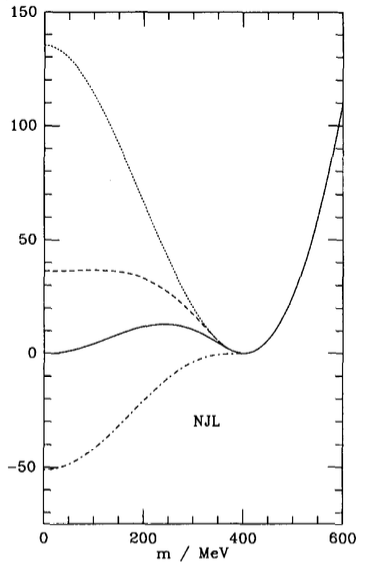
\includegraphics[width=0.45\textwidth]{graphics/Therm_pot_analysis/Pot_buballa.png}
	\caption{Gráfico do potencial termodinâmico $\tilde{\omega}$ obtido variando $m$ arbitrariamente, para o valor $\mu = 0$.}
	\label{Fig:pot_term_analysys_Buballa_NJL-Buballa_Set_1}
\end{figure*}

\begin{figure*}
	\begin{tikzpicture}[gnuplot]
%% generated with GNUPLOT 5.0p2 (Lua 5.2; terminal rev. 99, script rev. 100)
%% Tue Jun 14 16:36:01 2016
\path (0.000,0.000) rectangle (12.500,8.750);
\gpcolor{color=gp lt color border}
\gpsetlinetype{gp lt border}
\gpsetdashtype{gp dt solid}
\gpsetlinewidth{1.00}
\draw[gp path] (1.320,0.985)--(1.500,0.985);
\draw[gp path] (11.947,0.985)--(11.767,0.985);
\node[gp node right] at (1.136,0.985) {$320$};
\draw[gp path] (1.320,2.042)--(1.500,2.042);
\draw[gp path] (11.947,2.042)--(11.767,2.042);
\node[gp node right] at (1.136,2.042) {$340$};
\draw[gp path] (1.320,3.098)--(1.500,3.098);
\draw[gp path] (11.947,3.098)--(11.767,3.098);
\node[gp node right] at (1.136,3.098) {$360$};
\draw[gp path] (1.320,4.155)--(1.500,4.155);
\draw[gp path] (11.947,4.155)--(11.767,4.155);
\node[gp node right] at (1.136,4.155) {$380$};
\draw[gp path] (1.320,5.211)--(1.500,5.211);
\draw[gp path] (11.947,5.211)--(11.767,5.211);
\node[gp node right] at (1.136,5.211) {$400$};
\draw[gp path] (1.320,6.268)--(1.500,6.268);
\draw[gp path] (11.947,6.268)--(11.767,6.268);
\node[gp node right] at (1.136,6.268) {$420$};
\draw[gp path] (1.320,7.324)--(1.500,7.324);
\draw[gp path] (11.947,7.324)--(11.767,7.324);
\node[gp node right] at (1.136,7.324) {$440$};
\draw[gp path] (1.320,8.381)--(1.500,8.381);
\draw[gp path] (11.947,8.381)--(11.767,8.381);
\node[gp node right] at (1.136,8.381) {$460$};
\draw[gp path] (1.320,0.985)--(1.320,1.165);
\draw[gp path] (1.320,8.381)--(1.320,8.201);
\node[gp node center] at (1.320,0.677) {$0$};
\draw[gp path] (2.383,0.985)--(2.383,1.165);
\draw[gp path] (2.383,8.381)--(2.383,8.201);
\node[gp node center] at (2.383,0.677) {$100$};
\draw[gp path] (3.445,0.985)--(3.445,1.165);
\draw[gp path] (3.445,8.381)--(3.445,8.201);
\node[gp node center] at (3.445,0.677) {$200$};
\draw[gp path] (4.508,0.985)--(4.508,1.165);
\draw[gp path] (4.508,8.381)--(4.508,8.201);
\node[gp node center] at (4.508,0.677) {$300$};
\draw[gp path] (5.571,0.985)--(5.571,1.165);
\draw[gp path] (5.571,8.381)--(5.571,8.201);
\node[gp node center] at (5.571,0.677) {$400$};
\draw[gp path] (6.634,0.985)--(6.634,1.165);
\draw[gp path] (6.634,8.381)--(6.634,8.201);
\node[gp node center] at (6.634,0.677) {$500$};
\draw[gp path] (7.696,0.985)--(7.696,1.165);
\draw[gp path] (7.696,8.381)--(7.696,8.201);
\node[gp node center] at (7.696,0.677) {$600$};
\draw[gp path] (8.759,0.985)--(8.759,1.165);
\draw[gp path] (8.759,8.381)--(8.759,8.201);
\node[gp node center] at (8.759,0.677) {$700$};
\draw[gp path] (9.822,0.985)--(9.822,1.165);
\draw[gp path] (9.822,8.381)--(9.822,8.201);
\node[gp node center] at (9.822,0.677) {$800$};
\draw[gp path] (10.884,0.985)--(10.884,1.165);
\draw[gp path] (10.884,8.381)--(10.884,8.201);
\node[gp node center] at (10.884,0.677) {$900$};
\draw[gp path] (11.947,0.985)--(11.947,1.165);
\draw[gp path] (11.947,8.381)--(11.947,8.201);
\node[gp node center] at (11.947,0.677) {$1000$};
\draw[gp path] (1.320,8.381)--(1.320,0.985)--(11.947,0.985)--(11.947,8.381)--cycle;
\node[gp node center,rotate=-270] at (0.246,4.683) {$\mu_R$ (MeV)};
\node[gp node center] at (6.633,0.215) {$m$ (MeV)};
\node[gp node right] at (10.479,8.047) {$\mu = 430$ (MeV)};
\gpcolor{rgb color={0.580,0.000,0.827}}
\draw[gp path] (10.663,8.047)--(11.579,8.047);
\draw[gp path] (1.320,1.436)--(1.331,1.436)--(1.341,1.436)--(1.352,1.436)--(1.363,1.436)%
  --(1.373,1.437)--(1.384,1.437)--(1.394,1.438)--(1.405,1.439)--(1.416,1.439)--(1.426,1.440)%
  --(1.437,1.440)--(1.448,1.441)--(1.458,1.443)--(1.469,1.444)--(1.480,1.444)--(1.490,1.446)%
  --(1.501,1.447)--(1.511,1.449)--(1.522,1.450)--(1.533,1.452)--(1.543,1.453)--(1.554,1.455)%
  --(1.565,1.457)--(1.575,1.458)--(1.586,1.461)--(1.597,1.462)--(1.607,1.465)--(1.618,1.466)%
  --(1.628,1.469)--(1.639,1.471)--(1.650,1.474)--(1.660,1.476)--(1.671,1.478)--(1.682,1.481)%
  --(1.692,1.483)--(1.703,1.486)--(1.714,1.489)--(1.724,1.492)--(1.735,1.495)--(1.746,1.498)%
  --(1.756,1.501)--(1.767,1.504)--(1.777,1.507)--(1.788,1.511)--(1.799,1.515)--(1.809,1.518)%
  --(1.820,1.521)--(1.831,1.525)--(1.841,1.529)--(1.852,1.532)--(1.863,1.536)--(1.873,1.540)%
  --(1.884,1.544)--(1.894,1.548)--(1.905,1.553)--(1.916,1.557)--(1.926,1.561)--(1.937,1.566)%
  --(1.948,1.570)--(1.958,1.575)--(1.969,1.580)--(1.980,1.584)--(1.990,1.589)--(2.001,1.594)%
  --(2.011,1.599)--(2.022,1.604)--(2.033,1.609)--(2.043,1.615)--(2.054,1.619)--(2.065,1.625)%
  --(2.075,1.630)--(2.086,1.636)--(2.097,1.641)--(2.107,1.647)--(2.118,1.652)--(2.128,1.658)%
  --(2.139,1.665)--(2.150,1.670)--(2.160,1.676)--(2.171,1.682)--(2.182,1.688)--(2.192,1.694)%
  --(2.203,1.701)--(2.214,1.707)--(2.224,1.714)--(2.235,1.720)--(2.245,1.727)--(2.256,1.733)%
  --(2.267,1.740)--(2.277,1.747)--(2.288,1.754)--(2.299,1.760)--(2.309,1.768)--(2.320,1.775)%
  --(2.331,1.782)--(2.341,1.790)--(2.352,1.797)--(2.362,1.804)--(2.373,1.811)--(2.384,1.819)%
  --(2.394,1.827)--(2.405,1.835)--(2.416,1.842)--(2.426,1.850)--(2.437,1.858)--(2.448,1.866)%
  --(2.458,1.874)--(2.469,1.882)--(2.480,1.890)--(2.490,1.898)--(2.501,1.906)--(2.511,1.915)%
  --(2.522,1.923)--(2.533,1.932)--(2.543,1.940)--(2.554,1.949)--(2.565,1.958)--(2.575,1.967)%
  --(2.586,1.976)--(2.597,1.985)--(2.607,1.993)--(2.618,2.003)--(2.628,2.012)--(2.639,2.021)%
  --(2.650,2.031)--(2.660,2.040)--(2.671,2.049)--(2.682,2.059)--(2.692,2.068)--(2.703,2.078)%
  --(2.714,2.088)--(2.724,2.097)--(2.735,2.107)--(2.745,2.118)--(2.756,2.127)--(2.767,2.138)%
  --(2.777,2.147)--(2.788,2.158)--(2.799,2.168)--(2.809,2.178)--(2.820,2.189)--(2.831,2.199)%
  --(2.841,2.209)--(2.852,2.220)--(2.862,2.231)--(2.873,2.242)--(2.884,2.252)--(2.894,2.263)%
  --(2.905,2.274)--(2.916,2.285)--(2.926,2.297)--(2.937,2.308)--(2.948,2.318)--(2.958,2.330)%
  --(2.969,2.341)--(2.979,2.353)--(2.990,2.364)--(3.001,2.376)--(3.011,2.387)--(3.022,2.399)%
  --(3.033,2.410)--(3.043,2.422)--(3.054,2.434)--(3.065,2.446)--(3.075,2.458)--(3.086,2.470)%
  --(3.096,2.482)--(3.107,2.494)--(3.118,2.506)--(3.128,2.519)--(3.139,2.531)--(3.150,2.543)%
  --(3.160,2.556)--(3.171,2.568)--(3.182,2.581)--(3.192,2.594)--(3.203,2.606)--(3.213,2.619)%
  --(3.224,2.632)--(3.235,2.645)--(3.245,2.658)--(3.256,2.671)--(3.267,2.683)--(3.277,2.697)%
  --(3.288,2.710)--(3.299,2.724)--(3.309,2.737)--(3.320,2.750)--(3.331,2.763)--(3.341,2.777)%
  --(3.352,2.791)--(3.362,2.804)--(3.373,2.818)--(3.384,2.832)--(3.394,2.845)--(3.405,2.859)%
  --(3.416,2.873)--(3.426,2.887)--(3.437,2.901)--(3.448,2.915)--(3.458,2.929)--(3.469,2.943)%
  --(3.479,2.958)--(3.490,2.972)--(3.501,2.986)--(3.511,3.000)--(3.522,3.015)--(3.533,3.029)%
  --(3.543,3.044)--(3.554,3.058)--(3.565,3.074)--(3.575,3.088)--(3.586,3.103)--(3.596,3.118)%
  --(3.607,3.132)--(3.618,3.148)--(3.628,3.162)--(3.639,3.178)--(3.650,3.193)--(3.660,3.207)%
  --(3.671,3.223)--(3.682,3.238)--(3.692,3.253)--(3.703,3.269)--(3.713,3.284)--(3.724,3.300)%
  --(3.735,3.315)--(3.745,3.331)--(3.756,3.346)--(3.767,3.362)--(3.777,3.378)--(3.788,3.394)%
  --(3.799,3.409)--(3.809,3.425)--(3.820,3.441)--(3.830,3.457)--(3.841,3.473)--(3.852,3.489)%
  --(3.862,3.505)--(3.873,3.521)--(3.884,3.538)--(3.894,3.554)--(3.905,3.570)--(3.916,3.586)%
  --(3.926,3.602)--(3.937,3.619)--(3.947,3.635)--(3.958,3.652)--(3.969,3.669)--(3.979,3.685)%
  --(3.990,3.702)--(4.001,3.719)--(4.011,3.735)--(4.022,3.752)--(4.033,3.769)--(4.043,3.785)%
  --(4.054,3.802)--(4.065,3.819)--(4.075,3.837)--(4.086,3.854)--(4.096,3.871)--(4.107,3.888)%
  --(4.118,3.905)--(4.128,3.922)--(4.139,3.939)--(4.150,3.956)--(4.160,3.974)--(4.171,3.991)%
  --(4.182,4.009)--(4.192,4.026)--(4.203,4.043)--(4.213,4.061)--(4.224,4.079)--(4.235,4.097)%
  --(4.245,4.113)--(4.256,4.131)--(4.267,4.149)--(4.277,4.167)--(4.288,4.184)--(4.299,4.202)%
  --(4.309,4.220)--(4.320,4.238)--(4.330,4.256)--(4.341,4.274)--(4.352,4.292)--(4.362,4.310)%
  --(4.373,4.328)--(4.384,4.346)--(4.394,4.364)--(4.405,4.382)--(4.416,4.400)--(4.426,4.418)%
  --(4.437,4.437)--(4.447,4.454)--(4.458,4.473)--(4.469,4.492)--(4.479,4.509)--(4.490,4.528)%
  --(4.501,4.546)--(4.511,4.565)--(4.522,4.583)--(4.533,4.602)--(4.543,4.620)--(4.554,4.638)%
  --(4.564,4.657)--(4.575,4.675)--(4.586,4.694)--(4.596,4.712)--(4.607,4.732)--(4.618,4.750)%
  --(4.628,4.769)--(4.639,4.787)--(4.650,4.806)--(4.660,4.824)--(4.671,4.844)--(4.681,4.862)%
  --(4.692,4.881)--(4.703,4.900)--(4.713,4.919)--(4.724,4.937)--(4.735,4.957)--(4.745,4.975)%
  --(4.756,4.994)--(4.767,5.013)--(4.777,5.032)--(4.788,5.051)--(4.799,5.070)--(4.809,5.089)%
  --(4.820,5.107)--(4.830,5.127)--(4.841,5.145)--(4.852,5.165)--(4.862,5.183)--(4.873,5.203)%
  --(4.884,5.221)--(4.894,5.240)--(4.905,5.259)--(4.916,5.278)--(4.926,5.298)--(4.937,5.316)%
  --(4.947,5.336)--(4.958,5.354)--(4.969,5.373)--(4.979,5.393)--(4.990,5.411)--(5.001,5.431)%
  --(5.011,5.449)--(5.022,5.469)--(5.033,5.487)--(5.043,5.506)--(5.054,5.526)--(5.064,5.544)%
  --(5.075,5.564)--(5.086,5.582)--(5.096,5.602)--(5.107,5.620)--(5.118,5.639)--(5.128,5.658)%
  --(5.139,5.677)--(5.150,5.696)--(5.160,5.714)--(5.171,5.734)--(5.181,5.752)--(5.192,5.771)%
  --(5.203,5.790)--(5.213,5.809)--(5.224,5.827)--(5.235,5.846)--(5.245,5.864)--(5.256,5.883)%
  --(5.267,5.902)--(5.277,5.921)--(5.288,5.939)--(5.298,5.957)--(5.309,5.976)--(5.320,5.994)%
  --(5.330,6.013)--(5.341,6.031)--(5.352,6.049)--(5.362,6.067)--(5.373,6.085)--(5.384,6.104)%
  --(5.394,6.121)--(5.405,6.140)--(5.415,6.158)--(5.426,6.175)--(5.437,6.193)--(5.447,6.211)%
  --(5.458,6.229)--(5.469,6.246)--(5.479,6.264)--(5.490,6.281)--(5.501,6.299)--(5.511,6.316)%
  --(5.522,6.333)--(5.533,6.350)--(5.543,6.367)--(5.554,6.383)--(5.564,6.400)--(5.575,6.417)%
  --(5.586,6.433)--(5.596,6.450)--(5.607,6.466)--(5.618,6.482)--(5.628,6.498)--(5.639,6.514)%
  --(5.650,6.529)--(5.660,6.545)--(5.671,6.560)--(5.681,6.575)--(5.692,6.590)--(5.703,6.604)%
  --(5.713,6.619)--(5.724,6.633)--(5.735,6.647)--(5.745,6.661)--(5.756,6.674)--(5.767,6.687)%
  --(5.777,6.699)--(5.788,6.712)--(5.798,6.724)--(5.809,6.735)--(5.820,6.746)--(5.830,6.756)%
  --(5.841,6.766)--(5.852,6.774)--(5.862,6.782)--(5.873,6.790)--(5.884,6.795)--(5.894,6.796)%
  --(5.905,6.796)--(5.915,6.796)--(5.926,6.796)--(5.937,6.796)--(5.947,6.796)--(5.958,6.796)%
  --(5.969,6.796)--(5.979,6.796)--(5.990,6.796)--(6.001,6.796)--(6.011,6.796)--(6.022,6.796)%
  --(6.032,6.796)--(6.043,6.796)--(6.054,6.796)--(6.064,6.796)--(6.075,6.796)--(6.086,6.796)%
  --(6.096,6.796)--(6.107,6.796)--(6.118,6.796)--(6.128,6.796)--(6.139,6.796)--(6.149,6.796)%
  --(6.160,6.796)--(6.171,6.796)--(6.181,6.796)--(6.192,6.796)--(6.203,6.796)--(6.213,6.796)%
  --(6.224,6.796)--(6.235,6.796)--(6.245,6.796)--(6.256,6.796)--(6.267,6.796)--(6.277,6.796)%
  --(6.288,6.796)--(6.298,6.796)--(6.309,6.796)--(6.320,6.796)--(6.330,6.796)--(6.341,6.796)%
  --(6.352,6.796)--(6.362,6.796)--(6.373,6.796)--(6.384,6.796)--(6.394,6.796)--(6.405,6.796)%
  --(6.415,6.796)--(6.426,6.796)--(6.437,6.796)--(6.447,6.796)--(6.458,6.796)--(6.469,6.796)%
  --(6.479,6.796)--(6.490,6.796)--(6.501,6.796)--(6.511,6.796)--(6.522,6.796)--(6.532,6.796)%
  --(6.543,6.796)--(6.554,6.796)--(6.564,6.796)--(6.575,6.796)--(6.586,6.796)--(6.596,6.796)%
  --(6.607,6.796)--(6.618,6.796)--(6.628,6.796)--(6.639,6.796)--(6.649,6.796)--(6.660,6.796)%
  --(6.671,6.796)--(6.681,6.796)--(6.692,6.796)--(6.703,6.796)--(6.713,6.796)--(6.724,6.796)%
  --(6.735,6.796)--(6.745,6.796)--(6.756,6.796)--(6.766,6.796)--(6.777,6.796)--(6.788,6.796)%
  --(6.798,6.796)--(6.809,6.796)--(6.820,6.796)--(6.830,6.796)--(6.841,6.796)--(6.852,6.796)%
  --(6.862,6.796)--(6.873,6.796)--(6.883,6.796)--(6.894,6.796)--(6.905,6.796)--(6.915,6.796)%
  --(6.926,6.796)--(6.937,6.796)--(6.947,6.796)--(6.958,6.796)--(6.969,6.796)--(6.979,6.796)%
  --(6.990,6.796)--(7.000,6.796)--(7.011,6.796)--(7.022,6.796)--(7.032,6.796)--(7.043,6.796)%
  --(7.054,6.796)--(7.064,6.796)--(7.075,6.796)--(7.086,6.796)--(7.096,6.796)--(7.107,6.796)%
  --(7.118,6.796)--(7.128,6.796)--(7.139,6.796)--(7.149,6.796)--(7.160,6.796)--(7.171,6.796)%
  --(7.181,6.796)--(7.192,6.796)--(7.203,6.796)--(7.213,6.796)--(7.224,6.796)--(7.235,6.796)%
  --(7.245,6.796)--(7.256,6.796)--(7.266,6.796)--(7.277,6.796)--(7.288,6.796)--(7.298,6.796)%
  --(7.309,6.796)--(7.320,6.796)--(7.330,6.796)--(7.341,6.796)--(7.352,6.796)--(7.362,6.796)%
  --(7.373,6.796)--(7.383,6.796)--(7.394,6.796)--(7.405,6.796)--(7.415,6.796)--(7.426,6.796)%
  --(7.437,6.796)--(7.447,6.796)--(7.458,6.796)--(7.469,6.796)--(7.479,6.796)--(7.490,6.796)%
  --(7.500,6.796)--(7.511,6.796)--(7.522,6.796)--(7.532,6.796)--(7.543,6.796)--(7.554,6.796)%
  --(7.564,6.796)--(7.575,6.796)--(7.586,6.796)--(7.596,6.796)--(7.607,6.796)--(7.617,6.796)%
  --(7.628,6.796)--(7.639,6.796)--(7.649,6.796)--(7.660,6.796)--(7.671,6.796)--(7.681,6.796)%
  --(7.692,6.796)--(7.703,6.796)--(7.713,6.796)--(7.724,6.796)--(7.734,6.796)--(7.745,6.796)%
  --(7.756,6.796)--(7.766,6.796)--(7.777,6.796)--(7.788,6.796)--(7.798,6.796)--(7.809,6.796)%
  --(7.820,6.796)--(7.830,6.796)--(7.841,6.796)--(7.852,6.796)--(7.862,6.796)--(7.873,6.796)%
  --(7.883,6.796)--(7.894,6.796)--(7.905,6.796)--(7.915,6.796)--(7.926,6.796)--(7.937,6.796)%
  --(7.947,6.796)--(7.958,6.796)--(7.969,6.796)--(7.979,6.796)--(7.990,6.796)--(8.000,6.796)%
  --(8.011,6.796)--(8.022,6.796)--(8.032,6.796)--(8.043,6.796)--(8.054,6.796)--(8.064,6.796)%
  --(8.075,6.796)--(8.086,6.796)--(8.096,6.796)--(8.107,6.796)--(8.117,6.796)--(8.128,6.796)%
  --(8.139,6.796)--(8.149,6.796)--(8.160,6.796)--(8.171,6.796)--(8.181,6.796)--(8.192,6.796)%
  --(8.203,6.796)--(8.213,6.796)--(8.224,6.796)--(8.234,6.796)--(8.245,6.796)--(8.256,6.796)%
  --(8.266,6.796)--(8.277,6.796)--(8.288,6.796)--(8.298,6.796)--(8.309,6.796)--(8.320,6.796)%
  --(8.330,6.796)--(8.341,6.796)--(8.351,6.796)--(8.362,6.796)--(8.373,6.796)--(8.383,6.796)%
  --(8.394,6.796)--(8.405,6.796)--(8.415,6.796)--(8.426,6.796)--(8.437,6.796)--(8.447,6.796)%
  --(8.458,6.796)--(8.468,6.796)--(8.479,6.796)--(8.490,6.796)--(8.500,6.796)--(8.511,6.796)%
  --(8.522,6.796)--(8.532,6.796)--(8.543,6.796)--(8.554,6.796)--(8.564,6.796)--(8.575,6.796)%
  --(8.586,6.796)--(8.596,6.796)--(8.607,6.796)--(8.617,6.796)--(8.628,6.796)--(8.639,6.796)%
  --(8.649,6.796)--(8.660,6.796)--(8.671,6.796)--(8.681,6.796)--(8.692,6.796)--(8.703,6.796)%
  --(8.713,6.796)--(8.724,6.796)--(8.734,6.796)--(8.745,6.796)--(8.756,6.796)--(8.766,6.796)%
  --(8.777,6.796)--(8.788,6.796)--(8.798,6.796)--(8.809,6.796)--(8.820,6.796)--(8.830,6.796)%
  --(8.841,6.796)--(8.851,6.796)--(8.862,6.796)--(8.873,6.796)--(8.883,6.796)--(8.894,6.796)%
  --(8.905,6.796)--(8.915,6.796)--(8.926,6.796)--(8.937,6.796)--(8.947,6.796)--(8.958,6.796)%
  --(8.968,6.796)--(8.979,6.796)--(8.990,6.796)--(9.000,6.796)--(9.011,6.796)--(9.022,6.796)%
  --(9.032,6.796)--(9.043,6.796)--(9.054,6.796)--(9.064,6.796)--(9.075,6.796)--(9.085,6.796)%
  --(9.096,6.796)--(9.107,6.796)--(9.117,6.796)--(9.128,6.796)--(9.139,6.796)--(9.149,6.796)%
  --(9.160,6.796)--(9.171,6.796)--(9.181,6.796)--(9.192,6.796)--(9.202,6.796)--(9.213,6.796)%
  --(9.224,6.796)--(9.234,6.796)--(9.245,6.796)--(9.256,6.796)--(9.266,6.796)--(9.277,6.796)%
  --(9.288,6.796)--(9.298,6.796)--(9.309,6.796)--(9.320,6.796)--(9.330,6.796)--(9.341,6.796)%
  --(9.351,6.796)--(9.362,6.796)--(9.373,6.796)--(9.383,6.796)--(9.394,6.796)--(9.405,6.796)%
  --(9.415,6.796)--(9.426,6.796)--(9.437,6.796)--(9.447,6.796)--(9.458,6.796)--(9.468,6.796)%
  --(9.479,6.796)--(9.490,6.796)--(9.500,6.796)--(9.511,6.796)--(9.522,6.796)--(9.532,6.796)%
  --(9.543,6.796)--(9.554,6.796)--(9.564,6.796)--(9.575,6.796)--(9.585,6.796)--(9.596,6.796)%
  --(9.607,6.796)--(9.617,6.796)--(9.628,6.796)--(9.639,6.796)--(9.649,6.796)--(9.660,6.796)%
  --(9.671,6.796)--(9.681,6.796)--(9.692,6.796)--(9.702,6.796)--(9.713,6.796)--(9.724,6.796)%
  --(9.734,6.796)--(9.745,6.796)--(9.756,6.796)--(9.766,6.796)--(9.777,6.796)--(9.788,6.796)%
  --(9.798,6.796)--(9.809,6.796)--(9.819,6.796)--(9.830,6.796)--(9.841,6.796)--(9.851,6.796)%
  --(9.862,6.796)--(9.873,6.796)--(9.883,6.796)--(9.894,6.796)--(9.905,6.796)--(9.915,6.796)%
  --(9.926,6.796)--(9.936,6.796)--(9.947,6.796)--(9.958,6.796)--(9.968,6.796)--(9.979,6.796)%
  --(9.990,6.796)--(10.000,6.796)--(10.011,6.796)--(10.022,6.796)--(10.032,6.796)--(10.043,6.796)%
  --(10.054,6.796)--(10.064,6.796)--(10.075,6.796)--(10.085,6.796)--(10.096,6.796)--(10.107,6.796)%
  --(10.117,6.796)--(10.128,6.796)--(10.139,6.796)--(10.149,6.796)--(10.160,6.796)--(10.171,6.796)%
  --(10.181,6.796)--(10.192,6.796)--(10.202,6.796)--(10.213,6.796)--(10.224,6.796)--(10.234,6.796)%
  --(10.245,6.796)--(10.256,6.796)--(10.266,6.796)--(10.277,6.796)--(10.288,6.796)--(10.298,6.796)%
  --(10.309,6.796)--(10.319,6.796)--(10.330,6.796)--(10.341,6.796)--(10.351,6.796)--(10.362,6.796)%
  --(10.373,6.796)--(10.383,6.796)--(10.394,6.796)--(10.405,6.796)--(10.415,6.796)--(10.426,6.796)%
  --(10.436,6.796)--(10.447,6.796)--(10.458,6.796)--(10.468,6.796)--(10.479,6.796)--(10.490,6.796)%
  --(10.500,6.796)--(10.511,6.796)--(10.522,6.796)--(10.532,6.796)--(10.543,6.796)--(10.553,6.796)%
  --(10.564,6.796)--(10.575,6.796)--(10.585,6.796)--(10.596,6.796)--(10.607,6.796)--(10.617,6.796)%
  --(10.628,6.796)--(10.639,6.796)--(10.649,6.796)--(10.660,6.796)--(10.670,6.796)--(10.681,6.796)%
  --(10.692,6.796)--(10.702,6.796)--(10.713,6.796)--(10.724,6.796)--(10.734,6.796)--(10.745,6.796)%
  --(10.756,6.796)--(10.766,6.796)--(10.777,6.796)--(10.787,6.796)--(10.798,6.796)--(10.809,6.796)%
  --(10.819,6.796)--(10.830,6.796)--(10.841,6.796)--(10.851,6.796)--(10.862,6.796)--(10.873,6.796)%
  --(10.883,6.796)--(10.894,6.796)--(10.905,6.796)--(10.915,6.796)--(10.926,6.796)--(10.936,6.796)%
  --(10.947,6.796)--(10.958,6.796)--(10.968,6.796)--(10.979,6.796)--(10.990,6.796)--(11.000,6.796)%
  --(11.011,6.796)--(11.022,6.796)--(11.032,6.796)--(11.043,6.796)--(11.053,6.796)--(11.064,6.796)%
  --(11.075,6.796)--(11.085,6.796)--(11.096,6.796)--(11.107,6.796)--(11.117,6.796)--(11.128,6.796)%
  --(11.139,6.796)--(11.149,6.796)--(11.160,6.796)--(11.170,6.796)--(11.181,6.796)--(11.192,6.796)%
  --(11.202,6.796)--(11.213,6.796)--(11.224,6.796)--(11.234,6.796)--(11.245,6.796)--(11.256,6.796)%
  --(11.266,6.796)--(11.277,6.796)--(11.287,6.796)--(11.298,6.796)--(11.309,6.796)--(11.319,6.796)%
  --(11.330,6.796)--(11.341,6.796)--(11.351,6.796)--(11.362,6.796)--(11.373,6.796)--(11.383,6.796)%
  --(11.394,6.796)--(11.404,6.796)--(11.415,6.796)--(11.426,6.796)--(11.436,6.796)--(11.447,6.796)%
  --(11.458,6.796)--(11.468,6.796)--(11.479,6.796)--(11.490,6.796)--(11.500,6.796)--(11.511,6.796)%
  --(11.521,6.796)--(11.532,6.796)--(11.543,6.796)--(11.553,6.796)--(11.564,6.796)--(11.575,6.796)%
  --(11.585,6.796)--(11.596,6.796)--(11.607,6.796)--(11.617,6.796)--(11.628,6.796)--(11.639,6.796)%
  --(11.649,6.796)--(11.660,6.796)--(11.670,6.796)--(11.681,6.796)--(11.692,6.796)--(11.702,6.796)%
  --(11.713,6.796)--(11.724,6.796)--(11.734,6.796)--(11.745,6.796)--(11.756,6.796)--(11.766,6.796)%
  --(11.777,6.796)--(11.787,6.796)--(11.798,6.796)--(11.809,6.796)--(11.819,6.796)--(11.830,6.796)%
  --(11.841,6.796)--(11.851,6.796)--(11.862,6.796)--(11.873,6.796)--(11.883,6.796)--(11.894,6.796)%
  --(11.904,6.796)--(11.915,6.796)--(11.926,6.796)--(11.936,6.796)--(11.947,6.796);
\gpcolor{color=gp lt color border}
\node[gp node right] at (10.479,7.739) {$\mu = 440$ (MeV)};
\gpcolor{rgb color={0.000,0.620,0.451}}
\draw[gp path] (10.663,7.739)--(11.579,7.739);
\draw[gp path] (1.320,1.708)--(1.331,1.708)--(1.341,1.708)--(1.352,1.709)--(1.363,1.709)%
  --(1.373,1.709)--(1.384,1.710)--(1.394,1.711)--(1.405,1.711)--(1.416,1.711)--(1.426,1.712)%
  --(1.437,1.713)--(1.448,1.714)--(1.458,1.715)--(1.469,1.716)--(1.480,1.717)--(1.490,1.718)%
  --(1.501,1.719)--(1.511,1.721)--(1.522,1.723)--(1.533,1.723)--(1.543,1.725)--(1.554,1.727)%
  --(1.565,1.729)--(1.575,1.731)--(1.586,1.732)--(1.597,1.735)--(1.607,1.736)--(1.618,1.739)%
  --(1.628,1.741)--(1.639,1.743)--(1.650,1.745)--(1.660,1.748)--(1.671,1.750)--(1.682,1.753)%
  --(1.692,1.756)--(1.703,1.758)--(1.714,1.761)--(1.724,1.764)--(1.735,1.767)--(1.746,1.770)%
  --(1.756,1.773)--(1.767,1.777)--(1.777,1.780)--(1.788,1.783)--(1.799,1.786)--(1.809,1.790)%
  --(1.820,1.794)--(1.831,1.798)--(1.841,1.801)--(1.852,1.805)--(1.863,1.809)--(1.873,1.813)%
  --(1.884,1.817)--(1.894,1.821)--(1.905,1.825)--(1.916,1.829)--(1.926,1.834)--(1.937,1.838)%
  --(1.948,1.843)--(1.958,1.848)--(1.969,1.852)--(1.980,1.856)--(1.990,1.861)--(2.001,1.866)%
  --(2.011,1.871)--(2.022,1.877)--(2.033,1.881)--(2.043,1.886)--(2.054,1.892)--(2.065,1.897)%
  --(2.075,1.902)--(2.086,1.908)--(2.097,1.914)--(2.107,1.919)--(2.118,1.925)--(2.128,1.931)%
  --(2.139,1.936)--(2.150,1.943)--(2.160,1.948)--(2.171,1.955)--(2.182,1.960)--(2.192,1.967)%
  --(2.203,1.973)--(2.214,1.980)--(2.224,1.986)--(2.235,1.993)--(2.245,1.999)--(2.256,2.006)%
  --(2.267,2.013)--(2.277,2.019)--(2.288,2.026)--(2.299,2.033)--(2.309,2.040)--(2.320,2.047)%
  --(2.331,2.055)--(2.341,2.062)--(2.352,2.069)--(2.362,2.076)--(2.373,2.084)--(2.384,2.092)%
  --(2.394,2.099)--(2.405,2.107)--(2.416,2.114)--(2.426,2.122)--(2.437,2.130)--(2.448,2.139)%
  --(2.458,2.147)--(2.469,2.155)--(2.480,2.163)--(2.490,2.171)--(2.501,2.179)--(2.511,2.188)%
  --(2.522,2.196)--(2.533,2.205)--(2.543,2.214)--(2.554,2.222)--(2.565,2.230)--(2.575,2.239)%
  --(2.586,2.248)--(2.597,2.257)--(2.607,2.267)--(2.618,2.276)--(2.628,2.284)--(2.639,2.294)%
  --(2.650,2.303)--(2.660,2.313)--(2.671,2.322)--(2.682,2.332)--(2.692,2.342)--(2.703,2.351)%
  --(2.714,2.361)--(2.724,2.371)--(2.735,2.380)--(2.745,2.390)--(2.756,2.401)--(2.767,2.410)%
  --(2.777,2.421)--(2.788,2.430)--(2.799,2.441)--(2.809,2.451)--(2.820,2.462)--(2.831,2.472)%
  --(2.841,2.483)--(2.852,2.493)--(2.862,2.505)--(2.873,2.515)--(2.884,2.525)--(2.894,2.537)%
  --(2.905,2.547)--(2.916,2.559)--(2.926,2.570)--(2.937,2.581)--(2.948,2.592)--(2.958,2.604)%
  --(2.969,2.615)--(2.979,2.626)--(2.990,2.638)--(3.001,2.649)--(3.011,2.661)--(3.022,2.672)%
  --(3.033,2.684)--(3.043,2.696)--(3.054,2.708)--(3.065,2.720)--(3.075,2.732)--(3.086,2.744)%
  --(3.096,2.756)--(3.107,2.768)--(3.118,2.780)--(3.128,2.792)--(3.139,2.805)--(3.150,2.817)%
  --(3.160,2.830)--(3.171,2.842)--(3.182,2.855)--(3.192,2.868)--(3.203,2.880)--(3.213,2.893)%
  --(3.224,2.906)--(3.235,2.919)--(3.245,2.932)--(3.256,2.945)--(3.267,2.958)--(3.277,2.971)%
  --(3.288,2.985)--(3.299,2.998)--(3.309,3.012)--(3.320,3.024)--(3.331,3.038)--(3.341,3.052)%
  --(3.352,3.066)--(3.362,3.079)--(3.373,3.093)--(3.384,3.107)--(3.394,3.120)--(3.405,3.134)%
  --(3.416,3.148)--(3.426,3.162)--(3.437,3.176)--(3.448,3.191)--(3.458,3.204)--(3.469,3.219)%
  --(3.479,3.233)--(3.490,3.247)--(3.501,3.261)--(3.511,3.276)--(3.522,3.290)--(3.533,3.305)%
  --(3.543,3.319)--(3.554,3.335)--(3.565,3.349)--(3.575,3.364)--(3.586,3.379)--(3.596,3.394)%
  --(3.607,3.409)--(3.618,3.423)--(3.628,3.439)--(3.639,3.454)--(3.650,3.469)--(3.660,3.485)%
  --(3.671,3.500)--(3.682,3.515)--(3.692,3.531)--(3.703,3.546)--(3.713,3.561)--(3.724,3.577)%
  --(3.735,3.593)--(3.745,3.608)--(3.756,3.623)--(3.767,3.640)--(3.777,3.656)--(3.788,3.671)%
  --(3.799,3.687)--(3.809,3.703)--(3.820,3.719)--(3.830,3.735)--(3.841,3.751)--(3.852,3.767)%
  --(3.862,3.784)--(3.873,3.800)--(3.884,3.816)--(3.894,3.832)--(3.905,3.849)--(3.916,3.865)%
  --(3.926,3.881)--(3.937,3.898)--(3.947,3.914)--(3.958,3.931)--(3.969,3.948)--(3.979,3.964)%
  --(3.990,3.981)--(4.001,3.998)--(4.011,4.015)--(4.022,4.032)--(4.033,4.049)--(4.043,4.066)%
  --(4.054,4.083)--(4.065,4.100)--(4.075,4.118)--(4.086,4.134)--(4.096,4.151)--(4.107,4.169)%
  --(4.118,4.186)--(4.128,4.203)--(4.139,4.221)--(4.150,4.238)--(4.160,4.255)--(4.171,4.273)%
  --(4.182,4.291)--(4.192,4.309)--(4.203,4.325)--(4.213,4.343)--(4.224,4.361)--(4.235,4.379)%
  --(4.245,4.396)--(4.256,4.414)--(4.267,4.432)--(4.277,4.450)--(4.288,4.468)--(4.299,4.486)%
  --(4.309,4.504)--(4.320,4.522)--(4.330,4.540)--(4.341,4.558)--(4.352,4.576)--(4.362,4.595)%
  --(4.373,4.612)--(4.384,4.631)--(4.394,4.650)--(4.405,4.667)--(4.416,4.686)--(4.426,4.704)%
  --(4.437,4.723)--(4.447,4.741)--(4.458,4.760)--(4.469,4.778)--(4.479,4.796)--(4.490,4.815)%
  --(4.501,4.834)--(4.511,4.853)--(4.522,4.871)--(4.533,4.890)--(4.543,4.908)--(4.554,4.927)%
  --(4.564,4.946)--(4.575,4.965)--(4.586,4.983)--(4.596,5.003)--(4.607,5.021)--(4.618,5.041)%
  --(4.628,5.059)--(4.639,5.078)--(4.650,5.097)--(4.660,5.116)--(4.671,5.135)--(4.681,5.154)%
  --(4.692,5.173)--(4.703,5.192)--(4.713,5.211)--(4.724,5.231)--(4.735,5.249)--(4.745,5.269)%
  --(4.756,5.288)--(4.767,5.307)--(4.777,5.326)--(4.788,5.345)--(4.799,5.365)--(4.809,5.384)%
  --(4.820,5.403)--(4.830,5.423)--(4.841,5.442)--(4.852,5.461)--(4.862,5.481)--(4.873,5.500)%
  --(4.884,5.519)--(4.894,5.539)--(4.905,5.558)--(4.916,5.577)--(4.926,5.597)--(4.937,5.616)%
  --(4.947,5.635)--(4.958,5.655)--(4.969,5.675)--(4.979,5.694)--(4.990,5.714)--(5.001,5.733)%
  --(5.011,5.752)--(5.022,5.772)--(5.033,5.791)--(5.043,5.810)--(5.054,5.830)--(5.064,5.850)%
  --(5.075,5.869)--(5.086,5.889)--(5.096,5.908)--(5.107,5.927)--(5.118,5.947)--(5.128,5.967)%
  --(5.139,5.986)--(5.150,6.005)--(5.160,6.025)--(5.171,6.044)--(5.181,6.063)--(5.192,6.083)%
  --(5.203,6.102)--(5.213,6.121)--(5.224,6.141)--(5.235,6.160)--(5.245,6.180)--(5.256,6.199)%
  --(5.267,6.218)--(5.277,6.238)--(5.288,6.257)--(5.298,6.276)--(5.309,6.295)--(5.320,6.314)%
  --(5.330,6.333)--(5.341,6.353)--(5.352,6.371)--(5.362,6.391)--(5.373,6.409)--(5.384,6.429)%
  --(5.394,6.448)--(5.405,6.466)--(5.415,6.485)--(5.426,6.504)--(5.437,6.523)--(5.447,6.541)%
  --(5.458,6.560)--(5.469,6.579)--(5.479,6.597)--(5.490,6.616)--(5.501,6.634)--(5.511,6.653)%
  --(5.522,6.671)--(5.533,6.690)--(5.543,6.708)--(5.554,6.726)--(5.564,6.744)--(5.575,6.762)%
  --(5.586,6.779)--(5.596,6.798)--(5.607,6.816)--(5.618,6.832)--(5.628,6.850)--(5.639,6.868)%
  --(5.650,6.885)--(5.660,6.903)--(5.671,6.920)--(5.681,6.936)--(5.692,6.953)--(5.703,6.970)%
  --(5.713,6.986)--(5.724,7.003)--(5.735,7.019)--(5.745,7.036)--(5.756,7.051)--(5.767,7.067)%
  --(5.777,7.082)--(5.788,7.098)--(5.798,7.113)--(5.809,7.128)--(5.820,7.143)--(5.830,7.157)%
  --(5.841,7.172)--(5.852,7.186)--(5.862,7.199)--(5.873,7.212)--(5.884,7.225)--(5.894,7.238)%
  --(5.905,7.250)--(5.915,7.262)--(5.926,7.273)--(5.937,7.284)--(5.947,7.294)--(5.958,7.302)%
  --(5.969,7.310)--(5.979,7.318)--(5.990,7.323)--(6.001,7.324)--(6.011,7.324)--(6.022,7.324)%
  --(6.032,7.324)--(6.043,7.324)--(6.054,7.324)--(6.064,7.324)--(6.075,7.324)--(6.086,7.324)%
  --(6.096,7.324)--(6.107,7.324)--(6.118,7.324)--(6.128,7.324)--(6.139,7.324)--(6.149,7.324)%
  --(6.160,7.324)--(6.171,7.324)--(6.181,7.324)--(6.192,7.324)--(6.203,7.324)--(6.213,7.324)%
  --(6.224,7.324)--(6.235,7.324)--(6.245,7.324)--(6.256,7.324)--(6.267,7.324)--(6.277,7.324)%
  --(6.288,7.324)--(6.298,7.324)--(6.309,7.324)--(6.320,7.324)--(6.330,7.324)--(6.341,7.324)%
  --(6.352,7.324)--(6.362,7.324)--(6.373,7.324)--(6.384,7.324)--(6.394,7.324)--(6.405,7.324)%
  --(6.415,7.324)--(6.426,7.324)--(6.437,7.324)--(6.447,7.324)--(6.458,7.324)--(6.469,7.324)%
  --(6.479,7.324)--(6.490,7.324)--(6.501,7.324)--(6.511,7.324)--(6.522,7.324)--(6.532,7.324)%
  --(6.543,7.324)--(6.554,7.324)--(6.564,7.324)--(6.575,7.324)--(6.586,7.324)--(6.596,7.324)%
  --(6.607,7.324)--(6.618,7.324)--(6.628,7.324)--(6.639,7.324)--(6.649,7.324)--(6.660,7.324)%
  --(6.671,7.324)--(6.681,7.324)--(6.692,7.324)--(6.703,7.324)--(6.713,7.324)--(6.724,7.324)%
  --(6.735,7.324)--(6.745,7.324)--(6.756,7.324)--(6.766,7.324)--(6.777,7.324)--(6.788,7.324)%
  --(6.798,7.324)--(6.809,7.324)--(6.820,7.324)--(6.830,7.324)--(6.841,7.324)--(6.852,7.324)%
  --(6.862,7.324)--(6.873,7.324)--(6.883,7.324)--(6.894,7.324)--(6.905,7.324)--(6.915,7.324)%
  --(6.926,7.324)--(6.937,7.324)--(6.947,7.324)--(6.958,7.324)--(6.969,7.324)--(6.979,7.324)%
  --(6.990,7.324)--(7.000,7.324)--(7.011,7.324)--(7.022,7.324)--(7.032,7.324)--(7.043,7.324)%
  --(7.054,7.324)--(7.064,7.324)--(7.075,7.324)--(7.086,7.324)--(7.096,7.324)--(7.107,7.324)%
  --(7.118,7.324)--(7.128,7.324)--(7.139,7.324)--(7.149,7.324)--(7.160,7.324)--(7.171,7.324)%
  --(7.181,7.324)--(7.192,7.324)--(7.203,7.324)--(7.213,7.324)--(7.224,7.324)--(7.235,7.324)%
  --(7.245,7.324)--(7.256,7.324)--(7.266,7.324)--(7.277,7.324)--(7.288,7.324)--(7.298,7.324)%
  --(7.309,7.324)--(7.320,7.324)--(7.330,7.324)--(7.341,7.324)--(7.352,7.324)--(7.362,7.324)%
  --(7.373,7.324)--(7.383,7.324)--(7.394,7.324)--(7.405,7.324)--(7.415,7.324)--(7.426,7.324)%
  --(7.437,7.324)--(7.447,7.324)--(7.458,7.324)--(7.469,7.324)--(7.479,7.324)--(7.490,7.324)%
  --(7.500,7.324)--(7.511,7.324)--(7.522,7.324)--(7.532,7.324)--(7.543,7.324)--(7.554,7.324)%
  --(7.564,7.324)--(7.575,7.324)--(7.586,7.324)--(7.596,7.324)--(7.607,7.324)--(7.617,7.324)%
  --(7.628,7.324)--(7.639,7.324)--(7.649,7.324)--(7.660,7.324)--(7.671,7.324)--(7.681,7.324)%
  --(7.692,7.324)--(7.703,7.324)--(7.713,7.324)--(7.724,7.324)--(7.734,7.324)--(7.745,7.324)%
  --(7.756,7.324)--(7.766,7.324)--(7.777,7.324)--(7.788,7.324)--(7.798,7.324)--(7.809,7.324)%
  --(7.820,7.324)--(7.830,7.324)--(7.841,7.324)--(7.852,7.324)--(7.862,7.324)--(7.873,7.324)%
  --(7.883,7.324)--(7.894,7.324)--(7.905,7.324)--(7.915,7.324)--(7.926,7.324)--(7.937,7.324)%
  --(7.947,7.324)--(7.958,7.324)--(7.969,7.324)--(7.979,7.324)--(7.990,7.324)--(8.000,7.324)%
  --(8.011,7.324)--(8.022,7.324)--(8.032,7.324)--(8.043,7.324)--(8.054,7.324)--(8.064,7.324)%
  --(8.075,7.324)--(8.086,7.324)--(8.096,7.324)--(8.107,7.324)--(8.117,7.324)--(8.128,7.324)%
  --(8.139,7.324)--(8.149,7.324)--(8.160,7.324)--(8.171,7.324)--(8.181,7.324)--(8.192,7.324)%
  --(8.203,7.324)--(8.213,7.324)--(8.224,7.324)--(8.234,7.324)--(8.245,7.324)--(8.256,7.324)%
  --(8.266,7.324)--(8.277,7.324)--(8.288,7.324)--(8.298,7.324)--(8.309,7.324)--(8.320,7.324)%
  --(8.330,7.324)--(8.341,7.324)--(8.351,7.324)--(8.362,7.324)--(8.373,7.324)--(8.383,7.324)%
  --(8.394,7.324)--(8.405,7.324)--(8.415,7.324)--(8.426,7.324)--(8.437,7.324)--(8.447,7.324)%
  --(8.458,7.324)--(8.468,7.324)--(8.479,7.324)--(8.490,7.324)--(8.500,7.324)--(8.511,7.324)%
  --(8.522,7.324)--(8.532,7.324)--(8.543,7.324)--(8.554,7.324)--(8.564,7.324)--(8.575,7.324)%
  --(8.586,7.324)--(8.596,7.324)--(8.607,7.324)--(8.617,7.324)--(8.628,7.324)--(8.639,7.324)%
  --(8.649,7.324)--(8.660,7.324)--(8.671,7.324)--(8.681,7.324)--(8.692,7.324)--(8.703,7.324)%
  --(8.713,7.324)--(8.724,7.324)--(8.734,7.324)--(8.745,7.324)--(8.756,7.324)--(8.766,7.324)%
  --(8.777,7.324)--(8.788,7.324)--(8.798,7.324)--(8.809,7.324)--(8.820,7.324)--(8.830,7.324)%
  --(8.841,7.324)--(8.851,7.324)--(8.862,7.324)--(8.873,7.324)--(8.883,7.324)--(8.894,7.324)%
  --(8.905,7.324)--(8.915,7.324)--(8.926,7.324)--(8.937,7.324)--(8.947,7.324)--(8.958,7.324)%
  --(8.968,7.324)--(8.979,7.324)--(8.990,7.324)--(9.000,7.324)--(9.011,7.324)--(9.022,7.324)%
  --(9.032,7.324)--(9.043,7.324)--(9.054,7.324)--(9.064,7.324)--(9.075,7.324)--(9.085,7.324)%
  --(9.096,7.324)--(9.107,7.324)--(9.117,7.324)--(9.128,7.324)--(9.139,7.324)--(9.149,7.324)%
  --(9.160,7.324)--(9.171,7.324)--(9.181,7.324)--(9.192,7.324)--(9.202,7.324)--(9.213,7.324)%
  --(9.224,7.324)--(9.234,7.324)--(9.245,7.324)--(9.256,7.324)--(9.266,7.324)--(9.277,7.324)%
  --(9.288,7.324)--(9.298,7.324)--(9.309,7.324)--(9.320,7.324)--(9.330,7.324)--(9.341,7.324)%
  --(9.351,7.324)--(9.362,7.324)--(9.373,7.324)--(9.383,7.324)--(9.394,7.324)--(9.405,7.324)%
  --(9.415,7.324)--(9.426,7.324)--(9.437,7.324)--(9.447,7.324)--(9.458,7.324)--(9.468,7.324)%
  --(9.479,7.324)--(9.490,7.324)--(9.500,7.324)--(9.511,7.324)--(9.522,7.324)--(9.532,7.324)%
  --(9.543,7.324)--(9.554,7.324)--(9.564,7.324)--(9.575,7.324)--(9.585,7.324)--(9.596,7.324)%
  --(9.607,7.324)--(9.617,7.324)--(9.628,7.324)--(9.639,7.324)--(9.649,7.324)--(9.660,7.324)%
  --(9.671,7.324)--(9.681,7.324)--(9.692,7.324)--(9.702,7.324)--(9.713,7.324)--(9.724,7.324)%
  --(9.734,7.324)--(9.745,7.324)--(9.756,7.324)--(9.766,7.324)--(9.777,7.324)--(9.788,7.324)%
  --(9.798,7.324)--(9.809,7.324)--(9.819,7.324)--(9.830,7.324)--(9.841,7.324)--(9.851,7.324)%
  --(9.862,7.324)--(9.873,7.324)--(9.883,7.324)--(9.894,7.324)--(9.905,7.324)--(9.915,7.324)%
  --(9.926,7.324)--(9.936,7.324)--(9.947,7.324)--(9.958,7.324)--(9.968,7.324)--(9.979,7.324)%
  --(9.990,7.324)--(10.000,7.324)--(10.011,7.324)--(10.022,7.324)--(10.032,7.324)--(10.043,7.324)%
  --(10.054,7.324)--(10.064,7.324)--(10.075,7.324)--(10.085,7.324)--(10.096,7.324)--(10.107,7.324)%
  --(10.117,7.324)--(10.128,7.324)--(10.139,7.324)--(10.149,7.324)--(10.160,7.324)--(10.171,7.324)%
  --(10.181,7.324)--(10.192,7.324)--(10.202,7.324)--(10.213,7.324)--(10.224,7.324)--(10.234,7.324)%
  --(10.245,7.324)--(10.256,7.324)--(10.266,7.324)--(10.277,7.324)--(10.288,7.324)--(10.298,7.324)%
  --(10.309,7.324)--(10.319,7.324)--(10.330,7.324)--(10.341,7.324)--(10.351,7.324)--(10.362,7.324)%
  --(10.373,7.324)--(10.383,7.324)--(10.394,7.324)--(10.405,7.324)--(10.415,7.324)--(10.426,7.324)%
  --(10.436,7.324)--(10.447,7.324)--(10.458,7.324)--(10.468,7.324)--(10.479,7.324)--(10.490,7.324)%
  --(10.500,7.324)--(10.511,7.324)--(10.522,7.324)--(10.532,7.324)--(10.543,7.324)--(10.553,7.324)%
  --(10.564,7.324)--(10.575,7.324)--(10.585,7.324)--(10.596,7.324)--(10.607,7.324)--(10.617,7.324)%
  --(10.628,7.324)--(10.639,7.324)--(10.649,7.324)--(10.660,7.324)--(10.670,7.324)--(10.681,7.324)%
  --(10.692,7.324)--(10.702,7.324)--(10.713,7.324)--(10.724,7.324)--(10.734,7.324)--(10.745,7.324)%
  --(10.756,7.324)--(10.766,7.324)--(10.777,7.324)--(10.787,7.324)--(10.798,7.324)--(10.809,7.324)%
  --(10.819,7.324)--(10.830,7.324)--(10.841,7.324)--(10.851,7.324)--(10.862,7.324)--(10.873,7.324)%
  --(10.883,7.324)--(10.894,7.324)--(10.905,7.324)--(10.915,7.324)--(10.926,7.324)--(10.936,7.324)%
  --(10.947,7.324)--(10.958,7.324)--(10.968,7.324)--(10.979,7.324)--(10.990,7.324)--(11.000,7.324)%
  --(11.011,7.324)--(11.022,7.324)--(11.032,7.324)--(11.043,7.324)--(11.053,7.324)--(11.064,7.324)%
  --(11.075,7.324)--(11.085,7.324)--(11.096,7.324)--(11.107,7.324)--(11.117,7.324)--(11.128,7.324)%
  --(11.139,7.324)--(11.149,7.324)--(11.160,7.324)--(11.170,7.324)--(11.181,7.324)--(11.192,7.324)%
  --(11.202,7.324)--(11.213,7.324)--(11.224,7.324)--(11.234,7.324)--(11.245,7.324)--(11.256,7.324)%
  --(11.266,7.324)--(11.277,7.324)--(11.287,7.324)--(11.298,7.324)--(11.309,7.324)--(11.319,7.324)%
  --(11.330,7.324)--(11.341,7.324)--(11.351,7.324)--(11.362,7.324)--(11.373,7.324)--(11.383,7.324)%
  --(11.394,7.324)--(11.404,7.324)--(11.415,7.324)--(11.426,7.324)--(11.436,7.324)--(11.447,7.324)%
  --(11.458,7.324)--(11.468,7.324)--(11.479,7.324)--(11.490,7.324)--(11.500,7.324)--(11.511,7.324)%
  --(11.521,7.324)--(11.532,7.324)--(11.543,7.324)--(11.553,7.324)--(11.564,7.324)--(11.575,7.324)%
  --(11.585,7.324)--(11.596,7.324)--(11.607,7.324)--(11.617,7.324)--(11.628,7.324)--(11.639,7.324)%
  --(11.649,7.324)--(11.660,7.324)--(11.670,7.324)--(11.681,7.324)--(11.692,7.324)--(11.702,7.324)%
  --(11.713,7.324)--(11.724,7.324)--(11.734,7.324)--(11.745,7.324)--(11.756,7.324)--(11.766,7.324)%
  --(11.777,7.324)--(11.787,7.324)--(11.798,7.324)--(11.809,7.324)--(11.819,7.324)--(11.830,7.324)%
  --(11.841,7.324)--(11.851,7.324)--(11.862,7.324)--(11.873,7.324)--(11.883,7.324)--(11.894,7.324)%
  --(11.904,7.324)--(11.915,7.324)--(11.926,7.324)--(11.936,7.324)--(11.947,7.324);
\gpcolor{color=gp lt color border}
\node[gp node right] at (10.479,7.431) {$\mu = 444.3$ (MeV)};
\gpcolor{rgb color={0.337,0.706,0.914}}
\draw[gp path] (10.663,7.431)--(11.579,7.431);
\draw[gp path] (1.320,1.824)--(1.331,1.824)--(1.341,1.824)--(1.352,1.824)--(1.363,1.825)%
  --(1.373,1.825)--(1.384,1.826)--(1.394,1.826)--(1.405,1.827)--(1.416,1.827)--(1.426,1.828)%
  --(1.437,1.829)--(1.448,1.830)--(1.458,1.831)--(1.469,1.831)--(1.480,1.833)--(1.490,1.834)%
  --(1.501,1.835)--(1.511,1.836)--(1.522,1.838)--(1.533,1.839)--(1.543,1.841)--(1.554,1.843)%
  --(1.565,1.844)--(1.575,1.846)--(1.586,1.848)--(1.597,1.850)--(1.607,1.852)--(1.618,1.854)%
  --(1.628,1.856)--(1.639,1.859)--(1.650,1.861)--(1.660,1.864)--(1.671,1.866)--(1.682,1.869)%
  --(1.692,1.872)--(1.703,1.874)--(1.714,1.877)--(1.724,1.880)--(1.735,1.883)--(1.746,1.886)%
  --(1.756,1.889)--(1.767,1.892)--(1.777,1.896)--(1.788,1.899)--(1.799,1.902)--(1.809,1.906)%
  --(1.820,1.910)--(1.831,1.913)--(1.841,1.917)--(1.852,1.921)--(1.863,1.925)--(1.873,1.928)%
  --(1.884,1.932)--(1.894,1.937)--(1.905,1.941)--(1.916,1.945)--(1.926,1.949)--(1.937,1.954)%
  --(1.948,1.959)--(1.958,1.963)--(1.969,1.968)--(1.980,1.972)--(1.990,1.977)--(2.001,1.982)%
  --(2.011,1.987)--(2.022,1.992)--(2.033,1.997)--(2.043,2.002)--(2.054,2.008)--(2.065,2.013)%
  --(2.075,2.018)--(2.086,2.024)--(2.097,2.030)--(2.107,2.035)--(2.118,2.041)--(2.128,2.047)%
  --(2.139,2.052)--(2.150,2.058)--(2.160,2.064)--(2.171,2.070)--(2.182,2.076)--(2.192,2.083)%
  --(2.203,2.089)--(2.214,2.095)--(2.224,2.101)--(2.235,2.109)--(2.245,2.115)--(2.256,2.122)%
  --(2.267,2.128)--(2.277,2.135)--(2.288,2.142)--(2.299,2.149)--(2.309,2.156)--(2.320,2.164)%
  --(2.331,2.171)--(2.341,2.178)--(2.352,2.185)--(2.362,2.193)--(2.373,2.200)--(2.384,2.207)%
  --(2.394,2.215)--(2.405,2.222)--(2.416,2.230)--(2.426,2.239)--(2.437,2.247)--(2.448,2.254)%
  --(2.458,2.262)--(2.469,2.271)--(2.480,2.279)--(2.490,2.287)--(2.501,2.295)--(2.511,2.304)%
  --(2.522,2.312)--(2.533,2.321)--(2.543,2.330)--(2.554,2.338)--(2.565,2.347)--(2.575,2.355)%
  --(2.586,2.364)--(2.597,2.373)--(2.607,2.383)--(2.618,2.392)--(2.628,2.401)--(2.639,2.410)%
  --(2.650,2.419)--(2.660,2.429)--(2.671,2.438)--(2.682,2.448)--(2.692,2.457)--(2.703,2.467)%
  --(2.714,2.477)--(2.724,2.487)--(2.735,2.496)--(2.745,2.506)--(2.756,2.517)--(2.767,2.526)%
  --(2.777,2.537)--(2.788,2.547)--(2.799,2.557)--(2.809,2.567)--(2.820,2.578)--(2.831,2.588)%
  --(2.841,2.599)--(2.852,2.609)--(2.862,2.621)--(2.873,2.631)--(2.884,2.642)--(2.894,2.653)%
  --(2.905,2.663)--(2.916,2.675)--(2.926,2.686)--(2.937,2.697)--(2.948,2.708)--(2.958,2.720)%
  --(2.969,2.731)--(2.979,2.742)--(2.990,2.754)--(3.001,2.766)--(3.011,2.777)--(3.022,2.788)%
  --(3.033,2.800)--(3.043,2.812)--(3.054,2.824)--(3.065,2.836)--(3.075,2.848)--(3.086,2.860)%
  --(3.096,2.872)--(3.107,2.884)--(3.118,2.896)--(3.128,2.909)--(3.139,2.921)--(3.150,2.934)%
  --(3.160,2.946)--(3.171,2.959)--(3.182,2.971)--(3.192,2.984)--(3.203,2.997)--(3.213,3.010)%
  --(3.224,3.023)--(3.235,3.036)--(3.245,3.049)--(3.256,3.062)--(3.267,3.075)--(3.277,3.088)%
  --(3.288,3.101)--(3.299,3.115)--(3.309,3.128)--(3.320,3.141)--(3.331,3.155)--(3.341,3.169)%
  --(3.352,3.182)--(3.362,3.195)--(3.373,3.210)--(3.384,3.224)--(3.394,3.237)--(3.405,3.251)%
  --(3.416,3.265)--(3.426,3.279)--(3.437,3.293)--(3.448,3.307)--(3.458,3.321)--(3.469,3.336)%
  --(3.479,3.350)--(3.490,3.365)--(3.501,3.379)--(3.511,3.394)--(3.522,3.408)--(3.533,3.423)%
  --(3.543,3.437)--(3.554,3.452)--(3.565,3.466)--(3.575,3.482)--(3.586,3.496)--(3.596,3.511)%
  --(3.607,3.526)--(3.618,3.541)--(3.628,3.556)--(3.639,3.571)--(3.650,3.586)--(3.660,3.602)%
  --(3.671,3.617)--(3.682,3.632)--(3.692,3.648)--(3.703,3.664)--(3.713,3.679)--(3.724,3.694)%
  --(3.735,3.710)--(3.745,3.726)--(3.756,3.742)--(3.767,3.757)--(3.777,3.773)--(3.788,3.789)%
  --(3.799,3.805)--(3.809,3.821)--(3.820,3.837)--(3.830,3.853)--(3.841,3.869)--(3.852,3.885)%
  --(3.862,3.901)--(3.873,3.918)--(3.884,3.935)--(3.894,3.951)--(3.905,3.967)--(3.916,3.984)%
  --(3.926,4.000)--(3.937,4.017)--(3.947,4.033)--(3.958,4.050)--(3.969,4.067)--(3.979,4.084)%
  --(3.990,4.100)--(4.001,4.117)--(4.011,4.134)--(4.022,4.151)--(4.033,4.167)--(4.043,4.184)%
  --(4.054,4.202)--(4.065,4.219)--(4.075,4.236)--(4.086,4.254)--(4.096,4.271)--(4.107,4.288)%
  --(4.118,4.305)--(4.128,4.322)--(4.139,4.340)--(4.150,4.358)--(4.160,4.375)--(4.171,4.392)%
  --(4.182,4.410)--(4.192,4.428)--(4.203,4.446)--(4.213,4.463)--(4.224,4.481)--(4.235,4.499)%
  --(4.245,4.517)--(4.256,4.534)--(4.267,4.552)--(4.277,4.571)--(4.288,4.588)--(4.299,4.606)%
  --(4.309,4.625)--(4.320,4.642)--(4.330,4.661)--(4.341,4.679)--(4.352,4.697)--(4.362,4.715)%
  --(4.373,4.733)--(4.384,4.752)--(4.394,4.770)--(4.405,4.788)--(4.416,4.807)--(4.426,4.825)%
  --(4.437,4.844)--(4.447,4.862)--(4.458,4.881)--(4.469,4.899)--(4.479,4.918)--(4.490,4.937)%
  --(4.501,4.956)--(4.511,4.974)--(4.522,4.993)--(4.533,5.011)--(4.543,5.031)--(4.554,5.049)%
  --(4.564,5.068)--(4.575,5.087)--(4.586,5.106)--(4.596,5.125)--(4.607,5.144)--(4.618,5.163)%
  --(4.628,5.182)--(4.639,5.201)--(4.650,5.220)--(4.660,5.239)--(4.671,5.258)--(4.681,5.277)%
  --(4.692,5.297)--(4.703,5.315)--(4.713,5.335)--(4.724,5.354)--(4.735,5.373)--(4.745,5.393)%
  --(4.756,5.412)--(4.767,5.431)--(4.777,5.451)--(4.788,5.470)--(4.799,5.490)--(4.809,5.509)%
  --(4.820,5.528)--(4.830,5.548)--(4.841,5.567)--(4.852,5.586)--(4.862,5.606)--(4.873,5.626)%
  --(4.884,5.645)--(4.894,5.664)--(4.905,5.684)--(4.916,5.704)--(4.926,5.723)--(4.937,5.743)%
  --(4.947,5.762)--(4.958,5.782)--(4.969,5.801)--(4.979,5.821)--(4.990,5.841)--(5.001,5.860)%
  --(5.011,5.880)--(5.022,5.900)--(5.033,5.919)--(5.043,5.939)--(5.054,5.959)--(5.064,5.978)%
  --(5.075,5.998)--(5.086,6.017)--(5.096,6.037)--(5.107,6.057)--(5.118,6.076)--(5.128,6.096)%
  --(5.139,6.116)--(5.150,6.135)--(5.160,6.155)--(5.171,6.175)--(5.181,6.194)--(5.192,6.214)%
  --(5.203,6.234)--(5.213,6.253)--(5.224,6.273)--(5.235,6.292)--(5.245,6.312)--(5.256,6.332)%
  --(5.267,6.351)--(5.277,6.371)--(5.288,6.390)--(5.298,6.409)--(5.309,6.429)--(5.320,6.449)%
  --(5.330,6.468)--(5.341,6.487)--(5.352,6.507)--(5.362,6.526)--(5.373,6.545)--(5.384,6.565)%
  --(5.394,6.584)--(5.405,6.604)--(5.415,6.622)--(5.426,6.641)--(5.437,6.661)--(5.447,6.679)%
  --(5.458,6.699)--(5.469,6.718)--(5.479,6.737)--(5.490,6.756)--(5.501,6.774)--(5.511,6.793)%
  --(5.522,6.812)--(5.533,6.831)--(5.543,6.849)--(5.554,6.868)--(5.564,6.886)--(5.575,6.905)%
  --(5.586,6.924)--(5.596,6.941)--(5.607,6.960)--(5.618,6.978)--(5.628,6.996)--(5.639,7.014)%
  --(5.650,7.032)--(5.660,7.050)--(5.671,7.068)--(5.681,7.085)--(5.692,7.103)--(5.703,7.120)%
  --(5.713,7.137)--(5.724,7.154)--(5.735,7.172)--(5.745,7.189)--(5.756,7.205)--(5.767,7.222)%
  --(5.777,7.238)--(5.788,7.255)--(5.798,7.271)--(5.809,7.287)--(5.820,7.302)--(5.830,7.319)%
  --(5.841,7.334)--(5.852,7.348)--(5.862,7.364)--(5.873,7.378)--(5.884,7.393)--(5.894,7.407)%
  --(5.905,7.421)--(5.915,7.435)--(5.926,7.448)--(5.937,7.460)--(5.947,7.473)--(5.958,7.485)%
  --(5.969,7.496)--(5.979,7.507)--(5.990,7.518)--(6.001,7.527)--(6.011,7.535)--(6.022,7.543)%
  --(6.032,7.549)--(6.043,7.552)--(6.054,7.552)--(6.064,7.552)--(6.075,7.552)--(6.086,7.552)%
  --(6.096,7.552)--(6.107,7.552)--(6.118,7.552)--(6.128,7.552)--(6.139,7.552)--(6.149,7.552)%
  --(6.160,7.552)--(6.171,7.552)--(6.181,7.552)--(6.192,7.552)--(6.203,7.552)--(6.213,7.552)%
  --(6.224,7.552)--(6.235,7.552)--(6.245,7.552)--(6.256,7.552)--(6.267,7.552)--(6.277,7.552)%
  --(6.288,7.552)--(6.298,7.552)--(6.309,7.552)--(6.320,7.552)--(6.330,7.552)--(6.341,7.552)%
  --(6.352,7.552)--(6.362,7.552)--(6.373,7.552)--(6.384,7.552)--(6.394,7.552)--(6.405,7.552)%
  --(6.415,7.552)--(6.426,7.552)--(6.437,7.552)--(6.447,7.552)--(6.458,7.552)--(6.469,7.552)%
  --(6.479,7.552)--(6.490,7.552)--(6.501,7.552)--(6.511,7.552)--(6.522,7.552)--(6.532,7.552)%
  --(6.543,7.552)--(6.554,7.552)--(6.564,7.552)--(6.575,7.552)--(6.586,7.552)--(6.596,7.552)%
  --(6.607,7.552)--(6.618,7.552)--(6.628,7.552)--(6.639,7.552)--(6.649,7.552)--(6.660,7.552)%
  --(6.671,7.552)--(6.681,7.552)--(6.692,7.552)--(6.703,7.552)--(6.713,7.552)--(6.724,7.552)%
  --(6.735,7.552)--(6.745,7.552)--(6.756,7.552)--(6.766,7.552)--(6.777,7.552)--(6.788,7.552)%
  --(6.798,7.552)--(6.809,7.552)--(6.820,7.552)--(6.830,7.552)--(6.841,7.552)--(6.852,7.552)%
  --(6.862,7.552)--(6.873,7.552)--(6.883,7.552)--(6.894,7.552)--(6.905,7.552)--(6.915,7.552)%
  --(6.926,7.552)--(6.937,7.552)--(6.947,7.552)--(6.958,7.552)--(6.969,7.552)--(6.979,7.552)%
  --(6.990,7.552)--(7.000,7.552)--(7.011,7.552)--(7.022,7.552)--(7.032,7.552)--(7.043,7.552)%
  --(7.054,7.552)--(7.064,7.552)--(7.075,7.552)--(7.086,7.552)--(7.096,7.552)--(7.107,7.552)%
  --(7.118,7.552)--(7.128,7.552)--(7.139,7.552)--(7.149,7.552)--(7.160,7.552)--(7.171,7.552)%
  --(7.181,7.552)--(7.192,7.552)--(7.203,7.552)--(7.213,7.552)--(7.224,7.552)--(7.235,7.552)%
  --(7.245,7.552)--(7.256,7.552)--(7.266,7.552)--(7.277,7.552)--(7.288,7.552)--(7.298,7.552)%
  --(7.309,7.552)--(7.320,7.552)--(7.330,7.552)--(7.341,7.552)--(7.352,7.552)--(7.362,7.552)%
  --(7.373,7.552)--(7.383,7.552)--(7.394,7.552)--(7.405,7.552)--(7.415,7.552)--(7.426,7.552)%
  --(7.437,7.552)--(7.447,7.552)--(7.458,7.552)--(7.469,7.552)--(7.479,7.552)--(7.490,7.552)%
  --(7.500,7.552)--(7.511,7.552)--(7.522,7.552)--(7.532,7.552)--(7.543,7.552)--(7.554,7.552)%
  --(7.564,7.552)--(7.575,7.552)--(7.586,7.552)--(7.596,7.552)--(7.607,7.552)--(7.617,7.552)%
  --(7.628,7.552)--(7.639,7.552)--(7.649,7.552)--(7.660,7.552)--(7.671,7.552)--(7.681,7.552)%
  --(7.692,7.552)--(7.703,7.552)--(7.713,7.552)--(7.724,7.552)--(7.734,7.552)--(7.745,7.552)%
  --(7.756,7.552)--(7.766,7.552)--(7.777,7.552)--(7.788,7.552)--(7.798,7.552)--(7.809,7.552)%
  --(7.820,7.552)--(7.830,7.552)--(7.841,7.552)--(7.852,7.552)--(7.862,7.552)--(7.873,7.552)%
  --(7.883,7.552)--(7.894,7.552)--(7.905,7.552)--(7.915,7.552)--(7.926,7.552)--(7.937,7.552)%
  --(7.947,7.552)--(7.958,7.552)--(7.969,7.552)--(7.979,7.552)--(7.990,7.552)--(8.000,7.552)%
  --(8.011,7.552)--(8.022,7.552)--(8.032,7.552)--(8.043,7.552)--(8.054,7.552)--(8.064,7.552)%
  --(8.075,7.552)--(8.086,7.552)--(8.096,7.552)--(8.107,7.552)--(8.117,7.552)--(8.128,7.552)%
  --(8.139,7.552)--(8.149,7.552)--(8.160,7.552)--(8.171,7.552)--(8.181,7.552)--(8.192,7.552)%
  --(8.203,7.552)--(8.213,7.552)--(8.224,7.552)--(8.234,7.552)--(8.245,7.552)--(8.256,7.552)%
  --(8.266,7.552)--(8.277,7.552)--(8.288,7.552)--(8.298,7.552)--(8.309,7.552)--(8.320,7.552)%
  --(8.330,7.552)--(8.341,7.552)--(8.351,7.552)--(8.362,7.552)--(8.373,7.552)--(8.383,7.552)%
  --(8.394,7.552)--(8.405,7.552)--(8.415,7.552)--(8.426,7.552)--(8.437,7.552)--(8.447,7.552)%
  --(8.458,7.552)--(8.468,7.552)--(8.479,7.552)--(8.490,7.552)--(8.500,7.552)--(8.511,7.552)%
  --(8.522,7.552)--(8.532,7.552)--(8.543,7.552)--(8.554,7.552)--(8.564,7.552)--(8.575,7.552)%
  --(8.586,7.552)--(8.596,7.552)--(8.607,7.552)--(8.617,7.552)--(8.628,7.552)--(8.639,7.552)%
  --(8.649,7.552)--(8.660,7.552)--(8.671,7.552)--(8.681,7.552)--(8.692,7.552)--(8.703,7.552)%
  --(8.713,7.552)--(8.724,7.552)--(8.734,7.552)--(8.745,7.552)--(8.756,7.552)--(8.766,7.552)%
  --(8.777,7.552)--(8.788,7.552)--(8.798,7.552)--(8.809,7.552)--(8.820,7.552)--(8.830,7.552)%
  --(8.841,7.552)--(8.851,7.552)--(8.862,7.552)--(8.873,7.552)--(8.883,7.552)--(8.894,7.552)%
  --(8.905,7.552)--(8.915,7.552)--(8.926,7.552)--(8.937,7.552)--(8.947,7.552)--(8.958,7.552)%
  --(8.968,7.552)--(8.979,7.552)--(8.990,7.552)--(9.000,7.552)--(9.011,7.552)--(9.022,7.552)%
  --(9.032,7.552)--(9.043,7.552)--(9.054,7.552)--(9.064,7.552)--(9.075,7.552)--(9.085,7.552)%
  --(9.096,7.552)--(9.107,7.552)--(9.117,7.552)--(9.128,7.552)--(9.139,7.552)--(9.149,7.552)%
  --(9.160,7.552)--(9.171,7.552)--(9.181,7.552)--(9.192,7.552)--(9.202,7.552)--(9.213,7.552)%
  --(9.224,7.552)--(9.234,7.552)--(9.245,7.552)--(9.256,7.552)--(9.266,7.552)--(9.277,7.552)%
  --(9.288,7.552)--(9.298,7.552)--(9.309,7.552)--(9.320,7.552)--(9.330,7.552)--(9.341,7.552)%
  --(9.351,7.552)--(9.362,7.552)--(9.373,7.552)--(9.383,7.552)--(9.394,7.552)--(9.405,7.552)%
  --(9.415,7.552)--(9.426,7.552)--(9.437,7.552)--(9.447,7.552)--(9.458,7.552)--(9.468,7.552)%
  --(9.479,7.552)--(9.490,7.552)--(9.500,7.552)--(9.511,7.552)--(9.522,7.552)--(9.532,7.552)%
  --(9.543,7.552)--(9.554,7.552)--(9.564,7.552)--(9.575,7.552)--(9.585,7.552)--(9.596,7.552)%
  --(9.607,7.552)--(9.617,7.552)--(9.628,7.552)--(9.639,7.552)--(9.649,7.552)--(9.660,7.552)%
  --(9.671,7.552)--(9.681,7.552)--(9.692,7.552)--(9.702,7.552)--(9.713,7.552)--(9.724,7.552)%
  --(9.734,7.552)--(9.745,7.552)--(9.756,7.552)--(9.766,7.552)--(9.777,7.552)--(9.788,7.552)%
  --(9.798,7.552)--(9.809,7.552)--(9.819,7.552)--(9.830,7.552)--(9.841,7.552)--(9.851,7.552)%
  --(9.862,7.552)--(9.873,7.552)--(9.883,7.552)--(9.894,7.552)--(9.905,7.552)--(9.915,7.552)%
  --(9.926,7.552)--(9.936,7.552)--(9.947,7.552)--(9.958,7.552)--(9.968,7.552)--(9.979,7.552)%
  --(9.990,7.552)--(10.000,7.552)--(10.011,7.552)--(10.022,7.552)--(10.032,7.552)--(10.043,7.552)%
  --(10.054,7.552)--(10.064,7.552)--(10.075,7.552)--(10.085,7.552)--(10.096,7.552)--(10.107,7.552)%
  --(10.117,7.552)--(10.128,7.552)--(10.139,7.552)--(10.149,7.552)--(10.160,7.552)--(10.171,7.552)%
  --(10.181,7.552)--(10.192,7.552)--(10.202,7.552)--(10.213,7.552)--(10.224,7.552)--(10.234,7.552)%
  --(10.245,7.552)--(10.256,7.552)--(10.266,7.552)--(10.277,7.552)--(10.288,7.552)--(10.298,7.552)%
  --(10.309,7.552)--(10.319,7.552)--(10.330,7.552)--(10.341,7.552)--(10.351,7.552)--(10.362,7.552)%
  --(10.373,7.552)--(10.383,7.552)--(10.394,7.552)--(10.405,7.552)--(10.415,7.552)--(10.426,7.552)%
  --(10.436,7.552)--(10.447,7.552)--(10.458,7.552)--(10.468,7.552)--(10.479,7.552)--(10.490,7.552)%
  --(10.500,7.552)--(10.511,7.552)--(10.522,7.552)--(10.532,7.552)--(10.543,7.552)--(10.553,7.552)%
  --(10.564,7.552)--(10.575,7.552)--(10.585,7.552)--(10.596,7.552)--(10.607,7.552)--(10.617,7.552)%
  --(10.628,7.552)--(10.639,7.552)--(10.649,7.552)--(10.660,7.552)--(10.670,7.552)--(10.681,7.552)%
  --(10.692,7.552)--(10.702,7.552)--(10.713,7.552)--(10.724,7.552)--(10.734,7.552)--(10.745,7.552)%
  --(10.756,7.552)--(10.766,7.552)--(10.777,7.552)--(10.787,7.552)--(10.798,7.552)--(10.809,7.552)%
  --(10.819,7.552)--(10.830,7.552)--(10.841,7.552)--(10.851,7.552)--(10.862,7.552)--(10.873,7.552)%
  --(10.883,7.552)--(10.894,7.552)--(10.905,7.552)--(10.915,7.552)--(10.926,7.552)--(10.936,7.552)%
  --(10.947,7.552)--(10.958,7.552)--(10.968,7.552)--(10.979,7.552)--(10.990,7.552)--(11.000,7.552)%
  --(11.011,7.552)--(11.022,7.552)--(11.032,7.552)--(11.043,7.552)--(11.053,7.552)--(11.064,7.552)%
  --(11.075,7.552)--(11.085,7.552)--(11.096,7.552)--(11.107,7.552)--(11.117,7.552)--(11.128,7.552)%
  --(11.139,7.552)--(11.149,7.552)--(11.160,7.552)--(11.170,7.552)--(11.181,7.552)--(11.192,7.552)%
  --(11.202,7.552)--(11.213,7.552)--(11.224,7.552)--(11.234,7.552)--(11.245,7.552)--(11.256,7.552)%
  --(11.266,7.552)--(11.277,7.552)--(11.287,7.552)--(11.298,7.552)--(11.309,7.552)--(11.319,7.552)%
  --(11.330,7.552)--(11.341,7.552)--(11.351,7.552)--(11.362,7.552)--(11.373,7.552)--(11.383,7.552)%
  --(11.394,7.552)--(11.404,7.552)--(11.415,7.552)--(11.426,7.552)--(11.436,7.552)--(11.447,7.552)%
  --(11.458,7.552)--(11.468,7.552)--(11.479,7.552)--(11.490,7.552)--(11.500,7.552)--(11.511,7.552)%
  --(11.521,7.552)--(11.532,7.552)--(11.543,7.552)--(11.553,7.552)--(11.564,7.552)--(11.575,7.552)%
  --(11.585,7.552)--(11.596,7.552)--(11.607,7.552)--(11.617,7.552)--(11.628,7.552)--(11.639,7.552)%
  --(11.649,7.552)--(11.660,7.552)--(11.670,7.552)--(11.681,7.552)--(11.692,7.552)--(11.702,7.552)%
  --(11.713,7.552)--(11.724,7.552)--(11.734,7.552)--(11.745,7.552)--(11.756,7.552)--(11.766,7.552)%
  --(11.777,7.552)--(11.787,7.552)--(11.798,7.552)--(11.809,7.552)--(11.819,7.552)--(11.830,7.552)%
  --(11.841,7.552)--(11.851,7.552)--(11.862,7.552)--(11.873,7.552)--(11.883,7.552)--(11.894,7.552)%
  --(11.904,7.552)--(11.915,7.552)--(11.926,7.552)--(11.936,7.552)--(11.947,7.552);
\gpcolor{color=gp lt color border}
\draw[gp path] (1.320,8.381)--(1.320,0.985)--(11.947,0.985)--(11.947,8.381)--cycle;
%% coordinates of the plot area
\gpdefrectangularnode{gp plot 1}{\pgfpoint{1.320cm}{0.985cm}}{\pgfpoint{11.947cm}{8.381cm}}
\end{tikzpicture}
%% gnuplot variables

	\caption{Gráfico de $\mu_R$ obtido autoconsistentemente a partir das Equações~\eqref{Eq:Renorm_chem_pot_auto_1} e~\eqref{Eq:Renorm_chem_pot_auto_2} para diversos valores de $\mu$ e variando-se $m$. \protect[Parameters: NJL Buballa Report Set 2, $m_0 = 0$]}
	\label{Fig:Renorm_chem_pot}
\end{figure*}

\begin{figure*}
	\begin{tikzpicture}[gnuplot]
%% generated with GNUPLOT 5.0p2 (Lua 5.2; terminal rev. 99, script rev. 100)
%% Tue Jun 14 18:56:40 2016
\path (0.000,0.000) rectangle (12.500,8.750);
\gpcolor{color=gp lt color border}
\gpsetlinetype{gp lt border}
\gpsetdashtype{gp dt solid}
\gpsetlinewidth{1.00}
\draw[gp path] (1.504,0.985)--(1.684,0.985);
\draw[gp path] (11.947,0.985)--(11.767,0.985);
\node[gp node right] at (1.320,0.985) {$-200$};
\draw[gp path] (1.504,1.910)--(1.684,1.910);
\draw[gp path] (11.947,1.910)--(11.767,1.910);
\node[gp node right] at (1.320,1.910) {$-150$};
\draw[gp path] (1.504,2.834)--(1.684,2.834);
\draw[gp path] (11.947,2.834)--(11.767,2.834);
\node[gp node right] at (1.320,2.834) {$-100$};
\draw[gp path] (1.504,3.758)--(1.684,3.758);
\draw[gp path] (11.947,3.758)--(11.767,3.758);
\node[gp node right] at (1.320,3.758) {$-50$};
\draw[gp path] (1.504,4.683)--(1.684,4.683);
\draw[gp path] (11.947,4.683)--(11.767,4.683);
\node[gp node right] at (1.320,4.683) {$0$};
\draw[gp path] (1.504,5.608)--(1.684,5.608);
\draw[gp path] (11.947,5.608)--(11.767,5.608);
\node[gp node right] at (1.320,5.608) {$50$};
\draw[gp path] (1.504,6.532)--(1.684,6.532);
\draw[gp path] (11.947,6.532)--(11.767,6.532);
\node[gp node right] at (1.320,6.532) {$100$};
\draw[gp path] (1.504,7.456)--(1.684,7.456);
\draw[gp path] (11.947,7.456)--(11.767,7.456);
\node[gp node right] at (1.320,7.456) {$150$};
\draw[gp path] (1.504,8.381)--(1.684,8.381);
\draw[gp path] (11.947,8.381)--(11.767,8.381);
\node[gp node right] at (1.320,8.381) {$200$};
\draw[gp path] (1.504,0.985)--(1.504,1.165);
\draw[gp path] (1.504,8.381)--(1.504,8.201);
\node[gp node center] at (1.504,0.677) {$0$};
\draw[gp path] (2.548,0.985)--(2.548,1.165);
\draw[gp path] (2.548,8.381)--(2.548,8.201);
\node[gp node center] at (2.548,0.677) {$100$};
\draw[gp path] (3.593,0.985)--(3.593,1.165);
\draw[gp path] (3.593,8.381)--(3.593,8.201);
\node[gp node center] at (3.593,0.677) {$200$};
\draw[gp path] (4.637,0.985)--(4.637,1.165);
\draw[gp path] (4.637,8.381)--(4.637,8.201);
\node[gp node center] at (4.637,0.677) {$300$};
\draw[gp path] (5.681,0.985)--(5.681,1.165);
\draw[gp path] (5.681,8.381)--(5.681,8.201);
\node[gp node center] at (5.681,0.677) {$400$};
\draw[gp path] (6.726,0.985)--(6.726,1.165);
\draw[gp path] (6.726,8.381)--(6.726,8.201);
\node[gp node center] at (6.726,0.677) {$500$};
\draw[gp path] (7.770,0.985)--(7.770,1.165);
\draw[gp path] (7.770,8.381)--(7.770,8.201);
\node[gp node center] at (7.770,0.677) {$600$};
\draw[gp path] (8.814,0.985)--(8.814,1.165);
\draw[gp path] (8.814,8.381)--(8.814,8.201);
\node[gp node center] at (8.814,0.677) {$700$};
\draw[gp path] (9.858,0.985)--(9.858,1.165);
\draw[gp path] (9.858,8.381)--(9.858,8.201);
\node[gp node center] at (9.858,0.677) {$800$};
\draw[gp path] (10.903,0.985)--(10.903,1.165);
\draw[gp path] (10.903,8.381)--(10.903,8.201);
\node[gp node center] at (10.903,0.677) {$900$};
\draw[gp path] (11.947,0.985)--(11.947,1.165);
\draw[gp path] (11.947,8.381)--(11.947,8.201);
\node[gp node center] at (11.947,0.677) {$1000$};
\draw[gp path] (1.504,8.381)--(1.504,0.985)--(11.947,0.985)--(11.947,8.381)--cycle;
\node[gp node center,rotate=-270] at (0.246,4.683) {$\tilde\omega$ (MeV)};
\node[gp node center] at (6.725,0.215) {$m$ (MeV)};
\node[gp node right] at (10.479,8.047) {$\mu = 0$ (MeV)};
\gpcolor{rgb color={0.580,0.000,0.827}}
\draw[gp path] (10.663,8.047)--(11.579,8.047);
\draw[gp path] (1.514,6.925)--(1.525,6.925)--(1.535,6.925)--(1.546,6.924)--(1.556,6.924)%
  --(1.567,6.924)--(1.577,6.923)--(1.588,6.922)--(1.598,6.922)--(1.609,6.921)--(1.619,6.920)%
  --(1.629,6.919)--(1.640,6.918)--(1.650,6.917)--(1.661,6.916)--(1.671,6.915)--(1.682,6.913)%
  --(1.692,6.912)--(1.703,6.910)--(1.713,6.909)--(1.724,6.907)--(1.734,6.905)--(1.744,6.903)%
  --(1.755,6.902)--(1.765,6.900)--(1.776,6.898)--(1.786,6.895)--(1.797,6.893)--(1.807,6.891)%
  --(1.818,6.888)--(1.828,6.886)--(1.839,6.884)--(1.849,6.881)--(1.859,6.878)--(1.870,6.875)%
  --(1.880,6.873)--(1.891,6.870)--(1.901,6.867)--(1.912,6.864)--(1.922,6.861)--(1.933,6.857)%
  --(1.943,6.854)--(1.953,6.851)--(1.964,6.847)--(1.974,6.844)--(1.985,6.840)--(1.995,6.837)%
  --(2.006,6.833)--(2.016,6.829)--(2.027,6.825)--(2.037,6.821)--(2.048,6.817)--(2.058,6.813)%
  --(2.068,6.809)--(2.079,6.805)--(2.089,6.801)--(2.100,6.796)--(2.110,6.792)--(2.121,6.788)%
  --(2.131,6.783)--(2.142,6.778)--(2.152,6.774)--(2.163,6.769)--(2.173,6.764)--(2.183,6.759)%
  --(2.194,6.755)--(2.204,6.750)--(2.215,6.745)--(2.225,6.739)--(2.236,6.734)--(2.246,6.729)%
  --(2.257,6.724)--(2.267,6.718)--(2.278,6.713)--(2.288,6.708)--(2.298,6.702)--(2.309,6.696)%
  --(2.319,6.691)--(2.330,6.685)--(2.340,6.679)--(2.351,6.674)--(2.361,6.668)--(2.372,6.662)%
  --(2.382,6.656)--(2.393,6.650)--(2.403,6.644)--(2.413,6.638)--(2.424,6.631)--(2.434,6.625)%
  --(2.445,6.619)--(2.455,6.612)--(2.466,6.606)--(2.476,6.600)--(2.487,6.593)--(2.497,6.587)%
  --(2.508,6.580)--(2.518,6.573)--(2.528,6.567)--(2.539,6.560)--(2.549,6.553)--(2.560,6.546)%
  --(2.570,6.539)--(2.581,6.533)--(2.591,6.526)--(2.602,6.519)--(2.612,6.512)--(2.623,6.504)%
  --(2.633,6.497)--(2.643,6.490)--(2.654,6.483)--(2.664,6.476)--(2.675,6.468)--(2.685,6.461)%
  --(2.696,6.454)--(2.706,6.446)--(2.717,6.439)--(2.727,6.431)--(2.738,6.424)--(2.748,6.416)%
  --(2.758,6.409)--(2.769,6.401)--(2.779,6.393)--(2.790,6.385)--(2.800,6.378)--(2.811,6.370)%
  --(2.821,6.362)--(2.832,6.354)--(2.842,6.346)--(2.852,6.339)--(2.863,6.331)--(2.873,6.323)%
  --(2.884,6.315)--(2.894,6.307)--(2.905,6.299)--(2.915,6.290)--(2.926,6.282)--(2.936,6.274)%
  --(2.947,6.266)--(2.957,6.258)--(2.967,6.250)--(2.978,6.241)--(2.988,6.233)--(2.999,6.225)%
  --(3.009,6.216)--(3.020,6.208)--(3.030,6.200)--(3.041,6.191)--(3.051,6.183)--(3.062,6.174)%
  --(3.072,6.166)--(3.082,6.158)--(3.093,6.149)--(3.103,6.141)--(3.114,6.132)--(3.124,6.123)%
  --(3.135,6.115)--(3.145,6.106)--(3.156,6.098)--(3.166,6.089)--(3.177,6.081)--(3.187,6.072)%
  --(3.197,6.063)--(3.208,6.055)--(3.218,6.046)--(3.229,6.037)--(3.239,6.028)--(3.250,6.020)%
  --(3.260,6.011)--(3.271,6.002)--(3.281,5.994)--(3.292,5.985)--(3.302,5.976)--(3.312,5.967)%
  --(3.323,5.958)--(3.333,5.950)--(3.344,5.941)--(3.354,5.932)--(3.365,5.923)--(3.375,5.914)%
  --(3.386,5.906)--(3.396,5.897)--(3.407,5.888)--(3.417,5.879)--(3.427,5.870)--(3.438,5.861)%
  --(3.448,5.853)--(3.459,5.844)--(3.469,5.835)--(3.480,5.826)--(3.490,5.817)--(3.501,5.808)%
  --(3.511,5.800)--(3.522,5.791)--(3.532,5.782)--(3.542,5.773)--(3.553,5.764)--(3.563,5.756)%
  --(3.574,5.747)--(3.584,5.738)--(3.595,5.729)--(3.605,5.720)--(3.616,5.711)--(3.626,5.703)%
  --(3.637,5.694)--(3.647,5.685)--(3.657,5.676)--(3.668,5.668)--(3.678,5.659)--(3.689,5.650)%
  --(3.699,5.641)--(3.710,5.633)--(3.720,5.624)--(3.731,5.615)--(3.741,5.607)--(3.751,5.598)%
  --(3.762,5.589)--(3.772,5.581)--(3.783,5.572)--(3.793,5.564)--(3.804,5.555)--(3.814,5.546)%
  --(3.825,5.538)--(3.835,5.529)--(3.846,5.521)--(3.856,5.512)--(3.866,5.504)--(3.877,5.495)%
  --(3.887,5.487)--(3.898,5.478)--(3.908,5.470)--(3.919,5.462)--(3.929,5.453)--(3.940,5.445)%
  --(3.950,5.437)--(3.961,5.428)--(3.971,5.420)--(3.981,5.412)--(3.992,5.403)--(4.002,5.395)%
  --(4.013,5.387)--(4.023,5.379)--(4.034,5.371)--(4.044,5.363)--(4.055,5.355)--(4.065,5.347)%
  --(4.076,5.339)--(4.086,5.331)--(4.096,5.323)--(4.107,5.315)--(4.117,5.307)--(4.128,5.299)%
  --(4.138,5.291)--(4.149,5.283)--(4.159,5.275)--(4.170,5.268)--(4.180,5.260)--(4.191,5.252)%
  --(4.201,5.245)--(4.211,5.237)--(4.222,5.229)--(4.232,5.222)--(4.243,5.214)--(4.253,5.207)%
  --(4.264,5.199)--(4.274,5.192)--(4.285,5.185)--(4.295,5.177)--(4.306,5.170)--(4.316,5.163)%
  --(4.326,5.155)--(4.337,5.148)--(4.347,5.141)--(4.358,5.134)--(4.368,5.127)--(4.379,5.120)%
  --(4.389,5.113)--(4.400,5.106)--(4.410,5.099)--(4.421,5.092)--(4.431,5.085)--(4.441,5.079)%
  --(4.452,5.072)--(4.462,5.065)--(4.473,5.059)--(4.483,5.052)--(4.494,5.045)--(4.504,5.039)%
  --(4.515,5.032)--(4.525,5.026)--(4.536,5.020)--(4.546,5.013)--(4.556,5.007)--(4.567,5.001)%
  --(4.577,4.995)--(4.588,4.989)--(4.598,4.982)--(4.609,4.976)--(4.619,4.970)--(4.630,4.965)%
  --(4.640,4.959)--(4.650,4.953)--(4.661,4.947)--(4.671,4.941)--(4.682,4.936)--(4.692,4.930)%
  --(4.703,4.924)--(4.713,4.919)--(4.724,4.913)--(4.734,4.908)--(4.745,4.903)--(4.755,4.897)%
  --(4.765,4.892)--(4.776,4.887)--(4.786,4.882)--(4.797,4.877)--(4.807,4.872)--(4.818,4.867)%
  --(4.828,4.862)--(4.839,4.857)--(4.849,4.852)--(4.860,4.848)--(4.870,4.843)--(4.880,4.838)%
  --(4.891,4.834)--(4.901,4.829)--(4.912,4.825)--(4.922,4.820)--(4.933,4.816)--(4.943,4.812)%
  --(4.954,4.808)--(4.964,4.804)--(4.975,4.799)--(4.985,4.795)--(4.995,4.792)--(5.006,4.788)%
  --(5.016,4.784)--(5.027,4.780)--(5.037,4.776)--(5.048,4.773)--(5.058,4.769)--(5.069,4.766)%
  --(5.079,4.762)--(5.090,4.759)--(5.100,4.756)--(5.110,4.753)--(5.121,4.749)--(5.131,4.746)%
  --(5.142,4.743)--(5.152,4.740)--(5.163,4.738)--(5.173,4.735)--(5.184,4.732)--(5.194,4.729)%
  --(5.205,4.727)--(5.215,4.724)--(5.225,4.722)--(5.236,4.719)--(5.246,4.717)--(5.257,4.715)%
  --(5.267,4.713)--(5.278,4.711)--(5.288,4.709)--(5.299,4.707)--(5.309,4.705)--(5.320,4.703)%
  --(5.330,4.701)--(5.340,4.700)--(5.351,4.698)--(5.361,4.697)--(5.372,4.695)--(5.382,4.694)%
  --(5.393,4.693)--(5.403,4.691)--(5.414,4.690)--(5.424,4.689)--(5.434,4.688)--(5.445,4.687)%
  --(5.455,4.687)--(5.466,4.686)--(5.476,4.685)--(5.487,4.685)--(5.497,4.684)--(5.508,4.684)%
  --(5.518,4.684)--(5.529,4.683)--(5.539,4.683)--(5.549,4.683)--(5.560,4.683)--(5.570,4.683)%
  --(5.581,4.683)--(5.591,4.683)--(5.602,4.684)--(5.612,4.684)--(5.623,4.685)--(5.633,4.685)%
  --(5.644,4.686)--(5.654,4.687)--(5.664,4.688)--(5.675,4.688)--(5.685,4.689)--(5.696,4.690)%
  --(5.706,4.692)--(5.717,4.693)--(5.727,4.694)--(5.738,4.696)--(5.748,4.697)--(5.759,4.699)%
  --(5.769,4.700)--(5.779,4.702)--(5.790,4.704)--(5.800,4.706)--(5.811,4.708)--(5.821,4.710)%
  --(5.832,4.712)--(5.842,4.715)--(5.853,4.717)--(5.863,4.720)--(5.874,4.722)--(5.884,4.725)%
  --(5.894,4.728)--(5.905,4.730)--(5.915,4.733)--(5.926,4.736)--(5.936,4.739)--(5.947,4.743)%
  --(5.957,4.746)--(5.968,4.749)--(5.978,4.753)--(5.989,4.756)--(5.999,4.760)--(6.009,4.764)%
  --(6.020,4.768)--(6.030,4.772)--(6.041,4.776)--(6.051,4.780)--(6.062,4.784)--(6.072,4.788)%
  --(6.083,4.793)--(6.093,4.797)--(6.104,4.802)--(6.114,4.807)--(6.124,4.811)--(6.135,4.816)%
  --(6.145,4.821)--(6.156,4.826)--(6.166,4.831)--(6.177,4.837)--(6.187,4.842)--(6.198,4.848)%
  --(6.208,4.853)--(6.219,4.859)--(6.229,4.865)--(6.239,4.870)--(6.250,4.876)--(6.260,4.883)%
  --(6.271,4.889)--(6.281,4.895)--(6.292,4.901)--(6.302,4.908)--(6.313,4.914)--(6.323,4.921)%
  --(6.333,4.928)--(6.344,4.935)--(6.354,4.942)--(6.365,4.949)--(6.375,4.956)--(6.386,4.963)%
  --(6.396,4.970)--(6.407,4.978)--(6.417,4.986)--(6.428,4.993)--(6.438,5.001)--(6.448,5.009)%
  --(6.459,5.017)--(6.469,5.025)--(6.480,5.033)--(6.490,5.042)--(6.501,5.050)--(6.511,5.058)%
  --(6.522,5.067)--(6.532,5.076)--(6.543,5.085)--(6.553,5.094)--(6.563,5.103)--(6.574,5.112)%
  --(6.584,5.121)--(6.595,5.130)--(6.605,5.140)--(6.616,5.149)--(6.626,5.159)--(6.637,5.169)%
  --(6.647,5.179)--(6.658,5.189)--(6.668,5.199)--(6.678,5.209)--(6.689,5.219)--(6.699,5.230)%
  --(6.710,5.240)--(6.720,5.251)--(6.731,5.262)--(6.741,5.273)--(6.752,5.284)--(6.762,5.295)%
  --(6.773,5.306)--(6.783,5.317)--(6.793,5.329)--(6.804,5.340)--(6.814,5.352)--(6.825,5.363)%
  --(6.835,5.375)--(6.846,5.387)--(6.856,5.399)--(6.867,5.412)--(6.877,5.424)--(6.888,5.436)%
  --(6.898,5.449)--(6.908,5.461)--(6.919,5.474)--(6.929,5.487)--(6.940,5.500)--(6.950,5.513)%
  --(6.961,5.526)--(6.971,5.540)--(6.982,5.553)--(6.992,5.567)--(7.003,5.580)--(7.013,5.594)%
  --(7.023,5.608)--(7.034,5.622)--(7.044,5.636)--(7.055,5.650)--(7.065,5.665)--(7.076,5.679)%
  --(7.086,5.694)--(7.097,5.708)--(7.107,5.723)--(7.118,5.738)--(7.128,5.753)--(7.138,5.768)%
  --(7.149,5.783)--(7.159,5.799)--(7.170,5.814)--(7.180,5.830)--(7.191,5.846)--(7.201,5.862)%
  --(7.212,5.878)--(7.222,5.894)--(7.232,5.910)--(7.243,5.926)--(7.253,5.943)--(7.264,5.959)%
  --(7.274,5.976)--(7.285,5.993)--(7.295,6.010)--(7.306,6.027)--(7.316,6.044)--(7.327,6.061)%
  --(7.337,6.078)--(7.347,6.096)--(7.358,6.114)--(7.368,6.131)--(7.379,6.149)--(7.389,6.167)%
  --(7.400,6.185)--(7.410,6.204)--(7.421,6.222)--(7.431,6.240)--(7.442,6.259)--(7.452,6.278)%
  --(7.462,6.296)--(7.473,6.315)--(7.483,6.335)--(7.494,6.354)--(7.504,6.373)--(7.515,6.393)%
  --(7.525,6.412)--(7.536,6.432)--(7.546,6.452)--(7.557,6.472)--(7.567,6.492)--(7.577,6.512)%
  --(7.588,6.532)--(7.598,6.552)--(7.609,6.573)--(7.619,6.594)--(7.630,6.615)--(7.640,6.635)%
  --(7.651,6.657)--(7.661,6.678)--(7.672,6.699)--(7.682,6.720)--(7.692,6.742)--(7.703,6.764)%
  --(7.713,6.785)--(7.724,6.807)--(7.734,6.829)--(7.745,6.852)--(7.755,6.874)--(7.766,6.896)%
  --(7.776,6.919)--(7.787,6.941)--(7.797,6.964)--(7.807,6.987)--(7.818,7.010)--(7.828,7.033)%
  --(7.839,7.057)--(7.849,7.080)--(7.860,7.104)--(7.870,7.127)--(7.881,7.151)--(7.891,7.175)%
  --(7.902,7.199)--(7.912,7.223)--(7.922,7.248)--(7.933,7.272)--(7.943,7.297)--(7.954,7.321)%
  --(7.964,7.346)--(7.975,7.371)--(7.985,7.396)--(7.996,7.422)--(8.006,7.447)--(8.017,7.472)%
  --(8.027,7.498)--(8.037,7.524)--(8.048,7.550)--(8.058,7.576)--(8.069,7.602)--(8.079,7.628)%
  --(8.090,7.654)--(8.100,7.681)--(8.111,7.708)--(8.121,7.734)--(8.131,7.761)--(8.142,7.788)%
  --(8.152,7.815)--(8.163,7.843)--(8.173,7.870)--(8.184,7.898)--(8.194,7.925)--(8.205,7.953)%
  --(8.215,7.981)--(8.226,8.009)--(8.236,8.037)--(8.246,8.066)--(8.257,8.094)--(8.267,8.123)%
  --(8.278,8.152)--(8.288,8.181)--(8.299,8.210)--(8.309,8.239)--(8.320,8.268)--(8.330,8.297)%
  --(8.341,8.327)--(8.351,8.357)--(8.360,8.381);
\gpcolor{color=gp lt color border}
\node[gp node right] at (10.479,7.739) {$\mu = 430$ (MeV)};
\gpcolor{rgb color={0.000,0.620,0.451}}
\draw[gp path] (10.663,7.739)--(11.579,7.739);
\draw[gp path] (1.514,2.873)--(1.525,2.873)--(1.535,2.873)--(1.546,2.873)--(1.556,2.873)%
  --(1.567,2.874)--(1.577,2.874)--(1.588,2.874)--(1.598,2.875)--(1.609,2.875)--(1.619,2.876)%
  --(1.629,2.876)--(1.640,2.877)--(1.650,2.878)--(1.661,2.878)--(1.671,2.879)--(1.682,2.880)%
  --(1.692,2.881)--(1.703,2.881)--(1.713,2.882)--(1.724,2.883)--(1.734,2.884)--(1.744,2.885)%
  --(1.755,2.886)--(1.765,2.888)--(1.776,2.889)--(1.786,2.890)--(1.797,2.891)--(1.807,2.893)%
  --(1.818,2.894)--(1.828,2.896)--(1.839,2.897)--(1.849,2.899)--(1.859,2.900)--(1.870,2.902)%
  --(1.880,2.903)--(1.891,2.905)--(1.901,2.907)--(1.912,2.909)--(1.922,2.910)--(1.933,2.912)%
  --(1.943,2.914)--(1.953,2.916)--(1.964,2.918)--(1.974,2.920)--(1.985,2.922)--(1.995,2.925)%
  --(2.006,2.927)--(2.016,2.929)--(2.027,2.931)--(2.037,2.934)--(2.048,2.936)--(2.058,2.938)%
  --(2.068,2.941)--(2.079,2.943)--(2.089,2.946)--(2.100,2.949)--(2.110,2.951)--(2.121,2.954)%
  --(2.131,2.957)--(2.142,2.959)--(2.152,2.962)--(2.163,2.965)--(2.173,2.968)--(2.183,2.971)%
  --(2.194,2.974)--(2.204,2.977)--(2.215,2.980)--(2.225,2.983)--(2.236,2.986)--(2.246,2.989)%
  --(2.257,2.993)--(2.267,2.996)--(2.278,2.999)--(2.288,3.002)--(2.298,3.006)--(2.309,3.009)%
  --(2.319,3.013)--(2.330,3.016)--(2.340,3.020)--(2.351,3.023)--(2.361,3.027)--(2.372,3.031)%
  --(2.382,3.034)--(2.393,3.038)--(2.403,3.042)--(2.413,3.046)--(2.424,3.050)--(2.434,3.053)%
  --(2.445,3.057)--(2.455,3.061)--(2.466,3.065)--(2.476,3.069)--(2.487,3.073)--(2.497,3.078)%
  --(2.508,3.082)--(2.518,3.086)--(2.528,3.090)--(2.539,3.094)--(2.549,3.099)--(2.560,3.103)%
  --(2.570,3.107)--(2.581,3.112)--(2.591,3.116)--(2.602,3.121)--(2.612,3.125)--(2.623,3.130)%
  --(2.633,3.134)--(2.643,3.139)--(2.654,3.143)--(2.664,3.148)--(2.675,3.153)--(2.685,3.157)%
  --(2.696,3.162)--(2.706,3.167)--(2.717,3.172)--(2.727,3.177)--(2.738,3.182)--(2.748,3.186)%
  --(2.758,3.191)--(2.769,3.196)--(2.779,3.201)--(2.790,3.206)--(2.800,3.211)--(2.811,3.216)%
  --(2.821,3.222)--(2.832,3.227)--(2.842,3.232)--(2.852,3.237)--(2.863,3.242)--(2.873,3.248)%
  --(2.884,3.253)--(2.894,3.258)--(2.905,3.263)--(2.915,3.269)--(2.926,3.274)--(2.936,3.280)%
  --(2.947,3.285)--(2.957,3.291)--(2.967,3.296)--(2.978,3.301)--(2.988,3.307)--(2.999,3.313)%
  --(3.009,3.318)--(3.020,3.324)--(3.030,3.329)--(3.041,3.335)--(3.051,3.341)--(3.062,3.346)%
  --(3.072,3.352)--(3.082,3.358)--(3.093,3.364)--(3.103,3.369)--(3.114,3.375)--(3.124,3.381)%
  --(3.135,3.387)--(3.145,3.393)--(3.156,3.398)--(3.166,3.404)--(3.177,3.410)--(3.187,3.416)%
  --(3.197,3.422)--(3.208,3.428)--(3.218,3.434)--(3.229,3.440)--(3.239,3.446)--(3.250,3.452)%
  --(3.260,3.458)--(3.271,3.464)--(3.281,3.470)--(3.292,3.476)--(3.302,3.482)--(3.312,3.488)%
  --(3.323,3.495)--(3.333,3.501)--(3.344,3.507)--(3.354,3.513)--(3.365,3.519)--(3.375,3.525)%
  --(3.386,3.532)--(3.396,3.538)--(3.407,3.544)--(3.417,3.550)--(3.427,3.556)--(3.438,3.563)%
  --(3.448,3.569)--(3.459,3.575)--(3.469,3.581)--(3.480,3.588)--(3.490,3.594)--(3.501,3.600)%
  --(3.511,3.607)--(3.522,3.613)--(3.532,3.619)--(3.542,3.626)--(3.553,3.632)--(3.563,3.638)%
  --(3.574,3.645)--(3.584,3.651)--(3.595,3.657)--(3.605,3.664)--(3.616,3.670)--(3.626,3.676)%
  --(3.637,3.683)--(3.647,3.689)--(3.657,3.696)--(3.668,3.702)--(3.678,3.708)--(3.689,3.715)%
  --(3.699,3.721)--(3.710,3.728)--(3.720,3.734)--(3.731,3.740)--(3.741,3.747)--(3.751,3.753)%
  --(3.762,3.760)--(3.772,3.766)--(3.783,3.772)--(3.793,3.779)--(3.804,3.785)--(3.814,3.792)%
  --(3.825,3.798)--(3.835,3.804)--(3.846,3.811)--(3.856,3.817)--(3.866,3.823)--(3.877,3.830)%
  --(3.887,3.836)--(3.898,3.843)--(3.908,3.849)--(3.919,3.855)--(3.929,3.862)--(3.940,3.868)%
  --(3.950,3.874)--(3.961,3.881)--(3.971,3.887)--(3.981,3.893)--(3.992,3.900)--(4.002,3.906)%
  --(4.013,3.912)--(4.023,3.918)--(4.034,3.925)--(4.044,3.931)--(4.055,3.937)--(4.065,3.943)%
  --(4.076,3.950)--(4.086,3.956)--(4.096,3.962)--(4.107,3.968)--(4.117,3.975)--(4.128,3.981)%
  --(4.138,3.987)--(4.149,3.993)--(4.159,3.999)--(4.170,4.005)--(4.180,4.012)--(4.191,4.018)%
  --(4.201,4.024)--(4.211,4.030)--(4.222,4.036)--(4.232,4.042)--(4.243,4.048)--(4.253,4.054)%
  --(4.264,4.060)--(4.274,4.066)--(4.285,4.072)--(4.295,4.078)--(4.306,4.084)--(4.316,4.090)%
  --(4.326,4.096)--(4.337,4.102)--(4.347,4.108)--(4.358,4.113)--(4.368,4.119)--(4.379,4.125)%
  --(4.389,4.131)--(4.400,4.137)--(4.410,4.142)--(4.421,4.148)--(4.431,4.154)--(4.441,4.160)%
  --(4.452,4.165)--(4.462,4.171)--(4.473,4.177)--(4.483,4.182)--(4.494,4.188)--(4.504,4.193)%
  --(4.515,4.199)--(4.525,4.205)--(4.536,4.210)--(4.546,4.216)--(4.556,4.221)--(4.567,4.227)%
  --(4.577,4.232)--(4.588,4.237)--(4.598,4.243)--(4.609,4.248)--(4.619,4.254)--(4.630,4.259)%
  --(4.640,4.264)--(4.650,4.269)--(4.661,4.275)--(4.671,4.280)--(4.682,4.285)--(4.692,4.290)%
  --(4.703,4.295)--(4.713,4.301)--(4.724,4.306)--(4.734,4.311)--(4.745,4.316)--(4.755,4.321)%
  --(4.765,4.326)--(4.776,4.331)--(4.786,4.336)--(4.797,4.341)--(4.807,4.346)--(4.818,4.350)%
  --(4.828,4.355)--(4.839,4.360)--(4.849,4.365)--(4.860,4.370)--(4.870,4.374)--(4.880,4.379)%
  --(4.891,4.384)--(4.901,4.389)--(4.912,4.393)--(4.922,4.398)--(4.933,4.402)--(4.943,4.407)%
  --(4.954,4.411)--(4.964,4.416)--(4.975,4.420)--(4.985,4.425)--(4.995,4.429)--(5.006,4.434)%
  --(5.016,4.438)--(5.027,4.442)--(5.037,4.447)--(5.048,4.451)--(5.058,4.455)--(5.069,4.459)%
  --(5.079,4.464)--(5.090,4.468)--(5.100,4.472)--(5.110,4.476)--(5.121,4.480)--(5.131,4.484)%
  --(5.142,4.488)--(5.152,4.492)--(5.163,4.496)--(5.173,4.500)--(5.184,4.504)--(5.194,4.508)%
  --(5.205,4.512)--(5.215,4.516)--(5.225,4.519)--(5.236,4.523)--(5.246,4.527)--(5.257,4.531)%
  --(5.267,4.534)--(5.278,4.538)--(5.288,4.542)--(5.299,4.545)--(5.309,4.549)--(5.320,4.553)%
  --(5.330,4.556)--(5.340,4.560)--(5.351,4.563)--(5.361,4.567)--(5.372,4.570)--(5.382,4.574)%
  --(5.393,4.577)--(5.403,4.580)--(5.414,4.584)--(5.424,4.587)--(5.434,4.590)--(5.445,4.594)%
  --(5.455,4.597)--(5.466,4.600)--(5.476,4.604)--(5.487,4.607)--(5.497,4.610)--(5.508,4.613)%
  --(5.518,4.616)--(5.529,4.620)--(5.539,4.623)--(5.549,4.626)--(5.560,4.629)--(5.570,4.632)%
  --(5.581,4.635)--(5.591,4.638)--(5.602,4.641)--(5.612,4.644)--(5.623,4.647)--(5.633,4.650)%
  --(5.644,4.653)--(5.654,4.656)--(5.664,4.659)--(5.675,4.662)--(5.685,4.665)--(5.696,4.668)%
  --(5.706,4.671)--(5.717,4.674)--(5.727,4.677)--(5.738,4.680)--(5.748,4.683)--(5.759,4.686)%
  --(5.769,4.689)--(5.779,4.692)--(5.790,4.695)--(5.800,4.698)--(5.811,4.701)--(5.821,4.704)%
  --(5.832,4.707)--(5.842,4.710)--(5.853,4.713)--(5.863,4.717)--(5.874,4.720)--(5.884,4.723)%
  --(5.894,4.726)--(5.905,4.729)--(5.915,4.732)--(5.926,4.736)--(5.936,4.739)--(5.947,4.742)%
  --(5.957,4.746)--(5.968,4.749)--(5.978,4.753)--(5.989,4.756)--(5.999,4.760)--(6.009,4.764)%
  --(6.020,4.768)--(6.030,4.772)--(6.041,4.776)--(6.051,4.780)--(6.062,4.784)--(6.072,4.788)%
  --(6.083,4.793)--(6.093,4.797)--(6.104,4.802)--(6.114,4.807)--(6.124,4.811)--(6.135,4.816)%
  --(6.145,4.821)--(6.156,4.826)--(6.166,4.831)--(6.177,4.837)--(6.187,4.842)--(6.198,4.848)%
  --(6.208,4.853)--(6.219,4.859)--(6.229,4.865)--(6.239,4.870)--(6.250,4.876)--(6.260,4.883)%
  --(6.271,4.889)--(6.281,4.895)--(6.292,4.901)--(6.302,4.908)--(6.313,4.914)--(6.323,4.921)%
  --(6.333,4.928)--(6.344,4.935)--(6.354,4.942)--(6.365,4.949)--(6.375,4.956)--(6.386,4.963)%
  --(6.396,4.970)--(6.407,4.978)--(6.417,4.986)--(6.428,4.993)--(6.438,5.001)--(6.448,5.009)%
  --(6.459,5.017)--(6.469,5.025)--(6.480,5.033)--(6.490,5.042)--(6.501,5.050)--(6.511,5.058)%
  --(6.522,5.067)--(6.532,5.076)--(6.543,5.085)--(6.553,5.094)--(6.563,5.103)--(6.574,5.112)%
  --(6.584,5.121)--(6.595,5.130)--(6.605,5.140)--(6.616,5.149)--(6.626,5.159)--(6.637,5.169)%
  --(6.647,5.179)--(6.658,5.189)--(6.668,5.199)--(6.678,5.209)--(6.689,5.219)--(6.699,5.230)%
  --(6.710,5.240)--(6.720,5.251)--(6.731,5.262)--(6.741,5.273)--(6.752,5.284)--(6.762,5.295)%
  --(6.773,5.306)--(6.783,5.317)--(6.793,5.329)--(6.804,5.340)--(6.814,5.352)--(6.825,5.363)%
  --(6.835,5.375)--(6.846,5.387)--(6.856,5.399)--(6.867,5.412)--(6.877,5.424)--(6.888,5.436)%
  --(6.898,5.449)--(6.908,5.461)--(6.919,5.474)--(6.929,5.487)--(6.940,5.500)--(6.950,5.513)%
  --(6.961,5.526)--(6.971,5.540)--(6.982,5.553)--(6.992,5.567)--(7.003,5.580)--(7.013,5.594)%
  --(7.023,5.608)--(7.034,5.622)--(7.044,5.636)--(7.055,5.650)--(7.065,5.665)--(7.076,5.679)%
  --(7.086,5.694)--(7.097,5.708)--(7.107,5.723)--(7.118,5.738)--(7.128,5.753)--(7.138,5.768)%
  --(7.149,5.783)--(7.159,5.799)--(7.170,5.814)--(7.180,5.830)--(7.191,5.846)--(7.201,5.862)%
  --(7.212,5.878)--(7.222,5.894)--(7.232,5.910)--(7.243,5.926)--(7.253,5.943)--(7.264,5.959)%
  --(7.274,5.976)--(7.285,5.993)--(7.295,6.010)--(7.306,6.027)--(7.316,6.044)--(7.327,6.061)%
  --(7.337,6.078)--(7.347,6.096)--(7.358,6.114)--(7.368,6.131)--(7.379,6.149)--(7.389,6.167)%
  --(7.400,6.185)--(7.410,6.204)--(7.421,6.222)--(7.431,6.240)--(7.442,6.259)--(7.452,6.278)%
  --(7.462,6.296)--(7.473,6.315)--(7.483,6.335)--(7.494,6.354)--(7.504,6.373)--(7.515,6.393)%
  --(7.525,6.412)--(7.536,6.432)--(7.546,6.452)--(7.557,6.472)--(7.567,6.492)--(7.577,6.512)%
  --(7.588,6.532)--(7.598,6.552)--(7.609,6.573)--(7.619,6.594)--(7.630,6.615)--(7.640,6.635)%
  --(7.651,6.657)--(7.661,6.678)--(7.672,6.699)--(7.682,6.720)--(7.692,6.742)--(7.703,6.764)%
  --(7.713,6.785)--(7.724,6.807)--(7.734,6.829)--(7.745,6.852)--(7.755,6.874)--(7.766,6.896)%
  --(7.776,6.919)--(7.787,6.941)--(7.797,6.964)--(7.807,6.987)--(7.818,7.010)--(7.828,7.033)%
  --(7.839,7.057)--(7.849,7.080)--(7.860,7.104)--(7.870,7.127)--(7.881,7.151)--(7.891,7.175)%
  --(7.902,7.199)--(7.912,7.223)--(7.922,7.248)--(7.933,7.272)--(7.943,7.297)--(7.954,7.321)%
  --(7.964,7.346)--(7.975,7.371)--(7.985,7.396)--(7.996,7.422)--(8.006,7.447)--(8.017,7.472)%
  --(8.027,7.498)--(8.037,7.524)--(8.048,7.550)--(8.058,7.576)--(8.069,7.602)--(8.079,7.628)%
  --(8.090,7.654)--(8.100,7.681)--(8.111,7.708)--(8.121,7.734)--(8.131,7.761)--(8.142,7.788)%
  --(8.152,7.815)--(8.163,7.843)--(8.173,7.870)--(8.184,7.898)--(8.194,7.925)--(8.205,7.953)%
  --(8.215,7.981)--(8.226,8.009)--(8.236,8.037)--(8.246,8.066)--(8.257,8.094)--(8.267,8.123)%
  --(8.278,8.152)--(8.288,8.181)--(8.299,8.210)--(8.309,8.239)--(8.320,8.268)--(8.330,8.297)%
  --(8.341,8.327)--(8.351,8.357)--(8.360,8.381);
\gpcolor{color=gp lt color border}
\node[gp node right] at (10.479,7.431) {$\mu = 440$ (MeV)};
\gpcolor{rgb color={0.337,0.706,0.914}}
\draw[gp path] (10.663,7.431)--(11.579,7.431);
\draw[gp path] (1.514,2.524)--(1.525,2.524)--(1.535,2.524)--(1.546,2.525)--(1.556,2.525)%
  --(1.567,2.525)--(1.577,2.525)--(1.588,2.526)--(1.598,2.526)--(1.609,2.527)--(1.619,2.527)%
  --(1.629,2.528)--(1.640,2.529)--(1.650,2.529)--(1.661,2.530)--(1.671,2.531)--(1.682,2.532)%
  --(1.692,2.533)--(1.703,2.534)--(1.713,2.535)--(1.724,2.536)--(1.734,2.537)--(1.744,2.538)%
  --(1.755,2.539)--(1.765,2.540)--(1.776,2.542)--(1.786,2.543)--(1.797,2.545)--(1.807,2.546)%
  --(1.818,2.548)--(1.828,2.549)--(1.839,2.551)--(1.849,2.552)--(1.859,2.554)--(1.870,2.556)%
  --(1.880,2.558)--(1.891,2.560)--(1.901,2.562)--(1.912,2.564)--(1.922,2.566)--(1.933,2.568)%
  --(1.943,2.570)--(1.953,2.572)--(1.964,2.574)--(1.974,2.577)--(1.985,2.579)--(1.995,2.581)%
  --(2.006,2.584)--(2.016,2.586)--(2.027,2.589)--(2.037,2.591)--(2.048,2.594)--(2.058,2.597)%
  --(2.068,2.599)--(2.079,2.602)--(2.089,2.605)--(2.100,2.608)--(2.110,2.611)--(2.121,2.614)%
  --(2.131,2.617)--(2.142,2.620)--(2.152,2.623)--(2.163,2.626)--(2.173,2.629)--(2.183,2.633)%
  --(2.194,2.636)--(2.204,2.639)--(2.215,2.643)--(2.225,2.646)--(2.236,2.650)--(2.246,2.653)%
  --(2.257,2.657)--(2.267,2.660)--(2.278,2.664)--(2.288,2.668)--(2.298,2.671)--(2.309,2.675)%
  --(2.319,2.679)--(2.330,2.683)--(2.340,2.687)--(2.351,2.691)--(2.361,2.695)--(2.372,2.699)%
  --(2.382,2.703)--(2.393,2.707)--(2.403,2.711)--(2.413,2.716)--(2.424,2.720)--(2.434,2.724)%
  --(2.445,2.729)--(2.455,2.733)--(2.466,2.737)--(2.476,2.742)--(2.487,2.746)--(2.497,2.751)%
  --(2.508,2.756)--(2.518,2.760)--(2.528,2.765)--(2.539,2.770)--(2.549,2.774)--(2.560,2.779)%
  --(2.570,2.784)--(2.581,2.789)--(2.591,2.794)--(2.602,2.799)--(2.612,2.804)--(2.623,2.809)%
  --(2.633,2.814)--(2.643,2.819)--(2.654,2.824)--(2.664,2.829)--(2.675,2.835)--(2.685,2.840)%
  --(2.696,2.845)--(2.706,2.851)--(2.717,2.856)--(2.727,2.861)--(2.738,2.867)--(2.748,2.872)%
  --(2.758,2.878)--(2.769,2.883)--(2.779,2.889)--(2.790,2.895)--(2.800,2.900)--(2.811,2.906)%
  --(2.821,2.912)--(2.832,2.917)--(2.842,2.923)--(2.852,2.929)--(2.863,2.935)--(2.873,2.941)%
  --(2.884,2.947)--(2.894,2.953)--(2.905,2.959)--(2.915,2.965)--(2.926,2.971)--(2.936,2.977)%
  --(2.947,2.983)--(2.957,2.989)--(2.967,2.995)--(2.978,3.001)--(2.988,3.007)--(2.999,3.014)%
  --(3.009,3.020)--(3.020,3.026)--(3.030,3.032)--(3.041,3.039)--(3.051,3.045)--(3.062,3.052)%
  --(3.072,3.058)--(3.082,3.064)--(3.093,3.071)--(3.103,3.077)--(3.114,3.084)--(3.124,3.090)%
  --(3.135,3.097)--(3.145,3.104)--(3.156,3.110)--(3.166,3.117)--(3.177,3.123)--(3.187,3.130)%
  --(3.197,3.137)--(3.208,3.144)--(3.218,3.150)--(3.229,3.157)--(3.239,3.164)--(3.250,3.171)%
  --(3.260,3.177)--(3.271,3.184)--(3.281,3.191)--(3.292,3.198)--(3.302,3.205)--(3.312,3.212)%
  --(3.323,3.219)--(3.333,3.226)--(3.344,3.233)--(3.354,3.240)--(3.365,3.247)--(3.375,3.254)%
  --(3.386,3.261)--(3.396,3.268)--(3.407,3.275)--(3.417,3.282)--(3.427,3.289)--(3.438,3.296)%
  --(3.448,3.303)--(3.459,3.310)--(3.469,3.318)--(3.480,3.325)--(3.490,3.332)--(3.501,3.339)%
  --(3.511,3.346)--(3.522,3.354)--(3.532,3.361)--(3.542,3.368)--(3.553,3.375)--(3.563,3.382)%
  --(3.574,3.390)--(3.584,3.397)--(3.595,3.404)--(3.605,3.412)--(3.616,3.419)--(3.626,3.426)%
  --(3.637,3.433)--(3.647,3.441)--(3.657,3.448)--(3.668,3.455)--(3.678,3.463)--(3.689,3.470)%
  --(3.699,3.477)--(3.710,3.485)--(3.720,3.492)--(3.731,3.500)--(3.741,3.507)--(3.751,3.514)%
  --(3.762,3.522)--(3.772,3.529)--(3.783,3.536)--(3.793,3.544)--(3.804,3.551)--(3.814,3.559)%
  --(3.825,3.566)--(3.835,3.573)--(3.846,3.581)--(3.856,3.588)--(3.866,3.595)--(3.877,3.603)%
  --(3.887,3.610)--(3.898,3.618)--(3.908,3.625)--(3.919,3.632)--(3.929,3.640)--(3.940,3.647)%
  --(3.950,3.655)--(3.961,3.662)--(3.971,3.669)--(3.981,3.677)--(3.992,3.684)--(4.002,3.691)%
  --(4.013,3.699)--(4.023,3.706)--(4.034,3.713)--(4.044,3.721)--(4.055,3.728)--(4.065,3.735)%
  --(4.076,3.743)--(4.086,3.750)--(4.096,3.757)--(4.107,3.765)--(4.117,3.772)--(4.128,3.779)%
  --(4.138,3.786)--(4.149,3.794)--(4.159,3.801)--(4.170,3.808)--(4.180,3.815)--(4.191,3.823)%
  --(4.201,3.830)--(4.211,3.837)--(4.222,3.844)--(4.232,3.851)--(4.243,3.859)--(4.253,3.866)%
  --(4.264,3.873)--(4.274,3.880)--(4.285,3.887)--(4.295,3.894)--(4.306,3.901)--(4.316,3.908)%
  --(4.326,3.915)--(4.337,3.922)--(4.347,3.929)--(4.358,3.936)--(4.368,3.943)--(4.379,3.950)%
  --(4.389,3.957)--(4.400,3.964)--(4.410,3.971)--(4.421,3.978)--(4.431,3.985)--(4.441,3.992)%
  --(4.452,3.999)--(4.462,4.006)--(4.473,4.013)--(4.483,4.019)--(4.494,4.026)--(4.504,4.033)%
  --(4.515,4.040)--(4.525,4.046)--(4.536,4.053)--(4.546,4.060)--(4.556,4.067)--(4.567,4.073)%
  --(4.577,4.080)--(4.588,4.086)--(4.598,4.093)--(4.609,4.100)--(4.619,4.106)--(4.630,4.113)%
  --(4.640,4.119)--(4.650,4.126)--(4.661,4.132)--(4.671,4.139)--(4.682,4.145)--(4.692,4.151)%
  --(4.703,4.158)--(4.713,4.164)--(4.724,4.170)--(4.734,4.177)--(4.745,4.183)--(4.755,4.189)%
  --(4.765,4.195)--(4.776,4.202)--(4.786,4.208)--(4.797,4.214)--(4.807,4.220)--(4.818,4.226)%
  --(4.828,4.232)--(4.839,4.238)--(4.849,4.244)--(4.860,4.250)--(4.870,4.256)--(4.880,4.262)%
  --(4.891,4.268)--(4.901,4.274)--(4.912,4.280)--(4.922,4.286)--(4.933,4.292)--(4.943,4.297)%
  --(4.954,4.303)--(4.964,4.309)--(4.975,4.315)--(4.985,4.320)--(4.995,4.326)--(5.006,4.332)%
  --(5.016,4.337)--(5.027,4.343)--(5.037,4.348)--(5.048,4.354)--(5.058,4.359)--(5.069,4.365)%
  --(5.079,4.370)--(5.090,4.376)--(5.100,4.381)--(5.110,4.386)--(5.121,4.392)--(5.131,4.397)%
  --(5.142,4.402)--(5.152,4.407)--(5.163,4.413)--(5.173,4.418)--(5.184,4.423)--(5.194,4.428)%
  --(5.205,4.433)--(5.215,4.438)--(5.225,4.443)--(5.236,4.448)--(5.246,4.453)--(5.257,4.458)%
  --(5.267,4.463)--(5.278,4.468)--(5.288,4.473)--(5.299,4.478)--(5.309,4.482)--(5.320,4.487)%
  --(5.330,4.492)--(5.340,4.497)--(5.351,4.501)--(5.361,4.506)--(5.372,4.511)--(5.382,4.515)%
  --(5.393,4.520)--(5.403,4.525)--(5.414,4.529)--(5.424,4.534)--(5.434,4.538)--(5.445,4.543)%
  --(5.455,4.547)--(5.466,4.552)--(5.476,4.556)--(5.487,4.560)--(5.497,4.565)--(5.508,4.569)%
  --(5.518,4.573)--(5.529,4.578)--(5.539,4.582)--(5.549,4.586)--(5.560,4.590)--(5.570,4.595)%
  --(5.581,4.599)--(5.591,4.603)--(5.602,4.607)--(5.612,4.611)--(5.623,4.615)--(5.633,4.619)%
  --(5.644,4.624)--(5.654,4.628)--(5.664,4.632)--(5.675,4.636)--(5.685,4.640)--(5.696,4.644)%
  --(5.706,4.648)--(5.717,4.652)--(5.727,4.656)--(5.738,4.660)--(5.748,4.664)--(5.759,4.667)%
  --(5.769,4.671)--(5.779,4.675)--(5.790,4.679)--(5.800,4.683)--(5.811,4.687)--(5.821,4.691)%
  --(5.832,4.695)--(5.842,4.699)--(5.853,4.703)--(5.863,4.707)--(5.874,4.711)--(5.884,4.714)%
  --(5.894,4.718)--(5.905,4.722)--(5.915,4.726)--(5.926,4.730)--(5.936,4.734)--(5.947,4.738)%
  --(5.957,4.742)--(5.968,4.746)--(5.978,4.750)--(5.989,4.754)--(5.999,4.758)--(6.009,4.763)%
  --(6.020,4.767)--(6.030,4.771)--(6.041,4.775)--(6.051,4.779)--(6.062,4.784)--(6.072,4.788)%
  --(6.083,4.793)--(6.093,4.797)--(6.104,4.802)--(6.114,4.807)--(6.124,4.811)--(6.135,4.816)%
  --(6.145,4.821)--(6.156,4.826)--(6.166,4.831)--(6.177,4.837)--(6.187,4.842)--(6.198,4.848)%
  --(6.208,4.853)--(6.219,4.859)--(6.229,4.865)--(6.239,4.870)--(6.250,4.876)--(6.260,4.883)%
  --(6.271,4.889)--(6.281,4.895)--(6.292,4.901)--(6.302,4.908)--(6.313,4.914)--(6.323,4.921)%
  --(6.333,4.928)--(6.344,4.935)--(6.354,4.942)--(6.365,4.949)--(6.375,4.956)--(6.386,4.963)%
  --(6.396,4.970)--(6.407,4.978)--(6.417,4.986)--(6.428,4.993)--(6.438,5.001)--(6.448,5.009)%
  --(6.459,5.017)--(6.469,5.025)--(6.480,5.033)--(6.490,5.042)--(6.501,5.050)--(6.511,5.058)%
  --(6.522,5.067)--(6.532,5.076)--(6.543,5.085)--(6.553,5.094)--(6.563,5.103)--(6.574,5.112)%
  --(6.584,5.121)--(6.595,5.130)--(6.605,5.140)--(6.616,5.149)--(6.626,5.159)--(6.637,5.169)%
  --(6.647,5.179)--(6.658,5.189)--(6.668,5.199)--(6.678,5.209)--(6.689,5.219)--(6.699,5.230)%
  --(6.710,5.240)--(6.720,5.251)--(6.731,5.262)--(6.741,5.273)--(6.752,5.284)--(6.762,5.295)%
  --(6.773,5.306)--(6.783,5.317)--(6.793,5.329)--(6.804,5.340)--(6.814,5.352)--(6.825,5.363)%
  --(6.835,5.375)--(6.846,5.387)--(6.856,5.399)--(6.867,5.412)--(6.877,5.424)--(6.888,5.436)%
  --(6.898,5.449)--(6.908,5.461)--(6.919,5.474)--(6.929,5.487)--(6.940,5.500)--(6.950,5.513)%
  --(6.961,5.526)--(6.971,5.540)--(6.982,5.553)--(6.992,5.567)--(7.003,5.580)--(7.013,5.594)%
  --(7.023,5.608)--(7.034,5.622)--(7.044,5.636)--(7.055,5.650)--(7.065,5.665)--(7.076,5.679)%
  --(7.086,5.694)--(7.097,5.708)--(7.107,5.723)--(7.118,5.738)--(7.128,5.753)--(7.138,5.768)%
  --(7.149,5.783)--(7.159,5.799)--(7.170,5.814)--(7.180,5.830)--(7.191,5.846)--(7.201,5.862)%
  --(7.212,5.878)--(7.222,5.894)--(7.232,5.910)--(7.243,5.926)--(7.253,5.943)--(7.264,5.959)%
  --(7.274,5.976)--(7.285,5.993)--(7.295,6.010)--(7.306,6.027)--(7.316,6.044)--(7.327,6.061)%
  --(7.337,6.078)--(7.347,6.096)--(7.358,6.114)--(7.368,6.131)--(7.379,6.149)--(7.389,6.167)%
  --(7.400,6.185)--(7.410,6.204)--(7.421,6.222)--(7.431,6.240)--(7.442,6.259)--(7.452,6.278)%
  --(7.462,6.296)--(7.473,6.315)--(7.483,6.335)--(7.494,6.354)--(7.504,6.373)--(7.515,6.393)%
  --(7.525,6.412)--(7.536,6.432)--(7.546,6.452)--(7.557,6.472)--(7.567,6.492)--(7.577,6.512)%
  --(7.588,6.532)--(7.598,6.552)--(7.609,6.573)--(7.619,6.594)--(7.630,6.615)--(7.640,6.635)%
  --(7.651,6.657)--(7.661,6.678)--(7.672,6.699)--(7.682,6.720)--(7.692,6.742)--(7.703,6.764)%
  --(7.713,6.785)--(7.724,6.807)--(7.734,6.829)--(7.745,6.852)--(7.755,6.874)--(7.766,6.896)%
  --(7.776,6.919)--(7.787,6.941)--(7.797,6.964)--(7.807,6.987)--(7.818,7.010)--(7.828,7.033)%
  --(7.839,7.057)--(7.849,7.080)--(7.860,7.104)--(7.870,7.127)--(7.881,7.151)--(7.891,7.175)%
  --(7.902,7.199)--(7.912,7.223)--(7.922,7.248)--(7.933,7.272)--(7.943,7.297)--(7.954,7.321)%
  --(7.964,7.346)--(7.975,7.371)--(7.985,7.396)--(7.996,7.422)--(8.006,7.447)--(8.017,7.472)%
  --(8.027,7.498)--(8.037,7.524)--(8.048,7.550)--(8.058,7.576)--(8.069,7.602)--(8.079,7.628)%
  --(8.090,7.654)--(8.100,7.681)--(8.111,7.708)--(8.121,7.734)--(8.131,7.761)--(8.142,7.788)%
  --(8.152,7.815)--(8.163,7.843)--(8.173,7.870)--(8.184,7.898)--(8.194,7.925)--(8.205,7.953)%
  --(8.215,7.981)--(8.226,8.009)--(8.236,8.037)--(8.246,8.066)--(8.257,8.094)--(8.267,8.123)%
  --(8.278,8.152)--(8.288,8.181)--(8.299,8.210)--(8.309,8.239)--(8.320,8.268)--(8.330,8.297)%
  --(8.341,8.327)--(8.351,8.357)--(8.360,8.381);
\gpcolor{color=gp lt color border}
\node[gp node right] at (10.479,7.123) {$\mu = 444.3$ (MeV)};
\gpcolor{rgb color={0.902,0.624,0.000}}
\draw[gp path] (10.663,7.123)--(11.579,7.123);
\draw[gp path] (1.514,2.368)--(1.525,2.368)--(1.535,2.369)--(1.546,2.369)--(1.556,2.369)%
  --(1.567,2.369)--(1.577,2.370)--(1.588,2.370)--(1.598,2.371)--(1.609,2.371)--(1.619,2.372)%
  --(1.629,2.372)--(1.640,2.373)--(1.650,2.374)--(1.661,2.374)--(1.671,2.375)--(1.682,2.376)%
  --(1.692,2.377)--(1.703,2.378)--(1.713,2.379)--(1.724,2.380)--(1.734,2.381)--(1.744,2.383)%
  --(1.755,2.384)--(1.765,2.385)--(1.776,2.387)--(1.786,2.388)--(1.797,2.390)--(1.807,2.391)%
  --(1.818,2.393)--(1.828,2.394)--(1.839,2.396)--(1.849,2.398)--(1.859,2.400)--(1.870,2.401)%
  --(1.880,2.403)--(1.891,2.405)--(1.901,2.407)--(1.912,2.409)--(1.922,2.412)--(1.933,2.414)%
  --(1.943,2.416)--(1.953,2.418)--(1.964,2.421)--(1.974,2.423)--(1.985,2.425)--(1.995,2.428)%
  --(2.006,2.430)--(2.016,2.433)--(2.027,2.436)--(2.037,2.438)--(2.048,2.441)--(2.058,2.444)%
  --(2.068,2.447)--(2.079,2.450)--(2.089,2.452)--(2.100,2.455)--(2.110,2.459)--(2.121,2.462)%
  --(2.131,2.465)--(2.142,2.468)--(2.152,2.471)--(2.163,2.474)--(2.173,2.478)--(2.183,2.481)%
  --(2.194,2.485)--(2.204,2.488)--(2.215,2.492)--(2.225,2.495)--(2.236,2.499)--(2.246,2.503)%
  --(2.257,2.506)--(2.267,2.510)--(2.278,2.514)--(2.288,2.518)--(2.298,2.522)--(2.309,2.526)%
  --(2.319,2.530)--(2.330,2.534)--(2.340,2.538)--(2.351,2.542)--(2.361,2.546)--(2.372,2.550)%
  --(2.382,2.555)--(2.393,2.559)--(2.403,2.563)--(2.413,2.568)--(2.424,2.572)--(2.434,2.577)%
  --(2.445,2.581)--(2.455,2.586)--(2.466,2.591)--(2.476,2.595)--(2.487,2.600)--(2.497,2.605)%
  --(2.508,2.610)--(2.518,2.614)--(2.528,2.619)--(2.539,2.624)--(2.549,2.629)--(2.560,2.634)%
  --(2.570,2.639)--(2.581,2.644)--(2.591,2.650)--(2.602,2.655)--(2.612,2.660)--(2.623,2.665)%
  --(2.633,2.671)--(2.643,2.676)--(2.654,2.681)--(2.664,2.687)--(2.675,2.692)--(2.685,2.698)%
  --(2.696,2.703)--(2.706,2.709)--(2.717,2.714)--(2.727,2.720)--(2.738,2.726)--(2.748,2.731)%
  --(2.758,2.737)--(2.769,2.743)--(2.779,2.749)--(2.790,2.755)--(2.800,2.761)--(2.811,2.767)%
  --(2.821,2.773)--(2.832,2.779)--(2.842,2.785)--(2.852,2.791)--(2.863,2.797)--(2.873,2.803)%
  --(2.884,2.809)--(2.894,2.815)--(2.905,2.822)--(2.915,2.828)--(2.926,2.834)--(2.936,2.841)%
  --(2.947,2.847)--(2.957,2.853)--(2.967,2.860)--(2.978,2.866)--(2.988,2.873)--(2.999,2.879)%
  --(3.009,2.886)--(3.020,2.892)--(3.030,2.899)--(3.041,2.906)--(3.051,2.912)--(3.062,2.919)%
  --(3.072,2.926)--(3.082,2.932)--(3.093,2.939)--(3.103,2.946)--(3.114,2.953)--(3.124,2.960)%
  --(3.135,2.967)--(3.145,2.974)--(3.156,2.980)--(3.166,2.987)--(3.177,2.994)--(3.187,3.001)%
  --(3.197,3.008)--(3.208,3.015)--(3.218,3.023)--(3.229,3.030)--(3.239,3.037)--(3.250,3.044)%
  --(3.260,3.051)--(3.271,3.058)--(3.281,3.065)--(3.292,3.073)--(3.302,3.080)--(3.312,3.087)%
  --(3.323,3.095)--(3.333,3.102)--(3.344,3.109)--(3.354,3.116)--(3.365,3.124)--(3.375,3.131)%
  --(3.386,3.139)--(3.396,3.146)--(3.407,3.153)--(3.417,3.161)--(3.427,3.168)--(3.438,3.176)%
  --(3.448,3.183)--(3.459,3.191)--(3.469,3.198)--(3.480,3.206)--(3.490,3.213)--(3.501,3.221)%
  --(3.511,3.229)--(3.522,3.236)--(3.532,3.244)--(3.542,3.251)--(3.553,3.259)--(3.563,3.267)%
  --(3.574,3.274)--(3.584,3.282)--(3.595,3.290)--(3.605,3.297)--(3.616,3.305)--(3.626,3.313)%
  --(3.637,3.321)--(3.647,3.328)--(3.657,3.336)--(3.668,3.344)--(3.678,3.351)--(3.689,3.359)%
  --(3.699,3.367)--(3.710,3.375)--(3.720,3.383)--(3.731,3.390)--(3.741,3.398)--(3.751,3.406)%
  --(3.762,3.414)--(3.772,3.422)--(3.783,3.429)--(3.793,3.437)--(3.804,3.445)--(3.814,3.453)%
  --(3.825,3.461)--(3.835,3.468)--(3.846,3.476)--(3.856,3.484)--(3.866,3.492)--(3.877,3.500)%
  --(3.887,3.508)--(3.898,3.515)--(3.908,3.523)--(3.919,3.531)--(3.929,3.539)--(3.940,3.547)%
  --(3.950,3.554)--(3.961,3.562)--(3.971,3.570)--(3.981,3.578)--(3.992,3.586)--(4.002,3.594)%
  --(4.013,3.601)--(4.023,3.609)--(4.034,3.617)--(4.044,3.625)--(4.055,3.633)--(4.065,3.640)%
  --(4.076,3.648)--(4.086,3.656)--(4.096,3.664)--(4.107,3.671)--(4.117,3.679)--(4.128,3.687)%
  --(4.138,3.695)--(4.149,3.702)--(4.159,3.710)--(4.170,3.718)--(4.180,3.726)--(4.191,3.733)%
  --(4.201,3.741)--(4.211,3.749)--(4.222,3.756)--(4.232,3.764)--(4.243,3.772)--(4.253,3.779)%
  --(4.264,3.787)--(4.274,3.795)--(4.285,3.802)--(4.295,3.810)--(4.306,3.817)--(4.316,3.825)%
  --(4.326,3.832)--(4.337,3.840)--(4.347,3.848)--(4.358,3.855)--(4.368,3.863)--(4.379,3.870)%
  --(4.389,3.878)--(4.400,3.885)--(4.410,3.892)--(4.421,3.900)--(4.431,3.907)--(4.441,3.915)%
  --(4.452,3.922)--(4.462,3.929)--(4.473,3.937)--(4.483,3.944)--(4.494,3.951)--(4.504,3.959)%
  --(4.515,3.966)--(4.525,3.973)--(4.536,3.980)--(4.546,3.988)--(4.556,3.995)--(4.567,4.002)%
  --(4.577,4.009)--(4.588,4.016)--(4.598,4.023)--(4.609,4.031)--(4.619,4.038)--(4.630,4.045)%
  --(4.640,4.052)--(4.650,4.059)--(4.661,4.066)--(4.671,4.073)--(4.682,4.080)--(4.692,4.087)%
  --(4.703,4.093)--(4.713,4.100)--(4.724,4.107)--(4.734,4.114)--(4.745,4.121)--(4.755,4.128)%
  --(4.765,4.134)--(4.776,4.141)--(4.786,4.148)--(4.797,4.154)--(4.807,4.161)--(4.818,4.168)%
  --(4.828,4.174)--(4.839,4.181)--(4.849,4.188)--(4.860,4.194)--(4.870,4.201)--(4.880,4.207)%
  --(4.891,4.214)--(4.901,4.220)--(4.912,4.226)--(4.922,4.233)--(4.933,4.239)--(4.943,4.245)%
  --(4.954,4.252)--(4.964,4.258)--(4.975,4.264)--(4.985,4.270)--(4.995,4.277)--(5.006,4.283)%
  --(5.016,4.289)--(5.027,4.295)--(5.037,4.301)--(5.048,4.307)--(5.058,4.313)--(5.069,4.319)%
  --(5.079,4.325)--(5.090,4.331)--(5.100,4.337)--(5.110,4.343)--(5.121,4.349)--(5.131,4.355)%
  --(5.142,4.360)--(5.152,4.366)--(5.163,4.372)--(5.173,4.378)--(5.184,4.383)--(5.194,4.389)%
  --(5.205,4.395)--(5.215,4.400)--(5.225,4.406)--(5.236,4.411)--(5.246,4.417)--(5.257,4.422)%
  --(5.267,4.428)--(5.278,4.433)--(5.288,4.439)--(5.299,4.444)--(5.309,4.449)--(5.320,4.455)%
  --(5.330,4.460)--(5.340,4.465)--(5.351,4.471)--(5.361,4.476)--(5.372,4.481)--(5.382,4.486)%
  --(5.393,4.491)--(5.403,4.496)--(5.414,4.501)--(5.424,4.507)--(5.434,4.512)--(5.445,4.517)%
  --(5.455,4.522)--(5.466,4.526)--(5.476,4.531)--(5.487,4.536)--(5.497,4.541)--(5.508,4.546)%
  --(5.518,4.551)--(5.529,4.556)--(5.539,4.560)--(5.549,4.565)--(5.560,4.570)--(5.570,4.575)%
  --(5.581,4.579)--(5.591,4.584)--(5.602,4.589)--(5.612,4.593)--(5.623,4.598)--(5.633,4.602)%
  --(5.644,4.607)--(5.654,4.612)--(5.664,4.616)--(5.675,4.621)--(5.685,4.625)--(5.696,4.630)%
  --(5.706,4.634)--(5.717,4.638)--(5.727,4.643)--(5.738,4.647)--(5.748,4.652)--(5.759,4.656)%
  --(5.769,4.661)--(5.779,4.665)--(5.790,4.669)--(5.800,4.674)--(5.811,4.678)--(5.821,4.682)%
  --(5.832,4.687)--(5.842,4.691)--(5.853,4.695)--(5.863,4.700)--(5.874,4.704)--(5.884,4.708)%
  --(5.894,4.713)--(5.905,4.717)--(5.915,4.721)--(5.926,4.725)--(5.936,4.730)--(5.947,4.734)%
  --(5.957,4.738)--(5.968,4.743)--(5.978,4.747)--(5.989,4.752)--(5.999,4.756)--(6.009,4.760)%
  --(6.020,4.765)--(6.030,4.769)--(6.041,4.774)--(6.051,4.778)--(6.062,4.783)--(6.072,4.788)%
  --(6.083,4.792)--(6.093,4.797)--(6.104,4.802)--(6.114,4.806)--(6.124,4.811)--(6.135,4.816)%
  --(6.145,4.821)--(6.156,4.826)--(6.166,4.831)--(6.177,4.837)--(6.187,4.842)--(6.198,4.848)%
  --(6.208,4.853)--(6.219,4.859)--(6.229,4.865)--(6.239,4.870)--(6.250,4.876)--(6.260,4.883)%
  --(6.271,4.889)--(6.281,4.895)--(6.292,4.901)--(6.302,4.908)--(6.313,4.914)--(6.323,4.921)%
  --(6.333,4.928)--(6.344,4.935)--(6.354,4.942)--(6.365,4.949)--(6.375,4.956)--(6.386,4.963)%
  --(6.396,4.970)--(6.407,4.978)--(6.417,4.986)--(6.428,4.993)--(6.438,5.001)--(6.448,5.009)%
  --(6.459,5.017)--(6.469,5.025)--(6.480,5.033)--(6.490,5.042)--(6.501,5.050)--(6.511,5.058)%
  --(6.522,5.067)--(6.532,5.076)--(6.543,5.085)--(6.553,5.094)--(6.563,5.103)--(6.574,5.112)%
  --(6.584,5.121)--(6.595,5.130)--(6.605,5.140)--(6.616,5.149)--(6.626,5.159)--(6.637,5.169)%
  --(6.647,5.179)--(6.658,5.189)--(6.668,5.199)--(6.678,5.209)--(6.689,5.219)--(6.699,5.230)%
  --(6.710,5.240)--(6.720,5.251)--(6.731,5.262)--(6.741,5.273)--(6.752,5.284)--(6.762,5.295)%
  --(6.773,5.306)--(6.783,5.317)--(6.793,5.329)--(6.804,5.340)--(6.814,5.352)--(6.825,5.363)%
  --(6.835,5.375)--(6.846,5.387)--(6.856,5.399)--(6.867,5.412)--(6.877,5.424)--(6.888,5.436)%
  --(6.898,5.449)--(6.908,5.461)--(6.919,5.474)--(6.929,5.487)--(6.940,5.500)--(6.950,5.513)%
  --(6.961,5.526)--(6.971,5.540)--(6.982,5.553)--(6.992,5.567)--(7.003,5.580)--(7.013,5.594)%
  --(7.023,5.608)--(7.034,5.622)--(7.044,5.636)--(7.055,5.650)--(7.065,5.665)--(7.076,5.679)%
  --(7.086,5.694)--(7.097,5.708)--(7.107,5.723)--(7.118,5.738)--(7.128,5.753)--(7.138,5.768)%
  --(7.149,5.783)--(7.159,5.799)--(7.170,5.814)--(7.180,5.830)--(7.191,5.846)--(7.201,5.862)%
  --(7.212,5.878)--(7.222,5.894)--(7.232,5.910)--(7.243,5.926)--(7.253,5.943)--(7.264,5.959)%
  --(7.274,5.976)--(7.285,5.993)--(7.295,6.010)--(7.306,6.027)--(7.316,6.044)--(7.327,6.061)%
  --(7.337,6.078)--(7.347,6.096)--(7.358,6.114)--(7.368,6.131)--(7.379,6.149)--(7.389,6.167)%
  --(7.400,6.185)--(7.410,6.204)--(7.421,6.222)--(7.431,6.240)--(7.442,6.259)--(7.452,6.278)%
  --(7.462,6.296)--(7.473,6.315)--(7.483,6.335)--(7.494,6.354)--(7.504,6.373)--(7.515,6.393)%
  --(7.525,6.412)--(7.536,6.432)--(7.546,6.452)--(7.557,6.472)--(7.567,6.492)--(7.577,6.512)%
  --(7.588,6.532)--(7.598,6.552)--(7.609,6.573)--(7.619,6.594)--(7.630,6.615)--(7.640,6.635)%
  --(7.651,6.657)--(7.661,6.678)--(7.672,6.699)--(7.682,6.720)--(7.692,6.742)--(7.703,6.764)%
  --(7.713,6.785)--(7.724,6.807)--(7.734,6.829)--(7.745,6.852)--(7.755,6.874)--(7.766,6.896)%
  --(7.776,6.919)--(7.787,6.941)--(7.797,6.964)--(7.807,6.987)--(7.818,7.010)--(7.828,7.033)%
  --(7.839,7.057)--(7.849,7.080)--(7.860,7.104)--(7.870,7.127)--(7.881,7.151)--(7.891,7.175)%
  --(7.902,7.199)--(7.912,7.223)--(7.922,7.248)--(7.933,7.272)--(7.943,7.297)--(7.954,7.321)%
  --(7.964,7.346)--(7.975,7.371)--(7.985,7.396)--(7.996,7.422)--(8.006,7.447)--(8.017,7.472)%
  --(8.027,7.498)--(8.037,7.524)--(8.048,7.550)--(8.058,7.576)--(8.069,7.602)--(8.079,7.628)%
  --(8.090,7.654)--(8.100,7.681)--(8.111,7.708)--(8.121,7.734)--(8.131,7.761)--(8.142,7.788)%
  --(8.152,7.815)--(8.163,7.843)--(8.173,7.870)--(8.184,7.898)--(8.194,7.925)--(8.205,7.953)%
  --(8.215,7.981)--(8.226,8.009)--(8.236,8.037)--(8.246,8.066)--(8.257,8.094)--(8.267,8.123)%
  --(8.278,8.152)--(8.288,8.181)--(8.299,8.210)--(8.309,8.239)--(8.320,8.268)--(8.330,8.297)%
  --(8.341,8.327)--(8.351,8.357)--(8.360,8.381);
\gpcolor{color=gp lt color border}
\draw[gp path] (1.504,8.381)--(1.504,0.985)--(11.947,0.985)--(11.947,8.381)--cycle;
%% coordinates of the plot area
\gpdefrectangularnode{gp plot 1}{\pgfpoint{1.504cm}{0.985cm}}{\pgfpoint{11.947cm}{8.381cm}}
\end{tikzpicture}
%% gnuplot variables

	\caption{Gráfico de $\tilde\omega$ obtido para o caso $G_V \neq 0$, variando-se $m$. \protect[Parameters: NJL Buballa Report Set 2, $m_0 = 0$]}
	\label{Fig:Fig2.8RBubR_repro}
\end{figure*}

\begin{figure*}
	\begin{tikzpicture}[gnuplot]
%% generated with GNUPLOT 5.0p2 (Lua 5.2; terminal rev. 99, script rev. 100)
%% Tue Jun 14 18:56:40 2016
\path (0.000,0.000) rectangle (12.500,8.750);
\gpcolor{color=gp lt color border}
\gpsetlinetype{gp lt border}
\gpsetdashtype{gp dt solid}
\gpsetlinewidth{1.00}
\draw[gp path] (1.320,0.985)--(1.500,0.985);
\draw[gp path] (11.947,0.985)--(11.767,0.985);
\node[gp node right] at (1.136,0.985) {$-20$};
\draw[gp path] (1.320,2.218)--(1.500,2.218);
\draw[gp path] (11.947,2.218)--(11.767,2.218);
\node[gp node right] at (1.136,2.218) {$-15$};
\draw[gp path] (1.320,3.450)--(1.500,3.450);
\draw[gp path] (11.947,3.450)--(11.767,3.450);
\node[gp node right] at (1.136,3.450) {$-10$};
\draw[gp path] (1.320,4.683)--(1.500,4.683);
\draw[gp path] (11.947,4.683)--(11.767,4.683);
\node[gp node right] at (1.136,4.683) {$-5$};
\draw[gp path] (1.320,5.916)--(1.500,5.916);
\draw[gp path] (11.947,5.916)--(11.767,5.916);
\node[gp node right] at (1.136,5.916) {$0$};
\draw[gp path] (1.320,7.148)--(1.500,7.148);
\draw[gp path] (11.947,7.148)--(11.767,7.148);
\node[gp node right] at (1.136,7.148) {$5$};
\draw[gp path] (1.320,8.381)--(1.500,8.381);
\draw[gp path] (11.947,8.381)--(11.767,8.381);
\node[gp node right] at (1.136,8.381) {$10$};
\draw[gp path] (1.320,0.985)--(1.320,1.165);
\draw[gp path] (1.320,8.381)--(1.320,8.201);
\node[gp node center] at (1.320,0.677) {$0$};
\draw[gp path] (2.383,0.985)--(2.383,1.165);
\draw[gp path] (2.383,8.381)--(2.383,8.201);
\node[gp node center] at (2.383,0.677) {$100$};
\draw[gp path] (3.445,0.985)--(3.445,1.165);
\draw[gp path] (3.445,8.381)--(3.445,8.201);
\node[gp node center] at (3.445,0.677) {$200$};
\draw[gp path] (4.508,0.985)--(4.508,1.165);
\draw[gp path] (4.508,8.381)--(4.508,8.201);
\node[gp node center] at (4.508,0.677) {$300$};
\draw[gp path] (5.571,0.985)--(5.571,1.165);
\draw[gp path] (5.571,8.381)--(5.571,8.201);
\node[gp node center] at (5.571,0.677) {$400$};
\draw[gp path] (6.634,0.985)--(6.634,1.165);
\draw[gp path] (6.634,8.381)--(6.634,8.201);
\node[gp node center] at (6.634,0.677) {$500$};
\draw[gp path] (7.696,0.985)--(7.696,1.165);
\draw[gp path] (7.696,8.381)--(7.696,8.201);
\node[gp node center] at (7.696,0.677) {$600$};
\draw[gp path] (8.759,0.985)--(8.759,1.165);
\draw[gp path] (8.759,8.381)--(8.759,8.201);
\node[gp node center] at (8.759,0.677) {$700$};
\draw[gp path] (9.822,0.985)--(9.822,1.165);
\draw[gp path] (9.822,8.381)--(9.822,8.201);
\node[gp node center] at (9.822,0.677) {$800$};
\draw[gp path] (10.884,0.985)--(10.884,1.165);
\draw[gp path] (10.884,8.381)--(10.884,8.201);
\node[gp node center] at (10.884,0.677) {$900$};
\draw[gp path] (11.947,0.985)--(11.947,1.165);
\draw[gp path] (11.947,8.381)--(11.947,8.201);
\node[gp node center] at (11.947,0.677) {$1000$};
\draw[gp path] (1.320,8.381)--(1.320,0.985)--(11.947,0.985)--(11.947,8.381)--cycle;
\node[gp node center,rotate=-270] at (0.246,4.683) {$\tilde\omega$ (MeV)};
\node[gp node center] at (6.633,0.215) {$m$ (MeV)};
\node[gp node right] at (10.479,8.047) {$\mu = 0$ (MeV)};
\gpcolor{rgb color={0.580,0.000,0.827}}
\draw[gp path] (10.663,8.047)--(11.579,8.047);
\draw[gp path] (4.690,8.381)--(4.692,8.366)--(4.703,8.300)--(4.713,8.236)--(4.724,8.172)%
  --(4.735,8.109)--(4.745,8.047)--(4.756,7.985)--(4.767,7.925)--(4.777,7.865)--(4.788,7.806)%
  --(4.799,7.748)--(4.809,7.690)--(4.820,7.633)--(4.830,7.578)--(4.841,7.523)--(4.852,7.469)%
  --(4.862,7.415)--(4.873,7.363)--(4.884,7.311)--(4.894,7.261)--(4.905,7.211)--(4.916,7.162)%
  --(4.926,7.114)--(4.937,7.067)--(4.947,7.020)--(4.958,6.975)--(4.969,6.930)--(4.979,6.886)%
  --(4.990,6.844)--(5.001,6.802)--(5.011,6.761)--(5.022,6.721)--(5.033,6.682)--(5.043,6.643)%
  --(5.054,6.606)--(5.064,6.570)--(5.075,6.534)--(5.086,6.500)--(5.096,6.466)--(5.107,6.433)%
  --(5.118,6.402)--(5.128,6.371)--(5.139,6.341)--(5.150,6.313)--(5.160,6.285)--(5.171,6.258)%
  --(5.181,6.232)--(5.192,6.207)--(5.203,6.183)--(5.213,6.160)--(5.224,6.138)--(5.235,6.118)%
  --(5.245,6.098)--(5.256,6.079)--(5.267,6.061)--(5.277,6.044)--(5.288,6.028)--(5.298,6.013)%
  --(5.309,6.000)--(5.320,5.987)--(5.330,5.975)--(5.341,5.964)--(5.352,5.955)--(5.362,5.946)%
  --(5.373,5.939)--(5.384,5.932)--(5.394,5.927)--(5.405,5.922)--(5.415,5.919)--(5.426,5.917)%
  --(5.437,5.916)--(5.447,5.916)--(5.458,5.917)--(5.469,5.919)--(5.479,5.922)--(5.490,5.927)%
  --(5.501,5.932)--(5.511,5.939)--(5.522,5.946)--(5.533,5.955)--(5.543,5.965)--(5.554,5.976)%
  --(5.564,5.988)--(5.575,6.001)--(5.586,6.016)--(5.596,6.031)--(5.607,6.048)--(5.618,6.066)%
  --(5.628,6.085)--(5.639,6.105)--(5.650,6.126)--(5.660,6.148)--(5.671,6.172)--(5.681,6.197)%
  --(5.692,6.223)--(5.703,6.250)--(5.713,6.278)--(5.724,6.307)--(5.735,6.338)--(5.745,6.370)%
  --(5.756,6.403)--(5.767,6.437)--(5.777,6.473)--(5.788,6.509)--(5.798,6.547)--(5.809,6.586)%
  --(5.820,6.626)--(5.830,6.668)--(5.841,6.710)--(5.852,6.754)--(5.862,6.800)--(5.873,6.846)%
  --(5.884,6.894)--(5.894,6.942)--(5.905,6.992)--(5.915,7.044)--(5.926,7.096)--(5.937,7.150)%
  --(5.947,7.205)--(5.958,7.262)--(5.969,7.319)--(5.979,7.378)--(5.990,7.438)--(6.001,7.500)%
  --(6.011,7.562)--(6.022,7.626)--(6.032,7.692)--(6.043,7.758)--(6.054,7.826)--(6.064,7.895)%
  --(6.075,7.965)--(6.086,8.037)--(6.096,8.110)--(6.107,8.185)--(6.118,8.260)--(6.128,8.337)%
  --(6.134,8.381);
\gpcolor{color=gp lt color border}
\node[gp node right] at (10.479,7.739) {$\mu = 430$ (MeV)};
\gpcolor{rgb color={0.000,0.620,0.451}}
\draw[gp path] (10.663,7.739)--(11.579,7.739);
\draw[gp path] (1.331,5.173)--(1.341,5.174)--(1.352,5.175)--(1.363,5.177)--(1.373,5.173)%
  --(1.384,5.176)--(1.394,5.174)--(1.405,5.171)--(1.416,5.177)--(1.426,5.176)--(1.437,5.175)%
  --(1.448,5.175)--(1.458,5.169)--(1.469,5.171)--(1.480,5.173)--(1.490,5.169)--(1.501,5.172)%
  --(1.511,5.169)--(1.522,5.166)--(1.533,5.165)--(1.543,5.164)--(1.554,5.163)--(1.565,5.163)%
  --(1.575,5.164)--(1.586,5.158)--(1.597,5.160)--(1.607,5.156)--(1.618,5.159)--(1.628,5.156)%
  --(1.639,5.153)--(1.650,5.151)--(1.660,5.150)--(1.671,5.149)--(1.682,5.149)--(1.692,5.150)%
  --(1.703,5.144)--(1.714,5.146)--(1.724,5.142)--(1.735,5.138)--(1.746,5.141)--(1.756,5.139)%
  --(1.767,5.137)--(1.777,5.135)--(1.788,5.134)--(1.799,5.127)--(1.809,5.128)--(1.820,5.129)%
  --(1.831,5.123)--(1.841,5.119)--(1.852,5.122)--(1.863,5.118)--(1.873,5.115)--(1.884,5.113)%
  --(1.894,5.111)--(1.905,5.110)--(1.916,5.103)--(1.926,5.103)--(1.937,5.098)--(1.948,5.099)%
  --(1.958,5.094)--(1.969,5.090)--(1.980,5.093)--(1.990,5.090)--(2.001,5.087)--(2.011,5.079)%
  --(2.022,5.078)--(2.033,5.077)--(2.043,5.070)--(2.054,5.071)--(2.065,5.065)--(2.075,5.067)%
  --(2.086,5.062)--(2.097,5.058)--(2.107,5.055)--(2.118,5.052)--(2.128,5.050)--(2.139,5.042)%
  --(2.150,5.041)--(2.160,5.041)--(2.171,5.034)--(2.182,5.035)--(2.192,5.030)--(2.203,5.025)%
  --(2.214,5.021)--(2.224,5.017)--(2.235,5.014)--(2.245,5.012)--(2.256,5.010)--(2.267,5.002)%
  --(2.277,5.001)--(2.288,4.995)--(2.299,4.995)--(2.309,4.989)--(2.320,4.984)--(2.331,4.980)%
  --(2.341,4.976)--(2.352,4.973)--(2.362,4.970)--(2.373,4.968)--(2.384,4.960)--(2.394,4.958)%
  --(2.405,4.951)--(2.416,4.951)--(2.426,4.945)--(2.437,4.940)--(2.448,4.935)--(2.458,4.931)%
  --(2.469,4.927)--(2.480,4.924)--(2.490,4.921)--(2.501,4.919)--(2.511,4.911)--(2.522,4.910)%
  --(2.533,4.903)--(2.543,4.903)--(2.554,4.897)--(2.565,4.891)--(2.575,4.887)--(2.586,4.882)%
  --(2.597,4.879)--(2.607,4.875)--(2.618,4.867)--(2.628,4.864)--(2.639,4.863)--(2.650,4.855)%
  --(2.660,4.849)--(2.671,4.848)--(2.682,4.843)--(2.692,4.837)--(2.703,4.833)--(2.714,4.828)%
  --(2.724,4.824)--(2.735,4.821)--(2.745,4.812)--(2.756,4.810)--(2.767,4.802)--(2.777,4.801)%
  --(2.788,4.794)--(2.799,4.788)--(2.809,4.788)--(2.820,4.783)--(2.831,4.778)--(2.841,4.773)%
  --(2.852,4.769)--(2.862,4.760)--(2.873,4.757)--(2.884,4.755)--(2.894,4.747)--(2.905,4.745)%
  --(2.916,4.738)--(2.926,4.732)--(2.937,4.726)--(2.948,4.726)--(2.958,4.721)--(2.969,4.717)%
  --(2.979,4.707)--(2.990,4.703)--(3.001,4.700)--(3.011,4.697)--(3.022,4.689)--(3.033,4.687)%
  --(3.043,4.680)--(3.054,4.674)--(3.065,4.673)--(3.075,4.667)--(3.086,4.662)--(3.096,4.657)%
  --(3.107,4.653)--(3.118,4.649)--(3.128,4.640)--(3.139,4.637)--(3.150,4.634)--(3.160,4.627)%
  --(3.171,4.625)--(3.182,4.618)--(3.192,4.612)--(3.203,4.611)--(3.213,4.605)--(3.224,4.600)%
  --(3.235,4.596)--(3.245,4.591)--(3.256,4.587)--(3.267,4.584)--(3.277,4.576)--(3.288,4.573)%
  --(3.299,4.565)--(3.309,4.564)--(3.320,4.557)--(3.331,4.556)--(3.341,4.550)--(3.352,4.544)%
  --(3.362,4.539)--(3.373,4.535)--(3.384,4.530)--(3.394,4.526)--(3.405,4.523)--(3.416,4.520)%
  --(3.426,4.517)--(3.437,4.510)--(3.448,4.508)--(3.458,4.501)--(3.469,4.500)--(3.479,4.494)%
  --(3.490,4.488)--(3.501,4.488)--(3.511,4.483)--(3.522,4.479)--(3.533,4.475)--(3.543,4.471)%
  --(3.554,4.468)--(3.565,4.461)--(3.575,4.458)--(3.586,4.456)--(3.596,4.449)--(3.607,4.448)%
  --(3.618,4.442)--(3.628,4.441)--(3.639,4.436)--(3.650,4.431)--(3.660,4.431)--(3.671,4.427)%
  --(3.682,4.423)--(3.692,4.420)--(3.703,4.417)--(3.713,4.414)--(3.724,4.407)--(3.735,4.405)%
  --(3.745,4.403)--(3.756,4.402)--(3.767,4.397)--(3.777,4.396)--(3.788,4.391)--(3.799,4.391)%
  --(3.809,4.386)--(3.820,4.383)--(3.830,4.379)--(3.841,4.376)--(3.852,4.377)--(3.862,4.375)%
  --(3.873,4.372)--(3.884,4.366)--(3.894,4.364)--(3.905,4.363)--(3.916,4.362)--(3.926,4.361)%
  --(3.937,4.357)--(3.947,4.356)--(3.958,4.353)--(3.969,4.353)--(3.979,4.350)--(3.990,4.350)%
  --(4.001,4.348)--(4.011,4.345)--(4.022,4.343)--(4.033,4.341)--(4.043,4.344)--(4.054,4.342)%
  --(4.065,4.341)--(4.075,4.337)--(4.086,4.336)--(4.096,4.336)--(4.107,4.336)--(4.118,4.337)%
  --(4.128,4.334)--(4.139,4.335)--(4.150,4.336)--(4.160,4.334)--(4.171,4.335)--(4.182,4.334)%
  --(4.192,4.332)--(4.203,4.335)--(4.213,4.334)--(4.224,4.333)--(4.235,4.333)--(4.245,4.336)%
  --(4.256,4.337)--(4.267,4.337)--(4.277,4.338)--(4.288,4.339)--(4.299,4.340)--(4.309,4.342)%
  --(4.320,4.340)--(4.330,4.342)--(4.341,4.345)--(4.352,4.347)--(4.362,4.347)--(4.373,4.350)%
  --(4.384,4.353)--(4.394,4.353)--(4.405,4.357)--(4.416,4.358)--(4.426,4.362)--(4.437,4.363)%
  --(4.447,4.368)--(4.458,4.369)--(4.469,4.372)--(4.479,4.377)--(4.490,4.379)--(4.501,4.382)%
  --(4.511,4.385)--(4.522,4.388)--(4.533,4.392)--(4.543,4.398)--(4.554,4.402)--(4.564,4.406)%
  --(4.575,4.411)--(4.586,4.416)--(4.596,4.420)--(4.607,4.423)--(4.618,4.428)--(4.628,4.434)%
  --(4.639,4.440)--(4.650,4.446)--(4.660,4.452)--(4.671,4.456)--(4.681,4.462)--(4.692,4.469)%
  --(4.703,4.474)--(4.713,4.481)--(4.724,4.489)--(4.735,4.494)--(4.745,4.502)--(4.756,4.510)%
  --(4.767,4.516)--(4.777,4.525)--(4.788,4.531)--(4.799,4.540)--(4.809,4.547)--(4.820,4.556)%
  --(4.830,4.564)--(4.841,4.574)--(4.852,4.582)--(4.862,4.592)--(4.873,4.600)--(4.884,4.611)%
  --(4.894,4.620)--(4.905,4.631)--(4.916,4.640)--(4.926,4.650)--(4.937,4.661)--(4.947,4.671)%
  --(4.958,4.683)--(4.969,4.694)--(4.979,4.704)--(4.990,4.717)--(5.001,4.728)--(5.011,4.741)%
  --(5.022,4.753)--(5.033,4.766)--(5.043,4.778)--(5.054,4.791)--(5.064,4.805)--(5.075,4.818)%
  --(5.086,4.832)--(5.096,4.846)--(5.107,4.861)--(5.118,4.875)--(5.128,4.890)--(5.139,4.904)%
  --(5.150,4.920)--(5.160,4.936)--(5.171,4.952)--(5.181,4.968)--(5.192,4.985)--(5.203,5.001)%
  --(5.213,5.018)--(5.224,5.036)--(5.235,5.054)--(5.245,5.072)--(5.256,5.090)--(5.267,5.108)%
  --(5.277,5.127)--(5.288,5.146)--(5.298,5.166)--(5.309,5.186)--(5.320,5.206)--(5.330,5.226)%
  --(5.341,5.247)--(5.352,5.268)--(5.362,5.289)--(5.373,5.312)--(5.384,5.333)--(5.394,5.356)%
  --(5.405,5.379)--(5.415,5.402)--(5.426,5.426)--(5.437,5.450)--(5.447,5.474)--(5.458,5.499)%
  --(5.469,5.524)--(5.479,5.549)--(5.490,5.575)--(5.501,5.602)--(5.511,5.628)--(5.522,5.656)%
  --(5.533,5.683)--(5.543,5.711)--(5.554,5.740)--(5.564,5.769)--(5.575,5.798)--(5.586,5.828)%
  --(5.596,5.858)--(5.607,5.889)--(5.618,5.920)--(5.628,5.952)--(5.639,5.984)--(5.650,6.017)%
  --(5.660,6.050)--(5.671,6.084)--(5.681,6.119)--(5.692,6.154)--(5.703,6.189)--(5.713,6.225)%
  --(5.724,6.262)--(5.735,6.299)--(5.745,6.337)--(5.756,6.375)--(5.767,6.415)--(5.777,6.454)%
  --(5.788,6.495)--(5.798,6.536)--(5.809,6.578)--(5.820,6.620)--(5.830,6.664)--(5.841,6.708)%
  --(5.852,6.753)--(5.862,6.799)--(5.873,6.846)--(5.884,6.893)--(5.894,6.942)--(5.905,6.992)%
  --(5.915,7.044)--(5.926,7.096)--(5.937,7.150)--(5.947,7.205)--(5.958,7.262)--(5.969,7.319)%
  --(5.979,7.378)--(5.990,7.438)--(6.001,7.500)--(6.011,7.562)--(6.022,7.626)--(6.032,7.692)%
  --(6.043,7.758)--(6.054,7.826)--(6.064,7.895)--(6.075,7.965)--(6.086,8.037)--(6.096,8.110)%
  --(6.107,8.185)--(6.118,8.260)--(6.128,8.337)--(6.134,8.381);
\gpcolor{color=gp lt color border}
\node[gp node right] at (10.479,7.431) {$\mu = 440$ (MeV)};
\gpcolor{rgb color={0.337,0.706,0.914}}
\draw[gp path] (10.663,7.431)--(11.579,7.431);
\draw[gp path] (1.331,2.816)--(1.341,2.817)--(1.352,2.812)--(1.363,2.814)--(1.373,2.817)%
  --(1.384,2.814)--(1.394,2.811)--(1.405,2.816)--(1.416,2.815)--(1.426,2.814)--(1.437,2.814)%
  --(1.448,2.815)--(1.458,2.816)--(1.469,2.811)--(1.480,2.813)--(1.490,2.817)--(1.501,2.813)%
  --(1.511,2.811)--(1.522,2.809)--(1.533,2.815)--(1.543,2.815)--(1.554,2.815)--(1.565,2.809)%
  --(1.575,2.810)--(1.586,2.812)--(1.597,2.808)--(1.607,2.812)--(1.618,2.809)--(1.628,2.807)%
  --(1.639,2.812)--(1.650,2.811)--(1.660,2.811)--(1.671,2.812)--(1.682,2.805)--(1.692,2.807)%
  --(1.703,2.810)--(1.714,2.806)--(1.724,2.810)--(1.735,2.807)--(1.746,2.805)--(1.756,2.804)%
  --(1.767,2.803)--(1.777,2.803)--(1.788,2.804)--(1.799,2.805)--(1.809,2.800)--(1.820,2.803)%
  --(1.831,2.799)--(1.841,2.803)--(1.852,2.800)--(1.863,2.799)--(1.873,2.798)--(1.884,2.797)%
  --(1.894,2.797)--(1.905,2.798)--(1.916,2.800)--(1.926,2.795)--(1.937,2.798)--(1.948,2.794)%
  --(1.958,2.791)--(1.969,2.796)--(1.980,2.794)--(1.990,2.793)--(2.001,2.793)--(2.011,2.793)%
  --(2.022,2.787)--(2.033,2.789)--(2.043,2.791)--(2.054,2.787)--(2.065,2.791)--(2.075,2.788)%
  --(2.086,2.786)--(2.097,2.785)--(2.107,2.784)--(2.118,2.784)--(2.128,2.784)--(2.139,2.785)%
  --(2.150,2.780)--(2.160,2.782)--(2.171,2.778)--(2.182,2.782)--(2.192,2.779)--(2.203,2.777)%
  --(2.214,2.776)--(2.224,2.775)--(2.235,2.775)--(2.245,2.776)--(2.256,2.777)--(2.267,2.772)%
  --(2.277,2.774)--(2.288,2.770)--(2.299,2.774)--(2.309,2.771)--(2.320,2.769)--(2.331,2.768)%
  --(2.341,2.767)--(2.352,2.767)--(2.362,2.768)--(2.373,2.769)--(2.384,2.764)--(2.394,2.766)%
  --(2.405,2.762)--(2.416,2.766)--(2.426,2.763)--(2.437,2.761)--(2.448,2.760)--(2.458,2.759)%
  --(2.469,2.759)--(2.480,2.759)--(2.490,2.760)--(2.501,2.762)--(2.511,2.757)--(2.522,2.760)%
  --(2.533,2.757)--(2.543,2.754)--(2.554,2.759)--(2.565,2.757)--(2.575,2.756)--(2.586,2.756)%
  --(2.597,2.756)--(2.607,2.751)--(2.618,2.752)--(2.628,2.754)--(2.639,2.750)--(2.650,2.753)%
  --(2.660,2.750)--(2.671,2.748)--(2.682,2.747)--(2.692,2.746)--(2.703,2.745)--(2.714,2.745)%
  --(2.724,2.746)--(2.735,2.747)--(2.745,2.749)--(2.756,2.745)--(2.767,2.747)--(2.777,2.744)%
  --(2.788,2.748)--(2.799,2.747)--(2.809,2.745)--(2.820,2.745)--(2.831,2.744)--(2.841,2.745)%
  --(2.852,2.746)--(2.862,2.741)--(2.873,2.743)--(2.884,2.745)--(2.894,2.742)--(2.905,2.746)%
  --(2.916,2.743)--(2.926,2.742)--(2.937,2.741)--(2.948,2.740)--(2.958,2.740)--(2.969,2.741)%
  --(2.979,2.742)--(2.990,2.743)--(3.001,2.746)--(3.011,2.742)--(3.022,2.745)--(3.033,2.743)%
  --(3.043,2.747)--(3.054,2.745)--(3.065,2.745)--(3.075,2.744)--(3.086,2.744)--(3.096,2.745)%
  --(3.107,2.746)--(3.118,2.748)--(3.128,2.750)--(3.139,2.747)--(3.150,2.750)--(3.160,2.747)%
  --(3.171,2.751)--(3.182,2.750)--(3.192,2.749)--(3.203,2.755)--(3.213,2.755)--(3.224,2.756)%
  --(3.235,2.757)--(3.245,2.758)--(3.256,2.755)--(3.267,2.757)--(3.277,2.760)--(3.288,2.758)%
  --(3.299,2.762)--(3.309,2.761)--(3.320,2.766)--(3.331,2.765)--(3.341,2.766)--(3.352,2.766)%
  --(3.362,2.767)--(3.373,2.769)--(3.384,2.771)--(3.394,2.773)--(3.405,2.776)--(3.416,2.779)%
  --(3.426,2.778)--(3.437,2.782)--(3.448,2.781)--(3.458,2.786)--(3.469,2.786)--(3.479,2.787)%
  --(3.490,2.793)--(3.501,2.794)--(3.511,2.796)--(3.522,2.799)--(3.533,2.801)--(3.543,2.804)%
  --(3.554,2.803)--(3.565,2.807)--(3.575,2.811)--(3.586,2.811)--(3.596,2.816)--(3.607,2.816)%
  --(3.618,2.822)--(3.628,2.823)--(3.639,2.825)--(3.650,2.827)--(3.660,2.830)--(3.671,2.832)%
  --(3.682,2.836)--(3.692,2.839)--(3.703,2.843)--(3.713,2.848)--(3.724,2.853)--(3.735,2.853)%
  --(3.745,2.859)--(3.756,2.865)--(3.767,2.866)--(3.777,2.868)--(3.788,2.875)--(3.799,2.878)%
  --(3.809,2.881)--(3.820,2.884)--(3.830,2.893)--(3.841,2.897)--(3.852,2.901)--(3.862,2.902)%
  --(3.873,2.907)--(3.884,2.913)--(3.894,2.918)--(3.905,2.920)--(3.916,2.927)--(3.926,2.934)%
  --(3.937,2.937)--(3.947,2.944)--(3.958,2.948)--(3.969,2.952)--(3.979,2.961)--(3.990,2.965)%
  --(4.001,2.970)--(4.011,2.976)--(4.022,2.981)--(4.033,2.987)--(4.043,2.994)--(4.054,3.000)%
  --(4.065,3.007)--(4.075,3.011)--(4.086,3.018)--(4.096,3.026)--(4.107,3.030)--(4.118,3.039)%
  --(4.128,3.048)--(4.139,3.053)--(4.150,3.058)--(4.160,3.068)--(4.171,3.074)--(4.182,3.081)%
  --(4.192,3.088)--(4.203,3.098)--(4.213,3.106)--(4.224,3.113)--(4.235,3.121)--(4.245,3.130)%
  --(4.256,3.138)--(4.267,3.147)--(4.277,3.153)--(4.288,3.162)--(4.299,3.172)--(4.309,3.182)%
  --(4.320,3.189)--(4.330,3.199)--(4.341,3.207)--(4.352,3.218)--(4.362,3.226)--(4.373,3.237)%
  --(4.384,3.246)--(4.394,3.255)--(4.405,3.267)--(4.416,3.276)--(4.426,3.286)--(4.437,3.296)%
  --(4.447,3.306)--(4.458,3.317)--(4.469,3.331)--(4.479,3.342)--(4.490,3.353)--(4.501,3.361)%
  --(4.511,3.373)--(4.522,3.385)--(4.533,3.398)--(4.543,3.410)--(4.554,3.423)--(4.564,3.433)%
  --(4.575,3.446)--(4.586,3.460)--(4.596,3.471)--(4.607,3.485)--(4.618,3.497)--(4.628,3.511)%
  --(4.639,3.523)--(4.650,3.538)--(4.660,3.551)--(4.671,3.566)--(4.681,3.579)--(4.692,3.595)%
  --(4.703,3.609)--(4.713,3.623)--(4.724,3.637)--(4.735,3.654)--(4.745,3.668)--(4.756,3.683)%
  --(4.767,3.698)--(4.777,3.716)--(4.788,3.732)--(4.799,3.748)--(4.809,3.764)--(4.820,3.780)%
  --(4.830,3.797)--(4.841,3.814)--(4.852,3.831)--(4.862,3.848)--(4.873,3.865)--(4.884,3.883)%
  --(4.894,3.901)--(4.905,3.920)--(4.916,3.938)--(4.926,3.957)--(4.937,3.976)--(4.947,3.995)%
  --(4.958,4.014)--(4.969,4.032)--(4.979,4.052)--(4.990,4.072)--(5.001,4.093)--(5.011,4.113)%
  --(5.022,4.134)--(5.033,4.155)--(5.043,4.177)--(5.054,4.196)--(5.064,4.218)--(5.075,4.240)%
  --(5.086,4.263)--(5.096,4.285)--(5.107,4.308)--(5.118,4.331)--(5.128,4.353)--(5.139,4.376)%
  --(5.150,4.400)--(5.160,4.424)--(5.171,4.448)--(5.181,4.473)--(5.192,4.498)--(5.203,4.523)%
  --(5.213,4.548)--(5.224,4.573)--(5.235,4.599)--(5.245,4.625)--(5.256,4.652)--(5.267,4.678)%
  --(5.277,4.705)--(5.288,4.732)--(5.298,4.760)--(5.309,4.788)--(5.320,4.816)--(5.330,4.845)%
  --(5.341,4.873)--(5.352,4.903)--(5.362,4.932)--(5.373,4.963)--(5.384,4.992)--(5.394,5.022)%
  --(5.405,5.053)--(5.415,5.085)--(5.426,5.116)--(5.437,5.148)--(5.447,5.180)--(5.458,5.213)%
  --(5.469,5.246)--(5.479,5.279)--(5.490,5.313)--(5.501,5.347)--(5.511,5.381)--(5.522,5.416)%
  --(5.533,5.451)--(5.543,5.487)--(5.554,5.523)--(5.564,5.559)--(5.575,5.596)--(5.586,5.634)%
  --(5.596,5.671)--(5.607,5.709)--(5.618,5.748)--(5.628,5.787)--(5.639,5.826)--(5.650,5.866)%
  --(5.660,5.906)--(5.671,5.947)--(5.681,5.988)--(5.692,6.030)--(5.703,6.073)--(5.713,6.115)%
  --(5.724,6.159)--(5.735,6.202)--(5.745,6.246)--(5.756,6.291)--(5.767,6.337)--(5.777,6.383)%
  --(5.788,6.429)--(5.798,6.476)--(5.809,6.524)--(5.820,6.572)--(5.830,6.621)--(5.841,6.670)%
  --(5.852,6.720)--(5.862,6.771)--(5.873,6.823)--(5.884,6.875)--(5.894,6.928)--(5.905,6.981)%
  --(5.915,7.035)--(5.926,7.090)--(5.937,7.146)--(5.947,7.203)--(5.958,7.260)--(5.969,7.319)%
  --(5.979,7.378)--(5.990,7.438)--(6.001,7.500)--(6.011,7.562)--(6.022,7.626)--(6.032,7.692)%
  --(6.043,7.758)--(6.054,7.826)--(6.064,7.895)--(6.075,7.965)--(6.086,8.037)--(6.096,8.110)%
  --(6.107,8.185)--(6.118,8.260)--(6.128,8.337)--(6.134,8.381);
\gpcolor{color=gp lt color border}
\node[gp node right] at (10.479,7.123) {$\mu = 444.3$ (MeV)};
\gpcolor{rgb color={0.902,0.624,0.000}}
\draw[gp path] (10.663,7.123)--(11.579,7.123);
\draw[gp path] (1.331,1.764)--(1.341,1.766)--(1.352,1.767)--(1.363,1.762)--(1.373,1.766)%
  --(1.384,1.762)--(1.394,1.767)--(1.405,1.765)--(1.416,1.763)--(1.426,1.763)--(1.437,1.763)%
  --(1.448,1.764)--(1.458,1.765)--(1.469,1.767)--(1.480,1.763)--(1.490,1.767)--(1.501,1.764)%
  --(1.511,1.769)--(1.522,1.767)--(1.533,1.766)--(1.543,1.766)--(1.554,1.767)--(1.565,1.768)%
  --(1.575,1.770)--(1.586,1.765)--(1.597,1.768)--(1.607,1.765)--(1.618,1.770)--(1.628,1.768)%
  --(1.639,1.767)--(1.650,1.766)--(1.660,1.767)--(1.671,1.768)--(1.682,1.769)--(1.692,1.764)%
  --(1.703,1.767)--(1.714,1.764)--(1.724,1.768)--(1.735,1.766)--(1.746,1.765)--(1.756,1.771)%
  --(1.767,1.771)--(1.777,1.764)--(1.788,1.766)--(1.799,1.768)--(1.809,1.771)--(1.820,1.767)%
  --(1.831,1.771)--(1.841,1.768)--(1.852,1.767)--(1.863,1.765)--(1.873,1.772)--(1.884,1.773)%
  --(1.894,1.766)--(1.905,1.768)--(1.916,1.770)--(1.926,1.774)--(1.937,1.770)--(1.948,1.767)%
  --(1.958,1.772)--(1.969,1.771)--(1.980,1.770)--(1.990,1.770)--(2.001,1.771)--(2.011,1.772)%
  --(2.022,1.774)--(2.033,1.770)--(2.043,1.773)--(2.054,1.770)--(2.065,1.775)--(2.075,1.773)%
  --(2.086,1.772)--(2.097,1.771)--(2.107,1.771)--(2.118,1.772)--(2.128,1.774)--(2.139,1.776)%
  --(2.150,1.779)--(2.160,1.776)--(2.171,1.780)--(2.182,1.778)--(2.192,1.776)--(2.203,1.775)%
  --(2.214,1.782)--(2.224,1.783)--(2.235,1.777)--(2.245,1.778)--(2.256,1.781)--(2.267,1.784)%
  --(2.277,1.781)--(2.288,1.785)--(2.299,1.783)--(2.309,1.782)--(2.320,1.781)--(2.331,1.781)%
  --(2.341,1.782)--(2.352,1.783)--(2.362,1.785)--(2.373,1.787)--(2.384,1.791)--(2.394,1.788)%
  --(2.405,1.792)--(2.416,1.790)--(2.426,1.789)--(2.437,1.789)--(2.448,1.795)--(2.458,1.796)%
  --(2.469,1.791)--(2.480,1.793)--(2.490,1.795)--(2.501,1.799)--(2.511,1.796)--(2.522,1.800)%
  --(2.533,1.798)--(2.543,1.797)--(2.554,1.804)--(2.565,1.804)--(2.575,1.805)--(2.586,1.806)%
  --(2.597,1.808)--(2.607,1.804)--(2.618,1.807)--(2.628,1.811)--(2.639,1.809)--(2.650,1.814)%
  --(2.660,1.813)--(2.671,1.812)--(2.682,1.812)--(2.692,1.820)--(2.703,1.821)--(2.714,1.816)%
  --(2.724,1.819)--(2.735,1.822)--(2.745,1.826)--(2.756,1.823)--(2.767,1.828)--(2.777,1.827)%
  --(2.788,1.827)--(2.799,1.833)--(2.809,1.834)--(2.820,1.835)--(2.831,1.837)--(2.841,1.839)%
  --(2.852,1.842)--(2.862,1.839)--(2.873,1.843)--(2.884,1.848)--(2.894,1.847)--(2.905,1.853)%
  --(2.916,1.852)--(2.926,1.853)--(2.937,1.854)--(2.948,1.856)--(2.958,1.858)--(2.969,1.861)%
  --(2.979,1.864)--(2.990,1.868)--(3.001,1.866)--(3.011,1.871)--(3.022,1.876)--(3.033,1.876)%
  --(3.043,1.876)--(3.054,1.883)--(3.065,1.885)--(3.075,1.886)--(3.086,1.889)--(3.096,1.892)%
  --(3.107,1.895)--(3.118,1.899)--(3.128,1.898)--(3.139,1.903)--(3.150,1.903)--(3.160,1.909)%
  --(3.171,1.909)--(3.182,1.916)--(3.192,1.918)--(3.203,1.920)--(3.213,1.923)--(3.224,1.926)%
  --(3.235,1.929)--(3.245,1.934)--(3.256,1.938)--(3.267,1.938)--(3.277,1.943)--(3.288,1.949)%
  --(3.299,1.950)--(3.309,1.957)--(3.320,1.959)--(3.331,1.961)--(3.341,1.964)--(3.352,1.967)%
  --(3.362,1.977)--(3.373,1.975)--(3.384,1.980)--(3.394,1.985)--(3.405,1.991)--(3.416,1.997)%
  --(3.426,1.998)--(3.437,2.005)--(3.448,2.007)--(3.458,2.014)--(3.469,2.017)--(3.479,2.021)%
  --(3.490,2.024)--(3.501,2.029)--(3.511,2.033)--(3.522,2.038)--(3.533,2.044)--(3.543,2.050)%
  --(3.554,2.056)--(3.565,2.063)--(3.575,2.065)--(3.586,2.073)--(3.596,2.076)--(3.607,2.084)%
  --(3.618,2.088)--(3.628,2.092)--(3.639,2.102)--(3.650,2.107)--(3.660,2.113)--(3.671,2.119)%
  --(3.682,2.125)--(3.692,2.132)--(3.703,2.134)--(3.713,2.141)--(3.724,2.149)--(3.735,2.152)%
  --(3.745,2.161)--(3.756,2.165)--(3.767,2.175)--(3.777,2.180)--(3.788,2.190)--(3.799,2.196)%
  --(3.809,2.202)--(3.820,2.209)--(3.830,2.216)--(3.841,2.223)--(3.852,2.231)--(3.862,2.239)%
  --(3.873,2.247)--(3.884,2.252)--(3.894,2.261)--(3.905,2.271)--(3.916,2.276)--(3.926,2.286)%
  --(3.937,2.292)--(3.947,2.303)--(3.958,2.310)--(3.969,2.318)--(3.979,2.325)--(3.990,2.338)%
  --(4.001,2.346)--(4.011,2.355)--(4.022,2.364)--(4.033,2.373)--(4.043,2.383)--(4.054,2.389)%
  --(4.065,2.399)--(4.075,2.410)--(4.086,2.417)--(4.096,2.428)--(4.107,2.440)--(4.118,2.448)%
  --(4.128,2.460)--(4.139,2.469)--(4.150,2.478)--(4.160,2.491)--(4.171,2.501)--(4.182,2.511)%
  --(4.192,2.521)--(4.203,2.532)--(4.213,2.543)--(4.224,2.554)--(4.235,2.565)--(4.245,2.577)%
  --(4.256,2.589)--(4.267,2.602)--(4.277,2.611)--(4.288,2.624)--(4.299,2.638)--(4.309,2.648)%
  --(4.320,2.662)--(4.330,2.672)--(4.341,2.687)--(4.352,2.698)--(4.362,2.713)--(4.373,2.725)%
  --(4.384,2.737)--(4.394,2.750)--(4.405,2.766)--(4.416,2.779)--(4.426,2.792)--(4.437,2.806)%
  --(4.447,2.820)--(4.458,2.834)--(4.469,2.849)--(4.479,2.864)--(4.490,2.879)--(4.501,2.891)%
  --(4.511,2.906)--(4.522,2.922)--(4.533,2.938)--(4.543,2.952)--(4.554,2.968)--(4.564,2.985)%
  --(4.575,3.000)--(4.586,3.017)--(4.596,3.032)--(4.607,3.050)--(4.618,3.065)--(4.628,3.084)%
  --(4.639,3.100)--(4.650,3.116)--(4.660,3.135)--(4.671,3.152)--(4.681,3.169)--(4.692,3.186)%
  --(4.703,3.206)--(4.713,3.224)--(4.724,3.242)--(4.735,3.260)--(4.745,3.278)--(4.756,3.297)%
  --(4.767,3.316)--(4.777,3.336)--(4.788,3.355)--(4.799,3.375)--(4.809,3.395)--(4.820,3.415)%
  --(4.830,3.436)--(4.841,3.457)--(4.852,3.478)--(4.862,3.497)--(4.873,3.518)--(4.884,3.540)%
  --(4.894,3.562)--(4.905,3.584)--(4.916,3.605)--(4.926,3.627)--(4.937,3.650)--(4.947,3.674)%
  --(4.958,3.695)--(4.969,3.719)--(4.979,3.743)--(4.990,3.765)--(5.001,3.789)--(5.011,3.814)%
  --(5.022,3.837)--(5.033,3.862)--(5.043,3.886)--(5.054,3.911)--(5.064,3.937)--(5.075,3.962)%
  --(5.086,3.988)--(5.096,4.015)--(5.107,4.040)--(5.118,4.067)--(5.128,4.093)--(5.139,4.120)%
  --(5.150,4.148)--(5.160,4.174)--(5.171,4.203)--(5.181,4.231)--(5.192,4.259)--(5.203,4.288)%
  --(5.213,4.317)--(5.224,4.345)--(5.235,4.375)--(5.245,4.405)--(5.256,4.434)--(5.267,4.465)%
  --(5.277,4.496)--(5.288,4.527)--(5.298,4.558)--(5.309,4.588)--(5.320,4.620)--(5.330,4.653)%
  --(5.341,4.685)--(5.352,4.718)--(5.362,4.751)--(5.373,4.784)--(5.384,4.818)--(5.394,4.852)%
  --(5.405,4.886)--(5.415,4.921)--(5.426,4.956)--(5.437,4.991)--(5.447,5.028)--(5.458,5.063)%
  --(5.469,5.099)--(5.479,5.137)--(5.490,5.173)--(5.501,5.211)--(5.511,5.249)--(5.522,5.287)%
  --(5.533,5.326)--(5.543,5.365)--(5.554,5.404)--(5.564,5.444)--(5.575,5.484)--(5.586,5.525)%
  --(5.596,5.566)--(5.607,5.607)--(5.618,5.649)--(5.628,5.692)--(5.639,5.734)--(5.650,5.778)%
  --(5.660,5.821)--(5.671,5.865)--(5.681,5.910)--(5.692,5.954)--(5.703,6.000)--(5.713,6.046)%
  --(5.724,6.092)--(5.735,6.139)--(5.745,6.186)--(5.756,6.234)--(5.767,6.283)--(5.777,6.332)%
  --(5.788,6.381)--(5.798,6.431)--(5.809,6.481)--(5.820,6.532)--(5.830,6.584)--(5.841,6.636)%
  --(5.852,6.689)--(5.862,6.742)--(5.873,6.796)--(5.884,6.851)--(5.894,6.906)--(5.905,6.962)%
  --(5.915,7.019)--(5.926,7.076)--(5.937,7.134)--(5.947,7.193)--(5.958,7.252)--(5.969,7.312)%
  --(5.979,7.373)--(5.990,7.435)--(6.001,7.498)--(6.011,7.562)--(6.022,7.626)--(6.032,7.692)%
  --(6.043,7.758)--(6.054,7.826)--(6.064,7.895)--(6.075,7.965)--(6.086,8.037)--(6.096,8.110)%
  --(6.107,8.185)--(6.118,8.260)--(6.128,8.337)--(6.134,8.381);
\gpcolor{color=gp lt color border}
\draw[gp path] (1.320,8.381)--(1.320,0.985)--(11.947,0.985)--(11.947,8.381)--cycle;
%% coordinates of the plot area
\gpdefrectangularnode{gp plot 1}{\pgfpoint{1.320cm}{0.985cm}}{\pgfpoint{11.947cm}{8.381cm}}
\end{tikzpicture}
%% gnuplot variables

	\caption{Gráfico de $\tilde\omega$ obtido para o caso $G_V \neq 0$, variando-se $m$. Nesta figura o termo em $G_V$ foi adicionado com o sinal trocado (negativo). \protect[Parameters: NJL Buballa Report Set 2, $m_0 = 0$]}
	\label{Fig:Fig2.8RBubR_repro_s}
\end{figure*}

\begin{figure*}
	\begin{tikzpicture}[gnuplot]
%% generated with GNUPLOT 5.0p2 (Lua 5.2; terminal rev. 99, script rev. 100)
%% Wed Jun  1 15:20:44 2016
\path (0.000,0.000) rectangle (14.000,9.000);
\gpcolor{color=gp lt color border}
\gpsetlinetype{gp lt border}
\gpsetdashtype{gp dt solid}
\gpsetlinewidth{1.00}
\draw[gp path] (1.504,0.985)--(1.684,0.985);
\draw[gp path] (13.447,0.985)--(13.267,0.985);
\node[gp node right] at (1.320,0.985) {$1140$};
\draw[gp path] (1.504,2.259)--(1.684,2.259);
\draw[gp path] (13.447,2.259)--(13.267,2.259);
\node[gp node right] at (1.320,2.259) {$1160$};
\draw[gp path] (1.504,3.534)--(1.684,3.534);
\draw[gp path] (13.447,3.534)--(13.267,3.534);
\node[gp node right] at (1.320,3.534) {$1180$};
\draw[gp path] (1.504,4.808)--(1.684,4.808);
\draw[gp path] (13.447,4.808)--(13.267,4.808);
\node[gp node right] at (1.320,4.808) {$1200$};
\draw[gp path] (1.504,6.082)--(1.684,6.082);
\draw[gp path] (13.447,6.082)--(13.267,6.082);
\node[gp node right] at (1.320,6.082) {$1220$};
\draw[gp path] (1.504,7.357)--(1.684,7.357);
\draw[gp path] (13.447,7.357)--(13.267,7.357);
\node[gp node right] at (1.320,7.357) {$1240$};
\draw[gp path] (1.504,8.631)--(1.684,8.631);
\draw[gp path] (13.447,8.631)--(13.267,8.631);
\node[gp node right] at (1.320,8.631) {$1260$};
\draw[gp path] (1.504,0.985)--(1.504,1.165);
\draw[gp path] (1.504,8.631)--(1.504,8.451);
\node[gp node center] at (1.504,0.677) {$0$};
\draw[gp path] (3.495,0.985)--(3.495,1.165);
\draw[gp path] (3.495,8.631)--(3.495,8.451);
\node[gp node center] at (3.495,0.677) {$0.2$};
\draw[gp path] (5.485,0.985)--(5.485,1.165);
\draw[gp path] (5.485,8.631)--(5.485,8.451);
\node[gp node center] at (5.485,0.677) {$0.4$};
\draw[gp path] (7.476,0.985)--(7.476,1.165);
\draw[gp path] (7.476,8.631)--(7.476,8.451);
\node[gp node center] at (7.476,0.677) {$0.6$};
\draw[gp path] (9.466,0.985)--(9.466,1.165);
\draw[gp path] (9.466,8.631)--(9.466,8.451);
\node[gp node center] at (9.466,0.677) {$0.8$};
\draw[gp path] (11.456,0.985)--(11.456,1.165);
\draw[gp path] (11.456,8.631)--(11.456,8.451);
\node[gp node center] at (11.456,0.677) {$1$};
\draw[gp path] (13.447,0.985)--(13.447,1.165);
\draw[gp path] (13.447,8.631)--(13.447,8.451);
\node[gp node center] at (13.447,0.677) {$1.2$};
\draw[gp path] (1.504,8.631)--(1.504,0.985)--(13.447,0.985)--(13.447,8.631)--cycle;
\node[gp node center,rotate=-270] at (0.246,4.808) {$\varepsilon / \rho_B (\rm{MeV}$)};
\node[gp node center] at (7.475,0.215) {$\rho_B (\rm{MeV}/\rm{fm}^3)$};
\node[gp node right] at (11.979,8.297) {Fortran};
\gpcolor{rgb color={0.580,0.000,0.827}}
\gpsetlinewidth{4.00}
\draw[gp path] (12.163,8.297)--(13.079,8.297);
\draw[gp path] (12.432,8.185)--(12.382,8.121)--(12.332,8.058)--(12.283,7.994)--(12.223,7.930)%
  --(12.173,7.803)--(12.123,7.739)--(12.074,7.675)--(12.024,7.612)--(11.964,7.548)--(11.914,7.484)%
  --(11.865,7.357)--(11.815,7.293)--(11.765,7.229)--(11.715,7.166)--(11.666,7.102)--(11.616,7.038)%
  --(11.566,6.974)--(11.516,6.911)--(11.466,6.783)--(11.416,6.720)--(11.367,6.656)--(11.317,6.592)%
  --(11.268,6.528)--(11.220,6.465)--(11.171,6.401)--(11.122,6.337)--(11.074,6.273)--(11.027,6.210)%
  --(10.978,6.146)--(10.930,6.082)--(10.882,5.955)--(10.835,5.891)--(10.788,5.827)--(10.741,5.764)%
  --(10.693,5.700)--(10.646,5.636)--(10.600,5.573)--(10.553,5.509)--(10.507,5.445)--(10.460,5.381)%
  --(10.414,5.318)--(10.369,5.254)--(10.323,5.190)--(10.277,5.127)--(10.231,5.063)--(10.187,4.999)%
  --(10.141,4.935)--(10.096,4.872)--(10.051,4.808)--(10.006,4.808)--(9.962,4.744)--(9.917,4.681)%
  --(9.873,4.617)--(9.829,4.553)--(9.784,4.489)--(9.741,4.426)--(9.698,4.362)--(9.654,4.298)%
  --(9.610,4.235)--(9.568,4.171)--(9.525,4.107)--(9.481,4.107)--(9.438,4.043)--(9.396,3.980)%
  --(9.354,3.916)--(9.311,3.852)--(9.269,3.789)--(9.227,3.725)--(9.185,3.725)--(9.144,3.661)%
  --(9.102,3.597)--(9.060,3.534)--(9.019,3.470)--(8.977,3.470)--(8.937,3.406)--(8.896,3.343)%
  --(8.855,3.279)--(8.814,3.279)--(8.774,3.215)--(8.733,3.151)--(8.694,3.088)--(8.654,3.088)%
  --(8.614,3.024)--(8.574,2.960)--(8.534,2.897)--(8.495,2.897)--(8.456,2.833)--(8.416,2.769)%
  --(8.377,2.769)--(8.338,2.705)--(8.300,2.642)--(8.261,2.642)--(8.222,2.578)--(8.184,2.514)%
  --(8.145,2.514)--(8.107,2.450)--(8.070,2.450)--(8.032,2.387)--(7.994,2.323)--(7.956,2.323)%
  --(7.918,2.259)--(7.882,2.259)--(7.844,2.196)--(7.807,2.196)--(7.770,2.132)--(7.733,2.132)%
  --(7.696,2.068)--(7.660,2.068)--(7.624,2.004)--(7.587,2.004)--(7.551,1.941)--(7.514,1.941)%
  --(7.478,1.877)--(7.443,1.877)--(7.407,1.813)--(7.371,1.813)--(7.336,1.750)--(7.300,1.750)%
  --(7.265,1.750)--(7.230,1.686)--(7.195,1.686)--(7.159,1.686)--(7.124,1.622)--(7.089,1.622)%
  --(7.055,1.622)--(7.021,1.558)--(6.986,1.558)--(6.951,1.558)--(6.917,1.495)--(6.882,1.495)%
  --(6.848,1.495)--(6.815,1.495)--(6.780,1.495)--(6.746,1.431)--(6.712,1.431)--(6.678,1.431)%
  --(6.644,1.431)--(6.611,1.431)--(6.577,1.431)--(6.543,1.367)--(6.509,1.367)--(6.476,1.367)%
  --(6.442,1.367)--(6.409,1.367)--(6.375,1.367)--(6.341,1.367)--(6.307,1.367)--(6.273,1.367)%
  --(6.239,1.367)--(6.206,1.367)--(6.172,1.367)--(6.138,1.367)--(6.103,1.367)--(6.069,1.367)%
  --(6.034,1.431)--(6.000,1.431)--(5.964,1.431)--(5.928,1.431)--(5.892,1.431)--(5.855,1.495)%
  --(5.818,1.495)--(5.781,1.495)--(5.742,1.558)--(5.702,1.558)--(5.661,1.558)--(5.618,1.622)%
  --(5.574,1.622)--(5.527,1.686)--(5.476,1.750)--(5.420,1.813)--(5.356,1.877)--(5.277,1.941)%
  --(5.156,2.068)--(4.959,2.387);
\gpcolor{color=gp lt color border}
\node[gp node right] at (11.979,7.989) {C (Reimp. Fortran)};
\gpcolor{rgb color={0.000,0.620,0.451}}
\gpsetlinewidth{3.00}
\draw[gp path] (12.163,7.989)--(13.079,7.989);
\draw[gp path] (1.614,5.048)--(1.625,5.146)--(1.636,5.231)--(1.647,5.307)--(1.658,5.374)%
  --(1.669,5.434)--(1.680,5.489)--(1.690,5.539)--(1.701,5.585)--(1.712,5.626)--(1.723,5.665)%
  --(1.734,5.701)--(1.745,5.733)--(1.756,5.764)--(1.766,5.792)--(1.777,5.819)--(1.788,5.844)%
  --(1.799,5.867)--(1.810,5.888)--(1.821,5.908)--(1.832,5.927)--(1.842,5.944)--(1.853,5.960)%
  --(1.864,5.976)--(1.875,5.990)--(1.886,6.003)--(1.897,6.015)--(1.908,6.027)--(1.918,6.037)%
  --(1.929,6.047)--(1.940,6.056)--(1.951,6.064)--(1.962,6.072)--(1.973,6.079)--(1.984,6.085)%
  --(1.994,6.091)--(2.005,6.096)--(2.016,6.101)--(2.027,6.105)--(2.038,6.109)--(2.049,6.112)%
  --(2.060,6.115)--(2.070,6.117)--(2.081,6.119)--(2.092,6.120)--(2.103,6.121)--(2.114,6.121)%
  --(2.125,6.121)--(2.136,6.121)--(2.146,6.121)--(2.157,6.120)--(2.168,6.118)--(2.179,6.117)%
  --(2.190,6.115)--(2.201,6.113)--(2.212,6.110)--(2.222,6.107)--(2.233,6.104)--(2.244,6.100)%
  --(2.255,6.097)--(2.266,6.093)--(2.277,6.088)--(2.288,6.084)--(2.299,6.079)--(2.309,6.074)%
  --(2.320,6.069)--(2.331,6.063)--(2.342,6.058)--(2.353,6.052)--(2.364,6.046)--(2.375,6.039)%
  --(2.385,6.033)--(2.396,6.026)--(2.407,6.019)--(2.418,6.012)--(2.429,6.005)--(2.440,5.997)%
  --(2.451,5.989)--(2.461,5.981)--(2.472,5.973)--(2.483,5.965)--(2.494,5.957)--(2.505,5.948)%
  --(2.516,5.939)--(2.527,5.930)--(2.537,5.921)--(2.548,5.912)--(2.559,5.902)--(2.570,5.893)%
  --(2.581,5.883)--(2.592,5.873)--(2.603,5.863)--(2.613,5.853)--(2.624,5.843)--(2.635,5.833)%
  --(2.646,5.822)--(2.657,5.811)--(2.668,5.801)--(2.679,5.790)--(2.689,5.779)--(2.700,5.768)%
  --(2.711,5.756)--(2.722,5.745)--(2.733,5.733)--(2.744,5.722)--(2.755,5.710)--(2.765,5.698)%
  --(2.776,5.686)--(2.787,5.674)--(2.798,5.662)--(2.809,5.650)--(2.820,5.637)--(2.831,5.625)%
  --(2.841,5.612)--(2.852,5.599)--(2.863,5.587)--(2.874,5.574)--(2.885,5.561)--(2.896,5.548)%
  --(2.907,5.535)--(2.917,5.521)--(2.928,5.508)--(2.939,5.495)--(2.950,5.481)--(2.961,5.468)%
  --(2.972,5.454)--(2.983,5.440)--(2.993,5.426)--(3.004,5.412)--(3.015,5.398)--(3.026,5.384)%
  --(3.037,5.370)--(3.048,5.356)--(3.059,5.342)--(3.070,5.327)--(3.080,5.313)--(3.091,5.298)%
  --(3.102,5.284)--(3.113,5.269)--(3.124,5.254)--(3.135,5.239)--(3.146,5.224)--(3.156,5.210)%
  --(3.167,5.195)--(3.178,5.179)--(3.189,5.164)--(3.200,5.149)--(3.211,5.134)--(3.222,5.119)%
  --(3.232,5.103)--(3.243,5.088)--(3.254,5.072)--(3.265,5.057)--(3.276,5.041)--(3.287,5.025)%
  --(3.298,5.010)--(3.308,4.994)--(3.319,4.978)--(3.330,4.962)--(3.341,4.946)--(3.352,4.930)%
  --(3.363,4.914)--(3.374,4.898)--(3.384,4.882)--(3.395,4.866)--(3.406,4.850)--(3.417,4.833)%
  --(3.428,4.817)--(3.439,4.801)--(3.450,4.784)--(3.460,4.768)--(3.471,4.751)--(3.482,4.735)%
  --(3.493,4.718)--(3.504,4.702)--(3.515,4.685)--(3.526,4.668)--(3.536,4.652)--(3.547,4.635)%
  --(3.558,4.618)--(3.569,4.601)--(3.580,4.584)--(3.591,4.567)--(3.602,4.550)--(3.612,4.533)%
  --(3.623,4.516)--(3.634,4.499)--(3.645,4.482)--(3.656,4.465)--(3.667,4.448)--(3.678,4.431)%
  --(3.688,4.413)--(3.699,4.396)--(3.710,4.379)--(3.721,4.361)--(3.732,4.344)--(3.743,4.327)%
  --(3.754,4.309)--(3.764,4.292)--(3.775,4.274)--(3.786,4.257)--(3.797,4.239)--(3.808,4.222)%
  --(3.819,4.204)--(3.830,4.187)--(3.840,4.169)--(3.851,4.152)--(3.862,4.134)--(3.873,4.116)%
  --(3.884,4.099)--(3.895,4.081)--(3.906,4.063)--(3.917,4.045)--(3.927,4.028)--(3.938,4.010)%
  --(3.949,3.992)--(3.960,3.974)--(3.971,3.956)--(3.982,3.939)--(3.993,3.921)--(4.003,3.903)%
  --(4.014,3.885)--(4.025,3.867)--(4.036,3.849)--(4.047,3.831)--(4.058,3.813)--(4.069,3.795)%
  --(4.079,3.777)--(4.090,3.759)--(4.101,3.742)--(4.112,3.724)--(4.123,3.706)--(4.134,3.688)%
  --(4.145,3.670)--(4.155,3.652)--(4.166,3.634)--(4.177,3.616)--(4.188,3.598)--(4.199,3.580)%
  --(4.210,3.562)--(4.221,3.544)--(4.231,3.526)--(4.242,3.508)--(4.253,3.490)--(4.264,3.472)%
  --(4.275,3.454)--(4.286,3.436)--(4.297,3.418)--(4.307,3.400)--(4.318,3.382)--(4.329,3.364)%
  --(4.340,3.346)--(4.351,3.328)--(4.362,3.310)--(4.373,3.292)--(4.383,3.274)--(4.394,3.256)%
  --(4.405,3.238)--(4.416,3.221)--(4.427,3.203)--(4.438,3.185)--(4.449,3.167)--(4.459,3.149)%
  --(4.470,3.132)--(4.481,3.114)--(4.492,3.096)--(4.503,3.078)--(4.514,3.061)--(4.525,3.043)%
  --(4.535,3.025)--(4.546,3.008)--(4.557,2.990)--(4.568,2.973)--(4.579,2.955)--(4.590,2.937)%
  --(4.601,2.920)--(4.611,2.903)--(4.622,2.885)--(4.633,2.868)--(4.644,2.850)--(4.655,2.833)%
  --(4.666,2.816)--(4.677,2.799)--(4.688,2.782)--(4.698,2.764)--(4.709,2.747)--(4.720,2.730)%
  --(4.731,2.713)--(4.742,2.696)--(4.753,2.679)--(4.764,2.663)--(4.774,2.646)--(4.785,2.629)%
  --(4.796,2.612)--(4.807,2.596)--(4.818,2.579)--(4.829,2.563)--(4.840,2.546)--(4.850,2.530)%
  --(4.861,2.513)--(4.872,2.497)--(4.883,2.481)--(4.894,2.465)--(4.905,2.449)--(4.916,2.433)%
  --(4.926,2.417)--(4.937,2.401)--(4.948,2.385)--(4.959,2.370)--(4.970,2.354)--(4.981,2.338)%
  --(4.992,2.323)--(5.002,2.308)--(5.013,2.292)--(5.024,2.277)--(5.035,2.262)--(5.046,2.247)%
  --(5.057,2.232)--(5.068,2.217)--(5.078,2.203)--(5.089,2.188)--(5.100,2.173)--(5.111,2.159)%
  --(5.122,2.145)--(5.133,2.130)--(5.144,2.116)--(5.154,2.102)--(5.165,2.088)--(5.176,2.075)%
  --(5.187,2.061)--(5.198,2.047)--(5.209,2.034)--(5.220,2.021)--(5.230,2.008)--(5.241,1.994)%
  --(5.252,1.981)--(5.263,1.969)--(5.274,1.956)--(5.285,1.943)--(5.296,1.931)--(5.306,1.919)%
  --(5.317,1.906)--(5.328,1.894)--(5.339,1.882)--(5.350,1.870)--(5.361,1.859)--(5.372,1.847)%
  --(5.382,1.836)--(5.393,1.825)--(5.404,1.813)--(5.415,1.802)--(5.426,1.792)--(5.437,1.781)%
  --(5.448,1.770)--(5.458,1.760)--(5.469,1.749)--(5.480,1.739)--(5.491,1.729)--(5.502,1.719)%
  --(5.513,1.710)--(5.524,1.700)--(5.535,1.691)--(5.545,1.681)--(5.556,1.672)--(5.567,1.663)%
  --(5.578,1.654)--(5.589,1.645)--(5.600,1.637)--(5.611,1.628)--(5.621,1.620)--(5.632,1.612)%
  --(5.643,1.604)--(5.654,1.596)--(5.665,1.588)--(5.676,1.581)--(5.687,1.573)--(5.697,1.566)%
  --(5.708,1.559)--(5.719,1.552)--(5.730,1.545)--(5.741,1.538)--(5.752,1.532)--(5.763,1.525)%
  --(5.773,1.519)--(5.784,1.513)--(5.795,1.507)--(5.806,1.501)--(5.817,1.495)--(5.828,1.490)%
  --(5.839,1.484)--(5.849,1.479)--(5.860,1.474)--(5.871,1.469)--(5.882,1.464)--(5.893,1.459)%
  --(5.904,1.454)--(5.915,1.450)--(5.925,1.446)--(5.936,1.441)--(5.947,1.437)--(5.958,1.433)%
  --(5.969,1.429)--(5.980,1.426)--(5.991,1.422)--(6.001,1.419)--(6.012,1.416)--(6.023,1.412)%
  --(6.034,1.409)--(6.045,1.406)--(6.056,1.404)--(6.067,1.401)--(6.077,1.399)--(6.088,1.396)%
  --(6.099,1.394)--(6.110,1.392)--(6.121,1.390)--(6.132,1.388)--(6.143,1.386)--(6.153,1.384)%
  --(6.164,1.383)--(6.175,1.381)--(6.186,1.380)--(6.197,1.379)--(6.208,1.378)--(6.219,1.377)%
  --(6.229,1.376)--(6.240,1.376)--(6.251,1.375)--(6.262,1.375)--(6.273,1.374)--(6.284,1.374)%
  --(6.295,1.374)--(6.306,1.374)--(6.316,1.374)--(6.327,1.374)--(6.338,1.374)--(6.349,1.375)%
  --(6.360,1.375)--(6.371,1.376)--(6.382,1.377)--(6.392,1.378)--(6.403,1.379)--(6.414,1.380)%
  --(6.425,1.381)--(6.436,1.382)--(6.447,1.383)--(6.458,1.385)--(6.468,1.387)--(6.479,1.388)%
  --(6.490,1.390)--(6.501,1.392)--(6.512,1.394)--(6.523,1.396)--(6.534,1.398)--(6.544,1.400)%
  --(6.555,1.403)--(6.566,1.405)--(6.577,1.408)--(6.588,1.410)--(6.599,1.413)--(6.610,1.416)%
  --(6.620,1.419)--(6.631,1.422)--(6.642,1.425)--(6.653,1.428)--(6.664,1.432)--(6.675,1.435)%
  --(6.686,1.438)--(6.696,1.442)--(6.707,1.446)--(6.718,1.449)--(6.729,1.453)--(6.740,1.457)%
  --(6.751,1.461)--(6.762,1.465)--(6.772,1.469)--(6.783,1.474)--(6.794,1.478)--(6.805,1.482)%
  --(6.816,1.487)--(6.827,1.491)--(6.838,1.496)--(6.848,1.501)--(6.859,1.506)--(6.870,1.511)%
  --(6.881,1.516)--(6.892,1.521)--(6.903,1.526)--(6.914,1.531)--(6.924,1.536)--(6.935,1.542)%
  --(6.946,1.547)--(6.957,1.553)--(6.968,1.558)--(6.979,1.564)--(6.990,1.570)--(7.000,1.575)%
  --(7.011,1.581)--(7.022,1.587)--(7.033,1.593)--(7.044,1.599)--(7.055,1.605)--(7.066,1.612)%
  --(7.077,1.618)--(7.087,1.624)--(7.098,1.631)--(7.109,1.637)--(7.120,1.644)--(7.131,1.650)%
  --(7.142,1.657)--(7.153,1.664)--(7.163,1.671)--(7.174,1.678)--(7.185,1.685)--(7.196,1.692)%
  --(7.207,1.699)--(7.218,1.706)--(7.229,1.713)--(7.239,1.720)--(7.250,1.728)--(7.261,1.735)%
  --(7.272,1.743)--(7.283,1.750)--(7.294,1.758)--(7.305,1.765)--(7.315,1.773)--(7.326,1.781)%
  --(7.337,1.789)--(7.348,1.796)--(7.359,1.804)--(7.370,1.812)--(7.381,1.820)--(7.391,1.829)%
  --(7.402,1.837)--(7.413,1.845)--(7.424,1.853)--(7.435,1.862)--(7.446,1.870)--(7.457,1.878)%
  --(7.467,1.887)--(7.478,1.895)--(7.489,1.904)--(7.500,1.913)--(7.511,1.921)--(7.522,1.930)%
  --(7.533,1.939)--(7.543,1.948)--(7.554,1.957)--(7.565,1.966)--(7.576,1.975)--(7.587,1.984)%
  --(7.598,1.993)--(7.609,2.002)--(7.619,2.011)--(7.630,2.020)--(7.641,2.030)--(7.652,2.039)%
  --(7.663,2.048)--(7.674,2.058)--(7.685,2.067)--(7.695,2.077)--(7.706,2.086)--(7.717,2.096)%
  --(7.728,2.106)--(7.739,2.115)--(7.750,2.125)--(7.761,2.135)--(7.771,2.145)--(7.782,2.155)%
  --(7.793,2.165)--(7.804,2.175)--(7.815,2.185)--(7.826,2.195)--(7.837,2.205)--(7.847,2.215)%
  --(7.858,2.225)--(7.869,2.235)--(7.880,2.246)--(7.891,2.256)--(7.902,2.266)--(7.913,2.277)%
  --(7.924,2.287)--(7.934,2.298)--(7.945,2.308)--(7.956,2.319)--(7.967,2.329)--(7.978,2.340)%
  --(7.989,2.351)--(8.000,2.361)--(8.010,2.372)--(8.021,2.383)--(8.032,2.394)--(8.043,2.405)%
  --(8.054,2.415)--(8.065,2.426)--(8.076,2.437)--(8.086,2.448)--(8.097,2.459)--(8.108,2.471)%
  --(8.119,2.482)--(8.130,2.493)--(8.141,2.504)--(8.152,2.515)--(8.162,2.526)--(8.173,2.538)%
  --(8.184,2.549)--(8.195,2.560)--(8.206,2.572)--(8.217,2.583)--(8.228,2.595)--(8.238,2.606)%
  --(8.249,2.618)--(8.260,2.629)--(8.271,2.641)--(8.282,2.652)--(8.293,2.664)--(8.304,2.676)%
  --(8.314,2.687)--(8.325,2.699)--(8.336,2.711)--(8.347,2.723)--(8.358,2.735)--(8.369,2.746)%
  --(8.380,2.758)--(8.390,2.770)--(8.401,2.782)--(8.412,2.794)--(8.423,2.806)--(8.434,2.818)%
  --(8.445,2.830)--(8.456,2.842)--(8.466,2.855)--(8.477,2.867)--(8.488,2.879)--(8.499,2.891)%
  --(8.510,2.903)--(8.521,2.916)--(8.532,2.928)--(8.542,2.940)--(8.553,2.953)--(8.564,2.965)%
  --(8.575,2.977)--(8.586,2.990)--(8.597,3.002)--(8.608,3.015)--(8.618,3.027)--(8.629,3.040)%
  --(8.640,3.052)--(8.651,3.065)--(8.662,3.077)--(8.673,3.090)--(8.684,3.103)--(8.695,3.115)%
  --(8.705,3.128)--(8.716,3.141)--(8.727,3.154)--(8.738,3.166)--(8.749,3.179)--(8.760,3.192)%
  --(8.771,3.205)--(8.781,3.218)--(8.792,3.231)--(8.803,3.243)--(8.814,3.256)--(8.825,3.269)%
  --(8.836,3.282)--(8.847,3.295)--(8.857,3.308)--(8.868,3.321)--(8.879,3.334)--(8.890,3.348)%
  --(8.901,3.361)--(8.912,3.374)--(8.923,3.387)--(8.933,3.400)--(8.944,3.413)--(8.955,3.427)%
  --(8.966,3.440)--(8.977,3.453)--(8.988,3.466)--(8.999,3.480)--(9.009,3.493)--(9.020,3.506)%
  --(9.031,3.520)--(9.042,3.533)--(9.053,3.546)--(9.064,3.560)--(9.075,3.573)--(9.085,3.587)%
  --(9.096,3.600)--(9.107,3.614)--(9.118,3.627)--(9.129,3.641)--(9.140,3.654)--(9.151,3.668)%
  --(9.161,3.681)--(9.172,3.695)--(9.183,3.709)--(9.194,3.722)--(9.205,3.736)--(9.216,3.750)%
  --(9.227,3.763)--(9.237,3.777)--(9.248,3.791)--(9.259,3.804)--(9.270,3.818)--(9.281,3.832)%
  --(9.292,3.846)--(9.303,3.860)--(9.313,3.873)--(9.324,3.887)--(9.335,3.901)--(9.346,3.915)%
  --(9.357,3.929)--(9.368,3.943)--(9.379,3.957)--(9.389,3.971)--(9.400,3.985)--(9.411,3.999)%
  --(9.422,4.013)--(9.433,4.027)--(9.444,4.041)--(9.455,4.055)--(9.466,4.069)--(9.476,4.083)%
  --(9.487,4.097)--(9.498,4.111)--(9.509,4.125)--(9.520,4.139)--(9.531,4.153)--(9.542,4.167)%
  --(9.552,4.181)--(9.563,4.196)--(9.574,4.210)--(9.585,4.224)--(9.596,4.238)--(9.607,4.252)%
  --(9.618,4.267)--(9.628,4.281)--(9.639,4.295)--(9.650,4.309)--(9.661,4.324)--(9.672,4.338)%
  --(9.683,4.352)--(9.694,4.367)--(9.704,4.381)--(9.715,4.395)--(9.726,4.410)--(9.737,4.424)%
  --(9.748,4.439)--(9.759,4.453)--(9.770,4.467)--(9.780,4.482)--(9.791,4.496)--(9.802,4.511)%
  --(9.813,4.525)--(9.824,4.540)--(9.835,4.554)--(9.846,4.569)--(9.856,4.583)--(9.867,4.598)%
  --(9.878,4.612)--(9.889,4.627)--(9.900,4.641)--(9.911,4.656)--(9.922,4.670)--(9.932,4.685)%
  --(9.943,4.700)--(9.954,4.714)--(9.965,4.729)--(9.976,4.743)--(9.987,4.758)--(9.998,4.773)%
  --(10.008,4.787)--(10.019,4.802)--(10.030,4.817)--(10.041,4.831)--(10.052,4.846)--(10.063,4.861)%
  --(10.074,4.876)--(10.084,4.890)--(10.095,4.905)--(10.106,4.920)--(10.117,4.935)--(10.128,4.949)%
  --(10.139,4.964)--(10.150,4.979)--(10.160,4.994)--(10.171,5.008)--(10.182,5.023)--(10.193,5.038)%
  --(10.204,5.053)--(10.215,5.068)--(10.226,5.083)--(10.236,5.097)--(10.247,5.112)--(10.258,5.127)%
  --(10.269,5.142)--(10.280,5.157)--(10.291,5.172)--(10.302,5.187)--(10.313,5.202)--(10.323,5.217)%
  --(10.334,5.232)--(10.345,5.246)--(10.356,5.261)--(10.367,5.276)--(10.378,5.291)--(10.389,5.306)%
  --(10.399,5.321)--(10.410,5.336)--(10.421,5.351)--(10.432,5.366)--(10.443,5.381)--(10.454,5.396)%
  --(10.465,5.411)--(10.475,5.426)--(10.486,5.441)--(10.497,5.456)--(10.508,5.471)--(10.519,5.487)%
  --(10.530,5.502)--(10.541,5.517)--(10.551,5.532)--(10.562,5.547)--(10.573,5.562)--(10.584,5.577)%
  --(10.595,5.592)--(10.606,5.607)--(10.617,5.622)--(10.627,5.637)--(10.638,5.653)--(10.649,5.668)%
  --(10.660,5.683)--(10.671,5.698)--(10.682,5.713)--(10.693,5.728)--(10.703,5.744)--(10.714,5.759)%
  --(10.725,5.774)--(10.736,5.789)--(10.747,5.804)--(10.758,5.819)--(10.769,5.835)--(10.779,5.850)%
  --(10.790,5.865)--(10.801,5.880)--(10.812,5.896)--(10.823,5.911)--(10.834,5.926)--(10.845,5.941)%
  --(10.855,5.956)--(10.866,5.972)--(10.877,5.987)--(10.888,6.002)--(10.899,6.018)--(10.910,6.033)%
  --(10.921,6.048)--(10.931,6.063)--(10.942,6.079)--(10.953,6.094)--(10.964,6.109)--(10.975,6.125)%
  --(10.986,6.140)--(10.997,6.155)--(11.007,6.170)--(11.018,6.186)--(11.029,6.201)--(11.040,6.216)%
  --(11.051,6.232)--(11.062,6.247)--(11.073,6.262)--(11.084,6.278)--(11.094,6.293)--(11.105,6.308)%
  --(11.116,6.324)--(11.127,6.339)--(11.138,6.355)--(11.149,6.370)--(11.160,6.385)--(11.170,6.401)%
  --(11.181,6.416)--(11.192,6.431)--(11.203,6.447)--(11.214,6.462)--(11.225,6.478)--(11.236,6.493)%
  --(11.246,6.508)--(11.257,6.524)--(11.268,6.539)--(11.279,6.555)--(11.290,6.570)--(11.301,6.586)%
  --(11.312,6.601)--(11.322,6.616)--(11.333,6.632)--(11.344,6.647)--(11.355,6.663)--(11.366,6.678)%
  --(11.377,6.694)--(11.388,6.709)--(11.398,6.725)--(11.409,6.740)--(11.420,6.755)--(11.431,6.771)%
  --(11.442,6.786)--(11.453,6.802)--(11.464,6.817)--(11.474,6.833)--(11.485,6.848)--(11.496,6.864)%
  --(11.507,6.879)--(11.518,6.895)--(11.529,6.910)--(11.540,6.926)--(11.550,6.941)--(11.561,6.957)%
  --(11.572,6.972)--(11.583,6.988)--(11.594,7.003)--(11.605,7.019)--(11.616,7.034)--(11.626,7.050)%
  --(11.637,7.065)--(11.648,7.081)--(11.659,7.096)--(11.670,7.112)--(11.681,7.127)--(11.692,7.143)%
  --(11.702,7.158)--(11.713,7.174)--(11.724,7.189)--(11.735,7.205)--(11.746,7.220)--(11.757,7.236)%
  --(11.768,7.252)--(11.778,7.267)--(11.789,7.283)--(11.800,7.298)--(11.811,7.314)--(11.822,7.329)%
  --(11.833,7.345)--(11.844,7.360)--(11.855,7.376)--(11.865,7.392)--(11.876,7.407)--(11.887,7.423)%
  --(11.898,7.438)--(11.909,7.454)--(11.920,7.469)--(11.931,7.485)--(11.941,7.500)--(11.952,7.516)%
  --(11.963,7.532)--(11.974,7.547)--(11.985,7.563)--(11.996,7.578)--(12.007,7.594)--(12.017,7.609)%
  --(12.028,7.625)--(12.039,7.641)--(12.050,7.656)--(12.061,7.672)--(12.072,7.687)--(12.083,7.703)%
  --(12.093,7.719)--(12.104,7.734)--(12.115,7.750)--(12.126,7.765)--(12.137,7.781)--(12.148,7.797)%
  --(12.159,7.812)--(12.169,7.828)--(12.180,7.843)--(12.191,7.859)--(12.202,7.874)--(12.213,7.890)%
  --(12.224,7.906)--(12.235,7.921)--(12.245,7.937)--(12.256,7.952)--(12.267,7.968)--(12.278,7.984)%
  --(12.289,7.999)--(12.300,8.015)--(12.311,8.030)--(12.321,8.046)--(12.332,8.062)--(12.343,8.077)%
  --(12.354,8.093)--(12.365,8.109)--(12.376,8.124)--(12.387,8.140)--(12.397,8.155)--(12.408,8.171)%
  --(12.419,8.187)--(12.430,8.202)--(12.441,8.218)--(12.452,8.233)--(12.463,8.249);
\gpcolor{color=gp lt color border}
\node[gp node right] at (11.979,7.681) {C (Buballa)};
\gpcolor{rgb color={0.337,0.706,0.914}}
\gpsetlinewidth{2.00}
\draw[gp path] (12.163,7.681)--(13.079,7.681);
\draw[gp path] (1.614,5.048)--(1.625,5.146)--(1.636,5.231)--(1.647,5.307)--(1.658,5.374)%
  --(1.669,5.434)--(1.680,5.489)--(1.690,5.539)--(1.701,5.585)--(1.712,5.626)--(1.723,5.665)%
  --(1.734,5.701)--(1.745,5.733)--(1.756,5.764)--(1.766,5.792)--(1.777,5.819)--(1.788,5.844)%
  --(1.799,5.867)--(1.810,5.888)--(1.821,5.908)--(1.832,5.927)--(1.842,5.944)--(1.853,5.960)%
  --(1.864,5.976)--(1.875,5.990)--(1.886,6.003)--(1.897,6.015)--(1.908,6.027)--(1.918,6.037)%
  --(1.929,6.047)--(1.940,6.056)--(1.951,6.064)--(1.962,6.072)--(1.973,6.079)--(1.984,6.085)%
  --(1.994,6.091)--(2.005,6.096)--(2.016,6.101)--(2.027,6.105)--(2.038,6.109)--(2.049,6.112)%
  --(2.060,6.115)--(2.070,6.117)--(2.081,6.119)--(2.092,6.120)--(2.103,6.121)--(2.114,6.121)%
  --(2.125,6.121)--(2.136,6.121)--(2.146,6.121)--(2.157,6.120)--(2.168,6.118)--(2.179,6.117)%
  --(2.190,6.115)--(2.201,6.113)--(2.212,6.110)--(2.222,6.107)--(2.233,6.104)--(2.244,6.100)%
  --(2.255,6.097)--(2.266,6.093)--(2.277,6.088)--(2.288,6.084)--(2.299,6.079)--(2.309,6.074)%
  --(2.320,6.069)--(2.331,6.063)--(2.342,6.058)--(2.353,6.052)--(2.364,6.046)--(2.375,6.039)%
  --(2.385,6.033)--(2.396,6.026)--(2.407,6.019)--(2.418,6.012)--(2.429,6.005)--(2.440,5.997)%
  --(2.451,5.989)--(2.461,5.981)--(2.472,5.973)--(2.483,5.965)--(2.494,5.957)--(2.505,5.948)%
  --(2.516,5.939)--(2.527,5.930)--(2.537,5.921)--(2.548,5.912)--(2.559,5.902)--(2.570,5.893)%
  --(2.581,5.883)--(2.592,5.873)--(2.603,5.863)--(2.613,5.853)--(2.624,5.843)--(2.635,5.833)%
  --(2.646,5.822)--(2.657,5.811)--(2.668,5.801)--(2.679,5.790)--(2.689,5.779)--(2.700,5.768)%
  --(2.711,5.756)--(2.722,5.745)--(2.733,5.733)--(2.744,5.722)--(2.755,5.710)--(2.765,5.698)%
  --(2.776,5.686)--(2.787,5.674)--(2.798,5.662)--(2.809,5.650)--(2.820,5.637)--(2.831,5.625)%
  --(2.841,5.612)--(2.852,5.599)--(2.863,5.587)--(2.874,5.574)--(2.885,5.561)--(2.896,5.548)%
  --(2.907,5.535)--(2.917,5.521)--(2.928,5.508)--(2.939,5.495)--(2.950,5.481)--(2.961,5.468)%
  --(2.972,5.454)--(2.983,5.440)--(2.993,5.426)--(3.004,5.412)--(3.015,5.398)--(3.026,5.384)%
  --(3.037,5.370)--(3.048,5.356)--(3.059,5.342)--(3.070,5.327)--(3.080,5.313)--(3.091,5.298)%
  --(3.102,5.284)--(3.113,5.269)--(3.124,5.254)--(3.135,5.239)--(3.146,5.224)--(3.156,5.210)%
  --(3.167,5.195)--(3.178,5.179)--(3.189,5.164)--(3.200,5.149)--(3.211,5.134)--(3.222,5.119)%
  --(3.232,5.103)--(3.243,5.088)--(3.254,5.072)--(3.265,5.057)--(3.276,5.041)--(3.287,5.025)%
  --(3.298,5.010)--(3.308,4.994)--(3.319,4.978)--(3.330,4.962)--(3.341,4.946)--(3.352,4.930)%
  --(3.363,4.914)--(3.374,4.898)--(3.384,4.882)--(3.395,4.866)--(3.406,4.850)--(3.417,4.833)%
  --(3.428,4.817)--(3.439,4.801)--(3.450,4.784)--(3.460,4.768)--(3.471,4.751)--(3.482,4.735)%
  --(3.493,4.718)--(3.504,4.702)--(3.515,4.685)--(3.526,4.668)--(3.536,4.652)--(3.547,4.635)%
  --(3.558,4.618)--(3.569,4.601)--(3.580,4.584)--(3.591,4.567)--(3.602,4.550)--(3.612,4.533)%
  --(3.623,4.516)--(3.634,4.499)--(3.645,4.482)--(3.656,4.465)--(3.667,4.448)--(3.678,4.431)%
  --(3.688,4.413)--(3.699,4.396)--(3.710,4.379)--(3.721,4.361)--(3.732,4.344)--(3.743,4.327)%
  --(3.754,4.309)--(3.764,4.292)--(3.775,4.274)--(3.786,4.257)--(3.797,4.239)--(3.808,4.222)%
  --(3.819,4.204)--(3.830,4.187)--(3.840,4.169)--(3.851,4.152)--(3.862,4.134)--(3.873,4.116)%
  --(3.884,4.099)--(3.895,4.081)--(3.906,4.063)--(3.917,4.045)--(3.927,4.028)--(3.938,4.010)%
  --(3.949,3.992)--(3.960,3.974)--(3.971,3.956)--(3.982,3.939)--(3.993,3.921)--(4.003,3.903)%
  --(4.014,3.885)--(4.025,3.867)--(4.036,3.849)--(4.047,3.831)--(4.058,3.813)--(4.069,3.795)%
  --(4.079,3.777)--(4.090,3.759)--(4.101,3.742)--(4.112,3.724)--(4.123,3.706)--(4.134,3.688)%
  --(4.145,3.670)--(4.155,3.652)--(4.166,3.634)--(4.177,3.616)--(4.188,3.598)--(4.199,3.580)%
  --(4.210,3.562)--(4.221,3.544)--(4.231,3.526)--(4.242,3.508)--(4.253,3.490)--(4.264,3.472)%
  --(4.275,3.454)--(4.286,3.436)--(4.297,3.418)--(4.307,3.400)--(4.318,3.382)--(4.329,3.364)%
  --(4.340,3.346)--(4.351,3.328)--(4.362,3.310)--(4.373,3.292)--(4.383,3.274)--(4.394,3.256)%
  --(4.405,3.238)--(4.416,3.221)--(4.427,3.203)--(4.438,3.185)--(4.449,3.167)--(4.459,3.149)%
  --(4.470,3.132)--(4.481,3.114)--(4.492,3.096)--(4.503,3.078)--(4.514,3.061)--(4.525,3.043)%
  --(4.535,3.025)--(4.546,3.008)--(4.557,2.990)--(4.568,2.973)--(4.579,2.955)--(4.590,2.937)%
  --(4.601,2.920)--(4.611,2.903)--(4.622,2.885)--(4.633,2.868)--(4.644,2.850)--(4.655,2.833)%
  --(4.666,2.816)--(4.677,2.799)--(4.688,2.782)--(4.698,2.764)--(4.709,2.747)--(4.720,2.730)%
  --(4.731,2.713)--(4.742,2.696)--(4.753,2.679)--(4.764,2.663)--(4.774,2.646)--(4.785,2.629)%
  --(4.796,2.612)--(4.807,2.596)--(4.818,2.579)--(4.829,2.563)--(4.840,2.546)--(4.850,2.530)%
  --(4.861,2.513)--(4.872,2.497)--(4.883,2.481)--(4.894,2.465)--(4.905,2.449)--(4.916,2.433)%
  --(4.926,2.417)--(4.937,2.401)--(4.948,2.385)--(4.959,2.370)--(4.970,2.354)--(4.981,2.338)%
  --(4.992,2.323)--(5.002,2.308)--(5.013,2.292)--(5.024,2.277)--(5.035,2.262)--(5.046,2.247)%
  --(5.057,2.232)--(5.068,2.217)--(5.078,2.203)--(5.089,2.188)--(5.100,2.173)--(5.111,2.159)%
  --(5.122,2.145)--(5.133,2.130)--(5.144,2.116)--(5.154,2.102)--(5.165,2.088)--(5.176,2.075)%
  --(5.187,2.061)--(5.198,2.047)--(5.209,2.034)--(5.220,2.021)--(5.230,2.008)--(5.241,1.994)%
  --(5.252,1.981)--(5.263,1.969)--(5.274,1.956)--(5.285,1.943)--(5.296,1.931)--(5.306,1.919)%
  --(5.317,1.906)--(5.328,1.894)--(5.339,1.882)--(5.350,1.870)--(5.361,1.859)--(5.372,1.847)%
  --(5.382,1.836)--(5.393,1.825)--(5.404,1.813)--(5.415,1.802)--(5.426,1.792)--(5.437,1.781)%
  --(5.448,1.770)--(5.458,1.760)--(5.469,1.749)--(5.480,1.739)--(5.491,1.729)--(5.502,1.719)%
  --(5.513,1.710)--(5.524,1.700)--(5.535,1.691)--(5.545,1.681)--(5.556,1.672)--(5.567,1.663)%
  --(5.578,1.654)--(5.589,1.645)--(5.600,1.637)--(5.611,1.628)--(5.621,1.620)--(5.632,1.612)%
  --(5.643,1.604)--(5.654,1.596)--(5.665,1.588)--(5.676,1.581)--(5.687,1.573)--(5.697,1.566)%
  --(5.708,1.559)--(5.719,1.552)--(5.730,1.545)--(5.741,1.538)--(5.752,1.532)--(5.763,1.525)%
  --(5.773,1.519)--(5.784,1.513)--(5.795,1.507)--(5.806,1.501)--(5.817,1.495)--(5.828,1.490)%
  --(5.839,1.484)--(5.849,1.479)--(5.860,1.474)--(5.871,1.469)--(5.882,1.464)--(5.893,1.459)%
  --(5.904,1.454)--(5.915,1.450)--(5.925,1.446)--(5.936,1.441)--(5.947,1.437)--(5.958,1.433)%
  --(5.969,1.429)--(5.980,1.426)--(5.991,1.422)--(6.001,1.419)--(6.012,1.416)--(6.023,1.412)%
  --(6.034,1.409)--(6.045,1.406)--(6.056,1.404)--(6.067,1.401)--(6.077,1.399)--(6.088,1.396)%
  --(6.099,1.394)--(6.110,1.392)--(6.121,1.390)--(6.132,1.388)--(6.143,1.386)--(6.153,1.384)%
  --(6.164,1.383)--(6.175,1.381)--(6.186,1.380)--(6.197,1.379)--(6.208,1.378)--(6.219,1.377)%
  --(6.229,1.376)--(6.240,1.376)--(6.251,1.375)--(6.262,1.375)--(6.273,1.374)--(6.284,1.374)%
  --(6.295,1.374)--(6.306,1.374)--(6.316,1.374)--(6.327,1.374)--(6.338,1.374)--(6.349,1.375)%
  --(6.360,1.375)--(6.371,1.376)--(6.382,1.377)--(6.392,1.378)--(6.403,1.379)--(6.414,1.380)%
  --(6.425,1.381)--(6.436,1.382)--(6.447,1.383)--(6.458,1.385)--(6.468,1.387)--(6.479,1.388)%
  --(6.490,1.390)--(6.501,1.392)--(6.512,1.394)--(6.523,1.396)--(6.534,1.398)--(6.544,1.400)%
  --(6.555,1.403)--(6.566,1.405)--(6.577,1.408)--(6.588,1.410)--(6.599,1.413)--(6.610,1.416)%
  --(6.620,1.419)--(6.631,1.422)--(6.642,1.425)--(6.653,1.428)--(6.664,1.432)--(6.675,1.435)%
  --(6.686,1.438)--(6.696,1.442)--(6.707,1.446)--(6.718,1.449)--(6.729,1.453)--(6.740,1.457)%
  --(6.751,1.461)--(6.762,1.465)--(6.772,1.469)--(6.783,1.474)--(6.794,1.478)--(6.805,1.482)%
  --(6.816,1.487)--(6.827,1.491)--(6.838,1.496)--(6.848,1.501)--(6.859,1.506)--(6.870,1.511)%
  --(6.881,1.516)--(6.892,1.521)--(6.903,1.526)--(6.914,1.531)--(6.924,1.536)--(6.935,1.542)%
  --(6.946,1.547)--(6.957,1.553)--(6.968,1.558)--(6.979,1.564)--(6.990,1.570)--(7.000,1.575)%
  --(7.011,1.581)--(7.022,1.587)--(7.033,1.593)--(7.044,1.599)--(7.055,1.605)--(7.066,1.612)%
  --(7.077,1.618)--(7.087,1.624)--(7.098,1.631)--(7.109,1.637)--(7.120,1.644)--(7.131,1.650)%
  --(7.142,1.657)--(7.153,1.664)--(7.163,1.671)--(7.174,1.678)--(7.185,1.685)--(7.196,1.692)%
  --(7.207,1.699)--(7.218,1.706)--(7.229,1.713)--(7.239,1.720)--(7.250,1.728)--(7.261,1.735)%
  --(7.272,1.743)--(7.283,1.750)--(7.294,1.758)--(7.305,1.765)--(7.315,1.773)--(7.326,1.781)%
  --(7.337,1.789)--(7.348,1.796)--(7.359,1.804)--(7.370,1.812)--(7.381,1.820)--(7.391,1.829)%
  --(7.402,1.837)--(7.413,1.845)--(7.424,1.853)--(7.435,1.862)--(7.446,1.870)--(7.457,1.878)%
  --(7.467,1.887)--(7.478,1.895)--(7.489,1.904)--(7.500,1.913)--(7.511,1.921)--(7.522,1.930)%
  --(7.533,1.939)--(7.543,1.948)--(7.554,1.957)--(7.565,1.966)--(7.576,1.975)--(7.587,1.984)%
  --(7.598,1.993)--(7.609,2.002)--(7.619,2.011)--(7.630,2.020)--(7.641,2.030)--(7.652,2.039)%
  --(7.663,2.048)--(7.674,2.058)--(7.685,2.067)--(7.695,2.077)--(7.706,2.086)--(7.717,2.096)%
  --(7.728,2.106)--(7.739,2.115)--(7.750,2.125)--(7.761,2.135)--(7.771,2.145)--(7.782,2.155)%
  --(7.793,2.165)--(7.804,2.175)--(7.815,2.185)--(7.826,2.195)--(7.837,2.205)--(7.847,2.215)%
  --(7.858,2.225)--(7.869,2.235)--(7.880,2.246)--(7.891,2.256)--(7.902,2.266)--(7.913,2.277)%
  --(7.924,2.287)--(7.934,2.298)--(7.945,2.308)--(7.956,2.319)--(7.967,2.329)--(7.978,2.340)%
  --(7.989,2.351)--(8.000,2.361)--(8.010,2.372)--(8.021,2.383)--(8.032,2.394)--(8.043,2.405)%
  --(8.054,2.415)--(8.065,2.426)--(8.076,2.437)--(8.086,2.448)--(8.097,2.459)--(8.108,2.471)%
  --(8.119,2.482)--(8.130,2.493)--(8.141,2.504)--(8.152,2.515)--(8.162,2.526)--(8.173,2.538)%
  --(8.184,2.549)--(8.195,2.560)--(8.206,2.572)--(8.217,2.583)--(8.228,2.595)--(8.238,2.606)%
  --(8.249,2.618)--(8.260,2.629)--(8.271,2.641)--(8.282,2.652)--(8.293,2.664)--(8.304,2.676)%
  --(8.314,2.687)--(8.325,2.699)--(8.336,2.711)--(8.347,2.723)--(8.358,2.735)--(8.369,2.746)%
  --(8.380,2.758)--(8.390,2.770)--(8.401,2.782)--(8.412,2.794)--(8.423,2.806)--(8.434,2.818)%
  --(8.445,2.830)--(8.456,2.842)--(8.466,2.855)--(8.477,2.867)--(8.488,2.879)--(8.499,2.891)%
  --(8.510,2.903)--(8.521,2.916)--(8.532,2.928)--(8.542,2.940)--(8.553,2.953)--(8.564,2.965)%
  --(8.575,2.977)--(8.586,2.990)--(8.597,3.002)--(8.608,3.015)--(8.618,3.027)--(8.629,3.040)%
  --(8.640,3.052)--(8.651,3.065)--(8.662,3.077)--(8.673,3.090)--(8.684,3.103)--(8.695,3.115)%
  --(8.705,3.128)--(8.716,3.141)--(8.727,3.154)--(8.738,3.166)--(8.749,3.179)--(8.760,3.192)%
  --(8.771,3.205)--(8.781,3.218)--(8.792,3.231)--(8.803,3.243)--(8.814,3.256)--(8.825,3.269)%
  --(8.836,3.282)--(8.847,3.295)--(8.857,3.308)--(8.868,3.321)--(8.879,3.334)--(8.890,3.348)%
  --(8.901,3.361)--(8.912,3.374)--(8.923,3.387)--(8.933,3.400)--(8.944,3.413)--(8.955,3.427)%
  --(8.966,3.440)--(8.977,3.453)--(8.988,3.466)--(8.999,3.480)--(9.009,3.493)--(9.020,3.506)%
  --(9.031,3.520)--(9.042,3.533)--(9.053,3.546)--(9.064,3.560)--(9.075,3.573)--(9.085,3.587)%
  --(9.096,3.600)--(9.107,3.614)--(9.118,3.627)--(9.129,3.641)--(9.140,3.654)--(9.151,3.668)%
  --(9.161,3.681)--(9.172,3.695)--(9.183,3.709)--(9.194,3.722)--(9.205,3.736)--(9.216,3.750)%
  --(9.227,3.763)--(9.237,3.777)--(9.248,3.791)--(9.259,3.804)--(9.270,3.818)--(9.281,3.832)%
  --(9.292,3.846)--(9.303,3.860)--(9.313,3.873)--(9.324,3.887)--(9.335,3.901)--(9.346,3.915)%
  --(9.357,3.929)--(9.368,3.943)--(9.379,3.957)--(9.389,3.971)--(9.400,3.985)--(9.411,3.999)%
  --(9.422,4.013)--(9.433,4.027)--(9.444,4.041)--(9.455,4.055)--(9.466,4.069)--(9.476,4.083)%
  --(9.487,4.097)--(9.498,4.111)--(9.509,4.125)--(9.520,4.139)--(9.531,4.153)--(9.542,4.167)%
  --(9.552,4.181)--(9.563,4.196)--(9.574,4.210)--(9.585,4.224)--(9.596,4.238)--(9.607,4.252)%
  --(9.618,4.267)--(9.628,4.281)--(9.639,4.295)--(9.650,4.309)--(9.661,4.324)--(9.672,4.338)%
  --(9.683,4.352)--(9.694,4.367)--(9.704,4.381)--(9.715,4.395)--(9.726,4.410)--(9.737,4.424)%
  --(9.748,4.439)--(9.759,4.453)--(9.770,4.467)--(9.780,4.482)--(9.791,4.496)--(9.802,4.511)%
  --(9.813,4.525)--(9.824,4.540)--(9.835,4.554)--(9.846,4.569)--(9.856,4.583)--(9.867,4.598)%
  --(9.878,4.612)--(9.889,4.627)--(9.900,4.641)--(9.911,4.656)--(9.922,4.670)--(9.932,4.685)%
  --(9.943,4.700)--(9.954,4.714)--(9.965,4.729)--(9.976,4.743)--(9.987,4.758)--(9.998,4.773)%
  --(10.008,4.787)--(10.019,4.802)--(10.030,4.817)--(10.041,4.831)--(10.052,4.846)--(10.063,4.861)%
  --(10.074,4.876)--(10.084,4.890)--(10.095,4.905)--(10.106,4.920)--(10.117,4.935)--(10.128,4.949)%
  --(10.139,4.964)--(10.150,4.979)--(10.160,4.994)--(10.171,5.008)--(10.182,5.023)--(10.193,5.038)%
  --(10.204,5.053)--(10.215,5.068)--(10.226,5.083)--(10.236,5.097)--(10.247,5.112)--(10.258,5.127)%
  --(10.269,5.142)--(10.280,5.157)--(10.291,5.172)--(10.302,5.187)--(10.313,5.202)--(10.323,5.217)%
  --(10.334,5.232)--(10.345,5.246)--(10.356,5.261)--(10.367,5.276)--(10.378,5.291)--(10.389,5.306)%
  --(10.399,5.321)--(10.410,5.336)--(10.421,5.351)--(10.432,5.366)--(10.443,5.381)--(10.454,5.396)%
  --(10.465,5.411)--(10.475,5.426)--(10.486,5.441)--(10.497,5.456)--(10.508,5.471)--(10.519,5.487)%
  --(10.530,5.502)--(10.541,5.517)--(10.551,5.532)--(10.562,5.547)--(10.573,5.562)--(10.584,5.577)%
  --(10.595,5.592)--(10.606,5.607)--(10.617,5.622)--(10.627,5.637)--(10.638,5.653)--(10.649,5.668)%
  --(10.660,5.683)--(10.671,5.698)--(10.682,5.713)--(10.693,5.728)--(10.703,5.744)--(10.714,5.759)%
  --(10.725,5.774)--(10.736,5.789)--(10.747,5.804)--(10.758,5.819)--(10.769,5.835)--(10.779,5.850)%
  --(10.790,5.865)--(10.801,5.880)--(10.812,5.896)--(10.823,5.911)--(10.834,5.926)--(10.845,5.941)%
  --(10.855,5.956)--(10.866,5.972)--(10.877,5.987)--(10.888,6.002)--(10.899,6.018)--(10.910,6.033)%
  --(10.921,6.048)--(10.931,6.063)--(10.942,6.079)--(10.953,6.094)--(10.964,6.109)--(10.975,6.125)%
  --(10.986,6.140)--(10.997,6.155)--(11.007,6.170)--(11.018,6.186)--(11.029,6.201)--(11.040,6.216)%
  --(11.051,6.232)--(11.062,6.247)--(11.073,6.262)--(11.084,6.278)--(11.094,6.293)--(11.105,6.308)%
  --(11.116,6.324)--(11.127,6.339)--(11.138,6.355)--(11.149,6.370)--(11.160,6.385)--(11.170,6.401)%
  --(11.181,6.416)--(11.192,6.431)--(11.203,6.447)--(11.214,6.462)--(11.225,6.478)--(11.236,6.493)%
  --(11.246,6.508)--(11.257,6.524)--(11.268,6.539)--(11.279,6.555)--(11.290,6.570)--(11.301,6.586)%
  --(11.312,6.601)--(11.322,6.616)--(11.333,6.632)--(11.344,6.647)--(11.355,6.663)--(11.366,6.678)%
  --(11.377,6.694)--(11.388,6.709)--(11.398,6.725)--(11.409,6.740)--(11.420,6.755)--(11.431,6.771)%
  --(11.442,6.786)--(11.453,6.802)--(11.464,6.817)--(11.474,6.833)--(11.485,6.848)--(11.496,6.864)%
  --(11.507,6.879)--(11.518,6.895)--(11.529,6.910)--(11.540,6.926)--(11.550,6.941)--(11.561,6.957)%
  --(11.572,6.972)--(11.583,6.988)--(11.594,7.003)--(11.605,7.019)--(11.616,7.034)--(11.626,7.050)%
  --(11.637,7.065)--(11.648,7.081)--(11.659,7.096)--(11.670,7.112)--(11.681,7.127)--(11.692,7.143)%
  --(11.702,7.158)--(11.713,7.174)--(11.724,7.189)--(11.735,7.205)--(11.746,7.220)--(11.757,7.236)%
  --(11.768,7.252)--(11.778,7.267)--(11.789,7.283)--(11.800,7.298)--(11.811,7.314)--(11.822,7.329)%
  --(11.833,7.345)--(11.844,7.360)--(11.855,7.376)--(11.865,7.392)--(11.876,7.407)--(11.887,7.423)%
  --(11.898,7.438)--(11.909,7.454)--(11.920,7.469)--(11.931,7.485)--(11.941,7.500)--(11.952,7.516)%
  --(11.963,7.532)--(11.974,7.547)--(11.985,7.563)--(11.996,7.578)--(12.007,7.594)--(12.017,7.609)%
  --(12.028,7.625)--(12.039,7.641)--(12.050,7.656)--(12.061,7.672)--(12.072,7.687)--(12.083,7.703)%
  --(12.093,7.719)--(12.104,7.734)--(12.115,7.750)--(12.126,7.765)--(12.137,7.781)--(12.148,7.797)%
  --(12.159,7.812)--(12.169,7.828)--(12.180,7.843)--(12.191,7.859)--(12.202,7.874)--(12.213,7.890)%
  --(12.224,7.906)--(12.235,7.921)--(12.245,7.937)--(12.256,7.952)--(12.267,7.968)--(12.278,7.984)%
  --(12.289,7.999)--(12.300,8.015)--(12.311,8.030)--(12.321,8.046)--(12.332,8.062)--(12.343,8.077)%
  --(12.354,8.093)--(12.365,8.109)--(12.376,8.124)--(12.387,8.140)--(12.397,8.155)--(12.408,8.171)%
  --(12.419,8.187)--(12.430,8.202)--(12.441,8.218)--(12.452,8.233)--(12.463,8.249);
\gpcolor{color=gp lt color border}
\gpsetdashtype{gp dt solid}
\gpsetlinewidth{1.00}
\draw[gp path] (1.504,8.631)--(1.504,0.985)--(13.447,0.985)--(13.447,8.631)--cycle;
%% coordinates of the plot area
\gpdefrectangularnode{gp plot 1}{\pgfpoint{1.504cm}{0.985cm}}{\pgfpoint{13.447cm}{8.631cm}}
\end{tikzpicture}
%% gnuplot variables

	\caption{Gráfico comparando os resultados da energia por partícula com o programa em Fortran com o em programa em C. As linhas estão sobrepostas, indicando que o cálculo funciona. \protect[Parameters: NJL $\rm{D}_1$, $m_0 = \np[MeV]{5.6}$]}
	\label{Fig:energy_Comp_C_F}
\end{figure*}

\begin{figure*}
	\begin{tikzpicture}[gnuplot]
%% generated with GNUPLOT 5.0p2 (Lua 5.2; terminal rev. 99, script rev. 100)
%% Wed Jun  1 15:20:44 2016
\path (0.000,0.000) rectangle (14.000,9.000);
\gpcolor{color=gp lt color border}
\gpsetlinetype{gp lt border}
\gpsetdashtype{gp dt solid}
\gpsetlinewidth{1.00}
\draw[gp path] (1.320,0.985)--(1.500,0.985);
\draw[gp path] (13.447,0.985)--(13.267,0.985);
\node[gp node right] at (1.136,0.985) {$-50$};
\draw[gp path] (1.320,2.077)--(1.500,2.077);
\draw[gp path] (13.447,2.077)--(13.267,2.077);
\node[gp node right] at (1.136,2.077) {$0$};
\draw[gp path] (1.320,3.170)--(1.500,3.170);
\draw[gp path] (13.447,3.170)--(13.267,3.170);
\node[gp node right] at (1.136,3.170) {$50$};
\draw[gp path] (1.320,4.262)--(1.500,4.262);
\draw[gp path] (13.447,4.262)--(13.267,4.262);
\node[gp node right] at (1.136,4.262) {$100$};
\draw[gp path] (1.320,5.354)--(1.500,5.354);
\draw[gp path] (13.447,5.354)--(13.267,5.354);
\node[gp node right] at (1.136,5.354) {$150$};
\draw[gp path] (1.320,6.446)--(1.500,6.446);
\draw[gp path] (13.447,6.446)--(13.267,6.446);
\node[gp node right] at (1.136,6.446) {$200$};
\draw[gp path] (1.320,7.539)--(1.500,7.539);
\draw[gp path] (13.447,7.539)--(13.267,7.539);
\node[gp node right] at (1.136,7.539) {$250$};
\draw[gp path] (1.320,8.631)--(1.500,8.631);
\draw[gp path] (13.447,8.631)--(13.267,8.631);
\node[gp node right] at (1.136,8.631) {$300$};
\draw[gp path] (1.320,0.985)--(1.320,1.165);
\draw[gp path] (1.320,8.631)--(1.320,8.451);
\node[gp node center] at (1.320,0.677) {$0$};
\draw[gp path] (3.341,0.985)--(3.341,1.165);
\draw[gp path] (3.341,8.631)--(3.341,8.451);
\node[gp node center] at (3.341,0.677) {$0.2$};
\draw[gp path] (5.362,0.985)--(5.362,1.165);
\draw[gp path] (5.362,8.631)--(5.362,8.451);
\node[gp node center] at (5.362,0.677) {$0.4$};
\draw[gp path] (7.384,0.985)--(7.384,1.165);
\draw[gp path] (7.384,8.631)--(7.384,8.451);
\node[gp node center] at (7.384,0.677) {$0.6$};
\draw[gp path] (9.405,0.985)--(9.405,1.165);
\draw[gp path] (9.405,8.631)--(9.405,8.451);
\node[gp node center] at (9.405,0.677) {$0.8$};
\draw[gp path] (11.426,0.985)--(11.426,1.165);
\draw[gp path] (11.426,8.631)--(11.426,8.451);
\node[gp node center] at (11.426,0.677) {$1$};
\draw[gp path] (13.447,0.985)--(13.447,1.165);
\draw[gp path] (13.447,8.631)--(13.447,8.451);
\node[gp node center] at (13.447,0.677) {$1.2$};
\draw[gp path] (1.320,8.631)--(1.320,0.985)--(13.447,0.985)--(13.447,8.631)--cycle;
\node[gp node center,rotate=-270] at (0.246,4.808) {$p (\rm{MeV}/\rm{fm}^3)$};
\node[gp node center] at (7.383,0.215) {$\rho_B (\rm{MeV}/\rm{fm}^3)$};
\node[gp node right] at (11.979,8.297) {Fortran};
\gpcolor{rgb color={0.580,0.000,0.827}}
\gpsetlinewidth{4.00}
\draw[gp path] (12.163,8.297)--(13.079,8.297);
\draw[gp path] (12.416,7.995)--(12.366,7.936)--(12.315,7.880)--(12.265,7.823)--(12.204,7.766)%
  --(12.153,7.709)--(12.103,7.652)--(12.052,7.598)--(12.002,7.541)--(11.941,7.486)--(11.891,7.432)%
  --(11.840,7.377)--(11.790,7.322)--(11.739,7.268)--(11.689,7.213)--(11.638,7.161)--(11.588,7.106)%
  --(11.537,7.054)--(11.486,6.999)--(11.436,6.947)--(11.384,6.894)--(11.335,6.842)--(11.284,6.792)%
  --(11.235,6.739)--(11.185,6.687)--(11.136,6.636)--(11.086,6.586)--(11.038,6.536)--(10.989,6.486)%
  --(10.940,6.436)--(10.891,6.385)--(10.843,6.335)--(10.795,6.285)--(10.747,6.237)--(10.699,6.189)%
  --(10.651,6.138)--(10.603,6.090)--(10.556,6.042)--(10.508,5.994)--(10.462,5.946)--(10.414,5.900)%
  --(10.368,5.852)--(10.321,5.806)--(10.275,5.758)--(10.228,5.712)--(10.182,5.667)--(10.136,5.621)%
  --(10.090,5.575)--(10.044,5.529)--(9.999,5.483)--(9.953,5.439)--(9.908,5.393)--(9.862,5.350)%
  --(9.818,5.306)--(9.774,5.262)--(9.728,5.217)--(9.684,5.173)--(9.640,5.131)--(9.596,5.088)%
  --(9.551,5.044)--(9.508,5.002)--(9.464,4.959)--(9.420,4.917)--(9.376,4.876)--(9.334,4.834)%
  --(9.290,4.793)--(9.247,4.751)--(9.205,4.710)--(9.162,4.668)--(9.120,4.629)--(9.077,4.587)%
  --(9.035,4.548)--(8.992,4.507)--(8.951,4.467)--(8.908,4.428)--(8.867,4.389)--(8.826,4.349)%
  --(8.784,4.310)--(8.743,4.273)--(8.702,4.233)--(8.661,4.195)--(8.620,4.157)--(8.580,4.119)%
  --(8.540,4.082)--(8.499,4.044)--(8.459,4.007)--(8.418,3.970)--(8.379,3.933)--(8.339,3.897)%
  --(8.299,3.860)--(8.260,3.824)--(8.220,3.788)--(8.181,3.752)--(8.141,3.717)--(8.103,3.681)%
  --(8.064,3.646)--(8.025,3.611)--(7.987,3.577)--(7.948,3.542)--(7.910,3.508)--(7.872,3.473)%
  --(7.833,3.440)--(7.796,3.406)--(7.757,3.372)--(7.720,3.339)--(7.683,3.306)--(7.645,3.273)%
  --(7.608,3.240)--(7.570,3.207)--(7.534,3.175)--(7.497,3.143)--(7.460,3.111)--(7.423,3.079)%
  --(7.387,3.047)--(7.350,3.016)--(7.314,2.985)--(7.277,2.954)--(7.242,2.923)--(7.206,2.892)%
  --(7.169,2.862)--(7.134,2.831)--(7.099,2.801)--(7.062,2.771)--(7.027,2.741)--(6.991,2.712)%
  --(6.956,2.682)--(6.922,2.653)--(6.886,2.624)--(6.851,2.595)--(6.817,2.567)--(6.781,2.538)%
  --(6.747,2.510)--(6.712,2.482)--(6.677,2.454)--(6.643,2.426)--(6.608,2.398)--(6.574,2.371)%
  --(6.540,2.344)--(6.505,2.317)--(6.471,2.290)--(6.437,2.263)--(6.402,2.237)--(6.369,2.210)%
  --(6.335,2.184)--(6.300,2.158)--(6.266,2.132)--(6.231,2.107)--(6.197,2.081)--(6.163,2.056)%
  --(6.128,2.031)--(6.094,2.006)--(6.060,1.981)--(6.025,1.957)--(5.990,1.933)--(5.956,1.908)%
  --(5.920,1.884)--(5.885,1.861)--(5.848,1.837)--(5.812,1.813)--(5.776,1.790)--(5.738,1.767)%
  --(5.701,1.744)--(5.662,1.722)--(5.623,1.699)--(5.583,1.677)--(5.541,1.655)--(5.498,1.633)%
  --(5.452,1.611)--(5.405,1.590)--(5.353,1.569)--(5.297,1.548)--(5.231,1.528)--(5.151,1.507)%
  --(5.028,1.488)--(4.828,1.469);
\gpcolor{color=gp lt color border}
\node[gp node right] at (11.979,7.989) {C (Reimp. Fortran)};
\gpcolor{rgb color={0.000,0.620,0.451}}
\gpsetlinewidth{3.00}
\draw[gp path] (12.163,7.989)--(13.079,7.989);
\draw[gp path] (1.432,2.079)--(1.443,2.079)--(1.454,2.079)--(1.465,2.079)--(1.476,2.080)%
  --(1.487,2.080)--(1.498,2.080)--(1.509,2.080)--(1.520,2.080)--(1.531,2.080)--(1.542,2.080)%
  --(1.553,2.081)--(1.564,2.081)--(1.575,2.081)--(1.586,2.081)--(1.597,2.081)--(1.609,2.081)%
  --(1.620,2.081)--(1.631,2.081)--(1.642,2.081)--(1.653,2.081)--(1.664,2.081)--(1.675,2.081)%
  --(1.686,2.081)--(1.697,2.081)--(1.708,2.081)--(1.719,2.081)--(1.730,2.081)--(1.741,2.080)%
  --(1.752,2.080)--(1.763,2.080)--(1.774,2.080)--(1.785,2.080)--(1.796,2.080)--(1.807,2.079)%
  --(1.818,2.079)--(1.829,2.079)--(1.840,2.079)--(1.851,2.078)--(1.862,2.078)--(1.873,2.078)%
  --(1.884,2.077)--(1.895,2.077)--(1.906,2.077)--(1.917,2.076)--(1.928,2.076)--(1.939,2.075)%
  --(1.950,2.075)--(1.961,2.074)--(1.972,2.074)--(1.983,2.073)--(1.994,2.073)--(2.005,2.072)%
  --(2.016,2.072)--(2.028,2.071)--(2.039,2.071)--(2.050,2.070)--(2.061,2.069)--(2.072,2.069)%
  --(2.083,2.068)--(2.094,2.067)--(2.105,2.067)--(2.116,2.066)--(2.127,2.065)--(2.138,2.064)%
  --(2.149,2.064)--(2.160,2.063)--(2.171,2.062)--(2.182,2.061)--(2.193,2.060)--(2.204,2.059)%
  --(2.215,2.058)--(2.226,2.057)--(2.237,2.057)--(2.248,2.056)--(2.259,2.055)--(2.270,2.054)%
  --(2.281,2.053)--(2.292,2.052)--(2.303,2.051)--(2.314,2.049)--(2.325,2.048)--(2.336,2.047)%
  --(2.347,2.046)--(2.358,2.045)--(2.369,2.044)--(2.380,2.043)--(2.391,2.041)--(2.402,2.040)%
  --(2.413,2.039)--(2.424,2.038)--(2.435,2.036)--(2.447,2.035)--(2.458,2.034)--(2.469,2.032)%
  --(2.480,2.031)--(2.491,2.030)--(2.502,2.028)--(2.513,2.027)--(2.524,2.025)--(2.535,2.024)%
  --(2.546,2.022)--(2.557,2.021)--(2.568,2.019)--(2.579,2.018)--(2.590,2.016)--(2.601,2.015)%
  --(2.612,2.013)--(2.623,2.011)--(2.634,2.010)--(2.645,2.008)--(2.656,2.007)--(2.667,2.005)%
  --(2.678,2.003)--(2.689,2.001)--(2.700,2.000)--(2.711,1.998)--(2.722,1.996)--(2.733,1.994)%
  --(2.744,1.993)--(2.755,1.991)--(2.766,1.989)--(2.777,1.987)--(2.788,1.985)--(2.799,1.983)%
  --(2.810,1.981)--(2.821,1.979)--(2.832,1.977)--(2.843,1.975)--(2.854,1.973)--(2.866,1.971)%
  --(2.877,1.969)--(2.888,1.967)--(2.899,1.965)--(2.910,1.963)--(2.921,1.961)--(2.932,1.959)%
  --(2.943,1.956)--(2.954,1.954)--(2.965,1.952)--(2.976,1.950)--(2.987,1.947)--(2.998,1.945)%
  --(3.009,1.943)--(3.020,1.941)--(3.031,1.938)--(3.042,1.936)--(3.053,1.934)--(3.064,1.931)%
  --(3.075,1.929)--(3.086,1.927)--(3.097,1.924)--(3.108,1.922)--(3.119,1.919)--(3.130,1.917)%
  --(3.141,1.914)--(3.152,1.912)--(3.163,1.909)--(3.174,1.907)--(3.185,1.904)--(3.196,1.901)%
  --(3.207,1.899)--(3.218,1.896)--(3.229,1.894)--(3.240,1.891)--(3.251,1.888)--(3.262,1.886)%
  --(3.273,1.883)--(3.285,1.880)--(3.296,1.878)--(3.307,1.875)--(3.318,1.872)--(3.329,1.869)%
  --(3.340,1.867)--(3.351,1.864)--(3.362,1.861)--(3.373,1.858)--(3.384,1.855)--(3.395,1.852)%
  --(3.406,1.849)--(3.417,1.846)--(3.428,1.844)--(3.439,1.841)--(3.450,1.838)--(3.461,1.835)%
  --(3.472,1.832)--(3.483,1.829)--(3.494,1.826)--(3.505,1.823)--(3.516,1.820)--(3.527,1.817)%
  --(3.538,1.814)--(3.549,1.811)--(3.560,1.808)--(3.571,1.805)--(3.582,1.801)--(3.593,1.798)%
  --(3.604,1.795)--(3.615,1.792)--(3.626,1.789)--(3.637,1.786)--(3.648,1.783)--(3.659,1.779)%
  --(3.670,1.776)--(3.681,1.773)--(3.692,1.770)--(3.704,1.767)--(3.715,1.763)--(3.726,1.760)%
  --(3.737,1.757)--(3.748,1.754)--(3.759,1.750)--(3.770,1.747)--(3.781,1.744)--(3.792,1.741)%
  --(3.803,1.737)--(3.814,1.734)--(3.825,1.731)--(3.836,1.727)--(3.847,1.724)--(3.858,1.721)%
  --(3.869,1.717)--(3.880,1.714)--(3.891,1.711)--(3.902,1.707)--(3.913,1.704)--(3.924,1.701)%
  --(3.935,1.697)--(3.946,1.694)--(3.957,1.691)--(3.968,1.687)--(3.979,1.684)--(3.990,1.680)%
  --(4.001,1.677)--(4.012,1.674)--(4.023,1.670)--(4.034,1.667)--(4.045,1.664)--(4.056,1.660)%
  --(4.067,1.657)--(4.078,1.654)--(4.089,1.650)--(4.100,1.647)--(4.111,1.643)--(4.123,1.640)%
  --(4.134,1.637)--(4.145,1.634)--(4.156,1.630)--(4.167,1.627)--(4.178,1.624)--(4.189,1.620)%
  --(4.200,1.617)--(4.211,1.614)--(4.222,1.611)--(4.233,1.607)--(4.244,1.604)--(4.255,1.601)%
  --(4.266,1.598)--(4.277,1.594)--(4.288,1.591)--(4.299,1.588)--(4.310,1.585)--(4.321,1.582)%
  --(4.332,1.579)--(4.343,1.576)--(4.354,1.573)--(4.365,1.570)--(4.376,1.567)--(4.387,1.564)%
  --(4.398,1.561)--(4.409,1.558)--(4.420,1.555)--(4.431,1.552)--(4.442,1.549)--(4.453,1.547)%
  --(4.464,1.544)--(4.475,1.541)--(4.486,1.538)--(4.497,1.536)--(4.508,1.533)--(4.519,1.531)%
  --(4.530,1.528)--(4.542,1.526)--(4.553,1.523)--(4.564,1.521)--(4.575,1.519)--(4.586,1.516)%
  --(4.597,1.514)--(4.608,1.512)--(4.619,1.510)--(4.630,1.508)--(4.641,1.506)--(4.652,1.504)%
  --(4.663,1.502)--(4.674,1.500)--(4.685,1.498)--(4.696,1.497)--(4.707,1.495)--(4.718,1.494)%
  --(4.729,1.492)--(4.740,1.491)--(4.751,1.489)--(4.762,1.488)--(4.773,1.487)--(4.784,1.486)%
  --(4.795,1.485)--(4.806,1.484)--(4.817,1.483)--(4.828,1.482)--(4.839,1.482)--(4.850,1.481)%
  --(4.861,1.481)--(4.872,1.480)--(4.883,1.480)--(4.894,1.480)--(4.905,1.480)--(4.916,1.480)%
  --(4.927,1.480)--(4.938,1.480)--(4.950,1.480)--(4.961,1.481)--(4.972,1.481)--(4.983,1.482)%
  --(4.994,1.482)--(5.005,1.483)--(5.016,1.484)--(5.027,1.485)--(5.038,1.487)--(5.049,1.488)%
  --(5.060,1.489)--(5.071,1.491)--(5.082,1.492)--(5.093,1.494)--(5.104,1.496)--(5.115,1.498)%
  --(5.126,1.500)--(5.137,1.502)--(5.148,1.504)--(5.159,1.507)--(5.170,1.509)--(5.181,1.512)%
  --(5.192,1.515)--(5.203,1.517)--(5.214,1.520)--(5.225,1.523)--(5.236,1.527)--(5.247,1.530)%
  --(5.258,1.533)--(5.269,1.537)--(5.280,1.540)--(5.291,1.544)--(5.302,1.548)--(5.313,1.552)%
  --(5.324,1.556)--(5.335,1.560)--(5.346,1.564)--(5.357,1.568)--(5.369,1.573)--(5.380,1.577)%
  --(5.391,1.582)--(5.402,1.586)--(5.413,1.591)--(5.424,1.596)--(5.435,1.601)--(5.446,1.606)%
  --(5.457,1.611)--(5.468,1.616)--(5.479,1.621)--(5.490,1.627)--(5.501,1.632)--(5.512,1.638)%
  --(5.523,1.643)--(5.534,1.649)--(5.545,1.654)--(5.556,1.660)--(5.567,1.666)--(5.578,1.672)%
  --(5.589,1.678)--(5.600,1.684)--(5.611,1.690)--(5.622,1.696)--(5.633,1.702)--(5.644,1.709)%
  --(5.655,1.715)--(5.666,1.722)--(5.677,1.728)--(5.688,1.734)--(5.699,1.741)--(5.710,1.748)%
  --(5.721,1.754)--(5.732,1.761)--(5.743,1.768)--(5.754,1.775)--(5.765,1.781)--(5.776,1.788)%
  --(5.788,1.795)--(5.799,1.802)--(5.810,1.809)--(5.821,1.816)--(5.832,1.824)--(5.843,1.831)%
  --(5.854,1.838)--(5.865,1.845)--(5.876,1.853)--(5.887,1.860)--(5.898,1.867)--(5.909,1.875)%
  --(5.920,1.882)--(5.931,1.890)--(5.942,1.897)--(5.953,1.905)--(5.964,1.912)--(5.975,1.920)%
  --(5.986,1.927)--(5.997,1.935)--(6.008,1.943)--(6.019,1.950)--(6.030,1.958)--(6.041,1.966)%
  --(6.052,1.974)--(6.063,1.982)--(6.074,1.990)--(6.085,1.997)--(6.096,2.005)--(6.107,2.013)%
  --(6.118,2.021)--(6.129,2.029)--(6.140,2.037)--(6.151,2.045)--(6.162,2.053)--(6.173,2.062)%
  --(6.184,2.070)--(6.195,2.078)--(6.207,2.086)--(6.218,2.094)--(6.229,2.102)--(6.240,2.111)%
  --(6.251,2.119)--(6.262,2.127)--(6.273,2.135)--(6.284,2.144)--(6.295,2.152)--(6.306,2.160)%
  --(6.317,2.169)--(6.328,2.177)--(6.339,2.186)--(6.350,2.194)--(6.361,2.202)--(6.372,2.211)%
  --(6.383,2.219)--(6.394,2.228)--(6.405,2.236)--(6.416,2.245)--(6.427,2.254)--(6.438,2.262)%
  --(6.449,2.271)--(6.460,2.279)--(6.471,2.288)--(6.482,2.297)--(6.493,2.305)--(6.504,2.314)%
  --(6.515,2.322)--(6.526,2.331)--(6.537,2.340)--(6.548,2.349)--(6.559,2.357)--(6.570,2.366)%
  --(6.581,2.375)--(6.592,2.384)--(6.603,2.392)--(6.614,2.401)--(6.626,2.410)--(6.637,2.419)%
  --(6.648,2.428)--(6.659,2.437)--(6.670,2.445)--(6.681,2.454)--(6.692,2.463)--(6.703,2.472)%
  --(6.714,2.481)--(6.725,2.490)--(6.736,2.499)--(6.747,2.508)--(6.758,2.517)--(6.769,2.526)%
  --(6.780,2.535)--(6.791,2.544)--(6.802,2.553)--(6.813,2.562)--(6.824,2.571)--(6.835,2.580)%
  --(6.846,2.589)--(6.857,2.598)--(6.868,2.607)--(6.879,2.616)--(6.890,2.625)--(6.901,2.634)%
  --(6.912,2.644)--(6.923,2.653)--(6.934,2.662)--(6.945,2.671)--(6.956,2.680)--(6.967,2.689)%
  --(6.978,2.699)--(6.989,2.708)--(7.000,2.717)--(7.011,2.726)--(7.022,2.735)--(7.033,2.745)%
  --(7.045,2.754)--(7.056,2.763)--(7.067,2.772)--(7.078,2.782)--(7.089,2.791)--(7.100,2.800)%
  --(7.111,2.810)--(7.122,2.819)--(7.133,2.828)--(7.144,2.838)--(7.155,2.847)--(7.166,2.856)%
  --(7.177,2.866)--(7.188,2.875)--(7.199,2.884)--(7.210,2.894)--(7.221,2.903)--(7.232,2.913)%
  --(7.243,2.922)--(7.254,2.931)--(7.265,2.941)--(7.276,2.950)--(7.287,2.960)--(7.298,2.969)%
  --(7.309,2.979)--(7.320,2.988)--(7.331,2.998)--(7.342,3.007)--(7.353,3.016)--(7.364,3.026)%
  --(7.375,3.036)--(7.386,3.045)--(7.397,3.055)--(7.408,3.064)--(7.419,3.074)--(7.430,3.083)%
  --(7.441,3.093)--(7.452,3.102)--(7.464,3.112)--(7.475,3.121)--(7.486,3.131)--(7.497,3.141)%
  --(7.508,3.150)--(7.519,3.160)--(7.530,3.170)--(7.541,3.179)--(7.552,3.189)--(7.563,3.198)%
  --(7.574,3.208)--(7.585,3.218)--(7.596,3.227)--(7.607,3.237)--(7.618,3.247)--(7.629,3.256)%
  --(7.640,3.266)--(7.651,3.276)--(7.662,3.286)--(7.673,3.295)--(7.684,3.305)--(7.695,3.315)%
  --(7.706,3.325)--(7.717,3.334)--(7.728,3.344)--(7.739,3.354)--(7.750,3.364)--(7.761,3.373)%
  --(7.772,3.383)--(7.783,3.393)--(7.794,3.403)--(7.805,3.413)--(7.816,3.422)--(7.827,3.432)%
  --(7.838,3.442)--(7.849,3.452)--(7.860,3.462)--(7.871,3.471)--(7.883,3.481)--(7.894,3.491)%
  --(7.905,3.501)--(7.916,3.511)--(7.927,3.521)--(7.938,3.531)--(7.949,3.541)--(7.960,3.551)%
  --(7.971,3.560)--(7.982,3.570)--(7.993,3.580)--(8.004,3.590)--(8.015,3.600)--(8.026,3.610)%
  --(8.037,3.620)--(8.048,3.630)--(8.059,3.640)--(8.070,3.650)--(8.081,3.660)--(8.092,3.670)%
  --(8.103,3.680)--(8.114,3.690)--(8.125,3.700)--(8.136,3.710)--(8.147,3.720)--(8.158,3.730)%
  --(8.169,3.740)--(8.180,3.750)--(8.191,3.760)--(8.202,3.770)--(8.213,3.780)--(8.224,3.790)%
  --(8.235,3.800)--(8.246,3.810)--(8.257,3.820)--(8.268,3.830)--(8.279,3.840)--(8.290,3.851)%
  --(8.302,3.861)--(8.313,3.871)--(8.324,3.881)--(8.335,3.891)--(8.346,3.901)--(8.357,3.911)%
  --(8.368,3.921)--(8.379,3.932)--(8.390,3.942)--(8.401,3.952)--(8.412,3.962)--(8.423,3.972)%
  --(8.434,3.982)--(8.445,3.993)--(8.456,4.003)--(8.467,4.013)--(8.478,4.023)--(8.489,4.033)%
  --(8.500,4.044)--(8.511,4.054)--(8.522,4.064)--(8.533,4.074)--(8.544,4.084)--(8.555,4.095)%
  --(8.566,4.105)--(8.577,4.115)--(8.588,4.125)--(8.599,4.136)--(8.610,4.146)--(8.621,4.156)%
  --(8.632,4.166)--(8.643,4.177)--(8.654,4.187)--(8.665,4.197)--(8.676,4.208)--(8.687,4.218)%
  --(8.698,4.228)--(8.709,4.239)--(8.721,4.249)--(8.732,4.259)--(8.743,4.270)--(8.754,4.280)%
  --(8.765,4.290)--(8.776,4.301)--(8.787,4.311)--(8.798,4.321)--(8.809,4.332)--(8.820,4.342)%
  --(8.831,4.352)--(8.842,4.363)--(8.853,4.373)--(8.864,4.384)--(8.875,4.394)--(8.886,4.404)%
  --(8.897,4.415)--(8.908,4.425)--(8.919,4.436)--(8.930,4.446)--(8.941,4.457)--(8.952,4.467)%
  --(8.963,4.478)--(8.974,4.488)--(8.985,4.498)--(8.996,4.509)--(9.007,4.519)--(9.018,4.530)%
  --(9.029,4.540)--(9.040,4.551)--(9.051,4.561)--(9.062,4.572)--(9.073,4.582)--(9.084,4.593)%
  --(9.095,4.603)--(9.106,4.614)--(9.117,4.624)--(9.129,4.635)--(9.140,4.645)--(9.151,4.656)%
  --(9.162,4.667)--(9.173,4.677)--(9.184,4.688)--(9.195,4.698)--(9.206,4.709)--(9.217,4.719)%
  --(9.228,4.730)--(9.239,4.740)--(9.250,4.751)--(9.261,4.762)--(9.272,4.772)--(9.283,4.783)%
  --(9.294,4.793)--(9.305,4.804)--(9.316,4.815)--(9.327,4.825)--(9.338,4.836)--(9.349,4.847)%
  --(9.360,4.857)--(9.371,4.868)--(9.382,4.879)--(9.393,4.889)--(9.404,4.900)--(9.415,4.911)%
  --(9.426,4.921)--(9.437,4.932)--(9.448,4.943)--(9.459,4.953)--(9.470,4.964)--(9.481,4.975)%
  --(9.492,4.985)--(9.503,4.996)--(9.514,5.007)--(9.525,5.017)--(9.536,5.028)--(9.548,5.039)%
  --(9.559,5.050)--(9.570,5.060)--(9.581,5.071)--(9.592,5.082)--(9.603,5.093)--(9.614,5.103)%
  --(9.625,5.114)--(9.636,5.125)--(9.647,5.136)--(9.658,5.147)--(9.669,5.157)--(9.680,5.168)%
  --(9.691,5.179)--(9.702,5.190)--(9.713,5.201)--(9.724,5.211)--(9.735,5.222)--(9.746,5.233)%
  --(9.757,5.244)--(9.768,5.255)--(9.779,5.265)--(9.790,5.276)--(9.801,5.287)--(9.812,5.298)%
  --(9.823,5.309)--(9.834,5.320)--(9.845,5.331)--(9.856,5.341)--(9.867,5.352)--(9.878,5.363)%
  --(9.889,5.374)--(9.900,5.385)--(9.911,5.396)--(9.922,5.407)--(9.933,5.418)--(9.944,5.429)%
  --(9.955,5.439)--(9.967,5.450)--(9.978,5.461)--(9.989,5.472)--(10.000,5.483)--(10.011,5.494)%
  --(10.022,5.505)--(10.033,5.516)--(10.044,5.527)--(10.055,5.538)--(10.066,5.549)--(10.077,5.560)%
  --(10.088,5.571)--(10.099,5.582)--(10.110,5.593)--(10.121,5.604)--(10.132,5.615)--(10.143,5.626)%
  --(10.154,5.637)--(10.165,5.648)--(10.176,5.659)--(10.187,5.670)--(10.198,5.681)--(10.209,5.692)%
  --(10.220,5.703)--(10.231,5.714)--(10.242,5.725)--(10.253,5.736)--(10.264,5.747)--(10.275,5.758)%
  --(10.286,5.769)--(10.297,5.780)--(10.308,5.791)--(10.319,5.802)--(10.330,5.813)--(10.341,5.824)%
  --(10.352,5.836)--(10.363,5.847)--(10.374,5.858)--(10.386,5.869)--(10.397,5.880)--(10.408,5.891)%
  --(10.419,5.902)--(10.430,5.913)--(10.441,5.924)--(10.452,5.936)--(10.463,5.947)--(10.474,5.958)%
  --(10.485,5.969)--(10.496,5.980)--(10.507,5.991)--(10.518,6.002)--(10.529,6.014)--(10.540,6.025)%
  --(10.551,6.036)--(10.562,6.047)--(10.573,6.058)--(10.584,6.069)--(10.595,6.081)--(10.606,6.092)%
  --(10.617,6.103)--(10.628,6.114)--(10.639,6.125)--(10.650,6.137)--(10.661,6.148)--(10.672,6.159)%
  --(10.683,6.170)--(10.694,6.182)--(10.705,6.193)--(10.716,6.204)--(10.727,6.215)--(10.738,6.226)%
  --(10.749,6.238)--(10.760,6.249)--(10.771,6.260)--(10.782,6.272)--(10.793,6.283)--(10.805,6.294)%
  --(10.816,6.305)--(10.827,6.317)--(10.838,6.328)--(10.849,6.339)--(10.860,6.351)--(10.871,6.362)%
  --(10.882,6.373)--(10.893,6.384)--(10.904,6.396)--(10.915,6.407)--(10.926,6.418)--(10.937,6.430)%
  --(10.948,6.441)--(10.959,6.452)--(10.970,6.464)--(10.981,6.475)--(10.992,6.486)--(11.003,6.498)%
  --(11.014,6.509)--(11.025,6.521)--(11.036,6.532)--(11.047,6.543)--(11.058,6.555)--(11.069,6.566)%
  --(11.080,6.577)--(11.091,6.589)--(11.102,6.600)--(11.113,6.612)--(11.124,6.623)--(11.135,6.634)%
  --(11.146,6.646)--(11.157,6.657)--(11.168,6.669)--(11.179,6.680)--(11.190,6.691)--(11.201,6.703)%
  --(11.212,6.714)--(11.224,6.726)--(11.235,6.737)--(11.246,6.749)--(11.257,6.760)--(11.268,6.772)%
  --(11.279,6.783)--(11.290,6.795)--(11.301,6.806)--(11.312,6.818)--(11.323,6.829)--(11.334,6.840)%
  --(11.345,6.852)--(11.356,6.863)--(11.367,6.875)--(11.378,6.886)--(11.389,6.898)--(11.400,6.909)%
  --(11.411,6.921)--(11.422,6.933)--(11.433,6.944)--(11.444,6.956)--(11.455,6.967)--(11.466,6.979)%
  --(11.477,6.990)--(11.488,7.002)--(11.499,7.013)--(11.510,7.025)--(11.521,7.036)--(11.532,7.048)%
  --(11.543,7.060)--(11.554,7.071)--(11.565,7.083)--(11.576,7.094)--(11.587,7.106)--(11.598,7.117)%
  --(11.609,7.129)--(11.620,7.141)--(11.631,7.152)--(11.643,7.164)--(11.654,7.175)--(11.665,7.187)%
  --(11.676,7.199)--(11.687,7.210)--(11.698,7.222)--(11.709,7.234)--(11.720,7.245)--(11.731,7.257)%
  --(11.742,7.268)--(11.753,7.280)--(11.764,7.292)--(11.775,7.303)--(11.786,7.315)--(11.797,7.327)%
  --(11.808,7.338)--(11.819,7.350)--(11.830,7.362)--(11.841,7.373)--(11.852,7.385)--(11.863,7.397)%
  --(11.874,7.409)--(11.885,7.420)--(11.896,7.432)--(11.907,7.444)--(11.918,7.455)--(11.929,7.467)%
  --(11.940,7.479)--(11.951,7.491)--(11.962,7.502)--(11.973,7.514)--(11.984,7.526)--(11.995,7.537)%
  --(12.006,7.549)--(12.017,7.561)--(12.028,7.573)--(12.039,7.584)--(12.050,7.596)--(12.062,7.608)%
  --(12.073,7.620)--(12.084,7.632)--(12.095,7.643)--(12.106,7.655)--(12.117,7.667)--(12.128,7.679)%
  --(12.139,7.690)--(12.150,7.702)--(12.161,7.714)--(12.172,7.726)--(12.183,7.738)--(12.194,7.749)%
  --(12.205,7.761)--(12.216,7.773)--(12.227,7.785)--(12.238,7.797)--(12.249,7.809)--(12.260,7.820)%
  --(12.271,7.832)--(12.282,7.844)--(12.293,7.856)--(12.304,7.868)--(12.315,7.880)--(12.326,7.892)%
  --(12.337,7.903)--(12.348,7.915)--(12.359,7.927)--(12.370,7.939)--(12.381,7.951)--(12.392,7.963)%
  --(12.403,7.975)--(12.414,7.987)--(12.425,7.998)--(12.436,8.010)--(12.447,8.022);
\gpcolor{color=gp lt color border}
\node[gp node right] at (11.979,7.681) {C (Buballa)};
\gpcolor{rgb color={0.337,0.706,0.914}}
\gpsetlinewidth{2.00}
\draw[gp path] (12.163,7.681)--(13.079,7.681);
\draw[gp path] (1.432,2.079)--(1.443,2.079)--(1.454,2.079)--(1.465,2.079)--(1.476,2.080)%
  --(1.487,2.080)--(1.498,2.080)--(1.509,2.080)--(1.520,2.080)--(1.531,2.080)--(1.542,2.080)%
  --(1.553,2.081)--(1.564,2.081)--(1.575,2.081)--(1.586,2.081)--(1.597,2.081)--(1.609,2.081)%
  --(1.620,2.081)--(1.631,2.081)--(1.642,2.081)--(1.653,2.081)--(1.664,2.081)--(1.675,2.081)%
  --(1.686,2.081)--(1.697,2.081)--(1.708,2.081)--(1.719,2.081)--(1.730,2.081)--(1.741,2.080)%
  --(1.752,2.080)--(1.763,2.080)--(1.774,2.080)--(1.785,2.080)--(1.796,2.080)--(1.807,2.079)%
  --(1.818,2.079)--(1.829,2.079)--(1.840,2.079)--(1.851,2.078)--(1.862,2.078)--(1.873,2.078)%
  --(1.884,2.077)--(1.895,2.077)--(1.906,2.077)--(1.917,2.076)--(1.928,2.076)--(1.939,2.075)%
  --(1.950,2.075)--(1.961,2.074)--(1.972,2.074)--(1.983,2.073)--(1.994,2.073)--(2.005,2.072)%
  --(2.016,2.072)--(2.028,2.071)--(2.039,2.071)--(2.050,2.070)--(2.061,2.069)--(2.072,2.069)%
  --(2.083,2.068)--(2.094,2.067)--(2.105,2.067)--(2.116,2.066)--(2.127,2.065)--(2.138,2.064)%
  --(2.149,2.064)--(2.160,2.063)--(2.171,2.062)--(2.182,2.061)--(2.193,2.060)--(2.204,2.059)%
  --(2.215,2.058)--(2.226,2.057)--(2.237,2.057)--(2.248,2.056)--(2.259,2.055)--(2.270,2.054)%
  --(2.281,2.053)--(2.292,2.052)--(2.303,2.051)--(2.314,2.049)--(2.325,2.048)--(2.336,2.047)%
  --(2.347,2.046)--(2.358,2.045)--(2.369,2.044)--(2.380,2.043)--(2.391,2.041)--(2.402,2.040)%
  --(2.413,2.039)--(2.424,2.038)--(2.435,2.036)--(2.447,2.035)--(2.458,2.034)--(2.469,2.032)%
  --(2.480,2.031)--(2.491,2.030)--(2.502,2.028)--(2.513,2.027)--(2.524,2.025)--(2.535,2.024)%
  --(2.546,2.022)--(2.557,2.021)--(2.568,2.019)--(2.579,2.018)--(2.590,2.016)--(2.601,2.015)%
  --(2.612,2.013)--(2.623,2.011)--(2.634,2.010)--(2.645,2.008)--(2.656,2.007)--(2.667,2.005)%
  --(2.678,2.003)--(2.689,2.001)--(2.700,2.000)--(2.711,1.998)--(2.722,1.996)--(2.733,1.994)%
  --(2.744,1.993)--(2.755,1.991)--(2.766,1.989)--(2.777,1.987)--(2.788,1.985)--(2.799,1.983)%
  --(2.810,1.981)--(2.821,1.979)--(2.832,1.977)--(2.843,1.975)--(2.854,1.973)--(2.866,1.971)%
  --(2.877,1.969)--(2.888,1.967)--(2.899,1.965)--(2.910,1.963)--(2.921,1.961)--(2.932,1.959)%
  --(2.943,1.956)--(2.954,1.954)--(2.965,1.952)--(2.976,1.950)--(2.987,1.947)--(2.998,1.945)%
  --(3.009,1.943)--(3.020,1.941)--(3.031,1.938)--(3.042,1.936)--(3.053,1.934)--(3.064,1.931)%
  --(3.075,1.929)--(3.086,1.927)--(3.097,1.924)--(3.108,1.922)--(3.119,1.919)--(3.130,1.917)%
  --(3.141,1.914)--(3.152,1.912)--(3.163,1.909)--(3.174,1.907)--(3.185,1.904)--(3.196,1.901)%
  --(3.207,1.899)--(3.218,1.896)--(3.229,1.894)--(3.240,1.891)--(3.251,1.888)--(3.262,1.886)%
  --(3.273,1.883)--(3.285,1.880)--(3.296,1.878)--(3.307,1.875)--(3.318,1.872)--(3.329,1.869)%
  --(3.340,1.867)--(3.351,1.864)--(3.362,1.861)--(3.373,1.858)--(3.384,1.855)--(3.395,1.852)%
  --(3.406,1.849)--(3.417,1.846)--(3.428,1.844)--(3.439,1.841)--(3.450,1.838)--(3.461,1.835)%
  --(3.472,1.832)--(3.483,1.829)--(3.494,1.826)--(3.505,1.823)--(3.516,1.820)--(3.527,1.817)%
  --(3.538,1.814)--(3.549,1.811)--(3.560,1.808)--(3.571,1.805)--(3.582,1.801)--(3.593,1.798)%
  --(3.604,1.795)--(3.615,1.792)--(3.626,1.789)--(3.637,1.786)--(3.648,1.783)--(3.659,1.779)%
  --(3.670,1.776)--(3.681,1.773)--(3.692,1.770)--(3.704,1.767)--(3.715,1.763)--(3.726,1.760)%
  --(3.737,1.757)--(3.748,1.754)--(3.759,1.750)--(3.770,1.747)--(3.781,1.744)--(3.792,1.741)%
  --(3.803,1.737)--(3.814,1.734)--(3.825,1.731)--(3.836,1.727)--(3.847,1.724)--(3.858,1.721)%
  --(3.869,1.717)--(3.880,1.714)--(3.891,1.711)--(3.902,1.707)--(3.913,1.704)--(3.924,1.701)%
  --(3.935,1.697)--(3.946,1.694)--(3.957,1.691)--(3.968,1.687)--(3.979,1.684)--(3.990,1.680)%
  --(4.001,1.677)--(4.012,1.674)--(4.023,1.670)--(4.034,1.667)--(4.045,1.664)--(4.056,1.660)%
  --(4.067,1.657)--(4.078,1.654)--(4.089,1.650)--(4.100,1.647)--(4.111,1.643)--(4.123,1.640)%
  --(4.134,1.637)--(4.145,1.634)--(4.156,1.630)--(4.167,1.627)--(4.178,1.624)--(4.189,1.620)%
  --(4.200,1.617)--(4.211,1.614)--(4.222,1.611)--(4.233,1.607)--(4.244,1.604)--(4.255,1.601)%
  --(4.266,1.598)--(4.277,1.594)--(4.288,1.591)--(4.299,1.588)--(4.310,1.585)--(4.321,1.582)%
  --(4.332,1.579)--(4.343,1.576)--(4.354,1.573)--(4.365,1.570)--(4.376,1.567)--(4.387,1.564)%
  --(4.398,1.561)--(4.409,1.558)--(4.420,1.555)--(4.431,1.552)--(4.442,1.549)--(4.453,1.547)%
  --(4.464,1.544)--(4.475,1.541)--(4.486,1.538)--(4.497,1.536)--(4.508,1.533)--(4.519,1.531)%
  --(4.530,1.528)--(4.542,1.526)--(4.553,1.523)--(4.564,1.521)--(4.575,1.519)--(4.586,1.516)%
  --(4.597,1.514)--(4.608,1.512)--(4.619,1.510)--(4.630,1.508)--(4.641,1.506)--(4.652,1.504)%
  --(4.663,1.502)--(4.674,1.500)--(4.685,1.498)--(4.696,1.497)--(4.707,1.495)--(4.718,1.494)%
  --(4.729,1.492)--(4.740,1.491)--(4.751,1.489)--(4.762,1.488)--(4.773,1.487)--(4.784,1.486)%
  --(4.795,1.485)--(4.806,1.484)--(4.817,1.483)--(4.828,1.482)--(4.839,1.482)--(4.850,1.481)%
  --(4.861,1.481)--(4.872,1.480)--(4.883,1.480)--(4.894,1.480)--(4.905,1.480)--(4.916,1.480)%
  --(4.927,1.480)--(4.938,1.480)--(4.950,1.480)--(4.961,1.481)--(4.972,1.481)--(4.983,1.482)%
  --(4.994,1.482)--(5.005,1.483)--(5.016,1.484)--(5.027,1.485)--(5.038,1.487)--(5.049,1.488)%
  --(5.060,1.489)--(5.071,1.491)--(5.082,1.492)--(5.093,1.494)--(5.104,1.496)--(5.115,1.498)%
  --(5.126,1.500)--(5.137,1.502)--(5.148,1.504)--(5.159,1.507)--(5.170,1.509)--(5.181,1.512)%
  --(5.192,1.515)--(5.203,1.517)--(5.214,1.520)--(5.225,1.523)--(5.236,1.527)--(5.247,1.530)%
  --(5.258,1.533)--(5.269,1.537)--(5.280,1.540)--(5.291,1.544)--(5.302,1.548)--(5.313,1.552)%
  --(5.324,1.556)--(5.335,1.560)--(5.346,1.564)--(5.357,1.568)--(5.369,1.573)--(5.380,1.577)%
  --(5.391,1.582)--(5.402,1.586)--(5.413,1.591)--(5.424,1.596)--(5.435,1.601)--(5.446,1.606)%
  --(5.457,1.611)--(5.468,1.616)--(5.479,1.621)--(5.490,1.627)--(5.501,1.632)--(5.512,1.638)%
  --(5.523,1.643)--(5.534,1.649)--(5.545,1.654)--(5.556,1.660)--(5.567,1.666)--(5.578,1.672)%
  --(5.589,1.678)--(5.600,1.684)--(5.611,1.690)--(5.622,1.696)--(5.633,1.702)--(5.644,1.709)%
  --(5.655,1.715)--(5.666,1.722)--(5.677,1.728)--(5.688,1.734)--(5.699,1.741)--(5.710,1.748)%
  --(5.721,1.754)--(5.732,1.761)--(5.743,1.768)--(5.754,1.775)--(5.765,1.781)--(5.776,1.788)%
  --(5.788,1.795)--(5.799,1.802)--(5.810,1.809)--(5.821,1.816)--(5.832,1.824)--(5.843,1.831)%
  --(5.854,1.838)--(5.865,1.845)--(5.876,1.853)--(5.887,1.860)--(5.898,1.867)--(5.909,1.875)%
  --(5.920,1.882)--(5.931,1.890)--(5.942,1.897)--(5.953,1.905)--(5.964,1.912)--(5.975,1.920)%
  --(5.986,1.927)--(5.997,1.935)--(6.008,1.943)--(6.019,1.950)--(6.030,1.958)--(6.041,1.966)%
  --(6.052,1.974)--(6.063,1.982)--(6.074,1.990)--(6.085,1.997)--(6.096,2.005)--(6.107,2.013)%
  --(6.118,2.021)--(6.129,2.029)--(6.140,2.037)--(6.151,2.045)--(6.162,2.053)--(6.173,2.062)%
  --(6.184,2.070)--(6.195,2.078)--(6.207,2.086)--(6.218,2.094)--(6.229,2.102)--(6.240,2.111)%
  --(6.251,2.119)--(6.262,2.127)--(6.273,2.135)--(6.284,2.144)--(6.295,2.152)--(6.306,2.160)%
  --(6.317,2.169)--(6.328,2.177)--(6.339,2.186)--(6.350,2.194)--(6.361,2.202)--(6.372,2.211)%
  --(6.383,2.219)--(6.394,2.228)--(6.405,2.236)--(6.416,2.245)--(6.427,2.254)--(6.438,2.262)%
  --(6.449,2.271)--(6.460,2.279)--(6.471,2.288)--(6.482,2.297)--(6.493,2.305)--(6.504,2.314)%
  --(6.515,2.322)--(6.526,2.331)--(6.537,2.340)--(6.548,2.349)--(6.559,2.357)--(6.570,2.366)%
  --(6.581,2.375)--(6.592,2.384)--(6.603,2.392)--(6.614,2.401)--(6.626,2.410)--(6.637,2.419)%
  --(6.648,2.428)--(6.659,2.437)--(6.670,2.445)--(6.681,2.454)--(6.692,2.463)--(6.703,2.472)%
  --(6.714,2.481)--(6.725,2.490)--(6.736,2.499)--(6.747,2.508)--(6.758,2.517)--(6.769,2.526)%
  --(6.780,2.535)--(6.791,2.544)--(6.802,2.553)--(6.813,2.562)--(6.824,2.571)--(6.835,2.580)%
  --(6.846,2.589)--(6.857,2.598)--(6.868,2.607)--(6.879,2.616)--(6.890,2.625)--(6.901,2.634)%
  --(6.912,2.644)--(6.923,2.653)--(6.934,2.662)--(6.945,2.671)--(6.956,2.680)--(6.967,2.689)%
  --(6.978,2.699)--(6.989,2.708)--(7.000,2.717)--(7.011,2.726)--(7.022,2.735)--(7.033,2.745)%
  --(7.045,2.754)--(7.056,2.763)--(7.067,2.772)--(7.078,2.782)--(7.089,2.791)--(7.100,2.800)%
  --(7.111,2.810)--(7.122,2.819)--(7.133,2.828)--(7.144,2.838)--(7.155,2.847)--(7.166,2.856)%
  --(7.177,2.866)--(7.188,2.875)--(7.199,2.884)--(7.210,2.894)--(7.221,2.903)--(7.232,2.913)%
  --(7.243,2.922)--(7.254,2.931)--(7.265,2.941)--(7.276,2.950)--(7.287,2.960)--(7.298,2.969)%
  --(7.309,2.979)--(7.320,2.988)--(7.331,2.998)--(7.342,3.007)--(7.353,3.016)--(7.364,3.026)%
  --(7.375,3.036)--(7.386,3.045)--(7.397,3.055)--(7.408,3.064)--(7.419,3.074)--(7.430,3.083)%
  --(7.441,3.093)--(7.452,3.102)--(7.464,3.112)--(7.475,3.121)--(7.486,3.131)--(7.497,3.141)%
  --(7.508,3.150)--(7.519,3.160)--(7.530,3.170)--(7.541,3.179)--(7.552,3.189)--(7.563,3.198)%
  --(7.574,3.208)--(7.585,3.218)--(7.596,3.227)--(7.607,3.237)--(7.618,3.247)--(7.629,3.256)%
  --(7.640,3.266)--(7.651,3.276)--(7.662,3.286)--(7.673,3.295)--(7.684,3.305)--(7.695,3.315)%
  --(7.706,3.325)--(7.717,3.334)--(7.728,3.344)--(7.739,3.354)--(7.750,3.364)--(7.761,3.373)%
  --(7.772,3.383)--(7.783,3.393)--(7.794,3.403)--(7.805,3.413)--(7.816,3.422)--(7.827,3.432)%
  --(7.838,3.442)--(7.849,3.452)--(7.860,3.462)--(7.871,3.471)--(7.883,3.481)--(7.894,3.491)%
  --(7.905,3.501)--(7.916,3.511)--(7.927,3.521)--(7.938,3.531)--(7.949,3.541)--(7.960,3.551)%
  --(7.971,3.560)--(7.982,3.570)--(7.993,3.580)--(8.004,3.590)--(8.015,3.600)--(8.026,3.610)%
  --(8.037,3.620)--(8.048,3.630)--(8.059,3.640)--(8.070,3.650)--(8.081,3.660)--(8.092,3.670)%
  --(8.103,3.680)--(8.114,3.690)--(8.125,3.700)--(8.136,3.710)--(8.147,3.720)--(8.158,3.730)%
  --(8.169,3.740)--(8.180,3.750)--(8.191,3.760)--(8.202,3.770)--(8.213,3.780)--(8.224,3.790)%
  --(8.235,3.800)--(8.246,3.810)--(8.257,3.820)--(8.268,3.830)--(8.279,3.840)--(8.290,3.851)%
  --(8.302,3.861)--(8.313,3.871)--(8.324,3.881)--(8.335,3.891)--(8.346,3.901)--(8.357,3.911)%
  --(8.368,3.921)--(8.379,3.932)--(8.390,3.942)--(8.401,3.952)--(8.412,3.962)--(8.423,3.972)%
  --(8.434,3.982)--(8.445,3.993)--(8.456,4.003)--(8.467,4.013)--(8.478,4.023)--(8.489,4.033)%
  --(8.500,4.044)--(8.511,4.054)--(8.522,4.064)--(8.533,4.074)--(8.544,4.084)--(8.555,4.095)%
  --(8.566,4.105)--(8.577,4.115)--(8.588,4.125)--(8.599,4.136)--(8.610,4.146)--(8.621,4.156)%
  --(8.632,4.166)--(8.643,4.177)--(8.654,4.187)--(8.665,4.197)--(8.676,4.208)--(8.687,4.218)%
  --(8.698,4.228)--(8.709,4.239)--(8.721,4.249)--(8.732,4.259)--(8.743,4.270)--(8.754,4.280)%
  --(8.765,4.290)--(8.776,4.301)--(8.787,4.311)--(8.798,4.321)--(8.809,4.332)--(8.820,4.342)%
  --(8.831,4.352)--(8.842,4.363)--(8.853,4.373)--(8.864,4.384)--(8.875,4.394)--(8.886,4.404)%
  --(8.897,4.415)--(8.908,4.425)--(8.919,4.436)--(8.930,4.446)--(8.941,4.457)--(8.952,4.467)%
  --(8.963,4.478)--(8.974,4.488)--(8.985,4.498)--(8.996,4.509)--(9.007,4.519)--(9.018,4.530)%
  --(9.029,4.540)--(9.040,4.551)--(9.051,4.561)--(9.062,4.572)--(9.073,4.582)--(9.084,4.593)%
  --(9.095,4.603)--(9.106,4.614)--(9.117,4.624)--(9.129,4.635)--(9.140,4.645)--(9.151,4.656)%
  --(9.162,4.667)--(9.173,4.677)--(9.184,4.688)--(9.195,4.698)--(9.206,4.709)--(9.217,4.719)%
  --(9.228,4.730)--(9.239,4.740)--(9.250,4.751)--(9.261,4.762)--(9.272,4.772)--(9.283,4.783)%
  --(9.294,4.793)--(9.305,4.804)--(9.316,4.815)--(9.327,4.825)--(9.338,4.836)--(9.349,4.847)%
  --(9.360,4.857)--(9.371,4.868)--(9.382,4.879)--(9.393,4.889)--(9.404,4.900)--(9.415,4.911)%
  --(9.426,4.921)--(9.437,4.932)--(9.448,4.943)--(9.459,4.953)--(9.470,4.964)--(9.481,4.975)%
  --(9.492,4.985)--(9.503,4.996)--(9.514,5.007)--(9.525,5.017)--(9.536,5.028)--(9.548,5.039)%
  --(9.559,5.050)--(9.570,5.060)--(9.581,5.071)--(9.592,5.082)--(9.603,5.093)--(9.614,5.103)%
  --(9.625,5.114)--(9.636,5.125)--(9.647,5.136)--(9.658,5.147)--(9.669,5.157)--(9.680,5.168)%
  --(9.691,5.179)--(9.702,5.190)--(9.713,5.201)--(9.724,5.211)--(9.735,5.222)--(9.746,5.233)%
  --(9.757,5.244)--(9.768,5.255)--(9.779,5.265)--(9.790,5.276)--(9.801,5.287)--(9.812,5.298)%
  --(9.823,5.309)--(9.834,5.320)--(9.845,5.331)--(9.856,5.341)--(9.867,5.352)--(9.878,5.363)%
  --(9.889,5.374)--(9.900,5.385)--(9.911,5.396)--(9.922,5.407)--(9.933,5.418)--(9.944,5.429)%
  --(9.955,5.439)--(9.967,5.450)--(9.978,5.461)--(9.989,5.472)--(10.000,5.483)--(10.011,5.494)%
  --(10.022,5.505)--(10.033,5.516)--(10.044,5.527)--(10.055,5.538)--(10.066,5.549)--(10.077,5.560)%
  --(10.088,5.571)--(10.099,5.582)--(10.110,5.593)--(10.121,5.604)--(10.132,5.615)--(10.143,5.626)%
  --(10.154,5.637)--(10.165,5.648)--(10.176,5.659)--(10.187,5.670)--(10.198,5.681)--(10.209,5.692)%
  --(10.220,5.703)--(10.231,5.714)--(10.242,5.725)--(10.253,5.736)--(10.264,5.747)--(10.275,5.758)%
  --(10.286,5.769)--(10.297,5.780)--(10.308,5.791)--(10.319,5.802)--(10.330,5.813)--(10.341,5.824)%
  --(10.352,5.836)--(10.363,5.847)--(10.374,5.858)--(10.386,5.869)--(10.397,5.880)--(10.408,5.891)%
  --(10.419,5.902)--(10.430,5.913)--(10.441,5.924)--(10.452,5.936)--(10.463,5.947)--(10.474,5.958)%
  --(10.485,5.969)--(10.496,5.980)--(10.507,5.991)--(10.518,6.002)--(10.529,6.014)--(10.540,6.025)%
  --(10.551,6.036)--(10.562,6.047)--(10.573,6.058)--(10.584,6.069)--(10.595,6.081)--(10.606,6.092)%
  --(10.617,6.103)--(10.628,6.114)--(10.639,6.125)--(10.650,6.137)--(10.661,6.148)--(10.672,6.159)%
  --(10.683,6.170)--(10.694,6.182)--(10.705,6.193)--(10.716,6.204)--(10.727,6.215)--(10.738,6.226)%
  --(10.749,6.238)--(10.760,6.249)--(10.771,6.260)--(10.782,6.272)--(10.793,6.283)--(10.805,6.294)%
  --(10.816,6.305)--(10.827,6.317)--(10.838,6.328)--(10.849,6.339)--(10.860,6.351)--(10.871,6.362)%
  --(10.882,6.373)--(10.893,6.384)--(10.904,6.396)--(10.915,6.407)--(10.926,6.418)--(10.937,6.430)%
  --(10.948,6.441)--(10.959,6.452)--(10.970,6.464)--(10.981,6.475)--(10.992,6.486)--(11.003,6.498)%
  --(11.014,6.509)--(11.025,6.521)--(11.036,6.532)--(11.047,6.543)--(11.058,6.555)--(11.069,6.566)%
  --(11.080,6.577)--(11.091,6.589)--(11.102,6.600)--(11.113,6.612)--(11.124,6.623)--(11.135,6.634)%
  --(11.146,6.646)--(11.157,6.657)--(11.168,6.669)--(11.179,6.680)--(11.190,6.691)--(11.201,6.703)%
  --(11.212,6.714)--(11.224,6.726)--(11.235,6.737)--(11.246,6.749)--(11.257,6.760)--(11.268,6.772)%
  --(11.279,6.783)--(11.290,6.795)--(11.301,6.806)--(11.312,6.818)--(11.323,6.829)--(11.334,6.840)%
  --(11.345,6.852)--(11.356,6.863)--(11.367,6.875)--(11.378,6.886)--(11.389,6.898)--(11.400,6.909)%
  --(11.411,6.921)--(11.422,6.933)--(11.433,6.944)--(11.444,6.956)--(11.455,6.967)--(11.466,6.979)%
  --(11.477,6.990)--(11.488,7.002)--(11.499,7.013)--(11.510,7.025)--(11.521,7.036)--(11.532,7.048)%
  --(11.543,7.060)--(11.554,7.071)--(11.565,7.083)--(11.576,7.094)--(11.587,7.106)--(11.598,7.117)%
  --(11.609,7.129)--(11.620,7.141)--(11.631,7.152)--(11.643,7.164)--(11.654,7.175)--(11.665,7.187)%
  --(11.676,7.199)--(11.687,7.210)--(11.698,7.222)--(11.709,7.234)--(11.720,7.245)--(11.731,7.257)%
  --(11.742,7.268)--(11.753,7.280)--(11.764,7.292)--(11.775,7.303)--(11.786,7.315)--(11.797,7.327)%
  --(11.808,7.338)--(11.819,7.350)--(11.830,7.362)--(11.841,7.373)--(11.852,7.385)--(11.863,7.397)%
  --(11.874,7.409)--(11.885,7.420)--(11.896,7.432)--(11.907,7.444)--(11.918,7.455)--(11.929,7.467)%
  --(11.940,7.479)--(11.951,7.491)--(11.962,7.502)--(11.973,7.514)--(11.984,7.526)--(11.995,7.537)%
  --(12.006,7.549)--(12.017,7.561)--(12.028,7.573)--(12.039,7.584)--(12.050,7.596)--(12.062,7.608)%
  --(12.073,7.620)--(12.084,7.632)--(12.095,7.643)--(12.106,7.655)--(12.117,7.667)--(12.128,7.679)%
  --(12.139,7.690)--(12.150,7.702)--(12.161,7.714)--(12.172,7.726)--(12.183,7.738)--(12.194,7.749)%
  --(12.205,7.761)--(12.216,7.773)--(12.227,7.785)--(12.238,7.797)--(12.249,7.809)--(12.260,7.820)%
  --(12.271,7.832)--(12.282,7.844)--(12.293,7.856)--(12.304,7.868)--(12.315,7.880)--(12.326,7.892)%
  --(12.337,7.903)--(12.348,7.915)--(12.359,7.927)--(12.370,7.939)--(12.381,7.951)--(12.392,7.963)%
  --(12.403,7.975)--(12.414,7.987)--(12.425,7.998)--(12.436,8.010)--(12.447,8.022);
\gpcolor{color=gp lt color border}
\gpsetdashtype{gp dt solid}
\gpsetlinewidth{1.00}
\draw[gp path] (1.320,8.631)--(1.320,0.985)--(13.447,0.985)--(13.447,8.631)--cycle;
%% coordinates of the plot area
\gpdefrectangularnode{gp plot 1}{\pgfpoint{1.320cm}{0.985cm}}{\pgfpoint{13.447cm}{8.631cm}}
\end{tikzpicture}
%% gnuplot variables

	\caption{Gráfico comparando os resultados da pressão com o programa em Fortran com o em programa em C. As linhas estão sobrepostas, indicando que o cálculo funciona. \protect[Parameters: NJL $\rm{D}_1$, $m_0 = \np[MeV]{5.6}$]}
	\label{Fig:pressure_Comp_C_F}
\end{figure*}

\FloatBarrier

%%%

\begin{figure*}
	\begin{tikzpicture}[gnuplot]
%% generated with GNUPLOT 5.0p2 (Lua 5.2; terminal rev. 99, script rev. 100)
%% Mon Apr 11 17:50:14 2016
\path (0.000,0.000) rectangle (14.000,9.000);
\gpcolor{color=gp lt color border}
\gpsetlinetype{gp lt border}
\gpsetdashtype{gp dt solid}
\gpsetlinewidth{1.00}
\draw[gp path] (1.320,0.985)--(1.500,0.985);
\draw[gp path] (13.447,0.985)--(13.267,0.985);
\node[gp node right] at (1.136,0.985) {$100$};
\draw[gp path] (1.320,2.514)--(1.500,2.514);
\draw[gp path] (13.447,2.514)--(13.267,2.514);
\node[gp node right] at (1.136,2.514) {$150$};
\draw[gp path] (1.320,4.043)--(1.500,4.043);
\draw[gp path] (13.447,4.043)--(13.267,4.043);
\node[gp node right] at (1.136,4.043) {$200$};
\draw[gp path] (1.320,5.573)--(1.500,5.573);
\draw[gp path] (13.447,5.573)--(13.267,5.573);
\node[gp node right] at (1.136,5.573) {$250$};
\draw[gp path] (1.320,7.102)--(1.500,7.102);
\draw[gp path] (13.447,7.102)--(13.267,7.102);
\node[gp node right] at (1.136,7.102) {$300$};
\draw[gp path] (1.320,8.631)--(1.500,8.631);
\draw[gp path] (13.447,8.631)--(13.267,8.631);
\node[gp node right] at (1.136,8.631) {$350$};
\draw[gp path] (1.320,0.985)--(1.320,1.165);
\draw[gp path] (1.320,8.631)--(1.320,8.451);
\node[gp node center] at (1.320,0.677) {$0$};
\draw[gp path] (3.341,0.985)--(3.341,1.165);
\draw[gp path] (3.341,8.631)--(3.341,8.451);
\node[gp node center] at (3.341,0.677) {$0.05$};
\draw[gp path] (5.362,0.985)--(5.362,1.165);
\draw[gp path] (5.362,8.631)--(5.362,8.451);
\node[gp node center] at (5.362,0.677) {$0.1$};
\draw[gp path] (7.384,0.985)--(7.384,1.165);
\draw[gp path] (7.384,8.631)--(7.384,8.451);
\node[gp node center] at (7.384,0.677) {$0.15$};
\draw[gp path] (9.405,0.985)--(9.405,1.165);
\draw[gp path] (9.405,8.631)--(9.405,8.451);
\node[gp node center] at (9.405,0.677) {$0.2$};
\draw[gp path] (11.426,0.985)--(11.426,1.165);
\draw[gp path] (11.426,8.631)--(11.426,8.451);
\node[gp node center] at (11.426,0.677) {$0.25$};
\draw[gp path] (13.447,0.985)--(13.447,1.165);
\draw[gp path] (13.447,8.631)--(13.447,8.451);
\node[gp node center] at (13.447,0.677) {$0.3$};
\draw[gp path] (1.320,8.631)--(1.320,0.985)--(13.447,0.985)--(13.447,8.631)--cycle;
\node[gp node center,rotate=-270] at (0.246,4.808) {$p_F$ (MeV)};
\node[gp node center] at (7.383,0.215) {$\rho$ ($\rm{fm}^{-3}$)};
\gpcolor{rgb color={0.580,0.000,0.827}}
\draw[gp path] (1.734,1.146)--(1.745,1.172)--(1.755,1.198)--(1.765,1.223)--(1.775,1.248)%
  --(1.786,1.273)--(1.796,1.297)--(1.806,1.321)--(1.816,1.345)--(1.826,1.368)--(1.837,1.391)%
  --(1.847,1.414)--(1.857,1.436)--(1.867,1.458)--(1.877,1.480)--(1.888,1.502)--(1.898,1.523)%
  --(1.908,1.544)--(1.918,1.565)--(1.929,1.586)--(1.939,1.606)--(1.949,1.626)--(1.959,1.646)%
  --(1.969,1.666)--(1.980,1.685)--(1.990,1.705)--(2.000,1.724)--(2.010,1.743)--(2.021,1.761)%
  --(2.031,1.780)--(2.041,1.798)--(2.051,1.817)--(2.061,1.835)--(2.072,1.852)--(2.082,1.870)%
  --(2.092,1.888)--(2.102,1.905)--(2.112,1.922)--(2.123,1.939)--(2.133,1.956)--(2.143,1.973)%
  --(2.153,1.990)--(2.164,2.006)--(2.174,2.023)--(2.184,2.039)--(2.194,2.055)--(2.204,2.071)%
  --(2.215,2.087)--(2.225,2.103)--(2.235,2.119)--(2.245,2.134)--(2.256,2.150)--(2.266,2.165)%
  --(2.276,2.180)--(2.286,2.195)--(2.296,2.210)--(2.307,2.225)--(2.317,2.240)--(2.327,2.255)%
  --(2.337,2.269)--(2.347,2.284)--(2.358,2.298)--(2.368,2.312)--(2.378,2.327)--(2.388,2.341)%
  --(2.399,2.355)--(2.409,2.369)--(2.419,2.382)--(2.429,2.396)--(2.439,2.410)--(2.450,2.423)%
  --(2.460,2.437)--(2.470,2.450)--(2.480,2.464)--(2.491,2.477)--(2.501,2.490)--(2.511,2.503)%
  --(2.521,2.516)--(2.531,2.529)--(2.542,2.542)--(2.552,2.555)--(2.562,2.568)--(2.572,2.581)%
  --(2.582,2.593)--(2.593,2.606)--(2.603,2.618)--(2.613,2.631)--(2.623,2.643)--(2.634,2.655)%
  --(2.644,2.668)--(2.654,2.680)--(2.664,2.692)--(2.674,2.704)--(2.685,2.716)--(2.695,2.728)%
  --(2.705,2.740)--(2.715,2.751)--(2.726,2.763)--(2.736,2.775)--(2.746,2.787)--(2.756,2.798)%
  --(2.766,2.810)--(2.777,2.821)--(2.787,2.833)--(2.797,2.844)--(2.807,2.855)--(2.817,2.866)%
  --(2.828,2.878)--(2.838,2.889)--(2.848,2.900)--(2.858,2.911)--(2.869,2.922)--(2.879,2.933)%
  --(2.889,2.944)--(2.899,2.955)--(2.909,2.966)--(2.920,2.976)--(2.930,2.987)--(2.940,2.998)%
  --(2.950,3.008)--(2.961,3.019)--(2.971,3.030)--(2.981,3.040)--(2.991,3.051)--(3.001,3.061)%
  --(3.012,3.071)--(3.022,3.082)--(3.032,3.092)--(3.042,3.102)--(3.052,3.112)--(3.063,3.123)%
  --(3.073,3.133)--(3.083,3.143)--(3.093,3.153)--(3.104,3.163)--(3.114,3.173)--(3.124,3.183)%
  --(3.134,3.193)--(3.144,3.203)--(3.155,3.212)--(3.165,3.222)--(3.175,3.232)--(3.185,3.242)%
  --(3.195,3.251)--(3.206,3.261)--(3.216,3.271)--(3.226,3.280)--(3.236,3.290)--(3.247,3.299)%
  --(3.257,3.309)--(3.267,3.318)--(3.277,3.328)--(3.287,3.337)--(3.298,3.346)--(3.308,3.356)%
  --(3.318,3.365)--(3.328,3.374)--(3.339,3.383)--(3.349,3.393)--(3.359,3.402)--(3.369,3.411)%
  --(3.379,3.420)--(3.390,3.429)--(3.400,3.438)--(3.410,3.447)--(3.420,3.456)--(3.430,3.465)%
  --(3.441,3.474)--(3.451,3.483)--(3.461,3.492)--(3.471,3.501)--(3.482,3.509)--(3.492,3.518)%
  --(3.502,3.527)--(3.512,3.536)--(3.522,3.544)--(3.533,3.553)--(3.543,3.562)--(3.553,3.570)%
  --(3.563,3.579)--(3.574,3.588)--(3.584,3.596)--(3.594,3.605)--(3.604,3.613)--(3.614,3.622)%
  --(3.625,3.630)--(3.635,3.638)--(3.645,3.647)--(3.655,3.655)--(3.665,3.663)--(3.676,3.672)%
  --(3.686,3.680)--(3.696,3.688)--(3.706,3.697)--(3.717,3.705)--(3.727,3.713)--(3.737,3.721)%
  --(3.747,3.729)--(3.757,3.737)--(3.768,3.746)--(3.778,3.754)--(3.788,3.762)--(3.798,3.770)%
  --(3.809,3.778)--(3.819,3.786)--(3.829,3.794)--(3.839,3.802)--(3.849,3.810)--(3.860,3.818)%
  --(3.870,3.825)--(3.880,3.833)--(3.890,3.841)--(3.900,3.849)--(3.911,3.857)--(3.921,3.865)%
  --(3.931,3.872)--(3.941,3.880)--(3.952,3.888)--(3.962,3.896)--(3.972,3.903)--(3.982,3.911)%
  --(3.992,3.919)--(4.003,3.926)--(4.013,3.934)--(4.023,3.941)--(4.033,3.949)--(4.044,3.956)%
  --(4.054,3.964)--(4.064,3.972)--(4.074,3.979)--(4.084,3.986)--(4.095,3.994)--(4.105,4.001)%
  --(4.115,4.009)--(4.125,4.016)--(4.135,4.024)--(4.146,4.031)--(4.156,4.038)--(4.166,4.046)%
  --(4.176,4.053)--(4.187,4.060)--(4.197,4.068)--(4.207,4.075)--(4.217,4.082)--(4.227,4.089)%
  --(4.238,4.096)--(4.248,4.104)--(4.258,4.111)--(4.268,4.118)--(4.279,4.125)--(4.289,4.132)%
  --(4.299,4.139)--(4.309,4.146)--(4.319,4.154)--(4.330,4.161)--(4.340,4.168)--(4.350,4.175)%
  --(4.360,4.182)--(4.370,4.189)--(4.381,4.196)--(4.391,4.203)--(4.401,4.210)--(4.411,4.217)%
  --(4.422,4.223)--(4.432,4.230)--(4.442,4.237)--(4.452,4.244)--(4.462,4.251)--(4.473,4.258)%
  --(4.483,4.265)--(4.493,4.271)--(4.503,4.278)--(4.514,4.285)--(4.524,4.292)--(4.534,4.299)%
  --(4.544,4.305)--(4.554,4.312)--(4.565,4.319)--(4.575,4.326)--(4.585,4.332)--(4.595,4.339)%
  --(4.605,4.346)--(4.616,4.352)--(4.626,4.359)--(4.636,4.365)--(4.646,4.372)--(4.657,4.379)%
  --(4.667,4.385)--(4.677,4.392)--(4.687,4.398)--(4.697,4.405)--(4.708,4.411)--(4.718,4.418)%
  --(4.728,4.424)--(4.738,4.431)--(4.748,4.437)--(4.759,4.444)--(4.769,4.450)--(4.779,4.457)%
  --(4.789,4.463)--(4.800,4.470)--(4.810,4.476)--(4.820,4.482)--(4.830,4.489)--(4.840,4.495)%
  --(4.851,4.501)--(4.861,4.508)--(4.871,4.514)--(4.881,4.520)--(4.892,4.527)--(4.902,4.533)%
  --(4.912,4.539)--(4.922,4.546)--(4.932,4.552)--(4.943,4.558)--(4.953,4.564)--(4.963,4.570)%
  --(4.973,4.577)--(4.983,4.583)--(4.994,4.589)--(5.004,4.595)--(5.014,4.601)--(5.024,4.608)%
  --(5.035,4.614)--(5.045,4.620)--(5.055,4.626)--(5.065,4.632)--(5.075,4.638)--(5.086,4.644)%
  --(5.096,4.650)--(5.106,4.656)--(5.116,4.662)--(5.127,4.668)--(5.137,4.674)--(5.147,4.680)%
  --(5.157,4.686)--(5.167,4.692)--(5.178,4.698)--(5.188,4.704)--(5.198,4.710)--(5.208,4.716)%
  --(5.218,4.722)--(5.229,4.728)--(5.239,4.734)--(5.249,4.740)--(5.259,4.746)--(5.270,4.752)%
  --(5.280,4.758)--(5.290,4.764)--(5.300,4.769)--(5.310,4.775)--(5.321,4.781)--(5.331,4.787)%
  --(5.341,4.793)--(5.351,4.799)--(5.362,4.804)--(5.372,4.810)--(5.382,4.816)--(5.392,4.822)%
  --(5.402,4.827)--(5.413,4.833)--(5.423,4.839)--(5.433,4.845)--(5.443,4.850)--(5.453,4.856)%
  --(5.464,4.862)--(5.474,4.868)--(5.484,4.873)--(5.494,4.879)--(5.505,4.885)--(5.515,4.890)%
  --(5.525,4.896)--(5.535,4.902)--(5.545,4.907)--(5.556,4.913)--(5.566,4.918)--(5.576,4.924)%
  --(5.586,4.930)--(5.597,4.935)--(5.607,4.941)--(5.617,4.946)--(5.627,4.952)--(5.637,4.957)%
  --(5.648,4.963)--(5.658,4.968)--(5.668,4.974)--(5.678,4.980)--(5.688,4.985)--(5.699,4.991)%
  --(5.709,4.996)--(5.719,5.001)--(5.729,5.007)--(5.740,5.012)--(5.750,5.018)--(5.760,5.023)%
  --(5.770,5.029)--(5.780,5.034)--(5.791,5.040)--(5.801,5.045)--(5.811,5.050)--(5.821,5.056)%
  --(5.832,5.061)--(5.842,5.067)--(5.852,5.072)--(5.862,5.077)--(5.872,5.083)--(5.883,5.088)%
  --(5.893,5.093)--(5.903,5.099)--(5.913,5.104)--(5.923,5.109)--(5.934,5.115)--(5.944,5.120)%
  --(5.954,5.125)--(5.964,5.131)--(5.975,5.136)--(5.985,5.141)--(5.995,5.146)--(6.005,5.152)%
  --(6.015,5.157)--(6.026,5.162)--(6.036,5.167)--(6.046,5.173)--(6.056,5.178)--(6.067,5.183)%
  --(6.077,5.188)--(6.087,5.193)--(6.097,5.199)--(6.107,5.204)--(6.118,5.209)--(6.128,5.214)%
  --(6.138,5.219)--(6.148,5.224)--(6.158,5.230)--(6.169,5.235)--(6.179,5.240)--(6.189,5.245)%
  --(6.199,5.250)--(6.210,5.255)--(6.220,5.260)--(6.230,5.265)--(6.240,5.270)--(6.250,5.276)%
  --(6.261,5.281)--(6.271,5.286)--(6.281,5.291)--(6.291,5.296)--(6.301,5.301)--(6.312,5.306)%
  --(6.322,5.311)--(6.332,5.316)--(6.342,5.321)--(6.353,5.326)--(6.363,5.331)--(6.373,5.336)%
  --(6.383,5.341)--(6.393,5.346)--(6.404,5.351)--(6.414,5.356)--(6.424,5.361)--(6.434,5.366)%
  --(6.445,5.371)--(6.455,5.376)--(6.465,5.381)--(6.475,5.386)--(6.485,5.391)--(6.496,5.395)%
  --(6.506,5.400)--(6.516,5.405)--(6.526,5.410)--(6.536,5.415)--(6.547,5.420)--(6.557,5.425)%
  --(6.567,5.430)--(6.577,5.435)--(6.588,5.439)--(6.598,5.444)--(6.608,5.449)--(6.618,5.454)%
  --(6.628,5.459)--(6.639,5.464)--(6.649,5.468)--(6.659,5.473)--(6.669,5.478)--(6.680,5.483)%
  --(6.690,5.488)--(6.700,5.492)--(6.710,5.497)--(6.720,5.502)--(6.731,5.507)--(6.741,5.512)%
  --(6.751,5.516)--(6.761,5.521)--(6.771,5.526)--(6.782,5.531)--(6.792,5.535)--(6.802,5.540)%
  --(6.812,5.545)--(6.823,5.549)--(6.833,5.554)--(6.843,5.559)--(6.853,5.564)--(6.863,5.568)%
  --(6.874,5.573)--(6.884,5.578)--(6.894,5.582)--(6.904,5.587)--(6.915,5.592)--(6.925,5.596)%
  --(6.935,5.601)--(6.945,5.606)--(6.955,5.610)--(6.966,5.615)--(6.976,5.620)--(6.986,5.624)%
  --(6.996,5.629)--(7.006,5.633)--(7.017,5.638)--(7.027,5.643)--(7.037,5.647)--(7.047,5.652)%
  --(7.058,5.657)--(7.068,5.661)--(7.078,5.666)--(7.088,5.670)--(7.098,5.675)--(7.109,5.679)%
  --(7.119,5.684)--(7.129,5.688)--(7.139,5.693)--(7.150,5.698)--(7.160,5.702)--(7.170,5.707)%
  --(7.180,5.711)--(7.190,5.716)--(7.201,5.720)--(7.211,5.725)--(7.221,5.729)--(7.231,5.734)%
  --(7.241,5.738)--(7.252,5.743)--(7.262,5.747)--(7.272,5.752)--(7.282,5.756)--(7.293,5.761)%
  --(7.303,5.765)--(7.313,5.770)--(7.323,5.774)--(7.333,5.778)--(7.344,5.783)--(7.354,5.787)%
  --(7.364,5.792)--(7.374,5.796)--(7.385,5.801)--(7.395,5.805)--(7.405,5.809)--(7.415,5.814)%
  --(7.425,5.818)--(7.436,5.823)--(7.446,5.827)--(7.456,5.831)--(7.466,5.836)--(7.476,5.840)%
  --(7.487,5.845)--(7.497,5.849)--(7.507,5.853)--(7.517,5.858)--(7.528,5.862)--(7.538,5.866)%
  --(7.548,5.871)--(7.558,5.875)--(7.568,5.879)--(7.579,5.884)--(7.589,5.888)--(7.599,5.892)%
  --(7.609,5.897)--(7.620,5.901)--(7.630,5.905)--(7.640,5.910)--(7.650,5.914)--(7.660,5.918)%
  --(7.671,5.923)--(7.681,5.927)--(7.691,5.931)--(7.701,5.935)--(7.711,5.940)--(7.722,5.944)%
  --(7.732,5.948)--(7.742,5.952)--(7.752,5.957)--(7.763,5.961)--(7.773,5.965)--(7.783,5.969)%
  --(7.793,5.974)--(7.803,5.978)--(7.814,5.982)--(7.824,5.986)--(7.834,5.991)--(7.844,5.995)%
  --(7.854,5.999)--(7.865,6.003)--(7.875,6.007)--(7.885,6.012)--(7.895,6.016)--(7.906,6.020)%
  --(7.916,6.024)--(7.926,6.028)--(7.936,6.033)--(7.946,6.037)--(7.957,6.041)--(7.967,6.045)%
  --(7.977,6.049)--(7.987,6.053)--(7.998,6.057)--(8.008,6.062)--(8.018,6.066)--(8.028,6.070)%
  --(8.038,6.074)--(8.049,6.078)--(8.059,6.082)--(8.069,6.086)--(8.079,6.091)--(8.089,6.095)%
  --(8.100,6.099)--(8.110,6.103)--(8.120,6.107)--(8.130,6.111)--(8.141,6.115)--(8.151,6.119)%
  --(8.161,6.123)--(8.171,6.127)--(8.181,6.131)--(8.192,6.136)--(8.202,6.140)--(8.212,6.144)%
  --(8.222,6.148)--(8.233,6.152)--(8.243,6.156)--(8.253,6.160)--(8.263,6.164)--(8.273,6.168)%
  --(8.284,6.172)--(8.294,6.176)--(8.304,6.180)--(8.314,6.184)--(8.324,6.188)--(8.335,6.192)%
  --(8.345,6.196)--(8.355,6.200)--(8.365,6.204)--(8.376,6.208)--(8.386,6.212)--(8.396,6.216)%
  --(8.406,6.220)--(8.416,6.224)--(8.427,6.228)--(8.437,6.232)--(8.447,6.236)--(8.457,6.240)%
  --(8.468,6.244)--(8.478,6.248)--(8.488,6.252)--(8.498,6.256)--(8.508,6.260)--(8.519,6.264)%
  --(8.529,6.268)--(8.539,6.272)--(8.549,6.276)--(8.559,6.279)--(8.570,6.283)--(8.580,6.287)%
  --(8.590,6.291)--(8.600,6.295)--(8.611,6.299)--(8.621,6.303)--(8.631,6.307)--(8.641,6.311)%
  --(8.651,6.315)--(8.662,6.319)--(8.672,6.322)--(8.682,6.326)--(8.692,6.330)--(8.703,6.334)%
  --(8.713,6.338)--(8.723,6.342)--(8.733,6.346)--(8.743,6.350)--(8.754,6.353)--(8.764,6.357)%
  --(8.774,6.361)--(8.784,6.365)--(8.794,6.369)--(8.805,6.373)--(8.815,6.377)--(8.825,6.380)%
  --(8.835,6.384)--(8.846,6.388)--(8.856,6.392)--(8.866,6.396)--(8.876,6.400)--(8.886,6.403)%
  --(8.897,6.407)--(8.907,6.411)--(8.917,6.415)--(8.927,6.419)--(8.938,6.422)--(8.948,6.426)%
  --(8.958,6.430)--(8.968,6.434)--(8.978,6.438)--(8.989,6.441)--(8.999,6.445)--(9.009,6.449)%
  --(9.019,6.453)--(9.029,6.456)--(9.040,6.460)--(9.050,6.464)--(9.060,6.468)--(9.070,6.471)%
  --(9.081,6.475)--(9.091,6.479)--(9.101,6.483)--(9.111,6.486)--(9.121,6.490)--(9.132,6.494)%
  --(9.142,6.498)--(9.152,6.501)--(9.162,6.505)--(9.173,6.509)--(9.183,6.513)--(9.193,6.516)%
  --(9.203,6.520)--(9.213,6.524)--(9.224,6.527)--(9.234,6.531)--(9.244,6.535)--(9.254,6.539)%
  --(9.264,6.542)--(9.275,6.546)--(9.285,6.550)--(9.295,6.553)--(9.305,6.557)--(9.316,6.561)%
  --(9.326,6.564)--(9.336,6.568)--(9.346,6.572)--(9.356,6.575)--(9.367,6.579)--(9.377,6.583)%
  --(9.387,6.586)--(9.397,6.590)--(9.407,6.594)--(9.418,6.597)--(9.428,6.601)--(9.438,6.605)%
  --(9.448,6.608)--(9.459,6.612)--(9.469,6.615)--(9.479,6.619)--(9.489,6.623)--(9.499,6.626)%
  --(9.510,6.630)--(9.520,6.634)--(9.530,6.637)--(9.540,6.641)--(9.551,6.644)--(9.561,6.648)%
  --(9.571,6.652)--(9.581,6.655)--(9.591,6.659)--(9.602,6.662)--(9.612,6.666)--(9.622,6.670)%
  --(9.632,6.673)--(9.642,6.677)--(9.653,6.680)--(9.663,6.684)--(9.673,6.687)--(9.683,6.691)%
  --(9.694,6.695)--(9.704,6.698)--(9.714,6.702)--(9.724,6.705)--(9.734,6.709)--(9.745,6.712)%
  --(9.755,6.716)--(9.765,6.720)--(9.775,6.723)--(9.786,6.727)--(9.796,6.730)--(9.806,6.734)%
  --(9.816,6.737)--(9.826,6.741)--(9.837,6.744)--(9.847,6.748)--(9.857,6.751)--(9.867,6.755)%
  --(9.877,6.758)--(9.888,6.762)--(9.898,6.765)--(9.908,6.769)--(9.918,6.772)--(9.929,6.776)%
  --(9.939,6.779)--(9.949,6.783)--(9.959,6.786)--(9.969,6.790)--(9.980,6.793)--(9.990,6.797)%
  --(10.000,6.800)--(10.010,6.804)--(10.021,6.807)--(10.031,6.811)--(10.041,6.814)--(10.051,6.818)%
  --(10.061,6.821)--(10.072,6.825)--(10.082,6.828)--(10.092,6.832)--(10.102,6.835)--(10.112,6.838)%
  --(10.123,6.842)--(10.133,6.845)--(10.143,6.849)--(10.153,6.852)--(10.164,6.856)--(10.174,6.859)%
  --(10.184,6.863)--(10.194,6.866)--(10.204,6.869)--(10.215,6.873)--(10.225,6.876)--(10.235,6.880)%
  --(10.245,6.883)--(10.256,6.887)--(10.266,6.890)--(10.276,6.893)--(10.286,6.897)--(10.296,6.900)%
  --(10.307,6.904)--(10.317,6.907)--(10.327,6.910)--(10.337,6.914)--(10.347,6.917)--(10.358,6.921)%
  --(10.368,6.924)--(10.378,6.927)--(10.388,6.931)--(10.399,6.934)--(10.409,6.937)--(10.419,6.941)%
  --(10.429,6.944)--(10.439,6.948)--(10.450,6.951)--(10.460,6.954)--(10.470,6.958)--(10.480,6.961)%
  --(10.491,6.964)--(10.501,6.968)--(10.511,6.971)--(10.521,6.974)--(10.531,6.978)--(10.542,6.981)%
  --(10.552,6.984)--(10.562,6.988)--(10.572,6.991)--(10.582,6.995)--(10.593,6.998)--(10.603,7.001)%
  --(10.613,7.004)--(10.623,7.008)--(10.634,7.011)--(10.644,7.014)--(10.654,7.018)--(10.664,7.021)%
  --(10.674,7.024)--(10.685,7.028)--(10.695,7.031)--(10.705,7.034)--(10.715,7.038)--(10.726,7.041)%
  --(10.736,7.044)--(10.746,7.048)--(10.756,7.051)--(10.766,7.054)--(10.777,7.057)--(10.787,7.061)%
  --(10.797,7.064)--(10.807,7.067)--(10.817,7.071)--(10.828,7.074)--(10.838,7.077)--(10.848,7.080)%
  --(10.858,7.084)--(10.869,7.087)--(10.879,7.090)--(10.889,7.093)--(10.899,7.097)--(10.909,7.100)%
  --(10.920,7.103)--(10.930,7.106)--(10.940,7.110)--(10.950,7.113)--(10.960,7.116)--(10.971,7.119)%
  --(10.981,7.123)--(10.991,7.126)--(11.001,7.129)--(11.012,7.132)--(11.022,7.136)--(11.032,7.139)%
  --(11.042,7.142)--(11.052,7.145)--(11.063,7.149)--(11.073,7.152)--(11.083,7.155)--(11.093,7.158)%
  --(11.104,7.161)--(11.114,7.165)--(11.124,7.168)--(11.134,7.171)--(11.144,7.174)--(11.155,7.178)%
  --(11.165,7.181)--(11.175,7.184)--(11.185,7.187)--(11.195,7.190)--(11.206,7.193)--(11.216,7.197)%
  --(11.226,7.200)--(11.236,7.203)--(11.247,7.206)--(11.257,7.209)--(11.267,7.213)--(11.277,7.216)%
  --(11.287,7.219)--(11.298,7.222)--(11.308,7.225)--(11.318,7.228)--(11.328,7.232)--(11.339,7.235)%
  --(11.349,7.238)--(11.359,7.241)--(11.369,7.244)--(11.379,7.247)--(11.390,7.251)--(11.400,7.254)%
  --(11.410,7.257)--(11.420,7.260)--(11.430,7.263)--(11.441,7.266)--(11.451,7.269)--(11.461,7.273)%
  --(11.471,7.276)--(11.482,7.279)--(11.492,7.282)--(11.502,7.285)--(11.512,7.288)--(11.522,7.291)%
  --(11.533,7.295)--(11.543,7.298)--(11.553,7.301)--(11.563,7.304)--(11.574,7.307)--(11.584,7.310)%
  --(11.594,7.313)--(11.604,7.316)--(11.614,7.319)--(11.625,7.323)--(11.635,7.326)--(11.645,7.329)%
  --(11.655,7.332)--(11.665,7.335)--(11.676,7.338)--(11.686,7.341)--(11.696,7.344)--(11.706,7.347)%
  --(11.717,7.350)--(11.727,7.354)--(11.737,7.357)--(11.747,7.360)--(11.757,7.363)--(11.768,7.366)%
  --(11.778,7.369)--(11.788,7.372)--(11.798,7.375)--(11.809,7.378)--(11.819,7.381)--(11.829,7.384)%
  --(11.839,7.387)--(11.849,7.390)--(11.860,7.393)--(11.870,7.397)--(11.880,7.400)--(11.890,7.403)%
  --(11.900,7.406)--(11.911,7.409)--(11.921,7.412)--(11.931,7.415)--(11.941,7.418);
\gpcolor{color=gp lt color border}
\draw[gp path] (1.320,8.631)--(1.320,0.985)--(13.447,0.985)--(13.447,8.631)--cycle;
%% coordinates of the plot area
\gpdefrectangularnode{gp plot 1}{\pgfpoint{1.320cm}{0.985cm}}{\pgfpoint{13.447cm}{8.631cm}}
\end{tikzpicture}
%% gnuplot variables

	\caption{Gráfico do momento de Fermi $p_F$. \protect[Parameters: NJL Buballa Set 1, $m_0 = 0$] 
}
	\label{Fig:fermi_momentum_NJL-Buballa_Set_1}
\end{figure*}

\begin{figure*}
	\begin{tikzpicture}[gnuplot]
%% generated with GNUPLOT 5.0p2 (Lua 5.2; terminal rev. 99, script rev. 100)
%% Mon Apr 11 17:50:14 2016
\path (0.000,0.000) rectangle (14.000,9.000);
\gpcolor{color=gp lt color border}
\gpsetlinetype{gp lt border}
\gpsetdashtype{gp dt solid}
\gpsetlinewidth{1.00}
\draw[gp path] (1.504,0.985)--(1.684,0.985);
\draw[gp path] (13.447,0.985)--(13.267,0.985);
\node[gp node right] at (1.320,0.985) {$-100$};
\draw[gp path] (1.504,2.259)--(1.684,2.259);
\draw[gp path] (13.447,2.259)--(13.267,2.259);
\node[gp node right] at (1.320,2.259) {$0$};
\draw[gp path] (1.504,3.534)--(1.684,3.534);
\draw[gp path] (13.447,3.534)--(13.267,3.534);
\node[gp node right] at (1.320,3.534) {$100$};
\draw[gp path] (1.504,4.808)--(1.684,4.808);
\draw[gp path] (13.447,4.808)--(13.267,4.808);
\node[gp node right] at (1.320,4.808) {$200$};
\draw[gp path] (1.504,6.082)--(1.684,6.082);
\draw[gp path] (13.447,6.082)--(13.267,6.082);
\node[gp node right] at (1.320,6.082) {$300$};
\draw[gp path] (1.504,7.357)--(1.684,7.357);
\draw[gp path] (13.447,7.357)--(13.267,7.357);
\node[gp node right] at (1.320,7.357) {$400$};
\draw[gp path] (1.504,8.631)--(1.684,8.631);
\draw[gp path] (13.447,8.631)--(13.267,8.631);
\node[gp node right] at (1.320,8.631) {$500$};
\draw[gp path] (1.504,0.985)--(1.504,1.165);
\draw[gp path] (1.504,8.631)--(1.504,8.451);
\node[gp node center] at (1.504,0.677) {$0$};
\draw[gp path] (2.698,0.985)--(2.698,1.165);
\draw[gp path] (2.698,8.631)--(2.698,8.451);
\node[gp node center] at (2.698,0.677) {$100$};
\draw[gp path] (3.893,0.985)--(3.893,1.165);
\draw[gp path] (3.893,8.631)--(3.893,8.451);
\node[gp node center] at (3.893,0.677) {$200$};
\draw[gp path] (5.087,0.985)--(5.087,1.165);
\draw[gp path] (5.087,8.631)--(5.087,8.451);
\node[gp node center] at (5.087,0.677) {$300$};
\draw[gp path] (6.281,0.985)--(6.281,1.165);
\draw[gp path] (6.281,8.631)--(6.281,8.451);
\node[gp node center] at (6.281,0.677) {$400$};
\draw[gp path] (7.476,0.985)--(7.476,1.165);
\draw[gp path] (7.476,8.631)--(7.476,8.451);
\node[gp node center] at (7.476,0.677) {$500$};
\draw[gp path] (8.670,0.985)--(8.670,1.165);
\draw[gp path] (8.670,8.631)--(8.670,8.451);
\node[gp node center] at (8.670,0.677) {$600$};
\draw[gp path] (9.864,0.985)--(9.864,1.165);
\draw[gp path] (9.864,8.631)--(9.864,8.451);
\node[gp node center] at (9.864,0.677) {$700$};
\draw[gp path] (11.058,0.985)--(11.058,1.165);
\draw[gp path] (11.058,8.631)--(11.058,8.451);
\node[gp node center] at (11.058,0.677) {$800$};
\draw[gp path] (12.253,0.985)--(12.253,1.165);
\draw[gp path] (12.253,8.631)--(12.253,8.451);
\node[gp node center] at (12.253,0.677) {$900$};
\draw[gp path] (13.447,0.985)--(13.447,1.165);
\draw[gp path] (13.447,8.631)--(13.447,8.451);
\node[gp node center] at (13.447,0.677) {$1000$};
\draw[gp path] (1.504,8.631)--(1.504,0.985)--(13.447,0.985)--(13.447,8.631)--cycle;
\node[gp node center,rotate=-270] at (0.246,4.808) {$F(m) = m - m_0 + 2G_S\rho_s$ (MeV)};
\node[gp node center] at (7.475,0.215) {$m$ (MeV)};
\gpcolor{rgb color={0.580,0.000,0.827}}
\draw[gp path] (1.516,2.255)--(1.528,2.252)--(1.540,2.248)--(1.552,2.244)--(1.564,2.240)%
  --(1.576,2.236)--(1.588,2.233)--(1.600,2.229)--(1.612,2.225)--(1.624,2.221)--(1.636,2.217)%
  --(1.647,2.214)--(1.659,2.210)--(1.671,2.206)--(1.683,2.202)--(1.695,2.199)--(1.707,2.195)%
  --(1.719,2.191)--(1.731,2.187)--(1.743,2.184)--(1.755,2.180)--(1.767,2.176)--(1.779,2.173)%
  --(1.791,2.169)--(1.803,2.165)--(1.815,2.162)--(1.827,2.158)--(1.839,2.155)--(1.851,2.151)%
  --(1.863,2.148)--(1.875,2.144)--(1.887,2.141)--(1.899,2.137)--(1.910,2.134)--(1.922,2.130)%
  --(1.934,2.127)--(1.946,2.123)--(1.958,2.120)--(1.970,2.117)--(1.982,2.113)--(1.994,2.110)%
  --(2.006,2.107)--(2.018,2.103)--(2.030,2.100)--(2.042,2.097)--(2.054,2.094)--(2.066,2.090)%
  --(2.078,2.087)--(2.090,2.084)--(2.102,2.081)--(2.114,2.078)--(2.126,2.075)--(2.138,2.072)%
  --(2.150,2.069)--(2.162,2.066)--(2.173,2.063)--(2.185,2.060)--(2.197,2.057)--(2.209,2.054)%
  --(2.221,2.051)--(2.233,2.048)--(2.245,2.045)--(2.257,2.042)--(2.269,2.040)--(2.281,2.037)%
  --(2.293,2.034)--(2.305,2.031)--(2.317,2.029)--(2.329,2.026)--(2.341,2.023)--(2.353,2.021)%
  --(2.365,2.018)--(2.377,2.016)--(2.389,2.013)--(2.401,2.011)--(2.413,2.008)--(2.425,2.006)%
  --(2.436,2.003)--(2.448,2.001)--(2.460,1.998)--(2.472,1.996)--(2.484,1.994)--(2.496,1.991)%
  --(2.508,1.989)--(2.520,1.987)--(2.532,1.985)--(2.544,1.983)--(2.556,1.980)--(2.568,1.978)%
  --(2.580,1.976)--(2.592,1.974)--(2.604,1.972)--(2.616,1.970)--(2.628,1.968)--(2.640,1.966)%
  --(2.652,1.964)--(2.664,1.962)--(2.676,1.961)--(2.688,1.959)--(2.699,1.957)--(2.711,1.955)%
  --(2.723,1.954)--(2.735,1.952)--(2.747,1.950)--(2.759,1.948)--(2.771,1.947)--(2.783,1.945)%
  --(2.795,1.944)--(2.807,1.942)--(2.819,1.941)--(2.831,1.939)--(2.843,1.938)--(2.855,1.936)%
  --(2.867,1.935)--(2.879,1.934)--(2.891,1.932)--(2.903,1.931)--(2.915,1.930)--(2.927,1.929)%
  --(2.939,1.927)--(2.951,1.926)--(2.963,1.925)--(2.974,1.924)--(2.986,1.923)--(2.998,1.922)%
  --(3.010,1.921)--(3.022,1.920)--(3.034,1.919)--(3.046,1.918)--(3.058,1.917)--(3.070,1.916)%
  --(3.082,1.916)--(3.094,1.915)--(3.106,1.914)--(3.118,1.913)--(3.130,1.913)--(3.142,1.912)%
  --(3.154,1.911)--(3.166,1.911)--(3.178,1.910)--(3.190,1.910)--(3.202,1.909)--(3.214,1.909)%
  --(3.226,1.908)--(3.237,1.908)--(3.249,1.908)--(3.261,1.907)--(3.273,1.907)--(3.285,1.907)%
  --(3.297,1.906)--(3.309,1.906)--(3.321,1.906)--(3.333,1.906)--(3.345,1.906)--(3.357,1.906)%
  --(3.369,1.906)--(3.381,1.906)--(3.393,1.906)--(3.405,1.906)--(3.417,1.906)--(3.429,1.906)%
  --(3.441,1.906)--(3.453,1.906)--(3.465,1.906)--(3.477,1.906)--(3.489,1.907)--(3.500,1.907)%
  --(3.512,1.907)--(3.524,1.908)--(3.536,1.908)--(3.548,1.908)--(3.560,1.909)--(3.572,1.909)%
  --(3.584,1.910)--(3.596,1.910)--(3.608,1.911)--(3.620,1.912)--(3.632,1.912)--(3.644,1.913)%
  --(3.656,1.914)--(3.668,1.914)--(3.680,1.915)--(3.692,1.916)--(3.704,1.917)--(3.716,1.917)%
  --(3.728,1.918)--(3.740,1.919)--(3.752,1.920)--(3.763,1.921)--(3.775,1.922)--(3.787,1.923)%
  --(3.799,1.924)--(3.811,1.925)--(3.823,1.926)--(3.835,1.928)--(3.847,1.929)--(3.859,1.930)%
  --(3.871,1.931)--(3.883,1.933)--(3.895,1.934)--(3.907,1.935)--(3.919,1.937)--(3.931,1.938)%
  --(3.943,1.939)--(3.955,1.941)--(3.967,1.942)--(3.979,1.944)--(3.991,1.945)--(4.003,1.947)%
  --(4.015,1.949)--(4.026,1.950)--(4.038,1.952)--(4.050,1.954)--(4.062,1.955)--(4.074,1.957)%
  --(4.086,1.959)--(4.098,1.961)--(4.110,1.963)--(4.122,1.965)--(4.134,1.966)--(4.146,1.968)%
  --(4.158,1.970)--(4.170,1.972)--(4.182,1.974)--(4.194,1.977)--(4.206,1.979)--(4.218,1.981)%
  --(4.230,1.983)--(4.242,1.985)--(4.254,1.987)--(4.266,1.990)--(4.278,1.992)--(4.290,1.994)%
  --(4.301,1.996)--(4.313,1.999)--(4.325,2.001)--(4.337,2.004)--(4.349,2.006)--(4.361,2.008)%
  --(4.373,2.011)--(4.385,2.013)--(4.397,2.016)--(4.409,2.019)--(4.421,2.021)--(4.433,2.024)%
  --(4.445,2.027)--(4.457,2.029)--(4.469,2.032)--(4.481,2.035)--(4.493,2.038)--(4.505,2.040)%
  --(4.517,2.043)--(4.529,2.046)--(4.541,2.049)--(4.553,2.052)--(4.564,2.055)--(4.576,2.058)%
  --(4.588,2.061)--(4.600,2.064)--(4.612,2.067)--(4.624,2.070)--(4.636,2.073)--(4.648,2.076)%
  --(4.660,2.080)--(4.672,2.083)--(4.684,2.086)--(4.696,2.089)--(4.708,2.092)--(4.720,2.096)%
  --(4.732,2.099)--(4.744,2.103)--(4.756,2.106)--(4.768,2.109)--(4.780,2.113)--(4.792,2.116)%
  --(4.804,2.120)--(4.816,2.123)--(4.827,2.127)--(4.839,2.130)--(4.851,2.134)--(4.863,2.138)%
  --(4.875,2.141)--(4.887,2.145)--(4.899,2.149)--(4.911,2.152)--(4.923,2.156)--(4.935,2.160)%
  --(4.947,2.164)--(4.959,2.168)--(4.971,2.172)--(4.983,2.175)--(4.995,2.179)--(5.007,2.183)%
  --(5.019,2.187)--(5.031,2.191)--(5.043,2.195)--(5.055,2.199)--(5.067,2.203)--(5.079,2.208)%
  --(5.090,2.212)--(5.102,2.216)--(5.114,2.220)--(5.126,2.224)--(5.138,2.228)--(5.150,2.233)%
  --(5.162,2.237)--(5.174,2.241)--(5.186,2.246)--(5.198,2.250)--(5.210,2.254)--(5.222,2.259)%
  --(5.234,2.263)--(5.246,2.268)--(5.258,2.272)--(5.270,2.277)--(5.282,2.281)--(5.294,2.286)%
  --(5.306,2.290)--(5.318,2.295)--(5.330,2.300)--(5.342,2.304)--(5.353,2.309)--(5.365,2.314)%
  --(5.377,2.318)--(5.389,2.323)--(5.401,2.328)--(5.413,2.333)--(5.425,2.337)--(5.437,2.342)%
  --(5.449,2.347)--(5.461,2.352)--(5.473,2.357)--(5.485,2.362)--(5.497,2.367)--(5.509,2.372)%
  --(5.521,2.377)--(5.533,2.382)--(5.545,2.387)--(5.557,2.392)--(5.569,2.397)--(5.581,2.402)%
  --(5.593,2.407)--(5.605,2.412)--(5.617,2.418)--(5.628,2.423)--(5.640,2.428)--(5.652,2.433)%
  --(5.664,2.439)--(5.676,2.444)--(5.688,2.449)--(5.700,2.455)--(5.712,2.460)--(5.724,2.465)%
  --(5.736,2.471)--(5.748,2.476)--(5.760,2.482)--(5.772,2.487)--(5.784,2.493)--(5.796,2.498)%
  --(5.808,2.504)--(5.820,2.509)--(5.832,2.515)--(5.844,2.520)--(5.856,2.526)--(5.868,2.532)%
  --(5.880,2.537)--(5.891,2.543)--(5.903,2.549)--(5.915,2.554)--(5.927,2.560)--(5.939,2.566)%
  --(5.951,2.572)--(5.963,2.578)--(5.975,2.583)--(5.987,2.589)--(5.999,2.595)--(6.011,2.601)%
  --(6.023,2.607)--(6.035,2.613)--(6.047,2.619)--(6.059,2.625)--(6.071,2.631)--(6.083,2.637)%
  --(6.095,2.643)--(6.107,2.649)--(6.119,2.655)--(6.131,2.661)--(6.143,2.667)--(6.154,2.673)%
  --(6.166,2.680)--(6.178,2.686)--(6.190,2.692)--(6.202,2.698)--(6.214,2.705)--(6.226,2.711)%
  --(6.238,2.717)--(6.250,2.723)--(6.262,2.730)--(6.274,2.736)--(6.286,2.742)--(6.298,2.749)%
  --(6.310,2.755)--(6.322,2.762)--(6.334,2.768)--(6.346,2.774)--(6.358,2.781)--(6.370,2.787)%
  --(6.382,2.794)--(6.394,2.800)--(6.406,2.807)--(6.417,2.814)--(6.429,2.820)--(6.441,2.827)%
  --(6.453,2.833)--(6.465,2.840)--(6.477,2.847)--(6.489,2.853)--(6.501,2.860)--(6.513,2.867)%
  --(6.525,2.874)--(6.537,2.880)--(6.549,2.887)--(6.561,2.894)--(6.573,2.901)--(6.585,2.908)%
  --(6.597,2.914)--(6.609,2.921)--(6.621,2.928)--(6.633,2.935)--(6.645,2.942)--(6.657,2.949)%
  --(6.669,2.956)--(6.680,2.963)--(6.692,2.970)--(6.704,2.977)--(6.716,2.984)--(6.728,2.991)%
  --(6.740,2.998)--(6.752,3.005)--(6.764,3.012)--(6.776,3.019)--(6.788,3.026)--(6.800,3.033)%
  --(6.812,3.041)--(6.824,3.048)--(6.836,3.055)--(6.848,3.062)--(6.860,3.069)--(6.872,3.077)%
  --(6.884,3.084)--(6.896,3.091)--(6.908,3.098)--(6.920,3.106)--(6.932,3.113)--(6.944,3.120)%
  --(6.955,3.128)--(6.967,3.135)--(6.979,3.142)--(6.991,3.150)--(7.003,3.157)--(7.015,3.165)%
  --(7.027,3.172)--(7.039,3.180)--(7.051,3.187)--(7.063,3.195)--(7.075,3.202)--(7.087,3.210)%
  --(7.099,3.217)--(7.111,3.225)--(7.123,3.232)--(7.135,3.240)--(7.147,3.248)--(7.159,3.255)%
  --(7.171,3.263)--(7.183,3.270)--(7.195,3.278)--(7.207,3.286)--(7.218,3.294)--(7.230,3.301)%
  --(7.242,3.309)--(7.254,3.317)--(7.266,3.324)--(7.278,3.332)--(7.290,3.340)--(7.302,3.348)%
  --(7.314,3.356)--(7.326,3.363)--(7.338,3.371)--(7.350,3.379)--(7.362,3.387)--(7.374,3.395)%
  --(7.386,3.403)--(7.398,3.411)--(7.410,3.419)--(7.422,3.427)--(7.434,3.435)--(7.446,3.443)%
  --(7.458,3.451)--(7.470,3.459)--(7.481,3.467)--(7.493,3.475)--(7.505,3.483)--(7.517,3.491)%
  --(7.529,3.499)--(7.541,3.507)--(7.553,3.515)--(7.565,3.523)--(7.577,3.531)--(7.589,3.539)%
  --(7.601,3.548)--(7.613,3.556)--(7.625,3.564)--(7.637,3.572)--(7.649,3.580)--(7.661,3.589)%
  --(7.673,3.597)--(7.685,3.605)--(7.697,3.613)--(7.709,3.622)--(7.721,3.630)--(7.733,3.638)%
  --(7.744,3.647)--(7.756,3.655)--(7.768,3.663)--(7.780,3.672)--(7.792,3.680)--(7.804,3.688)%
  --(7.816,3.697)--(7.828,3.705)--(7.840,3.714)--(7.852,3.722)--(7.864,3.731)--(7.876,3.739)%
  --(7.888,3.748)--(7.900,3.756)--(7.912,3.765)--(7.924,3.773)--(7.936,3.782)--(7.948,3.790)%
  --(7.960,3.799)--(7.972,3.807)--(7.984,3.816)--(7.996,3.824)--(8.007,3.833)--(8.019,3.842)%
  --(8.031,3.850)--(8.043,3.859)--(8.055,3.868)--(8.067,3.876)--(8.079,3.885)--(8.091,3.894)%
  --(8.103,3.902)--(8.115,3.911)--(8.127,3.920)--(8.139,3.928)--(8.151,3.937)--(8.163,3.946)%
  --(8.175,3.955)--(8.187,3.963)--(8.199,3.972)--(8.211,3.981)--(8.223,3.990)--(8.235,3.999)%
  --(8.247,4.008)--(8.259,4.016)--(8.271,4.025)--(8.282,4.034)--(8.294,4.043)--(8.306,4.052)%
  --(8.318,4.061)--(8.330,4.070)--(8.342,4.079)--(8.354,4.088)--(8.366,4.097)--(8.378,4.106)%
  --(8.390,4.115)--(8.402,4.123)--(8.414,4.132)--(8.426,4.142)--(8.438,4.151)--(8.450,4.160)%
  --(8.462,4.169)--(8.474,4.178)--(8.486,4.187)--(8.498,4.196)--(8.510,4.205)--(8.522,4.214)%
  --(8.534,4.223)--(8.545,4.232)--(8.557,4.241)--(8.569,4.250)--(8.581,4.260)--(8.593,4.269)%
  --(8.605,4.278)--(8.617,4.287)--(8.629,4.296)--(8.641,4.305)--(8.653,4.315)--(8.665,4.324)%
  --(8.677,4.333)--(8.689,4.342)--(8.701,4.352)--(8.713,4.361)--(8.725,4.370)--(8.737,4.379)%
  --(8.749,4.389)--(8.761,4.398)--(8.773,4.407)--(8.785,4.417)--(8.797,4.426)--(8.808,4.435)%
  --(8.820,4.445)--(8.832,4.454)--(8.844,4.463)--(8.856,4.473)--(8.868,4.482)--(8.880,4.492)%
  --(8.892,4.501)--(8.904,4.510)--(8.916,4.520)--(8.928,4.529)--(8.940,4.539)--(8.952,4.548)%
  --(8.964,4.558)--(8.976,4.567)--(8.988,4.577)--(9.000,4.586)--(9.012,4.596)--(9.024,4.605)%
  --(9.036,4.615)--(9.048,4.624)--(9.060,4.634)--(9.071,4.643)--(9.083,4.653)--(9.095,4.662)%
  --(9.107,4.672)--(9.119,4.681)--(9.131,4.691)--(9.143,4.701)--(9.155,4.710)--(9.167,4.720)%
  --(9.179,4.730)--(9.191,4.739)--(9.203,4.749)--(9.215,4.758)--(9.227,4.768)--(9.239,4.778)%
  --(9.251,4.787)--(9.263,4.797)--(9.275,4.807)--(9.287,4.817)--(9.299,4.826)--(9.311,4.836)%
  --(9.323,4.846)--(9.334,4.855)--(9.346,4.865)--(9.358,4.875)--(9.370,4.885)--(9.382,4.895)%
  --(9.394,4.904)--(9.406,4.914)--(9.418,4.924)--(9.430,4.934)--(9.442,4.944)--(9.454,4.953)%
  --(9.466,4.963)--(9.478,4.973)--(9.490,4.983)--(9.502,4.993)--(9.514,5.003)--(9.526,5.012)%
  --(9.538,5.022)--(9.550,5.032)--(9.562,5.042)--(9.574,5.052)--(9.586,5.062)--(9.598,5.072)%
  --(9.609,5.082)--(9.621,5.092)--(9.633,5.102)--(9.645,5.112)--(9.657,5.122)--(9.669,5.132)%
  --(9.681,5.142)--(9.693,5.152)--(9.705,5.162)--(9.717,5.172)--(9.729,5.182)--(9.741,5.192)%
  --(9.753,5.202)--(9.765,5.212)--(9.777,5.222)--(9.789,5.232)--(9.801,5.242)--(9.813,5.252)%
  --(9.825,5.262)--(9.837,5.272)--(9.849,5.282)--(9.861,5.292)--(9.872,5.302)--(9.884,5.312)%
  --(9.896,5.322)--(9.908,5.333)--(9.920,5.343)--(9.932,5.353)--(9.944,5.363)--(9.956,5.373)%
  --(9.968,5.383)--(9.980,5.393)--(9.992,5.404)--(10.004,5.414)--(10.016,5.424)--(10.028,5.434)%
  --(10.040,5.444)--(10.052,5.455)--(10.064,5.465)--(10.076,5.475)--(10.088,5.485)--(10.100,5.495)%
  --(10.112,5.506)--(10.124,5.516)--(10.135,5.526)--(10.147,5.536)--(10.159,5.547)--(10.171,5.557)%
  --(10.183,5.567)--(10.195,5.578)--(10.207,5.588)--(10.219,5.598)--(10.231,5.608)--(10.243,5.619)%
  --(10.255,5.629)--(10.267,5.639)--(10.279,5.650)--(10.291,5.660)--(10.303,5.670)--(10.315,5.681)%
  --(10.327,5.691)--(10.339,5.702)--(10.351,5.712)--(10.363,5.722)--(10.375,5.733)--(10.387,5.743)%
  --(10.398,5.753)--(10.410,5.764)--(10.422,5.774)--(10.434,5.785)--(10.446,5.795)--(10.458,5.806)%
  --(10.470,5.816)--(10.482,5.826)--(10.494,5.837)--(10.506,5.847)--(10.518,5.858)--(10.530,5.868)%
  --(10.542,5.879)--(10.554,5.889)--(10.566,5.900)--(10.578,5.910)--(10.590,5.921)--(10.602,5.931)%
  --(10.614,5.942)--(10.626,5.952)--(10.638,5.963)--(10.650,5.973)--(10.661,5.984)--(10.673,5.994)%
  --(10.685,6.005)--(10.697,6.015)--(10.709,6.026)--(10.721,6.037)--(10.733,6.047)--(10.745,6.058)%
  --(10.757,6.068)--(10.769,6.079)--(10.781,6.089)--(10.793,6.100)--(10.805,6.111)--(10.817,6.121)%
  --(10.829,6.132)--(10.841,6.143)--(10.853,6.153)--(10.865,6.164)--(10.877,6.174)--(10.889,6.185)%
  --(10.901,6.196)--(10.913,6.206)--(10.925,6.217)--(10.936,6.228)--(10.948,6.238)--(10.960,6.249)%
  --(10.972,6.260)--(10.984,6.270)--(10.996,6.281)--(11.008,6.292)--(11.020,6.302)--(11.032,6.313)%
  --(11.044,6.324)--(11.056,6.335)--(11.068,6.345)--(11.080,6.356)--(11.092,6.367)--(11.104,6.378)%
  --(11.116,6.388)--(11.128,6.399)--(11.140,6.410)--(11.152,6.421)--(11.164,6.431)--(11.176,6.442)%
  --(11.188,6.453)--(11.199,6.464)--(11.211,6.474)--(11.223,6.485)--(11.235,6.496)--(11.247,6.507)%
  --(11.259,6.518)--(11.271,6.528)--(11.283,6.539)--(11.295,6.550)--(11.307,6.561)--(11.319,6.572)%
  --(11.331,6.583)--(11.343,6.593)--(11.355,6.604)--(11.367,6.615)--(11.379,6.626)--(11.391,6.637)%
  --(11.403,6.648)--(11.415,6.659)--(11.427,6.669)--(11.439,6.680)--(11.451,6.691)--(11.462,6.702)%
  --(11.474,6.713)--(11.486,6.724)--(11.498,6.735)--(11.510,6.746)--(11.522,6.757)--(11.534,6.768)%
  --(11.546,6.779)--(11.558,6.789)--(11.570,6.800)--(11.582,6.811)--(11.594,6.822)--(11.606,6.833)%
  --(11.618,6.844)--(11.630,6.855)--(11.642,6.866)--(11.654,6.877)--(11.666,6.888)--(11.678,6.899)%
  --(11.690,6.910)--(11.702,6.921)--(11.714,6.932)--(11.725,6.943)--(11.737,6.954)--(11.749,6.965)%
  --(11.761,6.976)--(11.773,6.987)--(11.785,6.998)--(11.797,7.009)--(11.809,7.020)--(11.821,7.031)%
  --(11.833,7.042)--(11.845,7.053)--(11.857,7.064)--(11.869,7.075)--(11.881,7.086)--(11.893,7.097)%
  --(11.905,7.108)--(11.917,7.119)--(11.929,7.131)--(11.941,7.142)--(11.953,7.153)--(11.965,7.164)%
  --(11.977,7.175)--(11.988,7.186)--(12.000,7.197)--(12.012,7.208)--(12.024,7.219)--(12.036,7.230)%
  --(12.048,7.241)--(12.060,7.253)--(12.072,7.264)--(12.084,7.275)--(12.096,7.286)--(12.108,7.297)%
  --(12.120,7.308)--(12.132,7.319)--(12.144,7.330)--(12.156,7.342)--(12.168,7.353)--(12.180,7.364)%
  --(12.192,7.375)--(12.204,7.386)--(12.216,7.397)--(12.228,7.409)--(12.240,7.420)--(12.252,7.431)%
  --(12.263,7.442)--(12.275,7.453)--(12.287,7.464)--(12.299,7.476)--(12.311,7.487)--(12.323,7.498)%
  --(12.335,7.509)--(12.347,7.520)--(12.359,7.532)--(12.371,7.543)--(12.383,7.554)--(12.395,7.565)%
  --(12.407,7.577)--(12.419,7.588)--(12.431,7.599)--(12.443,7.610)--(12.455,7.622)--(12.467,7.633)%
  --(12.479,7.644)--(12.491,7.655)--(12.503,7.667)--(12.515,7.678)--(12.526,7.689)--(12.538,7.700)%
  --(12.550,7.712)--(12.562,7.723)--(12.574,7.734)--(12.586,7.745)--(12.598,7.757)--(12.610,7.768)%
  --(12.622,7.779)--(12.634,7.791)--(12.646,7.802)--(12.658,7.813)--(12.670,7.825)--(12.682,7.836)%
  --(12.694,7.847)--(12.706,7.858)--(12.718,7.870)--(12.730,7.881)--(12.742,7.892)--(12.754,7.904)%
  --(12.766,7.915)--(12.778,7.926)--(12.789,7.938)--(12.801,7.949)--(12.813,7.960)--(12.825,7.972)%
  --(12.837,7.983)--(12.849,7.995)--(12.861,8.006)--(12.873,8.017)--(12.885,8.029)--(12.897,8.040)%
  --(12.909,8.051)--(12.921,8.063)--(12.933,8.074)--(12.945,8.086)--(12.957,8.097)--(12.969,8.108)%
  --(12.981,8.120)--(12.993,8.131)--(13.005,8.143)--(13.017,8.154)--(13.029,8.165)--(13.041,8.177)%
  --(13.052,8.188)--(13.064,8.200)--(13.076,8.211)--(13.088,8.222)--(13.100,8.234)--(13.112,8.245)%
  --(13.124,8.257)--(13.136,8.268)--(13.148,8.280)--(13.160,8.291)--(13.172,8.302)--(13.184,8.314)%
  --(13.196,8.325)--(13.208,8.337)--(13.220,8.348)--(13.232,8.360)--(13.244,8.371)--(13.256,8.383)%
  --(13.268,8.394)--(13.280,8.406)--(13.292,8.417)--(13.304,8.429)--(13.315,8.440)--(13.327,8.452)%
  --(13.339,8.463)--(13.351,8.475)--(13.363,8.486)--(13.375,8.498)--(13.387,8.509)--(13.399,8.521)%
  --(13.411,8.532)--(13.423,8.544)--(13.435,8.555)--(13.447,8.567);
\gpcolor{rgb color={0.000,0.620,0.451}}
\draw[gp path] (1.504,2.259)--(1.625,2.259)--(1.745,2.259)--(1.866,2.259)--(1.987,2.259)%
  --(2.107,2.259)--(2.228,2.259)--(2.348,2.259)--(2.469,2.259)--(2.590,2.259)--(2.710,2.259)%
  --(2.831,2.259)--(2.952,2.259)--(3.072,2.259)--(3.193,2.259)--(3.314,2.259)--(3.434,2.259)%
  --(3.555,2.259)--(3.675,2.259)--(3.796,2.259)--(3.917,2.259)--(4.037,2.259)--(4.158,2.259)%
  --(4.279,2.259)--(4.399,2.259)--(4.520,2.259)--(4.641,2.259)--(4.761,2.259)--(4.882,2.259)%
  --(5.002,2.259)--(5.123,2.259)--(5.244,2.259)--(5.364,2.259)--(5.485,2.259)--(5.606,2.259)%
  --(5.726,2.259)--(5.847,2.259)--(5.968,2.259)--(6.088,2.259)--(6.209,2.259)--(6.329,2.259)%
  --(6.450,2.259)--(6.571,2.259)--(6.691,2.259)--(6.812,2.259)--(6.933,2.259)--(7.053,2.259)%
  --(7.174,2.259)--(7.295,2.259)--(7.415,2.259)--(7.536,2.259)--(7.656,2.259)--(7.777,2.259)%
  --(7.898,2.259)--(8.018,2.259)--(8.139,2.259)--(8.260,2.259)--(8.380,2.259)--(8.501,2.259)%
  --(8.622,2.259)--(8.742,2.259)--(8.863,2.259)--(8.983,2.259)--(9.104,2.259)--(9.225,2.259)%
  --(9.345,2.259)--(9.466,2.259)--(9.587,2.259)--(9.707,2.259)--(9.828,2.259)--(9.949,2.259)%
  --(10.069,2.259)--(10.190,2.259)--(10.310,2.259)--(10.431,2.259)--(10.552,2.259)--(10.672,2.259)%
  --(10.793,2.259)--(10.914,2.259)--(11.034,2.259)--(11.155,2.259)--(11.276,2.259)--(11.396,2.259)%
  --(11.517,2.259)--(11.637,2.259)--(11.758,2.259)--(11.879,2.259)--(11.999,2.259)--(12.120,2.259)%
  --(12.241,2.259)--(12.361,2.259)--(12.482,2.259)--(12.603,2.259)--(12.723,2.259)--(12.844,2.259)%
  --(12.964,2.259)--(13.085,2.259)--(13.206,2.259)--(13.326,2.259)--(13.447,2.259);
\gpcolor{color=gp lt color border}
\draw[gp path] (1.504,8.631)--(1.504,0.985)--(13.447,0.985)--(13.447,8.631)--cycle;
%% coordinates of the plot area
\gpdefrectangularnode{gp plot 1}{\pgfpoint{1.504cm}{0.985cm}}{\pgfpoint{13.447cm}{8.631cm}}
\end{tikzpicture}
%% gnuplot variables

	\caption{Gráfico da equação cuja raíz determina o valor de $m_{\rm{vac}}$. \protect[Parameters: NJL Buballa Set 1, $m_0 = 0$] 
}
	\label{Fig:vacuum_mass_equation_NJL-Buballa_Set_1}
\end{figure*}

\begin{figure*}
	\begin{tikzpicture}[gnuplot]
%% generated with GNUPLOT 5.0p2 (Lua 5.2; terminal rev. 99, script rev. 100)
%% Mon Apr  4 20:39:05 2016
\path (0.000,0.000) rectangle (14.000,9.000);
\gpcolor{color=gp lt color border}
\gpsetlinetype{gp lt border}
\gpsetdashtype{gp dt solid}
\gpsetlinewidth{1.00}
\draw[gp path] (1.504,0.985)--(1.684,0.985);
\draw[gp path] (13.447,0.985)--(13.267,0.985);
\node[gp node right] at (1.320,0.985) {$-100$};
\draw[gp path] (1.504,2.077)--(1.684,2.077);
\draw[gp path] (13.447,2.077)--(13.267,2.077);
\node[gp node right] at (1.320,2.077) {$0$};
\draw[gp path] (1.504,3.170)--(1.684,3.170);
\draw[gp path] (13.447,3.170)--(13.267,3.170);
\node[gp node right] at (1.320,3.170) {$100$};
\draw[gp path] (1.504,4.262)--(1.684,4.262);
\draw[gp path] (13.447,4.262)--(13.267,4.262);
\node[gp node right] at (1.320,4.262) {$200$};
\draw[gp path] (1.504,5.354)--(1.684,5.354);
\draw[gp path] (13.447,5.354)--(13.267,5.354);
\node[gp node right] at (1.320,5.354) {$300$};
\draw[gp path] (1.504,6.446)--(1.684,6.446);
\draw[gp path] (13.447,6.446)--(13.267,6.446);
\node[gp node right] at (1.320,6.446) {$400$};
\draw[gp path] (1.504,7.539)--(1.684,7.539);
\draw[gp path] (13.447,7.539)--(13.267,7.539);
\node[gp node right] at (1.320,7.539) {$500$};
\draw[gp path] (1.504,8.631)--(1.684,8.631);
\draw[gp path] (13.447,8.631)--(13.267,8.631);
\node[gp node right] at (1.320,8.631) {$600$};
\draw[gp path] (1.504,0.985)--(1.504,1.165);
\draw[gp path] (1.504,8.631)--(1.504,8.451);
\node[gp node center] at (1.504,0.677) {$0$};
\draw[gp path] (2.698,0.985)--(2.698,1.165);
\draw[gp path] (2.698,8.631)--(2.698,8.451);
\node[gp node center] at (2.698,0.677) {$100$};
\draw[gp path] (3.893,0.985)--(3.893,1.165);
\draw[gp path] (3.893,8.631)--(3.893,8.451);
\node[gp node center] at (3.893,0.677) {$200$};
\draw[gp path] (5.087,0.985)--(5.087,1.165);
\draw[gp path] (5.087,8.631)--(5.087,8.451);
\node[gp node center] at (5.087,0.677) {$300$};
\draw[gp path] (6.281,0.985)--(6.281,1.165);
\draw[gp path] (6.281,8.631)--(6.281,8.451);
\node[gp node center] at (6.281,0.677) {$400$};
\draw[gp path] (7.476,0.985)--(7.476,1.165);
\draw[gp path] (7.476,8.631)--(7.476,8.451);
\node[gp node center] at (7.476,0.677) {$500$};
\draw[gp path] (8.670,0.985)--(8.670,1.165);
\draw[gp path] (8.670,8.631)--(8.670,8.451);
\node[gp node center] at (8.670,0.677) {$600$};
\draw[gp path] (9.864,0.985)--(9.864,1.165);
\draw[gp path] (9.864,8.631)--(9.864,8.451);
\node[gp node center] at (9.864,0.677) {$700$};
\draw[gp path] (11.058,0.985)--(11.058,1.165);
\draw[gp path] (11.058,8.631)--(11.058,8.451);
\node[gp node center] at (11.058,0.677) {$800$};
\draw[gp path] (12.253,0.985)--(12.253,1.165);
\draw[gp path] (12.253,8.631)--(12.253,8.451);
\node[gp node center] at (12.253,0.677) {$900$};
\draw[gp path] (13.447,0.985)--(13.447,1.165);
\draw[gp path] (13.447,8.631)--(13.447,8.451);
\node[gp node center] at (13.447,0.677) {$1000$};
\draw[gp path] (1.504,8.631)--(1.504,0.985)--(13.447,0.985)--(13.447,8.631)--cycle;
\node[gp node center,rotate=-270] at (0.246,4.808) {$f(M) = m - m_0 + G_s\rho_s$};
\node[gp node center] at (7.475,0.215) {$M$ (MeV)};
\node[gp node left] at (2.972,8.297) {$\rho_{\rm{min}}$};
\gpcolor{rgb color={0.580,0.000,0.827}}
\draw[gp path] (1.872,8.297)--(2.788,8.297);
\draw[gp path] (1.510,2.076)--(1.516,2.074)--(1.522,2.073)--(1.528,2.071)--(1.534,2.070)%
  --(1.540,2.069)--(1.546,2.067)--(1.552,2.066)--(1.558,2.064)--(1.564,2.063)--(1.570,2.061)%
  --(1.576,2.060)--(1.582,2.058)--(1.588,2.057)--(1.594,2.055)--(1.600,2.054)--(1.606,2.053)%
  --(1.612,2.051)--(1.618,2.050)--(1.623,2.048)--(1.629,2.047)--(1.635,2.045)--(1.641,2.044)%
  --(1.647,2.042)--(1.653,2.041)--(1.659,2.040)--(1.665,2.038)--(1.671,2.037)--(1.677,2.035)%
  --(1.683,2.034)--(1.689,2.032)--(1.695,2.031)--(1.701,2.029)--(1.707,2.028)--(1.713,2.027)%
  --(1.719,2.025)--(1.725,2.024)--(1.731,2.022)--(1.737,2.021)--(1.743,2.019)--(1.749,2.018)%
  --(1.755,2.017)--(1.761,2.015)--(1.767,2.014)--(1.773,2.012)--(1.779,2.011)--(1.785,2.010)%
  --(1.791,2.008)--(1.797,2.007)--(1.803,2.005)--(1.809,2.004)--(1.815,2.003)--(1.821,2.001)%
  --(1.827,2.000)--(1.833,1.998)--(1.839,1.997)--(1.845,1.996)--(1.851,1.994)--(1.856,1.993)%
  --(1.862,1.991)--(1.868,1.990)--(1.874,1.989)--(1.880,1.987)--(1.886,1.986)--(1.892,1.985)%
  --(1.898,1.983)--(1.904,1.982)--(1.910,1.980)--(1.916,1.979)--(1.922,1.978)--(1.928,1.976)%
  --(1.934,1.975)--(1.940,1.974)--(1.946,1.972)--(1.952,1.971)--(1.958,1.970)--(1.964,1.968)%
  --(1.970,1.967)--(1.976,1.966)--(1.982,1.964)--(1.988,1.963)--(1.994,1.962)--(2.000,1.961)%
  --(2.006,1.959)--(2.012,1.958)--(2.018,1.957)--(2.024,1.955)--(2.030,1.954)--(2.036,1.953)%
  --(2.042,1.951)--(2.048,1.950)--(2.054,1.949)--(2.060,1.948)--(2.066,1.946)--(2.072,1.945)%
  --(2.078,1.944)--(2.084,1.943)--(2.089,1.941)--(2.095,1.940)--(2.101,1.939)--(2.107,1.938)%
  --(2.113,1.936)--(2.119,1.935)--(2.125,1.934)--(2.131,1.933)--(2.137,1.931)--(2.143,1.930)%
  --(2.149,1.929)--(2.155,1.928)--(2.161,1.927)--(2.167,1.925)--(2.173,1.924)--(2.179,1.923)%
  --(2.185,1.922)--(2.191,1.921)--(2.197,1.919)--(2.203,1.918)--(2.209,1.917)--(2.215,1.916)%
  --(2.221,1.915)--(2.227,1.914)--(2.233,1.912)--(2.239,1.911)--(2.245,1.910)--(2.251,1.909)%
  --(2.257,1.908)--(2.263,1.907)--(2.269,1.906)--(2.275,1.905)--(2.281,1.903)--(2.287,1.902)%
  --(2.293,1.901)--(2.299,1.900)--(2.305,1.899)--(2.311,1.898)--(2.317,1.897)--(2.323,1.896)%
  --(2.328,1.895)--(2.334,1.894)--(2.340,1.893)--(2.346,1.892)--(2.352,1.890)--(2.358,1.889)%
  --(2.364,1.888)--(2.370,1.887)--(2.376,1.886)--(2.382,1.885)--(2.388,1.884)--(2.394,1.883)%
  --(2.400,1.882)--(2.406,1.881)--(2.412,1.880)--(2.418,1.879)--(2.424,1.878)--(2.430,1.877)%
  --(2.436,1.876)--(2.442,1.875)--(2.448,1.874)--(2.454,1.873)--(2.460,1.872)--(2.466,1.871)%
  --(2.472,1.871)--(2.478,1.870)--(2.484,1.869)--(2.490,1.868)--(2.496,1.867)--(2.502,1.866)%
  --(2.508,1.865)--(2.514,1.864)--(2.520,1.863)--(2.526,1.862)--(2.532,1.861)--(2.538,1.860)%
  --(2.544,1.860)--(2.550,1.859)--(2.556,1.858)--(2.561,1.857)--(2.567,1.856)--(2.573,1.855)%
  --(2.579,1.854)--(2.585,1.854)--(2.591,1.853)--(2.597,1.852)--(2.603,1.851)--(2.609,1.850)%
  --(2.615,1.849)--(2.621,1.849)--(2.627,1.848)--(2.633,1.847)--(2.639,1.846)--(2.645,1.846)%
  --(2.651,1.845)--(2.657,1.844)--(2.663,1.843)--(2.669,1.842)--(2.675,1.842)--(2.681,1.841)%
  --(2.687,1.840)--(2.693,1.839)--(2.699,1.839)--(2.705,1.838)--(2.711,1.837)--(2.717,1.837)%
  --(2.723,1.836)--(2.729,1.835)--(2.735,1.835)--(2.741,1.834)--(2.747,1.833)--(2.753,1.832)%
  --(2.759,1.832)--(2.765,1.831)--(2.771,1.830)--(2.777,1.830)--(2.783,1.829)--(2.789,1.829)%
  --(2.794,1.828)--(2.800,1.827)--(2.806,1.827)--(2.812,1.826)--(2.818,1.825)--(2.824,1.825)%
  --(2.830,1.824)--(2.836,1.824)--(2.842,1.823)--(2.848,1.823)--(2.854,1.822)--(2.860,1.821)%
  --(2.866,1.821)--(2.872,1.820)--(2.878,1.820)--(2.884,1.819)--(2.890,1.819)--(2.896,1.818)%
  --(2.902,1.818)--(2.908,1.817)--(2.914,1.817)--(2.920,1.816)--(2.926,1.816)--(2.932,1.815)%
  --(2.938,1.815)--(2.944,1.814)--(2.950,1.814)--(2.956,1.813)--(2.962,1.813)--(2.968,1.812)%
  --(2.974,1.812)--(2.980,1.812)--(2.986,1.811)--(2.992,1.811)--(2.998,1.810)--(3.004,1.810)%
  --(3.010,1.809)--(3.016,1.809)--(3.022,1.809)--(3.027,1.808)--(3.033,1.808)--(3.039,1.808)%
  --(3.045,1.807)--(3.051,1.807)--(3.057,1.806)--(3.063,1.806)--(3.069,1.806)--(3.075,1.805)%
  --(3.081,1.805)--(3.087,1.805)--(3.093,1.804)--(3.099,1.804)--(3.105,1.804)--(3.111,1.804)%
  --(3.117,1.803)--(3.123,1.803)--(3.129,1.803)--(3.135,1.802)--(3.141,1.802)--(3.147,1.802)%
  --(3.153,1.802)--(3.159,1.802)--(3.165,1.801)--(3.171,1.801)--(3.177,1.801)--(3.183,1.801)%
  --(3.189,1.800)--(3.195,1.800)--(3.201,1.800)--(3.207,1.800)--(3.213,1.800)--(3.219,1.799)%
  --(3.225,1.799)--(3.231,1.799)--(3.237,1.799)--(3.243,1.799)--(3.249,1.799)--(3.255,1.799)%
  --(3.260,1.798)--(3.266,1.798)--(3.272,1.798)--(3.278,1.798)--(3.284,1.798)--(3.290,1.798)%
  --(3.296,1.798)--(3.302,1.798)--(3.308,1.798)--(3.314,1.798)--(3.320,1.798)--(3.326,1.797)%
  --(3.332,1.797)--(3.338,1.797)--(3.344,1.797)--(3.350,1.797)--(3.356,1.797)--(3.362,1.797)%
  --(3.368,1.797)--(3.374,1.797)--(3.380,1.797)--(3.386,1.797)--(3.392,1.797)--(3.398,1.797)%
  --(3.404,1.797)--(3.410,1.797)--(3.416,1.797)--(3.422,1.798)--(3.428,1.798)--(3.434,1.798)%
  --(3.440,1.798)--(3.446,1.798)--(3.452,1.798)--(3.458,1.798)--(3.464,1.798)--(3.470,1.798)%
  --(3.476,1.798)--(3.482,1.798)--(3.488,1.799)--(3.494,1.799)--(3.499,1.799)--(3.505,1.799)%
  --(3.511,1.799)--(3.517,1.799)--(3.523,1.799)--(3.529,1.800)--(3.535,1.800)--(3.541,1.800)%
  --(3.547,1.800)--(3.553,1.800)--(3.559,1.801)--(3.565,1.801)--(3.571,1.801)--(3.577,1.801)%
  --(3.583,1.801)--(3.589,1.802)--(3.595,1.802)--(3.601,1.802)--(3.607,1.802)--(3.613,1.803)%
  --(3.619,1.803)--(3.625,1.803)--(3.631,1.803)--(3.637,1.804)--(3.643,1.804)--(3.649,1.804)%
  --(3.655,1.805)--(3.661,1.805)--(3.667,1.805)--(3.673,1.806)--(3.679,1.806)--(3.685,1.806)%
  --(3.691,1.807)--(3.697,1.807)--(3.703,1.807)--(3.709,1.808)--(3.715,1.808)--(3.721,1.809)%
  --(3.727,1.809)--(3.732,1.809)--(3.738,1.810)--(3.744,1.810)--(3.750,1.811)--(3.756,1.811)%
  --(3.762,1.811)--(3.768,1.812)--(3.774,1.812)--(3.780,1.813)--(3.786,1.813)--(3.792,1.814)%
  --(3.798,1.814)--(3.804,1.815)--(3.810,1.815)--(3.816,1.816)--(3.822,1.816)--(3.828,1.817)%
  --(3.834,1.817)--(3.840,1.818)--(3.846,1.818)--(3.852,1.819)--(3.858,1.819)--(3.864,1.820)%
  --(3.870,1.820)--(3.876,1.821)--(3.882,1.821)--(3.888,1.822)--(3.894,1.822)--(3.900,1.823)%
  --(3.906,1.824)--(3.912,1.824)--(3.918,1.825)--(3.924,1.825)--(3.930,1.826)--(3.936,1.827)%
  --(3.942,1.827)--(3.948,1.828)--(3.954,1.829)--(3.960,1.829)--(3.965,1.830)--(3.971,1.831)%
  --(3.977,1.831)--(3.983,1.832)--(3.989,1.833)--(3.995,1.833)--(4.001,1.834)--(4.007,1.835)%
  --(4.013,1.835)--(4.019,1.836)--(4.025,1.837)--(4.031,1.837)--(4.037,1.838)--(4.043,1.839)%
  --(4.049,1.840)--(4.055,1.840)--(4.061,1.841)--(4.067,1.842)--(4.073,1.843)--(4.079,1.843)%
  --(4.085,1.844)--(4.091,1.845)--(4.097,1.846)--(4.103,1.847)--(4.109,1.847)--(4.115,1.848)%
  --(4.121,1.849)--(4.127,1.850)--(4.133,1.851)--(4.139,1.851)--(4.145,1.852)--(4.151,1.853)%
  --(4.157,1.854)--(4.163,1.855)--(4.169,1.856)--(4.175,1.857)--(4.181,1.857)--(4.187,1.858)%
  --(4.193,1.859)--(4.198,1.860)--(4.204,1.861)--(4.210,1.862)--(4.216,1.863)--(4.222,1.864)%
  --(4.228,1.865)--(4.234,1.866)--(4.240,1.867)--(4.246,1.868)--(4.252,1.869)--(4.258,1.869)%
  --(4.264,1.870)--(4.270,1.871)--(4.276,1.872)--(4.282,1.873)--(4.288,1.874)--(4.294,1.875)%
  --(4.300,1.876)--(4.306,1.877)--(4.312,1.878)--(4.318,1.879)--(4.324,1.880)--(4.330,1.882)%
  --(4.336,1.883)--(4.342,1.884)--(4.348,1.885)--(4.354,1.886)--(4.360,1.887)--(4.366,1.888)%
  --(4.372,1.889)--(4.378,1.890)--(4.384,1.891)--(4.390,1.892)--(4.396,1.893)--(4.402,1.894)%
  --(4.408,1.896)--(4.414,1.897)--(4.420,1.898)--(4.426,1.899)--(4.431,1.900)--(4.437,1.901)%
  --(4.443,1.902)--(4.449,1.903)--(4.455,1.905)--(4.461,1.906)--(4.467,1.907)--(4.473,1.908)%
  --(4.479,1.909)--(4.485,1.911)--(4.491,1.912)--(4.497,1.913)--(4.503,1.914)--(4.509,1.915)%
  --(4.515,1.917)--(4.521,1.918)--(4.527,1.919)--(4.533,1.920)--(4.539,1.922)--(4.545,1.923)%
  --(4.551,1.924)--(4.557,1.925)--(4.563,1.927)--(4.569,1.928)--(4.575,1.929)--(4.581,1.930)%
  --(4.587,1.932)--(4.593,1.933)--(4.599,1.934)--(4.605,1.936)--(4.611,1.937)--(4.617,1.938)%
  --(4.623,1.940)--(4.629,1.941)--(4.635,1.942)--(4.641,1.944)--(4.647,1.945)--(4.653,1.946)%
  --(4.659,1.948)--(4.665,1.949)--(4.670,1.951)--(4.676,1.952)--(4.682,1.953)--(4.688,1.955)%
  --(4.694,1.956)--(4.700,1.958)--(4.706,1.959)--(4.712,1.960)--(4.718,1.962)--(4.724,1.963)%
  --(4.730,1.965)--(4.736,1.966)--(4.742,1.968)--(4.748,1.969)--(4.754,1.970)--(4.760,1.972)%
  --(4.766,1.973)--(4.772,1.975)--(4.778,1.976)--(4.784,1.978)--(4.790,1.979)--(4.796,1.981)%
  --(4.802,1.982)--(4.808,1.984)--(4.814,1.985)--(4.820,1.987)--(4.826,1.988)--(4.832,1.990)%
  --(4.838,1.991)--(4.844,1.993)--(4.850,1.995)--(4.856,1.996)--(4.862,1.998)--(4.868,1.999)%
  --(4.874,2.001)--(4.880,2.002)--(4.886,2.004)--(4.892,2.006)--(4.898,2.007)--(4.903,2.009)%
  --(4.909,2.010)--(4.915,2.012)--(4.921,2.014)--(4.927,2.015)--(4.933,2.017)--(4.939,2.019)%
  --(4.945,2.020)--(4.951,2.022)--(4.957,2.023)--(4.963,2.025)--(4.969,2.027)--(4.975,2.028)%
  --(4.981,2.030)--(4.987,2.032)--(4.993,2.033)--(4.999,2.035)--(5.005,2.037)--(5.011,2.039)%
  --(5.017,2.040)--(5.023,2.042)--(5.029,2.044)--(5.035,2.045)--(5.041,2.047)--(5.047,2.049)%
  --(5.053,2.051)--(5.059,2.052)--(5.065,2.054)--(5.071,2.056)--(5.077,2.058)--(5.083,2.059)%
  --(5.089,2.061)--(5.095,2.063)--(5.101,2.065)--(5.107,2.067)--(5.113,2.068)--(5.119,2.070)%
  --(5.125,2.072)--(5.131,2.074)--(5.136,2.076)--(5.142,2.077)--(5.148,2.079)--(5.154,2.081)%
  --(5.160,2.083)--(5.166,2.085)--(5.172,2.087)--(5.178,2.088)--(5.184,2.090)--(5.190,2.092)%
  --(5.196,2.094)--(5.202,2.096)--(5.208,2.098)--(5.214,2.100)--(5.220,2.102)--(5.226,2.103)%
  --(5.232,2.105)--(5.238,2.107)--(5.244,2.109)--(5.250,2.111)--(5.256,2.113)--(5.262,2.115)%
  --(5.268,2.117)--(5.274,2.119)--(5.280,2.121)--(5.286,2.123)--(5.292,2.125)--(5.298,2.127)%
  --(5.304,2.129)--(5.310,2.131)--(5.316,2.133)--(5.322,2.134)--(5.328,2.136)--(5.334,2.138)%
  --(5.340,2.140)--(5.346,2.142)--(5.352,2.144)--(5.358,2.146)--(5.364,2.148)--(5.369,2.151)%
  --(5.375,2.153)--(5.381,2.155)--(5.387,2.157)--(5.393,2.159)--(5.399,2.161)--(5.405,2.163)%
  --(5.411,2.165)--(5.417,2.167)--(5.423,2.169)--(5.429,2.171)--(5.435,2.173)--(5.441,2.175)%
  --(5.447,2.177)--(5.453,2.179)--(5.459,2.181)--(5.465,2.184)--(5.471,2.186)--(5.477,2.188)%
  --(5.483,2.190)--(5.489,2.192)--(5.495,2.194)--(5.501,2.196)--(5.507,2.198)--(5.513,2.201)%
  --(5.519,2.203)--(5.525,2.205)--(5.531,2.207)--(5.537,2.209)--(5.543,2.211)--(5.549,2.213)%
  --(5.555,2.216)--(5.561,2.218)--(5.567,2.220)--(5.573,2.222)--(5.579,2.224)--(5.585,2.227)%
  --(5.591,2.229)--(5.597,2.231)--(5.602,2.233)--(5.608,2.235)--(5.614,2.238)--(5.620,2.240)%
  --(5.626,2.242)--(5.632,2.244)--(5.638,2.247)--(5.644,2.249)--(5.650,2.251)--(5.656,2.253)%
  --(5.662,2.256)--(5.668,2.258)--(5.674,2.260)--(5.680,2.262)--(5.686,2.265)--(5.692,2.267)%
  --(5.698,2.269)--(5.704,2.272)--(5.710,2.274)--(5.716,2.276)--(5.722,2.279)--(5.728,2.281)%
  --(5.734,2.283)--(5.740,2.285)--(5.746,2.288)--(5.752,2.290)--(5.758,2.292)--(5.764,2.295)%
  --(5.770,2.297)--(5.776,2.300)--(5.782,2.302)--(5.788,2.304)--(5.794,2.307)--(5.800,2.309)%
  --(5.806,2.311)--(5.812,2.314)--(5.818,2.316)--(5.824,2.318)--(5.830,2.321)--(5.836,2.323)%
  --(5.841,2.326)--(5.847,2.328)--(5.853,2.331)--(5.859,2.333)--(5.865,2.335)--(5.871,2.338)%
  --(5.877,2.340)--(5.883,2.343)--(5.889,2.345)--(5.895,2.348)--(5.901,2.350)--(5.907,2.352)%
  --(5.913,2.355)--(5.919,2.357)--(5.925,2.360)--(5.931,2.362)--(5.937,2.365)--(5.943,2.367)%
  --(5.949,2.370)--(5.955,2.372)--(5.961,2.375)--(5.967,2.377)--(5.973,2.380)--(5.979,2.382)%
  --(5.985,2.385)--(5.991,2.387)--(5.997,2.390)--(6.003,2.392)--(6.009,2.395)--(6.015,2.397)%
  --(6.021,2.400)--(6.027,2.402)--(6.033,2.405)--(6.039,2.408)--(6.045,2.410)--(6.051,2.413)%
  --(6.057,2.415)--(6.063,2.418)--(6.069,2.420)--(6.074,2.423)--(6.080,2.426)--(6.086,2.428)%
  --(6.092,2.431)--(6.098,2.433)--(6.104,2.436)--(6.110,2.439)--(6.116,2.441)--(6.122,2.444)%
  --(6.128,2.446)--(6.134,2.449)--(6.140,2.452)--(6.146,2.454)--(6.152,2.457)--(6.158,2.459)%
  --(6.164,2.462)--(6.170,2.465)--(6.176,2.467)--(6.182,2.470)--(6.188,2.473)--(6.194,2.475)%
  --(6.200,2.478)--(6.206,2.481)--(6.212,2.483)--(6.218,2.486)--(6.224,2.489)--(6.230,2.491)%
  --(6.236,2.494)--(6.242,2.497)--(6.248,2.500)--(6.254,2.502)--(6.260,2.505)--(6.266,2.508)%
  --(6.272,2.510)--(6.278,2.513)--(6.284,2.516)--(6.290,2.519)--(6.296,2.521)--(6.302,2.524)%
  --(6.307,2.527)--(6.313,2.530)--(6.319,2.532)--(6.325,2.535)--(6.331,2.538)--(6.337,2.541)%
  --(6.343,2.543)--(6.349,2.546)--(6.355,2.549)--(6.361,2.552)--(6.367,2.554)--(6.373,2.557)%
  --(6.379,2.560)--(6.385,2.563)--(6.391,2.566)--(6.397,2.568)--(6.403,2.571)--(6.409,2.574)%
  --(6.415,2.577)--(6.421,2.580)--(6.427,2.583)--(6.433,2.585)--(6.439,2.588)--(6.445,2.591)%
  --(6.451,2.594)--(6.457,2.597)--(6.463,2.600)--(6.469,2.602)--(6.475,2.605)--(6.481,2.608)%
  --(6.487,2.611)--(6.493,2.614)--(6.499,2.617)--(6.505,2.620)--(6.511,2.622)--(6.517,2.625)%
  --(6.523,2.628)--(6.529,2.631)--(6.535,2.634)--(6.540,2.637)--(6.546,2.640)--(6.552,2.643)%
  --(6.558,2.646)--(6.564,2.649)--(6.570,2.651)--(6.576,2.654)--(6.582,2.657)--(6.588,2.660)%
  --(6.594,2.663)--(6.600,2.666)--(6.606,2.669)--(6.612,2.672)--(6.618,2.675)--(6.624,2.678)%
  --(6.630,2.681)--(6.636,2.684)--(6.642,2.687)--(6.648,2.690)--(6.654,2.693)--(6.660,2.696)%
  --(6.666,2.699)--(6.672,2.702)--(6.678,2.705)--(6.684,2.708)--(6.690,2.711)--(6.696,2.714)%
  --(6.702,2.717)--(6.708,2.720)--(6.714,2.723)--(6.720,2.726)--(6.726,2.729)--(6.732,2.732)%
  --(6.738,2.735)--(6.744,2.738)--(6.750,2.741)--(6.756,2.744)--(6.762,2.747)--(6.768,2.750)%
  --(6.773,2.753)--(6.779,2.756)--(6.785,2.759)--(6.791,2.762)--(6.797,2.765)--(6.803,2.768)%
  --(6.809,2.771)--(6.815,2.774)--(6.821,2.777)--(6.827,2.780)--(6.833,2.784)--(6.839,2.787)%
  --(6.845,2.790)--(6.851,2.793)--(6.857,2.796)--(6.863,2.799)--(6.869,2.802)--(6.875,2.805)%
  --(6.881,2.808)--(6.887,2.811)--(6.893,2.815)--(6.899,2.818)--(6.905,2.821)--(6.911,2.824)%
  --(6.917,2.827)--(6.923,2.830)--(6.929,2.833)--(6.935,2.836)--(6.941,2.840)--(6.947,2.843)%
  --(6.953,2.846)--(6.959,2.849)--(6.965,2.852)--(6.971,2.855)--(6.977,2.859)--(6.983,2.862)%
  --(6.989,2.865)--(6.995,2.868)--(7.001,2.871)--(7.007,2.874)--(7.012,2.878)--(7.018,2.881)%
  --(7.024,2.884)--(7.030,2.887)--(7.036,2.890)--(7.042,2.894)--(7.048,2.897)--(7.054,2.900)%
  --(7.060,2.903)--(7.066,2.906)--(7.072,2.910)--(7.078,2.913)--(7.084,2.916)--(7.090,2.919)%
  --(7.096,2.923)--(7.102,2.926)--(7.108,2.929)--(7.114,2.932)--(7.120,2.936)--(7.126,2.939)%
  --(7.132,2.942)--(7.138,2.945)--(7.144,2.949)--(7.150,2.952)--(7.156,2.955)--(7.162,2.958)%
  --(7.168,2.962)--(7.174,2.965)--(7.180,2.968)--(7.186,2.971)--(7.192,2.975)--(7.198,2.978)%
  --(7.204,2.981)--(7.210,2.985)--(7.216,2.988)--(7.222,2.991)--(7.228,2.995)--(7.234,2.998)%
  --(7.240,3.001)--(7.245,3.004)--(7.251,3.008)--(7.257,3.011)--(7.263,3.014)--(7.269,3.018)%
  --(7.275,3.021)--(7.281,3.024)--(7.287,3.028)--(7.293,3.031)--(7.299,3.034)--(7.305,3.038)%
  --(7.311,3.041)--(7.317,3.045)--(7.323,3.048)--(7.329,3.051)--(7.335,3.055)--(7.341,3.058)%
  --(7.347,3.061)--(7.353,3.065)--(7.359,3.068)--(7.365,3.071)--(7.371,3.075)--(7.377,3.078)%
  --(7.383,3.082)--(7.389,3.085)--(7.395,3.088)--(7.401,3.092)--(7.407,3.095)--(7.413,3.099)%
  --(7.419,3.102)--(7.425,3.105)--(7.431,3.109)--(7.437,3.112)--(7.443,3.116)--(7.449,3.119)%
  --(7.455,3.123)--(7.461,3.126)--(7.467,3.129)--(7.473,3.133)--(7.478,3.136)--(7.484,3.140)%
  --(7.490,3.143)--(7.496,3.147)--(7.502,3.150)--(7.508,3.153)--(7.514,3.157)--(7.520,3.160)%
  --(7.526,3.164)--(7.532,3.167)--(7.538,3.171)--(7.544,3.174)--(7.550,3.178)--(7.556,3.181)%
  --(7.562,3.185)--(7.568,3.188)--(7.574,3.192)--(7.580,3.195)--(7.586,3.199)--(7.592,3.202)%
  --(7.598,3.206)--(7.604,3.209)--(7.610,3.213)--(7.616,3.216)--(7.622,3.220)--(7.628,3.223)%
  --(7.634,3.227)--(7.640,3.230)--(7.646,3.234)--(7.652,3.237)--(7.658,3.241)--(7.664,3.244)%
  --(7.670,3.248)--(7.676,3.251)--(7.682,3.255)--(7.688,3.258)--(7.694,3.262)--(7.700,3.265)%
  --(7.706,3.269)--(7.711,3.273)--(7.717,3.276)--(7.723,3.280)--(7.729,3.283)--(7.735,3.287)%
  --(7.741,3.290)--(7.747,3.294)--(7.753,3.298)--(7.759,3.301)--(7.765,3.305)--(7.771,3.308)%
  --(7.777,3.312)--(7.783,3.315)--(7.789,3.319)--(7.795,3.323)--(7.801,3.326)--(7.807,3.330)%
  --(7.813,3.333)--(7.819,3.337)--(7.825,3.341)--(7.831,3.344)--(7.837,3.348)--(7.843,3.351)%
  --(7.849,3.355)--(7.855,3.359)--(7.861,3.362)--(7.867,3.366)--(7.873,3.370)--(7.879,3.373)%
  --(7.885,3.377)--(7.891,3.380)--(7.897,3.384)--(7.903,3.388)--(7.909,3.391)--(7.915,3.395)%
  --(7.921,3.399)--(7.927,3.402)--(7.933,3.406)--(7.939,3.410)--(7.944,3.413)--(7.950,3.417)%
  --(7.956,3.421)--(7.962,3.424)--(7.968,3.428)--(7.974,3.432)--(7.980,3.435)--(7.986,3.439)%
  --(7.992,3.443)--(7.998,3.446)--(8.004,3.450)--(8.010,3.454)--(8.016,3.457)--(8.022,3.461)%
  --(8.028,3.465)--(8.034,3.468)--(8.040,3.472)--(8.046,3.476)--(8.052,3.480)--(8.058,3.483)%
  --(8.064,3.487)--(8.070,3.491)--(8.076,3.494)--(8.082,3.498)--(8.088,3.502)--(8.094,3.506)%
  --(8.100,3.509)--(8.106,3.513)--(8.112,3.517)--(8.118,3.521)--(8.124,3.524)--(8.130,3.528)%
  --(8.136,3.532)--(8.142,3.535)--(8.148,3.539)--(8.154,3.543)--(8.160,3.547)--(8.166,3.550)%
  --(8.172,3.554)--(8.178,3.558)--(8.183,3.562)--(8.189,3.566)--(8.195,3.569)--(8.201,3.573)%
  --(8.207,3.577)--(8.213,3.581)--(8.219,3.584)--(8.225,3.588)--(8.231,3.592)--(8.237,3.596)%
  --(8.243,3.600)--(8.249,3.603)--(8.255,3.607)--(8.261,3.611)--(8.267,3.615)--(8.273,3.618)%
  --(8.279,3.622)--(8.285,3.626)--(8.291,3.630)--(8.297,3.634)--(8.303,3.638)--(8.309,3.641)%
  --(8.315,3.645)--(8.321,3.649)--(8.327,3.653)--(8.333,3.657)--(8.339,3.660)--(8.345,3.664)%
  --(8.351,3.668)--(8.357,3.672)--(8.363,3.676)--(8.369,3.680)--(8.375,3.683)--(8.381,3.687)%
  --(8.387,3.691)--(8.393,3.695)--(8.399,3.699)--(8.405,3.703)--(8.411,3.707)--(8.416,3.710)%
  --(8.422,3.714)--(8.428,3.718)--(8.434,3.722)--(8.440,3.726)--(8.446,3.730)--(8.452,3.734)%
  --(8.458,3.737)--(8.464,3.741)--(8.470,3.745)--(8.476,3.749)--(8.482,3.753)--(8.488,3.757)%
  --(8.494,3.761)--(8.500,3.765)--(8.506,3.768)--(8.512,3.772)--(8.518,3.776)--(8.524,3.780)%
  --(8.530,3.784)--(8.536,3.788)--(8.542,3.792)--(8.548,3.796)--(8.554,3.800)--(8.560,3.804)%
  --(8.566,3.808)--(8.572,3.811)--(8.578,3.815)--(8.584,3.819)--(8.590,3.823)--(8.596,3.827)%
  --(8.602,3.831)--(8.608,3.835)--(8.614,3.839)--(8.620,3.843)--(8.626,3.847)--(8.632,3.851)%
  --(8.638,3.855)--(8.644,3.859)--(8.649,3.863)--(8.655,3.867)--(8.661,3.870)--(8.667,3.874)%
  --(8.673,3.878)--(8.679,3.882)--(8.685,3.886)--(8.691,3.890)--(8.697,3.894)--(8.703,3.898)%
  --(8.709,3.902)--(8.715,3.906)--(8.721,3.910)--(8.727,3.914)--(8.733,3.918)--(8.739,3.922)%
  --(8.745,3.926)--(8.751,3.930)--(8.757,3.934)--(8.763,3.938)--(8.769,3.942)--(8.775,3.946)%
  --(8.781,3.950)--(8.787,3.954)--(8.793,3.958)--(8.799,3.962)--(8.805,3.966)--(8.811,3.970)%
  --(8.817,3.974)--(8.823,3.978)--(8.829,3.982)--(8.835,3.986)--(8.841,3.990)--(8.847,3.994)%
  --(8.853,3.998)--(8.859,4.002)--(8.865,4.006)--(8.871,4.010)--(8.877,4.014)--(8.882,4.018)%
  --(8.888,4.022)--(8.894,4.026)--(8.900,4.030)--(8.906,4.034)--(8.912,4.038)--(8.918,4.042)%
  --(8.924,4.046)--(8.930,4.050)--(8.936,4.054)--(8.942,4.058)--(8.948,4.063)--(8.954,4.067)%
  --(8.960,4.071)--(8.966,4.075)--(8.972,4.079)--(8.978,4.083)--(8.984,4.087)--(8.990,4.091)%
  --(8.996,4.095)--(9.002,4.099)--(9.008,4.103)--(9.014,4.107)--(9.020,4.111)--(9.026,4.115)%
  --(9.032,4.119)--(9.038,4.124)--(9.044,4.128)--(9.050,4.132)--(9.056,4.136)--(9.062,4.140)%
  --(9.068,4.144)--(9.074,4.148)--(9.080,4.152)--(9.086,4.156)--(9.092,4.160)--(9.098,4.164)%
  --(9.104,4.169)--(9.110,4.173)--(9.115,4.177)--(9.121,4.181)--(9.127,4.185)--(9.133,4.189)%
  --(9.139,4.193)--(9.145,4.197)--(9.151,4.201)--(9.157,4.206)--(9.163,4.210)--(9.169,4.214)%
  --(9.175,4.218)--(9.181,4.222)--(9.187,4.226)--(9.193,4.230)--(9.199,4.234)--(9.205,4.239)%
  --(9.211,4.243)--(9.217,4.247)--(9.223,4.251)--(9.229,4.255)--(9.235,4.259)--(9.241,4.263)%
  --(9.247,4.268)--(9.253,4.272)--(9.259,4.276)--(9.265,4.280)--(9.271,4.284)--(9.277,4.288)%
  --(9.283,4.292)--(9.289,4.297)--(9.295,4.301)--(9.301,4.305)--(9.307,4.309)--(9.313,4.313)%
  --(9.319,4.317)--(9.325,4.322)--(9.331,4.326)--(9.337,4.330)--(9.343,4.334)--(9.349,4.338)%
  --(9.354,4.342)--(9.360,4.347)--(9.366,4.351)--(9.372,4.355)--(9.378,4.359)--(9.384,4.363)%
  --(9.390,4.368)--(9.396,4.372)--(9.402,4.376)--(9.408,4.380)--(9.414,4.384)--(9.420,4.389)%
  --(9.426,4.393)--(9.432,4.397)--(9.438,4.401)--(9.444,4.405)--(9.450,4.410)--(9.456,4.414)%
  --(9.462,4.418)--(9.468,4.422)--(9.474,4.426)--(9.480,4.431)--(9.486,4.435)--(9.492,4.439)%
  --(9.498,4.443)--(9.504,4.448)--(9.510,4.452)--(9.516,4.456)--(9.522,4.460)--(9.528,4.464)%
  --(9.534,4.469)--(9.540,4.473)--(9.546,4.477)--(9.552,4.481)--(9.558,4.486)--(9.564,4.490)%
  --(9.570,4.494)--(9.576,4.498)--(9.582,4.503)--(9.587,4.507)--(9.593,4.511)--(9.599,4.515)%
  --(9.605,4.520)--(9.611,4.524)--(9.617,4.528)--(9.623,4.532)--(9.629,4.537)--(9.635,4.541)%
  --(9.641,4.545)--(9.647,4.549)--(9.653,4.554)--(9.659,4.558)--(9.665,4.562)--(9.671,4.567)%
  --(9.677,4.571)--(9.683,4.575)--(9.689,4.579)--(9.695,4.584)--(9.701,4.588)--(9.707,4.592)%
  --(9.713,4.597)--(9.719,4.601)--(9.725,4.605)--(9.731,4.609)--(9.737,4.614)--(9.743,4.618)%
  --(9.749,4.622)--(9.755,4.627)--(9.761,4.631)--(9.767,4.635)--(9.773,4.639)--(9.779,4.644)%
  --(9.785,4.648)--(9.791,4.652)--(9.797,4.657)--(9.803,4.661)--(9.809,4.665)--(9.815,4.670)%
  --(9.820,4.674)--(9.826,4.678)--(9.832,4.683)--(9.838,4.687)--(9.844,4.691)--(9.850,4.695)%
  --(9.856,4.700)--(9.862,4.704)--(9.868,4.708)--(9.874,4.713)--(9.880,4.717)--(9.886,4.721)%
  --(9.892,4.726)--(9.898,4.730)--(9.904,4.734)--(9.910,4.739)--(9.916,4.743)--(9.922,4.747)%
  --(9.928,4.752)--(9.934,4.756)--(9.940,4.760)--(9.946,4.765)--(9.952,4.769)--(9.958,4.774)%
  --(9.964,4.778)--(9.970,4.782)--(9.976,4.787)--(9.982,4.791)--(9.988,4.795)--(9.994,4.800)%
  --(10.000,4.804)--(10.006,4.808)--(10.012,4.813)--(10.018,4.817)--(10.024,4.821)--(10.030,4.826)%
  --(10.036,4.830)--(10.042,4.835)--(10.048,4.839)--(10.053,4.843)--(10.059,4.848)--(10.065,4.852)%
  --(10.071,4.856)--(10.077,4.861)--(10.083,4.865)--(10.089,4.870)--(10.095,4.874)--(10.101,4.878)%
  --(10.107,4.883)--(10.113,4.887)--(10.119,4.891)--(10.125,4.896)--(10.131,4.900)--(10.137,4.905)%
  --(10.143,4.909)--(10.149,4.913)--(10.155,4.918)--(10.161,4.922)--(10.167,4.927)--(10.173,4.931)%
  --(10.179,4.935)--(10.185,4.940)--(10.191,4.944)--(10.197,4.949)--(10.203,4.953)--(10.209,4.957)%
  --(10.215,4.962)--(10.221,4.966)--(10.227,4.971)--(10.233,4.975)--(10.239,4.980)--(10.245,4.984)%
  --(10.251,4.988)--(10.257,4.993)--(10.263,4.997)--(10.269,5.002)--(10.275,5.006)--(10.281,5.011)%
  --(10.286,5.015)--(10.292,5.019)--(10.298,5.024)--(10.304,5.028)--(10.310,5.033)--(10.316,5.037)%
  --(10.322,5.042)--(10.328,5.046)--(10.334,5.050)--(10.340,5.055)--(10.346,5.059)--(10.352,5.064)%
  --(10.358,5.068)--(10.364,5.073)--(10.370,5.077)--(10.376,5.082)--(10.382,5.086)--(10.388,5.090)%
  --(10.394,5.095)--(10.400,5.099)--(10.406,5.104)--(10.412,5.108)--(10.418,5.113)--(10.424,5.117)%
  --(10.430,5.122)--(10.436,5.126)--(10.442,5.131)--(10.448,5.135)--(10.454,5.140)--(10.460,5.144)%
  --(10.466,5.148)--(10.472,5.153)--(10.478,5.157)--(10.484,5.162)--(10.490,5.166)--(10.496,5.171)%
  --(10.502,5.175)--(10.508,5.180)--(10.514,5.184)--(10.520,5.189)--(10.525,5.193)--(10.531,5.198)%
  --(10.537,5.202)--(10.543,5.207)--(10.549,5.211)--(10.555,5.216)--(10.561,5.220)--(10.567,5.225)%
  --(10.573,5.229)--(10.579,5.234)--(10.585,5.238)--(10.591,5.243)--(10.597,5.247)--(10.603,5.252)%
  --(10.609,5.256)--(10.615,5.261)--(10.621,5.265)--(10.627,5.270)--(10.633,5.274)--(10.639,5.279)%
  --(10.645,5.283)--(10.651,5.288)--(10.657,5.292)--(10.663,5.297)--(10.669,5.301)--(10.675,5.306)%
  --(10.681,5.310)--(10.687,5.315)--(10.693,5.319)--(10.699,5.324)--(10.705,5.328)--(10.711,5.333)%
  --(10.717,5.337)--(10.723,5.342)--(10.729,5.346)--(10.735,5.351)--(10.741,5.356)--(10.747,5.360)%
  --(10.753,5.365)--(10.758,5.369)--(10.764,5.374)--(10.770,5.378)--(10.776,5.383)--(10.782,5.387)%
  --(10.788,5.392)--(10.794,5.396)--(10.800,5.401)--(10.806,5.405)--(10.812,5.410)--(10.818,5.415)%
  --(10.824,5.419)--(10.830,5.424)--(10.836,5.428)--(10.842,5.433)--(10.848,5.437)--(10.854,5.442)%
  --(10.860,5.446)--(10.866,5.451)--(10.872,5.455)--(10.878,5.460)--(10.884,5.465)--(10.890,5.469)%
  --(10.896,5.474)--(10.902,5.478)--(10.908,5.483)--(10.914,5.487)--(10.920,5.492)--(10.926,5.497)%
  --(10.932,5.501)--(10.938,5.506)--(10.944,5.510)--(10.950,5.515)--(10.956,5.519)--(10.962,5.524)%
  --(10.968,5.529)--(10.974,5.533)--(10.980,5.538)--(10.986,5.542)--(10.991,5.547)--(10.997,5.551)%
  --(11.003,5.556)--(11.009,5.561)--(11.015,5.565)--(11.021,5.570)--(11.027,5.574)--(11.033,5.579)%
  --(11.039,5.584)--(11.045,5.588)--(11.051,5.593)--(11.057,5.597)--(11.063,5.602)--(11.069,5.607)%
  --(11.075,5.611)--(11.081,5.616)--(11.087,5.620)--(11.093,5.625)--(11.099,5.630)--(11.105,5.634)%
  --(11.111,5.639)--(11.117,5.643)--(11.123,5.648)--(11.129,5.653)--(11.135,5.657)--(11.141,5.662)%
  --(11.147,5.666)--(11.153,5.671)--(11.159,5.676)--(11.165,5.680)--(11.171,5.685)--(11.177,5.689)%
  --(11.183,5.694)--(11.189,5.699)--(11.195,5.703)--(11.201,5.708)--(11.207,5.713)--(11.213,5.717)%
  --(11.219,5.722)--(11.224,5.726)--(11.230,5.731)--(11.236,5.736)--(11.242,5.740)--(11.248,5.745)%
  --(11.254,5.750)--(11.260,5.754)--(11.266,5.759)--(11.272,5.763)--(11.278,5.768)--(11.284,5.773)%
  --(11.290,5.777)--(11.296,5.782)--(11.302,5.787)--(11.308,5.791)--(11.314,5.796)--(11.320,5.801)%
  --(11.326,5.805)--(11.332,5.810)--(11.338,5.814)--(11.344,5.819)--(11.350,5.824)--(11.356,5.828)%
  --(11.362,5.833)--(11.368,5.838)--(11.374,5.842)--(11.380,5.847)--(11.386,5.852)--(11.392,5.856)%
  --(11.398,5.861)--(11.404,5.866)--(11.410,5.870)--(11.416,5.875)--(11.422,5.880)--(11.428,5.884)%
  --(11.434,5.889)--(11.440,5.894)--(11.446,5.898)--(11.452,5.903)--(11.457,5.908)--(11.463,5.912)%
  --(11.469,5.917)--(11.475,5.922)--(11.481,5.926)--(11.487,5.931)--(11.493,5.936)--(11.499,5.940)%
  --(11.505,5.945)--(11.511,5.950)--(11.517,5.954)--(11.523,5.959)--(11.529,5.964)--(11.535,5.968)%
  --(11.541,5.973)--(11.547,5.978)--(11.553,5.982)--(11.559,5.987)--(11.565,5.992)--(11.571,5.996)%
  --(11.577,6.001)--(11.583,6.006)--(11.589,6.010)--(11.595,6.015)--(11.601,6.020)--(11.607,6.025)%
  --(11.613,6.029)--(11.619,6.034)--(11.625,6.039)--(11.631,6.043)--(11.637,6.048)--(11.643,6.053)%
  --(11.649,6.057)--(11.655,6.062)--(11.661,6.067)--(11.667,6.071)--(11.673,6.076)--(11.679,6.081)%
  --(11.685,6.086)--(11.691,6.090)--(11.696,6.095)--(11.702,6.100)--(11.708,6.104)--(11.714,6.109)%
  --(11.720,6.114)--(11.726,6.119)--(11.732,6.123)--(11.738,6.128)--(11.744,6.133)--(11.750,6.137)%
  --(11.756,6.142)--(11.762,6.147)--(11.768,6.152)--(11.774,6.156)--(11.780,6.161)--(11.786,6.166)%
  --(11.792,6.170)--(11.798,6.175)--(11.804,6.180)--(11.810,6.185)--(11.816,6.189)--(11.822,6.194)%
  --(11.828,6.199)--(11.834,6.203)--(11.840,6.208)--(11.846,6.213)--(11.852,6.218)--(11.858,6.222)%
  --(11.864,6.227)--(11.870,6.232)--(11.876,6.237)--(11.882,6.241)--(11.888,6.246)--(11.894,6.251)%
  --(11.900,6.256)--(11.906,6.260)--(11.912,6.265)--(11.918,6.270)--(11.924,6.274)--(11.929,6.279)%
  --(11.935,6.284)--(11.941,6.289)--(11.947,6.293)--(11.953,6.298)--(11.959,6.303)--(11.965,6.308)%
  --(11.971,6.312)--(11.977,6.317)--(11.983,6.322)--(11.989,6.327)--(11.995,6.331)--(12.001,6.336)%
  --(12.007,6.341)--(12.013,6.346)--(12.019,6.350)--(12.025,6.355)--(12.031,6.360)--(12.037,6.365)%
  --(12.043,6.369)--(12.049,6.374)--(12.055,6.379)--(12.061,6.384)--(12.067,6.389)--(12.073,6.393)%
  --(12.079,6.398)--(12.085,6.403)--(12.091,6.408)--(12.097,6.412)--(12.103,6.417)--(12.109,6.422)%
  --(12.115,6.427)--(12.121,6.431)--(12.127,6.436)--(12.133,6.441)--(12.139,6.446)--(12.145,6.451)%
  --(12.151,6.455)--(12.157,6.460)--(12.162,6.465)--(12.168,6.470)--(12.174,6.474)--(12.180,6.479)%
  --(12.186,6.484)--(12.192,6.489)--(12.198,6.494)--(12.204,6.498)--(12.210,6.503)--(12.216,6.508)%
  --(12.222,6.513)--(12.228,6.517)--(12.234,6.522)--(12.240,6.527)--(12.246,6.532)--(12.252,6.537)%
  --(12.258,6.541)--(12.264,6.546)--(12.270,6.551)--(12.276,6.556)--(12.282,6.561)--(12.288,6.565)%
  --(12.294,6.570)--(12.300,6.575)--(12.306,6.580)--(12.312,6.585)--(12.318,6.589)--(12.324,6.594)%
  --(12.330,6.599)--(12.336,6.604)--(12.342,6.609)--(12.348,6.613)--(12.354,6.618)--(12.360,6.623)%
  --(12.366,6.628)--(12.372,6.633)--(12.378,6.637)--(12.384,6.642)--(12.390,6.647)--(12.395,6.652)%
  --(12.401,6.657)--(12.407,6.661)--(12.413,6.666)--(12.419,6.671)--(12.425,6.676)--(12.431,6.681)%
  --(12.437,6.685)--(12.443,6.690)--(12.449,6.695)--(12.455,6.700)--(12.461,6.705)--(12.467,6.710)%
  --(12.473,6.714)--(12.479,6.719)--(12.485,6.724)--(12.491,6.729)--(12.497,6.734)--(12.503,6.738)%
  --(12.509,6.743)--(12.515,6.748)--(12.521,6.753)--(12.527,6.758)--(12.533,6.763)--(12.539,6.767)%
  --(12.545,6.772)--(12.551,6.777)--(12.557,6.782)--(12.563,6.787)--(12.569,6.792)--(12.575,6.796)%
  --(12.581,6.801)--(12.587,6.806)--(12.593,6.811)--(12.599,6.816)--(12.605,6.821)--(12.611,6.825)%
  --(12.617,6.830)--(12.623,6.835)--(12.628,6.840)--(12.634,6.845)--(12.640,6.850)--(12.646,6.854)%
  --(12.652,6.859)--(12.658,6.864)--(12.664,6.869)--(12.670,6.874)--(12.676,6.879)--(12.682,6.883)%
  --(12.688,6.888)--(12.694,6.893)--(12.700,6.898)--(12.706,6.903)--(12.712,6.908)--(12.718,6.913)%
  --(12.724,6.917)--(12.730,6.922)--(12.736,6.927)--(12.742,6.932)--(12.748,6.937)--(12.754,6.942)%
  --(12.760,6.947)--(12.766,6.951)--(12.772,6.956)--(12.778,6.961)--(12.784,6.966)--(12.790,6.971)%
  --(12.796,6.976)--(12.802,6.981)--(12.808,6.985)--(12.814,6.990)--(12.820,6.995)--(12.826,7.000)%
  --(12.832,7.005)--(12.838,7.010)--(12.844,7.015)--(12.850,7.019)--(12.856,7.024)--(12.862,7.029)%
  --(12.867,7.034)--(12.873,7.039)--(12.879,7.044)--(12.885,7.049)--(12.891,7.054)--(12.897,7.058)%
  --(12.903,7.063)--(12.909,7.068)--(12.915,7.073)--(12.921,7.078)--(12.927,7.083)--(12.933,7.088)%
  --(12.939,7.093)--(12.945,7.097)--(12.951,7.102)--(12.957,7.107)--(12.963,7.112)--(12.969,7.117)%
  --(12.975,7.122)--(12.981,7.127)--(12.987,7.132)--(12.993,7.136)--(12.999,7.141)--(13.005,7.146)%
  --(13.011,7.151)--(13.017,7.156)--(13.023,7.161)--(13.029,7.166)--(13.035,7.171)--(13.041,7.176)%
  --(13.047,7.180)--(13.053,7.185)--(13.059,7.190)--(13.065,7.195)--(13.071,7.200)--(13.077,7.205)%
  --(13.083,7.210)--(13.089,7.215)--(13.095,7.220)--(13.100,7.224)--(13.106,7.229)--(13.112,7.234)%
  --(13.118,7.239)--(13.124,7.244)--(13.130,7.249)--(13.136,7.254)--(13.142,7.259)--(13.148,7.264)%
  --(13.154,7.269)--(13.160,7.273)--(13.166,7.278)--(13.172,7.283)--(13.178,7.288)--(13.184,7.293)%
  --(13.190,7.298)--(13.196,7.303)--(13.202,7.308)--(13.208,7.313)--(13.214,7.318)--(13.220,7.323)%
  --(13.226,7.327)--(13.232,7.332)--(13.238,7.337)--(13.244,7.342)--(13.250,7.347)--(13.256,7.352)%
  --(13.262,7.357)--(13.268,7.362)--(13.274,7.367)--(13.280,7.372)--(13.286,7.377)--(13.292,7.381)%
  --(13.298,7.386)--(13.304,7.391)--(13.310,7.396)--(13.316,7.401)--(13.322,7.406)--(13.328,7.411)%
  --(13.333,7.416)--(13.339,7.421)--(13.345,7.426)--(13.351,7.431)--(13.357,7.436)--(13.363,7.441)%
  --(13.369,7.445)--(13.375,7.450)--(13.381,7.455)--(13.387,7.460)--(13.393,7.465)--(13.399,7.470)%
  --(13.405,7.475)--(13.411,7.480)--(13.417,7.485)--(13.423,7.490)--(13.429,7.495)--(13.435,7.500)%
  --(13.441,7.505)--(13.447,7.510);
\gpcolor{color=gp lt color border}
\node[gp node left] at (2.972,7.989) {$\rho \approx \nicefrac{1}{3} \cdot \rho_{\rm{max}}$};
\gpcolor{rgb color={0.000,0.620,0.451}}
\draw[gp path] (1.872,7.989)--(2.788,7.989);
\draw[gp path] (1.510,2.076)--(1.516,2.076)--(1.522,2.075)--(1.528,2.074)--(1.534,2.073)%
  --(1.540,2.072)--(1.546,2.072)--(1.552,2.071)--(1.558,2.070)--(1.564,2.069)--(1.570,2.068)%
  --(1.576,2.067)--(1.582,2.067)--(1.588,2.066)--(1.594,2.065)--(1.600,2.064)--(1.606,2.063)%
  --(1.612,2.062)--(1.618,2.062)--(1.623,2.061)--(1.629,2.060)--(1.635,2.059)--(1.641,2.058)%
  --(1.647,2.058)--(1.653,2.057)--(1.659,2.056)--(1.665,2.055)--(1.671,2.054)--(1.677,2.053)%
  --(1.683,2.053)--(1.689,2.052)--(1.695,2.051)--(1.701,2.050)--(1.707,2.049)--(1.713,2.049)%
  --(1.719,2.048)--(1.725,2.047)--(1.731,2.046)--(1.737,2.045)--(1.743,2.045)--(1.749,2.044)%
  --(1.755,2.043)--(1.761,2.042)--(1.767,2.041)--(1.773,2.041)--(1.779,2.040)--(1.785,2.039)%
  --(1.791,2.038)--(1.797,2.037)--(1.803,2.037)--(1.809,2.036)--(1.815,2.035)--(1.821,2.034)%
  --(1.827,2.033)--(1.833,2.033)--(1.839,2.032)--(1.845,2.031)--(1.851,2.030)--(1.856,2.030)%
  --(1.862,2.029)--(1.868,2.028)--(1.874,2.027)--(1.880,2.026)--(1.886,2.026)--(1.892,2.025)%
  --(1.898,2.024)--(1.904,2.023)--(1.910,2.023)--(1.916,2.022)--(1.922,2.021)--(1.928,2.020)%
  --(1.934,2.020)--(1.940,2.019)--(1.946,2.018)--(1.952,2.017)--(1.958,2.017)--(1.964,2.016)%
  --(1.970,2.015)--(1.976,2.014)--(1.982,2.014)--(1.988,2.013)--(1.994,2.012)--(2.000,2.011)%
  --(2.006,2.011)--(2.012,2.010)--(2.018,2.009)--(2.024,2.008)--(2.030,2.008)--(2.036,2.007)%
  --(2.042,2.006)--(2.048,2.006)--(2.054,2.005)--(2.060,2.004)--(2.066,2.003)--(2.072,2.003)%
  --(2.078,2.002)--(2.084,2.001)--(2.089,2.001)--(2.095,2.000)--(2.101,1.999)--(2.107,1.999)%
  --(2.113,1.998)--(2.119,1.997)--(2.125,1.996)--(2.131,1.996)--(2.137,1.995)--(2.143,1.994)%
  --(2.149,1.994)--(2.155,1.993)--(2.161,1.992)--(2.167,1.992)--(2.173,1.991)--(2.179,1.990)%
  --(2.185,1.990)--(2.191,1.989)--(2.197,1.988)--(2.203,1.988)--(2.209,1.987)--(2.215,1.987)%
  --(2.221,1.986)--(2.227,1.985)--(2.233,1.985)--(2.239,1.984)--(2.245,1.983)--(2.251,1.983)%
  --(2.257,1.982)--(2.263,1.982)--(2.269,1.981)--(2.275,1.980)--(2.281,1.980)--(2.287,1.979)%
  --(2.293,1.979)--(2.299,1.978)--(2.305,1.977)--(2.311,1.977)--(2.317,1.976)--(2.323,1.976)%
  --(2.328,1.975)--(2.334,1.974)--(2.340,1.974)--(2.346,1.973)--(2.352,1.973)--(2.358,1.972)%
  --(2.364,1.972)--(2.370,1.971)--(2.376,1.970)--(2.382,1.970)--(2.388,1.969)--(2.394,1.969)%
  --(2.400,1.968)--(2.406,1.968)--(2.412,1.967)--(2.418,1.967)--(2.424,1.966)--(2.430,1.966)%
  --(2.436,1.965)--(2.442,1.965)--(2.448,1.964)--(2.454,1.964)--(2.460,1.963)--(2.466,1.963)%
  --(2.472,1.962)--(2.478,1.962)--(2.484,1.961)--(2.490,1.961)--(2.496,1.960)--(2.502,1.960)%
  --(2.508,1.959)--(2.514,1.959)--(2.520,1.958)--(2.526,1.958)--(2.532,1.957)--(2.538,1.957)%
  --(2.544,1.957)--(2.550,1.956)--(2.556,1.956)--(2.561,1.955)--(2.567,1.955)--(2.573,1.954)%
  --(2.579,1.954)--(2.585,1.954)--(2.591,1.953)--(2.597,1.953)--(2.603,1.952)--(2.609,1.952)%
  --(2.615,1.952)--(2.621,1.951)--(2.627,1.951)--(2.633,1.950)--(2.639,1.950)--(2.645,1.950)%
  --(2.651,1.949)--(2.657,1.949)--(2.663,1.949)--(2.669,1.948)--(2.675,1.948)--(2.681,1.947)%
  --(2.687,1.947)--(2.693,1.947)--(2.699,1.946)--(2.705,1.946)--(2.711,1.946)--(2.717,1.946)%
  --(2.723,1.945)--(2.729,1.945)--(2.735,1.945)--(2.741,1.944)--(2.747,1.944)--(2.753,1.944)%
  --(2.759,1.943)--(2.765,1.943)--(2.771,1.943)--(2.777,1.943)--(2.783,1.942)--(2.789,1.942)%
  --(2.794,1.942)--(2.800,1.942)--(2.806,1.941)--(2.812,1.941)--(2.818,1.941)--(2.824,1.941)%
  --(2.830,1.940)--(2.836,1.940)--(2.842,1.940)--(2.848,1.940)--(2.854,1.939)--(2.860,1.939)%
  --(2.866,1.939)--(2.872,1.939)--(2.878,1.939)--(2.884,1.938)--(2.890,1.938)--(2.896,1.938)%
  --(2.902,1.938)--(2.908,1.938)--(2.914,1.938)--(2.920,1.937)--(2.926,1.937)--(2.932,1.937)%
  --(2.938,1.937)--(2.944,1.937)--(2.950,1.937)--(2.956,1.937)--(2.962,1.936)--(2.968,1.936)%
  --(2.974,1.936)--(2.980,1.936)--(2.986,1.936)--(2.992,1.936)--(2.998,1.936)--(3.004,1.936)%
  --(3.010,1.936)--(3.016,1.936)--(3.022,1.936)--(3.027,1.935)--(3.033,1.935)--(3.039,1.935)%
  --(3.045,1.935)--(3.051,1.935)--(3.057,1.935)--(3.063,1.935)--(3.069,1.935)--(3.075,1.935)%
  --(3.081,1.935)--(3.087,1.935)--(3.093,1.935)--(3.099,1.935)--(3.105,1.935)--(3.111,1.935)%
  --(3.117,1.935)--(3.123,1.935)--(3.129,1.935)--(3.135,1.935)--(3.141,1.935)--(3.147,1.935)%
  --(3.153,1.935)--(3.159,1.935)--(3.165,1.935)--(3.171,1.935)--(3.177,1.936)--(3.183,1.936)%
  --(3.189,1.936)--(3.195,1.936)--(3.201,1.936)--(3.207,1.936)--(3.213,1.936)--(3.219,1.936)%
  --(3.225,1.936)--(3.231,1.936)--(3.237,1.936)--(3.243,1.937)--(3.249,1.937)--(3.255,1.937)%
  --(3.260,1.937)--(3.266,1.937)--(3.272,1.937)--(3.278,1.937)--(3.284,1.938)--(3.290,1.938)%
  --(3.296,1.938)--(3.302,1.938)--(3.308,1.938)--(3.314,1.939)--(3.320,1.939)--(3.326,1.939)%
  --(3.332,1.939)--(3.338,1.939)--(3.344,1.940)--(3.350,1.940)--(3.356,1.940)--(3.362,1.940)%
  --(3.368,1.941)--(3.374,1.941)--(3.380,1.941)--(3.386,1.941)--(3.392,1.942)--(3.398,1.942)%
  --(3.404,1.942)--(3.410,1.942)--(3.416,1.943)--(3.422,1.943)--(3.428,1.943)--(3.434,1.944)%
  --(3.440,1.944)--(3.446,1.944)--(3.452,1.944)--(3.458,1.945)--(3.464,1.945)--(3.470,1.945)%
  --(3.476,1.946)--(3.482,1.946)--(3.488,1.947)--(3.494,1.947)--(3.499,1.947)--(3.505,1.948)%
  --(3.511,1.948)--(3.517,1.948)--(3.523,1.949)--(3.529,1.949)--(3.535,1.950)--(3.541,1.950)%
  --(3.547,1.950)--(3.553,1.951)--(3.559,1.951)--(3.565,1.952)--(3.571,1.952)--(3.577,1.952)%
  --(3.583,1.953)--(3.589,1.953)--(3.595,1.954)--(3.601,1.954)--(3.607,1.955)--(3.613,1.955)%
  --(3.619,1.956)--(3.625,1.956)--(3.631,1.957)--(3.637,1.957)--(3.643,1.958)--(3.649,1.958)%
  --(3.655,1.959)--(3.661,1.959)--(3.667,1.960)--(3.673,1.960)--(3.679,1.961)--(3.685,1.961)%
  --(3.691,1.962)--(3.697,1.962)--(3.703,1.963)--(3.709,1.964)--(3.715,1.964)--(3.721,1.965)%
  --(3.727,1.965)--(3.732,1.966)--(3.738,1.966)--(3.744,1.967)--(3.750,1.968)--(3.756,1.968)%
  --(3.762,1.969)--(3.768,1.970)--(3.774,1.970)--(3.780,1.971)--(3.786,1.971)--(3.792,1.972)%
  --(3.798,1.973)--(3.804,1.973)--(3.810,1.974)--(3.816,1.975)--(3.822,1.975)--(3.828,1.976)%
  --(3.834,1.977)--(3.840,1.977)--(3.846,1.978)--(3.852,1.979)--(3.858,1.980)--(3.864,1.980)%
  --(3.870,1.981)--(3.876,1.982)--(3.882,1.982)--(3.888,1.983)--(3.894,1.984)--(3.900,1.985)%
  --(3.906,1.985)--(3.912,1.986)--(3.918,1.987)--(3.924,1.988)--(3.930,1.989)--(3.936,1.989)%
  --(3.942,1.990)--(3.948,1.991)--(3.954,1.992)--(3.960,1.993)--(3.965,1.993)--(3.971,1.994)%
  --(3.977,1.995)--(3.983,1.996)--(3.989,1.997)--(3.995,1.997)--(4.001,1.998)--(4.007,1.999)%
  --(4.013,2.000)--(4.019,2.001)--(4.025,2.002)--(4.031,2.003)--(4.037,2.004)--(4.043,2.004)%
  --(4.049,2.005)--(4.055,2.006)--(4.061,2.007)--(4.067,2.008)--(4.073,2.009)--(4.079,2.010)%
  --(4.085,2.011)--(4.091,2.012)--(4.097,2.013)--(4.103,2.014)--(4.109,2.015)--(4.115,2.016)%
  --(4.121,2.016)--(4.127,2.017)--(4.133,2.018)--(4.139,2.019)--(4.145,2.020)--(4.151,2.021)%
  --(4.157,2.022)--(4.163,2.023)--(4.169,2.024)--(4.175,2.025)--(4.181,2.026)--(4.187,2.027)%
  --(4.193,2.028)--(4.198,2.030)--(4.204,2.031)--(4.210,2.032)--(4.216,2.033)--(4.222,2.034)%
  --(4.228,2.035)--(4.234,2.036)--(4.240,2.037)--(4.246,2.038)--(4.252,2.039)--(4.258,2.040)%
  --(4.264,2.041)--(4.270,2.042)--(4.276,2.044)--(4.282,2.045)--(4.288,2.046)--(4.294,2.047)%
  --(4.300,2.048)--(4.306,2.049)--(4.312,2.050)--(4.318,2.051)--(4.324,2.053)--(4.330,2.054)%
  --(4.336,2.055)--(4.342,2.056)--(4.348,2.057)--(4.354,2.058)--(4.360,2.060)--(4.366,2.061)%
  --(4.372,2.062)--(4.378,2.063)--(4.384,2.064)--(4.390,2.066)--(4.396,2.067)--(4.402,2.068)%
  --(4.408,2.069)--(4.414,2.071)--(4.420,2.072)--(4.426,2.073)--(4.431,2.074)--(4.437,2.076)%
  --(4.443,2.077)--(4.449,2.078)--(4.455,2.079)--(4.461,2.081)--(4.467,2.082)--(4.473,2.083)%
  --(4.479,2.085)--(4.485,2.086)--(4.491,2.087)--(4.497,2.089)--(4.503,2.090)--(4.509,2.091)%
  --(4.515,2.093)--(4.521,2.094)--(4.527,2.095)--(4.533,2.097)--(4.539,2.098)--(4.545,2.099)%
  --(4.551,2.101)--(4.557,2.102)--(4.563,2.103)--(4.569,2.105)--(4.575,2.106)--(4.581,2.108)%
  --(4.587,2.109)--(4.593,2.110)--(4.599,2.112)--(4.605,2.113)--(4.611,2.115)--(4.617,2.116)%
  --(4.623,2.118)--(4.629,2.119)--(4.635,2.120)--(4.641,2.122)--(4.647,2.123)--(4.653,2.125)%
  --(4.659,2.126)--(4.665,2.128)--(4.670,2.129)--(4.676,2.131)--(4.682,2.132)--(4.688,2.134)%
  --(4.694,2.135)--(4.700,2.137)--(4.706,2.138)--(4.712,2.140)--(4.718,2.141)--(4.724,2.143)%
  --(4.730,2.144)--(4.736,2.146)--(4.742,2.147)--(4.748,2.149)--(4.754,2.151)--(4.760,2.152)%
  --(4.766,2.154)--(4.772,2.155)--(4.778,2.157)--(4.784,2.158)--(4.790,2.160)--(4.796,2.162)%
  --(4.802,2.163)--(4.808,2.165)--(4.814,2.166)--(4.820,2.168)--(4.826,2.170)--(4.832,2.171)%
  --(4.838,2.173)--(4.844,2.175)--(4.850,2.176)--(4.856,2.178)--(4.862,2.179)--(4.868,2.181)%
  --(4.874,2.183)--(4.880,2.184)--(4.886,2.186)--(4.892,2.188)--(4.898,2.189)--(4.903,2.191)%
  --(4.909,2.193)--(4.915,2.195)--(4.921,2.196)--(4.927,2.198)--(4.933,2.200)--(4.939,2.201)%
  --(4.945,2.203)--(4.951,2.205)--(4.957,2.207)--(4.963,2.208)--(4.969,2.210)--(4.975,2.212)%
  --(4.981,2.214)--(4.987,2.215)--(4.993,2.217)--(4.999,2.219)--(5.005,2.221)--(5.011,2.222)%
  --(5.017,2.224)--(5.023,2.226)--(5.029,2.228)--(5.035,2.230)--(5.041,2.231)--(5.047,2.233)%
  --(5.053,2.235)--(5.059,2.237)--(5.065,2.239)--(5.071,2.241)--(5.077,2.242)--(5.083,2.244)%
  --(5.089,2.246)--(5.095,2.248)--(5.101,2.250)--(5.107,2.252)--(5.113,2.254)--(5.119,2.255)%
  --(5.125,2.257)--(5.131,2.259)--(5.136,2.261)--(5.142,2.263)--(5.148,2.265)--(5.154,2.267)%
  --(5.160,2.269)--(5.166,2.271)--(5.172,2.273)--(5.178,2.275)--(5.184,2.276)--(5.190,2.278)%
  --(5.196,2.280)--(5.202,2.282)--(5.208,2.284)--(5.214,2.286)--(5.220,2.288)--(5.226,2.290)%
  --(5.232,2.292)--(5.238,2.294)--(5.244,2.296)--(5.250,2.298)--(5.256,2.300)--(5.262,2.302)%
  --(5.268,2.304)--(5.274,2.306)--(5.280,2.308)--(5.286,2.310)--(5.292,2.312)--(5.298,2.314)%
  --(5.304,2.316)--(5.310,2.318)--(5.316,2.320)--(5.322,2.322)--(5.328,2.324)--(5.334,2.326)%
  --(5.340,2.328)--(5.346,2.331)--(5.352,2.333)--(5.358,2.335)--(5.364,2.337)--(5.369,2.339)%
  --(5.375,2.341)--(5.381,2.343)--(5.387,2.345)--(5.393,2.347)--(5.399,2.349)--(5.405,2.351)%
  --(5.411,2.354)--(5.417,2.356)--(5.423,2.358)--(5.429,2.360)--(5.435,2.362)--(5.441,2.364)%
  --(5.447,2.366)--(5.453,2.369)--(5.459,2.371)--(5.465,2.373)--(5.471,2.375)--(5.477,2.377)%
  --(5.483,2.379)--(5.489,2.382)--(5.495,2.384)--(5.501,2.386)--(5.507,2.388)--(5.513,2.390)%
  --(5.519,2.393)--(5.525,2.395)--(5.531,2.397)--(5.537,2.399)--(5.543,2.401)--(5.549,2.404)%
  --(5.555,2.406)--(5.561,2.408)--(5.567,2.410)--(5.573,2.413)--(5.579,2.415)--(5.585,2.417)%
  --(5.591,2.419)--(5.597,2.422)--(5.602,2.424)--(5.608,2.426)--(5.614,2.429)--(5.620,2.431)%
  --(5.626,2.433)--(5.632,2.435)--(5.638,2.438)--(5.644,2.440)--(5.650,2.442)--(5.656,2.445)%
  --(5.662,2.447)--(5.668,2.449)--(5.674,2.452)--(5.680,2.454)--(5.686,2.456)--(5.692,2.459)%
  --(5.698,2.461)--(5.704,2.463)--(5.710,2.466)--(5.716,2.468)--(5.722,2.470)--(5.728,2.473)%
  --(5.734,2.475)--(5.740,2.477)--(5.746,2.480)--(5.752,2.482)--(5.758,2.485)--(5.764,2.487)%
  --(5.770,2.489)--(5.776,2.492)--(5.782,2.494)--(5.788,2.497)--(5.794,2.499)--(5.800,2.502)%
  --(5.806,2.504)--(5.812,2.506)--(5.818,2.509)--(5.824,2.511)--(5.830,2.514)--(5.836,2.516)%
  --(5.841,2.519)--(5.847,2.521)--(5.853,2.524)--(5.859,2.526)--(5.865,2.528)--(5.871,2.531)%
  --(5.877,2.533)--(5.883,2.536)--(5.889,2.538)--(5.895,2.541)--(5.901,2.543)--(5.907,2.546)%
  --(5.913,2.548)--(5.919,2.551)--(5.925,2.553)--(5.931,2.556)--(5.937,2.558)--(5.943,2.561)%
  --(5.949,2.564)--(5.955,2.566)--(5.961,2.569)--(5.967,2.571)--(5.973,2.574)--(5.979,2.576)%
  --(5.985,2.579)--(5.991,2.581)--(5.997,2.584)--(6.003,2.587)--(6.009,2.589)--(6.015,2.592)%
  --(6.021,2.594)--(6.027,2.597)--(6.033,2.599)--(6.039,2.602)--(6.045,2.605)--(6.051,2.607)%
  --(6.057,2.610)--(6.063,2.612)--(6.069,2.615)--(6.074,2.618)--(6.080,2.620)--(6.086,2.623)%
  --(6.092,2.626)--(6.098,2.628)--(6.104,2.631)--(6.110,2.634)--(6.116,2.636)--(6.122,2.639)%
  --(6.128,2.641)--(6.134,2.644)--(6.140,2.647)--(6.146,2.649)--(6.152,2.652)--(6.158,2.655)%
  --(6.164,2.658)--(6.170,2.660)--(6.176,2.663)--(6.182,2.666)--(6.188,2.668)--(6.194,2.671)%
  --(6.200,2.674)--(6.206,2.676)--(6.212,2.679)--(6.218,2.682)--(6.224,2.685)--(6.230,2.687)%
  --(6.236,2.690)--(6.242,2.693)--(6.248,2.696)--(6.254,2.698)--(6.260,2.701)--(6.266,2.704)%
  --(6.272,2.707)--(6.278,2.709)--(6.284,2.712)--(6.290,2.715)--(6.296,2.718)--(6.302,2.720)%
  --(6.307,2.723)--(6.313,2.726)--(6.319,2.729)--(6.325,2.732)--(6.331,2.734)--(6.337,2.737)%
  --(6.343,2.740)--(6.349,2.743)--(6.355,2.746)--(6.361,2.748)--(6.367,2.751)--(6.373,2.754)%
  --(6.379,2.757)--(6.385,2.760)--(6.391,2.763)--(6.397,2.765)--(6.403,2.768)--(6.409,2.771)%
  --(6.415,2.774)--(6.421,2.777)--(6.427,2.780)--(6.433,2.783)--(6.439,2.785)--(6.445,2.788)%
  --(6.451,2.791)--(6.457,2.794)--(6.463,2.797)--(6.469,2.800)--(6.475,2.803)--(6.481,2.806)%
  --(6.487,2.808)--(6.493,2.811)--(6.499,2.814)--(6.505,2.817)--(6.511,2.820)--(6.517,2.823)%
  --(6.523,2.826)--(6.529,2.829)--(6.535,2.832)--(6.540,2.835)--(6.546,2.838)--(6.552,2.841)%
  --(6.558,2.844)--(6.564,2.847)--(6.570,2.849)--(6.576,2.852)--(6.582,2.855)--(6.588,2.858)%
  --(6.594,2.861)--(6.600,2.864)--(6.606,2.867)--(6.612,2.870)--(6.618,2.873)--(6.624,2.876)%
  --(6.630,2.879)--(6.636,2.882)--(6.642,2.885)--(6.648,2.888)--(6.654,2.891)--(6.660,2.894)%
  --(6.666,2.897)--(6.672,2.900)--(6.678,2.903)--(6.684,2.906)--(6.690,2.909)--(6.696,2.912)%
  --(6.702,2.915)--(6.708,2.918)--(6.714,2.921)--(6.720,2.924)--(6.726,2.928)--(6.732,2.931)%
  --(6.738,2.934)--(6.744,2.937)--(6.750,2.940)--(6.756,2.943)--(6.762,2.946)--(6.768,2.949)%
  --(6.773,2.952)--(6.779,2.955)--(6.785,2.958)--(6.791,2.961)--(6.797,2.964)--(6.803,2.967)%
  --(6.809,2.971)--(6.815,2.974)--(6.821,2.977)--(6.827,2.980)--(6.833,2.983)--(6.839,2.986)%
  --(6.845,2.989)--(6.851,2.992)--(6.857,2.995)--(6.863,2.999)--(6.869,3.002)--(6.875,3.005)%
  --(6.881,3.008)--(6.887,3.011)--(6.893,3.014)--(6.899,3.017)--(6.905,3.021)--(6.911,3.024)%
  --(6.917,3.027)--(6.923,3.030)--(6.929,3.033)--(6.935,3.036)--(6.941,3.040)--(6.947,3.043)%
  --(6.953,3.046)--(6.959,3.049)--(6.965,3.052)--(6.971,3.055)--(6.977,3.059)--(6.983,3.062)%
  --(6.989,3.065)--(6.995,3.068)--(7.001,3.071)--(7.007,3.075)--(7.012,3.078)--(7.018,3.081)%
  --(7.024,3.084)--(7.030,3.088)--(7.036,3.091)--(7.042,3.094)--(7.048,3.097)--(7.054,3.100)%
  --(7.060,3.104)--(7.066,3.107)--(7.072,3.110)--(7.078,3.113)--(7.084,3.117)--(7.090,3.120)%
  --(7.096,3.123)--(7.102,3.127)--(7.108,3.130)--(7.114,3.133)--(7.120,3.136)--(7.126,3.140)%
  --(7.132,3.143)--(7.138,3.146)--(7.144,3.149)--(7.150,3.153)--(7.156,3.156)--(7.162,3.159)%
  --(7.168,3.163)--(7.174,3.166)--(7.180,3.169)--(7.186,3.173)--(7.192,3.176)--(7.198,3.179)%
  --(7.204,3.182)--(7.210,3.186)--(7.216,3.189)--(7.222,3.192)--(7.228,3.196)--(7.234,3.199)%
  --(7.240,3.202)--(7.245,3.206)--(7.251,3.209)--(7.257,3.212)--(7.263,3.216)--(7.269,3.219)%
  --(7.275,3.223)--(7.281,3.226)--(7.287,3.229)--(7.293,3.233)--(7.299,3.236)--(7.305,3.239)%
  --(7.311,3.243)--(7.317,3.246)--(7.323,3.250)--(7.329,3.253)--(7.335,3.256)--(7.341,3.260)%
  --(7.347,3.263)--(7.353,3.266)--(7.359,3.270)--(7.365,3.273)--(7.371,3.277)--(7.377,3.280)%
  --(7.383,3.283)--(7.389,3.287)--(7.395,3.290)--(7.401,3.294)--(7.407,3.297)--(7.413,3.301)%
  --(7.419,3.304)--(7.425,3.307)--(7.431,3.311)--(7.437,3.314)--(7.443,3.318)--(7.449,3.321)%
  --(7.455,3.325)--(7.461,3.328)--(7.467,3.332)--(7.473,3.335)--(7.478,3.338)--(7.484,3.342)%
  --(7.490,3.345)--(7.496,3.349)--(7.502,3.352)--(7.508,3.356)--(7.514,3.359)--(7.520,3.363)%
  --(7.526,3.366)--(7.532,3.370)--(7.538,3.373)--(7.544,3.377)--(7.550,3.380)--(7.556,3.384)%
  --(7.562,3.387)--(7.568,3.391)--(7.574,3.394)--(7.580,3.398)--(7.586,3.401)--(7.592,3.405)%
  --(7.598,3.408)--(7.604,3.412)--(7.610,3.415)--(7.616,3.419)--(7.622,3.422)--(7.628,3.426)%
  --(7.634,3.429)--(7.640,3.433)--(7.646,3.437)--(7.652,3.440)--(7.658,3.444)--(7.664,3.447)%
  --(7.670,3.451)--(7.676,3.454)--(7.682,3.458)--(7.688,3.461)--(7.694,3.465)--(7.700,3.469)%
  --(7.706,3.472)--(7.711,3.476)--(7.717,3.479)--(7.723,3.483)--(7.729,3.486)--(7.735,3.490)%
  --(7.741,3.494)--(7.747,3.497)--(7.753,3.501)--(7.759,3.504)--(7.765,3.508)--(7.771,3.512)%
  --(7.777,3.515)--(7.783,3.519)--(7.789,3.522)--(7.795,3.526)--(7.801,3.530)--(7.807,3.533)%
  --(7.813,3.537)--(7.819,3.540)--(7.825,3.544)--(7.831,3.548)--(7.837,3.551)--(7.843,3.555)%
  --(7.849,3.559)--(7.855,3.562)--(7.861,3.566)--(7.867,3.570)--(7.873,3.573)--(7.879,3.577)%
  --(7.885,3.580)--(7.891,3.584)--(7.897,3.588)--(7.903,3.591)--(7.909,3.595)--(7.915,3.599)%
  --(7.921,3.602)--(7.927,3.606)--(7.933,3.610)--(7.939,3.613)--(7.944,3.617)--(7.950,3.621)%
  --(7.956,3.624)--(7.962,3.628)--(7.968,3.632)--(7.974,3.636)--(7.980,3.639)--(7.986,3.643)%
  --(7.992,3.647)--(7.998,3.650)--(8.004,3.654)--(8.010,3.658)--(8.016,3.661)--(8.022,3.665)%
  --(8.028,3.669)--(8.034,3.673)--(8.040,3.676)--(8.046,3.680)--(8.052,3.684)--(8.058,3.687)%
  --(8.064,3.691)--(8.070,3.695)--(8.076,3.699)--(8.082,3.702)--(8.088,3.706)--(8.094,3.710)%
  --(8.100,3.714)--(8.106,3.717)--(8.112,3.721)--(8.118,3.725)--(8.124,3.729)--(8.130,3.732)%
  --(8.136,3.736)--(8.142,3.740)--(8.148,3.744)--(8.154,3.747)--(8.160,3.751)--(8.166,3.755)%
  --(8.172,3.759)--(8.178,3.763)--(8.183,3.766)--(8.189,3.770)--(8.195,3.774)--(8.201,3.778)%
  --(8.207,3.781)--(8.213,3.785)--(8.219,3.789)--(8.225,3.793)--(8.231,3.797)--(8.237,3.800)%
  --(8.243,3.804)--(8.249,3.808)--(8.255,3.812)--(8.261,3.816)--(8.267,3.819)--(8.273,3.823)%
  --(8.279,3.827)--(8.285,3.831)--(8.291,3.835)--(8.297,3.839)--(8.303,3.842)--(8.309,3.846)%
  --(8.315,3.850)--(8.321,3.854)--(8.327,3.858)--(8.333,3.862)--(8.339,3.865)--(8.345,3.869)%
  --(8.351,3.873)--(8.357,3.877)--(8.363,3.881)--(8.369,3.885)--(8.375,3.888)--(8.381,3.892)%
  --(8.387,3.896)--(8.393,3.900)--(8.399,3.904)--(8.405,3.908)--(8.411,3.912)--(8.416,3.916)%
  --(8.422,3.919)--(8.428,3.923)--(8.434,3.927)--(8.440,3.931)--(8.446,3.935)--(8.452,3.939)%
  --(8.458,3.943)--(8.464,3.947)--(8.470,3.950)--(8.476,3.954)--(8.482,3.958)--(8.488,3.962)%
  --(8.494,3.966)--(8.500,3.970)--(8.506,3.974)--(8.512,3.978)--(8.518,3.982)--(8.524,3.986)%
  --(8.530,3.990)--(8.536,3.993)--(8.542,3.997)--(8.548,4.001)--(8.554,4.005)--(8.560,4.009)%
  --(8.566,4.013)--(8.572,4.017)--(8.578,4.021)--(8.584,4.025)--(8.590,4.029)--(8.596,4.033)%
  --(8.602,4.037)--(8.608,4.041)--(8.614,4.045)--(8.620,4.049)--(8.626,4.052)--(8.632,4.056)%
  --(8.638,4.060)--(8.644,4.064)--(8.649,4.068)--(8.655,4.072)--(8.661,4.076)--(8.667,4.080)%
  --(8.673,4.084)--(8.679,4.088)--(8.685,4.092)--(8.691,4.096)--(8.697,4.100)--(8.703,4.104)%
  --(8.709,4.108)--(8.715,4.112)--(8.721,4.116)--(8.727,4.120)--(8.733,4.124)--(8.739,4.128)%
  --(8.745,4.132)--(8.751,4.136)--(8.757,4.140)--(8.763,4.144)--(8.769,4.148)--(8.775,4.152)%
  --(8.781,4.156)--(8.787,4.160)--(8.793,4.164)--(8.799,4.168)--(8.805,4.172)--(8.811,4.176)%
  --(8.817,4.180)--(8.823,4.184)--(8.829,4.188)--(8.835,4.192)--(8.841,4.196)--(8.847,4.200)%
  --(8.853,4.204)--(8.859,4.208)--(8.865,4.212)--(8.871,4.216)--(8.877,4.220)--(8.882,4.224)%
  --(8.888,4.228)--(8.894,4.232)--(8.900,4.236)--(8.906,4.241)--(8.912,4.245)--(8.918,4.249)%
  --(8.924,4.253)--(8.930,4.257)--(8.936,4.261)--(8.942,4.265)--(8.948,4.269)--(8.954,4.273)%
  --(8.960,4.277)--(8.966,4.281)--(8.972,4.285)--(8.978,4.289)--(8.984,4.293)--(8.990,4.297)%
  --(8.996,4.301)--(9.002,4.306)--(9.008,4.310)--(9.014,4.314)--(9.020,4.318)--(9.026,4.322)%
  --(9.032,4.326)--(9.038,4.330)--(9.044,4.334)--(9.050,4.338)--(9.056,4.342)--(9.062,4.346)%
  --(9.068,4.351)--(9.074,4.355)--(9.080,4.359)--(9.086,4.363)--(9.092,4.367)--(9.098,4.371)%
  --(9.104,4.375)--(9.110,4.379)--(9.115,4.383)--(9.121,4.388)--(9.127,4.392)--(9.133,4.396)%
  --(9.139,4.400)--(9.145,4.404)--(9.151,4.408)--(9.157,4.412)--(9.163,4.416)--(9.169,4.421)%
  --(9.175,4.425)--(9.181,4.429)--(9.187,4.433)--(9.193,4.437)--(9.199,4.441)--(9.205,4.445)%
  --(9.211,4.450)--(9.217,4.454)--(9.223,4.458)--(9.229,4.462)--(9.235,4.466)--(9.241,4.470)%
  --(9.247,4.475)--(9.253,4.479)--(9.259,4.483)--(9.265,4.487)--(9.271,4.491)--(9.277,4.495)%
  --(9.283,4.499)--(9.289,4.504)--(9.295,4.508)--(9.301,4.512)--(9.307,4.516)--(9.313,4.520)%
  --(9.319,4.525)--(9.325,4.529)--(9.331,4.533)--(9.337,4.537)--(9.343,4.541)--(9.349,4.545)%
  --(9.354,4.550)--(9.360,4.554)--(9.366,4.558)--(9.372,4.562)--(9.378,4.566)--(9.384,4.571)%
  --(9.390,4.575)--(9.396,4.579)--(9.402,4.583)--(9.408,4.587)--(9.414,4.592)--(9.420,4.596)%
  --(9.426,4.600)--(9.432,4.604)--(9.438,4.609)--(9.444,4.613)--(9.450,4.617)--(9.456,4.621)%
  --(9.462,4.625)--(9.468,4.630)--(9.474,4.634)--(9.480,4.638)--(9.486,4.642)--(9.492,4.647)%
  --(9.498,4.651)--(9.504,4.655)--(9.510,4.659)--(9.516,4.663)--(9.522,4.668)--(9.528,4.672)%
  --(9.534,4.676)--(9.540,4.680)--(9.546,4.685)--(9.552,4.689)--(9.558,4.693)--(9.564,4.697)%
  --(9.570,4.702)--(9.576,4.706)--(9.582,4.710)--(9.587,4.714)--(9.593,4.719)--(9.599,4.723)%
  --(9.605,4.727)--(9.611,4.732)--(9.617,4.736)--(9.623,4.740)--(9.629,4.744)--(9.635,4.749)%
  --(9.641,4.753)--(9.647,4.757)--(9.653,4.761)--(9.659,4.766)--(9.665,4.770)--(9.671,4.774)%
  --(9.677,4.779)--(9.683,4.783)--(9.689,4.787)--(9.695,4.791)--(9.701,4.796)--(9.707,4.800)%
  --(9.713,4.804)--(9.719,4.809)--(9.725,4.813)--(9.731,4.817)--(9.737,4.821)--(9.743,4.826)%
  --(9.749,4.830)--(9.755,4.834)--(9.761,4.839)--(9.767,4.843)--(9.773,4.847)--(9.779,4.852)%
  --(9.785,4.856)--(9.791,4.860)--(9.797,4.865)--(9.803,4.869)--(9.809,4.873)--(9.815,4.878)%
  --(9.820,4.882)--(9.826,4.886)--(9.832,4.890)--(9.838,4.895)--(9.844,4.899)--(9.850,4.903)%
  --(9.856,4.908)--(9.862,4.912)--(9.868,4.916)--(9.874,4.921)--(9.880,4.925)--(9.886,4.929)%
  --(9.892,4.934)--(9.898,4.938)--(9.904,4.943)--(9.910,4.947)--(9.916,4.951)--(9.922,4.956)%
  --(9.928,4.960)--(9.934,4.964)--(9.940,4.969)--(9.946,4.973)--(9.952,4.977)--(9.958,4.982)%
  --(9.964,4.986)--(9.970,4.990)--(9.976,4.995)--(9.982,4.999)--(9.988,5.003)--(9.994,5.008)%
  --(10.000,5.012)--(10.006,5.017)--(10.012,5.021)--(10.018,5.025)--(10.024,5.030)--(10.030,5.034)%
  --(10.036,5.038)--(10.042,5.043)--(10.048,5.047)--(10.053,5.052)--(10.059,5.056)--(10.065,5.060)%
  --(10.071,5.065)--(10.077,5.069)--(10.083,5.074)--(10.089,5.078)--(10.095,5.082)--(10.101,5.087)%
  --(10.107,5.091)--(10.113,5.095)--(10.119,5.100)--(10.125,5.104)--(10.131,5.109)--(10.137,5.113)%
  --(10.143,5.117)--(10.149,5.122)--(10.155,5.126)--(10.161,5.131)--(10.167,5.135)--(10.173,5.140)%
  --(10.179,5.144)--(10.185,5.148)--(10.191,5.153)--(10.197,5.157)--(10.203,5.162)--(10.209,5.166)%
  --(10.215,5.170)--(10.221,5.175)--(10.227,5.179)--(10.233,5.184)--(10.239,5.188)--(10.245,5.193)%
  --(10.251,5.197)--(10.257,5.201)--(10.263,5.206)--(10.269,5.210)--(10.275,5.215)--(10.281,5.219)%
  --(10.286,5.224)--(10.292,5.228)--(10.298,5.232)--(10.304,5.237)--(10.310,5.241)--(10.316,5.246)%
  --(10.322,5.250)--(10.328,5.255)--(10.334,5.259)--(10.340,5.264)--(10.346,5.268)--(10.352,5.272)%
  --(10.358,5.277)--(10.364,5.281)--(10.370,5.286)--(10.376,5.290)--(10.382,5.295)--(10.388,5.299)%
  --(10.394,5.304)--(10.400,5.308)--(10.406,5.313)--(10.412,5.317)--(10.418,5.322)--(10.424,5.326)%
  --(10.430,5.330)--(10.436,5.335)--(10.442,5.339)--(10.448,5.344)--(10.454,5.348)--(10.460,5.353)%
  --(10.466,5.357)--(10.472,5.362)--(10.478,5.366)--(10.484,5.371)--(10.490,5.375)--(10.496,5.380)%
  --(10.502,5.384)--(10.508,5.389)--(10.514,5.393)--(10.520,5.398)--(10.525,5.402)--(10.531,5.407)%
  --(10.537,5.411)--(10.543,5.416)--(10.549,5.420)--(10.555,5.425)--(10.561,5.429)--(10.567,5.434)%
  --(10.573,5.438)--(10.579,5.443)--(10.585,5.447)--(10.591,5.452)--(10.597,5.456)--(10.603,5.461)%
  --(10.609,5.465)--(10.615,5.470)--(10.621,5.474)--(10.627,5.479)--(10.633,5.483)--(10.639,5.488)%
  --(10.645,5.492)--(10.651,5.497)--(10.657,5.501)--(10.663,5.506)--(10.669,5.510)--(10.675,5.515)%
  --(10.681,5.519)--(10.687,5.524)--(10.693,5.528)--(10.699,5.533)--(10.705,5.538)--(10.711,5.542)%
  --(10.717,5.547)--(10.723,5.551)--(10.729,5.556)--(10.735,5.560)--(10.741,5.565)--(10.747,5.569)%
  --(10.753,5.574)--(10.758,5.578)--(10.764,5.583)--(10.770,5.587)--(10.776,5.592)--(10.782,5.597)%
  --(10.788,5.601)--(10.794,5.606)--(10.800,5.610)--(10.806,5.615)--(10.812,5.619)--(10.818,5.624)%
  --(10.824,5.628)--(10.830,5.633)--(10.836,5.637)--(10.842,5.642)--(10.848,5.647)--(10.854,5.651)%
  --(10.860,5.656)--(10.866,5.660)--(10.872,5.665)--(10.878,5.669)--(10.884,5.674)--(10.890,5.679)%
  --(10.896,5.683)--(10.902,5.688)--(10.908,5.692)--(10.914,5.697)--(10.920,5.701)--(10.926,5.706)%
  --(10.932,5.711)--(10.938,5.715)--(10.944,5.720)--(10.950,5.724)--(10.956,5.729)--(10.962,5.733)%
  --(10.968,5.738)--(10.974,5.743)--(10.980,5.747)--(10.986,5.752)--(10.991,5.756)--(10.997,5.761)%
  --(11.003,5.766)--(11.009,5.770)--(11.015,5.775)--(11.021,5.779)--(11.027,5.784)--(11.033,5.788)%
  --(11.039,5.793)--(11.045,5.798)--(11.051,5.802)--(11.057,5.807)--(11.063,5.811)--(11.069,5.816)%
  --(11.075,5.821)--(11.081,5.825)--(11.087,5.830)--(11.093,5.834)--(11.099,5.839)--(11.105,5.844)%
  --(11.111,5.848)--(11.117,5.853)--(11.123,5.858)--(11.129,5.862)--(11.135,5.867)--(11.141,5.871)%
  --(11.147,5.876)--(11.153,5.881)--(11.159,5.885)--(11.165,5.890)--(11.171,5.894)--(11.177,5.899)%
  --(11.183,5.904)--(11.189,5.908)--(11.195,5.913)--(11.201,5.918)--(11.207,5.922)--(11.213,5.927)%
  --(11.219,5.931)--(11.224,5.936)--(11.230,5.941)--(11.236,5.945)--(11.242,5.950)--(11.248,5.955)%
  --(11.254,5.959)--(11.260,5.964)--(11.266,5.969)--(11.272,5.973)--(11.278,5.978)--(11.284,5.982)%
  --(11.290,5.987)--(11.296,5.992)--(11.302,5.996)--(11.308,6.001)--(11.314,6.006)--(11.320,6.010)%
  --(11.326,6.015)--(11.332,6.020)--(11.338,6.024)--(11.344,6.029)--(11.350,6.034)--(11.356,6.038)%
  --(11.362,6.043)--(11.368,6.048)--(11.374,6.052)--(11.380,6.057)--(11.386,6.061)--(11.392,6.066)%
  --(11.398,6.071)--(11.404,6.075)--(11.410,6.080)--(11.416,6.085)--(11.422,6.089)--(11.428,6.094)%
  --(11.434,6.099)--(11.440,6.103)--(11.446,6.108)--(11.452,6.113)--(11.457,6.117)--(11.463,6.122)%
  --(11.469,6.127)--(11.475,6.131)--(11.481,6.136)--(11.487,6.141)--(11.493,6.146)--(11.499,6.150)%
  --(11.505,6.155)--(11.511,6.160)--(11.517,6.164)--(11.523,6.169)--(11.529,6.174)--(11.535,6.178)%
  --(11.541,6.183)--(11.547,6.188)--(11.553,6.192)--(11.559,6.197)--(11.565,6.202)--(11.571,6.206)%
  --(11.577,6.211)--(11.583,6.216)--(11.589,6.220)--(11.595,6.225)--(11.601,6.230)--(11.607,6.235)%
  --(11.613,6.239)--(11.619,6.244)--(11.625,6.249)--(11.631,6.253)--(11.637,6.258)--(11.643,6.263)%
  --(11.649,6.267)--(11.655,6.272)--(11.661,6.277)--(11.667,6.282)--(11.673,6.286)--(11.679,6.291)%
  --(11.685,6.296)--(11.691,6.300)--(11.696,6.305)--(11.702,6.310)--(11.708,6.315)--(11.714,6.319)%
  --(11.720,6.324)--(11.726,6.329)--(11.732,6.333)--(11.738,6.338)--(11.744,6.343)--(11.750,6.348)%
  --(11.756,6.352)--(11.762,6.357)--(11.768,6.362)--(11.774,6.366)--(11.780,6.371)--(11.786,6.376)%
  --(11.792,6.381)--(11.798,6.385)--(11.804,6.390)--(11.810,6.395)--(11.816,6.400)--(11.822,6.404)%
  --(11.828,6.409)--(11.834,6.414)--(11.840,6.418)--(11.846,6.423)--(11.852,6.428)--(11.858,6.433)%
  --(11.864,6.437)--(11.870,6.442)--(11.876,6.447)--(11.882,6.452)--(11.888,6.456)--(11.894,6.461)%
  --(11.900,6.466)--(11.906,6.471)--(11.912,6.475)--(11.918,6.480)--(11.924,6.485)--(11.929,6.490)%
  --(11.935,6.494)--(11.941,6.499)--(11.947,6.504)--(11.953,6.509)--(11.959,6.513)--(11.965,6.518)%
  --(11.971,6.523)--(11.977,6.528)--(11.983,6.532)--(11.989,6.537)--(11.995,6.542)--(12.001,6.547)%
  --(12.007,6.551)--(12.013,6.556)--(12.019,6.561)--(12.025,6.566)--(12.031,6.570)--(12.037,6.575)%
  --(12.043,6.580)--(12.049,6.585)--(12.055,6.589)--(12.061,6.594)--(12.067,6.599)--(12.073,6.604)%
  --(12.079,6.608)--(12.085,6.613)--(12.091,6.618)--(12.097,6.623)--(12.103,6.628)--(12.109,6.632)%
  --(12.115,6.637)--(12.121,6.642)--(12.127,6.647)--(12.133,6.651)--(12.139,6.656)--(12.145,6.661)%
  --(12.151,6.666)--(12.157,6.671)--(12.162,6.675)--(12.168,6.680)--(12.174,6.685)--(12.180,6.690)%
  --(12.186,6.694)--(12.192,6.699)--(12.198,6.704)--(12.204,6.709)--(12.210,6.714)--(12.216,6.718)%
  --(12.222,6.723)--(12.228,6.728)--(12.234,6.733)--(12.240,6.738)--(12.246,6.742)--(12.252,6.747)%
  --(12.258,6.752)--(12.264,6.757)--(12.270,6.762)--(12.276,6.766)--(12.282,6.771)--(12.288,6.776)%
  --(12.294,6.781)--(12.300,6.786)--(12.306,6.790)--(12.312,6.795)--(12.318,6.800)--(12.324,6.805)%
  --(12.330,6.810)--(12.336,6.814)--(12.342,6.819)--(12.348,6.824)--(12.354,6.829)--(12.360,6.834)%
  --(12.366,6.838)--(12.372,6.843)--(12.378,6.848)--(12.384,6.853)--(12.390,6.858)--(12.395,6.862)%
  --(12.401,6.867)--(12.407,6.872)--(12.413,6.877)--(12.419,6.882)--(12.425,6.887)--(12.431,6.891)%
  --(12.437,6.896)--(12.443,6.901)--(12.449,6.906)--(12.455,6.911)--(12.461,6.915)--(12.467,6.920)%
  --(12.473,6.925)--(12.479,6.930)--(12.485,6.935)--(12.491,6.940)--(12.497,6.944)--(12.503,6.949)%
  --(12.509,6.954)--(12.515,6.959)--(12.521,6.964)--(12.527,6.969)--(12.533,6.973)--(12.539,6.978)%
  --(12.545,6.983)--(12.551,6.988)--(12.557,6.993)--(12.563,6.998)--(12.569,7.002)--(12.575,7.007)%
  --(12.581,7.012)--(12.587,7.017)--(12.593,7.022)--(12.599,7.027)--(12.605,7.031)--(12.611,7.036)%
  --(12.617,7.041)--(12.623,7.046)--(12.628,7.051)--(12.634,7.056)--(12.640,7.060)--(12.646,7.065)%
  --(12.652,7.070)--(12.658,7.075)--(12.664,7.080)--(12.670,7.085)--(12.676,7.090)--(12.682,7.094)%
  --(12.688,7.099)--(12.694,7.104)--(12.700,7.109)--(12.706,7.114)--(12.712,7.119)--(12.718,7.123)%
  --(12.724,7.128)--(12.730,7.133)--(12.736,7.138)--(12.742,7.143)--(12.748,7.148)--(12.754,7.153)%
  --(12.760,7.157)--(12.766,7.162)--(12.772,7.167)--(12.778,7.172)--(12.784,7.177)--(12.790,7.182)%
  --(12.796,7.187)--(12.802,7.192)--(12.808,7.196)--(12.814,7.201)--(12.820,7.206)--(12.826,7.211)%
  --(12.832,7.216)--(12.838,7.221)--(12.844,7.226)--(12.850,7.230)--(12.856,7.235)--(12.862,7.240)%
  --(12.867,7.245)--(12.873,7.250)--(12.879,7.255)--(12.885,7.260)--(12.891,7.265)--(12.897,7.269)%
  --(12.903,7.274)--(12.909,7.279)--(12.915,7.284)--(12.921,7.289)--(12.927,7.294)--(12.933,7.299)%
  --(12.939,7.304)--(12.945,7.308)--(12.951,7.313)--(12.957,7.318)--(12.963,7.323)--(12.969,7.328)%
  --(12.975,7.333)--(12.981,7.338)--(12.987,7.343)--(12.993,7.348)--(12.999,7.352)--(13.005,7.357)%
  --(13.011,7.362)--(13.017,7.367)--(13.023,7.372)--(13.029,7.377)--(13.035,7.382)--(13.041,7.387)%
  --(13.047,7.392)--(13.053,7.396)--(13.059,7.401)--(13.065,7.406)--(13.071,7.411)--(13.077,7.416)%
  --(13.083,7.421)--(13.089,7.426)--(13.095,7.431)--(13.100,7.436)--(13.106,7.441)--(13.112,7.445)%
  --(13.118,7.450)--(13.124,7.455)--(13.130,7.460)--(13.136,7.465)--(13.142,7.470)--(13.148,7.475)%
  --(13.154,7.480)--(13.160,7.485)--(13.166,7.490)--(13.172,7.494)--(13.178,7.499)--(13.184,7.504)%
  --(13.190,7.509)--(13.196,7.514)--(13.202,7.519)--(13.208,7.524)--(13.214,7.529)--(13.220,7.534)%
  --(13.226,7.539)--(13.232,7.544)--(13.238,7.548)--(13.244,7.553)--(13.250,7.558)--(13.256,7.563)%
  --(13.262,7.568)--(13.268,7.573)--(13.274,7.578)--(13.280,7.583)--(13.286,7.588)--(13.292,7.593)%
  --(13.298,7.598)--(13.304,7.603)--(13.310,7.607)--(13.316,7.612)--(13.322,7.617)--(13.328,7.622)%
  --(13.333,7.627)--(13.339,7.632)--(13.345,7.637)--(13.351,7.642)--(13.357,7.647)--(13.363,7.652)%
  --(13.369,7.657)--(13.375,7.662)--(13.381,7.667)--(13.387,7.672)--(13.393,7.676)--(13.399,7.681)%
  --(13.405,7.686)--(13.411,7.691)--(13.417,7.696)--(13.423,7.701)--(13.429,7.706)--(13.435,7.711)%
  --(13.441,7.716)--(13.447,7.721);
\gpcolor{color=gp lt color border}
\node[gp node left] at (2.972,7.681) {$\rho \approx \nicefrac{2}{3} \cdot \rho_{\rm{max}}$};
\gpcolor{rgb color={0.337,0.706,0.914}}
\draw[gp path] (1.872,7.681)--(2.788,7.681);
\draw[gp path] (1.510,2.077)--(1.516,2.077)--(1.522,2.076)--(1.528,2.076)--(1.534,2.075)%
  --(1.540,2.075)--(1.546,2.075)--(1.552,2.074)--(1.558,2.074)--(1.564,2.073)--(1.570,2.073)%
  --(1.576,2.073)--(1.582,2.072)--(1.588,2.072)--(1.594,2.071)--(1.600,2.071)--(1.606,2.071)%
  --(1.612,2.070)--(1.618,2.070)--(1.623,2.069)--(1.629,2.069)--(1.635,2.069)--(1.641,2.068)%
  --(1.647,2.068)--(1.653,2.068)--(1.659,2.067)--(1.665,2.067)--(1.671,2.066)--(1.677,2.066)%
  --(1.683,2.066)--(1.689,2.065)--(1.695,2.065)--(1.701,2.064)--(1.707,2.064)--(1.713,2.064)%
  --(1.719,2.063)--(1.725,2.063)--(1.731,2.063)--(1.737,2.062)--(1.743,2.062)--(1.749,2.061)%
  --(1.755,2.061)--(1.761,2.061)--(1.767,2.060)--(1.773,2.060)--(1.779,2.060)--(1.785,2.059)%
  --(1.791,2.059)--(1.797,2.059)--(1.803,2.058)--(1.809,2.058)--(1.815,2.057)--(1.821,2.057)%
  --(1.827,2.057)--(1.833,2.056)--(1.839,2.056)--(1.845,2.056)--(1.851,2.055)--(1.856,2.055)%
  --(1.862,2.055)--(1.868,2.054)--(1.874,2.054)--(1.880,2.054)--(1.886,2.053)--(1.892,2.053)%
  --(1.898,2.052)--(1.904,2.052)--(1.910,2.052)--(1.916,2.051)--(1.922,2.051)--(1.928,2.051)%
  --(1.934,2.050)--(1.940,2.050)--(1.946,2.050)--(1.952,2.049)--(1.958,2.049)--(1.964,2.049)%
  --(1.970,2.048)--(1.976,2.048)--(1.982,2.048)--(1.988,2.047)--(1.994,2.047)--(2.000,2.047)%
  --(2.006,2.047)--(2.012,2.046)--(2.018,2.046)--(2.024,2.046)--(2.030,2.045)--(2.036,2.045)%
  --(2.042,2.045)--(2.048,2.044)--(2.054,2.044)--(2.060,2.044)--(2.066,2.043)--(2.072,2.043)%
  --(2.078,2.043)--(2.084,2.043)--(2.089,2.042)--(2.095,2.042)--(2.101,2.042)--(2.107,2.041)%
  --(2.113,2.041)--(2.119,2.041)--(2.125,2.041)--(2.131,2.040)--(2.137,2.040)--(2.143,2.040)%
  --(2.149,2.040)--(2.155,2.039)--(2.161,2.039)--(2.167,2.039)--(2.173,2.038)--(2.179,2.038)%
  --(2.185,2.038)--(2.191,2.038)--(2.197,2.037)--(2.203,2.037)--(2.209,2.037)--(2.215,2.037)%
  --(2.221,2.036)--(2.227,2.036)--(2.233,2.036)--(2.239,2.036)--(2.245,2.036)--(2.251,2.035)%
  --(2.257,2.035)--(2.263,2.035)--(2.269,2.035)--(2.275,2.034)--(2.281,2.034)--(2.287,2.034)%
  --(2.293,2.034)--(2.299,2.034)--(2.305,2.033)--(2.311,2.033)--(2.317,2.033)--(2.323,2.033)%
  --(2.328,2.033)--(2.334,2.032)--(2.340,2.032)--(2.346,2.032)--(2.352,2.032)--(2.358,2.032)%
  --(2.364,2.032)--(2.370,2.031)--(2.376,2.031)--(2.382,2.031)--(2.388,2.031)--(2.394,2.031)%
  --(2.400,2.031)--(2.406,2.030)--(2.412,2.030)--(2.418,2.030)--(2.424,2.030)--(2.430,2.030)%
  --(2.436,2.030)--(2.442,2.030)--(2.448,2.029)--(2.454,2.029)--(2.460,2.029)--(2.466,2.029)%
  --(2.472,2.029)--(2.478,2.029)--(2.484,2.029)--(2.490,2.029)--(2.496,2.028)--(2.502,2.028)%
  --(2.508,2.028)--(2.514,2.028)--(2.520,2.028)--(2.526,2.028)--(2.532,2.028)--(2.538,2.028)%
  --(2.544,2.028)--(2.550,2.028)--(2.556,2.028)--(2.561,2.027)--(2.567,2.027)--(2.573,2.027)%
  --(2.579,2.027)--(2.585,2.027)--(2.591,2.027)--(2.597,2.027)--(2.603,2.027)--(2.609,2.027)%
  --(2.615,2.027)--(2.621,2.027)--(2.627,2.027)--(2.633,2.027)--(2.639,2.027)--(2.645,2.027)%
  --(2.651,2.027)--(2.657,2.027)--(2.663,2.027)--(2.669,2.027)--(2.675,2.027)--(2.681,2.027)%
  --(2.687,2.027)--(2.693,2.027)--(2.699,2.027)--(2.705,2.027)--(2.711,2.027)--(2.717,2.027)%
  --(2.723,2.027)--(2.729,2.027)--(2.735,2.027)--(2.741,2.027)--(2.747,2.027)--(2.753,2.027)%
  --(2.759,2.027)--(2.765,2.027)--(2.771,2.027)--(2.777,2.027)--(2.783,2.027)--(2.789,2.027)%
  --(2.794,2.028)--(2.800,2.028)--(2.806,2.028)--(2.812,2.028)--(2.818,2.028)--(2.824,2.028)%
  --(2.830,2.028)--(2.836,2.028)--(2.842,2.028)--(2.848,2.028)--(2.854,2.029)--(2.860,2.029)%
  --(2.866,2.029)--(2.872,2.029)--(2.878,2.029)--(2.884,2.029)--(2.890,2.029)--(2.896,2.029)%
  --(2.902,2.030)--(2.908,2.030)--(2.914,2.030)--(2.920,2.030)--(2.926,2.030)--(2.932,2.030)%
  --(2.938,2.031)--(2.944,2.031)--(2.950,2.031)--(2.956,2.031)--(2.962,2.031)--(2.968,2.032)%
  --(2.974,2.032)--(2.980,2.032)--(2.986,2.032)--(2.992,2.032)--(2.998,2.033)--(3.004,2.033)%
  --(3.010,2.033)--(3.016,2.033)--(3.022,2.033)--(3.027,2.034)--(3.033,2.034)--(3.039,2.034)%
  --(3.045,2.034)--(3.051,2.035)--(3.057,2.035)--(3.063,2.035)--(3.069,2.035)--(3.075,2.036)%
  --(3.081,2.036)--(3.087,2.036)--(3.093,2.037)--(3.099,2.037)--(3.105,2.037)--(3.111,2.037)%
  --(3.117,2.038)--(3.123,2.038)--(3.129,2.038)--(3.135,2.039)--(3.141,2.039)--(3.147,2.039)%
  --(3.153,2.040)--(3.159,2.040)--(3.165,2.040)--(3.171,2.041)--(3.177,2.041)--(3.183,2.041)%
  --(3.189,2.042)--(3.195,2.042)--(3.201,2.043)--(3.207,2.043)--(3.213,2.043)--(3.219,2.044)%
  --(3.225,2.044)--(3.231,2.044)--(3.237,2.045)--(3.243,2.045)--(3.249,2.046)--(3.255,2.046)%
  --(3.260,2.047)--(3.266,2.047)--(3.272,2.047)--(3.278,2.048)--(3.284,2.048)--(3.290,2.049)%
  --(3.296,2.049)--(3.302,2.050)--(3.308,2.050)--(3.314,2.050)--(3.320,2.051)--(3.326,2.051)%
  --(3.332,2.052)--(3.338,2.052)--(3.344,2.053)--(3.350,2.053)--(3.356,2.054)--(3.362,2.054)%
  --(3.368,2.055)--(3.374,2.055)--(3.380,2.056)--(3.386,2.056)--(3.392,2.057)--(3.398,2.057)%
  --(3.404,2.058)--(3.410,2.058)--(3.416,2.059)--(3.422,2.060)--(3.428,2.060)--(3.434,2.061)%
  --(3.440,2.061)--(3.446,2.062)--(3.452,2.062)--(3.458,2.063)--(3.464,2.064)--(3.470,2.064)%
  --(3.476,2.065)--(3.482,2.065)--(3.488,2.066)--(3.494,2.067)--(3.499,2.067)--(3.505,2.068)%
  --(3.511,2.068)--(3.517,2.069)--(3.523,2.070)--(3.529,2.070)--(3.535,2.071)--(3.541,2.072)%
  --(3.547,2.072)--(3.553,2.073)--(3.559,2.074)--(3.565,2.074)--(3.571,2.075)--(3.577,2.076)%
  --(3.583,2.076)--(3.589,2.077)--(3.595,2.078)--(3.601,2.078)--(3.607,2.079)--(3.613,2.080)%
  --(3.619,2.080)--(3.625,2.081)--(3.631,2.082)--(3.637,2.083)--(3.643,2.083)--(3.649,2.084)%
  --(3.655,2.085)--(3.661,2.086)--(3.667,2.086)--(3.673,2.087)--(3.679,2.088)--(3.685,2.089)%
  --(3.691,2.089)--(3.697,2.090)--(3.703,2.091)--(3.709,2.092)--(3.715,2.092)--(3.721,2.093)%
  --(3.727,2.094)--(3.732,2.095)--(3.738,2.096)--(3.744,2.097)--(3.750,2.097)--(3.756,2.098)%
  --(3.762,2.099)--(3.768,2.100)--(3.774,2.101)--(3.780,2.102)--(3.786,2.102)--(3.792,2.103)%
  --(3.798,2.104)--(3.804,2.105)--(3.810,2.106)--(3.816,2.107)--(3.822,2.108)--(3.828,2.109)%
  --(3.834,2.109)--(3.840,2.110)--(3.846,2.111)--(3.852,2.112)--(3.858,2.113)--(3.864,2.114)%
  --(3.870,2.115)--(3.876,2.116)--(3.882,2.117)--(3.888,2.118)--(3.894,2.119)--(3.900,2.120)%
  --(3.906,2.121)--(3.912,2.122)--(3.918,2.123)--(3.924,2.123)--(3.930,2.124)--(3.936,2.125)%
  --(3.942,2.126)--(3.948,2.127)--(3.954,2.128)--(3.960,2.129)--(3.965,2.130)--(3.971,2.131)%
  --(3.977,2.132)--(3.983,2.134)--(3.989,2.135)--(3.995,2.136)--(4.001,2.137)--(4.007,2.138)%
  --(4.013,2.139)--(4.019,2.140)--(4.025,2.141)--(4.031,2.142)--(4.037,2.143)--(4.043,2.144)%
  --(4.049,2.145)--(4.055,2.146)--(4.061,2.147)--(4.067,2.148)--(4.073,2.150)--(4.079,2.151)%
  --(4.085,2.152)--(4.091,2.153)--(4.097,2.154)--(4.103,2.155)--(4.109,2.156)--(4.115,2.157)%
  --(4.121,2.159)--(4.127,2.160)--(4.133,2.161)--(4.139,2.162)--(4.145,2.163)--(4.151,2.164)%
  --(4.157,2.165)--(4.163,2.167)--(4.169,2.168)--(4.175,2.169)--(4.181,2.170)--(4.187,2.171)%
  --(4.193,2.173)--(4.198,2.174)--(4.204,2.175)--(4.210,2.176)--(4.216,2.178)--(4.222,2.179)%
  --(4.228,2.180)--(4.234,2.181)--(4.240,2.182)--(4.246,2.184)--(4.252,2.185)--(4.258,2.186)%
  --(4.264,2.188)--(4.270,2.189)--(4.276,2.190)--(4.282,2.191)--(4.288,2.193)--(4.294,2.194)%
  --(4.300,2.195)--(4.306,2.197)--(4.312,2.198)--(4.318,2.199)--(4.324,2.201)--(4.330,2.202)%
  --(4.336,2.203)--(4.342,2.205)--(4.348,2.206)--(4.354,2.207)--(4.360,2.209)--(4.366,2.210)%
  --(4.372,2.211)--(4.378,2.213)--(4.384,2.214)--(4.390,2.215)--(4.396,2.217)--(4.402,2.218)%
  --(4.408,2.220)--(4.414,2.221)--(4.420,2.222)--(4.426,2.224)--(4.431,2.225)--(4.437,2.227)%
  --(4.443,2.228)--(4.449,2.229)--(4.455,2.231)--(4.461,2.232)--(4.467,2.234)--(4.473,2.235)%
  --(4.479,2.237)--(4.485,2.238)--(4.491,2.240)--(4.497,2.241)--(4.503,2.243)--(4.509,2.244)%
  --(4.515,2.246)--(4.521,2.247)--(4.527,2.248)--(4.533,2.250)--(4.539,2.252)--(4.545,2.253)%
  --(4.551,2.255)--(4.557,2.256)--(4.563,2.258)--(4.569,2.259)--(4.575,2.261)--(4.581,2.262)%
  --(4.587,2.264)--(4.593,2.265)--(4.599,2.267)--(4.605,2.268)--(4.611,2.270)--(4.617,2.272)%
  --(4.623,2.273)--(4.629,2.275)--(4.635,2.276)--(4.641,2.278)--(4.647,2.279)--(4.653,2.281)%
  --(4.659,2.283)--(4.665,2.284)--(4.670,2.286)--(4.676,2.288)--(4.682,2.289)--(4.688,2.291)%
  --(4.694,2.292)--(4.700,2.294)--(4.706,2.296)--(4.712,2.297)--(4.718,2.299)--(4.724,2.301)%
  --(4.730,2.302)--(4.736,2.304)--(4.742,2.306)--(4.748,2.307)--(4.754,2.309)--(4.760,2.311)%
  --(4.766,2.312)--(4.772,2.314)--(4.778,2.316)--(4.784,2.318)--(4.790,2.319)--(4.796,2.321)%
  --(4.802,2.323)--(4.808,2.325)--(4.814,2.326)--(4.820,2.328)--(4.826,2.330)--(4.832,2.331)%
  --(4.838,2.333)--(4.844,2.335)--(4.850,2.337)--(4.856,2.339)--(4.862,2.340)--(4.868,2.342)%
  --(4.874,2.344)--(4.880,2.346)--(4.886,2.347)--(4.892,2.349)--(4.898,2.351)--(4.903,2.353)%
  --(4.909,2.355)--(4.915,2.357)--(4.921,2.358)--(4.927,2.360)--(4.933,2.362)--(4.939,2.364)%
  --(4.945,2.366)--(4.951,2.368)--(4.957,2.369)--(4.963,2.371)--(4.969,2.373)--(4.975,2.375)%
  --(4.981,2.377)--(4.987,2.379)--(4.993,2.381)--(4.999,2.383)--(5.005,2.384)--(5.011,2.386)%
  --(5.017,2.388)--(5.023,2.390)--(5.029,2.392)--(5.035,2.394)--(5.041,2.396)--(5.047,2.398)%
  --(5.053,2.400)--(5.059,2.402)--(5.065,2.404)--(5.071,2.406)--(5.077,2.408)--(5.083,2.410)%
  --(5.089,2.412)--(5.095,2.413)--(5.101,2.415)--(5.107,2.417)--(5.113,2.419)--(5.119,2.421)%
  --(5.125,2.423)--(5.131,2.425)--(5.136,2.427)--(5.142,2.429)--(5.148,2.431)--(5.154,2.433)%
  --(5.160,2.435)--(5.166,2.437)--(5.172,2.439)--(5.178,2.442)--(5.184,2.444)--(5.190,2.446)%
  --(5.196,2.448)--(5.202,2.450)--(5.208,2.452)--(5.214,2.454)--(5.220,2.456)--(5.226,2.458)%
  --(5.232,2.460)--(5.238,2.462)--(5.244,2.464)--(5.250,2.466)--(5.256,2.468)--(5.262,2.471)%
  --(5.268,2.473)--(5.274,2.475)--(5.280,2.477)--(5.286,2.479)--(5.292,2.481)--(5.298,2.483)%
  --(5.304,2.485)--(5.310,2.487)--(5.316,2.490)--(5.322,2.492)--(5.328,2.494)--(5.334,2.496)%
  --(5.340,2.498)--(5.346,2.500)--(5.352,2.503)--(5.358,2.505)--(5.364,2.507)--(5.369,2.509)%
  --(5.375,2.511)--(5.381,2.513)--(5.387,2.516)--(5.393,2.518)--(5.399,2.520)--(5.405,2.522)%
  --(5.411,2.525)--(5.417,2.527)--(5.423,2.529)--(5.429,2.531)--(5.435,2.533)--(5.441,2.536)%
  --(5.447,2.538)--(5.453,2.540)--(5.459,2.542)--(5.465,2.545)--(5.471,2.547)--(5.477,2.549)%
  --(5.483,2.551)--(5.489,2.554)--(5.495,2.556)--(5.501,2.558)--(5.507,2.561)--(5.513,2.563)%
  --(5.519,2.565)--(5.525,2.567)--(5.531,2.570)--(5.537,2.572)--(5.543,2.574)--(5.549,2.577)%
  --(5.555,2.579)--(5.561,2.581)--(5.567,2.584)--(5.573,2.586)--(5.579,2.588)--(5.585,2.591)%
  --(5.591,2.593)--(5.597,2.595)--(5.602,2.598)--(5.608,2.600)--(5.614,2.603)--(5.620,2.605)%
  --(5.626,2.607)--(5.632,2.610)--(5.638,2.612)--(5.644,2.614)--(5.650,2.617)--(5.656,2.619)%
  --(5.662,2.622)--(5.668,2.624)--(5.674,2.626)--(5.680,2.629)--(5.686,2.631)--(5.692,2.634)%
  --(5.698,2.636)--(5.704,2.639)--(5.710,2.641)--(5.716,2.643)--(5.722,2.646)--(5.728,2.648)%
  --(5.734,2.651)--(5.740,2.653)--(5.746,2.656)--(5.752,2.658)--(5.758,2.661)--(5.764,2.663)%
  --(5.770,2.666)--(5.776,2.668)--(5.782,2.671)--(5.788,2.673)--(5.794,2.676)--(5.800,2.678)%
  --(5.806,2.681)--(5.812,2.683)--(5.818,2.686)--(5.824,2.688)--(5.830,2.691)--(5.836,2.693)%
  --(5.841,2.696)--(5.847,2.698)--(5.853,2.701)--(5.859,2.703)--(5.865,2.706)--(5.871,2.708)%
  --(5.877,2.711)--(5.883,2.714)--(5.889,2.716)--(5.895,2.719)--(5.901,2.721)--(5.907,2.724)%
  --(5.913,2.726)--(5.919,2.729)--(5.925,2.732)--(5.931,2.734)--(5.937,2.737)--(5.943,2.739)%
  --(5.949,2.742)--(5.955,2.745)--(5.961,2.747)--(5.967,2.750)--(5.973,2.753)--(5.979,2.755)%
  --(5.985,2.758)--(5.991,2.760)--(5.997,2.763)--(6.003,2.766)--(6.009,2.768)--(6.015,2.771)%
  --(6.021,2.774)--(6.027,2.776)--(6.033,2.779)--(6.039,2.782)--(6.045,2.784)--(6.051,2.787)%
  --(6.057,2.790)--(6.063,2.792)--(6.069,2.795)--(6.074,2.798)--(6.080,2.800)--(6.086,2.803)%
  --(6.092,2.806)--(6.098,2.809)--(6.104,2.811)--(6.110,2.814)--(6.116,2.817)--(6.122,2.819)%
  --(6.128,2.822)--(6.134,2.825)--(6.140,2.828)--(6.146,2.830)--(6.152,2.833)--(6.158,2.836)%
  --(6.164,2.839)--(6.170,2.841)--(6.176,2.844)--(6.182,2.847)--(6.188,2.850)--(6.194,2.852)%
  --(6.200,2.855)--(6.206,2.858)--(6.212,2.861)--(6.218,2.864)--(6.224,2.866)--(6.230,2.869)%
  --(6.236,2.872)--(6.242,2.875)--(6.248,2.878)--(6.254,2.880)--(6.260,2.883)--(6.266,2.886)%
  --(6.272,2.889)--(6.278,2.892)--(6.284,2.894)--(6.290,2.897)--(6.296,2.900)--(6.302,2.903)%
  --(6.307,2.906)--(6.313,2.909)--(6.319,2.911)--(6.325,2.914)--(6.331,2.917)--(6.337,2.920)%
  --(6.343,2.923)--(6.349,2.926)--(6.355,2.929)--(6.361,2.932)--(6.367,2.934)--(6.373,2.937)%
  --(6.379,2.940)--(6.385,2.943)--(6.391,2.946)--(6.397,2.949)--(6.403,2.952)--(6.409,2.955)%
  --(6.415,2.958)--(6.421,2.961)--(6.427,2.963)--(6.433,2.966)--(6.439,2.969)--(6.445,2.972)%
  --(6.451,2.975)--(6.457,2.978)--(6.463,2.981)--(6.469,2.984)--(6.475,2.987)--(6.481,2.990)%
  --(6.487,2.993)--(6.493,2.996)--(6.499,2.999)--(6.505,3.002)--(6.511,3.005)--(6.517,3.008)%
  --(6.523,3.011)--(6.529,3.014)--(6.535,3.017)--(6.540,3.020)--(6.546,3.023)--(6.552,3.026)%
  --(6.558,3.029)--(6.564,3.032)--(6.570,3.035)--(6.576,3.038)--(6.582,3.041)--(6.588,3.044)%
  --(6.594,3.047)--(6.600,3.050)--(6.606,3.053)--(6.612,3.056)--(6.618,3.059)--(6.624,3.062)%
  --(6.630,3.065)--(6.636,3.068)--(6.642,3.071)--(6.648,3.074)--(6.654,3.077)--(6.660,3.080)%
  --(6.666,3.083)--(6.672,3.086)--(6.678,3.089)--(6.684,3.092)--(6.690,3.096)--(6.696,3.099)%
  --(6.702,3.102)--(6.708,3.105)--(6.714,3.108)--(6.720,3.111)--(6.726,3.114)--(6.732,3.117)%
  --(6.738,3.120)--(6.744,3.123)--(6.750,3.127)--(6.756,3.130)--(6.762,3.133)--(6.768,3.136)%
  --(6.773,3.139)--(6.779,3.142)--(6.785,3.145)--(6.791,3.148)--(6.797,3.152)--(6.803,3.155)%
  --(6.809,3.158)--(6.815,3.161)--(6.821,3.164)--(6.827,3.167)--(6.833,3.170)--(6.839,3.174)%
  --(6.845,3.177)--(6.851,3.180)--(6.857,3.183)--(6.863,3.186)--(6.869,3.190)--(6.875,3.193)%
  --(6.881,3.196)--(6.887,3.199)--(6.893,3.202)--(6.899,3.205)--(6.905,3.209)--(6.911,3.212)%
  --(6.917,3.215)--(6.923,3.218)--(6.929,3.222)--(6.935,3.225)--(6.941,3.228)--(6.947,3.231)%
  --(6.953,3.234)--(6.959,3.238)--(6.965,3.241)--(6.971,3.244)--(6.977,3.247)--(6.983,3.251)%
  --(6.989,3.254)--(6.995,3.257)--(7.001,3.260)--(7.007,3.264)--(7.012,3.267)--(7.018,3.270)%
  --(7.024,3.273)--(7.030,3.277)--(7.036,3.280)--(7.042,3.283)--(7.048,3.286)--(7.054,3.290)%
  --(7.060,3.293)--(7.066,3.296)--(7.072,3.300)--(7.078,3.303)--(7.084,3.306)--(7.090,3.310)%
  --(7.096,3.313)--(7.102,3.316)--(7.108,3.319)--(7.114,3.323)--(7.120,3.326)--(7.126,3.329)%
  --(7.132,3.333)--(7.138,3.336)--(7.144,3.339)--(7.150,3.343)--(7.156,3.346)--(7.162,3.349)%
  --(7.168,3.353)--(7.174,3.356)--(7.180,3.359)--(7.186,3.363)--(7.192,3.366)--(7.198,3.369)%
  --(7.204,3.373)--(7.210,3.376)--(7.216,3.380)--(7.222,3.383)--(7.228,3.386)--(7.234,3.390)%
  --(7.240,3.393)--(7.245,3.396)--(7.251,3.400)--(7.257,3.403)--(7.263,3.407)--(7.269,3.410)%
  --(7.275,3.413)--(7.281,3.417)--(7.287,3.420)--(7.293,3.424)--(7.299,3.427)--(7.305,3.430)%
  --(7.311,3.434)--(7.317,3.437)--(7.323,3.441)--(7.329,3.444)--(7.335,3.448)--(7.341,3.451)%
  --(7.347,3.454)--(7.353,3.458)--(7.359,3.461)--(7.365,3.465)--(7.371,3.468)--(7.377,3.472)%
  --(7.383,3.475)--(7.389,3.479)--(7.395,3.482)--(7.401,3.485)--(7.407,3.489)--(7.413,3.492)%
  --(7.419,3.496)--(7.425,3.499)--(7.431,3.503)--(7.437,3.506)--(7.443,3.510)--(7.449,3.513)%
  --(7.455,3.517)--(7.461,3.520)--(7.467,3.524)--(7.473,3.527)--(7.478,3.531)--(7.484,3.534)%
  --(7.490,3.538)--(7.496,3.541)--(7.502,3.545)--(7.508,3.548)--(7.514,3.552)--(7.520,3.555)%
  --(7.526,3.559)--(7.532,3.562)--(7.538,3.566)--(7.544,3.569)--(7.550,3.573)--(7.556,3.576)%
  --(7.562,3.580)--(7.568,3.584)--(7.574,3.587)--(7.580,3.591)--(7.586,3.594)--(7.592,3.598)%
  --(7.598,3.601)--(7.604,3.605)--(7.610,3.608)--(7.616,3.612)--(7.622,3.616)--(7.628,3.619)%
  --(7.634,3.623)--(7.640,3.626)--(7.646,3.630)--(7.652,3.633)--(7.658,3.637)--(7.664,3.641)%
  --(7.670,3.644)--(7.676,3.648)--(7.682,3.651)--(7.688,3.655)--(7.694,3.659)--(7.700,3.662)%
  --(7.706,3.666)--(7.711,3.669)--(7.717,3.673)--(7.723,3.677)--(7.729,3.680)--(7.735,3.684)%
  --(7.741,3.687)--(7.747,3.691)--(7.753,3.695)--(7.759,3.698)--(7.765,3.702)--(7.771,3.706)%
  --(7.777,3.709)--(7.783,3.713)--(7.789,3.716)--(7.795,3.720)--(7.801,3.724)--(7.807,3.727)%
  --(7.813,3.731)--(7.819,3.735)--(7.825,3.738)--(7.831,3.742)--(7.837,3.746)--(7.843,3.749)%
  --(7.849,3.753)--(7.855,3.757)--(7.861,3.760)--(7.867,3.764)--(7.873,3.768)--(7.879,3.771)%
  --(7.885,3.775)--(7.891,3.779)--(7.897,3.782)--(7.903,3.786)--(7.909,3.790)--(7.915,3.794)%
  --(7.921,3.797)--(7.927,3.801)--(7.933,3.805)--(7.939,3.808)--(7.944,3.812)--(7.950,3.816)%
  --(7.956,3.819)--(7.962,3.823)--(7.968,3.827)--(7.974,3.831)--(7.980,3.834)--(7.986,3.838)%
  --(7.992,3.842)--(7.998,3.846)--(8.004,3.849)--(8.010,3.853)--(8.016,3.857)--(8.022,3.860)%
  --(8.028,3.864)--(8.034,3.868)--(8.040,3.872)--(8.046,3.875)--(8.052,3.879)--(8.058,3.883)%
  --(8.064,3.887)--(8.070,3.891)--(8.076,3.894)--(8.082,3.898)--(8.088,3.902)--(8.094,3.906)%
  --(8.100,3.909)--(8.106,3.913)--(8.112,3.917)--(8.118,3.921)--(8.124,3.924)--(8.130,3.928)%
  --(8.136,3.932)--(8.142,3.936)--(8.148,3.940)--(8.154,3.943)--(8.160,3.947)--(8.166,3.951)%
  --(8.172,3.955)--(8.178,3.959)--(8.183,3.962)--(8.189,3.966)--(8.195,3.970)--(8.201,3.974)%
  --(8.207,3.978)--(8.213,3.982)--(8.219,3.985)--(8.225,3.989)--(8.231,3.993)--(8.237,3.997)%
  --(8.243,4.001)--(8.249,4.004)--(8.255,4.008)--(8.261,4.012)--(8.267,4.016)--(8.273,4.020)%
  --(8.279,4.024)--(8.285,4.028)--(8.291,4.031)--(8.297,4.035)--(8.303,4.039)--(8.309,4.043)%
  --(8.315,4.047)--(8.321,4.051)--(8.327,4.055)--(8.333,4.058)--(8.339,4.062)--(8.345,4.066)%
  --(8.351,4.070)--(8.357,4.074)--(8.363,4.078)--(8.369,4.082)--(8.375,4.086)--(8.381,4.089)%
  --(8.387,4.093)--(8.393,4.097)--(8.399,4.101)--(8.405,4.105)--(8.411,4.109)--(8.416,4.113)%
  --(8.422,4.117)--(8.428,4.121)--(8.434,4.124)--(8.440,4.128)--(8.446,4.132)--(8.452,4.136)%
  --(8.458,4.140)--(8.464,4.144)--(8.470,4.148)--(8.476,4.152)--(8.482,4.156)--(8.488,4.160)%
  --(8.494,4.164)--(8.500,4.168)--(8.506,4.172)--(8.512,4.175)--(8.518,4.179)--(8.524,4.183)%
  --(8.530,4.187)--(8.536,4.191)--(8.542,4.195)--(8.548,4.199)--(8.554,4.203)--(8.560,4.207)%
  --(8.566,4.211)--(8.572,4.215)--(8.578,4.219)--(8.584,4.223)--(8.590,4.227)--(8.596,4.231)%
  --(8.602,4.235)--(8.608,4.239)--(8.614,4.243)--(8.620,4.247)--(8.626,4.251)--(8.632,4.255)%
  --(8.638,4.259)--(8.644,4.263)--(8.649,4.267)--(8.655,4.270)--(8.661,4.274)--(8.667,4.278)%
  --(8.673,4.282)--(8.679,4.286)--(8.685,4.290)--(8.691,4.294)--(8.697,4.298)--(8.703,4.302)%
  --(8.709,4.306)--(8.715,4.310)--(8.721,4.314)--(8.727,4.318)--(8.733,4.322)--(8.739,4.327)%
  --(8.745,4.331)--(8.751,4.335)--(8.757,4.339)--(8.763,4.343)--(8.769,4.347)--(8.775,4.351)%
  --(8.781,4.355)--(8.787,4.359)--(8.793,4.363)--(8.799,4.367)--(8.805,4.371)--(8.811,4.375)%
  --(8.817,4.379)--(8.823,4.383)--(8.829,4.387)--(8.835,4.391)--(8.841,4.395)--(8.847,4.399)%
  --(8.853,4.403)--(8.859,4.407)--(8.865,4.411)--(8.871,4.415)--(8.877,4.419)--(8.882,4.423)%
  --(8.888,4.428)--(8.894,4.432)--(8.900,4.436)--(8.906,4.440)--(8.912,4.444)--(8.918,4.448)%
  --(8.924,4.452)--(8.930,4.456)--(8.936,4.460)--(8.942,4.464)--(8.948,4.468)--(8.954,4.472)%
  --(8.960,4.476)--(8.966,4.481)--(8.972,4.485)--(8.978,4.489)--(8.984,4.493)--(8.990,4.497)%
  --(8.996,4.501)--(9.002,4.505)--(9.008,4.509)--(9.014,4.513)--(9.020,4.517)--(9.026,4.522)%
  --(9.032,4.526)--(9.038,4.530)--(9.044,4.534)--(9.050,4.538)--(9.056,4.542)--(9.062,4.546)%
  --(9.068,4.550)--(9.074,4.554)--(9.080,4.559)--(9.086,4.563)--(9.092,4.567)--(9.098,4.571)%
  --(9.104,4.575)--(9.110,4.579)--(9.115,4.583)--(9.121,4.588)--(9.127,4.592)--(9.133,4.596)%
  --(9.139,4.600)--(9.145,4.604)--(9.151,4.608)--(9.157,4.612)--(9.163,4.617)--(9.169,4.621)%
  --(9.175,4.625)--(9.181,4.629)--(9.187,4.633)--(9.193,4.637)--(9.199,4.642)--(9.205,4.646)%
  --(9.211,4.650)--(9.217,4.654)--(9.223,4.658)--(9.229,4.662)--(9.235,4.667)--(9.241,4.671)%
  --(9.247,4.675)--(9.253,4.679)--(9.259,4.683)--(9.265,4.687)--(9.271,4.692)--(9.277,4.696)%
  --(9.283,4.700)--(9.289,4.704)--(9.295,4.708)--(9.301,4.713)--(9.307,4.717)--(9.313,4.721)%
  --(9.319,4.725)--(9.325,4.729)--(9.331,4.734)--(9.337,4.738)--(9.343,4.742)--(9.349,4.746)%
  --(9.354,4.750)--(9.360,4.755)--(9.366,4.759)--(9.372,4.763)--(9.378,4.767)--(9.384,4.772)%
  --(9.390,4.776)--(9.396,4.780)--(9.402,4.784)--(9.408,4.788)--(9.414,4.793)--(9.420,4.797)%
  --(9.426,4.801)--(9.432,4.805)--(9.438,4.810)--(9.444,4.814)--(9.450,4.818)--(9.456,4.822)%
  --(9.462,4.827)--(9.468,4.831)--(9.474,4.835)--(9.480,4.839)--(9.486,4.843)--(9.492,4.848)%
  --(9.498,4.852)--(9.504,4.856)--(9.510,4.861)--(9.516,4.865)--(9.522,4.869)--(9.528,4.873)%
  --(9.534,4.878)--(9.540,4.882)--(9.546,4.886)--(9.552,4.890)--(9.558,4.895)--(9.564,4.899)%
  --(9.570,4.903)--(9.576,4.907)--(9.582,4.912)--(9.587,4.916)--(9.593,4.920)--(9.599,4.925)%
  --(9.605,4.929)--(9.611,4.933)--(9.617,4.937)--(9.623,4.942)--(9.629,4.946)--(9.635,4.950)%
  --(9.641,4.955)--(9.647,4.959)--(9.653,4.963)--(9.659,4.967)--(9.665,4.972)--(9.671,4.976)%
  --(9.677,4.980)--(9.683,4.985)--(9.689,4.989)--(9.695,4.993)--(9.701,4.998)--(9.707,5.002)%
  --(9.713,5.006)--(9.719,5.010)--(9.725,5.015)--(9.731,5.019)--(9.737,5.023)--(9.743,5.028)%
  --(9.749,5.032)--(9.755,5.036)--(9.761,5.041)--(9.767,5.045)--(9.773,5.049)--(9.779,5.054)%
  --(9.785,5.058)--(9.791,5.062)--(9.797,5.067)--(9.803,5.071)--(9.809,5.075)--(9.815,5.080)%
  --(9.820,5.084)--(9.826,5.088)--(9.832,5.093)--(9.838,5.097)--(9.844,5.101)--(9.850,5.106)%
  --(9.856,5.110)--(9.862,5.114)--(9.868,5.119)--(9.874,5.123)--(9.880,5.127)--(9.886,5.132)%
  --(9.892,5.136)--(9.898,5.141)--(9.904,5.145)--(9.910,5.149)--(9.916,5.154)--(9.922,5.158)%
  --(9.928,5.162)--(9.934,5.167)--(9.940,5.171)--(9.946,5.175)--(9.952,5.180)--(9.958,5.184)%
  --(9.964,5.189)--(9.970,5.193)--(9.976,5.197)--(9.982,5.202)--(9.988,5.206)--(9.994,5.210)%
  --(10.000,5.215)--(10.006,5.219)--(10.012,5.224)--(10.018,5.228)--(10.024,5.232)--(10.030,5.237)%
  --(10.036,5.241)--(10.042,5.246)--(10.048,5.250)--(10.053,5.254)--(10.059,5.259)--(10.065,5.263)%
  --(10.071,5.268)--(10.077,5.272)--(10.083,5.276)--(10.089,5.281)--(10.095,5.285)--(10.101,5.290)%
  --(10.107,5.294)--(10.113,5.298)--(10.119,5.303)--(10.125,5.307)--(10.131,5.312)--(10.137,5.316)%
  --(10.143,5.320)--(10.149,5.325)--(10.155,5.329)--(10.161,5.334)--(10.167,5.338)--(10.173,5.343)%
  --(10.179,5.347)--(10.185,5.351)--(10.191,5.356)--(10.197,5.360)--(10.203,5.365)--(10.209,5.369)%
  --(10.215,5.374)--(10.221,5.378)--(10.227,5.382)--(10.233,5.387)--(10.239,5.391)--(10.245,5.396)%
  --(10.251,5.400)--(10.257,5.405)--(10.263,5.409)--(10.269,5.414)--(10.275,5.418)--(10.281,5.422)%
  --(10.286,5.427)--(10.292,5.431)--(10.298,5.436)--(10.304,5.440)--(10.310,5.445)--(10.316,5.449)%
  --(10.322,5.454)--(10.328,5.458)--(10.334,5.463)--(10.340,5.467)--(10.346,5.472)--(10.352,5.476)%
  --(10.358,5.480)--(10.364,5.485)--(10.370,5.489)--(10.376,5.494)--(10.382,5.498)--(10.388,5.503)%
  --(10.394,5.507)--(10.400,5.512)--(10.406,5.516)--(10.412,5.521)--(10.418,5.525)--(10.424,5.530)%
  --(10.430,5.534)--(10.436,5.539)--(10.442,5.543)--(10.448,5.548)--(10.454,5.552)--(10.460,5.557)%
  --(10.466,5.561)--(10.472,5.566)--(10.478,5.570)--(10.484,5.575)--(10.490,5.579)--(10.496,5.584)%
  --(10.502,5.588)--(10.508,5.593)--(10.514,5.597)--(10.520,5.602)--(10.525,5.606)--(10.531,5.611)%
  --(10.537,5.615)--(10.543,5.620)--(10.549,5.624)--(10.555,5.629)--(10.561,5.633)--(10.567,5.638)%
  --(10.573,5.642)--(10.579,5.647)--(10.585,5.651)--(10.591,5.656)--(10.597,5.660)--(10.603,5.665)%
  --(10.609,5.669)--(10.615,5.674)--(10.621,5.678)--(10.627,5.683)--(10.633,5.687)--(10.639,5.692)%
  --(10.645,5.696)--(10.651,5.701)--(10.657,5.705)--(10.663,5.710)--(10.669,5.715)--(10.675,5.719)%
  --(10.681,5.724)--(10.687,5.728)--(10.693,5.733)--(10.699,5.737)--(10.705,5.742)--(10.711,5.746)%
  --(10.717,5.751)--(10.723,5.755)--(10.729,5.760)--(10.735,5.765)--(10.741,5.769)--(10.747,5.774)%
  --(10.753,5.778)--(10.758,5.783)--(10.764,5.787)--(10.770,5.792)--(10.776,5.796)--(10.782,5.801)%
  --(10.788,5.805)--(10.794,5.810)--(10.800,5.815)--(10.806,5.819)--(10.812,5.824)--(10.818,5.828)%
  --(10.824,5.833)--(10.830,5.837)--(10.836,5.842)--(10.842,5.847)--(10.848,5.851)--(10.854,5.856)%
  --(10.860,5.860)--(10.866,5.865)--(10.872,5.869)--(10.878,5.874)--(10.884,5.879)--(10.890,5.883)%
  --(10.896,5.888)--(10.902,5.892)--(10.908,5.897)--(10.914,5.901)--(10.920,5.906)--(10.926,5.911)%
  --(10.932,5.915)--(10.938,5.920)--(10.944,5.924)--(10.950,5.929)--(10.956,5.934)--(10.962,5.938)%
  --(10.968,5.943)--(10.974,5.947)--(10.980,5.952)--(10.986,5.957)--(10.991,5.961)--(10.997,5.966)%
  --(11.003,5.970)--(11.009,5.975)--(11.015,5.980)--(11.021,5.984)--(11.027,5.989)--(11.033,5.993)%
  --(11.039,5.998)--(11.045,6.003)--(11.051,6.007)--(11.057,6.012)--(11.063,6.016)--(11.069,6.021)%
  --(11.075,6.026)--(11.081,6.030)--(11.087,6.035)--(11.093,6.040)--(11.099,6.044)--(11.105,6.049)%
  --(11.111,6.053)--(11.117,6.058)--(11.123,6.063)--(11.129,6.067)--(11.135,6.072)--(11.141,6.076)%
  --(11.147,6.081)--(11.153,6.086)--(11.159,6.090)--(11.165,6.095)--(11.171,6.100)--(11.177,6.104)%
  --(11.183,6.109)--(11.189,6.114)--(11.195,6.118)--(11.201,6.123)--(11.207,6.127)--(11.213,6.132)%
  --(11.219,6.137)--(11.224,6.141)--(11.230,6.146)--(11.236,6.151)--(11.242,6.155)--(11.248,6.160)%
  --(11.254,6.165)--(11.260,6.169)--(11.266,6.174)--(11.272,6.179)--(11.278,6.183)--(11.284,6.188)%
  --(11.290,6.192)--(11.296,6.197)--(11.302,6.202)--(11.308,6.206)--(11.314,6.211)--(11.320,6.216)%
  --(11.326,6.220)--(11.332,6.225)--(11.338,6.230)--(11.344,6.234)--(11.350,6.239)--(11.356,6.244)%
  --(11.362,6.248)--(11.368,6.253)--(11.374,6.258)--(11.380,6.262)--(11.386,6.267)--(11.392,6.272)%
  --(11.398,6.276)--(11.404,6.281)--(11.410,6.286)--(11.416,6.290)--(11.422,6.295)--(11.428,6.300)%
  --(11.434,6.304)--(11.440,6.309)--(11.446,6.314)--(11.452,6.318)--(11.457,6.323)--(11.463,6.328)%
  --(11.469,6.333)--(11.475,6.337)--(11.481,6.342)--(11.487,6.347)--(11.493,6.351)--(11.499,6.356)%
  --(11.505,6.361)--(11.511,6.365)--(11.517,6.370)--(11.523,6.375)--(11.529,6.379)--(11.535,6.384)%
  --(11.541,6.389)--(11.547,6.393)--(11.553,6.398)--(11.559,6.403)--(11.565,6.408)--(11.571,6.412)%
  --(11.577,6.417)--(11.583,6.422)--(11.589,6.426)--(11.595,6.431)--(11.601,6.436)--(11.607,6.440)%
  --(11.613,6.445)--(11.619,6.450)--(11.625,6.455)--(11.631,6.459)--(11.637,6.464)--(11.643,6.469)%
  --(11.649,6.473)--(11.655,6.478)--(11.661,6.483)--(11.667,6.488)--(11.673,6.492)--(11.679,6.497)%
  --(11.685,6.502)--(11.691,6.506)--(11.696,6.511)--(11.702,6.516)--(11.708,6.521)--(11.714,6.525)%
  --(11.720,6.530)--(11.726,6.535)--(11.732,6.540)--(11.738,6.544)--(11.744,6.549)--(11.750,6.554)%
  --(11.756,6.558)--(11.762,6.563)--(11.768,6.568)--(11.774,6.573)--(11.780,6.577)--(11.786,6.582)%
  --(11.792,6.587)--(11.798,6.592)--(11.804,6.596)--(11.810,6.601)--(11.816,6.606)--(11.822,6.611)%
  --(11.828,6.615)--(11.834,6.620)--(11.840,6.625)--(11.846,6.629)--(11.852,6.634)--(11.858,6.639)%
  --(11.864,6.644)--(11.870,6.648)--(11.876,6.653)--(11.882,6.658)--(11.888,6.663)--(11.894,6.667)%
  --(11.900,6.672)--(11.906,6.677)--(11.912,6.682)--(11.918,6.686)--(11.924,6.691)--(11.929,6.696)%
  --(11.935,6.701)--(11.941,6.705)--(11.947,6.710)--(11.953,6.715)--(11.959,6.720)--(11.965,6.725)%
  --(11.971,6.729)--(11.977,6.734)--(11.983,6.739)--(11.989,6.744)--(11.995,6.748)--(12.001,6.753)%
  --(12.007,6.758)--(12.013,6.763)--(12.019,6.767)--(12.025,6.772)--(12.031,6.777)--(12.037,6.782)%
  --(12.043,6.786)--(12.049,6.791)--(12.055,6.796)--(12.061,6.801)--(12.067,6.806)--(12.073,6.810)%
  --(12.079,6.815)--(12.085,6.820)--(12.091,6.825)--(12.097,6.829)--(12.103,6.834)--(12.109,6.839)%
  --(12.115,6.844)--(12.121,6.849)--(12.127,6.853)--(12.133,6.858)--(12.139,6.863)--(12.145,6.868)%
  --(12.151,6.873)--(12.157,6.877)--(12.162,6.882)--(12.168,6.887)--(12.174,6.892)--(12.180,6.896)%
  --(12.186,6.901)--(12.192,6.906)--(12.198,6.911)--(12.204,6.916)--(12.210,6.920)--(12.216,6.925)%
  --(12.222,6.930)--(12.228,6.935)--(12.234,6.940)--(12.240,6.944)--(12.246,6.949)--(12.252,6.954)%
  --(12.258,6.959)--(12.264,6.964)--(12.270,6.968)--(12.276,6.973)--(12.282,6.978)--(12.288,6.983)%
  --(12.294,6.988)--(12.300,6.992)--(12.306,6.997)--(12.312,7.002)--(12.318,7.007)--(12.324,7.012)%
  --(12.330,7.017)--(12.336,7.021)--(12.342,7.026)--(12.348,7.031)--(12.354,7.036)--(12.360,7.041)%
  --(12.366,7.045)--(12.372,7.050)--(12.378,7.055)--(12.384,7.060)--(12.390,7.065)--(12.395,7.070)%
  --(12.401,7.074)--(12.407,7.079)--(12.413,7.084)--(12.419,7.089)--(12.425,7.094)--(12.431,7.098)%
  --(12.437,7.103)--(12.443,7.108)--(12.449,7.113)--(12.455,7.118)--(12.461,7.123)--(12.467,7.127)%
  --(12.473,7.132)--(12.479,7.137)--(12.485,7.142)--(12.491,7.147)--(12.497,7.152)--(12.503,7.156)%
  --(12.509,7.161)--(12.515,7.166)--(12.521,7.171)--(12.527,7.176)--(12.533,7.181)--(12.539,7.185)%
  --(12.545,7.190)--(12.551,7.195)--(12.557,7.200)--(12.563,7.205)--(12.569,7.210)--(12.575,7.214)%
  --(12.581,7.219)--(12.587,7.224)--(12.593,7.229)--(12.599,7.234)--(12.605,7.239)--(12.611,7.244)%
  --(12.617,7.248)--(12.623,7.253)--(12.628,7.258)--(12.634,7.263)--(12.640,7.268)--(12.646,7.273)%
  --(12.652,7.278)--(12.658,7.282)--(12.664,7.287)--(12.670,7.292)--(12.676,7.297)--(12.682,7.302)%
  --(12.688,7.307)--(12.694,7.312)--(12.700,7.316)--(12.706,7.321)--(12.712,7.326)--(12.718,7.331)%
  --(12.724,7.336)--(12.730,7.341)--(12.736,7.346)--(12.742,7.350)--(12.748,7.355)--(12.754,7.360)%
  --(12.760,7.365)--(12.766,7.370)--(12.772,7.375)--(12.778,7.380)--(12.784,7.384)--(12.790,7.389)%
  --(12.796,7.394)--(12.802,7.399)--(12.808,7.404)--(12.814,7.409)--(12.820,7.414)--(12.826,7.419)%
  --(12.832,7.423)--(12.838,7.428)--(12.844,7.433)--(12.850,7.438)--(12.856,7.443)--(12.862,7.448)%
  --(12.867,7.453)--(12.873,7.458)--(12.879,7.462)--(12.885,7.467)--(12.891,7.472)--(12.897,7.477)%
  --(12.903,7.482)--(12.909,7.487)--(12.915,7.492)--(12.921,7.497)--(12.927,7.502)--(12.933,7.506)%
  --(12.939,7.511)--(12.945,7.516)--(12.951,7.521)--(12.957,7.526)--(12.963,7.531)--(12.969,7.536)%
  --(12.975,7.541)--(12.981,7.546)--(12.987,7.550)--(12.993,7.555)--(12.999,7.560)--(13.005,7.565)%
  --(13.011,7.570)--(13.017,7.575)--(13.023,7.580)--(13.029,7.585)--(13.035,7.590)--(13.041,7.595)%
  --(13.047,7.599)--(13.053,7.604)--(13.059,7.609)--(13.065,7.614)--(13.071,7.619)--(13.077,7.624)%
  --(13.083,7.629)--(13.089,7.634)--(13.095,7.639)--(13.100,7.644)--(13.106,7.648)--(13.112,7.653)%
  --(13.118,7.658)--(13.124,7.663)--(13.130,7.668)--(13.136,7.673)--(13.142,7.678)--(13.148,7.683)%
  --(13.154,7.688)--(13.160,7.693)--(13.166,7.698)--(13.172,7.702)--(13.178,7.707)--(13.184,7.712)%
  --(13.190,7.717)--(13.196,7.722)--(13.202,7.727)--(13.208,7.732)--(13.214,7.737)--(13.220,7.742)%
  --(13.226,7.747)--(13.232,7.752)--(13.238,7.757)--(13.244,7.761)--(13.250,7.766)--(13.256,7.771)%
  --(13.262,7.776)--(13.268,7.781)--(13.274,7.786)--(13.280,7.791)--(13.286,7.796)--(13.292,7.801)%
  --(13.298,7.806)--(13.304,7.811)--(13.310,7.816)--(13.316,7.821)--(13.322,7.826)--(13.328,7.830)%
  --(13.333,7.835)--(13.339,7.840)--(13.345,7.845)--(13.351,7.850)--(13.357,7.855)--(13.363,7.860)%
  --(13.369,7.865)--(13.375,7.870)--(13.381,7.875)--(13.387,7.880)--(13.393,7.885)--(13.399,7.890)%
  --(13.405,7.895)--(13.411,7.900)--(13.417,7.904)--(13.423,7.909)--(13.429,7.914)--(13.435,7.919)%
  --(13.441,7.924)--(13.447,7.929);
\gpcolor{color=gp lt color border}
\node[gp node left] at (2.972,7.373) {$\rho \approx \rho_{\rm{max}}$};
\gpcolor{rgb color={0.902,0.624,0.000}}
\draw[gp path] (1.872,7.373)--(2.788,7.373);
\draw[gp path] (1.510,2.077)--(1.516,2.077)--(1.522,2.077)--(1.528,2.077)--(1.534,2.077)%
  --(1.540,2.077)--(1.546,2.077)--(1.552,2.077)--(1.558,2.077)--(1.564,2.077)--(1.570,2.077)%
  --(1.576,2.077)--(1.582,2.077)--(1.588,2.077)--(1.594,2.077)--(1.600,2.077)--(1.606,2.077)%
  --(1.612,2.077)--(1.618,2.077)--(1.623,2.077)--(1.629,2.077)--(1.635,2.077)--(1.641,2.077)%
  --(1.647,2.077)--(1.653,2.077)--(1.659,2.077)--(1.665,2.077)--(1.671,2.077)--(1.677,2.077)%
  --(1.683,2.077)--(1.689,2.077)--(1.695,2.077)--(1.701,2.077)--(1.707,2.077)--(1.713,2.077)%
  --(1.719,2.077)--(1.725,2.077)--(1.731,2.077)--(1.737,2.077)--(1.743,2.077)--(1.749,2.077)%
  --(1.755,2.077)--(1.761,2.076)--(1.767,2.076)--(1.773,2.076)--(1.779,2.076)--(1.785,2.076)%
  --(1.791,2.076)--(1.797,2.076)--(1.803,2.076)--(1.809,2.076)--(1.815,2.076)--(1.821,2.076)%
  --(1.827,2.076)--(1.833,2.076)--(1.839,2.076)--(1.845,2.076)--(1.851,2.076)--(1.856,2.077)%
  --(1.862,2.077)--(1.868,2.077)--(1.874,2.077)--(1.880,2.077)--(1.886,2.077)--(1.892,2.077)%
  --(1.898,2.077)--(1.904,2.077)--(1.910,2.077)--(1.916,2.077)--(1.922,2.077)--(1.928,2.077)%
  --(1.934,2.077)--(1.940,2.077)--(1.946,2.077)--(1.952,2.077)--(1.958,2.077)--(1.964,2.077)%
  --(1.970,2.077)--(1.976,2.077)--(1.982,2.077)--(1.988,2.077)--(1.994,2.077)--(2.000,2.077)%
  --(2.006,2.077)--(2.012,2.077)--(2.018,2.077)--(2.024,2.077)--(2.030,2.077)--(2.036,2.077)%
  --(2.042,2.077)--(2.048,2.077)--(2.054,2.077)--(2.060,2.078)--(2.066,2.078)--(2.072,2.078)%
  --(2.078,2.078)--(2.084,2.078)--(2.089,2.078)--(2.095,2.078)--(2.101,2.078)--(2.107,2.078)%
  --(2.113,2.078)--(2.119,2.078)--(2.125,2.078)--(2.131,2.078)--(2.137,2.078)--(2.143,2.078)%
  --(2.149,2.079)--(2.155,2.079)--(2.161,2.079)--(2.167,2.079)--(2.173,2.079)--(2.179,2.079)%
  --(2.185,2.079)--(2.191,2.079)--(2.197,2.079)--(2.203,2.079)--(2.209,2.079)--(2.215,2.080)%
  --(2.221,2.080)--(2.227,2.080)--(2.233,2.080)--(2.239,2.080)--(2.245,2.080)--(2.251,2.080)%
  --(2.257,2.080)--(2.263,2.080)--(2.269,2.081)--(2.275,2.081)--(2.281,2.081)--(2.287,2.081)%
  --(2.293,2.081)--(2.299,2.081)--(2.305,2.081)--(2.311,2.082)--(2.317,2.082)--(2.323,2.082)%
  --(2.328,2.082)--(2.334,2.082)--(2.340,2.082)--(2.346,2.082)--(2.352,2.083)--(2.358,2.083)%
  --(2.364,2.083)--(2.370,2.083)--(2.376,2.083)--(2.382,2.083)--(2.388,2.084)--(2.394,2.084)%
  --(2.400,2.084)--(2.406,2.084)--(2.412,2.084)--(2.418,2.084)--(2.424,2.085)--(2.430,2.085)%
  --(2.436,2.085)--(2.442,2.085)--(2.448,2.085)--(2.454,2.086)--(2.460,2.086)--(2.466,2.086)%
  --(2.472,2.086)--(2.478,2.086)--(2.484,2.087)--(2.490,2.087)--(2.496,2.087)--(2.502,2.087)%
  --(2.508,2.088)--(2.514,2.088)--(2.520,2.088)--(2.526,2.088)--(2.532,2.089)--(2.538,2.089)%
  --(2.544,2.089)--(2.550,2.089)--(2.556,2.089)--(2.561,2.090)--(2.567,2.090)--(2.573,2.090)%
  --(2.579,2.091)--(2.585,2.091)--(2.591,2.091)--(2.597,2.091)--(2.603,2.092)--(2.609,2.092)%
  --(2.615,2.092)--(2.621,2.092)--(2.627,2.093)--(2.633,2.093)--(2.639,2.093)--(2.645,2.094)%
  --(2.651,2.094)--(2.657,2.094)--(2.663,2.095)--(2.669,2.095)--(2.675,2.095)--(2.681,2.095)%
  --(2.687,2.096)--(2.693,2.096)--(2.699,2.096)--(2.705,2.097)--(2.711,2.097)--(2.717,2.097)%
  --(2.723,2.098)--(2.729,2.098)--(2.735,2.098)--(2.741,2.099)--(2.747,2.099)--(2.753,2.099)%
  --(2.759,2.100)--(2.765,2.100)--(2.771,2.101)--(2.777,2.101)--(2.783,2.101)--(2.789,2.102)%
  --(2.794,2.102)--(2.800,2.102)--(2.806,2.103)--(2.812,2.103)--(2.818,2.104)--(2.824,2.104)%
  --(2.830,2.104)--(2.836,2.105)--(2.842,2.105)--(2.848,2.106)--(2.854,2.106)--(2.860,2.106)%
  --(2.866,2.107)--(2.872,2.107)--(2.878,2.108)--(2.884,2.108)--(2.890,2.109)--(2.896,2.109)%
  --(2.902,2.109)--(2.908,2.110)--(2.914,2.110)--(2.920,2.111)--(2.926,2.111)--(2.932,2.112)%
  --(2.938,2.112)--(2.944,2.113)--(2.950,2.113)--(2.956,2.114)--(2.962,2.114)--(2.968,2.115)%
  --(2.974,2.115)--(2.980,2.116)--(2.986,2.116)--(2.992,2.117)--(2.998,2.117)--(3.004,2.118)%
  --(3.010,2.118)--(3.016,2.119)--(3.022,2.119)--(3.027,2.120)--(3.033,2.120)--(3.039,2.121)%
  --(3.045,2.121)--(3.051,2.122)--(3.057,2.122)--(3.063,2.123)--(3.069,2.123)--(3.075,2.124)%
  --(3.081,2.124)--(3.087,2.125)--(3.093,2.126)--(3.099,2.126)--(3.105,2.127)--(3.111,2.127)%
  --(3.117,2.128)--(3.123,2.128)--(3.129,2.129)--(3.135,2.130)--(3.141,2.130)--(3.147,2.131)%
  --(3.153,2.131)--(3.159,2.132)--(3.165,2.133)--(3.171,2.133)--(3.177,2.134)--(3.183,2.135)%
  --(3.189,2.135)--(3.195,2.136)--(3.201,2.136)--(3.207,2.137)--(3.213,2.138)--(3.219,2.138)%
  --(3.225,2.139)--(3.231,2.140)--(3.237,2.140)--(3.243,2.141)--(3.249,2.142)--(3.255,2.142)%
  --(3.260,2.143)--(3.266,2.144)--(3.272,2.144)--(3.278,2.145)--(3.284,2.146)--(3.290,2.147)%
  --(3.296,2.147)--(3.302,2.148)--(3.308,2.149)--(3.314,2.149)--(3.320,2.150)--(3.326,2.151)%
  --(3.332,2.152)--(3.338,2.152)--(3.344,2.153)--(3.350,2.154)--(3.356,2.154)--(3.362,2.155)%
  --(3.368,2.156)--(3.374,2.157)--(3.380,2.158)--(3.386,2.158)--(3.392,2.159)--(3.398,2.160)%
  --(3.404,2.161)--(3.410,2.161)--(3.416,2.162)--(3.422,2.163)--(3.428,2.164)--(3.434,2.165)%
  --(3.440,2.165)--(3.446,2.166)--(3.452,2.167)--(3.458,2.168)--(3.464,2.169)--(3.470,2.170)%
  --(3.476,2.170)--(3.482,2.171)--(3.488,2.172)--(3.494,2.173)--(3.499,2.174)--(3.505,2.175)%
  --(3.511,2.175)--(3.517,2.176)--(3.523,2.177)--(3.529,2.178)--(3.535,2.179)--(3.541,2.180)%
  --(3.547,2.181)--(3.553,2.182)--(3.559,2.182)--(3.565,2.183)--(3.571,2.184)--(3.577,2.185)%
  --(3.583,2.186)--(3.589,2.187)--(3.595,2.188)--(3.601,2.189)--(3.607,2.190)--(3.613,2.191)%
  --(3.619,2.192)--(3.625,2.193)--(3.631,2.194)--(3.637,2.195)--(3.643,2.196)--(3.649,2.196)%
  --(3.655,2.197)--(3.661,2.198)--(3.667,2.199)--(3.673,2.200)--(3.679,2.201)--(3.685,2.202)%
  --(3.691,2.203)--(3.697,2.204)--(3.703,2.205)--(3.709,2.206)--(3.715,2.207)--(3.721,2.208)%
  --(3.727,2.209)--(3.732,2.210)--(3.738,2.211)--(3.744,2.213)--(3.750,2.214)--(3.756,2.215)%
  --(3.762,2.216)--(3.768,2.217)--(3.774,2.218)--(3.780,2.219)--(3.786,2.220)--(3.792,2.221)%
  --(3.798,2.222)--(3.804,2.223)--(3.810,2.224)--(3.816,2.225)--(3.822,2.226)--(3.828,2.228)%
  --(3.834,2.229)--(3.840,2.230)--(3.846,2.231)--(3.852,2.232)--(3.858,2.233)--(3.864,2.234)%
  --(3.870,2.235)--(3.876,2.237)--(3.882,2.238)--(3.888,2.239)--(3.894,2.240)--(3.900,2.241)%
  --(3.906,2.242)--(3.912,2.243)--(3.918,2.245)--(3.924,2.246)--(3.930,2.247)--(3.936,2.248)%
  --(3.942,2.249)--(3.948,2.251)--(3.954,2.252)--(3.960,2.253)--(3.965,2.254)--(3.971,2.255)%
  --(3.977,2.257)--(3.983,2.258)--(3.989,2.259)--(3.995,2.260)--(4.001,2.262)--(4.007,2.263)%
  --(4.013,2.264)--(4.019,2.265)--(4.025,2.267)--(4.031,2.268)--(4.037,2.269)--(4.043,2.270)%
  --(4.049,2.272)--(4.055,2.273)--(4.061,2.274)--(4.067,2.275)--(4.073,2.277)--(4.079,2.278)%
  --(4.085,2.279)--(4.091,2.281)--(4.097,2.282)--(4.103,2.283)--(4.109,2.285)--(4.115,2.286)%
  --(4.121,2.287)--(4.127,2.289)--(4.133,2.290)--(4.139,2.291)--(4.145,2.293)--(4.151,2.294)%
  --(4.157,2.295)--(4.163,2.297)--(4.169,2.298)--(4.175,2.300)--(4.181,2.301)--(4.187,2.302)%
  --(4.193,2.304)--(4.198,2.305)--(4.204,2.306)--(4.210,2.308)--(4.216,2.309)--(4.222,2.311)%
  --(4.228,2.312)--(4.234,2.314)--(4.240,2.315)--(4.246,2.316)--(4.252,2.318)--(4.258,2.319)%
  --(4.264,2.321)--(4.270,2.322)--(4.276,2.324)--(4.282,2.325)--(4.288,2.327)--(4.294,2.328)%
  --(4.300,2.329)--(4.306,2.331)--(4.312,2.332)--(4.318,2.334)--(4.324,2.335)--(4.330,2.337)%
  --(4.336,2.338)--(4.342,2.340)--(4.348,2.341)--(4.354,2.343)--(4.360,2.344)--(4.366,2.346)%
  --(4.372,2.348)--(4.378,2.349)--(4.384,2.351)--(4.390,2.352)--(4.396,2.354)--(4.402,2.355)%
  --(4.408,2.357)--(4.414,2.358)--(4.420,2.360)--(4.426,2.362)--(4.431,2.363)--(4.437,2.365)%
  --(4.443,2.366)--(4.449,2.368)--(4.455,2.369)--(4.461,2.371)--(4.467,2.373)--(4.473,2.374)%
  --(4.479,2.376)--(4.485,2.378)--(4.491,2.379)--(4.497,2.381)--(4.503,2.382)--(4.509,2.384)%
  --(4.515,2.386)--(4.521,2.387)--(4.527,2.389)--(4.533,2.391)--(4.539,2.392)--(4.545,2.394)%
  --(4.551,2.396)--(4.557,2.397)--(4.563,2.399)--(4.569,2.401)--(4.575,2.402)--(4.581,2.404)%
  --(4.587,2.406)--(4.593,2.408)--(4.599,2.409)--(4.605,2.411)--(4.611,2.413)--(4.617,2.414)%
  --(4.623,2.416)--(4.629,2.418)--(4.635,2.420)--(4.641,2.421)--(4.647,2.423)--(4.653,2.425)%
  --(4.659,2.427)--(4.665,2.428)--(4.670,2.430)--(4.676,2.432)--(4.682,2.434)--(4.688,2.435)%
  --(4.694,2.437)--(4.700,2.439)--(4.706,2.441)--(4.712,2.443)--(4.718,2.444)--(4.724,2.446)%
  --(4.730,2.448)--(4.736,2.450)--(4.742,2.452)--(4.748,2.454)--(4.754,2.455)--(4.760,2.457)%
  --(4.766,2.459)--(4.772,2.461)--(4.778,2.463)--(4.784,2.465)--(4.790,2.466)--(4.796,2.468)%
  --(4.802,2.470)--(4.808,2.472)--(4.814,2.474)--(4.820,2.476)--(4.826,2.478)--(4.832,2.480)%
  --(4.838,2.482)--(4.844,2.483)--(4.850,2.485)--(4.856,2.487)--(4.862,2.489)--(4.868,2.491)%
  --(4.874,2.493)--(4.880,2.495)--(4.886,2.497)--(4.892,2.499)--(4.898,2.501)--(4.903,2.503)%
  --(4.909,2.505)--(4.915,2.507)--(4.921,2.509)--(4.927,2.511)--(4.933,2.512)--(4.939,2.514)%
  --(4.945,2.516)--(4.951,2.518)--(4.957,2.520)--(4.963,2.522)--(4.969,2.524)--(4.975,2.526)%
  --(4.981,2.528)--(4.987,2.530)--(4.993,2.532)--(4.999,2.534)--(5.005,2.536)--(5.011,2.539)%
  --(5.017,2.541)--(5.023,2.543)--(5.029,2.545)--(5.035,2.547)--(5.041,2.549)--(5.047,2.551)%
  --(5.053,2.553)--(5.059,2.555)--(5.065,2.557)--(5.071,2.559)--(5.077,2.561)--(5.083,2.563)%
  --(5.089,2.565)--(5.095,2.567)--(5.101,2.569)--(5.107,2.572)--(5.113,2.574)--(5.119,2.576)%
  --(5.125,2.578)--(5.131,2.580)--(5.136,2.582)--(5.142,2.584)--(5.148,2.586)--(5.154,2.589)%
  --(5.160,2.591)--(5.166,2.593)--(5.172,2.595)--(5.178,2.597)--(5.184,2.599)--(5.190,2.601)%
  --(5.196,2.604)--(5.202,2.606)--(5.208,2.608)--(5.214,2.610)--(5.220,2.612)--(5.226,2.615)%
  --(5.232,2.617)--(5.238,2.619)--(5.244,2.621)--(5.250,2.623)--(5.256,2.626)--(5.262,2.628)%
  --(5.268,2.630)--(5.274,2.632)--(5.280,2.634)--(5.286,2.637)--(5.292,2.639)--(5.298,2.641)%
  --(5.304,2.643)--(5.310,2.646)--(5.316,2.648)--(5.322,2.650)--(5.328,2.652)--(5.334,2.655)%
  --(5.340,2.657)--(5.346,2.659)--(5.352,2.662)--(5.358,2.664)--(5.364,2.666)--(5.369,2.668)%
  --(5.375,2.671)--(5.381,2.673)--(5.387,2.675)--(5.393,2.678)--(5.399,2.680)--(5.405,2.682)%
  --(5.411,2.685)--(5.417,2.687)--(5.423,2.689)--(5.429,2.692)--(5.435,2.694)--(5.441,2.696)%
  --(5.447,2.699)--(5.453,2.701)--(5.459,2.703)--(5.465,2.706)--(5.471,2.708)--(5.477,2.710)%
  --(5.483,2.713)--(5.489,2.715)--(5.495,2.718)--(5.501,2.720)--(5.507,2.722)--(5.513,2.725)%
  --(5.519,2.727)--(5.525,2.730)--(5.531,2.732)--(5.537,2.734)--(5.543,2.737)--(5.549,2.739)%
  --(5.555,2.742)--(5.561,2.744)--(5.567,2.747)--(5.573,2.749)--(5.579,2.751)--(5.585,2.754)%
  --(5.591,2.756)--(5.597,2.759)--(5.602,2.761)--(5.608,2.764)--(5.614,2.766)--(5.620,2.769)%
  --(5.626,2.771)--(5.632,2.774)--(5.638,2.776)--(5.644,2.779)--(5.650,2.781)--(5.656,2.784)%
  --(5.662,2.786)--(5.668,2.789)--(5.674,2.791)--(5.680,2.794)--(5.686,2.796)--(5.692,2.799)%
  --(5.698,2.801)--(5.704,2.804)--(5.710,2.806)--(5.716,2.809)--(5.722,2.811)--(5.728,2.814)%
  --(5.734,2.816)--(5.740,2.819)--(5.746,2.821)--(5.752,2.824)--(5.758,2.827)--(5.764,2.829)%
  --(5.770,2.832)--(5.776,2.834)--(5.782,2.837)--(5.788,2.840)--(5.794,2.842)--(5.800,2.845)%
  --(5.806,2.847)--(5.812,2.850)--(5.818,2.852)--(5.824,2.855)--(5.830,2.858)--(5.836,2.860)%
  --(5.841,2.863)--(5.847,2.866)--(5.853,2.868)--(5.859,2.871)--(5.865,2.873)--(5.871,2.876)%
  --(5.877,2.879)--(5.883,2.881)--(5.889,2.884)--(5.895,2.887)--(5.901,2.889)--(5.907,2.892)%
  --(5.913,2.895)--(5.919,2.897)--(5.925,2.900)--(5.931,2.903)--(5.937,2.905)--(5.943,2.908)%
  --(5.949,2.911)--(5.955,2.914)--(5.961,2.916)--(5.967,2.919)--(5.973,2.922)--(5.979,2.924)%
  --(5.985,2.927)--(5.991,2.930)--(5.997,2.933)--(6.003,2.935)--(6.009,2.938)--(6.015,2.941)%
  --(6.021,2.943)--(6.027,2.946)--(6.033,2.949)--(6.039,2.952)--(6.045,2.954)--(6.051,2.957)%
  --(6.057,2.960)--(6.063,2.963)--(6.069,2.966)--(6.074,2.968)--(6.080,2.971)--(6.086,2.974)%
  --(6.092,2.977)--(6.098,2.979)--(6.104,2.982)--(6.110,2.985)--(6.116,2.988)--(6.122,2.991)%
  --(6.128,2.993)--(6.134,2.996)--(6.140,2.999)--(6.146,3.002)--(6.152,3.005)--(6.158,3.008)%
  --(6.164,3.010)--(6.170,3.013)--(6.176,3.016)--(6.182,3.019)--(6.188,3.022)--(6.194,3.025)%
  --(6.200,3.027)--(6.206,3.030)--(6.212,3.033)--(6.218,3.036)--(6.224,3.039)--(6.230,3.042)%
  --(6.236,3.045)--(6.242,3.048)--(6.248,3.050)--(6.254,3.053)--(6.260,3.056)--(6.266,3.059)%
  --(6.272,3.062)--(6.278,3.065)--(6.284,3.068)--(6.290,3.071)--(6.296,3.074)--(6.302,3.077)%
  --(6.307,3.079)--(6.313,3.082)--(6.319,3.085)--(6.325,3.088)--(6.331,3.091)--(6.337,3.094)%
  --(6.343,3.097)--(6.349,3.100)--(6.355,3.103)--(6.361,3.106)--(6.367,3.109)--(6.373,3.112)%
  --(6.379,3.115)--(6.385,3.118)--(6.391,3.121)--(6.397,3.124)--(6.403,3.127)--(6.409,3.130)%
  --(6.415,3.133)--(6.421,3.136)--(6.427,3.139)--(6.433,3.142)--(6.439,3.145)--(6.445,3.148)%
  --(6.451,3.151)--(6.457,3.154)--(6.463,3.157)--(6.469,3.160)--(6.475,3.163)--(6.481,3.166)%
  --(6.487,3.169)--(6.493,3.172)--(6.499,3.175)--(6.505,3.178)--(6.511,3.181)--(6.517,3.184)%
  --(6.523,3.187)--(6.529,3.190)--(6.535,3.193)--(6.540,3.196)--(6.546,3.199)--(6.552,3.202)%
  --(6.558,3.205)--(6.564,3.208)--(6.570,3.211)--(6.576,3.214)--(6.582,3.218)--(6.588,3.221)%
  --(6.594,3.224)--(6.600,3.227)--(6.606,3.230)--(6.612,3.233)--(6.618,3.236)--(6.624,3.239)%
  --(6.630,3.242)--(6.636,3.245)--(6.642,3.249)--(6.648,3.252)--(6.654,3.255)--(6.660,3.258)%
  --(6.666,3.261)--(6.672,3.264)--(6.678,3.267)--(6.684,3.270)--(6.690,3.274)--(6.696,3.277)%
  --(6.702,3.280)--(6.708,3.283)--(6.714,3.286)--(6.720,3.289)--(6.726,3.293)--(6.732,3.296)%
  --(6.738,3.299)--(6.744,3.302)--(6.750,3.305)--(6.756,3.308)--(6.762,3.312)--(6.768,3.315)%
  --(6.773,3.318)--(6.779,3.321)--(6.785,3.324)--(6.791,3.328)--(6.797,3.331)--(6.803,3.334)%
  --(6.809,3.337)--(6.815,3.340)--(6.821,3.344)--(6.827,3.347)--(6.833,3.350)--(6.839,3.353)%
  --(6.845,3.356)--(6.851,3.360)--(6.857,3.363)--(6.863,3.366)--(6.869,3.369)--(6.875,3.373)%
  --(6.881,3.376)--(6.887,3.379)--(6.893,3.382)--(6.899,3.386)--(6.905,3.389)--(6.911,3.392)%
  --(6.917,3.395)--(6.923,3.399)--(6.929,3.402)--(6.935,3.405)--(6.941,3.409)--(6.947,3.412)%
  --(6.953,3.415)--(6.959,3.418)--(6.965,3.422)--(6.971,3.425)--(6.977,3.428)--(6.983,3.432)%
  --(6.989,3.435)--(6.995,3.438)--(7.001,3.442)--(7.007,3.445)--(7.012,3.448)--(7.018,3.451)%
  --(7.024,3.455)--(7.030,3.458)--(7.036,3.461)--(7.042,3.465)--(7.048,3.468)--(7.054,3.471)%
  --(7.060,3.475)--(7.066,3.478)--(7.072,3.481)--(7.078,3.485)--(7.084,3.488)--(7.090,3.492)%
  --(7.096,3.495)--(7.102,3.498)--(7.108,3.502)--(7.114,3.505)--(7.120,3.508)--(7.126,3.512)%
  --(7.132,3.515)--(7.138,3.519)--(7.144,3.522)--(7.150,3.525)--(7.156,3.529)--(7.162,3.532)%
  --(7.168,3.535)--(7.174,3.539)--(7.180,3.542)--(7.186,3.546)--(7.192,3.549)--(7.198,3.552)%
  --(7.204,3.556)--(7.210,3.559)--(7.216,3.563)--(7.222,3.566)--(7.228,3.570)--(7.234,3.573)%
  --(7.240,3.576)--(7.245,3.580)--(7.251,3.583)--(7.257,3.587)--(7.263,3.590)--(7.269,3.594)%
  --(7.275,3.597)--(7.281,3.601)--(7.287,3.604)--(7.293,3.607)--(7.299,3.611)--(7.305,3.614)%
  --(7.311,3.618)--(7.317,3.621)--(7.323,3.625)--(7.329,3.628)--(7.335,3.632)--(7.341,3.635)%
  --(7.347,3.639)--(7.353,3.642)--(7.359,3.646)--(7.365,3.649)--(7.371,3.653)--(7.377,3.656)%
  --(7.383,3.660)--(7.389,3.663)--(7.395,3.667)--(7.401,3.670)--(7.407,3.674)--(7.413,3.677)%
  --(7.419,3.681)--(7.425,3.684)--(7.431,3.688)--(7.437,3.691)--(7.443,3.695)--(7.449,3.698)%
  --(7.455,3.702)--(7.461,3.705)--(7.467,3.709)--(7.473,3.712)--(7.478,3.716)--(7.484,3.720)%
  --(7.490,3.723)--(7.496,3.727)--(7.502,3.730)--(7.508,3.734)--(7.514,3.737)--(7.520,3.741)%
  --(7.526,3.744)--(7.532,3.748)--(7.538,3.752)--(7.544,3.755)--(7.550,3.759)--(7.556,3.762)%
  --(7.562,3.766)--(7.568,3.770)--(7.574,3.773)--(7.580,3.777)--(7.586,3.780)--(7.592,3.784)%
  --(7.598,3.788)--(7.604,3.791)--(7.610,3.795)--(7.616,3.798)--(7.622,3.802)--(7.628,3.806)%
  --(7.634,3.809)--(7.640,3.813)--(7.646,3.816)--(7.652,3.820)--(7.658,3.824)--(7.664,3.827)%
  --(7.670,3.831)--(7.676,3.835)--(7.682,3.838)--(7.688,3.842)--(7.694,3.845)--(7.700,3.849)%
  --(7.706,3.853)--(7.711,3.856)--(7.717,3.860)--(7.723,3.864)--(7.729,3.867)--(7.735,3.871)%
  --(7.741,3.875)--(7.747,3.878)--(7.753,3.882)--(7.759,3.886)--(7.765,3.889)--(7.771,3.893)%
  --(7.777,3.897)--(7.783,3.900)--(7.789,3.904)--(7.795,3.908)--(7.801,3.911)--(7.807,3.915)%
  --(7.813,3.919)--(7.819,3.923)--(7.825,3.926)--(7.831,3.930)--(7.837,3.934)--(7.843,3.937)%
  --(7.849,3.941)--(7.855,3.945)--(7.861,3.948)--(7.867,3.952)--(7.873,3.956)--(7.879,3.960)%
  --(7.885,3.963)--(7.891,3.967)--(7.897,3.971)--(7.903,3.975)--(7.909,3.978)--(7.915,3.982)%
  --(7.921,3.986)--(7.927,3.990)--(7.933,3.993)--(7.939,3.997)--(7.944,4.001)--(7.950,4.004)%
  --(7.956,4.008)--(7.962,4.012)--(7.968,4.016)--(7.974,4.020)--(7.980,4.023)--(7.986,4.027)%
  --(7.992,4.031)--(7.998,4.035)--(8.004,4.038)--(8.010,4.042)--(8.016,4.046)--(8.022,4.050)%
  --(8.028,4.053)--(8.034,4.057)--(8.040,4.061)--(8.046,4.065)--(8.052,4.069)--(8.058,4.072)%
  --(8.064,4.076)--(8.070,4.080)--(8.076,4.084)--(8.082,4.088)--(8.088,4.091)--(8.094,4.095)%
  --(8.100,4.099)--(8.106,4.103)--(8.112,4.107)--(8.118,4.111)--(8.124,4.114)--(8.130,4.118)%
  --(8.136,4.122)--(8.142,4.126)--(8.148,4.130)--(8.154,4.133)--(8.160,4.137)--(8.166,4.141)%
  --(8.172,4.145)--(8.178,4.149)--(8.183,4.153)--(8.189,4.157)--(8.195,4.160)--(8.201,4.164)%
  --(8.207,4.168)--(8.213,4.172)--(8.219,4.176)--(8.225,4.180)--(8.231,4.184)--(8.237,4.187)%
  --(8.243,4.191)--(8.249,4.195)--(8.255,4.199)--(8.261,4.203)--(8.267,4.207)--(8.273,4.211)%
  --(8.279,4.214)--(8.285,4.218)--(8.291,4.222)--(8.297,4.226)--(8.303,4.230)--(8.309,4.234)%
  --(8.315,4.238)--(8.321,4.242)--(8.327,4.246)--(8.333,4.250)--(8.339,4.253)--(8.345,4.257)%
  --(8.351,4.261)--(8.357,4.265)--(8.363,4.269)--(8.369,4.273)--(8.375,4.277)--(8.381,4.281)%
  --(8.387,4.285)--(8.393,4.289)--(8.399,4.293)--(8.405,4.296)--(8.411,4.300)--(8.416,4.304)%
  --(8.422,4.308)--(8.428,4.312)--(8.434,4.316)--(8.440,4.320)--(8.446,4.324)--(8.452,4.328)%
  --(8.458,4.332)--(8.464,4.336)--(8.470,4.340)--(8.476,4.344)--(8.482,4.348)--(8.488,4.352)%
  --(8.494,4.356)--(8.500,4.360)--(8.506,4.364)--(8.512,4.368)--(8.518,4.372)--(8.524,4.375)%
  --(8.530,4.379)--(8.536,4.383)--(8.542,4.387)--(8.548,4.391)--(8.554,4.395)--(8.560,4.399)%
  --(8.566,4.403)--(8.572,4.407)--(8.578,4.411)--(8.584,4.415)--(8.590,4.419)--(8.596,4.423)%
  --(8.602,4.427)--(8.608,4.431)--(8.614,4.435)--(8.620,4.439)--(8.626,4.443)--(8.632,4.447)%
  --(8.638,4.451)--(8.644,4.455)--(8.649,4.459)--(8.655,4.463)--(8.661,4.467)--(8.667,4.471)%
  --(8.673,4.475)--(8.679,4.479)--(8.685,4.483)--(8.691,4.488)--(8.697,4.492)--(8.703,4.496)%
  --(8.709,4.500)--(8.715,4.504)--(8.721,4.508)--(8.727,4.512)--(8.733,4.516)--(8.739,4.520)%
  --(8.745,4.524)--(8.751,4.528)--(8.757,4.532)--(8.763,4.536)--(8.769,4.540)--(8.775,4.544)%
  --(8.781,4.548)--(8.787,4.552)--(8.793,4.556)--(8.799,4.560)--(8.805,4.564)--(8.811,4.569)%
  --(8.817,4.573)--(8.823,4.577)--(8.829,4.581)--(8.835,4.585)--(8.841,4.589)--(8.847,4.593)%
  --(8.853,4.597)--(8.859,4.601)--(8.865,4.605)--(8.871,4.609)--(8.877,4.613)--(8.882,4.617)%
  --(8.888,4.622)--(8.894,4.626)--(8.900,4.630)--(8.906,4.634)--(8.912,4.638)--(8.918,4.642)%
  --(8.924,4.646)--(8.930,4.650)--(8.936,4.654)--(8.942,4.658)--(8.948,4.663)--(8.954,4.667)%
  --(8.960,4.671)--(8.966,4.675)--(8.972,4.679)--(8.978,4.683)--(8.984,4.687)--(8.990,4.691)%
  --(8.996,4.696)--(9.002,4.700)--(9.008,4.704)--(9.014,4.708)--(9.020,4.712)--(9.026,4.716)%
  --(9.032,4.720)--(9.038,4.725)--(9.044,4.729)--(9.050,4.733)--(9.056,4.737)--(9.062,4.741)%
  --(9.068,4.745)--(9.074,4.749)--(9.080,4.754)--(9.086,4.758)--(9.092,4.762)--(9.098,4.766)%
  --(9.104,4.770)--(9.110,4.774)--(9.115,4.779)--(9.121,4.783)--(9.127,4.787)--(9.133,4.791)%
  --(9.139,4.795)--(9.145,4.799)--(9.151,4.804)--(9.157,4.808)--(9.163,4.812)--(9.169,4.816)%
  --(9.175,4.820)--(9.181,4.824)--(9.187,4.829)--(9.193,4.833)--(9.199,4.837)--(9.205,4.841)%
  --(9.211,4.845)--(9.217,4.850)--(9.223,4.854)--(9.229,4.858)--(9.235,4.862)--(9.241,4.866)%
  --(9.247,4.871)--(9.253,4.875)--(9.259,4.879)--(9.265,4.883)--(9.271,4.887)--(9.277,4.892)%
  --(9.283,4.896)--(9.289,4.900)--(9.295,4.904)--(9.301,4.909)--(9.307,4.913)--(9.313,4.917)%
  --(9.319,4.921)--(9.325,4.925)--(9.331,4.930)--(9.337,4.934)--(9.343,4.938)--(9.349,4.942)%
  --(9.354,4.947)--(9.360,4.951)--(9.366,4.955)--(9.372,4.959)--(9.378,4.964)--(9.384,4.968)%
  --(9.390,4.972)--(9.396,4.976)--(9.402,4.980)--(9.408,4.985)--(9.414,4.989)--(9.420,4.993)%
  --(9.426,4.998)--(9.432,5.002)--(9.438,5.006)--(9.444,5.010)--(9.450,5.015)--(9.456,5.019)%
  --(9.462,5.023)--(9.468,5.027)--(9.474,5.032)--(9.480,5.036)--(9.486,5.040)--(9.492,5.044)%
  --(9.498,5.049)--(9.504,5.053)--(9.510,5.057)--(9.516,5.062)--(9.522,5.066)--(9.528,5.070)%
  --(9.534,5.074)--(9.540,5.079)--(9.546,5.083)--(9.552,5.087)--(9.558,5.092)--(9.564,5.096)%
  --(9.570,5.100)--(9.576,5.104)--(9.582,5.109)--(9.587,5.113)--(9.593,5.117)--(9.599,5.122)%
  --(9.605,5.126)--(9.611,5.130)--(9.617,5.135)--(9.623,5.139)--(9.629,5.143)--(9.635,5.147)%
  --(9.641,5.152)--(9.647,5.156)--(9.653,5.160)--(9.659,5.165)--(9.665,5.169)--(9.671,5.173)%
  --(9.677,5.178)--(9.683,5.182)--(9.689,5.186)--(9.695,5.191)--(9.701,5.195)--(9.707,5.199)%
  --(9.713,5.204)--(9.719,5.208)--(9.725,5.212)--(9.731,5.217)--(9.737,5.221)--(9.743,5.225)%
  --(9.749,5.230)--(9.755,5.234)--(9.761,5.238)--(9.767,5.243)--(9.773,5.247)--(9.779,5.251)%
  --(9.785,5.256)--(9.791,5.260)--(9.797,5.264)--(9.803,5.269)--(9.809,5.273)--(9.815,5.278)%
  --(9.820,5.282)--(9.826,5.286)--(9.832,5.291)--(9.838,5.295)--(9.844,5.299)--(9.850,5.304)%
  --(9.856,5.308)--(9.862,5.312)--(9.868,5.317)--(9.874,5.321)--(9.880,5.326)--(9.886,5.330)%
  --(9.892,5.334)--(9.898,5.339)--(9.904,5.343)--(9.910,5.347)--(9.916,5.352)--(9.922,5.356)%
  --(9.928,5.361)--(9.934,5.365)--(9.940,5.369)--(9.946,5.374)--(9.952,5.378)--(9.958,5.383)%
  --(9.964,5.387)--(9.970,5.391)--(9.976,5.396)--(9.982,5.400)--(9.988,5.405)--(9.994,5.409)%
  --(10.000,5.413)--(10.006,5.418)--(10.012,5.422)--(10.018,5.427)--(10.024,5.431)--(10.030,5.435)%
  --(10.036,5.440)--(10.042,5.444)--(10.048,5.449)--(10.053,5.453)--(10.059,5.457)--(10.065,5.462)%
  --(10.071,5.466)--(10.077,5.471)--(10.083,5.475)--(10.089,5.480)--(10.095,5.484)--(10.101,5.488)%
  --(10.107,5.493)--(10.113,5.497)--(10.119,5.502)--(10.125,5.506)--(10.131,5.511)--(10.137,5.515)%
  --(10.143,5.519)--(10.149,5.524)--(10.155,5.528)--(10.161,5.533)--(10.167,5.537)--(10.173,5.542)%
  --(10.179,5.546)--(10.185,5.551)--(10.191,5.555)--(10.197,5.559)--(10.203,5.564)--(10.209,5.568)%
  --(10.215,5.573)--(10.221,5.577)--(10.227,5.582)--(10.233,5.586)--(10.239,5.591)--(10.245,5.595)%
  --(10.251,5.600)--(10.257,5.604)--(10.263,5.609)--(10.269,5.613)--(10.275,5.617)--(10.281,5.622)%
  --(10.286,5.626)--(10.292,5.631)--(10.298,5.635)--(10.304,5.640)--(10.310,5.644)--(10.316,5.649)%
  --(10.322,5.653)--(10.328,5.658)--(10.334,5.662)--(10.340,5.667)--(10.346,5.671)--(10.352,5.676)%
  --(10.358,5.680)--(10.364,5.685)--(10.370,5.689)--(10.376,5.694)--(10.382,5.698)--(10.388,5.703)%
  --(10.394,5.707)--(10.400,5.712)--(10.406,5.716)--(10.412,5.721)--(10.418,5.725)--(10.424,5.730)%
  --(10.430,5.734)--(10.436,5.739)--(10.442,5.743)--(10.448,5.748)--(10.454,5.752)--(10.460,5.757)%
  --(10.466,5.761)--(10.472,5.766)--(10.478,5.770)--(10.484,5.775)--(10.490,5.779)--(10.496,5.784)%
  --(10.502,5.788)--(10.508,5.793)--(10.514,5.797)--(10.520,5.802)--(10.525,5.806)--(10.531,5.811)%
  --(10.537,5.815)--(10.543,5.820)--(10.549,5.824)--(10.555,5.829)--(10.561,5.833)--(10.567,5.838)%
  --(10.573,5.842)--(10.579,5.847)--(10.585,5.852)--(10.591,5.856)--(10.597,5.861)--(10.603,5.865)%
  --(10.609,5.870)--(10.615,5.874)--(10.621,5.879)--(10.627,5.883)--(10.633,5.888)--(10.639,5.892)%
  --(10.645,5.897)--(10.651,5.901)--(10.657,5.906)--(10.663,5.911)--(10.669,5.915)--(10.675,5.920)%
  --(10.681,5.924)--(10.687,5.929)--(10.693,5.933)--(10.699,5.938)--(10.705,5.942)--(10.711,5.947)%
  --(10.717,5.952)--(10.723,5.956)--(10.729,5.961)--(10.735,5.965)--(10.741,5.970)--(10.747,5.974)%
  --(10.753,5.979)--(10.758,5.984)--(10.764,5.988)--(10.770,5.993)--(10.776,5.997)--(10.782,6.002)%
  --(10.788,6.006)--(10.794,6.011)--(10.800,6.016)--(10.806,6.020)--(10.812,6.025)--(10.818,6.029)%
  --(10.824,6.034)--(10.830,6.038)--(10.836,6.043)--(10.842,6.048)--(10.848,6.052)--(10.854,6.057)%
  --(10.860,6.061)--(10.866,6.066)--(10.872,6.071)--(10.878,6.075)--(10.884,6.080)--(10.890,6.084)%
  --(10.896,6.089)--(10.902,6.094)--(10.908,6.098)--(10.914,6.103)--(10.920,6.107)--(10.926,6.112)%
  --(10.932,6.117)--(10.938,6.121)--(10.944,6.126)--(10.950,6.130)--(10.956,6.135)--(10.962,6.140)%
  --(10.968,6.144)--(10.974,6.149)--(10.980,6.153)--(10.986,6.158)--(10.991,6.163)--(10.997,6.167)%
  --(11.003,6.172)--(11.009,6.176)--(11.015,6.181)--(11.021,6.186)--(11.027,6.190)--(11.033,6.195)%
  --(11.039,6.200)--(11.045,6.204)--(11.051,6.209)--(11.057,6.213)--(11.063,6.218)--(11.069,6.223)%
  --(11.075,6.227)--(11.081,6.232)--(11.087,6.237)--(11.093,6.241)--(11.099,6.246)--(11.105,6.250)%
  --(11.111,6.255)--(11.117,6.260)--(11.123,6.264)--(11.129,6.269)--(11.135,6.274)--(11.141,6.278)%
  --(11.147,6.283)--(11.153,6.288)--(11.159,6.292)--(11.165,6.297)--(11.171,6.302)--(11.177,6.306)%
  --(11.183,6.311)--(11.189,6.315)--(11.195,6.320)--(11.201,6.325)--(11.207,6.329)--(11.213,6.334)%
  --(11.219,6.339)--(11.224,6.343)--(11.230,6.348)--(11.236,6.353)--(11.242,6.357)--(11.248,6.362)%
  --(11.254,6.367)--(11.260,6.371)--(11.266,6.376)--(11.272,6.381)--(11.278,6.385)--(11.284,6.390)%
  --(11.290,6.395)--(11.296,6.399)--(11.302,6.404)--(11.308,6.409)--(11.314,6.413)--(11.320,6.418)%
  --(11.326,6.423)--(11.332,6.427)--(11.338,6.432)--(11.344,6.437)--(11.350,6.441)--(11.356,6.446)%
  --(11.362,6.451)--(11.368,6.455)--(11.374,6.460)--(11.380,6.465)--(11.386,6.469)--(11.392,6.474)%
  --(11.398,6.479)--(11.404,6.483)--(11.410,6.488)--(11.416,6.493)--(11.422,6.498)--(11.428,6.502)%
  --(11.434,6.507)--(11.440,6.512)--(11.446,6.516)--(11.452,6.521)--(11.457,6.526)--(11.463,6.530)%
  --(11.469,6.535)--(11.475,6.540)--(11.481,6.544)--(11.487,6.549)--(11.493,6.554)--(11.499,6.559)%
  --(11.505,6.563)--(11.511,6.568)--(11.517,6.573)--(11.523,6.577)--(11.529,6.582)--(11.535,6.587)%
  --(11.541,6.592)--(11.547,6.596)--(11.553,6.601)--(11.559,6.606)--(11.565,6.610)--(11.571,6.615)%
  --(11.577,6.620)--(11.583,6.625)--(11.589,6.629)--(11.595,6.634)--(11.601,6.639)--(11.607,6.643)%
  --(11.613,6.648)--(11.619,6.653)--(11.625,6.658)--(11.631,6.662)--(11.637,6.667)--(11.643,6.672)%
  --(11.649,6.676)--(11.655,6.681)--(11.661,6.686)--(11.667,6.691)--(11.673,6.695)--(11.679,6.700)%
  --(11.685,6.705)--(11.691,6.710)--(11.696,6.714)--(11.702,6.719)--(11.708,6.724)--(11.714,6.728)%
  --(11.720,6.733)--(11.726,6.738)--(11.732,6.743)--(11.738,6.747)--(11.744,6.752)--(11.750,6.757)%
  --(11.756,6.762)--(11.762,6.766)--(11.768,6.771)--(11.774,6.776)--(11.780,6.781)--(11.786,6.785)%
  --(11.792,6.790)--(11.798,6.795)--(11.804,6.800)--(11.810,6.804)--(11.816,6.809)--(11.822,6.814)%
  --(11.828,6.819)--(11.834,6.823)--(11.840,6.828)--(11.846,6.833)--(11.852,6.838)--(11.858,6.842)%
  --(11.864,6.847)--(11.870,6.852)--(11.876,6.857)--(11.882,6.861)--(11.888,6.866)--(11.894,6.871)%
  --(11.900,6.876)--(11.906,6.880)--(11.912,6.885)--(11.918,6.890)--(11.924,6.895)--(11.929,6.900)%
  --(11.935,6.904)--(11.941,6.909)--(11.947,6.914)--(11.953,6.919)--(11.959,6.923)--(11.965,6.928)%
  --(11.971,6.933)--(11.977,6.938)--(11.983,6.942)--(11.989,6.947)--(11.995,6.952)--(12.001,6.957)%
  --(12.007,6.962)--(12.013,6.966)--(12.019,6.971)--(12.025,6.976)--(12.031,6.981)--(12.037,6.985)%
  --(12.043,6.990)--(12.049,6.995)--(12.055,7.000)--(12.061,7.005)--(12.067,7.009)--(12.073,7.014)%
  --(12.079,7.019)--(12.085,7.024)--(12.091,7.029)--(12.097,7.033)--(12.103,7.038)--(12.109,7.043)%
  --(12.115,7.048)--(12.121,7.053)--(12.127,7.057)--(12.133,7.062)--(12.139,7.067)--(12.145,7.072)%
  --(12.151,7.077)--(12.157,7.081)--(12.162,7.086)--(12.168,7.091)--(12.174,7.096)--(12.180,7.101)%
  --(12.186,7.105)--(12.192,7.110)--(12.198,7.115)--(12.204,7.120)--(12.210,7.125)--(12.216,7.129)%
  --(12.222,7.134)--(12.228,7.139)--(12.234,7.144)--(12.240,7.149)--(12.246,7.153)--(12.252,7.158)%
  --(12.258,7.163)--(12.264,7.168)--(12.270,7.173)--(12.276,7.177)--(12.282,7.182)--(12.288,7.187)%
  --(12.294,7.192)--(12.300,7.197)--(12.306,7.202)--(12.312,7.206)--(12.318,7.211)--(12.324,7.216)%
  --(12.330,7.221)--(12.336,7.226)--(12.342,7.230)--(12.348,7.235)--(12.354,7.240)--(12.360,7.245)%
  --(12.366,7.250)--(12.372,7.255)--(12.378,7.259)--(12.384,7.264)--(12.390,7.269)--(12.395,7.274)%
  --(12.401,7.279)--(12.407,7.284)--(12.413,7.288)--(12.419,7.293)--(12.425,7.298)--(12.431,7.303)%
  --(12.437,7.308)--(12.443,7.313)--(12.449,7.317)--(12.455,7.322)--(12.461,7.327)--(12.467,7.332)%
  --(12.473,7.337)--(12.479,7.342)--(12.485,7.346)--(12.491,7.351)--(12.497,7.356)--(12.503,7.361)%
  --(12.509,7.366)--(12.515,7.371)--(12.521,7.376)--(12.527,7.380)--(12.533,7.385)--(12.539,7.390)%
  --(12.545,7.395)--(12.551,7.400)--(12.557,7.405)--(12.563,7.410)--(12.569,7.414)--(12.575,7.419)%
  --(12.581,7.424)--(12.587,7.429)--(12.593,7.434)--(12.599,7.439)--(12.605,7.443)--(12.611,7.448)%
  --(12.617,7.453)--(12.623,7.458)--(12.628,7.463)--(12.634,7.468)--(12.640,7.473)--(12.646,7.478)%
  --(12.652,7.482)--(12.658,7.487)--(12.664,7.492)--(12.670,7.497)--(12.676,7.502)--(12.682,7.507)%
  --(12.688,7.512)--(12.694,7.516)--(12.700,7.521)--(12.706,7.526)--(12.712,7.531)--(12.718,7.536)%
  --(12.724,7.541)--(12.730,7.546)--(12.736,7.551)--(12.742,7.555)--(12.748,7.560)--(12.754,7.565)%
  --(12.760,7.570)--(12.766,7.575)--(12.772,7.580)--(12.778,7.585)--(12.784,7.590)--(12.790,7.594)%
  --(12.796,7.599)--(12.802,7.604)--(12.808,7.609)--(12.814,7.614)--(12.820,7.619)--(12.826,7.624)%
  --(12.832,7.629)--(12.838,7.633)--(12.844,7.638)--(12.850,7.643)--(12.856,7.648)--(12.862,7.653)%
  --(12.867,7.658)--(12.873,7.663)--(12.879,7.668)--(12.885,7.673)--(12.891,7.677)--(12.897,7.682)%
  --(12.903,7.687)--(12.909,7.692)--(12.915,7.697)--(12.921,7.702)--(12.927,7.707)--(12.933,7.712)%
  --(12.939,7.717)--(12.945,7.722)--(12.951,7.726)--(12.957,7.731)--(12.963,7.736)--(12.969,7.741)%
  --(12.975,7.746)--(12.981,7.751)--(12.987,7.756)--(12.993,7.761)--(12.999,7.766)--(13.005,7.771)%
  --(13.011,7.775)--(13.017,7.780)--(13.023,7.785)--(13.029,7.790)--(13.035,7.795)--(13.041,7.800)%
  --(13.047,7.805)--(13.053,7.810)--(13.059,7.815)--(13.065,7.820)--(13.071,7.825)--(13.077,7.829)%
  --(13.083,7.834)--(13.089,7.839)--(13.095,7.844)--(13.100,7.849)--(13.106,7.854)--(13.112,7.859)%
  --(13.118,7.864)--(13.124,7.869)--(13.130,7.874)--(13.136,7.879)--(13.142,7.884)--(13.148,7.888)%
  --(13.154,7.893)--(13.160,7.898)--(13.166,7.903)--(13.172,7.908)--(13.178,7.913)--(13.184,7.918)%
  --(13.190,7.923)--(13.196,7.928)--(13.202,7.933)--(13.208,7.938)--(13.214,7.943)--(13.220,7.948)%
  --(13.226,7.952)--(13.232,7.957)--(13.238,7.962)--(13.244,7.967)--(13.250,7.972)--(13.256,7.977)%
  --(13.262,7.982)--(13.268,7.987)--(13.274,7.992)--(13.280,7.997)--(13.286,8.002)--(13.292,8.007)%
  --(13.298,8.012)--(13.304,8.017)--(13.310,8.022)--(13.316,8.026)--(13.322,8.031)--(13.328,8.036)%
  --(13.333,8.041)--(13.339,8.046)--(13.345,8.051)--(13.351,8.056)--(13.357,8.061)--(13.363,8.066)%
  --(13.369,8.071)--(13.375,8.076)--(13.381,8.081)--(13.387,8.086)--(13.393,8.091)--(13.399,8.096)%
  --(13.405,8.101)--(13.411,8.106)--(13.417,8.110)--(13.423,8.115)--(13.429,8.120)--(13.435,8.125)%
  --(13.441,8.130)--(13.447,8.135);
\gpcolor{rgb color={0.941,0.894,0.259}}
\draw[gp path] (1.504,2.077)--(1.625,2.077)--(1.745,2.077)--(1.866,2.077)--(1.987,2.077)%
  --(2.107,2.077)--(2.228,2.077)--(2.348,2.077)--(2.469,2.077)--(2.590,2.077)--(2.710,2.077)%
  --(2.831,2.077)--(2.952,2.077)--(3.072,2.077)--(3.193,2.077)--(3.314,2.077)--(3.434,2.077)%
  --(3.555,2.077)--(3.675,2.077)--(3.796,2.077)--(3.917,2.077)--(4.037,2.077)--(4.158,2.077)%
  --(4.279,2.077)--(4.399,2.077)--(4.520,2.077)--(4.641,2.077)--(4.761,2.077)--(4.882,2.077)%
  --(5.002,2.077)--(5.123,2.077)--(5.244,2.077)--(5.364,2.077)--(5.485,2.077)--(5.606,2.077)%
  --(5.726,2.077)--(5.847,2.077)--(5.968,2.077)--(6.088,2.077)--(6.209,2.077)--(6.329,2.077)%
  --(6.450,2.077)--(6.571,2.077)--(6.691,2.077)--(6.812,2.077)--(6.933,2.077)--(7.053,2.077)%
  --(7.174,2.077)--(7.295,2.077)--(7.415,2.077)--(7.536,2.077)--(7.656,2.077)--(7.777,2.077)%
  --(7.898,2.077)--(8.018,2.077)--(8.139,2.077)--(8.260,2.077)--(8.380,2.077)--(8.501,2.077)%
  --(8.622,2.077)--(8.742,2.077)--(8.863,2.077)--(8.983,2.077)--(9.104,2.077)--(9.225,2.077)%
  --(9.345,2.077)--(9.466,2.077)--(9.587,2.077)--(9.707,2.077)--(9.828,2.077)--(9.949,2.077)%
  --(10.069,2.077)--(10.190,2.077)--(10.310,2.077)--(10.431,2.077)--(10.552,2.077)--(10.672,2.077)%
  --(10.793,2.077)--(10.914,2.077)--(11.034,2.077)--(11.155,2.077)--(11.276,2.077)--(11.396,2.077)%
  --(11.517,2.077)--(11.637,2.077)--(11.758,2.077)--(11.879,2.077)--(11.999,2.077)--(12.120,2.077)%
  --(12.241,2.077)--(12.361,2.077)--(12.482,2.077)--(12.603,2.077)--(12.723,2.077)--(12.844,2.077)%
  --(12.964,2.077)--(13.085,2.077)--(13.206,2.077)--(13.326,2.077)--(13.447,2.077);
\gpcolor{color=gp lt color border}
\draw[gp path] (1.504,8.631)--(1.504,0.985)--(13.447,0.985)--(13.447,8.631)--cycle;
%% coordinates of the plot area
\gpdefrectangularnode{gp plot 1}{\pgfpoint{1.504cm}{0.985cm}}{\pgfpoint{13.447cm}{8.631cm}}
\end{tikzpicture}
%% gnuplot variables

	\caption{Gráfico da equação cuja raíz determina o valor de $m$ (``Equação do gap zerada''). \protect[Parameters: NJL Buballa Set 1, $m_0 = 0$] 
}
	\label{Fig:gap_NJL-Buballa_Set_1}
\end{figure*}

\begin{figure*}
	\begin{tikzpicture}[gnuplot]
%% generated with GNUPLOT 5.0p2 (Lua 5.2; terminal rev. 99, script rev. 100)
%% Mon Apr 11 17:50:14 2016
\path (0.000,0.000) rectangle (14.000,9.000);
\gpcolor{color=gp lt color border}
\gpsetlinetype{gp lt border}
\gpsetdashtype{gp dt solid}
\gpsetlinewidth{1.00}
\draw[gp path] (1.504,0.985)--(1.684,0.985);
\draw[gp path] (13.447,0.985)--(13.267,0.985);
\node[gp node right] at (1.320,0.985) {$-100$};
\draw[gp path] (1.504,2.259)--(1.684,2.259);
\draw[gp path] (13.447,2.259)--(13.267,2.259);
\node[gp node right] at (1.320,2.259) {$0$};
\draw[gp path] (1.504,3.534)--(1.684,3.534);
\draw[gp path] (13.447,3.534)--(13.267,3.534);
\node[gp node right] at (1.320,3.534) {$100$};
\draw[gp path] (1.504,4.808)--(1.684,4.808);
\draw[gp path] (13.447,4.808)--(13.267,4.808);
\node[gp node right] at (1.320,4.808) {$200$};
\draw[gp path] (1.504,6.082)--(1.684,6.082);
\draw[gp path] (13.447,6.082)--(13.267,6.082);
\node[gp node right] at (1.320,6.082) {$300$};
\draw[gp path] (1.504,7.357)--(1.684,7.357);
\draw[gp path] (13.447,7.357)--(13.267,7.357);
\node[gp node right] at (1.320,7.357) {$400$};
\draw[gp path] (1.504,8.631)--(1.684,8.631);
\draw[gp path] (13.447,8.631)--(13.267,8.631);
\node[gp node right] at (1.320,8.631) {$500$};
\draw[gp path] (1.504,0.985)--(1.504,1.165);
\draw[gp path] (1.504,8.631)--(1.504,8.451);
\node[gp node center] at (1.504,0.677) {$0$};
\draw[gp path] (2.698,0.985)--(2.698,1.165);
\draw[gp path] (2.698,8.631)--(2.698,8.451);
\node[gp node center] at (2.698,0.677) {$100$};
\draw[gp path] (3.893,0.985)--(3.893,1.165);
\draw[gp path] (3.893,8.631)--(3.893,8.451);
\node[gp node center] at (3.893,0.677) {$200$};
\draw[gp path] (5.087,0.985)--(5.087,1.165);
\draw[gp path] (5.087,8.631)--(5.087,8.451);
\node[gp node center] at (5.087,0.677) {$300$};
\draw[gp path] (6.281,0.985)--(6.281,1.165);
\draw[gp path] (6.281,8.631)--(6.281,8.451);
\node[gp node center] at (6.281,0.677) {$400$};
\draw[gp path] (7.476,0.985)--(7.476,1.165);
\draw[gp path] (7.476,8.631)--(7.476,8.451);
\node[gp node center] at (7.476,0.677) {$500$};
\draw[gp path] (8.670,0.985)--(8.670,1.165);
\draw[gp path] (8.670,8.631)--(8.670,8.451);
\node[gp node center] at (8.670,0.677) {$600$};
\draw[gp path] (9.864,0.985)--(9.864,1.165);
\draw[gp path] (9.864,8.631)--(9.864,8.451);
\node[gp node center] at (9.864,0.677) {$700$};
\draw[gp path] (11.058,0.985)--(11.058,1.165);
\draw[gp path] (11.058,8.631)--(11.058,8.451);
\node[gp node center] at (11.058,0.677) {$800$};
\draw[gp path] (12.253,0.985)--(12.253,1.165);
\draw[gp path] (12.253,8.631)--(12.253,8.451);
\node[gp node center] at (12.253,0.677) {$900$};
\draw[gp path] (13.447,0.985)--(13.447,1.165);
\draw[gp path] (13.447,8.631)--(13.447,8.451);
\node[gp node center] at (13.447,0.677) {$1000$};
\draw[gp path] (1.504,8.631)--(1.504,0.985)--(13.447,0.985)--(13.447,8.631)--cycle;
\node[gp node center,rotate=-270] at (0.246,4.808) {$F(m) = m - m_0 + 2G_S\rho_s$ (MeV)};
\node[gp node center] at (7.475,0.215) {$m$ (MeV)};
\gpcolor{rgb color={0.580,0.000,0.827}}
\draw[gp path] (1.516,2.255)--(1.528,2.252)--(1.540,2.248)--(1.552,2.244)--(1.564,2.240)%
  --(1.576,2.236)--(1.588,2.233)--(1.600,2.229)--(1.612,2.225)--(1.624,2.221)--(1.636,2.217)%
  --(1.647,2.214)--(1.659,2.210)--(1.671,2.206)--(1.683,2.202)--(1.695,2.199)--(1.707,2.195)%
  --(1.719,2.191)--(1.731,2.187)--(1.743,2.184)--(1.755,2.180)--(1.767,2.176)--(1.779,2.173)%
  --(1.791,2.169)--(1.803,2.165)--(1.815,2.162)--(1.827,2.158)--(1.839,2.155)--(1.851,2.151)%
  --(1.863,2.148)--(1.875,2.144)--(1.887,2.141)--(1.899,2.137)--(1.910,2.134)--(1.922,2.130)%
  --(1.934,2.127)--(1.946,2.123)--(1.958,2.120)--(1.970,2.117)--(1.982,2.113)--(1.994,2.110)%
  --(2.006,2.107)--(2.018,2.103)--(2.030,2.100)--(2.042,2.097)--(2.054,2.094)--(2.066,2.090)%
  --(2.078,2.087)--(2.090,2.084)--(2.102,2.081)--(2.114,2.078)--(2.126,2.075)--(2.138,2.072)%
  --(2.150,2.069)--(2.162,2.066)--(2.173,2.063)--(2.185,2.060)--(2.197,2.057)--(2.209,2.054)%
  --(2.221,2.051)--(2.233,2.048)--(2.245,2.045)--(2.257,2.042)--(2.269,2.040)--(2.281,2.037)%
  --(2.293,2.034)--(2.305,2.031)--(2.317,2.029)--(2.329,2.026)--(2.341,2.023)--(2.353,2.021)%
  --(2.365,2.018)--(2.377,2.016)--(2.389,2.013)--(2.401,2.011)--(2.413,2.008)--(2.425,2.006)%
  --(2.436,2.003)--(2.448,2.001)--(2.460,1.998)--(2.472,1.996)--(2.484,1.994)--(2.496,1.991)%
  --(2.508,1.989)--(2.520,1.987)--(2.532,1.985)--(2.544,1.983)--(2.556,1.980)--(2.568,1.978)%
  --(2.580,1.976)--(2.592,1.974)--(2.604,1.972)--(2.616,1.970)--(2.628,1.968)--(2.640,1.966)%
  --(2.652,1.964)--(2.664,1.962)--(2.676,1.961)--(2.688,1.959)--(2.699,1.957)--(2.711,1.955)%
  --(2.723,1.954)--(2.735,1.952)--(2.747,1.950)--(2.759,1.948)--(2.771,1.947)--(2.783,1.945)%
  --(2.795,1.944)--(2.807,1.942)--(2.819,1.941)--(2.831,1.939)--(2.843,1.938)--(2.855,1.936)%
  --(2.867,1.935)--(2.879,1.934)--(2.891,1.932)--(2.903,1.931)--(2.915,1.930)--(2.927,1.929)%
  --(2.939,1.927)--(2.951,1.926)--(2.963,1.925)--(2.974,1.924)--(2.986,1.923)--(2.998,1.922)%
  --(3.010,1.921)--(3.022,1.920)--(3.034,1.919)--(3.046,1.918)--(3.058,1.917)--(3.070,1.916)%
  --(3.082,1.916)--(3.094,1.915)--(3.106,1.914)--(3.118,1.913)--(3.130,1.913)--(3.142,1.912)%
  --(3.154,1.911)--(3.166,1.911)--(3.178,1.910)--(3.190,1.910)--(3.202,1.909)--(3.214,1.909)%
  --(3.226,1.908)--(3.237,1.908)--(3.249,1.908)--(3.261,1.907)--(3.273,1.907)--(3.285,1.907)%
  --(3.297,1.906)--(3.309,1.906)--(3.321,1.906)--(3.333,1.906)--(3.345,1.906)--(3.357,1.906)%
  --(3.369,1.906)--(3.381,1.906)--(3.393,1.906)--(3.405,1.906)--(3.417,1.906)--(3.429,1.906)%
  --(3.441,1.906)--(3.453,1.906)--(3.465,1.906)--(3.477,1.906)--(3.489,1.907)--(3.500,1.907)%
  --(3.512,1.907)--(3.524,1.908)--(3.536,1.908)--(3.548,1.908)--(3.560,1.909)--(3.572,1.909)%
  --(3.584,1.910)--(3.596,1.910)--(3.608,1.911)--(3.620,1.912)--(3.632,1.912)--(3.644,1.913)%
  --(3.656,1.914)--(3.668,1.914)--(3.680,1.915)--(3.692,1.916)--(3.704,1.917)--(3.716,1.917)%
  --(3.728,1.918)--(3.740,1.919)--(3.752,1.920)--(3.763,1.921)--(3.775,1.922)--(3.787,1.923)%
  --(3.799,1.924)--(3.811,1.925)--(3.823,1.926)--(3.835,1.928)--(3.847,1.929)--(3.859,1.930)%
  --(3.871,1.931)--(3.883,1.933)--(3.895,1.934)--(3.907,1.935)--(3.919,1.937)--(3.931,1.938)%
  --(3.943,1.939)--(3.955,1.941)--(3.967,1.942)--(3.979,1.944)--(3.991,1.945)--(4.003,1.947)%
  --(4.015,1.949)--(4.026,1.950)--(4.038,1.952)--(4.050,1.954)--(4.062,1.955)--(4.074,1.957)%
  --(4.086,1.959)--(4.098,1.961)--(4.110,1.963)--(4.122,1.965)--(4.134,1.966)--(4.146,1.968)%
  --(4.158,1.970)--(4.170,1.972)--(4.182,1.974)--(4.194,1.977)--(4.206,1.979)--(4.218,1.981)%
  --(4.230,1.983)--(4.242,1.985)--(4.254,1.987)--(4.266,1.990)--(4.278,1.992)--(4.290,1.994)%
  --(4.301,1.996)--(4.313,1.999)--(4.325,2.001)--(4.337,2.004)--(4.349,2.006)--(4.361,2.008)%
  --(4.373,2.011)--(4.385,2.013)--(4.397,2.016)--(4.409,2.019)--(4.421,2.021)--(4.433,2.024)%
  --(4.445,2.027)--(4.457,2.029)--(4.469,2.032)--(4.481,2.035)--(4.493,2.038)--(4.505,2.040)%
  --(4.517,2.043)--(4.529,2.046)--(4.541,2.049)--(4.553,2.052)--(4.564,2.055)--(4.576,2.058)%
  --(4.588,2.061)--(4.600,2.064)--(4.612,2.067)--(4.624,2.070)--(4.636,2.073)--(4.648,2.076)%
  --(4.660,2.080)--(4.672,2.083)--(4.684,2.086)--(4.696,2.089)--(4.708,2.092)--(4.720,2.096)%
  --(4.732,2.099)--(4.744,2.103)--(4.756,2.106)--(4.768,2.109)--(4.780,2.113)--(4.792,2.116)%
  --(4.804,2.120)--(4.816,2.123)--(4.827,2.127)--(4.839,2.130)--(4.851,2.134)--(4.863,2.138)%
  --(4.875,2.141)--(4.887,2.145)--(4.899,2.149)--(4.911,2.152)--(4.923,2.156)--(4.935,2.160)%
  --(4.947,2.164)--(4.959,2.168)--(4.971,2.172)--(4.983,2.175)--(4.995,2.179)--(5.007,2.183)%
  --(5.019,2.187)--(5.031,2.191)--(5.043,2.195)--(5.055,2.199)--(5.067,2.203)--(5.079,2.208)%
  --(5.090,2.212)--(5.102,2.216)--(5.114,2.220)--(5.126,2.224)--(5.138,2.228)--(5.150,2.233)%
  --(5.162,2.237)--(5.174,2.241)--(5.186,2.246)--(5.198,2.250)--(5.210,2.254)--(5.222,2.259)%
  --(5.234,2.263)--(5.246,2.268)--(5.258,2.272)--(5.270,2.277)--(5.282,2.281)--(5.294,2.286)%
  --(5.306,2.290)--(5.318,2.295)--(5.330,2.300)--(5.342,2.304)--(5.353,2.309)--(5.365,2.314)%
  --(5.377,2.318)--(5.389,2.323)--(5.401,2.328)--(5.413,2.333)--(5.425,2.337)--(5.437,2.342)%
  --(5.449,2.347)--(5.461,2.352)--(5.473,2.357)--(5.485,2.362)--(5.497,2.367)--(5.509,2.372)%
  --(5.521,2.377)--(5.533,2.382)--(5.545,2.387)--(5.557,2.392)--(5.569,2.397)--(5.581,2.402)%
  --(5.593,2.407)--(5.605,2.412)--(5.617,2.418)--(5.628,2.423)--(5.640,2.428)--(5.652,2.433)%
  --(5.664,2.439)--(5.676,2.444)--(5.688,2.449)--(5.700,2.455)--(5.712,2.460)--(5.724,2.465)%
  --(5.736,2.471)--(5.748,2.476)--(5.760,2.482)--(5.772,2.487)--(5.784,2.493)--(5.796,2.498)%
  --(5.808,2.504)--(5.820,2.509)--(5.832,2.515)--(5.844,2.520)--(5.856,2.526)--(5.868,2.532)%
  --(5.880,2.537)--(5.891,2.543)--(5.903,2.549)--(5.915,2.554)--(5.927,2.560)--(5.939,2.566)%
  --(5.951,2.572)--(5.963,2.578)--(5.975,2.583)--(5.987,2.589)--(5.999,2.595)--(6.011,2.601)%
  --(6.023,2.607)--(6.035,2.613)--(6.047,2.619)--(6.059,2.625)--(6.071,2.631)--(6.083,2.637)%
  --(6.095,2.643)--(6.107,2.649)--(6.119,2.655)--(6.131,2.661)--(6.143,2.667)--(6.154,2.673)%
  --(6.166,2.680)--(6.178,2.686)--(6.190,2.692)--(6.202,2.698)--(6.214,2.705)--(6.226,2.711)%
  --(6.238,2.717)--(6.250,2.723)--(6.262,2.730)--(6.274,2.736)--(6.286,2.742)--(6.298,2.749)%
  --(6.310,2.755)--(6.322,2.762)--(6.334,2.768)--(6.346,2.774)--(6.358,2.781)--(6.370,2.787)%
  --(6.382,2.794)--(6.394,2.800)--(6.406,2.807)--(6.417,2.814)--(6.429,2.820)--(6.441,2.827)%
  --(6.453,2.833)--(6.465,2.840)--(6.477,2.847)--(6.489,2.853)--(6.501,2.860)--(6.513,2.867)%
  --(6.525,2.874)--(6.537,2.880)--(6.549,2.887)--(6.561,2.894)--(6.573,2.901)--(6.585,2.908)%
  --(6.597,2.914)--(6.609,2.921)--(6.621,2.928)--(6.633,2.935)--(6.645,2.942)--(6.657,2.949)%
  --(6.669,2.956)--(6.680,2.963)--(6.692,2.970)--(6.704,2.977)--(6.716,2.984)--(6.728,2.991)%
  --(6.740,2.998)--(6.752,3.005)--(6.764,3.012)--(6.776,3.019)--(6.788,3.026)--(6.800,3.033)%
  --(6.812,3.041)--(6.824,3.048)--(6.836,3.055)--(6.848,3.062)--(6.860,3.069)--(6.872,3.077)%
  --(6.884,3.084)--(6.896,3.091)--(6.908,3.098)--(6.920,3.106)--(6.932,3.113)--(6.944,3.120)%
  --(6.955,3.128)--(6.967,3.135)--(6.979,3.142)--(6.991,3.150)--(7.003,3.157)--(7.015,3.165)%
  --(7.027,3.172)--(7.039,3.180)--(7.051,3.187)--(7.063,3.195)--(7.075,3.202)--(7.087,3.210)%
  --(7.099,3.217)--(7.111,3.225)--(7.123,3.232)--(7.135,3.240)--(7.147,3.248)--(7.159,3.255)%
  --(7.171,3.263)--(7.183,3.270)--(7.195,3.278)--(7.207,3.286)--(7.218,3.294)--(7.230,3.301)%
  --(7.242,3.309)--(7.254,3.317)--(7.266,3.324)--(7.278,3.332)--(7.290,3.340)--(7.302,3.348)%
  --(7.314,3.356)--(7.326,3.363)--(7.338,3.371)--(7.350,3.379)--(7.362,3.387)--(7.374,3.395)%
  --(7.386,3.403)--(7.398,3.411)--(7.410,3.419)--(7.422,3.427)--(7.434,3.435)--(7.446,3.443)%
  --(7.458,3.451)--(7.470,3.459)--(7.481,3.467)--(7.493,3.475)--(7.505,3.483)--(7.517,3.491)%
  --(7.529,3.499)--(7.541,3.507)--(7.553,3.515)--(7.565,3.523)--(7.577,3.531)--(7.589,3.539)%
  --(7.601,3.548)--(7.613,3.556)--(7.625,3.564)--(7.637,3.572)--(7.649,3.580)--(7.661,3.589)%
  --(7.673,3.597)--(7.685,3.605)--(7.697,3.613)--(7.709,3.622)--(7.721,3.630)--(7.733,3.638)%
  --(7.744,3.647)--(7.756,3.655)--(7.768,3.663)--(7.780,3.672)--(7.792,3.680)--(7.804,3.688)%
  --(7.816,3.697)--(7.828,3.705)--(7.840,3.714)--(7.852,3.722)--(7.864,3.731)--(7.876,3.739)%
  --(7.888,3.748)--(7.900,3.756)--(7.912,3.765)--(7.924,3.773)--(7.936,3.782)--(7.948,3.790)%
  --(7.960,3.799)--(7.972,3.807)--(7.984,3.816)--(7.996,3.824)--(8.007,3.833)--(8.019,3.842)%
  --(8.031,3.850)--(8.043,3.859)--(8.055,3.868)--(8.067,3.876)--(8.079,3.885)--(8.091,3.894)%
  --(8.103,3.902)--(8.115,3.911)--(8.127,3.920)--(8.139,3.928)--(8.151,3.937)--(8.163,3.946)%
  --(8.175,3.955)--(8.187,3.963)--(8.199,3.972)--(8.211,3.981)--(8.223,3.990)--(8.235,3.999)%
  --(8.247,4.008)--(8.259,4.016)--(8.271,4.025)--(8.282,4.034)--(8.294,4.043)--(8.306,4.052)%
  --(8.318,4.061)--(8.330,4.070)--(8.342,4.079)--(8.354,4.088)--(8.366,4.097)--(8.378,4.106)%
  --(8.390,4.115)--(8.402,4.123)--(8.414,4.132)--(8.426,4.142)--(8.438,4.151)--(8.450,4.160)%
  --(8.462,4.169)--(8.474,4.178)--(8.486,4.187)--(8.498,4.196)--(8.510,4.205)--(8.522,4.214)%
  --(8.534,4.223)--(8.545,4.232)--(8.557,4.241)--(8.569,4.250)--(8.581,4.260)--(8.593,4.269)%
  --(8.605,4.278)--(8.617,4.287)--(8.629,4.296)--(8.641,4.305)--(8.653,4.315)--(8.665,4.324)%
  --(8.677,4.333)--(8.689,4.342)--(8.701,4.352)--(8.713,4.361)--(8.725,4.370)--(8.737,4.379)%
  --(8.749,4.389)--(8.761,4.398)--(8.773,4.407)--(8.785,4.417)--(8.797,4.426)--(8.808,4.435)%
  --(8.820,4.445)--(8.832,4.454)--(8.844,4.463)--(8.856,4.473)--(8.868,4.482)--(8.880,4.492)%
  --(8.892,4.501)--(8.904,4.510)--(8.916,4.520)--(8.928,4.529)--(8.940,4.539)--(8.952,4.548)%
  --(8.964,4.558)--(8.976,4.567)--(8.988,4.577)--(9.000,4.586)--(9.012,4.596)--(9.024,4.605)%
  --(9.036,4.615)--(9.048,4.624)--(9.060,4.634)--(9.071,4.643)--(9.083,4.653)--(9.095,4.662)%
  --(9.107,4.672)--(9.119,4.681)--(9.131,4.691)--(9.143,4.701)--(9.155,4.710)--(9.167,4.720)%
  --(9.179,4.730)--(9.191,4.739)--(9.203,4.749)--(9.215,4.758)--(9.227,4.768)--(9.239,4.778)%
  --(9.251,4.787)--(9.263,4.797)--(9.275,4.807)--(9.287,4.817)--(9.299,4.826)--(9.311,4.836)%
  --(9.323,4.846)--(9.334,4.855)--(9.346,4.865)--(9.358,4.875)--(9.370,4.885)--(9.382,4.895)%
  --(9.394,4.904)--(9.406,4.914)--(9.418,4.924)--(9.430,4.934)--(9.442,4.944)--(9.454,4.953)%
  --(9.466,4.963)--(9.478,4.973)--(9.490,4.983)--(9.502,4.993)--(9.514,5.003)--(9.526,5.012)%
  --(9.538,5.022)--(9.550,5.032)--(9.562,5.042)--(9.574,5.052)--(9.586,5.062)--(9.598,5.072)%
  --(9.609,5.082)--(9.621,5.092)--(9.633,5.102)--(9.645,5.112)--(9.657,5.122)--(9.669,5.132)%
  --(9.681,5.142)--(9.693,5.152)--(9.705,5.162)--(9.717,5.172)--(9.729,5.182)--(9.741,5.192)%
  --(9.753,5.202)--(9.765,5.212)--(9.777,5.222)--(9.789,5.232)--(9.801,5.242)--(9.813,5.252)%
  --(9.825,5.262)--(9.837,5.272)--(9.849,5.282)--(9.861,5.292)--(9.872,5.302)--(9.884,5.312)%
  --(9.896,5.322)--(9.908,5.333)--(9.920,5.343)--(9.932,5.353)--(9.944,5.363)--(9.956,5.373)%
  --(9.968,5.383)--(9.980,5.393)--(9.992,5.404)--(10.004,5.414)--(10.016,5.424)--(10.028,5.434)%
  --(10.040,5.444)--(10.052,5.455)--(10.064,5.465)--(10.076,5.475)--(10.088,5.485)--(10.100,5.495)%
  --(10.112,5.506)--(10.124,5.516)--(10.135,5.526)--(10.147,5.536)--(10.159,5.547)--(10.171,5.557)%
  --(10.183,5.567)--(10.195,5.578)--(10.207,5.588)--(10.219,5.598)--(10.231,5.608)--(10.243,5.619)%
  --(10.255,5.629)--(10.267,5.639)--(10.279,5.650)--(10.291,5.660)--(10.303,5.670)--(10.315,5.681)%
  --(10.327,5.691)--(10.339,5.702)--(10.351,5.712)--(10.363,5.722)--(10.375,5.733)--(10.387,5.743)%
  --(10.398,5.753)--(10.410,5.764)--(10.422,5.774)--(10.434,5.785)--(10.446,5.795)--(10.458,5.806)%
  --(10.470,5.816)--(10.482,5.826)--(10.494,5.837)--(10.506,5.847)--(10.518,5.858)--(10.530,5.868)%
  --(10.542,5.879)--(10.554,5.889)--(10.566,5.900)--(10.578,5.910)--(10.590,5.921)--(10.602,5.931)%
  --(10.614,5.942)--(10.626,5.952)--(10.638,5.963)--(10.650,5.973)--(10.661,5.984)--(10.673,5.994)%
  --(10.685,6.005)--(10.697,6.015)--(10.709,6.026)--(10.721,6.037)--(10.733,6.047)--(10.745,6.058)%
  --(10.757,6.068)--(10.769,6.079)--(10.781,6.089)--(10.793,6.100)--(10.805,6.111)--(10.817,6.121)%
  --(10.829,6.132)--(10.841,6.143)--(10.853,6.153)--(10.865,6.164)--(10.877,6.174)--(10.889,6.185)%
  --(10.901,6.196)--(10.913,6.206)--(10.925,6.217)--(10.936,6.228)--(10.948,6.238)--(10.960,6.249)%
  --(10.972,6.260)--(10.984,6.270)--(10.996,6.281)--(11.008,6.292)--(11.020,6.302)--(11.032,6.313)%
  --(11.044,6.324)--(11.056,6.335)--(11.068,6.345)--(11.080,6.356)--(11.092,6.367)--(11.104,6.378)%
  --(11.116,6.388)--(11.128,6.399)--(11.140,6.410)--(11.152,6.421)--(11.164,6.431)--(11.176,6.442)%
  --(11.188,6.453)--(11.199,6.464)--(11.211,6.474)--(11.223,6.485)--(11.235,6.496)--(11.247,6.507)%
  --(11.259,6.518)--(11.271,6.528)--(11.283,6.539)--(11.295,6.550)--(11.307,6.561)--(11.319,6.572)%
  --(11.331,6.583)--(11.343,6.593)--(11.355,6.604)--(11.367,6.615)--(11.379,6.626)--(11.391,6.637)%
  --(11.403,6.648)--(11.415,6.659)--(11.427,6.669)--(11.439,6.680)--(11.451,6.691)--(11.462,6.702)%
  --(11.474,6.713)--(11.486,6.724)--(11.498,6.735)--(11.510,6.746)--(11.522,6.757)--(11.534,6.768)%
  --(11.546,6.779)--(11.558,6.789)--(11.570,6.800)--(11.582,6.811)--(11.594,6.822)--(11.606,6.833)%
  --(11.618,6.844)--(11.630,6.855)--(11.642,6.866)--(11.654,6.877)--(11.666,6.888)--(11.678,6.899)%
  --(11.690,6.910)--(11.702,6.921)--(11.714,6.932)--(11.725,6.943)--(11.737,6.954)--(11.749,6.965)%
  --(11.761,6.976)--(11.773,6.987)--(11.785,6.998)--(11.797,7.009)--(11.809,7.020)--(11.821,7.031)%
  --(11.833,7.042)--(11.845,7.053)--(11.857,7.064)--(11.869,7.075)--(11.881,7.086)--(11.893,7.097)%
  --(11.905,7.108)--(11.917,7.119)--(11.929,7.131)--(11.941,7.142)--(11.953,7.153)--(11.965,7.164)%
  --(11.977,7.175)--(11.988,7.186)--(12.000,7.197)--(12.012,7.208)--(12.024,7.219)--(12.036,7.230)%
  --(12.048,7.241)--(12.060,7.253)--(12.072,7.264)--(12.084,7.275)--(12.096,7.286)--(12.108,7.297)%
  --(12.120,7.308)--(12.132,7.319)--(12.144,7.330)--(12.156,7.342)--(12.168,7.353)--(12.180,7.364)%
  --(12.192,7.375)--(12.204,7.386)--(12.216,7.397)--(12.228,7.409)--(12.240,7.420)--(12.252,7.431)%
  --(12.263,7.442)--(12.275,7.453)--(12.287,7.464)--(12.299,7.476)--(12.311,7.487)--(12.323,7.498)%
  --(12.335,7.509)--(12.347,7.520)--(12.359,7.532)--(12.371,7.543)--(12.383,7.554)--(12.395,7.565)%
  --(12.407,7.577)--(12.419,7.588)--(12.431,7.599)--(12.443,7.610)--(12.455,7.622)--(12.467,7.633)%
  --(12.479,7.644)--(12.491,7.655)--(12.503,7.667)--(12.515,7.678)--(12.526,7.689)--(12.538,7.700)%
  --(12.550,7.712)--(12.562,7.723)--(12.574,7.734)--(12.586,7.745)--(12.598,7.757)--(12.610,7.768)%
  --(12.622,7.779)--(12.634,7.791)--(12.646,7.802)--(12.658,7.813)--(12.670,7.825)--(12.682,7.836)%
  --(12.694,7.847)--(12.706,7.858)--(12.718,7.870)--(12.730,7.881)--(12.742,7.892)--(12.754,7.904)%
  --(12.766,7.915)--(12.778,7.926)--(12.789,7.938)--(12.801,7.949)--(12.813,7.960)--(12.825,7.972)%
  --(12.837,7.983)--(12.849,7.995)--(12.861,8.006)--(12.873,8.017)--(12.885,8.029)--(12.897,8.040)%
  --(12.909,8.051)--(12.921,8.063)--(12.933,8.074)--(12.945,8.086)--(12.957,8.097)--(12.969,8.108)%
  --(12.981,8.120)--(12.993,8.131)--(13.005,8.143)--(13.017,8.154)--(13.029,8.165)--(13.041,8.177)%
  --(13.052,8.188)--(13.064,8.200)--(13.076,8.211)--(13.088,8.222)--(13.100,8.234)--(13.112,8.245)%
  --(13.124,8.257)--(13.136,8.268)--(13.148,8.280)--(13.160,8.291)--(13.172,8.302)--(13.184,8.314)%
  --(13.196,8.325)--(13.208,8.337)--(13.220,8.348)--(13.232,8.360)--(13.244,8.371)--(13.256,8.383)%
  --(13.268,8.394)--(13.280,8.406)--(13.292,8.417)--(13.304,8.429)--(13.315,8.440)--(13.327,8.452)%
  --(13.339,8.463)--(13.351,8.475)--(13.363,8.486)--(13.375,8.498)--(13.387,8.509)--(13.399,8.521)%
  --(13.411,8.532)--(13.423,8.544)--(13.435,8.555)--(13.447,8.567);
\gpcolor{rgb color={0.000,0.620,0.451}}
\draw[gp path] (1.504,2.259)--(1.625,2.259)--(1.745,2.259)--(1.866,2.259)--(1.987,2.259)%
  --(2.107,2.259)--(2.228,2.259)--(2.348,2.259)--(2.469,2.259)--(2.590,2.259)--(2.710,2.259)%
  --(2.831,2.259)--(2.952,2.259)--(3.072,2.259)--(3.193,2.259)--(3.314,2.259)--(3.434,2.259)%
  --(3.555,2.259)--(3.675,2.259)--(3.796,2.259)--(3.917,2.259)--(4.037,2.259)--(4.158,2.259)%
  --(4.279,2.259)--(4.399,2.259)--(4.520,2.259)--(4.641,2.259)--(4.761,2.259)--(4.882,2.259)%
  --(5.002,2.259)--(5.123,2.259)--(5.244,2.259)--(5.364,2.259)--(5.485,2.259)--(5.606,2.259)%
  --(5.726,2.259)--(5.847,2.259)--(5.968,2.259)--(6.088,2.259)--(6.209,2.259)--(6.329,2.259)%
  --(6.450,2.259)--(6.571,2.259)--(6.691,2.259)--(6.812,2.259)--(6.933,2.259)--(7.053,2.259)%
  --(7.174,2.259)--(7.295,2.259)--(7.415,2.259)--(7.536,2.259)--(7.656,2.259)--(7.777,2.259)%
  --(7.898,2.259)--(8.018,2.259)--(8.139,2.259)--(8.260,2.259)--(8.380,2.259)--(8.501,2.259)%
  --(8.622,2.259)--(8.742,2.259)--(8.863,2.259)--(8.983,2.259)--(9.104,2.259)--(9.225,2.259)%
  --(9.345,2.259)--(9.466,2.259)--(9.587,2.259)--(9.707,2.259)--(9.828,2.259)--(9.949,2.259)%
  --(10.069,2.259)--(10.190,2.259)--(10.310,2.259)--(10.431,2.259)--(10.552,2.259)--(10.672,2.259)%
  --(10.793,2.259)--(10.914,2.259)--(11.034,2.259)--(11.155,2.259)--(11.276,2.259)--(11.396,2.259)%
  --(11.517,2.259)--(11.637,2.259)--(11.758,2.259)--(11.879,2.259)--(11.999,2.259)--(12.120,2.259)%
  --(12.241,2.259)--(12.361,2.259)--(12.482,2.259)--(12.603,2.259)--(12.723,2.259)--(12.844,2.259)%
  --(12.964,2.259)--(13.085,2.259)--(13.206,2.259)--(13.326,2.259)--(13.447,2.259);
\gpcolor{color=gp lt color border}
\draw[gp path] (1.504,8.631)--(1.504,0.985)--(13.447,0.985)--(13.447,8.631)--cycle;
%% coordinates of the plot area
\gpdefrectangularnode{gp plot 1}{\pgfpoint{1.504cm}{0.985cm}}{\pgfpoint{13.447cm}{8.631cm}}
\end{tikzpicture}
%% gnuplot variables

	\caption{Gráfico da mass $m$ em função da densidade bariônica $\rho_B$. \protect[Parameters: NJL Buballa Set 1, $m_0 = 0$] 
}
	\label{Fig:mass_NJL-Buballa_Set_1}
\end{figure*}


\begin{figure*}
	\begin{tikzpicture}[gnuplot]
%% generated with GNUPLOT 5.0p2 (Lua 5.2; terminal rev. 99, script rev. 100)
%% Tue Apr  5 14:26:13 2016
\path (0.000,0.000) rectangle (14.000,9.000);
\gpcolor{color=gp lt color border}
\gpsetlinetype{gp lt border}
\gpsetdashtype{gp dt solid}
\gpsetlinewidth{1.00}
\draw[gp path] (1.504,0.985)--(1.684,0.985);
\draw[gp path] (13.447,0.985)--(13.267,0.985);
\node[gp node right] at (1.320,0.985) {$-4$};
\draw[gp path] (1.504,2.077)--(1.684,2.077);
\draw[gp path] (13.447,2.077)--(13.267,2.077);
\node[gp node right] at (1.320,2.077) {$-3.5$};
\draw[gp path] (1.504,3.170)--(1.684,3.170);
\draw[gp path] (13.447,3.170)--(13.267,3.170);
\node[gp node right] at (1.320,3.170) {$-3$};
\draw[gp path] (1.504,4.262)--(1.684,4.262);
\draw[gp path] (13.447,4.262)--(13.267,4.262);
\node[gp node right] at (1.320,4.262) {$-2.5$};
\draw[gp path] (1.504,5.354)--(1.684,5.354);
\draw[gp path] (13.447,5.354)--(13.267,5.354);
\node[gp node right] at (1.320,5.354) {$-2$};
\draw[gp path] (1.504,6.446)--(1.684,6.446);
\draw[gp path] (13.447,6.446)--(13.267,6.446);
\node[gp node right] at (1.320,6.446) {$-1.5$};
\draw[gp path] (1.504,7.539)--(1.684,7.539);
\draw[gp path] (13.447,7.539)--(13.267,7.539);
\node[gp node right] at (1.320,7.539) {$-1$};
\draw[gp path] (1.504,8.631)--(1.684,8.631);
\draw[gp path] (13.447,8.631)--(13.267,8.631);
\node[gp node right] at (1.320,8.631) {$-0.5$};
\draw[gp path] (1.504,0.985)--(1.504,1.165);
\draw[gp path] (1.504,8.631)--(1.504,8.451);
\node[gp node center] at (1.504,0.677) {$0$};
\draw[gp path] (3.495,0.985)--(3.495,1.165);
\draw[gp path] (3.495,8.631)--(3.495,8.451);
\node[gp node center] at (3.495,0.677) {$0.05$};
\draw[gp path] (5.485,0.985)--(5.485,1.165);
\draw[gp path] (5.485,8.631)--(5.485,8.451);
\node[gp node center] at (5.485,0.677) {$0.1$};
\draw[gp path] (7.476,0.985)--(7.476,1.165);
\draw[gp path] (7.476,8.631)--(7.476,8.451);
\node[gp node center] at (7.476,0.677) {$0.15$};
\draw[gp path] (9.466,0.985)--(9.466,1.165);
\draw[gp path] (9.466,8.631)--(9.466,8.451);
\node[gp node center] at (9.466,0.677) {$0.2$};
\draw[gp path] (11.456,0.985)--(11.456,1.165);
\draw[gp path] (11.456,8.631)--(11.456,8.451);
\node[gp node center] at (11.456,0.677) {$0.25$};
\draw[gp path] (13.447,0.985)--(13.447,1.165);
\draw[gp path] (13.447,8.631)--(13.447,8.451);
\node[gp node center] at (13.447,0.677) {$0.3$};
\draw[gp path] (1.504,8.631)--(1.504,0.985)--(13.447,0.985)--(13.447,8.631)--cycle;
\node[gp node center,rotate=-270] at (0.246,4.808) {$\rho_s$ ($\rm{fm}^{-3}$)};
\node[gp node center] at (7.475,0.215) {$\rho$ ($\rm{fm}^{-3}$)};
\gpcolor{rgb color={0.580,0.000,0.827}}
\draw[gp path] (1.912,1.174)--(1.922,1.179)--(1.932,1.184)--(1.942,1.189)--(1.952,1.190)%
  --(1.962,1.195)--(1.973,1.200)--(1.983,1.205)--(1.993,1.210)--(2.003,1.215)--(2.013,1.220)%
  --(2.023,1.225)--(2.033,1.230)--(2.043,1.235)--(2.053,1.240)--(2.063,1.245)--(2.073,1.247)%
  --(2.083,1.252)--(2.093,1.257)--(2.103,1.262)--(2.113,1.267)--(2.123,1.272)--(2.134,1.277)%
  --(2.144,1.282)--(2.154,1.287)--(2.164,1.292)--(2.174,1.297)--(2.184,1.302)--(2.194,1.303)%
  --(2.204,1.308)--(2.214,1.313)--(2.224,1.318)--(2.234,1.323)--(2.244,1.328)--(2.254,1.333)%
  --(2.264,1.338)--(2.274,1.343)--(2.284,1.348)--(2.295,1.353)--(2.305,1.355)--(2.315,1.360)%
  --(2.325,1.365)--(2.335,1.370)--(2.345,1.375)--(2.355,1.380)--(2.365,1.385)--(2.375,1.390)%
  --(2.385,1.395)--(2.395,1.400)--(2.405,1.405)--(2.415,1.410)--(2.425,1.411)--(2.435,1.416)%
  --(2.445,1.421)--(2.456,1.426)--(2.466,1.431)--(2.476,1.436)--(2.486,1.441)--(2.496,1.446)%
  --(2.506,1.451)--(2.516,1.456)--(2.526,1.461)--(2.536,1.466)--(2.546,1.471)--(2.556,1.473)%
  --(2.566,1.478)--(2.576,1.483)--(2.586,1.488)--(2.596,1.493)--(2.606,1.498)--(2.617,1.503)%
  --(2.627,1.508)--(2.637,1.513)--(2.647,1.518)--(2.657,1.523)--(2.667,1.528)--(2.677,1.533)%
  --(2.687,1.535)--(2.697,1.540)--(2.707,1.545)--(2.717,1.550)--(2.727,1.555)--(2.737,1.560)%
  --(2.747,1.565)--(2.757,1.570)--(2.767,1.575)--(2.778,1.580)--(2.788,1.585)--(2.798,1.590)%
  --(2.808,1.595)--(2.818,1.596)--(2.828,1.601)--(2.838,1.606)--(2.848,1.611)--(2.858,1.616)%
  --(2.868,1.621)--(2.878,1.626)--(2.888,1.631)--(2.898,1.636)--(2.908,1.642)--(2.918,1.647)%
  --(2.928,1.652)--(2.938,1.657)--(2.949,1.662)--(2.959,1.663)--(2.969,1.668)--(2.979,1.673)%
  --(2.989,1.678)--(2.999,1.683)--(3.009,1.688)--(3.019,1.693)--(3.029,1.698)--(3.039,1.703)%
  --(3.049,1.708)--(3.059,1.713)--(3.069,1.718)--(3.079,1.723)--(3.089,1.729)--(3.099,1.734)%
  --(3.110,1.735)--(3.120,1.740)--(3.130,1.745)--(3.140,1.750)--(3.150,1.755)--(3.160,1.760)%
  --(3.170,1.765)--(3.180,1.770)--(3.190,1.775)--(3.200,1.780)--(3.210,1.785)--(3.220,1.790)%
  --(3.230,1.796)--(3.240,1.801)--(3.250,1.806)--(3.260,1.807)--(3.271,1.812)--(3.281,1.817)%
  --(3.291,1.822)--(3.301,1.827)--(3.311,1.832)--(3.321,1.837)--(3.331,1.842)--(3.341,1.847)%
  --(3.351,1.852)--(3.361,1.858)--(3.371,1.863)--(3.381,1.868)--(3.391,1.873)--(3.401,1.878)%
  --(3.411,1.883)--(3.421,1.888)--(3.432,1.893)--(3.442,1.894)--(3.452,1.899)--(3.462,1.904)%
  --(3.472,1.910)--(3.482,1.915)--(3.492,1.920)--(3.502,1.925)--(3.512,1.930)--(3.522,1.935)%
  --(3.532,1.940)--(3.542,1.945)--(3.552,1.950)--(3.562,1.955)--(3.572,1.960)--(3.582,1.965)%
  --(3.593,1.970)--(3.603,1.975)--(3.613,1.980)--(3.623,1.985)--(3.633,1.987)--(3.643,1.992)%
  --(3.653,1.997)--(3.663,2.002)--(3.673,2.007)--(3.683,2.012)--(3.693,2.017)--(3.703,2.022)%
  --(3.713,2.027)--(3.723,2.033)--(3.733,2.038)--(3.743,2.043)--(3.754,2.048)--(3.764,2.053)%
  --(3.774,2.058)--(3.784,2.063)--(3.794,2.068)--(3.804,2.073)--(3.814,2.078)--(3.824,2.083)%
  --(3.834,2.088)--(3.844,2.093)--(3.854,2.099)--(3.864,2.100)--(3.874,2.105)--(3.884,2.110)%
  --(3.894,2.115)--(3.904,2.120)--(3.915,2.125)--(3.925,2.130)--(3.935,2.136)--(3.945,2.141)%
  --(3.955,2.146)--(3.965,2.151)--(3.975,2.156)--(3.985,2.161)--(3.995,2.166)--(4.005,2.171)%
  --(4.015,2.176)--(4.025,2.181)--(4.035,2.186)--(4.045,2.192)--(4.055,2.197)--(4.065,2.202)%
  --(4.076,2.207)--(4.086,2.212)--(4.096,2.217)--(4.106,2.222)--(4.116,2.227)--(4.126,2.232)%
  --(4.136,2.237)--(4.146,2.243)--(4.156,2.248)--(4.166,2.252)--(4.176,2.255)--(4.186,2.260)%
  --(4.196,2.265)--(4.206,2.270)--(4.216,2.275)--(4.226,2.281)--(4.237,2.286)--(4.247,2.291)%
  --(4.257,2.296)--(4.267,2.301)--(4.277,2.306)--(4.287,2.311)--(4.297,2.316)--(4.307,2.321)%
  --(4.317,2.327)--(4.327,2.332)--(4.337,2.337)--(4.347,2.342)--(4.357,2.347)--(4.367,2.352)%
  --(4.377,2.357)--(4.387,2.362)--(4.397,2.367)--(4.408,2.371)--(4.418,2.376)--(4.428,2.381)%
  --(4.438,2.386)--(4.448,2.391)--(4.458,2.396)--(4.468,2.401)--(4.478,2.406)--(4.488,2.412)%
  --(4.498,2.417)--(4.508,2.422)--(4.518,2.427)--(4.528,2.432)--(4.538,2.437)--(4.548,2.442)%
  --(4.558,2.447)--(4.569,2.453)--(4.579,2.458)--(4.589,2.463)--(4.599,2.468)--(4.609,2.473)%
  --(4.619,2.478)--(4.629,2.483)--(4.639,2.489)--(4.649,2.494)--(4.659,2.499)--(4.669,2.504)%
  --(4.679,2.509)--(4.689,2.514)--(4.699,2.519)--(4.709,2.524)--(4.719,2.530)--(4.730,2.535)%
  --(4.740,2.540)--(4.750,2.545)--(4.760,2.550)--(4.770,2.555)--(4.780,2.560)--(4.790,2.566)%
  --(4.800,2.571)--(4.810,2.576)--(4.820,2.581)--(4.830,2.586)--(4.840,2.591)--(4.850,2.597)%
  --(4.860,2.602)--(4.870,2.607)--(4.880,2.612)--(4.891,2.617)--(4.901,2.622)--(4.911,2.627)%
  --(4.921,2.633)--(4.931,2.638)--(4.941,2.643)--(4.951,2.648)--(4.961,2.653)--(4.971,2.658)%
  --(4.981,2.663)--(4.991,2.669)--(5.001,2.674)--(5.011,2.679)--(5.021,2.684)--(5.031,2.691)%
  --(5.041,2.696)--(5.052,2.702)--(5.062,2.707)--(5.072,2.712)--(5.082,2.717)--(5.092,2.722)%
  --(5.102,2.727)--(5.112,2.733)--(5.122,2.738)--(5.132,2.743)--(5.142,2.748)--(5.152,2.753)%
  --(5.162,2.758)--(5.172,2.764)--(5.182,2.769)--(5.192,2.774)--(5.202,2.779)--(5.213,2.784)%
  --(5.223,2.789)--(5.233,2.795)--(5.243,2.800)--(5.253,2.807)--(5.263,2.812)--(5.273,2.817)%
  --(5.283,2.822)--(5.293,2.828)--(5.303,2.833)--(5.313,2.838)--(5.323,2.843)--(5.333,2.848)%
  --(5.343,2.853)--(5.353,2.859)--(5.363,2.864)--(5.374,2.869)--(5.384,2.874)--(5.394,2.879)%
  --(5.404,2.887)--(5.414,2.892)--(5.424,2.897)--(5.434,2.902)--(5.444,2.907)--(5.454,2.912)%
  --(5.464,2.918)--(5.474,2.923)--(5.484,2.928)--(5.494,2.933)--(5.504,2.938)--(5.514,2.944)%
  --(5.524,2.951)--(5.535,2.956)--(5.545,2.961)--(5.555,2.966)--(5.565,2.972)--(5.575,2.977)%
  --(5.585,2.982)--(5.595,2.987)--(5.605,2.992)--(5.615,2.998)--(5.625,3.005)--(5.635,3.010)%
  --(5.645,3.015)--(5.655,3.020)--(5.665,3.026)--(5.675,3.031)--(5.685,3.036)--(5.696,3.041)%
  --(5.706,3.046)--(5.716,3.054)--(5.726,3.059)--(5.736,3.064)--(5.746,3.069)--(5.756,3.074)%
  --(5.766,3.080)--(5.776,3.085)--(5.786,3.090)--(5.796,3.097)--(5.806,3.102)--(5.816,3.108)%
  --(5.826,3.113)--(5.836,3.118)--(5.846,3.123)--(5.857,3.129)--(5.867,3.134)--(5.877,3.141)%
  --(5.887,3.146)--(5.897,3.151)--(5.907,3.157)--(5.917,3.162)--(5.927,3.167)--(5.937,3.172)%
  --(5.947,3.180)--(5.957,3.185)--(5.967,3.190)--(5.977,3.195)--(5.987,3.200)--(5.997,3.206)%
  --(6.007,3.211)--(6.017,3.218)--(6.028,3.223)--(6.038,3.229)--(6.048,3.234)--(6.058,3.239)%
  --(6.068,3.244)--(6.078,3.251)--(6.088,3.257)--(6.098,3.262)--(6.108,3.267)--(6.118,3.272)%
  --(6.128,3.278)--(6.138,3.285)--(6.148,3.290)--(6.158,3.295)--(6.168,3.301)--(6.178,3.306)%
  --(6.189,3.313)--(6.199,3.318)--(6.209,3.324)--(6.219,3.329)--(6.229,3.334)--(6.239,3.341)%
  --(6.249,3.347)--(6.259,3.352)--(6.269,3.357)--(6.279,3.362)--(6.289,3.368)--(6.299,3.375)%
  --(6.309,3.380)--(6.319,3.385)--(6.329,3.391)--(6.339,3.398)--(6.350,3.403)--(6.360,3.408)%
  --(6.370,3.414)--(6.380,3.419)--(6.390,3.426)--(6.400,3.431)--(6.410,3.437)--(6.420,3.442)%
  --(6.430,3.447)--(6.440,3.455)--(6.450,3.460)--(6.460,3.465)--(6.470,3.470)--(6.480,3.478)%
  --(6.490,3.483)--(6.500,3.488)--(6.511,3.493)--(6.521,3.501)--(6.531,3.506)--(6.541,3.511)%
  --(6.551,3.516)--(6.561,3.522)--(6.571,3.529)--(6.581,3.534)--(6.591,3.540)--(6.601,3.545)%
  --(6.611,3.552)--(6.621,3.557)--(6.631,3.563)--(6.641,3.570)--(6.651,3.575)--(6.661,3.581)%
  --(6.672,3.586)--(6.682,3.593)--(6.692,3.599)--(6.702,3.604)--(6.712,3.609)--(6.722,3.616)%
  --(6.732,3.622)--(6.742,3.627)--(6.752,3.632)--(6.762,3.640)--(6.772,3.645)--(6.782,3.650)%
  --(6.792,3.657)--(6.802,3.663)--(6.812,3.668)--(6.822,3.673)--(6.833,3.681)--(6.843,3.686)%
  --(6.853,3.691)--(6.863,3.699)--(6.873,3.704)--(6.883,3.709)--(6.893,3.717)--(6.903,3.722)%
  --(6.913,3.727)--(6.923,3.732)--(6.933,3.740)--(6.943,3.745)--(6.953,3.750)--(6.963,3.758)%
  --(6.973,3.763)--(6.983,3.768)--(6.994,3.776)--(7.004,3.781)--(7.014,3.786)--(7.024,3.794)%
  --(7.034,3.799)--(7.044,3.804)--(7.054,3.812)--(7.064,3.817)--(7.074,3.822)--(7.084,3.830)%
  --(7.094,3.835)--(7.104,3.840)--(7.114,3.848)--(7.124,3.853)--(7.134,3.858)--(7.144,3.866)%
  --(7.155,3.871)--(7.165,3.876)--(7.175,3.884)--(7.185,3.889)--(7.195,3.896)--(7.205,3.902)%
  --(7.215,3.907)--(7.225,3.915)--(7.235,3.920)--(7.245,3.925)--(7.255,3.933)--(7.265,3.938)%
  --(7.275,3.945)--(7.285,3.951)--(7.295,3.956)--(7.305,3.963)--(7.316,3.969)--(7.326,3.974)%
  --(7.336,3.981)--(7.346,3.987)--(7.356,3.994)--(7.366,3.999)--(7.376,4.005)--(7.386,4.012)%
  --(7.396,4.018)--(7.406,4.025)--(7.416,4.030)--(7.426,4.038)--(7.436,4.043)--(7.446,4.048)%
  --(7.456,4.056)--(7.466,4.061)--(7.476,4.069)--(7.487,4.074)--(7.497,4.079)--(7.507,4.087)%
  --(7.517,4.092)--(7.527,4.100)--(7.537,4.105)--(7.547,4.112)--(7.557,4.118)--(7.567,4.125)%
  --(7.577,4.130)--(7.587,4.136)--(7.597,4.143)--(7.607,4.149)--(7.617,4.156)--(7.627,4.161)%
  --(7.637,4.169)--(7.648,4.174)--(7.658,4.182)--(7.668,4.187)--(7.678,4.195)--(7.688,4.200)%
  --(7.698,4.207)--(7.708,4.213)--(7.718,4.220)--(7.728,4.226)--(7.738,4.231)--(7.748,4.238)%
  --(7.758,4.244)--(7.768,4.251)--(7.778,4.257)--(7.788,4.264)--(7.798,4.269)--(7.809,4.277)%
  --(7.819,4.282)--(7.829,4.290)--(7.839,4.295)--(7.849,4.303)--(7.859,4.310)--(7.869,4.316)%
  --(7.879,4.323)--(7.889,4.328)--(7.899,4.336)--(7.909,4.341)--(7.919,4.349)--(7.929,4.354)%
  --(7.939,4.362)--(7.949,4.367)--(7.959,4.375)--(7.970,4.380)--(7.980,4.387)--(7.990,4.393)%
  --(8.000,4.400)--(8.010,4.408)--(8.020,4.413)--(8.030,4.421)--(8.040,4.426)--(8.050,4.434)%
  --(8.060,4.439)--(8.070,4.447)--(8.080,4.454)--(8.090,4.459)--(8.100,4.467)--(8.110,4.472)%
  --(8.120,4.480)--(8.131,4.487)--(8.141,4.493)--(8.151,4.500)--(8.161,4.506)--(8.171,4.513)%
  --(8.181,4.521)--(8.191,4.526)--(8.201,4.534)--(8.211,4.539)--(8.221,4.547)--(8.231,4.554)%
  --(8.241,4.560)--(8.251,4.567)--(8.261,4.573)--(8.271,4.580)--(8.281,4.588)--(8.292,4.593)%
  --(8.302,4.601)--(8.312,4.608)--(8.322,4.614)--(8.332,4.621)--(8.342,4.629)--(8.352,4.634)%
  --(8.362,4.642)--(8.372,4.649)--(8.382,4.655)--(8.392,4.662)--(8.402,4.670)--(8.412,4.675)%
  --(8.422,4.683)--(8.432,4.691)--(8.442,4.696)--(8.453,4.704)--(8.463,4.711)--(8.473,4.717)%
  --(8.483,4.724)--(8.493,4.732)--(8.503,4.739)--(8.513,4.745)--(8.523,4.752)--(8.533,4.760)%
  --(8.543,4.765)--(8.553,4.773)--(8.563,4.781)--(8.573,4.788)--(8.583,4.794)--(8.593,4.801)%
  --(8.603,4.809)--(8.614,4.816)--(8.624,4.822)--(8.634,4.829)--(8.644,4.837)--(8.654,4.845)%
  --(8.664,4.850)--(8.674,4.858)--(8.684,4.865)--(8.694,4.873)--(8.704,4.878)--(8.714,4.886)%
  --(8.724,4.894)--(8.734,4.901)--(8.744,4.909)--(8.754,4.914)--(8.764,4.922)--(8.775,4.930)%
  --(8.785,4.937)--(8.795,4.945)--(8.805,4.950)--(8.815,4.958)--(8.825,4.966)--(8.835,4.973)%
  --(8.845,4.981)--(8.855,4.989)--(8.865,4.994)--(8.875,5.002)--(8.885,5.009)--(8.895,5.017)%
  --(8.905,5.025)--(8.915,5.032)--(8.925,5.040)--(8.935,5.045)--(8.946,5.053)--(8.956,5.061)%
  --(8.966,5.068)--(8.976,5.076)--(8.986,5.084)--(8.996,5.091)--(9.006,5.099)--(9.016,5.107)%
  --(9.026,5.112)--(9.036,5.120)--(9.046,5.128)--(9.056,5.135)--(9.066,5.143)--(9.076,5.151)%
  --(9.086,5.158)--(9.096,5.166)--(9.107,5.174)--(9.117,5.181)--(9.127,5.189)--(9.137,5.197)%
  --(9.147,5.204)--(9.157,5.212)--(9.167,5.220)--(9.177,5.228)--(9.187,5.235)--(9.197,5.243)%
  --(9.207,5.248)--(9.217,5.256)--(9.227,5.264)--(9.237,5.272)--(9.247,5.279)--(9.257,5.287)%
  --(9.268,5.297)--(9.278,5.305)--(9.288,5.312)--(9.298,5.320)--(9.308,5.328)--(9.318,5.336)%
  --(9.328,5.343)--(9.338,5.351)--(9.348,5.359)--(9.358,5.366)--(9.368,5.374)--(9.378,5.382)%
  --(9.388,5.390)--(9.398,5.397)--(9.408,5.405)--(9.418,5.413)--(9.429,5.421)--(9.439,5.431)%
  --(9.449,5.438)--(9.459,5.446)--(9.469,5.454)--(9.479,5.462)--(9.489,5.469)--(9.499,5.477)%
  --(9.509,5.485)--(9.519,5.495)--(9.529,5.503)--(9.539,5.510)--(9.549,5.518)--(9.559,5.526)%
  --(9.569,5.534)--(9.579,5.544)--(9.590,5.551)--(9.600,5.559)--(9.610,5.567)--(9.620,5.575)%
  --(9.630,5.585)--(9.640,5.593)--(9.650,5.600)--(9.660,5.608)--(9.670,5.616)--(9.680,5.626)%
  --(9.690,5.634)--(9.700,5.641)--(9.710,5.649)--(9.720,5.659)--(9.730,5.667)--(9.740,5.675)%
  --(9.751,5.683)--(9.761,5.693)--(9.771,5.701)--(9.781,5.708)--(9.791,5.718)--(9.801,5.726)%
  --(9.811,5.734)--(9.821,5.744)--(9.831,5.752)--(9.841,5.760)--(9.851,5.770)--(9.861,5.778)%
  --(9.871,5.785)--(9.881,5.796)--(9.891,5.803)--(9.901,5.811)--(9.912,5.821)--(9.922,5.829)%
  --(9.932,5.839)--(9.942,5.847)--(9.952,5.857)--(9.962,5.865)--(9.972,5.873)--(9.982,5.883)%
  --(9.992,5.891)--(10.002,5.901)--(10.012,5.909)--(10.022,5.919)--(10.032,5.927)--(10.042,5.937)%
  --(10.052,5.945)--(10.062,5.955)--(10.073,5.963)--(10.083,5.973)--(10.093,5.981)--(10.103,5.991)%
  --(10.113,5.999)--(10.123,6.009)--(10.133,6.017)--(10.143,6.027)--(10.153,6.035)--(10.163,6.045)%
  --(10.173,6.055)--(10.183,6.063)--(10.193,6.073)--(10.203,6.081)--(10.213,6.091)--(10.223,6.101)%
  --(10.234,6.109)--(10.244,6.119)--(10.254,6.130)--(10.264,6.137)--(10.274,6.148)--(10.284,6.158)%
  --(10.294,6.166)--(10.304,6.176)--(10.314,6.186)--(10.324,6.196)--(10.334,6.204)--(10.344,6.214)%
  --(10.354,6.225)--(10.364,6.235)--(10.374,6.243)--(10.384,6.253)--(10.395,6.263)--(10.405,6.274)%
  --(10.415,6.284)--(10.425,6.292)--(10.435,6.302)--(10.445,6.312)--(10.455,6.322)--(10.465,6.333)%
  --(10.475,6.343)--(10.485,6.353)--(10.495,6.361)--(10.505,6.371)--(10.515,6.382)--(10.525,6.392)%
  --(10.535,6.402)--(10.545,6.412)--(10.555,6.423)--(10.566,6.433)--(10.576,6.443)--(10.586,6.453)%
  --(10.596,6.464)--(10.606,6.474)--(10.616,6.484)--(10.626,6.495)--(10.636,6.505)--(10.646,6.515)%
  --(10.656,6.525)--(10.666,6.538)--(10.676,6.548)--(10.686,6.559)--(10.696,6.569)--(10.706,6.579)%
  --(10.716,6.590)--(10.727,6.602)--(10.737,6.613)--(10.747,6.623)--(10.757,6.633)--(10.767,6.644)%
  --(10.777,6.656)--(10.787,6.667)--(10.797,6.677)--(10.807,6.690)--(10.817,6.700)--(10.827,6.710)%
  --(10.837,6.723)--(10.847,6.734)--(10.857,6.744)--(10.867,6.757)--(10.877,6.767)--(10.888,6.780)%
  --(10.898,6.790)--(10.908,6.800)--(10.918,6.813)--(10.928,6.823)--(10.938,6.836)--(10.948,6.847)%
  --(10.958,6.859)--(10.968,6.872)--(10.978,6.883)--(10.988,6.895)--(10.998,6.906)--(11.008,6.919)%
  --(11.018,6.931)--(11.028,6.942)--(11.038,6.955)--(11.049,6.967)--(11.059,6.978)--(11.069,6.991)%
  --(11.079,7.003)--(11.089,7.016)--(11.099,7.029)--(11.109,7.039)--(11.119,7.052)--(11.129,7.065)%
  --(11.139,7.078)--(11.149,7.091)--(11.159,7.104)--(11.169,7.116)--(11.179,7.129)--(11.189,7.142)%
  --(11.199,7.155)--(11.210,7.168)--(11.220,7.181)--(11.230,7.194)--(11.240,7.209)--(11.250,7.222)%
  --(11.260,7.235)--(11.270,7.247)--(11.280,7.260)--(11.290,7.276)--(11.300,7.289)--(11.310,7.301)%
  --(11.320,7.317)--(11.330,7.330)--(11.340,7.345)--(11.350,7.358)--(11.360,7.373)--(11.371,7.386)%
  --(11.381,7.401)--(11.391,7.415)--(11.401,7.431)--(11.411,7.445)--(11.421,7.459)--(11.431,7.474)%
  --(11.441,7.488)--(11.451,7.504)--(11.461,7.519)--(11.471,7.535)--(11.481,7.549)--(11.491,7.564)%
  --(11.501,7.580)--(11.511,7.596)--(11.521,7.612)--(11.532,7.627)--(11.542,7.644)--(11.552,7.659)%
  --(11.562,7.676)--(11.572,7.691)--(11.582,7.708)--(11.592,7.725)--(11.602,7.741)--(11.612,7.758)%
  --(11.622,7.775)--(11.632,7.793)--(11.642,7.810)--(11.652,7.828)--(11.662,7.844)--(11.672,7.862)%
  --(11.682,7.880)--(11.693,7.898)--(11.703,7.917)--(11.713,7.935)--(11.723,7.953)--(11.733,7.973)%
  --(11.743,7.992)--(11.753,8.011)--(11.763,8.031)--(11.773,8.051)--(11.783,8.070)--(11.793,8.091)%
  --(11.803,8.111)--(11.813,8.132)--(11.823,8.153)--(11.833,8.174)--(11.843,8.195)--(11.854,8.217)%
  --(11.864,8.240)--(11.874,8.262)--(11.884,8.285)--(11.894,8.308)--(11.904,8.331)--(11.914,8.356)%
  --(11.924,8.380)--(11.934,8.404)--(11.944,8.430)--(11.954,8.456)--(11.964,8.483);
\gpcolor{color=gp lt color border}
\draw[gp path] (1.504,8.631)--(1.504,0.985)--(13.447,0.985)--(13.447,8.631)--cycle;
%% coordinates of the plot area
\gpdefrectangularnode{gp plot 1}{\pgfpoint{1.504cm}{0.985cm}}{\pgfpoint{13.447cm}{8.631cm}}
\end{tikzpicture}
%% gnuplot variables

	\caption{Gráfico da densidade escalar. \protect[Parameters: NJL Buballa Set 1, $m_0 = 0$] 
}
	\label{Fig:scalar_density_NJL-Buballa_Set_1}
\end{figure*}

\begin{figure*}
	\begin{tikzpicture}[gnuplot]
%% generated with GNUPLOT 5.0p2 (Lua 5.2; terminal rev. 99, script rev. 100)
%% Wed Apr  6 19:50:08 2016
\path (0.000,0.000) rectangle (14.000,9.000);
\gpcolor{color=gp lt color border}
\gpsetlinetype{gp lt border}
\gpsetdashtype{gp dt solid}
\gpsetlinewidth{1.00}
\draw[gp path] (1.320,0.985)--(1.500,0.985);
\draw[gp path] (13.447,0.985)--(13.267,0.985);
\node[gp node right] at (1.136,0.985) {$312$};
\draw[gp path] (1.320,1.750)--(1.500,1.750);
\draw[gp path] (13.447,1.750)--(13.267,1.750);
\node[gp node right] at (1.136,1.750) {$314$};
\draw[gp path] (1.320,2.514)--(1.500,2.514);
\draw[gp path] (13.447,2.514)--(13.267,2.514);
\node[gp node right] at (1.136,2.514) {$316$};
\draw[gp path] (1.320,3.279)--(1.500,3.279);
\draw[gp path] (13.447,3.279)--(13.267,3.279);
\node[gp node right] at (1.136,3.279) {$318$};
\draw[gp path] (1.320,4.043)--(1.500,4.043);
\draw[gp path] (13.447,4.043)--(13.267,4.043);
\node[gp node right] at (1.136,4.043) {$320$};
\draw[gp path] (1.320,4.808)--(1.500,4.808);
\draw[gp path] (13.447,4.808)--(13.267,4.808);
\node[gp node right] at (1.136,4.808) {$322$};
\draw[gp path] (1.320,5.573)--(1.500,5.573);
\draw[gp path] (13.447,5.573)--(13.267,5.573);
\node[gp node right] at (1.136,5.573) {$324$};
\draw[gp path] (1.320,6.337)--(1.500,6.337);
\draw[gp path] (13.447,6.337)--(13.267,6.337);
\node[gp node right] at (1.136,6.337) {$326$};
\draw[gp path] (1.320,7.102)--(1.500,7.102);
\draw[gp path] (13.447,7.102)--(13.267,7.102);
\node[gp node right] at (1.136,7.102) {$328$};
\draw[gp path] (1.320,7.866)--(1.500,7.866);
\draw[gp path] (13.447,7.866)--(13.267,7.866);
\node[gp node right] at (1.136,7.866) {$330$};
\draw[gp path] (1.320,8.631)--(1.500,8.631);
\draw[gp path] (13.447,8.631)--(13.267,8.631);
\node[gp node right] at (1.136,8.631) {$332$};
\draw[gp path] (1.320,0.985)--(1.320,1.165);
\draw[gp path] (1.320,8.631)--(1.320,8.451);
\node[gp node center] at (1.320,0.677) {$0$};
\draw[gp path] (3.341,0.985)--(3.341,1.165);
\draw[gp path] (3.341,8.631)--(3.341,8.451);
\node[gp node center] at (3.341,0.677) {$0.05$};
\draw[gp path] (5.362,0.985)--(5.362,1.165);
\draw[gp path] (5.362,8.631)--(5.362,8.451);
\node[gp node center] at (5.362,0.677) {$0.1$};
\draw[gp path] (7.384,0.985)--(7.384,1.165);
\draw[gp path] (7.384,8.631)--(7.384,8.451);
\node[gp node center] at (7.384,0.677) {$0.15$};
\draw[gp path] (9.405,0.985)--(9.405,1.165);
\draw[gp path] (9.405,8.631)--(9.405,8.451);
\node[gp node center] at (9.405,0.677) {$0.2$};
\draw[gp path] (11.426,0.985)--(11.426,1.165);
\draw[gp path] (11.426,8.631)--(11.426,8.451);
\node[gp node center] at (11.426,0.677) {$0.25$};
\draw[gp path] (13.447,0.985)--(13.447,1.165);
\draw[gp path] (13.447,8.631)--(13.447,8.451);
\node[gp node center] at (13.447,0.677) {$0.3$};
\draw[gp path] (1.320,8.631)--(1.320,0.985)--(13.447,0.985)--(13.447,8.631)--cycle;
\node[gp node center,rotate=-270] at (0.246,4.808) {$\mu_R$ (MeV)};
\node[gp node center] at (7.383,0.215) {$\rho$ ($\rm{fm}^{-3}$)};
\gpcolor{rgb color={0.580,0.000,0.827}}
\draw[gp path] (1.734,4.920)--(1.745,4.967)--(1.755,5.013)--(1.765,5.058)--(1.775,5.108)%
  --(1.786,5.152)--(1.796,5.195)--(1.806,5.237)--(1.816,5.279)--(1.826,5.319)--(1.837,5.360)%
  --(1.847,5.399)--(1.857,5.438)--(1.867,5.477)--(1.877,5.514)--(1.888,5.551)--(1.898,5.588)%
  --(1.908,5.624)--(1.918,5.660)--(1.929,5.695)--(1.939,5.729)--(1.949,5.763)--(1.959,5.797)%
  --(1.969,5.830)--(1.980,5.863)--(1.990,5.895)--(2.000,5.927)--(2.010,5.958)--(2.021,5.989)%
  --(2.031,6.019)--(2.041,6.049)--(2.051,6.084)--(2.061,6.114)--(2.072,6.143)--(2.082,6.171)%
  --(2.092,6.199)--(2.102,6.227)--(2.112,6.255)--(2.123,6.282)--(2.133,6.308)--(2.143,6.335)%
  --(2.153,6.361)--(2.164,6.387)--(2.174,6.412)--(2.184,6.438)--(2.194,6.462)--(2.204,6.487)%
  --(2.215,6.511)--(2.225,6.535)--(2.235,6.559)--(2.245,6.583)--(2.256,6.606)--(2.266,6.629)%
  --(2.276,6.651)--(2.286,6.674)--(2.296,6.696)--(2.307,6.713)--(2.317,6.734)--(2.327,6.756)%
  --(2.337,6.777)--(2.347,6.798)--(2.358,6.818)--(2.368,6.839)--(2.378,6.859)--(2.388,6.879)%
  --(2.399,6.899)--(2.409,6.919)--(2.419,6.938)--(2.429,6.957)--(2.439,6.976)--(2.450,6.995)%
  --(2.460,7.014)--(2.470,7.032)--(2.480,7.050)--(2.491,7.068)--(2.501,7.086)--(2.511,7.099)%
  --(2.521,7.116)--(2.531,7.133)--(2.542,7.150)--(2.552,7.167)--(2.562,7.184)--(2.572,7.201)%
  --(2.582,7.217)--(2.593,7.233)--(2.603,7.249)--(2.613,7.265)--(2.623,7.276)--(2.634,7.291)%
  --(2.644,7.307)--(2.654,7.322)--(2.664,7.337)--(2.674,7.352)--(2.685,7.367)--(2.695,7.382)%
  --(2.705,7.391)--(2.715,7.406)--(2.726,7.420)--(2.736,7.434)--(2.746,7.448)--(2.756,7.462)%
  --(2.766,7.476)--(2.777,7.484)--(2.787,7.497)--(2.797,7.511)--(2.807,7.524)--(2.817,7.537)%
  --(2.828,7.550)--(2.838,7.558)--(2.848,7.570)--(2.858,7.583)--(2.869,7.596)--(2.879,7.608)%
  --(2.889,7.615)--(2.899,7.627)--(2.909,7.639)--(2.920,7.651)--(2.930,7.663)--(2.940,7.669)%
  --(2.950,7.681)--(2.961,7.692)--(2.971,7.704)--(2.981,7.715)--(2.991,7.721)--(3.001,7.732)%
  --(3.012,7.743)--(3.022,7.754)--(3.032,7.760)--(3.042,7.770)--(3.052,7.781)--(3.063,7.791)%
  --(3.073,7.797)--(3.083,7.807)--(3.093,7.817)--(3.104,7.827)--(3.114,7.832)--(3.124,7.842)%
  --(3.134,7.852)--(3.144,7.856)--(3.155,7.866)--(3.165,7.876)--(3.175,7.885)--(3.185,7.889)%
  --(3.195,7.899)--(3.206,7.908)--(3.216,7.912)--(3.226,7.921)--(3.236,7.930)--(3.247,7.934)%
  --(3.257,7.943)--(3.267,7.951)--(3.277,7.955)--(3.287,7.964)--(3.298,7.972)--(3.308,7.976)%
  --(3.318,7.984)--(3.328,7.992)--(3.339,7.996)--(3.349,8.004)--(3.359,8.012)--(3.369,8.015)%
  --(3.379,8.023)--(3.390,8.026)--(3.400,8.033)--(3.410,8.041)--(3.420,8.044)--(3.430,8.052)%
  --(3.441,8.054)--(3.451,8.062)--(3.461,8.069)--(3.471,8.071)--(3.482,8.079)--(3.492,8.081)%
  --(3.502,8.088)--(3.512,8.090)--(3.522,8.097)--(3.533,8.104)--(3.543,8.106)--(3.553,8.113)%
  --(3.563,8.115)--(3.574,8.122)--(3.584,8.124)--(3.594,8.130)--(3.604,8.132)--(3.614,8.138)%
  --(3.625,8.140)--(3.635,8.146)--(3.645,8.148)--(3.655,8.154)--(3.665,8.156)--(3.676,8.162)%
  --(3.686,8.163)--(3.696,8.169)--(3.706,8.170)--(3.717,8.176)--(3.727,8.178)--(3.737,8.183)%
  --(3.747,8.185)--(3.757,8.190)--(3.768,8.191)--(3.778,8.192)--(3.788,8.198)--(3.798,8.199)%
  --(3.809,8.204)--(3.819,8.205)--(3.829,8.210)--(3.839,8.211)--(3.849,8.212)--(3.860,8.217)%
  --(3.870,8.218)--(3.880,8.223)--(3.890,8.223)--(3.900,8.224)--(3.911,8.229)--(3.921,8.229)%
  --(3.931,8.229)--(3.941,8.234)--(3.952,8.235)--(3.962,8.240)--(3.972,8.240)--(3.982,8.240)%
  --(3.992,8.245)--(4.003,8.245)--(4.013,8.245)--(4.023,8.249)--(4.033,8.249)--(4.044,8.249)%
  --(4.054,8.249)--(4.064,8.254)--(4.074,8.254)--(4.084,8.253)--(4.095,8.258)--(4.105,8.258)%
  --(4.115,8.257)--(4.125,8.257)--(4.135,8.261)--(4.146,8.261)--(4.156,8.260)--(4.166,8.260)%
  --(4.176,8.264)--(4.187,8.264)--(4.197,8.263)--(4.207,8.263)--(4.217,8.267)--(4.227,8.266)%
  --(4.238,8.265)--(4.248,8.265)--(4.258,8.264)--(4.268,8.268)--(4.279,8.267)--(4.289,8.267)%
  --(4.299,8.266)--(4.309,8.265)--(4.319,8.264)--(4.330,8.268)--(4.340,8.267)--(4.350,8.266)%
  --(4.360,8.265)--(4.370,8.264)--(4.381,8.263)--(4.391,8.262)--(4.401,8.261)--(4.411,8.265)%
  --(4.422,8.264)--(4.432,8.263)--(4.442,8.262)--(4.452,8.261)--(4.462,8.259)--(4.473,8.258)%
  --(4.483,8.257)--(4.493,8.256)--(4.503,8.255)--(4.514,8.253)--(4.524,8.252)--(4.534,8.251)%
  --(4.544,8.250)--(4.554,8.248)--(4.565,8.247)--(4.575,8.246)--(4.585,8.244)--(4.595,8.243)%
  --(4.605,8.242)--(4.616,8.240)--(4.626,8.239)--(4.636,8.237)--(4.646,8.236)--(4.657,8.235)%
  --(4.667,8.233)--(4.677,8.232)--(4.687,8.230)--(4.697,8.229)--(4.708,8.227)--(4.718,8.225)%
  --(4.728,8.224)--(4.738,8.222)--(4.748,8.221)--(4.759,8.219)--(4.769,8.213)--(4.779,8.211)%
  --(4.789,8.210)--(4.800,8.208)--(4.810,8.207)--(4.820,8.205)--(4.830,8.203)--(4.840,8.197)%
  --(4.851,8.195)--(4.861,8.194)--(4.871,8.192)--(4.881,8.190)--(4.892,8.189)--(4.902,8.182)%
  --(4.912,8.181)--(4.922,8.179)--(4.932,8.177)--(4.943,8.175)--(4.953,8.169)--(4.963,8.167)%
  --(4.973,8.165)--(4.983,8.164)--(4.994,8.157)--(5.004,8.156)--(5.014,8.154)--(5.024,8.152)%
  --(5.035,8.146)--(5.045,8.144)--(5.055,8.142)--(5.065,8.136)--(5.075,8.134)--(5.086,8.132)%
  --(5.096,8.126)--(5.106,8.124)--(5.116,8.122)--(5.127,8.116)--(5.137,8.114)--(5.147,8.112)%
  --(5.157,8.106)--(5.167,8.104)--(5.178,8.102)--(5.188,8.095)--(5.198,8.093)--(5.208,8.087)%
  --(5.218,8.085)--(5.229,8.083)--(5.239,8.077)--(5.249,8.075)--(5.259,8.069)--(5.270,8.067)%
  --(5.280,8.061)--(5.290,8.059)--(5.300,8.052)--(5.310,8.050)--(5.321,8.044)--(5.331,8.042)%
  --(5.341,8.036)--(5.351,8.034)--(5.362,8.028)--(5.372,8.026)--(5.382,8.019)--(5.392,8.017)%
  --(5.402,8.011)--(5.413,8.009)--(5.423,8.003)--(5.433,8.001)--(5.443,7.995)--(5.453,7.988)%
  --(5.464,7.986)--(5.474,7.980)--(5.484,7.978)--(5.494,7.972)--(5.505,7.966)--(5.515,7.964)%
  --(5.525,7.958)--(5.535,7.951)--(5.545,7.949)--(5.556,7.943)--(5.566,7.937)--(5.576,7.935)%
  --(5.586,7.929)--(5.597,7.923)--(5.607,7.921)--(5.617,7.915)--(5.627,7.908)--(5.637,7.902)%
  --(5.648,7.900)--(5.658,7.894)--(5.668,7.888)--(5.678,7.882)--(5.688,7.880)--(5.699,7.874)%
  --(5.709,7.868)--(5.719,7.862)--(5.729,7.860)--(5.740,7.854)--(5.750,7.848)--(5.760,7.842)%
  --(5.770,7.836)--(5.780,7.830)--(5.791,7.828)--(5.801,7.822)--(5.811,7.816)--(5.821,7.810)%
  --(5.832,7.804)--(5.842,7.798)--(5.852,7.792)--(5.862,7.786)--(5.872,7.780)--(5.883,7.774)%
  --(5.893,7.772)--(5.903,7.766)--(5.913,7.760)--(5.923,7.754)--(5.934,7.748)--(5.944,7.742)%
  --(5.954,7.736)--(5.964,7.731)--(5.975,7.725)--(5.985,7.719)--(5.995,7.713)--(6.005,7.707)%
  --(6.015,7.701)--(6.026,7.692)--(6.036,7.686)--(6.046,7.680)--(6.056,7.674)--(6.067,7.668)%
  --(6.077,7.663)--(6.087,7.657)--(6.097,7.651)--(6.107,7.645)--(6.118,7.640)--(6.128,7.630)%
  --(6.138,7.624)--(6.148,7.619)--(6.158,7.613)--(6.169,7.607)--(6.179,7.602)--(6.189,7.592)%
  --(6.199,7.587)--(6.210,7.581)--(6.220,7.575)--(6.230,7.566)--(6.240,7.560)--(6.250,7.555)%
  --(6.261,7.549)--(6.271,7.540)--(6.281,7.534)--(6.291,7.529)--(6.301,7.520)--(6.312,7.514)%
  --(6.322,7.509)--(6.332,7.499)--(6.342,7.494)--(6.353,7.489)--(6.363,7.479)--(6.373,7.474)%
  --(6.383,7.469)--(6.393,7.459)--(6.404,7.454)--(6.414,7.445)--(6.424,7.440)--(6.434,7.430)%
  --(6.445,7.425)--(6.455,7.420)--(6.465,7.411)--(6.475,7.406)--(6.485,7.397)--(6.496,7.391)%
  --(6.506,7.382)--(6.516,7.377)--(6.526,7.368)--(6.536,7.359)--(6.547,7.354)--(6.557,7.345)%
  --(6.567,7.340)--(6.577,7.331)--(6.588,7.326)--(6.598,7.318)--(6.608,7.309)--(6.618,7.304)%
  --(6.628,7.295)--(6.639,7.286)--(6.649,7.282)--(6.659,7.273)--(6.669,7.264)--(6.680,7.259)%
  --(6.690,7.251)--(6.700,7.242)--(6.710,7.233)--(6.720,7.229)--(6.731,7.220)--(6.741,7.212)%
  --(6.751,7.203)--(6.761,7.198)--(6.771,7.190)--(6.782,7.182)--(6.792,7.173)--(6.802,7.165)%
  --(6.812,7.160)--(6.823,7.152)--(6.833,7.144)--(6.843,7.135)--(6.853,7.127)--(6.863,7.119)%
  --(6.874,7.111)--(6.884,7.102)--(6.894,7.094)--(6.904,7.086)--(6.915,7.078)--(6.925,7.074)%
  --(6.935,7.066)--(6.945,7.058)--(6.955,7.050)--(6.966,7.042)--(6.976,7.030)--(6.986,7.022)%
  --(6.996,7.014)--(7.006,7.006)--(7.017,6.998)--(7.027,6.991)--(7.037,6.983)--(7.047,6.975)%
  --(7.058,6.967)--(7.068,6.960)--(7.078,6.948)--(7.088,6.941)--(7.098,6.933)--(7.109,6.925)%
  --(7.119,6.918)--(7.129,6.910)--(7.139,6.899)--(7.150,6.891)--(7.160,6.884)--(7.170,6.877)%
  --(7.180,6.865)--(7.190,6.858)--(7.201,6.851)--(7.211,6.840)--(7.221,6.832)--(7.231,6.824)%
  --(7.241,6.815)--(7.252,6.806)--(7.262,6.799)--(7.272,6.790)--(7.282,6.781)--(7.293,6.772)%
  --(7.303,6.763)--(7.313,6.754)--(7.323,6.746)--(7.333,6.737)--(7.344,6.728)--(7.354,6.719)%
  --(7.364,6.711)--(7.374,6.702)--(7.385,6.693)--(7.395,6.685)--(7.405,6.676)--(7.415,6.668)%
  --(7.425,6.659)--(7.436,6.649)--(7.446,6.641)--(7.456,6.632)--(7.466,6.622)--(7.476,6.614)%
  --(7.487,6.605)--(7.497,6.595)--(7.507,6.587)--(7.517,6.577)--(7.528,6.569)--(7.538,6.559)%
  --(7.548,6.551)--(7.558,6.541)--(7.568,6.533)--(7.579,6.524)--(7.589,6.514)--(7.599,6.506)%
  --(7.609,6.496)--(7.620,6.487)--(7.630,6.479)--(7.640,6.469)--(7.650,6.460)--(7.660,6.450)%
  --(7.671,6.441)--(7.681,6.432)--(7.691,6.422)--(7.701,6.413)--(7.711,6.404)--(7.722,6.394)%
  --(7.732,6.385)--(7.742,6.376)--(7.752,6.367)--(7.763,6.358)--(7.773,6.347)--(7.783,6.338)%
  --(7.793,6.329)--(7.803,6.320)--(7.814,6.310)--(7.824,6.301)--(7.834,6.290)--(7.844,6.282)%
  --(7.854,6.273)--(7.865,6.262)--(7.875,6.252)--(7.885,6.243)--(7.895,6.233)--(7.906,6.225)%
  --(7.916,6.214)--(7.926,6.204)--(7.936,6.196)--(7.946,6.186)--(7.957,6.176)--(7.967,6.166)%
  --(7.977,6.156)--(7.987,6.146)--(7.998,6.138)--(8.008,6.128)--(8.018,6.118)--(8.028,6.109)%
  --(8.038,6.097)--(8.049,6.088)--(8.059,6.078)--(8.069,6.069)--(8.079,6.059)--(8.089,6.050)%
  --(8.100,6.039)--(8.110,6.029)--(8.120,6.020)--(8.130,6.009)--(8.141,6.000)--(8.151,5.989)%
  --(8.161,5.980)--(8.171,5.969)--(8.181,5.960)--(8.192,5.949)--(8.202,5.939)--(8.212,5.930)%
  --(8.222,5.919)--(8.233,5.909)--(8.243,5.900)--(8.253,5.890)--(8.263,5.879)--(8.273,5.869)%
  --(8.284,5.859)--(8.294,5.849)--(8.304,5.839)--(8.314,5.829)--(8.324,5.819)--(8.335,5.809)%
  --(8.345,5.797)--(8.355,5.787)--(8.365,5.777)--(8.376,5.768)--(8.386,5.756)--(8.396,5.747)%
  --(8.406,5.737)--(8.416,5.726)--(8.427,5.716)--(8.437,5.705)--(8.447,5.696)--(8.457,5.685)%
  --(8.468,5.674)--(8.478,5.665)--(8.488,5.654)--(8.498,5.643)--(8.508,5.632)--(8.519,5.622)%
  --(8.529,5.611)--(8.539,5.601)--(8.549,5.590)--(8.559,5.580)--(8.570,5.569)--(8.580,5.559)%
  --(8.590,5.549)--(8.600,5.539)--(8.611,5.529)--(8.621,5.517)--(8.631,5.507)--(8.641,5.497)%
  --(8.651,5.485)--(8.662,5.476)--(8.672,5.464)--(8.682,5.454)--(8.692,5.443)--(8.703,5.432)%
  --(8.713,5.422)--(8.723,5.411)--(8.733,5.400)--(8.743,5.389)--(8.754,5.379)--(8.764,5.368)%
  --(8.774,5.357)--(8.784,5.346)--(8.794,5.336)--(8.805,5.325)--(8.815,5.314)--(8.825,5.304)%
  --(8.835,5.292)--(8.846,5.282)--(8.856,5.271)--(8.866,5.260)--(8.876,5.250)--(8.886,5.238)%
  --(8.897,5.228)--(8.907,5.216)--(8.917,5.207)--(8.927,5.195)--(8.938,5.184)--(8.948,5.173)%
  --(8.958,5.162)--(8.968,5.150)--(8.978,5.139)--(8.989,5.128)--(8.999,5.118)--(9.009,5.107)%
  --(9.019,5.096)--(9.029,5.085)--(9.040,5.073)--(9.050,5.063)--(9.060,5.052)--(9.070,5.040)%
  --(9.081,5.030)--(9.091,5.018)--(9.101,5.008)--(9.111,4.996)--(9.121,4.985)--(9.132,4.973)%
  --(9.142,4.963)--(9.152,4.952)--(9.162,4.941)--(9.173,4.930)--(9.183,4.919)--(9.193,4.907)%
  --(9.203,4.895)--(9.213,4.884)--(9.224,4.873)--(9.234,4.861)--(9.244,4.850)--(9.254,4.840)%
  --(9.264,4.828)--(9.275,4.816)--(9.285,4.806)--(9.295,4.794)--(9.305,4.782)--(9.316,4.771)%
  --(9.326,4.761)--(9.336,4.749)--(9.346,4.738)--(9.356,4.725)--(9.367,4.714)--(9.377,4.703)%
  --(9.387,4.692)--(9.397,4.681)--(9.407,4.669)--(9.418,4.658)--(9.428,4.646)--(9.438,4.634)%
  --(9.448,4.623)--(9.459,4.611)--(9.469,4.599)--(9.479,4.588)--(9.489,4.576)--(9.499,4.565)%
  --(9.510,4.553)--(9.520,4.542)--(9.530,4.530)--(9.540,4.519)--(9.551,4.507)--(9.561,4.496)%
  --(9.571,4.483)--(9.581,4.473)--(9.591,4.460)--(9.602,4.450)--(9.612,4.438)--(9.622,4.426)%
  --(9.632,4.414)--(9.642,4.402)--(9.653,4.391)--(9.663,4.379)--(9.673,4.368)--(9.683,4.355)%
  --(9.694,4.344)--(9.704,4.332)--(9.714,4.320)--(9.724,4.308)--(9.734,4.297)--(9.745,4.285)%
  --(9.755,4.273)--(9.765,4.261)--(9.775,4.250)--(9.786,4.238)--(9.796,4.226)--(9.806,4.213)%
  --(9.816,4.202)--(9.826,4.191)--(9.837,4.178)--(9.847,4.167)--(9.857,4.155)--(9.867,4.142)%
  --(9.877,4.130)--(9.888,4.118)--(9.898,4.106)--(9.908,4.095)--(9.918,4.083)--(9.929,4.071)%
  --(9.939,4.058)--(9.949,4.047)--(9.959,4.034)--(9.969,4.023)--(9.980,4.011)--(9.990,3.999)%
  --(10.000,3.987)--(10.010,3.975)--(10.021,3.963)--(10.031,3.951)--(10.041,3.939)--(10.051,3.926)%
  --(10.061,3.915)--(10.072,3.902)--(10.082,3.891)--(10.092,3.879)--(10.102,3.866)--(10.112,3.854)%
  --(10.123,3.842)--(10.133,3.830)--(10.143,3.817)--(10.153,3.805)--(10.164,3.793)--(10.174,3.781)%
  --(10.184,3.769)--(10.194,3.756)--(10.204,3.744)--(10.215,3.732)--(10.225,3.720)--(10.235,3.708)%
  --(10.245,3.695)--(10.256,3.683)--(10.266,3.670)--(10.276,3.659)--(10.286,3.646)--(10.296,3.634)%
  --(10.307,3.622)--(10.317,3.609)--(10.327,3.597)--(10.337,3.585)--(10.347,3.572)--(10.358,3.560)%
  --(10.368,3.548)--(10.378,3.535)--(10.388,3.523)--(10.399,3.511)--(10.409,3.498)--(10.419,3.486)%
  --(10.429,3.473)--(10.439,3.461)--(10.450,3.448)--(10.460,3.436)--(10.470,3.424)--(10.480,3.410)%
  --(10.491,3.398)--(10.501,3.386)--(10.511,3.373)--(10.521,3.361)--(10.531,3.348)--(10.542,3.336)%
  --(10.552,3.323)--(10.562,3.311)--(10.572,3.298)--(10.582,3.285)--(10.593,3.274)--(10.603,3.261)%
  --(10.613,3.249)--(10.623,3.235)--(10.634,3.223)--(10.644,3.210)--(10.654,3.197)--(10.664,3.185)%
  --(10.674,3.173)--(10.685,3.160)--(10.695,3.147)--(10.705,3.134)--(10.715,3.122)--(10.726,3.110)%
  --(10.736,3.097)--(10.746,3.084)--(10.756,3.071)--(10.766,3.058)--(10.777,3.045)--(10.787,3.033)%
  --(10.797,3.020)--(10.807,3.008)--(10.817,2.994)--(10.828,2.982)--(10.838,2.970)--(10.848,2.956)%
  --(10.858,2.944)--(10.869,2.931)--(10.879,2.918)--(10.889,2.905)--(10.899,2.893)--(10.909,2.879)%
  --(10.920,2.867)--(10.930,2.854)--(10.940,2.841)--(10.950,2.829)--(10.960,2.815)--(10.971,2.803)%
  --(10.981,2.790)--(10.991,2.777)--(11.001,2.764)--(11.012,2.751)--(11.022,2.739)--(11.032,2.726)%
  --(11.042,2.712)--(11.052,2.700)--(11.063,2.687)--(11.073,2.674)--(11.083,2.660)--(11.093,2.647)%
  --(11.104,2.635)--(11.114,2.621)--(11.124,2.609)--(11.134,2.596)--(11.144,2.583)--(11.155,2.570)%
  --(11.165,2.557)--(11.175,2.544)--(11.185,2.531)--(11.195,2.517)--(11.206,2.504)--(11.216,2.491)%
  --(11.226,2.479)--(11.236,2.465)--(11.247,2.453)--(11.257,2.439)--(11.267,2.426)--(11.277,2.413)%
  --(11.287,2.400)--(11.298,2.387)--(11.308,2.373)--(11.318,2.361)--(11.328,2.347)--(11.339,2.334)%
  --(11.349,2.321)--(11.359,2.308)--(11.369,2.295)--(11.379,2.282)--(11.390,2.269)--(11.400,2.256)%
  --(11.410,2.242)--(11.420,2.229)--(11.430,2.216)--(11.441,2.202)--(11.451,2.189)--(11.461,2.176)%
  --(11.471,2.163)--(11.482,2.149)--(11.492,2.136)--(11.502,2.123)--(11.512,2.109)--(11.522,2.096)%
  --(11.533,2.083)--(11.543,2.070)--(11.553,2.057)--(11.563,2.043)--(11.574,2.030)--(11.584,2.017)%
  --(11.594,2.003)--(11.604,1.990)--(11.614,1.977)--(11.625,1.963)--(11.635,1.950)--(11.645,1.937)%
  --(11.655,1.923)--(11.665,1.909)--(11.676,1.896)--(11.686,1.883)--(11.696,1.870)--(11.706,1.856)%
  --(11.717,1.842)--(11.727,1.829)--(11.737,1.816)--(11.747,1.802)--(11.757,1.789)--(11.768,1.776)%
  --(11.778,1.762)--(11.788,1.749)--(11.798,1.735)--(11.809,1.722)--(11.819,1.708)--(11.829,1.695)%
  --(11.839,1.681)--(11.849,1.668)--(11.860,1.654)--(11.870,1.641)--(11.880,1.627)--(11.890,1.614)%
  --(11.900,1.600)--(11.911,1.587)--(11.921,1.573)--(11.931,1.559)--(11.941,1.546);
\gpcolor{color=gp lt color border}
\draw[gp path] (1.320,8.631)--(1.320,0.985)--(13.447,0.985)--(13.447,8.631)--cycle;
%% coordinates of the plot area
\gpdefrectangularnode{gp plot 1}{\pgfpoint{1.320cm}{0.985cm}}{\pgfpoint{13.447cm}{8.631cm}}
\end{tikzpicture}
%% gnuplot variables

	\caption{Gráfico do potencial químico. \protect[Parameters: NJL Buballa Set 1, $m_0 = 0$] 
}
	\label{Fig:chemical_potential_NJL-Buballa_Set_1}
\end{figure*}

\begin{figure*}
	\begin{tikzpicture}[gnuplot]
%% generated with GNUPLOT 5.0p2 (Lua 5.2; terminal rev. 99, script rev. 100)
%% Tue Apr  5 14:26:13 2016
\path (0.000,0.000) rectangle (14.000,9.000);
\gpcolor{color=gp lt color border}
\gpsetlinetype{gp lt border}
\gpsetdashtype{gp dt solid}
\gpsetlinewidth{1.00}
\draw[gp path] (1.504,0.985)--(1.684,0.985);
\draw[gp path] (13.447,0.985)--(13.267,0.985);
\node[gp node right] at (1.320,0.985) {$0$};
\draw[gp path] (1.504,1.680)--(1.684,1.680);
\draw[gp path] (13.447,1.680)--(13.267,1.680);
\node[gp node right] at (1.320,1.680) {$100$};
\draw[gp path] (1.504,2.375)--(1.684,2.375);
\draw[gp path] (13.447,2.375)--(13.267,2.375);
\node[gp node right] at (1.320,2.375) {$200$};
\draw[gp path] (1.504,3.070)--(1.684,3.070);
\draw[gp path] (13.447,3.070)--(13.267,3.070);
\node[gp node right] at (1.320,3.070) {$300$};
\draw[gp path] (1.504,3.765)--(1.684,3.765);
\draw[gp path] (13.447,3.765)--(13.267,3.765);
\node[gp node right] at (1.320,3.765) {$400$};
\draw[gp path] (1.504,4.460)--(1.684,4.460);
\draw[gp path] (13.447,4.460)--(13.267,4.460);
\node[gp node right] at (1.320,4.460) {$500$};
\draw[gp path] (1.504,5.156)--(1.684,5.156);
\draw[gp path] (13.447,5.156)--(13.267,5.156);
\node[gp node right] at (1.320,5.156) {$600$};
\draw[gp path] (1.504,5.851)--(1.684,5.851);
\draw[gp path] (13.447,5.851)--(13.267,5.851);
\node[gp node right] at (1.320,5.851) {$700$};
\draw[gp path] (1.504,6.546)--(1.684,6.546);
\draw[gp path] (13.447,6.546)--(13.267,6.546);
\node[gp node right] at (1.320,6.546) {$800$};
\draw[gp path] (1.504,7.241)--(1.684,7.241);
\draw[gp path] (13.447,7.241)--(13.267,7.241);
\node[gp node right] at (1.320,7.241) {$900$};
\draw[gp path] (1.504,7.936)--(1.684,7.936);
\draw[gp path] (13.447,7.936)--(13.267,7.936);
\node[gp node right] at (1.320,7.936) {$1000$};
\draw[gp path] (1.504,8.631)--(1.684,8.631);
\draw[gp path] (13.447,8.631)--(13.267,8.631);
\node[gp node right] at (1.320,8.631) {$1100$};
\draw[gp path] (1.504,0.985)--(1.504,1.165);
\draw[gp path] (1.504,8.631)--(1.504,8.451);
\node[gp node center] at (1.504,0.677) {$0$};
\draw[gp path] (3.495,0.985)--(3.495,1.165);
\draw[gp path] (3.495,8.631)--(3.495,8.451);
\node[gp node center] at (3.495,0.677) {$0.05$};
\draw[gp path] (5.485,0.985)--(5.485,1.165);
\draw[gp path] (5.485,8.631)--(5.485,8.451);
\node[gp node center] at (5.485,0.677) {$0.1$};
\draw[gp path] (7.476,0.985)--(7.476,1.165);
\draw[gp path] (7.476,8.631)--(7.476,8.451);
\node[gp node center] at (7.476,0.677) {$0.15$};
\draw[gp path] (9.466,0.985)--(9.466,1.165);
\draw[gp path] (9.466,8.631)--(9.466,8.451);
\node[gp node center] at (9.466,0.677) {$0.2$};
\draw[gp path] (11.456,0.985)--(11.456,1.165);
\draw[gp path] (11.456,8.631)--(11.456,8.451);
\node[gp node center] at (11.456,0.677) {$0.25$};
\draw[gp path] (13.447,0.985)--(13.447,1.165);
\draw[gp path] (13.447,8.631)--(13.447,8.451);
\node[gp node center] at (13.447,0.677) {$0.3$};
\draw[gp path] (1.504,8.631)--(1.504,0.985)--(13.447,0.985)--(13.447,8.631)--cycle;
\node[gp node center,rotate=-270] at (0.246,4.808) {$\omega$ ($\rm{MeV}/\rm{fm}^{3}$)};
\node[gp node center] at (7.475,0.215) {$\rho$ ($\rm{fm}^{-3}$)};
\gpcolor{rgb color={0.580,0.000,0.827}}
\draw[gp path] (1.912,1.302)--(1.922,1.310)--(1.932,1.318)--(1.942,1.326)--(1.952,1.329)%
  --(1.962,1.337)--(1.973,1.345)--(1.983,1.353)--(1.993,1.361)--(2.003,1.369)--(2.013,1.377)%
  --(2.023,1.385)--(2.033,1.394)--(2.043,1.402)--(2.053,1.410)--(2.063,1.418)--(2.073,1.421)%
  --(2.083,1.429)--(2.093,1.437)--(2.103,1.445)--(2.113,1.453)--(2.123,1.461)--(2.134,1.469)%
  --(2.144,1.477)--(2.154,1.485)--(2.164,1.493)--(2.174,1.501)--(2.184,1.509)--(2.194,1.512)%
  --(2.204,1.520)--(2.214,1.528)--(2.224,1.536)--(2.234,1.544)--(2.244,1.552)--(2.254,1.560)%
  --(2.264,1.568)--(2.274,1.576)--(2.284,1.584)--(2.295,1.592)--(2.305,1.595)--(2.315,1.603)%
  --(2.325,1.611)--(2.335,1.619)--(2.345,1.627)--(2.355,1.635)--(2.365,1.643)--(2.375,1.651)%
  --(2.385,1.659)--(2.395,1.667)--(2.405,1.675)--(2.415,1.683)--(2.425,1.686)--(2.435,1.694)%
  --(2.445,1.701)--(2.456,1.709)--(2.466,1.717)--(2.476,1.725)--(2.486,1.733)--(2.496,1.741)%
  --(2.506,1.749)--(2.516,1.757)--(2.526,1.765)--(2.536,1.773)--(2.546,1.781)--(2.556,1.784)%
  --(2.566,1.791)--(2.576,1.799)--(2.586,1.807)--(2.596,1.815)--(2.606,1.823)--(2.617,1.831)%
  --(2.627,1.839)--(2.637,1.847)--(2.647,1.854)--(2.657,1.862)--(2.667,1.870)--(2.677,1.878)%
  --(2.687,1.881)--(2.697,1.889)--(2.707,1.897)--(2.717,1.904)--(2.727,1.912)--(2.737,1.920)%
  --(2.747,1.928)--(2.757,1.936)--(2.767,1.944)--(2.778,1.951)--(2.788,1.959)--(2.798,1.967)%
  --(2.808,1.975)--(2.818,1.978)--(2.828,1.986)--(2.838,1.993)--(2.848,2.001)--(2.858,2.009)%
  --(2.868,2.017)--(2.878,2.025)--(2.888,2.032)--(2.898,2.040)--(2.908,2.048)--(2.918,2.056)%
  --(2.928,2.063)--(2.938,2.071)--(2.949,2.079)--(2.959,2.082)--(2.969,2.090)--(2.979,2.097)%
  --(2.989,2.105)--(2.999,2.113)--(3.009,2.121)--(3.019,2.128)--(3.029,2.136)--(3.039,2.144)%
  --(3.049,2.152)--(3.059,2.159)--(3.069,2.167)--(3.079,2.175)--(3.089,2.182)--(3.099,2.190)%
  --(3.110,2.193)--(3.120,2.201)--(3.130,2.208)--(3.140,2.216)--(3.150,2.224)--(3.160,2.232)%
  --(3.170,2.239)--(3.180,2.247)--(3.190,2.255)--(3.200,2.262)--(3.210,2.270)--(3.220,2.278)%
  --(3.230,2.285)--(3.240,2.293)--(3.250,2.301)--(3.260,2.303)--(3.271,2.311)--(3.281,2.319)%
  --(3.291,2.326)--(3.301,2.334)--(3.311,2.342)--(3.321,2.349)--(3.331,2.357)--(3.341,2.365)%
  --(3.351,2.372)--(3.361,2.380)--(3.371,2.387)--(3.381,2.395)--(3.391,2.403)--(3.401,2.410)%
  --(3.411,2.418)--(3.421,2.426)--(3.432,2.433)--(3.442,2.436)--(3.452,2.444)--(3.462,2.451)%
  --(3.472,2.459)--(3.482,2.466)--(3.492,2.474)--(3.502,2.481)--(3.512,2.489)--(3.522,2.497)%
  --(3.532,2.504)--(3.542,2.512)--(3.552,2.519)--(3.562,2.527)--(3.572,2.534)--(3.582,2.542)%
  --(3.593,2.550)--(3.603,2.557)--(3.613,2.565)--(3.623,2.572)--(3.633,2.575)--(3.643,2.582)%
  --(3.653,2.590)--(3.663,2.598)--(3.673,2.605)--(3.683,2.613)--(3.693,2.620)--(3.703,2.628)%
  --(3.713,2.635)--(3.723,2.643)--(3.733,2.650)--(3.743,2.658)--(3.754,2.665)--(3.764,2.673)%
  --(3.774,2.680)--(3.784,2.688)--(3.794,2.695)--(3.804,2.703)--(3.814,2.710)--(3.824,2.718)%
  --(3.834,2.725)--(3.844,2.733)--(3.854,2.740)--(3.864,2.743)--(3.874,2.750)--(3.884,2.758)%
  --(3.894,2.765)--(3.904,2.772)--(3.915,2.780)--(3.925,2.787)--(3.935,2.795)--(3.945,2.802)%
  --(3.955,2.810)--(3.965,2.817)--(3.975,2.824)--(3.985,2.832)--(3.995,2.839)--(4.005,2.847)%
  --(4.015,2.854)--(4.025,2.862)--(4.035,2.869)--(4.045,2.876)--(4.055,2.884)--(4.065,2.891)%
  --(4.076,2.899)--(4.086,2.906)--(4.096,2.913)--(4.106,2.921)--(4.116,2.928)--(4.126,2.935)%
  --(4.136,2.943)--(4.146,2.950)--(4.156,2.958)--(4.166,2.964)--(4.176,2.969)--(4.186,2.976)%
  --(4.196,2.983)--(4.206,2.991)--(4.216,2.998)--(4.226,3.005)--(4.237,3.013)--(4.247,3.020)%
  --(4.257,3.027)--(4.267,3.035)--(4.277,3.042)--(4.287,3.049)--(4.297,3.057)--(4.307,3.064)%
  --(4.317,3.071)--(4.327,3.079)--(4.337,3.086)--(4.347,3.093)--(4.357,3.100)--(4.367,3.108)%
  --(4.377,3.115)--(4.387,3.122)--(4.397,3.130)--(4.408,3.134)--(4.418,3.142)--(4.428,3.149)%
  --(4.438,3.156)--(4.448,3.164)--(4.458,3.171)--(4.468,3.178)--(4.478,3.185)--(4.488,3.193)%
  --(4.498,3.200)--(4.508,3.207)--(4.518,3.214)--(4.528,3.221)--(4.538,3.229)--(4.548,3.236)%
  --(4.558,3.243)--(4.569,3.250)--(4.579,3.258)--(4.589,3.265)--(4.599,3.272)--(4.609,3.279)%
  --(4.619,3.286)--(4.629,3.294)--(4.639,3.301)--(4.649,3.308)--(4.659,3.315)--(4.669,3.322)%
  --(4.679,3.329)--(4.689,3.337)--(4.699,3.344)--(4.709,3.351)--(4.719,3.358)--(4.730,3.365)%
  --(4.740,3.372)--(4.750,3.380)--(4.760,3.387)--(4.770,3.394)--(4.780,3.401)--(4.790,3.408)%
  --(4.800,3.415)--(4.810,3.422)--(4.820,3.430)--(4.830,3.437)--(4.840,3.444)--(4.850,3.451)%
  --(4.860,3.458)--(4.870,3.465)--(4.880,3.472)--(4.891,3.479)--(4.901,3.486)--(4.911,3.493)%
  --(4.921,3.501)--(4.931,3.508)--(4.941,3.515)--(4.951,3.522)--(4.961,3.529)--(4.971,3.536)%
  --(4.981,3.543)--(4.991,3.550)--(5.001,3.557)--(5.011,3.564)--(5.021,3.571)--(5.031,3.581)%
  --(5.041,3.588)--(5.052,3.595)--(5.062,3.602)--(5.072,3.609)--(5.082,3.616)--(5.092,3.623)%
  --(5.102,3.630)--(5.112,3.637)--(5.122,3.644)--(5.132,3.651)--(5.142,3.658)--(5.152,3.665)%
  --(5.162,3.672)--(5.172,3.679)--(5.182,3.686)--(5.192,3.693)--(5.202,3.700)--(5.213,3.707)%
  --(5.223,3.714)--(5.233,3.721)--(5.243,3.728)--(5.253,3.737)--(5.263,3.744)--(5.273,3.751)%
  --(5.283,3.758)--(5.293,3.765)--(5.303,3.772)--(5.313,3.779)--(5.323,3.786)--(5.333,3.792)%
  --(5.343,3.799)--(5.353,3.806)--(5.363,3.813)--(5.374,3.820)--(5.384,3.827)--(5.394,3.834)%
  --(5.404,3.843)--(5.414,3.850)--(5.424,3.857)--(5.434,3.864)--(5.444,3.871)--(5.454,3.878)%
  --(5.464,3.884)--(5.474,3.891)--(5.484,3.898)--(5.494,3.905)--(5.504,3.912)--(5.514,3.919)%
  --(5.524,3.928)--(5.535,3.935)--(5.545,3.942)--(5.555,3.948)--(5.565,3.955)--(5.575,3.962)%
  --(5.585,3.969)--(5.595,3.976)--(5.605,3.983)--(5.615,3.989)--(5.625,3.999)--(5.635,4.005)%
  --(5.645,4.012)--(5.655,4.019)--(5.665,4.026)--(5.675,4.033)--(5.685,4.039)--(5.696,4.046)%
  --(5.706,4.053)--(5.716,4.062)--(5.726,4.069)--(5.736,4.075)--(5.746,4.082)--(5.756,4.089)%
  --(5.766,4.096)--(5.776,4.103)--(5.786,4.109)--(5.796,4.118)--(5.806,4.125)--(5.816,4.132)%
  --(5.826,4.138)--(5.836,4.145)--(5.846,4.152)--(5.857,4.159)--(5.867,4.165)--(5.877,4.174)%
  --(5.887,4.181)--(5.897,4.188)--(5.907,4.194)--(5.917,4.201)--(5.927,4.208)--(5.937,4.215)%
  --(5.947,4.223)--(5.957,4.230)--(5.967,4.237)--(5.977,4.243)--(5.987,4.250)--(5.997,4.257)%
  --(6.007,4.263)--(6.017,4.272)--(6.028,4.279)--(6.038,4.286)--(6.048,4.292)--(6.058,4.299)%
  --(6.068,4.306)--(6.078,4.314)--(6.088,4.321)--(6.098,4.328)--(6.108,4.334)--(6.118,4.341)%
  --(6.128,4.347)--(6.138,4.356)--(6.148,4.363)--(6.158,4.370)--(6.168,4.376)--(6.178,4.383)%
  --(6.189,4.391)--(6.199,4.398)--(6.209,4.405)--(6.219,4.411)--(6.229,4.418)--(6.239,4.427)%
  --(6.249,4.433)--(6.259,4.440)--(6.269,4.446)--(6.279,4.453)--(6.289,4.459)--(6.299,4.468)%
  --(6.309,4.475)--(6.319,4.481)--(6.329,4.488)--(6.339,4.496)--(6.350,4.503)--(6.360,4.509)%
  --(6.370,4.516)--(6.380,4.522)--(6.390,4.531)--(6.400,4.537)--(6.410,4.544)--(6.420,4.550)%
  --(6.430,4.557)--(6.440,4.566)--(6.450,4.572)--(6.460,4.579)--(6.470,4.585)--(6.480,4.594)%
  --(6.490,4.600)--(6.500,4.607)--(6.511,4.613)--(6.521,4.622)--(6.531,4.628)--(6.541,4.634)%
  --(6.551,4.641)--(6.561,4.647)--(6.571,4.656)--(6.581,4.662)--(6.591,4.669)--(6.601,4.675)%
  --(6.611,4.684)--(6.621,4.690)--(6.631,4.696)--(6.641,4.705)--(6.651,4.711)--(6.661,4.718)%
  --(6.672,4.724)--(6.682,4.733)--(6.692,4.739)--(6.702,4.745)--(6.712,4.752)--(6.722,4.760)%
  --(6.732,4.767)--(6.742,4.773)--(6.752,4.779)--(6.762,4.788)--(6.772,4.794)--(6.782,4.800)%
  --(6.792,4.809)--(6.802,4.815)--(6.812,4.821)--(6.822,4.828)--(6.833,4.836)--(6.843,4.842)%
  --(6.853,4.849)--(6.863,4.857)--(6.873,4.863)--(6.883,4.870)--(6.893,4.878)--(6.903,4.884)%
  --(6.913,4.891)--(6.923,4.897)--(6.933,4.905)--(6.943,4.911)--(6.953,4.918)--(6.963,4.926)%
  --(6.973,4.932)--(6.983,4.939)--(6.994,4.947)--(7.004,4.953)--(7.014,4.959)--(7.024,4.968)%
  --(7.034,4.974)--(7.044,4.980)--(7.054,4.988)--(7.064,4.994)--(7.074,5.001)--(7.084,5.009)%
  --(7.094,5.015)--(7.104,5.021)--(7.114,5.030)--(7.124,5.036)--(7.134,5.042)--(7.144,5.050)%
  --(7.155,5.056)--(7.165,5.062)--(7.175,5.071)--(7.185,5.077)--(7.195,5.085)--(7.205,5.091)%
  --(7.215,5.097)--(7.225,5.105)--(7.235,5.112)--(7.245,5.118)--(7.255,5.126)--(7.265,5.132)%
  --(7.275,5.140)--(7.285,5.146)--(7.295,5.152)--(7.305,5.160)--(7.316,5.166)--(7.326,5.172)%
  --(7.336,5.181)--(7.346,5.187)--(7.356,5.195)--(7.366,5.201)--(7.376,5.207)--(7.386,5.215)%
  --(7.396,5.221)--(7.406,5.229)--(7.416,5.235)--(7.426,5.243)--(7.436,5.249)--(7.446,5.255)%
  --(7.456,5.263)--(7.466,5.269)--(7.476,5.277)--(7.487,5.283)--(7.497,5.289)--(7.507,5.297)%
  --(7.517,5.303)--(7.527,5.311)--(7.537,5.317)--(7.547,5.325)--(7.557,5.331)--(7.567,5.339)%
  --(7.577,5.345)--(7.587,5.351)--(7.597,5.359)--(7.607,5.365)--(7.617,5.373)--(7.627,5.379)%
  --(7.637,5.387)--(7.648,5.392)--(7.658,5.400)--(7.668,5.406)--(7.678,5.414)--(7.688,5.420)%
  --(7.698,5.428)--(7.708,5.434)--(7.718,5.442)--(7.728,5.448)--(7.738,5.453)--(7.748,5.461)%
  --(7.758,5.467)--(7.768,5.475)--(7.778,5.481)--(7.788,5.489)--(7.798,5.494)--(7.809,5.502)%
  --(7.819,5.508)--(7.829,5.516)--(7.839,5.522)--(7.849,5.529)--(7.859,5.537)--(7.869,5.543)%
  --(7.879,5.551)--(7.889,5.557)--(7.899,5.564)--(7.909,5.570)--(7.919,5.578)--(7.929,5.583)%
  --(7.939,5.591)--(7.949,5.597)--(7.959,5.605)--(7.970,5.610)--(7.980,5.618)--(7.990,5.624)%
  --(8.000,5.631)--(8.010,5.639)--(8.020,5.645)--(8.030,5.653)--(8.040,5.658)--(8.050,5.666)%
  --(8.060,5.672)--(8.070,5.679)--(8.080,5.687)--(8.090,5.692)--(8.100,5.700)--(8.110,5.706)%
  --(8.120,5.713)--(8.131,5.721)--(8.141,5.727)--(8.151,5.734)--(8.161,5.740)--(8.171,5.747)%
  --(8.181,5.755)--(8.191,5.760)--(8.201,5.768)--(8.211,5.774)--(8.221,5.781)--(8.231,5.789)%
  --(8.241,5.794)--(8.251,5.802)--(8.261,5.807)--(8.271,5.815)--(8.281,5.822)--(8.292,5.828)%
  --(8.302,5.835)--(8.312,5.843)--(8.322,5.848)--(8.332,5.856)--(8.342,5.863)--(8.352,5.869)%
  --(8.362,5.876)--(8.372,5.883)--(8.382,5.889)--(8.392,5.896)--(8.402,5.904)--(8.412,5.909)%
  --(8.422,5.917)--(8.432,5.924)--(8.442,5.929)--(8.453,5.937)--(8.463,5.944)--(8.473,5.949)%
  --(8.483,5.957)--(8.493,5.964)--(8.503,5.971)--(8.513,5.977)--(8.523,5.984)--(8.533,5.991)%
  --(8.543,5.997)--(8.553,6.004)--(8.563,6.011)--(8.573,6.019)--(8.583,6.024)--(8.593,6.031)%
  --(8.603,6.038)--(8.614,6.046)--(8.624,6.051)--(8.634,6.058)--(8.644,6.065)--(8.654,6.073)%
  --(8.664,6.078)--(8.674,6.085)--(8.684,6.092)--(8.694,6.099)--(8.704,6.105)--(8.714,6.112)%
  --(8.724,6.119)--(8.734,6.126)--(8.744,6.133)--(8.754,6.138)--(8.764,6.146)--(8.775,6.153)%
  --(8.785,6.160)--(8.795,6.167)--(8.805,6.172)--(8.815,6.179)--(8.825,6.186)--(8.835,6.193)%
  --(8.845,6.200)--(8.855,6.207)--(8.865,6.212)--(8.875,6.219)--(8.885,6.226)--(8.895,6.233)%
  --(8.905,6.240)--(8.915,6.247)--(8.925,6.254)--(8.935,6.260)--(8.946,6.266)--(8.956,6.273)%
  --(8.966,6.280)--(8.976,6.287)--(8.986,6.294)--(8.996,6.301)--(9.006,6.308)--(9.016,6.315)%
  --(9.026,6.320)--(9.036,6.327)--(9.046,6.334)--(9.056,6.341)--(9.066,6.347)--(9.076,6.354)%
  --(9.086,6.361)--(9.096,6.368)--(9.107,6.375)--(9.117,6.381)--(9.127,6.388)--(9.137,6.395)%
  --(9.147,6.402)--(9.157,6.409)--(9.167,6.415)--(9.177,6.422)--(9.187,6.429)--(9.197,6.436)%
  --(9.207,6.440)--(9.217,6.447)--(9.227,6.454)--(9.237,6.461)--(9.247,6.467)--(9.257,6.474)%
  --(9.268,6.482)--(9.278,6.489)--(9.288,6.496)--(9.298,6.502)--(9.308,6.509)--(9.318,6.515)%
  --(9.328,6.522)--(9.338,6.529)--(9.348,6.535)--(9.358,6.542)--(9.368,6.548)--(9.378,6.555)%
  --(9.388,6.562)--(9.398,6.568)--(9.408,6.575)--(9.418,6.581)--(9.429,6.588)--(9.439,6.596)%
  --(9.449,6.602)--(9.459,6.609)--(9.469,6.615)--(9.479,6.622)--(9.489,6.628)--(9.499,6.635)%
  --(9.509,6.641)--(9.519,6.649)--(9.529,6.656)--(9.539,6.662)--(9.549,6.668)--(9.559,6.675)%
  --(9.569,6.681)--(9.579,6.689)--(9.590,6.695)--(9.600,6.702)--(9.610,6.708)--(9.620,6.714)%
  --(9.630,6.722)--(9.640,6.729)--(9.650,6.735)--(9.660,6.741)--(9.670,6.748)--(9.680,6.755)%
  --(9.690,6.762)--(9.700,6.768)--(9.710,6.774)--(9.720,6.782)--(9.730,6.788)--(9.740,6.794)%
  --(9.751,6.801)--(9.761,6.808)--(9.771,6.815)--(9.781,6.821)--(9.791,6.829)--(9.801,6.835)%
  --(9.811,6.841)--(9.821,6.848)--(9.831,6.855)--(9.841,6.861)--(9.851,6.868)--(9.861,6.874)%
  --(9.871,6.880)--(9.881,6.888)--(9.891,6.894)--(9.901,6.900)--(9.912,6.908)--(9.922,6.914)%
  --(9.932,6.921)--(9.942,6.927)--(9.952,6.935)--(9.962,6.941)--(9.972,6.947)--(9.982,6.954)%
  --(9.992,6.960)--(10.002,6.968)--(10.012,6.974)--(10.022,6.981)--(10.032,6.987)--(10.042,6.994)%
  --(10.052,7.000)--(10.062,7.008)--(10.073,7.013)--(10.083,7.021)--(10.093,7.027)--(10.103,7.034)%
  --(10.113,7.040)--(10.123,7.047)--(10.133,7.053)--(10.143,7.060)--(10.153,7.066)--(10.163,7.073)%
  --(10.173,7.080)--(10.183,7.086)--(10.193,7.093)--(10.203,7.099)--(10.213,7.106)--(10.223,7.113)%
  --(10.234,7.119)--(10.244,7.126)--(10.254,7.133)--(10.264,7.139)--(10.274,7.146)--(10.284,7.153)%
  --(10.294,7.158)--(10.304,7.165)--(10.314,7.172)--(10.324,7.179)--(10.334,7.185)--(10.344,7.192)%
  --(10.354,7.199)--(10.364,7.206)--(10.374,7.211)--(10.384,7.218)--(10.395,7.225)--(10.405,7.232)%
  --(10.415,7.239)--(10.425,7.244)--(10.435,7.251)--(10.445,7.258)--(10.455,7.264)--(10.465,7.271)%
  --(10.475,7.278)--(10.485,7.285)--(10.495,7.290)--(10.505,7.297)--(10.515,7.303)--(10.525,7.310)%
  --(10.535,7.317)--(10.545,7.323)--(10.555,7.330)--(10.566,7.336)--(10.576,7.343)--(10.586,7.350)%
  --(10.596,7.356)--(10.606,7.363)--(10.616,7.369)--(10.626,7.376)--(10.636,7.382)--(10.646,7.389)%
  --(10.656,7.395)--(10.666,7.403)--(10.676,7.409)--(10.686,7.416)--(10.696,7.422)--(10.706,7.428)%
  --(10.716,7.435)--(10.727,7.442)--(10.737,7.449)--(10.747,7.455)--(10.757,7.461)--(10.767,7.467)%
  --(10.777,7.475)--(10.787,7.481)--(10.797,7.487)--(10.807,7.495)--(10.817,7.501)--(10.827,7.507)%
  --(10.837,7.514)--(10.847,7.520)--(10.857,7.527)--(10.867,7.534)--(10.877,7.540)--(10.888,7.547)%
  --(10.898,7.553)--(10.908,7.559)--(10.918,7.566)--(10.928,7.572)--(10.938,7.579)--(10.948,7.585)%
  --(10.958,7.592)--(10.968,7.599)--(10.978,7.605)--(10.988,7.612)--(10.998,7.618)--(11.008,7.625)%
  --(11.018,7.632)--(11.028,7.638)--(11.038,7.645)--(11.049,7.651)--(11.059,7.657)--(11.069,7.664)%
  --(11.079,7.671)--(11.089,7.677)--(11.099,7.684)--(11.109,7.690)--(11.119,7.696)--(11.129,7.703)%
  --(11.139,7.710)--(11.149,7.716)--(11.159,7.723)--(11.169,7.729)--(11.179,7.736)--(11.189,7.742)%
  --(11.199,7.749)--(11.210,7.755)--(11.220,7.762)--(11.230,7.768)--(11.240,7.775)--(11.250,7.782)%
  --(11.260,7.788)--(11.270,7.794)--(11.280,7.801)--(11.290,7.808)--(11.300,7.814)--(11.310,7.820)%
  --(11.320,7.827)--(11.330,7.833)--(11.340,7.840)--(11.350,7.846)--(11.360,7.853)--(11.371,7.859)%
  --(11.381,7.866)--(11.391,7.873)--(11.401,7.879)--(11.411,7.886)--(11.421,7.892)--(11.431,7.899)%
  --(11.441,7.905)--(11.451,7.912)--(11.461,7.918)--(11.471,7.925)--(11.481,7.931)--(11.491,7.937)%
  --(11.501,7.944)--(11.511,7.951)--(11.521,7.957)--(11.532,7.964)--(11.542,7.970)--(11.552,7.977)%
  --(11.562,7.983)--(11.572,7.989)--(11.582,7.996)--(11.592,8.002)--(11.602,8.009)--(11.612,8.015)%
  --(11.622,8.022)--(11.632,8.029)--(11.642,8.035)--(11.652,8.041)--(11.662,8.048)--(11.672,8.054)%
  --(11.682,8.061)--(11.693,8.067)--(11.703,8.074)--(11.713,8.080)--(11.723,8.087)--(11.733,8.093)%
  --(11.743,8.100)--(11.753,8.106)--(11.763,8.113)--(11.773,8.119)--(11.783,8.126)--(11.793,8.132)%
  --(11.803,8.139)--(11.813,8.145)--(11.823,8.151)--(11.833,8.158)--(11.843,8.164)--(11.854,8.171)%
  --(11.864,8.177)--(11.874,8.184)--(11.884,8.190)--(11.894,8.197)--(11.904,8.203)--(11.914,8.210)%
  --(11.924,8.216)--(11.934,8.222)--(11.944,8.229)--(11.954,8.235)--(11.964,8.242);
\gpcolor{color=gp lt color border}
\draw[gp path] (1.504,8.631)--(1.504,0.985)--(13.447,0.985)--(13.447,8.631)--cycle;
%% coordinates of the plot area
\gpdefrectangularnode{gp plot 1}{\pgfpoint{1.504cm}{0.985cm}}{\pgfpoint{13.447cm}{8.631cm}}
\end{tikzpicture}
%% gnuplot variables

	\caption{Gráfico do potencial termodinâmico $\tilde{\omega}$. \protect[Parameters: NJL Buballa Set 1, $m_0 = 0$] 
}
	\label{Fig:thermodynamic_potential_NJL-Buballa_Set_1}
\end{figure*}

\begin{figure*}
	\begin{tikzpicture}[gnuplot]
%% generated with GNUPLOT 5.0p2 (Lua 5.2; terminal rev. 99, script rev. 100)
%% Mon Apr 11 17:50:14 2016
\path (0.000,0.000) rectangle (14.000,9.000);
\gpcolor{color=gp lt color border}
\gpsetlinetype{gp lt border}
\gpsetdashtype{gp dt solid}
\gpsetlinewidth{1.00}
\draw[gp path] (1.320,0.985)--(1.500,0.985);
\draw[gp path] (13.447,0.985)--(13.267,0.985);
\node[gp node right] at (1.136,0.985) {$-10$};
\draw[gp path] (1.320,2.259)--(1.500,2.259);
\draw[gp path] (13.447,2.259)--(13.267,2.259);
\node[gp node right] at (1.136,2.259) {$-8$};
\draw[gp path] (1.320,3.534)--(1.500,3.534);
\draw[gp path] (13.447,3.534)--(13.267,3.534);
\node[gp node right] at (1.136,3.534) {$-6$};
\draw[gp path] (1.320,4.808)--(1.500,4.808);
\draw[gp path] (13.447,4.808)--(13.267,4.808);
\node[gp node right] at (1.136,4.808) {$-4$};
\draw[gp path] (1.320,6.082)--(1.500,6.082);
\draw[gp path] (13.447,6.082)--(13.267,6.082);
\node[gp node right] at (1.136,6.082) {$-2$};
\draw[gp path] (1.320,7.357)--(1.500,7.357);
\draw[gp path] (13.447,7.357)--(13.267,7.357);
\node[gp node right] at (1.136,7.357) {$0$};
\draw[gp path] (1.320,8.631)--(1.500,8.631);
\draw[gp path] (13.447,8.631)--(13.267,8.631);
\node[gp node right] at (1.136,8.631) {$2$};
\draw[gp path] (1.320,0.985)--(1.320,1.165);
\draw[gp path] (1.320,8.631)--(1.320,8.451);
\node[gp node center] at (1.320,0.677) {$0$};
\draw[gp path] (3.341,0.985)--(3.341,1.165);
\draw[gp path] (3.341,8.631)--(3.341,8.451);
\node[gp node center] at (3.341,0.677) {$0.05$};
\draw[gp path] (5.362,0.985)--(5.362,1.165);
\draw[gp path] (5.362,8.631)--(5.362,8.451);
\node[gp node center] at (5.362,0.677) {$0.1$};
\draw[gp path] (7.384,0.985)--(7.384,1.165);
\draw[gp path] (7.384,8.631)--(7.384,8.451);
\node[gp node center] at (7.384,0.677) {$0.15$};
\draw[gp path] (9.405,0.985)--(9.405,1.165);
\draw[gp path] (9.405,8.631)--(9.405,8.451);
\node[gp node center] at (9.405,0.677) {$0.2$};
\draw[gp path] (11.426,0.985)--(11.426,1.165);
\draw[gp path] (11.426,8.631)--(11.426,8.451);
\node[gp node center] at (11.426,0.677) {$0.25$};
\draw[gp path] (13.447,0.985)--(13.447,1.165);
\draw[gp path] (13.447,8.631)--(13.447,8.451);
\node[gp node center] at (13.447,0.677) {$0.3$};
\draw[gp path] (1.320,8.631)--(1.320,0.985)--(13.447,0.985)--(13.447,8.631)--cycle;
\node[gp node center,rotate=-270] at (0.246,4.808) {$P$ ($\rm{MeV}/\rm{fm}^3$)};
\node[gp node center] at (7.383,0.215) {$\rho$ ($\rm{fm}^{-3}$)};
\gpcolor{rgb color={0.580,0.000,0.827}}
\draw[gp path] (1.734,7.429)--(1.745,7.431)--(1.755,7.433)--(1.765,7.436)--(1.775,7.439)%
  --(1.786,7.441)--(1.796,7.444)--(1.806,7.446)--(1.816,7.449)--(1.826,7.451)--(1.837,7.454)%
  --(1.847,7.456)--(1.857,7.459)--(1.867,7.462)--(1.877,7.464)--(1.888,7.467)--(1.898,7.469)%
  --(1.908,7.472)--(1.918,7.474)--(1.929,7.477)--(1.939,7.480)--(1.949,7.482)--(1.959,7.485)%
  --(1.969,7.488)--(1.980,7.490)--(1.990,7.493)--(2.000,7.496)--(2.010,7.498)--(2.021,7.501)%
  --(2.031,7.503)--(2.041,7.506)--(2.051,7.509)--(2.061,7.512)--(2.072,7.515)--(2.082,7.517)%
  --(2.092,7.520)--(2.102,7.523)--(2.112,7.525)--(2.123,7.528)--(2.133,7.531)--(2.143,7.533)%
  --(2.153,7.536)--(2.164,7.539)--(2.174,7.541)--(2.184,7.544)--(2.194,7.547)--(2.204,7.549)%
  --(2.215,7.552)--(2.225,7.555)--(2.235,7.557)--(2.245,7.560)--(2.256,7.563)--(2.266,7.566)%
  --(2.276,7.568)--(2.286,7.571)--(2.296,7.574)--(2.307,7.576)--(2.317,7.578)--(2.327,7.581)%
  --(2.337,7.583)--(2.347,7.586)--(2.358,7.589)--(2.368,7.591)--(2.378,7.594)--(2.388,7.597)%
  --(2.399,7.599)--(2.409,7.602)--(2.419,7.605)--(2.429,7.607)--(2.439,7.610)--(2.450,7.612)%
  --(2.460,7.615)--(2.470,7.618)--(2.480,7.620)--(2.491,7.623)--(2.501,7.625)--(2.511,7.627)%
  --(2.521,7.630)--(2.531,7.632)--(2.542,7.635)--(2.552,7.638)--(2.562,7.640)--(2.572,7.643)%
  --(2.582,7.645)--(2.593,7.648)--(2.603,7.650)--(2.613,7.653)--(2.623,7.655)--(2.634,7.657)%
  --(2.644,7.660)--(2.654,7.662)--(2.664,7.665)--(2.674,7.667)--(2.685,7.670)--(2.695,7.672)%
  --(2.705,7.674)--(2.715,7.676)--(2.726,7.679)--(2.736,7.681)--(2.746,7.684)--(2.756,7.686)%
  --(2.766,7.688)--(2.777,7.690)--(2.787,7.692)--(2.797,7.695)--(2.807,7.697)--(2.817,7.700)%
  --(2.828,7.702)--(2.838,7.704)--(2.848,7.706)--(2.858,7.708)--(2.869,7.711)--(2.879,7.713)%
  --(2.889,7.714)--(2.899,7.717)--(2.909,7.719)--(2.920,7.721)--(2.930,7.724)--(2.940,7.725)%
  --(2.950,7.727)--(2.961,7.730)--(2.971,7.732)--(2.981,7.734)--(2.991,7.736)--(3.001,7.738)%
  --(3.012,7.740)--(3.022,7.742)--(3.032,7.744)--(3.042,7.746)--(3.052,7.748)--(3.063,7.750)%
  --(3.073,7.752)--(3.083,7.754)--(3.093,7.756)--(3.104,7.758)--(3.114,7.759)--(3.124,7.762)%
  --(3.134,7.764)--(3.144,7.765)--(3.155,7.767)--(3.165,7.769)--(3.175,7.771)--(3.185,7.772)%
  --(3.195,7.774)--(3.206,7.777)--(3.216,7.778)--(3.226,7.780)--(3.236,7.782)--(3.247,7.783)%
  --(3.257,7.785)--(3.267,7.787)--(3.277,7.788)--(3.287,7.790)--(3.298,7.792)--(3.308,7.793)%
  --(3.318,7.795)--(3.328,7.797)--(3.339,7.798)--(3.349,7.800)--(3.359,7.802)--(3.369,7.803)%
  --(3.379,7.805)--(3.390,7.805)--(3.400,7.807)--(3.410,7.809)--(3.420,7.810)--(3.430,7.812)%
  --(3.441,7.813)--(3.451,7.815)--(3.461,7.817)--(3.471,7.817)--(3.482,7.819)--(3.492,7.820)%
  --(3.502,7.822)--(3.512,7.822)--(3.522,7.824)--(3.533,7.826)--(3.543,7.827)--(3.553,7.829)%
  --(3.563,7.829)--(3.574,7.831)--(3.584,7.832)--(3.594,7.833)--(3.604,7.834)--(3.614,7.836)%
  --(3.625,7.836)--(3.635,7.838)--(3.645,7.838)--(3.655,7.840)--(3.665,7.841)--(3.676,7.842)%
  --(3.686,7.843)--(3.696,7.845)--(3.706,7.845)--(3.717,7.847)--(3.727,7.847)--(3.737,7.849)%
  --(3.747,7.849)--(3.757,7.851)--(3.768,7.851)--(3.778,7.851)--(3.788,7.853)--(3.798,7.853)%
  --(3.809,7.855)--(3.819,7.855)--(3.829,7.857)--(3.839,7.857)--(3.849,7.857)--(3.860,7.859)%
  --(3.870,7.859)--(3.880,7.861)--(3.890,7.861)--(3.900,7.861)--(3.911,7.863)--(3.921,7.863)%
  --(3.931,7.863)--(3.941,7.865)--(3.952,7.865)--(3.962,7.866)--(3.972,7.866)--(3.982,7.866)%
  --(3.992,7.868)--(4.003,7.868)--(4.013,7.868)--(4.023,7.870)--(4.033,7.870)--(4.044,7.870)%
  --(4.054,7.870)--(4.064,7.871)--(4.074,7.871)--(4.084,7.871)--(4.095,7.873)--(4.105,7.872)%
  --(4.115,7.872)--(4.125,7.872)--(4.135,7.874)--(4.146,7.874)--(4.156,7.873)--(4.166,7.873)%
  --(4.176,7.875)--(4.187,7.875)--(4.197,7.874)--(4.207,7.874)--(4.217,7.876)--(4.227,7.875)%
  --(4.238,7.875)--(4.248,7.875)--(4.258,7.875)--(4.268,7.876)--(4.279,7.876)--(4.289,7.876)%
  --(4.299,7.875)--(4.309,7.875)--(4.319,7.875)--(4.330,7.876)--(4.340,7.876)--(4.350,7.875)%
  --(4.360,7.875)--(4.370,7.875)--(4.381,7.874)--(4.391,7.874)--(4.401,7.874)--(4.411,7.875)%
  --(4.422,7.875)--(4.432,7.874)--(4.442,7.874)--(4.452,7.873)--(4.462,7.873)--(4.473,7.872)%
  --(4.483,7.872)--(4.493,7.872)--(4.503,7.871)--(4.514,7.871)--(4.524,7.870)--(4.534,7.870)%
  --(4.544,7.869)--(4.554,7.869)--(4.565,7.868)--(4.575,7.867)--(4.585,7.867)--(4.595,7.866)%
  --(4.605,7.866)--(4.616,7.865)--(4.626,7.865)--(4.636,7.864)--(4.646,7.863)--(4.657,7.863)%
  --(4.667,7.862)--(4.677,7.862)--(4.687,7.861)--(4.697,7.860)--(4.708,7.860)--(4.718,7.859)%
  --(4.728,7.858)--(4.738,7.858)--(4.748,7.857)--(4.759,7.856)--(4.769,7.854)--(4.779,7.853)%
  --(4.789,7.852)--(4.800,7.852)--(4.810,7.851)--(4.820,7.850)--(4.830,7.850)--(4.840,7.847)%
  --(4.851,7.846)--(4.861,7.845)--(4.871,7.845)--(4.881,7.844)--(4.892,7.843)--(4.902,7.840)%
  --(4.912,7.840)--(4.922,7.839)--(4.932,7.838)--(4.943,7.837)--(4.953,7.834)--(4.963,7.834)%
  --(4.973,7.833)--(4.983,7.832)--(4.994,7.829)--(5.004,7.828)--(5.014,7.828)--(5.024,7.827)%
  --(5.035,7.824)--(5.045,7.823)--(5.055,7.822)--(5.065,7.819)--(5.075,7.818)--(5.086,7.817)%
  --(5.096,7.815)--(5.106,7.814)--(5.116,7.813)--(5.127,7.810)--(5.137,7.809)--(5.147,7.808)%
  --(5.157,7.805)--(5.167,7.804)--(5.178,7.803)--(5.188,7.800)--(5.198,7.799)--(5.208,7.796)%
  --(5.218,7.795)--(5.229,7.794)--(5.239,7.791)--(5.249,7.790)--(5.259,7.787)--(5.270,7.786)%
  --(5.280,7.783)--(5.290,7.782)--(5.300,7.779)--(5.310,7.778)--(5.321,7.775)--(5.331,7.774)%
  --(5.341,7.771)--(5.351,7.770)--(5.362,7.767)--(5.372,7.766)--(5.382,7.763)--(5.392,7.762)%
  --(5.402,7.759)--(5.413,7.758)--(5.423,7.755)--(5.433,7.754)--(5.443,7.750)--(5.453,7.747)%
  --(5.464,7.746)--(5.474,7.743)--(5.484,7.742)--(5.494,7.739)--(5.505,7.736)--(5.515,7.735)%
  --(5.525,7.731)--(5.535,7.728)--(5.545,7.727)--(5.556,7.724)--(5.566,7.721)--(5.576,7.720)%
  --(5.586,7.716)--(5.597,7.713)--(5.607,7.712)--(5.617,7.709)--(5.627,7.705)--(5.637,7.702)%
  --(5.648,7.701)--(5.658,7.698)--(5.668,7.695)--(5.678,7.691)--(5.688,7.690)--(5.699,7.687)%
  --(5.709,7.684)--(5.719,7.680)--(5.729,7.679)--(5.740,7.676)--(5.750,7.673)--(5.760,7.669)%
  --(5.770,7.666)--(5.780,7.663)--(5.791,7.662)--(5.801,7.658)--(5.811,7.655)--(5.821,7.652)%
  --(5.832,7.648)--(5.842,7.645)--(5.852,7.641)--(5.862,7.638)--(5.872,7.635)--(5.883,7.631)%
  --(5.893,7.630)--(5.903,7.627)--(5.913,7.624)--(5.923,7.620)--(5.934,7.617)--(5.944,7.614)%
  --(5.954,7.610)--(5.964,7.607)--(5.975,7.603)--(5.985,7.600)--(5.995,7.597)--(6.005,7.593)%
  --(6.015,7.590)--(6.026,7.584)--(6.036,7.581)--(6.046,7.577)--(6.056,7.574)--(6.067,7.571)%
  --(6.077,7.567)--(6.087,7.564)--(6.097,7.561)--(6.107,7.557)--(6.118,7.554)--(6.128,7.548)%
  --(6.138,7.545)--(6.148,7.541)--(6.158,7.538)--(6.169,7.535)--(6.179,7.531)--(6.189,7.525)%
  --(6.199,7.522)--(6.210,7.519)--(6.220,7.515)--(6.230,7.510)--(6.240,7.506)--(6.250,7.503)%
  --(6.261,7.499)--(6.271,7.494)--(6.281,7.490)--(6.291,7.487)--(6.301,7.481)--(6.312,7.478)%
  --(6.322,7.474)--(6.332,7.469)--(6.342,7.465)--(6.353,7.462)--(6.363,7.456)--(6.373,7.453)%
  --(6.383,7.449)--(6.393,7.444)--(6.404,7.440)--(6.414,7.435)--(6.424,7.431)--(6.434,7.425)%
  --(6.445,7.422)--(6.455,7.419)--(6.465,7.413)--(6.475,7.410)--(6.485,7.404)--(6.496,7.401)%
  --(6.506,7.395)--(6.516,7.392)--(6.526,7.386)--(6.536,7.380)--(6.547,7.377)--(6.557,7.371)%
  --(6.567,7.368)--(6.577,7.362)--(6.588,7.359)--(6.598,7.353)--(6.608,7.347)--(6.618,7.344)%
  --(6.628,7.338)--(6.639,7.332)--(6.649,7.329)--(6.659,7.323)--(6.669,7.318)--(6.680,7.315)%
  --(6.690,7.309)--(6.700,7.303)--(6.710,7.297)--(6.720,7.294)--(6.731,7.288)--(6.741,7.283)%
  --(6.751,7.277)--(6.761,7.274)--(6.771,7.268)--(6.782,7.263)--(6.792,7.257)--(6.802,7.251)%
  --(6.812,7.248)--(6.823,7.242)--(6.833,7.237)--(6.843,7.231)--(6.853,7.225)--(6.863,7.220)%
  --(6.874,7.214)--(6.884,7.209)--(6.894,7.203)--(6.904,7.197)--(6.915,7.192)--(6.925,7.189)%
  --(6.935,7.183)--(6.945,7.178)--(6.955,7.172)--(6.966,7.166)--(6.976,7.158)--(6.986,7.153)%
  --(6.996,7.147)--(7.006,7.142)--(7.017,7.136)--(7.027,7.131)--(7.037,7.125)--(7.047,7.120)%
  --(7.058,7.114)--(7.068,7.109)--(7.078,7.101)--(7.088,7.095)--(7.098,7.090)--(7.109,7.084)%
  --(7.119,7.079)--(7.129,7.073)--(7.139,7.065)--(7.150,7.060)--(7.160,7.054)--(7.170,7.049)%
  --(7.180,7.041)--(7.190,7.036)--(7.201,7.030)--(7.211,7.022)--(7.221,7.016)--(7.231,7.011)%
  --(7.241,7.004)--(7.252,6.998)--(7.262,6.993)--(7.272,6.986)--(7.282,6.979)--(7.293,6.973)%
  --(7.303,6.966)--(7.313,6.960)--(7.323,6.953)--(7.333,6.947)--(7.344,6.940)--(7.354,6.934)%
  --(7.364,6.927)--(7.374,6.921)--(7.385,6.914)--(7.395,6.908)--(7.405,6.901)--(7.415,6.895)%
  --(7.425,6.888)--(7.436,6.881)--(7.446,6.874)--(7.456,6.868)--(7.466,6.860)--(7.476,6.854)%
  --(7.487,6.848)--(7.497,6.840)--(7.507,6.834)--(7.517,6.826)--(7.528,6.820)--(7.538,6.812)%
  --(7.548,6.806)--(7.558,6.798)--(7.568,6.792)--(7.579,6.785)--(7.589,6.777)--(7.599,6.771)%
  --(7.609,6.763)--(7.620,6.756)--(7.630,6.750)--(7.640,6.742)--(7.650,6.735)--(7.660,6.728)%
  --(7.671,6.720)--(7.681,6.713)--(7.691,6.706)--(7.701,6.698)--(7.711,6.691)--(7.722,6.684)%
  --(7.732,6.676)--(7.742,6.669)--(7.752,6.662)--(7.763,6.655)--(7.773,6.646)--(7.783,6.639)%
  --(7.793,6.632)--(7.803,6.624)--(7.814,6.616)--(7.824,6.609)--(7.834,6.600)--(7.844,6.593)%
  --(7.854,6.586)--(7.865,6.578)--(7.875,6.569)--(7.885,6.562)--(7.895,6.554)--(7.906,6.547)%
  --(7.916,6.539)--(7.926,6.531)--(7.936,6.524)--(7.946,6.515)--(7.957,6.507)--(7.967,6.499)%
  --(7.977,6.491)--(7.987,6.483)--(7.998,6.476)--(8.008,6.468)--(8.018,6.460)--(8.028,6.452)%
  --(8.038,6.442)--(8.049,6.434)--(8.059,6.426)--(8.069,6.418)--(8.079,6.411)--(8.089,6.403)%
  --(8.100,6.393)--(8.110,6.385)--(8.120,6.378)--(8.130,6.368)--(8.141,6.361)--(8.151,6.352)%
  --(8.161,6.344)--(8.171,6.335)--(8.181,6.327)--(8.192,6.318)--(8.202,6.309)--(8.212,6.301)%
  --(8.222,6.292)--(8.233,6.283)--(8.243,6.276)--(8.253,6.267)--(8.263,6.258)--(8.273,6.249)%
  --(8.284,6.241)--(8.294,6.232)--(8.304,6.223)--(8.314,6.214)--(8.324,6.206)--(8.335,6.197)%
  --(8.345,6.187)--(8.355,6.179)--(8.365,6.170)--(8.376,6.161)--(8.386,6.152)--(8.396,6.143)%
  --(8.406,6.135)--(8.416,6.125)--(8.427,6.117)--(8.437,6.107)--(8.447,6.099)--(8.457,6.089)%
  --(8.468,6.079)--(8.478,6.071)--(8.488,6.061)--(8.498,6.052)--(8.508,6.042)--(8.519,6.033)%
  --(8.529,6.024)--(8.539,6.014)--(8.549,6.005)--(8.559,5.995)--(8.570,5.986)--(8.580,5.977)%
  --(8.590,5.968)--(8.600,5.959)--(8.611,5.949)--(8.621,5.939)--(8.631,5.930)--(8.641,5.921)%
  --(8.651,5.910)--(8.662,5.901)--(8.672,5.891)--(8.682,5.882)--(8.692,5.872)--(8.703,5.862)%
  --(8.713,5.853)--(8.723,5.843)--(8.733,5.833)--(8.743,5.823)--(8.754,5.813)--(8.764,5.803)%
  --(8.774,5.793)--(8.784,5.783)--(8.794,5.773)--(8.805,5.763)--(8.815,5.754)--(8.825,5.744)%
  --(8.835,5.733)--(8.846,5.723)--(8.856,5.714)--(8.866,5.703)--(8.876,5.693)--(8.886,5.682)%
  --(8.897,5.673)--(8.907,5.662)--(8.917,5.653)--(8.927,5.642)--(8.938,5.632)--(8.948,5.621)%
  --(8.958,5.610)--(8.968,5.600)--(8.978,5.590)--(8.989,5.579)--(8.999,5.569)--(9.009,5.559)%
  --(9.019,5.548)--(9.029,5.538)--(9.040,5.527)--(9.050,5.517)--(9.060,5.506)--(9.070,5.495)%
  --(9.081,5.485)--(9.091,5.474)--(9.101,5.464)--(9.111,5.453)--(9.121,5.442)--(9.132,5.431)%
  --(9.142,5.421)--(9.152,5.410)--(9.162,5.399)--(9.173,5.388)--(9.183,5.377)--(9.193,5.367)%
  --(9.203,5.355)--(9.213,5.344)--(9.224,5.333)--(9.234,5.322)--(9.244,5.311)--(9.254,5.301)%
  --(9.264,5.289)--(9.275,5.277)--(9.285,5.267)--(9.295,5.255)--(9.305,5.244)--(9.316,5.232)%
  --(9.326,5.222)--(9.336,5.211)--(9.346,5.200)--(9.356,5.187)--(9.367,5.176)--(9.377,5.165)%
  --(9.387,5.154)--(9.397,5.143)--(9.407,5.131)--(9.418,5.120)--(9.428,5.108)--(9.438,5.096)%
  --(9.448,5.085)--(9.459,5.073)--(9.469,5.061)--(9.479,5.050)--(9.489,5.038)--(9.499,5.026)%
  --(9.510,5.015)--(9.520,5.003)--(9.530,4.992)--(9.540,4.980)--(9.551,4.968)--(9.561,4.956)%
  --(9.571,4.944)--(9.581,4.933)--(9.591,4.920)--(9.602,4.909)--(9.612,4.897)--(9.622,4.885)%
  --(9.632,4.873)--(9.642,4.861)--(9.653,4.849)--(9.663,4.837)--(9.673,4.825)--(9.683,4.812)%
  --(9.694,4.800)--(9.704,4.788)--(9.714,4.776)--(9.724,4.763)--(9.734,4.752)--(9.745,4.739)%
  --(9.755,4.727)--(9.765,4.714)--(9.775,4.702)--(9.786,4.690)--(9.796,4.678)--(9.806,4.664)%
  --(9.816,4.652)--(9.826,4.640)--(9.837,4.627)--(9.847,4.615)--(9.857,4.602)--(9.867,4.590)%
  --(9.877,4.577)--(9.888,4.564)--(9.898,4.551)--(9.908,4.539)--(9.918,4.526)--(9.929,4.514)%
  --(9.939,4.500)--(9.949,4.488)--(9.959,4.475)--(9.969,4.463)--(9.980,4.450)--(9.990,4.436)%
  --(10.000,4.423)--(10.010,4.411)--(10.021,4.398)--(10.031,4.385)--(10.041,4.372)--(10.051,4.359)%
  --(10.061,4.346)--(10.072,4.332)--(10.082,4.320)--(10.092,4.307)--(10.102,4.294)--(10.112,4.280)%
  --(10.123,4.267)--(10.133,4.254)--(10.143,4.240)--(10.153,4.227)--(10.164,4.213)--(10.174,4.201)%
  --(10.184,4.187)--(10.194,4.173)--(10.204,4.160)--(10.215,4.147)--(10.225,4.133)--(10.235,4.120)%
  --(10.245,4.106)--(10.256,4.093)--(10.266,4.079)--(10.276,4.066)--(10.286,4.052)--(10.296,4.039)%
  --(10.307,4.025)--(10.317,4.010)--(10.327,3.997)--(10.337,3.984)--(10.347,3.969)--(10.358,3.956)%
  --(10.368,3.942)--(10.378,3.928)--(10.388,3.915)--(10.399,3.901)--(10.409,3.886)--(10.419,3.873)%
  --(10.429,3.858)--(10.439,3.845)--(10.450,3.831)--(10.460,3.817)--(10.470,3.803)--(10.480,3.788)%
  --(10.491,3.774)--(10.501,3.760)--(10.511,3.746)--(10.521,3.731)--(10.531,3.717)--(10.542,3.703)%
  --(10.552,3.689)--(10.562,3.675)--(10.572,3.660)--(10.582,3.645)--(10.593,3.632)--(10.603,3.617)%
  --(10.613,3.603)--(10.623,3.588)--(10.634,3.574)--(10.644,3.559)--(10.654,3.544)--(10.664,3.530)%
  --(10.674,3.516)--(10.685,3.500)--(10.695,3.486)--(10.705,3.471)--(10.715,3.457)--(10.726,3.442)%
  --(10.736,3.428)--(10.746,3.412)--(10.756,3.398)--(10.766,3.382)--(10.777,3.367)--(10.787,3.352)%
  --(10.797,3.338)--(10.807,3.323)--(10.817,3.308)--(10.828,3.294)--(10.838,3.278)--(10.848,3.262)%
  --(10.858,3.248)--(10.869,3.233)--(10.879,3.218)--(10.889,3.203)--(10.899,3.188)--(10.909,3.172)%
  --(10.920,3.157)--(10.930,3.142)--(10.940,3.126)--(10.950,3.111)--(10.960,3.095)--(10.971,3.081)%
  --(10.981,3.065)--(10.991,3.050)--(11.001,3.034)--(11.012,3.018)--(11.022,3.004)--(11.032,2.988)%
  --(11.042,2.972)--(11.052,2.957)--(11.063,2.942)--(11.073,2.926)--(11.083,2.910)--(11.093,2.894)%
  --(11.104,2.879)--(11.114,2.863)--(11.124,2.847)--(11.134,2.831)--(11.144,2.816)--(11.155,2.800)%
  --(11.165,2.784)--(11.175,2.768)--(11.185,2.752)--(11.195,2.736)--(11.206,2.720)--(11.216,2.704)%
  --(11.226,2.689)--(11.236,2.672)--(11.247,2.657)--(11.257,2.640)--(11.267,2.624)--(11.277,2.608)%
  --(11.287,2.591)--(11.298,2.576)--(11.308,2.559)--(11.318,2.544)--(11.328,2.527)--(11.339,2.511)%
  --(11.349,2.494)--(11.359,2.478)--(11.369,2.461)--(11.379,2.445)--(11.390,2.429)--(11.400,2.413)%
  --(11.410,2.396)--(11.420,2.379)--(11.430,2.363)--(11.441,2.346)--(11.451,2.330)--(11.461,2.313)%
  --(11.471,2.297)--(11.482,2.280)--(11.492,2.264)--(11.502,2.247)--(11.512,2.230)--(11.522,2.213)%
  --(11.533,2.197)--(11.543,2.180)--(11.553,2.163)--(11.563,2.146)--(11.574,2.129)--(11.584,2.112)%
  --(11.594,2.095)--(11.604,2.078)--(11.614,2.062)--(11.625,2.044)--(11.635,2.027)--(11.645,2.010)%
  --(11.655,1.993)--(11.665,1.976)--(11.676,1.959)--(11.686,1.942)--(11.696,1.925)--(11.706,1.907)%
  --(11.717,1.890)--(11.727,1.872)--(11.737,1.855)--(11.747,1.838)--(11.757,1.821)--(11.768,1.803)%
  --(11.778,1.786)--(11.788,1.769)--(11.798,1.751)--(11.809,1.734)--(11.819,1.716)--(11.829,1.699)%
  --(11.839,1.681)--(11.849,1.663)--(11.860,1.646)--(11.870,1.628)--(11.880,1.610)--(11.890,1.593)%
  --(11.900,1.575)--(11.911,1.558)--(11.921,1.540)--(11.931,1.522)--(11.941,1.504);
\gpcolor{color=gp lt color border}
\draw[gp path] (1.320,8.631)--(1.320,0.985)--(13.447,0.985)--(13.447,8.631)--cycle;
%% coordinates of the plot area
\gpdefrectangularnode{gp plot 1}{\pgfpoint{1.320cm}{0.985cm}}{\pgfpoint{13.447cm}{8.631cm}}
\end{tikzpicture}
%% gnuplot variables

	\caption{Gráfico da pressão. \protect[Parameters: NJL Buballa Set 1, $m_0 = 0$] 
}
	\label{Fig:pressure_NJL-Buballa_Set_1}
\end{figure*}

\begin{figure*}
	\begin{tikzpicture}[gnuplot]
%% generated with GNUPLOT 5.0p2 (Lua 5.2; terminal rev. 99, script rev. 100)
%% Wed Apr  6 19:50:08 2016
\path (0.000,0.000) rectangle (14.000,9.000);
\gpcolor{color=gp lt color border}
\gpsetlinetype{gp lt border}
\gpsetdashtype{gp dt solid}
\gpsetlinewidth{1.00}
\draw[gp path] (2.056,0.985)--(2.236,0.985);
\draw[gp path] (13.447,0.985)--(13.267,0.985);
\node[gp node right] at (1.872,0.985) {$-400000$};
\draw[gp path] (2.056,1.941)--(2.236,1.941);
\draw[gp path] (13.447,1.941)--(13.267,1.941);
\node[gp node right] at (1.872,1.941) {$-350000$};
\draw[gp path] (2.056,2.897)--(2.236,2.897);
\draw[gp path] (13.447,2.897)--(13.267,2.897);
\node[gp node right] at (1.872,2.897) {$-300000$};
\draw[gp path] (2.056,3.852)--(2.236,3.852);
\draw[gp path] (13.447,3.852)--(13.267,3.852);
\node[gp node right] at (1.872,3.852) {$-250000$};
\draw[gp path] (2.056,4.808)--(2.236,4.808);
\draw[gp path] (13.447,4.808)--(13.267,4.808);
\node[gp node right] at (1.872,4.808) {$-200000$};
\draw[gp path] (2.056,5.764)--(2.236,5.764);
\draw[gp path] (13.447,5.764)--(13.267,5.764);
\node[gp node right] at (1.872,5.764) {$-150000$};
\draw[gp path] (2.056,6.720)--(2.236,6.720);
\draw[gp path] (13.447,6.720)--(13.267,6.720);
\node[gp node right] at (1.872,6.720) {$-100000$};
\draw[gp path] (2.056,7.675)--(2.236,7.675);
\draw[gp path] (13.447,7.675)--(13.267,7.675);
\node[gp node right] at (1.872,7.675) {$-50000$};
\draw[gp path] (2.056,8.631)--(2.236,8.631);
\draw[gp path] (13.447,8.631)--(13.267,8.631);
\node[gp node right] at (1.872,8.631) {$0$};
\draw[gp path] (2.056,0.985)--(2.056,1.165);
\draw[gp path] (2.056,8.631)--(2.056,8.451);
\node[gp node center] at (2.056,0.677) {$0$};
\draw[gp path] (3.955,0.985)--(3.955,1.165);
\draw[gp path] (3.955,8.631)--(3.955,8.451);
\node[gp node center] at (3.955,0.677) {$0.05$};
\draw[gp path] (5.853,0.985)--(5.853,1.165);
\draw[gp path] (5.853,8.631)--(5.853,8.451);
\node[gp node center] at (5.853,0.677) {$0.1$};
\draw[gp path] (7.752,0.985)--(7.752,1.165);
\draw[gp path] (7.752,8.631)--(7.752,8.451);
\node[gp node center] at (7.752,0.677) {$0.15$};
\draw[gp path] (9.650,0.985)--(9.650,1.165);
\draw[gp path] (9.650,8.631)--(9.650,8.451);
\node[gp node center] at (9.650,0.677) {$0.2$};
\draw[gp path] (11.548,0.985)--(11.548,1.165);
\draw[gp path] (11.548,8.631)--(11.548,8.451);
\node[gp node center] at (11.548,0.677) {$0.25$};
\draw[gp path] (13.447,0.985)--(13.447,1.165);
\draw[gp path] (13.447,8.631)--(13.447,8.451);
\node[gp node center] at (13.447,0.677) {$0.3$};
\draw[gp path] (2.056,8.631)--(2.056,0.985)--(13.447,0.985)--(13.447,8.631)--cycle;
\node[gp node center,rotate=-270] at (0.246,4.808) {$\varepsilon/\rho$ (MeV)};
\node[gp node center] at (7.751,0.215) {$\rho$ $\rm{fm}^{-3}$};
\gpcolor{rgb color={0.580,0.000,0.827}}
\draw[gp path] (2.445,1.893)--(2.455,2.055)--(2.464,2.209)--(2.474,2.356)--(2.484,2.497)%
  --(2.493,2.631)--(2.503,2.759)--(2.512,2.882)--(2.522,3.000)--(2.532,3.113)--(2.541,3.222)%
  --(2.551,3.327)--(2.560,3.427)--(2.570,3.524)--(2.580,3.617)--(2.589,3.707)--(2.599,3.794)%
  --(2.608,3.878)--(2.618,3.958)--(2.628,4.037)--(2.637,4.112)--(2.647,4.185)--(2.656,4.256)%
  --(2.666,4.324)--(2.676,4.391)--(2.685,4.455)--(2.695,4.518)--(2.704,4.578)--(2.714,4.637)%
  --(2.724,4.694)--(2.733,4.750)--(2.743,4.804)--(2.752,4.856)--(2.762,4.907)--(2.772,4.957)%
  --(2.781,5.005)--(2.791,5.052)--(2.800,5.098)--(2.810,5.143)--(2.820,5.187)--(2.829,5.229)%
  --(2.839,5.271)--(2.848,5.311)--(2.858,5.351)--(2.868,5.389)--(2.877,5.427)--(2.887,5.464)%
  --(2.896,5.500)--(2.906,5.535)--(2.916,5.569)--(2.925,5.603)--(2.935,5.635)--(2.944,5.668)%
  --(2.954,5.699)--(2.964,5.730)--(2.973,5.760)--(2.983,5.790)--(2.992,5.818)--(3.002,5.847)%
  --(3.012,5.875)--(3.021,5.902)--(3.031,5.928)--(3.040,5.955)--(3.050,5.980)--(3.060,6.005)%
  --(3.069,6.030)--(3.079,6.054)--(3.088,6.078)--(3.098,6.101)--(3.107,6.124)--(3.117,6.147)%
  --(3.127,6.169)--(3.136,6.191)--(3.146,6.212)--(3.155,6.233)--(3.165,6.254)--(3.175,6.274)%
  --(3.184,6.294)--(3.194,6.313)--(3.203,6.332)--(3.213,6.351)--(3.223,6.370)--(3.232,6.388)%
  --(3.242,6.406)--(3.251,6.424)--(3.261,6.441)--(3.271,6.458)--(3.280,6.475)--(3.290,6.492)%
  --(3.299,6.508)--(3.309,6.524)--(3.319,6.540)--(3.328,6.556)--(3.338,6.571)--(3.347,6.586)%
  --(3.357,6.601)--(3.367,6.616)--(3.376,6.631)--(3.386,6.645)--(3.395,6.659)--(3.405,6.673)%
  --(3.415,6.687)--(3.424,6.700)--(3.434,6.713)--(3.443,6.727)--(3.453,6.740)--(3.463,6.752)%
  --(3.472,6.765)--(3.482,6.777)--(3.491,6.790)--(3.501,6.802)--(3.511,6.814)--(3.520,6.825)%
  --(3.530,6.837)--(3.539,6.849)--(3.549,6.860)--(3.559,6.871)--(3.568,6.882)--(3.578,6.893)%
  --(3.587,6.904)--(3.597,6.914)--(3.607,6.925)--(3.616,6.935)--(3.626,6.946)--(3.635,6.956)%
  --(3.645,6.966)--(3.655,6.976)--(3.664,6.985)--(3.674,6.995)--(3.683,7.004)--(3.693,7.014)%
  --(3.703,7.023)--(3.712,7.032)--(3.722,7.042)--(3.731,7.051)--(3.741,7.059)--(3.750,7.068)%
  --(3.760,7.077)--(3.770,7.085)--(3.779,7.094)--(3.789,7.102)--(3.798,7.111)--(3.808,7.119)%
  --(3.818,7.127)--(3.827,7.135)--(3.837,7.143)--(3.846,7.151)--(3.856,7.159)--(3.866,7.166)%
  --(3.875,7.174)--(3.885,7.182)--(3.894,7.189)--(3.904,7.196)--(3.914,7.204)--(3.923,7.211)%
  --(3.933,7.218)--(3.942,7.225)--(3.952,7.232)--(3.962,7.239)--(3.971,7.246)--(3.981,7.253)%
  --(3.990,7.260)--(4.000,7.266)--(4.010,7.273)--(4.019,7.279)--(4.029,7.286)--(4.038,7.292)%
  --(4.048,7.299)--(4.058,7.305)--(4.067,7.311)--(4.077,7.317)--(4.086,7.324)--(4.096,7.330)%
  --(4.106,7.336)--(4.115,7.342)--(4.125,7.347)--(4.134,7.353)--(4.144,7.359)--(4.154,7.365)%
  --(4.163,7.370)--(4.173,7.376)--(4.182,7.382)--(4.192,7.387)--(4.202,7.393)--(4.211,7.398)%
  --(4.221,7.404)--(4.230,7.409)--(4.240,7.414)--(4.250,7.419)--(4.259,7.425)--(4.269,7.430)%
  --(4.278,7.435)--(4.288,7.440)--(4.298,7.445)--(4.307,7.450)--(4.317,7.455)--(4.326,7.460)%
  --(4.336,7.465)--(4.346,7.469)--(4.355,7.474)--(4.365,7.479)--(4.374,7.484)--(4.384,7.488)%
  --(4.393,7.493)--(4.403,7.497)--(4.413,7.502)--(4.422,7.506)--(4.432,7.511)--(4.441,7.515)%
  --(4.451,7.520)--(4.461,7.524)--(4.470,7.528)--(4.480,7.533)--(4.489,7.537)--(4.499,7.541)%
  --(4.509,7.545)--(4.518,7.549)--(4.528,7.554)--(4.537,7.558)--(4.547,7.562)--(4.557,7.566)%
  --(4.566,7.570)--(4.576,7.574)--(4.585,7.578)--(4.595,7.582)--(4.605,7.586)--(4.614,7.589)%
  --(4.624,7.593)--(4.633,7.597)--(4.643,7.601)--(4.653,7.604)--(4.662,7.608)--(4.672,7.612)%
  --(4.681,7.616)--(4.691,7.619)--(4.701,7.623)--(4.710,7.626)--(4.720,7.630)--(4.729,7.633)%
  --(4.739,7.637)--(4.749,7.640)--(4.758,7.644)--(4.768,7.647)--(4.777,7.651)--(4.787,7.654)%
  --(4.797,7.657)--(4.806,7.661)--(4.816,7.664)--(4.825,7.667)--(4.835,7.671)--(4.845,7.674)%
  --(4.854,7.677)--(4.864,7.680)--(4.873,7.683)--(4.883,7.687)--(4.893,7.690)--(4.902,7.693)%
  --(4.912,7.696)--(4.921,7.699)--(4.931,7.702)--(4.941,7.705)--(4.950,7.708)--(4.960,7.711)%
  --(4.969,7.714)--(4.979,7.717)--(4.989,7.720)--(4.998,7.723)--(5.008,7.726)--(5.017,7.729)%
  --(5.027,7.731)--(5.036,7.734)--(5.046,7.737)--(5.056,7.740)--(5.065,7.743)--(5.075,7.745)%
  --(5.084,7.748)--(5.094,7.751)--(5.104,7.754)--(5.113,7.756)--(5.123,7.759)--(5.132,7.762)%
  --(5.142,7.764)--(5.152,7.767)--(5.161,7.770)--(5.171,7.772)--(5.180,7.775)--(5.190,7.777)%
  --(5.200,7.780)--(5.209,7.782)--(5.219,7.785)--(5.228,7.787)--(5.238,7.790)--(5.248,7.792)%
  --(5.257,7.795)--(5.267,7.797)--(5.276,7.800)--(5.286,7.802)--(5.296,7.804)--(5.305,7.807)%
  --(5.315,7.809)--(5.324,7.812)--(5.334,7.814)--(5.344,7.816)--(5.353,7.819)--(5.363,7.821)%
  --(5.372,7.823)--(5.382,7.825)--(5.392,7.828)--(5.401,7.830)--(5.411,7.832)--(5.420,7.834)%
  --(5.430,7.837)--(5.440,7.839)--(5.449,7.841)--(5.459,7.843)--(5.468,7.845)--(5.478,7.848)%
  --(5.488,7.850)--(5.497,7.852)--(5.507,7.854)--(5.516,7.856)--(5.526,7.858)--(5.536,7.860)%
  --(5.545,7.862)--(5.555,7.864)--(5.564,7.866)--(5.574,7.868)--(5.584,7.870)--(5.593,7.872)%
  --(5.603,7.874)--(5.612,7.876)--(5.622,7.878)--(5.632,7.880)--(5.641,7.882)--(5.651,7.884)%
  --(5.660,7.886)--(5.670,7.888)--(5.679,7.890)--(5.689,7.892)--(5.699,7.894)--(5.708,7.896)%
  --(5.718,7.898)--(5.727,7.899)--(5.737,7.901)--(5.747,7.903)--(5.756,7.905)--(5.766,7.907)%
  --(5.775,7.909)--(5.785,7.911)--(5.795,7.912)--(5.804,7.914)--(5.814,7.916)--(5.823,7.918)%
  --(5.833,7.919)--(5.843,7.921)--(5.852,7.923)--(5.862,7.925)--(5.871,7.926)--(5.881,7.928)%
  --(5.891,7.930)--(5.900,7.932)--(5.910,7.933)--(5.919,7.935)--(5.929,7.937)--(5.939,7.938)%
  --(5.948,7.940)--(5.958,7.942)--(5.967,7.943)--(5.977,7.945)--(5.987,7.947)--(5.996,7.948)%
  --(6.006,7.950)--(6.015,7.951)--(6.025,7.953)--(6.035,7.955)--(6.044,7.956)--(6.054,7.958)%
  --(6.063,7.959)--(6.073,7.961)--(6.083,7.962)--(6.092,7.964)--(6.102,7.965)--(6.111,7.967)%
  --(6.121,7.969)--(6.131,7.970)--(6.140,7.972)--(6.150,7.973)--(6.159,7.975)--(6.169,7.976)%
  --(6.179,7.978)--(6.188,7.979)--(6.198,7.980)--(6.207,7.982)--(6.217,7.983)--(6.227,7.985)%
  --(6.236,7.986)--(6.246,7.988)--(6.255,7.989)--(6.265,7.991)--(6.275,7.992)--(6.284,7.993)%
  --(6.294,7.995)--(6.303,7.996)--(6.313,7.998)--(6.322,7.999)--(6.332,8.000)--(6.342,8.002)%
  --(6.351,8.003)--(6.361,8.004)--(6.370,8.006)--(6.380,8.007)--(6.390,8.008)--(6.399,8.010)%
  --(6.409,8.011)--(6.418,8.012)--(6.428,8.014)--(6.438,8.015)--(6.447,8.016)--(6.457,8.018)%
  --(6.466,8.019)--(6.476,8.020)--(6.486,8.022)--(6.495,8.023)--(6.505,8.024)--(6.514,8.025)%
  --(6.524,8.027)--(6.534,8.028)--(6.543,8.029)--(6.553,8.030)--(6.562,8.032)--(6.572,8.033)%
  --(6.582,8.034)--(6.591,8.035)--(6.601,8.037)--(6.610,8.038)--(6.620,8.039)--(6.630,8.040)%
  --(6.639,8.041)--(6.649,8.043)--(6.658,8.044)--(6.668,8.045)--(6.678,8.046)--(6.687,8.047)%
  --(6.697,8.048)--(6.706,8.050)--(6.716,8.051)--(6.726,8.052)--(6.735,8.053)--(6.745,8.054)%
  --(6.754,8.055)--(6.764,8.057)--(6.774,8.058)--(6.783,8.059)--(6.793,8.060)--(6.802,8.061)%
  --(6.812,8.062)--(6.822,8.063)--(6.831,8.064)--(6.841,8.065)--(6.850,8.067)--(6.860,8.068)%
  --(6.870,8.069)--(6.879,8.070)--(6.889,8.071)--(6.898,8.072)--(6.908,8.073)--(6.918,8.074)%
  --(6.927,8.075)--(6.937,8.076)--(6.946,8.077)--(6.956,8.078)--(6.965,8.079)--(6.975,8.080)%
  --(6.985,8.081)--(6.994,8.082)--(7.004,8.084)--(7.013,8.085)--(7.023,8.086)--(7.033,8.087)%
  --(7.042,8.088)--(7.052,8.089)--(7.061,8.090)--(7.071,8.091)--(7.081,8.092)--(7.090,8.093)%
  --(7.100,8.094)--(7.109,8.095)--(7.119,8.096)--(7.129,8.097)--(7.138,8.098)--(7.148,8.099)%
  --(7.157,8.099)--(7.167,8.100)--(7.177,8.101)--(7.186,8.102)--(7.196,8.103)--(7.205,8.104)%
  --(7.215,8.105)--(7.225,8.106)--(7.234,8.107)--(7.244,8.108)--(7.253,8.109)--(7.263,8.110)%
  --(7.273,8.111)--(7.282,8.112)--(7.292,8.113)--(7.301,8.114)--(7.311,8.114)--(7.321,8.115)%
  --(7.330,8.116)--(7.340,8.117)--(7.349,8.118)--(7.359,8.119)--(7.369,8.120)--(7.378,8.121)%
  --(7.388,8.122)--(7.397,8.123)--(7.407,8.123)--(7.417,8.124)--(7.426,8.125)--(7.436,8.126)%
  --(7.445,8.127)--(7.455,8.128)--(7.465,8.129)--(7.474,8.130)--(7.484,8.130)--(7.493,8.131)%
  --(7.503,8.132)--(7.513,8.133)--(7.522,8.134)--(7.532,8.135)--(7.541,8.135)--(7.551,8.136)%
  --(7.561,8.137)--(7.570,8.138)--(7.580,8.139)--(7.589,8.140)--(7.599,8.140)--(7.608,8.141)%
  --(7.618,8.142)--(7.628,8.143)--(7.637,8.144)--(7.647,8.144)--(7.656,8.145)--(7.666,8.146)%
  --(7.676,8.147)--(7.685,8.148)--(7.695,8.148)--(7.704,8.149)--(7.714,8.150)--(7.724,8.151)%
  --(7.733,8.152)--(7.743,8.152)--(7.752,8.153)--(7.762,8.154)--(7.772,8.155)--(7.781,8.155)%
  --(7.791,8.156)--(7.800,8.157)--(7.810,8.158)--(7.820,8.159)--(7.829,8.159)--(7.839,8.160)%
  --(7.848,8.161)--(7.858,8.162)--(7.868,8.162)--(7.877,8.163)--(7.887,8.164)--(7.896,8.165)%
  --(7.906,8.165)--(7.916,8.166)--(7.925,8.167)--(7.935,8.167)--(7.944,8.168)--(7.954,8.169)%
  --(7.964,8.170)--(7.973,8.170)--(7.983,8.171)--(7.992,8.172)--(8.002,8.173)--(8.012,8.173)%
  --(8.021,8.174)--(8.031,8.175)--(8.040,8.175)--(8.050,8.176)--(8.060,8.177)--(8.069,8.177)%
  --(8.079,8.178)--(8.088,8.179)--(8.098,8.180)--(8.108,8.180)--(8.117,8.181)--(8.127,8.182)%
  --(8.136,8.182)--(8.146,8.183)--(8.156,8.184)--(8.165,8.184)--(8.175,8.185)--(8.184,8.186)%
  --(8.194,8.186)--(8.204,8.187)--(8.213,8.188)--(8.223,8.188)--(8.232,8.189)--(8.242,8.190)%
  --(8.251,8.190)--(8.261,8.191)--(8.271,8.192)--(8.280,8.192)--(8.290,8.193)--(8.299,8.194)%
  --(8.309,8.194)--(8.319,8.195)--(8.328,8.195)--(8.338,8.196)--(8.347,8.197)--(8.357,8.197)%
  --(8.367,8.198)--(8.376,8.199)--(8.386,8.199)--(8.395,8.200)--(8.405,8.201)--(8.415,8.201)%
  --(8.424,8.202)--(8.434,8.202)--(8.443,8.203)--(8.453,8.204)--(8.463,8.204)--(8.472,8.205)%
  --(8.482,8.205)--(8.491,8.206)--(8.501,8.207)--(8.511,8.207)--(8.520,8.208)--(8.530,8.209)%
  --(8.539,8.209)--(8.549,8.210)--(8.559,8.210)--(8.568,8.211)--(8.578,8.212)--(8.587,8.212)%
  --(8.597,8.213)--(8.607,8.213)--(8.616,8.214)--(8.626,8.214)--(8.635,8.215)--(8.645,8.216)%
  --(8.655,8.216)--(8.664,8.217)--(8.674,8.217)--(8.683,8.218)--(8.693,8.219)--(8.703,8.219)%
  --(8.712,8.220)--(8.722,8.220)--(8.731,8.221)--(8.741,8.221)--(8.751,8.222)--(8.760,8.222)%
  --(8.770,8.223)--(8.779,8.224)--(8.789,8.224)--(8.799,8.225)--(8.808,8.225)--(8.818,8.226)%
  --(8.827,8.226)--(8.837,8.227)--(8.847,8.227)--(8.856,8.228)--(8.866,8.229)--(8.875,8.229)%
  --(8.885,8.230)--(8.894,8.230)--(8.904,8.231)--(8.914,8.231)--(8.923,8.232)--(8.933,8.232)%
  --(8.942,8.233)--(8.952,8.233)--(8.962,8.234)--(8.971,8.234)--(8.981,8.235)--(8.990,8.235)%
  --(9.000,8.236)--(9.010,8.237)--(9.019,8.237)--(9.029,8.238)--(9.038,8.238)--(9.048,8.239)%
  --(9.058,8.239)--(9.067,8.240)--(9.077,8.240)--(9.086,8.241)--(9.096,8.241)--(9.106,8.242)%
  --(9.115,8.242)--(9.125,8.243)--(9.134,8.243)--(9.144,8.244)--(9.154,8.244)--(9.163,8.245)%
  --(9.173,8.245)--(9.182,8.246)--(9.192,8.246)--(9.202,8.247)--(9.211,8.247)--(9.221,8.248)%
  --(9.230,8.248)--(9.240,8.249)--(9.250,8.249)--(9.259,8.250)--(9.269,8.250)--(9.278,8.251)%
  --(9.288,8.251)--(9.298,8.252)--(9.307,8.252)--(9.317,8.253)--(9.326,8.253)--(9.336,8.254)%
  --(9.346,8.254)--(9.355,8.254)--(9.365,8.255)--(9.374,8.255)--(9.384,8.256)--(9.394,8.256)%
  --(9.403,8.257)--(9.413,8.257)--(9.422,8.258)--(9.432,8.258)--(9.442,8.259)--(9.451,8.259)%
  --(9.461,8.260)--(9.470,8.260)--(9.480,8.261)--(9.490,8.261)--(9.499,8.261)--(9.509,8.262)%
  --(9.518,8.262)--(9.528,8.263)--(9.537,8.263)--(9.547,8.264)--(9.557,8.264)--(9.566,8.265)%
  --(9.576,8.265)--(9.585,8.265)--(9.595,8.266)--(9.605,8.266)--(9.614,8.267)--(9.624,8.267)%
  --(9.633,8.268)--(9.643,8.268)--(9.653,8.269)--(9.662,8.269)--(9.672,8.269)--(9.681,8.270)%
  --(9.691,8.270)--(9.701,8.271)--(9.710,8.271)--(9.720,8.272)--(9.729,8.272)--(9.739,8.272)%
  --(9.749,8.273)--(9.758,8.273)--(9.768,8.274)--(9.777,8.274)--(9.787,8.275)--(9.797,8.275)%
  --(9.806,8.275)--(9.816,8.276)--(9.825,8.276)--(9.835,8.277)--(9.845,8.277)--(9.854,8.278)%
  --(9.864,8.278)--(9.873,8.278)--(9.883,8.279)--(9.893,8.279)--(9.902,8.280)--(9.912,8.280)%
  --(9.921,8.280)--(9.931,8.281)--(9.941,8.281)--(9.950,8.282)--(9.960,8.282)--(9.969,8.282)%
  --(9.979,8.283)--(9.989,8.283)--(9.998,8.284)--(10.008,8.284)--(10.017,8.284)--(10.027,8.285)%
  --(10.037,8.285)--(10.046,8.286)--(10.056,8.286)--(10.065,8.286)--(10.075,8.287)--(10.085,8.287)%
  --(10.094,8.288)--(10.104,8.288)--(10.113,8.288)--(10.123,8.289)--(10.133,8.289)--(10.142,8.290)%
  --(10.152,8.290)--(10.161,8.290)--(10.171,8.291)--(10.180,8.291)--(10.190,8.291)--(10.200,8.292)%
  --(10.209,8.292)--(10.219,8.293)--(10.228,8.293)--(10.238,8.293)--(10.248,8.294)--(10.257,8.294)%
  --(10.267,8.295)--(10.276,8.295)--(10.286,8.295)--(10.296,8.296)--(10.305,8.296)--(10.315,8.296)%
  --(10.324,8.297)--(10.334,8.297)--(10.344,8.298)--(10.353,8.298)--(10.363,8.298)--(10.372,8.299)%
  --(10.382,8.299)--(10.392,8.299)--(10.401,8.300)--(10.411,8.300)--(10.420,8.300)--(10.430,8.301)%
  --(10.440,8.301)--(10.449,8.302)--(10.459,8.302)--(10.468,8.302)--(10.478,8.303)--(10.488,8.303)%
  --(10.497,8.303)--(10.507,8.304)--(10.516,8.304)--(10.526,8.304)--(10.536,8.305)--(10.545,8.305)%
  --(10.555,8.305)--(10.564,8.306)--(10.574,8.306)--(10.584,8.306)--(10.593,8.307)--(10.603,8.307)%
  --(10.612,8.308)--(10.622,8.308)--(10.632,8.308)--(10.641,8.309)--(10.651,8.309)--(10.660,8.309)%
  --(10.670,8.310)--(10.680,8.310)--(10.689,8.310)--(10.699,8.311)--(10.708,8.311)--(10.718,8.311)%
  --(10.728,8.312)--(10.737,8.312)--(10.747,8.312)--(10.756,8.313)--(10.766,8.313)--(10.776,8.313)%
  --(10.785,8.314)--(10.795,8.314)--(10.804,8.314)--(10.814,8.315)--(10.823,8.315)--(10.833,8.315)%
  --(10.843,8.316)--(10.852,8.316)--(10.862,8.316)--(10.871,8.317)--(10.881,8.317)--(10.891,8.317)%
  --(10.900,8.318)--(10.910,8.318)--(10.919,8.318)--(10.929,8.319)--(10.939,8.319)--(10.948,8.319)%
  --(10.958,8.319)--(10.967,8.320)--(10.977,8.320)--(10.987,8.320)--(10.996,8.321)--(11.006,8.321)%
  --(11.015,8.321)--(11.025,8.322)--(11.035,8.322)--(11.044,8.322)--(11.054,8.323)--(11.063,8.323)%
  --(11.073,8.323)--(11.083,8.324)--(11.092,8.324)--(11.102,8.324)--(11.111,8.325)--(11.121,8.325)%
  --(11.131,8.325)--(11.140,8.325)--(11.150,8.326)--(11.159,8.326)--(11.169,8.326)--(11.179,8.327)%
  --(11.188,8.327)--(11.198,8.327)--(11.207,8.328)--(11.217,8.328)--(11.227,8.328)--(11.236,8.328)%
  --(11.246,8.329)--(11.255,8.329)--(11.265,8.329)--(11.275,8.330)--(11.284,8.330)--(11.294,8.330)%
  --(11.303,8.331)--(11.313,8.331)--(11.323,8.331)--(11.332,8.331)--(11.342,8.332)--(11.351,8.332)%
  --(11.361,8.332)--(11.371,8.333)--(11.380,8.333)--(11.390,8.333)--(11.399,8.334)--(11.409,8.334)%
  --(11.419,8.334)--(11.428,8.334)--(11.438,8.335)--(11.447,8.335)--(11.457,8.335)--(11.466,8.336)%
  --(11.476,8.336)--(11.486,8.336)--(11.495,8.336)--(11.505,8.337)--(11.514,8.337)--(11.524,8.337)%
  --(11.534,8.338)--(11.543,8.338)--(11.553,8.338)--(11.562,8.338)--(11.572,8.339)--(11.582,8.339)%
  --(11.591,8.339)--(11.601,8.340)--(11.610,8.340)--(11.620,8.340)--(11.630,8.340)--(11.639,8.341)%
  --(11.649,8.341)--(11.658,8.341)--(11.668,8.341)--(11.678,8.342)--(11.687,8.342)--(11.697,8.342)%
  --(11.706,8.343)--(11.716,8.343)--(11.726,8.343)--(11.735,8.343)--(11.745,8.344)--(11.754,8.344)%
  --(11.764,8.344)--(11.774,8.344)--(11.783,8.345)--(11.793,8.345)--(11.802,8.345)--(11.812,8.346)%
  --(11.822,8.346)--(11.831,8.346)--(11.841,8.346)--(11.850,8.347)--(11.860,8.347)--(11.870,8.347)%
  --(11.879,8.347)--(11.889,8.348)--(11.898,8.348)--(11.908,8.348)--(11.918,8.348)--(11.927,8.349)%
  --(11.937,8.349)--(11.946,8.349)--(11.956,8.349)--(11.966,8.350)--(11.975,8.350)--(11.985,8.350)%
  --(11.994,8.350)--(12.004,8.351)--(12.014,8.351)--(12.023,8.351)--(12.033,8.352);
\gpcolor{color=gp lt color border}
\draw[gp path] (2.056,8.631)--(2.056,0.985)--(13.447,0.985)--(13.447,8.631)--cycle;
%% coordinates of the plot area
\gpdefrectangularnode{gp plot 1}{\pgfpoint{2.056cm}{0.985cm}}{\pgfpoint{13.447cm}{8.631cm}}
\end{tikzpicture}
%% gnuplot variables

	\caption{Gráfico da razão entre a densidade de energia $\varepsilon$ e a densidade bariônica $\rho_B$ (energia por partícula). \protect[Parameters: NJL Buballa Set 1, $m_0 = 0$] 
}
	\label{Fig:energy_density_per_particle_NJL-Buballa_Set_1}
\end{figure*}

\FloatBarrier

%%%

\begin{figure*}
	\begin{tikzpicture}[gnuplot]
%% generated with GNUPLOT 5.0p2 (Lua 5.2; terminal rev. 99, script rev. 100)
%% Mon Apr 11 17:50:26 2016
\path (0.000,0.000) rectangle (14.000,9.000);
\gpcolor{color=gp lt color border}
\gpsetlinetype{gp lt border}
\gpsetdashtype{gp dt solid}
\gpsetlinewidth{1.00}
\draw[gp path] (1.320,0.985)--(1.500,0.985);
\draw[gp path] (13.447,0.985)--(13.267,0.985);
\node[gp node right] at (1.136,0.985) {$100$};
\draw[gp path] (1.320,1.835)--(1.500,1.835);
\draw[gp path] (13.447,1.835)--(13.267,1.835);
\node[gp node right] at (1.136,1.835) {$150$};
\draw[gp path] (1.320,2.684)--(1.500,2.684);
\draw[gp path] (13.447,2.684)--(13.267,2.684);
\node[gp node right] at (1.136,2.684) {$200$};
\draw[gp path] (1.320,3.534)--(1.500,3.534);
\draw[gp path] (13.447,3.534)--(13.267,3.534);
\node[gp node right] at (1.136,3.534) {$250$};
\draw[gp path] (1.320,4.383)--(1.500,4.383);
\draw[gp path] (13.447,4.383)--(13.267,4.383);
\node[gp node right] at (1.136,4.383) {$300$};
\draw[gp path] (1.320,5.233)--(1.500,5.233);
\draw[gp path] (13.447,5.233)--(13.267,5.233);
\node[gp node right] at (1.136,5.233) {$350$};
\draw[gp path] (1.320,6.082)--(1.500,6.082);
\draw[gp path] (13.447,6.082)--(13.267,6.082);
\node[gp node right] at (1.136,6.082) {$400$};
\draw[gp path] (1.320,6.932)--(1.500,6.932);
\draw[gp path] (13.447,6.932)--(13.267,6.932);
\node[gp node right] at (1.136,6.932) {$450$};
\draw[gp path] (1.320,7.781)--(1.500,7.781);
\draw[gp path] (13.447,7.781)--(13.267,7.781);
\node[gp node right] at (1.136,7.781) {$500$};
\draw[gp path] (1.320,8.631)--(1.500,8.631);
\draw[gp path] (13.447,8.631)--(13.267,8.631);
\node[gp node right] at (1.136,8.631) {$550$};
\draw[gp path] (1.320,0.985)--(1.320,1.165);
\draw[gp path] (1.320,8.631)--(1.320,8.451);
\node[gp node center] at (1.320,0.677) {$0$};
\draw[gp path] (3.341,0.985)--(3.341,1.165);
\draw[gp path] (3.341,8.631)--(3.341,8.451);
\node[gp node center] at (3.341,0.677) {$0.2$};
\draw[gp path] (5.362,0.985)--(5.362,1.165);
\draw[gp path] (5.362,8.631)--(5.362,8.451);
\node[gp node center] at (5.362,0.677) {$0.4$};
\draw[gp path] (7.384,0.985)--(7.384,1.165);
\draw[gp path] (7.384,8.631)--(7.384,8.451);
\node[gp node center] at (7.384,0.677) {$0.6$};
\draw[gp path] (9.405,0.985)--(9.405,1.165);
\draw[gp path] (9.405,8.631)--(9.405,8.451);
\node[gp node center] at (9.405,0.677) {$0.8$};
\draw[gp path] (11.426,0.985)--(11.426,1.165);
\draw[gp path] (11.426,8.631)--(11.426,8.451);
\node[gp node center] at (11.426,0.677) {$1$};
\draw[gp path] (13.447,0.985)--(13.447,1.165);
\draw[gp path] (13.447,8.631)--(13.447,8.451);
\node[gp node center] at (13.447,0.677) {$1.2$};
\draw[gp path] (1.320,8.631)--(1.320,0.985)--(13.447,0.985)--(13.447,8.631)--cycle;
\node[gp node center,rotate=-270] at (0.246,4.808) {$p_F$ (MeV)};
\node[gp node center] at (7.383,0.215) {$\rho$ ($\rm{fm}^{-3}$)};
\gpcolor{rgb color={0.580,0.000,0.827}}
\draw[gp path] (1.432,1.122)--(1.443,1.180)--(1.454,1.235)--(1.465,1.287)--(1.476,1.337)%
  --(1.487,1.384)--(1.498,1.429)--(1.509,1.472)--(1.520,1.514)--(1.531,1.554)--(1.542,1.593)%
  --(1.553,1.630)--(1.564,1.667)--(1.575,1.702)--(1.586,1.736)--(1.597,1.770)--(1.609,1.802)%
  --(1.620,1.834)--(1.631,1.865)--(1.642,1.895)--(1.653,1.924)--(1.664,1.953)--(1.675,1.981)%
  --(1.686,2.009)--(1.697,2.036)--(1.708,2.063)--(1.719,2.089)--(1.730,2.114)--(1.741,2.139)%
  --(1.752,2.164)--(1.763,2.188)--(1.774,2.212)--(1.785,2.236)--(1.796,2.259)--(1.807,2.282)%
  --(1.818,2.304)--(1.829,2.326)--(1.840,2.348)--(1.851,2.370)--(1.862,2.391)--(1.873,2.412)%
  --(1.884,2.432)--(1.895,2.453)--(1.906,2.473)--(1.917,2.493)--(1.928,2.512)--(1.939,2.532)%
  --(1.950,2.551)--(1.961,2.570)--(1.972,2.588)--(1.983,2.607)--(1.994,2.625)--(2.005,2.643)%
  --(2.016,2.661)--(2.028,2.679)--(2.039,2.696)--(2.050,2.714)--(2.061,2.731)--(2.072,2.748)%
  --(2.083,2.765)--(2.094,2.782)--(2.105,2.798)--(2.116,2.814)--(2.127,2.831)--(2.138,2.847)%
  --(2.149,2.863)--(2.160,2.878)--(2.171,2.894)--(2.182,2.910)--(2.193,2.925)--(2.204,2.940)%
  --(2.215,2.955)--(2.226,2.970)--(2.237,2.985)--(2.248,3.000)--(2.259,3.015)--(2.270,3.029)%
  --(2.281,3.044)--(2.292,3.058)--(2.303,3.072)--(2.314,3.086)--(2.325,3.100)--(2.336,3.114)%
  --(2.347,3.128)--(2.358,3.142)--(2.369,3.155)--(2.380,3.169)--(2.391,3.182)--(2.402,3.196)%
  --(2.413,3.209)--(2.424,3.222)--(2.435,3.235)--(2.447,3.248)--(2.458,3.261)--(2.469,3.274)%
  --(2.480,3.286)--(2.491,3.299)--(2.502,3.312)--(2.513,3.324)--(2.524,3.336)--(2.535,3.349)%
  --(2.546,3.361)--(2.557,3.373)--(2.568,3.385)--(2.579,3.397)--(2.590,3.409)--(2.601,3.421)%
  --(2.612,3.433)--(2.623,3.445)--(2.634,3.457)--(2.645,3.468)--(2.656,3.480)--(2.667,3.491)%
  --(2.678,3.503)--(2.689,3.514)--(2.700,3.525)--(2.711,3.537)--(2.722,3.548)--(2.733,3.559)%
  --(2.744,3.570)--(2.755,3.581)--(2.766,3.592)--(2.777,3.603)--(2.788,3.614)--(2.799,3.625)%
  --(2.810,3.635)--(2.821,3.646)--(2.832,3.657)--(2.843,3.667)--(2.854,3.678)--(2.866,3.688)%
  --(2.877,3.699)--(2.888,3.709)--(2.899,3.720)--(2.910,3.730)--(2.921,3.740)--(2.932,3.750)%
  --(2.943,3.761)--(2.954,3.771)--(2.965,3.781)--(2.976,3.791)--(2.987,3.801)--(2.998,3.811)%
  --(3.009,3.821)--(3.020,3.830)--(3.031,3.840)--(3.042,3.850)--(3.053,3.860)--(3.064,3.869)%
  --(3.075,3.879)--(3.086,3.889)--(3.097,3.898)--(3.108,3.908)--(3.119,3.917)--(3.130,3.927)%
  --(3.141,3.936)--(3.152,3.945)--(3.163,3.955)--(3.174,3.964)--(3.185,3.973)--(3.196,3.982)%
  --(3.207,3.992)--(3.218,4.001)--(3.229,4.010)--(3.240,4.019)--(3.251,4.028)--(3.262,4.037)%
  --(3.273,4.046)--(3.285,4.055)--(3.296,4.064)--(3.307,4.073)--(3.318,4.082)--(3.329,4.090)%
  --(3.340,4.099)--(3.351,4.108)--(3.362,4.117)--(3.373,4.125)--(3.384,4.134)--(3.395,4.143)%
  --(3.406,4.151)--(3.417,4.160)--(3.428,4.168)--(3.439,4.177)--(3.450,4.185)--(3.461,4.194)%
  --(3.472,4.202)--(3.483,4.210)--(3.494,4.219)--(3.505,4.227)--(3.516,4.235)--(3.527,4.244)%
  --(3.538,4.252)--(3.549,4.260)--(3.560,4.268)--(3.571,4.276)--(3.582,4.285)--(3.593,4.293)%
  --(3.604,4.301)--(3.615,4.309)--(3.626,4.317)--(3.637,4.325)--(3.648,4.333)--(3.659,4.341)%
  --(3.670,4.349)--(3.681,4.357)--(3.692,4.365)--(3.704,4.372)--(3.715,4.380)--(3.726,4.388)%
  --(3.737,4.396)--(3.748,4.404)--(3.759,4.411)--(3.770,4.419)--(3.781,4.427)--(3.792,4.434)%
  --(3.803,4.442)--(3.814,4.450)--(3.825,4.457)--(3.836,4.465)--(3.847,4.472)--(3.858,4.480)%
  --(3.869,4.487)--(3.880,4.495)--(3.891,4.502)--(3.902,4.510)--(3.913,4.517)--(3.924,4.525)%
  --(3.935,4.532)--(3.946,4.539)--(3.957,4.547)--(3.968,4.554)--(3.979,4.561)--(3.990,4.569)%
  --(4.001,4.576)--(4.012,4.583)--(4.023,4.590)--(4.034,4.598)--(4.045,4.605)--(4.056,4.612)%
  --(4.067,4.619)--(4.078,4.626)--(4.089,4.633)--(4.100,4.640)--(4.111,4.647)--(4.123,4.655)%
  --(4.134,4.662)--(4.145,4.669)--(4.156,4.676)--(4.167,4.683)--(4.178,4.689)--(4.189,4.696)%
  --(4.200,4.703)--(4.211,4.710)--(4.222,4.717)--(4.233,4.724)--(4.244,4.731)--(4.255,4.738)%
  --(4.266,4.745)--(4.277,4.751)--(4.288,4.758)--(4.299,4.765)--(4.310,4.772)--(4.321,4.778)%
  --(4.332,4.785)--(4.343,4.792)--(4.354,4.798)--(4.365,4.805)--(4.376,4.812)--(4.387,4.818)%
  --(4.398,4.825)--(4.409,4.832)--(4.420,4.838)--(4.431,4.845)--(4.442,4.851)--(4.453,4.858)%
  --(4.464,4.864)--(4.475,4.871)--(4.486,4.877)--(4.497,4.884)--(4.508,4.890)--(4.519,4.897)%
  --(4.530,4.903)--(4.542,4.910)--(4.553,4.916)--(4.564,4.923)--(4.575,4.929)--(4.586,4.935)%
  --(4.597,4.942)--(4.608,4.948)--(4.619,4.954)--(4.630,4.961)--(4.641,4.967)--(4.652,4.973)%
  --(4.663,4.979)--(4.674,4.986)--(4.685,4.992)--(4.696,4.998)--(4.707,5.004)--(4.718,5.011)%
  --(4.729,5.017)--(4.740,5.023)--(4.751,5.029)--(4.762,5.035)--(4.773,5.041)--(4.784,5.047)%
  --(4.795,5.054)--(4.806,5.060)--(4.817,5.066)--(4.828,5.072)--(4.839,5.078)--(4.850,5.084)%
  --(4.861,5.090)--(4.872,5.096)--(4.883,5.102)--(4.894,5.108)--(4.905,5.114)--(4.916,5.120)%
  --(4.927,5.126)--(4.938,5.132)--(4.950,5.138)--(4.961,5.144)--(4.972,5.150)--(4.983,5.155)%
  --(4.994,5.161)--(5.005,5.167)--(5.016,5.173)--(5.027,5.179)--(5.038,5.185)--(5.049,5.191)%
  --(5.060,5.196)--(5.071,5.202)--(5.082,5.208)--(5.093,5.214)--(5.104,5.220)--(5.115,5.225)%
  --(5.126,5.231)--(5.137,5.237)--(5.148,5.243)--(5.159,5.248)--(5.170,5.254)--(5.181,5.260)%
  --(5.192,5.265)--(5.203,5.271)--(5.214,5.277)--(5.225,5.282)--(5.236,5.288)--(5.247,5.294)%
  --(5.258,5.299)--(5.269,5.305)--(5.280,5.310)--(5.291,5.316)--(5.302,5.322)--(5.313,5.327)%
  --(5.324,5.333)--(5.335,5.338)--(5.346,5.344)--(5.357,5.349)--(5.369,5.355)--(5.380,5.360)%
  --(5.391,5.366)--(5.402,5.371)--(5.413,5.377)--(5.424,5.382)--(5.435,5.388)--(5.446,5.393)%
  --(5.457,5.399)--(5.468,5.404)--(5.479,5.409)--(5.490,5.415)--(5.501,5.420)--(5.512,5.426)%
  --(5.523,5.431)--(5.534,5.436)--(5.545,5.442)--(5.556,5.447)--(5.567,5.452)--(5.578,5.458)%
  --(5.589,5.463)--(5.600,5.468)--(5.611,5.474)--(5.622,5.479)--(5.633,5.484)--(5.644,5.490)%
  --(5.655,5.495)--(5.666,5.500)--(5.677,5.505)--(5.688,5.511)--(5.699,5.516)--(5.710,5.521)%
  --(5.721,5.526)--(5.732,5.531)--(5.743,5.537)--(5.754,5.542)--(5.765,5.547)--(5.776,5.552)%
  --(5.788,5.557)--(5.799,5.562)--(5.810,5.568)--(5.821,5.573)--(5.832,5.578)--(5.843,5.583)%
  --(5.854,5.588)--(5.865,5.593)--(5.876,5.598)--(5.887,5.603)--(5.898,5.609)--(5.909,5.614)%
  --(5.920,5.619)--(5.931,5.624)--(5.942,5.629)--(5.953,5.634)--(5.964,5.639)--(5.975,5.644)%
  --(5.986,5.649)--(5.997,5.654)--(6.008,5.659)--(6.019,5.664)--(6.030,5.669)--(6.041,5.674)%
  --(6.052,5.679)--(6.063,5.684)--(6.074,5.689)--(6.085,5.694)--(6.096,5.699)--(6.107,5.704)%
  --(6.118,5.708)--(6.129,5.713)--(6.140,5.718)--(6.151,5.723)--(6.162,5.728)--(6.173,5.733)%
  --(6.184,5.738)--(6.195,5.743)--(6.207,5.748)--(6.218,5.752)--(6.229,5.757)--(6.240,5.762)%
  --(6.251,5.767)--(6.262,5.772)--(6.273,5.777)--(6.284,5.781)--(6.295,5.786)--(6.306,5.791)%
  --(6.317,5.796)--(6.328,5.801)--(6.339,5.805)--(6.350,5.810)--(6.361,5.815)--(6.372,5.820)%
  --(6.383,5.824)--(6.394,5.829)--(6.405,5.834)--(6.416,5.839)--(6.427,5.843)--(6.438,5.848)%
  --(6.449,5.853)--(6.460,5.857)--(6.471,5.862)--(6.482,5.867)--(6.493,5.872)--(6.504,5.876)%
  --(6.515,5.881)--(6.526,5.886)--(6.537,5.890)--(6.548,5.895)--(6.559,5.899)--(6.570,5.904)%
  --(6.581,5.909)--(6.592,5.913)--(6.603,5.918)--(6.614,5.923)--(6.626,5.927)--(6.637,5.932)%
  --(6.648,5.936)--(6.659,5.941)--(6.670,5.946)--(6.681,5.950)--(6.692,5.955)--(6.703,5.959)%
  --(6.714,5.964)--(6.725,5.968)--(6.736,5.973)--(6.747,5.977)--(6.758,5.982)--(6.769,5.986)%
  --(6.780,5.991)--(6.791,5.996)--(6.802,6.000)--(6.813,6.005)--(6.824,6.009)--(6.835,6.014)%
  --(6.846,6.018)--(6.857,6.022)--(6.868,6.027)--(6.879,6.031)--(6.890,6.036)--(6.901,6.040)%
  --(6.912,6.045)--(6.923,6.049)--(6.934,6.054)--(6.945,6.058)--(6.956,6.062)--(6.967,6.067)%
  --(6.978,6.071)--(6.989,6.076)--(7.000,6.080)--(7.011,6.084)--(7.022,6.089)--(7.033,6.093)%
  --(7.045,6.098)--(7.056,6.102)--(7.067,6.106)--(7.078,6.111)--(7.089,6.115)--(7.100,6.119)%
  --(7.111,6.124)--(7.122,6.128)--(7.133,6.132)--(7.144,6.137)--(7.155,6.141)--(7.166,6.145)%
  --(7.177,6.150)--(7.188,6.154)--(7.199,6.158)--(7.210,6.163)--(7.221,6.167)--(7.232,6.171)%
  --(7.243,6.175)--(7.254,6.180)--(7.265,6.184)--(7.276,6.188)--(7.287,6.193)--(7.298,6.197)%
  --(7.309,6.201)--(7.320,6.205)--(7.331,6.210)--(7.342,6.214)--(7.353,6.218)--(7.364,6.222)%
  --(7.375,6.226)--(7.386,6.231)--(7.397,6.235)--(7.408,6.239)--(7.419,6.243)--(7.430,6.247)%
  --(7.441,6.252)--(7.452,6.256)--(7.464,6.260)--(7.475,6.264)--(7.486,6.268)--(7.497,6.272)%
  --(7.508,6.277)--(7.519,6.281)--(7.530,6.285)--(7.541,6.289)--(7.552,6.293)--(7.563,6.297)%
  --(7.574,6.301)--(7.585,6.306)--(7.596,6.310)--(7.607,6.314)--(7.618,6.318)--(7.629,6.322)%
  --(7.640,6.326)--(7.651,6.330)--(7.662,6.334)--(7.673,6.338)--(7.684,6.342)--(7.695,6.346)%
  --(7.706,6.351)--(7.717,6.355)--(7.728,6.359)--(7.739,6.363)--(7.750,6.367)--(7.761,6.371)%
  --(7.772,6.375)--(7.783,6.379)--(7.794,6.383)--(7.805,6.387)--(7.816,6.391)--(7.827,6.395)%
  --(7.838,6.399)--(7.849,6.403)--(7.860,6.407)--(7.871,6.411)--(7.883,6.415)--(7.894,6.419)%
  --(7.905,6.423)--(7.916,6.427)--(7.927,6.431)--(7.938,6.435)--(7.949,6.439)--(7.960,6.443)%
  --(7.971,6.447)--(7.982,6.451)--(7.993,6.455)--(8.004,6.459)--(8.015,6.463)--(8.026,6.467)%
  --(8.037,6.470)--(8.048,6.474)--(8.059,6.478)--(8.070,6.482)--(8.081,6.486)--(8.092,6.490)%
  --(8.103,6.494)--(8.114,6.498)--(8.125,6.502)--(8.136,6.506)--(8.147,6.510)--(8.158,6.513)%
  --(8.169,6.517)--(8.180,6.521)--(8.191,6.525)--(8.202,6.529)--(8.213,6.533)--(8.224,6.537)%
  --(8.235,6.541)--(8.246,6.544)--(8.257,6.548)--(8.268,6.552)--(8.279,6.556)--(8.290,6.560)%
  --(8.302,6.564)--(8.313,6.567)--(8.324,6.571)--(8.335,6.575)--(8.346,6.579)--(8.357,6.583)%
  --(8.368,6.587)--(8.379,6.590)--(8.390,6.594)--(8.401,6.598)--(8.412,6.602)--(8.423,6.606)%
  --(8.434,6.609)--(8.445,6.613)--(8.456,6.617)--(8.467,6.621)--(8.478,6.624)--(8.489,6.628)%
  --(8.500,6.632)--(8.511,6.636)--(8.522,6.639)--(8.533,6.643)--(8.544,6.647)--(8.555,6.651)%
  --(8.566,6.654)--(8.577,6.658)--(8.588,6.662)--(8.599,6.666)--(8.610,6.669)--(8.621,6.673)%
  --(8.632,6.677)--(8.643,6.681)--(8.654,6.684)--(8.665,6.688)--(8.676,6.692)--(8.687,6.695)%
  --(8.698,6.699)--(8.709,6.703)--(8.721,6.706)--(8.732,6.710)--(8.743,6.714)--(8.754,6.717)%
  --(8.765,6.721)--(8.776,6.725)--(8.787,6.728)--(8.798,6.732)--(8.809,6.736)--(8.820,6.739)%
  --(8.831,6.743)--(8.842,6.747)--(8.853,6.750)--(8.864,6.754)--(8.875,6.758)--(8.886,6.761)%
  --(8.897,6.765)--(8.908,6.769)--(8.919,6.772)--(8.930,6.776)--(8.941,6.779)--(8.952,6.783)%
  --(8.963,6.787)--(8.974,6.790)--(8.985,6.794)--(8.996,6.797)--(9.007,6.801)--(9.018,6.805)%
  --(9.029,6.808)--(9.040,6.812)--(9.051,6.815)--(9.062,6.819)--(9.073,6.822)--(9.084,6.826)%
  --(9.095,6.830)--(9.106,6.833)--(9.117,6.837)--(9.129,6.840)--(9.140,6.844)--(9.151,6.847)%
  --(9.162,6.851)--(9.173,6.855)--(9.184,6.858)--(9.195,6.862)--(9.206,6.865)--(9.217,6.869)%
  --(9.228,6.872)--(9.239,6.876)--(9.250,6.879)--(9.261,6.883)--(9.272,6.886)--(9.283,6.890)%
  --(9.294,6.893)--(9.305,6.897)--(9.316,6.900)--(9.327,6.904)--(9.338,6.907)--(9.349,6.911)%
  --(9.360,6.914)--(9.371,6.918)--(9.382,6.921)--(9.393,6.925)--(9.404,6.928)--(9.415,6.932)%
  --(9.426,6.935)--(9.437,6.939)--(9.448,6.942)--(9.459,6.946)--(9.470,6.949)--(9.481,6.952)%
  --(9.492,6.956)--(9.503,6.959)--(9.514,6.963)--(9.525,6.966)--(9.536,6.970)--(9.548,6.973)%
  --(9.559,6.977)--(9.570,6.980)--(9.581,6.983)--(9.592,6.987)--(9.603,6.990)--(9.614,6.994)%
  --(9.625,6.997)--(9.636,7.000)--(9.647,7.004)--(9.658,7.007)--(9.669,7.011)--(9.680,7.014)%
  --(9.691,7.017)--(9.702,7.021)--(9.713,7.024)--(9.724,7.028)--(9.735,7.031)--(9.746,7.034)%
  --(9.757,7.038)--(9.768,7.041)--(9.779,7.045)--(9.790,7.048)--(9.801,7.051)--(9.812,7.055)%
  --(9.823,7.058)--(9.834,7.061)--(9.845,7.065)--(9.856,7.068)--(9.867,7.071)--(9.878,7.075)%
  --(9.889,7.078)--(9.900,7.081)--(9.911,7.085)--(9.922,7.088)--(9.933,7.091)--(9.944,7.095)%
  --(9.955,7.098)--(9.967,7.101)--(9.978,7.105)--(9.989,7.108)--(10.000,7.111)--(10.011,7.115)%
  --(10.022,7.118)--(10.033,7.121)--(10.044,7.125)--(10.055,7.128)--(10.066,7.131)--(10.077,7.135)%
  --(10.088,7.138)--(10.099,7.141)--(10.110,7.144)--(10.121,7.148)--(10.132,7.151)--(10.143,7.154)%
  --(10.154,7.158)--(10.165,7.161)--(10.176,7.164)--(10.187,7.167)--(10.198,7.171)--(10.209,7.174)%
  --(10.220,7.177)--(10.231,7.180)--(10.242,7.184)--(10.253,7.187)--(10.264,7.190)--(10.275,7.193)%
  --(10.286,7.197)--(10.297,7.200)--(10.308,7.203)--(10.319,7.206)--(10.330,7.210)--(10.341,7.213)%
  --(10.352,7.216)--(10.363,7.219)--(10.374,7.222)--(10.386,7.226)--(10.397,7.229)--(10.408,7.232)%
  --(10.419,7.235)--(10.430,7.239)--(10.441,7.242)--(10.452,7.245)--(10.463,7.248)--(10.474,7.251)%
  --(10.485,7.255)--(10.496,7.258)--(10.507,7.261)--(10.518,7.264)--(10.529,7.267)--(10.540,7.271)%
  --(10.551,7.274)--(10.562,7.277)--(10.573,7.280)--(10.584,7.283)--(10.595,7.286)--(10.606,7.290)%
  --(10.617,7.293)--(10.628,7.296)--(10.639,7.299)--(10.650,7.302)--(10.661,7.305)--(10.672,7.309)%
  --(10.683,7.312)--(10.694,7.315)--(10.705,7.318)--(10.716,7.321)--(10.727,7.324)--(10.738,7.327)%
  --(10.749,7.331)--(10.760,7.334)--(10.771,7.337)--(10.782,7.340)--(10.793,7.343)--(10.805,7.346)%
  --(10.816,7.349)--(10.827,7.352)--(10.838,7.356)--(10.849,7.359)--(10.860,7.362)--(10.871,7.365)%
  --(10.882,7.368)--(10.893,7.371)--(10.904,7.374)--(10.915,7.377)--(10.926,7.380)--(10.937,7.383)%
  --(10.948,7.387)--(10.959,7.390)--(10.970,7.393)--(10.981,7.396)--(10.992,7.399)--(11.003,7.402)%
  --(11.014,7.405)--(11.025,7.408)--(11.036,7.411)--(11.047,7.414)--(11.058,7.417)--(11.069,7.420)%
  --(11.080,7.424)--(11.091,7.427)--(11.102,7.430)--(11.113,7.433)--(11.124,7.436)--(11.135,7.439)%
  --(11.146,7.442)--(11.157,7.445)--(11.168,7.448)--(11.179,7.451)--(11.190,7.454)--(11.201,7.457)%
  --(11.212,7.460)--(11.224,7.463)--(11.235,7.466)--(11.246,7.469)--(11.257,7.472)--(11.268,7.475)%
  --(11.279,7.478)--(11.290,7.481)--(11.301,7.484)--(11.312,7.487)--(11.323,7.490)--(11.334,7.493)%
  --(11.345,7.496)--(11.356,7.499)--(11.367,7.502)--(11.378,7.505)--(11.389,7.508)--(11.400,7.511)%
  --(11.411,7.514)--(11.422,7.517)--(11.433,7.520)--(11.444,7.523)--(11.455,7.526)--(11.466,7.529)%
  --(11.477,7.532)--(11.488,7.535)--(11.499,7.538)--(11.510,7.541)--(11.521,7.544)--(11.532,7.547)%
  --(11.543,7.550)--(11.554,7.553)--(11.565,7.556)--(11.576,7.559)--(11.587,7.562)--(11.598,7.565)%
  --(11.609,7.568)--(11.620,7.571)--(11.631,7.574)--(11.643,7.577)--(11.654,7.580)--(11.665,7.583)%
  --(11.676,7.586)--(11.687,7.589)--(11.698,7.592)--(11.709,7.595)--(11.720,7.598)--(11.731,7.600)%
  --(11.742,7.603)--(11.753,7.606)--(11.764,7.609)--(11.775,7.612)--(11.786,7.615)--(11.797,7.618)%
  --(11.808,7.621)--(11.819,7.624)--(11.830,7.627)--(11.841,7.630)--(11.852,7.633)--(11.863,7.636)%
  --(11.874,7.638)--(11.885,7.641)--(11.896,7.644)--(11.907,7.647)--(11.918,7.650)--(11.929,7.653)%
  --(11.940,7.656)--(11.951,7.659)--(11.962,7.662)--(11.973,7.665)--(11.984,7.667)--(11.995,7.670)%
  --(12.006,7.673)--(12.017,7.676)--(12.028,7.679)--(12.039,7.682)--(12.050,7.685)--(12.062,7.688)%
  --(12.073,7.690)--(12.084,7.693)--(12.095,7.696)--(12.106,7.699)--(12.117,7.702)--(12.128,7.705)%
  --(12.139,7.708)--(12.150,7.711)--(12.161,7.713)--(12.172,7.716)--(12.183,7.719)--(12.194,7.722)%
  --(12.205,7.725)--(12.216,7.728)--(12.227,7.731)--(12.238,7.733)--(12.249,7.736)--(12.260,7.739)%
  --(12.271,7.742)--(12.282,7.745)--(12.293,7.748)--(12.304,7.750)--(12.315,7.753)--(12.326,7.756)%
  --(12.337,7.759)--(12.348,7.762)--(12.359,7.765)--(12.370,7.767)--(12.381,7.770)--(12.392,7.773)%
  --(12.403,7.776)--(12.414,7.779)--(12.425,7.781)--(12.436,7.784)--(12.447,7.787);
\gpcolor{color=gp lt color border}
\draw[gp path] (1.320,8.631)--(1.320,0.985)--(13.447,0.985)--(13.447,8.631)--cycle;
%% coordinates of the plot area
\gpdefrectangularnode{gp plot 1}{\pgfpoint{1.320cm}{0.985cm}}{\pgfpoint{13.447cm}{8.631cm}}
\end{tikzpicture}
%% gnuplot variables

	\caption{Gráfico do momento de Fermi $p_F$. \protect[Parameters: NJL $\rm{D}_1$, $m_0 = \np[MeV]{5.6}$]}
	\label{Fig:fermi_momentum_NJL-D_1}
\end{figure*}

\begin{figure*}
	\begin{tikzpicture}[gnuplot]
%% generated with GNUPLOT 5.0p2 (Lua 5.2; terminal rev. 99, script rev. 100)
%% Mon Apr 11 17:50:26 2016
\path (0.000,0.000) rectangle (14.000,9.000);
\gpcolor{color=gp lt color border}
\gpsetlinetype{gp lt border}
\gpsetdashtype{gp dt solid}
\gpsetlinewidth{1.00}
\draw[gp path] (1.504,0.985)--(1.684,0.985);
\draw[gp path] (13.447,0.985)--(13.267,0.985);
\node[gp node right] at (1.320,0.985) {$-100$};
\draw[gp path] (1.504,2.259)--(1.684,2.259);
\draw[gp path] (13.447,2.259)--(13.267,2.259);
\node[gp node right] at (1.320,2.259) {$0$};
\draw[gp path] (1.504,3.534)--(1.684,3.534);
\draw[gp path] (13.447,3.534)--(13.267,3.534);
\node[gp node right] at (1.320,3.534) {$100$};
\draw[gp path] (1.504,4.808)--(1.684,4.808);
\draw[gp path] (13.447,4.808)--(13.267,4.808);
\node[gp node right] at (1.320,4.808) {$200$};
\draw[gp path] (1.504,6.082)--(1.684,6.082);
\draw[gp path] (13.447,6.082)--(13.267,6.082);
\node[gp node right] at (1.320,6.082) {$300$};
\draw[gp path] (1.504,7.357)--(1.684,7.357);
\draw[gp path] (13.447,7.357)--(13.267,7.357);
\node[gp node right] at (1.320,7.357) {$400$};
\draw[gp path] (1.504,8.631)--(1.684,8.631);
\draw[gp path] (13.447,8.631)--(13.267,8.631);
\node[gp node right] at (1.320,8.631) {$500$};
\draw[gp path] (1.504,0.985)--(1.504,1.165);
\draw[gp path] (1.504,8.631)--(1.504,8.451);
\node[gp node center] at (1.504,0.677) {$0$};
\draw[gp path] (2.698,0.985)--(2.698,1.165);
\draw[gp path] (2.698,8.631)--(2.698,8.451);
\node[gp node center] at (2.698,0.677) {$100$};
\draw[gp path] (3.893,0.985)--(3.893,1.165);
\draw[gp path] (3.893,8.631)--(3.893,8.451);
\node[gp node center] at (3.893,0.677) {$200$};
\draw[gp path] (5.087,0.985)--(5.087,1.165);
\draw[gp path] (5.087,8.631)--(5.087,8.451);
\node[gp node center] at (5.087,0.677) {$300$};
\draw[gp path] (6.281,0.985)--(6.281,1.165);
\draw[gp path] (6.281,8.631)--(6.281,8.451);
\node[gp node center] at (6.281,0.677) {$400$};
\draw[gp path] (7.476,0.985)--(7.476,1.165);
\draw[gp path] (7.476,8.631)--(7.476,8.451);
\node[gp node center] at (7.476,0.677) {$500$};
\draw[gp path] (8.670,0.985)--(8.670,1.165);
\draw[gp path] (8.670,8.631)--(8.670,8.451);
\node[gp node center] at (8.670,0.677) {$600$};
\draw[gp path] (9.864,0.985)--(9.864,1.165);
\draw[gp path] (9.864,8.631)--(9.864,8.451);
\node[gp node center] at (9.864,0.677) {$700$};
\draw[gp path] (11.058,0.985)--(11.058,1.165);
\draw[gp path] (11.058,8.631)--(11.058,8.451);
\node[gp node center] at (11.058,0.677) {$800$};
\draw[gp path] (12.253,0.985)--(12.253,1.165);
\draw[gp path] (12.253,8.631)--(12.253,8.451);
\node[gp node center] at (12.253,0.677) {$900$};
\draw[gp path] (13.447,0.985)--(13.447,1.165);
\draw[gp path] (13.447,8.631)--(13.447,8.451);
\node[gp node center] at (13.447,0.677) {$1000$};
\draw[gp path] (1.504,8.631)--(1.504,0.985)--(13.447,0.985)--(13.447,8.631)--cycle;
\node[gp node center,rotate=-270] at (0.246,4.808) {$F(m) = m - m_0 + 2G_S\rho_s$ (MeV)};
\node[gp node center] at (7.475,0.215) {$m$ (MeV)};
\gpcolor{rgb color={0.580,0.000,0.827}}
\draw[gp path] (1.516,2.182)--(1.528,2.176)--(1.540,2.169)--(1.552,2.163)--(1.564,2.157)%
  --(1.576,2.151)--(1.588,2.145)--(1.600,2.139)--(1.612,2.133)--(1.624,2.127)--(1.636,2.120)%
  --(1.647,2.114)--(1.659,2.108)--(1.671,2.102)--(1.683,2.096)--(1.695,2.090)--(1.707,2.084)%
  --(1.719,2.078)--(1.731,2.072)--(1.743,2.066)--(1.755,2.060)--(1.767,2.054)--(1.779,2.048)%
  --(1.791,2.043)--(1.803,2.037)--(1.815,2.031)--(1.827,2.025)--(1.839,2.019)--(1.851,2.013)%
  --(1.863,2.008)--(1.875,2.002)--(1.887,1.996)--(1.899,1.991)--(1.910,1.985)--(1.922,1.979)%
  --(1.934,1.974)--(1.946,1.968)--(1.958,1.963)--(1.970,1.957)--(1.982,1.951)--(1.994,1.946)%
  --(2.006,1.941)--(2.018,1.935)--(2.030,1.930)--(2.042,1.924)--(2.054,1.919)--(2.066,1.914)%
  --(2.078,1.908)--(2.090,1.903)--(2.102,1.898)--(2.114,1.893)--(2.126,1.888)--(2.138,1.882)%
  --(2.150,1.877)--(2.162,1.872)--(2.173,1.867)--(2.185,1.862)--(2.197,1.857)--(2.209,1.852)%
  --(2.221,1.847)--(2.233,1.843)--(2.245,1.838)--(2.257,1.833)--(2.269,1.828)--(2.281,1.823)%
  --(2.293,1.819)--(2.305,1.814)--(2.317,1.809)--(2.329,1.805)--(2.341,1.800)--(2.353,1.796)%
  --(2.365,1.791)--(2.377,1.787)--(2.389,1.782)--(2.401,1.778)--(2.413,1.773)--(2.425,1.769)%
  --(2.436,1.765)--(2.448,1.761)--(2.460,1.756)--(2.472,1.752)--(2.484,1.748)--(2.496,1.744)%
  --(2.508,1.740)--(2.520,1.736)--(2.532,1.732)--(2.544,1.728)--(2.556,1.724)--(2.568,1.720)%
  --(2.580,1.716)--(2.592,1.712)--(2.604,1.709)--(2.616,1.705)--(2.628,1.701)--(2.640,1.697)%
  --(2.652,1.694)--(2.664,1.690)--(2.676,1.687)--(2.688,1.683)--(2.699,1.680)--(2.711,1.676)%
  --(2.723,1.673)--(2.735,1.670)--(2.747,1.666)--(2.759,1.663)--(2.771,1.660)--(2.783,1.656)%
  --(2.795,1.653)--(2.807,1.650)--(2.819,1.647)--(2.831,1.644)--(2.843,1.641)--(2.855,1.638)%
  --(2.867,1.635)--(2.879,1.632)--(2.891,1.629)--(2.903,1.627)--(2.915,1.624)--(2.927,1.621)%
  --(2.939,1.618)--(2.951,1.616)--(2.963,1.613)--(2.974,1.611)--(2.986,1.608)--(2.998,1.606)%
  --(3.010,1.603)--(3.022,1.601)--(3.034,1.598)--(3.046,1.596)--(3.058,1.594)--(3.070,1.591)%
  --(3.082,1.589)--(3.094,1.587)--(3.106,1.585)--(3.118,1.583)--(3.130,1.581)--(3.142,1.579)%
  --(3.154,1.577)--(3.166,1.575)--(3.178,1.573)--(3.190,1.571)--(3.202,1.569)--(3.214,1.567)%
  --(3.226,1.566)--(3.237,1.564)--(3.249,1.562)--(3.261,1.561)--(3.273,1.559)--(3.285,1.558)%
  --(3.297,1.556)--(3.309,1.555)--(3.321,1.553)--(3.333,1.552)--(3.345,1.550)--(3.357,1.549)%
  --(3.369,1.548)--(3.381,1.547)--(3.393,1.545)--(3.405,1.544)--(3.417,1.543)--(3.429,1.542)%
  --(3.441,1.541)--(3.453,1.540)--(3.465,1.539)--(3.477,1.538)--(3.489,1.537)--(3.500,1.536)%
  --(3.512,1.536)--(3.524,1.535)--(3.536,1.534)--(3.548,1.534)--(3.560,1.533)--(3.572,1.532)%
  --(3.584,1.532)--(3.596,1.531)--(3.608,1.531)--(3.620,1.530)--(3.632,1.530)--(3.644,1.529)%
  --(3.656,1.529)--(3.668,1.529)--(3.680,1.529)--(3.692,1.528)--(3.704,1.528)--(3.716,1.528)%
  --(3.728,1.528)--(3.740,1.528)--(3.752,1.528)--(3.763,1.528)--(3.775,1.528)--(3.787,1.528)%
  --(3.799,1.528)--(3.811,1.528)--(3.823,1.529)--(3.835,1.529)--(3.847,1.529)--(3.859,1.529)%
  --(3.871,1.530)--(3.883,1.530)--(3.895,1.531)--(3.907,1.531)--(3.919,1.532)--(3.931,1.532)%
  --(3.943,1.533)--(3.955,1.533)--(3.967,1.534)--(3.979,1.535)--(3.991,1.535)--(4.003,1.536)%
  --(4.015,1.537)--(4.026,1.538)--(4.038,1.539)--(4.050,1.540)--(4.062,1.541)--(4.074,1.542)%
  --(4.086,1.543)--(4.098,1.544)--(4.110,1.545)--(4.122,1.546)--(4.134,1.547)--(4.146,1.548)%
  --(4.158,1.549)--(4.170,1.551)--(4.182,1.552)--(4.194,1.553)--(4.206,1.555)--(4.218,1.556)%
  --(4.230,1.558)--(4.242,1.559)--(4.254,1.561)--(4.266,1.562)--(4.278,1.564)--(4.290,1.565)%
  --(4.301,1.567)--(4.313,1.569)--(4.325,1.571)--(4.337,1.572)--(4.349,1.574)--(4.361,1.576)%
  --(4.373,1.578)--(4.385,1.580)--(4.397,1.582)--(4.409,1.584)--(4.421,1.586)--(4.433,1.588)%
  --(4.445,1.590)--(4.457,1.592)--(4.469,1.594)--(4.481,1.596)--(4.493,1.598)--(4.505,1.601)%
  --(4.517,1.603)--(4.529,1.605)--(4.541,1.608)--(4.553,1.610)--(4.564,1.612)--(4.576,1.615)%
  --(4.588,1.617)--(4.600,1.620)--(4.612,1.622)--(4.624,1.625)--(4.636,1.628)--(4.648,1.630)%
  --(4.660,1.633)--(4.672,1.636)--(4.684,1.638)--(4.696,1.641)--(4.708,1.644)--(4.720,1.647)%
  --(4.732,1.650)--(4.744,1.653)--(4.756,1.656)--(4.768,1.659)--(4.780,1.662)--(4.792,1.665)%
  --(4.804,1.668)--(4.816,1.671)--(4.827,1.674)--(4.839,1.677)--(4.851,1.680)--(4.863,1.683)%
  --(4.875,1.687)--(4.887,1.690)--(4.899,1.693)--(4.911,1.697)--(4.923,1.700)--(4.935,1.703)%
  --(4.947,1.707)--(4.959,1.710)--(4.971,1.714)--(4.983,1.717)--(4.995,1.721)--(5.007,1.725)%
  --(5.019,1.728)--(5.031,1.732)--(5.043,1.736)--(5.055,1.739)--(5.067,1.743)--(5.079,1.747)%
  --(5.090,1.751)--(5.102,1.754)--(5.114,1.758)--(5.126,1.762)--(5.138,1.766)--(5.150,1.770)%
  --(5.162,1.774)--(5.174,1.778)--(5.186,1.782)--(5.198,1.786)--(5.210,1.790)--(5.222,1.794)%
  --(5.234,1.798)--(5.246,1.803)--(5.258,1.807)--(5.270,1.811)--(5.282,1.815)--(5.294,1.820)%
  --(5.306,1.824)--(5.318,1.828)--(5.330,1.833)--(5.342,1.837)--(5.353,1.841)--(5.365,1.846)%
  --(5.377,1.850)--(5.389,1.855)--(5.401,1.859)--(5.413,1.864)--(5.425,1.869)--(5.437,1.873)%
  --(5.449,1.878)--(5.461,1.883)--(5.473,1.887)--(5.485,1.892)--(5.497,1.897)--(5.509,1.902)%
  --(5.521,1.906)--(5.533,1.911)--(5.545,1.916)--(5.557,1.921)--(5.569,1.926)--(5.581,1.931)%
  --(5.593,1.936)--(5.605,1.941)--(5.617,1.946)--(5.628,1.951)--(5.640,1.956)--(5.652,1.961)%
  --(5.664,1.966)--(5.676,1.971)--(5.688,1.976)--(5.700,1.982)--(5.712,1.987)--(5.724,1.992)%
  --(5.736,1.997)--(5.748,2.003)--(5.760,2.008)--(5.772,2.013)--(5.784,2.019)--(5.796,2.024)%
  --(5.808,2.029)--(5.820,2.035)--(5.832,2.040)--(5.844,2.046)--(5.856,2.051)--(5.868,2.057)%
  --(5.880,2.062)--(5.891,2.068)--(5.903,2.074)--(5.915,2.079)--(5.927,2.085)--(5.939,2.091)%
  --(5.951,2.096)--(5.963,2.102)--(5.975,2.108)--(5.987,2.114)--(5.999,2.119)--(6.011,2.125)%
  --(6.023,2.131)--(6.035,2.137)--(6.047,2.143)--(6.059,2.149)--(6.071,2.155)--(6.083,2.161)%
  --(6.095,2.167)--(6.107,2.173)--(6.119,2.179)--(6.131,2.185)--(6.143,2.191)--(6.154,2.197)%
  --(6.166,2.203)--(6.178,2.209)--(6.190,2.215)--(6.202,2.221)--(6.214,2.228)--(6.226,2.234)%
  --(6.238,2.240)--(6.250,2.246)--(6.262,2.253)--(6.274,2.259)--(6.286,2.265)--(6.298,2.272)%
  --(6.310,2.278)--(6.322,2.285)--(6.334,2.291)--(6.346,2.297)--(6.358,2.304)--(6.370,2.310)%
  --(6.382,2.317)--(6.394,2.323)--(6.406,2.330)--(6.417,2.336)--(6.429,2.343)--(6.441,2.350)%
  --(6.453,2.356)--(6.465,2.363)--(6.477,2.370)--(6.489,2.376)--(6.501,2.383)--(6.513,2.390)%
  --(6.525,2.397)--(6.537,2.403)--(6.549,2.410)--(6.561,2.417)--(6.573,2.424)--(6.585,2.431)%
  --(6.597,2.437)--(6.609,2.444)--(6.621,2.451)--(6.633,2.458)--(6.645,2.465)--(6.657,2.472)%
  --(6.669,2.479)--(6.680,2.486)--(6.692,2.493)--(6.704,2.500)--(6.716,2.507)--(6.728,2.514)%
  --(6.740,2.521)--(6.752,2.528)--(6.764,2.536)--(6.776,2.543)--(6.788,2.550)--(6.800,2.557)%
  --(6.812,2.564)--(6.824,2.572)--(6.836,2.579)--(6.848,2.586)--(6.860,2.593)--(6.872,2.601)%
  --(6.884,2.608)--(6.896,2.615)--(6.908,2.623)--(6.920,2.630)--(6.932,2.637)--(6.944,2.645)%
  --(6.955,2.652)--(6.967,2.660)--(6.979,2.667)--(6.991,2.675)--(7.003,2.682)--(7.015,2.690)%
  --(7.027,2.697)--(7.039,2.705)--(7.051,2.712)--(7.063,2.720)--(7.075,2.727)--(7.087,2.735)%
  --(7.099,2.743)--(7.111,2.750)--(7.123,2.758)--(7.135,2.766)--(7.147,2.773)--(7.159,2.781)%
  --(7.171,2.789)--(7.183,2.797)--(7.195,2.804)--(7.207,2.812)--(7.218,2.820)--(7.230,2.828)%
  --(7.242,2.836)--(7.254,2.843)--(7.266,2.851)--(7.278,2.859)--(7.290,2.867)--(7.302,2.875)%
  --(7.314,2.883)--(7.326,2.891)--(7.338,2.899)--(7.350,2.907)--(7.362,2.915)--(7.374,2.923)%
  --(7.386,2.931)--(7.398,2.939)--(7.410,2.947)--(7.422,2.955)--(7.434,2.963)--(7.446,2.971)%
  --(7.458,2.979)--(7.470,2.987)--(7.481,2.995)--(7.493,3.004)--(7.505,3.012)--(7.517,3.020)%
  --(7.529,3.028)--(7.541,3.036)--(7.553,3.045)--(7.565,3.053)--(7.577,3.061)--(7.589,3.069)%
  --(7.601,3.078)--(7.613,3.086)--(7.625,3.094)--(7.637,3.103)--(7.649,3.111)--(7.661,3.119)%
  --(7.673,3.128)--(7.685,3.136)--(7.697,3.144)--(7.709,3.153)--(7.721,3.161)--(7.733,3.170)%
  --(7.744,3.178)--(7.756,3.187)--(7.768,3.195)--(7.780,3.204)--(7.792,3.212)--(7.804,3.221)%
  --(7.816,3.229)--(7.828,3.238)--(7.840,3.246)--(7.852,3.255)--(7.864,3.264)--(7.876,3.272)%
  --(7.888,3.281)--(7.900,3.289)--(7.912,3.298)--(7.924,3.307)--(7.936,3.315)--(7.948,3.324)%
  --(7.960,3.333)--(7.972,3.341)--(7.984,3.350)--(7.996,3.359)--(8.007,3.368)--(8.019,3.376)%
  --(8.031,3.385)--(8.043,3.394)--(8.055,3.403)--(8.067,3.412)--(8.079,3.420)--(8.091,3.429)%
  --(8.103,3.438)--(8.115,3.447)--(8.127,3.456)--(8.139,3.465)--(8.151,3.474)--(8.163,3.483)%
  --(8.175,3.492)--(8.187,3.500)--(8.199,3.509)--(8.211,3.518)--(8.223,3.527)--(8.235,3.536)%
  --(8.247,3.545)--(8.259,3.554)--(8.271,3.563)--(8.282,3.572)--(8.294,3.581)--(8.306,3.591)%
  --(8.318,3.600)--(8.330,3.609)--(8.342,3.618)--(8.354,3.627)--(8.366,3.636)--(8.378,3.645)%
  --(8.390,3.654)--(8.402,3.663)--(8.414,3.673)--(8.426,3.682)--(8.438,3.691)--(8.450,3.700)%
  --(8.462,3.709)--(8.474,3.719)--(8.486,3.728)--(8.498,3.737)--(8.510,3.746)--(8.522,3.755)%
  --(8.534,3.765)--(8.545,3.774)--(8.557,3.783)--(8.569,3.793)--(8.581,3.802)--(8.593,3.811)%
  --(8.605,3.821)--(8.617,3.830)--(8.629,3.839)--(8.641,3.849)--(8.653,3.858)--(8.665,3.867)%
  --(8.677,3.877)--(8.689,3.886)--(8.701,3.896)--(8.713,3.905)--(8.725,3.915)--(8.737,3.924)%
  --(8.749,3.933)--(8.761,3.943)--(8.773,3.952)--(8.785,3.962)--(8.797,3.971)--(8.808,3.981)%
  --(8.820,3.990)--(8.832,4.000)--(8.844,4.009)--(8.856,4.019)--(8.868,4.029)--(8.880,4.038)%
  --(8.892,4.048)--(8.904,4.057)--(8.916,4.067)--(8.928,4.077)--(8.940,4.086)--(8.952,4.096)%
  --(8.964,4.105)--(8.976,4.115)--(8.988,4.125)--(9.000,4.134)--(9.012,4.144)--(9.024,4.154)%
  --(9.036,4.163)--(9.048,4.173)--(9.060,4.183)--(9.071,4.193)--(9.083,4.202)--(9.095,4.212)%
  --(9.107,4.222)--(9.119,4.232)--(9.131,4.241)--(9.143,4.251)--(9.155,4.261)--(9.167,4.271)%
  --(9.179,4.281)--(9.191,4.290)--(9.203,4.300)--(9.215,4.310)--(9.227,4.320)--(9.239,4.330)%
  --(9.251,4.340)--(9.263,4.349)--(9.275,4.359)--(9.287,4.369)--(9.299,4.379)--(9.311,4.389)%
  --(9.323,4.399)--(9.334,4.409)--(9.346,4.419)--(9.358,4.429)--(9.370,4.439)--(9.382,4.449)%
  --(9.394,4.459)--(9.406,4.469)--(9.418,4.478)--(9.430,4.488)--(9.442,4.498)--(9.454,4.508)%
  --(9.466,4.518)--(9.478,4.528)--(9.490,4.539)--(9.502,4.549)--(9.514,4.559)--(9.526,4.569)%
  --(9.538,4.579)--(9.550,4.589)--(9.562,4.599)--(9.574,4.609)--(9.586,4.619)--(9.598,4.629)%
  --(9.609,4.639)--(9.621,4.649)--(9.633,4.659)--(9.645,4.670)--(9.657,4.680)--(9.669,4.690)%
  --(9.681,4.700)--(9.693,4.710)--(9.705,4.720)--(9.717,4.731)--(9.729,4.741)--(9.741,4.751)%
  --(9.753,4.761)--(9.765,4.771)--(9.777,4.782)--(9.789,4.792)--(9.801,4.802)--(9.813,4.812)%
  --(9.825,4.823)--(9.837,4.833)--(9.849,4.843)--(9.861,4.853)--(9.872,4.864)--(9.884,4.874)%
  --(9.896,4.884)--(9.908,4.894)--(9.920,4.905)--(9.932,4.915)--(9.944,4.925)--(9.956,4.936)%
  --(9.968,4.946)--(9.980,4.956)--(9.992,4.967)--(10.004,4.977)--(10.016,4.987)--(10.028,4.998)%
  --(10.040,5.008)--(10.052,5.019)--(10.064,5.029)--(10.076,5.039)--(10.088,5.050)--(10.100,5.060)%
  --(10.112,5.071)--(10.124,5.081)--(10.135,5.091)--(10.147,5.102)--(10.159,5.112)--(10.171,5.123)%
  --(10.183,5.133)--(10.195,5.144)--(10.207,5.154)--(10.219,5.165)--(10.231,5.175)--(10.243,5.186)%
  --(10.255,5.196)--(10.267,5.207)--(10.279,5.217)--(10.291,5.228)--(10.303,5.238)--(10.315,5.249)%
  --(10.327,5.259)--(10.339,5.270)--(10.351,5.280)--(10.363,5.291)--(10.375,5.301)--(10.387,5.312)%
  --(10.398,5.323)--(10.410,5.333)--(10.422,5.344)--(10.434,5.354)--(10.446,5.365)--(10.458,5.375)%
  --(10.470,5.386)--(10.482,5.397)--(10.494,5.407)--(10.506,5.418)--(10.518,5.429)--(10.530,5.439)%
  --(10.542,5.450)--(10.554,5.461)--(10.566,5.471)--(10.578,5.482)--(10.590,5.492)--(10.602,5.503)%
  --(10.614,5.514)--(10.626,5.525)--(10.638,5.535)--(10.650,5.546)--(10.661,5.557)--(10.673,5.567)%
  --(10.685,5.578)--(10.697,5.589)--(10.709,5.600)--(10.721,5.610)--(10.733,5.621)--(10.745,5.632)%
  --(10.757,5.642)--(10.769,5.653)--(10.781,5.664)--(10.793,5.675)--(10.805,5.686)--(10.817,5.696)%
  --(10.829,5.707)--(10.841,5.718)--(10.853,5.729)--(10.865,5.739)--(10.877,5.750)--(10.889,5.761)%
  --(10.901,5.772)--(10.913,5.783)--(10.925,5.794)--(10.936,5.804)--(10.948,5.815)--(10.960,5.826)%
  --(10.972,5.837)--(10.984,5.848)--(10.996,5.859)--(11.008,5.869)--(11.020,5.880)--(11.032,5.891)%
  --(11.044,5.902)--(11.056,5.913)--(11.068,5.924)--(11.080,5.935)--(11.092,5.946)--(11.104,5.957)%
  --(11.116,5.968)--(11.128,5.978)--(11.140,5.989)--(11.152,6.000)--(11.164,6.011)--(11.176,6.022)%
  --(11.188,6.033)--(11.199,6.044)--(11.211,6.055)--(11.223,6.066)--(11.235,6.077)--(11.247,6.088)%
  --(11.259,6.099)--(11.271,6.110)--(11.283,6.121)--(11.295,6.132)--(11.307,6.143)--(11.319,6.154)%
  --(11.331,6.165)--(11.343,6.176)--(11.355,6.187)--(11.367,6.198)--(11.379,6.209)--(11.391,6.220)%
  --(11.403,6.231)--(11.415,6.242)--(11.427,6.253)--(11.439,6.264)--(11.451,6.275)--(11.462,6.286)%
  --(11.474,6.297)--(11.486,6.308)--(11.498,6.319)--(11.510,6.330)--(11.522,6.341)--(11.534,6.352)%
  --(11.546,6.364)--(11.558,6.375)--(11.570,6.386)--(11.582,6.397)--(11.594,6.408)--(11.606,6.419)%
  --(11.618,6.430)--(11.630,6.441)--(11.642,6.452)--(11.654,6.463)--(11.666,6.475)--(11.678,6.486)%
  --(11.690,6.497)--(11.702,6.508)--(11.714,6.519)--(11.725,6.530)--(11.737,6.541)--(11.749,6.553)%
  --(11.761,6.564)--(11.773,6.575)--(11.785,6.586)--(11.797,6.597)--(11.809,6.608)--(11.821,6.620)%
  --(11.833,6.631)--(11.845,6.642)--(11.857,6.653)--(11.869,6.664)--(11.881,6.676)--(11.893,6.687)%
  --(11.905,6.698)--(11.917,6.709)--(11.929,6.720)--(11.941,6.732)--(11.953,6.743)--(11.965,6.754)%
  --(11.977,6.765)--(11.988,6.777)--(12.000,6.788)--(12.012,6.799)--(12.024,6.810)--(12.036,6.822)%
  --(12.048,6.833)--(12.060,6.844)--(12.072,6.855)--(12.084,6.867)--(12.096,6.878)--(12.108,6.889)%
  --(12.120,6.901)--(12.132,6.912)--(12.144,6.923)--(12.156,6.934)--(12.168,6.946)--(12.180,6.957)%
  --(12.192,6.968)--(12.204,6.980)--(12.216,6.991)--(12.228,7.002)--(12.240,7.014)--(12.252,7.025)%
  --(12.263,7.036)--(12.275,7.048)--(12.287,7.059)--(12.299,7.070)--(12.311,7.082)--(12.323,7.093)%
  --(12.335,7.104)--(12.347,7.116)--(12.359,7.127)--(12.371,7.138)--(12.383,7.150)--(12.395,7.161)%
  --(12.407,7.172)--(12.419,7.184)--(12.431,7.195)--(12.443,7.207)--(12.455,7.218)--(12.467,7.229)%
  --(12.479,7.241)--(12.491,7.252)--(12.503,7.264)--(12.515,7.275)--(12.526,7.286)--(12.538,7.298)%
  --(12.550,7.309)--(12.562,7.321)--(12.574,7.332)--(12.586,7.343)--(12.598,7.355)--(12.610,7.366)%
  --(12.622,7.378)--(12.634,7.389)--(12.646,7.401)--(12.658,7.412)--(12.670,7.424)--(12.682,7.435)%
  --(12.694,7.446)--(12.706,7.458)--(12.718,7.469)--(12.730,7.481)--(12.742,7.492)--(12.754,7.504)%
  --(12.766,7.515)--(12.778,7.527)--(12.789,7.538)--(12.801,7.550)--(12.813,7.561)--(12.825,7.573)%
  --(12.837,7.584)--(12.849,7.596)--(12.861,7.607)--(12.873,7.619)--(12.885,7.630)--(12.897,7.642)%
  --(12.909,7.653)--(12.921,7.665)--(12.933,7.676)--(12.945,7.688)--(12.957,7.699)--(12.969,7.711)%
  --(12.981,7.722)--(12.993,7.734)--(13.005,7.745)--(13.017,7.757)--(13.029,7.768)--(13.041,7.780)%
  --(13.052,7.792)--(13.064,7.803)--(13.076,7.815)--(13.088,7.826)--(13.100,7.838)--(13.112,7.849)%
  --(13.124,7.861)--(13.136,7.872)--(13.148,7.884)--(13.160,7.896)--(13.172,7.907)--(13.184,7.919)%
  --(13.196,7.930)--(13.208,7.942)--(13.220,7.954)--(13.232,7.965)--(13.244,7.977)--(13.256,7.988)%
  --(13.268,8.000)--(13.280,8.012)--(13.292,8.023)--(13.304,8.035)--(13.315,8.046)--(13.327,8.058)%
  --(13.339,8.070)--(13.351,8.081)--(13.363,8.093)--(13.375,8.104)--(13.387,8.116)--(13.399,8.128)%
  --(13.411,8.139)--(13.423,8.151)--(13.435,8.163)--(13.447,8.174);
\gpcolor{rgb color={0.000,0.620,0.451}}
\draw[gp path] (1.504,2.259)--(1.625,2.259)--(1.745,2.259)--(1.866,2.259)--(1.987,2.259)%
  --(2.107,2.259)--(2.228,2.259)--(2.348,2.259)--(2.469,2.259)--(2.590,2.259)--(2.710,2.259)%
  --(2.831,2.259)--(2.952,2.259)--(3.072,2.259)--(3.193,2.259)--(3.314,2.259)--(3.434,2.259)%
  --(3.555,2.259)--(3.675,2.259)--(3.796,2.259)--(3.917,2.259)--(4.037,2.259)--(4.158,2.259)%
  --(4.279,2.259)--(4.399,2.259)--(4.520,2.259)--(4.641,2.259)--(4.761,2.259)--(4.882,2.259)%
  --(5.002,2.259)--(5.123,2.259)--(5.244,2.259)--(5.364,2.259)--(5.485,2.259)--(5.606,2.259)%
  --(5.726,2.259)--(5.847,2.259)--(5.968,2.259)--(6.088,2.259)--(6.209,2.259)--(6.329,2.259)%
  --(6.450,2.259)--(6.571,2.259)--(6.691,2.259)--(6.812,2.259)--(6.933,2.259)--(7.053,2.259)%
  --(7.174,2.259)--(7.295,2.259)--(7.415,2.259)--(7.536,2.259)--(7.656,2.259)--(7.777,2.259)%
  --(7.898,2.259)--(8.018,2.259)--(8.139,2.259)--(8.260,2.259)--(8.380,2.259)--(8.501,2.259)%
  --(8.622,2.259)--(8.742,2.259)--(8.863,2.259)--(8.983,2.259)--(9.104,2.259)--(9.225,2.259)%
  --(9.345,2.259)--(9.466,2.259)--(9.587,2.259)--(9.707,2.259)--(9.828,2.259)--(9.949,2.259)%
  --(10.069,2.259)--(10.190,2.259)--(10.310,2.259)--(10.431,2.259)--(10.552,2.259)--(10.672,2.259)%
  --(10.793,2.259)--(10.914,2.259)--(11.034,2.259)--(11.155,2.259)--(11.276,2.259)--(11.396,2.259)%
  --(11.517,2.259)--(11.637,2.259)--(11.758,2.259)--(11.879,2.259)--(11.999,2.259)--(12.120,2.259)%
  --(12.241,2.259)--(12.361,2.259)--(12.482,2.259)--(12.603,2.259)--(12.723,2.259)--(12.844,2.259)%
  --(12.964,2.259)--(13.085,2.259)--(13.206,2.259)--(13.326,2.259)--(13.447,2.259);
\gpcolor{color=gp lt color border}
\draw[gp path] (1.504,8.631)--(1.504,0.985)--(13.447,0.985)--(13.447,8.631)--cycle;
%% coordinates of the plot area
\gpdefrectangularnode{gp plot 1}{\pgfpoint{1.504cm}{0.985cm}}{\pgfpoint{13.447cm}{8.631cm}}
\end{tikzpicture}
%% gnuplot variables

	\caption{Gráfico da equação cuja raíz determina o valor de $m_{\rm{vac}}$. \protect[Parameters: NJL $\rm{D}_1$, $m_0 = \np[MeV]{5.6}$]}
	\label{Fig:vacuum_mass_equation_NJL-D_1}
\end{figure*}

\begin{figure*}
	\begin{tikzpicture}[gnuplot]
%% generated with GNUPLOT 5.0p2 (Lua 5.2; terminal rev. 99, script rev. 100)
%% Mon Apr 11 17:50:26 2016
\path (0.000,0.000) rectangle (14.000,9.000);
\gpcolor{color=gp lt color border}
\gpsetlinetype{gp lt border}
\gpsetdashtype{gp dt solid}
\gpsetlinewidth{1.00}
\draw[gp path] (1.504,0.985)--(1.684,0.985);
\draw[gp path] (13.447,0.985)--(13.267,0.985);
\node[gp node right] at (1.320,0.985) {$-100$};
\draw[gp path] (1.504,1.835)--(1.684,1.835);
\draw[gp path] (13.447,1.835)--(13.267,1.835);
\node[gp node right] at (1.320,1.835) {$0$};
\draw[gp path] (1.504,2.684)--(1.684,2.684);
\draw[gp path] (13.447,2.684)--(13.267,2.684);
\node[gp node right] at (1.320,2.684) {$100$};
\draw[gp path] (1.504,3.534)--(1.684,3.534);
\draw[gp path] (13.447,3.534)--(13.267,3.534);
\node[gp node right] at (1.320,3.534) {$200$};
\draw[gp path] (1.504,4.383)--(1.684,4.383);
\draw[gp path] (13.447,4.383)--(13.267,4.383);
\node[gp node right] at (1.320,4.383) {$300$};
\draw[gp path] (1.504,5.233)--(1.684,5.233);
\draw[gp path] (13.447,5.233)--(13.267,5.233);
\node[gp node right] at (1.320,5.233) {$400$};
\draw[gp path] (1.504,6.082)--(1.684,6.082);
\draw[gp path] (13.447,6.082)--(13.267,6.082);
\node[gp node right] at (1.320,6.082) {$500$};
\draw[gp path] (1.504,6.932)--(1.684,6.932);
\draw[gp path] (13.447,6.932)--(13.267,6.932);
\node[gp node right] at (1.320,6.932) {$600$};
\draw[gp path] (1.504,7.781)--(1.684,7.781);
\draw[gp path] (13.447,7.781)--(13.267,7.781);
\node[gp node right] at (1.320,7.781) {$700$};
\draw[gp path] (1.504,8.631)--(1.684,8.631);
\draw[gp path] (13.447,8.631)--(13.267,8.631);
\node[gp node right] at (1.320,8.631) {$800$};
\draw[gp path] (1.504,0.985)--(1.504,1.165);
\draw[gp path] (1.504,8.631)--(1.504,8.451);
\node[gp node center] at (1.504,0.677) {$0$};
\draw[gp path] (2.698,0.985)--(2.698,1.165);
\draw[gp path] (2.698,8.631)--(2.698,8.451);
\node[gp node center] at (2.698,0.677) {$100$};
\draw[gp path] (3.893,0.985)--(3.893,1.165);
\draw[gp path] (3.893,8.631)--(3.893,8.451);
\node[gp node center] at (3.893,0.677) {$200$};
\draw[gp path] (5.087,0.985)--(5.087,1.165);
\draw[gp path] (5.087,8.631)--(5.087,8.451);
\node[gp node center] at (5.087,0.677) {$300$};
\draw[gp path] (6.281,0.985)--(6.281,1.165);
\draw[gp path] (6.281,8.631)--(6.281,8.451);
\node[gp node center] at (6.281,0.677) {$400$};
\draw[gp path] (7.476,0.985)--(7.476,1.165);
\draw[gp path] (7.476,8.631)--(7.476,8.451);
\node[gp node center] at (7.476,0.677) {$500$};
\draw[gp path] (8.670,0.985)--(8.670,1.165);
\draw[gp path] (8.670,8.631)--(8.670,8.451);
\node[gp node center] at (8.670,0.677) {$600$};
\draw[gp path] (9.864,0.985)--(9.864,1.165);
\draw[gp path] (9.864,8.631)--(9.864,8.451);
\node[gp node center] at (9.864,0.677) {$700$};
\draw[gp path] (11.058,0.985)--(11.058,1.165);
\draw[gp path] (11.058,8.631)--(11.058,8.451);
\node[gp node center] at (11.058,0.677) {$800$};
\draw[gp path] (12.253,0.985)--(12.253,1.165);
\draw[gp path] (12.253,8.631)--(12.253,8.451);
\node[gp node center] at (12.253,0.677) {$900$};
\draw[gp path] (13.447,0.985)--(13.447,1.165);
\draw[gp path] (13.447,8.631)--(13.447,8.451);
\node[gp node center] at (13.447,0.677) {$1000$};
\draw[gp path] (1.504,8.631)--(1.504,0.985)--(13.447,0.985)--(13.447,8.631)--cycle;
\node[gp node center,rotate=-270] at (0.246,4.808) {$f(M) = m - m_0 + G_s\rho_s$};
\node[gp node center] at (7.475,0.215) {$M$ (MeV)};
\node[gp node left] at (2.972,8.297) {$\rho_{\rm{min}}$};
\gpcolor{rgb color={0.580,0.000,0.827}}
\draw[gp path] (1.872,8.297)--(2.788,8.297);
\draw[gp path] (1.510,1.785)--(1.516,1.783)--(1.522,1.781)--(1.528,1.780)--(1.534,1.778)%
  --(1.540,1.776)--(1.546,1.774)--(1.552,1.772)--(1.558,1.770)--(1.564,1.769)--(1.570,1.767)%
  --(1.576,1.765)--(1.582,1.763)--(1.588,1.761)--(1.594,1.759)--(1.600,1.758)--(1.606,1.756)%
  --(1.612,1.754)--(1.618,1.752)--(1.623,1.750)--(1.629,1.748)--(1.635,1.747)--(1.641,1.745)%
  --(1.647,1.743)--(1.653,1.741)--(1.659,1.739)--(1.665,1.737)--(1.671,1.736)--(1.677,1.734)%
  --(1.683,1.732)--(1.689,1.730)--(1.695,1.728)--(1.701,1.726)--(1.707,1.725)--(1.713,1.723)%
  --(1.719,1.721)--(1.725,1.719)--(1.731,1.717)--(1.737,1.716)--(1.743,1.714)--(1.749,1.712)%
  --(1.755,1.710)--(1.761,1.708)--(1.767,1.707)--(1.773,1.705)--(1.779,1.703)--(1.785,1.701)%
  --(1.791,1.699)--(1.797,1.698)--(1.803,1.696)--(1.809,1.694)--(1.815,1.692)--(1.821,1.691)%
  --(1.827,1.689)--(1.833,1.687)--(1.839,1.685)--(1.845,1.683)--(1.851,1.682)--(1.856,1.680)%
  --(1.862,1.678)--(1.868,1.676)--(1.874,1.675)--(1.880,1.673)--(1.886,1.671)--(1.892,1.669)%
  --(1.898,1.668)--(1.904,1.666)--(1.910,1.664)--(1.916,1.662)--(1.922,1.661)--(1.928,1.659)%
  --(1.934,1.657)--(1.940,1.656)--(1.946,1.654)--(1.952,1.652)--(1.958,1.650)--(1.964,1.649)%
  --(1.970,1.647)--(1.976,1.645)--(1.982,1.644)--(1.988,1.642)--(1.994,1.640)--(2.000,1.638)%
  --(2.006,1.637)--(2.012,1.635)--(2.018,1.633)--(2.024,1.632)--(2.030,1.630)--(2.036,1.628)%
  --(2.042,1.627)--(2.048,1.625)--(2.054,1.623)--(2.060,1.622)--(2.066,1.620)--(2.072,1.618)%
  --(2.078,1.617)--(2.084,1.615)--(2.089,1.614)--(2.095,1.612)--(2.101,1.610)--(2.107,1.609)%
  --(2.113,1.607)--(2.119,1.605)--(2.125,1.604)--(2.131,1.602)--(2.137,1.601)--(2.143,1.599)%
  --(2.149,1.597)--(2.155,1.596)--(2.161,1.594)--(2.167,1.593)--(2.173,1.591)--(2.179,1.589)%
  --(2.185,1.588)--(2.191,1.586)--(2.197,1.585)--(2.203,1.583)--(2.209,1.582)--(2.215,1.580)%
  --(2.221,1.579)--(2.227,1.577)--(2.233,1.576)--(2.239,1.574)--(2.245,1.572)--(2.251,1.571)%
  --(2.257,1.569)--(2.263,1.568)--(2.269,1.566)--(2.275,1.565)--(2.281,1.563)--(2.287,1.562)%
  --(2.293,1.560)--(2.299,1.559)--(2.305,1.558)--(2.311,1.556)--(2.317,1.555)--(2.323,1.553)%
  --(2.328,1.552)--(2.334,1.550)--(2.340,1.549)--(2.346,1.547)--(2.352,1.546)--(2.358,1.544)%
  --(2.364,1.543)--(2.370,1.542)--(2.376,1.540)--(2.382,1.539)--(2.388,1.537)--(2.394,1.536)%
  --(2.400,1.535)--(2.406,1.533)--(2.412,1.532)--(2.418,1.530)--(2.424,1.529)--(2.430,1.528)%
  --(2.436,1.526)--(2.442,1.525)--(2.448,1.524)--(2.454,1.522)--(2.460,1.521)--(2.466,1.520)%
  --(2.472,1.518)--(2.478,1.517)--(2.484,1.516)--(2.490,1.514)--(2.496,1.513)--(2.502,1.512)%
  --(2.508,1.511)--(2.514,1.509)--(2.520,1.508)--(2.526,1.507)--(2.532,1.505)--(2.538,1.504)%
  --(2.544,1.503)--(2.550,1.502)--(2.556,1.500)--(2.561,1.499)--(2.567,1.498)--(2.573,1.497)%
  --(2.579,1.495)--(2.585,1.494)--(2.591,1.493)--(2.597,1.492)--(2.603,1.491)--(2.609,1.489)%
  --(2.615,1.488)--(2.621,1.487)--(2.627,1.486)--(2.633,1.485)--(2.639,1.483)--(2.645,1.482)%
  --(2.651,1.481)--(2.657,1.480)--(2.663,1.479)--(2.669,1.478)--(2.675,1.477)--(2.681,1.475)%
  --(2.687,1.474)--(2.693,1.473)--(2.699,1.472)--(2.705,1.471)--(2.711,1.470)--(2.717,1.469)%
  --(2.723,1.468)--(2.729,1.467)--(2.735,1.466)--(2.741,1.464)--(2.747,1.463)--(2.753,1.462)%
  --(2.759,1.461)--(2.765,1.460)--(2.771,1.459)--(2.777,1.458)--(2.783,1.457)--(2.789,1.456)%
  --(2.794,1.455)--(2.800,1.454)--(2.806,1.453)--(2.812,1.452)--(2.818,1.451)--(2.824,1.450)%
  --(2.830,1.449)--(2.836,1.448)--(2.842,1.447)--(2.848,1.446)--(2.854,1.445)--(2.860,1.444)%
  --(2.866,1.444)--(2.872,1.443)--(2.878,1.442)--(2.884,1.441)--(2.890,1.440)--(2.896,1.439)%
  --(2.902,1.438)--(2.908,1.437)--(2.914,1.436)--(2.920,1.435)--(2.926,1.434)--(2.932,1.434)%
  --(2.938,1.433)--(2.944,1.432)--(2.950,1.431)--(2.956,1.430)--(2.962,1.429)--(2.968,1.429)%
  --(2.974,1.428)--(2.980,1.427)--(2.986,1.426)--(2.992,1.425)--(2.998,1.424)--(3.004,1.424)%
  --(3.010,1.423)--(3.016,1.422)--(3.022,1.421)--(3.027,1.421)--(3.033,1.420)--(3.039,1.419)%
  --(3.045,1.418)--(3.051,1.418)--(3.057,1.417)--(3.063,1.416)--(3.069,1.415)--(3.075,1.415)%
  --(3.081,1.414)--(3.087,1.413)--(3.093,1.413)--(3.099,1.412)--(3.105,1.411)--(3.111,1.410)%
  --(3.117,1.410)--(3.123,1.409)--(3.129,1.408)--(3.135,1.408)--(3.141,1.407)--(3.147,1.407)%
  --(3.153,1.406)--(3.159,1.405)--(3.165,1.405)--(3.171,1.404)--(3.177,1.403)--(3.183,1.403)%
  --(3.189,1.402)--(3.195,1.402)--(3.201,1.401)--(3.207,1.400)--(3.213,1.400)--(3.219,1.399)%
  --(3.225,1.399)--(3.231,1.398)--(3.237,1.398)--(3.243,1.397)--(3.249,1.397)--(3.255,1.396)%
  --(3.260,1.396)--(3.266,1.395)--(3.272,1.395)--(3.278,1.394)--(3.284,1.394)--(3.290,1.393)%
  --(3.296,1.393)--(3.302,1.392)--(3.308,1.392)--(3.314,1.391)--(3.320,1.391)--(3.326,1.390)%
  --(3.332,1.390)--(3.338,1.389)--(3.344,1.389)--(3.350,1.389)--(3.356,1.388)--(3.362,1.388)%
  --(3.368,1.387)--(3.374,1.387)--(3.380,1.387)--(3.386,1.386)--(3.392,1.386)--(3.398,1.385)%
  --(3.404,1.385)--(3.410,1.385)--(3.416,1.384)--(3.422,1.384)--(3.428,1.384)--(3.434,1.383)%
  --(3.440,1.383)--(3.446,1.383)--(3.452,1.382)--(3.458,1.382)--(3.464,1.382)--(3.470,1.382)%
  --(3.476,1.381)--(3.482,1.381)--(3.488,1.381)--(3.494,1.380)--(3.499,1.380)--(3.505,1.380)%
  --(3.511,1.380)--(3.517,1.379)--(3.523,1.379)--(3.529,1.379)--(3.535,1.379)--(3.541,1.379)%
  --(3.547,1.378)--(3.553,1.378)--(3.559,1.378)--(3.565,1.378)--(3.571,1.378)--(3.577,1.377)%
  --(3.583,1.377)--(3.589,1.377)--(3.595,1.377)--(3.601,1.377)--(3.607,1.377)--(3.613,1.376)%
  --(3.619,1.376)--(3.625,1.376)--(3.631,1.376)--(3.637,1.376)--(3.643,1.376)--(3.649,1.376)%
  --(3.655,1.376)--(3.661,1.376)--(3.667,1.375)--(3.673,1.375)--(3.679,1.375)--(3.685,1.375)%
  --(3.691,1.375)--(3.697,1.375)--(3.703,1.375)--(3.709,1.375)--(3.715,1.375)--(3.721,1.375)%
  --(3.727,1.375)--(3.732,1.375)--(3.738,1.375)--(3.744,1.375)--(3.750,1.375)--(3.756,1.375)%
  --(3.762,1.375)--(3.768,1.375)--(3.774,1.375)--(3.780,1.375)--(3.786,1.375)--(3.792,1.375)%
  --(3.798,1.375)--(3.804,1.375)--(3.810,1.375)--(3.816,1.375)--(3.822,1.376)--(3.828,1.376)%
  --(3.834,1.376)--(3.840,1.376)--(3.846,1.376)--(3.852,1.376)--(3.858,1.376)--(3.864,1.376)%
  --(3.870,1.376)--(3.876,1.377)--(3.882,1.377)--(3.888,1.377)--(3.894,1.377)--(3.900,1.377)%
  --(3.906,1.377)--(3.912,1.378)--(3.918,1.378)--(3.924,1.378)--(3.930,1.378)--(3.936,1.378)%
  --(3.942,1.378)--(3.948,1.379)--(3.954,1.379)--(3.960,1.379)--(3.965,1.379)--(3.971,1.380)%
  --(3.977,1.380)--(3.983,1.380)--(3.989,1.380)--(3.995,1.381)--(4.001,1.381)--(4.007,1.381)%
  --(4.013,1.381)--(4.019,1.382)--(4.025,1.382)--(4.031,1.382)--(4.037,1.383)--(4.043,1.383)%
  --(4.049,1.383)--(4.055,1.384)--(4.061,1.384)--(4.067,1.384)--(4.073,1.385)--(4.079,1.385)%
  --(4.085,1.385)--(4.091,1.386)--(4.097,1.386)--(4.103,1.386)--(4.109,1.387)--(4.115,1.387)%
  --(4.121,1.387)--(4.127,1.388)--(4.133,1.388)--(4.139,1.389)--(4.145,1.389)--(4.151,1.389)%
  --(4.157,1.390)--(4.163,1.390)--(4.169,1.391)--(4.175,1.391)--(4.181,1.392)--(4.187,1.392)%
  --(4.193,1.393)--(4.198,1.393)--(4.204,1.394)--(4.210,1.394)--(4.216,1.394)--(4.222,1.395)%
  --(4.228,1.395)--(4.234,1.396)--(4.240,1.396)--(4.246,1.397)--(4.252,1.397)--(4.258,1.398)%
  --(4.264,1.399)--(4.270,1.399)--(4.276,1.400)--(4.282,1.400)--(4.288,1.401)--(4.294,1.401)%
  --(4.300,1.402)--(4.306,1.402)--(4.312,1.403)--(4.318,1.404)--(4.324,1.404)--(4.330,1.405)%
  --(4.336,1.405)--(4.342,1.406)--(4.348,1.407)--(4.354,1.407)--(4.360,1.408)--(4.366,1.408)%
  --(4.372,1.409)--(4.378,1.410)--(4.384,1.410)--(4.390,1.411)--(4.396,1.412)--(4.402,1.412)%
  --(4.408,1.413)--(4.414,1.414)--(4.420,1.414)--(4.426,1.415)--(4.431,1.416)--(4.437,1.416)%
  --(4.443,1.417)--(4.449,1.418)--(4.455,1.418)--(4.461,1.419)--(4.467,1.420)--(4.473,1.421)%
  --(4.479,1.421)--(4.485,1.422)--(4.491,1.423)--(4.497,1.424)--(4.503,1.424)--(4.509,1.425)%
  --(4.515,1.426)--(4.521,1.427)--(4.527,1.427)--(4.533,1.428)--(4.539,1.429)--(4.545,1.430)%
  --(4.551,1.431)--(4.557,1.431)--(4.563,1.432)--(4.569,1.433)--(4.575,1.434)--(4.581,1.435)%
  --(4.587,1.436)--(4.593,1.436)--(4.599,1.437)--(4.605,1.438)--(4.611,1.439)--(4.617,1.440)%
  --(4.623,1.441)--(4.629,1.442)--(4.635,1.442)--(4.641,1.443)--(4.647,1.444)--(4.653,1.445)%
  --(4.659,1.446)--(4.665,1.447)--(4.670,1.448)--(4.676,1.449)--(4.682,1.450)--(4.688,1.451)%
  --(4.694,1.452)--(4.700,1.452)--(4.706,1.453)--(4.712,1.454)--(4.718,1.455)--(4.724,1.456)%
  --(4.730,1.457)--(4.736,1.458)--(4.742,1.459)--(4.748,1.460)--(4.754,1.461)--(4.760,1.462)%
  --(4.766,1.463)--(4.772,1.464)--(4.778,1.465)--(4.784,1.466)--(4.790,1.467)--(4.796,1.468)%
  --(4.802,1.469)--(4.808,1.470)--(4.814,1.471)--(4.820,1.472)--(4.826,1.473)--(4.832,1.474)%
  --(4.838,1.475)--(4.844,1.477)--(4.850,1.478)--(4.856,1.479)--(4.862,1.480)--(4.868,1.481)%
  --(4.874,1.482)--(4.880,1.483)--(4.886,1.484)--(4.892,1.485)--(4.898,1.486)--(4.903,1.487)%
  --(4.909,1.489)--(4.915,1.490)--(4.921,1.491)--(4.927,1.492)--(4.933,1.493)--(4.939,1.494)%
  --(4.945,1.495)--(4.951,1.497)--(4.957,1.498)--(4.963,1.499)--(4.969,1.500)--(4.975,1.501)%
  --(4.981,1.502)--(4.987,1.504)--(4.993,1.505)--(4.999,1.506)--(5.005,1.507)--(5.011,1.508)%
  --(5.017,1.510)--(5.023,1.511)--(5.029,1.512)--(5.035,1.513)--(5.041,1.515)--(5.047,1.516)%
  --(5.053,1.517)--(5.059,1.518)--(5.065,1.519)--(5.071,1.521)--(5.077,1.522)--(5.083,1.523)%
  --(5.089,1.525)--(5.095,1.526)--(5.101,1.527)--(5.107,1.528)--(5.113,1.530)--(5.119,1.531)%
  --(5.125,1.532)--(5.131,1.534)--(5.136,1.535)--(5.142,1.536)--(5.148,1.538)--(5.154,1.539)%
  --(5.160,1.540)--(5.166,1.541)--(5.172,1.543)--(5.178,1.544)--(5.184,1.546)--(5.190,1.547)%
  --(5.196,1.548)--(5.202,1.550)--(5.208,1.551)--(5.214,1.552)--(5.220,1.554)--(5.226,1.555)%
  --(5.232,1.556)--(5.238,1.558)--(5.244,1.559)--(5.250,1.561)--(5.256,1.562)--(5.262,1.563)%
  --(5.268,1.565)--(5.274,1.566)--(5.280,1.568)--(5.286,1.569)--(5.292,1.571)--(5.298,1.572)%
  --(5.304,1.573)--(5.310,1.575)--(5.316,1.576)--(5.322,1.578)--(5.328,1.579)--(5.334,1.581)%
  --(5.340,1.582)--(5.346,1.584)--(5.352,1.585)--(5.358,1.587)--(5.364,1.588)--(5.369,1.590)%
  --(5.375,1.591)--(5.381,1.593)--(5.387,1.594)--(5.393,1.596)--(5.399,1.597)--(5.405,1.599)%
  --(5.411,1.600)--(5.417,1.602)--(5.423,1.603)--(5.429,1.605)--(5.435,1.606)--(5.441,1.608)%
  --(5.447,1.609)--(5.453,1.611)--(5.459,1.613)--(5.465,1.614)--(5.471,1.616)--(5.477,1.617)%
  --(5.483,1.619)--(5.489,1.620)--(5.495,1.622)--(5.501,1.624)--(5.507,1.625)--(5.513,1.627)%
  --(5.519,1.628)--(5.525,1.630)--(5.531,1.632)--(5.537,1.633)--(5.543,1.635)--(5.549,1.637)%
  --(5.555,1.638)--(5.561,1.640)--(5.567,1.641)--(5.573,1.643)--(5.579,1.645)--(5.585,1.646)%
  --(5.591,1.648)--(5.597,1.650)--(5.602,1.651)--(5.608,1.653)--(5.614,1.655)--(5.620,1.656)%
  --(5.626,1.658)--(5.632,1.660)--(5.638,1.661)--(5.644,1.663)--(5.650,1.665)--(5.656,1.667)%
  --(5.662,1.668)--(5.668,1.670)--(5.674,1.672)--(5.680,1.673)--(5.686,1.675)--(5.692,1.677)%
  --(5.698,1.679)--(5.704,1.680)--(5.710,1.682)--(5.716,1.684)--(5.722,1.686)--(5.728,1.687)%
  --(5.734,1.689)--(5.740,1.691)--(5.746,1.693)--(5.752,1.694)--(5.758,1.696)--(5.764,1.698)%
  --(5.770,1.700)--(5.776,1.702)--(5.782,1.703)--(5.788,1.705)--(5.794,1.707)--(5.800,1.709)%
  --(5.806,1.711)--(5.812,1.712)--(5.818,1.714)--(5.824,1.716)--(5.830,1.718)--(5.836,1.720)%
  --(5.841,1.721)--(5.847,1.723)--(5.853,1.725)--(5.859,1.727)--(5.865,1.729)--(5.871,1.731)%
  --(5.877,1.733)--(5.883,1.734)--(5.889,1.736)--(5.895,1.738)--(5.901,1.740)--(5.907,1.742)%
  --(5.913,1.744)--(5.919,1.746)--(5.925,1.748)--(5.931,1.749)--(5.937,1.751)--(5.943,1.753)%
  --(5.949,1.755)--(5.955,1.757)--(5.961,1.759)--(5.967,1.761)--(5.973,1.763)--(5.979,1.765)%
  --(5.985,1.767)--(5.991,1.769)--(5.997,1.770)--(6.003,1.772)--(6.009,1.774)--(6.015,1.776)%
  --(6.021,1.778)--(6.027,1.780)--(6.033,1.782)--(6.039,1.784)--(6.045,1.786)--(6.051,1.788)%
  --(6.057,1.790)--(6.063,1.792)--(6.069,1.794)--(6.074,1.796)--(6.080,1.798)--(6.086,1.800)%
  --(6.092,1.802)--(6.098,1.804)--(6.104,1.806)--(6.110,1.808)--(6.116,1.810)--(6.122,1.812)%
  --(6.128,1.814)--(6.134,1.816)--(6.140,1.818)--(6.146,1.820)--(6.152,1.822)--(6.158,1.824)%
  --(6.164,1.826)--(6.170,1.828)--(6.176,1.830)--(6.182,1.832)--(6.188,1.834)--(6.194,1.836)%
  --(6.200,1.839)--(6.206,1.841)--(6.212,1.843)--(6.218,1.845)--(6.224,1.847)--(6.230,1.849)%
  --(6.236,1.851)--(6.242,1.853)--(6.248,1.855)--(6.254,1.857)--(6.260,1.859)--(6.266,1.861)%
  --(6.272,1.864)--(6.278,1.866)--(6.284,1.868)--(6.290,1.870)--(6.296,1.872)--(6.302,1.874)%
  --(6.307,1.876)--(6.313,1.878)--(6.319,1.881)--(6.325,1.883)--(6.331,1.885)--(6.337,1.887)%
  --(6.343,1.889)--(6.349,1.891)--(6.355,1.893)--(6.361,1.896)--(6.367,1.898)--(6.373,1.900)%
  --(6.379,1.902)--(6.385,1.904)--(6.391,1.906)--(6.397,1.909)--(6.403,1.911)--(6.409,1.913)%
  --(6.415,1.915)--(6.421,1.917)--(6.427,1.920)--(6.433,1.922)--(6.439,1.924)--(6.445,1.926)%
  --(6.451,1.928)--(6.457,1.931)--(6.463,1.933)--(6.469,1.935)--(6.475,1.937)--(6.481,1.939)%
  --(6.487,1.942)--(6.493,1.944)--(6.499,1.946)--(6.505,1.948)--(6.511,1.951)--(6.517,1.953)%
  --(6.523,1.955)--(6.529,1.957)--(6.535,1.960)--(6.540,1.962)--(6.546,1.964)--(6.552,1.966)%
  --(6.558,1.969)--(6.564,1.971)--(6.570,1.973)--(6.576,1.976)--(6.582,1.978)--(6.588,1.980)%
  --(6.594,1.982)--(6.600,1.985)--(6.606,1.987)--(6.612,1.989)--(6.618,1.992)--(6.624,1.994)%
  --(6.630,1.996)--(6.636,1.999)--(6.642,2.001)--(6.648,2.003)--(6.654,2.005)--(6.660,2.008)%
  --(6.666,2.010)--(6.672,2.012)--(6.678,2.015)--(6.684,2.017)--(6.690,2.019)--(6.696,2.022)%
  --(6.702,2.024)--(6.708,2.027)--(6.714,2.029)--(6.720,2.031)--(6.726,2.034)--(6.732,2.036)%
  --(6.738,2.038)--(6.744,2.041)--(6.750,2.043)--(6.756,2.045)--(6.762,2.048)--(6.768,2.050)%
  --(6.773,2.053)--(6.779,2.055)--(6.785,2.057)--(6.791,2.060)--(6.797,2.062)--(6.803,2.065)%
  --(6.809,2.067)--(6.815,2.069)--(6.821,2.072)--(6.827,2.074)--(6.833,2.077)--(6.839,2.079)%
  --(6.845,2.081)--(6.851,2.084)--(6.857,2.086)--(6.863,2.089)--(6.869,2.091)--(6.875,2.094)%
  --(6.881,2.096)--(6.887,2.098)--(6.893,2.101)--(6.899,2.103)--(6.905,2.106)--(6.911,2.108)%
  --(6.917,2.111)--(6.923,2.113)--(6.929,2.116)--(6.935,2.118)--(6.941,2.121)--(6.947,2.123)%
  --(6.953,2.126)--(6.959,2.128)--(6.965,2.130)--(6.971,2.133)--(6.977,2.135)--(6.983,2.138)%
  --(6.989,2.140)--(6.995,2.143)--(7.001,2.145)--(7.007,2.148)--(7.012,2.150)--(7.018,2.153)%
  --(7.024,2.155)--(7.030,2.158)--(7.036,2.160)--(7.042,2.163)--(7.048,2.166)--(7.054,2.168)%
  --(7.060,2.171)--(7.066,2.173)--(7.072,2.176)--(7.078,2.178)--(7.084,2.181)--(7.090,2.183)%
  --(7.096,2.186)--(7.102,2.188)--(7.108,2.191)--(7.114,2.193)--(7.120,2.196)--(7.126,2.199)%
  --(7.132,2.201)--(7.138,2.204)--(7.144,2.206)--(7.150,2.209)--(7.156,2.211)--(7.162,2.214)%
  --(7.168,2.217)--(7.174,2.219)--(7.180,2.222)--(7.186,2.224)--(7.192,2.227)--(7.198,2.229)%
  --(7.204,2.232)--(7.210,2.235)--(7.216,2.237)--(7.222,2.240)--(7.228,2.242)--(7.234,2.245)%
  --(7.240,2.248)--(7.245,2.250)--(7.251,2.253)--(7.257,2.256)--(7.263,2.258)--(7.269,2.261)%
  --(7.275,2.263)--(7.281,2.266)--(7.287,2.269)--(7.293,2.271)--(7.299,2.274)--(7.305,2.277)%
  --(7.311,2.279)--(7.317,2.282)--(7.323,2.284)--(7.329,2.287)--(7.335,2.290)--(7.341,2.292)%
  --(7.347,2.295)--(7.353,2.298)--(7.359,2.300)--(7.365,2.303)--(7.371,2.306)--(7.377,2.308)%
  --(7.383,2.311)--(7.389,2.314)--(7.395,2.316)--(7.401,2.319)--(7.407,2.322)--(7.413,2.324)%
  --(7.419,2.327)--(7.425,2.330)--(7.431,2.333)--(7.437,2.335)--(7.443,2.338)--(7.449,2.341)%
  --(7.455,2.343)--(7.461,2.346)--(7.467,2.349)--(7.473,2.351)--(7.478,2.354)--(7.484,2.357)%
  --(7.490,2.360)--(7.496,2.362)--(7.502,2.365)--(7.508,2.368)--(7.514,2.371)--(7.520,2.373)%
  --(7.526,2.376)--(7.532,2.379)--(7.538,2.381)--(7.544,2.384)--(7.550,2.387)--(7.556,2.390)%
  --(7.562,2.392)--(7.568,2.395)--(7.574,2.398)--(7.580,2.401)--(7.586,2.403)--(7.592,2.406)%
  --(7.598,2.409)--(7.604,2.412)--(7.610,2.414)--(7.616,2.417)--(7.622,2.420)--(7.628,2.423)%
  --(7.634,2.426)--(7.640,2.428)--(7.646,2.431)--(7.652,2.434)--(7.658,2.437)--(7.664,2.440)%
  --(7.670,2.442)--(7.676,2.445)--(7.682,2.448)--(7.688,2.451)--(7.694,2.453)--(7.700,2.456)%
  --(7.706,2.459)--(7.711,2.462)--(7.717,2.465)--(7.723,2.468)--(7.729,2.470)--(7.735,2.473)%
  --(7.741,2.476)--(7.747,2.479)--(7.753,2.482)--(7.759,2.484)--(7.765,2.487)--(7.771,2.490)%
  --(7.777,2.493)--(7.783,2.496)--(7.789,2.499)--(7.795,2.501)--(7.801,2.504)--(7.807,2.507)%
  --(7.813,2.510)--(7.819,2.513)--(7.825,2.516)--(7.831,2.519)--(7.837,2.521)--(7.843,2.524)%
  --(7.849,2.527)--(7.855,2.530)--(7.861,2.533)--(7.867,2.536)--(7.873,2.539)--(7.879,2.541)%
  --(7.885,2.544)--(7.891,2.547)--(7.897,2.550)--(7.903,2.553)--(7.909,2.556)--(7.915,2.559)%
  --(7.921,2.562)--(7.927,2.564)--(7.933,2.567)--(7.939,2.570)--(7.944,2.573)--(7.950,2.576)%
  --(7.956,2.579)--(7.962,2.582)--(7.968,2.585)--(7.974,2.588)--(7.980,2.591)--(7.986,2.593)%
  --(7.992,2.596)--(7.998,2.599)--(8.004,2.602)--(8.010,2.605)--(8.016,2.608)--(8.022,2.611)%
  --(8.028,2.614)--(8.034,2.617)--(8.040,2.620)--(8.046,2.623)--(8.052,2.626)--(8.058,2.629)%
  --(8.064,2.631)--(8.070,2.634)--(8.076,2.637)--(8.082,2.640)--(8.088,2.643)--(8.094,2.646)%
  --(8.100,2.649)--(8.106,2.652)--(8.112,2.655)--(8.118,2.658)--(8.124,2.661)--(8.130,2.664)%
  --(8.136,2.667)--(8.142,2.670)--(8.148,2.673)--(8.154,2.676)--(8.160,2.679)--(8.166,2.682)%
  --(8.172,2.685)--(8.178,2.688)--(8.183,2.691)--(8.189,2.694)--(8.195,2.697)--(8.201,2.700)%
  --(8.207,2.703)--(8.213,2.706)--(8.219,2.709)--(8.225,2.712)--(8.231,2.715)--(8.237,2.718)%
  --(8.243,2.721)--(8.249,2.724)--(8.255,2.727)--(8.261,2.730)--(8.267,2.733)--(8.273,2.736)%
  --(8.279,2.739)--(8.285,2.742)--(8.291,2.745)--(8.297,2.748)--(8.303,2.751)--(8.309,2.754)%
  --(8.315,2.757)--(8.321,2.760)--(8.327,2.763)--(8.333,2.766)--(8.339,2.769)--(8.345,2.772)%
  --(8.351,2.775)--(8.357,2.778)--(8.363,2.781)--(8.369,2.784)--(8.375,2.787)--(8.381,2.790)%
  --(8.387,2.793)--(8.393,2.796)--(8.399,2.799)--(8.405,2.802)--(8.411,2.805)--(8.416,2.808)%
  --(8.422,2.811)--(8.428,2.814)--(8.434,2.818)--(8.440,2.821)--(8.446,2.824)--(8.452,2.827)%
  --(8.458,2.830)--(8.464,2.833)--(8.470,2.836)--(8.476,2.839)--(8.482,2.842)--(8.488,2.845)%
  --(8.494,2.848)--(8.500,2.851)--(8.506,2.854)--(8.512,2.857)--(8.518,2.861)--(8.524,2.864)%
  --(8.530,2.867)--(8.536,2.870)--(8.542,2.873)--(8.548,2.876)--(8.554,2.879)--(8.560,2.882)%
  --(8.566,2.885)--(8.572,2.888)--(8.578,2.891)--(8.584,2.895)--(8.590,2.898)--(8.596,2.901)%
  --(8.602,2.904)--(8.608,2.907)--(8.614,2.910)--(8.620,2.913)--(8.626,2.916)--(8.632,2.919)%
  --(8.638,2.923)--(8.644,2.926)--(8.649,2.929)--(8.655,2.932)--(8.661,2.935)--(8.667,2.938)%
  --(8.673,2.941)--(8.679,2.945)--(8.685,2.948)--(8.691,2.951)--(8.697,2.954)--(8.703,2.957)%
  --(8.709,2.960)--(8.715,2.963)--(8.721,2.966)--(8.727,2.970)--(8.733,2.973)--(8.739,2.976)%
  --(8.745,2.979)--(8.751,2.982)--(8.757,2.985)--(8.763,2.989)--(8.769,2.992)--(8.775,2.995)%
  --(8.781,2.998)--(8.787,3.001)--(8.793,3.004)--(8.799,3.008)--(8.805,3.011)--(8.811,3.014)%
  --(8.817,3.017)--(8.823,3.020)--(8.829,3.023)--(8.835,3.027)--(8.841,3.030)--(8.847,3.033)%
  --(8.853,3.036)--(8.859,3.039)--(8.865,3.042)--(8.871,3.046)--(8.877,3.049)--(8.882,3.052)%
  --(8.888,3.055)--(8.894,3.058)--(8.900,3.062)--(8.906,3.065)--(8.912,3.068)--(8.918,3.071)%
  --(8.924,3.074)--(8.930,3.078)--(8.936,3.081)--(8.942,3.084)--(8.948,3.087)--(8.954,3.090)%
  --(8.960,3.094)--(8.966,3.097)--(8.972,3.100)--(8.978,3.103)--(8.984,3.107)--(8.990,3.110)%
  --(8.996,3.113)--(9.002,3.116)--(9.008,3.119)--(9.014,3.123)--(9.020,3.126)--(9.026,3.129)%
  --(9.032,3.132)--(9.038,3.136)--(9.044,3.139)--(9.050,3.142)--(9.056,3.145)--(9.062,3.149)%
  --(9.068,3.152)--(9.074,3.155)--(9.080,3.158)--(9.086,3.161)--(9.092,3.165)--(9.098,3.168)%
  --(9.104,3.171)--(9.110,3.174)--(9.115,3.178)--(9.121,3.181)--(9.127,3.184)--(9.133,3.187)%
  --(9.139,3.191)--(9.145,3.194)--(9.151,3.197)--(9.157,3.201)--(9.163,3.204)--(9.169,3.207)%
  --(9.175,3.210)--(9.181,3.214)--(9.187,3.217)--(9.193,3.220)--(9.199,3.223)--(9.205,3.227)%
  --(9.211,3.230)--(9.217,3.233)--(9.223,3.237)--(9.229,3.240)--(9.235,3.243)--(9.241,3.246)%
  --(9.247,3.250)--(9.253,3.253)--(9.259,3.256)--(9.265,3.260)--(9.271,3.263)--(9.277,3.266)%
  --(9.283,3.269)--(9.289,3.273)--(9.295,3.276)--(9.301,3.279)--(9.307,3.283)--(9.313,3.286)%
  --(9.319,3.289)--(9.325,3.292)--(9.331,3.296)--(9.337,3.299)--(9.343,3.302)--(9.349,3.306)%
  --(9.354,3.309)--(9.360,3.312)--(9.366,3.316)--(9.372,3.319)--(9.378,3.322)--(9.384,3.326)%
  --(9.390,3.329)--(9.396,3.332)--(9.402,3.336)--(9.408,3.339)--(9.414,3.342)--(9.420,3.346)%
  --(9.426,3.349)--(9.432,3.352)--(9.438,3.356)--(9.444,3.359)--(9.450,3.362)--(9.456,3.366)%
  --(9.462,3.369)--(9.468,3.372)--(9.474,3.376)--(9.480,3.379)--(9.486,3.382)--(9.492,3.386)%
  --(9.498,3.389)--(9.504,3.392)--(9.510,3.396)--(9.516,3.399)--(9.522,3.402)--(9.528,3.406)%
  --(9.534,3.409)--(9.540,3.412)--(9.546,3.416)--(9.552,3.419)--(9.558,3.422)--(9.564,3.426)%
  --(9.570,3.429)--(9.576,3.432)--(9.582,3.436)--(9.587,3.439)--(9.593,3.443)--(9.599,3.446)%
  --(9.605,3.449)--(9.611,3.453)--(9.617,3.456)--(9.623,3.459)--(9.629,3.463)--(9.635,3.466)%
  --(9.641,3.470)--(9.647,3.473)--(9.653,3.476)--(9.659,3.480)--(9.665,3.483)--(9.671,3.486)%
  --(9.677,3.490)--(9.683,3.493)--(9.689,3.497)--(9.695,3.500)--(9.701,3.503)--(9.707,3.507)%
  --(9.713,3.510)--(9.719,3.514)--(9.725,3.517)--(9.731,3.520)--(9.737,3.524)--(9.743,3.527)%
  --(9.749,3.531)--(9.755,3.534)--(9.761,3.537)--(9.767,3.541)--(9.773,3.544)--(9.779,3.548)%
  --(9.785,3.551)--(9.791,3.554)--(9.797,3.558)--(9.803,3.561)--(9.809,3.565)--(9.815,3.568)%
  --(9.820,3.571)--(9.826,3.575)--(9.832,3.578)--(9.838,3.582)--(9.844,3.585)--(9.850,3.588)%
  --(9.856,3.592)--(9.862,3.595)--(9.868,3.599)--(9.874,3.602)--(9.880,3.606)--(9.886,3.609)%
  --(9.892,3.612)--(9.898,3.616)--(9.904,3.619)--(9.910,3.623)--(9.916,3.626)--(9.922,3.630)%
  --(9.928,3.633)--(9.934,3.636)--(9.940,3.640)--(9.946,3.643)--(9.952,3.647)--(9.958,3.650)%
  --(9.964,3.654)--(9.970,3.657)--(9.976,3.661)--(9.982,3.664)--(9.988,3.667)--(9.994,3.671)%
  --(10.000,3.674)--(10.006,3.678)--(10.012,3.681)--(10.018,3.685)--(10.024,3.688)--(10.030,3.692)%
  --(10.036,3.695)--(10.042,3.699)--(10.048,3.702)--(10.053,3.705)--(10.059,3.709)--(10.065,3.712)%
  --(10.071,3.716)--(10.077,3.719)--(10.083,3.723)--(10.089,3.726)--(10.095,3.730)--(10.101,3.733)%
  --(10.107,3.737)--(10.113,3.740)--(10.119,3.744)--(10.125,3.747)--(10.131,3.751)--(10.137,3.754)%
  --(10.143,3.758)--(10.149,3.761)--(10.155,3.764)--(10.161,3.768)--(10.167,3.771)--(10.173,3.775)%
  --(10.179,3.778)--(10.185,3.782)--(10.191,3.785)--(10.197,3.789)--(10.203,3.792)--(10.209,3.796)%
  --(10.215,3.799)--(10.221,3.803)--(10.227,3.806)--(10.233,3.810)--(10.239,3.813)--(10.245,3.817)%
  --(10.251,3.820)--(10.257,3.824)--(10.263,3.827)--(10.269,3.831)--(10.275,3.834)--(10.281,3.838)%
  --(10.286,3.841)--(10.292,3.845)--(10.298,3.848)--(10.304,3.852)--(10.310,3.855)--(10.316,3.859)%
  --(10.322,3.862)--(10.328,3.866)--(10.334,3.869)--(10.340,3.873)--(10.346,3.876)--(10.352,3.880)%
  --(10.358,3.883)--(10.364,3.887)--(10.370,3.890)--(10.376,3.894)--(10.382,3.897)--(10.388,3.901)%
  --(10.394,3.905)--(10.400,3.908)--(10.406,3.912)--(10.412,3.915)--(10.418,3.919)--(10.424,3.922)%
  --(10.430,3.926)--(10.436,3.929)--(10.442,3.933)--(10.448,3.936)--(10.454,3.940)--(10.460,3.943)%
  --(10.466,3.947)--(10.472,3.950)--(10.478,3.954)--(10.484,3.957)--(10.490,3.961)--(10.496,3.965)%
  --(10.502,3.968)--(10.508,3.972)--(10.514,3.975)--(10.520,3.979)--(10.525,3.982)--(10.531,3.986)%
  --(10.537,3.989)--(10.543,3.993)--(10.549,3.996)--(10.555,4.000)--(10.561,4.004)--(10.567,4.007)%
  --(10.573,4.011)--(10.579,4.014)--(10.585,4.018)--(10.591,4.021)--(10.597,4.025)--(10.603,4.028)%
  --(10.609,4.032)--(10.615,4.036)--(10.621,4.039)--(10.627,4.043)--(10.633,4.046)--(10.639,4.050)%
  --(10.645,4.053)--(10.651,4.057)--(10.657,4.061)--(10.663,4.064)--(10.669,4.068)--(10.675,4.071)%
  --(10.681,4.075)--(10.687,4.078)--(10.693,4.082)--(10.699,4.085)--(10.705,4.089)--(10.711,4.093)%
  --(10.717,4.096)--(10.723,4.100)--(10.729,4.103)--(10.735,4.107)--(10.741,4.111)--(10.747,4.114)%
  --(10.753,4.118)--(10.758,4.121)--(10.764,4.125)--(10.770,4.128)--(10.776,4.132)--(10.782,4.136)%
  --(10.788,4.139)--(10.794,4.143)--(10.800,4.146)--(10.806,4.150)--(10.812,4.154)--(10.818,4.157)%
  --(10.824,4.161)--(10.830,4.164)--(10.836,4.168)--(10.842,4.172)--(10.848,4.175)--(10.854,4.179)%
  --(10.860,4.182)--(10.866,4.186)--(10.872,4.190)--(10.878,4.193)--(10.884,4.197)--(10.890,4.200)%
  --(10.896,4.204)--(10.902,4.208)--(10.908,4.211)--(10.914,4.215)--(10.920,4.218)--(10.926,4.222)%
  --(10.932,4.226)--(10.938,4.229)--(10.944,4.233)--(10.950,4.236)--(10.956,4.240)--(10.962,4.244)%
  --(10.968,4.247)--(10.974,4.251)--(10.980,4.254)--(10.986,4.258)--(10.991,4.262)--(10.997,4.265)%
  --(11.003,4.269)--(11.009,4.273)--(11.015,4.276)--(11.021,4.280)--(11.027,4.283)--(11.033,4.287)%
  --(11.039,4.291)--(11.045,4.294)--(11.051,4.298)--(11.057,4.302)--(11.063,4.305)--(11.069,4.309)%
  --(11.075,4.312)--(11.081,4.316)--(11.087,4.320)--(11.093,4.323)--(11.099,4.327)--(11.105,4.331)%
  --(11.111,4.334)--(11.117,4.338)--(11.123,4.342)--(11.129,4.345)--(11.135,4.349)--(11.141,4.352)%
  --(11.147,4.356)--(11.153,4.360)--(11.159,4.363)--(11.165,4.367)--(11.171,4.371)--(11.177,4.374)%
  --(11.183,4.378)--(11.189,4.382)--(11.195,4.385)--(11.201,4.389)--(11.207,4.393)--(11.213,4.396)%
  --(11.219,4.400)--(11.224,4.403)--(11.230,4.407)--(11.236,4.411)--(11.242,4.414)--(11.248,4.418)%
  --(11.254,4.422)--(11.260,4.425)--(11.266,4.429)--(11.272,4.433)--(11.278,4.436)--(11.284,4.440)%
  --(11.290,4.444)--(11.296,4.447)--(11.302,4.451)--(11.308,4.455)--(11.314,4.458)--(11.320,4.462)%
  --(11.326,4.466)--(11.332,4.469)--(11.338,4.473)--(11.344,4.477)--(11.350,4.480)--(11.356,4.484)%
  --(11.362,4.488)--(11.368,4.491)--(11.374,4.495)--(11.380,4.499)--(11.386,4.502)--(11.392,4.506)%
  --(11.398,4.510)--(11.404,4.513)--(11.410,4.517)--(11.416,4.521)--(11.422,4.524)--(11.428,4.528)%
  --(11.434,4.532)--(11.440,4.535)--(11.446,4.539)--(11.452,4.543)--(11.457,4.546)--(11.463,4.550)%
  --(11.469,4.554)--(11.475,4.558)--(11.481,4.561)--(11.487,4.565)--(11.493,4.569)--(11.499,4.572)%
  --(11.505,4.576)--(11.511,4.580)--(11.517,4.583)--(11.523,4.587)--(11.529,4.591)--(11.535,4.594)%
  --(11.541,4.598)--(11.547,4.602)--(11.553,4.605)--(11.559,4.609)--(11.565,4.613)--(11.571,4.617)%
  --(11.577,4.620)--(11.583,4.624)--(11.589,4.628)--(11.595,4.631)--(11.601,4.635)--(11.607,4.639)%
  --(11.613,4.642)--(11.619,4.646)--(11.625,4.650)--(11.631,4.654)--(11.637,4.657)--(11.643,4.661)%
  --(11.649,4.665)--(11.655,4.668)--(11.661,4.672)--(11.667,4.676)--(11.673,4.680)--(11.679,4.683)%
  --(11.685,4.687)--(11.691,4.691)--(11.696,4.694)--(11.702,4.698)--(11.708,4.702)--(11.714,4.706)%
  --(11.720,4.709)--(11.726,4.713)--(11.732,4.717)--(11.738,4.720)--(11.744,4.724)--(11.750,4.728)%
  --(11.756,4.732)--(11.762,4.735)--(11.768,4.739)--(11.774,4.743)--(11.780,4.746)--(11.786,4.750)%
  --(11.792,4.754)--(11.798,4.758)--(11.804,4.761)--(11.810,4.765)--(11.816,4.769)--(11.822,4.772)%
  --(11.828,4.776)--(11.834,4.780)--(11.840,4.784)--(11.846,4.787)--(11.852,4.791)--(11.858,4.795)%
  --(11.864,4.799)--(11.870,4.802)--(11.876,4.806)--(11.882,4.810)--(11.888,4.814)--(11.894,4.817)%
  --(11.900,4.821)--(11.906,4.825)--(11.912,4.828)--(11.918,4.832)--(11.924,4.836)--(11.929,4.840)%
  --(11.935,4.843)--(11.941,4.847)--(11.947,4.851)--(11.953,4.855)--(11.959,4.858)--(11.965,4.862)%
  --(11.971,4.866)--(11.977,4.870)--(11.983,4.873)--(11.989,4.877)--(11.995,4.881)--(12.001,4.885)%
  --(12.007,4.888)--(12.013,4.892)--(12.019,4.896)--(12.025,4.900)--(12.031,4.903)--(12.037,4.907)%
  --(12.043,4.911)--(12.049,4.915)--(12.055,4.918)--(12.061,4.922)--(12.067,4.926)--(12.073,4.930)%
  --(12.079,4.933)--(12.085,4.937)--(12.091,4.941)--(12.097,4.945)--(12.103,4.948)--(12.109,4.952)%
  --(12.115,4.956)--(12.121,4.960)--(12.127,4.963)--(12.133,4.967)--(12.139,4.971)--(12.145,4.975)%
  --(12.151,4.978)--(12.157,4.982)--(12.162,4.986)--(12.168,4.990)--(12.174,4.994)--(12.180,4.997)%
  --(12.186,5.001)--(12.192,5.005)--(12.198,5.009)--(12.204,5.012)--(12.210,5.016)--(12.216,5.020)%
  --(12.222,5.024)--(12.228,5.027)--(12.234,5.031)--(12.240,5.035)--(12.246,5.039)--(12.252,5.043)%
  --(12.258,5.046)--(12.264,5.050)--(12.270,5.054)--(12.276,5.058)--(12.282,5.061)--(12.288,5.065)%
  --(12.294,5.069)--(12.300,5.073)--(12.306,5.077)--(12.312,5.080)--(12.318,5.084)--(12.324,5.088)%
  --(12.330,5.092)--(12.336,5.095)--(12.342,5.099)--(12.348,5.103)--(12.354,5.107)--(12.360,5.111)%
  --(12.366,5.114)--(12.372,5.118)--(12.378,5.122)--(12.384,5.126)--(12.390,5.129)--(12.395,5.133)%
  --(12.401,5.137)--(12.407,5.141)--(12.413,5.145)--(12.419,5.148)--(12.425,5.152)--(12.431,5.156)%
  --(12.437,5.160)--(12.443,5.164)--(12.449,5.167)--(12.455,5.171)--(12.461,5.175)--(12.467,5.179)%
  --(12.473,5.183)--(12.479,5.186)--(12.485,5.190)--(12.491,5.194)--(12.497,5.198)--(12.503,5.202)%
  --(12.509,5.205)--(12.515,5.209)--(12.521,5.213)--(12.527,5.217)--(12.533,5.221)--(12.539,5.224)%
  --(12.545,5.228)--(12.551,5.232)--(12.557,5.236)--(12.563,5.240)--(12.569,5.243)--(12.575,5.247)%
  --(12.581,5.251)--(12.587,5.255)--(12.593,5.259)--(12.599,5.262)--(12.605,5.266)--(12.611,5.270)%
  --(12.617,5.274)--(12.623,5.278)--(12.628,5.281)--(12.634,5.285)--(12.640,5.289)--(12.646,5.293)%
  --(12.652,5.297)--(12.658,5.301)--(12.664,5.304)--(12.670,5.308)--(12.676,5.312)--(12.682,5.316)%
  --(12.688,5.320)--(12.694,5.323)--(12.700,5.327)--(12.706,5.331)--(12.712,5.335)--(12.718,5.339)%
  --(12.724,5.342)--(12.730,5.346)--(12.736,5.350)--(12.742,5.354)--(12.748,5.358)--(12.754,5.362)%
  --(12.760,5.365)--(12.766,5.369)--(12.772,5.373)--(12.778,5.377)--(12.784,5.381)--(12.790,5.385)%
  --(12.796,5.388)--(12.802,5.392)--(12.808,5.396)--(12.814,5.400)--(12.820,5.404)--(12.826,5.408)%
  --(12.832,5.411)--(12.838,5.415)--(12.844,5.419)--(12.850,5.423)--(12.856,5.427)--(12.862,5.430)%
  --(12.867,5.434)--(12.873,5.438)--(12.879,5.442)--(12.885,5.446)--(12.891,5.450)--(12.897,5.453)%
  --(12.903,5.457)--(12.909,5.461)--(12.915,5.465)--(12.921,5.469)--(12.927,5.473)--(12.933,5.477)%
  --(12.939,5.480)--(12.945,5.484)--(12.951,5.488)--(12.957,5.492)--(12.963,5.496)--(12.969,5.500)%
  --(12.975,5.503)--(12.981,5.507)--(12.987,5.511)--(12.993,5.515)--(12.999,5.519)--(13.005,5.523)%
  --(13.011,5.526)--(13.017,5.530)--(13.023,5.534)--(13.029,5.538)--(13.035,5.542)--(13.041,5.546)%
  --(13.047,5.550)--(13.053,5.553)--(13.059,5.557)--(13.065,5.561)--(13.071,5.565)--(13.077,5.569)%
  --(13.083,5.573)--(13.089,5.576)--(13.095,5.580)--(13.100,5.584)--(13.106,5.588)--(13.112,5.592)%
  --(13.118,5.596)--(13.124,5.600)--(13.130,5.603)--(13.136,5.607)--(13.142,5.611)--(13.148,5.615)%
  --(13.154,5.619)--(13.160,5.623)--(13.166,5.627)--(13.172,5.630)--(13.178,5.634)--(13.184,5.638)%
  --(13.190,5.642)--(13.196,5.646)--(13.202,5.650)--(13.208,5.654)--(13.214,5.657)--(13.220,5.661)%
  --(13.226,5.665)--(13.232,5.669)--(13.238,5.673)--(13.244,5.677)--(13.250,5.681)--(13.256,5.684)%
  --(13.262,5.688)--(13.268,5.692)--(13.274,5.696)--(13.280,5.700)--(13.286,5.704)--(13.292,5.708)%
  --(13.298,5.712)--(13.304,5.715)--(13.310,5.719)--(13.316,5.723)--(13.322,5.727)--(13.328,5.731)%
  --(13.333,5.735)--(13.339,5.739)--(13.345,5.743)--(13.351,5.746)--(13.357,5.750)--(13.363,5.754)%
  --(13.369,5.758)--(13.375,5.762)--(13.381,5.766)--(13.387,5.770)--(13.393,5.773)--(13.399,5.777)%
  --(13.405,5.781)--(13.411,5.785)--(13.417,5.789)--(13.423,5.793)--(13.429,5.797)--(13.435,5.801)%
  --(13.441,5.805)--(13.447,5.808);
\gpcolor{color=gp lt color border}
\node[gp node left] at (2.972,7.989) {$\rho \approx \nicefrac{1}{3} \cdot \rho_{\rm{max}}$};
\gpcolor{rgb color={0.000,0.620,0.451}}
\draw[gp path] (1.872,7.989)--(2.788,7.989);
\draw[gp path] (1.510,1.787)--(1.516,1.787)--(1.522,1.787)--(1.528,1.788)--(1.534,1.788)%
  --(1.540,1.788)--(1.546,1.788)--(1.552,1.788)--(1.558,1.789)--(1.564,1.789)--(1.570,1.789)%
  --(1.576,1.789)--(1.582,1.789)--(1.588,1.789)--(1.594,1.790)--(1.600,1.790)--(1.606,1.790)%
  --(1.612,1.790)--(1.618,1.790)--(1.623,1.790)--(1.629,1.791)--(1.635,1.791)--(1.641,1.791)%
  --(1.647,1.791)--(1.653,1.791)--(1.659,1.791)--(1.665,1.792)--(1.671,1.792)--(1.677,1.792)%
  --(1.683,1.792)--(1.689,1.792)--(1.695,1.793)--(1.701,1.793)--(1.707,1.793)--(1.713,1.793)%
  --(1.719,1.793)--(1.725,1.793)--(1.731,1.794)--(1.737,1.794)--(1.743,1.794)--(1.749,1.794)%
  --(1.755,1.794)--(1.761,1.794)--(1.767,1.795)--(1.773,1.795)--(1.779,1.795)--(1.785,1.795)%
  --(1.791,1.795)--(1.797,1.796)--(1.803,1.796)--(1.809,1.796)--(1.815,1.796)--(1.821,1.796)%
  --(1.827,1.797)--(1.833,1.797)--(1.839,1.797)--(1.845,1.797)--(1.851,1.797)--(1.856,1.798)%
  --(1.862,1.798)--(1.868,1.798)--(1.874,1.798)--(1.880,1.798)--(1.886,1.798)--(1.892,1.799)%
  --(1.898,1.799)--(1.904,1.799)--(1.910,1.799)--(1.916,1.800)--(1.922,1.800)--(1.928,1.800)%
  --(1.934,1.800)--(1.940,1.800)--(1.946,1.801)--(1.952,1.801)--(1.958,1.801)--(1.964,1.801)%
  --(1.970,1.801)--(1.976,1.802)--(1.982,1.802)--(1.988,1.802)--(1.994,1.802)--(2.000,1.802)%
  --(2.006,1.803)--(2.012,1.803)--(2.018,1.803)--(2.024,1.803)--(2.030,1.804)--(2.036,1.804)%
  --(2.042,1.804)--(2.048,1.804)--(2.054,1.804)--(2.060,1.805)--(2.066,1.805)--(2.072,1.805)%
  --(2.078,1.805)--(2.084,1.806)--(2.089,1.806)--(2.095,1.806)--(2.101,1.806)--(2.107,1.807)%
  --(2.113,1.807)--(2.119,1.807)--(2.125,1.807)--(2.131,1.808)--(2.137,1.808)--(2.143,1.808)%
  --(2.149,1.808)--(2.155,1.809)--(2.161,1.809)--(2.167,1.809)--(2.173,1.809)--(2.179,1.810)%
  --(2.185,1.810)--(2.191,1.810)--(2.197,1.810)--(2.203,1.811)--(2.209,1.811)--(2.215,1.811)%
  --(2.221,1.811)--(2.227,1.812)--(2.233,1.812)--(2.239,1.812)--(2.245,1.813)--(2.251,1.813)%
  --(2.257,1.813)--(2.263,1.813)--(2.269,1.814)--(2.275,1.814)--(2.281,1.814)--(2.287,1.815)%
  --(2.293,1.815)--(2.299,1.815)--(2.305,1.815)--(2.311,1.816)--(2.317,1.816)--(2.323,1.816)%
  --(2.328,1.817)--(2.334,1.817)--(2.340,1.817)--(2.346,1.818)--(2.352,1.818)--(2.358,1.818)%
  --(2.364,1.818)--(2.370,1.819)--(2.376,1.819)--(2.382,1.819)--(2.388,1.820)--(2.394,1.820)%
  --(2.400,1.820)--(2.406,1.821)--(2.412,1.821)--(2.418,1.821)--(2.424,1.822)--(2.430,1.822)%
  --(2.436,1.822)--(2.442,1.823)--(2.448,1.823)--(2.454,1.823)--(2.460,1.824)--(2.466,1.824)%
  --(2.472,1.824)--(2.478,1.825)--(2.484,1.825)--(2.490,1.825)--(2.496,1.826)--(2.502,1.826)%
  --(2.508,1.827)--(2.514,1.827)--(2.520,1.827)--(2.526,1.828)--(2.532,1.828)--(2.538,1.828)%
  --(2.544,1.829)--(2.550,1.829)--(2.556,1.830)--(2.561,1.830)--(2.567,1.830)--(2.573,1.831)%
  --(2.579,1.831)--(2.585,1.831)--(2.591,1.832)--(2.597,1.832)--(2.603,1.833)--(2.609,1.833)%
  --(2.615,1.833)--(2.621,1.834)--(2.627,1.834)--(2.633,1.835)--(2.639,1.835)--(2.645,1.836)%
  --(2.651,1.836)--(2.657,1.836)--(2.663,1.837)--(2.669,1.837)--(2.675,1.838)--(2.681,1.838)%
  --(2.687,1.838)--(2.693,1.839)--(2.699,1.839)--(2.705,1.840)--(2.711,1.840)--(2.717,1.841)%
  --(2.723,1.841)--(2.729,1.842)--(2.735,1.842)--(2.741,1.842)--(2.747,1.843)--(2.753,1.843)%
  --(2.759,1.844)--(2.765,1.844)--(2.771,1.845)--(2.777,1.845)--(2.783,1.846)--(2.789,1.846)%
  --(2.794,1.847)--(2.800,1.847)--(2.806,1.848)--(2.812,1.848)--(2.818,1.849)--(2.824,1.849)%
  --(2.830,1.850)--(2.836,1.850)--(2.842,1.851)--(2.848,1.851)--(2.854,1.852)--(2.860,1.852)%
  --(2.866,1.853)--(2.872,1.853)--(2.878,1.854)--(2.884,1.854)--(2.890,1.855)--(2.896,1.855)%
  --(2.902,1.856)--(2.908,1.856)--(2.914,1.857)--(2.920,1.857)--(2.926,1.858)--(2.932,1.858)%
  --(2.938,1.859)--(2.944,1.860)--(2.950,1.860)--(2.956,1.861)--(2.962,1.861)--(2.968,1.862)%
  --(2.974,1.862)--(2.980,1.863)--(2.986,1.863)--(2.992,1.864)--(2.998,1.865)--(3.004,1.865)%
  --(3.010,1.866)--(3.016,1.866)--(3.022,1.867)--(3.027,1.868)--(3.033,1.868)--(3.039,1.869)%
  --(3.045,1.869)--(3.051,1.870)--(3.057,1.871)--(3.063,1.871)--(3.069,1.872)--(3.075,1.872)%
  --(3.081,1.873)--(3.087,1.874)--(3.093,1.874)--(3.099,1.875)--(3.105,1.875)--(3.111,1.876)%
  --(3.117,1.877)--(3.123,1.877)--(3.129,1.878)--(3.135,1.879)--(3.141,1.879)--(3.147,1.880)%
  --(3.153,1.881)--(3.159,1.881)--(3.165,1.882)--(3.171,1.883)--(3.177,1.883)--(3.183,1.884)%
  --(3.189,1.885)--(3.195,1.885)--(3.201,1.886)--(3.207,1.887)--(3.213,1.887)--(3.219,1.888)%
  --(3.225,1.889)--(3.231,1.889)--(3.237,1.890)--(3.243,1.891)--(3.249,1.891)--(3.255,1.892)%
  --(3.260,1.893)--(3.266,1.894)--(3.272,1.894)--(3.278,1.895)--(3.284,1.896)--(3.290,1.897)%
  --(3.296,1.897)--(3.302,1.898)--(3.308,1.899)--(3.314,1.899)--(3.320,1.900)--(3.326,1.901)%
  --(3.332,1.902)--(3.338,1.902)--(3.344,1.903)--(3.350,1.904)--(3.356,1.905)--(3.362,1.905)%
  --(3.368,1.906)--(3.374,1.907)--(3.380,1.908)--(3.386,1.909)--(3.392,1.909)--(3.398,1.910)%
  --(3.404,1.911)--(3.410,1.912)--(3.416,1.913)--(3.422,1.913)--(3.428,1.914)--(3.434,1.915)%
  --(3.440,1.916)--(3.446,1.917)--(3.452,1.917)--(3.458,1.918)--(3.464,1.919)--(3.470,1.920)%
  --(3.476,1.921)--(3.482,1.922)--(3.488,1.922)--(3.494,1.923)--(3.499,1.924)--(3.505,1.925)%
  --(3.511,1.926)--(3.517,1.927)--(3.523,1.927)--(3.529,1.928)--(3.535,1.929)--(3.541,1.930)%
  --(3.547,1.931)--(3.553,1.932)--(3.559,1.933)--(3.565,1.934)--(3.571,1.934)--(3.577,1.935)%
  --(3.583,1.936)--(3.589,1.937)--(3.595,1.938)--(3.601,1.939)--(3.607,1.940)--(3.613,1.941)%
  --(3.619,1.942)--(3.625,1.943)--(3.631,1.944)--(3.637,1.944)--(3.643,1.945)--(3.649,1.946)%
  --(3.655,1.947)--(3.661,1.948)--(3.667,1.949)--(3.673,1.950)--(3.679,1.951)--(3.685,1.952)%
  --(3.691,1.953)--(3.697,1.954)--(3.703,1.955)--(3.709,1.956)--(3.715,1.957)--(3.721,1.958)%
  --(3.727,1.959)--(3.732,1.960)--(3.738,1.961)--(3.744,1.962)--(3.750,1.963)--(3.756,1.964)%
  --(3.762,1.965)--(3.768,1.966)--(3.774,1.967)--(3.780,1.968)--(3.786,1.969)--(3.792,1.970)%
  --(3.798,1.971)--(3.804,1.972)--(3.810,1.973)--(3.816,1.974)--(3.822,1.975)--(3.828,1.976)%
  --(3.834,1.977)--(3.840,1.978)--(3.846,1.979)--(3.852,1.980)--(3.858,1.981)--(3.864,1.982)%
  --(3.870,1.983)--(3.876,1.984)--(3.882,1.985)--(3.888,1.986)--(3.894,1.988)--(3.900,1.989)%
  --(3.906,1.990)--(3.912,1.991)--(3.918,1.992)--(3.924,1.993)--(3.930,1.994)--(3.936,1.995)%
  --(3.942,1.996)--(3.948,1.997)--(3.954,1.999)--(3.960,2.000)--(3.965,2.001)--(3.971,2.002)%
  --(3.977,2.003)--(3.983,2.004)--(3.989,2.005)--(3.995,2.006)--(4.001,2.008)--(4.007,2.009)%
  --(4.013,2.010)--(4.019,2.011)--(4.025,2.012)--(4.031,2.013)--(4.037,2.015)--(4.043,2.016)%
  --(4.049,2.017)--(4.055,2.018)--(4.061,2.019)--(4.067,2.020)--(4.073,2.022)--(4.079,2.023)%
  --(4.085,2.024)--(4.091,2.025)--(4.097,2.026)--(4.103,2.028)--(4.109,2.029)--(4.115,2.030)%
  --(4.121,2.031)--(4.127,2.032)--(4.133,2.034)--(4.139,2.035)--(4.145,2.036)--(4.151,2.037)%
  --(4.157,2.039)--(4.163,2.040)--(4.169,2.041)--(4.175,2.042)--(4.181,2.044)--(4.187,2.045)%
  --(4.193,2.046)--(4.198,2.047)--(4.204,2.049)--(4.210,2.050)--(4.216,2.051)--(4.222,2.052)%
  --(4.228,2.054)--(4.234,2.055)--(4.240,2.056)--(4.246,2.058)--(4.252,2.059)--(4.258,2.060)%
  --(4.264,2.062)--(4.270,2.063)--(4.276,2.064)--(4.282,2.065)--(4.288,2.067)--(4.294,2.068)%
  --(4.300,2.069)--(4.306,2.071)--(4.312,2.072)--(4.318,2.073)--(4.324,2.075)--(4.330,2.076)%
  --(4.336,2.077)--(4.342,2.079)--(4.348,2.080)--(4.354,2.082)--(4.360,2.083)--(4.366,2.084)%
  --(4.372,2.086)--(4.378,2.087)--(4.384,2.088)--(4.390,2.090)--(4.396,2.091)--(4.402,2.093)%
  --(4.408,2.094)--(4.414,2.095)--(4.420,2.097)--(4.426,2.098)--(4.431,2.100)--(4.437,2.101)%
  --(4.443,2.102)--(4.449,2.104)--(4.455,2.105)--(4.461,2.107)--(4.467,2.108)--(4.473,2.110)%
  --(4.479,2.111)--(4.485,2.112)--(4.491,2.114)--(4.497,2.115)--(4.503,2.117)--(4.509,2.118)%
  --(4.515,2.120)--(4.521,2.121)--(4.527,2.123)--(4.533,2.124)--(4.539,2.126)--(4.545,2.127)%
  --(4.551,2.128)--(4.557,2.130)--(4.563,2.131)--(4.569,2.133)--(4.575,2.134)--(4.581,2.136)%
  --(4.587,2.137)--(4.593,2.139)--(4.599,2.140)--(4.605,2.142)--(4.611,2.143)--(4.617,2.145)%
  --(4.623,2.147)--(4.629,2.148)--(4.635,2.150)--(4.641,2.151)--(4.647,2.153)--(4.653,2.154)%
  --(4.659,2.156)--(4.665,2.157)--(4.670,2.159)--(4.676,2.160)--(4.682,2.162)--(4.688,2.164)%
  --(4.694,2.165)--(4.700,2.167)--(4.706,2.168)--(4.712,2.170)--(4.718,2.171)--(4.724,2.173)%
  --(4.730,2.175)--(4.736,2.176)--(4.742,2.178)--(4.748,2.179)--(4.754,2.181)--(4.760,2.183)%
  --(4.766,2.184)--(4.772,2.186)--(4.778,2.187)--(4.784,2.189)--(4.790,2.191)--(4.796,2.192)%
  --(4.802,2.194)--(4.808,2.196)--(4.814,2.197)--(4.820,2.199)--(4.826,2.200)--(4.832,2.202)%
  --(4.838,2.204)--(4.844,2.205)--(4.850,2.207)--(4.856,2.209)--(4.862,2.210)--(4.868,2.212)%
  --(4.874,2.214)--(4.880,2.215)--(4.886,2.217)--(4.892,2.219)--(4.898,2.221)--(4.903,2.222)%
  --(4.909,2.224)--(4.915,2.226)--(4.921,2.227)--(4.927,2.229)--(4.933,2.231)--(4.939,2.232)%
  --(4.945,2.234)--(4.951,2.236)--(4.957,2.238)--(4.963,2.239)--(4.969,2.241)--(4.975,2.243)%
  --(4.981,2.245)--(4.987,2.246)--(4.993,2.248)--(4.999,2.250)--(5.005,2.252)--(5.011,2.253)%
  --(5.017,2.255)--(5.023,2.257)--(5.029,2.259)--(5.035,2.260)--(5.041,2.262)--(5.047,2.264)%
  --(5.053,2.266)--(5.059,2.267)--(5.065,2.269)--(5.071,2.271)--(5.077,2.273)--(5.083,2.275)%
  --(5.089,2.276)--(5.095,2.278)--(5.101,2.280)--(5.107,2.282)--(5.113,2.284)--(5.119,2.286)%
  --(5.125,2.287)--(5.131,2.289)--(5.136,2.291)--(5.142,2.293)--(5.148,2.295)--(5.154,2.296)%
  --(5.160,2.298)--(5.166,2.300)--(5.172,2.302)--(5.178,2.304)--(5.184,2.306)--(5.190,2.308)%
  --(5.196,2.309)--(5.202,2.311)--(5.208,2.313)--(5.214,2.315)--(5.220,2.317)--(5.226,2.319)%
  --(5.232,2.321)--(5.238,2.323)--(5.244,2.324)--(5.250,2.326)--(5.256,2.328)--(5.262,2.330)%
  --(5.268,2.332)--(5.274,2.334)--(5.280,2.336)--(5.286,2.338)--(5.292,2.340)--(5.298,2.342)%
  --(5.304,2.344)--(5.310,2.345)--(5.316,2.347)--(5.322,2.349)--(5.328,2.351)--(5.334,2.353)%
  --(5.340,2.355)--(5.346,2.357)--(5.352,2.359)--(5.358,2.361)--(5.364,2.363)--(5.369,2.365)%
  --(5.375,2.367)--(5.381,2.369)--(5.387,2.371)--(5.393,2.373)--(5.399,2.375)--(5.405,2.377)%
  --(5.411,2.379)--(5.417,2.381)--(5.423,2.383)--(5.429,2.385)--(5.435,2.387)--(5.441,2.389)%
  --(5.447,2.391)--(5.453,2.393)--(5.459,2.395)--(5.465,2.397)--(5.471,2.399)--(5.477,2.401)%
  --(5.483,2.403)--(5.489,2.405)--(5.495,2.407)--(5.501,2.409)--(5.507,2.411)--(5.513,2.413)%
  --(5.519,2.415)--(5.525,2.417)--(5.531,2.419)--(5.537,2.421)--(5.543,2.423)--(5.549,2.425)%
  --(5.555,2.427)--(5.561,2.429)--(5.567,2.431)--(5.573,2.434)--(5.579,2.436)--(5.585,2.438)%
  --(5.591,2.440)--(5.597,2.442)--(5.602,2.444)--(5.608,2.446)--(5.614,2.448)--(5.620,2.450)%
  --(5.626,2.452)--(5.632,2.454)--(5.638,2.457)--(5.644,2.459)--(5.650,2.461)--(5.656,2.463)%
  --(5.662,2.465)--(5.668,2.467)--(5.674,2.469)--(5.680,2.471)--(5.686,2.474)--(5.692,2.476)%
  --(5.698,2.478)--(5.704,2.480)--(5.710,2.482)--(5.716,2.484)--(5.722,2.486)--(5.728,2.489)%
  --(5.734,2.491)--(5.740,2.493)--(5.746,2.495)--(5.752,2.497)--(5.758,2.499)--(5.764,2.502)%
  --(5.770,2.504)--(5.776,2.506)--(5.782,2.508)--(5.788,2.510)--(5.794,2.512)--(5.800,2.515)%
  --(5.806,2.517)--(5.812,2.519)--(5.818,2.521)--(5.824,2.523)--(5.830,2.526)--(5.836,2.528)%
  --(5.841,2.530)--(5.847,2.532)--(5.853,2.534)--(5.859,2.537)--(5.865,2.539)--(5.871,2.541)%
  --(5.877,2.543)--(5.883,2.546)--(5.889,2.548)--(5.895,2.550)--(5.901,2.552)--(5.907,2.555)%
  --(5.913,2.557)--(5.919,2.559)--(5.925,2.561)--(5.931,2.564)--(5.937,2.566)--(5.943,2.568)%
  --(5.949,2.570)--(5.955,2.573)--(5.961,2.575)--(5.967,2.577)--(5.973,2.579)--(5.979,2.582)%
  --(5.985,2.584)--(5.991,2.586)--(5.997,2.589)--(6.003,2.591)--(6.009,2.593)--(6.015,2.595)%
  --(6.021,2.598)--(6.027,2.600)--(6.033,2.602)--(6.039,2.605)--(6.045,2.607)--(6.051,2.609)%
  --(6.057,2.612)--(6.063,2.614)--(6.069,2.616)--(6.074,2.619)--(6.080,2.621)--(6.086,2.623)%
  --(6.092,2.626)--(6.098,2.628)--(6.104,2.630)--(6.110,2.633)--(6.116,2.635)--(6.122,2.637)%
  --(6.128,2.640)--(6.134,2.642)--(6.140,2.644)--(6.146,2.647)--(6.152,2.649)--(6.158,2.652)%
  --(6.164,2.654)--(6.170,2.656)--(6.176,2.659)--(6.182,2.661)--(6.188,2.663)--(6.194,2.666)%
  --(6.200,2.668)--(6.206,2.671)--(6.212,2.673)--(6.218,2.675)--(6.224,2.678)--(6.230,2.680)%
  --(6.236,2.683)--(6.242,2.685)--(6.248,2.687)--(6.254,2.690)--(6.260,2.692)--(6.266,2.695)%
  --(6.272,2.697)--(6.278,2.699)--(6.284,2.702)--(6.290,2.704)--(6.296,2.707)--(6.302,2.709)%
  --(6.307,2.712)--(6.313,2.714)--(6.319,2.717)--(6.325,2.719)--(6.331,2.721)--(6.337,2.724)%
  --(6.343,2.726)--(6.349,2.729)--(6.355,2.731)--(6.361,2.734)--(6.367,2.736)--(6.373,2.739)%
  --(6.379,2.741)--(6.385,2.744)--(6.391,2.746)--(6.397,2.749)--(6.403,2.751)--(6.409,2.753)%
  --(6.415,2.756)--(6.421,2.758)--(6.427,2.761)--(6.433,2.763)--(6.439,2.766)--(6.445,2.768)%
  --(6.451,2.771)--(6.457,2.773)--(6.463,2.776)--(6.469,2.778)--(6.475,2.781)--(6.481,2.784)%
  --(6.487,2.786)--(6.493,2.789)--(6.499,2.791)--(6.505,2.794)--(6.511,2.796)--(6.517,2.799)%
  --(6.523,2.801)--(6.529,2.804)--(6.535,2.806)--(6.540,2.809)--(6.546,2.811)--(6.552,2.814)%
  --(6.558,2.816)--(6.564,2.819)--(6.570,2.822)--(6.576,2.824)--(6.582,2.827)--(6.588,2.829)%
  --(6.594,2.832)--(6.600,2.834)--(6.606,2.837)--(6.612,2.840)--(6.618,2.842)--(6.624,2.845)%
  --(6.630,2.847)--(6.636,2.850)--(6.642,2.852)--(6.648,2.855)--(6.654,2.858)--(6.660,2.860)%
  --(6.666,2.863)--(6.672,2.865)--(6.678,2.868)--(6.684,2.871)--(6.690,2.873)--(6.696,2.876)%
  --(6.702,2.878)--(6.708,2.881)--(6.714,2.884)--(6.720,2.886)--(6.726,2.889)--(6.732,2.892)%
  --(6.738,2.894)--(6.744,2.897)--(6.750,2.899)--(6.756,2.902)--(6.762,2.905)--(6.768,2.907)%
  --(6.773,2.910)--(6.779,2.913)--(6.785,2.915)--(6.791,2.918)--(6.797,2.921)--(6.803,2.923)%
  --(6.809,2.926)--(6.815,2.929)--(6.821,2.931)--(6.827,2.934)--(6.833,2.937)--(6.839,2.939)%
  --(6.845,2.942)--(6.851,2.945)--(6.857,2.947)--(6.863,2.950)--(6.869,2.953)--(6.875,2.955)%
  --(6.881,2.958)--(6.887,2.961)--(6.893,2.963)--(6.899,2.966)--(6.905,2.969)--(6.911,2.971)%
  --(6.917,2.974)--(6.923,2.977)--(6.929,2.980)--(6.935,2.982)--(6.941,2.985)--(6.947,2.988)%
  --(6.953,2.990)--(6.959,2.993)--(6.965,2.996)--(6.971,2.999)--(6.977,3.001)--(6.983,3.004)%
  --(6.989,3.007)--(6.995,3.009)--(7.001,3.012)--(7.007,3.015)--(7.012,3.018)--(7.018,3.020)%
  --(7.024,3.023)--(7.030,3.026)--(7.036,3.029)--(7.042,3.031)--(7.048,3.034)--(7.054,3.037)%
  --(7.060,3.040)--(7.066,3.042)--(7.072,3.045)--(7.078,3.048)--(7.084,3.051)--(7.090,3.053)%
  --(7.096,3.056)--(7.102,3.059)--(7.108,3.062)--(7.114,3.065)--(7.120,3.067)--(7.126,3.070)%
  --(7.132,3.073)--(7.138,3.076)--(7.144,3.078)--(7.150,3.081)--(7.156,3.084)--(7.162,3.087)%
  --(7.168,3.090)--(7.174,3.092)--(7.180,3.095)--(7.186,3.098)--(7.192,3.101)--(7.198,3.104)%
  --(7.204,3.106)--(7.210,3.109)--(7.216,3.112)--(7.222,3.115)--(7.228,3.118)--(7.234,3.121)%
  --(7.240,3.123)--(7.245,3.126)--(7.251,3.129)--(7.257,3.132)--(7.263,3.135)--(7.269,3.138)%
  --(7.275,3.140)--(7.281,3.143)--(7.287,3.146)--(7.293,3.149)--(7.299,3.152)--(7.305,3.155)%
  --(7.311,3.157)--(7.317,3.160)--(7.323,3.163)--(7.329,3.166)--(7.335,3.169)--(7.341,3.172)%
  --(7.347,3.175)--(7.353,3.177)--(7.359,3.180)--(7.365,3.183)--(7.371,3.186)--(7.377,3.189)%
  --(7.383,3.192)--(7.389,3.195)--(7.395,3.198)--(7.401,3.200)--(7.407,3.203)--(7.413,3.206)%
  --(7.419,3.209)--(7.425,3.212)--(7.431,3.215)--(7.437,3.218)--(7.443,3.221)--(7.449,3.224)%
  --(7.455,3.226)--(7.461,3.229)--(7.467,3.232)--(7.473,3.235)--(7.478,3.238)--(7.484,3.241)%
  --(7.490,3.244)--(7.496,3.247)--(7.502,3.250)--(7.508,3.253)--(7.514,3.256)--(7.520,3.258)%
  --(7.526,3.261)--(7.532,3.264)--(7.538,3.267)--(7.544,3.270)--(7.550,3.273)--(7.556,3.276)%
  --(7.562,3.279)--(7.568,3.282)--(7.574,3.285)--(7.580,3.288)--(7.586,3.291)--(7.592,3.294)%
  --(7.598,3.297)--(7.604,3.300)--(7.610,3.303)--(7.616,3.305)--(7.622,3.308)--(7.628,3.311)%
  --(7.634,3.314)--(7.640,3.317)--(7.646,3.320)--(7.652,3.323)--(7.658,3.326)--(7.664,3.329)%
  --(7.670,3.332)--(7.676,3.335)--(7.682,3.338)--(7.688,3.341)--(7.694,3.344)--(7.700,3.347)%
  --(7.706,3.350)--(7.711,3.353)--(7.717,3.356)--(7.723,3.359)--(7.729,3.362)--(7.735,3.365)%
  --(7.741,3.368)--(7.747,3.371)--(7.753,3.374)--(7.759,3.377)--(7.765,3.380)--(7.771,3.383)%
  --(7.777,3.386)--(7.783,3.389)--(7.789,3.392)--(7.795,3.395)--(7.801,3.398)--(7.807,3.401)%
  --(7.813,3.404)--(7.819,3.407)--(7.825,3.410)--(7.831,3.413)--(7.837,3.416)--(7.843,3.419)%
  --(7.849,3.422)--(7.855,3.425)--(7.861,3.428)--(7.867,3.431)--(7.873,3.434)--(7.879,3.437)%
  --(7.885,3.440)--(7.891,3.443)--(7.897,3.447)--(7.903,3.450)--(7.909,3.453)--(7.915,3.456)%
  --(7.921,3.459)--(7.927,3.462)--(7.933,3.465)--(7.939,3.468)--(7.944,3.471)--(7.950,3.474)%
  --(7.956,3.477)--(7.962,3.480)--(7.968,3.483)--(7.974,3.486)--(7.980,3.489)--(7.986,3.492)%
  --(7.992,3.495)--(7.998,3.499)--(8.004,3.502)--(8.010,3.505)--(8.016,3.508)--(8.022,3.511)%
  --(8.028,3.514)--(8.034,3.517)--(8.040,3.520)--(8.046,3.523)--(8.052,3.526)--(8.058,3.529)%
  --(8.064,3.533)--(8.070,3.536)--(8.076,3.539)--(8.082,3.542)--(8.088,3.545)--(8.094,3.548)%
  --(8.100,3.551)--(8.106,3.554)--(8.112,3.557)--(8.118,3.560)--(8.124,3.564)--(8.130,3.567)%
  --(8.136,3.570)--(8.142,3.573)--(8.148,3.576)--(8.154,3.579)--(8.160,3.582)--(8.166,3.585)%
  --(8.172,3.588)--(8.178,3.592)--(8.183,3.595)--(8.189,3.598)--(8.195,3.601)--(8.201,3.604)%
  --(8.207,3.607)--(8.213,3.610)--(8.219,3.614)--(8.225,3.617)--(8.231,3.620)--(8.237,3.623)%
  --(8.243,3.626)--(8.249,3.629)--(8.255,3.632)--(8.261,3.636)--(8.267,3.639)--(8.273,3.642)%
  --(8.279,3.645)--(8.285,3.648)--(8.291,3.651)--(8.297,3.655)--(8.303,3.658)--(8.309,3.661)%
  --(8.315,3.664)--(8.321,3.667)--(8.327,3.670)--(8.333,3.674)--(8.339,3.677)--(8.345,3.680)%
  --(8.351,3.683)--(8.357,3.686)--(8.363,3.689)--(8.369,3.693)--(8.375,3.696)--(8.381,3.699)%
  --(8.387,3.702)--(8.393,3.705)--(8.399,3.708)--(8.405,3.712)--(8.411,3.715)--(8.416,3.718)%
  --(8.422,3.721)--(8.428,3.724)--(8.434,3.728)--(8.440,3.731)--(8.446,3.734)--(8.452,3.737)%
  --(8.458,3.740)--(8.464,3.744)--(8.470,3.747)--(8.476,3.750)--(8.482,3.753)--(8.488,3.757)%
  --(8.494,3.760)--(8.500,3.763)--(8.506,3.766)--(8.512,3.769)--(8.518,3.773)--(8.524,3.776)%
  --(8.530,3.779)--(8.536,3.782)--(8.542,3.785)--(8.548,3.789)--(8.554,3.792)--(8.560,3.795)%
  --(8.566,3.798)--(8.572,3.802)--(8.578,3.805)--(8.584,3.808)--(8.590,3.811)--(8.596,3.815)%
  --(8.602,3.818)--(8.608,3.821)--(8.614,3.824)--(8.620,3.828)--(8.626,3.831)--(8.632,3.834)%
  --(8.638,3.837)--(8.644,3.841)--(8.649,3.844)--(8.655,3.847)--(8.661,3.850)--(8.667,3.854)%
  --(8.673,3.857)--(8.679,3.860)--(8.685,3.863)--(8.691,3.867)--(8.697,3.870)--(8.703,3.873)%
  --(8.709,3.876)--(8.715,3.880)--(8.721,3.883)--(8.727,3.886)--(8.733,3.889)--(8.739,3.893)%
  --(8.745,3.896)--(8.751,3.899)--(8.757,3.903)--(8.763,3.906)--(8.769,3.909)--(8.775,3.912)%
  --(8.781,3.916)--(8.787,3.919)--(8.793,3.922)--(8.799,3.926)--(8.805,3.929)--(8.811,3.932)%
  --(8.817,3.935)--(8.823,3.939)--(8.829,3.942)--(8.835,3.945)--(8.841,3.949)--(8.847,3.952)%
  --(8.853,3.955)--(8.859,3.959)--(8.865,3.962)--(8.871,3.965)--(8.877,3.968)--(8.882,3.972)%
  --(8.888,3.975)--(8.894,3.978)--(8.900,3.982)--(8.906,3.985)--(8.912,3.988)--(8.918,3.992)%
  --(8.924,3.995)--(8.930,3.998)--(8.936,4.002)--(8.942,4.005)--(8.948,4.008)--(8.954,4.012)%
  --(8.960,4.015)--(8.966,4.018)--(8.972,4.022)--(8.978,4.025)--(8.984,4.028)--(8.990,4.032)%
  --(8.996,4.035)--(9.002,4.038)--(9.008,4.042)--(9.014,4.045)--(9.020,4.048)--(9.026,4.052)%
  --(9.032,4.055)--(9.038,4.058)--(9.044,4.062)--(9.050,4.065)--(9.056,4.068)--(9.062,4.072)%
  --(9.068,4.075)--(9.074,4.078)--(9.080,4.082)--(9.086,4.085)--(9.092,4.088)--(9.098,4.092)%
  --(9.104,4.095)--(9.110,4.099)--(9.115,4.102)--(9.121,4.105)--(9.127,4.109)--(9.133,4.112)%
  --(9.139,4.115)--(9.145,4.119)--(9.151,4.122)--(9.157,4.125)--(9.163,4.129)--(9.169,4.132)%
  --(9.175,4.136)--(9.181,4.139)--(9.187,4.142)--(9.193,4.146)--(9.199,4.149)--(9.205,4.152)%
  --(9.211,4.156)--(9.217,4.159)--(9.223,4.163)--(9.229,4.166)--(9.235,4.169)--(9.241,4.173)%
  --(9.247,4.176)--(9.253,4.180)--(9.259,4.183)--(9.265,4.186)--(9.271,4.190)--(9.277,4.193)%
  --(9.283,4.197)--(9.289,4.200)--(9.295,4.203)--(9.301,4.207)--(9.307,4.210)--(9.313,4.214)%
  --(9.319,4.217)--(9.325,4.220)--(9.331,4.224)--(9.337,4.227)--(9.343,4.231)--(9.349,4.234)%
  --(9.354,4.237)--(9.360,4.241)--(9.366,4.244)--(9.372,4.248)--(9.378,4.251)--(9.384,4.255)%
  --(9.390,4.258)--(9.396,4.261)--(9.402,4.265)--(9.408,4.268)--(9.414,4.272)--(9.420,4.275)%
  --(9.426,4.278)--(9.432,4.282)--(9.438,4.285)--(9.444,4.289)--(9.450,4.292)--(9.456,4.296)%
  --(9.462,4.299)--(9.468,4.302)--(9.474,4.306)--(9.480,4.309)--(9.486,4.313)--(9.492,4.316)%
  --(9.498,4.320)--(9.504,4.323)--(9.510,4.327)--(9.516,4.330)--(9.522,4.333)--(9.528,4.337)%
  --(9.534,4.340)--(9.540,4.344)--(9.546,4.347)--(9.552,4.351)--(9.558,4.354)--(9.564,4.358)%
  --(9.570,4.361)--(9.576,4.365)--(9.582,4.368)--(9.587,4.371)--(9.593,4.375)--(9.599,4.378)%
  --(9.605,4.382)--(9.611,4.385)--(9.617,4.389)--(9.623,4.392)--(9.629,4.396)--(9.635,4.399)%
  --(9.641,4.403)--(9.647,4.406)--(9.653,4.410)--(9.659,4.413)--(9.665,4.416)--(9.671,4.420)%
  --(9.677,4.423)--(9.683,4.427)--(9.689,4.430)--(9.695,4.434)--(9.701,4.437)--(9.707,4.441)%
  --(9.713,4.444)--(9.719,4.448)--(9.725,4.451)--(9.731,4.455)--(9.737,4.458)--(9.743,4.462)%
  --(9.749,4.465)--(9.755,4.469)--(9.761,4.472)--(9.767,4.476)--(9.773,4.479)--(9.779,4.483)%
  --(9.785,4.486)--(9.791,4.490)--(9.797,4.493)--(9.803,4.497)--(9.809,4.500)--(9.815,4.504)%
  --(9.820,4.507)--(9.826,4.511)--(9.832,4.514)--(9.838,4.518)--(9.844,4.521)--(9.850,4.525)%
  --(9.856,4.528)--(9.862,4.532)--(9.868,4.535)--(9.874,4.539)--(9.880,4.542)--(9.886,4.546)%
  --(9.892,4.549)--(9.898,4.553)--(9.904,4.556)--(9.910,4.560)--(9.916,4.563)--(9.922,4.567)%
  --(9.928,4.570)--(9.934,4.574)--(9.940,4.577)--(9.946,4.581)--(9.952,4.584)--(9.958,4.588)%
  --(9.964,4.592)--(9.970,4.595)--(9.976,4.599)--(9.982,4.602)--(9.988,4.606)--(9.994,4.609)%
  --(10.000,4.613)--(10.006,4.616)--(10.012,4.620)--(10.018,4.623)--(10.024,4.627)--(10.030,4.630)%
  --(10.036,4.634)--(10.042,4.637)--(10.048,4.641)--(10.053,4.645)--(10.059,4.648)--(10.065,4.652)%
  --(10.071,4.655)--(10.077,4.659)--(10.083,4.662)--(10.089,4.666)--(10.095,4.669)--(10.101,4.673)%
  --(10.107,4.676)--(10.113,4.680)--(10.119,4.684)--(10.125,4.687)--(10.131,4.691)--(10.137,4.694)%
  --(10.143,4.698)--(10.149,4.701)--(10.155,4.705)--(10.161,4.708)--(10.167,4.712)--(10.173,4.716)%
  --(10.179,4.719)--(10.185,4.723)--(10.191,4.726)--(10.197,4.730)--(10.203,4.733)--(10.209,4.737)%
  --(10.215,4.741)--(10.221,4.744)--(10.227,4.748)--(10.233,4.751)--(10.239,4.755)--(10.245,4.758)%
  --(10.251,4.762)--(10.257,4.766)--(10.263,4.769)--(10.269,4.773)--(10.275,4.776)--(10.281,4.780)%
  --(10.286,4.783)--(10.292,4.787)--(10.298,4.791)--(10.304,4.794)--(10.310,4.798)--(10.316,4.801)%
  --(10.322,4.805)--(10.328,4.808)--(10.334,4.812)--(10.340,4.816)--(10.346,4.819)--(10.352,4.823)%
  --(10.358,4.826)--(10.364,4.830)--(10.370,4.834)--(10.376,4.837)--(10.382,4.841)--(10.388,4.844)%
  --(10.394,4.848)--(10.400,4.852)--(10.406,4.855)--(10.412,4.859)--(10.418,4.862)--(10.424,4.866)%
  --(10.430,4.870)--(10.436,4.873)--(10.442,4.877)--(10.448,4.880)--(10.454,4.884)--(10.460,4.888)%
  --(10.466,4.891)--(10.472,4.895)--(10.478,4.898)--(10.484,4.902)--(10.490,4.906)--(10.496,4.909)%
  --(10.502,4.913)--(10.508,4.917)--(10.514,4.920)--(10.520,4.924)--(10.525,4.927)--(10.531,4.931)%
  --(10.537,4.935)--(10.543,4.938)--(10.549,4.942)--(10.555,4.945)--(10.561,4.949)--(10.567,4.953)%
  --(10.573,4.956)--(10.579,4.960)--(10.585,4.964)--(10.591,4.967)--(10.597,4.971)--(10.603,4.974)%
  --(10.609,4.978)--(10.615,4.982)--(10.621,4.985)--(10.627,4.989)--(10.633,4.993)--(10.639,4.996)%
  --(10.645,5.000)--(10.651,5.003)--(10.657,5.007)--(10.663,5.011)--(10.669,5.014)--(10.675,5.018)%
  --(10.681,5.022)--(10.687,5.025)--(10.693,5.029)--(10.699,5.033)--(10.705,5.036)--(10.711,5.040)%
  --(10.717,5.044)--(10.723,5.047)--(10.729,5.051)--(10.735,5.054)--(10.741,5.058)--(10.747,5.062)%
  --(10.753,5.065)--(10.758,5.069)--(10.764,5.073)--(10.770,5.076)--(10.776,5.080)--(10.782,5.084)%
  --(10.788,5.087)--(10.794,5.091)--(10.800,5.095)--(10.806,5.098)--(10.812,5.102)--(10.818,5.106)%
  --(10.824,5.109)--(10.830,5.113)--(10.836,5.117)--(10.842,5.120)--(10.848,5.124)--(10.854,5.128)%
  --(10.860,5.131)--(10.866,5.135)--(10.872,5.139)--(10.878,5.142)--(10.884,5.146)--(10.890,5.150)%
  --(10.896,5.153)--(10.902,5.157)--(10.908,5.161)--(10.914,5.164)--(10.920,5.168)--(10.926,5.172)%
  --(10.932,5.175)--(10.938,5.179)--(10.944,5.183)--(10.950,5.186)--(10.956,5.190)--(10.962,5.194)%
  --(10.968,5.197)--(10.974,5.201)--(10.980,5.205)--(10.986,5.208)--(10.991,5.212)--(10.997,5.216)%
  --(11.003,5.219)--(11.009,5.223)--(11.015,5.227)--(11.021,5.230)--(11.027,5.234)--(11.033,5.238)%
  --(11.039,5.241)--(11.045,5.245)--(11.051,5.249)--(11.057,5.252)--(11.063,5.256)--(11.069,5.260)%
  --(11.075,5.264)--(11.081,5.267)--(11.087,5.271)--(11.093,5.275)--(11.099,5.278)--(11.105,5.282)%
  --(11.111,5.286)--(11.117,5.289)--(11.123,5.293)--(11.129,5.297)--(11.135,5.301)--(11.141,5.304)%
  --(11.147,5.308)--(11.153,5.312)--(11.159,5.315)--(11.165,5.319)--(11.171,5.323)--(11.177,5.326)%
  --(11.183,5.330)--(11.189,5.334)--(11.195,5.338)--(11.201,5.341)--(11.207,5.345)--(11.213,5.349)%
  --(11.219,5.352)--(11.224,5.356)--(11.230,5.360)--(11.236,5.363)--(11.242,5.367)--(11.248,5.371)%
  --(11.254,5.375)--(11.260,5.378)--(11.266,5.382)--(11.272,5.386)--(11.278,5.389)--(11.284,5.393)%
  --(11.290,5.397)--(11.296,5.401)--(11.302,5.404)--(11.308,5.408)--(11.314,5.412)--(11.320,5.416)%
  --(11.326,5.419)--(11.332,5.423)--(11.338,5.427)--(11.344,5.430)--(11.350,5.434)--(11.356,5.438)%
  --(11.362,5.442)--(11.368,5.445)--(11.374,5.449)--(11.380,5.453)--(11.386,5.456)--(11.392,5.460)%
  --(11.398,5.464)--(11.404,5.468)--(11.410,5.471)--(11.416,5.475)--(11.422,5.479)--(11.428,5.483)%
  --(11.434,5.486)--(11.440,5.490)--(11.446,5.494)--(11.452,5.498)--(11.457,5.501)--(11.463,5.505)%
  --(11.469,5.509)--(11.475,5.513)--(11.481,5.516)--(11.487,5.520)--(11.493,5.524)--(11.499,5.527)%
  --(11.505,5.531)--(11.511,5.535)--(11.517,5.539)--(11.523,5.542)--(11.529,5.546)--(11.535,5.550)%
  --(11.541,5.554)--(11.547,5.557)--(11.553,5.561)--(11.559,5.565)--(11.565,5.569)--(11.571,5.572)%
  --(11.577,5.576)--(11.583,5.580)--(11.589,5.584)--(11.595,5.587)--(11.601,5.591)--(11.607,5.595)%
  --(11.613,5.599)--(11.619,5.602)--(11.625,5.606)--(11.631,5.610)--(11.637,5.614)--(11.643,5.617)%
  --(11.649,5.621)--(11.655,5.625)--(11.661,5.629)--(11.667,5.632)--(11.673,5.636)--(11.679,5.640)%
  --(11.685,5.644)--(11.691,5.648)--(11.696,5.651)--(11.702,5.655)--(11.708,5.659)--(11.714,5.663)%
  --(11.720,5.666)--(11.726,5.670)--(11.732,5.674)--(11.738,5.678)--(11.744,5.681)--(11.750,5.685)%
  --(11.756,5.689)--(11.762,5.693)--(11.768,5.697)--(11.774,5.700)--(11.780,5.704)--(11.786,5.708)%
  --(11.792,5.712)--(11.798,5.715)--(11.804,5.719)--(11.810,5.723)--(11.816,5.727)--(11.822,5.730)%
  --(11.828,5.734)--(11.834,5.738)--(11.840,5.742)--(11.846,5.746)--(11.852,5.749)--(11.858,5.753)%
  --(11.864,5.757)--(11.870,5.761)--(11.876,5.764)--(11.882,5.768)--(11.888,5.772)--(11.894,5.776)%
  --(11.900,5.780)--(11.906,5.783)--(11.912,5.787)--(11.918,5.791)--(11.924,5.795)--(11.929,5.799)%
  --(11.935,5.802)--(11.941,5.806)--(11.947,5.810)--(11.953,5.814)--(11.959,5.817)--(11.965,5.821)%
  --(11.971,5.825)--(11.977,5.829)--(11.983,5.833)--(11.989,5.836)--(11.995,5.840)--(12.001,5.844)%
  --(12.007,5.848)--(12.013,5.852)--(12.019,5.855)--(12.025,5.859)--(12.031,5.863)--(12.037,5.867)%
  --(12.043,5.871)--(12.049,5.874)--(12.055,5.878)--(12.061,5.882)--(12.067,5.886)--(12.073,5.890)%
  --(12.079,5.893)--(12.085,5.897)--(12.091,5.901)--(12.097,5.905)--(12.103,5.909)--(12.109,5.912)%
  --(12.115,5.916)--(12.121,5.920)--(12.127,5.924)--(12.133,5.928)--(12.139,5.931)--(12.145,5.935)%
  --(12.151,5.939)--(12.157,5.943)--(12.162,5.947)--(12.168,5.951)--(12.174,5.954)--(12.180,5.958)%
  --(12.186,5.962)--(12.192,5.966)--(12.198,5.970)--(12.204,5.973)--(12.210,5.977)--(12.216,5.981)%
  --(12.222,5.985)--(12.228,5.989)--(12.234,5.992)--(12.240,5.996)--(12.246,6.000)--(12.252,6.004)%
  --(12.258,6.008)--(12.264,6.012)--(12.270,6.015)--(12.276,6.019)--(12.282,6.023)--(12.288,6.027)%
  --(12.294,6.031)--(12.300,6.034)--(12.306,6.038)--(12.312,6.042)--(12.318,6.046)--(12.324,6.050)%
  --(12.330,6.054)--(12.336,6.057)--(12.342,6.061)--(12.348,6.065)--(12.354,6.069)--(12.360,6.073)%
  --(12.366,6.077)--(12.372,6.080)--(12.378,6.084)--(12.384,6.088)--(12.390,6.092)--(12.395,6.096)%
  --(12.401,6.100)--(12.407,6.103)--(12.413,6.107)--(12.419,6.111)--(12.425,6.115)--(12.431,6.119)%
  --(12.437,6.123)--(12.443,6.126)--(12.449,6.130)--(12.455,6.134)--(12.461,6.138)--(12.467,6.142)%
  --(12.473,6.146)--(12.479,6.149)--(12.485,6.153)--(12.491,6.157)--(12.497,6.161)--(12.503,6.165)%
  --(12.509,6.169)--(12.515,6.172)--(12.521,6.176)--(12.527,6.180)--(12.533,6.184)--(12.539,6.188)%
  --(12.545,6.192)--(12.551,6.195)--(12.557,6.199)--(12.563,6.203)--(12.569,6.207)--(12.575,6.211)%
  --(12.581,6.215)--(12.587,6.219)--(12.593,6.222)--(12.599,6.226)--(12.605,6.230)--(12.611,6.234)%
  --(12.617,6.238)--(12.623,6.242)--(12.628,6.246)--(12.634,6.249)--(12.640,6.253)--(12.646,6.257)%
  --(12.652,6.261)--(12.658,6.265)--(12.664,6.269)--(12.670,6.272)--(12.676,6.276)--(12.682,6.280)%
  --(12.688,6.284)--(12.694,6.288)--(12.700,6.292)--(12.706,6.296)--(12.712,6.299)--(12.718,6.303)%
  --(12.724,6.307)--(12.730,6.311)--(12.736,6.315)--(12.742,6.319)--(12.748,6.323)--(12.754,6.326)%
  --(12.760,6.330)--(12.766,6.334)--(12.772,6.338)--(12.778,6.342)--(12.784,6.346)--(12.790,6.350)%
  --(12.796,6.354)--(12.802,6.357)--(12.808,6.361)--(12.814,6.365)--(12.820,6.369)--(12.826,6.373)%
  --(12.832,6.377)--(12.838,6.381)--(12.844,6.384)--(12.850,6.388)--(12.856,6.392)--(12.862,6.396)%
  --(12.867,6.400)--(12.873,6.404)--(12.879,6.408)--(12.885,6.412)--(12.891,6.415)--(12.897,6.419)%
  --(12.903,6.423)--(12.909,6.427)--(12.915,6.431)--(12.921,6.435)--(12.927,6.439)--(12.933,6.443)%
  --(12.939,6.446)--(12.945,6.450)--(12.951,6.454)--(12.957,6.458)--(12.963,6.462)--(12.969,6.466)%
  --(12.975,6.470)--(12.981,6.474)--(12.987,6.477)--(12.993,6.481)--(12.999,6.485)--(13.005,6.489)%
  --(13.011,6.493)--(13.017,6.497)--(13.023,6.501)--(13.029,6.505)--(13.035,6.509)--(13.041,6.512)%
  --(13.047,6.516)--(13.053,6.520)--(13.059,6.524)--(13.065,6.528)--(13.071,6.532)--(13.077,6.536)%
  --(13.083,6.540)--(13.089,6.543)--(13.095,6.547)--(13.100,6.551)--(13.106,6.555)--(13.112,6.559)%
  --(13.118,6.563)--(13.124,6.567)--(13.130,6.571)--(13.136,6.575)--(13.142,6.578)--(13.148,6.582)%
  --(13.154,6.586)--(13.160,6.590)--(13.166,6.594)--(13.172,6.598)--(13.178,6.602)--(13.184,6.606)%
  --(13.190,6.610)--(13.196,6.614)--(13.202,6.617)--(13.208,6.621)--(13.214,6.625)--(13.220,6.629)%
  --(13.226,6.633)--(13.232,6.637)--(13.238,6.641)--(13.244,6.645)--(13.250,6.649)--(13.256,6.652)%
  --(13.262,6.656)--(13.268,6.660)--(13.274,6.664)--(13.280,6.668)--(13.286,6.672)--(13.292,6.676)%
  --(13.298,6.680)--(13.304,6.684)--(13.310,6.688)--(13.316,6.692)--(13.322,6.695)--(13.328,6.699)%
  --(13.333,6.703)--(13.339,6.707)--(13.345,6.711)--(13.351,6.715)--(13.357,6.719)--(13.363,6.723)%
  --(13.369,6.727)--(13.375,6.731)--(13.381,6.734)--(13.387,6.738)--(13.393,6.742)--(13.399,6.746)%
  --(13.405,6.750)--(13.411,6.754)--(13.417,6.758)--(13.423,6.762)--(13.429,6.766)--(13.435,6.770)%
  --(13.441,6.774)--(13.447,6.777);
\gpcolor{color=gp lt color border}
\node[gp node left] at (2.972,7.681) {$\rho \approx \nicefrac{2}{3} \cdot \rho_{\rm{max}}$};
\gpcolor{rgb color={0.337,0.706,0.914}}
\draw[gp path] (1.872,7.681)--(2.788,7.681);
\draw[gp path] (1.510,1.788)--(1.516,1.790)--(1.522,1.791)--(1.528,1.793)--(1.534,1.794)%
  --(1.540,1.796)--(1.546,1.797)--(1.552,1.799)--(1.558,1.800)--(1.564,1.801)--(1.570,1.803)%
  --(1.576,1.804)--(1.582,1.806)--(1.588,1.807)--(1.594,1.809)--(1.600,1.810)--(1.606,1.812)%
  --(1.612,1.813)--(1.618,1.814)--(1.623,1.816)--(1.629,1.817)--(1.635,1.819)--(1.641,1.820)%
  --(1.647,1.822)--(1.653,1.823)--(1.659,1.824)--(1.665,1.826)--(1.671,1.827)--(1.677,1.829)%
  --(1.683,1.830)--(1.689,1.832)--(1.695,1.833)--(1.701,1.835)--(1.707,1.836)--(1.713,1.838)%
  --(1.719,1.839)--(1.725,1.840)--(1.731,1.842)--(1.737,1.843)--(1.743,1.845)--(1.749,1.846)%
  --(1.755,1.848)--(1.761,1.849)--(1.767,1.851)--(1.773,1.852)--(1.779,1.853)--(1.785,1.855)%
  --(1.791,1.856)--(1.797,1.858)--(1.803,1.859)--(1.809,1.861)--(1.815,1.862)--(1.821,1.864)%
  --(1.827,1.865)--(1.833,1.867)--(1.839,1.868)--(1.845,1.869)--(1.851,1.871)--(1.856,1.872)%
  --(1.862,1.874)--(1.868,1.875)--(1.874,1.877)--(1.880,1.878)--(1.886,1.880)--(1.892,1.881)%
  --(1.898,1.883)--(1.904,1.884)--(1.910,1.885)--(1.916,1.887)--(1.922,1.888)--(1.928,1.890)%
  --(1.934,1.891)--(1.940,1.893)--(1.946,1.894)--(1.952,1.896)--(1.958,1.897)--(1.964,1.899)%
  --(1.970,1.900)--(1.976,1.902)--(1.982,1.903)--(1.988,1.904)--(1.994,1.906)--(2.000,1.907)%
  --(2.006,1.909)--(2.012,1.910)--(2.018,1.912)--(2.024,1.913)--(2.030,1.915)--(2.036,1.916)%
  --(2.042,1.918)--(2.048,1.919)--(2.054,1.921)--(2.060,1.922)--(2.066,1.924)--(2.072,1.925)%
  --(2.078,1.927)--(2.084,1.928)--(2.089,1.930)--(2.095,1.931)--(2.101,1.933)--(2.107,1.934)%
  --(2.113,1.935)--(2.119,1.937)--(2.125,1.938)--(2.131,1.940)--(2.137,1.941)--(2.143,1.943)%
  --(2.149,1.944)--(2.155,1.946)--(2.161,1.947)--(2.167,1.949)--(2.173,1.950)--(2.179,1.952)%
  --(2.185,1.953)--(2.191,1.955)--(2.197,1.956)--(2.203,1.958)--(2.209,1.959)--(2.215,1.961)%
  --(2.221,1.962)--(2.227,1.964)--(2.233,1.965)--(2.239,1.967)--(2.245,1.968)--(2.251,1.970)%
  --(2.257,1.971)--(2.263,1.973)--(2.269,1.974)--(2.275,1.976)--(2.281,1.977)--(2.287,1.979)%
  --(2.293,1.980)--(2.299,1.982)--(2.305,1.983)--(2.311,1.985)--(2.317,1.986)--(2.323,1.988)%
  --(2.328,1.989)--(2.334,1.991)--(2.340,1.992)--(2.346,1.994)--(2.352,1.996)--(2.358,1.997)%
  --(2.364,1.999)--(2.370,2.000)--(2.376,2.002)--(2.382,2.003)--(2.388,2.005)--(2.394,2.006)%
  --(2.400,2.008)--(2.406,2.009)--(2.412,2.011)--(2.418,2.012)--(2.424,2.014)--(2.430,2.015)%
  --(2.436,2.017)--(2.442,2.018)--(2.448,2.020)--(2.454,2.022)--(2.460,2.023)--(2.466,2.025)%
  --(2.472,2.026)--(2.478,2.028)--(2.484,2.029)--(2.490,2.031)--(2.496,2.032)--(2.502,2.034)%
  --(2.508,2.035)--(2.514,2.037)--(2.520,2.039)--(2.526,2.040)--(2.532,2.042)--(2.538,2.043)%
  --(2.544,2.045)--(2.550,2.046)--(2.556,2.048)--(2.561,2.049)--(2.567,2.051)--(2.573,2.053)%
  --(2.579,2.054)--(2.585,2.056)--(2.591,2.057)--(2.597,2.059)--(2.603,2.060)--(2.609,2.062)%
  --(2.615,2.064)--(2.621,2.065)--(2.627,2.067)--(2.633,2.068)--(2.639,2.070)--(2.645,2.072)%
  --(2.651,2.073)--(2.657,2.075)--(2.663,2.076)--(2.669,2.078)--(2.675,2.079)--(2.681,2.081)%
  --(2.687,2.083)--(2.693,2.084)--(2.699,2.086)--(2.705,2.087)--(2.711,2.089)--(2.717,2.091)%
  --(2.723,2.092)--(2.729,2.094)--(2.735,2.095)--(2.741,2.097)--(2.747,2.099)--(2.753,2.100)%
  --(2.759,2.102)--(2.765,2.103)--(2.771,2.105)--(2.777,2.107)--(2.783,2.108)--(2.789,2.110)%
  --(2.794,2.112)--(2.800,2.113)--(2.806,2.115)--(2.812,2.116)--(2.818,2.118)--(2.824,2.120)%
  --(2.830,2.121)--(2.836,2.123)--(2.842,2.125)--(2.848,2.126)--(2.854,2.128)--(2.860,2.129)%
  --(2.866,2.131)--(2.872,2.133)--(2.878,2.134)--(2.884,2.136)--(2.890,2.138)--(2.896,2.139)%
  --(2.902,2.141)--(2.908,2.143)--(2.914,2.144)--(2.920,2.146)--(2.926,2.148)--(2.932,2.149)%
  --(2.938,2.151)--(2.944,2.153)--(2.950,2.154)--(2.956,2.156)--(2.962,2.158)--(2.968,2.159)%
  --(2.974,2.161)--(2.980,2.163)--(2.986,2.164)--(2.992,2.166)--(2.998,2.168)--(3.004,2.169)%
  --(3.010,2.171)--(3.016,2.173)--(3.022,2.174)--(3.027,2.176)--(3.033,2.178)--(3.039,2.179)%
  --(3.045,2.181)--(3.051,2.183)--(3.057,2.184)--(3.063,2.186)--(3.069,2.188)--(3.075,2.190)%
  --(3.081,2.191)--(3.087,2.193)--(3.093,2.195)--(3.099,2.196)--(3.105,2.198)--(3.111,2.200)%
  --(3.117,2.201)--(3.123,2.203)--(3.129,2.205)--(3.135,2.207)--(3.141,2.208)--(3.147,2.210)%
  --(3.153,2.212)--(3.159,2.213)--(3.165,2.215)--(3.171,2.217)--(3.177,2.219)--(3.183,2.220)%
  --(3.189,2.222)--(3.195,2.224)--(3.201,2.226)--(3.207,2.227)--(3.213,2.229)--(3.219,2.231)%
  --(3.225,2.233)--(3.231,2.234)--(3.237,2.236)--(3.243,2.238)--(3.249,2.240)--(3.255,2.241)%
  --(3.260,2.243)--(3.266,2.245)--(3.272,2.247)--(3.278,2.248)--(3.284,2.250)--(3.290,2.252)%
  --(3.296,2.254)--(3.302,2.255)--(3.308,2.257)--(3.314,2.259)--(3.320,2.261)--(3.326,2.263)%
  --(3.332,2.264)--(3.338,2.266)--(3.344,2.268)--(3.350,2.270)--(3.356,2.271)--(3.362,2.273)%
  --(3.368,2.275)--(3.374,2.277)--(3.380,2.279)--(3.386,2.280)--(3.392,2.282)--(3.398,2.284)%
  --(3.404,2.286)--(3.410,2.288)--(3.416,2.289)--(3.422,2.291)--(3.428,2.293)--(3.434,2.295)%
  --(3.440,2.297)--(3.446,2.298)--(3.452,2.300)--(3.458,2.302)--(3.464,2.304)--(3.470,2.306)%
  --(3.476,2.308)--(3.482,2.309)--(3.488,2.311)--(3.494,2.313)--(3.499,2.315)--(3.505,2.317)%
  --(3.511,2.319)--(3.517,2.320)--(3.523,2.322)--(3.529,2.324)--(3.535,2.326)--(3.541,2.328)%
  --(3.547,2.330)--(3.553,2.332)--(3.559,2.333)--(3.565,2.335)--(3.571,2.337)--(3.577,2.339)%
  --(3.583,2.341)--(3.589,2.343)--(3.595,2.345)--(3.601,2.346)--(3.607,2.348)--(3.613,2.350)%
  --(3.619,2.352)--(3.625,2.354)--(3.631,2.356)--(3.637,2.358)--(3.643,2.360)--(3.649,2.362)%
  --(3.655,2.363)--(3.661,2.365)--(3.667,2.367)--(3.673,2.369)--(3.679,2.371)--(3.685,2.373)%
  --(3.691,2.375)--(3.697,2.377)--(3.703,2.379)--(3.709,2.381)--(3.715,2.382)--(3.721,2.384)%
  --(3.727,2.386)--(3.732,2.388)--(3.738,2.390)--(3.744,2.392)--(3.750,2.394)--(3.756,2.396)%
  --(3.762,2.398)--(3.768,2.400)--(3.774,2.402)--(3.780,2.404)--(3.786,2.406)--(3.792,2.408)%
  --(3.798,2.409)--(3.804,2.411)--(3.810,2.413)--(3.816,2.415)--(3.822,2.417)--(3.828,2.419)%
  --(3.834,2.421)--(3.840,2.423)--(3.846,2.425)--(3.852,2.427)--(3.858,2.429)--(3.864,2.431)%
  --(3.870,2.433)--(3.876,2.435)--(3.882,2.437)--(3.888,2.439)--(3.894,2.441)--(3.900,2.443)%
  --(3.906,2.445)--(3.912,2.447)--(3.918,2.449)--(3.924,2.451)--(3.930,2.453)--(3.936,2.455)%
  --(3.942,2.457)--(3.948,2.459)--(3.954,2.461)--(3.960,2.463)--(3.965,2.465)--(3.971,2.467)%
  --(3.977,2.469)--(3.983,2.471)--(3.989,2.473)--(3.995,2.475)--(4.001,2.477)--(4.007,2.479)%
  --(4.013,2.481)--(4.019,2.483)--(4.025,2.485)--(4.031,2.487)--(4.037,2.489)--(4.043,2.491)%
  --(4.049,2.493)--(4.055,2.495)--(4.061,2.497)--(4.067,2.499)--(4.073,2.501)--(4.079,2.503)%
  --(4.085,2.505)--(4.091,2.507)--(4.097,2.510)--(4.103,2.512)--(4.109,2.514)--(4.115,2.516)%
  --(4.121,2.518)--(4.127,2.520)--(4.133,2.522)--(4.139,2.524)--(4.145,2.526)--(4.151,2.528)%
  --(4.157,2.530)--(4.163,2.532)--(4.169,2.534)--(4.175,2.536)--(4.181,2.539)--(4.187,2.541)%
  --(4.193,2.543)--(4.198,2.545)--(4.204,2.547)--(4.210,2.549)--(4.216,2.551)--(4.222,2.553)%
  --(4.228,2.555)--(4.234,2.557)--(4.240,2.560)--(4.246,2.562)--(4.252,2.564)--(4.258,2.566)%
  --(4.264,2.568)--(4.270,2.570)--(4.276,2.572)--(4.282,2.574)--(4.288,2.577)--(4.294,2.579)%
  --(4.300,2.581)--(4.306,2.583)--(4.312,2.585)--(4.318,2.587)--(4.324,2.589)--(4.330,2.592)%
  --(4.336,2.594)--(4.342,2.596)--(4.348,2.598)--(4.354,2.600)--(4.360,2.602)--(4.366,2.604)%
  --(4.372,2.607)--(4.378,2.609)--(4.384,2.611)--(4.390,2.613)--(4.396,2.615)--(4.402,2.617)%
  --(4.408,2.620)--(4.414,2.622)--(4.420,2.624)--(4.426,2.626)--(4.431,2.628)--(4.437,2.631)%
  --(4.443,2.633)--(4.449,2.635)--(4.455,2.637)--(4.461,2.639)--(4.467,2.642)--(4.473,2.644)%
  --(4.479,2.646)--(4.485,2.648)--(4.491,2.650)--(4.497,2.653)--(4.503,2.655)--(4.509,2.657)%
  --(4.515,2.659)--(4.521,2.661)--(4.527,2.664)--(4.533,2.666)--(4.539,2.668)--(4.545,2.670)%
  --(4.551,2.673)--(4.557,2.675)--(4.563,2.677)--(4.569,2.679)--(4.575,2.682)--(4.581,2.684)%
  --(4.587,2.686)--(4.593,2.688)--(4.599,2.691)--(4.605,2.693)--(4.611,2.695)--(4.617,2.697)%
  --(4.623,2.700)--(4.629,2.702)--(4.635,2.704)--(4.641,2.706)--(4.647,2.709)--(4.653,2.711)%
  --(4.659,2.713)--(4.665,2.716)--(4.670,2.718)--(4.676,2.720)--(4.682,2.722)--(4.688,2.725)%
  --(4.694,2.727)--(4.700,2.729)--(4.706,2.732)--(4.712,2.734)--(4.718,2.736)--(4.724,2.738)%
  --(4.730,2.741)--(4.736,2.743)--(4.742,2.745)--(4.748,2.748)--(4.754,2.750)--(4.760,2.752)%
  --(4.766,2.755)--(4.772,2.757)--(4.778,2.759)--(4.784,2.762)--(4.790,2.764)--(4.796,2.766)%
  --(4.802,2.769)--(4.808,2.771)--(4.814,2.773)--(4.820,2.776)--(4.826,2.778)--(4.832,2.780)%
  --(4.838,2.783)--(4.844,2.785)--(4.850,2.787)--(4.856,2.790)--(4.862,2.792)--(4.868,2.794)%
  --(4.874,2.797)--(4.880,2.799)--(4.886,2.801)--(4.892,2.804)--(4.898,2.806)--(4.903,2.809)%
  --(4.909,2.811)--(4.915,2.813)--(4.921,2.816)--(4.927,2.818)--(4.933,2.820)--(4.939,2.823)%
  --(4.945,2.825)--(4.951,2.828)--(4.957,2.830)--(4.963,2.832)--(4.969,2.835)--(4.975,2.837)%
  --(4.981,2.840)--(4.987,2.842)--(4.993,2.844)--(4.999,2.847)--(5.005,2.849)--(5.011,2.852)%
  --(5.017,2.854)--(5.023,2.856)--(5.029,2.859)--(5.035,2.861)--(5.041,2.864)--(5.047,2.866)%
  --(5.053,2.869)--(5.059,2.871)--(5.065,2.873)--(5.071,2.876)--(5.077,2.878)--(5.083,2.881)%
  --(5.089,2.883)--(5.095,2.886)--(5.101,2.888)--(5.107,2.891)--(5.113,2.893)--(5.119,2.895)%
  --(5.125,2.898)--(5.131,2.900)--(5.136,2.903)--(5.142,2.905)--(5.148,2.908)--(5.154,2.910)%
  --(5.160,2.913)--(5.166,2.915)--(5.172,2.918)--(5.178,2.920)--(5.184,2.923)--(5.190,2.925)%
  --(5.196,2.928)--(5.202,2.930)--(5.208,2.932)--(5.214,2.935)--(5.220,2.937)--(5.226,2.940)%
  --(5.232,2.942)--(5.238,2.945)--(5.244,2.947)--(5.250,2.950)--(5.256,2.952)--(5.262,2.955)%
  --(5.268,2.957)--(5.274,2.960)--(5.280,2.963)--(5.286,2.965)--(5.292,2.968)--(5.298,2.970)%
  --(5.304,2.973)--(5.310,2.975)--(5.316,2.978)--(5.322,2.980)--(5.328,2.983)--(5.334,2.985)%
  --(5.340,2.988)--(5.346,2.990)--(5.352,2.993)--(5.358,2.995)--(5.364,2.998)--(5.369,3.001)%
  --(5.375,3.003)--(5.381,3.006)--(5.387,3.008)--(5.393,3.011)--(5.399,3.013)--(5.405,3.016)%
  --(5.411,3.018)--(5.417,3.021)--(5.423,3.024)--(5.429,3.026)--(5.435,3.029)--(5.441,3.031)%
  --(5.447,3.034)--(5.453,3.036)--(5.459,3.039)--(5.465,3.042)--(5.471,3.044)--(5.477,3.047)%
  --(5.483,3.049)--(5.489,3.052)--(5.495,3.055)--(5.501,3.057)--(5.507,3.060)--(5.513,3.062)%
  --(5.519,3.065)--(5.525,3.068)--(5.531,3.070)--(5.537,3.073)--(5.543,3.075)--(5.549,3.078)%
  --(5.555,3.081)--(5.561,3.083)--(5.567,3.086)--(5.573,3.088)--(5.579,3.091)--(5.585,3.094)%
  --(5.591,3.096)--(5.597,3.099)--(5.602,3.102)--(5.608,3.104)--(5.614,3.107)--(5.620,3.110)%
  --(5.626,3.112)--(5.632,3.115)--(5.638,3.117)--(5.644,3.120)--(5.650,3.123)--(5.656,3.125)%
  --(5.662,3.128)--(5.668,3.131)--(5.674,3.133)--(5.680,3.136)--(5.686,3.139)--(5.692,3.141)%
  --(5.698,3.144)--(5.704,3.147)--(5.710,3.149)--(5.716,3.152)--(5.722,3.155)--(5.728,3.157)%
  --(5.734,3.160)--(5.740,3.163)--(5.746,3.165)--(5.752,3.168)--(5.758,3.171)--(5.764,3.174)%
  --(5.770,3.176)--(5.776,3.179)--(5.782,3.182)--(5.788,3.184)--(5.794,3.187)--(5.800,3.190)%
  --(5.806,3.192)--(5.812,3.195)--(5.818,3.198)--(5.824,3.201)--(5.830,3.203)--(5.836,3.206)%
  --(5.841,3.209)--(5.847,3.211)--(5.853,3.214)--(5.859,3.217)--(5.865,3.220)--(5.871,3.222)%
  --(5.877,3.225)--(5.883,3.228)--(5.889,3.231)--(5.895,3.233)--(5.901,3.236)--(5.907,3.239)%
  --(5.913,3.242)--(5.919,3.244)--(5.925,3.247)--(5.931,3.250)--(5.937,3.253)--(5.943,3.255)%
  --(5.949,3.258)--(5.955,3.261)--(5.961,3.264)--(5.967,3.266)--(5.973,3.269)--(5.979,3.272)%
  --(5.985,3.275)--(5.991,3.277)--(5.997,3.280)--(6.003,3.283)--(6.009,3.286)--(6.015,3.288)%
  --(6.021,3.291)--(6.027,3.294)--(6.033,3.297)--(6.039,3.300)--(6.045,3.302)--(6.051,3.305)%
  --(6.057,3.308)--(6.063,3.311)--(6.069,3.314)--(6.074,3.316)--(6.080,3.319)--(6.086,3.322)%
  --(6.092,3.325)--(6.098,3.328)--(6.104,3.330)--(6.110,3.333)--(6.116,3.336)--(6.122,3.339)%
  --(6.128,3.342)--(6.134,3.344)--(6.140,3.347)--(6.146,3.350)--(6.152,3.353)--(6.158,3.356)%
  --(6.164,3.359)--(6.170,3.361)--(6.176,3.364)--(6.182,3.367)--(6.188,3.370)--(6.194,3.373)%
  --(6.200,3.376)--(6.206,3.378)--(6.212,3.381)--(6.218,3.384)--(6.224,3.387)--(6.230,3.390)%
  --(6.236,3.393)--(6.242,3.396)--(6.248,3.398)--(6.254,3.401)--(6.260,3.404)--(6.266,3.407)%
  --(6.272,3.410)--(6.278,3.413)--(6.284,3.416)--(6.290,3.418)--(6.296,3.421)--(6.302,3.424)%
  --(6.307,3.427)--(6.313,3.430)--(6.319,3.433)--(6.325,3.436)--(6.331,3.439)--(6.337,3.441)%
  --(6.343,3.444)--(6.349,3.447)--(6.355,3.450)--(6.361,3.453)--(6.367,3.456)--(6.373,3.459)%
  --(6.379,3.462)--(6.385,3.465)--(6.391,3.468)--(6.397,3.470)--(6.403,3.473)--(6.409,3.476)%
  --(6.415,3.479)--(6.421,3.482)--(6.427,3.485)--(6.433,3.488)--(6.439,3.491)--(6.445,3.494)%
  --(6.451,3.497)--(6.457,3.500)--(6.463,3.503)--(6.469,3.505)--(6.475,3.508)--(6.481,3.511)%
  --(6.487,3.514)--(6.493,3.517)--(6.499,3.520)--(6.505,3.523)--(6.511,3.526)--(6.517,3.529)%
  --(6.523,3.532)--(6.529,3.535)--(6.535,3.538)--(6.540,3.541)--(6.546,3.544)--(6.552,3.547)%
  --(6.558,3.550)--(6.564,3.553)--(6.570,3.555)--(6.576,3.558)--(6.582,3.561)--(6.588,3.564)%
  --(6.594,3.567)--(6.600,3.570)--(6.606,3.573)--(6.612,3.576)--(6.618,3.579)--(6.624,3.582)%
  --(6.630,3.585)--(6.636,3.588)--(6.642,3.591)--(6.648,3.594)--(6.654,3.597)--(6.660,3.600)%
  --(6.666,3.603)--(6.672,3.606)--(6.678,3.609)--(6.684,3.612)--(6.690,3.615)--(6.696,3.618)%
  --(6.702,3.621)--(6.708,3.624)--(6.714,3.627)--(6.720,3.630)--(6.726,3.633)--(6.732,3.636)%
  --(6.738,3.639)--(6.744,3.642)--(6.750,3.645)--(6.756,3.648)--(6.762,3.651)--(6.768,3.654)%
  --(6.773,3.657)--(6.779,3.660)--(6.785,3.663)--(6.791,3.666)--(6.797,3.669)--(6.803,3.672)%
  --(6.809,3.675)--(6.815,3.678)--(6.821,3.681)--(6.827,3.684)--(6.833,3.687)--(6.839,3.690)%
  --(6.845,3.694)--(6.851,3.697)--(6.857,3.700)--(6.863,3.703)--(6.869,3.706)--(6.875,3.709)%
  --(6.881,3.712)--(6.887,3.715)--(6.893,3.718)--(6.899,3.721)--(6.905,3.724)--(6.911,3.727)%
  --(6.917,3.730)--(6.923,3.733)--(6.929,3.736)--(6.935,3.739)--(6.941,3.742)--(6.947,3.745)%
  --(6.953,3.749)--(6.959,3.752)--(6.965,3.755)--(6.971,3.758)--(6.977,3.761)--(6.983,3.764)%
  --(6.989,3.767)--(6.995,3.770)--(7.001,3.773)--(7.007,3.776)--(7.012,3.779)--(7.018,3.782)%
  --(7.024,3.786)--(7.030,3.789)--(7.036,3.792)--(7.042,3.795)--(7.048,3.798)--(7.054,3.801)%
  --(7.060,3.804)--(7.066,3.807)--(7.072,3.810)--(7.078,3.813)--(7.084,3.817)--(7.090,3.820)%
  --(7.096,3.823)--(7.102,3.826)--(7.108,3.829)--(7.114,3.832)--(7.120,3.835)--(7.126,3.838)%
  --(7.132,3.841)--(7.138,3.845)--(7.144,3.848)--(7.150,3.851)--(7.156,3.854)--(7.162,3.857)%
  --(7.168,3.860)--(7.174,3.863)--(7.180,3.866)--(7.186,3.870)--(7.192,3.873)--(7.198,3.876)%
  --(7.204,3.879)--(7.210,3.882)--(7.216,3.885)--(7.222,3.888)--(7.228,3.892)--(7.234,3.895)%
  --(7.240,3.898)--(7.245,3.901)--(7.251,3.904)--(7.257,3.907)--(7.263,3.911)--(7.269,3.914)%
  --(7.275,3.917)--(7.281,3.920)--(7.287,3.923)--(7.293,3.926)--(7.299,3.929)--(7.305,3.933)%
  --(7.311,3.936)--(7.317,3.939)--(7.323,3.942)--(7.329,3.945)--(7.335,3.949)--(7.341,3.952)%
  --(7.347,3.955)--(7.353,3.958)--(7.359,3.961)--(7.365,3.964)--(7.371,3.968)--(7.377,3.971)%
  --(7.383,3.974)--(7.389,3.977)--(7.395,3.980)--(7.401,3.984)--(7.407,3.987)--(7.413,3.990)%
  --(7.419,3.993)--(7.425,3.996)--(7.431,4.000)--(7.437,4.003)--(7.443,4.006)--(7.449,4.009)%
  --(7.455,4.012)--(7.461,4.016)--(7.467,4.019)--(7.473,4.022)--(7.478,4.025)--(7.484,4.028)%
  --(7.490,4.032)--(7.496,4.035)--(7.502,4.038)--(7.508,4.041)--(7.514,4.044)--(7.520,4.048)%
  --(7.526,4.051)--(7.532,4.054)--(7.538,4.057)--(7.544,4.061)--(7.550,4.064)--(7.556,4.067)%
  --(7.562,4.070)--(7.568,4.074)--(7.574,4.077)--(7.580,4.080)--(7.586,4.083)--(7.592,4.086)%
  --(7.598,4.090)--(7.604,4.093)--(7.610,4.096)--(7.616,4.099)--(7.622,4.103)--(7.628,4.106)%
  --(7.634,4.109)--(7.640,4.112)--(7.646,4.116)--(7.652,4.119)--(7.658,4.122)--(7.664,4.125)%
  --(7.670,4.129)--(7.676,4.132)--(7.682,4.135)--(7.688,4.138)--(7.694,4.142)--(7.700,4.145)%
  --(7.706,4.148)--(7.711,4.152)--(7.717,4.155)--(7.723,4.158)--(7.729,4.161)--(7.735,4.165)%
  --(7.741,4.168)--(7.747,4.171)--(7.753,4.174)--(7.759,4.178)--(7.765,4.181)--(7.771,4.184)%
  --(7.777,4.188)--(7.783,4.191)--(7.789,4.194)--(7.795,4.197)--(7.801,4.201)--(7.807,4.204)%
  --(7.813,4.207)--(7.819,4.211)--(7.825,4.214)--(7.831,4.217)--(7.837,4.221)--(7.843,4.224)%
  --(7.849,4.227)--(7.855,4.230)--(7.861,4.234)--(7.867,4.237)--(7.873,4.240)--(7.879,4.244)%
  --(7.885,4.247)--(7.891,4.250)--(7.897,4.254)--(7.903,4.257)--(7.909,4.260)--(7.915,4.264)%
  --(7.921,4.267)--(7.927,4.270)--(7.933,4.273)--(7.939,4.277)--(7.944,4.280)--(7.950,4.283)%
  --(7.956,4.287)--(7.962,4.290)--(7.968,4.293)--(7.974,4.297)--(7.980,4.300)--(7.986,4.303)%
  --(7.992,4.307)--(7.998,4.310)--(8.004,4.313)--(8.010,4.317)--(8.016,4.320)--(8.022,4.323)%
  --(8.028,4.327)--(8.034,4.330)--(8.040,4.333)--(8.046,4.337)--(8.052,4.340)--(8.058,4.343)%
  --(8.064,4.347)--(8.070,4.350)--(8.076,4.354)--(8.082,4.357)--(8.088,4.360)--(8.094,4.364)%
  --(8.100,4.367)--(8.106,4.370)--(8.112,4.374)--(8.118,4.377)--(8.124,4.380)--(8.130,4.384)%
  --(8.136,4.387)--(8.142,4.390)--(8.148,4.394)--(8.154,4.397)--(8.160,4.401)--(8.166,4.404)%
  --(8.172,4.407)--(8.178,4.411)--(8.183,4.414)--(8.189,4.417)--(8.195,4.421)--(8.201,4.424)%
  --(8.207,4.428)--(8.213,4.431)--(8.219,4.434)--(8.225,4.438)--(8.231,4.441)--(8.237,4.444)%
  --(8.243,4.448)--(8.249,4.451)--(8.255,4.455)--(8.261,4.458)--(8.267,4.461)--(8.273,4.465)%
  --(8.279,4.468)--(8.285,4.472)--(8.291,4.475)--(8.297,4.478)--(8.303,4.482)--(8.309,4.485)%
  --(8.315,4.489)--(8.321,4.492)--(8.327,4.495)--(8.333,4.499)--(8.339,4.502)--(8.345,4.506)%
  --(8.351,4.509)--(8.357,4.512)--(8.363,4.516)--(8.369,4.519)--(8.375,4.523)--(8.381,4.526)%
  --(8.387,4.529)--(8.393,4.533)--(8.399,4.536)--(8.405,4.540)--(8.411,4.543)--(8.416,4.547)%
  --(8.422,4.550)--(8.428,4.553)--(8.434,4.557)--(8.440,4.560)--(8.446,4.564)--(8.452,4.567)%
  --(8.458,4.571)--(8.464,4.574)--(8.470,4.577)--(8.476,4.581)--(8.482,4.584)--(8.488,4.588)%
  --(8.494,4.591)--(8.500,4.595)--(8.506,4.598)--(8.512,4.601)--(8.518,4.605)--(8.524,4.608)%
  --(8.530,4.612)--(8.536,4.615)--(8.542,4.619)--(8.548,4.622)--(8.554,4.626)--(8.560,4.629)%
  --(8.566,4.633)--(8.572,4.636)--(8.578,4.639)--(8.584,4.643)--(8.590,4.646)--(8.596,4.650)%
  --(8.602,4.653)--(8.608,4.657)--(8.614,4.660)--(8.620,4.664)--(8.626,4.667)--(8.632,4.671)%
  --(8.638,4.674)--(8.644,4.677)--(8.649,4.681)--(8.655,4.684)--(8.661,4.688)--(8.667,4.691)%
  --(8.673,4.695)--(8.679,4.698)--(8.685,4.702)--(8.691,4.705)--(8.697,4.709)--(8.703,4.712)%
  --(8.709,4.716)--(8.715,4.719)--(8.721,4.723)--(8.727,4.726)--(8.733,4.730)--(8.739,4.733)%
  --(8.745,4.737)--(8.751,4.740)--(8.757,4.744)--(8.763,4.747)--(8.769,4.750)--(8.775,4.754)%
  --(8.781,4.757)--(8.787,4.761)--(8.793,4.764)--(8.799,4.768)--(8.805,4.771)--(8.811,4.775)%
  --(8.817,4.778)--(8.823,4.782)--(8.829,4.785)--(8.835,4.789)--(8.841,4.792)--(8.847,4.796)%
  --(8.853,4.799)--(8.859,4.803)--(8.865,4.806)--(8.871,4.810)--(8.877,4.813)--(8.882,4.817)%
  --(8.888,4.820)--(8.894,4.824)--(8.900,4.828)--(8.906,4.831)--(8.912,4.835)--(8.918,4.838)%
  --(8.924,4.842)--(8.930,4.845)--(8.936,4.849)--(8.942,4.852)--(8.948,4.856)--(8.954,4.859)%
  --(8.960,4.863)--(8.966,4.866)--(8.972,4.870)--(8.978,4.873)--(8.984,4.877)--(8.990,4.880)%
  --(8.996,4.884)--(9.002,4.887)--(9.008,4.891)--(9.014,4.894)--(9.020,4.898)--(9.026,4.901)%
  --(9.032,4.905)--(9.038,4.909)--(9.044,4.912)--(9.050,4.916)--(9.056,4.919)--(9.062,4.923)%
  --(9.068,4.926)--(9.074,4.930)--(9.080,4.933)--(9.086,4.937)--(9.092,4.940)--(9.098,4.944)%
  --(9.104,4.948)--(9.110,4.951)--(9.115,4.955)--(9.121,4.958)--(9.127,4.962)--(9.133,4.965)%
  --(9.139,4.969)--(9.145,4.972)--(9.151,4.976)--(9.157,4.979)--(9.163,4.983)--(9.169,4.987)%
  --(9.175,4.990)--(9.181,4.994)--(9.187,4.997)--(9.193,5.001)--(9.199,5.004)--(9.205,5.008)%
  --(9.211,5.012)--(9.217,5.015)--(9.223,5.019)--(9.229,5.022)--(9.235,5.026)--(9.241,5.029)%
  --(9.247,5.033)--(9.253,5.036)--(9.259,5.040)--(9.265,5.044)--(9.271,5.047)--(9.277,5.051)%
  --(9.283,5.054)--(9.289,5.058)--(9.295,5.062)--(9.301,5.065)--(9.307,5.069)--(9.313,5.072)%
  --(9.319,5.076)--(9.325,5.079)--(9.331,5.083)--(9.337,5.087)--(9.343,5.090)--(9.349,5.094)%
  --(9.354,5.097)--(9.360,5.101)--(9.366,5.105)--(9.372,5.108)--(9.378,5.112)--(9.384,5.115)%
  --(9.390,5.119)--(9.396,5.122)--(9.402,5.126)--(9.408,5.130)--(9.414,5.133)--(9.420,5.137)%
  --(9.426,5.140)--(9.432,5.144)--(9.438,5.148)--(9.444,5.151)--(9.450,5.155)--(9.456,5.158)%
  --(9.462,5.162)--(9.468,5.166)--(9.474,5.169)--(9.480,5.173)--(9.486,5.176)--(9.492,5.180)%
  --(9.498,5.184)--(9.504,5.187)--(9.510,5.191)--(9.516,5.195)--(9.522,5.198)--(9.528,5.202)%
  --(9.534,5.205)--(9.540,5.209)--(9.546,5.213)--(9.552,5.216)--(9.558,5.220)--(9.564,5.223)%
  --(9.570,5.227)--(9.576,5.231)--(9.582,5.234)--(9.587,5.238)--(9.593,5.242)--(9.599,5.245)%
  --(9.605,5.249)--(9.611,5.252)--(9.617,5.256)--(9.623,5.260)--(9.629,5.263)--(9.635,5.267)%
  --(9.641,5.271)--(9.647,5.274)--(9.653,5.278)--(9.659,5.281)--(9.665,5.285)--(9.671,5.289)%
  --(9.677,5.292)--(9.683,5.296)--(9.689,5.300)--(9.695,5.303)--(9.701,5.307)--(9.707,5.311)%
  --(9.713,5.314)--(9.719,5.318)--(9.725,5.321)--(9.731,5.325)--(9.737,5.329)--(9.743,5.332)%
  --(9.749,5.336)--(9.755,5.340)--(9.761,5.343)--(9.767,5.347)--(9.773,5.351)--(9.779,5.354)%
  --(9.785,5.358)--(9.791,5.362)--(9.797,5.365)--(9.803,5.369)--(9.809,5.373)--(9.815,5.376)%
  --(9.820,5.380)--(9.826,5.384)--(9.832,5.387)--(9.838,5.391)--(9.844,5.394)--(9.850,5.398)%
  --(9.856,5.402)--(9.862,5.405)--(9.868,5.409)--(9.874,5.413)--(9.880,5.416)--(9.886,5.420)%
  --(9.892,5.424)--(9.898,5.427)--(9.904,5.431)--(9.910,5.435)--(9.916,5.438)--(9.922,5.442)%
  --(9.928,5.446)--(9.934,5.449)--(9.940,5.453)--(9.946,5.457)--(9.952,5.460)--(9.958,5.464)%
  --(9.964,5.468)--(9.970,5.471)--(9.976,5.475)--(9.982,5.479)--(9.988,5.483)--(9.994,5.486)%
  --(10.000,5.490)--(10.006,5.494)--(10.012,5.497)--(10.018,5.501)--(10.024,5.505)--(10.030,5.508)%
  --(10.036,5.512)--(10.042,5.516)--(10.048,5.519)--(10.053,5.523)--(10.059,5.527)--(10.065,5.530)%
  --(10.071,5.534)--(10.077,5.538)--(10.083,5.541)--(10.089,5.545)--(10.095,5.549)--(10.101,5.553)%
  --(10.107,5.556)--(10.113,5.560)--(10.119,5.564)--(10.125,5.567)--(10.131,5.571)--(10.137,5.575)%
  --(10.143,5.578)--(10.149,5.582)--(10.155,5.586)--(10.161,5.589)--(10.167,5.593)--(10.173,5.597)%
  --(10.179,5.601)--(10.185,5.604)--(10.191,5.608)--(10.197,5.612)--(10.203,5.615)--(10.209,5.619)%
  --(10.215,5.623)--(10.221,5.627)--(10.227,5.630)--(10.233,5.634)--(10.239,5.638)--(10.245,5.641)%
  --(10.251,5.645)--(10.257,5.649)--(10.263,5.652)--(10.269,5.656)--(10.275,5.660)--(10.281,5.664)%
  --(10.286,5.667)--(10.292,5.671)--(10.298,5.675)--(10.304,5.679)--(10.310,5.682)--(10.316,5.686)%
  --(10.322,5.690)--(10.328,5.693)--(10.334,5.697)--(10.340,5.701)--(10.346,5.705)--(10.352,5.708)%
  --(10.358,5.712)--(10.364,5.716)--(10.370,5.719)--(10.376,5.723)--(10.382,5.727)--(10.388,5.731)%
  --(10.394,5.734)--(10.400,5.738)--(10.406,5.742)--(10.412,5.746)--(10.418,5.749)--(10.424,5.753)%
  --(10.430,5.757)--(10.436,5.760)--(10.442,5.764)--(10.448,5.768)--(10.454,5.772)--(10.460,5.775)%
  --(10.466,5.779)--(10.472,5.783)--(10.478,5.787)--(10.484,5.790)--(10.490,5.794)--(10.496,5.798)%
  --(10.502,5.802)--(10.508,5.805)--(10.514,5.809)--(10.520,5.813)--(10.525,5.817)--(10.531,5.820)%
  --(10.537,5.824)--(10.543,5.828)--(10.549,5.832)--(10.555,5.835)--(10.561,5.839)--(10.567,5.843)%
  --(10.573,5.847)--(10.579,5.850)--(10.585,5.854)--(10.591,5.858)--(10.597,5.862)--(10.603,5.865)%
  --(10.609,5.869)--(10.615,5.873)--(10.621,5.877)--(10.627,5.880)--(10.633,5.884)--(10.639,5.888)%
  --(10.645,5.892)--(10.651,5.895)--(10.657,5.899)--(10.663,5.903)--(10.669,5.907)--(10.675,5.910)%
  --(10.681,5.914)--(10.687,5.918)--(10.693,5.922)--(10.699,5.925)--(10.705,5.929)--(10.711,5.933)%
  --(10.717,5.937)--(10.723,5.940)--(10.729,5.944)--(10.735,5.948)--(10.741,5.952)--(10.747,5.955)%
  --(10.753,5.959)--(10.758,5.963)--(10.764,5.967)--(10.770,5.971)--(10.776,5.974)--(10.782,5.978)%
  --(10.788,5.982)--(10.794,5.986)--(10.800,5.989)--(10.806,5.993)--(10.812,5.997)--(10.818,6.001)%
  --(10.824,6.005)--(10.830,6.008)--(10.836,6.012)--(10.842,6.016)--(10.848,6.020)--(10.854,6.023)%
  --(10.860,6.027)--(10.866,6.031)--(10.872,6.035)--(10.878,6.039)--(10.884,6.042)--(10.890,6.046)%
  --(10.896,6.050)--(10.902,6.054)--(10.908,6.057)--(10.914,6.061)--(10.920,6.065)--(10.926,6.069)%
  --(10.932,6.073)--(10.938,6.076)--(10.944,6.080)--(10.950,6.084)--(10.956,6.088)--(10.962,6.092)%
  --(10.968,6.095)--(10.974,6.099)--(10.980,6.103)--(10.986,6.107)--(10.991,6.111)--(10.997,6.114)%
  --(11.003,6.118)--(11.009,6.122)--(11.015,6.126)--(11.021,6.129)--(11.027,6.133)--(11.033,6.137)%
  --(11.039,6.141)--(11.045,6.145)--(11.051,6.148)--(11.057,6.152)--(11.063,6.156)--(11.069,6.160)%
  --(11.075,6.164)--(11.081,6.167)--(11.087,6.171)--(11.093,6.175)--(11.099,6.179)--(11.105,6.183)%
  --(11.111,6.186)--(11.117,6.190)--(11.123,6.194)--(11.129,6.198)--(11.135,6.202)--(11.141,6.206)%
  --(11.147,6.209)--(11.153,6.213)--(11.159,6.217)--(11.165,6.221)--(11.171,6.225)--(11.177,6.228)%
  --(11.183,6.232)--(11.189,6.236)--(11.195,6.240)--(11.201,6.244)--(11.207,6.247)--(11.213,6.251)%
  --(11.219,6.255)--(11.224,6.259)--(11.230,6.263)--(11.236,6.267)--(11.242,6.270)--(11.248,6.274)%
  --(11.254,6.278)--(11.260,6.282)--(11.266,6.286)--(11.272,6.289)--(11.278,6.293)--(11.284,6.297)%
  --(11.290,6.301)--(11.296,6.305)--(11.302,6.309)--(11.308,6.312)--(11.314,6.316)--(11.320,6.320)%
  --(11.326,6.324)--(11.332,6.328)--(11.338,6.332)--(11.344,6.335)--(11.350,6.339)--(11.356,6.343)%
  --(11.362,6.347)--(11.368,6.351)--(11.374,6.354)--(11.380,6.358)--(11.386,6.362)--(11.392,6.366)%
  --(11.398,6.370)--(11.404,6.374)--(11.410,6.377)--(11.416,6.381)--(11.422,6.385)--(11.428,6.389)%
  --(11.434,6.393)--(11.440,6.397)--(11.446,6.400)--(11.452,6.404)--(11.457,6.408)--(11.463,6.412)%
  --(11.469,6.416)--(11.475,6.420)--(11.481,6.424)--(11.487,6.427)--(11.493,6.431)--(11.499,6.435)%
  --(11.505,6.439)--(11.511,6.443)--(11.517,6.447)--(11.523,6.450)--(11.529,6.454)--(11.535,6.458)%
  --(11.541,6.462)--(11.547,6.466)--(11.553,6.470)--(11.559,6.473)--(11.565,6.477)--(11.571,6.481)%
  --(11.577,6.485)--(11.583,6.489)--(11.589,6.493)--(11.595,6.497)--(11.601,6.500)--(11.607,6.504)%
  --(11.613,6.508)--(11.619,6.512)--(11.625,6.516)--(11.631,6.520)--(11.637,6.524)--(11.643,6.527)%
  --(11.649,6.531)--(11.655,6.535)--(11.661,6.539)--(11.667,6.543)--(11.673,6.547)--(11.679,6.550)%
  --(11.685,6.554)--(11.691,6.558)--(11.696,6.562)--(11.702,6.566)--(11.708,6.570)--(11.714,6.574)%
  --(11.720,6.577)--(11.726,6.581)--(11.732,6.585)--(11.738,6.589)--(11.744,6.593)--(11.750,6.597)%
  --(11.756,6.601)--(11.762,6.605)--(11.768,6.608)--(11.774,6.612)--(11.780,6.616)--(11.786,6.620)%
  --(11.792,6.624)--(11.798,6.628)--(11.804,6.632)--(11.810,6.635)--(11.816,6.639)--(11.822,6.643)%
  --(11.828,6.647)--(11.834,6.651)--(11.840,6.655)--(11.846,6.659)--(11.852,6.663)--(11.858,6.666)%
  --(11.864,6.670)--(11.870,6.674)--(11.876,6.678)--(11.882,6.682)--(11.888,6.686)--(11.894,6.690)%
  --(11.900,6.694)--(11.906,6.697)--(11.912,6.701)--(11.918,6.705)--(11.924,6.709)--(11.929,6.713)%
  --(11.935,6.717)--(11.941,6.721)--(11.947,6.725)--(11.953,6.728)--(11.959,6.732)--(11.965,6.736)%
  --(11.971,6.740)--(11.977,6.744)--(11.983,6.748)--(11.989,6.752)--(11.995,6.756)--(12.001,6.759)%
  --(12.007,6.763)--(12.013,6.767)--(12.019,6.771)--(12.025,6.775)--(12.031,6.779)--(12.037,6.783)%
  --(12.043,6.787)--(12.049,6.791)--(12.055,6.794)--(12.061,6.798)--(12.067,6.802)--(12.073,6.806)%
  --(12.079,6.810)--(12.085,6.814)--(12.091,6.818)--(12.097,6.822)--(12.103,6.826)--(12.109,6.829)%
  --(12.115,6.833)--(12.121,6.837)--(12.127,6.841)--(12.133,6.845)--(12.139,6.849)--(12.145,6.853)%
  --(12.151,6.857)--(12.157,6.861)--(12.162,6.864)--(12.168,6.868)--(12.174,6.872)--(12.180,6.876)%
  --(12.186,6.880)--(12.192,6.884)--(12.198,6.888)--(12.204,6.892)--(12.210,6.896)--(12.216,6.900)%
  --(12.222,6.903)--(12.228,6.907)--(12.234,6.911)--(12.240,6.915)--(12.246,6.919)--(12.252,6.923)%
  --(12.258,6.927)--(12.264,6.931)--(12.270,6.935)--(12.276,6.939)--(12.282,6.942)--(12.288,6.946)%
  --(12.294,6.950)--(12.300,6.954)--(12.306,6.958)--(12.312,6.962)--(12.318,6.966)--(12.324,6.970)%
  --(12.330,6.974)--(12.336,6.978)--(12.342,6.982)--(12.348,6.985)--(12.354,6.989)--(12.360,6.993)%
  --(12.366,6.997)--(12.372,7.001)--(12.378,7.005)--(12.384,7.009)--(12.390,7.013)--(12.395,7.017)%
  --(12.401,7.021)--(12.407,7.025)--(12.413,7.028)--(12.419,7.032)--(12.425,7.036)--(12.431,7.040)%
  --(12.437,7.044)--(12.443,7.048)--(12.449,7.052)--(12.455,7.056)--(12.461,7.060)--(12.467,7.064)%
  --(12.473,7.068)--(12.479,7.071)--(12.485,7.075)--(12.491,7.079)--(12.497,7.083)--(12.503,7.087)%
  --(12.509,7.091)--(12.515,7.095)--(12.521,7.099)--(12.527,7.103)--(12.533,7.107)--(12.539,7.111)%
  --(12.545,7.115)--(12.551,7.119)--(12.557,7.122)--(12.563,7.126)--(12.569,7.130)--(12.575,7.134)%
  --(12.581,7.138)--(12.587,7.142)--(12.593,7.146)--(12.599,7.150)--(12.605,7.154)--(12.611,7.158)%
  --(12.617,7.162)--(12.623,7.166)--(12.628,7.170)--(12.634,7.173)--(12.640,7.177)--(12.646,7.181)%
  --(12.652,7.185)--(12.658,7.189)--(12.664,7.193)--(12.670,7.197)--(12.676,7.201)--(12.682,7.205)%
  --(12.688,7.209)--(12.694,7.213)--(12.700,7.217)--(12.706,7.221)--(12.712,7.225)--(12.718,7.229)%
  --(12.724,7.232)--(12.730,7.236)--(12.736,7.240)--(12.742,7.244)--(12.748,7.248)--(12.754,7.252)%
  --(12.760,7.256)--(12.766,7.260)--(12.772,7.264)--(12.778,7.268)--(12.784,7.272)--(12.790,7.276)%
  --(12.796,7.280)--(12.802,7.284)--(12.808,7.288)--(12.814,7.291)--(12.820,7.295)--(12.826,7.299)%
  --(12.832,7.303)--(12.838,7.307)--(12.844,7.311)--(12.850,7.315)--(12.856,7.319)--(12.862,7.323)%
  --(12.867,7.327)--(12.873,7.331)--(12.879,7.335)--(12.885,7.339)--(12.891,7.343)--(12.897,7.347)%
  --(12.903,7.351)--(12.909,7.355)--(12.915,7.359)--(12.921,7.362)--(12.927,7.366)--(12.933,7.370)%
  --(12.939,7.374)--(12.945,7.378)--(12.951,7.382)--(12.957,7.386)--(12.963,7.390)--(12.969,7.394)%
  --(12.975,7.398)--(12.981,7.402)--(12.987,7.406)--(12.993,7.410)--(12.999,7.414)--(13.005,7.418)%
  --(13.011,7.422)--(13.017,7.426)--(13.023,7.430)--(13.029,7.434)--(13.035,7.438)--(13.041,7.441)%
  --(13.047,7.445)--(13.053,7.449)--(13.059,7.453)--(13.065,7.457)--(13.071,7.461)--(13.077,7.465)%
  --(13.083,7.469)--(13.089,7.473)--(13.095,7.477)--(13.100,7.481)--(13.106,7.485)--(13.112,7.489)%
  --(13.118,7.493)--(13.124,7.497)--(13.130,7.501)--(13.136,7.505)--(13.142,7.509)--(13.148,7.513)%
  --(13.154,7.517)--(13.160,7.521)--(13.166,7.525)--(13.172,7.529)--(13.178,7.532)--(13.184,7.536)%
  --(13.190,7.540)--(13.196,7.544)--(13.202,7.548)--(13.208,7.552)--(13.214,7.556)--(13.220,7.560)%
  --(13.226,7.564)--(13.232,7.568)--(13.238,7.572)--(13.244,7.576)--(13.250,7.580)--(13.256,7.584)%
  --(13.262,7.588)--(13.268,7.592)--(13.274,7.596)--(13.280,7.600)--(13.286,7.604)--(13.292,7.608)%
  --(13.298,7.612)--(13.304,7.616)--(13.310,7.620)--(13.316,7.624)--(13.322,7.628)--(13.328,7.632)%
  --(13.333,7.636)--(13.339,7.640)--(13.345,7.644)--(13.351,7.648)--(13.357,7.651)--(13.363,7.655)%
  --(13.369,7.659)--(13.375,7.663)--(13.381,7.667)--(13.387,7.671)--(13.393,7.675)--(13.399,7.679)%
  --(13.405,7.683)--(13.411,7.687)--(13.417,7.691)--(13.423,7.695)--(13.429,7.699)--(13.435,7.703)%
  --(13.441,7.707)--(13.447,7.711);
\gpcolor{color=gp lt color border}
\node[gp node left] at (2.972,7.373) {$\rho \approx \rho_{\rm{max}}$};
\gpcolor{rgb color={0.902,0.624,0.000}}
\draw[gp path] (1.872,7.373)--(2.788,7.373);
\draw[gp path] (1.510,1.789)--(1.516,1.792)--(1.522,1.795)--(1.528,1.797)--(1.534,1.800)%
  --(1.540,1.802)--(1.546,1.805)--(1.552,1.807)--(1.558,1.810)--(1.564,1.812)--(1.570,1.815)%
  --(1.576,1.817)--(1.582,1.820)--(1.588,1.822)--(1.594,1.825)--(1.600,1.827)--(1.606,1.830)%
  --(1.612,1.832)--(1.618,1.835)--(1.623,1.837)--(1.629,1.840)--(1.635,1.842)--(1.641,1.845)%
  --(1.647,1.847)--(1.653,1.850)--(1.659,1.852)--(1.665,1.855)--(1.671,1.857)--(1.677,1.860)%
  --(1.683,1.862)--(1.689,1.865)--(1.695,1.867)--(1.701,1.870)--(1.707,1.872)--(1.713,1.875)%
  --(1.719,1.877)--(1.725,1.880)--(1.731,1.882)--(1.737,1.885)--(1.743,1.887)--(1.749,1.890)%
  --(1.755,1.893)--(1.761,1.895)--(1.767,1.898)--(1.773,1.900)--(1.779,1.903)--(1.785,1.905)%
  --(1.791,1.908)--(1.797,1.910)--(1.803,1.913)--(1.809,1.915)--(1.815,1.918)--(1.821,1.920)%
  --(1.827,1.923)--(1.833,1.925)--(1.839,1.928)--(1.845,1.930)--(1.851,1.933)--(1.856,1.935)%
  --(1.862,1.938)--(1.868,1.940)--(1.874,1.943)--(1.880,1.945)--(1.886,1.948)--(1.892,1.950)%
  --(1.898,1.953)--(1.904,1.955)--(1.910,1.958)--(1.916,1.961)--(1.922,1.963)--(1.928,1.966)%
  --(1.934,1.968)--(1.940,1.971)--(1.946,1.973)--(1.952,1.976)--(1.958,1.978)--(1.964,1.981)%
  --(1.970,1.983)--(1.976,1.986)--(1.982,1.988)--(1.988,1.991)--(1.994,1.993)--(2.000,1.996)%
  --(2.006,1.998)--(2.012,2.001)--(2.018,2.003)--(2.024,2.006)--(2.030,2.009)--(2.036,2.011)%
  --(2.042,2.014)--(2.048,2.016)--(2.054,2.019)--(2.060,2.021)--(2.066,2.024)--(2.072,2.026)%
  --(2.078,2.029)--(2.084,2.031)--(2.089,2.034)--(2.095,2.036)--(2.101,2.039)--(2.107,2.041)%
  --(2.113,2.044)--(2.119,2.046)--(2.125,2.049)--(2.131,2.052)--(2.137,2.054)--(2.143,2.057)%
  --(2.149,2.059)--(2.155,2.062)--(2.161,2.064)--(2.167,2.067)--(2.173,2.069)--(2.179,2.072)%
  --(2.185,2.074)--(2.191,2.077)--(2.197,2.079)--(2.203,2.082)--(2.209,2.085)--(2.215,2.087)%
  --(2.221,2.090)--(2.227,2.092)--(2.233,2.095)--(2.239,2.097)--(2.245,2.100)--(2.251,2.102)%
  --(2.257,2.105)--(2.263,2.107)--(2.269,2.110)--(2.275,2.113)--(2.281,2.115)--(2.287,2.118)%
  --(2.293,2.120)--(2.299,2.123)--(2.305,2.125)--(2.311,2.128)--(2.317,2.130)--(2.323,2.133)%
  --(2.328,2.136)--(2.334,2.138)--(2.340,2.141)--(2.346,2.143)--(2.352,2.146)--(2.358,2.148)%
  --(2.364,2.151)--(2.370,2.153)--(2.376,2.156)--(2.382,2.159)--(2.388,2.161)--(2.394,2.164)%
  --(2.400,2.166)--(2.406,2.169)--(2.412,2.171)--(2.418,2.174)--(2.424,2.176)--(2.430,2.179)%
  --(2.436,2.182)--(2.442,2.184)--(2.448,2.187)--(2.454,2.189)--(2.460,2.192)--(2.466,2.194)%
  --(2.472,2.197)--(2.478,2.200)--(2.484,2.202)--(2.490,2.205)--(2.496,2.207)--(2.502,2.210)%
  --(2.508,2.212)--(2.514,2.215)--(2.520,2.218)--(2.526,2.220)--(2.532,2.223)--(2.538,2.225)%
  --(2.544,2.228)--(2.550,2.230)--(2.556,2.233)--(2.561,2.236)--(2.567,2.238)--(2.573,2.241)%
  --(2.579,2.243)--(2.585,2.246)--(2.591,2.248)--(2.597,2.251)--(2.603,2.254)--(2.609,2.256)%
  --(2.615,2.259)--(2.621,2.261)--(2.627,2.264)--(2.633,2.267)--(2.639,2.269)--(2.645,2.272)%
  --(2.651,2.274)--(2.657,2.277)--(2.663,2.280)--(2.669,2.282)--(2.675,2.285)--(2.681,2.287)%
  --(2.687,2.290)--(2.693,2.292)--(2.699,2.295)--(2.705,2.298)--(2.711,2.300)--(2.717,2.303)%
  --(2.723,2.305)--(2.729,2.308)--(2.735,2.311)--(2.741,2.313)--(2.747,2.316)--(2.753,2.318)%
  --(2.759,2.321)--(2.765,2.324)--(2.771,2.326)--(2.777,2.329)--(2.783,2.332)--(2.789,2.334)%
  --(2.794,2.337)--(2.800,2.339)--(2.806,2.342)--(2.812,2.345)--(2.818,2.347)--(2.824,2.350)%
  --(2.830,2.352)--(2.836,2.355)--(2.842,2.358)--(2.848,2.360)--(2.854,2.363)--(2.860,2.365)%
  --(2.866,2.368)--(2.872,2.371)--(2.878,2.373)--(2.884,2.376)--(2.890,2.379)--(2.896,2.381)%
  --(2.902,2.384)--(2.908,2.386)--(2.914,2.389)--(2.920,2.392)--(2.926,2.394)--(2.932,2.397)%
  --(2.938,2.400)--(2.944,2.402)--(2.950,2.405)--(2.956,2.408)--(2.962,2.410)--(2.968,2.413)%
  --(2.974,2.415)--(2.980,2.418)--(2.986,2.421)--(2.992,2.423)--(2.998,2.426)--(3.004,2.429)%
  --(3.010,2.431)--(3.016,2.434)--(3.022,2.437)--(3.027,2.439)--(3.033,2.442)--(3.039,2.444)%
  --(3.045,2.447)--(3.051,2.450)--(3.057,2.452)--(3.063,2.455)--(3.069,2.458)--(3.075,2.460)%
  --(3.081,2.463)--(3.087,2.466)--(3.093,2.468)--(3.099,2.471)--(3.105,2.474)--(3.111,2.476)%
  --(3.117,2.479)--(3.123,2.482)--(3.129,2.484)--(3.135,2.487)--(3.141,2.490)--(3.147,2.492)%
  --(3.153,2.495)--(3.159,2.498)--(3.165,2.500)--(3.171,2.503)--(3.177,2.506)--(3.183,2.508)%
  --(3.189,2.511)--(3.195,2.514)--(3.201,2.516)--(3.207,2.519)--(3.213,2.522)--(3.219,2.524)%
  --(3.225,2.527)--(3.231,2.530)--(3.237,2.532)--(3.243,2.535)--(3.249,2.538)--(3.255,2.540)%
  --(3.260,2.543)--(3.266,2.546)--(3.272,2.549)--(3.278,2.551)--(3.284,2.554)--(3.290,2.557)%
  --(3.296,2.559)--(3.302,2.562)--(3.308,2.565)--(3.314,2.567)--(3.320,2.570)--(3.326,2.573)%
  --(3.332,2.575)--(3.338,2.578)--(3.344,2.581)--(3.350,2.584)--(3.356,2.586)--(3.362,2.589)%
  --(3.368,2.592)--(3.374,2.594)--(3.380,2.597)--(3.386,2.600)--(3.392,2.603)--(3.398,2.605)%
  --(3.404,2.608)--(3.410,2.611)--(3.416,2.613)--(3.422,2.616)--(3.428,2.619)--(3.434,2.622)%
  --(3.440,2.624)--(3.446,2.627)--(3.452,2.630)--(3.458,2.632)--(3.464,2.635)--(3.470,2.638)%
  --(3.476,2.641)--(3.482,2.643)--(3.488,2.646)--(3.494,2.649)--(3.499,2.652)--(3.505,2.654)%
  --(3.511,2.657)--(3.517,2.660)--(3.523,2.662)--(3.529,2.665)--(3.535,2.668)--(3.541,2.671)%
  --(3.547,2.673)--(3.553,2.676)--(3.559,2.679)--(3.565,2.682)--(3.571,2.684)--(3.577,2.687)%
  --(3.583,2.690)--(3.589,2.693)--(3.595,2.695)--(3.601,2.698)--(3.607,2.701)--(3.613,2.704)%
  --(3.619,2.706)--(3.625,2.709)--(3.631,2.712)--(3.637,2.715)--(3.643,2.717)--(3.649,2.720)%
  --(3.655,2.723)--(3.661,2.726)--(3.667,2.728)--(3.673,2.731)--(3.679,2.734)--(3.685,2.737)%
  --(3.691,2.740)--(3.697,2.742)--(3.703,2.745)--(3.709,2.748)--(3.715,2.751)--(3.721,2.753)%
  --(3.727,2.756)--(3.732,2.759)--(3.738,2.762)--(3.744,2.765)--(3.750,2.767)--(3.756,2.770)%
  --(3.762,2.773)--(3.768,2.776)--(3.774,2.778)--(3.780,2.781)--(3.786,2.784)--(3.792,2.787)%
  --(3.798,2.790)--(3.804,2.792)--(3.810,2.795)--(3.816,2.798)--(3.822,2.801)--(3.828,2.804)%
  --(3.834,2.806)--(3.840,2.809)--(3.846,2.812)--(3.852,2.815)--(3.858,2.818)--(3.864,2.820)%
  --(3.870,2.823)--(3.876,2.826)--(3.882,2.829)--(3.888,2.832)--(3.894,2.834)--(3.900,2.837)%
  --(3.906,2.840)--(3.912,2.843)--(3.918,2.846)--(3.924,2.849)--(3.930,2.851)--(3.936,2.854)%
  --(3.942,2.857)--(3.948,2.860)--(3.954,2.863)--(3.960,2.865)--(3.965,2.868)--(3.971,2.871)%
  --(3.977,2.874)--(3.983,2.877)--(3.989,2.880)--(3.995,2.882)--(4.001,2.885)--(4.007,2.888)%
  --(4.013,2.891)--(4.019,2.894)--(4.025,2.897)--(4.031,2.899)--(4.037,2.902)--(4.043,2.905)%
  --(4.049,2.908)--(4.055,2.911)--(4.061,2.914)--(4.067,2.917)--(4.073,2.919)--(4.079,2.922)%
  --(4.085,2.925)--(4.091,2.928)--(4.097,2.931)--(4.103,2.934)--(4.109,2.937)--(4.115,2.939)%
  --(4.121,2.942)--(4.127,2.945)--(4.133,2.948)--(4.139,2.951)--(4.145,2.954)--(4.151,2.957)%
  --(4.157,2.959)--(4.163,2.962)--(4.169,2.965)--(4.175,2.968)--(4.181,2.971)--(4.187,2.974)%
  --(4.193,2.977)--(4.198,2.980)--(4.204,2.982)--(4.210,2.985)--(4.216,2.988)--(4.222,2.991)%
  --(4.228,2.994)--(4.234,2.997)--(4.240,3.000)--(4.246,3.003)--(4.252,3.006)--(4.258,3.008)%
  --(4.264,3.011)--(4.270,3.014)--(4.276,3.017)--(4.282,3.020)--(4.288,3.023)--(4.294,3.026)%
  --(4.300,3.029)--(4.306,3.032)--(4.312,3.035)--(4.318,3.037)--(4.324,3.040)--(4.330,3.043)%
  --(4.336,3.046)--(4.342,3.049)--(4.348,3.052)--(4.354,3.055)--(4.360,3.058)--(4.366,3.061)%
  --(4.372,3.064)--(4.378,3.067)--(4.384,3.070)--(4.390,3.072)--(4.396,3.075)--(4.402,3.078)%
  --(4.408,3.081)--(4.414,3.084)--(4.420,3.087)--(4.426,3.090)--(4.431,3.093)--(4.437,3.096)%
  --(4.443,3.099)--(4.449,3.102)--(4.455,3.105)--(4.461,3.108)--(4.467,3.111)--(4.473,3.114)%
  --(4.479,3.116)--(4.485,3.119)--(4.491,3.122)--(4.497,3.125)--(4.503,3.128)--(4.509,3.131)%
  --(4.515,3.134)--(4.521,3.137)--(4.527,3.140)--(4.533,3.143)--(4.539,3.146)--(4.545,3.149)%
  --(4.551,3.152)--(4.557,3.155)--(4.563,3.158)--(4.569,3.161)--(4.575,3.164)--(4.581,3.167)%
  --(4.587,3.170)--(4.593,3.173)--(4.599,3.176)--(4.605,3.179)--(4.611,3.182)--(4.617,3.185)%
  --(4.623,3.187)--(4.629,3.190)--(4.635,3.193)--(4.641,3.196)--(4.647,3.199)--(4.653,3.202)%
  --(4.659,3.205)--(4.665,3.208)--(4.670,3.211)--(4.676,3.214)--(4.682,3.217)--(4.688,3.220)%
  --(4.694,3.223)--(4.700,3.226)--(4.706,3.229)--(4.712,3.232)--(4.718,3.235)--(4.724,3.238)%
  --(4.730,3.241)--(4.736,3.244)--(4.742,3.247)--(4.748,3.250)--(4.754,3.253)--(4.760,3.256)%
  --(4.766,3.259)--(4.772,3.262)--(4.778,3.265)--(4.784,3.268)--(4.790,3.271)--(4.796,3.274)%
  --(4.802,3.277)--(4.808,3.280)--(4.814,3.283)--(4.820,3.286)--(4.826,3.289)--(4.832,3.293)%
  --(4.838,3.296)--(4.844,3.299)--(4.850,3.302)--(4.856,3.305)--(4.862,3.308)--(4.868,3.311)%
  --(4.874,3.314)--(4.880,3.317)--(4.886,3.320)--(4.892,3.323)--(4.898,3.326)--(4.903,3.329)%
  --(4.909,3.332)--(4.915,3.335)--(4.921,3.338)--(4.927,3.341)--(4.933,3.344)--(4.939,3.347)%
  --(4.945,3.350)--(4.951,3.353)--(4.957,3.356)--(4.963,3.359)--(4.969,3.362)--(4.975,3.365)%
  --(4.981,3.369)--(4.987,3.372)--(4.993,3.375)--(4.999,3.378)--(5.005,3.381)--(5.011,3.384)%
  --(5.017,3.387)--(5.023,3.390)--(5.029,3.393)--(5.035,3.396)--(5.041,3.399)--(5.047,3.402)%
  --(5.053,3.405)--(5.059,3.408)--(5.065,3.411)--(5.071,3.415)--(5.077,3.418)--(5.083,3.421)%
  --(5.089,3.424)--(5.095,3.427)--(5.101,3.430)--(5.107,3.433)--(5.113,3.436)--(5.119,3.439)%
  --(5.125,3.442)--(5.131,3.445)--(5.136,3.449)--(5.142,3.452)--(5.148,3.455)--(5.154,3.458)%
  --(5.160,3.461)--(5.166,3.464)--(5.172,3.467)--(5.178,3.470)--(5.184,3.473)--(5.190,3.476)%
  --(5.196,3.480)--(5.202,3.483)--(5.208,3.486)--(5.214,3.489)--(5.220,3.492)--(5.226,3.495)%
  --(5.232,3.498)--(5.238,3.501)--(5.244,3.504)--(5.250,3.508)--(5.256,3.511)--(5.262,3.514)%
  --(5.268,3.517)--(5.274,3.520)--(5.280,3.523)--(5.286,3.526)--(5.292,3.529)--(5.298,3.533)%
  --(5.304,3.536)--(5.310,3.539)--(5.316,3.542)--(5.322,3.545)--(5.328,3.548)--(5.334,3.551)%
  --(5.340,3.554)--(5.346,3.558)--(5.352,3.561)--(5.358,3.564)--(5.364,3.567)--(5.369,3.570)%
  --(5.375,3.573)--(5.381,3.576)--(5.387,3.580)--(5.393,3.583)--(5.399,3.586)--(5.405,3.589)%
  --(5.411,3.592)--(5.417,3.595)--(5.423,3.599)--(5.429,3.602)--(5.435,3.605)--(5.441,3.608)%
  --(5.447,3.611)--(5.453,3.614)--(5.459,3.618)--(5.465,3.621)--(5.471,3.624)--(5.477,3.627)%
  --(5.483,3.630)--(5.489,3.633)--(5.495,3.637)--(5.501,3.640)--(5.507,3.643)--(5.513,3.646)%
  --(5.519,3.649)--(5.525,3.652)--(5.531,3.656)--(5.537,3.659)--(5.543,3.662)--(5.549,3.665)%
  --(5.555,3.668)--(5.561,3.672)--(5.567,3.675)--(5.573,3.678)--(5.579,3.681)--(5.585,3.684)%
  --(5.591,3.688)--(5.597,3.691)--(5.602,3.694)--(5.608,3.697)--(5.614,3.700)--(5.620,3.704)%
  --(5.626,3.707)--(5.632,3.710)--(5.638,3.713)--(5.644,3.716)--(5.650,3.720)--(5.656,3.723)%
  --(5.662,3.726)--(5.668,3.729)--(5.674,3.732)--(5.680,3.736)--(5.686,3.739)--(5.692,3.742)%
  --(5.698,3.745)--(5.704,3.748)--(5.710,3.752)--(5.716,3.755)--(5.722,3.758)--(5.728,3.761)%
  --(5.734,3.765)--(5.740,3.768)--(5.746,3.771)--(5.752,3.774)--(5.758,3.777)--(5.764,3.781)%
  --(5.770,3.784)--(5.776,3.787)--(5.782,3.790)--(5.788,3.794)--(5.794,3.797)--(5.800,3.800)%
  --(5.806,3.803)--(5.812,3.807)--(5.818,3.810)--(5.824,3.813)--(5.830,3.816)--(5.836,3.820)%
  --(5.841,3.823)--(5.847,3.826)--(5.853,3.829)--(5.859,3.833)--(5.865,3.836)--(5.871,3.839)%
  --(5.877,3.842)--(5.883,3.846)--(5.889,3.849)--(5.895,3.852)--(5.901,3.855)--(5.907,3.859)%
  --(5.913,3.862)--(5.919,3.865)--(5.925,3.868)--(5.931,3.872)--(5.937,3.875)--(5.943,3.878)%
  --(5.949,3.882)--(5.955,3.885)--(5.961,3.888)--(5.967,3.891)--(5.973,3.895)--(5.979,3.898)%
  --(5.985,3.901)--(5.991,3.904)--(5.997,3.908)--(6.003,3.911)--(6.009,3.914)--(6.015,3.918)%
  --(6.021,3.921)--(6.027,3.924)--(6.033,3.927)--(6.039,3.931)--(6.045,3.934)--(6.051,3.937)%
  --(6.057,3.941)--(6.063,3.944)--(6.069,3.947)--(6.074,3.951)--(6.080,3.954)--(6.086,3.957)%
  --(6.092,3.960)--(6.098,3.964)--(6.104,3.967)--(6.110,3.970)--(6.116,3.974)--(6.122,3.977)%
  --(6.128,3.980)--(6.134,3.984)--(6.140,3.987)--(6.146,3.990)--(6.152,3.994)--(6.158,3.997)%
  --(6.164,4.000)--(6.170,4.003)--(6.176,4.007)--(6.182,4.010)--(6.188,4.013)--(6.194,4.017)%
  --(6.200,4.020)--(6.206,4.023)--(6.212,4.027)--(6.218,4.030)--(6.224,4.033)--(6.230,4.037)%
  --(6.236,4.040)--(6.242,4.043)--(6.248,4.047)--(6.254,4.050)--(6.260,4.053)--(6.266,4.057)%
  --(6.272,4.060)--(6.278,4.063)--(6.284,4.067)--(6.290,4.070)--(6.296,4.073)--(6.302,4.077)%
  --(6.307,4.080)--(6.313,4.083)--(6.319,4.087)--(6.325,4.090)--(6.331,4.093)--(6.337,4.097)%
  --(6.343,4.100)--(6.349,4.104)--(6.355,4.107)--(6.361,4.110)--(6.367,4.114)--(6.373,4.117)%
  --(6.379,4.120)--(6.385,4.124)--(6.391,4.127)--(6.397,4.130)--(6.403,4.134)--(6.409,4.137)%
  --(6.415,4.140)--(6.421,4.144)--(6.427,4.147)--(6.433,4.151)--(6.439,4.154)--(6.445,4.157)%
  --(6.451,4.161)--(6.457,4.164)--(6.463,4.167)--(6.469,4.171)--(6.475,4.174)--(6.481,4.178)%
  --(6.487,4.181)--(6.493,4.184)--(6.499,4.188)--(6.505,4.191)--(6.511,4.194)--(6.517,4.198)%
  --(6.523,4.201)--(6.529,4.205)--(6.535,4.208)--(6.540,4.211)--(6.546,4.215)--(6.552,4.218)%
  --(6.558,4.222)--(6.564,4.225)--(6.570,4.228)--(6.576,4.232)--(6.582,4.235)--(6.588,4.239)%
  --(6.594,4.242)--(6.600,4.245)--(6.606,4.249)--(6.612,4.252)--(6.618,4.256)--(6.624,4.259)%
  --(6.630,4.262)--(6.636,4.266)--(6.642,4.269)--(6.648,4.273)--(6.654,4.276)--(6.660,4.279)%
  --(6.666,4.283)--(6.672,4.286)--(6.678,4.290)--(6.684,4.293)--(6.690,4.297)--(6.696,4.300)%
  --(6.702,4.303)--(6.708,4.307)--(6.714,4.310)--(6.720,4.314)--(6.726,4.317)--(6.732,4.321)%
  --(6.738,4.324)--(6.744,4.327)--(6.750,4.331)--(6.756,4.334)--(6.762,4.338)--(6.768,4.341)%
  --(6.773,4.345)--(6.779,4.348)--(6.785,4.351)--(6.791,4.355)--(6.797,4.358)--(6.803,4.362)%
  --(6.809,4.365)--(6.815,4.369)--(6.821,4.372)--(6.827,4.375)--(6.833,4.379)--(6.839,4.382)%
  --(6.845,4.386)--(6.851,4.389)--(6.857,4.393)--(6.863,4.396)--(6.869,4.400)--(6.875,4.403)%
  --(6.881,4.407)--(6.887,4.410)--(6.893,4.413)--(6.899,4.417)--(6.905,4.420)--(6.911,4.424)%
  --(6.917,4.427)--(6.923,4.431)--(6.929,4.434)--(6.935,4.438)--(6.941,4.441)--(6.947,4.445)%
  --(6.953,4.448)--(6.959,4.452)--(6.965,4.455)--(6.971,4.458)--(6.977,4.462)--(6.983,4.465)%
  --(6.989,4.469)--(6.995,4.472)--(7.001,4.476)--(7.007,4.479)--(7.012,4.483)--(7.018,4.486)%
  --(7.024,4.490)--(7.030,4.493)--(7.036,4.497)--(7.042,4.500)--(7.048,4.504)--(7.054,4.507)%
  --(7.060,4.511)--(7.066,4.514)--(7.072,4.518)--(7.078,4.521)--(7.084,4.525)--(7.090,4.528)%
  --(7.096,4.532)--(7.102,4.535)--(7.108,4.539)--(7.114,4.542)--(7.120,4.546)--(7.126,4.549)%
  --(7.132,4.553)--(7.138,4.556)--(7.144,4.560)--(7.150,4.563)--(7.156,4.567)--(7.162,4.570)%
  --(7.168,4.574)--(7.174,4.577)--(7.180,4.581)--(7.186,4.584)--(7.192,4.588)--(7.198,4.591)%
  --(7.204,4.595)--(7.210,4.598)--(7.216,4.602)--(7.222,4.605)--(7.228,4.609)--(7.234,4.612)%
  --(7.240,4.616)--(7.245,4.619)--(7.251,4.623)--(7.257,4.626)--(7.263,4.630)--(7.269,4.633)%
  --(7.275,4.637)--(7.281,4.640)--(7.287,4.644)--(7.293,4.647)--(7.299,4.651)--(7.305,4.654)%
  --(7.311,4.658)--(7.317,4.661)--(7.323,4.665)--(7.329,4.668)--(7.335,4.672)--(7.341,4.676)%
  --(7.347,4.679)--(7.353,4.683)--(7.359,4.686)--(7.365,4.690)--(7.371,4.693)--(7.377,4.697)%
  --(7.383,4.700)--(7.389,4.704)--(7.395,4.707)--(7.401,4.711)--(7.407,4.714)--(7.413,4.718)%
  --(7.419,4.722)--(7.425,4.725)--(7.431,4.729)--(7.437,4.732)--(7.443,4.736)--(7.449,4.739)%
  --(7.455,4.743)--(7.461,4.746)--(7.467,4.750)--(7.473,4.754)--(7.478,4.757)--(7.484,4.761)%
  --(7.490,4.764)--(7.496,4.768)--(7.502,4.771)--(7.508,4.775)--(7.514,4.778)--(7.520,4.782)%
  --(7.526,4.786)--(7.532,4.789)--(7.538,4.793)--(7.544,4.796)--(7.550,4.800)--(7.556,4.803)%
  --(7.562,4.807)--(7.568,4.811)--(7.574,4.814)--(7.580,4.818)--(7.586,4.821)--(7.592,4.825)%
  --(7.598,4.828)--(7.604,4.832)--(7.610,4.836)--(7.616,4.839)--(7.622,4.843)--(7.628,4.846)%
  --(7.634,4.850)--(7.640,4.853)--(7.646,4.857)--(7.652,4.861)--(7.658,4.864)--(7.664,4.868)%
  --(7.670,4.871)--(7.676,4.875)--(7.682,4.878)--(7.688,4.882)--(7.694,4.886)--(7.700,4.889)%
  --(7.706,4.893)--(7.711,4.896)--(7.717,4.900)--(7.723,4.904)--(7.729,4.907)--(7.735,4.911)%
  --(7.741,4.914)--(7.747,4.918)--(7.753,4.922)--(7.759,4.925)--(7.765,4.929)--(7.771,4.932)%
  --(7.777,4.936)--(7.783,4.940)--(7.789,4.943)--(7.795,4.947)--(7.801,4.950)--(7.807,4.954)%
  --(7.813,4.958)--(7.819,4.961)--(7.825,4.965)--(7.831,4.968)--(7.837,4.972)--(7.843,4.976)%
  --(7.849,4.979)--(7.855,4.983)--(7.861,4.986)--(7.867,4.990)--(7.873,4.994)--(7.879,4.997)%
  --(7.885,5.001)--(7.891,5.005)--(7.897,5.008)--(7.903,5.012)--(7.909,5.015)--(7.915,5.019)%
  --(7.921,5.023)--(7.927,5.026)--(7.933,5.030)--(7.939,5.034)--(7.944,5.037)--(7.950,5.041)%
  --(7.956,5.044)--(7.962,5.048)--(7.968,5.052)--(7.974,5.055)--(7.980,5.059)--(7.986,5.063)%
  --(7.992,5.066)--(7.998,5.070)--(8.004,5.073)--(8.010,5.077)--(8.016,5.081)--(8.022,5.084)%
  --(8.028,5.088)--(8.034,5.092)--(8.040,5.095)--(8.046,5.099)--(8.052,5.103)--(8.058,5.106)%
  --(8.064,5.110)--(8.070,5.113)--(8.076,5.117)--(8.082,5.121)--(8.088,5.124)--(8.094,5.128)%
  --(8.100,5.132)--(8.106,5.135)--(8.112,5.139)--(8.118,5.143)--(8.124,5.146)--(8.130,5.150)%
  --(8.136,5.154)--(8.142,5.157)--(8.148,5.161)--(8.154,5.165)--(8.160,5.168)--(8.166,5.172)%
  --(8.172,5.176)--(8.178,5.179)--(8.183,5.183)--(8.189,5.187)--(8.195,5.190)--(8.201,5.194)%
  --(8.207,5.198)--(8.213,5.201)--(8.219,5.205)--(8.225,5.209)--(8.231,5.212)--(8.237,5.216)%
  --(8.243,5.220)--(8.249,5.223)--(8.255,5.227)--(8.261,5.231)--(8.267,5.234)--(8.273,5.238)%
  --(8.279,5.242)--(8.285,5.245)--(8.291,5.249)--(8.297,5.253)--(8.303,5.256)--(8.309,5.260)%
  --(8.315,5.264)--(8.321,5.267)--(8.327,5.271)--(8.333,5.275)--(8.339,5.278)--(8.345,5.282)%
  --(8.351,5.286)--(8.357,5.289)--(8.363,5.293)--(8.369,5.297)--(8.375,5.300)--(8.381,5.304)%
  --(8.387,5.308)--(8.393,5.311)--(8.399,5.315)--(8.405,5.319)--(8.411,5.322)--(8.416,5.326)%
  --(8.422,5.330)--(8.428,5.334)--(8.434,5.337)--(8.440,5.341)--(8.446,5.345)--(8.452,5.348)%
  --(8.458,5.352)--(8.464,5.356)--(8.470,5.359)--(8.476,5.363)--(8.482,5.367)--(8.488,5.371)%
  --(8.494,5.374)--(8.500,5.378)--(8.506,5.382)--(8.512,5.385)--(8.518,5.389)--(8.524,5.393)%
  --(8.530,5.396)--(8.536,5.400)--(8.542,5.404)--(8.548,5.408)--(8.554,5.411)--(8.560,5.415)%
  --(8.566,5.419)--(8.572,5.422)--(8.578,5.426)--(8.584,5.430)--(8.590,5.433)--(8.596,5.437)%
  --(8.602,5.441)--(8.608,5.445)--(8.614,5.448)--(8.620,5.452)--(8.626,5.456)--(8.632,5.459)%
  --(8.638,5.463)--(8.644,5.467)--(8.649,5.471)--(8.655,5.474)--(8.661,5.478)--(8.667,5.482)%
  --(8.673,5.486)--(8.679,5.489)--(8.685,5.493)--(8.691,5.497)--(8.697,5.500)--(8.703,5.504)%
  --(8.709,5.508)--(8.715,5.512)--(8.721,5.515)--(8.727,5.519)--(8.733,5.523)--(8.739,5.527)%
  --(8.745,5.530)--(8.751,5.534)--(8.757,5.538)--(8.763,5.541)--(8.769,5.545)--(8.775,5.549)%
  --(8.781,5.553)--(8.787,5.556)--(8.793,5.560)--(8.799,5.564)--(8.805,5.568)--(8.811,5.571)%
  --(8.817,5.575)--(8.823,5.579)--(8.829,5.583)--(8.835,5.586)--(8.841,5.590)--(8.847,5.594)%
  --(8.853,5.598)--(8.859,5.601)--(8.865,5.605)--(8.871,5.609)--(8.877,5.612)--(8.882,5.616)%
  --(8.888,5.620)--(8.894,5.624)--(8.900,5.627)--(8.906,5.631)--(8.912,5.635)--(8.918,5.639)%
  --(8.924,5.642)--(8.930,5.646)--(8.936,5.650)--(8.942,5.654)--(8.948,5.657)--(8.954,5.661)%
  --(8.960,5.665)--(8.966,5.669)--(8.972,5.673)--(8.978,5.676)--(8.984,5.680)--(8.990,5.684)%
  --(8.996,5.688)--(9.002,5.691)--(9.008,5.695)--(9.014,5.699)--(9.020,5.703)--(9.026,5.706)%
  --(9.032,5.710)--(9.038,5.714)--(9.044,5.718)--(9.050,5.721)--(9.056,5.725)--(9.062,5.729)%
  --(9.068,5.733)--(9.074,5.736)--(9.080,5.740)--(9.086,5.744)--(9.092,5.748)--(9.098,5.752)%
  --(9.104,5.755)--(9.110,5.759)--(9.115,5.763)--(9.121,5.767)--(9.127,5.770)--(9.133,5.774)%
  --(9.139,5.778)--(9.145,5.782)--(9.151,5.785)--(9.157,5.789)--(9.163,5.793)--(9.169,5.797)%
  --(9.175,5.801)--(9.181,5.804)--(9.187,5.808)--(9.193,5.812)--(9.199,5.816)--(9.205,5.820)%
  --(9.211,5.823)--(9.217,5.827)--(9.223,5.831)--(9.229,5.835)--(9.235,5.838)--(9.241,5.842)%
  --(9.247,5.846)--(9.253,5.850)--(9.259,5.854)--(9.265,5.857)--(9.271,5.861)--(9.277,5.865)%
  --(9.283,5.869)--(9.289,5.873)--(9.295,5.876)--(9.301,5.880)--(9.307,5.884)--(9.313,5.888)%
  --(9.319,5.891)--(9.325,5.895)--(9.331,5.899)--(9.337,5.903)--(9.343,5.907)--(9.349,5.910)%
  --(9.354,5.914)--(9.360,5.918)--(9.366,5.922)--(9.372,5.926)--(9.378,5.929)--(9.384,5.933)%
  --(9.390,5.937)--(9.396,5.941)--(9.402,5.945)--(9.408,5.948)--(9.414,5.952)--(9.420,5.956)%
  --(9.426,5.960)--(9.432,5.964)--(9.438,5.967)--(9.444,5.971)--(9.450,5.975)--(9.456,5.979)%
  --(9.462,5.983)--(9.468,5.987)--(9.474,5.990)--(9.480,5.994)--(9.486,5.998)--(9.492,6.002)%
  --(9.498,6.006)--(9.504,6.009)--(9.510,6.013)--(9.516,6.017)--(9.522,6.021)--(9.528,6.025)%
  --(9.534,6.028)--(9.540,6.032)--(9.546,6.036)--(9.552,6.040)--(9.558,6.044)--(9.564,6.048)%
  --(9.570,6.051)--(9.576,6.055)--(9.582,6.059)--(9.587,6.063)--(9.593,6.067)--(9.599,6.070)%
  --(9.605,6.074)--(9.611,6.078)--(9.617,6.082)--(9.623,6.086)--(9.629,6.090)--(9.635,6.093)%
  --(9.641,6.097)--(9.647,6.101)--(9.653,6.105)--(9.659,6.109)--(9.665,6.113)--(9.671,6.116)%
  --(9.677,6.120)--(9.683,6.124)--(9.689,6.128)--(9.695,6.132)--(9.701,6.136)--(9.707,6.139)%
  --(9.713,6.143)--(9.719,6.147)--(9.725,6.151)--(9.731,6.155)--(9.737,6.159)--(9.743,6.162)%
  --(9.749,6.166)--(9.755,6.170)--(9.761,6.174)--(9.767,6.178)--(9.773,6.182)--(9.779,6.185)%
  --(9.785,6.189)--(9.791,6.193)--(9.797,6.197)--(9.803,6.201)--(9.809,6.205)--(9.815,6.208)%
  --(9.820,6.212)--(9.826,6.216)--(9.832,6.220)--(9.838,6.224)--(9.844,6.228)--(9.850,6.231)%
  --(9.856,6.235)--(9.862,6.239)--(9.868,6.243)--(9.874,6.247)--(9.880,6.251)--(9.886,6.255)%
  --(9.892,6.258)--(9.898,6.262)--(9.904,6.266)--(9.910,6.270)--(9.916,6.274)--(9.922,6.278)%
  --(9.928,6.282)--(9.934,6.285)--(9.940,6.289)--(9.946,6.293)--(9.952,6.297)--(9.958,6.301)%
  --(9.964,6.305)--(9.970,6.308)--(9.976,6.312)--(9.982,6.316)--(9.988,6.320)--(9.994,6.324)%
  --(10.000,6.328)--(10.006,6.332)--(10.012,6.335)--(10.018,6.339)--(10.024,6.343)--(10.030,6.347)%
  --(10.036,6.351)--(10.042,6.355)--(10.048,6.359)--(10.053,6.363)--(10.059,6.366)--(10.065,6.370)%
  --(10.071,6.374)--(10.077,6.378)--(10.083,6.382)--(10.089,6.386)--(10.095,6.390)--(10.101,6.393)%
  --(10.107,6.397)--(10.113,6.401)--(10.119,6.405)--(10.125,6.409)--(10.131,6.413)--(10.137,6.417)%
  --(10.143,6.421)--(10.149,6.424)--(10.155,6.428)--(10.161,6.432)--(10.167,6.436)--(10.173,6.440)%
  --(10.179,6.444)--(10.185,6.448)--(10.191,6.451)--(10.197,6.455)--(10.203,6.459)--(10.209,6.463)%
  --(10.215,6.467)--(10.221,6.471)--(10.227,6.475)--(10.233,6.479)--(10.239,6.483)--(10.245,6.486)%
  --(10.251,6.490)--(10.257,6.494)--(10.263,6.498)--(10.269,6.502)--(10.275,6.506)--(10.281,6.510)%
  --(10.286,6.514)--(10.292,6.517)--(10.298,6.521)--(10.304,6.525)--(10.310,6.529)--(10.316,6.533)%
  --(10.322,6.537)--(10.328,6.541)--(10.334,6.545)--(10.340,6.549)--(10.346,6.552)--(10.352,6.556)%
  --(10.358,6.560)--(10.364,6.564)--(10.370,6.568)--(10.376,6.572)--(10.382,6.576)--(10.388,6.580)%
  --(10.394,6.584)--(10.400,6.587)--(10.406,6.591)--(10.412,6.595)--(10.418,6.599)--(10.424,6.603)%
  --(10.430,6.607)--(10.436,6.611)--(10.442,6.615)--(10.448,6.619)--(10.454,6.622)--(10.460,6.626)%
  --(10.466,6.630)--(10.472,6.634)--(10.478,6.638)--(10.484,6.642)--(10.490,6.646)--(10.496,6.650)%
  --(10.502,6.654)--(10.508,6.658)--(10.514,6.661)--(10.520,6.665)--(10.525,6.669)--(10.531,6.673)%
  --(10.537,6.677)--(10.543,6.681)--(10.549,6.685)--(10.555,6.689)--(10.561,6.693)--(10.567,6.697)%
  --(10.573,6.700)--(10.579,6.704)--(10.585,6.708)--(10.591,6.712)--(10.597,6.716)--(10.603,6.720)%
  --(10.609,6.724)--(10.615,6.728)--(10.621,6.732)--(10.627,6.736)--(10.633,6.740)--(10.639,6.743)%
  --(10.645,6.747)--(10.651,6.751)--(10.657,6.755)--(10.663,6.759)--(10.669,6.763)--(10.675,6.767)%
  --(10.681,6.771)--(10.687,6.775)--(10.693,6.779)--(10.699,6.783)--(10.705,6.786)--(10.711,6.790)%
  --(10.717,6.794)--(10.723,6.798)--(10.729,6.802)--(10.735,6.806)--(10.741,6.810)--(10.747,6.814)%
  --(10.753,6.818)--(10.758,6.822)--(10.764,6.826)--(10.770,6.830)--(10.776,6.833)--(10.782,6.837)%
  --(10.788,6.841)--(10.794,6.845)--(10.800,6.849)--(10.806,6.853)--(10.812,6.857)--(10.818,6.861)%
  --(10.824,6.865)--(10.830,6.869)--(10.836,6.873)--(10.842,6.877)--(10.848,6.881)--(10.854,6.884)%
  --(10.860,6.888)--(10.866,6.892)--(10.872,6.896)--(10.878,6.900)--(10.884,6.904)--(10.890,6.908)%
  --(10.896,6.912)--(10.902,6.916)--(10.908,6.920)--(10.914,6.924)--(10.920,6.928)--(10.926,6.932)%
  --(10.932,6.936)--(10.938,6.939)--(10.944,6.943)--(10.950,6.947)--(10.956,6.951)--(10.962,6.955)%
  --(10.968,6.959)--(10.974,6.963)--(10.980,6.967)--(10.986,6.971)--(10.991,6.975)--(10.997,6.979)%
  --(11.003,6.983)--(11.009,6.987)--(11.015,6.991)--(11.021,6.995)--(11.027,6.998)--(11.033,7.002)%
  --(11.039,7.006)--(11.045,7.010)--(11.051,7.014)--(11.057,7.018)--(11.063,7.022)--(11.069,7.026)%
  --(11.075,7.030)--(11.081,7.034)--(11.087,7.038)--(11.093,7.042)--(11.099,7.046)--(11.105,7.050)%
  --(11.111,7.054)--(11.117,7.058)--(11.123,7.062)--(11.129,7.065)--(11.135,7.069)--(11.141,7.073)%
  --(11.147,7.077)--(11.153,7.081)--(11.159,7.085)--(11.165,7.089)--(11.171,7.093)--(11.177,7.097)%
  --(11.183,7.101)--(11.189,7.105)--(11.195,7.109)--(11.201,7.113)--(11.207,7.117)--(11.213,7.121)%
  --(11.219,7.125)--(11.224,7.129)--(11.230,7.133)--(11.236,7.136)--(11.242,7.140)--(11.248,7.144)%
  --(11.254,7.148)--(11.260,7.152)--(11.266,7.156)--(11.272,7.160)--(11.278,7.164)--(11.284,7.168)%
  --(11.290,7.172)--(11.296,7.176)--(11.302,7.180)--(11.308,7.184)--(11.314,7.188)--(11.320,7.192)%
  --(11.326,7.196)--(11.332,7.200)--(11.338,7.204)--(11.344,7.208)--(11.350,7.212)--(11.356,7.216)%
  --(11.362,7.220)--(11.368,7.224)--(11.374,7.227)--(11.380,7.231)--(11.386,7.235)--(11.392,7.239)%
  --(11.398,7.243)--(11.404,7.247)--(11.410,7.251)--(11.416,7.255)--(11.422,7.259)--(11.428,7.263)%
  --(11.434,7.267)--(11.440,7.271)--(11.446,7.275)--(11.452,7.279)--(11.457,7.283)--(11.463,7.287)%
  --(11.469,7.291)--(11.475,7.295)--(11.481,7.299)--(11.487,7.303)--(11.493,7.307)--(11.499,7.311)%
  --(11.505,7.315)--(11.511,7.319)--(11.517,7.323)--(11.523,7.327)--(11.529,7.331)--(11.535,7.334)%
  --(11.541,7.338)--(11.547,7.342)--(11.553,7.346)--(11.559,7.350)--(11.565,7.354)--(11.571,7.358)%
  --(11.577,7.362)--(11.583,7.366)--(11.589,7.370)--(11.595,7.374)--(11.601,7.378)--(11.607,7.382)%
  --(11.613,7.386)--(11.619,7.390)--(11.625,7.394)--(11.631,7.398)--(11.637,7.402)--(11.643,7.406)%
  --(11.649,7.410)--(11.655,7.414)--(11.661,7.418)--(11.667,7.422)--(11.673,7.426)--(11.679,7.430)%
  --(11.685,7.434)--(11.691,7.438)--(11.696,7.442)--(11.702,7.446)--(11.708,7.450)--(11.714,7.454)%
  --(11.720,7.458)--(11.726,7.462)--(11.732,7.466)--(11.738,7.470)--(11.744,7.474)--(11.750,7.478)%
  --(11.756,7.482)--(11.762,7.486)--(11.768,7.490)--(11.774,7.494)--(11.780,7.498)--(11.786,7.501)%
  --(11.792,7.505)--(11.798,7.509)--(11.804,7.513)--(11.810,7.517)--(11.816,7.521)--(11.822,7.525)%
  --(11.828,7.529)--(11.834,7.533)--(11.840,7.537)--(11.846,7.541)--(11.852,7.545)--(11.858,7.549)%
  --(11.864,7.553)--(11.870,7.557)--(11.876,7.561)--(11.882,7.565)--(11.888,7.569)--(11.894,7.573)%
  --(11.900,7.577)--(11.906,7.581)--(11.912,7.585)--(11.918,7.589)--(11.924,7.593)--(11.929,7.597)%
  --(11.935,7.601)--(11.941,7.605)--(11.947,7.609)--(11.953,7.613)--(11.959,7.617)--(11.965,7.621)%
  --(11.971,7.625)--(11.977,7.629)--(11.983,7.633)--(11.989,7.637)--(11.995,7.641)--(12.001,7.645)%
  --(12.007,7.649)--(12.013,7.653)--(12.019,7.657)--(12.025,7.661)--(12.031,7.665)--(12.037,7.669)%
  --(12.043,7.673)--(12.049,7.677)--(12.055,7.681)--(12.061,7.685)--(12.067,7.689)--(12.073,7.693)%
  --(12.079,7.697)--(12.085,7.701)--(12.091,7.705)--(12.097,7.709)--(12.103,7.713)--(12.109,7.717)%
  --(12.115,7.721)--(12.121,7.725)--(12.127,7.729)--(12.133,7.733)--(12.139,7.737)--(12.145,7.741)%
  --(12.151,7.745)--(12.157,7.749)--(12.162,7.753)--(12.168,7.757)--(12.174,7.761)--(12.180,7.765)%
  --(12.186,7.769)--(12.192,7.773)--(12.198,7.777)--(12.204,7.781)--(12.210,7.785)--(12.216,7.789)%
  --(12.222,7.793)--(12.228,7.797)--(12.234,7.801)--(12.240,7.805)--(12.246,7.809)--(12.252,7.813)%
  --(12.258,7.817)--(12.264,7.821)--(12.270,7.825)--(12.276,7.829)--(12.282,7.833)--(12.288,7.837)%
  --(12.294,7.841)--(12.300,7.845)--(12.306,7.849)--(12.312,7.853)--(12.318,7.857)--(12.324,7.861)%
  --(12.330,7.865)--(12.336,7.869)--(12.342,7.873)--(12.348,7.877)--(12.354,7.881)--(12.360,7.885)%
  --(12.366,7.889)--(12.372,7.893)--(12.378,7.897)--(12.384,7.901)--(12.390,7.905)--(12.395,7.909)%
  --(12.401,7.913)--(12.407,7.917)--(12.413,7.921)--(12.419,7.925)--(12.425,7.929)--(12.431,7.934)%
  --(12.437,7.938)--(12.443,7.942)--(12.449,7.946)--(12.455,7.950)--(12.461,7.954)--(12.467,7.958)%
  --(12.473,7.962)--(12.479,7.966)--(12.485,7.970)--(12.491,7.974)--(12.497,7.978)--(12.503,7.982)%
  --(12.509,7.986)--(12.515,7.990)--(12.521,7.994)--(12.527,7.998)--(12.533,8.002)--(12.539,8.006)%
  --(12.545,8.010)--(12.551,8.014)--(12.557,8.018)--(12.563,8.022)--(12.569,8.026)--(12.575,8.030)%
  --(12.581,8.034)--(12.587,8.038)--(12.593,8.042)--(12.599,8.046)--(12.605,8.050)--(12.611,8.054)%
  --(12.617,8.058)--(12.623,8.062)--(12.628,8.066)--(12.634,8.070)--(12.640,8.074)--(12.646,8.078)%
  --(12.652,8.082)--(12.658,8.086)--(12.664,8.090)--(12.670,8.094)--(12.676,8.098)--(12.682,8.102)%
  --(12.688,8.106)--(12.694,8.110)--(12.700,8.115)--(12.706,8.119)--(12.712,8.123)--(12.718,8.127)%
  --(12.724,8.131)--(12.730,8.135)--(12.736,8.139)--(12.742,8.143)--(12.748,8.147)--(12.754,8.151)%
  --(12.760,8.155)--(12.766,8.159)--(12.772,8.163)--(12.778,8.167)--(12.784,8.171)--(12.790,8.175)%
  --(12.796,8.179)--(12.802,8.183)--(12.808,8.187)--(12.814,8.191)--(12.820,8.195)--(12.826,8.199)%
  --(12.832,8.203)--(12.838,8.207)--(12.844,8.211)--(12.850,8.215)--(12.856,8.219)--(12.862,8.223)%
  --(12.867,8.227)--(12.873,8.231)--(12.879,8.236)--(12.885,8.240)--(12.891,8.244)--(12.897,8.248)%
  --(12.903,8.252)--(12.909,8.256)--(12.915,8.260)--(12.921,8.264)--(12.927,8.268)--(12.933,8.272)%
  --(12.939,8.276)--(12.945,8.280)--(12.951,8.284)--(12.957,8.288)--(12.963,8.292)--(12.969,8.296)%
  --(12.975,8.300)--(12.981,8.304)--(12.987,8.308)--(12.993,8.312)--(12.999,8.316)--(13.005,8.320)%
  --(13.011,8.324)--(13.017,8.328)--(13.023,8.332)--(13.029,8.336)--(13.035,8.341)--(13.041,8.345)%
  --(13.047,8.349)--(13.053,8.353)--(13.059,8.357)--(13.065,8.361)--(13.071,8.365)--(13.077,8.369)%
  --(13.083,8.373)--(13.089,8.377)--(13.095,8.381)--(13.100,8.385)--(13.106,8.389)--(13.112,8.393)%
  --(13.118,8.397)--(13.124,8.401)--(13.130,8.405)--(13.136,8.409)--(13.142,8.413)--(13.148,8.417)%
  --(13.154,8.421)--(13.160,8.425)--(13.166,8.430)--(13.172,8.434)--(13.178,8.438)--(13.184,8.442)%
  --(13.190,8.446)--(13.196,8.450)--(13.202,8.454)--(13.208,8.458)--(13.214,8.462)--(13.220,8.466)%
  --(13.226,8.470)--(13.232,8.474)--(13.238,8.478)--(13.244,8.482)--(13.250,8.486)--(13.256,8.490)%
  --(13.262,8.494)--(13.268,8.498)--(13.274,8.502)--(13.280,8.506)--(13.286,8.511)--(13.292,8.515)%
  --(13.298,8.519)--(13.304,8.523)--(13.310,8.527)--(13.316,8.531)--(13.322,8.535)--(13.328,8.539)%
  --(13.333,8.543)--(13.339,8.547)--(13.345,8.551)--(13.351,8.555)--(13.357,8.559)--(13.363,8.563)%
  --(13.369,8.567)--(13.375,8.571)--(13.381,8.575)--(13.387,8.579)--(13.393,8.584)--(13.399,8.588)%
  --(13.405,8.592)--(13.411,8.596)--(13.417,8.600)--(13.423,8.604)--(13.429,8.608)--(13.435,8.612)%
  --(13.441,8.616)--(13.447,8.620);
\gpcolor{rgb color={0.941,0.894,0.259}}
\draw[gp path] (1.504,1.835)--(1.625,1.835)--(1.745,1.835)--(1.866,1.835)--(1.987,1.835)%
  --(2.107,1.835)--(2.228,1.835)--(2.348,1.835)--(2.469,1.835)--(2.590,1.835)--(2.710,1.835)%
  --(2.831,1.835)--(2.952,1.835)--(3.072,1.835)--(3.193,1.835)--(3.314,1.835)--(3.434,1.835)%
  --(3.555,1.835)--(3.675,1.835)--(3.796,1.835)--(3.917,1.835)--(4.037,1.835)--(4.158,1.835)%
  --(4.279,1.835)--(4.399,1.835)--(4.520,1.835)--(4.641,1.835)--(4.761,1.835)--(4.882,1.835)%
  --(5.002,1.835)--(5.123,1.835)--(5.244,1.835)--(5.364,1.835)--(5.485,1.835)--(5.606,1.835)%
  --(5.726,1.835)--(5.847,1.835)--(5.968,1.835)--(6.088,1.835)--(6.209,1.835)--(6.329,1.835)%
  --(6.450,1.835)--(6.571,1.835)--(6.691,1.835)--(6.812,1.835)--(6.933,1.835)--(7.053,1.835)%
  --(7.174,1.835)--(7.295,1.835)--(7.415,1.835)--(7.536,1.835)--(7.656,1.835)--(7.777,1.835)%
  --(7.898,1.835)--(8.018,1.835)--(8.139,1.835)--(8.260,1.835)--(8.380,1.835)--(8.501,1.835)%
  --(8.622,1.835)--(8.742,1.835)--(8.863,1.835)--(8.983,1.835)--(9.104,1.835)--(9.225,1.835)%
  --(9.345,1.835)--(9.466,1.835)--(9.587,1.835)--(9.707,1.835)--(9.828,1.835)--(9.949,1.835)%
  --(10.069,1.835)--(10.190,1.835)--(10.310,1.835)--(10.431,1.835)--(10.552,1.835)--(10.672,1.835)%
  --(10.793,1.835)--(10.914,1.835)--(11.034,1.835)--(11.155,1.835)--(11.276,1.835)--(11.396,1.835)%
  --(11.517,1.835)--(11.637,1.835)--(11.758,1.835)--(11.879,1.835)--(11.999,1.835)--(12.120,1.835)%
  --(12.241,1.835)--(12.361,1.835)--(12.482,1.835)--(12.603,1.835)--(12.723,1.835)--(12.844,1.835)%
  --(12.964,1.835)--(13.085,1.835)--(13.206,1.835)--(13.326,1.835)--(13.447,1.835);
\gpcolor{color=gp lt color border}
\draw[gp path] (1.504,8.631)--(1.504,0.985)--(13.447,0.985)--(13.447,8.631)--cycle;
%% coordinates of the plot area
\gpdefrectangularnode{gp plot 1}{\pgfpoint{1.504cm}{0.985cm}}{\pgfpoint{13.447cm}{8.631cm}}
\end{tikzpicture}
%% gnuplot variables

	\caption{Gráfico da equação cuja raíz determina o valor de $m$ (``Equação do gap zerada''). \protect[Parameters: NJL $\rm{D}_1$, $m_0 = \np[MeV]{5.6}$]}
	\label{Fig:gap_NJL-D_1}
\end{figure*}

\begin{figure*}
	\begin{tikzpicture}[gnuplot]
%% generated with GNUPLOT 5.0p2 (Lua 5.2; terminal rev. 99, script rev. 100)
%% Mon Apr 11 17:50:26 2016
\path (0.000,0.000) rectangle (14.000,9.000);
\gpcolor{color=gp lt color border}
\gpsetlinetype{gp lt border}
\gpsetdashtype{gp dt solid}
\gpsetlinewidth{1.00}
\draw[gp path] (1.504,0.985)--(1.684,0.985);
\draw[gp path] (13.447,0.985)--(13.267,0.985);
\node[gp node right] at (1.320,0.985) {$-100$};
\draw[gp path] (1.504,2.259)--(1.684,2.259);
\draw[gp path] (13.447,2.259)--(13.267,2.259);
\node[gp node right] at (1.320,2.259) {$0$};
\draw[gp path] (1.504,3.534)--(1.684,3.534);
\draw[gp path] (13.447,3.534)--(13.267,3.534);
\node[gp node right] at (1.320,3.534) {$100$};
\draw[gp path] (1.504,4.808)--(1.684,4.808);
\draw[gp path] (13.447,4.808)--(13.267,4.808);
\node[gp node right] at (1.320,4.808) {$200$};
\draw[gp path] (1.504,6.082)--(1.684,6.082);
\draw[gp path] (13.447,6.082)--(13.267,6.082);
\node[gp node right] at (1.320,6.082) {$300$};
\draw[gp path] (1.504,7.357)--(1.684,7.357);
\draw[gp path] (13.447,7.357)--(13.267,7.357);
\node[gp node right] at (1.320,7.357) {$400$};
\draw[gp path] (1.504,8.631)--(1.684,8.631);
\draw[gp path] (13.447,8.631)--(13.267,8.631);
\node[gp node right] at (1.320,8.631) {$500$};
\draw[gp path] (1.504,0.985)--(1.504,1.165);
\draw[gp path] (1.504,8.631)--(1.504,8.451);
\node[gp node center] at (1.504,0.677) {$0$};
\draw[gp path] (2.698,0.985)--(2.698,1.165);
\draw[gp path] (2.698,8.631)--(2.698,8.451);
\node[gp node center] at (2.698,0.677) {$100$};
\draw[gp path] (3.893,0.985)--(3.893,1.165);
\draw[gp path] (3.893,8.631)--(3.893,8.451);
\node[gp node center] at (3.893,0.677) {$200$};
\draw[gp path] (5.087,0.985)--(5.087,1.165);
\draw[gp path] (5.087,8.631)--(5.087,8.451);
\node[gp node center] at (5.087,0.677) {$300$};
\draw[gp path] (6.281,0.985)--(6.281,1.165);
\draw[gp path] (6.281,8.631)--(6.281,8.451);
\node[gp node center] at (6.281,0.677) {$400$};
\draw[gp path] (7.476,0.985)--(7.476,1.165);
\draw[gp path] (7.476,8.631)--(7.476,8.451);
\node[gp node center] at (7.476,0.677) {$500$};
\draw[gp path] (8.670,0.985)--(8.670,1.165);
\draw[gp path] (8.670,8.631)--(8.670,8.451);
\node[gp node center] at (8.670,0.677) {$600$};
\draw[gp path] (9.864,0.985)--(9.864,1.165);
\draw[gp path] (9.864,8.631)--(9.864,8.451);
\node[gp node center] at (9.864,0.677) {$700$};
\draw[gp path] (11.058,0.985)--(11.058,1.165);
\draw[gp path] (11.058,8.631)--(11.058,8.451);
\node[gp node center] at (11.058,0.677) {$800$};
\draw[gp path] (12.253,0.985)--(12.253,1.165);
\draw[gp path] (12.253,8.631)--(12.253,8.451);
\node[gp node center] at (12.253,0.677) {$900$};
\draw[gp path] (13.447,0.985)--(13.447,1.165);
\draw[gp path] (13.447,8.631)--(13.447,8.451);
\node[gp node center] at (13.447,0.677) {$1000$};
\draw[gp path] (1.504,8.631)--(1.504,0.985)--(13.447,0.985)--(13.447,8.631)--cycle;
\node[gp node center,rotate=-270] at (0.246,4.808) {$F(m) = m - m_0 + 2G_S\rho_s$ (MeV)};
\node[gp node center] at (7.475,0.215) {$m$ (MeV)};
\gpcolor{rgb color={0.580,0.000,0.827}}
\draw[gp path] (1.516,2.182)--(1.528,2.176)--(1.540,2.169)--(1.552,2.163)--(1.564,2.157)%
  --(1.576,2.151)--(1.588,2.145)--(1.600,2.139)--(1.612,2.133)--(1.624,2.127)--(1.636,2.120)%
  --(1.647,2.114)--(1.659,2.108)--(1.671,2.102)--(1.683,2.096)--(1.695,2.090)--(1.707,2.084)%
  --(1.719,2.078)--(1.731,2.072)--(1.743,2.066)--(1.755,2.060)--(1.767,2.054)--(1.779,2.048)%
  --(1.791,2.043)--(1.803,2.037)--(1.815,2.031)--(1.827,2.025)--(1.839,2.019)--(1.851,2.013)%
  --(1.863,2.008)--(1.875,2.002)--(1.887,1.996)--(1.899,1.991)--(1.910,1.985)--(1.922,1.979)%
  --(1.934,1.974)--(1.946,1.968)--(1.958,1.963)--(1.970,1.957)--(1.982,1.951)--(1.994,1.946)%
  --(2.006,1.941)--(2.018,1.935)--(2.030,1.930)--(2.042,1.924)--(2.054,1.919)--(2.066,1.914)%
  --(2.078,1.908)--(2.090,1.903)--(2.102,1.898)--(2.114,1.893)--(2.126,1.888)--(2.138,1.882)%
  --(2.150,1.877)--(2.162,1.872)--(2.173,1.867)--(2.185,1.862)--(2.197,1.857)--(2.209,1.852)%
  --(2.221,1.847)--(2.233,1.843)--(2.245,1.838)--(2.257,1.833)--(2.269,1.828)--(2.281,1.823)%
  --(2.293,1.819)--(2.305,1.814)--(2.317,1.809)--(2.329,1.805)--(2.341,1.800)--(2.353,1.796)%
  --(2.365,1.791)--(2.377,1.787)--(2.389,1.782)--(2.401,1.778)--(2.413,1.773)--(2.425,1.769)%
  --(2.436,1.765)--(2.448,1.761)--(2.460,1.756)--(2.472,1.752)--(2.484,1.748)--(2.496,1.744)%
  --(2.508,1.740)--(2.520,1.736)--(2.532,1.732)--(2.544,1.728)--(2.556,1.724)--(2.568,1.720)%
  --(2.580,1.716)--(2.592,1.712)--(2.604,1.709)--(2.616,1.705)--(2.628,1.701)--(2.640,1.697)%
  --(2.652,1.694)--(2.664,1.690)--(2.676,1.687)--(2.688,1.683)--(2.699,1.680)--(2.711,1.676)%
  --(2.723,1.673)--(2.735,1.670)--(2.747,1.666)--(2.759,1.663)--(2.771,1.660)--(2.783,1.656)%
  --(2.795,1.653)--(2.807,1.650)--(2.819,1.647)--(2.831,1.644)--(2.843,1.641)--(2.855,1.638)%
  --(2.867,1.635)--(2.879,1.632)--(2.891,1.629)--(2.903,1.627)--(2.915,1.624)--(2.927,1.621)%
  --(2.939,1.618)--(2.951,1.616)--(2.963,1.613)--(2.974,1.611)--(2.986,1.608)--(2.998,1.606)%
  --(3.010,1.603)--(3.022,1.601)--(3.034,1.598)--(3.046,1.596)--(3.058,1.594)--(3.070,1.591)%
  --(3.082,1.589)--(3.094,1.587)--(3.106,1.585)--(3.118,1.583)--(3.130,1.581)--(3.142,1.579)%
  --(3.154,1.577)--(3.166,1.575)--(3.178,1.573)--(3.190,1.571)--(3.202,1.569)--(3.214,1.567)%
  --(3.226,1.566)--(3.237,1.564)--(3.249,1.562)--(3.261,1.561)--(3.273,1.559)--(3.285,1.558)%
  --(3.297,1.556)--(3.309,1.555)--(3.321,1.553)--(3.333,1.552)--(3.345,1.550)--(3.357,1.549)%
  --(3.369,1.548)--(3.381,1.547)--(3.393,1.545)--(3.405,1.544)--(3.417,1.543)--(3.429,1.542)%
  --(3.441,1.541)--(3.453,1.540)--(3.465,1.539)--(3.477,1.538)--(3.489,1.537)--(3.500,1.536)%
  --(3.512,1.536)--(3.524,1.535)--(3.536,1.534)--(3.548,1.534)--(3.560,1.533)--(3.572,1.532)%
  --(3.584,1.532)--(3.596,1.531)--(3.608,1.531)--(3.620,1.530)--(3.632,1.530)--(3.644,1.529)%
  --(3.656,1.529)--(3.668,1.529)--(3.680,1.529)--(3.692,1.528)--(3.704,1.528)--(3.716,1.528)%
  --(3.728,1.528)--(3.740,1.528)--(3.752,1.528)--(3.763,1.528)--(3.775,1.528)--(3.787,1.528)%
  --(3.799,1.528)--(3.811,1.528)--(3.823,1.529)--(3.835,1.529)--(3.847,1.529)--(3.859,1.529)%
  --(3.871,1.530)--(3.883,1.530)--(3.895,1.531)--(3.907,1.531)--(3.919,1.532)--(3.931,1.532)%
  --(3.943,1.533)--(3.955,1.533)--(3.967,1.534)--(3.979,1.535)--(3.991,1.535)--(4.003,1.536)%
  --(4.015,1.537)--(4.026,1.538)--(4.038,1.539)--(4.050,1.540)--(4.062,1.541)--(4.074,1.542)%
  --(4.086,1.543)--(4.098,1.544)--(4.110,1.545)--(4.122,1.546)--(4.134,1.547)--(4.146,1.548)%
  --(4.158,1.549)--(4.170,1.551)--(4.182,1.552)--(4.194,1.553)--(4.206,1.555)--(4.218,1.556)%
  --(4.230,1.558)--(4.242,1.559)--(4.254,1.561)--(4.266,1.562)--(4.278,1.564)--(4.290,1.565)%
  --(4.301,1.567)--(4.313,1.569)--(4.325,1.571)--(4.337,1.572)--(4.349,1.574)--(4.361,1.576)%
  --(4.373,1.578)--(4.385,1.580)--(4.397,1.582)--(4.409,1.584)--(4.421,1.586)--(4.433,1.588)%
  --(4.445,1.590)--(4.457,1.592)--(4.469,1.594)--(4.481,1.596)--(4.493,1.598)--(4.505,1.601)%
  --(4.517,1.603)--(4.529,1.605)--(4.541,1.608)--(4.553,1.610)--(4.564,1.612)--(4.576,1.615)%
  --(4.588,1.617)--(4.600,1.620)--(4.612,1.622)--(4.624,1.625)--(4.636,1.628)--(4.648,1.630)%
  --(4.660,1.633)--(4.672,1.636)--(4.684,1.638)--(4.696,1.641)--(4.708,1.644)--(4.720,1.647)%
  --(4.732,1.650)--(4.744,1.653)--(4.756,1.656)--(4.768,1.659)--(4.780,1.662)--(4.792,1.665)%
  --(4.804,1.668)--(4.816,1.671)--(4.827,1.674)--(4.839,1.677)--(4.851,1.680)--(4.863,1.683)%
  --(4.875,1.687)--(4.887,1.690)--(4.899,1.693)--(4.911,1.697)--(4.923,1.700)--(4.935,1.703)%
  --(4.947,1.707)--(4.959,1.710)--(4.971,1.714)--(4.983,1.717)--(4.995,1.721)--(5.007,1.725)%
  --(5.019,1.728)--(5.031,1.732)--(5.043,1.736)--(5.055,1.739)--(5.067,1.743)--(5.079,1.747)%
  --(5.090,1.751)--(5.102,1.754)--(5.114,1.758)--(5.126,1.762)--(5.138,1.766)--(5.150,1.770)%
  --(5.162,1.774)--(5.174,1.778)--(5.186,1.782)--(5.198,1.786)--(5.210,1.790)--(5.222,1.794)%
  --(5.234,1.798)--(5.246,1.803)--(5.258,1.807)--(5.270,1.811)--(5.282,1.815)--(5.294,1.820)%
  --(5.306,1.824)--(5.318,1.828)--(5.330,1.833)--(5.342,1.837)--(5.353,1.841)--(5.365,1.846)%
  --(5.377,1.850)--(5.389,1.855)--(5.401,1.859)--(5.413,1.864)--(5.425,1.869)--(5.437,1.873)%
  --(5.449,1.878)--(5.461,1.883)--(5.473,1.887)--(5.485,1.892)--(5.497,1.897)--(5.509,1.902)%
  --(5.521,1.906)--(5.533,1.911)--(5.545,1.916)--(5.557,1.921)--(5.569,1.926)--(5.581,1.931)%
  --(5.593,1.936)--(5.605,1.941)--(5.617,1.946)--(5.628,1.951)--(5.640,1.956)--(5.652,1.961)%
  --(5.664,1.966)--(5.676,1.971)--(5.688,1.976)--(5.700,1.982)--(5.712,1.987)--(5.724,1.992)%
  --(5.736,1.997)--(5.748,2.003)--(5.760,2.008)--(5.772,2.013)--(5.784,2.019)--(5.796,2.024)%
  --(5.808,2.029)--(5.820,2.035)--(5.832,2.040)--(5.844,2.046)--(5.856,2.051)--(5.868,2.057)%
  --(5.880,2.062)--(5.891,2.068)--(5.903,2.074)--(5.915,2.079)--(5.927,2.085)--(5.939,2.091)%
  --(5.951,2.096)--(5.963,2.102)--(5.975,2.108)--(5.987,2.114)--(5.999,2.119)--(6.011,2.125)%
  --(6.023,2.131)--(6.035,2.137)--(6.047,2.143)--(6.059,2.149)--(6.071,2.155)--(6.083,2.161)%
  --(6.095,2.167)--(6.107,2.173)--(6.119,2.179)--(6.131,2.185)--(6.143,2.191)--(6.154,2.197)%
  --(6.166,2.203)--(6.178,2.209)--(6.190,2.215)--(6.202,2.221)--(6.214,2.228)--(6.226,2.234)%
  --(6.238,2.240)--(6.250,2.246)--(6.262,2.253)--(6.274,2.259)--(6.286,2.265)--(6.298,2.272)%
  --(6.310,2.278)--(6.322,2.285)--(6.334,2.291)--(6.346,2.297)--(6.358,2.304)--(6.370,2.310)%
  --(6.382,2.317)--(6.394,2.323)--(6.406,2.330)--(6.417,2.336)--(6.429,2.343)--(6.441,2.350)%
  --(6.453,2.356)--(6.465,2.363)--(6.477,2.370)--(6.489,2.376)--(6.501,2.383)--(6.513,2.390)%
  --(6.525,2.397)--(6.537,2.403)--(6.549,2.410)--(6.561,2.417)--(6.573,2.424)--(6.585,2.431)%
  --(6.597,2.437)--(6.609,2.444)--(6.621,2.451)--(6.633,2.458)--(6.645,2.465)--(6.657,2.472)%
  --(6.669,2.479)--(6.680,2.486)--(6.692,2.493)--(6.704,2.500)--(6.716,2.507)--(6.728,2.514)%
  --(6.740,2.521)--(6.752,2.528)--(6.764,2.536)--(6.776,2.543)--(6.788,2.550)--(6.800,2.557)%
  --(6.812,2.564)--(6.824,2.572)--(6.836,2.579)--(6.848,2.586)--(6.860,2.593)--(6.872,2.601)%
  --(6.884,2.608)--(6.896,2.615)--(6.908,2.623)--(6.920,2.630)--(6.932,2.637)--(6.944,2.645)%
  --(6.955,2.652)--(6.967,2.660)--(6.979,2.667)--(6.991,2.675)--(7.003,2.682)--(7.015,2.690)%
  --(7.027,2.697)--(7.039,2.705)--(7.051,2.712)--(7.063,2.720)--(7.075,2.727)--(7.087,2.735)%
  --(7.099,2.743)--(7.111,2.750)--(7.123,2.758)--(7.135,2.766)--(7.147,2.773)--(7.159,2.781)%
  --(7.171,2.789)--(7.183,2.797)--(7.195,2.804)--(7.207,2.812)--(7.218,2.820)--(7.230,2.828)%
  --(7.242,2.836)--(7.254,2.843)--(7.266,2.851)--(7.278,2.859)--(7.290,2.867)--(7.302,2.875)%
  --(7.314,2.883)--(7.326,2.891)--(7.338,2.899)--(7.350,2.907)--(7.362,2.915)--(7.374,2.923)%
  --(7.386,2.931)--(7.398,2.939)--(7.410,2.947)--(7.422,2.955)--(7.434,2.963)--(7.446,2.971)%
  --(7.458,2.979)--(7.470,2.987)--(7.481,2.995)--(7.493,3.004)--(7.505,3.012)--(7.517,3.020)%
  --(7.529,3.028)--(7.541,3.036)--(7.553,3.045)--(7.565,3.053)--(7.577,3.061)--(7.589,3.069)%
  --(7.601,3.078)--(7.613,3.086)--(7.625,3.094)--(7.637,3.103)--(7.649,3.111)--(7.661,3.119)%
  --(7.673,3.128)--(7.685,3.136)--(7.697,3.144)--(7.709,3.153)--(7.721,3.161)--(7.733,3.170)%
  --(7.744,3.178)--(7.756,3.187)--(7.768,3.195)--(7.780,3.204)--(7.792,3.212)--(7.804,3.221)%
  --(7.816,3.229)--(7.828,3.238)--(7.840,3.246)--(7.852,3.255)--(7.864,3.264)--(7.876,3.272)%
  --(7.888,3.281)--(7.900,3.289)--(7.912,3.298)--(7.924,3.307)--(7.936,3.315)--(7.948,3.324)%
  --(7.960,3.333)--(7.972,3.341)--(7.984,3.350)--(7.996,3.359)--(8.007,3.368)--(8.019,3.376)%
  --(8.031,3.385)--(8.043,3.394)--(8.055,3.403)--(8.067,3.412)--(8.079,3.420)--(8.091,3.429)%
  --(8.103,3.438)--(8.115,3.447)--(8.127,3.456)--(8.139,3.465)--(8.151,3.474)--(8.163,3.483)%
  --(8.175,3.492)--(8.187,3.500)--(8.199,3.509)--(8.211,3.518)--(8.223,3.527)--(8.235,3.536)%
  --(8.247,3.545)--(8.259,3.554)--(8.271,3.563)--(8.282,3.572)--(8.294,3.581)--(8.306,3.591)%
  --(8.318,3.600)--(8.330,3.609)--(8.342,3.618)--(8.354,3.627)--(8.366,3.636)--(8.378,3.645)%
  --(8.390,3.654)--(8.402,3.663)--(8.414,3.673)--(8.426,3.682)--(8.438,3.691)--(8.450,3.700)%
  --(8.462,3.709)--(8.474,3.719)--(8.486,3.728)--(8.498,3.737)--(8.510,3.746)--(8.522,3.755)%
  --(8.534,3.765)--(8.545,3.774)--(8.557,3.783)--(8.569,3.793)--(8.581,3.802)--(8.593,3.811)%
  --(8.605,3.821)--(8.617,3.830)--(8.629,3.839)--(8.641,3.849)--(8.653,3.858)--(8.665,3.867)%
  --(8.677,3.877)--(8.689,3.886)--(8.701,3.896)--(8.713,3.905)--(8.725,3.915)--(8.737,3.924)%
  --(8.749,3.933)--(8.761,3.943)--(8.773,3.952)--(8.785,3.962)--(8.797,3.971)--(8.808,3.981)%
  --(8.820,3.990)--(8.832,4.000)--(8.844,4.009)--(8.856,4.019)--(8.868,4.029)--(8.880,4.038)%
  --(8.892,4.048)--(8.904,4.057)--(8.916,4.067)--(8.928,4.077)--(8.940,4.086)--(8.952,4.096)%
  --(8.964,4.105)--(8.976,4.115)--(8.988,4.125)--(9.000,4.134)--(9.012,4.144)--(9.024,4.154)%
  --(9.036,4.163)--(9.048,4.173)--(9.060,4.183)--(9.071,4.193)--(9.083,4.202)--(9.095,4.212)%
  --(9.107,4.222)--(9.119,4.232)--(9.131,4.241)--(9.143,4.251)--(9.155,4.261)--(9.167,4.271)%
  --(9.179,4.281)--(9.191,4.290)--(9.203,4.300)--(9.215,4.310)--(9.227,4.320)--(9.239,4.330)%
  --(9.251,4.340)--(9.263,4.349)--(9.275,4.359)--(9.287,4.369)--(9.299,4.379)--(9.311,4.389)%
  --(9.323,4.399)--(9.334,4.409)--(9.346,4.419)--(9.358,4.429)--(9.370,4.439)--(9.382,4.449)%
  --(9.394,4.459)--(9.406,4.469)--(9.418,4.478)--(9.430,4.488)--(9.442,4.498)--(9.454,4.508)%
  --(9.466,4.518)--(9.478,4.528)--(9.490,4.539)--(9.502,4.549)--(9.514,4.559)--(9.526,4.569)%
  --(9.538,4.579)--(9.550,4.589)--(9.562,4.599)--(9.574,4.609)--(9.586,4.619)--(9.598,4.629)%
  --(9.609,4.639)--(9.621,4.649)--(9.633,4.659)--(9.645,4.670)--(9.657,4.680)--(9.669,4.690)%
  --(9.681,4.700)--(9.693,4.710)--(9.705,4.720)--(9.717,4.731)--(9.729,4.741)--(9.741,4.751)%
  --(9.753,4.761)--(9.765,4.771)--(9.777,4.782)--(9.789,4.792)--(9.801,4.802)--(9.813,4.812)%
  --(9.825,4.823)--(9.837,4.833)--(9.849,4.843)--(9.861,4.853)--(9.872,4.864)--(9.884,4.874)%
  --(9.896,4.884)--(9.908,4.894)--(9.920,4.905)--(9.932,4.915)--(9.944,4.925)--(9.956,4.936)%
  --(9.968,4.946)--(9.980,4.956)--(9.992,4.967)--(10.004,4.977)--(10.016,4.987)--(10.028,4.998)%
  --(10.040,5.008)--(10.052,5.019)--(10.064,5.029)--(10.076,5.039)--(10.088,5.050)--(10.100,5.060)%
  --(10.112,5.071)--(10.124,5.081)--(10.135,5.091)--(10.147,5.102)--(10.159,5.112)--(10.171,5.123)%
  --(10.183,5.133)--(10.195,5.144)--(10.207,5.154)--(10.219,5.165)--(10.231,5.175)--(10.243,5.186)%
  --(10.255,5.196)--(10.267,5.207)--(10.279,5.217)--(10.291,5.228)--(10.303,5.238)--(10.315,5.249)%
  --(10.327,5.259)--(10.339,5.270)--(10.351,5.280)--(10.363,5.291)--(10.375,5.301)--(10.387,5.312)%
  --(10.398,5.323)--(10.410,5.333)--(10.422,5.344)--(10.434,5.354)--(10.446,5.365)--(10.458,5.375)%
  --(10.470,5.386)--(10.482,5.397)--(10.494,5.407)--(10.506,5.418)--(10.518,5.429)--(10.530,5.439)%
  --(10.542,5.450)--(10.554,5.461)--(10.566,5.471)--(10.578,5.482)--(10.590,5.492)--(10.602,5.503)%
  --(10.614,5.514)--(10.626,5.525)--(10.638,5.535)--(10.650,5.546)--(10.661,5.557)--(10.673,5.567)%
  --(10.685,5.578)--(10.697,5.589)--(10.709,5.600)--(10.721,5.610)--(10.733,5.621)--(10.745,5.632)%
  --(10.757,5.642)--(10.769,5.653)--(10.781,5.664)--(10.793,5.675)--(10.805,5.686)--(10.817,5.696)%
  --(10.829,5.707)--(10.841,5.718)--(10.853,5.729)--(10.865,5.739)--(10.877,5.750)--(10.889,5.761)%
  --(10.901,5.772)--(10.913,5.783)--(10.925,5.794)--(10.936,5.804)--(10.948,5.815)--(10.960,5.826)%
  --(10.972,5.837)--(10.984,5.848)--(10.996,5.859)--(11.008,5.869)--(11.020,5.880)--(11.032,5.891)%
  --(11.044,5.902)--(11.056,5.913)--(11.068,5.924)--(11.080,5.935)--(11.092,5.946)--(11.104,5.957)%
  --(11.116,5.968)--(11.128,5.978)--(11.140,5.989)--(11.152,6.000)--(11.164,6.011)--(11.176,6.022)%
  --(11.188,6.033)--(11.199,6.044)--(11.211,6.055)--(11.223,6.066)--(11.235,6.077)--(11.247,6.088)%
  --(11.259,6.099)--(11.271,6.110)--(11.283,6.121)--(11.295,6.132)--(11.307,6.143)--(11.319,6.154)%
  --(11.331,6.165)--(11.343,6.176)--(11.355,6.187)--(11.367,6.198)--(11.379,6.209)--(11.391,6.220)%
  --(11.403,6.231)--(11.415,6.242)--(11.427,6.253)--(11.439,6.264)--(11.451,6.275)--(11.462,6.286)%
  --(11.474,6.297)--(11.486,6.308)--(11.498,6.319)--(11.510,6.330)--(11.522,6.341)--(11.534,6.352)%
  --(11.546,6.364)--(11.558,6.375)--(11.570,6.386)--(11.582,6.397)--(11.594,6.408)--(11.606,6.419)%
  --(11.618,6.430)--(11.630,6.441)--(11.642,6.452)--(11.654,6.463)--(11.666,6.475)--(11.678,6.486)%
  --(11.690,6.497)--(11.702,6.508)--(11.714,6.519)--(11.725,6.530)--(11.737,6.541)--(11.749,6.553)%
  --(11.761,6.564)--(11.773,6.575)--(11.785,6.586)--(11.797,6.597)--(11.809,6.608)--(11.821,6.620)%
  --(11.833,6.631)--(11.845,6.642)--(11.857,6.653)--(11.869,6.664)--(11.881,6.676)--(11.893,6.687)%
  --(11.905,6.698)--(11.917,6.709)--(11.929,6.720)--(11.941,6.732)--(11.953,6.743)--(11.965,6.754)%
  --(11.977,6.765)--(11.988,6.777)--(12.000,6.788)--(12.012,6.799)--(12.024,6.810)--(12.036,6.822)%
  --(12.048,6.833)--(12.060,6.844)--(12.072,6.855)--(12.084,6.867)--(12.096,6.878)--(12.108,6.889)%
  --(12.120,6.901)--(12.132,6.912)--(12.144,6.923)--(12.156,6.934)--(12.168,6.946)--(12.180,6.957)%
  --(12.192,6.968)--(12.204,6.980)--(12.216,6.991)--(12.228,7.002)--(12.240,7.014)--(12.252,7.025)%
  --(12.263,7.036)--(12.275,7.048)--(12.287,7.059)--(12.299,7.070)--(12.311,7.082)--(12.323,7.093)%
  --(12.335,7.104)--(12.347,7.116)--(12.359,7.127)--(12.371,7.138)--(12.383,7.150)--(12.395,7.161)%
  --(12.407,7.172)--(12.419,7.184)--(12.431,7.195)--(12.443,7.207)--(12.455,7.218)--(12.467,7.229)%
  --(12.479,7.241)--(12.491,7.252)--(12.503,7.264)--(12.515,7.275)--(12.526,7.286)--(12.538,7.298)%
  --(12.550,7.309)--(12.562,7.321)--(12.574,7.332)--(12.586,7.343)--(12.598,7.355)--(12.610,7.366)%
  --(12.622,7.378)--(12.634,7.389)--(12.646,7.401)--(12.658,7.412)--(12.670,7.424)--(12.682,7.435)%
  --(12.694,7.446)--(12.706,7.458)--(12.718,7.469)--(12.730,7.481)--(12.742,7.492)--(12.754,7.504)%
  --(12.766,7.515)--(12.778,7.527)--(12.789,7.538)--(12.801,7.550)--(12.813,7.561)--(12.825,7.573)%
  --(12.837,7.584)--(12.849,7.596)--(12.861,7.607)--(12.873,7.619)--(12.885,7.630)--(12.897,7.642)%
  --(12.909,7.653)--(12.921,7.665)--(12.933,7.676)--(12.945,7.688)--(12.957,7.699)--(12.969,7.711)%
  --(12.981,7.722)--(12.993,7.734)--(13.005,7.745)--(13.017,7.757)--(13.029,7.768)--(13.041,7.780)%
  --(13.052,7.792)--(13.064,7.803)--(13.076,7.815)--(13.088,7.826)--(13.100,7.838)--(13.112,7.849)%
  --(13.124,7.861)--(13.136,7.872)--(13.148,7.884)--(13.160,7.896)--(13.172,7.907)--(13.184,7.919)%
  --(13.196,7.930)--(13.208,7.942)--(13.220,7.954)--(13.232,7.965)--(13.244,7.977)--(13.256,7.988)%
  --(13.268,8.000)--(13.280,8.012)--(13.292,8.023)--(13.304,8.035)--(13.315,8.046)--(13.327,8.058)%
  --(13.339,8.070)--(13.351,8.081)--(13.363,8.093)--(13.375,8.104)--(13.387,8.116)--(13.399,8.128)%
  --(13.411,8.139)--(13.423,8.151)--(13.435,8.163)--(13.447,8.174);
\gpcolor{rgb color={0.000,0.620,0.451}}
\draw[gp path] (1.504,2.259)--(1.625,2.259)--(1.745,2.259)--(1.866,2.259)--(1.987,2.259)%
  --(2.107,2.259)--(2.228,2.259)--(2.348,2.259)--(2.469,2.259)--(2.590,2.259)--(2.710,2.259)%
  --(2.831,2.259)--(2.952,2.259)--(3.072,2.259)--(3.193,2.259)--(3.314,2.259)--(3.434,2.259)%
  --(3.555,2.259)--(3.675,2.259)--(3.796,2.259)--(3.917,2.259)--(4.037,2.259)--(4.158,2.259)%
  --(4.279,2.259)--(4.399,2.259)--(4.520,2.259)--(4.641,2.259)--(4.761,2.259)--(4.882,2.259)%
  --(5.002,2.259)--(5.123,2.259)--(5.244,2.259)--(5.364,2.259)--(5.485,2.259)--(5.606,2.259)%
  --(5.726,2.259)--(5.847,2.259)--(5.968,2.259)--(6.088,2.259)--(6.209,2.259)--(6.329,2.259)%
  --(6.450,2.259)--(6.571,2.259)--(6.691,2.259)--(6.812,2.259)--(6.933,2.259)--(7.053,2.259)%
  --(7.174,2.259)--(7.295,2.259)--(7.415,2.259)--(7.536,2.259)--(7.656,2.259)--(7.777,2.259)%
  --(7.898,2.259)--(8.018,2.259)--(8.139,2.259)--(8.260,2.259)--(8.380,2.259)--(8.501,2.259)%
  --(8.622,2.259)--(8.742,2.259)--(8.863,2.259)--(8.983,2.259)--(9.104,2.259)--(9.225,2.259)%
  --(9.345,2.259)--(9.466,2.259)--(9.587,2.259)--(9.707,2.259)--(9.828,2.259)--(9.949,2.259)%
  --(10.069,2.259)--(10.190,2.259)--(10.310,2.259)--(10.431,2.259)--(10.552,2.259)--(10.672,2.259)%
  --(10.793,2.259)--(10.914,2.259)--(11.034,2.259)--(11.155,2.259)--(11.276,2.259)--(11.396,2.259)%
  --(11.517,2.259)--(11.637,2.259)--(11.758,2.259)--(11.879,2.259)--(11.999,2.259)--(12.120,2.259)%
  --(12.241,2.259)--(12.361,2.259)--(12.482,2.259)--(12.603,2.259)--(12.723,2.259)--(12.844,2.259)%
  --(12.964,2.259)--(13.085,2.259)--(13.206,2.259)--(13.326,2.259)--(13.447,2.259);
\gpcolor{color=gp lt color border}
\draw[gp path] (1.504,8.631)--(1.504,0.985)--(13.447,0.985)--(13.447,8.631)--cycle;
%% coordinates of the plot area
\gpdefrectangularnode{gp plot 1}{\pgfpoint{1.504cm}{0.985cm}}{\pgfpoint{13.447cm}{8.631cm}}
\end{tikzpicture}
%% gnuplot variables

	\caption{Gráfico da mass $m$ em função da densidade bariônica $\rho_B$. \protect[Parameters: NJL $\rm{D}_1$, $m_0 = \np[MeV]{5.6}$]}
	\label{Fig:mass_NJL-D_1}
\end{figure*}


\begin{figure*}
	\begin{tikzpicture}[gnuplot]
%% generated with GNUPLOT 5.0p2 (Lua 5.2; terminal rev. 99, script rev. 100)
%% Mon Apr 11 17:50:26 2016
\path (0.000,0.000) rectangle (14.000,9.000);
\gpcolor{color=gp lt color border}
\gpsetlinetype{gp lt border}
\gpsetdashtype{gp dt solid}
\gpsetlinewidth{1.00}
\draw[gp path] (1.504,0.985)--(1.684,0.985);
\draw[gp path] (13.447,0.985)--(13.267,0.985);
\node[gp node right] at (1.320,0.985) {$-4$};
\draw[gp path] (1.504,1.941)--(1.684,1.941);
\draw[gp path] (13.447,1.941)--(13.267,1.941);
\node[gp node right] at (1.320,1.941) {$-3.5$};
\draw[gp path] (1.504,2.897)--(1.684,2.897);
\draw[gp path] (13.447,2.897)--(13.267,2.897);
\node[gp node right] at (1.320,2.897) {$-3$};
\draw[gp path] (1.504,3.852)--(1.684,3.852);
\draw[gp path] (13.447,3.852)--(13.267,3.852);
\node[gp node right] at (1.320,3.852) {$-2.5$};
\draw[gp path] (1.504,4.808)--(1.684,4.808);
\draw[gp path] (13.447,4.808)--(13.267,4.808);
\node[gp node right] at (1.320,4.808) {$-2$};
\draw[gp path] (1.504,5.764)--(1.684,5.764);
\draw[gp path] (13.447,5.764)--(13.267,5.764);
\node[gp node right] at (1.320,5.764) {$-1.5$};
\draw[gp path] (1.504,6.720)--(1.684,6.720);
\draw[gp path] (13.447,6.720)--(13.267,6.720);
\node[gp node right] at (1.320,6.720) {$-1$};
\draw[gp path] (1.504,7.675)--(1.684,7.675);
\draw[gp path] (13.447,7.675)--(13.267,7.675);
\node[gp node right] at (1.320,7.675) {$-0.5$};
\draw[gp path] (1.504,8.631)--(1.684,8.631);
\draw[gp path] (13.447,8.631)--(13.267,8.631);
\node[gp node right] at (1.320,8.631) {$0$};
\draw[gp path] (1.504,0.985)--(1.504,1.165);
\draw[gp path] (1.504,8.631)--(1.504,8.451);
\node[gp node center] at (1.504,0.677) {$0$};
\draw[gp path] (3.495,0.985)--(3.495,1.165);
\draw[gp path] (3.495,8.631)--(3.495,8.451);
\node[gp node center] at (3.495,0.677) {$0.2$};
\draw[gp path] (5.485,0.985)--(5.485,1.165);
\draw[gp path] (5.485,8.631)--(5.485,8.451);
\node[gp node center] at (5.485,0.677) {$0.4$};
\draw[gp path] (7.476,0.985)--(7.476,1.165);
\draw[gp path] (7.476,8.631)--(7.476,8.451);
\node[gp node center] at (7.476,0.677) {$0.6$};
\draw[gp path] (9.466,0.985)--(9.466,1.165);
\draw[gp path] (9.466,8.631)--(9.466,8.451);
\node[gp node center] at (9.466,0.677) {$0.8$};
\draw[gp path] (11.456,0.985)--(11.456,1.165);
\draw[gp path] (11.456,8.631)--(11.456,8.451);
\node[gp node center] at (11.456,0.677) {$1$};
\draw[gp path] (13.447,0.985)--(13.447,1.165);
\draw[gp path] (13.447,8.631)--(13.447,8.451);
\node[gp node center] at (13.447,0.677) {$1.2$};
\draw[gp path] (1.504,8.631)--(1.504,0.985)--(13.447,0.985)--(13.447,8.631)--cycle;
\node[gp node center,rotate=-270] at (0.246,4.808) {$\rho_s$ ($\rm{fm}^{-3}$)};
\node[gp node center] at (7.475,0.215) {$\rho$ ($\rm{fm}^{-3}$)};
\gpcolor{rgb color={0.580,0.000,0.827}}
\draw[gp path] (1.614,1.818)--(1.625,1.831)--(1.636,1.843)--(1.647,1.856)--(1.658,1.868)%
  --(1.669,1.881)--(1.680,1.893)--(1.690,1.906)--(1.701,1.918)--(1.712,1.931)--(1.723,1.943)%
  --(1.734,1.956)--(1.745,1.968)--(1.756,1.981)--(1.766,1.993)--(1.777,2.006)--(1.788,2.018)%
  --(1.799,2.031)--(1.810,2.043)--(1.821,2.056)--(1.832,2.068)--(1.842,2.081)--(1.853,2.093)%
  --(1.864,2.106)--(1.875,2.119)--(1.886,2.131)--(1.897,2.144)--(1.908,2.156)--(1.918,2.169)%
  --(1.929,2.182)--(1.940,2.194)--(1.951,2.207)--(1.962,2.220)--(1.973,2.232)--(1.984,2.245)%
  --(1.994,2.258)--(2.005,2.270)--(2.016,2.283)--(2.027,2.296)--(2.038,2.309)--(2.049,2.321)%
  --(2.060,2.334)--(2.070,2.347)--(2.081,2.359)--(2.092,2.372)--(2.103,2.385)--(2.114,2.398)%
  --(2.125,2.411)--(2.136,2.424)--(2.146,2.436)--(2.157,2.449)--(2.168,2.462)--(2.179,2.475)%
  --(2.190,2.488)--(2.201,2.501)--(2.212,2.514)--(2.222,2.527)--(2.233,2.540)--(2.244,2.553)%
  --(2.255,2.566)--(2.266,2.579)--(2.277,2.592)--(2.288,2.605)--(2.299,2.618)--(2.309,2.631)%
  --(2.320,2.644)--(2.331,2.657)--(2.342,2.670)--(2.353,2.683)--(2.364,2.696)--(2.375,2.709)%
  --(2.385,2.723)--(2.396,2.736)--(2.407,2.749)--(2.418,2.762)--(2.429,2.775)--(2.440,2.789)%
  --(2.451,2.802)--(2.461,2.815)--(2.472,2.828)--(2.483,2.842)--(2.494,2.855)--(2.505,2.868)%
  --(2.516,2.882)--(2.527,2.895)--(2.537,2.908)--(2.548,2.922)--(2.559,2.935)--(2.570,2.949)%
  --(2.581,2.962)--(2.592,2.976)--(2.603,2.989)--(2.613,3.003)--(2.624,3.016)--(2.635,3.030)%
  --(2.646,3.043)--(2.657,3.057)--(2.668,3.071)--(2.679,3.084)--(2.689,3.098)--(2.700,3.111)%
  --(2.711,3.125)--(2.722,3.139)--(2.733,3.153)--(2.744,3.166)--(2.755,3.180)--(2.765,3.194)%
  --(2.776,3.208)--(2.787,3.222)--(2.798,3.235)--(2.809,3.249)--(2.820,3.263)--(2.831,3.277)%
  --(2.841,3.291)--(2.852,3.305)--(2.863,3.319)--(2.874,3.333)--(2.885,3.347)--(2.896,3.361)%
  --(2.907,3.375)--(2.917,3.389)--(2.928,3.403)--(2.939,3.417)--(2.950,3.431)--(2.961,3.446)%
  --(2.972,3.460)--(2.983,3.474)--(2.993,3.488)--(3.004,3.503)--(3.015,3.517)--(3.026,3.531)%
  --(3.037,3.545)--(3.048,3.560)--(3.059,3.574)--(3.070,3.589)--(3.080,3.603)--(3.091,3.617)%
  --(3.102,3.632)--(3.113,3.646)--(3.124,3.661)--(3.135,3.676)--(3.146,3.690)--(3.156,3.705)%
  --(3.167,3.720)--(3.178,3.734)--(3.189,3.749)--(3.200,3.763)--(3.211,3.778)--(3.222,3.793)%
  --(3.232,3.808)--(3.243,3.823)--(3.254,3.838)--(3.265,3.852)--(3.276,3.867)--(3.287,3.882)%
  --(3.298,3.897)--(3.308,3.912)--(3.319,3.927)--(3.330,3.942)--(3.341,3.957)--(3.352,3.973)%
  --(3.363,3.988)--(3.374,4.003)--(3.384,4.018)--(3.395,4.033)--(3.406,4.048)--(3.417,4.064)%
  --(3.428,4.079)--(3.439,4.094)--(3.450,4.110)--(3.460,4.125)--(3.471,4.141)--(3.482,4.156)%
  --(3.493,4.172)--(3.504,4.187)--(3.515,4.203)--(3.526,4.218)--(3.536,4.234)--(3.547,4.250)%
  --(3.558,4.265)--(3.569,4.281)--(3.580,4.297)--(3.591,4.313)--(3.602,4.329)--(3.612,4.344)%
  --(3.623,4.360)--(3.634,4.376)--(3.645,4.392)--(3.656,4.408)--(3.667,4.424)--(3.678,4.440)%
  --(3.688,4.457)--(3.699,4.473)--(3.710,4.489)--(3.721,4.505)--(3.732,4.521)--(3.743,4.538)%
  --(3.754,4.554)--(3.764,4.570)--(3.775,4.587)--(3.786,4.603)--(3.797,4.620)--(3.808,4.636)%
  --(3.819,4.653)--(3.830,4.669)--(3.840,4.686)--(3.851,4.703)--(3.862,4.720)--(3.873,4.736)%
  --(3.884,4.753)--(3.895,4.770)--(3.906,4.787)--(3.917,4.804)--(3.927,4.821)--(3.938,4.838)%
  --(3.949,4.855)--(3.960,4.872)--(3.971,4.889)--(3.982,4.906)--(3.993,4.924)--(4.003,4.941)%
  --(4.014,4.958)--(4.025,4.975)--(4.036,4.993)--(4.047,5.010)--(4.058,5.028)--(4.069,5.045)%
  --(4.079,5.063)--(4.090,5.081)--(4.101,5.098)--(4.112,5.116)--(4.123,5.134)--(4.134,5.151)%
  --(4.145,5.169)--(4.155,5.187)--(4.166,5.205)--(4.177,5.223)--(4.188,5.241)--(4.199,5.259)%
  --(4.210,5.277)--(4.221,5.295)--(4.231,5.313)--(4.242,5.332)--(4.253,5.350)--(4.264,5.368)%
  --(4.275,5.387)--(4.286,5.405)--(4.297,5.424)--(4.307,5.442)--(4.318,5.461)--(4.329,5.479)%
  --(4.340,5.498)--(4.351,5.516)--(4.362,5.535)--(4.373,5.554)--(4.383,5.573)--(4.394,5.592)%
  --(4.405,5.610)--(4.416,5.629)--(4.427,5.648)--(4.438,5.667)--(4.449,5.686)--(4.459,5.705)%
  --(4.470,5.725)--(4.481,5.744)--(4.492,5.763)--(4.503,5.782)--(4.514,5.802)--(4.525,5.821)%
  --(4.535,5.840)--(4.546,5.860)--(4.557,5.879)--(4.568,5.898)--(4.579,5.918)--(4.590,5.938)%
  --(4.601,5.957)--(4.611,5.977)--(4.622,5.996)--(4.633,6.016)--(4.644,6.036)--(4.655,6.055)%
  --(4.666,6.075)--(4.677,6.095)--(4.688,6.115)--(4.698,6.134)--(4.709,6.154)--(4.720,6.174)%
  --(4.731,6.194)--(4.742,6.213)--(4.753,6.233)--(4.764,6.253)--(4.774,6.273)--(4.785,6.293)%
  --(4.796,6.313)--(4.807,6.332)--(4.818,6.352)--(4.829,6.372)--(4.840,6.392)--(4.850,6.411)%
  --(4.861,6.431)--(4.872,6.451)--(4.883,6.471)--(4.894,6.490)--(4.905,6.510)--(4.916,6.530)%
  --(4.926,6.549)--(4.937,6.569)--(4.948,6.588)--(4.959,6.608)--(4.970,6.627)--(4.981,6.646)%
  --(4.992,6.666)--(5.002,6.685)--(5.013,6.704)--(5.024,6.723)--(5.035,6.742)--(5.046,6.761)%
  --(5.057,6.780)--(5.068,6.799)--(5.078,6.817)--(5.089,6.836)--(5.100,6.854)--(5.111,6.873)%
  --(5.122,6.891)--(5.133,6.909)--(5.144,6.927)--(5.154,6.945)--(5.165,6.963)--(5.176,6.980)%
  --(5.187,6.998)--(5.198,7.015)--(5.209,7.032)--(5.220,7.050)--(5.230,7.067)--(5.241,7.083)%
  --(5.252,7.100)--(5.263,7.117)--(5.274,7.133)--(5.285,7.149)--(5.296,7.165)--(5.306,7.181)%
  --(5.317,7.197)--(5.328,7.212)--(5.339,7.228)--(5.350,7.243)--(5.361,7.258)--(5.372,7.273)%
  --(5.382,7.288)--(5.393,7.302)--(5.404,7.317)--(5.415,7.331)--(5.426,7.345)--(5.437,7.359)%
  --(5.448,7.373)--(5.458,7.386)--(5.469,7.400)--(5.480,7.413)--(5.491,7.426)--(5.502,7.439)%
  --(5.513,7.451)--(5.524,7.464)--(5.535,7.476)--(5.545,7.488)--(5.556,7.500)--(5.567,7.512)%
  --(5.578,7.524)--(5.589,7.535)--(5.600,7.547)--(5.611,7.558)--(5.621,7.569)--(5.632,7.580)%
  --(5.643,7.590)--(5.654,7.601)--(5.665,7.611)--(5.676,7.622)--(5.687,7.632)--(5.697,7.642)%
  --(5.708,7.651)--(5.719,7.661)--(5.730,7.671)--(5.741,7.680)--(5.752,7.689)--(5.763,7.699)%
  --(5.773,7.708)--(5.784,7.716)--(5.795,7.725)--(5.806,7.734)--(5.817,7.742)--(5.828,7.751)%
  --(5.839,7.759)--(5.849,7.767)--(5.860,7.775)--(5.871,7.783)--(5.882,7.790)--(5.893,7.798)%
  --(5.904,7.806)--(5.915,7.813)--(5.925,7.820)--(5.936,7.828)--(5.947,7.835)--(5.958,7.842)%
  --(5.969,7.849)--(5.980,7.855)--(5.991,7.862)--(6.001,7.869)--(6.012,7.875)--(6.023,7.882)%
  --(6.034,7.888)--(6.045,7.894)--(6.056,7.901)--(6.067,7.907)--(6.077,7.913)--(6.088,7.919)%
  --(6.099,7.925)--(6.110,7.930)--(6.121,7.936)--(6.132,7.942)--(6.143,7.947)--(6.153,7.953)%
  --(6.164,7.958)--(6.175,7.963)--(6.186,7.969)--(6.197,7.974)--(6.208,7.979)--(6.219,7.984)%
  --(6.229,7.989)--(6.240,7.994)--(6.251,7.999)--(6.262,8.003)--(6.273,8.008)--(6.284,8.013)%
  --(6.295,8.017)--(6.306,8.022)--(6.316,8.026)--(6.327,8.031)--(6.338,8.035)--(6.349,8.040)%
  --(6.360,8.044)--(6.371,8.048)--(6.382,8.052)--(6.392,8.056)--(6.403,8.060)--(6.414,8.065)%
  --(6.425,8.068)--(6.436,8.072)--(6.447,8.076)--(6.458,8.080)--(6.468,8.084)--(6.479,8.088)%
  --(6.490,8.091)--(6.501,8.095)--(6.512,8.099)--(6.523,8.102)--(6.534,8.106)--(6.544,8.109)%
  --(6.555,8.113)--(6.566,8.116)--(6.577,8.120)--(6.588,8.123)--(6.599,8.126)--(6.610,8.129)%
  --(6.620,8.133)--(6.631,8.136)--(6.642,8.139)--(6.653,8.142)--(6.664,8.145)--(6.675,8.148)%
  --(6.686,8.151)--(6.696,8.154)--(6.707,8.157)--(6.718,8.160)--(6.729,8.163)--(6.740,8.166)%
  --(6.751,8.169)--(6.762,8.172)--(6.772,8.174)--(6.783,8.177)--(6.794,8.180)--(6.805,8.183)%
  --(6.816,8.185)--(6.827,8.188)--(6.838,8.190)--(6.848,8.193)--(6.859,8.196)--(6.870,8.198)%
  --(6.881,8.201)--(6.892,8.203)--(6.903,8.206)--(6.914,8.208)--(6.924,8.211)--(6.935,8.213)%
  --(6.946,8.215)--(6.957,8.218)--(6.968,8.220)--(6.979,8.222)--(6.990,8.225)--(7.000,8.227)%
  --(7.011,8.229)--(7.022,8.231)--(7.033,8.234)--(7.044,8.236)--(7.055,8.238)--(7.066,8.240)%
  --(7.077,8.242)--(7.087,8.244)--(7.098,8.246)--(7.109,8.248)--(7.120,8.250)--(7.131,8.252)%
  --(7.142,8.254)--(7.153,8.256)--(7.163,8.258)--(7.174,8.260)--(7.185,8.262)--(7.196,8.264)%
  --(7.207,8.266)--(7.218,8.268)--(7.229,8.270)--(7.239,8.272)--(7.250,8.274)--(7.261,8.275)%
  --(7.272,8.277)--(7.283,8.279)--(7.294,8.281)--(7.305,8.283)--(7.315,8.284)--(7.326,8.286)%
  --(7.337,8.288)--(7.348,8.289)--(7.359,8.291)--(7.370,8.293)--(7.381,8.295)--(7.391,8.296)%
  --(7.402,8.298)--(7.413,8.299)--(7.424,8.301)--(7.435,8.303)--(7.446,8.304)--(7.457,8.306)%
  --(7.467,8.307)--(7.478,8.309)--(7.489,8.310)--(7.500,8.312)--(7.511,8.313)--(7.522,8.315)%
  --(7.533,8.317)--(7.543,8.318)--(7.554,8.319)--(7.565,8.321)--(7.576,8.322)--(7.587,8.324)%
  --(7.598,8.325)--(7.609,8.327)--(7.619,8.328)--(7.630,8.329)--(7.641,8.331)--(7.652,8.332)%
  --(7.663,8.334)--(7.674,8.335)--(7.685,8.336)--(7.695,8.338)--(7.706,8.339)--(7.717,8.340)%
  --(7.728,8.342)--(7.739,8.343)--(7.750,8.344)--(7.761,8.345)--(7.771,8.347)--(7.782,8.348)%
  --(7.793,8.349)--(7.804,8.350)--(7.815,8.352)--(7.826,8.353)--(7.837,8.354)--(7.847,8.355)%
  --(7.858,8.356)--(7.869,8.358)--(7.880,8.359)--(7.891,8.360)--(7.902,8.361)--(7.913,8.362)%
  --(7.924,8.363)--(7.934,8.365)--(7.945,8.366)--(7.956,8.367)--(7.967,8.368)--(7.978,8.369)%
  --(7.989,8.370)--(8.000,8.371)--(8.010,8.372)--(8.021,8.373)--(8.032,8.375)--(8.043,8.376)%
  --(8.054,8.377)--(8.065,8.378)--(8.076,8.379)--(8.086,8.380)--(8.097,8.381)--(8.108,8.382)%
  --(8.119,8.383)--(8.130,8.384)--(8.141,8.385)--(8.152,8.386)--(8.162,8.387)--(8.173,8.388)%
  --(8.184,8.389)--(8.195,8.390)--(8.206,8.391)--(8.217,8.392)--(8.228,8.393)--(8.238,8.394)%
  --(8.249,8.395)--(8.260,8.396)--(8.271,8.397)--(8.282,8.398)--(8.293,8.398)--(8.304,8.399)%
  --(8.314,8.400)--(8.325,8.401)--(8.336,8.402)--(8.347,8.403)--(8.358,8.404)--(8.369,8.405)%
  --(8.380,8.406)--(8.390,8.407)--(8.401,8.407)--(8.412,8.408)--(8.423,8.409)--(8.434,8.410)%
  --(8.445,8.411)--(8.456,8.412)--(8.466,8.412)--(8.477,8.413)--(8.488,8.414)--(8.499,8.415)%
  --(8.510,8.416)--(8.521,8.417)--(8.532,8.417)--(8.542,8.418)--(8.553,8.419)--(8.564,8.420)%
  --(8.575,8.421)--(8.586,8.421)--(8.597,8.422)--(8.608,8.423)--(8.618,8.424)--(8.629,8.425)%
  --(8.640,8.425)--(8.651,8.426)--(8.662,8.427)--(8.673,8.428)--(8.684,8.428)--(8.695,8.429)%
  --(8.705,8.430)--(8.716,8.431)--(8.727,8.431)--(8.738,8.432)--(8.749,8.433)--(8.760,8.433)%
  --(8.771,8.434)--(8.781,8.435)--(8.792,8.436)--(8.803,8.436)--(8.814,8.437)--(8.825,8.438)%
  --(8.836,8.438)--(8.847,8.439)--(8.857,8.440)--(8.868,8.441)--(8.879,8.441)--(8.890,8.442)%
  --(8.901,8.443)--(8.912,8.443)--(8.923,8.444)--(8.933,8.445)--(8.944,8.445)--(8.955,8.446)%
  --(8.966,8.447)--(8.977,8.447)--(8.988,8.448)--(8.999,8.448)--(9.009,8.449)--(9.020,8.450)%
  --(9.031,8.450)--(9.042,8.451)--(9.053,8.452)--(9.064,8.452)--(9.075,8.453)--(9.085,8.454)%
  --(9.096,8.454)--(9.107,8.455)--(9.118,8.455)--(9.129,8.456)--(9.140,8.457)--(9.151,8.457)%
  --(9.161,8.458)--(9.172,8.458)--(9.183,8.459)--(9.194,8.460)--(9.205,8.460)--(9.216,8.461)%
  --(9.227,8.461)--(9.237,8.462)--(9.248,8.463)--(9.259,8.463)--(9.270,8.464)--(9.281,8.464)%
  --(9.292,8.465)--(9.303,8.465)--(9.313,8.466)--(9.324,8.466)--(9.335,8.467)--(9.346,8.468)%
  --(9.357,8.468)--(9.368,8.469)--(9.379,8.469)--(9.389,8.470)--(9.400,8.470)--(9.411,8.471)%
  --(9.422,8.471)--(9.433,8.472)--(9.444,8.472)--(9.455,8.473)--(9.466,8.473)--(9.476,8.474)%
  --(9.487,8.475)--(9.498,8.475)--(9.509,8.476)--(9.520,8.476)--(9.531,8.477)--(9.542,8.477)%
  --(9.552,8.478)--(9.563,8.478)--(9.574,8.479)--(9.585,8.479)--(9.596,8.480)--(9.607,8.480)%
  --(9.618,8.481)--(9.628,8.481)--(9.639,8.482)--(9.650,8.482)--(9.661,8.483)--(9.672,8.483)%
  --(9.683,8.483)--(9.694,8.484)--(9.704,8.484)--(9.715,8.485)--(9.726,8.485)--(9.737,8.486)%
  --(9.748,8.486)--(9.759,8.487)--(9.770,8.487)--(9.780,8.488)--(9.791,8.488)--(9.802,8.489)%
  --(9.813,8.489)--(9.824,8.490)--(9.835,8.490)--(9.846,8.490)--(9.856,8.491)--(9.867,8.491)%
  --(9.878,8.492)--(9.889,8.492)--(9.900,8.493)--(9.911,8.493)--(9.922,8.494)--(9.932,8.494)%
  --(9.943,8.494)--(9.954,8.495)--(9.965,8.495)--(9.976,8.496)--(9.987,8.496)--(9.998,8.497)%
  --(10.008,8.497)--(10.019,8.497)--(10.030,8.498)--(10.041,8.498)--(10.052,8.499)--(10.063,8.499)%
  --(10.074,8.500)--(10.084,8.500)--(10.095,8.500)--(10.106,8.501)--(10.117,8.501)--(10.128,8.502)%
  --(10.139,8.502)--(10.150,8.502)--(10.160,8.503)--(10.171,8.503)--(10.182,8.504)--(10.193,8.504)%
  --(10.204,8.504)--(10.215,8.505)--(10.226,8.505)--(10.236,8.506)--(10.247,8.506)--(10.258,8.506)%
  --(10.269,8.507)--(10.280,8.507)--(10.291,8.507)--(10.302,8.508)--(10.313,8.508)--(10.323,8.509)%
  --(10.334,8.509)--(10.345,8.509)--(10.356,8.510)--(10.367,8.510)--(10.378,8.510)--(10.389,8.511)%
  --(10.399,8.511)--(10.410,8.512)--(10.421,8.512)--(10.432,8.512)--(10.443,8.513)--(10.454,8.513)%
  --(10.465,8.513)--(10.475,8.514)--(10.486,8.514)--(10.497,8.514)--(10.508,8.515)--(10.519,8.515)%
  --(10.530,8.516)--(10.541,8.516)--(10.551,8.516)--(10.562,8.517)--(10.573,8.517)--(10.584,8.517)%
  --(10.595,8.518)--(10.606,8.518)--(10.617,8.518)--(10.627,8.519)--(10.638,8.519)--(10.649,8.519)%
  --(10.660,8.520)--(10.671,8.520)--(10.682,8.520)--(10.693,8.521)--(10.703,8.521)--(10.714,8.521)%
  --(10.725,8.522)--(10.736,8.522)--(10.747,8.522)--(10.758,8.523)--(10.769,8.523)--(10.779,8.523)%
  --(10.790,8.524)--(10.801,8.524)--(10.812,8.524)--(10.823,8.525)--(10.834,8.525)--(10.845,8.525)%
  --(10.855,8.526)--(10.866,8.526)--(10.877,8.526)--(10.888,8.526)--(10.899,8.527)--(10.910,8.527)%
  --(10.921,8.527)--(10.931,8.528)--(10.942,8.528)--(10.953,8.528)--(10.964,8.529)--(10.975,8.529)%
  --(10.986,8.529)--(10.997,8.530)--(11.007,8.530)--(11.018,8.530)--(11.029,8.530)--(11.040,8.531)%
  --(11.051,8.531)--(11.062,8.531)--(11.073,8.532)--(11.084,8.532)--(11.094,8.532)--(11.105,8.532)%
  --(11.116,8.533)--(11.127,8.533)--(11.138,8.533)--(11.149,8.534)--(11.160,8.534)--(11.170,8.534)%
  --(11.181,8.535)--(11.192,8.535)--(11.203,8.535)--(11.214,8.535)--(11.225,8.536)--(11.236,8.536)%
  --(11.246,8.536)--(11.257,8.537)--(11.268,8.537)--(11.279,8.537)--(11.290,8.537)--(11.301,8.538)%
  --(11.312,8.538)--(11.322,8.538)--(11.333,8.538)--(11.344,8.539)--(11.355,8.539)--(11.366,8.539)%
  --(11.377,8.540)--(11.388,8.540)--(11.398,8.540)--(11.409,8.540)--(11.420,8.541)--(11.431,8.541)%
  --(11.442,8.541)--(11.453,8.541)--(11.464,8.542)--(11.474,8.542)--(11.485,8.542)--(11.496,8.542)%
  --(11.507,8.543)--(11.518,8.543)--(11.529,8.543)--(11.540,8.543)--(11.550,8.544)--(11.561,8.544)%
  --(11.572,8.544)--(11.583,8.544)--(11.594,8.545)--(11.605,8.545)--(11.616,8.545)--(11.626,8.546)%
  --(11.637,8.546)--(11.648,8.546)--(11.659,8.546)--(11.670,8.546)--(11.681,8.547)--(11.692,8.547)%
  --(11.702,8.547)--(11.713,8.547)--(11.724,8.548)--(11.735,8.548)--(11.746,8.548)--(11.757,8.548)%
  --(11.768,8.549)--(11.778,8.549)--(11.789,8.549)--(11.800,8.549)--(11.811,8.550)--(11.822,8.550)%
  --(11.833,8.550)--(11.844,8.550)--(11.855,8.551)--(11.865,8.551)--(11.876,8.551)--(11.887,8.551)%
  --(11.898,8.552)--(11.909,8.552)--(11.920,8.552)--(11.931,8.552)--(11.941,8.552)--(11.952,8.553)%
  --(11.963,8.553)--(11.974,8.553)--(11.985,8.553)--(11.996,8.554)--(12.007,8.554)--(12.017,8.554)%
  --(12.028,8.554)--(12.039,8.554)--(12.050,8.555)--(12.061,8.555)--(12.072,8.555)--(12.083,8.555)%
  --(12.093,8.556)--(12.104,8.556)--(12.115,8.556)--(12.126,8.556)--(12.137,8.556)--(12.148,8.557)%
  --(12.159,8.557)--(12.169,8.557)--(12.180,8.557)--(12.191,8.558)--(12.202,8.558)--(12.213,8.558)%
  --(12.224,8.558)--(12.235,8.558)--(12.245,8.559)--(12.256,8.559)--(12.267,8.559)--(12.278,8.559)%
  --(12.289,8.559)--(12.300,8.560)--(12.311,8.560)--(12.321,8.560)--(12.332,8.560)--(12.343,8.561)%
  --(12.354,8.561)--(12.365,8.561)--(12.376,8.561)--(12.387,8.561)--(12.397,8.562)--(12.408,8.562)%
  --(12.419,8.562)--(12.430,8.562)--(12.441,8.562)--(12.452,8.563)--(12.463,8.563);
\gpcolor{color=gp lt color border}
\draw[gp path] (1.504,8.631)--(1.504,0.985)--(13.447,0.985)--(13.447,8.631)--cycle;
%% coordinates of the plot area
\gpdefrectangularnode{gp plot 1}{\pgfpoint{1.504cm}{0.985cm}}{\pgfpoint{13.447cm}{8.631cm}}
\end{tikzpicture}
%% gnuplot variables

	\caption{Gráfico da densidade escalar. \protect[Parameters: NJL $\rm{D}_1$, $m_0 = \np[MeV]{5.6}$]}
	\label{Fig:scalar_density_NJL-D_1}
\end{figure*}

\begin{figure*}
	\begin{tikzpicture}[gnuplot]
%% generated with GNUPLOT 5.0p2 (Lua 5.2; terminal rev. 99, script rev. 100)
%% Mon Apr 11 17:50:26 2016
\path (0.000,0.000) rectangle (14.000,9.000);
\gpcolor{color=gp lt color border}
\gpsetlinetype{gp lt border}
\gpsetdashtype{gp dt solid}
\gpsetlinewidth{1.00}
\draw[gp path] (1.320,0.985)--(1.500,0.985);
\draw[gp path] (13.447,0.985)--(13.267,0.985);
\node[gp node right] at (1.136,0.985) {$360$};
\draw[gp path] (1.320,1.941)--(1.500,1.941);
\draw[gp path] (13.447,1.941)--(13.267,1.941);
\node[gp node right] at (1.136,1.941) {$380$};
\draw[gp path] (1.320,2.897)--(1.500,2.897);
\draw[gp path] (13.447,2.897)--(13.267,2.897);
\node[gp node right] at (1.136,2.897) {$400$};
\draw[gp path] (1.320,3.852)--(1.500,3.852);
\draw[gp path] (13.447,3.852)--(13.267,3.852);
\node[gp node right] at (1.136,3.852) {$420$};
\draw[gp path] (1.320,4.808)--(1.500,4.808);
\draw[gp path] (13.447,4.808)--(13.267,4.808);
\node[gp node right] at (1.136,4.808) {$440$};
\draw[gp path] (1.320,5.764)--(1.500,5.764);
\draw[gp path] (13.447,5.764)--(13.267,5.764);
\node[gp node right] at (1.136,5.764) {$460$};
\draw[gp path] (1.320,6.720)--(1.500,6.720);
\draw[gp path] (13.447,6.720)--(13.267,6.720);
\node[gp node right] at (1.136,6.720) {$480$};
\draw[gp path] (1.320,7.675)--(1.500,7.675);
\draw[gp path] (13.447,7.675)--(13.267,7.675);
\node[gp node right] at (1.136,7.675) {$500$};
\draw[gp path] (1.320,8.631)--(1.500,8.631);
\draw[gp path] (13.447,8.631)--(13.267,8.631);
\node[gp node right] at (1.136,8.631) {$520$};
\draw[gp path] (1.320,0.985)--(1.320,1.165);
\draw[gp path] (1.320,8.631)--(1.320,8.451);
\node[gp node center] at (1.320,0.677) {$0$};
\draw[gp path] (3.341,0.985)--(3.341,1.165);
\draw[gp path] (3.341,8.631)--(3.341,8.451);
\node[gp node center] at (3.341,0.677) {$0.2$};
\draw[gp path] (5.362,0.985)--(5.362,1.165);
\draw[gp path] (5.362,8.631)--(5.362,8.451);
\node[gp node center] at (5.362,0.677) {$0.4$};
\draw[gp path] (7.384,0.985)--(7.384,1.165);
\draw[gp path] (7.384,8.631)--(7.384,8.451);
\node[gp node center] at (7.384,0.677) {$0.6$};
\draw[gp path] (9.405,0.985)--(9.405,1.165);
\draw[gp path] (9.405,8.631)--(9.405,8.451);
\node[gp node center] at (9.405,0.677) {$0.8$};
\draw[gp path] (11.426,0.985)--(11.426,1.165);
\draw[gp path] (11.426,8.631)--(11.426,8.451);
\node[gp node center] at (11.426,0.677) {$1$};
\draw[gp path] (13.447,0.985)--(13.447,1.165);
\draw[gp path] (13.447,8.631)--(13.447,8.451);
\node[gp node center] at (13.447,0.677) {$1.2$};
\draw[gp path] (1.320,8.631)--(1.320,0.985)--(13.447,0.985)--(13.447,8.631)--cycle;
\node[gp node center,rotate=-270] at (0.246,4.808) {$\mu_R$ (MeV)};
\node[gp node center] at (7.383,0.215) {$\rho$ ($\rm{fm}^{-3}$)};
\gpcolor{rgb color={0.580,0.000,0.827}}
\draw[gp path] (1.432,3.224)--(1.443,3.236)--(1.454,3.246)--(1.465,3.255)--(1.476,3.264)%
  --(1.487,3.271)--(1.498,3.278)--(1.509,3.283)--(1.520,3.289)--(1.531,3.294)--(1.542,3.297)%
  --(1.553,3.301)--(1.564,3.304)--(1.575,3.306)--(1.586,3.308)--(1.597,3.310)--(1.609,3.311)%
  --(1.620,3.312)--(1.631,3.312)--(1.642,3.312)--(1.653,3.312)--(1.664,3.312)--(1.675,3.311)%
  --(1.686,3.310)--(1.697,3.309)--(1.708,3.307)--(1.719,3.305)--(1.730,3.303)--(1.741,3.301)%
  --(1.752,3.298)--(1.763,3.296)--(1.774,3.293)--(1.785,3.290)--(1.796,3.286)--(1.807,3.283)%
  --(1.818,3.280)--(1.829,3.275)--(1.840,3.272)--(1.851,3.268)--(1.862,3.263)--(1.873,3.259)%
  --(1.884,3.254)--(1.895,3.249)--(1.906,3.245)--(1.917,3.240)--(1.928,3.234)--(1.939,3.230)%
  --(1.950,3.224)--(1.961,3.218)--(1.972,3.213)--(1.983,3.208)--(1.994,3.202)--(2.005,3.196)%
  --(2.016,3.190)--(2.028,3.184)--(2.039,3.178)--(2.050,3.172)--(2.061,3.165)--(2.072,3.158)%
  --(2.083,3.152)--(2.094,3.146)--(2.105,3.138)--(2.116,3.132)--(2.127,3.125)--(2.138,3.118)%
  --(2.149,3.111)--(2.160,3.104)--(2.171,3.097)--(2.182,3.089)--(2.193,3.082)--(2.204,3.075)%
  --(2.215,3.067)--(2.226,3.060)--(2.237,3.052)--(2.248,3.044)--(2.259,3.037)--(2.270,3.029)%
  --(2.281,3.021)--(2.292,3.013)--(2.303,3.006)--(2.314,2.997)--(2.325,2.990)--(2.336,2.981)%
  --(2.347,2.973)--(2.358,2.965)--(2.369,2.957)--(2.380,2.948)--(2.391,2.940)--(2.402,2.932)%
  --(2.413,2.923)--(2.424,2.915)--(2.435,2.906)--(2.447,2.897)--(2.458,2.889)--(2.469,2.880)%
  --(2.480,2.871)--(2.491,2.863)--(2.502,2.854)--(2.513,2.845)--(2.524,2.837)--(2.535,2.828)%
  --(2.546,2.819)--(2.557,2.810)--(2.568,2.801)--(2.579,2.792)--(2.590,2.782)--(2.601,2.773)%
  --(2.612,2.764)--(2.623,2.755)--(2.634,2.746)--(2.645,2.736)--(2.656,2.727)--(2.667,2.718)%
  --(2.678,2.708)--(2.689,2.699)--(2.700,2.689)--(2.711,2.680)--(2.722,2.671)--(2.733,2.661)%
  --(2.744,2.652)--(2.755,2.642)--(2.766,2.633)--(2.777,2.623)--(2.788,2.614)--(2.799,2.604)%
  --(2.810,2.594)--(2.821,2.585)--(2.832,2.575)--(2.843,2.565)--(2.854,2.555)--(2.866,2.546)%
  --(2.877,2.536)--(2.888,2.526)--(2.899,2.517)--(2.910,2.507)--(2.921,2.497)--(2.932,2.487)%
  --(2.943,2.477)--(2.954,2.467)--(2.965,2.457)--(2.976,2.448)--(2.987,2.437)--(2.998,2.427)%
  --(3.009,2.417)--(3.020,2.407)--(3.031,2.397)--(3.042,2.388)--(3.053,2.378)--(3.064,2.367)%
  --(3.075,2.357)--(3.086,2.347)--(3.097,2.337)--(3.108,2.327)--(3.119,2.317)--(3.130,2.307)%
  --(3.141,2.297)--(3.152,2.287)--(3.163,2.277)--(3.174,2.267)--(3.185,2.257)--(3.196,2.246)%
  --(3.207,2.236)--(3.218,2.226)--(3.229,2.216)--(3.240,2.205)--(3.251,2.195)--(3.262,2.185)%
  --(3.273,2.175)--(3.285,2.165)--(3.296,2.155)--(3.307,2.144)--(3.318,2.134)--(3.329,2.124)%
  --(3.340,2.114)--(3.351,2.104)--(3.362,2.093)--(3.373,2.083)--(3.384,2.073)--(3.395,2.063)%
  --(3.406,2.053)--(3.417,2.042)--(3.428,2.032)--(3.439,2.022)--(3.450,2.012)--(3.461,2.002)%
  --(3.472,1.992)--(3.483,1.981)--(3.494,1.971)--(3.505,1.961)--(3.516,1.951)--(3.527,1.941)%
  --(3.538,1.930)--(3.549,1.920)--(3.560,1.910)--(3.571,1.900)--(3.582,1.890)--(3.593,1.880)%
  --(3.604,1.870)--(3.615,1.860)--(3.626,1.849)--(3.637,1.839)--(3.648,1.830)--(3.659,1.819)%
  --(3.670,1.809)--(3.681,1.800)--(3.692,1.790)--(3.704,1.780)--(3.715,1.769)--(3.726,1.759)%
  --(3.737,1.749)--(3.748,1.740)--(3.759,1.730)--(3.770,1.720)--(3.781,1.710)--(3.792,1.700)%
  --(3.803,1.690)--(3.814,1.681)--(3.825,1.671)--(3.836,1.661)--(3.847,1.652)--(3.858,1.642)%
  --(3.869,1.632)--(3.880,1.623)--(3.891,1.613)--(3.902,1.603)--(3.913,1.594)--(3.924,1.584)%
  --(3.935,1.575)--(3.946,1.565)--(3.957,1.556)--(3.968,1.547)--(3.979,1.537)--(3.990,1.528)%
  --(4.001,1.519)--(4.012,1.509)--(4.023,1.500)--(4.034,1.491)--(4.045,1.482)--(4.056,1.473)%
  --(4.067,1.464)--(4.078,1.455)--(4.089,1.446)--(4.100,1.437)--(4.111,1.428)--(4.123,1.419)%
  --(4.134,1.411)--(4.145,1.402)--(4.156,1.393)--(4.167,1.385)--(4.178,1.376)--(4.189,1.368)%
  --(4.200,1.359)--(4.211,1.351)--(4.222,1.343)--(4.233,1.335)--(4.244,1.326)--(4.255,1.318)%
  --(4.266,1.310)--(4.277,1.302)--(4.288,1.295)--(4.299,1.287)--(4.310,1.279)--(4.321,1.272)%
  --(4.332,1.264)--(4.343,1.256)--(4.354,1.249)--(4.365,1.242)--(4.376,1.234)--(4.387,1.227)%
  --(4.398,1.220)--(4.409,1.213)--(4.420,1.206)--(4.431,1.200)--(4.442,1.193)--(4.453,1.186)%
  --(4.464,1.180)--(4.475,1.174)--(4.486,1.167)--(4.497,1.161)--(4.508,1.155)--(4.519,1.149)%
  --(4.530,1.144)--(4.542,1.138)--(4.553,1.132)--(4.564,1.127)--(4.575,1.122)--(4.586,1.117)%
  --(4.597,1.112)--(4.608,1.107)--(4.619,1.102)--(4.630,1.098)--(4.641,1.093)--(4.652,1.089)%
  --(4.663,1.085)--(4.674,1.081)--(4.685,1.077)--(4.696,1.073)--(4.707,1.070)--(4.718,1.066)%
  --(4.729,1.063)--(4.740,1.060)--(4.751,1.057)--(4.762,1.054)--(4.773,1.052)--(4.784,1.050)%
  --(4.795,1.047)--(4.806,1.046)--(4.817,1.044)--(4.828,1.042)--(4.839,1.041)--(4.850,1.040)%
  --(4.861,1.039)--(4.872,1.038)--(4.883,1.037)--(4.894,1.037)--(4.905,1.037)--(4.916,1.037)%
  --(4.927,1.037)--(4.938,1.037)--(4.950,1.038)--(4.961,1.039)--(4.972,1.040)--(4.983,1.041)%
  --(4.994,1.042)--(5.005,1.044)--(5.016,1.046)--(5.027,1.048)--(5.038,1.050)--(5.049,1.053)%
  --(5.060,1.056)--(5.071,1.059)--(5.082,1.062)--(5.093,1.065)--(5.104,1.069)--(5.115,1.073)%
  --(5.126,1.077)--(5.137,1.081)--(5.148,1.085)--(5.159,1.090)--(5.170,1.095)--(5.181,1.100)%
  --(5.192,1.105)--(5.203,1.110)--(5.214,1.116)--(5.225,1.122)--(5.236,1.128)--(5.247,1.134)%
  --(5.258,1.140)--(5.269,1.147)--(5.280,1.153)--(5.291,1.160)--(5.302,1.167)--(5.313,1.174)%
  --(5.324,1.182)--(5.335,1.189)--(5.346,1.197)--(5.357,1.205)--(5.369,1.213)--(5.380,1.221)%
  --(5.391,1.229)--(5.402,1.238)--(5.413,1.246)--(5.424,1.255)--(5.435,1.264)--(5.446,1.273)%
  --(5.457,1.282)--(5.468,1.291)--(5.479,1.300)--(5.490,1.310)--(5.501,1.319)--(5.512,1.329)%
  --(5.523,1.339)--(5.534,1.348)--(5.545,1.358)--(5.556,1.368)--(5.567,1.379)--(5.578,1.389)%
  --(5.589,1.399)--(5.600,1.410)--(5.611,1.420)--(5.622,1.431)--(5.633,1.441)--(5.644,1.452)%
  --(5.655,1.463)--(5.666,1.474)--(5.677,1.485)--(5.688,1.496)--(5.699,1.507)--(5.710,1.518)%
  --(5.721,1.529)--(5.732,1.540)--(5.743,1.551)--(5.754,1.563)--(5.765,1.574)--(5.776,1.586)%
  --(5.788,1.597)--(5.799,1.609)--(5.810,1.620)--(5.821,1.632)--(5.832,1.643)--(5.843,1.655)%
  --(5.854,1.667)--(5.865,1.679)--(5.876,1.690)--(5.887,1.702)--(5.898,1.714)--(5.909,1.726)%
  --(5.920,1.738)--(5.931,1.750)--(5.942,1.762)--(5.953,1.774)--(5.964,1.786)--(5.975,1.798)%
  --(5.986,1.810)--(5.997,1.822)--(6.008,1.834)--(6.019,1.846)--(6.030,1.859)--(6.041,1.871)%
  --(6.052,1.883)--(6.063,1.895)--(6.074,1.907)--(6.085,1.920)--(6.096,1.932)--(6.107,1.944)%
  --(6.118,1.956)--(6.129,1.969)--(6.140,1.981)--(6.151,1.993)--(6.162,2.005)--(6.173,2.018)%
  --(6.184,2.030)--(6.195,2.042)--(6.207,2.055)--(6.218,2.067)--(6.229,2.079)--(6.240,2.092)%
  --(6.251,2.104)--(6.262,2.116)--(6.273,2.129)--(6.284,2.141)--(6.295,2.154)--(6.306,2.166)%
  --(6.317,2.178)--(6.328,2.191)--(6.339,2.203)--(6.350,2.215)--(6.361,2.228)--(6.372,2.240)%
  --(6.383,2.252)--(6.394,2.265)--(6.405,2.277)--(6.416,2.289)--(6.427,2.302)--(6.438,2.314)%
  --(6.449,2.326)--(6.460,2.339)--(6.471,2.351)--(6.482,2.363)--(6.493,2.376)--(6.504,2.388)%
  --(6.515,2.400)--(6.526,2.413)--(6.537,2.425)--(6.548,2.437)--(6.559,2.450)--(6.570,2.462)%
  --(6.581,2.474)--(6.592,2.487)--(6.603,2.499)--(6.614,2.511)--(6.626,2.523)--(6.637,2.536)%
  --(6.648,2.548)--(6.659,2.560)--(6.670,2.572)--(6.681,2.585)--(6.692,2.597)--(6.703,2.609)%
  --(6.714,2.621)--(6.725,2.633)--(6.736,2.646)--(6.747,2.658)--(6.758,2.670)--(6.769,2.682)%
  --(6.780,2.694)--(6.791,2.706)--(6.802,2.718)--(6.813,2.731)--(6.824,2.743)--(6.835,2.755)%
  --(6.846,2.767)--(6.857,2.779)--(6.868,2.791)--(6.879,2.803)--(6.890,2.815)--(6.901,2.827)%
  --(6.912,2.839)--(6.923,2.851)--(6.934,2.863)--(6.945,2.875)--(6.956,2.887)--(6.967,2.899)%
  --(6.978,2.911)--(6.989,2.923)--(7.000,2.935)--(7.011,2.947)--(7.022,2.959)--(7.033,2.971)%
  --(7.045,2.983)--(7.056,2.995)--(7.067,3.007)--(7.078,3.019)--(7.089,3.030)--(7.100,3.042)%
  --(7.111,3.054)--(7.122,3.066)--(7.133,3.078)--(7.144,3.090)--(7.155,3.101)--(7.166,3.113)%
  --(7.177,3.125)--(7.188,3.137)--(7.199,3.149)--(7.210,3.160)--(7.221,3.172)--(7.232,3.184)%
  --(7.243,3.195)--(7.254,3.207)--(7.265,3.219)--(7.276,3.231)--(7.287,3.242)--(7.298,3.254)%
  --(7.309,3.266)--(7.320,3.277)--(7.331,3.289)--(7.342,3.300)--(7.353,3.312)--(7.364,3.324)%
  --(7.375,3.335)--(7.386,3.347)--(7.397,3.358)--(7.408,3.370)--(7.419,3.381)--(7.430,3.393)%
  --(7.441,3.405)--(7.452,3.416)--(7.464,3.428)--(7.475,3.439)--(7.486,3.450)--(7.497,3.462)%
  --(7.508,3.473)--(7.519,3.485)--(7.530,3.496)--(7.541,3.508)--(7.552,3.519)--(7.563,3.530)%
  --(7.574,3.542)--(7.585,3.553)--(7.596,3.565)--(7.607,3.576)--(7.618,3.587)--(7.629,3.599)%
  --(7.640,3.610)--(7.651,3.621)--(7.662,3.633)--(7.673,3.644)--(7.684,3.655)--(7.695,3.666)%
  --(7.706,3.678)--(7.717,3.689)--(7.728,3.700)--(7.739,3.711)--(7.750,3.723)--(7.761,3.734)%
  --(7.772,3.745)--(7.783,3.756)--(7.794,3.767)--(7.805,3.778)--(7.816,3.790)--(7.827,3.801)%
  --(7.838,3.812)--(7.849,3.823)--(7.860,3.834)--(7.871,3.845)--(7.883,3.856)--(7.894,3.867)%
  --(7.905,3.878)--(7.916,3.889)--(7.927,3.900)--(7.938,3.911)--(7.949,3.922)--(7.960,3.933)%
  --(7.971,3.944)--(7.982,3.955)--(7.993,3.966)--(8.004,3.977)--(8.015,3.988)--(8.026,3.999)%
  --(8.037,4.010)--(8.048,4.021)--(8.059,4.032)--(8.070,4.043)--(8.081,4.054)--(8.092,4.064)%
  --(8.103,4.075)--(8.114,4.086)--(8.125,4.097)--(8.136,4.108)--(8.147,4.119)--(8.158,4.129)%
  --(8.169,4.140)--(8.180,4.151)--(8.191,4.162)--(8.202,4.173)--(8.213,4.183)--(8.224,4.194)%
  --(8.235,4.205)--(8.246,4.216)--(8.257,4.226)--(8.268,4.237)--(8.279,4.248)--(8.290,4.258)%
  --(8.302,4.269)--(8.313,4.280)--(8.324,4.290)--(8.335,4.301)--(8.346,4.312)--(8.357,4.322)%
  --(8.368,4.333)--(8.379,4.343)--(8.390,4.354)--(8.401,4.365)--(8.412,4.375)--(8.423,4.386)%
  --(8.434,4.396)--(8.445,4.407)--(8.456,4.417)--(8.467,4.428)--(8.478,4.438)--(8.489,4.449)%
  --(8.500,4.459)--(8.511,4.470)--(8.522,4.480)--(8.533,4.491)--(8.544,4.501)--(8.555,4.512)%
  --(8.566,4.522)--(8.577,4.532)--(8.588,4.543)--(8.599,4.553)--(8.610,4.564)--(8.621,4.574)%
  --(8.632,4.584)--(8.643,4.595)--(8.654,4.605)--(8.665,4.615)--(8.676,4.626)--(8.687,4.636)%
  --(8.698,4.646)--(8.709,4.657)--(8.721,4.667)--(8.732,4.677)--(8.743,4.687)--(8.754,4.698)%
  --(8.765,4.708)--(8.776,4.718)--(8.787,4.728)--(8.798,4.739)--(8.809,4.749)--(8.820,4.759)%
  --(8.831,4.769)--(8.842,4.779)--(8.853,4.790)--(8.864,4.800)--(8.875,4.810)--(8.886,4.820)%
  --(8.897,4.830)--(8.908,4.840)--(8.919,4.850)--(8.930,4.861)--(8.941,4.871)--(8.952,4.881)%
  --(8.963,4.891)--(8.974,4.901)--(8.985,4.911)--(8.996,4.921)--(9.007,4.931)--(9.018,4.941)%
  --(9.029,4.951)--(9.040,4.961)--(9.051,4.971)--(9.062,4.981)--(9.073,4.991)--(9.084,5.001)%
  --(9.095,5.011)--(9.106,5.021)--(9.117,5.031)--(9.129,5.041)--(9.140,5.051)--(9.151,5.061)%
  --(9.162,5.071)--(9.173,5.081)--(9.184,5.091)--(9.195,5.100)--(9.206,5.110)--(9.217,5.120)%
  --(9.228,5.130)--(9.239,5.140)--(9.250,5.150)--(9.261,5.160)--(9.272,5.169)--(9.283,5.179)%
  --(9.294,5.189)--(9.305,5.199)--(9.316,5.209)--(9.327,5.218)--(9.338,5.228)--(9.349,5.238)%
  --(9.360,5.248)--(9.371,5.257)--(9.382,5.267)--(9.393,5.277)--(9.404,5.287)--(9.415,5.296)%
  --(9.426,5.306)--(9.437,5.316)--(9.448,5.326)--(9.459,5.335)--(9.470,5.345)--(9.481,5.355)%
  --(9.492,5.364)--(9.503,5.374)--(9.514,5.383)--(9.525,5.393)--(9.536,5.403)--(9.548,5.412)%
  --(9.559,5.422)--(9.570,5.432)--(9.581,5.441)--(9.592,5.451)--(9.603,5.460)--(9.614,5.470)%
  --(9.625,5.479)--(9.636,5.489)--(9.647,5.499)--(9.658,5.508)--(9.669,5.518)--(9.680,5.527)%
  --(9.691,5.537)--(9.702,5.546)--(9.713,5.556)--(9.724,5.565)--(9.735,5.575)--(9.746,5.584)%
  --(9.757,5.593)--(9.768,5.603)--(9.779,5.612)--(9.790,5.622)--(9.801,5.631)--(9.812,5.641)%
  --(9.823,5.650)--(9.834,5.659)--(9.845,5.669)--(9.856,5.678)--(9.867,5.688)--(9.878,5.697)%
  --(9.889,5.706)--(9.900,5.716)--(9.911,5.725)--(9.922,5.734)--(9.933,5.744)--(9.944,5.753)%
  --(9.955,5.762)--(9.967,5.772)--(9.978,5.781)--(9.989,5.790)--(10.000,5.800)--(10.011,5.809)%
  --(10.022,5.818)--(10.033,5.827)--(10.044,5.837)--(10.055,5.846)--(10.066,5.855)--(10.077,5.864)%
  --(10.088,5.874)--(10.099,5.883)--(10.110,5.892)--(10.121,5.901)--(10.132,5.910)--(10.143,5.920)%
  --(10.154,5.929)--(10.165,5.938)--(10.176,5.947)--(10.187,5.956)--(10.198,5.966)--(10.209,5.975)%
  --(10.220,5.984)--(10.231,5.993)--(10.242,6.002)--(10.253,6.011)--(10.264,6.020)--(10.275,6.029)%
  --(10.286,6.038)--(10.297,6.048)--(10.308,6.057)--(10.319,6.066)--(10.330,6.075)--(10.341,6.084)%
  --(10.352,6.093)--(10.363,6.102)--(10.374,6.111)--(10.386,6.120)--(10.397,6.129)--(10.408,6.138)%
  --(10.419,6.147)--(10.430,6.156)--(10.441,6.165)--(10.452,6.174)--(10.463,6.183)--(10.474,6.192)%
  --(10.485,6.201)--(10.496,6.210)--(10.507,6.219)--(10.518,6.228)--(10.529,6.237)--(10.540,6.246)%
  --(10.551,6.255)--(10.562,6.263)--(10.573,6.272)--(10.584,6.281)--(10.595,6.290)--(10.606,6.299)%
  --(10.617,6.308)--(10.628,6.317)--(10.639,6.326)--(10.650,6.335)--(10.661,6.343)--(10.672,6.352)%
  --(10.683,6.361)--(10.694,6.370)--(10.705,6.379)--(10.716,6.388)--(10.727,6.396)--(10.738,6.405)%
  --(10.749,6.414)--(10.760,6.423)--(10.771,6.432)--(10.782,6.440)--(10.793,6.449)--(10.805,6.458)%
  --(10.816,6.467)--(10.827,6.475)--(10.838,6.484)--(10.849,6.493)--(10.860,6.502)--(10.871,6.510)%
  --(10.882,6.519)--(10.893,6.528)--(10.904,6.536)--(10.915,6.545)--(10.926,6.554)--(10.937,6.563)%
  --(10.948,6.571)--(10.959,6.580)--(10.970,6.589)--(10.981,6.597)--(10.992,6.606)--(11.003,6.614)%
  --(11.014,6.623)--(11.025,6.632)--(11.036,6.640)--(11.047,6.649)--(11.058,6.658)--(11.069,6.666)%
  --(11.080,6.675)--(11.091,6.683)--(11.102,6.692)--(11.113,6.701)--(11.124,6.709)--(11.135,6.718)%
  --(11.146,6.726)--(11.157,6.735)--(11.168,6.743)--(11.179,6.752)--(11.190,6.760)--(11.201,6.769)%
  --(11.212,6.778)--(11.224,6.786)--(11.235,6.795)--(11.246,6.803)--(11.257,6.812)--(11.268,6.820)%
  --(11.279,6.829)--(11.290,6.837)--(11.301,6.846)--(11.312,6.854)--(11.323,6.862)--(11.334,6.871)%
  --(11.345,6.879)--(11.356,6.888)--(11.367,6.896)--(11.378,6.905)--(11.389,6.913)--(11.400,6.922)%
  --(11.411,6.930)--(11.422,6.938)--(11.433,6.947)--(11.444,6.955)--(11.455,6.964)--(11.466,6.972)%
  --(11.477,6.980)--(11.488,6.989)--(11.499,6.997)--(11.510,7.005)--(11.521,7.014)--(11.532,7.022)%
  --(11.543,7.030)--(11.554,7.039)--(11.565,7.047)--(11.576,7.055)--(11.587,7.064)--(11.598,7.072)%
  --(11.609,7.080)--(11.620,7.089)--(11.631,7.097)--(11.643,7.105)--(11.654,7.114)--(11.665,7.122)%
  --(11.676,7.130)--(11.687,7.138)--(11.698,7.147)--(11.709,7.155)--(11.720,7.163)--(11.731,7.171)%
  --(11.742,7.180)--(11.753,7.188)--(11.764,7.196)--(11.775,7.204)--(11.786,7.213)--(11.797,7.221)%
  --(11.808,7.229)--(11.819,7.237)--(11.830,7.245)--(11.841,7.253)--(11.852,7.262)--(11.863,7.270)%
  --(11.874,7.278)--(11.885,7.286)--(11.896,7.294)--(11.907,7.302)--(11.918,7.311)--(11.929,7.319)%
  --(11.940,7.327)--(11.951,7.335)--(11.962,7.343)--(11.973,7.351)--(11.984,7.359)--(11.995,7.368)%
  --(12.006,7.376)--(12.017,7.384)--(12.028,7.392)--(12.039,7.400)--(12.050,7.408)--(12.062,7.416)%
  --(12.073,7.424)--(12.084,7.432)--(12.095,7.440)--(12.106,7.448)--(12.117,7.456)--(12.128,7.464)%
  --(12.139,7.472)--(12.150,7.480)--(12.161,7.488)--(12.172,7.496)--(12.183,7.504)--(12.194,7.513)%
  --(12.205,7.521)--(12.216,7.529)--(12.227,7.537)--(12.238,7.544)--(12.249,7.552)--(12.260,7.560)%
  --(12.271,7.568)--(12.282,7.576)--(12.293,7.584)--(12.304,7.592)--(12.315,7.600)--(12.326,7.608)%
  --(12.337,7.616)--(12.348,7.624)--(12.359,7.632)--(12.370,7.640)--(12.381,7.648)--(12.392,7.656)%
  --(12.403,7.664)--(12.414,7.672)--(12.425,7.679)--(12.436,7.687)--(12.447,7.695);
\gpcolor{color=gp lt color border}
\draw[gp path] (1.320,8.631)--(1.320,0.985)--(13.447,0.985)--(13.447,8.631)--cycle;
%% coordinates of the plot area
\gpdefrectangularnode{gp plot 1}{\pgfpoint{1.320cm}{0.985cm}}{\pgfpoint{13.447cm}{8.631cm}}
\end{tikzpicture}
%% gnuplot variables

	\caption{Gráfico do potencial químico. \protect[Parameters: NJL $\rm{D}_1$, $m_0 = \np[MeV]{5.6}$]}
	\label{Fig:chemical_potential_NJL-D_1}
\end{figure*}

\begin{figure*}
	\begin{tikzpicture}[gnuplot]
%% generated with GNUPLOT 5.0p2 (Lua 5.2; terminal rev. 99, script rev. 100)
%% Mon Apr 11 17:50:26 2016
\path (0.000,0.000) rectangle (14.000,9.000);
\gpcolor{color=gp lt color border}
\gpsetlinetype{gp lt border}
\gpsetdashtype{gp dt solid}
\gpsetlinewidth{1.00}
\draw[gp path] (1.504,0.985)--(1.684,0.985);
\draw[gp path] (13.447,0.985)--(13.267,0.985);
\node[gp node right] at (1.320,0.985) {$-300$};
\draw[gp path] (1.504,2.077)--(1.684,2.077);
\draw[gp path] (13.447,2.077)--(13.267,2.077);
\node[gp node right] at (1.320,2.077) {$-250$};
\draw[gp path] (1.504,3.170)--(1.684,3.170);
\draw[gp path] (13.447,3.170)--(13.267,3.170);
\node[gp node right] at (1.320,3.170) {$-200$};
\draw[gp path] (1.504,4.262)--(1.684,4.262);
\draw[gp path] (13.447,4.262)--(13.267,4.262);
\node[gp node right] at (1.320,4.262) {$-150$};
\draw[gp path] (1.504,5.354)--(1.684,5.354);
\draw[gp path] (13.447,5.354)--(13.267,5.354);
\node[gp node right] at (1.320,5.354) {$-100$};
\draw[gp path] (1.504,6.446)--(1.684,6.446);
\draw[gp path] (13.447,6.446)--(13.267,6.446);
\node[gp node right] at (1.320,6.446) {$-50$};
\draw[gp path] (1.504,7.539)--(1.684,7.539);
\draw[gp path] (13.447,7.539)--(13.267,7.539);
\node[gp node right] at (1.320,7.539) {$0$};
\draw[gp path] (1.504,8.631)--(1.684,8.631);
\draw[gp path] (13.447,8.631)--(13.267,8.631);
\node[gp node right] at (1.320,8.631) {$50$};
\draw[gp path] (1.504,0.985)--(1.504,1.165);
\draw[gp path] (1.504,8.631)--(1.504,8.451);
\node[gp node center] at (1.504,0.677) {$0$};
\draw[gp path] (3.495,0.985)--(3.495,1.165);
\draw[gp path] (3.495,8.631)--(3.495,8.451);
\node[gp node center] at (3.495,0.677) {$0.2$};
\draw[gp path] (5.485,0.985)--(5.485,1.165);
\draw[gp path] (5.485,8.631)--(5.485,8.451);
\node[gp node center] at (5.485,0.677) {$0.4$};
\draw[gp path] (7.476,0.985)--(7.476,1.165);
\draw[gp path] (7.476,8.631)--(7.476,8.451);
\node[gp node center] at (7.476,0.677) {$0.6$};
\draw[gp path] (9.466,0.985)--(9.466,1.165);
\draw[gp path] (9.466,8.631)--(9.466,8.451);
\node[gp node center] at (9.466,0.677) {$0.8$};
\draw[gp path] (11.456,0.985)--(11.456,1.165);
\draw[gp path] (11.456,8.631)--(11.456,8.451);
\node[gp node center] at (11.456,0.677) {$1$};
\draw[gp path] (13.447,0.985)--(13.447,1.165);
\draw[gp path] (13.447,8.631)--(13.447,8.451);
\node[gp node center] at (13.447,0.677) {$1.2$};
\draw[gp path] (1.504,8.631)--(1.504,0.985)--(13.447,0.985)--(13.447,8.631)--cycle;
\node[gp node center,rotate=-270] at (0.246,4.808) {$\omega$ ($\rm{MeV}/\rm{fm}^{3}$)};
\node[gp node center] at (7.475,0.215) {$\rho$ ($\rm{fm}^{-3}$)};
\gpcolor{rgb color={0.580,0.000,0.827}}
\draw[gp path] (1.614,7.537)--(1.625,7.537)--(1.636,7.537)--(1.647,7.537)--(1.658,7.536)%
  --(1.669,7.536)--(1.680,7.536)--(1.690,7.536)--(1.701,7.536)--(1.712,7.536)--(1.723,7.536)%
  --(1.734,7.535)--(1.745,7.535)--(1.756,7.535)--(1.766,7.535)--(1.777,7.535)--(1.788,7.535)%
  --(1.799,7.535)--(1.810,7.535)--(1.821,7.535)--(1.832,7.535)--(1.842,7.535)--(1.853,7.535)%
  --(1.864,7.535)--(1.875,7.535)--(1.886,7.535)--(1.897,7.535)--(1.908,7.535)--(1.918,7.536)%
  --(1.929,7.536)--(1.940,7.536)--(1.951,7.536)--(1.962,7.536)--(1.973,7.536)--(1.984,7.537)%
  --(1.994,7.537)--(2.005,7.537)--(2.016,7.537)--(2.027,7.538)--(2.038,7.538)--(2.049,7.538)%
  --(2.060,7.539)--(2.070,7.539)--(2.081,7.539)--(2.092,7.540)--(2.103,7.540)--(2.114,7.541)%
  --(2.125,7.541)--(2.136,7.542)--(2.146,7.542)--(2.157,7.543)--(2.168,7.543)--(2.179,7.544)%
  --(2.190,7.544)--(2.201,7.545)--(2.212,7.545)--(2.222,7.546)--(2.233,7.547)--(2.244,7.547)%
  --(2.255,7.548)--(2.266,7.549)--(2.277,7.549)--(2.288,7.550)--(2.299,7.551)--(2.309,7.552)%
  --(2.320,7.552)--(2.331,7.553)--(2.342,7.554)--(2.353,7.555)--(2.364,7.556)--(2.375,7.557)%
  --(2.385,7.558)--(2.396,7.559)--(2.407,7.559)--(2.418,7.560)--(2.429,7.561)--(2.440,7.562)%
  --(2.451,7.563)--(2.461,7.564)--(2.472,7.565)--(2.483,7.567)--(2.494,7.568)--(2.505,7.569)%
  --(2.516,7.570)--(2.527,7.571)--(2.537,7.572)--(2.548,7.573)--(2.559,7.575)--(2.570,7.576)%
  --(2.581,7.577)--(2.592,7.578)--(2.603,7.580)--(2.613,7.581)--(2.624,7.582)--(2.635,7.584)%
  --(2.646,7.585)--(2.657,7.586)--(2.668,7.588)--(2.679,7.589)--(2.689,7.591)--(2.700,7.592)%
  --(2.711,7.594)--(2.722,7.595)--(2.733,7.597)--(2.744,7.598)--(2.755,7.600)--(2.765,7.601)%
  --(2.776,7.603)--(2.787,7.605)--(2.798,7.606)--(2.809,7.608)--(2.820,7.609)--(2.831,7.611)%
  --(2.841,7.613)--(2.852,7.615)--(2.863,7.616)--(2.874,7.618)--(2.885,7.620)--(2.896,7.622)%
  --(2.907,7.623)--(2.917,7.625)--(2.928,7.627)--(2.939,7.629)--(2.950,7.631)--(2.961,7.633)%
  --(2.972,7.635)--(2.983,7.637)--(2.993,7.639)--(3.004,7.641)--(3.015,7.643)--(3.026,7.645)%
  --(3.037,7.647)--(3.048,7.649)--(3.059,7.651)--(3.070,7.653)--(3.080,7.655)--(3.091,7.657)%
  --(3.102,7.660)--(3.113,7.662)--(3.124,7.664)--(3.135,7.666)--(3.146,7.669)--(3.156,7.671)%
  --(3.167,7.673)--(3.178,7.675)--(3.189,7.678)--(3.200,7.680)--(3.211,7.682)--(3.222,7.685)%
  --(3.232,7.687)--(3.243,7.689)--(3.254,7.692)--(3.265,7.694)--(3.276,7.697)--(3.287,7.699)%
  --(3.298,7.702)--(3.308,7.704)--(3.319,7.707)--(3.330,7.709)--(3.341,7.712)--(3.352,7.715)%
  --(3.363,7.717)--(3.374,7.720)--(3.384,7.722)--(3.395,7.725)--(3.406,7.728)--(3.417,7.730)%
  --(3.428,7.733)--(3.439,7.736)--(3.450,7.738)--(3.460,7.741)--(3.471,7.744)--(3.482,7.747)%
  --(3.493,7.749)--(3.504,7.752)--(3.515,7.755)--(3.526,7.758)--(3.536,7.761)--(3.547,7.764)%
  --(3.558,7.767)--(3.569,7.770)--(3.580,7.772)--(3.591,7.775)--(3.602,7.778)--(3.612,7.781)%
  --(3.623,7.784)--(3.634,7.787)--(3.645,7.790)--(3.656,7.793)--(3.667,7.796)--(3.678,7.799)%
  --(3.688,7.802)--(3.699,7.805)--(3.710,7.808)--(3.721,7.811)--(3.732,7.815)--(3.743,7.818)%
  --(3.754,7.821)--(3.764,7.824)--(3.775,7.827)--(3.786,7.830)--(3.797,7.833)--(3.808,7.837)%
  --(3.819,7.840)--(3.830,7.843)--(3.840,7.846)--(3.851,7.849)--(3.862,7.853)--(3.873,7.856)%
  --(3.884,7.859)--(3.895,7.862)--(3.906,7.866)--(3.917,7.869)--(3.927,7.872)--(3.938,7.875)%
  --(3.949,7.879)--(3.960,7.882)--(3.971,7.885)--(3.982,7.889)--(3.993,7.892)--(4.003,7.895)%
  --(4.014,7.899)--(4.025,7.902)--(4.036,7.905)--(4.047,7.909)--(4.058,7.912)--(4.069,7.915)%
  --(4.079,7.919)--(4.090,7.922)--(4.101,7.925)--(4.112,7.929)--(4.123,7.932)--(4.134,7.936)%
  --(4.145,7.939)--(4.155,7.942)--(4.166,7.946)--(4.177,7.949)--(4.188,7.952)--(4.199,7.956)%
  --(4.210,7.959)--(4.221,7.962)--(4.231,7.966)--(4.242,7.969)--(4.253,7.973)--(4.264,7.976)%
  --(4.275,7.979)--(4.286,7.982)--(4.297,7.986)--(4.307,7.989)--(4.318,7.992)--(4.329,7.996)%
  --(4.340,7.999)--(4.351,8.002)--(4.362,8.005)--(4.373,8.009)--(4.383,8.012)--(4.394,8.015)%
  --(4.405,8.018)--(4.416,8.022)--(4.427,8.025)--(4.438,8.028)--(4.449,8.031)--(4.459,8.034)%
  --(4.470,8.037)--(4.481,8.040)--(4.492,8.043)--(4.503,8.046)--(4.514,8.049)--(4.525,8.052)%
  --(4.535,8.055)--(4.546,8.058)--(4.557,8.061)--(4.568,8.064)--(4.579,8.067)--(4.590,8.069)%
  --(4.601,8.072)--(4.611,8.075)--(4.622,8.078)--(4.633,8.080)--(4.644,8.083)--(4.655,8.085)%
  --(4.666,8.088)--(4.677,8.090)--(4.688,8.093)--(4.698,8.095)--(4.709,8.097)--(4.720,8.100)%
  --(4.731,8.102)--(4.742,8.104)--(4.753,8.106)--(4.764,8.108)--(4.774,8.110)--(4.785,8.112)%
  --(4.796,8.114)--(4.807,8.116)--(4.818,8.118)--(4.829,8.119)--(4.840,8.121)--(4.850,8.122)%
  --(4.861,8.124)--(4.872,8.125)--(4.883,8.127)--(4.894,8.128)--(4.905,8.129)--(4.916,8.130)%
  --(4.926,8.131)--(4.937,8.132)--(4.948,8.133)--(4.959,8.134)--(4.970,8.134)--(4.981,8.135)%
  --(4.992,8.135)--(5.002,8.136)--(5.013,8.136)--(5.024,8.136)--(5.035,8.136)--(5.046,8.136)%
  --(5.057,8.136)--(5.068,8.136)--(5.078,8.136)--(5.089,8.135)--(5.100,8.135)--(5.111,8.134)%
  --(5.122,8.134)--(5.133,8.133)--(5.144,8.132)--(5.154,8.131)--(5.165,8.129)--(5.176,8.128)%
  --(5.187,8.127)--(5.198,8.125)--(5.209,8.124)--(5.220,8.122)--(5.230,8.120)--(5.241,8.118)%
  --(5.252,8.116)--(5.263,8.114)--(5.274,8.112)--(5.285,8.109)--(5.296,8.107)--(5.306,8.104)%
  --(5.317,8.101)--(5.328,8.099)--(5.339,8.096)--(5.350,8.093)--(5.361,8.089)--(5.372,8.086)%
  --(5.382,8.083)--(5.393,8.079)--(5.404,8.076)--(5.415,8.072)--(5.426,8.068)--(5.437,8.064)%
  --(5.448,8.060)--(5.458,8.056)--(5.469,8.052)--(5.480,8.048)--(5.491,8.043)--(5.502,8.039)%
  --(5.513,8.034)--(5.524,8.030)--(5.535,8.025)--(5.545,8.020)--(5.556,8.015)--(5.567,8.010)%
  --(5.578,8.005)--(5.589,8.000)--(5.600,7.995)--(5.611,7.989)--(5.621,7.984)--(5.632,7.978)%
  --(5.643,7.973)--(5.654,7.967)--(5.665,7.962)--(5.676,7.956)--(5.687,7.950)--(5.697,7.944)%
  --(5.708,7.938)--(5.719,7.932)--(5.730,7.926)--(5.741,7.920)--(5.752,7.914)--(5.763,7.907)%
  --(5.773,7.901)--(5.784,7.894)--(5.795,7.888)--(5.806,7.882)--(5.817,7.875)--(5.828,7.868)%
  --(5.839,7.862)--(5.849,7.855)--(5.860,7.848)--(5.871,7.841)--(5.882,7.835)--(5.893,7.828)%
  --(5.904,7.821)--(5.915,7.814)--(5.925,7.807)--(5.936,7.800)--(5.947,7.792)--(5.958,7.785)%
  --(5.969,7.778)--(5.980,7.771)--(5.991,7.763)--(6.001,7.756)--(6.012,7.749)--(6.023,7.741)%
  --(6.034,7.734)--(6.045,7.726)--(6.056,7.719)--(6.067,7.711)--(6.077,7.704)--(6.088,7.696)%
  --(6.099,7.689)--(6.110,7.681)--(6.121,7.673)--(6.132,7.666)--(6.143,7.658)--(6.153,7.650)%
  --(6.164,7.642)--(6.175,7.634)--(6.186,7.626)--(6.197,7.619)--(6.208,7.611)--(6.219,7.603)%
  --(6.229,7.595)--(6.240,7.587)--(6.251,7.579)--(6.262,7.571)--(6.273,7.563)--(6.284,7.554)%
  --(6.295,7.546)--(6.306,7.538)--(6.316,7.530)--(6.327,7.522)--(6.338,7.514)--(6.349,7.505)%
  --(6.360,7.497)--(6.371,7.489)--(6.382,7.481)--(6.392,7.472)--(6.403,7.464)--(6.414,7.456)%
  --(6.425,7.447)--(6.436,7.439)--(6.447,7.430)--(6.458,7.422)--(6.468,7.414)--(6.479,7.405)%
  --(6.490,7.397)--(6.501,7.388)--(6.512,7.380)--(6.523,7.371)--(6.534,7.362)--(6.544,7.354)%
  --(6.555,7.345)--(6.566,7.337)--(6.577,7.328)--(6.588,7.319)--(6.599,7.311)--(6.610,7.302)%
  --(6.620,7.294)--(6.631,7.285)--(6.642,7.276)--(6.653,7.267)--(6.664,7.259)--(6.675,7.250)%
  --(6.686,7.241)--(6.696,7.232)--(6.707,7.224)--(6.718,7.215)--(6.729,7.206)--(6.740,7.197)%
  --(6.751,7.188)--(6.762,7.179)--(6.772,7.171)--(6.783,7.162)--(6.794,7.153)--(6.805,7.144)%
  --(6.816,7.135)--(6.827,7.126)--(6.838,7.117)--(6.848,7.108)--(6.859,7.099)--(6.870,7.090)%
  --(6.881,7.081)--(6.892,7.072)--(6.903,7.063)--(6.914,7.054)--(6.924,7.045)--(6.935,7.036)%
  --(6.946,7.027)--(6.957,7.018)--(6.968,7.009)--(6.979,7.000)--(6.990,6.991)--(7.000,6.982)%
  --(7.011,6.972)--(7.022,6.963)--(7.033,6.954)--(7.044,6.945)--(7.055,6.936)--(7.066,6.927)%
  --(7.077,6.917)--(7.087,6.908)--(7.098,6.899)--(7.109,6.890)--(7.120,6.881)--(7.131,6.871)%
  --(7.142,6.862)--(7.153,6.853)--(7.163,6.844)--(7.174,6.834)--(7.185,6.825)--(7.196,6.816)%
  --(7.207,6.806)--(7.218,6.797)--(7.229,6.788)--(7.239,6.778)--(7.250,6.769)--(7.261,6.760)%
  --(7.272,6.750)--(7.283,6.741)--(7.294,6.732)--(7.305,6.722)--(7.315,6.713)--(7.326,6.703)%
  --(7.337,6.694)--(7.348,6.685)--(7.359,6.675)--(7.370,6.666)--(7.381,6.656)--(7.391,6.647)%
  --(7.402,6.637)--(7.413,6.628)--(7.424,6.618)--(7.435,6.609)--(7.446,6.600)--(7.457,6.590)%
  --(7.467,6.580)--(7.478,6.571)--(7.489,6.561)--(7.500,6.552)--(7.511,6.542)--(7.522,6.533)%
  --(7.533,6.523)--(7.543,6.514)--(7.554,6.504)--(7.565,6.495)--(7.576,6.485)--(7.587,6.475)%
  --(7.598,6.466)--(7.609,6.456)--(7.619,6.446)--(7.630,6.437)--(7.641,6.427)--(7.652,6.418)%
  --(7.663,6.408)--(7.674,6.398)--(7.685,6.389)--(7.695,6.379)--(7.706,6.369)--(7.717,6.360)%
  --(7.728,6.350)--(7.739,6.340)--(7.750,6.330)--(7.761,6.321)--(7.771,6.311)--(7.782,6.301)%
  --(7.793,6.291)--(7.804,6.282)--(7.815,6.272)--(7.826,6.262)--(7.837,6.252)--(7.847,6.243)%
  --(7.858,6.233)--(7.869,6.223)--(7.880,6.213)--(7.891,6.203)--(7.902,6.194)--(7.913,6.184)%
  --(7.924,6.174)--(7.934,6.164)--(7.945,6.154)--(7.956,6.145)--(7.967,6.135)--(7.978,6.125)%
  --(7.989,6.115)--(8.000,6.105)--(8.010,6.095)--(8.021,6.085)--(8.032,6.075)--(8.043,6.065)%
  --(8.054,6.056)--(8.065,6.046)--(8.076,6.036)--(8.086,6.026)--(8.097,6.016)--(8.108,6.006)%
  --(8.119,5.996)--(8.130,5.986)--(8.141,5.976)--(8.152,5.966)--(8.162,5.956)--(8.173,5.946)%
  --(8.184,5.936)--(8.195,5.926)--(8.206,5.916)--(8.217,5.906)--(8.228,5.896)--(8.238,5.886)%
  --(8.249,5.876)--(8.260,5.866)--(8.271,5.856)--(8.282,5.846)--(8.293,5.836)--(8.304,5.826)%
  --(8.314,5.816)--(8.325,5.806)--(8.336,5.796)--(8.347,5.786)--(8.358,5.776)--(8.369,5.765)%
  --(8.380,5.755)--(8.390,5.745)--(8.401,5.735)--(8.412,5.725)--(8.423,5.715)--(8.434,5.705)%
  --(8.445,5.695)--(8.456,5.684)--(8.466,5.674)--(8.477,5.664)--(8.488,5.654)--(8.499,5.644)%
  --(8.510,5.634)--(8.521,5.623)--(8.532,5.613)--(8.542,5.603)--(8.553,5.593)--(8.564,5.583)%
  --(8.575,5.572)--(8.586,5.562)--(8.597,5.552)--(8.608,5.542)--(8.618,5.532)--(8.629,5.521)%
  --(8.640,5.511)--(8.651,5.501)--(8.662,5.491)--(8.673,5.480)--(8.684,5.470)--(8.695,5.460)%
  --(8.705,5.450)--(8.716,5.439)--(8.727,5.429)--(8.738,5.419)--(8.749,5.408)--(8.760,5.398)%
  --(8.771,5.388)--(8.781,5.377)--(8.792,5.367)--(8.803,5.357)--(8.814,5.346)--(8.825,5.336)%
  --(8.836,5.326)--(8.847,5.315)--(8.857,5.305)--(8.868,5.295)--(8.879,5.284)--(8.890,5.274)%
  --(8.901,5.264)--(8.912,5.253)--(8.923,5.243)--(8.933,5.232)--(8.944,5.222)--(8.955,5.212)%
  --(8.966,5.201)--(8.977,5.191)--(8.988,5.180)--(8.999,5.170)--(9.009,5.159)--(9.020,5.149)%
  --(9.031,5.138)--(9.042,5.128)--(9.053,5.118)--(9.064,5.107)--(9.075,5.097)--(9.085,5.086)%
  --(9.096,5.076)--(9.107,5.065)--(9.118,5.055)--(9.129,5.044)--(9.140,5.034)--(9.151,5.023)%
  --(9.161,5.013)--(9.172,5.002)--(9.183,4.992)--(9.194,4.981)--(9.205,4.971)--(9.216,4.960)%
  --(9.227,4.949)--(9.237,4.939)--(9.248,4.928)--(9.259,4.918)--(9.270,4.907)--(9.281,4.897)%
  --(9.292,4.886)--(9.303,4.876)--(9.313,4.865)--(9.324,4.854)--(9.335,4.844)--(9.346,4.833)%
  --(9.357,4.823)--(9.368,4.812)--(9.379,4.801)--(9.389,4.791)--(9.400,4.780)--(9.411,4.769)%
  --(9.422,4.759)--(9.433,4.748)--(9.444,4.737)--(9.455,4.727)--(9.466,4.716)--(9.476,4.705)%
  --(9.487,4.695)--(9.498,4.684)--(9.509,4.673)--(9.520,4.663)--(9.531,4.652)--(9.542,4.641)%
  --(9.552,4.631)--(9.563,4.620)--(9.574,4.609)--(9.585,4.599)--(9.596,4.588)--(9.607,4.577)%
  --(9.618,4.566)--(9.628,4.556)--(9.639,4.545)--(9.650,4.534)--(9.661,4.523)--(9.672,4.513)%
  --(9.683,4.502)--(9.694,4.491)--(9.704,4.480)--(9.715,4.469)--(9.726,4.459)--(9.737,4.448)%
  --(9.748,4.437)--(9.759,4.426)--(9.770,4.415)--(9.780,4.405)--(9.791,4.394)--(9.802,4.383)%
  --(9.813,4.372)--(9.824,4.361)--(9.835,4.351)--(9.846,4.340)--(9.856,4.329)--(9.867,4.318)%
  --(9.878,4.307)--(9.889,4.296)--(9.900,4.285)--(9.911,4.275)--(9.922,4.264)--(9.932,4.253)%
  --(9.943,4.242)--(9.954,4.231)--(9.965,4.220)--(9.976,4.209)--(9.987,4.198)--(9.998,4.187)%
  --(10.008,4.177)--(10.019,4.166)--(10.030,4.155)--(10.041,4.144)--(10.052,4.133)--(10.063,4.122)%
  --(10.074,4.111)--(10.084,4.100)--(10.095,4.089)--(10.106,4.078)--(10.117,4.067)--(10.128,4.056)%
  --(10.139,4.045)--(10.150,4.034)--(10.160,4.023)--(10.171,4.012)--(10.182,4.001)--(10.193,3.990)%
  --(10.204,3.979)--(10.215,3.968)--(10.226,3.957)--(10.236,3.946)--(10.247,3.935)--(10.258,3.924)%
  --(10.269,3.913)--(10.280,3.902)--(10.291,3.891)--(10.302,3.880)--(10.313,3.869)--(10.323,3.858)%
  --(10.334,3.847)--(10.345,3.836)--(10.356,3.825)--(10.367,3.814)--(10.378,3.803)--(10.389,3.792)%
  --(10.399,3.780)--(10.410,3.769)--(10.421,3.758)--(10.432,3.747)--(10.443,3.736)--(10.454,3.725)%
  --(10.465,3.714)--(10.475,3.703)--(10.486,3.692)--(10.497,3.680)--(10.508,3.669)--(10.519,3.658)%
  --(10.530,3.647)--(10.541,3.636)--(10.551,3.625)--(10.562,3.614)--(10.573,3.602)--(10.584,3.591)%
  --(10.595,3.580)--(10.606,3.569)--(10.617,3.558)--(10.627,3.547)--(10.638,3.535)--(10.649,3.524)%
  --(10.660,3.513)--(10.671,3.502)--(10.682,3.491)--(10.693,3.479)--(10.703,3.468)--(10.714,3.457)%
  --(10.725,3.446)--(10.736,3.434)--(10.747,3.423)--(10.758,3.412)--(10.769,3.401)--(10.779,3.390)%
  --(10.790,3.378)--(10.801,3.367)--(10.812,3.356)--(10.823,3.344)--(10.834,3.333)--(10.845,3.322)%
  --(10.855,3.311)--(10.866,3.299)--(10.877,3.288)--(10.888,3.277)--(10.899,3.265)--(10.910,3.254)%
  --(10.921,3.243)--(10.931,3.232)--(10.942,3.220)--(10.953,3.209)--(10.964,3.198)--(10.975,3.186)%
  --(10.986,3.175)--(10.997,3.164)--(11.007,3.152)--(11.018,3.141)--(11.029,3.130)--(11.040,3.118)%
  --(11.051,3.107)--(11.062,3.095)--(11.073,3.084)--(11.084,3.073)--(11.094,3.061)--(11.105,3.050)%
  --(11.116,3.039)--(11.127,3.027)--(11.138,3.016)--(11.149,3.004)--(11.160,2.993)--(11.170,2.982)%
  --(11.181,2.970)--(11.192,2.959)--(11.203,2.947)--(11.214,2.936)--(11.225,2.925)--(11.236,2.913)%
  --(11.246,2.902)--(11.257,2.890)--(11.268,2.879)--(11.279,2.867)--(11.290,2.856)--(11.301,2.844)%
  --(11.312,2.833)--(11.322,2.821)--(11.333,2.810)--(11.344,2.798)--(11.355,2.787)--(11.366,2.776)%
  --(11.377,2.764)--(11.388,2.753)--(11.398,2.741)--(11.409,2.730)--(11.420,2.718)--(11.431,2.707)%
  --(11.442,2.695)--(11.453,2.683)--(11.464,2.672)--(11.474,2.660)--(11.485,2.649)--(11.496,2.637)%
  --(11.507,2.626)--(11.518,2.614)--(11.529,2.603)--(11.540,2.591)--(11.550,2.580)--(11.561,2.568)%
  --(11.572,2.556)--(11.583,2.545)--(11.594,2.533)--(11.605,2.522)--(11.616,2.510)--(11.626,2.499)%
  --(11.637,2.487)--(11.648,2.475)--(11.659,2.464)--(11.670,2.452)--(11.681,2.441)--(11.692,2.429)%
  --(11.702,2.417)--(11.713,2.406)--(11.724,2.394)--(11.735,2.382)--(11.746,2.371)--(11.757,2.359)%
  --(11.768,2.348)--(11.778,2.336)--(11.789,2.324)--(11.800,2.313)--(11.811,2.301)--(11.822,2.289)%
  --(11.833,2.278)--(11.844,2.266)--(11.855,2.254)--(11.865,2.243)--(11.876,2.231)--(11.887,2.219)%
  --(11.898,2.207)--(11.909,2.196)--(11.920,2.184)--(11.931,2.172)--(11.941,2.161)--(11.952,2.149)%
  --(11.963,2.137)--(11.974,2.125)--(11.985,2.114)--(11.996,2.102)--(12.007,2.090)--(12.017,2.079)%
  --(12.028,2.067)--(12.039,2.055)--(12.050,2.043)--(12.061,2.032)--(12.072,2.020)--(12.083,2.008)%
  --(12.093,1.996)--(12.104,1.984)--(12.115,1.973)--(12.126,1.961)--(12.137,1.949)--(12.148,1.937)%
  --(12.159,1.926)--(12.169,1.914)--(12.180,1.902)--(12.191,1.890)--(12.202,1.878)--(12.213,1.867)%
  --(12.224,1.855)--(12.235,1.843)--(12.245,1.831)--(12.256,1.819)--(12.267,1.807)--(12.278,1.796)%
  --(12.289,1.784)--(12.300,1.772)--(12.311,1.760)--(12.321,1.748)--(12.332,1.736)--(12.343,1.724)%
  --(12.354,1.713)--(12.365,1.701)--(12.376,1.689)--(12.387,1.677)--(12.397,1.665)--(12.408,1.653)%
  --(12.419,1.641)--(12.430,1.629)--(12.441,1.618)--(12.452,1.606)--(12.463,1.594);
\gpcolor{color=gp lt color border}
\draw[gp path] (1.504,8.631)--(1.504,0.985)--(13.447,0.985)--(13.447,8.631)--cycle;
%% coordinates of the plot area
\gpdefrectangularnode{gp plot 1}{\pgfpoint{1.504cm}{0.985cm}}{\pgfpoint{13.447cm}{8.631cm}}
\end{tikzpicture}
%% gnuplot variables

	\caption{Gráfico do potencial termodinâmico $\tilde{\omega}$. \protect[Parameters: NJL $\rm{D}_1$, $m_0 = \np[MeV]{5.6}$]}
	\label{Fig:thermodynamic_potential_NJL-D_1}
\end{figure*}

\begin{figure*}
	\begin{tikzpicture}[gnuplot]
%% generated with GNUPLOT 5.0p2 (Lua 5.2; terminal rev. 99, script rev. 100)
%% Mon Apr 11 17:50:26 2016
\path (0.000,0.000) rectangle (14.000,9.000);
\gpcolor{color=gp lt color border}
\gpsetlinetype{gp lt border}
\gpsetdashtype{gp dt solid}
\gpsetlinewidth{1.00}
\draw[gp path] (1.320,0.985)--(1.500,0.985);
\draw[gp path] (13.447,0.985)--(13.267,0.985);
\node[gp node right] at (1.136,0.985) {$-50$};
\draw[gp path] (1.320,2.077)--(1.500,2.077);
\draw[gp path] (13.447,2.077)--(13.267,2.077);
\node[gp node right] at (1.136,2.077) {$0$};
\draw[gp path] (1.320,3.170)--(1.500,3.170);
\draw[gp path] (13.447,3.170)--(13.267,3.170);
\node[gp node right] at (1.136,3.170) {$50$};
\draw[gp path] (1.320,4.262)--(1.500,4.262);
\draw[gp path] (13.447,4.262)--(13.267,4.262);
\node[gp node right] at (1.136,4.262) {$100$};
\draw[gp path] (1.320,5.354)--(1.500,5.354);
\draw[gp path] (13.447,5.354)--(13.267,5.354);
\node[gp node right] at (1.136,5.354) {$150$};
\draw[gp path] (1.320,6.446)--(1.500,6.446);
\draw[gp path] (13.447,6.446)--(13.267,6.446);
\node[gp node right] at (1.136,6.446) {$200$};
\draw[gp path] (1.320,7.539)--(1.500,7.539);
\draw[gp path] (13.447,7.539)--(13.267,7.539);
\node[gp node right] at (1.136,7.539) {$250$};
\draw[gp path] (1.320,8.631)--(1.500,8.631);
\draw[gp path] (13.447,8.631)--(13.267,8.631);
\node[gp node right] at (1.136,8.631) {$300$};
\draw[gp path] (1.320,0.985)--(1.320,1.165);
\draw[gp path] (1.320,8.631)--(1.320,8.451);
\node[gp node center] at (1.320,0.677) {$0$};
\draw[gp path] (3.341,0.985)--(3.341,1.165);
\draw[gp path] (3.341,8.631)--(3.341,8.451);
\node[gp node center] at (3.341,0.677) {$0.2$};
\draw[gp path] (5.362,0.985)--(5.362,1.165);
\draw[gp path] (5.362,8.631)--(5.362,8.451);
\node[gp node center] at (5.362,0.677) {$0.4$};
\draw[gp path] (7.384,0.985)--(7.384,1.165);
\draw[gp path] (7.384,8.631)--(7.384,8.451);
\node[gp node center] at (7.384,0.677) {$0.6$};
\draw[gp path] (9.405,0.985)--(9.405,1.165);
\draw[gp path] (9.405,8.631)--(9.405,8.451);
\node[gp node center] at (9.405,0.677) {$0.8$};
\draw[gp path] (11.426,0.985)--(11.426,1.165);
\draw[gp path] (11.426,8.631)--(11.426,8.451);
\node[gp node center] at (11.426,0.677) {$1$};
\draw[gp path] (13.447,0.985)--(13.447,1.165);
\draw[gp path] (13.447,8.631)--(13.447,8.451);
\node[gp node center] at (13.447,0.677) {$1.2$};
\draw[gp path] (1.320,8.631)--(1.320,0.985)--(13.447,0.985)--(13.447,8.631)--cycle;
\node[gp node center,rotate=-270] at (0.246,4.808) {$P$ ($\rm{MeV}/\rm{fm}^3$)};
\node[gp node center] at (7.383,0.215) {$\rho$ ($\rm{fm}^{-3}$)};
\gpcolor{rgb color={0.580,0.000,0.827}}
\draw[gp path] (1.432,2.079)--(1.443,2.079)--(1.454,2.079)--(1.465,2.079)--(1.476,2.080)%
  --(1.487,2.080)--(1.498,2.080)--(1.509,2.080)--(1.520,2.080)--(1.531,2.080)--(1.542,2.080)%
  --(1.553,2.081)--(1.564,2.081)--(1.575,2.081)--(1.586,2.081)--(1.597,2.081)--(1.609,2.081)%
  --(1.620,2.081)--(1.631,2.081)--(1.642,2.081)--(1.653,2.081)--(1.664,2.081)--(1.675,2.081)%
  --(1.686,2.081)--(1.697,2.081)--(1.708,2.081)--(1.719,2.081)--(1.730,2.081)--(1.741,2.080)%
  --(1.752,2.080)--(1.763,2.080)--(1.774,2.080)--(1.785,2.080)--(1.796,2.080)--(1.807,2.079)%
  --(1.818,2.079)--(1.829,2.079)--(1.840,2.079)--(1.851,2.078)--(1.862,2.078)--(1.873,2.078)%
  --(1.884,2.077)--(1.895,2.077)--(1.906,2.077)--(1.917,2.076)--(1.928,2.076)--(1.939,2.075)%
  --(1.950,2.075)--(1.961,2.074)--(1.972,2.074)--(1.983,2.073)--(1.994,2.073)--(2.005,2.072)%
  --(2.016,2.072)--(2.028,2.071)--(2.039,2.071)--(2.050,2.070)--(2.061,2.069)--(2.072,2.069)%
  --(2.083,2.068)--(2.094,2.067)--(2.105,2.067)--(2.116,2.066)--(2.127,2.065)--(2.138,2.064)%
  --(2.149,2.064)--(2.160,2.063)--(2.171,2.062)--(2.182,2.061)--(2.193,2.060)--(2.204,2.059)%
  --(2.215,2.058)--(2.226,2.057)--(2.237,2.057)--(2.248,2.056)--(2.259,2.055)--(2.270,2.054)%
  --(2.281,2.053)--(2.292,2.052)--(2.303,2.051)--(2.314,2.049)--(2.325,2.048)--(2.336,2.047)%
  --(2.347,2.046)--(2.358,2.045)--(2.369,2.044)--(2.380,2.043)--(2.391,2.041)--(2.402,2.040)%
  --(2.413,2.039)--(2.424,2.038)--(2.435,2.036)--(2.447,2.035)--(2.458,2.034)--(2.469,2.032)%
  --(2.480,2.031)--(2.491,2.030)--(2.502,2.028)--(2.513,2.027)--(2.524,2.025)--(2.535,2.024)%
  --(2.546,2.022)--(2.557,2.021)--(2.568,2.019)--(2.579,2.018)--(2.590,2.016)--(2.601,2.015)%
  --(2.612,2.013)--(2.623,2.011)--(2.634,2.010)--(2.645,2.008)--(2.656,2.007)--(2.667,2.005)%
  --(2.678,2.003)--(2.689,2.001)--(2.700,2.000)--(2.711,1.998)--(2.722,1.996)--(2.733,1.994)%
  --(2.744,1.993)--(2.755,1.991)--(2.766,1.989)--(2.777,1.987)--(2.788,1.985)--(2.799,1.983)%
  --(2.810,1.981)--(2.821,1.979)--(2.832,1.977)--(2.843,1.975)--(2.854,1.973)--(2.866,1.971)%
  --(2.877,1.969)--(2.888,1.967)--(2.899,1.965)--(2.910,1.963)--(2.921,1.961)--(2.932,1.959)%
  --(2.943,1.956)--(2.954,1.954)--(2.965,1.952)--(2.976,1.950)--(2.987,1.947)--(2.998,1.945)%
  --(3.009,1.943)--(3.020,1.941)--(3.031,1.938)--(3.042,1.936)--(3.053,1.934)--(3.064,1.931)%
  --(3.075,1.929)--(3.086,1.927)--(3.097,1.924)--(3.108,1.922)--(3.119,1.919)--(3.130,1.917)%
  --(3.141,1.914)--(3.152,1.912)--(3.163,1.909)--(3.174,1.907)--(3.185,1.904)--(3.196,1.901)%
  --(3.207,1.899)--(3.218,1.896)--(3.229,1.894)--(3.240,1.891)--(3.251,1.888)--(3.262,1.886)%
  --(3.273,1.883)--(3.285,1.880)--(3.296,1.878)--(3.307,1.875)--(3.318,1.872)--(3.329,1.869)%
  --(3.340,1.867)--(3.351,1.864)--(3.362,1.861)--(3.373,1.858)--(3.384,1.855)--(3.395,1.852)%
  --(3.406,1.849)--(3.417,1.846)--(3.428,1.844)--(3.439,1.841)--(3.450,1.838)--(3.461,1.835)%
  --(3.472,1.832)--(3.483,1.829)--(3.494,1.826)--(3.505,1.823)--(3.516,1.820)--(3.527,1.817)%
  --(3.538,1.814)--(3.549,1.811)--(3.560,1.808)--(3.571,1.805)--(3.582,1.801)--(3.593,1.798)%
  --(3.604,1.795)--(3.615,1.792)--(3.626,1.789)--(3.637,1.786)--(3.648,1.783)--(3.659,1.779)%
  --(3.670,1.776)--(3.681,1.773)--(3.692,1.770)--(3.704,1.767)--(3.715,1.763)--(3.726,1.760)%
  --(3.737,1.757)--(3.748,1.754)--(3.759,1.750)--(3.770,1.747)--(3.781,1.744)--(3.792,1.741)%
  --(3.803,1.737)--(3.814,1.734)--(3.825,1.731)--(3.836,1.727)--(3.847,1.724)--(3.858,1.721)%
  --(3.869,1.717)--(3.880,1.714)--(3.891,1.711)--(3.902,1.707)--(3.913,1.704)--(3.924,1.701)%
  --(3.935,1.697)--(3.946,1.694)--(3.957,1.691)--(3.968,1.687)--(3.979,1.684)--(3.990,1.680)%
  --(4.001,1.677)--(4.012,1.674)--(4.023,1.670)--(4.034,1.667)--(4.045,1.664)--(4.056,1.660)%
  --(4.067,1.657)--(4.078,1.654)--(4.089,1.650)--(4.100,1.647)--(4.111,1.643)--(4.123,1.640)%
  --(4.134,1.637)--(4.145,1.634)--(4.156,1.630)--(4.167,1.627)--(4.178,1.624)--(4.189,1.620)%
  --(4.200,1.617)--(4.211,1.614)--(4.222,1.611)--(4.233,1.607)--(4.244,1.604)--(4.255,1.601)%
  --(4.266,1.598)--(4.277,1.594)--(4.288,1.591)--(4.299,1.588)--(4.310,1.585)--(4.321,1.582)%
  --(4.332,1.579)--(4.343,1.576)--(4.354,1.573)--(4.365,1.570)--(4.376,1.567)--(4.387,1.564)%
  --(4.398,1.561)--(4.409,1.558)--(4.420,1.555)--(4.431,1.552)--(4.442,1.549)--(4.453,1.547)%
  --(4.464,1.544)--(4.475,1.541)--(4.486,1.538)--(4.497,1.536)--(4.508,1.533)--(4.519,1.531)%
  --(4.530,1.528)--(4.542,1.526)--(4.553,1.523)--(4.564,1.521)--(4.575,1.519)--(4.586,1.516)%
  --(4.597,1.514)--(4.608,1.512)--(4.619,1.510)--(4.630,1.508)--(4.641,1.506)--(4.652,1.504)%
  --(4.663,1.502)--(4.674,1.500)--(4.685,1.498)--(4.696,1.497)--(4.707,1.495)--(4.718,1.494)%
  --(4.729,1.492)--(4.740,1.491)--(4.751,1.489)--(4.762,1.488)--(4.773,1.487)--(4.784,1.486)%
  --(4.795,1.485)--(4.806,1.484)--(4.817,1.483)--(4.828,1.482)--(4.839,1.482)--(4.850,1.481)%
  --(4.861,1.481)--(4.872,1.480)--(4.883,1.480)--(4.894,1.480)--(4.905,1.480)--(4.916,1.480)%
  --(4.927,1.480)--(4.938,1.480)--(4.950,1.480)--(4.961,1.481)--(4.972,1.481)--(4.983,1.482)%
  --(4.994,1.482)--(5.005,1.483)--(5.016,1.484)--(5.027,1.485)--(5.038,1.487)--(5.049,1.488)%
  --(5.060,1.489)--(5.071,1.491)--(5.082,1.492)--(5.093,1.494)--(5.104,1.496)--(5.115,1.498)%
  --(5.126,1.500)--(5.137,1.502)--(5.148,1.504)--(5.159,1.507)--(5.170,1.509)--(5.181,1.512)%
  --(5.192,1.515)--(5.203,1.517)--(5.214,1.520)--(5.225,1.523)--(5.236,1.527)--(5.247,1.530)%
  --(5.258,1.533)--(5.269,1.537)--(5.280,1.540)--(5.291,1.544)--(5.302,1.548)--(5.313,1.552)%
  --(5.324,1.556)--(5.335,1.560)--(5.346,1.564)--(5.357,1.568)--(5.369,1.573)--(5.380,1.577)%
  --(5.391,1.582)--(5.402,1.586)--(5.413,1.591)--(5.424,1.596)--(5.435,1.601)--(5.446,1.606)%
  --(5.457,1.611)--(5.468,1.616)--(5.479,1.621)--(5.490,1.627)--(5.501,1.632)--(5.512,1.638)%
  --(5.523,1.643)--(5.534,1.649)--(5.545,1.654)--(5.556,1.660)--(5.567,1.666)--(5.578,1.672)%
  --(5.589,1.678)--(5.600,1.684)--(5.611,1.690)--(5.622,1.696)--(5.633,1.702)--(5.644,1.709)%
  --(5.655,1.715)--(5.666,1.722)--(5.677,1.728)--(5.688,1.734)--(5.699,1.741)--(5.710,1.748)%
  --(5.721,1.754)--(5.732,1.761)--(5.743,1.768)--(5.754,1.775)--(5.765,1.781)--(5.776,1.788)%
  --(5.788,1.795)--(5.799,1.802)--(5.810,1.809)--(5.821,1.816)--(5.832,1.824)--(5.843,1.831)%
  --(5.854,1.838)--(5.865,1.845)--(5.876,1.853)--(5.887,1.860)--(5.898,1.867)--(5.909,1.875)%
  --(5.920,1.882)--(5.931,1.890)--(5.942,1.897)--(5.953,1.905)--(5.964,1.912)--(5.975,1.920)%
  --(5.986,1.927)--(5.997,1.935)--(6.008,1.943)--(6.019,1.950)--(6.030,1.958)--(6.041,1.966)%
  --(6.052,1.974)--(6.063,1.982)--(6.074,1.990)--(6.085,1.997)--(6.096,2.005)--(6.107,2.013)%
  --(6.118,2.021)--(6.129,2.029)--(6.140,2.037)--(6.151,2.045)--(6.162,2.053)--(6.173,2.062)%
  --(6.184,2.070)--(6.195,2.078)--(6.207,2.086)--(6.218,2.094)--(6.229,2.102)--(6.240,2.111)%
  --(6.251,2.119)--(6.262,2.127)--(6.273,2.135)--(6.284,2.144)--(6.295,2.152)--(6.306,2.160)%
  --(6.317,2.169)--(6.328,2.177)--(6.339,2.186)--(6.350,2.194)--(6.361,2.202)--(6.372,2.211)%
  --(6.383,2.219)--(6.394,2.228)--(6.405,2.236)--(6.416,2.245)--(6.427,2.254)--(6.438,2.262)%
  --(6.449,2.271)--(6.460,2.279)--(6.471,2.288)--(6.482,2.297)--(6.493,2.305)--(6.504,2.314)%
  --(6.515,2.322)--(6.526,2.331)--(6.537,2.340)--(6.548,2.349)--(6.559,2.357)--(6.570,2.366)%
  --(6.581,2.375)--(6.592,2.384)--(6.603,2.392)--(6.614,2.401)--(6.626,2.410)--(6.637,2.419)%
  --(6.648,2.428)--(6.659,2.437)--(6.670,2.445)--(6.681,2.454)--(6.692,2.463)--(6.703,2.472)%
  --(6.714,2.481)--(6.725,2.490)--(6.736,2.499)--(6.747,2.508)--(6.758,2.517)--(6.769,2.526)%
  --(6.780,2.535)--(6.791,2.544)--(6.802,2.553)--(6.813,2.562)--(6.824,2.571)--(6.835,2.580)%
  --(6.846,2.589)--(6.857,2.598)--(6.868,2.607)--(6.879,2.616)--(6.890,2.625)--(6.901,2.634)%
  --(6.912,2.644)--(6.923,2.653)--(6.934,2.662)--(6.945,2.671)--(6.956,2.680)--(6.967,2.689)%
  --(6.978,2.699)--(6.989,2.708)--(7.000,2.717)--(7.011,2.726)--(7.022,2.735)--(7.033,2.745)%
  --(7.045,2.754)--(7.056,2.763)--(7.067,2.772)--(7.078,2.782)--(7.089,2.791)--(7.100,2.800)%
  --(7.111,2.810)--(7.122,2.819)--(7.133,2.828)--(7.144,2.838)--(7.155,2.847)--(7.166,2.856)%
  --(7.177,2.866)--(7.188,2.875)--(7.199,2.884)--(7.210,2.894)--(7.221,2.903)--(7.232,2.913)%
  --(7.243,2.922)--(7.254,2.931)--(7.265,2.941)--(7.276,2.950)--(7.287,2.960)--(7.298,2.969)%
  --(7.309,2.979)--(7.320,2.988)--(7.331,2.998)--(7.342,3.007)--(7.353,3.016)--(7.364,3.026)%
  --(7.375,3.036)--(7.386,3.045)--(7.397,3.055)--(7.408,3.064)--(7.419,3.074)--(7.430,3.083)%
  --(7.441,3.093)--(7.452,3.102)--(7.464,3.112)--(7.475,3.121)--(7.486,3.131)--(7.497,3.141)%
  --(7.508,3.150)--(7.519,3.160)--(7.530,3.170)--(7.541,3.179)--(7.552,3.189)--(7.563,3.198)%
  --(7.574,3.208)--(7.585,3.218)--(7.596,3.227)--(7.607,3.237)--(7.618,3.247)--(7.629,3.256)%
  --(7.640,3.266)--(7.651,3.276)--(7.662,3.286)--(7.673,3.295)--(7.684,3.305)--(7.695,3.315)%
  --(7.706,3.325)--(7.717,3.334)--(7.728,3.344)--(7.739,3.354)--(7.750,3.364)--(7.761,3.373)%
  --(7.772,3.383)--(7.783,3.393)--(7.794,3.403)--(7.805,3.413)--(7.816,3.422)--(7.827,3.432)%
  --(7.838,3.442)--(7.849,3.452)--(7.860,3.462)--(7.871,3.471)--(7.883,3.481)--(7.894,3.491)%
  --(7.905,3.501)--(7.916,3.511)--(7.927,3.521)--(7.938,3.531)--(7.949,3.541)--(7.960,3.551)%
  --(7.971,3.560)--(7.982,3.570)--(7.993,3.580)--(8.004,3.590)--(8.015,3.600)--(8.026,3.610)%
  --(8.037,3.620)--(8.048,3.630)--(8.059,3.640)--(8.070,3.650)--(8.081,3.660)--(8.092,3.670)%
  --(8.103,3.680)--(8.114,3.690)--(8.125,3.700)--(8.136,3.710)--(8.147,3.720)--(8.158,3.730)%
  --(8.169,3.740)--(8.180,3.750)--(8.191,3.760)--(8.202,3.770)--(8.213,3.780)--(8.224,3.790)%
  --(8.235,3.800)--(8.246,3.810)--(8.257,3.820)--(8.268,3.830)--(8.279,3.840)--(8.290,3.851)%
  --(8.302,3.861)--(8.313,3.871)--(8.324,3.881)--(8.335,3.891)--(8.346,3.901)--(8.357,3.911)%
  --(8.368,3.921)--(8.379,3.932)--(8.390,3.942)--(8.401,3.952)--(8.412,3.962)--(8.423,3.972)%
  --(8.434,3.982)--(8.445,3.993)--(8.456,4.003)--(8.467,4.013)--(8.478,4.023)--(8.489,4.033)%
  --(8.500,4.044)--(8.511,4.054)--(8.522,4.064)--(8.533,4.074)--(8.544,4.084)--(8.555,4.095)%
  --(8.566,4.105)--(8.577,4.115)--(8.588,4.125)--(8.599,4.136)--(8.610,4.146)--(8.621,4.156)%
  --(8.632,4.166)--(8.643,4.177)--(8.654,4.187)--(8.665,4.197)--(8.676,4.208)--(8.687,4.218)%
  --(8.698,4.228)--(8.709,4.239)--(8.721,4.249)--(8.732,4.259)--(8.743,4.270)--(8.754,4.280)%
  --(8.765,4.290)--(8.776,4.301)--(8.787,4.311)--(8.798,4.321)--(8.809,4.332)--(8.820,4.342)%
  --(8.831,4.352)--(8.842,4.363)--(8.853,4.373)--(8.864,4.384)--(8.875,4.394)--(8.886,4.404)%
  --(8.897,4.415)--(8.908,4.425)--(8.919,4.436)--(8.930,4.446)--(8.941,4.457)--(8.952,4.467)%
  --(8.963,4.478)--(8.974,4.488)--(8.985,4.498)--(8.996,4.509)--(9.007,4.519)--(9.018,4.530)%
  --(9.029,4.540)--(9.040,4.551)--(9.051,4.561)--(9.062,4.572)--(9.073,4.582)--(9.084,4.593)%
  --(9.095,4.603)--(9.106,4.614)--(9.117,4.624)--(9.129,4.635)--(9.140,4.645)--(9.151,4.656)%
  --(9.162,4.667)--(9.173,4.677)--(9.184,4.688)--(9.195,4.698)--(9.206,4.709)--(9.217,4.719)%
  --(9.228,4.730)--(9.239,4.740)--(9.250,4.751)--(9.261,4.762)--(9.272,4.772)--(9.283,4.783)%
  --(9.294,4.793)--(9.305,4.804)--(9.316,4.815)--(9.327,4.825)--(9.338,4.836)--(9.349,4.847)%
  --(9.360,4.857)--(9.371,4.868)--(9.382,4.879)--(9.393,4.889)--(9.404,4.900)--(9.415,4.911)%
  --(9.426,4.921)--(9.437,4.932)--(9.448,4.943)--(9.459,4.953)--(9.470,4.964)--(9.481,4.975)%
  --(9.492,4.985)--(9.503,4.996)--(9.514,5.007)--(9.525,5.017)--(9.536,5.028)--(9.548,5.039)%
  --(9.559,5.050)--(9.570,5.060)--(9.581,5.071)--(9.592,5.082)--(9.603,5.093)--(9.614,5.103)%
  --(9.625,5.114)--(9.636,5.125)--(9.647,5.136)--(9.658,5.147)--(9.669,5.157)--(9.680,5.168)%
  --(9.691,5.179)--(9.702,5.190)--(9.713,5.201)--(9.724,5.211)--(9.735,5.222)--(9.746,5.233)%
  --(9.757,5.244)--(9.768,5.255)--(9.779,5.265)--(9.790,5.276)--(9.801,5.287)--(9.812,5.298)%
  --(9.823,5.309)--(9.834,5.320)--(9.845,5.331)--(9.856,5.341)--(9.867,5.352)--(9.878,5.363)%
  --(9.889,5.374)--(9.900,5.385)--(9.911,5.396)--(9.922,5.407)--(9.933,5.418)--(9.944,5.429)%
  --(9.955,5.439)--(9.967,5.450)--(9.978,5.461)--(9.989,5.472)--(10.000,5.483)--(10.011,5.494)%
  --(10.022,5.505)--(10.033,5.516)--(10.044,5.527)--(10.055,5.538)--(10.066,5.549)--(10.077,5.560)%
  --(10.088,5.571)--(10.099,5.582)--(10.110,5.593)--(10.121,5.604)--(10.132,5.615)--(10.143,5.626)%
  --(10.154,5.637)--(10.165,5.648)--(10.176,5.659)--(10.187,5.670)--(10.198,5.681)--(10.209,5.692)%
  --(10.220,5.703)--(10.231,5.714)--(10.242,5.725)--(10.253,5.736)--(10.264,5.747)--(10.275,5.758)%
  --(10.286,5.769)--(10.297,5.780)--(10.308,5.791)--(10.319,5.802)--(10.330,5.813)--(10.341,5.824)%
  --(10.352,5.836)--(10.363,5.847)--(10.374,5.858)--(10.386,5.869)--(10.397,5.880)--(10.408,5.891)%
  --(10.419,5.902)--(10.430,5.913)--(10.441,5.924)--(10.452,5.936)--(10.463,5.947)--(10.474,5.958)%
  --(10.485,5.969)--(10.496,5.980)--(10.507,5.991)--(10.518,6.002)--(10.529,6.014)--(10.540,6.025)%
  --(10.551,6.036)--(10.562,6.047)--(10.573,6.058)--(10.584,6.069)--(10.595,6.081)--(10.606,6.092)%
  --(10.617,6.103)--(10.628,6.114)--(10.639,6.125)--(10.650,6.137)--(10.661,6.148)--(10.672,6.159)%
  --(10.683,6.170)--(10.694,6.182)--(10.705,6.193)--(10.716,6.204)--(10.727,6.215)--(10.738,6.226)%
  --(10.749,6.238)--(10.760,6.249)--(10.771,6.260)--(10.782,6.272)--(10.793,6.283)--(10.805,6.294)%
  --(10.816,6.305)--(10.827,6.317)--(10.838,6.328)--(10.849,6.339)--(10.860,6.351)--(10.871,6.362)%
  --(10.882,6.373)--(10.893,6.384)--(10.904,6.396)--(10.915,6.407)--(10.926,6.418)--(10.937,6.430)%
  --(10.948,6.441)--(10.959,6.452)--(10.970,6.464)--(10.981,6.475)--(10.992,6.486)--(11.003,6.498)%
  --(11.014,6.509)--(11.025,6.521)--(11.036,6.532)--(11.047,6.543)--(11.058,6.555)--(11.069,6.566)%
  --(11.080,6.577)--(11.091,6.589)--(11.102,6.600)--(11.113,6.612)--(11.124,6.623)--(11.135,6.634)%
  --(11.146,6.646)--(11.157,6.657)--(11.168,6.669)--(11.179,6.680)--(11.190,6.691)--(11.201,6.703)%
  --(11.212,6.714)--(11.224,6.726)--(11.235,6.737)--(11.246,6.749)--(11.257,6.760)--(11.268,6.772)%
  --(11.279,6.783)--(11.290,6.795)--(11.301,6.806)--(11.312,6.818)--(11.323,6.829)--(11.334,6.840)%
  --(11.345,6.852)--(11.356,6.863)--(11.367,6.875)--(11.378,6.886)--(11.389,6.898)--(11.400,6.909)%
  --(11.411,6.921)--(11.422,6.933)--(11.433,6.944)--(11.444,6.956)--(11.455,6.967)--(11.466,6.979)%
  --(11.477,6.990)--(11.488,7.002)--(11.499,7.013)--(11.510,7.025)--(11.521,7.036)--(11.532,7.048)%
  --(11.543,7.060)--(11.554,7.071)--(11.565,7.083)--(11.576,7.094)--(11.587,7.106)--(11.598,7.117)%
  --(11.609,7.129)--(11.620,7.141)--(11.631,7.152)--(11.643,7.164)--(11.654,7.175)--(11.665,7.187)%
  --(11.676,7.199)--(11.687,7.210)--(11.698,7.222)--(11.709,7.234)--(11.720,7.245)--(11.731,7.257)%
  --(11.742,7.268)--(11.753,7.280)--(11.764,7.292)--(11.775,7.303)--(11.786,7.315)--(11.797,7.327)%
  --(11.808,7.338)--(11.819,7.350)--(11.830,7.362)--(11.841,7.373)--(11.852,7.385)--(11.863,7.397)%
  --(11.874,7.409)--(11.885,7.420)--(11.896,7.432)--(11.907,7.444)--(11.918,7.455)--(11.929,7.467)%
  --(11.940,7.479)--(11.951,7.491)--(11.962,7.502)--(11.973,7.514)--(11.984,7.526)--(11.995,7.537)%
  --(12.006,7.549)--(12.017,7.561)--(12.028,7.573)--(12.039,7.584)--(12.050,7.596)--(12.062,7.608)%
  --(12.073,7.620)--(12.084,7.632)--(12.095,7.643)--(12.106,7.655)--(12.117,7.667)--(12.128,7.679)%
  --(12.139,7.690)--(12.150,7.702)--(12.161,7.714)--(12.172,7.726)--(12.183,7.738)--(12.194,7.749)%
  --(12.205,7.761)--(12.216,7.773)--(12.227,7.785)--(12.238,7.797)--(12.249,7.809)--(12.260,7.820)%
  --(12.271,7.832)--(12.282,7.844)--(12.293,7.856)--(12.304,7.868)--(12.315,7.880)--(12.326,7.892)%
  --(12.337,7.903)--(12.348,7.915)--(12.359,7.927)--(12.370,7.939)--(12.381,7.951)--(12.392,7.963)%
  --(12.403,7.975)--(12.414,7.987)--(12.425,7.998)--(12.436,8.010)--(12.447,8.022);
\gpcolor{color=gp lt color border}
\draw[gp path] (1.320,8.631)--(1.320,0.985)--(13.447,0.985)--(13.447,8.631)--cycle;
%% coordinates of the plot area
\gpdefrectangularnode{gp plot 1}{\pgfpoint{1.320cm}{0.985cm}}{\pgfpoint{13.447cm}{8.631cm}}
\end{tikzpicture}
%% gnuplot variables

	\caption{Gráfico da pressão. \protect[Parameters: NJL $\rm{D}_1$, $m_0 = \np[MeV]{5.6}$]}
	\label{Fig:pressure_NJL-D_1}
\end{figure*}

\begin{figure*}
	\begin{tikzpicture}[gnuplot]
%% generated with GNUPLOT 5.0p2 (Lua 5.2; terminal rev. 99, script rev. 100)
%% Mon Apr 11 17:50:26 2016
\path (0.000,0.000) rectangle (14.000,9.000);
\gpcolor{color=gp lt color border}
\gpsetlinetype{gp lt border}
\gpsetdashtype{gp dt solid}
\gpsetlinewidth{1.00}
\draw[gp path] (1.504,0.985)--(1.684,0.985);
\draw[gp path] (13.447,0.985)--(13.267,0.985);
\node[gp node right] at (1.320,0.985) {$1140$};
\draw[gp path] (1.504,2.259)--(1.684,2.259);
\draw[gp path] (13.447,2.259)--(13.267,2.259);
\node[gp node right] at (1.320,2.259) {$1160$};
\draw[gp path] (1.504,3.534)--(1.684,3.534);
\draw[gp path] (13.447,3.534)--(13.267,3.534);
\node[gp node right] at (1.320,3.534) {$1180$};
\draw[gp path] (1.504,4.808)--(1.684,4.808);
\draw[gp path] (13.447,4.808)--(13.267,4.808);
\node[gp node right] at (1.320,4.808) {$1200$};
\draw[gp path] (1.504,6.082)--(1.684,6.082);
\draw[gp path] (13.447,6.082)--(13.267,6.082);
\node[gp node right] at (1.320,6.082) {$1220$};
\draw[gp path] (1.504,7.357)--(1.684,7.357);
\draw[gp path] (13.447,7.357)--(13.267,7.357);
\node[gp node right] at (1.320,7.357) {$1240$};
\draw[gp path] (1.504,8.631)--(1.684,8.631);
\draw[gp path] (13.447,8.631)--(13.267,8.631);
\node[gp node right] at (1.320,8.631) {$1260$};
\draw[gp path] (1.504,0.985)--(1.504,1.165);
\draw[gp path] (1.504,8.631)--(1.504,8.451);
\node[gp node center] at (1.504,0.677) {$0$};
\draw[gp path] (3.495,0.985)--(3.495,1.165);
\draw[gp path] (3.495,8.631)--(3.495,8.451);
\node[gp node center] at (3.495,0.677) {$0.2$};
\draw[gp path] (5.485,0.985)--(5.485,1.165);
\draw[gp path] (5.485,8.631)--(5.485,8.451);
\node[gp node center] at (5.485,0.677) {$0.4$};
\draw[gp path] (7.476,0.985)--(7.476,1.165);
\draw[gp path] (7.476,8.631)--(7.476,8.451);
\node[gp node center] at (7.476,0.677) {$0.6$};
\draw[gp path] (9.466,0.985)--(9.466,1.165);
\draw[gp path] (9.466,8.631)--(9.466,8.451);
\node[gp node center] at (9.466,0.677) {$0.8$};
\draw[gp path] (11.456,0.985)--(11.456,1.165);
\draw[gp path] (11.456,8.631)--(11.456,8.451);
\node[gp node center] at (11.456,0.677) {$1$};
\draw[gp path] (13.447,0.985)--(13.447,1.165);
\draw[gp path] (13.447,8.631)--(13.447,8.451);
\node[gp node center] at (13.447,0.677) {$1.2$};
\draw[gp path] (1.504,8.631)--(1.504,0.985)--(13.447,0.985)--(13.447,8.631)--cycle;
\node[gp node center,rotate=-270] at (0.246,4.808) {$\varepsilon/\rho$ (MeV)};
\node[gp node center] at (7.475,0.215) {$\rho$ $\rm{fm}^{-3}$};
\gpcolor{rgb color={0.580,0.000,0.827}}
\draw[gp path] (1.614,5.685)--(1.625,5.726)--(1.636,5.763)--(1.647,5.798)--(1.658,5.831)%
  --(1.669,5.861)--(1.680,5.890)--(1.690,5.916)--(1.701,5.941)--(1.712,5.964)--(1.723,5.986)%
  --(1.734,6.006)--(1.745,6.026)--(1.756,6.044)--(1.766,6.060)--(1.777,6.076)--(1.788,6.091)%
  --(1.799,6.105)--(1.810,6.118)--(1.821,6.130)--(1.832,6.141)--(1.842,6.152)--(1.853,6.162)%
  --(1.864,6.171)--(1.875,6.179)--(1.886,6.187)--(1.897,6.194)--(1.908,6.201)--(1.918,6.207)%
  --(1.929,6.212)--(1.940,6.217)--(1.951,6.222)--(1.962,6.225)--(1.973,6.229)--(1.984,6.232)%
  --(1.994,6.234)--(2.005,6.237)--(2.016,6.238)--(2.027,6.240)--(2.038,6.240)--(2.049,6.241)%
  --(2.060,6.241)--(2.070,6.241)--(2.081,6.240)--(2.092,6.239)--(2.103,6.238)--(2.114,6.237)%
  --(2.125,6.235)--(2.136,6.233)--(2.146,6.230)--(2.157,6.227)--(2.168,6.224)--(2.179,6.221)%
  --(2.190,6.217)--(2.201,6.213)--(2.212,6.209)--(2.222,6.205)--(2.233,6.200)--(2.244,6.195)%
  --(2.255,6.190)--(2.266,6.185)--(2.277,6.179)--(2.288,6.174)--(2.299,6.168)--(2.309,6.162)%
  --(2.320,6.155)--(2.331,6.148)--(2.342,6.142)--(2.353,6.135)--(2.364,6.127)--(2.375,6.120)%
  --(2.385,6.113)--(2.396,6.105)--(2.407,6.097)--(2.418,6.089)--(2.429,6.081)--(2.440,6.072)%
  --(2.451,6.063)--(2.461,6.055)--(2.472,6.046)--(2.483,6.037)--(2.494,6.028)--(2.505,6.018)%
  --(2.516,6.009)--(2.527,5.999)--(2.537,5.989)--(2.548,5.979)--(2.559,5.969)--(2.570,5.959)%
  --(2.581,5.949)--(2.592,5.938)--(2.603,5.927)--(2.613,5.917)--(2.624,5.906)--(2.635,5.895)%
  --(2.646,5.884)--(2.657,5.872)--(2.668,5.861)--(2.679,5.850)--(2.689,5.838)--(2.700,5.826)%
  --(2.711,5.814)--(2.722,5.803)--(2.733,5.791)--(2.744,5.778)--(2.755,5.766)--(2.765,5.754)%
  --(2.776,5.741)--(2.787,5.729)--(2.798,5.716)--(2.809,5.703)--(2.820,5.691)--(2.831,5.678)%
  --(2.841,5.665)--(2.852,5.652)--(2.863,5.638)--(2.874,5.625)--(2.885,5.612)--(2.896,5.598)%
  --(2.907,5.585)--(2.917,5.571)--(2.928,5.557)--(2.939,5.544)--(2.950,5.530)--(2.961,5.516)%
  --(2.972,5.502)--(2.983,5.488)--(2.993,5.473)--(3.004,5.459)--(3.015,5.445)--(3.026,5.430)%
  --(3.037,5.416)--(3.048,5.401)--(3.059,5.387)--(3.070,5.372)--(3.080,5.357)--(3.091,5.342)%
  --(3.102,5.328)--(3.113,5.313)--(3.124,5.298)--(3.135,5.282)--(3.146,5.267)--(3.156,5.252)%
  --(3.167,5.237)--(3.178,5.221)--(3.189,5.206)--(3.200,5.191)--(3.211,5.175)--(3.222,5.160)%
  --(3.232,5.144)--(3.243,5.128)--(3.254,5.112)--(3.265,5.097)--(3.276,5.081)--(3.287,5.065)%
  --(3.298,5.049)--(3.308,5.033)--(3.319,5.017)--(3.330,5.001)--(3.341,4.985)--(3.352,4.968)%
  --(3.363,4.952)--(3.374,4.936)--(3.384,4.919)--(3.395,4.903)--(3.406,4.887)--(3.417,4.870)%
  --(3.428,4.854)--(3.439,4.837)--(3.450,4.820)--(3.460,4.804)--(3.471,4.787)--(3.482,4.770)%
  --(3.493,4.754)--(3.504,4.737)--(3.515,4.720)--(3.526,4.703)--(3.536,4.686)--(3.547,4.669)%
  --(3.558,4.652)--(3.569,4.635)--(3.580,4.618)--(3.591,4.601)--(3.602,4.584)--(3.612,4.567)%
  --(3.623,4.549)--(3.634,4.532)--(3.645,4.515)--(3.656,4.498)--(3.667,4.480)--(3.678,4.463)%
  --(3.688,4.445)--(3.699,4.428)--(3.710,4.411)--(3.721,4.393)--(3.732,4.376)--(3.743,4.358)%
  --(3.754,4.341)--(3.764,4.323)--(3.775,4.305)--(3.786,4.288)--(3.797,4.270)--(3.808,4.252)%
  --(3.819,4.235)--(3.830,4.217)--(3.840,4.199)--(3.851,4.181)--(3.862,4.164)--(3.873,4.146)%
  --(3.884,4.128)--(3.895,4.110)--(3.906,4.092)--(3.917,4.074)--(3.927,4.057)--(3.938,4.039)%
  --(3.949,4.021)--(3.960,4.003)--(3.971,3.985)--(3.982,3.967)--(3.993,3.949)--(4.003,3.931)%
  --(4.014,3.913)--(4.025,3.895)--(4.036,3.877)--(4.047,3.859)--(4.058,3.841)--(4.069,3.823)%
  --(4.079,3.805)--(4.090,3.787)--(4.101,3.769)--(4.112,3.751)--(4.123,3.732)--(4.134,3.714)%
  --(4.145,3.696)--(4.155,3.678)--(4.166,3.660)--(4.177,3.642)--(4.188,3.624)--(4.199,3.606)%
  --(4.210,3.588)--(4.221,3.570)--(4.231,3.551)--(4.242,3.533)--(4.253,3.515)--(4.264,3.497)%
  --(4.275,3.479)--(4.286,3.461)--(4.297,3.443)--(4.307,3.425)--(4.318,3.407)--(4.329,3.389)%
  --(4.340,3.371)--(4.351,3.353)--(4.362,3.335)--(4.373,3.317)--(4.383,3.299)--(4.394,3.281)%
  --(4.405,3.263)--(4.416,3.245)--(4.427,3.227)--(4.438,3.209)--(4.449,3.191)--(4.459,3.173)%
  --(4.470,3.155)--(4.481,3.137)--(4.492,3.120)--(4.503,3.102)--(4.514,3.084)--(4.525,3.066)%
  --(4.535,3.048)--(4.546,3.031)--(4.557,3.013)--(4.568,2.995)--(4.579,2.978)--(4.590,2.960)%
  --(4.601,2.943)--(4.611,2.925)--(4.622,2.908)--(4.633,2.890)--(4.644,2.873)--(4.655,2.855)%
  --(4.666,2.838)--(4.677,2.821)--(4.688,2.804)--(4.698,2.786)--(4.709,2.769)--(4.720,2.752)%
  --(4.731,2.735)--(4.742,2.718)--(4.753,2.701)--(4.764,2.684)--(4.774,2.667)--(4.785,2.650)%
  --(4.796,2.634)--(4.807,2.617)--(4.818,2.600)--(4.829,2.584)--(4.840,2.567)--(4.850,2.551)%
  --(4.861,2.534)--(4.872,2.518)--(4.883,2.502)--(4.894,2.486)--(4.905,2.469)--(4.916,2.453)%
  --(4.926,2.437)--(4.937,2.421)--(4.948,2.406)--(4.959,2.390)--(4.970,2.374)--(4.981,2.359)%
  --(4.992,2.343)--(5.002,2.328)--(5.013,2.312)--(5.024,2.297)--(5.035,2.282)--(5.046,2.267)%
  --(5.057,2.252)--(5.068,2.237)--(5.078,2.222)--(5.089,2.208)--(5.100,2.193)--(5.111,2.178)%
  --(5.122,2.164)--(5.133,2.150)--(5.144,2.136)--(5.154,2.122)--(5.165,2.108)--(5.176,2.094)%
  --(5.187,2.080)--(5.198,2.066)--(5.209,2.053)--(5.220,2.040)--(5.230,2.026)--(5.241,2.013)%
  --(5.252,2.000)--(5.263,1.987)--(5.274,1.975)--(5.285,1.962)--(5.296,1.949)--(5.306,1.937)%
  --(5.317,1.925)--(5.328,1.913)--(5.339,1.901)--(5.350,1.889)--(5.361,1.877)--(5.372,1.865)%
  --(5.382,1.854)--(5.393,1.843)--(5.404,1.831)--(5.415,1.820)--(5.426,1.809)--(5.437,1.799)%
  --(5.448,1.788)--(5.458,1.778)--(5.469,1.767)--(5.480,1.757)--(5.491,1.747)--(5.502,1.737)%
  --(5.513,1.727)--(5.524,1.717)--(5.535,1.708)--(5.545,1.699)--(5.556,1.689)--(5.567,1.680)%
  --(5.578,1.671)--(5.589,1.663)--(5.600,1.654)--(5.611,1.645)--(5.621,1.637)--(5.632,1.629)%
  --(5.643,1.621)--(5.654,1.613)--(5.665,1.605)--(5.676,1.598)--(5.687,1.590)--(5.697,1.583)%
  --(5.708,1.576)--(5.719,1.568)--(5.730,1.562)--(5.741,1.555)--(5.752,1.548)--(5.763,1.542)%
  --(5.773,1.535)--(5.784,1.529)--(5.795,1.523)--(5.806,1.517)--(5.817,1.511)--(5.828,1.506)%
  --(5.839,1.500)--(5.849,1.495)--(5.860,1.490)--(5.871,1.485)--(5.882,1.480)--(5.893,1.475)%
  --(5.904,1.470)--(5.915,1.466)--(5.925,1.461)--(5.936,1.457)--(5.947,1.453)--(5.958,1.449)%
  --(5.969,1.445)--(5.980,1.442)--(5.991,1.438)--(6.001,1.434)--(6.012,1.431)--(6.023,1.428)%
  --(6.034,1.425)--(6.045,1.422)--(6.056,1.419)--(6.067,1.416)--(6.077,1.414)--(6.088,1.411)%
  --(6.099,1.409)--(6.110,1.407)--(6.121,1.405)--(6.132,1.403)--(6.143,1.401)--(6.153,1.400)%
  --(6.164,1.398)--(6.175,1.397)--(6.186,1.395)--(6.197,1.394)--(6.208,1.393)--(6.219,1.392)%
  --(6.229,1.391)--(6.240,1.390)--(6.251,1.390)--(6.262,1.389)--(6.273,1.389)--(6.284,1.389)%
  --(6.295,1.388)--(6.306,1.388)--(6.316,1.388)--(6.327,1.389)--(6.338,1.389)--(6.349,1.389)%
  --(6.360,1.390)--(6.371,1.390)--(6.382,1.391)--(6.392,1.392)--(6.403,1.393)--(6.414,1.394)%
  --(6.425,1.395)--(6.436,1.396)--(6.447,1.398)--(6.458,1.399)--(6.468,1.401)--(6.479,1.402)%
  --(6.490,1.404)--(6.501,1.406)--(6.512,1.408)--(6.523,1.410)--(6.534,1.412)--(6.544,1.414)%
  --(6.555,1.417)--(6.566,1.419)--(6.577,1.422)--(6.588,1.424)--(6.599,1.427)--(6.610,1.430)%
  --(6.620,1.433)--(6.631,1.436)--(6.642,1.439)--(6.653,1.442)--(6.664,1.445)--(6.675,1.449)%
  --(6.686,1.452)--(6.696,1.456)--(6.707,1.459)--(6.718,1.463)--(6.729,1.467)--(6.740,1.471)%
  --(6.751,1.475)--(6.762,1.479)--(6.772,1.483)--(6.783,1.487)--(6.794,1.491)--(6.805,1.496)%
  --(6.816,1.500)--(6.827,1.505)--(6.838,1.509)--(6.848,1.514)--(6.859,1.519)--(6.870,1.524)%
  --(6.881,1.529)--(6.892,1.534)--(6.903,1.539)--(6.914,1.544)--(6.924,1.549)--(6.935,1.555)%
  --(6.946,1.560)--(6.957,1.565)--(6.968,1.571)--(6.979,1.577)--(6.990,1.582)--(7.000,1.588)%
  --(7.011,1.594)--(7.022,1.600)--(7.033,1.606)--(7.044,1.612)--(7.055,1.618)--(7.066,1.624)%
  --(7.077,1.631)--(7.087,1.637)--(7.098,1.643)--(7.109,1.650)--(7.120,1.656)--(7.131,1.663)%
  --(7.142,1.670)--(7.153,1.676)--(7.163,1.683)--(7.174,1.690)--(7.185,1.697)--(7.196,1.704)%
  --(7.207,1.711)--(7.218,1.718)--(7.229,1.725)--(7.239,1.733)--(7.250,1.740)--(7.261,1.747)%
  --(7.272,1.755)--(7.283,1.762)--(7.294,1.770)--(7.305,1.777)--(7.315,1.785)--(7.326,1.793)%
  --(7.337,1.801)--(7.348,1.808)--(7.359,1.816)--(7.370,1.824)--(7.381,1.832)--(7.391,1.840)%
  --(7.402,1.849)--(7.413,1.857)--(7.424,1.865)--(7.435,1.873)--(7.446,1.882)--(7.457,1.890)%
  --(7.467,1.899)--(7.478,1.907)--(7.489,1.916)--(7.500,1.924)--(7.511,1.933)--(7.522,1.942)%
  --(7.533,1.951)--(7.543,1.959)--(7.554,1.968)--(7.565,1.977)--(7.576,1.986)--(7.587,1.995)%
  --(7.598,2.004)--(7.609,2.013)--(7.619,2.023)--(7.630,2.032)--(7.641,2.041)--(7.652,2.050)%
  --(7.663,2.060)--(7.674,2.069)--(7.685,2.079)--(7.695,2.088)--(7.706,2.098)--(7.717,2.107)%
  --(7.728,2.117)--(7.739,2.127)--(7.750,2.136)--(7.761,2.146)--(7.771,2.156)--(7.782,2.166)%
  --(7.793,2.176)--(7.804,2.186)--(7.815,2.196)--(7.826,2.206)--(7.837,2.216)--(7.847,2.226)%
  --(7.858,2.236)--(7.869,2.246)--(7.880,2.257)--(7.891,2.267)--(7.902,2.277)--(7.913,2.288)%
  --(7.924,2.298)--(7.934,2.309)--(7.945,2.319)--(7.956,2.330)--(7.967,2.340)--(7.978,2.351)%
  --(7.989,2.362)--(8.000,2.372)--(8.010,2.383)--(8.021,2.394)--(8.032,2.405)--(8.043,2.415)%
  --(8.054,2.426)--(8.065,2.437)--(8.076,2.448)--(8.086,2.459)--(8.097,2.470)--(8.108,2.481)%
  --(8.119,2.492)--(8.130,2.503)--(8.141,2.515)--(8.152,2.526)--(8.162,2.537)--(8.173,2.548)%
  --(8.184,2.560)--(8.195,2.571)--(8.206,2.582)--(8.217,2.594)--(8.228,2.605)--(8.238,2.617)%
  --(8.249,2.628)--(8.260,2.640)--(8.271,2.651)--(8.282,2.663)--(8.293,2.674)--(8.304,2.686)%
  --(8.314,2.698)--(8.325,2.710)--(8.336,2.721)--(8.347,2.733)--(8.358,2.745)--(8.369,2.757)%
  --(8.380,2.769)--(8.390,2.780)--(8.401,2.792)--(8.412,2.804)--(8.423,2.816)--(8.434,2.828)%
  --(8.445,2.840)--(8.456,2.853)--(8.466,2.865)--(8.477,2.877)--(8.488,2.889)--(8.499,2.901)%
  --(8.510,2.913)--(8.521,2.926)--(8.532,2.938)--(8.542,2.950)--(8.553,2.963)--(8.564,2.975)%
  --(8.575,2.987)--(8.586,3.000)--(8.597,3.012)--(8.608,3.025)--(8.618,3.037)--(8.629,3.050)%
  --(8.640,3.062)--(8.651,3.075)--(8.662,3.087)--(8.673,3.100)--(8.684,3.113)--(8.695,3.125)%
  --(8.705,3.138)--(8.716,3.151)--(8.727,3.163)--(8.738,3.176)--(8.749,3.189)--(8.760,3.202)%
  --(8.771,3.214)--(8.781,3.227)--(8.792,3.240)--(8.803,3.253)--(8.814,3.266)--(8.825,3.279)%
  --(8.836,3.292)--(8.847,3.305)--(8.857,3.318)--(8.868,3.331)--(8.879,3.344)--(8.890,3.357)%
  --(8.901,3.370)--(8.912,3.383)--(8.923,3.396)--(8.933,3.410)--(8.944,3.423)--(8.955,3.436)%
  --(8.966,3.449)--(8.977,3.462)--(8.988,3.476)--(8.999,3.489)--(9.009,3.502)--(9.020,3.516)%
  --(9.031,3.529)--(9.042,3.542)--(9.053,3.556)--(9.064,3.569)--(9.075,3.583)--(9.085,3.596)%
  --(9.096,3.609)--(9.107,3.623)--(9.118,3.636)--(9.129,3.650)--(9.140,3.663)--(9.151,3.677)%
  --(9.161,3.691)--(9.172,3.704)--(9.183,3.718)--(9.194,3.731)--(9.205,3.745)--(9.216,3.759)%
  --(9.227,3.772)--(9.237,3.786)--(9.248,3.800)--(9.259,3.814)--(9.270,3.827)--(9.281,3.841)%
  --(9.292,3.855)--(9.303,3.869)--(9.313,3.882)--(9.324,3.896)--(9.335,3.910)--(9.346,3.924)%
  --(9.357,3.938)--(9.368,3.952)--(9.379,3.966)--(9.389,3.980)--(9.400,3.993)--(9.411,4.007)%
  --(9.422,4.021)--(9.433,4.035)--(9.444,4.049)--(9.455,4.063)--(9.466,4.077)--(9.476,4.091)%
  --(9.487,4.106)--(9.498,4.120)--(9.509,4.134)--(9.520,4.148)--(9.531,4.162)--(9.542,4.176)%
  --(9.552,4.190)--(9.563,4.204)--(9.574,4.219)--(9.585,4.233)--(9.596,4.247)--(9.607,4.261)%
  --(9.618,4.275)--(9.628,4.290)--(9.639,4.304)--(9.650,4.318)--(9.661,4.332)--(9.672,4.347)%
  --(9.683,4.361)--(9.694,4.375)--(9.704,4.390)--(9.715,4.404)--(9.726,4.418)--(9.737,4.433)%
  --(9.748,4.447)--(9.759,4.461)--(9.770,4.476)--(9.780,4.490)--(9.791,4.505)--(9.802,4.519)%
  --(9.813,4.534)--(9.824,4.548)--(9.835,4.563)--(9.846,4.577)--(9.856,4.592)--(9.867,4.606)%
  --(9.878,4.621)--(9.889,4.635)--(9.900,4.650)--(9.911,4.664)--(9.922,4.679)--(9.932,4.693)%
  --(9.943,4.708)--(9.954,4.723)--(9.965,4.737)--(9.976,4.752)--(9.987,4.766)--(9.998,4.781)%
  --(10.008,4.796)--(10.019,4.810)--(10.030,4.825)--(10.041,4.840)--(10.052,4.854)--(10.063,4.869)%
  --(10.074,4.884)--(10.084,4.898)--(10.095,4.913)--(10.106,4.928)--(10.117,4.943)--(10.128,4.957)%
  --(10.139,4.972)--(10.150,4.987)--(10.160,5.002)--(10.171,5.017)--(10.182,5.031)--(10.193,5.046)%
  --(10.204,5.061)--(10.215,5.076)--(10.226,5.091)--(10.236,5.106)--(10.247,5.120)--(10.258,5.135)%
  --(10.269,5.150)--(10.280,5.165)--(10.291,5.180)--(10.302,5.195)--(10.313,5.210)--(10.323,5.225)%
  --(10.334,5.239)--(10.345,5.254)--(10.356,5.269)--(10.367,5.284)--(10.378,5.299)--(10.389,5.314)%
  --(10.399,5.329)--(10.410,5.344)--(10.421,5.359)--(10.432,5.374)--(10.443,5.389)--(10.454,5.404)%
  --(10.465,5.419)--(10.475,5.434)--(10.486,5.449)--(10.497,5.464)--(10.508,5.479)--(10.519,5.494)%
  --(10.530,5.509)--(10.541,5.524)--(10.551,5.540)--(10.562,5.555)--(10.573,5.570)--(10.584,5.585)%
  --(10.595,5.600)--(10.606,5.615)--(10.617,5.630)--(10.627,5.645)--(10.638,5.660)--(10.649,5.675)%
  --(10.660,5.691)--(10.671,5.706)--(10.682,5.721)--(10.693,5.736)--(10.703,5.751)--(10.714,5.766)%
  --(10.725,5.781)--(10.736,5.797)--(10.747,5.812)--(10.758,5.827)--(10.769,5.842)--(10.779,5.857)%
  --(10.790,5.873)--(10.801,5.888)--(10.812,5.903)--(10.823,5.918)--(10.834,5.934)--(10.845,5.949)%
  --(10.855,5.964)--(10.866,5.979)--(10.877,5.994)--(10.888,6.010)--(10.899,6.025)--(10.910,6.040)%
  --(10.921,6.056)--(10.931,6.071)--(10.942,6.086)--(10.953,6.101)--(10.964,6.117)--(10.975,6.132)%
  --(10.986,6.147)--(10.997,6.163)--(11.007,6.178)--(11.018,6.193)--(11.029,6.208)--(11.040,6.224)%
  --(11.051,6.239)--(11.062,6.254)--(11.073,6.270)--(11.084,6.285)--(11.094,6.300)--(11.105,6.316)%
  --(11.116,6.331)--(11.127,6.347)--(11.138,6.362)--(11.149,6.377)--(11.160,6.393)--(11.170,6.408)%
  --(11.181,6.423)--(11.192,6.439)--(11.203,6.454)--(11.214,6.470)--(11.225,6.485)--(11.236,6.500)%
  --(11.246,6.516)--(11.257,6.531)--(11.268,6.546)--(11.279,6.562)--(11.290,6.577)--(11.301,6.593)%
  --(11.312,6.608)--(11.322,6.624)--(11.333,6.639)--(11.344,6.654)--(11.355,6.670)--(11.366,6.685)%
  --(11.377,6.701)--(11.388,6.716)--(11.398,6.732)--(11.409,6.747)--(11.420,6.763)--(11.431,6.778)%
  --(11.442,6.793)--(11.453,6.809)--(11.464,6.824)--(11.474,6.840)--(11.485,6.855)--(11.496,6.871)%
  --(11.507,6.886)--(11.518,6.902)--(11.529,6.917)--(11.540,6.933)--(11.550,6.948)--(11.561,6.964)%
  --(11.572,6.979)--(11.583,6.995)--(11.594,7.010)--(11.605,7.026)--(11.616,7.041)--(11.626,7.057)%
  --(11.637,7.072)--(11.648,7.088)--(11.659,7.103)--(11.670,7.119)--(11.681,7.134)--(11.692,7.150)%
  --(11.702,7.165)--(11.713,7.181)--(11.724,7.196)--(11.735,7.212)--(11.746,7.227)--(11.757,7.243)%
  --(11.768,7.258)--(11.778,7.274)--(11.789,7.289)--(11.800,7.305)--(11.811,7.321)--(11.822,7.336)%
  --(11.833,7.352)--(11.844,7.367)--(11.855,7.383)--(11.865,7.398)--(11.876,7.414)--(11.887,7.429)%
  --(11.898,7.445)--(11.909,7.461)--(11.920,7.476)--(11.931,7.492)--(11.941,7.507)--(11.952,7.523)%
  --(11.963,7.538)--(11.974,7.554)--(11.985,7.569)--(11.996,7.585)--(12.007,7.601)--(12.017,7.616)%
  --(12.028,7.632)--(12.039,7.647)--(12.050,7.663)--(12.061,7.678)--(12.072,7.694)--(12.083,7.710)%
  --(12.093,7.725)--(12.104,7.741)--(12.115,7.756)--(12.126,7.772)--(12.137,7.788)--(12.148,7.803)%
  --(12.159,7.819)--(12.169,7.834)--(12.180,7.850)--(12.191,7.865)--(12.202,7.881)--(12.213,7.897)%
  --(12.224,7.912)--(12.235,7.928)--(12.245,7.943)--(12.256,7.959)--(12.267,7.975)--(12.278,7.990)%
  --(12.289,8.006)--(12.300,8.021)--(12.311,8.037)--(12.321,8.053)--(12.332,8.068)--(12.343,8.084)%
  --(12.354,8.099)--(12.365,8.115)--(12.376,8.131)--(12.387,8.146)--(12.397,8.162)--(12.408,8.177)%
  --(12.419,8.193)--(12.430,8.209)--(12.441,8.224)--(12.452,8.240)--(12.463,8.255);
\gpcolor{color=gp lt color border}
\draw[gp path] (1.504,8.631)--(1.504,0.985)--(13.447,0.985)--(13.447,8.631)--cycle;
%% coordinates of the plot area
\gpdefrectangularnode{gp plot 1}{\pgfpoint{1.504cm}{0.985cm}}{\pgfpoint{13.447cm}{8.631cm}}
\end{tikzpicture}
%% gnuplot variables

	\caption{Gráfico da razão entre a densidade de energia $\varepsilon$ e a densidade bariônica $\rho_B$ (energia por partícula). \protect[Parameters: NJL $\rm{D}_1$, $m_0 = \np[MeV]{5.6}$]}
	\label{Fig:energy_density_per_particle_NJL-D_1}
\end{figure*}

\FloatBarrier

%%%%%%%%%%%%%%%%%%%%%%%%%%%%%%%%%%%%%%%%%%%%%%%%%%%%%%%%
\section{Fase de quarks: NJL, SU(2), temperatura finita}
%%%%%%%%%%%%%%%%%%%%%%%%%%%%%%%%%%%%%%%%%%%%%%%%%%%%%%%%

%%%%%%%%%%%%%%%%%%%%%%
\subsection{Algoritmo}
%%%%%%%%%%%%%%%%%%%%%%

Novamente, a escolha da variável de \emph{loop} é questão de conveniência. Como discutido no Capítulo~\ref{Chap:Termo}, as expressões~\eqref{gap}, \eqref{gap_mu_r} e~\eqref{gap_rho} devem ser resolvidas de maneira a determinar valores de $m$ e $\mu_R$ simultaneamente. Isso pode ser feito utilizando as Equações~\eqref{gap} e~\eqref{gap_mu_r} --~fornecendo como entrada os valores de $T$ e $\mu$~--, ou utilizando as Equações~\eqref{gap} e~\eqref{gap_rho} --~fornecendo os valores de $T$ e $\rho_B$~--. Como seguimos este último caso ao tomar $T = 0$, escolhemos manter a mesma convenção.

Uma vez conhecidos os valores de $\mu_R$ e $m$, a determinação de $\mu$ é simples de se obter a partir da Equação~\eqref{gap_mu_r}. Podemos observar ainda que a integral nessa expressão pode ser escrita a partir da Equação~\eqref{gap_rho} como:
\begin{equation}
	\int \frac{d^3p}{(2\pi)^3}(n_p(T, \mu_R) - \bar{n}_p(T, \mu_R)) = \frac{3}{2} \frac{\rho_B}{n_f n_c}.
\end{equation}
%
Utilizando a expressão acima em \eqref{gap_mu_r} obtemos para o potencial químico
\begin{equation}\label{Eq:pot_quim_loop_bar_dens}
	\mu = \mu_R + 2 n_c G_v \rho_B.
\end{equation}

A solução no caso $T \neq 0$ é bastante similar ao caso $T = 0$: 
\begin{description}
	\item[Temperatura:] Determinamos os valores de temperatura arbitrariamente;
	\item[Densidade bariônica $\rho_B$:] Os valores de densidade também são determinados arbitrariamente\footnote{No caso $T = 0$, definimos o momento de Fermi a partir da densidade, através da Equação~\eqref{gap_rho} no limite $T \to 0$. Como não estamos trabalhando nesse limite, não temos valores para o momento de Fermi $p_F$.}.
	\item[Massa efetiva e potencial químico:] Solucionamos as Equações~\eqref{gap} e~\eqref{gap_rho} simultaneamente, utilizando uma rotina para determinar zeros de funções de várias variáveis. Veja detalhes na próxima seção.
	\item[Potencial químico:] Uma vez determinado o potencial químico renormalizado $\mu_R$, podemor determinar o valor do potencial químico $\mu$ através da Equação~\eqref{Eq:pot_quim_loop_bar_dens}.
	\item[Potencial termodinâmico:] Com os valores de $m$, $\mu_R$ e $\mu$ --~além de $T$~-- podemos determinar o valor do potencial termodinâmico $\omega$ através da Equação~\ref{Eq:Pot_Termo_Temp_Finita}. Mais uma vez, desejamos que o valor mínimo do potencial seja nulo:
		\begin{description}
			\item[Valor mínimo do potencial termodinâmico:] Novamente, definimos um potencial termodinâmico regularizado $\tilde\omega$, sendo que seu valor para $T = \mu = 0$ é zero no ponto de mínimo:
				\begin{equation}
					\tilde\omega = \omega(T,\mu;m,\mu_R) - \omega(0,0;m_{\rm{vac}},0).
				\end{equation}
			\item[Determinação da massa no vácuo:] Como tomamos $T = 0$, o valor de $m_{\rm{vac}}$ deve ser determinado da mesma maneira que no caso anterior, através da Equação~\eqref{Eq:Calculo_m_vac}.
		\end{description}
		Como o valor de $m_{\rm{vac}}$ e o valor de $\tilde\omega$ são constantes (não dependem de $\rho_B$, direta ou indiretamente), podemos determinar tais valores antes mesmo de iniciarmos o \emph{loop} em $\rho_B$, armazenando os valores e utilizando-os quando necessário.
	\item[Entropia:] A entropia pode ser calculada a partir da derivada do potencial termodinâmico em relação à temperatura. Tal cálculo está contido na Seção~\ref{Sec:Entropia}, sendo que a expressão resultante é a Equação~\eqref{Eq:Densidade_de_entropia_deriv}.
	\item[Pressão e a energia] Finalmente, podemos calcular a pressão e a energia através das expressões~\eqref{Exp_pressao_T} e~\eqref{Exp_energia_T};
\end{description}

%%%%%%%%%%%%%%%%%%%%%%%%%%%%%%%%%%%%%%%%%%%%%%
\subsection{Raízes de equações bidimensionais}
%%%%%%%%%%%%%%%%%%%%%%%%%%%%%%%%%%%%%%%%%%%%%%

No caso com $T \neq 0$ --~seja utilizando um \emph{loop} na densidade bariônica $\rho_B$, seja no potencial químico $\mu$~-- precisamos determinar o zero de duas funções de duas variáveis simultaneamente. Como escolhemos o \emph{loop} na densidade bariônica, escrevemos --~a partir das Equações~\eqref{gap} e~\eqref{gap_rho}~-- as seguintes funções:
\begin{align}
	f_1(m, \mu_R) &= m - m_0 + \alpha\int_0^\Lambda \frac{m}{E} (1 - n_p(T, \mu_R) - \bar{n}_p(T, \mu_R)) p^2\;dp \\
	f_2(\rho_B, \mu_R) &= n_c\rho_B - \beta \int_0^\Lambda (n_p(T, \mu_R) - \bar{n}_p(T, \mu_R)) p^2\;dp,
\end{align}
%
onde $\alpha$ e $\beta$ são constantes. Devemos, portanto, encontrar os valores de $m$ e $\mu_R$ de forma que $f_1$ e $f_2$ sejam nulas simultaneamente.

Encontrar esses pontos não é simples, pois para cada uma das funções existe um conjunto de pontos que satisfaz a condição, sendo que a interseção entre as curvas é o zero que buscamos. Podem também existir diversas interseções para as curvas de cada equação (o sistema admite mais que uma solução), ou mesmo nenhuma interseção (o sistema não admite solução).

Numericamente, encontrar uma solução implica em determinar valores para as variáveis de forma que ambas as funções estejam tão perto de zero quanto for necessário. Isso dá origem à possibilidade de falsas raízes: as curvas dos zeros de cada função se aproximam o suficiente para que os valores das funções sejam menores do que a tolerância imposta, porém na realidade não há interseção. Devido a este tipo de problema, em geral é importante se conhecer detalhes do problema em particular, visando facilitar a solução.

Uma ferramenta interessante é justamente mapear as regiões do espaço de fase $\mu_r \times m$ em que as funções são menores que a tolerância imposta. Ao elaborarmos um gráfico de tais pontos, podemos ver claramente quais as regiões em que há interseção. Os valores das raízes assim obtidas não serão muito precisos\footnote{Mesmo com esse artifício, existe também a possibilidade de que as raízes aparentes sejam falsas, caso as regiões apenas ``se toquem''.} Para obtermos valores melhores, devemos ``polir'' as raízes utilizando algum método apropriado. Tais métodos são generalizações do método de Newton\cite{NumericalRecipes}, utilizando as derivadas parciais das funções\footnote{Esses métodos são multidimensionais, isto é, podem ser utilizados para sistemas com $n$ funções e $n$ incógnitas. Também é comum que as derivadas parciais sejam calculadas numericamente utilizando diferenças finitas.} $f_1$ e $f_2$ em relação às variáveis $m$ e $\mu_R$ para determinar a direção que se aproxima do zero. Para utilizá-los, devemos iniciar com um ``chute'' para os valores das variáveis, que serão então ``polidos'': o algoritmo utilizará as derivadas para determinar em que direção no espaço de fases devemos seguir para que o valor das raízes melhore, aceitando os valores das variáveis quando a tolerância imposta for atingida. Utilizando o mapeamento descrito acima, podemos varrer o mapa dos pontos do espaço de fases que zeram as funções a procura de regiões onde temos proximidade entre as curvas. Tais pontos podem ser utilizados como ``chutes'' iniciais.

No caso específico do presente problema, temos somente uma interseção entre as curvas, que são contínuas. Dessa forma, ao elaborarmos o mapa, podemos variar os valores de $m$ e $\mu_R$ de forma que e esta variável esteja no \emph{loop} mais interno. Isso garante que os pontos estarão ordenados em ordem crescente de $m$. Eliminamos a possível multiplicidade dos pontos fazendo a média nos valores de $\mu_R$ para cada valor de $m$. Agora basta percorrer os valores de $m$ à procura da menor distância entre os valores de $\mu_R$ de cada curva. Tal ponto será o valor estimado da posição da raíz que deverá ser passado para a rotina que deverá ``polir'' o valor até que ele esteja dentro da tolerância desejada.

%%%%%%%%%%%%%%%%%%%%%%%%%%%%%%%%
\subsection{Análise Dimensional}
%%%%%%%%%%%%%%%%%%%%%%%%%%%%%%%%

Fazendo a análise dimensional das equações, temos
\begin{itemize}
	\item Na Equação~\eqref{Eq:Pot_Termo_Temp_Finita}, se exigimos $[\omega] = [\omega_M] = \rm{MeV}/\rm{fm}^3$, devemos multiplicar os termos $(m - m_0)^2/(4G_s)$ e $(\mu - \mu_R)^2/(4G_v)$ por $(\hbar c)^{-1}$;
	\item Na Equação~\eqref{Eq:Por_Termo_Temp_Finita_Fermi_Gas_Contrib}, se exigimos $[\omega_M] = \rm{MeV}/\rm{fm}^3$, devemos multiplicar a integral por $(\hbar c)^{-3}$;
	\item Na Equação~\eqref{Eq:Pot_quim_a_partir_de_mu_r_rho_bar}, se $[\mu] = \rm{MeV}$, o termo $2 n_c G_v \rho_B$ deve ser multiplicado por $(\hbar c)$;
	\item Na Equação~\eqref{gap}, como a massa tem dimensão de MeV, precisamos multiplicar o termo contendo a integral por $(\hbar c)^{-2}$.
	\item Na Equação~\eqref{gap_mu_r}, como o potencial químico e o potencial químico renormalizado têm dimensão MeV, devemos multiplicar o termo contendo a integral por $(\hbar c)^{-2}$.
	\item Na Equação~\eqref{gap_rho}, $[n] = \rm{fm}^{-3}$. Precisamos multiplicar lado direito por $(\hbar c)^{-3}$.
	\item Como estamos utilizando $[T] = \rm{MeV}$, a entropia é adimensional ($[k_B] = \textrm{MeV}/\rm{K}$), portanto a densidade de entropia $s$ tem dimensão de $\rm{fm}^{-3}$. Na Equação~\eqref{Eq:Densidade_de_entropia_deriv}, os termos dentro da integral são adimensionais, porém temos uma integral em $d^3p$, o que nos deixa uma dimensão de $\rm{MeV}^3$. Devemos portanto multiplicar toda a equação por $(\hbar c)^{-3}$.
\end{itemize}

%%%%%%%%%%%%%%%%%%%%%%%%%%%%%%%%%%
\subsection{Resultados $T \neq 0$}
%%%%%%%%%%%%%%%%%%%%%%%%%%%%%%%%%%

Para o cálculo da entropia, temos três opções para o cálculo do integrando: A Equação~\eqref{Eq:Densidade_de_entropia_art}, a Equação~\eqref{Eq:Densidade_de_entropia_deriv}, e esta última simplificada, Equação~\eqref{Eq:Densidade_de_entropia_deriv_simplificada}. Quando tudo corre bem, as três formas resultam nos mesmos valores. Porém, quando estamos em situações limite temos problemas de cálculo para a primeira e a última: A primeira tem valores indefinidos (\texttt{NaN}) para algumas combinações de parâmetros, enquanto a última frequentemente tem problemas de cálculo para valores pequenos de momento.

A expressão~\eqref{Eq:Densidade_de_entropia_deriv}, no entanto, tem resultados consistentes. Acredito que os problemas numéricos têm origem na exponencial que aparece nos três casos, sendo que uma forma pode ser mais afetada que outra pois podemos ter perda de precisão ao fazer alguma operação. Com o intuito de minimizar esse tipo de problema, usei a função \texttt{log1p} sempre que possível, pois ela é capaz de calcular $\ln(1 + x)$ para $x$ pequeno sem perda de precisão. De uma maneira geral, o uso da Equação~\eqref{Eq:Densidade_de_entropia_deriv} sem a simplificação é a melhor opção. Veja as Figuras~\ref{Fig:Test_entropy_integrand_calc_0_3_0} a~\ref{Fig:Test_entropy_integrand_calc_0_4_4}.

Os gráficos obtidos para a entropia parecem razoáveis. Veja a Figura~\ref{Fig:Entropia}.

\begin{figure*}
	\begin{tikzpicture}[gnuplot]
%% generated with GNUPLOT 5.0p2 (Lua 5.2; terminal rev. 99, script rev. 100)
%% Fri Jul 22 15:21:30 2016
\path (0.000,0.000) rectangle (14.000,9.000);
\gpcolor{color=gp lt color border}
\gpsetlinetype{gp lt border}
\gpsetdashtype{gp dt solid}
\gpsetlinewidth{1.00}
\draw[gp path] (1.504,0.985)--(1.684,0.985);
\draw[gp path] (13.447,0.985)--(13.267,0.985);
\node[gp node right] at (1.320,0.985) {$0$};
\draw[gp path] (1.504,1.750)--(1.684,1.750);
\draw[gp path] (13.447,1.750)--(13.267,1.750);
\node[gp node right] at (1.320,1.750) {$0.05$};
\draw[gp path] (1.504,2.514)--(1.684,2.514);
\draw[gp path] (13.447,2.514)--(13.267,2.514);
\node[gp node right] at (1.320,2.514) {$0.1$};
\draw[gp path] (1.504,3.279)--(1.684,3.279);
\draw[gp path] (13.447,3.279)--(13.267,3.279);
\node[gp node right] at (1.320,3.279) {$0.15$};
\draw[gp path] (1.504,4.043)--(1.684,4.043);
\draw[gp path] (13.447,4.043)--(13.267,4.043);
\node[gp node right] at (1.320,4.043) {$0.2$};
\draw[gp path] (1.504,4.808)--(1.684,4.808);
\draw[gp path] (13.447,4.808)--(13.267,4.808);
\node[gp node right] at (1.320,4.808) {$0.25$};
\draw[gp path] (1.504,5.573)--(1.684,5.573);
\draw[gp path] (13.447,5.573)--(13.267,5.573);
\node[gp node right] at (1.320,5.573) {$0.3$};
\draw[gp path] (1.504,6.337)--(1.684,6.337);
\draw[gp path] (13.447,6.337)--(13.267,6.337);
\node[gp node right] at (1.320,6.337) {$0.35$};
\draw[gp path] (1.504,7.102)--(1.684,7.102);
\draw[gp path] (13.447,7.102)--(13.267,7.102);
\node[gp node right] at (1.320,7.102) {$0.4$};
\draw[gp path] (1.504,7.866)--(1.684,7.866);
\draw[gp path] (13.447,7.866)--(13.267,7.866);
\node[gp node right] at (1.320,7.866) {$0.45$};
\draw[gp path] (1.504,8.631)--(1.684,8.631);
\draw[gp path] (13.447,8.631)--(13.267,8.631);
\node[gp node right] at (1.320,8.631) {$0.5$};
\draw[gp path] (1.504,0.985)--(1.504,1.165);
\draw[gp path] (1.504,8.631)--(1.504,8.451);
\node[gp node center] at (1.504,0.677) {$0$};
\draw[gp path] (2.831,0.985)--(2.831,1.165);
\draw[gp path] (2.831,8.631)--(2.831,8.451);
\node[gp node center] at (2.831,0.677) {$50$};
\draw[gp path] (4.158,0.985)--(4.158,1.165);
\draw[gp path] (4.158,8.631)--(4.158,8.451);
\node[gp node center] at (4.158,0.677) {$100$};
\draw[gp path] (5.485,0.985)--(5.485,1.165);
\draw[gp path] (5.485,8.631)--(5.485,8.451);
\node[gp node center] at (5.485,0.677) {$150$};
\draw[gp path] (6.812,0.985)--(6.812,1.165);
\draw[gp path] (6.812,8.631)--(6.812,8.451);
\node[gp node center] at (6.812,0.677) {$200$};
\draw[gp path] (8.139,0.985)--(8.139,1.165);
\draw[gp path] (8.139,8.631)--(8.139,8.451);
\node[gp node center] at (8.139,0.677) {$250$};
\draw[gp path] (9.466,0.985)--(9.466,1.165);
\draw[gp path] (9.466,8.631)--(9.466,8.451);
\node[gp node center] at (9.466,0.677) {$300$};
\draw[gp path] (10.793,0.985)--(10.793,1.165);
\draw[gp path] (10.793,8.631)--(10.793,8.451);
\node[gp node center] at (10.793,0.677) {$350$};
\draw[gp path] (12.120,0.985)--(12.120,1.165);
\draw[gp path] (12.120,8.631)--(12.120,8.451);
\node[gp node center] at (12.120,0.677) {$400$};
\draw[gp path] (13.447,0.985)--(13.447,1.165);
\draw[gp path] (13.447,8.631)--(13.447,8.451);
\node[gp node center] at (13.447,0.677) {$450$};
\draw[gp path] (1.504,8.631)--(1.504,0.985)--(13.447,0.985)--(13.447,8.631)--cycle;
\node[gp node center,rotate=-270] at (0.246,4.808) {$s$ ($\rm{fm}^{-3}$)};
\node[gp node center] at (7.475,0.215) {$m$ (MeV)};
\node[gp node right] at (11.979,8.297) {$\mu_R = \np[MeV]{50}$};
\gpcolor{rgb color={0.580,0.000,0.827}}
\draw[gp path] (12.163,8.297)--(13.079,8.297);
\draw[gp path] (1.504,1.103)--(1.515,1.103)--(1.525,1.103)--(1.536,1.103)--(1.547,1.103)%
  --(1.557,1.103)--(1.568,1.103)--(1.578,1.103)--(1.589,1.103)--(1.600,1.103)--(1.610,1.103)%
  --(1.621,1.102)--(1.632,1.102)--(1.642,1.102)--(1.653,1.102)--(1.663,1.102)--(1.674,1.102)%
  --(1.685,1.102)--(1.695,1.102)--(1.706,1.102)--(1.717,1.102)--(1.727,1.101)--(1.738,1.101)%
  --(1.748,1.101)--(1.759,1.101)--(1.770,1.101)--(1.780,1.101)--(1.791,1.100)--(1.802,1.100)%
  --(1.812,1.100)--(1.823,1.100)--(1.833,1.100)--(1.844,1.100)--(1.855,1.099)--(1.865,1.099)%
  --(1.876,1.099)--(1.887,1.099)--(1.897,1.098)--(1.908,1.098)--(1.918,1.098)--(1.929,1.098)%
  --(1.940,1.097)--(1.950,1.097)--(1.961,1.097)--(1.972,1.096)--(1.982,1.096)--(1.993,1.096)%
  --(2.003,1.095)--(2.014,1.095)--(2.025,1.095)--(2.035,1.094)--(2.046,1.094)--(2.057,1.094)%
  --(2.067,1.093)--(2.078,1.093)--(2.088,1.093)--(2.099,1.092)--(2.110,1.092)--(2.120,1.091)%
  --(2.131,1.091)--(2.142,1.091)--(2.152,1.090)--(2.163,1.090)--(2.173,1.089)--(2.184,1.089)%
  --(2.195,1.088)--(2.205,1.088)--(2.216,1.087)--(2.227,1.087)--(2.237,1.086)--(2.248,1.086)%
  --(2.258,1.085)--(2.269,1.085)--(2.280,1.084)--(2.290,1.084)--(2.301,1.083)--(2.312,1.082)%
  --(2.322,1.082)--(2.333,1.081)--(2.344,1.081)--(2.354,1.080)--(2.365,1.079)--(2.375,1.079)%
  --(2.386,1.078)--(2.397,1.077)--(2.407,1.077)--(2.418,1.076)--(2.429,1.075)--(2.439,1.075)%
  --(2.450,1.074)--(2.460,1.073)--(2.471,1.073)--(2.482,1.072)--(2.492,1.071)--(2.503,1.070)%
  --(2.514,1.070)--(2.524,1.069)--(2.535,1.068)--(2.545,1.067)--(2.556,1.067)--(2.567,1.066)%
  --(2.577,1.065)--(2.588,1.064)--(2.599,1.063)--(2.609,1.063)--(2.620,1.062)--(2.630,1.061)%
  --(2.641,1.060)--(2.652,1.059)--(2.662,1.058)--(2.673,1.058)--(2.684,1.057)--(2.694,1.056)%
  --(2.705,1.055)--(2.715,1.054)--(2.726,1.053)--(2.737,1.052)--(2.747,1.052)--(2.758,1.051)%
  --(2.769,1.050)--(2.779,1.049)--(2.790,1.048)--(2.800,1.047)--(2.811,1.046)--(2.822,1.045)%
  --(2.832,1.045)--(2.843,1.044)--(2.854,1.043)--(2.864,1.042)--(2.875,1.041)--(2.885,1.040)%
  --(2.896,1.039)--(2.907,1.038)--(2.917,1.038)--(2.928,1.037)--(2.939,1.036)--(2.949,1.035)%
  --(2.960,1.034)--(2.970,1.033)--(2.981,1.032)--(2.992,1.032)--(3.002,1.031)--(3.013,1.030)%
  --(3.024,1.029)--(3.034,1.028)--(3.045,1.027)--(3.055,1.027)--(3.066,1.026)--(3.077,1.025)%
  --(3.087,1.024)--(3.098,1.024)--(3.109,1.023)--(3.119,1.022)--(3.130,1.021)--(3.141,1.021)%
  --(3.151,1.020)--(3.162,1.019)--(3.172,1.018)--(3.183,1.018)--(3.194,1.017)--(3.204,1.016)%
  --(3.215,1.016)--(3.226,1.015)--(3.236,1.014)--(3.247,1.014)--(3.257,1.013)--(3.268,1.013)%
  --(3.279,1.012)--(3.289,1.011)--(3.300,1.011)--(3.311,1.010)--(3.321,1.010)--(3.332,1.009)%
  --(3.342,1.008)--(3.353,1.008)--(3.364,1.007)--(3.374,1.007)--(3.385,1.006)--(3.396,1.006)%
  --(3.406,1.005)--(3.417,1.005)--(3.427,1.004)--(3.438,1.004)--(3.449,1.003)--(3.459,1.003)%
  --(3.470,1.003)--(3.481,1.002)--(3.491,1.002)--(3.502,1.001)--(3.512,1.001)--(3.523,1.000)%
  --(3.534,1.000)--(3.544,1.000)--(3.555,0.999)--(3.566,0.999)--(3.576,0.999)--(3.587,0.998)%
  --(3.597,0.998)--(3.608,0.998)--(3.619,0.997)--(3.629,0.997)--(3.640,0.997)--(3.651,0.996)%
  --(3.661,0.996)--(3.672,0.996)--(3.682,0.995)--(3.693,0.995)--(3.704,0.995)--(3.714,0.995)%
  --(3.725,0.994)--(3.736,0.994)--(3.746,0.994)--(3.757,0.994)--(3.767,0.993)--(3.778,0.993)%
  --(3.789,0.993)--(3.799,0.993)--(3.810,0.993)--(3.821,0.992)--(3.831,0.992)--(3.842,0.992)%
  --(3.852,0.992)--(3.863,0.992)--(3.874,0.991)--(3.884,0.991)--(3.895,0.991)--(3.906,0.991)%
  --(3.916,0.991)--(3.927,0.991)--(3.937,0.990)--(3.948,0.990)--(3.959,0.990)--(3.969,0.990)%
  --(3.980,0.990)--(3.991,0.990)--(4.001,0.990)--(4.012,0.989)--(4.023,0.989)--(4.033,0.989)%
  --(4.044,0.989)--(4.054,0.989)--(4.065,0.989)--(4.076,0.989)--(4.086,0.989)--(4.097,0.989)%
  --(4.108,0.988)--(4.118,0.988)--(4.129,0.988)--(4.139,0.988)--(4.150,0.988)--(4.161,0.988)%
  --(4.171,0.988)--(4.182,0.988)--(4.193,0.988)--(4.203,0.988)--(4.214,0.988)--(4.224,0.987)%
  --(4.235,0.987)--(4.246,0.987)--(4.256,0.987)--(4.267,0.987)--(4.278,0.987)--(4.288,0.987)%
  --(4.299,0.987)--(4.309,0.987)--(4.320,0.987)--(4.331,0.987)--(4.341,0.987)--(4.352,0.987)%
  --(4.363,0.987)--(4.373,0.987)--(4.384,0.987)--(4.394,0.987)--(4.405,0.986)--(4.416,0.986)%
  --(4.426,0.986)--(4.437,0.986)--(4.448,0.986)--(4.458,0.986)--(4.469,0.986)--(4.479,0.986)%
  --(4.490,0.986)--(4.501,0.986)--(4.511,0.986)--(4.522,0.986)--(4.533,0.986)--(4.543,0.986)%
  --(4.554,0.986)--(4.564,0.986)--(4.575,0.986)--(4.586,0.986)--(4.596,0.986)--(4.607,0.986)%
  --(4.618,0.986)--(4.628,0.986)--(4.639,0.986)--(4.649,0.986)--(4.660,0.986)--(4.671,0.986)%
  --(4.681,0.986)--(4.692,0.986)--(4.703,0.986)--(4.713,0.986)--(4.724,0.986)--(4.734,0.986)%
  --(4.745,0.986)--(4.756,0.986)--(4.766,0.986)--(4.777,0.985)--(4.788,0.985)--(4.798,0.985)%
  --(4.809,0.985)--(4.820,0.985)--(4.830,0.985)--(4.841,0.985)--(4.851,0.985)--(4.862,0.985)%
  --(4.873,0.985)--(4.883,0.985)--(4.894,0.985)--(4.905,0.985)--(4.915,0.985)--(4.926,0.985)%
  --(4.936,0.985)--(4.947,0.985)--(4.958,0.985)--(4.968,0.985)--(4.979,0.985)--(4.990,0.985)%
  --(5.000,0.985)--(5.011,0.985)--(5.021,0.985)--(5.032,0.985)--(5.043,0.985)--(5.053,0.985)%
  --(5.064,0.985)--(5.075,0.985)--(5.085,0.985)--(5.096,0.985)--(5.106,0.985)--(5.117,0.985)%
  --(5.128,0.985)--(5.138,0.985)--(5.149,0.985)--(5.160,0.985)--(5.170,0.985)--(5.181,0.985)%
  --(5.191,0.985)--(5.202,0.985)--(5.213,0.985)--(5.223,0.985)--(5.234,0.985)--(5.245,0.985)%
  --(5.255,0.985)--(5.266,0.985)--(5.276,0.985)--(5.287,0.985)--(5.298,0.985)--(5.308,0.985)%
  --(5.319,0.985)--(5.330,0.985)--(5.340,0.985)--(5.351,0.985)--(5.361,0.985)--(5.372,0.985)%
  --(5.383,0.985)--(5.393,0.985)--(5.404,0.985)--(5.415,0.985)--(5.425,0.985)--(5.436,0.985)%
  --(5.446,0.985)--(5.457,0.985)--(5.468,0.985)--(5.478,0.985)--(5.489,0.985)--(5.500,0.985)%
  --(5.510,0.985)--(5.521,0.985)--(5.531,0.985)--(5.542,0.985)--(5.553,0.985)--(5.563,0.985)%
  --(5.574,0.985)--(5.585,0.985)--(5.595,0.985)--(5.606,0.985)--(5.617,0.985)--(5.627,0.985)%
  --(5.638,0.985)--(5.648,0.985)--(5.659,0.985)--(5.670,0.985)--(5.680,0.985)--(5.691,0.985)%
  --(5.702,0.985)--(5.712,0.985)--(5.723,0.985)--(5.733,0.985)--(5.744,0.985)--(5.755,0.985)%
  --(5.765,0.985)--(5.776,0.985)--(5.787,0.985)--(5.797,0.985)--(5.808,0.985)--(5.818,0.985)%
  --(5.829,0.985)--(5.840,0.985)--(5.850,0.985)--(5.861,0.985)--(5.872,0.985)--(5.882,0.985)%
  --(5.893,0.985)--(5.903,0.985)--(5.914,0.985)--(5.925,0.985)--(5.935,0.985)--(5.946,0.985)%
  --(5.957,0.985)--(5.967,0.985)--(5.978,0.985)--(5.988,0.985)--(5.999,0.985)--(6.010,0.985)%
  --(6.020,0.985)--(6.031,0.985)--(6.042,0.985)--(6.052,0.985)--(6.063,0.985)--(6.073,0.985)%
  --(6.084,0.985)--(6.095,0.985)--(6.105,0.985)--(6.116,0.985)--(6.127,0.985)--(6.137,0.985)%
  --(6.148,0.985)--(6.158,0.985)--(6.169,0.985)--(6.180,0.985)--(6.190,0.985)--(6.201,0.985)%
  --(6.212,0.985)--(6.222,0.985)--(6.233,0.985)--(6.243,0.985)--(6.254,0.985)--(6.265,0.985)%
  --(6.275,0.985)--(6.286,0.985)--(6.297,0.985)--(6.307,0.985)--(6.318,0.985)--(6.328,0.985)%
  --(6.339,0.985)--(6.350,0.985)--(6.360,0.985)--(6.371,0.985)--(6.382,0.985)--(6.392,0.985)%
  --(6.403,0.985)--(6.414,0.985)--(6.424,0.985)--(6.435,0.985)--(6.445,0.985)--(6.456,0.985)%
  --(6.467,0.985)--(6.477,0.985)--(6.488,0.985)--(6.499,0.985)--(6.509,0.985)--(6.520,0.985)%
  --(6.530,0.985)--(6.541,0.985)--(6.552,0.985)--(6.562,0.985)--(6.573,0.985)--(6.584,0.985)%
  --(6.594,0.985)--(6.605,0.985)--(6.615,0.985)--(6.626,0.985)--(6.637,0.985)--(6.647,0.985)%
  --(6.658,0.985)--(6.669,0.985)--(6.679,0.985)--(6.690,0.985)--(6.700,0.985)--(6.711,0.985)%
  --(6.722,0.985)--(6.732,0.985)--(6.743,0.985)--(6.754,0.985)--(6.764,0.985)--(6.775,0.985)%
  --(6.785,0.985)--(6.796,0.985)--(6.807,0.985)--(6.817,0.985)--(6.828,0.985)--(6.839,0.985)%
  --(6.849,0.985)--(6.860,0.985)--(6.870,0.985)--(6.881,0.985)--(6.892,0.985)--(6.902,0.985)%
  --(6.913,0.985)--(6.924,0.985)--(6.934,0.985)--(6.945,0.985)--(6.955,0.985)--(6.966,0.985)%
  --(6.977,0.985)--(6.987,0.985)--(6.998,0.985)--(7.009,0.985)--(7.019,0.985)--(7.030,0.985)%
  --(7.040,0.985)--(7.051,0.985)--(7.062,0.985)--(7.072,0.985)--(7.083,0.985)--(7.094,0.985)%
  --(7.104,0.985)--(7.115,0.985)--(7.125,0.985)--(7.136,0.985)--(7.147,0.985)--(7.157,0.985)%
  --(7.168,0.985)--(7.179,0.985)--(7.189,0.985)--(7.200,0.985)--(7.210,0.985)--(7.221,0.985)%
  --(7.232,0.985)--(7.242,0.985)--(7.253,0.985)--(7.264,0.985)--(7.274,0.985)--(7.285,0.985)%
  --(7.296,0.985)--(7.306,0.985)--(7.317,0.985)--(7.327,0.985)--(7.338,0.985)--(7.349,0.985)%
  --(7.359,0.985)--(7.370,0.985)--(7.381,0.985)--(7.391,0.985)--(7.402,0.985)--(7.412,0.985)%
  --(7.423,0.985)--(7.434,0.985)--(7.444,0.985)--(7.455,0.985)--(7.466,0.985)--(7.476,0.985)%
  --(7.487,0.985)--(7.497,0.985)--(7.508,0.985)--(7.519,0.985)--(7.529,0.985)--(7.540,0.985)%
  --(7.551,0.985)--(7.561,0.985)--(7.572,0.985)--(7.582,0.985)--(7.593,0.985)--(7.604,0.985)%
  --(7.614,0.985)--(7.625,0.985)--(7.636,0.985)--(7.646,0.985)--(7.657,0.985)--(7.667,0.985)%
  --(7.678,0.985)--(7.689,0.985)--(7.699,0.985)--(7.710,0.985)--(7.721,0.985)--(7.731,0.985)%
  --(7.742,0.985)--(7.752,0.985)--(7.763,0.985)--(7.774,0.985)--(7.784,0.985)--(7.795,0.985)%
  --(7.806,0.985)--(7.816,0.985)--(7.827,0.985)--(7.837,0.985)--(7.848,0.985)--(7.859,0.985)%
  --(7.869,0.985)--(7.880,0.985)--(7.891,0.985)--(7.901,0.985)--(7.912,0.985)--(7.922,0.985)%
  --(7.933,0.985)--(7.944,0.985)--(7.954,0.985)--(7.965,0.985)--(7.976,0.985)--(7.986,0.985)%
  --(7.997,0.985)--(8.007,0.985)--(8.018,0.985)--(8.029,0.985)--(8.039,0.985)--(8.050,0.985)%
  --(8.061,0.985)--(8.071,0.985)--(8.082,0.985)--(8.093,0.985)--(8.103,0.985)--(8.114,0.985)%
  --(8.124,0.985)--(8.135,0.985)--(8.146,0.985)--(8.156,0.985)--(8.167,0.985)--(8.178,0.985)%
  --(8.188,0.985)--(8.199,0.985)--(8.209,0.985)--(8.220,0.985)--(8.231,0.985)--(8.241,0.985)%
  --(8.252,0.985)--(8.263,0.985)--(8.273,0.985)--(8.284,0.985)--(8.294,0.985)--(8.305,0.985)%
  --(8.316,0.985)--(8.326,0.985)--(8.337,0.985)--(8.348,0.985)--(8.358,0.985)--(8.369,0.985)%
  --(8.379,0.985)--(8.390,0.985)--(8.401,0.985)--(8.411,0.985)--(8.422,0.985)--(8.433,0.985)%
  --(8.443,0.985)--(8.454,0.985)--(8.464,0.985)--(8.475,0.985)--(8.486,0.985)--(8.496,0.985)%
  --(8.507,0.985)--(8.518,0.985)--(8.528,0.985)--(8.539,0.985)--(8.549,0.985)--(8.560,0.985)%
  --(8.571,0.985)--(8.581,0.985)--(8.592,0.985)--(8.603,0.985)--(8.613,0.985)--(8.624,0.985)%
  --(8.634,0.985)--(8.645,0.985)--(8.656,0.985)--(8.666,0.985)--(8.677,0.985)--(8.688,0.985)%
  --(8.698,0.985)--(8.709,0.985)--(8.719,0.985)--(8.730,0.985)--(8.741,0.985)--(8.751,0.985)%
  --(8.762,0.985)--(8.773,0.985)--(8.783,0.985)--(8.794,0.985)--(8.804,0.985)--(8.815,0.985)%
  --(8.826,0.985)--(8.836,0.985)--(8.847,0.985)--(8.858,0.985)--(8.868,0.985)--(8.879,0.985)%
  --(8.890,0.985)--(8.900,0.985)--(8.911,0.985)--(8.921,0.985)--(8.932,0.985)--(8.943,0.985)%
  --(8.953,0.985)--(8.964,0.985)--(8.975,0.985)--(8.985,0.985)--(8.996,0.985)--(9.006,0.985)%
  --(9.017,0.985)--(9.028,0.985)--(9.038,0.985)--(9.049,0.985)--(9.060,0.985)--(9.070,0.985)%
  --(9.081,0.985)--(9.091,0.985)--(9.102,0.985)--(9.113,0.985)--(9.123,0.985)--(9.134,0.985)%
  --(9.145,0.985)--(9.155,0.985)--(9.166,0.985)--(9.176,0.985)--(9.187,0.985)--(9.198,0.985)%
  --(9.208,0.985)--(9.219,0.985)--(9.230,0.985)--(9.240,0.985)--(9.251,0.985)--(9.261,0.985)%
  --(9.272,0.985)--(9.283,0.985)--(9.293,0.985)--(9.304,0.985)--(9.315,0.985)--(9.325,0.985)%
  --(9.336,0.985)--(9.346,0.985)--(9.357,0.985)--(9.368,0.985)--(9.378,0.985)--(9.389,0.985)%
  --(9.400,0.985)--(9.410,0.985)--(9.421,0.985)--(9.431,0.985)--(9.442,0.985)--(9.453,0.985)%
  --(9.463,0.985)--(9.474,0.985)--(9.485,0.985)--(9.495,0.985)--(9.506,0.985)--(9.516,0.985)%
  --(9.527,0.985)--(9.538,0.985)--(9.548,0.985)--(9.559,0.985)--(9.570,0.985)--(9.580,0.985)%
  --(9.591,0.985)--(9.601,0.985)--(9.612,0.985)--(9.623,0.985)--(9.633,0.985)--(9.644,0.985)%
  --(9.655,0.985)--(9.665,0.985)--(9.676,0.985)--(9.687,0.985)--(9.697,0.985)--(9.708,0.985)%
  --(9.718,0.985)--(9.729,0.985)--(9.740,0.985)--(9.750,0.985)--(9.761,0.985)--(9.772,0.985)%
  --(9.782,0.985)--(9.793,0.985)--(9.803,0.985)--(9.814,0.985)--(9.825,0.985)--(9.835,0.985)%
  --(9.846,0.985)--(9.857,0.985)--(9.867,0.985)--(9.878,0.985)--(9.888,0.985)--(9.899,0.985)%
  --(9.910,0.985)--(9.920,0.985)--(9.931,0.985)--(9.942,0.985)--(9.952,0.985)--(9.963,0.985)%
  --(9.973,0.985)--(9.984,0.985)--(9.995,0.985)--(10.005,0.985)--(10.016,0.985)--(10.027,0.985)%
  --(10.037,0.985)--(10.048,0.985)--(10.058,0.985)--(10.069,0.985)--(10.080,0.985)--(10.090,0.985)%
  --(10.101,0.985)--(10.112,0.985)--(10.122,0.985)--(10.133,0.985)--(10.143,0.985)--(10.154,0.985)%
  --(10.165,0.985)--(10.175,0.985)--(10.186,0.985)--(10.197,0.985)--(10.207,0.985)--(10.218,0.985)%
  --(10.228,0.985)--(10.239,0.985)--(10.250,0.985)--(10.260,0.985)--(10.271,0.985)--(10.282,0.985)%
  --(10.292,0.985)--(10.303,0.985)--(10.313,0.985)--(10.324,0.985)--(10.335,0.985)--(10.345,0.985)%
  --(10.356,0.985)--(10.367,0.985)--(10.377,0.985)--(10.388,0.985)--(10.398,0.985)--(10.409,0.985)%
  --(10.420,0.985)--(10.430,0.985)--(10.441,0.985)--(10.452,0.985)--(10.462,0.985)--(10.473,0.985)%
  --(10.483,0.985)--(10.494,0.985)--(10.505,0.985)--(10.515,0.985)--(10.526,0.985)--(10.537,0.985)%
  --(10.547,0.985)--(10.558,0.985)--(10.569,0.985)--(10.579,0.985)--(10.590,0.985)--(10.600,0.985)%
  --(10.611,0.985)--(10.622,0.985)--(10.632,0.985)--(10.643,0.985)--(10.654,0.985)--(10.664,0.985)%
  --(10.675,0.985)--(10.685,0.985)--(10.696,0.985)--(10.707,0.985)--(10.717,0.985)--(10.728,0.985)%
  --(10.739,0.985)--(10.749,0.985)--(10.760,0.985)--(10.770,0.985)--(10.781,0.985)--(10.792,0.985)%
  --(10.802,0.985)--(10.813,0.985)--(10.824,0.985)--(10.834,0.985)--(10.845,0.985)--(10.855,0.985)%
  --(10.866,0.985)--(10.877,0.985)--(10.887,0.985)--(10.898,0.985)--(10.909,0.985)--(10.919,0.985)%
  --(10.930,0.985)--(10.940,0.985)--(10.951,0.985)--(10.962,0.985)--(10.972,0.985)--(10.983,0.985)%
  --(10.994,0.985)--(11.004,0.985)--(11.015,0.985)--(11.025,0.985)--(11.036,0.985)--(11.047,0.985)%
  --(11.057,0.985)--(11.068,0.985)--(11.079,0.985)--(11.089,0.985)--(11.100,0.985)--(11.110,0.985)%
  --(11.121,0.985)--(11.132,0.985)--(11.142,0.985)--(11.153,0.985)--(11.164,0.985)--(11.174,0.985)%
  --(11.185,0.985)--(11.195,0.985)--(11.206,0.985)--(11.217,0.985)--(11.227,0.985)--(11.238,0.985)%
  --(11.249,0.985)--(11.259,0.985)--(11.270,0.985)--(11.280,0.985)--(11.291,0.985)--(11.302,0.985)%
  --(11.312,0.985)--(11.323,0.985)--(11.334,0.985)--(11.344,0.985)--(11.355,0.985)--(11.366,0.985)%
  --(11.376,0.985)--(11.387,0.985)--(11.397,0.985)--(11.408,0.985)--(11.419,0.985)--(11.429,0.985)%
  --(11.440,0.985)--(11.451,0.985)--(11.461,0.985)--(11.472,0.985)--(11.482,0.985)--(11.493,0.985)%
  --(11.504,0.985)--(11.514,0.985)--(11.525,0.985)--(11.536,0.985)--(11.546,0.985)--(11.557,0.985)%
  --(11.567,0.985)--(11.578,0.985)--(11.589,0.985)--(11.599,0.985)--(11.610,0.985)--(11.621,0.985)%
  --(11.631,0.985)--(11.642,0.985)--(11.652,0.985)--(11.663,0.985)--(11.674,0.985)--(11.684,0.985)%
  --(11.695,0.985)--(11.706,0.985)--(11.716,0.985)--(11.727,0.985)--(11.737,0.985)--(11.748,0.985)%
  --(11.759,0.985)--(11.769,0.985)--(11.780,0.985)--(11.791,0.985)--(11.801,0.985)--(11.812,0.985)%
  --(11.822,0.985)--(11.833,0.985)--(11.844,0.985)--(11.854,0.985)--(11.865,0.985)--(11.876,0.985)%
  --(11.886,0.985)--(11.897,0.985)--(11.907,0.985)--(11.918,0.985)--(11.929,0.985)--(11.939,0.985)%
  --(11.950,0.985)--(11.961,0.985)--(11.971,0.985)--(11.982,0.985)--(11.992,0.985)--(12.003,0.985)%
  --(12.014,0.985)--(12.024,0.985)--(12.035,0.985)--(12.046,0.985)--(12.056,0.985)--(12.067,0.985)%
  --(12.077,0.985)--(12.088,0.985)--(12.099,0.985)--(12.109,0.985)--(12.120,0.985);
\gpcolor{color=gp lt color border}
\node[gp node right] at (11.979,7.989) {$\mu_R = \np[MeV]{100}$};
\gpcolor{rgb color={0.000,0.620,0.451}}
\draw[gp path] (12.163,7.989)--(13.079,7.989);
\draw[gp path] (1.504,1.401)--(1.515,1.401)--(1.525,1.401)--(1.536,1.401)--(1.547,1.401)%
  --(1.557,1.401)--(1.568,1.401)--(1.578,1.401)--(1.589,1.401)--(1.600,1.401)--(1.610,1.401)%
  --(1.621,1.401)--(1.632,1.401)--(1.642,1.401)--(1.653,1.401)--(1.663,1.401)--(1.674,1.401)%
  --(1.685,1.400)--(1.695,1.400)--(1.706,1.400)--(1.717,1.400)--(1.727,1.400)--(1.738,1.400)%
  --(1.748,1.400)--(1.759,1.400)--(1.770,1.399)--(1.780,1.399)--(1.791,1.399)--(1.802,1.399)%
  --(1.812,1.399)--(1.823,1.399)--(1.833,1.398)--(1.844,1.398)--(1.855,1.398)--(1.865,1.398)%
  --(1.876,1.397)--(1.887,1.397)--(1.897,1.397)--(1.908,1.397)--(1.918,1.396)--(1.929,1.396)%
  --(1.940,1.396)--(1.950,1.396)--(1.961,1.395)--(1.972,1.395)--(1.982,1.395)--(1.993,1.395)%
  --(2.003,1.394)--(2.014,1.394)--(2.025,1.394)--(2.035,1.393)--(2.046,1.393)--(2.057,1.393)%
  --(2.067,1.392)--(2.078,1.392)--(2.088,1.392)--(2.099,1.391)--(2.110,1.391)--(2.120,1.390)%
  --(2.131,1.390)--(2.142,1.390)--(2.152,1.389)--(2.163,1.389)--(2.173,1.388)--(2.184,1.388)%
  --(2.195,1.388)--(2.205,1.387)--(2.216,1.387)--(2.227,1.386)--(2.237,1.386)--(2.248,1.385)%
  --(2.258,1.385)--(2.269,1.384)--(2.280,1.384)--(2.290,1.383)--(2.301,1.383)--(2.312,1.382)%
  --(2.322,1.382)--(2.333,1.381)--(2.344,1.381)--(2.354,1.380)--(2.365,1.380)--(2.375,1.379)%
  --(2.386,1.379)--(2.397,1.378)--(2.407,1.377)--(2.418,1.377)--(2.429,1.376)--(2.439,1.376)%
  --(2.450,1.375)--(2.460,1.374)--(2.471,1.374)--(2.482,1.373)--(2.492,1.373)--(2.503,1.372)%
  --(2.514,1.371)--(2.524,1.371)--(2.535,1.370)--(2.545,1.369)--(2.556,1.368)--(2.567,1.368)%
  --(2.577,1.367)--(2.588,1.366)--(2.599,1.366)--(2.609,1.365)--(2.620,1.364)--(2.630,1.363)%
  --(2.641,1.363)--(2.652,1.362)--(2.662,1.361)--(2.673,1.360)--(2.684,1.359)--(2.694,1.359)%
  --(2.705,1.358)--(2.715,1.357)--(2.726,1.356)--(2.737,1.355)--(2.747,1.354)--(2.758,1.353)%
  --(2.769,1.353)--(2.779,1.352)--(2.790,1.351)--(2.800,1.350)--(2.811,1.349)--(2.822,1.348)%
  --(2.832,1.347)--(2.843,1.346)--(2.854,1.345)--(2.864,1.344)--(2.875,1.343)--(2.885,1.342)%
  --(2.896,1.341)--(2.907,1.340)--(2.917,1.339)--(2.928,1.338)--(2.939,1.337)--(2.949,1.336)%
  --(2.960,1.335)--(2.970,1.334)--(2.981,1.332)--(2.992,1.331)--(3.002,1.330)--(3.013,1.329)%
  --(3.024,1.328)--(3.034,1.327)--(3.045,1.326)--(3.055,1.324)--(3.066,1.323)--(3.077,1.322)%
  --(3.087,1.321)--(3.098,1.319)--(3.109,1.318)--(3.119,1.317)--(3.130,1.316)--(3.141,1.314)%
  --(3.151,1.313)--(3.162,1.312)--(3.172,1.310)--(3.183,1.309)--(3.194,1.307)--(3.204,1.306)%
  --(3.215,1.305)--(3.226,1.303)--(3.236,1.302)--(3.247,1.300)--(3.257,1.299)--(3.268,1.297)%
  --(3.279,1.296)--(3.289,1.294)--(3.300,1.293)--(3.311,1.291)--(3.321,1.290)--(3.332,1.288)%
  --(3.342,1.286)--(3.353,1.285)--(3.364,1.283)--(3.374,1.282)--(3.385,1.280)--(3.396,1.278)%
  --(3.406,1.276)--(3.417,1.275)--(3.427,1.273)--(3.438,1.271)--(3.449,1.269)--(3.459,1.268)%
  --(3.470,1.266)--(3.481,1.264)--(3.491,1.262)--(3.502,1.260)--(3.512,1.258)--(3.523,1.257)%
  --(3.534,1.255)--(3.544,1.253)--(3.555,1.251)--(3.566,1.249)--(3.576,1.247)--(3.587,1.245)%
  --(3.597,1.243)--(3.608,1.241)--(3.619,1.239)--(3.629,1.237)--(3.640,1.234)--(3.651,1.232)%
  --(3.661,1.230)--(3.672,1.228)--(3.682,1.226)--(3.693,1.224)--(3.704,1.222)--(3.714,1.219)%
  --(3.725,1.217)--(3.736,1.215)--(3.746,1.213)--(3.757,1.210)--(3.767,1.208)--(3.778,1.206)%
  --(3.789,1.204)--(3.799,1.201)--(3.810,1.199)--(3.821,1.197)--(3.831,1.194)--(3.842,1.192)%
  --(3.852,1.189)--(3.863,1.187)--(3.874,1.185)--(3.884,1.182)--(3.895,1.180)--(3.906,1.177)%
  --(3.916,1.175)--(3.927,1.173)--(3.937,1.170)--(3.948,1.168)--(3.959,1.165)--(3.969,1.163)%
  --(3.980,1.160)--(3.991,1.158)--(4.001,1.155)--(4.012,1.153)--(4.023,1.151)--(4.033,1.148)%
  --(4.044,1.146)--(4.054,1.143)--(4.065,1.141)--(4.076,1.138)--(4.086,1.136)--(4.097,1.134)%
  --(4.108,1.131)--(4.118,1.129)--(4.129,1.126)--(4.139,1.124)--(4.150,1.122)--(4.161,1.119)%
  --(4.171,1.117)--(4.182,1.115)--(4.193,1.112)--(4.203,1.110)--(4.214,1.108)--(4.224,1.105)%
  --(4.235,1.103)--(4.246,1.101)--(4.256,1.099)--(4.267,1.096)--(4.278,1.094)--(4.288,1.092)%
  --(4.299,1.090)--(4.309,1.088)--(4.320,1.086)--(4.331,1.084)--(4.341,1.082)--(4.352,1.080)%
  --(4.363,1.078)--(4.373,1.076)--(4.384,1.074)--(4.394,1.072)--(4.405,1.070)--(4.416,1.068)%
  --(4.426,1.066)--(4.437,1.065)--(4.448,1.063)--(4.458,1.061)--(4.469,1.059)--(4.479,1.058)%
  --(4.490,1.056)--(4.501,1.054)--(4.511,1.053)--(4.522,1.051)--(4.533,1.050)--(4.543,1.048)%
  --(4.554,1.046)--(4.564,1.045)--(4.575,1.044)--(4.586,1.042)--(4.596,1.041)--(4.607,1.039)%
  --(4.618,1.038)--(4.628,1.037)--(4.639,1.035)--(4.649,1.034)--(4.660,1.033)--(4.671,1.032)%
  --(4.681,1.030)--(4.692,1.029)--(4.703,1.028)--(4.713,1.027)--(4.724,1.026)--(4.734,1.025)%
  --(4.745,1.024)--(4.756,1.023)--(4.766,1.022)--(4.777,1.021)--(4.788,1.020)--(4.798,1.019)%
  --(4.809,1.018)--(4.820,1.017)--(4.830,1.016)--(4.841,1.015)--(4.851,1.015)--(4.862,1.014)%
  --(4.873,1.013)--(4.883,1.012)--(4.894,1.012)--(4.905,1.011)--(4.915,1.010)--(4.926,1.009)%
  --(4.936,1.009)--(4.947,1.008)--(4.958,1.007)--(4.968,1.007)--(4.979,1.006)--(4.990,1.006)%
  --(5.000,1.005)--(5.011,1.004)--(5.021,1.004)--(5.032,1.003)--(5.043,1.003)--(5.053,1.002)%
  --(5.064,1.002)--(5.075,1.001)--(5.085,1.001)--(5.096,1.000)--(5.106,1.000)--(5.117,1.000)%
  --(5.128,0.999)--(5.138,0.999)--(5.149,0.998)--(5.160,0.998)--(5.170,0.998)--(5.181,0.997)%
  --(5.191,0.997)--(5.202,0.996)--(5.213,0.996)--(5.223,0.996)--(5.234,0.995)--(5.245,0.995)%
  --(5.255,0.995)--(5.266,0.995)--(5.276,0.994)--(5.287,0.994)--(5.298,0.994)--(5.308,0.993)%
  --(5.319,0.993)--(5.330,0.993)--(5.340,0.993)--(5.351,0.993)--(5.361,0.992)--(5.372,0.992)%
  --(5.383,0.992)--(5.393,0.992)--(5.404,0.991)--(5.415,0.991)--(5.425,0.991)--(5.436,0.991)%
  --(5.446,0.991)--(5.457,0.991)--(5.468,0.990)--(5.478,0.990)--(5.489,0.990)--(5.500,0.990)%
  --(5.510,0.990)--(5.521,0.990)--(5.531,0.989)--(5.542,0.989)--(5.553,0.989)--(5.563,0.989)%
  --(5.574,0.989)--(5.585,0.989)--(5.595,0.989)--(5.606,0.989)--(5.617,0.988)--(5.627,0.988)%
  --(5.638,0.988)--(5.648,0.988)--(5.659,0.988)--(5.670,0.988)--(5.680,0.988)--(5.691,0.988)%
  --(5.702,0.988)--(5.712,0.988)--(5.723,0.988)--(5.733,0.987)--(5.744,0.987)--(5.755,0.987)%
  --(5.765,0.987)--(5.776,0.987)--(5.787,0.987)--(5.797,0.987)--(5.808,0.987)--(5.818,0.987)%
  --(5.829,0.987)--(5.840,0.987)--(5.850,0.987)--(5.861,0.987)--(5.872,0.987)--(5.882,0.987)%
  --(5.893,0.987)--(5.903,0.986)--(5.914,0.986)--(5.925,0.986)--(5.935,0.986)--(5.946,0.986)%
  --(5.957,0.986)--(5.967,0.986)--(5.978,0.986)--(5.988,0.986)--(5.999,0.986)--(6.010,0.986)%
  --(6.020,0.986)--(6.031,0.986)--(6.042,0.986)--(6.052,0.986)--(6.063,0.986)--(6.073,0.986)%
  --(6.084,0.986)--(6.095,0.986)--(6.105,0.986)--(6.116,0.986)--(6.127,0.986)--(6.137,0.986)%
  --(6.148,0.986)--(6.158,0.986)--(6.169,0.986)--(6.180,0.986)--(6.190,0.986)--(6.201,0.986)%
  --(6.212,0.986)--(6.222,0.986)--(6.233,0.986)--(6.243,0.986)--(6.254,0.985)--(6.265,0.985)%
  --(6.275,0.985)--(6.286,0.985)--(6.297,0.985)--(6.307,0.985)--(6.318,0.985)--(6.328,0.985)%
  --(6.339,0.985)--(6.350,0.985)--(6.360,0.985)--(6.371,0.985)--(6.382,0.985)--(6.392,0.985)%
  --(6.403,0.985)--(6.414,0.985)--(6.424,0.985)--(6.435,0.985)--(6.445,0.985)--(6.456,0.985)%
  --(6.467,0.985)--(6.477,0.985)--(6.488,0.985)--(6.499,0.985)--(6.509,0.985)--(6.520,0.985)%
  --(6.530,0.985)--(6.541,0.985)--(6.552,0.985)--(6.562,0.985)--(6.573,0.985)--(6.584,0.985)%
  --(6.594,0.985)--(6.605,0.985)--(6.615,0.985)--(6.626,0.985)--(6.637,0.985)--(6.647,0.985)%
  --(6.658,0.985)--(6.669,0.985)--(6.679,0.985)--(6.690,0.985)--(6.700,0.985)--(6.711,0.985)%
  --(6.722,0.985)--(6.732,0.985)--(6.743,0.985)--(6.754,0.985)--(6.764,0.985)--(6.775,0.985)%
  --(6.785,0.985)--(6.796,0.985)--(6.807,0.985)--(6.817,0.985)--(6.828,0.985)--(6.839,0.985)%
  --(6.849,0.985)--(6.860,0.985)--(6.870,0.985)--(6.881,0.985)--(6.892,0.985)--(6.902,0.985)%
  --(6.913,0.985)--(6.924,0.985)--(6.934,0.985)--(6.945,0.985)--(6.955,0.985)--(6.966,0.985)%
  --(6.977,0.985)--(6.987,0.985)--(6.998,0.985)--(7.009,0.985)--(7.019,0.985)--(7.030,0.985)%
  --(7.040,0.985)--(7.051,0.985)--(7.062,0.985)--(7.072,0.985)--(7.083,0.985)--(7.094,0.985)%
  --(7.104,0.985)--(7.115,0.985)--(7.125,0.985)--(7.136,0.985)--(7.147,0.985)--(7.157,0.985)%
  --(7.168,0.985)--(7.179,0.985)--(7.189,0.985)--(7.200,0.985)--(7.210,0.985)--(7.221,0.985)%
  --(7.232,0.985)--(7.242,0.985)--(7.253,0.985)--(7.264,0.985)--(7.274,0.985)--(7.285,0.985)%
  --(7.296,0.985)--(7.306,0.985)--(7.317,0.985)--(7.327,0.985)--(7.338,0.985)--(7.349,0.985)%
  --(7.359,0.985)--(7.370,0.985)--(7.381,0.985)--(7.391,0.985)--(7.402,0.985)--(7.412,0.985)%
  --(7.423,0.985)--(7.434,0.985)--(7.444,0.985)--(7.455,0.985)--(7.466,0.985)--(7.476,0.985)%
  --(7.487,0.985)--(7.497,0.985)--(7.508,0.985)--(7.519,0.985)--(7.529,0.985)--(7.540,0.985)%
  --(7.551,0.985)--(7.561,0.985)--(7.572,0.985)--(7.582,0.985)--(7.593,0.985)--(7.604,0.985)%
  --(7.614,0.985)--(7.625,0.985)--(7.636,0.985)--(7.646,0.985)--(7.657,0.985)--(7.667,0.985)%
  --(7.678,0.985)--(7.689,0.985)--(7.699,0.985)--(7.710,0.985)--(7.721,0.985)--(7.731,0.985)%
  --(7.742,0.985)--(7.752,0.985)--(7.763,0.985)--(7.774,0.985)--(7.784,0.985)--(7.795,0.985)%
  --(7.806,0.985)--(7.816,0.985)--(7.827,0.985)--(7.837,0.985)--(7.848,0.985)--(7.859,0.985)%
  --(7.869,0.985)--(7.880,0.985)--(7.891,0.985)--(7.901,0.985)--(7.912,0.985)--(7.922,0.985)%
  --(7.933,0.985)--(7.944,0.985)--(7.954,0.985)--(7.965,0.985)--(7.976,0.985)--(7.986,0.985)%
  --(7.997,0.985)--(8.007,0.985)--(8.018,0.985)--(8.029,0.985)--(8.039,0.985)--(8.050,0.985)%
  --(8.061,0.985)--(8.071,0.985)--(8.082,0.985)--(8.093,0.985)--(8.103,0.985)--(8.114,0.985)%
  --(8.124,0.985)--(8.135,0.985)--(8.146,0.985)--(8.156,0.985)--(8.167,0.985)--(8.178,0.985)%
  --(8.188,0.985)--(8.199,0.985)--(8.209,0.985)--(8.220,0.985)--(8.231,0.985)--(8.241,0.985)%
  --(8.252,0.985)--(8.263,0.985)--(8.273,0.985)--(8.284,0.985)--(8.294,0.985)--(8.305,0.985)%
  --(8.316,0.985)--(8.326,0.985)--(8.337,0.985)--(8.348,0.985)--(8.358,0.985)--(8.369,0.985)%
  --(8.379,0.985)--(8.390,0.985)--(8.401,0.985)--(8.411,0.985)--(8.422,0.985)--(8.433,0.985)%
  --(8.443,0.985)--(8.454,0.985)--(8.464,0.985)--(8.475,0.985)--(8.486,0.985)--(8.496,0.985)%
  --(8.507,0.985)--(8.518,0.985)--(8.528,0.985)--(8.539,0.985)--(8.549,0.985)--(8.560,0.985)%
  --(8.571,0.985)--(8.581,0.985)--(8.592,0.985)--(8.603,0.985)--(8.613,0.985)--(8.624,0.985)%
  --(8.634,0.985)--(8.645,0.985)--(8.656,0.985)--(8.666,0.985)--(8.677,0.985)--(8.688,0.985)%
  --(8.698,0.985)--(8.709,0.985)--(8.719,0.985)--(8.730,0.985)--(8.741,0.985)--(8.751,0.985)%
  --(8.762,0.985)--(8.773,0.985)--(8.783,0.985)--(8.794,0.985)--(8.804,0.985)--(8.815,0.985)%
  --(8.826,0.985)--(8.836,0.985)--(8.847,0.985)--(8.858,0.985)--(8.868,0.985)--(8.879,0.985)%
  --(8.890,0.985)--(8.900,0.985)--(8.911,0.985)--(8.921,0.985)--(8.932,0.985)--(8.943,0.985)%
  --(8.953,0.985)--(8.964,0.985)--(8.975,0.985)--(8.985,0.985)--(8.996,0.985)--(9.006,0.985)%
  --(9.017,0.985)--(9.028,0.985)--(9.038,0.985)--(9.049,0.985)--(9.060,0.985)--(9.070,0.985)%
  --(9.081,0.985)--(9.091,0.985)--(9.102,0.985)--(9.113,0.985)--(9.123,0.985)--(9.134,0.985)%
  --(9.145,0.985)--(9.155,0.985)--(9.166,0.985)--(9.176,0.985)--(9.187,0.985)--(9.198,0.985)%
  --(9.208,0.985)--(9.219,0.985)--(9.230,0.985)--(9.240,0.985)--(9.251,0.985)--(9.261,0.985)%
  --(9.272,0.985)--(9.283,0.985)--(9.293,0.985)--(9.304,0.985)--(9.315,0.985)--(9.325,0.985)%
  --(9.336,0.985)--(9.346,0.985)--(9.357,0.985)--(9.368,0.985)--(9.378,0.985)--(9.389,0.985)%
  --(9.400,0.985)--(9.410,0.985)--(9.421,0.985)--(9.431,0.985)--(9.442,0.985)--(9.453,0.985)%
  --(9.463,0.985)--(9.474,0.985)--(9.485,0.985)--(9.495,0.985)--(9.506,0.985)--(9.516,0.985)%
  --(9.527,0.985)--(9.538,0.985)--(9.548,0.985)--(9.559,0.985)--(9.570,0.985)--(9.580,0.985)%
  --(9.591,0.985)--(9.601,0.985)--(9.612,0.985)--(9.623,0.985)--(9.633,0.985)--(9.644,0.985)%
  --(9.655,0.985)--(9.665,0.985)--(9.676,0.985)--(9.687,0.985)--(9.697,0.985)--(9.708,0.985)%
  --(9.718,0.985)--(9.729,0.985)--(9.740,0.985)--(9.750,0.985)--(9.761,0.985)--(9.772,0.985)%
  --(9.782,0.985)--(9.793,0.985)--(9.803,0.985)--(9.814,0.985)--(9.825,0.985)--(9.835,0.985)%
  --(9.846,0.985)--(9.857,0.985)--(9.867,0.985)--(9.878,0.985)--(9.888,0.985)--(9.899,0.985)%
  --(9.910,0.985)--(9.920,0.985)--(9.931,0.985)--(9.942,0.985)--(9.952,0.985)--(9.963,0.985)%
  --(9.973,0.985)--(9.984,0.985)--(9.995,0.985)--(10.005,0.985)--(10.016,0.985)--(10.027,0.985)%
  --(10.037,0.985)--(10.048,0.985)--(10.058,0.985)--(10.069,0.985)--(10.080,0.985)--(10.090,0.985)%
  --(10.101,0.985)--(10.112,0.985)--(10.122,0.985)--(10.133,0.985)--(10.143,0.985)--(10.154,0.985)%
  --(10.165,0.985)--(10.175,0.985)--(10.186,0.985)--(10.197,0.985)--(10.207,0.985)--(10.218,0.985)%
  --(10.228,0.985)--(10.239,0.985)--(10.250,0.985)--(10.260,0.985)--(10.271,0.985)--(10.282,0.985)%
  --(10.292,0.985)--(10.303,0.985)--(10.313,0.985)--(10.324,0.985)--(10.335,0.985)--(10.345,0.985)%
  --(10.356,0.985)--(10.367,0.985)--(10.377,0.985)--(10.388,0.985)--(10.398,0.985)--(10.409,0.985)%
  --(10.420,0.985)--(10.430,0.985)--(10.441,0.985)--(10.452,0.985)--(10.462,0.985)--(10.473,0.985)%
  --(10.483,0.985)--(10.494,0.985)--(10.505,0.985)--(10.515,0.985)--(10.526,0.985)--(10.537,0.985)%
  --(10.547,0.985)--(10.558,0.985)--(10.569,0.985)--(10.579,0.985)--(10.590,0.985)--(10.600,0.985)%
  --(10.611,0.985)--(10.622,0.985)--(10.632,0.985)--(10.643,0.985)--(10.654,0.985)--(10.664,0.985)%
  --(10.675,0.985)--(10.685,0.985)--(10.696,0.985)--(10.707,0.985)--(10.717,0.985)--(10.728,0.985)%
  --(10.739,0.985)--(10.749,0.985)--(10.760,0.985)--(10.770,0.985)--(10.781,0.985)--(10.792,0.985)%
  --(10.802,0.985)--(10.813,0.985)--(10.824,0.985)--(10.834,0.985)--(10.845,0.985)--(10.855,0.985)%
  --(10.866,0.985)--(10.877,0.985)--(10.887,0.985)--(10.898,0.985)--(10.909,0.985)--(10.919,0.985)%
  --(10.930,0.985)--(10.940,0.985)--(10.951,0.985)--(10.962,0.985)--(10.972,0.985)--(10.983,0.985)%
  --(10.994,0.985)--(11.004,0.985)--(11.015,0.985)--(11.025,0.985)--(11.036,0.985)--(11.047,0.985)%
  --(11.057,0.985)--(11.068,0.985)--(11.079,0.985)--(11.089,0.985)--(11.100,0.985)--(11.110,0.985)%
  --(11.121,0.985)--(11.132,0.985)--(11.142,0.985)--(11.153,0.985)--(11.164,0.985)--(11.174,0.985)%
  --(11.185,0.985)--(11.195,0.985)--(11.206,0.985)--(11.217,0.985)--(11.227,0.985)--(11.238,0.985)%
  --(11.249,0.985)--(11.259,0.985)--(11.270,0.985)--(11.280,0.985)--(11.291,0.985)--(11.302,0.985)%
  --(11.312,0.985)--(11.323,0.985)--(11.334,0.985)--(11.344,0.985)--(11.355,0.985)--(11.366,0.985)%
  --(11.376,0.985)--(11.387,0.985)--(11.397,0.985)--(11.408,0.985)--(11.419,0.985)--(11.429,0.985)%
  --(11.440,0.985)--(11.451,0.985)--(11.461,0.985)--(11.472,0.985)--(11.482,0.985)--(11.493,0.985)%
  --(11.504,0.985)--(11.514,0.985)--(11.525,0.985)--(11.536,0.985)--(11.546,0.985)--(11.557,0.985)%
  --(11.567,0.985)--(11.578,0.985)--(11.589,0.985)--(11.599,0.985)--(11.610,0.985)--(11.621,0.985)%
  --(11.631,0.985)--(11.642,0.985)--(11.652,0.985)--(11.663,0.985)--(11.674,0.985)--(11.684,0.985)%
  --(11.695,0.985)--(11.706,0.985)--(11.716,0.985)--(11.727,0.985)--(11.737,0.985)--(11.748,0.985)%
  --(11.759,0.985)--(11.769,0.985)--(11.780,0.985)--(11.791,0.985)--(11.801,0.985)--(11.812,0.985)%
  --(11.822,0.985)--(11.833,0.985)--(11.844,0.985)--(11.854,0.985)--(11.865,0.985)--(11.876,0.985)%
  --(11.886,0.985)--(11.897,0.985)--(11.907,0.985)--(11.918,0.985)--(11.929,0.985)--(11.939,0.985)%
  --(11.950,0.985)--(11.961,0.985)--(11.971,0.985)--(11.982,0.985)--(11.992,0.985)--(12.003,0.985)%
  --(12.014,0.985)--(12.024,0.985)--(12.035,0.985)--(12.046,0.985)--(12.056,0.985)--(12.067,0.985)%
  --(12.077,0.985)--(12.088,0.985)--(12.099,0.985)--(12.109,0.985)--(12.120,0.985);
\gpcolor{color=gp lt color border}
\node[gp node right] at (11.979,7.681) {$\mu_R = \np[MeV]{200}$};
\gpcolor{rgb color={0.337,0.706,0.914}}
\draw[gp path] (12.163,7.681)--(13.079,7.681);
\draw[gp path] (1.504,2.596)--(1.515,2.596)--(1.525,2.596)--(1.536,2.596)--(1.547,2.595)%
  --(1.557,2.595)--(1.568,2.595)--(1.578,2.595)--(1.589,2.595)--(1.600,2.595)--(1.610,2.595)%
  --(1.621,2.595)--(1.632,2.595)--(1.642,2.595)--(1.653,2.595)--(1.663,2.595)--(1.674,2.595)%
  --(1.685,2.595)--(1.695,2.595)--(1.706,2.594)--(1.717,2.594)--(1.727,2.594)--(1.738,2.594)%
  --(1.748,2.594)--(1.759,2.594)--(1.770,2.594)--(1.780,2.593)--(1.791,2.593)--(1.802,2.593)%
  --(1.812,2.593)--(1.823,2.593)--(1.833,2.592)--(1.844,2.592)--(1.855,2.592)--(1.865,2.592)%
  --(1.876,2.592)--(1.887,2.591)--(1.897,2.591)--(1.908,2.591)--(1.918,2.591)--(1.929,2.590)%
  --(1.940,2.590)--(1.950,2.590)--(1.961,2.590)--(1.972,2.589)--(1.982,2.589)--(1.993,2.589)%
  --(2.003,2.588)--(2.014,2.588)--(2.025,2.588)--(2.035,2.588)--(2.046,2.587)--(2.057,2.587)%
  --(2.067,2.587)--(2.078,2.586)--(2.088,2.586)--(2.099,2.586)--(2.110,2.585)--(2.120,2.585)%
  --(2.131,2.584)--(2.142,2.584)--(2.152,2.584)--(2.163,2.583)--(2.173,2.583)--(2.184,2.582)%
  --(2.195,2.582)--(2.205,2.582)--(2.216,2.581)--(2.227,2.581)--(2.237,2.580)--(2.248,2.580)%
  --(2.258,2.579)--(2.269,2.579)--(2.280,2.578)--(2.290,2.578)--(2.301,2.577)--(2.312,2.577)%
  --(2.322,2.577)--(2.333,2.576)--(2.344,2.576)--(2.354,2.575)--(2.365,2.574)--(2.375,2.574)%
  --(2.386,2.573)--(2.397,2.573)--(2.407,2.572)--(2.418,2.572)--(2.429,2.571)--(2.439,2.571)%
  --(2.450,2.570)--(2.460,2.569)--(2.471,2.569)--(2.482,2.568)--(2.492,2.568)--(2.503,2.567)%
  --(2.514,2.566)--(2.524,2.566)--(2.535,2.565)--(2.545,2.565)--(2.556,2.564)--(2.567,2.563)%
  --(2.577,2.563)--(2.588,2.562)--(2.599,2.561)--(2.609,2.561)--(2.620,2.560)--(2.630,2.559)%
  --(2.641,2.559)--(2.652,2.558)--(2.662,2.557)--(2.673,2.556)--(2.684,2.556)--(2.694,2.555)%
  --(2.705,2.554)--(2.715,2.554)--(2.726,2.553)--(2.737,2.552)--(2.747,2.551)--(2.758,2.550)%
  --(2.769,2.550)--(2.779,2.549)--(2.790,2.548)--(2.800,2.547)--(2.811,2.546)--(2.822,2.546)%
  --(2.832,2.545)--(2.843,2.544)--(2.854,2.543)--(2.864,2.542)--(2.875,2.541)--(2.885,2.541)%
  --(2.896,2.540)--(2.907,2.539)--(2.917,2.538)--(2.928,2.537)--(2.939,2.536)--(2.949,2.535)%
  --(2.960,2.534)--(2.970,2.534)--(2.981,2.533)--(2.992,2.532)--(3.002,2.531)--(3.013,2.530)%
  --(3.024,2.529)--(3.034,2.528)--(3.045,2.527)--(3.055,2.526)--(3.066,2.525)--(3.077,2.524)%
  --(3.087,2.523)--(3.098,2.522)--(3.109,2.521)--(3.119,2.520)--(3.130,2.519)--(3.141,2.518)%
  --(3.151,2.517)--(3.162,2.516)--(3.172,2.515)--(3.183,2.514)--(3.194,2.513)--(3.204,2.512)%
  --(3.215,2.510)--(3.226,2.509)--(3.236,2.508)--(3.247,2.507)--(3.257,2.506)--(3.268,2.505)%
  --(3.279,2.504)--(3.289,2.503)--(3.300,2.502)--(3.311,2.500)--(3.321,2.499)--(3.332,2.498)%
  --(3.342,2.497)--(3.353,2.496)--(3.364,2.494)--(3.374,2.493)--(3.385,2.492)--(3.396,2.491)%
  --(3.406,2.490)--(3.417,2.488)--(3.427,2.487)--(3.438,2.486)--(3.449,2.485)--(3.459,2.483)%
  --(3.470,2.482)--(3.481,2.481)--(3.491,2.480)--(3.502,2.478)--(3.512,2.477)--(3.523,2.476)%
  --(3.534,2.474)--(3.544,2.473)--(3.555,2.472)--(3.566,2.470)--(3.576,2.469)--(3.587,2.468)%
  --(3.597,2.466)--(3.608,2.465)--(3.619,2.463)--(3.629,2.462)--(3.640,2.461)--(3.651,2.459)%
  --(3.661,2.458)--(3.672,2.456)--(3.682,2.455)--(3.693,2.454)--(3.704,2.452)--(3.714,2.451)%
  --(3.725,2.449)--(3.736,2.448)--(3.746,2.446)--(3.757,2.445)--(3.767,2.443)--(3.778,2.442)%
  --(3.789,2.440)--(3.799,2.439)--(3.810,2.437)--(3.821,2.435)--(3.831,2.434)--(3.842,2.432)%
  --(3.852,2.431)--(3.863,2.429)--(3.874,2.428)--(3.884,2.426)--(3.895,2.424)--(3.906,2.423)%
  --(3.916,2.421)--(3.927,2.419)--(3.937,2.418)--(3.948,2.416)--(3.959,2.415)--(3.969,2.413)%
  --(3.980,2.411)--(3.991,2.409)--(4.001,2.408)--(4.012,2.406)--(4.023,2.404)--(4.033,2.403)%
  --(4.044,2.401)--(4.054,2.399)--(4.065,2.397)--(4.076,2.396)--(4.086,2.394)--(4.097,2.392)%
  --(4.108,2.390)--(4.118,2.388)--(4.129,2.386)--(4.139,2.385)--(4.150,2.383)--(4.161,2.381)%
  --(4.171,2.379)--(4.182,2.377)--(4.193,2.375)--(4.203,2.373)--(4.214,2.372)--(4.224,2.370)%
  --(4.235,2.368)--(4.246,2.366)--(4.256,2.364)--(4.267,2.362)--(4.278,2.360)--(4.288,2.358)%
  --(4.299,2.356)--(4.309,2.354)--(4.320,2.352)--(4.331,2.350)--(4.341,2.348)--(4.352,2.346)%
  --(4.363,2.344)--(4.373,2.342)--(4.384,2.340)--(4.394,2.337)--(4.405,2.335)--(4.416,2.333)%
  --(4.426,2.331)--(4.437,2.329)--(4.448,2.327)--(4.458,2.325)--(4.469,2.322)--(4.479,2.320)%
  --(4.490,2.318)--(4.501,2.316)--(4.511,2.314)--(4.522,2.311)--(4.533,2.309)--(4.543,2.307)%
  --(4.554,2.305)--(4.564,2.302)--(4.575,2.300)--(4.586,2.298)--(4.596,2.295)--(4.607,2.293)%
  --(4.618,2.291)--(4.628,2.288)--(4.639,2.286)--(4.649,2.284)--(4.660,2.281)--(4.671,2.279)%
  --(4.681,2.276)--(4.692,2.274)--(4.703,2.272)--(4.713,2.269)--(4.724,2.267)--(4.734,2.264)%
  --(4.745,2.262)--(4.756,2.259)--(4.766,2.257)--(4.777,2.254)--(4.788,2.251)--(4.798,2.249)%
  --(4.809,2.246)--(4.820,2.244)--(4.830,2.241)--(4.841,2.238)--(4.851,2.236)--(4.862,2.233)%
  --(4.873,2.230)--(4.883,2.228)--(4.894,2.225)--(4.905,2.222)--(4.915,2.220)--(4.926,2.217)%
  --(4.936,2.214)--(4.947,2.211)--(4.958,2.208)--(4.968,2.206)--(4.979,2.203)--(4.990,2.200)%
  --(5.000,2.197)--(5.011,2.194)--(5.021,2.191)--(5.032,2.188)--(5.043,2.185)--(5.053,2.182)%
  --(5.064,2.179)--(5.075,2.176)--(5.085,2.173)--(5.096,2.170)--(5.106,2.167)--(5.117,2.164)%
  --(5.128,2.161)--(5.138,2.158)--(5.149,2.155)--(5.160,2.152)--(5.170,2.149)--(5.181,2.145)%
  --(5.191,2.142)--(5.202,2.139)--(5.213,2.136)--(5.223,2.133)--(5.234,2.129)--(5.245,2.126)%
  --(5.255,2.123)--(5.266,2.119)--(5.276,2.116)--(5.287,2.113)--(5.298,2.109)--(5.308,2.106)%
  --(5.319,2.102)--(5.330,2.099)--(5.340,2.095)--(5.351,2.092)--(5.361,2.088)--(5.372,2.085)%
  --(5.383,2.081)--(5.393,2.077)--(5.404,2.074)--(5.415,2.070)--(5.425,2.066)--(5.436,2.063)%
  --(5.446,2.059)--(5.457,2.055)--(5.468,2.051)--(5.478,2.048)--(5.489,2.044)--(5.500,2.040)%
  --(5.510,2.036)--(5.521,2.032)--(5.531,2.028)--(5.542,2.024)--(5.553,2.020)--(5.563,2.016)%
  --(5.574,2.012)--(5.585,2.008)--(5.595,2.004)--(5.606,2.000)--(5.617,1.996)--(5.627,1.991)%
  --(5.638,1.987)--(5.648,1.983)--(5.659,1.979)--(5.670,1.974)--(5.680,1.970)--(5.691,1.966)%
  --(5.702,1.961)--(5.712,1.957)--(5.723,1.952)--(5.733,1.948)--(5.744,1.943)--(5.755,1.938)%
  --(5.765,1.934)--(5.776,1.929)--(5.787,1.925)--(5.797,1.920)--(5.808,1.915)--(5.818,1.910)%
  --(5.829,1.905)--(5.840,1.901)--(5.850,1.896)--(5.861,1.891)--(5.872,1.886)--(5.882,1.881)%
  --(5.893,1.876)--(5.903,1.871)--(5.914,1.865)--(5.925,1.860)--(5.935,1.855)--(5.946,1.850)%
  --(5.957,1.845)--(5.967,1.839)--(5.978,1.834)--(5.988,1.828)--(5.999,1.823)--(6.010,1.818)%
  --(6.020,1.812)--(6.031,1.806)--(6.042,1.801)--(6.052,1.795)--(6.063,1.790)--(6.073,1.784)%
  --(6.084,1.778)--(6.095,1.772)--(6.105,1.766)--(6.116,1.761)--(6.127,1.755)--(6.137,1.749)%
  --(6.148,1.743)--(6.158,1.737)--(6.169,1.731)--(6.180,1.724)--(6.190,1.718)--(6.201,1.712)%
  --(6.212,1.706)--(6.222,1.699)--(6.233,1.693)--(6.243,1.687)--(6.254,1.680)--(6.265,1.674)%
  --(6.275,1.668)--(6.286,1.661)--(6.297,1.654)--(6.307,1.648)--(6.318,1.641)--(6.328,1.635)%
  --(6.339,1.628)--(6.350,1.621)--(6.360,1.615)--(6.371,1.608)--(6.382,1.601)--(6.392,1.594)%
  --(6.403,1.587)--(6.414,1.580)--(6.424,1.574)--(6.435,1.567)--(6.445,1.560)--(6.456,1.553)%
  --(6.467,1.546)--(6.477,1.539)--(6.488,1.532)--(6.499,1.525)--(6.509,1.518)--(6.520,1.511)%
  --(6.530,1.504)--(6.541,1.497)--(6.552,1.490)--(6.562,1.483)--(6.573,1.476)--(6.584,1.468)%
  --(6.594,1.461)--(6.605,1.454)--(6.615,1.447)--(6.626,1.440)--(6.637,1.433)--(6.647,1.426)%
  --(6.658,1.419)--(6.669,1.412)--(6.679,1.405)--(6.690,1.399)--(6.700,1.392)--(6.711,1.385)%
  --(6.722,1.378)--(6.732,1.371)--(6.743,1.364)--(6.754,1.358)--(6.764,1.351)--(6.775,1.344)%
  --(6.785,1.338)--(6.796,1.331)--(6.807,1.325)--(6.817,1.318)--(6.828,1.312)--(6.839,1.306)%
  --(6.849,1.299)--(6.860,1.293)--(6.870,1.287)--(6.881,1.281)--(6.892,1.275)--(6.902,1.269)%
  --(6.913,1.263)--(6.924,1.257)--(6.934,1.251)--(6.945,1.246)--(6.955,1.240)--(6.966,1.234)%
  --(6.977,1.229)--(6.987,1.223)--(6.998,1.218)--(7.009,1.213)--(7.019,1.208)--(7.030,1.203)%
  --(7.040,1.197)--(7.051,1.193)--(7.062,1.188)--(7.072,1.183)--(7.083,1.178)--(7.094,1.174)%
  --(7.104,1.169)--(7.115,1.165)--(7.125,1.160)--(7.136,1.156)--(7.147,1.152)--(7.157,1.147)%
  --(7.168,1.143)--(7.179,1.139)--(7.189,1.135)--(7.200,1.132)--(7.210,1.128)--(7.221,1.124)%
  --(7.232,1.121)--(7.242,1.117)--(7.253,1.114)--(7.264,1.110)--(7.274,1.107)--(7.285,1.104)%
  --(7.296,1.100)--(7.306,1.097)--(7.317,1.094)--(7.327,1.091)--(7.338,1.088)--(7.349,1.086)%
  --(7.359,1.083)--(7.370,1.080)--(7.381,1.078)--(7.391,1.075)--(7.402,1.073)--(7.412,1.070)%
  --(7.423,1.068)--(7.434,1.065)--(7.444,1.063)--(7.455,1.061)--(7.466,1.059)--(7.476,1.057)%
  --(7.487,1.055)--(7.497,1.053)--(7.508,1.051)--(7.519,1.049)--(7.529,1.047)--(7.540,1.045)%
  --(7.551,1.043)--(7.561,1.042)--(7.572,1.040)--(7.582,1.038)--(7.593,1.037)--(7.604,1.035)%
  --(7.614,1.034)--(7.625,1.032)--(7.636,1.031)--(7.646,1.030)--(7.657,1.028)--(7.667,1.027)%
  --(7.678,1.026)--(7.689,1.025)--(7.699,1.023)--(7.710,1.022)--(7.721,1.021)--(7.731,1.020)%
  --(7.742,1.019)--(7.752,1.018)--(7.763,1.017)--(7.774,1.016)--(7.784,1.015)--(7.795,1.014)%
  --(7.806,1.013)--(7.816,1.012)--(7.827,1.011)--(7.837,1.011)--(7.848,1.010)--(7.859,1.009)%
  --(7.869,1.008)--(7.880,1.008)--(7.891,1.007)--(7.901,1.006)--(7.912,1.006)--(7.922,1.005)%
  --(7.933,1.004)--(7.944,1.004)--(7.954,1.003)--(7.965,1.003)--(7.976,1.002)--(7.986,1.001)%
  --(7.997,1.001)--(8.007,1.000)--(8.018,1.000)--(8.029,1.000)--(8.039,0.999)--(8.050,0.999)%
  --(8.061,0.998)--(8.071,0.998)--(8.082,0.997)--(8.093,0.997)--(8.103,0.997)--(8.114,0.996)%
  --(8.124,0.996)--(8.135,0.996)--(8.146,0.995)--(8.156,0.995)--(8.167,0.995)--(8.178,0.994)%
  --(8.188,0.994)--(8.199,0.994)--(8.209,0.993)--(8.220,0.993)--(8.231,0.993)--(8.241,0.993)%
  --(8.252,0.992)--(8.263,0.992)--(8.273,0.992)--(8.284,0.992)--(8.294,0.991)--(8.305,0.991)%
  --(8.316,0.991)--(8.326,0.991)--(8.337,0.991)--(8.348,0.990)--(8.358,0.990)--(8.369,0.990)%
  --(8.379,0.990)--(8.390,0.990)--(8.401,0.990)--(8.411,0.989)--(8.422,0.989)--(8.433,0.989)%
  --(8.443,0.989)--(8.454,0.989)--(8.464,0.989)--(8.475,0.989)--(8.486,0.989)--(8.496,0.988)%
  --(8.507,0.988)--(8.518,0.988)--(8.528,0.988)--(8.539,0.988)--(8.549,0.988)--(8.560,0.988)%
  --(8.571,0.988)--(8.581,0.988)--(8.592,0.988)--(8.603,0.987)--(8.613,0.987)--(8.624,0.987)%
  --(8.634,0.987)--(8.645,0.987)--(8.656,0.987)--(8.666,0.987)--(8.677,0.987)--(8.688,0.987)%
  --(8.698,0.987)--(8.709,0.987)--(8.719,0.987)--(8.730,0.987)--(8.741,0.987)--(8.751,0.987)%
  --(8.762,0.986)--(8.773,0.986)--(8.783,0.986)--(8.794,0.986)--(8.804,0.986)--(8.815,0.986)%
  --(8.826,0.986)--(8.836,0.986)--(8.847,0.986)--(8.858,0.986)--(8.868,0.986)--(8.879,0.986)%
  --(8.890,0.986)--(8.900,0.986)--(8.911,0.986)--(8.921,0.986)--(8.932,0.986)--(8.943,0.986)%
  --(8.953,0.986)--(8.964,0.986)--(8.975,0.986)--(8.985,0.986)--(8.996,0.986)--(9.006,0.986)%
  --(9.017,0.986)--(9.028,0.986)--(9.038,0.986)--(9.049,0.986)--(9.060,0.986)--(9.070,0.986)%
  --(9.081,0.986)--(9.091,0.986)--(9.102,0.985)--(9.113,0.985)--(9.123,0.985)--(9.134,0.985)%
  --(9.145,0.985)--(9.155,0.985)--(9.166,0.985)--(9.176,0.985)--(9.187,0.985)--(9.198,0.985)%
  --(9.208,0.985)--(9.219,0.985)--(9.230,0.985)--(9.240,0.985)--(9.251,0.985)--(9.261,0.985)%
  --(9.272,0.985)--(9.283,0.985)--(9.293,0.985)--(9.304,0.985)--(9.315,0.985)--(9.325,0.985)%
  --(9.336,0.985)--(9.346,0.985)--(9.357,0.985)--(9.368,0.985)--(9.378,0.985)--(9.389,0.985)%
  --(9.400,0.985)--(9.410,0.985)--(9.421,0.985)--(9.431,0.985)--(9.442,0.985)--(9.453,0.985)%
  --(9.463,0.985)--(9.474,0.985)--(9.485,0.985)--(9.495,0.985)--(9.506,0.985)--(9.516,0.985)%
  --(9.527,0.985)--(9.538,0.985)--(9.548,0.985)--(9.559,0.985)--(9.570,0.985)--(9.580,0.985)%
  --(9.591,0.985)--(9.601,0.985)--(9.612,0.985)--(9.623,0.985)--(9.633,0.985)--(9.644,0.985)%
  --(9.655,0.985)--(9.665,0.985)--(9.676,0.985)--(9.687,0.985)--(9.697,0.985)--(9.708,0.985)%
  --(9.718,0.985)--(9.729,0.985)--(9.740,0.985)--(9.750,0.985)--(9.761,0.985)--(9.772,0.985)%
  --(9.782,0.985)--(9.793,0.985)--(9.803,0.985)--(9.814,0.985)--(9.825,0.985)--(9.835,0.985)%
  --(9.846,0.985)--(9.857,0.985)--(9.867,0.985)--(9.878,0.985)--(9.888,0.985)--(9.899,0.985)%
  --(9.910,0.985)--(9.920,0.985)--(9.931,0.985)--(9.942,0.985)--(9.952,0.985)--(9.963,0.985)%
  --(9.973,0.985)--(9.984,0.985)--(9.995,0.985)--(10.005,0.985)--(10.016,0.985)--(10.027,0.985)%
  --(10.037,0.985)--(10.048,0.985)--(10.058,0.985)--(10.069,0.985)--(10.080,0.985)--(10.090,0.985)%
  --(10.101,0.985)--(10.112,0.985)--(10.122,0.985)--(10.133,0.985)--(10.143,0.985)--(10.154,0.985)%
  --(10.165,0.985)--(10.175,0.985)--(10.186,0.985)--(10.197,0.985)--(10.207,0.985)--(10.218,0.985)%
  --(10.228,0.985)--(10.239,0.985)--(10.250,0.985)--(10.260,0.985)--(10.271,0.985)--(10.282,0.985)%
  --(10.292,0.985)--(10.303,0.985)--(10.313,0.985)--(10.324,0.985)--(10.335,0.985)--(10.345,0.985)%
  --(10.356,0.985)--(10.367,0.985)--(10.377,0.985)--(10.388,0.985)--(10.398,0.985)--(10.409,0.985)%
  --(10.420,0.985)--(10.430,0.985)--(10.441,0.985)--(10.452,0.985)--(10.462,0.985)--(10.473,0.985)%
  --(10.483,0.985)--(10.494,0.985)--(10.505,0.985)--(10.515,0.985)--(10.526,0.985)--(10.537,0.985)%
  --(10.547,0.985)--(10.558,0.985)--(10.569,0.985)--(10.579,0.985)--(10.590,0.985)--(10.600,0.985)%
  --(10.611,0.985)--(10.622,0.985)--(10.632,0.985)--(10.643,0.985)--(10.654,0.985)--(10.664,0.985)%
  --(10.675,0.985)--(10.685,0.985)--(10.696,0.985)--(10.707,0.985)--(10.717,0.985)--(10.728,0.985)%
  --(10.739,0.985)--(10.749,0.985)--(10.760,0.985)--(10.770,0.985)--(10.781,0.985)--(10.792,0.985)%
  --(10.802,0.985)--(10.813,0.985)--(10.824,0.985)--(10.834,0.985)--(10.845,0.985)--(10.855,0.985)%
  --(10.866,0.985)--(10.877,0.985)--(10.887,0.985)--(10.898,0.985)--(10.909,0.985)--(10.919,0.985)%
  --(10.930,0.985)--(10.940,0.985)--(10.951,0.985)--(10.962,0.985)--(10.972,0.985)--(10.983,0.985)%
  --(10.994,0.985)--(11.004,0.985)--(11.015,0.985)--(11.025,0.985)--(11.036,0.985)--(11.047,0.985)%
  --(11.057,0.985)--(11.068,0.985)--(11.079,0.985)--(11.089,0.985)--(11.100,0.985)--(11.110,0.985)%
  --(11.121,0.985)--(11.132,0.985)--(11.142,0.985)--(11.153,0.985)--(11.164,0.985)--(11.174,0.985)%
  --(11.185,0.985)--(11.195,0.985)--(11.206,0.985)--(11.217,0.985)--(11.227,0.985)--(11.238,0.985)%
  --(11.249,0.985)--(11.259,0.985)--(11.270,0.985)--(11.280,0.985)--(11.291,0.985)--(11.302,0.985)%
  --(11.312,0.985)--(11.323,0.985)--(11.334,0.985)--(11.344,0.985)--(11.355,0.985)--(11.366,0.985)%
  --(11.376,0.985)--(11.387,0.985)--(11.397,0.985)--(11.408,0.985)--(11.419,0.985)--(11.429,0.985)%
  --(11.440,0.985)--(11.451,0.985)--(11.461,0.985)--(11.472,0.985)--(11.482,0.985)--(11.493,0.985)%
  --(11.504,0.985)--(11.514,0.985)--(11.525,0.985)--(11.536,0.985)--(11.546,0.985)--(11.557,0.985)%
  --(11.567,0.985)--(11.578,0.985)--(11.589,0.985)--(11.599,0.985)--(11.610,0.985)--(11.621,0.985)%
  --(11.631,0.985)--(11.642,0.985)--(11.652,0.985)--(11.663,0.985)--(11.674,0.985)--(11.684,0.985)%
  --(11.695,0.985)--(11.706,0.985)--(11.716,0.985)--(11.727,0.985)--(11.737,0.985)--(11.748,0.985)%
  --(11.759,0.985)--(11.769,0.985)--(11.780,0.985)--(11.791,0.985)--(11.801,0.985)--(11.812,0.985)%
  --(11.822,0.985)--(11.833,0.985)--(11.844,0.985)--(11.854,0.985)--(11.865,0.985)--(11.876,0.985)%
  --(11.886,0.985)--(11.897,0.985)--(11.907,0.985)--(11.918,0.985)--(11.929,0.985)--(11.939,0.985)%
  --(11.950,0.985)--(11.961,0.985)--(11.971,0.985)--(11.982,0.985)--(11.992,0.985)--(12.003,0.985)%
  --(12.014,0.985)--(12.024,0.985)--(12.035,0.985)--(12.046,0.985)--(12.056,0.985)--(12.067,0.985)%
  --(12.077,0.985)--(12.088,0.985)--(12.099,0.985)--(12.109,0.985)--(12.120,0.985);
\gpcolor{color=gp lt color border}
\node[gp node right] at (11.979,7.373) {$\mu_R = \np[MeV]{350}$};
\gpcolor{rgb color={0.902,0.624,0.000}}
\draw[gp path] (12.163,7.373)--(13.079,7.373);
\draw[gp path] (1.504,5.879)--(1.515,5.879)--(1.525,5.879)--(1.536,5.879)--(1.547,5.879)%
  --(1.557,5.879)--(1.568,5.879)--(1.578,5.879)--(1.589,5.879)--(1.600,5.879)--(1.610,5.879)%
  --(1.621,5.879)--(1.632,5.879)--(1.642,5.879)--(1.653,5.879)--(1.663,5.879)--(1.674,5.879)%
  --(1.685,5.879)--(1.695,5.878)--(1.706,5.878)--(1.717,5.878)--(1.727,5.878)--(1.738,5.878)%
  --(1.748,5.878)--(1.759,5.878)--(1.770,5.877)--(1.780,5.877)--(1.791,5.877)--(1.802,5.877)%
  --(1.812,5.877)--(1.823,5.877)--(1.833,5.876)--(1.844,5.876)--(1.855,5.876)--(1.865,5.876)%
  --(1.876,5.876)--(1.887,5.875)--(1.897,5.875)--(1.908,5.875)--(1.918,5.875)--(1.929,5.874)%
  --(1.940,5.874)--(1.950,5.874)--(1.961,5.874)--(1.972,5.873)--(1.982,5.873)--(1.993,5.873)%
  --(2.003,5.872)--(2.014,5.872)--(2.025,5.872)--(2.035,5.872)--(2.046,5.871)--(2.057,5.871)%
  --(2.067,5.871)--(2.078,5.870)--(2.088,5.870)--(2.099,5.869)--(2.110,5.869)--(2.120,5.869)%
  --(2.131,5.868)--(2.142,5.868)--(2.152,5.868)--(2.163,5.867)--(2.173,5.867)--(2.184,5.866)%
  --(2.195,5.866)--(2.205,5.866)--(2.216,5.865)--(2.227,5.865)--(2.237,5.864)--(2.248,5.864)%
  --(2.258,5.863)--(2.269,5.863)--(2.280,5.862)--(2.290,5.862)--(2.301,5.862)--(2.312,5.861)%
  --(2.322,5.861)--(2.333,5.860)--(2.344,5.860)--(2.354,5.859)--(2.365,5.859)--(2.375,5.858)%
  --(2.386,5.857)--(2.397,5.857)--(2.407,5.856)--(2.418,5.856)--(2.429,5.855)--(2.439,5.855)%
  --(2.450,5.854)--(2.460,5.854)--(2.471,5.853)--(2.482,5.852)--(2.492,5.852)--(2.503,5.851)%
  --(2.514,5.851)--(2.524,5.850)--(2.535,5.849)--(2.545,5.849)--(2.556,5.848)--(2.567,5.847)%
  --(2.577,5.847)--(2.588,5.846)--(2.599,5.846)--(2.609,5.845)--(2.620,5.844)--(2.630,5.844)%
  --(2.641,5.843)--(2.652,5.842)--(2.662,5.841)--(2.673,5.841)--(2.684,5.840)--(2.694,5.839)%
  --(2.705,5.839)--(2.715,5.838)--(2.726,5.837)--(2.737,5.836)--(2.747,5.836)--(2.758,5.835)%
  --(2.769,5.834)--(2.779,5.833)--(2.790,5.833)--(2.800,5.832)--(2.811,5.831)--(2.822,5.830)%
  --(2.832,5.829)--(2.843,5.829)--(2.854,5.828)--(2.864,5.827)--(2.875,5.826)--(2.885,5.825)%
  --(2.896,5.824)--(2.907,5.824)--(2.917,5.823)--(2.928,5.822)--(2.939,5.821)--(2.949,5.820)%
  --(2.960,5.819)--(2.970,5.818)--(2.981,5.817)--(2.992,5.817)--(3.002,5.816)--(3.013,5.815)%
  --(3.024,5.814)--(3.034,5.813)--(3.045,5.812)--(3.055,5.811)--(3.066,5.810)--(3.077,5.809)%
  --(3.087,5.808)--(3.098,5.807)--(3.109,5.806)--(3.119,5.805)--(3.130,5.804)--(3.141,5.803)%
  --(3.151,5.802)--(3.162,5.801)--(3.172,5.800)--(3.183,5.799)--(3.194,5.798)--(3.204,5.797)%
  --(3.215,5.796)--(3.226,5.795)--(3.236,5.794)--(3.247,5.793)--(3.257,5.792)--(3.268,5.791)%
  --(3.279,5.790)--(3.289,5.789)--(3.300,5.787)--(3.311,5.786)--(3.321,5.785)--(3.332,5.784)%
  --(3.342,5.783)--(3.353,5.782)--(3.364,5.781)--(3.374,5.780)--(3.385,5.778)--(3.396,5.777)%
  --(3.406,5.776)--(3.417,5.775)--(3.427,5.774)--(3.438,5.773)--(3.449,5.771)--(3.459,5.770)%
  --(3.470,5.769)--(3.481,5.768)--(3.491,5.767)--(3.502,5.765)--(3.512,5.764)--(3.523,5.763)%
  --(3.534,5.762)--(3.544,5.760)--(3.555,5.759)--(3.566,5.758)--(3.576,5.757)--(3.587,5.755)%
  --(3.597,5.754)--(3.608,5.753)--(3.619,5.751)--(3.629,5.750)--(3.640,5.749)--(3.651,5.747)%
  --(3.661,5.746)--(3.672,5.745)--(3.682,5.743)--(3.693,5.742)--(3.704,5.741)--(3.714,5.739)%
  --(3.725,5.738)--(3.736,5.737)--(3.746,5.735)--(3.757,5.734)--(3.767,5.732)--(3.778,5.731)%
  --(3.789,5.730)--(3.799,5.728)--(3.810,5.727)--(3.821,5.725)--(3.831,5.724)--(3.842,5.722)%
  --(3.852,5.721)--(3.863,5.720)--(3.874,5.718)--(3.884,5.717)--(3.895,5.715)--(3.906,5.714)%
  --(3.916,5.712)--(3.927,5.711)--(3.937,5.709)--(3.948,5.708)--(3.959,5.706)--(3.969,5.705)%
  --(3.980,5.703)--(3.991,5.701)--(4.001,5.700)--(4.012,5.698)--(4.023,5.697)--(4.033,5.695)%
  --(4.044,5.694)--(4.054,5.692)--(4.065,5.690)--(4.076,5.689)--(4.086,5.687)--(4.097,5.686)%
  --(4.108,5.684)--(4.118,5.682)--(4.129,5.681)--(4.139,5.679)--(4.150,5.677)--(4.161,5.676)%
  --(4.171,5.674)--(4.182,5.672)--(4.193,5.671)--(4.203,5.669)--(4.214,5.667)--(4.224,5.666)%
  --(4.235,5.664)--(4.246,5.662)--(4.256,5.660)--(4.267,5.659)--(4.278,5.657)--(4.288,5.655)%
  --(4.299,5.653)--(4.309,5.652)--(4.320,5.650)--(4.331,5.648)--(4.341,5.646)--(4.352,5.645)%
  --(4.363,5.643)--(4.373,5.641)--(4.384,5.639)--(4.394,5.637)--(4.405,5.635)--(4.416,5.634)%
  --(4.426,5.632)--(4.437,5.630)--(4.448,5.628)--(4.458,5.626)--(4.469,5.624)--(4.479,5.622)%
  --(4.490,5.621)--(4.501,5.619)--(4.511,5.617)--(4.522,5.615)--(4.533,5.613)--(4.543,5.611)%
  --(4.554,5.609)--(4.564,5.607)--(4.575,5.605)--(4.586,5.603)--(4.596,5.601)--(4.607,5.599)%
  --(4.618,5.597)--(4.628,5.595)--(4.639,5.593)--(4.649,5.591)--(4.660,5.589)--(4.671,5.587)%
  --(4.681,5.585)--(4.692,5.583)--(4.703,5.581)--(4.713,5.579)--(4.724,5.577)--(4.734,5.575)%
  --(4.745,5.573)--(4.756,5.571)--(4.766,5.569)--(4.777,5.567)--(4.788,5.565)--(4.798,5.562)%
  --(4.809,5.560)--(4.820,5.558)--(4.830,5.556)--(4.841,5.554)--(4.851,5.552)--(4.862,5.550)%
  --(4.873,5.547)--(4.883,5.545)--(4.894,5.543)--(4.905,5.541)--(4.915,5.539)--(4.926,5.536)%
  --(4.936,5.534)--(4.947,5.532)--(4.958,5.530)--(4.968,5.528)--(4.979,5.525)--(4.990,5.523)%
  --(5.000,5.521)--(5.011,5.518)--(5.021,5.516)--(5.032,5.514)--(5.043,5.512)--(5.053,5.509)%
  --(5.064,5.507)--(5.075,5.505)--(5.085,5.502)--(5.096,5.500)--(5.106,5.498)--(5.117,5.495)%
  --(5.128,5.493)--(5.138,5.491)--(5.149,5.488)--(5.160,5.486)--(5.170,5.483)--(5.181,5.481)%
  --(5.191,5.479)--(5.202,5.476)--(5.213,5.474)--(5.223,5.471)--(5.234,5.469)--(5.245,5.466)%
  --(5.255,5.464)--(5.266,5.461)--(5.276,5.459)--(5.287,5.457)--(5.298,5.454)--(5.308,5.452)%
  --(5.319,5.449)--(5.330,5.446)--(5.340,5.444)--(5.351,5.441)--(5.361,5.439)--(5.372,5.436)%
  --(5.383,5.434)--(5.393,5.431)--(5.404,5.429)--(5.415,5.426)--(5.425,5.423)--(5.436,5.421)%
  --(5.446,5.418)--(5.457,5.416)--(5.468,5.413)--(5.478,5.410)--(5.489,5.408)--(5.500,5.405)%
  --(5.510,5.402)--(5.521,5.400)--(5.531,5.397)--(5.542,5.394)--(5.553,5.392)--(5.563,5.389)%
  --(5.574,5.386)--(5.585,5.383)--(5.595,5.381)--(5.606,5.378)--(5.617,5.375)--(5.627,5.372)%
  --(5.638,5.370)--(5.648,5.367)--(5.659,5.364)--(5.670,5.361)--(5.680,5.358)--(5.691,5.356)%
  --(5.702,5.353)--(5.712,5.350)--(5.723,5.347)--(5.733,5.344)--(5.744,5.341)--(5.755,5.339)%
  --(5.765,5.336)--(5.776,5.333)--(5.787,5.330)--(5.797,5.327)--(5.808,5.324)--(5.818,5.321)%
  --(5.829,5.318)--(5.840,5.315)--(5.850,5.312)--(5.861,5.309)--(5.872,5.306)--(5.882,5.303)%
  --(5.893,5.300)--(5.903,5.297)--(5.914,5.294)--(5.925,5.291)--(5.935,5.288)--(5.946,5.285)%
  --(5.957,5.282)--(5.967,5.279)--(5.978,5.276)--(5.988,5.273)--(5.999,5.270)--(6.010,5.267)%
  --(6.020,5.264)--(6.031,5.261)--(6.042,5.257)--(6.052,5.254)--(6.063,5.251)--(6.073,5.248)%
  --(6.084,5.245)--(6.095,5.242)--(6.105,5.239)--(6.116,5.235)--(6.127,5.232)--(6.137,5.229)%
  --(6.148,5.226)--(6.158,5.222)--(6.169,5.219)--(6.180,5.216)--(6.190,5.213)--(6.201,5.209)%
  --(6.212,5.206)--(6.222,5.203)--(6.233,5.200)--(6.243,5.196)--(6.254,5.193)--(6.265,5.190)%
  --(6.275,5.186)--(6.286,5.183)--(6.297,5.180)--(6.307,5.176)--(6.318,5.173)--(6.328,5.169)%
  --(6.339,5.166)--(6.350,5.163)--(6.360,5.159)--(6.371,5.156)--(6.382,5.152)--(6.392,5.149)%
  --(6.403,5.145)--(6.414,5.142)--(6.424,5.138)--(6.435,5.135)--(6.445,5.131)--(6.456,5.128)%
  --(6.467,5.124)--(6.477,5.121)--(6.488,5.117)--(6.499,5.114)--(6.509,5.110)--(6.520,5.106)%
  --(6.530,5.103)--(6.541,5.099)--(6.552,5.096)--(6.562,5.092)--(6.573,5.088)--(6.584,5.085)%
  --(6.594,5.081)--(6.605,5.077)--(6.615,5.074)--(6.626,5.070)--(6.637,5.066)--(6.647,5.063)%
  --(6.658,5.059)--(6.669,5.055)--(6.679,5.051)--(6.690,5.048)--(6.700,5.044)--(6.711,5.040)%
  --(6.722,5.036)--(6.732,5.032)--(6.743,5.029)--(6.754,5.025)--(6.764,5.021)--(6.775,5.017)%
  --(6.785,5.013)--(6.796,5.009)--(6.807,5.005)--(6.817,5.002)--(6.828,4.998)--(6.839,4.994)%
  --(6.849,4.990)--(6.860,4.986)--(6.870,4.982)--(6.881,4.978)--(6.892,4.974)--(6.902,4.970)%
  --(6.913,4.966)--(6.924,4.962)--(6.934,4.958)--(6.945,4.954)--(6.955,4.950)--(6.966,4.946)%
  --(6.977,4.942)--(6.987,4.937)--(6.998,4.933)--(7.009,4.929)--(7.019,4.925)--(7.030,4.921)%
  --(7.040,4.917)--(7.051,4.913)--(7.062,4.908)--(7.072,4.904)--(7.083,4.900)--(7.094,4.896)%
  --(7.104,4.892)--(7.115,4.887)--(7.125,4.883)--(7.136,4.879)--(7.147,4.875)--(7.157,4.870)%
  --(7.168,4.866)--(7.179,4.862)--(7.189,4.857)--(7.200,4.853)--(7.210,4.849)--(7.221,4.844)%
  --(7.232,4.840)--(7.242,4.835)--(7.253,4.831)--(7.264,4.827)--(7.274,4.822)--(7.285,4.818)%
  --(7.296,4.813)--(7.306,4.809)--(7.317,4.804)--(7.327,4.800)--(7.338,4.795)--(7.349,4.791)%
  --(7.359,4.786)--(7.370,4.781)--(7.381,4.777)--(7.391,4.772)--(7.402,4.768)--(7.412,4.763)%
  --(7.423,4.758)--(7.434,4.754)--(7.444,4.749)--(7.455,4.744)--(7.466,4.740)--(7.476,4.735)%
  --(7.487,4.730)--(7.497,4.726)--(7.508,4.721)--(7.519,4.716)--(7.529,4.711)--(7.540,4.706)%
  --(7.551,4.702)--(7.561,4.697)--(7.572,4.692)--(7.582,4.687)--(7.593,4.682)--(7.604,4.677)%
  --(7.614,4.672)--(7.625,4.668)--(7.636,4.663)--(7.646,4.658)--(7.657,4.653)--(7.667,4.648)%
  --(7.678,4.643)--(7.689,4.638)--(7.699,4.633)--(7.710,4.628)--(7.721,4.623)--(7.731,4.617)%
  --(7.742,4.612)--(7.752,4.607)--(7.763,4.602)--(7.774,4.597)--(7.784,4.592)--(7.795,4.587)%
  --(7.806,4.581)--(7.816,4.576)--(7.827,4.571)--(7.837,4.566)--(7.848,4.560)--(7.859,4.555)%
  --(7.869,4.550)--(7.880,4.545)--(7.891,4.539)--(7.901,4.534)--(7.912,4.529)--(7.922,4.523)%
  --(7.933,4.518)--(7.944,4.512)--(7.954,4.507)--(7.965,4.501)--(7.976,4.496)--(7.986,4.490)%
  --(7.997,4.485)--(8.007,4.479)--(8.018,4.474)--(8.029,4.468)--(8.039,4.463)--(8.050,4.457)%
  --(8.061,4.451)--(8.071,4.446)--(8.082,4.440)--(8.093,4.434)--(8.103,4.429)--(8.114,4.423)%
  --(8.124,4.417)--(8.135,4.412)--(8.146,4.406)--(8.156,4.400)--(8.167,4.394)--(8.178,4.388)%
  --(8.188,4.382)--(8.199,4.377)--(8.209,4.371)--(8.220,4.365)--(8.231,4.359)--(8.241,4.353)%
  --(8.252,4.347)--(8.263,4.341)--(8.273,4.335)--(8.284,4.329)--(8.294,4.323)--(8.305,4.317)%
  --(8.316,4.311)--(8.326,4.304)--(8.337,4.298)--(8.348,4.292)--(8.358,4.286)--(8.369,4.280)%
  --(8.379,4.273)--(8.390,4.267)--(8.401,4.261)--(8.411,4.254)--(8.422,4.248)--(8.433,4.242)%
  --(8.443,4.235)--(8.454,4.229)--(8.464,4.223)--(8.475,4.216)--(8.486,4.210)--(8.496,4.203)%
  --(8.507,4.197)--(8.518,4.190)--(8.528,4.183)--(8.539,4.177)--(8.549,4.170)--(8.560,4.164)%
  --(8.571,4.157)--(8.581,4.150)--(8.592,4.143)--(8.603,4.137)--(8.613,4.130)--(8.624,4.123)%
  --(8.634,4.116)--(8.645,4.109)--(8.656,4.102)--(8.666,4.096)--(8.677,4.089)--(8.688,4.082)%
  --(8.698,4.075)--(8.709,4.068)--(8.719,4.060)--(8.730,4.053)--(8.741,4.046)--(8.751,4.039)%
  --(8.762,4.032)--(8.773,4.025)--(8.783,4.017)--(8.794,4.010)--(8.804,4.003)--(8.815,3.996)%
  --(8.826,3.988)--(8.836,3.981)--(8.847,3.973)--(8.858,3.966)--(8.868,3.958)--(8.879,3.951)%
  --(8.890,3.943)--(8.900,3.936)--(8.911,3.928)--(8.921,3.920)--(8.932,3.913)--(8.943,3.905)%
  --(8.953,3.897)--(8.964,3.889)--(8.975,3.882)--(8.985,3.874)--(8.996,3.866)--(9.006,3.858)%
  --(9.017,3.850)--(9.028,3.842)--(9.038,3.834)--(9.049,3.826)--(9.060,3.818)--(9.070,3.809)%
  --(9.081,3.801)--(9.091,3.793)--(9.102,3.785)--(9.113,3.776)--(9.123,3.768)--(9.134,3.760)%
  --(9.145,3.751)--(9.155,3.743)--(9.166,3.734)--(9.176,3.726)--(9.187,3.717)--(9.198,3.708)%
  --(9.208,3.700)--(9.219,3.691)--(9.230,3.682)--(9.240,3.673)--(9.251,3.664)--(9.261,3.655)%
  --(9.272,3.646)--(9.283,3.637)--(9.293,3.628)--(9.304,3.619)--(9.315,3.610)--(9.325,3.601)%
  --(9.336,3.591)--(9.346,3.582)--(9.357,3.573)--(9.368,3.563)--(9.378,3.554)--(9.389,3.544)%
  --(9.400,3.535)--(9.410,3.525)--(9.421,3.515)--(9.431,3.506)--(9.442,3.496)--(9.453,3.486)%
  --(9.463,3.476)--(9.474,3.466)--(9.485,3.456)--(9.495,3.446)--(9.506,3.436)--(9.516,3.426)%
  --(9.527,3.415)--(9.538,3.405)--(9.548,3.395)--(9.559,3.384)--(9.570,3.374)--(9.580,3.363)%
  --(9.591,3.352)--(9.601,3.342)--(9.612,3.331)--(9.623,3.320)--(9.633,3.309)--(9.644,3.298)%
  --(9.655,3.287)--(9.665,3.276)--(9.676,3.265)--(9.687,3.253)--(9.697,3.242)--(9.708,3.231)%
  --(9.718,3.219)--(9.729,3.208)--(9.740,3.196)--(9.750,3.184)--(9.761,3.173)--(9.772,3.161)%
  --(9.782,3.149)--(9.793,3.137)--(9.803,3.125)--(9.814,3.113)--(9.825,3.100)--(9.835,3.088)%
  --(9.846,3.076)--(9.857,3.063)--(9.867,3.051)--(9.878,3.038)--(9.888,3.025)--(9.899,3.012)%
  --(9.910,2.999)--(9.920,2.987)--(9.931,2.973)--(9.942,2.960)--(9.952,2.947)--(9.963,2.934)%
  --(9.973,2.920)--(9.984,2.907)--(9.995,2.893)--(10.005,2.880)--(10.016,2.866)--(10.027,2.852)%
  --(10.037,2.838)--(10.048,2.824)--(10.058,2.810)--(10.069,2.796)--(10.080,2.782)--(10.090,2.767)%
  --(10.101,2.753)--(10.112,2.738)--(10.122,2.724)--(10.133,2.709)--(10.143,2.694)--(10.154,2.680)%
  --(10.165,2.665)--(10.175,2.650)--(10.186,2.635)--(10.197,2.619)--(10.207,2.604)--(10.218,2.589)%
  --(10.228,2.574)--(10.239,2.558)--(10.250,2.543)--(10.260,2.527)--(10.271,2.511)--(10.282,2.495)%
  --(10.292,2.480)--(10.303,2.464)--(10.313,2.448)--(10.324,2.432)--(10.335,2.416)--(10.345,2.400)%
  --(10.356,2.384)--(10.367,2.367)--(10.377,2.351)--(10.388,2.335)--(10.398,2.318)--(10.409,2.302)%
  --(10.420,2.286)--(10.430,2.269)--(10.441,2.253)--(10.452,2.236)--(10.462,2.220)--(10.473,2.203)%
  --(10.483,2.187)--(10.494,2.170)--(10.505,2.154)--(10.515,2.137)--(10.526,2.120)--(10.537,2.104)%
  --(10.547,2.087)--(10.558,2.071)--(10.569,2.054)--(10.579,2.038)--(10.590,2.022)--(10.600,2.005)%
  --(10.611,1.989)--(10.622,1.973)--(10.632,1.956)--(10.643,1.940)--(10.654,1.924)--(10.664,1.908)%
  --(10.675,1.892)--(10.685,1.876)--(10.696,1.861)--(10.707,1.845)--(10.717,1.829)--(10.728,1.814)%
  --(10.739,1.798)--(10.749,1.783)--(10.760,1.768)--(10.770,1.753)--(10.781,1.738)--(10.792,1.723)%
  --(10.802,1.708)--(10.813,1.694)--(10.824,1.680)--(10.834,1.665)--(10.845,1.651)--(10.855,1.637)%
  --(10.866,1.623)--(10.877,1.610)--(10.887,1.596)--(10.898,1.583)--(10.909,1.570)--(10.919,1.557)%
  --(10.930,1.544)--(10.940,1.532)--(10.951,1.519)--(10.962,1.507)--(10.972,1.495)--(10.983,1.483)%
  --(10.994,1.471)--(11.004,1.460)--(11.015,1.448)--(11.025,1.437)--(11.036,1.426)--(11.047,1.416)%
  --(11.057,1.405)--(11.068,1.395)--(11.079,1.384)--(11.089,1.374)--(11.100,1.364)--(11.110,1.355)%
  --(11.121,1.345)--(11.132,1.336)--(11.142,1.327)--(11.153,1.318)--(11.164,1.309)--(11.174,1.301)%
  --(11.185,1.293)--(11.195,1.284)--(11.206,1.276)--(11.217,1.269)--(11.227,1.261)--(11.238,1.253)%
  --(11.249,1.246)--(11.259,1.239)--(11.270,1.232)--(11.280,1.225)--(11.291,1.218)--(11.302,1.212)%
  --(11.312,1.206)--(11.323,1.199)--(11.334,1.193)--(11.344,1.187)--(11.355,1.182)--(11.366,1.176)%
  --(11.376,1.171)--(11.387,1.165)--(11.397,1.160)--(11.408,1.155)--(11.419,1.150)--(11.429,1.145)%
  --(11.440,1.141)--(11.451,1.136)--(11.461,1.132)--(11.472,1.127)--(11.482,1.123)--(11.493,1.119)%
  --(11.504,1.115)--(11.514,1.111)--(11.525,1.107)--(11.536,1.104)--(11.546,1.100)--(11.557,1.097)%
  --(11.567,1.093)--(11.578,1.090)--(11.589,1.087)--(11.599,1.084)--(11.610,1.081)--(11.621,1.078)%
  --(11.631,1.075)--(11.642,1.072)--(11.652,1.070)--(11.663,1.067)--(11.674,1.064)--(11.684,1.062)%
  --(11.695,1.060)--(11.706,1.057)--(11.716,1.055)--(11.727,1.053)--(11.737,1.051)--(11.748,1.049)%
  --(11.759,1.047)--(11.769,1.045)--(11.780,1.043)--(11.791,1.041)--(11.801,1.039)--(11.812,1.038)%
  --(11.822,1.036)--(11.833,1.034)--(11.844,1.033)--(11.854,1.031)--(11.865,1.030)--(11.876,1.028)%
  --(11.886,1.027)--(11.897,1.026)--(11.907,1.024)--(11.918,1.023)--(11.929,1.022)--(11.939,1.021)%
  --(11.950,1.020)--(11.961,1.018)--(11.971,1.017)--(11.982,1.016)--(11.992,1.015)--(12.003,1.014)%
  --(12.014,1.013)--(12.024,1.012)--(12.035,1.012)--(12.046,1.011)--(12.056,1.010)--(12.067,1.009)%
  --(12.077,1.008)--(12.088,1.008)--(12.099,1.007)--(12.109,1.006)--(12.120,1.005);
\gpcolor{color=gp lt color border}
\node[gp node right] at (11.979,7.065) {$\mu_R = \np[MeV]{50}$};
\gpcolor{rgb color={0.941,0.894,0.259}}
\gpsetdashtype{gp dt 2}
\draw[gp path] (12.163,7.065)--(13.079,7.065);
\draw[gp path] (1.504,1.196)--(1.515,1.196)--(1.525,1.196)--(1.536,1.196)--(1.547,1.196)%
  --(1.557,1.196)--(1.568,1.196)--(1.578,1.196)--(1.589,1.196)--(1.600,1.196)--(1.610,1.196)%
  --(1.621,1.196)--(1.632,1.195)--(1.642,1.195)--(1.653,1.195)--(1.663,1.195)--(1.674,1.195)%
  --(1.685,1.195)--(1.695,1.195)--(1.706,1.194)--(1.717,1.194)--(1.727,1.194)--(1.738,1.194)%
  --(1.748,1.194)--(1.759,1.193)--(1.770,1.193)--(1.780,1.193)--(1.791,1.193)--(1.802,1.192)%
  --(1.812,1.192)--(1.823,1.192)--(1.833,1.192)--(1.844,1.191)--(1.855,1.191)--(1.865,1.191)%
  --(1.876,1.190)--(1.887,1.190)--(1.897,1.190)--(1.908,1.189)--(1.918,1.189)--(1.929,1.188)%
  --(1.940,1.188)--(1.950,1.188)--(1.961,1.187)--(1.972,1.187)--(1.982,1.186)--(1.993,1.186)%
  --(2.003,1.185)--(2.014,1.185)--(2.025,1.184)--(2.035,1.184)--(2.046,1.183)--(2.057,1.183)%
  --(2.067,1.182)--(2.078,1.182)--(2.088,1.181)--(2.099,1.181)--(2.110,1.180)--(2.120,1.180)%
  --(2.131,1.179)--(2.142,1.178)--(2.152,1.178)--(2.163,1.177)--(2.173,1.177)--(2.184,1.176)%
  --(2.195,1.175)--(2.205,1.175)--(2.216,1.174)--(2.227,1.173)--(2.237,1.173)--(2.248,1.172)%
  --(2.258,1.171)--(2.269,1.170)--(2.280,1.170)--(2.290,1.169)--(2.301,1.168)--(2.312,1.167)%
  --(2.322,1.167)--(2.333,1.166)--(2.344,1.165)--(2.354,1.164)--(2.365,1.163)--(2.375,1.163)%
  --(2.386,1.162)--(2.397,1.161)--(2.407,1.160)--(2.418,1.159)--(2.429,1.158)--(2.439,1.157)%
  --(2.450,1.156)--(2.460,1.155)--(2.471,1.155)--(2.482,1.154)--(2.492,1.153)--(2.503,1.152)%
  --(2.514,1.151)--(2.524,1.150)--(2.535,1.149)--(2.545,1.148)--(2.556,1.147)--(2.567,1.146)%
  --(2.577,1.145)--(2.588,1.144)--(2.599,1.143)--(2.609,1.142)--(2.620,1.141)--(2.630,1.140)%
  --(2.641,1.139)--(2.652,1.138)--(2.662,1.137)--(2.673,1.135)--(2.684,1.134)--(2.694,1.133)%
  --(2.705,1.132)--(2.715,1.131)--(2.726,1.130)--(2.737,1.129)--(2.747,1.128)--(2.758,1.127)%
  --(2.769,1.126)--(2.779,1.124)--(2.790,1.123)--(2.800,1.122)--(2.811,1.121)--(2.822,1.120)%
  --(2.832,1.119)--(2.843,1.118)--(2.854,1.116)--(2.864,1.115)--(2.875,1.114)--(2.885,1.113)%
  --(2.896,1.112)--(2.907,1.111)--(2.917,1.110)--(2.928,1.108)--(2.939,1.107)--(2.949,1.106)%
  --(2.960,1.105)--(2.970,1.104)--(2.981,1.103)--(2.992,1.101)--(3.002,1.100)--(3.013,1.099)%
  --(3.024,1.098)--(3.034,1.097)--(3.045,1.096)--(3.055,1.094)--(3.066,1.093)--(3.077,1.092)%
  --(3.087,1.091)--(3.098,1.090)--(3.109,1.089)--(3.119,1.088)--(3.130,1.086)--(3.141,1.085)%
  --(3.151,1.084)--(3.162,1.083)--(3.172,1.082)--(3.183,1.081)--(3.194,1.080)--(3.204,1.079)%
  --(3.215,1.077)--(3.226,1.076)--(3.236,1.075)--(3.247,1.074)--(3.257,1.073)--(3.268,1.072)%
  --(3.279,1.071)--(3.289,1.070)--(3.300,1.069)--(3.311,1.068)--(3.321,1.067)--(3.332,1.066)%
  --(3.342,1.065)--(3.353,1.064)--(3.364,1.063)--(3.374,1.062)--(3.385,1.061)--(3.396,1.060)%
  --(3.406,1.059)--(3.417,1.058)--(3.427,1.057)--(3.438,1.056)--(3.449,1.055)--(3.459,1.054)%
  --(3.470,1.053)--(3.481,1.052)--(3.491,1.051)--(3.502,1.050)--(3.512,1.049)--(3.523,1.048)%
  --(3.534,1.047)--(3.544,1.047)--(3.555,1.046)--(3.566,1.045)--(3.576,1.044)--(3.587,1.043)%
  --(3.597,1.042)--(3.608,1.042)--(3.619,1.041)--(3.629,1.040)--(3.640,1.039)--(3.651,1.038)%
  --(3.661,1.037)--(3.672,1.037)--(3.682,1.036)--(3.693,1.035)--(3.704,1.034)--(3.714,1.034)%
  --(3.725,1.033)--(3.736,1.032)--(3.746,1.031)--(3.757,1.031)--(3.767,1.030)--(3.778,1.029)%
  --(3.789,1.029)--(3.799,1.028)--(3.810,1.027)--(3.821,1.027)--(3.831,1.026)--(3.842,1.025)%
  --(3.852,1.025)--(3.863,1.024)--(3.874,1.023)--(3.884,1.023)--(3.895,1.022)--(3.906,1.022)%
  --(3.916,1.021)--(3.927,1.021)--(3.937,1.020)--(3.948,1.019)--(3.959,1.019)--(3.969,1.018)%
  --(3.980,1.018)--(3.991,1.017)--(4.001,1.017)--(4.012,1.016)--(4.023,1.016)--(4.033,1.015)%
  --(4.044,1.015)--(4.054,1.014)--(4.065,1.014)--(4.076,1.013)--(4.086,1.013)--(4.097,1.012)%
  --(4.108,1.012)--(4.118,1.011)--(4.129,1.011)--(4.139,1.010)--(4.150,1.010)--(4.161,1.010)%
  --(4.171,1.009)--(4.182,1.009)--(4.193,1.008)--(4.203,1.008)--(4.214,1.008)--(4.224,1.007)%
  --(4.235,1.007)--(4.246,1.006)--(4.256,1.006)--(4.267,1.006)--(4.278,1.005)--(4.288,1.005)%
  --(4.299,1.005)--(4.309,1.004)--(4.320,1.004)--(4.331,1.004)--(4.341,1.003)--(4.352,1.003)%
  --(4.363,1.003)--(4.373,1.002)--(4.384,1.002)--(4.394,1.002)--(4.405,1.001)--(4.416,1.001)%
  --(4.426,1.001)--(4.437,1.001)--(4.448,1.000)--(4.458,1.000)--(4.469,1.000)--(4.479,0.999)%
  --(4.490,0.999)--(4.501,0.999)--(4.511,0.999)--(4.522,0.998)--(4.533,0.998)--(4.543,0.998)%
  --(4.554,0.998)--(4.564,0.997)--(4.575,0.997)--(4.586,0.997)--(4.596,0.997)--(4.607,0.997)%
  --(4.618,0.996)--(4.628,0.996)--(4.639,0.996)--(4.649,0.996)--(4.660,0.996)--(4.671,0.995)%
  --(4.681,0.995)--(4.692,0.995)--(4.703,0.995)--(4.713,0.995)--(4.724,0.994)--(4.734,0.994)%
  --(4.745,0.994)--(4.756,0.994)--(4.766,0.994)--(4.777,0.994)--(4.788,0.993)--(4.798,0.993)%
  --(4.809,0.993)--(4.820,0.993)--(4.830,0.993)--(4.841,0.993)--(4.851,0.992)--(4.862,0.992)%
  --(4.873,0.992)--(4.883,0.992)--(4.894,0.992)--(4.905,0.992)--(4.915,0.992)--(4.926,0.992)%
  --(4.936,0.991)--(4.947,0.991)--(4.958,0.991)--(4.968,0.991)--(4.979,0.991)--(4.990,0.991)%
  --(5.000,0.991)--(5.011,0.991)--(5.021,0.990)--(5.032,0.990)--(5.043,0.990)--(5.053,0.990)%
  --(5.064,0.990)--(5.075,0.990)--(5.085,0.990)--(5.096,0.990)--(5.106,0.990)--(5.117,0.990)%
  --(5.128,0.990)--(5.138,0.989)--(5.149,0.989)--(5.160,0.989)--(5.170,0.989)--(5.181,0.989)%
  --(5.191,0.989)--(5.202,0.989)--(5.213,0.989)--(5.223,0.989)--(5.234,0.989)--(5.245,0.989)%
  --(5.255,0.989)--(5.266,0.988)--(5.276,0.988)--(5.287,0.988)--(5.298,0.988)--(5.308,0.988)%
  --(5.319,0.988)--(5.330,0.988)--(5.340,0.988)--(5.351,0.988)--(5.361,0.988)--(5.372,0.988)%
  --(5.383,0.988)--(5.393,0.988)--(5.404,0.988)--(5.415,0.988)--(5.425,0.988)--(5.436,0.988)%
  --(5.446,0.987)--(5.457,0.987)--(5.468,0.987)--(5.478,0.987)--(5.489,0.987)--(5.500,0.987)%
  --(5.510,0.987)--(5.521,0.987)--(5.531,0.987)--(5.542,0.987)--(5.553,0.987)--(5.563,0.987)%
  --(5.574,0.987)--(5.585,0.987)--(5.595,0.987)--(5.606,0.987)--(5.617,0.987)--(5.627,0.987)%
  --(5.638,0.987)--(5.648,0.987)--(5.659,0.987)--(5.670,0.987)--(5.680,0.987)--(5.691,0.987)%
  --(5.702,0.987)--(5.712,0.986)--(5.723,0.986)--(5.733,0.986)--(5.744,0.986)--(5.755,0.986)%
  --(5.765,0.986)--(5.776,0.986)--(5.787,0.986)--(5.797,0.986)--(5.808,0.986)--(5.818,0.986)%
  --(5.829,0.986)--(5.840,0.986)--(5.850,0.986)--(5.861,0.986)--(5.872,0.986)--(5.882,0.986)%
  --(5.893,0.986)--(5.903,0.986)--(5.914,0.986)--(5.925,0.986)--(5.935,0.986)--(5.946,0.986)%
  --(5.957,0.986)--(5.967,0.986)--(5.978,0.986)--(5.988,0.986)--(5.999,0.986)--(6.010,0.986)%
  --(6.020,0.986)--(6.031,0.986)--(6.042,0.986)--(6.052,0.986)--(6.063,0.986)--(6.073,0.986)%
  --(6.084,0.986)--(6.095,0.986)--(6.105,0.986)--(6.116,0.986)--(6.127,0.986)--(6.137,0.986)%
  --(6.148,0.986)--(6.158,0.986)--(6.169,0.986)--(6.180,0.986)--(6.190,0.986)--(6.201,0.986)%
  --(6.212,0.986)--(6.222,0.986)--(6.233,0.986)--(6.243,0.986)--(6.254,0.986)--(6.265,0.985)%
  --(6.275,0.985)--(6.286,0.985)--(6.297,0.985)--(6.307,0.985)--(6.318,0.985)--(6.328,0.985)%
  --(6.339,0.985)--(6.350,0.985)--(6.360,0.985)--(6.371,0.985)--(6.382,0.985)--(6.392,0.985)%
  --(6.403,0.985)--(6.414,0.985)--(6.424,0.985)--(6.435,0.985)--(6.445,0.985)--(6.456,0.985)%
  --(6.467,0.985)--(6.477,0.985)--(6.488,0.985)--(6.499,0.985)--(6.509,0.985)--(6.520,0.985)%
  --(6.530,0.985)--(6.541,0.985)--(6.552,0.985)--(6.562,0.985)--(6.573,0.985)--(6.584,0.985)%
  --(6.594,0.985)--(6.605,0.985)--(6.615,0.985)--(6.626,0.985)--(6.637,0.985)--(6.647,0.985)%
  --(6.658,0.985)--(6.669,0.985)--(6.679,0.985)--(6.690,0.985)--(6.700,0.985)--(6.711,0.985)%
  --(6.722,0.985)--(6.732,0.985)--(6.743,0.985)--(6.754,0.985)--(6.764,0.985)--(6.775,0.985)%
  --(6.785,0.985)--(6.796,0.985)--(6.807,0.985)--(6.817,0.985)--(6.828,0.985)--(6.839,0.985)%
  --(6.849,0.985)--(6.860,0.985)--(6.870,0.985)--(6.881,0.985)--(6.892,0.985)--(6.902,0.985)%
  --(6.913,0.985)--(6.924,0.985)--(6.934,0.985)--(6.945,0.985)--(6.955,0.985)--(6.966,0.985)%
  --(6.977,0.985)--(6.987,0.985)--(6.998,0.985)--(7.009,0.985)--(7.019,0.985)--(7.030,0.985)%
  --(7.040,0.985)--(7.051,0.985)--(7.062,0.985)--(7.072,0.985)--(7.083,0.985)--(7.094,0.985)%
  --(7.104,0.985)--(7.115,0.985)--(7.125,0.985)--(7.136,0.985)--(7.147,0.985)--(7.157,0.985)%
  --(7.168,0.985)--(7.179,0.985)--(7.189,0.985)--(7.200,0.985)--(7.210,0.985)--(7.221,0.985)%
  --(7.232,0.985)--(7.242,0.985)--(7.253,0.985)--(7.264,0.985)--(7.274,0.985)--(7.285,0.985)%
  --(7.296,0.985)--(7.306,0.985)--(7.317,0.985)--(7.327,0.985)--(7.338,0.985)--(7.349,0.985)%
  --(7.359,0.985)--(7.370,0.985)--(7.381,0.985)--(7.391,0.985)--(7.402,0.985)--(7.412,0.985)%
  --(7.423,0.985)--(7.434,0.985)--(7.444,0.985)--(7.455,0.985)--(7.466,0.985)--(7.476,0.985)%
  --(7.487,0.985)--(7.497,0.985)--(7.508,0.985)--(7.519,0.985)--(7.529,0.985)--(7.540,0.985)%
  --(7.551,0.985)--(7.561,0.985)--(7.572,0.985)--(7.582,0.985)--(7.593,0.985)--(7.604,0.985)%
  --(7.614,0.985)--(7.625,0.985)--(7.636,0.985)--(7.646,0.985)--(7.657,0.985)--(7.667,0.985)%
  --(7.678,0.985)--(7.689,0.985)--(7.699,0.985)--(7.710,0.985)--(7.721,0.985)--(7.731,0.985)%
  --(7.742,0.985)--(7.752,0.985)--(7.763,0.985)--(7.774,0.985)--(7.784,0.985)--(7.795,0.985)%
  --(7.806,0.985)--(7.816,0.985)--(7.827,0.985)--(7.837,0.985)--(7.848,0.985)--(7.859,0.985)%
  --(7.869,0.985)--(7.880,0.985)--(7.891,0.985)--(7.901,0.985)--(7.912,0.985)--(7.922,0.985)%
  --(7.933,0.985)--(7.944,0.985)--(7.954,0.985)--(7.965,0.985)--(7.976,0.985)--(7.986,0.985)%
  --(7.997,0.985)--(8.007,0.985)--(8.018,0.985)--(8.029,0.985)--(8.039,0.985)--(8.050,0.985)%
  --(8.061,0.985)--(8.071,0.985)--(8.082,0.985)--(8.093,0.985)--(8.103,0.985)--(8.114,0.985)%
  --(8.124,0.985)--(8.135,0.985)--(8.146,0.985)--(8.156,0.985)--(8.167,0.985)--(8.178,0.985)%
  --(8.188,0.985)--(8.199,0.985)--(8.209,0.985)--(8.220,0.985)--(8.231,0.985)--(8.241,0.985)%
  --(8.252,0.985)--(8.263,0.985)--(8.273,0.985)--(8.284,0.985)--(8.294,0.985)--(8.305,0.985)%
  --(8.316,0.985)--(8.326,0.985)--(8.337,0.985)--(8.348,0.985)--(8.358,0.985)--(8.369,0.985)%
  --(8.379,0.985)--(8.390,0.985)--(8.401,0.985)--(8.411,0.985)--(8.422,0.985)--(8.433,0.985)%
  --(8.443,0.985)--(8.454,0.985)--(8.464,0.985)--(8.475,0.985)--(8.486,0.985)--(8.496,0.985)%
  --(8.507,0.985)--(8.518,0.985)--(8.528,0.985)--(8.539,0.985)--(8.549,0.985)--(8.560,0.985)%
  --(8.571,0.985)--(8.581,0.985)--(8.592,0.985)--(8.603,0.985)--(8.613,0.985)--(8.624,0.985)%
  --(8.634,0.985)--(8.645,0.985)--(8.656,0.985)--(8.666,0.985)--(8.677,0.985)--(8.688,0.985)%
  --(8.698,0.985)--(8.709,0.985)--(8.719,0.985)--(8.730,0.985)--(8.741,0.985)--(8.751,0.985)%
  --(8.762,0.985)--(8.773,0.985)--(8.783,0.985)--(8.794,0.985)--(8.804,0.985)--(8.815,0.985)%
  --(8.826,0.985)--(8.836,0.985)--(8.847,0.985)--(8.858,0.985)--(8.868,0.985)--(8.879,0.985)%
  --(8.890,0.985)--(8.900,0.985)--(8.911,0.985)--(8.921,0.985)--(8.932,0.985)--(8.943,0.985)%
  --(8.953,0.985)--(8.964,0.985)--(8.975,0.985)--(8.985,0.985)--(8.996,0.985)--(9.006,0.985)%
  --(9.017,0.985)--(9.028,0.985)--(9.038,0.985)--(9.049,0.985)--(9.060,0.985)--(9.070,0.985)%
  --(9.081,0.985)--(9.091,0.985)--(9.102,0.985)--(9.113,0.985)--(9.123,0.985)--(9.134,0.985)%
  --(9.145,0.985)--(9.155,0.985)--(9.166,0.985)--(9.176,0.985)--(9.187,0.985)--(9.198,0.985)%
  --(9.208,0.985)--(9.219,0.985)--(9.230,0.985)--(9.240,0.985)--(9.251,0.985)--(9.261,0.985)%
  --(9.272,0.985)--(9.283,0.985)--(9.293,0.985)--(9.304,0.985)--(9.315,0.985)--(9.325,0.985)%
  --(9.336,0.985)--(9.346,0.985)--(9.357,0.985)--(9.368,0.985)--(9.378,0.985)--(9.389,0.985)%
  --(9.400,0.985)--(9.410,0.985)--(9.421,0.985)--(9.431,0.985)--(9.442,0.985)--(9.453,0.985)%
  --(9.463,0.985)--(9.474,0.985)--(9.485,0.985)--(9.495,0.985)--(9.506,0.985)--(9.516,0.985)%
  --(9.527,0.985)--(9.538,0.985)--(9.548,0.985)--(9.559,0.985)--(9.570,0.985)--(9.580,0.985)%
  --(9.591,0.985)--(9.601,0.985)--(9.612,0.985)--(9.623,0.985)--(9.633,0.985)--(9.644,0.985)%
  --(9.655,0.985)--(9.665,0.985)--(9.676,0.985)--(9.687,0.985)--(9.697,0.985)--(9.708,0.985)%
  --(9.718,0.985)--(9.729,0.985)--(9.740,0.985)--(9.750,0.985)--(9.761,0.985)--(9.772,0.985)%
  --(9.782,0.985)--(9.793,0.985)--(9.803,0.985)--(9.814,0.985)--(9.825,0.985)--(9.835,0.985)%
  --(9.846,0.985)--(9.857,0.985)--(9.867,0.985)--(9.878,0.985)--(9.888,0.985)--(9.899,0.985)%
  --(9.910,0.985)--(9.920,0.985)--(9.931,0.985)--(9.942,0.985)--(9.952,0.985)--(9.963,0.985)%
  --(9.973,0.985)--(9.984,0.985)--(9.995,0.985)--(10.005,0.985)--(10.016,0.985)--(10.027,0.985)%
  --(10.037,0.985)--(10.048,0.985)--(10.058,0.985)--(10.069,0.985)--(10.080,0.985)--(10.090,0.985)%
  --(10.101,0.985)--(10.112,0.985)--(10.122,0.985)--(10.133,0.985)--(10.143,0.985)--(10.154,0.985)%
  --(10.165,0.985)--(10.175,0.985)--(10.186,0.985)--(10.197,0.985)--(10.207,0.985)--(10.218,0.985)%
  --(10.228,0.985)--(10.239,0.985)--(10.250,0.985)--(10.260,0.985)--(10.271,0.985)--(10.282,0.985)%
  --(10.292,0.985)--(10.303,0.985)--(10.313,0.985)--(10.324,0.985)--(10.335,0.985)--(10.345,0.985)%
  --(10.356,0.985)--(10.367,0.985)--(10.377,0.985)--(10.388,0.985)--(10.398,0.985)--(10.409,0.985)%
  --(10.420,0.985)--(10.430,0.985)--(10.441,0.985)--(10.452,0.985)--(10.462,0.985)--(10.473,0.985)%
  --(10.483,0.985)--(10.494,0.985)--(10.505,0.985)--(10.515,0.985)--(10.526,0.985)--(10.537,0.985)%
  --(10.547,0.985)--(10.558,0.985)--(10.569,0.985)--(10.579,0.985)--(10.590,0.985)--(10.600,0.985)%
  --(10.611,0.985)--(10.622,0.985)--(10.632,0.985)--(10.643,0.985)--(10.654,0.985)--(10.664,0.985)%
  --(10.675,0.985)--(10.685,0.985)--(10.696,0.985)--(10.707,0.985)--(10.717,0.985)--(10.728,0.985)%
  --(10.739,0.985)--(10.749,0.985)--(10.760,0.985)--(10.770,0.985)--(10.781,0.985)--(10.792,0.985)%
  --(10.802,0.985)--(10.813,0.985)--(10.824,0.985)--(10.834,0.985)--(10.845,0.985)--(10.855,0.985)%
  --(10.866,0.985)--(10.877,0.985)--(10.887,0.985)--(10.898,0.985)--(10.909,0.985)--(10.919,0.985)%
  --(10.930,0.985)--(10.940,0.985)--(10.951,0.985)--(10.962,0.985)--(10.972,0.985)--(10.983,0.985)%
  --(10.994,0.985)--(11.004,0.985)--(11.015,0.985)--(11.025,0.985)--(11.036,0.985)--(11.047,0.985)%
  --(11.057,0.985)--(11.068,0.985)--(11.079,0.985)--(11.089,0.985)--(11.100,0.985)--(11.110,0.985)%
  --(11.121,0.985)--(11.132,0.985)--(11.142,0.985)--(11.153,0.985)--(11.164,0.985)--(11.174,0.985)%
  --(11.185,0.985)--(11.195,0.985)--(11.206,0.985)--(11.217,0.985)--(11.227,0.985)--(11.238,0.985)%
  --(11.249,0.985)--(11.259,0.985)--(11.270,0.985)--(11.280,0.985)--(11.291,0.985)--(11.302,0.985)%
  --(11.312,0.985)--(11.323,0.985)--(11.334,0.985)--(11.344,0.985)--(11.355,0.985)--(11.366,0.985)%
  --(11.376,0.985)--(11.387,0.985)--(11.397,0.985)--(11.408,0.985)--(11.419,0.985)--(11.429,0.985)%
  --(11.440,0.985)--(11.451,0.985)--(11.461,0.985)--(11.472,0.985)--(11.482,0.985)--(11.493,0.985)%
  --(11.504,0.985)--(11.514,0.985)--(11.525,0.985)--(11.536,0.985)--(11.546,0.985)--(11.557,0.985)%
  --(11.567,0.985)--(11.578,0.985)--(11.589,0.985)--(11.599,0.985)--(11.610,0.985)--(11.621,0.985)%
  --(11.631,0.985)--(11.642,0.985)--(11.652,0.985)--(11.663,0.985)--(11.674,0.985)--(11.684,0.985)%
  --(11.695,0.985)--(11.706,0.985)--(11.716,0.985)--(11.727,0.985)--(11.737,0.985)--(11.748,0.985)%
  --(11.759,0.985)--(11.769,0.985)--(11.780,0.985)--(11.791,0.985)--(11.801,0.985)--(11.812,0.985)%
  --(11.822,0.985)--(11.833,0.985)--(11.844,0.985)--(11.854,0.985)--(11.865,0.985)--(11.876,0.985)%
  --(11.886,0.985)--(11.897,0.985)--(11.907,0.985)--(11.918,0.985)--(11.929,0.985)--(11.939,0.985)%
  --(11.950,0.985)--(11.961,0.985)--(11.971,0.985)--(11.982,0.985)--(11.992,0.985)--(12.003,0.985)%
  --(12.014,0.985)--(12.024,0.985)--(12.035,0.985)--(12.046,0.985)--(12.056,0.985)--(12.067,0.985)%
  --(12.077,0.985)--(12.088,0.985)--(12.099,0.985)--(12.109,0.985)--(12.120,0.985);
\gpcolor{color=gp lt color border}
\node[gp node right] at (11.979,6.757) {$\mu_R = \np[MeV]{100}$};
\gpcolor{rgb color={0.000,0.447,0.698}}
\draw[gp path] (12.163,6.757)--(13.079,6.757);
\draw[gp path] (1.504,1.644)--(1.515,1.644)--(1.525,1.644)--(1.536,1.644)--(1.547,1.644)%
  --(1.557,1.644)--(1.568,1.644)--(1.578,1.644)--(1.589,1.644)--(1.600,1.644)--(1.610,1.643)%
  --(1.621,1.643)--(1.632,1.643)--(1.642,1.643)--(1.653,1.643)--(1.663,1.643)--(1.674,1.643)%
  --(1.685,1.643)--(1.695,1.642)--(1.706,1.642)--(1.717,1.642)--(1.727,1.642)--(1.738,1.642)%
  --(1.748,1.641)--(1.759,1.641)--(1.770,1.641)--(1.780,1.641)--(1.791,1.640)--(1.802,1.640)%
  --(1.812,1.640)--(1.823,1.640)--(1.833,1.639)--(1.844,1.639)--(1.855,1.639)--(1.865,1.638)%
  --(1.876,1.638)--(1.887,1.638)--(1.897,1.637)--(1.908,1.637)--(1.918,1.637)--(1.929,1.636)%
  --(1.940,1.636)--(1.950,1.635)--(1.961,1.635)--(1.972,1.635)--(1.982,1.634)--(1.993,1.634)%
  --(2.003,1.633)--(2.014,1.633)--(2.025,1.632)--(2.035,1.632)--(2.046,1.631)--(2.057,1.631)%
  --(2.067,1.630)--(2.078,1.630)--(2.088,1.629)--(2.099,1.629)--(2.110,1.628)--(2.120,1.628)%
  --(2.131,1.627)--(2.142,1.626)--(2.152,1.626)--(2.163,1.625)--(2.173,1.625)--(2.184,1.624)%
  --(2.195,1.623)--(2.205,1.623)--(2.216,1.622)--(2.227,1.621)--(2.237,1.621)--(2.248,1.620)%
  --(2.258,1.619)--(2.269,1.618)--(2.280,1.618)--(2.290,1.617)--(2.301,1.616)--(2.312,1.615)%
  --(2.322,1.615)--(2.333,1.614)--(2.344,1.613)--(2.354,1.612)--(2.365,1.611)--(2.375,1.611)%
  --(2.386,1.610)--(2.397,1.609)--(2.407,1.608)--(2.418,1.607)--(2.429,1.606)--(2.439,1.605)%
  --(2.450,1.604)--(2.460,1.603)--(2.471,1.602)--(2.482,1.601)--(2.492,1.600)--(2.503,1.599)%
  --(2.514,1.598)--(2.524,1.597)--(2.535,1.596)--(2.545,1.595)--(2.556,1.594)--(2.567,1.593)%
  --(2.577,1.592)--(2.588,1.591)--(2.599,1.590)--(2.609,1.589)--(2.620,1.588)--(2.630,1.587)%
  --(2.641,1.585)--(2.652,1.584)--(2.662,1.583)--(2.673,1.582)--(2.684,1.581)--(2.694,1.579)%
  --(2.705,1.578)--(2.715,1.577)--(2.726,1.576)--(2.737,1.574)--(2.747,1.573)--(2.758,1.572)%
  --(2.769,1.570)--(2.779,1.569)--(2.790,1.568)--(2.800,1.566)--(2.811,1.565)--(2.822,1.564)%
  --(2.832,1.562)--(2.843,1.561)--(2.854,1.559)--(2.864,1.558)--(2.875,1.556)--(2.885,1.555)%
  --(2.896,1.553)--(2.907,1.552)--(2.917,1.550)--(2.928,1.549)--(2.939,1.547)--(2.949,1.546)%
  --(2.960,1.544)--(2.970,1.542)--(2.981,1.541)--(2.992,1.539)--(3.002,1.537)--(3.013,1.536)%
  --(3.024,1.534)--(3.034,1.532)--(3.045,1.530)--(3.055,1.529)--(3.066,1.527)--(3.077,1.525)%
  --(3.087,1.523)--(3.098,1.522)--(3.109,1.520)--(3.119,1.518)--(3.130,1.516)--(3.141,1.514)%
  --(3.151,1.512)--(3.162,1.510)--(3.172,1.508)--(3.183,1.506)--(3.194,1.504)--(3.204,1.502)%
  --(3.215,1.500)--(3.226,1.498)--(3.236,1.496)--(3.247,1.494)--(3.257,1.492)--(3.268,1.490)%
  --(3.279,1.488)--(3.289,1.486)--(3.300,1.484)--(3.311,1.481)--(3.321,1.479)--(3.332,1.477)%
  --(3.342,1.475)--(3.353,1.472)--(3.364,1.470)--(3.374,1.468)--(3.385,1.466)--(3.396,1.463)%
  --(3.406,1.461)--(3.417,1.459)--(3.427,1.456)--(3.438,1.454)--(3.449,1.451)--(3.459,1.449)%
  --(3.470,1.447)--(3.481,1.444)--(3.491,1.442)--(3.502,1.439)--(3.512,1.437)--(3.523,1.434)%
  --(3.534,1.432)--(3.544,1.429)--(3.555,1.427)--(3.566,1.424)--(3.576,1.421)--(3.587,1.419)%
  --(3.597,1.416)--(3.608,1.413)--(3.619,1.411)--(3.629,1.408)--(3.640,1.405)--(3.651,1.403)%
  --(3.661,1.400)--(3.672,1.397)--(3.682,1.394)--(3.693,1.392)--(3.704,1.389)--(3.714,1.386)%
  --(3.725,1.383)--(3.736,1.381)--(3.746,1.378)--(3.757,1.375)--(3.767,1.372)--(3.778,1.369)%
  --(3.789,1.366)--(3.799,1.363)--(3.810,1.360)--(3.821,1.358)--(3.831,1.355)--(3.842,1.352)%
  --(3.852,1.349)--(3.863,1.346)--(3.874,1.343)--(3.884,1.340)--(3.895,1.337)--(3.906,1.334)%
  --(3.916,1.331)--(3.927,1.328)--(3.937,1.325)--(3.948,1.322)--(3.959,1.319)--(3.969,1.316)%
  --(3.980,1.313)--(3.991,1.310)--(4.001,1.307)--(4.012,1.304)--(4.023,1.301)--(4.033,1.298)%
  --(4.044,1.295)--(4.054,1.292)--(4.065,1.289)--(4.076,1.286)--(4.086,1.283)--(4.097,1.280)%
  --(4.108,1.277)--(4.118,1.274)--(4.129,1.271)--(4.139,1.268)--(4.150,1.265)--(4.161,1.262)%
  --(4.171,1.259)--(4.182,1.256)--(4.193,1.253)--(4.203,1.250)--(4.214,1.248)--(4.224,1.245)%
  --(4.235,1.242)--(4.246,1.239)--(4.256,1.236)--(4.267,1.233)--(4.278,1.230)--(4.288,1.227)%
  --(4.299,1.224)--(4.309,1.222)--(4.320,1.219)--(4.331,1.216)--(4.341,1.213)--(4.352,1.210)%
  --(4.363,1.208)--(4.373,1.205)--(4.384,1.202)--(4.394,1.199)--(4.405,1.197)--(4.416,1.194)%
  --(4.426,1.191)--(4.437,1.189)--(4.448,1.186)--(4.458,1.183)--(4.469,1.181)--(4.479,1.178)%
  --(4.490,1.176)--(4.501,1.173)--(4.511,1.170)--(4.522,1.168)--(4.533,1.165)--(4.543,1.163)%
  --(4.554,1.161)--(4.564,1.158)--(4.575,1.156)--(4.586,1.153)--(4.596,1.151)--(4.607,1.149)%
  --(4.618,1.146)--(4.628,1.144)--(4.639,1.142)--(4.649,1.139)--(4.660,1.137)--(4.671,1.135)%
  --(4.681,1.133)--(4.692,1.131)--(4.703,1.128)--(4.713,1.126)--(4.724,1.124)--(4.734,1.122)%
  --(4.745,1.120)--(4.756,1.118)--(4.766,1.116)--(4.777,1.114)--(4.788,1.112)--(4.798,1.110)%
  --(4.809,1.108)--(4.820,1.106)--(4.830,1.104)--(4.841,1.102)--(4.851,1.101)--(4.862,1.099)%
  --(4.873,1.097)--(4.883,1.095)--(4.894,1.093)--(4.905,1.092)--(4.915,1.090)--(4.926,1.088)%
  --(4.936,1.087)--(4.947,1.085)--(4.958,1.083)--(4.968,1.082)--(4.979,1.080)--(4.990,1.079)%
  --(5.000,1.077)--(5.011,1.075)--(5.021,1.074)--(5.032,1.072)--(5.043,1.071)--(5.053,1.070)%
  --(5.064,1.068)--(5.075,1.067)--(5.085,1.065)--(5.096,1.064)--(5.106,1.063)--(5.117,1.061)%
  --(5.128,1.060)--(5.138,1.059)--(5.149,1.058)--(5.160,1.056)--(5.170,1.055)--(5.181,1.054)%
  --(5.191,1.053)--(5.202,1.051)--(5.213,1.050)--(5.223,1.049)--(5.234,1.048)--(5.245,1.047)%
  --(5.255,1.046)--(5.266,1.045)--(5.276,1.044)--(5.287,1.043)--(5.298,1.042)--(5.308,1.041)%
  --(5.319,1.040)--(5.330,1.039)--(5.340,1.038)--(5.351,1.037)--(5.361,1.036)--(5.372,1.035)%
  --(5.383,1.034)--(5.393,1.033)--(5.404,1.032)--(5.415,1.031)--(5.425,1.031)--(5.436,1.030)%
  --(5.446,1.029)--(5.457,1.028)--(5.468,1.027)--(5.478,1.027)--(5.489,1.026)--(5.500,1.025)%
  --(5.510,1.024)--(5.521,1.024)--(5.531,1.023)--(5.542,1.022)--(5.553,1.021)--(5.563,1.021)%
  --(5.574,1.020)--(5.585,1.019)--(5.595,1.019)--(5.606,1.018)--(5.617,1.018)--(5.627,1.017)%
  --(5.638,1.016)--(5.648,1.016)--(5.659,1.015)--(5.670,1.015)--(5.680,1.014)--(5.691,1.014)%
  --(5.702,1.013)--(5.712,1.012)--(5.723,1.012)--(5.733,1.011)--(5.744,1.011)--(5.755,1.010)%
  --(5.765,1.010)--(5.776,1.009)--(5.787,1.009)--(5.797,1.009)--(5.808,1.008)--(5.818,1.008)%
  --(5.829,1.007)--(5.840,1.007)--(5.850,1.006)--(5.861,1.006)--(5.872,1.006)--(5.882,1.005)%
  --(5.893,1.005)--(5.903,1.004)--(5.914,1.004)--(5.925,1.004)--(5.935,1.003)--(5.946,1.003)%
  --(5.957,1.003)--(5.967,1.002)--(5.978,1.002)--(5.988,1.002)--(5.999,1.001)--(6.010,1.001)%
  --(6.020,1.001)--(6.031,1.000)--(6.042,1.000)--(6.052,1.000)--(6.063,0.999)--(6.073,0.999)%
  --(6.084,0.999)--(6.095,0.999)--(6.105,0.998)--(6.116,0.998)--(6.127,0.998)--(6.137,0.998)%
  --(6.148,0.997)--(6.158,0.997)--(6.169,0.997)--(6.180,0.997)--(6.190,0.996)--(6.201,0.996)%
  --(6.212,0.996)--(6.222,0.996)--(6.233,0.995)--(6.243,0.995)--(6.254,0.995)--(6.265,0.995)%
  --(6.275,0.995)--(6.286,0.994)--(6.297,0.994)--(6.307,0.994)--(6.318,0.994)--(6.328,0.994)%
  --(6.339,0.994)--(6.350,0.993)--(6.360,0.993)--(6.371,0.993)--(6.382,0.993)--(6.392,0.993)%
  --(6.403,0.993)--(6.414,0.992)--(6.424,0.992)--(6.435,0.992)--(6.445,0.992)--(6.456,0.992)%
  --(6.467,0.992)--(6.477,0.992)--(6.488,0.991)--(6.499,0.991)--(6.509,0.991)--(6.520,0.991)%
  --(6.530,0.991)--(6.541,0.991)--(6.552,0.991)--(6.562,0.991)--(6.573,0.990)--(6.584,0.990)%
  --(6.594,0.990)--(6.605,0.990)--(6.615,0.990)--(6.626,0.990)--(6.637,0.990)--(6.647,0.990)%
  --(6.658,0.990)--(6.669,0.989)--(6.679,0.989)--(6.690,0.989)--(6.700,0.989)--(6.711,0.989)%
  --(6.722,0.989)--(6.732,0.989)--(6.743,0.989)--(6.754,0.989)--(6.764,0.989)--(6.775,0.989)%
  --(6.785,0.989)--(6.796,0.988)--(6.807,0.988)--(6.817,0.988)--(6.828,0.988)--(6.839,0.988)%
  --(6.849,0.988)--(6.860,0.988)--(6.870,0.988)--(6.881,0.988)--(6.892,0.988)--(6.902,0.988)%
  --(6.913,0.988)--(6.924,0.988)--(6.934,0.988)--(6.945,0.988)--(6.955,0.988)--(6.966,0.987)%
  --(6.977,0.987)--(6.987,0.987)--(6.998,0.987)--(7.009,0.987)--(7.019,0.987)--(7.030,0.987)%
  --(7.040,0.987)--(7.051,0.987)--(7.062,0.987)--(7.072,0.987)--(7.083,0.987)--(7.094,0.987)%
  --(7.104,0.987)--(7.115,0.987)--(7.125,0.987)--(7.136,0.987)--(7.147,0.987)--(7.157,0.987)%
  --(7.168,0.987)--(7.179,0.987)--(7.189,0.987)--(7.200,0.987)--(7.210,0.987)--(7.221,0.986)%
  --(7.232,0.986)--(7.242,0.986)--(7.253,0.986)--(7.264,0.986)--(7.274,0.986)--(7.285,0.986)%
  --(7.296,0.986)--(7.306,0.986)--(7.317,0.986)--(7.327,0.986)--(7.338,0.986)--(7.349,0.986)%
  --(7.359,0.986)--(7.370,0.986)--(7.381,0.986)--(7.391,0.986)--(7.402,0.986)--(7.412,0.986)%
  --(7.423,0.986)--(7.434,0.986)--(7.444,0.986)--(7.455,0.986)--(7.466,0.986)--(7.476,0.986)%
  --(7.487,0.986)--(7.497,0.986)--(7.508,0.986)--(7.519,0.986)--(7.529,0.986)--(7.540,0.986)%
  --(7.551,0.986)--(7.561,0.986)--(7.572,0.986)--(7.582,0.986)--(7.593,0.986)--(7.604,0.986)%
  --(7.614,0.986)--(7.625,0.986)--(7.636,0.986)--(7.646,0.986)--(7.657,0.986)--(7.667,0.986)%
  --(7.678,0.986)--(7.689,0.986)--(7.699,0.986)--(7.710,0.986)--(7.721,0.986)--(7.731,0.986)%
  --(7.742,0.986)--(7.752,0.985)--(7.763,0.985)--(7.774,0.985)--(7.784,0.985)--(7.795,0.985)%
  --(7.806,0.985)--(7.816,0.985)--(7.827,0.985)--(7.837,0.985)--(7.848,0.985)--(7.859,0.985)%
  --(7.869,0.985)--(7.880,0.985)--(7.891,0.985)--(7.901,0.985)--(7.912,0.985)--(7.922,0.985)%
  --(7.933,0.985)--(7.944,0.985)--(7.954,0.985)--(7.965,0.985)--(7.976,0.985)--(7.986,0.985)%
  --(7.997,0.985)--(8.007,0.985)--(8.018,0.985)--(8.029,0.985)--(8.039,0.985)--(8.050,0.985)%
  --(8.061,0.985)--(8.071,0.985)--(8.082,0.985)--(8.093,0.985)--(8.103,0.985)--(8.114,0.985)%
  --(8.124,0.985)--(8.135,0.985)--(8.146,0.985)--(8.156,0.985)--(8.167,0.985)--(8.178,0.985)%
  --(8.188,0.985)--(8.199,0.985)--(8.209,0.985)--(8.220,0.985)--(8.231,0.985)--(8.241,0.985)%
  --(8.252,0.985)--(8.263,0.985)--(8.273,0.985)--(8.284,0.985)--(8.294,0.985)--(8.305,0.985)%
  --(8.316,0.985)--(8.326,0.985)--(8.337,0.985)--(8.348,0.985)--(8.358,0.985)--(8.369,0.985)%
  --(8.379,0.985)--(8.390,0.985)--(8.401,0.985)--(8.411,0.985)--(8.422,0.985)--(8.433,0.985)%
  --(8.443,0.985)--(8.454,0.985)--(8.464,0.985)--(8.475,0.985)--(8.486,0.985)--(8.496,0.985)%
  --(8.507,0.985)--(8.518,0.985)--(8.528,0.985)--(8.539,0.985)--(8.549,0.985)--(8.560,0.985)%
  --(8.571,0.985)--(8.581,0.985)--(8.592,0.985)--(8.603,0.985)--(8.613,0.985)--(8.624,0.985)%
  --(8.634,0.985)--(8.645,0.985)--(8.656,0.985)--(8.666,0.985)--(8.677,0.985)--(8.688,0.985)%
  --(8.698,0.985)--(8.709,0.985)--(8.719,0.985)--(8.730,0.985)--(8.741,0.985)--(8.751,0.985)%
  --(8.762,0.985)--(8.773,0.985)--(8.783,0.985)--(8.794,0.985)--(8.804,0.985)--(8.815,0.985)%
  --(8.826,0.985)--(8.836,0.985)--(8.847,0.985)--(8.858,0.985)--(8.868,0.985)--(8.879,0.985)%
  --(8.890,0.985)--(8.900,0.985)--(8.911,0.985)--(8.921,0.985)--(8.932,0.985)--(8.943,0.985)%
  --(8.953,0.985)--(8.964,0.985)--(8.975,0.985)--(8.985,0.985)--(8.996,0.985)--(9.006,0.985)%
  --(9.017,0.985)--(9.028,0.985)--(9.038,0.985)--(9.049,0.985)--(9.060,0.985)--(9.070,0.985)%
  --(9.081,0.985)--(9.091,0.985)--(9.102,0.985)--(9.113,0.985)--(9.123,0.985)--(9.134,0.985)%
  --(9.145,0.985)--(9.155,0.985)--(9.166,0.985)--(9.176,0.985)--(9.187,0.985)--(9.198,0.985)%
  --(9.208,0.985)--(9.219,0.985)--(9.230,0.985)--(9.240,0.985)--(9.251,0.985)--(9.261,0.985)%
  --(9.272,0.985)--(9.283,0.985)--(9.293,0.985)--(9.304,0.985)--(9.315,0.985)--(9.325,0.985)%
  --(9.336,0.985)--(9.346,0.985)--(9.357,0.985)--(9.368,0.985)--(9.378,0.985)--(9.389,0.985)%
  --(9.400,0.985)--(9.410,0.985)--(9.421,0.985)--(9.431,0.985)--(9.442,0.985)--(9.453,0.985)%
  --(9.463,0.985)--(9.474,0.985)--(9.485,0.985)--(9.495,0.985)--(9.506,0.985)--(9.516,0.985)%
  --(9.527,0.985)--(9.538,0.985)--(9.548,0.985)--(9.559,0.985)--(9.570,0.985)--(9.580,0.985)%
  --(9.591,0.985)--(9.601,0.985)--(9.612,0.985)--(9.623,0.985)--(9.633,0.985)--(9.644,0.985)%
  --(9.655,0.985)--(9.665,0.985)--(9.676,0.985)--(9.687,0.985)--(9.697,0.985)--(9.708,0.985)%
  --(9.718,0.985)--(9.729,0.985)--(9.740,0.985)--(9.750,0.985)--(9.761,0.985)--(9.772,0.985)%
  --(9.782,0.985)--(9.793,0.985)--(9.803,0.985)--(9.814,0.985)--(9.825,0.985)--(9.835,0.985)%
  --(9.846,0.985)--(9.857,0.985)--(9.867,0.985)--(9.878,0.985)--(9.888,0.985)--(9.899,0.985)%
  --(9.910,0.985)--(9.920,0.985)--(9.931,0.985)--(9.942,0.985)--(9.952,0.985)--(9.963,0.985)%
  --(9.973,0.985)--(9.984,0.985)--(9.995,0.985)--(10.005,0.985)--(10.016,0.985)--(10.027,0.985)%
  --(10.037,0.985)--(10.048,0.985)--(10.058,0.985)--(10.069,0.985)--(10.080,0.985)--(10.090,0.985)%
  --(10.101,0.985)--(10.112,0.985)--(10.122,0.985)--(10.133,0.985)--(10.143,0.985)--(10.154,0.985)%
  --(10.165,0.985)--(10.175,0.985)--(10.186,0.985)--(10.197,0.985)--(10.207,0.985)--(10.218,0.985)%
  --(10.228,0.985)--(10.239,0.985)--(10.250,0.985)--(10.260,0.985)--(10.271,0.985)--(10.282,0.985)%
  --(10.292,0.985)--(10.303,0.985)--(10.313,0.985)--(10.324,0.985)--(10.335,0.985)--(10.345,0.985)%
  --(10.356,0.985)--(10.367,0.985)--(10.377,0.985)--(10.388,0.985)--(10.398,0.985)--(10.409,0.985)%
  --(10.420,0.985)--(10.430,0.985)--(10.441,0.985)--(10.452,0.985)--(10.462,0.985)--(10.473,0.985)%
  --(10.483,0.985)--(10.494,0.985)--(10.505,0.985)--(10.515,0.985)--(10.526,0.985)--(10.537,0.985)%
  --(10.547,0.985)--(10.558,0.985)--(10.569,0.985)--(10.579,0.985)--(10.590,0.985)--(10.600,0.985)%
  --(10.611,0.985)--(10.622,0.985)--(10.632,0.985)--(10.643,0.985)--(10.654,0.985)--(10.664,0.985)%
  --(10.675,0.985)--(10.685,0.985)--(10.696,0.985)--(10.707,0.985)--(10.717,0.985)--(10.728,0.985)%
  --(10.739,0.985)--(10.749,0.985)--(10.760,0.985)--(10.770,0.985)--(10.781,0.985)--(10.792,0.985)%
  --(10.802,0.985)--(10.813,0.985)--(10.824,0.985)--(10.834,0.985)--(10.845,0.985)--(10.855,0.985)%
  --(10.866,0.985)--(10.877,0.985)--(10.887,0.985)--(10.898,0.985)--(10.909,0.985)--(10.919,0.985)%
  --(10.930,0.985)--(10.940,0.985)--(10.951,0.985)--(10.962,0.985)--(10.972,0.985)--(10.983,0.985)%
  --(10.994,0.985)--(11.004,0.985)--(11.015,0.985)--(11.025,0.985)--(11.036,0.985)--(11.047,0.985)%
  --(11.057,0.985)--(11.068,0.985)--(11.079,0.985)--(11.089,0.985)--(11.100,0.985)--(11.110,0.985)%
  --(11.121,0.985)--(11.132,0.985)--(11.142,0.985)--(11.153,0.985)--(11.164,0.985)--(11.174,0.985)%
  --(11.185,0.985)--(11.195,0.985)--(11.206,0.985)--(11.217,0.985)--(11.227,0.985)--(11.238,0.985)%
  --(11.249,0.985)--(11.259,0.985)--(11.270,0.985)--(11.280,0.985)--(11.291,0.985)--(11.302,0.985)%
  --(11.312,0.985)--(11.323,0.985)--(11.334,0.985)--(11.344,0.985)--(11.355,0.985)--(11.366,0.985)%
  --(11.376,0.985)--(11.387,0.985)--(11.397,0.985)--(11.408,0.985)--(11.419,0.985)--(11.429,0.985)%
  --(11.440,0.985)--(11.451,0.985)--(11.461,0.985)--(11.472,0.985)--(11.482,0.985)--(11.493,0.985)%
  --(11.504,0.985)--(11.514,0.985)--(11.525,0.985)--(11.536,0.985)--(11.546,0.985)--(11.557,0.985)%
  --(11.567,0.985)--(11.578,0.985)--(11.589,0.985)--(11.599,0.985)--(11.610,0.985)--(11.621,0.985)%
  --(11.631,0.985)--(11.642,0.985)--(11.652,0.985)--(11.663,0.985)--(11.674,0.985)--(11.684,0.985)%
  --(11.695,0.985)--(11.706,0.985)--(11.716,0.985)--(11.727,0.985)--(11.737,0.985)--(11.748,0.985)%
  --(11.759,0.985)--(11.769,0.985)--(11.780,0.985)--(11.791,0.985)--(11.801,0.985)--(11.812,0.985)%
  --(11.822,0.985)--(11.833,0.985)--(11.844,0.985)--(11.854,0.985)--(11.865,0.985)--(11.876,0.985)%
  --(11.886,0.985)--(11.897,0.985)--(11.907,0.985)--(11.918,0.985)--(11.929,0.985)--(11.939,0.985)%
  --(11.950,0.985)--(11.961,0.985)--(11.971,0.985)--(11.982,0.985)--(11.992,0.985)--(12.003,0.985)%
  --(12.014,0.985)--(12.024,0.985)--(12.035,0.985)--(12.046,0.985)--(12.056,0.985)--(12.067,0.985)%
  --(12.077,0.985)--(12.088,0.985)--(12.099,0.985)--(12.109,0.985)--(12.120,0.985);
\gpcolor{color=gp lt color border}
\node[gp node right] at (11.979,6.449) {$\mu_R = \np[MeV]{200}$};
\gpcolor{rgb color={0.898,0.118,0.063}}
\draw[gp path] (12.163,6.449)--(13.079,6.449);
\draw[gp path] (1.504,3.435)--(1.515,3.435)--(1.525,3.435)--(1.536,3.435)--(1.547,3.435)%
  --(1.557,3.435)--(1.568,3.435)--(1.578,3.435)--(1.589,3.435)--(1.600,3.435)--(1.610,3.435)%
  --(1.621,3.435)--(1.632,3.435)--(1.642,3.434)--(1.653,3.434)--(1.663,3.434)--(1.674,3.434)%
  --(1.685,3.434)--(1.695,3.434)--(1.706,3.433)--(1.717,3.433)--(1.727,3.433)--(1.738,3.433)%
  --(1.748,3.433)--(1.759,3.432)--(1.770,3.432)--(1.780,3.432)--(1.791,3.432)--(1.802,3.431)%
  --(1.812,3.431)--(1.823,3.431)--(1.833,3.431)--(1.844,3.430)--(1.855,3.430)--(1.865,3.430)%
  --(1.876,3.429)--(1.887,3.429)--(1.897,3.429)--(1.908,3.428)--(1.918,3.428)--(1.929,3.428)%
  --(1.940,3.427)--(1.950,3.427)--(1.961,3.426)--(1.972,3.426)--(1.982,3.425)--(1.993,3.425)%
  --(2.003,3.425)--(2.014,3.424)--(2.025,3.424)--(2.035,3.423)--(2.046,3.423)--(2.057,3.422)%
  --(2.067,3.422)--(2.078,3.421)--(2.088,3.421)--(2.099,3.420)--(2.110,3.420)--(2.120,3.419)%
  --(2.131,3.418)--(2.142,3.418)--(2.152,3.417)--(2.163,3.417)--(2.173,3.416)--(2.184,3.416)%
  --(2.195,3.415)--(2.205,3.414)--(2.216,3.414)--(2.227,3.413)--(2.237,3.412)--(2.248,3.412)%
  --(2.258,3.411)--(2.269,3.410)--(2.280,3.410)--(2.290,3.409)--(2.301,3.408)--(2.312,3.407)%
  --(2.322,3.407)--(2.333,3.406)--(2.344,3.405)--(2.354,3.404)--(2.365,3.404)--(2.375,3.403)%
  --(2.386,3.402)--(2.397,3.401)--(2.407,3.400)--(2.418,3.400)--(2.429,3.399)--(2.439,3.398)%
  --(2.450,3.397)--(2.460,3.396)--(2.471,3.395)--(2.482,3.394)--(2.492,3.393)--(2.503,3.392)%
  --(2.514,3.392)--(2.524,3.391)--(2.535,3.390)--(2.545,3.389)--(2.556,3.388)--(2.567,3.387)%
  --(2.577,3.386)--(2.588,3.385)--(2.599,3.384)--(2.609,3.383)--(2.620,3.382)--(2.630,3.381)%
  --(2.641,3.380)--(2.652,3.379)--(2.662,3.378)--(2.673,3.376)--(2.684,3.375)--(2.694,3.374)%
  --(2.705,3.373)--(2.715,3.372)--(2.726,3.371)--(2.737,3.370)--(2.747,3.369)--(2.758,3.367)%
  --(2.769,3.366)--(2.779,3.365)--(2.790,3.364)--(2.800,3.363)--(2.811,3.362)--(2.822,3.360)%
  --(2.832,3.359)--(2.843,3.358)--(2.854,3.357)--(2.864,3.355)--(2.875,3.354)--(2.885,3.353)%
  --(2.896,3.351)--(2.907,3.350)--(2.917,3.349)--(2.928,3.347)--(2.939,3.346)--(2.949,3.345)%
  --(2.960,3.343)--(2.970,3.342)--(2.981,3.341)--(2.992,3.339)--(3.002,3.338)--(3.013,3.336)%
  --(3.024,3.335)--(3.034,3.334)--(3.045,3.332)--(3.055,3.331)--(3.066,3.329)--(3.077,3.328)%
  --(3.087,3.326)--(3.098,3.325)--(3.109,3.323)--(3.119,3.322)--(3.130,3.320)--(3.141,3.319)%
  --(3.151,3.317)--(3.162,3.315)--(3.172,3.314)--(3.183,3.312)--(3.194,3.311)--(3.204,3.309)%
  --(3.215,3.307)--(3.226,3.306)--(3.236,3.304)--(3.247,3.302)--(3.257,3.301)--(3.268,3.299)%
  --(3.279,3.297)--(3.289,3.296)--(3.300,3.294)--(3.311,3.292)--(3.321,3.290)--(3.332,3.289)%
  --(3.342,3.287)--(3.353,3.285)--(3.364,3.283)--(3.374,3.281)--(3.385,3.280)--(3.396,3.278)%
  --(3.406,3.276)--(3.417,3.274)--(3.427,3.272)--(3.438,3.270)--(3.449,3.268)--(3.459,3.267)%
  --(3.470,3.265)--(3.481,3.263)--(3.491,3.261)--(3.502,3.259)--(3.512,3.257)--(3.523,3.255)%
  --(3.534,3.253)--(3.544,3.251)--(3.555,3.249)--(3.566,3.247)--(3.576,3.245)--(3.587,3.243)%
  --(3.597,3.241)--(3.608,3.238)--(3.619,3.236)--(3.629,3.234)--(3.640,3.232)--(3.651,3.230)%
  --(3.661,3.228)--(3.672,3.226)--(3.682,3.224)--(3.693,3.221)--(3.704,3.219)--(3.714,3.217)%
  --(3.725,3.215)--(3.736,3.212)--(3.746,3.210)--(3.757,3.208)--(3.767,3.206)--(3.778,3.203)%
  --(3.789,3.201)--(3.799,3.199)--(3.810,3.196)--(3.821,3.194)--(3.831,3.192)--(3.842,3.189)%
  --(3.852,3.187)--(3.863,3.185)--(3.874,3.182)--(3.884,3.180)--(3.895,3.177)--(3.906,3.175)%
  --(3.916,3.172)--(3.927,3.170)--(3.937,3.167)--(3.948,3.165)--(3.959,3.162)--(3.969,3.160)%
  --(3.980,3.157)--(3.991,3.155)--(4.001,3.152)--(4.012,3.149)--(4.023,3.147)--(4.033,3.144)%
  --(4.044,3.141)--(4.054,3.139)--(4.065,3.136)--(4.076,3.133)--(4.086,3.131)--(4.097,3.128)%
  --(4.108,3.125)--(4.118,3.122)--(4.129,3.120)--(4.139,3.117)--(4.150,3.114)--(4.161,3.111)%
  --(4.171,3.108)--(4.182,3.106)--(4.193,3.103)--(4.203,3.100)--(4.214,3.097)--(4.224,3.094)%
  --(4.235,3.091)--(4.246,3.088)--(4.256,3.085)--(4.267,3.082)--(4.278,3.079)--(4.288,3.076)%
  --(4.299,3.073)--(4.309,3.070)--(4.320,3.067)--(4.331,3.064)--(4.341,3.061)--(4.352,3.058)%
  --(4.363,3.054)--(4.373,3.051)--(4.384,3.048)--(4.394,3.045)--(4.405,3.042)--(4.416,3.038)%
  --(4.426,3.035)--(4.437,3.032)--(4.448,3.029)--(4.458,3.025)--(4.469,3.022)--(4.479,3.019)%
  --(4.490,3.015)--(4.501,3.012)--(4.511,3.008)--(4.522,3.005)--(4.533,3.002)--(4.543,2.998)%
  --(4.554,2.995)--(4.564,2.991)--(4.575,2.988)--(4.586,2.984)--(4.596,2.981)--(4.607,2.977)%
  --(4.618,2.973)--(4.628,2.970)--(4.639,2.966)--(4.649,2.963)--(4.660,2.959)--(4.671,2.955)%
  --(4.681,2.951)--(4.692,2.948)--(4.703,2.944)--(4.713,2.940)--(4.724,2.936)--(4.734,2.932)%
  --(4.745,2.929)--(4.756,2.925)--(4.766,2.921)--(4.777,2.917)--(4.788,2.913)--(4.798,2.909)%
  --(4.809,2.905)--(4.820,2.901)--(4.830,2.897)--(4.841,2.893)--(4.851,2.889)--(4.862,2.885)%
  --(4.873,2.881)--(4.883,2.877)--(4.894,2.872)--(4.905,2.868)--(4.915,2.864)--(4.926,2.860)%
  --(4.936,2.855)--(4.947,2.851)--(4.958,2.847)--(4.968,2.842)--(4.979,2.838)--(4.990,2.834)%
  --(5.000,2.829)--(5.011,2.825)--(5.021,2.820)--(5.032,2.816)--(5.043,2.811)--(5.053,2.807)%
  --(5.064,2.802)--(5.075,2.798)--(5.085,2.793)--(5.096,2.788)--(5.106,2.784)--(5.117,2.779)%
  --(5.128,2.774)--(5.138,2.769)--(5.149,2.765)--(5.160,2.760)--(5.170,2.755)--(5.181,2.750)%
  --(5.191,2.745)--(5.202,2.740)--(5.213,2.735)--(5.223,2.730)--(5.234,2.725)--(5.245,2.720)%
  --(5.255,2.715)--(5.266,2.710)--(5.276,2.705)--(5.287,2.700)--(5.298,2.694)--(5.308,2.689)%
  --(5.319,2.684)--(5.330,2.679)--(5.340,2.673)--(5.351,2.668)--(5.361,2.662)--(5.372,2.657)%
  --(5.383,2.652)--(5.393,2.646)--(5.404,2.641)--(5.415,2.635)--(5.425,2.629)--(5.436,2.624)%
  --(5.446,2.618)--(5.457,2.612)--(5.468,2.607)--(5.478,2.601)--(5.489,2.595)--(5.500,2.589)%
  --(5.510,2.583)--(5.521,2.578)--(5.531,2.572)--(5.542,2.566)--(5.553,2.560)--(5.563,2.554)%
  --(5.574,2.548)--(5.585,2.541)--(5.595,2.535)--(5.606,2.529)--(5.617,2.523)--(5.627,2.517)%
  --(5.638,2.510)--(5.648,2.504)--(5.659,2.498)--(5.670,2.491)--(5.680,2.485)--(5.691,2.478)%
  --(5.702,2.472)--(5.712,2.465)--(5.723,2.459)--(5.733,2.452)--(5.744,2.446)--(5.755,2.439)%
  --(5.765,2.432)--(5.776,2.425)--(5.787,2.419)--(5.797,2.412)--(5.808,2.405)--(5.818,2.398)%
  --(5.829,2.391)--(5.840,2.384)--(5.850,2.377)--(5.861,2.370)--(5.872,2.363)--(5.882,2.356)%
  --(5.893,2.349)--(5.903,2.341)--(5.914,2.334)--(5.925,2.327)--(5.935,2.320)--(5.946,2.312)%
  --(5.957,2.305)--(5.967,2.297)--(5.978,2.290)--(5.988,2.282)--(5.999,2.275)--(6.010,2.267)%
  --(6.020,2.260)--(6.031,2.252)--(6.042,2.245)--(6.052,2.237)--(6.063,2.229)--(6.073,2.221)%
  --(6.084,2.214)--(6.095,2.206)--(6.105,2.198)--(6.116,2.190)--(6.127,2.182)--(6.137,2.174)%
  --(6.148,2.166)--(6.158,2.158)--(6.169,2.150)--(6.180,2.142)--(6.190,2.134)--(6.201,2.126)%
  --(6.212,2.118)--(6.222,2.110)--(6.233,2.101)--(6.243,2.093)--(6.254,2.085)--(6.265,2.077)%
  --(6.275,2.068)--(6.286,2.060)--(6.297,2.052)--(6.307,2.043)--(6.318,2.035)--(6.328,2.027)%
  --(6.339,2.018)--(6.350,2.010)--(6.360,2.001)--(6.371,1.993)--(6.382,1.985)--(6.392,1.976)%
  --(6.403,1.968)--(6.414,1.959)--(6.424,1.951)--(6.435,1.942)--(6.445,1.934)--(6.456,1.925)%
  --(6.467,1.916)--(6.477,1.908)--(6.488,1.899)--(6.499,1.891)--(6.509,1.882)--(6.520,1.874)%
  --(6.530,1.865)--(6.541,1.857)--(6.552,1.848)--(6.562,1.840)--(6.573,1.831)--(6.584,1.823)%
  --(6.594,1.814)--(6.605,1.806)--(6.615,1.797)--(6.626,1.789)--(6.637,1.780)--(6.647,1.772)%
  --(6.658,1.763)--(6.669,1.755)--(6.679,1.747)--(6.690,1.738)--(6.700,1.730)--(6.711,1.721)%
  --(6.722,1.713)--(6.732,1.705)--(6.743,1.697)--(6.754,1.688)--(6.764,1.680)--(6.775,1.672)%
  --(6.785,1.664)--(6.796,1.656)--(6.807,1.648)--(6.817,1.640)--(6.828,1.632)--(6.839,1.624)%
  --(6.849,1.616)--(6.860,1.608)--(6.870,1.600)--(6.881,1.592)--(6.892,1.585)--(6.902,1.577)%
  --(6.913,1.569)--(6.924,1.562)--(6.934,1.554)--(6.945,1.547)--(6.955,1.539)--(6.966,1.532)%
  --(6.977,1.524)--(6.987,1.517)--(6.998,1.510)--(7.009,1.503)--(7.019,1.495)--(7.030,1.488)%
  --(7.040,1.481)--(7.051,1.474)--(7.062,1.467)--(7.072,1.460)--(7.083,1.454)--(7.094,1.447)%
  --(7.104,1.440)--(7.115,1.434)--(7.125,1.427)--(7.136,1.420)--(7.147,1.414)--(7.157,1.408)%
  --(7.168,1.401)--(7.179,1.395)--(7.189,1.389)--(7.200,1.383)--(7.210,1.377)--(7.221,1.371)%
  --(7.232,1.365)--(7.242,1.359)--(7.253,1.353)--(7.264,1.347)--(7.274,1.341)--(7.285,1.336)%
  --(7.296,1.330)--(7.306,1.325)--(7.317,1.319)--(7.327,1.314)--(7.338,1.309)--(7.349,1.303)%
  --(7.359,1.298)--(7.370,1.293)--(7.381,1.288)--(7.391,1.283)--(7.402,1.278)--(7.412,1.273)%
  --(7.423,1.268)--(7.434,1.264)--(7.444,1.259)--(7.455,1.254)--(7.466,1.250)--(7.476,1.245)%
  --(7.487,1.241)--(7.497,1.237)--(7.508,1.232)--(7.519,1.228)--(7.529,1.224)--(7.540,1.220)%
  --(7.551,1.216)--(7.561,1.212)--(7.572,1.208)--(7.582,1.204)--(7.593,1.200)--(7.604,1.196)%
  --(7.614,1.192)--(7.625,1.189)--(7.636,1.185)--(7.646,1.182)--(7.657,1.178)--(7.667,1.175)%
  --(7.678,1.171)--(7.689,1.168)--(7.699,1.164)--(7.710,1.161)--(7.721,1.158)--(7.731,1.155)%
  --(7.742,1.152)--(7.752,1.149)--(7.763,1.146)--(7.774,1.143)--(7.784,1.140)--(7.795,1.137)%
  --(7.806,1.134)--(7.816,1.131)--(7.827,1.129)--(7.837,1.126)--(7.848,1.123)--(7.859,1.121)%
  --(7.869,1.118)--(7.880,1.116)--(7.891,1.113)--(7.901,1.111)--(7.912,1.109)--(7.922,1.106)%
  --(7.933,1.104)--(7.944,1.102)--(7.954,1.099)--(7.965,1.097)--(7.976,1.095)--(7.986,1.093)%
  --(7.997,1.091)--(8.007,1.089)--(8.018,1.087)--(8.029,1.085)--(8.039,1.083)--(8.050,1.081)%
  --(8.061,1.079)--(8.071,1.077)--(8.082,1.076)--(8.093,1.074)--(8.103,1.072)--(8.114,1.070)%
  --(8.124,1.069)--(8.135,1.067)--(8.146,1.066)--(8.156,1.064)--(8.167,1.062)--(8.178,1.061)%
  --(8.188,1.059)--(8.199,1.058)--(8.209,1.056)--(8.220,1.055)--(8.231,1.054)--(8.241,1.052)%
  --(8.252,1.051)--(8.263,1.050)--(8.273,1.048)--(8.284,1.047)--(8.294,1.046)--(8.305,1.045)%
  --(8.316,1.043)--(8.326,1.042)--(8.337,1.041)--(8.348,1.040)--(8.358,1.039)--(8.369,1.038)%
  --(8.379,1.037)--(8.390,1.036)--(8.401,1.035)--(8.411,1.034)--(8.422,1.033)--(8.433,1.032)%
  --(8.443,1.031)--(8.454,1.030)--(8.464,1.029)--(8.475,1.028)--(8.486,1.027)--(8.496,1.026)%
  --(8.507,1.026)--(8.518,1.025)--(8.528,1.024)--(8.539,1.023)--(8.549,1.022)--(8.560,1.022)%
  --(8.571,1.021)--(8.581,1.020)--(8.592,1.019)--(8.603,1.019)--(8.613,1.018)--(8.624,1.017)%
  --(8.634,1.017)--(8.645,1.016)--(8.656,1.015)--(8.666,1.015)--(8.677,1.014)--(8.688,1.013)%
  --(8.698,1.013)--(8.709,1.012)--(8.719,1.012)--(8.730,1.011)--(8.741,1.011)--(8.751,1.010)%
  --(8.762,1.010)--(8.773,1.009)--(8.783,1.009)--(8.794,1.008)--(8.804,1.008)--(8.815,1.007)%
  --(8.826,1.007)--(8.836,1.006)--(8.847,1.006)--(8.858,1.005)--(8.868,1.005)--(8.879,1.004)%
  --(8.890,1.004)--(8.900,1.004)--(8.911,1.003)--(8.921,1.003)--(8.932,1.003)--(8.943,1.002)%
  --(8.953,1.002)--(8.964,1.001)--(8.975,1.001)--(8.985,1.001)--(8.996,1.000)--(9.006,1.000)%
  --(9.017,1.000)--(9.028,0.999)--(9.038,0.999)--(9.049,0.999)--(9.060,0.999)--(9.070,0.998)%
  --(9.081,0.998)--(9.091,0.998)--(9.102,0.997)--(9.113,0.997)--(9.123,0.997)--(9.134,0.997)%
  --(9.145,0.996)--(9.155,0.996)--(9.166,0.996)--(9.176,0.996)--(9.187,0.995)--(9.198,0.995)%
  --(9.208,0.995)--(9.219,0.995)--(9.230,0.995)--(9.240,0.994)--(9.251,0.994)--(9.261,0.994)%
  --(9.272,0.994)--(9.283,0.994)--(9.293,0.993)--(9.304,0.993)--(9.315,0.993)--(9.325,0.993)%
  --(9.336,0.993)--(9.346,0.993)--(9.357,0.992)--(9.368,0.992)--(9.378,0.992)--(9.389,0.992)%
  --(9.400,0.992)--(9.410,0.992)--(9.421,0.991)--(9.431,0.991)--(9.442,0.991)--(9.453,0.991)%
  --(9.463,0.991)--(9.474,0.991)--(9.485,0.991)--(9.495,0.991)--(9.506,0.990)--(9.516,0.990)%
  --(9.527,0.990)--(9.538,0.990)--(9.548,0.990)--(9.559,0.990)--(9.570,0.990)--(9.580,0.990)%
  --(9.591,0.990)--(9.601,0.989)--(9.612,0.989)--(9.623,0.989)--(9.633,0.989)--(9.644,0.989)%
  --(9.655,0.989)--(9.665,0.989)--(9.676,0.989)--(9.687,0.989)--(9.697,0.989)--(9.708,0.989)%
  --(9.718,0.988)--(9.729,0.988)--(9.740,0.988)--(9.750,0.988)--(9.761,0.988)--(9.772,0.988)%
  --(9.782,0.988)--(9.793,0.988)--(9.803,0.988)--(9.814,0.988)--(9.825,0.988)--(9.835,0.988)%
  --(9.846,0.988)--(9.857,0.988)--(9.867,0.988)--(9.878,0.988)--(9.888,0.987)--(9.899,0.987)%
  --(9.910,0.987)--(9.920,0.987)--(9.931,0.987)--(9.942,0.987)--(9.952,0.987)--(9.963,0.987)%
  --(9.973,0.987)--(9.984,0.987)--(9.995,0.987)--(10.005,0.987)--(10.016,0.987)--(10.027,0.987)%
  --(10.037,0.987)--(10.048,0.987)--(10.058,0.987)--(10.069,0.987)--(10.080,0.987)--(10.090,0.987)%
  --(10.101,0.987)--(10.112,0.987)--(10.122,0.986)--(10.133,0.986)--(10.143,0.986)--(10.154,0.986)%
  --(10.165,0.986)--(10.175,0.986)--(10.186,0.986)--(10.197,0.986)--(10.207,0.986)--(10.218,0.986)%
  --(10.228,0.986)--(10.239,0.986)--(10.250,0.986)--(10.260,0.986)--(10.271,0.986)--(10.282,0.986)%
  --(10.292,0.986)--(10.303,0.986)--(10.313,0.986)--(10.324,0.986)--(10.335,0.986)--(10.345,0.986)%
  --(10.356,0.986)--(10.367,0.986)--(10.377,0.986)--(10.388,0.986)--(10.398,0.986)--(10.409,0.986)%
  --(10.420,0.986)--(10.430,0.986)--(10.441,0.986)--(10.452,0.986)--(10.462,0.986)--(10.473,0.986)%
  --(10.483,0.986)--(10.494,0.986)--(10.505,0.986)--(10.515,0.986)--(10.526,0.986)--(10.537,0.986)%
  --(10.547,0.986)--(10.558,0.986)--(10.569,0.986)--(10.579,0.986)--(10.590,0.986)--(10.600,0.986)%
  --(10.611,0.986)--(10.622,0.986)--(10.632,0.986)--(10.643,0.985)--(10.654,0.985)--(10.664,0.985)%
  --(10.675,0.985)--(10.685,0.985)--(10.696,0.985)--(10.707,0.985)--(10.717,0.985)--(10.728,0.985)%
  --(10.739,0.985)--(10.749,0.985)--(10.760,0.985)--(10.770,0.985)--(10.781,0.985)--(10.792,0.985)%
  --(10.802,0.985)--(10.813,0.985)--(10.824,0.985)--(10.834,0.985)--(10.845,0.985)--(10.855,0.985)%
  --(10.866,0.985)--(10.877,0.985)--(10.887,0.985)--(10.898,0.985)--(10.909,0.985)--(10.919,0.985)%
  --(10.930,0.985)--(10.940,0.985)--(10.951,0.985)--(10.962,0.985)--(10.972,0.985)--(10.983,0.985)%
  --(10.994,0.985)--(11.004,0.985)--(11.015,0.985)--(11.025,0.985)--(11.036,0.985)--(11.047,0.985)%
  --(11.057,0.985)--(11.068,0.985)--(11.079,0.985)--(11.089,0.985)--(11.100,0.985)--(11.110,0.985)%
  --(11.121,0.985)--(11.132,0.985)--(11.142,0.985)--(11.153,0.985)--(11.164,0.985)--(11.174,0.985)%
  --(11.185,0.985)--(11.195,0.985)--(11.206,0.985)--(11.217,0.985)--(11.227,0.985)--(11.238,0.985)%
  --(11.249,0.985)--(11.259,0.985)--(11.270,0.985)--(11.280,0.985)--(11.291,0.985)--(11.302,0.985)%
  --(11.312,0.985)--(11.323,0.985)--(11.334,0.985)--(11.344,0.985)--(11.355,0.985)--(11.366,0.985)%
  --(11.376,0.985)--(11.387,0.985)--(11.397,0.985)--(11.408,0.985)--(11.419,0.985)--(11.429,0.985)%
  --(11.440,0.985)--(11.451,0.985)--(11.461,0.985)--(11.472,0.985)--(11.482,0.985)--(11.493,0.985)%
  --(11.504,0.985)--(11.514,0.985)--(11.525,0.985)--(11.536,0.985)--(11.546,0.985)--(11.557,0.985)%
  --(11.567,0.985)--(11.578,0.985)--(11.589,0.985)--(11.599,0.985)--(11.610,0.985)--(11.621,0.985)%
  --(11.631,0.985)--(11.642,0.985)--(11.652,0.985)--(11.663,0.985)--(11.674,0.985)--(11.684,0.985)%
  --(11.695,0.985)--(11.706,0.985)--(11.716,0.985)--(11.727,0.985)--(11.737,0.985)--(11.748,0.985)%
  --(11.759,0.985)--(11.769,0.985)--(11.780,0.985)--(11.791,0.985)--(11.801,0.985)--(11.812,0.985)%
  --(11.822,0.985)--(11.833,0.985)--(11.844,0.985)--(11.854,0.985)--(11.865,0.985)--(11.876,0.985)%
  --(11.886,0.985)--(11.897,0.985)--(11.907,0.985)--(11.918,0.985)--(11.929,0.985)--(11.939,0.985)%
  --(11.950,0.985)--(11.961,0.985)--(11.971,0.985)--(11.982,0.985)--(11.992,0.985)--(12.003,0.985)%
  --(12.014,0.985)--(12.024,0.985)--(12.035,0.985)--(12.046,0.985)--(12.056,0.985)--(12.067,0.985)%
  --(12.077,0.985)--(12.088,0.985)--(12.099,0.985)--(12.109,0.985)--(12.120,0.985);
\gpcolor{color=gp lt color border}
\node[gp node right] at (11.979,6.141) {$\mu_R = \np[MeV]{350}$};
\gpcolor{rgb color={0.000,0.000,0.000}}
\draw[gp path] (12.163,6.141)--(13.079,6.141);
\draw[gp path] (1.504,8.361)--(1.515,8.361)--(1.525,8.361)--(1.536,8.361)--(1.547,8.361)%
  --(1.557,8.361)--(1.568,8.361)--(1.578,8.361)--(1.589,8.361)--(1.600,8.361)--(1.610,8.361)%
  --(1.621,8.361)--(1.632,8.360)--(1.642,8.360)--(1.653,8.360)--(1.663,8.360)--(1.674,8.360)%
  --(1.685,8.360)--(1.695,8.360)--(1.706,8.359)--(1.717,8.359)--(1.727,8.359)--(1.738,8.359)%
  --(1.748,8.359)--(1.759,8.358)--(1.770,8.358)--(1.780,8.358)--(1.791,8.358)--(1.802,8.357)%
  --(1.812,8.357)--(1.823,8.357)--(1.833,8.356)--(1.844,8.356)--(1.855,8.356)--(1.865,8.356)%
  --(1.876,8.355)--(1.887,8.355)--(1.897,8.355)--(1.908,8.354)--(1.918,8.354)--(1.929,8.353)%
  --(1.940,8.353)--(1.950,8.353)--(1.961,8.352)--(1.972,8.352)--(1.982,8.351)--(1.993,8.351)%
  --(2.003,8.351)--(2.014,8.350)--(2.025,8.350)--(2.035,8.349)--(2.046,8.349)--(2.057,8.348)%
  --(2.067,8.348)--(2.078,8.347)--(2.088,8.347)--(2.099,8.346)--(2.110,8.346)--(2.120,8.345)%
  --(2.131,8.344)--(2.142,8.344)--(2.152,8.343)--(2.163,8.343)--(2.173,8.342)--(2.184,8.341)%
  --(2.195,8.341)--(2.205,8.340)--(2.216,8.340)--(2.227,8.339)--(2.237,8.338)--(2.248,8.338)%
  --(2.258,8.337)--(2.269,8.336)--(2.280,8.336)--(2.290,8.335)--(2.301,8.334)--(2.312,8.333)%
  --(2.322,8.333)--(2.333,8.332)--(2.344,8.331)--(2.354,8.330)--(2.365,8.330)--(2.375,8.329)%
  --(2.386,8.328)--(2.397,8.327)--(2.407,8.326)--(2.418,8.326)--(2.429,8.325)--(2.439,8.324)%
  --(2.450,8.323)--(2.460,8.322)--(2.471,8.321)--(2.482,8.320)--(2.492,8.320)--(2.503,8.319)%
  --(2.514,8.318)--(2.524,8.317)--(2.535,8.316)--(2.545,8.315)--(2.556,8.314)--(2.567,8.313)%
  --(2.577,8.312)--(2.588,8.311)--(2.599,8.310)--(2.609,8.309)--(2.620,8.308)--(2.630,8.307)%
  --(2.641,8.306)--(2.652,8.305)--(2.662,8.304)--(2.673,8.303)--(2.684,8.302)--(2.694,8.301)%
  --(2.705,8.300)--(2.715,8.299)--(2.726,8.298)--(2.737,8.296)--(2.747,8.295)--(2.758,8.294)%
  --(2.769,8.293)--(2.779,8.292)--(2.790,8.291)--(2.800,8.289)--(2.811,8.288)--(2.822,8.287)%
  --(2.832,8.286)--(2.843,8.285)--(2.854,8.283)--(2.864,8.282)--(2.875,8.281)--(2.885,8.280)%
  --(2.896,8.278)--(2.907,8.277)--(2.917,8.276)--(2.928,8.275)--(2.939,8.273)--(2.949,8.272)%
  --(2.960,8.271)--(2.970,8.269)--(2.981,8.268)--(2.992,8.267)--(3.002,8.265)--(3.013,8.264)%
  --(3.024,8.263)--(3.034,8.261)--(3.045,8.260)--(3.055,8.258)--(3.066,8.257)--(3.077,8.255)%
  --(3.087,8.254)--(3.098,8.253)--(3.109,8.251)--(3.119,8.250)--(3.130,8.248)--(3.141,8.247)%
  --(3.151,8.245)--(3.162,8.244)--(3.172,8.242)--(3.183,8.241)--(3.194,8.239)--(3.204,8.237)%
  --(3.215,8.236)--(3.226,8.234)--(3.236,8.233)--(3.247,8.231)--(3.257,8.230)--(3.268,8.228)%
  --(3.279,8.226)--(3.289,8.225)--(3.300,8.223)--(3.311,8.221)--(3.321,8.220)--(3.332,8.218)%
  --(3.342,8.216)--(3.353,8.215)--(3.364,8.213)--(3.374,8.211)--(3.385,8.210)--(3.396,8.208)%
  --(3.406,8.206)--(3.417,8.204)--(3.427,8.203)--(3.438,8.201)--(3.449,8.199)--(3.459,8.197)%
  --(3.470,8.195)--(3.481,8.194)--(3.491,8.192)--(3.502,8.190)--(3.512,8.188)--(3.523,8.186)%
  --(3.534,8.184)--(3.544,8.182)--(3.555,8.181)--(3.566,8.179)--(3.576,8.177)--(3.587,8.175)%
  --(3.597,8.173)--(3.608,8.171)--(3.619,8.169)--(3.629,8.167)--(3.640,8.165)--(3.651,8.163)%
  --(3.661,8.161)--(3.672,8.159)--(3.682,8.157)--(3.693,8.155)--(3.704,8.153)--(3.714,8.151)%
  --(3.725,8.149)--(3.736,8.147)--(3.746,8.145)--(3.757,8.143)--(3.767,8.141)--(3.778,8.138)%
  --(3.789,8.136)--(3.799,8.134)--(3.810,8.132)--(3.821,8.130)--(3.831,8.128)--(3.842,8.126)%
  --(3.852,8.123)--(3.863,8.121)--(3.874,8.119)--(3.884,8.117)--(3.895,8.115)--(3.906,8.112)%
  --(3.916,8.110)--(3.927,8.108)--(3.937,8.106)--(3.948,8.103)--(3.959,8.101)--(3.969,8.099)%
  --(3.980,8.096)--(3.991,8.094)--(4.001,8.092)--(4.012,8.089)--(4.023,8.087)--(4.033,8.085)%
  --(4.044,8.082)--(4.054,8.080)--(4.065,8.077)--(4.076,8.075)--(4.086,8.073)--(4.097,8.070)%
  --(4.108,8.068)--(4.118,8.065)--(4.129,8.063)--(4.139,8.060)--(4.150,8.058)--(4.161,8.055)%
  --(4.171,8.053)--(4.182,8.050)--(4.193,8.048)--(4.203,8.045)--(4.214,8.043)--(4.224,8.040)%
  --(4.235,8.038)--(4.246,8.035)--(4.256,8.032)--(4.267,8.030)--(4.278,8.027)--(4.288,8.025)%
  --(4.299,8.022)--(4.309,8.019)--(4.320,8.017)--(4.331,8.014)--(4.341,8.011)--(4.352,8.009)%
  --(4.363,8.006)--(4.373,8.003)--(4.384,8.000)--(4.394,7.998)--(4.405,7.995)--(4.416,7.992)%
  --(4.426,7.989)--(4.437,7.987)--(4.448,7.984)--(4.458,7.981)--(4.469,7.978)--(4.479,7.975)%
  --(4.490,7.973)--(4.501,7.970)--(4.511,7.967)--(4.522,7.964)--(4.533,7.961)--(4.543,7.958)%
  --(4.554,7.955)--(4.564,7.952)--(4.575,7.949)--(4.586,7.946)--(4.596,7.944)--(4.607,7.941)%
  --(4.618,7.938)--(4.628,7.935)--(4.639,7.932)--(4.649,7.929)--(4.660,7.926)--(4.671,7.923)%
  --(4.681,7.919)--(4.692,7.916)--(4.703,7.913)--(4.713,7.910)--(4.724,7.907)--(4.734,7.904)%
  --(4.745,7.901)--(4.756,7.898)--(4.766,7.895)--(4.777,7.892)--(4.788,7.888)--(4.798,7.885)%
  --(4.809,7.882)--(4.820,7.879)--(4.830,7.876)--(4.841,7.872)--(4.851,7.869)--(4.862,7.866)%
  --(4.873,7.863)--(4.883,7.859)--(4.894,7.856)--(4.905,7.853)--(4.915,7.849)--(4.926,7.846)%
  --(4.936,7.843)--(4.947,7.839)--(4.958,7.836)--(4.968,7.833)--(4.979,7.829)--(4.990,7.826)%
  --(5.000,7.823)--(5.011,7.819)--(5.021,7.816)--(5.032,7.812)--(5.043,7.809)--(5.053,7.805)%
  --(5.064,7.802)--(5.075,7.798)--(5.085,7.795)--(5.096,7.791)--(5.106,7.788)--(5.117,7.784)%
  --(5.128,7.781)--(5.138,7.777)--(5.149,7.774)--(5.160,7.770)--(5.170,7.767)--(5.181,7.763)%
  --(5.191,7.759)--(5.202,7.756)--(5.213,7.752)--(5.223,7.748)--(5.234,7.745)--(5.245,7.741)%
  --(5.255,7.737)--(5.266,7.734)--(5.276,7.730)--(5.287,7.726)--(5.298,7.722)--(5.308,7.719)%
  --(5.319,7.715)--(5.330,7.711)--(5.340,7.707)--(5.351,7.703)--(5.361,7.700)--(5.372,7.696)%
  --(5.383,7.692)--(5.393,7.688)--(5.404,7.684)--(5.415,7.680)--(5.425,7.676)--(5.436,7.672)%
  --(5.446,7.668)--(5.457,7.665)--(5.468,7.661)--(5.478,7.657)--(5.489,7.653)--(5.500,7.649)%
  --(5.510,7.645)--(5.521,7.641)--(5.531,7.637)--(5.542,7.633)--(5.553,7.628)--(5.563,7.624)%
  --(5.574,7.620)--(5.585,7.616)--(5.595,7.612)--(5.606,7.608)--(5.617,7.604)--(5.627,7.600)%
  --(5.638,7.595)--(5.648,7.591)--(5.659,7.587)--(5.670,7.583)--(5.680,7.579)--(5.691,7.574)%
  --(5.702,7.570)--(5.712,7.566)--(5.723,7.562)--(5.733,7.557)--(5.744,7.553)--(5.755,7.549)%
  --(5.765,7.544)--(5.776,7.540)--(5.787,7.536)--(5.797,7.531)--(5.808,7.527)--(5.818,7.522)%
  --(5.829,7.518)--(5.840,7.514)--(5.850,7.509)--(5.861,7.505)--(5.872,7.500)--(5.882,7.496)%
  --(5.893,7.491)--(5.903,7.487)--(5.914,7.482)--(5.925,7.478)--(5.935,7.473)--(5.946,7.469)%
  --(5.957,7.464)--(5.967,7.459)--(5.978,7.455)--(5.988,7.450)--(5.999,7.445)--(6.010,7.441)%
  --(6.020,7.436)--(6.031,7.431)--(6.042,7.427)--(6.052,7.422)--(6.063,7.417)--(6.073,7.413)%
  --(6.084,7.408)--(6.095,7.403)--(6.105,7.398)--(6.116,7.393)--(6.127,7.389)--(6.137,7.384)%
  --(6.148,7.379)--(6.158,7.374)--(6.169,7.369)--(6.180,7.364)--(6.190,7.359)--(6.201,7.354)%
  --(6.212,7.349)--(6.222,7.344)--(6.233,7.339)--(6.243,7.334)--(6.254,7.329)--(6.265,7.324)%
  --(6.275,7.319)--(6.286,7.314)--(6.297,7.309)--(6.307,7.304)--(6.318,7.299)--(6.328,7.294)%
  --(6.339,7.289)--(6.350,7.284)--(6.360,7.279)--(6.371,7.273)--(6.382,7.268)--(6.392,7.263)%
  --(6.403,7.258)--(6.414,7.252)--(6.424,7.247)--(6.435,7.242)--(6.445,7.237)--(6.456,7.231)%
  --(6.467,7.226)--(6.477,7.221)--(6.488,7.215)--(6.499,7.210)--(6.509,7.205)--(6.520,7.199)%
  --(6.530,7.194)--(6.541,7.188)--(6.552,7.183)--(6.562,7.177)--(6.573,7.172)--(6.584,7.166)%
  --(6.594,7.161)--(6.605,7.155)--(6.615,7.150)--(6.626,7.144)--(6.637,7.139)--(6.647,7.133)%
  --(6.658,7.127)--(6.669,7.122)--(6.679,7.116)--(6.690,7.110)--(6.700,7.105)--(6.711,7.099)%
  --(6.722,7.093)--(6.732,7.087)--(6.743,7.082)--(6.754,7.076)--(6.764,7.070)--(6.775,7.064)%
  --(6.785,7.058)--(6.796,7.053)--(6.807,7.047)--(6.817,7.041)--(6.828,7.035)--(6.839,7.029)%
  --(6.849,7.023)--(6.860,7.017)--(6.870,7.011)--(6.881,7.005)--(6.892,6.999)--(6.902,6.993)%
  --(6.913,6.987)--(6.924,6.981)--(6.934,6.975)--(6.945,6.969)--(6.955,6.963)--(6.966,6.956)%
  --(6.977,6.950)--(6.987,6.944)--(6.998,6.938)--(7.009,6.932)--(7.019,6.925)--(7.030,6.919)%
  --(7.040,6.913)--(7.051,6.906)--(7.062,6.900)--(7.072,6.894)--(7.083,6.887)--(7.094,6.881)%
  --(7.104,6.875)--(7.115,6.868)--(7.125,6.862)--(7.136,6.855)--(7.147,6.849)--(7.157,6.842)%
  --(7.168,6.836)--(7.179,6.829)--(7.189,6.823)--(7.200,6.816)--(7.210,6.809)--(7.221,6.803)%
  --(7.232,6.796)--(7.242,6.790)--(7.253,6.783)--(7.264,6.776)--(7.274,6.769)--(7.285,6.763)%
  --(7.296,6.756)--(7.306,6.749)--(7.317,6.742)--(7.327,6.735)--(7.338,6.729)--(7.349,6.722)%
  --(7.359,6.715)--(7.370,6.708)--(7.381,6.701)--(7.391,6.694)--(7.402,6.687)--(7.412,6.680)%
  --(7.423,6.673)--(7.434,6.666)--(7.444,6.659)--(7.455,6.652)--(7.466,6.644)--(7.476,6.637)%
  --(7.487,6.630)--(7.497,6.623)--(7.508,6.616)--(7.519,6.608)--(7.529,6.601)--(7.540,6.594)%
  --(7.551,6.587)--(7.561,6.579)--(7.572,6.572)--(7.582,6.564)--(7.593,6.557)--(7.604,6.550)%
  --(7.614,6.542)--(7.625,6.535)--(7.636,6.527)--(7.646,6.520)--(7.657,6.512)--(7.667,6.504)%
  --(7.678,6.497)--(7.689,6.489)--(7.699,6.482)--(7.710,6.474)--(7.721,6.466)--(7.731,6.458)%
  --(7.742,6.451)--(7.752,6.443)--(7.763,6.435)--(7.774,6.427)--(7.784,6.419)--(7.795,6.411)%
  --(7.806,6.403)--(7.816,6.396)--(7.827,6.388)--(7.837,6.380)--(7.848,6.371)--(7.859,6.363)%
  --(7.869,6.355)--(7.880,6.347)--(7.891,6.339)--(7.901,6.331)--(7.912,6.323)--(7.922,6.314)%
  --(7.933,6.306)--(7.944,6.298)--(7.954,6.290)--(7.965,6.281)--(7.976,6.273)--(7.986,6.264)%
  --(7.997,6.256)--(8.007,6.248)--(8.018,6.239)--(8.029,6.231)--(8.039,6.222)--(8.050,6.213)%
  --(8.061,6.205)--(8.071,6.196)--(8.082,6.188)--(8.093,6.179)--(8.103,6.170)--(8.114,6.161)%
  --(8.124,6.153)--(8.135,6.144)--(8.146,6.135)--(8.156,6.126)--(8.167,6.117)--(8.178,6.108)%
  --(8.188,6.099)--(8.199,6.090)--(8.209,6.081)--(8.220,6.072)--(8.231,6.063)--(8.241,6.054)%
  --(8.252,6.044)--(8.263,6.035)--(8.273,6.026)--(8.284,6.017)--(8.294,6.007)--(8.305,5.998)%
  --(8.316,5.988)--(8.326,5.979)--(8.337,5.970)--(8.348,5.960)--(8.358,5.950)--(8.369,5.941)%
  --(8.379,5.931)--(8.390,5.922)--(8.401,5.912)--(8.411,5.902)--(8.422,5.892)--(8.433,5.883)%
  --(8.443,5.873)--(8.454,5.863)--(8.464,5.853)--(8.475,5.843)--(8.486,5.833)--(8.496,5.823)%
  --(8.507,5.813)--(8.518,5.803)--(8.528,5.793)--(8.539,5.782)--(8.549,5.772)--(8.560,5.762)%
  --(8.571,5.751)--(8.581,5.741)--(8.592,5.731)--(8.603,5.720)--(8.613,5.710)--(8.624,5.699)%
  --(8.634,5.689)--(8.645,5.678)--(8.656,5.667)--(8.666,5.657)--(8.677,5.646)--(8.688,5.635)%
  --(8.698,5.624)--(8.709,5.613)--(8.719,5.602)--(8.730,5.591)--(8.741,5.580)--(8.751,5.569)%
  --(8.762,5.558)--(8.773,5.547)--(8.783,5.536)--(8.794,5.524)--(8.804,5.513)--(8.815,5.502)%
  --(8.826,5.490)--(8.836,5.479)--(8.847,5.467)--(8.858,5.456)--(8.868,5.444)--(8.879,5.432)%
  --(8.890,5.421)--(8.900,5.409)--(8.911,5.397)--(8.921,5.385)--(8.932,5.373)--(8.943,5.361)%
  --(8.953,5.349)--(8.964,5.337)--(8.975,5.325)--(8.985,5.313)--(8.996,5.301)--(9.006,5.288)%
  --(9.017,5.276)--(9.028,5.264)--(9.038,5.251)--(9.049,5.239)--(9.060,5.226)--(9.070,5.213)%
  --(9.081,5.201)--(9.091,5.188)--(9.102,5.175)--(9.113,5.162)--(9.123,5.149)--(9.134,5.136)%
  --(9.145,5.123)--(9.155,5.110)--(9.166,5.097)--(9.176,5.084)--(9.187,5.070)--(9.198,5.057)%
  --(9.208,5.043)--(9.219,5.030)--(9.230,5.016)--(9.240,5.003)--(9.251,4.989)--(9.261,4.975)%
  --(9.272,4.962)--(9.283,4.948)--(9.293,4.934)--(9.304,4.920)--(9.315,4.906)--(9.325,4.891)%
  --(9.336,4.877)--(9.346,4.863)--(9.357,4.849)--(9.368,4.834)--(9.378,4.820)--(9.389,4.805)%
  --(9.400,4.791)--(9.410,4.776)--(9.421,4.761)--(9.431,4.746)--(9.442,4.731)--(9.453,4.716)%
  --(9.463,4.701)--(9.474,4.686)--(9.485,4.671)--(9.495,4.656)--(9.506,4.640)--(9.516,4.625)%
  --(9.527,4.610)--(9.538,4.594)--(9.548,4.578)--(9.559,4.563)--(9.570,4.547)--(9.580,4.531)%
  --(9.591,4.515)--(9.601,4.499)--(9.612,4.483)--(9.623,4.467)--(9.633,4.451)--(9.644,4.435)%
  --(9.655,4.418)--(9.665,4.402)--(9.676,4.385)--(9.687,4.369)--(9.697,4.352)--(9.708,4.335)%
  --(9.718,4.318)--(9.729,4.302)--(9.740,4.285)--(9.750,4.268)--(9.761,4.251)--(9.772,4.233)%
  --(9.782,4.216)--(9.793,4.199)--(9.803,4.181)--(9.814,4.164)--(9.825,4.146)--(9.835,4.129)%
  --(9.846,4.111)--(9.857,4.093)--(9.867,4.076)--(9.878,4.058)--(9.888,4.040)--(9.899,4.022)%
  --(9.910,4.004)--(9.920,3.985)--(9.931,3.967)--(9.942,3.949)--(9.952,3.930)--(9.963,3.912)%
  --(9.973,3.893)--(9.984,3.875)--(9.995,3.856)--(10.005,3.837)--(10.016,3.819)--(10.027,3.800)%
  --(10.037,3.781)--(10.048,3.762)--(10.058,3.743)--(10.069,3.724)--(10.080,3.705)--(10.090,3.686)%
  --(10.101,3.666)--(10.112,3.647)--(10.122,3.628)--(10.133,3.608)--(10.143,3.589)--(10.154,3.569)%
  --(10.165,3.550)--(10.175,3.530)--(10.186,3.511)--(10.197,3.491)--(10.207,3.471)--(10.218,3.452)%
  --(10.228,3.432)--(10.239,3.412)--(10.250,3.392)--(10.260,3.372)--(10.271,3.352)--(10.282,3.333)%
  --(10.292,3.313)--(10.303,3.293)--(10.313,3.273)--(10.324,3.253)--(10.335,3.233)--(10.345,3.212)%
  --(10.356,3.192)--(10.367,3.172)--(10.377,3.152)--(10.388,3.132)--(10.398,3.112)--(10.409,3.092)%
  --(10.420,3.072)--(10.430,3.052)--(10.441,3.032)--(10.452,3.012)--(10.462,2.992)--(10.473,2.972)%
  --(10.483,2.952)--(10.494,2.932)--(10.505,2.912)--(10.515,2.892)--(10.526,2.872)--(10.537,2.852)%
  --(10.547,2.832)--(10.558,2.812)--(10.569,2.793)--(10.579,2.773)--(10.590,2.753)--(10.600,2.734)%
  --(10.611,2.714)--(10.622,2.695)--(10.632,2.675)--(10.643,2.656)--(10.654,2.636)--(10.664,2.617)%
  --(10.675,2.598)--(10.685,2.579)--(10.696,2.560)--(10.707,2.541)--(10.717,2.522)--(10.728,2.503)%
  --(10.739,2.484)--(10.749,2.466)--(10.760,2.447)--(10.770,2.429)--(10.781,2.410)--(10.792,2.392)%
  --(10.802,2.374)--(10.813,2.356)--(10.824,2.338)--(10.834,2.320)--(10.845,2.302)--(10.855,2.285)%
  --(10.866,2.267)--(10.877,2.250)--(10.887,2.233)--(10.898,2.215)--(10.909,2.198)--(10.919,2.181)%
  --(10.930,2.165)--(10.940,2.148)--(10.951,2.132)--(10.962,2.115)--(10.972,2.099)--(10.983,2.083)%
  --(10.994,2.067)--(11.004,2.051)--(11.015,2.035)--(11.025,2.020)--(11.036,2.004)--(11.047,1.989)%
  --(11.057,1.974)--(11.068,1.959)--(11.079,1.944)--(11.089,1.929)--(11.100,1.915)--(11.110,1.900)%
  --(11.121,1.886)--(11.132,1.872)--(11.142,1.858)--(11.153,1.844)--(11.164,1.831)--(11.174,1.817)%
  --(11.185,1.804)--(11.195,1.791)--(11.206,1.778)--(11.217,1.765)--(11.227,1.752)--(11.238,1.739)%
  --(11.249,1.727)--(11.259,1.715)--(11.270,1.702)--(11.280,1.690)--(11.291,1.679)--(11.302,1.667)%
  --(11.312,1.655)--(11.323,1.644)--(11.334,1.633)--(11.344,1.622)--(11.355,1.611)--(11.366,1.600)%
  --(11.376,1.589)--(11.387,1.579)--(11.397,1.569)--(11.408,1.558)--(11.419,1.548)--(11.429,1.538)%
  --(11.440,1.529)--(11.451,1.519)--(11.461,1.509)--(11.472,1.500)--(11.482,1.491)--(11.493,1.482)%
  --(11.504,1.473)--(11.514,1.464)--(11.525,1.455)--(11.536,1.447)--(11.546,1.438)--(11.557,1.430)%
  --(11.567,1.422)--(11.578,1.414)--(11.589,1.406)--(11.599,1.398)--(11.610,1.391)--(11.621,1.383)%
  --(11.631,1.376)--(11.642,1.368)--(11.652,1.361)--(11.663,1.354)--(11.674,1.347)--(11.684,1.340)%
  --(11.695,1.334)--(11.706,1.327)--(11.716,1.321)--(11.727,1.314)--(11.737,1.308)--(11.748,1.302)%
  --(11.759,1.296)--(11.769,1.290)--(11.780,1.284)--(11.791,1.278)--(11.801,1.272)--(11.812,1.267)%
  --(11.822,1.261)--(11.833,1.256)--(11.844,1.251)--(11.854,1.246)--(11.865,1.240)--(11.876,1.235)%
  --(11.886,1.231)--(11.897,1.226)--(11.907,1.221)--(11.918,1.216)--(11.929,1.212)--(11.939,1.207)%
  --(11.950,1.203)--(11.961,1.199)--(11.971,1.194)--(11.982,1.190)--(11.992,1.186)--(12.003,1.182)%
  --(12.014,1.178)--(12.024,1.174)--(12.035,1.170)--(12.046,1.167)--(12.056,1.163)--(12.067,1.159)%
  --(12.077,1.156)--(12.088,1.152)--(12.099,1.149)--(12.109,1.146)--(12.120,1.142);
\gpcolor{color=gp lt color border}
\gpsetdashtype{gp dt solid}
\draw[gp path] (1.504,8.631)--(1.504,0.985)--(13.447,0.985)--(13.447,8.631)--cycle;
%% coordinates of the plot area
\gpdefrectangularnode{gp plot 1}{\pgfpoint{1.504cm}{0.985cm}}{\pgfpoint{13.447cm}{8.631cm}}
\end{tikzpicture}
%% gnuplot variables

	\caption{Gráfico da entropia em função da massa. Linha cheia $T = \np[MeV]{10}$, linha tracejada $T = \np[MeV]{15}$. \protect[Parameters: NJL Buballa Report Set 2]}
	\label{Fig:Entropia}
\end{figure*}

Reprodução da Fig. 2.7 (esq) do Buballa (Rep.): o resultado concorda com a referência, então isso significa que o cálculo da equação do Gap para a massa está funcionando.
\begin{figure*}
	\begin{tikzpicture}[gnuplot]
%% generated with GNUPLOT 5.0p2 (Lua 5.2; terminal rev. 99, script rev. 100)
%% Thu Aug 11 19:37:32 2016
\path (0.000,0.000) rectangle (14.000,9.000);
\gpcolor{color=gp lt color border}
\gpsetlinetype{gp lt border}
\gpsetdashtype{gp dt solid}
\gpsetlinewidth{1.00}
\draw[gp path] (1.320,0.985)--(1.500,0.985);
\draw[gp path] (13.447,0.985)--(13.267,0.985);
\node[gp node right] at (1.136,0.985) {$0$};
\draw[gp path] (1.320,1.941)--(1.500,1.941);
\draw[gp path] (13.447,1.941)--(13.267,1.941);
\node[gp node right] at (1.136,1.941) {$50$};
\draw[gp path] (1.320,2.897)--(1.500,2.897);
\draw[gp path] (13.447,2.897)--(13.267,2.897);
\node[gp node right] at (1.136,2.897) {$100$};
\draw[gp path] (1.320,3.852)--(1.500,3.852);
\draw[gp path] (13.447,3.852)--(13.267,3.852);
\node[gp node right] at (1.136,3.852) {$150$};
\draw[gp path] (1.320,4.808)--(1.500,4.808);
\draw[gp path] (13.447,4.808)--(13.267,4.808);
\node[gp node right] at (1.136,4.808) {$200$};
\draw[gp path] (1.320,5.764)--(1.500,5.764);
\draw[gp path] (13.447,5.764)--(13.267,5.764);
\node[gp node right] at (1.136,5.764) {$250$};
\draw[gp path] (1.320,6.719)--(1.500,6.719);
\draw[gp path] (13.447,6.719)--(13.267,6.719);
\node[gp node right] at (1.136,6.719) {$300$};
\draw[gp path] (1.320,7.675)--(1.500,7.675);
\draw[gp path] (13.447,7.675)--(13.267,7.675);
\node[gp node right] at (1.136,7.675) {$350$};
\draw[gp path] (1.320,8.631)--(1.500,8.631);
\draw[gp path] (13.447,8.631)--(13.267,8.631);
\node[gp node right] at (1.136,8.631) {$400$};
\draw[gp path] (1.320,0.985)--(1.320,1.165);
\draw[gp path] (1.320,8.631)--(1.320,8.451);
\node[gp node center] at (1.320,0.677) {$0$};
\draw[gp path] (3.052,0.985)--(3.052,1.165);
\draw[gp path] (3.052,8.631)--(3.052,8.451);
\node[gp node center] at (3.052,0.677) {$50$};
\draw[gp path] (4.785,0.985)--(4.785,1.165);
\draw[gp path] (4.785,8.631)--(4.785,8.451);
\node[gp node center] at (4.785,0.677) {$100$};
\draw[gp path] (6.517,0.985)--(6.517,1.165);
\draw[gp path] (6.517,8.631)--(6.517,8.451);
\node[gp node center] at (6.517,0.677) {$150$};
\draw[gp path] (8.250,0.985)--(8.250,1.165);
\draw[gp path] (8.250,8.631)--(8.250,8.451);
\node[gp node center] at (8.250,0.677) {$200$};
\draw[gp path] (9.982,0.985)--(9.982,1.165);
\draw[gp path] (9.982,8.631)--(9.982,8.451);
\node[gp node center] at (9.982,0.677) {$250$};
\draw[gp path] (11.715,0.985)--(11.715,1.165);
\draw[gp path] (11.715,8.631)--(11.715,8.451);
\node[gp node center] at (11.715,0.677) {$300$};
\draw[gp path] (13.447,0.985)--(13.447,1.165);
\draw[gp path] (13.447,8.631)--(13.447,8.451);
\node[gp node center] at (13.447,0.677) {$350$};
\draw[gp path] (1.320,8.631)--(1.320,0.985)--(13.447,0.985)--(13.447,8.631)--cycle;
\node[gp node center,rotate=-270] at (0.246,4.808) {$m$ (MeV)};
\node[gp node center] at (7.383,0.215) {$T$ (MeV)};
\gpcolor{rgb color={0.580,0.000,0.827}}
\draw[gp path] (1.320,8.620)--(1.330,8.620)--(1.341,8.620)--(1.351,8.620)--(1.362,8.620)%
  --(1.372,8.620)--(1.382,8.620)--(1.393,8.620)--(1.403,8.620)--(1.414,8.620)--(1.424,8.620)%
  --(1.434,8.620)--(1.445,8.620)--(1.455,8.620)--(1.466,8.620)--(1.476,8.620)--(1.486,8.620)%
  --(1.497,8.620)--(1.507,8.620)--(1.518,8.620)--(1.528,8.620)--(1.539,8.620)--(1.549,8.620)%
  --(1.559,8.620)--(1.570,8.620)--(1.580,8.620)--(1.591,8.620)--(1.601,8.620)--(1.611,8.620)%
  --(1.622,8.620)--(1.632,8.620)--(1.643,8.620)--(1.653,8.620)--(1.663,8.620)--(1.674,8.620)%
  --(1.684,8.620)--(1.695,8.620)--(1.705,8.620)--(1.715,8.620)--(1.726,8.620)--(1.736,8.620)%
  --(1.747,8.620)--(1.757,8.620)--(1.767,8.620)--(1.778,8.620)--(1.788,8.620)--(1.799,8.620)%
  --(1.809,8.620)--(1.819,8.620)--(1.830,8.620)--(1.840,8.620)--(1.851,8.620)--(1.861,8.620)%
  --(1.871,8.620)--(1.882,8.620)--(1.892,8.620)--(1.903,8.620)--(1.913,8.620)--(1.923,8.620)%
  --(1.934,8.620)--(1.944,8.620)--(1.955,8.620)--(1.965,8.620)--(1.976,8.620)--(1.986,8.620)%
  --(1.996,8.620)--(2.007,8.620)--(2.017,8.620)--(2.028,8.620)--(2.038,8.620)--(2.048,8.620)%
  --(2.059,8.620)--(2.069,8.620)--(2.080,8.620)--(2.090,8.620)--(2.100,8.620)--(2.111,8.620)%
  --(2.121,8.620)--(2.132,8.620)--(2.142,8.620)--(2.152,8.620)--(2.163,8.620)--(2.173,8.620)%
  --(2.184,8.620)--(2.194,8.620)--(2.204,8.620)--(2.215,8.620)--(2.225,8.620)--(2.236,8.620)%
  --(2.246,8.620)--(2.256,8.620)--(2.267,8.620)--(2.277,8.620)--(2.288,8.620)--(2.298,8.620)%
  --(2.308,8.620)--(2.319,8.620)--(2.329,8.620)--(2.340,8.620)--(2.350,8.620)--(2.360,8.620)%
  --(2.371,8.620)--(2.381,8.620)--(2.392,8.620)--(2.402,8.620)--(2.413,8.620)--(2.423,8.620)%
  --(2.433,8.620)--(2.444,8.620)--(2.454,8.620)--(2.465,8.620)--(2.475,8.620)--(2.485,8.620)%
  --(2.496,8.620)--(2.506,8.620)--(2.517,8.620)--(2.527,8.620)--(2.537,8.620)--(2.548,8.620)%
  --(2.558,8.620)--(2.569,8.620)--(2.579,8.620)--(2.589,8.620)--(2.600,8.620)--(2.610,8.620)%
  --(2.621,8.620)--(2.631,8.620)--(2.641,8.620)--(2.652,8.620)--(2.662,8.620)--(2.673,8.620)%
  --(2.683,8.620)--(2.693,8.620)--(2.704,8.620)--(2.714,8.620)--(2.725,8.620)--(2.735,8.620)%
  --(2.745,8.620)--(2.756,8.620)--(2.766,8.620)--(2.777,8.620)--(2.787,8.620)--(2.798,8.620)%
  --(2.808,8.620)--(2.818,8.620)--(2.829,8.620)--(2.839,8.620)--(2.850,8.620)--(2.860,8.620)%
  --(2.870,8.620)--(2.881,8.620)--(2.891,8.620)--(2.902,8.620)--(2.912,8.620)--(2.922,8.620)%
  --(2.933,8.620)--(2.943,8.620)--(2.954,8.620)--(2.964,8.620)--(2.974,8.620)--(2.985,8.620)%
  --(2.995,8.620)--(3.006,8.620)--(3.016,8.620)--(3.026,8.620)--(3.037,8.620)--(3.047,8.620)%
  --(3.058,8.619)--(3.068,8.619)--(3.078,8.619)--(3.089,8.619)--(3.099,8.619)--(3.110,8.619)%
  --(3.120,8.619)--(3.130,8.619)--(3.141,8.619)--(3.151,8.619)--(3.162,8.619)--(3.172,8.619)%
  --(3.182,8.619)--(3.193,8.619)--(3.203,8.619)--(3.214,8.618)--(3.224,8.618)--(3.235,8.618)%
  --(3.245,8.618)--(3.255,8.618)--(3.266,8.618)--(3.276,8.618)--(3.287,8.618)--(3.297,8.618)%
  --(3.307,8.618)--(3.318,8.617)--(3.328,8.617)--(3.339,8.617)--(3.349,8.617)--(3.359,8.617)%
  --(3.370,8.617)--(3.380,8.617)--(3.391,8.616)--(3.401,8.616)--(3.411,8.616)--(3.422,8.616)%
  --(3.432,8.616)--(3.443,8.615)--(3.453,8.615)--(3.463,8.615)--(3.474,8.615)--(3.484,8.615)%
  --(3.495,8.614)--(3.505,8.614)--(3.515,8.614)--(3.526,8.614)--(3.536,8.614)--(3.547,8.613)%
  --(3.557,8.613)--(3.567,8.613)--(3.578,8.612)--(3.588,8.612)--(3.599,8.612)--(3.609,8.612)%
  --(3.619,8.611)--(3.630,8.611)--(3.640,8.611)--(3.651,8.610)--(3.661,8.610)--(3.672,8.610)%
  --(3.682,8.609)--(3.692,8.609)--(3.703,8.609)--(3.713,8.608)--(3.724,8.608)--(3.734,8.607)%
  --(3.744,8.607)--(3.755,8.607)--(3.765,8.606)--(3.776,8.606)--(3.786,8.605)--(3.796,8.605)%
  --(3.807,8.604)--(3.817,8.604)--(3.828,8.603)--(3.838,8.603)--(3.848,8.603)--(3.859,8.602)%
  --(3.869,8.601)--(3.880,8.601)--(3.890,8.600)--(3.900,8.600)--(3.911,8.599)--(3.921,8.599)%
  --(3.932,8.598)--(3.942,8.597)--(3.952,8.597)--(3.963,8.596)--(3.973,8.596)--(3.984,8.595)%
  --(3.994,8.594)--(4.004,8.594)--(4.015,8.593)--(4.025,8.592)--(4.036,8.591)--(4.046,8.591)%
  --(4.057,8.590)--(4.067,8.589)--(4.077,8.588)--(4.088,8.588)--(4.098,8.587)--(4.109,8.586)%
  --(4.119,8.585)--(4.129,8.584)--(4.140,8.584)--(4.150,8.583)--(4.161,8.582)--(4.171,8.581)%
  --(4.181,8.580)--(4.192,8.579)--(4.202,8.578)--(4.213,8.577)--(4.223,8.576)--(4.233,8.575)%
  --(4.244,8.574)--(4.254,8.573)--(4.265,8.572)--(4.275,8.571)--(4.285,8.570)--(4.296,8.569)%
  --(4.306,8.568)--(4.317,8.567)--(4.327,8.566)--(4.337,8.564)--(4.348,8.563)--(4.358,8.562)%
  --(4.369,8.561)--(4.379,8.560)--(4.389,8.558)--(4.400,8.557)--(4.410,8.556)--(4.421,8.555)%
  --(4.431,8.553)--(4.441,8.552)--(4.452,8.551)--(4.462,8.549)--(4.473,8.548)--(4.483,8.547)%
  --(4.494,8.545)--(4.504,8.544)--(4.514,8.542)--(4.525,8.541)--(4.535,8.539)--(4.546,8.538)%
  --(4.556,8.536)--(4.566,8.535)--(4.577,8.533)--(4.587,8.531)--(4.598,8.530)--(4.608,8.528)%
  --(4.618,8.527)--(4.629,8.525)--(4.639,8.523)--(4.650,8.521)--(4.660,8.520)--(4.670,8.518)%
  --(4.681,8.516)--(4.691,8.514)--(4.702,8.513)--(4.712,8.511)--(4.722,8.509)--(4.733,8.507)%
  --(4.743,8.505)--(4.754,8.503)--(4.764,8.501)--(4.774,8.499)--(4.785,8.497)--(4.795,8.495)%
  --(4.806,8.493)--(4.816,8.491)--(4.826,8.489)--(4.837,8.487)--(4.847,8.485)--(4.858,8.483)%
  --(4.868,8.480)--(4.879,8.478)--(4.889,8.476)--(4.899,8.474)--(4.910,8.471)--(4.920,8.469)%
  --(4.931,8.467)--(4.941,8.465)--(4.951,8.462)--(4.962,8.460)--(4.972,8.457)--(4.983,8.455)%
  --(4.993,8.452)--(5.003,8.450)--(5.014,8.447)--(5.024,8.445)--(5.035,8.442)--(5.045,8.440)%
  --(5.055,8.437)--(5.066,8.434)--(5.076,8.432)--(5.087,8.429)--(5.097,8.426)--(5.107,8.424)%
  --(5.118,8.421)--(5.128,8.418)--(5.139,8.415)--(5.149,8.412)--(5.159,8.410)--(5.170,8.407)%
  --(5.180,8.404)--(5.191,8.401)--(5.201,8.398)--(5.211,8.395)--(5.222,8.392)--(5.232,8.389)%
  --(5.243,8.386)--(5.253,8.382)--(5.263,8.379)--(5.274,8.376)--(5.284,8.373)--(5.295,8.370)%
  --(5.305,8.366)--(5.316,8.363)--(5.326,8.360)--(5.336,8.356)--(5.347,8.353)--(5.357,8.350)%
  --(5.368,8.346)--(5.378,8.343)--(5.388,8.339)--(5.399,8.336)--(5.409,8.332)--(5.420,8.329)%
  --(5.430,8.325)--(5.440,8.321)--(5.451,8.318)--(5.461,8.314)--(5.472,8.310)--(5.482,8.307)%
  --(5.492,8.303)--(5.503,8.299)--(5.513,8.295)--(5.524,8.291)--(5.534,8.287)--(5.544,8.283)%
  --(5.555,8.280)--(5.565,8.276)--(5.576,8.271)--(5.586,8.267)--(5.596,8.263)--(5.607,8.259)%
  --(5.617,8.255)--(5.628,8.251)--(5.638,8.247)--(5.648,8.242)--(5.659,8.238)--(5.669,8.234)%
  --(5.680,8.229)--(5.690,8.225)--(5.700,8.221)--(5.711,8.216)--(5.721,8.212)--(5.732,8.207)%
  --(5.742,8.203)--(5.753,8.198)--(5.763,8.194)--(5.773,8.189)--(5.784,8.184)--(5.794,8.180)%
  --(5.805,8.175)--(5.815,8.170)--(5.825,8.165)--(5.836,8.160)--(5.846,8.155)--(5.857,8.151)%
  --(5.867,8.146)--(5.877,8.141)--(5.888,8.136)--(5.898,8.131)--(5.909,8.126)--(5.919,8.120)%
  --(5.929,8.115)--(5.940,8.110)--(5.950,8.105)--(5.961,8.100)--(5.971,8.094)--(5.981,8.089)%
  --(5.992,8.084)--(6.002,8.078)--(6.013,8.073)--(6.023,8.067)--(6.033,8.062)--(6.044,8.056)%
  --(6.054,8.051)--(6.065,8.045)--(6.075,8.039)--(6.085,8.034)--(6.096,8.028)--(6.106,8.022)%
  --(6.117,8.016)--(6.127,8.011)--(6.138,8.005)--(6.148,7.999)--(6.158,7.993)--(6.169,7.987)%
  --(6.179,7.981)--(6.190,7.975)--(6.200,7.969)--(6.210,7.962)--(6.221,7.956)--(6.231,7.950)%
  --(6.242,7.944)--(6.252,7.938)--(6.262,7.931)--(6.273,7.925)--(6.283,7.918)--(6.294,7.912)%
  --(6.304,7.905)--(6.314,7.899)--(6.325,7.892)--(6.335,7.886)--(6.346,7.879)--(6.356,7.872)%
  --(6.366,7.866)--(6.377,7.859)--(6.387,7.852)--(6.398,7.845)--(6.408,7.838)--(6.418,7.831)%
  --(6.429,7.824)--(6.439,7.817)--(6.450,7.810)--(6.460,7.803)--(6.470,7.796)--(6.481,7.789)%
  --(6.491,7.782)--(6.502,7.774)--(6.512,7.767)--(6.522,7.760)--(6.533,7.752)--(6.543,7.745)%
  --(6.554,7.737)--(6.564,7.730)--(6.575,7.722)--(6.585,7.714)--(6.595,7.707)--(6.606,7.699)%
  --(6.616,7.691)--(6.627,7.684)--(6.637,7.676)--(6.647,7.668)--(6.658,7.660)--(6.668,7.652)%
  --(6.679,7.644)--(6.689,7.636)--(6.699,7.628)--(6.710,7.619)--(6.720,7.611)--(6.731,7.603)%
  --(6.741,7.595)--(6.751,7.586)--(6.762,7.578)--(6.772,7.570)--(6.783,7.561)--(6.793,7.553)%
  --(6.803,7.544)--(6.814,7.535)--(6.824,7.527)--(6.835,7.518)--(6.845,7.509)--(6.855,7.500)%
  --(6.866,7.491)--(6.876,7.483)--(6.887,7.474)--(6.897,7.465)--(6.907,7.455)--(6.918,7.446)%
  --(6.928,7.437)--(6.939,7.428)--(6.949,7.419)--(6.959,7.409)--(6.970,7.400)--(6.980,7.391)%
  --(6.991,7.381)--(7.001,7.372)--(7.012,7.362)--(7.022,7.352)--(7.032,7.343)--(7.043,7.333)%
  --(7.053,7.323)--(7.064,7.313)--(7.074,7.304)--(7.084,7.294)--(7.095,7.284)--(7.105,7.274)%
  --(7.116,7.263)--(7.126,7.253)--(7.136,7.243)--(7.147,7.233)--(7.157,7.223)--(7.168,7.212)%
  --(7.178,7.202)--(7.188,7.191)--(7.199,7.181)--(7.209,7.170)--(7.220,7.160)--(7.230,7.149)%
  --(7.240,7.138)--(7.251,7.127)--(7.261,7.116)--(7.272,7.105)--(7.282,7.094)--(7.292,7.083)%
  --(7.303,7.072)--(7.313,7.061)--(7.324,7.050)--(7.334,7.039)--(7.344,7.027)--(7.355,7.016)%
  --(7.365,7.005)--(7.376,6.993)--(7.386,6.981)--(7.397,6.970)--(7.407,6.958)--(7.417,6.946)%
  --(7.428,6.935)--(7.438,6.923)--(7.449,6.911)--(7.459,6.899)--(7.469,6.887)--(7.480,6.875)%
  --(7.490,6.862)--(7.501,6.850)--(7.511,6.838)--(7.521,6.825)--(7.532,6.813)--(7.542,6.801)%
  --(7.553,6.788)--(7.563,6.775)--(7.573,6.763)--(7.584,6.750)--(7.594,6.737)--(7.605,6.724)%
  --(7.615,6.711)--(7.625,6.698)--(7.636,6.685)--(7.646,6.672)--(7.657,6.659)--(7.667,6.645)%
  --(7.677,6.632)--(7.688,6.619)--(7.698,6.605)--(7.709,6.591)--(7.719,6.578)--(7.729,6.564)%
  --(7.740,6.550)--(7.750,6.537)--(7.761,6.523)--(7.771,6.509)--(7.781,6.495)--(7.792,6.480)%
  --(7.802,6.466)--(7.813,6.452)--(7.823,6.438)--(7.834,6.423)--(7.844,6.409)--(7.854,6.394)%
  --(7.865,6.379)--(7.875,6.365)--(7.886,6.350)--(7.896,6.335)--(7.906,6.320)--(7.917,6.305)%
  --(7.927,6.290)--(7.938,6.275)--(7.948,6.259)--(7.958,6.244)--(7.969,6.229)--(7.979,6.213)%
  --(7.990,6.198)--(8.000,6.182)--(8.010,6.166)--(8.021,6.150)--(8.031,6.135)--(8.042,6.119)%
  --(8.052,6.103)--(8.062,6.086)--(8.073,6.070)--(8.083,6.054)--(8.094,6.038)--(8.104,6.021)%
  --(8.114,6.004)--(8.125,5.988)--(8.135,5.971)--(8.146,5.954)--(8.156,5.937)--(8.166,5.920)%
  --(8.177,5.903)--(8.187,5.886)--(8.198,5.869)--(8.208,5.852)--(8.218,5.834)--(8.229,5.817)%
  --(8.239,5.799)--(8.250,5.782)--(8.260,5.764)--(8.271,5.746)--(8.281,5.728)--(8.291,5.710)%
  --(8.302,5.692)--(8.312,5.674)--(8.323,5.655)--(8.333,5.637)--(8.343,5.619)--(8.354,5.600)%
  --(8.364,5.581)--(8.375,5.563)--(8.385,5.544)--(8.395,5.525)--(8.406,5.506)--(8.416,5.487)%
  --(8.427,5.467)--(8.437,5.448)--(8.447,5.429)--(8.458,5.409)--(8.468,5.390)--(8.479,5.370)%
  --(8.489,5.350)--(8.499,5.330)--(8.510,5.310)--(8.520,5.290)--(8.531,5.270)--(8.541,5.250)%
  --(8.551,5.230)--(8.562,5.209)--(8.572,5.189)--(8.583,5.168)--(8.593,5.147)--(8.603,5.127)%
  --(8.614,5.106)--(8.624,5.085)--(8.635,5.064)--(8.645,5.042)--(8.656,5.021)--(8.666,5.000)%
  --(8.676,4.978)--(8.687,4.957)--(8.697,4.935)--(8.708,4.913)--(8.718,4.892)--(8.728,4.870)%
  --(8.739,4.848)--(8.749,4.826)--(8.760,4.804)--(8.770,4.781)--(8.780,4.759)--(8.791,4.737)%
  --(8.801,4.714)--(8.812,4.692)--(8.822,4.669)--(8.832,4.646)--(8.843,4.623)--(8.853,4.600)%
  --(8.864,4.577)--(8.874,4.554)--(8.884,4.531)--(8.895,4.508)--(8.905,4.485)--(8.916,4.462)%
  --(8.926,4.438)--(8.936,4.415)--(8.947,4.391)--(8.957,4.368)--(8.968,4.344)--(8.978,4.321)%
  --(8.988,4.297)--(8.999,4.273)--(9.009,4.250)--(9.020,4.226)--(9.030,4.202)--(9.040,4.178)%
  --(9.051,4.154)--(9.061,4.130)--(9.072,4.106)--(9.082,4.082)--(9.093,4.058)--(9.103,4.034)%
  --(9.113,4.010)--(9.124,3.986)--(9.134,3.962)--(9.145,3.938)--(9.155,3.914)--(9.165,3.891)%
  --(9.176,3.867)--(9.186,3.843)--(9.197,3.819)--(9.207,3.795)--(9.217,3.771)--(9.228,3.747)%
  --(9.238,3.724)--(9.249,3.700)--(9.259,3.677)--(9.269,3.653)--(9.280,3.630)--(9.290,3.606)%
  --(9.301,3.583)--(9.311,3.560)--(9.321,3.537)--(9.332,3.514)--(9.342,3.491)--(9.353,3.468)%
  --(9.363,3.445)--(9.373,3.423)--(9.384,3.401)--(9.394,3.378)--(9.405,3.356)--(9.415,3.334)%
  --(9.425,3.312)--(9.436,3.291)--(9.446,3.269)--(9.457,3.248)--(9.467,3.226)--(9.478,3.205)%
  --(9.488,3.184)--(9.498,3.164)--(9.509,3.143)--(9.519,3.123)--(9.530,3.102)--(9.540,3.082)%
  --(9.550,3.063)--(9.561,3.043)--(9.571,3.024)--(9.582,3.004)--(9.592,2.985)--(9.602,2.966)%
  --(9.613,2.948)--(9.623,2.929)--(9.634,2.911)--(9.644,2.893)--(9.654,2.875)--(9.665,2.858)%
  --(9.675,2.840)--(9.686,2.823)--(9.696,2.806)--(9.706,2.789)--(9.717,2.772)--(9.727,2.756)%
  --(9.738,2.740)--(9.748,2.724)--(9.758,2.708)--(9.769,2.693)--(9.779,2.677)--(9.790,2.662)%
  --(9.800,2.647)--(9.810,2.632)--(9.821,2.618)--(9.831,2.603)--(9.842,2.589)--(9.852,2.575)%
  --(9.862,2.561)--(9.873,2.547)--(9.883,2.534)--(9.894,2.521)--(9.904,2.508)--(9.915,2.495)%
  --(9.925,2.482)--(9.935,2.469)--(9.946,2.457)--(9.956,2.445)--(9.967,2.433)--(9.977,2.421)%
  --(9.987,2.409)--(9.998,2.397)--(10.008,2.386)--(10.019,2.375)--(10.029,2.364)--(10.039,2.353)%
  --(10.050,2.342)--(10.060,2.331)--(10.071,2.321)--(10.081,2.311)--(10.091,2.300)--(10.102,2.290)%
  --(10.112,2.280)--(10.123,2.271)--(10.133,2.261)--(10.143,2.251)--(10.154,2.242)--(10.164,2.233)%
  --(10.175,2.224)--(10.185,2.215)--(10.195,2.206)--(10.206,2.197)--(10.216,2.188)--(10.227,2.180)%
  --(10.237,2.171)--(10.247,2.163)--(10.258,2.155)--(10.268,2.147)--(10.279,2.139)--(10.289,2.131)%
  --(10.299,2.123)--(10.310,2.115)--(10.320,2.108)--(10.331,2.100)--(10.341,2.093)--(10.352,2.086)%
  --(10.362,2.078)--(10.372,2.071)--(10.383,2.064)--(10.393,2.057)--(10.404,2.051)--(10.414,2.044)%
  --(10.424,2.037)--(10.435,2.031)--(10.445,2.024)--(10.456,2.018)--(10.466,2.011)--(10.476,2.005)%
  --(10.487,1.999)--(10.497,1.993)--(10.508,1.987)--(10.518,1.981)--(10.528,1.975)--(10.539,1.969)%
  --(10.549,1.963)--(10.560,1.958)--(10.570,1.952)--(10.580,1.946)--(10.591,1.941)--(10.601,1.935)%
  --(10.612,1.930)--(10.622,1.925)--(10.632,1.920)--(10.643,1.914)--(10.653,1.909)--(10.664,1.904)%
  --(10.674,1.899)--(10.684,1.894)--(10.695,1.889)--(10.705,1.885)--(10.716,1.880)--(10.726,1.875)%
  --(10.737,1.870)--(10.747,1.866)--(10.757,1.861)--(10.768,1.857)--(10.778,1.852)--(10.789,1.848)%
  --(10.799,1.843)--(10.809,1.839)--(10.820,1.835)--(10.830,1.831)--(10.841,1.826)--(10.851,1.822)%
  --(10.861,1.818)--(10.872,1.814)--(10.882,1.810)--(10.893,1.806)--(10.903,1.802)--(10.913,1.798)%
  --(10.924,1.794)--(10.934,1.791)--(10.945,1.787)--(10.955,1.783)--(10.965,1.779)--(10.976,1.776)%
  --(10.986,1.772)--(10.997,1.768)--(11.007,1.765)--(11.017,1.761)--(11.028,1.758)--(11.038,1.754)%
  --(11.049,1.751)--(11.059,1.748)--(11.069,1.744)--(11.080,1.741)--(11.090,1.738)--(11.101,1.734)%
  --(11.111,1.731)--(11.121,1.728)--(11.132,1.725)--(11.142,1.722)--(11.153,1.718)--(11.163,1.715)%
  --(11.174,1.712)--(11.184,1.709)--(11.194,1.706)--(11.205,1.703)--(11.215,1.700)--(11.226,1.697)%
  --(11.236,1.695)--(11.246,1.692)--(11.257,1.689)--(11.267,1.686)--(11.278,1.683)--(11.288,1.680)%
  --(11.298,1.678)--(11.309,1.675)--(11.319,1.672)--(11.330,1.670)--(11.340,1.667)--(11.350,1.664)%
  --(11.361,1.662)--(11.371,1.659)--(11.382,1.657)--(11.392,1.654)--(11.402,1.652)--(11.413,1.649)%
  --(11.423,1.647)--(11.434,1.644)--(11.444,1.642)--(11.454,1.639)--(11.465,1.637)--(11.475,1.635)%
  --(11.486,1.632)--(11.496,1.630)--(11.506,1.628)--(11.517,1.625)--(11.527,1.623)--(11.538,1.621)%
  --(11.548,1.619)--(11.558,1.616)--(11.569,1.614)--(11.579,1.612)--(11.590,1.610)--(11.600,1.608)%
  --(11.611,1.606)--(11.621,1.603)--(11.631,1.601)--(11.642,1.599)--(11.652,1.597)--(11.663,1.595)%
  --(11.673,1.593)--(11.683,1.591)--(11.694,1.589)--(11.704,1.587)--(11.715,1.585);
\gpcolor{rgb color={0.000,0.620,0.451}}
\draw[gp path] (1.320,8.400)--(1.330,8.400)--(1.341,8.400)--(1.351,8.400)--(1.362,8.400)%
  --(1.372,8.400)--(1.382,8.400)--(1.393,8.400)--(1.403,8.400)--(1.414,8.400)--(1.424,8.400)%
  --(1.434,8.400)--(1.445,8.400)--(1.455,8.400)--(1.466,8.400)--(1.476,8.400)--(1.486,8.400)%
  --(1.497,8.400)--(1.507,8.400)--(1.518,8.400)--(1.528,8.400)--(1.539,8.400)--(1.549,8.400)%
  --(1.559,8.400)--(1.570,8.400)--(1.580,8.400)--(1.591,8.400)--(1.601,8.400)--(1.611,8.400)%
  --(1.622,8.400)--(1.632,8.400)--(1.643,8.400)--(1.653,8.400)--(1.663,8.400)--(1.674,8.400)%
  --(1.684,8.400)--(1.695,8.400)--(1.705,8.400)--(1.715,8.400)--(1.726,8.400)--(1.736,8.400)%
  --(1.747,8.400)--(1.757,8.400)--(1.767,8.400)--(1.778,8.400)--(1.788,8.400)--(1.799,8.400)%
  --(1.809,8.400)--(1.819,8.400)--(1.830,8.400)--(1.840,8.400)--(1.851,8.400)--(1.861,8.400)%
  --(1.871,8.400)--(1.882,8.400)--(1.892,8.400)--(1.903,8.400)--(1.913,8.400)--(1.923,8.400)%
  --(1.934,8.400)--(1.944,8.400)--(1.955,8.400)--(1.965,8.400)--(1.976,8.400)--(1.986,8.400)%
  --(1.996,8.400)--(2.007,8.400)--(2.017,8.400)--(2.028,8.400)--(2.038,8.400)--(2.048,8.400)%
  --(2.059,8.400)--(2.069,8.400)--(2.080,8.400)--(2.090,8.400)--(2.100,8.400)--(2.111,8.400)%
  --(2.121,8.400)--(2.132,8.400)--(2.142,8.400)--(2.152,8.400)--(2.163,8.400)--(2.173,8.400)%
  --(2.184,8.400)--(2.194,8.400)--(2.204,8.400)--(2.215,8.400)--(2.225,8.400)--(2.236,8.400)%
  --(2.246,8.400)--(2.256,8.400)--(2.267,8.400)--(2.277,8.400)--(2.288,8.400)--(2.298,8.400)%
  --(2.308,8.400)--(2.319,8.400)--(2.329,8.400)--(2.340,8.400)--(2.350,8.400)--(2.360,8.400)%
  --(2.371,8.400)--(2.381,8.400)--(2.392,8.400)--(2.402,8.400)--(2.413,8.400)--(2.423,8.400)%
  --(2.433,8.400)--(2.444,8.400)--(2.454,8.400)--(2.465,8.400)--(2.475,8.400)--(2.485,8.400)%
  --(2.496,8.400)--(2.506,8.400)--(2.517,8.400)--(2.527,8.400)--(2.537,8.400)--(2.548,8.400)%
  --(2.558,8.400)--(2.569,8.400)--(2.579,8.400)--(2.589,8.400)--(2.600,8.400)--(2.610,8.400)%
  --(2.621,8.400)--(2.631,8.400)--(2.641,8.400)--(2.652,8.400)--(2.662,8.400)--(2.673,8.400)%
  --(2.683,8.400)--(2.693,8.400)--(2.704,8.400)--(2.714,8.400)--(2.725,8.400)--(2.735,8.400)%
  --(2.745,8.400)--(2.756,8.400)--(2.766,8.400)--(2.777,8.400)--(2.787,8.400)--(2.798,8.400)%
  --(2.808,8.400)--(2.818,8.400)--(2.829,8.400)--(2.839,8.400)--(2.850,8.400)--(2.860,8.400)%
  --(2.870,8.400)--(2.881,8.400)--(2.891,8.400)--(2.902,8.400)--(2.912,8.400)--(2.922,8.400)%
  --(2.933,8.400)--(2.943,8.400)--(2.954,8.400)--(2.964,8.400)--(2.974,8.399)--(2.985,8.399)%
  --(2.995,8.399)--(3.006,8.399)--(3.016,8.399)--(3.026,8.399)--(3.037,8.399)--(3.047,8.399)%
  --(3.058,8.399)--(3.068,8.399)--(3.078,8.399)--(3.089,8.399)--(3.099,8.399)--(3.110,8.399)%
  --(3.120,8.399)--(3.130,8.399)--(3.141,8.399)--(3.151,8.398)--(3.162,8.398)--(3.172,8.398)%
  --(3.182,8.398)--(3.193,8.398)--(3.203,8.398)--(3.214,8.398)--(3.224,8.398)--(3.235,8.398)%
  --(3.245,8.398)--(3.255,8.397)--(3.266,8.397)--(3.276,8.397)--(3.287,8.397)--(3.297,8.397)%
  --(3.307,8.397)--(3.318,8.397)--(3.328,8.396)--(3.339,8.396)--(3.349,8.396)--(3.359,8.396)%
  --(3.370,8.396)--(3.380,8.396)--(3.391,8.395)--(3.401,8.395)--(3.411,8.395)--(3.422,8.395)%
  --(3.432,8.395)--(3.443,8.394)--(3.453,8.394)--(3.463,8.394)--(3.474,8.394)--(3.484,8.393)%
  --(3.495,8.393)--(3.505,8.393)--(3.515,8.393)--(3.526,8.392)--(3.536,8.392)--(3.547,8.392)%
  --(3.557,8.391)--(3.567,8.391)--(3.578,8.391)--(3.588,8.390)--(3.599,8.390)--(3.609,8.390)%
  --(3.619,8.389)--(3.630,8.389)--(3.640,8.389)--(3.651,8.388)--(3.661,8.388)--(3.672,8.388)%
  --(3.682,8.387)--(3.692,8.387)--(3.703,8.386)--(3.713,8.386)--(3.724,8.385)--(3.734,8.385)%
  --(3.744,8.384)--(3.755,8.384)--(3.765,8.384)--(3.776,8.383)--(3.786,8.382)--(3.796,8.382)%
  --(3.807,8.381)--(3.817,8.381)--(3.828,8.380)--(3.838,8.380)--(3.848,8.379)--(3.859,8.379)%
  --(3.869,8.378)--(3.880,8.377)--(3.890,8.377)--(3.900,8.376)--(3.911,8.375)--(3.921,8.375)%
  --(3.932,8.374)--(3.942,8.373)--(3.952,8.373)--(3.963,8.372)--(3.973,8.371)--(3.984,8.371)%
  --(3.994,8.370)--(4.004,8.369)--(4.015,8.368)--(4.025,8.367)--(4.036,8.367)--(4.046,8.366)%
  --(4.057,8.365)--(4.067,8.364)--(4.077,8.363)--(4.088,8.362)--(4.098,8.361)--(4.109,8.360)%
  --(4.119,8.360)--(4.129,8.359)--(4.140,8.358)--(4.150,8.357)--(4.161,8.356)--(4.171,8.355)%
  --(4.181,8.354)--(4.192,8.352)--(4.202,8.351)--(4.213,8.350)--(4.223,8.349)--(4.233,8.348)%
  --(4.244,8.347)--(4.254,8.346)--(4.265,8.345)--(4.275,8.343)--(4.285,8.342)--(4.296,8.341)%
  --(4.306,8.340)--(4.317,8.339)--(4.327,8.337)--(4.337,8.336)--(4.348,8.335)--(4.358,8.333)%
  --(4.369,8.332)--(4.379,8.331)--(4.389,8.329)--(4.400,8.328)--(4.410,8.326)--(4.421,8.325)%
  --(4.431,8.323)--(4.441,8.322)--(4.452,8.320)--(4.462,8.319)--(4.473,8.317)--(4.483,8.316)%
  --(4.494,8.314)--(4.504,8.313)--(4.514,8.311)--(4.525,8.309)--(4.535,8.308)--(4.546,8.306)%
  --(4.556,8.304)--(4.566,8.302)--(4.577,8.301)--(4.587,8.299)--(4.598,8.297)--(4.608,8.295)%
  --(4.618,8.293)--(4.629,8.291)--(4.639,8.290)--(4.650,8.288)--(4.660,8.286)--(4.670,8.284)%
  --(4.681,8.282)--(4.691,8.280)--(4.702,8.278)--(4.712,8.276)--(4.722,8.274)--(4.733,8.271)%
  --(4.743,8.269)--(4.754,8.267)--(4.764,8.265)--(4.774,8.263)--(4.785,8.260)--(4.795,8.258)%
  --(4.806,8.256)--(4.816,8.254)--(4.826,8.251)--(4.837,8.249)--(4.847,8.247)--(4.858,8.244)%
  --(4.868,8.242)--(4.879,8.239)--(4.889,8.237)--(4.899,8.234)--(4.910,8.232)--(4.920,8.229)%
  --(4.931,8.227)--(4.941,8.224)--(4.951,8.221)--(4.962,8.219)--(4.972,8.216)--(4.983,8.213)%
  --(4.993,8.210)--(5.003,8.208)--(5.014,8.205)--(5.024,8.202)--(5.035,8.199)--(5.045,8.196)%
  --(5.055,8.193)--(5.066,8.190)--(5.076,8.188)--(5.087,8.185)--(5.097,8.181)--(5.107,8.178)%
  --(5.118,8.175)--(5.128,8.172)--(5.139,8.169)--(5.149,8.166)--(5.159,8.163)--(5.170,8.159)%
  --(5.180,8.156)--(5.191,8.153)--(5.201,8.150)--(5.211,8.146)--(5.222,8.143)--(5.232,8.139)%
  --(5.243,8.136)--(5.253,8.133)--(5.263,8.129)--(5.274,8.126)--(5.284,8.122)--(5.295,8.118)%
  --(5.305,8.115)--(5.316,8.111)--(5.326,8.107)--(5.336,8.104)--(5.347,8.100)--(5.357,8.096)%
  --(5.368,8.092)--(5.378,8.088)--(5.388,8.085)--(5.399,8.081)--(5.409,8.077)--(5.420,8.073)%
  --(5.430,8.069)--(5.440,8.065)--(5.451,8.061)--(5.461,8.057)--(5.472,8.052)--(5.482,8.048)%
  --(5.492,8.044)--(5.503,8.040)--(5.513,8.035)--(5.524,8.031)--(5.534,8.027)--(5.544,8.022)%
  --(5.555,8.018)--(5.565,8.014)--(5.576,8.009)--(5.586,8.005)--(5.596,8.000)--(5.607,7.995)%
  --(5.617,7.991)--(5.628,7.986)--(5.638,7.981)--(5.648,7.977)--(5.659,7.972)--(5.669,7.967)%
  --(5.680,7.962)--(5.690,7.957)--(5.700,7.953)--(5.711,7.948)--(5.721,7.943)--(5.732,7.938)%
  --(5.742,7.933)--(5.753,7.927)--(5.763,7.922)--(5.773,7.917)--(5.784,7.912)--(5.794,7.907)%
  --(5.805,7.901)--(5.815,7.896)--(5.825,7.891)--(5.836,7.885)--(5.846,7.880)--(5.857,7.874)%
  --(5.867,7.869)--(5.877,7.863)--(5.888,7.858)--(5.898,7.852)--(5.909,7.846)--(5.919,7.841)%
  --(5.929,7.835)--(5.940,7.829)--(5.950,7.823)--(5.961,7.818)--(5.971,7.812)--(5.981,7.806)%
  --(5.992,7.800)--(6.002,7.794)--(6.013,7.788)--(6.023,7.781)--(6.033,7.775)--(6.044,7.769)%
  --(6.054,7.763)--(6.065,7.757)--(6.075,7.750)--(6.085,7.744)--(6.096,7.737)--(6.106,7.731)%
  --(6.117,7.725)--(6.127,7.718)--(6.138,7.711)--(6.148,7.705)--(6.158,7.698)--(6.169,7.691)%
  --(6.179,7.685)--(6.190,7.678)--(6.200,7.671)--(6.210,7.664)--(6.221,7.657)--(6.231,7.650)%
  --(6.242,7.643)--(6.252,7.636)--(6.262,7.629)--(6.273,7.622)--(6.283,7.615)--(6.294,7.607)%
  --(6.304,7.600)--(6.314,7.593)--(6.325,7.585)--(6.335,7.578)--(6.346,7.570)--(6.356,7.563)%
  --(6.366,7.555)--(6.377,7.548)--(6.387,7.540)--(6.398,7.532)--(6.408,7.525)--(6.418,7.517)%
  --(6.429,7.509)--(6.439,7.501)--(6.450,7.493)--(6.460,7.485)--(6.470,7.477)--(6.481,7.469)%
  --(6.491,7.461)--(6.502,7.452)--(6.512,7.444)--(6.522,7.436)--(6.533,7.427)--(6.543,7.419)%
  --(6.554,7.410)--(6.564,7.402)--(6.575,7.393)--(6.585,7.385)--(6.595,7.376)--(6.606,7.367)%
  --(6.616,7.359)--(6.627,7.350)--(6.637,7.341)--(6.647,7.332)--(6.658,7.323)--(6.668,7.314)%
  --(6.679,7.305)--(6.689,7.295)--(6.699,7.286)--(6.710,7.277)--(6.720,7.268)--(6.731,7.258)%
  --(6.741,7.249)--(6.751,7.239)--(6.762,7.230)--(6.772,7.220)--(6.783,7.210)--(6.793,7.201)%
  --(6.803,7.191)--(6.814,7.181)--(6.824,7.171)--(6.835,7.161)--(6.845,7.151)--(6.855,7.141)%
  --(6.866,7.131)--(6.876,7.121)--(6.887,7.110)--(6.897,7.100)--(6.907,7.089)--(6.918,7.079)%
  --(6.928,7.068)--(6.939,7.058)--(6.949,7.047)--(6.959,7.037)--(6.970,7.026)--(6.980,7.015)%
  --(6.991,7.004)--(7.001,6.993)--(7.012,6.982)--(7.022,6.971)--(7.032,6.960)--(7.043,6.948)%
  --(7.053,6.937)--(7.064,6.926)--(7.074,6.914)--(7.084,6.903)--(7.095,6.891)--(7.105,6.880)%
  --(7.116,6.868)--(7.126,6.856)--(7.136,6.844)--(7.147,6.832)--(7.157,6.820)--(7.168,6.808)%
  --(7.178,6.796)--(7.188,6.784)--(7.199,6.771)--(7.209,6.759)--(7.220,6.747)--(7.230,6.734)%
  --(7.240,6.721)--(7.251,6.709)--(7.261,6.696)--(7.272,6.683)--(7.282,6.670)--(7.292,6.657)%
  --(7.303,6.644)--(7.313,6.631)--(7.324,6.618)--(7.334,6.605)--(7.344,6.591)--(7.355,6.578)%
  --(7.365,6.564)--(7.376,6.550)--(7.386,6.537)--(7.397,6.523)--(7.407,6.509)--(7.417,6.495)%
  --(7.428,6.481)--(7.438,6.467)--(7.449,6.453)--(7.459,6.438)--(7.469,6.424)--(7.480,6.409)%
  --(7.490,6.395)--(7.501,6.380)--(7.511,6.365)--(7.521,6.350)--(7.532,6.335)--(7.542,6.320)%
  --(7.553,6.305)--(7.563,6.290)--(7.573,6.274)--(7.584,6.259)--(7.594,6.243)--(7.605,6.228)%
  --(7.615,6.212)--(7.625,6.196)--(7.636,6.180)--(7.646,6.164)--(7.657,6.148)--(7.667,6.132)%
  --(7.677,6.115)--(7.688,6.099)--(7.698,6.082)--(7.709,6.065)--(7.719,6.049)--(7.729,6.032)%
  --(7.740,6.015)--(7.750,5.997)--(7.761,5.980)--(7.771,5.963)--(7.781,5.945)--(7.792,5.927)%
  --(7.802,5.910)--(7.813,5.892)--(7.823,5.874)--(7.834,5.856)--(7.844,5.837)--(7.854,5.819)%
  --(7.865,5.800)--(7.875,5.782)--(7.886,5.763)--(7.896,5.744)--(7.906,5.725)--(7.917,5.706)%
  --(7.927,5.686)--(7.938,5.667)--(7.948,5.647)--(7.958,5.627)--(7.969,5.608)--(7.979,5.587)%
  --(7.990,5.567)--(8.000,5.547)--(8.010,5.526)--(8.021,5.506)--(8.031,5.485)--(8.042,5.464)%
  --(8.052,5.443)--(8.062,5.421)--(8.073,5.400)--(8.083,5.378)--(8.094,5.356)--(8.104,5.334)%
  --(8.114,5.312)--(8.125,5.289)--(8.135,5.267)--(8.146,5.244)--(8.156,5.221)--(8.166,5.198)%
  --(8.177,5.175)--(8.187,5.151)--(8.198,5.127)--(8.208,5.103)--(8.218,5.079)--(8.229,5.055)%
  --(8.239,5.030)--(8.250,5.005)--(8.260,4.980)--(8.271,4.955)--(8.281,4.929)--(8.291,4.903)%
  --(8.302,4.877)--(8.312,4.851)--(8.323,4.825)--(8.333,4.798)--(8.343,4.771)--(8.354,4.743)%
  --(8.364,4.716)--(8.375,4.688)--(8.385,4.660)--(8.395,4.631)--(8.406,4.602)--(8.416,4.573)%
  --(8.427,4.544)--(8.437,4.514)--(8.447,4.484)--(8.458,4.453)--(8.468,4.423)--(8.479,4.391)%
  --(8.489,4.360)--(8.499,4.328)--(8.510,4.295)--(8.520,4.263)--(8.531,4.230)--(8.541,4.196)%
  --(8.551,4.162)--(8.562,4.127)--(8.572,4.092)--(8.583,4.057)--(8.593,4.021)--(8.603,3.984)%
  --(8.614,3.947)--(8.624,3.909)--(8.635,3.871)--(8.645,3.832)--(8.656,3.793)--(8.666,3.753)%
  --(8.676,3.712)--(8.687,3.670)--(8.697,3.628)--(8.708,3.584)--(8.718,3.540)--(8.728,3.495)%
  --(8.739,3.450)--(8.749,3.403)--(8.760,3.355)--(8.770,3.306)--(8.780,3.255)--(8.791,3.204)%
  --(8.801,3.151)--(8.812,3.097)--(8.822,3.041)--(8.832,2.983)--(8.843,2.923)--(8.853,2.862)%
  --(8.864,2.798)--(8.874,2.732)--(8.884,2.663)--(8.895,2.590)--(8.905,2.514)--(8.916,2.434)%
  --(8.926,2.349)--(8.936,2.258)--(8.947,0.985)--(8.957,0.985)--(8.968,0.985)--(8.978,0.985)%
  --(8.988,0.985)--(8.999,0.985)--(9.009,0.985)--(9.020,0.985)--(9.030,0.985)--(9.040,0.985)%
  --(9.051,0.985)--(9.061,0.985)--(9.072,0.985)--(9.082,0.985)--(9.093,0.985)--(9.103,0.985)%
  --(9.113,0.985)--(9.124,0.985)--(9.134,0.985)--(9.145,0.985)--(9.155,0.985)--(9.165,0.985)%
  --(9.176,0.985)--(9.186,0.985)--(9.197,0.985)--(9.207,0.985)--(9.217,0.985)--(9.228,0.985)%
  --(9.238,0.985)--(9.249,0.985)--(9.259,0.985)--(9.269,0.985)--(9.280,0.985)--(9.290,0.985)%
  --(9.301,0.985)--(9.311,0.985)--(9.321,0.985)--(9.332,0.985)--(9.342,0.985)--(9.353,0.985)%
  --(9.363,0.985)--(9.373,0.985)--(9.384,0.985)--(9.394,0.985)--(9.405,0.985)--(9.415,0.985)%
  --(9.425,0.985)--(9.436,0.985)--(9.446,0.985)--(9.457,0.985)--(9.467,0.985)--(9.478,0.985)%
  --(9.488,0.985)--(9.498,0.985)--(9.509,0.985)--(9.519,0.985)--(9.530,0.985)--(9.540,0.985)%
  --(9.550,0.985)--(9.561,0.985)--(9.571,0.985)--(9.582,0.985)--(9.592,0.985)--(9.602,0.985)%
  --(9.613,0.985)--(9.623,0.985)--(9.634,0.985)--(9.644,0.985)--(9.654,0.985)--(9.665,0.985)%
  --(9.675,0.985)--(9.686,0.985)--(9.696,0.985)--(9.706,0.985)--(9.717,0.985)--(9.727,0.985)%
  --(9.738,0.985)--(9.748,0.985)--(9.758,0.985)--(9.769,0.985)--(9.779,0.985)--(9.790,0.985)%
  --(9.800,0.985)--(9.810,0.985)--(9.821,0.985)--(9.831,0.985)--(9.842,0.985)--(9.852,0.985)%
  --(9.862,0.985)--(9.873,0.985)--(9.883,0.985)--(9.894,0.985)--(9.904,0.985)--(9.915,0.985)%
  --(9.925,0.985)--(9.935,0.985)--(9.946,0.985)--(9.956,0.985)--(9.967,0.985)--(9.977,0.985)%
  --(9.987,0.985)--(9.998,0.985)--(10.008,0.985)--(10.019,0.985)--(10.029,0.985)--(10.039,0.985)%
  --(10.050,0.985)--(10.060,0.985)--(10.071,0.985)--(10.081,0.985)--(10.091,0.985)--(10.102,0.985)%
  --(10.112,0.985)--(10.123,0.985)--(10.133,0.985)--(10.143,0.985)--(10.154,0.985)--(10.164,0.985)%
  --(10.175,0.985)--(10.185,0.985)--(10.195,0.985)--(10.206,0.985)--(10.216,0.985)--(10.227,0.985)%
  --(10.237,0.985)--(10.247,0.985)--(10.258,0.985)--(10.268,0.985)--(10.279,0.985)--(10.289,0.985)%
  --(10.299,0.985)--(10.310,0.985)--(10.320,0.985)--(10.331,0.985)--(10.341,0.985)--(10.352,0.985)%
  --(10.362,0.985)--(10.372,0.985)--(10.383,0.985)--(10.393,0.985)--(10.404,0.985)--(10.414,0.985)%
  --(10.424,0.985)--(10.435,0.985)--(10.445,0.985)--(10.456,0.985)--(10.466,0.985)--(10.476,0.985)%
  --(10.487,0.985)--(10.497,0.985)--(10.508,0.985)--(10.518,0.985)--(10.528,0.985)--(10.539,0.985)%
  --(10.549,0.985)--(10.560,0.985)--(10.570,0.985)--(10.580,0.985)--(10.591,0.985)--(10.601,0.985)%
  --(10.612,0.985)--(10.622,0.985)--(10.632,0.985)--(10.643,0.985)--(10.653,0.985)--(10.664,0.985)%
  --(10.674,0.985)--(10.684,0.985)--(10.695,0.985)--(10.705,0.985)--(10.716,0.985)--(10.726,0.985)%
  --(10.737,0.985)--(10.747,0.985)--(10.757,0.985)--(10.768,0.985)--(10.778,0.985)--(10.789,0.985)%
  --(10.799,0.985)--(10.809,0.985)--(10.820,0.985)--(10.830,0.985)--(10.841,0.985)--(10.851,0.985)%
  --(10.861,0.985)--(10.872,0.985)--(10.882,0.985)--(10.893,0.985)--(10.903,0.985)--(10.913,0.985)%
  --(10.924,0.985)--(10.934,0.985)--(10.945,0.985)--(10.955,0.985)--(10.965,0.985)--(10.976,0.985)%
  --(10.986,0.985)--(10.997,0.985)--(11.007,0.985)--(11.017,0.985)--(11.028,0.985)--(11.038,0.985)%
  --(11.049,0.985)--(11.059,0.985)--(11.069,0.985)--(11.080,0.985)--(11.090,0.985)--(11.101,0.985)%
  --(11.111,0.985)--(11.121,0.985)--(11.132,0.985)--(11.142,0.985)--(11.153,0.985)--(11.163,0.985)%
  --(11.174,0.985)--(11.184,0.985)--(11.194,0.985)--(11.205,0.985)--(11.215,0.985)--(11.226,0.985)%
  --(11.236,0.985)--(11.246,0.985)--(11.257,0.985)--(11.267,0.985)--(11.278,0.985)--(11.288,0.985)%
  --(11.298,0.985)--(11.309,0.985)--(11.319,0.985)--(11.330,0.985)--(11.340,0.985)--(11.350,0.985)%
  --(11.361,0.985)--(11.371,0.985)--(11.382,0.985)--(11.392,0.985)--(11.402,0.985)--(11.413,0.985)%
  --(11.423,0.985)--(11.434,0.985)--(11.444,0.985)--(11.454,0.985)--(11.465,0.985)--(11.475,0.985)%
  --(11.486,0.985)--(11.496,0.985)--(11.506,0.985)--(11.517,0.985)--(11.527,0.985)--(11.538,0.985)%
  --(11.548,0.985)--(11.558,0.985)--(11.569,0.985)--(11.579,0.985)--(11.590,0.985)--(11.600,0.985)%
  --(11.611,0.985)--(11.621,0.985)--(11.631,0.985)--(11.642,0.985)--(11.652,0.985)--(11.663,0.985)%
  --(11.673,0.985)--(11.683,0.985)--(11.694,0.985)--(11.704,0.985)--(11.715,0.985);
\gpcolor{color=gp lt color border}
\draw[gp path] (1.320,8.631)--(1.320,0.985)--(13.447,0.985)--(13.447,8.631)--cycle;
%% coordinates of the plot area
\gpdefrectangularnode{gp plot 1}{\pgfpoint{1.320cm}{0.985cm}}{\pgfpoint{13.447cm}{8.631cm}}
\end{tikzpicture}
%% gnuplot variables

	\caption{Reprodução da Figura~2.7 (Buballa). \protect[Parameters: NJL Buballa Report Set 2, $m_0 = 0$]}
	\label{Fig:Buballa_rep_2.7}
\end{figure*}

Nos mapas das Equações\eqref{gap} e~\eqref{gap_rho} (zeradas), para todos os valores de temperatura e densidade bariônica testados, existem duas curvas bem definidas e que se cruzam em um só ponto. O efeito do aumento da temperatura é o de deslocar as curvas para baixo, enquanto o aumento da densidade bariônica desloca a curva correspondente à Equação~\eqref{gap_rho} diagonalmente para a esquerda e para cima. Percebemos que $m$ decresce com $\rho_B$, como esperado. Nas Figuras~\ref{Fig:Map_9_4} a~\ref{Fig:Map_9_8} podemos ver exemplos de mapas ao variarmos $\rho_B$ e nas Figuras~\ref{Fig:Map_0_0} a ~\ref{Fig:Map_9_0} ao variarmos a temperatura.

% inserir figuras aqui

\begin{figure*}
	\begin{tikzpicture}[gnuplot]
%% generated with GNUPLOT 5.0p2 (Lua 5.2; terminal rev. 99, script rev. 100)
%% Thu Aug 11 16:51:59 2016
\path (0.000,0.000) rectangle (14.000,9.000);
\gpcolor{color=gp lt color border}
\gpsetlinetype{gp lt border}
\gpsetdashtype{gp dt solid}
\gpsetlinewidth{1.00}
\draw[gp path] (1.564,0.616)--(1.744,0.616);
\draw[gp path] (13.447,0.616)--(13.267,0.616);
\node[gp node right] at (1.380,0.616) {$-20000$};
\draw[gp path] (1.564,1.507)--(1.744,1.507);
\draw[gp path] (13.447,1.507)--(13.267,1.507);
\node[gp node right] at (1.380,1.507) {$-10000$};
\draw[gp path] (1.564,2.397)--(1.744,2.397);
\draw[gp path] (13.447,2.397)--(13.267,2.397);
\node[gp node right] at (1.380,2.397) {$0$};
\draw[gp path] (1.564,3.288)--(1.744,3.288);
\draw[gp path] (13.447,3.288)--(13.267,3.288);
\node[gp node right] at (1.380,3.288) {$10000$};
\draw[gp path] (1.564,4.178)--(1.744,4.178);
\draw[gp path] (13.447,4.178)--(13.267,4.178);
\node[gp node right] at (1.380,4.178) {$20000$};
\draw[gp path] (1.564,5.069)--(1.744,5.069);
\draw[gp path] (13.447,5.069)--(13.267,5.069);
\node[gp node right] at (1.380,5.069) {$30000$};
\draw[gp path] (1.564,5.959)--(1.744,5.959);
\draw[gp path] (13.447,5.959)--(13.267,5.959);
\node[gp node right] at (1.380,5.959) {$40000$};
\draw[gp path] (1.564,6.850)--(1.744,6.850);
\draw[gp path] (13.447,6.850)--(13.267,6.850);
\node[gp node right] at (1.380,6.850) {$50000$};
\draw[gp path] (1.564,7.740)--(1.744,7.740);
\draw[gp path] (13.447,7.740)--(13.267,7.740);
\node[gp node right] at (1.380,7.740) {$60000$};
\draw[gp path] (1.564,8.631)--(1.744,8.631);
\draw[gp path] (13.447,8.631)--(13.267,8.631);
\node[gp node right] at (1.380,8.631) {$70000$};
\draw[gp path] (1.564,0.616)--(1.564,0.796);
\draw[gp path] (1.564,8.631)--(1.564,8.451);
\node[gp node center] at (1.564,0.308) {$0$};
\draw[gp path] (3.545,0.616)--(3.545,0.796);
\draw[gp path] (3.545,8.631)--(3.545,8.451);
\node[gp node center] at (3.545,0.308) {$100$};
\draw[gp path] (5.525,0.616)--(5.525,0.796);
\draw[gp path] (5.525,8.631)--(5.525,8.451);
\node[gp node center] at (5.525,0.308) {$200$};
\draw[gp path] (7.506,0.616)--(7.506,0.796);
\draw[gp path] (7.506,8.631)--(7.506,8.451);
\node[gp node center] at (7.506,0.308) {$300$};
\draw[gp path] (9.486,0.616)--(9.486,0.796);
\draw[gp path] (9.486,8.631)--(9.486,8.451);
\node[gp node center] at (9.486,0.308) {$400$};
\draw[gp path] (11.467,0.616)--(11.467,0.796);
\draw[gp path] (11.467,8.631)--(11.467,8.451);
\node[gp node center] at (11.467,0.308) {$500$};
\draw[gp path] (13.447,0.616)--(13.447,0.796);
\draw[gp path] (13.447,8.631)--(13.447,8.451);
\node[gp node center] at (13.447,0.308) {$600$};
\draw[gp path] (1.564,8.631)--(1.564,0.616)--(13.447,0.616)--(13.447,8.631)--cycle;
\node[gp node right] at (11.979,8.297) {Der.};
\gpcolor{rgb color={0.580,0.000,0.827}}
\gpsetpointsize{8.00}
\gppoint{gp mark 4}{(1.564,2.397)}
\gppoint{gp mark 4}{(1.576,2.397)}
\gppoint{gp mark 4}{(1.587,2.397)}
\gppoint{gp mark 4}{(1.599,2.397)}
\gppoint{gp mark 4}{(1.611,2.397)}
\gppoint{gp mark 4}{(1.622,2.397)}
\gppoint{gp mark 4}{(1.634,2.397)}
\gppoint{gp mark 4}{(1.646,2.397)}
\gppoint{gp mark 4}{(1.657,2.397)}
\gppoint{gp mark 4}{(1.669,2.397)}
\gppoint{gp mark 4}{(1.681,2.397)}
\gppoint{gp mark 4}{(1.692,2.397)}
\gppoint{gp mark 4}{(1.704,2.397)}
\gppoint{gp mark 4}{(1.716,2.397)}
\gppoint{gp mark 4}{(1.727,2.397)}
\gppoint{gp mark 4}{(1.739,2.397)}
\gppoint{gp mark 4}{(1.750,2.397)}
\gppoint{gp mark 4}{(1.762,2.397)}
\gppoint{gp mark 4}{(1.774,2.397)}
\gppoint{gp mark 4}{(1.785,2.397)}
\gppoint{gp mark 4}{(1.797,2.397)}
\gppoint{gp mark 4}{(1.809,2.397)}
\gppoint{gp mark 4}{(1.820,2.397)}
\gppoint{gp mark 4}{(1.832,2.397)}
\gppoint{gp mark 4}{(1.844,2.397)}
\gppoint{gp mark 4}{(1.855,2.397)}
\gppoint{gp mark 4}{(1.867,2.397)}
\gppoint{gp mark 4}{(1.879,2.397)}
\gppoint{gp mark 4}{(1.890,2.397)}
\gppoint{gp mark 4}{(1.902,2.397)}
\gppoint{gp mark 4}{(1.914,2.397)}
\gppoint{gp mark 4}{(1.925,2.397)}
\gppoint{gp mark 4}{(1.937,2.397)}
\gppoint{gp mark 4}{(1.949,2.397)}
\gppoint{gp mark 4}{(1.960,2.397)}
\gppoint{gp mark 4}{(1.972,2.397)}
\gppoint{gp mark 4}{(1.984,2.397)}
\gppoint{gp mark 4}{(1.995,2.397)}
\gppoint{gp mark 4}{(2.007,2.397)}
\gppoint{gp mark 4}{(2.019,2.397)}
\gppoint{gp mark 4}{(2.030,2.397)}
\gppoint{gp mark 4}{(2.042,2.397)}
\gppoint{gp mark 4}{(2.054,2.397)}
\gppoint{gp mark 4}{(2.065,2.397)}
\gppoint{gp mark 4}{(2.077,2.397)}
\gppoint{gp mark 4}{(2.088,2.397)}
\gppoint{gp mark 4}{(2.100,2.397)}
\gppoint{gp mark 4}{(2.112,2.397)}
\gppoint{gp mark 4}{(2.123,2.397)}
\gppoint{gp mark 4}{(2.135,2.397)}
\gppoint{gp mark 4}{(2.147,2.397)}
\gppoint{gp mark 4}{(2.158,2.397)}
\gppoint{gp mark 4}{(2.170,2.397)}
\gppoint{gp mark 4}{(2.182,2.397)}
\gppoint{gp mark 4}{(2.193,2.397)}
\gppoint{gp mark 4}{(2.205,2.397)}
\gppoint{gp mark 4}{(2.217,2.397)}
\gppoint{gp mark 4}{(2.228,2.397)}
\gppoint{gp mark 4}{(2.240,2.397)}
\gppoint{gp mark 4}{(2.252,2.397)}
\gppoint{gp mark 4}{(2.263,2.397)}
\gppoint{gp mark 4}{(2.275,2.397)}
\gppoint{gp mark 4}{(2.287,2.397)}
\gppoint{gp mark 4}{(2.298,2.397)}
\gppoint{gp mark 4}{(2.310,2.397)}
\gppoint{gp mark 4}{(2.322,2.397)}
\gppoint{gp mark 4}{(2.333,2.397)}
\gppoint{gp mark 4}{(2.345,2.397)}
\gppoint{gp mark 4}{(2.357,2.397)}
\gppoint{gp mark 4}{(2.368,2.397)}
\gppoint{gp mark 4}{(2.380,2.397)}
\gppoint{gp mark 4}{(2.392,2.397)}
\gppoint{gp mark 4}{(2.403,2.397)}
\gppoint{gp mark 4}{(2.415,2.397)}
\gppoint{gp mark 4}{(2.426,2.397)}
\gppoint{gp mark 4}{(2.438,2.397)}
\gppoint{gp mark 4}{(2.450,2.397)}
\gppoint{gp mark 4}{(2.461,2.397)}
\gppoint{gp mark 4}{(2.473,2.397)}
\gppoint{gp mark 4}{(2.485,2.397)}
\gppoint{gp mark 4}{(2.496,2.397)}
\gppoint{gp mark 4}{(2.508,2.397)}
\gppoint{gp mark 4}{(2.520,2.397)}
\gppoint{gp mark 4}{(2.531,2.397)}
\gppoint{gp mark 4}{(2.543,2.397)}
\gppoint{gp mark 4}{(2.555,2.397)}
\gppoint{gp mark 4}{(2.566,2.397)}
\gppoint{gp mark 4}{(2.578,2.397)}
\gppoint{gp mark 4}{(2.590,2.397)}
\gppoint{gp mark 4}{(2.601,2.397)}
\gppoint{gp mark 4}{(2.613,2.397)}
\gppoint{gp mark 4}{(2.625,2.397)}
\gppoint{gp mark 4}{(2.636,2.397)}
\gppoint{gp mark 4}{(2.648,2.397)}
\gppoint{gp mark 4}{(2.660,2.397)}
\gppoint{gp mark 4}{(2.671,2.397)}
\gppoint{gp mark 4}{(2.683,2.397)}
\gppoint{gp mark 4}{(2.695,2.397)}
\gppoint{gp mark 4}{(2.706,2.397)}
\gppoint{gp mark 4}{(2.718,2.397)}
\gppoint{gp mark 4}{(2.730,2.397)}
\gppoint{gp mark 4}{(2.741,2.397)}
\gppoint{gp mark 4}{(2.753,2.397)}
\gppoint{gp mark 4}{(2.764,2.397)}
\gppoint{gp mark 4}{(2.776,2.397)}
\gppoint{gp mark 4}{(2.788,2.397)}
\gppoint{gp mark 4}{(2.799,2.397)}
\gppoint{gp mark 4}{(2.811,2.397)}
\gppoint{gp mark 4}{(2.823,2.397)}
\gppoint{gp mark 4}{(2.834,2.397)}
\gppoint{gp mark 4}{(2.846,2.397)}
\gppoint{gp mark 4}{(2.858,2.397)}
\gppoint{gp mark 4}{(2.869,2.397)}
\gppoint{gp mark 4}{(2.881,2.397)}
\gppoint{gp mark 4}{(2.893,2.397)}
\gppoint{gp mark 4}{(2.904,2.397)}
\gppoint{gp mark 4}{(2.916,2.397)}
\gppoint{gp mark 4}{(2.928,2.397)}
\gppoint{gp mark 4}{(2.939,2.397)}
\gppoint{gp mark 4}{(2.951,2.397)}
\gppoint{gp mark 4}{(2.963,2.397)}
\gppoint{gp mark 4}{(2.974,2.397)}
\gppoint{gp mark 4}{(2.986,2.397)}
\gppoint{gp mark 4}{(2.998,2.397)}
\gppoint{gp mark 4}{(3.009,2.397)}
\gppoint{gp mark 4}{(3.021,2.397)}
\gppoint{gp mark 4}{(3.033,2.397)}
\gppoint{gp mark 4}{(3.044,2.397)}
\gppoint{gp mark 4}{(3.056,2.397)}
\gppoint{gp mark 4}{(3.067,2.397)}
\gppoint{gp mark 4}{(3.079,2.397)}
\gppoint{gp mark 4}{(3.091,2.397)}
\gppoint{gp mark 4}{(3.102,2.397)}
\gppoint{gp mark 4}{(3.114,2.397)}
\gppoint{gp mark 4}{(3.126,2.397)}
\gppoint{gp mark 4}{(3.137,2.397)}
\gppoint{gp mark 4}{(3.149,2.397)}
\gppoint{gp mark 4}{(3.161,2.397)}
\gppoint{gp mark 4}{(3.172,2.397)}
\gppoint{gp mark 4}{(3.184,2.397)}
\gppoint{gp mark 4}{(3.196,2.397)}
\gppoint{gp mark 4}{(3.207,2.397)}
\gppoint{gp mark 4}{(3.219,2.397)}
\gppoint{gp mark 4}{(3.231,2.397)}
\gppoint{gp mark 4}{(3.242,2.397)}
\gppoint{gp mark 4}{(3.254,2.397)}
\gppoint{gp mark 4}{(3.266,2.397)}
\gppoint{gp mark 4}{(3.277,2.397)}
\gppoint{gp mark 4}{(3.289,2.397)}
\gppoint{gp mark 4}{(3.301,2.397)}
\gppoint{gp mark 4}{(3.312,2.397)}
\gppoint{gp mark 4}{(3.324,2.397)}
\gppoint{gp mark 4}{(3.336,2.397)}
\gppoint{gp mark 4}{(3.347,2.397)}
\gppoint{gp mark 4}{(3.359,2.397)}
\gppoint{gp mark 4}{(3.371,2.397)}
\gppoint{gp mark 4}{(3.382,2.397)}
\gppoint{gp mark 4}{(3.394,2.397)}
\gppoint{gp mark 4}{(3.405,2.397)}
\gppoint{gp mark 4}{(3.417,2.397)}
\gppoint{gp mark 4}{(3.429,2.397)}
\gppoint{gp mark 4}{(3.440,2.397)}
\gppoint{gp mark 4}{(3.452,2.397)}
\gppoint{gp mark 4}{(3.464,2.397)}
\gppoint{gp mark 4}{(3.475,2.397)}
\gppoint{gp mark 4}{(3.487,2.397)}
\gppoint{gp mark 4}{(3.499,2.397)}
\gppoint{gp mark 4}{(3.510,2.397)}
\gppoint{gp mark 4}{(3.522,2.397)}
\gppoint{gp mark 4}{(3.534,2.397)}
\gppoint{gp mark 4}{(3.545,2.397)}
\gppoint{gp mark 4}{(3.557,2.397)}
\gppoint{gp mark 4}{(3.569,2.397)}
\gppoint{gp mark 4}{(3.580,2.397)}
\gppoint{gp mark 4}{(3.592,2.397)}
\gppoint{gp mark 4}{(3.604,2.397)}
\gppoint{gp mark 4}{(3.615,2.397)}
\gppoint{gp mark 4}{(3.627,2.397)}
\gppoint{gp mark 4}{(3.639,2.397)}
\gppoint{gp mark 4}{(3.650,2.397)}
\gppoint{gp mark 4}{(3.662,2.397)}
\gppoint{gp mark 4}{(3.674,2.397)}
\gppoint{gp mark 4}{(3.685,2.397)}
\gppoint{gp mark 4}{(3.697,2.397)}
\gppoint{gp mark 4}{(3.709,2.397)}
\gppoint{gp mark 4}{(3.720,2.397)}
\gppoint{gp mark 4}{(3.732,2.397)}
\gppoint{gp mark 4}{(3.743,2.397)}
\gppoint{gp mark 4}{(3.755,2.397)}
\gppoint{gp mark 4}{(3.767,2.397)}
\gppoint{gp mark 4}{(3.778,2.397)}
\gppoint{gp mark 4}{(3.790,2.397)}
\gppoint{gp mark 4}{(3.802,2.397)}
\gppoint{gp mark 4}{(3.813,2.397)}
\gppoint{gp mark 4}{(3.825,2.397)}
\gppoint{gp mark 4}{(3.837,2.397)}
\gppoint{gp mark 4}{(3.848,2.397)}
\gppoint{gp mark 4}{(3.860,2.397)}
\gppoint{gp mark 4}{(3.872,2.397)}
\gppoint{gp mark 4}{(3.883,2.397)}
\gppoint{gp mark 4}{(3.895,2.397)}
\gppoint{gp mark 4}{(3.907,2.397)}
\gppoint{gp mark 4}{(3.918,2.397)}
\gppoint{gp mark 4}{(3.930,2.397)}
\gppoint{gp mark 4}{(3.942,2.397)}
\gppoint{gp mark 4}{(3.953,2.397)}
\gppoint{gp mark 4}{(3.965,2.397)}
\gppoint{gp mark 4}{(3.977,2.397)}
\gppoint{gp mark 4}{(3.988,2.397)}
\gppoint{gp mark 4}{(4.000,2.397)}
\gppoint{gp mark 4}{(4.012,2.397)}
\gppoint{gp mark 4}{(4.023,2.397)}
\gppoint{gp mark 4}{(4.035,2.397)}
\gppoint{gp mark 4}{(4.047,2.397)}
\gppoint{gp mark 4}{(4.058,2.397)}
\gppoint{gp mark 4}{(4.070,2.397)}
\gppoint{gp mark 4}{(4.081,2.397)}
\gppoint{gp mark 4}{(4.093,2.397)}
\gppoint{gp mark 4}{(4.105,2.397)}
\gppoint{gp mark 4}{(4.116,2.397)}
\gppoint{gp mark 4}{(4.128,2.397)}
\gppoint{gp mark 4}{(4.140,2.397)}
\gppoint{gp mark 4}{(4.151,2.397)}
\gppoint{gp mark 4}{(4.163,2.397)}
\gppoint{gp mark 4}{(4.175,2.397)}
\gppoint{gp mark 4}{(4.186,2.397)}
\gppoint{gp mark 4}{(4.198,2.397)}
\gppoint{gp mark 4}{(4.210,2.397)}
\gppoint{gp mark 4}{(4.221,2.397)}
\gppoint{gp mark 4}{(4.233,2.397)}
\gppoint{gp mark 4}{(4.245,2.397)}
\gppoint{gp mark 4}{(4.256,2.397)}
\gppoint{gp mark 4}{(4.268,2.397)}
\gppoint{gp mark 4}{(4.280,2.397)}
\gppoint{gp mark 4}{(4.291,2.397)}
\gppoint{gp mark 4}{(4.303,2.397)}
\gppoint{gp mark 4}{(4.315,2.397)}
\gppoint{gp mark 4}{(4.326,2.397)}
\gppoint{gp mark 4}{(4.338,2.397)}
\gppoint{gp mark 4}{(4.350,2.397)}
\gppoint{gp mark 4}{(4.361,2.397)}
\gppoint{gp mark 4}{(4.373,2.397)}
\gppoint{gp mark 4}{(4.385,2.397)}
\gppoint{gp mark 4}{(4.396,2.397)}
\gppoint{gp mark 4}{(4.408,2.397)}
\gppoint{gp mark 4}{(4.419,2.397)}
\gppoint{gp mark 4}{(4.431,2.397)}
\gppoint{gp mark 4}{(4.443,2.397)}
\gppoint{gp mark 4}{(4.454,2.397)}
\gppoint{gp mark 4}{(4.466,2.397)}
\gppoint{gp mark 4}{(4.478,2.397)}
\gppoint{gp mark 4}{(4.489,2.397)}
\gppoint{gp mark 4}{(4.501,2.397)}
\gppoint{gp mark 4}{(4.513,2.397)}
\gppoint{gp mark 4}{(4.524,2.397)}
\gppoint{gp mark 4}{(4.536,2.397)}
\gppoint{gp mark 4}{(4.548,2.397)}
\gppoint{gp mark 4}{(4.559,2.397)}
\gppoint{gp mark 4}{(4.571,2.397)}
\gppoint{gp mark 4}{(4.583,2.397)}
\gppoint{gp mark 4}{(4.594,2.397)}
\gppoint{gp mark 4}{(4.606,2.397)}
\gppoint{gp mark 4}{(4.618,2.397)}
\gppoint{gp mark 4}{(4.629,2.397)}
\gppoint{gp mark 4}{(4.641,2.397)}
\gppoint{gp mark 4}{(4.653,2.397)}
\gppoint{gp mark 4}{(4.664,2.397)}
\gppoint{gp mark 4}{(4.676,2.397)}
\gppoint{gp mark 4}{(4.688,2.397)}
\gppoint{gp mark 4}{(4.699,2.397)}
\gppoint{gp mark 4}{(4.711,2.397)}
\gppoint{gp mark 4}{(4.723,2.397)}
\gppoint{gp mark 4}{(4.734,2.397)}
\gppoint{gp mark 4}{(4.746,2.397)}
\gppoint{gp mark 4}{(4.757,2.397)}
\gppoint{gp mark 4}{(4.769,2.397)}
\gppoint{gp mark 4}{(4.781,2.397)}
\gppoint{gp mark 4}{(4.792,2.397)}
\gppoint{gp mark 4}{(4.804,2.397)}
\gppoint{gp mark 4}{(4.816,2.397)}
\gppoint{gp mark 4}{(4.827,2.397)}
\gppoint{gp mark 4}{(4.839,2.397)}
\gppoint{gp mark 4}{(4.851,2.397)}
\gppoint{gp mark 4}{(4.862,2.397)}
\gppoint{gp mark 4}{(4.874,2.397)}
\gppoint{gp mark 4}{(4.886,2.397)}
\gppoint{gp mark 4}{(4.897,2.397)}
\gppoint{gp mark 4}{(4.909,2.397)}
\gppoint{gp mark 4}{(4.921,2.397)}
\gppoint{gp mark 4}{(4.932,2.397)}
\gppoint{gp mark 4}{(4.944,2.397)}
\gppoint{gp mark 4}{(4.956,2.397)}
\gppoint{gp mark 4}{(4.967,2.397)}
\gppoint{gp mark 4}{(4.979,2.397)}
\gppoint{gp mark 4}{(4.991,2.397)}
\gppoint{gp mark 4}{(5.002,2.397)}
\gppoint{gp mark 4}{(5.014,2.397)}
\gppoint{gp mark 4}{(5.026,2.397)}
\gppoint{gp mark 4}{(5.037,2.397)}
\gppoint{gp mark 4}{(5.049,2.397)}
\gppoint{gp mark 4}{(5.061,2.397)}
\gppoint{gp mark 4}{(5.072,2.397)}
\gppoint{gp mark 4}{(5.084,2.397)}
\gppoint{gp mark 4}{(5.095,2.397)}
\gppoint{gp mark 4}{(5.107,2.397)}
\gppoint{gp mark 4}{(5.119,2.397)}
\gppoint{gp mark 4}{(5.130,2.397)}
\gppoint{gp mark 4}{(5.142,2.397)}
\gppoint{gp mark 4}{(5.154,2.397)}
\gppoint{gp mark 4}{(5.165,2.397)}
\gppoint{gp mark 4}{(5.177,2.397)}
\gppoint{gp mark 4}{(5.189,2.397)}
\gppoint{gp mark 4}{(5.200,2.397)}
\gppoint{gp mark 4}{(5.212,2.397)}
\gppoint{gp mark 4}{(5.224,2.397)}
\gppoint{gp mark 4}{(5.235,2.397)}
\gppoint{gp mark 4}{(5.247,2.397)}
\gppoint{gp mark 4}{(5.259,2.397)}
\gppoint{gp mark 4}{(5.270,2.397)}
\gppoint{gp mark 4}{(5.282,2.397)}
\gppoint{gp mark 4}{(5.294,2.397)}
\gppoint{gp mark 4}{(5.305,2.397)}
\gppoint{gp mark 4}{(5.317,2.397)}
\gppoint{gp mark 4}{(5.329,2.397)}
\gppoint{gp mark 4}{(5.340,2.397)}
\gppoint{gp mark 4}{(5.352,2.397)}
\gppoint{gp mark 4}{(5.364,2.397)}
\gppoint{gp mark 4}{(5.375,2.397)}
\gppoint{gp mark 4}{(5.387,2.397)}
\gppoint{gp mark 4}{(5.398,2.397)}
\gppoint{gp mark 4}{(5.410,2.397)}
\gppoint{gp mark 4}{(5.422,2.397)}
\gppoint{gp mark 4}{(5.433,2.397)}
\gppoint{gp mark 4}{(5.445,2.397)}
\gppoint{gp mark 4}{(5.457,2.397)}
\gppoint{gp mark 4}{(5.468,2.397)}
\gppoint{gp mark 4}{(5.480,2.397)}
\gppoint{gp mark 4}{(5.492,2.397)}
\gppoint{gp mark 4}{(5.503,2.397)}
\gppoint{gp mark 4}{(5.515,2.397)}
\gppoint{gp mark 4}{(5.527,2.397)}
\gppoint{gp mark 4}{(5.538,2.397)}
\gppoint{gp mark 4}{(5.550,2.397)}
\gppoint{gp mark 4}{(5.562,2.397)}
\gppoint{gp mark 4}{(5.573,2.397)}
\gppoint{gp mark 4}{(5.585,2.397)}
\gppoint{gp mark 4}{(5.597,2.397)}
\gppoint{gp mark 4}{(5.608,2.397)}
\gppoint{gp mark 4}{(5.620,2.397)}
\gppoint{gp mark 4}{(5.632,2.397)}
\gppoint{gp mark 4}{(5.643,2.397)}
\gppoint{gp mark 4}{(5.655,2.397)}
\gppoint{gp mark 4}{(5.667,2.397)}
\gppoint{gp mark 4}{(5.678,2.397)}
\gppoint{gp mark 4}{(5.690,2.397)}
\gppoint{gp mark 4}{(5.702,2.397)}
\gppoint{gp mark 4}{(5.713,2.397)}
\gppoint{gp mark 4}{(5.725,2.397)}
\gppoint{gp mark 4}{(5.736,2.397)}
\gppoint{gp mark 4}{(5.748,2.397)}
\gppoint{gp mark 4}{(5.760,2.397)}
\gppoint{gp mark 4}{(5.771,2.397)}
\gppoint{gp mark 4}{(5.783,2.397)}
\gppoint{gp mark 4}{(5.795,2.397)}
\gppoint{gp mark 4}{(5.806,2.397)}
\gppoint{gp mark 4}{(5.818,2.397)}
\gppoint{gp mark 4}{(5.830,2.397)}
\gppoint{gp mark 4}{(5.841,2.397)}
\gppoint{gp mark 4}{(5.853,2.397)}
\gppoint{gp mark 4}{(5.865,2.397)}
\gppoint{gp mark 4}{(5.876,2.397)}
\gppoint{gp mark 4}{(5.888,2.397)}
\gppoint{gp mark 4}{(5.900,2.397)}
\gppoint{gp mark 4}{(5.911,2.397)}
\gppoint{gp mark 4}{(5.923,2.397)}
\gppoint{gp mark 4}{(5.935,2.397)}
\gppoint{gp mark 4}{(5.946,2.397)}
\gppoint{gp mark 4}{(5.958,2.397)}
\gppoint{gp mark 4}{(5.970,2.397)}
\gppoint{gp mark 4}{(5.981,2.397)}
\gppoint{gp mark 4}{(5.993,2.397)}
\gppoint{gp mark 4}{(6.005,2.397)}
\gppoint{gp mark 4}{(6.016,2.397)}
\gppoint{gp mark 4}{(6.028,2.397)}
\gppoint{gp mark 4}{(6.040,2.397)}
\gppoint{gp mark 4}{(6.051,2.397)}
\gppoint{gp mark 4}{(6.063,2.397)}
\gppoint{gp mark 4}{(6.074,2.397)}
\gppoint{gp mark 4}{(6.086,2.397)}
\gppoint{gp mark 4}{(6.098,2.397)}
\gppoint{gp mark 4}{(6.109,2.397)}
\gppoint{gp mark 4}{(6.121,2.397)}
\gppoint{gp mark 4}{(6.133,2.397)}
\gppoint{gp mark 4}{(6.144,2.397)}
\gppoint{gp mark 4}{(6.156,2.397)}
\gppoint{gp mark 4}{(6.168,2.397)}
\gppoint{gp mark 4}{(6.179,2.397)}
\gppoint{gp mark 4}{(6.191,2.397)}
\gppoint{gp mark 4}{(6.203,2.397)}
\gppoint{gp mark 4}{(6.214,2.397)}
\gppoint{gp mark 4}{(6.226,2.397)}
\gppoint{gp mark 4}{(6.238,2.397)}
\gppoint{gp mark 4}{(6.249,2.397)}
\gppoint{gp mark 4}{(6.261,2.397)}
\gppoint{gp mark 4}{(6.273,2.397)}
\gppoint{gp mark 4}{(6.284,2.397)}
\gppoint{gp mark 4}{(6.296,2.397)}
\gppoint{gp mark 4}{(6.308,2.397)}
\gppoint{gp mark 4}{(6.319,2.397)}
\gppoint{gp mark 4}{(6.331,2.397)}
\gppoint{gp mark 4}{(6.343,2.397)}
\gppoint{gp mark 4}{(6.354,2.397)}
\gppoint{gp mark 4}{(6.366,2.397)}
\gppoint{gp mark 4}{(6.378,2.397)}
\gppoint{gp mark 4}{(6.389,2.397)}
\gppoint{gp mark 4}{(6.401,2.397)}
\gppoint{gp mark 4}{(6.412,2.397)}
\gppoint{gp mark 4}{(6.424,2.397)}
\gppoint{gp mark 4}{(6.436,2.397)}
\gppoint{gp mark 4}{(6.447,2.397)}
\gppoint{gp mark 4}{(6.459,2.397)}
\gppoint{gp mark 4}{(6.471,2.397)}
\gppoint{gp mark 4}{(6.482,2.397)}
\gppoint{gp mark 4}{(6.494,2.397)}
\gppoint{gp mark 4}{(6.506,2.397)}
\gppoint{gp mark 4}{(6.517,2.397)}
\gppoint{gp mark 4}{(6.529,2.397)}
\gppoint{gp mark 4}{(6.541,2.397)}
\gppoint{gp mark 4}{(6.552,2.397)}
\gppoint{gp mark 4}{(6.564,2.397)}
\gppoint{gp mark 4}{(6.576,2.397)}
\gppoint{gp mark 4}{(6.587,2.397)}
\gppoint{gp mark 4}{(6.599,2.397)}
\gppoint{gp mark 4}{(6.611,2.397)}
\gppoint{gp mark 4}{(6.622,2.397)}
\gppoint{gp mark 4}{(6.634,2.397)}
\gppoint{gp mark 4}{(6.646,2.397)}
\gppoint{gp mark 4}{(6.657,2.397)}
\gppoint{gp mark 4}{(6.669,2.397)}
\gppoint{gp mark 4}{(6.681,2.397)}
\gppoint{gp mark 4}{(6.692,2.397)}
\gppoint{gp mark 4}{(6.704,2.397)}
\gppoint{gp mark 4}{(6.716,2.397)}
\gppoint{gp mark 4}{(6.727,2.397)}
\gppoint{gp mark 4}{(6.739,2.397)}
\gppoint{gp mark 4}{(6.750,2.397)}
\gppoint{gp mark 4}{(6.762,2.397)}
\gppoint{gp mark 4}{(6.774,2.397)}
\gppoint{gp mark 4}{(6.785,2.397)}
\gppoint{gp mark 4}{(6.797,2.397)}
\gppoint{gp mark 4}{(6.809,2.397)}
\gppoint{gp mark 4}{(6.820,2.397)}
\gppoint{gp mark 4}{(6.832,2.397)}
\gppoint{gp mark 4}{(6.844,2.397)}
\gppoint{gp mark 4}{(6.855,2.397)}
\gppoint{gp mark 4}{(6.867,2.397)}
\gppoint{gp mark 4}{(6.879,2.397)}
\gppoint{gp mark 4}{(6.890,2.397)}
\gppoint{gp mark 4}{(6.902,2.397)}
\gppoint{gp mark 4}{(6.914,2.397)}
\gppoint{gp mark 4}{(6.925,2.397)}
\gppoint{gp mark 4}{(6.937,2.397)}
\gppoint{gp mark 4}{(6.949,2.397)}
\gppoint{gp mark 4}{(6.960,2.397)}
\gppoint{gp mark 4}{(6.972,2.397)}
\gppoint{gp mark 4}{(6.984,2.397)}
\gppoint{gp mark 4}{(6.995,2.397)}
\gppoint{gp mark 4}{(7.007,2.397)}
\gppoint{gp mark 4}{(7.019,2.397)}
\gppoint{gp mark 4}{(7.030,2.397)}
\gppoint{gp mark 4}{(7.042,2.397)}
\gppoint{gp mark 4}{(7.054,2.397)}
\gppoint{gp mark 4}{(7.065,2.397)}
\gppoint{gp mark 4}{(7.077,2.397)}
\gppoint{gp mark 4}{(7.088,2.397)}
\gppoint{gp mark 4}{(7.100,2.397)}
\gppoint{gp mark 4}{(7.112,2.397)}
\gppoint{gp mark 4}{(7.123,2.397)}
\gppoint{gp mark 4}{(7.135,2.397)}
\gppoint{gp mark 4}{(7.147,2.397)}
\gppoint{gp mark 4}{(7.158,2.397)}
\gppoint{gp mark 4}{(7.170,2.397)}
\gppoint{gp mark 4}{(7.182,2.398)}
\gppoint{gp mark 4}{(7.193,2.398)}
\gppoint{gp mark 4}{(7.205,2.399)}
\gppoint{gp mark 4}{(7.217,2.400)}
\gppoint{gp mark 4}{(7.228,2.402)}
\gppoint{gp mark 4}{(7.240,2.406)}
\gppoint{gp mark 4}{(7.252,2.411)}
\gppoint{gp mark 4}{(7.263,2.421)}
\gppoint{gp mark 4}{(7.275,2.437)}
\gppoint{gp mark 4}{(7.287,2.464)}
\gppoint{gp mark 4}{(7.298,2.508)}
\gppoint{gp mark 4}{(7.310,2.580)}
\gppoint{gp mark 4}{(7.322,2.695)}
\gppoint{gp mark 4}{(7.333,2.878)}
\gppoint{gp mark 4}{(7.345,3.161)}
\gppoint{gp mark 4}{(7.357,3.586)}
\gppoint{gp mark 4}{(7.368,4.197)}
\gppoint{gp mark 4}{(7.380,5.016)}
\gppoint{gp mark 4}{(7.392,5.995)}
\gppoint{gp mark 4}{(7.403,6.968)}
\gppoint{gp mark 4}{(7.415,7.648)}
\gppoint{gp mark 4}{(7.426,7.766)}
\gppoint{gp mark 4}{(7.438,7.270)}
\gppoint{gp mark 4}{(7.450,6.373)}
\gppoint{gp mark 4}{(7.461,5.376)}
\gppoint{gp mark 4}{(7.473,4.493)}
\gppoint{gp mark 4}{(7.485,3.807)}
\gppoint{gp mark 4}{(7.496,3.316)}
\gppoint{gp mark 4}{(7.508,2.983)}
\gppoint{gp mark 4}{(7.520,2.765)}
\gppoint{gp mark 4}{(7.531,2.625)}
\gppoint{gp mark 4}{(7.543,2.537)}
\gppoint{gp mark 4}{(7.555,2.482)}
\gppoint{gp mark 4}{(7.566,2.449)}
\gppoint{gp mark 4}{(7.578,2.428)}
\gppoint{gp mark 4}{(7.590,2.416)}
\gppoint{gp mark 4}{(7.601,2.408)}
\gppoint{gp mark 4}{(7.613,2.404)}
\gppoint{gp mark 4}{(7.625,2.401)}
\gppoint{gp mark 4}{(7.636,2.399)}
\gppoint{gp mark 4}{(7.648,2.398)}
\gppoint{gp mark 4}{(7.660,2.398)}
\gppoint{gp mark 4}{(7.671,2.398)}
\gppoint{gp mark 4}{(7.683,2.397)}
\gppoint{gp mark 4}{(7.695,2.397)}
\gppoint{gp mark 4}{(7.706,2.397)}
\gppoint{gp mark 4}{(7.718,2.397)}
\gppoint{gp mark 4}{(7.730,2.397)}
\gppoint{gp mark 4}{(7.741,2.397)}
\gppoint{gp mark 4}{(7.753,2.397)}
\gppoint{gp mark 4}{(7.764,2.397)}
\gppoint{gp mark 4}{(7.776,2.397)}
\gppoint{gp mark 4}{(7.788,2.397)}
\gppoint{gp mark 4}{(7.799,2.397)}
\gppoint{gp mark 4}{(7.811,2.397)}
\gppoint{gp mark 4}{(7.823,2.397)}
\gppoint{gp mark 4}{(7.834,2.397)}
\gppoint{gp mark 4}{(7.846,2.397)}
\gppoint{gp mark 4}{(7.858,2.397)}
\gppoint{gp mark 4}{(7.869,2.397)}
\gppoint{gp mark 4}{(7.881,2.397)}
\gppoint{gp mark 4}{(7.893,2.397)}
\gppoint{gp mark 4}{(7.904,2.397)}
\gppoint{gp mark 4}{(7.916,2.397)}
\gppoint{gp mark 4}{(7.928,2.397)}
\gppoint{gp mark 4}{(7.939,2.397)}
\gppoint{gp mark 4}{(7.951,2.397)}
\gppoint{gp mark 4}{(7.963,2.397)}
\gppoint{gp mark 4}{(7.974,2.397)}
\gppoint{gp mark 4}{(7.986,2.397)}
\gppoint{gp mark 4}{(7.998,2.397)}
\gppoint{gp mark 4}{(8.009,2.397)}
\gppoint{gp mark 4}{(8.021,2.397)}
\gppoint{gp mark 4}{(8.033,2.397)}
\gppoint{gp mark 4}{(8.044,2.397)}
\gppoint{gp mark 4}{(8.056,2.397)}
\gppoint{gp mark 4}{(8.067,2.397)}
\gppoint{gp mark 4}{(8.079,2.397)}
\gppoint{gp mark 4}{(8.091,2.397)}
\gppoint{gp mark 4}{(8.102,2.397)}
\gppoint{gp mark 4}{(8.114,2.397)}
\gppoint{gp mark 4}{(8.126,2.397)}
\gppoint{gp mark 4}{(8.137,2.397)}
\gppoint{gp mark 4}{(8.149,2.397)}
\gppoint{gp mark 4}{(8.161,2.397)}
\gppoint{gp mark 4}{(8.172,2.397)}
\gppoint{gp mark 4}{(8.184,2.397)}
\gppoint{gp mark 4}{(8.196,2.397)}
\gppoint{gp mark 4}{(8.207,2.397)}
\gppoint{gp mark 4}{(8.219,2.397)}
\gppoint{gp mark 4}{(8.231,2.397)}
\gppoint{gp mark 4}{(8.242,2.397)}
\gppoint{gp mark 4}{(8.254,2.397)}
\gppoint{gp mark 4}{(8.266,2.397)}
\gppoint{gp mark 4}{(8.277,2.397)}
\gppoint{gp mark 4}{(8.289,2.397)}
\gppoint{gp mark 4}{(8.301,2.397)}
\gppoint{gp mark 4}{(8.312,2.397)}
\gppoint{gp mark 4}{(8.324,2.397)}
\gppoint{gp mark 4}{(8.336,2.397)}
\gppoint{gp mark 4}{(8.347,2.397)}
\gppoint{gp mark 4}{(8.359,2.397)}
\gppoint{gp mark 4}{(8.371,2.397)}
\gppoint{gp mark 4}{(8.382,2.397)}
\gppoint{gp mark 4}{(8.394,2.397)}
\gppoint{gp mark 4}{(8.405,2.397)}
\gppoint{gp mark 4}{(8.417,2.397)}
\gppoint{gp mark 4}{(8.429,2.397)}
\gppoint{gp mark 4}{(8.440,2.397)}
\gppoint{gp mark 4}{(8.452,2.397)}
\gppoint{gp mark 4}{(8.464,2.397)}
\gppoint{gp mark 4}{(8.475,2.397)}
\gppoint{gp mark 4}{(8.487,2.397)}
\gppoint{gp mark 4}{(8.499,2.397)}
\gppoint{gp mark 4}{(8.510,2.397)}
\gppoint{gp mark 4}{(8.522,2.397)}
\gppoint{gp mark 4}{(8.534,2.397)}
\gppoint{gp mark 4}{(8.545,2.397)}
\gppoint{gp mark 4}{(8.557,2.397)}
\gppoint{gp mark 4}{(8.569,2.397)}
\gppoint{gp mark 4}{(8.580,2.397)}
\gppoint{gp mark 4}{(8.592,2.397)}
\gppoint{gp mark 4}{(8.604,2.397)}
\gppoint{gp mark 4}{(8.615,2.397)}
\gppoint{gp mark 4}{(8.627,2.397)}
\gppoint{gp mark 4}{(8.639,2.397)}
\gppoint{gp mark 4}{(8.650,2.397)}
\gppoint{gp mark 4}{(8.662,2.397)}
\gppoint{gp mark 4}{(8.674,2.397)}
\gppoint{gp mark 4}{(8.685,2.397)}
\gppoint{gp mark 4}{(8.697,2.397)}
\gppoint{gp mark 4}{(8.709,2.397)}
\gppoint{gp mark 4}{(8.720,2.397)}
\gppoint{gp mark 4}{(8.732,2.397)}
\gppoint{gp mark 4}{(8.743,2.397)}
\gppoint{gp mark 4}{(8.755,2.397)}
\gppoint{gp mark 4}{(8.767,2.397)}
\gppoint{gp mark 4}{(8.778,2.397)}
\gppoint{gp mark 4}{(8.790,2.397)}
\gppoint{gp mark 4}{(8.802,2.397)}
\gppoint{gp mark 4}{(8.813,2.397)}
\gppoint{gp mark 4}{(8.825,2.397)}
\gppoint{gp mark 4}{(8.837,2.397)}
\gppoint{gp mark 4}{(8.848,2.397)}
\gppoint{gp mark 4}{(8.860,2.397)}
\gppoint{gp mark 4}{(8.872,2.397)}
\gppoint{gp mark 4}{(8.883,2.397)}
\gppoint{gp mark 4}{(8.895,2.397)}
\gppoint{gp mark 4}{(8.907,2.397)}
\gppoint{gp mark 4}{(8.918,2.397)}
\gppoint{gp mark 4}{(8.930,2.397)}
\gppoint{gp mark 4}{(8.942,2.397)}
\gppoint{gp mark 4}{(8.953,2.397)}
\gppoint{gp mark 4}{(8.965,2.397)}
\gppoint{gp mark 4}{(8.977,2.397)}
\gppoint{gp mark 4}{(8.988,2.397)}
\gppoint{gp mark 4}{(9.000,2.397)}
\gppoint{gp mark 4}{(9.012,2.397)}
\gppoint{gp mark 4}{(9.023,2.397)}
\gppoint{gp mark 4}{(9.035,2.397)}
\gppoint{gp mark 4}{(9.047,2.397)}
\gppoint{gp mark 4}{(9.058,2.397)}
\gppoint{gp mark 4}{(9.070,2.397)}
\gppoint{gp mark 4}{(9.081,2.397)}
\gppoint{gp mark 4}{(9.093,2.397)}
\gppoint{gp mark 4}{(9.105,2.397)}
\gppoint{gp mark 4}{(9.116,2.397)}
\gppoint{gp mark 4}{(9.128,2.397)}
\gppoint{gp mark 4}{(9.140,2.397)}
\gppoint{gp mark 4}{(9.151,2.397)}
\gppoint{gp mark 4}{(9.163,2.397)}
\gppoint{gp mark 4}{(9.175,2.397)}
\gppoint{gp mark 4}{(9.186,2.397)}
\gppoint{gp mark 4}{(9.198,2.397)}
\gppoint{gp mark 4}{(9.210,2.397)}
\gppoint{gp mark 4}{(9.221,2.397)}
\gppoint{gp mark 4}{(9.233,2.397)}
\gppoint{gp mark 4}{(9.245,2.397)}
\gppoint{gp mark 4}{(9.256,2.397)}
\gppoint{gp mark 4}{(9.268,2.397)}
\gppoint{gp mark 4}{(9.280,2.397)}
\gppoint{gp mark 4}{(9.291,2.397)}
\gppoint{gp mark 4}{(9.303,2.397)}
\gppoint{gp mark 4}{(9.315,2.397)}
\gppoint{gp mark 4}{(9.326,2.397)}
\gppoint{gp mark 4}{(9.338,2.397)}
\gppoint{gp mark 4}{(9.350,2.397)}
\gppoint{gp mark 4}{(9.361,2.397)}
\gppoint{gp mark 4}{(9.373,2.397)}
\gppoint{gp mark 4}{(9.385,2.397)}
\gppoint{gp mark 4}{(9.396,2.397)}
\gppoint{gp mark 4}{(9.408,2.397)}
\gppoint{gp mark 4}{(9.419,2.397)}
\gppoint{gp mark 4}{(9.431,2.397)}
\gppoint{gp mark 4}{(9.443,2.397)}
\gppoint{gp mark 4}{(9.454,2.397)}
\gppoint{gp mark 4}{(9.466,2.397)}
\gppoint{gp mark 4}{(9.478,2.397)}
\gppoint{gp mark 4}{(9.489,2.397)}
\gppoint{gp mark 4}{(9.501,2.397)}
\gppoint{gp mark 4}{(9.513,2.397)}
\gppoint{gp mark 4}{(9.524,2.397)}
\gppoint{gp mark 4}{(9.536,2.397)}
\gppoint{gp mark 4}{(9.548,2.397)}
\gppoint{gp mark 4}{(9.559,2.397)}
\gppoint{gp mark 4}{(9.571,2.397)}
\gppoint{gp mark 4}{(9.583,2.397)}
\gppoint{gp mark 4}{(9.594,2.397)}
\gppoint{gp mark 4}{(9.606,2.397)}
\gppoint{gp mark 4}{(9.618,2.397)}
\gppoint{gp mark 4}{(9.629,2.397)}
\gppoint{gp mark 4}{(9.641,2.397)}
\gppoint{gp mark 4}{(9.653,2.397)}
\gppoint{gp mark 4}{(9.664,2.397)}
\gppoint{gp mark 4}{(9.676,2.397)}
\gppoint{gp mark 4}{(9.688,2.397)}
\gppoint{gp mark 4}{(9.699,2.397)}
\gppoint{gp mark 4}{(9.711,2.397)}
\gppoint{gp mark 4}{(9.723,2.397)}
\gppoint{gp mark 4}{(9.734,2.397)}
\gppoint{gp mark 4}{(9.746,2.397)}
\gppoint{gp mark 4}{(9.757,2.397)}
\gppoint{gp mark 4}{(9.769,2.397)}
\gppoint{gp mark 4}{(9.781,2.397)}
\gppoint{gp mark 4}{(9.792,2.397)}
\gppoint{gp mark 4}{(9.804,2.397)}
\gppoint{gp mark 4}{(9.816,2.397)}
\gppoint{gp mark 4}{(9.827,2.397)}
\gppoint{gp mark 4}{(9.839,2.397)}
\gppoint{gp mark 4}{(9.851,2.397)}
\gppoint{gp mark 4}{(9.862,2.397)}
\gppoint{gp mark 4}{(9.874,2.397)}
\gppoint{gp mark 4}{(9.886,2.397)}
\gppoint{gp mark 4}{(9.897,2.397)}
\gppoint{gp mark 4}{(9.909,2.397)}
\gppoint{gp mark 4}{(9.921,2.397)}
\gppoint{gp mark 4}{(9.932,2.397)}
\gppoint{gp mark 4}{(9.944,2.397)}
\gppoint{gp mark 4}{(9.956,2.397)}
\gppoint{gp mark 4}{(9.967,2.397)}
\gppoint{gp mark 4}{(9.979,2.397)}
\gppoint{gp mark 4}{(9.991,2.397)}
\gppoint{gp mark 4}{(10.002,2.397)}
\gppoint{gp mark 4}{(10.014,2.397)}
\gppoint{gp mark 4}{(10.026,2.397)}
\gppoint{gp mark 4}{(10.037,2.397)}
\gppoint{gp mark 4}{(10.049,2.397)}
\gppoint{gp mark 4}{(10.061,2.397)}
\gppoint{gp mark 4}{(10.072,2.397)}
\gppoint{gp mark 4}{(10.084,2.397)}
\gppoint{gp mark 4}{(10.095,2.397)}
\gppoint{gp mark 4}{(10.107,2.397)}
\gppoint{gp mark 4}{(10.119,2.397)}
\gppoint{gp mark 4}{(10.130,2.397)}
\gppoint{gp mark 4}{(10.142,2.397)}
\gppoint{gp mark 4}{(10.154,2.397)}
\gppoint{gp mark 4}{(10.165,2.397)}
\gppoint{gp mark 4}{(10.177,2.397)}
\gppoint{gp mark 4}{(10.189,2.397)}
\gppoint{gp mark 4}{(10.200,2.397)}
\gppoint{gp mark 4}{(10.212,2.397)}
\gppoint{gp mark 4}{(10.224,2.397)}
\gppoint{gp mark 4}{(10.235,2.397)}
\gppoint{gp mark 4}{(10.247,2.397)}
\gppoint{gp mark 4}{(10.259,2.397)}
\gppoint{gp mark 4}{(10.270,2.397)}
\gppoint{gp mark 4}{(10.282,2.397)}
\gppoint{gp mark 4}{(10.294,2.397)}
\gppoint{gp mark 4}{(10.305,2.397)}
\gppoint{gp mark 4}{(10.317,2.397)}
\gppoint{gp mark 4}{(10.329,2.397)}
\gppoint{gp mark 4}{(10.340,2.397)}
\gppoint{gp mark 4}{(10.352,2.397)}
\gppoint{gp mark 4}{(10.364,2.397)}
\gppoint{gp mark 4}{(10.375,2.397)}
\gppoint{gp mark 4}{(10.387,2.397)}
\gppoint{gp mark 4}{(10.399,2.397)}
\gppoint{gp mark 4}{(10.410,2.397)}
\gppoint{gp mark 4}{(10.422,2.397)}
\gppoint{gp mark 4}{(10.433,2.397)}
\gppoint{gp mark 4}{(10.445,2.397)}
\gppoint{gp mark 4}{(10.457,2.397)}
\gppoint{gp mark 4}{(10.468,2.397)}
\gppoint{gp mark 4}{(10.480,2.397)}
\gppoint{gp mark 4}{(10.492,2.397)}
\gppoint{gp mark 4}{(10.503,2.397)}
\gppoint{gp mark 4}{(10.515,2.397)}
\gppoint{gp mark 4}{(10.527,2.397)}
\gppoint{gp mark 4}{(10.538,2.397)}
\gppoint{gp mark 4}{(10.550,2.397)}
\gppoint{gp mark 4}{(10.562,2.397)}
\gppoint{gp mark 4}{(10.573,2.397)}
\gppoint{gp mark 4}{(10.585,2.397)}
\gppoint{gp mark 4}{(10.597,2.397)}
\gppoint{gp mark 4}{(10.608,2.397)}
\gppoint{gp mark 4}{(10.620,2.397)}
\gppoint{gp mark 4}{(10.632,2.397)}
\gppoint{gp mark 4}{(10.643,2.397)}
\gppoint{gp mark 4}{(10.655,2.397)}
\gppoint{gp mark 4}{(10.667,2.397)}
\gppoint{gp mark 4}{(10.678,2.397)}
\gppoint{gp mark 4}{(10.690,2.397)}
\gppoint{gp mark 4}{(10.702,2.397)}
\gppoint{gp mark 4}{(10.713,2.397)}
\gppoint{gp mark 4}{(10.725,2.397)}
\gppoint{gp mark 4}{(10.736,2.397)}
\gppoint{gp mark 4}{(10.748,2.397)}
\gppoint{gp mark 4}{(10.760,2.397)}
\gppoint{gp mark 4}{(10.771,2.397)}
\gppoint{gp mark 4}{(10.783,2.397)}
\gppoint{gp mark 4}{(10.795,2.397)}
\gppoint{gp mark 4}{(10.806,2.397)}
\gppoint{gp mark 4}{(10.818,2.397)}
\gppoint{gp mark 4}{(10.830,2.397)}
\gppoint{gp mark 4}{(10.841,2.397)}
\gppoint{gp mark 4}{(10.853,2.397)}
\gppoint{gp mark 4}{(10.865,2.397)}
\gppoint{gp mark 4}{(10.876,2.397)}
\gppoint{gp mark 4}{(10.888,2.397)}
\gppoint{gp mark 4}{(10.900,2.397)}
\gppoint{gp mark 4}{(10.911,2.397)}
\gppoint{gp mark 4}{(10.923,2.397)}
\gppoint{gp mark 4}{(10.935,2.397)}
\gppoint{gp mark 4}{(10.946,2.397)}
\gppoint{gp mark 4}{(10.958,2.397)}
\gppoint{gp mark 4}{(10.970,2.397)}
\gppoint{gp mark 4}{(10.981,2.397)}
\gppoint{gp mark 4}{(10.993,2.397)}
\gppoint{gp mark 4}{(11.005,2.397)}
\gppoint{gp mark 4}{(11.016,2.397)}
\gppoint{gp mark 4}{(11.028,2.397)}
\gppoint{gp mark 4}{(11.040,2.397)}
\gppoint{gp mark 4}{(11.051,2.397)}
\gppoint{gp mark 4}{(11.063,2.397)}
\gppoint{gp mark 4}{(11.074,2.397)}
\gppoint{gp mark 4}{(11.086,2.397)}
\gppoint{gp mark 4}{(11.098,2.397)}
\gppoint{gp mark 4}{(11.109,2.397)}
\gppoint{gp mark 4}{(11.121,2.397)}
\gppoint{gp mark 4}{(11.133,2.397)}
\gppoint{gp mark 4}{(11.144,2.397)}
\gppoint{gp mark 4}{(11.156,2.397)}
\gppoint{gp mark 4}{(11.168,2.397)}
\gppoint{gp mark 4}{(11.179,2.397)}
\gppoint{gp mark 4}{(11.191,2.397)}
\gppoint{gp mark 4}{(11.203,2.397)}
\gppoint{gp mark 4}{(11.214,2.397)}
\gppoint{gp mark 4}{(11.226,2.397)}
\gppoint{gp mark 4}{(11.238,2.397)}
\gppoint{gp mark 4}{(11.249,2.397)}
\gppoint{gp mark 4}{(11.261,2.397)}
\gppoint{gp mark 4}{(11.273,2.397)}
\gppoint{gp mark 4}{(11.284,2.397)}
\gppoint{gp mark 4}{(11.296,2.397)}
\gppoint{gp mark 4}{(11.308,2.397)}
\gppoint{gp mark 4}{(11.319,2.397)}
\gppoint{gp mark 4}{(11.331,2.397)}
\gppoint{gp mark 4}{(11.343,2.397)}
\gppoint{gp mark 4}{(11.354,2.397)}
\gppoint{gp mark 4}{(11.366,2.397)}
\gppoint{gp mark 4}{(11.378,2.397)}
\gppoint{gp mark 4}{(11.389,2.397)}
\gppoint{gp mark 4}{(11.401,2.397)}
\gppoint{gp mark 4}{(11.412,2.397)}
\gppoint{gp mark 4}{(11.424,2.397)}
\gppoint{gp mark 4}{(11.436,2.397)}
\gppoint{gp mark 4}{(11.447,2.397)}
\gppoint{gp mark 4}{(11.459,2.397)}
\gppoint{gp mark 4}{(11.471,2.397)}
\gppoint{gp mark 4}{(11.482,2.397)}
\gppoint{gp mark 4}{(11.494,2.397)}
\gppoint{gp mark 4}{(11.506,2.397)}
\gppoint{gp mark 4}{(11.517,2.397)}
\gppoint{gp mark 4}{(11.529,2.397)}
\gppoint{gp mark 4}{(11.541,2.397)}
\gppoint{gp mark 4}{(11.552,2.397)}
\gppoint{gp mark 4}{(11.564,2.397)}
\gppoint{gp mark 4}{(11.576,2.397)}
\gppoint{gp mark 4}{(11.587,2.397)}
\gppoint{gp mark 4}{(11.599,2.397)}
\gppoint{gp mark 4}{(11.611,2.397)}
\gppoint{gp mark 4}{(11.622,2.397)}
\gppoint{gp mark 4}{(11.634,2.397)}
\gppoint{gp mark 4}{(11.646,2.397)}
\gppoint{gp mark 4}{(11.657,2.397)}
\gppoint{gp mark 4}{(11.669,2.397)}
\gppoint{gp mark 4}{(11.681,2.397)}
\gppoint{gp mark 4}{(11.692,2.397)}
\gppoint{gp mark 4}{(11.704,2.397)}
\gppoint{gp mark 4}{(11.716,2.397)}
\gppoint{gp mark 4}{(11.727,2.397)}
\gppoint{gp mark 4}{(11.739,2.397)}
\gppoint{gp mark 4}{(11.750,2.397)}
\gppoint{gp mark 4}{(11.762,2.397)}
\gppoint{gp mark 4}{(11.774,2.397)}
\gppoint{gp mark 4}{(11.785,2.397)}
\gppoint{gp mark 4}{(11.797,2.397)}
\gppoint{gp mark 4}{(11.809,2.397)}
\gppoint{gp mark 4}{(11.820,2.397)}
\gppoint{gp mark 4}{(11.832,2.397)}
\gppoint{gp mark 4}{(11.844,2.397)}
\gppoint{gp mark 4}{(11.855,2.397)}
\gppoint{gp mark 4}{(11.867,2.397)}
\gppoint{gp mark 4}{(11.879,2.397)}
\gppoint{gp mark 4}{(11.890,2.397)}
\gppoint{gp mark 4}{(11.902,2.397)}
\gppoint{gp mark 4}{(11.914,2.397)}
\gppoint{gp mark 4}{(11.925,2.397)}
\gppoint{gp mark 4}{(11.937,2.397)}
\gppoint{gp mark 4}{(11.949,2.397)}
\gppoint{gp mark 4}{(11.960,2.397)}
\gppoint{gp mark 4}{(11.972,2.397)}
\gppoint{gp mark 4}{(11.984,2.397)}
\gppoint{gp mark 4}{(11.995,2.397)}
\gppoint{gp mark 4}{(12.007,2.397)}
\gppoint{gp mark 4}{(12.019,2.397)}
\gppoint{gp mark 4}{(12.030,2.397)}
\gppoint{gp mark 4}{(12.042,2.397)}
\gppoint{gp mark 4}{(12.054,2.397)}
\gppoint{gp mark 4}{(12.065,2.397)}
\gppoint{gp mark 4}{(12.077,2.397)}
\gppoint{gp mark 4}{(12.088,2.397)}
\gppoint{gp mark 4}{(12.100,2.397)}
\gppoint{gp mark 4}{(12.112,2.397)}
\gppoint{gp mark 4}{(12.123,2.397)}
\gppoint{gp mark 4}{(12.135,2.397)}
\gppoint{gp mark 4}{(12.147,2.397)}
\gppoint{gp mark 4}{(12.158,2.397)}
\gppoint{gp mark 4}{(12.170,2.397)}
\gppoint{gp mark 4}{(12.182,2.397)}
\gppoint{gp mark 4}{(12.193,2.397)}
\gppoint{gp mark 4}{(12.205,2.397)}
\gppoint{gp mark 4}{(12.217,2.397)}
\gppoint{gp mark 4}{(12.228,2.397)}
\gppoint{gp mark 4}{(12.240,2.397)}
\gppoint{gp mark 4}{(12.252,2.397)}
\gppoint{gp mark 4}{(12.263,2.397)}
\gppoint{gp mark 4}{(12.275,2.397)}
\gppoint{gp mark 4}{(12.287,2.397)}
\gppoint{gp mark 4}{(12.298,2.397)}
\gppoint{gp mark 4}{(12.310,2.397)}
\gppoint{gp mark 4}{(12.322,2.397)}
\gppoint{gp mark 4}{(12.333,2.397)}
\gppoint{gp mark 4}{(12.345,2.397)}
\gppoint{gp mark 4}{(12.357,2.397)}
\gppoint{gp mark 4}{(12.368,2.397)}
\gppoint{gp mark 4}{(12.380,2.397)}
\gppoint{gp mark 4}{(12.392,2.397)}
\gppoint{gp mark 4}{(12.403,2.397)}
\gppoint{gp mark 4}{(12.415,2.397)}
\gppoint{gp mark 4}{(12.426,2.397)}
\gppoint{gp mark 4}{(12.438,2.397)}
\gppoint{gp mark 4}{(12.450,2.397)}
\gppoint{gp mark 4}{(12.461,2.397)}
\gppoint{gp mark 4}{(12.473,2.397)}
\gppoint{gp mark 4}{(12.485,2.397)}
\gppoint{gp mark 4}{(12.496,2.397)}
\gppoint{gp mark 4}{(12.508,2.397)}
\gppoint{gp mark 4}{(12.520,2.397)}
\gppoint{gp mark 4}{(12.531,2.397)}
\gppoint{gp mark 4}{(12.543,2.397)}
\gppoint{gp mark 4}{(12.555,2.397)}
\gppoint{gp mark 4}{(12.566,2.397)}
\gppoint{gp mark 4}{(12.578,2.397)}
\gppoint{gp mark 4}{(12.590,2.397)}
\gppoint{gp mark 4}{(12.601,2.397)}
\gppoint{gp mark 4}{(12.613,2.397)}
\gppoint{gp mark 4}{(12.625,2.397)}
\gppoint{gp mark 4}{(12.636,2.397)}
\gppoint{gp mark 4}{(12.648,2.397)}
\gppoint{gp mark 4}{(12.660,2.397)}
\gppoint{gp mark 4}{(12.671,2.397)}
\gppoint{gp mark 4}{(12.683,2.397)}
\gppoint{gp mark 4}{(12.695,2.397)}
\gppoint{gp mark 4}{(12.706,2.397)}
\gppoint{gp mark 4}{(12.718,2.397)}
\gppoint{gp mark 4}{(12.730,2.397)}
\gppoint{gp mark 4}{(12.741,2.397)}
\gppoint{gp mark 4}{(12.753,2.397)}
\gppoint{gp mark 4}{(12.764,2.397)}
\gppoint{gp mark 4}{(12.776,2.397)}
\gppoint{gp mark 4}{(12.788,2.397)}
\gppoint{gp mark 4}{(12.799,2.397)}
\gppoint{gp mark 4}{(12.811,2.397)}
\gppoint{gp mark 4}{(12.823,2.397)}
\gppoint{gp mark 4}{(12.834,2.397)}
\gppoint{gp mark 4}{(12.846,2.397)}
\gppoint{gp mark 4}{(12.858,2.397)}
\gppoint{gp mark 4}{(12.869,2.397)}
\gppoint{gp mark 4}{(12.881,2.397)}
\gppoint{gp mark 4}{(12.893,2.397)}
\gppoint{gp mark 4}{(12.904,2.397)}
\gppoint{gp mark 4}{(12.916,2.397)}
\gppoint{gp mark 4}{(12.928,2.397)}
\gppoint{gp mark 4}{(12.939,2.397)}
\gppoint{gp mark 4}{(12.951,2.397)}
\gppoint{gp mark 4}{(12.963,2.397)}
\gppoint{gp mark 4}{(12.974,2.397)}
\gppoint{gp mark 4}{(12.986,2.397)}
\gppoint{gp mark 4}{(12.998,2.397)}
\gppoint{gp mark 4}{(13.009,2.397)}
\gppoint{gp mark 4}{(13.021,2.397)}
\gppoint{gp mark 4}{(13.033,2.397)}
\gppoint{gp mark 4}{(13.044,2.397)}
\gppoint{gp mark 4}{(13.056,2.397)}
\gppoint{gp mark 4}{(13.067,2.397)}
\gppoint{gp mark 4}{(13.079,2.397)}
\gppoint{gp mark 4}{(13.091,2.397)}
\gppoint{gp mark 4}{(13.102,2.397)}
\gppoint{gp mark 4}{(13.114,2.397)}
\gppoint{gp mark 4}{(13.126,2.397)}
\gppoint{gp mark 4}{(13.137,2.397)}
\gppoint{gp mark 4}{(13.149,2.397)}
\gppoint{gp mark 4}{(13.161,2.397)}
\gppoint{gp mark 4}{(13.172,2.397)}
\gppoint{gp mark 4}{(13.184,2.397)}
\gppoint{gp mark 4}{(13.196,2.397)}
\gppoint{gp mark 4}{(13.207,2.397)}
\gppoint{gp mark 4}{(12.621,8.297)}
\gpcolor{color=gp lt color border}
\node[gp node right] at (11.979,7.989) {Der. reesc. com dist FD};
\gpcolor{rgb color={0.000,0.620,0.451}}
\gpsetpointsize{4.00}
\gppoint{gp mark 2}{(6.692,0.975)}
\gppoint{gp mark 2}{(6.704,4.435)}
\gppoint{gp mark 2}{(6.716,1.306)}
\gppoint{gp mark 2}{(6.727,3.058)}
\gppoint{gp mark 2}{(6.739,2.361)}
\gppoint{gp mark 2}{(6.750,2.473)}
\gppoint{gp mark 2}{(6.762,2.463)}
\gppoint{gp mark 2}{(6.774,2.404)}
\gppoint{gp mark 2}{(6.785,2.421)}
\gppoint{gp mark 2}{(6.797,2.405)}
\gppoint{gp mark 2}{(6.809,2.404)}
\gppoint{gp mark 2}{(6.820,2.399)}
\gppoint{gp mark 2}{(6.832,2.394)}
\gppoint{gp mark 2}{(6.844,2.398)}
\gppoint{gp mark 2}{(6.855,2.396)}
\gppoint{gp mark 2}{(6.867,2.397)}
\gppoint{gp mark 2}{(6.879,2.397)}
\gppoint{gp mark 2}{(6.890,2.397)}
\gppoint{gp mark 2}{(6.902,2.397)}
\gppoint{gp mark 2}{(6.914,2.397)}
\gppoint{gp mark 2}{(6.925,2.397)}
\gppoint{gp mark 2}{(6.937,2.397)}
\gppoint{gp mark 2}{(6.949,2.397)}
\gppoint{gp mark 2}{(6.960,2.397)}
\gppoint{gp mark 2}{(6.972,2.397)}
\gppoint{gp mark 2}{(6.984,2.397)}
\gppoint{gp mark 2}{(6.995,2.397)}
\gppoint{gp mark 2}{(7.007,2.397)}
\gppoint{gp mark 2}{(7.019,2.397)}
\gppoint{gp mark 2}{(7.030,2.397)}
\gppoint{gp mark 2}{(7.042,2.397)}
\gppoint{gp mark 2}{(7.054,2.397)}
\gppoint{gp mark 2}{(7.065,2.397)}
\gppoint{gp mark 2}{(7.077,2.397)}
\gppoint{gp mark 2}{(7.088,2.397)}
\gppoint{gp mark 2}{(7.100,2.397)}
\gppoint{gp mark 2}{(7.112,2.397)}
\gppoint{gp mark 2}{(7.123,2.397)}
\gppoint{gp mark 2}{(7.135,2.397)}
\gppoint{gp mark 2}{(7.147,2.397)}
\gppoint{gp mark 2}{(7.158,2.397)}
\gppoint{gp mark 2}{(7.170,2.397)}
\gppoint{gp mark 2}{(7.182,2.398)}
\gppoint{gp mark 2}{(7.193,2.398)}
\gppoint{gp mark 2}{(7.205,2.399)}
\gppoint{gp mark 2}{(7.217,2.400)}
\gppoint{gp mark 2}{(7.228,2.402)}
\gppoint{gp mark 2}{(7.240,2.406)}
\gppoint{gp mark 2}{(7.252,2.411)}
\gppoint{gp mark 2}{(7.263,2.421)}
\gppoint{gp mark 2}{(7.275,2.437)}
\gppoint{gp mark 2}{(7.287,2.464)}
\gppoint{gp mark 2}{(7.298,2.508)}
\gppoint{gp mark 2}{(7.310,2.580)}
\gppoint{gp mark 2}{(7.322,2.695)}
\gppoint{gp mark 2}{(7.333,2.878)}
\gppoint{gp mark 2}{(7.345,3.161)}
\gppoint{gp mark 2}{(7.357,3.586)}
\gppoint{gp mark 2}{(7.368,4.197)}
\gppoint{gp mark 2}{(7.380,5.016)}
\gppoint{gp mark 2}{(7.392,5.995)}
\gppoint{gp mark 2}{(7.403,6.968)}
\gppoint{gp mark 2}{(7.415,7.648)}
\gppoint{gp mark 2}{(7.426,7.766)}
\gppoint{gp mark 2}{(7.438,7.270)}
\gppoint{gp mark 2}{(7.450,6.373)}
\gppoint{gp mark 2}{(7.461,5.376)}
\gppoint{gp mark 2}{(7.473,4.493)}
\gppoint{gp mark 2}{(7.485,3.807)}
\gppoint{gp mark 2}{(7.496,3.316)}
\gppoint{gp mark 2}{(7.508,2.983)}
\gppoint{gp mark 2}{(7.520,2.765)}
\gppoint{gp mark 2}{(7.531,2.625)}
\gppoint{gp mark 2}{(7.543,2.537)}
\gppoint{gp mark 2}{(7.555,2.482)}
\gppoint{gp mark 2}{(7.566,2.449)}
\gppoint{gp mark 2}{(7.578,2.428)}
\gppoint{gp mark 2}{(7.590,2.416)}
\gppoint{gp mark 2}{(7.601,2.408)}
\gppoint{gp mark 2}{(7.613,2.404)}
\gppoint{gp mark 2}{(7.625,2.401)}
\gppoint{gp mark 2}{(7.636,2.399)}
\gppoint{gp mark 2}{(7.648,2.398)}
\gppoint{gp mark 2}{(7.660,2.398)}
\gppoint{gp mark 2}{(7.671,2.398)}
\gppoint{gp mark 2}{(7.683,2.397)}
\gppoint{gp mark 2}{(7.695,2.397)}
\gppoint{gp mark 2}{(7.706,2.397)}
\gppoint{gp mark 2}{(7.718,2.397)}
\gppoint{gp mark 2}{(7.730,2.397)}
\gppoint{gp mark 2}{(7.741,2.397)}
\gppoint{gp mark 2}{(7.753,2.397)}
\gppoint{gp mark 2}{(7.764,2.397)}
\gppoint{gp mark 2}{(7.776,2.397)}
\gppoint{gp mark 2}{(7.788,2.397)}
\gppoint{gp mark 2}{(7.799,2.397)}
\gppoint{gp mark 2}{(7.811,2.397)}
\gppoint{gp mark 2}{(7.823,2.397)}
\gppoint{gp mark 2}{(7.834,2.397)}
\gppoint{gp mark 2}{(7.846,2.397)}
\gppoint{gp mark 2}{(7.858,2.397)}
\gppoint{gp mark 2}{(7.869,2.397)}
\gppoint{gp mark 2}{(7.881,2.397)}
\gppoint{gp mark 2}{(7.893,2.397)}
\gppoint{gp mark 2}{(7.904,2.397)}
\gppoint{gp mark 2}{(7.916,2.397)}
\gppoint{gp mark 2}{(7.928,2.397)}
\gppoint{gp mark 2}{(7.939,2.397)}
\gppoint{gp mark 2}{(7.951,2.397)}
\gppoint{gp mark 2}{(7.963,2.397)}
\gppoint{gp mark 2}{(7.974,2.397)}
\gppoint{gp mark 2}{(7.986,2.397)}
\gppoint{gp mark 2}{(7.998,2.397)}
\gppoint{gp mark 2}{(8.009,2.397)}
\gppoint{gp mark 2}{(8.021,2.397)}
\gppoint{gp mark 2}{(8.033,2.397)}
\gppoint{gp mark 2}{(8.044,2.397)}
\gppoint{gp mark 2}{(8.056,2.397)}
\gppoint{gp mark 2}{(8.067,2.397)}
\gppoint{gp mark 2}{(8.079,2.397)}
\gppoint{gp mark 2}{(8.091,2.397)}
\gppoint{gp mark 2}{(8.102,2.397)}
\gppoint{gp mark 2}{(8.114,2.397)}
\gppoint{gp mark 2}{(8.126,2.397)}
\gppoint{gp mark 2}{(8.137,2.397)}
\gppoint{gp mark 2}{(8.149,2.397)}
\gppoint{gp mark 2}{(8.161,2.397)}
\gppoint{gp mark 2}{(8.172,2.397)}
\gppoint{gp mark 2}{(8.184,2.397)}
\gppoint{gp mark 2}{(8.196,2.397)}
\gppoint{gp mark 2}{(8.207,2.397)}
\gppoint{gp mark 2}{(8.219,2.397)}
\gppoint{gp mark 2}{(8.231,2.397)}
\gppoint{gp mark 2}{(8.242,2.397)}
\gppoint{gp mark 2}{(8.254,2.397)}
\gppoint{gp mark 2}{(8.266,2.397)}
\gppoint{gp mark 2}{(8.277,2.397)}
\gppoint{gp mark 2}{(8.289,2.397)}
\gppoint{gp mark 2}{(8.301,2.397)}
\gppoint{gp mark 2}{(8.312,2.397)}
\gppoint{gp mark 2}{(8.324,2.397)}
\gppoint{gp mark 2}{(8.336,2.397)}
\gppoint{gp mark 2}{(8.347,2.397)}
\gppoint{gp mark 2}{(8.359,2.397)}
\gppoint{gp mark 2}{(8.371,2.397)}
\gppoint{gp mark 2}{(8.382,2.397)}
\gppoint{gp mark 2}{(8.394,2.397)}
\gppoint{gp mark 2}{(8.405,2.397)}
\gppoint{gp mark 2}{(8.417,2.397)}
\gppoint{gp mark 2}{(8.429,2.397)}
\gppoint{gp mark 2}{(8.440,2.397)}
\gppoint{gp mark 2}{(8.452,2.397)}
\gppoint{gp mark 2}{(8.464,2.397)}
\gppoint{gp mark 2}{(8.475,2.397)}
\gppoint{gp mark 2}{(8.487,2.397)}
\gppoint{gp mark 2}{(8.499,2.397)}
\gppoint{gp mark 2}{(8.510,2.397)}
\gppoint{gp mark 2}{(8.522,2.397)}
\gppoint{gp mark 2}{(8.534,2.397)}
\gppoint{gp mark 2}{(8.545,2.397)}
\gppoint{gp mark 2}{(8.557,2.397)}
\gppoint{gp mark 2}{(8.569,2.397)}
\gppoint{gp mark 2}{(8.580,2.397)}
\gppoint{gp mark 2}{(8.592,2.397)}
\gppoint{gp mark 2}{(8.604,2.397)}
\gppoint{gp mark 2}{(8.615,2.397)}
\gppoint{gp mark 2}{(8.627,2.397)}
\gppoint{gp mark 2}{(8.639,2.397)}
\gppoint{gp mark 2}{(8.650,2.397)}
\gppoint{gp mark 2}{(8.662,2.397)}
\gppoint{gp mark 2}{(8.674,2.397)}
\gppoint{gp mark 2}{(8.685,2.397)}
\gppoint{gp mark 2}{(8.697,2.397)}
\gppoint{gp mark 2}{(8.709,2.397)}
\gppoint{gp mark 2}{(8.720,2.397)}
\gppoint{gp mark 2}{(8.732,2.397)}
\gppoint{gp mark 2}{(8.743,2.397)}
\gppoint{gp mark 2}{(8.755,2.397)}
\gppoint{gp mark 2}{(8.767,2.397)}
\gppoint{gp mark 2}{(8.778,2.397)}
\gppoint{gp mark 2}{(8.790,2.397)}
\gppoint{gp mark 2}{(8.802,2.397)}
\gppoint{gp mark 2}{(8.813,2.397)}
\gppoint{gp mark 2}{(8.825,2.397)}
\gppoint{gp mark 2}{(8.837,2.397)}
\gppoint{gp mark 2}{(8.848,2.397)}
\gppoint{gp mark 2}{(8.860,2.397)}
\gppoint{gp mark 2}{(8.872,2.397)}
\gppoint{gp mark 2}{(8.883,2.397)}
\gppoint{gp mark 2}{(8.895,2.397)}
\gppoint{gp mark 2}{(8.907,2.397)}
\gppoint{gp mark 2}{(8.918,2.397)}
\gppoint{gp mark 2}{(8.930,2.397)}
\gppoint{gp mark 2}{(8.942,2.397)}
\gppoint{gp mark 2}{(8.953,2.397)}
\gppoint{gp mark 2}{(8.965,2.397)}
\gppoint{gp mark 2}{(8.977,2.397)}
\gppoint{gp mark 2}{(8.988,2.397)}
\gppoint{gp mark 2}{(9.000,2.397)}
\gppoint{gp mark 2}{(9.012,2.397)}
\gppoint{gp mark 2}{(9.023,2.397)}
\gppoint{gp mark 2}{(9.035,2.397)}
\gppoint{gp mark 2}{(9.047,2.397)}
\gppoint{gp mark 2}{(9.058,2.397)}
\gppoint{gp mark 2}{(9.070,2.397)}
\gppoint{gp mark 2}{(9.081,2.397)}
\gppoint{gp mark 2}{(9.093,2.397)}
\gppoint{gp mark 2}{(9.105,2.397)}
\gppoint{gp mark 2}{(9.116,2.397)}
\gppoint{gp mark 2}{(9.128,2.397)}
\gppoint{gp mark 2}{(9.140,2.397)}
\gppoint{gp mark 2}{(9.151,2.397)}
\gppoint{gp mark 2}{(9.163,2.397)}
\gppoint{gp mark 2}{(9.175,2.397)}
\gppoint{gp mark 2}{(9.186,2.397)}
\gppoint{gp mark 2}{(9.198,2.397)}
\gppoint{gp mark 2}{(9.210,2.397)}
\gppoint{gp mark 2}{(9.221,2.397)}
\gppoint{gp mark 2}{(9.233,2.397)}
\gppoint{gp mark 2}{(9.245,2.397)}
\gppoint{gp mark 2}{(9.256,2.397)}
\gppoint{gp mark 2}{(9.268,2.397)}
\gppoint{gp mark 2}{(9.280,2.397)}
\gppoint{gp mark 2}{(9.291,2.397)}
\gppoint{gp mark 2}{(9.303,2.397)}
\gppoint{gp mark 2}{(9.315,2.397)}
\gppoint{gp mark 2}{(9.326,2.397)}
\gppoint{gp mark 2}{(9.338,2.397)}
\gppoint{gp mark 2}{(9.350,2.397)}
\gppoint{gp mark 2}{(9.361,2.397)}
\gppoint{gp mark 2}{(9.373,2.397)}
\gppoint{gp mark 2}{(9.385,2.397)}
\gppoint{gp mark 2}{(9.396,2.397)}
\gppoint{gp mark 2}{(9.408,2.397)}
\gppoint{gp mark 2}{(9.419,2.397)}
\gppoint{gp mark 2}{(9.431,2.397)}
\gppoint{gp mark 2}{(9.443,2.397)}
\gppoint{gp mark 2}{(9.454,2.397)}
\gppoint{gp mark 2}{(9.466,2.397)}
\gppoint{gp mark 2}{(9.478,2.397)}
\gppoint{gp mark 2}{(9.489,2.397)}
\gppoint{gp mark 2}{(9.501,2.397)}
\gppoint{gp mark 2}{(9.513,2.397)}
\gppoint{gp mark 2}{(9.524,2.397)}
\gppoint{gp mark 2}{(9.536,2.397)}
\gppoint{gp mark 2}{(9.548,2.397)}
\gppoint{gp mark 2}{(9.559,2.397)}
\gppoint{gp mark 2}{(9.571,2.397)}
\gppoint{gp mark 2}{(9.583,2.397)}
\gppoint{gp mark 2}{(9.594,2.397)}
\gppoint{gp mark 2}{(9.606,2.397)}
\gppoint{gp mark 2}{(9.618,2.397)}
\gppoint{gp mark 2}{(9.629,2.397)}
\gppoint{gp mark 2}{(9.641,2.397)}
\gppoint{gp mark 2}{(9.653,2.397)}
\gppoint{gp mark 2}{(9.664,2.397)}
\gppoint{gp mark 2}{(9.676,2.397)}
\gppoint{gp mark 2}{(9.688,2.397)}
\gppoint{gp mark 2}{(9.699,2.397)}
\gppoint{gp mark 2}{(9.711,2.397)}
\gppoint{gp mark 2}{(9.723,2.397)}
\gppoint{gp mark 2}{(9.734,2.397)}
\gppoint{gp mark 2}{(9.746,2.397)}
\gppoint{gp mark 2}{(9.757,2.397)}
\gppoint{gp mark 2}{(9.769,2.397)}
\gppoint{gp mark 2}{(9.781,2.397)}
\gppoint{gp mark 2}{(9.792,2.397)}
\gppoint{gp mark 2}{(9.804,2.397)}
\gppoint{gp mark 2}{(9.816,2.397)}
\gppoint{gp mark 2}{(9.827,2.397)}
\gppoint{gp mark 2}{(9.839,2.397)}
\gppoint{gp mark 2}{(9.851,2.397)}
\gppoint{gp mark 2}{(9.862,2.397)}
\gppoint{gp mark 2}{(9.874,2.397)}
\gppoint{gp mark 2}{(9.886,2.397)}
\gppoint{gp mark 2}{(9.897,2.397)}
\gppoint{gp mark 2}{(9.909,2.397)}
\gppoint{gp mark 2}{(9.921,2.397)}
\gppoint{gp mark 2}{(9.932,2.397)}
\gppoint{gp mark 2}{(9.944,2.397)}
\gppoint{gp mark 2}{(9.956,2.397)}
\gppoint{gp mark 2}{(9.967,2.397)}
\gppoint{gp mark 2}{(9.979,2.397)}
\gppoint{gp mark 2}{(9.991,2.397)}
\gppoint{gp mark 2}{(10.002,2.397)}
\gppoint{gp mark 2}{(10.014,2.397)}
\gppoint{gp mark 2}{(10.026,2.397)}
\gppoint{gp mark 2}{(10.037,2.397)}
\gppoint{gp mark 2}{(10.049,2.397)}
\gppoint{gp mark 2}{(10.061,2.397)}
\gppoint{gp mark 2}{(10.072,2.397)}
\gppoint{gp mark 2}{(10.084,2.397)}
\gppoint{gp mark 2}{(10.095,2.397)}
\gppoint{gp mark 2}{(10.107,2.397)}
\gppoint{gp mark 2}{(10.119,2.397)}
\gppoint{gp mark 2}{(10.130,2.397)}
\gppoint{gp mark 2}{(10.142,2.397)}
\gppoint{gp mark 2}{(10.154,2.397)}
\gppoint{gp mark 2}{(10.165,2.397)}
\gppoint{gp mark 2}{(10.177,2.397)}
\gppoint{gp mark 2}{(10.189,2.397)}
\gppoint{gp mark 2}{(10.200,2.397)}
\gppoint{gp mark 2}{(10.212,2.397)}
\gppoint{gp mark 2}{(10.224,2.397)}
\gppoint{gp mark 2}{(10.235,2.397)}
\gppoint{gp mark 2}{(10.247,2.397)}
\gppoint{gp mark 2}{(10.259,2.397)}
\gppoint{gp mark 2}{(10.270,2.397)}
\gppoint{gp mark 2}{(10.282,2.397)}
\gppoint{gp mark 2}{(10.294,2.397)}
\gppoint{gp mark 2}{(10.305,2.397)}
\gppoint{gp mark 2}{(10.317,2.397)}
\gppoint{gp mark 2}{(10.329,2.397)}
\gppoint{gp mark 2}{(10.340,2.397)}
\gppoint{gp mark 2}{(10.352,2.397)}
\gppoint{gp mark 2}{(10.364,2.397)}
\gppoint{gp mark 2}{(10.375,2.397)}
\gppoint{gp mark 2}{(10.387,2.397)}
\gppoint{gp mark 2}{(10.399,2.397)}
\gppoint{gp mark 2}{(10.410,2.397)}
\gppoint{gp mark 2}{(10.422,2.397)}
\gppoint{gp mark 2}{(10.433,2.397)}
\gppoint{gp mark 2}{(10.445,2.397)}
\gppoint{gp mark 2}{(10.457,2.397)}
\gppoint{gp mark 2}{(10.468,2.397)}
\gppoint{gp mark 2}{(10.480,2.397)}
\gppoint{gp mark 2}{(10.492,2.397)}
\gppoint{gp mark 2}{(10.503,2.397)}
\gppoint{gp mark 2}{(10.515,2.397)}
\gppoint{gp mark 2}{(10.527,2.397)}
\gppoint{gp mark 2}{(10.538,2.397)}
\gppoint{gp mark 2}{(10.550,2.397)}
\gppoint{gp mark 2}{(10.562,2.397)}
\gppoint{gp mark 2}{(10.573,2.397)}
\gppoint{gp mark 2}{(10.585,2.397)}
\gppoint{gp mark 2}{(10.597,2.397)}
\gppoint{gp mark 2}{(10.608,2.397)}
\gppoint{gp mark 2}{(10.620,2.397)}
\gppoint{gp mark 2}{(10.632,2.397)}
\gppoint{gp mark 2}{(10.643,2.397)}
\gppoint{gp mark 2}{(10.655,2.397)}
\gppoint{gp mark 2}{(10.667,2.397)}
\gppoint{gp mark 2}{(10.678,2.397)}
\gppoint{gp mark 2}{(10.690,2.397)}
\gppoint{gp mark 2}{(10.702,2.397)}
\gppoint{gp mark 2}{(10.713,2.397)}
\gppoint{gp mark 2}{(10.725,2.397)}
\gppoint{gp mark 2}{(10.736,2.397)}
\gppoint{gp mark 2}{(10.748,2.397)}
\gppoint{gp mark 2}{(10.760,2.397)}
\gppoint{gp mark 2}{(10.771,2.397)}
\gppoint{gp mark 2}{(10.783,2.397)}
\gppoint{gp mark 2}{(10.795,2.397)}
\gppoint{gp mark 2}{(10.806,2.397)}
\gppoint{gp mark 2}{(10.818,2.397)}
\gppoint{gp mark 2}{(10.830,2.397)}
\gppoint{gp mark 2}{(10.841,2.397)}
\gppoint{gp mark 2}{(10.853,2.397)}
\gppoint{gp mark 2}{(10.865,2.397)}
\gppoint{gp mark 2}{(10.876,2.397)}
\gppoint{gp mark 2}{(10.888,2.397)}
\gppoint{gp mark 2}{(10.900,2.397)}
\gppoint{gp mark 2}{(10.911,2.397)}
\gppoint{gp mark 2}{(10.923,2.397)}
\gppoint{gp mark 2}{(10.935,2.397)}
\gppoint{gp mark 2}{(10.946,2.397)}
\gppoint{gp mark 2}{(10.958,2.397)}
\gppoint{gp mark 2}{(10.970,2.397)}
\gppoint{gp mark 2}{(10.981,2.397)}
\gppoint{gp mark 2}{(10.993,2.397)}
\gppoint{gp mark 2}{(11.005,2.397)}
\gppoint{gp mark 2}{(11.016,2.397)}
\gppoint{gp mark 2}{(11.028,2.397)}
\gppoint{gp mark 2}{(11.040,2.397)}
\gppoint{gp mark 2}{(11.051,2.397)}
\gppoint{gp mark 2}{(11.063,2.397)}
\gppoint{gp mark 2}{(11.074,2.397)}
\gppoint{gp mark 2}{(11.086,2.397)}
\gppoint{gp mark 2}{(11.098,2.397)}
\gppoint{gp mark 2}{(11.109,2.397)}
\gppoint{gp mark 2}{(11.121,2.397)}
\gppoint{gp mark 2}{(11.133,2.397)}
\gppoint{gp mark 2}{(11.144,2.397)}
\gppoint{gp mark 2}{(11.156,2.397)}
\gppoint{gp mark 2}{(11.168,2.397)}
\gppoint{gp mark 2}{(11.179,2.397)}
\gppoint{gp mark 2}{(11.191,2.397)}
\gppoint{gp mark 2}{(11.203,2.397)}
\gppoint{gp mark 2}{(11.214,2.397)}
\gppoint{gp mark 2}{(11.226,2.397)}
\gppoint{gp mark 2}{(11.238,2.397)}
\gppoint{gp mark 2}{(11.249,2.397)}
\gppoint{gp mark 2}{(11.261,2.397)}
\gppoint{gp mark 2}{(11.273,2.397)}
\gppoint{gp mark 2}{(11.284,2.397)}
\gppoint{gp mark 2}{(11.296,2.397)}
\gppoint{gp mark 2}{(11.308,2.397)}
\gppoint{gp mark 2}{(11.319,2.397)}
\gppoint{gp mark 2}{(11.331,2.397)}
\gppoint{gp mark 2}{(11.343,2.397)}
\gppoint{gp mark 2}{(11.354,2.397)}
\gppoint{gp mark 2}{(11.366,2.397)}
\gppoint{gp mark 2}{(11.378,2.397)}
\gppoint{gp mark 2}{(11.389,2.397)}
\gppoint{gp mark 2}{(11.401,2.397)}
\gppoint{gp mark 2}{(11.412,2.397)}
\gppoint{gp mark 2}{(11.424,2.397)}
\gppoint{gp mark 2}{(11.436,2.397)}
\gppoint{gp mark 2}{(11.447,2.397)}
\gppoint{gp mark 2}{(11.459,2.397)}
\gppoint{gp mark 2}{(11.471,2.397)}
\gppoint{gp mark 2}{(11.482,2.397)}
\gppoint{gp mark 2}{(11.494,2.397)}
\gppoint{gp mark 2}{(11.506,2.397)}
\gppoint{gp mark 2}{(11.517,2.397)}
\gppoint{gp mark 2}{(11.529,2.397)}
\gppoint{gp mark 2}{(11.541,2.397)}
\gppoint{gp mark 2}{(11.552,2.397)}
\gppoint{gp mark 2}{(11.564,2.397)}
\gppoint{gp mark 2}{(11.576,2.397)}
\gppoint{gp mark 2}{(11.587,2.397)}
\gppoint{gp mark 2}{(11.599,2.397)}
\gppoint{gp mark 2}{(11.611,2.397)}
\gppoint{gp mark 2}{(11.622,2.397)}
\gppoint{gp mark 2}{(11.634,2.397)}
\gppoint{gp mark 2}{(11.646,2.397)}
\gppoint{gp mark 2}{(11.657,2.397)}
\gppoint{gp mark 2}{(11.669,2.397)}
\gppoint{gp mark 2}{(11.681,2.397)}
\gppoint{gp mark 2}{(11.692,2.397)}
\gppoint{gp mark 2}{(11.704,2.397)}
\gppoint{gp mark 2}{(11.716,2.397)}
\gppoint{gp mark 2}{(11.727,2.397)}
\gppoint{gp mark 2}{(11.739,2.397)}
\gppoint{gp mark 2}{(11.750,2.397)}
\gppoint{gp mark 2}{(11.762,2.397)}
\gppoint{gp mark 2}{(11.774,2.397)}
\gppoint{gp mark 2}{(11.785,2.397)}
\gppoint{gp mark 2}{(11.797,2.397)}
\gppoint{gp mark 2}{(11.809,2.397)}
\gppoint{gp mark 2}{(11.820,2.397)}
\gppoint{gp mark 2}{(11.832,2.397)}
\gppoint{gp mark 2}{(11.844,2.397)}
\gppoint{gp mark 2}{(11.855,2.397)}
\gppoint{gp mark 2}{(11.867,2.397)}
\gppoint{gp mark 2}{(11.879,2.397)}
\gppoint{gp mark 2}{(11.890,2.397)}
\gppoint{gp mark 2}{(11.902,2.397)}
\gppoint{gp mark 2}{(11.914,2.397)}
\gppoint{gp mark 2}{(11.925,2.397)}
\gppoint{gp mark 2}{(11.937,2.397)}
\gppoint{gp mark 2}{(11.949,2.397)}
\gppoint{gp mark 2}{(11.960,2.397)}
\gppoint{gp mark 2}{(11.972,2.397)}
\gppoint{gp mark 2}{(11.984,2.397)}
\gppoint{gp mark 2}{(11.995,2.397)}
\gppoint{gp mark 2}{(12.007,2.397)}
\gppoint{gp mark 2}{(12.019,2.397)}
\gppoint{gp mark 2}{(12.030,2.397)}
\gppoint{gp mark 2}{(12.042,2.397)}
\gppoint{gp mark 2}{(12.054,2.397)}
\gppoint{gp mark 2}{(12.065,2.397)}
\gppoint{gp mark 2}{(12.077,2.397)}
\gppoint{gp mark 2}{(12.088,2.397)}
\gppoint{gp mark 2}{(12.100,2.397)}
\gppoint{gp mark 2}{(12.112,2.397)}
\gppoint{gp mark 2}{(12.123,2.397)}
\gppoint{gp mark 2}{(12.135,2.397)}
\gppoint{gp mark 2}{(12.147,2.397)}
\gppoint{gp mark 2}{(12.158,2.397)}
\gppoint{gp mark 2}{(12.170,2.397)}
\gppoint{gp mark 2}{(12.182,2.397)}
\gppoint{gp mark 2}{(12.193,2.397)}
\gppoint{gp mark 2}{(12.205,2.397)}
\gppoint{gp mark 2}{(12.217,2.397)}
\gppoint{gp mark 2}{(12.228,2.397)}
\gppoint{gp mark 2}{(12.240,2.397)}
\gppoint{gp mark 2}{(12.252,2.397)}
\gppoint{gp mark 2}{(12.263,2.397)}
\gppoint{gp mark 2}{(12.275,2.397)}
\gppoint{gp mark 2}{(12.287,2.397)}
\gppoint{gp mark 2}{(12.298,2.397)}
\gppoint{gp mark 2}{(12.310,2.397)}
\gppoint{gp mark 2}{(12.322,2.397)}
\gppoint{gp mark 2}{(12.333,2.397)}
\gppoint{gp mark 2}{(12.345,2.397)}
\gppoint{gp mark 2}{(12.357,2.397)}
\gppoint{gp mark 2}{(12.368,2.397)}
\gppoint{gp mark 2}{(12.380,2.397)}
\gppoint{gp mark 2}{(12.392,2.397)}
\gppoint{gp mark 2}{(12.403,2.397)}
\gppoint{gp mark 2}{(12.415,2.397)}
\gppoint{gp mark 2}{(12.426,2.397)}
\gppoint{gp mark 2}{(12.438,2.397)}
\gppoint{gp mark 2}{(12.450,2.397)}
\gppoint{gp mark 2}{(12.461,2.397)}
\gppoint{gp mark 2}{(12.473,2.397)}
\gppoint{gp mark 2}{(12.485,2.397)}
\gppoint{gp mark 2}{(12.496,2.397)}
\gppoint{gp mark 2}{(12.508,2.397)}
\gppoint{gp mark 2}{(12.520,2.397)}
\gppoint{gp mark 2}{(12.531,2.397)}
\gppoint{gp mark 2}{(12.543,2.397)}
\gppoint{gp mark 2}{(12.555,2.397)}
\gppoint{gp mark 2}{(12.566,2.397)}
\gppoint{gp mark 2}{(12.578,2.397)}
\gppoint{gp mark 2}{(12.590,2.397)}
\gppoint{gp mark 2}{(12.601,2.397)}
\gppoint{gp mark 2}{(12.613,2.397)}
\gppoint{gp mark 2}{(12.625,2.397)}
\gppoint{gp mark 2}{(12.636,2.397)}
\gppoint{gp mark 2}{(12.648,2.397)}
\gppoint{gp mark 2}{(12.660,2.397)}
\gppoint{gp mark 2}{(12.671,2.397)}
\gppoint{gp mark 2}{(12.683,2.397)}
\gppoint{gp mark 2}{(12.695,2.397)}
\gppoint{gp mark 2}{(12.706,2.397)}
\gppoint{gp mark 2}{(12.718,2.397)}
\gppoint{gp mark 2}{(12.730,2.397)}
\gppoint{gp mark 2}{(12.741,2.397)}
\gppoint{gp mark 2}{(12.753,2.397)}
\gppoint{gp mark 2}{(12.764,2.397)}
\gppoint{gp mark 2}{(12.776,2.397)}
\gppoint{gp mark 2}{(12.788,2.397)}
\gppoint{gp mark 2}{(12.799,2.397)}
\gppoint{gp mark 2}{(12.811,2.397)}
\gppoint{gp mark 2}{(12.823,2.397)}
\gppoint{gp mark 2}{(12.834,2.397)}
\gppoint{gp mark 2}{(12.846,2.397)}
\gppoint{gp mark 2}{(12.858,2.397)}
\gppoint{gp mark 2}{(12.869,2.397)}
\gppoint{gp mark 2}{(12.881,2.397)}
\gppoint{gp mark 2}{(12.893,2.397)}
\gppoint{gp mark 2}{(12.904,2.397)}
\gppoint{gp mark 2}{(12.916,2.397)}
\gppoint{gp mark 2}{(12.928,2.397)}
\gppoint{gp mark 2}{(12.939,2.397)}
\gppoint{gp mark 2}{(12.951,2.397)}
\gppoint{gp mark 2}{(12.963,2.397)}
\gppoint{gp mark 2}{(12.974,2.397)}
\gppoint{gp mark 2}{(12.986,2.397)}
\gppoint{gp mark 2}{(12.998,2.397)}
\gppoint{gp mark 2}{(13.009,2.397)}
\gppoint{gp mark 2}{(13.021,2.397)}
\gppoint{gp mark 2}{(13.033,2.397)}
\gppoint{gp mark 2}{(13.044,2.397)}
\gppoint{gp mark 2}{(13.056,2.397)}
\gppoint{gp mark 2}{(13.067,2.397)}
\gppoint{gp mark 2}{(13.079,2.397)}
\gppoint{gp mark 2}{(13.091,2.397)}
\gppoint{gp mark 2}{(13.102,2.397)}
\gppoint{gp mark 2}{(13.114,2.397)}
\gppoint{gp mark 2}{(13.126,2.397)}
\gppoint{gp mark 2}{(13.137,2.397)}
\gppoint{gp mark 2}{(13.149,2.397)}
\gppoint{gp mark 2}{(13.161,2.397)}
\gppoint{gp mark 2}{(13.172,2.397)}
\gppoint{gp mark 2}{(13.184,2.397)}
\gppoint{gp mark 2}{(13.196,2.397)}
\gppoint{gp mark 2}{(13.207,2.397)}
\gppoint{gp mark 2}{(12.621,7.989)}
\gpcolor{color=gp lt color border}
\node[gp node right] at (11.979,7.681) {Art.};
\gpsetlinewidth{3.00}
\draw[gp path] (12.163,7.681)--(13.079,7.681);
\draw[gp path] (6.692,2.397)--(6.704,2.397)--(6.716,2.397)--(6.727,2.397)--(6.739,2.397)%
  --(6.750,2.397)--(6.762,2.397)--(6.774,2.397)--(6.785,2.397)--(6.797,2.397)--(6.809,2.397)%
  --(6.820,2.397)--(6.832,2.397)--(6.844,2.397)--(6.855,2.397)--(6.867,2.397)--(6.879,2.397)%
  --(6.890,2.397)--(6.902,2.397)--(6.914,2.397)--(6.925,2.397)--(6.937,2.397)--(6.949,2.397)%
  --(6.960,2.397)--(6.972,2.397)--(6.984,2.397)--(6.995,2.397)--(7.007,2.397)--(7.019,2.397)%
  --(7.030,2.397)--(7.042,2.397)--(7.054,2.397)--(7.065,2.397)--(7.077,2.397)--(7.088,2.397)%
  --(7.100,2.397)--(7.112,2.397)--(7.123,2.397)--(7.135,2.397)--(7.147,2.397)--(7.158,2.397)%
  --(7.170,2.397)--(7.182,2.398)--(7.193,2.398)--(7.205,2.399)--(7.217,2.400)--(7.228,2.402)%
  --(7.240,2.406)--(7.252,2.411)--(7.263,2.421)--(7.275,2.437)--(7.287,2.464)--(7.298,2.508)%
  --(7.310,2.580)--(7.322,2.695)--(7.333,2.878)--(7.345,3.161)--(7.357,3.586)--(7.368,4.197)%
  --(7.380,5.016)--(7.392,5.995)--(7.403,6.968)--(7.415,7.648)--(7.426,7.766)--(7.438,7.270)%
  --(7.450,6.373)--(7.461,5.376)--(7.473,4.493)--(7.485,3.807)--(7.496,3.316)--(7.508,2.983)%
  --(7.520,2.765)--(7.531,2.625)--(7.543,2.537)--(7.555,2.482)--(7.566,2.449)--(7.578,2.428)%
  --(7.590,2.416)--(7.601,2.408)--(7.613,2.404)--(7.625,2.401)--(7.636,2.399)--(7.648,2.398)%
  --(7.660,2.398)--(7.671,2.398)--(7.683,2.397)--(7.695,2.397)--(7.706,2.397)--(7.718,2.397)%
  --(7.730,2.397)--(7.741,2.397)--(7.753,2.397)--(7.764,2.397)--(7.776,2.397)--(7.788,2.397)%
  --(7.799,2.397)--(7.811,2.397)--(7.823,2.397)--(7.834,2.397)--(7.846,2.397)--(7.858,2.397)%
  --(7.869,2.397)--(7.881,2.397)--(7.893,2.397)--(7.904,2.397)--(7.916,2.397)--(7.928,2.397)%
  --(7.939,2.397)--(7.951,2.397)--(7.963,2.397)--(7.974,2.397)--(7.986,2.397)--(7.998,2.397)%
  --(8.009,2.397)--(8.021,2.397)--(8.033,2.397)--(8.044,2.397)--(8.056,2.397)--(8.067,2.397)%
  --(8.079,2.397)--(8.091,2.397)--(8.102,2.397)--(8.114,2.397)--(8.126,2.397)--(8.137,2.397)%
  --(8.149,2.397)--(8.161,2.397)--(8.172,2.397)--(8.184,2.397)--(8.196,2.397)--(8.207,2.397)%
  --(8.219,2.397)--(8.231,2.397)--(8.242,2.397)--(8.254,2.397)--(8.266,2.397)--(8.277,2.397)%
  --(8.289,2.397)--(8.301,2.397)--(8.312,2.397)--(8.324,2.397)--(8.336,2.397)--(8.347,2.397)%
  --(8.359,2.397)--(8.371,2.397)--(8.382,2.397)--(8.394,2.397)--(8.405,2.397)--(8.417,2.397)%
  --(8.429,2.397)--(8.440,2.397)--(8.452,2.397)--(8.464,2.397)--(8.475,2.397)--(8.487,2.397)%
  --(8.499,2.397)--(8.510,2.397)--(8.522,2.397)--(8.534,2.397)--(8.545,2.397)--(8.557,2.397)%
  --(8.569,2.397)--(8.580,2.397)--(8.592,2.397)--(8.604,2.397)--(8.615,2.397)--(8.627,2.397)%
  --(8.639,2.397)--(8.650,2.397)--(8.662,2.397)--(8.674,2.397)--(8.685,2.397)--(8.697,2.397)%
  --(8.709,2.397)--(8.720,2.397)--(8.732,2.397)--(8.743,2.397)--(8.755,2.397)--(8.767,2.397)%
  --(8.778,2.397)--(8.790,2.397)--(8.802,2.397)--(8.813,2.397)--(8.825,2.397)--(8.837,2.397)%
  --(8.848,2.397)--(8.860,2.397)--(8.872,2.397)--(8.883,2.397)--(8.895,2.397)--(8.907,2.397)%
  --(8.918,2.397)--(8.930,2.397)--(8.942,2.397)--(8.953,2.397)--(8.965,2.397)--(8.977,2.397)%
  --(8.988,2.397)--(9.000,2.397)--(9.012,2.397)--(9.023,2.397)--(9.035,2.397)--(9.047,2.397)%
  --(9.058,2.397)--(9.070,2.397)--(9.081,2.397)--(9.093,2.397)--(9.105,2.397)--(9.116,2.397)%
  --(9.128,2.397)--(9.140,2.397)--(9.151,2.397)--(9.163,2.397)--(9.175,2.397)--(9.186,2.397)%
  --(9.198,2.397)--(9.210,2.397)--(9.221,2.397)--(9.233,2.397)--(9.245,2.397)--(9.256,2.397)%
  --(9.268,2.397)--(9.280,2.397)--(9.291,2.397)--(9.303,2.397)--(9.315,2.397)--(9.326,2.397)%
  --(9.338,2.397)--(9.350,2.397)--(9.361,2.397)--(9.373,2.397)--(9.385,2.397)--(9.396,2.397)%
  --(9.408,2.397)--(9.419,2.397)--(9.431,2.397)--(9.443,2.397)--(9.454,2.397)--(9.466,2.397)%
  --(9.478,2.397)--(9.489,2.397)--(9.501,2.397)--(9.513,2.397)--(9.524,2.397)--(9.536,2.397)%
  --(9.548,2.397)--(9.559,2.397)--(9.571,2.397)--(9.583,2.397)--(9.594,2.397)--(9.606,2.397)%
  --(9.618,2.397);
\gpsetlinewidth{1.00}
\draw[gp path] (1.564,8.631)--(1.564,0.616)--(13.447,0.616)--(13.447,8.631)--cycle;
%% coordinates of the plot area
\gpdefrectangularnode{gp plot 1}{\pgfpoint{1.564cm}{0.616cm}}{\pgfpoint{13.447cm}{8.631cm}}
\end{tikzpicture}
%% gnuplot variables

	\caption{Gráfico comparando os métodos de cálculo do integrando da entropia $m = \np[MeV]{50}$, $\mu_R = \np[MeV]{300}$, $T = \np[MeV]{1.0}$. \protect[Parameters: NJL Buballa Report Set 2]}
	\label{Fig:Test_entropy_integrand_calc_0_3_0}
\end{figure*}

\begin{figure*}
	\begin{tikzpicture}[gnuplot]
%% generated with GNUPLOT 5.0p2 (Lua 5.2; terminal rev. 99, script rev. 100)
%% Thu Aug 11 16:51:59 2016
\path (0.000,0.000) rectangle (14.000,9.000);
\gpcolor{color=gp lt color border}
\gpsetlinetype{gp lt border}
\gpsetdashtype{gp dt solid}
\gpsetlinewidth{1.00}
\draw[gp path] (1.564,0.616)--(1.744,0.616);
\draw[gp path] (13.447,0.616)--(13.267,0.616);
\node[gp node right] at (1.380,0.616) {$-10000$};
\draw[gp path] (1.564,1.618)--(1.744,1.618);
\draw[gp path] (13.447,1.618)--(13.267,1.618);
\node[gp node right] at (1.380,1.618) {$0$};
\draw[gp path] (1.564,2.620)--(1.744,2.620);
\draw[gp path] (13.447,2.620)--(13.267,2.620);
\node[gp node right] at (1.380,2.620) {$10000$};
\draw[gp path] (1.564,3.622)--(1.744,3.622);
\draw[gp path] (13.447,3.622)--(13.267,3.622);
\node[gp node right] at (1.380,3.622) {$20000$};
\draw[gp path] (1.564,4.624)--(1.744,4.624);
\draw[gp path] (13.447,4.624)--(13.267,4.624);
\node[gp node right] at (1.380,4.624) {$30000$};
\draw[gp path] (1.564,5.625)--(1.744,5.625);
\draw[gp path] (13.447,5.625)--(13.267,5.625);
\node[gp node right] at (1.380,5.625) {$40000$};
\draw[gp path] (1.564,6.627)--(1.744,6.627);
\draw[gp path] (13.447,6.627)--(13.267,6.627);
\node[gp node right] at (1.380,6.627) {$50000$};
\draw[gp path] (1.564,7.629)--(1.744,7.629);
\draw[gp path] (13.447,7.629)--(13.267,7.629);
\node[gp node right] at (1.380,7.629) {$60000$};
\draw[gp path] (1.564,8.631)--(1.744,8.631);
\draw[gp path] (13.447,8.631)--(13.267,8.631);
\node[gp node right] at (1.380,8.631) {$70000$};
\draw[gp path] (1.564,0.616)--(1.564,0.796);
\draw[gp path] (1.564,8.631)--(1.564,8.451);
\node[gp node center] at (1.564,0.308) {$0$};
\draw[gp path] (3.545,0.616)--(3.545,0.796);
\draw[gp path] (3.545,8.631)--(3.545,8.451);
\node[gp node center] at (3.545,0.308) {$100$};
\draw[gp path] (5.525,0.616)--(5.525,0.796);
\draw[gp path] (5.525,8.631)--(5.525,8.451);
\node[gp node center] at (5.525,0.308) {$200$};
\draw[gp path] (7.506,0.616)--(7.506,0.796);
\draw[gp path] (7.506,8.631)--(7.506,8.451);
\node[gp node center] at (7.506,0.308) {$300$};
\draw[gp path] (9.486,0.616)--(9.486,0.796);
\draw[gp path] (9.486,8.631)--(9.486,8.451);
\node[gp node center] at (9.486,0.308) {$400$};
\draw[gp path] (11.467,0.616)--(11.467,0.796);
\draw[gp path] (11.467,8.631)--(11.467,8.451);
\node[gp node center] at (11.467,0.308) {$500$};
\draw[gp path] (13.447,0.616)--(13.447,0.796);
\draw[gp path] (13.447,8.631)--(13.447,8.451);
\node[gp node center] at (13.447,0.308) {$600$};
\draw[gp path] (1.564,8.631)--(1.564,0.616)--(13.447,0.616)--(13.447,8.631)--cycle;
\node[gp node right] at (11.979,8.297) {Der.};
\gpcolor{rgb color={0.580,0.000,0.827}}
\gpsetpointsize{8.00}
\gppoint{gp mark 4}{(1.564,1.618)}
\gppoint{gp mark 4}{(1.576,1.618)}
\gppoint{gp mark 4}{(1.587,1.618)}
\gppoint{gp mark 4}{(1.599,1.618)}
\gppoint{gp mark 4}{(1.611,1.618)}
\gppoint{gp mark 4}{(1.622,1.618)}
\gppoint{gp mark 4}{(1.634,1.618)}
\gppoint{gp mark 4}{(1.646,1.618)}
\gppoint{gp mark 4}{(1.657,1.618)}
\gppoint{gp mark 4}{(1.669,1.618)}
\gppoint{gp mark 4}{(1.681,1.618)}
\gppoint{gp mark 4}{(1.692,1.618)}
\gppoint{gp mark 4}{(1.704,1.618)}
\gppoint{gp mark 4}{(1.716,1.618)}
\gppoint{gp mark 4}{(1.727,1.618)}
\gppoint{gp mark 4}{(1.739,1.618)}
\gppoint{gp mark 4}{(1.750,1.618)}
\gppoint{gp mark 4}{(1.762,1.618)}
\gppoint{gp mark 4}{(1.774,1.618)}
\gppoint{gp mark 4}{(1.785,1.618)}
\gppoint{gp mark 4}{(1.797,1.618)}
\gppoint{gp mark 4}{(1.809,1.618)}
\gppoint{gp mark 4}{(1.820,1.618)}
\gppoint{gp mark 4}{(1.832,1.618)}
\gppoint{gp mark 4}{(1.844,1.618)}
\gppoint{gp mark 4}{(1.855,1.618)}
\gppoint{gp mark 4}{(1.867,1.618)}
\gppoint{gp mark 4}{(1.879,1.618)}
\gppoint{gp mark 4}{(1.890,1.618)}
\gppoint{gp mark 4}{(1.902,1.618)}
\gppoint{gp mark 4}{(1.914,1.618)}
\gppoint{gp mark 4}{(1.925,1.618)}
\gppoint{gp mark 4}{(1.937,1.618)}
\gppoint{gp mark 4}{(1.949,1.618)}
\gppoint{gp mark 4}{(1.960,1.618)}
\gppoint{gp mark 4}{(1.972,1.618)}
\gppoint{gp mark 4}{(1.984,1.618)}
\gppoint{gp mark 4}{(1.995,1.618)}
\gppoint{gp mark 4}{(2.007,1.618)}
\gppoint{gp mark 4}{(2.019,1.618)}
\gppoint{gp mark 4}{(2.030,1.618)}
\gppoint{gp mark 4}{(2.042,1.618)}
\gppoint{gp mark 4}{(2.054,1.618)}
\gppoint{gp mark 4}{(2.065,1.618)}
\gppoint{gp mark 4}{(2.077,1.618)}
\gppoint{gp mark 4}{(2.088,1.618)}
\gppoint{gp mark 4}{(2.100,1.618)}
\gppoint{gp mark 4}{(2.112,1.618)}
\gppoint{gp mark 4}{(2.123,1.618)}
\gppoint{gp mark 4}{(2.135,1.618)}
\gppoint{gp mark 4}{(2.147,1.618)}
\gppoint{gp mark 4}{(2.158,1.618)}
\gppoint{gp mark 4}{(2.170,1.618)}
\gppoint{gp mark 4}{(2.182,1.618)}
\gppoint{gp mark 4}{(2.193,1.618)}
\gppoint{gp mark 4}{(2.205,1.618)}
\gppoint{gp mark 4}{(2.217,1.618)}
\gppoint{gp mark 4}{(2.228,1.618)}
\gppoint{gp mark 4}{(2.240,1.618)}
\gppoint{gp mark 4}{(2.252,1.618)}
\gppoint{gp mark 4}{(2.263,1.618)}
\gppoint{gp mark 4}{(2.275,1.618)}
\gppoint{gp mark 4}{(2.287,1.618)}
\gppoint{gp mark 4}{(2.298,1.618)}
\gppoint{gp mark 4}{(2.310,1.618)}
\gppoint{gp mark 4}{(2.322,1.618)}
\gppoint{gp mark 4}{(2.333,1.618)}
\gppoint{gp mark 4}{(2.345,1.618)}
\gppoint{gp mark 4}{(2.357,1.618)}
\gppoint{gp mark 4}{(2.368,1.618)}
\gppoint{gp mark 4}{(2.380,1.618)}
\gppoint{gp mark 4}{(2.392,1.618)}
\gppoint{gp mark 4}{(2.403,1.618)}
\gppoint{gp mark 4}{(2.415,1.618)}
\gppoint{gp mark 4}{(2.426,1.618)}
\gppoint{gp mark 4}{(2.438,1.618)}
\gppoint{gp mark 4}{(2.450,1.618)}
\gppoint{gp mark 4}{(2.461,1.618)}
\gppoint{gp mark 4}{(2.473,1.618)}
\gppoint{gp mark 4}{(2.485,1.618)}
\gppoint{gp mark 4}{(2.496,1.618)}
\gppoint{gp mark 4}{(2.508,1.618)}
\gppoint{gp mark 4}{(2.520,1.618)}
\gppoint{gp mark 4}{(2.531,1.618)}
\gppoint{gp mark 4}{(2.543,1.618)}
\gppoint{gp mark 4}{(2.555,1.618)}
\gppoint{gp mark 4}{(2.566,1.618)}
\gppoint{gp mark 4}{(2.578,1.618)}
\gppoint{gp mark 4}{(2.590,1.618)}
\gppoint{gp mark 4}{(2.601,1.618)}
\gppoint{gp mark 4}{(2.613,1.618)}
\gppoint{gp mark 4}{(2.625,1.618)}
\gppoint{gp mark 4}{(2.636,1.618)}
\gppoint{gp mark 4}{(2.648,1.618)}
\gppoint{gp mark 4}{(2.660,1.618)}
\gppoint{gp mark 4}{(2.671,1.618)}
\gppoint{gp mark 4}{(2.683,1.618)}
\gppoint{gp mark 4}{(2.695,1.618)}
\gppoint{gp mark 4}{(2.706,1.618)}
\gppoint{gp mark 4}{(2.718,1.618)}
\gppoint{gp mark 4}{(2.730,1.618)}
\gppoint{gp mark 4}{(2.741,1.618)}
\gppoint{gp mark 4}{(2.753,1.618)}
\gppoint{gp mark 4}{(2.764,1.618)}
\gppoint{gp mark 4}{(2.776,1.618)}
\gppoint{gp mark 4}{(2.788,1.618)}
\gppoint{gp mark 4}{(2.799,1.618)}
\gppoint{gp mark 4}{(2.811,1.618)}
\gppoint{gp mark 4}{(2.823,1.618)}
\gppoint{gp mark 4}{(2.834,1.618)}
\gppoint{gp mark 4}{(2.846,1.618)}
\gppoint{gp mark 4}{(2.858,1.618)}
\gppoint{gp mark 4}{(2.869,1.618)}
\gppoint{gp mark 4}{(2.881,1.618)}
\gppoint{gp mark 4}{(2.893,1.618)}
\gppoint{gp mark 4}{(2.904,1.618)}
\gppoint{gp mark 4}{(2.916,1.618)}
\gppoint{gp mark 4}{(2.928,1.618)}
\gppoint{gp mark 4}{(2.939,1.618)}
\gppoint{gp mark 4}{(2.951,1.618)}
\gppoint{gp mark 4}{(2.963,1.618)}
\gppoint{gp mark 4}{(2.974,1.618)}
\gppoint{gp mark 4}{(2.986,1.618)}
\gppoint{gp mark 4}{(2.998,1.618)}
\gppoint{gp mark 4}{(3.009,1.618)}
\gppoint{gp mark 4}{(3.021,1.618)}
\gppoint{gp mark 4}{(3.033,1.618)}
\gppoint{gp mark 4}{(3.044,1.618)}
\gppoint{gp mark 4}{(3.056,1.618)}
\gppoint{gp mark 4}{(3.067,1.618)}
\gppoint{gp mark 4}{(3.079,1.618)}
\gppoint{gp mark 4}{(3.091,1.618)}
\gppoint{gp mark 4}{(3.102,1.618)}
\gppoint{gp mark 4}{(3.114,1.618)}
\gppoint{gp mark 4}{(3.126,1.618)}
\gppoint{gp mark 4}{(3.137,1.618)}
\gppoint{gp mark 4}{(3.149,1.618)}
\gppoint{gp mark 4}{(3.161,1.618)}
\gppoint{gp mark 4}{(3.172,1.618)}
\gppoint{gp mark 4}{(3.184,1.618)}
\gppoint{gp mark 4}{(3.196,1.618)}
\gppoint{gp mark 4}{(3.207,1.618)}
\gppoint{gp mark 4}{(3.219,1.618)}
\gppoint{gp mark 4}{(3.231,1.618)}
\gppoint{gp mark 4}{(3.242,1.618)}
\gppoint{gp mark 4}{(3.254,1.618)}
\gppoint{gp mark 4}{(3.266,1.618)}
\gppoint{gp mark 4}{(3.277,1.618)}
\gppoint{gp mark 4}{(3.289,1.618)}
\gppoint{gp mark 4}{(3.301,1.618)}
\gppoint{gp mark 4}{(3.312,1.618)}
\gppoint{gp mark 4}{(3.324,1.618)}
\gppoint{gp mark 4}{(3.336,1.618)}
\gppoint{gp mark 4}{(3.347,1.618)}
\gppoint{gp mark 4}{(3.359,1.618)}
\gppoint{gp mark 4}{(3.371,1.618)}
\gppoint{gp mark 4}{(3.382,1.618)}
\gppoint{gp mark 4}{(3.394,1.618)}
\gppoint{gp mark 4}{(3.405,1.618)}
\gppoint{gp mark 4}{(3.417,1.618)}
\gppoint{gp mark 4}{(3.429,1.618)}
\gppoint{gp mark 4}{(3.440,1.618)}
\gppoint{gp mark 4}{(3.452,1.618)}
\gppoint{gp mark 4}{(3.464,1.618)}
\gppoint{gp mark 4}{(3.475,1.618)}
\gppoint{gp mark 4}{(3.487,1.618)}
\gppoint{gp mark 4}{(3.499,1.618)}
\gppoint{gp mark 4}{(3.510,1.618)}
\gppoint{gp mark 4}{(3.522,1.618)}
\gppoint{gp mark 4}{(3.534,1.618)}
\gppoint{gp mark 4}{(3.545,1.618)}
\gppoint{gp mark 4}{(3.557,1.618)}
\gppoint{gp mark 4}{(3.569,1.618)}
\gppoint{gp mark 4}{(3.580,1.618)}
\gppoint{gp mark 4}{(3.592,1.618)}
\gppoint{gp mark 4}{(3.604,1.618)}
\gppoint{gp mark 4}{(3.615,1.618)}
\gppoint{gp mark 4}{(3.627,1.618)}
\gppoint{gp mark 4}{(3.639,1.618)}
\gppoint{gp mark 4}{(3.650,1.618)}
\gppoint{gp mark 4}{(3.662,1.618)}
\gppoint{gp mark 4}{(3.674,1.618)}
\gppoint{gp mark 4}{(3.685,1.618)}
\gppoint{gp mark 4}{(3.697,1.618)}
\gppoint{gp mark 4}{(3.709,1.618)}
\gppoint{gp mark 4}{(3.720,1.618)}
\gppoint{gp mark 4}{(3.732,1.618)}
\gppoint{gp mark 4}{(3.743,1.618)}
\gppoint{gp mark 4}{(3.755,1.618)}
\gppoint{gp mark 4}{(3.767,1.618)}
\gppoint{gp mark 4}{(3.778,1.618)}
\gppoint{gp mark 4}{(3.790,1.618)}
\gppoint{gp mark 4}{(3.802,1.618)}
\gppoint{gp mark 4}{(3.813,1.618)}
\gppoint{gp mark 4}{(3.825,1.618)}
\gppoint{gp mark 4}{(3.837,1.618)}
\gppoint{gp mark 4}{(3.848,1.618)}
\gppoint{gp mark 4}{(3.860,1.618)}
\gppoint{gp mark 4}{(3.872,1.618)}
\gppoint{gp mark 4}{(3.883,1.618)}
\gppoint{gp mark 4}{(3.895,1.618)}
\gppoint{gp mark 4}{(3.907,1.618)}
\gppoint{gp mark 4}{(3.918,1.618)}
\gppoint{gp mark 4}{(3.930,1.618)}
\gppoint{gp mark 4}{(3.942,1.618)}
\gppoint{gp mark 4}{(3.953,1.618)}
\gppoint{gp mark 4}{(3.965,1.618)}
\gppoint{gp mark 4}{(3.977,1.618)}
\gppoint{gp mark 4}{(3.988,1.618)}
\gppoint{gp mark 4}{(4.000,1.618)}
\gppoint{gp mark 4}{(4.012,1.618)}
\gppoint{gp mark 4}{(4.023,1.618)}
\gppoint{gp mark 4}{(4.035,1.618)}
\gppoint{gp mark 4}{(4.047,1.618)}
\gppoint{gp mark 4}{(4.058,1.618)}
\gppoint{gp mark 4}{(4.070,1.618)}
\gppoint{gp mark 4}{(4.081,1.618)}
\gppoint{gp mark 4}{(4.093,1.618)}
\gppoint{gp mark 4}{(4.105,1.618)}
\gppoint{gp mark 4}{(4.116,1.618)}
\gppoint{gp mark 4}{(4.128,1.618)}
\gppoint{gp mark 4}{(4.140,1.618)}
\gppoint{gp mark 4}{(4.151,1.618)}
\gppoint{gp mark 4}{(4.163,1.618)}
\gppoint{gp mark 4}{(4.175,1.618)}
\gppoint{gp mark 4}{(4.186,1.618)}
\gppoint{gp mark 4}{(4.198,1.618)}
\gppoint{gp mark 4}{(4.210,1.618)}
\gppoint{gp mark 4}{(4.221,1.618)}
\gppoint{gp mark 4}{(4.233,1.618)}
\gppoint{gp mark 4}{(4.245,1.618)}
\gppoint{gp mark 4}{(4.256,1.618)}
\gppoint{gp mark 4}{(4.268,1.618)}
\gppoint{gp mark 4}{(4.280,1.618)}
\gppoint{gp mark 4}{(4.291,1.618)}
\gppoint{gp mark 4}{(4.303,1.618)}
\gppoint{gp mark 4}{(4.315,1.618)}
\gppoint{gp mark 4}{(4.326,1.618)}
\gppoint{gp mark 4}{(4.338,1.618)}
\gppoint{gp mark 4}{(4.350,1.618)}
\gppoint{gp mark 4}{(4.361,1.618)}
\gppoint{gp mark 4}{(4.373,1.618)}
\gppoint{gp mark 4}{(4.385,1.618)}
\gppoint{gp mark 4}{(4.396,1.618)}
\gppoint{gp mark 4}{(4.408,1.618)}
\gppoint{gp mark 4}{(4.419,1.618)}
\gppoint{gp mark 4}{(4.431,1.618)}
\gppoint{gp mark 4}{(4.443,1.618)}
\gppoint{gp mark 4}{(4.454,1.618)}
\gppoint{gp mark 4}{(4.466,1.618)}
\gppoint{gp mark 4}{(4.478,1.618)}
\gppoint{gp mark 4}{(4.489,1.618)}
\gppoint{gp mark 4}{(4.501,1.618)}
\gppoint{gp mark 4}{(4.513,1.618)}
\gppoint{gp mark 4}{(4.524,1.618)}
\gppoint{gp mark 4}{(4.536,1.618)}
\gppoint{gp mark 4}{(4.548,1.618)}
\gppoint{gp mark 4}{(4.559,1.618)}
\gppoint{gp mark 4}{(4.571,1.618)}
\gppoint{gp mark 4}{(4.583,1.618)}
\gppoint{gp mark 4}{(4.594,1.618)}
\gppoint{gp mark 4}{(4.606,1.618)}
\gppoint{gp mark 4}{(4.618,1.618)}
\gppoint{gp mark 4}{(4.629,1.618)}
\gppoint{gp mark 4}{(4.641,1.618)}
\gppoint{gp mark 4}{(4.653,1.618)}
\gppoint{gp mark 4}{(4.664,1.618)}
\gppoint{gp mark 4}{(4.676,1.618)}
\gppoint{gp mark 4}{(4.688,1.618)}
\gppoint{gp mark 4}{(4.699,1.618)}
\gppoint{gp mark 4}{(4.711,1.618)}
\gppoint{gp mark 4}{(4.723,1.618)}
\gppoint{gp mark 4}{(4.734,1.618)}
\gppoint{gp mark 4}{(4.746,1.618)}
\gppoint{gp mark 4}{(4.757,1.618)}
\gppoint{gp mark 4}{(4.769,1.618)}
\gppoint{gp mark 4}{(4.781,1.618)}
\gppoint{gp mark 4}{(4.792,1.618)}
\gppoint{gp mark 4}{(4.804,1.618)}
\gppoint{gp mark 4}{(4.816,1.618)}
\gppoint{gp mark 4}{(4.827,1.618)}
\gppoint{gp mark 4}{(4.839,1.618)}
\gppoint{gp mark 4}{(4.851,1.618)}
\gppoint{gp mark 4}{(4.862,1.618)}
\gppoint{gp mark 4}{(4.874,1.618)}
\gppoint{gp mark 4}{(4.886,1.618)}
\gppoint{gp mark 4}{(4.897,1.618)}
\gppoint{gp mark 4}{(4.909,1.618)}
\gppoint{gp mark 4}{(4.921,1.618)}
\gppoint{gp mark 4}{(4.932,1.618)}
\gppoint{gp mark 4}{(4.944,1.618)}
\gppoint{gp mark 4}{(4.956,1.618)}
\gppoint{gp mark 4}{(4.967,1.618)}
\gppoint{gp mark 4}{(4.979,1.618)}
\gppoint{gp mark 4}{(4.991,1.618)}
\gppoint{gp mark 4}{(5.002,1.618)}
\gppoint{gp mark 4}{(5.014,1.618)}
\gppoint{gp mark 4}{(5.026,1.618)}
\gppoint{gp mark 4}{(5.037,1.618)}
\gppoint{gp mark 4}{(5.049,1.618)}
\gppoint{gp mark 4}{(5.061,1.618)}
\gppoint{gp mark 4}{(5.072,1.618)}
\gppoint{gp mark 4}{(5.084,1.618)}
\gppoint{gp mark 4}{(5.095,1.618)}
\gppoint{gp mark 4}{(5.107,1.618)}
\gppoint{gp mark 4}{(5.119,1.618)}
\gppoint{gp mark 4}{(5.130,1.618)}
\gppoint{gp mark 4}{(5.142,1.618)}
\gppoint{gp mark 4}{(5.154,1.618)}
\gppoint{gp mark 4}{(5.165,1.618)}
\gppoint{gp mark 4}{(5.177,1.618)}
\gppoint{gp mark 4}{(5.189,1.618)}
\gppoint{gp mark 4}{(5.200,1.618)}
\gppoint{gp mark 4}{(5.212,1.618)}
\gppoint{gp mark 4}{(5.224,1.618)}
\gppoint{gp mark 4}{(5.235,1.618)}
\gppoint{gp mark 4}{(5.247,1.618)}
\gppoint{gp mark 4}{(5.259,1.618)}
\gppoint{gp mark 4}{(5.270,1.618)}
\gppoint{gp mark 4}{(5.282,1.618)}
\gppoint{gp mark 4}{(5.294,1.618)}
\gppoint{gp mark 4}{(5.305,1.618)}
\gppoint{gp mark 4}{(5.317,1.618)}
\gppoint{gp mark 4}{(5.329,1.618)}
\gppoint{gp mark 4}{(5.340,1.618)}
\gppoint{gp mark 4}{(5.352,1.618)}
\gppoint{gp mark 4}{(5.364,1.618)}
\gppoint{gp mark 4}{(5.375,1.618)}
\gppoint{gp mark 4}{(5.387,1.618)}
\gppoint{gp mark 4}{(5.398,1.618)}
\gppoint{gp mark 4}{(5.410,1.618)}
\gppoint{gp mark 4}{(5.422,1.618)}
\gppoint{gp mark 4}{(5.433,1.618)}
\gppoint{gp mark 4}{(5.445,1.618)}
\gppoint{gp mark 4}{(5.457,1.618)}
\gppoint{gp mark 4}{(5.468,1.618)}
\gppoint{gp mark 4}{(5.480,1.618)}
\gppoint{gp mark 4}{(5.492,1.618)}
\gppoint{gp mark 4}{(5.503,1.618)}
\gppoint{gp mark 4}{(5.515,1.618)}
\gppoint{gp mark 4}{(5.527,1.618)}
\gppoint{gp mark 4}{(5.538,1.618)}
\gppoint{gp mark 4}{(5.550,1.618)}
\gppoint{gp mark 4}{(5.562,1.618)}
\gppoint{gp mark 4}{(5.573,1.618)}
\gppoint{gp mark 4}{(5.585,1.618)}
\gppoint{gp mark 4}{(5.597,1.618)}
\gppoint{gp mark 4}{(5.608,1.618)}
\gppoint{gp mark 4}{(5.620,1.618)}
\gppoint{gp mark 4}{(5.632,1.618)}
\gppoint{gp mark 4}{(5.643,1.618)}
\gppoint{gp mark 4}{(5.655,1.618)}
\gppoint{gp mark 4}{(5.667,1.618)}
\gppoint{gp mark 4}{(5.678,1.618)}
\gppoint{gp mark 4}{(5.690,1.618)}
\gppoint{gp mark 4}{(5.702,1.618)}
\gppoint{gp mark 4}{(5.713,1.618)}
\gppoint{gp mark 4}{(5.725,1.618)}
\gppoint{gp mark 4}{(5.736,1.618)}
\gppoint{gp mark 4}{(5.748,1.618)}
\gppoint{gp mark 4}{(5.760,1.618)}
\gppoint{gp mark 4}{(5.771,1.618)}
\gppoint{gp mark 4}{(5.783,1.618)}
\gppoint{gp mark 4}{(5.795,1.618)}
\gppoint{gp mark 4}{(5.806,1.618)}
\gppoint{gp mark 4}{(5.818,1.618)}
\gppoint{gp mark 4}{(5.830,1.618)}
\gppoint{gp mark 4}{(5.841,1.618)}
\gppoint{gp mark 4}{(5.853,1.618)}
\gppoint{gp mark 4}{(5.865,1.618)}
\gppoint{gp mark 4}{(5.876,1.618)}
\gppoint{gp mark 4}{(5.888,1.618)}
\gppoint{gp mark 4}{(5.900,1.618)}
\gppoint{gp mark 4}{(5.911,1.618)}
\gppoint{gp mark 4}{(5.923,1.618)}
\gppoint{gp mark 4}{(5.935,1.618)}
\gppoint{gp mark 4}{(5.946,1.618)}
\gppoint{gp mark 4}{(5.958,1.618)}
\gppoint{gp mark 4}{(5.970,1.618)}
\gppoint{gp mark 4}{(5.981,1.618)}
\gppoint{gp mark 4}{(5.993,1.618)}
\gppoint{gp mark 4}{(6.005,1.618)}
\gppoint{gp mark 4}{(6.016,1.618)}
\gppoint{gp mark 4}{(6.028,1.618)}
\gppoint{gp mark 4}{(6.040,1.618)}
\gppoint{gp mark 4}{(6.051,1.618)}
\gppoint{gp mark 4}{(6.063,1.618)}
\gppoint{gp mark 4}{(6.074,1.618)}
\gppoint{gp mark 4}{(6.086,1.618)}
\gppoint{gp mark 4}{(6.098,1.618)}
\gppoint{gp mark 4}{(6.109,1.618)}
\gppoint{gp mark 4}{(6.121,1.618)}
\gppoint{gp mark 4}{(6.133,1.618)}
\gppoint{gp mark 4}{(6.144,1.618)}
\gppoint{gp mark 4}{(6.156,1.618)}
\gppoint{gp mark 4}{(6.168,1.618)}
\gppoint{gp mark 4}{(6.179,1.618)}
\gppoint{gp mark 4}{(6.191,1.618)}
\gppoint{gp mark 4}{(6.203,1.618)}
\gppoint{gp mark 4}{(6.214,1.618)}
\gppoint{gp mark 4}{(6.226,1.618)}
\gppoint{gp mark 4}{(6.238,1.618)}
\gppoint{gp mark 4}{(6.249,1.618)}
\gppoint{gp mark 4}{(6.261,1.619)}
\gppoint{gp mark 4}{(6.273,1.619)}
\gppoint{gp mark 4}{(6.284,1.619)}
\gppoint{gp mark 4}{(6.296,1.619)}
\gppoint{gp mark 4}{(6.308,1.619)}
\gppoint{gp mark 4}{(6.319,1.619)}
\gppoint{gp mark 4}{(6.331,1.619)}
\gppoint{gp mark 4}{(6.343,1.619)}
\gppoint{gp mark 4}{(6.354,1.620)}
\gppoint{gp mark 4}{(6.366,1.620)}
\gppoint{gp mark 4}{(6.378,1.620)}
\gppoint{gp mark 4}{(6.389,1.620)}
\gppoint{gp mark 4}{(6.401,1.620)}
\gppoint{gp mark 4}{(6.412,1.621)}
\gppoint{gp mark 4}{(6.424,1.621)}
\gppoint{gp mark 4}{(6.436,1.622)}
\gppoint{gp mark 4}{(6.447,1.622)}
\gppoint{gp mark 4}{(6.459,1.622)}
\gppoint{gp mark 4}{(6.471,1.623)}
\gppoint{gp mark 4}{(6.482,1.624)}
\gppoint{gp mark 4}{(6.494,1.624)}
\gppoint{gp mark 4}{(6.506,1.625)}
\gppoint{gp mark 4}{(6.517,1.626)}
\gppoint{gp mark 4}{(6.529,1.627)}
\gppoint{gp mark 4}{(6.541,1.628)}
\gppoint{gp mark 4}{(6.552,1.629)}
\gppoint{gp mark 4}{(6.564,1.630)}
\gppoint{gp mark 4}{(6.576,1.631)}
\gppoint{gp mark 4}{(6.587,1.633)}
\gppoint{gp mark 4}{(6.599,1.635)}
\gppoint{gp mark 4}{(6.611,1.636)}
\gppoint{gp mark 4}{(6.622,1.639)}
\gppoint{gp mark 4}{(6.634,1.641)}
\gppoint{gp mark 4}{(6.646,1.643)}
\gppoint{gp mark 4}{(6.657,1.646)}
\gppoint{gp mark 4}{(6.669,1.649)}
\gppoint{gp mark 4}{(6.681,1.653)}
\gppoint{gp mark 4}{(6.692,1.657)}
\gppoint{gp mark 4}{(6.704,1.661)}
\gppoint{gp mark 4}{(6.716,1.666)}
\gppoint{gp mark 4}{(6.727,1.672)}
\gppoint{gp mark 4}{(6.739,1.678)}
\gppoint{gp mark 4}{(6.750,1.684)}
\gppoint{gp mark 4}{(6.762,1.691)}
\gppoint{gp mark 4}{(6.774,1.700)}
\gppoint{gp mark 4}{(6.785,1.709)}
\gppoint{gp mark 4}{(6.797,1.719)}
\gppoint{gp mark 4}{(6.809,1.730)}
\gppoint{gp mark 4}{(6.820,1.742)}
\gppoint{gp mark 4}{(6.832,1.755)}
\gppoint{gp mark 4}{(6.844,1.770)}
\gppoint{gp mark 4}{(6.855,1.786)}
\gppoint{gp mark 4}{(6.867,1.804)}
\gppoint{gp mark 4}{(6.879,1.824)}
\gppoint{gp mark 4}{(6.890,1.847)}
\gppoint{gp mark 4}{(6.902,1.871)}
\gppoint{gp mark 4}{(6.914,1.898)}
\gppoint{gp mark 4}{(6.925,1.927)}
\gppoint{gp mark 4}{(6.937,1.959)}
\gppoint{gp mark 4}{(6.949,1.995)}
\gppoint{gp mark 4}{(6.960,2.034)}
\gppoint{gp mark 4}{(6.972,2.077)}
\gppoint{gp mark 4}{(6.984,2.124)}
\gppoint{gp mark 4}{(6.995,2.176)}
\gppoint{gp mark 4}{(7.007,2.232)}
\gppoint{gp mark 4}{(7.019,2.293)}
\gppoint{gp mark 4}{(7.030,2.361)}
\gppoint{gp mark 4}{(7.042,2.434)}
\gppoint{gp mark 4}{(7.054,2.514)}
\gppoint{gp mark 4}{(7.065,2.600)}
\gppoint{gp mark 4}{(7.077,2.694)}
\gppoint{gp mark 4}{(7.088,2.796)}
\gppoint{gp mark 4}{(7.100,2.906)}
\gppoint{gp mark 4}{(7.112,3.024)}
\gppoint{gp mark 4}{(7.123,3.152)}
\gppoint{gp mark 4}{(7.135,3.289)}
\gppoint{gp mark 4}{(7.147,3.436)}
\gppoint{gp mark 4}{(7.158,3.592)}
\gppoint{gp mark 4}{(7.170,3.758)}
\gppoint{gp mark 4}{(7.182,3.934)}
\gppoint{gp mark 4}{(7.193,4.120)}
\gppoint{gp mark 4}{(7.205,4.315)}
\gppoint{gp mark 4}{(7.217,4.519)}
\gppoint{gp mark 4}{(7.228,4.731)}
\gppoint{gp mark 4}{(7.240,4.950)}
\gppoint{gp mark 4}{(7.252,5.175)}
\gppoint{gp mark 4}{(7.263,5.404)}
\gppoint{gp mark 4}{(7.275,5.636)}
\gppoint{gp mark 4}{(7.287,5.868)}
\gppoint{gp mark 4}{(7.298,6.098)}
\gppoint{gp mark 4}{(7.310,6.323)}
\gppoint{gp mark 4}{(7.322,6.541)}
\gppoint{gp mark 4}{(7.333,6.749)}
\gppoint{gp mark 4}{(7.345,6.944)}
\gppoint{gp mark 4}{(7.357,7.122)}
\gppoint{gp mark 4}{(7.368,7.280)}
\gppoint{gp mark 4}{(7.380,7.417)}
\gppoint{gp mark 4}{(7.392,7.529)}
\gppoint{gp mark 4}{(7.403,7.615)}
\gppoint{gp mark 4}{(7.415,7.672)}
\gppoint{gp mark 4}{(7.426,7.701)}
\gppoint{gp mark 4}{(7.438,7.700)}
\gppoint{gp mark 4}{(7.450,7.670)}
\gppoint{gp mark 4}{(7.461,7.611)}
\gppoint{gp mark 4}{(7.473,7.525)}
\gppoint{gp mark 4}{(7.485,7.413)}
\gppoint{gp mark 4}{(7.496,7.278)}
\gppoint{gp mark 4}{(7.508,7.121)}
\gppoint{gp mark 4}{(7.520,6.947)}
\gppoint{gp mark 4}{(7.531,6.757)}
\gppoint{gp mark 4}{(7.543,6.556)}
\gppoint{gp mark 4}{(7.555,6.344)}
\gppoint{gp mark 4}{(7.566,6.126)}
\gppoint{gp mark 4}{(7.578,5.904)}
\gppoint{gp mark 4}{(7.590,5.679)}
\gppoint{gp mark 4}{(7.601,5.456)}
\gppoint{gp mark 4}{(7.613,5.235)}
\gppoint{gp mark 4}{(7.625,5.017)}
\gppoint{gp mark 4}{(7.636,4.805)}
\gppoint{gp mark 4}{(7.648,4.600)}
\gppoint{gp mark 4}{(7.660,4.401)}
\gppoint{gp mark 4}{(7.671,4.211)}
\gppoint{gp mark 4}{(7.683,4.030)}
\gppoint{gp mark 4}{(7.695,3.857)}
\gppoint{gp mark 4}{(7.706,3.693)}
\gppoint{gp mark 4}{(7.718,3.539)}
\gppoint{gp mark 4}{(7.730,3.393)}
\gppoint{gp mark 4}{(7.741,3.257)}
\gppoint{gp mark 4}{(7.753,3.129)}
\gppoint{gp mark 4}{(7.764,3.010)}
\gppoint{gp mark 4}{(7.776,2.898)}
\gppoint{gp mark 4}{(7.788,2.795)}
\gppoint{gp mark 4}{(7.799,2.698)}
\gppoint{gp mark 4}{(7.811,2.609)}
\gppoint{gp mark 4}{(7.823,2.527)}
\gppoint{gp mark 4}{(7.834,2.450)}
\gppoint{gp mark 4}{(7.846,2.380)}
\gppoint{gp mark 4}{(7.858,2.315)}
\gppoint{gp mark 4}{(7.869,2.255)}
\gppoint{gp mark 4}{(7.881,2.200)}
\gppoint{gp mark 4}{(7.893,2.149)}
\gppoint{gp mark 4}{(7.904,2.103)}
\gppoint{gp mark 4}{(7.916,2.060)}
\gppoint{gp mark 4}{(7.928,2.021)}
\gppoint{gp mark 4}{(7.939,1.985)}
\gppoint{gp mark 4}{(7.951,1.953)}
\gppoint{gp mark 4}{(7.963,1.923)}
\gppoint{gp mark 4}{(7.974,1.895)}
\gppoint{gp mark 4}{(7.986,1.870)}
\gppoint{gp mark 4}{(7.998,1.847)}
\gppoint{gp mark 4}{(8.009,1.827)}
\gppoint{gp mark 4}{(8.021,1.808)}
\gppoint{gp mark 4}{(8.033,1.790)}
\gppoint{gp mark 4}{(8.044,1.774)}
\gppoint{gp mark 4}{(8.056,1.760)}
\gppoint{gp mark 4}{(8.067,1.747)}
\gppoint{gp mark 4}{(8.079,1.735)}
\gppoint{gp mark 4}{(8.091,1.724)}
\gppoint{gp mark 4}{(8.102,1.714)}
\gppoint{gp mark 4}{(8.114,1.705)}
\gppoint{gp mark 4}{(8.126,1.697)}
\gppoint{gp mark 4}{(8.137,1.690)}
\gppoint{gp mark 4}{(8.149,1.683)}
\gppoint{gp mark 4}{(8.161,1.677)}
\gppoint{gp mark 4}{(8.172,1.671)}
\gppoint{gp mark 4}{(8.184,1.666)}
\gppoint{gp mark 4}{(8.196,1.662)}
\gppoint{gp mark 4}{(8.207,1.657)}
\gppoint{gp mark 4}{(8.219,1.654)}
\gppoint{gp mark 4}{(8.231,1.650)}
\gppoint{gp mark 4}{(8.242,1.647)}
\gppoint{gp mark 4}{(8.254,1.644)}
\gppoint{gp mark 4}{(8.266,1.642)}
\gppoint{gp mark 4}{(8.277,1.640)}
\gppoint{gp mark 4}{(8.289,1.638)}
\gppoint{gp mark 4}{(8.301,1.636)}
\gppoint{gp mark 4}{(8.312,1.634)}
\gppoint{gp mark 4}{(8.324,1.632)}
\gppoint{gp mark 4}{(8.336,1.631)}
\gppoint{gp mark 4}{(8.347,1.630)}
\gppoint{gp mark 4}{(8.359,1.629)}
\gppoint{gp mark 4}{(8.371,1.628)}
\gppoint{gp mark 4}{(8.382,1.627)}
\gppoint{gp mark 4}{(8.394,1.626)}
\gppoint{gp mark 4}{(8.405,1.625)}
\gppoint{gp mark 4}{(8.417,1.624)}
\gppoint{gp mark 4}{(8.429,1.624)}
\gppoint{gp mark 4}{(8.440,1.623)}
\gppoint{gp mark 4}{(8.452,1.623)}
\gppoint{gp mark 4}{(8.464,1.622)}
\gppoint{gp mark 4}{(8.475,1.622)}
\gppoint{gp mark 4}{(8.487,1.621)}
\gppoint{gp mark 4}{(8.499,1.621)}
\gppoint{gp mark 4}{(8.510,1.621)}
\gppoint{gp mark 4}{(8.522,1.620)}
\gppoint{gp mark 4}{(8.534,1.620)}
\gppoint{gp mark 4}{(8.545,1.620)}
\gppoint{gp mark 4}{(8.557,1.620)}
\gppoint{gp mark 4}{(8.569,1.620)}
\gppoint{gp mark 4}{(8.580,1.619)}
\gppoint{gp mark 4}{(8.592,1.619)}
\gppoint{gp mark 4}{(8.604,1.619)}
\gppoint{gp mark 4}{(8.615,1.619)}
\gppoint{gp mark 4}{(8.627,1.619)}
\gppoint{gp mark 4}{(8.639,1.619)}
\gppoint{gp mark 4}{(8.650,1.619)}
\gppoint{gp mark 4}{(8.662,1.619)}
\gppoint{gp mark 4}{(8.674,1.619)}
\gppoint{gp mark 4}{(8.685,1.618)}
\gppoint{gp mark 4}{(8.697,1.618)}
\gppoint{gp mark 4}{(8.709,1.618)}
\gppoint{gp mark 4}{(8.720,1.618)}
\gppoint{gp mark 4}{(8.732,1.618)}
\gppoint{gp mark 4}{(8.743,1.618)}
\gppoint{gp mark 4}{(8.755,1.618)}
\gppoint{gp mark 4}{(8.767,1.618)}
\gppoint{gp mark 4}{(8.778,1.618)}
\gppoint{gp mark 4}{(8.790,1.618)}
\gppoint{gp mark 4}{(8.802,1.618)}
\gppoint{gp mark 4}{(8.813,1.618)}
\gppoint{gp mark 4}{(8.825,1.618)}
\gppoint{gp mark 4}{(8.837,1.618)}
\gppoint{gp mark 4}{(8.848,1.618)}
\gppoint{gp mark 4}{(8.860,1.618)}
\gppoint{gp mark 4}{(8.872,1.618)}
\gppoint{gp mark 4}{(8.883,1.618)}
\gppoint{gp mark 4}{(8.895,1.618)}
\gppoint{gp mark 4}{(8.907,1.618)}
\gppoint{gp mark 4}{(8.918,1.618)}
\gppoint{gp mark 4}{(8.930,1.618)}
\gppoint{gp mark 4}{(8.942,1.618)}
\gppoint{gp mark 4}{(8.953,1.618)}
\gppoint{gp mark 4}{(8.965,1.618)}
\gppoint{gp mark 4}{(8.977,1.618)}
\gppoint{gp mark 4}{(8.988,1.618)}
\gppoint{gp mark 4}{(9.000,1.618)}
\gppoint{gp mark 4}{(9.012,1.618)}
\gppoint{gp mark 4}{(9.023,1.618)}
\gppoint{gp mark 4}{(9.035,1.618)}
\gppoint{gp mark 4}{(9.047,1.618)}
\gppoint{gp mark 4}{(9.058,1.618)}
\gppoint{gp mark 4}{(9.070,1.618)}
\gppoint{gp mark 4}{(9.081,1.618)}
\gppoint{gp mark 4}{(9.093,1.618)}
\gppoint{gp mark 4}{(9.105,1.618)}
\gppoint{gp mark 4}{(9.116,1.618)}
\gppoint{gp mark 4}{(9.128,1.618)}
\gppoint{gp mark 4}{(9.140,1.618)}
\gppoint{gp mark 4}{(9.151,1.618)}
\gppoint{gp mark 4}{(9.163,1.618)}
\gppoint{gp mark 4}{(9.175,1.618)}
\gppoint{gp mark 4}{(9.186,1.618)}
\gppoint{gp mark 4}{(9.198,1.618)}
\gppoint{gp mark 4}{(9.210,1.618)}
\gppoint{gp mark 4}{(9.221,1.618)}
\gppoint{gp mark 4}{(9.233,1.618)}
\gppoint{gp mark 4}{(9.245,1.618)}
\gppoint{gp mark 4}{(9.256,1.618)}
\gppoint{gp mark 4}{(9.268,1.618)}
\gppoint{gp mark 4}{(9.280,1.618)}
\gppoint{gp mark 4}{(9.291,1.618)}
\gppoint{gp mark 4}{(9.303,1.618)}
\gppoint{gp mark 4}{(9.315,1.618)}
\gppoint{gp mark 4}{(9.326,1.618)}
\gppoint{gp mark 4}{(9.338,1.618)}
\gppoint{gp mark 4}{(9.350,1.618)}
\gppoint{gp mark 4}{(9.361,1.618)}
\gppoint{gp mark 4}{(9.373,1.618)}
\gppoint{gp mark 4}{(9.385,1.618)}
\gppoint{gp mark 4}{(9.396,1.618)}
\gppoint{gp mark 4}{(9.408,1.618)}
\gppoint{gp mark 4}{(9.419,1.618)}
\gppoint{gp mark 4}{(9.431,1.618)}
\gppoint{gp mark 4}{(9.443,1.618)}
\gppoint{gp mark 4}{(9.454,1.618)}
\gppoint{gp mark 4}{(9.466,1.618)}
\gppoint{gp mark 4}{(9.478,1.618)}
\gppoint{gp mark 4}{(9.489,1.618)}
\gppoint{gp mark 4}{(9.501,1.618)}
\gppoint{gp mark 4}{(9.513,1.618)}
\gppoint{gp mark 4}{(9.524,1.618)}
\gppoint{gp mark 4}{(9.536,1.618)}
\gppoint{gp mark 4}{(9.548,1.618)}
\gppoint{gp mark 4}{(9.559,1.618)}
\gppoint{gp mark 4}{(9.571,1.618)}
\gppoint{gp mark 4}{(9.583,1.618)}
\gppoint{gp mark 4}{(9.594,1.618)}
\gppoint{gp mark 4}{(9.606,1.618)}
\gppoint{gp mark 4}{(9.618,1.618)}
\gppoint{gp mark 4}{(9.629,1.618)}
\gppoint{gp mark 4}{(9.641,1.618)}
\gppoint{gp mark 4}{(9.653,1.618)}
\gppoint{gp mark 4}{(9.664,1.618)}
\gppoint{gp mark 4}{(9.676,1.618)}
\gppoint{gp mark 4}{(9.688,1.618)}
\gppoint{gp mark 4}{(9.699,1.618)}
\gppoint{gp mark 4}{(9.711,1.618)}
\gppoint{gp mark 4}{(9.723,1.618)}
\gppoint{gp mark 4}{(9.734,1.618)}
\gppoint{gp mark 4}{(9.746,1.618)}
\gppoint{gp mark 4}{(9.757,1.618)}
\gppoint{gp mark 4}{(9.769,1.618)}
\gppoint{gp mark 4}{(9.781,1.618)}
\gppoint{gp mark 4}{(9.792,1.618)}
\gppoint{gp mark 4}{(9.804,1.618)}
\gppoint{gp mark 4}{(9.816,1.618)}
\gppoint{gp mark 4}{(9.827,1.618)}
\gppoint{gp mark 4}{(9.839,1.618)}
\gppoint{gp mark 4}{(9.851,1.618)}
\gppoint{gp mark 4}{(9.862,1.618)}
\gppoint{gp mark 4}{(9.874,1.618)}
\gppoint{gp mark 4}{(9.886,1.618)}
\gppoint{gp mark 4}{(9.897,1.618)}
\gppoint{gp mark 4}{(9.909,1.618)}
\gppoint{gp mark 4}{(9.921,1.618)}
\gppoint{gp mark 4}{(9.932,1.618)}
\gppoint{gp mark 4}{(9.944,1.618)}
\gppoint{gp mark 4}{(9.956,1.618)}
\gppoint{gp mark 4}{(9.967,1.618)}
\gppoint{gp mark 4}{(9.979,1.618)}
\gppoint{gp mark 4}{(9.991,1.618)}
\gppoint{gp mark 4}{(10.002,1.618)}
\gppoint{gp mark 4}{(10.014,1.618)}
\gppoint{gp mark 4}{(10.026,1.618)}
\gppoint{gp mark 4}{(10.037,1.618)}
\gppoint{gp mark 4}{(10.049,1.618)}
\gppoint{gp mark 4}{(10.061,1.618)}
\gppoint{gp mark 4}{(10.072,1.618)}
\gppoint{gp mark 4}{(10.084,1.618)}
\gppoint{gp mark 4}{(10.095,1.618)}
\gppoint{gp mark 4}{(10.107,1.618)}
\gppoint{gp mark 4}{(10.119,1.618)}
\gppoint{gp mark 4}{(10.130,1.618)}
\gppoint{gp mark 4}{(10.142,1.618)}
\gppoint{gp mark 4}{(10.154,1.618)}
\gppoint{gp mark 4}{(10.165,1.618)}
\gppoint{gp mark 4}{(10.177,1.618)}
\gppoint{gp mark 4}{(10.189,1.618)}
\gppoint{gp mark 4}{(10.200,1.618)}
\gppoint{gp mark 4}{(10.212,1.618)}
\gppoint{gp mark 4}{(10.224,1.618)}
\gppoint{gp mark 4}{(10.235,1.618)}
\gppoint{gp mark 4}{(10.247,1.618)}
\gppoint{gp mark 4}{(10.259,1.618)}
\gppoint{gp mark 4}{(10.270,1.618)}
\gppoint{gp mark 4}{(10.282,1.618)}
\gppoint{gp mark 4}{(10.294,1.618)}
\gppoint{gp mark 4}{(10.305,1.618)}
\gppoint{gp mark 4}{(10.317,1.618)}
\gppoint{gp mark 4}{(10.329,1.618)}
\gppoint{gp mark 4}{(10.340,1.618)}
\gppoint{gp mark 4}{(10.352,1.618)}
\gppoint{gp mark 4}{(10.364,1.618)}
\gppoint{gp mark 4}{(10.375,1.618)}
\gppoint{gp mark 4}{(10.387,1.618)}
\gppoint{gp mark 4}{(10.399,1.618)}
\gppoint{gp mark 4}{(10.410,1.618)}
\gppoint{gp mark 4}{(10.422,1.618)}
\gppoint{gp mark 4}{(10.433,1.618)}
\gppoint{gp mark 4}{(10.445,1.618)}
\gppoint{gp mark 4}{(10.457,1.618)}
\gppoint{gp mark 4}{(10.468,1.618)}
\gppoint{gp mark 4}{(10.480,1.618)}
\gppoint{gp mark 4}{(10.492,1.618)}
\gppoint{gp mark 4}{(10.503,1.618)}
\gppoint{gp mark 4}{(10.515,1.618)}
\gppoint{gp mark 4}{(10.527,1.618)}
\gppoint{gp mark 4}{(10.538,1.618)}
\gppoint{gp mark 4}{(10.550,1.618)}
\gppoint{gp mark 4}{(10.562,1.618)}
\gppoint{gp mark 4}{(10.573,1.618)}
\gppoint{gp mark 4}{(10.585,1.618)}
\gppoint{gp mark 4}{(10.597,1.618)}
\gppoint{gp mark 4}{(10.608,1.618)}
\gppoint{gp mark 4}{(10.620,1.618)}
\gppoint{gp mark 4}{(10.632,1.618)}
\gppoint{gp mark 4}{(10.643,1.618)}
\gppoint{gp mark 4}{(10.655,1.618)}
\gppoint{gp mark 4}{(10.667,1.618)}
\gppoint{gp mark 4}{(10.678,1.618)}
\gppoint{gp mark 4}{(10.690,1.618)}
\gppoint{gp mark 4}{(10.702,1.618)}
\gppoint{gp mark 4}{(10.713,1.618)}
\gppoint{gp mark 4}{(10.725,1.618)}
\gppoint{gp mark 4}{(10.736,1.618)}
\gppoint{gp mark 4}{(10.748,1.618)}
\gppoint{gp mark 4}{(10.760,1.618)}
\gppoint{gp mark 4}{(10.771,1.618)}
\gppoint{gp mark 4}{(10.783,1.618)}
\gppoint{gp mark 4}{(10.795,1.618)}
\gppoint{gp mark 4}{(10.806,1.618)}
\gppoint{gp mark 4}{(10.818,1.618)}
\gppoint{gp mark 4}{(10.830,1.618)}
\gppoint{gp mark 4}{(10.841,1.618)}
\gppoint{gp mark 4}{(10.853,1.618)}
\gppoint{gp mark 4}{(10.865,1.618)}
\gppoint{gp mark 4}{(10.876,1.618)}
\gppoint{gp mark 4}{(10.888,1.618)}
\gppoint{gp mark 4}{(10.900,1.618)}
\gppoint{gp mark 4}{(10.911,1.618)}
\gppoint{gp mark 4}{(10.923,1.618)}
\gppoint{gp mark 4}{(10.935,1.618)}
\gppoint{gp mark 4}{(10.946,1.618)}
\gppoint{gp mark 4}{(10.958,1.618)}
\gppoint{gp mark 4}{(10.970,1.618)}
\gppoint{gp mark 4}{(10.981,1.618)}
\gppoint{gp mark 4}{(10.993,1.618)}
\gppoint{gp mark 4}{(11.005,1.618)}
\gppoint{gp mark 4}{(11.016,1.618)}
\gppoint{gp mark 4}{(11.028,1.618)}
\gppoint{gp mark 4}{(11.040,1.618)}
\gppoint{gp mark 4}{(11.051,1.618)}
\gppoint{gp mark 4}{(11.063,1.618)}
\gppoint{gp mark 4}{(11.074,1.618)}
\gppoint{gp mark 4}{(11.086,1.618)}
\gppoint{gp mark 4}{(11.098,1.618)}
\gppoint{gp mark 4}{(11.109,1.618)}
\gppoint{gp mark 4}{(11.121,1.618)}
\gppoint{gp mark 4}{(11.133,1.618)}
\gppoint{gp mark 4}{(11.144,1.618)}
\gppoint{gp mark 4}{(11.156,1.618)}
\gppoint{gp mark 4}{(11.168,1.618)}
\gppoint{gp mark 4}{(11.179,1.618)}
\gppoint{gp mark 4}{(11.191,1.618)}
\gppoint{gp mark 4}{(11.203,1.618)}
\gppoint{gp mark 4}{(11.214,1.618)}
\gppoint{gp mark 4}{(11.226,1.618)}
\gppoint{gp mark 4}{(11.238,1.618)}
\gppoint{gp mark 4}{(11.249,1.618)}
\gppoint{gp mark 4}{(11.261,1.618)}
\gppoint{gp mark 4}{(11.273,1.618)}
\gppoint{gp mark 4}{(11.284,1.618)}
\gppoint{gp mark 4}{(11.296,1.618)}
\gppoint{gp mark 4}{(11.308,1.618)}
\gppoint{gp mark 4}{(11.319,1.618)}
\gppoint{gp mark 4}{(11.331,1.618)}
\gppoint{gp mark 4}{(11.343,1.618)}
\gppoint{gp mark 4}{(11.354,1.618)}
\gppoint{gp mark 4}{(11.366,1.618)}
\gppoint{gp mark 4}{(11.378,1.618)}
\gppoint{gp mark 4}{(11.389,1.618)}
\gppoint{gp mark 4}{(11.401,1.618)}
\gppoint{gp mark 4}{(11.412,1.618)}
\gppoint{gp mark 4}{(11.424,1.618)}
\gppoint{gp mark 4}{(11.436,1.618)}
\gppoint{gp mark 4}{(11.447,1.618)}
\gppoint{gp mark 4}{(11.459,1.618)}
\gppoint{gp mark 4}{(11.471,1.618)}
\gppoint{gp mark 4}{(11.482,1.618)}
\gppoint{gp mark 4}{(11.494,1.618)}
\gppoint{gp mark 4}{(11.506,1.618)}
\gppoint{gp mark 4}{(11.517,1.618)}
\gppoint{gp mark 4}{(11.529,1.618)}
\gppoint{gp mark 4}{(11.541,1.618)}
\gppoint{gp mark 4}{(11.552,1.618)}
\gppoint{gp mark 4}{(11.564,1.618)}
\gppoint{gp mark 4}{(11.576,1.618)}
\gppoint{gp mark 4}{(11.587,1.618)}
\gppoint{gp mark 4}{(11.599,1.618)}
\gppoint{gp mark 4}{(11.611,1.618)}
\gppoint{gp mark 4}{(11.622,1.618)}
\gppoint{gp mark 4}{(11.634,1.618)}
\gppoint{gp mark 4}{(11.646,1.618)}
\gppoint{gp mark 4}{(11.657,1.618)}
\gppoint{gp mark 4}{(11.669,1.618)}
\gppoint{gp mark 4}{(11.681,1.618)}
\gppoint{gp mark 4}{(11.692,1.618)}
\gppoint{gp mark 4}{(11.704,1.618)}
\gppoint{gp mark 4}{(11.716,1.618)}
\gppoint{gp mark 4}{(11.727,1.618)}
\gppoint{gp mark 4}{(11.739,1.618)}
\gppoint{gp mark 4}{(11.750,1.618)}
\gppoint{gp mark 4}{(11.762,1.618)}
\gppoint{gp mark 4}{(11.774,1.618)}
\gppoint{gp mark 4}{(11.785,1.618)}
\gppoint{gp mark 4}{(11.797,1.618)}
\gppoint{gp mark 4}{(11.809,1.618)}
\gppoint{gp mark 4}{(11.820,1.618)}
\gppoint{gp mark 4}{(11.832,1.618)}
\gppoint{gp mark 4}{(11.844,1.618)}
\gppoint{gp mark 4}{(11.855,1.618)}
\gppoint{gp mark 4}{(11.867,1.618)}
\gppoint{gp mark 4}{(11.879,1.618)}
\gppoint{gp mark 4}{(11.890,1.618)}
\gppoint{gp mark 4}{(11.902,1.618)}
\gppoint{gp mark 4}{(11.914,1.618)}
\gppoint{gp mark 4}{(11.925,1.618)}
\gppoint{gp mark 4}{(11.937,1.618)}
\gppoint{gp mark 4}{(11.949,1.618)}
\gppoint{gp mark 4}{(11.960,1.618)}
\gppoint{gp mark 4}{(11.972,1.618)}
\gppoint{gp mark 4}{(11.984,1.618)}
\gppoint{gp mark 4}{(11.995,1.618)}
\gppoint{gp mark 4}{(12.007,1.618)}
\gppoint{gp mark 4}{(12.019,1.618)}
\gppoint{gp mark 4}{(12.030,1.618)}
\gppoint{gp mark 4}{(12.042,1.618)}
\gppoint{gp mark 4}{(12.054,1.618)}
\gppoint{gp mark 4}{(12.065,1.618)}
\gppoint{gp mark 4}{(12.077,1.618)}
\gppoint{gp mark 4}{(12.088,1.618)}
\gppoint{gp mark 4}{(12.100,1.618)}
\gppoint{gp mark 4}{(12.112,1.618)}
\gppoint{gp mark 4}{(12.123,1.618)}
\gppoint{gp mark 4}{(12.135,1.618)}
\gppoint{gp mark 4}{(12.147,1.618)}
\gppoint{gp mark 4}{(12.158,1.618)}
\gppoint{gp mark 4}{(12.170,1.618)}
\gppoint{gp mark 4}{(12.182,1.618)}
\gppoint{gp mark 4}{(12.193,1.618)}
\gppoint{gp mark 4}{(12.205,1.618)}
\gppoint{gp mark 4}{(12.217,1.618)}
\gppoint{gp mark 4}{(12.228,1.618)}
\gppoint{gp mark 4}{(12.240,1.618)}
\gppoint{gp mark 4}{(12.252,1.618)}
\gppoint{gp mark 4}{(12.263,1.618)}
\gppoint{gp mark 4}{(12.275,1.618)}
\gppoint{gp mark 4}{(12.287,1.618)}
\gppoint{gp mark 4}{(12.298,1.618)}
\gppoint{gp mark 4}{(12.310,1.618)}
\gppoint{gp mark 4}{(12.322,1.618)}
\gppoint{gp mark 4}{(12.333,1.618)}
\gppoint{gp mark 4}{(12.345,1.618)}
\gppoint{gp mark 4}{(12.357,1.618)}
\gppoint{gp mark 4}{(12.368,1.618)}
\gppoint{gp mark 4}{(12.380,1.618)}
\gppoint{gp mark 4}{(12.392,1.618)}
\gppoint{gp mark 4}{(12.403,1.618)}
\gppoint{gp mark 4}{(12.415,1.618)}
\gppoint{gp mark 4}{(12.426,1.618)}
\gppoint{gp mark 4}{(12.438,1.618)}
\gppoint{gp mark 4}{(12.450,1.618)}
\gppoint{gp mark 4}{(12.461,1.618)}
\gppoint{gp mark 4}{(12.473,1.618)}
\gppoint{gp mark 4}{(12.485,1.618)}
\gppoint{gp mark 4}{(12.496,1.618)}
\gppoint{gp mark 4}{(12.508,1.618)}
\gppoint{gp mark 4}{(12.520,1.618)}
\gppoint{gp mark 4}{(12.531,1.618)}
\gppoint{gp mark 4}{(12.543,1.618)}
\gppoint{gp mark 4}{(12.555,1.618)}
\gppoint{gp mark 4}{(12.566,1.618)}
\gppoint{gp mark 4}{(12.578,1.618)}
\gppoint{gp mark 4}{(12.590,1.618)}
\gppoint{gp mark 4}{(12.601,1.618)}
\gppoint{gp mark 4}{(12.613,1.618)}
\gppoint{gp mark 4}{(12.625,1.618)}
\gppoint{gp mark 4}{(12.636,1.618)}
\gppoint{gp mark 4}{(12.648,1.618)}
\gppoint{gp mark 4}{(12.660,1.618)}
\gppoint{gp mark 4}{(12.671,1.618)}
\gppoint{gp mark 4}{(12.683,1.618)}
\gppoint{gp mark 4}{(12.695,1.618)}
\gppoint{gp mark 4}{(12.706,1.618)}
\gppoint{gp mark 4}{(12.718,1.618)}
\gppoint{gp mark 4}{(12.730,1.618)}
\gppoint{gp mark 4}{(12.741,1.618)}
\gppoint{gp mark 4}{(12.753,1.618)}
\gppoint{gp mark 4}{(12.764,1.618)}
\gppoint{gp mark 4}{(12.776,1.618)}
\gppoint{gp mark 4}{(12.788,1.618)}
\gppoint{gp mark 4}{(12.799,1.618)}
\gppoint{gp mark 4}{(12.811,1.618)}
\gppoint{gp mark 4}{(12.823,1.618)}
\gppoint{gp mark 4}{(12.834,1.618)}
\gppoint{gp mark 4}{(12.846,1.618)}
\gppoint{gp mark 4}{(12.858,1.618)}
\gppoint{gp mark 4}{(12.869,1.618)}
\gppoint{gp mark 4}{(12.881,1.618)}
\gppoint{gp mark 4}{(12.893,1.618)}
\gppoint{gp mark 4}{(12.904,1.618)}
\gppoint{gp mark 4}{(12.916,1.618)}
\gppoint{gp mark 4}{(12.928,1.618)}
\gppoint{gp mark 4}{(12.939,1.618)}
\gppoint{gp mark 4}{(12.951,1.618)}
\gppoint{gp mark 4}{(12.963,1.618)}
\gppoint{gp mark 4}{(12.974,1.618)}
\gppoint{gp mark 4}{(12.986,1.618)}
\gppoint{gp mark 4}{(12.998,1.618)}
\gppoint{gp mark 4}{(13.009,1.618)}
\gppoint{gp mark 4}{(13.021,1.618)}
\gppoint{gp mark 4}{(13.033,1.618)}
\gppoint{gp mark 4}{(13.044,1.618)}
\gppoint{gp mark 4}{(13.056,1.618)}
\gppoint{gp mark 4}{(13.067,1.618)}
\gppoint{gp mark 4}{(13.079,1.618)}
\gppoint{gp mark 4}{(13.091,1.618)}
\gppoint{gp mark 4}{(13.102,1.618)}
\gppoint{gp mark 4}{(13.114,1.618)}
\gppoint{gp mark 4}{(13.126,1.618)}
\gppoint{gp mark 4}{(13.137,1.618)}
\gppoint{gp mark 4}{(13.149,1.618)}
\gppoint{gp mark 4}{(13.161,1.618)}
\gppoint{gp mark 4}{(13.172,1.618)}
\gppoint{gp mark 4}{(13.184,1.618)}
\gppoint{gp mark 4}{(13.196,1.618)}
\gppoint{gp mark 4}{(13.207,1.618)}
\gppoint{gp mark 4}{(12.621,8.297)}
\gpcolor{color=gp lt color border}
\node[gp node right] at (11.979,7.989) {Der. reesc. com dist FD};
\gpcolor{rgb color={0.000,0.620,0.451}}
\gpsetpointsize{4.00}
\gppoint{gp mark 2}{(3.650,0.911)}
\gppoint{gp mark 2}{(3.662,1.023)}
\gppoint{gp mark 2}{(3.674,1.137)}
\gppoint{gp mark 2}{(3.685,1.255)}
\gppoint{gp mark 2}{(3.697,1.374)}
\gppoint{gp mark 2}{(3.709,1.497)}
\gppoint{gp mark 2}{(3.720,1.623)}
\gppoint{gp mark 2}{(3.732,1.751)}
\gppoint{gp mark 2}{(3.743,1.883)}
\gppoint{gp mark 2}{(3.755,2.017)}
\gppoint{gp mark 2}{(3.767,1.295)}
\gppoint{gp mark 2}{(3.778,1.426)}
\gppoint{gp mark 2}{(3.790,1.560)}
\gppoint{gp mark 2}{(3.802,1.697)}
\gppoint{gp mark 2}{(3.813,1.837)}
\gppoint{gp mark 2}{(3.825,1.451)}
\gppoint{gp mark 2}{(3.837,1.592)}
\gppoint{gp mark 2}{(3.848,1.735)}
\gppoint{gp mark 2}{(3.860,1.494)}
\gppoint{gp mark 2}{(3.872,1.640)}
\gppoint{gp mark 2}{(3.883,1.483)}
\gppoint{gp mark 2}{(3.895,1.631)}
\gppoint{gp mark 2}{(3.907,1.528)}
\gppoint{gp mark 2}{(3.918,1.681)}
\gppoint{gp mark 2}{(3.930,1.616)}
\gppoint{gp mark 2}{(3.942,1.580)}
\gppoint{gp mark 2}{(3.953,1.566)}
\gppoint{gp mark 2}{(3.965,1.571)}
\gppoint{gp mark 2}{(3.977,1.591)}
\gppoint{gp mark 2}{(3.988,1.623)}
\gppoint{gp mark 2}{(4.000,1.667)}
\gppoint{gp mark 2}{(4.012,1.615)}
\gppoint{gp mark 2}{(4.023,1.591)}
\gppoint{gp mark 2}{(4.035,1.587)}
\gppoint{gp mark 2}{(4.047,1.602)}
\gppoint{gp mark 2}{(4.058,1.631)}
\gppoint{gp mark 2}{(4.070,1.610)}
\gppoint{gp mark 2}{(4.081,1.610)}
\gppoint{gp mark 2}{(4.093,1.628)}
\gppoint{gp mark 2}{(4.105,1.615)}
\gppoint{gp mark 2}{(4.116,1.622)}
\gppoint{gp mark 2}{(4.128,1.608)}
\gppoint{gp mark 2}{(4.140,1.616)}
\gppoint{gp mark 2}{(4.151,1.610)}
\gppoint{gp mark 2}{(4.163,1.624)}
\gppoint{gp mark 2}{(4.175,1.629)}
\gppoint{gp mark 2}{(4.186,1.608)}
\gppoint{gp mark 2}{(4.198,1.609)}
\gppoint{gp mark 2}{(4.210,1.612)}
\gppoint{gp mark 2}{(4.221,1.617)}
\gppoint{gp mark 2}{(4.233,1.610)}
\gppoint{gp mark 2}{(4.245,1.612)}
\gppoint{gp mark 2}{(4.256,1.621)}
\gppoint{gp mark 2}{(4.268,1.616)}
\gppoint{gp mark 2}{(4.280,1.623)}
\gppoint{gp mark 2}{(4.291,1.621)}
\gppoint{gp mark 2}{(4.303,1.617)}
\gppoint{gp mark 2}{(4.315,1.620)}
\gppoint{gp mark 2}{(4.326,1.617)}
\gppoint{gp mark 2}{(4.338,1.618)}
\gppoint{gp mark 2}{(4.350,1.620)}
\gppoint{gp mark 2}{(4.361,1.618)}
\gppoint{gp mark 2}{(4.373,1.617)}
\gppoint{gp mark 2}{(4.385,1.619)}
\gppoint{gp mark 2}{(4.396,1.618)}
\gppoint{gp mark 2}{(4.408,1.617)}
\gppoint{gp mark 2}{(4.419,1.619)}
\gppoint{gp mark 2}{(4.431,1.617)}
\gppoint{gp mark 2}{(4.443,1.618)}
\gppoint{gp mark 2}{(4.454,1.619)}
\gppoint{gp mark 2}{(4.466,1.618)}
\gppoint{gp mark 2}{(4.478,1.617)}
\gppoint{gp mark 2}{(4.489,1.617)}
\gppoint{gp mark 2}{(4.501,1.617)}
\gppoint{gp mark 2}{(4.513,1.618)}
\gppoint{gp mark 2}{(4.524,1.618)}
\gppoint{gp mark 2}{(4.536,1.618)}
\gppoint{gp mark 2}{(4.548,1.618)}
\gppoint{gp mark 2}{(4.559,1.618)}
\gppoint{gp mark 2}{(4.571,1.618)}
\gppoint{gp mark 2}{(4.583,1.618)}
\gppoint{gp mark 2}{(4.594,1.618)}
\gppoint{gp mark 2}{(4.606,1.618)}
\gppoint{gp mark 2}{(4.618,1.618)}
\gppoint{gp mark 2}{(4.629,1.618)}
\gppoint{gp mark 2}{(4.641,1.618)}
\gppoint{gp mark 2}{(4.653,1.618)}
\gppoint{gp mark 2}{(4.664,1.618)}
\gppoint{gp mark 2}{(4.676,1.618)}
\gppoint{gp mark 2}{(4.688,1.618)}
\gppoint{gp mark 2}{(4.699,1.618)}
\gppoint{gp mark 2}{(4.711,1.618)}
\gppoint{gp mark 2}{(4.723,1.618)}
\gppoint{gp mark 2}{(4.734,1.618)}
\gppoint{gp mark 2}{(4.746,1.618)}
\gppoint{gp mark 2}{(4.757,1.618)}
\gppoint{gp mark 2}{(4.769,1.618)}
\gppoint{gp mark 2}{(4.781,1.618)}
\gppoint{gp mark 2}{(4.792,1.618)}
\gppoint{gp mark 2}{(4.804,1.618)}
\gppoint{gp mark 2}{(4.816,1.618)}
\gppoint{gp mark 2}{(4.827,1.618)}
\gppoint{gp mark 2}{(4.839,1.618)}
\gppoint{gp mark 2}{(4.851,1.618)}
\gppoint{gp mark 2}{(4.862,1.618)}
\gppoint{gp mark 2}{(4.874,1.618)}
\gppoint{gp mark 2}{(4.886,1.618)}
\gppoint{gp mark 2}{(4.897,1.618)}
\gppoint{gp mark 2}{(4.909,1.618)}
\gppoint{gp mark 2}{(4.921,1.618)}
\gppoint{gp mark 2}{(4.932,1.618)}
\gppoint{gp mark 2}{(4.944,1.618)}
\gppoint{gp mark 2}{(4.956,1.618)}
\gppoint{gp mark 2}{(4.967,1.618)}
\gppoint{gp mark 2}{(4.979,1.618)}
\gppoint{gp mark 2}{(4.991,1.618)}
\gppoint{gp mark 2}{(5.002,1.618)}
\gppoint{gp mark 2}{(5.014,1.618)}
\gppoint{gp mark 2}{(5.026,1.618)}
\gppoint{gp mark 2}{(5.037,1.618)}
\gppoint{gp mark 2}{(5.049,1.618)}
\gppoint{gp mark 2}{(5.061,1.618)}
\gppoint{gp mark 2}{(5.072,1.618)}
\gppoint{gp mark 2}{(5.084,1.618)}
\gppoint{gp mark 2}{(5.095,1.618)}
\gppoint{gp mark 2}{(5.107,1.618)}
\gppoint{gp mark 2}{(5.119,1.618)}
\gppoint{gp mark 2}{(5.130,1.618)}
\gppoint{gp mark 2}{(5.142,1.618)}
\gppoint{gp mark 2}{(5.154,1.618)}
\gppoint{gp mark 2}{(5.165,1.618)}
\gppoint{gp mark 2}{(5.177,1.618)}
\gppoint{gp mark 2}{(5.189,1.618)}
\gppoint{gp mark 2}{(5.200,1.618)}
\gppoint{gp mark 2}{(5.212,1.618)}
\gppoint{gp mark 2}{(5.224,1.618)}
\gppoint{gp mark 2}{(5.235,1.618)}
\gppoint{gp mark 2}{(5.247,1.618)}
\gppoint{gp mark 2}{(5.259,1.618)}
\gppoint{gp mark 2}{(5.270,1.618)}
\gppoint{gp mark 2}{(5.282,1.618)}
\gppoint{gp mark 2}{(5.294,1.618)}
\gppoint{gp mark 2}{(5.305,1.618)}
\gppoint{gp mark 2}{(5.317,1.618)}
\gppoint{gp mark 2}{(5.329,1.618)}
\gppoint{gp mark 2}{(5.340,1.618)}
\gppoint{gp mark 2}{(5.352,1.618)}
\gppoint{gp mark 2}{(5.364,1.618)}
\gppoint{gp mark 2}{(5.375,1.618)}
\gppoint{gp mark 2}{(5.387,1.618)}
\gppoint{gp mark 2}{(5.398,1.618)}
\gppoint{gp mark 2}{(5.410,1.618)}
\gppoint{gp mark 2}{(5.422,1.618)}
\gppoint{gp mark 2}{(5.433,1.618)}
\gppoint{gp mark 2}{(5.445,1.618)}
\gppoint{gp mark 2}{(5.457,1.618)}
\gppoint{gp mark 2}{(5.468,1.618)}
\gppoint{gp mark 2}{(5.480,1.618)}
\gppoint{gp mark 2}{(5.492,1.618)}
\gppoint{gp mark 2}{(5.503,1.618)}
\gppoint{gp mark 2}{(5.515,1.618)}
\gppoint{gp mark 2}{(5.527,1.618)}
\gppoint{gp mark 2}{(5.538,1.618)}
\gppoint{gp mark 2}{(5.550,1.618)}
\gppoint{gp mark 2}{(5.562,1.618)}
\gppoint{gp mark 2}{(5.573,1.618)}
\gppoint{gp mark 2}{(5.585,1.618)}
\gppoint{gp mark 2}{(5.597,1.618)}
\gppoint{gp mark 2}{(5.608,1.618)}
\gppoint{gp mark 2}{(5.620,1.618)}
\gppoint{gp mark 2}{(5.632,1.618)}
\gppoint{gp mark 2}{(5.643,1.618)}
\gppoint{gp mark 2}{(5.655,1.618)}
\gppoint{gp mark 2}{(5.667,1.618)}
\gppoint{gp mark 2}{(5.678,1.618)}
\gppoint{gp mark 2}{(5.690,1.618)}
\gppoint{gp mark 2}{(5.702,1.618)}
\gppoint{gp mark 2}{(5.713,1.618)}
\gppoint{gp mark 2}{(5.725,1.618)}
\gppoint{gp mark 2}{(5.736,1.618)}
\gppoint{gp mark 2}{(5.748,1.618)}
\gppoint{gp mark 2}{(5.760,1.618)}
\gppoint{gp mark 2}{(5.771,1.618)}
\gppoint{gp mark 2}{(5.783,1.618)}
\gppoint{gp mark 2}{(5.795,1.618)}
\gppoint{gp mark 2}{(5.806,1.618)}
\gppoint{gp mark 2}{(5.818,1.618)}
\gppoint{gp mark 2}{(5.830,1.618)}
\gppoint{gp mark 2}{(5.841,1.618)}
\gppoint{gp mark 2}{(5.853,1.618)}
\gppoint{gp mark 2}{(5.865,1.618)}
\gppoint{gp mark 2}{(5.876,1.618)}
\gppoint{gp mark 2}{(5.888,1.618)}
\gppoint{gp mark 2}{(5.900,1.618)}
\gppoint{gp mark 2}{(5.911,1.618)}
\gppoint{gp mark 2}{(5.923,1.618)}
\gppoint{gp mark 2}{(5.935,1.618)}
\gppoint{gp mark 2}{(5.946,1.618)}
\gppoint{gp mark 2}{(5.958,1.618)}
\gppoint{gp mark 2}{(5.970,1.618)}
\gppoint{gp mark 2}{(5.981,1.618)}
\gppoint{gp mark 2}{(5.993,1.618)}
\gppoint{gp mark 2}{(6.005,1.618)}
\gppoint{gp mark 2}{(6.016,1.618)}
\gppoint{gp mark 2}{(6.028,1.618)}
\gppoint{gp mark 2}{(6.040,1.618)}
\gppoint{gp mark 2}{(6.051,1.618)}
\gppoint{gp mark 2}{(6.063,1.618)}
\gppoint{gp mark 2}{(6.074,1.618)}
\gppoint{gp mark 2}{(6.086,1.618)}
\gppoint{gp mark 2}{(6.098,1.618)}
\gppoint{gp mark 2}{(6.109,1.618)}
\gppoint{gp mark 2}{(6.121,1.618)}
\gppoint{gp mark 2}{(6.133,1.618)}
\gppoint{gp mark 2}{(6.144,1.618)}
\gppoint{gp mark 2}{(6.156,1.618)}
\gppoint{gp mark 2}{(6.168,1.618)}
\gppoint{gp mark 2}{(6.179,1.618)}
\gppoint{gp mark 2}{(6.191,1.618)}
\gppoint{gp mark 2}{(6.203,1.618)}
\gppoint{gp mark 2}{(6.214,1.618)}
\gppoint{gp mark 2}{(6.226,1.618)}
\gppoint{gp mark 2}{(6.238,1.618)}
\gppoint{gp mark 2}{(6.249,1.618)}
\gppoint{gp mark 2}{(6.261,1.619)}
\gppoint{gp mark 2}{(6.273,1.619)}
\gppoint{gp mark 2}{(6.284,1.619)}
\gppoint{gp mark 2}{(6.296,1.619)}
\gppoint{gp mark 2}{(6.308,1.619)}
\gppoint{gp mark 2}{(6.319,1.619)}
\gppoint{gp mark 2}{(6.331,1.619)}
\gppoint{gp mark 2}{(6.343,1.619)}
\gppoint{gp mark 2}{(6.354,1.620)}
\gppoint{gp mark 2}{(6.366,1.620)}
\gppoint{gp mark 2}{(6.378,1.620)}
\gppoint{gp mark 2}{(6.389,1.620)}
\gppoint{gp mark 2}{(6.401,1.620)}
\gppoint{gp mark 2}{(6.412,1.621)}
\gppoint{gp mark 2}{(6.424,1.621)}
\gppoint{gp mark 2}{(6.436,1.622)}
\gppoint{gp mark 2}{(6.447,1.622)}
\gppoint{gp mark 2}{(6.459,1.622)}
\gppoint{gp mark 2}{(6.471,1.623)}
\gppoint{gp mark 2}{(6.482,1.624)}
\gppoint{gp mark 2}{(6.494,1.624)}
\gppoint{gp mark 2}{(6.506,1.625)}
\gppoint{gp mark 2}{(6.517,1.626)}
\gppoint{gp mark 2}{(6.529,1.627)}
\gppoint{gp mark 2}{(6.541,1.628)}
\gppoint{gp mark 2}{(6.552,1.629)}
\gppoint{gp mark 2}{(6.564,1.630)}
\gppoint{gp mark 2}{(6.576,1.631)}
\gppoint{gp mark 2}{(6.587,1.633)}
\gppoint{gp mark 2}{(6.599,1.635)}
\gppoint{gp mark 2}{(6.611,1.636)}
\gppoint{gp mark 2}{(6.622,1.639)}
\gppoint{gp mark 2}{(6.634,1.641)}
\gppoint{gp mark 2}{(6.646,1.643)}
\gppoint{gp mark 2}{(6.657,1.646)}
\gppoint{gp mark 2}{(6.669,1.649)}
\gppoint{gp mark 2}{(6.681,1.653)}
\gppoint{gp mark 2}{(6.692,1.657)}
\gppoint{gp mark 2}{(6.704,1.661)}
\gppoint{gp mark 2}{(6.716,1.666)}
\gppoint{gp mark 2}{(6.727,1.672)}
\gppoint{gp mark 2}{(6.739,1.678)}
\gppoint{gp mark 2}{(6.750,1.684)}
\gppoint{gp mark 2}{(6.762,1.691)}
\gppoint{gp mark 2}{(6.774,1.700)}
\gppoint{gp mark 2}{(6.785,1.709)}
\gppoint{gp mark 2}{(6.797,1.719)}
\gppoint{gp mark 2}{(6.809,1.730)}
\gppoint{gp mark 2}{(6.820,1.742)}
\gppoint{gp mark 2}{(6.832,1.755)}
\gppoint{gp mark 2}{(6.844,1.770)}
\gppoint{gp mark 2}{(6.855,1.786)}
\gppoint{gp mark 2}{(6.867,1.804)}
\gppoint{gp mark 2}{(6.879,1.824)}
\gppoint{gp mark 2}{(6.890,1.847)}
\gppoint{gp mark 2}{(6.902,1.871)}
\gppoint{gp mark 2}{(6.914,1.898)}
\gppoint{gp mark 2}{(6.925,1.927)}
\gppoint{gp mark 2}{(6.937,1.959)}
\gppoint{gp mark 2}{(6.949,1.995)}
\gppoint{gp mark 2}{(6.960,2.034)}
\gppoint{gp mark 2}{(6.972,2.077)}
\gppoint{gp mark 2}{(6.984,2.124)}
\gppoint{gp mark 2}{(6.995,2.176)}
\gppoint{gp mark 2}{(7.007,2.232)}
\gppoint{gp mark 2}{(7.019,2.293)}
\gppoint{gp mark 2}{(7.030,2.361)}
\gppoint{gp mark 2}{(7.042,2.434)}
\gppoint{gp mark 2}{(7.054,2.514)}
\gppoint{gp mark 2}{(7.065,2.600)}
\gppoint{gp mark 2}{(7.077,2.694)}
\gppoint{gp mark 2}{(7.088,2.796)}
\gppoint{gp mark 2}{(7.100,2.906)}
\gppoint{gp mark 2}{(7.112,3.024)}
\gppoint{gp mark 2}{(7.123,3.152)}
\gppoint{gp mark 2}{(7.135,3.289)}
\gppoint{gp mark 2}{(7.147,3.436)}
\gppoint{gp mark 2}{(7.158,3.592)}
\gppoint{gp mark 2}{(7.170,3.758)}
\gppoint{gp mark 2}{(7.182,3.934)}
\gppoint{gp mark 2}{(7.193,4.120)}
\gppoint{gp mark 2}{(7.205,4.315)}
\gppoint{gp mark 2}{(7.217,4.519)}
\gppoint{gp mark 2}{(7.228,4.731)}
\gppoint{gp mark 2}{(7.240,4.950)}
\gppoint{gp mark 2}{(7.252,5.175)}
\gppoint{gp mark 2}{(7.263,5.404)}
\gppoint{gp mark 2}{(7.275,5.636)}
\gppoint{gp mark 2}{(7.287,5.868)}
\gppoint{gp mark 2}{(7.298,6.098)}
\gppoint{gp mark 2}{(7.310,6.323)}
\gppoint{gp mark 2}{(7.322,6.541)}
\gppoint{gp mark 2}{(7.333,6.749)}
\gppoint{gp mark 2}{(7.345,6.944)}
\gppoint{gp mark 2}{(7.357,7.122)}
\gppoint{gp mark 2}{(7.368,7.280)}
\gppoint{gp mark 2}{(7.380,7.417)}
\gppoint{gp mark 2}{(7.392,7.529)}
\gppoint{gp mark 2}{(7.403,7.615)}
\gppoint{gp mark 2}{(7.415,7.672)}
\gppoint{gp mark 2}{(7.426,7.701)}
\gppoint{gp mark 2}{(7.438,7.700)}
\gppoint{gp mark 2}{(7.450,7.670)}
\gppoint{gp mark 2}{(7.461,7.611)}
\gppoint{gp mark 2}{(7.473,7.525)}
\gppoint{gp mark 2}{(7.485,7.413)}
\gppoint{gp mark 2}{(7.496,7.278)}
\gppoint{gp mark 2}{(7.508,7.121)}
\gppoint{gp mark 2}{(7.520,6.947)}
\gppoint{gp mark 2}{(7.531,6.757)}
\gppoint{gp mark 2}{(7.543,6.556)}
\gppoint{gp mark 2}{(7.555,6.344)}
\gppoint{gp mark 2}{(7.566,6.126)}
\gppoint{gp mark 2}{(7.578,5.904)}
\gppoint{gp mark 2}{(7.590,5.679)}
\gppoint{gp mark 2}{(7.601,5.456)}
\gppoint{gp mark 2}{(7.613,5.235)}
\gppoint{gp mark 2}{(7.625,5.017)}
\gppoint{gp mark 2}{(7.636,4.805)}
\gppoint{gp mark 2}{(7.648,4.600)}
\gppoint{gp mark 2}{(7.660,4.401)}
\gppoint{gp mark 2}{(7.671,4.211)}
\gppoint{gp mark 2}{(7.683,4.030)}
\gppoint{gp mark 2}{(7.695,3.857)}
\gppoint{gp mark 2}{(7.706,3.693)}
\gppoint{gp mark 2}{(7.718,3.539)}
\gppoint{gp mark 2}{(7.730,3.393)}
\gppoint{gp mark 2}{(7.741,3.257)}
\gppoint{gp mark 2}{(7.753,3.129)}
\gppoint{gp mark 2}{(7.764,3.010)}
\gppoint{gp mark 2}{(7.776,2.898)}
\gppoint{gp mark 2}{(7.788,2.795)}
\gppoint{gp mark 2}{(7.799,2.698)}
\gppoint{gp mark 2}{(7.811,2.609)}
\gppoint{gp mark 2}{(7.823,2.527)}
\gppoint{gp mark 2}{(7.834,2.450)}
\gppoint{gp mark 2}{(7.846,2.380)}
\gppoint{gp mark 2}{(7.858,2.315)}
\gppoint{gp mark 2}{(7.869,2.255)}
\gppoint{gp mark 2}{(7.881,2.200)}
\gppoint{gp mark 2}{(7.893,2.149)}
\gppoint{gp mark 2}{(7.904,2.103)}
\gppoint{gp mark 2}{(7.916,2.060)}
\gppoint{gp mark 2}{(7.928,2.021)}
\gppoint{gp mark 2}{(7.939,1.985)}
\gppoint{gp mark 2}{(7.951,1.953)}
\gppoint{gp mark 2}{(7.963,1.923)}
\gppoint{gp mark 2}{(7.974,1.895)}
\gppoint{gp mark 2}{(7.986,1.870)}
\gppoint{gp mark 2}{(7.998,1.847)}
\gppoint{gp mark 2}{(8.009,1.827)}
\gppoint{gp mark 2}{(8.021,1.808)}
\gppoint{gp mark 2}{(8.033,1.790)}
\gppoint{gp mark 2}{(8.044,1.774)}
\gppoint{gp mark 2}{(8.056,1.760)}
\gppoint{gp mark 2}{(8.067,1.747)}
\gppoint{gp mark 2}{(8.079,1.735)}
\gppoint{gp mark 2}{(8.091,1.724)}
\gppoint{gp mark 2}{(8.102,1.714)}
\gppoint{gp mark 2}{(8.114,1.705)}
\gppoint{gp mark 2}{(8.126,1.697)}
\gppoint{gp mark 2}{(8.137,1.690)}
\gppoint{gp mark 2}{(8.149,1.683)}
\gppoint{gp mark 2}{(8.161,1.677)}
\gppoint{gp mark 2}{(8.172,1.671)}
\gppoint{gp mark 2}{(8.184,1.666)}
\gppoint{gp mark 2}{(8.196,1.662)}
\gppoint{gp mark 2}{(8.207,1.657)}
\gppoint{gp mark 2}{(8.219,1.654)}
\gppoint{gp mark 2}{(8.231,1.650)}
\gppoint{gp mark 2}{(8.242,1.647)}
\gppoint{gp mark 2}{(8.254,1.644)}
\gppoint{gp mark 2}{(8.266,1.642)}
\gppoint{gp mark 2}{(8.277,1.640)}
\gppoint{gp mark 2}{(8.289,1.638)}
\gppoint{gp mark 2}{(8.301,1.636)}
\gppoint{gp mark 2}{(8.312,1.634)}
\gppoint{gp mark 2}{(8.324,1.632)}
\gppoint{gp mark 2}{(8.336,1.631)}
\gppoint{gp mark 2}{(8.347,1.630)}
\gppoint{gp mark 2}{(8.359,1.629)}
\gppoint{gp mark 2}{(8.371,1.628)}
\gppoint{gp mark 2}{(8.382,1.627)}
\gppoint{gp mark 2}{(8.394,1.626)}
\gppoint{gp mark 2}{(8.405,1.625)}
\gppoint{gp mark 2}{(8.417,1.624)}
\gppoint{gp mark 2}{(8.429,1.624)}
\gppoint{gp mark 2}{(8.440,1.623)}
\gppoint{gp mark 2}{(8.452,1.623)}
\gppoint{gp mark 2}{(8.464,1.622)}
\gppoint{gp mark 2}{(8.475,1.622)}
\gppoint{gp mark 2}{(8.487,1.621)}
\gppoint{gp mark 2}{(8.499,1.621)}
\gppoint{gp mark 2}{(8.510,1.621)}
\gppoint{gp mark 2}{(8.522,1.620)}
\gppoint{gp mark 2}{(8.534,1.620)}
\gppoint{gp mark 2}{(8.545,1.620)}
\gppoint{gp mark 2}{(8.557,1.620)}
\gppoint{gp mark 2}{(8.569,1.620)}
\gppoint{gp mark 2}{(8.580,1.619)}
\gppoint{gp mark 2}{(8.592,1.619)}
\gppoint{gp mark 2}{(8.604,1.619)}
\gppoint{gp mark 2}{(8.615,1.619)}
\gppoint{gp mark 2}{(8.627,1.619)}
\gppoint{gp mark 2}{(8.639,1.619)}
\gppoint{gp mark 2}{(8.650,1.619)}
\gppoint{gp mark 2}{(8.662,1.619)}
\gppoint{gp mark 2}{(8.674,1.619)}
\gppoint{gp mark 2}{(8.685,1.618)}
\gppoint{gp mark 2}{(8.697,1.618)}
\gppoint{gp mark 2}{(8.709,1.618)}
\gppoint{gp mark 2}{(8.720,1.618)}
\gppoint{gp mark 2}{(8.732,1.618)}
\gppoint{gp mark 2}{(8.743,1.618)}
\gppoint{gp mark 2}{(8.755,1.618)}
\gppoint{gp mark 2}{(8.767,1.618)}
\gppoint{gp mark 2}{(8.778,1.618)}
\gppoint{gp mark 2}{(8.790,1.618)}
\gppoint{gp mark 2}{(8.802,1.618)}
\gppoint{gp mark 2}{(8.813,1.618)}
\gppoint{gp mark 2}{(8.825,1.618)}
\gppoint{gp mark 2}{(8.837,1.618)}
\gppoint{gp mark 2}{(8.848,1.618)}
\gppoint{gp mark 2}{(8.860,1.618)}
\gppoint{gp mark 2}{(8.872,1.618)}
\gppoint{gp mark 2}{(8.883,1.618)}
\gppoint{gp mark 2}{(8.895,1.618)}
\gppoint{gp mark 2}{(8.907,1.618)}
\gppoint{gp mark 2}{(8.918,1.618)}
\gppoint{gp mark 2}{(8.930,1.618)}
\gppoint{gp mark 2}{(8.942,1.618)}
\gppoint{gp mark 2}{(8.953,1.618)}
\gppoint{gp mark 2}{(8.965,1.618)}
\gppoint{gp mark 2}{(8.977,1.618)}
\gppoint{gp mark 2}{(8.988,1.618)}
\gppoint{gp mark 2}{(9.000,1.618)}
\gppoint{gp mark 2}{(9.012,1.618)}
\gppoint{gp mark 2}{(9.023,1.618)}
\gppoint{gp mark 2}{(9.035,1.618)}
\gppoint{gp mark 2}{(9.047,1.618)}
\gppoint{gp mark 2}{(9.058,1.618)}
\gppoint{gp mark 2}{(9.070,1.618)}
\gppoint{gp mark 2}{(9.081,1.618)}
\gppoint{gp mark 2}{(9.093,1.618)}
\gppoint{gp mark 2}{(9.105,1.618)}
\gppoint{gp mark 2}{(9.116,1.618)}
\gppoint{gp mark 2}{(9.128,1.618)}
\gppoint{gp mark 2}{(9.140,1.618)}
\gppoint{gp mark 2}{(9.151,1.618)}
\gppoint{gp mark 2}{(9.163,1.618)}
\gppoint{gp mark 2}{(9.175,1.618)}
\gppoint{gp mark 2}{(9.186,1.618)}
\gppoint{gp mark 2}{(9.198,1.618)}
\gppoint{gp mark 2}{(9.210,1.618)}
\gppoint{gp mark 2}{(9.221,1.618)}
\gppoint{gp mark 2}{(9.233,1.618)}
\gppoint{gp mark 2}{(9.245,1.618)}
\gppoint{gp mark 2}{(9.256,1.618)}
\gppoint{gp mark 2}{(9.268,1.618)}
\gppoint{gp mark 2}{(9.280,1.618)}
\gppoint{gp mark 2}{(9.291,1.618)}
\gppoint{gp mark 2}{(9.303,1.618)}
\gppoint{gp mark 2}{(9.315,1.618)}
\gppoint{gp mark 2}{(9.326,1.618)}
\gppoint{gp mark 2}{(9.338,1.618)}
\gppoint{gp mark 2}{(9.350,1.618)}
\gppoint{gp mark 2}{(9.361,1.618)}
\gppoint{gp mark 2}{(9.373,1.618)}
\gppoint{gp mark 2}{(9.385,1.618)}
\gppoint{gp mark 2}{(9.396,1.618)}
\gppoint{gp mark 2}{(9.408,1.618)}
\gppoint{gp mark 2}{(9.419,1.618)}
\gppoint{gp mark 2}{(9.431,1.618)}
\gppoint{gp mark 2}{(9.443,1.618)}
\gppoint{gp mark 2}{(9.454,1.618)}
\gppoint{gp mark 2}{(9.466,1.618)}
\gppoint{gp mark 2}{(9.478,1.618)}
\gppoint{gp mark 2}{(9.489,1.618)}
\gppoint{gp mark 2}{(9.501,1.618)}
\gppoint{gp mark 2}{(9.513,1.618)}
\gppoint{gp mark 2}{(9.524,1.618)}
\gppoint{gp mark 2}{(9.536,1.618)}
\gppoint{gp mark 2}{(9.548,1.618)}
\gppoint{gp mark 2}{(9.559,1.618)}
\gppoint{gp mark 2}{(9.571,1.618)}
\gppoint{gp mark 2}{(9.583,1.618)}
\gppoint{gp mark 2}{(9.594,1.618)}
\gppoint{gp mark 2}{(9.606,1.618)}
\gppoint{gp mark 2}{(9.618,1.618)}
\gppoint{gp mark 2}{(9.629,1.618)}
\gppoint{gp mark 2}{(9.641,1.618)}
\gppoint{gp mark 2}{(9.653,1.618)}
\gppoint{gp mark 2}{(9.664,1.618)}
\gppoint{gp mark 2}{(9.676,1.618)}
\gppoint{gp mark 2}{(9.688,1.618)}
\gppoint{gp mark 2}{(9.699,1.618)}
\gppoint{gp mark 2}{(9.711,1.618)}
\gppoint{gp mark 2}{(9.723,1.618)}
\gppoint{gp mark 2}{(9.734,1.618)}
\gppoint{gp mark 2}{(9.746,1.618)}
\gppoint{gp mark 2}{(9.757,1.618)}
\gppoint{gp mark 2}{(9.769,1.618)}
\gppoint{gp mark 2}{(9.781,1.618)}
\gppoint{gp mark 2}{(9.792,1.618)}
\gppoint{gp mark 2}{(9.804,1.618)}
\gppoint{gp mark 2}{(9.816,1.618)}
\gppoint{gp mark 2}{(9.827,1.618)}
\gppoint{gp mark 2}{(9.839,1.618)}
\gppoint{gp mark 2}{(9.851,1.618)}
\gppoint{gp mark 2}{(9.862,1.618)}
\gppoint{gp mark 2}{(9.874,1.618)}
\gppoint{gp mark 2}{(9.886,1.618)}
\gppoint{gp mark 2}{(9.897,1.618)}
\gppoint{gp mark 2}{(9.909,1.618)}
\gppoint{gp mark 2}{(9.921,1.618)}
\gppoint{gp mark 2}{(9.932,1.618)}
\gppoint{gp mark 2}{(9.944,1.618)}
\gppoint{gp mark 2}{(9.956,1.618)}
\gppoint{gp mark 2}{(9.967,1.618)}
\gppoint{gp mark 2}{(9.979,1.618)}
\gppoint{gp mark 2}{(9.991,1.618)}
\gppoint{gp mark 2}{(10.002,1.618)}
\gppoint{gp mark 2}{(10.014,1.618)}
\gppoint{gp mark 2}{(10.026,1.618)}
\gppoint{gp mark 2}{(10.037,1.618)}
\gppoint{gp mark 2}{(10.049,1.618)}
\gppoint{gp mark 2}{(10.061,1.618)}
\gppoint{gp mark 2}{(10.072,1.618)}
\gppoint{gp mark 2}{(10.084,1.618)}
\gppoint{gp mark 2}{(10.095,1.618)}
\gppoint{gp mark 2}{(10.107,1.618)}
\gppoint{gp mark 2}{(10.119,1.618)}
\gppoint{gp mark 2}{(10.130,1.618)}
\gppoint{gp mark 2}{(10.142,1.618)}
\gppoint{gp mark 2}{(10.154,1.618)}
\gppoint{gp mark 2}{(10.165,1.618)}
\gppoint{gp mark 2}{(10.177,1.618)}
\gppoint{gp mark 2}{(10.189,1.618)}
\gppoint{gp mark 2}{(10.200,1.618)}
\gppoint{gp mark 2}{(10.212,1.618)}
\gppoint{gp mark 2}{(10.224,1.618)}
\gppoint{gp mark 2}{(10.235,1.618)}
\gppoint{gp mark 2}{(10.247,1.618)}
\gppoint{gp mark 2}{(10.259,1.618)}
\gppoint{gp mark 2}{(10.270,1.618)}
\gppoint{gp mark 2}{(10.282,1.618)}
\gppoint{gp mark 2}{(10.294,1.618)}
\gppoint{gp mark 2}{(10.305,1.618)}
\gppoint{gp mark 2}{(10.317,1.618)}
\gppoint{gp mark 2}{(10.329,1.618)}
\gppoint{gp mark 2}{(10.340,1.618)}
\gppoint{gp mark 2}{(10.352,1.618)}
\gppoint{gp mark 2}{(10.364,1.618)}
\gppoint{gp mark 2}{(10.375,1.618)}
\gppoint{gp mark 2}{(10.387,1.618)}
\gppoint{gp mark 2}{(10.399,1.618)}
\gppoint{gp mark 2}{(10.410,1.618)}
\gppoint{gp mark 2}{(10.422,1.618)}
\gppoint{gp mark 2}{(10.433,1.618)}
\gppoint{gp mark 2}{(10.445,1.618)}
\gppoint{gp mark 2}{(10.457,1.618)}
\gppoint{gp mark 2}{(10.468,1.618)}
\gppoint{gp mark 2}{(10.480,1.618)}
\gppoint{gp mark 2}{(10.492,1.618)}
\gppoint{gp mark 2}{(10.503,1.618)}
\gppoint{gp mark 2}{(10.515,1.618)}
\gppoint{gp mark 2}{(10.527,1.618)}
\gppoint{gp mark 2}{(10.538,1.618)}
\gppoint{gp mark 2}{(10.550,1.618)}
\gppoint{gp mark 2}{(10.562,1.618)}
\gppoint{gp mark 2}{(10.573,1.618)}
\gppoint{gp mark 2}{(10.585,1.618)}
\gppoint{gp mark 2}{(10.597,1.618)}
\gppoint{gp mark 2}{(10.608,1.618)}
\gppoint{gp mark 2}{(10.620,1.618)}
\gppoint{gp mark 2}{(10.632,1.618)}
\gppoint{gp mark 2}{(10.643,1.618)}
\gppoint{gp mark 2}{(10.655,1.618)}
\gppoint{gp mark 2}{(10.667,1.618)}
\gppoint{gp mark 2}{(10.678,1.618)}
\gppoint{gp mark 2}{(10.690,1.618)}
\gppoint{gp mark 2}{(10.702,1.618)}
\gppoint{gp mark 2}{(10.713,1.618)}
\gppoint{gp mark 2}{(10.725,1.618)}
\gppoint{gp mark 2}{(10.736,1.618)}
\gppoint{gp mark 2}{(10.748,1.618)}
\gppoint{gp mark 2}{(10.760,1.618)}
\gppoint{gp mark 2}{(10.771,1.618)}
\gppoint{gp mark 2}{(10.783,1.618)}
\gppoint{gp mark 2}{(10.795,1.618)}
\gppoint{gp mark 2}{(10.806,1.618)}
\gppoint{gp mark 2}{(10.818,1.618)}
\gppoint{gp mark 2}{(10.830,1.618)}
\gppoint{gp mark 2}{(10.841,1.618)}
\gppoint{gp mark 2}{(10.853,1.618)}
\gppoint{gp mark 2}{(10.865,1.618)}
\gppoint{gp mark 2}{(10.876,1.618)}
\gppoint{gp mark 2}{(10.888,1.618)}
\gppoint{gp mark 2}{(10.900,1.618)}
\gppoint{gp mark 2}{(10.911,1.618)}
\gppoint{gp mark 2}{(10.923,1.618)}
\gppoint{gp mark 2}{(10.935,1.618)}
\gppoint{gp mark 2}{(10.946,1.618)}
\gppoint{gp mark 2}{(10.958,1.618)}
\gppoint{gp mark 2}{(10.970,1.618)}
\gppoint{gp mark 2}{(10.981,1.618)}
\gppoint{gp mark 2}{(10.993,1.618)}
\gppoint{gp mark 2}{(11.005,1.618)}
\gppoint{gp mark 2}{(11.016,1.618)}
\gppoint{gp mark 2}{(11.028,1.618)}
\gppoint{gp mark 2}{(11.040,1.618)}
\gppoint{gp mark 2}{(11.051,1.618)}
\gppoint{gp mark 2}{(11.063,1.618)}
\gppoint{gp mark 2}{(11.074,1.618)}
\gppoint{gp mark 2}{(11.086,1.618)}
\gppoint{gp mark 2}{(11.098,1.618)}
\gppoint{gp mark 2}{(11.109,1.618)}
\gppoint{gp mark 2}{(11.121,1.618)}
\gppoint{gp mark 2}{(11.133,1.618)}
\gppoint{gp mark 2}{(11.144,1.618)}
\gppoint{gp mark 2}{(11.156,1.618)}
\gppoint{gp mark 2}{(11.168,1.618)}
\gppoint{gp mark 2}{(11.179,1.618)}
\gppoint{gp mark 2}{(11.191,1.618)}
\gppoint{gp mark 2}{(11.203,1.618)}
\gppoint{gp mark 2}{(11.214,1.618)}
\gppoint{gp mark 2}{(11.226,1.618)}
\gppoint{gp mark 2}{(11.238,1.618)}
\gppoint{gp mark 2}{(11.249,1.618)}
\gppoint{gp mark 2}{(11.261,1.618)}
\gppoint{gp mark 2}{(11.273,1.618)}
\gppoint{gp mark 2}{(11.284,1.618)}
\gppoint{gp mark 2}{(11.296,1.618)}
\gppoint{gp mark 2}{(11.308,1.618)}
\gppoint{gp mark 2}{(11.319,1.618)}
\gppoint{gp mark 2}{(11.331,1.618)}
\gppoint{gp mark 2}{(11.343,1.618)}
\gppoint{gp mark 2}{(11.354,1.618)}
\gppoint{gp mark 2}{(11.366,1.618)}
\gppoint{gp mark 2}{(11.378,1.618)}
\gppoint{gp mark 2}{(11.389,1.618)}
\gppoint{gp mark 2}{(11.401,1.618)}
\gppoint{gp mark 2}{(11.412,1.618)}
\gppoint{gp mark 2}{(11.424,1.618)}
\gppoint{gp mark 2}{(11.436,1.618)}
\gppoint{gp mark 2}{(11.447,1.618)}
\gppoint{gp mark 2}{(11.459,1.618)}
\gppoint{gp mark 2}{(11.471,1.618)}
\gppoint{gp mark 2}{(11.482,1.618)}
\gppoint{gp mark 2}{(11.494,1.618)}
\gppoint{gp mark 2}{(11.506,1.618)}
\gppoint{gp mark 2}{(11.517,1.618)}
\gppoint{gp mark 2}{(11.529,1.618)}
\gppoint{gp mark 2}{(11.541,1.618)}
\gppoint{gp mark 2}{(11.552,1.618)}
\gppoint{gp mark 2}{(11.564,1.618)}
\gppoint{gp mark 2}{(11.576,1.618)}
\gppoint{gp mark 2}{(11.587,1.618)}
\gppoint{gp mark 2}{(11.599,1.618)}
\gppoint{gp mark 2}{(11.611,1.618)}
\gppoint{gp mark 2}{(11.622,1.618)}
\gppoint{gp mark 2}{(11.634,1.618)}
\gppoint{gp mark 2}{(11.646,1.618)}
\gppoint{gp mark 2}{(11.657,1.618)}
\gppoint{gp mark 2}{(11.669,1.618)}
\gppoint{gp mark 2}{(11.681,1.618)}
\gppoint{gp mark 2}{(11.692,1.618)}
\gppoint{gp mark 2}{(11.704,1.618)}
\gppoint{gp mark 2}{(11.716,1.618)}
\gppoint{gp mark 2}{(11.727,1.618)}
\gppoint{gp mark 2}{(11.739,1.618)}
\gppoint{gp mark 2}{(11.750,1.618)}
\gppoint{gp mark 2}{(11.762,1.618)}
\gppoint{gp mark 2}{(11.774,1.618)}
\gppoint{gp mark 2}{(11.785,1.618)}
\gppoint{gp mark 2}{(11.797,1.618)}
\gppoint{gp mark 2}{(11.809,1.618)}
\gppoint{gp mark 2}{(11.820,1.618)}
\gppoint{gp mark 2}{(11.832,1.618)}
\gppoint{gp mark 2}{(11.844,1.618)}
\gppoint{gp mark 2}{(11.855,1.618)}
\gppoint{gp mark 2}{(11.867,1.618)}
\gppoint{gp mark 2}{(11.879,1.618)}
\gppoint{gp mark 2}{(11.890,1.618)}
\gppoint{gp mark 2}{(11.902,1.618)}
\gppoint{gp mark 2}{(11.914,1.618)}
\gppoint{gp mark 2}{(11.925,1.618)}
\gppoint{gp mark 2}{(11.937,1.618)}
\gppoint{gp mark 2}{(11.949,1.618)}
\gppoint{gp mark 2}{(11.960,1.618)}
\gppoint{gp mark 2}{(11.972,1.618)}
\gppoint{gp mark 2}{(11.984,1.618)}
\gppoint{gp mark 2}{(11.995,1.618)}
\gppoint{gp mark 2}{(12.007,1.618)}
\gppoint{gp mark 2}{(12.019,1.618)}
\gppoint{gp mark 2}{(12.030,1.618)}
\gppoint{gp mark 2}{(12.042,1.618)}
\gppoint{gp mark 2}{(12.054,1.618)}
\gppoint{gp mark 2}{(12.065,1.618)}
\gppoint{gp mark 2}{(12.077,1.618)}
\gppoint{gp mark 2}{(12.088,1.618)}
\gppoint{gp mark 2}{(12.100,1.618)}
\gppoint{gp mark 2}{(12.112,1.618)}
\gppoint{gp mark 2}{(12.123,1.618)}
\gppoint{gp mark 2}{(12.135,1.618)}
\gppoint{gp mark 2}{(12.147,1.618)}
\gppoint{gp mark 2}{(12.158,1.618)}
\gppoint{gp mark 2}{(12.170,1.618)}
\gppoint{gp mark 2}{(12.182,1.618)}
\gppoint{gp mark 2}{(12.193,1.618)}
\gppoint{gp mark 2}{(12.205,1.618)}
\gppoint{gp mark 2}{(12.217,1.618)}
\gppoint{gp mark 2}{(12.228,1.618)}
\gppoint{gp mark 2}{(12.240,1.618)}
\gppoint{gp mark 2}{(12.252,1.618)}
\gppoint{gp mark 2}{(12.263,1.618)}
\gppoint{gp mark 2}{(12.275,1.618)}
\gppoint{gp mark 2}{(12.287,1.618)}
\gppoint{gp mark 2}{(12.298,1.618)}
\gppoint{gp mark 2}{(12.310,1.618)}
\gppoint{gp mark 2}{(12.322,1.618)}
\gppoint{gp mark 2}{(12.333,1.618)}
\gppoint{gp mark 2}{(12.345,1.618)}
\gppoint{gp mark 2}{(12.357,1.618)}
\gppoint{gp mark 2}{(12.368,1.618)}
\gppoint{gp mark 2}{(12.380,1.618)}
\gppoint{gp mark 2}{(12.392,1.618)}
\gppoint{gp mark 2}{(12.403,1.618)}
\gppoint{gp mark 2}{(12.415,1.618)}
\gppoint{gp mark 2}{(12.426,1.618)}
\gppoint{gp mark 2}{(12.438,1.618)}
\gppoint{gp mark 2}{(12.450,1.618)}
\gppoint{gp mark 2}{(12.461,1.618)}
\gppoint{gp mark 2}{(12.473,1.618)}
\gppoint{gp mark 2}{(12.485,1.618)}
\gppoint{gp mark 2}{(12.496,1.618)}
\gppoint{gp mark 2}{(12.508,1.618)}
\gppoint{gp mark 2}{(12.520,1.618)}
\gppoint{gp mark 2}{(12.531,1.618)}
\gppoint{gp mark 2}{(12.543,1.618)}
\gppoint{gp mark 2}{(12.555,1.618)}
\gppoint{gp mark 2}{(12.566,1.618)}
\gppoint{gp mark 2}{(12.578,1.618)}
\gppoint{gp mark 2}{(12.590,1.618)}
\gppoint{gp mark 2}{(12.601,1.618)}
\gppoint{gp mark 2}{(12.613,1.618)}
\gppoint{gp mark 2}{(12.625,1.618)}
\gppoint{gp mark 2}{(12.636,1.618)}
\gppoint{gp mark 2}{(12.648,1.618)}
\gppoint{gp mark 2}{(12.660,1.618)}
\gppoint{gp mark 2}{(12.671,1.618)}
\gppoint{gp mark 2}{(12.683,1.618)}
\gppoint{gp mark 2}{(12.695,1.618)}
\gppoint{gp mark 2}{(12.706,1.618)}
\gppoint{gp mark 2}{(12.718,1.618)}
\gppoint{gp mark 2}{(12.730,1.618)}
\gppoint{gp mark 2}{(12.741,1.618)}
\gppoint{gp mark 2}{(12.753,1.618)}
\gppoint{gp mark 2}{(12.764,1.618)}
\gppoint{gp mark 2}{(12.776,1.618)}
\gppoint{gp mark 2}{(12.788,1.618)}
\gppoint{gp mark 2}{(12.799,1.618)}
\gppoint{gp mark 2}{(12.811,1.618)}
\gppoint{gp mark 2}{(12.823,1.618)}
\gppoint{gp mark 2}{(12.834,1.618)}
\gppoint{gp mark 2}{(12.846,1.618)}
\gppoint{gp mark 2}{(12.858,1.618)}
\gppoint{gp mark 2}{(12.869,1.618)}
\gppoint{gp mark 2}{(12.881,1.618)}
\gppoint{gp mark 2}{(12.893,1.618)}
\gppoint{gp mark 2}{(12.904,1.618)}
\gppoint{gp mark 2}{(12.916,1.618)}
\gppoint{gp mark 2}{(12.928,1.618)}
\gppoint{gp mark 2}{(12.939,1.618)}
\gppoint{gp mark 2}{(12.951,1.618)}
\gppoint{gp mark 2}{(12.963,1.618)}
\gppoint{gp mark 2}{(12.974,1.618)}
\gppoint{gp mark 2}{(12.986,1.618)}
\gppoint{gp mark 2}{(12.998,1.618)}
\gppoint{gp mark 2}{(13.009,1.618)}
\gppoint{gp mark 2}{(13.021,1.618)}
\gppoint{gp mark 2}{(13.033,1.618)}
\gppoint{gp mark 2}{(13.044,1.618)}
\gppoint{gp mark 2}{(13.056,1.618)}
\gppoint{gp mark 2}{(13.067,1.618)}
\gppoint{gp mark 2}{(13.079,1.618)}
\gppoint{gp mark 2}{(13.091,1.618)}
\gppoint{gp mark 2}{(13.102,1.618)}
\gppoint{gp mark 2}{(13.114,1.618)}
\gppoint{gp mark 2}{(13.126,1.618)}
\gppoint{gp mark 2}{(13.137,1.618)}
\gppoint{gp mark 2}{(13.149,1.618)}
\gppoint{gp mark 2}{(13.161,1.618)}
\gppoint{gp mark 2}{(13.172,1.618)}
\gppoint{gp mark 2}{(13.184,1.618)}
\gppoint{gp mark 2}{(13.196,1.618)}
\gppoint{gp mark 2}{(13.207,1.618)}
\gppoint{gp mark 2}{(12.621,7.989)}
\gpcolor{color=gp lt color border}
\node[gp node right] at (11.979,7.681) {Art.};
\gpsetlinewidth{3.00}
\draw[gp path] (12.163,7.681)--(13.079,7.681);
\draw[gp path] (3.650,1.618)--(3.662,1.618)--(3.674,1.618)--(3.685,1.618)--(3.697,1.618)%
  --(3.709,1.618)--(3.720,1.618)--(3.732,1.618)--(3.743,1.618)--(3.755,1.618)--(3.767,1.618)%
  --(3.778,1.618)--(3.790,1.618)--(3.802,1.618)--(3.813,1.618)--(3.825,1.618)--(3.837,1.618)%
  --(3.848,1.618)--(3.860,1.618)--(3.872,1.618)--(3.883,1.618)--(3.895,1.618)--(3.907,1.618)%
  --(3.918,1.618)--(3.930,1.618)--(3.942,1.618)--(3.953,1.618)--(3.965,1.618)--(3.977,1.618)%
  --(3.988,1.618)--(4.000,1.618)--(4.012,1.618)--(4.023,1.618)--(4.035,1.618)--(4.047,1.618)%
  --(4.058,1.618)--(4.070,1.618)--(4.081,1.618)--(4.093,1.618)--(4.105,1.618)--(4.116,1.618)%
  --(4.128,1.618)--(4.140,1.618)--(4.151,1.618)--(4.163,1.618)--(4.175,1.618)--(4.186,1.618)%
  --(4.198,1.618)--(4.210,1.618)--(4.221,1.618)--(4.233,1.618)--(4.245,1.618)--(4.256,1.618)%
  --(4.268,1.618)--(4.280,1.618)--(4.291,1.618)--(4.303,1.618)--(4.315,1.618)--(4.326,1.618)%
  --(4.338,1.618)--(4.350,1.618)--(4.361,1.618)--(4.373,1.618)--(4.385,1.618)--(4.396,1.618)%
  --(4.408,1.618)--(4.419,1.618)--(4.431,1.618)--(4.443,1.618)--(4.454,1.618)--(4.466,1.618)%
  --(4.478,1.618)--(4.489,1.618)--(4.501,1.618)--(4.513,1.618)--(4.524,1.618)--(4.536,1.618)%
  --(4.548,1.618)--(4.559,1.618)--(4.571,1.618)--(4.583,1.618)--(4.594,1.618)--(4.606,1.618)%
  --(4.618,1.618)--(4.629,1.618)--(4.641,1.618)--(4.653,1.618)--(4.664,1.618)--(4.676,1.618)%
  --(4.688,1.618)--(4.699,1.618)--(4.711,1.618)--(4.723,1.618)--(4.734,1.618)--(4.746,1.618)%
  --(4.757,1.618)--(4.769,1.618)--(4.781,1.618)--(4.792,1.618)--(4.804,1.618)--(4.816,1.618)%
  --(4.827,1.618)--(4.839,1.618)--(4.851,1.618)--(4.862,1.618)--(4.874,1.618)--(4.886,1.618)%
  --(4.897,1.618)--(4.909,1.618)--(4.921,1.618)--(4.932,1.618)--(4.944,1.618)--(4.956,1.618)%
  --(4.967,1.618)--(4.979,1.618)--(4.991,1.618)--(5.002,1.618)--(5.014,1.618)--(5.026,1.618)%
  --(5.037,1.618)--(5.049,1.618)--(5.061,1.618)--(5.072,1.618)--(5.084,1.618)--(5.095,1.618)%
  --(5.107,1.618)--(5.119,1.618)--(5.130,1.618)--(5.142,1.618)--(5.154,1.618)--(5.165,1.618)%
  --(5.177,1.618)--(5.189,1.618)--(5.200,1.618)--(5.212,1.618)--(5.224,1.618)--(5.235,1.618)%
  --(5.247,1.618)--(5.259,1.618)--(5.270,1.618)--(5.282,1.618)--(5.294,1.618)--(5.305,1.618)%
  --(5.317,1.618)--(5.329,1.618)--(5.340,1.618)--(5.352,1.618)--(5.364,1.618)--(5.375,1.618)%
  --(5.387,1.618)--(5.398,1.618)--(5.410,1.618)--(5.422,1.618)--(5.433,1.618)--(5.445,1.618)%
  --(5.457,1.618)--(5.468,1.618)--(5.480,1.618)--(5.492,1.618)--(5.503,1.618)--(5.515,1.618)%
  --(5.527,1.618)--(5.538,1.618)--(5.550,1.618)--(5.562,1.618)--(5.573,1.618)--(5.585,1.618)%
  --(5.597,1.618)--(5.608,1.618)--(5.620,1.618)--(5.632,1.618)--(5.643,1.618)--(5.655,1.618)%
  --(5.667,1.618)--(5.678,1.618)--(5.690,1.618)--(5.702,1.618)--(5.713,1.618)--(5.725,1.618)%
  --(5.736,1.618)--(5.748,1.618)--(5.760,1.618)--(5.771,1.618)--(5.783,1.618)--(5.795,1.618)%
  --(5.806,1.618)--(5.818,1.618)--(5.830,1.618)--(5.841,1.618)--(5.853,1.618)--(5.865,1.618)%
  --(5.876,1.618)--(5.888,1.618)--(5.900,1.618)--(5.911,1.618)--(5.923,1.618)--(5.935,1.618)%
  --(5.946,1.618)--(5.958,1.618)--(5.970,1.618)--(5.981,1.618)--(5.993,1.618)--(6.005,1.618)%
  --(6.016,1.618)--(6.028,1.618)--(6.040,1.618)--(6.051,1.618)--(6.063,1.618)--(6.074,1.618)%
  --(6.086,1.618)--(6.098,1.618)--(6.109,1.618)--(6.121,1.618)--(6.133,1.618)--(6.144,1.618)%
  --(6.156,1.618)--(6.168,1.618)--(6.179,1.618)--(6.191,1.618)--(6.203,1.618)--(6.214,1.618)%
  --(6.226,1.618)--(6.238,1.618)--(6.249,1.618)--(6.261,1.619)--(6.273,1.619)--(6.284,1.619)%
  --(6.296,1.619)--(6.308,1.619)--(6.319,1.619)--(6.331,1.619)--(6.343,1.619)--(6.354,1.620)%
  --(6.366,1.620)--(6.378,1.620)--(6.389,1.620)--(6.401,1.620)--(6.412,1.621)--(6.424,1.621)%
  --(6.436,1.622)--(6.447,1.622)--(6.459,1.622)--(6.471,1.623)--(6.482,1.624)--(6.494,1.624)%
  --(6.506,1.625)--(6.517,1.626)--(6.529,1.627)--(6.541,1.628)--(6.552,1.629)--(6.564,1.630)%
  --(6.576,1.631)--(6.587,1.633)--(6.599,1.635)--(6.611,1.636)--(6.622,1.639)--(6.634,1.641)%
  --(6.646,1.643)--(6.657,1.646)--(6.669,1.649)--(6.681,1.653)--(6.692,1.657)--(6.704,1.661)%
  --(6.716,1.666)--(6.727,1.672)--(6.739,1.678)--(6.750,1.684)--(6.762,1.691)--(6.774,1.700)%
  --(6.785,1.709)--(6.797,1.719)--(6.809,1.730)--(6.820,1.742)--(6.832,1.755)--(6.844,1.770)%
  --(6.855,1.786)--(6.867,1.804)--(6.879,1.824)--(6.890,1.847)--(6.902,1.871)--(6.914,1.898)%
  --(6.925,1.927)--(6.937,1.959)--(6.949,1.995)--(6.960,2.034)--(6.972,2.077)--(6.984,2.124)%
  --(6.995,2.176)--(7.007,2.232)--(7.019,2.293)--(7.030,2.361)--(7.042,2.434)--(7.054,2.514)%
  --(7.065,2.600)--(7.077,2.694)--(7.088,2.796)--(7.100,2.906)--(7.112,3.024)--(7.123,3.152)%
  --(7.135,3.289)--(7.147,3.436)--(7.158,3.592)--(7.170,3.758)--(7.182,3.934)--(7.193,4.120)%
  --(7.205,4.315)--(7.217,4.519)--(7.228,4.731)--(7.240,4.950)--(7.252,5.175)--(7.263,5.404)%
  --(7.275,5.636)--(7.287,5.868)--(7.298,6.098)--(7.310,6.323)--(7.322,6.541)--(7.333,6.749)%
  --(7.345,6.944)--(7.357,7.122)--(7.368,7.280)--(7.380,7.417)--(7.392,7.529)--(7.403,7.615)%
  --(7.415,7.672)--(7.426,7.701)--(7.438,7.700)--(7.450,7.670)--(7.461,7.611)--(7.473,7.525)%
  --(7.485,7.413)--(7.496,7.278)--(7.508,7.121)--(7.520,6.947)--(7.531,6.757)--(7.543,6.556)%
  --(7.555,6.344)--(7.566,6.126)--(7.578,5.904)--(7.590,5.679)--(7.601,5.456)--(7.613,5.235)%
  --(7.625,5.017)--(7.636,4.805)--(7.648,4.600)--(7.660,4.401)--(7.671,4.211)--(7.683,4.030)%
  --(7.695,3.857)--(7.706,3.693)--(7.718,3.539)--(7.730,3.393)--(7.741,3.257)--(7.753,3.129)%
  --(7.764,3.010)--(7.776,2.898)--(7.788,2.795)--(7.799,2.698)--(7.811,2.609)--(7.823,2.527)%
  --(7.834,2.450)--(7.846,2.380)--(7.858,2.315)--(7.869,2.255)--(7.881,2.200)--(7.893,2.149)%
  --(7.904,2.103)--(7.916,2.060)--(7.928,2.021)--(7.939,1.985)--(7.951,1.953)--(7.963,1.923)%
  --(7.974,1.895)--(7.986,1.870)--(7.998,1.847)--(8.009,1.827)--(8.021,1.808)--(8.033,1.790)%
  --(8.044,1.774)--(8.056,1.760)--(8.067,1.747)--(8.079,1.735)--(8.091,1.724)--(8.102,1.714)%
  --(8.114,1.705)--(8.126,1.697)--(8.137,1.690)--(8.149,1.683)--(8.161,1.677)--(8.172,1.671)%
  --(8.184,1.666)--(8.196,1.662)--(8.207,1.657)--(8.219,1.654)--(8.231,1.650)--(8.242,1.647)%
  --(8.254,1.644)--(8.266,1.642)--(8.277,1.640)--(8.289,1.638)--(8.301,1.636)--(8.312,1.634)%
  --(8.324,1.632)--(8.336,1.631)--(8.347,1.630)--(8.359,1.629)--(8.371,1.628)--(8.382,1.627)%
  --(8.394,1.626)--(8.405,1.625)--(8.417,1.624)--(8.429,1.624)--(8.440,1.623)--(8.452,1.623)%
  --(8.464,1.622)--(8.475,1.622)--(8.487,1.621)--(8.499,1.621)--(8.510,1.621)--(8.522,1.620)%
  --(8.534,1.620)--(8.545,1.620)--(8.557,1.620)--(8.569,1.620)--(8.580,1.619)--(8.592,1.619)%
  --(8.604,1.619)--(8.615,1.619)--(8.627,1.619)--(8.639,1.619)--(8.650,1.619)--(8.662,1.619)%
  --(8.674,1.619)--(8.685,1.618)--(8.697,1.618)--(8.709,1.618)--(8.720,1.618)--(8.732,1.618)%
  --(8.743,1.618)--(8.755,1.618)--(8.767,1.618)--(8.778,1.618)--(8.790,1.618)--(8.802,1.618)%
  --(8.813,1.618)--(8.825,1.618)--(8.837,1.618)--(8.848,1.618)--(8.860,1.618)--(8.872,1.618)%
  --(8.883,1.618)--(8.895,1.618)--(8.907,1.618)--(8.918,1.618)--(8.930,1.618)--(8.942,1.618)%
  --(8.953,1.618)--(8.965,1.618)--(8.977,1.618)--(8.988,1.618)--(9.000,1.618)--(9.012,1.618)%
  --(9.023,1.618)--(9.035,1.618)--(9.047,1.618)--(9.058,1.618)--(9.070,1.618)--(9.081,1.618)%
  --(9.093,1.618)--(9.105,1.618)--(9.116,1.618)--(9.128,1.618)--(9.140,1.618)--(9.151,1.618)%
  --(9.163,1.618)--(9.175,1.618)--(9.186,1.618)--(9.198,1.618)--(9.210,1.618)--(9.221,1.618)%
  --(9.233,1.618)--(9.245,1.618)--(9.256,1.618)--(9.268,1.618)--(9.280,1.618)--(9.291,1.618)%
  --(9.303,1.618)--(9.315,1.618)--(9.326,1.618)--(9.338,1.618)--(9.350,1.618)--(9.361,1.618)%
  --(9.373,1.618)--(9.385,1.618)--(9.396,1.618)--(9.408,1.618)--(9.419,1.618)--(9.431,1.618)%
  --(9.443,1.618)--(9.454,1.618)--(9.466,1.618)--(9.478,1.618)--(9.489,1.618)--(9.501,1.618)%
  --(9.513,1.618)--(9.524,1.618)--(9.536,1.618)--(9.548,1.618)--(9.559,1.618)--(9.571,1.618)%
  --(9.583,1.618)--(9.594,1.618)--(9.606,1.618)--(9.618,1.618)--(9.629,1.618)--(9.641,1.618)%
  --(9.653,1.618)--(9.664,1.618)--(9.676,1.618)--(9.688,1.618)--(9.699,1.618)--(9.711,1.618)%
  --(9.723,1.618)--(9.734,1.618)--(9.746,1.618)--(9.757,1.618)--(9.769,1.618)--(9.781,1.618)%
  --(9.792,1.618)--(9.804,1.618)--(9.816,1.618)--(9.827,1.618)--(9.839,1.618)--(9.851,1.618)%
  --(9.862,1.618)--(9.874,1.618)--(9.886,1.618)--(9.897,1.618)--(9.909,1.618)--(9.921,1.618)%
  --(9.932,1.618)--(9.944,1.618)--(9.956,1.618)--(9.967,1.618)--(9.979,1.618)--(9.991,1.618)%
  --(10.002,1.618)--(10.014,1.618)--(10.026,1.618)--(10.037,1.618)--(10.049,1.618)--(10.061,1.618)%
  --(10.072,1.618)--(10.084,1.618)--(10.095,1.618)--(10.107,1.618)--(10.119,1.618)--(10.130,1.618)%
  --(10.142,1.618)--(10.154,1.618)--(10.165,1.618)--(10.177,1.618)--(10.189,1.618)--(10.200,1.618)%
  --(10.212,1.618)--(10.224,1.618)--(10.235,1.618)--(10.247,1.618)--(10.259,1.618)--(10.270,1.618)%
  --(10.282,1.618)--(10.294,1.618)--(10.305,1.618)--(10.317,1.618)--(10.329,1.618)--(10.340,1.618)%
  --(10.352,1.618)--(10.364,1.618)--(10.375,1.618)--(10.387,1.618)--(10.399,1.618)--(10.410,1.618)%
  --(10.422,1.618)--(10.433,1.618)--(10.445,1.618)--(10.457,1.618)--(10.468,1.618)--(10.480,1.618)%
  --(10.492,1.618)--(10.503,1.618)--(10.515,1.618)--(10.527,1.618)--(10.538,1.618)--(10.550,1.618)%
  --(10.562,1.618)--(10.573,1.618)--(10.585,1.618)--(10.597,1.618)--(10.608,1.618)--(10.620,1.618)%
  --(10.632,1.618)--(10.643,1.618)--(10.655,1.618)--(10.667,1.618)--(10.678,1.618)--(10.690,1.618)%
  --(10.702,1.618)--(10.713,1.618)--(10.725,1.618)--(10.736,1.618)--(10.748,1.618)--(10.760,1.618)%
  --(10.771,1.618)--(10.783,1.618)--(10.795,1.618)--(10.806,1.618)--(10.818,1.618)--(10.830,1.618)%
  --(10.841,1.618)--(10.853,1.618)--(10.865,1.618)--(10.876,1.618)--(10.888,1.618)--(10.900,1.618)%
  --(10.911,1.618)--(10.923,1.618)--(10.935,1.618)--(10.946,1.618)--(10.958,1.618)--(10.970,1.618)%
  --(10.981,1.618)--(10.993,1.618)--(11.005,1.618)--(11.016,1.618)--(11.028,1.618)--(11.040,1.618)%
  --(11.051,1.618)--(11.063,1.618)--(11.074,1.618)--(11.086,1.618)--(11.098,1.618)--(11.109,1.618)%
  --(11.121,1.618)--(11.133,1.618)--(11.144,1.618)--(11.156,1.618)--(11.168,1.618)--(11.179,1.618)%
  --(11.191,1.618)--(11.203,1.618)--(11.214,1.618)--(11.226,1.618)--(11.238,1.618)--(11.249,1.618)%
  --(11.261,1.618)--(11.273,1.618)--(11.284,1.618)--(11.296,1.618)--(11.308,1.618)--(11.319,1.618)%
  --(11.331,1.618)--(11.343,1.618)--(11.354,1.618)--(11.366,1.618)--(11.378,1.618)--(11.389,1.618)%
  --(11.401,1.618)--(11.412,1.618)--(11.424,1.618)--(11.436,1.618)--(11.447,1.618)--(11.459,1.618)%
  --(11.471,1.618)--(11.482,1.618)--(11.494,1.618)--(11.506,1.618)--(11.517,1.618)--(11.529,1.618)%
  --(11.541,1.618)--(11.552,1.618)--(11.564,1.618)--(11.576,1.618)--(11.587,1.618)--(11.599,1.618)%
  --(11.611,1.618)--(11.622,1.618)--(11.634,1.618)--(11.646,1.618)--(11.657,1.618)--(11.669,1.618)%
  --(11.681,1.618)--(11.692,1.618)--(11.704,1.618)--(11.716,1.618)--(11.727,1.618)--(11.739,1.618)%
  --(11.750,1.618)--(11.762,1.618)--(11.774,1.618)--(11.785,1.618)--(11.797,1.618)--(11.809,1.618)%
  --(11.820,1.618)--(11.832,1.618)--(11.844,1.618)--(11.855,1.618)--(11.867,1.618)--(11.879,1.618)%
  --(11.890,1.618)--(11.902,1.618)--(11.914,1.618)--(11.925,1.618)--(11.937,1.618)--(11.949,1.618)%
  --(11.960,1.618)--(11.972,1.618)--(11.984,1.618)--(11.995,1.618)--(12.007,1.618)--(12.019,1.618)%
  --(12.030,1.618)--(12.042,1.618)--(12.054,1.618)--(12.065,1.618)--(12.077,1.618)--(12.088,1.618)%
  --(12.100,1.618)--(12.112,1.618)--(12.123,1.618)--(12.135,1.618)--(12.147,1.618)--(12.158,1.618)%
  --(12.170,1.618)--(12.182,1.618)--(12.193,1.618)--(12.205,1.618)--(12.217,1.618)--(12.228,1.618)%
  --(12.240,1.618)--(12.252,1.618)--(12.263,1.618)--(12.275,1.618)--(12.287,1.618)--(12.298,1.618)%
  --(12.310,1.618)--(12.322,1.618)--(12.333,1.618)--(12.345,1.618)--(12.357,1.618)--(12.368,1.618)%
  --(12.380,1.618)--(12.392,1.618)--(12.403,1.618)--(12.415,1.618)--(12.426,1.618)--(12.438,1.618)%
  --(12.450,1.618)--(12.461,1.618)--(12.473,1.618)--(12.485,1.618)--(12.496,1.618)--(12.508,1.618)%
  --(12.520,1.618)--(12.531,1.618)--(12.543,1.618)--(12.555,1.618)--(12.566,1.618)--(12.578,1.618)%
  --(12.590,1.618)--(12.601,1.618)--(12.613,1.618)--(12.625,1.618)--(12.636,1.618)--(12.648,1.618)%
  --(12.660,1.618)--(12.671,1.618)--(12.683,1.618)--(12.695,1.618)--(12.706,1.618)--(12.718,1.618)%
  --(12.730,1.618)--(12.741,1.618)--(12.753,1.618)--(12.764,1.618)--(12.776,1.618)--(12.788,1.618)%
  --(12.799,1.618)--(12.811,1.618)--(12.823,1.618)--(12.834,1.618)--(12.846,1.618)--(12.858,1.618)%
  --(12.869,1.618)--(12.881,1.618)--(12.893,1.618)--(12.904,1.618)--(12.916,1.618)--(12.928,1.618)%
  --(12.939,1.618)--(12.951,1.618)--(12.963,1.618)--(12.974,1.618)--(12.986,1.618)--(12.998,1.618)%
  --(13.009,1.618)--(13.021,1.618)--(13.033,1.618)--(13.044,1.618)--(13.056,1.618)--(13.067,1.618)%
  --(13.079,1.618)--(13.091,1.618)--(13.102,1.618)--(13.114,1.618)--(13.126,1.618)--(13.137,1.618)%
  --(13.149,1.618)--(13.161,1.618)--(13.172,1.618)--(13.184,1.618)--(13.196,1.618)--(13.207,1.618);
\gpsetlinewidth{1.00}
\draw[gp path] (1.564,8.631)--(1.564,0.616)--(13.447,0.616)--(13.447,8.631)--cycle;
%% coordinates of the plot area
\gpdefrectangularnode{gp plot 1}{\pgfpoint{1.564cm}{0.616cm}}{\pgfpoint{13.447cm}{8.631cm}}
\end{tikzpicture}
%% gnuplot variables

	\caption{Gráfico comparando os métodos de cálculo do integrando da entropia $m = \np[MeV]{50}$, $\mu_R = \np[MeV]{300}$, $T = \np[MeV]{5.0}$. \protect[Parameters: NJL Buballa Report Set 2]}
	\label{Fig:Test_entropy_integrand_calc_0_3_1}
\end{figure*}

\begin{figure*}
	\begin{tikzpicture}[gnuplot]
%% generated with GNUPLOT 5.0p2 (Lua 5.2; terminal rev. 99, script rev. 100)
%% Thu Aug 11 16:51:59 2016
\path (0.000,0.000) rectangle (14.000,9.000);
\gpcolor{color=gp lt color border}
\gpsetlinetype{gp lt border}
\gpsetdashtype{gp dt solid}
\gpsetlinewidth{1.00}
\draw[gp path] (1.564,0.616)--(1.744,0.616);
\draw[gp path] (13.447,0.616)--(13.267,0.616);
\node[gp node right] at (1.380,0.616) {$-10000$};
\draw[gp path] (1.564,1.618)--(1.744,1.618);
\draw[gp path] (13.447,1.618)--(13.267,1.618);
\node[gp node right] at (1.380,1.618) {$0$};
\draw[gp path] (1.564,2.620)--(1.744,2.620);
\draw[gp path] (13.447,2.620)--(13.267,2.620);
\node[gp node right] at (1.380,2.620) {$10000$};
\draw[gp path] (1.564,3.622)--(1.744,3.622);
\draw[gp path] (13.447,3.622)--(13.267,3.622);
\node[gp node right] at (1.380,3.622) {$20000$};
\draw[gp path] (1.564,4.624)--(1.744,4.624);
\draw[gp path] (13.447,4.624)--(13.267,4.624);
\node[gp node right] at (1.380,4.624) {$30000$};
\draw[gp path] (1.564,5.625)--(1.744,5.625);
\draw[gp path] (13.447,5.625)--(13.267,5.625);
\node[gp node right] at (1.380,5.625) {$40000$};
\draw[gp path] (1.564,6.627)--(1.744,6.627);
\draw[gp path] (13.447,6.627)--(13.267,6.627);
\node[gp node right] at (1.380,6.627) {$50000$};
\draw[gp path] (1.564,7.629)--(1.744,7.629);
\draw[gp path] (13.447,7.629)--(13.267,7.629);
\node[gp node right] at (1.380,7.629) {$60000$};
\draw[gp path] (1.564,8.631)--(1.744,8.631);
\draw[gp path] (13.447,8.631)--(13.267,8.631);
\node[gp node right] at (1.380,8.631) {$70000$};
\draw[gp path] (1.564,0.616)--(1.564,0.796);
\draw[gp path] (1.564,8.631)--(1.564,8.451);
\node[gp node center] at (1.564,0.308) {$0$};
\draw[gp path] (3.545,0.616)--(3.545,0.796);
\draw[gp path] (3.545,8.631)--(3.545,8.451);
\node[gp node center] at (3.545,0.308) {$100$};
\draw[gp path] (5.525,0.616)--(5.525,0.796);
\draw[gp path] (5.525,8.631)--(5.525,8.451);
\node[gp node center] at (5.525,0.308) {$200$};
\draw[gp path] (7.506,0.616)--(7.506,0.796);
\draw[gp path] (7.506,8.631)--(7.506,8.451);
\node[gp node center] at (7.506,0.308) {$300$};
\draw[gp path] (9.486,0.616)--(9.486,0.796);
\draw[gp path] (9.486,8.631)--(9.486,8.451);
\node[gp node center] at (9.486,0.308) {$400$};
\draw[gp path] (11.467,0.616)--(11.467,0.796);
\draw[gp path] (11.467,8.631)--(11.467,8.451);
\node[gp node center] at (11.467,0.308) {$500$};
\draw[gp path] (13.447,0.616)--(13.447,0.796);
\draw[gp path] (13.447,8.631)--(13.447,8.451);
\node[gp node center] at (13.447,0.308) {$600$};
\draw[gp path] (1.564,8.631)--(1.564,0.616)--(13.447,0.616)--(13.447,8.631)--cycle;
\node[gp node right] at (11.979,8.297) {Der.};
\gpcolor{rgb color={0.580,0.000,0.827}}
\gpsetpointsize{8.00}
\gppoint{gp mark 4}{(1.564,1.618)}
\gppoint{gp mark 4}{(1.576,1.618)}
\gppoint{gp mark 4}{(1.587,1.618)}
\gppoint{gp mark 4}{(1.599,1.618)}
\gppoint{gp mark 4}{(1.611,1.618)}
\gppoint{gp mark 4}{(1.622,1.618)}
\gppoint{gp mark 4}{(1.634,1.618)}
\gppoint{gp mark 4}{(1.646,1.618)}
\gppoint{gp mark 4}{(1.657,1.618)}
\gppoint{gp mark 4}{(1.669,1.618)}
\gppoint{gp mark 4}{(1.681,1.618)}
\gppoint{gp mark 4}{(1.692,1.618)}
\gppoint{gp mark 4}{(1.704,1.618)}
\gppoint{gp mark 4}{(1.716,1.618)}
\gppoint{gp mark 4}{(1.727,1.618)}
\gppoint{gp mark 4}{(1.739,1.618)}
\gppoint{gp mark 4}{(1.750,1.618)}
\gppoint{gp mark 4}{(1.762,1.618)}
\gppoint{gp mark 4}{(1.774,1.618)}
\gppoint{gp mark 4}{(1.785,1.618)}
\gppoint{gp mark 4}{(1.797,1.618)}
\gppoint{gp mark 4}{(1.809,1.618)}
\gppoint{gp mark 4}{(1.820,1.618)}
\gppoint{gp mark 4}{(1.832,1.618)}
\gppoint{gp mark 4}{(1.844,1.618)}
\gppoint{gp mark 4}{(1.855,1.618)}
\gppoint{gp mark 4}{(1.867,1.618)}
\gppoint{gp mark 4}{(1.879,1.618)}
\gppoint{gp mark 4}{(1.890,1.618)}
\gppoint{gp mark 4}{(1.902,1.618)}
\gppoint{gp mark 4}{(1.914,1.618)}
\gppoint{gp mark 4}{(1.925,1.618)}
\gppoint{gp mark 4}{(1.937,1.618)}
\gppoint{gp mark 4}{(1.949,1.618)}
\gppoint{gp mark 4}{(1.960,1.618)}
\gppoint{gp mark 4}{(1.972,1.618)}
\gppoint{gp mark 4}{(1.984,1.618)}
\gppoint{gp mark 4}{(1.995,1.618)}
\gppoint{gp mark 4}{(2.007,1.618)}
\gppoint{gp mark 4}{(2.019,1.618)}
\gppoint{gp mark 4}{(2.030,1.618)}
\gppoint{gp mark 4}{(2.042,1.618)}
\gppoint{gp mark 4}{(2.054,1.618)}
\gppoint{gp mark 4}{(2.065,1.618)}
\gppoint{gp mark 4}{(2.077,1.618)}
\gppoint{gp mark 4}{(2.088,1.618)}
\gppoint{gp mark 4}{(2.100,1.618)}
\gppoint{gp mark 4}{(2.112,1.618)}
\gppoint{gp mark 4}{(2.123,1.618)}
\gppoint{gp mark 4}{(2.135,1.618)}
\gppoint{gp mark 4}{(2.147,1.618)}
\gppoint{gp mark 4}{(2.158,1.618)}
\gppoint{gp mark 4}{(2.170,1.618)}
\gppoint{gp mark 4}{(2.182,1.618)}
\gppoint{gp mark 4}{(2.193,1.618)}
\gppoint{gp mark 4}{(2.205,1.618)}
\gppoint{gp mark 4}{(2.217,1.618)}
\gppoint{gp mark 4}{(2.228,1.618)}
\gppoint{gp mark 4}{(2.240,1.618)}
\gppoint{gp mark 4}{(2.252,1.618)}
\gppoint{gp mark 4}{(2.263,1.618)}
\gppoint{gp mark 4}{(2.275,1.618)}
\gppoint{gp mark 4}{(2.287,1.618)}
\gppoint{gp mark 4}{(2.298,1.618)}
\gppoint{gp mark 4}{(2.310,1.618)}
\gppoint{gp mark 4}{(2.322,1.618)}
\gppoint{gp mark 4}{(2.333,1.618)}
\gppoint{gp mark 4}{(2.345,1.618)}
\gppoint{gp mark 4}{(2.357,1.618)}
\gppoint{gp mark 4}{(2.368,1.618)}
\gppoint{gp mark 4}{(2.380,1.618)}
\gppoint{gp mark 4}{(2.392,1.618)}
\gppoint{gp mark 4}{(2.403,1.618)}
\gppoint{gp mark 4}{(2.415,1.618)}
\gppoint{gp mark 4}{(2.426,1.618)}
\gppoint{gp mark 4}{(2.438,1.618)}
\gppoint{gp mark 4}{(2.450,1.618)}
\gppoint{gp mark 4}{(2.461,1.618)}
\gppoint{gp mark 4}{(2.473,1.618)}
\gppoint{gp mark 4}{(2.485,1.618)}
\gppoint{gp mark 4}{(2.496,1.618)}
\gppoint{gp mark 4}{(2.508,1.618)}
\gppoint{gp mark 4}{(2.520,1.618)}
\gppoint{gp mark 4}{(2.531,1.618)}
\gppoint{gp mark 4}{(2.543,1.618)}
\gppoint{gp mark 4}{(2.555,1.618)}
\gppoint{gp mark 4}{(2.566,1.618)}
\gppoint{gp mark 4}{(2.578,1.618)}
\gppoint{gp mark 4}{(2.590,1.618)}
\gppoint{gp mark 4}{(2.601,1.618)}
\gppoint{gp mark 4}{(2.613,1.618)}
\gppoint{gp mark 4}{(2.625,1.618)}
\gppoint{gp mark 4}{(2.636,1.618)}
\gppoint{gp mark 4}{(2.648,1.618)}
\gppoint{gp mark 4}{(2.660,1.618)}
\gppoint{gp mark 4}{(2.671,1.618)}
\gppoint{gp mark 4}{(2.683,1.618)}
\gppoint{gp mark 4}{(2.695,1.618)}
\gppoint{gp mark 4}{(2.706,1.618)}
\gppoint{gp mark 4}{(2.718,1.618)}
\gppoint{gp mark 4}{(2.730,1.618)}
\gppoint{gp mark 4}{(2.741,1.618)}
\gppoint{gp mark 4}{(2.753,1.618)}
\gppoint{gp mark 4}{(2.764,1.618)}
\gppoint{gp mark 4}{(2.776,1.618)}
\gppoint{gp mark 4}{(2.788,1.618)}
\gppoint{gp mark 4}{(2.799,1.618)}
\gppoint{gp mark 4}{(2.811,1.618)}
\gppoint{gp mark 4}{(2.823,1.618)}
\gppoint{gp mark 4}{(2.834,1.618)}
\gppoint{gp mark 4}{(2.846,1.618)}
\gppoint{gp mark 4}{(2.858,1.618)}
\gppoint{gp mark 4}{(2.869,1.618)}
\gppoint{gp mark 4}{(2.881,1.618)}
\gppoint{gp mark 4}{(2.893,1.618)}
\gppoint{gp mark 4}{(2.904,1.618)}
\gppoint{gp mark 4}{(2.916,1.618)}
\gppoint{gp mark 4}{(2.928,1.618)}
\gppoint{gp mark 4}{(2.939,1.618)}
\gppoint{gp mark 4}{(2.951,1.618)}
\gppoint{gp mark 4}{(2.963,1.618)}
\gppoint{gp mark 4}{(2.974,1.618)}
\gppoint{gp mark 4}{(2.986,1.618)}
\gppoint{gp mark 4}{(2.998,1.618)}
\gppoint{gp mark 4}{(3.009,1.618)}
\gppoint{gp mark 4}{(3.021,1.618)}
\gppoint{gp mark 4}{(3.033,1.618)}
\gppoint{gp mark 4}{(3.044,1.618)}
\gppoint{gp mark 4}{(3.056,1.618)}
\gppoint{gp mark 4}{(3.067,1.618)}
\gppoint{gp mark 4}{(3.079,1.618)}
\gppoint{gp mark 4}{(3.091,1.618)}
\gppoint{gp mark 4}{(3.102,1.618)}
\gppoint{gp mark 4}{(3.114,1.618)}
\gppoint{gp mark 4}{(3.126,1.618)}
\gppoint{gp mark 4}{(3.137,1.618)}
\gppoint{gp mark 4}{(3.149,1.618)}
\gppoint{gp mark 4}{(3.161,1.618)}
\gppoint{gp mark 4}{(3.172,1.618)}
\gppoint{gp mark 4}{(3.184,1.618)}
\gppoint{gp mark 4}{(3.196,1.618)}
\gppoint{gp mark 4}{(3.207,1.618)}
\gppoint{gp mark 4}{(3.219,1.618)}
\gppoint{gp mark 4}{(3.231,1.618)}
\gppoint{gp mark 4}{(3.242,1.618)}
\gppoint{gp mark 4}{(3.254,1.618)}
\gppoint{gp mark 4}{(3.266,1.618)}
\gppoint{gp mark 4}{(3.277,1.618)}
\gppoint{gp mark 4}{(3.289,1.618)}
\gppoint{gp mark 4}{(3.301,1.618)}
\gppoint{gp mark 4}{(3.312,1.618)}
\gppoint{gp mark 4}{(3.324,1.618)}
\gppoint{gp mark 4}{(3.336,1.618)}
\gppoint{gp mark 4}{(3.347,1.618)}
\gppoint{gp mark 4}{(3.359,1.618)}
\gppoint{gp mark 4}{(3.371,1.618)}
\gppoint{gp mark 4}{(3.382,1.618)}
\gppoint{gp mark 4}{(3.394,1.618)}
\gppoint{gp mark 4}{(3.405,1.618)}
\gppoint{gp mark 4}{(3.417,1.618)}
\gppoint{gp mark 4}{(3.429,1.618)}
\gppoint{gp mark 4}{(3.440,1.618)}
\gppoint{gp mark 4}{(3.452,1.618)}
\gppoint{gp mark 4}{(3.464,1.618)}
\gppoint{gp mark 4}{(3.475,1.618)}
\gppoint{gp mark 4}{(3.487,1.618)}
\gppoint{gp mark 4}{(3.499,1.618)}
\gppoint{gp mark 4}{(3.510,1.618)}
\gppoint{gp mark 4}{(3.522,1.618)}
\gppoint{gp mark 4}{(3.534,1.618)}
\gppoint{gp mark 4}{(3.545,1.618)}
\gppoint{gp mark 4}{(3.557,1.618)}
\gppoint{gp mark 4}{(3.569,1.618)}
\gppoint{gp mark 4}{(3.580,1.618)}
\gppoint{gp mark 4}{(3.592,1.618)}
\gppoint{gp mark 4}{(3.604,1.618)}
\gppoint{gp mark 4}{(3.615,1.618)}
\gppoint{gp mark 4}{(3.627,1.618)}
\gppoint{gp mark 4}{(3.639,1.618)}
\gppoint{gp mark 4}{(3.650,1.618)}
\gppoint{gp mark 4}{(3.662,1.618)}
\gppoint{gp mark 4}{(3.674,1.618)}
\gppoint{gp mark 4}{(3.685,1.618)}
\gppoint{gp mark 4}{(3.697,1.618)}
\gppoint{gp mark 4}{(3.709,1.618)}
\gppoint{gp mark 4}{(3.720,1.618)}
\gppoint{gp mark 4}{(3.732,1.618)}
\gppoint{gp mark 4}{(3.743,1.618)}
\gppoint{gp mark 4}{(3.755,1.618)}
\gppoint{gp mark 4}{(3.767,1.618)}
\gppoint{gp mark 4}{(3.778,1.618)}
\gppoint{gp mark 4}{(3.790,1.618)}
\gppoint{gp mark 4}{(3.802,1.618)}
\gppoint{gp mark 4}{(3.813,1.618)}
\gppoint{gp mark 4}{(3.825,1.618)}
\gppoint{gp mark 4}{(3.837,1.618)}
\gppoint{gp mark 4}{(3.848,1.618)}
\gppoint{gp mark 4}{(3.860,1.618)}
\gppoint{gp mark 4}{(3.872,1.618)}
\gppoint{gp mark 4}{(3.883,1.618)}
\gppoint{gp mark 4}{(3.895,1.618)}
\gppoint{gp mark 4}{(3.907,1.618)}
\gppoint{gp mark 4}{(3.918,1.618)}
\gppoint{gp mark 4}{(3.930,1.618)}
\gppoint{gp mark 4}{(3.942,1.618)}
\gppoint{gp mark 4}{(3.953,1.618)}
\gppoint{gp mark 4}{(3.965,1.618)}
\gppoint{gp mark 4}{(3.977,1.618)}
\gppoint{gp mark 4}{(3.988,1.618)}
\gppoint{gp mark 4}{(4.000,1.618)}
\gppoint{gp mark 4}{(4.012,1.618)}
\gppoint{gp mark 4}{(4.023,1.618)}
\gppoint{gp mark 4}{(4.035,1.618)}
\gppoint{gp mark 4}{(4.047,1.618)}
\gppoint{gp mark 4}{(4.058,1.618)}
\gppoint{gp mark 4}{(4.070,1.618)}
\gppoint{gp mark 4}{(4.081,1.618)}
\gppoint{gp mark 4}{(4.093,1.618)}
\gppoint{gp mark 4}{(4.105,1.618)}
\gppoint{gp mark 4}{(4.116,1.618)}
\gppoint{gp mark 4}{(4.128,1.618)}
\gppoint{gp mark 4}{(4.140,1.618)}
\gppoint{gp mark 4}{(4.151,1.618)}
\gppoint{gp mark 4}{(4.163,1.618)}
\gppoint{gp mark 4}{(4.175,1.618)}
\gppoint{gp mark 4}{(4.186,1.618)}
\gppoint{gp mark 4}{(4.198,1.618)}
\gppoint{gp mark 4}{(4.210,1.618)}
\gppoint{gp mark 4}{(4.221,1.618)}
\gppoint{gp mark 4}{(4.233,1.618)}
\gppoint{gp mark 4}{(4.245,1.618)}
\gppoint{gp mark 4}{(4.256,1.618)}
\gppoint{gp mark 4}{(4.268,1.618)}
\gppoint{gp mark 4}{(4.280,1.618)}
\gppoint{gp mark 4}{(4.291,1.618)}
\gppoint{gp mark 4}{(4.303,1.618)}
\gppoint{gp mark 4}{(4.315,1.618)}
\gppoint{gp mark 4}{(4.326,1.618)}
\gppoint{gp mark 4}{(4.338,1.618)}
\gppoint{gp mark 4}{(4.350,1.618)}
\gppoint{gp mark 4}{(4.361,1.618)}
\gppoint{gp mark 4}{(4.373,1.618)}
\gppoint{gp mark 4}{(4.385,1.618)}
\gppoint{gp mark 4}{(4.396,1.618)}
\gppoint{gp mark 4}{(4.408,1.618)}
\gppoint{gp mark 4}{(4.419,1.618)}
\gppoint{gp mark 4}{(4.431,1.618)}
\gppoint{gp mark 4}{(4.443,1.618)}
\gppoint{gp mark 4}{(4.454,1.618)}
\gppoint{gp mark 4}{(4.466,1.618)}
\gppoint{gp mark 4}{(4.478,1.618)}
\gppoint{gp mark 4}{(4.489,1.618)}
\gppoint{gp mark 4}{(4.501,1.618)}
\gppoint{gp mark 4}{(4.513,1.618)}
\gppoint{gp mark 4}{(4.524,1.618)}
\gppoint{gp mark 4}{(4.536,1.618)}
\gppoint{gp mark 4}{(4.548,1.618)}
\gppoint{gp mark 4}{(4.559,1.618)}
\gppoint{gp mark 4}{(4.571,1.618)}
\gppoint{gp mark 4}{(4.583,1.618)}
\gppoint{gp mark 4}{(4.594,1.618)}
\gppoint{gp mark 4}{(4.606,1.618)}
\gppoint{gp mark 4}{(4.618,1.618)}
\gppoint{gp mark 4}{(4.629,1.618)}
\gppoint{gp mark 4}{(4.641,1.618)}
\gppoint{gp mark 4}{(4.653,1.618)}
\gppoint{gp mark 4}{(4.664,1.618)}
\gppoint{gp mark 4}{(4.676,1.618)}
\gppoint{gp mark 4}{(4.688,1.618)}
\gppoint{gp mark 4}{(4.699,1.618)}
\gppoint{gp mark 4}{(4.711,1.618)}
\gppoint{gp mark 4}{(4.723,1.618)}
\gppoint{gp mark 4}{(4.734,1.618)}
\gppoint{gp mark 4}{(4.746,1.618)}
\gppoint{gp mark 4}{(4.757,1.618)}
\gppoint{gp mark 4}{(4.769,1.618)}
\gppoint{gp mark 4}{(4.781,1.618)}
\gppoint{gp mark 4}{(4.792,1.618)}
\gppoint{gp mark 4}{(4.804,1.618)}
\gppoint{gp mark 4}{(4.816,1.618)}
\gppoint{gp mark 4}{(4.827,1.618)}
\gppoint{gp mark 4}{(4.839,1.618)}
\gppoint{gp mark 4}{(4.851,1.618)}
\gppoint{gp mark 4}{(4.862,1.618)}
\gppoint{gp mark 4}{(4.874,1.618)}
\gppoint{gp mark 4}{(4.886,1.618)}
\gppoint{gp mark 4}{(4.897,1.618)}
\gppoint{gp mark 4}{(4.909,1.618)}
\gppoint{gp mark 4}{(4.921,1.618)}
\gppoint{gp mark 4}{(4.932,1.618)}
\gppoint{gp mark 4}{(4.944,1.618)}
\gppoint{gp mark 4}{(4.956,1.618)}
\gppoint{gp mark 4}{(4.967,1.618)}
\gppoint{gp mark 4}{(4.979,1.618)}
\gppoint{gp mark 4}{(4.991,1.618)}
\gppoint{gp mark 4}{(5.002,1.618)}
\gppoint{gp mark 4}{(5.014,1.618)}
\gppoint{gp mark 4}{(5.026,1.618)}
\gppoint{gp mark 4}{(5.037,1.618)}
\gppoint{gp mark 4}{(5.049,1.618)}
\gppoint{gp mark 4}{(5.061,1.618)}
\gppoint{gp mark 4}{(5.072,1.618)}
\gppoint{gp mark 4}{(5.084,1.618)}
\gppoint{gp mark 4}{(5.095,1.618)}
\gppoint{gp mark 4}{(5.107,1.618)}
\gppoint{gp mark 4}{(5.119,1.618)}
\gppoint{gp mark 4}{(5.130,1.618)}
\gppoint{gp mark 4}{(5.142,1.618)}
\gppoint{gp mark 4}{(5.154,1.618)}
\gppoint{gp mark 4}{(5.165,1.618)}
\gppoint{gp mark 4}{(5.177,1.618)}
\gppoint{gp mark 4}{(5.189,1.618)}
\gppoint{gp mark 4}{(5.200,1.618)}
\gppoint{gp mark 4}{(5.212,1.618)}
\gppoint{gp mark 4}{(5.224,1.618)}
\gppoint{gp mark 4}{(5.235,1.618)}
\gppoint{gp mark 4}{(5.247,1.618)}
\gppoint{gp mark 4}{(5.259,1.618)}
\gppoint{gp mark 4}{(5.270,1.618)}
\gppoint{gp mark 4}{(5.282,1.618)}
\gppoint{gp mark 4}{(5.294,1.618)}
\gppoint{gp mark 4}{(5.305,1.618)}
\gppoint{gp mark 4}{(5.317,1.618)}
\gppoint{gp mark 4}{(5.329,1.618)}
\gppoint{gp mark 4}{(5.340,1.618)}
\gppoint{gp mark 4}{(5.352,1.618)}
\gppoint{gp mark 4}{(5.364,1.618)}
\gppoint{gp mark 4}{(5.375,1.618)}
\gppoint{gp mark 4}{(5.387,1.618)}
\gppoint{gp mark 4}{(5.398,1.618)}
\gppoint{gp mark 4}{(5.410,1.618)}
\gppoint{gp mark 4}{(5.422,1.618)}
\gppoint{gp mark 4}{(5.433,1.618)}
\gppoint{gp mark 4}{(5.445,1.618)}
\gppoint{gp mark 4}{(5.457,1.618)}
\gppoint{gp mark 4}{(5.468,1.618)}
\gppoint{gp mark 4}{(5.480,1.618)}
\gppoint{gp mark 4}{(5.492,1.618)}
\gppoint{gp mark 4}{(5.503,1.618)}
\gppoint{gp mark 4}{(5.515,1.618)}
\gppoint{gp mark 4}{(5.527,1.618)}
\gppoint{gp mark 4}{(5.538,1.618)}
\gppoint{gp mark 4}{(5.550,1.618)}
\gppoint{gp mark 4}{(5.562,1.618)}
\gppoint{gp mark 4}{(5.573,1.618)}
\gppoint{gp mark 4}{(5.585,1.618)}
\gppoint{gp mark 4}{(5.597,1.618)}
\gppoint{gp mark 4}{(5.608,1.618)}
\gppoint{gp mark 4}{(5.620,1.618)}
\gppoint{gp mark 4}{(5.632,1.618)}
\gppoint{gp mark 4}{(5.643,1.618)}
\gppoint{gp mark 4}{(5.655,1.618)}
\gppoint{gp mark 4}{(5.667,1.618)}
\gppoint{gp mark 4}{(5.678,1.618)}
\gppoint{gp mark 4}{(5.690,1.618)}
\gppoint{gp mark 4}{(5.702,1.618)}
\gppoint{gp mark 4}{(5.713,1.618)}
\gppoint{gp mark 4}{(5.725,1.618)}
\gppoint{gp mark 4}{(5.736,1.618)}
\gppoint{gp mark 4}{(5.748,1.618)}
\gppoint{gp mark 4}{(5.760,1.618)}
\gppoint{gp mark 4}{(5.771,1.618)}
\gppoint{gp mark 4}{(5.783,1.618)}
\gppoint{gp mark 4}{(5.795,1.618)}
\gppoint{gp mark 4}{(5.806,1.618)}
\gppoint{gp mark 4}{(5.818,1.619)}
\gppoint{gp mark 4}{(5.830,1.619)}
\gppoint{gp mark 4}{(5.841,1.619)}
\gppoint{gp mark 4}{(5.853,1.619)}
\gppoint{gp mark 4}{(5.865,1.619)}
\gppoint{gp mark 4}{(5.876,1.619)}
\gppoint{gp mark 4}{(5.888,1.619)}
\gppoint{gp mark 4}{(5.900,1.619)}
\gppoint{gp mark 4}{(5.911,1.619)}
\gppoint{gp mark 4}{(5.923,1.619)}
\gppoint{gp mark 4}{(5.935,1.619)}
\gppoint{gp mark 4}{(5.946,1.620)}
\gppoint{gp mark 4}{(5.958,1.620)}
\gppoint{gp mark 4}{(5.970,1.620)}
\gppoint{gp mark 4}{(5.981,1.620)}
\gppoint{gp mark 4}{(5.993,1.620)}
\gppoint{gp mark 4}{(6.005,1.620)}
\gppoint{gp mark 4}{(6.016,1.621)}
\gppoint{gp mark 4}{(6.028,1.621)}
\gppoint{gp mark 4}{(6.040,1.621)}
\gppoint{gp mark 4}{(6.051,1.621)}
\gppoint{gp mark 4}{(6.063,1.621)}
\gppoint{gp mark 4}{(6.074,1.622)}
\gppoint{gp mark 4}{(6.086,1.622)}
\gppoint{gp mark 4}{(6.098,1.622)}
\gppoint{gp mark 4}{(6.109,1.623)}
\gppoint{gp mark 4}{(6.121,1.623)}
\gppoint{gp mark 4}{(6.133,1.624)}
\gppoint{gp mark 4}{(6.144,1.624)}
\gppoint{gp mark 4}{(6.156,1.625)}
\gppoint{gp mark 4}{(6.168,1.625)}
\gppoint{gp mark 4}{(6.179,1.626)}
\gppoint{gp mark 4}{(6.191,1.627)}
\gppoint{gp mark 4}{(6.203,1.627)}
\gppoint{gp mark 4}{(6.214,1.628)}
\gppoint{gp mark 4}{(6.226,1.629)}
\gppoint{gp mark 4}{(6.238,1.630)}
\gppoint{gp mark 4}{(6.249,1.631)}
\gppoint{gp mark 4}{(6.261,1.632)}
\gppoint{gp mark 4}{(6.273,1.633)}
\gppoint{gp mark 4}{(6.284,1.634)}
\gppoint{gp mark 4}{(6.296,1.635)}
\gppoint{gp mark 4}{(6.308,1.637)}
\gppoint{gp mark 4}{(6.319,1.638)}
\gppoint{gp mark 4}{(6.331,1.640)}
\gppoint{gp mark 4}{(6.343,1.642)}
\gppoint{gp mark 4}{(6.354,1.644)}
\gppoint{gp mark 4}{(6.366,1.646)}
\gppoint{gp mark 4}{(6.378,1.648)}
\gppoint{gp mark 4}{(6.389,1.650)}
\gppoint{gp mark 4}{(6.401,1.653)}
\gppoint{gp mark 4}{(6.412,1.656)}
\gppoint{gp mark 4}{(6.424,1.659)}
\gppoint{gp mark 4}{(6.436,1.662)}
\gppoint{gp mark 4}{(6.447,1.666)}
\gppoint{gp mark 4}{(6.459,1.670)}
\gppoint{gp mark 4}{(6.471,1.674)}
\gppoint{gp mark 4}{(6.482,1.678)}
\gppoint{gp mark 4}{(6.494,1.683)}
\gppoint{gp mark 4}{(6.506,1.688)}
\gppoint{gp mark 4}{(6.517,1.693)}
\gppoint{gp mark 4}{(6.529,1.699)}
\gppoint{gp mark 4}{(6.541,1.706)}
\gppoint{gp mark 4}{(6.552,1.713)}
\gppoint{gp mark 4}{(6.564,1.720)}
\gppoint{gp mark 4}{(6.576,1.728)}
\gppoint{gp mark 4}{(6.587,1.737)}
\gppoint{gp mark 4}{(6.599,1.746)}
\gppoint{gp mark 4}{(6.611,1.756)}
\gppoint{gp mark 4}{(6.622,1.767)}
\gppoint{gp mark 4}{(6.634,1.778)}
\gppoint{gp mark 4}{(6.646,1.790)}
\gppoint{gp mark 4}{(6.657,1.804)}
\gppoint{gp mark 4}{(6.669,1.818)}
\gppoint{gp mark 4}{(6.681,1.833)}
\gppoint{gp mark 4}{(6.692,1.850)}
\gppoint{gp mark 4}{(6.704,1.867)}
\gppoint{gp mark 4}{(6.716,1.886)}
\gppoint{gp mark 4}{(6.727,1.906)}
\gppoint{gp mark 4}{(6.739,1.928)}
\gppoint{gp mark 4}{(6.750,1.951)}
\gppoint{gp mark 4}{(6.762,1.976)}
\gppoint{gp mark 4}{(6.774,2.003)}
\gppoint{gp mark 4}{(6.785,2.031)}
\gppoint{gp mark 4}{(6.797,2.062)}
\gppoint{gp mark 4}{(6.809,2.095)}
\gppoint{gp mark 4}{(6.820,2.129)}
\gppoint{gp mark 4}{(6.832,2.167)}
\gppoint{gp mark 4}{(6.844,2.206)}
\gppoint{gp mark 4}{(6.855,2.249)}
\gppoint{gp mark 4}{(6.867,2.294)}
\gppoint{gp mark 4}{(6.879,2.342)}
\gppoint{gp mark 4}{(6.890,2.393)}
\gppoint{gp mark 4}{(6.902,2.448)}
\gppoint{gp mark 4}{(6.914,2.506)}
\gppoint{gp mark 4}{(6.925,2.567)}
\gppoint{gp mark 4}{(6.937,2.632)}
\gppoint{gp mark 4}{(6.949,2.702)}
\gppoint{gp mark 4}{(6.960,2.775)}
\gppoint{gp mark 4}{(6.972,2.852)}
\gppoint{gp mark 4}{(6.984,2.934)}
\gppoint{gp mark 4}{(6.995,3.021)}
\gppoint{gp mark 4}{(7.007,3.112)}
\gppoint{gp mark 4}{(7.019,3.208)}
\gppoint{gp mark 4}{(7.030,3.309)}
\gppoint{gp mark 4}{(7.042,3.415)}
\gppoint{gp mark 4}{(7.054,3.526)}
\gppoint{gp mark 4}{(7.065,3.642)}
\gppoint{gp mark 4}{(7.077,3.763)}
\gppoint{gp mark 4}{(7.088,3.890)}
\gppoint{gp mark 4}{(7.100,4.021)}
\gppoint{gp mark 4}{(7.112,4.158)}
\gppoint{gp mark 4}{(7.123,4.299)}
\gppoint{gp mark 4}{(7.135,4.445)}
\gppoint{gp mark 4}{(7.147,4.595)}
\gppoint{gp mark 4}{(7.158,4.749)}
\gppoint{gp mark 4}{(7.170,4.907)}
\gppoint{gp mark 4}{(7.182,5.068)}
\gppoint{gp mark 4}{(7.193,5.231)}
\gppoint{gp mark 4}{(7.205,5.397)}
\gppoint{gp mark 4}{(7.217,5.564)}
\gppoint{gp mark 4}{(7.228,5.731)}
\gppoint{gp mark 4}{(7.240,5.898)}
\gppoint{gp mark 4}{(7.252,6.064)}
\gppoint{gp mark 4}{(7.263,6.228)}
\gppoint{gp mark 4}{(7.275,6.388)}
\gppoint{gp mark 4}{(7.287,6.544)}
\gppoint{gp mark 4}{(7.298,6.695)}
\gppoint{gp mark 4}{(7.310,6.839)}
\gppoint{gp mark 4}{(7.322,6.976)}
\gppoint{gp mark 4}{(7.333,7.104)}
\gppoint{gp mark 4}{(7.345,7.222)}
\gppoint{gp mark 4}{(7.357,7.330)}
\gppoint{gp mark 4}{(7.368,7.425)}
\gppoint{gp mark 4}{(7.380,7.509)}
\gppoint{gp mark 4}{(7.392,7.578)}
\gppoint{gp mark 4}{(7.403,7.634)}
\gppoint{gp mark 4}{(7.415,7.675)}
\gppoint{gp mark 4}{(7.426,7.702)}
\gppoint{gp mark 4}{(7.438,7.713)}
\gppoint{gp mark 4}{(7.450,7.709)}
\gppoint{gp mark 4}{(7.461,7.691)}
\gppoint{gp mark 4}{(7.473,7.657)}
\gppoint{gp mark 4}{(7.485,7.609)}
\gppoint{gp mark 4}{(7.496,7.548)}
\gppoint{gp mark 4}{(7.508,7.473)}
\gppoint{gp mark 4}{(7.520,7.386)}
\gppoint{gp mark 4}{(7.531,7.287)}
\gppoint{gp mark 4}{(7.543,7.178)}
\gppoint{gp mark 4}{(7.555,7.059)}
\gppoint{gp mark 4}{(7.566,6.932)}
\gppoint{gp mark 4}{(7.578,6.797)}
\gppoint{gp mark 4}{(7.590,6.656)}
\gppoint{gp mark 4}{(7.601,6.509)}
\gppoint{gp mark 4}{(7.613,6.358)}
\gppoint{gp mark 4}{(7.625,6.203)}
\gppoint{gp mark 4}{(7.636,6.046)}
\gppoint{gp mark 4}{(7.648,5.887)}
\gppoint{gp mark 4}{(7.660,5.728)}
\gppoint{gp mark 4}{(7.671,5.569)}
\gppoint{gp mark 4}{(7.683,5.411)}
\gppoint{gp mark 4}{(7.695,5.254)}
\gppoint{gp mark 4}{(7.706,5.099)}
\gppoint{gp mark 4}{(7.718,4.946)}
\gppoint{gp mark 4}{(7.730,4.796)}
\gppoint{gp mark 4}{(7.741,4.650)}
\gppoint{gp mark 4}{(7.753,4.508)}
\gppoint{gp mark 4}{(7.764,4.369)}
\gppoint{gp mark 4}{(7.776,4.234)}
\gppoint{gp mark 4}{(7.788,4.104)}
\gppoint{gp mark 4}{(7.799,3.978)}
\gppoint{gp mark 4}{(7.811,3.857)}
\gppoint{gp mark 4}{(7.823,3.740)}
\gppoint{gp mark 4}{(7.834,3.628)}
\gppoint{gp mark 4}{(7.846,3.520)}
\gppoint{gp mark 4}{(7.858,3.417)}
\gppoint{gp mark 4}{(7.869,3.318)}
\gppoint{gp mark 4}{(7.881,3.224)}
\gppoint{gp mark 4}{(7.893,3.134)}
\gppoint{gp mark 4}{(7.904,3.049)}
\gppoint{gp mark 4}{(7.916,2.967)}
\gppoint{gp mark 4}{(7.928,2.890)}
\gppoint{gp mark 4}{(7.939,2.816)}
\gppoint{gp mark 4}{(7.951,2.746)}
\gppoint{gp mark 4}{(7.963,2.680)}
\gppoint{gp mark 4}{(7.974,2.617)}
\gppoint{gp mark 4}{(7.986,2.557)}
\gppoint{gp mark 4}{(7.998,2.501)}
\gppoint{gp mark 4}{(8.009,2.448)}
\gppoint{gp mark 4}{(8.021,2.398)}
\gppoint{gp mark 4}{(8.033,2.350)}
\gppoint{gp mark 4}{(8.044,2.305)}
\gppoint{gp mark 4}{(8.056,2.263)}
\gppoint{gp mark 4}{(8.067,2.223)}
\gppoint{gp mark 4}{(8.079,2.186)}
\gppoint{gp mark 4}{(8.091,2.150)}
\gppoint{gp mark 4}{(8.102,2.117)}
\gppoint{gp mark 4}{(8.114,2.086)}
\gppoint{gp mark 4}{(8.126,2.056)}
\gppoint{gp mark 4}{(8.137,2.028)}
\gppoint{gp mark 4}{(8.149,2.002)}
\gppoint{gp mark 4}{(8.161,1.978)}
\gppoint{gp mark 4}{(8.172,1.955)}
\gppoint{gp mark 4}{(8.184,1.933)}
\gppoint{gp mark 4}{(8.196,1.913)}
\gppoint{gp mark 4}{(8.207,1.894)}
\gppoint{gp mark 4}{(8.219,1.876)}
\gppoint{gp mark 4}{(8.231,1.859)}
\gppoint{gp mark 4}{(8.242,1.844)}
\gppoint{gp mark 4}{(8.254,1.829)}
\gppoint{gp mark 4}{(8.266,1.815)}
\gppoint{gp mark 4}{(8.277,1.802)}
\gppoint{gp mark 4}{(8.289,1.790)}
\gppoint{gp mark 4}{(8.301,1.779)}
\gppoint{gp mark 4}{(8.312,1.768)}
\gppoint{gp mark 4}{(8.324,1.758)}
\gppoint{gp mark 4}{(8.336,1.749)}
\gppoint{gp mark 4}{(8.347,1.740)}
\gppoint{gp mark 4}{(8.359,1.732)}
\gppoint{gp mark 4}{(8.371,1.725)}
\gppoint{gp mark 4}{(8.382,1.717)}
\gppoint{gp mark 4}{(8.394,1.711)}
\gppoint{gp mark 4}{(8.405,1.705)}
\gppoint{gp mark 4}{(8.417,1.699)}
\gppoint{gp mark 4}{(8.429,1.693)}
\gppoint{gp mark 4}{(8.440,1.688)}
\gppoint{gp mark 4}{(8.452,1.683)}
\gppoint{gp mark 4}{(8.464,1.679)}
\gppoint{gp mark 4}{(8.475,1.675)}
\gppoint{gp mark 4}{(8.487,1.671)}
\gppoint{gp mark 4}{(8.499,1.667)}
\gppoint{gp mark 4}{(8.510,1.664)}
\gppoint{gp mark 4}{(8.522,1.661)}
\gppoint{gp mark 4}{(8.534,1.658)}
\gppoint{gp mark 4}{(8.545,1.655)}
\gppoint{gp mark 4}{(8.557,1.653)}
\gppoint{gp mark 4}{(8.569,1.650)}
\gppoint{gp mark 4}{(8.580,1.648)}
\gppoint{gp mark 4}{(8.592,1.646)}
\gppoint{gp mark 4}{(8.604,1.644)}
\gppoint{gp mark 4}{(8.615,1.642)}
\gppoint{gp mark 4}{(8.627,1.641)}
\gppoint{gp mark 4}{(8.639,1.639)}
\gppoint{gp mark 4}{(8.650,1.638)}
\gppoint{gp mark 4}{(8.662,1.636)}
\gppoint{gp mark 4}{(8.674,1.635)}
\gppoint{gp mark 4}{(8.685,1.634)}
\gppoint{gp mark 4}{(8.697,1.633)}
\gppoint{gp mark 4}{(8.709,1.632)}
\gppoint{gp mark 4}{(8.720,1.631)}
\gppoint{gp mark 4}{(8.732,1.630)}
\gppoint{gp mark 4}{(8.743,1.629)}
\gppoint{gp mark 4}{(8.755,1.628)}
\gppoint{gp mark 4}{(8.767,1.628)}
\gppoint{gp mark 4}{(8.778,1.627)}
\gppoint{gp mark 4}{(8.790,1.626)}
\gppoint{gp mark 4}{(8.802,1.626)}
\gppoint{gp mark 4}{(8.813,1.625)}
\gppoint{gp mark 4}{(8.825,1.625)}
\gppoint{gp mark 4}{(8.837,1.624)}
\gppoint{gp mark 4}{(8.848,1.624)}
\gppoint{gp mark 4}{(8.860,1.623)}
\gppoint{gp mark 4}{(8.872,1.623)}
\gppoint{gp mark 4}{(8.883,1.623)}
\gppoint{gp mark 4}{(8.895,1.622)}
\gppoint{gp mark 4}{(8.907,1.622)}
\gppoint{gp mark 4}{(8.918,1.622)}
\gppoint{gp mark 4}{(8.930,1.621)}
\gppoint{gp mark 4}{(8.942,1.621)}
\gppoint{gp mark 4}{(8.953,1.621)}
\gppoint{gp mark 4}{(8.965,1.621)}
\gppoint{gp mark 4}{(8.977,1.620)}
\gppoint{gp mark 4}{(8.988,1.620)}
\gppoint{gp mark 4}{(9.000,1.620)}
\gppoint{gp mark 4}{(9.012,1.620)}
\gppoint{gp mark 4}{(9.023,1.620)}
\gppoint{gp mark 4}{(9.035,1.620)}
\gppoint{gp mark 4}{(9.047,1.620)}
\gppoint{gp mark 4}{(9.058,1.619)}
\gppoint{gp mark 4}{(9.070,1.619)}
\gppoint{gp mark 4}{(9.081,1.619)}
\gppoint{gp mark 4}{(9.093,1.619)}
\gppoint{gp mark 4}{(9.105,1.619)}
\gppoint{gp mark 4}{(9.116,1.619)}
\gppoint{gp mark 4}{(9.128,1.619)}
\gppoint{gp mark 4}{(9.140,1.619)}
\gppoint{gp mark 4}{(9.151,1.619)}
\gppoint{gp mark 4}{(9.163,1.619)}
\gppoint{gp mark 4}{(9.175,1.619)}
\gppoint{gp mark 4}{(9.186,1.619)}
\gppoint{gp mark 4}{(9.198,1.619)}
\gppoint{gp mark 4}{(9.210,1.618)}
\gppoint{gp mark 4}{(9.221,1.618)}
\gppoint{gp mark 4}{(9.233,1.618)}
\gppoint{gp mark 4}{(9.245,1.618)}
\gppoint{gp mark 4}{(9.256,1.618)}
\gppoint{gp mark 4}{(9.268,1.618)}
\gppoint{gp mark 4}{(9.280,1.618)}
\gppoint{gp mark 4}{(9.291,1.618)}
\gppoint{gp mark 4}{(9.303,1.618)}
\gppoint{gp mark 4}{(9.315,1.618)}
\gppoint{gp mark 4}{(9.326,1.618)}
\gppoint{gp mark 4}{(9.338,1.618)}
\gppoint{gp mark 4}{(9.350,1.618)}
\gppoint{gp mark 4}{(9.361,1.618)}
\gppoint{gp mark 4}{(9.373,1.618)}
\gppoint{gp mark 4}{(9.385,1.618)}
\gppoint{gp mark 4}{(9.396,1.618)}
\gppoint{gp mark 4}{(9.408,1.618)}
\gppoint{gp mark 4}{(9.419,1.618)}
\gppoint{gp mark 4}{(9.431,1.618)}
\gppoint{gp mark 4}{(9.443,1.618)}
\gppoint{gp mark 4}{(9.454,1.618)}
\gppoint{gp mark 4}{(9.466,1.618)}
\gppoint{gp mark 4}{(9.478,1.618)}
\gppoint{gp mark 4}{(9.489,1.618)}
\gppoint{gp mark 4}{(9.501,1.618)}
\gppoint{gp mark 4}{(9.513,1.618)}
\gppoint{gp mark 4}{(9.524,1.618)}
\gppoint{gp mark 4}{(9.536,1.618)}
\gppoint{gp mark 4}{(9.548,1.618)}
\gppoint{gp mark 4}{(9.559,1.618)}
\gppoint{gp mark 4}{(9.571,1.618)}
\gppoint{gp mark 4}{(9.583,1.618)}
\gppoint{gp mark 4}{(9.594,1.618)}
\gppoint{gp mark 4}{(9.606,1.618)}
\gppoint{gp mark 4}{(9.618,1.618)}
\gppoint{gp mark 4}{(9.629,1.618)}
\gppoint{gp mark 4}{(9.641,1.618)}
\gppoint{gp mark 4}{(9.653,1.618)}
\gppoint{gp mark 4}{(9.664,1.618)}
\gppoint{gp mark 4}{(9.676,1.618)}
\gppoint{gp mark 4}{(9.688,1.618)}
\gppoint{gp mark 4}{(9.699,1.618)}
\gppoint{gp mark 4}{(9.711,1.618)}
\gppoint{gp mark 4}{(9.723,1.618)}
\gppoint{gp mark 4}{(9.734,1.618)}
\gppoint{gp mark 4}{(9.746,1.618)}
\gppoint{gp mark 4}{(9.757,1.618)}
\gppoint{gp mark 4}{(9.769,1.618)}
\gppoint{gp mark 4}{(9.781,1.618)}
\gppoint{gp mark 4}{(9.792,1.618)}
\gppoint{gp mark 4}{(9.804,1.618)}
\gppoint{gp mark 4}{(9.816,1.618)}
\gppoint{gp mark 4}{(9.827,1.618)}
\gppoint{gp mark 4}{(9.839,1.618)}
\gppoint{gp mark 4}{(9.851,1.618)}
\gppoint{gp mark 4}{(9.862,1.618)}
\gppoint{gp mark 4}{(9.874,1.618)}
\gppoint{gp mark 4}{(9.886,1.618)}
\gppoint{gp mark 4}{(9.897,1.618)}
\gppoint{gp mark 4}{(9.909,1.618)}
\gppoint{gp mark 4}{(9.921,1.618)}
\gppoint{gp mark 4}{(9.932,1.618)}
\gppoint{gp mark 4}{(9.944,1.618)}
\gppoint{gp mark 4}{(9.956,1.618)}
\gppoint{gp mark 4}{(9.967,1.618)}
\gppoint{gp mark 4}{(9.979,1.618)}
\gppoint{gp mark 4}{(9.991,1.618)}
\gppoint{gp mark 4}{(10.002,1.618)}
\gppoint{gp mark 4}{(10.014,1.618)}
\gppoint{gp mark 4}{(10.026,1.618)}
\gppoint{gp mark 4}{(10.037,1.618)}
\gppoint{gp mark 4}{(10.049,1.618)}
\gppoint{gp mark 4}{(10.061,1.618)}
\gppoint{gp mark 4}{(10.072,1.618)}
\gppoint{gp mark 4}{(10.084,1.618)}
\gppoint{gp mark 4}{(10.095,1.618)}
\gppoint{gp mark 4}{(10.107,1.618)}
\gppoint{gp mark 4}{(10.119,1.618)}
\gppoint{gp mark 4}{(10.130,1.618)}
\gppoint{gp mark 4}{(10.142,1.618)}
\gppoint{gp mark 4}{(10.154,1.618)}
\gppoint{gp mark 4}{(10.165,1.618)}
\gppoint{gp mark 4}{(10.177,1.618)}
\gppoint{gp mark 4}{(10.189,1.618)}
\gppoint{gp mark 4}{(10.200,1.618)}
\gppoint{gp mark 4}{(10.212,1.618)}
\gppoint{gp mark 4}{(10.224,1.618)}
\gppoint{gp mark 4}{(10.235,1.618)}
\gppoint{gp mark 4}{(10.247,1.618)}
\gppoint{gp mark 4}{(10.259,1.618)}
\gppoint{gp mark 4}{(10.270,1.618)}
\gppoint{gp mark 4}{(10.282,1.618)}
\gppoint{gp mark 4}{(10.294,1.618)}
\gppoint{gp mark 4}{(10.305,1.618)}
\gppoint{gp mark 4}{(10.317,1.618)}
\gppoint{gp mark 4}{(10.329,1.618)}
\gppoint{gp mark 4}{(10.340,1.618)}
\gppoint{gp mark 4}{(10.352,1.618)}
\gppoint{gp mark 4}{(10.364,1.618)}
\gppoint{gp mark 4}{(10.375,1.618)}
\gppoint{gp mark 4}{(10.387,1.618)}
\gppoint{gp mark 4}{(10.399,1.618)}
\gppoint{gp mark 4}{(10.410,1.618)}
\gppoint{gp mark 4}{(10.422,1.618)}
\gppoint{gp mark 4}{(10.433,1.618)}
\gppoint{gp mark 4}{(10.445,1.618)}
\gppoint{gp mark 4}{(10.457,1.618)}
\gppoint{gp mark 4}{(10.468,1.618)}
\gppoint{gp mark 4}{(10.480,1.618)}
\gppoint{gp mark 4}{(10.492,1.618)}
\gppoint{gp mark 4}{(10.503,1.618)}
\gppoint{gp mark 4}{(10.515,1.618)}
\gppoint{gp mark 4}{(10.527,1.618)}
\gppoint{gp mark 4}{(10.538,1.618)}
\gppoint{gp mark 4}{(10.550,1.618)}
\gppoint{gp mark 4}{(10.562,1.618)}
\gppoint{gp mark 4}{(10.573,1.618)}
\gppoint{gp mark 4}{(10.585,1.618)}
\gppoint{gp mark 4}{(10.597,1.618)}
\gppoint{gp mark 4}{(10.608,1.618)}
\gppoint{gp mark 4}{(10.620,1.618)}
\gppoint{gp mark 4}{(10.632,1.618)}
\gppoint{gp mark 4}{(10.643,1.618)}
\gppoint{gp mark 4}{(10.655,1.618)}
\gppoint{gp mark 4}{(10.667,1.618)}
\gppoint{gp mark 4}{(10.678,1.618)}
\gppoint{gp mark 4}{(10.690,1.618)}
\gppoint{gp mark 4}{(10.702,1.618)}
\gppoint{gp mark 4}{(10.713,1.618)}
\gppoint{gp mark 4}{(10.725,1.618)}
\gppoint{gp mark 4}{(10.736,1.618)}
\gppoint{gp mark 4}{(10.748,1.618)}
\gppoint{gp mark 4}{(10.760,1.618)}
\gppoint{gp mark 4}{(10.771,1.618)}
\gppoint{gp mark 4}{(10.783,1.618)}
\gppoint{gp mark 4}{(10.795,1.618)}
\gppoint{gp mark 4}{(10.806,1.618)}
\gppoint{gp mark 4}{(10.818,1.618)}
\gppoint{gp mark 4}{(10.830,1.618)}
\gppoint{gp mark 4}{(10.841,1.618)}
\gppoint{gp mark 4}{(10.853,1.618)}
\gppoint{gp mark 4}{(10.865,1.618)}
\gppoint{gp mark 4}{(10.876,1.618)}
\gppoint{gp mark 4}{(10.888,1.618)}
\gppoint{gp mark 4}{(10.900,1.618)}
\gppoint{gp mark 4}{(10.911,1.618)}
\gppoint{gp mark 4}{(10.923,1.618)}
\gppoint{gp mark 4}{(10.935,1.618)}
\gppoint{gp mark 4}{(10.946,1.618)}
\gppoint{gp mark 4}{(10.958,1.618)}
\gppoint{gp mark 4}{(10.970,1.618)}
\gppoint{gp mark 4}{(10.981,1.618)}
\gppoint{gp mark 4}{(10.993,1.618)}
\gppoint{gp mark 4}{(11.005,1.618)}
\gppoint{gp mark 4}{(11.016,1.618)}
\gppoint{gp mark 4}{(11.028,1.618)}
\gppoint{gp mark 4}{(11.040,1.618)}
\gppoint{gp mark 4}{(11.051,1.618)}
\gppoint{gp mark 4}{(11.063,1.618)}
\gppoint{gp mark 4}{(11.074,1.618)}
\gppoint{gp mark 4}{(11.086,1.618)}
\gppoint{gp mark 4}{(11.098,1.618)}
\gppoint{gp mark 4}{(11.109,1.618)}
\gppoint{gp mark 4}{(11.121,1.618)}
\gppoint{gp mark 4}{(11.133,1.618)}
\gppoint{gp mark 4}{(11.144,1.618)}
\gppoint{gp mark 4}{(11.156,1.618)}
\gppoint{gp mark 4}{(11.168,1.618)}
\gppoint{gp mark 4}{(11.179,1.618)}
\gppoint{gp mark 4}{(11.191,1.618)}
\gppoint{gp mark 4}{(11.203,1.618)}
\gppoint{gp mark 4}{(11.214,1.618)}
\gppoint{gp mark 4}{(11.226,1.618)}
\gppoint{gp mark 4}{(11.238,1.618)}
\gppoint{gp mark 4}{(11.249,1.618)}
\gppoint{gp mark 4}{(11.261,1.618)}
\gppoint{gp mark 4}{(11.273,1.618)}
\gppoint{gp mark 4}{(11.284,1.618)}
\gppoint{gp mark 4}{(11.296,1.618)}
\gppoint{gp mark 4}{(11.308,1.618)}
\gppoint{gp mark 4}{(11.319,1.618)}
\gppoint{gp mark 4}{(11.331,1.618)}
\gppoint{gp mark 4}{(11.343,1.618)}
\gppoint{gp mark 4}{(11.354,1.618)}
\gppoint{gp mark 4}{(11.366,1.618)}
\gppoint{gp mark 4}{(11.378,1.618)}
\gppoint{gp mark 4}{(11.389,1.618)}
\gppoint{gp mark 4}{(11.401,1.618)}
\gppoint{gp mark 4}{(11.412,1.618)}
\gppoint{gp mark 4}{(11.424,1.618)}
\gppoint{gp mark 4}{(11.436,1.618)}
\gppoint{gp mark 4}{(11.447,1.618)}
\gppoint{gp mark 4}{(11.459,1.618)}
\gppoint{gp mark 4}{(11.471,1.618)}
\gppoint{gp mark 4}{(11.482,1.618)}
\gppoint{gp mark 4}{(11.494,1.618)}
\gppoint{gp mark 4}{(11.506,1.618)}
\gppoint{gp mark 4}{(11.517,1.618)}
\gppoint{gp mark 4}{(11.529,1.618)}
\gppoint{gp mark 4}{(11.541,1.618)}
\gppoint{gp mark 4}{(11.552,1.618)}
\gppoint{gp mark 4}{(11.564,1.618)}
\gppoint{gp mark 4}{(11.576,1.618)}
\gppoint{gp mark 4}{(11.587,1.618)}
\gppoint{gp mark 4}{(11.599,1.618)}
\gppoint{gp mark 4}{(11.611,1.618)}
\gppoint{gp mark 4}{(11.622,1.618)}
\gppoint{gp mark 4}{(11.634,1.618)}
\gppoint{gp mark 4}{(11.646,1.618)}
\gppoint{gp mark 4}{(11.657,1.618)}
\gppoint{gp mark 4}{(11.669,1.618)}
\gppoint{gp mark 4}{(11.681,1.618)}
\gppoint{gp mark 4}{(11.692,1.618)}
\gppoint{gp mark 4}{(11.704,1.618)}
\gppoint{gp mark 4}{(11.716,1.618)}
\gppoint{gp mark 4}{(11.727,1.618)}
\gppoint{gp mark 4}{(11.739,1.618)}
\gppoint{gp mark 4}{(11.750,1.618)}
\gppoint{gp mark 4}{(11.762,1.618)}
\gppoint{gp mark 4}{(11.774,1.618)}
\gppoint{gp mark 4}{(11.785,1.618)}
\gppoint{gp mark 4}{(11.797,1.618)}
\gppoint{gp mark 4}{(11.809,1.618)}
\gppoint{gp mark 4}{(11.820,1.618)}
\gppoint{gp mark 4}{(11.832,1.618)}
\gppoint{gp mark 4}{(11.844,1.618)}
\gppoint{gp mark 4}{(11.855,1.618)}
\gppoint{gp mark 4}{(11.867,1.618)}
\gppoint{gp mark 4}{(11.879,1.618)}
\gppoint{gp mark 4}{(11.890,1.618)}
\gppoint{gp mark 4}{(11.902,1.618)}
\gppoint{gp mark 4}{(11.914,1.618)}
\gppoint{gp mark 4}{(11.925,1.618)}
\gppoint{gp mark 4}{(11.937,1.618)}
\gppoint{gp mark 4}{(11.949,1.618)}
\gppoint{gp mark 4}{(11.960,1.618)}
\gppoint{gp mark 4}{(11.972,1.618)}
\gppoint{gp mark 4}{(11.984,1.618)}
\gppoint{gp mark 4}{(11.995,1.618)}
\gppoint{gp mark 4}{(12.007,1.618)}
\gppoint{gp mark 4}{(12.019,1.618)}
\gppoint{gp mark 4}{(12.030,1.618)}
\gppoint{gp mark 4}{(12.042,1.618)}
\gppoint{gp mark 4}{(12.054,1.618)}
\gppoint{gp mark 4}{(12.065,1.618)}
\gppoint{gp mark 4}{(12.077,1.618)}
\gppoint{gp mark 4}{(12.088,1.618)}
\gppoint{gp mark 4}{(12.100,1.618)}
\gppoint{gp mark 4}{(12.112,1.618)}
\gppoint{gp mark 4}{(12.123,1.618)}
\gppoint{gp mark 4}{(12.135,1.618)}
\gppoint{gp mark 4}{(12.147,1.618)}
\gppoint{gp mark 4}{(12.158,1.618)}
\gppoint{gp mark 4}{(12.170,1.618)}
\gppoint{gp mark 4}{(12.182,1.618)}
\gppoint{gp mark 4}{(12.193,1.618)}
\gppoint{gp mark 4}{(12.205,1.618)}
\gppoint{gp mark 4}{(12.217,1.618)}
\gppoint{gp mark 4}{(12.228,1.618)}
\gppoint{gp mark 4}{(12.240,1.618)}
\gppoint{gp mark 4}{(12.252,1.618)}
\gppoint{gp mark 4}{(12.263,1.618)}
\gppoint{gp mark 4}{(12.275,1.618)}
\gppoint{gp mark 4}{(12.287,1.618)}
\gppoint{gp mark 4}{(12.298,1.618)}
\gppoint{gp mark 4}{(12.310,1.618)}
\gppoint{gp mark 4}{(12.322,1.618)}
\gppoint{gp mark 4}{(12.333,1.618)}
\gppoint{gp mark 4}{(12.345,1.618)}
\gppoint{gp mark 4}{(12.357,1.618)}
\gppoint{gp mark 4}{(12.368,1.618)}
\gppoint{gp mark 4}{(12.380,1.618)}
\gppoint{gp mark 4}{(12.392,1.618)}
\gppoint{gp mark 4}{(12.403,1.618)}
\gppoint{gp mark 4}{(12.415,1.618)}
\gppoint{gp mark 4}{(12.426,1.618)}
\gppoint{gp mark 4}{(12.438,1.618)}
\gppoint{gp mark 4}{(12.450,1.618)}
\gppoint{gp mark 4}{(12.461,1.618)}
\gppoint{gp mark 4}{(12.473,1.618)}
\gppoint{gp mark 4}{(12.485,1.618)}
\gppoint{gp mark 4}{(12.496,1.618)}
\gppoint{gp mark 4}{(12.508,1.618)}
\gppoint{gp mark 4}{(12.520,1.618)}
\gppoint{gp mark 4}{(12.531,1.618)}
\gppoint{gp mark 4}{(12.543,1.618)}
\gppoint{gp mark 4}{(12.555,1.618)}
\gppoint{gp mark 4}{(12.566,1.618)}
\gppoint{gp mark 4}{(12.578,1.618)}
\gppoint{gp mark 4}{(12.590,1.618)}
\gppoint{gp mark 4}{(12.601,1.618)}
\gppoint{gp mark 4}{(12.613,1.618)}
\gppoint{gp mark 4}{(12.625,1.618)}
\gppoint{gp mark 4}{(12.636,1.618)}
\gppoint{gp mark 4}{(12.648,1.618)}
\gppoint{gp mark 4}{(12.660,1.618)}
\gppoint{gp mark 4}{(12.671,1.618)}
\gppoint{gp mark 4}{(12.683,1.618)}
\gppoint{gp mark 4}{(12.695,1.618)}
\gppoint{gp mark 4}{(12.706,1.618)}
\gppoint{gp mark 4}{(12.718,1.618)}
\gppoint{gp mark 4}{(12.730,1.618)}
\gppoint{gp mark 4}{(12.741,1.618)}
\gppoint{gp mark 4}{(12.753,1.618)}
\gppoint{gp mark 4}{(12.764,1.618)}
\gppoint{gp mark 4}{(12.776,1.618)}
\gppoint{gp mark 4}{(12.788,1.618)}
\gppoint{gp mark 4}{(12.799,1.618)}
\gppoint{gp mark 4}{(12.811,1.618)}
\gppoint{gp mark 4}{(12.823,1.618)}
\gppoint{gp mark 4}{(12.834,1.618)}
\gppoint{gp mark 4}{(12.846,1.618)}
\gppoint{gp mark 4}{(12.858,1.618)}
\gppoint{gp mark 4}{(12.869,1.618)}
\gppoint{gp mark 4}{(12.881,1.618)}
\gppoint{gp mark 4}{(12.893,1.618)}
\gppoint{gp mark 4}{(12.904,1.618)}
\gppoint{gp mark 4}{(12.916,1.618)}
\gppoint{gp mark 4}{(12.928,1.618)}
\gppoint{gp mark 4}{(12.939,1.618)}
\gppoint{gp mark 4}{(12.951,1.618)}
\gppoint{gp mark 4}{(12.963,1.618)}
\gppoint{gp mark 4}{(12.974,1.618)}
\gppoint{gp mark 4}{(12.986,1.618)}
\gppoint{gp mark 4}{(12.998,1.618)}
\gppoint{gp mark 4}{(13.009,1.618)}
\gppoint{gp mark 4}{(13.021,1.618)}
\gppoint{gp mark 4}{(13.033,1.618)}
\gppoint{gp mark 4}{(13.044,1.618)}
\gppoint{gp mark 4}{(13.056,1.618)}
\gppoint{gp mark 4}{(13.067,1.618)}
\gppoint{gp mark 4}{(13.079,1.618)}
\gppoint{gp mark 4}{(13.091,1.618)}
\gppoint{gp mark 4}{(13.102,1.618)}
\gppoint{gp mark 4}{(13.114,1.618)}
\gppoint{gp mark 4}{(13.126,1.618)}
\gppoint{gp mark 4}{(13.137,1.618)}
\gppoint{gp mark 4}{(13.149,1.618)}
\gppoint{gp mark 4}{(13.161,1.618)}
\gppoint{gp mark 4}{(13.172,1.618)}
\gppoint{gp mark 4}{(13.184,1.618)}
\gppoint{gp mark 4}{(13.196,1.618)}
\gppoint{gp mark 4}{(13.207,1.618)}
\gppoint{gp mark 4}{(12.621,8.297)}
\gpcolor{color=gp lt color border}
\node[gp node right] at (11.979,7.989) {Der. reesc. com dist FD};
\gpcolor{rgb color={0.000,0.620,0.451}}
\gpsetpointsize{4.00}
\gppoint{gp mark 2}{(1.564,1.618)}
\gppoint{gp mark 2}{(1.576,1.618)}
\gppoint{gp mark 2}{(1.587,1.618)}
\gppoint{gp mark 2}{(1.599,1.618)}
\gppoint{gp mark 2}{(1.611,1.618)}
\gppoint{gp mark 2}{(1.622,1.618)}
\gppoint{gp mark 2}{(1.634,1.618)}
\gppoint{gp mark 2}{(1.646,1.618)}
\gppoint{gp mark 2}{(1.657,1.619)}
\gppoint{gp mark 2}{(1.669,1.619)}
\gppoint{gp mark 2}{(1.681,1.619)}
\gppoint{gp mark 2}{(1.692,1.620)}
\gppoint{gp mark 2}{(1.704,1.620)}
\gppoint{gp mark 2}{(1.716,1.616)}
\gppoint{gp mark 2}{(1.727,1.616)}
\gppoint{gp mark 2}{(1.739,1.616)}
\gppoint{gp mark 2}{(1.750,1.616)}
\gppoint{gp mark 2}{(1.762,1.616)}
\gppoint{gp mark 2}{(1.774,1.616)}
\gppoint{gp mark 2}{(1.785,1.616)}
\gppoint{gp mark 2}{(1.797,1.616)}
\gppoint{gp mark 2}{(1.809,1.616)}
\gppoint{gp mark 2}{(1.820,1.616)}
\gppoint{gp mark 2}{(1.832,1.616)}
\gppoint{gp mark 2}{(1.844,1.616)}
\gppoint{gp mark 2}{(1.855,1.617)}
\gppoint{gp mark 2}{(1.867,1.617)}
\gppoint{gp mark 2}{(1.879,1.618)}
\gppoint{gp mark 2}{(1.890,1.618)}
\gppoint{gp mark 2}{(1.902,1.619)}
\gppoint{gp mark 2}{(1.914,1.620)}
\gppoint{gp mark 2}{(1.925,1.621)}
\gppoint{gp mark 2}{(1.937,1.622)}
\gppoint{gp mark 2}{(1.949,1.624)}
\gppoint{gp mark 2}{(1.960,1.625)}
\gppoint{gp mark 2}{(1.972,1.627)}
\gppoint{gp mark 2}{(1.984,1.611)}
\gppoint{gp mark 2}{(1.995,1.612)}
\gppoint{gp mark 2}{(2.007,1.613)}
\gppoint{gp mark 2}{(2.019,1.615)}
\gppoint{gp mark 2}{(2.030,1.617)}
\gppoint{gp mark 2}{(2.042,1.619)}
\gppoint{gp mark 2}{(2.054,1.621)}
\gppoint{gp mark 2}{(2.065,1.624)}
\gppoint{gp mark 2}{(2.077,1.627)}
\gppoint{gp mark 2}{(2.088,1.610)}
\gppoint{gp mark 2}{(2.100,1.612)}
\gppoint{gp mark 2}{(2.112,1.615)}
\gppoint{gp mark 2}{(2.123,1.618)}
\gppoint{gp mark 2}{(2.135,1.622)}
\gppoint{gp mark 2}{(2.147,1.626)}
\gppoint{gp mark 2}{(2.158,1.610)}
\gppoint{gp mark 2}{(2.170,1.613)}
\gppoint{gp mark 2}{(2.182,1.617)}
\gppoint{gp mark 2}{(2.193,1.622)}
\gppoint{gp mark 2}{(2.205,1.627)}
\gppoint{gp mark 2}{(2.217,1.612)}
\gppoint{gp mark 2}{(2.228,1.617)}
\gppoint{gp mark 2}{(2.240,1.623)}
\gppoint{gp mark 2}{(2.252,1.610)}
\gppoint{gp mark 2}{(2.263,1.616)}
\gppoint{gp mark 2}{(2.275,1.622)}
\gppoint{gp mark 2}{(2.287,1.611)}
\gppoint{gp mark 2}{(2.298,1.618)}
\gppoint{gp mark 2}{(2.310,1.625)}
\gppoint{gp mark 2}{(2.322,1.615)}
\gppoint{gp mark 2}{(2.333,1.623)}
\gppoint{gp mark 2}{(2.345,1.615)}
\gppoint{gp mark 2}{(2.357,1.623)}
\gppoint{gp mark 2}{(2.368,1.616)}
\gppoint{gp mark 2}{(2.380,1.625)}
\gppoint{gp mark 2}{(2.392,1.620)}
\gppoint{gp mark 2}{(2.403,1.615)}
\gppoint{gp mark 2}{(2.415,1.611)}
\gppoint{gp mark 2}{(2.426,1.622)}
\gppoint{gp mark 2}{(2.438,1.619)}
\gppoint{gp mark 2}{(2.450,1.617)}
\gppoint{gp mark 2}{(2.461,1.616)}
\gppoint{gp mark 2}{(2.473,1.616)}
\gppoint{gp mark 2}{(2.485,1.617)}
\gppoint{gp mark 2}{(2.496,1.618)}
\gppoint{gp mark 2}{(2.508,1.620)}
\gppoint{gp mark 2}{(2.520,1.623)}
\gppoint{gp mark 2}{(2.531,1.616)}
\gppoint{gp mark 2}{(2.543,1.621)}
\gppoint{gp mark 2}{(2.555,1.616)}
\gppoint{gp mark 2}{(2.566,1.622)}
\gppoint{gp mark 2}{(2.578,1.620)}
\gppoint{gp mark 2}{(2.590,1.619)}
\gppoint{gp mark 2}{(2.601,1.619)}
\gppoint{gp mark 2}{(2.613,1.620)}
\gppoint{gp mark 2}{(2.625,1.615)}
\gppoint{gp mark 2}{(2.636,1.618)}
\gppoint{gp mark 2}{(2.648,1.616)}
\gppoint{gp mark 2}{(2.660,1.621)}
\gppoint{gp mark 2}{(2.671,1.621)}
\gppoint{gp mark 2}{(2.683,1.616)}
\gppoint{gp mark 2}{(2.695,1.618)}
\gppoint{gp mark 2}{(2.706,1.617)}
\gppoint{gp mark 2}{(2.718,1.616)}
\gppoint{gp mark 2}{(2.730,1.617)}
\gppoint{gp mark 2}{(2.741,1.620)}
\gppoint{gp mark 2}{(2.753,1.619)}
\gppoint{gp mark 2}{(2.764,1.620)}
\gppoint{gp mark 2}{(2.776,1.618)}
\gppoint{gp mark 2}{(2.788,1.617)}
\gppoint{gp mark 2}{(2.799,1.619)}
\gppoint{gp mark 2}{(2.811,1.618)}
\gppoint{gp mark 2}{(2.823,1.619)}
\gppoint{gp mark 2}{(2.834,1.618)}
\gppoint{gp mark 2}{(2.846,1.616)}
\gppoint{gp mark 2}{(2.858,1.616)}
\gppoint{gp mark 2}{(2.869,1.618)}
\gppoint{gp mark 2}{(2.881,1.617)}
\gppoint{gp mark 2}{(2.893,1.617)}
\gppoint{gp mark 2}{(2.904,1.617)}
\gppoint{gp mark 2}{(2.916,1.619)}
\gppoint{gp mark 2}{(2.928,1.618)}
\gppoint{gp mark 2}{(2.939,1.617)}
\gppoint{gp mark 2}{(2.951,1.617)}
\gppoint{gp mark 2}{(2.963,1.617)}
\gppoint{gp mark 2}{(2.974,1.618)}
\gppoint{gp mark 2}{(2.986,1.619)}
\gppoint{gp mark 2}{(2.998,1.617)}
\gppoint{gp mark 2}{(3.009,1.618)}
\gppoint{gp mark 2}{(3.021,1.619)}
\gppoint{gp mark 2}{(3.033,1.617)}
\gppoint{gp mark 2}{(3.044,1.617)}
\gppoint{gp mark 2}{(3.056,1.618)}
\gppoint{gp mark 2}{(3.067,1.618)}
\gppoint{gp mark 2}{(3.079,1.618)}
\gppoint{gp mark 2}{(3.091,1.618)}
\gppoint{gp mark 2}{(3.102,1.618)}
\gppoint{gp mark 2}{(3.114,1.617)}
\gppoint{gp mark 2}{(3.126,1.618)}
\gppoint{gp mark 2}{(3.137,1.618)}
\gppoint{gp mark 2}{(3.149,1.618)}
\gppoint{gp mark 2}{(3.161,1.618)}
\gppoint{gp mark 2}{(3.172,1.618)}
\gppoint{gp mark 2}{(3.184,1.618)}
\gppoint{gp mark 2}{(3.196,1.618)}
\gppoint{gp mark 2}{(3.207,1.618)}
\gppoint{gp mark 2}{(3.219,1.618)}
\gppoint{gp mark 2}{(3.231,1.618)}
\gppoint{gp mark 2}{(3.242,1.618)}
\gppoint{gp mark 2}{(3.254,1.618)}
\gppoint{gp mark 2}{(3.266,1.618)}
\gppoint{gp mark 2}{(3.277,1.618)}
\gppoint{gp mark 2}{(3.289,1.618)}
\gppoint{gp mark 2}{(3.301,1.618)}
\gppoint{gp mark 2}{(3.312,1.618)}
\gppoint{gp mark 2}{(3.324,1.618)}
\gppoint{gp mark 2}{(3.336,1.618)}
\gppoint{gp mark 2}{(3.347,1.618)}
\gppoint{gp mark 2}{(3.359,1.618)}
\gppoint{gp mark 2}{(3.371,1.618)}
\gppoint{gp mark 2}{(3.382,1.618)}
\gppoint{gp mark 2}{(3.394,1.618)}
\gppoint{gp mark 2}{(3.405,1.618)}
\gppoint{gp mark 2}{(3.417,1.618)}
\gppoint{gp mark 2}{(3.429,1.618)}
\gppoint{gp mark 2}{(3.440,1.618)}
\gppoint{gp mark 2}{(3.452,1.618)}
\gppoint{gp mark 2}{(3.464,1.618)}
\gppoint{gp mark 2}{(3.475,1.618)}
\gppoint{gp mark 2}{(3.487,1.618)}
\gppoint{gp mark 2}{(3.499,1.618)}
\gppoint{gp mark 2}{(3.510,1.618)}
\gppoint{gp mark 2}{(3.522,1.618)}
\gppoint{gp mark 2}{(3.534,1.618)}
\gppoint{gp mark 2}{(3.545,1.618)}
\gppoint{gp mark 2}{(3.557,1.618)}
\gppoint{gp mark 2}{(3.569,1.618)}
\gppoint{gp mark 2}{(3.580,1.618)}
\gppoint{gp mark 2}{(3.592,1.618)}
\gppoint{gp mark 2}{(3.604,1.618)}
\gppoint{gp mark 2}{(3.615,1.618)}
\gppoint{gp mark 2}{(3.627,1.618)}
\gppoint{gp mark 2}{(3.639,1.618)}
\gppoint{gp mark 2}{(3.650,1.618)}
\gppoint{gp mark 2}{(3.662,1.618)}
\gppoint{gp mark 2}{(3.674,1.618)}
\gppoint{gp mark 2}{(3.685,1.618)}
\gppoint{gp mark 2}{(3.697,1.618)}
\gppoint{gp mark 2}{(3.709,1.618)}
\gppoint{gp mark 2}{(3.720,1.618)}
\gppoint{gp mark 2}{(3.732,1.618)}
\gppoint{gp mark 2}{(3.743,1.618)}
\gppoint{gp mark 2}{(3.755,1.618)}
\gppoint{gp mark 2}{(3.767,1.618)}
\gppoint{gp mark 2}{(3.778,1.618)}
\gppoint{gp mark 2}{(3.790,1.618)}
\gppoint{gp mark 2}{(3.802,1.618)}
\gppoint{gp mark 2}{(3.813,1.618)}
\gppoint{gp mark 2}{(3.825,1.618)}
\gppoint{gp mark 2}{(3.837,1.618)}
\gppoint{gp mark 2}{(3.848,1.618)}
\gppoint{gp mark 2}{(3.860,1.618)}
\gppoint{gp mark 2}{(3.872,1.618)}
\gppoint{gp mark 2}{(3.883,1.618)}
\gppoint{gp mark 2}{(3.895,1.618)}
\gppoint{gp mark 2}{(3.907,1.618)}
\gppoint{gp mark 2}{(3.918,1.618)}
\gppoint{gp mark 2}{(3.930,1.618)}
\gppoint{gp mark 2}{(3.942,1.618)}
\gppoint{gp mark 2}{(3.953,1.618)}
\gppoint{gp mark 2}{(3.965,1.618)}
\gppoint{gp mark 2}{(3.977,1.618)}
\gppoint{gp mark 2}{(3.988,1.618)}
\gppoint{gp mark 2}{(4.000,1.618)}
\gppoint{gp mark 2}{(4.012,1.618)}
\gppoint{gp mark 2}{(4.023,1.618)}
\gppoint{gp mark 2}{(4.035,1.618)}
\gppoint{gp mark 2}{(4.047,1.618)}
\gppoint{gp mark 2}{(4.058,1.618)}
\gppoint{gp mark 2}{(4.070,1.618)}
\gppoint{gp mark 2}{(4.081,1.618)}
\gppoint{gp mark 2}{(4.093,1.618)}
\gppoint{gp mark 2}{(4.105,1.618)}
\gppoint{gp mark 2}{(4.116,1.618)}
\gppoint{gp mark 2}{(4.128,1.618)}
\gppoint{gp mark 2}{(4.140,1.618)}
\gppoint{gp mark 2}{(4.151,1.618)}
\gppoint{gp mark 2}{(4.163,1.618)}
\gppoint{gp mark 2}{(4.175,1.618)}
\gppoint{gp mark 2}{(4.186,1.618)}
\gppoint{gp mark 2}{(4.198,1.618)}
\gppoint{gp mark 2}{(4.210,1.618)}
\gppoint{gp mark 2}{(4.221,1.618)}
\gppoint{gp mark 2}{(4.233,1.618)}
\gppoint{gp mark 2}{(4.245,1.618)}
\gppoint{gp mark 2}{(4.256,1.618)}
\gppoint{gp mark 2}{(4.268,1.618)}
\gppoint{gp mark 2}{(4.280,1.618)}
\gppoint{gp mark 2}{(4.291,1.618)}
\gppoint{gp mark 2}{(4.303,1.618)}
\gppoint{gp mark 2}{(4.315,1.618)}
\gppoint{gp mark 2}{(4.326,1.618)}
\gppoint{gp mark 2}{(4.338,1.618)}
\gppoint{gp mark 2}{(4.350,1.618)}
\gppoint{gp mark 2}{(4.361,1.618)}
\gppoint{gp mark 2}{(4.373,1.618)}
\gppoint{gp mark 2}{(4.385,1.618)}
\gppoint{gp mark 2}{(4.396,1.618)}
\gppoint{gp mark 2}{(4.408,1.618)}
\gppoint{gp mark 2}{(4.419,1.618)}
\gppoint{gp mark 2}{(4.431,1.618)}
\gppoint{gp mark 2}{(4.443,1.618)}
\gppoint{gp mark 2}{(4.454,1.618)}
\gppoint{gp mark 2}{(4.466,1.618)}
\gppoint{gp mark 2}{(4.478,1.618)}
\gppoint{gp mark 2}{(4.489,1.618)}
\gppoint{gp mark 2}{(4.501,1.618)}
\gppoint{gp mark 2}{(4.513,1.618)}
\gppoint{gp mark 2}{(4.524,1.618)}
\gppoint{gp mark 2}{(4.536,1.618)}
\gppoint{gp mark 2}{(4.548,1.618)}
\gppoint{gp mark 2}{(4.559,1.618)}
\gppoint{gp mark 2}{(4.571,1.618)}
\gppoint{gp mark 2}{(4.583,1.618)}
\gppoint{gp mark 2}{(4.594,1.618)}
\gppoint{gp mark 2}{(4.606,1.618)}
\gppoint{gp mark 2}{(4.618,1.618)}
\gppoint{gp mark 2}{(4.629,1.618)}
\gppoint{gp mark 2}{(4.641,1.618)}
\gppoint{gp mark 2}{(4.653,1.618)}
\gppoint{gp mark 2}{(4.664,1.618)}
\gppoint{gp mark 2}{(4.676,1.618)}
\gppoint{gp mark 2}{(4.688,1.618)}
\gppoint{gp mark 2}{(4.699,1.618)}
\gppoint{gp mark 2}{(4.711,1.618)}
\gppoint{gp mark 2}{(4.723,1.618)}
\gppoint{gp mark 2}{(4.734,1.618)}
\gppoint{gp mark 2}{(4.746,1.618)}
\gppoint{gp mark 2}{(4.757,1.618)}
\gppoint{gp mark 2}{(4.769,1.618)}
\gppoint{gp mark 2}{(4.781,1.618)}
\gppoint{gp mark 2}{(4.792,1.618)}
\gppoint{gp mark 2}{(4.804,1.618)}
\gppoint{gp mark 2}{(4.816,1.618)}
\gppoint{gp mark 2}{(4.827,1.618)}
\gppoint{gp mark 2}{(4.839,1.618)}
\gppoint{gp mark 2}{(4.851,1.618)}
\gppoint{gp mark 2}{(4.862,1.618)}
\gppoint{gp mark 2}{(4.874,1.618)}
\gppoint{gp mark 2}{(4.886,1.618)}
\gppoint{gp mark 2}{(4.897,1.618)}
\gppoint{gp mark 2}{(4.909,1.618)}
\gppoint{gp mark 2}{(4.921,1.618)}
\gppoint{gp mark 2}{(4.932,1.618)}
\gppoint{gp mark 2}{(4.944,1.618)}
\gppoint{gp mark 2}{(4.956,1.618)}
\gppoint{gp mark 2}{(4.967,1.618)}
\gppoint{gp mark 2}{(4.979,1.618)}
\gppoint{gp mark 2}{(4.991,1.618)}
\gppoint{gp mark 2}{(5.002,1.618)}
\gppoint{gp mark 2}{(5.014,1.618)}
\gppoint{gp mark 2}{(5.026,1.618)}
\gppoint{gp mark 2}{(5.037,1.618)}
\gppoint{gp mark 2}{(5.049,1.618)}
\gppoint{gp mark 2}{(5.061,1.618)}
\gppoint{gp mark 2}{(5.072,1.618)}
\gppoint{gp mark 2}{(5.084,1.618)}
\gppoint{gp mark 2}{(5.095,1.618)}
\gppoint{gp mark 2}{(5.107,1.618)}
\gppoint{gp mark 2}{(5.119,1.618)}
\gppoint{gp mark 2}{(5.130,1.618)}
\gppoint{gp mark 2}{(5.142,1.618)}
\gppoint{gp mark 2}{(5.154,1.618)}
\gppoint{gp mark 2}{(5.165,1.618)}
\gppoint{gp mark 2}{(5.177,1.618)}
\gppoint{gp mark 2}{(5.189,1.618)}
\gppoint{gp mark 2}{(5.200,1.618)}
\gppoint{gp mark 2}{(5.212,1.618)}
\gppoint{gp mark 2}{(5.224,1.618)}
\gppoint{gp mark 2}{(5.235,1.618)}
\gppoint{gp mark 2}{(5.247,1.618)}
\gppoint{gp mark 2}{(5.259,1.618)}
\gppoint{gp mark 2}{(5.270,1.618)}
\gppoint{gp mark 2}{(5.282,1.618)}
\gppoint{gp mark 2}{(5.294,1.618)}
\gppoint{gp mark 2}{(5.305,1.618)}
\gppoint{gp mark 2}{(5.317,1.618)}
\gppoint{gp mark 2}{(5.329,1.618)}
\gppoint{gp mark 2}{(5.340,1.618)}
\gppoint{gp mark 2}{(5.352,1.618)}
\gppoint{gp mark 2}{(5.364,1.618)}
\gppoint{gp mark 2}{(5.375,1.618)}
\gppoint{gp mark 2}{(5.387,1.618)}
\gppoint{gp mark 2}{(5.398,1.618)}
\gppoint{gp mark 2}{(5.410,1.618)}
\gppoint{gp mark 2}{(5.422,1.618)}
\gppoint{gp mark 2}{(5.433,1.618)}
\gppoint{gp mark 2}{(5.445,1.618)}
\gppoint{gp mark 2}{(5.457,1.618)}
\gppoint{gp mark 2}{(5.468,1.618)}
\gppoint{gp mark 2}{(5.480,1.618)}
\gppoint{gp mark 2}{(5.492,1.618)}
\gppoint{gp mark 2}{(5.503,1.618)}
\gppoint{gp mark 2}{(5.515,1.618)}
\gppoint{gp mark 2}{(5.527,1.618)}
\gppoint{gp mark 2}{(5.538,1.618)}
\gppoint{gp mark 2}{(5.550,1.618)}
\gppoint{gp mark 2}{(5.562,1.618)}
\gppoint{gp mark 2}{(5.573,1.618)}
\gppoint{gp mark 2}{(5.585,1.618)}
\gppoint{gp mark 2}{(5.597,1.618)}
\gppoint{gp mark 2}{(5.608,1.618)}
\gppoint{gp mark 2}{(5.620,1.618)}
\gppoint{gp mark 2}{(5.632,1.618)}
\gppoint{gp mark 2}{(5.643,1.618)}
\gppoint{gp mark 2}{(5.655,1.618)}
\gppoint{gp mark 2}{(5.667,1.618)}
\gppoint{gp mark 2}{(5.678,1.618)}
\gppoint{gp mark 2}{(5.690,1.618)}
\gppoint{gp mark 2}{(5.702,1.618)}
\gppoint{gp mark 2}{(5.713,1.618)}
\gppoint{gp mark 2}{(5.725,1.618)}
\gppoint{gp mark 2}{(5.736,1.618)}
\gppoint{gp mark 2}{(5.748,1.618)}
\gppoint{gp mark 2}{(5.760,1.618)}
\gppoint{gp mark 2}{(5.771,1.618)}
\gppoint{gp mark 2}{(5.783,1.618)}
\gppoint{gp mark 2}{(5.795,1.618)}
\gppoint{gp mark 2}{(5.806,1.618)}
\gppoint{gp mark 2}{(5.818,1.619)}
\gppoint{gp mark 2}{(5.830,1.619)}
\gppoint{gp mark 2}{(5.841,1.619)}
\gppoint{gp mark 2}{(5.853,1.619)}
\gppoint{gp mark 2}{(5.865,1.619)}
\gppoint{gp mark 2}{(5.876,1.619)}
\gppoint{gp mark 2}{(5.888,1.619)}
\gppoint{gp mark 2}{(5.900,1.619)}
\gppoint{gp mark 2}{(5.911,1.619)}
\gppoint{gp mark 2}{(5.923,1.619)}
\gppoint{gp mark 2}{(5.935,1.619)}
\gppoint{gp mark 2}{(5.946,1.620)}
\gppoint{gp mark 2}{(5.958,1.620)}
\gppoint{gp mark 2}{(5.970,1.620)}
\gppoint{gp mark 2}{(5.981,1.620)}
\gppoint{gp mark 2}{(5.993,1.620)}
\gppoint{gp mark 2}{(6.005,1.620)}
\gppoint{gp mark 2}{(6.016,1.621)}
\gppoint{gp mark 2}{(6.028,1.621)}
\gppoint{gp mark 2}{(6.040,1.621)}
\gppoint{gp mark 2}{(6.051,1.621)}
\gppoint{gp mark 2}{(6.063,1.621)}
\gppoint{gp mark 2}{(6.074,1.622)}
\gppoint{gp mark 2}{(6.086,1.622)}
\gppoint{gp mark 2}{(6.098,1.622)}
\gppoint{gp mark 2}{(6.109,1.623)}
\gppoint{gp mark 2}{(6.121,1.623)}
\gppoint{gp mark 2}{(6.133,1.624)}
\gppoint{gp mark 2}{(6.144,1.624)}
\gppoint{gp mark 2}{(6.156,1.625)}
\gppoint{gp mark 2}{(6.168,1.625)}
\gppoint{gp mark 2}{(6.179,1.626)}
\gppoint{gp mark 2}{(6.191,1.627)}
\gppoint{gp mark 2}{(6.203,1.627)}
\gppoint{gp mark 2}{(6.214,1.628)}
\gppoint{gp mark 2}{(6.226,1.629)}
\gppoint{gp mark 2}{(6.238,1.630)}
\gppoint{gp mark 2}{(6.249,1.631)}
\gppoint{gp mark 2}{(6.261,1.632)}
\gppoint{gp mark 2}{(6.273,1.633)}
\gppoint{gp mark 2}{(6.284,1.634)}
\gppoint{gp mark 2}{(6.296,1.635)}
\gppoint{gp mark 2}{(6.308,1.637)}
\gppoint{gp mark 2}{(6.319,1.638)}
\gppoint{gp mark 2}{(6.331,1.640)}
\gppoint{gp mark 2}{(6.343,1.642)}
\gppoint{gp mark 2}{(6.354,1.644)}
\gppoint{gp mark 2}{(6.366,1.646)}
\gppoint{gp mark 2}{(6.378,1.648)}
\gppoint{gp mark 2}{(6.389,1.650)}
\gppoint{gp mark 2}{(6.401,1.653)}
\gppoint{gp mark 2}{(6.412,1.656)}
\gppoint{gp mark 2}{(6.424,1.659)}
\gppoint{gp mark 2}{(6.436,1.662)}
\gppoint{gp mark 2}{(6.447,1.666)}
\gppoint{gp mark 2}{(6.459,1.670)}
\gppoint{gp mark 2}{(6.471,1.674)}
\gppoint{gp mark 2}{(6.482,1.678)}
\gppoint{gp mark 2}{(6.494,1.683)}
\gppoint{gp mark 2}{(6.506,1.688)}
\gppoint{gp mark 2}{(6.517,1.693)}
\gppoint{gp mark 2}{(6.529,1.699)}
\gppoint{gp mark 2}{(6.541,1.706)}
\gppoint{gp mark 2}{(6.552,1.713)}
\gppoint{gp mark 2}{(6.564,1.720)}
\gppoint{gp mark 2}{(6.576,1.728)}
\gppoint{gp mark 2}{(6.587,1.737)}
\gppoint{gp mark 2}{(6.599,1.746)}
\gppoint{gp mark 2}{(6.611,1.756)}
\gppoint{gp mark 2}{(6.622,1.767)}
\gppoint{gp mark 2}{(6.634,1.778)}
\gppoint{gp mark 2}{(6.646,1.790)}
\gppoint{gp mark 2}{(6.657,1.804)}
\gppoint{gp mark 2}{(6.669,1.818)}
\gppoint{gp mark 2}{(6.681,1.833)}
\gppoint{gp mark 2}{(6.692,1.850)}
\gppoint{gp mark 2}{(6.704,1.867)}
\gppoint{gp mark 2}{(6.716,1.886)}
\gppoint{gp mark 2}{(6.727,1.906)}
\gppoint{gp mark 2}{(6.739,1.928)}
\gppoint{gp mark 2}{(6.750,1.951)}
\gppoint{gp mark 2}{(6.762,1.976)}
\gppoint{gp mark 2}{(6.774,2.003)}
\gppoint{gp mark 2}{(6.785,2.031)}
\gppoint{gp mark 2}{(6.797,2.062)}
\gppoint{gp mark 2}{(6.809,2.095)}
\gppoint{gp mark 2}{(6.820,2.129)}
\gppoint{gp mark 2}{(6.832,2.167)}
\gppoint{gp mark 2}{(6.844,2.206)}
\gppoint{gp mark 2}{(6.855,2.249)}
\gppoint{gp mark 2}{(6.867,2.294)}
\gppoint{gp mark 2}{(6.879,2.342)}
\gppoint{gp mark 2}{(6.890,2.393)}
\gppoint{gp mark 2}{(6.902,2.448)}
\gppoint{gp mark 2}{(6.914,2.506)}
\gppoint{gp mark 2}{(6.925,2.567)}
\gppoint{gp mark 2}{(6.937,2.632)}
\gppoint{gp mark 2}{(6.949,2.702)}
\gppoint{gp mark 2}{(6.960,2.775)}
\gppoint{gp mark 2}{(6.972,2.852)}
\gppoint{gp mark 2}{(6.984,2.934)}
\gppoint{gp mark 2}{(6.995,3.021)}
\gppoint{gp mark 2}{(7.007,3.112)}
\gppoint{gp mark 2}{(7.019,3.208)}
\gppoint{gp mark 2}{(7.030,3.309)}
\gppoint{gp mark 2}{(7.042,3.415)}
\gppoint{gp mark 2}{(7.054,3.526)}
\gppoint{gp mark 2}{(7.065,3.642)}
\gppoint{gp mark 2}{(7.077,3.763)}
\gppoint{gp mark 2}{(7.088,3.890)}
\gppoint{gp mark 2}{(7.100,4.021)}
\gppoint{gp mark 2}{(7.112,4.158)}
\gppoint{gp mark 2}{(7.123,4.299)}
\gppoint{gp mark 2}{(7.135,4.445)}
\gppoint{gp mark 2}{(7.147,4.595)}
\gppoint{gp mark 2}{(7.158,4.749)}
\gppoint{gp mark 2}{(7.170,4.907)}
\gppoint{gp mark 2}{(7.182,5.068)}
\gppoint{gp mark 2}{(7.193,5.231)}
\gppoint{gp mark 2}{(7.205,5.397)}
\gppoint{gp mark 2}{(7.217,5.564)}
\gppoint{gp mark 2}{(7.228,5.731)}
\gppoint{gp mark 2}{(7.240,5.898)}
\gppoint{gp mark 2}{(7.252,6.064)}
\gppoint{gp mark 2}{(7.263,6.228)}
\gppoint{gp mark 2}{(7.275,6.388)}
\gppoint{gp mark 2}{(7.287,6.544)}
\gppoint{gp mark 2}{(7.298,6.695)}
\gppoint{gp mark 2}{(7.310,6.839)}
\gppoint{gp mark 2}{(7.322,6.976)}
\gppoint{gp mark 2}{(7.333,7.104)}
\gppoint{gp mark 2}{(7.345,7.222)}
\gppoint{gp mark 2}{(7.357,7.330)}
\gppoint{gp mark 2}{(7.368,7.425)}
\gppoint{gp mark 2}{(7.380,7.509)}
\gppoint{gp mark 2}{(7.392,7.578)}
\gppoint{gp mark 2}{(7.403,7.634)}
\gppoint{gp mark 2}{(7.415,7.675)}
\gppoint{gp mark 2}{(7.426,7.702)}
\gppoint{gp mark 2}{(7.438,7.713)}
\gppoint{gp mark 2}{(7.450,7.709)}
\gppoint{gp mark 2}{(7.461,7.691)}
\gppoint{gp mark 2}{(7.473,7.657)}
\gppoint{gp mark 2}{(7.485,7.609)}
\gppoint{gp mark 2}{(7.496,7.548)}
\gppoint{gp mark 2}{(7.508,7.473)}
\gppoint{gp mark 2}{(7.520,7.386)}
\gppoint{gp mark 2}{(7.531,7.287)}
\gppoint{gp mark 2}{(7.543,7.178)}
\gppoint{gp mark 2}{(7.555,7.059)}
\gppoint{gp mark 2}{(7.566,6.932)}
\gppoint{gp mark 2}{(7.578,6.797)}
\gppoint{gp mark 2}{(7.590,6.656)}
\gppoint{gp mark 2}{(7.601,6.509)}
\gppoint{gp mark 2}{(7.613,6.358)}
\gppoint{gp mark 2}{(7.625,6.203)}
\gppoint{gp mark 2}{(7.636,6.046)}
\gppoint{gp mark 2}{(7.648,5.887)}
\gppoint{gp mark 2}{(7.660,5.728)}
\gppoint{gp mark 2}{(7.671,5.569)}
\gppoint{gp mark 2}{(7.683,5.411)}
\gppoint{gp mark 2}{(7.695,5.254)}
\gppoint{gp mark 2}{(7.706,5.099)}
\gppoint{gp mark 2}{(7.718,4.946)}
\gppoint{gp mark 2}{(7.730,4.796)}
\gppoint{gp mark 2}{(7.741,4.650)}
\gppoint{gp mark 2}{(7.753,4.508)}
\gppoint{gp mark 2}{(7.764,4.369)}
\gppoint{gp mark 2}{(7.776,4.234)}
\gppoint{gp mark 2}{(7.788,4.104)}
\gppoint{gp mark 2}{(7.799,3.978)}
\gppoint{gp mark 2}{(7.811,3.857)}
\gppoint{gp mark 2}{(7.823,3.740)}
\gppoint{gp mark 2}{(7.834,3.628)}
\gppoint{gp mark 2}{(7.846,3.520)}
\gppoint{gp mark 2}{(7.858,3.417)}
\gppoint{gp mark 2}{(7.869,3.318)}
\gppoint{gp mark 2}{(7.881,3.224)}
\gppoint{gp mark 2}{(7.893,3.134)}
\gppoint{gp mark 2}{(7.904,3.049)}
\gppoint{gp mark 2}{(7.916,2.967)}
\gppoint{gp mark 2}{(7.928,2.890)}
\gppoint{gp mark 2}{(7.939,2.816)}
\gppoint{gp mark 2}{(7.951,2.746)}
\gppoint{gp mark 2}{(7.963,2.680)}
\gppoint{gp mark 2}{(7.974,2.617)}
\gppoint{gp mark 2}{(7.986,2.557)}
\gppoint{gp mark 2}{(7.998,2.501)}
\gppoint{gp mark 2}{(8.009,2.448)}
\gppoint{gp mark 2}{(8.021,2.398)}
\gppoint{gp mark 2}{(8.033,2.350)}
\gppoint{gp mark 2}{(8.044,2.305)}
\gppoint{gp mark 2}{(8.056,2.263)}
\gppoint{gp mark 2}{(8.067,2.223)}
\gppoint{gp mark 2}{(8.079,2.186)}
\gppoint{gp mark 2}{(8.091,2.150)}
\gppoint{gp mark 2}{(8.102,2.117)}
\gppoint{gp mark 2}{(8.114,2.086)}
\gppoint{gp mark 2}{(8.126,2.056)}
\gppoint{gp mark 2}{(8.137,2.028)}
\gppoint{gp mark 2}{(8.149,2.002)}
\gppoint{gp mark 2}{(8.161,1.978)}
\gppoint{gp mark 2}{(8.172,1.955)}
\gppoint{gp mark 2}{(8.184,1.933)}
\gppoint{gp mark 2}{(8.196,1.913)}
\gppoint{gp mark 2}{(8.207,1.894)}
\gppoint{gp mark 2}{(8.219,1.876)}
\gppoint{gp mark 2}{(8.231,1.859)}
\gppoint{gp mark 2}{(8.242,1.844)}
\gppoint{gp mark 2}{(8.254,1.829)}
\gppoint{gp mark 2}{(8.266,1.815)}
\gppoint{gp mark 2}{(8.277,1.802)}
\gppoint{gp mark 2}{(8.289,1.790)}
\gppoint{gp mark 2}{(8.301,1.779)}
\gppoint{gp mark 2}{(8.312,1.768)}
\gppoint{gp mark 2}{(8.324,1.758)}
\gppoint{gp mark 2}{(8.336,1.749)}
\gppoint{gp mark 2}{(8.347,1.740)}
\gppoint{gp mark 2}{(8.359,1.732)}
\gppoint{gp mark 2}{(8.371,1.725)}
\gppoint{gp mark 2}{(8.382,1.717)}
\gppoint{gp mark 2}{(8.394,1.711)}
\gppoint{gp mark 2}{(8.405,1.705)}
\gppoint{gp mark 2}{(8.417,1.699)}
\gppoint{gp mark 2}{(8.429,1.693)}
\gppoint{gp mark 2}{(8.440,1.688)}
\gppoint{gp mark 2}{(8.452,1.683)}
\gppoint{gp mark 2}{(8.464,1.679)}
\gppoint{gp mark 2}{(8.475,1.675)}
\gppoint{gp mark 2}{(8.487,1.671)}
\gppoint{gp mark 2}{(8.499,1.667)}
\gppoint{gp mark 2}{(8.510,1.664)}
\gppoint{gp mark 2}{(8.522,1.661)}
\gppoint{gp mark 2}{(8.534,1.658)}
\gppoint{gp mark 2}{(8.545,1.655)}
\gppoint{gp mark 2}{(8.557,1.653)}
\gppoint{gp mark 2}{(8.569,1.650)}
\gppoint{gp mark 2}{(8.580,1.648)}
\gppoint{gp mark 2}{(8.592,1.646)}
\gppoint{gp mark 2}{(8.604,1.644)}
\gppoint{gp mark 2}{(8.615,1.642)}
\gppoint{gp mark 2}{(8.627,1.641)}
\gppoint{gp mark 2}{(8.639,1.639)}
\gppoint{gp mark 2}{(8.650,1.638)}
\gppoint{gp mark 2}{(8.662,1.636)}
\gppoint{gp mark 2}{(8.674,1.635)}
\gppoint{gp mark 2}{(8.685,1.634)}
\gppoint{gp mark 2}{(8.697,1.633)}
\gppoint{gp mark 2}{(8.709,1.632)}
\gppoint{gp mark 2}{(8.720,1.631)}
\gppoint{gp mark 2}{(8.732,1.630)}
\gppoint{gp mark 2}{(8.743,1.629)}
\gppoint{gp mark 2}{(8.755,1.628)}
\gppoint{gp mark 2}{(8.767,1.628)}
\gppoint{gp mark 2}{(8.778,1.627)}
\gppoint{gp mark 2}{(8.790,1.626)}
\gppoint{gp mark 2}{(8.802,1.626)}
\gppoint{gp mark 2}{(8.813,1.625)}
\gppoint{gp mark 2}{(8.825,1.625)}
\gppoint{gp mark 2}{(8.837,1.624)}
\gppoint{gp mark 2}{(8.848,1.624)}
\gppoint{gp mark 2}{(8.860,1.623)}
\gppoint{gp mark 2}{(8.872,1.623)}
\gppoint{gp mark 2}{(8.883,1.623)}
\gppoint{gp mark 2}{(8.895,1.622)}
\gppoint{gp mark 2}{(8.907,1.622)}
\gppoint{gp mark 2}{(8.918,1.622)}
\gppoint{gp mark 2}{(8.930,1.621)}
\gppoint{gp mark 2}{(8.942,1.621)}
\gppoint{gp mark 2}{(8.953,1.621)}
\gppoint{gp mark 2}{(8.965,1.621)}
\gppoint{gp mark 2}{(8.977,1.620)}
\gppoint{gp mark 2}{(8.988,1.620)}
\gppoint{gp mark 2}{(9.000,1.620)}
\gppoint{gp mark 2}{(9.012,1.620)}
\gppoint{gp mark 2}{(9.023,1.620)}
\gppoint{gp mark 2}{(9.035,1.620)}
\gppoint{gp mark 2}{(9.047,1.620)}
\gppoint{gp mark 2}{(9.058,1.619)}
\gppoint{gp mark 2}{(9.070,1.619)}
\gppoint{gp mark 2}{(9.081,1.619)}
\gppoint{gp mark 2}{(9.093,1.619)}
\gppoint{gp mark 2}{(9.105,1.619)}
\gppoint{gp mark 2}{(9.116,1.619)}
\gppoint{gp mark 2}{(9.128,1.619)}
\gppoint{gp mark 2}{(9.140,1.619)}
\gppoint{gp mark 2}{(9.151,1.619)}
\gppoint{gp mark 2}{(9.163,1.619)}
\gppoint{gp mark 2}{(9.175,1.619)}
\gppoint{gp mark 2}{(9.186,1.619)}
\gppoint{gp mark 2}{(9.198,1.619)}
\gppoint{gp mark 2}{(9.210,1.618)}
\gppoint{gp mark 2}{(9.221,1.618)}
\gppoint{gp mark 2}{(9.233,1.618)}
\gppoint{gp mark 2}{(9.245,1.618)}
\gppoint{gp mark 2}{(9.256,1.618)}
\gppoint{gp mark 2}{(9.268,1.618)}
\gppoint{gp mark 2}{(9.280,1.618)}
\gppoint{gp mark 2}{(9.291,1.618)}
\gppoint{gp mark 2}{(9.303,1.618)}
\gppoint{gp mark 2}{(9.315,1.618)}
\gppoint{gp mark 2}{(9.326,1.618)}
\gppoint{gp mark 2}{(9.338,1.618)}
\gppoint{gp mark 2}{(9.350,1.618)}
\gppoint{gp mark 2}{(9.361,1.618)}
\gppoint{gp mark 2}{(9.373,1.618)}
\gppoint{gp mark 2}{(9.385,1.618)}
\gppoint{gp mark 2}{(9.396,1.618)}
\gppoint{gp mark 2}{(9.408,1.618)}
\gppoint{gp mark 2}{(9.419,1.618)}
\gppoint{gp mark 2}{(9.431,1.618)}
\gppoint{gp mark 2}{(9.443,1.618)}
\gppoint{gp mark 2}{(9.454,1.618)}
\gppoint{gp mark 2}{(9.466,1.618)}
\gppoint{gp mark 2}{(9.478,1.618)}
\gppoint{gp mark 2}{(9.489,1.618)}
\gppoint{gp mark 2}{(9.501,1.618)}
\gppoint{gp mark 2}{(9.513,1.618)}
\gppoint{gp mark 2}{(9.524,1.618)}
\gppoint{gp mark 2}{(9.536,1.618)}
\gppoint{gp mark 2}{(9.548,1.618)}
\gppoint{gp mark 2}{(9.559,1.618)}
\gppoint{gp mark 2}{(9.571,1.618)}
\gppoint{gp mark 2}{(9.583,1.618)}
\gppoint{gp mark 2}{(9.594,1.618)}
\gppoint{gp mark 2}{(9.606,1.618)}
\gppoint{gp mark 2}{(9.618,1.618)}
\gppoint{gp mark 2}{(9.629,1.618)}
\gppoint{gp mark 2}{(9.641,1.618)}
\gppoint{gp mark 2}{(9.653,1.618)}
\gppoint{gp mark 2}{(9.664,1.618)}
\gppoint{gp mark 2}{(9.676,1.618)}
\gppoint{gp mark 2}{(9.688,1.618)}
\gppoint{gp mark 2}{(9.699,1.618)}
\gppoint{gp mark 2}{(9.711,1.618)}
\gppoint{gp mark 2}{(9.723,1.618)}
\gppoint{gp mark 2}{(9.734,1.618)}
\gppoint{gp mark 2}{(9.746,1.618)}
\gppoint{gp mark 2}{(9.757,1.618)}
\gppoint{gp mark 2}{(9.769,1.618)}
\gppoint{gp mark 2}{(9.781,1.618)}
\gppoint{gp mark 2}{(9.792,1.618)}
\gppoint{gp mark 2}{(9.804,1.618)}
\gppoint{gp mark 2}{(9.816,1.618)}
\gppoint{gp mark 2}{(9.827,1.618)}
\gppoint{gp mark 2}{(9.839,1.618)}
\gppoint{gp mark 2}{(9.851,1.618)}
\gppoint{gp mark 2}{(9.862,1.618)}
\gppoint{gp mark 2}{(9.874,1.618)}
\gppoint{gp mark 2}{(9.886,1.618)}
\gppoint{gp mark 2}{(9.897,1.618)}
\gppoint{gp mark 2}{(9.909,1.618)}
\gppoint{gp mark 2}{(9.921,1.618)}
\gppoint{gp mark 2}{(9.932,1.618)}
\gppoint{gp mark 2}{(9.944,1.618)}
\gppoint{gp mark 2}{(9.956,1.618)}
\gppoint{gp mark 2}{(9.967,1.618)}
\gppoint{gp mark 2}{(9.979,1.618)}
\gppoint{gp mark 2}{(9.991,1.618)}
\gppoint{gp mark 2}{(10.002,1.618)}
\gppoint{gp mark 2}{(10.014,1.618)}
\gppoint{gp mark 2}{(10.026,1.618)}
\gppoint{gp mark 2}{(10.037,1.618)}
\gppoint{gp mark 2}{(10.049,1.618)}
\gppoint{gp mark 2}{(10.061,1.618)}
\gppoint{gp mark 2}{(10.072,1.618)}
\gppoint{gp mark 2}{(10.084,1.618)}
\gppoint{gp mark 2}{(10.095,1.618)}
\gppoint{gp mark 2}{(10.107,1.618)}
\gppoint{gp mark 2}{(10.119,1.618)}
\gppoint{gp mark 2}{(10.130,1.618)}
\gppoint{gp mark 2}{(10.142,1.618)}
\gppoint{gp mark 2}{(10.154,1.618)}
\gppoint{gp mark 2}{(10.165,1.618)}
\gppoint{gp mark 2}{(10.177,1.618)}
\gppoint{gp mark 2}{(10.189,1.618)}
\gppoint{gp mark 2}{(10.200,1.618)}
\gppoint{gp mark 2}{(10.212,1.618)}
\gppoint{gp mark 2}{(10.224,1.618)}
\gppoint{gp mark 2}{(10.235,1.618)}
\gppoint{gp mark 2}{(10.247,1.618)}
\gppoint{gp mark 2}{(10.259,1.618)}
\gppoint{gp mark 2}{(10.270,1.618)}
\gppoint{gp mark 2}{(10.282,1.618)}
\gppoint{gp mark 2}{(10.294,1.618)}
\gppoint{gp mark 2}{(10.305,1.618)}
\gppoint{gp mark 2}{(10.317,1.618)}
\gppoint{gp mark 2}{(10.329,1.618)}
\gppoint{gp mark 2}{(10.340,1.618)}
\gppoint{gp mark 2}{(10.352,1.618)}
\gppoint{gp mark 2}{(10.364,1.618)}
\gppoint{gp mark 2}{(10.375,1.618)}
\gppoint{gp mark 2}{(10.387,1.618)}
\gppoint{gp mark 2}{(10.399,1.618)}
\gppoint{gp mark 2}{(10.410,1.618)}
\gppoint{gp mark 2}{(10.422,1.618)}
\gppoint{gp mark 2}{(10.433,1.618)}
\gppoint{gp mark 2}{(10.445,1.618)}
\gppoint{gp mark 2}{(10.457,1.618)}
\gppoint{gp mark 2}{(10.468,1.618)}
\gppoint{gp mark 2}{(10.480,1.618)}
\gppoint{gp mark 2}{(10.492,1.618)}
\gppoint{gp mark 2}{(10.503,1.618)}
\gppoint{gp mark 2}{(10.515,1.618)}
\gppoint{gp mark 2}{(10.527,1.618)}
\gppoint{gp mark 2}{(10.538,1.618)}
\gppoint{gp mark 2}{(10.550,1.618)}
\gppoint{gp mark 2}{(10.562,1.618)}
\gppoint{gp mark 2}{(10.573,1.618)}
\gppoint{gp mark 2}{(10.585,1.618)}
\gppoint{gp mark 2}{(10.597,1.618)}
\gppoint{gp mark 2}{(10.608,1.618)}
\gppoint{gp mark 2}{(10.620,1.618)}
\gppoint{gp mark 2}{(10.632,1.618)}
\gppoint{gp mark 2}{(10.643,1.618)}
\gppoint{gp mark 2}{(10.655,1.618)}
\gppoint{gp mark 2}{(10.667,1.618)}
\gppoint{gp mark 2}{(10.678,1.618)}
\gppoint{gp mark 2}{(10.690,1.618)}
\gppoint{gp mark 2}{(10.702,1.618)}
\gppoint{gp mark 2}{(10.713,1.618)}
\gppoint{gp mark 2}{(10.725,1.618)}
\gppoint{gp mark 2}{(10.736,1.618)}
\gppoint{gp mark 2}{(10.748,1.618)}
\gppoint{gp mark 2}{(10.760,1.618)}
\gppoint{gp mark 2}{(10.771,1.618)}
\gppoint{gp mark 2}{(10.783,1.618)}
\gppoint{gp mark 2}{(10.795,1.618)}
\gppoint{gp mark 2}{(10.806,1.618)}
\gppoint{gp mark 2}{(10.818,1.618)}
\gppoint{gp mark 2}{(10.830,1.618)}
\gppoint{gp mark 2}{(10.841,1.618)}
\gppoint{gp mark 2}{(10.853,1.618)}
\gppoint{gp mark 2}{(10.865,1.618)}
\gppoint{gp mark 2}{(10.876,1.618)}
\gppoint{gp mark 2}{(10.888,1.618)}
\gppoint{gp mark 2}{(10.900,1.618)}
\gppoint{gp mark 2}{(10.911,1.618)}
\gppoint{gp mark 2}{(10.923,1.618)}
\gppoint{gp mark 2}{(10.935,1.618)}
\gppoint{gp mark 2}{(10.946,1.618)}
\gppoint{gp mark 2}{(10.958,1.618)}
\gppoint{gp mark 2}{(10.970,1.618)}
\gppoint{gp mark 2}{(10.981,1.618)}
\gppoint{gp mark 2}{(10.993,1.618)}
\gppoint{gp mark 2}{(11.005,1.618)}
\gppoint{gp mark 2}{(11.016,1.618)}
\gppoint{gp mark 2}{(11.028,1.618)}
\gppoint{gp mark 2}{(11.040,1.618)}
\gppoint{gp mark 2}{(11.051,1.618)}
\gppoint{gp mark 2}{(11.063,1.618)}
\gppoint{gp mark 2}{(11.074,1.618)}
\gppoint{gp mark 2}{(11.086,1.618)}
\gppoint{gp mark 2}{(11.098,1.618)}
\gppoint{gp mark 2}{(11.109,1.618)}
\gppoint{gp mark 2}{(11.121,1.618)}
\gppoint{gp mark 2}{(11.133,1.618)}
\gppoint{gp mark 2}{(11.144,1.618)}
\gppoint{gp mark 2}{(11.156,1.618)}
\gppoint{gp mark 2}{(11.168,1.618)}
\gppoint{gp mark 2}{(11.179,1.618)}
\gppoint{gp mark 2}{(11.191,1.618)}
\gppoint{gp mark 2}{(11.203,1.618)}
\gppoint{gp mark 2}{(11.214,1.618)}
\gppoint{gp mark 2}{(11.226,1.618)}
\gppoint{gp mark 2}{(11.238,1.618)}
\gppoint{gp mark 2}{(11.249,1.618)}
\gppoint{gp mark 2}{(11.261,1.618)}
\gppoint{gp mark 2}{(11.273,1.618)}
\gppoint{gp mark 2}{(11.284,1.618)}
\gppoint{gp mark 2}{(11.296,1.618)}
\gppoint{gp mark 2}{(11.308,1.618)}
\gppoint{gp mark 2}{(11.319,1.618)}
\gppoint{gp mark 2}{(11.331,1.618)}
\gppoint{gp mark 2}{(11.343,1.618)}
\gppoint{gp mark 2}{(11.354,1.618)}
\gppoint{gp mark 2}{(11.366,1.618)}
\gppoint{gp mark 2}{(11.378,1.618)}
\gppoint{gp mark 2}{(11.389,1.618)}
\gppoint{gp mark 2}{(11.401,1.618)}
\gppoint{gp mark 2}{(11.412,1.618)}
\gppoint{gp mark 2}{(11.424,1.618)}
\gppoint{gp mark 2}{(11.436,1.618)}
\gppoint{gp mark 2}{(11.447,1.618)}
\gppoint{gp mark 2}{(11.459,1.618)}
\gppoint{gp mark 2}{(11.471,1.618)}
\gppoint{gp mark 2}{(11.482,1.618)}
\gppoint{gp mark 2}{(11.494,1.618)}
\gppoint{gp mark 2}{(11.506,1.618)}
\gppoint{gp mark 2}{(11.517,1.618)}
\gppoint{gp mark 2}{(11.529,1.618)}
\gppoint{gp mark 2}{(11.541,1.618)}
\gppoint{gp mark 2}{(11.552,1.618)}
\gppoint{gp mark 2}{(11.564,1.618)}
\gppoint{gp mark 2}{(11.576,1.618)}
\gppoint{gp mark 2}{(11.587,1.618)}
\gppoint{gp mark 2}{(11.599,1.618)}
\gppoint{gp mark 2}{(11.611,1.618)}
\gppoint{gp mark 2}{(11.622,1.618)}
\gppoint{gp mark 2}{(11.634,1.618)}
\gppoint{gp mark 2}{(11.646,1.618)}
\gppoint{gp mark 2}{(11.657,1.618)}
\gppoint{gp mark 2}{(11.669,1.618)}
\gppoint{gp mark 2}{(11.681,1.618)}
\gppoint{gp mark 2}{(11.692,1.618)}
\gppoint{gp mark 2}{(11.704,1.618)}
\gppoint{gp mark 2}{(11.716,1.618)}
\gppoint{gp mark 2}{(11.727,1.618)}
\gppoint{gp mark 2}{(11.739,1.618)}
\gppoint{gp mark 2}{(11.750,1.618)}
\gppoint{gp mark 2}{(11.762,1.618)}
\gppoint{gp mark 2}{(11.774,1.618)}
\gppoint{gp mark 2}{(11.785,1.618)}
\gppoint{gp mark 2}{(11.797,1.618)}
\gppoint{gp mark 2}{(11.809,1.618)}
\gppoint{gp mark 2}{(11.820,1.618)}
\gppoint{gp mark 2}{(11.832,1.618)}
\gppoint{gp mark 2}{(11.844,1.618)}
\gppoint{gp mark 2}{(11.855,1.618)}
\gppoint{gp mark 2}{(11.867,1.618)}
\gppoint{gp mark 2}{(11.879,1.618)}
\gppoint{gp mark 2}{(11.890,1.618)}
\gppoint{gp mark 2}{(11.902,1.618)}
\gppoint{gp mark 2}{(11.914,1.618)}
\gppoint{gp mark 2}{(11.925,1.618)}
\gppoint{gp mark 2}{(11.937,1.618)}
\gppoint{gp mark 2}{(11.949,1.618)}
\gppoint{gp mark 2}{(11.960,1.618)}
\gppoint{gp mark 2}{(11.972,1.618)}
\gppoint{gp mark 2}{(11.984,1.618)}
\gppoint{gp mark 2}{(11.995,1.618)}
\gppoint{gp mark 2}{(12.007,1.618)}
\gppoint{gp mark 2}{(12.019,1.618)}
\gppoint{gp mark 2}{(12.030,1.618)}
\gppoint{gp mark 2}{(12.042,1.618)}
\gppoint{gp mark 2}{(12.054,1.618)}
\gppoint{gp mark 2}{(12.065,1.618)}
\gppoint{gp mark 2}{(12.077,1.618)}
\gppoint{gp mark 2}{(12.088,1.618)}
\gppoint{gp mark 2}{(12.100,1.618)}
\gppoint{gp mark 2}{(12.112,1.618)}
\gppoint{gp mark 2}{(12.123,1.618)}
\gppoint{gp mark 2}{(12.135,1.618)}
\gppoint{gp mark 2}{(12.147,1.618)}
\gppoint{gp mark 2}{(12.158,1.618)}
\gppoint{gp mark 2}{(12.170,1.618)}
\gppoint{gp mark 2}{(12.182,1.618)}
\gppoint{gp mark 2}{(12.193,1.618)}
\gppoint{gp mark 2}{(12.205,1.618)}
\gppoint{gp mark 2}{(12.217,1.618)}
\gppoint{gp mark 2}{(12.228,1.618)}
\gppoint{gp mark 2}{(12.240,1.618)}
\gppoint{gp mark 2}{(12.252,1.618)}
\gppoint{gp mark 2}{(12.263,1.618)}
\gppoint{gp mark 2}{(12.275,1.618)}
\gppoint{gp mark 2}{(12.287,1.618)}
\gppoint{gp mark 2}{(12.298,1.618)}
\gppoint{gp mark 2}{(12.310,1.618)}
\gppoint{gp mark 2}{(12.322,1.618)}
\gppoint{gp mark 2}{(12.333,1.618)}
\gppoint{gp mark 2}{(12.345,1.618)}
\gppoint{gp mark 2}{(12.357,1.618)}
\gppoint{gp mark 2}{(12.368,1.618)}
\gppoint{gp mark 2}{(12.380,1.618)}
\gppoint{gp mark 2}{(12.392,1.618)}
\gppoint{gp mark 2}{(12.403,1.618)}
\gppoint{gp mark 2}{(12.415,1.618)}
\gppoint{gp mark 2}{(12.426,1.618)}
\gppoint{gp mark 2}{(12.438,1.618)}
\gppoint{gp mark 2}{(12.450,1.618)}
\gppoint{gp mark 2}{(12.461,1.618)}
\gppoint{gp mark 2}{(12.473,1.618)}
\gppoint{gp mark 2}{(12.485,1.618)}
\gppoint{gp mark 2}{(12.496,1.618)}
\gppoint{gp mark 2}{(12.508,1.618)}
\gppoint{gp mark 2}{(12.520,1.618)}
\gppoint{gp mark 2}{(12.531,1.618)}
\gppoint{gp mark 2}{(12.543,1.618)}
\gppoint{gp mark 2}{(12.555,1.618)}
\gppoint{gp mark 2}{(12.566,1.618)}
\gppoint{gp mark 2}{(12.578,1.618)}
\gppoint{gp mark 2}{(12.590,1.618)}
\gppoint{gp mark 2}{(12.601,1.618)}
\gppoint{gp mark 2}{(12.613,1.618)}
\gppoint{gp mark 2}{(12.625,1.618)}
\gppoint{gp mark 2}{(12.636,1.618)}
\gppoint{gp mark 2}{(12.648,1.618)}
\gppoint{gp mark 2}{(12.660,1.618)}
\gppoint{gp mark 2}{(12.671,1.618)}
\gppoint{gp mark 2}{(12.683,1.618)}
\gppoint{gp mark 2}{(12.695,1.618)}
\gppoint{gp mark 2}{(12.706,1.618)}
\gppoint{gp mark 2}{(12.718,1.618)}
\gppoint{gp mark 2}{(12.730,1.618)}
\gppoint{gp mark 2}{(12.741,1.618)}
\gppoint{gp mark 2}{(12.753,1.618)}
\gppoint{gp mark 2}{(12.764,1.618)}
\gppoint{gp mark 2}{(12.776,1.618)}
\gppoint{gp mark 2}{(12.788,1.618)}
\gppoint{gp mark 2}{(12.799,1.618)}
\gppoint{gp mark 2}{(12.811,1.618)}
\gppoint{gp mark 2}{(12.823,1.618)}
\gppoint{gp mark 2}{(12.834,1.618)}
\gppoint{gp mark 2}{(12.846,1.618)}
\gppoint{gp mark 2}{(12.858,1.618)}
\gppoint{gp mark 2}{(12.869,1.618)}
\gppoint{gp mark 2}{(12.881,1.618)}
\gppoint{gp mark 2}{(12.893,1.618)}
\gppoint{gp mark 2}{(12.904,1.618)}
\gppoint{gp mark 2}{(12.916,1.618)}
\gppoint{gp mark 2}{(12.928,1.618)}
\gppoint{gp mark 2}{(12.939,1.618)}
\gppoint{gp mark 2}{(12.951,1.618)}
\gppoint{gp mark 2}{(12.963,1.618)}
\gppoint{gp mark 2}{(12.974,1.618)}
\gppoint{gp mark 2}{(12.986,1.618)}
\gppoint{gp mark 2}{(12.998,1.618)}
\gppoint{gp mark 2}{(13.009,1.618)}
\gppoint{gp mark 2}{(13.021,1.618)}
\gppoint{gp mark 2}{(13.033,1.618)}
\gppoint{gp mark 2}{(13.044,1.618)}
\gppoint{gp mark 2}{(13.056,1.618)}
\gppoint{gp mark 2}{(13.067,1.618)}
\gppoint{gp mark 2}{(13.079,1.618)}
\gppoint{gp mark 2}{(13.091,1.618)}
\gppoint{gp mark 2}{(13.102,1.618)}
\gppoint{gp mark 2}{(13.114,1.618)}
\gppoint{gp mark 2}{(13.126,1.618)}
\gppoint{gp mark 2}{(13.137,1.618)}
\gppoint{gp mark 2}{(13.149,1.618)}
\gppoint{gp mark 2}{(13.161,1.618)}
\gppoint{gp mark 2}{(13.172,1.618)}
\gppoint{gp mark 2}{(13.184,1.618)}
\gppoint{gp mark 2}{(13.196,1.618)}
\gppoint{gp mark 2}{(13.207,1.618)}
\gppoint{gp mark 2}{(12.621,7.989)}
\gpcolor{color=gp lt color border}
\node[gp node right] at (11.979,7.681) {Art.};
\gpsetlinewidth{3.00}
\draw[gp path] (12.163,7.681)--(13.079,7.681);
\draw[gp path] (1.564,1.618)--(1.576,1.618)--(1.587,1.618)--(1.599,1.618)--(1.611,1.618)%
  --(1.622,1.618)--(1.634,1.618)--(1.646,1.618)--(1.657,1.618)--(1.669,1.618)--(1.681,1.618)%
  --(1.692,1.618)--(1.704,1.618)--(1.716,1.618)--(1.727,1.618)--(1.739,1.618)--(1.750,1.618)%
  --(1.762,1.618)--(1.774,1.618)--(1.785,1.618)--(1.797,1.618)--(1.809,1.618)--(1.820,1.618)%
  --(1.832,1.618)--(1.844,1.618)--(1.855,1.618)--(1.867,1.618)--(1.879,1.618)--(1.890,1.618)%
  --(1.902,1.618)--(1.914,1.618)--(1.925,1.618)--(1.937,1.618)--(1.949,1.618)--(1.960,1.618)%
  --(1.972,1.618)--(1.984,1.618)--(1.995,1.618)--(2.007,1.618)--(2.019,1.618)--(2.030,1.618)%
  --(2.042,1.618)--(2.054,1.618)--(2.065,1.618)--(2.077,1.618)--(2.088,1.618)--(2.100,1.618)%
  --(2.112,1.618)--(2.123,1.618)--(2.135,1.618)--(2.147,1.618)--(2.158,1.618)--(2.170,1.618)%
  --(2.182,1.618)--(2.193,1.618)--(2.205,1.618)--(2.217,1.618)--(2.228,1.618)--(2.240,1.618)%
  --(2.252,1.618)--(2.263,1.618)--(2.275,1.618)--(2.287,1.618)--(2.298,1.618)--(2.310,1.618)%
  --(2.322,1.618)--(2.333,1.618)--(2.345,1.618)--(2.357,1.618)--(2.368,1.618)--(2.380,1.618)%
  --(2.392,1.618)--(2.403,1.618)--(2.415,1.618)--(2.426,1.618)--(2.438,1.618)--(2.450,1.618)%
  --(2.461,1.618)--(2.473,1.618)--(2.485,1.618)--(2.496,1.618)--(2.508,1.618)--(2.520,1.618)%
  --(2.531,1.618)--(2.543,1.618)--(2.555,1.618)--(2.566,1.618)--(2.578,1.618)--(2.590,1.618)%
  --(2.601,1.618)--(2.613,1.618)--(2.625,1.618)--(2.636,1.618)--(2.648,1.618)--(2.660,1.618)%
  --(2.671,1.618)--(2.683,1.618)--(2.695,1.618)--(2.706,1.618)--(2.718,1.618)--(2.730,1.618)%
  --(2.741,1.618)--(2.753,1.618)--(2.764,1.618)--(2.776,1.618)--(2.788,1.618)--(2.799,1.618)%
  --(2.811,1.618)--(2.823,1.618)--(2.834,1.618)--(2.846,1.618)--(2.858,1.618)--(2.869,1.618)%
  --(2.881,1.618)--(2.893,1.618)--(2.904,1.618)--(2.916,1.618)--(2.928,1.618)--(2.939,1.618)%
  --(2.951,1.618)--(2.963,1.618)--(2.974,1.618)--(2.986,1.618)--(2.998,1.618)--(3.009,1.618)%
  --(3.021,1.618)--(3.033,1.618)--(3.044,1.618)--(3.056,1.618)--(3.067,1.618)--(3.079,1.618)%
  --(3.091,1.618)--(3.102,1.618)--(3.114,1.618)--(3.126,1.618)--(3.137,1.618)--(3.149,1.618)%
  --(3.161,1.618)--(3.172,1.618)--(3.184,1.618)--(3.196,1.618)--(3.207,1.618)--(3.219,1.618)%
  --(3.231,1.618)--(3.242,1.618)--(3.254,1.618)--(3.266,1.618)--(3.277,1.618)--(3.289,1.618)%
  --(3.301,1.618)--(3.312,1.618)--(3.324,1.618)--(3.336,1.618)--(3.347,1.618)--(3.359,1.618)%
  --(3.371,1.618)--(3.382,1.618)--(3.394,1.618)--(3.405,1.618)--(3.417,1.618)--(3.429,1.618)%
  --(3.440,1.618)--(3.452,1.618)--(3.464,1.618)--(3.475,1.618)--(3.487,1.618)--(3.499,1.618)%
  --(3.510,1.618)--(3.522,1.618)--(3.534,1.618)--(3.545,1.618)--(3.557,1.618)--(3.569,1.618)%
  --(3.580,1.618)--(3.592,1.618)--(3.604,1.618)--(3.615,1.618)--(3.627,1.618)--(3.639,1.618)%
  --(3.650,1.618)--(3.662,1.618)--(3.674,1.618)--(3.685,1.618)--(3.697,1.618)--(3.709,1.618)%
  --(3.720,1.618)--(3.732,1.618)--(3.743,1.618)--(3.755,1.618)--(3.767,1.618)--(3.778,1.618)%
  --(3.790,1.618)--(3.802,1.618)--(3.813,1.618)--(3.825,1.618)--(3.837,1.618)--(3.848,1.618)%
  --(3.860,1.618)--(3.872,1.618)--(3.883,1.618)--(3.895,1.618)--(3.907,1.618)--(3.918,1.618)%
  --(3.930,1.618)--(3.942,1.618)--(3.953,1.618)--(3.965,1.618)--(3.977,1.618)--(3.988,1.618)%
  --(4.000,1.618)--(4.012,1.618)--(4.023,1.618)--(4.035,1.618)--(4.047,1.618)--(4.058,1.618)%
  --(4.070,1.618)--(4.081,1.618)--(4.093,1.618)--(4.105,1.618)--(4.116,1.618)--(4.128,1.618)%
  --(4.140,1.618)--(4.151,1.618)--(4.163,1.618)--(4.175,1.618)--(4.186,1.618)--(4.198,1.618)%
  --(4.210,1.618)--(4.221,1.618)--(4.233,1.618)--(4.245,1.618)--(4.256,1.618)--(4.268,1.618)%
  --(4.280,1.618)--(4.291,1.618)--(4.303,1.618)--(4.315,1.618)--(4.326,1.618)--(4.338,1.618)%
  --(4.350,1.618)--(4.361,1.618)--(4.373,1.618)--(4.385,1.618)--(4.396,1.618)--(4.408,1.618)%
  --(4.419,1.618)--(4.431,1.618)--(4.443,1.618)--(4.454,1.618)--(4.466,1.618)--(4.478,1.618)%
  --(4.489,1.618)--(4.501,1.618)--(4.513,1.618)--(4.524,1.618)--(4.536,1.618)--(4.548,1.618)%
  --(4.559,1.618)--(4.571,1.618)--(4.583,1.618)--(4.594,1.618)--(4.606,1.618)--(4.618,1.618)%
  --(4.629,1.618)--(4.641,1.618)--(4.653,1.618)--(4.664,1.618)--(4.676,1.618)--(4.688,1.618)%
  --(4.699,1.618)--(4.711,1.618)--(4.723,1.618)--(4.734,1.618)--(4.746,1.618)--(4.757,1.618)%
  --(4.769,1.618)--(4.781,1.618)--(4.792,1.618)--(4.804,1.618)--(4.816,1.618)--(4.827,1.618)%
  --(4.839,1.618)--(4.851,1.618)--(4.862,1.618)--(4.874,1.618)--(4.886,1.618)--(4.897,1.618)%
  --(4.909,1.618)--(4.921,1.618)--(4.932,1.618)--(4.944,1.618)--(4.956,1.618)--(4.967,1.618)%
  --(4.979,1.618)--(4.991,1.618)--(5.002,1.618)--(5.014,1.618)--(5.026,1.618)--(5.037,1.618)%
  --(5.049,1.618)--(5.061,1.618)--(5.072,1.618)--(5.084,1.618)--(5.095,1.618)--(5.107,1.618)%
  --(5.119,1.618)--(5.130,1.618)--(5.142,1.618)--(5.154,1.618)--(5.165,1.618)--(5.177,1.618)%
  --(5.189,1.618)--(5.200,1.618)--(5.212,1.618)--(5.224,1.618)--(5.235,1.618)--(5.247,1.618)%
  --(5.259,1.618)--(5.270,1.618)--(5.282,1.618)--(5.294,1.618)--(5.305,1.618)--(5.317,1.618)%
  --(5.329,1.618)--(5.340,1.618)--(5.352,1.618)--(5.364,1.618)--(5.375,1.618)--(5.387,1.618)%
  --(5.398,1.618)--(5.410,1.618)--(5.422,1.618)--(5.433,1.618)--(5.445,1.618)--(5.457,1.618)%
  --(5.468,1.618)--(5.480,1.618)--(5.492,1.618)--(5.503,1.618)--(5.515,1.618)--(5.527,1.618)%
  --(5.538,1.618)--(5.550,1.618)--(5.562,1.618)--(5.573,1.618)--(5.585,1.618)--(5.597,1.618)%
  --(5.608,1.618)--(5.620,1.618)--(5.632,1.618)--(5.643,1.618)--(5.655,1.618)--(5.667,1.618)%
  --(5.678,1.618)--(5.690,1.618)--(5.702,1.618)--(5.713,1.618)--(5.725,1.618)--(5.736,1.618)%
  --(5.748,1.618)--(5.760,1.618)--(5.771,1.618)--(5.783,1.618)--(5.795,1.618)--(5.806,1.618)%
  --(5.818,1.619)--(5.830,1.619)--(5.841,1.619)--(5.853,1.619)--(5.865,1.619)--(5.876,1.619)%
  --(5.888,1.619)--(5.900,1.619)--(5.911,1.619)--(5.923,1.619)--(5.935,1.619)--(5.946,1.620)%
  --(5.958,1.620)--(5.970,1.620)--(5.981,1.620)--(5.993,1.620)--(6.005,1.620)--(6.016,1.621)%
  --(6.028,1.621)--(6.040,1.621)--(6.051,1.621)--(6.063,1.621)--(6.074,1.622)--(6.086,1.622)%
  --(6.098,1.622)--(6.109,1.623)--(6.121,1.623)--(6.133,1.624)--(6.144,1.624)--(6.156,1.625)%
  --(6.168,1.625)--(6.179,1.626)--(6.191,1.627)--(6.203,1.627)--(6.214,1.628)--(6.226,1.629)%
  --(6.238,1.630)--(6.249,1.631)--(6.261,1.632)--(6.273,1.633)--(6.284,1.634)--(6.296,1.635)%
  --(6.308,1.637)--(6.319,1.638)--(6.331,1.640)--(6.343,1.642)--(6.354,1.644)--(6.366,1.646)%
  --(6.378,1.648)--(6.389,1.650)--(6.401,1.653)--(6.412,1.656)--(6.424,1.659)--(6.436,1.662)%
  --(6.447,1.666)--(6.459,1.670)--(6.471,1.674)--(6.482,1.678)--(6.494,1.683)--(6.506,1.688)%
  --(6.517,1.693)--(6.529,1.699)--(6.541,1.706)--(6.552,1.713)--(6.564,1.720)--(6.576,1.728)%
  --(6.587,1.737)--(6.599,1.746)--(6.611,1.756)--(6.622,1.767)--(6.634,1.778)--(6.646,1.790)%
  --(6.657,1.804)--(6.669,1.818)--(6.681,1.833)--(6.692,1.850)--(6.704,1.867)--(6.716,1.886)%
  --(6.727,1.906)--(6.739,1.928)--(6.750,1.951)--(6.762,1.976)--(6.774,2.003)--(6.785,2.031)%
  --(6.797,2.062)--(6.809,2.095)--(6.820,2.129)--(6.832,2.167)--(6.844,2.206)--(6.855,2.249)%
  --(6.867,2.294)--(6.879,2.342)--(6.890,2.393)--(6.902,2.448)--(6.914,2.506)--(6.925,2.567)%
  --(6.937,2.632)--(6.949,2.702)--(6.960,2.775)--(6.972,2.852)--(6.984,2.934)--(6.995,3.021)%
  --(7.007,3.112)--(7.019,3.208)--(7.030,3.309)--(7.042,3.415)--(7.054,3.526)--(7.065,3.642)%
  --(7.077,3.763)--(7.088,3.890)--(7.100,4.021)--(7.112,4.158)--(7.123,4.299)--(7.135,4.445)%
  --(7.147,4.595)--(7.158,4.749)--(7.170,4.907)--(7.182,5.068)--(7.193,5.231)--(7.205,5.397)%
  --(7.217,5.564)--(7.228,5.731)--(7.240,5.898)--(7.252,6.064)--(7.263,6.228)--(7.275,6.388)%
  --(7.287,6.544)--(7.298,6.695)--(7.310,6.839)--(7.322,6.976)--(7.333,7.104)--(7.345,7.222)%
  --(7.357,7.330)--(7.368,7.425)--(7.380,7.509)--(7.392,7.578)--(7.403,7.634)--(7.415,7.675)%
  --(7.426,7.702)--(7.438,7.713)--(7.450,7.709)--(7.461,7.691)--(7.473,7.657)--(7.485,7.609)%
  --(7.496,7.548)--(7.508,7.473)--(7.520,7.386)--(7.531,7.287)--(7.543,7.178)--(7.555,7.059)%
  --(7.566,6.932)--(7.578,6.797)--(7.590,6.656)--(7.601,6.509)--(7.613,6.358)--(7.625,6.203)%
  --(7.636,6.046)--(7.648,5.887)--(7.660,5.728)--(7.671,5.569)--(7.683,5.411)--(7.695,5.254)%
  --(7.706,5.099)--(7.718,4.946)--(7.730,4.796)--(7.741,4.650)--(7.753,4.508)--(7.764,4.369)%
  --(7.776,4.234)--(7.788,4.104)--(7.799,3.978)--(7.811,3.857)--(7.823,3.740)--(7.834,3.628)%
  --(7.846,3.520)--(7.858,3.417)--(7.869,3.318)--(7.881,3.224)--(7.893,3.134)--(7.904,3.049)%
  --(7.916,2.967)--(7.928,2.890)--(7.939,2.816)--(7.951,2.746)--(7.963,2.680)--(7.974,2.617)%
  --(7.986,2.557)--(7.998,2.501)--(8.009,2.448)--(8.021,2.398)--(8.033,2.350)--(8.044,2.305)%
  --(8.056,2.263)--(8.067,2.223)--(8.079,2.186)--(8.091,2.150)--(8.102,2.117)--(8.114,2.086)%
  --(8.126,2.056)--(8.137,2.028)--(8.149,2.002)--(8.161,1.978)--(8.172,1.955)--(8.184,1.933)%
  --(8.196,1.913)--(8.207,1.894)--(8.219,1.876)--(8.231,1.859)--(8.242,1.844)--(8.254,1.829)%
  --(8.266,1.815)--(8.277,1.802)--(8.289,1.790)--(8.301,1.779)--(8.312,1.768)--(8.324,1.758)%
  --(8.336,1.749)--(8.347,1.740)--(8.359,1.732)--(8.371,1.725)--(8.382,1.717)--(8.394,1.711)%
  --(8.405,1.705)--(8.417,1.699)--(8.429,1.693)--(8.440,1.688)--(8.452,1.683)--(8.464,1.679)%
  --(8.475,1.675)--(8.487,1.671)--(8.499,1.667)--(8.510,1.664)--(8.522,1.661)--(8.534,1.658)%
  --(8.545,1.655)--(8.557,1.653)--(8.569,1.650)--(8.580,1.648)--(8.592,1.646)--(8.604,1.644)%
  --(8.615,1.642)--(8.627,1.641)--(8.639,1.639)--(8.650,1.638)--(8.662,1.636)--(8.674,1.635)%
  --(8.685,1.634)--(8.697,1.633)--(8.709,1.632)--(8.720,1.631)--(8.732,1.630)--(8.743,1.629)%
  --(8.755,1.628)--(8.767,1.628)--(8.778,1.627)--(8.790,1.626)--(8.802,1.626)--(8.813,1.625)%
  --(8.825,1.625)--(8.837,1.624)--(8.848,1.624)--(8.860,1.623)--(8.872,1.623)--(8.883,1.623)%
  --(8.895,1.622)--(8.907,1.622)--(8.918,1.622)--(8.930,1.621)--(8.942,1.621)--(8.953,1.621)%
  --(8.965,1.621)--(8.977,1.620)--(8.988,1.620)--(9.000,1.620)--(9.012,1.620)--(9.023,1.620)%
  --(9.035,1.620)--(9.047,1.620)--(9.058,1.619)--(9.070,1.619)--(9.081,1.619)--(9.093,1.619)%
  --(9.105,1.619)--(9.116,1.619)--(9.128,1.619)--(9.140,1.619)--(9.151,1.619)--(9.163,1.619)%
  --(9.175,1.619)--(9.186,1.619)--(9.198,1.619)--(9.210,1.618)--(9.221,1.618)--(9.233,1.618)%
  --(9.245,1.618)--(9.256,1.618)--(9.268,1.618)--(9.280,1.618)--(9.291,1.618)--(9.303,1.618)%
  --(9.315,1.618)--(9.326,1.618)--(9.338,1.618)--(9.350,1.618)--(9.361,1.618)--(9.373,1.618)%
  --(9.385,1.618)--(9.396,1.618)--(9.408,1.618)--(9.419,1.618)--(9.431,1.618)--(9.443,1.618)%
  --(9.454,1.618)--(9.466,1.618)--(9.478,1.618)--(9.489,1.618)--(9.501,1.618)--(9.513,1.618)%
  --(9.524,1.618)--(9.536,1.618)--(9.548,1.618)--(9.559,1.618)--(9.571,1.618)--(9.583,1.618)%
  --(9.594,1.618)--(9.606,1.618)--(9.618,1.618)--(9.629,1.618)--(9.641,1.618)--(9.653,1.618)%
  --(9.664,1.618)--(9.676,1.618)--(9.688,1.618)--(9.699,1.618)--(9.711,1.618)--(9.723,1.618)%
  --(9.734,1.618)--(9.746,1.618)--(9.757,1.618)--(9.769,1.618)--(9.781,1.618)--(9.792,1.618)%
  --(9.804,1.618)--(9.816,1.618)--(9.827,1.618)--(9.839,1.618)--(9.851,1.618)--(9.862,1.618)%
  --(9.874,1.618)--(9.886,1.618)--(9.897,1.618)--(9.909,1.618)--(9.921,1.618)--(9.932,1.618)%
  --(9.944,1.618)--(9.956,1.618)--(9.967,1.618)--(9.979,1.618)--(9.991,1.618)--(10.002,1.618)%
  --(10.014,1.618)--(10.026,1.618)--(10.037,1.618)--(10.049,1.618)--(10.061,1.618)--(10.072,1.618)%
  --(10.084,1.618)--(10.095,1.618)--(10.107,1.618)--(10.119,1.618)--(10.130,1.618)--(10.142,1.618)%
  --(10.154,1.618)--(10.165,1.618)--(10.177,1.618)--(10.189,1.618)--(10.200,1.618)--(10.212,1.618)%
  --(10.224,1.618)--(10.235,1.618)--(10.247,1.618)--(10.259,1.618)--(10.270,1.618)--(10.282,1.618)%
  --(10.294,1.618)--(10.305,1.618)--(10.317,1.618)--(10.329,1.618)--(10.340,1.618)--(10.352,1.618)%
  --(10.364,1.618)--(10.375,1.618)--(10.387,1.618)--(10.399,1.618)--(10.410,1.618)--(10.422,1.618)%
  --(10.433,1.618)--(10.445,1.618)--(10.457,1.618)--(10.468,1.618)--(10.480,1.618)--(10.492,1.618)%
  --(10.503,1.618)--(10.515,1.618)--(10.527,1.618)--(10.538,1.618)--(10.550,1.618)--(10.562,1.618)%
  --(10.573,1.618)--(10.585,1.618)--(10.597,1.618)--(10.608,1.618)--(10.620,1.618)--(10.632,1.618)%
  --(10.643,1.618)--(10.655,1.618)--(10.667,1.618)--(10.678,1.618)--(10.690,1.618)--(10.702,1.618)%
  --(10.713,1.618)--(10.725,1.618)--(10.736,1.618)--(10.748,1.618)--(10.760,1.618)--(10.771,1.618)%
  --(10.783,1.618)--(10.795,1.618)--(10.806,1.618)--(10.818,1.618)--(10.830,1.618)--(10.841,1.618)%
  --(10.853,1.618)--(10.865,1.618)--(10.876,1.618)--(10.888,1.618)--(10.900,1.618)--(10.911,1.618)%
  --(10.923,1.618)--(10.935,1.618)--(10.946,1.618)--(10.958,1.618)--(10.970,1.618)--(10.981,1.618)%
  --(10.993,1.618)--(11.005,1.618)--(11.016,1.618)--(11.028,1.618)--(11.040,1.618)--(11.051,1.618)%
  --(11.063,1.618)--(11.074,1.618)--(11.086,1.618)--(11.098,1.618)--(11.109,1.618)--(11.121,1.618)%
  --(11.133,1.618)--(11.144,1.618)--(11.156,1.618)--(11.168,1.618)--(11.179,1.618)--(11.191,1.618)%
  --(11.203,1.618)--(11.214,1.618)--(11.226,1.618)--(11.238,1.618)--(11.249,1.618)--(11.261,1.618)%
  --(11.273,1.618)--(11.284,1.618)--(11.296,1.618)--(11.308,1.618)--(11.319,1.618)--(11.331,1.618)%
  --(11.343,1.618)--(11.354,1.618)--(11.366,1.618)--(11.378,1.618)--(11.389,1.618)--(11.401,1.618)%
  --(11.412,1.618)--(11.424,1.618)--(11.436,1.618)--(11.447,1.618)--(11.459,1.618)--(11.471,1.618)%
  --(11.482,1.618)--(11.494,1.618)--(11.506,1.618)--(11.517,1.618)--(11.529,1.618)--(11.541,1.618)%
  --(11.552,1.618)--(11.564,1.618)--(11.576,1.618)--(11.587,1.618)--(11.599,1.618)--(11.611,1.618)%
  --(11.622,1.618)--(11.634,1.618)--(11.646,1.618)--(11.657,1.618)--(11.669,1.618)--(11.681,1.618)%
  --(11.692,1.618)--(11.704,1.618)--(11.716,1.618)--(11.727,1.618)--(11.739,1.618)--(11.750,1.618)%
  --(11.762,1.618)--(11.774,1.618)--(11.785,1.618)--(11.797,1.618)--(11.809,1.618)--(11.820,1.618)%
  --(11.832,1.618)--(11.844,1.618)--(11.855,1.618)--(11.867,1.618)--(11.879,1.618)--(11.890,1.618)%
  --(11.902,1.618)--(11.914,1.618)--(11.925,1.618)--(11.937,1.618)--(11.949,1.618)--(11.960,1.618)%
  --(11.972,1.618)--(11.984,1.618)--(11.995,1.618)--(12.007,1.618)--(12.019,1.618)--(12.030,1.618)%
  --(12.042,1.618)--(12.054,1.618)--(12.065,1.618)--(12.077,1.618)--(12.088,1.618)--(12.100,1.618)%
  --(12.112,1.618)--(12.123,1.618)--(12.135,1.618)--(12.147,1.618)--(12.158,1.618)--(12.170,1.618)%
  --(12.182,1.618)--(12.193,1.618)--(12.205,1.618)--(12.217,1.618)--(12.228,1.618)--(12.240,1.618)%
  --(12.252,1.618)--(12.263,1.618)--(12.275,1.618)--(12.287,1.618)--(12.298,1.618)--(12.310,1.618)%
  --(12.322,1.618)--(12.333,1.618)--(12.345,1.618)--(12.357,1.618)--(12.368,1.618)--(12.380,1.618)%
  --(12.392,1.618)--(12.403,1.618)--(12.415,1.618)--(12.426,1.618)--(12.438,1.618)--(12.450,1.618)%
  --(12.461,1.618)--(12.473,1.618)--(12.485,1.618)--(12.496,1.618)--(12.508,1.618)--(12.520,1.618)%
  --(12.531,1.618)--(12.543,1.618)--(12.555,1.618)--(12.566,1.618)--(12.578,1.618)--(12.590,1.618)%
  --(12.601,1.618)--(12.613,1.618)--(12.625,1.618)--(12.636,1.618)--(12.648,1.618)--(12.660,1.618)%
  --(12.671,1.618)--(12.683,1.618)--(12.695,1.618)--(12.706,1.618)--(12.718,1.618)--(12.730,1.618)%
  --(12.741,1.618)--(12.753,1.618)--(12.764,1.618)--(12.776,1.618)--(12.788,1.618)--(12.799,1.618)%
  --(12.811,1.618)--(12.823,1.618)--(12.834,1.618)--(12.846,1.618)--(12.858,1.618)--(12.869,1.618)%
  --(12.881,1.618)--(12.893,1.618)--(12.904,1.618)--(12.916,1.618)--(12.928,1.618)--(12.939,1.618)%
  --(12.951,1.618)--(12.963,1.618)--(12.974,1.618)--(12.986,1.618)--(12.998,1.618)--(13.009,1.618)%
  --(13.021,1.618)--(13.033,1.618)--(13.044,1.618)--(13.056,1.618)--(13.067,1.618)--(13.079,1.618)%
  --(13.091,1.618)--(13.102,1.618)--(13.114,1.618)--(13.126,1.618)--(13.137,1.618)--(13.149,1.618)%
  --(13.161,1.618)--(13.172,1.618)--(13.184,1.618)--(13.196,1.618)--(13.207,1.618);
\gpsetlinewidth{1.00}
\draw[gp path] (1.564,8.631)--(1.564,0.616)--(13.447,0.616)--(13.447,8.631)--cycle;
%% coordinates of the plot area
\gpdefrectangularnode{gp plot 1}{\pgfpoint{1.564cm}{0.616cm}}{\pgfpoint{13.447cm}{8.631cm}}
\end{tikzpicture}
%% gnuplot variables

	\caption{Gráfico comparando os métodos de cálculo do integrando da entropia $m = \np[MeV]{50}$, $\mu_R = \np[MeV]{300}$, $T = \np[MeV]{7.0}$. \protect[Parameters: NJL Buballa Report Set 2]}
	\label{Fig:Test_entropy_integrand_calc_0_3_2}
\end{figure*}

\begin{figure*}
	\begin{tikzpicture}[gnuplot]
%% generated with GNUPLOT 5.0p2 (Lua 5.2; terminal rev. 99, script rev. 100)
%% Thu Aug 11 16:51:59 2016
\path (0.000,0.000) rectangle (14.000,9.000);
\gpcolor{color=gp lt color border}
\gpsetlinetype{gp lt border}
\gpsetdashtype{gp dt solid}
\gpsetlinewidth{1.00}
\draw[gp path] (1.564,0.616)--(1.744,0.616);
\draw[gp path] (13.447,0.616)--(13.267,0.616);
\node[gp node right] at (1.380,0.616) {$-10000$};
\draw[gp path] (1.564,1.618)--(1.744,1.618);
\draw[gp path] (13.447,1.618)--(13.267,1.618);
\node[gp node right] at (1.380,1.618) {$0$};
\draw[gp path] (1.564,2.620)--(1.744,2.620);
\draw[gp path] (13.447,2.620)--(13.267,2.620);
\node[gp node right] at (1.380,2.620) {$10000$};
\draw[gp path] (1.564,3.622)--(1.744,3.622);
\draw[gp path] (13.447,3.622)--(13.267,3.622);
\node[gp node right] at (1.380,3.622) {$20000$};
\draw[gp path] (1.564,4.624)--(1.744,4.624);
\draw[gp path] (13.447,4.624)--(13.267,4.624);
\node[gp node right] at (1.380,4.624) {$30000$};
\draw[gp path] (1.564,5.625)--(1.744,5.625);
\draw[gp path] (13.447,5.625)--(13.267,5.625);
\node[gp node right] at (1.380,5.625) {$40000$};
\draw[gp path] (1.564,6.627)--(1.744,6.627);
\draw[gp path] (13.447,6.627)--(13.267,6.627);
\node[gp node right] at (1.380,6.627) {$50000$};
\draw[gp path] (1.564,7.629)--(1.744,7.629);
\draw[gp path] (13.447,7.629)--(13.267,7.629);
\node[gp node right] at (1.380,7.629) {$60000$};
\draw[gp path] (1.564,8.631)--(1.744,8.631);
\draw[gp path] (13.447,8.631)--(13.267,8.631);
\node[gp node right] at (1.380,8.631) {$70000$};
\draw[gp path] (1.564,0.616)--(1.564,0.796);
\draw[gp path] (1.564,8.631)--(1.564,8.451);
\node[gp node center] at (1.564,0.308) {$0$};
\draw[gp path] (3.545,0.616)--(3.545,0.796);
\draw[gp path] (3.545,8.631)--(3.545,8.451);
\node[gp node center] at (3.545,0.308) {$100$};
\draw[gp path] (5.525,0.616)--(5.525,0.796);
\draw[gp path] (5.525,8.631)--(5.525,8.451);
\node[gp node center] at (5.525,0.308) {$200$};
\draw[gp path] (7.506,0.616)--(7.506,0.796);
\draw[gp path] (7.506,8.631)--(7.506,8.451);
\node[gp node center] at (7.506,0.308) {$300$};
\draw[gp path] (9.486,0.616)--(9.486,0.796);
\draw[gp path] (9.486,8.631)--(9.486,8.451);
\node[gp node center] at (9.486,0.308) {$400$};
\draw[gp path] (11.467,0.616)--(11.467,0.796);
\draw[gp path] (11.467,8.631)--(11.467,8.451);
\node[gp node center] at (11.467,0.308) {$500$};
\draw[gp path] (13.447,0.616)--(13.447,0.796);
\draw[gp path] (13.447,8.631)--(13.447,8.451);
\node[gp node center] at (13.447,0.308) {$600$};
\draw[gp path] (1.564,8.631)--(1.564,0.616)--(13.447,0.616)--(13.447,8.631)--cycle;
\node[gp node right] at (11.979,8.297) {Der.};
\gpcolor{rgb color={0.580,0.000,0.827}}
\gpsetpointsize{8.00}
\gppoint{gp mark 4}{(1.564,1.618)}
\gppoint{gp mark 4}{(1.576,1.618)}
\gppoint{gp mark 4}{(1.587,1.618)}
\gppoint{gp mark 4}{(1.599,1.618)}
\gppoint{gp mark 4}{(1.611,1.618)}
\gppoint{gp mark 4}{(1.622,1.618)}
\gppoint{gp mark 4}{(1.634,1.618)}
\gppoint{gp mark 4}{(1.646,1.618)}
\gppoint{gp mark 4}{(1.657,1.618)}
\gppoint{gp mark 4}{(1.669,1.618)}
\gppoint{gp mark 4}{(1.681,1.618)}
\gppoint{gp mark 4}{(1.692,1.618)}
\gppoint{gp mark 4}{(1.704,1.618)}
\gppoint{gp mark 4}{(1.716,1.618)}
\gppoint{gp mark 4}{(1.727,1.618)}
\gppoint{gp mark 4}{(1.739,1.618)}
\gppoint{gp mark 4}{(1.750,1.618)}
\gppoint{gp mark 4}{(1.762,1.618)}
\gppoint{gp mark 4}{(1.774,1.618)}
\gppoint{gp mark 4}{(1.785,1.618)}
\gppoint{gp mark 4}{(1.797,1.618)}
\gppoint{gp mark 4}{(1.809,1.618)}
\gppoint{gp mark 4}{(1.820,1.618)}
\gppoint{gp mark 4}{(1.832,1.618)}
\gppoint{gp mark 4}{(1.844,1.618)}
\gppoint{gp mark 4}{(1.855,1.618)}
\gppoint{gp mark 4}{(1.867,1.618)}
\gppoint{gp mark 4}{(1.879,1.618)}
\gppoint{gp mark 4}{(1.890,1.618)}
\gppoint{gp mark 4}{(1.902,1.618)}
\gppoint{gp mark 4}{(1.914,1.618)}
\gppoint{gp mark 4}{(1.925,1.618)}
\gppoint{gp mark 4}{(1.937,1.618)}
\gppoint{gp mark 4}{(1.949,1.618)}
\gppoint{gp mark 4}{(1.960,1.618)}
\gppoint{gp mark 4}{(1.972,1.618)}
\gppoint{gp mark 4}{(1.984,1.618)}
\gppoint{gp mark 4}{(1.995,1.618)}
\gppoint{gp mark 4}{(2.007,1.618)}
\gppoint{gp mark 4}{(2.019,1.618)}
\gppoint{gp mark 4}{(2.030,1.618)}
\gppoint{gp mark 4}{(2.042,1.618)}
\gppoint{gp mark 4}{(2.054,1.618)}
\gppoint{gp mark 4}{(2.065,1.618)}
\gppoint{gp mark 4}{(2.077,1.618)}
\gppoint{gp mark 4}{(2.088,1.618)}
\gppoint{gp mark 4}{(2.100,1.618)}
\gppoint{gp mark 4}{(2.112,1.618)}
\gppoint{gp mark 4}{(2.123,1.618)}
\gppoint{gp mark 4}{(2.135,1.618)}
\gppoint{gp mark 4}{(2.147,1.618)}
\gppoint{gp mark 4}{(2.158,1.618)}
\gppoint{gp mark 4}{(2.170,1.618)}
\gppoint{gp mark 4}{(2.182,1.618)}
\gppoint{gp mark 4}{(2.193,1.618)}
\gppoint{gp mark 4}{(2.205,1.618)}
\gppoint{gp mark 4}{(2.217,1.618)}
\gppoint{gp mark 4}{(2.228,1.618)}
\gppoint{gp mark 4}{(2.240,1.618)}
\gppoint{gp mark 4}{(2.252,1.618)}
\gppoint{gp mark 4}{(2.263,1.618)}
\gppoint{gp mark 4}{(2.275,1.618)}
\gppoint{gp mark 4}{(2.287,1.618)}
\gppoint{gp mark 4}{(2.298,1.618)}
\gppoint{gp mark 4}{(2.310,1.618)}
\gppoint{gp mark 4}{(2.322,1.618)}
\gppoint{gp mark 4}{(2.333,1.618)}
\gppoint{gp mark 4}{(2.345,1.618)}
\gppoint{gp mark 4}{(2.357,1.618)}
\gppoint{gp mark 4}{(2.368,1.618)}
\gppoint{gp mark 4}{(2.380,1.618)}
\gppoint{gp mark 4}{(2.392,1.618)}
\gppoint{gp mark 4}{(2.403,1.618)}
\gppoint{gp mark 4}{(2.415,1.618)}
\gppoint{gp mark 4}{(2.426,1.618)}
\gppoint{gp mark 4}{(2.438,1.618)}
\gppoint{gp mark 4}{(2.450,1.618)}
\gppoint{gp mark 4}{(2.461,1.618)}
\gppoint{gp mark 4}{(2.473,1.618)}
\gppoint{gp mark 4}{(2.485,1.618)}
\gppoint{gp mark 4}{(2.496,1.618)}
\gppoint{gp mark 4}{(2.508,1.618)}
\gppoint{gp mark 4}{(2.520,1.618)}
\gppoint{gp mark 4}{(2.531,1.618)}
\gppoint{gp mark 4}{(2.543,1.618)}
\gppoint{gp mark 4}{(2.555,1.618)}
\gppoint{gp mark 4}{(2.566,1.618)}
\gppoint{gp mark 4}{(2.578,1.618)}
\gppoint{gp mark 4}{(2.590,1.618)}
\gppoint{gp mark 4}{(2.601,1.618)}
\gppoint{gp mark 4}{(2.613,1.618)}
\gppoint{gp mark 4}{(2.625,1.618)}
\gppoint{gp mark 4}{(2.636,1.618)}
\gppoint{gp mark 4}{(2.648,1.618)}
\gppoint{gp mark 4}{(2.660,1.618)}
\gppoint{gp mark 4}{(2.671,1.618)}
\gppoint{gp mark 4}{(2.683,1.618)}
\gppoint{gp mark 4}{(2.695,1.618)}
\gppoint{gp mark 4}{(2.706,1.618)}
\gppoint{gp mark 4}{(2.718,1.618)}
\gppoint{gp mark 4}{(2.730,1.618)}
\gppoint{gp mark 4}{(2.741,1.618)}
\gppoint{gp mark 4}{(2.753,1.618)}
\gppoint{gp mark 4}{(2.764,1.618)}
\gppoint{gp mark 4}{(2.776,1.618)}
\gppoint{gp mark 4}{(2.788,1.618)}
\gppoint{gp mark 4}{(2.799,1.618)}
\gppoint{gp mark 4}{(2.811,1.618)}
\gppoint{gp mark 4}{(2.823,1.618)}
\gppoint{gp mark 4}{(2.834,1.618)}
\gppoint{gp mark 4}{(2.846,1.618)}
\gppoint{gp mark 4}{(2.858,1.618)}
\gppoint{gp mark 4}{(2.869,1.618)}
\gppoint{gp mark 4}{(2.881,1.618)}
\gppoint{gp mark 4}{(2.893,1.618)}
\gppoint{gp mark 4}{(2.904,1.618)}
\gppoint{gp mark 4}{(2.916,1.618)}
\gppoint{gp mark 4}{(2.928,1.618)}
\gppoint{gp mark 4}{(2.939,1.618)}
\gppoint{gp mark 4}{(2.951,1.618)}
\gppoint{gp mark 4}{(2.963,1.618)}
\gppoint{gp mark 4}{(2.974,1.618)}
\gppoint{gp mark 4}{(2.986,1.618)}
\gppoint{gp mark 4}{(2.998,1.618)}
\gppoint{gp mark 4}{(3.009,1.618)}
\gppoint{gp mark 4}{(3.021,1.618)}
\gppoint{gp mark 4}{(3.033,1.618)}
\gppoint{gp mark 4}{(3.044,1.618)}
\gppoint{gp mark 4}{(3.056,1.618)}
\gppoint{gp mark 4}{(3.067,1.618)}
\gppoint{gp mark 4}{(3.079,1.618)}
\gppoint{gp mark 4}{(3.091,1.618)}
\gppoint{gp mark 4}{(3.102,1.618)}
\gppoint{gp mark 4}{(3.114,1.618)}
\gppoint{gp mark 4}{(3.126,1.618)}
\gppoint{gp mark 4}{(3.137,1.618)}
\gppoint{gp mark 4}{(3.149,1.618)}
\gppoint{gp mark 4}{(3.161,1.618)}
\gppoint{gp mark 4}{(3.172,1.618)}
\gppoint{gp mark 4}{(3.184,1.618)}
\gppoint{gp mark 4}{(3.196,1.618)}
\gppoint{gp mark 4}{(3.207,1.618)}
\gppoint{gp mark 4}{(3.219,1.618)}
\gppoint{gp mark 4}{(3.231,1.618)}
\gppoint{gp mark 4}{(3.242,1.618)}
\gppoint{gp mark 4}{(3.254,1.618)}
\gppoint{gp mark 4}{(3.266,1.618)}
\gppoint{gp mark 4}{(3.277,1.618)}
\gppoint{gp mark 4}{(3.289,1.618)}
\gppoint{gp mark 4}{(3.301,1.618)}
\gppoint{gp mark 4}{(3.312,1.618)}
\gppoint{gp mark 4}{(3.324,1.618)}
\gppoint{gp mark 4}{(3.336,1.618)}
\gppoint{gp mark 4}{(3.347,1.618)}
\gppoint{gp mark 4}{(3.359,1.618)}
\gppoint{gp mark 4}{(3.371,1.618)}
\gppoint{gp mark 4}{(3.382,1.618)}
\gppoint{gp mark 4}{(3.394,1.618)}
\gppoint{gp mark 4}{(3.405,1.618)}
\gppoint{gp mark 4}{(3.417,1.618)}
\gppoint{gp mark 4}{(3.429,1.618)}
\gppoint{gp mark 4}{(3.440,1.618)}
\gppoint{gp mark 4}{(3.452,1.618)}
\gppoint{gp mark 4}{(3.464,1.618)}
\gppoint{gp mark 4}{(3.475,1.618)}
\gppoint{gp mark 4}{(3.487,1.618)}
\gppoint{gp mark 4}{(3.499,1.618)}
\gppoint{gp mark 4}{(3.510,1.618)}
\gppoint{gp mark 4}{(3.522,1.618)}
\gppoint{gp mark 4}{(3.534,1.618)}
\gppoint{gp mark 4}{(3.545,1.618)}
\gppoint{gp mark 4}{(3.557,1.618)}
\gppoint{gp mark 4}{(3.569,1.618)}
\gppoint{gp mark 4}{(3.580,1.618)}
\gppoint{gp mark 4}{(3.592,1.618)}
\gppoint{gp mark 4}{(3.604,1.618)}
\gppoint{gp mark 4}{(3.615,1.618)}
\gppoint{gp mark 4}{(3.627,1.618)}
\gppoint{gp mark 4}{(3.639,1.618)}
\gppoint{gp mark 4}{(3.650,1.618)}
\gppoint{gp mark 4}{(3.662,1.618)}
\gppoint{gp mark 4}{(3.674,1.618)}
\gppoint{gp mark 4}{(3.685,1.618)}
\gppoint{gp mark 4}{(3.697,1.618)}
\gppoint{gp mark 4}{(3.709,1.618)}
\gppoint{gp mark 4}{(3.720,1.618)}
\gppoint{gp mark 4}{(3.732,1.618)}
\gppoint{gp mark 4}{(3.743,1.618)}
\gppoint{gp mark 4}{(3.755,1.618)}
\gppoint{gp mark 4}{(3.767,1.618)}
\gppoint{gp mark 4}{(3.778,1.618)}
\gppoint{gp mark 4}{(3.790,1.618)}
\gppoint{gp mark 4}{(3.802,1.618)}
\gppoint{gp mark 4}{(3.813,1.618)}
\gppoint{gp mark 4}{(3.825,1.618)}
\gppoint{gp mark 4}{(3.837,1.618)}
\gppoint{gp mark 4}{(3.848,1.618)}
\gppoint{gp mark 4}{(3.860,1.618)}
\gppoint{gp mark 4}{(3.872,1.618)}
\gppoint{gp mark 4}{(3.883,1.618)}
\gppoint{gp mark 4}{(3.895,1.618)}
\gppoint{gp mark 4}{(3.907,1.618)}
\gppoint{gp mark 4}{(3.918,1.618)}
\gppoint{gp mark 4}{(3.930,1.618)}
\gppoint{gp mark 4}{(3.942,1.618)}
\gppoint{gp mark 4}{(3.953,1.618)}
\gppoint{gp mark 4}{(3.965,1.618)}
\gppoint{gp mark 4}{(3.977,1.618)}
\gppoint{gp mark 4}{(3.988,1.618)}
\gppoint{gp mark 4}{(4.000,1.618)}
\gppoint{gp mark 4}{(4.012,1.618)}
\gppoint{gp mark 4}{(4.023,1.618)}
\gppoint{gp mark 4}{(4.035,1.618)}
\gppoint{gp mark 4}{(4.047,1.618)}
\gppoint{gp mark 4}{(4.058,1.618)}
\gppoint{gp mark 4}{(4.070,1.618)}
\gppoint{gp mark 4}{(4.081,1.618)}
\gppoint{gp mark 4}{(4.093,1.618)}
\gppoint{gp mark 4}{(4.105,1.618)}
\gppoint{gp mark 4}{(4.116,1.618)}
\gppoint{gp mark 4}{(4.128,1.618)}
\gppoint{gp mark 4}{(4.140,1.618)}
\gppoint{gp mark 4}{(4.151,1.618)}
\gppoint{gp mark 4}{(4.163,1.618)}
\gppoint{gp mark 4}{(4.175,1.618)}
\gppoint{gp mark 4}{(4.186,1.618)}
\gppoint{gp mark 4}{(4.198,1.618)}
\gppoint{gp mark 4}{(4.210,1.618)}
\gppoint{gp mark 4}{(4.221,1.618)}
\gppoint{gp mark 4}{(4.233,1.618)}
\gppoint{gp mark 4}{(4.245,1.618)}
\gppoint{gp mark 4}{(4.256,1.618)}
\gppoint{gp mark 4}{(4.268,1.618)}
\gppoint{gp mark 4}{(4.280,1.618)}
\gppoint{gp mark 4}{(4.291,1.618)}
\gppoint{gp mark 4}{(4.303,1.618)}
\gppoint{gp mark 4}{(4.315,1.618)}
\gppoint{gp mark 4}{(4.326,1.618)}
\gppoint{gp mark 4}{(4.338,1.618)}
\gppoint{gp mark 4}{(4.350,1.618)}
\gppoint{gp mark 4}{(4.361,1.618)}
\gppoint{gp mark 4}{(4.373,1.618)}
\gppoint{gp mark 4}{(4.385,1.618)}
\gppoint{gp mark 4}{(4.396,1.618)}
\gppoint{gp mark 4}{(4.408,1.618)}
\gppoint{gp mark 4}{(4.419,1.618)}
\gppoint{gp mark 4}{(4.431,1.618)}
\gppoint{gp mark 4}{(4.443,1.618)}
\gppoint{gp mark 4}{(4.454,1.618)}
\gppoint{gp mark 4}{(4.466,1.618)}
\gppoint{gp mark 4}{(4.478,1.618)}
\gppoint{gp mark 4}{(4.489,1.618)}
\gppoint{gp mark 4}{(4.501,1.618)}
\gppoint{gp mark 4}{(4.513,1.618)}
\gppoint{gp mark 4}{(4.524,1.618)}
\gppoint{gp mark 4}{(4.536,1.618)}
\gppoint{gp mark 4}{(4.548,1.618)}
\gppoint{gp mark 4}{(4.559,1.618)}
\gppoint{gp mark 4}{(4.571,1.618)}
\gppoint{gp mark 4}{(4.583,1.618)}
\gppoint{gp mark 4}{(4.594,1.618)}
\gppoint{gp mark 4}{(4.606,1.618)}
\gppoint{gp mark 4}{(4.618,1.618)}
\gppoint{gp mark 4}{(4.629,1.618)}
\gppoint{gp mark 4}{(4.641,1.618)}
\gppoint{gp mark 4}{(4.653,1.618)}
\gppoint{gp mark 4}{(4.664,1.618)}
\gppoint{gp mark 4}{(4.676,1.618)}
\gppoint{gp mark 4}{(4.688,1.618)}
\gppoint{gp mark 4}{(4.699,1.618)}
\gppoint{gp mark 4}{(4.711,1.618)}
\gppoint{gp mark 4}{(4.723,1.618)}
\gppoint{gp mark 4}{(4.734,1.618)}
\gppoint{gp mark 4}{(4.746,1.618)}
\gppoint{gp mark 4}{(4.757,1.618)}
\gppoint{gp mark 4}{(4.769,1.618)}
\gppoint{gp mark 4}{(4.781,1.618)}
\gppoint{gp mark 4}{(4.792,1.618)}
\gppoint{gp mark 4}{(4.804,1.618)}
\gppoint{gp mark 4}{(4.816,1.618)}
\gppoint{gp mark 4}{(4.827,1.618)}
\gppoint{gp mark 4}{(4.839,1.618)}
\gppoint{gp mark 4}{(4.851,1.618)}
\gppoint{gp mark 4}{(4.862,1.618)}
\gppoint{gp mark 4}{(4.874,1.618)}
\gppoint{gp mark 4}{(4.886,1.618)}
\gppoint{gp mark 4}{(4.897,1.618)}
\gppoint{gp mark 4}{(4.909,1.618)}
\gppoint{gp mark 4}{(4.921,1.618)}
\gppoint{gp mark 4}{(4.932,1.618)}
\gppoint{gp mark 4}{(4.944,1.618)}
\gppoint{gp mark 4}{(4.956,1.618)}
\gppoint{gp mark 4}{(4.967,1.618)}
\gppoint{gp mark 4}{(4.979,1.618)}
\gppoint{gp mark 4}{(4.991,1.618)}
\gppoint{gp mark 4}{(5.002,1.618)}
\gppoint{gp mark 4}{(5.014,1.618)}
\gppoint{gp mark 4}{(5.026,1.618)}
\gppoint{gp mark 4}{(5.037,1.618)}
\gppoint{gp mark 4}{(5.049,1.618)}
\gppoint{gp mark 4}{(5.061,1.618)}
\gppoint{gp mark 4}{(5.072,1.618)}
\gppoint{gp mark 4}{(5.084,1.618)}
\gppoint{gp mark 4}{(5.095,1.618)}
\gppoint{gp mark 4}{(5.107,1.618)}
\gppoint{gp mark 4}{(5.119,1.618)}
\gppoint{gp mark 4}{(5.130,1.618)}
\gppoint{gp mark 4}{(5.142,1.618)}
\gppoint{gp mark 4}{(5.154,1.618)}
\gppoint{gp mark 4}{(5.165,1.618)}
\gppoint{gp mark 4}{(5.177,1.618)}
\gppoint{gp mark 4}{(5.189,1.619)}
\gppoint{gp mark 4}{(5.200,1.619)}
\gppoint{gp mark 4}{(5.212,1.619)}
\gppoint{gp mark 4}{(5.224,1.619)}
\gppoint{gp mark 4}{(5.235,1.619)}
\gppoint{gp mark 4}{(5.247,1.619)}
\gppoint{gp mark 4}{(5.259,1.619)}
\gppoint{gp mark 4}{(5.270,1.619)}
\gppoint{gp mark 4}{(5.282,1.619)}
\gppoint{gp mark 4}{(5.294,1.619)}
\gppoint{gp mark 4}{(5.305,1.619)}
\gppoint{gp mark 4}{(5.317,1.619)}
\gppoint{gp mark 4}{(5.329,1.619)}
\gppoint{gp mark 4}{(5.340,1.619)}
\gppoint{gp mark 4}{(5.352,1.619)}
\gppoint{gp mark 4}{(5.364,1.619)}
\gppoint{gp mark 4}{(5.375,1.620)}
\gppoint{gp mark 4}{(5.387,1.620)}
\gppoint{gp mark 4}{(5.398,1.620)}
\gppoint{gp mark 4}{(5.410,1.620)}
\gppoint{gp mark 4}{(5.422,1.620)}
\gppoint{gp mark 4}{(5.433,1.620)}
\gppoint{gp mark 4}{(5.445,1.620)}
\gppoint{gp mark 4}{(5.457,1.620)}
\gppoint{gp mark 4}{(5.468,1.621)}
\gppoint{gp mark 4}{(5.480,1.621)}
\gppoint{gp mark 4}{(5.492,1.621)}
\gppoint{gp mark 4}{(5.503,1.621)}
\gppoint{gp mark 4}{(5.515,1.621)}
\gppoint{gp mark 4}{(5.527,1.621)}
\gppoint{gp mark 4}{(5.538,1.622)}
\gppoint{gp mark 4}{(5.550,1.622)}
\gppoint{gp mark 4}{(5.562,1.622)}
\gppoint{gp mark 4}{(5.573,1.622)}
\gppoint{gp mark 4}{(5.585,1.623)}
\gppoint{gp mark 4}{(5.597,1.623)}
\gppoint{gp mark 4}{(5.608,1.623)}
\gppoint{gp mark 4}{(5.620,1.623)}
\gppoint{gp mark 4}{(5.632,1.624)}
\gppoint{gp mark 4}{(5.643,1.624)}
\gppoint{gp mark 4}{(5.655,1.624)}
\gppoint{gp mark 4}{(5.667,1.625)}
\gppoint{gp mark 4}{(5.678,1.625)}
\gppoint{gp mark 4}{(5.690,1.626)}
\gppoint{gp mark 4}{(5.702,1.626)}
\gppoint{gp mark 4}{(5.713,1.627)}
\gppoint{gp mark 4}{(5.725,1.627)}
\gppoint{gp mark 4}{(5.736,1.628)}
\gppoint{gp mark 4}{(5.748,1.628)}
\gppoint{gp mark 4}{(5.760,1.629)}
\gppoint{gp mark 4}{(5.771,1.630)}
\gppoint{gp mark 4}{(5.783,1.630)}
\gppoint{gp mark 4}{(5.795,1.631)}
\gppoint{gp mark 4}{(5.806,1.632)}
\gppoint{gp mark 4}{(5.818,1.633)}
\gppoint{gp mark 4}{(5.830,1.633)}
\gppoint{gp mark 4}{(5.841,1.634)}
\gppoint{gp mark 4}{(5.853,1.635)}
\gppoint{gp mark 4}{(5.865,1.636)}
\gppoint{gp mark 4}{(5.876,1.637)}
\gppoint{gp mark 4}{(5.888,1.638)}
\gppoint{gp mark 4}{(5.900,1.640)}
\gppoint{gp mark 4}{(5.911,1.641)}
\gppoint{gp mark 4}{(5.923,1.642)}
\gppoint{gp mark 4}{(5.935,1.644)}
\gppoint{gp mark 4}{(5.946,1.645)}
\gppoint{gp mark 4}{(5.958,1.647)}
\gppoint{gp mark 4}{(5.970,1.648)}
\gppoint{gp mark 4}{(5.981,1.650)}
\gppoint{gp mark 4}{(5.993,1.652)}
\gppoint{gp mark 4}{(6.005,1.654)}
\gppoint{gp mark 4}{(6.016,1.656)}
\gppoint{gp mark 4}{(6.028,1.658)}
\gppoint{gp mark 4}{(6.040,1.660)}
\gppoint{gp mark 4}{(6.051,1.663)}
\gppoint{gp mark 4}{(6.063,1.665)}
\gppoint{gp mark 4}{(6.074,1.668)}
\gppoint{gp mark 4}{(6.086,1.671)}
\gppoint{gp mark 4}{(6.098,1.674)}
\gppoint{gp mark 4}{(6.109,1.677)}
\gppoint{gp mark 4}{(6.121,1.680)}
\gppoint{gp mark 4}{(6.133,1.684)}
\gppoint{gp mark 4}{(6.144,1.687)}
\gppoint{gp mark 4}{(6.156,1.691)}
\gppoint{gp mark 4}{(6.168,1.695)}
\gppoint{gp mark 4}{(6.179,1.700)}
\gppoint{gp mark 4}{(6.191,1.704)}
\gppoint{gp mark 4}{(6.203,1.709)}
\gppoint{gp mark 4}{(6.214,1.714)}
\gppoint{gp mark 4}{(6.226,1.719)}
\gppoint{gp mark 4}{(6.238,1.725)}
\gppoint{gp mark 4}{(6.249,1.731)}
\gppoint{gp mark 4}{(6.261,1.737)}
\gppoint{gp mark 4}{(6.273,1.744)}
\gppoint{gp mark 4}{(6.284,1.751)}
\gppoint{gp mark 4}{(6.296,1.758)}
\gppoint{gp mark 4}{(6.308,1.766)}
\gppoint{gp mark 4}{(6.319,1.774)}
\gppoint{gp mark 4}{(6.331,1.783)}
\gppoint{gp mark 4}{(6.343,1.792)}
\gppoint{gp mark 4}{(6.354,1.801)}
\gppoint{gp mark 4}{(6.366,1.811)}
\gppoint{gp mark 4}{(6.378,1.822)}
\gppoint{gp mark 4}{(6.389,1.833)}
\gppoint{gp mark 4}{(6.401,1.844)}
\gppoint{gp mark 4}{(6.412,1.856)}
\gppoint{gp mark 4}{(6.424,1.869)}
\gppoint{gp mark 4}{(6.436,1.883)}
\gppoint{gp mark 4}{(6.447,1.897)}
\gppoint{gp mark 4}{(6.459,1.912)}
\gppoint{gp mark 4}{(6.471,1.928)}
\gppoint{gp mark 4}{(6.482,1.944)}
\gppoint{gp mark 4}{(6.494,1.961)}
\gppoint{gp mark 4}{(6.506,1.980)}
\gppoint{gp mark 4}{(6.517,1.999)}
\gppoint{gp mark 4}{(6.529,2.019)}
\gppoint{gp mark 4}{(6.541,2.040)}
\gppoint{gp mark 4}{(6.552,2.062)}
\gppoint{gp mark 4}{(6.564,2.085)}
\gppoint{gp mark 4}{(6.576,2.109)}
\gppoint{gp mark 4}{(6.587,2.135)}
\gppoint{gp mark 4}{(6.599,2.161)}
\gppoint{gp mark 4}{(6.611,2.189)}
\gppoint{gp mark 4}{(6.622,2.218)}
\gppoint{gp mark 4}{(6.634,2.249)}
\gppoint{gp mark 4}{(6.646,2.281)}
\gppoint{gp mark 4}{(6.657,2.315)}
\gppoint{gp mark 4}{(6.669,2.350)}
\gppoint{gp mark 4}{(6.681,2.386)}
\gppoint{gp mark 4}{(6.692,2.425)}
\gppoint{gp mark 4}{(6.704,2.465)}
\gppoint{gp mark 4}{(6.716,2.506)}
\gppoint{gp mark 4}{(6.727,2.550)}
\gppoint{gp mark 4}{(6.739,2.596)}
\gppoint{gp mark 4}{(6.750,2.643)}
\gppoint{gp mark 4}{(6.762,2.693)}
\gppoint{gp mark 4}{(6.774,2.744)}
\gppoint{gp mark 4}{(6.785,2.798)}
\gppoint{gp mark 4}{(6.797,2.854)}
\gppoint{gp mark 4}{(6.809,2.912)}
\gppoint{gp mark 4}{(6.820,2.972)}
\gppoint{gp mark 4}{(6.832,3.035)}
\gppoint{gp mark 4}{(6.844,3.100)}
\gppoint{gp mark 4}{(6.855,3.168)}
\gppoint{gp mark 4}{(6.867,3.238)}
\gppoint{gp mark 4}{(6.879,3.310)}
\gppoint{gp mark 4}{(6.890,3.385)}
\gppoint{gp mark 4}{(6.902,3.463)}
\gppoint{gp mark 4}{(6.914,3.543)}
\gppoint{gp mark 4}{(6.925,3.626)}
\gppoint{gp mark 4}{(6.937,3.712)}
\gppoint{gp mark 4}{(6.949,3.800)}
\gppoint{gp mark 4}{(6.960,3.890)}
\gppoint{gp mark 4}{(6.972,3.983)}
\gppoint{gp mark 4}{(6.984,4.079)}
\gppoint{gp mark 4}{(6.995,4.177)}
\gppoint{gp mark 4}{(7.007,4.278)}
\gppoint{gp mark 4}{(7.019,4.381)}
\gppoint{gp mark 4}{(7.030,4.486)}
\gppoint{gp mark 4}{(7.042,4.593)}
\gppoint{gp mark 4}{(7.054,4.702)}
\gppoint{gp mark 4}{(7.065,4.813)}
\gppoint{gp mark 4}{(7.077,4.926)}
\gppoint{gp mark 4}{(7.088,5.040)}
\gppoint{gp mark 4}{(7.100,5.156)}
\gppoint{gp mark 4}{(7.112,5.273)}
\gppoint{gp mark 4}{(7.123,5.391)}
\gppoint{gp mark 4}{(7.135,5.509)}
\gppoint{gp mark 4}{(7.147,5.628)}
\gppoint{gp mark 4}{(7.158,5.747)}
\gppoint{gp mark 4}{(7.170,5.865)}
\gppoint{gp mark 4}{(7.182,5.983)}
\gppoint{gp mark 4}{(7.193,6.101)}
\gppoint{gp mark 4}{(7.205,6.217)}
\gppoint{gp mark 4}{(7.217,6.331)}
\gppoint{gp mark 4}{(7.228,6.444)}
\gppoint{gp mark 4}{(7.240,6.554)}
\gppoint{gp mark 4}{(7.252,6.662)}
\gppoint{gp mark 4}{(7.263,6.766)}
\gppoint{gp mark 4}{(7.275,6.867)}
\gppoint{gp mark 4}{(7.287,6.964)}
\gppoint{gp mark 4}{(7.298,7.057)}
\gppoint{gp mark 4}{(7.310,7.145)}
\gppoint{gp mark 4}{(7.322,7.229)}
\gppoint{gp mark 4}{(7.333,7.306)}
\gppoint{gp mark 4}{(7.345,7.379)}
\gppoint{gp mark 4}{(7.357,7.445)}
\gppoint{gp mark 4}{(7.368,7.505)}
\gppoint{gp mark 4}{(7.380,7.558)}
\gppoint{gp mark 4}{(7.392,7.605)}
\gppoint{gp mark 4}{(7.403,7.644)}
\gppoint{gp mark 4}{(7.415,7.677)}
\gppoint{gp mark 4}{(7.426,7.702)}
\gppoint{gp mark 4}{(7.438,7.720)}
\gppoint{gp mark 4}{(7.450,7.731)}
\gppoint{gp mark 4}{(7.461,7.734)}
\gppoint{gp mark 4}{(7.473,7.729)}
\gppoint{gp mark 4}{(7.485,7.718)}
\gppoint{gp mark 4}{(7.496,7.699)}
\gppoint{gp mark 4}{(7.508,7.673)}
\gppoint{gp mark 4}{(7.520,7.639)}
\gppoint{gp mark 4}{(7.531,7.600)}
\gppoint{gp mark 4}{(7.543,7.553)}
\gppoint{gp mark 4}{(7.555,7.500)}
\gppoint{gp mark 4}{(7.566,7.441)}
\gppoint{gp mark 4}{(7.578,7.377)}
\gppoint{gp mark 4}{(7.590,7.307)}
\gppoint{gp mark 4}{(7.601,7.231)}
\gppoint{gp mark 4}{(7.613,7.151)}
\gppoint{gp mark 4}{(7.625,7.067)}
\gppoint{gp mark 4}{(7.636,6.978)}
\gppoint{gp mark 4}{(7.648,6.886)}
\gppoint{gp mark 4}{(7.660,6.790)}
\gppoint{gp mark 4}{(7.671,6.692)}
\gppoint{gp mark 4}{(7.683,6.590)}
\gppoint{gp mark 4}{(7.695,6.487)}
\gppoint{gp mark 4}{(7.706,6.381)}
\gppoint{gp mark 4}{(7.718,6.274)}
\gppoint{gp mark 4}{(7.730,6.165)}
\gppoint{gp mark 4}{(7.741,6.056)}
\gppoint{gp mark 4}{(7.753,5.945)}
\gppoint{gp mark 4}{(7.764,5.835)}
\gppoint{gp mark 4}{(7.776,5.724)}
\gppoint{gp mark 4}{(7.788,5.613)}
\gppoint{gp mark 4}{(7.799,5.503)}
\gppoint{gp mark 4}{(7.811,5.393)}
\gppoint{gp mark 4}{(7.823,5.284)}
\gppoint{gp mark 4}{(7.834,5.176)}
\gppoint{gp mark 4}{(7.846,5.069)}
\gppoint{gp mark 4}{(7.858,4.963)}
\gppoint{gp mark 4}{(7.869,4.859)}
\gppoint{gp mark 4}{(7.881,4.756)}
\gppoint{gp mark 4}{(7.893,4.655)}
\gppoint{gp mark 4}{(7.904,4.556)}
\gppoint{gp mark 4}{(7.916,4.458)}
\gppoint{gp mark 4}{(7.928,4.363)}
\gppoint{gp mark 4}{(7.939,4.269)}
\gppoint{gp mark 4}{(7.951,4.178)}
\gppoint{gp mark 4}{(7.963,4.088)}
\gppoint{gp mark 4}{(7.974,4.001)}
\gppoint{gp mark 4}{(7.986,3.916)}
\gppoint{gp mark 4}{(7.998,3.833)}
\gppoint{gp mark 4}{(8.009,3.753)}
\gppoint{gp mark 4}{(8.021,3.674)}
\gppoint{gp mark 4}{(8.033,3.598)}
\gppoint{gp mark 4}{(8.044,3.524)}
\gppoint{gp mark 4}{(8.056,3.452)}
\gppoint{gp mark 4}{(8.067,3.383)}
\gppoint{gp mark 4}{(8.079,3.315)}
\gppoint{gp mark 4}{(8.091,3.250)}
\gppoint{gp mark 4}{(8.102,3.186)}
\gppoint{gp mark 4}{(8.114,3.125)}
\gppoint{gp mark 4}{(8.126,3.066)}
\gppoint{gp mark 4}{(8.137,3.008)}
\gppoint{gp mark 4}{(8.149,2.953)}
\gppoint{gp mark 4}{(8.161,2.900)}
\gppoint{gp mark 4}{(8.172,2.848)}
\gppoint{gp mark 4}{(8.184,2.798)}
\gppoint{gp mark 4}{(8.196,2.750)}
\gppoint{gp mark 4}{(8.207,2.704)}
\gppoint{gp mark 4}{(8.219,2.659)}
\gppoint{gp mark 4}{(8.231,2.616)}
\gppoint{gp mark 4}{(8.242,2.575)}
\gppoint{gp mark 4}{(8.254,2.535)}
\gppoint{gp mark 4}{(8.266,2.497)}
\gppoint{gp mark 4}{(8.277,2.460)}
\gppoint{gp mark 4}{(8.289,2.424)}
\gppoint{gp mark 4}{(8.301,2.390)}
\gppoint{gp mark 4}{(8.312,2.357)}
\gppoint{gp mark 4}{(8.324,2.326)}
\gppoint{gp mark 4}{(8.336,2.296)}
\gppoint{gp mark 4}{(8.347,2.267)}
\gppoint{gp mark 4}{(8.359,2.239)}
\gppoint{gp mark 4}{(8.371,2.212)}
\gppoint{gp mark 4}{(8.382,2.186)}
\gppoint{gp mark 4}{(8.394,2.161)}
\gppoint{gp mark 4}{(8.405,2.138)}
\gppoint{gp mark 4}{(8.417,2.115)}
\gppoint{gp mark 4}{(8.429,2.093)}
\gppoint{gp mark 4}{(8.440,2.072)}
\gppoint{gp mark 4}{(8.452,2.052)}
\gppoint{gp mark 4}{(8.464,2.033)}
\gppoint{gp mark 4}{(8.475,2.015)}
\gppoint{gp mark 4}{(8.487,1.997)}
\gppoint{gp mark 4}{(8.499,1.980)}
\gppoint{gp mark 4}{(8.510,1.964)}
\gppoint{gp mark 4}{(8.522,1.949)}
\gppoint{gp mark 4}{(8.534,1.934)}
\gppoint{gp mark 4}{(8.545,1.920)}
\gppoint{gp mark 4}{(8.557,1.906)}
\gppoint{gp mark 4}{(8.569,1.893)}
\gppoint{gp mark 4}{(8.580,1.881)}
\gppoint{gp mark 4}{(8.592,1.869)}
\gppoint{gp mark 4}{(8.604,1.858)}
\gppoint{gp mark 4}{(8.615,1.847)}
\gppoint{gp mark 4}{(8.627,1.836)}
\gppoint{gp mark 4}{(8.639,1.826)}
\gppoint{gp mark 4}{(8.650,1.817)}
\gppoint{gp mark 4}{(8.662,1.808)}
\gppoint{gp mark 4}{(8.674,1.799)}
\gppoint{gp mark 4}{(8.685,1.791)}
\gppoint{gp mark 4}{(8.697,1.783)}
\gppoint{gp mark 4}{(8.709,1.775)}
\gppoint{gp mark 4}{(8.720,1.768)}
\gppoint{gp mark 4}{(8.732,1.761)}
\gppoint{gp mark 4}{(8.743,1.755)}
\gppoint{gp mark 4}{(8.755,1.748)}
\gppoint{gp mark 4}{(8.767,1.742)}
\gppoint{gp mark 4}{(8.778,1.736)}
\gppoint{gp mark 4}{(8.790,1.731)}
\gppoint{gp mark 4}{(8.802,1.726)}
\gppoint{gp mark 4}{(8.813,1.721)}
\gppoint{gp mark 4}{(8.825,1.716)}
\gppoint{gp mark 4}{(8.837,1.711)}
\gppoint{gp mark 4}{(8.848,1.707)}
\gppoint{gp mark 4}{(8.860,1.703)}
\gppoint{gp mark 4}{(8.872,1.699)}
\gppoint{gp mark 4}{(8.883,1.695)}
\gppoint{gp mark 4}{(8.895,1.691)}
\gppoint{gp mark 4}{(8.907,1.688)}
\gppoint{gp mark 4}{(8.918,1.685)}
\gppoint{gp mark 4}{(8.930,1.681)}
\gppoint{gp mark 4}{(8.942,1.678)}
\gppoint{gp mark 4}{(8.953,1.676)}
\gppoint{gp mark 4}{(8.965,1.673)}
\gppoint{gp mark 4}{(8.977,1.670)}
\gppoint{gp mark 4}{(8.988,1.668)}
\gppoint{gp mark 4}{(9.000,1.665)}
\gppoint{gp mark 4}{(9.012,1.663)}
\gppoint{gp mark 4}{(9.023,1.661)}
\gppoint{gp mark 4}{(9.035,1.659)}
\gppoint{gp mark 4}{(9.047,1.657)}
\gppoint{gp mark 4}{(9.058,1.655)}
\gppoint{gp mark 4}{(9.070,1.653)}
\gppoint{gp mark 4}{(9.081,1.652)}
\gppoint{gp mark 4}{(9.093,1.650)}
\gppoint{gp mark 4}{(9.105,1.649)}
\gppoint{gp mark 4}{(9.116,1.647)}
\gppoint{gp mark 4}{(9.128,1.646)}
\gppoint{gp mark 4}{(9.140,1.644)}
\gppoint{gp mark 4}{(9.151,1.643)}
\gppoint{gp mark 4}{(9.163,1.642)}
\gppoint{gp mark 4}{(9.175,1.641)}
\gppoint{gp mark 4}{(9.186,1.640)}
\gppoint{gp mark 4}{(9.198,1.639)}
\gppoint{gp mark 4}{(9.210,1.638)}
\gppoint{gp mark 4}{(9.221,1.637)}
\gppoint{gp mark 4}{(9.233,1.636)}
\gppoint{gp mark 4}{(9.245,1.635)}
\gppoint{gp mark 4}{(9.256,1.634)}
\gppoint{gp mark 4}{(9.268,1.633)}
\gppoint{gp mark 4}{(9.280,1.632)}
\gppoint{gp mark 4}{(9.291,1.632)}
\gppoint{gp mark 4}{(9.303,1.631)}
\gppoint{gp mark 4}{(9.315,1.630)}
\gppoint{gp mark 4}{(9.326,1.630)}
\gppoint{gp mark 4}{(9.338,1.629)}
\gppoint{gp mark 4}{(9.350,1.629)}
\gppoint{gp mark 4}{(9.361,1.628)}
\gppoint{gp mark 4}{(9.373,1.628)}
\gppoint{gp mark 4}{(9.385,1.627)}
\gppoint{gp mark 4}{(9.396,1.627)}
\gppoint{gp mark 4}{(9.408,1.626)}
\gppoint{gp mark 4}{(9.419,1.626)}
\gppoint{gp mark 4}{(9.431,1.626)}
\gppoint{gp mark 4}{(9.443,1.625)}
\gppoint{gp mark 4}{(9.454,1.625)}
\gppoint{gp mark 4}{(9.466,1.624)}
\gppoint{gp mark 4}{(9.478,1.624)}
\gppoint{gp mark 4}{(9.489,1.624)}
\gppoint{gp mark 4}{(9.501,1.624)}
\gppoint{gp mark 4}{(9.513,1.623)}
\gppoint{gp mark 4}{(9.524,1.623)}
\gppoint{gp mark 4}{(9.536,1.623)}
\gppoint{gp mark 4}{(9.548,1.622)}
\gppoint{gp mark 4}{(9.559,1.622)}
\gppoint{gp mark 4}{(9.571,1.622)}
\gppoint{gp mark 4}{(9.583,1.622)}
\gppoint{gp mark 4}{(9.594,1.622)}
\gppoint{gp mark 4}{(9.606,1.621)}
\gppoint{gp mark 4}{(9.618,1.621)}
\gppoint{gp mark 4}{(9.629,1.621)}
\gppoint{gp mark 4}{(9.641,1.621)}
\gppoint{gp mark 4}{(9.653,1.621)}
\gppoint{gp mark 4}{(9.664,1.621)}
\gppoint{gp mark 4}{(9.676,1.621)}
\gppoint{gp mark 4}{(9.688,1.620)}
\gppoint{gp mark 4}{(9.699,1.620)}
\gppoint{gp mark 4}{(9.711,1.620)}
\gppoint{gp mark 4}{(9.723,1.620)}
\gppoint{gp mark 4}{(9.734,1.620)}
\gppoint{gp mark 4}{(9.746,1.620)}
\gppoint{gp mark 4}{(9.757,1.620)}
\gppoint{gp mark 4}{(9.769,1.620)}
\gppoint{gp mark 4}{(9.781,1.620)}
\gppoint{gp mark 4}{(9.792,1.619)}
\gppoint{gp mark 4}{(9.804,1.619)}
\gppoint{gp mark 4}{(9.816,1.619)}
\gppoint{gp mark 4}{(9.827,1.619)}
\gppoint{gp mark 4}{(9.839,1.619)}
\gppoint{gp mark 4}{(9.851,1.619)}
\gppoint{gp mark 4}{(9.862,1.619)}
\gppoint{gp mark 4}{(9.874,1.619)}
\gppoint{gp mark 4}{(9.886,1.619)}
\gppoint{gp mark 4}{(9.897,1.619)}
\gppoint{gp mark 4}{(9.909,1.619)}
\gppoint{gp mark 4}{(9.921,1.619)}
\gppoint{gp mark 4}{(9.932,1.619)}
\gppoint{gp mark 4}{(9.944,1.619)}
\gppoint{gp mark 4}{(9.956,1.619)}
\gppoint{gp mark 4}{(9.967,1.619)}
\gppoint{gp mark 4}{(9.979,1.619)}
\gppoint{gp mark 4}{(9.991,1.619)}
\gppoint{gp mark 4}{(10.002,1.619)}
\gppoint{gp mark 4}{(10.014,1.618)}
\gppoint{gp mark 4}{(10.026,1.618)}
\gppoint{gp mark 4}{(10.037,1.618)}
\gppoint{gp mark 4}{(10.049,1.618)}
\gppoint{gp mark 4}{(10.061,1.618)}
\gppoint{gp mark 4}{(10.072,1.618)}
\gppoint{gp mark 4}{(10.084,1.618)}
\gppoint{gp mark 4}{(10.095,1.618)}
\gppoint{gp mark 4}{(10.107,1.618)}
\gppoint{gp mark 4}{(10.119,1.618)}
\gppoint{gp mark 4}{(10.130,1.618)}
\gppoint{gp mark 4}{(10.142,1.618)}
\gppoint{gp mark 4}{(10.154,1.618)}
\gppoint{gp mark 4}{(10.165,1.618)}
\gppoint{gp mark 4}{(10.177,1.618)}
\gppoint{gp mark 4}{(10.189,1.618)}
\gppoint{gp mark 4}{(10.200,1.618)}
\gppoint{gp mark 4}{(10.212,1.618)}
\gppoint{gp mark 4}{(10.224,1.618)}
\gppoint{gp mark 4}{(10.235,1.618)}
\gppoint{gp mark 4}{(10.247,1.618)}
\gppoint{gp mark 4}{(10.259,1.618)}
\gppoint{gp mark 4}{(10.270,1.618)}
\gppoint{gp mark 4}{(10.282,1.618)}
\gppoint{gp mark 4}{(10.294,1.618)}
\gppoint{gp mark 4}{(10.305,1.618)}
\gppoint{gp mark 4}{(10.317,1.618)}
\gppoint{gp mark 4}{(10.329,1.618)}
\gppoint{gp mark 4}{(10.340,1.618)}
\gppoint{gp mark 4}{(10.352,1.618)}
\gppoint{gp mark 4}{(10.364,1.618)}
\gppoint{gp mark 4}{(10.375,1.618)}
\gppoint{gp mark 4}{(10.387,1.618)}
\gppoint{gp mark 4}{(10.399,1.618)}
\gppoint{gp mark 4}{(10.410,1.618)}
\gppoint{gp mark 4}{(10.422,1.618)}
\gppoint{gp mark 4}{(10.433,1.618)}
\gppoint{gp mark 4}{(10.445,1.618)}
\gppoint{gp mark 4}{(10.457,1.618)}
\gppoint{gp mark 4}{(10.468,1.618)}
\gppoint{gp mark 4}{(10.480,1.618)}
\gppoint{gp mark 4}{(10.492,1.618)}
\gppoint{gp mark 4}{(10.503,1.618)}
\gppoint{gp mark 4}{(10.515,1.618)}
\gppoint{gp mark 4}{(10.527,1.618)}
\gppoint{gp mark 4}{(10.538,1.618)}
\gppoint{gp mark 4}{(10.550,1.618)}
\gppoint{gp mark 4}{(10.562,1.618)}
\gppoint{gp mark 4}{(10.573,1.618)}
\gppoint{gp mark 4}{(10.585,1.618)}
\gppoint{gp mark 4}{(10.597,1.618)}
\gppoint{gp mark 4}{(10.608,1.618)}
\gppoint{gp mark 4}{(10.620,1.618)}
\gppoint{gp mark 4}{(10.632,1.618)}
\gppoint{gp mark 4}{(10.643,1.618)}
\gppoint{gp mark 4}{(10.655,1.618)}
\gppoint{gp mark 4}{(10.667,1.618)}
\gppoint{gp mark 4}{(10.678,1.618)}
\gppoint{gp mark 4}{(10.690,1.618)}
\gppoint{gp mark 4}{(10.702,1.618)}
\gppoint{gp mark 4}{(10.713,1.618)}
\gppoint{gp mark 4}{(10.725,1.618)}
\gppoint{gp mark 4}{(10.736,1.618)}
\gppoint{gp mark 4}{(10.748,1.618)}
\gppoint{gp mark 4}{(10.760,1.618)}
\gppoint{gp mark 4}{(10.771,1.618)}
\gppoint{gp mark 4}{(10.783,1.618)}
\gppoint{gp mark 4}{(10.795,1.618)}
\gppoint{gp mark 4}{(10.806,1.618)}
\gppoint{gp mark 4}{(10.818,1.618)}
\gppoint{gp mark 4}{(10.830,1.618)}
\gppoint{gp mark 4}{(10.841,1.618)}
\gppoint{gp mark 4}{(10.853,1.618)}
\gppoint{gp mark 4}{(10.865,1.618)}
\gppoint{gp mark 4}{(10.876,1.618)}
\gppoint{gp mark 4}{(10.888,1.618)}
\gppoint{gp mark 4}{(10.900,1.618)}
\gppoint{gp mark 4}{(10.911,1.618)}
\gppoint{gp mark 4}{(10.923,1.618)}
\gppoint{gp mark 4}{(10.935,1.618)}
\gppoint{gp mark 4}{(10.946,1.618)}
\gppoint{gp mark 4}{(10.958,1.618)}
\gppoint{gp mark 4}{(10.970,1.618)}
\gppoint{gp mark 4}{(10.981,1.618)}
\gppoint{gp mark 4}{(10.993,1.618)}
\gppoint{gp mark 4}{(11.005,1.618)}
\gppoint{gp mark 4}{(11.016,1.618)}
\gppoint{gp mark 4}{(11.028,1.618)}
\gppoint{gp mark 4}{(11.040,1.618)}
\gppoint{gp mark 4}{(11.051,1.618)}
\gppoint{gp mark 4}{(11.063,1.618)}
\gppoint{gp mark 4}{(11.074,1.618)}
\gppoint{gp mark 4}{(11.086,1.618)}
\gppoint{gp mark 4}{(11.098,1.618)}
\gppoint{gp mark 4}{(11.109,1.618)}
\gppoint{gp mark 4}{(11.121,1.618)}
\gppoint{gp mark 4}{(11.133,1.618)}
\gppoint{gp mark 4}{(11.144,1.618)}
\gppoint{gp mark 4}{(11.156,1.618)}
\gppoint{gp mark 4}{(11.168,1.618)}
\gppoint{gp mark 4}{(11.179,1.618)}
\gppoint{gp mark 4}{(11.191,1.618)}
\gppoint{gp mark 4}{(11.203,1.618)}
\gppoint{gp mark 4}{(11.214,1.618)}
\gppoint{gp mark 4}{(11.226,1.618)}
\gppoint{gp mark 4}{(11.238,1.618)}
\gppoint{gp mark 4}{(11.249,1.618)}
\gppoint{gp mark 4}{(11.261,1.618)}
\gppoint{gp mark 4}{(11.273,1.618)}
\gppoint{gp mark 4}{(11.284,1.618)}
\gppoint{gp mark 4}{(11.296,1.618)}
\gppoint{gp mark 4}{(11.308,1.618)}
\gppoint{gp mark 4}{(11.319,1.618)}
\gppoint{gp mark 4}{(11.331,1.618)}
\gppoint{gp mark 4}{(11.343,1.618)}
\gppoint{gp mark 4}{(11.354,1.618)}
\gppoint{gp mark 4}{(11.366,1.618)}
\gppoint{gp mark 4}{(11.378,1.618)}
\gppoint{gp mark 4}{(11.389,1.618)}
\gppoint{gp mark 4}{(11.401,1.618)}
\gppoint{gp mark 4}{(11.412,1.618)}
\gppoint{gp mark 4}{(11.424,1.618)}
\gppoint{gp mark 4}{(11.436,1.618)}
\gppoint{gp mark 4}{(11.447,1.618)}
\gppoint{gp mark 4}{(11.459,1.618)}
\gppoint{gp mark 4}{(11.471,1.618)}
\gppoint{gp mark 4}{(11.482,1.618)}
\gppoint{gp mark 4}{(11.494,1.618)}
\gppoint{gp mark 4}{(11.506,1.618)}
\gppoint{gp mark 4}{(11.517,1.618)}
\gppoint{gp mark 4}{(11.529,1.618)}
\gppoint{gp mark 4}{(11.541,1.618)}
\gppoint{gp mark 4}{(11.552,1.618)}
\gppoint{gp mark 4}{(11.564,1.618)}
\gppoint{gp mark 4}{(11.576,1.618)}
\gppoint{gp mark 4}{(11.587,1.618)}
\gppoint{gp mark 4}{(11.599,1.618)}
\gppoint{gp mark 4}{(11.611,1.618)}
\gppoint{gp mark 4}{(11.622,1.618)}
\gppoint{gp mark 4}{(11.634,1.618)}
\gppoint{gp mark 4}{(11.646,1.618)}
\gppoint{gp mark 4}{(11.657,1.618)}
\gppoint{gp mark 4}{(11.669,1.618)}
\gppoint{gp mark 4}{(11.681,1.618)}
\gppoint{gp mark 4}{(11.692,1.618)}
\gppoint{gp mark 4}{(11.704,1.618)}
\gppoint{gp mark 4}{(11.716,1.618)}
\gppoint{gp mark 4}{(11.727,1.618)}
\gppoint{gp mark 4}{(11.739,1.618)}
\gppoint{gp mark 4}{(11.750,1.618)}
\gppoint{gp mark 4}{(11.762,1.618)}
\gppoint{gp mark 4}{(11.774,1.618)}
\gppoint{gp mark 4}{(11.785,1.618)}
\gppoint{gp mark 4}{(11.797,1.618)}
\gppoint{gp mark 4}{(11.809,1.618)}
\gppoint{gp mark 4}{(11.820,1.618)}
\gppoint{gp mark 4}{(11.832,1.618)}
\gppoint{gp mark 4}{(11.844,1.618)}
\gppoint{gp mark 4}{(11.855,1.618)}
\gppoint{gp mark 4}{(11.867,1.618)}
\gppoint{gp mark 4}{(11.879,1.618)}
\gppoint{gp mark 4}{(11.890,1.618)}
\gppoint{gp mark 4}{(11.902,1.618)}
\gppoint{gp mark 4}{(11.914,1.618)}
\gppoint{gp mark 4}{(11.925,1.618)}
\gppoint{gp mark 4}{(11.937,1.618)}
\gppoint{gp mark 4}{(11.949,1.618)}
\gppoint{gp mark 4}{(11.960,1.618)}
\gppoint{gp mark 4}{(11.972,1.618)}
\gppoint{gp mark 4}{(11.984,1.618)}
\gppoint{gp mark 4}{(11.995,1.618)}
\gppoint{gp mark 4}{(12.007,1.618)}
\gppoint{gp mark 4}{(12.019,1.618)}
\gppoint{gp mark 4}{(12.030,1.618)}
\gppoint{gp mark 4}{(12.042,1.618)}
\gppoint{gp mark 4}{(12.054,1.618)}
\gppoint{gp mark 4}{(12.065,1.618)}
\gppoint{gp mark 4}{(12.077,1.618)}
\gppoint{gp mark 4}{(12.088,1.618)}
\gppoint{gp mark 4}{(12.100,1.618)}
\gppoint{gp mark 4}{(12.112,1.618)}
\gppoint{gp mark 4}{(12.123,1.618)}
\gppoint{gp mark 4}{(12.135,1.618)}
\gppoint{gp mark 4}{(12.147,1.618)}
\gppoint{gp mark 4}{(12.158,1.618)}
\gppoint{gp mark 4}{(12.170,1.618)}
\gppoint{gp mark 4}{(12.182,1.618)}
\gppoint{gp mark 4}{(12.193,1.618)}
\gppoint{gp mark 4}{(12.205,1.618)}
\gppoint{gp mark 4}{(12.217,1.618)}
\gppoint{gp mark 4}{(12.228,1.618)}
\gppoint{gp mark 4}{(12.240,1.618)}
\gppoint{gp mark 4}{(12.252,1.618)}
\gppoint{gp mark 4}{(12.263,1.618)}
\gppoint{gp mark 4}{(12.275,1.618)}
\gppoint{gp mark 4}{(12.287,1.618)}
\gppoint{gp mark 4}{(12.298,1.618)}
\gppoint{gp mark 4}{(12.310,1.618)}
\gppoint{gp mark 4}{(12.322,1.618)}
\gppoint{gp mark 4}{(12.333,1.618)}
\gppoint{gp mark 4}{(12.345,1.618)}
\gppoint{gp mark 4}{(12.357,1.618)}
\gppoint{gp mark 4}{(12.368,1.618)}
\gppoint{gp mark 4}{(12.380,1.618)}
\gppoint{gp mark 4}{(12.392,1.618)}
\gppoint{gp mark 4}{(12.403,1.618)}
\gppoint{gp mark 4}{(12.415,1.618)}
\gppoint{gp mark 4}{(12.426,1.618)}
\gppoint{gp mark 4}{(12.438,1.618)}
\gppoint{gp mark 4}{(12.450,1.618)}
\gppoint{gp mark 4}{(12.461,1.618)}
\gppoint{gp mark 4}{(12.473,1.618)}
\gppoint{gp mark 4}{(12.485,1.618)}
\gppoint{gp mark 4}{(12.496,1.618)}
\gppoint{gp mark 4}{(12.508,1.618)}
\gppoint{gp mark 4}{(12.520,1.618)}
\gppoint{gp mark 4}{(12.531,1.618)}
\gppoint{gp mark 4}{(12.543,1.618)}
\gppoint{gp mark 4}{(12.555,1.618)}
\gppoint{gp mark 4}{(12.566,1.618)}
\gppoint{gp mark 4}{(12.578,1.618)}
\gppoint{gp mark 4}{(12.590,1.618)}
\gppoint{gp mark 4}{(12.601,1.618)}
\gppoint{gp mark 4}{(12.613,1.618)}
\gppoint{gp mark 4}{(12.625,1.618)}
\gppoint{gp mark 4}{(12.636,1.618)}
\gppoint{gp mark 4}{(12.648,1.618)}
\gppoint{gp mark 4}{(12.660,1.618)}
\gppoint{gp mark 4}{(12.671,1.618)}
\gppoint{gp mark 4}{(12.683,1.618)}
\gppoint{gp mark 4}{(12.695,1.618)}
\gppoint{gp mark 4}{(12.706,1.618)}
\gppoint{gp mark 4}{(12.718,1.618)}
\gppoint{gp mark 4}{(12.730,1.618)}
\gppoint{gp mark 4}{(12.741,1.618)}
\gppoint{gp mark 4}{(12.753,1.618)}
\gppoint{gp mark 4}{(12.764,1.618)}
\gppoint{gp mark 4}{(12.776,1.618)}
\gppoint{gp mark 4}{(12.788,1.618)}
\gppoint{gp mark 4}{(12.799,1.618)}
\gppoint{gp mark 4}{(12.811,1.618)}
\gppoint{gp mark 4}{(12.823,1.618)}
\gppoint{gp mark 4}{(12.834,1.618)}
\gppoint{gp mark 4}{(12.846,1.618)}
\gppoint{gp mark 4}{(12.858,1.618)}
\gppoint{gp mark 4}{(12.869,1.618)}
\gppoint{gp mark 4}{(12.881,1.618)}
\gppoint{gp mark 4}{(12.893,1.618)}
\gppoint{gp mark 4}{(12.904,1.618)}
\gppoint{gp mark 4}{(12.916,1.618)}
\gppoint{gp mark 4}{(12.928,1.618)}
\gppoint{gp mark 4}{(12.939,1.618)}
\gppoint{gp mark 4}{(12.951,1.618)}
\gppoint{gp mark 4}{(12.963,1.618)}
\gppoint{gp mark 4}{(12.974,1.618)}
\gppoint{gp mark 4}{(12.986,1.618)}
\gppoint{gp mark 4}{(12.998,1.618)}
\gppoint{gp mark 4}{(13.009,1.618)}
\gppoint{gp mark 4}{(13.021,1.618)}
\gppoint{gp mark 4}{(13.033,1.618)}
\gppoint{gp mark 4}{(13.044,1.618)}
\gppoint{gp mark 4}{(13.056,1.618)}
\gppoint{gp mark 4}{(13.067,1.618)}
\gppoint{gp mark 4}{(13.079,1.618)}
\gppoint{gp mark 4}{(13.091,1.618)}
\gppoint{gp mark 4}{(13.102,1.618)}
\gppoint{gp mark 4}{(13.114,1.618)}
\gppoint{gp mark 4}{(13.126,1.618)}
\gppoint{gp mark 4}{(13.137,1.618)}
\gppoint{gp mark 4}{(13.149,1.618)}
\gppoint{gp mark 4}{(13.161,1.618)}
\gppoint{gp mark 4}{(13.172,1.618)}
\gppoint{gp mark 4}{(13.184,1.618)}
\gppoint{gp mark 4}{(13.196,1.618)}
\gppoint{gp mark 4}{(13.207,1.618)}
\gppoint{gp mark 4}{(12.621,8.297)}
\gpcolor{color=gp lt color border}
\node[gp node right] at (11.979,7.989) {Der. reesc. com dist FD};
\gpcolor{rgb color={0.000,0.620,0.451}}
\gpsetpointsize{4.00}
\gppoint{gp mark 2}{(1.564,1.618)}
\gppoint{gp mark 2}{(1.576,1.618)}
\gppoint{gp mark 2}{(1.587,1.618)}
\gppoint{gp mark 2}{(1.599,1.618)}
\gppoint{gp mark 2}{(1.611,1.618)}
\gppoint{gp mark 2}{(1.622,1.618)}
\gppoint{gp mark 2}{(1.634,1.618)}
\gppoint{gp mark 2}{(1.646,1.618)}
\gppoint{gp mark 2}{(1.657,1.618)}
\gppoint{gp mark 2}{(1.669,1.618)}
\gppoint{gp mark 2}{(1.681,1.618)}
\gppoint{gp mark 2}{(1.692,1.618)}
\gppoint{gp mark 2}{(1.704,1.618)}
\gppoint{gp mark 2}{(1.716,1.618)}
\gppoint{gp mark 2}{(1.727,1.618)}
\gppoint{gp mark 2}{(1.739,1.618)}
\gppoint{gp mark 2}{(1.750,1.618)}
\gppoint{gp mark 2}{(1.762,1.618)}
\gppoint{gp mark 2}{(1.774,1.618)}
\gppoint{gp mark 2}{(1.785,1.618)}
\gppoint{gp mark 2}{(1.797,1.618)}
\gppoint{gp mark 2}{(1.809,1.618)}
\gppoint{gp mark 2}{(1.820,1.618)}
\gppoint{gp mark 2}{(1.832,1.618)}
\gppoint{gp mark 2}{(1.844,1.618)}
\gppoint{gp mark 2}{(1.855,1.618)}
\gppoint{gp mark 2}{(1.867,1.618)}
\gppoint{gp mark 2}{(1.879,1.618)}
\gppoint{gp mark 2}{(1.890,1.618)}
\gppoint{gp mark 2}{(1.902,1.618)}
\gppoint{gp mark 2}{(1.914,1.618)}
\gppoint{gp mark 2}{(1.925,1.618)}
\gppoint{gp mark 2}{(1.937,1.618)}
\gppoint{gp mark 2}{(1.949,1.618)}
\gppoint{gp mark 2}{(1.960,1.618)}
\gppoint{gp mark 2}{(1.972,1.618)}
\gppoint{gp mark 2}{(1.984,1.618)}
\gppoint{gp mark 2}{(1.995,1.618)}
\gppoint{gp mark 2}{(2.007,1.618)}
\gppoint{gp mark 2}{(2.019,1.618)}
\gppoint{gp mark 2}{(2.030,1.618)}
\gppoint{gp mark 2}{(2.042,1.618)}
\gppoint{gp mark 2}{(2.054,1.618)}
\gppoint{gp mark 2}{(2.065,1.618)}
\gppoint{gp mark 2}{(2.077,1.618)}
\gppoint{gp mark 2}{(2.088,1.618)}
\gppoint{gp mark 2}{(2.100,1.618)}
\gppoint{gp mark 2}{(2.112,1.618)}
\gppoint{gp mark 2}{(2.123,1.618)}
\gppoint{gp mark 2}{(2.135,1.618)}
\gppoint{gp mark 2}{(2.147,1.618)}
\gppoint{gp mark 2}{(2.158,1.618)}
\gppoint{gp mark 2}{(2.170,1.618)}
\gppoint{gp mark 2}{(2.182,1.618)}
\gppoint{gp mark 2}{(2.193,1.618)}
\gppoint{gp mark 2}{(2.205,1.618)}
\gppoint{gp mark 2}{(2.217,1.618)}
\gppoint{gp mark 2}{(2.228,1.618)}
\gppoint{gp mark 2}{(2.240,1.618)}
\gppoint{gp mark 2}{(2.252,1.618)}
\gppoint{gp mark 2}{(2.263,1.618)}
\gppoint{gp mark 2}{(2.275,1.618)}
\gppoint{gp mark 2}{(2.287,1.618)}
\gppoint{gp mark 2}{(2.298,1.618)}
\gppoint{gp mark 2}{(2.310,1.618)}
\gppoint{gp mark 2}{(2.322,1.618)}
\gppoint{gp mark 2}{(2.333,1.618)}
\gppoint{gp mark 2}{(2.345,1.618)}
\gppoint{gp mark 2}{(2.357,1.618)}
\gppoint{gp mark 2}{(2.368,1.618)}
\gppoint{gp mark 2}{(2.380,1.618)}
\gppoint{gp mark 2}{(2.392,1.618)}
\gppoint{gp mark 2}{(2.403,1.618)}
\gppoint{gp mark 2}{(2.415,1.618)}
\gppoint{gp mark 2}{(2.426,1.618)}
\gppoint{gp mark 2}{(2.438,1.618)}
\gppoint{gp mark 2}{(2.450,1.618)}
\gppoint{gp mark 2}{(2.461,1.618)}
\gppoint{gp mark 2}{(2.473,1.618)}
\gppoint{gp mark 2}{(2.485,1.618)}
\gppoint{gp mark 2}{(2.496,1.618)}
\gppoint{gp mark 2}{(2.508,1.618)}
\gppoint{gp mark 2}{(2.520,1.618)}
\gppoint{gp mark 2}{(2.531,1.618)}
\gppoint{gp mark 2}{(2.543,1.618)}
\gppoint{gp mark 2}{(2.555,1.618)}
\gppoint{gp mark 2}{(2.566,1.618)}
\gppoint{gp mark 2}{(2.578,1.618)}
\gppoint{gp mark 2}{(2.590,1.618)}
\gppoint{gp mark 2}{(2.601,1.618)}
\gppoint{gp mark 2}{(2.613,1.618)}
\gppoint{gp mark 2}{(2.625,1.618)}
\gppoint{gp mark 2}{(2.636,1.618)}
\gppoint{gp mark 2}{(2.648,1.618)}
\gppoint{gp mark 2}{(2.660,1.618)}
\gppoint{gp mark 2}{(2.671,1.618)}
\gppoint{gp mark 2}{(2.683,1.618)}
\gppoint{gp mark 2}{(2.695,1.618)}
\gppoint{gp mark 2}{(2.706,1.618)}
\gppoint{gp mark 2}{(2.718,1.618)}
\gppoint{gp mark 2}{(2.730,1.618)}
\gppoint{gp mark 2}{(2.741,1.618)}
\gppoint{gp mark 2}{(2.753,1.618)}
\gppoint{gp mark 2}{(2.764,1.618)}
\gppoint{gp mark 2}{(2.776,1.618)}
\gppoint{gp mark 2}{(2.788,1.618)}
\gppoint{gp mark 2}{(2.799,1.618)}
\gppoint{gp mark 2}{(2.811,1.618)}
\gppoint{gp mark 2}{(2.823,1.618)}
\gppoint{gp mark 2}{(2.834,1.618)}
\gppoint{gp mark 2}{(2.846,1.618)}
\gppoint{gp mark 2}{(2.858,1.618)}
\gppoint{gp mark 2}{(2.869,1.618)}
\gppoint{gp mark 2}{(2.881,1.618)}
\gppoint{gp mark 2}{(2.893,1.618)}
\gppoint{gp mark 2}{(2.904,1.618)}
\gppoint{gp mark 2}{(2.916,1.618)}
\gppoint{gp mark 2}{(2.928,1.618)}
\gppoint{gp mark 2}{(2.939,1.618)}
\gppoint{gp mark 2}{(2.951,1.618)}
\gppoint{gp mark 2}{(2.963,1.618)}
\gppoint{gp mark 2}{(2.974,1.618)}
\gppoint{gp mark 2}{(2.986,1.618)}
\gppoint{gp mark 2}{(2.998,1.618)}
\gppoint{gp mark 2}{(3.009,1.618)}
\gppoint{gp mark 2}{(3.021,1.618)}
\gppoint{gp mark 2}{(3.033,1.618)}
\gppoint{gp mark 2}{(3.044,1.618)}
\gppoint{gp mark 2}{(3.056,1.618)}
\gppoint{gp mark 2}{(3.067,1.618)}
\gppoint{gp mark 2}{(3.079,1.618)}
\gppoint{gp mark 2}{(3.091,1.618)}
\gppoint{gp mark 2}{(3.102,1.618)}
\gppoint{gp mark 2}{(3.114,1.618)}
\gppoint{gp mark 2}{(3.126,1.618)}
\gppoint{gp mark 2}{(3.137,1.618)}
\gppoint{gp mark 2}{(3.149,1.618)}
\gppoint{gp mark 2}{(3.161,1.618)}
\gppoint{gp mark 2}{(3.172,1.618)}
\gppoint{gp mark 2}{(3.184,1.618)}
\gppoint{gp mark 2}{(3.196,1.618)}
\gppoint{gp mark 2}{(3.207,1.618)}
\gppoint{gp mark 2}{(3.219,1.618)}
\gppoint{gp mark 2}{(3.231,1.618)}
\gppoint{gp mark 2}{(3.242,1.618)}
\gppoint{gp mark 2}{(3.254,1.618)}
\gppoint{gp mark 2}{(3.266,1.618)}
\gppoint{gp mark 2}{(3.277,1.618)}
\gppoint{gp mark 2}{(3.289,1.618)}
\gppoint{gp mark 2}{(3.301,1.618)}
\gppoint{gp mark 2}{(3.312,1.618)}
\gppoint{gp mark 2}{(3.324,1.618)}
\gppoint{gp mark 2}{(3.336,1.618)}
\gppoint{gp mark 2}{(3.347,1.618)}
\gppoint{gp mark 2}{(3.359,1.618)}
\gppoint{gp mark 2}{(3.371,1.618)}
\gppoint{gp mark 2}{(3.382,1.618)}
\gppoint{gp mark 2}{(3.394,1.618)}
\gppoint{gp mark 2}{(3.405,1.618)}
\gppoint{gp mark 2}{(3.417,1.618)}
\gppoint{gp mark 2}{(3.429,1.618)}
\gppoint{gp mark 2}{(3.440,1.618)}
\gppoint{gp mark 2}{(3.452,1.618)}
\gppoint{gp mark 2}{(3.464,1.618)}
\gppoint{gp mark 2}{(3.475,1.618)}
\gppoint{gp mark 2}{(3.487,1.618)}
\gppoint{gp mark 2}{(3.499,1.618)}
\gppoint{gp mark 2}{(3.510,1.618)}
\gppoint{gp mark 2}{(3.522,1.618)}
\gppoint{gp mark 2}{(3.534,1.618)}
\gppoint{gp mark 2}{(3.545,1.618)}
\gppoint{gp mark 2}{(3.557,1.618)}
\gppoint{gp mark 2}{(3.569,1.618)}
\gppoint{gp mark 2}{(3.580,1.618)}
\gppoint{gp mark 2}{(3.592,1.618)}
\gppoint{gp mark 2}{(3.604,1.618)}
\gppoint{gp mark 2}{(3.615,1.618)}
\gppoint{gp mark 2}{(3.627,1.618)}
\gppoint{gp mark 2}{(3.639,1.618)}
\gppoint{gp mark 2}{(3.650,1.618)}
\gppoint{gp mark 2}{(3.662,1.618)}
\gppoint{gp mark 2}{(3.674,1.618)}
\gppoint{gp mark 2}{(3.685,1.618)}
\gppoint{gp mark 2}{(3.697,1.618)}
\gppoint{gp mark 2}{(3.709,1.618)}
\gppoint{gp mark 2}{(3.720,1.618)}
\gppoint{gp mark 2}{(3.732,1.618)}
\gppoint{gp mark 2}{(3.743,1.618)}
\gppoint{gp mark 2}{(3.755,1.618)}
\gppoint{gp mark 2}{(3.767,1.618)}
\gppoint{gp mark 2}{(3.778,1.618)}
\gppoint{gp mark 2}{(3.790,1.618)}
\gppoint{gp mark 2}{(3.802,1.618)}
\gppoint{gp mark 2}{(3.813,1.618)}
\gppoint{gp mark 2}{(3.825,1.618)}
\gppoint{gp mark 2}{(3.837,1.618)}
\gppoint{gp mark 2}{(3.848,1.618)}
\gppoint{gp mark 2}{(3.860,1.618)}
\gppoint{gp mark 2}{(3.872,1.618)}
\gppoint{gp mark 2}{(3.883,1.618)}
\gppoint{gp mark 2}{(3.895,1.618)}
\gppoint{gp mark 2}{(3.907,1.618)}
\gppoint{gp mark 2}{(3.918,1.618)}
\gppoint{gp mark 2}{(3.930,1.618)}
\gppoint{gp mark 2}{(3.942,1.618)}
\gppoint{gp mark 2}{(3.953,1.618)}
\gppoint{gp mark 2}{(3.965,1.618)}
\gppoint{gp mark 2}{(3.977,1.618)}
\gppoint{gp mark 2}{(3.988,1.618)}
\gppoint{gp mark 2}{(4.000,1.618)}
\gppoint{gp mark 2}{(4.012,1.618)}
\gppoint{gp mark 2}{(4.023,1.618)}
\gppoint{gp mark 2}{(4.035,1.618)}
\gppoint{gp mark 2}{(4.047,1.618)}
\gppoint{gp mark 2}{(4.058,1.618)}
\gppoint{gp mark 2}{(4.070,1.618)}
\gppoint{gp mark 2}{(4.081,1.618)}
\gppoint{gp mark 2}{(4.093,1.618)}
\gppoint{gp mark 2}{(4.105,1.618)}
\gppoint{gp mark 2}{(4.116,1.618)}
\gppoint{gp mark 2}{(4.128,1.618)}
\gppoint{gp mark 2}{(4.140,1.618)}
\gppoint{gp mark 2}{(4.151,1.618)}
\gppoint{gp mark 2}{(4.163,1.618)}
\gppoint{gp mark 2}{(4.175,1.618)}
\gppoint{gp mark 2}{(4.186,1.618)}
\gppoint{gp mark 2}{(4.198,1.618)}
\gppoint{gp mark 2}{(4.210,1.618)}
\gppoint{gp mark 2}{(4.221,1.618)}
\gppoint{gp mark 2}{(4.233,1.618)}
\gppoint{gp mark 2}{(4.245,1.618)}
\gppoint{gp mark 2}{(4.256,1.618)}
\gppoint{gp mark 2}{(4.268,1.618)}
\gppoint{gp mark 2}{(4.280,1.618)}
\gppoint{gp mark 2}{(4.291,1.618)}
\gppoint{gp mark 2}{(4.303,1.618)}
\gppoint{gp mark 2}{(4.315,1.618)}
\gppoint{gp mark 2}{(4.326,1.618)}
\gppoint{gp mark 2}{(4.338,1.618)}
\gppoint{gp mark 2}{(4.350,1.618)}
\gppoint{gp mark 2}{(4.361,1.618)}
\gppoint{gp mark 2}{(4.373,1.618)}
\gppoint{gp mark 2}{(4.385,1.618)}
\gppoint{gp mark 2}{(4.396,1.618)}
\gppoint{gp mark 2}{(4.408,1.618)}
\gppoint{gp mark 2}{(4.419,1.618)}
\gppoint{gp mark 2}{(4.431,1.618)}
\gppoint{gp mark 2}{(4.443,1.618)}
\gppoint{gp mark 2}{(4.454,1.618)}
\gppoint{gp mark 2}{(4.466,1.618)}
\gppoint{gp mark 2}{(4.478,1.618)}
\gppoint{gp mark 2}{(4.489,1.618)}
\gppoint{gp mark 2}{(4.501,1.618)}
\gppoint{gp mark 2}{(4.513,1.618)}
\gppoint{gp mark 2}{(4.524,1.618)}
\gppoint{gp mark 2}{(4.536,1.618)}
\gppoint{gp mark 2}{(4.548,1.618)}
\gppoint{gp mark 2}{(4.559,1.618)}
\gppoint{gp mark 2}{(4.571,1.618)}
\gppoint{gp mark 2}{(4.583,1.618)}
\gppoint{gp mark 2}{(4.594,1.618)}
\gppoint{gp mark 2}{(4.606,1.618)}
\gppoint{gp mark 2}{(4.618,1.618)}
\gppoint{gp mark 2}{(4.629,1.618)}
\gppoint{gp mark 2}{(4.641,1.618)}
\gppoint{gp mark 2}{(4.653,1.618)}
\gppoint{gp mark 2}{(4.664,1.618)}
\gppoint{gp mark 2}{(4.676,1.618)}
\gppoint{gp mark 2}{(4.688,1.618)}
\gppoint{gp mark 2}{(4.699,1.618)}
\gppoint{gp mark 2}{(4.711,1.618)}
\gppoint{gp mark 2}{(4.723,1.618)}
\gppoint{gp mark 2}{(4.734,1.618)}
\gppoint{gp mark 2}{(4.746,1.618)}
\gppoint{gp mark 2}{(4.757,1.618)}
\gppoint{gp mark 2}{(4.769,1.618)}
\gppoint{gp mark 2}{(4.781,1.618)}
\gppoint{gp mark 2}{(4.792,1.618)}
\gppoint{gp mark 2}{(4.804,1.618)}
\gppoint{gp mark 2}{(4.816,1.618)}
\gppoint{gp mark 2}{(4.827,1.618)}
\gppoint{gp mark 2}{(4.839,1.618)}
\gppoint{gp mark 2}{(4.851,1.618)}
\gppoint{gp mark 2}{(4.862,1.618)}
\gppoint{gp mark 2}{(4.874,1.618)}
\gppoint{gp mark 2}{(4.886,1.618)}
\gppoint{gp mark 2}{(4.897,1.618)}
\gppoint{gp mark 2}{(4.909,1.618)}
\gppoint{gp mark 2}{(4.921,1.618)}
\gppoint{gp mark 2}{(4.932,1.618)}
\gppoint{gp mark 2}{(4.944,1.618)}
\gppoint{gp mark 2}{(4.956,1.618)}
\gppoint{gp mark 2}{(4.967,1.618)}
\gppoint{gp mark 2}{(4.979,1.618)}
\gppoint{gp mark 2}{(4.991,1.618)}
\gppoint{gp mark 2}{(5.002,1.618)}
\gppoint{gp mark 2}{(5.014,1.618)}
\gppoint{gp mark 2}{(5.026,1.618)}
\gppoint{gp mark 2}{(5.037,1.618)}
\gppoint{gp mark 2}{(5.049,1.618)}
\gppoint{gp mark 2}{(5.061,1.618)}
\gppoint{gp mark 2}{(5.072,1.618)}
\gppoint{gp mark 2}{(5.084,1.618)}
\gppoint{gp mark 2}{(5.095,1.618)}
\gppoint{gp mark 2}{(5.107,1.618)}
\gppoint{gp mark 2}{(5.119,1.618)}
\gppoint{gp mark 2}{(5.130,1.618)}
\gppoint{gp mark 2}{(5.142,1.618)}
\gppoint{gp mark 2}{(5.154,1.618)}
\gppoint{gp mark 2}{(5.165,1.618)}
\gppoint{gp mark 2}{(5.177,1.618)}
\gppoint{gp mark 2}{(5.189,1.619)}
\gppoint{gp mark 2}{(5.200,1.619)}
\gppoint{gp mark 2}{(5.212,1.619)}
\gppoint{gp mark 2}{(5.224,1.619)}
\gppoint{gp mark 2}{(5.235,1.619)}
\gppoint{gp mark 2}{(5.247,1.619)}
\gppoint{gp mark 2}{(5.259,1.619)}
\gppoint{gp mark 2}{(5.270,1.619)}
\gppoint{gp mark 2}{(5.282,1.619)}
\gppoint{gp mark 2}{(5.294,1.619)}
\gppoint{gp mark 2}{(5.305,1.619)}
\gppoint{gp mark 2}{(5.317,1.619)}
\gppoint{gp mark 2}{(5.329,1.619)}
\gppoint{gp mark 2}{(5.340,1.619)}
\gppoint{gp mark 2}{(5.352,1.619)}
\gppoint{gp mark 2}{(5.364,1.619)}
\gppoint{gp mark 2}{(5.375,1.620)}
\gppoint{gp mark 2}{(5.387,1.620)}
\gppoint{gp mark 2}{(5.398,1.620)}
\gppoint{gp mark 2}{(5.410,1.620)}
\gppoint{gp mark 2}{(5.422,1.620)}
\gppoint{gp mark 2}{(5.433,1.620)}
\gppoint{gp mark 2}{(5.445,1.620)}
\gppoint{gp mark 2}{(5.457,1.620)}
\gppoint{gp mark 2}{(5.468,1.621)}
\gppoint{gp mark 2}{(5.480,1.621)}
\gppoint{gp mark 2}{(5.492,1.621)}
\gppoint{gp mark 2}{(5.503,1.621)}
\gppoint{gp mark 2}{(5.515,1.621)}
\gppoint{gp mark 2}{(5.527,1.621)}
\gppoint{gp mark 2}{(5.538,1.622)}
\gppoint{gp mark 2}{(5.550,1.622)}
\gppoint{gp mark 2}{(5.562,1.622)}
\gppoint{gp mark 2}{(5.573,1.622)}
\gppoint{gp mark 2}{(5.585,1.623)}
\gppoint{gp mark 2}{(5.597,1.623)}
\gppoint{gp mark 2}{(5.608,1.623)}
\gppoint{gp mark 2}{(5.620,1.623)}
\gppoint{gp mark 2}{(5.632,1.624)}
\gppoint{gp mark 2}{(5.643,1.624)}
\gppoint{gp mark 2}{(5.655,1.624)}
\gppoint{gp mark 2}{(5.667,1.625)}
\gppoint{gp mark 2}{(5.678,1.625)}
\gppoint{gp mark 2}{(5.690,1.626)}
\gppoint{gp mark 2}{(5.702,1.626)}
\gppoint{gp mark 2}{(5.713,1.627)}
\gppoint{gp mark 2}{(5.725,1.627)}
\gppoint{gp mark 2}{(5.736,1.628)}
\gppoint{gp mark 2}{(5.748,1.628)}
\gppoint{gp mark 2}{(5.760,1.629)}
\gppoint{gp mark 2}{(5.771,1.630)}
\gppoint{gp mark 2}{(5.783,1.630)}
\gppoint{gp mark 2}{(5.795,1.631)}
\gppoint{gp mark 2}{(5.806,1.632)}
\gppoint{gp mark 2}{(5.818,1.633)}
\gppoint{gp mark 2}{(5.830,1.633)}
\gppoint{gp mark 2}{(5.841,1.634)}
\gppoint{gp mark 2}{(5.853,1.635)}
\gppoint{gp mark 2}{(5.865,1.636)}
\gppoint{gp mark 2}{(5.876,1.637)}
\gppoint{gp mark 2}{(5.888,1.638)}
\gppoint{gp mark 2}{(5.900,1.640)}
\gppoint{gp mark 2}{(5.911,1.641)}
\gppoint{gp mark 2}{(5.923,1.642)}
\gppoint{gp mark 2}{(5.935,1.644)}
\gppoint{gp mark 2}{(5.946,1.645)}
\gppoint{gp mark 2}{(5.958,1.647)}
\gppoint{gp mark 2}{(5.970,1.648)}
\gppoint{gp mark 2}{(5.981,1.650)}
\gppoint{gp mark 2}{(5.993,1.652)}
\gppoint{gp mark 2}{(6.005,1.654)}
\gppoint{gp mark 2}{(6.016,1.656)}
\gppoint{gp mark 2}{(6.028,1.658)}
\gppoint{gp mark 2}{(6.040,1.660)}
\gppoint{gp mark 2}{(6.051,1.663)}
\gppoint{gp mark 2}{(6.063,1.665)}
\gppoint{gp mark 2}{(6.074,1.668)}
\gppoint{gp mark 2}{(6.086,1.671)}
\gppoint{gp mark 2}{(6.098,1.674)}
\gppoint{gp mark 2}{(6.109,1.677)}
\gppoint{gp mark 2}{(6.121,1.680)}
\gppoint{gp mark 2}{(6.133,1.684)}
\gppoint{gp mark 2}{(6.144,1.687)}
\gppoint{gp mark 2}{(6.156,1.691)}
\gppoint{gp mark 2}{(6.168,1.695)}
\gppoint{gp mark 2}{(6.179,1.700)}
\gppoint{gp mark 2}{(6.191,1.704)}
\gppoint{gp mark 2}{(6.203,1.709)}
\gppoint{gp mark 2}{(6.214,1.714)}
\gppoint{gp mark 2}{(6.226,1.719)}
\gppoint{gp mark 2}{(6.238,1.725)}
\gppoint{gp mark 2}{(6.249,1.731)}
\gppoint{gp mark 2}{(6.261,1.737)}
\gppoint{gp mark 2}{(6.273,1.744)}
\gppoint{gp mark 2}{(6.284,1.751)}
\gppoint{gp mark 2}{(6.296,1.758)}
\gppoint{gp mark 2}{(6.308,1.766)}
\gppoint{gp mark 2}{(6.319,1.774)}
\gppoint{gp mark 2}{(6.331,1.783)}
\gppoint{gp mark 2}{(6.343,1.792)}
\gppoint{gp mark 2}{(6.354,1.801)}
\gppoint{gp mark 2}{(6.366,1.811)}
\gppoint{gp mark 2}{(6.378,1.822)}
\gppoint{gp mark 2}{(6.389,1.833)}
\gppoint{gp mark 2}{(6.401,1.844)}
\gppoint{gp mark 2}{(6.412,1.856)}
\gppoint{gp mark 2}{(6.424,1.869)}
\gppoint{gp mark 2}{(6.436,1.883)}
\gppoint{gp mark 2}{(6.447,1.897)}
\gppoint{gp mark 2}{(6.459,1.912)}
\gppoint{gp mark 2}{(6.471,1.928)}
\gppoint{gp mark 2}{(6.482,1.944)}
\gppoint{gp mark 2}{(6.494,1.961)}
\gppoint{gp mark 2}{(6.506,1.980)}
\gppoint{gp mark 2}{(6.517,1.999)}
\gppoint{gp mark 2}{(6.529,2.019)}
\gppoint{gp mark 2}{(6.541,2.040)}
\gppoint{gp mark 2}{(6.552,2.062)}
\gppoint{gp mark 2}{(6.564,2.085)}
\gppoint{gp mark 2}{(6.576,2.109)}
\gppoint{gp mark 2}{(6.587,2.135)}
\gppoint{gp mark 2}{(6.599,2.161)}
\gppoint{gp mark 2}{(6.611,2.189)}
\gppoint{gp mark 2}{(6.622,2.218)}
\gppoint{gp mark 2}{(6.634,2.249)}
\gppoint{gp mark 2}{(6.646,2.281)}
\gppoint{gp mark 2}{(6.657,2.315)}
\gppoint{gp mark 2}{(6.669,2.350)}
\gppoint{gp mark 2}{(6.681,2.386)}
\gppoint{gp mark 2}{(6.692,2.425)}
\gppoint{gp mark 2}{(6.704,2.465)}
\gppoint{gp mark 2}{(6.716,2.506)}
\gppoint{gp mark 2}{(6.727,2.550)}
\gppoint{gp mark 2}{(6.739,2.596)}
\gppoint{gp mark 2}{(6.750,2.643)}
\gppoint{gp mark 2}{(6.762,2.693)}
\gppoint{gp mark 2}{(6.774,2.744)}
\gppoint{gp mark 2}{(6.785,2.798)}
\gppoint{gp mark 2}{(6.797,2.854)}
\gppoint{gp mark 2}{(6.809,2.912)}
\gppoint{gp mark 2}{(6.820,2.972)}
\gppoint{gp mark 2}{(6.832,3.035)}
\gppoint{gp mark 2}{(6.844,3.100)}
\gppoint{gp mark 2}{(6.855,3.168)}
\gppoint{gp mark 2}{(6.867,3.238)}
\gppoint{gp mark 2}{(6.879,3.310)}
\gppoint{gp mark 2}{(6.890,3.385)}
\gppoint{gp mark 2}{(6.902,3.463)}
\gppoint{gp mark 2}{(6.914,3.543)}
\gppoint{gp mark 2}{(6.925,3.626)}
\gppoint{gp mark 2}{(6.937,3.712)}
\gppoint{gp mark 2}{(6.949,3.800)}
\gppoint{gp mark 2}{(6.960,3.890)}
\gppoint{gp mark 2}{(6.972,3.983)}
\gppoint{gp mark 2}{(6.984,4.079)}
\gppoint{gp mark 2}{(6.995,4.177)}
\gppoint{gp mark 2}{(7.007,4.278)}
\gppoint{gp mark 2}{(7.019,4.381)}
\gppoint{gp mark 2}{(7.030,4.486)}
\gppoint{gp mark 2}{(7.042,4.593)}
\gppoint{gp mark 2}{(7.054,4.702)}
\gppoint{gp mark 2}{(7.065,4.813)}
\gppoint{gp mark 2}{(7.077,4.926)}
\gppoint{gp mark 2}{(7.088,5.040)}
\gppoint{gp mark 2}{(7.100,5.156)}
\gppoint{gp mark 2}{(7.112,5.273)}
\gppoint{gp mark 2}{(7.123,5.391)}
\gppoint{gp mark 2}{(7.135,5.509)}
\gppoint{gp mark 2}{(7.147,5.628)}
\gppoint{gp mark 2}{(7.158,5.747)}
\gppoint{gp mark 2}{(7.170,5.865)}
\gppoint{gp mark 2}{(7.182,5.983)}
\gppoint{gp mark 2}{(7.193,6.101)}
\gppoint{gp mark 2}{(7.205,6.217)}
\gppoint{gp mark 2}{(7.217,6.331)}
\gppoint{gp mark 2}{(7.228,6.444)}
\gppoint{gp mark 2}{(7.240,6.554)}
\gppoint{gp mark 2}{(7.252,6.662)}
\gppoint{gp mark 2}{(7.263,6.766)}
\gppoint{gp mark 2}{(7.275,6.867)}
\gppoint{gp mark 2}{(7.287,6.964)}
\gppoint{gp mark 2}{(7.298,7.057)}
\gppoint{gp mark 2}{(7.310,7.145)}
\gppoint{gp mark 2}{(7.322,7.229)}
\gppoint{gp mark 2}{(7.333,7.306)}
\gppoint{gp mark 2}{(7.345,7.379)}
\gppoint{gp mark 2}{(7.357,7.445)}
\gppoint{gp mark 2}{(7.368,7.505)}
\gppoint{gp mark 2}{(7.380,7.558)}
\gppoint{gp mark 2}{(7.392,7.605)}
\gppoint{gp mark 2}{(7.403,7.644)}
\gppoint{gp mark 2}{(7.415,7.677)}
\gppoint{gp mark 2}{(7.426,7.702)}
\gppoint{gp mark 2}{(7.438,7.720)}
\gppoint{gp mark 2}{(7.450,7.731)}
\gppoint{gp mark 2}{(7.461,7.734)}
\gppoint{gp mark 2}{(7.473,7.729)}
\gppoint{gp mark 2}{(7.485,7.718)}
\gppoint{gp mark 2}{(7.496,7.699)}
\gppoint{gp mark 2}{(7.508,7.673)}
\gppoint{gp mark 2}{(7.520,7.639)}
\gppoint{gp mark 2}{(7.531,7.600)}
\gppoint{gp mark 2}{(7.543,7.553)}
\gppoint{gp mark 2}{(7.555,7.500)}
\gppoint{gp mark 2}{(7.566,7.441)}
\gppoint{gp mark 2}{(7.578,7.377)}
\gppoint{gp mark 2}{(7.590,7.307)}
\gppoint{gp mark 2}{(7.601,7.231)}
\gppoint{gp mark 2}{(7.613,7.151)}
\gppoint{gp mark 2}{(7.625,7.067)}
\gppoint{gp mark 2}{(7.636,6.978)}
\gppoint{gp mark 2}{(7.648,6.886)}
\gppoint{gp mark 2}{(7.660,6.790)}
\gppoint{gp mark 2}{(7.671,6.692)}
\gppoint{gp mark 2}{(7.683,6.590)}
\gppoint{gp mark 2}{(7.695,6.487)}
\gppoint{gp mark 2}{(7.706,6.381)}
\gppoint{gp mark 2}{(7.718,6.274)}
\gppoint{gp mark 2}{(7.730,6.165)}
\gppoint{gp mark 2}{(7.741,6.056)}
\gppoint{gp mark 2}{(7.753,5.945)}
\gppoint{gp mark 2}{(7.764,5.835)}
\gppoint{gp mark 2}{(7.776,5.724)}
\gppoint{gp mark 2}{(7.788,5.613)}
\gppoint{gp mark 2}{(7.799,5.503)}
\gppoint{gp mark 2}{(7.811,5.393)}
\gppoint{gp mark 2}{(7.823,5.284)}
\gppoint{gp mark 2}{(7.834,5.176)}
\gppoint{gp mark 2}{(7.846,5.069)}
\gppoint{gp mark 2}{(7.858,4.963)}
\gppoint{gp mark 2}{(7.869,4.859)}
\gppoint{gp mark 2}{(7.881,4.756)}
\gppoint{gp mark 2}{(7.893,4.655)}
\gppoint{gp mark 2}{(7.904,4.556)}
\gppoint{gp mark 2}{(7.916,4.458)}
\gppoint{gp mark 2}{(7.928,4.363)}
\gppoint{gp mark 2}{(7.939,4.269)}
\gppoint{gp mark 2}{(7.951,4.178)}
\gppoint{gp mark 2}{(7.963,4.088)}
\gppoint{gp mark 2}{(7.974,4.001)}
\gppoint{gp mark 2}{(7.986,3.916)}
\gppoint{gp mark 2}{(7.998,3.833)}
\gppoint{gp mark 2}{(8.009,3.753)}
\gppoint{gp mark 2}{(8.021,3.674)}
\gppoint{gp mark 2}{(8.033,3.598)}
\gppoint{gp mark 2}{(8.044,3.524)}
\gppoint{gp mark 2}{(8.056,3.452)}
\gppoint{gp mark 2}{(8.067,3.383)}
\gppoint{gp mark 2}{(8.079,3.315)}
\gppoint{gp mark 2}{(8.091,3.250)}
\gppoint{gp mark 2}{(8.102,3.186)}
\gppoint{gp mark 2}{(8.114,3.125)}
\gppoint{gp mark 2}{(8.126,3.066)}
\gppoint{gp mark 2}{(8.137,3.008)}
\gppoint{gp mark 2}{(8.149,2.953)}
\gppoint{gp mark 2}{(8.161,2.900)}
\gppoint{gp mark 2}{(8.172,2.848)}
\gppoint{gp mark 2}{(8.184,2.798)}
\gppoint{gp mark 2}{(8.196,2.750)}
\gppoint{gp mark 2}{(8.207,2.704)}
\gppoint{gp mark 2}{(8.219,2.659)}
\gppoint{gp mark 2}{(8.231,2.616)}
\gppoint{gp mark 2}{(8.242,2.575)}
\gppoint{gp mark 2}{(8.254,2.535)}
\gppoint{gp mark 2}{(8.266,2.497)}
\gppoint{gp mark 2}{(8.277,2.460)}
\gppoint{gp mark 2}{(8.289,2.424)}
\gppoint{gp mark 2}{(8.301,2.390)}
\gppoint{gp mark 2}{(8.312,2.357)}
\gppoint{gp mark 2}{(8.324,2.326)}
\gppoint{gp mark 2}{(8.336,2.296)}
\gppoint{gp mark 2}{(8.347,2.267)}
\gppoint{gp mark 2}{(8.359,2.239)}
\gppoint{gp mark 2}{(8.371,2.212)}
\gppoint{gp mark 2}{(8.382,2.186)}
\gppoint{gp mark 2}{(8.394,2.161)}
\gppoint{gp mark 2}{(8.405,2.138)}
\gppoint{gp mark 2}{(8.417,2.115)}
\gppoint{gp mark 2}{(8.429,2.093)}
\gppoint{gp mark 2}{(8.440,2.072)}
\gppoint{gp mark 2}{(8.452,2.052)}
\gppoint{gp mark 2}{(8.464,2.033)}
\gppoint{gp mark 2}{(8.475,2.015)}
\gppoint{gp mark 2}{(8.487,1.997)}
\gppoint{gp mark 2}{(8.499,1.980)}
\gppoint{gp mark 2}{(8.510,1.964)}
\gppoint{gp mark 2}{(8.522,1.949)}
\gppoint{gp mark 2}{(8.534,1.934)}
\gppoint{gp mark 2}{(8.545,1.920)}
\gppoint{gp mark 2}{(8.557,1.906)}
\gppoint{gp mark 2}{(8.569,1.893)}
\gppoint{gp mark 2}{(8.580,1.881)}
\gppoint{gp mark 2}{(8.592,1.869)}
\gppoint{gp mark 2}{(8.604,1.858)}
\gppoint{gp mark 2}{(8.615,1.847)}
\gppoint{gp mark 2}{(8.627,1.836)}
\gppoint{gp mark 2}{(8.639,1.826)}
\gppoint{gp mark 2}{(8.650,1.817)}
\gppoint{gp mark 2}{(8.662,1.808)}
\gppoint{gp mark 2}{(8.674,1.799)}
\gppoint{gp mark 2}{(8.685,1.791)}
\gppoint{gp mark 2}{(8.697,1.783)}
\gppoint{gp mark 2}{(8.709,1.775)}
\gppoint{gp mark 2}{(8.720,1.768)}
\gppoint{gp mark 2}{(8.732,1.761)}
\gppoint{gp mark 2}{(8.743,1.755)}
\gppoint{gp mark 2}{(8.755,1.748)}
\gppoint{gp mark 2}{(8.767,1.742)}
\gppoint{gp mark 2}{(8.778,1.736)}
\gppoint{gp mark 2}{(8.790,1.731)}
\gppoint{gp mark 2}{(8.802,1.726)}
\gppoint{gp mark 2}{(8.813,1.721)}
\gppoint{gp mark 2}{(8.825,1.716)}
\gppoint{gp mark 2}{(8.837,1.711)}
\gppoint{gp mark 2}{(8.848,1.707)}
\gppoint{gp mark 2}{(8.860,1.703)}
\gppoint{gp mark 2}{(8.872,1.699)}
\gppoint{gp mark 2}{(8.883,1.695)}
\gppoint{gp mark 2}{(8.895,1.691)}
\gppoint{gp mark 2}{(8.907,1.688)}
\gppoint{gp mark 2}{(8.918,1.685)}
\gppoint{gp mark 2}{(8.930,1.681)}
\gppoint{gp mark 2}{(8.942,1.678)}
\gppoint{gp mark 2}{(8.953,1.676)}
\gppoint{gp mark 2}{(8.965,1.673)}
\gppoint{gp mark 2}{(8.977,1.670)}
\gppoint{gp mark 2}{(8.988,1.668)}
\gppoint{gp mark 2}{(9.000,1.665)}
\gppoint{gp mark 2}{(9.012,1.663)}
\gppoint{gp mark 2}{(9.023,1.661)}
\gppoint{gp mark 2}{(9.035,1.659)}
\gppoint{gp mark 2}{(9.047,1.657)}
\gppoint{gp mark 2}{(9.058,1.655)}
\gppoint{gp mark 2}{(9.070,1.653)}
\gppoint{gp mark 2}{(9.081,1.652)}
\gppoint{gp mark 2}{(9.093,1.650)}
\gppoint{gp mark 2}{(9.105,1.649)}
\gppoint{gp mark 2}{(9.116,1.647)}
\gppoint{gp mark 2}{(9.128,1.646)}
\gppoint{gp mark 2}{(9.140,1.644)}
\gppoint{gp mark 2}{(9.151,1.643)}
\gppoint{gp mark 2}{(9.163,1.642)}
\gppoint{gp mark 2}{(9.175,1.641)}
\gppoint{gp mark 2}{(9.186,1.640)}
\gppoint{gp mark 2}{(9.198,1.639)}
\gppoint{gp mark 2}{(9.210,1.638)}
\gppoint{gp mark 2}{(9.221,1.637)}
\gppoint{gp mark 2}{(9.233,1.636)}
\gppoint{gp mark 2}{(9.245,1.635)}
\gppoint{gp mark 2}{(9.256,1.634)}
\gppoint{gp mark 2}{(9.268,1.633)}
\gppoint{gp mark 2}{(9.280,1.632)}
\gppoint{gp mark 2}{(9.291,1.632)}
\gppoint{gp mark 2}{(9.303,1.631)}
\gppoint{gp mark 2}{(9.315,1.630)}
\gppoint{gp mark 2}{(9.326,1.630)}
\gppoint{gp mark 2}{(9.338,1.629)}
\gppoint{gp mark 2}{(9.350,1.629)}
\gppoint{gp mark 2}{(9.361,1.628)}
\gppoint{gp mark 2}{(9.373,1.628)}
\gppoint{gp mark 2}{(9.385,1.627)}
\gppoint{gp mark 2}{(9.396,1.627)}
\gppoint{gp mark 2}{(9.408,1.626)}
\gppoint{gp mark 2}{(9.419,1.626)}
\gppoint{gp mark 2}{(9.431,1.626)}
\gppoint{gp mark 2}{(9.443,1.625)}
\gppoint{gp mark 2}{(9.454,1.625)}
\gppoint{gp mark 2}{(9.466,1.624)}
\gppoint{gp mark 2}{(9.478,1.624)}
\gppoint{gp mark 2}{(9.489,1.624)}
\gppoint{gp mark 2}{(9.501,1.624)}
\gppoint{gp mark 2}{(9.513,1.623)}
\gppoint{gp mark 2}{(9.524,1.623)}
\gppoint{gp mark 2}{(9.536,1.623)}
\gppoint{gp mark 2}{(9.548,1.622)}
\gppoint{gp mark 2}{(9.559,1.622)}
\gppoint{gp mark 2}{(9.571,1.622)}
\gppoint{gp mark 2}{(9.583,1.622)}
\gppoint{gp mark 2}{(9.594,1.622)}
\gppoint{gp mark 2}{(9.606,1.621)}
\gppoint{gp mark 2}{(9.618,1.621)}
\gppoint{gp mark 2}{(9.629,1.621)}
\gppoint{gp mark 2}{(9.641,1.621)}
\gppoint{gp mark 2}{(9.653,1.621)}
\gppoint{gp mark 2}{(9.664,1.621)}
\gppoint{gp mark 2}{(9.676,1.621)}
\gppoint{gp mark 2}{(9.688,1.620)}
\gppoint{gp mark 2}{(9.699,1.620)}
\gppoint{gp mark 2}{(9.711,1.620)}
\gppoint{gp mark 2}{(9.723,1.620)}
\gppoint{gp mark 2}{(9.734,1.620)}
\gppoint{gp mark 2}{(9.746,1.620)}
\gppoint{gp mark 2}{(9.757,1.620)}
\gppoint{gp mark 2}{(9.769,1.620)}
\gppoint{gp mark 2}{(9.781,1.620)}
\gppoint{gp mark 2}{(9.792,1.619)}
\gppoint{gp mark 2}{(9.804,1.619)}
\gppoint{gp mark 2}{(9.816,1.619)}
\gppoint{gp mark 2}{(9.827,1.619)}
\gppoint{gp mark 2}{(9.839,1.619)}
\gppoint{gp mark 2}{(9.851,1.619)}
\gppoint{gp mark 2}{(9.862,1.619)}
\gppoint{gp mark 2}{(9.874,1.619)}
\gppoint{gp mark 2}{(9.886,1.619)}
\gppoint{gp mark 2}{(9.897,1.619)}
\gppoint{gp mark 2}{(9.909,1.619)}
\gppoint{gp mark 2}{(9.921,1.619)}
\gppoint{gp mark 2}{(9.932,1.619)}
\gppoint{gp mark 2}{(9.944,1.619)}
\gppoint{gp mark 2}{(9.956,1.619)}
\gppoint{gp mark 2}{(9.967,1.619)}
\gppoint{gp mark 2}{(9.979,1.619)}
\gppoint{gp mark 2}{(9.991,1.619)}
\gppoint{gp mark 2}{(10.002,1.619)}
\gppoint{gp mark 2}{(10.014,1.618)}
\gppoint{gp mark 2}{(10.026,1.618)}
\gppoint{gp mark 2}{(10.037,1.618)}
\gppoint{gp mark 2}{(10.049,1.618)}
\gppoint{gp mark 2}{(10.061,1.618)}
\gppoint{gp mark 2}{(10.072,1.618)}
\gppoint{gp mark 2}{(10.084,1.618)}
\gppoint{gp mark 2}{(10.095,1.618)}
\gppoint{gp mark 2}{(10.107,1.618)}
\gppoint{gp mark 2}{(10.119,1.618)}
\gppoint{gp mark 2}{(10.130,1.618)}
\gppoint{gp mark 2}{(10.142,1.618)}
\gppoint{gp mark 2}{(10.154,1.618)}
\gppoint{gp mark 2}{(10.165,1.618)}
\gppoint{gp mark 2}{(10.177,1.618)}
\gppoint{gp mark 2}{(10.189,1.618)}
\gppoint{gp mark 2}{(10.200,1.618)}
\gppoint{gp mark 2}{(10.212,1.618)}
\gppoint{gp mark 2}{(10.224,1.618)}
\gppoint{gp mark 2}{(10.235,1.618)}
\gppoint{gp mark 2}{(10.247,1.618)}
\gppoint{gp mark 2}{(10.259,1.618)}
\gppoint{gp mark 2}{(10.270,1.618)}
\gppoint{gp mark 2}{(10.282,1.618)}
\gppoint{gp mark 2}{(10.294,1.618)}
\gppoint{gp mark 2}{(10.305,1.618)}
\gppoint{gp mark 2}{(10.317,1.618)}
\gppoint{gp mark 2}{(10.329,1.618)}
\gppoint{gp mark 2}{(10.340,1.618)}
\gppoint{gp mark 2}{(10.352,1.618)}
\gppoint{gp mark 2}{(10.364,1.618)}
\gppoint{gp mark 2}{(10.375,1.618)}
\gppoint{gp mark 2}{(10.387,1.618)}
\gppoint{gp mark 2}{(10.399,1.618)}
\gppoint{gp mark 2}{(10.410,1.618)}
\gppoint{gp mark 2}{(10.422,1.618)}
\gppoint{gp mark 2}{(10.433,1.618)}
\gppoint{gp mark 2}{(10.445,1.618)}
\gppoint{gp mark 2}{(10.457,1.618)}
\gppoint{gp mark 2}{(10.468,1.618)}
\gppoint{gp mark 2}{(10.480,1.618)}
\gppoint{gp mark 2}{(10.492,1.618)}
\gppoint{gp mark 2}{(10.503,1.618)}
\gppoint{gp mark 2}{(10.515,1.618)}
\gppoint{gp mark 2}{(10.527,1.618)}
\gppoint{gp mark 2}{(10.538,1.618)}
\gppoint{gp mark 2}{(10.550,1.618)}
\gppoint{gp mark 2}{(10.562,1.618)}
\gppoint{gp mark 2}{(10.573,1.618)}
\gppoint{gp mark 2}{(10.585,1.618)}
\gppoint{gp mark 2}{(10.597,1.618)}
\gppoint{gp mark 2}{(10.608,1.618)}
\gppoint{gp mark 2}{(10.620,1.618)}
\gppoint{gp mark 2}{(10.632,1.618)}
\gppoint{gp mark 2}{(10.643,1.618)}
\gppoint{gp mark 2}{(10.655,1.618)}
\gppoint{gp mark 2}{(10.667,1.618)}
\gppoint{gp mark 2}{(10.678,1.618)}
\gppoint{gp mark 2}{(10.690,1.618)}
\gppoint{gp mark 2}{(10.702,1.618)}
\gppoint{gp mark 2}{(10.713,1.618)}
\gppoint{gp mark 2}{(10.725,1.618)}
\gppoint{gp mark 2}{(10.736,1.618)}
\gppoint{gp mark 2}{(10.748,1.618)}
\gppoint{gp mark 2}{(10.760,1.618)}
\gppoint{gp mark 2}{(10.771,1.618)}
\gppoint{gp mark 2}{(10.783,1.618)}
\gppoint{gp mark 2}{(10.795,1.618)}
\gppoint{gp mark 2}{(10.806,1.618)}
\gppoint{gp mark 2}{(10.818,1.618)}
\gppoint{gp mark 2}{(10.830,1.618)}
\gppoint{gp mark 2}{(10.841,1.618)}
\gppoint{gp mark 2}{(10.853,1.618)}
\gppoint{gp mark 2}{(10.865,1.618)}
\gppoint{gp mark 2}{(10.876,1.618)}
\gppoint{gp mark 2}{(10.888,1.618)}
\gppoint{gp mark 2}{(10.900,1.618)}
\gppoint{gp mark 2}{(10.911,1.618)}
\gppoint{gp mark 2}{(10.923,1.618)}
\gppoint{gp mark 2}{(10.935,1.618)}
\gppoint{gp mark 2}{(10.946,1.618)}
\gppoint{gp mark 2}{(10.958,1.618)}
\gppoint{gp mark 2}{(10.970,1.618)}
\gppoint{gp mark 2}{(10.981,1.618)}
\gppoint{gp mark 2}{(10.993,1.618)}
\gppoint{gp mark 2}{(11.005,1.618)}
\gppoint{gp mark 2}{(11.016,1.618)}
\gppoint{gp mark 2}{(11.028,1.618)}
\gppoint{gp mark 2}{(11.040,1.618)}
\gppoint{gp mark 2}{(11.051,1.618)}
\gppoint{gp mark 2}{(11.063,1.618)}
\gppoint{gp mark 2}{(11.074,1.618)}
\gppoint{gp mark 2}{(11.086,1.618)}
\gppoint{gp mark 2}{(11.098,1.618)}
\gppoint{gp mark 2}{(11.109,1.618)}
\gppoint{gp mark 2}{(11.121,1.618)}
\gppoint{gp mark 2}{(11.133,1.618)}
\gppoint{gp mark 2}{(11.144,1.618)}
\gppoint{gp mark 2}{(11.156,1.618)}
\gppoint{gp mark 2}{(11.168,1.618)}
\gppoint{gp mark 2}{(11.179,1.618)}
\gppoint{gp mark 2}{(11.191,1.618)}
\gppoint{gp mark 2}{(11.203,1.618)}
\gppoint{gp mark 2}{(11.214,1.618)}
\gppoint{gp mark 2}{(11.226,1.618)}
\gppoint{gp mark 2}{(11.238,1.618)}
\gppoint{gp mark 2}{(11.249,1.618)}
\gppoint{gp mark 2}{(11.261,1.618)}
\gppoint{gp mark 2}{(11.273,1.618)}
\gppoint{gp mark 2}{(11.284,1.618)}
\gppoint{gp mark 2}{(11.296,1.618)}
\gppoint{gp mark 2}{(11.308,1.618)}
\gppoint{gp mark 2}{(11.319,1.618)}
\gppoint{gp mark 2}{(11.331,1.618)}
\gppoint{gp mark 2}{(11.343,1.618)}
\gppoint{gp mark 2}{(11.354,1.618)}
\gppoint{gp mark 2}{(11.366,1.618)}
\gppoint{gp mark 2}{(11.378,1.618)}
\gppoint{gp mark 2}{(11.389,1.618)}
\gppoint{gp mark 2}{(11.401,1.618)}
\gppoint{gp mark 2}{(11.412,1.618)}
\gppoint{gp mark 2}{(11.424,1.618)}
\gppoint{gp mark 2}{(11.436,1.618)}
\gppoint{gp mark 2}{(11.447,1.618)}
\gppoint{gp mark 2}{(11.459,1.618)}
\gppoint{gp mark 2}{(11.471,1.618)}
\gppoint{gp mark 2}{(11.482,1.618)}
\gppoint{gp mark 2}{(11.494,1.618)}
\gppoint{gp mark 2}{(11.506,1.618)}
\gppoint{gp mark 2}{(11.517,1.618)}
\gppoint{gp mark 2}{(11.529,1.618)}
\gppoint{gp mark 2}{(11.541,1.618)}
\gppoint{gp mark 2}{(11.552,1.618)}
\gppoint{gp mark 2}{(11.564,1.618)}
\gppoint{gp mark 2}{(11.576,1.618)}
\gppoint{gp mark 2}{(11.587,1.618)}
\gppoint{gp mark 2}{(11.599,1.618)}
\gppoint{gp mark 2}{(11.611,1.618)}
\gppoint{gp mark 2}{(11.622,1.618)}
\gppoint{gp mark 2}{(11.634,1.618)}
\gppoint{gp mark 2}{(11.646,1.618)}
\gppoint{gp mark 2}{(11.657,1.618)}
\gppoint{gp mark 2}{(11.669,1.618)}
\gppoint{gp mark 2}{(11.681,1.618)}
\gppoint{gp mark 2}{(11.692,1.618)}
\gppoint{gp mark 2}{(11.704,1.618)}
\gppoint{gp mark 2}{(11.716,1.618)}
\gppoint{gp mark 2}{(11.727,1.618)}
\gppoint{gp mark 2}{(11.739,1.618)}
\gppoint{gp mark 2}{(11.750,1.618)}
\gppoint{gp mark 2}{(11.762,1.618)}
\gppoint{gp mark 2}{(11.774,1.618)}
\gppoint{gp mark 2}{(11.785,1.618)}
\gppoint{gp mark 2}{(11.797,1.618)}
\gppoint{gp mark 2}{(11.809,1.618)}
\gppoint{gp mark 2}{(11.820,1.618)}
\gppoint{gp mark 2}{(11.832,1.618)}
\gppoint{gp mark 2}{(11.844,1.618)}
\gppoint{gp mark 2}{(11.855,1.618)}
\gppoint{gp mark 2}{(11.867,1.618)}
\gppoint{gp mark 2}{(11.879,1.618)}
\gppoint{gp mark 2}{(11.890,1.618)}
\gppoint{gp mark 2}{(11.902,1.618)}
\gppoint{gp mark 2}{(11.914,1.618)}
\gppoint{gp mark 2}{(11.925,1.618)}
\gppoint{gp mark 2}{(11.937,1.618)}
\gppoint{gp mark 2}{(11.949,1.618)}
\gppoint{gp mark 2}{(11.960,1.618)}
\gppoint{gp mark 2}{(11.972,1.618)}
\gppoint{gp mark 2}{(11.984,1.618)}
\gppoint{gp mark 2}{(11.995,1.618)}
\gppoint{gp mark 2}{(12.007,1.618)}
\gppoint{gp mark 2}{(12.019,1.618)}
\gppoint{gp mark 2}{(12.030,1.618)}
\gppoint{gp mark 2}{(12.042,1.618)}
\gppoint{gp mark 2}{(12.054,1.618)}
\gppoint{gp mark 2}{(12.065,1.618)}
\gppoint{gp mark 2}{(12.077,1.618)}
\gppoint{gp mark 2}{(12.088,1.618)}
\gppoint{gp mark 2}{(12.100,1.618)}
\gppoint{gp mark 2}{(12.112,1.618)}
\gppoint{gp mark 2}{(12.123,1.618)}
\gppoint{gp mark 2}{(12.135,1.618)}
\gppoint{gp mark 2}{(12.147,1.618)}
\gppoint{gp mark 2}{(12.158,1.618)}
\gppoint{gp mark 2}{(12.170,1.618)}
\gppoint{gp mark 2}{(12.182,1.618)}
\gppoint{gp mark 2}{(12.193,1.618)}
\gppoint{gp mark 2}{(12.205,1.618)}
\gppoint{gp mark 2}{(12.217,1.618)}
\gppoint{gp mark 2}{(12.228,1.618)}
\gppoint{gp mark 2}{(12.240,1.618)}
\gppoint{gp mark 2}{(12.252,1.618)}
\gppoint{gp mark 2}{(12.263,1.618)}
\gppoint{gp mark 2}{(12.275,1.618)}
\gppoint{gp mark 2}{(12.287,1.618)}
\gppoint{gp mark 2}{(12.298,1.618)}
\gppoint{gp mark 2}{(12.310,1.618)}
\gppoint{gp mark 2}{(12.322,1.618)}
\gppoint{gp mark 2}{(12.333,1.618)}
\gppoint{gp mark 2}{(12.345,1.618)}
\gppoint{gp mark 2}{(12.357,1.618)}
\gppoint{gp mark 2}{(12.368,1.618)}
\gppoint{gp mark 2}{(12.380,1.618)}
\gppoint{gp mark 2}{(12.392,1.618)}
\gppoint{gp mark 2}{(12.403,1.618)}
\gppoint{gp mark 2}{(12.415,1.618)}
\gppoint{gp mark 2}{(12.426,1.618)}
\gppoint{gp mark 2}{(12.438,1.618)}
\gppoint{gp mark 2}{(12.450,1.618)}
\gppoint{gp mark 2}{(12.461,1.618)}
\gppoint{gp mark 2}{(12.473,1.618)}
\gppoint{gp mark 2}{(12.485,1.618)}
\gppoint{gp mark 2}{(12.496,1.618)}
\gppoint{gp mark 2}{(12.508,1.618)}
\gppoint{gp mark 2}{(12.520,1.618)}
\gppoint{gp mark 2}{(12.531,1.618)}
\gppoint{gp mark 2}{(12.543,1.618)}
\gppoint{gp mark 2}{(12.555,1.618)}
\gppoint{gp mark 2}{(12.566,1.618)}
\gppoint{gp mark 2}{(12.578,1.618)}
\gppoint{gp mark 2}{(12.590,1.618)}
\gppoint{gp mark 2}{(12.601,1.618)}
\gppoint{gp mark 2}{(12.613,1.618)}
\gppoint{gp mark 2}{(12.625,1.618)}
\gppoint{gp mark 2}{(12.636,1.618)}
\gppoint{gp mark 2}{(12.648,1.618)}
\gppoint{gp mark 2}{(12.660,1.618)}
\gppoint{gp mark 2}{(12.671,1.618)}
\gppoint{gp mark 2}{(12.683,1.618)}
\gppoint{gp mark 2}{(12.695,1.618)}
\gppoint{gp mark 2}{(12.706,1.618)}
\gppoint{gp mark 2}{(12.718,1.618)}
\gppoint{gp mark 2}{(12.730,1.618)}
\gppoint{gp mark 2}{(12.741,1.618)}
\gppoint{gp mark 2}{(12.753,1.618)}
\gppoint{gp mark 2}{(12.764,1.618)}
\gppoint{gp mark 2}{(12.776,1.618)}
\gppoint{gp mark 2}{(12.788,1.618)}
\gppoint{gp mark 2}{(12.799,1.618)}
\gppoint{gp mark 2}{(12.811,1.618)}
\gppoint{gp mark 2}{(12.823,1.618)}
\gppoint{gp mark 2}{(12.834,1.618)}
\gppoint{gp mark 2}{(12.846,1.618)}
\gppoint{gp mark 2}{(12.858,1.618)}
\gppoint{gp mark 2}{(12.869,1.618)}
\gppoint{gp mark 2}{(12.881,1.618)}
\gppoint{gp mark 2}{(12.893,1.618)}
\gppoint{gp mark 2}{(12.904,1.618)}
\gppoint{gp mark 2}{(12.916,1.618)}
\gppoint{gp mark 2}{(12.928,1.618)}
\gppoint{gp mark 2}{(12.939,1.618)}
\gppoint{gp mark 2}{(12.951,1.618)}
\gppoint{gp mark 2}{(12.963,1.618)}
\gppoint{gp mark 2}{(12.974,1.618)}
\gppoint{gp mark 2}{(12.986,1.618)}
\gppoint{gp mark 2}{(12.998,1.618)}
\gppoint{gp mark 2}{(13.009,1.618)}
\gppoint{gp mark 2}{(13.021,1.618)}
\gppoint{gp mark 2}{(13.033,1.618)}
\gppoint{gp mark 2}{(13.044,1.618)}
\gppoint{gp mark 2}{(13.056,1.618)}
\gppoint{gp mark 2}{(13.067,1.618)}
\gppoint{gp mark 2}{(13.079,1.618)}
\gppoint{gp mark 2}{(13.091,1.618)}
\gppoint{gp mark 2}{(13.102,1.618)}
\gppoint{gp mark 2}{(13.114,1.618)}
\gppoint{gp mark 2}{(13.126,1.618)}
\gppoint{gp mark 2}{(13.137,1.618)}
\gppoint{gp mark 2}{(13.149,1.618)}
\gppoint{gp mark 2}{(13.161,1.618)}
\gppoint{gp mark 2}{(13.172,1.618)}
\gppoint{gp mark 2}{(13.184,1.618)}
\gppoint{gp mark 2}{(13.196,1.618)}
\gppoint{gp mark 2}{(13.207,1.618)}
\gppoint{gp mark 2}{(12.621,7.989)}
\gpcolor{color=gp lt color border}
\node[gp node right] at (11.979,7.681) {Art.};
\gpsetlinewidth{3.00}
\draw[gp path] (12.163,7.681)--(13.079,7.681);
\draw[gp path] (1.564,1.618)--(1.576,1.618)--(1.587,1.618)--(1.599,1.618)--(1.611,1.618)%
  --(1.622,1.618)--(1.634,1.618)--(1.646,1.618)--(1.657,1.618)--(1.669,1.618)--(1.681,1.618)%
  --(1.692,1.618)--(1.704,1.618)--(1.716,1.618)--(1.727,1.618)--(1.739,1.618)--(1.750,1.618)%
  --(1.762,1.618)--(1.774,1.618)--(1.785,1.618)--(1.797,1.618)--(1.809,1.618)--(1.820,1.618)%
  --(1.832,1.618)--(1.844,1.618)--(1.855,1.618)--(1.867,1.618)--(1.879,1.618)--(1.890,1.618)%
  --(1.902,1.618)--(1.914,1.618)--(1.925,1.618)--(1.937,1.618)--(1.949,1.618)--(1.960,1.618)%
  --(1.972,1.618)--(1.984,1.618)--(1.995,1.618)--(2.007,1.618)--(2.019,1.618)--(2.030,1.618)%
  --(2.042,1.618)--(2.054,1.618)--(2.065,1.618)--(2.077,1.618)--(2.088,1.618)--(2.100,1.618)%
  --(2.112,1.618)--(2.123,1.618)--(2.135,1.618)--(2.147,1.618)--(2.158,1.618)--(2.170,1.618)%
  --(2.182,1.618)--(2.193,1.618)--(2.205,1.618)--(2.217,1.618)--(2.228,1.618)--(2.240,1.618)%
  --(2.252,1.618)--(2.263,1.618)--(2.275,1.618)--(2.287,1.618)--(2.298,1.618)--(2.310,1.618)%
  --(2.322,1.618)--(2.333,1.618)--(2.345,1.618)--(2.357,1.618)--(2.368,1.618)--(2.380,1.618)%
  --(2.392,1.618)--(2.403,1.618)--(2.415,1.618)--(2.426,1.618)--(2.438,1.618)--(2.450,1.618)%
  --(2.461,1.618)--(2.473,1.618)--(2.485,1.618)--(2.496,1.618)--(2.508,1.618)--(2.520,1.618)%
  --(2.531,1.618)--(2.543,1.618)--(2.555,1.618)--(2.566,1.618)--(2.578,1.618)--(2.590,1.618)%
  --(2.601,1.618)--(2.613,1.618)--(2.625,1.618)--(2.636,1.618)--(2.648,1.618)--(2.660,1.618)%
  --(2.671,1.618)--(2.683,1.618)--(2.695,1.618)--(2.706,1.618)--(2.718,1.618)--(2.730,1.618)%
  --(2.741,1.618)--(2.753,1.618)--(2.764,1.618)--(2.776,1.618)--(2.788,1.618)--(2.799,1.618)%
  --(2.811,1.618)--(2.823,1.618)--(2.834,1.618)--(2.846,1.618)--(2.858,1.618)--(2.869,1.618)%
  --(2.881,1.618)--(2.893,1.618)--(2.904,1.618)--(2.916,1.618)--(2.928,1.618)--(2.939,1.618)%
  --(2.951,1.618)--(2.963,1.618)--(2.974,1.618)--(2.986,1.618)--(2.998,1.618)--(3.009,1.618)%
  --(3.021,1.618)--(3.033,1.618)--(3.044,1.618)--(3.056,1.618)--(3.067,1.618)--(3.079,1.618)%
  --(3.091,1.618)--(3.102,1.618)--(3.114,1.618)--(3.126,1.618)--(3.137,1.618)--(3.149,1.618)%
  --(3.161,1.618)--(3.172,1.618)--(3.184,1.618)--(3.196,1.618)--(3.207,1.618)--(3.219,1.618)%
  --(3.231,1.618)--(3.242,1.618)--(3.254,1.618)--(3.266,1.618)--(3.277,1.618)--(3.289,1.618)%
  --(3.301,1.618)--(3.312,1.618)--(3.324,1.618)--(3.336,1.618)--(3.347,1.618)--(3.359,1.618)%
  --(3.371,1.618)--(3.382,1.618)--(3.394,1.618)--(3.405,1.618)--(3.417,1.618)--(3.429,1.618)%
  --(3.440,1.618)--(3.452,1.618)--(3.464,1.618)--(3.475,1.618)--(3.487,1.618)--(3.499,1.618)%
  --(3.510,1.618)--(3.522,1.618)--(3.534,1.618)--(3.545,1.618)--(3.557,1.618)--(3.569,1.618)%
  --(3.580,1.618)--(3.592,1.618)--(3.604,1.618)--(3.615,1.618)--(3.627,1.618)--(3.639,1.618)%
  --(3.650,1.618)--(3.662,1.618)--(3.674,1.618)--(3.685,1.618)--(3.697,1.618)--(3.709,1.618)%
  --(3.720,1.618)--(3.732,1.618)--(3.743,1.618)--(3.755,1.618)--(3.767,1.618)--(3.778,1.618)%
  --(3.790,1.618)--(3.802,1.618)--(3.813,1.618)--(3.825,1.618)--(3.837,1.618)--(3.848,1.618)%
  --(3.860,1.618)--(3.872,1.618)--(3.883,1.618)--(3.895,1.618)--(3.907,1.618)--(3.918,1.618)%
  --(3.930,1.618)--(3.942,1.618)--(3.953,1.618)--(3.965,1.618)--(3.977,1.618)--(3.988,1.618)%
  --(4.000,1.618)--(4.012,1.618)--(4.023,1.618)--(4.035,1.618)--(4.047,1.618)--(4.058,1.618)%
  --(4.070,1.618)--(4.081,1.618)--(4.093,1.618)--(4.105,1.618)--(4.116,1.618)--(4.128,1.618)%
  --(4.140,1.618)--(4.151,1.618)--(4.163,1.618)--(4.175,1.618)--(4.186,1.618)--(4.198,1.618)%
  --(4.210,1.618)--(4.221,1.618)--(4.233,1.618)--(4.245,1.618)--(4.256,1.618)--(4.268,1.618)%
  --(4.280,1.618)--(4.291,1.618)--(4.303,1.618)--(4.315,1.618)--(4.326,1.618)--(4.338,1.618)%
  --(4.350,1.618)--(4.361,1.618)--(4.373,1.618)--(4.385,1.618)--(4.396,1.618)--(4.408,1.618)%
  --(4.419,1.618)--(4.431,1.618)--(4.443,1.618)--(4.454,1.618)--(4.466,1.618)--(4.478,1.618)%
  --(4.489,1.618)--(4.501,1.618)--(4.513,1.618)--(4.524,1.618)--(4.536,1.618)--(4.548,1.618)%
  --(4.559,1.618)--(4.571,1.618)--(4.583,1.618)--(4.594,1.618)--(4.606,1.618)--(4.618,1.618)%
  --(4.629,1.618)--(4.641,1.618)--(4.653,1.618)--(4.664,1.618)--(4.676,1.618)--(4.688,1.618)%
  --(4.699,1.618)--(4.711,1.618)--(4.723,1.618)--(4.734,1.618)--(4.746,1.618)--(4.757,1.618)%
  --(4.769,1.618)--(4.781,1.618)--(4.792,1.618)--(4.804,1.618)--(4.816,1.618)--(4.827,1.618)%
  --(4.839,1.618)--(4.851,1.618)--(4.862,1.618)--(4.874,1.618)--(4.886,1.618)--(4.897,1.618)%
  --(4.909,1.618)--(4.921,1.618)--(4.932,1.618)--(4.944,1.618)--(4.956,1.618)--(4.967,1.618)%
  --(4.979,1.618)--(4.991,1.618)--(5.002,1.618)--(5.014,1.618)--(5.026,1.618)--(5.037,1.618)%
  --(5.049,1.618)--(5.061,1.618)--(5.072,1.618)--(5.084,1.618)--(5.095,1.618)--(5.107,1.618)%
  --(5.119,1.618)--(5.130,1.618)--(5.142,1.618)--(5.154,1.618)--(5.165,1.618)--(5.177,1.618)%
  --(5.189,1.619)--(5.200,1.619)--(5.212,1.619)--(5.224,1.619)--(5.235,1.619)--(5.247,1.619)%
  --(5.259,1.619)--(5.270,1.619)--(5.282,1.619)--(5.294,1.619)--(5.305,1.619)--(5.317,1.619)%
  --(5.329,1.619)--(5.340,1.619)--(5.352,1.619)--(5.364,1.619)--(5.375,1.620)--(5.387,1.620)%
  --(5.398,1.620)--(5.410,1.620)--(5.422,1.620)--(5.433,1.620)--(5.445,1.620)--(5.457,1.620)%
  --(5.468,1.621)--(5.480,1.621)--(5.492,1.621)--(5.503,1.621)--(5.515,1.621)--(5.527,1.621)%
  --(5.538,1.622)--(5.550,1.622)--(5.562,1.622)--(5.573,1.622)--(5.585,1.623)--(5.597,1.623)%
  --(5.608,1.623)--(5.620,1.623)--(5.632,1.624)--(5.643,1.624)--(5.655,1.624)--(5.667,1.625)%
  --(5.678,1.625)--(5.690,1.626)--(5.702,1.626)--(5.713,1.627)--(5.725,1.627)--(5.736,1.628)%
  --(5.748,1.628)--(5.760,1.629)--(5.771,1.630)--(5.783,1.630)--(5.795,1.631)--(5.806,1.632)%
  --(5.818,1.633)--(5.830,1.633)--(5.841,1.634)--(5.853,1.635)--(5.865,1.636)--(5.876,1.637)%
  --(5.888,1.638)--(5.900,1.640)--(5.911,1.641)--(5.923,1.642)--(5.935,1.644)--(5.946,1.645)%
  --(5.958,1.647)--(5.970,1.648)--(5.981,1.650)--(5.993,1.652)--(6.005,1.654)--(6.016,1.656)%
  --(6.028,1.658)--(6.040,1.660)--(6.051,1.663)--(6.063,1.665)--(6.074,1.668)--(6.086,1.671)%
  --(6.098,1.674)--(6.109,1.677)--(6.121,1.680)--(6.133,1.684)--(6.144,1.687)--(6.156,1.691)%
  --(6.168,1.695)--(6.179,1.700)--(6.191,1.704)--(6.203,1.709)--(6.214,1.714)--(6.226,1.719)%
  --(6.238,1.725)--(6.249,1.731)--(6.261,1.737)--(6.273,1.744)--(6.284,1.751)--(6.296,1.758)%
  --(6.308,1.766)--(6.319,1.774)--(6.331,1.783)--(6.343,1.792)--(6.354,1.801)--(6.366,1.811)%
  --(6.378,1.822)--(6.389,1.833)--(6.401,1.844)--(6.412,1.856)--(6.424,1.869)--(6.436,1.883)%
  --(6.447,1.897)--(6.459,1.912)--(6.471,1.928)--(6.482,1.944)--(6.494,1.961)--(6.506,1.980)%
  --(6.517,1.999)--(6.529,2.019)--(6.541,2.040)--(6.552,2.062)--(6.564,2.085)--(6.576,2.109)%
  --(6.587,2.135)--(6.599,2.161)--(6.611,2.189)--(6.622,2.218)--(6.634,2.249)--(6.646,2.281)%
  --(6.657,2.315)--(6.669,2.350)--(6.681,2.386)--(6.692,2.425)--(6.704,2.465)--(6.716,2.506)%
  --(6.727,2.550)--(6.739,2.596)--(6.750,2.643)--(6.762,2.693)--(6.774,2.744)--(6.785,2.798)%
  --(6.797,2.854)--(6.809,2.912)--(6.820,2.972)--(6.832,3.035)--(6.844,3.100)--(6.855,3.168)%
  --(6.867,3.238)--(6.879,3.310)--(6.890,3.385)--(6.902,3.463)--(6.914,3.543)--(6.925,3.626)%
  --(6.937,3.712)--(6.949,3.800)--(6.960,3.890)--(6.972,3.983)--(6.984,4.079)--(6.995,4.177)%
  --(7.007,4.278)--(7.019,4.381)--(7.030,4.486)--(7.042,4.593)--(7.054,4.702)--(7.065,4.813)%
  --(7.077,4.926)--(7.088,5.040)--(7.100,5.156)--(7.112,5.273)--(7.123,5.391)--(7.135,5.509)%
  --(7.147,5.628)--(7.158,5.747)--(7.170,5.865)--(7.182,5.983)--(7.193,6.101)--(7.205,6.217)%
  --(7.217,6.331)--(7.228,6.444)--(7.240,6.554)--(7.252,6.662)--(7.263,6.766)--(7.275,6.867)%
  --(7.287,6.964)--(7.298,7.057)--(7.310,7.145)--(7.322,7.229)--(7.333,7.306)--(7.345,7.379)%
  --(7.357,7.445)--(7.368,7.505)--(7.380,7.558)--(7.392,7.605)--(7.403,7.644)--(7.415,7.677)%
  --(7.426,7.702)--(7.438,7.720)--(7.450,7.731)--(7.461,7.734)--(7.473,7.729)--(7.485,7.718)%
  --(7.496,7.699)--(7.508,7.673)--(7.520,7.639)--(7.531,7.600)--(7.543,7.553)--(7.555,7.500)%
  --(7.566,7.441)--(7.578,7.377)--(7.590,7.307)--(7.601,7.231)--(7.613,7.151)--(7.625,7.067)%
  --(7.636,6.978)--(7.648,6.886)--(7.660,6.790)--(7.671,6.692)--(7.683,6.590)--(7.695,6.487)%
  --(7.706,6.381)--(7.718,6.274)--(7.730,6.165)--(7.741,6.056)--(7.753,5.945)--(7.764,5.835)%
  --(7.776,5.724)--(7.788,5.613)--(7.799,5.503)--(7.811,5.393)--(7.823,5.284)--(7.834,5.176)%
  --(7.846,5.069)--(7.858,4.963)--(7.869,4.859)--(7.881,4.756)--(7.893,4.655)--(7.904,4.556)%
  --(7.916,4.458)--(7.928,4.363)--(7.939,4.269)--(7.951,4.178)--(7.963,4.088)--(7.974,4.001)%
  --(7.986,3.916)--(7.998,3.833)--(8.009,3.753)--(8.021,3.674)--(8.033,3.598)--(8.044,3.524)%
  --(8.056,3.452)--(8.067,3.383)--(8.079,3.315)--(8.091,3.250)--(8.102,3.186)--(8.114,3.125)%
  --(8.126,3.066)--(8.137,3.008)--(8.149,2.953)--(8.161,2.900)--(8.172,2.848)--(8.184,2.798)%
  --(8.196,2.750)--(8.207,2.704)--(8.219,2.659)--(8.231,2.616)--(8.242,2.575)--(8.254,2.535)%
  --(8.266,2.497)--(8.277,2.460)--(8.289,2.424)--(8.301,2.390)--(8.312,2.357)--(8.324,2.326)%
  --(8.336,2.296)--(8.347,2.267)--(8.359,2.239)--(8.371,2.212)--(8.382,2.186)--(8.394,2.161)%
  --(8.405,2.138)--(8.417,2.115)--(8.429,2.093)--(8.440,2.072)--(8.452,2.052)--(8.464,2.033)%
  --(8.475,2.015)--(8.487,1.997)--(8.499,1.980)--(8.510,1.964)--(8.522,1.949)--(8.534,1.934)%
  --(8.545,1.920)--(8.557,1.906)--(8.569,1.893)--(8.580,1.881)--(8.592,1.869)--(8.604,1.858)%
  --(8.615,1.847)--(8.627,1.836)--(8.639,1.826)--(8.650,1.817)--(8.662,1.808)--(8.674,1.799)%
  --(8.685,1.791)--(8.697,1.783)--(8.709,1.775)--(8.720,1.768)--(8.732,1.761)--(8.743,1.755)%
  --(8.755,1.748)--(8.767,1.742)--(8.778,1.736)--(8.790,1.731)--(8.802,1.726)--(8.813,1.721)%
  --(8.825,1.716)--(8.837,1.711)--(8.848,1.707)--(8.860,1.703)--(8.872,1.699)--(8.883,1.695)%
  --(8.895,1.691)--(8.907,1.688)--(8.918,1.685)--(8.930,1.681)--(8.942,1.678)--(8.953,1.676)%
  --(8.965,1.673)--(8.977,1.670)--(8.988,1.668)--(9.000,1.665)--(9.012,1.663)--(9.023,1.661)%
  --(9.035,1.659)--(9.047,1.657)--(9.058,1.655)--(9.070,1.653)--(9.081,1.652)--(9.093,1.650)%
  --(9.105,1.649)--(9.116,1.647)--(9.128,1.646)--(9.140,1.644)--(9.151,1.643)--(9.163,1.642)%
  --(9.175,1.641)--(9.186,1.640)--(9.198,1.639)--(9.210,1.638)--(9.221,1.637)--(9.233,1.636)%
  --(9.245,1.635)--(9.256,1.634)--(9.268,1.633)--(9.280,1.632)--(9.291,1.632)--(9.303,1.631)%
  --(9.315,1.630)--(9.326,1.630)--(9.338,1.629)--(9.350,1.629)--(9.361,1.628)--(9.373,1.628)%
  --(9.385,1.627)--(9.396,1.627)--(9.408,1.626)--(9.419,1.626)--(9.431,1.626)--(9.443,1.625)%
  --(9.454,1.625)--(9.466,1.624)--(9.478,1.624)--(9.489,1.624)--(9.501,1.624)--(9.513,1.623)%
  --(9.524,1.623)--(9.536,1.623)--(9.548,1.622)--(9.559,1.622)--(9.571,1.622)--(9.583,1.622)%
  --(9.594,1.622)--(9.606,1.621)--(9.618,1.621)--(9.629,1.621)--(9.641,1.621)--(9.653,1.621)%
  --(9.664,1.621)--(9.676,1.621)--(9.688,1.620)--(9.699,1.620)--(9.711,1.620)--(9.723,1.620)%
  --(9.734,1.620)--(9.746,1.620)--(9.757,1.620)--(9.769,1.620)--(9.781,1.620)--(9.792,1.619)%
  --(9.804,1.619)--(9.816,1.619)--(9.827,1.619)--(9.839,1.619)--(9.851,1.619)--(9.862,1.619)%
  --(9.874,1.619)--(9.886,1.619)--(9.897,1.619)--(9.909,1.619)--(9.921,1.619)--(9.932,1.619)%
  --(9.944,1.619)--(9.956,1.619)--(9.967,1.619)--(9.979,1.619)--(9.991,1.619)--(10.002,1.619)%
  --(10.014,1.618)--(10.026,1.618)--(10.037,1.618)--(10.049,1.618)--(10.061,1.618)--(10.072,1.618)%
  --(10.084,1.618)--(10.095,1.618)--(10.107,1.618)--(10.119,1.618)--(10.130,1.618)--(10.142,1.618)%
  --(10.154,1.618)--(10.165,1.618)--(10.177,1.618)--(10.189,1.618)--(10.200,1.618)--(10.212,1.618)%
  --(10.224,1.618)--(10.235,1.618)--(10.247,1.618)--(10.259,1.618)--(10.270,1.618)--(10.282,1.618)%
  --(10.294,1.618)--(10.305,1.618)--(10.317,1.618)--(10.329,1.618)--(10.340,1.618)--(10.352,1.618)%
  --(10.364,1.618)--(10.375,1.618)--(10.387,1.618)--(10.399,1.618)--(10.410,1.618)--(10.422,1.618)%
  --(10.433,1.618)--(10.445,1.618)--(10.457,1.618)--(10.468,1.618)--(10.480,1.618)--(10.492,1.618)%
  --(10.503,1.618)--(10.515,1.618)--(10.527,1.618)--(10.538,1.618)--(10.550,1.618)--(10.562,1.618)%
  --(10.573,1.618)--(10.585,1.618)--(10.597,1.618)--(10.608,1.618)--(10.620,1.618)--(10.632,1.618)%
  --(10.643,1.618)--(10.655,1.618)--(10.667,1.618)--(10.678,1.618)--(10.690,1.618)--(10.702,1.618)%
  --(10.713,1.618)--(10.725,1.618)--(10.736,1.618)--(10.748,1.618)--(10.760,1.618)--(10.771,1.618)%
  --(10.783,1.618)--(10.795,1.618)--(10.806,1.618)--(10.818,1.618)--(10.830,1.618)--(10.841,1.618)%
  --(10.853,1.618)--(10.865,1.618)--(10.876,1.618)--(10.888,1.618)--(10.900,1.618)--(10.911,1.618)%
  --(10.923,1.618)--(10.935,1.618)--(10.946,1.618)--(10.958,1.618)--(10.970,1.618)--(10.981,1.618)%
  --(10.993,1.618)--(11.005,1.618)--(11.016,1.618)--(11.028,1.618)--(11.040,1.618)--(11.051,1.618)%
  --(11.063,1.618)--(11.074,1.618)--(11.086,1.618)--(11.098,1.618)--(11.109,1.618)--(11.121,1.618)%
  --(11.133,1.618)--(11.144,1.618)--(11.156,1.618)--(11.168,1.618)--(11.179,1.618)--(11.191,1.618)%
  --(11.203,1.618)--(11.214,1.618)--(11.226,1.618)--(11.238,1.618)--(11.249,1.618)--(11.261,1.618)%
  --(11.273,1.618)--(11.284,1.618)--(11.296,1.618)--(11.308,1.618)--(11.319,1.618)--(11.331,1.618)%
  --(11.343,1.618)--(11.354,1.618)--(11.366,1.618)--(11.378,1.618)--(11.389,1.618)--(11.401,1.618)%
  --(11.412,1.618)--(11.424,1.618)--(11.436,1.618)--(11.447,1.618)--(11.459,1.618)--(11.471,1.618)%
  --(11.482,1.618)--(11.494,1.618)--(11.506,1.618)--(11.517,1.618)--(11.529,1.618)--(11.541,1.618)%
  --(11.552,1.618)--(11.564,1.618)--(11.576,1.618)--(11.587,1.618)--(11.599,1.618)--(11.611,1.618)%
  --(11.622,1.618)--(11.634,1.618)--(11.646,1.618)--(11.657,1.618)--(11.669,1.618)--(11.681,1.618)%
  --(11.692,1.618)--(11.704,1.618)--(11.716,1.618)--(11.727,1.618)--(11.739,1.618)--(11.750,1.618)%
  --(11.762,1.618)--(11.774,1.618)--(11.785,1.618)--(11.797,1.618)--(11.809,1.618)--(11.820,1.618)%
  --(11.832,1.618)--(11.844,1.618)--(11.855,1.618)--(11.867,1.618)--(11.879,1.618)--(11.890,1.618)%
  --(11.902,1.618)--(11.914,1.618)--(11.925,1.618)--(11.937,1.618)--(11.949,1.618)--(11.960,1.618)%
  --(11.972,1.618)--(11.984,1.618)--(11.995,1.618)--(12.007,1.618)--(12.019,1.618)--(12.030,1.618)%
  --(12.042,1.618)--(12.054,1.618)--(12.065,1.618)--(12.077,1.618)--(12.088,1.618)--(12.100,1.618)%
  --(12.112,1.618)--(12.123,1.618)--(12.135,1.618)--(12.147,1.618)--(12.158,1.618)--(12.170,1.618)%
  --(12.182,1.618)--(12.193,1.618)--(12.205,1.618)--(12.217,1.618)--(12.228,1.618)--(12.240,1.618)%
  --(12.252,1.618)--(12.263,1.618)--(12.275,1.618)--(12.287,1.618)--(12.298,1.618)--(12.310,1.618)%
  --(12.322,1.618)--(12.333,1.618)--(12.345,1.618)--(12.357,1.618)--(12.368,1.618)--(12.380,1.618)%
  --(12.392,1.618)--(12.403,1.618)--(12.415,1.618)--(12.426,1.618)--(12.438,1.618)--(12.450,1.618)%
  --(12.461,1.618)--(12.473,1.618)--(12.485,1.618)--(12.496,1.618)--(12.508,1.618)--(12.520,1.618)%
  --(12.531,1.618)--(12.543,1.618)--(12.555,1.618)--(12.566,1.618)--(12.578,1.618)--(12.590,1.618)%
  --(12.601,1.618)--(12.613,1.618)--(12.625,1.618)--(12.636,1.618)--(12.648,1.618)--(12.660,1.618)%
  --(12.671,1.618)--(12.683,1.618)--(12.695,1.618)--(12.706,1.618)--(12.718,1.618)--(12.730,1.618)%
  --(12.741,1.618)--(12.753,1.618)--(12.764,1.618)--(12.776,1.618)--(12.788,1.618)--(12.799,1.618)%
  --(12.811,1.618)--(12.823,1.618)--(12.834,1.618)--(12.846,1.618)--(12.858,1.618)--(12.869,1.618)%
  --(12.881,1.618)--(12.893,1.618)--(12.904,1.618)--(12.916,1.618)--(12.928,1.618)--(12.939,1.618)%
  --(12.951,1.618)--(12.963,1.618)--(12.974,1.618)--(12.986,1.618)--(12.998,1.618)--(13.009,1.618)%
  --(13.021,1.618)--(13.033,1.618)--(13.044,1.618)--(13.056,1.618)--(13.067,1.618)--(13.079,1.618)%
  --(13.091,1.618)--(13.102,1.618)--(13.114,1.618)--(13.126,1.618)--(13.137,1.618)--(13.149,1.618)%
  --(13.161,1.618)--(13.172,1.618)--(13.184,1.618)--(13.196,1.618)--(13.207,1.618);
\gpsetlinewidth{1.00}
\draw[gp path] (1.564,8.631)--(1.564,0.616)--(13.447,0.616)--(13.447,8.631)--cycle;
%% coordinates of the plot area
\gpdefrectangularnode{gp plot 1}{\pgfpoint{1.564cm}{0.616cm}}{\pgfpoint{13.447cm}{8.631cm}}
\end{tikzpicture}
%% gnuplot variables

	\caption{Gráfico comparando os métodos de cálculo do integrando da entropia $m = \np[MeV]{50}$, $\mu_R = \np[MeV]{300}$, $T = \np[MeV]{10.0}$. \protect[Parameters: NJL Buballa Report Set 2]}
	\label{Fig:Test_entropy_integrand_calc_0_3_3}
\end{figure*}

\begin{figure*}
	\begin{tikzpicture}[gnuplot]
%% generated with GNUPLOT 5.0p2 (Lua 5.2; terminal rev. 99, script rev. 100)
%% Thu Aug 11 16:51:59 2016
\path (0.000,0.000) rectangle (14.000,9.000);
\gpcolor{color=gp lt color border}
\gpsetlinetype{gp lt border}
\gpsetdashtype{gp dt solid}
\gpsetlinewidth{1.00}
\draw[gp path] (1.564,0.616)--(1.744,0.616);
\draw[gp path] (13.447,0.616)--(13.267,0.616);
\node[gp node right] at (1.380,0.616) {$-60000$};
\draw[gp path] (1.564,1.507)--(1.744,1.507);
\draw[gp path] (13.447,1.507)--(13.267,1.507);
\node[gp node right] at (1.380,1.507) {$-40000$};
\draw[gp path] (1.564,2.397)--(1.744,2.397);
\draw[gp path] (13.447,2.397)--(13.267,2.397);
\node[gp node right] at (1.380,2.397) {$-20000$};
\draw[gp path] (1.564,3.288)--(1.744,3.288);
\draw[gp path] (13.447,3.288)--(13.267,3.288);
\node[gp node right] at (1.380,3.288) {$0$};
\draw[gp path] (1.564,4.178)--(1.744,4.178);
\draw[gp path] (13.447,4.178)--(13.267,4.178);
\node[gp node right] at (1.380,4.178) {$20000$};
\draw[gp path] (1.564,5.069)--(1.744,5.069);
\draw[gp path] (13.447,5.069)--(13.267,5.069);
\node[gp node right] at (1.380,5.069) {$40000$};
\draw[gp path] (1.564,5.959)--(1.744,5.959);
\draw[gp path] (13.447,5.959)--(13.267,5.959);
\node[gp node right] at (1.380,5.959) {$60000$};
\draw[gp path] (1.564,6.850)--(1.744,6.850);
\draw[gp path] (13.447,6.850)--(13.267,6.850);
\node[gp node right] at (1.380,6.850) {$80000$};
\draw[gp path] (1.564,7.740)--(1.744,7.740);
\draw[gp path] (13.447,7.740)--(13.267,7.740);
\node[gp node right] at (1.380,7.740) {$100000$};
\draw[gp path] (1.564,8.631)--(1.744,8.631);
\draw[gp path] (13.447,8.631)--(13.267,8.631);
\node[gp node right] at (1.380,8.631) {$120000$};
\draw[gp path] (1.564,0.616)--(1.564,0.796);
\draw[gp path] (1.564,8.631)--(1.564,8.451);
\node[gp node center] at (1.564,0.308) {$0$};
\draw[gp path] (3.545,0.616)--(3.545,0.796);
\draw[gp path] (3.545,8.631)--(3.545,8.451);
\node[gp node center] at (3.545,0.308) {$100$};
\draw[gp path] (5.525,0.616)--(5.525,0.796);
\draw[gp path] (5.525,8.631)--(5.525,8.451);
\node[gp node center] at (5.525,0.308) {$200$};
\draw[gp path] (7.506,0.616)--(7.506,0.796);
\draw[gp path] (7.506,8.631)--(7.506,8.451);
\node[gp node center] at (7.506,0.308) {$300$};
\draw[gp path] (9.486,0.616)--(9.486,0.796);
\draw[gp path] (9.486,8.631)--(9.486,8.451);
\node[gp node center] at (9.486,0.308) {$400$};
\draw[gp path] (11.467,0.616)--(11.467,0.796);
\draw[gp path] (11.467,8.631)--(11.467,8.451);
\node[gp node center] at (11.467,0.308) {$500$};
\draw[gp path] (13.447,0.616)--(13.447,0.796);
\draw[gp path] (13.447,8.631)--(13.447,8.451);
\node[gp node center] at (13.447,0.308) {$600$};
\draw[gp path] (1.564,8.631)--(1.564,0.616)--(13.447,0.616)--(13.447,8.631)--cycle;
\node[gp node right] at (11.979,8.297) {Der.};
\gpcolor{rgb color={0.580,0.000,0.827}}
\gpsetpointsize{8.00}
\gppoint{gp mark 4}{(1.564,3.288)}
\gppoint{gp mark 4}{(1.576,3.288)}
\gppoint{gp mark 4}{(1.587,3.288)}
\gppoint{gp mark 4}{(1.599,3.288)}
\gppoint{gp mark 4}{(1.611,3.288)}
\gppoint{gp mark 4}{(1.622,3.288)}
\gppoint{gp mark 4}{(1.634,3.288)}
\gppoint{gp mark 4}{(1.646,3.288)}
\gppoint{gp mark 4}{(1.657,3.288)}
\gppoint{gp mark 4}{(1.669,3.288)}
\gppoint{gp mark 4}{(1.681,3.288)}
\gppoint{gp mark 4}{(1.692,3.288)}
\gppoint{gp mark 4}{(1.704,3.288)}
\gppoint{gp mark 4}{(1.716,3.288)}
\gppoint{gp mark 4}{(1.727,3.288)}
\gppoint{gp mark 4}{(1.739,3.288)}
\gppoint{gp mark 4}{(1.750,3.288)}
\gppoint{gp mark 4}{(1.762,3.288)}
\gppoint{gp mark 4}{(1.774,3.288)}
\gppoint{gp mark 4}{(1.785,3.288)}
\gppoint{gp mark 4}{(1.797,3.288)}
\gppoint{gp mark 4}{(1.809,3.288)}
\gppoint{gp mark 4}{(1.820,3.288)}
\gppoint{gp mark 4}{(1.832,3.288)}
\gppoint{gp mark 4}{(1.844,3.288)}
\gppoint{gp mark 4}{(1.855,3.288)}
\gppoint{gp mark 4}{(1.867,3.288)}
\gppoint{gp mark 4}{(1.879,3.288)}
\gppoint{gp mark 4}{(1.890,3.288)}
\gppoint{gp mark 4}{(1.902,3.288)}
\gppoint{gp mark 4}{(1.914,3.288)}
\gppoint{gp mark 4}{(1.925,3.288)}
\gppoint{gp mark 4}{(1.937,3.288)}
\gppoint{gp mark 4}{(1.949,3.288)}
\gppoint{gp mark 4}{(1.960,3.288)}
\gppoint{gp mark 4}{(1.972,3.288)}
\gppoint{gp mark 4}{(1.984,3.288)}
\gppoint{gp mark 4}{(1.995,3.288)}
\gppoint{gp mark 4}{(2.007,3.288)}
\gppoint{gp mark 4}{(2.019,3.288)}
\gppoint{gp mark 4}{(2.030,3.288)}
\gppoint{gp mark 4}{(2.042,3.288)}
\gppoint{gp mark 4}{(2.054,3.288)}
\gppoint{gp mark 4}{(2.065,3.288)}
\gppoint{gp mark 4}{(2.077,3.288)}
\gppoint{gp mark 4}{(2.088,3.288)}
\gppoint{gp mark 4}{(2.100,3.288)}
\gppoint{gp mark 4}{(2.112,3.288)}
\gppoint{gp mark 4}{(2.123,3.288)}
\gppoint{gp mark 4}{(2.135,3.288)}
\gppoint{gp mark 4}{(2.147,3.288)}
\gppoint{gp mark 4}{(2.158,3.288)}
\gppoint{gp mark 4}{(2.170,3.288)}
\gppoint{gp mark 4}{(2.182,3.288)}
\gppoint{gp mark 4}{(2.193,3.288)}
\gppoint{gp mark 4}{(2.205,3.288)}
\gppoint{gp mark 4}{(2.217,3.288)}
\gppoint{gp mark 4}{(2.228,3.288)}
\gppoint{gp mark 4}{(2.240,3.288)}
\gppoint{gp mark 4}{(2.252,3.288)}
\gppoint{gp mark 4}{(2.263,3.288)}
\gppoint{gp mark 4}{(2.275,3.288)}
\gppoint{gp mark 4}{(2.287,3.288)}
\gppoint{gp mark 4}{(2.298,3.288)}
\gppoint{gp mark 4}{(2.310,3.288)}
\gppoint{gp mark 4}{(2.322,3.288)}
\gppoint{gp mark 4}{(2.333,3.288)}
\gppoint{gp mark 4}{(2.345,3.288)}
\gppoint{gp mark 4}{(2.357,3.288)}
\gppoint{gp mark 4}{(2.368,3.288)}
\gppoint{gp mark 4}{(2.380,3.288)}
\gppoint{gp mark 4}{(2.392,3.288)}
\gppoint{gp mark 4}{(2.403,3.288)}
\gppoint{gp mark 4}{(2.415,3.288)}
\gppoint{gp mark 4}{(2.426,3.288)}
\gppoint{gp mark 4}{(2.438,3.288)}
\gppoint{gp mark 4}{(2.450,3.288)}
\gppoint{gp mark 4}{(2.461,3.288)}
\gppoint{gp mark 4}{(2.473,3.288)}
\gppoint{gp mark 4}{(2.485,3.288)}
\gppoint{gp mark 4}{(2.496,3.288)}
\gppoint{gp mark 4}{(2.508,3.288)}
\gppoint{gp mark 4}{(2.520,3.288)}
\gppoint{gp mark 4}{(2.531,3.288)}
\gppoint{gp mark 4}{(2.543,3.288)}
\gppoint{gp mark 4}{(2.555,3.288)}
\gppoint{gp mark 4}{(2.566,3.288)}
\gppoint{gp mark 4}{(2.578,3.288)}
\gppoint{gp mark 4}{(2.590,3.288)}
\gppoint{gp mark 4}{(2.601,3.288)}
\gppoint{gp mark 4}{(2.613,3.288)}
\gppoint{gp mark 4}{(2.625,3.288)}
\gppoint{gp mark 4}{(2.636,3.288)}
\gppoint{gp mark 4}{(2.648,3.288)}
\gppoint{gp mark 4}{(2.660,3.288)}
\gppoint{gp mark 4}{(2.671,3.288)}
\gppoint{gp mark 4}{(2.683,3.288)}
\gppoint{gp mark 4}{(2.695,3.288)}
\gppoint{gp mark 4}{(2.706,3.288)}
\gppoint{gp mark 4}{(2.718,3.288)}
\gppoint{gp mark 4}{(2.730,3.288)}
\gppoint{gp mark 4}{(2.741,3.288)}
\gppoint{gp mark 4}{(2.753,3.288)}
\gppoint{gp mark 4}{(2.764,3.288)}
\gppoint{gp mark 4}{(2.776,3.288)}
\gppoint{gp mark 4}{(2.788,3.288)}
\gppoint{gp mark 4}{(2.799,3.288)}
\gppoint{gp mark 4}{(2.811,3.288)}
\gppoint{gp mark 4}{(2.823,3.288)}
\gppoint{gp mark 4}{(2.834,3.288)}
\gppoint{gp mark 4}{(2.846,3.288)}
\gppoint{gp mark 4}{(2.858,3.288)}
\gppoint{gp mark 4}{(2.869,3.288)}
\gppoint{gp mark 4}{(2.881,3.288)}
\gppoint{gp mark 4}{(2.893,3.288)}
\gppoint{gp mark 4}{(2.904,3.288)}
\gppoint{gp mark 4}{(2.916,3.288)}
\gppoint{gp mark 4}{(2.928,3.288)}
\gppoint{gp mark 4}{(2.939,3.288)}
\gppoint{gp mark 4}{(2.951,3.288)}
\gppoint{gp mark 4}{(2.963,3.288)}
\gppoint{gp mark 4}{(2.974,3.288)}
\gppoint{gp mark 4}{(2.986,3.288)}
\gppoint{gp mark 4}{(2.998,3.288)}
\gppoint{gp mark 4}{(3.009,3.288)}
\gppoint{gp mark 4}{(3.021,3.288)}
\gppoint{gp mark 4}{(3.033,3.288)}
\gppoint{gp mark 4}{(3.044,3.288)}
\gppoint{gp mark 4}{(3.056,3.288)}
\gppoint{gp mark 4}{(3.067,3.288)}
\gppoint{gp mark 4}{(3.079,3.288)}
\gppoint{gp mark 4}{(3.091,3.288)}
\gppoint{gp mark 4}{(3.102,3.288)}
\gppoint{gp mark 4}{(3.114,3.288)}
\gppoint{gp mark 4}{(3.126,3.288)}
\gppoint{gp mark 4}{(3.137,3.288)}
\gppoint{gp mark 4}{(3.149,3.288)}
\gppoint{gp mark 4}{(3.161,3.288)}
\gppoint{gp mark 4}{(3.172,3.288)}
\gppoint{gp mark 4}{(3.184,3.288)}
\gppoint{gp mark 4}{(3.196,3.288)}
\gppoint{gp mark 4}{(3.207,3.288)}
\gppoint{gp mark 4}{(3.219,3.288)}
\gppoint{gp mark 4}{(3.231,3.288)}
\gppoint{gp mark 4}{(3.242,3.288)}
\gppoint{gp mark 4}{(3.254,3.288)}
\gppoint{gp mark 4}{(3.266,3.288)}
\gppoint{gp mark 4}{(3.277,3.288)}
\gppoint{gp mark 4}{(3.289,3.288)}
\gppoint{gp mark 4}{(3.301,3.288)}
\gppoint{gp mark 4}{(3.312,3.288)}
\gppoint{gp mark 4}{(3.324,3.288)}
\gppoint{gp mark 4}{(3.336,3.288)}
\gppoint{gp mark 4}{(3.347,3.288)}
\gppoint{gp mark 4}{(3.359,3.288)}
\gppoint{gp mark 4}{(3.371,3.288)}
\gppoint{gp mark 4}{(3.382,3.288)}
\gppoint{gp mark 4}{(3.394,3.288)}
\gppoint{gp mark 4}{(3.405,3.288)}
\gppoint{gp mark 4}{(3.417,3.288)}
\gppoint{gp mark 4}{(3.429,3.288)}
\gppoint{gp mark 4}{(3.440,3.288)}
\gppoint{gp mark 4}{(3.452,3.288)}
\gppoint{gp mark 4}{(3.464,3.288)}
\gppoint{gp mark 4}{(3.475,3.288)}
\gppoint{gp mark 4}{(3.487,3.288)}
\gppoint{gp mark 4}{(3.499,3.288)}
\gppoint{gp mark 4}{(3.510,3.288)}
\gppoint{gp mark 4}{(3.522,3.288)}
\gppoint{gp mark 4}{(3.534,3.288)}
\gppoint{gp mark 4}{(3.545,3.288)}
\gppoint{gp mark 4}{(3.557,3.288)}
\gppoint{gp mark 4}{(3.569,3.288)}
\gppoint{gp mark 4}{(3.580,3.288)}
\gppoint{gp mark 4}{(3.592,3.288)}
\gppoint{gp mark 4}{(3.604,3.288)}
\gppoint{gp mark 4}{(3.615,3.288)}
\gppoint{gp mark 4}{(3.627,3.288)}
\gppoint{gp mark 4}{(3.639,3.288)}
\gppoint{gp mark 4}{(3.650,3.288)}
\gppoint{gp mark 4}{(3.662,3.288)}
\gppoint{gp mark 4}{(3.674,3.288)}
\gppoint{gp mark 4}{(3.685,3.288)}
\gppoint{gp mark 4}{(3.697,3.288)}
\gppoint{gp mark 4}{(3.709,3.288)}
\gppoint{gp mark 4}{(3.720,3.288)}
\gppoint{gp mark 4}{(3.732,3.288)}
\gppoint{gp mark 4}{(3.743,3.288)}
\gppoint{gp mark 4}{(3.755,3.288)}
\gppoint{gp mark 4}{(3.767,3.288)}
\gppoint{gp mark 4}{(3.778,3.288)}
\gppoint{gp mark 4}{(3.790,3.288)}
\gppoint{gp mark 4}{(3.802,3.288)}
\gppoint{gp mark 4}{(3.813,3.288)}
\gppoint{gp mark 4}{(3.825,3.288)}
\gppoint{gp mark 4}{(3.837,3.288)}
\gppoint{gp mark 4}{(3.848,3.288)}
\gppoint{gp mark 4}{(3.860,3.288)}
\gppoint{gp mark 4}{(3.872,3.288)}
\gppoint{gp mark 4}{(3.883,3.288)}
\gppoint{gp mark 4}{(3.895,3.288)}
\gppoint{gp mark 4}{(3.907,3.288)}
\gppoint{gp mark 4}{(3.918,3.288)}
\gppoint{gp mark 4}{(3.930,3.288)}
\gppoint{gp mark 4}{(3.942,3.288)}
\gppoint{gp mark 4}{(3.953,3.288)}
\gppoint{gp mark 4}{(3.965,3.288)}
\gppoint{gp mark 4}{(3.977,3.288)}
\gppoint{gp mark 4}{(3.988,3.288)}
\gppoint{gp mark 4}{(4.000,3.288)}
\gppoint{gp mark 4}{(4.012,3.288)}
\gppoint{gp mark 4}{(4.023,3.288)}
\gppoint{gp mark 4}{(4.035,3.288)}
\gppoint{gp mark 4}{(4.047,3.288)}
\gppoint{gp mark 4}{(4.058,3.288)}
\gppoint{gp mark 4}{(4.070,3.288)}
\gppoint{gp mark 4}{(4.081,3.288)}
\gppoint{gp mark 4}{(4.093,3.288)}
\gppoint{gp mark 4}{(4.105,3.288)}
\gppoint{gp mark 4}{(4.116,3.288)}
\gppoint{gp mark 4}{(4.128,3.288)}
\gppoint{gp mark 4}{(4.140,3.288)}
\gppoint{gp mark 4}{(4.151,3.288)}
\gppoint{gp mark 4}{(4.163,3.288)}
\gppoint{gp mark 4}{(4.175,3.288)}
\gppoint{gp mark 4}{(4.186,3.288)}
\gppoint{gp mark 4}{(4.198,3.288)}
\gppoint{gp mark 4}{(4.210,3.288)}
\gppoint{gp mark 4}{(4.221,3.288)}
\gppoint{gp mark 4}{(4.233,3.288)}
\gppoint{gp mark 4}{(4.245,3.288)}
\gppoint{gp mark 4}{(4.256,3.288)}
\gppoint{gp mark 4}{(4.268,3.288)}
\gppoint{gp mark 4}{(4.280,3.288)}
\gppoint{gp mark 4}{(4.291,3.288)}
\gppoint{gp mark 4}{(4.303,3.288)}
\gppoint{gp mark 4}{(4.315,3.288)}
\gppoint{gp mark 4}{(4.326,3.288)}
\gppoint{gp mark 4}{(4.338,3.288)}
\gppoint{gp mark 4}{(4.350,3.288)}
\gppoint{gp mark 4}{(4.361,3.288)}
\gppoint{gp mark 4}{(4.373,3.288)}
\gppoint{gp mark 4}{(4.385,3.288)}
\gppoint{gp mark 4}{(4.396,3.288)}
\gppoint{gp mark 4}{(4.408,3.288)}
\gppoint{gp mark 4}{(4.419,3.288)}
\gppoint{gp mark 4}{(4.431,3.288)}
\gppoint{gp mark 4}{(4.443,3.288)}
\gppoint{gp mark 4}{(4.454,3.288)}
\gppoint{gp mark 4}{(4.466,3.288)}
\gppoint{gp mark 4}{(4.478,3.288)}
\gppoint{gp mark 4}{(4.489,3.288)}
\gppoint{gp mark 4}{(4.501,3.288)}
\gppoint{gp mark 4}{(4.513,3.288)}
\gppoint{gp mark 4}{(4.524,3.288)}
\gppoint{gp mark 4}{(4.536,3.288)}
\gppoint{gp mark 4}{(4.548,3.288)}
\gppoint{gp mark 4}{(4.559,3.288)}
\gppoint{gp mark 4}{(4.571,3.288)}
\gppoint{gp mark 4}{(4.583,3.288)}
\gppoint{gp mark 4}{(4.594,3.288)}
\gppoint{gp mark 4}{(4.606,3.288)}
\gppoint{gp mark 4}{(4.618,3.288)}
\gppoint{gp mark 4}{(4.629,3.288)}
\gppoint{gp mark 4}{(4.641,3.288)}
\gppoint{gp mark 4}{(4.653,3.288)}
\gppoint{gp mark 4}{(4.664,3.288)}
\gppoint{gp mark 4}{(4.676,3.288)}
\gppoint{gp mark 4}{(4.688,3.288)}
\gppoint{gp mark 4}{(4.699,3.288)}
\gppoint{gp mark 4}{(4.711,3.288)}
\gppoint{gp mark 4}{(4.723,3.288)}
\gppoint{gp mark 4}{(4.734,3.288)}
\gppoint{gp mark 4}{(4.746,3.288)}
\gppoint{gp mark 4}{(4.757,3.288)}
\gppoint{gp mark 4}{(4.769,3.288)}
\gppoint{gp mark 4}{(4.781,3.288)}
\gppoint{gp mark 4}{(4.792,3.288)}
\gppoint{gp mark 4}{(4.804,3.288)}
\gppoint{gp mark 4}{(4.816,3.288)}
\gppoint{gp mark 4}{(4.827,3.288)}
\gppoint{gp mark 4}{(4.839,3.288)}
\gppoint{gp mark 4}{(4.851,3.288)}
\gppoint{gp mark 4}{(4.862,3.288)}
\gppoint{gp mark 4}{(4.874,3.288)}
\gppoint{gp mark 4}{(4.886,3.288)}
\gppoint{gp mark 4}{(4.897,3.288)}
\gppoint{gp mark 4}{(4.909,3.288)}
\gppoint{gp mark 4}{(4.921,3.288)}
\gppoint{gp mark 4}{(4.932,3.288)}
\gppoint{gp mark 4}{(4.944,3.288)}
\gppoint{gp mark 4}{(4.956,3.288)}
\gppoint{gp mark 4}{(4.967,3.288)}
\gppoint{gp mark 4}{(4.979,3.288)}
\gppoint{gp mark 4}{(4.991,3.288)}
\gppoint{gp mark 4}{(5.002,3.288)}
\gppoint{gp mark 4}{(5.014,3.288)}
\gppoint{gp mark 4}{(5.026,3.288)}
\gppoint{gp mark 4}{(5.037,3.288)}
\gppoint{gp mark 4}{(5.049,3.288)}
\gppoint{gp mark 4}{(5.061,3.288)}
\gppoint{gp mark 4}{(5.072,3.288)}
\gppoint{gp mark 4}{(5.084,3.288)}
\gppoint{gp mark 4}{(5.095,3.288)}
\gppoint{gp mark 4}{(5.107,3.288)}
\gppoint{gp mark 4}{(5.119,3.288)}
\gppoint{gp mark 4}{(5.130,3.288)}
\gppoint{gp mark 4}{(5.142,3.288)}
\gppoint{gp mark 4}{(5.154,3.288)}
\gppoint{gp mark 4}{(5.165,3.288)}
\gppoint{gp mark 4}{(5.177,3.288)}
\gppoint{gp mark 4}{(5.189,3.288)}
\gppoint{gp mark 4}{(5.200,3.288)}
\gppoint{gp mark 4}{(5.212,3.288)}
\gppoint{gp mark 4}{(5.224,3.288)}
\gppoint{gp mark 4}{(5.235,3.288)}
\gppoint{gp mark 4}{(5.247,3.288)}
\gppoint{gp mark 4}{(5.259,3.288)}
\gppoint{gp mark 4}{(5.270,3.288)}
\gppoint{gp mark 4}{(5.282,3.288)}
\gppoint{gp mark 4}{(5.294,3.288)}
\gppoint{gp mark 4}{(5.305,3.288)}
\gppoint{gp mark 4}{(5.317,3.288)}
\gppoint{gp mark 4}{(5.329,3.288)}
\gppoint{gp mark 4}{(5.340,3.288)}
\gppoint{gp mark 4}{(5.352,3.288)}
\gppoint{gp mark 4}{(5.364,3.288)}
\gppoint{gp mark 4}{(5.375,3.288)}
\gppoint{gp mark 4}{(5.387,3.288)}
\gppoint{gp mark 4}{(5.398,3.288)}
\gppoint{gp mark 4}{(5.410,3.288)}
\gppoint{gp mark 4}{(5.422,3.288)}
\gppoint{gp mark 4}{(5.433,3.288)}
\gppoint{gp mark 4}{(5.445,3.288)}
\gppoint{gp mark 4}{(5.457,3.288)}
\gppoint{gp mark 4}{(5.468,3.288)}
\gppoint{gp mark 4}{(5.480,3.288)}
\gppoint{gp mark 4}{(5.492,3.288)}
\gppoint{gp mark 4}{(5.503,3.288)}
\gppoint{gp mark 4}{(5.515,3.288)}
\gppoint{gp mark 4}{(5.527,3.288)}
\gppoint{gp mark 4}{(5.538,3.288)}
\gppoint{gp mark 4}{(5.550,3.288)}
\gppoint{gp mark 4}{(5.562,3.288)}
\gppoint{gp mark 4}{(5.573,3.288)}
\gppoint{gp mark 4}{(5.585,3.288)}
\gppoint{gp mark 4}{(5.597,3.288)}
\gppoint{gp mark 4}{(5.608,3.288)}
\gppoint{gp mark 4}{(5.620,3.288)}
\gppoint{gp mark 4}{(5.632,3.288)}
\gppoint{gp mark 4}{(5.643,3.288)}
\gppoint{gp mark 4}{(5.655,3.288)}
\gppoint{gp mark 4}{(5.667,3.288)}
\gppoint{gp mark 4}{(5.678,3.288)}
\gppoint{gp mark 4}{(5.690,3.288)}
\gppoint{gp mark 4}{(5.702,3.288)}
\gppoint{gp mark 4}{(5.713,3.288)}
\gppoint{gp mark 4}{(5.725,3.288)}
\gppoint{gp mark 4}{(5.736,3.288)}
\gppoint{gp mark 4}{(5.748,3.288)}
\gppoint{gp mark 4}{(5.760,3.288)}
\gppoint{gp mark 4}{(5.771,3.288)}
\gppoint{gp mark 4}{(5.783,3.288)}
\gppoint{gp mark 4}{(5.795,3.288)}
\gppoint{gp mark 4}{(5.806,3.288)}
\gppoint{gp mark 4}{(5.818,3.288)}
\gppoint{gp mark 4}{(5.830,3.288)}
\gppoint{gp mark 4}{(5.841,3.288)}
\gppoint{gp mark 4}{(5.853,3.288)}
\gppoint{gp mark 4}{(5.865,3.288)}
\gppoint{gp mark 4}{(5.876,3.288)}
\gppoint{gp mark 4}{(5.888,3.288)}
\gppoint{gp mark 4}{(5.900,3.288)}
\gppoint{gp mark 4}{(5.911,3.288)}
\gppoint{gp mark 4}{(5.923,3.288)}
\gppoint{gp mark 4}{(5.935,3.288)}
\gppoint{gp mark 4}{(5.946,3.288)}
\gppoint{gp mark 4}{(5.958,3.288)}
\gppoint{gp mark 4}{(5.970,3.288)}
\gppoint{gp mark 4}{(5.981,3.288)}
\gppoint{gp mark 4}{(5.993,3.288)}
\gppoint{gp mark 4}{(6.005,3.288)}
\gppoint{gp mark 4}{(6.016,3.288)}
\gppoint{gp mark 4}{(6.028,3.288)}
\gppoint{gp mark 4}{(6.040,3.288)}
\gppoint{gp mark 4}{(6.051,3.288)}
\gppoint{gp mark 4}{(6.063,3.288)}
\gppoint{gp mark 4}{(6.074,3.288)}
\gppoint{gp mark 4}{(6.086,3.288)}
\gppoint{gp mark 4}{(6.098,3.288)}
\gppoint{gp mark 4}{(6.109,3.288)}
\gppoint{gp mark 4}{(6.121,3.288)}
\gppoint{gp mark 4}{(6.133,3.288)}
\gppoint{gp mark 4}{(6.144,3.288)}
\gppoint{gp mark 4}{(6.156,3.288)}
\gppoint{gp mark 4}{(6.168,3.288)}
\gppoint{gp mark 4}{(6.179,3.288)}
\gppoint{gp mark 4}{(6.191,3.288)}
\gppoint{gp mark 4}{(6.203,3.288)}
\gppoint{gp mark 4}{(6.214,3.288)}
\gppoint{gp mark 4}{(6.226,3.288)}
\gppoint{gp mark 4}{(6.238,3.288)}
\gppoint{gp mark 4}{(6.249,3.288)}
\gppoint{gp mark 4}{(6.261,3.288)}
\gppoint{gp mark 4}{(6.273,3.288)}
\gppoint{gp mark 4}{(6.284,3.288)}
\gppoint{gp mark 4}{(6.296,3.288)}
\gppoint{gp mark 4}{(6.308,3.288)}
\gppoint{gp mark 4}{(6.319,3.288)}
\gppoint{gp mark 4}{(6.331,3.288)}
\gppoint{gp mark 4}{(6.343,3.288)}
\gppoint{gp mark 4}{(6.354,3.288)}
\gppoint{gp mark 4}{(6.366,3.288)}
\gppoint{gp mark 4}{(6.378,3.288)}
\gppoint{gp mark 4}{(6.389,3.288)}
\gppoint{gp mark 4}{(6.401,3.288)}
\gppoint{gp mark 4}{(6.412,3.288)}
\gppoint{gp mark 4}{(6.424,3.288)}
\gppoint{gp mark 4}{(6.436,3.288)}
\gppoint{gp mark 4}{(6.447,3.288)}
\gppoint{gp mark 4}{(6.459,3.288)}
\gppoint{gp mark 4}{(6.471,3.288)}
\gppoint{gp mark 4}{(6.482,3.288)}
\gppoint{gp mark 4}{(6.494,3.288)}
\gppoint{gp mark 4}{(6.506,3.288)}
\gppoint{gp mark 4}{(6.517,3.288)}
\gppoint{gp mark 4}{(6.529,3.288)}
\gppoint{gp mark 4}{(6.541,3.288)}
\gppoint{gp mark 4}{(6.552,3.288)}
\gppoint{gp mark 4}{(6.564,3.288)}
\gppoint{gp mark 4}{(6.576,3.288)}
\gppoint{gp mark 4}{(6.587,3.288)}
\gppoint{gp mark 4}{(6.599,3.288)}
\gppoint{gp mark 4}{(6.611,3.288)}
\gppoint{gp mark 4}{(6.622,3.288)}
\gppoint{gp mark 4}{(6.634,3.288)}
\gppoint{gp mark 4}{(6.646,3.288)}
\gppoint{gp mark 4}{(6.657,3.288)}
\gppoint{gp mark 4}{(6.669,3.288)}
\gppoint{gp mark 4}{(6.681,3.288)}
\gppoint{gp mark 4}{(6.692,3.288)}
\gppoint{gp mark 4}{(6.704,3.288)}
\gppoint{gp mark 4}{(6.716,3.288)}
\gppoint{gp mark 4}{(6.727,3.288)}
\gppoint{gp mark 4}{(6.739,3.288)}
\gppoint{gp mark 4}{(6.750,3.288)}
\gppoint{gp mark 4}{(6.762,3.288)}
\gppoint{gp mark 4}{(6.774,3.288)}
\gppoint{gp mark 4}{(6.785,3.288)}
\gppoint{gp mark 4}{(6.797,3.288)}
\gppoint{gp mark 4}{(6.809,3.288)}
\gppoint{gp mark 4}{(6.820,3.288)}
\gppoint{gp mark 4}{(6.832,3.288)}
\gppoint{gp mark 4}{(6.844,3.288)}
\gppoint{gp mark 4}{(6.855,3.288)}
\gppoint{gp mark 4}{(6.867,3.288)}
\gppoint{gp mark 4}{(6.879,3.288)}
\gppoint{gp mark 4}{(6.890,3.288)}
\gppoint{gp mark 4}{(6.902,3.288)}
\gppoint{gp mark 4}{(6.914,3.288)}
\gppoint{gp mark 4}{(6.925,3.288)}
\gppoint{gp mark 4}{(6.937,3.288)}
\gppoint{gp mark 4}{(6.949,3.288)}
\gppoint{gp mark 4}{(6.960,3.288)}
\gppoint{gp mark 4}{(6.972,3.288)}
\gppoint{gp mark 4}{(6.984,3.288)}
\gppoint{gp mark 4}{(6.995,3.288)}
\gppoint{gp mark 4}{(7.007,3.288)}
\gppoint{gp mark 4}{(7.019,3.288)}
\gppoint{gp mark 4}{(7.030,3.288)}
\gppoint{gp mark 4}{(7.042,3.288)}
\gppoint{gp mark 4}{(7.054,3.288)}
\gppoint{gp mark 4}{(7.065,3.288)}
\gppoint{gp mark 4}{(7.077,3.288)}
\gppoint{gp mark 4}{(7.088,3.288)}
\gppoint{gp mark 4}{(7.100,3.288)}
\gppoint{gp mark 4}{(7.112,3.288)}
\gppoint{gp mark 4}{(7.123,3.288)}
\gppoint{gp mark 4}{(7.135,3.288)}
\gppoint{gp mark 4}{(7.147,3.288)}
\gppoint{gp mark 4}{(7.158,3.288)}
\gppoint{gp mark 4}{(7.170,3.288)}
\gppoint{gp mark 4}{(7.182,3.288)}
\gppoint{gp mark 4}{(7.193,3.288)}
\gppoint{gp mark 4}{(7.205,3.288)}
\gppoint{gp mark 4}{(7.217,3.288)}
\gppoint{gp mark 4}{(7.228,3.288)}
\gppoint{gp mark 4}{(7.240,3.288)}
\gppoint{gp mark 4}{(7.252,3.288)}
\gppoint{gp mark 4}{(7.263,3.288)}
\gppoint{gp mark 4}{(7.275,3.288)}
\gppoint{gp mark 4}{(7.287,3.288)}
\gppoint{gp mark 4}{(7.298,3.288)}
\gppoint{gp mark 4}{(7.310,3.288)}
\gppoint{gp mark 4}{(7.322,3.288)}
\gppoint{gp mark 4}{(7.333,3.288)}
\gppoint{gp mark 4}{(7.345,3.288)}
\gppoint{gp mark 4}{(7.357,3.288)}
\gppoint{gp mark 4}{(7.368,3.288)}
\gppoint{gp mark 4}{(7.380,3.288)}
\gppoint{gp mark 4}{(7.392,3.288)}
\gppoint{gp mark 4}{(7.403,3.288)}
\gppoint{gp mark 4}{(7.415,3.288)}
\gppoint{gp mark 4}{(7.426,3.288)}
\gppoint{gp mark 4}{(7.438,3.288)}
\gppoint{gp mark 4}{(7.450,3.288)}
\gppoint{gp mark 4}{(7.461,3.288)}
\gppoint{gp mark 4}{(7.473,3.288)}
\gppoint{gp mark 4}{(7.485,3.288)}
\gppoint{gp mark 4}{(7.496,3.288)}
\gppoint{gp mark 4}{(7.508,3.288)}
\gppoint{gp mark 4}{(7.520,3.288)}
\gppoint{gp mark 4}{(7.531,3.288)}
\gppoint{gp mark 4}{(7.543,3.288)}
\gppoint{gp mark 4}{(7.555,3.288)}
\gppoint{gp mark 4}{(7.566,3.288)}
\gppoint{gp mark 4}{(7.578,3.288)}
\gppoint{gp mark 4}{(7.590,3.288)}
\gppoint{gp mark 4}{(7.601,3.288)}
\gppoint{gp mark 4}{(7.613,3.288)}
\gppoint{gp mark 4}{(7.625,3.288)}
\gppoint{gp mark 4}{(7.636,3.288)}
\gppoint{gp mark 4}{(7.648,3.288)}
\gppoint{gp mark 4}{(7.660,3.288)}
\gppoint{gp mark 4}{(7.671,3.288)}
\gppoint{gp mark 4}{(7.683,3.288)}
\gppoint{gp mark 4}{(7.695,3.288)}
\gppoint{gp mark 4}{(7.706,3.288)}
\gppoint{gp mark 4}{(7.718,3.288)}
\gppoint{gp mark 4}{(7.730,3.288)}
\gppoint{gp mark 4}{(7.741,3.288)}
\gppoint{gp mark 4}{(7.753,3.288)}
\gppoint{gp mark 4}{(7.764,3.288)}
\gppoint{gp mark 4}{(7.776,3.288)}
\gppoint{gp mark 4}{(7.788,3.288)}
\gppoint{gp mark 4}{(7.799,3.288)}
\gppoint{gp mark 4}{(7.811,3.288)}
\gppoint{gp mark 4}{(7.823,3.288)}
\gppoint{gp mark 4}{(7.834,3.288)}
\gppoint{gp mark 4}{(7.846,3.288)}
\gppoint{gp mark 4}{(7.858,3.288)}
\gppoint{gp mark 4}{(7.869,3.288)}
\gppoint{gp mark 4}{(7.881,3.288)}
\gppoint{gp mark 4}{(7.893,3.288)}
\gppoint{gp mark 4}{(7.904,3.288)}
\gppoint{gp mark 4}{(7.916,3.288)}
\gppoint{gp mark 4}{(7.928,3.288)}
\gppoint{gp mark 4}{(7.939,3.288)}
\gppoint{gp mark 4}{(7.951,3.288)}
\gppoint{gp mark 4}{(7.963,3.288)}
\gppoint{gp mark 4}{(7.974,3.288)}
\gppoint{gp mark 4}{(7.986,3.288)}
\gppoint{gp mark 4}{(7.998,3.288)}
\gppoint{gp mark 4}{(8.009,3.288)}
\gppoint{gp mark 4}{(8.021,3.288)}
\gppoint{gp mark 4}{(8.033,3.288)}
\gppoint{gp mark 4}{(8.044,3.288)}
\gppoint{gp mark 4}{(8.056,3.288)}
\gppoint{gp mark 4}{(8.067,3.288)}
\gppoint{gp mark 4}{(8.079,3.288)}
\gppoint{gp mark 4}{(8.091,3.288)}
\gppoint{gp mark 4}{(8.102,3.288)}
\gppoint{gp mark 4}{(8.114,3.288)}
\gppoint{gp mark 4}{(8.126,3.288)}
\gppoint{gp mark 4}{(8.137,3.288)}
\gppoint{gp mark 4}{(8.149,3.288)}
\gppoint{gp mark 4}{(8.161,3.288)}
\gppoint{gp mark 4}{(8.172,3.288)}
\gppoint{gp mark 4}{(8.184,3.288)}
\gppoint{gp mark 4}{(8.196,3.288)}
\gppoint{gp mark 4}{(8.207,3.288)}
\gppoint{gp mark 4}{(8.219,3.288)}
\gppoint{gp mark 4}{(8.231,3.288)}
\gppoint{gp mark 4}{(8.242,3.288)}
\gppoint{gp mark 4}{(8.254,3.288)}
\gppoint{gp mark 4}{(8.266,3.288)}
\gppoint{gp mark 4}{(8.277,3.288)}
\gppoint{gp mark 4}{(8.289,3.288)}
\gppoint{gp mark 4}{(8.301,3.288)}
\gppoint{gp mark 4}{(8.312,3.288)}
\gppoint{gp mark 4}{(8.324,3.288)}
\gppoint{gp mark 4}{(8.336,3.288)}
\gppoint{gp mark 4}{(8.347,3.288)}
\gppoint{gp mark 4}{(8.359,3.288)}
\gppoint{gp mark 4}{(8.371,3.288)}
\gppoint{gp mark 4}{(8.382,3.288)}
\gppoint{gp mark 4}{(8.394,3.288)}
\gppoint{gp mark 4}{(8.405,3.288)}
\gppoint{gp mark 4}{(8.417,3.288)}
\gppoint{gp mark 4}{(8.429,3.288)}
\gppoint{gp mark 4}{(8.440,3.288)}
\gppoint{gp mark 4}{(8.452,3.288)}
\gppoint{gp mark 4}{(8.464,3.288)}
\gppoint{gp mark 4}{(8.475,3.288)}
\gppoint{gp mark 4}{(8.487,3.288)}
\gppoint{gp mark 4}{(8.499,3.288)}
\gppoint{gp mark 4}{(8.510,3.288)}
\gppoint{gp mark 4}{(8.522,3.288)}
\gppoint{gp mark 4}{(8.534,3.288)}
\gppoint{gp mark 4}{(8.545,3.288)}
\gppoint{gp mark 4}{(8.557,3.288)}
\gppoint{gp mark 4}{(8.569,3.288)}
\gppoint{gp mark 4}{(8.580,3.288)}
\gppoint{gp mark 4}{(8.592,3.288)}
\gppoint{gp mark 4}{(8.604,3.288)}
\gppoint{gp mark 4}{(8.615,3.288)}
\gppoint{gp mark 4}{(8.627,3.288)}
\gppoint{gp mark 4}{(8.639,3.288)}
\gppoint{gp mark 4}{(8.650,3.288)}
\gppoint{gp mark 4}{(8.662,3.288)}
\gppoint{gp mark 4}{(8.674,3.288)}
\gppoint{gp mark 4}{(8.685,3.288)}
\gppoint{gp mark 4}{(8.697,3.288)}
\gppoint{gp mark 4}{(8.709,3.288)}
\gppoint{gp mark 4}{(8.720,3.288)}
\gppoint{gp mark 4}{(8.732,3.288)}
\gppoint{gp mark 4}{(8.743,3.288)}
\gppoint{gp mark 4}{(8.755,3.288)}
\gppoint{gp mark 4}{(8.767,3.288)}
\gppoint{gp mark 4}{(8.778,3.288)}
\gppoint{gp mark 4}{(8.790,3.288)}
\gppoint{gp mark 4}{(8.802,3.288)}
\gppoint{gp mark 4}{(8.813,3.288)}
\gppoint{gp mark 4}{(8.825,3.288)}
\gppoint{gp mark 4}{(8.837,3.288)}
\gppoint{gp mark 4}{(8.848,3.288)}
\gppoint{gp mark 4}{(8.860,3.288)}
\gppoint{gp mark 4}{(8.872,3.288)}
\gppoint{gp mark 4}{(8.883,3.288)}
\gppoint{gp mark 4}{(8.895,3.288)}
\gppoint{gp mark 4}{(8.907,3.288)}
\gppoint{gp mark 4}{(8.918,3.288)}
\gppoint{gp mark 4}{(8.930,3.288)}
\gppoint{gp mark 4}{(8.942,3.288)}
\gppoint{gp mark 4}{(8.953,3.288)}
\gppoint{gp mark 4}{(8.965,3.288)}
\gppoint{gp mark 4}{(8.977,3.288)}
\gppoint{gp mark 4}{(8.988,3.288)}
\gppoint{gp mark 4}{(9.000,3.288)}
\gppoint{gp mark 4}{(9.012,3.288)}
\gppoint{gp mark 4}{(9.023,3.288)}
\gppoint{gp mark 4}{(9.035,3.288)}
\gppoint{gp mark 4}{(9.047,3.288)}
\gppoint{gp mark 4}{(9.058,3.288)}
\gppoint{gp mark 4}{(9.070,3.288)}
\gppoint{gp mark 4}{(9.081,3.288)}
\gppoint{gp mark 4}{(9.093,3.288)}
\gppoint{gp mark 4}{(9.105,3.288)}
\gppoint{gp mark 4}{(9.116,3.288)}
\gppoint{gp mark 4}{(9.128,3.288)}
\gppoint{gp mark 4}{(9.140,3.288)}
\gppoint{gp mark 4}{(9.151,3.288)}
\gppoint{gp mark 4}{(9.163,3.288)}
\gppoint{gp mark 4}{(9.175,3.288)}
\gppoint{gp mark 4}{(9.186,3.288)}
\gppoint{gp mark 4}{(9.198,3.289)}
\gppoint{gp mark 4}{(9.210,3.289)}
\gppoint{gp mark 4}{(9.221,3.291)}
\gppoint{gp mark 4}{(9.233,3.293)}
\gppoint{gp mark 4}{(9.245,3.296)}
\gppoint{gp mark 4}{(9.256,3.302)}
\gppoint{gp mark 4}{(9.268,3.312)}
\gppoint{gp mark 4}{(9.280,3.328)}
\gppoint{gp mark 4}{(9.291,3.355)}
\gppoint{gp mark 4}{(9.303,3.400)}
\gppoint{gp mark 4}{(9.315,3.472)}
\gppoint{gp mark 4}{(9.326,3.589)}
\gppoint{gp mark 4}{(9.338,3.773)}
\gppoint{gp mark 4}{(9.350,4.057)}
\gppoint{gp mark 4}{(9.361,4.480)}
\gppoint{gp mark 4}{(9.373,5.081)}
\gppoint{gp mark 4}{(9.385,5.866)}
\gppoint{gp mark 4}{(9.396,6.771)}
\gppoint{gp mark 4}{(9.408,7.608)}
\gppoint{gp mark 4}{(9.419,8.101)}
\gppoint{gp mark 4}{(9.431,8.043)}
\gppoint{gp mark 4}{(9.443,7.461)}
\gppoint{gp mark 4}{(9.454,6.595)}
\gppoint{gp mark 4}{(9.466,5.708)}
\gppoint{gp mark 4}{(9.478,4.959)}
\gppoint{gp mark 4}{(9.489,4.396)}
\gppoint{gp mark 4}{(9.501,4.002)}
\gppoint{gp mark 4}{(9.513,3.739)}
\gppoint{gp mark 4}{(9.524,3.568)}
\gppoint{gp mark 4}{(9.536,3.460)}
\gppoint{gp mark 4}{(9.548,3.393)}
\gppoint{gp mark 4}{(9.559,3.351)}
\gppoint{gp mark 4}{(9.571,3.326)}
\gppoint{gp mark 4}{(9.583,3.311)}
\gppoint{gp mark 4}{(9.594,3.301)}
\gppoint{gp mark 4}{(9.606,3.296)}
\gppoint{gp mark 4}{(9.618,3.292)}
\gppoint{gp mark 4}{(9.629,3.290)}
\gppoint{gp mark 4}{(9.641,3.289)}
\gppoint{gp mark 4}{(9.653,3.289)}
\gppoint{gp mark 4}{(9.664,3.288)}
\gppoint{gp mark 4}{(9.676,3.288)}
\gppoint{gp mark 4}{(9.688,3.288)}
\gppoint{gp mark 4}{(9.699,3.288)}
\gppoint{gp mark 4}{(9.711,3.288)}
\gppoint{gp mark 4}{(9.723,3.288)}
\gppoint{gp mark 4}{(9.734,3.288)}
\gppoint{gp mark 4}{(9.746,3.288)}
\gppoint{gp mark 4}{(9.757,3.288)}
\gppoint{gp mark 4}{(9.769,3.288)}
\gppoint{gp mark 4}{(9.781,3.288)}
\gppoint{gp mark 4}{(9.792,3.288)}
\gppoint{gp mark 4}{(9.804,3.288)}
\gppoint{gp mark 4}{(9.816,3.288)}
\gppoint{gp mark 4}{(9.827,3.288)}
\gppoint{gp mark 4}{(9.839,3.288)}
\gppoint{gp mark 4}{(9.851,3.288)}
\gppoint{gp mark 4}{(9.862,3.288)}
\gppoint{gp mark 4}{(9.874,3.288)}
\gppoint{gp mark 4}{(9.886,3.288)}
\gppoint{gp mark 4}{(9.897,3.288)}
\gppoint{gp mark 4}{(9.909,3.288)}
\gppoint{gp mark 4}{(9.921,3.288)}
\gppoint{gp mark 4}{(9.932,3.288)}
\gppoint{gp mark 4}{(9.944,3.288)}
\gppoint{gp mark 4}{(9.956,3.288)}
\gppoint{gp mark 4}{(9.967,3.288)}
\gppoint{gp mark 4}{(9.979,3.288)}
\gppoint{gp mark 4}{(9.991,3.288)}
\gppoint{gp mark 4}{(10.002,3.288)}
\gppoint{gp mark 4}{(10.014,3.288)}
\gppoint{gp mark 4}{(10.026,3.288)}
\gppoint{gp mark 4}{(10.037,3.288)}
\gppoint{gp mark 4}{(10.049,3.288)}
\gppoint{gp mark 4}{(10.061,3.288)}
\gppoint{gp mark 4}{(10.072,3.288)}
\gppoint{gp mark 4}{(10.084,3.288)}
\gppoint{gp mark 4}{(10.095,3.288)}
\gppoint{gp mark 4}{(10.107,3.288)}
\gppoint{gp mark 4}{(10.119,3.288)}
\gppoint{gp mark 4}{(10.130,3.288)}
\gppoint{gp mark 4}{(10.142,3.288)}
\gppoint{gp mark 4}{(10.154,3.288)}
\gppoint{gp mark 4}{(10.165,3.288)}
\gppoint{gp mark 4}{(10.177,3.288)}
\gppoint{gp mark 4}{(10.189,3.288)}
\gppoint{gp mark 4}{(10.200,3.288)}
\gppoint{gp mark 4}{(10.212,3.288)}
\gppoint{gp mark 4}{(10.224,3.288)}
\gppoint{gp mark 4}{(10.235,3.288)}
\gppoint{gp mark 4}{(10.247,3.288)}
\gppoint{gp mark 4}{(10.259,3.288)}
\gppoint{gp mark 4}{(10.270,3.288)}
\gppoint{gp mark 4}{(10.282,3.288)}
\gppoint{gp mark 4}{(10.294,3.288)}
\gppoint{gp mark 4}{(10.305,3.288)}
\gppoint{gp mark 4}{(10.317,3.288)}
\gppoint{gp mark 4}{(10.329,3.288)}
\gppoint{gp mark 4}{(10.340,3.288)}
\gppoint{gp mark 4}{(10.352,3.288)}
\gppoint{gp mark 4}{(10.364,3.288)}
\gppoint{gp mark 4}{(10.375,3.288)}
\gppoint{gp mark 4}{(10.387,3.288)}
\gppoint{gp mark 4}{(10.399,3.288)}
\gppoint{gp mark 4}{(10.410,3.288)}
\gppoint{gp mark 4}{(10.422,3.288)}
\gppoint{gp mark 4}{(10.433,3.288)}
\gppoint{gp mark 4}{(10.445,3.288)}
\gppoint{gp mark 4}{(10.457,3.288)}
\gppoint{gp mark 4}{(10.468,3.288)}
\gppoint{gp mark 4}{(10.480,3.288)}
\gppoint{gp mark 4}{(10.492,3.288)}
\gppoint{gp mark 4}{(10.503,3.288)}
\gppoint{gp mark 4}{(10.515,3.288)}
\gppoint{gp mark 4}{(10.527,3.288)}
\gppoint{gp mark 4}{(10.538,3.288)}
\gppoint{gp mark 4}{(10.550,3.288)}
\gppoint{gp mark 4}{(10.562,3.288)}
\gppoint{gp mark 4}{(10.573,3.288)}
\gppoint{gp mark 4}{(10.585,3.288)}
\gppoint{gp mark 4}{(10.597,3.288)}
\gppoint{gp mark 4}{(10.608,3.288)}
\gppoint{gp mark 4}{(10.620,3.288)}
\gppoint{gp mark 4}{(10.632,3.288)}
\gppoint{gp mark 4}{(10.643,3.288)}
\gppoint{gp mark 4}{(10.655,3.288)}
\gppoint{gp mark 4}{(10.667,3.288)}
\gppoint{gp mark 4}{(10.678,3.288)}
\gppoint{gp mark 4}{(10.690,3.288)}
\gppoint{gp mark 4}{(10.702,3.288)}
\gppoint{gp mark 4}{(10.713,3.288)}
\gppoint{gp mark 4}{(10.725,3.288)}
\gppoint{gp mark 4}{(10.736,3.288)}
\gppoint{gp mark 4}{(10.748,3.288)}
\gppoint{gp mark 4}{(10.760,3.288)}
\gppoint{gp mark 4}{(10.771,3.288)}
\gppoint{gp mark 4}{(10.783,3.288)}
\gppoint{gp mark 4}{(10.795,3.288)}
\gppoint{gp mark 4}{(10.806,3.288)}
\gppoint{gp mark 4}{(10.818,3.288)}
\gppoint{gp mark 4}{(10.830,3.288)}
\gppoint{gp mark 4}{(10.841,3.288)}
\gppoint{gp mark 4}{(10.853,3.288)}
\gppoint{gp mark 4}{(10.865,3.288)}
\gppoint{gp mark 4}{(10.876,3.288)}
\gppoint{gp mark 4}{(10.888,3.288)}
\gppoint{gp mark 4}{(10.900,3.288)}
\gppoint{gp mark 4}{(10.911,3.288)}
\gppoint{gp mark 4}{(10.923,3.288)}
\gppoint{gp mark 4}{(10.935,3.288)}
\gppoint{gp mark 4}{(10.946,3.288)}
\gppoint{gp mark 4}{(10.958,3.288)}
\gppoint{gp mark 4}{(10.970,3.288)}
\gppoint{gp mark 4}{(10.981,3.288)}
\gppoint{gp mark 4}{(10.993,3.288)}
\gppoint{gp mark 4}{(11.005,3.288)}
\gppoint{gp mark 4}{(11.016,3.288)}
\gppoint{gp mark 4}{(11.028,3.288)}
\gppoint{gp mark 4}{(11.040,3.288)}
\gppoint{gp mark 4}{(11.051,3.288)}
\gppoint{gp mark 4}{(11.063,3.288)}
\gppoint{gp mark 4}{(11.074,3.288)}
\gppoint{gp mark 4}{(11.086,3.288)}
\gppoint{gp mark 4}{(11.098,3.288)}
\gppoint{gp mark 4}{(11.109,3.288)}
\gppoint{gp mark 4}{(11.121,3.288)}
\gppoint{gp mark 4}{(11.133,3.288)}
\gppoint{gp mark 4}{(11.144,3.288)}
\gppoint{gp mark 4}{(11.156,3.288)}
\gppoint{gp mark 4}{(11.168,3.288)}
\gppoint{gp mark 4}{(11.179,3.288)}
\gppoint{gp mark 4}{(11.191,3.288)}
\gppoint{gp mark 4}{(11.203,3.288)}
\gppoint{gp mark 4}{(11.214,3.288)}
\gppoint{gp mark 4}{(11.226,3.288)}
\gppoint{gp mark 4}{(11.238,3.288)}
\gppoint{gp mark 4}{(11.249,3.288)}
\gppoint{gp mark 4}{(11.261,3.288)}
\gppoint{gp mark 4}{(11.273,3.288)}
\gppoint{gp mark 4}{(11.284,3.288)}
\gppoint{gp mark 4}{(11.296,3.288)}
\gppoint{gp mark 4}{(11.308,3.288)}
\gppoint{gp mark 4}{(11.319,3.288)}
\gppoint{gp mark 4}{(11.331,3.288)}
\gppoint{gp mark 4}{(11.343,3.288)}
\gppoint{gp mark 4}{(11.354,3.288)}
\gppoint{gp mark 4}{(11.366,3.288)}
\gppoint{gp mark 4}{(11.378,3.288)}
\gppoint{gp mark 4}{(11.389,3.288)}
\gppoint{gp mark 4}{(11.401,3.288)}
\gppoint{gp mark 4}{(11.412,3.288)}
\gppoint{gp mark 4}{(11.424,3.288)}
\gppoint{gp mark 4}{(11.436,3.288)}
\gppoint{gp mark 4}{(11.447,3.288)}
\gppoint{gp mark 4}{(11.459,3.288)}
\gppoint{gp mark 4}{(11.471,3.288)}
\gppoint{gp mark 4}{(11.482,3.288)}
\gppoint{gp mark 4}{(11.494,3.288)}
\gppoint{gp mark 4}{(11.506,3.288)}
\gppoint{gp mark 4}{(11.517,3.288)}
\gppoint{gp mark 4}{(11.529,3.288)}
\gppoint{gp mark 4}{(11.541,3.288)}
\gppoint{gp mark 4}{(11.552,3.288)}
\gppoint{gp mark 4}{(11.564,3.288)}
\gppoint{gp mark 4}{(11.576,3.288)}
\gppoint{gp mark 4}{(11.587,3.288)}
\gppoint{gp mark 4}{(11.599,3.288)}
\gppoint{gp mark 4}{(11.611,3.288)}
\gppoint{gp mark 4}{(11.622,3.288)}
\gppoint{gp mark 4}{(11.634,3.288)}
\gppoint{gp mark 4}{(11.646,3.288)}
\gppoint{gp mark 4}{(11.657,3.288)}
\gppoint{gp mark 4}{(11.669,3.288)}
\gppoint{gp mark 4}{(11.681,3.288)}
\gppoint{gp mark 4}{(11.692,3.288)}
\gppoint{gp mark 4}{(11.704,3.288)}
\gppoint{gp mark 4}{(11.716,3.288)}
\gppoint{gp mark 4}{(11.727,3.288)}
\gppoint{gp mark 4}{(11.739,3.288)}
\gppoint{gp mark 4}{(11.750,3.288)}
\gppoint{gp mark 4}{(11.762,3.288)}
\gppoint{gp mark 4}{(11.774,3.288)}
\gppoint{gp mark 4}{(11.785,3.288)}
\gppoint{gp mark 4}{(11.797,3.288)}
\gppoint{gp mark 4}{(11.809,3.288)}
\gppoint{gp mark 4}{(11.820,3.288)}
\gppoint{gp mark 4}{(11.832,3.288)}
\gppoint{gp mark 4}{(11.844,3.288)}
\gppoint{gp mark 4}{(11.855,3.288)}
\gppoint{gp mark 4}{(11.867,3.288)}
\gppoint{gp mark 4}{(11.879,3.288)}
\gppoint{gp mark 4}{(11.890,3.288)}
\gppoint{gp mark 4}{(11.902,3.288)}
\gppoint{gp mark 4}{(11.914,3.288)}
\gppoint{gp mark 4}{(11.925,3.288)}
\gppoint{gp mark 4}{(11.937,3.288)}
\gppoint{gp mark 4}{(11.949,3.288)}
\gppoint{gp mark 4}{(11.960,3.288)}
\gppoint{gp mark 4}{(11.972,3.288)}
\gppoint{gp mark 4}{(11.984,3.288)}
\gppoint{gp mark 4}{(11.995,3.288)}
\gppoint{gp mark 4}{(12.007,3.288)}
\gppoint{gp mark 4}{(12.019,3.288)}
\gppoint{gp mark 4}{(12.030,3.288)}
\gppoint{gp mark 4}{(12.042,3.288)}
\gppoint{gp mark 4}{(12.054,3.288)}
\gppoint{gp mark 4}{(12.065,3.288)}
\gppoint{gp mark 4}{(12.077,3.288)}
\gppoint{gp mark 4}{(12.088,3.288)}
\gppoint{gp mark 4}{(12.100,3.288)}
\gppoint{gp mark 4}{(12.112,3.288)}
\gppoint{gp mark 4}{(12.123,3.288)}
\gppoint{gp mark 4}{(12.135,3.288)}
\gppoint{gp mark 4}{(12.147,3.288)}
\gppoint{gp mark 4}{(12.158,3.288)}
\gppoint{gp mark 4}{(12.170,3.288)}
\gppoint{gp mark 4}{(12.182,3.288)}
\gppoint{gp mark 4}{(12.193,3.288)}
\gppoint{gp mark 4}{(12.205,3.288)}
\gppoint{gp mark 4}{(12.217,3.288)}
\gppoint{gp mark 4}{(12.228,3.288)}
\gppoint{gp mark 4}{(12.240,3.288)}
\gppoint{gp mark 4}{(12.252,3.288)}
\gppoint{gp mark 4}{(12.263,3.288)}
\gppoint{gp mark 4}{(12.275,3.288)}
\gppoint{gp mark 4}{(12.287,3.288)}
\gppoint{gp mark 4}{(12.298,3.288)}
\gppoint{gp mark 4}{(12.310,3.288)}
\gppoint{gp mark 4}{(12.322,3.288)}
\gppoint{gp mark 4}{(12.333,3.288)}
\gppoint{gp mark 4}{(12.345,3.288)}
\gppoint{gp mark 4}{(12.357,3.288)}
\gppoint{gp mark 4}{(12.368,3.288)}
\gppoint{gp mark 4}{(12.380,3.288)}
\gppoint{gp mark 4}{(12.392,3.288)}
\gppoint{gp mark 4}{(12.403,3.288)}
\gppoint{gp mark 4}{(12.415,3.288)}
\gppoint{gp mark 4}{(12.426,3.288)}
\gppoint{gp mark 4}{(12.438,3.288)}
\gppoint{gp mark 4}{(12.450,3.288)}
\gppoint{gp mark 4}{(12.461,3.288)}
\gppoint{gp mark 4}{(12.473,3.288)}
\gppoint{gp mark 4}{(12.485,3.288)}
\gppoint{gp mark 4}{(12.496,3.288)}
\gppoint{gp mark 4}{(12.508,3.288)}
\gppoint{gp mark 4}{(12.520,3.288)}
\gppoint{gp mark 4}{(12.531,3.288)}
\gppoint{gp mark 4}{(12.543,3.288)}
\gppoint{gp mark 4}{(12.555,3.288)}
\gppoint{gp mark 4}{(12.566,3.288)}
\gppoint{gp mark 4}{(12.578,3.288)}
\gppoint{gp mark 4}{(12.590,3.288)}
\gppoint{gp mark 4}{(12.601,3.288)}
\gppoint{gp mark 4}{(12.613,3.288)}
\gppoint{gp mark 4}{(12.625,3.288)}
\gppoint{gp mark 4}{(12.636,3.288)}
\gppoint{gp mark 4}{(12.648,3.288)}
\gppoint{gp mark 4}{(12.660,3.288)}
\gppoint{gp mark 4}{(12.671,3.288)}
\gppoint{gp mark 4}{(12.683,3.288)}
\gppoint{gp mark 4}{(12.695,3.288)}
\gppoint{gp mark 4}{(12.706,3.288)}
\gppoint{gp mark 4}{(12.718,3.288)}
\gppoint{gp mark 4}{(12.730,3.288)}
\gppoint{gp mark 4}{(12.741,3.288)}
\gppoint{gp mark 4}{(12.753,3.288)}
\gppoint{gp mark 4}{(12.764,3.288)}
\gppoint{gp mark 4}{(12.776,3.288)}
\gppoint{gp mark 4}{(12.788,3.288)}
\gppoint{gp mark 4}{(12.799,3.288)}
\gppoint{gp mark 4}{(12.811,3.288)}
\gppoint{gp mark 4}{(12.823,3.288)}
\gppoint{gp mark 4}{(12.834,3.288)}
\gppoint{gp mark 4}{(12.846,3.288)}
\gppoint{gp mark 4}{(12.858,3.288)}
\gppoint{gp mark 4}{(12.869,3.288)}
\gppoint{gp mark 4}{(12.881,3.288)}
\gppoint{gp mark 4}{(12.893,3.288)}
\gppoint{gp mark 4}{(12.904,3.288)}
\gppoint{gp mark 4}{(12.916,3.288)}
\gppoint{gp mark 4}{(12.928,3.288)}
\gppoint{gp mark 4}{(12.939,3.288)}
\gppoint{gp mark 4}{(12.951,3.288)}
\gppoint{gp mark 4}{(12.963,3.288)}
\gppoint{gp mark 4}{(12.974,3.288)}
\gppoint{gp mark 4}{(12.986,3.288)}
\gppoint{gp mark 4}{(12.998,3.288)}
\gppoint{gp mark 4}{(13.009,3.288)}
\gppoint{gp mark 4}{(13.021,3.288)}
\gppoint{gp mark 4}{(13.033,3.288)}
\gppoint{gp mark 4}{(13.044,3.288)}
\gppoint{gp mark 4}{(13.056,3.288)}
\gppoint{gp mark 4}{(13.067,3.288)}
\gppoint{gp mark 4}{(13.079,3.288)}
\gppoint{gp mark 4}{(13.091,3.288)}
\gppoint{gp mark 4}{(13.102,3.288)}
\gppoint{gp mark 4}{(13.114,3.288)}
\gppoint{gp mark 4}{(13.126,3.288)}
\gppoint{gp mark 4}{(13.137,3.288)}
\gppoint{gp mark 4}{(13.149,3.288)}
\gppoint{gp mark 4}{(13.161,3.288)}
\gppoint{gp mark 4}{(13.172,3.288)}
\gppoint{gp mark 4}{(13.184,3.288)}
\gppoint{gp mark 4}{(13.196,3.288)}
\gppoint{gp mark 4}{(13.207,3.288)}
\gppoint{gp mark 4}{(12.621,8.297)}
\gpcolor{color=gp lt color border}
\node[gp node right] at (11.979,7.989) {Der. reesc. com dist FD};
\gpcolor{rgb color={0.000,0.620,0.451}}
\gpsetpointsize{4.00}
\gppoint{gp mark 2}{(8.697,1.282)}
\gppoint{gp mark 2}{(8.709,4.653)}
\gppoint{gp mark 2}{(8.720,4.017)}
\gppoint{gp mark 2}{(8.732,3.377)}
\gppoint{gp mark 2}{(8.743,3.514)}
\gppoint{gp mark 2}{(8.755,3.303)}
\gppoint{gp mark 2}{(8.767,3.376)}
\gppoint{gp mark 2}{(8.778,3.263)}
\gppoint{gp mark 2}{(8.790,3.282)}
\gppoint{gp mark 2}{(8.802,3.298)}
\gppoint{gp mark 2}{(8.813,3.300)}
\gppoint{gp mark 2}{(8.825,3.285)}
\gppoint{gp mark 2}{(8.837,3.287)}
\gppoint{gp mark 2}{(8.848,3.287)}
\gppoint{gp mark 2}{(8.860,3.287)}
\gppoint{gp mark 2}{(8.872,3.288)}
\gppoint{gp mark 2}{(8.883,3.287)}
\gppoint{gp mark 2}{(8.895,3.288)}
\gppoint{gp mark 2}{(8.907,3.288)}
\gppoint{gp mark 2}{(8.918,3.288)}
\gppoint{gp mark 2}{(8.930,3.288)}
\gppoint{gp mark 2}{(8.942,3.288)}
\gppoint{gp mark 2}{(8.953,3.288)}
\gppoint{gp mark 2}{(8.965,3.288)}
\gppoint{gp mark 2}{(8.977,3.288)}
\gppoint{gp mark 2}{(8.988,3.288)}
\gppoint{gp mark 2}{(9.000,3.288)}
\gppoint{gp mark 2}{(9.012,3.288)}
\gppoint{gp mark 2}{(9.023,3.288)}
\gppoint{gp mark 2}{(9.035,3.288)}
\gppoint{gp mark 2}{(9.047,3.288)}
\gppoint{gp mark 2}{(9.058,3.288)}
\gppoint{gp mark 2}{(9.070,3.288)}
\gppoint{gp mark 2}{(9.081,3.288)}
\gppoint{gp mark 2}{(9.093,3.288)}
\gppoint{gp mark 2}{(9.105,3.288)}
\gppoint{gp mark 2}{(9.116,3.288)}
\gppoint{gp mark 2}{(9.128,3.288)}
\gppoint{gp mark 2}{(9.140,3.288)}
\gppoint{gp mark 2}{(9.151,3.288)}
\gppoint{gp mark 2}{(9.163,3.288)}
\gppoint{gp mark 2}{(9.175,3.288)}
\gppoint{gp mark 2}{(9.186,3.288)}
\gppoint{gp mark 2}{(9.198,3.289)}
\gppoint{gp mark 2}{(9.210,3.289)}
\gppoint{gp mark 2}{(9.221,3.291)}
\gppoint{gp mark 2}{(9.233,3.293)}
\gppoint{gp mark 2}{(9.245,3.296)}
\gppoint{gp mark 2}{(9.256,3.302)}
\gppoint{gp mark 2}{(9.268,3.312)}
\gppoint{gp mark 2}{(9.280,3.328)}
\gppoint{gp mark 2}{(9.291,3.355)}
\gppoint{gp mark 2}{(9.303,3.400)}
\gppoint{gp mark 2}{(9.315,3.472)}
\gppoint{gp mark 2}{(9.326,3.589)}
\gppoint{gp mark 2}{(9.338,3.773)}
\gppoint{gp mark 2}{(9.350,4.057)}
\gppoint{gp mark 2}{(9.361,4.480)}
\gppoint{gp mark 2}{(9.373,5.081)}
\gppoint{gp mark 2}{(9.385,5.866)}
\gppoint{gp mark 2}{(9.396,6.771)}
\gppoint{gp mark 2}{(9.408,7.608)}
\gppoint{gp mark 2}{(9.419,8.101)}
\gppoint{gp mark 2}{(9.431,8.043)}
\gppoint{gp mark 2}{(9.443,7.461)}
\gppoint{gp mark 2}{(9.454,6.595)}
\gppoint{gp mark 2}{(9.466,5.708)}
\gppoint{gp mark 2}{(9.478,4.959)}
\gppoint{gp mark 2}{(9.489,4.396)}
\gppoint{gp mark 2}{(9.501,4.002)}
\gppoint{gp mark 2}{(9.513,3.739)}
\gppoint{gp mark 2}{(9.524,3.568)}
\gppoint{gp mark 2}{(9.536,3.460)}
\gppoint{gp mark 2}{(9.548,3.393)}
\gppoint{gp mark 2}{(9.559,3.351)}
\gppoint{gp mark 2}{(9.571,3.326)}
\gppoint{gp mark 2}{(9.583,3.311)}
\gppoint{gp mark 2}{(9.594,3.301)}
\gppoint{gp mark 2}{(9.606,3.296)}
\gppoint{gp mark 2}{(9.618,3.292)}
\gppoint{gp mark 2}{(9.629,3.290)}
\gppoint{gp mark 2}{(9.641,3.289)}
\gppoint{gp mark 2}{(9.653,3.289)}
\gppoint{gp mark 2}{(9.664,3.288)}
\gppoint{gp mark 2}{(9.676,3.288)}
\gppoint{gp mark 2}{(9.688,3.288)}
\gppoint{gp mark 2}{(9.699,3.288)}
\gppoint{gp mark 2}{(9.711,3.288)}
\gppoint{gp mark 2}{(9.723,3.288)}
\gppoint{gp mark 2}{(9.734,3.288)}
\gppoint{gp mark 2}{(9.746,3.288)}
\gppoint{gp mark 2}{(9.757,3.288)}
\gppoint{gp mark 2}{(9.769,3.288)}
\gppoint{gp mark 2}{(9.781,3.288)}
\gppoint{gp mark 2}{(9.792,3.288)}
\gppoint{gp mark 2}{(9.804,3.288)}
\gppoint{gp mark 2}{(9.816,3.288)}
\gppoint{gp mark 2}{(9.827,3.288)}
\gppoint{gp mark 2}{(9.839,3.288)}
\gppoint{gp mark 2}{(9.851,3.288)}
\gppoint{gp mark 2}{(9.862,3.288)}
\gppoint{gp mark 2}{(9.874,3.288)}
\gppoint{gp mark 2}{(9.886,3.288)}
\gppoint{gp mark 2}{(9.897,3.288)}
\gppoint{gp mark 2}{(9.909,3.288)}
\gppoint{gp mark 2}{(9.921,3.288)}
\gppoint{gp mark 2}{(9.932,3.288)}
\gppoint{gp mark 2}{(9.944,3.288)}
\gppoint{gp mark 2}{(9.956,3.288)}
\gppoint{gp mark 2}{(9.967,3.288)}
\gppoint{gp mark 2}{(9.979,3.288)}
\gppoint{gp mark 2}{(9.991,3.288)}
\gppoint{gp mark 2}{(10.002,3.288)}
\gppoint{gp mark 2}{(10.014,3.288)}
\gppoint{gp mark 2}{(10.026,3.288)}
\gppoint{gp mark 2}{(10.037,3.288)}
\gppoint{gp mark 2}{(10.049,3.288)}
\gppoint{gp mark 2}{(10.061,3.288)}
\gppoint{gp mark 2}{(10.072,3.288)}
\gppoint{gp mark 2}{(10.084,3.288)}
\gppoint{gp mark 2}{(10.095,3.288)}
\gppoint{gp mark 2}{(10.107,3.288)}
\gppoint{gp mark 2}{(10.119,3.288)}
\gppoint{gp mark 2}{(10.130,3.288)}
\gppoint{gp mark 2}{(10.142,3.288)}
\gppoint{gp mark 2}{(10.154,3.288)}
\gppoint{gp mark 2}{(10.165,3.288)}
\gppoint{gp mark 2}{(10.177,3.288)}
\gppoint{gp mark 2}{(10.189,3.288)}
\gppoint{gp mark 2}{(10.200,3.288)}
\gppoint{gp mark 2}{(10.212,3.288)}
\gppoint{gp mark 2}{(10.224,3.288)}
\gppoint{gp mark 2}{(10.235,3.288)}
\gppoint{gp mark 2}{(10.247,3.288)}
\gppoint{gp mark 2}{(10.259,3.288)}
\gppoint{gp mark 2}{(10.270,3.288)}
\gppoint{gp mark 2}{(10.282,3.288)}
\gppoint{gp mark 2}{(10.294,3.288)}
\gppoint{gp mark 2}{(10.305,3.288)}
\gppoint{gp mark 2}{(10.317,3.288)}
\gppoint{gp mark 2}{(10.329,3.288)}
\gppoint{gp mark 2}{(10.340,3.288)}
\gppoint{gp mark 2}{(10.352,3.288)}
\gppoint{gp mark 2}{(10.364,3.288)}
\gppoint{gp mark 2}{(10.375,3.288)}
\gppoint{gp mark 2}{(10.387,3.288)}
\gppoint{gp mark 2}{(10.399,3.288)}
\gppoint{gp mark 2}{(10.410,3.288)}
\gppoint{gp mark 2}{(10.422,3.288)}
\gppoint{gp mark 2}{(10.433,3.288)}
\gppoint{gp mark 2}{(10.445,3.288)}
\gppoint{gp mark 2}{(10.457,3.288)}
\gppoint{gp mark 2}{(10.468,3.288)}
\gppoint{gp mark 2}{(10.480,3.288)}
\gppoint{gp mark 2}{(10.492,3.288)}
\gppoint{gp mark 2}{(10.503,3.288)}
\gppoint{gp mark 2}{(10.515,3.288)}
\gppoint{gp mark 2}{(10.527,3.288)}
\gppoint{gp mark 2}{(10.538,3.288)}
\gppoint{gp mark 2}{(10.550,3.288)}
\gppoint{gp mark 2}{(10.562,3.288)}
\gppoint{gp mark 2}{(10.573,3.288)}
\gppoint{gp mark 2}{(10.585,3.288)}
\gppoint{gp mark 2}{(10.597,3.288)}
\gppoint{gp mark 2}{(10.608,3.288)}
\gppoint{gp mark 2}{(10.620,3.288)}
\gppoint{gp mark 2}{(10.632,3.288)}
\gppoint{gp mark 2}{(10.643,3.288)}
\gppoint{gp mark 2}{(10.655,3.288)}
\gppoint{gp mark 2}{(10.667,3.288)}
\gppoint{gp mark 2}{(10.678,3.288)}
\gppoint{gp mark 2}{(10.690,3.288)}
\gppoint{gp mark 2}{(10.702,3.288)}
\gppoint{gp mark 2}{(10.713,3.288)}
\gppoint{gp mark 2}{(10.725,3.288)}
\gppoint{gp mark 2}{(10.736,3.288)}
\gppoint{gp mark 2}{(10.748,3.288)}
\gppoint{gp mark 2}{(10.760,3.288)}
\gppoint{gp mark 2}{(10.771,3.288)}
\gppoint{gp mark 2}{(10.783,3.288)}
\gppoint{gp mark 2}{(10.795,3.288)}
\gppoint{gp mark 2}{(10.806,3.288)}
\gppoint{gp mark 2}{(10.818,3.288)}
\gppoint{gp mark 2}{(10.830,3.288)}
\gppoint{gp mark 2}{(10.841,3.288)}
\gppoint{gp mark 2}{(10.853,3.288)}
\gppoint{gp mark 2}{(10.865,3.288)}
\gppoint{gp mark 2}{(10.876,3.288)}
\gppoint{gp mark 2}{(10.888,3.288)}
\gppoint{gp mark 2}{(10.900,3.288)}
\gppoint{gp mark 2}{(10.911,3.288)}
\gppoint{gp mark 2}{(10.923,3.288)}
\gppoint{gp mark 2}{(10.935,3.288)}
\gppoint{gp mark 2}{(10.946,3.288)}
\gppoint{gp mark 2}{(10.958,3.288)}
\gppoint{gp mark 2}{(10.970,3.288)}
\gppoint{gp mark 2}{(10.981,3.288)}
\gppoint{gp mark 2}{(10.993,3.288)}
\gppoint{gp mark 2}{(11.005,3.288)}
\gppoint{gp mark 2}{(11.016,3.288)}
\gppoint{gp mark 2}{(11.028,3.288)}
\gppoint{gp mark 2}{(11.040,3.288)}
\gppoint{gp mark 2}{(11.051,3.288)}
\gppoint{gp mark 2}{(11.063,3.288)}
\gppoint{gp mark 2}{(11.074,3.288)}
\gppoint{gp mark 2}{(11.086,3.288)}
\gppoint{gp mark 2}{(11.098,3.288)}
\gppoint{gp mark 2}{(11.109,3.288)}
\gppoint{gp mark 2}{(11.121,3.288)}
\gppoint{gp mark 2}{(11.133,3.288)}
\gppoint{gp mark 2}{(11.144,3.288)}
\gppoint{gp mark 2}{(11.156,3.288)}
\gppoint{gp mark 2}{(11.168,3.288)}
\gppoint{gp mark 2}{(11.179,3.288)}
\gppoint{gp mark 2}{(11.191,3.288)}
\gppoint{gp mark 2}{(11.203,3.288)}
\gppoint{gp mark 2}{(11.214,3.288)}
\gppoint{gp mark 2}{(11.226,3.288)}
\gppoint{gp mark 2}{(11.238,3.288)}
\gppoint{gp mark 2}{(11.249,3.288)}
\gppoint{gp mark 2}{(11.261,3.288)}
\gppoint{gp mark 2}{(11.273,3.288)}
\gppoint{gp mark 2}{(11.284,3.288)}
\gppoint{gp mark 2}{(11.296,3.288)}
\gppoint{gp mark 2}{(11.308,3.288)}
\gppoint{gp mark 2}{(11.319,3.288)}
\gppoint{gp mark 2}{(11.331,3.288)}
\gppoint{gp mark 2}{(11.343,3.288)}
\gppoint{gp mark 2}{(11.354,3.288)}
\gppoint{gp mark 2}{(11.366,3.288)}
\gppoint{gp mark 2}{(11.378,3.288)}
\gppoint{gp mark 2}{(11.389,3.288)}
\gppoint{gp mark 2}{(11.401,3.288)}
\gppoint{gp mark 2}{(11.412,3.288)}
\gppoint{gp mark 2}{(11.424,3.288)}
\gppoint{gp mark 2}{(11.436,3.288)}
\gppoint{gp mark 2}{(11.447,3.288)}
\gppoint{gp mark 2}{(11.459,3.288)}
\gppoint{gp mark 2}{(11.471,3.288)}
\gppoint{gp mark 2}{(11.482,3.288)}
\gppoint{gp mark 2}{(11.494,3.288)}
\gppoint{gp mark 2}{(11.506,3.288)}
\gppoint{gp mark 2}{(11.517,3.288)}
\gppoint{gp mark 2}{(11.529,3.288)}
\gppoint{gp mark 2}{(11.541,3.288)}
\gppoint{gp mark 2}{(11.552,3.288)}
\gppoint{gp mark 2}{(11.564,3.288)}
\gppoint{gp mark 2}{(11.576,3.288)}
\gppoint{gp mark 2}{(11.587,3.288)}
\gppoint{gp mark 2}{(11.599,3.288)}
\gppoint{gp mark 2}{(11.611,3.288)}
\gppoint{gp mark 2}{(11.622,3.288)}
\gppoint{gp mark 2}{(11.634,3.288)}
\gppoint{gp mark 2}{(11.646,3.288)}
\gppoint{gp mark 2}{(11.657,3.288)}
\gppoint{gp mark 2}{(11.669,3.288)}
\gppoint{gp mark 2}{(11.681,3.288)}
\gppoint{gp mark 2}{(11.692,3.288)}
\gppoint{gp mark 2}{(11.704,3.288)}
\gppoint{gp mark 2}{(11.716,3.288)}
\gppoint{gp mark 2}{(11.727,3.288)}
\gppoint{gp mark 2}{(11.739,3.288)}
\gppoint{gp mark 2}{(11.750,3.288)}
\gppoint{gp mark 2}{(11.762,3.288)}
\gppoint{gp mark 2}{(11.774,3.288)}
\gppoint{gp mark 2}{(11.785,3.288)}
\gppoint{gp mark 2}{(11.797,3.288)}
\gppoint{gp mark 2}{(11.809,3.288)}
\gppoint{gp mark 2}{(11.820,3.288)}
\gppoint{gp mark 2}{(11.832,3.288)}
\gppoint{gp mark 2}{(11.844,3.288)}
\gppoint{gp mark 2}{(11.855,3.288)}
\gppoint{gp mark 2}{(11.867,3.288)}
\gppoint{gp mark 2}{(11.879,3.288)}
\gppoint{gp mark 2}{(11.890,3.288)}
\gppoint{gp mark 2}{(11.902,3.288)}
\gppoint{gp mark 2}{(11.914,3.288)}
\gppoint{gp mark 2}{(11.925,3.288)}
\gppoint{gp mark 2}{(11.937,3.288)}
\gppoint{gp mark 2}{(11.949,3.288)}
\gppoint{gp mark 2}{(11.960,3.288)}
\gppoint{gp mark 2}{(11.972,3.288)}
\gppoint{gp mark 2}{(11.984,3.288)}
\gppoint{gp mark 2}{(11.995,3.288)}
\gppoint{gp mark 2}{(12.007,3.288)}
\gppoint{gp mark 2}{(12.019,3.288)}
\gppoint{gp mark 2}{(12.030,3.288)}
\gppoint{gp mark 2}{(12.042,3.288)}
\gppoint{gp mark 2}{(12.054,3.288)}
\gppoint{gp mark 2}{(12.065,3.288)}
\gppoint{gp mark 2}{(12.077,3.288)}
\gppoint{gp mark 2}{(12.088,3.288)}
\gppoint{gp mark 2}{(12.100,3.288)}
\gppoint{gp mark 2}{(12.112,3.288)}
\gppoint{gp mark 2}{(12.123,3.288)}
\gppoint{gp mark 2}{(12.135,3.288)}
\gppoint{gp mark 2}{(12.147,3.288)}
\gppoint{gp mark 2}{(12.158,3.288)}
\gppoint{gp mark 2}{(12.170,3.288)}
\gppoint{gp mark 2}{(12.182,3.288)}
\gppoint{gp mark 2}{(12.193,3.288)}
\gppoint{gp mark 2}{(12.205,3.288)}
\gppoint{gp mark 2}{(12.217,3.288)}
\gppoint{gp mark 2}{(12.228,3.288)}
\gppoint{gp mark 2}{(12.240,3.288)}
\gppoint{gp mark 2}{(12.252,3.288)}
\gppoint{gp mark 2}{(12.263,3.288)}
\gppoint{gp mark 2}{(12.275,3.288)}
\gppoint{gp mark 2}{(12.287,3.288)}
\gppoint{gp mark 2}{(12.298,3.288)}
\gppoint{gp mark 2}{(12.310,3.288)}
\gppoint{gp mark 2}{(12.322,3.288)}
\gppoint{gp mark 2}{(12.333,3.288)}
\gppoint{gp mark 2}{(12.345,3.288)}
\gppoint{gp mark 2}{(12.357,3.288)}
\gppoint{gp mark 2}{(12.368,3.288)}
\gppoint{gp mark 2}{(12.380,3.288)}
\gppoint{gp mark 2}{(12.392,3.288)}
\gppoint{gp mark 2}{(12.403,3.288)}
\gppoint{gp mark 2}{(12.415,3.288)}
\gppoint{gp mark 2}{(12.426,3.288)}
\gppoint{gp mark 2}{(12.438,3.288)}
\gppoint{gp mark 2}{(12.450,3.288)}
\gppoint{gp mark 2}{(12.461,3.288)}
\gppoint{gp mark 2}{(12.473,3.288)}
\gppoint{gp mark 2}{(12.485,3.288)}
\gppoint{gp mark 2}{(12.496,3.288)}
\gppoint{gp mark 2}{(12.508,3.288)}
\gppoint{gp mark 2}{(12.520,3.288)}
\gppoint{gp mark 2}{(12.531,3.288)}
\gppoint{gp mark 2}{(12.543,3.288)}
\gppoint{gp mark 2}{(12.555,3.288)}
\gppoint{gp mark 2}{(12.566,3.288)}
\gppoint{gp mark 2}{(12.578,3.288)}
\gppoint{gp mark 2}{(12.590,3.288)}
\gppoint{gp mark 2}{(12.601,3.288)}
\gppoint{gp mark 2}{(12.613,3.288)}
\gppoint{gp mark 2}{(12.625,3.288)}
\gppoint{gp mark 2}{(12.636,3.288)}
\gppoint{gp mark 2}{(12.648,3.288)}
\gppoint{gp mark 2}{(12.660,3.288)}
\gppoint{gp mark 2}{(12.671,3.288)}
\gppoint{gp mark 2}{(12.683,3.288)}
\gppoint{gp mark 2}{(12.695,3.288)}
\gppoint{gp mark 2}{(12.706,3.288)}
\gppoint{gp mark 2}{(12.718,3.288)}
\gppoint{gp mark 2}{(12.730,3.288)}
\gppoint{gp mark 2}{(12.741,3.288)}
\gppoint{gp mark 2}{(12.753,3.288)}
\gppoint{gp mark 2}{(12.764,3.288)}
\gppoint{gp mark 2}{(12.776,3.288)}
\gppoint{gp mark 2}{(12.788,3.288)}
\gppoint{gp mark 2}{(12.799,3.288)}
\gppoint{gp mark 2}{(12.811,3.288)}
\gppoint{gp mark 2}{(12.823,3.288)}
\gppoint{gp mark 2}{(12.834,3.288)}
\gppoint{gp mark 2}{(12.846,3.288)}
\gppoint{gp mark 2}{(12.858,3.288)}
\gppoint{gp mark 2}{(12.869,3.288)}
\gppoint{gp mark 2}{(12.881,3.288)}
\gppoint{gp mark 2}{(12.893,3.288)}
\gppoint{gp mark 2}{(12.904,3.288)}
\gppoint{gp mark 2}{(12.916,3.288)}
\gppoint{gp mark 2}{(12.928,3.288)}
\gppoint{gp mark 2}{(12.939,3.288)}
\gppoint{gp mark 2}{(12.951,3.288)}
\gppoint{gp mark 2}{(12.963,3.288)}
\gppoint{gp mark 2}{(12.974,3.288)}
\gppoint{gp mark 2}{(12.986,3.288)}
\gppoint{gp mark 2}{(12.998,3.288)}
\gppoint{gp mark 2}{(13.009,3.288)}
\gppoint{gp mark 2}{(13.021,3.288)}
\gppoint{gp mark 2}{(13.033,3.288)}
\gppoint{gp mark 2}{(13.044,3.288)}
\gppoint{gp mark 2}{(13.056,3.288)}
\gppoint{gp mark 2}{(13.067,3.288)}
\gppoint{gp mark 2}{(13.079,3.288)}
\gppoint{gp mark 2}{(13.091,3.288)}
\gppoint{gp mark 2}{(13.102,3.288)}
\gppoint{gp mark 2}{(13.114,3.288)}
\gppoint{gp mark 2}{(13.126,3.288)}
\gppoint{gp mark 2}{(13.137,3.288)}
\gppoint{gp mark 2}{(13.149,3.288)}
\gppoint{gp mark 2}{(13.161,3.288)}
\gppoint{gp mark 2}{(13.172,3.288)}
\gppoint{gp mark 2}{(13.184,3.288)}
\gppoint{gp mark 2}{(13.196,3.288)}
\gppoint{gp mark 2}{(13.207,3.288)}
\gppoint{gp mark 2}{(12.621,7.989)}
\gpcolor{color=gp lt color border}
\node[gp node right] at (11.979,7.681) {Art.};
\gpsetlinewidth{3.00}
\draw[gp path] (12.163,7.681)--(13.079,7.681);
\gpsetlinewidth{1.00}
\draw[gp path] (1.564,8.631)--(1.564,0.616)--(13.447,0.616)--(13.447,8.631)--cycle;
%% coordinates of the plot area
\gpdefrectangularnode{gp plot 1}{\pgfpoint{1.564cm}{0.616cm}}{\pgfpoint{13.447cm}{8.631cm}}
\end{tikzpicture}
%% gnuplot variables

	\caption{Gráfico comparando os métodos de cálculo do integrando da entropia $m = \np[MeV]{50}$, $\mu_R = \np[MeV]{400}$, $T = \np[MeV]{1.0}$. \protect[Parameters: NJL Buballa Report Set 2]}
	\label{Fig:Test_entropy_integrand_calc_0_4_0}
\end{figure*}

\begin{figure*}
	\begin{tikzpicture}[gnuplot]
%% generated with GNUPLOT 5.0p2 (Lua 5.2; terminal rev. 99, script rev. 100)
%% Thu Aug 11 16:51:59 2016
\path (0.000,0.000) rectangle (14.000,9.000);
\gpcolor{color=gp lt color border}
\gpsetlinetype{gp lt border}
\gpsetdashtype{gp dt solid}
\gpsetlinewidth{1.00}
\draw[gp path] (1.564,0.616)--(1.744,0.616);
\draw[gp path] (13.447,0.616)--(13.267,0.616);
\node[gp node right] at (1.380,0.616) {$-40000$};
\draw[gp path] (1.564,1.618)--(1.744,1.618);
\draw[gp path] (13.447,1.618)--(13.267,1.618);
\node[gp node right] at (1.380,1.618) {$-20000$};
\draw[gp path] (1.564,2.620)--(1.744,2.620);
\draw[gp path] (13.447,2.620)--(13.267,2.620);
\node[gp node right] at (1.380,2.620) {$0$};
\draw[gp path] (1.564,3.622)--(1.744,3.622);
\draw[gp path] (13.447,3.622)--(13.267,3.622);
\node[gp node right] at (1.380,3.622) {$20000$};
\draw[gp path] (1.564,4.624)--(1.744,4.624);
\draw[gp path] (13.447,4.624)--(13.267,4.624);
\node[gp node right] at (1.380,4.624) {$40000$};
\draw[gp path] (1.564,5.625)--(1.744,5.625);
\draw[gp path] (13.447,5.625)--(13.267,5.625);
\node[gp node right] at (1.380,5.625) {$60000$};
\draw[gp path] (1.564,6.627)--(1.744,6.627);
\draw[gp path] (13.447,6.627)--(13.267,6.627);
\node[gp node right] at (1.380,6.627) {$80000$};
\draw[gp path] (1.564,7.629)--(1.744,7.629);
\draw[gp path] (13.447,7.629)--(13.267,7.629);
\node[gp node right] at (1.380,7.629) {$100000$};
\draw[gp path] (1.564,8.631)--(1.744,8.631);
\draw[gp path] (13.447,8.631)--(13.267,8.631);
\node[gp node right] at (1.380,8.631) {$120000$};
\draw[gp path] (1.564,0.616)--(1.564,0.796);
\draw[gp path] (1.564,8.631)--(1.564,8.451);
\node[gp node center] at (1.564,0.308) {$0$};
\draw[gp path] (3.545,0.616)--(3.545,0.796);
\draw[gp path] (3.545,8.631)--(3.545,8.451);
\node[gp node center] at (3.545,0.308) {$100$};
\draw[gp path] (5.525,0.616)--(5.525,0.796);
\draw[gp path] (5.525,8.631)--(5.525,8.451);
\node[gp node center] at (5.525,0.308) {$200$};
\draw[gp path] (7.506,0.616)--(7.506,0.796);
\draw[gp path] (7.506,8.631)--(7.506,8.451);
\node[gp node center] at (7.506,0.308) {$300$};
\draw[gp path] (9.486,0.616)--(9.486,0.796);
\draw[gp path] (9.486,8.631)--(9.486,8.451);
\node[gp node center] at (9.486,0.308) {$400$};
\draw[gp path] (11.467,0.616)--(11.467,0.796);
\draw[gp path] (11.467,8.631)--(11.467,8.451);
\node[gp node center] at (11.467,0.308) {$500$};
\draw[gp path] (13.447,0.616)--(13.447,0.796);
\draw[gp path] (13.447,8.631)--(13.447,8.451);
\node[gp node center] at (13.447,0.308) {$600$};
\draw[gp path] (1.564,8.631)--(1.564,0.616)--(13.447,0.616)--(13.447,8.631)--cycle;
\node[gp node right] at (11.979,8.297) {Der.};
\gpcolor{rgb color={0.580,0.000,0.827}}
\gpsetpointsize{8.00}
\gppoint{gp mark 4}{(1.564,2.620)}
\gppoint{gp mark 4}{(1.576,2.620)}
\gppoint{gp mark 4}{(1.587,2.620)}
\gppoint{gp mark 4}{(1.599,2.620)}
\gppoint{gp mark 4}{(1.611,2.620)}
\gppoint{gp mark 4}{(1.622,2.620)}
\gppoint{gp mark 4}{(1.634,2.620)}
\gppoint{gp mark 4}{(1.646,2.620)}
\gppoint{gp mark 4}{(1.657,2.620)}
\gppoint{gp mark 4}{(1.669,2.620)}
\gppoint{gp mark 4}{(1.681,2.620)}
\gppoint{gp mark 4}{(1.692,2.620)}
\gppoint{gp mark 4}{(1.704,2.620)}
\gppoint{gp mark 4}{(1.716,2.620)}
\gppoint{gp mark 4}{(1.727,2.620)}
\gppoint{gp mark 4}{(1.739,2.620)}
\gppoint{gp mark 4}{(1.750,2.620)}
\gppoint{gp mark 4}{(1.762,2.620)}
\gppoint{gp mark 4}{(1.774,2.620)}
\gppoint{gp mark 4}{(1.785,2.620)}
\gppoint{gp mark 4}{(1.797,2.620)}
\gppoint{gp mark 4}{(1.809,2.620)}
\gppoint{gp mark 4}{(1.820,2.620)}
\gppoint{gp mark 4}{(1.832,2.620)}
\gppoint{gp mark 4}{(1.844,2.620)}
\gppoint{gp mark 4}{(1.855,2.620)}
\gppoint{gp mark 4}{(1.867,2.620)}
\gppoint{gp mark 4}{(1.879,2.620)}
\gppoint{gp mark 4}{(1.890,2.620)}
\gppoint{gp mark 4}{(1.902,2.620)}
\gppoint{gp mark 4}{(1.914,2.620)}
\gppoint{gp mark 4}{(1.925,2.620)}
\gppoint{gp mark 4}{(1.937,2.620)}
\gppoint{gp mark 4}{(1.949,2.620)}
\gppoint{gp mark 4}{(1.960,2.620)}
\gppoint{gp mark 4}{(1.972,2.620)}
\gppoint{gp mark 4}{(1.984,2.620)}
\gppoint{gp mark 4}{(1.995,2.620)}
\gppoint{gp mark 4}{(2.007,2.620)}
\gppoint{gp mark 4}{(2.019,2.620)}
\gppoint{gp mark 4}{(2.030,2.620)}
\gppoint{gp mark 4}{(2.042,2.620)}
\gppoint{gp mark 4}{(2.054,2.620)}
\gppoint{gp mark 4}{(2.065,2.620)}
\gppoint{gp mark 4}{(2.077,2.620)}
\gppoint{gp mark 4}{(2.088,2.620)}
\gppoint{gp mark 4}{(2.100,2.620)}
\gppoint{gp mark 4}{(2.112,2.620)}
\gppoint{gp mark 4}{(2.123,2.620)}
\gppoint{gp mark 4}{(2.135,2.620)}
\gppoint{gp mark 4}{(2.147,2.620)}
\gppoint{gp mark 4}{(2.158,2.620)}
\gppoint{gp mark 4}{(2.170,2.620)}
\gppoint{gp mark 4}{(2.182,2.620)}
\gppoint{gp mark 4}{(2.193,2.620)}
\gppoint{gp mark 4}{(2.205,2.620)}
\gppoint{gp mark 4}{(2.217,2.620)}
\gppoint{gp mark 4}{(2.228,2.620)}
\gppoint{gp mark 4}{(2.240,2.620)}
\gppoint{gp mark 4}{(2.252,2.620)}
\gppoint{gp mark 4}{(2.263,2.620)}
\gppoint{gp mark 4}{(2.275,2.620)}
\gppoint{gp mark 4}{(2.287,2.620)}
\gppoint{gp mark 4}{(2.298,2.620)}
\gppoint{gp mark 4}{(2.310,2.620)}
\gppoint{gp mark 4}{(2.322,2.620)}
\gppoint{gp mark 4}{(2.333,2.620)}
\gppoint{gp mark 4}{(2.345,2.620)}
\gppoint{gp mark 4}{(2.357,2.620)}
\gppoint{gp mark 4}{(2.368,2.620)}
\gppoint{gp mark 4}{(2.380,2.620)}
\gppoint{gp mark 4}{(2.392,2.620)}
\gppoint{gp mark 4}{(2.403,2.620)}
\gppoint{gp mark 4}{(2.415,2.620)}
\gppoint{gp mark 4}{(2.426,2.620)}
\gppoint{gp mark 4}{(2.438,2.620)}
\gppoint{gp mark 4}{(2.450,2.620)}
\gppoint{gp mark 4}{(2.461,2.620)}
\gppoint{gp mark 4}{(2.473,2.620)}
\gppoint{gp mark 4}{(2.485,2.620)}
\gppoint{gp mark 4}{(2.496,2.620)}
\gppoint{gp mark 4}{(2.508,2.620)}
\gppoint{gp mark 4}{(2.520,2.620)}
\gppoint{gp mark 4}{(2.531,2.620)}
\gppoint{gp mark 4}{(2.543,2.620)}
\gppoint{gp mark 4}{(2.555,2.620)}
\gppoint{gp mark 4}{(2.566,2.620)}
\gppoint{gp mark 4}{(2.578,2.620)}
\gppoint{gp mark 4}{(2.590,2.620)}
\gppoint{gp mark 4}{(2.601,2.620)}
\gppoint{gp mark 4}{(2.613,2.620)}
\gppoint{gp mark 4}{(2.625,2.620)}
\gppoint{gp mark 4}{(2.636,2.620)}
\gppoint{gp mark 4}{(2.648,2.620)}
\gppoint{gp mark 4}{(2.660,2.620)}
\gppoint{gp mark 4}{(2.671,2.620)}
\gppoint{gp mark 4}{(2.683,2.620)}
\gppoint{gp mark 4}{(2.695,2.620)}
\gppoint{gp mark 4}{(2.706,2.620)}
\gppoint{gp mark 4}{(2.718,2.620)}
\gppoint{gp mark 4}{(2.730,2.620)}
\gppoint{gp mark 4}{(2.741,2.620)}
\gppoint{gp mark 4}{(2.753,2.620)}
\gppoint{gp mark 4}{(2.764,2.620)}
\gppoint{gp mark 4}{(2.776,2.620)}
\gppoint{gp mark 4}{(2.788,2.620)}
\gppoint{gp mark 4}{(2.799,2.620)}
\gppoint{gp mark 4}{(2.811,2.620)}
\gppoint{gp mark 4}{(2.823,2.620)}
\gppoint{gp mark 4}{(2.834,2.620)}
\gppoint{gp mark 4}{(2.846,2.620)}
\gppoint{gp mark 4}{(2.858,2.620)}
\gppoint{gp mark 4}{(2.869,2.620)}
\gppoint{gp mark 4}{(2.881,2.620)}
\gppoint{gp mark 4}{(2.893,2.620)}
\gppoint{gp mark 4}{(2.904,2.620)}
\gppoint{gp mark 4}{(2.916,2.620)}
\gppoint{gp mark 4}{(2.928,2.620)}
\gppoint{gp mark 4}{(2.939,2.620)}
\gppoint{gp mark 4}{(2.951,2.620)}
\gppoint{gp mark 4}{(2.963,2.620)}
\gppoint{gp mark 4}{(2.974,2.620)}
\gppoint{gp mark 4}{(2.986,2.620)}
\gppoint{gp mark 4}{(2.998,2.620)}
\gppoint{gp mark 4}{(3.009,2.620)}
\gppoint{gp mark 4}{(3.021,2.620)}
\gppoint{gp mark 4}{(3.033,2.620)}
\gppoint{gp mark 4}{(3.044,2.620)}
\gppoint{gp mark 4}{(3.056,2.620)}
\gppoint{gp mark 4}{(3.067,2.620)}
\gppoint{gp mark 4}{(3.079,2.620)}
\gppoint{gp mark 4}{(3.091,2.620)}
\gppoint{gp mark 4}{(3.102,2.620)}
\gppoint{gp mark 4}{(3.114,2.620)}
\gppoint{gp mark 4}{(3.126,2.620)}
\gppoint{gp mark 4}{(3.137,2.620)}
\gppoint{gp mark 4}{(3.149,2.620)}
\gppoint{gp mark 4}{(3.161,2.620)}
\gppoint{gp mark 4}{(3.172,2.620)}
\gppoint{gp mark 4}{(3.184,2.620)}
\gppoint{gp mark 4}{(3.196,2.620)}
\gppoint{gp mark 4}{(3.207,2.620)}
\gppoint{gp mark 4}{(3.219,2.620)}
\gppoint{gp mark 4}{(3.231,2.620)}
\gppoint{gp mark 4}{(3.242,2.620)}
\gppoint{gp mark 4}{(3.254,2.620)}
\gppoint{gp mark 4}{(3.266,2.620)}
\gppoint{gp mark 4}{(3.277,2.620)}
\gppoint{gp mark 4}{(3.289,2.620)}
\gppoint{gp mark 4}{(3.301,2.620)}
\gppoint{gp mark 4}{(3.312,2.620)}
\gppoint{gp mark 4}{(3.324,2.620)}
\gppoint{gp mark 4}{(3.336,2.620)}
\gppoint{gp mark 4}{(3.347,2.620)}
\gppoint{gp mark 4}{(3.359,2.620)}
\gppoint{gp mark 4}{(3.371,2.620)}
\gppoint{gp mark 4}{(3.382,2.620)}
\gppoint{gp mark 4}{(3.394,2.620)}
\gppoint{gp mark 4}{(3.405,2.620)}
\gppoint{gp mark 4}{(3.417,2.620)}
\gppoint{gp mark 4}{(3.429,2.620)}
\gppoint{gp mark 4}{(3.440,2.620)}
\gppoint{gp mark 4}{(3.452,2.620)}
\gppoint{gp mark 4}{(3.464,2.620)}
\gppoint{gp mark 4}{(3.475,2.620)}
\gppoint{gp mark 4}{(3.487,2.620)}
\gppoint{gp mark 4}{(3.499,2.620)}
\gppoint{gp mark 4}{(3.510,2.620)}
\gppoint{gp mark 4}{(3.522,2.620)}
\gppoint{gp mark 4}{(3.534,2.620)}
\gppoint{gp mark 4}{(3.545,2.620)}
\gppoint{gp mark 4}{(3.557,2.620)}
\gppoint{gp mark 4}{(3.569,2.620)}
\gppoint{gp mark 4}{(3.580,2.620)}
\gppoint{gp mark 4}{(3.592,2.620)}
\gppoint{gp mark 4}{(3.604,2.620)}
\gppoint{gp mark 4}{(3.615,2.620)}
\gppoint{gp mark 4}{(3.627,2.620)}
\gppoint{gp mark 4}{(3.639,2.620)}
\gppoint{gp mark 4}{(3.650,2.620)}
\gppoint{gp mark 4}{(3.662,2.620)}
\gppoint{gp mark 4}{(3.674,2.620)}
\gppoint{gp mark 4}{(3.685,2.620)}
\gppoint{gp mark 4}{(3.697,2.620)}
\gppoint{gp mark 4}{(3.709,2.620)}
\gppoint{gp mark 4}{(3.720,2.620)}
\gppoint{gp mark 4}{(3.732,2.620)}
\gppoint{gp mark 4}{(3.743,2.620)}
\gppoint{gp mark 4}{(3.755,2.620)}
\gppoint{gp mark 4}{(3.767,2.620)}
\gppoint{gp mark 4}{(3.778,2.620)}
\gppoint{gp mark 4}{(3.790,2.620)}
\gppoint{gp mark 4}{(3.802,2.620)}
\gppoint{gp mark 4}{(3.813,2.620)}
\gppoint{gp mark 4}{(3.825,2.620)}
\gppoint{gp mark 4}{(3.837,2.620)}
\gppoint{gp mark 4}{(3.848,2.620)}
\gppoint{gp mark 4}{(3.860,2.620)}
\gppoint{gp mark 4}{(3.872,2.620)}
\gppoint{gp mark 4}{(3.883,2.620)}
\gppoint{gp mark 4}{(3.895,2.620)}
\gppoint{gp mark 4}{(3.907,2.620)}
\gppoint{gp mark 4}{(3.918,2.620)}
\gppoint{gp mark 4}{(3.930,2.620)}
\gppoint{gp mark 4}{(3.942,2.620)}
\gppoint{gp mark 4}{(3.953,2.620)}
\gppoint{gp mark 4}{(3.965,2.620)}
\gppoint{gp mark 4}{(3.977,2.620)}
\gppoint{gp mark 4}{(3.988,2.620)}
\gppoint{gp mark 4}{(4.000,2.620)}
\gppoint{gp mark 4}{(4.012,2.620)}
\gppoint{gp mark 4}{(4.023,2.620)}
\gppoint{gp mark 4}{(4.035,2.620)}
\gppoint{gp mark 4}{(4.047,2.620)}
\gppoint{gp mark 4}{(4.058,2.620)}
\gppoint{gp mark 4}{(4.070,2.620)}
\gppoint{gp mark 4}{(4.081,2.620)}
\gppoint{gp mark 4}{(4.093,2.620)}
\gppoint{gp mark 4}{(4.105,2.620)}
\gppoint{gp mark 4}{(4.116,2.620)}
\gppoint{gp mark 4}{(4.128,2.620)}
\gppoint{gp mark 4}{(4.140,2.620)}
\gppoint{gp mark 4}{(4.151,2.620)}
\gppoint{gp mark 4}{(4.163,2.620)}
\gppoint{gp mark 4}{(4.175,2.620)}
\gppoint{gp mark 4}{(4.186,2.620)}
\gppoint{gp mark 4}{(4.198,2.620)}
\gppoint{gp mark 4}{(4.210,2.620)}
\gppoint{gp mark 4}{(4.221,2.620)}
\gppoint{gp mark 4}{(4.233,2.620)}
\gppoint{gp mark 4}{(4.245,2.620)}
\gppoint{gp mark 4}{(4.256,2.620)}
\gppoint{gp mark 4}{(4.268,2.620)}
\gppoint{gp mark 4}{(4.280,2.620)}
\gppoint{gp mark 4}{(4.291,2.620)}
\gppoint{gp mark 4}{(4.303,2.620)}
\gppoint{gp mark 4}{(4.315,2.620)}
\gppoint{gp mark 4}{(4.326,2.620)}
\gppoint{gp mark 4}{(4.338,2.620)}
\gppoint{gp mark 4}{(4.350,2.620)}
\gppoint{gp mark 4}{(4.361,2.620)}
\gppoint{gp mark 4}{(4.373,2.620)}
\gppoint{gp mark 4}{(4.385,2.620)}
\gppoint{gp mark 4}{(4.396,2.620)}
\gppoint{gp mark 4}{(4.408,2.620)}
\gppoint{gp mark 4}{(4.419,2.620)}
\gppoint{gp mark 4}{(4.431,2.620)}
\gppoint{gp mark 4}{(4.443,2.620)}
\gppoint{gp mark 4}{(4.454,2.620)}
\gppoint{gp mark 4}{(4.466,2.620)}
\gppoint{gp mark 4}{(4.478,2.620)}
\gppoint{gp mark 4}{(4.489,2.620)}
\gppoint{gp mark 4}{(4.501,2.620)}
\gppoint{gp mark 4}{(4.513,2.620)}
\gppoint{gp mark 4}{(4.524,2.620)}
\gppoint{gp mark 4}{(4.536,2.620)}
\gppoint{gp mark 4}{(4.548,2.620)}
\gppoint{gp mark 4}{(4.559,2.620)}
\gppoint{gp mark 4}{(4.571,2.620)}
\gppoint{gp mark 4}{(4.583,2.620)}
\gppoint{gp mark 4}{(4.594,2.620)}
\gppoint{gp mark 4}{(4.606,2.620)}
\gppoint{gp mark 4}{(4.618,2.620)}
\gppoint{gp mark 4}{(4.629,2.620)}
\gppoint{gp mark 4}{(4.641,2.620)}
\gppoint{gp mark 4}{(4.653,2.620)}
\gppoint{gp mark 4}{(4.664,2.620)}
\gppoint{gp mark 4}{(4.676,2.620)}
\gppoint{gp mark 4}{(4.688,2.620)}
\gppoint{gp mark 4}{(4.699,2.620)}
\gppoint{gp mark 4}{(4.711,2.620)}
\gppoint{gp mark 4}{(4.723,2.620)}
\gppoint{gp mark 4}{(4.734,2.620)}
\gppoint{gp mark 4}{(4.746,2.620)}
\gppoint{gp mark 4}{(4.757,2.620)}
\gppoint{gp mark 4}{(4.769,2.620)}
\gppoint{gp mark 4}{(4.781,2.620)}
\gppoint{gp mark 4}{(4.792,2.620)}
\gppoint{gp mark 4}{(4.804,2.620)}
\gppoint{gp mark 4}{(4.816,2.620)}
\gppoint{gp mark 4}{(4.827,2.620)}
\gppoint{gp mark 4}{(4.839,2.620)}
\gppoint{gp mark 4}{(4.851,2.620)}
\gppoint{gp mark 4}{(4.862,2.620)}
\gppoint{gp mark 4}{(4.874,2.620)}
\gppoint{gp mark 4}{(4.886,2.620)}
\gppoint{gp mark 4}{(4.897,2.620)}
\gppoint{gp mark 4}{(4.909,2.620)}
\gppoint{gp mark 4}{(4.921,2.620)}
\gppoint{gp mark 4}{(4.932,2.620)}
\gppoint{gp mark 4}{(4.944,2.620)}
\gppoint{gp mark 4}{(4.956,2.620)}
\gppoint{gp mark 4}{(4.967,2.620)}
\gppoint{gp mark 4}{(4.979,2.620)}
\gppoint{gp mark 4}{(4.991,2.620)}
\gppoint{gp mark 4}{(5.002,2.620)}
\gppoint{gp mark 4}{(5.014,2.620)}
\gppoint{gp mark 4}{(5.026,2.620)}
\gppoint{gp mark 4}{(5.037,2.620)}
\gppoint{gp mark 4}{(5.049,2.620)}
\gppoint{gp mark 4}{(5.061,2.620)}
\gppoint{gp mark 4}{(5.072,2.620)}
\gppoint{gp mark 4}{(5.084,2.620)}
\gppoint{gp mark 4}{(5.095,2.620)}
\gppoint{gp mark 4}{(5.107,2.620)}
\gppoint{gp mark 4}{(5.119,2.620)}
\gppoint{gp mark 4}{(5.130,2.620)}
\gppoint{gp mark 4}{(5.142,2.620)}
\gppoint{gp mark 4}{(5.154,2.620)}
\gppoint{gp mark 4}{(5.165,2.620)}
\gppoint{gp mark 4}{(5.177,2.620)}
\gppoint{gp mark 4}{(5.189,2.620)}
\gppoint{gp mark 4}{(5.200,2.620)}
\gppoint{gp mark 4}{(5.212,2.620)}
\gppoint{gp mark 4}{(5.224,2.620)}
\gppoint{gp mark 4}{(5.235,2.620)}
\gppoint{gp mark 4}{(5.247,2.620)}
\gppoint{gp mark 4}{(5.259,2.620)}
\gppoint{gp mark 4}{(5.270,2.620)}
\gppoint{gp mark 4}{(5.282,2.620)}
\gppoint{gp mark 4}{(5.294,2.620)}
\gppoint{gp mark 4}{(5.305,2.620)}
\gppoint{gp mark 4}{(5.317,2.620)}
\gppoint{gp mark 4}{(5.329,2.620)}
\gppoint{gp mark 4}{(5.340,2.620)}
\gppoint{gp mark 4}{(5.352,2.620)}
\gppoint{gp mark 4}{(5.364,2.620)}
\gppoint{gp mark 4}{(5.375,2.620)}
\gppoint{gp mark 4}{(5.387,2.620)}
\gppoint{gp mark 4}{(5.398,2.620)}
\gppoint{gp mark 4}{(5.410,2.620)}
\gppoint{gp mark 4}{(5.422,2.620)}
\gppoint{gp mark 4}{(5.433,2.620)}
\gppoint{gp mark 4}{(5.445,2.620)}
\gppoint{gp mark 4}{(5.457,2.620)}
\gppoint{gp mark 4}{(5.468,2.620)}
\gppoint{gp mark 4}{(5.480,2.620)}
\gppoint{gp mark 4}{(5.492,2.620)}
\gppoint{gp mark 4}{(5.503,2.620)}
\gppoint{gp mark 4}{(5.515,2.620)}
\gppoint{gp mark 4}{(5.527,2.620)}
\gppoint{gp mark 4}{(5.538,2.620)}
\gppoint{gp mark 4}{(5.550,2.620)}
\gppoint{gp mark 4}{(5.562,2.620)}
\gppoint{gp mark 4}{(5.573,2.620)}
\gppoint{gp mark 4}{(5.585,2.620)}
\gppoint{gp mark 4}{(5.597,2.620)}
\gppoint{gp mark 4}{(5.608,2.620)}
\gppoint{gp mark 4}{(5.620,2.620)}
\gppoint{gp mark 4}{(5.632,2.620)}
\gppoint{gp mark 4}{(5.643,2.620)}
\gppoint{gp mark 4}{(5.655,2.620)}
\gppoint{gp mark 4}{(5.667,2.620)}
\gppoint{gp mark 4}{(5.678,2.620)}
\gppoint{gp mark 4}{(5.690,2.620)}
\gppoint{gp mark 4}{(5.702,2.620)}
\gppoint{gp mark 4}{(5.713,2.620)}
\gppoint{gp mark 4}{(5.725,2.620)}
\gppoint{gp mark 4}{(5.736,2.620)}
\gppoint{gp mark 4}{(5.748,2.620)}
\gppoint{gp mark 4}{(5.760,2.620)}
\gppoint{gp mark 4}{(5.771,2.620)}
\gppoint{gp mark 4}{(5.783,2.620)}
\gppoint{gp mark 4}{(5.795,2.620)}
\gppoint{gp mark 4}{(5.806,2.620)}
\gppoint{gp mark 4}{(5.818,2.620)}
\gppoint{gp mark 4}{(5.830,2.620)}
\gppoint{gp mark 4}{(5.841,2.620)}
\gppoint{gp mark 4}{(5.853,2.620)}
\gppoint{gp mark 4}{(5.865,2.620)}
\gppoint{gp mark 4}{(5.876,2.620)}
\gppoint{gp mark 4}{(5.888,2.620)}
\gppoint{gp mark 4}{(5.900,2.620)}
\gppoint{gp mark 4}{(5.911,2.620)}
\gppoint{gp mark 4}{(5.923,2.620)}
\gppoint{gp mark 4}{(5.935,2.620)}
\gppoint{gp mark 4}{(5.946,2.620)}
\gppoint{gp mark 4}{(5.958,2.620)}
\gppoint{gp mark 4}{(5.970,2.620)}
\gppoint{gp mark 4}{(5.981,2.620)}
\gppoint{gp mark 4}{(5.993,2.620)}
\gppoint{gp mark 4}{(6.005,2.620)}
\gppoint{gp mark 4}{(6.016,2.620)}
\gppoint{gp mark 4}{(6.028,2.620)}
\gppoint{gp mark 4}{(6.040,2.620)}
\gppoint{gp mark 4}{(6.051,2.620)}
\gppoint{gp mark 4}{(6.063,2.620)}
\gppoint{gp mark 4}{(6.074,2.620)}
\gppoint{gp mark 4}{(6.086,2.620)}
\gppoint{gp mark 4}{(6.098,2.620)}
\gppoint{gp mark 4}{(6.109,2.620)}
\gppoint{gp mark 4}{(6.121,2.620)}
\gppoint{gp mark 4}{(6.133,2.620)}
\gppoint{gp mark 4}{(6.144,2.620)}
\gppoint{gp mark 4}{(6.156,2.620)}
\gppoint{gp mark 4}{(6.168,2.620)}
\gppoint{gp mark 4}{(6.179,2.620)}
\gppoint{gp mark 4}{(6.191,2.620)}
\gppoint{gp mark 4}{(6.203,2.620)}
\gppoint{gp mark 4}{(6.214,2.620)}
\gppoint{gp mark 4}{(6.226,2.620)}
\gppoint{gp mark 4}{(6.238,2.620)}
\gppoint{gp mark 4}{(6.249,2.620)}
\gppoint{gp mark 4}{(6.261,2.620)}
\gppoint{gp mark 4}{(6.273,2.620)}
\gppoint{gp mark 4}{(6.284,2.620)}
\gppoint{gp mark 4}{(6.296,2.620)}
\gppoint{gp mark 4}{(6.308,2.620)}
\gppoint{gp mark 4}{(6.319,2.620)}
\gppoint{gp mark 4}{(6.331,2.620)}
\gppoint{gp mark 4}{(6.343,2.620)}
\gppoint{gp mark 4}{(6.354,2.620)}
\gppoint{gp mark 4}{(6.366,2.620)}
\gppoint{gp mark 4}{(6.378,2.620)}
\gppoint{gp mark 4}{(6.389,2.620)}
\gppoint{gp mark 4}{(6.401,2.620)}
\gppoint{gp mark 4}{(6.412,2.620)}
\gppoint{gp mark 4}{(6.424,2.620)}
\gppoint{gp mark 4}{(6.436,2.620)}
\gppoint{gp mark 4}{(6.447,2.620)}
\gppoint{gp mark 4}{(6.459,2.620)}
\gppoint{gp mark 4}{(6.471,2.620)}
\gppoint{gp mark 4}{(6.482,2.620)}
\gppoint{gp mark 4}{(6.494,2.620)}
\gppoint{gp mark 4}{(6.506,2.620)}
\gppoint{gp mark 4}{(6.517,2.620)}
\gppoint{gp mark 4}{(6.529,2.620)}
\gppoint{gp mark 4}{(6.541,2.620)}
\gppoint{gp mark 4}{(6.552,2.620)}
\gppoint{gp mark 4}{(6.564,2.620)}
\gppoint{gp mark 4}{(6.576,2.620)}
\gppoint{gp mark 4}{(6.587,2.620)}
\gppoint{gp mark 4}{(6.599,2.620)}
\gppoint{gp mark 4}{(6.611,2.620)}
\gppoint{gp mark 4}{(6.622,2.620)}
\gppoint{gp mark 4}{(6.634,2.620)}
\gppoint{gp mark 4}{(6.646,2.620)}
\gppoint{gp mark 4}{(6.657,2.620)}
\gppoint{gp mark 4}{(6.669,2.620)}
\gppoint{gp mark 4}{(6.681,2.620)}
\gppoint{gp mark 4}{(6.692,2.620)}
\gppoint{gp mark 4}{(6.704,2.620)}
\gppoint{gp mark 4}{(6.716,2.620)}
\gppoint{gp mark 4}{(6.727,2.620)}
\gppoint{gp mark 4}{(6.739,2.620)}
\gppoint{gp mark 4}{(6.750,2.620)}
\gppoint{gp mark 4}{(6.762,2.620)}
\gppoint{gp mark 4}{(6.774,2.620)}
\gppoint{gp mark 4}{(6.785,2.620)}
\gppoint{gp mark 4}{(6.797,2.620)}
\gppoint{gp mark 4}{(6.809,2.620)}
\gppoint{gp mark 4}{(6.820,2.620)}
\gppoint{gp mark 4}{(6.832,2.620)}
\gppoint{gp mark 4}{(6.844,2.620)}
\gppoint{gp mark 4}{(6.855,2.620)}
\gppoint{gp mark 4}{(6.867,2.620)}
\gppoint{gp mark 4}{(6.879,2.620)}
\gppoint{gp mark 4}{(6.890,2.620)}
\gppoint{gp mark 4}{(6.902,2.620)}
\gppoint{gp mark 4}{(6.914,2.620)}
\gppoint{gp mark 4}{(6.925,2.620)}
\gppoint{gp mark 4}{(6.937,2.620)}
\gppoint{gp mark 4}{(6.949,2.620)}
\gppoint{gp mark 4}{(6.960,2.620)}
\gppoint{gp mark 4}{(6.972,2.620)}
\gppoint{gp mark 4}{(6.984,2.620)}
\gppoint{gp mark 4}{(6.995,2.620)}
\gppoint{gp mark 4}{(7.007,2.620)}
\gppoint{gp mark 4}{(7.019,2.620)}
\gppoint{gp mark 4}{(7.030,2.620)}
\gppoint{gp mark 4}{(7.042,2.620)}
\gppoint{gp mark 4}{(7.054,2.620)}
\gppoint{gp mark 4}{(7.065,2.620)}
\gppoint{gp mark 4}{(7.077,2.620)}
\gppoint{gp mark 4}{(7.088,2.620)}
\gppoint{gp mark 4}{(7.100,2.620)}
\gppoint{gp mark 4}{(7.112,2.620)}
\gppoint{gp mark 4}{(7.123,2.620)}
\gppoint{gp mark 4}{(7.135,2.620)}
\gppoint{gp mark 4}{(7.147,2.620)}
\gppoint{gp mark 4}{(7.158,2.620)}
\gppoint{gp mark 4}{(7.170,2.620)}
\gppoint{gp mark 4}{(7.182,2.620)}
\gppoint{gp mark 4}{(7.193,2.620)}
\gppoint{gp mark 4}{(7.205,2.620)}
\gppoint{gp mark 4}{(7.217,2.620)}
\gppoint{gp mark 4}{(7.228,2.620)}
\gppoint{gp mark 4}{(7.240,2.620)}
\gppoint{gp mark 4}{(7.252,2.620)}
\gppoint{gp mark 4}{(7.263,2.620)}
\gppoint{gp mark 4}{(7.275,2.620)}
\gppoint{gp mark 4}{(7.287,2.620)}
\gppoint{gp mark 4}{(7.298,2.620)}
\gppoint{gp mark 4}{(7.310,2.620)}
\gppoint{gp mark 4}{(7.322,2.620)}
\gppoint{gp mark 4}{(7.333,2.620)}
\gppoint{gp mark 4}{(7.345,2.620)}
\gppoint{gp mark 4}{(7.357,2.620)}
\gppoint{gp mark 4}{(7.368,2.620)}
\gppoint{gp mark 4}{(7.380,2.620)}
\gppoint{gp mark 4}{(7.392,2.620)}
\gppoint{gp mark 4}{(7.403,2.620)}
\gppoint{gp mark 4}{(7.415,2.620)}
\gppoint{gp mark 4}{(7.426,2.620)}
\gppoint{gp mark 4}{(7.438,2.620)}
\gppoint{gp mark 4}{(7.450,2.620)}
\gppoint{gp mark 4}{(7.461,2.620)}
\gppoint{gp mark 4}{(7.473,2.620)}
\gppoint{gp mark 4}{(7.485,2.620)}
\gppoint{gp mark 4}{(7.496,2.620)}
\gppoint{gp mark 4}{(7.508,2.620)}
\gppoint{gp mark 4}{(7.520,2.620)}
\gppoint{gp mark 4}{(7.531,2.620)}
\gppoint{gp mark 4}{(7.543,2.620)}
\gppoint{gp mark 4}{(7.555,2.620)}
\gppoint{gp mark 4}{(7.566,2.620)}
\gppoint{gp mark 4}{(7.578,2.620)}
\gppoint{gp mark 4}{(7.590,2.620)}
\gppoint{gp mark 4}{(7.601,2.620)}
\gppoint{gp mark 4}{(7.613,2.620)}
\gppoint{gp mark 4}{(7.625,2.620)}
\gppoint{gp mark 4}{(7.636,2.620)}
\gppoint{gp mark 4}{(7.648,2.620)}
\gppoint{gp mark 4}{(7.660,2.620)}
\gppoint{gp mark 4}{(7.671,2.620)}
\gppoint{gp mark 4}{(7.683,2.620)}
\gppoint{gp mark 4}{(7.695,2.620)}
\gppoint{gp mark 4}{(7.706,2.620)}
\gppoint{gp mark 4}{(7.718,2.620)}
\gppoint{gp mark 4}{(7.730,2.620)}
\gppoint{gp mark 4}{(7.741,2.620)}
\gppoint{gp mark 4}{(7.753,2.620)}
\gppoint{gp mark 4}{(7.764,2.620)}
\gppoint{gp mark 4}{(7.776,2.620)}
\gppoint{gp mark 4}{(7.788,2.620)}
\gppoint{gp mark 4}{(7.799,2.620)}
\gppoint{gp mark 4}{(7.811,2.620)}
\gppoint{gp mark 4}{(7.823,2.620)}
\gppoint{gp mark 4}{(7.834,2.620)}
\gppoint{gp mark 4}{(7.846,2.620)}
\gppoint{gp mark 4}{(7.858,2.620)}
\gppoint{gp mark 4}{(7.869,2.620)}
\gppoint{gp mark 4}{(7.881,2.620)}
\gppoint{gp mark 4}{(7.893,2.620)}
\gppoint{gp mark 4}{(7.904,2.620)}
\gppoint{gp mark 4}{(7.916,2.620)}
\gppoint{gp mark 4}{(7.928,2.620)}
\gppoint{gp mark 4}{(7.939,2.620)}
\gppoint{gp mark 4}{(7.951,2.620)}
\gppoint{gp mark 4}{(7.963,2.620)}
\gppoint{gp mark 4}{(7.974,2.620)}
\gppoint{gp mark 4}{(7.986,2.620)}
\gppoint{gp mark 4}{(7.998,2.620)}
\gppoint{gp mark 4}{(8.009,2.620)}
\gppoint{gp mark 4}{(8.021,2.620)}
\gppoint{gp mark 4}{(8.033,2.620)}
\gppoint{gp mark 4}{(8.044,2.620)}
\gppoint{gp mark 4}{(8.056,2.620)}
\gppoint{gp mark 4}{(8.067,2.620)}
\gppoint{gp mark 4}{(8.079,2.620)}
\gppoint{gp mark 4}{(8.091,2.620)}
\gppoint{gp mark 4}{(8.102,2.620)}
\gppoint{gp mark 4}{(8.114,2.620)}
\gppoint{gp mark 4}{(8.126,2.620)}
\gppoint{gp mark 4}{(8.137,2.620)}
\gppoint{gp mark 4}{(8.149,2.620)}
\gppoint{gp mark 4}{(8.161,2.620)}
\gppoint{gp mark 4}{(8.172,2.620)}
\gppoint{gp mark 4}{(8.184,2.620)}
\gppoint{gp mark 4}{(8.196,2.620)}
\gppoint{gp mark 4}{(8.207,2.620)}
\gppoint{gp mark 4}{(8.219,2.620)}
\gppoint{gp mark 4}{(8.231,2.620)}
\gppoint{gp mark 4}{(8.242,2.620)}
\gppoint{gp mark 4}{(8.254,2.620)}
\gppoint{gp mark 4}{(8.266,2.620)}
\gppoint{gp mark 4}{(8.277,2.620)}
\gppoint{gp mark 4}{(8.289,2.621)}
\gppoint{gp mark 4}{(8.301,2.621)}
\gppoint{gp mark 4}{(8.312,2.621)}
\gppoint{gp mark 4}{(8.324,2.621)}
\gppoint{gp mark 4}{(8.336,2.621)}
\gppoint{gp mark 4}{(8.347,2.621)}
\gppoint{gp mark 4}{(8.359,2.621)}
\gppoint{gp mark 4}{(8.371,2.622)}
\gppoint{gp mark 4}{(8.382,2.622)}
\gppoint{gp mark 4}{(8.394,2.622)}
\gppoint{gp mark 4}{(8.405,2.622)}
\gppoint{gp mark 4}{(8.417,2.623)}
\gppoint{gp mark 4}{(8.429,2.623)}
\gppoint{gp mark 4}{(8.440,2.623)}
\gppoint{gp mark 4}{(8.452,2.624)}
\gppoint{gp mark 4}{(8.464,2.624)}
\gppoint{gp mark 4}{(8.475,2.625)}
\gppoint{gp mark 4}{(8.487,2.625)}
\gppoint{gp mark 4}{(8.499,2.626)}
\gppoint{gp mark 4}{(8.510,2.626)}
\gppoint{gp mark 4}{(8.522,2.627)}
\gppoint{gp mark 4}{(8.534,2.628)}
\gppoint{gp mark 4}{(8.545,2.629)}
\gppoint{gp mark 4}{(8.557,2.630)}
\gppoint{gp mark 4}{(8.569,2.631)}
\gppoint{gp mark 4}{(8.580,2.633)}
\gppoint{gp mark 4}{(8.592,2.634)}
\gppoint{gp mark 4}{(8.604,2.636)}
\gppoint{gp mark 4}{(8.615,2.637)}
\gppoint{gp mark 4}{(8.627,2.639)}
\gppoint{gp mark 4}{(8.639,2.642)}
\gppoint{gp mark 4}{(8.650,2.644)}
\gppoint{gp mark 4}{(8.662,2.647)}
\gppoint{gp mark 4}{(8.674,2.650)}
\gppoint{gp mark 4}{(8.685,2.653)}
\gppoint{gp mark 4}{(8.697,2.657)}
\gppoint{gp mark 4}{(8.709,2.661)}
\gppoint{gp mark 4}{(8.720,2.666)}
\gppoint{gp mark 4}{(8.732,2.671)}
\gppoint{gp mark 4}{(8.743,2.676)}
\gppoint{gp mark 4}{(8.755,2.683)}
\gppoint{gp mark 4}{(8.767,2.689)}
\gppoint{gp mark 4}{(8.778,2.697)}
\gppoint{gp mark 4}{(8.790,2.706)}
\gppoint{gp mark 4}{(8.802,2.715)}
\gppoint{gp mark 4}{(8.813,2.725)}
\gppoint{gp mark 4}{(8.825,2.737)}
\gppoint{gp mark 4}{(8.837,2.749)}
\gppoint{gp mark 4}{(8.848,2.763)}
\gppoint{gp mark 4}{(8.860,2.779)}
\gppoint{gp mark 4}{(8.872,2.796)}
\gppoint{gp mark 4}{(8.883,2.815)}
\gppoint{gp mark 4}{(8.895,2.835)}
\gppoint{gp mark 4}{(8.907,2.858)}
\gppoint{gp mark 4}{(8.918,2.883)}
\gppoint{gp mark 4}{(8.930,2.911)}
\gppoint{gp mark 4}{(8.942,2.941)}
\gppoint{gp mark 4}{(8.953,2.975)}
\gppoint{gp mark 4}{(8.965,3.011)}
\gppoint{gp mark 4}{(8.977,3.051)}
\gppoint{gp mark 4}{(8.988,3.095)}
\gppoint{gp mark 4}{(9.000,3.144)}
\gppoint{gp mark 4}{(9.012,3.196)}
\gppoint{gp mark 4}{(9.023,3.254)}
\gppoint{gp mark 4}{(9.035,3.316)}
\gppoint{gp mark 4}{(9.047,3.385)}
\gppoint{gp mark 4}{(9.058,3.459)}
\gppoint{gp mark 4}{(9.070,3.540)}
\gppoint{gp mark 4}{(9.081,3.627)}
\gppoint{gp mark 4}{(9.093,3.722)}
\gppoint{gp mark 4}{(9.105,3.824)}
\gppoint{gp mark 4}{(9.116,3.934)}
\gppoint{gp mark 4}{(9.128,4.052)}
\gppoint{gp mark 4}{(9.140,4.179)}
\gppoint{gp mark 4}{(9.151,4.314)}
\gppoint{gp mark 4}{(9.163,4.459)}
\gppoint{gp mark 4}{(9.175,4.612)}
\gppoint{gp mark 4}{(9.186,4.774)}
\gppoint{gp mark 4}{(9.198,4.945)}
\gppoint{gp mark 4}{(9.210,5.124)}
\gppoint{gp mark 4}{(9.221,5.311)}
\gppoint{gp mark 4}{(9.233,5.504)}
\gppoint{gp mark 4}{(9.245,5.704)}
\gppoint{gp mark 4}{(9.256,5.908)}
\gppoint{gp mark 4}{(9.268,6.116)}
\gppoint{gp mark 4}{(9.280,6.325)}
\gppoint{gp mark 4}{(9.291,6.533)}
\gppoint{gp mark 4}{(9.303,6.739)}
\gppoint{gp mark 4}{(9.315,6.940)}
\gppoint{gp mark 4}{(9.326,7.133)}
\gppoint{gp mark 4}{(9.338,7.315)}
\gppoint{gp mark 4}{(9.350,7.484)}
\gppoint{gp mark 4}{(9.361,7.637)}
\gppoint{gp mark 4}{(9.373,7.772)}
\gppoint{gp mark 4}{(9.385,7.885)}
\gppoint{gp mark 4}{(9.396,7.975)}
\gppoint{gp mark 4}{(9.408,8.041)}
\gppoint{gp mark 4}{(9.419,8.081)}
\gppoint{gp mark 4}{(9.431,8.093)}
\gppoint{gp mark 4}{(9.443,8.079)}
\gppoint{gp mark 4}{(9.454,8.039)}
\gppoint{gp mark 4}{(9.466,7.973)}
\gppoint{gp mark 4}{(9.478,7.883)}
\gppoint{gp mark 4}{(9.489,7.770)}
\gppoint{gp mark 4}{(9.501,7.637)}
\gppoint{gp mark 4}{(9.513,7.486)}
\gppoint{gp mark 4}{(9.524,7.320)}
\gppoint{gp mark 4}{(9.536,7.141)}
\gppoint{gp mark 4}{(9.548,6.953)}
\gppoint{gp mark 4}{(9.559,6.757)}
\gppoint{gp mark 4}{(9.571,6.556)}
\gppoint{gp mark 4}{(9.583,6.353)}
\gppoint{gp mark 4}{(9.594,6.150)}
\gppoint{gp mark 4}{(9.606,5.947)}
\gppoint{gp mark 4}{(9.618,5.748)}
\gppoint{gp mark 4}{(9.629,5.554)}
\gppoint{gp mark 4}{(9.641,5.365)}
\gppoint{gp mark 4}{(9.653,5.182)}
\gppoint{gp mark 4}{(9.664,5.007)}
\gppoint{gp mark 4}{(9.676,4.839)}
\gppoint{gp mark 4}{(9.688,4.679)}
\gppoint{gp mark 4}{(9.699,4.528)}
\gppoint{gp mark 4}{(9.711,4.385)}
\gppoint{gp mark 4}{(9.723,4.250)}
\gppoint{gp mark 4}{(9.734,4.124)}
\gppoint{gp mark 4}{(9.746,4.006)}
\gppoint{gp mark 4}{(9.757,3.895)}
\gppoint{gp mark 4}{(9.769,3.792)}
\gppoint{gp mark 4}{(9.781,3.696)}
\gppoint{gp mark 4}{(9.792,3.607)}
\gppoint{gp mark 4}{(9.804,3.525)}
\gppoint{gp mark 4}{(9.816,3.449)}
\gppoint{gp mark 4}{(9.827,3.378)}
\gppoint{gp mark 4}{(9.839,3.313)}
\gppoint{gp mark 4}{(9.851,3.254)}
\gppoint{gp mark 4}{(9.862,3.199)}
\gppoint{gp mark 4}{(9.874,3.148)}
\gppoint{gp mark 4}{(9.886,3.102)}
\gppoint{gp mark 4}{(9.897,3.059)}
\gppoint{gp mark 4}{(9.909,3.020)}
\gppoint{gp mark 4}{(9.921,2.984)}
\gppoint{gp mark 4}{(9.932,2.951)}
\gppoint{gp mark 4}{(9.944,2.922)}
\gppoint{gp mark 4}{(9.956,2.894)}
\gppoint{gp mark 4}{(9.967,2.869)}
\gppoint{gp mark 4}{(9.979,2.846)}
\gppoint{gp mark 4}{(9.991,2.826)}
\gppoint{gp mark 4}{(10.002,2.807)}
\gppoint{gp mark 4}{(10.014,2.790)}
\gppoint{gp mark 4}{(10.026,2.774)}
\gppoint{gp mark 4}{(10.037,2.760)}
\gppoint{gp mark 4}{(10.049,2.747)}
\gppoint{gp mark 4}{(10.061,2.735)}
\gppoint{gp mark 4}{(10.072,2.724)}
\gppoint{gp mark 4}{(10.084,2.714)}
\gppoint{gp mark 4}{(10.095,2.705)}
\gppoint{gp mark 4}{(10.107,2.697)}
\gppoint{gp mark 4}{(10.119,2.690)}
\gppoint{gp mark 4}{(10.130,2.683)}
\gppoint{gp mark 4}{(10.142,2.677)}
\gppoint{gp mark 4}{(10.154,2.672)}
\gppoint{gp mark 4}{(10.165,2.667)}
\gppoint{gp mark 4}{(10.177,2.662)}
\gppoint{gp mark 4}{(10.189,2.658)}
\gppoint{gp mark 4}{(10.200,2.655)}
\gppoint{gp mark 4}{(10.212,2.651)}
\gppoint{gp mark 4}{(10.224,2.648)}
\gppoint{gp mark 4}{(10.235,2.645)}
\gppoint{gp mark 4}{(10.247,2.643)}
\gppoint{gp mark 4}{(10.259,2.641)}
\gppoint{gp mark 4}{(10.270,2.639)}
\gppoint{gp mark 4}{(10.282,2.637)}
\gppoint{gp mark 4}{(10.294,2.635)}
\gppoint{gp mark 4}{(10.305,2.634)}
\gppoint{gp mark 4}{(10.317,2.632)}
\gppoint{gp mark 4}{(10.329,2.631)}
\gppoint{gp mark 4}{(10.340,2.630)}
\gppoint{gp mark 4}{(10.352,2.629)}
\gppoint{gp mark 4}{(10.364,2.628)}
\gppoint{gp mark 4}{(10.375,2.627)}
\gppoint{gp mark 4}{(10.387,2.627)}
\gppoint{gp mark 4}{(10.399,2.626)}
\gppoint{gp mark 4}{(10.410,2.625)}
\gppoint{gp mark 4}{(10.422,2.625)}
\gppoint{gp mark 4}{(10.433,2.624)}
\gppoint{gp mark 4}{(10.445,2.624)}
\gppoint{gp mark 4}{(10.457,2.623)}
\gppoint{gp mark 4}{(10.468,2.623)}
\gppoint{gp mark 4}{(10.480,2.623)}
\gppoint{gp mark 4}{(10.492,2.622)}
\gppoint{gp mark 4}{(10.503,2.622)}
\gppoint{gp mark 4}{(10.515,2.622)}
\gppoint{gp mark 4}{(10.527,2.622)}
\gppoint{gp mark 4}{(10.538,2.622)}
\gppoint{gp mark 4}{(10.550,2.621)}
\gppoint{gp mark 4}{(10.562,2.621)}
\gppoint{gp mark 4}{(10.573,2.621)}
\gppoint{gp mark 4}{(10.585,2.621)}
\gppoint{gp mark 4}{(10.597,2.621)}
\gppoint{gp mark 4}{(10.608,2.621)}
\gppoint{gp mark 4}{(10.620,2.621)}
\gppoint{gp mark 4}{(10.632,2.621)}
\gppoint{gp mark 4}{(10.643,2.620)}
\gppoint{gp mark 4}{(10.655,2.620)}
\gppoint{gp mark 4}{(10.667,2.620)}
\gppoint{gp mark 4}{(10.678,2.620)}
\gppoint{gp mark 4}{(10.690,2.620)}
\gppoint{gp mark 4}{(10.702,2.620)}
\gppoint{gp mark 4}{(10.713,2.620)}
\gppoint{gp mark 4}{(10.725,2.620)}
\gppoint{gp mark 4}{(10.736,2.620)}
\gppoint{gp mark 4}{(10.748,2.620)}
\gppoint{gp mark 4}{(10.760,2.620)}
\gppoint{gp mark 4}{(10.771,2.620)}
\gppoint{gp mark 4}{(10.783,2.620)}
\gppoint{gp mark 4}{(10.795,2.620)}
\gppoint{gp mark 4}{(10.806,2.620)}
\gppoint{gp mark 4}{(10.818,2.620)}
\gppoint{gp mark 4}{(10.830,2.620)}
\gppoint{gp mark 4}{(10.841,2.620)}
\gppoint{gp mark 4}{(10.853,2.620)}
\gppoint{gp mark 4}{(10.865,2.620)}
\gppoint{gp mark 4}{(10.876,2.620)}
\gppoint{gp mark 4}{(10.888,2.620)}
\gppoint{gp mark 4}{(10.900,2.620)}
\gppoint{gp mark 4}{(10.911,2.620)}
\gppoint{gp mark 4}{(10.923,2.620)}
\gppoint{gp mark 4}{(10.935,2.620)}
\gppoint{gp mark 4}{(10.946,2.620)}
\gppoint{gp mark 4}{(10.958,2.620)}
\gppoint{gp mark 4}{(10.970,2.620)}
\gppoint{gp mark 4}{(10.981,2.620)}
\gppoint{gp mark 4}{(10.993,2.620)}
\gppoint{gp mark 4}{(11.005,2.620)}
\gppoint{gp mark 4}{(11.016,2.620)}
\gppoint{gp mark 4}{(11.028,2.620)}
\gppoint{gp mark 4}{(11.040,2.620)}
\gppoint{gp mark 4}{(11.051,2.620)}
\gppoint{gp mark 4}{(11.063,2.620)}
\gppoint{gp mark 4}{(11.074,2.620)}
\gppoint{gp mark 4}{(11.086,2.620)}
\gppoint{gp mark 4}{(11.098,2.620)}
\gppoint{gp mark 4}{(11.109,2.620)}
\gppoint{gp mark 4}{(11.121,2.620)}
\gppoint{gp mark 4}{(11.133,2.620)}
\gppoint{gp mark 4}{(11.144,2.620)}
\gppoint{gp mark 4}{(11.156,2.620)}
\gppoint{gp mark 4}{(11.168,2.620)}
\gppoint{gp mark 4}{(11.179,2.620)}
\gppoint{gp mark 4}{(11.191,2.620)}
\gppoint{gp mark 4}{(11.203,2.620)}
\gppoint{gp mark 4}{(11.214,2.620)}
\gppoint{gp mark 4}{(11.226,2.620)}
\gppoint{gp mark 4}{(11.238,2.620)}
\gppoint{gp mark 4}{(11.249,2.620)}
\gppoint{gp mark 4}{(11.261,2.620)}
\gppoint{gp mark 4}{(11.273,2.620)}
\gppoint{gp mark 4}{(11.284,2.620)}
\gppoint{gp mark 4}{(11.296,2.620)}
\gppoint{gp mark 4}{(11.308,2.620)}
\gppoint{gp mark 4}{(11.319,2.620)}
\gppoint{gp mark 4}{(11.331,2.620)}
\gppoint{gp mark 4}{(11.343,2.620)}
\gppoint{gp mark 4}{(11.354,2.620)}
\gppoint{gp mark 4}{(11.366,2.620)}
\gppoint{gp mark 4}{(11.378,2.620)}
\gppoint{gp mark 4}{(11.389,2.620)}
\gppoint{gp mark 4}{(11.401,2.620)}
\gppoint{gp mark 4}{(11.412,2.620)}
\gppoint{gp mark 4}{(11.424,2.620)}
\gppoint{gp mark 4}{(11.436,2.620)}
\gppoint{gp mark 4}{(11.447,2.620)}
\gppoint{gp mark 4}{(11.459,2.620)}
\gppoint{gp mark 4}{(11.471,2.620)}
\gppoint{gp mark 4}{(11.482,2.620)}
\gppoint{gp mark 4}{(11.494,2.620)}
\gppoint{gp mark 4}{(11.506,2.620)}
\gppoint{gp mark 4}{(11.517,2.620)}
\gppoint{gp mark 4}{(11.529,2.620)}
\gppoint{gp mark 4}{(11.541,2.620)}
\gppoint{gp mark 4}{(11.552,2.620)}
\gppoint{gp mark 4}{(11.564,2.620)}
\gppoint{gp mark 4}{(11.576,2.620)}
\gppoint{gp mark 4}{(11.587,2.620)}
\gppoint{gp mark 4}{(11.599,2.620)}
\gppoint{gp mark 4}{(11.611,2.620)}
\gppoint{gp mark 4}{(11.622,2.620)}
\gppoint{gp mark 4}{(11.634,2.620)}
\gppoint{gp mark 4}{(11.646,2.620)}
\gppoint{gp mark 4}{(11.657,2.620)}
\gppoint{gp mark 4}{(11.669,2.620)}
\gppoint{gp mark 4}{(11.681,2.620)}
\gppoint{gp mark 4}{(11.692,2.620)}
\gppoint{gp mark 4}{(11.704,2.620)}
\gppoint{gp mark 4}{(11.716,2.620)}
\gppoint{gp mark 4}{(11.727,2.620)}
\gppoint{gp mark 4}{(11.739,2.620)}
\gppoint{gp mark 4}{(11.750,2.620)}
\gppoint{gp mark 4}{(11.762,2.620)}
\gppoint{gp mark 4}{(11.774,2.620)}
\gppoint{gp mark 4}{(11.785,2.620)}
\gppoint{gp mark 4}{(11.797,2.620)}
\gppoint{gp mark 4}{(11.809,2.620)}
\gppoint{gp mark 4}{(11.820,2.620)}
\gppoint{gp mark 4}{(11.832,2.620)}
\gppoint{gp mark 4}{(11.844,2.620)}
\gppoint{gp mark 4}{(11.855,2.620)}
\gppoint{gp mark 4}{(11.867,2.620)}
\gppoint{gp mark 4}{(11.879,2.620)}
\gppoint{gp mark 4}{(11.890,2.620)}
\gppoint{gp mark 4}{(11.902,2.620)}
\gppoint{gp mark 4}{(11.914,2.620)}
\gppoint{gp mark 4}{(11.925,2.620)}
\gppoint{gp mark 4}{(11.937,2.620)}
\gppoint{gp mark 4}{(11.949,2.620)}
\gppoint{gp mark 4}{(11.960,2.620)}
\gppoint{gp mark 4}{(11.972,2.620)}
\gppoint{gp mark 4}{(11.984,2.620)}
\gppoint{gp mark 4}{(11.995,2.620)}
\gppoint{gp mark 4}{(12.007,2.620)}
\gppoint{gp mark 4}{(12.019,2.620)}
\gppoint{gp mark 4}{(12.030,2.620)}
\gppoint{gp mark 4}{(12.042,2.620)}
\gppoint{gp mark 4}{(12.054,2.620)}
\gppoint{gp mark 4}{(12.065,2.620)}
\gppoint{gp mark 4}{(12.077,2.620)}
\gppoint{gp mark 4}{(12.088,2.620)}
\gppoint{gp mark 4}{(12.100,2.620)}
\gppoint{gp mark 4}{(12.112,2.620)}
\gppoint{gp mark 4}{(12.123,2.620)}
\gppoint{gp mark 4}{(12.135,2.620)}
\gppoint{gp mark 4}{(12.147,2.620)}
\gppoint{gp mark 4}{(12.158,2.620)}
\gppoint{gp mark 4}{(12.170,2.620)}
\gppoint{gp mark 4}{(12.182,2.620)}
\gppoint{gp mark 4}{(12.193,2.620)}
\gppoint{gp mark 4}{(12.205,2.620)}
\gppoint{gp mark 4}{(12.217,2.620)}
\gppoint{gp mark 4}{(12.228,2.620)}
\gppoint{gp mark 4}{(12.240,2.620)}
\gppoint{gp mark 4}{(12.252,2.620)}
\gppoint{gp mark 4}{(12.263,2.620)}
\gppoint{gp mark 4}{(12.275,2.620)}
\gppoint{gp mark 4}{(12.287,2.620)}
\gppoint{gp mark 4}{(12.298,2.620)}
\gppoint{gp mark 4}{(12.310,2.620)}
\gppoint{gp mark 4}{(12.322,2.620)}
\gppoint{gp mark 4}{(12.333,2.620)}
\gppoint{gp mark 4}{(12.345,2.620)}
\gppoint{gp mark 4}{(12.357,2.620)}
\gppoint{gp mark 4}{(12.368,2.620)}
\gppoint{gp mark 4}{(12.380,2.620)}
\gppoint{gp mark 4}{(12.392,2.620)}
\gppoint{gp mark 4}{(12.403,2.620)}
\gppoint{gp mark 4}{(12.415,2.620)}
\gppoint{gp mark 4}{(12.426,2.620)}
\gppoint{gp mark 4}{(12.438,2.620)}
\gppoint{gp mark 4}{(12.450,2.620)}
\gppoint{gp mark 4}{(12.461,2.620)}
\gppoint{gp mark 4}{(12.473,2.620)}
\gppoint{gp mark 4}{(12.485,2.620)}
\gppoint{gp mark 4}{(12.496,2.620)}
\gppoint{gp mark 4}{(12.508,2.620)}
\gppoint{gp mark 4}{(12.520,2.620)}
\gppoint{gp mark 4}{(12.531,2.620)}
\gppoint{gp mark 4}{(12.543,2.620)}
\gppoint{gp mark 4}{(12.555,2.620)}
\gppoint{gp mark 4}{(12.566,2.620)}
\gppoint{gp mark 4}{(12.578,2.620)}
\gppoint{gp mark 4}{(12.590,2.620)}
\gppoint{gp mark 4}{(12.601,2.620)}
\gppoint{gp mark 4}{(12.613,2.620)}
\gppoint{gp mark 4}{(12.625,2.620)}
\gppoint{gp mark 4}{(12.636,2.620)}
\gppoint{gp mark 4}{(12.648,2.620)}
\gppoint{gp mark 4}{(12.660,2.620)}
\gppoint{gp mark 4}{(12.671,2.620)}
\gppoint{gp mark 4}{(12.683,2.620)}
\gppoint{gp mark 4}{(12.695,2.620)}
\gppoint{gp mark 4}{(12.706,2.620)}
\gppoint{gp mark 4}{(12.718,2.620)}
\gppoint{gp mark 4}{(12.730,2.620)}
\gppoint{gp mark 4}{(12.741,2.620)}
\gppoint{gp mark 4}{(12.753,2.620)}
\gppoint{gp mark 4}{(12.764,2.620)}
\gppoint{gp mark 4}{(12.776,2.620)}
\gppoint{gp mark 4}{(12.788,2.620)}
\gppoint{gp mark 4}{(12.799,2.620)}
\gppoint{gp mark 4}{(12.811,2.620)}
\gppoint{gp mark 4}{(12.823,2.620)}
\gppoint{gp mark 4}{(12.834,2.620)}
\gppoint{gp mark 4}{(12.846,2.620)}
\gppoint{gp mark 4}{(12.858,2.620)}
\gppoint{gp mark 4}{(12.869,2.620)}
\gppoint{gp mark 4}{(12.881,2.620)}
\gppoint{gp mark 4}{(12.893,2.620)}
\gppoint{gp mark 4}{(12.904,2.620)}
\gppoint{gp mark 4}{(12.916,2.620)}
\gppoint{gp mark 4}{(12.928,2.620)}
\gppoint{gp mark 4}{(12.939,2.620)}
\gppoint{gp mark 4}{(12.951,2.620)}
\gppoint{gp mark 4}{(12.963,2.620)}
\gppoint{gp mark 4}{(12.974,2.620)}
\gppoint{gp mark 4}{(12.986,2.620)}
\gppoint{gp mark 4}{(12.998,2.620)}
\gppoint{gp mark 4}{(13.009,2.620)}
\gppoint{gp mark 4}{(13.021,2.620)}
\gppoint{gp mark 4}{(13.033,2.620)}
\gppoint{gp mark 4}{(13.044,2.620)}
\gppoint{gp mark 4}{(13.056,2.620)}
\gppoint{gp mark 4}{(13.067,2.620)}
\gppoint{gp mark 4}{(13.079,2.620)}
\gppoint{gp mark 4}{(13.091,2.620)}
\gppoint{gp mark 4}{(13.102,2.620)}
\gppoint{gp mark 4}{(13.114,2.620)}
\gppoint{gp mark 4}{(13.126,2.620)}
\gppoint{gp mark 4}{(13.137,2.620)}
\gppoint{gp mark 4}{(13.149,2.620)}
\gppoint{gp mark 4}{(13.161,2.620)}
\gppoint{gp mark 4}{(13.172,2.620)}
\gppoint{gp mark 4}{(13.184,2.620)}
\gppoint{gp mark 4}{(13.196,2.620)}
\gppoint{gp mark 4}{(13.207,2.620)}
\gppoint{gp mark 4}{(12.621,8.297)}
\gpcolor{color=gp lt color border}
\node[gp node right] at (11.979,7.989) {Der. reesc. com dist FD};
\gpcolor{rgb color={0.000,0.620,0.451}}
\gpsetpointsize{4.00}
\gppoint{gp mark 2}{(5.736,1.174)}
\gppoint{gp mark 2}{(5.748,1.422)}
\gppoint{gp mark 2}{(5.760,1.673)}
\gppoint{gp mark 2}{(5.771,1.927)}
\gppoint{gp mark 2}{(5.783,2.183)}
\gppoint{gp mark 2}{(5.795,2.443)}
\gppoint{gp mark 2}{(5.806,2.705)}
\gppoint{gp mark 2}{(5.818,2.971)}
\gppoint{gp mark 2}{(5.830,3.239)}
\gppoint{gp mark 2}{(5.841,3.510)}
\gppoint{gp mark 2}{(5.853,2.156)}
\gppoint{gp mark 2}{(5.865,2.425)}
\gppoint{gp mark 2}{(5.876,2.696)}
\gppoint{gp mark 2}{(5.888,2.970)}
\gppoint{gp mark 2}{(5.900,2.274)}
\gppoint{gp mark 2}{(5.911,2.549)}
\gppoint{gp mark 2}{(5.923,2.827)}
\gppoint{gp mark 2}{(5.935,2.407)}
\gppoint{gp mark 2}{(5.946,2.687)}
\gppoint{gp mark 2}{(5.958,2.420)}
\gppoint{gp mark 2}{(5.970,2.704)}
\gppoint{gp mark 2}{(5.981,2.536)}
\gppoint{gp mark 2}{(5.993,2.437)}
\gppoint{gp mark 2}{(6.005,2.726)}
\gppoint{gp mark 2}{(6.016,2.679)}
\gppoint{gp mark 2}{(6.028,2.672)}
\gppoint{gp mark 2}{(6.040,2.697)}
\gppoint{gp mark 2}{(6.051,2.524)}
\gppoint{gp mark 2}{(6.063,2.613)}
\gppoint{gp mark 2}{(6.074,2.540)}
\gppoint{gp mark 2}{(6.086,2.672)}
\gppoint{gp mark 2}{(6.098,2.664)}
\gppoint{gp mark 2}{(6.109,2.561)}
\gppoint{gp mark 2}{(6.121,2.625)}
\gppoint{gp mark 2}{(6.133,2.605)}
\gppoint{gp mark 2}{(6.144,2.620)}
\gppoint{gp mark 2}{(6.156,2.582)}
\gppoint{gp mark 2}{(6.168,2.584)}
\gppoint{gp mark 2}{(6.179,2.617)}
\gppoint{gp mark 2}{(6.191,2.617)}
\gppoint{gp mark 2}{(6.203,2.597)}
\gppoint{gp mark 2}{(6.214,2.613)}
\gppoint{gp mark 2}{(6.226,2.616)}
\gppoint{gp mark 2}{(6.238,2.613)}
\gppoint{gp mark 2}{(6.249,2.610)}
\gppoint{gp mark 2}{(6.261,2.610)}
\gppoint{gp mark 2}{(6.273,2.617)}
\gppoint{gp mark 2}{(6.284,2.631)}
\gppoint{gp mark 2}{(6.296,2.610)}
\gppoint{gp mark 2}{(6.308,2.627)}
\gppoint{gp mark 2}{(6.319,2.622)}
\gppoint{gp mark 2}{(6.331,2.620)}
\gppoint{gp mark 2}{(6.343,2.625)}
\gppoint{gp mark 2}{(6.354,2.626)}
\gppoint{gp mark 2}{(6.366,2.616)}
\gppoint{gp mark 2}{(6.378,2.622)}
\gppoint{gp mark 2}{(6.389,2.617)}
\gppoint{gp mark 2}{(6.401,2.616)}
\gppoint{gp mark 2}{(6.412,2.621)}
\gppoint{gp mark 2}{(6.424,2.622)}
\gppoint{gp mark 2}{(6.436,2.618)}
\gppoint{gp mark 2}{(6.447,2.619)}
\gppoint{gp mark 2}{(6.459,2.618)}
\gppoint{gp mark 2}{(6.471,2.621)}
\gppoint{gp mark 2}{(6.482,2.618)}
\gppoint{gp mark 2}{(6.494,2.619)}
\gppoint{gp mark 2}{(6.506,2.621)}
\gppoint{gp mark 2}{(6.517,2.619)}
\gppoint{gp mark 2}{(6.529,2.621)}
\gppoint{gp mark 2}{(6.541,2.621)}
\gppoint{gp mark 2}{(6.552,2.620)}
\gppoint{gp mark 2}{(6.564,2.621)}
\gppoint{gp mark 2}{(6.576,2.621)}
\gppoint{gp mark 2}{(6.587,2.620)}
\gppoint{gp mark 2}{(6.599,2.619)}
\gppoint{gp mark 2}{(6.611,2.620)}
\gppoint{gp mark 2}{(6.622,2.620)}
\gppoint{gp mark 2}{(6.634,2.620)}
\gppoint{gp mark 2}{(6.646,2.620)}
\gppoint{gp mark 2}{(6.657,2.619)}
\gppoint{gp mark 2}{(6.669,2.620)}
\gppoint{gp mark 2}{(6.681,2.620)}
\gppoint{gp mark 2}{(6.692,2.619)}
\gppoint{gp mark 2}{(6.704,2.620)}
\gppoint{gp mark 2}{(6.716,2.620)}
\gppoint{gp mark 2}{(6.727,2.620)}
\gppoint{gp mark 2}{(6.739,2.620)}
\gppoint{gp mark 2}{(6.750,2.620)}
\gppoint{gp mark 2}{(6.762,2.620)}
\gppoint{gp mark 2}{(6.774,2.620)}
\gppoint{gp mark 2}{(6.785,2.620)}
\gppoint{gp mark 2}{(6.797,2.620)}
\gppoint{gp mark 2}{(6.809,2.620)}
\gppoint{gp mark 2}{(6.820,2.620)}
\gppoint{gp mark 2}{(6.832,2.620)}
\gppoint{gp mark 2}{(6.844,2.620)}
\gppoint{gp mark 2}{(6.855,2.620)}
\gppoint{gp mark 2}{(6.867,2.620)}
\gppoint{gp mark 2}{(6.879,2.620)}
\gppoint{gp mark 2}{(6.890,2.620)}
\gppoint{gp mark 2}{(6.902,2.620)}
\gppoint{gp mark 2}{(6.914,2.620)}
\gppoint{gp mark 2}{(6.925,2.620)}
\gppoint{gp mark 2}{(6.937,2.620)}
\gppoint{gp mark 2}{(6.949,2.620)}
\gppoint{gp mark 2}{(6.960,2.620)}
\gppoint{gp mark 2}{(6.972,2.620)}
\gppoint{gp mark 2}{(6.984,2.620)}
\gppoint{gp mark 2}{(6.995,2.620)}
\gppoint{gp mark 2}{(7.007,2.620)}
\gppoint{gp mark 2}{(7.019,2.620)}
\gppoint{gp mark 2}{(7.030,2.620)}
\gppoint{gp mark 2}{(7.042,2.620)}
\gppoint{gp mark 2}{(7.054,2.620)}
\gppoint{gp mark 2}{(7.065,2.620)}
\gppoint{gp mark 2}{(7.077,2.620)}
\gppoint{gp mark 2}{(7.088,2.620)}
\gppoint{gp mark 2}{(7.100,2.620)}
\gppoint{gp mark 2}{(7.112,2.620)}
\gppoint{gp mark 2}{(7.123,2.620)}
\gppoint{gp mark 2}{(7.135,2.620)}
\gppoint{gp mark 2}{(7.147,2.620)}
\gppoint{gp mark 2}{(7.158,2.620)}
\gppoint{gp mark 2}{(7.170,2.620)}
\gppoint{gp mark 2}{(7.182,2.620)}
\gppoint{gp mark 2}{(7.193,2.620)}
\gppoint{gp mark 2}{(7.205,2.620)}
\gppoint{gp mark 2}{(7.217,2.620)}
\gppoint{gp mark 2}{(7.228,2.620)}
\gppoint{gp mark 2}{(7.240,2.620)}
\gppoint{gp mark 2}{(7.252,2.620)}
\gppoint{gp mark 2}{(7.263,2.620)}
\gppoint{gp mark 2}{(7.275,2.620)}
\gppoint{gp mark 2}{(7.287,2.620)}
\gppoint{gp mark 2}{(7.298,2.620)}
\gppoint{gp mark 2}{(7.310,2.620)}
\gppoint{gp mark 2}{(7.322,2.620)}
\gppoint{gp mark 2}{(7.333,2.620)}
\gppoint{gp mark 2}{(7.345,2.620)}
\gppoint{gp mark 2}{(7.357,2.620)}
\gppoint{gp mark 2}{(7.368,2.620)}
\gppoint{gp mark 2}{(7.380,2.620)}
\gppoint{gp mark 2}{(7.392,2.620)}
\gppoint{gp mark 2}{(7.403,2.620)}
\gppoint{gp mark 2}{(7.415,2.620)}
\gppoint{gp mark 2}{(7.426,2.620)}
\gppoint{gp mark 2}{(7.438,2.620)}
\gppoint{gp mark 2}{(7.450,2.620)}
\gppoint{gp mark 2}{(7.461,2.620)}
\gppoint{gp mark 2}{(7.473,2.620)}
\gppoint{gp mark 2}{(7.485,2.620)}
\gppoint{gp mark 2}{(7.496,2.620)}
\gppoint{gp mark 2}{(7.508,2.620)}
\gppoint{gp mark 2}{(7.520,2.620)}
\gppoint{gp mark 2}{(7.531,2.620)}
\gppoint{gp mark 2}{(7.543,2.620)}
\gppoint{gp mark 2}{(7.555,2.620)}
\gppoint{gp mark 2}{(7.566,2.620)}
\gppoint{gp mark 2}{(7.578,2.620)}
\gppoint{gp mark 2}{(7.590,2.620)}
\gppoint{gp mark 2}{(7.601,2.620)}
\gppoint{gp mark 2}{(7.613,2.620)}
\gppoint{gp mark 2}{(7.625,2.620)}
\gppoint{gp mark 2}{(7.636,2.620)}
\gppoint{gp mark 2}{(7.648,2.620)}
\gppoint{gp mark 2}{(7.660,2.620)}
\gppoint{gp mark 2}{(7.671,2.620)}
\gppoint{gp mark 2}{(7.683,2.620)}
\gppoint{gp mark 2}{(7.695,2.620)}
\gppoint{gp mark 2}{(7.706,2.620)}
\gppoint{gp mark 2}{(7.718,2.620)}
\gppoint{gp mark 2}{(7.730,2.620)}
\gppoint{gp mark 2}{(7.741,2.620)}
\gppoint{gp mark 2}{(7.753,2.620)}
\gppoint{gp mark 2}{(7.764,2.620)}
\gppoint{gp mark 2}{(7.776,2.620)}
\gppoint{gp mark 2}{(7.788,2.620)}
\gppoint{gp mark 2}{(7.799,2.620)}
\gppoint{gp mark 2}{(7.811,2.620)}
\gppoint{gp mark 2}{(7.823,2.620)}
\gppoint{gp mark 2}{(7.834,2.620)}
\gppoint{gp mark 2}{(7.846,2.620)}
\gppoint{gp mark 2}{(7.858,2.620)}
\gppoint{gp mark 2}{(7.869,2.620)}
\gppoint{gp mark 2}{(7.881,2.620)}
\gppoint{gp mark 2}{(7.893,2.620)}
\gppoint{gp mark 2}{(7.904,2.620)}
\gppoint{gp mark 2}{(7.916,2.620)}
\gppoint{gp mark 2}{(7.928,2.620)}
\gppoint{gp mark 2}{(7.939,2.620)}
\gppoint{gp mark 2}{(7.951,2.620)}
\gppoint{gp mark 2}{(7.963,2.620)}
\gppoint{gp mark 2}{(7.974,2.620)}
\gppoint{gp mark 2}{(7.986,2.620)}
\gppoint{gp mark 2}{(7.998,2.620)}
\gppoint{gp mark 2}{(8.009,2.620)}
\gppoint{gp mark 2}{(8.021,2.620)}
\gppoint{gp mark 2}{(8.033,2.620)}
\gppoint{gp mark 2}{(8.044,2.620)}
\gppoint{gp mark 2}{(8.056,2.620)}
\gppoint{gp mark 2}{(8.067,2.620)}
\gppoint{gp mark 2}{(8.079,2.620)}
\gppoint{gp mark 2}{(8.091,2.620)}
\gppoint{gp mark 2}{(8.102,2.620)}
\gppoint{gp mark 2}{(8.114,2.620)}
\gppoint{gp mark 2}{(8.126,2.620)}
\gppoint{gp mark 2}{(8.137,2.620)}
\gppoint{gp mark 2}{(8.149,2.620)}
\gppoint{gp mark 2}{(8.161,2.620)}
\gppoint{gp mark 2}{(8.172,2.620)}
\gppoint{gp mark 2}{(8.184,2.620)}
\gppoint{gp mark 2}{(8.196,2.620)}
\gppoint{gp mark 2}{(8.207,2.620)}
\gppoint{gp mark 2}{(8.219,2.620)}
\gppoint{gp mark 2}{(8.231,2.620)}
\gppoint{gp mark 2}{(8.242,2.620)}
\gppoint{gp mark 2}{(8.254,2.620)}
\gppoint{gp mark 2}{(8.266,2.620)}
\gppoint{gp mark 2}{(8.277,2.620)}
\gppoint{gp mark 2}{(8.289,2.621)}
\gppoint{gp mark 2}{(8.301,2.621)}
\gppoint{gp mark 2}{(8.312,2.621)}
\gppoint{gp mark 2}{(8.324,2.621)}
\gppoint{gp mark 2}{(8.336,2.621)}
\gppoint{gp mark 2}{(8.347,2.621)}
\gppoint{gp mark 2}{(8.359,2.621)}
\gppoint{gp mark 2}{(8.371,2.622)}
\gppoint{gp mark 2}{(8.382,2.622)}
\gppoint{gp mark 2}{(8.394,2.622)}
\gppoint{gp mark 2}{(8.405,2.622)}
\gppoint{gp mark 2}{(8.417,2.623)}
\gppoint{gp mark 2}{(8.429,2.623)}
\gppoint{gp mark 2}{(8.440,2.623)}
\gppoint{gp mark 2}{(8.452,2.624)}
\gppoint{gp mark 2}{(8.464,2.624)}
\gppoint{gp mark 2}{(8.475,2.625)}
\gppoint{gp mark 2}{(8.487,2.625)}
\gppoint{gp mark 2}{(8.499,2.626)}
\gppoint{gp mark 2}{(8.510,2.626)}
\gppoint{gp mark 2}{(8.522,2.627)}
\gppoint{gp mark 2}{(8.534,2.628)}
\gppoint{gp mark 2}{(8.545,2.629)}
\gppoint{gp mark 2}{(8.557,2.630)}
\gppoint{gp mark 2}{(8.569,2.631)}
\gppoint{gp mark 2}{(8.580,2.633)}
\gppoint{gp mark 2}{(8.592,2.634)}
\gppoint{gp mark 2}{(8.604,2.636)}
\gppoint{gp mark 2}{(8.615,2.637)}
\gppoint{gp mark 2}{(8.627,2.639)}
\gppoint{gp mark 2}{(8.639,2.642)}
\gppoint{gp mark 2}{(8.650,2.644)}
\gppoint{gp mark 2}{(8.662,2.647)}
\gppoint{gp mark 2}{(8.674,2.650)}
\gppoint{gp mark 2}{(8.685,2.653)}
\gppoint{gp mark 2}{(8.697,2.657)}
\gppoint{gp mark 2}{(8.709,2.661)}
\gppoint{gp mark 2}{(8.720,2.666)}
\gppoint{gp mark 2}{(8.732,2.671)}
\gppoint{gp mark 2}{(8.743,2.676)}
\gppoint{gp mark 2}{(8.755,2.683)}
\gppoint{gp mark 2}{(8.767,2.689)}
\gppoint{gp mark 2}{(8.778,2.697)}
\gppoint{gp mark 2}{(8.790,2.706)}
\gppoint{gp mark 2}{(8.802,2.715)}
\gppoint{gp mark 2}{(8.813,2.725)}
\gppoint{gp mark 2}{(8.825,2.737)}
\gppoint{gp mark 2}{(8.837,2.749)}
\gppoint{gp mark 2}{(8.848,2.763)}
\gppoint{gp mark 2}{(8.860,2.779)}
\gppoint{gp mark 2}{(8.872,2.796)}
\gppoint{gp mark 2}{(8.883,2.815)}
\gppoint{gp mark 2}{(8.895,2.835)}
\gppoint{gp mark 2}{(8.907,2.858)}
\gppoint{gp mark 2}{(8.918,2.883)}
\gppoint{gp mark 2}{(8.930,2.911)}
\gppoint{gp mark 2}{(8.942,2.941)}
\gppoint{gp mark 2}{(8.953,2.975)}
\gppoint{gp mark 2}{(8.965,3.011)}
\gppoint{gp mark 2}{(8.977,3.051)}
\gppoint{gp mark 2}{(8.988,3.095)}
\gppoint{gp mark 2}{(9.000,3.144)}
\gppoint{gp mark 2}{(9.012,3.196)}
\gppoint{gp mark 2}{(9.023,3.254)}
\gppoint{gp mark 2}{(9.035,3.316)}
\gppoint{gp mark 2}{(9.047,3.385)}
\gppoint{gp mark 2}{(9.058,3.459)}
\gppoint{gp mark 2}{(9.070,3.540)}
\gppoint{gp mark 2}{(9.081,3.627)}
\gppoint{gp mark 2}{(9.093,3.722)}
\gppoint{gp mark 2}{(9.105,3.824)}
\gppoint{gp mark 2}{(9.116,3.934)}
\gppoint{gp mark 2}{(9.128,4.052)}
\gppoint{gp mark 2}{(9.140,4.179)}
\gppoint{gp mark 2}{(9.151,4.314)}
\gppoint{gp mark 2}{(9.163,4.459)}
\gppoint{gp mark 2}{(9.175,4.612)}
\gppoint{gp mark 2}{(9.186,4.774)}
\gppoint{gp mark 2}{(9.198,4.945)}
\gppoint{gp mark 2}{(9.210,5.124)}
\gppoint{gp mark 2}{(9.221,5.311)}
\gppoint{gp mark 2}{(9.233,5.504)}
\gppoint{gp mark 2}{(9.245,5.704)}
\gppoint{gp mark 2}{(9.256,5.908)}
\gppoint{gp mark 2}{(9.268,6.116)}
\gppoint{gp mark 2}{(9.280,6.325)}
\gppoint{gp mark 2}{(9.291,6.533)}
\gppoint{gp mark 2}{(9.303,6.739)}
\gppoint{gp mark 2}{(9.315,6.940)}
\gppoint{gp mark 2}{(9.326,7.133)}
\gppoint{gp mark 2}{(9.338,7.315)}
\gppoint{gp mark 2}{(9.350,7.484)}
\gppoint{gp mark 2}{(9.361,7.637)}
\gppoint{gp mark 2}{(9.373,7.772)}
\gppoint{gp mark 2}{(9.385,7.885)}
\gppoint{gp mark 2}{(9.396,7.975)}
\gppoint{gp mark 2}{(9.408,8.041)}
\gppoint{gp mark 2}{(9.419,8.081)}
\gppoint{gp mark 2}{(9.431,8.093)}
\gppoint{gp mark 2}{(9.443,8.079)}
\gppoint{gp mark 2}{(9.454,8.039)}
\gppoint{gp mark 2}{(9.466,7.973)}
\gppoint{gp mark 2}{(9.478,7.883)}
\gppoint{gp mark 2}{(9.489,7.770)}
\gppoint{gp mark 2}{(9.501,7.637)}
\gppoint{gp mark 2}{(9.513,7.486)}
\gppoint{gp mark 2}{(9.524,7.320)}
\gppoint{gp mark 2}{(9.536,7.141)}
\gppoint{gp mark 2}{(9.548,6.953)}
\gppoint{gp mark 2}{(9.559,6.757)}
\gppoint{gp mark 2}{(9.571,6.556)}
\gppoint{gp mark 2}{(9.583,6.353)}
\gppoint{gp mark 2}{(9.594,6.150)}
\gppoint{gp mark 2}{(9.606,5.947)}
\gppoint{gp mark 2}{(9.618,5.748)}
\gppoint{gp mark 2}{(9.629,5.554)}
\gppoint{gp mark 2}{(9.641,5.365)}
\gppoint{gp mark 2}{(9.653,5.182)}
\gppoint{gp mark 2}{(9.664,5.007)}
\gppoint{gp mark 2}{(9.676,4.839)}
\gppoint{gp mark 2}{(9.688,4.679)}
\gppoint{gp mark 2}{(9.699,4.528)}
\gppoint{gp mark 2}{(9.711,4.385)}
\gppoint{gp mark 2}{(9.723,4.250)}
\gppoint{gp mark 2}{(9.734,4.124)}
\gppoint{gp mark 2}{(9.746,4.006)}
\gppoint{gp mark 2}{(9.757,3.895)}
\gppoint{gp mark 2}{(9.769,3.792)}
\gppoint{gp mark 2}{(9.781,3.696)}
\gppoint{gp mark 2}{(9.792,3.607)}
\gppoint{gp mark 2}{(9.804,3.525)}
\gppoint{gp mark 2}{(9.816,3.449)}
\gppoint{gp mark 2}{(9.827,3.378)}
\gppoint{gp mark 2}{(9.839,3.313)}
\gppoint{gp mark 2}{(9.851,3.254)}
\gppoint{gp mark 2}{(9.862,3.199)}
\gppoint{gp mark 2}{(9.874,3.148)}
\gppoint{gp mark 2}{(9.886,3.102)}
\gppoint{gp mark 2}{(9.897,3.059)}
\gppoint{gp mark 2}{(9.909,3.020)}
\gppoint{gp mark 2}{(9.921,2.984)}
\gppoint{gp mark 2}{(9.932,2.951)}
\gppoint{gp mark 2}{(9.944,2.922)}
\gppoint{gp mark 2}{(9.956,2.894)}
\gppoint{gp mark 2}{(9.967,2.869)}
\gppoint{gp mark 2}{(9.979,2.846)}
\gppoint{gp mark 2}{(9.991,2.826)}
\gppoint{gp mark 2}{(10.002,2.807)}
\gppoint{gp mark 2}{(10.014,2.790)}
\gppoint{gp mark 2}{(10.026,2.774)}
\gppoint{gp mark 2}{(10.037,2.760)}
\gppoint{gp mark 2}{(10.049,2.747)}
\gppoint{gp mark 2}{(10.061,2.735)}
\gppoint{gp mark 2}{(10.072,2.724)}
\gppoint{gp mark 2}{(10.084,2.714)}
\gppoint{gp mark 2}{(10.095,2.705)}
\gppoint{gp mark 2}{(10.107,2.697)}
\gppoint{gp mark 2}{(10.119,2.690)}
\gppoint{gp mark 2}{(10.130,2.683)}
\gppoint{gp mark 2}{(10.142,2.677)}
\gppoint{gp mark 2}{(10.154,2.672)}
\gppoint{gp mark 2}{(10.165,2.667)}
\gppoint{gp mark 2}{(10.177,2.662)}
\gppoint{gp mark 2}{(10.189,2.658)}
\gppoint{gp mark 2}{(10.200,2.655)}
\gppoint{gp mark 2}{(10.212,2.651)}
\gppoint{gp mark 2}{(10.224,2.648)}
\gppoint{gp mark 2}{(10.235,2.645)}
\gppoint{gp mark 2}{(10.247,2.643)}
\gppoint{gp mark 2}{(10.259,2.641)}
\gppoint{gp mark 2}{(10.270,2.639)}
\gppoint{gp mark 2}{(10.282,2.637)}
\gppoint{gp mark 2}{(10.294,2.635)}
\gppoint{gp mark 2}{(10.305,2.634)}
\gppoint{gp mark 2}{(10.317,2.632)}
\gppoint{gp mark 2}{(10.329,2.631)}
\gppoint{gp mark 2}{(10.340,2.630)}
\gppoint{gp mark 2}{(10.352,2.629)}
\gppoint{gp mark 2}{(10.364,2.628)}
\gppoint{gp mark 2}{(10.375,2.627)}
\gppoint{gp mark 2}{(10.387,2.627)}
\gppoint{gp mark 2}{(10.399,2.626)}
\gppoint{gp mark 2}{(10.410,2.625)}
\gppoint{gp mark 2}{(10.422,2.625)}
\gppoint{gp mark 2}{(10.433,2.624)}
\gppoint{gp mark 2}{(10.445,2.624)}
\gppoint{gp mark 2}{(10.457,2.623)}
\gppoint{gp mark 2}{(10.468,2.623)}
\gppoint{gp mark 2}{(10.480,2.623)}
\gppoint{gp mark 2}{(10.492,2.622)}
\gppoint{gp mark 2}{(10.503,2.622)}
\gppoint{gp mark 2}{(10.515,2.622)}
\gppoint{gp mark 2}{(10.527,2.622)}
\gppoint{gp mark 2}{(10.538,2.622)}
\gppoint{gp mark 2}{(10.550,2.621)}
\gppoint{gp mark 2}{(10.562,2.621)}
\gppoint{gp mark 2}{(10.573,2.621)}
\gppoint{gp mark 2}{(10.585,2.621)}
\gppoint{gp mark 2}{(10.597,2.621)}
\gppoint{gp mark 2}{(10.608,2.621)}
\gppoint{gp mark 2}{(10.620,2.621)}
\gppoint{gp mark 2}{(10.632,2.621)}
\gppoint{gp mark 2}{(10.643,2.620)}
\gppoint{gp mark 2}{(10.655,2.620)}
\gppoint{gp mark 2}{(10.667,2.620)}
\gppoint{gp mark 2}{(10.678,2.620)}
\gppoint{gp mark 2}{(10.690,2.620)}
\gppoint{gp mark 2}{(10.702,2.620)}
\gppoint{gp mark 2}{(10.713,2.620)}
\gppoint{gp mark 2}{(10.725,2.620)}
\gppoint{gp mark 2}{(10.736,2.620)}
\gppoint{gp mark 2}{(10.748,2.620)}
\gppoint{gp mark 2}{(10.760,2.620)}
\gppoint{gp mark 2}{(10.771,2.620)}
\gppoint{gp mark 2}{(10.783,2.620)}
\gppoint{gp mark 2}{(10.795,2.620)}
\gppoint{gp mark 2}{(10.806,2.620)}
\gppoint{gp mark 2}{(10.818,2.620)}
\gppoint{gp mark 2}{(10.830,2.620)}
\gppoint{gp mark 2}{(10.841,2.620)}
\gppoint{gp mark 2}{(10.853,2.620)}
\gppoint{gp mark 2}{(10.865,2.620)}
\gppoint{gp mark 2}{(10.876,2.620)}
\gppoint{gp mark 2}{(10.888,2.620)}
\gppoint{gp mark 2}{(10.900,2.620)}
\gppoint{gp mark 2}{(10.911,2.620)}
\gppoint{gp mark 2}{(10.923,2.620)}
\gppoint{gp mark 2}{(10.935,2.620)}
\gppoint{gp mark 2}{(10.946,2.620)}
\gppoint{gp mark 2}{(10.958,2.620)}
\gppoint{gp mark 2}{(10.970,2.620)}
\gppoint{gp mark 2}{(10.981,2.620)}
\gppoint{gp mark 2}{(10.993,2.620)}
\gppoint{gp mark 2}{(11.005,2.620)}
\gppoint{gp mark 2}{(11.016,2.620)}
\gppoint{gp mark 2}{(11.028,2.620)}
\gppoint{gp mark 2}{(11.040,2.620)}
\gppoint{gp mark 2}{(11.051,2.620)}
\gppoint{gp mark 2}{(11.063,2.620)}
\gppoint{gp mark 2}{(11.074,2.620)}
\gppoint{gp mark 2}{(11.086,2.620)}
\gppoint{gp mark 2}{(11.098,2.620)}
\gppoint{gp mark 2}{(11.109,2.620)}
\gppoint{gp mark 2}{(11.121,2.620)}
\gppoint{gp mark 2}{(11.133,2.620)}
\gppoint{gp mark 2}{(11.144,2.620)}
\gppoint{gp mark 2}{(11.156,2.620)}
\gppoint{gp mark 2}{(11.168,2.620)}
\gppoint{gp mark 2}{(11.179,2.620)}
\gppoint{gp mark 2}{(11.191,2.620)}
\gppoint{gp mark 2}{(11.203,2.620)}
\gppoint{gp mark 2}{(11.214,2.620)}
\gppoint{gp mark 2}{(11.226,2.620)}
\gppoint{gp mark 2}{(11.238,2.620)}
\gppoint{gp mark 2}{(11.249,2.620)}
\gppoint{gp mark 2}{(11.261,2.620)}
\gppoint{gp mark 2}{(11.273,2.620)}
\gppoint{gp mark 2}{(11.284,2.620)}
\gppoint{gp mark 2}{(11.296,2.620)}
\gppoint{gp mark 2}{(11.308,2.620)}
\gppoint{gp mark 2}{(11.319,2.620)}
\gppoint{gp mark 2}{(11.331,2.620)}
\gppoint{gp mark 2}{(11.343,2.620)}
\gppoint{gp mark 2}{(11.354,2.620)}
\gppoint{gp mark 2}{(11.366,2.620)}
\gppoint{gp mark 2}{(11.378,2.620)}
\gppoint{gp mark 2}{(11.389,2.620)}
\gppoint{gp mark 2}{(11.401,2.620)}
\gppoint{gp mark 2}{(11.412,2.620)}
\gppoint{gp mark 2}{(11.424,2.620)}
\gppoint{gp mark 2}{(11.436,2.620)}
\gppoint{gp mark 2}{(11.447,2.620)}
\gppoint{gp mark 2}{(11.459,2.620)}
\gppoint{gp mark 2}{(11.471,2.620)}
\gppoint{gp mark 2}{(11.482,2.620)}
\gppoint{gp mark 2}{(11.494,2.620)}
\gppoint{gp mark 2}{(11.506,2.620)}
\gppoint{gp mark 2}{(11.517,2.620)}
\gppoint{gp mark 2}{(11.529,2.620)}
\gppoint{gp mark 2}{(11.541,2.620)}
\gppoint{gp mark 2}{(11.552,2.620)}
\gppoint{gp mark 2}{(11.564,2.620)}
\gppoint{gp mark 2}{(11.576,2.620)}
\gppoint{gp mark 2}{(11.587,2.620)}
\gppoint{gp mark 2}{(11.599,2.620)}
\gppoint{gp mark 2}{(11.611,2.620)}
\gppoint{gp mark 2}{(11.622,2.620)}
\gppoint{gp mark 2}{(11.634,2.620)}
\gppoint{gp mark 2}{(11.646,2.620)}
\gppoint{gp mark 2}{(11.657,2.620)}
\gppoint{gp mark 2}{(11.669,2.620)}
\gppoint{gp mark 2}{(11.681,2.620)}
\gppoint{gp mark 2}{(11.692,2.620)}
\gppoint{gp mark 2}{(11.704,2.620)}
\gppoint{gp mark 2}{(11.716,2.620)}
\gppoint{gp mark 2}{(11.727,2.620)}
\gppoint{gp mark 2}{(11.739,2.620)}
\gppoint{gp mark 2}{(11.750,2.620)}
\gppoint{gp mark 2}{(11.762,2.620)}
\gppoint{gp mark 2}{(11.774,2.620)}
\gppoint{gp mark 2}{(11.785,2.620)}
\gppoint{gp mark 2}{(11.797,2.620)}
\gppoint{gp mark 2}{(11.809,2.620)}
\gppoint{gp mark 2}{(11.820,2.620)}
\gppoint{gp mark 2}{(11.832,2.620)}
\gppoint{gp mark 2}{(11.844,2.620)}
\gppoint{gp mark 2}{(11.855,2.620)}
\gppoint{gp mark 2}{(11.867,2.620)}
\gppoint{gp mark 2}{(11.879,2.620)}
\gppoint{gp mark 2}{(11.890,2.620)}
\gppoint{gp mark 2}{(11.902,2.620)}
\gppoint{gp mark 2}{(11.914,2.620)}
\gppoint{gp mark 2}{(11.925,2.620)}
\gppoint{gp mark 2}{(11.937,2.620)}
\gppoint{gp mark 2}{(11.949,2.620)}
\gppoint{gp mark 2}{(11.960,2.620)}
\gppoint{gp mark 2}{(11.972,2.620)}
\gppoint{gp mark 2}{(11.984,2.620)}
\gppoint{gp mark 2}{(11.995,2.620)}
\gppoint{gp mark 2}{(12.007,2.620)}
\gppoint{gp mark 2}{(12.019,2.620)}
\gppoint{gp mark 2}{(12.030,2.620)}
\gppoint{gp mark 2}{(12.042,2.620)}
\gppoint{gp mark 2}{(12.054,2.620)}
\gppoint{gp mark 2}{(12.065,2.620)}
\gppoint{gp mark 2}{(12.077,2.620)}
\gppoint{gp mark 2}{(12.088,2.620)}
\gppoint{gp mark 2}{(12.100,2.620)}
\gppoint{gp mark 2}{(12.112,2.620)}
\gppoint{gp mark 2}{(12.123,2.620)}
\gppoint{gp mark 2}{(12.135,2.620)}
\gppoint{gp mark 2}{(12.147,2.620)}
\gppoint{gp mark 2}{(12.158,2.620)}
\gppoint{gp mark 2}{(12.170,2.620)}
\gppoint{gp mark 2}{(12.182,2.620)}
\gppoint{gp mark 2}{(12.193,2.620)}
\gppoint{gp mark 2}{(12.205,2.620)}
\gppoint{gp mark 2}{(12.217,2.620)}
\gppoint{gp mark 2}{(12.228,2.620)}
\gppoint{gp mark 2}{(12.240,2.620)}
\gppoint{gp mark 2}{(12.252,2.620)}
\gppoint{gp mark 2}{(12.263,2.620)}
\gppoint{gp mark 2}{(12.275,2.620)}
\gppoint{gp mark 2}{(12.287,2.620)}
\gppoint{gp mark 2}{(12.298,2.620)}
\gppoint{gp mark 2}{(12.310,2.620)}
\gppoint{gp mark 2}{(12.322,2.620)}
\gppoint{gp mark 2}{(12.333,2.620)}
\gppoint{gp mark 2}{(12.345,2.620)}
\gppoint{gp mark 2}{(12.357,2.620)}
\gppoint{gp mark 2}{(12.368,2.620)}
\gppoint{gp mark 2}{(12.380,2.620)}
\gppoint{gp mark 2}{(12.392,2.620)}
\gppoint{gp mark 2}{(12.403,2.620)}
\gppoint{gp mark 2}{(12.415,2.620)}
\gppoint{gp mark 2}{(12.426,2.620)}
\gppoint{gp mark 2}{(12.438,2.620)}
\gppoint{gp mark 2}{(12.450,2.620)}
\gppoint{gp mark 2}{(12.461,2.620)}
\gppoint{gp mark 2}{(12.473,2.620)}
\gppoint{gp mark 2}{(12.485,2.620)}
\gppoint{gp mark 2}{(12.496,2.620)}
\gppoint{gp mark 2}{(12.508,2.620)}
\gppoint{gp mark 2}{(12.520,2.620)}
\gppoint{gp mark 2}{(12.531,2.620)}
\gppoint{gp mark 2}{(12.543,2.620)}
\gppoint{gp mark 2}{(12.555,2.620)}
\gppoint{gp mark 2}{(12.566,2.620)}
\gppoint{gp mark 2}{(12.578,2.620)}
\gppoint{gp mark 2}{(12.590,2.620)}
\gppoint{gp mark 2}{(12.601,2.620)}
\gppoint{gp mark 2}{(12.613,2.620)}
\gppoint{gp mark 2}{(12.625,2.620)}
\gppoint{gp mark 2}{(12.636,2.620)}
\gppoint{gp mark 2}{(12.648,2.620)}
\gppoint{gp mark 2}{(12.660,2.620)}
\gppoint{gp mark 2}{(12.671,2.620)}
\gppoint{gp mark 2}{(12.683,2.620)}
\gppoint{gp mark 2}{(12.695,2.620)}
\gppoint{gp mark 2}{(12.706,2.620)}
\gppoint{gp mark 2}{(12.718,2.620)}
\gppoint{gp mark 2}{(12.730,2.620)}
\gppoint{gp mark 2}{(12.741,2.620)}
\gppoint{gp mark 2}{(12.753,2.620)}
\gppoint{gp mark 2}{(12.764,2.620)}
\gppoint{gp mark 2}{(12.776,2.620)}
\gppoint{gp mark 2}{(12.788,2.620)}
\gppoint{gp mark 2}{(12.799,2.620)}
\gppoint{gp mark 2}{(12.811,2.620)}
\gppoint{gp mark 2}{(12.823,2.620)}
\gppoint{gp mark 2}{(12.834,2.620)}
\gppoint{gp mark 2}{(12.846,2.620)}
\gppoint{gp mark 2}{(12.858,2.620)}
\gppoint{gp mark 2}{(12.869,2.620)}
\gppoint{gp mark 2}{(12.881,2.620)}
\gppoint{gp mark 2}{(12.893,2.620)}
\gppoint{gp mark 2}{(12.904,2.620)}
\gppoint{gp mark 2}{(12.916,2.620)}
\gppoint{gp mark 2}{(12.928,2.620)}
\gppoint{gp mark 2}{(12.939,2.620)}
\gppoint{gp mark 2}{(12.951,2.620)}
\gppoint{gp mark 2}{(12.963,2.620)}
\gppoint{gp mark 2}{(12.974,2.620)}
\gppoint{gp mark 2}{(12.986,2.620)}
\gppoint{gp mark 2}{(12.998,2.620)}
\gppoint{gp mark 2}{(13.009,2.620)}
\gppoint{gp mark 2}{(13.021,2.620)}
\gppoint{gp mark 2}{(13.033,2.620)}
\gppoint{gp mark 2}{(13.044,2.620)}
\gppoint{gp mark 2}{(13.056,2.620)}
\gppoint{gp mark 2}{(13.067,2.620)}
\gppoint{gp mark 2}{(13.079,2.620)}
\gppoint{gp mark 2}{(13.091,2.620)}
\gppoint{gp mark 2}{(13.102,2.620)}
\gppoint{gp mark 2}{(13.114,2.620)}
\gppoint{gp mark 2}{(13.126,2.620)}
\gppoint{gp mark 2}{(13.137,2.620)}
\gppoint{gp mark 2}{(13.149,2.620)}
\gppoint{gp mark 2}{(13.161,2.620)}
\gppoint{gp mark 2}{(13.172,2.620)}
\gppoint{gp mark 2}{(13.184,2.620)}
\gppoint{gp mark 2}{(13.196,2.620)}
\gppoint{gp mark 2}{(13.207,2.620)}
\gppoint{gp mark 2}{(12.621,7.989)}
\gpcolor{color=gp lt color border}
\node[gp node right] at (11.979,7.681) {Art.};
\gpsetlinewidth{3.00}
\draw[gp path] (12.163,7.681)--(13.079,7.681);
\draw[gp path] (5.736,2.620)--(5.748,2.620)--(5.760,2.620)--(5.771,2.620)--(5.783,2.620)%
  --(5.795,2.620)--(5.806,2.620)--(5.818,2.620)--(5.830,2.620)--(5.841,2.620)--(5.853,2.620)%
  --(5.865,2.620)--(5.876,2.620)--(5.888,2.620)--(5.900,2.620)--(5.911,2.620)--(5.923,2.620)%
  --(5.935,2.620)--(5.946,2.620)--(5.958,2.620)--(5.970,2.620)--(5.981,2.620)--(5.993,2.620)%
  --(6.005,2.620)--(6.016,2.620)--(6.028,2.620)--(6.040,2.620)--(6.051,2.620)--(6.063,2.620)%
  --(6.074,2.620)--(6.086,2.620)--(6.098,2.620)--(6.109,2.620)--(6.121,2.620)--(6.133,2.620)%
  --(6.144,2.620)--(6.156,2.620)--(6.168,2.620)--(6.179,2.620)--(6.191,2.620)--(6.203,2.620)%
  --(6.214,2.620)--(6.226,2.620)--(6.238,2.620)--(6.249,2.620)--(6.261,2.620)--(6.273,2.620)%
  --(6.284,2.620)--(6.296,2.620)--(6.308,2.620)--(6.319,2.620)--(6.331,2.620)--(6.343,2.620)%
  --(6.354,2.620)--(6.366,2.620)--(6.378,2.620)--(6.389,2.620)--(6.401,2.620)--(6.412,2.620)%
  --(6.424,2.620)--(6.436,2.620)--(6.447,2.620)--(6.459,2.620)--(6.471,2.620)--(6.482,2.620)%
  --(6.494,2.620)--(6.506,2.620)--(6.517,2.620)--(6.529,2.620)--(6.541,2.620)--(6.552,2.620)%
  --(6.564,2.620)--(6.576,2.620)--(6.587,2.620)--(6.599,2.620)--(6.611,2.620)--(6.622,2.620)%
  --(6.634,2.620)--(6.646,2.620)--(6.657,2.620)--(6.669,2.620)--(6.681,2.620)--(6.692,2.620)%
  --(6.704,2.620)--(6.716,2.620)--(6.727,2.620)--(6.739,2.620)--(6.750,2.620)--(6.762,2.620)%
  --(6.774,2.620)--(6.785,2.620)--(6.797,2.620)--(6.809,2.620)--(6.820,2.620)--(6.832,2.620)%
  --(6.844,2.620)--(6.855,2.620)--(6.867,2.620)--(6.879,2.620)--(6.890,2.620)--(6.902,2.620)%
  --(6.914,2.620)--(6.925,2.620)--(6.937,2.620)--(6.949,2.620)--(6.960,2.620)--(6.972,2.620)%
  --(6.984,2.620)--(6.995,2.620)--(7.007,2.620)--(7.019,2.620)--(7.030,2.620)--(7.042,2.620)%
  --(7.054,2.620)--(7.065,2.620)--(7.077,2.620)--(7.088,2.620)--(7.100,2.620)--(7.112,2.620)%
  --(7.123,2.620)--(7.135,2.620)--(7.147,2.620)--(7.158,2.620)--(7.170,2.620)--(7.182,2.620)%
  --(7.193,2.620)--(7.205,2.620)--(7.217,2.620)--(7.228,2.620)--(7.240,2.620)--(7.252,2.620)%
  --(7.263,2.620)--(7.275,2.620)--(7.287,2.620)--(7.298,2.620)--(7.310,2.620)--(7.322,2.620)%
  --(7.333,2.620)--(7.345,2.620)--(7.357,2.620)--(7.368,2.620)--(7.380,2.620)--(7.392,2.620)%
  --(7.403,2.620)--(7.415,2.620)--(7.426,2.620)--(7.438,2.620)--(7.450,2.620)--(7.461,2.620)%
  --(7.473,2.620)--(7.485,2.620)--(7.496,2.620)--(7.508,2.620)--(7.520,2.620)--(7.531,2.620)%
  --(7.543,2.620)--(7.555,2.620)--(7.566,2.620)--(7.578,2.620)--(7.590,2.620)--(7.601,2.620)%
  --(7.613,2.620)--(7.625,2.620)--(7.636,2.620)--(7.648,2.620)--(7.660,2.620)--(7.671,2.620)%
  --(7.683,2.620)--(7.695,2.620)--(7.706,2.620)--(7.718,2.620)--(7.730,2.620)--(7.741,2.620)%
  --(7.753,2.620)--(7.764,2.620)--(7.776,2.620)--(7.788,2.620)--(7.799,2.620)--(7.811,2.620)%
  --(7.823,2.620)--(7.834,2.620)--(7.846,2.620)--(7.858,2.620)--(7.869,2.620)--(7.881,2.620)%
  --(7.893,2.620)--(7.904,2.620)--(7.916,2.620)--(7.928,2.620)--(7.939,2.620)--(7.951,2.620)%
  --(7.963,2.620)--(7.974,2.620)--(7.986,2.620)--(7.998,2.620)--(8.009,2.620)--(8.021,2.620)%
  --(8.033,2.620)--(8.044,2.620)--(8.056,2.620)--(8.067,2.620)--(8.079,2.620)--(8.091,2.620)%
  --(8.102,2.620)--(8.114,2.620)--(8.126,2.620)--(8.137,2.620)--(8.149,2.620)--(8.161,2.620)%
  --(8.172,2.620)--(8.184,2.620)--(8.196,2.620)--(8.207,2.620)--(8.219,2.620)--(8.231,2.620)%
  --(8.242,2.620)--(8.254,2.620)--(8.266,2.620)--(8.277,2.620)--(8.289,2.621)--(8.301,2.621)%
  --(8.312,2.621)--(8.324,2.621)--(8.336,2.621)--(8.347,2.621)--(8.359,2.621)--(8.371,2.622)%
  --(8.382,2.622)--(8.394,2.622)--(8.405,2.622)--(8.417,2.623)--(8.429,2.623)--(8.440,2.623)%
  --(8.452,2.624)--(8.464,2.624)--(8.475,2.625)--(8.487,2.625)--(8.499,2.626)--(8.510,2.626)%
  --(8.522,2.627)--(8.534,2.628)--(8.545,2.629)--(8.557,2.630)--(8.569,2.631)--(8.580,2.633)%
  --(8.592,2.634)--(8.604,2.636)--(8.615,2.637)--(8.627,2.639)--(8.639,2.642)--(8.650,2.644)%
  --(8.662,2.647)--(8.674,2.650)--(8.685,2.653)--(8.697,2.657)--(8.709,2.661)--(8.720,2.666)%
  --(8.732,2.671)--(8.743,2.676)--(8.755,2.683)--(8.767,2.689)--(8.778,2.697)--(8.790,2.706)%
  --(8.802,2.715)--(8.813,2.725)--(8.825,2.737)--(8.837,2.749)--(8.848,2.763)--(8.860,2.779)%
  --(8.872,2.796)--(8.883,2.815)--(8.895,2.835)--(8.907,2.858)--(8.918,2.883)--(8.930,2.911)%
  --(8.942,2.941)--(8.953,2.975)--(8.965,3.011)--(8.977,3.051)--(8.988,3.095)--(9.000,3.144)%
  --(9.012,3.196)--(9.023,3.254)--(9.035,3.316)--(9.047,3.385)--(9.058,3.459)--(9.070,3.540)%
  --(9.081,3.627)--(9.093,3.722)--(9.105,3.824)--(9.116,3.934)--(9.128,4.052)--(9.140,4.179)%
  --(9.151,4.314)--(9.163,4.459)--(9.175,4.612)--(9.186,4.774)--(9.198,4.945)--(9.210,5.124)%
  --(9.221,5.311)--(9.233,5.504)--(9.245,5.704)--(9.256,5.908)--(9.268,6.116)--(9.280,6.325)%
  --(9.291,6.533)--(9.303,6.739)--(9.315,6.940)--(9.326,7.133)--(9.338,7.315)--(9.350,7.484)%
  --(9.361,7.637)--(9.373,7.772)--(9.385,7.885)--(9.396,7.975)--(9.408,8.041)--(9.419,8.081)%
  --(9.431,8.093)--(9.443,8.079)--(9.454,8.039)--(9.466,7.973)--(9.478,7.883)--(9.489,7.770)%
  --(9.501,7.637)--(9.513,7.486)--(9.524,7.320)--(9.536,7.141)--(9.548,6.953)--(9.559,6.757)%
  --(9.571,6.556)--(9.583,6.353)--(9.594,6.150)--(9.606,5.947)--(9.618,5.748)--(9.629,5.554)%
  --(9.641,5.365)--(9.653,5.182)--(9.664,5.007)--(9.676,4.839)--(9.688,4.679)--(9.699,4.528)%
  --(9.711,4.385)--(9.723,4.250)--(9.734,4.124)--(9.746,4.006)--(9.757,3.895)--(9.769,3.792)%
  --(9.781,3.696)--(9.792,3.607)--(9.804,3.525)--(9.816,3.449)--(9.827,3.378)--(9.839,3.313)%
  --(9.851,3.254)--(9.862,3.199)--(9.874,3.148)--(9.886,3.102)--(9.897,3.059)--(9.909,3.020)%
  --(9.921,2.984)--(9.932,2.951)--(9.944,2.922)--(9.956,2.894)--(9.967,2.869)--(9.979,2.846)%
  --(9.991,2.826)--(10.002,2.807)--(10.014,2.790)--(10.026,2.774)--(10.037,2.760)--(10.049,2.747)%
  --(10.061,2.735)--(10.072,2.724)--(10.084,2.714)--(10.095,2.705)--(10.107,2.697)--(10.119,2.690)%
  --(10.130,2.683)--(10.142,2.677)--(10.154,2.672)--(10.165,2.667)--(10.177,2.662)--(10.189,2.658)%
  --(10.200,2.655)--(10.212,2.651)--(10.224,2.648)--(10.235,2.645)--(10.247,2.643)--(10.259,2.641)%
  --(10.270,2.639)--(10.282,2.637)--(10.294,2.635)--(10.305,2.634)--(10.317,2.632)--(10.329,2.631)%
  --(10.340,2.630)--(10.352,2.629)--(10.364,2.628)--(10.375,2.627)--(10.387,2.627)--(10.399,2.626)%
  --(10.410,2.625)--(10.422,2.625)--(10.433,2.624)--(10.445,2.624)--(10.457,2.623)--(10.468,2.623)%
  --(10.480,2.623)--(10.492,2.622)--(10.503,2.622)--(10.515,2.622)--(10.527,2.622)--(10.538,2.622)%
  --(10.550,2.621)--(10.562,2.621)--(10.573,2.621)--(10.585,2.621)--(10.597,2.621)--(10.608,2.621)%
  --(10.620,2.621)--(10.632,2.621)--(10.643,2.620)--(10.655,2.620)--(10.667,2.620)--(10.678,2.620)%
  --(10.690,2.620)--(10.702,2.620)--(10.713,2.620)--(10.725,2.620)--(10.736,2.620)--(10.748,2.620)%
  --(10.760,2.620)--(10.771,2.620)--(10.783,2.620)--(10.795,2.620)--(10.806,2.620)--(10.818,2.620)%
  --(10.830,2.620)--(10.841,2.620)--(10.853,2.620)--(10.865,2.620)--(10.876,2.620)--(10.888,2.620)%
  --(10.900,2.620)--(10.911,2.620)--(10.923,2.620)--(10.935,2.620)--(10.946,2.620)--(10.958,2.620)%
  --(10.970,2.620)--(10.981,2.620)--(10.993,2.620)--(11.005,2.620)--(11.016,2.620)--(11.028,2.620)%
  --(11.040,2.620)--(11.051,2.620)--(11.063,2.620)--(11.074,2.620)--(11.086,2.620)--(11.098,2.620)%
  --(11.109,2.620)--(11.121,2.620)--(11.133,2.620)--(11.144,2.620)--(11.156,2.620)--(11.168,2.620)%
  --(11.179,2.620)--(11.191,2.620)--(11.203,2.620)--(11.214,2.620)--(11.226,2.620)--(11.238,2.620)%
  --(11.249,2.620)--(11.261,2.620)--(11.273,2.620)--(11.284,2.620)--(11.296,2.620)--(11.308,2.620)%
  --(11.319,2.620)--(11.331,2.620)--(11.343,2.620)--(11.354,2.620)--(11.366,2.620)--(11.378,2.620)%
  --(11.389,2.620)--(11.401,2.620)--(11.412,2.620)--(11.424,2.620)--(11.436,2.620)--(11.447,2.620)%
  --(11.459,2.620)--(11.471,2.620)--(11.482,2.620)--(11.494,2.620)--(11.506,2.620)--(11.517,2.620)%
  --(11.529,2.620)--(11.541,2.620)--(11.552,2.620)--(11.564,2.620)--(11.576,2.620)--(11.587,2.620)%
  --(11.599,2.620)--(11.611,2.620)--(11.622,2.620)--(11.634,2.620)--(11.646,2.620)--(11.657,2.620)%
  --(11.669,2.620)--(11.681,2.620)--(11.692,2.620)--(11.704,2.620)--(11.716,2.620)--(11.727,2.620)%
  --(11.739,2.620)--(11.750,2.620)--(11.762,2.620)--(11.774,2.620)--(11.785,2.620)--(11.797,2.620)%
  --(11.809,2.620)--(11.820,2.620)--(11.832,2.620)--(11.844,2.620)--(11.855,2.620)--(11.867,2.620)%
  --(11.879,2.620)--(11.890,2.620)--(11.902,2.620)--(11.914,2.620)--(11.925,2.620)--(11.937,2.620)%
  --(11.949,2.620)--(11.960,2.620)--(11.972,2.620)--(11.984,2.620)--(11.995,2.620)--(12.007,2.620)%
  --(12.019,2.620)--(12.030,2.620)--(12.042,2.620)--(12.054,2.620)--(12.065,2.620)--(12.077,2.620)%
  --(12.088,2.620)--(12.100,2.620)--(12.112,2.620)--(12.123,2.620)--(12.135,2.620)--(12.147,2.620)%
  --(12.158,2.620)--(12.170,2.620)--(12.182,2.620)--(12.193,2.620)--(12.205,2.620)--(12.217,2.620)%
  --(12.228,2.620)--(12.240,2.620)--(12.252,2.620)--(12.263,2.620)--(12.275,2.620)--(12.287,2.620)%
  --(12.298,2.620)--(12.310,2.620)--(12.322,2.620)--(12.333,2.620)--(12.345,2.620)--(12.357,2.620)%
  --(12.368,2.620)--(12.380,2.620)--(12.392,2.620)--(12.403,2.620)--(12.415,2.620)--(12.426,2.620)%
  --(12.438,2.620)--(12.450,2.620)--(12.461,2.620)--(12.473,2.620)--(12.485,2.620)--(12.496,2.620)%
  --(12.508,2.620)--(12.520,2.620)--(12.531,2.620)--(12.543,2.620)--(12.555,2.620)--(12.566,2.620)%
  --(12.578,2.620)--(12.590,2.620)--(12.601,2.620)--(12.613,2.620)--(12.625,2.620)--(12.636,2.620)%
  --(12.648,2.620)--(12.660,2.620)--(12.671,2.620)--(12.683,2.620)--(12.695,2.620)--(12.706,2.620)%
  --(12.718,2.620)--(12.730,2.620)--(12.741,2.620)--(12.753,2.620)--(12.764,2.620)--(12.776,2.620)%
  --(12.788,2.620)--(12.799,2.620)--(12.811,2.620)--(12.823,2.620)--(12.834,2.620)--(12.846,2.620)%
  --(12.858,2.620)--(12.869,2.620)--(12.881,2.620)--(12.893,2.620)--(12.904,2.620)--(12.916,2.620)%
  --(12.928,2.620)--(12.939,2.620)--(12.951,2.620)--(12.963,2.620)--(12.974,2.620)--(12.986,2.620)%
  --(12.998,2.620)--(13.009,2.620)--(13.021,2.620)--(13.033,2.620)--(13.044,2.620)--(13.056,2.620)%
  --(13.067,2.620)--(13.079,2.620)--(13.091,2.620)--(13.102,2.620)--(13.114,2.620)--(13.126,2.620)%
  --(13.137,2.620)--(13.149,2.620)--(13.161,2.620)--(13.172,2.620)--(13.184,2.620)--(13.196,2.620)%
  --(13.207,2.620);
\gpsetlinewidth{1.00}
\draw[gp path] (1.564,8.631)--(1.564,0.616)--(13.447,0.616)--(13.447,8.631)--cycle;
%% coordinates of the plot area
\gpdefrectangularnode{gp plot 1}{\pgfpoint{1.564cm}{0.616cm}}{\pgfpoint{13.447cm}{8.631cm}}
\end{tikzpicture}
%% gnuplot variables

	\caption{Gráfico comparando os métodos de cálculo do integrando da entropia $m = \np[MeV]{50}$, $\mu_R = \np[MeV]{400}$, $T = \np[MeV]{5.0}$. \protect[Parameters: NJL Buballa Report Set 2]}
	\label{Fig:Test_entropy_integrand_calc_0_4_1}
\end{figure*}

\begin{figure*}
	\begin{tikzpicture}[gnuplot]
%% generated with GNUPLOT 5.0p2 (Lua 5.2; terminal rev. 99, script rev. 100)
%% Thu Aug 11 16:51:59 2016
\path (0.000,0.000) rectangle (14.000,9.000);
\gpcolor{color=gp lt color border}
\gpsetlinetype{gp lt border}
\gpsetdashtype{gp dt solid}
\gpsetlinewidth{1.00}
\draw[gp path] (1.564,0.616)--(1.744,0.616);
\draw[gp path] (13.447,0.616)--(13.267,0.616);
\node[gp node right] at (1.380,0.616) {$-20000$};
\draw[gp path] (1.564,1.761)--(1.744,1.761);
\draw[gp path] (13.447,1.761)--(13.267,1.761);
\node[gp node right] at (1.380,1.761) {$0$};
\draw[gp path] (1.564,2.906)--(1.744,2.906);
\draw[gp path] (13.447,2.906)--(13.267,2.906);
\node[gp node right] at (1.380,2.906) {$20000$};
\draw[gp path] (1.564,4.051)--(1.744,4.051);
\draw[gp path] (13.447,4.051)--(13.267,4.051);
\node[gp node right] at (1.380,4.051) {$40000$};
\draw[gp path] (1.564,5.196)--(1.744,5.196);
\draw[gp path] (13.447,5.196)--(13.267,5.196);
\node[gp node right] at (1.380,5.196) {$60000$};
\draw[gp path] (1.564,6.341)--(1.744,6.341);
\draw[gp path] (13.447,6.341)--(13.267,6.341);
\node[gp node right] at (1.380,6.341) {$80000$};
\draw[gp path] (1.564,7.486)--(1.744,7.486);
\draw[gp path] (13.447,7.486)--(13.267,7.486);
\node[gp node right] at (1.380,7.486) {$100000$};
\draw[gp path] (1.564,8.631)--(1.744,8.631);
\draw[gp path] (13.447,8.631)--(13.267,8.631);
\node[gp node right] at (1.380,8.631) {$120000$};
\draw[gp path] (1.564,0.616)--(1.564,0.796);
\draw[gp path] (1.564,8.631)--(1.564,8.451);
\node[gp node center] at (1.564,0.308) {$0$};
\draw[gp path] (3.545,0.616)--(3.545,0.796);
\draw[gp path] (3.545,8.631)--(3.545,8.451);
\node[gp node center] at (3.545,0.308) {$100$};
\draw[gp path] (5.525,0.616)--(5.525,0.796);
\draw[gp path] (5.525,8.631)--(5.525,8.451);
\node[gp node center] at (5.525,0.308) {$200$};
\draw[gp path] (7.506,0.616)--(7.506,0.796);
\draw[gp path] (7.506,8.631)--(7.506,8.451);
\node[gp node center] at (7.506,0.308) {$300$};
\draw[gp path] (9.486,0.616)--(9.486,0.796);
\draw[gp path] (9.486,8.631)--(9.486,8.451);
\node[gp node center] at (9.486,0.308) {$400$};
\draw[gp path] (11.467,0.616)--(11.467,0.796);
\draw[gp path] (11.467,8.631)--(11.467,8.451);
\node[gp node center] at (11.467,0.308) {$500$};
\draw[gp path] (13.447,0.616)--(13.447,0.796);
\draw[gp path] (13.447,8.631)--(13.447,8.451);
\node[gp node center] at (13.447,0.308) {$600$};
\draw[gp path] (1.564,8.631)--(1.564,0.616)--(13.447,0.616)--(13.447,8.631)--cycle;
\node[gp node right] at (11.979,8.297) {Der.};
\gpcolor{rgb color={0.580,0.000,0.827}}
\gpsetpointsize{8.00}
\gppoint{gp mark 4}{(1.564,1.761)}
\gppoint{gp mark 4}{(1.576,1.761)}
\gppoint{gp mark 4}{(1.587,1.761)}
\gppoint{gp mark 4}{(1.599,1.761)}
\gppoint{gp mark 4}{(1.611,1.761)}
\gppoint{gp mark 4}{(1.622,1.761)}
\gppoint{gp mark 4}{(1.634,1.761)}
\gppoint{gp mark 4}{(1.646,1.761)}
\gppoint{gp mark 4}{(1.657,1.761)}
\gppoint{gp mark 4}{(1.669,1.761)}
\gppoint{gp mark 4}{(1.681,1.761)}
\gppoint{gp mark 4}{(1.692,1.761)}
\gppoint{gp mark 4}{(1.704,1.761)}
\gppoint{gp mark 4}{(1.716,1.761)}
\gppoint{gp mark 4}{(1.727,1.761)}
\gppoint{gp mark 4}{(1.739,1.761)}
\gppoint{gp mark 4}{(1.750,1.761)}
\gppoint{gp mark 4}{(1.762,1.761)}
\gppoint{gp mark 4}{(1.774,1.761)}
\gppoint{gp mark 4}{(1.785,1.761)}
\gppoint{gp mark 4}{(1.797,1.761)}
\gppoint{gp mark 4}{(1.809,1.761)}
\gppoint{gp mark 4}{(1.820,1.761)}
\gppoint{gp mark 4}{(1.832,1.761)}
\gppoint{gp mark 4}{(1.844,1.761)}
\gppoint{gp mark 4}{(1.855,1.761)}
\gppoint{gp mark 4}{(1.867,1.761)}
\gppoint{gp mark 4}{(1.879,1.761)}
\gppoint{gp mark 4}{(1.890,1.761)}
\gppoint{gp mark 4}{(1.902,1.761)}
\gppoint{gp mark 4}{(1.914,1.761)}
\gppoint{gp mark 4}{(1.925,1.761)}
\gppoint{gp mark 4}{(1.937,1.761)}
\gppoint{gp mark 4}{(1.949,1.761)}
\gppoint{gp mark 4}{(1.960,1.761)}
\gppoint{gp mark 4}{(1.972,1.761)}
\gppoint{gp mark 4}{(1.984,1.761)}
\gppoint{gp mark 4}{(1.995,1.761)}
\gppoint{gp mark 4}{(2.007,1.761)}
\gppoint{gp mark 4}{(2.019,1.761)}
\gppoint{gp mark 4}{(2.030,1.761)}
\gppoint{gp mark 4}{(2.042,1.761)}
\gppoint{gp mark 4}{(2.054,1.761)}
\gppoint{gp mark 4}{(2.065,1.761)}
\gppoint{gp mark 4}{(2.077,1.761)}
\gppoint{gp mark 4}{(2.088,1.761)}
\gppoint{gp mark 4}{(2.100,1.761)}
\gppoint{gp mark 4}{(2.112,1.761)}
\gppoint{gp mark 4}{(2.123,1.761)}
\gppoint{gp mark 4}{(2.135,1.761)}
\gppoint{gp mark 4}{(2.147,1.761)}
\gppoint{gp mark 4}{(2.158,1.761)}
\gppoint{gp mark 4}{(2.170,1.761)}
\gppoint{gp mark 4}{(2.182,1.761)}
\gppoint{gp mark 4}{(2.193,1.761)}
\gppoint{gp mark 4}{(2.205,1.761)}
\gppoint{gp mark 4}{(2.217,1.761)}
\gppoint{gp mark 4}{(2.228,1.761)}
\gppoint{gp mark 4}{(2.240,1.761)}
\gppoint{gp mark 4}{(2.252,1.761)}
\gppoint{gp mark 4}{(2.263,1.761)}
\gppoint{gp mark 4}{(2.275,1.761)}
\gppoint{gp mark 4}{(2.287,1.761)}
\gppoint{gp mark 4}{(2.298,1.761)}
\gppoint{gp mark 4}{(2.310,1.761)}
\gppoint{gp mark 4}{(2.322,1.761)}
\gppoint{gp mark 4}{(2.333,1.761)}
\gppoint{gp mark 4}{(2.345,1.761)}
\gppoint{gp mark 4}{(2.357,1.761)}
\gppoint{gp mark 4}{(2.368,1.761)}
\gppoint{gp mark 4}{(2.380,1.761)}
\gppoint{gp mark 4}{(2.392,1.761)}
\gppoint{gp mark 4}{(2.403,1.761)}
\gppoint{gp mark 4}{(2.415,1.761)}
\gppoint{gp mark 4}{(2.426,1.761)}
\gppoint{gp mark 4}{(2.438,1.761)}
\gppoint{gp mark 4}{(2.450,1.761)}
\gppoint{gp mark 4}{(2.461,1.761)}
\gppoint{gp mark 4}{(2.473,1.761)}
\gppoint{gp mark 4}{(2.485,1.761)}
\gppoint{gp mark 4}{(2.496,1.761)}
\gppoint{gp mark 4}{(2.508,1.761)}
\gppoint{gp mark 4}{(2.520,1.761)}
\gppoint{gp mark 4}{(2.531,1.761)}
\gppoint{gp mark 4}{(2.543,1.761)}
\gppoint{gp mark 4}{(2.555,1.761)}
\gppoint{gp mark 4}{(2.566,1.761)}
\gppoint{gp mark 4}{(2.578,1.761)}
\gppoint{gp mark 4}{(2.590,1.761)}
\gppoint{gp mark 4}{(2.601,1.761)}
\gppoint{gp mark 4}{(2.613,1.761)}
\gppoint{gp mark 4}{(2.625,1.761)}
\gppoint{gp mark 4}{(2.636,1.761)}
\gppoint{gp mark 4}{(2.648,1.761)}
\gppoint{gp mark 4}{(2.660,1.761)}
\gppoint{gp mark 4}{(2.671,1.761)}
\gppoint{gp mark 4}{(2.683,1.761)}
\gppoint{gp mark 4}{(2.695,1.761)}
\gppoint{gp mark 4}{(2.706,1.761)}
\gppoint{gp mark 4}{(2.718,1.761)}
\gppoint{gp mark 4}{(2.730,1.761)}
\gppoint{gp mark 4}{(2.741,1.761)}
\gppoint{gp mark 4}{(2.753,1.761)}
\gppoint{gp mark 4}{(2.764,1.761)}
\gppoint{gp mark 4}{(2.776,1.761)}
\gppoint{gp mark 4}{(2.788,1.761)}
\gppoint{gp mark 4}{(2.799,1.761)}
\gppoint{gp mark 4}{(2.811,1.761)}
\gppoint{gp mark 4}{(2.823,1.761)}
\gppoint{gp mark 4}{(2.834,1.761)}
\gppoint{gp mark 4}{(2.846,1.761)}
\gppoint{gp mark 4}{(2.858,1.761)}
\gppoint{gp mark 4}{(2.869,1.761)}
\gppoint{gp mark 4}{(2.881,1.761)}
\gppoint{gp mark 4}{(2.893,1.761)}
\gppoint{gp mark 4}{(2.904,1.761)}
\gppoint{gp mark 4}{(2.916,1.761)}
\gppoint{gp mark 4}{(2.928,1.761)}
\gppoint{gp mark 4}{(2.939,1.761)}
\gppoint{gp mark 4}{(2.951,1.761)}
\gppoint{gp mark 4}{(2.963,1.761)}
\gppoint{gp mark 4}{(2.974,1.761)}
\gppoint{gp mark 4}{(2.986,1.761)}
\gppoint{gp mark 4}{(2.998,1.761)}
\gppoint{gp mark 4}{(3.009,1.761)}
\gppoint{gp mark 4}{(3.021,1.761)}
\gppoint{gp mark 4}{(3.033,1.761)}
\gppoint{gp mark 4}{(3.044,1.761)}
\gppoint{gp mark 4}{(3.056,1.761)}
\gppoint{gp mark 4}{(3.067,1.761)}
\gppoint{gp mark 4}{(3.079,1.761)}
\gppoint{gp mark 4}{(3.091,1.761)}
\gppoint{gp mark 4}{(3.102,1.761)}
\gppoint{gp mark 4}{(3.114,1.761)}
\gppoint{gp mark 4}{(3.126,1.761)}
\gppoint{gp mark 4}{(3.137,1.761)}
\gppoint{gp mark 4}{(3.149,1.761)}
\gppoint{gp mark 4}{(3.161,1.761)}
\gppoint{gp mark 4}{(3.172,1.761)}
\gppoint{gp mark 4}{(3.184,1.761)}
\gppoint{gp mark 4}{(3.196,1.761)}
\gppoint{gp mark 4}{(3.207,1.761)}
\gppoint{gp mark 4}{(3.219,1.761)}
\gppoint{gp mark 4}{(3.231,1.761)}
\gppoint{gp mark 4}{(3.242,1.761)}
\gppoint{gp mark 4}{(3.254,1.761)}
\gppoint{gp mark 4}{(3.266,1.761)}
\gppoint{gp mark 4}{(3.277,1.761)}
\gppoint{gp mark 4}{(3.289,1.761)}
\gppoint{gp mark 4}{(3.301,1.761)}
\gppoint{gp mark 4}{(3.312,1.761)}
\gppoint{gp mark 4}{(3.324,1.761)}
\gppoint{gp mark 4}{(3.336,1.761)}
\gppoint{gp mark 4}{(3.347,1.761)}
\gppoint{gp mark 4}{(3.359,1.761)}
\gppoint{gp mark 4}{(3.371,1.761)}
\gppoint{gp mark 4}{(3.382,1.761)}
\gppoint{gp mark 4}{(3.394,1.761)}
\gppoint{gp mark 4}{(3.405,1.761)}
\gppoint{gp mark 4}{(3.417,1.761)}
\gppoint{gp mark 4}{(3.429,1.761)}
\gppoint{gp mark 4}{(3.440,1.761)}
\gppoint{gp mark 4}{(3.452,1.761)}
\gppoint{gp mark 4}{(3.464,1.761)}
\gppoint{gp mark 4}{(3.475,1.761)}
\gppoint{gp mark 4}{(3.487,1.761)}
\gppoint{gp mark 4}{(3.499,1.761)}
\gppoint{gp mark 4}{(3.510,1.761)}
\gppoint{gp mark 4}{(3.522,1.761)}
\gppoint{gp mark 4}{(3.534,1.761)}
\gppoint{gp mark 4}{(3.545,1.761)}
\gppoint{gp mark 4}{(3.557,1.761)}
\gppoint{gp mark 4}{(3.569,1.761)}
\gppoint{gp mark 4}{(3.580,1.761)}
\gppoint{gp mark 4}{(3.592,1.761)}
\gppoint{gp mark 4}{(3.604,1.761)}
\gppoint{gp mark 4}{(3.615,1.761)}
\gppoint{gp mark 4}{(3.627,1.761)}
\gppoint{gp mark 4}{(3.639,1.761)}
\gppoint{gp mark 4}{(3.650,1.761)}
\gppoint{gp mark 4}{(3.662,1.761)}
\gppoint{gp mark 4}{(3.674,1.761)}
\gppoint{gp mark 4}{(3.685,1.761)}
\gppoint{gp mark 4}{(3.697,1.761)}
\gppoint{gp mark 4}{(3.709,1.761)}
\gppoint{gp mark 4}{(3.720,1.761)}
\gppoint{gp mark 4}{(3.732,1.761)}
\gppoint{gp mark 4}{(3.743,1.761)}
\gppoint{gp mark 4}{(3.755,1.761)}
\gppoint{gp mark 4}{(3.767,1.761)}
\gppoint{gp mark 4}{(3.778,1.761)}
\gppoint{gp mark 4}{(3.790,1.761)}
\gppoint{gp mark 4}{(3.802,1.761)}
\gppoint{gp mark 4}{(3.813,1.761)}
\gppoint{gp mark 4}{(3.825,1.761)}
\gppoint{gp mark 4}{(3.837,1.761)}
\gppoint{gp mark 4}{(3.848,1.761)}
\gppoint{gp mark 4}{(3.860,1.761)}
\gppoint{gp mark 4}{(3.872,1.761)}
\gppoint{gp mark 4}{(3.883,1.761)}
\gppoint{gp mark 4}{(3.895,1.761)}
\gppoint{gp mark 4}{(3.907,1.761)}
\gppoint{gp mark 4}{(3.918,1.761)}
\gppoint{gp mark 4}{(3.930,1.761)}
\gppoint{gp mark 4}{(3.942,1.761)}
\gppoint{gp mark 4}{(3.953,1.761)}
\gppoint{gp mark 4}{(3.965,1.761)}
\gppoint{gp mark 4}{(3.977,1.761)}
\gppoint{gp mark 4}{(3.988,1.761)}
\gppoint{gp mark 4}{(4.000,1.761)}
\gppoint{gp mark 4}{(4.012,1.761)}
\gppoint{gp mark 4}{(4.023,1.761)}
\gppoint{gp mark 4}{(4.035,1.761)}
\gppoint{gp mark 4}{(4.047,1.761)}
\gppoint{gp mark 4}{(4.058,1.761)}
\gppoint{gp mark 4}{(4.070,1.761)}
\gppoint{gp mark 4}{(4.081,1.761)}
\gppoint{gp mark 4}{(4.093,1.761)}
\gppoint{gp mark 4}{(4.105,1.761)}
\gppoint{gp mark 4}{(4.116,1.761)}
\gppoint{gp mark 4}{(4.128,1.761)}
\gppoint{gp mark 4}{(4.140,1.761)}
\gppoint{gp mark 4}{(4.151,1.761)}
\gppoint{gp mark 4}{(4.163,1.761)}
\gppoint{gp mark 4}{(4.175,1.761)}
\gppoint{gp mark 4}{(4.186,1.761)}
\gppoint{gp mark 4}{(4.198,1.761)}
\gppoint{gp mark 4}{(4.210,1.761)}
\gppoint{gp mark 4}{(4.221,1.761)}
\gppoint{gp mark 4}{(4.233,1.761)}
\gppoint{gp mark 4}{(4.245,1.761)}
\gppoint{gp mark 4}{(4.256,1.761)}
\gppoint{gp mark 4}{(4.268,1.761)}
\gppoint{gp mark 4}{(4.280,1.761)}
\gppoint{gp mark 4}{(4.291,1.761)}
\gppoint{gp mark 4}{(4.303,1.761)}
\gppoint{gp mark 4}{(4.315,1.761)}
\gppoint{gp mark 4}{(4.326,1.761)}
\gppoint{gp mark 4}{(4.338,1.761)}
\gppoint{gp mark 4}{(4.350,1.761)}
\gppoint{gp mark 4}{(4.361,1.761)}
\gppoint{gp mark 4}{(4.373,1.761)}
\gppoint{gp mark 4}{(4.385,1.761)}
\gppoint{gp mark 4}{(4.396,1.761)}
\gppoint{gp mark 4}{(4.408,1.761)}
\gppoint{gp mark 4}{(4.419,1.761)}
\gppoint{gp mark 4}{(4.431,1.761)}
\gppoint{gp mark 4}{(4.443,1.761)}
\gppoint{gp mark 4}{(4.454,1.761)}
\gppoint{gp mark 4}{(4.466,1.761)}
\gppoint{gp mark 4}{(4.478,1.761)}
\gppoint{gp mark 4}{(4.489,1.761)}
\gppoint{gp mark 4}{(4.501,1.761)}
\gppoint{gp mark 4}{(4.513,1.761)}
\gppoint{gp mark 4}{(4.524,1.761)}
\gppoint{gp mark 4}{(4.536,1.761)}
\gppoint{gp mark 4}{(4.548,1.761)}
\gppoint{gp mark 4}{(4.559,1.761)}
\gppoint{gp mark 4}{(4.571,1.761)}
\gppoint{gp mark 4}{(4.583,1.761)}
\gppoint{gp mark 4}{(4.594,1.761)}
\gppoint{gp mark 4}{(4.606,1.761)}
\gppoint{gp mark 4}{(4.618,1.761)}
\gppoint{gp mark 4}{(4.629,1.761)}
\gppoint{gp mark 4}{(4.641,1.761)}
\gppoint{gp mark 4}{(4.653,1.761)}
\gppoint{gp mark 4}{(4.664,1.761)}
\gppoint{gp mark 4}{(4.676,1.761)}
\gppoint{gp mark 4}{(4.688,1.761)}
\gppoint{gp mark 4}{(4.699,1.761)}
\gppoint{gp mark 4}{(4.711,1.761)}
\gppoint{gp mark 4}{(4.723,1.761)}
\gppoint{gp mark 4}{(4.734,1.761)}
\gppoint{gp mark 4}{(4.746,1.761)}
\gppoint{gp mark 4}{(4.757,1.761)}
\gppoint{gp mark 4}{(4.769,1.761)}
\gppoint{gp mark 4}{(4.781,1.761)}
\gppoint{gp mark 4}{(4.792,1.761)}
\gppoint{gp mark 4}{(4.804,1.761)}
\gppoint{gp mark 4}{(4.816,1.761)}
\gppoint{gp mark 4}{(4.827,1.761)}
\gppoint{gp mark 4}{(4.839,1.761)}
\gppoint{gp mark 4}{(4.851,1.761)}
\gppoint{gp mark 4}{(4.862,1.761)}
\gppoint{gp mark 4}{(4.874,1.761)}
\gppoint{gp mark 4}{(4.886,1.761)}
\gppoint{gp mark 4}{(4.897,1.761)}
\gppoint{gp mark 4}{(4.909,1.761)}
\gppoint{gp mark 4}{(4.921,1.761)}
\gppoint{gp mark 4}{(4.932,1.761)}
\gppoint{gp mark 4}{(4.944,1.761)}
\gppoint{gp mark 4}{(4.956,1.761)}
\gppoint{gp mark 4}{(4.967,1.761)}
\gppoint{gp mark 4}{(4.979,1.761)}
\gppoint{gp mark 4}{(4.991,1.761)}
\gppoint{gp mark 4}{(5.002,1.761)}
\gppoint{gp mark 4}{(5.014,1.761)}
\gppoint{gp mark 4}{(5.026,1.761)}
\gppoint{gp mark 4}{(5.037,1.761)}
\gppoint{gp mark 4}{(5.049,1.761)}
\gppoint{gp mark 4}{(5.061,1.761)}
\gppoint{gp mark 4}{(5.072,1.761)}
\gppoint{gp mark 4}{(5.084,1.761)}
\gppoint{gp mark 4}{(5.095,1.761)}
\gppoint{gp mark 4}{(5.107,1.761)}
\gppoint{gp mark 4}{(5.119,1.761)}
\gppoint{gp mark 4}{(5.130,1.761)}
\gppoint{gp mark 4}{(5.142,1.761)}
\gppoint{gp mark 4}{(5.154,1.761)}
\gppoint{gp mark 4}{(5.165,1.761)}
\gppoint{gp mark 4}{(5.177,1.761)}
\gppoint{gp mark 4}{(5.189,1.761)}
\gppoint{gp mark 4}{(5.200,1.761)}
\gppoint{gp mark 4}{(5.212,1.761)}
\gppoint{gp mark 4}{(5.224,1.761)}
\gppoint{gp mark 4}{(5.235,1.761)}
\gppoint{gp mark 4}{(5.247,1.761)}
\gppoint{gp mark 4}{(5.259,1.761)}
\gppoint{gp mark 4}{(5.270,1.761)}
\gppoint{gp mark 4}{(5.282,1.761)}
\gppoint{gp mark 4}{(5.294,1.761)}
\gppoint{gp mark 4}{(5.305,1.761)}
\gppoint{gp mark 4}{(5.317,1.761)}
\gppoint{gp mark 4}{(5.329,1.761)}
\gppoint{gp mark 4}{(5.340,1.761)}
\gppoint{gp mark 4}{(5.352,1.761)}
\gppoint{gp mark 4}{(5.364,1.761)}
\gppoint{gp mark 4}{(5.375,1.761)}
\gppoint{gp mark 4}{(5.387,1.761)}
\gppoint{gp mark 4}{(5.398,1.761)}
\gppoint{gp mark 4}{(5.410,1.761)}
\gppoint{gp mark 4}{(5.422,1.761)}
\gppoint{gp mark 4}{(5.433,1.761)}
\gppoint{gp mark 4}{(5.445,1.761)}
\gppoint{gp mark 4}{(5.457,1.761)}
\gppoint{gp mark 4}{(5.468,1.761)}
\gppoint{gp mark 4}{(5.480,1.761)}
\gppoint{gp mark 4}{(5.492,1.761)}
\gppoint{gp mark 4}{(5.503,1.761)}
\gppoint{gp mark 4}{(5.515,1.761)}
\gppoint{gp mark 4}{(5.527,1.761)}
\gppoint{gp mark 4}{(5.538,1.761)}
\gppoint{gp mark 4}{(5.550,1.761)}
\gppoint{gp mark 4}{(5.562,1.761)}
\gppoint{gp mark 4}{(5.573,1.761)}
\gppoint{gp mark 4}{(5.585,1.761)}
\gppoint{gp mark 4}{(5.597,1.761)}
\gppoint{gp mark 4}{(5.608,1.761)}
\gppoint{gp mark 4}{(5.620,1.761)}
\gppoint{gp mark 4}{(5.632,1.761)}
\gppoint{gp mark 4}{(5.643,1.761)}
\gppoint{gp mark 4}{(5.655,1.761)}
\gppoint{gp mark 4}{(5.667,1.761)}
\gppoint{gp mark 4}{(5.678,1.761)}
\gppoint{gp mark 4}{(5.690,1.761)}
\gppoint{gp mark 4}{(5.702,1.761)}
\gppoint{gp mark 4}{(5.713,1.761)}
\gppoint{gp mark 4}{(5.725,1.761)}
\gppoint{gp mark 4}{(5.736,1.761)}
\gppoint{gp mark 4}{(5.748,1.761)}
\gppoint{gp mark 4}{(5.760,1.761)}
\gppoint{gp mark 4}{(5.771,1.761)}
\gppoint{gp mark 4}{(5.783,1.761)}
\gppoint{gp mark 4}{(5.795,1.761)}
\gppoint{gp mark 4}{(5.806,1.761)}
\gppoint{gp mark 4}{(5.818,1.761)}
\gppoint{gp mark 4}{(5.830,1.761)}
\gppoint{gp mark 4}{(5.841,1.761)}
\gppoint{gp mark 4}{(5.853,1.761)}
\gppoint{gp mark 4}{(5.865,1.761)}
\gppoint{gp mark 4}{(5.876,1.761)}
\gppoint{gp mark 4}{(5.888,1.761)}
\gppoint{gp mark 4}{(5.900,1.761)}
\gppoint{gp mark 4}{(5.911,1.761)}
\gppoint{gp mark 4}{(5.923,1.761)}
\gppoint{gp mark 4}{(5.935,1.761)}
\gppoint{gp mark 4}{(5.946,1.761)}
\gppoint{gp mark 4}{(5.958,1.761)}
\gppoint{gp mark 4}{(5.970,1.761)}
\gppoint{gp mark 4}{(5.981,1.761)}
\gppoint{gp mark 4}{(5.993,1.761)}
\gppoint{gp mark 4}{(6.005,1.761)}
\gppoint{gp mark 4}{(6.016,1.761)}
\gppoint{gp mark 4}{(6.028,1.761)}
\gppoint{gp mark 4}{(6.040,1.761)}
\gppoint{gp mark 4}{(6.051,1.761)}
\gppoint{gp mark 4}{(6.063,1.761)}
\gppoint{gp mark 4}{(6.074,1.761)}
\gppoint{gp mark 4}{(6.086,1.761)}
\gppoint{gp mark 4}{(6.098,1.761)}
\gppoint{gp mark 4}{(6.109,1.761)}
\gppoint{gp mark 4}{(6.121,1.761)}
\gppoint{gp mark 4}{(6.133,1.761)}
\gppoint{gp mark 4}{(6.144,1.761)}
\gppoint{gp mark 4}{(6.156,1.761)}
\gppoint{gp mark 4}{(6.168,1.761)}
\gppoint{gp mark 4}{(6.179,1.761)}
\gppoint{gp mark 4}{(6.191,1.761)}
\gppoint{gp mark 4}{(6.203,1.761)}
\gppoint{gp mark 4}{(6.214,1.761)}
\gppoint{gp mark 4}{(6.226,1.761)}
\gppoint{gp mark 4}{(6.238,1.761)}
\gppoint{gp mark 4}{(6.249,1.761)}
\gppoint{gp mark 4}{(6.261,1.761)}
\gppoint{gp mark 4}{(6.273,1.761)}
\gppoint{gp mark 4}{(6.284,1.761)}
\gppoint{gp mark 4}{(6.296,1.761)}
\gppoint{gp mark 4}{(6.308,1.761)}
\gppoint{gp mark 4}{(6.319,1.761)}
\gppoint{gp mark 4}{(6.331,1.761)}
\gppoint{gp mark 4}{(6.343,1.761)}
\gppoint{gp mark 4}{(6.354,1.761)}
\gppoint{gp mark 4}{(6.366,1.761)}
\gppoint{gp mark 4}{(6.378,1.761)}
\gppoint{gp mark 4}{(6.389,1.761)}
\gppoint{gp mark 4}{(6.401,1.761)}
\gppoint{gp mark 4}{(6.412,1.761)}
\gppoint{gp mark 4}{(6.424,1.761)}
\gppoint{gp mark 4}{(6.436,1.761)}
\gppoint{gp mark 4}{(6.447,1.761)}
\gppoint{gp mark 4}{(6.459,1.761)}
\gppoint{gp mark 4}{(6.471,1.761)}
\gppoint{gp mark 4}{(6.482,1.761)}
\gppoint{gp mark 4}{(6.494,1.761)}
\gppoint{gp mark 4}{(6.506,1.761)}
\gppoint{gp mark 4}{(6.517,1.761)}
\gppoint{gp mark 4}{(6.529,1.761)}
\gppoint{gp mark 4}{(6.541,1.761)}
\gppoint{gp mark 4}{(6.552,1.761)}
\gppoint{gp mark 4}{(6.564,1.761)}
\gppoint{gp mark 4}{(6.576,1.761)}
\gppoint{gp mark 4}{(6.587,1.761)}
\gppoint{gp mark 4}{(6.599,1.761)}
\gppoint{gp mark 4}{(6.611,1.761)}
\gppoint{gp mark 4}{(6.622,1.761)}
\gppoint{gp mark 4}{(6.634,1.761)}
\gppoint{gp mark 4}{(6.646,1.761)}
\gppoint{gp mark 4}{(6.657,1.761)}
\gppoint{gp mark 4}{(6.669,1.761)}
\gppoint{gp mark 4}{(6.681,1.761)}
\gppoint{gp mark 4}{(6.692,1.761)}
\gppoint{gp mark 4}{(6.704,1.761)}
\gppoint{gp mark 4}{(6.716,1.761)}
\gppoint{gp mark 4}{(6.727,1.761)}
\gppoint{gp mark 4}{(6.739,1.761)}
\gppoint{gp mark 4}{(6.750,1.761)}
\gppoint{gp mark 4}{(6.762,1.761)}
\gppoint{gp mark 4}{(6.774,1.761)}
\gppoint{gp mark 4}{(6.785,1.761)}
\gppoint{gp mark 4}{(6.797,1.761)}
\gppoint{gp mark 4}{(6.809,1.761)}
\gppoint{gp mark 4}{(6.820,1.761)}
\gppoint{gp mark 4}{(6.832,1.761)}
\gppoint{gp mark 4}{(6.844,1.761)}
\gppoint{gp mark 4}{(6.855,1.761)}
\gppoint{gp mark 4}{(6.867,1.761)}
\gppoint{gp mark 4}{(6.879,1.761)}
\gppoint{gp mark 4}{(6.890,1.761)}
\gppoint{gp mark 4}{(6.902,1.761)}
\gppoint{gp mark 4}{(6.914,1.761)}
\gppoint{gp mark 4}{(6.925,1.761)}
\gppoint{gp mark 4}{(6.937,1.761)}
\gppoint{gp mark 4}{(6.949,1.761)}
\gppoint{gp mark 4}{(6.960,1.761)}
\gppoint{gp mark 4}{(6.972,1.761)}
\gppoint{gp mark 4}{(6.984,1.761)}
\gppoint{gp mark 4}{(6.995,1.761)}
\gppoint{gp mark 4}{(7.007,1.761)}
\gppoint{gp mark 4}{(7.019,1.761)}
\gppoint{gp mark 4}{(7.030,1.761)}
\gppoint{gp mark 4}{(7.042,1.761)}
\gppoint{gp mark 4}{(7.054,1.761)}
\gppoint{gp mark 4}{(7.065,1.761)}
\gppoint{gp mark 4}{(7.077,1.761)}
\gppoint{gp mark 4}{(7.088,1.761)}
\gppoint{gp mark 4}{(7.100,1.761)}
\gppoint{gp mark 4}{(7.112,1.761)}
\gppoint{gp mark 4}{(7.123,1.761)}
\gppoint{gp mark 4}{(7.135,1.761)}
\gppoint{gp mark 4}{(7.147,1.761)}
\gppoint{gp mark 4}{(7.158,1.761)}
\gppoint{gp mark 4}{(7.170,1.761)}
\gppoint{gp mark 4}{(7.182,1.761)}
\gppoint{gp mark 4}{(7.193,1.761)}
\gppoint{gp mark 4}{(7.205,1.761)}
\gppoint{gp mark 4}{(7.217,1.761)}
\gppoint{gp mark 4}{(7.228,1.761)}
\gppoint{gp mark 4}{(7.240,1.761)}
\gppoint{gp mark 4}{(7.252,1.761)}
\gppoint{gp mark 4}{(7.263,1.761)}
\gppoint{gp mark 4}{(7.275,1.761)}
\gppoint{gp mark 4}{(7.287,1.761)}
\gppoint{gp mark 4}{(7.298,1.761)}
\gppoint{gp mark 4}{(7.310,1.761)}
\gppoint{gp mark 4}{(7.322,1.761)}
\gppoint{gp mark 4}{(7.333,1.761)}
\gppoint{gp mark 4}{(7.345,1.761)}
\gppoint{gp mark 4}{(7.357,1.761)}
\gppoint{gp mark 4}{(7.368,1.761)}
\gppoint{gp mark 4}{(7.380,1.761)}
\gppoint{gp mark 4}{(7.392,1.761)}
\gppoint{gp mark 4}{(7.403,1.761)}
\gppoint{gp mark 4}{(7.415,1.761)}
\gppoint{gp mark 4}{(7.426,1.761)}
\gppoint{gp mark 4}{(7.438,1.761)}
\gppoint{gp mark 4}{(7.450,1.761)}
\gppoint{gp mark 4}{(7.461,1.761)}
\gppoint{gp mark 4}{(7.473,1.761)}
\gppoint{gp mark 4}{(7.485,1.761)}
\gppoint{gp mark 4}{(7.496,1.761)}
\gppoint{gp mark 4}{(7.508,1.761)}
\gppoint{gp mark 4}{(7.520,1.761)}
\gppoint{gp mark 4}{(7.531,1.761)}
\gppoint{gp mark 4}{(7.543,1.761)}
\gppoint{gp mark 4}{(7.555,1.761)}
\gppoint{gp mark 4}{(7.566,1.761)}
\gppoint{gp mark 4}{(7.578,1.761)}
\gppoint{gp mark 4}{(7.590,1.761)}
\gppoint{gp mark 4}{(7.601,1.761)}
\gppoint{gp mark 4}{(7.613,1.761)}
\gppoint{gp mark 4}{(7.625,1.761)}
\gppoint{gp mark 4}{(7.636,1.761)}
\gppoint{gp mark 4}{(7.648,1.761)}
\gppoint{gp mark 4}{(7.660,1.761)}
\gppoint{gp mark 4}{(7.671,1.761)}
\gppoint{gp mark 4}{(7.683,1.761)}
\gppoint{gp mark 4}{(7.695,1.761)}
\gppoint{gp mark 4}{(7.706,1.761)}
\gppoint{gp mark 4}{(7.718,1.761)}
\gppoint{gp mark 4}{(7.730,1.761)}
\gppoint{gp mark 4}{(7.741,1.761)}
\gppoint{gp mark 4}{(7.753,1.761)}
\gppoint{gp mark 4}{(7.764,1.762)}
\gppoint{gp mark 4}{(7.776,1.762)}
\gppoint{gp mark 4}{(7.788,1.762)}
\gppoint{gp mark 4}{(7.799,1.762)}
\gppoint{gp mark 4}{(7.811,1.762)}
\gppoint{gp mark 4}{(7.823,1.762)}
\gppoint{gp mark 4}{(7.834,1.762)}
\gppoint{gp mark 4}{(7.846,1.762)}
\gppoint{gp mark 4}{(7.858,1.762)}
\gppoint{gp mark 4}{(7.869,1.762)}
\gppoint{gp mark 4}{(7.881,1.762)}
\gppoint{gp mark 4}{(7.893,1.762)}
\gppoint{gp mark 4}{(7.904,1.762)}
\gppoint{gp mark 4}{(7.916,1.762)}
\gppoint{gp mark 4}{(7.928,1.763)}
\gppoint{gp mark 4}{(7.939,1.763)}
\gppoint{gp mark 4}{(7.951,1.763)}
\gppoint{gp mark 4}{(7.963,1.763)}
\gppoint{gp mark 4}{(7.974,1.763)}
\gppoint{gp mark 4}{(7.986,1.763)}
\gppoint{gp mark 4}{(7.998,1.764)}
\gppoint{gp mark 4}{(8.009,1.764)}
\gppoint{gp mark 4}{(8.021,1.764)}
\gppoint{gp mark 4}{(8.033,1.764)}
\gppoint{gp mark 4}{(8.044,1.764)}
\gppoint{gp mark 4}{(8.056,1.765)}
\gppoint{gp mark 4}{(8.067,1.765)}
\gppoint{gp mark 4}{(8.079,1.765)}
\gppoint{gp mark 4}{(8.091,1.766)}
\gppoint{gp mark 4}{(8.102,1.766)}
\gppoint{gp mark 4}{(8.114,1.767)}
\gppoint{gp mark 4}{(8.126,1.767)}
\gppoint{gp mark 4}{(8.137,1.768)}
\gppoint{gp mark 4}{(8.149,1.768)}
\gppoint{gp mark 4}{(8.161,1.769)}
\gppoint{gp mark 4}{(8.172,1.769)}
\gppoint{gp mark 4}{(8.184,1.770)}
\gppoint{gp mark 4}{(8.196,1.771)}
\gppoint{gp mark 4}{(8.207,1.771)}
\gppoint{gp mark 4}{(8.219,1.772)}
\gppoint{gp mark 4}{(8.231,1.773)}
\gppoint{gp mark 4}{(8.242,1.774)}
\gppoint{gp mark 4}{(8.254,1.775)}
\gppoint{gp mark 4}{(8.266,1.776)}
\gppoint{gp mark 4}{(8.277,1.778)}
\gppoint{gp mark 4}{(8.289,1.779)}
\gppoint{gp mark 4}{(8.301,1.780)}
\gppoint{gp mark 4}{(8.312,1.782)}
\gppoint{gp mark 4}{(8.324,1.784)}
\gppoint{gp mark 4}{(8.336,1.786)}
\gppoint{gp mark 4}{(8.347,1.788)}
\gppoint{gp mark 4}{(8.359,1.790)}
\gppoint{gp mark 4}{(8.371,1.792)}
\gppoint{gp mark 4}{(8.382,1.794)}
\gppoint{gp mark 4}{(8.394,1.797)}
\gppoint{gp mark 4}{(8.405,1.800)}
\gppoint{gp mark 4}{(8.417,1.803)}
\gppoint{gp mark 4}{(8.429,1.806)}
\gppoint{gp mark 4}{(8.440,1.810)}
\gppoint{gp mark 4}{(8.452,1.814)}
\gppoint{gp mark 4}{(8.464,1.818)}
\gppoint{gp mark 4}{(8.475,1.823)}
\gppoint{gp mark 4}{(8.487,1.827)}
\gppoint{gp mark 4}{(8.499,1.833)}
\gppoint{gp mark 4}{(8.510,1.838)}
\gppoint{gp mark 4}{(8.522,1.844)}
\gppoint{gp mark 4}{(8.534,1.851)}
\gppoint{gp mark 4}{(8.545,1.858)}
\gppoint{gp mark 4}{(8.557,1.865)}
\gppoint{gp mark 4}{(8.569,1.873)}
\gppoint{gp mark 4}{(8.580,1.882)}
\gppoint{gp mark 4}{(8.592,1.891)}
\gppoint{gp mark 4}{(8.604,1.902)}
\gppoint{gp mark 4}{(8.615,1.912)}
\gppoint{gp mark 4}{(8.627,1.924)}
\gppoint{gp mark 4}{(8.639,1.936)}
\gppoint{gp mark 4}{(8.650,1.950)}
\gppoint{gp mark 4}{(8.662,1.964)}
\gppoint{gp mark 4}{(8.674,1.980)}
\gppoint{gp mark 4}{(8.685,1.996)}
\gppoint{gp mark 4}{(8.697,2.014)}
\gppoint{gp mark 4}{(8.709,2.033)}
\gppoint{gp mark 4}{(8.720,2.053)}
\gppoint{gp mark 4}{(8.732,2.075)}
\gppoint{gp mark 4}{(8.743,2.099)}
\gppoint{gp mark 4}{(8.755,2.124)}
\gppoint{gp mark 4}{(8.767,2.151)}
\gppoint{gp mark 4}{(8.778,2.179)}
\gppoint{gp mark 4}{(8.790,2.210)}
\gppoint{gp mark 4}{(8.802,2.243)}
\gppoint{gp mark 4}{(8.813,2.278)}
\gppoint{gp mark 4}{(8.825,2.315)}
\gppoint{gp mark 4}{(8.837,2.355)}
\gppoint{gp mark 4}{(8.848,2.398)}
\gppoint{gp mark 4}{(8.860,2.443)}
\gppoint{gp mark 4}{(8.872,2.492)}
\gppoint{gp mark 4}{(8.883,2.543)}
\gppoint{gp mark 4}{(8.895,2.598)}
\gppoint{gp mark 4}{(8.907,2.656)}
\gppoint{gp mark 4}{(8.918,2.718)}
\gppoint{gp mark 4}{(8.930,2.783)}
\gppoint{gp mark 4}{(8.942,2.853)}
\gppoint{gp mark 4}{(8.953,2.927)}
\gppoint{gp mark 4}{(8.965,3.005)}
\gppoint{gp mark 4}{(8.977,3.087)}
\gppoint{gp mark 4}{(8.988,3.174)}
\gppoint{gp mark 4}{(9.000,3.266)}
\gppoint{gp mark 4}{(9.012,3.362)}
\gppoint{gp mark 4}{(9.023,3.464)}
\gppoint{gp mark 4}{(9.035,3.571)}
\gppoint{gp mark 4}{(9.047,3.683)}
\gppoint{gp mark 4}{(9.058,3.800)}
\gppoint{gp mark 4}{(9.070,3.922)}
\gppoint{gp mark 4}{(9.081,4.050)}
\gppoint{gp mark 4}{(9.093,4.183)}
\gppoint{gp mark 4}{(9.105,4.321)}
\gppoint{gp mark 4}{(9.116,4.464)}
\gppoint{gp mark 4}{(9.128,4.612)}
\gppoint{gp mark 4}{(9.140,4.764)}
\gppoint{gp mark 4}{(9.151,4.921)}
\gppoint{gp mark 4}{(9.163,5.081)}
\gppoint{gp mark 4}{(9.175,5.245)}
\gppoint{gp mark 4}{(9.186,5.412)}
\gppoint{gp mark 4}{(9.198,5.581)}
\gppoint{gp mark 4}{(9.210,5.752)}
\gppoint{gp mark 4}{(9.221,5.924)}
\gppoint{gp mark 4}{(9.233,6.096)}
\gppoint{gp mark 4}{(9.245,6.267)}
\gppoint{gp mark 4}{(9.256,6.436)}
\gppoint{gp mark 4}{(9.268,6.602)}
\gppoint{gp mark 4}{(9.280,6.764)}
\gppoint{gp mark 4}{(9.291,6.922)}
\gppoint{gp mark 4}{(9.303,7.073)}
\gppoint{gp mark 4}{(9.315,7.216)}
\gppoint{gp mark 4}{(9.326,7.351)}
\gppoint{gp mark 4}{(9.338,7.477)}
\gppoint{gp mark 4}{(9.350,7.591)}
\gppoint{gp mark 4}{(9.361,7.694)}
\gppoint{gp mark 4}{(9.373,7.784)}
\gppoint{gp mark 4}{(9.385,7.861)}
\gppoint{gp mark 4}{(9.396,7.923)}
\gppoint{gp mark 4}{(9.408,7.971)}
\gppoint{gp mark 4}{(9.419,8.003)}
\gppoint{gp mark 4}{(9.431,8.020)}
\gppoint{gp mark 4}{(9.443,8.020)}
\gppoint{gp mark 4}{(9.454,8.006)}
\gppoint{gp mark 4}{(9.466,7.975)}
\gppoint{gp mark 4}{(9.478,7.930)}
\gppoint{gp mark 4}{(9.489,7.870)}
\gppoint{gp mark 4}{(9.501,7.796)}
\gppoint{gp mark 4}{(9.513,7.709)}
\gppoint{gp mark 4}{(9.524,7.610)}
\gppoint{gp mark 4}{(9.536,7.500)}
\gppoint{gp mark 4}{(9.548,7.379)}
\gppoint{gp mark 4}{(9.559,7.248)}
\gppoint{gp mark 4}{(9.571,7.110)}
\gppoint{gp mark 4}{(9.583,6.965)}
\gppoint{gp mark 4}{(9.594,6.813)}
\gppoint{gp mark 4}{(9.606,6.657)}
\gppoint{gp mark 4}{(9.618,6.497)}
\gppoint{gp mark 4}{(9.629,6.334)}
\gppoint{gp mark 4}{(9.641,6.170)}
\gppoint{gp mark 4}{(9.653,6.004)}
\gppoint{gp mark 4}{(9.664,5.839)}
\gppoint{gp mark 4}{(9.676,5.674)}
\gppoint{gp mark 4}{(9.688,5.511)}
\gppoint{gp mark 4}{(9.699,5.349)}
\gppoint{gp mark 4}{(9.711,5.190)}
\gppoint{gp mark 4}{(9.723,5.034)}
\gppoint{gp mark 4}{(9.734,4.882)}
\gppoint{gp mark 4}{(9.746,4.733)}
\gppoint{gp mark 4}{(9.757,4.589)}
\gppoint{gp mark 4}{(9.769,4.449)}
\gppoint{gp mark 4}{(9.781,4.313)}
\gppoint{gp mark 4}{(9.792,4.182)}
\gppoint{gp mark 4}{(9.804,4.056)}
\gppoint{gp mark 4}{(9.816,3.934)}
\gppoint{gp mark 4}{(9.827,3.818)}
\gppoint{gp mark 4}{(9.839,3.706)}
\gppoint{gp mark 4}{(9.851,3.599)}
\gppoint{gp mark 4}{(9.862,3.497)}
\gppoint{gp mark 4}{(9.874,3.399)}
\gppoint{gp mark 4}{(9.886,3.306)}
\gppoint{gp mark 4}{(9.897,3.218)}
\gppoint{gp mark 4}{(9.909,3.133)}
\gppoint{gp mark 4}{(9.921,3.053)}
\gppoint{gp mark 4}{(9.932,2.977)}
\gppoint{gp mark 4}{(9.944,2.905)}
\gppoint{gp mark 4}{(9.956,2.837)}
\gppoint{gp mark 4}{(9.967,2.772)}
\gppoint{gp mark 4}{(9.979,2.711)}
\gppoint{gp mark 4}{(9.991,2.653)}
\gppoint{gp mark 4}{(10.002,2.599)}
\gppoint{gp mark 4}{(10.014,2.547)}
\gppoint{gp mark 4}{(10.026,2.498)}
\gppoint{gp mark 4}{(10.037,2.453)}
\gppoint{gp mark 4}{(10.049,2.409)}
\gppoint{gp mark 4}{(10.061,2.369)}
\gppoint{gp mark 4}{(10.072,2.330)}
\gppoint{gp mark 4}{(10.084,2.294)}
\gppoint{gp mark 4}{(10.095,2.260)}
\gppoint{gp mark 4}{(10.107,2.229)}
\gppoint{gp mark 4}{(10.119,2.199)}
\gppoint{gp mark 4}{(10.130,2.171)}
\gppoint{gp mark 4}{(10.142,2.144)}
\gppoint{gp mark 4}{(10.154,2.119)}
\gppoint{gp mark 4}{(10.165,2.096)}
\gppoint{gp mark 4}{(10.177,2.074)}
\gppoint{gp mark 4}{(10.189,2.054)}
\gppoint{gp mark 4}{(10.200,2.035)}
\gppoint{gp mark 4}{(10.212,2.017)}
\gppoint{gp mark 4}{(10.224,2.000)}
\gppoint{gp mark 4}{(10.235,1.984)}
\gppoint{gp mark 4}{(10.247,1.969)}
\gppoint{gp mark 4}{(10.259,1.956)}
\gppoint{gp mark 4}{(10.270,1.943)}
\gppoint{gp mark 4}{(10.282,1.931)}
\gppoint{gp mark 4}{(10.294,1.919)}
\gppoint{gp mark 4}{(10.305,1.909)}
\gppoint{gp mark 4}{(10.317,1.899)}
\gppoint{gp mark 4}{(10.329,1.889)}
\gppoint{gp mark 4}{(10.340,1.881)}
\gppoint{gp mark 4}{(10.352,1.873)}
\gppoint{gp mark 4}{(10.364,1.865)}
\gppoint{gp mark 4}{(10.375,1.858)}
\gppoint{gp mark 4}{(10.387,1.852)}
\gppoint{gp mark 4}{(10.399,1.845)}
\gppoint{gp mark 4}{(10.410,1.840)}
\gppoint{gp mark 4}{(10.422,1.834)}
\gppoint{gp mark 4}{(10.433,1.829)}
\gppoint{gp mark 4}{(10.445,1.825)}
\gppoint{gp mark 4}{(10.457,1.820)}
\gppoint{gp mark 4}{(10.468,1.816)}
\gppoint{gp mark 4}{(10.480,1.812)}
\gppoint{gp mark 4}{(10.492,1.809)}
\gppoint{gp mark 4}{(10.503,1.806)}
\gppoint{gp mark 4}{(10.515,1.803)}
\gppoint{gp mark 4}{(10.527,1.800)}
\gppoint{gp mark 4}{(10.538,1.797)}
\gppoint{gp mark 4}{(10.550,1.795)}
\gppoint{gp mark 4}{(10.562,1.792)}
\gppoint{gp mark 4}{(10.573,1.790)}
\gppoint{gp mark 4}{(10.585,1.788)}
\gppoint{gp mark 4}{(10.597,1.786)}
\gppoint{gp mark 4}{(10.608,1.784)}
\gppoint{gp mark 4}{(10.620,1.783)}
\gppoint{gp mark 4}{(10.632,1.781)}
\gppoint{gp mark 4}{(10.643,1.780)}
\gppoint{gp mark 4}{(10.655,1.779)}
\gppoint{gp mark 4}{(10.667,1.777)}
\gppoint{gp mark 4}{(10.678,1.776)}
\gppoint{gp mark 4}{(10.690,1.775)}
\gppoint{gp mark 4}{(10.702,1.774)}
\gppoint{gp mark 4}{(10.713,1.773)}
\gppoint{gp mark 4}{(10.725,1.772)}
\gppoint{gp mark 4}{(10.736,1.772)}
\gppoint{gp mark 4}{(10.748,1.771)}
\gppoint{gp mark 4}{(10.760,1.770)}
\gppoint{gp mark 4}{(10.771,1.769)}
\gppoint{gp mark 4}{(10.783,1.769)}
\gppoint{gp mark 4}{(10.795,1.768)}
\gppoint{gp mark 4}{(10.806,1.768)}
\gppoint{gp mark 4}{(10.818,1.767)}
\gppoint{gp mark 4}{(10.830,1.767)}
\gppoint{gp mark 4}{(10.841,1.766)}
\gppoint{gp mark 4}{(10.853,1.766)}
\gppoint{gp mark 4}{(10.865,1.766)}
\gppoint{gp mark 4}{(10.876,1.765)}
\gppoint{gp mark 4}{(10.888,1.765)}
\gppoint{gp mark 4}{(10.900,1.765)}
\gppoint{gp mark 4}{(10.911,1.764)}
\gppoint{gp mark 4}{(10.923,1.764)}
\gppoint{gp mark 4}{(10.935,1.764)}
\gppoint{gp mark 4}{(10.946,1.764)}
\gppoint{gp mark 4}{(10.958,1.764)}
\gppoint{gp mark 4}{(10.970,1.763)}
\gppoint{gp mark 4}{(10.981,1.763)}
\gppoint{gp mark 4}{(10.993,1.763)}
\gppoint{gp mark 4}{(11.005,1.763)}
\gppoint{gp mark 4}{(11.016,1.763)}
\gppoint{gp mark 4}{(11.028,1.763)}
\gppoint{gp mark 4}{(11.040,1.763)}
\gppoint{gp mark 4}{(11.051,1.762)}
\gppoint{gp mark 4}{(11.063,1.762)}
\gppoint{gp mark 4}{(11.074,1.762)}
\gppoint{gp mark 4}{(11.086,1.762)}
\gppoint{gp mark 4}{(11.098,1.762)}
\gppoint{gp mark 4}{(11.109,1.762)}
\gppoint{gp mark 4}{(11.121,1.762)}
\gppoint{gp mark 4}{(11.133,1.762)}
\gppoint{gp mark 4}{(11.144,1.762)}
\gppoint{gp mark 4}{(11.156,1.762)}
\gppoint{gp mark 4}{(11.168,1.762)}
\gppoint{gp mark 4}{(11.179,1.762)}
\gppoint{gp mark 4}{(11.191,1.762)}
\gppoint{gp mark 4}{(11.203,1.762)}
\gppoint{gp mark 4}{(11.214,1.762)}
\gppoint{gp mark 4}{(11.226,1.761)}
\gppoint{gp mark 4}{(11.238,1.761)}
\gppoint{gp mark 4}{(11.249,1.761)}
\gppoint{gp mark 4}{(11.261,1.761)}
\gppoint{gp mark 4}{(11.273,1.761)}
\gppoint{gp mark 4}{(11.284,1.761)}
\gppoint{gp mark 4}{(11.296,1.761)}
\gppoint{gp mark 4}{(11.308,1.761)}
\gppoint{gp mark 4}{(11.319,1.761)}
\gppoint{gp mark 4}{(11.331,1.761)}
\gppoint{gp mark 4}{(11.343,1.761)}
\gppoint{gp mark 4}{(11.354,1.761)}
\gppoint{gp mark 4}{(11.366,1.761)}
\gppoint{gp mark 4}{(11.378,1.761)}
\gppoint{gp mark 4}{(11.389,1.761)}
\gppoint{gp mark 4}{(11.401,1.761)}
\gppoint{gp mark 4}{(11.412,1.761)}
\gppoint{gp mark 4}{(11.424,1.761)}
\gppoint{gp mark 4}{(11.436,1.761)}
\gppoint{gp mark 4}{(11.447,1.761)}
\gppoint{gp mark 4}{(11.459,1.761)}
\gppoint{gp mark 4}{(11.471,1.761)}
\gppoint{gp mark 4}{(11.482,1.761)}
\gppoint{gp mark 4}{(11.494,1.761)}
\gppoint{gp mark 4}{(11.506,1.761)}
\gppoint{gp mark 4}{(11.517,1.761)}
\gppoint{gp mark 4}{(11.529,1.761)}
\gppoint{gp mark 4}{(11.541,1.761)}
\gppoint{gp mark 4}{(11.552,1.761)}
\gppoint{gp mark 4}{(11.564,1.761)}
\gppoint{gp mark 4}{(11.576,1.761)}
\gppoint{gp mark 4}{(11.587,1.761)}
\gppoint{gp mark 4}{(11.599,1.761)}
\gppoint{gp mark 4}{(11.611,1.761)}
\gppoint{gp mark 4}{(11.622,1.761)}
\gppoint{gp mark 4}{(11.634,1.761)}
\gppoint{gp mark 4}{(11.646,1.761)}
\gppoint{gp mark 4}{(11.657,1.761)}
\gppoint{gp mark 4}{(11.669,1.761)}
\gppoint{gp mark 4}{(11.681,1.761)}
\gppoint{gp mark 4}{(11.692,1.761)}
\gppoint{gp mark 4}{(11.704,1.761)}
\gppoint{gp mark 4}{(11.716,1.761)}
\gppoint{gp mark 4}{(11.727,1.761)}
\gppoint{gp mark 4}{(11.739,1.761)}
\gppoint{gp mark 4}{(11.750,1.761)}
\gppoint{gp mark 4}{(11.762,1.761)}
\gppoint{gp mark 4}{(11.774,1.761)}
\gppoint{gp mark 4}{(11.785,1.761)}
\gppoint{gp mark 4}{(11.797,1.761)}
\gppoint{gp mark 4}{(11.809,1.761)}
\gppoint{gp mark 4}{(11.820,1.761)}
\gppoint{gp mark 4}{(11.832,1.761)}
\gppoint{gp mark 4}{(11.844,1.761)}
\gppoint{gp mark 4}{(11.855,1.761)}
\gppoint{gp mark 4}{(11.867,1.761)}
\gppoint{gp mark 4}{(11.879,1.761)}
\gppoint{gp mark 4}{(11.890,1.761)}
\gppoint{gp mark 4}{(11.902,1.761)}
\gppoint{gp mark 4}{(11.914,1.761)}
\gppoint{gp mark 4}{(11.925,1.761)}
\gppoint{gp mark 4}{(11.937,1.761)}
\gppoint{gp mark 4}{(11.949,1.761)}
\gppoint{gp mark 4}{(11.960,1.761)}
\gppoint{gp mark 4}{(11.972,1.761)}
\gppoint{gp mark 4}{(11.984,1.761)}
\gppoint{gp mark 4}{(11.995,1.761)}
\gppoint{gp mark 4}{(12.007,1.761)}
\gppoint{gp mark 4}{(12.019,1.761)}
\gppoint{gp mark 4}{(12.030,1.761)}
\gppoint{gp mark 4}{(12.042,1.761)}
\gppoint{gp mark 4}{(12.054,1.761)}
\gppoint{gp mark 4}{(12.065,1.761)}
\gppoint{gp mark 4}{(12.077,1.761)}
\gppoint{gp mark 4}{(12.088,1.761)}
\gppoint{gp mark 4}{(12.100,1.761)}
\gppoint{gp mark 4}{(12.112,1.761)}
\gppoint{gp mark 4}{(12.123,1.761)}
\gppoint{gp mark 4}{(12.135,1.761)}
\gppoint{gp mark 4}{(12.147,1.761)}
\gppoint{gp mark 4}{(12.158,1.761)}
\gppoint{gp mark 4}{(12.170,1.761)}
\gppoint{gp mark 4}{(12.182,1.761)}
\gppoint{gp mark 4}{(12.193,1.761)}
\gppoint{gp mark 4}{(12.205,1.761)}
\gppoint{gp mark 4}{(12.217,1.761)}
\gppoint{gp mark 4}{(12.228,1.761)}
\gppoint{gp mark 4}{(12.240,1.761)}
\gppoint{gp mark 4}{(12.252,1.761)}
\gppoint{gp mark 4}{(12.263,1.761)}
\gppoint{gp mark 4}{(12.275,1.761)}
\gppoint{gp mark 4}{(12.287,1.761)}
\gppoint{gp mark 4}{(12.298,1.761)}
\gppoint{gp mark 4}{(12.310,1.761)}
\gppoint{gp mark 4}{(12.322,1.761)}
\gppoint{gp mark 4}{(12.333,1.761)}
\gppoint{gp mark 4}{(12.345,1.761)}
\gppoint{gp mark 4}{(12.357,1.761)}
\gppoint{gp mark 4}{(12.368,1.761)}
\gppoint{gp mark 4}{(12.380,1.761)}
\gppoint{gp mark 4}{(12.392,1.761)}
\gppoint{gp mark 4}{(12.403,1.761)}
\gppoint{gp mark 4}{(12.415,1.761)}
\gppoint{gp mark 4}{(12.426,1.761)}
\gppoint{gp mark 4}{(12.438,1.761)}
\gppoint{gp mark 4}{(12.450,1.761)}
\gppoint{gp mark 4}{(12.461,1.761)}
\gppoint{gp mark 4}{(12.473,1.761)}
\gppoint{gp mark 4}{(12.485,1.761)}
\gppoint{gp mark 4}{(12.496,1.761)}
\gppoint{gp mark 4}{(12.508,1.761)}
\gppoint{gp mark 4}{(12.520,1.761)}
\gppoint{gp mark 4}{(12.531,1.761)}
\gppoint{gp mark 4}{(12.543,1.761)}
\gppoint{gp mark 4}{(12.555,1.761)}
\gppoint{gp mark 4}{(12.566,1.761)}
\gppoint{gp mark 4}{(12.578,1.761)}
\gppoint{gp mark 4}{(12.590,1.761)}
\gppoint{gp mark 4}{(12.601,1.761)}
\gppoint{gp mark 4}{(12.613,1.761)}
\gppoint{gp mark 4}{(12.625,1.761)}
\gppoint{gp mark 4}{(12.636,1.761)}
\gppoint{gp mark 4}{(12.648,1.761)}
\gppoint{gp mark 4}{(12.660,1.761)}
\gppoint{gp mark 4}{(12.671,1.761)}
\gppoint{gp mark 4}{(12.683,1.761)}
\gppoint{gp mark 4}{(12.695,1.761)}
\gppoint{gp mark 4}{(12.706,1.761)}
\gppoint{gp mark 4}{(12.718,1.761)}
\gppoint{gp mark 4}{(12.730,1.761)}
\gppoint{gp mark 4}{(12.741,1.761)}
\gppoint{gp mark 4}{(12.753,1.761)}
\gppoint{gp mark 4}{(12.764,1.761)}
\gppoint{gp mark 4}{(12.776,1.761)}
\gppoint{gp mark 4}{(12.788,1.761)}
\gppoint{gp mark 4}{(12.799,1.761)}
\gppoint{gp mark 4}{(12.811,1.761)}
\gppoint{gp mark 4}{(12.823,1.761)}
\gppoint{gp mark 4}{(12.834,1.761)}
\gppoint{gp mark 4}{(12.846,1.761)}
\gppoint{gp mark 4}{(12.858,1.761)}
\gppoint{gp mark 4}{(12.869,1.761)}
\gppoint{gp mark 4}{(12.881,1.761)}
\gppoint{gp mark 4}{(12.893,1.761)}
\gppoint{gp mark 4}{(12.904,1.761)}
\gppoint{gp mark 4}{(12.916,1.761)}
\gppoint{gp mark 4}{(12.928,1.761)}
\gppoint{gp mark 4}{(12.939,1.761)}
\gppoint{gp mark 4}{(12.951,1.761)}
\gppoint{gp mark 4}{(12.963,1.761)}
\gppoint{gp mark 4}{(12.974,1.761)}
\gppoint{gp mark 4}{(12.986,1.761)}
\gppoint{gp mark 4}{(12.998,1.761)}
\gppoint{gp mark 4}{(13.009,1.761)}
\gppoint{gp mark 4}{(13.021,1.761)}
\gppoint{gp mark 4}{(13.033,1.761)}
\gppoint{gp mark 4}{(13.044,1.761)}
\gppoint{gp mark 4}{(13.056,1.761)}
\gppoint{gp mark 4}{(13.067,1.761)}
\gppoint{gp mark 4}{(13.079,1.761)}
\gppoint{gp mark 4}{(13.091,1.761)}
\gppoint{gp mark 4}{(13.102,1.761)}
\gppoint{gp mark 4}{(13.114,1.761)}
\gppoint{gp mark 4}{(13.126,1.761)}
\gppoint{gp mark 4}{(13.137,1.761)}
\gppoint{gp mark 4}{(13.149,1.761)}
\gppoint{gp mark 4}{(13.161,1.761)}
\gppoint{gp mark 4}{(13.172,1.761)}
\gppoint{gp mark 4}{(13.184,1.761)}
\gppoint{gp mark 4}{(13.196,1.761)}
\gppoint{gp mark 4}{(13.207,1.761)}
\gppoint{gp mark 4}{(12.621,8.297)}
\gpcolor{color=gp lt color border}
\node[gp node right] at (11.979,7.989) {Der. reesc. com dist FD};
\gpcolor{rgb color={0.000,0.620,0.451}}
\gpsetpointsize{4.00}
\gppoint{gp mark 2}{(4.221,1.098)}
\gppoint{gp mark 2}{(4.233,1.174)}
\gppoint{gp mark 2}{(4.245,1.251)}
\gppoint{gp mark 2}{(4.256,1.330)}
\gppoint{gp mark 2}{(4.268,1.411)}
\gppoint{gp mark 2}{(4.280,1.493)}
\gppoint{gp mark 2}{(4.291,1.576)}
\gppoint{gp mark 2}{(4.303,1.661)}
\gppoint{gp mark 2}{(4.315,1.748)}
\gppoint{gp mark 2}{(4.326,1.836)}
\gppoint{gp mark 2}{(4.338,1.925)}
\gppoint{gp mark 2}{(4.350,2.016)}
\gppoint{gp mark 2}{(4.361,2.109)}
\gppoint{gp mark 2}{(4.373,2.203)}
\gppoint{gp mark 2}{(4.385,1.494)}
\gppoint{gp mark 2}{(4.396,1.585)}
\gppoint{gp mark 2}{(4.408,1.677)}
\gppoint{gp mark 2}{(4.419,1.771)}
\gppoint{gp mark 2}{(4.431,1.866)}
\gppoint{gp mark 2}{(4.443,1.963)}
\gppoint{gp mark 2}{(4.454,1.567)}
\gppoint{gp mark 2}{(4.466,1.663)}
\gppoint{gp mark 2}{(4.478,1.761)}
\gppoint{gp mark 2}{(4.489,1.861)}
\gppoint{gp mark 2}{(4.501,1.600)}
\gppoint{gp mark 2}{(4.513,1.699)}
\gppoint{gp mark 2}{(4.524,1.801)}
\gppoint{gp mark 2}{(4.536,1.904)}
\gppoint{gp mark 2}{(4.548,1.719)}
\gppoint{gp mark 2}{(4.559,1.823)}
\gppoint{gp mark 2}{(4.571,1.688)}
\gppoint{gp mark 2}{(4.583,1.794)}
\gppoint{gp mark 2}{(4.594,1.695)}
\gppoint{gp mark 2}{(4.606,1.802)}
\gppoint{gp mark 2}{(4.618,1.730)}
\gppoint{gp mark 2}{(4.629,1.839)}
\gppoint{gp mark 2}{(4.641,1.787)}
\gppoint{gp mark 2}{(4.653,1.752)}
\gppoint{gp mark 2}{(4.664,1.731)}
\gppoint{gp mark 2}{(4.676,1.721)}
\gppoint{gp mark 2}{(4.688,1.721)}
\gppoint{gp mark 2}{(4.699,1.729)}
\gppoint{gp mark 2}{(4.711,1.745)}
\gppoint{gp mark 2}{(4.723,1.768)}
\gppoint{gp mark 2}{(4.734,1.796)}
\gppoint{gp mark 2}{(4.746,1.751)}
\gppoint{gp mark 2}{(4.757,1.794)}
\gppoint{gp mark 2}{(4.769,1.772)}
\gppoint{gp mark 2}{(4.781,1.762)}
\gppoint{gp mark 2}{(4.792,1.762)}
\gppoint{gp mark 2}{(4.804,1.772)}
\gppoint{gp mark 2}{(4.816,1.739)}
\gppoint{gp mark 2}{(4.827,1.767)}
\gppoint{gp mark 2}{(4.839,1.757)}
\gppoint{gp mark 2}{(4.851,1.757)}
\gppoint{gp mark 2}{(4.862,1.767)}
\gppoint{gp mark 2}{(4.874,1.751)}
\gppoint{gp mark 2}{(4.886,1.746)}
\gppoint{gp mark 2}{(4.897,1.752)}
\gppoint{gp mark 2}{(4.909,1.767)}
\gppoint{gp mark 2}{(4.921,1.763)}
\gppoint{gp mark 2}{(4.932,1.770)}
\gppoint{gp mark 2}{(4.944,1.764)}
\gppoint{gp mark 2}{(4.956,1.769)}
\gppoint{gp mark 2}{(4.967,1.763)}
\gppoint{gp mark 2}{(4.979,1.769)}
\gppoint{gp mark 2}{(4.991,1.767)}
\gppoint{gp mark 2}{(5.002,1.761)}
\gppoint{gp mark 2}{(5.014,1.766)}
\gppoint{gp mark 2}{(5.026,1.767)}
\gppoint{gp mark 2}{(5.037,1.767)}
\gppoint{gp mark 2}{(5.049,1.765)}
\gppoint{gp mark 2}{(5.061,1.764)}
\gppoint{gp mark 2}{(5.072,1.764)}
\gppoint{gp mark 2}{(5.084,1.766)}
\gppoint{gp mark 2}{(5.095,1.761)}
\gppoint{gp mark 2}{(5.107,1.760)}
\gppoint{gp mark 2}{(5.119,1.763)}
\gppoint{gp mark 2}{(5.130,1.763)}
\gppoint{gp mark 2}{(5.142,1.761)}
\gppoint{gp mark 2}{(5.154,1.760)}
\gppoint{gp mark 2}{(5.165,1.759)}
\gppoint{gp mark 2}{(5.177,1.760)}
\gppoint{gp mark 2}{(5.189,1.762)}
\gppoint{gp mark 2}{(5.200,1.759)}
\gppoint{gp mark 2}{(5.212,1.760)}
\gppoint{gp mark 2}{(5.224,1.761)}
\gppoint{gp mark 2}{(5.235,1.760)}
\gppoint{gp mark 2}{(5.247,1.761)}
\gppoint{gp mark 2}{(5.259,1.760)}
\gppoint{gp mark 2}{(5.270,1.762)}
\gppoint{gp mark 2}{(5.282,1.761)}
\gppoint{gp mark 2}{(5.294,1.760)}
\gppoint{gp mark 2}{(5.305,1.761)}
\gppoint{gp mark 2}{(5.317,1.761)}
\gppoint{gp mark 2}{(5.329,1.761)}
\gppoint{gp mark 2}{(5.340,1.761)}
\gppoint{gp mark 2}{(5.352,1.760)}
\gppoint{gp mark 2}{(5.364,1.760)}
\gppoint{gp mark 2}{(5.375,1.761)}
\gppoint{gp mark 2}{(5.387,1.761)}
\gppoint{gp mark 2}{(5.398,1.761)}
\gppoint{gp mark 2}{(5.410,1.761)}
\gppoint{gp mark 2}{(5.422,1.761)}
\gppoint{gp mark 2}{(5.433,1.761)}
\gppoint{gp mark 2}{(5.445,1.761)}
\gppoint{gp mark 2}{(5.457,1.761)}
\gppoint{gp mark 2}{(5.468,1.761)}
\gppoint{gp mark 2}{(5.480,1.761)}
\gppoint{gp mark 2}{(5.492,1.761)}
\gppoint{gp mark 2}{(5.503,1.761)}
\gppoint{gp mark 2}{(5.515,1.761)}
\gppoint{gp mark 2}{(5.527,1.761)}
\gppoint{gp mark 2}{(5.538,1.761)}
\gppoint{gp mark 2}{(5.550,1.761)}
\gppoint{gp mark 2}{(5.562,1.761)}
\gppoint{gp mark 2}{(5.573,1.761)}
\gppoint{gp mark 2}{(5.585,1.761)}
\gppoint{gp mark 2}{(5.597,1.761)}
\gppoint{gp mark 2}{(5.608,1.761)}
\gppoint{gp mark 2}{(5.620,1.761)}
\gppoint{gp mark 2}{(5.632,1.761)}
\gppoint{gp mark 2}{(5.643,1.761)}
\gppoint{gp mark 2}{(5.655,1.761)}
\gppoint{gp mark 2}{(5.667,1.761)}
\gppoint{gp mark 2}{(5.678,1.761)}
\gppoint{gp mark 2}{(5.690,1.761)}
\gppoint{gp mark 2}{(5.702,1.761)}
\gppoint{gp mark 2}{(5.713,1.761)}
\gppoint{gp mark 2}{(5.725,1.761)}
\gppoint{gp mark 2}{(5.736,1.761)}
\gppoint{gp mark 2}{(5.748,1.761)}
\gppoint{gp mark 2}{(5.760,1.761)}
\gppoint{gp mark 2}{(5.771,1.761)}
\gppoint{gp mark 2}{(5.783,1.761)}
\gppoint{gp mark 2}{(5.795,1.761)}
\gppoint{gp mark 2}{(5.806,1.761)}
\gppoint{gp mark 2}{(5.818,1.761)}
\gppoint{gp mark 2}{(5.830,1.761)}
\gppoint{gp mark 2}{(5.841,1.761)}
\gppoint{gp mark 2}{(5.853,1.761)}
\gppoint{gp mark 2}{(5.865,1.761)}
\gppoint{gp mark 2}{(5.876,1.761)}
\gppoint{gp mark 2}{(5.888,1.761)}
\gppoint{gp mark 2}{(5.900,1.761)}
\gppoint{gp mark 2}{(5.911,1.761)}
\gppoint{gp mark 2}{(5.923,1.761)}
\gppoint{gp mark 2}{(5.935,1.761)}
\gppoint{gp mark 2}{(5.946,1.761)}
\gppoint{gp mark 2}{(5.958,1.761)}
\gppoint{gp mark 2}{(5.970,1.761)}
\gppoint{gp mark 2}{(5.981,1.761)}
\gppoint{gp mark 2}{(5.993,1.761)}
\gppoint{gp mark 2}{(6.005,1.761)}
\gppoint{gp mark 2}{(6.016,1.761)}
\gppoint{gp mark 2}{(6.028,1.761)}
\gppoint{gp mark 2}{(6.040,1.761)}
\gppoint{gp mark 2}{(6.051,1.761)}
\gppoint{gp mark 2}{(6.063,1.761)}
\gppoint{gp mark 2}{(6.074,1.761)}
\gppoint{gp mark 2}{(6.086,1.761)}
\gppoint{gp mark 2}{(6.098,1.761)}
\gppoint{gp mark 2}{(6.109,1.761)}
\gppoint{gp mark 2}{(6.121,1.761)}
\gppoint{gp mark 2}{(6.133,1.761)}
\gppoint{gp mark 2}{(6.144,1.761)}
\gppoint{gp mark 2}{(6.156,1.761)}
\gppoint{gp mark 2}{(6.168,1.761)}
\gppoint{gp mark 2}{(6.179,1.761)}
\gppoint{gp mark 2}{(6.191,1.761)}
\gppoint{gp mark 2}{(6.203,1.761)}
\gppoint{gp mark 2}{(6.214,1.761)}
\gppoint{gp mark 2}{(6.226,1.761)}
\gppoint{gp mark 2}{(6.238,1.761)}
\gppoint{gp mark 2}{(6.249,1.761)}
\gppoint{gp mark 2}{(6.261,1.761)}
\gppoint{gp mark 2}{(6.273,1.761)}
\gppoint{gp mark 2}{(6.284,1.761)}
\gppoint{gp mark 2}{(6.296,1.761)}
\gppoint{gp mark 2}{(6.308,1.761)}
\gppoint{gp mark 2}{(6.319,1.761)}
\gppoint{gp mark 2}{(6.331,1.761)}
\gppoint{gp mark 2}{(6.343,1.761)}
\gppoint{gp mark 2}{(6.354,1.761)}
\gppoint{gp mark 2}{(6.366,1.761)}
\gppoint{gp mark 2}{(6.378,1.761)}
\gppoint{gp mark 2}{(6.389,1.761)}
\gppoint{gp mark 2}{(6.401,1.761)}
\gppoint{gp mark 2}{(6.412,1.761)}
\gppoint{gp mark 2}{(6.424,1.761)}
\gppoint{gp mark 2}{(6.436,1.761)}
\gppoint{gp mark 2}{(6.447,1.761)}
\gppoint{gp mark 2}{(6.459,1.761)}
\gppoint{gp mark 2}{(6.471,1.761)}
\gppoint{gp mark 2}{(6.482,1.761)}
\gppoint{gp mark 2}{(6.494,1.761)}
\gppoint{gp mark 2}{(6.506,1.761)}
\gppoint{gp mark 2}{(6.517,1.761)}
\gppoint{gp mark 2}{(6.529,1.761)}
\gppoint{gp mark 2}{(6.541,1.761)}
\gppoint{gp mark 2}{(6.552,1.761)}
\gppoint{gp mark 2}{(6.564,1.761)}
\gppoint{gp mark 2}{(6.576,1.761)}
\gppoint{gp mark 2}{(6.587,1.761)}
\gppoint{gp mark 2}{(6.599,1.761)}
\gppoint{gp mark 2}{(6.611,1.761)}
\gppoint{gp mark 2}{(6.622,1.761)}
\gppoint{gp mark 2}{(6.634,1.761)}
\gppoint{gp mark 2}{(6.646,1.761)}
\gppoint{gp mark 2}{(6.657,1.761)}
\gppoint{gp mark 2}{(6.669,1.761)}
\gppoint{gp mark 2}{(6.681,1.761)}
\gppoint{gp mark 2}{(6.692,1.761)}
\gppoint{gp mark 2}{(6.704,1.761)}
\gppoint{gp mark 2}{(6.716,1.761)}
\gppoint{gp mark 2}{(6.727,1.761)}
\gppoint{gp mark 2}{(6.739,1.761)}
\gppoint{gp mark 2}{(6.750,1.761)}
\gppoint{gp mark 2}{(6.762,1.761)}
\gppoint{gp mark 2}{(6.774,1.761)}
\gppoint{gp mark 2}{(6.785,1.761)}
\gppoint{gp mark 2}{(6.797,1.761)}
\gppoint{gp mark 2}{(6.809,1.761)}
\gppoint{gp mark 2}{(6.820,1.761)}
\gppoint{gp mark 2}{(6.832,1.761)}
\gppoint{gp mark 2}{(6.844,1.761)}
\gppoint{gp mark 2}{(6.855,1.761)}
\gppoint{gp mark 2}{(6.867,1.761)}
\gppoint{gp mark 2}{(6.879,1.761)}
\gppoint{gp mark 2}{(6.890,1.761)}
\gppoint{gp mark 2}{(6.902,1.761)}
\gppoint{gp mark 2}{(6.914,1.761)}
\gppoint{gp mark 2}{(6.925,1.761)}
\gppoint{gp mark 2}{(6.937,1.761)}
\gppoint{gp mark 2}{(6.949,1.761)}
\gppoint{gp mark 2}{(6.960,1.761)}
\gppoint{gp mark 2}{(6.972,1.761)}
\gppoint{gp mark 2}{(6.984,1.761)}
\gppoint{gp mark 2}{(6.995,1.761)}
\gppoint{gp mark 2}{(7.007,1.761)}
\gppoint{gp mark 2}{(7.019,1.761)}
\gppoint{gp mark 2}{(7.030,1.761)}
\gppoint{gp mark 2}{(7.042,1.761)}
\gppoint{gp mark 2}{(7.054,1.761)}
\gppoint{gp mark 2}{(7.065,1.761)}
\gppoint{gp mark 2}{(7.077,1.761)}
\gppoint{gp mark 2}{(7.088,1.761)}
\gppoint{gp mark 2}{(7.100,1.761)}
\gppoint{gp mark 2}{(7.112,1.761)}
\gppoint{gp mark 2}{(7.123,1.761)}
\gppoint{gp mark 2}{(7.135,1.761)}
\gppoint{gp mark 2}{(7.147,1.761)}
\gppoint{gp mark 2}{(7.158,1.761)}
\gppoint{gp mark 2}{(7.170,1.761)}
\gppoint{gp mark 2}{(7.182,1.761)}
\gppoint{gp mark 2}{(7.193,1.761)}
\gppoint{gp mark 2}{(7.205,1.761)}
\gppoint{gp mark 2}{(7.217,1.761)}
\gppoint{gp mark 2}{(7.228,1.761)}
\gppoint{gp mark 2}{(7.240,1.761)}
\gppoint{gp mark 2}{(7.252,1.761)}
\gppoint{gp mark 2}{(7.263,1.761)}
\gppoint{gp mark 2}{(7.275,1.761)}
\gppoint{gp mark 2}{(7.287,1.761)}
\gppoint{gp mark 2}{(7.298,1.761)}
\gppoint{gp mark 2}{(7.310,1.761)}
\gppoint{gp mark 2}{(7.322,1.761)}
\gppoint{gp mark 2}{(7.333,1.761)}
\gppoint{gp mark 2}{(7.345,1.761)}
\gppoint{gp mark 2}{(7.357,1.761)}
\gppoint{gp mark 2}{(7.368,1.761)}
\gppoint{gp mark 2}{(7.380,1.761)}
\gppoint{gp mark 2}{(7.392,1.761)}
\gppoint{gp mark 2}{(7.403,1.761)}
\gppoint{gp mark 2}{(7.415,1.761)}
\gppoint{gp mark 2}{(7.426,1.761)}
\gppoint{gp mark 2}{(7.438,1.761)}
\gppoint{gp mark 2}{(7.450,1.761)}
\gppoint{gp mark 2}{(7.461,1.761)}
\gppoint{gp mark 2}{(7.473,1.761)}
\gppoint{gp mark 2}{(7.485,1.761)}
\gppoint{gp mark 2}{(7.496,1.761)}
\gppoint{gp mark 2}{(7.508,1.761)}
\gppoint{gp mark 2}{(7.520,1.761)}
\gppoint{gp mark 2}{(7.531,1.761)}
\gppoint{gp mark 2}{(7.543,1.761)}
\gppoint{gp mark 2}{(7.555,1.761)}
\gppoint{gp mark 2}{(7.566,1.761)}
\gppoint{gp mark 2}{(7.578,1.761)}
\gppoint{gp mark 2}{(7.590,1.761)}
\gppoint{gp mark 2}{(7.601,1.761)}
\gppoint{gp mark 2}{(7.613,1.761)}
\gppoint{gp mark 2}{(7.625,1.761)}
\gppoint{gp mark 2}{(7.636,1.761)}
\gppoint{gp mark 2}{(7.648,1.761)}
\gppoint{gp mark 2}{(7.660,1.761)}
\gppoint{gp mark 2}{(7.671,1.761)}
\gppoint{gp mark 2}{(7.683,1.761)}
\gppoint{gp mark 2}{(7.695,1.761)}
\gppoint{gp mark 2}{(7.706,1.761)}
\gppoint{gp mark 2}{(7.718,1.761)}
\gppoint{gp mark 2}{(7.730,1.761)}
\gppoint{gp mark 2}{(7.741,1.761)}
\gppoint{gp mark 2}{(7.753,1.761)}
\gppoint{gp mark 2}{(7.764,1.762)}
\gppoint{gp mark 2}{(7.776,1.762)}
\gppoint{gp mark 2}{(7.788,1.762)}
\gppoint{gp mark 2}{(7.799,1.762)}
\gppoint{gp mark 2}{(7.811,1.762)}
\gppoint{gp mark 2}{(7.823,1.762)}
\gppoint{gp mark 2}{(7.834,1.762)}
\gppoint{gp mark 2}{(7.846,1.762)}
\gppoint{gp mark 2}{(7.858,1.762)}
\gppoint{gp mark 2}{(7.869,1.762)}
\gppoint{gp mark 2}{(7.881,1.762)}
\gppoint{gp mark 2}{(7.893,1.762)}
\gppoint{gp mark 2}{(7.904,1.762)}
\gppoint{gp mark 2}{(7.916,1.762)}
\gppoint{gp mark 2}{(7.928,1.763)}
\gppoint{gp mark 2}{(7.939,1.763)}
\gppoint{gp mark 2}{(7.951,1.763)}
\gppoint{gp mark 2}{(7.963,1.763)}
\gppoint{gp mark 2}{(7.974,1.763)}
\gppoint{gp mark 2}{(7.986,1.763)}
\gppoint{gp mark 2}{(7.998,1.764)}
\gppoint{gp mark 2}{(8.009,1.764)}
\gppoint{gp mark 2}{(8.021,1.764)}
\gppoint{gp mark 2}{(8.033,1.764)}
\gppoint{gp mark 2}{(8.044,1.764)}
\gppoint{gp mark 2}{(8.056,1.765)}
\gppoint{gp mark 2}{(8.067,1.765)}
\gppoint{gp mark 2}{(8.079,1.765)}
\gppoint{gp mark 2}{(8.091,1.766)}
\gppoint{gp mark 2}{(8.102,1.766)}
\gppoint{gp mark 2}{(8.114,1.767)}
\gppoint{gp mark 2}{(8.126,1.767)}
\gppoint{gp mark 2}{(8.137,1.768)}
\gppoint{gp mark 2}{(8.149,1.768)}
\gppoint{gp mark 2}{(8.161,1.769)}
\gppoint{gp mark 2}{(8.172,1.769)}
\gppoint{gp mark 2}{(8.184,1.770)}
\gppoint{gp mark 2}{(8.196,1.771)}
\gppoint{gp mark 2}{(8.207,1.771)}
\gppoint{gp mark 2}{(8.219,1.772)}
\gppoint{gp mark 2}{(8.231,1.773)}
\gppoint{gp mark 2}{(8.242,1.774)}
\gppoint{gp mark 2}{(8.254,1.775)}
\gppoint{gp mark 2}{(8.266,1.776)}
\gppoint{gp mark 2}{(8.277,1.778)}
\gppoint{gp mark 2}{(8.289,1.779)}
\gppoint{gp mark 2}{(8.301,1.780)}
\gppoint{gp mark 2}{(8.312,1.782)}
\gppoint{gp mark 2}{(8.324,1.784)}
\gppoint{gp mark 2}{(8.336,1.786)}
\gppoint{gp mark 2}{(8.347,1.788)}
\gppoint{gp mark 2}{(8.359,1.790)}
\gppoint{gp mark 2}{(8.371,1.792)}
\gppoint{gp mark 2}{(8.382,1.794)}
\gppoint{gp mark 2}{(8.394,1.797)}
\gppoint{gp mark 2}{(8.405,1.800)}
\gppoint{gp mark 2}{(8.417,1.803)}
\gppoint{gp mark 2}{(8.429,1.806)}
\gppoint{gp mark 2}{(8.440,1.810)}
\gppoint{gp mark 2}{(8.452,1.814)}
\gppoint{gp mark 2}{(8.464,1.818)}
\gppoint{gp mark 2}{(8.475,1.823)}
\gppoint{gp mark 2}{(8.487,1.827)}
\gppoint{gp mark 2}{(8.499,1.833)}
\gppoint{gp mark 2}{(8.510,1.838)}
\gppoint{gp mark 2}{(8.522,1.844)}
\gppoint{gp mark 2}{(8.534,1.851)}
\gppoint{gp mark 2}{(8.545,1.858)}
\gppoint{gp mark 2}{(8.557,1.865)}
\gppoint{gp mark 2}{(8.569,1.873)}
\gppoint{gp mark 2}{(8.580,1.882)}
\gppoint{gp mark 2}{(8.592,1.891)}
\gppoint{gp mark 2}{(8.604,1.902)}
\gppoint{gp mark 2}{(8.615,1.912)}
\gppoint{gp mark 2}{(8.627,1.924)}
\gppoint{gp mark 2}{(8.639,1.936)}
\gppoint{gp mark 2}{(8.650,1.950)}
\gppoint{gp mark 2}{(8.662,1.964)}
\gppoint{gp mark 2}{(8.674,1.980)}
\gppoint{gp mark 2}{(8.685,1.996)}
\gppoint{gp mark 2}{(8.697,2.014)}
\gppoint{gp mark 2}{(8.709,2.033)}
\gppoint{gp mark 2}{(8.720,2.053)}
\gppoint{gp mark 2}{(8.732,2.075)}
\gppoint{gp mark 2}{(8.743,2.099)}
\gppoint{gp mark 2}{(8.755,2.124)}
\gppoint{gp mark 2}{(8.767,2.151)}
\gppoint{gp mark 2}{(8.778,2.179)}
\gppoint{gp mark 2}{(8.790,2.210)}
\gppoint{gp mark 2}{(8.802,2.243)}
\gppoint{gp mark 2}{(8.813,2.278)}
\gppoint{gp mark 2}{(8.825,2.315)}
\gppoint{gp mark 2}{(8.837,2.355)}
\gppoint{gp mark 2}{(8.848,2.398)}
\gppoint{gp mark 2}{(8.860,2.443)}
\gppoint{gp mark 2}{(8.872,2.492)}
\gppoint{gp mark 2}{(8.883,2.543)}
\gppoint{gp mark 2}{(8.895,2.598)}
\gppoint{gp mark 2}{(8.907,2.656)}
\gppoint{gp mark 2}{(8.918,2.718)}
\gppoint{gp mark 2}{(8.930,2.783)}
\gppoint{gp mark 2}{(8.942,2.853)}
\gppoint{gp mark 2}{(8.953,2.927)}
\gppoint{gp mark 2}{(8.965,3.005)}
\gppoint{gp mark 2}{(8.977,3.087)}
\gppoint{gp mark 2}{(8.988,3.174)}
\gppoint{gp mark 2}{(9.000,3.266)}
\gppoint{gp mark 2}{(9.012,3.362)}
\gppoint{gp mark 2}{(9.023,3.464)}
\gppoint{gp mark 2}{(9.035,3.571)}
\gppoint{gp mark 2}{(9.047,3.683)}
\gppoint{gp mark 2}{(9.058,3.800)}
\gppoint{gp mark 2}{(9.070,3.922)}
\gppoint{gp mark 2}{(9.081,4.050)}
\gppoint{gp mark 2}{(9.093,4.183)}
\gppoint{gp mark 2}{(9.105,4.321)}
\gppoint{gp mark 2}{(9.116,4.464)}
\gppoint{gp mark 2}{(9.128,4.612)}
\gppoint{gp mark 2}{(9.140,4.764)}
\gppoint{gp mark 2}{(9.151,4.921)}
\gppoint{gp mark 2}{(9.163,5.081)}
\gppoint{gp mark 2}{(9.175,5.245)}
\gppoint{gp mark 2}{(9.186,5.412)}
\gppoint{gp mark 2}{(9.198,5.581)}
\gppoint{gp mark 2}{(9.210,5.752)}
\gppoint{gp mark 2}{(9.221,5.924)}
\gppoint{gp mark 2}{(9.233,6.096)}
\gppoint{gp mark 2}{(9.245,6.267)}
\gppoint{gp mark 2}{(9.256,6.436)}
\gppoint{gp mark 2}{(9.268,6.602)}
\gppoint{gp mark 2}{(9.280,6.764)}
\gppoint{gp mark 2}{(9.291,6.922)}
\gppoint{gp mark 2}{(9.303,7.073)}
\gppoint{gp mark 2}{(9.315,7.216)}
\gppoint{gp mark 2}{(9.326,7.351)}
\gppoint{gp mark 2}{(9.338,7.477)}
\gppoint{gp mark 2}{(9.350,7.591)}
\gppoint{gp mark 2}{(9.361,7.694)}
\gppoint{gp mark 2}{(9.373,7.784)}
\gppoint{gp mark 2}{(9.385,7.861)}
\gppoint{gp mark 2}{(9.396,7.923)}
\gppoint{gp mark 2}{(9.408,7.971)}
\gppoint{gp mark 2}{(9.419,8.003)}
\gppoint{gp mark 2}{(9.431,8.020)}
\gppoint{gp mark 2}{(9.443,8.020)}
\gppoint{gp mark 2}{(9.454,8.006)}
\gppoint{gp mark 2}{(9.466,7.975)}
\gppoint{gp mark 2}{(9.478,7.930)}
\gppoint{gp mark 2}{(9.489,7.870)}
\gppoint{gp mark 2}{(9.501,7.796)}
\gppoint{gp mark 2}{(9.513,7.709)}
\gppoint{gp mark 2}{(9.524,7.610)}
\gppoint{gp mark 2}{(9.536,7.500)}
\gppoint{gp mark 2}{(9.548,7.379)}
\gppoint{gp mark 2}{(9.559,7.248)}
\gppoint{gp mark 2}{(9.571,7.110)}
\gppoint{gp mark 2}{(9.583,6.965)}
\gppoint{gp mark 2}{(9.594,6.813)}
\gppoint{gp mark 2}{(9.606,6.657)}
\gppoint{gp mark 2}{(9.618,6.497)}
\gppoint{gp mark 2}{(9.629,6.334)}
\gppoint{gp mark 2}{(9.641,6.170)}
\gppoint{gp mark 2}{(9.653,6.004)}
\gppoint{gp mark 2}{(9.664,5.839)}
\gppoint{gp mark 2}{(9.676,5.674)}
\gppoint{gp mark 2}{(9.688,5.511)}
\gppoint{gp mark 2}{(9.699,5.349)}
\gppoint{gp mark 2}{(9.711,5.190)}
\gppoint{gp mark 2}{(9.723,5.034)}
\gppoint{gp mark 2}{(9.734,4.882)}
\gppoint{gp mark 2}{(9.746,4.733)}
\gppoint{gp mark 2}{(9.757,4.589)}
\gppoint{gp mark 2}{(9.769,4.449)}
\gppoint{gp mark 2}{(9.781,4.313)}
\gppoint{gp mark 2}{(9.792,4.182)}
\gppoint{gp mark 2}{(9.804,4.056)}
\gppoint{gp mark 2}{(9.816,3.934)}
\gppoint{gp mark 2}{(9.827,3.818)}
\gppoint{gp mark 2}{(9.839,3.706)}
\gppoint{gp mark 2}{(9.851,3.599)}
\gppoint{gp mark 2}{(9.862,3.497)}
\gppoint{gp mark 2}{(9.874,3.399)}
\gppoint{gp mark 2}{(9.886,3.306)}
\gppoint{gp mark 2}{(9.897,3.218)}
\gppoint{gp mark 2}{(9.909,3.133)}
\gppoint{gp mark 2}{(9.921,3.053)}
\gppoint{gp mark 2}{(9.932,2.977)}
\gppoint{gp mark 2}{(9.944,2.905)}
\gppoint{gp mark 2}{(9.956,2.837)}
\gppoint{gp mark 2}{(9.967,2.772)}
\gppoint{gp mark 2}{(9.979,2.711)}
\gppoint{gp mark 2}{(9.991,2.653)}
\gppoint{gp mark 2}{(10.002,2.599)}
\gppoint{gp mark 2}{(10.014,2.547)}
\gppoint{gp mark 2}{(10.026,2.498)}
\gppoint{gp mark 2}{(10.037,2.453)}
\gppoint{gp mark 2}{(10.049,2.409)}
\gppoint{gp mark 2}{(10.061,2.369)}
\gppoint{gp mark 2}{(10.072,2.330)}
\gppoint{gp mark 2}{(10.084,2.294)}
\gppoint{gp mark 2}{(10.095,2.260)}
\gppoint{gp mark 2}{(10.107,2.229)}
\gppoint{gp mark 2}{(10.119,2.199)}
\gppoint{gp mark 2}{(10.130,2.171)}
\gppoint{gp mark 2}{(10.142,2.144)}
\gppoint{gp mark 2}{(10.154,2.119)}
\gppoint{gp mark 2}{(10.165,2.096)}
\gppoint{gp mark 2}{(10.177,2.074)}
\gppoint{gp mark 2}{(10.189,2.054)}
\gppoint{gp mark 2}{(10.200,2.035)}
\gppoint{gp mark 2}{(10.212,2.017)}
\gppoint{gp mark 2}{(10.224,2.000)}
\gppoint{gp mark 2}{(10.235,1.984)}
\gppoint{gp mark 2}{(10.247,1.969)}
\gppoint{gp mark 2}{(10.259,1.956)}
\gppoint{gp mark 2}{(10.270,1.943)}
\gppoint{gp mark 2}{(10.282,1.931)}
\gppoint{gp mark 2}{(10.294,1.919)}
\gppoint{gp mark 2}{(10.305,1.909)}
\gppoint{gp mark 2}{(10.317,1.899)}
\gppoint{gp mark 2}{(10.329,1.889)}
\gppoint{gp mark 2}{(10.340,1.881)}
\gppoint{gp mark 2}{(10.352,1.873)}
\gppoint{gp mark 2}{(10.364,1.865)}
\gppoint{gp mark 2}{(10.375,1.858)}
\gppoint{gp mark 2}{(10.387,1.852)}
\gppoint{gp mark 2}{(10.399,1.845)}
\gppoint{gp mark 2}{(10.410,1.840)}
\gppoint{gp mark 2}{(10.422,1.834)}
\gppoint{gp mark 2}{(10.433,1.829)}
\gppoint{gp mark 2}{(10.445,1.825)}
\gppoint{gp mark 2}{(10.457,1.820)}
\gppoint{gp mark 2}{(10.468,1.816)}
\gppoint{gp mark 2}{(10.480,1.812)}
\gppoint{gp mark 2}{(10.492,1.809)}
\gppoint{gp mark 2}{(10.503,1.806)}
\gppoint{gp mark 2}{(10.515,1.803)}
\gppoint{gp mark 2}{(10.527,1.800)}
\gppoint{gp mark 2}{(10.538,1.797)}
\gppoint{gp mark 2}{(10.550,1.795)}
\gppoint{gp mark 2}{(10.562,1.792)}
\gppoint{gp mark 2}{(10.573,1.790)}
\gppoint{gp mark 2}{(10.585,1.788)}
\gppoint{gp mark 2}{(10.597,1.786)}
\gppoint{gp mark 2}{(10.608,1.784)}
\gppoint{gp mark 2}{(10.620,1.783)}
\gppoint{gp mark 2}{(10.632,1.781)}
\gppoint{gp mark 2}{(10.643,1.780)}
\gppoint{gp mark 2}{(10.655,1.779)}
\gppoint{gp mark 2}{(10.667,1.777)}
\gppoint{gp mark 2}{(10.678,1.776)}
\gppoint{gp mark 2}{(10.690,1.775)}
\gppoint{gp mark 2}{(10.702,1.774)}
\gppoint{gp mark 2}{(10.713,1.773)}
\gppoint{gp mark 2}{(10.725,1.772)}
\gppoint{gp mark 2}{(10.736,1.772)}
\gppoint{gp mark 2}{(10.748,1.771)}
\gppoint{gp mark 2}{(10.760,1.770)}
\gppoint{gp mark 2}{(10.771,1.769)}
\gppoint{gp mark 2}{(10.783,1.769)}
\gppoint{gp mark 2}{(10.795,1.768)}
\gppoint{gp mark 2}{(10.806,1.768)}
\gppoint{gp mark 2}{(10.818,1.767)}
\gppoint{gp mark 2}{(10.830,1.767)}
\gppoint{gp mark 2}{(10.841,1.766)}
\gppoint{gp mark 2}{(10.853,1.766)}
\gppoint{gp mark 2}{(10.865,1.766)}
\gppoint{gp mark 2}{(10.876,1.765)}
\gppoint{gp mark 2}{(10.888,1.765)}
\gppoint{gp mark 2}{(10.900,1.765)}
\gppoint{gp mark 2}{(10.911,1.764)}
\gppoint{gp mark 2}{(10.923,1.764)}
\gppoint{gp mark 2}{(10.935,1.764)}
\gppoint{gp mark 2}{(10.946,1.764)}
\gppoint{gp mark 2}{(10.958,1.764)}
\gppoint{gp mark 2}{(10.970,1.763)}
\gppoint{gp mark 2}{(10.981,1.763)}
\gppoint{gp mark 2}{(10.993,1.763)}
\gppoint{gp mark 2}{(11.005,1.763)}
\gppoint{gp mark 2}{(11.016,1.763)}
\gppoint{gp mark 2}{(11.028,1.763)}
\gppoint{gp mark 2}{(11.040,1.763)}
\gppoint{gp mark 2}{(11.051,1.762)}
\gppoint{gp mark 2}{(11.063,1.762)}
\gppoint{gp mark 2}{(11.074,1.762)}
\gppoint{gp mark 2}{(11.086,1.762)}
\gppoint{gp mark 2}{(11.098,1.762)}
\gppoint{gp mark 2}{(11.109,1.762)}
\gppoint{gp mark 2}{(11.121,1.762)}
\gppoint{gp mark 2}{(11.133,1.762)}
\gppoint{gp mark 2}{(11.144,1.762)}
\gppoint{gp mark 2}{(11.156,1.762)}
\gppoint{gp mark 2}{(11.168,1.762)}
\gppoint{gp mark 2}{(11.179,1.762)}
\gppoint{gp mark 2}{(11.191,1.762)}
\gppoint{gp mark 2}{(11.203,1.762)}
\gppoint{gp mark 2}{(11.214,1.762)}
\gppoint{gp mark 2}{(11.226,1.761)}
\gppoint{gp mark 2}{(11.238,1.761)}
\gppoint{gp mark 2}{(11.249,1.761)}
\gppoint{gp mark 2}{(11.261,1.761)}
\gppoint{gp mark 2}{(11.273,1.761)}
\gppoint{gp mark 2}{(11.284,1.761)}
\gppoint{gp mark 2}{(11.296,1.761)}
\gppoint{gp mark 2}{(11.308,1.761)}
\gppoint{gp mark 2}{(11.319,1.761)}
\gppoint{gp mark 2}{(11.331,1.761)}
\gppoint{gp mark 2}{(11.343,1.761)}
\gppoint{gp mark 2}{(11.354,1.761)}
\gppoint{gp mark 2}{(11.366,1.761)}
\gppoint{gp mark 2}{(11.378,1.761)}
\gppoint{gp mark 2}{(11.389,1.761)}
\gppoint{gp mark 2}{(11.401,1.761)}
\gppoint{gp mark 2}{(11.412,1.761)}
\gppoint{gp mark 2}{(11.424,1.761)}
\gppoint{gp mark 2}{(11.436,1.761)}
\gppoint{gp mark 2}{(11.447,1.761)}
\gppoint{gp mark 2}{(11.459,1.761)}
\gppoint{gp mark 2}{(11.471,1.761)}
\gppoint{gp mark 2}{(11.482,1.761)}
\gppoint{gp mark 2}{(11.494,1.761)}
\gppoint{gp mark 2}{(11.506,1.761)}
\gppoint{gp mark 2}{(11.517,1.761)}
\gppoint{gp mark 2}{(11.529,1.761)}
\gppoint{gp mark 2}{(11.541,1.761)}
\gppoint{gp mark 2}{(11.552,1.761)}
\gppoint{gp mark 2}{(11.564,1.761)}
\gppoint{gp mark 2}{(11.576,1.761)}
\gppoint{gp mark 2}{(11.587,1.761)}
\gppoint{gp mark 2}{(11.599,1.761)}
\gppoint{gp mark 2}{(11.611,1.761)}
\gppoint{gp mark 2}{(11.622,1.761)}
\gppoint{gp mark 2}{(11.634,1.761)}
\gppoint{gp mark 2}{(11.646,1.761)}
\gppoint{gp mark 2}{(11.657,1.761)}
\gppoint{gp mark 2}{(11.669,1.761)}
\gppoint{gp mark 2}{(11.681,1.761)}
\gppoint{gp mark 2}{(11.692,1.761)}
\gppoint{gp mark 2}{(11.704,1.761)}
\gppoint{gp mark 2}{(11.716,1.761)}
\gppoint{gp mark 2}{(11.727,1.761)}
\gppoint{gp mark 2}{(11.739,1.761)}
\gppoint{gp mark 2}{(11.750,1.761)}
\gppoint{gp mark 2}{(11.762,1.761)}
\gppoint{gp mark 2}{(11.774,1.761)}
\gppoint{gp mark 2}{(11.785,1.761)}
\gppoint{gp mark 2}{(11.797,1.761)}
\gppoint{gp mark 2}{(11.809,1.761)}
\gppoint{gp mark 2}{(11.820,1.761)}
\gppoint{gp mark 2}{(11.832,1.761)}
\gppoint{gp mark 2}{(11.844,1.761)}
\gppoint{gp mark 2}{(11.855,1.761)}
\gppoint{gp mark 2}{(11.867,1.761)}
\gppoint{gp mark 2}{(11.879,1.761)}
\gppoint{gp mark 2}{(11.890,1.761)}
\gppoint{gp mark 2}{(11.902,1.761)}
\gppoint{gp mark 2}{(11.914,1.761)}
\gppoint{gp mark 2}{(11.925,1.761)}
\gppoint{gp mark 2}{(11.937,1.761)}
\gppoint{gp mark 2}{(11.949,1.761)}
\gppoint{gp mark 2}{(11.960,1.761)}
\gppoint{gp mark 2}{(11.972,1.761)}
\gppoint{gp mark 2}{(11.984,1.761)}
\gppoint{gp mark 2}{(11.995,1.761)}
\gppoint{gp mark 2}{(12.007,1.761)}
\gppoint{gp mark 2}{(12.019,1.761)}
\gppoint{gp mark 2}{(12.030,1.761)}
\gppoint{gp mark 2}{(12.042,1.761)}
\gppoint{gp mark 2}{(12.054,1.761)}
\gppoint{gp mark 2}{(12.065,1.761)}
\gppoint{gp mark 2}{(12.077,1.761)}
\gppoint{gp mark 2}{(12.088,1.761)}
\gppoint{gp mark 2}{(12.100,1.761)}
\gppoint{gp mark 2}{(12.112,1.761)}
\gppoint{gp mark 2}{(12.123,1.761)}
\gppoint{gp mark 2}{(12.135,1.761)}
\gppoint{gp mark 2}{(12.147,1.761)}
\gppoint{gp mark 2}{(12.158,1.761)}
\gppoint{gp mark 2}{(12.170,1.761)}
\gppoint{gp mark 2}{(12.182,1.761)}
\gppoint{gp mark 2}{(12.193,1.761)}
\gppoint{gp mark 2}{(12.205,1.761)}
\gppoint{gp mark 2}{(12.217,1.761)}
\gppoint{gp mark 2}{(12.228,1.761)}
\gppoint{gp mark 2}{(12.240,1.761)}
\gppoint{gp mark 2}{(12.252,1.761)}
\gppoint{gp mark 2}{(12.263,1.761)}
\gppoint{gp mark 2}{(12.275,1.761)}
\gppoint{gp mark 2}{(12.287,1.761)}
\gppoint{gp mark 2}{(12.298,1.761)}
\gppoint{gp mark 2}{(12.310,1.761)}
\gppoint{gp mark 2}{(12.322,1.761)}
\gppoint{gp mark 2}{(12.333,1.761)}
\gppoint{gp mark 2}{(12.345,1.761)}
\gppoint{gp mark 2}{(12.357,1.761)}
\gppoint{gp mark 2}{(12.368,1.761)}
\gppoint{gp mark 2}{(12.380,1.761)}
\gppoint{gp mark 2}{(12.392,1.761)}
\gppoint{gp mark 2}{(12.403,1.761)}
\gppoint{gp mark 2}{(12.415,1.761)}
\gppoint{gp mark 2}{(12.426,1.761)}
\gppoint{gp mark 2}{(12.438,1.761)}
\gppoint{gp mark 2}{(12.450,1.761)}
\gppoint{gp mark 2}{(12.461,1.761)}
\gppoint{gp mark 2}{(12.473,1.761)}
\gppoint{gp mark 2}{(12.485,1.761)}
\gppoint{gp mark 2}{(12.496,1.761)}
\gppoint{gp mark 2}{(12.508,1.761)}
\gppoint{gp mark 2}{(12.520,1.761)}
\gppoint{gp mark 2}{(12.531,1.761)}
\gppoint{gp mark 2}{(12.543,1.761)}
\gppoint{gp mark 2}{(12.555,1.761)}
\gppoint{gp mark 2}{(12.566,1.761)}
\gppoint{gp mark 2}{(12.578,1.761)}
\gppoint{gp mark 2}{(12.590,1.761)}
\gppoint{gp mark 2}{(12.601,1.761)}
\gppoint{gp mark 2}{(12.613,1.761)}
\gppoint{gp mark 2}{(12.625,1.761)}
\gppoint{gp mark 2}{(12.636,1.761)}
\gppoint{gp mark 2}{(12.648,1.761)}
\gppoint{gp mark 2}{(12.660,1.761)}
\gppoint{gp mark 2}{(12.671,1.761)}
\gppoint{gp mark 2}{(12.683,1.761)}
\gppoint{gp mark 2}{(12.695,1.761)}
\gppoint{gp mark 2}{(12.706,1.761)}
\gppoint{gp mark 2}{(12.718,1.761)}
\gppoint{gp mark 2}{(12.730,1.761)}
\gppoint{gp mark 2}{(12.741,1.761)}
\gppoint{gp mark 2}{(12.753,1.761)}
\gppoint{gp mark 2}{(12.764,1.761)}
\gppoint{gp mark 2}{(12.776,1.761)}
\gppoint{gp mark 2}{(12.788,1.761)}
\gppoint{gp mark 2}{(12.799,1.761)}
\gppoint{gp mark 2}{(12.811,1.761)}
\gppoint{gp mark 2}{(12.823,1.761)}
\gppoint{gp mark 2}{(12.834,1.761)}
\gppoint{gp mark 2}{(12.846,1.761)}
\gppoint{gp mark 2}{(12.858,1.761)}
\gppoint{gp mark 2}{(12.869,1.761)}
\gppoint{gp mark 2}{(12.881,1.761)}
\gppoint{gp mark 2}{(12.893,1.761)}
\gppoint{gp mark 2}{(12.904,1.761)}
\gppoint{gp mark 2}{(12.916,1.761)}
\gppoint{gp mark 2}{(12.928,1.761)}
\gppoint{gp mark 2}{(12.939,1.761)}
\gppoint{gp mark 2}{(12.951,1.761)}
\gppoint{gp mark 2}{(12.963,1.761)}
\gppoint{gp mark 2}{(12.974,1.761)}
\gppoint{gp mark 2}{(12.986,1.761)}
\gppoint{gp mark 2}{(12.998,1.761)}
\gppoint{gp mark 2}{(13.009,1.761)}
\gppoint{gp mark 2}{(13.021,1.761)}
\gppoint{gp mark 2}{(13.033,1.761)}
\gppoint{gp mark 2}{(13.044,1.761)}
\gppoint{gp mark 2}{(13.056,1.761)}
\gppoint{gp mark 2}{(13.067,1.761)}
\gppoint{gp mark 2}{(13.079,1.761)}
\gppoint{gp mark 2}{(13.091,1.761)}
\gppoint{gp mark 2}{(13.102,1.761)}
\gppoint{gp mark 2}{(13.114,1.761)}
\gppoint{gp mark 2}{(13.126,1.761)}
\gppoint{gp mark 2}{(13.137,1.761)}
\gppoint{gp mark 2}{(13.149,1.761)}
\gppoint{gp mark 2}{(13.161,1.761)}
\gppoint{gp mark 2}{(13.172,1.761)}
\gppoint{gp mark 2}{(13.184,1.761)}
\gppoint{gp mark 2}{(13.196,1.761)}
\gppoint{gp mark 2}{(13.207,1.761)}
\gppoint{gp mark 2}{(12.621,7.989)}
\gpcolor{color=gp lt color border}
\node[gp node right] at (11.979,7.681) {Art.};
\gpsetlinewidth{3.00}
\draw[gp path] (12.163,7.681)--(13.079,7.681);
\draw[gp path] (4.221,1.761)--(4.233,1.761)--(4.245,1.761)--(4.256,1.761)--(4.268,1.761)%
  --(4.280,1.761)--(4.291,1.761)--(4.303,1.761)--(4.315,1.761)--(4.326,1.761)--(4.338,1.761)%
  --(4.350,1.761)--(4.361,1.761)--(4.373,1.761)--(4.385,1.761)--(4.396,1.761)--(4.408,1.761)%
  --(4.419,1.761)--(4.431,1.761)--(4.443,1.761)--(4.454,1.761)--(4.466,1.761)--(4.478,1.761)%
  --(4.489,1.761)--(4.501,1.761)--(4.513,1.761)--(4.524,1.761)--(4.536,1.761)--(4.548,1.761)%
  --(4.559,1.761)--(4.571,1.761)--(4.583,1.761)--(4.594,1.761)--(4.606,1.761)--(4.618,1.761)%
  --(4.629,1.761)--(4.641,1.761)--(4.653,1.761)--(4.664,1.761)--(4.676,1.761)--(4.688,1.761)%
  --(4.699,1.761)--(4.711,1.761)--(4.723,1.761)--(4.734,1.761)--(4.746,1.761)--(4.757,1.761)%
  --(4.769,1.761)--(4.781,1.761)--(4.792,1.761)--(4.804,1.761)--(4.816,1.761)--(4.827,1.761)%
  --(4.839,1.761)--(4.851,1.761)--(4.862,1.761)--(4.874,1.761)--(4.886,1.761)--(4.897,1.761)%
  --(4.909,1.761)--(4.921,1.761)--(4.932,1.761)--(4.944,1.761)--(4.956,1.761)--(4.967,1.761)%
  --(4.979,1.761)--(4.991,1.761)--(5.002,1.761)--(5.014,1.761)--(5.026,1.761)--(5.037,1.761)%
  --(5.049,1.761)--(5.061,1.761)--(5.072,1.761)--(5.084,1.761)--(5.095,1.761)--(5.107,1.761)%
  --(5.119,1.761)--(5.130,1.761)--(5.142,1.761)--(5.154,1.761)--(5.165,1.761)--(5.177,1.761)%
  --(5.189,1.761)--(5.200,1.761)--(5.212,1.761)--(5.224,1.761)--(5.235,1.761)--(5.247,1.761)%
  --(5.259,1.761)--(5.270,1.761)--(5.282,1.761)--(5.294,1.761)--(5.305,1.761)--(5.317,1.761)%
  --(5.329,1.761)--(5.340,1.761)--(5.352,1.761)--(5.364,1.761)--(5.375,1.761)--(5.387,1.761)%
  --(5.398,1.761)--(5.410,1.761)--(5.422,1.761)--(5.433,1.761)--(5.445,1.761)--(5.457,1.761)%
  --(5.468,1.761)--(5.480,1.761)--(5.492,1.761)--(5.503,1.761)--(5.515,1.761)--(5.527,1.761)%
  --(5.538,1.761)--(5.550,1.761)--(5.562,1.761)--(5.573,1.761)--(5.585,1.761)--(5.597,1.761)%
  --(5.608,1.761)--(5.620,1.761)--(5.632,1.761)--(5.643,1.761)--(5.655,1.761)--(5.667,1.761)%
  --(5.678,1.761)--(5.690,1.761)--(5.702,1.761)--(5.713,1.761)--(5.725,1.761)--(5.736,1.761)%
  --(5.748,1.761)--(5.760,1.761)--(5.771,1.761)--(5.783,1.761)--(5.795,1.761)--(5.806,1.761)%
  --(5.818,1.761)--(5.830,1.761)--(5.841,1.761)--(5.853,1.761)--(5.865,1.761)--(5.876,1.761)%
  --(5.888,1.761)--(5.900,1.761)--(5.911,1.761)--(5.923,1.761)--(5.935,1.761)--(5.946,1.761)%
  --(5.958,1.761)--(5.970,1.761)--(5.981,1.761)--(5.993,1.761)--(6.005,1.761)--(6.016,1.761)%
  --(6.028,1.761)--(6.040,1.761)--(6.051,1.761)--(6.063,1.761)--(6.074,1.761)--(6.086,1.761)%
  --(6.098,1.761)--(6.109,1.761)--(6.121,1.761)--(6.133,1.761)--(6.144,1.761)--(6.156,1.761)%
  --(6.168,1.761)--(6.179,1.761)--(6.191,1.761)--(6.203,1.761)--(6.214,1.761)--(6.226,1.761)%
  --(6.238,1.761)--(6.249,1.761)--(6.261,1.761)--(6.273,1.761)--(6.284,1.761)--(6.296,1.761)%
  --(6.308,1.761)--(6.319,1.761)--(6.331,1.761)--(6.343,1.761)--(6.354,1.761)--(6.366,1.761)%
  --(6.378,1.761)--(6.389,1.761)--(6.401,1.761)--(6.412,1.761)--(6.424,1.761)--(6.436,1.761)%
  --(6.447,1.761)--(6.459,1.761)--(6.471,1.761)--(6.482,1.761)--(6.494,1.761)--(6.506,1.761)%
  --(6.517,1.761)--(6.529,1.761)--(6.541,1.761)--(6.552,1.761)--(6.564,1.761)--(6.576,1.761)%
  --(6.587,1.761)--(6.599,1.761)--(6.611,1.761)--(6.622,1.761)--(6.634,1.761)--(6.646,1.761)%
  --(6.657,1.761)--(6.669,1.761)--(6.681,1.761)--(6.692,1.761)--(6.704,1.761)--(6.716,1.761)%
  --(6.727,1.761)--(6.739,1.761)--(6.750,1.761)--(6.762,1.761)--(6.774,1.761)--(6.785,1.761)%
  --(6.797,1.761)--(6.809,1.761)--(6.820,1.761)--(6.832,1.761)--(6.844,1.761)--(6.855,1.761)%
  --(6.867,1.761)--(6.879,1.761)--(6.890,1.761)--(6.902,1.761)--(6.914,1.761)--(6.925,1.761)%
  --(6.937,1.761)--(6.949,1.761)--(6.960,1.761)--(6.972,1.761)--(6.984,1.761)--(6.995,1.761)%
  --(7.007,1.761)--(7.019,1.761)--(7.030,1.761)--(7.042,1.761)--(7.054,1.761)--(7.065,1.761)%
  --(7.077,1.761)--(7.088,1.761)--(7.100,1.761)--(7.112,1.761)--(7.123,1.761)--(7.135,1.761)%
  --(7.147,1.761)--(7.158,1.761)--(7.170,1.761)--(7.182,1.761)--(7.193,1.761)--(7.205,1.761)%
  --(7.217,1.761)--(7.228,1.761)--(7.240,1.761)--(7.252,1.761)--(7.263,1.761)--(7.275,1.761)%
  --(7.287,1.761)--(7.298,1.761)--(7.310,1.761)--(7.322,1.761)--(7.333,1.761)--(7.345,1.761)%
  --(7.357,1.761)--(7.368,1.761)--(7.380,1.761)--(7.392,1.761)--(7.403,1.761)--(7.415,1.761)%
  --(7.426,1.761)--(7.438,1.761)--(7.450,1.761)--(7.461,1.761)--(7.473,1.761)--(7.485,1.761)%
  --(7.496,1.761)--(7.508,1.761)--(7.520,1.761)--(7.531,1.761)--(7.543,1.761)--(7.555,1.761)%
  --(7.566,1.761)--(7.578,1.761)--(7.590,1.761)--(7.601,1.761)--(7.613,1.761)--(7.625,1.761)%
  --(7.636,1.761)--(7.648,1.761)--(7.660,1.761)--(7.671,1.761)--(7.683,1.761)--(7.695,1.761)%
  --(7.706,1.761)--(7.718,1.761)--(7.730,1.761)--(7.741,1.761)--(7.753,1.761)--(7.764,1.762)%
  --(7.776,1.762)--(7.788,1.762)--(7.799,1.762)--(7.811,1.762)--(7.823,1.762)--(7.834,1.762)%
  --(7.846,1.762)--(7.858,1.762)--(7.869,1.762)--(7.881,1.762)--(7.893,1.762)--(7.904,1.762)%
  --(7.916,1.762)--(7.928,1.763)--(7.939,1.763)--(7.951,1.763)--(7.963,1.763)--(7.974,1.763)%
  --(7.986,1.763)--(7.998,1.764)--(8.009,1.764)--(8.021,1.764)--(8.033,1.764)--(8.044,1.764)%
  --(8.056,1.765)--(8.067,1.765)--(8.079,1.765)--(8.091,1.766)--(8.102,1.766)--(8.114,1.767)%
  --(8.126,1.767)--(8.137,1.768)--(8.149,1.768)--(8.161,1.769)--(8.172,1.769)--(8.184,1.770)%
  --(8.196,1.771)--(8.207,1.771)--(8.219,1.772)--(8.231,1.773)--(8.242,1.774)--(8.254,1.775)%
  --(8.266,1.776)--(8.277,1.778)--(8.289,1.779)--(8.301,1.780)--(8.312,1.782)--(8.324,1.784)%
  --(8.336,1.786)--(8.347,1.788)--(8.359,1.790)--(8.371,1.792)--(8.382,1.794)--(8.394,1.797)%
  --(8.405,1.800)--(8.417,1.803)--(8.429,1.806)--(8.440,1.810)--(8.452,1.814)--(8.464,1.818)%
  --(8.475,1.823)--(8.487,1.827)--(8.499,1.833)--(8.510,1.838)--(8.522,1.844)--(8.534,1.851)%
  --(8.545,1.858)--(8.557,1.865)--(8.569,1.873)--(8.580,1.882)--(8.592,1.891)--(8.604,1.902)%
  --(8.615,1.912)--(8.627,1.924)--(8.639,1.936)--(8.650,1.950)--(8.662,1.964)--(8.674,1.980)%
  --(8.685,1.996)--(8.697,2.014)--(8.709,2.033)--(8.720,2.053)--(8.732,2.075)--(8.743,2.099)%
  --(8.755,2.124)--(8.767,2.151)--(8.778,2.179)--(8.790,2.210)--(8.802,2.243)--(8.813,2.278)%
  --(8.825,2.315)--(8.837,2.355)--(8.848,2.398)--(8.860,2.443)--(8.872,2.492)--(8.883,2.543)%
  --(8.895,2.598)--(8.907,2.656)--(8.918,2.718)--(8.930,2.783)--(8.942,2.853)--(8.953,2.927)%
  --(8.965,3.005)--(8.977,3.087)--(8.988,3.174)--(9.000,3.266)--(9.012,3.362)--(9.023,3.464)%
  --(9.035,3.571)--(9.047,3.683)--(9.058,3.800)--(9.070,3.922)--(9.081,4.050)--(9.093,4.183)%
  --(9.105,4.321)--(9.116,4.464)--(9.128,4.612)--(9.140,4.764)--(9.151,4.921)--(9.163,5.081)%
  --(9.175,5.245)--(9.186,5.412)--(9.198,5.581)--(9.210,5.752)--(9.221,5.924)--(9.233,6.096)%
  --(9.245,6.267)--(9.256,6.436)--(9.268,6.602)--(9.280,6.764)--(9.291,6.922)--(9.303,7.073)%
  --(9.315,7.216)--(9.326,7.351)--(9.338,7.477)--(9.350,7.591)--(9.361,7.694)--(9.373,7.784)%
  --(9.385,7.861)--(9.396,7.923)--(9.408,7.971)--(9.419,8.003)--(9.431,8.020)--(9.443,8.020)%
  --(9.454,8.006)--(9.466,7.975)--(9.478,7.930)--(9.489,7.870)--(9.501,7.796)--(9.513,7.709)%
  --(9.524,7.610)--(9.536,7.500)--(9.548,7.379)--(9.559,7.248)--(9.571,7.110)--(9.583,6.965)%
  --(9.594,6.813)--(9.606,6.657)--(9.618,6.497)--(9.629,6.334)--(9.641,6.170)--(9.653,6.004)%
  --(9.664,5.839)--(9.676,5.674)--(9.688,5.511)--(9.699,5.349)--(9.711,5.190)--(9.723,5.034)%
  --(9.734,4.882)--(9.746,4.733)--(9.757,4.589)--(9.769,4.449)--(9.781,4.313)--(9.792,4.182)%
  --(9.804,4.056)--(9.816,3.934)--(9.827,3.818)--(9.839,3.706)--(9.851,3.599)--(9.862,3.497)%
  --(9.874,3.399)--(9.886,3.306)--(9.897,3.218)--(9.909,3.133)--(9.921,3.053)--(9.932,2.977)%
  --(9.944,2.905)--(9.956,2.837)--(9.967,2.772)--(9.979,2.711)--(9.991,2.653)--(10.002,2.599)%
  --(10.014,2.547)--(10.026,2.498)--(10.037,2.453)--(10.049,2.409)--(10.061,2.369)--(10.072,2.330)%
  --(10.084,2.294)--(10.095,2.260)--(10.107,2.229)--(10.119,2.199)--(10.130,2.171)--(10.142,2.144)%
  --(10.154,2.119)--(10.165,2.096)--(10.177,2.074)--(10.189,2.054)--(10.200,2.035)--(10.212,2.017)%
  --(10.224,2.000)--(10.235,1.984)--(10.247,1.969)--(10.259,1.956)--(10.270,1.943)--(10.282,1.931)%
  --(10.294,1.919)--(10.305,1.909)--(10.317,1.899)--(10.329,1.889)--(10.340,1.881)--(10.352,1.873)%
  --(10.364,1.865)--(10.375,1.858)--(10.387,1.852)--(10.399,1.845)--(10.410,1.840)--(10.422,1.834)%
  --(10.433,1.829)--(10.445,1.825)--(10.457,1.820)--(10.468,1.816)--(10.480,1.812)--(10.492,1.809)%
  --(10.503,1.806)--(10.515,1.803)--(10.527,1.800)--(10.538,1.797)--(10.550,1.795)--(10.562,1.792)%
  --(10.573,1.790)--(10.585,1.788)--(10.597,1.786)--(10.608,1.784)--(10.620,1.783)--(10.632,1.781)%
  --(10.643,1.780)--(10.655,1.779)--(10.667,1.777)--(10.678,1.776)--(10.690,1.775)--(10.702,1.774)%
  --(10.713,1.773)--(10.725,1.772)--(10.736,1.772)--(10.748,1.771)--(10.760,1.770)--(10.771,1.769)%
  --(10.783,1.769)--(10.795,1.768)--(10.806,1.768)--(10.818,1.767)--(10.830,1.767)--(10.841,1.766)%
  --(10.853,1.766)--(10.865,1.766)--(10.876,1.765)--(10.888,1.765)--(10.900,1.765)--(10.911,1.764)%
  --(10.923,1.764)--(10.935,1.764)--(10.946,1.764)--(10.958,1.764)--(10.970,1.763)--(10.981,1.763)%
  --(10.993,1.763)--(11.005,1.763)--(11.016,1.763)--(11.028,1.763)--(11.040,1.763)--(11.051,1.762)%
  --(11.063,1.762)--(11.074,1.762)--(11.086,1.762)--(11.098,1.762)--(11.109,1.762)--(11.121,1.762)%
  --(11.133,1.762)--(11.144,1.762)--(11.156,1.762)--(11.168,1.762)--(11.179,1.762)--(11.191,1.762)%
  --(11.203,1.762)--(11.214,1.762)--(11.226,1.761)--(11.238,1.761)--(11.249,1.761)--(11.261,1.761)%
  --(11.273,1.761)--(11.284,1.761)--(11.296,1.761)--(11.308,1.761)--(11.319,1.761)--(11.331,1.761)%
  --(11.343,1.761)--(11.354,1.761)--(11.366,1.761)--(11.378,1.761)--(11.389,1.761)--(11.401,1.761)%
  --(11.412,1.761)--(11.424,1.761)--(11.436,1.761)--(11.447,1.761)--(11.459,1.761)--(11.471,1.761)%
  --(11.482,1.761)--(11.494,1.761)--(11.506,1.761)--(11.517,1.761)--(11.529,1.761)--(11.541,1.761)%
  --(11.552,1.761)--(11.564,1.761)--(11.576,1.761)--(11.587,1.761)--(11.599,1.761)--(11.611,1.761)%
  --(11.622,1.761)--(11.634,1.761)--(11.646,1.761)--(11.657,1.761)--(11.669,1.761)--(11.681,1.761)%
  --(11.692,1.761)--(11.704,1.761)--(11.716,1.761)--(11.727,1.761)--(11.739,1.761)--(11.750,1.761)%
  --(11.762,1.761)--(11.774,1.761)--(11.785,1.761)--(11.797,1.761)--(11.809,1.761)--(11.820,1.761)%
  --(11.832,1.761)--(11.844,1.761)--(11.855,1.761)--(11.867,1.761)--(11.879,1.761)--(11.890,1.761)%
  --(11.902,1.761)--(11.914,1.761)--(11.925,1.761)--(11.937,1.761)--(11.949,1.761)--(11.960,1.761)%
  --(11.972,1.761)--(11.984,1.761)--(11.995,1.761)--(12.007,1.761)--(12.019,1.761)--(12.030,1.761)%
  --(12.042,1.761)--(12.054,1.761)--(12.065,1.761)--(12.077,1.761)--(12.088,1.761)--(12.100,1.761)%
  --(12.112,1.761)--(12.123,1.761)--(12.135,1.761)--(12.147,1.761)--(12.158,1.761)--(12.170,1.761)%
  --(12.182,1.761)--(12.193,1.761)--(12.205,1.761)--(12.217,1.761)--(12.228,1.761)--(12.240,1.761)%
  --(12.252,1.761)--(12.263,1.761)--(12.275,1.761)--(12.287,1.761)--(12.298,1.761)--(12.310,1.761)%
  --(12.322,1.761)--(12.333,1.761)--(12.345,1.761)--(12.357,1.761)--(12.368,1.761)--(12.380,1.761)%
  --(12.392,1.761)--(12.403,1.761)--(12.415,1.761)--(12.426,1.761)--(12.438,1.761)--(12.450,1.761)%
  --(12.461,1.761)--(12.473,1.761)--(12.485,1.761)--(12.496,1.761)--(12.508,1.761)--(12.520,1.761)%
  --(12.531,1.761)--(12.543,1.761)--(12.555,1.761)--(12.566,1.761)--(12.578,1.761)--(12.590,1.761)%
  --(12.601,1.761)--(12.613,1.761)--(12.625,1.761)--(12.636,1.761)--(12.648,1.761)--(12.660,1.761)%
  --(12.671,1.761)--(12.683,1.761)--(12.695,1.761)--(12.706,1.761)--(12.718,1.761)--(12.730,1.761)%
  --(12.741,1.761)--(12.753,1.761)--(12.764,1.761)--(12.776,1.761)--(12.788,1.761)--(12.799,1.761)%
  --(12.811,1.761)--(12.823,1.761)--(12.834,1.761)--(12.846,1.761)--(12.858,1.761)--(12.869,1.761)%
  --(12.881,1.761)--(12.893,1.761)--(12.904,1.761)--(12.916,1.761)--(12.928,1.761)--(12.939,1.761)%
  --(12.951,1.761)--(12.963,1.761)--(12.974,1.761)--(12.986,1.761)--(12.998,1.761)--(13.009,1.761)%
  --(13.021,1.761)--(13.033,1.761)--(13.044,1.761)--(13.056,1.761)--(13.067,1.761)--(13.079,1.761)%
  --(13.091,1.761)--(13.102,1.761)--(13.114,1.761)--(13.126,1.761)--(13.137,1.761)--(13.149,1.761)%
  --(13.161,1.761)--(13.172,1.761)--(13.184,1.761)--(13.196,1.761)--(13.207,1.761);
\gpsetlinewidth{1.00}
\draw[gp path] (1.564,8.631)--(1.564,0.616)--(13.447,0.616)--(13.447,8.631)--cycle;
%% coordinates of the plot area
\gpdefrectangularnode{gp plot 1}{\pgfpoint{1.564cm}{0.616cm}}{\pgfpoint{13.447cm}{8.631cm}}
\end{tikzpicture}
%% gnuplot variables

	\caption{Gráfico comparando os métodos de cálculo do integrando da entropia $m = \np[MeV]{50}$, $\mu_R = \np[MeV]{400}$, $T = \np[MeV]{7.0}$. \protect[Parameters: NJL Buballa Report Set 2]}
	\label{Fig:Test_entropy_integrand_calc_0_4_2}
\end{figure*}

\begin{figure*}
	\begin{tikzpicture}[gnuplot]
%% generated with GNUPLOT 5.0p2 (Lua 5.2; terminal rev. 99, script rev. 100)
%% Thu Aug 11 16:52:00 2016
\path (0.000,0.000) rectangle (14.000,9.000);
\gpcolor{color=gp lt color border}
\gpsetlinetype{gp lt border}
\gpsetdashtype{gp dt solid}
\gpsetlinewidth{1.00}
\draw[gp path] (1.564,0.616)--(1.744,0.616);
\draw[gp path] (13.447,0.616)--(13.267,0.616);
\node[gp node right] at (1.380,0.616) {$-20000$};
\draw[gp path] (1.564,1.761)--(1.744,1.761);
\draw[gp path] (13.447,1.761)--(13.267,1.761);
\node[gp node right] at (1.380,1.761) {$0$};
\draw[gp path] (1.564,2.906)--(1.744,2.906);
\draw[gp path] (13.447,2.906)--(13.267,2.906);
\node[gp node right] at (1.380,2.906) {$20000$};
\draw[gp path] (1.564,4.051)--(1.744,4.051);
\draw[gp path] (13.447,4.051)--(13.267,4.051);
\node[gp node right] at (1.380,4.051) {$40000$};
\draw[gp path] (1.564,5.196)--(1.744,5.196);
\draw[gp path] (13.447,5.196)--(13.267,5.196);
\node[gp node right] at (1.380,5.196) {$60000$};
\draw[gp path] (1.564,6.341)--(1.744,6.341);
\draw[gp path] (13.447,6.341)--(13.267,6.341);
\node[gp node right] at (1.380,6.341) {$80000$};
\draw[gp path] (1.564,7.486)--(1.744,7.486);
\draw[gp path] (13.447,7.486)--(13.267,7.486);
\node[gp node right] at (1.380,7.486) {$100000$};
\draw[gp path] (1.564,8.631)--(1.744,8.631);
\draw[gp path] (13.447,8.631)--(13.267,8.631);
\node[gp node right] at (1.380,8.631) {$120000$};
\draw[gp path] (1.564,0.616)--(1.564,0.796);
\draw[gp path] (1.564,8.631)--(1.564,8.451);
\node[gp node center] at (1.564,0.308) {$0$};
\draw[gp path] (3.545,0.616)--(3.545,0.796);
\draw[gp path] (3.545,8.631)--(3.545,8.451);
\node[gp node center] at (3.545,0.308) {$100$};
\draw[gp path] (5.525,0.616)--(5.525,0.796);
\draw[gp path] (5.525,8.631)--(5.525,8.451);
\node[gp node center] at (5.525,0.308) {$200$};
\draw[gp path] (7.506,0.616)--(7.506,0.796);
\draw[gp path] (7.506,8.631)--(7.506,8.451);
\node[gp node center] at (7.506,0.308) {$300$};
\draw[gp path] (9.486,0.616)--(9.486,0.796);
\draw[gp path] (9.486,8.631)--(9.486,8.451);
\node[gp node center] at (9.486,0.308) {$400$};
\draw[gp path] (11.467,0.616)--(11.467,0.796);
\draw[gp path] (11.467,8.631)--(11.467,8.451);
\node[gp node center] at (11.467,0.308) {$500$};
\draw[gp path] (13.447,0.616)--(13.447,0.796);
\draw[gp path] (13.447,8.631)--(13.447,8.451);
\node[gp node center] at (13.447,0.308) {$600$};
\draw[gp path] (1.564,8.631)--(1.564,0.616)--(13.447,0.616)--(13.447,8.631)--cycle;
\node[gp node right] at (11.979,8.297) {Der.};
\gpcolor{rgb color={0.580,0.000,0.827}}
\gpsetpointsize{8.00}
\gppoint{gp mark 4}{(1.564,1.761)}
\gppoint{gp mark 4}{(1.576,1.761)}
\gppoint{gp mark 4}{(1.587,1.761)}
\gppoint{gp mark 4}{(1.599,1.761)}
\gppoint{gp mark 4}{(1.611,1.761)}
\gppoint{gp mark 4}{(1.622,1.761)}
\gppoint{gp mark 4}{(1.634,1.761)}
\gppoint{gp mark 4}{(1.646,1.761)}
\gppoint{gp mark 4}{(1.657,1.761)}
\gppoint{gp mark 4}{(1.669,1.761)}
\gppoint{gp mark 4}{(1.681,1.761)}
\gppoint{gp mark 4}{(1.692,1.761)}
\gppoint{gp mark 4}{(1.704,1.761)}
\gppoint{gp mark 4}{(1.716,1.761)}
\gppoint{gp mark 4}{(1.727,1.761)}
\gppoint{gp mark 4}{(1.739,1.761)}
\gppoint{gp mark 4}{(1.750,1.761)}
\gppoint{gp mark 4}{(1.762,1.761)}
\gppoint{gp mark 4}{(1.774,1.761)}
\gppoint{gp mark 4}{(1.785,1.761)}
\gppoint{gp mark 4}{(1.797,1.761)}
\gppoint{gp mark 4}{(1.809,1.761)}
\gppoint{gp mark 4}{(1.820,1.761)}
\gppoint{gp mark 4}{(1.832,1.761)}
\gppoint{gp mark 4}{(1.844,1.761)}
\gppoint{gp mark 4}{(1.855,1.761)}
\gppoint{gp mark 4}{(1.867,1.761)}
\gppoint{gp mark 4}{(1.879,1.761)}
\gppoint{gp mark 4}{(1.890,1.761)}
\gppoint{gp mark 4}{(1.902,1.761)}
\gppoint{gp mark 4}{(1.914,1.761)}
\gppoint{gp mark 4}{(1.925,1.761)}
\gppoint{gp mark 4}{(1.937,1.761)}
\gppoint{gp mark 4}{(1.949,1.761)}
\gppoint{gp mark 4}{(1.960,1.761)}
\gppoint{gp mark 4}{(1.972,1.761)}
\gppoint{gp mark 4}{(1.984,1.761)}
\gppoint{gp mark 4}{(1.995,1.761)}
\gppoint{gp mark 4}{(2.007,1.761)}
\gppoint{gp mark 4}{(2.019,1.761)}
\gppoint{gp mark 4}{(2.030,1.761)}
\gppoint{gp mark 4}{(2.042,1.761)}
\gppoint{gp mark 4}{(2.054,1.761)}
\gppoint{gp mark 4}{(2.065,1.761)}
\gppoint{gp mark 4}{(2.077,1.761)}
\gppoint{gp mark 4}{(2.088,1.761)}
\gppoint{gp mark 4}{(2.100,1.761)}
\gppoint{gp mark 4}{(2.112,1.761)}
\gppoint{gp mark 4}{(2.123,1.761)}
\gppoint{gp mark 4}{(2.135,1.761)}
\gppoint{gp mark 4}{(2.147,1.761)}
\gppoint{gp mark 4}{(2.158,1.761)}
\gppoint{gp mark 4}{(2.170,1.761)}
\gppoint{gp mark 4}{(2.182,1.761)}
\gppoint{gp mark 4}{(2.193,1.761)}
\gppoint{gp mark 4}{(2.205,1.761)}
\gppoint{gp mark 4}{(2.217,1.761)}
\gppoint{gp mark 4}{(2.228,1.761)}
\gppoint{gp mark 4}{(2.240,1.761)}
\gppoint{gp mark 4}{(2.252,1.761)}
\gppoint{gp mark 4}{(2.263,1.761)}
\gppoint{gp mark 4}{(2.275,1.761)}
\gppoint{gp mark 4}{(2.287,1.761)}
\gppoint{gp mark 4}{(2.298,1.761)}
\gppoint{gp mark 4}{(2.310,1.761)}
\gppoint{gp mark 4}{(2.322,1.761)}
\gppoint{gp mark 4}{(2.333,1.761)}
\gppoint{gp mark 4}{(2.345,1.761)}
\gppoint{gp mark 4}{(2.357,1.761)}
\gppoint{gp mark 4}{(2.368,1.761)}
\gppoint{gp mark 4}{(2.380,1.761)}
\gppoint{gp mark 4}{(2.392,1.761)}
\gppoint{gp mark 4}{(2.403,1.761)}
\gppoint{gp mark 4}{(2.415,1.761)}
\gppoint{gp mark 4}{(2.426,1.761)}
\gppoint{gp mark 4}{(2.438,1.761)}
\gppoint{gp mark 4}{(2.450,1.761)}
\gppoint{gp mark 4}{(2.461,1.761)}
\gppoint{gp mark 4}{(2.473,1.761)}
\gppoint{gp mark 4}{(2.485,1.761)}
\gppoint{gp mark 4}{(2.496,1.761)}
\gppoint{gp mark 4}{(2.508,1.761)}
\gppoint{gp mark 4}{(2.520,1.761)}
\gppoint{gp mark 4}{(2.531,1.761)}
\gppoint{gp mark 4}{(2.543,1.761)}
\gppoint{gp mark 4}{(2.555,1.761)}
\gppoint{gp mark 4}{(2.566,1.761)}
\gppoint{gp mark 4}{(2.578,1.761)}
\gppoint{gp mark 4}{(2.590,1.761)}
\gppoint{gp mark 4}{(2.601,1.761)}
\gppoint{gp mark 4}{(2.613,1.761)}
\gppoint{gp mark 4}{(2.625,1.761)}
\gppoint{gp mark 4}{(2.636,1.761)}
\gppoint{gp mark 4}{(2.648,1.761)}
\gppoint{gp mark 4}{(2.660,1.761)}
\gppoint{gp mark 4}{(2.671,1.761)}
\gppoint{gp mark 4}{(2.683,1.761)}
\gppoint{gp mark 4}{(2.695,1.761)}
\gppoint{gp mark 4}{(2.706,1.761)}
\gppoint{gp mark 4}{(2.718,1.761)}
\gppoint{gp mark 4}{(2.730,1.761)}
\gppoint{gp mark 4}{(2.741,1.761)}
\gppoint{gp mark 4}{(2.753,1.761)}
\gppoint{gp mark 4}{(2.764,1.761)}
\gppoint{gp mark 4}{(2.776,1.761)}
\gppoint{gp mark 4}{(2.788,1.761)}
\gppoint{gp mark 4}{(2.799,1.761)}
\gppoint{gp mark 4}{(2.811,1.761)}
\gppoint{gp mark 4}{(2.823,1.761)}
\gppoint{gp mark 4}{(2.834,1.761)}
\gppoint{gp mark 4}{(2.846,1.761)}
\gppoint{gp mark 4}{(2.858,1.761)}
\gppoint{gp mark 4}{(2.869,1.761)}
\gppoint{gp mark 4}{(2.881,1.761)}
\gppoint{gp mark 4}{(2.893,1.761)}
\gppoint{gp mark 4}{(2.904,1.761)}
\gppoint{gp mark 4}{(2.916,1.761)}
\gppoint{gp mark 4}{(2.928,1.761)}
\gppoint{gp mark 4}{(2.939,1.761)}
\gppoint{gp mark 4}{(2.951,1.761)}
\gppoint{gp mark 4}{(2.963,1.761)}
\gppoint{gp mark 4}{(2.974,1.761)}
\gppoint{gp mark 4}{(2.986,1.761)}
\gppoint{gp mark 4}{(2.998,1.761)}
\gppoint{gp mark 4}{(3.009,1.761)}
\gppoint{gp mark 4}{(3.021,1.761)}
\gppoint{gp mark 4}{(3.033,1.761)}
\gppoint{gp mark 4}{(3.044,1.761)}
\gppoint{gp mark 4}{(3.056,1.761)}
\gppoint{gp mark 4}{(3.067,1.761)}
\gppoint{gp mark 4}{(3.079,1.761)}
\gppoint{gp mark 4}{(3.091,1.761)}
\gppoint{gp mark 4}{(3.102,1.761)}
\gppoint{gp mark 4}{(3.114,1.761)}
\gppoint{gp mark 4}{(3.126,1.761)}
\gppoint{gp mark 4}{(3.137,1.761)}
\gppoint{gp mark 4}{(3.149,1.761)}
\gppoint{gp mark 4}{(3.161,1.761)}
\gppoint{gp mark 4}{(3.172,1.761)}
\gppoint{gp mark 4}{(3.184,1.761)}
\gppoint{gp mark 4}{(3.196,1.761)}
\gppoint{gp mark 4}{(3.207,1.761)}
\gppoint{gp mark 4}{(3.219,1.761)}
\gppoint{gp mark 4}{(3.231,1.761)}
\gppoint{gp mark 4}{(3.242,1.761)}
\gppoint{gp mark 4}{(3.254,1.761)}
\gppoint{gp mark 4}{(3.266,1.761)}
\gppoint{gp mark 4}{(3.277,1.761)}
\gppoint{gp mark 4}{(3.289,1.761)}
\gppoint{gp mark 4}{(3.301,1.761)}
\gppoint{gp mark 4}{(3.312,1.761)}
\gppoint{gp mark 4}{(3.324,1.761)}
\gppoint{gp mark 4}{(3.336,1.761)}
\gppoint{gp mark 4}{(3.347,1.761)}
\gppoint{gp mark 4}{(3.359,1.761)}
\gppoint{gp mark 4}{(3.371,1.761)}
\gppoint{gp mark 4}{(3.382,1.761)}
\gppoint{gp mark 4}{(3.394,1.761)}
\gppoint{gp mark 4}{(3.405,1.761)}
\gppoint{gp mark 4}{(3.417,1.761)}
\gppoint{gp mark 4}{(3.429,1.761)}
\gppoint{gp mark 4}{(3.440,1.761)}
\gppoint{gp mark 4}{(3.452,1.761)}
\gppoint{gp mark 4}{(3.464,1.761)}
\gppoint{gp mark 4}{(3.475,1.761)}
\gppoint{gp mark 4}{(3.487,1.761)}
\gppoint{gp mark 4}{(3.499,1.761)}
\gppoint{gp mark 4}{(3.510,1.761)}
\gppoint{gp mark 4}{(3.522,1.761)}
\gppoint{gp mark 4}{(3.534,1.761)}
\gppoint{gp mark 4}{(3.545,1.761)}
\gppoint{gp mark 4}{(3.557,1.761)}
\gppoint{gp mark 4}{(3.569,1.761)}
\gppoint{gp mark 4}{(3.580,1.761)}
\gppoint{gp mark 4}{(3.592,1.761)}
\gppoint{gp mark 4}{(3.604,1.761)}
\gppoint{gp mark 4}{(3.615,1.761)}
\gppoint{gp mark 4}{(3.627,1.761)}
\gppoint{gp mark 4}{(3.639,1.761)}
\gppoint{gp mark 4}{(3.650,1.761)}
\gppoint{gp mark 4}{(3.662,1.761)}
\gppoint{gp mark 4}{(3.674,1.761)}
\gppoint{gp mark 4}{(3.685,1.761)}
\gppoint{gp mark 4}{(3.697,1.761)}
\gppoint{gp mark 4}{(3.709,1.761)}
\gppoint{gp mark 4}{(3.720,1.761)}
\gppoint{gp mark 4}{(3.732,1.761)}
\gppoint{gp mark 4}{(3.743,1.761)}
\gppoint{gp mark 4}{(3.755,1.761)}
\gppoint{gp mark 4}{(3.767,1.761)}
\gppoint{gp mark 4}{(3.778,1.761)}
\gppoint{gp mark 4}{(3.790,1.761)}
\gppoint{gp mark 4}{(3.802,1.761)}
\gppoint{gp mark 4}{(3.813,1.761)}
\gppoint{gp mark 4}{(3.825,1.761)}
\gppoint{gp mark 4}{(3.837,1.761)}
\gppoint{gp mark 4}{(3.848,1.761)}
\gppoint{gp mark 4}{(3.860,1.761)}
\gppoint{gp mark 4}{(3.872,1.761)}
\gppoint{gp mark 4}{(3.883,1.761)}
\gppoint{gp mark 4}{(3.895,1.761)}
\gppoint{gp mark 4}{(3.907,1.761)}
\gppoint{gp mark 4}{(3.918,1.761)}
\gppoint{gp mark 4}{(3.930,1.761)}
\gppoint{gp mark 4}{(3.942,1.761)}
\gppoint{gp mark 4}{(3.953,1.761)}
\gppoint{gp mark 4}{(3.965,1.761)}
\gppoint{gp mark 4}{(3.977,1.761)}
\gppoint{gp mark 4}{(3.988,1.761)}
\gppoint{gp mark 4}{(4.000,1.761)}
\gppoint{gp mark 4}{(4.012,1.761)}
\gppoint{gp mark 4}{(4.023,1.761)}
\gppoint{gp mark 4}{(4.035,1.761)}
\gppoint{gp mark 4}{(4.047,1.761)}
\gppoint{gp mark 4}{(4.058,1.761)}
\gppoint{gp mark 4}{(4.070,1.761)}
\gppoint{gp mark 4}{(4.081,1.761)}
\gppoint{gp mark 4}{(4.093,1.761)}
\gppoint{gp mark 4}{(4.105,1.761)}
\gppoint{gp mark 4}{(4.116,1.761)}
\gppoint{gp mark 4}{(4.128,1.761)}
\gppoint{gp mark 4}{(4.140,1.761)}
\gppoint{gp mark 4}{(4.151,1.761)}
\gppoint{gp mark 4}{(4.163,1.761)}
\gppoint{gp mark 4}{(4.175,1.761)}
\gppoint{gp mark 4}{(4.186,1.761)}
\gppoint{gp mark 4}{(4.198,1.761)}
\gppoint{gp mark 4}{(4.210,1.761)}
\gppoint{gp mark 4}{(4.221,1.761)}
\gppoint{gp mark 4}{(4.233,1.761)}
\gppoint{gp mark 4}{(4.245,1.761)}
\gppoint{gp mark 4}{(4.256,1.761)}
\gppoint{gp mark 4}{(4.268,1.761)}
\gppoint{gp mark 4}{(4.280,1.761)}
\gppoint{gp mark 4}{(4.291,1.761)}
\gppoint{gp mark 4}{(4.303,1.761)}
\gppoint{gp mark 4}{(4.315,1.761)}
\gppoint{gp mark 4}{(4.326,1.761)}
\gppoint{gp mark 4}{(4.338,1.761)}
\gppoint{gp mark 4}{(4.350,1.761)}
\gppoint{gp mark 4}{(4.361,1.761)}
\gppoint{gp mark 4}{(4.373,1.761)}
\gppoint{gp mark 4}{(4.385,1.761)}
\gppoint{gp mark 4}{(4.396,1.761)}
\gppoint{gp mark 4}{(4.408,1.761)}
\gppoint{gp mark 4}{(4.419,1.761)}
\gppoint{gp mark 4}{(4.431,1.761)}
\gppoint{gp mark 4}{(4.443,1.761)}
\gppoint{gp mark 4}{(4.454,1.761)}
\gppoint{gp mark 4}{(4.466,1.761)}
\gppoint{gp mark 4}{(4.478,1.761)}
\gppoint{gp mark 4}{(4.489,1.761)}
\gppoint{gp mark 4}{(4.501,1.761)}
\gppoint{gp mark 4}{(4.513,1.761)}
\gppoint{gp mark 4}{(4.524,1.761)}
\gppoint{gp mark 4}{(4.536,1.761)}
\gppoint{gp mark 4}{(4.548,1.761)}
\gppoint{gp mark 4}{(4.559,1.761)}
\gppoint{gp mark 4}{(4.571,1.761)}
\gppoint{gp mark 4}{(4.583,1.761)}
\gppoint{gp mark 4}{(4.594,1.761)}
\gppoint{gp mark 4}{(4.606,1.761)}
\gppoint{gp mark 4}{(4.618,1.761)}
\gppoint{gp mark 4}{(4.629,1.761)}
\gppoint{gp mark 4}{(4.641,1.761)}
\gppoint{gp mark 4}{(4.653,1.761)}
\gppoint{gp mark 4}{(4.664,1.761)}
\gppoint{gp mark 4}{(4.676,1.761)}
\gppoint{gp mark 4}{(4.688,1.761)}
\gppoint{gp mark 4}{(4.699,1.761)}
\gppoint{gp mark 4}{(4.711,1.761)}
\gppoint{gp mark 4}{(4.723,1.761)}
\gppoint{gp mark 4}{(4.734,1.761)}
\gppoint{gp mark 4}{(4.746,1.761)}
\gppoint{gp mark 4}{(4.757,1.761)}
\gppoint{gp mark 4}{(4.769,1.761)}
\gppoint{gp mark 4}{(4.781,1.761)}
\gppoint{gp mark 4}{(4.792,1.761)}
\gppoint{gp mark 4}{(4.804,1.761)}
\gppoint{gp mark 4}{(4.816,1.761)}
\gppoint{gp mark 4}{(4.827,1.761)}
\gppoint{gp mark 4}{(4.839,1.761)}
\gppoint{gp mark 4}{(4.851,1.761)}
\gppoint{gp mark 4}{(4.862,1.761)}
\gppoint{gp mark 4}{(4.874,1.761)}
\gppoint{gp mark 4}{(4.886,1.761)}
\gppoint{gp mark 4}{(4.897,1.761)}
\gppoint{gp mark 4}{(4.909,1.761)}
\gppoint{gp mark 4}{(4.921,1.761)}
\gppoint{gp mark 4}{(4.932,1.761)}
\gppoint{gp mark 4}{(4.944,1.761)}
\gppoint{gp mark 4}{(4.956,1.761)}
\gppoint{gp mark 4}{(4.967,1.761)}
\gppoint{gp mark 4}{(4.979,1.761)}
\gppoint{gp mark 4}{(4.991,1.761)}
\gppoint{gp mark 4}{(5.002,1.761)}
\gppoint{gp mark 4}{(5.014,1.761)}
\gppoint{gp mark 4}{(5.026,1.761)}
\gppoint{gp mark 4}{(5.037,1.761)}
\gppoint{gp mark 4}{(5.049,1.761)}
\gppoint{gp mark 4}{(5.061,1.761)}
\gppoint{gp mark 4}{(5.072,1.761)}
\gppoint{gp mark 4}{(5.084,1.761)}
\gppoint{gp mark 4}{(5.095,1.761)}
\gppoint{gp mark 4}{(5.107,1.761)}
\gppoint{gp mark 4}{(5.119,1.761)}
\gppoint{gp mark 4}{(5.130,1.761)}
\gppoint{gp mark 4}{(5.142,1.761)}
\gppoint{gp mark 4}{(5.154,1.761)}
\gppoint{gp mark 4}{(5.165,1.761)}
\gppoint{gp mark 4}{(5.177,1.761)}
\gppoint{gp mark 4}{(5.189,1.761)}
\gppoint{gp mark 4}{(5.200,1.761)}
\gppoint{gp mark 4}{(5.212,1.761)}
\gppoint{gp mark 4}{(5.224,1.761)}
\gppoint{gp mark 4}{(5.235,1.761)}
\gppoint{gp mark 4}{(5.247,1.761)}
\gppoint{gp mark 4}{(5.259,1.761)}
\gppoint{gp mark 4}{(5.270,1.761)}
\gppoint{gp mark 4}{(5.282,1.761)}
\gppoint{gp mark 4}{(5.294,1.761)}
\gppoint{gp mark 4}{(5.305,1.761)}
\gppoint{gp mark 4}{(5.317,1.761)}
\gppoint{gp mark 4}{(5.329,1.761)}
\gppoint{gp mark 4}{(5.340,1.761)}
\gppoint{gp mark 4}{(5.352,1.761)}
\gppoint{gp mark 4}{(5.364,1.761)}
\gppoint{gp mark 4}{(5.375,1.761)}
\gppoint{gp mark 4}{(5.387,1.761)}
\gppoint{gp mark 4}{(5.398,1.761)}
\gppoint{gp mark 4}{(5.410,1.761)}
\gppoint{gp mark 4}{(5.422,1.761)}
\gppoint{gp mark 4}{(5.433,1.761)}
\gppoint{gp mark 4}{(5.445,1.761)}
\gppoint{gp mark 4}{(5.457,1.761)}
\gppoint{gp mark 4}{(5.468,1.761)}
\gppoint{gp mark 4}{(5.480,1.761)}
\gppoint{gp mark 4}{(5.492,1.761)}
\gppoint{gp mark 4}{(5.503,1.761)}
\gppoint{gp mark 4}{(5.515,1.761)}
\gppoint{gp mark 4}{(5.527,1.761)}
\gppoint{gp mark 4}{(5.538,1.761)}
\gppoint{gp mark 4}{(5.550,1.761)}
\gppoint{gp mark 4}{(5.562,1.761)}
\gppoint{gp mark 4}{(5.573,1.761)}
\gppoint{gp mark 4}{(5.585,1.761)}
\gppoint{gp mark 4}{(5.597,1.761)}
\gppoint{gp mark 4}{(5.608,1.761)}
\gppoint{gp mark 4}{(5.620,1.761)}
\gppoint{gp mark 4}{(5.632,1.761)}
\gppoint{gp mark 4}{(5.643,1.761)}
\gppoint{gp mark 4}{(5.655,1.761)}
\gppoint{gp mark 4}{(5.667,1.761)}
\gppoint{gp mark 4}{(5.678,1.761)}
\gppoint{gp mark 4}{(5.690,1.761)}
\gppoint{gp mark 4}{(5.702,1.761)}
\gppoint{gp mark 4}{(5.713,1.761)}
\gppoint{gp mark 4}{(5.725,1.761)}
\gppoint{gp mark 4}{(5.736,1.761)}
\gppoint{gp mark 4}{(5.748,1.761)}
\gppoint{gp mark 4}{(5.760,1.761)}
\gppoint{gp mark 4}{(5.771,1.761)}
\gppoint{gp mark 4}{(5.783,1.761)}
\gppoint{gp mark 4}{(5.795,1.761)}
\gppoint{gp mark 4}{(5.806,1.761)}
\gppoint{gp mark 4}{(5.818,1.761)}
\gppoint{gp mark 4}{(5.830,1.761)}
\gppoint{gp mark 4}{(5.841,1.761)}
\gppoint{gp mark 4}{(5.853,1.761)}
\gppoint{gp mark 4}{(5.865,1.761)}
\gppoint{gp mark 4}{(5.876,1.761)}
\gppoint{gp mark 4}{(5.888,1.761)}
\gppoint{gp mark 4}{(5.900,1.761)}
\gppoint{gp mark 4}{(5.911,1.761)}
\gppoint{gp mark 4}{(5.923,1.761)}
\gppoint{gp mark 4}{(5.935,1.761)}
\gppoint{gp mark 4}{(5.946,1.761)}
\gppoint{gp mark 4}{(5.958,1.761)}
\gppoint{gp mark 4}{(5.970,1.761)}
\gppoint{gp mark 4}{(5.981,1.761)}
\gppoint{gp mark 4}{(5.993,1.761)}
\gppoint{gp mark 4}{(6.005,1.761)}
\gppoint{gp mark 4}{(6.016,1.761)}
\gppoint{gp mark 4}{(6.028,1.761)}
\gppoint{gp mark 4}{(6.040,1.761)}
\gppoint{gp mark 4}{(6.051,1.761)}
\gppoint{gp mark 4}{(6.063,1.761)}
\gppoint{gp mark 4}{(6.074,1.761)}
\gppoint{gp mark 4}{(6.086,1.761)}
\gppoint{gp mark 4}{(6.098,1.761)}
\gppoint{gp mark 4}{(6.109,1.761)}
\gppoint{gp mark 4}{(6.121,1.761)}
\gppoint{gp mark 4}{(6.133,1.761)}
\gppoint{gp mark 4}{(6.144,1.761)}
\gppoint{gp mark 4}{(6.156,1.761)}
\gppoint{gp mark 4}{(6.168,1.761)}
\gppoint{gp mark 4}{(6.179,1.761)}
\gppoint{gp mark 4}{(6.191,1.761)}
\gppoint{gp mark 4}{(6.203,1.761)}
\gppoint{gp mark 4}{(6.214,1.761)}
\gppoint{gp mark 4}{(6.226,1.761)}
\gppoint{gp mark 4}{(6.238,1.761)}
\gppoint{gp mark 4}{(6.249,1.761)}
\gppoint{gp mark 4}{(6.261,1.761)}
\gppoint{gp mark 4}{(6.273,1.761)}
\gppoint{gp mark 4}{(6.284,1.761)}
\gppoint{gp mark 4}{(6.296,1.761)}
\gppoint{gp mark 4}{(6.308,1.761)}
\gppoint{gp mark 4}{(6.319,1.761)}
\gppoint{gp mark 4}{(6.331,1.761)}
\gppoint{gp mark 4}{(6.343,1.761)}
\gppoint{gp mark 4}{(6.354,1.761)}
\gppoint{gp mark 4}{(6.366,1.761)}
\gppoint{gp mark 4}{(6.378,1.761)}
\gppoint{gp mark 4}{(6.389,1.761)}
\gppoint{gp mark 4}{(6.401,1.761)}
\gppoint{gp mark 4}{(6.412,1.761)}
\gppoint{gp mark 4}{(6.424,1.761)}
\gppoint{gp mark 4}{(6.436,1.761)}
\gppoint{gp mark 4}{(6.447,1.761)}
\gppoint{gp mark 4}{(6.459,1.761)}
\gppoint{gp mark 4}{(6.471,1.761)}
\gppoint{gp mark 4}{(6.482,1.761)}
\gppoint{gp mark 4}{(6.494,1.761)}
\gppoint{gp mark 4}{(6.506,1.761)}
\gppoint{gp mark 4}{(6.517,1.761)}
\gppoint{gp mark 4}{(6.529,1.761)}
\gppoint{gp mark 4}{(6.541,1.761)}
\gppoint{gp mark 4}{(6.552,1.761)}
\gppoint{gp mark 4}{(6.564,1.761)}
\gppoint{gp mark 4}{(6.576,1.761)}
\gppoint{gp mark 4}{(6.587,1.761)}
\gppoint{gp mark 4}{(6.599,1.761)}
\gppoint{gp mark 4}{(6.611,1.761)}
\gppoint{gp mark 4}{(6.622,1.761)}
\gppoint{gp mark 4}{(6.634,1.761)}
\gppoint{gp mark 4}{(6.646,1.761)}
\gppoint{gp mark 4}{(6.657,1.761)}
\gppoint{gp mark 4}{(6.669,1.761)}
\gppoint{gp mark 4}{(6.681,1.761)}
\gppoint{gp mark 4}{(6.692,1.761)}
\gppoint{gp mark 4}{(6.704,1.761)}
\gppoint{gp mark 4}{(6.716,1.761)}
\gppoint{gp mark 4}{(6.727,1.761)}
\gppoint{gp mark 4}{(6.739,1.761)}
\gppoint{gp mark 4}{(6.750,1.761)}
\gppoint{gp mark 4}{(6.762,1.761)}
\gppoint{gp mark 4}{(6.774,1.761)}
\gppoint{gp mark 4}{(6.785,1.761)}
\gppoint{gp mark 4}{(6.797,1.761)}
\gppoint{gp mark 4}{(6.809,1.761)}
\gppoint{gp mark 4}{(6.820,1.761)}
\gppoint{gp mark 4}{(6.832,1.761)}
\gppoint{gp mark 4}{(6.844,1.761)}
\gppoint{gp mark 4}{(6.855,1.761)}
\gppoint{gp mark 4}{(6.867,1.761)}
\gppoint{gp mark 4}{(6.879,1.761)}
\gppoint{gp mark 4}{(6.890,1.761)}
\gppoint{gp mark 4}{(6.902,1.761)}
\gppoint{gp mark 4}{(6.914,1.761)}
\gppoint{gp mark 4}{(6.925,1.761)}
\gppoint{gp mark 4}{(6.937,1.761)}
\gppoint{gp mark 4}{(6.949,1.761)}
\gppoint{gp mark 4}{(6.960,1.761)}
\gppoint{gp mark 4}{(6.972,1.761)}
\gppoint{gp mark 4}{(6.984,1.761)}
\gppoint{gp mark 4}{(6.995,1.761)}
\gppoint{gp mark 4}{(7.007,1.761)}
\gppoint{gp mark 4}{(7.019,1.761)}
\gppoint{gp mark 4}{(7.030,1.761)}
\gppoint{gp mark 4}{(7.042,1.761)}
\gppoint{gp mark 4}{(7.054,1.761)}
\gppoint{gp mark 4}{(7.065,1.761)}
\gppoint{gp mark 4}{(7.077,1.761)}
\gppoint{gp mark 4}{(7.088,1.761)}
\gppoint{gp mark 4}{(7.100,1.762)}
\gppoint{gp mark 4}{(7.112,1.762)}
\gppoint{gp mark 4}{(7.123,1.762)}
\gppoint{gp mark 4}{(7.135,1.762)}
\gppoint{gp mark 4}{(7.147,1.762)}
\gppoint{gp mark 4}{(7.158,1.762)}
\gppoint{gp mark 4}{(7.170,1.762)}
\gppoint{gp mark 4}{(7.182,1.762)}
\gppoint{gp mark 4}{(7.193,1.762)}
\gppoint{gp mark 4}{(7.205,1.762)}
\gppoint{gp mark 4}{(7.217,1.762)}
\gppoint{gp mark 4}{(7.228,1.762)}
\gppoint{gp mark 4}{(7.240,1.762)}
\gppoint{gp mark 4}{(7.252,1.762)}
\gppoint{gp mark 4}{(7.263,1.762)}
\gppoint{gp mark 4}{(7.275,1.762)}
\gppoint{gp mark 4}{(7.287,1.762)}
\gppoint{gp mark 4}{(7.298,1.762)}
\gppoint{gp mark 4}{(7.310,1.762)}
\gppoint{gp mark 4}{(7.322,1.763)}
\gppoint{gp mark 4}{(7.333,1.763)}
\gppoint{gp mark 4}{(7.345,1.763)}
\gppoint{gp mark 4}{(7.357,1.763)}
\gppoint{gp mark 4}{(7.368,1.763)}
\gppoint{gp mark 4}{(7.380,1.763)}
\gppoint{gp mark 4}{(7.392,1.763)}
\gppoint{gp mark 4}{(7.403,1.763)}
\gppoint{gp mark 4}{(7.415,1.763)}
\gppoint{gp mark 4}{(7.426,1.764)}
\gppoint{gp mark 4}{(7.438,1.764)}
\gppoint{gp mark 4}{(7.450,1.764)}
\gppoint{gp mark 4}{(7.461,1.764)}
\gppoint{gp mark 4}{(7.473,1.764)}
\gppoint{gp mark 4}{(7.485,1.764)}
\gppoint{gp mark 4}{(7.496,1.765)}
\gppoint{gp mark 4}{(7.508,1.765)}
\gppoint{gp mark 4}{(7.520,1.765)}
\gppoint{gp mark 4}{(7.531,1.765)}
\gppoint{gp mark 4}{(7.543,1.765)}
\gppoint{gp mark 4}{(7.555,1.766)}
\gppoint{gp mark 4}{(7.566,1.766)}
\gppoint{gp mark 4}{(7.578,1.766)}
\gppoint{gp mark 4}{(7.590,1.767)}
\gppoint{gp mark 4}{(7.601,1.767)}
\gppoint{gp mark 4}{(7.613,1.767)}
\gppoint{gp mark 4}{(7.625,1.768)}
\gppoint{gp mark 4}{(7.636,1.768)}
\gppoint{gp mark 4}{(7.648,1.768)}
\gppoint{gp mark 4}{(7.660,1.769)}
\gppoint{gp mark 4}{(7.671,1.769)}
\gppoint{gp mark 4}{(7.683,1.770)}
\gppoint{gp mark 4}{(7.695,1.770)}
\gppoint{gp mark 4}{(7.706,1.771)}
\gppoint{gp mark 4}{(7.718,1.771)}
\gppoint{gp mark 4}{(7.730,1.772)}
\gppoint{gp mark 4}{(7.741,1.773)}
\gppoint{gp mark 4}{(7.753,1.773)}
\gppoint{gp mark 4}{(7.764,1.774)}
\gppoint{gp mark 4}{(7.776,1.775)}
\gppoint{gp mark 4}{(7.788,1.776)}
\gppoint{gp mark 4}{(7.799,1.776)}
\gppoint{gp mark 4}{(7.811,1.777)}
\gppoint{gp mark 4}{(7.823,1.778)}
\gppoint{gp mark 4}{(7.834,1.779)}
\gppoint{gp mark 4}{(7.846,1.780)}
\gppoint{gp mark 4}{(7.858,1.781)}
\gppoint{gp mark 4}{(7.869,1.782)}
\gppoint{gp mark 4}{(7.881,1.784)}
\gppoint{gp mark 4}{(7.893,1.785)}
\gppoint{gp mark 4}{(7.904,1.786)}
\gppoint{gp mark 4}{(7.916,1.788)}
\gppoint{gp mark 4}{(7.928,1.789)}
\gppoint{gp mark 4}{(7.939,1.791)}
\gppoint{gp mark 4}{(7.951,1.792)}
\gppoint{gp mark 4}{(7.963,1.794)}
\gppoint{gp mark 4}{(7.974,1.796)}
\gppoint{gp mark 4}{(7.986,1.798)}
\gppoint{gp mark 4}{(7.998,1.800)}
\gppoint{gp mark 4}{(8.009,1.802)}
\gppoint{gp mark 4}{(8.021,1.805)}
\gppoint{gp mark 4}{(8.033,1.807)}
\gppoint{gp mark 4}{(8.044,1.810)}
\gppoint{gp mark 4}{(8.056,1.812)}
\gppoint{gp mark 4}{(8.067,1.815)}
\gppoint{gp mark 4}{(8.079,1.818)}
\gppoint{gp mark 4}{(8.091,1.822)}
\gppoint{gp mark 4}{(8.102,1.825)}
\gppoint{gp mark 4}{(8.114,1.828)}
\gppoint{gp mark 4}{(8.126,1.832)}
\gppoint{gp mark 4}{(8.137,1.836)}
\gppoint{gp mark 4}{(8.149,1.840)}
\gppoint{gp mark 4}{(8.161,1.845)}
\gppoint{gp mark 4}{(8.172,1.849)}
\gppoint{gp mark 4}{(8.184,1.854)}
\gppoint{gp mark 4}{(8.196,1.859)}
\gppoint{gp mark 4}{(8.207,1.865)}
\gppoint{gp mark 4}{(8.219,1.870)}
\gppoint{gp mark 4}{(8.231,1.876)}
\gppoint{gp mark 4}{(8.242,1.883)}
\gppoint{gp mark 4}{(8.254,1.889)}
\gppoint{gp mark 4}{(8.266,1.896)}
\gppoint{gp mark 4}{(8.277,1.904)}
\gppoint{gp mark 4}{(8.289,1.911)}
\gppoint{gp mark 4}{(8.301,1.919)}
\gppoint{gp mark 4}{(8.312,1.928)}
\gppoint{gp mark 4}{(8.324,1.937)}
\gppoint{gp mark 4}{(8.336,1.946)}
\gppoint{gp mark 4}{(8.347,1.956)}
\gppoint{gp mark 4}{(8.359,1.967)}
\gppoint{gp mark 4}{(8.371,1.978)}
\gppoint{gp mark 4}{(8.382,1.990)}
\gppoint{gp mark 4}{(8.394,2.002)}
\gppoint{gp mark 4}{(8.405,2.015)}
\gppoint{gp mark 4}{(8.417,2.028)}
\gppoint{gp mark 4}{(8.429,2.042)}
\gppoint{gp mark 4}{(8.440,2.057)}
\gppoint{gp mark 4}{(8.452,2.073)}
\gppoint{gp mark 4}{(8.464,2.089)}
\gppoint{gp mark 4}{(8.475,2.106)}
\gppoint{gp mark 4}{(8.487,2.124)}
\gppoint{gp mark 4}{(8.499,2.143)}
\gppoint{gp mark 4}{(8.510,2.163)}
\gppoint{gp mark 4}{(8.522,2.184)}
\gppoint{gp mark 4}{(8.534,2.206)}
\gppoint{gp mark 4}{(8.545,2.229)}
\gppoint{gp mark 4}{(8.557,2.253)}
\gppoint{gp mark 4}{(8.569,2.278)}
\gppoint{gp mark 4}{(8.580,2.304)}
\gppoint{gp mark 4}{(8.592,2.332)}
\gppoint{gp mark 4}{(8.604,2.361)}
\gppoint{gp mark 4}{(8.615,2.391)}
\gppoint{gp mark 4}{(8.627,2.423)}
\gppoint{gp mark 4}{(8.639,2.456)}
\gppoint{gp mark 4}{(8.650,2.491)}
\gppoint{gp mark 4}{(8.662,2.527)}
\gppoint{gp mark 4}{(8.674,2.565)}
\gppoint{gp mark 4}{(8.685,2.604)}
\gppoint{gp mark 4}{(8.697,2.646)}
\gppoint{gp mark 4}{(8.709,2.689)}
\gppoint{gp mark 4}{(8.720,2.734)}
\gppoint{gp mark 4}{(8.732,2.780)}
\gppoint{gp mark 4}{(8.743,2.829)}
\gppoint{gp mark 4}{(8.755,2.880)}
\gppoint{gp mark 4}{(8.767,2.933)}
\gppoint{gp mark 4}{(8.778,2.989)}
\gppoint{gp mark 4}{(8.790,3.046)}
\gppoint{gp mark 4}{(8.802,3.106)}
\gppoint{gp mark 4}{(8.813,3.168)}
\gppoint{gp mark 4}{(8.825,3.232)}
\gppoint{gp mark 4}{(8.837,3.299)}
\gppoint{gp mark 4}{(8.848,3.368)}
\gppoint{gp mark 4}{(8.860,3.440)}
\gppoint{gp mark 4}{(8.872,3.514)}
\gppoint{gp mark 4}{(8.883,3.591)}
\gppoint{gp mark 4}{(8.895,3.671)}
\gppoint{gp mark 4}{(8.907,3.753)}
\gppoint{gp mark 4}{(8.918,3.838)}
\gppoint{gp mark 4}{(8.930,3.925)}
\gppoint{gp mark 4}{(8.942,4.015)}
\gppoint{gp mark 4}{(8.953,4.108)}
\gppoint{gp mark 4}{(8.965,4.203)}
\gppoint{gp mark 4}{(8.977,4.301)}
\gppoint{gp mark 4}{(8.988,4.402)}
\gppoint{gp mark 4}{(9.000,4.505)}
\gppoint{gp mark 4}{(9.012,4.610)}
\gppoint{gp mark 4}{(9.023,4.717)}
\gppoint{gp mark 4}{(9.035,4.827)}
\gppoint{gp mark 4}{(9.047,4.938)}
\gppoint{gp mark 4}{(9.058,5.052)}
\gppoint{gp mark 4}{(9.070,5.167)}
\gppoint{gp mark 4}{(9.081,5.284)}
\gppoint{gp mark 4}{(9.093,5.402)}
\gppoint{gp mark 4}{(9.105,5.522)}
\gppoint{gp mark 4}{(9.116,5.642)}
\gppoint{gp mark 4}{(9.128,5.763)}
\gppoint{gp mark 4}{(9.140,5.885)}
\gppoint{gp mark 4}{(9.151,6.006)}
\gppoint{gp mark 4}{(9.163,6.128)}
\gppoint{gp mark 4}{(9.175,6.248)}
\gppoint{gp mark 4}{(9.186,6.368)}
\gppoint{gp mark 4}{(9.198,6.487)}
\gppoint{gp mark 4}{(9.210,6.604)}
\gppoint{gp mark 4}{(9.221,6.719)}
\gppoint{gp mark 4}{(9.233,6.832)}
\gppoint{gp mark 4}{(9.245,6.942)}
\gppoint{gp mark 4}{(9.256,7.049)}
\gppoint{gp mark 4}{(9.268,7.152)}
\gppoint{gp mark 4}{(9.280,7.252)}
\gppoint{gp mark 4}{(9.291,7.347)}
\gppoint{gp mark 4}{(9.303,7.437)}
\gppoint{gp mark 4}{(9.315,7.522)}
\gppoint{gp mark 4}{(9.326,7.601)}
\gppoint{gp mark 4}{(9.338,7.675)}
\gppoint{gp mark 4}{(9.350,7.743)}
\gppoint{gp mark 4}{(9.361,7.804)}
\gppoint{gp mark 4}{(9.373,7.858)}
\gppoint{gp mark 4}{(9.385,7.905)}
\gppoint{gp mark 4}{(9.396,7.946)}
\gppoint{gp mark 4}{(9.408,7.978)}
\gppoint{gp mark 4}{(9.419,8.004)}
\gppoint{gp mark 4}{(9.431,8.021)}
\gppoint{gp mark 4}{(9.443,8.031)}
\gppoint{gp mark 4}{(9.454,8.033)}
\gppoint{gp mark 4}{(9.466,8.028)}
\gppoint{gp mark 4}{(9.478,8.014)}
\gppoint{gp mark 4}{(9.489,7.994)}
\gppoint{gp mark 4}{(9.501,7.966)}
\gppoint{gp mark 4}{(9.513,7.930)}
\gppoint{gp mark 4}{(9.524,7.888)}
\gppoint{gp mark 4}{(9.536,7.838)}
\gppoint{gp mark 4}{(9.548,7.783)}
\gppoint{gp mark 4}{(9.559,7.720)}
\gppoint{gp mark 4}{(9.571,7.652)}
\gppoint{gp mark 4}{(9.583,7.578)}
\gppoint{gp mark 4}{(9.594,7.499)}
\gppoint{gp mark 4}{(9.606,7.415)}
\gppoint{gp mark 4}{(9.618,7.327)}
\gppoint{gp mark 4}{(9.629,7.234)}
\gppoint{gp mark 4}{(9.641,7.137)}
\gppoint{gp mark 4}{(9.653,7.037)}
\gppoint{gp mark 4}{(9.664,6.933)}
\gppoint{gp mark 4}{(9.676,6.827)}
\gppoint{gp mark 4}{(9.688,6.719)}
\gppoint{gp mark 4}{(9.699,6.609)}
\gppoint{gp mark 4}{(9.711,6.497)}
\gppoint{gp mark 4}{(9.723,6.384)}
\gppoint{gp mark 4}{(9.734,6.270)}
\gppoint{gp mark 4}{(9.746,6.155)}
\gppoint{gp mark 4}{(9.757,6.040)}
\gppoint{gp mark 4}{(9.769,5.924)}
\gppoint{gp mark 4}{(9.781,5.809)}
\gppoint{gp mark 4}{(9.792,5.695)}
\gppoint{gp mark 4}{(9.804,5.581)}
\gppoint{gp mark 4}{(9.816,5.467)}
\gppoint{gp mark 4}{(9.827,5.355)}
\gppoint{gp mark 4}{(9.839,5.245)}
\gppoint{gp mark 4}{(9.851,5.135)}
\gppoint{gp mark 4}{(9.862,5.028)}
\gppoint{gp mark 4}{(9.874,4.921)}
\gppoint{gp mark 4}{(9.886,4.817)}
\gppoint{gp mark 4}{(9.897,4.715)}
\gppoint{gp mark 4}{(9.909,4.615)}
\gppoint{gp mark 4}{(9.921,4.516)}
\gppoint{gp mark 4}{(9.932,4.420)}
\gppoint{gp mark 4}{(9.944,4.326)}
\gppoint{gp mark 4}{(9.956,4.235)}
\gppoint{gp mark 4}{(9.967,4.145)}
\gppoint{gp mark 4}{(9.979,4.058)}
\gppoint{gp mark 4}{(9.991,3.973)}
\gppoint{gp mark 4}{(10.002,3.891)}
\gppoint{gp mark 4}{(10.014,3.811)}
\gppoint{gp mark 4}{(10.026,3.733)}
\gppoint{gp mark 4}{(10.037,3.658)}
\gppoint{gp mark 4}{(10.049,3.585)}
\gppoint{gp mark 4}{(10.061,3.514)}
\gppoint{gp mark 4}{(10.072,3.445)}
\gppoint{gp mark 4}{(10.084,3.379)}
\gppoint{gp mark 4}{(10.095,3.314)}
\gppoint{gp mark 4}{(10.107,3.252)}
\gppoint{gp mark 4}{(10.119,3.192)}
\gppoint{gp mark 4}{(10.130,3.134)}
\gppoint{gp mark 4}{(10.142,3.078)}
\gppoint{gp mark 4}{(10.154,3.025)}
\gppoint{gp mark 4}{(10.165,2.973)}
\gppoint{gp mark 4}{(10.177,2.922)}
\gppoint{gp mark 4}{(10.189,2.874)}
\gppoint{gp mark 4}{(10.200,2.828)}
\gppoint{gp mark 4}{(10.212,2.783)}
\gppoint{gp mark 4}{(10.224,2.740)}
\gppoint{gp mark 4}{(10.235,2.698)}
\gppoint{gp mark 4}{(10.247,2.658)}
\gppoint{gp mark 4}{(10.259,2.620)}
\gppoint{gp mark 4}{(10.270,2.583)}
\gppoint{gp mark 4}{(10.282,2.548)}
\gppoint{gp mark 4}{(10.294,2.514)}
\gppoint{gp mark 4}{(10.305,2.481)}
\gppoint{gp mark 4}{(10.317,2.450)}
\gppoint{gp mark 4}{(10.329,2.420)}
\gppoint{gp mark 4}{(10.340,2.391)}
\gppoint{gp mark 4}{(10.352,2.363)}
\gppoint{gp mark 4}{(10.364,2.337)}
\gppoint{gp mark 4}{(10.375,2.311)}
\gppoint{gp mark 4}{(10.387,2.287)}
\gppoint{gp mark 4}{(10.399,2.264)}
\gppoint{gp mark 4}{(10.410,2.241)}
\gppoint{gp mark 4}{(10.422,2.220)}
\gppoint{gp mark 4}{(10.433,2.199)}
\gppoint{gp mark 4}{(10.445,2.179)}
\gppoint{gp mark 4}{(10.457,2.161)}
\gppoint{gp mark 4}{(10.468,2.143)}
\gppoint{gp mark 4}{(10.480,2.125)}
\gppoint{gp mark 4}{(10.492,2.109)}
\gppoint{gp mark 4}{(10.503,2.093)}
\gppoint{gp mark 4}{(10.515,2.078)}
\gppoint{gp mark 4}{(10.527,2.064)}
\gppoint{gp mark 4}{(10.538,2.050)}
\gppoint{gp mark 4}{(10.550,2.036)}
\gppoint{gp mark 4}{(10.562,2.024)}
\gppoint{gp mark 4}{(10.573,2.012)}
\gppoint{gp mark 4}{(10.585,2.000)}
\gppoint{gp mark 4}{(10.597,1.989)}
\gppoint{gp mark 4}{(10.608,1.979)}
\gppoint{gp mark 4}{(10.620,1.969)}
\gppoint{gp mark 4}{(10.632,1.959)}
\gppoint{gp mark 4}{(10.643,1.950)}
\gppoint{gp mark 4}{(10.655,1.941)}
\gppoint{gp mark 4}{(10.667,1.933)}
\gppoint{gp mark 4}{(10.678,1.925)}
\gppoint{gp mark 4}{(10.690,1.917)}
\gppoint{gp mark 4}{(10.702,1.910)}
\gppoint{gp mark 4}{(10.713,1.903)}
\gppoint{gp mark 4}{(10.725,1.896)}
\gppoint{gp mark 4}{(10.736,1.890)}
\gppoint{gp mark 4}{(10.748,1.884)}
\gppoint{gp mark 4}{(10.760,1.878)}
\gppoint{gp mark 4}{(10.771,1.872)}
\gppoint{gp mark 4}{(10.783,1.867)}
\gppoint{gp mark 4}{(10.795,1.862)}
\gppoint{gp mark 4}{(10.806,1.857)}
\gppoint{gp mark 4}{(10.818,1.853)}
\gppoint{gp mark 4}{(10.830,1.848)}
\gppoint{gp mark 4}{(10.841,1.844)}
\gppoint{gp mark 4}{(10.853,1.840)}
\gppoint{gp mark 4}{(10.865,1.836)}
\gppoint{gp mark 4}{(10.876,1.833)}
\gppoint{gp mark 4}{(10.888,1.829)}
\gppoint{gp mark 4}{(10.900,1.826)}
\gppoint{gp mark 4}{(10.911,1.823)}
\gppoint{gp mark 4}{(10.923,1.820)}
\gppoint{gp mark 4}{(10.935,1.817)}
\gppoint{gp mark 4}{(10.946,1.815)}
\gppoint{gp mark 4}{(10.958,1.812)}
\gppoint{gp mark 4}{(10.970,1.809)}
\gppoint{gp mark 4}{(10.981,1.807)}
\gppoint{gp mark 4}{(10.993,1.805)}
\gppoint{gp mark 4}{(11.005,1.803)}
\gppoint{gp mark 4}{(11.016,1.801)}
\gppoint{gp mark 4}{(11.028,1.799)}
\gppoint{gp mark 4}{(11.040,1.797)}
\gppoint{gp mark 4}{(11.051,1.795)}
\gppoint{gp mark 4}{(11.063,1.794)}
\gppoint{gp mark 4}{(11.074,1.792)}
\gppoint{gp mark 4}{(11.086,1.791)}
\gppoint{gp mark 4}{(11.098,1.789)}
\gppoint{gp mark 4}{(11.109,1.788)}
\gppoint{gp mark 4}{(11.121,1.786)}
\gppoint{gp mark 4}{(11.133,1.785)}
\gppoint{gp mark 4}{(11.144,1.784)}
\gppoint{gp mark 4}{(11.156,1.783)}
\gppoint{gp mark 4}{(11.168,1.782)}
\gppoint{gp mark 4}{(11.179,1.781)}
\gppoint{gp mark 4}{(11.191,1.780)}
\gppoint{gp mark 4}{(11.203,1.779)}
\gppoint{gp mark 4}{(11.214,1.778)}
\gppoint{gp mark 4}{(11.226,1.777)}
\gppoint{gp mark 4}{(11.238,1.776)}
\gppoint{gp mark 4}{(11.249,1.776)}
\gppoint{gp mark 4}{(11.261,1.775)}
\gppoint{gp mark 4}{(11.273,1.774)}
\gppoint{gp mark 4}{(11.284,1.774)}
\gppoint{gp mark 4}{(11.296,1.773)}
\gppoint{gp mark 4}{(11.308,1.772)}
\gppoint{gp mark 4}{(11.319,1.772)}
\gppoint{gp mark 4}{(11.331,1.771)}
\gppoint{gp mark 4}{(11.343,1.771)}
\gppoint{gp mark 4}{(11.354,1.770)}
\gppoint{gp mark 4}{(11.366,1.770)}
\gppoint{gp mark 4}{(11.378,1.769)}
\gppoint{gp mark 4}{(11.389,1.769)}
\gppoint{gp mark 4}{(11.401,1.769)}
\gppoint{gp mark 4}{(11.412,1.768)}
\gppoint{gp mark 4}{(11.424,1.768)}
\gppoint{gp mark 4}{(11.436,1.768)}
\gppoint{gp mark 4}{(11.447,1.767)}
\gppoint{gp mark 4}{(11.459,1.767)}
\gppoint{gp mark 4}{(11.471,1.767)}
\gppoint{gp mark 4}{(11.482,1.766)}
\gppoint{gp mark 4}{(11.494,1.766)}
\gppoint{gp mark 4}{(11.506,1.766)}
\gppoint{gp mark 4}{(11.517,1.766)}
\gppoint{gp mark 4}{(11.529,1.765)}
\gppoint{gp mark 4}{(11.541,1.765)}
\gppoint{gp mark 4}{(11.552,1.765)}
\gppoint{gp mark 4}{(11.564,1.765)}
\gppoint{gp mark 4}{(11.576,1.765)}
\gppoint{gp mark 4}{(11.587,1.764)}
\gppoint{gp mark 4}{(11.599,1.764)}
\gppoint{gp mark 4}{(11.611,1.764)}
\gppoint{gp mark 4}{(11.622,1.764)}
\gppoint{gp mark 4}{(11.634,1.764)}
\gppoint{gp mark 4}{(11.646,1.764)}
\gppoint{gp mark 4}{(11.657,1.763)}
\gppoint{gp mark 4}{(11.669,1.763)}
\gppoint{gp mark 4}{(11.681,1.763)}
\gppoint{gp mark 4}{(11.692,1.763)}
\gppoint{gp mark 4}{(11.704,1.763)}
\gppoint{gp mark 4}{(11.716,1.763)}
\gppoint{gp mark 4}{(11.727,1.763)}
\gppoint{gp mark 4}{(11.739,1.763)}
\gppoint{gp mark 4}{(11.750,1.763)}
\gppoint{gp mark 4}{(11.762,1.763)}
\gppoint{gp mark 4}{(11.774,1.762)}
\gppoint{gp mark 4}{(11.785,1.762)}
\gppoint{gp mark 4}{(11.797,1.762)}
\gppoint{gp mark 4}{(11.809,1.762)}
\gppoint{gp mark 4}{(11.820,1.762)}
\gppoint{gp mark 4}{(11.832,1.762)}
\gppoint{gp mark 4}{(11.844,1.762)}
\gppoint{gp mark 4}{(11.855,1.762)}
\gppoint{gp mark 4}{(11.867,1.762)}
\gppoint{gp mark 4}{(11.879,1.762)}
\gppoint{gp mark 4}{(11.890,1.762)}
\gppoint{gp mark 4}{(11.902,1.762)}
\gppoint{gp mark 4}{(11.914,1.762)}
\gppoint{gp mark 4}{(11.925,1.762)}
\gppoint{gp mark 4}{(11.937,1.762)}
\gppoint{gp mark 4}{(11.949,1.762)}
\gppoint{gp mark 4}{(11.960,1.762)}
\gppoint{gp mark 4}{(11.972,1.762)}
\gppoint{gp mark 4}{(11.984,1.762)}
\gppoint{gp mark 4}{(11.995,1.762)}
\gppoint{gp mark 4}{(12.007,1.762)}
\gppoint{gp mark 4}{(12.019,1.761)}
\gppoint{gp mark 4}{(12.030,1.761)}
\gppoint{gp mark 4}{(12.042,1.761)}
\gppoint{gp mark 4}{(12.054,1.761)}
\gppoint{gp mark 4}{(12.065,1.761)}
\gppoint{gp mark 4}{(12.077,1.761)}
\gppoint{gp mark 4}{(12.088,1.761)}
\gppoint{gp mark 4}{(12.100,1.761)}
\gppoint{gp mark 4}{(12.112,1.761)}
\gppoint{gp mark 4}{(12.123,1.761)}
\gppoint{gp mark 4}{(12.135,1.761)}
\gppoint{gp mark 4}{(12.147,1.761)}
\gppoint{gp mark 4}{(12.158,1.761)}
\gppoint{gp mark 4}{(12.170,1.761)}
\gppoint{gp mark 4}{(12.182,1.761)}
\gppoint{gp mark 4}{(12.193,1.761)}
\gppoint{gp mark 4}{(12.205,1.761)}
\gppoint{gp mark 4}{(12.217,1.761)}
\gppoint{gp mark 4}{(12.228,1.761)}
\gppoint{gp mark 4}{(12.240,1.761)}
\gppoint{gp mark 4}{(12.252,1.761)}
\gppoint{gp mark 4}{(12.263,1.761)}
\gppoint{gp mark 4}{(12.275,1.761)}
\gppoint{gp mark 4}{(12.287,1.761)}
\gppoint{gp mark 4}{(12.298,1.761)}
\gppoint{gp mark 4}{(12.310,1.761)}
\gppoint{gp mark 4}{(12.322,1.761)}
\gppoint{gp mark 4}{(12.333,1.761)}
\gppoint{gp mark 4}{(12.345,1.761)}
\gppoint{gp mark 4}{(12.357,1.761)}
\gppoint{gp mark 4}{(12.368,1.761)}
\gppoint{gp mark 4}{(12.380,1.761)}
\gppoint{gp mark 4}{(12.392,1.761)}
\gppoint{gp mark 4}{(12.403,1.761)}
\gppoint{gp mark 4}{(12.415,1.761)}
\gppoint{gp mark 4}{(12.426,1.761)}
\gppoint{gp mark 4}{(12.438,1.761)}
\gppoint{gp mark 4}{(12.450,1.761)}
\gppoint{gp mark 4}{(12.461,1.761)}
\gppoint{gp mark 4}{(12.473,1.761)}
\gppoint{gp mark 4}{(12.485,1.761)}
\gppoint{gp mark 4}{(12.496,1.761)}
\gppoint{gp mark 4}{(12.508,1.761)}
\gppoint{gp mark 4}{(12.520,1.761)}
\gppoint{gp mark 4}{(12.531,1.761)}
\gppoint{gp mark 4}{(12.543,1.761)}
\gppoint{gp mark 4}{(12.555,1.761)}
\gppoint{gp mark 4}{(12.566,1.761)}
\gppoint{gp mark 4}{(12.578,1.761)}
\gppoint{gp mark 4}{(12.590,1.761)}
\gppoint{gp mark 4}{(12.601,1.761)}
\gppoint{gp mark 4}{(12.613,1.761)}
\gppoint{gp mark 4}{(12.625,1.761)}
\gppoint{gp mark 4}{(12.636,1.761)}
\gppoint{gp mark 4}{(12.648,1.761)}
\gppoint{gp mark 4}{(12.660,1.761)}
\gppoint{gp mark 4}{(12.671,1.761)}
\gppoint{gp mark 4}{(12.683,1.761)}
\gppoint{gp mark 4}{(12.695,1.761)}
\gppoint{gp mark 4}{(12.706,1.761)}
\gppoint{gp mark 4}{(12.718,1.761)}
\gppoint{gp mark 4}{(12.730,1.761)}
\gppoint{gp mark 4}{(12.741,1.761)}
\gppoint{gp mark 4}{(12.753,1.761)}
\gppoint{gp mark 4}{(12.764,1.761)}
\gppoint{gp mark 4}{(12.776,1.761)}
\gppoint{gp mark 4}{(12.788,1.761)}
\gppoint{gp mark 4}{(12.799,1.761)}
\gppoint{gp mark 4}{(12.811,1.761)}
\gppoint{gp mark 4}{(12.823,1.761)}
\gppoint{gp mark 4}{(12.834,1.761)}
\gppoint{gp mark 4}{(12.846,1.761)}
\gppoint{gp mark 4}{(12.858,1.761)}
\gppoint{gp mark 4}{(12.869,1.761)}
\gppoint{gp mark 4}{(12.881,1.761)}
\gppoint{gp mark 4}{(12.893,1.761)}
\gppoint{gp mark 4}{(12.904,1.761)}
\gppoint{gp mark 4}{(12.916,1.761)}
\gppoint{gp mark 4}{(12.928,1.761)}
\gppoint{gp mark 4}{(12.939,1.761)}
\gppoint{gp mark 4}{(12.951,1.761)}
\gppoint{gp mark 4}{(12.963,1.761)}
\gppoint{gp mark 4}{(12.974,1.761)}
\gppoint{gp mark 4}{(12.986,1.761)}
\gppoint{gp mark 4}{(12.998,1.761)}
\gppoint{gp mark 4}{(13.009,1.761)}
\gppoint{gp mark 4}{(13.021,1.761)}
\gppoint{gp mark 4}{(13.033,1.761)}
\gppoint{gp mark 4}{(13.044,1.761)}
\gppoint{gp mark 4}{(13.056,1.761)}
\gppoint{gp mark 4}{(13.067,1.761)}
\gppoint{gp mark 4}{(13.079,1.761)}
\gppoint{gp mark 4}{(13.091,1.761)}
\gppoint{gp mark 4}{(13.102,1.761)}
\gppoint{gp mark 4}{(13.114,1.761)}
\gppoint{gp mark 4}{(13.126,1.761)}
\gppoint{gp mark 4}{(13.137,1.761)}
\gppoint{gp mark 4}{(13.149,1.761)}
\gppoint{gp mark 4}{(13.161,1.761)}
\gppoint{gp mark 4}{(13.172,1.761)}
\gppoint{gp mark 4}{(13.184,1.761)}
\gppoint{gp mark 4}{(13.196,1.761)}
\gppoint{gp mark 4}{(13.207,1.761)}
\gppoint{gp mark 4}{(12.621,8.297)}
\gpcolor{color=gp lt color border}
\node[gp node right] at (11.979,7.989) {Der. reesc. com dist FD};
\gpcolor{rgb color={0.000,0.620,0.451}}
\gpsetpointsize{4.00}
\gppoint{gp mark 2}{(1.564,1.761)}
\gppoint{gp mark 2}{(1.576,1.761)}
\gppoint{gp mark 2}{(1.587,1.761)}
\gppoint{gp mark 2}{(1.599,1.761)}
\gppoint{gp mark 2}{(1.611,1.761)}
\gppoint{gp mark 2}{(1.622,1.761)}
\gppoint{gp mark 2}{(1.634,1.761)}
\gppoint{gp mark 2}{(1.646,1.761)}
\gppoint{gp mark 2}{(1.657,1.761)}
\gppoint{gp mark 2}{(1.669,1.761)}
\gppoint{gp mark 2}{(1.681,1.761)}
\gppoint{gp mark 2}{(1.692,1.761)}
\gppoint{gp mark 2}{(1.704,1.761)}
\gppoint{gp mark 2}{(1.716,1.761)}
\gppoint{gp mark 2}{(1.727,1.761)}
\gppoint{gp mark 2}{(1.739,1.761)}
\gppoint{gp mark 2}{(1.750,1.761)}
\gppoint{gp mark 2}{(1.762,1.761)}
\gppoint{gp mark 2}{(1.774,1.761)}
\gppoint{gp mark 2}{(1.785,1.761)}
\gppoint{gp mark 2}{(1.797,1.762)}
\gppoint{gp mark 2}{(1.809,1.762)}
\gppoint{gp mark 2}{(1.820,1.762)}
\gppoint{gp mark 2}{(1.832,1.762)}
\gppoint{gp mark 2}{(1.844,1.763)}
\gppoint{gp mark 2}{(1.855,1.759)}
\gppoint{gp mark 2}{(1.867,1.759)}
\gppoint{gp mark 2}{(1.879,1.760)}
\gppoint{gp mark 2}{(1.890,1.760)}
\gppoint{gp mark 2}{(1.902,1.760)}
\gppoint{gp mark 2}{(1.914,1.760)}
\gppoint{gp mark 2}{(1.925,1.761)}
\gppoint{gp mark 2}{(1.937,1.761)}
\gppoint{gp mark 2}{(1.949,1.761)}
\gppoint{gp mark 2}{(1.960,1.762)}
\gppoint{gp mark 2}{(1.972,1.763)}
\gppoint{gp mark 2}{(1.984,1.763)}
\gppoint{gp mark 2}{(1.995,1.764)}
\gppoint{gp mark 2}{(2.007,1.758)}
\gppoint{gp mark 2}{(2.019,1.759)}
\gppoint{gp mark 2}{(2.030,1.760)}
\gppoint{gp mark 2}{(2.042,1.761)}
\gppoint{gp mark 2}{(2.054,1.761)}
\gppoint{gp mark 2}{(2.065,1.762)}
\gppoint{gp mark 2}{(2.077,1.763)}
\gppoint{gp mark 2}{(2.088,1.765)}
\gppoint{gp mark 2}{(2.100,1.758)}
\gppoint{gp mark 2}{(2.112,1.760)}
\gppoint{gp mark 2}{(2.123,1.761)}
\gppoint{gp mark 2}{(2.135,1.762)}
\gppoint{gp mark 2}{(2.147,1.764)}
\gppoint{gp mark 2}{(2.158,1.757)}
\gppoint{gp mark 2}{(2.170,1.759)}
\gppoint{gp mark 2}{(2.182,1.760)}
\gppoint{gp mark 2}{(2.193,1.762)}
\gppoint{gp mark 2}{(2.205,1.764)}
\gppoint{gp mark 2}{(2.217,1.758)}
\gppoint{gp mark 2}{(2.228,1.760)}
\gppoint{gp mark 2}{(2.240,1.762)}
\gppoint{gp mark 2}{(2.252,1.765)}
\gppoint{gp mark 2}{(2.263,1.759)}
\gppoint{gp mark 2}{(2.275,1.761)}
\gppoint{gp mark 2}{(2.287,1.764)}
\gppoint{gp mark 2}{(2.298,1.758)}
\gppoint{gp mark 2}{(2.310,1.761)}
\gppoint{gp mark 2}{(2.322,1.764)}
\gppoint{gp mark 2}{(2.333,1.759)}
\gppoint{gp mark 2}{(2.345,1.762)}
\gppoint{gp mark 2}{(2.357,1.758)}
\gppoint{gp mark 2}{(2.368,1.761)}
\gppoint{gp mark 2}{(2.380,1.765)}
\gppoint{gp mark 2}{(2.392,1.760)}
\gppoint{gp mark 2}{(2.403,1.764)}
\gppoint{gp mark 2}{(2.415,1.761)}
\gppoint{gp mark 2}{(2.426,1.757)}
\gppoint{gp mark 2}{(2.438,1.762)}
\gppoint{gp mark 2}{(2.450,1.759)}
\gppoint{gp mark 2}{(2.461,1.763)}
\gppoint{gp mark 2}{(2.473,1.761)}
\gppoint{gp mark 2}{(2.485,1.759)}
\gppoint{gp mark 2}{(2.496,1.764)}
\gppoint{gp mark 2}{(2.508,1.762)}
\gppoint{gp mark 2}{(2.520,1.761)}
\gppoint{gp mark 2}{(2.531,1.759)}
\gppoint{gp mark 2}{(2.543,1.759)}
\gppoint{gp mark 2}{(2.555,1.758)}
\gppoint{gp mark 2}{(2.566,1.758)}
\gppoint{gp mark 2}{(2.578,1.758)}
\gppoint{gp mark 2}{(2.590,1.759)}
\gppoint{gp mark 2}{(2.601,1.759)}
\gppoint{gp mark 2}{(2.613,1.760)}
\gppoint{gp mark 2}{(2.625,1.761)}
\gppoint{gp mark 2}{(2.636,1.763)}
\gppoint{gp mark 2}{(2.648,1.759)}
\gppoint{gp mark 2}{(2.660,1.762)}
\gppoint{gp mark 2}{(2.671,1.759)}
\gppoint{gp mark 2}{(2.683,1.762)}
\gppoint{gp mark 2}{(2.695,1.760)}
\gppoint{gp mark 2}{(2.706,1.759)}
\gppoint{gp mark 2}{(2.718,1.762)}
\gppoint{gp mark 2}{(2.730,1.762)}
\gppoint{gp mark 2}{(2.741,1.762)}
\gppoint{gp mark 2}{(2.753,1.762)}
\gppoint{gp mark 2}{(2.764,1.763)}
\gppoint{gp mark 2}{(2.776,1.760)}
\gppoint{gp mark 2}{(2.788,1.762)}
\gppoint{gp mark 2}{(2.799,1.760)}
\gppoint{gp mark 2}{(2.811,1.763)}
\gppoint{gp mark 2}{(2.823,1.762)}
\gppoint{gp mark 2}{(2.834,1.762)}
\gppoint{gp mark 2}{(2.846,1.762)}
\gppoint{gp mark 2}{(2.858,1.759)}
\gppoint{gp mark 2}{(2.869,1.761)}
\gppoint{gp mark 2}{(2.881,1.760)}
\gppoint{gp mark 2}{(2.893,1.762)}
\gppoint{gp mark 2}{(2.904,1.762)}
\gppoint{gp mark 2}{(2.916,1.760)}
\gppoint{gp mark 2}{(2.928,1.761)}
\gppoint{gp mark 2}{(2.939,1.760)}
\gppoint{gp mark 2}{(2.951,1.762)}
\gppoint{gp mark 2}{(2.963,1.760)}
\gppoint{gp mark 2}{(2.974,1.761)}
\gppoint{gp mark 2}{(2.986,1.760)}
\gppoint{gp mark 2}{(2.998,1.760)}
\gppoint{gp mark 2}{(3.009,1.761)}
\gppoint{gp mark 2}{(3.021,1.760)}
\gppoint{gp mark 2}{(3.033,1.762)}
\gppoint{gp mark 2}{(3.044,1.761)}
\gppoint{gp mark 2}{(3.056,1.760)}
\gppoint{gp mark 2}{(3.067,1.760)}
\gppoint{gp mark 2}{(3.079,1.761)}
\gppoint{gp mark 2}{(3.091,1.761)}
\gppoint{gp mark 2}{(3.102,1.761)}
\gppoint{gp mark 2}{(3.114,1.761)}
\gppoint{gp mark 2}{(3.126,1.761)}
\gppoint{gp mark 2}{(3.137,1.761)}
\gppoint{gp mark 2}{(3.149,1.761)}
\gppoint{gp mark 2}{(3.161,1.761)}
\gppoint{gp mark 2}{(3.172,1.761)}
\gppoint{gp mark 2}{(3.184,1.761)}
\gppoint{gp mark 2}{(3.196,1.761)}
\gppoint{gp mark 2}{(3.207,1.761)}
\gppoint{gp mark 2}{(3.219,1.761)}
\gppoint{gp mark 2}{(3.231,1.761)}
\gppoint{gp mark 2}{(3.242,1.761)}
\gppoint{gp mark 2}{(3.254,1.761)}
\gppoint{gp mark 2}{(3.266,1.761)}
\gppoint{gp mark 2}{(3.277,1.761)}
\gppoint{gp mark 2}{(3.289,1.761)}
\gppoint{gp mark 2}{(3.301,1.761)}
\gppoint{gp mark 2}{(3.312,1.761)}
\gppoint{gp mark 2}{(3.324,1.761)}
\gppoint{gp mark 2}{(3.336,1.761)}
\gppoint{gp mark 2}{(3.347,1.761)}
\gppoint{gp mark 2}{(3.359,1.761)}
\gppoint{gp mark 2}{(3.371,1.761)}
\gppoint{gp mark 2}{(3.382,1.761)}
\gppoint{gp mark 2}{(3.394,1.761)}
\gppoint{gp mark 2}{(3.405,1.761)}
\gppoint{gp mark 2}{(3.417,1.761)}
\gppoint{gp mark 2}{(3.429,1.761)}
\gppoint{gp mark 2}{(3.440,1.761)}
\gppoint{gp mark 2}{(3.452,1.761)}
\gppoint{gp mark 2}{(3.464,1.761)}
\gppoint{gp mark 2}{(3.475,1.761)}
\gppoint{gp mark 2}{(3.487,1.761)}
\gppoint{gp mark 2}{(3.499,1.761)}
\gppoint{gp mark 2}{(3.510,1.761)}
\gppoint{gp mark 2}{(3.522,1.761)}
\gppoint{gp mark 2}{(3.534,1.761)}
\gppoint{gp mark 2}{(3.545,1.761)}
\gppoint{gp mark 2}{(3.557,1.761)}
\gppoint{gp mark 2}{(3.569,1.761)}
\gppoint{gp mark 2}{(3.580,1.761)}
\gppoint{gp mark 2}{(3.592,1.761)}
\gppoint{gp mark 2}{(3.604,1.761)}
\gppoint{gp mark 2}{(3.615,1.761)}
\gppoint{gp mark 2}{(3.627,1.761)}
\gppoint{gp mark 2}{(3.639,1.761)}
\gppoint{gp mark 2}{(3.650,1.761)}
\gppoint{gp mark 2}{(3.662,1.761)}
\gppoint{gp mark 2}{(3.674,1.761)}
\gppoint{gp mark 2}{(3.685,1.761)}
\gppoint{gp mark 2}{(3.697,1.761)}
\gppoint{gp mark 2}{(3.709,1.761)}
\gppoint{gp mark 2}{(3.720,1.761)}
\gppoint{gp mark 2}{(3.732,1.761)}
\gppoint{gp mark 2}{(3.743,1.761)}
\gppoint{gp mark 2}{(3.755,1.761)}
\gppoint{gp mark 2}{(3.767,1.761)}
\gppoint{gp mark 2}{(3.778,1.761)}
\gppoint{gp mark 2}{(3.790,1.761)}
\gppoint{gp mark 2}{(3.802,1.761)}
\gppoint{gp mark 2}{(3.813,1.761)}
\gppoint{gp mark 2}{(3.825,1.761)}
\gppoint{gp mark 2}{(3.837,1.761)}
\gppoint{gp mark 2}{(3.848,1.761)}
\gppoint{gp mark 2}{(3.860,1.761)}
\gppoint{gp mark 2}{(3.872,1.761)}
\gppoint{gp mark 2}{(3.883,1.761)}
\gppoint{gp mark 2}{(3.895,1.761)}
\gppoint{gp mark 2}{(3.907,1.761)}
\gppoint{gp mark 2}{(3.918,1.761)}
\gppoint{gp mark 2}{(3.930,1.761)}
\gppoint{gp mark 2}{(3.942,1.761)}
\gppoint{gp mark 2}{(3.953,1.761)}
\gppoint{gp mark 2}{(3.965,1.761)}
\gppoint{gp mark 2}{(3.977,1.761)}
\gppoint{gp mark 2}{(3.988,1.761)}
\gppoint{gp mark 2}{(4.000,1.761)}
\gppoint{gp mark 2}{(4.012,1.761)}
\gppoint{gp mark 2}{(4.023,1.761)}
\gppoint{gp mark 2}{(4.035,1.761)}
\gppoint{gp mark 2}{(4.047,1.761)}
\gppoint{gp mark 2}{(4.058,1.761)}
\gppoint{gp mark 2}{(4.070,1.761)}
\gppoint{gp mark 2}{(4.081,1.761)}
\gppoint{gp mark 2}{(4.093,1.761)}
\gppoint{gp mark 2}{(4.105,1.761)}
\gppoint{gp mark 2}{(4.116,1.761)}
\gppoint{gp mark 2}{(4.128,1.761)}
\gppoint{gp mark 2}{(4.140,1.761)}
\gppoint{gp mark 2}{(4.151,1.761)}
\gppoint{gp mark 2}{(4.163,1.761)}
\gppoint{gp mark 2}{(4.175,1.761)}
\gppoint{gp mark 2}{(4.186,1.761)}
\gppoint{gp mark 2}{(4.198,1.761)}
\gppoint{gp mark 2}{(4.210,1.761)}
\gppoint{gp mark 2}{(4.221,1.761)}
\gppoint{gp mark 2}{(4.233,1.761)}
\gppoint{gp mark 2}{(4.245,1.761)}
\gppoint{gp mark 2}{(4.256,1.761)}
\gppoint{gp mark 2}{(4.268,1.761)}
\gppoint{gp mark 2}{(4.280,1.761)}
\gppoint{gp mark 2}{(4.291,1.761)}
\gppoint{gp mark 2}{(4.303,1.761)}
\gppoint{gp mark 2}{(4.315,1.761)}
\gppoint{gp mark 2}{(4.326,1.761)}
\gppoint{gp mark 2}{(4.338,1.761)}
\gppoint{gp mark 2}{(4.350,1.761)}
\gppoint{gp mark 2}{(4.361,1.761)}
\gppoint{gp mark 2}{(4.373,1.761)}
\gppoint{gp mark 2}{(4.385,1.761)}
\gppoint{gp mark 2}{(4.396,1.761)}
\gppoint{gp mark 2}{(4.408,1.761)}
\gppoint{gp mark 2}{(4.419,1.761)}
\gppoint{gp mark 2}{(4.431,1.761)}
\gppoint{gp mark 2}{(4.443,1.761)}
\gppoint{gp mark 2}{(4.454,1.761)}
\gppoint{gp mark 2}{(4.466,1.761)}
\gppoint{gp mark 2}{(4.478,1.761)}
\gppoint{gp mark 2}{(4.489,1.761)}
\gppoint{gp mark 2}{(4.501,1.761)}
\gppoint{gp mark 2}{(4.513,1.761)}
\gppoint{gp mark 2}{(4.524,1.761)}
\gppoint{gp mark 2}{(4.536,1.761)}
\gppoint{gp mark 2}{(4.548,1.761)}
\gppoint{gp mark 2}{(4.559,1.761)}
\gppoint{gp mark 2}{(4.571,1.761)}
\gppoint{gp mark 2}{(4.583,1.761)}
\gppoint{gp mark 2}{(4.594,1.761)}
\gppoint{gp mark 2}{(4.606,1.761)}
\gppoint{gp mark 2}{(4.618,1.761)}
\gppoint{gp mark 2}{(4.629,1.761)}
\gppoint{gp mark 2}{(4.641,1.761)}
\gppoint{gp mark 2}{(4.653,1.761)}
\gppoint{gp mark 2}{(4.664,1.761)}
\gppoint{gp mark 2}{(4.676,1.761)}
\gppoint{gp mark 2}{(4.688,1.761)}
\gppoint{gp mark 2}{(4.699,1.761)}
\gppoint{gp mark 2}{(4.711,1.761)}
\gppoint{gp mark 2}{(4.723,1.761)}
\gppoint{gp mark 2}{(4.734,1.761)}
\gppoint{gp mark 2}{(4.746,1.761)}
\gppoint{gp mark 2}{(4.757,1.761)}
\gppoint{gp mark 2}{(4.769,1.761)}
\gppoint{gp mark 2}{(4.781,1.761)}
\gppoint{gp mark 2}{(4.792,1.761)}
\gppoint{gp mark 2}{(4.804,1.761)}
\gppoint{gp mark 2}{(4.816,1.761)}
\gppoint{gp mark 2}{(4.827,1.761)}
\gppoint{gp mark 2}{(4.839,1.761)}
\gppoint{gp mark 2}{(4.851,1.761)}
\gppoint{gp mark 2}{(4.862,1.761)}
\gppoint{gp mark 2}{(4.874,1.761)}
\gppoint{gp mark 2}{(4.886,1.761)}
\gppoint{gp mark 2}{(4.897,1.761)}
\gppoint{gp mark 2}{(4.909,1.761)}
\gppoint{gp mark 2}{(4.921,1.761)}
\gppoint{gp mark 2}{(4.932,1.761)}
\gppoint{gp mark 2}{(4.944,1.761)}
\gppoint{gp mark 2}{(4.956,1.761)}
\gppoint{gp mark 2}{(4.967,1.761)}
\gppoint{gp mark 2}{(4.979,1.761)}
\gppoint{gp mark 2}{(4.991,1.761)}
\gppoint{gp mark 2}{(5.002,1.761)}
\gppoint{gp mark 2}{(5.014,1.761)}
\gppoint{gp mark 2}{(5.026,1.761)}
\gppoint{gp mark 2}{(5.037,1.761)}
\gppoint{gp mark 2}{(5.049,1.761)}
\gppoint{gp mark 2}{(5.061,1.761)}
\gppoint{gp mark 2}{(5.072,1.761)}
\gppoint{gp mark 2}{(5.084,1.761)}
\gppoint{gp mark 2}{(5.095,1.761)}
\gppoint{gp mark 2}{(5.107,1.761)}
\gppoint{gp mark 2}{(5.119,1.761)}
\gppoint{gp mark 2}{(5.130,1.761)}
\gppoint{gp mark 2}{(5.142,1.761)}
\gppoint{gp mark 2}{(5.154,1.761)}
\gppoint{gp mark 2}{(5.165,1.761)}
\gppoint{gp mark 2}{(5.177,1.761)}
\gppoint{gp mark 2}{(5.189,1.761)}
\gppoint{gp mark 2}{(5.200,1.761)}
\gppoint{gp mark 2}{(5.212,1.761)}
\gppoint{gp mark 2}{(5.224,1.761)}
\gppoint{gp mark 2}{(5.235,1.761)}
\gppoint{gp mark 2}{(5.247,1.761)}
\gppoint{gp mark 2}{(5.259,1.761)}
\gppoint{gp mark 2}{(5.270,1.761)}
\gppoint{gp mark 2}{(5.282,1.761)}
\gppoint{gp mark 2}{(5.294,1.761)}
\gppoint{gp mark 2}{(5.305,1.761)}
\gppoint{gp mark 2}{(5.317,1.761)}
\gppoint{gp mark 2}{(5.329,1.761)}
\gppoint{gp mark 2}{(5.340,1.761)}
\gppoint{gp mark 2}{(5.352,1.761)}
\gppoint{gp mark 2}{(5.364,1.761)}
\gppoint{gp mark 2}{(5.375,1.761)}
\gppoint{gp mark 2}{(5.387,1.761)}
\gppoint{gp mark 2}{(5.398,1.761)}
\gppoint{gp mark 2}{(5.410,1.761)}
\gppoint{gp mark 2}{(5.422,1.761)}
\gppoint{gp mark 2}{(5.433,1.761)}
\gppoint{gp mark 2}{(5.445,1.761)}
\gppoint{gp mark 2}{(5.457,1.761)}
\gppoint{gp mark 2}{(5.468,1.761)}
\gppoint{gp mark 2}{(5.480,1.761)}
\gppoint{gp mark 2}{(5.492,1.761)}
\gppoint{gp mark 2}{(5.503,1.761)}
\gppoint{gp mark 2}{(5.515,1.761)}
\gppoint{gp mark 2}{(5.527,1.761)}
\gppoint{gp mark 2}{(5.538,1.761)}
\gppoint{gp mark 2}{(5.550,1.761)}
\gppoint{gp mark 2}{(5.562,1.761)}
\gppoint{gp mark 2}{(5.573,1.761)}
\gppoint{gp mark 2}{(5.585,1.761)}
\gppoint{gp mark 2}{(5.597,1.761)}
\gppoint{gp mark 2}{(5.608,1.761)}
\gppoint{gp mark 2}{(5.620,1.761)}
\gppoint{gp mark 2}{(5.632,1.761)}
\gppoint{gp mark 2}{(5.643,1.761)}
\gppoint{gp mark 2}{(5.655,1.761)}
\gppoint{gp mark 2}{(5.667,1.761)}
\gppoint{gp mark 2}{(5.678,1.761)}
\gppoint{gp mark 2}{(5.690,1.761)}
\gppoint{gp mark 2}{(5.702,1.761)}
\gppoint{gp mark 2}{(5.713,1.761)}
\gppoint{gp mark 2}{(5.725,1.761)}
\gppoint{gp mark 2}{(5.736,1.761)}
\gppoint{gp mark 2}{(5.748,1.761)}
\gppoint{gp mark 2}{(5.760,1.761)}
\gppoint{gp mark 2}{(5.771,1.761)}
\gppoint{gp mark 2}{(5.783,1.761)}
\gppoint{gp mark 2}{(5.795,1.761)}
\gppoint{gp mark 2}{(5.806,1.761)}
\gppoint{gp mark 2}{(5.818,1.761)}
\gppoint{gp mark 2}{(5.830,1.761)}
\gppoint{gp mark 2}{(5.841,1.761)}
\gppoint{gp mark 2}{(5.853,1.761)}
\gppoint{gp mark 2}{(5.865,1.761)}
\gppoint{gp mark 2}{(5.876,1.761)}
\gppoint{gp mark 2}{(5.888,1.761)}
\gppoint{gp mark 2}{(5.900,1.761)}
\gppoint{gp mark 2}{(5.911,1.761)}
\gppoint{gp mark 2}{(5.923,1.761)}
\gppoint{gp mark 2}{(5.935,1.761)}
\gppoint{gp mark 2}{(5.946,1.761)}
\gppoint{gp mark 2}{(5.958,1.761)}
\gppoint{gp mark 2}{(5.970,1.761)}
\gppoint{gp mark 2}{(5.981,1.761)}
\gppoint{gp mark 2}{(5.993,1.761)}
\gppoint{gp mark 2}{(6.005,1.761)}
\gppoint{gp mark 2}{(6.016,1.761)}
\gppoint{gp mark 2}{(6.028,1.761)}
\gppoint{gp mark 2}{(6.040,1.761)}
\gppoint{gp mark 2}{(6.051,1.761)}
\gppoint{gp mark 2}{(6.063,1.761)}
\gppoint{gp mark 2}{(6.074,1.761)}
\gppoint{gp mark 2}{(6.086,1.761)}
\gppoint{gp mark 2}{(6.098,1.761)}
\gppoint{gp mark 2}{(6.109,1.761)}
\gppoint{gp mark 2}{(6.121,1.761)}
\gppoint{gp mark 2}{(6.133,1.761)}
\gppoint{gp mark 2}{(6.144,1.761)}
\gppoint{gp mark 2}{(6.156,1.761)}
\gppoint{gp mark 2}{(6.168,1.761)}
\gppoint{gp mark 2}{(6.179,1.761)}
\gppoint{gp mark 2}{(6.191,1.761)}
\gppoint{gp mark 2}{(6.203,1.761)}
\gppoint{gp mark 2}{(6.214,1.761)}
\gppoint{gp mark 2}{(6.226,1.761)}
\gppoint{gp mark 2}{(6.238,1.761)}
\gppoint{gp mark 2}{(6.249,1.761)}
\gppoint{gp mark 2}{(6.261,1.761)}
\gppoint{gp mark 2}{(6.273,1.761)}
\gppoint{gp mark 2}{(6.284,1.761)}
\gppoint{gp mark 2}{(6.296,1.761)}
\gppoint{gp mark 2}{(6.308,1.761)}
\gppoint{gp mark 2}{(6.319,1.761)}
\gppoint{gp mark 2}{(6.331,1.761)}
\gppoint{gp mark 2}{(6.343,1.761)}
\gppoint{gp mark 2}{(6.354,1.761)}
\gppoint{gp mark 2}{(6.366,1.761)}
\gppoint{gp mark 2}{(6.378,1.761)}
\gppoint{gp mark 2}{(6.389,1.761)}
\gppoint{gp mark 2}{(6.401,1.761)}
\gppoint{gp mark 2}{(6.412,1.761)}
\gppoint{gp mark 2}{(6.424,1.761)}
\gppoint{gp mark 2}{(6.436,1.761)}
\gppoint{gp mark 2}{(6.447,1.761)}
\gppoint{gp mark 2}{(6.459,1.761)}
\gppoint{gp mark 2}{(6.471,1.761)}
\gppoint{gp mark 2}{(6.482,1.761)}
\gppoint{gp mark 2}{(6.494,1.761)}
\gppoint{gp mark 2}{(6.506,1.761)}
\gppoint{gp mark 2}{(6.517,1.761)}
\gppoint{gp mark 2}{(6.529,1.761)}
\gppoint{gp mark 2}{(6.541,1.761)}
\gppoint{gp mark 2}{(6.552,1.761)}
\gppoint{gp mark 2}{(6.564,1.761)}
\gppoint{gp mark 2}{(6.576,1.761)}
\gppoint{gp mark 2}{(6.587,1.761)}
\gppoint{gp mark 2}{(6.599,1.761)}
\gppoint{gp mark 2}{(6.611,1.761)}
\gppoint{gp mark 2}{(6.622,1.761)}
\gppoint{gp mark 2}{(6.634,1.761)}
\gppoint{gp mark 2}{(6.646,1.761)}
\gppoint{gp mark 2}{(6.657,1.761)}
\gppoint{gp mark 2}{(6.669,1.761)}
\gppoint{gp mark 2}{(6.681,1.761)}
\gppoint{gp mark 2}{(6.692,1.761)}
\gppoint{gp mark 2}{(6.704,1.761)}
\gppoint{gp mark 2}{(6.716,1.761)}
\gppoint{gp mark 2}{(6.727,1.761)}
\gppoint{gp mark 2}{(6.739,1.761)}
\gppoint{gp mark 2}{(6.750,1.761)}
\gppoint{gp mark 2}{(6.762,1.761)}
\gppoint{gp mark 2}{(6.774,1.761)}
\gppoint{gp mark 2}{(6.785,1.761)}
\gppoint{gp mark 2}{(6.797,1.761)}
\gppoint{gp mark 2}{(6.809,1.761)}
\gppoint{gp mark 2}{(6.820,1.761)}
\gppoint{gp mark 2}{(6.832,1.761)}
\gppoint{gp mark 2}{(6.844,1.761)}
\gppoint{gp mark 2}{(6.855,1.761)}
\gppoint{gp mark 2}{(6.867,1.761)}
\gppoint{gp mark 2}{(6.879,1.761)}
\gppoint{gp mark 2}{(6.890,1.761)}
\gppoint{gp mark 2}{(6.902,1.761)}
\gppoint{gp mark 2}{(6.914,1.761)}
\gppoint{gp mark 2}{(6.925,1.761)}
\gppoint{gp mark 2}{(6.937,1.761)}
\gppoint{gp mark 2}{(6.949,1.761)}
\gppoint{gp mark 2}{(6.960,1.761)}
\gppoint{gp mark 2}{(6.972,1.761)}
\gppoint{gp mark 2}{(6.984,1.761)}
\gppoint{gp mark 2}{(6.995,1.761)}
\gppoint{gp mark 2}{(7.007,1.761)}
\gppoint{gp mark 2}{(7.019,1.761)}
\gppoint{gp mark 2}{(7.030,1.761)}
\gppoint{gp mark 2}{(7.042,1.761)}
\gppoint{gp mark 2}{(7.054,1.761)}
\gppoint{gp mark 2}{(7.065,1.761)}
\gppoint{gp mark 2}{(7.077,1.761)}
\gppoint{gp mark 2}{(7.088,1.761)}
\gppoint{gp mark 2}{(7.100,1.762)}
\gppoint{gp mark 2}{(7.112,1.762)}
\gppoint{gp mark 2}{(7.123,1.762)}
\gppoint{gp mark 2}{(7.135,1.762)}
\gppoint{gp mark 2}{(7.147,1.762)}
\gppoint{gp mark 2}{(7.158,1.762)}
\gppoint{gp mark 2}{(7.170,1.762)}
\gppoint{gp mark 2}{(7.182,1.762)}
\gppoint{gp mark 2}{(7.193,1.762)}
\gppoint{gp mark 2}{(7.205,1.762)}
\gppoint{gp mark 2}{(7.217,1.762)}
\gppoint{gp mark 2}{(7.228,1.762)}
\gppoint{gp mark 2}{(7.240,1.762)}
\gppoint{gp mark 2}{(7.252,1.762)}
\gppoint{gp mark 2}{(7.263,1.762)}
\gppoint{gp mark 2}{(7.275,1.762)}
\gppoint{gp mark 2}{(7.287,1.762)}
\gppoint{gp mark 2}{(7.298,1.762)}
\gppoint{gp mark 2}{(7.310,1.762)}
\gppoint{gp mark 2}{(7.322,1.763)}
\gppoint{gp mark 2}{(7.333,1.763)}
\gppoint{gp mark 2}{(7.345,1.763)}
\gppoint{gp mark 2}{(7.357,1.763)}
\gppoint{gp mark 2}{(7.368,1.763)}
\gppoint{gp mark 2}{(7.380,1.763)}
\gppoint{gp mark 2}{(7.392,1.763)}
\gppoint{gp mark 2}{(7.403,1.763)}
\gppoint{gp mark 2}{(7.415,1.763)}
\gppoint{gp mark 2}{(7.426,1.764)}
\gppoint{gp mark 2}{(7.438,1.764)}
\gppoint{gp mark 2}{(7.450,1.764)}
\gppoint{gp mark 2}{(7.461,1.764)}
\gppoint{gp mark 2}{(7.473,1.764)}
\gppoint{gp mark 2}{(7.485,1.764)}
\gppoint{gp mark 2}{(7.496,1.765)}
\gppoint{gp mark 2}{(7.508,1.765)}
\gppoint{gp mark 2}{(7.520,1.765)}
\gppoint{gp mark 2}{(7.531,1.765)}
\gppoint{gp mark 2}{(7.543,1.765)}
\gppoint{gp mark 2}{(7.555,1.766)}
\gppoint{gp mark 2}{(7.566,1.766)}
\gppoint{gp mark 2}{(7.578,1.766)}
\gppoint{gp mark 2}{(7.590,1.767)}
\gppoint{gp mark 2}{(7.601,1.767)}
\gppoint{gp mark 2}{(7.613,1.767)}
\gppoint{gp mark 2}{(7.625,1.768)}
\gppoint{gp mark 2}{(7.636,1.768)}
\gppoint{gp mark 2}{(7.648,1.768)}
\gppoint{gp mark 2}{(7.660,1.769)}
\gppoint{gp mark 2}{(7.671,1.769)}
\gppoint{gp mark 2}{(7.683,1.770)}
\gppoint{gp mark 2}{(7.695,1.770)}
\gppoint{gp mark 2}{(7.706,1.771)}
\gppoint{gp mark 2}{(7.718,1.771)}
\gppoint{gp mark 2}{(7.730,1.772)}
\gppoint{gp mark 2}{(7.741,1.773)}
\gppoint{gp mark 2}{(7.753,1.773)}
\gppoint{gp mark 2}{(7.764,1.774)}
\gppoint{gp mark 2}{(7.776,1.775)}
\gppoint{gp mark 2}{(7.788,1.776)}
\gppoint{gp mark 2}{(7.799,1.776)}
\gppoint{gp mark 2}{(7.811,1.777)}
\gppoint{gp mark 2}{(7.823,1.778)}
\gppoint{gp mark 2}{(7.834,1.779)}
\gppoint{gp mark 2}{(7.846,1.780)}
\gppoint{gp mark 2}{(7.858,1.781)}
\gppoint{gp mark 2}{(7.869,1.782)}
\gppoint{gp mark 2}{(7.881,1.784)}
\gppoint{gp mark 2}{(7.893,1.785)}
\gppoint{gp mark 2}{(7.904,1.786)}
\gppoint{gp mark 2}{(7.916,1.788)}
\gppoint{gp mark 2}{(7.928,1.789)}
\gppoint{gp mark 2}{(7.939,1.791)}
\gppoint{gp mark 2}{(7.951,1.792)}
\gppoint{gp mark 2}{(7.963,1.794)}
\gppoint{gp mark 2}{(7.974,1.796)}
\gppoint{gp mark 2}{(7.986,1.798)}
\gppoint{gp mark 2}{(7.998,1.800)}
\gppoint{gp mark 2}{(8.009,1.802)}
\gppoint{gp mark 2}{(8.021,1.805)}
\gppoint{gp mark 2}{(8.033,1.807)}
\gppoint{gp mark 2}{(8.044,1.810)}
\gppoint{gp mark 2}{(8.056,1.812)}
\gppoint{gp mark 2}{(8.067,1.815)}
\gppoint{gp mark 2}{(8.079,1.818)}
\gppoint{gp mark 2}{(8.091,1.822)}
\gppoint{gp mark 2}{(8.102,1.825)}
\gppoint{gp mark 2}{(8.114,1.828)}
\gppoint{gp mark 2}{(8.126,1.832)}
\gppoint{gp mark 2}{(8.137,1.836)}
\gppoint{gp mark 2}{(8.149,1.840)}
\gppoint{gp mark 2}{(8.161,1.845)}
\gppoint{gp mark 2}{(8.172,1.849)}
\gppoint{gp mark 2}{(8.184,1.854)}
\gppoint{gp mark 2}{(8.196,1.859)}
\gppoint{gp mark 2}{(8.207,1.865)}
\gppoint{gp mark 2}{(8.219,1.870)}
\gppoint{gp mark 2}{(8.231,1.876)}
\gppoint{gp mark 2}{(8.242,1.883)}
\gppoint{gp mark 2}{(8.254,1.889)}
\gppoint{gp mark 2}{(8.266,1.896)}
\gppoint{gp mark 2}{(8.277,1.904)}
\gppoint{gp mark 2}{(8.289,1.911)}
\gppoint{gp mark 2}{(8.301,1.919)}
\gppoint{gp mark 2}{(8.312,1.928)}
\gppoint{gp mark 2}{(8.324,1.937)}
\gppoint{gp mark 2}{(8.336,1.946)}
\gppoint{gp mark 2}{(8.347,1.956)}
\gppoint{gp mark 2}{(8.359,1.967)}
\gppoint{gp mark 2}{(8.371,1.978)}
\gppoint{gp mark 2}{(8.382,1.990)}
\gppoint{gp mark 2}{(8.394,2.002)}
\gppoint{gp mark 2}{(8.405,2.015)}
\gppoint{gp mark 2}{(8.417,2.028)}
\gppoint{gp mark 2}{(8.429,2.042)}
\gppoint{gp mark 2}{(8.440,2.057)}
\gppoint{gp mark 2}{(8.452,2.073)}
\gppoint{gp mark 2}{(8.464,2.089)}
\gppoint{gp mark 2}{(8.475,2.106)}
\gppoint{gp mark 2}{(8.487,2.124)}
\gppoint{gp mark 2}{(8.499,2.143)}
\gppoint{gp mark 2}{(8.510,2.163)}
\gppoint{gp mark 2}{(8.522,2.184)}
\gppoint{gp mark 2}{(8.534,2.206)}
\gppoint{gp mark 2}{(8.545,2.229)}
\gppoint{gp mark 2}{(8.557,2.253)}
\gppoint{gp mark 2}{(8.569,2.278)}
\gppoint{gp mark 2}{(8.580,2.304)}
\gppoint{gp mark 2}{(8.592,2.332)}
\gppoint{gp mark 2}{(8.604,2.361)}
\gppoint{gp mark 2}{(8.615,2.391)}
\gppoint{gp mark 2}{(8.627,2.423)}
\gppoint{gp mark 2}{(8.639,2.456)}
\gppoint{gp mark 2}{(8.650,2.491)}
\gppoint{gp mark 2}{(8.662,2.527)}
\gppoint{gp mark 2}{(8.674,2.565)}
\gppoint{gp mark 2}{(8.685,2.604)}
\gppoint{gp mark 2}{(8.697,2.646)}
\gppoint{gp mark 2}{(8.709,2.689)}
\gppoint{gp mark 2}{(8.720,2.734)}
\gppoint{gp mark 2}{(8.732,2.780)}
\gppoint{gp mark 2}{(8.743,2.829)}
\gppoint{gp mark 2}{(8.755,2.880)}
\gppoint{gp mark 2}{(8.767,2.933)}
\gppoint{gp mark 2}{(8.778,2.989)}
\gppoint{gp mark 2}{(8.790,3.046)}
\gppoint{gp mark 2}{(8.802,3.106)}
\gppoint{gp mark 2}{(8.813,3.168)}
\gppoint{gp mark 2}{(8.825,3.232)}
\gppoint{gp mark 2}{(8.837,3.299)}
\gppoint{gp mark 2}{(8.848,3.368)}
\gppoint{gp mark 2}{(8.860,3.440)}
\gppoint{gp mark 2}{(8.872,3.514)}
\gppoint{gp mark 2}{(8.883,3.591)}
\gppoint{gp mark 2}{(8.895,3.671)}
\gppoint{gp mark 2}{(8.907,3.753)}
\gppoint{gp mark 2}{(8.918,3.838)}
\gppoint{gp mark 2}{(8.930,3.925)}
\gppoint{gp mark 2}{(8.942,4.015)}
\gppoint{gp mark 2}{(8.953,4.108)}
\gppoint{gp mark 2}{(8.965,4.203)}
\gppoint{gp mark 2}{(8.977,4.301)}
\gppoint{gp mark 2}{(8.988,4.402)}
\gppoint{gp mark 2}{(9.000,4.505)}
\gppoint{gp mark 2}{(9.012,4.610)}
\gppoint{gp mark 2}{(9.023,4.717)}
\gppoint{gp mark 2}{(9.035,4.827)}
\gppoint{gp mark 2}{(9.047,4.938)}
\gppoint{gp mark 2}{(9.058,5.052)}
\gppoint{gp mark 2}{(9.070,5.167)}
\gppoint{gp mark 2}{(9.081,5.284)}
\gppoint{gp mark 2}{(9.093,5.402)}
\gppoint{gp mark 2}{(9.105,5.522)}
\gppoint{gp mark 2}{(9.116,5.642)}
\gppoint{gp mark 2}{(9.128,5.763)}
\gppoint{gp mark 2}{(9.140,5.885)}
\gppoint{gp mark 2}{(9.151,6.006)}
\gppoint{gp mark 2}{(9.163,6.128)}
\gppoint{gp mark 2}{(9.175,6.248)}
\gppoint{gp mark 2}{(9.186,6.368)}
\gppoint{gp mark 2}{(9.198,6.487)}
\gppoint{gp mark 2}{(9.210,6.604)}
\gppoint{gp mark 2}{(9.221,6.719)}
\gppoint{gp mark 2}{(9.233,6.832)}
\gppoint{gp mark 2}{(9.245,6.942)}
\gppoint{gp mark 2}{(9.256,7.049)}
\gppoint{gp mark 2}{(9.268,7.152)}
\gppoint{gp mark 2}{(9.280,7.252)}
\gppoint{gp mark 2}{(9.291,7.347)}
\gppoint{gp mark 2}{(9.303,7.437)}
\gppoint{gp mark 2}{(9.315,7.522)}
\gppoint{gp mark 2}{(9.326,7.601)}
\gppoint{gp mark 2}{(9.338,7.675)}
\gppoint{gp mark 2}{(9.350,7.743)}
\gppoint{gp mark 2}{(9.361,7.804)}
\gppoint{gp mark 2}{(9.373,7.858)}
\gppoint{gp mark 2}{(9.385,7.905)}
\gppoint{gp mark 2}{(9.396,7.946)}
\gppoint{gp mark 2}{(9.408,7.978)}
\gppoint{gp mark 2}{(9.419,8.004)}
\gppoint{gp mark 2}{(9.431,8.021)}
\gppoint{gp mark 2}{(9.443,8.031)}
\gppoint{gp mark 2}{(9.454,8.033)}
\gppoint{gp mark 2}{(9.466,8.028)}
\gppoint{gp mark 2}{(9.478,8.014)}
\gppoint{gp mark 2}{(9.489,7.994)}
\gppoint{gp mark 2}{(9.501,7.966)}
\gppoint{gp mark 2}{(9.513,7.930)}
\gppoint{gp mark 2}{(9.524,7.888)}
\gppoint{gp mark 2}{(9.536,7.838)}
\gppoint{gp mark 2}{(9.548,7.783)}
\gppoint{gp mark 2}{(9.559,7.720)}
\gppoint{gp mark 2}{(9.571,7.652)}
\gppoint{gp mark 2}{(9.583,7.578)}
\gppoint{gp mark 2}{(9.594,7.499)}
\gppoint{gp mark 2}{(9.606,7.415)}
\gppoint{gp mark 2}{(9.618,7.327)}
\gppoint{gp mark 2}{(9.629,7.234)}
\gppoint{gp mark 2}{(9.641,7.137)}
\gppoint{gp mark 2}{(9.653,7.037)}
\gppoint{gp mark 2}{(9.664,6.933)}
\gppoint{gp mark 2}{(9.676,6.827)}
\gppoint{gp mark 2}{(9.688,6.719)}
\gppoint{gp mark 2}{(9.699,6.609)}
\gppoint{gp mark 2}{(9.711,6.497)}
\gppoint{gp mark 2}{(9.723,6.384)}
\gppoint{gp mark 2}{(9.734,6.270)}
\gppoint{gp mark 2}{(9.746,6.155)}
\gppoint{gp mark 2}{(9.757,6.040)}
\gppoint{gp mark 2}{(9.769,5.924)}
\gppoint{gp mark 2}{(9.781,5.809)}
\gppoint{gp mark 2}{(9.792,5.695)}
\gppoint{gp mark 2}{(9.804,5.581)}
\gppoint{gp mark 2}{(9.816,5.467)}
\gppoint{gp mark 2}{(9.827,5.355)}
\gppoint{gp mark 2}{(9.839,5.245)}
\gppoint{gp mark 2}{(9.851,5.135)}
\gppoint{gp mark 2}{(9.862,5.028)}
\gppoint{gp mark 2}{(9.874,4.921)}
\gppoint{gp mark 2}{(9.886,4.817)}
\gppoint{gp mark 2}{(9.897,4.715)}
\gppoint{gp mark 2}{(9.909,4.615)}
\gppoint{gp mark 2}{(9.921,4.516)}
\gppoint{gp mark 2}{(9.932,4.420)}
\gppoint{gp mark 2}{(9.944,4.326)}
\gppoint{gp mark 2}{(9.956,4.235)}
\gppoint{gp mark 2}{(9.967,4.145)}
\gppoint{gp mark 2}{(9.979,4.058)}
\gppoint{gp mark 2}{(9.991,3.973)}
\gppoint{gp mark 2}{(10.002,3.891)}
\gppoint{gp mark 2}{(10.014,3.811)}
\gppoint{gp mark 2}{(10.026,3.733)}
\gppoint{gp mark 2}{(10.037,3.658)}
\gppoint{gp mark 2}{(10.049,3.585)}
\gppoint{gp mark 2}{(10.061,3.514)}
\gppoint{gp mark 2}{(10.072,3.445)}
\gppoint{gp mark 2}{(10.084,3.379)}
\gppoint{gp mark 2}{(10.095,3.314)}
\gppoint{gp mark 2}{(10.107,3.252)}
\gppoint{gp mark 2}{(10.119,3.192)}
\gppoint{gp mark 2}{(10.130,3.134)}
\gppoint{gp mark 2}{(10.142,3.078)}
\gppoint{gp mark 2}{(10.154,3.025)}
\gppoint{gp mark 2}{(10.165,2.973)}
\gppoint{gp mark 2}{(10.177,2.922)}
\gppoint{gp mark 2}{(10.189,2.874)}
\gppoint{gp mark 2}{(10.200,2.828)}
\gppoint{gp mark 2}{(10.212,2.783)}
\gppoint{gp mark 2}{(10.224,2.740)}
\gppoint{gp mark 2}{(10.235,2.698)}
\gppoint{gp mark 2}{(10.247,2.658)}
\gppoint{gp mark 2}{(10.259,2.620)}
\gppoint{gp mark 2}{(10.270,2.583)}
\gppoint{gp mark 2}{(10.282,2.548)}
\gppoint{gp mark 2}{(10.294,2.514)}
\gppoint{gp mark 2}{(10.305,2.481)}
\gppoint{gp mark 2}{(10.317,2.450)}
\gppoint{gp mark 2}{(10.329,2.420)}
\gppoint{gp mark 2}{(10.340,2.391)}
\gppoint{gp mark 2}{(10.352,2.363)}
\gppoint{gp mark 2}{(10.364,2.337)}
\gppoint{gp mark 2}{(10.375,2.311)}
\gppoint{gp mark 2}{(10.387,2.287)}
\gppoint{gp mark 2}{(10.399,2.264)}
\gppoint{gp mark 2}{(10.410,2.241)}
\gppoint{gp mark 2}{(10.422,2.220)}
\gppoint{gp mark 2}{(10.433,2.199)}
\gppoint{gp mark 2}{(10.445,2.179)}
\gppoint{gp mark 2}{(10.457,2.161)}
\gppoint{gp mark 2}{(10.468,2.143)}
\gppoint{gp mark 2}{(10.480,2.125)}
\gppoint{gp mark 2}{(10.492,2.109)}
\gppoint{gp mark 2}{(10.503,2.093)}
\gppoint{gp mark 2}{(10.515,2.078)}
\gppoint{gp mark 2}{(10.527,2.064)}
\gppoint{gp mark 2}{(10.538,2.050)}
\gppoint{gp mark 2}{(10.550,2.036)}
\gppoint{gp mark 2}{(10.562,2.024)}
\gppoint{gp mark 2}{(10.573,2.012)}
\gppoint{gp mark 2}{(10.585,2.000)}
\gppoint{gp mark 2}{(10.597,1.989)}
\gppoint{gp mark 2}{(10.608,1.979)}
\gppoint{gp mark 2}{(10.620,1.969)}
\gppoint{gp mark 2}{(10.632,1.959)}
\gppoint{gp mark 2}{(10.643,1.950)}
\gppoint{gp mark 2}{(10.655,1.941)}
\gppoint{gp mark 2}{(10.667,1.933)}
\gppoint{gp mark 2}{(10.678,1.925)}
\gppoint{gp mark 2}{(10.690,1.917)}
\gppoint{gp mark 2}{(10.702,1.910)}
\gppoint{gp mark 2}{(10.713,1.903)}
\gppoint{gp mark 2}{(10.725,1.896)}
\gppoint{gp mark 2}{(10.736,1.890)}
\gppoint{gp mark 2}{(10.748,1.884)}
\gppoint{gp mark 2}{(10.760,1.878)}
\gppoint{gp mark 2}{(10.771,1.872)}
\gppoint{gp mark 2}{(10.783,1.867)}
\gppoint{gp mark 2}{(10.795,1.862)}
\gppoint{gp mark 2}{(10.806,1.857)}
\gppoint{gp mark 2}{(10.818,1.853)}
\gppoint{gp mark 2}{(10.830,1.848)}
\gppoint{gp mark 2}{(10.841,1.844)}
\gppoint{gp mark 2}{(10.853,1.840)}
\gppoint{gp mark 2}{(10.865,1.836)}
\gppoint{gp mark 2}{(10.876,1.833)}
\gppoint{gp mark 2}{(10.888,1.829)}
\gppoint{gp mark 2}{(10.900,1.826)}
\gppoint{gp mark 2}{(10.911,1.823)}
\gppoint{gp mark 2}{(10.923,1.820)}
\gppoint{gp mark 2}{(10.935,1.817)}
\gppoint{gp mark 2}{(10.946,1.815)}
\gppoint{gp mark 2}{(10.958,1.812)}
\gppoint{gp mark 2}{(10.970,1.809)}
\gppoint{gp mark 2}{(10.981,1.807)}
\gppoint{gp mark 2}{(10.993,1.805)}
\gppoint{gp mark 2}{(11.005,1.803)}
\gppoint{gp mark 2}{(11.016,1.801)}
\gppoint{gp mark 2}{(11.028,1.799)}
\gppoint{gp mark 2}{(11.040,1.797)}
\gppoint{gp mark 2}{(11.051,1.795)}
\gppoint{gp mark 2}{(11.063,1.794)}
\gppoint{gp mark 2}{(11.074,1.792)}
\gppoint{gp mark 2}{(11.086,1.791)}
\gppoint{gp mark 2}{(11.098,1.789)}
\gppoint{gp mark 2}{(11.109,1.788)}
\gppoint{gp mark 2}{(11.121,1.786)}
\gppoint{gp mark 2}{(11.133,1.785)}
\gppoint{gp mark 2}{(11.144,1.784)}
\gppoint{gp mark 2}{(11.156,1.783)}
\gppoint{gp mark 2}{(11.168,1.782)}
\gppoint{gp mark 2}{(11.179,1.781)}
\gppoint{gp mark 2}{(11.191,1.780)}
\gppoint{gp mark 2}{(11.203,1.779)}
\gppoint{gp mark 2}{(11.214,1.778)}
\gppoint{gp mark 2}{(11.226,1.777)}
\gppoint{gp mark 2}{(11.238,1.776)}
\gppoint{gp mark 2}{(11.249,1.776)}
\gppoint{gp mark 2}{(11.261,1.775)}
\gppoint{gp mark 2}{(11.273,1.774)}
\gppoint{gp mark 2}{(11.284,1.774)}
\gppoint{gp mark 2}{(11.296,1.773)}
\gppoint{gp mark 2}{(11.308,1.772)}
\gppoint{gp mark 2}{(11.319,1.772)}
\gppoint{gp mark 2}{(11.331,1.771)}
\gppoint{gp mark 2}{(11.343,1.771)}
\gppoint{gp mark 2}{(11.354,1.770)}
\gppoint{gp mark 2}{(11.366,1.770)}
\gppoint{gp mark 2}{(11.378,1.769)}
\gppoint{gp mark 2}{(11.389,1.769)}
\gppoint{gp mark 2}{(11.401,1.769)}
\gppoint{gp mark 2}{(11.412,1.768)}
\gppoint{gp mark 2}{(11.424,1.768)}
\gppoint{gp mark 2}{(11.436,1.768)}
\gppoint{gp mark 2}{(11.447,1.767)}
\gppoint{gp mark 2}{(11.459,1.767)}
\gppoint{gp mark 2}{(11.471,1.767)}
\gppoint{gp mark 2}{(11.482,1.766)}
\gppoint{gp mark 2}{(11.494,1.766)}
\gppoint{gp mark 2}{(11.506,1.766)}
\gppoint{gp mark 2}{(11.517,1.766)}
\gppoint{gp mark 2}{(11.529,1.765)}
\gppoint{gp mark 2}{(11.541,1.765)}
\gppoint{gp mark 2}{(11.552,1.765)}
\gppoint{gp mark 2}{(11.564,1.765)}
\gppoint{gp mark 2}{(11.576,1.765)}
\gppoint{gp mark 2}{(11.587,1.764)}
\gppoint{gp mark 2}{(11.599,1.764)}
\gppoint{gp mark 2}{(11.611,1.764)}
\gppoint{gp mark 2}{(11.622,1.764)}
\gppoint{gp mark 2}{(11.634,1.764)}
\gppoint{gp mark 2}{(11.646,1.764)}
\gppoint{gp mark 2}{(11.657,1.763)}
\gppoint{gp mark 2}{(11.669,1.763)}
\gppoint{gp mark 2}{(11.681,1.763)}
\gppoint{gp mark 2}{(11.692,1.763)}
\gppoint{gp mark 2}{(11.704,1.763)}
\gppoint{gp mark 2}{(11.716,1.763)}
\gppoint{gp mark 2}{(11.727,1.763)}
\gppoint{gp mark 2}{(11.739,1.763)}
\gppoint{gp mark 2}{(11.750,1.763)}
\gppoint{gp mark 2}{(11.762,1.763)}
\gppoint{gp mark 2}{(11.774,1.762)}
\gppoint{gp mark 2}{(11.785,1.762)}
\gppoint{gp mark 2}{(11.797,1.762)}
\gppoint{gp mark 2}{(11.809,1.762)}
\gppoint{gp mark 2}{(11.820,1.762)}
\gppoint{gp mark 2}{(11.832,1.762)}
\gppoint{gp mark 2}{(11.844,1.762)}
\gppoint{gp mark 2}{(11.855,1.762)}
\gppoint{gp mark 2}{(11.867,1.762)}
\gppoint{gp mark 2}{(11.879,1.762)}
\gppoint{gp mark 2}{(11.890,1.762)}
\gppoint{gp mark 2}{(11.902,1.762)}
\gppoint{gp mark 2}{(11.914,1.762)}
\gppoint{gp mark 2}{(11.925,1.762)}
\gppoint{gp mark 2}{(11.937,1.762)}
\gppoint{gp mark 2}{(11.949,1.762)}
\gppoint{gp mark 2}{(11.960,1.762)}
\gppoint{gp mark 2}{(11.972,1.762)}
\gppoint{gp mark 2}{(11.984,1.762)}
\gppoint{gp mark 2}{(11.995,1.762)}
\gppoint{gp mark 2}{(12.007,1.762)}
\gppoint{gp mark 2}{(12.019,1.761)}
\gppoint{gp mark 2}{(12.030,1.761)}
\gppoint{gp mark 2}{(12.042,1.761)}
\gppoint{gp mark 2}{(12.054,1.761)}
\gppoint{gp mark 2}{(12.065,1.761)}
\gppoint{gp mark 2}{(12.077,1.761)}
\gppoint{gp mark 2}{(12.088,1.761)}
\gppoint{gp mark 2}{(12.100,1.761)}
\gppoint{gp mark 2}{(12.112,1.761)}
\gppoint{gp mark 2}{(12.123,1.761)}
\gppoint{gp mark 2}{(12.135,1.761)}
\gppoint{gp mark 2}{(12.147,1.761)}
\gppoint{gp mark 2}{(12.158,1.761)}
\gppoint{gp mark 2}{(12.170,1.761)}
\gppoint{gp mark 2}{(12.182,1.761)}
\gppoint{gp mark 2}{(12.193,1.761)}
\gppoint{gp mark 2}{(12.205,1.761)}
\gppoint{gp mark 2}{(12.217,1.761)}
\gppoint{gp mark 2}{(12.228,1.761)}
\gppoint{gp mark 2}{(12.240,1.761)}
\gppoint{gp mark 2}{(12.252,1.761)}
\gppoint{gp mark 2}{(12.263,1.761)}
\gppoint{gp mark 2}{(12.275,1.761)}
\gppoint{gp mark 2}{(12.287,1.761)}
\gppoint{gp mark 2}{(12.298,1.761)}
\gppoint{gp mark 2}{(12.310,1.761)}
\gppoint{gp mark 2}{(12.322,1.761)}
\gppoint{gp mark 2}{(12.333,1.761)}
\gppoint{gp mark 2}{(12.345,1.761)}
\gppoint{gp mark 2}{(12.357,1.761)}
\gppoint{gp mark 2}{(12.368,1.761)}
\gppoint{gp mark 2}{(12.380,1.761)}
\gppoint{gp mark 2}{(12.392,1.761)}
\gppoint{gp mark 2}{(12.403,1.761)}
\gppoint{gp mark 2}{(12.415,1.761)}
\gppoint{gp mark 2}{(12.426,1.761)}
\gppoint{gp mark 2}{(12.438,1.761)}
\gppoint{gp mark 2}{(12.450,1.761)}
\gppoint{gp mark 2}{(12.461,1.761)}
\gppoint{gp mark 2}{(12.473,1.761)}
\gppoint{gp mark 2}{(12.485,1.761)}
\gppoint{gp mark 2}{(12.496,1.761)}
\gppoint{gp mark 2}{(12.508,1.761)}
\gppoint{gp mark 2}{(12.520,1.761)}
\gppoint{gp mark 2}{(12.531,1.761)}
\gppoint{gp mark 2}{(12.543,1.761)}
\gppoint{gp mark 2}{(12.555,1.761)}
\gppoint{gp mark 2}{(12.566,1.761)}
\gppoint{gp mark 2}{(12.578,1.761)}
\gppoint{gp mark 2}{(12.590,1.761)}
\gppoint{gp mark 2}{(12.601,1.761)}
\gppoint{gp mark 2}{(12.613,1.761)}
\gppoint{gp mark 2}{(12.625,1.761)}
\gppoint{gp mark 2}{(12.636,1.761)}
\gppoint{gp mark 2}{(12.648,1.761)}
\gppoint{gp mark 2}{(12.660,1.761)}
\gppoint{gp mark 2}{(12.671,1.761)}
\gppoint{gp mark 2}{(12.683,1.761)}
\gppoint{gp mark 2}{(12.695,1.761)}
\gppoint{gp mark 2}{(12.706,1.761)}
\gppoint{gp mark 2}{(12.718,1.761)}
\gppoint{gp mark 2}{(12.730,1.761)}
\gppoint{gp mark 2}{(12.741,1.761)}
\gppoint{gp mark 2}{(12.753,1.761)}
\gppoint{gp mark 2}{(12.764,1.761)}
\gppoint{gp mark 2}{(12.776,1.761)}
\gppoint{gp mark 2}{(12.788,1.761)}
\gppoint{gp mark 2}{(12.799,1.761)}
\gppoint{gp mark 2}{(12.811,1.761)}
\gppoint{gp mark 2}{(12.823,1.761)}
\gppoint{gp mark 2}{(12.834,1.761)}
\gppoint{gp mark 2}{(12.846,1.761)}
\gppoint{gp mark 2}{(12.858,1.761)}
\gppoint{gp mark 2}{(12.869,1.761)}
\gppoint{gp mark 2}{(12.881,1.761)}
\gppoint{gp mark 2}{(12.893,1.761)}
\gppoint{gp mark 2}{(12.904,1.761)}
\gppoint{gp mark 2}{(12.916,1.761)}
\gppoint{gp mark 2}{(12.928,1.761)}
\gppoint{gp mark 2}{(12.939,1.761)}
\gppoint{gp mark 2}{(12.951,1.761)}
\gppoint{gp mark 2}{(12.963,1.761)}
\gppoint{gp mark 2}{(12.974,1.761)}
\gppoint{gp mark 2}{(12.986,1.761)}
\gppoint{gp mark 2}{(12.998,1.761)}
\gppoint{gp mark 2}{(13.009,1.761)}
\gppoint{gp mark 2}{(13.021,1.761)}
\gppoint{gp mark 2}{(13.033,1.761)}
\gppoint{gp mark 2}{(13.044,1.761)}
\gppoint{gp mark 2}{(13.056,1.761)}
\gppoint{gp mark 2}{(13.067,1.761)}
\gppoint{gp mark 2}{(13.079,1.761)}
\gppoint{gp mark 2}{(13.091,1.761)}
\gppoint{gp mark 2}{(13.102,1.761)}
\gppoint{gp mark 2}{(13.114,1.761)}
\gppoint{gp mark 2}{(13.126,1.761)}
\gppoint{gp mark 2}{(13.137,1.761)}
\gppoint{gp mark 2}{(13.149,1.761)}
\gppoint{gp mark 2}{(13.161,1.761)}
\gppoint{gp mark 2}{(13.172,1.761)}
\gppoint{gp mark 2}{(13.184,1.761)}
\gppoint{gp mark 2}{(13.196,1.761)}
\gppoint{gp mark 2}{(13.207,1.761)}
\gppoint{gp mark 2}{(12.621,7.989)}
\gpcolor{color=gp lt color border}
\node[gp node right] at (11.979,7.681) {Art.};
\gpsetlinewidth{3.00}
\draw[gp path] (12.163,7.681)--(13.079,7.681);
\draw[gp path] (1.564,1.761)--(1.576,1.761)--(1.587,1.761)--(1.599,1.761)--(1.611,1.761)%
  --(1.622,1.761)--(1.634,1.761)--(1.646,1.761)--(1.657,1.761)--(1.669,1.761)--(1.681,1.761)%
  --(1.692,1.761)--(1.704,1.761)--(1.716,1.761)--(1.727,1.761)--(1.739,1.761)--(1.750,1.761)%
  --(1.762,1.761)--(1.774,1.761)--(1.785,1.761)--(1.797,1.761)--(1.809,1.761)--(1.820,1.761)%
  --(1.832,1.761)--(1.844,1.761)--(1.855,1.761)--(1.867,1.761)--(1.879,1.761)--(1.890,1.761)%
  --(1.902,1.761)--(1.914,1.761)--(1.925,1.761)--(1.937,1.761)--(1.949,1.761)--(1.960,1.761)%
  --(1.972,1.761)--(1.984,1.761)--(1.995,1.761)--(2.007,1.761)--(2.019,1.761)--(2.030,1.761)%
  --(2.042,1.761)--(2.054,1.761)--(2.065,1.761)--(2.077,1.761)--(2.088,1.761)--(2.100,1.761)%
  --(2.112,1.761)--(2.123,1.761)--(2.135,1.761)--(2.147,1.761)--(2.158,1.761)--(2.170,1.761)%
  --(2.182,1.761)--(2.193,1.761)--(2.205,1.761)--(2.217,1.761)--(2.228,1.761)--(2.240,1.761)%
  --(2.252,1.761)--(2.263,1.761)--(2.275,1.761)--(2.287,1.761)--(2.298,1.761)--(2.310,1.761)%
  --(2.322,1.761)--(2.333,1.761)--(2.345,1.761)--(2.357,1.761)--(2.368,1.761)--(2.380,1.761)%
  --(2.392,1.761)--(2.403,1.761)--(2.415,1.761)--(2.426,1.761)--(2.438,1.761)--(2.450,1.761)%
  --(2.461,1.761)--(2.473,1.761)--(2.485,1.761)--(2.496,1.761)--(2.508,1.761)--(2.520,1.761)%
  --(2.531,1.761)--(2.543,1.761)--(2.555,1.761)--(2.566,1.761)--(2.578,1.761)--(2.590,1.761)%
  --(2.601,1.761)--(2.613,1.761)--(2.625,1.761)--(2.636,1.761)--(2.648,1.761)--(2.660,1.761)%
  --(2.671,1.761)--(2.683,1.761)--(2.695,1.761)--(2.706,1.761)--(2.718,1.761)--(2.730,1.761)%
  --(2.741,1.761)--(2.753,1.761)--(2.764,1.761)--(2.776,1.761)--(2.788,1.761)--(2.799,1.761)%
  --(2.811,1.761)--(2.823,1.761)--(2.834,1.761)--(2.846,1.761)--(2.858,1.761)--(2.869,1.761)%
  --(2.881,1.761)--(2.893,1.761)--(2.904,1.761)--(2.916,1.761)--(2.928,1.761)--(2.939,1.761)%
  --(2.951,1.761)--(2.963,1.761)--(2.974,1.761)--(2.986,1.761)--(2.998,1.761)--(3.009,1.761)%
  --(3.021,1.761)--(3.033,1.761)--(3.044,1.761)--(3.056,1.761)--(3.067,1.761)--(3.079,1.761)%
  --(3.091,1.761)--(3.102,1.761)--(3.114,1.761)--(3.126,1.761)--(3.137,1.761)--(3.149,1.761)%
  --(3.161,1.761)--(3.172,1.761)--(3.184,1.761)--(3.196,1.761)--(3.207,1.761)--(3.219,1.761)%
  --(3.231,1.761)--(3.242,1.761)--(3.254,1.761)--(3.266,1.761)--(3.277,1.761)--(3.289,1.761)%
  --(3.301,1.761)--(3.312,1.761)--(3.324,1.761)--(3.336,1.761)--(3.347,1.761)--(3.359,1.761)%
  --(3.371,1.761)--(3.382,1.761)--(3.394,1.761)--(3.405,1.761)--(3.417,1.761)--(3.429,1.761)%
  --(3.440,1.761)--(3.452,1.761)--(3.464,1.761)--(3.475,1.761)--(3.487,1.761)--(3.499,1.761)%
  --(3.510,1.761)--(3.522,1.761)--(3.534,1.761)--(3.545,1.761)--(3.557,1.761)--(3.569,1.761)%
  --(3.580,1.761)--(3.592,1.761)--(3.604,1.761)--(3.615,1.761)--(3.627,1.761)--(3.639,1.761)%
  --(3.650,1.761)--(3.662,1.761)--(3.674,1.761)--(3.685,1.761)--(3.697,1.761)--(3.709,1.761)%
  --(3.720,1.761)--(3.732,1.761)--(3.743,1.761)--(3.755,1.761)--(3.767,1.761)--(3.778,1.761)%
  --(3.790,1.761)--(3.802,1.761)--(3.813,1.761)--(3.825,1.761)--(3.837,1.761)--(3.848,1.761)%
  --(3.860,1.761)--(3.872,1.761)--(3.883,1.761)--(3.895,1.761)--(3.907,1.761)--(3.918,1.761)%
  --(3.930,1.761)--(3.942,1.761)--(3.953,1.761)--(3.965,1.761)--(3.977,1.761)--(3.988,1.761)%
  --(4.000,1.761)--(4.012,1.761)--(4.023,1.761)--(4.035,1.761)--(4.047,1.761)--(4.058,1.761)%
  --(4.070,1.761)--(4.081,1.761)--(4.093,1.761)--(4.105,1.761)--(4.116,1.761)--(4.128,1.761)%
  --(4.140,1.761)--(4.151,1.761)--(4.163,1.761)--(4.175,1.761)--(4.186,1.761)--(4.198,1.761)%
  --(4.210,1.761)--(4.221,1.761)--(4.233,1.761)--(4.245,1.761)--(4.256,1.761)--(4.268,1.761)%
  --(4.280,1.761)--(4.291,1.761)--(4.303,1.761)--(4.315,1.761)--(4.326,1.761)--(4.338,1.761)%
  --(4.350,1.761)--(4.361,1.761)--(4.373,1.761)--(4.385,1.761)--(4.396,1.761)--(4.408,1.761)%
  --(4.419,1.761)--(4.431,1.761)--(4.443,1.761)--(4.454,1.761)--(4.466,1.761)--(4.478,1.761)%
  --(4.489,1.761)--(4.501,1.761)--(4.513,1.761)--(4.524,1.761)--(4.536,1.761)--(4.548,1.761)%
  --(4.559,1.761)--(4.571,1.761)--(4.583,1.761)--(4.594,1.761)--(4.606,1.761)--(4.618,1.761)%
  --(4.629,1.761)--(4.641,1.761)--(4.653,1.761)--(4.664,1.761)--(4.676,1.761)--(4.688,1.761)%
  --(4.699,1.761)--(4.711,1.761)--(4.723,1.761)--(4.734,1.761)--(4.746,1.761)--(4.757,1.761)%
  --(4.769,1.761)--(4.781,1.761)--(4.792,1.761)--(4.804,1.761)--(4.816,1.761)--(4.827,1.761)%
  --(4.839,1.761)--(4.851,1.761)--(4.862,1.761)--(4.874,1.761)--(4.886,1.761)--(4.897,1.761)%
  --(4.909,1.761)--(4.921,1.761)--(4.932,1.761)--(4.944,1.761)--(4.956,1.761)--(4.967,1.761)%
  --(4.979,1.761)--(4.991,1.761)--(5.002,1.761)--(5.014,1.761)--(5.026,1.761)--(5.037,1.761)%
  --(5.049,1.761)--(5.061,1.761)--(5.072,1.761)--(5.084,1.761)--(5.095,1.761)--(5.107,1.761)%
  --(5.119,1.761)--(5.130,1.761)--(5.142,1.761)--(5.154,1.761)--(5.165,1.761)--(5.177,1.761)%
  --(5.189,1.761)--(5.200,1.761)--(5.212,1.761)--(5.224,1.761)--(5.235,1.761)--(5.247,1.761)%
  --(5.259,1.761)--(5.270,1.761)--(5.282,1.761)--(5.294,1.761)--(5.305,1.761)--(5.317,1.761)%
  --(5.329,1.761)--(5.340,1.761)--(5.352,1.761)--(5.364,1.761)--(5.375,1.761)--(5.387,1.761)%
  --(5.398,1.761)--(5.410,1.761)--(5.422,1.761)--(5.433,1.761)--(5.445,1.761)--(5.457,1.761)%
  --(5.468,1.761)--(5.480,1.761)--(5.492,1.761)--(5.503,1.761)--(5.515,1.761)--(5.527,1.761)%
  --(5.538,1.761)--(5.550,1.761)--(5.562,1.761)--(5.573,1.761)--(5.585,1.761)--(5.597,1.761)%
  --(5.608,1.761)--(5.620,1.761)--(5.632,1.761)--(5.643,1.761)--(5.655,1.761)--(5.667,1.761)%
  --(5.678,1.761)--(5.690,1.761)--(5.702,1.761)--(5.713,1.761)--(5.725,1.761)--(5.736,1.761)%
  --(5.748,1.761)--(5.760,1.761)--(5.771,1.761)--(5.783,1.761)--(5.795,1.761)--(5.806,1.761)%
  --(5.818,1.761)--(5.830,1.761)--(5.841,1.761)--(5.853,1.761)--(5.865,1.761)--(5.876,1.761)%
  --(5.888,1.761)--(5.900,1.761)--(5.911,1.761)--(5.923,1.761)--(5.935,1.761)--(5.946,1.761)%
  --(5.958,1.761)--(5.970,1.761)--(5.981,1.761)--(5.993,1.761)--(6.005,1.761)--(6.016,1.761)%
  --(6.028,1.761)--(6.040,1.761)--(6.051,1.761)--(6.063,1.761)--(6.074,1.761)--(6.086,1.761)%
  --(6.098,1.761)--(6.109,1.761)--(6.121,1.761)--(6.133,1.761)--(6.144,1.761)--(6.156,1.761)%
  --(6.168,1.761)--(6.179,1.761)--(6.191,1.761)--(6.203,1.761)--(6.214,1.761)--(6.226,1.761)%
  --(6.238,1.761)--(6.249,1.761)--(6.261,1.761)--(6.273,1.761)--(6.284,1.761)--(6.296,1.761)%
  --(6.308,1.761)--(6.319,1.761)--(6.331,1.761)--(6.343,1.761)--(6.354,1.761)--(6.366,1.761)%
  --(6.378,1.761)--(6.389,1.761)--(6.401,1.761)--(6.412,1.761)--(6.424,1.761)--(6.436,1.761)%
  --(6.447,1.761)--(6.459,1.761)--(6.471,1.761)--(6.482,1.761)--(6.494,1.761)--(6.506,1.761)%
  --(6.517,1.761)--(6.529,1.761)--(6.541,1.761)--(6.552,1.761)--(6.564,1.761)--(6.576,1.761)%
  --(6.587,1.761)--(6.599,1.761)--(6.611,1.761)--(6.622,1.761)--(6.634,1.761)--(6.646,1.761)%
  --(6.657,1.761)--(6.669,1.761)--(6.681,1.761)--(6.692,1.761)--(6.704,1.761)--(6.716,1.761)%
  --(6.727,1.761)--(6.739,1.761)--(6.750,1.761)--(6.762,1.761)--(6.774,1.761)--(6.785,1.761)%
  --(6.797,1.761)--(6.809,1.761)--(6.820,1.761)--(6.832,1.761)--(6.844,1.761)--(6.855,1.761)%
  --(6.867,1.761)--(6.879,1.761)--(6.890,1.761)--(6.902,1.761)--(6.914,1.761)--(6.925,1.761)%
  --(6.937,1.761)--(6.949,1.761)--(6.960,1.761)--(6.972,1.761)--(6.984,1.761)--(6.995,1.761)%
  --(7.007,1.761)--(7.019,1.761)--(7.030,1.761)--(7.042,1.761)--(7.054,1.761)--(7.065,1.761)%
  --(7.077,1.761)--(7.088,1.761)--(7.100,1.762)--(7.112,1.762)--(7.123,1.762)--(7.135,1.762)%
  --(7.147,1.762)--(7.158,1.762)--(7.170,1.762)--(7.182,1.762)--(7.193,1.762)--(7.205,1.762)%
  --(7.217,1.762)--(7.228,1.762)--(7.240,1.762)--(7.252,1.762)--(7.263,1.762)--(7.275,1.762)%
  --(7.287,1.762)--(7.298,1.762)--(7.310,1.762)--(7.322,1.763)--(7.333,1.763)--(7.345,1.763)%
  --(7.357,1.763)--(7.368,1.763)--(7.380,1.763)--(7.392,1.763)--(7.403,1.763)--(7.415,1.763)%
  --(7.426,1.764)--(7.438,1.764)--(7.450,1.764)--(7.461,1.764)--(7.473,1.764)--(7.485,1.764)%
  --(7.496,1.765)--(7.508,1.765)--(7.520,1.765)--(7.531,1.765)--(7.543,1.765)--(7.555,1.766)%
  --(7.566,1.766)--(7.578,1.766)--(7.590,1.767)--(7.601,1.767)--(7.613,1.767)--(7.625,1.768)%
  --(7.636,1.768)--(7.648,1.768)--(7.660,1.769)--(7.671,1.769)--(7.683,1.770)--(7.695,1.770)%
  --(7.706,1.771)--(7.718,1.771)--(7.730,1.772)--(7.741,1.773)--(7.753,1.773)--(7.764,1.774)%
  --(7.776,1.775)--(7.788,1.776)--(7.799,1.776)--(7.811,1.777)--(7.823,1.778)--(7.834,1.779)%
  --(7.846,1.780)--(7.858,1.781)--(7.869,1.782)--(7.881,1.784)--(7.893,1.785)--(7.904,1.786)%
  --(7.916,1.788)--(7.928,1.789)--(7.939,1.791)--(7.951,1.792)--(7.963,1.794)--(7.974,1.796)%
  --(7.986,1.798)--(7.998,1.800)--(8.009,1.802)--(8.021,1.805)--(8.033,1.807)--(8.044,1.810)%
  --(8.056,1.812)--(8.067,1.815)--(8.079,1.818)--(8.091,1.822)--(8.102,1.825)--(8.114,1.828)%
  --(8.126,1.832)--(8.137,1.836)--(8.149,1.840)--(8.161,1.845)--(8.172,1.849)--(8.184,1.854)%
  --(8.196,1.859)--(8.207,1.865)--(8.219,1.870)--(8.231,1.876)--(8.242,1.883)--(8.254,1.889)%
  --(8.266,1.896)--(8.277,1.904)--(8.289,1.911)--(8.301,1.919)--(8.312,1.928)--(8.324,1.937)%
  --(8.336,1.946)--(8.347,1.956)--(8.359,1.967)--(8.371,1.978)--(8.382,1.990)--(8.394,2.002)%
  --(8.405,2.015)--(8.417,2.028)--(8.429,2.042)--(8.440,2.057)--(8.452,2.073)--(8.464,2.089)%
  --(8.475,2.106)--(8.487,2.124)--(8.499,2.143)--(8.510,2.163)--(8.522,2.184)--(8.534,2.206)%
  --(8.545,2.229)--(8.557,2.253)--(8.569,2.278)--(8.580,2.304)--(8.592,2.332)--(8.604,2.361)%
  --(8.615,2.391)--(8.627,2.423)--(8.639,2.456)--(8.650,2.491)--(8.662,2.527)--(8.674,2.565)%
  --(8.685,2.604)--(8.697,2.646)--(8.709,2.689)--(8.720,2.734)--(8.732,2.780)--(8.743,2.829)%
  --(8.755,2.880)--(8.767,2.933)--(8.778,2.989)--(8.790,3.046)--(8.802,3.106)--(8.813,3.168)%
  --(8.825,3.232)--(8.837,3.299)--(8.848,3.368)--(8.860,3.440)--(8.872,3.514)--(8.883,3.591)%
  --(8.895,3.671)--(8.907,3.753)--(8.918,3.838)--(8.930,3.925)--(8.942,4.015)--(8.953,4.108)%
  --(8.965,4.203)--(8.977,4.301)--(8.988,4.402)--(9.000,4.505)--(9.012,4.610)--(9.023,4.717)%
  --(9.035,4.827)--(9.047,4.938)--(9.058,5.052)--(9.070,5.167)--(9.081,5.284)--(9.093,5.402)%
  --(9.105,5.522)--(9.116,5.642)--(9.128,5.763)--(9.140,5.885)--(9.151,6.006)--(9.163,6.128)%
  --(9.175,6.248)--(9.186,6.368)--(9.198,6.487)--(9.210,6.604)--(9.221,6.719)--(9.233,6.832)%
  --(9.245,6.942)--(9.256,7.049)--(9.268,7.152)--(9.280,7.252)--(9.291,7.347)--(9.303,7.437)%
  --(9.315,7.522)--(9.326,7.601)--(9.338,7.675)--(9.350,7.743)--(9.361,7.804)--(9.373,7.858)%
  --(9.385,7.905)--(9.396,7.946)--(9.408,7.978)--(9.419,8.004)--(9.431,8.021)--(9.443,8.031)%
  --(9.454,8.033)--(9.466,8.028)--(9.478,8.014)--(9.489,7.994)--(9.501,7.966)--(9.513,7.930)%
  --(9.524,7.888)--(9.536,7.838)--(9.548,7.783)--(9.559,7.720)--(9.571,7.652)--(9.583,7.578)%
  --(9.594,7.499)--(9.606,7.415)--(9.618,7.327)--(9.629,7.234)--(9.641,7.137)--(9.653,7.037)%
  --(9.664,6.933)--(9.676,6.827)--(9.688,6.719)--(9.699,6.609)--(9.711,6.497)--(9.723,6.384)%
  --(9.734,6.270)--(9.746,6.155)--(9.757,6.040)--(9.769,5.924)--(9.781,5.809)--(9.792,5.695)%
  --(9.804,5.581)--(9.816,5.467)--(9.827,5.355)--(9.839,5.245)--(9.851,5.135)--(9.862,5.028)%
  --(9.874,4.921)--(9.886,4.817)--(9.897,4.715)--(9.909,4.615)--(9.921,4.516)--(9.932,4.420)%
  --(9.944,4.326)--(9.956,4.235)--(9.967,4.145)--(9.979,4.058)--(9.991,3.973)--(10.002,3.891)%
  --(10.014,3.811)--(10.026,3.733)--(10.037,3.658)--(10.049,3.585)--(10.061,3.514)--(10.072,3.445)%
  --(10.084,3.379)--(10.095,3.314)--(10.107,3.252)--(10.119,3.192)--(10.130,3.134)--(10.142,3.078)%
  --(10.154,3.025)--(10.165,2.973)--(10.177,2.922)--(10.189,2.874)--(10.200,2.828)--(10.212,2.783)%
  --(10.224,2.740)--(10.235,2.698)--(10.247,2.658)--(10.259,2.620)--(10.270,2.583)--(10.282,2.548)%
  --(10.294,2.514)--(10.305,2.481)--(10.317,2.450)--(10.329,2.420)--(10.340,2.391)--(10.352,2.363)%
  --(10.364,2.337)--(10.375,2.311)--(10.387,2.287)--(10.399,2.264)--(10.410,2.241)--(10.422,2.220)%
  --(10.433,2.199)--(10.445,2.179)--(10.457,2.161)--(10.468,2.143)--(10.480,2.125)--(10.492,2.109)%
  --(10.503,2.093)--(10.515,2.078)--(10.527,2.064)--(10.538,2.050)--(10.550,2.036)--(10.562,2.024)%
  --(10.573,2.012)--(10.585,2.000)--(10.597,1.989)--(10.608,1.979)--(10.620,1.969)--(10.632,1.959)%
  --(10.643,1.950)--(10.655,1.941)--(10.667,1.933)--(10.678,1.925)--(10.690,1.917)--(10.702,1.910)%
  --(10.713,1.903)--(10.725,1.896)--(10.736,1.890)--(10.748,1.884)--(10.760,1.878)--(10.771,1.872)%
  --(10.783,1.867)--(10.795,1.862)--(10.806,1.857)--(10.818,1.853)--(10.830,1.848)--(10.841,1.844)%
  --(10.853,1.840)--(10.865,1.836)--(10.876,1.833)--(10.888,1.829)--(10.900,1.826)--(10.911,1.823)%
  --(10.923,1.820)--(10.935,1.817)--(10.946,1.815)--(10.958,1.812)--(10.970,1.809)--(10.981,1.807)%
  --(10.993,1.805)--(11.005,1.803)--(11.016,1.801)--(11.028,1.799)--(11.040,1.797)--(11.051,1.795)%
  --(11.063,1.794)--(11.074,1.792)--(11.086,1.791)--(11.098,1.789)--(11.109,1.788)--(11.121,1.786)%
  --(11.133,1.785)--(11.144,1.784)--(11.156,1.783)--(11.168,1.782)--(11.179,1.781)--(11.191,1.780)%
  --(11.203,1.779)--(11.214,1.778)--(11.226,1.777)--(11.238,1.776)--(11.249,1.776)--(11.261,1.775)%
  --(11.273,1.774)--(11.284,1.774)--(11.296,1.773)--(11.308,1.772)--(11.319,1.772)--(11.331,1.771)%
  --(11.343,1.771)--(11.354,1.770)--(11.366,1.770)--(11.378,1.769)--(11.389,1.769)--(11.401,1.769)%
  --(11.412,1.768)--(11.424,1.768)--(11.436,1.768)--(11.447,1.767)--(11.459,1.767)--(11.471,1.767)%
  --(11.482,1.766)--(11.494,1.766)--(11.506,1.766)--(11.517,1.766)--(11.529,1.765)--(11.541,1.765)%
  --(11.552,1.765)--(11.564,1.765)--(11.576,1.765)--(11.587,1.764)--(11.599,1.764)--(11.611,1.764)%
  --(11.622,1.764)--(11.634,1.764)--(11.646,1.764)--(11.657,1.763)--(11.669,1.763)--(11.681,1.763)%
  --(11.692,1.763)--(11.704,1.763)--(11.716,1.763)--(11.727,1.763)--(11.739,1.763)--(11.750,1.763)%
  --(11.762,1.763)--(11.774,1.762)--(11.785,1.762)--(11.797,1.762)--(11.809,1.762)--(11.820,1.762)%
  --(11.832,1.762)--(11.844,1.762)--(11.855,1.762)--(11.867,1.762)--(11.879,1.762)--(11.890,1.762)%
  --(11.902,1.762)--(11.914,1.762)--(11.925,1.762)--(11.937,1.762)--(11.949,1.762)--(11.960,1.762)%
  --(11.972,1.762)--(11.984,1.762)--(11.995,1.762)--(12.007,1.762)--(12.019,1.761)--(12.030,1.761)%
  --(12.042,1.761)--(12.054,1.761)--(12.065,1.761)--(12.077,1.761)--(12.088,1.761)--(12.100,1.761)%
  --(12.112,1.761)--(12.123,1.761)--(12.135,1.761)--(12.147,1.761)--(12.158,1.761)--(12.170,1.761)%
  --(12.182,1.761)--(12.193,1.761)--(12.205,1.761)--(12.217,1.761)--(12.228,1.761)--(12.240,1.761)%
  --(12.252,1.761)--(12.263,1.761)--(12.275,1.761)--(12.287,1.761)--(12.298,1.761)--(12.310,1.761)%
  --(12.322,1.761)--(12.333,1.761)--(12.345,1.761)--(12.357,1.761)--(12.368,1.761)--(12.380,1.761)%
  --(12.392,1.761)--(12.403,1.761)--(12.415,1.761)--(12.426,1.761)--(12.438,1.761)--(12.450,1.761)%
  --(12.461,1.761)--(12.473,1.761)--(12.485,1.761)--(12.496,1.761)--(12.508,1.761)--(12.520,1.761)%
  --(12.531,1.761)--(12.543,1.761)--(12.555,1.761)--(12.566,1.761)--(12.578,1.761)--(12.590,1.761)%
  --(12.601,1.761)--(12.613,1.761)--(12.625,1.761)--(12.636,1.761)--(12.648,1.761)--(12.660,1.761)%
  --(12.671,1.761)--(12.683,1.761)--(12.695,1.761)--(12.706,1.761)--(12.718,1.761)--(12.730,1.761)%
  --(12.741,1.761)--(12.753,1.761)--(12.764,1.761)--(12.776,1.761)--(12.788,1.761)--(12.799,1.761)%
  --(12.811,1.761)--(12.823,1.761)--(12.834,1.761)--(12.846,1.761)--(12.858,1.761)--(12.869,1.761)%
  --(12.881,1.761)--(12.893,1.761)--(12.904,1.761)--(12.916,1.761)--(12.928,1.761)--(12.939,1.761)%
  --(12.951,1.761)--(12.963,1.761)--(12.974,1.761)--(12.986,1.761)--(12.998,1.761)--(13.009,1.761)%
  --(13.021,1.761)--(13.033,1.761)--(13.044,1.761)--(13.056,1.761)--(13.067,1.761)--(13.079,1.761)%
  --(13.091,1.761)--(13.102,1.761)--(13.114,1.761)--(13.126,1.761)--(13.137,1.761)--(13.149,1.761)%
  --(13.161,1.761)--(13.172,1.761)--(13.184,1.761)--(13.196,1.761)--(13.207,1.761);
\gpsetlinewidth{1.00}
\draw[gp path] (1.564,8.631)--(1.564,0.616)--(13.447,0.616)--(13.447,8.631)--cycle;
%% coordinates of the plot area
\gpdefrectangularnode{gp plot 1}{\pgfpoint{1.564cm}{0.616cm}}{\pgfpoint{13.447cm}{8.631cm}}
\end{tikzpicture}
%% gnuplot variables

	\caption{Gráfico comparando os métodos de cálculo do integrando da entropia $m = \np[MeV]{50}$, $\mu_R = \np[MeV]{400}$, $T = \np[MeV]{10.0}$. \protect[Parameters: NJL Buballa Report Set 2]}
	\label{Fig:Test_entropy_integrand_calc_0_4_3}
\end{figure*}

\begin{figure*}
	\begin{tikzpicture}[gnuplot]
%% generated with GNUPLOT 5.0p2 (Lua 5.2; terminal rev. 99, script rev. 100)
%% Thu Aug 11 16:52:00 2016
\path (0.000,0.000) rectangle (14.000,9.000);
\gpcolor{color=gp lt color border}
\gpsetlinetype{gp lt border}
\gpsetdashtype{gp dt solid}
\gpsetlinewidth{1.00}
\draw[gp path] (1.564,0.616)--(1.744,0.616);
\draw[gp path] (13.447,0.616)--(13.267,0.616);
\node[gp node right] at (1.380,0.616) {$0$};
\draw[gp path] (1.564,1.952)--(1.744,1.952);
\draw[gp path] (13.447,1.952)--(13.267,1.952);
\node[gp node right] at (1.380,1.952) {$20000$};
\draw[gp path] (1.564,3.288)--(1.744,3.288);
\draw[gp path] (13.447,3.288)--(13.267,3.288);
\node[gp node right] at (1.380,3.288) {$40000$};
\draw[gp path] (1.564,4.624)--(1.744,4.624);
\draw[gp path] (13.447,4.624)--(13.267,4.624);
\node[gp node right] at (1.380,4.624) {$60000$};
\draw[gp path] (1.564,5.959)--(1.744,5.959);
\draw[gp path] (13.447,5.959)--(13.267,5.959);
\node[gp node right] at (1.380,5.959) {$80000$};
\draw[gp path] (1.564,7.295)--(1.744,7.295);
\draw[gp path] (13.447,7.295)--(13.267,7.295);
\node[gp node right] at (1.380,7.295) {$100000$};
\draw[gp path] (1.564,8.631)--(1.744,8.631);
\draw[gp path] (13.447,8.631)--(13.267,8.631);
\node[gp node right] at (1.380,8.631) {$120000$};
\draw[gp path] (1.564,0.616)--(1.564,0.796);
\draw[gp path] (1.564,8.631)--(1.564,8.451);
\node[gp node center] at (1.564,0.308) {$0$};
\draw[gp path] (3.545,0.616)--(3.545,0.796);
\draw[gp path] (3.545,8.631)--(3.545,8.451);
\node[gp node center] at (3.545,0.308) {$100$};
\draw[gp path] (5.525,0.616)--(5.525,0.796);
\draw[gp path] (5.525,8.631)--(5.525,8.451);
\node[gp node center] at (5.525,0.308) {$200$};
\draw[gp path] (7.506,0.616)--(7.506,0.796);
\draw[gp path] (7.506,8.631)--(7.506,8.451);
\node[gp node center] at (7.506,0.308) {$300$};
\draw[gp path] (9.486,0.616)--(9.486,0.796);
\draw[gp path] (9.486,8.631)--(9.486,8.451);
\node[gp node center] at (9.486,0.308) {$400$};
\draw[gp path] (11.467,0.616)--(11.467,0.796);
\draw[gp path] (11.467,8.631)--(11.467,8.451);
\node[gp node center] at (11.467,0.308) {$500$};
\draw[gp path] (13.447,0.616)--(13.447,0.796);
\draw[gp path] (13.447,8.631)--(13.447,8.451);
\node[gp node center] at (13.447,0.308) {$600$};
\draw[gp path] (1.564,8.631)--(1.564,0.616)--(13.447,0.616)--(13.447,8.631)--cycle;
\node[gp node right] at (11.979,8.297) {Der.};
\gpcolor{rgb color={0.580,0.000,0.827}}
\gpsetpointsize{8.00}
\gppoint{gp mark 4}{(1.564,0.616)}
\gppoint{gp mark 4}{(1.576,0.616)}
\gppoint{gp mark 4}{(1.587,0.616)}
\gppoint{gp mark 4}{(1.599,0.616)}
\gppoint{gp mark 4}{(1.611,0.616)}
\gppoint{gp mark 4}{(1.622,0.616)}
\gppoint{gp mark 4}{(1.634,0.616)}
\gppoint{gp mark 4}{(1.646,0.616)}
\gppoint{gp mark 4}{(1.657,0.616)}
\gppoint{gp mark 4}{(1.669,0.616)}
\gppoint{gp mark 4}{(1.681,0.616)}
\gppoint{gp mark 4}{(1.692,0.616)}
\gppoint{gp mark 4}{(1.704,0.616)}
\gppoint{gp mark 4}{(1.716,0.616)}
\gppoint{gp mark 4}{(1.727,0.616)}
\gppoint{gp mark 4}{(1.739,0.616)}
\gppoint{gp mark 4}{(1.750,0.616)}
\gppoint{gp mark 4}{(1.762,0.616)}
\gppoint{gp mark 4}{(1.774,0.616)}
\gppoint{gp mark 4}{(1.785,0.616)}
\gppoint{gp mark 4}{(1.797,0.616)}
\gppoint{gp mark 4}{(1.809,0.616)}
\gppoint{gp mark 4}{(1.820,0.616)}
\gppoint{gp mark 4}{(1.832,0.616)}
\gppoint{gp mark 4}{(1.844,0.616)}
\gppoint{gp mark 4}{(1.855,0.616)}
\gppoint{gp mark 4}{(1.867,0.616)}
\gppoint{gp mark 4}{(1.879,0.616)}
\gppoint{gp mark 4}{(1.890,0.616)}
\gppoint{gp mark 4}{(1.902,0.616)}
\gppoint{gp mark 4}{(1.914,0.616)}
\gppoint{gp mark 4}{(1.925,0.616)}
\gppoint{gp mark 4}{(1.937,0.616)}
\gppoint{gp mark 4}{(1.949,0.616)}
\gppoint{gp mark 4}{(1.960,0.616)}
\gppoint{gp mark 4}{(1.972,0.616)}
\gppoint{gp mark 4}{(1.984,0.616)}
\gppoint{gp mark 4}{(1.995,0.616)}
\gppoint{gp mark 4}{(2.007,0.616)}
\gppoint{gp mark 4}{(2.019,0.616)}
\gppoint{gp mark 4}{(2.030,0.616)}
\gppoint{gp mark 4}{(2.042,0.616)}
\gppoint{gp mark 4}{(2.054,0.616)}
\gppoint{gp mark 4}{(2.065,0.616)}
\gppoint{gp mark 4}{(2.077,0.616)}
\gppoint{gp mark 4}{(2.088,0.616)}
\gppoint{gp mark 4}{(2.100,0.616)}
\gppoint{gp mark 4}{(2.112,0.616)}
\gppoint{gp mark 4}{(2.123,0.616)}
\gppoint{gp mark 4}{(2.135,0.616)}
\gppoint{gp mark 4}{(2.147,0.616)}
\gppoint{gp mark 4}{(2.158,0.616)}
\gppoint{gp mark 4}{(2.170,0.616)}
\gppoint{gp mark 4}{(2.182,0.616)}
\gppoint{gp mark 4}{(2.193,0.616)}
\gppoint{gp mark 4}{(2.205,0.616)}
\gppoint{gp mark 4}{(2.217,0.616)}
\gppoint{gp mark 4}{(2.228,0.616)}
\gppoint{gp mark 4}{(2.240,0.616)}
\gppoint{gp mark 4}{(2.252,0.616)}
\gppoint{gp mark 4}{(2.263,0.616)}
\gppoint{gp mark 4}{(2.275,0.616)}
\gppoint{gp mark 4}{(2.287,0.616)}
\gppoint{gp mark 4}{(2.298,0.616)}
\gppoint{gp mark 4}{(2.310,0.616)}
\gppoint{gp mark 4}{(2.322,0.616)}
\gppoint{gp mark 4}{(2.333,0.616)}
\gppoint{gp mark 4}{(2.345,0.616)}
\gppoint{gp mark 4}{(2.357,0.616)}
\gppoint{gp mark 4}{(2.368,0.616)}
\gppoint{gp mark 4}{(2.380,0.616)}
\gppoint{gp mark 4}{(2.392,0.616)}
\gppoint{gp mark 4}{(2.403,0.616)}
\gppoint{gp mark 4}{(2.415,0.616)}
\gppoint{gp mark 4}{(2.426,0.616)}
\gppoint{gp mark 4}{(2.438,0.616)}
\gppoint{gp mark 4}{(2.450,0.616)}
\gppoint{gp mark 4}{(2.461,0.616)}
\gppoint{gp mark 4}{(2.473,0.616)}
\gppoint{gp mark 4}{(2.485,0.616)}
\gppoint{gp mark 4}{(2.496,0.616)}
\gppoint{gp mark 4}{(2.508,0.616)}
\gppoint{gp mark 4}{(2.520,0.616)}
\gppoint{gp mark 4}{(2.531,0.616)}
\gppoint{gp mark 4}{(2.543,0.616)}
\gppoint{gp mark 4}{(2.555,0.616)}
\gppoint{gp mark 4}{(2.566,0.616)}
\gppoint{gp mark 4}{(2.578,0.616)}
\gppoint{gp mark 4}{(2.590,0.616)}
\gppoint{gp mark 4}{(2.601,0.616)}
\gppoint{gp mark 4}{(2.613,0.616)}
\gppoint{gp mark 4}{(2.625,0.616)}
\gppoint{gp mark 4}{(2.636,0.616)}
\gppoint{gp mark 4}{(2.648,0.616)}
\gppoint{gp mark 4}{(2.660,0.616)}
\gppoint{gp mark 4}{(2.671,0.616)}
\gppoint{gp mark 4}{(2.683,0.616)}
\gppoint{gp mark 4}{(2.695,0.616)}
\gppoint{gp mark 4}{(2.706,0.616)}
\gppoint{gp mark 4}{(2.718,0.616)}
\gppoint{gp mark 4}{(2.730,0.616)}
\gppoint{gp mark 4}{(2.741,0.616)}
\gppoint{gp mark 4}{(2.753,0.616)}
\gppoint{gp mark 4}{(2.764,0.616)}
\gppoint{gp mark 4}{(2.776,0.616)}
\gppoint{gp mark 4}{(2.788,0.616)}
\gppoint{gp mark 4}{(2.799,0.616)}
\gppoint{gp mark 4}{(2.811,0.616)}
\gppoint{gp mark 4}{(2.823,0.616)}
\gppoint{gp mark 4}{(2.834,0.616)}
\gppoint{gp mark 4}{(2.846,0.616)}
\gppoint{gp mark 4}{(2.858,0.616)}
\gppoint{gp mark 4}{(2.869,0.616)}
\gppoint{gp mark 4}{(2.881,0.616)}
\gppoint{gp mark 4}{(2.893,0.616)}
\gppoint{gp mark 4}{(2.904,0.616)}
\gppoint{gp mark 4}{(2.916,0.616)}
\gppoint{gp mark 4}{(2.928,0.616)}
\gppoint{gp mark 4}{(2.939,0.616)}
\gppoint{gp mark 4}{(2.951,0.616)}
\gppoint{gp mark 4}{(2.963,0.616)}
\gppoint{gp mark 4}{(2.974,0.616)}
\gppoint{gp mark 4}{(2.986,0.616)}
\gppoint{gp mark 4}{(2.998,0.616)}
\gppoint{gp mark 4}{(3.009,0.616)}
\gppoint{gp mark 4}{(3.021,0.616)}
\gppoint{gp mark 4}{(3.033,0.616)}
\gppoint{gp mark 4}{(3.044,0.616)}
\gppoint{gp mark 4}{(3.056,0.616)}
\gppoint{gp mark 4}{(3.067,0.616)}
\gppoint{gp mark 4}{(3.079,0.616)}
\gppoint{gp mark 4}{(3.091,0.616)}
\gppoint{gp mark 4}{(3.102,0.616)}
\gppoint{gp mark 4}{(3.114,0.616)}
\gppoint{gp mark 4}{(3.126,0.616)}
\gppoint{gp mark 4}{(3.137,0.616)}
\gppoint{gp mark 4}{(3.149,0.616)}
\gppoint{gp mark 4}{(3.161,0.616)}
\gppoint{gp mark 4}{(3.172,0.616)}
\gppoint{gp mark 4}{(3.184,0.616)}
\gppoint{gp mark 4}{(3.196,0.616)}
\gppoint{gp mark 4}{(3.207,0.616)}
\gppoint{gp mark 4}{(3.219,0.616)}
\gppoint{gp mark 4}{(3.231,0.616)}
\gppoint{gp mark 4}{(3.242,0.616)}
\gppoint{gp mark 4}{(3.254,0.616)}
\gppoint{gp mark 4}{(3.266,0.616)}
\gppoint{gp mark 4}{(3.277,0.616)}
\gppoint{gp mark 4}{(3.289,0.616)}
\gppoint{gp mark 4}{(3.301,0.616)}
\gppoint{gp mark 4}{(3.312,0.616)}
\gppoint{gp mark 4}{(3.324,0.616)}
\gppoint{gp mark 4}{(3.336,0.616)}
\gppoint{gp mark 4}{(3.347,0.616)}
\gppoint{gp mark 4}{(3.359,0.616)}
\gppoint{gp mark 4}{(3.371,0.616)}
\gppoint{gp mark 4}{(3.382,0.616)}
\gppoint{gp mark 4}{(3.394,0.616)}
\gppoint{gp mark 4}{(3.405,0.616)}
\gppoint{gp mark 4}{(3.417,0.616)}
\gppoint{gp mark 4}{(3.429,0.616)}
\gppoint{gp mark 4}{(3.440,0.616)}
\gppoint{gp mark 4}{(3.452,0.616)}
\gppoint{gp mark 4}{(3.464,0.616)}
\gppoint{gp mark 4}{(3.475,0.616)}
\gppoint{gp mark 4}{(3.487,0.616)}
\gppoint{gp mark 4}{(3.499,0.616)}
\gppoint{gp mark 4}{(3.510,0.616)}
\gppoint{gp mark 4}{(3.522,0.616)}
\gppoint{gp mark 4}{(3.534,0.616)}
\gppoint{gp mark 4}{(3.545,0.616)}
\gppoint{gp mark 4}{(3.557,0.616)}
\gppoint{gp mark 4}{(3.569,0.616)}
\gppoint{gp mark 4}{(3.580,0.616)}
\gppoint{gp mark 4}{(3.592,0.616)}
\gppoint{gp mark 4}{(3.604,0.616)}
\gppoint{gp mark 4}{(3.615,0.616)}
\gppoint{gp mark 4}{(3.627,0.616)}
\gppoint{gp mark 4}{(3.639,0.616)}
\gppoint{gp mark 4}{(3.650,0.616)}
\gppoint{gp mark 4}{(3.662,0.616)}
\gppoint{gp mark 4}{(3.674,0.616)}
\gppoint{gp mark 4}{(3.685,0.616)}
\gppoint{gp mark 4}{(3.697,0.616)}
\gppoint{gp mark 4}{(3.709,0.616)}
\gppoint{gp mark 4}{(3.720,0.616)}
\gppoint{gp mark 4}{(3.732,0.616)}
\gppoint{gp mark 4}{(3.743,0.616)}
\gppoint{gp mark 4}{(3.755,0.616)}
\gppoint{gp mark 4}{(3.767,0.616)}
\gppoint{gp mark 4}{(3.778,0.616)}
\gppoint{gp mark 4}{(3.790,0.616)}
\gppoint{gp mark 4}{(3.802,0.616)}
\gppoint{gp mark 4}{(3.813,0.616)}
\gppoint{gp mark 4}{(3.825,0.616)}
\gppoint{gp mark 4}{(3.837,0.616)}
\gppoint{gp mark 4}{(3.848,0.616)}
\gppoint{gp mark 4}{(3.860,0.616)}
\gppoint{gp mark 4}{(3.872,0.616)}
\gppoint{gp mark 4}{(3.883,0.616)}
\gppoint{gp mark 4}{(3.895,0.616)}
\gppoint{gp mark 4}{(3.907,0.616)}
\gppoint{gp mark 4}{(3.918,0.616)}
\gppoint{gp mark 4}{(3.930,0.616)}
\gppoint{gp mark 4}{(3.942,0.616)}
\gppoint{gp mark 4}{(3.953,0.616)}
\gppoint{gp mark 4}{(3.965,0.616)}
\gppoint{gp mark 4}{(3.977,0.616)}
\gppoint{gp mark 4}{(3.988,0.616)}
\gppoint{gp mark 4}{(4.000,0.616)}
\gppoint{gp mark 4}{(4.012,0.616)}
\gppoint{gp mark 4}{(4.023,0.616)}
\gppoint{gp mark 4}{(4.035,0.616)}
\gppoint{gp mark 4}{(4.047,0.616)}
\gppoint{gp mark 4}{(4.058,0.616)}
\gppoint{gp mark 4}{(4.070,0.616)}
\gppoint{gp mark 4}{(4.081,0.616)}
\gppoint{gp mark 4}{(4.093,0.616)}
\gppoint{gp mark 4}{(4.105,0.616)}
\gppoint{gp mark 4}{(4.116,0.616)}
\gppoint{gp mark 4}{(4.128,0.616)}
\gppoint{gp mark 4}{(4.140,0.616)}
\gppoint{gp mark 4}{(4.151,0.616)}
\gppoint{gp mark 4}{(4.163,0.616)}
\gppoint{gp mark 4}{(4.175,0.616)}
\gppoint{gp mark 4}{(4.186,0.616)}
\gppoint{gp mark 4}{(4.198,0.616)}
\gppoint{gp mark 4}{(4.210,0.616)}
\gppoint{gp mark 4}{(4.221,0.616)}
\gppoint{gp mark 4}{(4.233,0.616)}
\gppoint{gp mark 4}{(4.245,0.616)}
\gppoint{gp mark 4}{(4.256,0.616)}
\gppoint{gp mark 4}{(4.268,0.616)}
\gppoint{gp mark 4}{(4.280,0.616)}
\gppoint{gp mark 4}{(4.291,0.616)}
\gppoint{gp mark 4}{(4.303,0.616)}
\gppoint{gp mark 4}{(4.315,0.616)}
\gppoint{gp mark 4}{(4.326,0.616)}
\gppoint{gp mark 4}{(4.338,0.616)}
\gppoint{gp mark 4}{(4.350,0.616)}
\gppoint{gp mark 4}{(4.361,0.616)}
\gppoint{gp mark 4}{(4.373,0.616)}
\gppoint{gp mark 4}{(4.385,0.616)}
\gppoint{gp mark 4}{(4.396,0.616)}
\gppoint{gp mark 4}{(4.408,0.616)}
\gppoint{gp mark 4}{(4.419,0.616)}
\gppoint{gp mark 4}{(4.431,0.616)}
\gppoint{gp mark 4}{(4.443,0.616)}
\gppoint{gp mark 4}{(4.454,0.616)}
\gppoint{gp mark 4}{(4.466,0.616)}
\gppoint{gp mark 4}{(4.478,0.616)}
\gppoint{gp mark 4}{(4.489,0.616)}
\gppoint{gp mark 4}{(4.501,0.616)}
\gppoint{gp mark 4}{(4.513,0.616)}
\gppoint{gp mark 4}{(4.524,0.616)}
\gppoint{gp mark 4}{(4.536,0.616)}
\gppoint{gp mark 4}{(4.548,0.616)}
\gppoint{gp mark 4}{(4.559,0.616)}
\gppoint{gp mark 4}{(4.571,0.616)}
\gppoint{gp mark 4}{(4.583,0.616)}
\gppoint{gp mark 4}{(4.594,0.616)}
\gppoint{gp mark 4}{(4.606,0.616)}
\gppoint{gp mark 4}{(4.618,0.616)}
\gppoint{gp mark 4}{(4.629,0.616)}
\gppoint{gp mark 4}{(4.641,0.616)}
\gppoint{gp mark 4}{(4.653,0.616)}
\gppoint{gp mark 4}{(4.664,0.616)}
\gppoint{gp mark 4}{(4.676,0.616)}
\gppoint{gp mark 4}{(4.688,0.616)}
\gppoint{gp mark 4}{(4.699,0.616)}
\gppoint{gp mark 4}{(4.711,0.616)}
\gppoint{gp mark 4}{(4.723,0.616)}
\gppoint{gp mark 4}{(4.734,0.616)}
\gppoint{gp mark 4}{(4.746,0.616)}
\gppoint{gp mark 4}{(4.757,0.616)}
\gppoint{gp mark 4}{(4.769,0.616)}
\gppoint{gp mark 4}{(4.781,0.616)}
\gppoint{gp mark 4}{(4.792,0.616)}
\gppoint{gp mark 4}{(4.804,0.616)}
\gppoint{gp mark 4}{(4.816,0.616)}
\gppoint{gp mark 4}{(4.827,0.616)}
\gppoint{gp mark 4}{(4.839,0.616)}
\gppoint{gp mark 4}{(4.851,0.616)}
\gppoint{gp mark 4}{(4.862,0.616)}
\gppoint{gp mark 4}{(4.874,0.616)}
\gppoint{gp mark 4}{(4.886,0.616)}
\gppoint{gp mark 4}{(4.897,0.616)}
\gppoint{gp mark 4}{(4.909,0.616)}
\gppoint{gp mark 4}{(4.921,0.616)}
\gppoint{gp mark 4}{(4.932,0.616)}
\gppoint{gp mark 4}{(4.944,0.616)}
\gppoint{gp mark 4}{(4.956,0.616)}
\gppoint{gp mark 4}{(4.967,0.616)}
\gppoint{gp mark 4}{(4.979,0.616)}
\gppoint{gp mark 4}{(4.991,0.616)}
\gppoint{gp mark 4}{(5.002,0.616)}
\gppoint{gp mark 4}{(5.014,0.616)}
\gppoint{gp mark 4}{(5.026,0.616)}
\gppoint{gp mark 4}{(5.037,0.616)}
\gppoint{gp mark 4}{(5.049,0.616)}
\gppoint{gp mark 4}{(5.061,0.616)}
\gppoint{gp mark 4}{(5.072,0.617)}
\gppoint{gp mark 4}{(5.084,0.617)}
\gppoint{gp mark 4}{(5.095,0.617)}
\gppoint{gp mark 4}{(5.107,0.617)}
\gppoint{gp mark 4}{(5.119,0.617)}
\gppoint{gp mark 4}{(5.130,0.617)}
\gppoint{gp mark 4}{(5.142,0.617)}
\gppoint{gp mark 4}{(5.154,0.617)}
\gppoint{gp mark 4}{(5.165,0.617)}
\gppoint{gp mark 4}{(5.177,0.617)}
\gppoint{gp mark 4}{(5.189,0.617)}
\gppoint{gp mark 4}{(5.200,0.617)}
\gppoint{gp mark 4}{(5.212,0.617)}
\gppoint{gp mark 4}{(5.224,0.617)}
\gppoint{gp mark 4}{(5.235,0.617)}
\gppoint{gp mark 4}{(5.247,0.617)}
\gppoint{gp mark 4}{(5.259,0.617)}
\gppoint{gp mark 4}{(5.270,0.617)}
\gppoint{gp mark 4}{(5.282,0.617)}
\gppoint{gp mark 4}{(5.294,0.617)}
\gppoint{gp mark 4}{(5.305,0.617)}
\gppoint{gp mark 4}{(5.317,0.617)}
\gppoint{gp mark 4}{(5.329,0.617)}
\gppoint{gp mark 4}{(5.340,0.617)}
\gppoint{gp mark 4}{(5.352,0.617)}
\gppoint{gp mark 4}{(5.364,0.617)}
\gppoint{gp mark 4}{(5.375,0.617)}
\gppoint{gp mark 4}{(5.387,0.617)}
\gppoint{gp mark 4}{(5.398,0.617)}
\gppoint{gp mark 4}{(5.410,0.617)}
\gppoint{gp mark 4}{(5.422,0.617)}
\gppoint{gp mark 4}{(5.433,0.617)}
\gppoint{gp mark 4}{(5.445,0.617)}
\gppoint{gp mark 4}{(5.457,0.617)}
\gppoint{gp mark 4}{(5.468,0.618)}
\gppoint{gp mark 4}{(5.480,0.618)}
\gppoint{gp mark 4}{(5.492,0.618)}
\gppoint{gp mark 4}{(5.503,0.618)}
\gppoint{gp mark 4}{(5.515,0.618)}
\gppoint{gp mark 4}{(5.527,0.618)}
\gppoint{gp mark 4}{(5.538,0.618)}
\gppoint{gp mark 4}{(5.550,0.618)}
\gppoint{gp mark 4}{(5.562,0.618)}
\gppoint{gp mark 4}{(5.573,0.618)}
\gppoint{gp mark 4}{(5.585,0.618)}
\gppoint{gp mark 4}{(5.597,0.618)}
\gppoint{gp mark 4}{(5.608,0.618)}
\gppoint{gp mark 4}{(5.620,0.618)}
\gppoint{gp mark 4}{(5.632,0.618)}
\gppoint{gp mark 4}{(5.643,0.618)}
\gppoint{gp mark 4}{(5.655,0.619)}
\gppoint{gp mark 4}{(5.667,0.619)}
\gppoint{gp mark 4}{(5.678,0.619)}
\gppoint{gp mark 4}{(5.690,0.619)}
\gppoint{gp mark 4}{(5.702,0.619)}
\gppoint{gp mark 4}{(5.713,0.619)}
\gppoint{gp mark 4}{(5.725,0.619)}
\gppoint{gp mark 4}{(5.736,0.619)}
\gppoint{gp mark 4}{(5.748,0.619)}
\gppoint{gp mark 4}{(5.760,0.619)}
\gppoint{gp mark 4}{(5.771,0.619)}
\gppoint{gp mark 4}{(5.783,0.620)}
\gppoint{gp mark 4}{(5.795,0.620)}
\gppoint{gp mark 4}{(5.806,0.620)}
\gppoint{gp mark 4}{(5.818,0.620)}
\gppoint{gp mark 4}{(5.830,0.620)}
\gppoint{gp mark 4}{(5.841,0.620)}
\gppoint{gp mark 4}{(5.853,0.620)}
\gppoint{gp mark 4}{(5.865,0.620)}
\gppoint{gp mark 4}{(5.876,0.621)}
\gppoint{gp mark 4}{(5.888,0.621)}
\gppoint{gp mark 4}{(5.900,0.621)}
\gppoint{gp mark 4}{(5.911,0.621)}
\gppoint{gp mark 4}{(5.923,0.621)}
\gppoint{gp mark 4}{(5.935,0.621)}
\gppoint{gp mark 4}{(5.946,0.621)}
\gppoint{gp mark 4}{(5.958,0.622)}
\gppoint{gp mark 4}{(5.970,0.622)}
\gppoint{gp mark 4}{(5.981,0.622)}
\gppoint{gp mark 4}{(5.993,0.622)}
\gppoint{gp mark 4}{(6.005,0.622)}
\gppoint{gp mark 4}{(6.016,0.623)}
\gppoint{gp mark 4}{(6.028,0.623)}
\gppoint{gp mark 4}{(6.040,0.623)}
\gppoint{gp mark 4}{(6.051,0.623)}
\gppoint{gp mark 4}{(6.063,0.623)}
\gppoint{gp mark 4}{(6.074,0.624)}
\gppoint{gp mark 4}{(6.086,0.624)}
\gppoint{gp mark 4}{(6.098,0.624)}
\gppoint{gp mark 4}{(6.109,0.624)}
\gppoint{gp mark 4}{(6.121,0.625)}
\gppoint{gp mark 4}{(6.133,0.625)}
\gppoint{gp mark 4}{(6.144,0.625)}
\gppoint{gp mark 4}{(6.156,0.626)}
\gppoint{gp mark 4}{(6.168,0.626)}
\gppoint{gp mark 4}{(6.179,0.626)}
\gppoint{gp mark 4}{(6.191,0.626)}
\gppoint{gp mark 4}{(6.203,0.627)}
\gppoint{gp mark 4}{(6.214,0.627)}
\gppoint{gp mark 4}{(6.226,0.627)}
\gppoint{gp mark 4}{(6.238,0.628)}
\gppoint{gp mark 4}{(6.249,0.628)}
\gppoint{gp mark 4}{(6.261,0.629)}
\gppoint{gp mark 4}{(6.273,0.629)}
\gppoint{gp mark 4}{(6.284,0.629)}
\gppoint{gp mark 4}{(6.296,0.630)}
\gppoint{gp mark 4}{(6.308,0.630)}
\gppoint{gp mark 4}{(6.319,0.631)}
\gppoint{gp mark 4}{(6.331,0.631)}
\gppoint{gp mark 4}{(6.343,0.632)}
\gppoint{gp mark 4}{(6.354,0.632)}
\gppoint{gp mark 4}{(6.366,0.633)}
\gppoint{gp mark 4}{(6.378,0.633)}
\gppoint{gp mark 4}{(6.389,0.634)}
\gppoint{gp mark 4}{(6.401,0.634)}
\gppoint{gp mark 4}{(6.412,0.635)}
\gppoint{gp mark 4}{(6.424,0.635)}
\gppoint{gp mark 4}{(6.436,0.636)}
\gppoint{gp mark 4}{(6.447,0.636)}
\gppoint{gp mark 4}{(6.459,0.637)}
\gppoint{gp mark 4}{(6.471,0.638)}
\gppoint{gp mark 4}{(6.482,0.638)}
\gppoint{gp mark 4}{(6.494,0.639)}
\gppoint{gp mark 4}{(6.506,0.640)}
\gppoint{gp mark 4}{(6.517,0.641)}
\gppoint{gp mark 4}{(6.529,0.641)}
\gppoint{gp mark 4}{(6.541,0.642)}
\gppoint{gp mark 4}{(6.552,0.643)}
\gppoint{gp mark 4}{(6.564,0.644)}
\gppoint{gp mark 4}{(6.576,0.644)}
\gppoint{gp mark 4}{(6.587,0.645)}
\gppoint{gp mark 4}{(6.599,0.646)}
\gppoint{gp mark 4}{(6.611,0.647)}
\gppoint{gp mark 4}{(6.622,0.648)}
\gppoint{gp mark 4}{(6.634,0.649)}
\gppoint{gp mark 4}{(6.646,0.650)}
\gppoint{gp mark 4}{(6.657,0.651)}
\gppoint{gp mark 4}{(6.669,0.652)}
\gppoint{gp mark 4}{(6.681,0.653)}
\gppoint{gp mark 4}{(6.692,0.654)}
\gppoint{gp mark 4}{(6.704,0.656)}
\gppoint{gp mark 4}{(6.716,0.657)}
\gppoint{gp mark 4}{(6.727,0.658)}
\gppoint{gp mark 4}{(6.739,0.659)}
\gppoint{gp mark 4}{(6.750,0.661)}
\gppoint{gp mark 4}{(6.762,0.662)}
\gppoint{gp mark 4}{(6.774,0.663)}
\gppoint{gp mark 4}{(6.785,0.665)}
\gppoint{gp mark 4}{(6.797,0.666)}
\gppoint{gp mark 4}{(6.809,0.668)}
\gppoint{gp mark 4}{(6.820,0.669)}
\gppoint{gp mark 4}{(6.832,0.671)}
\gppoint{gp mark 4}{(6.844,0.672)}
\gppoint{gp mark 4}{(6.855,0.674)}
\gppoint{gp mark 4}{(6.867,0.676)}
\gppoint{gp mark 4}{(6.879,0.678)}
\gppoint{gp mark 4}{(6.890,0.679)}
\gppoint{gp mark 4}{(6.902,0.681)}
\gppoint{gp mark 4}{(6.914,0.683)}
\gppoint{gp mark 4}{(6.925,0.685)}
\gppoint{gp mark 4}{(6.937,0.687)}
\gppoint{gp mark 4}{(6.949,0.689)}
\gppoint{gp mark 4}{(6.960,0.692)}
\gppoint{gp mark 4}{(6.972,0.694)}
\gppoint{gp mark 4}{(6.984,0.696)}
\gppoint{gp mark 4}{(6.995,0.698)}
\gppoint{gp mark 4}{(7.007,0.701)}
\gppoint{gp mark 4}{(7.019,0.703)}
\gppoint{gp mark 4}{(7.030,0.706)}
\gppoint{gp mark 4}{(7.042,0.709)}
\gppoint{gp mark 4}{(7.054,0.711)}
\gppoint{gp mark 4}{(7.065,0.714)}
\gppoint{gp mark 4}{(7.077,0.717)}
\gppoint{gp mark 4}{(7.088,0.720)}
\gppoint{gp mark 4}{(7.100,0.723)}
\gppoint{gp mark 4}{(7.112,0.726)}
\gppoint{gp mark 4}{(7.123,0.729)}
\gppoint{gp mark 4}{(7.135,0.733)}
\gppoint{gp mark 4}{(7.147,0.736)}
\gppoint{gp mark 4}{(7.158,0.740)}
\gppoint{gp mark 4}{(7.170,0.743)}
\gppoint{gp mark 4}{(7.182,0.747)}
\gppoint{gp mark 4}{(7.193,0.751)}
\gppoint{gp mark 4}{(7.205,0.755)}
\gppoint{gp mark 4}{(7.217,0.759)}
\gppoint{gp mark 4}{(7.228,0.763)}
\gppoint{gp mark 4}{(7.240,0.767)}
\gppoint{gp mark 4}{(7.252,0.771)}
\gppoint{gp mark 4}{(7.263,0.776)}
\gppoint{gp mark 4}{(7.275,0.780)}
\gppoint{gp mark 4}{(7.287,0.785)}
\gppoint{gp mark 4}{(7.298,0.790)}
\gppoint{gp mark 4}{(7.310,0.795)}
\gppoint{gp mark 4}{(7.322,0.800)}
\gppoint{gp mark 4}{(7.333,0.805)}
\gppoint{gp mark 4}{(7.345,0.811)}
\gppoint{gp mark 4}{(7.357,0.816)}
\gppoint{gp mark 4}{(7.368,0.822)}
\gppoint{gp mark 4}{(7.380,0.828)}
\gppoint{gp mark 4}{(7.392,0.834)}
\gppoint{gp mark 4}{(7.403,0.840)}
\gppoint{gp mark 4}{(7.415,0.847)}
\gppoint{gp mark 4}{(7.426,0.853)}
\gppoint{gp mark 4}{(7.438,0.860)}
\gppoint{gp mark 4}{(7.450,0.867)}
\gppoint{gp mark 4}{(7.461,0.874)}
\gppoint{gp mark 4}{(7.473,0.881)}
\gppoint{gp mark 4}{(7.485,0.889)}
\gppoint{gp mark 4}{(7.496,0.896)}
\gppoint{gp mark 4}{(7.508,0.904)}
\gppoint{gp mark 4}{(7.520,0.912)}
\gppoint{gp mark 4}{(7.531,0.921)}
\gppoint{gp mark 4}{(7.543,0.929)}
\gppoint{gp mark 4}{(7.555,0.938)}
\gppoint{gp mark 4}{(7.566,0.947)}
\gppoint{gp mark 4}{(7.578,0.956)}
\gppoint{gp mark 4}{(7.590,0.966)}
\gppoint{gp mark 4}{(7.601,0.975)}
\gppoint{gp mark 4}{(7.613,0.985)}
\gppoint{gp mark 4}{(7.625,0.995)}
\gppoint{gp mark 4}{(7.636,1.006)}
\gppoint{gp mark 4}{(7.648,1.017)}
\gppoint{gp mark 4}{(7.660,1.028)}
\gppoint{gp mark 4}{(7.671,1.039)}
\gppoint{gp mark 4}{(7.683,1.051)}
\gppoint{gp mark 4}{(7.695,1.063)}
\gppoint{gp mark 4}{(7.706,1.075)}
\gppoint{gp mark 4}{(7.718,1.087)}
\gppoint{gp mark 4}{(7.730,1.100)}
\gppoint{gp mark 4}{(7.741,1.114)}
\gppoint{gp mark 4}{(7.753,1.127)}
\gppoint{gp mark 4}{(7.764,1.141)}
\gppoint{gp mark 4}{(7.776,1.155)}
\gppoint{gp mark 4}{(7.788,1.170)}
\gppoint{gp mark 4}{(7.799,1.185)}
\gppoint{gp mark 4}{(7.811,1.200)}
\gppoint{gp mark 4}{(7.823,1.216)}
\gppoint{gp mark 4}{(7.834,1.232)}
\gppoint{gp mark 4}{(7.846,1.248)}
\gppoint{gp mark 4}{(7.858,1.265)}
\gppoint{gp mark 4}{(7.869,1.283)}
\gppoint{gp mark 4}{(7.881,1.300)}
\gppoint{gp mark 4}{(7.893,1.319)}
\gppoint{gp mark 4}{(7.904,1.337)}
\gppoint{gp mark 4}{(7.916,1.356)}
\gppoint{gp mark 4}{(7.928,1.376)}
\gppoint{gp mark 4}{(7.939,1.396)}
\gppoint{gp mark 4}{(7.951,1.416)}
\gppoint{gp mark 4}{(7.963,1.437)}
\gppoint{gp mark 4}{(7.974,1.459)}
\gppoint{gp mark 4}{(7.986,1.481)}
\gppoint{gp mark 4}{(7.998,1.503)}
\gppoint{gp mark 4}{(8.009,1.526)}
\gppoint{gp mark 4}{(8.021,1.550)}
\gppoint{gp mark 4}{(8.033,1.574)}
\gppoint{gp mark 4}{(8.044,1.598)}
\gppoint{gp mark 4}{(8.056,1.624)}
\gppoint{gp mark 4}{(8.067,1.649)}
\gppoint{gp mark 4}{(8.079,1.676)}
\gppoint{gp mark 4}{(8.091,1.703)}
\gppoint{gp mark 4}{(8.102,1.730)}
\gppoint{gp mark 4}{(8.114,1.759)}
\gppoint{gp mark 4}{(8.126,1.787)}
\gppoint{gp mark 4}{(8.137,1.817)}
\gppoint{gp mark 4}{(8.149,1.847)}
\gppoint{gp mark 4}{(8.161,1.878)}
\gppoint{gp mark 4}{(8.172,1.909)}
\gppoint{gp mark 4}{(8.184,1.941)}
\gppoint{gp mark 4}{(8.196,1.974)}
\gppoint{gp mark 4}{(8.207,2.007)}
\gppoint{gp mark 4}{(8.219,2.042)}
\gppoint{gp mark 4}{(8.231,2.076)}
\gppoint{gp mark 4}{(8.242,2.112)}
\gppoint{gp mark 4}{(8.254,2.148)}
\gppoint{gp mark 4}{(8.266,2.185)}
\gppoint{gp mark 4}{(8.277,2.223)}
\gppoint{gp mark 4}{(8.289,2.262)}
\gppoint{gp mark 4}{(8.301,2.301)}
\gppoint{gp mark 4}{(8.312,2.341)}
\gppoint{gp mark 4}{(8.324,2.382)}
\gppoint{gp mark 4}{(8.336,2.424)}
\gppoint{gp mark 4}{(8.347,2.466)}
\gppoint{gp mark 4}{(8.359,2.509)}
\gppoint{gp mark 4}{(8.371,2.553)}
\gppoint{gp mark 4}{(8.382,2.598)}
\gppoint{gp mark 4}{(8.394,2.644)}
\gppoint{gp mark 4}{(8.405,2.690)}
\gppoint{gp mark 4}{(8.417,2.737)}
\gppoint{gp mark 4}{(8.429,2.786)}
\gppoint{gp mark 4}{(8.440,2.834)}
\gppoint{gp mark 4}{(8.452,2.884)}
\gppoint{gp mark 4}{(8.464,2.935)}
\gppoint{gp mark 4}{(8.475,2.986)}
\gppoint{gp mark 4}{(8.487,3.038)}
\gppoint{gp mark 4}{(8.499,3.092)}
\gppoint{gp mark 4}{(8.510,3.145)}
\gppoint{gp mark 4}{(8.522,3.200)}
\gppoint{gp mark 4}{(8.534,3.256)}
\gppoint{gp mark 4}{(8.545,3.312)}
\gppoint{gp mark 4}{(8.557,3.369)}
\gppoint{gp mark 4}{(8.569,3.427)}
\gppoint{gp mark 4}{(8.580,3.486)}
\gppoint{gp mark 4}{(8.592,3.546)}
\gppoint{gp mark 4}{(8.604,3.606)}
\gppoint{gp mark 4}{(8.615,3.667)}
\gppoint{gp mark 4}{(8.627,3.729)}
\gppoint{gp mark 4}{(8.639,3.792)}
\gppoint{gp mark 4}{(8.650,3.856)}
\gppoint{gp mark 4}{(8.662,3.920)}
\gppoint{gp mark 4}{(8.674,3.985)}
\gppoint{gp mark 4}{(8.685,4.050)}
\gppoint{gp mark 4}{(8.697,4.116)}
\gppoint{gp mark 4}{(8.709,4.183)}
\gppoint{gp mark 4}{(8.720,4.251)}
\gppoint{gp mark 4}{(8.732,4.319)}
\gppoint{gp mark 4}{(8.743,4.388)}
\gppoint{gp mark 4}{(8.755,4.457)}
\gppoint{gp mark 4}{(8.767,4.527)}
\gppoint{gp mark 4}{(8.778,4.597)}
\gppoint{gp mark 4}{(8.790,4.668)}
\gppoint{gp mark 4}{(8.802,4.739)}
\gppoint{gp mark 4}{(8.813,4.811)}
\gppoint{gp mark 4}{(8.825,4.883)}
\gppoint{gp mark 4}{(8.837,4.956)}
\gppoint{gp mark 4}{(8.848,5.028)}
\gppoint{gp mark 4}{(8.860,5.101)}
\gppoint{gp mark 4}{(8.872,5.175)}
\gppoint{gp mark 4}{(8.883,5.248)}
\gppoint{gp mark 4}{(8.895,5.322)}
\gppoint{gp mark 4}{(8.907,5.395)}
\gppoint{gp mark 4}{(8.918,5.469)}
\gppoint{gp mark 4}{(8.930,5.543)}
\gppoint{gp mark 4}{(8.942,5.616)}
\gppoint{gp mark 4}{(8.953,5.690)}
\gppoint{gp mark 4}{(8.965,5.763)}
\gppoint{gp mark 4}{(8.977,5.836)}
\gppoint{gp mark 4}{(8.988,5.909)}
\gppoint{gp mark 4}{(9.000,5.982)}
\gppoint{gp mark 4}{(9.012,6.054)}
\gppoint{gp mark 4}{(9.023,6.126)}
\gppoint{gp mark 4}{(9.035,6.198)}
\gppoint{gp mark 4}{(9.047,6.268)}
\gppoint{gp mark 4}{(9.058,6.339)}
\gppoint{gp mark 4}{(9.070,6.408)}
\gppoint{gp mark 4}{(9.081,6.477)}
\gppoint{gp mark 4}{(9.093,6.545)}
\gppoint{gp mark 4}{(9.105,6.613)}
\gppoint{gp mark 4}{(9.116,6.679)}
\gppoint{gp mark 4}{(9.128,6.744)}
\gppoint{gp mark 4}{(9.140,6.809)}
\gppoint{gp mark 4}{(9.151,6.872)}
\gppoint{gp mark 4}{(9.163,6.934)}
\gppoint{gp mark 4}{(9.175,6.995)}
\gppoint{gp mark 4}{(9.186,7.055)}
\gppoint{gp mark 4}{(9.198,7.113)}
\gppoint{gp mark 4}{(9.210,7.170)}
\gppoint{gp mark 4}{(9.221,7.226)}
\gppoint{gp mark 4}{(9.233,7.280)}
\gppoint{gp mark 4}{(9.245,7.332)}
\gppoint{gp mark 4}{(9.256,7.383)}
\gppoint{gp mark 4}{(9.268,7.432)}
\gppoint{gp mark 4}{(9.280,7.480)}
\gppoint{gp mark 4}{(9.291,7.526)}
\gppoint{gp mark 4}{(9.303,7.569)}
\gppoint{gp mark 4}{(9.315,7.611)}
\gppoint{gp mark 4}{(9.326,7.652)}
\gppoint{gp mark 4}{(9.338,7.690)}
\gppoint{gp mark 4}{(9.350,7.726)}
\gppoint{gp mark 4}{(9.361,7.760)}
\gppoint{gp mark 4}{(9.373,7.792)}
\gppoint{gp mark 4}{(9.385,7.822)}
\gppoint{gp mark 4}{(9.396,7.850)}
\gppoint{gp mark 4}{(9.408,7.876)}
\gppoint{gp mark 4}{(9.419,7.899)}
\gppoint{gp mark 4}{(9.431,7.921)}
\gppoint{gp mark 4}{(9.443,7.940)}
\gppoint{gp mark 4}{(9.454,7.957)}
\gppoint{gp mark 4}{(9.466,7.971)}
\gppoint{gp mark 4}{(9.478,7.984)}
\gppoint{gp mark 4}{(9.489,7.994)}
\gppoint{gp mark 4}{(9.501,8.002)}
\gppoint{gp mark 4}{(9.513,8.007)}
\gppoint{gp mark 4}{(9.524,8.011)}
\gppoint{gp mark 4}{(9.536,8.012)}
\gppoint{gp mark 4}{(9.548,8.010)}
\gppoint{gp mark 4}{(9.559,8.007)}
\gppoint{gp mark 4}{(9.571,8.001)}
\gppoint{gp mark 4}{(9.583,7.993)}
\gppoint{gp mark 4}{(9.594,7.983)}
\gppoint{gp mark 4}{(9.606,7.970)}
\gppoint{gp mark 4}{(9.618,7.956)}
\gppoint{gp mark 4}{(9.629,7.939)}
\gppoint{gp mark 4}{(9.641,7.920)}
\gppoint{gp mark 4}{(9.653,7.899)}
\gppoint{gp mark 4}{(9.664,7.876)}
\gppoint{gp mark 4}{(9.676,7.851)}
\gppoint{gp mark 4}{(9.688,7.824)}
\gppoint{gp mark 4}{(9.699,7.795)}
\gppoint{gp mark 4}{(9.711,7.764)}
\gppoint{gp mark 4}{(9.723,7.731)}
\gppoint{gp mark 4}{(9.734,7.697)}
\gppoint{gp mark 4}{(9.746,7.660)}
\gppoint{gp mark 4}{(9.757,7.622)}
\gppoint{gp mark 4}{(9.769,7.582)}
\gppoint{gp mark 4}{(9.781,7.541)}
\gppoint{gp mark 4}{(9.792,7.498)}
\gppoint{gp mark 4}{(9.804,7.454)}
\gppoint{gp mark 4}{(9.816,7.407)}
\gppoint{gp mark 4}{(9.827,7.360)}
\gppoint{gp mark 4}{(9.839,7.311)}
\gppoint{gp mark 4}{(9.851,7.261)}
\gppoint{gp mark 4}{(9.862,7.210)}
\gppoint{gp mark 4}{(9.874,7.157)}
\gppoint{gp mark 4}{(9.886,7.103)}
\gppoint{gp mark 4}{(9.897,7.048)}
\gppoint{gp mark 4}{(9.909,6.992)}
\gppoint{gp mark 4}{(9.921,6.935)}
\gppoint{gp mark 4}{(9.932,6.877)}
\gppoint{gp mark 4}{(9.944,6.818)}
\gppoint{gp mark 4}{(9.956,6.759)}
\gppoint{gp mark 4}{(9.967,6.698)}
\gppoint{gp mark 4}{(9.979,6.637)}
\gppoint{gp mark 4}{(9.991,6.575)}
\gppoint{gp mark 4}{(10.002,6.513)}
\gppoint{gp mark 4}{(10.014,6.450)}
\gppoint{gp mark 4}{(10.026,6.386)}
\gppoint{gp mark 4}{(10.037,6.322)}
\gppoint{gp mark 4}{(10.049,6.258)}
\gppoint{gp mark 4}{(10.061,6.193)}
\gppoint{gp mark 4}{(10.072,6.128)}
\gppoint{gp mark 4}{(10.084,6.062)}
\gppoint{gp mark 4}{(10.095,5.996)}
\gppoint{gp mark 4}{(10.107,5.930)}
\gppoint{gp mark 4}{(10.119,5.864)}
\gppoint{gp mark 4}{(10.130,5.798)}
\gppoint{gp mark 4}{(10.142,5.732)}
\gppoint{gp mark 4}{(10.154,5.665)}
\gppoint{gp mark 4}{(10.165,5.599)}
\gppoint{gp mark 4}{(10.177,5.533)}
\gppoint{gp mark 4}{(10.189,5.466)}
\gppoint{gp mark 4}{(10.200,5.400)}
\gppoint{gp mark 4}{(10.212,5.334)}
\gppoint{gp mark 4}{(10.224,5.268)}
\gppoint{gp mark 4}{(10.235,5.203)}
\gppoint{gp mark 4}{(10.247,5.137)}
\gppoint{gp mark 4}{(10.259,5.072)}
\gppoint{gp mark 4}{(10.270,5.007)}
\gppoint{gp mark 4}{(10.282,4.942)}
\gppoint{gp mark 4}{(10.294,4.878)}
\gppoint{gp mark 4}{(10.305,4.814)}
\gppoint{gp mark 4}{(10.317,4.751)}
\gppoint{gp mark 4}{(10.329,4.688)}
\gppoint{gp mark 4}{(10.340,4.625)}
\gppoint{gp mark 4}{(10.352,4.563)}
\gppoint{gp mark 4}{(10.364,4.501)}
\gppoint{gp mark 4}{(10.375,4.440)}
\gppoint{gp mark 4}{(10.387,4.379)}
\gppoint{gp mark 4}{(10.399,4.318)}
\gppoint{gp mark 4}{(10.410,4.259)}
\gppoint{gp mark 4}{(10.422,4.199)}
\gppoint{gp mark 4}{(10.433,4.141)}
\gppoint{gp mark 4}{(10.445,4.083)}
\gppoint{gp mark 4}{(10.457,4.025)}
\gppoint{gp mark 4}{(10.468,3.968)}
\gppoint{gp mark 4}{(10.480,3.912)}
\gppoint{gp mark 4}{(10.492,3.856)}
\gppoint{gp mark 4}{(10.503,3.801)}
\gppoint{gp mark 4}{(10.515,3.746)}
\gppoint{gp mark 4}{(10.527,3.692)}
\gppoint{gp mark 4}{(10.538,3.639)}
\gppoint{gp mark 4}{(10.550,3.586)}
\gppoint{gp mark 4}{(10.562,3.534)}
\gppoint{gp mark 4}{(10.573,3.482)}
\gppoint{gp mark 4}{(10.585,3.432)}
\gppoint{gp mark 4}{(10.597,3.382)}
\gppoint{gp mark 4}{(10.608,3.332)}
\gppoint{gp mark 4}{(10.620,3.283)}
\gppoint{gp mark 4}{(10.632,3.235)}
\gppoint{gp mark 4}{(10.643,3.187)}
\gppoint{gp mark 4}{(10.655,3.141)}
\gppoint{gp mark 4}{(10.667,3.094)}
\gppoint{gp mark 4}{(10.678,3.049)}
\gppoint{gp mark 4}{(10.690,3.004)}
\gppoint{gp mark 4}{(10.702,2.959)}
\gppoint{gp mark 4}{(10.713,2.916)}
\gppoint{gp mark 4}{(10.725,2.873)}
\gppoint{gp mark 4}{(10.736,2.830)}
\gppoint{gp mark 4}{(10.748,2.789)}
\gppoint{gp mark 4}{(10.760,2.747)}
\gppoint{gp mark 4}{(10.771,2.707)}
\gppoint{gp mark 4}{(10.783,2.667)}
\gppoint{gp mark 4}{(10.795,2.628)}
\gppoint{gp mark 4}{(10.806,2.589)}
\gppoint{gp mark 4}{(10.818,2.551)}
\gppoint{gp mark 4}{(10.830,2.514)}
\gppoint{gp mark 4}{(10.841,2.477)}
\gppoint{gp mark 4}{(10.853,2.441)}
\gppoint{gp mark 4}{(10.865,2.405)}
\gppoint{gp mark 4}{(10.876,2.370)}
\gppoint{gp mark 4}{(10.888,2.336)}
\gppoint{gp mark 4}{(10.900,2.302)}
\gppoint{gp mark 4}{(10.911,2.268)}
\gppoint{gp mark 4}{(10.923,2.236)}
\gppoint{gp mark 4}{(10.935,2.204)}
\gppoint{gp mark 4}{(10.946,2.172)}
\gppoint{gp mark 4}{(10.958,2.141)}
\gppoint{gp mark 4}{(10.970,2.110)}
\gppoint{gp mark 4}{(10.981,2.080)}
\gppoint{gp mark 4}{(10.993,2.051)}
\gppoint{gp mark 4}{(11.005,2.022)}
\gppoint{gp mark 4}{(11.016,1.993)}
\gppoint{gp mark 4}{(11.028,1.965)}
\gppoint{gp mark 4}{(11.040,1.938)}
\gppoint{gp mark 4}{(11.051,1.911)}
\gppoint{gp mark 4}{(11.063,1.885)}
\gppoint{gp mark 4}{(11.074,1.859)}
\gppoint{gp mark 4}{(11.086,1.833)}
\gppoint{gp mark 4}{(11.098,1.808)}
\gppoint{gp mark 4}{(11.109,1.783)}
\gppoint{gp mark 4}{(11.121,1.759)}
\gppoint{gp mark 4}{(11.133,1.736)}
\gppoint{gp mark 4}{(11.144,1.712)}
\gppoint{gp mark 4}{(11.156,1.690)}
\gppoint{gp mark 4}{(11.168,1.667)}
\gppoint{gp mark 4}{(11.179,1.645)}
\gppoint{gp mark 4}{(11.191,1.624)}
\gppoint{gp mark 4}{(11.203,1.603)}
\gppoint{gp mark 4}{(11.214,1.582)}
\gppoint{gp mark 4}{(11.226,1.562)}
\gppoint{gp mark 4}{(11.238,1.542)}
\gppoint{gp mark 4}{(11.249,1.522)}
\gppoint{gp mark 4}{(11.261,1.503)}
\gppoint{gp mark 4}{(11.273,1.484)}
\gppoint{gp mark 4}{(11.284,1.466)}
\gppoint{gp mark 4}{(11.296,1.448)}
\gppoint{gp mark 4}{(11.308,1.430)}
\gppoint{gp mark 4}{(11.319,1.413)}
\gppoint{gp mark 4}{(11.331,1.396)}
\gppoint{gp mark 4}{(11.343,1.379)}
\gppoint{gp mark 4}{(11.354,1.363)}
\gppoint{gp mark 4}{(11.366,1.347)}
\gppoint{gp mark 4}{(11.378,1.331)}
\gppoint{gp mark 4}{(11.389,1.316)}
\gppoint{gp mark 4}{(11.401,1.300)}
\gppoint{gp mark 4}{(11.412,1.286)}
\gppoint{gp mark 4}{(11.424,1.271)}
\gppoint{gp mark 4}{(11.436,1.257)}
\gppoint{gp mark 4}{(11.447,1.243)}
\gppoint{gp mark 4}{(11.459,1.229)}
\gppoint{gp mark 4}{(11.471,1.216)}
\gppoint{gp mark 4}{(11.482,1.203)}
\gppoint{gp mark 4}{(11.494,1.190)}
\gppoint{gp mark 4}{(11.506,1.178)}
\gppoint{gp mark 4}{(11.517,1.165)}
\gppoint{gp mark 4}{(11.529,1.153)}
\gppoint{gp mark 4}{(11.541,1.142)}
\gppoint{gp mark 4}{(11.552,1.130)}
\gppoint{gp mark 4}{(11.564,1.119)}
\gppoint{gp mark 4}{(11.576,1.108)}
\gppoint{gp mark 4}{(11.587,1.097)}
\gppoint{gp mark 4}{(11.599,1.086)}
\gppoint{gp mark 4}{(11.611,1.076)}
\gppoint{gp mark 4}{(11.622,1.066)}
\gppoint{gp mark 4}{(11.634,1.056)}
\gppoint{gp mark 4}{(11.646,1.046)}
\gppoint{gp mark 4}{(11.657,1.037)}
\gppoint{gp mark 4}{(11.669,1.027)}
\gppoint{gp mark 4}{(11.681,1.018)}
\gppoint{gp mark 4}{(11.692,1.009)}
\gppoint{gp mark 4}{(11.704,1.000)}
\gppoint{gp mark 4}{(11.716,0.992)}
\gppoint{gp mark 4}{(11.727,0.983)}
\gppoint{gp mark 4}{(11.739,0.975)}
\gppoint{gp mark 4}{(11.750,0.967)}
\gppoint{gp mark 4}{(11.762,0.959)}
\gppoint{gp mark 4}{(11.774,0.952)}
\gppoint{gp mark 4}{(11.785,0.944)}
\gppoint{gp mark 4}{(11.797,0.937)}
\gppoint{gp mark 4}{(11.809,0.929)}
\gppoint{gp mark 4}{(11.820,0.922)}
\gppoint{gp mark 4}{(11.832,0.916)}
\gppoint{gp mark 4}{(11.844,0.909)}
\gppoint{gp mark 4}{(11.855,0.902)}
\gppoint{gp mark 4}{(11.867,0.896)}
\gppoint{gp mark 4}{(11.879,0.889)}
\gppoint{gp mark 4}{(11.890,0.883)}
\gppoint{gp mark 4}{(11.902,0.877)}
\gppoint{gp mark 4}{(11.914,0.871)}
\gppoint{gp mark 4}{(11.925,0.865)}
\gppoint{gp mark 4}{(11.937,0.860)}
\gppoint{gp mark 4}{(11.949,0.854)}
\gppoint{gp mark 4}{(11.960,0.849)}
\gppoint{gp mark 4}{(11.972,0.843)}
\gppoint{gp mark 4}{(11.984,0.838)}
\gppoint{gp mark 4}{(11.995,0.833)}
\gppoint{gp mark 4}{(12.007,0.828)}
\gppoint{gp mark 4}{(12.019,0.823)}
\gppoint{gp mark 4}{(12.030,0.819)}
\gppoint{gp mark 4}{(12.042,0.814)}
\gppoint{gp mark 4}{(12.054,0.810)}
\gppoint{gp mark 4}{(12.065,0.805)}
\gppoint{gp mark 4}{(12.077,0.801)}
\gppoint{gp mark 4}{(12.088,0.796)}
\gppoint{gp mark 4}{(12.100,0.792)}
\gppoint{gp mark 4}{(12.112,0.788)}
\gppoint{gp mark 4}{(12.123,0.784)}
\gppoint{gp mark 4}{(12.135,0.780)}
\gppoint{gp mark 4}{(12.147,0.777)}
\gppoint{gp mark 4}{(12.158,0.773)}
\gppoint{gp mark 4}{(12.170,0.769)}
\gppoint{gp mark 4}{(12.182,0.766)}
\gppoint{gp mark 4}{(12.193,0.762)}
\gppoint{gp mark 4}{(12.205,0.759)}
\gppoint{gp mark 4}{(12.217,0.756)}
\gppoint{gp mark 4}{(12.228,0.752)}
\gppoint{gp mark 4}{(12.240,0.749)}
\gppoint{gp mark 4}{(12.252,0.746)}
\gppoint{gp mark 4}{(12.263,0.743)}
\gppoint{gp mark 4}{(12.275,0.740)}
\gppoint{gp mark 4}{(12.287,0.737)}
\gppoint{gp mark 4}{(12.298,0.734)}
\gppoint{gp mark 4}{(12.310,0.732)}
\gppoint{gp mark 4}{(12.322,0.729)}
\gppoint{gp mark 4}{(12.333,0.726)}
\gppoint{gp mark 4}{(12.345,0.724)}
\gppoint{gp mark 4}{(12.357,0.721)}
\gppoint{gp mark 4}{(12.368,0.719)}
\gppoint{gp mark 4}{(12.380,0.716)}
\gppoint{gp mark 4}{(12.392,0.714)}
\gppoint{gp mark 4}{(12.403,0.712)}
\gppoint{gp mark 4}{(12.415,0.710)}
\gppoint{gp mark 4}{(12.426,0.707)}
\gppoint{gp mark 4}{(12.438,0.705)}
\gppoint{gp mark 4}{(12.450,0.703)}
\gppoint{gp mark 4}{(12.461,0.701)}
\gppoint{gp mark 4}{(12.473,0.699)}
\gppoint{gp mark 4}{(12.485,0.697)}
\gppoint{gp mark 4}{(12.496,0.695)}
\gppoint{gp mark 4}{(12.508,0.693)}
\gppoint{gp mark 4}{(12.520,0.692)}
\gppoint{gp mark 4}{(12.531,0.690)}
\gppoint{gp mark 4}{(12.543,0.688)}
\gppoint{gp mark 4}{(12.555,0.686)}
\gppoint{gp mark 4}{(12.566,0.685)}
\gppoint{gp mark 4}{(12.578,0.683)}
\gppoint{gp mark 4}{(12.590,0.681)}
\gppoint{gp mark 4}{(12.601,0.680)}
\gppoint{gp mark 4}{(12.613,0.678)}
\gppoint{gp mark 4}{(12.625,0.677)}
\gppoint{gp mark 4}{(12.636,0.675)}
\gppoint{gp mark 4}{(12.648,0.674)}
\gppoint{gp mark 4}{(12.660,0.673)}
\gppoint{gp mark 4}{(12.671,0.671)}
\gppoint{gp mark 4}{(12.683,0.670)}
\gppoint{gp mark 4}{(12.695,0.669)}
\gppoint{gp mark 4}{(12.706,0.668)}
\gppoint{gp mark 4}{(12.718,0.666)}
\gppoint{gp mark 4}{(12.730,0.665)}
\gppoint{gp mark 4}{(12.741,0.664)}
\gppoint{gp mark 4}{(12.753,0.663)}
\gppoint{gp mark 4}{(12.764,0.662)}
\gppoint{gp mark 4}{(12.776,0.661)}
\gppoint{gp mark 4}{(12.788,0.660)}
\gppoint{gp mark 4}{(12.799,0.658)}
\gppoint{gp mark 4}{(12.811,0.657)}
\gppoint{gp mark 4}{(12.823,0.656)}
\gppoint{gp mark 4}{(12.834,0.656)}
\gppoint{gp mark 4}{(12.846,0.655)}
\gppoint{gp mark 4}{(12.858,0.654)}
\gppoint{gp mark 4}{(12.869,0.653)}
\gppoint{gp mark 4}{(12.881,0.652)}
\gppoint{gp mark 4}{(12.893,0.651)}
\gppoint{gp mark 4}{(12.904,0.650)}
\gppoint{gp mark 4}{(12.916,0.649)}
\gppoint{gp mark 4}{(12.928,0.649)}
\gppoint{gp mark 4}{(12.939,0.648)}
\gppoint{gp mark 4}{(12.951,0.647)}
\gppoint{gp mark 4}{(12.963,0.646)}
\gppoint{gp mark 4}{(12.974,0.646)}
\gppoint{gp mark 4}{(12.986,0.645)}
\gppoint{gp mark 4}{(12.998,0.644)}
\gppoint{gp mark 4}{(13.009,0.643)}
\gppoint{gp mark 4}{(13.021,0.643)}
\gppoint{gp mark 4}{(13.033,0.642)}
\gppoint{gp mark 4}{(13.044,0.642)}
\gppoint{gp mark 4}{(13.056,0.641)}
\gppoint{gp mark 4}{(13.067,0.640)}
\gppoint{gp mark 4}{(13.079,0.640)}
\gppoint{gp mark 4}{(13.091,0.639)}
\gppoint{gp mark 4}{(13.102,0.639)}
\gppoint{gp mark 4}{(13.114,0.638)}
\gppoint{gp mark 4}{(13.126,0.638)}
\gppoint{gp mark 4}{(13.137,0.637)}
\gppoint{gp mark 4}{(13.149,0.636)}
\gppoint{gp mark 4}{(13.161,0.636)}
\gppoint{gp mark 4}{(13.172,0.636)}
\gppoint{gp mark 4}{(13.184,0.635)}
\gppoint{gp mark 4}{(13.196,0.635)}
\gppoint{gp mark 4}{(13.207,0.634)}
\gppoint{gp mark 4}{(12.621,8.297)}
\gpcolor{color=gp lt color border}
\node[gp node right] at (11.979,7.989) {Der. reesc. com dist FD};
\gpcolor{rgb color={0.000,0.620,0.451}}
\gpsetpointsize{4.00}
\gppoint{gp mark 2}{(1.564,0.616)}
\gppoint{gp mark 2}{(1.576,0.616)}
\gppoint{gp mark 2}{(1.587,0.616)}
\gppoint{gp mark 2}{(1.599,0.616)}
\gppoint{gp mark 2}{(1.611,0.616)}
\gppoint{gp mark 2}{(1.622,0.616)}
\gppoint{gp mark 2}{(1.634,0.616)}
\gppoint{gp mark 2}{(1.646,0.616)}
\gppoint{gp mark 2}{(1.657,0.616)}
\gppoint{gp mark 2}{(1.669,0.616)}
\gppoint{gp mark 2}{(1.681,0.616)}
\gppoint{gp mark 2}{(1.692,0.616)}
\gppoint{gp mark 2}{(1.704,0.616)}
\gppoint{gp mark 2}{(1.716,0.616)}
\gppoint{gp mark 2}{(1.727,0.616)}
\gppoint{gp mark 2}{(1.739,0.616)}
\gppoint{gp mark 2}{(1.750,0.616)}
\gppoint{gp mark 2}{(1.762,0.616)}
\gppoint{gp mark 2}{(1.774,0.616)}
\gppoint{gp mark 2}{(1.785,0.616)}
\gppoint{gp mark 2}{(1.797,0.616)}
\gppoint{gp mark 2}{(1.809,0.616)}
\gppoint{gp mark 2}{(1.820,0.616)}
\gppoint{gp mark 2}{(1.832,0.616)}
\gppoint{gp mark 2}{(1.844,0.616)}
\gppoint{gp mark 2}{(1.855,0.616)}
\gppoint{gp mark 2}{(1.867,0.616)}
\gppoint{gp mark 2}{(1.879,0.616)}
\gppoint{gp mark 2}{(1.890,0.616)}
\gppoint{gp mark 2}{(1.902,0.616)}
\gppoint{gp mark 2}{(1.914,0.616)}
\gppoint{gp mark 2}{(1.925,0.616)}
\gppoint{gp mark 2}{(1.937,0.616)}
\gppoint{gp mark 2}{(1.949,0.616)}
\gppoint{gp mark 2}{(1.960,0.616)}
\gppoint{gp mark 2}{(1.972,0.616)}
\gppoint{gp mark 2}{(1.984,0.616)}
\gppoint{gp mark 2}{(1.995,0.616)}
\gppoint{gp mark 2}{(2.007,0.616)}
\gppoint{gp mark 2}{(2.019,0.616)}
\gppoint{gp mark 2}{(2.030,0.616)}
\gppoint{gp mark 2}{(2.042,0.616)}
\gppoint{gp mark 2}{(2.054,0.616)}
\gppoint{gp mark 2}{(2.065,0.616)}
\gppoint{gp mark 2}{(2.077,0.616)}
\gppoint{gp mark 2}{(2.088,0.616)}
\gppoint{gp mark 2}{(2.100,0.616)}
\gppoint{gp mark 2}{(2.112,0.616)}
\gppoint{gp mark 2}{(2.123,0.616)}
\gppoint{gp mark 2}{(2.135,0.616)}
\gppoint{gp mark 2}{(2.147,0.616)}
\gppoint{gp mark 2}{(2.158,0.616)}
\gppoint{gp mark 2}{(2.170,0.616)}
\gppoint{gp mark 2}{(2.182,0.616)}
\gppoint{gp mark 2}{(2.193,0.616)}
\gppoint{gp mark 2}{(2.205,0.616)}
\gppoint{gp mark 2}{(2.217,0.616)}
\gppoint{gp mark 2}{(2.228,0.616)}
\gppoint{gp mark 2}{(2.240,0.616)}
\gppoint{gp mark 2}{(2.252,0.616)}
\gppoint{gp mark 2}{(2.263,0.616)}
\gppoint{gp mark 2}{(2.275,0.616)}
\gppoint{gp mark 2}{(2.287,0.616)}
\gppoint{gp mark 2}{(2.298,0.616)}
\gppoint{gp mark 2}{(2.310,0.616)}
\gppoint{gp mark 2}{(2.322,0.616)}
\gppoint{gp mark 2}{(2.333,0.616)}
\gppoint{gp mark 2}{(2.345,0.616)}
\gppoint{gp mark 2}{(2.357,0.616)}
\gppoint{gp mark 2}{(2.368,0.616)}
\gppoint{gp mark 2}{(2.380,0.616)}
\gppoint{gp mark 2}{(2.392,0.616)}
\gppoint{gp mark 2}{(2.403,0.616)}
\gppoint{gp mark 2}{(2.415,0.616)}
\gppoint{gp mark 2}{(2.426,0.616)}
\gppoint{gp mark 2}{(2.438,0.616)}
\gppoint{gp mark 2}{(2.450,0.616)}
\gppoint{gp mark 2}{(2.461,0.616)}
\gppoint{gp mark 2}{(2.473,0.616)}
\gppoint{gp mark 2}{(2.485,0.616)}
\gppoint{gp mark 2}{(2.496,0.616)}
\gppoint{gp mark 2}{(2.508,0.616)}
\gppoint{gp mark 2}{(2.520,0.616)}
\gppoint{gp mark 2}{(2.531,0.616)}
\gppoint{gp mark 2}{(2.543,0.616)}
\gppoint{gp mark 2}{(2.555,0.616)}
\gppoint{gp mark 2}{(2.566,0.616)}
\gppoint{gp mark 2}{(2.578,0.616)}
\gppoint{gp mark 2}{(2.590,0.616)}
\gppoint{gp mark 2}{(2.601,0.616)}
\gppoint{gp mark 2}{(2.613,0.616)}
\gppoint{gp mark 2}{(2.625,0.616)}
\gppoint{gp mark 2}{(2.636,0.616)}
\gppoint{gp mark 2}{(2.648,0.616)}
\gppoint{gp mark 2}{(2.660,0.616)}
\gppoint{gp mark 2}{(2.671,0.616)}
\gppoint{gp mark 2}{(2.683,0.616)}
\gppoint{gp mark 2}{(2.695,0.616)}
\gppoint{gp mark 2}{(2.706,0.616)}
\gppoint{gp mark 2}{(2.718,0.616)}
\gppoint{gp mark 2}{(2.730,0.616)}
\gppoint{gp mark 2}{(2.741,0.616)}
\gppoint{gp mark 2}{(2.753,0.616)}
\gppoint{gp mark 2}{(2.764,0.616)}
\gppoint{gp mark 2}{(2.776,0.616)}
\gppoint{gp mark 2}{(2.788,0.616)}
\gppoint{gp mark 2}{(2.799,0.616)}
\gppoint{gp mark 2}{(2.811,0.616)}
\gppoint{gp mark 2}{(2.823,0.616)}
\gppoint{gp mark 2}{(2.834,0.616)}
\gppoint{gp mark 2}{(2.846,0.616)}
\gppoint{gp mark 2}{(2.858,0.616)}
\gppoint{gp mark 2}{(2.869,0.616)}
\gppoint{gp mark 2}{(2.881,0.616)}
\gppoint{gp mark 2}{(2.893,0.616)}
\gppoint{gp mark 2}{(2.904,0.616)}
\gppoint{gp mark 2}{(2.916,0.616)}
\gppoint{gp mark 2}{(2.928,0.616)}
\gppoint{gp mark 2}{(2.939,0.616)}
\gppoint{gp mark 2}{(2.951,0.616)}
\gppoint{gp mark 2}{(2.963,0.616)}
\gppoint{gp mark 2}{(2.974,0.616)}
\gppoint{gp mark 2}{(2.986,0.616)}
\gppoint{gp mark 2}{(2.998,0.616)}
\gppoint{gp mark 2}{(3.009,0.616)}
\gppoint{gp mark 2}{(3.021,0.616)}
\gppoint{gp mark 2}{(3.033,0.616)}
\gppoint{gp mark 2}{(3.044,0.616)}
\gppoint{gp mark 2}{(3.056,0.616)}
\gppoint{gp mark 2}{(3.067,0.616)}
\gppoint{gp mark 2}{(3.079,0.616)}
\gppoint{gp mark 2}{(3.091,0.616)}
\gppoint{gp mark 2}{(3.102,0.616)}
\gppoint{gp mark 2}{(3.114,0.616)}
\gppoint{gp mark 2}{(3.126,0.616)}
\gppoint{gp mark 2}{(3.137,0.616)}
\gppoint{gp mark 2}{(3.149,0.616)}
\gppoint{gp mark 2}{(3.161,0.616)}
\gppoint{gp mark 2}{(3.172,0.616)}
\gppoint{gp mark 2}{(3.184,0.616)}
\gppoint{gp mark 2}{(3.196,0.616)}
\gppoint{gp mark 2}{(3.207,0.616)}
\gppoint{gp mark 2}{(3.219,0.616)}
\gppoint{gp mark 2}{(3.231,0.616)}
\gppoint{gp mark 2}{(3.242,0.616)}
\gppoint{gp mark 2}{(3.254,0.616)}
\gppoint{gp mark 2}{(3.266,0.616)}
\gppoint{gp mark 2}{(3.277,0.616)}
\gppoint{gp mark 2}{(3.289,0.616)}
\gppoint{gp mark 2}{(3.301,0.616)}
\gppoint{gp mark 2}{(3.312,0.616)}
\gppoint{gp mark 2}{(3.324,0.616)}
\gppoint{gp mark 2}{(3.336,0.616)}
\gppoint{gp mark 2}{(3.347,0.616)}
\gppoint{gp mark 2}{(3.359,0.616)}
\gppoint{gp mark 2}{(3.371,0.616)}
\gppoint{gp mark 2}{(3.382,0.616)}
\gppoint{gp mark 2}{(3.394,0.616)}
\gppoint{gp mark 2}{(3.405,0.616)}
\gppoint{gp mark 2}{(3.417,0.616)}
\gppoint{gp mark 2}{(3.429,0.616)}
\gppoint{gp mark 2}{(3.440,0.616)}
\gppoint{gp mark 2}{(3.452,0.616)}
\gppoint{gp mark 2}{(3.464,0.616)}
\gppoint{gp mark 2}{(3.475,0.616)}
\gppoint{gp mark 2}{(3.487,0.616)}
\gppoint{gp mark 2}{(3.499,0.616)}
\gppoint{gp mark 2}{(3.510,0.616)}
\gppoint{gp mark 2}{(3.522,0.616)}
\gppoint{gp mark 2}{(3.534,0.616)}
\gppoint{gp mark 2}{(3.545,0.616)}
\gppoint{gp mark 2}{(3.557,0.616)}
\gppoint{gp mark 2}{(3.569,0.616)}
\gppoint{gp mark 2}{(3.580,0.616)}
\gppoint{gp mark 2}{(3.592,0.616)}
\gppoint{gp mark 2}{(3.604,0.616)}
\gppoint{gp mark 2}{(3.615,0.616)}
\gppoint{gp mark 2}{(3.627,0.616)}
\gppoint{gp mark 2}{(3.639,0.616)}
\gppoint{gp mark 2}{(3.650,0.616)}
\gppoint{gp mark 2}{(3.662,0.616)}
\gppoint{gp mark 2}{(3.674,0.616)}
\gppoint{gp mark 2}{(3.685,0.616)}
\gppoint{gp mark 2}{(3.697,0.616)}
\gppoint{gp mark 2}{(3.709,0.616)}
\gppoint{gp mark 2}{(3.720,0.616)}
\gppoint{gp mark 2}{(3.732,0.616)}
\gppoint{gp mark 2}{(3.743,0.616)}
\gppoint{gp mark 2}{(3.755,0.616)}
\gppoint{gp mark 2}{(3.767,0.616)}
\gppoint{gp mark 2}{(3.778,0.616)}
\gppoint{gp mark 2}{(3.790,0.616)}
\gppoint{gp mark 2}{(3.802,0.616)}
\gppoint{gp mark 2}{(3.813,0.616)}
\gppoint{gp mark 2}{(3.825,0.616)}
\gppoint{gp mark 2}{(3.837,0.616)}
\gppoint{gp mark 2}{(3.848,0.616)}
\gppoint{gp mark 2}{(3.860,0.616)}
\gppoint{gp mark 2}{(3.872,0.616)}
\gppoint{gp mark 2}{(3.883,0.616)}
\gppoint{gp mark 2}{(3.895,0.616)}
\gppoint{gp mark 2}{(3.907,0.616)}
\gppoint{gp mark 2}{(3.918,0.616)}
\gppoint{gp mark 2}{(3.930,0.616)}
\gppoint{gp mark 2}{(3.942,0.616)}
\gppoint{gp mark 2}{(3.953,0.616)}
\gppoint{gp mark 2}{(3.965,0.616)}
\gppoint{gp mark 2}{(3.977,0.616)}
\gppoint{gp mark 2}{(3.988,0.616)}
\gppoint{gp mark 2}{(4.000,0.616)}
\gppoint{gp mark 2}{(4.012,0.616)}
\gppoint{gp mark 2}{(4.023,0.616)}
\gppoint{gp mark 2}{(4.035,0.616)}
\gppoint{gp mark 2}{(4.047,0.616)}
\gppoint{gp mark 2}{(4.058,0.616)}
\gppoint{gp mark 2}{(4.070,0.616)}
\gppoint{gp mark 2}{(4.081,0.616)}
\gppoint{gp mark 2}{(4.093,0.616)}
\gppoint{gp mark 2}{(4.105,0.616)}
\gppoint{gp mark 2}{(4.116,0.616)}
\gppoint{gp mark 2}{(4.128,0.616)}
\gppoint{gp mark 2}{(4.140,0.616)}
\gppoint{gp mark 2}{(4.151,0.616)}
\gppoint{gp mark 2}{(4.163,0.616)}
\gppoint{gp mark 2}{(4.175,0.616)}
\gppoint{gp mark 2}{(4.186,0.616)}
\gppoint{gp mark 2}{(4.198,0.616)}
\gppoint{gp mark 2}{(4.210,0.616)}
\gppoint{gp mark 2}{(4.221,0.616)}
\gppoint{gp mark 2}{(4.233,0.616)}
\gppoint{gp mark 2}{(4.245,0.616)}
\gppoint{gp mark 2}{(4.256,0.616)}
\gppoint{gp mark 2}{(4.268,0.616)}
\gppoint{gp mark 2}{(4.280,0.616)}
\gppoint{gp mark 2}{(4.291,0.616)}
\gppoint{gp mark 2}{(4.303,0.616)}
\gppoint{gp mark 2}{(4.315,0.616)}
\gppoint{gp mark 2}{(4.326,0.616)}
\gppoint{gp mark 2}{(4.338,0.616)}
\gppoint{gp mark 2}{(4.350,0.616)}
\gppoint{gp mark 2}{(4.361,0.616)}
\gppoint{gp mark 2}{(4.373,0.616)}
\gppoint{gp mark 2}{(4.385,0.616)}
\gppoint{gp mark 2}{(4.396,0.616)}
\gppoint{gp mark 2}{(4.408,0.616)}
\gppoint{gp mark 2}{(4.419,0.616)}
\gppoint{gp mark 2}{(4.431,0.616)}
\gppoint{gp mark 2}{(4.443,0.616)}
\gppoint{gp mark 2}{(4.454,0.616)}
\gppoint{gp mark 2}{(4.466,0.616)}
\gppoint{gp mark 2}{(4.478,0.616)}
\gppoint{gp mark 2}{(4.489,0.616)}
\gppoint{gp mark 2}{(4.501,0.616)}
\gppoint{gp mark 2}{(4.513,0.616)}
\gppoint{gp mark 2}{(4.524,0.616)}
\gppoint{gp mark 2}{(4.536,0.616)}
\gppoint{gp mark 2}{(4.548,0.616)}
\gppoint{gp mark 2}{(4.559,0.616)}
\gppoint{gp mark 2}{(4.571,0.616)}
\gppoint{gp mark 2}{(4.583,0.616)}
\gppoint{gp mark 2}{(4.594,0.616)}
\gppoint{gp mark 2}{(4.606,0.616)}
\gppoint{gp mark 2}{(4.618,0.616)}
\gppoint{gp mark 2}{(4.629,0.616)}
\gppoint{gp mark 2}{(4.641,0.616)}
\gppoint{gp mark 2}{(4.653,0.616)}
\gppoint{gp mark 2}{(4.664,0.616)}
\gppoint{gp mark 2}{(4.676,0.616)}
\gppoint{gp mark 2}{(4.688,0.616)}
\gppoint{gp mark 2}{(4.699,0.616)}
\gppoint{gp mark 2}{(4.711,0.616)}
\gppoint{gp mark 2}{(4.723,0.616)}
\gppoint{gp mark 2}{(4.734,0.616)}
\gppoint{gp mark 2}{(4.746,0.616)}
\gppoint{gp mark 2}{(4.757,0.616)}
\gppoint{gp mark 2}{(4.769,0.616)}
\gppoint{gp mark 2}{(4.781,0.616)}
\gppoint{gp mark 2}{(4.792,0.616)}
\gppoint{gp mark 2}{(4.804,0.616)}
\gppoint{gp mark 2}{(4.816,0.616)}
\gppoint{gp mark 2}{(4.827,0.616)}
\gppoint{gp mark 2}{(4.839,0.616)}
\gppoint{gp mark 2}{(4.851,0.616)}
\gppoint{gp mark 2}{(4.862,0.616)}
\gppoint{gp mark 2}{(4.874,0.616)}
\gppoint{gp mark 2}{(4.886,0.616)}
\gppoint{gp mark 2}{(4.897,0.616)}
\gppoint{gp mark 2}{(4.909,0.616)}
\gppoint{gp mark 2}{(4.921,0.616)}
\gppoint{gp mark 2}{(4.932,0.616)}
\gppoint{gp mark 2}{(4.944,0.616)}
\gppoint{gp mark 2}{(4.956,0.616)}
\gppoint{gp mark 2}{(4.967,0.616)}
\gppoint{gp mark 2}{(4.979,0.616)}
\gppoint{gp mark 2}{(4.991,0.616)}
\gppoint{gp mark 2}{(5.002,0.616)}
\gppoint{gp mark 2}{(5.014,0.616)}
\gppoint{gp mark 2}{(5.026,0.616)}
\gppoint{gp mark 2}{(5.037,0.616)}
\gppoint{gp mark 2}{(5.049,0.616)}
\gppoint{gp mark 2}{(5.061,0.616)}
\gppoint{gp mark 2}{(5.072,0.617)}
\gppoint{gp mark 2}{(5.084,0.617)}
\gppoint{gp mark 2}{(5.095,0.617)}
\gppoint{gp mark 2}{(5.107,0.617)}
\gppoint{gp mark 2}{(5.119,0.617)}
\gppoint{gp mark 2}{(5.130,0.617)}
\gppoint{gp mark 2}{(5.142,0.617)}
\gppoint{gp mark 2}{(5.154,0.617)}
\gppoint{gp mark 2}{(5.165,0.617)}
\gppoint{gp mark 2}{(5.177,0.617)}
\gppoint{gp mark 2}{(5.189,0.617)}
\gppoint{gp mark 2}{(5.200,0.617)}
\gppoint{gp mark 2}{(5.212,0.617)}
\gppoint{gp mark 2}{(5.224,0.617)}
\gppoint{gp mark 2}{(5.235,0.617)}
\gppoint{gp mark 2}{(5.247,0.617)}
\gppoint{gp mark 2}{(5.259,0.617)}
\gppoint{gp mark 2}{(5.270,0.617)}
\gppoint{gp mark 2}{(5.282,0.617)}
\gppoint{gp mark 2}{(5.294,0.617)}
\gppoint{gp mark 2}{(5.305,0.617)}
\gppoint{gp mark 2}{(5.317,0.617)}
\gppoint{gp mark 2}{(5.329,0.617)}
\gppoint{gp mark 2}{(5.340,0.617)}
\gppoint{gp mark 2}{(5.352,0.617)}
\gppoint{gp mark 2}{(5.364,0.617)}
\gppoint{gp mark 2}{(5.375,0.617)}
\gppoint{gp mark 2}{(5.387,0.617)}
\gppoint{gp mark 2}{(5.398,0.617)}
\gppoint{gp mark 2}{(5.410,0.617)}
\gppoint{gp mark 2}{(5.422,0.617)}
\gppoint{gp mark 2}{(5.433,0.617)}
\gppoint{gp mark 2}{(5.445,0.617)}
\gppoint{gp mark 2}{(5.457,0.617)}
\gppoint{gp mark 2}{(5.468,0.618)}
\gppoint{gp mark 2}{(5.480,0.618)}
\gppoint{gp mark 2}{(5.492,0.618)}
\gppoint{gp mark 2}{(5.503,0.618)}
\gppoint{gp mark 2}{(5.515,0.618)}
\gppoint{gp mark 2}{(5.527,0.618)}
\gppoint{gp mark 2}{(5.538,0.618)}
\gppoint{gp mark 2}{(5.550,0.618)}
\gppoint{gp mark 2}{(5.562,0.618)}
\gppoint{gp mark 2}{(5.573,0.618)}
\gppoint{gp mark 2}{(5.585,0.618)}
\gppoint{gp mark 2}{(5.597,0.618)}
\gppoint{gp mark 2}{(5.608,0.618)}
\gppoint{gp mark 2}{(5.620,0.618)}
\gppoint{gp mark 2}{(5.632,0.618)}
\gppoint{gp mark 2}{(5.643,0.618)}
\gppoint{gp mark 2}{(5.655,0.619)}
\gppoint{gp mark 2}{(5.667,0.619)}
\gppoint{gp mark 2}{(5.678,0.619)}
\gppoint{gp mark 2}{(5.690,0.619)}
\gppoint{gp mark 2}{(5.702,0.619)}
\gppoint{gp mark 2}{(5.713,0.619)}
\gppoint{gp mark 2}{(5.725,0.619)}
\gppoint{gp mark 2}{(5.736,0.619)}
\gppoint{gp mark 2}{(5.748,0.619)}
\gppoint{gp mark 2}{(5.760,0.619)}
\gppoint{gp mark 2}{(5.771,0.619)}
\gppoint{gp mark 2}{(5.783,0.620)}
\gppoint{gp mark 2}{(5.795,0.620)}
\gppoint{gp mark 2}{(5.806,0.620)}
\gppoint{gp mark 2}{(5.818,0.620)}
\gppoint{gp mark 2}{(5.830,0.620)}
\gppoint{gp mark 2}{(5.841,0.620)}
\gppoint{gp mark 2}{(5.853,0.620)}
\gppoint{gp mark 2}{(5.865,0.620)}
\gppoint{gp mark 2}{(5.876,0.621)}
\gppoint{gp mark 2}{(5.888,0.621)}
\gppoint{gp mark 2}{(5.900,0.621)}
\gppoint{gp mark 2}{(5.911,0.621)}
\gppoint{gp mark 2}{(5.923,0.621)}
\gppoint{gp mark 2}{(5.935,0.621)}
\gppoint{gp mark 2}{(5.946,0.621)}
\gppoint{gp mark 2}{(5.958,0.622)}
\gppoint{gp mark 2}{(5.970,0.622)}
\gppoint{gp mark 2}{(5.981,0.622)}
\gppoint{gp mark 2}{(5.993,0.622)}
\gppoint{gp mark 2}{(6.005,0.622)}
\gppoint{gp mark 2}{(6.016,0.623)}
\gppoint{gp mark 2}{(6.028,0.623)}
\gppoint{gp mark 2}{(6.040,0.623)}
\gppoint{gp mark 2}{(6.051,0.623)}
\gppoint{gp mark 2}{(6.063,0.623)}
\gppoint{gp mark 2}{(6.074,0.624)}
\gppoint{gp mark 2}{(6.086,0.624)}
\gppoint{gp mark 2}{(6.098,0.624)}
\gppoint{gp mark 2}{(6.109,0.624)}
\gppoint{gp mark 2}{(6.121,0.625)}
\gppoint{gp mark 2}{(6.133,0.625)}
\gppoint{gp mark 2}{(6.144,0.625)}
\gppoint{gp mark 2}{(6.156,0.626)}
\gppoint{gp mark 2}{(6.168,0.626)}
\gppoint{gp mark 2}{(6.179,0.626)}
\gppoint{gp mark 2}{(6.191,0.626)}
\gppoint{gp mark 2}{(6.203,0.627)}
\gppoint{gp mark 2}{(6.214,0.627)}
\gppoint{gp mark 2}{(6.226,0.627)}
\gppoint{gp mark 2}{(6.238,0.628)}
\gppoint{gp mark 2}{(6.249,0.628)}
\gppoint{gp mark 2}{(6.261,0.629)}
\gppoint{gp mark 2}{(6.273,0.629)}
\gppoint{gp mark 2}{(6.284,0.629)}
\gppoint{gp mark 2}{(6.296,0.630)}
\gppoint{gp mark 2}{(6.308,0.630)}
\gppoint{gp mark 2}{(6.319,0.631)}
\gppoint{gp mark 2}{(6.331,0.631)}
\gppoint{gp mark 2}{(6.343,0.632)}
\gppoint{gp mark 2}{(6.354,0.632)}
\gppoint{gp mark 2}{(6.366,0.633)}
\gppoint{gp mark 2}{(6.378,0.633)}
\gppoint{gp mark 2}{(6.389,0.634)}
\gppoint{gp mark 2}{(6.401,0.634)}
\gppoint{gp mark 2}{(6.412,0.635)}
\gppoint{gp mark 2}{(6.424,0.635)}
\gppoint{gp mark 2}{(6.436,0.636)}
\gppoint{gp mark 2}{(6.447,0.636)}
\gppoint{gp mark 2}{(6.459,0.637)}
\gppoint{gp mark 2}{(6.471,0.638)}
\gppoint{gp mark 2}{(6.482,0.638)}
\gppoint{gp mark 2}{(6.494,0.639)}
\gppoint{gp mark 2}{(6.506,0.640)}
\gppoint{gp mark 2}{(6.517,0.641)}
\gppoint{gp mark 2}{(6.529,0.641)}
\gppoint{gp mark 2}{(6.541,0.642)}
\gppoint{gp mark 2}{(6.552,0.643)}
\gppoint{gp mark 2}{(6.564,0.644)}
\gppoint{gp mark 2}{(6.576,0.644)}
\gppoint{gp mark 2}{(6.587,0.645)}
\gppoint{gp mark 2}{(6.599,0.646)}
\gppoint{gp mark 2}{(6.611,0.647)}
\gppoint{gp mark 2}{(6.622,0.648)}
\gppoint{gp mark 2}{(6.634,0.649)}
\gppoint{gp mark 2}{(6.646,0.650)}
\gppoint{gp mark 2}{(6.657,0.651)}
\gppoint{gp mark 2}{(6.669,0.652)}
\gppoint{gp mark 2}{(6.681,0.653)}
\gppoint{gp mark 2}{(6.692,0.654)}
\gppoint{gp mark 2}{(6.704,0.656)}
\gppoint{gp mark 2}{(6.716,0.657)}
\gppoint{gp mark 2}{(6.727,0.658)}
\gppoint{gp mark 2}{(6.739,0.659)}
\gppoint{gp mark 2}{(6.750,0.661)}
\gppoint{gp mark 2}{(6.762,0.662)}
\gppoint{gp mark 2}{(6.774,0.663)}
\gppoint{gp mark 2}{(6.785,0.665)}
\gppoint{gp mark 2}{(6.797,0.666)}
\gppoint{gp mark 2}{(6.809,0.668)}
\gppoint{gp mark 2}{(6.820,0.669)}
\gppoint{gp mark 2}{(6.832,0.671)}
\gppoint{gp mark 2}{(6.844,0.672)}
\gppoint{gp mark 2}{(6.855,0.674)}
\gppoint{gp mark 2}{(6.867,0.676)}
\gppoint{gp mark 2}{(6.879,0.678)}
\gppoint{gp mark 2}{(6.890,0.679)}
\gppoint{gp mark 2}{(6.902,0.681)}
\gppoint{gp mark 2}{(6.914,0.683)}
\gppoint{gp mark 2}{(6.925,0.685)}
\gppoint{gp mark 2}{(6.937,0.687)}
\gppoint{gp mark 2}{(6.949,0.689)}
\gppoint{gp mark 2}{(6.960,0.692)}
\gppoint{gp mark 2}{(6.972,0.694)}
\gppoint{gp mark 2}{(6.984,0.696)}
\gppoint{gp mark 2}{(6.995,0.698)}
\gppoint{gp mark 2}{(7.007,0.701)}
\gppoint{gp mark 2}{(7.019,0.703)}
\gppoint{gp mark 2}{(7.030,0.706)}
\gppoint{gp mark 2}{(7.042,0.709)}
\gppoint{gp mark 2}{(7.054,0.711)}
\gppoint{gp mark 2}{(7.065,0.714)}
\gppoint{gp mark 2}{(7.077,0.717)}
\gppoint{gp mark 2}{(7.088,0.720)}
\gppoint{gp mark 2}{(7.100,0.723)}
\gppoint{gp mark 2}{(7.112,0.726)}
\gppoint{gp mark 2}{(7.123,0.729)}
\gppoint{gp mark 2}{(7.135,0.733)}
\gppoint{gp mark 2}{(7.147,0.736)}
\gppoint{gp mark 2}{(7.158,0.740)}
\gppoint{gp mark 2}{(7.170,0.743)}
\gppoint{gp mark 2}{(7.182,0.747)}
\gppoint{gp mark 2}{(7.193,0.751)}
\gppoint{gp mark 2}{(7.205,0.755)}
\gppoint{gp mark 2}{(7.217,0.759)}
\gppoint{gp mark 2}{(7.228,0.763)}
\gppoint{gp mark 2}{(7.240,0.767)}
\gppoint{gp mark 2}{(7.252,0.771)}
\gppoint{gp mark 2}{(7.263,0.776)}
\gppoint{gp mark 2}{(7.275,0.780)}
\gppoint{gp mark 2}{(7.287,0.785)}
\gppoint{gp mark 2}{(7.298,0.790)}
\gppoint{gp mark 2}{(7.310,0.795)}
\gppoint{gp mark 2}{(7.322,0.800)}
\gppoint{gp mark 2}{(7.333,0.805)}
\gppoint{gp mark 2}{(7.345,0.811)}
\gppoint{gp mark 2}{(7.357,0.816)}
\gppoint{gp mark 2}{(7.368,0.822)}
\gppoint{gp mark 2}{(7.380,0.828)}
\gppoint{gp mark 2}{(7.392,0.834)}
\gppoint{gp mark 2}{(7.403,0.840)}
\gppoint{gp mark 2}{(7.415,0.847)}
\gppoint{gp mark 2}{(7.426,0.853)}
\gppoint{gp mark 2}{(7.438,0.860)}
\gppoint{gp mark 2}{(7.450,0.867)}
\gppoint{gp mark 2}{(7.461,0.874)}
\gppoint{gp mark 2}{(7.473,0.881)}
\gppoint{gp mark 2}{(7.485,0.889)}
\gppoint{gp mark 2}{(7.496,0.896)}
\gppoint{gp mark 2}{(7.508,0.904)}
\gppoint{gp mark 2}{(7.520,0.912)}
\gppoint{gp mark 2}{(7.531,0.921)}
\gppoint{gp mark 2}{(7.543,0.929)}
\gppoint{gp mark 2}{(7.555,0.938)}
\gppoint{gp mark 2}{(7.566,0.947)}
\gppoint{gp mark 2}{(7.578,0.956)}
\gppoint{gp mark 2}{(7.590,0.966)}
\gppoint{gp mark 2}{(7.601,0.975)}
\gppoint{gp mark 2}{(7.613,0.985)}
\gppoint{gp mark 2}{(7.625,0.995)}
\gppoint{gp mark 2}{(7.636,1.006)}
\gppoint{gp mark 2}{(7.648,1.017)}
\gppoint{gp mark 2}{(7.660,1.028)}
\gppoint{gp mark 2}{(7.671,1.039)}
\gppoint{gp mark 2}{(7.683,1.051)}
\gppoint{gp mark 2}{(7.695,1.063)}
\gppoint{gp mark 2}{(7.706,1.075)}
\gppoint{gp mark 2}{(7.718,1.087)}
\gppoint{gp mark 2}{(7.730,1.100)}
\gppoint{gp mark 2}{(7.741,1.114)}
\gppoint{gp mark 2}{(7.753,1.127)}
\gppoint{gp mark 2}{(7.764,1.141)}
\gppoint{gp mark 2}{(7.776,1.155)}
\gppoint{gp mark 2}{(7.788,1.170)}
\gppoint{gp mark 2}{(7.799,1.185)}
\gppoint{gp mark 2}{(7.811,1.200)}
\gppoint{gp mark 2}{(7.823,1.216)}
\gppoint{gp mark 2}{(7.834,1.232)}
\gppoint{gp mark 2}{(7.846,1.248)}
\gppoint{gp mark 2}{(7.858,1.265)}
\gppoint{gp mark 2}{(7.869,1.283)}
\gppoint{gp mark 2}{(7.881,1.300)}
\gppoint{gp mark 2}{(7.893,1.319)}
\gppoint{gp mark 2}{(7.904,1.337)}
\gppoint{gp mark 2}{(7.916,1.356)}
\gppoint{gp mark 2}{(7.928,1.376)}
\gppoint{gp mark 2}{(7.939,1.396)}
\gppoint{gp mark 2}{(7.951,1.416)}
\gppoint{gp mark 2}{(7.963,1.437)}
\gppoint{gp mark 2}{(7.974,1.459)}
\gppoint{gp mark 2}{(7.986,1.481)}
\gppoint{gp mark 2}{(7.998,1.503)}
\gppoint{gp mark 2}{(8.009,1.526)}
\gppoint{gp mark 2}{(8.021,1.550)}
\gppoint{gp mark 2}{(8.033,1.574)}
\gppoint{gp mark 2}{(8.044,1.598)}
\gppoint{gp mark 2}{(8.056,1.624)}
\gppoint{gp mark 2}{(8.067,1.649)}
\gppoint{gp mark 2}{(8.079,1.676)}
\gppoint{gp mark 2}{(8.091,1.703)}
\gppoint{gp mark 2}{(8.102,1.730)}
\gppoint{gp mark 2}{(8.114,1.759)}
\gppoint{gp mark 2}{(8.126,1.787)}
\gppoint{gp mark 2}{(8.137,1.817)}
\gppoint{gp mark 2}{(8.149,1.847)}
\gppoint{gp mark 2}{(8.161,1.878)}
\gppoint{gp mark 2}{(8.172,1.909)}
\gppoint{gp mark 2}{(8.184,1.941)}
\gppoint{gp mark 2}{(8.196,1.974)}
\gppoint{gp mark 2}{(8.207,2.007)}
\gppoint{gp mark 2}{(8.219,2.042)}
\gppoint{gp mark 2}{(8.231,2.076)}
\gppoint{gp mark 2}{(8.242,2.112)}
\gppoint{gp mark 2}{(8.254,2.148)}
\gppoint{gp mark 2}{(8.266,2.185)}
\gppoint{gp mark 2}{(8.277,2.223)}
\gppoint{gp mark 2}{(8.289,2.262)}
\gppoint{gp mark 2}{(8.301,2.301)}
\gppoint{gp mark 2}{(8.312,2.341)}
\gppoint{gp mark 2}{(8.324,2.382)}
\gppoint{gp mark 2}{(8.336,2.424)}
\gppoint{gp mark 2}{(8.347,2.466)}
\gppoint{gp mark 2}{(8.359,2.509)}
\gppoint{gp mark 2}{(8.371,2.553)}
\gppoint{gp mark 2}{(8.382,2.598)}
\gppoint{gp mark 2}{(8.394,2.644)}
\gppoint{gp mark 2}{(8.405,2.690)}
\gppoint{gp mark 2}{(8.417,2.737)}
\gppoint{gp mark 2}{(8.429,2.786)}
\gppoint{gp mark 2}{(8.440,2.834)}
\gppoint{gp mark 2}{(8.452,2.884)}
\gppoint{gp mark 2}{(8.464,2.935)}
\gppoint{gp mark 2}{(8.475,2.986)}
\gppoint{gp mark 2}{(8.487,3.038)}
\gppoint{gp mark 2}{(8.499,3.092)}
\gppoint{gp mark 2}{(8.510,3.145)}
\gppoint{gp mark 2}{(8.522,3.200)}
\gppoint{gp mark 2}{(8.534,3.256)}
\gppoint{gp mark 2}{(8.545,3.312)}
\gppoint{gp mark 2}{(8.557,3.369)}
\gppoint{gp mark 2}{(8.569,3.427)}
\gppoint{gp mark 2}{(8.580,3.486)}
\gppoint{gp mark 2}{(8.592,3.546)}
\gppoint{gp mark 2}{(8.604,3.606)}
\gppoint{gp mark 2}{(8.615,3.667)}
\gppoint{gp mark 2}{(8.627,3.729)}
\gppoint{gp mark 2}{(8.639,3.792)}
\gppoint{gp mark 2}{(8.650,3.856)}
\gppoint{gp mark 2}{(8.662,3.920)}
\gppoint{gp mark 2}{(8.674,3.985)}
\gppoint{gp mark 2}{(8.685,4.050)}
\gppoint{gp mark 2}{(8.697,4.116)}
\gppoint{gp mark 2}{(8.709,4.183)}
\gppoint{gp mark 2}{(8.720,4.251)}
\gppoint{gp mark 2}{(8.732,4.319)}
\gppoint{gp mark 2}{(8.743,4.388)}
\gppoint{gp mark 2}{(8.755,4.457)}
\gppoint{gp mark 2}{(8.767,4.527)}
\gppoint{gp mark 2}{(8.778,4.597)}
\gppoint{gp mark 2}{(8.790,4.668)}
\gppoint{gp mark 2}{(8.802,4.739)}
\gppoint{gp mark 2}{(8.813,4.811)}
\gppoint{gp mark 2}{(8.825,4.883)}
\gppoint{gp mark 2}{(8.837,4.956)}
\gppoint{gp mark 2}{(8.848,5.028)}
\gppoint{gp mark 2}{(8.860,5.101)}
\gppoint{gp mark 2}{(8.872,5.175)}
\gppoint{gp mark 2}{(8.883,5.248)}
\gppoint{gp mark 2}{(8.895,5.322)}
\gppoint{gp mark 2}{(8.907,5.395)}
\gppoint{gp mark 2}{(8.918,5.469)}
\gppoint{gp mark 2}{(8.930,5.543)}
\gppoint{gp mark 2}{(8.942,5.616)}
\gppoint{gp mark 2}{(8.953,5.690)}
\gppoint{gp mark 2}{(8.965,5.763)}
\gppoint{gp mark 2}{(8.977,5.836)}
\gppoint{gp mark 2}{(8.988,5.909)}
\gppoint{gp mark 2}{(9.000,5.982)}
\gppoint{gp mark 2}{(9.012,6.054)}
\gppoint{gp mark 2}{(9.023,6.126)}
\gppoint{gp mark 2}{(9.035,6.198)}
\gppoint{gp mark 2}{(9.047,6.268)}
\gppoint{gp mark 2}{(9.058,6.339)}
\gppoint{gp mark 2}{(9.070,6.408)}
\gppoint{gp mark 2}{(9.081,6.477)}
\gppoint{gp mark 2}{(9.093,6.545)}
\gppoint{gp mark 2}{(9.105,6.613)}
\gppoint{gp mark 2}{(9.116,6.679)}
\gppoint{gp mark 2}{(9.128,6.744)}
\gppoint{gp mark 2}{(9.140,6.809)}
\gppoint{gp mark 2}{(9.151,6.872)}
\gppoint{gp mark 2}{(9.163,6.934)}
\gppoint{gp mark 2}{(9.175,6.995)}
\gppoint{gp mark 2}{(9.186,7.055)}
\gppoint{gp mark 2}{(9.198,7.113)}
\gppoint{gp mark 2}{(9.210,7.170)}
\gppoint{gp mark 2}{(9.221,7.226)}
\gppoint{gp mark 2}{(9.233,7.280)}
\gppoint{gp mark 2}{(9.245,7.332)}
\gppoint{gp mark 2}{(9.256,7.383)}
\gppoint{gp mark 2}{(9.268,7.432)}
\gppoint{gp mark 2}{(9.280,7.480)}
\gppoint{gp mark 2}{(9.291,7.526)}
\gppoint{gp mark 2}{(9.303,7.569)}
\gppoint{gp mark 2}{(9.315,7.611)}
\gppoint{gp mark 2}{(9.326,7.652)}
\gppoint{gp mark 2}{(9.338,7.690)}
\gppoint{gp mark 2}{(9.350,7.726)}
\gppoint{gp mark 2}{(9.361,7.760)}
\gppoint{gp mark 2}{(9.373,7.792)}
\gppoint{gp mark 2}{(9.385,7.822)}
\gppoint{gp mark 2}{(9.396,7.850)}
\gppoint{gp mark 2}{(9.408,7.876)}
\gppoint{gp mark 2}{(9.419,7.899)}
\gppoint{gp mark 2}{(9.431,7.921)}
\gppoint{gp mark 2}{(9.443,7.940)}
\gppoint{gp mark 2}{(9.454,7.957)}
\gppoint{gp mark 2}{(9.466,7.971)}
\gppoint{gp mark 2}{(9.478,7.984)}
\gppoint{gp mark 2}{(9.489,7.994)}
\gppoint{gp mark 2}{(9.501,8.002)}
\gppoint{gp mark 2}{(9.513,8.007)}
\gppoint{gp mark 2}{(9.524,8.011)}
\gppoint{gp mark 2}{(9.536,8.012)}
\gppoint{gp mark 2}{(9.548,8.010)}
\gppoint{gp mark 2}{(9.559,8.007)}
\gppoint{gp mark 2}{(9.571,8.001)}
\gppoint{gp mark 2}{(9.583,7.993)}
\gppoint{gp mark 2}{(9.594,7.983)}
\gppoint{gp mark 2}{(9.606,7.970)}
\gppoint{gp mark 2}{(9.618,7.956)}
\gppoint{gp mark 2}{(9.629,7.939)}
\gppoint{gp mark 2}{(9.641,7.920)}
\gppoint{gp mark 2}{(9.653,7.899)}
\gppoint{gp mark 2}{(9.664,7.876)}
\gppoint{gp mark 2}{(9.676,7.851)}
\gppoint{gp mark 2}{(9.688,7.824)}
\gppoint{gp mark 2}{(9.699,7.795)}
\gppoint{gp mark 2}{(9.711,7.764)}
\gppoint{gp mark 2}{(9.723,7.731)}
\gppoint{gp mark 2}{(9.734,7.697)}
\gppoint{gp mark 2}{(9.746,7.660)}
\gppoint{gp mark 2}{(9.757,7.622)}
\gppoint{gp mark 2}{(9.769,7.582)}
\gppoint{gp mark 2}{(9.781,7.541)}
\gppoint{gp mark 2}{(9.792,7.498)}
\gppoint{gp mark 2}{(9.804,7.454)}
\gppoint{gp mark 2}{(9.816,7.407)}
\gppoint{gp mark 2}{(9.827,7.360)}
\gppoint{gp mark 2}{(9.839,7.311)}
\gppoint{gp mark 2}{(9.851,7.261)}
\gppoint{gp mark 2}{(9.862,7.210)}
\gppoint{gp mark 2}{(9.874,7.157)}
\gppoint{gp mark 2}{(9.886,7.103)}
\gppoint{gp mark 2}{(9.897,7.048)}
\gppoint{gp mark 2}{(9.909,6.992)}
\gppoint{gp mark 2}{(9.921,6.935)}
\gppoint{gp mark 2}{(9.932,6.877)}
\gppoint{gp mark 2}{(9.944,6.818)}
\gppoint{gp mark 2}{(9.956,6.759)}
\gppoint{gp mark 2}{(9.967,6.698)}
\gppoint{gp mark 2}{(9.979,6.637)}
\gppoint{gp mark 2}{(9.991,6.575)}
\gppoint{gp mark 2}{(10.002,6.513)}
\gppoint{gp mark 2}{(10.014,6.450)}
\gppoint{gp mark 2}{(10.026,6.386)}
\gppoint{gp mark 2}{(10.037,6.322)}
\gppoint{gp mark 2}{(10.049,6.258)}
\gppoint{gp mark 2}{(10.061,6.193)}
\gppoint{gp mark 2}{(10.072,6.128)}
\gppoint{gp mark 2}{(10.084,6.062)}
\gppoint{gp mark 2}{(10.095,5.996)}
\gppoint{gp mark 2}{(10.107,5.930)}
\gppoint{gp mark 2}{(10.119,5.864)}
\gppoint{gp mark 2}{(10.130,5.798)}
\gppoint{gp mark 2}{(10.142,5.732)}
\gppoint{gp mark 2}{(10.154,5.665)}
\gppoint{gp mark 2}{(10.165,5.599)}
\gppoint{gp mark 2}{(10.177,5.533)}
\gppoint{gp mark 2}{(10.189,5.466)}
\gppoint{gp mark 2}{(10.200,5.400)}
\gppoint{gp mark 2}{(10.212,5.334)}
\gppoint{gp mark 2}{(10.224,5.268)}
\gppoint{gp mark 2}{(10.235,5.203)}
\gppoint{gp mark 2}{(10.247,5.137)}
\gppoint{gp mark 2}{(10.259,5.072)}
\gppoint{gp mark 2}{(10.270,5.007)}
\gppoint{gp mark 2}{(10.282,4.942)}
\gppoint{gp mark 2}{(10.294,4.878)}
\gppoint{gp mark 2}{(10.305,4.814)}
\gppoint{gp mark 2}{(10.317,4.751)}
\gppoint{gp mark 2}{(10.329,4.688)}
\gppoint{gp mark 2}{(10.340,4.625)}
\gppoint{gp mark 2}{(10.352,4.563)}
\gppoint{gp mark 2}{(10.364,4.501)}
\gppoint{gp mark 2}{(10.375,4.440)}
\gppoint{gp mark 2}{(10.387,4.379)}
\gppoint{gp mark 2}{(10.399,4.318)}
\gppoint{gp mark 2}{(10.410,4.259)}
\gppoint{gp mark 2}{(10.422,4.199)}
\gppoint{gp mark 2}{(10.433,4.141)}
\gppoint{gp mark 2}{(10.445,4.083)}
\gppoint{gp mark 2}{(10.457,4.025)}
\gppoint{gp mark 2}{(10.468,3.968)}
\gppoint{gp mark 2}{(10.480,3.912)}
\gppoint{gp mark 2}{(10.492,3.856)}
\gppoint{gp mark 2}{(10.503,3.801)}
\gppoint{gp mark 2}{(10.515,3.746)}
\gppoint{gp mark 2}{(10.527,3.692)}
\gppoint{gp mark 2}{(10.538,3.639)}
\gppoint{gp mark 2}{(10.550,3.586)}
\gppoint{gp mark 2}{(10.562,3.534)}
\gppoint{gp mark 2}{(10.573,3.482)}
\gppoint{gp mark 2}{(10.585,3.432)}
\gppoint{gp mark 2}{(10.597,3.382)}
\gppoint{gp mark 2}{(10.608,3.332)}
\gppoint{gp mark 2}{(10.620,3.283)}
\gppoint{gp mark 2}{(10.632,3.235)}
\gppoint{gp mark 2}{(10.643,3.187)}
\gppoint{gp mark 2}{(10.655,3.141)}
\gppoint{gp mark 2}{(10.667,3.094)}
\gppoint{gp mark 2}{(10.678,3.049)}
\gppoint{gp mark 2}{(10.690,3.004)}
\gppoint{gp mark 2}{(10.702,2.959)}
\gppoint{gp mark 2}{(10.713,2.916)}
\gppoint{gp mark 2}{(10.725,2.873)}
\gppoint{gp mark 2}{(10.736,2.830)}
\gppoint{gp mark 2}{(10.748,2.789)}
\gppoint{gp mark 2}{(10.760,2.747)}
\gppoint{gp mark 2}{(10.771,2.707)}
\gppoint{gp mark 2}{(10.783,2.667)}
\gppoint{gp mark 2}{(10.795,2.628)}
\gppoint{gp mark 2}{(10.806,2.589)}
\gppoint{gp mark 2}{(10.818,2.551)}
\gppoint{gp mark 2}{(10.830,2.514)}
\gppoint{gp mark 2}{(10.841,2.477)}
\gppoint{gp mark 2}{(10.853,2.441)}
\gppoint{gp mark 2}{(10.865,2.405)}
\gppoint{gp mark 2}{(10.876,2.370)}
\gppoint{gp mark 2}{(10.888,2.336)}
\gppoint{gp mark 2}{(10.900,2.302)}
\gppoint{gp mark 2}{(10.911,2.268)}
\gppoint{gp mark 2}{(10.923,2.236)}
\gppoint{gp mark 2}{(10.935,2.204)}
\gppoint{gp mark 2}{(10.946,2.172)}
\gppoint{gp mark 2}{(10.958,2.141)}
\gppoint{gp mark 2}{(10.970,2.110)}
\gppoint{gp mark 2}{(10.981,2.080)}
\gppoint{gp mark 2}{(10.993,2.051)}
\gppoint{gp mark 2}{(11.005,2.022)}
\gppoint{gp mark 2}{(11.016,1.993)}
\gppoint{gp mark 2}{(11.028,1.965)}
\gppoint{gp mark 2}{(11.040,1.938)}
\gppoint{gp mark 2}{(11.051,1.911)}
\gppoint{gp mark 2}{(11.063,1.885)}
\gppoint{gp mark 2}{(11.074,1.859)}
\gppoint{gp mark 2}{(11.086,1.833)}
\gppoint{gp mark 2}{(11.098,1.808)}
\gppoint{gp mark 2}{(11.109,1.783)}
\gppoint{gp mark 2}{(11.121,1.759)}
\gppoint{gp mark 2}{(11.133,1.736)}
\gppoint{gp mark 2}{(11.144,1.712)}
\gppoint{gp mark 2}{(11.156,1.690)}
\gppoint{gp mark 2}{(11.168,1.667)}
\gppoint{gp mark 2}{(11.179,1.645)}
\gppoint{gp mark 2}{(11.191,1.624)}
\gppoint{gp mark 2}{(11.203,1.603)}
\gppoint{gp mark 2}{(11.214,1.582)}
\gppoint{gp mark 2}{(11.226,1.562)}
\gppoint{gp mark 2}{(11.238,1.542)}
\gppoint{gp mark 2}{(11.249,1.522)}
\gppoint{gp mark 2}{(11.261,1.503)}
\gppoint{gp mark 2}{(11.273,1.484)}
\gppoint{gp mark 2}{(11.284,1.466)}
\gppoint{gp mark 2}{(11.296,1.448)}
\gppoint{gp mark 2}{(11.308,1.430)}
\gppoint{gp mark 2}{(11.319,1.413)}
\gppoint{gp mark 2}{(11.331,1.396)}
\gppoint{gp mark 2}{(11.343,1.379)}
\gppoint{gp mark 2}{(11.354,1.363)}
\gppoint{gp mark 2}{(11.366,1.347)}
\gppoint{gp mark 2}{(11.378,1.331)}
\gppoint{gp mark 2}{(11.389,1.316)}
\gppoint{gp mark 2}{(11.401,1.300)}
\gppoint{gp mark 2}{(11.412,1.286)}
\gppoint{gp mark 2}{(11.424,1.271)}
\gppoint{gp mark 2}{(11.436,1.257)}
\gppoint{gp mark 2}{(11.447,1.243)}
\gppoint{gp mark 2}{(11.459,1.229)}
\gppoint{gp mark 2}{(11.471,1.216)}
\gppoint{gp mark 2}{(11.482,1.203)}
\gppoint{gp mark 2}{(11.494,1.190)}
\gppoint{gp mark 2}{(11.506,1.178)}
\gppoint{gp mark 2}{(11.517,1.165)}
\gppoint{gp mark 2}{(11.529,1.153)}
\gppoint{gp mark 2}{(11.541,1.142)}
\gppoint{gp mark 2}{(11.552,1.130)}
\gppoint{gp mark 2}{(11.564,1.119)}
\gppoint{gp mark 2}{(11.576,1.108)}
\gppoint{gp mark 2}{(11.587,1.097)}
\gppoint{gp mark 2}{(11.599,1.086)}
\gppoint{gp mark 2}{(11.611,1.076)}
\gppoint{gp mark 2}{(11.622,1.066)}
\gppoint{gp mark 2}{(11.634,1.056)}
\gppoint{gp mark 2}{(11.646,1.046)}
\gppoint{gp mark 2}{(11.657,1.037)}
\gppoint{gp mark 2}{(11.669,1.027)}
\gppoint{gp mark 2}{(11.681,1.018)}
\gppoint{gp mark 2}{(11.692,1.009)}
\gppoint{gp mark 2}{(11.704,1.000)}
\gppoint{gp mark 2}{(11.716,0.992)}
\gppoint{gp mark 2}{(11.727,0.983)}
\gppoint{gp mark 2}{(11.739,0.975)}
\gppoint{gp mark 2}{(11.750,0.967)}
\gppoint{gp mark 2}{(11.762,0.959)}
\gppoint{gp mark 2}{(11.774,0.952)}
\gppoint{gp mark 2}{(11.785,0.944)}
\gppoint{gp mark 2}{(11.797,0.937)}
\gppoint{gp mark 2}{(11.809,0.929)}
\gppoint{gp mark 2}{(11.820,0.922)}
\gppoint{gp mark 2}{(11.832,0.916)}
\gppoint{gp mark 2}{(11.844,0.909)}
\gppoint{gp mark 2}{(11.855,0.902)}
\gppoint{gp mark 2}{(11.867,0.896)}
\gppoint{gp mark 2}{(11.879,0.889)}
\gppoint{gp mark 2}{(11.890,0.883)}
\gppoint{gp mark 2}{(11.902,0.877)}
\gppoint{gp mark 2}{(11.914,0.871)}
\gppoint{gp mark 2}{(11.925,0.865)}
\gppoint{gp mark 2}{(11.937,0.860)}
\gppoint{gp mark 2}{(11.949,0.854)}
\gppoint{gp mark 2}{(11.960,0.849)}
\gppoint{gp mark 2}{(11.972,0.843)}
\gppoint{gp mark 2}{(11.984,0.838)}
\gppoint{gp mark 2}{(11.995,0.833)}
\gppoint{gp mark 2}{(12.007,0.828)}
\gppoint{gp mark 2}{(12.019,0.823)}
\gppoint{gp mark 2}{(12.030,0.819)}
\gppoint{gp mark 2}{(12.042,0.814)}
\gppoint{gp mark 2}{(12.054,0.810)}
\gppoint{gp mark 2}{(12.065,0.805)}
\gppoint{gp mark 2}{(12.077,0.801)}
\gppoint{gp mark 2}{(12.088,0.796)}
\gppoint{gp mark 2}{(12.100,0.792)}
\gppoint{gp mark 2}{(12.112,0.788)}
\gppoint{gp mark 2}{(12.123,0.784)}
\gppoint{gp mark 2}{(12.135,0.780)}
\gppoint{gp mark 2}{(12.147,0.777)}
\gppoint{gp mark 2}{(12.158,0.773)}
\gppoint{gp mark 2}{(12.170,0.769)}
\gppoint{gp mark 2}{(12.182,0.766)}
\gppoint{gp mark 2}{(12.193,0.762)}
\gppoint{gp mark 2}{(12.205,0.759)}
\gppoint{gp mark 2}{(12.217,0.756)}
\gppoint{gp mark 2}{(12.228,0.752)}
\gppoint{gp mark 2}{(12.240,0.749)}
\gppoint{gp mark 2}{(12.252,0.746)}
\gppoint{gp mark 2}{(12.263,0.743)}
\gppoint{gp mark 2}{(12.275,0.740)}
\gppoint{gp mark 2}{(12.287,0.737)}
\gppoint{gp mark 2}{(12.298,0.734)}
\gppoint{gp mark 2}{(12.310,0.732)}
\gppoint{gp mark 2}{(12.322,0.729)}
\gppoint{gp mark 2}{(12.333,0.726)}
\gppoint{gp mark 2}{(12.345,0.724)}
\gppoint{gp mark 2}{(12.357,0.721)}
\gppoint{gp mark 2}{(12.368,0.719)}
\gppoint{gp mark 2}{(12.380,0.716)}
\gppoint{gp mark 2}{(12.392,0.714)}
\gppoint{gp mark 2}{(12.403,0.712)}
\gppoint{gp mark 2}{(12.415,0.710)}
\gppoint{gp mark 2}{(12.426,0.707)}
\gppoint{gp mark 2}{(12.438,0.705)}
\gppoint{gp mark 2}{(12.450,0.703)}
\gppoint{gp mark 2}{(12.461,0.701)}
\gppoint{gp mark 2}{(12.473,0.699)}
\gppoint{gp mark 2}{(12.485,0.697)}
\gppoint{gp mark 2}{(12.496,0.695)}
\gppoint{gp mark 2}{(12.508,0.693)}
\gppoint{gp mark 2}{(12.520,0.692)}
\gppoint{gp mark 2}{(12.531,0.690)}
\gppoint{gp mark 2}{(12.543,0.688)}
\gppoint{gp mark 2}{(12.555,0.686)}
\gppoint{gp mark 2}{(12.566,0.685)}
\gppoint{gp mark 2}{(12.578,0.683)}
\gppoint{gp mark 2}{(12.590,0.681)}
\gppoint{gp mark 2}{(12.601,0.680)}
\gppoint{gp mark 2}{(12.613,0.678)}
\gppoint{gp mark 2}{(12.625,0.677)}
\gppoint{gp mark 2}{(12.636,0.675)}
\gppoint{gp mark 2}{(12.648,0.674)}
\gppoint{gp mark 2}{(12.660,0.673)}
\gppoint{gp mark 2}{(12.671,0.671)}
\gppoint{gp mark 2}{(12.683,0.670)}
\gppoint{gp mark 2}{(12.695,0.669)}
\gppoint{gp mark 2}{(12.706,0.668)}
\gppoint{gp mark 2}{(12.718,0.666)}
\gppoint{gp mark 2}{(12.730,0.665)}
\gppoint{gp mark 2}{(12.741,0.664)}
\gppoint{gp mark 2}{(12.753,0.663)}
\gppoint{gp mark 2}{(12.764,0.662)}
\gppoint{gp mark 2}{(12.776,0.661)}
\gppoint{gp mark 2}{(12.788,0.660)}
\gppoint{gp mark 2}{(12.799,0.658)}
\gppoint{gp mark 2}{(12.811,0.657)}
\gppoint{gp mark 2}{(12.823,0.656)}
\gppoint{gp mark 2}{(12.834,0.656)}
\gppoint{gp mark 2}{(12.846,0.655)}
\gppoint{gp mark 2}{(12.858,0.654)}
\gppoint{gp mark 2}{(12.869,0.653)}
\gppoint{gp mark 2}{(12.881,0.652)}
\gppoint{gp mark 2}{(12.893,0.651)}
\gppoint{gp mark 2}{(12.904,0.650)}
\gppoint{gp mark 2}{(12.916,0.649)}
\gppoint{gp mark 2}{(12.928,0.649)}
\gppoint{gp mark 2}{(12.939,0.648)}
\gppoint{gp mark 2}{(12.951,0.647)}
\gppoint{gp mark 2}{(12.963,0.646)}
\gppoint{gp mark 2}{(12.974,0.646)}
\gppoint{gp mark 2}{(12.986,0.645)}
\gppoint{gp mark 2}{(12.998,0.644)}
\gppoint{gp mark 2}{(13.009,0.643)}
\gppoint{gp mark 2}{(13.021,0.643)}
\gppoint{gp mark 2}{(13.033,0.642)}
\gppoint{gp mark 2}{(13.044,0.642)}
\gppoint{gp mark 2}{(13.056,0.641)}
\gppoint{gp mark 2}{(13.067,0.640)}
\gppoint{gp mark 2}{(13.079,0.640)}
\gppoint{gp mark 2}{(13.091,0.639)}
\gppoint{gp mark 2}{(13.102,0.639)}
\gppoint{gp mark 2}{(13.114,0.638)}
\gppoint{gp mark 2}{(13.126,0.638)}
\gppoint{gp mark 2}{(13.137,0.637)}
\gppoint{gp mark 2}{(13.149,0.636)}
\gppoint{gp mark 2}{(13.161,0.636)}
\gppoint{gp mark 2}{(13.172,0.636)}
\gppoint{gp mark 2}{(13.184,0.635)}
\gppoint{gp mark 2}{(13.196,0.635)}
\gppoint{gp mark 2}{(13.207,0.634)}
\gppoint{gp mark 2}{(12.621,7.989)}
\gpcolor{color=gp lt color border}
\node[gp node right] at (11.979,7.681) {Art.};
\gpsetlinewidth{3.00}
\draw[gp path] (12.163,7.681)--(13.079,7.681);
\draw[gp path] (1.564,0.616)--(1.576,0.616)--(1.587,0.616)--(1.599,0.616)--(1.611,0.616)%
  --(1.622,0.616)--(1.634,0.616)--(1.646,0.616)--(1.657,0.616)--(1.669,0.616)--(1.681,0.616)%
  --(1.692,0.616)--(1.704,0.616)--(1.716,0.616)--(1.727,0.616)--(1.739,0.616)--(1.750,0.616)%
  --(1.762,0.616)--(1.774,0.616)--(1.785,0.616)--(1.797,0.616)--(1.809,0.616)--(1.820,0.616)%
  --(1.832,0.616)--(1.844,0.616)--(1.855,0.616)--(1.867,0.616)--(1.879,0.616)--(1.890,0.616)%
  --(1.902,0.616)--(1.914,0.616)--(1.925,0.616)--(1.937,0.616)--(1.949,0.616)--(1.960,0.616)%
  --(1.972,0.616)--(1.984,0.616)--(1.995,0.616)--(2.007,0.616)--(2.019,0.616)--(2.030,0.616)%
  --(2.042,0.616)--(2.054,0.616)--(2.065,0.616)--(2.077,0.616)--(2.088,0.616)--(2.100,0.616)%
  --(2.112,0.616)--(2.123,0.616)--(2.135,0.616)--(2.147,0.616)--(2.158,0.616)--(2.170,0.616)%
  --(2.182,0.616)--(2.193,0.616)--(2.205,0.616)--(2.217,0.616)--(2.228,0.616)--(2.240,0.616)%
  --(2.252,0.616)--(2.263,0.616)--(2.275,0.616)--(2.287,0.616)--(2.298,0.616)--(2.310,0.616)%
  --(2.322,0.616)--(2.333,0.616)--(2.345,0.616)--(2.357,0.616)--(2.368,0.616)--(2.380,0.616)%
  --(2.392,0.616)--(2.403,0.616)--(2.415,0.616)--(2.426,0.616)--(2.438,0.616)--(2.450,0.616)%
  --(2.461,0.616)--(2.473,0.616)--(2.485,0.616)--(2.496,0.616)--(2.508,0.616)--(2.520,0.616)%
  --(2.531,0.616)--(2.543,0.616)--(2.555,0.616)--(2.566,0.616)--(2.578,0.616)--(2.590,0.616)%
  --(2.601,0.616)--(2.613,0.616)--(2.625,0.616)--(2.636,0.616)--(2.648,0.616)--(2.660,0.616)%
  --(2.671,0.616)--(2.683,0.616)--(2.695,0.616)--(2.706,0.616)--(2.718,0.616)--(2.730,0.616)%
  --(2.741,0.616)--(2.753,0.616)--(2.764,0.616)--(2.776,0.616)--(2.788,0.616)--(2.799,0.616)%
  --(2.811,0.616)--(2.823,0.616)--(2.834,0.616)--(2.846,0.616)--(2.858,0.616)--(2.869,0.616)%
  --(2.881,0.616)--(2.893,0.616)--(2.904,0.616)--(2.916,0.616)--(2.928,0.616)--(2.939,0.616)%
  --(2.951,0.616)--(2.963,0.616)--(2.974,0.616)--(2.986,0.616)--(2.998,0.616)--(3.009,0.616)%
  --(3.021,0.616)--(3.033,0.616)--(3.044,0.616)--(3.056,0.616)--(3.067,0.616)--(3.079,0.616)%
  --(3.091,0.616)--(3.102,0.616)--(3.114,0.616)--(3.126,0.616)--(3.137,0.616)--(3.149,0.616)%
  --(3.161,0.616)--(3.172,0.616)--(3.184,0.616)--(3.196,0.616)--(3.207,0.616)--(3.219,0.616)%
  --(3.231,0.616)--(3.242,0.616)--(3.254,0.616)--(3.266,0.616)--(3.277,0.616)--(3.289,0.616)%
  --(3.301,0.616)--(3.312,0.616)--(3.324,0.616)--(3.336,0.616)--(3.347,0.616)--(3.359,0.616)%
  --(3.371,0.616)--(3.382,0.616)--(3.394,0.616)--(3.405,0.616)--(3.417,0.616)--(3.429,0.616)%
  --(3.440,0.616)--(3.452,0.616)--(3.464,0.616)--(3.475,0.616)--(3.487,0.616)--(3.499,0.616)%
  --(3.510,0.616)--(3.522,0.616)--(3.534,0.616)--(3.545,0.616)--(3.557,0.616)--(3.569,0.616)%
  --(3.580,0.616)--(3.592,0.616)--(3.604,0.616)--(3.615,0.616)--(3.627,0.616)--(3.639,0.616)%
  --(3.650,0.616)--(3.662,0.616)--(3.674,0.616)--(3.685,0.616)--(3.697,0.616)--(3.709,0.616)%
  --(3.720,0.616)--(3.732,0.616)--(3.743,0.616)--(3.755,0.616)--(3.767,0.616)--(3.778,0.616)%
  --(3.790,0.616)--(3.802,0.616)--(3.813,0.616)--(3.825,0.616)--(3.837,0.616)--(3.848,0.616)%
  --(3.860,0.616)--(3.872,0.616)--(3.883,0.616)--(3.895,0.616)--(3.907,0.616)--(3.918,0.616)%
  --(3.930,0.616)--(3.942,0.616)--(3.953,0.616)--(3.965,0.616)--(3.977,0.616)--(3.988,0.616)%
  --(4.000,0.616)--(4.012,0.616)--(4.023,0.616)--(4.035,0.616)--(4.047,0.616)--(4.058,0.616)%
  --(4.070,0.616)--(4.081,0.616)--(4.093,0.616)--(4.105,0.616)--(4.116,0.616)--(4.128,0.616)%
  --(4.140,0.616)--(4.151,0.616)--(4.163,0.616)--(4.175,0.616)--(4.186,0.616)--(4.198,0.616)%
  --(4.210,0.616)--(4.221,0.616)--(4.233,0.616)--(4.245,0.616)--(4.256,0.616)--(4.268,0.616)%
  --(4.280,0.616)--(4.291,0.616)--(4.303,0.616)--(4.315,0.616)--(4.326,0.616)--(4.338,0.616)%
  --(4.350,0.616)--(4.361,0.616)--(4.373,0.616)--(4.385,0.616)--(4.396,0.616)--(4.408,0.616)%
  --(4.419,0.616)--(4.431,0.616)--(4.443,0.616)--(4.454,0.616)--(4.466,0.616)--(4.478,0.616)%
  --(4.489,0.616)--(4.501,0.616)--(4.513,0.616)--(4.524,0.616)--(4.536,0.616)--(4.548,0.616)%
  --(4.559,0.616)--(4.571,0.616)--(4.583,0.616)--(4.594,0.616)--(4.606,0.616)--(4.618,0.616)%
  --(4.629,0.616)--(4.641,0.616)--(4.653,0.616)--(4.664,0.616)--(4.676,0.616)--(4.688,0.616)%
  --(4.699,0.616)--(4.711,0.616)--(4.723,0.616)--(4.734,0.616)--(4.746,0.616)--(4.757,0.616)%
  --(4.769,0.616)--(4.781,0.616)--(4.792,0.616)--(4.804,0.616)--(4.816,0.616)--(4.827,0.616)%
  --(4.839,0.616)--(4.851,0.616)--(4.862,0.616)--(4.874,0.616)--(4.886,0.616)--(4.897,0.616)%
  --(4.909,0.616)--(4.921,0.616)--(4.932,0.616)--(4.944,0.616)--(4.956,0.616)--(4.967,0.616)%
  --(4.979,0.616)--(4.991,0.616)--(5.002,0.616)--(5.014,0.616)--(5.026,0.616)--(5.037,0.616)%
  --(5.049,0.616)--(5.061,0.616)--(5.072,0.617)--(5.084,0.617)--(5.095,0.617)--(5.107,0.617)%
  --(5.119,0.617)--(5.130,0.617)--(5.142,0.617)--(5.154,0.617)--(5.165,0.617)--(5.177,0.617)%
  --(5.189,0.617)--(5.200,0.617)--(5.212,0.617)--(5.224,0.617)--(5.235,0.617)--(5.247,0.617)%
  --(5.259,0.617)--(5.270,0.617)--(5.282,0.617)--(5.294,0.617)--(5.305,0.617)--(5.317,0.617)%
  --(5.329,0.617)--(5.340,0.617)--(5.352,0.617)--(5.364,0.617)--(5.375,0.617)--(5.387,0.617)%
  --(5.398,0.617)--(5.410,0.617)--(5.422,0.617)--(5.433,0.617)--(5.445,0.617)--(5.457,0.617)%
  --(5.468,0.618)--(5.480,0.618)--(5.492,0.618)--(5.503,0.618)--(5.515,0.618)--(5.527,0.618)%
  --(5.538,0.618)--(5.550,0.618)--(5.562,0.618)--(5.573,0.618)--(5.585,0.618)--(5.597,0.618)%
  --(5.608,0.618)--(5.620,0.618)--(5.632,0.618)--(5.643,0.618)--(5.655,0.619)--(5.667,0.619)%
  --(5.678,0.619)--(5.690,0.619)--(5.702,0.619)--(5.713,0.619)--(5.725,0.619)--(5.736,0.619)%
  --(5.748,0.619)--(5.760,0.619)--(5.771,0.619)--(5.783,0.620)--(5.795,0.620)--(5.806,0.620)%
  --(5.818,0.620)--(5.830,0.620)--(5.841,0.620)--(5.853,0.620)--(5.865,0.620)--(5.876,0.621)%
  --(5.888,0.621)--(5.900,0.621)--(5.911,0.621)--(5.923,0.621)--(5.935,0.621)--(5.946,0.621)%
  --(5.958,0.622)--(5.970,0.622)--(5.981,0.622)--(5.993,0.622)--(6.005,0.622)--(6.016,0.623)%
  --(6.028,0.623)--(6.040,0.623)--(6.051,0.623)--(6.063,0.623)--(6.074,0.624)--(6.086,0.624)%
  --(6.098,0.624)--(6.109,0.624)--(6.121,0.625)--(6.133,0.625)--(6.144,0.625)--(6.156,0.626)%
  --(6.168,0.626)--(6.179,0.626)--(6.191,0.626)--(6.203,0.627)--(6.214,0.627)--(6.226,0.627)%
  --(6.238,0.628)--(6.249,0.628)--(6.261,0.629)--(6.273,0.629)--(6.284,0.629)--(6.296,0.630)%
  --(6.308,0.630)--(6.319,0.631)--(6.331,0.631)--(6.343,0.632)--(6.354,0.632)--(6.366,0.633)%
  --(6.378,0.633)--(6.389,0.634)--(6.401,0.634)--(6.412,0.635)--(6.424,0.635)--(6.436,0.636)%
  --(6.447,0.636)--(6.459,0.637)--(6.471,0.638)--(6.482,0.638)--(6.494,0.639)--(6.506,0.640)%
  --(6.517,0.641)--(6.529,0.641)--(6.541,0.642)--(6.552,0.643)--(6.564,0.644)--(6.576,0.644)%
  --(6.587,0.645)--(6.599,0.646)--(6.611,0.647)--(6.622,0.648)--(6.634,0.649)--(6.646,0.650)%
  --(6.657,0.651)--(6.669,0.652)--(6.681,0.653)--(6.692,0.654)--(6.704,0.656)--(6.716,0.657)%
  --(6.727,0.658)--(6.739,0.659)--(6.750,0.661)--(6.762,0.662)--(6.774,0.663)--(6.785,0.665)%
  --(6.797,0.666)--(6.809,0.668)--(6.820,0.669)--(6.832,0.671)--(6.844,0.672)--(6.855,0.674)%
  --(6.867,0.676)--(6.879,0.678)--(6.890,0.679)--(6.902,0.681)--(6.914,0.683)--(6.925,0.685)%
  --(6.937,0.687)--(6.949,0.689)--(6.960,0.692)--(6.972,0.694)--(6.984,0.696)--(6.995,0.698)%
  --(7.007,0.701)--(7.019,0.703)--(7.030,0.706)--(7.042,0.709)--(7.054,0.711)--(7.065,0.714)%
  --(7.077,0.717)--(7.088,0.720)--(7.100,0.723)--(7.112,0.726)--(7.123,0.729)--(7.135,0.733)%
  --(7.147,0.736)--(7.158,0.740)--(7.170,0.743)--(7.182,0.747)--(7.193,0.751)--(7.205,0.755)%
  --(7.217,0.759)--(7.228,0.763)--(7.240,0.767)--(7.252,0.771)--(7.263,0.776)--(7.275,0.780)%
  --(7.287,0.785)--(7.298,0.790)--(7.310,0.795)--(7.322,0.800)--(7.333,0.805)--(7.345,0.811)%
  --(7.357,0.816)--(7.368,0.822)--(7.380,0.828)--(7.392,0.834)--(7.403,0.840)--(7.415,0.847)%
  --(7.426,0.853)--(7.438,0.860)--(7.450,0.867)--(7.461,0.874)--(7.473,0.881)--(7.485,0.889)%
  --(7.496,0.896)--(7.508,0.904)--(7.520,0.912)--(7.531,0.921)--(7.543,0.929)--(7.555,0.938)%
  --(7.566,0.947)--(7.578,0.956)--(7.590,0.966)--(7.601,0.975)--(7.613,0.985)--(7.625,0.995)%
  --(7.636,1.006)--(7.648,1.017)--(7.660,1.028)--(7.671,1.039)--(7.683,1.051)--(7.695,1.063)%
  --(7.706,1.075)--(7.718,1.087)--(7.730,1.100)--(7.741,1.114)--(7.753,1.127)--(7.764,1.141)%
  --(7.776,1.155)--(7.788,1.170)--(7.799,1.185)--(7.811,1.200)--(7.823,1.216)--(7.834,1.232)%
  --(7.846,1.248)--(7.858,1.265)--(7.869,1.283)--(7.881,1.300)--(7.893,1.319)--(7.904,1.337)%
  --(7.916,1.356)--(7.928,1.376)--(7.939,1.396)--(7.951,1.416)--(7.963,1.437)--(7.974,1.459)%
  --(7.986,1.481)--(7.998,1.503)--(8.009,1.526)--(8.021,1.550)--(8.033,1.574)--(8.044,1.598)%
  --(8.056,1.624)--(8.067,1.649)--(8.079,1.676)--(8.091,1.703)--(8.102,1.730)--(8.114,1.759)%
  --(8.126,1.787)--(8.137,1.817)--(8.149,1.847)--(8.161,1.878)--(8.172,1.909)--(8.184,1.941)%
  --(8.196,1.974)--(8.207,2.007)--(8.219,2.042)--(8.231,2.076)--(8.242,2.112)--(8.254,2.148)%
  --(8.266,2.185)--(8.277,2.223)--(8.289,2.262)--(8.301,2.301)--(8.312,2.341)--(8.324,2.382)%
  --(8.336,2.424)--(8.347,2.466)--(8.359,2.509)--(8.371,2.553)--(8.382,2.598)--(8.394,2.644)%
  --(8.405,2.690)--(8.417,2.737)--(8.429,2.786)--(8.440,2.834)--(8.452,2.884)--(8.464,2.935)%
  --(8.475,2.986)--(8.487,3.038)--(8.499,3.092)--(8.510,3.145)--(8.522,3.200)--(8.534,3.256)%
  --(8.545,3.312)--(8.557,3.369)--(8.569,3.427)--(8.580,3.486)--(8.592,3.546)--(8.604,3.606)%
  --(8.615,3.667)--(8.627,3.729)--(8.639,3.792)--(8.650,3.856)--(8.662,3.920)--(8.674,3.985)%
  --(8.685,4.050)--(8.697,4.116)--(8.709,4.183)--(8.720,4.251)--(8.732,4.319)--(8.743,4.388)%
  --(8.755,4.457)--(8.767,4.527)--(8.778,4.597)--(8.790,4.668)--(8.802,4.739)--(8.813,4.811)%
  --(8.825,4.883)--(8.837,4.956)--(8.848,5.028)--(8.860,5.101)--(8.872,5.175)--(8.883,5.248)%
  --(8.895,5.322)--(8.907,5.395)--(8.918,5.469)--(8.930,5.543)--(8.942,5.616)--(8.953,5.690)%
  --(8.965,5.763)--(8.977,5.836)--(8.988,5.909)--(9.000,5.982)--(9.012,6.054)--(9.023,6.126)%
  --(9.035,6.198)--(9.047,6.268)--(9.058,6.339)--(9.070,6.408)--(9.081,6.477)--(9.093,6.545)%
  --(9.105,6.613)--(9.116,6.679)--(9.128,6.744)--(9.140,6.809)--(9.151,6.872)--(9.163,6.934)%
  --(9.175,6.995)--(9.186,7.055)--(9.198,7.113)--(9.210,7.170)--(9.221,7.226)--(9.233,7.280)%
  --(9.245,7.332)--(9.256,7.383)--(9.268,7.432)--(9.280,7.480)--(9.291,7.526)--(9.303,7.569)%
  --(9.315,7.611)--(9.326,7.652)--(9.338,7.690)--(9.350,7.726)--(9.361,7.760)--(9.373,7.792)%
  --(9.385,7.822)--(9.396,7.850)--(9.408,7.876)--(9.419,7.899)--(9.431,7.921)--(9.443,7.940)%
  --(9.454,7.957)--(9.466,7.971)--(9.478,7.984)--(9.489,7.994)--(9.501,8.002)--(9.513,8.007)%
  --(9.524,8.011)--(9.536,8.012)--(9.548,8.010)--(9.559,8.007)--(9.571,8.001)--(9.583,7.993)%
  --(9.594,7.983)--(9.606,7.970)--(9.618,7.956)--(9.629,7.939)--(9.641,7.920)--(9.653,7.899)%
  --(9.664,7.876)--(9.676,7.851)--(9.688,7.824)--(9.699,7.795)--(9.711,7.764)--(9.723,7.731)%
  --(9.734,7.697)--(9.746,7.660)--(9.757,7.622)--(9.769,7.582)--(9.781,7.541)--(9.792,7.498)%
  --(9.804,7.454)--(9.816,7.407)--(9.827,7.360)--(9.839,7.311)--(9.851,7.261)--(9.862,7.210)%
  --(9.874,7.157)--(9.886,7.103)--(9.897,7.048)--(9.909,6.992)--(9.921,6.935)--(9.932,6.877)%
  --(9.944,6.818)--(9.956,6.759)--(9.967,6.698)--(9.979,6.637)--(9.991,6.575)--(10.002,6.513)%
  --(10.014,6.450)--(10.026,6.386)--(10.037,6.322)--(10.049,6.258)--(10.061,6.193)--(10.072,6.128)%
  --(10.084,6.062)--(10.095,5.996)--(10.107,5.930)--(10.119,5.864)--(10.130,5.798)--(10.142,5.732)%
  --(10.154,5.665)--(10.165,5.599)--(10.177,5.533)--(10.189,5.466)--(10.200,5.400)--(10.212,5.334)%
  --(10.224,5.268)--(10.235,5.203)--(10.247,5.137)--(10.259,5.072)--(10.270,5.007)--(10.282,4.942)%
  --(10.294,4.878)--(10.305,4.814)--(10.317,4.751)--(10.329,4.688)--(10.340,4.625)--(10.352,4.563)%
  --(10.364,4.501)--(10.375,4.440)--(10.387,4.379)--(10.399,4.318)--(10.410,4.259)--(10.422,4.199)%
  --(10.433,4.141)--(10.445,4.083)--(10.457,4.025)--(10.468,3.968)--(10.480,3.912)--(10.492,3.856)%
  --(10.503,3.801)--(10.515,3.746)--(10.527,3.692)--(10.538,3.639)--(10.550,3.586)--(10.562,3.534)%
  --(10.573,3.482)--(10.585,3.432)--(10.597,3.382)--(10.608,3.332)--(10.620,3.283)--(10.632,3.235)%
  --(10.643,3.187)--(10.655,3.141)--(10.667,3.094)--(10.678,3.049)--(10.690,3.004)--(10.702,2.959)%
  --(10.713,2.916)--(10.725,2.873)--(10.736,2.830)--(10.748,2.789)--(10.760,2.747)--(10.771,2.707)%
  --(10.783,2.667)--(10.795,2.628)--(10.806,2.589)--(10.818,2.551)--(10.830,2.514)--(10.841,2.477)%
  --(10.853,2.441)--(10.865,2.405)--(10.876,2.370)--(10.888,2.336)--(10.900,2.302)--(10.911,2.268)%
  --(10.923,2.236)--(10.935,2.204)--(10.946,2.172)--(10.958,2.141)--(10.970,2.110)--(10.981,2.080)%
  --(10.993,2.051)--(11.005,2.022)--(11.016,1.993)--(11.028,1.965)--(11.040,1.938)--(11.051,1.911)%
  --(11.063,1.885)--(11.074,1.859)--(11.086,1.833)--(11.098,1.808)--(11.109,1.783)--(11.121,1.759)%
  --(11.133,1.736)--(11.144,1.712)--(11.156,1.690)--(11.168,1.667)--(11.179,1.645)--(11.191,1.624)%
  --(11.203,1.603)--(11.214,1.582)--(11.226,1.562)--(11.238,1.542)--(11.249,1.522)--(11.261,1.503)%
  --(11.273,1.484)--(11.284,1.466)--(11.296,1.448)--(11.308,1.430)--(11.319,1.413)--(11.331,1.396)%
  --(11.343,1.379)--(11.354,1.363)--(11.366,1.347)--(11.378,1.331)--(11.389,1.316)--(11.401,1.300)%
  --(11.412,1.286)--(11.424,1.271)--(11.436,1.257)--(11.447,1.243)--(11.459,1.229)--(11.471,1.216)%
  --(11.482,1.203)--(11.494,1.190)--(11.506,1.178)--(11.517,1.165)--(11.529,1.153)--(11.541,1.142)%
  --(11.552,1.130)--(11.564,1.119)--(11.576,1.108)--(11.587,1.097)--(11.599,1.086)--(11.611,1.076)%
  --(11.622,1.066)--(11.634,1.056)--(11.646,1.046)--(11.657,1.037)--(11.669,1.027)--(11.681,1.018)%
  --(11.692,1.009)--(11.704,1.000)--(11.716,0.992)--(11.727,0.983)--(11.739,0.975)--(11.750,0.967)%
  --(11.762,0.959)--(11.774,0.952)--(11.785,0.944)--(11.797,0.937)--(11.809,0.929)--(11.820,0.922)%
  --(11.832,0.916)--(11.844,0.909)--(11.855,0.902)--(11.867,0.896)--(11.879,0.889)--(11.890,0.883)%
  --(11.902,0.877)--(11.914,0.871)--(11.925,0.865)--(11.937,0.860)--(11.949,0.854)--(11.960,0.849)%
  --(11.972,0.843)--(11.984,0.838)--(11.995,0.833)--(12.007,0.828)--(12.019,0.823)--(12.030,0.819)%
  --(12.042,0.814)--(12.054,0.810)--(12.065,0.805)--(12.077,0.801)--(12.088,0.796)--(12.100,0.792)%
  --(12.112,0.788)--(12.123,0.784)--(12.135,0.780)--(12.147,0.777)--(12.158,0.773)--(12.170,0.769)%
  --(12.182,0.766)--(12.193,0.762)--(12.205,0.759)--(12.217,0.756)--(12.228,0.752)--(12.240,0.749)%
  --(12.252,0.746)--(12.263,0.743)--(12.275,0.740)--(12.287,0.737)--(12.298,0.734)--(12.310,0.732)%
  --(12.322,0.729)--(12.333,0.726)--(12.345,0.724)--(12.357,0.721)--(12.368,0.719)--(12.380,0.716)%
  --(12.392,0.714)--(12.403,0.712)--(12.415,0.710)--(12.426,0.707)--(12.438,0.705)--(12.450,0.703)%
  --(12.461,0.701)--(12.473,0.699)--(12.485,0.697)--(12.496,0.695)--(12.508,0.693)--(12.520,0.692)%
  --(12.531,0.690)--(12.543,0.688)--(12.555,0.686)--(12.566,0.685)--(12.578,0.683)--(12.590,0.681)%
  --(12.601,0.680)--(12.613,0.678)--(12.625,0.677)--(12.636,0.675)--(12.648,0.674)--(12.660,0.673)%
  --(12.671,0.671)--(12.683,0.670)--(12.695,0.669)--(12.706,0.668)--(12.718,0.666)--(12.730,0.665)%
  --(12.741,0.664)--(12.753,0.663)--(12.764,0.662)--(12.776,0.661)--(12.788,0.660)--(12.799,0.658)%
  --(12.811,0.657)--(12.823,0.656)--(12.834,0.656)--(12.846,0.655)--(12.858,0.654)--(12.869,0.653)%
  --(12.881,0.652)--(12.893,0.651)--(12.904,0.650)--(12.916,0.649)--(12.928,0.649)--(12.939,0.648)%
  --(12.951,0.647)--(12.963,0.646)--(12.974,0.646)--(12.986,0.645)--(12.998,0.644)--(13.009,0.643)%
  --(13.021,0.643)--(13.033,0.642)--(13.044,0.642)--(13.056,0.641)--(13.067,0.640)--(13.079,0.640)%
  --(13.091,0.639)--(13.102,0.639)--(13.114,0.638)--(13.126,0.638)--(13.137,0.637)--(13.149,0.636)%
  --(13.161,0.636)--(13.172,0.636)--(13.184,0.635)--(13.196,0.635)--(13.207,0.634);
\gpsetlinewidth{1.00}
\draw[gp path] (1.564,8.631)--(1.564,0.616)--(13.447,0.616)--(13.447,8.631)--cycle;
%% coordinates of the plot area
\gpdefrectangularnode{gp plot 1}{\pgfpoint{1.564cm}{0.616cm}}{\pgfpoint{13.447cm}{8.631cm}}
\end{tikzpicture}
%% gnuplot variables

	\caption{Gráfico comparando os métodos de cálculo do integrando da entropia $m = \np[MeV]{50}$, $\mu_R = \np[MeV]{400}$, $T = \np[MeV]{20.0}$. \protect[Parameters: NJL Buballa Report Set 2]}
	\label{Fig:Test_entropy_integrand_calc_0_4_4}
\end{figure*}

%%%0.2, 0.24, 0.28, 0.32, 0.4, 0.44

\begin{figure*}
	\begin{tikzpicture}[gnuplot]
%% generated with GNUPLOT 5.0p2 (Lua 5.2; terminal rev. 99, script rev. 100)
%% Fri Aug 12 15:16:06 2016
\path (0.000,0.000) rectangle (14.000,9.000);
\gpcolor{color=gp lt color border}
\gpsetlinetype{gp lt border}
\gpsetdashtype{gp dt solid}
\gpsetlinewidth{1.00}
\draw[gp path] (1.320,0.985)--(1.500,0.985);
\draw[gp path] (13.447,0.985)--(13.267,0.985);
\node[gp node right] at (1.136,0.985) {$0$};
\draw[gp path] (1.320,2.259)--(1.500,2.259);
\draw[gp path] (13.447,2.259)--(13.267,2.259);
\node[gp node right] at (1.136,2.259) {$100$};
\draw[gp path] (1.320,3.534)--(1.500,3.534);
\draw[gp path] (13.447,3.534)--(13.267,3.534);
\node[gp node right] at (1.136,3.534) {$200$};
\draw[gp path] (1.320,4.808)--(1.500,4.808);
\draw[gp path] (13.447,4.808)--(13.267,4.808);
\node[gp node right] at (1.136,4.808) {$300$};
\draw[gp path] (1.320,6.082)--(1.500,6.082);
\draw[gp path] (13.447,6.082)--(13.267,6.082);
\node[gp node right] at (1.136,6.082) {$400$};
\draw[gp path] (1.320,7.357)--(1.500,7.357);
\draw[gp path] (13.447,7.357)--(13.267,7.357);
\node[gp node right] at (1.136,7.357) {$500$};
\draw[gp path] (1.320,8.631)--(1.500,8.631);
\draw[gp path] (13.447,8.631)--(13.267,8.631);
\node[gp node right] at (1.136,8.631) {$600$};
\draw[gp path] (1.320,0.985)--(1.320,1.165);
\draw[gp path] (1.320,8.631)--(1.320,8.451);
\node[gp node center] at (1.320,0.677) {$0$};
\draw[gp path] (3.341,0.985)--(3.341,1.165);
\draw[gp path] (3.341,8.631)--(3.341,8.451);
\node[gp node center] at (3.341,0.677) {$100$};
\draw[gp path] (5.362,0.985)--(5.362,1.165);
\draw[gp path] (5.362,8.631)--(5.362,8.451);
\node[gp node center] at (5.362,0.677) {$200$};
\draw[gp path] (7.384,0.985)--(7.384,1.165);
\draw[gp path] (7.384,8.631)--(7.384,8.451);
\node[gp node center] at (7.384,0.677) {$300$};
\draw[gp path] (9.405,0.985)--(9.405,1.165);
\draw[gp path] (9.405,8.631)--(9.405,8.451);
\node[gp node center] at (9.405,0.677) {$400$};
\draw[gp path] (11.426,0.985)--(11.426,1.165);
\draw[gp path] (11.426,8.631)--(11.426,8.451);
\node[gp node center] at (11.426,0.677) {$500$};
\draw[gp path] (13.447,0.985)--(13.447,1.165);
\draw[gp path] (13.447,8.631)--(13.447,8.451);
\node[gp node center] at (13.447,0.677) {$600$};
\draw[gp path] (1.320,8.631)--(1.320,0.985)--(13.447,0.985)--(13.447,8.631)--cycle;
\node[gp node center,rotate=-270] at (0.246,4.808) {$\mu_R$ (MeV)};
\node[gp node center] at (7.383,0.215) {$m$ (MeV)};
\gpcolor{rgb color={0.580,0.000,0.827}}
\gpsetpointsize{4.00}
\gppoint{gp mark 1}{(1.320,4.167)}
\gppoint{gp mark 1}{(1.320,4.218)}
\gppoint{gp mark 1}{(1.320,4.269)}
\gppoint{gp mark 1}{(1.320,4.321)}
\gppoint{gp mark 1}{(1.401,4.167)}
\gppoint{gp mark 1}{(1.401,4.218)}
\gppoint{gp mark 1}{(1.401,4.269)}
\gppoint{gp mark 1}{(1.401,4.321)}
\gppoint{gp mark 1}{(1.483,4.167)}
\gppoint{gp mark 1}{(1.483,4.218)}
\gppoint{gp mark 1}{(1.483,4.269)}
\gppoint{gp mark 1}{(1.483,4.321)}
\gppoint{gp mark 1}{(1.564,4.167)}
\gppoint{gp mark 1}{(1.564,4.218)}
\gppoint{gp mark 1}{(1.564,4.269)}
\gppoint{gp mark 1}{(1.564,4.321)}
\gppoint{gp mark 1}{(1.646,4.167)}
\gppoint{gp mark 1}{(1.646,4.218)}
\gppoint{gp mark 1}{(1.646,4.269)}
\gppoint{gp mark 1}{(1.646,4.321)}
\gppoint{gp mark 1}{(1.727,4.167)}
\gppoint{gp mark 1}{(1.727,4.218)}
\gppoint{gp mark 1}{(1.727,4.269)}
\gppoint{gp mark 1}{(1.727,4.321)}
\gppoint{gp mark 1}{(1.808,4.167)}
\gppoint{gp mark 1}{(1.808,4.218)}
\gppoint{gp mark 1}{(1.808,4.269)}
\gppoint{gp mark 1}{(1.808,4.321)}
\gppoint{gp mark 1}{(1.890,4.167)}
\gppoint{gp mark 1}{(1.890,4.218)}
\gppoint{gp mark 1}{(1.890,4.269)}
\gppoint{gp mark 1}{(1.890,4.321)}
\gppoint{gp mark 1}{(1.971,4.167)}
\gppoint{gp mark 1}{(1.971,4.218)}
\gppoint{gp mark 1}{(1.971,4.269)}
\gppoint{gp mark 1}{(1.971,4.321)}
\gppoint{gp mark 1}{(2.053,4.167)}
\gppoint{gp mark 1}{(2.053,4.218)}
\gppoint{gp mark 1}{(2.053,4.269)}
\gppoint{gp mark 1}{(2.053,4.321)}
\gppoint{gp mark 1}{(2.134,4.167)}
\gppoint{gp mark 1}{(2.134,4.218)}
\gppoint{gp mark 1}{(2.134,4.269)}
\gppoint{gp mark 1}{(2.134,4.321)}
\gppoint{gp mark 1}{(2.134,4.372)}
\gppoint{gp mark 1}{(2.215,4.167)}
\gppoint{gp mark 1}{(2.215,4.218)}
\gppoint{gp mark 1}{(2.215,4.269)}
\gppoint{gp mark 1}{(2.215,4.321)}
\gppoint{gp mark 1}{(2.215,4.372)}
\gppoint{gp mark 1}{(2.297,4.218)}
\gppoint{gp mark 1}{(2.297,4.269)}
\gppoint{gp mark 1}{(2.297,4.321)}
\gppoint{gp mark 1}{(2.297,4.372)}
\gppoint{gp mark 1}{(2.378,4.218)}
\gppoint{gp mark 1}{(2.378,4.269)}
\gppoint{gp mark 1}{(2.378,4.321)}
\gppoint{gp mark 1}{(2.378,4.372)}
\gppoint{gp mark 1}{(2.459,4.218)}
\gppoint{gp mark 1}{(2.459,4.269)}
\gppoint{gp mark 1}{(2.459,4.321)}
\gppoint{gp mark 1}{(2.459,4.372)}
\gppoint{gp mark 1}{(2.541,4.218)}
\gppoint{gp mark 1}{(2.541,4.269)}
\gppoint{gp mark 1}{(2.541,4.321)}
\gppoint{gp mark 1}{(2.541,4.372)}
\gppoint{gp mark 1}{(2.622,4.218)}
\gppoint{gp mark 1}{(2.622,4.269)}
\gppoint{gp mark 1}{(2.622,4.321)}
\gppoint{gp mark 1}{(2.622,4.372)}
\gppoint{gp mark 1}{(2.622,4.423)}
\gppoint{gp mark 1}{(2.704,4.269)}
\gppoint{gp mark 1}{(2.704,4.321)}
\gppoint{gp mark 1}{(2.704,4.372)}
\gppoint{gp mark 1}{(2.704,4.423)}
\gppoint{gp mark 1}{(2.785,4.269)}
\gppoint{gp mark 1}{(2.785,4.321)}
\gppoint{gp mark 1}{(2.785,4.372)}
\gppoint{gp mark 1}{(2.785,4.423)}
\gppoint{gp mark 1}{(2.866,4.269)}
\gppoint{gp mark 1}{(2.866,4.321)}
\gppoint{gp mark 1}{(2.866,4.372)}
\gppoint{gp mark 1}{(2.866,4.423)}
\gppoint{gp mark 1}{(2.948,4.269)}
\gppoint{gp mark 1}{(2.948,4.321)}
\gppoint{gp mark 1}{(2.948,4.372)}
\gppoint{gp mark 1}{(2.948,4.423)}
\gppoint{gp mark 1}{(2.948,4.474)}
\gppoint{gp mark 1}{(3.029,4.321)}
\gppoint{gp mark 1}{(3.029,4.372)}
\gppoint{gp mark 1}{(3.029,4.423)}
\gppoint{gp mark 1}{(3.029,4.474)}
\gppoint{gp mark 1}{(3.111,4.321)}
\gppoint{gp mark 1}{(3.111,4.372)}
\gppoint{gp mark 1}{(3.111,4.423)}
\gppoint{gp mark 1}{(3.111,4.474)}
\gppoint{gp mark 1}{(3.192,4.321)}
\gppoint{gp mark 1}{(3.192,4.372)}
\gppoint{gp mark 1}{(3.192,4.423)}
\gppoint{gp mark 1}{(3.192,4.474)}
\gppoint{gp mark 1}{(3.273,4.372)}
\gppoint{gp mark 1}{(3.273,4.423)}
\gppoint{gp mark 1}{(3.273,4.474)}
\gppoint{gp mark 1}{(3.273,4.526)}
\gppoint{gp mark 1}{(3.355,4.372)}
\gppoint{gp mark 1}{(3.355,4.423)}
\gppoint{gp mark 1}{(3.355,4.474)}
\gppoint{gp mark 1}{(3.355,4.526)}
\gppoint{gp mark 1}{(3.436,4.372)}
\gppoint{gp mark 1}{(3.436,4.423)}
\gppoint{gp mark 1}{(3.436,4.474)}
\gppoint{gp mark 1}{(3.436,4.526)}
\gppoint{gp mark 1}{(3.518,4.423)}
\gppoint{gp mark 1}{(3.518,4.474)}
\gppoint{gp mark 1}{(3.518,4.526)}
\gppoint{gp mark 1}{(3.518,4.577)}
\gppoint{gp mark 1}{(3.599,4.423)}
\gppoint{gp mark 1}{(3.599,4.474)}
\gppoint{gp mark 1}{(3.599,4.526)}
\gppoint{gp mark 1}{(3.599,4.577)}
\gppoint{gp mark 1}{(3.680,4.423)}
\gppoint{gp mark 1}{(3.680,4.474)}
\gppoint{gp mark 1}{(3.680,4.526)}
\gppoint{gp mark 1}{(3.680,4.577)}
\gppoint{gp mark 1}{(3.762,4.474)}
\gppoint{gp mark 1}{(3.762,4.526)}
\gppoint{gp mark 1}{(3.762,4.577)}
\gppoint{gp mark 1}{(3.762,4.628)}
\gppoint{gp mark 1}{(3.843,4.474)}
\gppoint{gp mark 1}{(3.843,4.526)}
\gppoint{gp mark 1}{(3.843,4.577)}
\gppoint{gp mark 1}{(3.843,4.628)}
\gppoint{gp mark 1}{(3.924,4.526)}
\gppoint{gp mark 1}{(3.924,4.577)}
\gppoint{gp mark 1}{(3.924,4.628)}
\gppoint{gp mark 1}{(3.924,4.680)}
\gppoint{gp mark 1}{(4.006,4.526)}
\gppoint{gp mark 1}{(4.006,4.577)}
\gppoint{gp mark 1}{(4.006,4.628)}
\gppoint{gp mark 1}{(4.006,4.680)}
\gppoint{gp mark 1}{(4.087,4.526)}
\gppoint{gp mark 1}{(4.087,4.577)}
\gppoint{gp mark 1}{(4.087,4.628)}
\gppoint{gp mark 1}{(4.087,4.680)}
\gppoint{gp mark 1}{(4.169,4.577)}
\gppoint{gp mark 1}{(4.169,4.628)}
\gppoint{gp mark 1}{(4.169,4.680)}
\gppoint{gp mark 1}{(4.169,4.731)}
\gppoint{gp mark 1}{(4.250,4.577)}
\gppoint{gp mark 1}{(4.250,4.628)}
\gppoint{gp mark 1}{(4.250,4.680)}
\gppoint{gp mark 1}{(4.250,4.731)}
\gppoint{gp mark 1}{(4.331,4.628)}
\gppoint{gp mark 1}{(4.331,4.680)}
\gppoint{gp mark 1}{(4.331,4.731)}
\gppoint{gp mark 1}{(4.331,4.782)}
\gppoint{gp mark 1}{(4.413,4.628)}
\gppoint{gp mark 1}{(4.413,4.680)}
\gppoint{gp mark 1}{(4.413,4.731)}
\gppoint{gp mark 1}{(4.413,4.782)}
\gppoint{gp mark 1}{(4.494,4.680)}
\gppoint{gp mark 1}{(4.494,4.731)}
\gppoint{gp mark 1}{(4.494,4.782)}
\gppoint{gp mark 1}{(4.494,4.834)}
\gppoint{gp mark 1}{(4.576,4.680)}
\gppoint{gp mark 1}{(4.576,4.731)}
\gppoint{gp mark 1}{(4.576,4.782)}
\gppoint{gp mark 1}{(4.576,4.834)}
\gppoint{gp mark 1}{(4.657,4.731)}
\gppoint{gp mark 1}{(4.657,4.782)}
\gppoint{gp mark 1}{(4.657,4.834)}
\gppoint{gp mark 1}{(4.738,4.731)}
\gppoint{gp mark 1}{(4.738,4.782)}
\gppoint{gp mark 1}{(4.738,4.834)}
\gppoint{gp mark 1}{(4.738,4.885)}
\gppoint{gp mark 1}{(4.820,4.782)}
\gppoint{gp mark 1}{(4.820,4.834)}
\gppoint{gp mark 1}{(4.820,4.885)}
\gppoint{gp mark 1}{(4.901,4.782)}
\gppoint{gp mark 1}{(4.901,4.834)}
\gppoint{gp mark 1}{(4.901,4.885)}
\gppoint{gp mark 1}{(4.901,4.936)}
\gppoint{gp mark 1}{(4.983,4.834)}
\gppoint{gp mark 1}{(4.983,4.885)}
\gppoint{gp mark 1}{(4.983,4.936)}
\gppoint{gp mark 1}{(5.064,4.834)}
\gppoint{gp mark 1}{(5.064,4.885)}
\gppoint{gp mark 1}{(5.064,4.936)}
\gppoint{gp mark 1}{(5.064,4.988)}
\gppoint{gp mark 1}{(5.145,4.885)}
\gppoint{gp mark 1}{(5.145,4.936)}
\gppoint{gp mark 1}{(5.145,4.988)}
\gppoint{gp mark 1}{(5.145,5.039)}
\gppoint{gp mark 1}{(5.227,4.885)}
\gppoint{gp mark 1}{(5.227,4.936)}
\gppoint{gp mark 1}{(5.227,4.988)}
\gppoint{gp mark 1}{(5.227,5.039)}
\gppoint{gp mark 1}{(5.308,4.936)}
\gppoint{gp mark 1}{(5.308,4.988)}
\gppoint{gp mark 1}{(5.308,5.039)}
\gppoint{gp mark 1}{(5.308,5.090)}
\gppoint{gp mark 1}{(5.389,4.936)}
\gppoint{gp mark 1}{(5.389,4.988)}
\gppoint{gp mark 1}{(5.389,5.039)}
\gppoint{gp mark 1}{(5.389,5.090)}
\gppoint{gp mark 1}{(5.471,4.988)}
\gppoint{gp mark 1}{(5.471,5.039)}
\gppoint{gp mark 1}{(5.471,5.090)}
\gppoint{gp mark 1}{(5.471,5.142)}
\gppoint{gp mark 1}{(5.552,5.039)}
\gppoint{gp mark 1}{(5.552,5.090)}
\gppoint{gp mark 1}{(5.552,5.142)}
\gppoint{gp mark 1}{(5.634,5.039)}
\gppoint{gp mark 1}{(5.634,5.090)}
\gppoint{gp mark 1}{(5.634,5.142)}
\gppoint{gp mark 1}{(5.634,5.193)}
\gppoint{gp mark 1}{(5.715,5.090)}
\gppoint{gp mark 1}{(5.715,5.142)}
\gppoint{gp mark 1}{(5.715,5.193)}
\gppoint{gp mark 1}{(5.796,5.090)}
\gppoint{gp mark 1}{(5.796,5.142)}
\gppoint{gp mark 1}{(5.796,5.193)}
\gppoint{gp mark 1}{(5.796,5.244)}
\gppoint{gp mark 1}{(5.878,5.142)}
\gppoint{gp mark 1}{(5.878,5.193)}
\gppoint{gp mark 1}{(5.878,5.244)}
\gppoint{gp mark 1}{(5.878,5.295)}
\gppoint{gp mark 1}{(5.959,5.193)}
\gppoint{gp mark 1}{(5.959,5.244)}
\gppoint{gp mark 1}{(5.959,5.295)}
\gppoint{gp mark 1}{(6.041,5.193)}
\gppoint{gp mark 1}{(6.041,5.244)}
\gppoint{gp mark 1}{(6.041,5.295)}
\gppoint{gp mark 1}{(6.041,5.347)}
\gppoint{gp mark 1}{(6.122,5.244)}
\gppoint{gp mark 1}{(6.122,5.295)}
\gppoint{gp mark 1}{(6.122,5.347)}
\gppoint{gp mark 1}{(6.203,5.244)}
\gppoint{gp mark 1}{(6.203,5.295)}
\gppoint{gp mark 1}{(6.203,5.347)}
\gppoint{gp mark 1}{(6.203,5.398)}
\gppoint{gp mark 1}{(6.285,5.295)}
\gppoint{gp mark 1}{(6.285,5.347)}
\gppoint{gp mark 1}{(6.285,5.398)}
\gppoint{gp mark 1}{(6.285,5.449)}
\gppoint{gp mark 1}{(6.366,5.347)}
\gppoint{gp mark 1}{(6.366,5.398)}
\gppoint{gp mark 1}{(6.366,5.449)}
\gppoint{gp mark 1}{(6.448,5.347)}
\gppoint{gp mark 1}{(6.448,5.398)}
\gppoint{gp mark 1}{(6.448,5.449)}
\gppoint{gp mark 1}{(6.448,5.501)}
\gppoint{gp mark 1}{(6.529,5.398)}
\gppoint{gp mark 1}{(6.529,5.449)}
\gppoint{gp mark 1}{(6.529,5.501)}
\gppoint{gp mark 1}{(6.610,5.449)}
\gppoint{gp mark 1}{(6.610,5.501)}
\gppoint{gp mark 1}{(6.610,5.552)}
\gppoint{gp mark 1}{(6.692,5.449)}
\gppoint{gp mark 1}{(6.692,5.501)}
\gppoint{gp mark 1}{(6.692,5.552)}
\gppoint{gp mark 1}{(6.692,5.603)}
\gppoint{gp mark 1}{(6.773,5.501)}
\gppoint{gp mark 1}{(6.773,5.552)}
\gppoint{gp mark 1}{(6.773,5.603)}
\gppoint{gp mark 1}{(6.854,5.552)}
\gppoint{gp mark 1}{(6.854,5.603)}
\gppoint{gp mark 1}{(6.854,5.655)}
\gppoint{gp mark 1}{(6.936,5.552)}
\gppoint{gp mark 1}{(6.936,5.603)}
\gppoint{gp mark 1}{(6.936,5.655)}
\gppoint{gp mark 1}{(6.936,5.706)}
\gppoint{gp mark 1}{(7.017,5.603)}
\gppoint{gp mark 1}{(7.017,5.655)}
\gppoint{gp mark 1}{(7.017,5.706)}
\gppoint{gp mark 1}{(7.099,5.655)}
\gppoint{gp mark 1}{(7.099,5.706)}
\gppoint{gp mark 1}{(7.099,5.757)}
\gppoint{gp mark 1}{(7.180,5.655)}
\gppoint{gp mark 1}{(7.180,5.706)}
\gppoint{gp mark 1}{(7.180,5.757)}
\gppoint{gp mark 1}{(7.180,5.809)}
\gppoint{gp mark 1}{(7.261,5.706)}
\gppoint{gp mark 1}{(7.261,5.757)}
\gppoint{gp mark 1}{(7.261,5.809)}
\gppoint{gp mark 1}{(7.343,5.757)}
\gppoint{gp mark 1}{(7.343,5.809)}
\gppoint{gp mark 1}{(7.343,5.860)}
\gppoint{gp mark 1}{(7.424,5.757)}
\gppoint{gp mark 1}{(7.424,5.809)}
\gppoint{gp mark 1}{(7.424,5.860)}
\gppoint{gp mark 1}{(7.424,5.911)}
\gppoint{gp mark 1}{(7.506,5.809)}
\gppoint{gp mark 1}{(7.506,5.860)}
\gppoint{gp mark 1}{(7.506,5.911)}
\gppoint{gp mark 1}{(7.587,5.860)}
\gppoint{gp mark 1}{(7.587,5.911)}
\gppoint{gp mark 1}{(7.587,5.963)}
\gppoint{gp mark 1}{(7.668,5.911)}
\gppoint{gp mark 1}{(7.668,5.963)}
\gppoint{gp mark 1}{(7.668,6.014)}
\gppoint{gp mark 1}{(7.750,5.911)}
\gppoint{gp mark 1}{(7.750,5.963)}
\gppoint{gp mark 1}{(7.750,6.014)}
\gppoint{gp mark 1}{(7.750,6.065)}
\gppoint{gp mark 1}{(7.831,5.963)}
\gppoint{gp mark 1}{(7.831,6.014)}
\gppoint{gp mark 1}{(7.831,6.065)}
\gppoint{gp mark 1}{(7.913,6.014)}
\gppoint{gp mark 1}{(7.913,6.065)}
\gppoint{gp mark 1}{(7.913,6.117)}
\gppoint{gp mark 1}{(7.994,6.014)}
\gppoint{gp mark 1}{(7.994,6.065)}
\gppoint{gp mark 1}{(7.994,6.117)}
\gppoint{gp mark 1}{(7.994,6.168)}
\gppoint{gp mark 1}{(8.075,6.065)}
\gppoint{gp mark 1}{(8.075,6.117)}
\gppoint{gp mark 1}{(8.075,6.168)}
\gppoint{gp mark 1}{(8.157,6.117)}
\gppoint{gp mark 1}{(8.157,6.168)}
\gppoint{gp mark 1}{(8.157,6.219)}
\gppoint{gp mark 1}{(8.238,6.168)}
\gppoint{gp mark 1}{(8.238,6.219)}
\gppoint{gp mark 1}{(8.238,6.270)}
\gppoint{gp mark 1}{(8.319,6.168)}
\gppoint{gp mark 1}{(8.319,6.219)}
\gppoint{gp mark 1}{(8.319,6.270)}
\gppoint{gp mark 1}{(8.319,6.322)}
\gppoint{gp mark 1}{(8.401,6.219)}
\gppoint{gp mark 1}{(8.401,6.270)}
\gppoint{gp mark 1}{(8.401,6.322)}
\gppoint{gp mark 1}{(8.482,6.270)}
\gppoint{gp mark 1}{(8.482,6.322)}
\gppoint{gp mark 1}{(8.482,6.373)}
\gppoint{gp mark 1}{(8.564,6.322)}
\gppoint{gp mark 1}{(8.564,6.373)}
\gppoint{gp mark 1}{(8.564,6.424)}
\gppoint{gp mark 1}{(8.645,6.322)}
\gppoint{gp mark 1}{(8.645,6.373)}
\gppoint{gp mark 1}{(8.645,6.424)}
\gppoint{gp mark 1}{(8.645,6.476)}
\gppoint{gp mark 1}{(8.726,6.373)}
\gppoint{gp mark 1}{(8.726,6.424)}
\gppoint{gp mark 1}{(8.726,6.476)}
\gppoint{gp mark 1}{(8.808,6.424)}
\gppoint{gp mark 1}{(8.808,6.476)}
\gppoint{gp mark 1}{(8.808,6.527)}
\gppoint{gp mark 1}{(8.889,6.476)}
\gppoint{gp mark 1}{(8.889,6.527)}
\gppoint{gp mark 1}{(8.889,6.578)}
\gppoint{gp mark 1}{(8.971,6.476)}
\gppoint{gp mark 1}{(8.971,6.527)}
\gppoint{gp mark 1}{(8.971,6.578)}
\gppoint{gp mark 1}{(8.971,6.630)}
\gppoint{gp mark 1}{(9.052,6.527)}
\gppoint{gp mark 1}{(9.052,6.578)}
\gppoint{gp mark 1}{(9.052,6.630)}
\gppoint{gp mark 1}{(9.133,6.578)}
\gppoint{gp mark 1}{(9.133,6.630)}
\gppoint{gp mark 1}{(9.133,6.681)}
\gppoint{gp mark 1}{(9.215,6.630)}
\gppoint{gp mark 1}{(9.215,6.681)}
\gppoint{gp mark 1}{(9.215,6.732)}
\gppoint{gp mark 1}{(9.296,6.681)}
\gppoint{gp mark 1}{(9.296,6.732)}
\gppoint{gp mark 1}{(9.296,6.784)}
\gppoint{gp mark 1}{(9.378,6.681)}
\gppoint{gp mark 1}{(9.378,6.732)}
\gppoint{gp mark 1}{(9.378,6.784)}
\gppoint{gp mark 1}{(9.459,6.732)}
\gppoint{gp mark 1}{(9.459,6.784)}
\gppoint{gp mark 1}{(9.459,6.835)}
\gppoint{gp mark 1}{(9.540,6.784)}
\gppoint{gp mark 1}{(9.540,6.835)}
\gppoint{gp mark 1}{(9.540,6.886)}
\gppoint{gp mark 1}{(9.622,6.835)}
\gppoint{gp mark 1}{(9.622,6.886)}
\gppoint{gp mark 1}{(9.622,6.938)}
\gppoint{gp mark 1}{(9.703,6.835)}
\gppoint{gp mark 1}{(9.703,6.886)}
\gppoint{gp mark 1}{(9.703,6.938)}
\gppoint{gp mark 1}{(9.703,6.989)}
\gppoint{gp mark 1}{(9.784,6.886)}
\gppoint{gp mark 1}{(9.784,6.938)}
\gppoint{gp mark 1}{(9.784,6.989)}
\gppoint{gp mark 1}{(9.866,6.938)}
\gppoint{gp mark 1}{(9.866,6.989)}
\gppoint{gp mark 1}{(9.866,7.040)}
\gppoint{gp mark 1}{(9.947,6.989)}
\gppoint{gp mark 1}{(9.947,7.040)}
\gppoint{gp mark 1}{(9.947,7.092)}
\gppoint{gp mark 1}{(10.029,7.040)}
\gppoint{gp mark 1}{(10.029,7.092)}
\gppoint{gp mark 1}{(10.029,7.143)}
\gppoint{gp mark 1}{(10.110,7.040)}
\gppoint{gp mark 1}{(10.110,7.092)}
\gppoint{gp mark 1}{(10.110,7.143)}
\gppoint{gp mark 1}{(10.191,7.092)}
\gppoint{gp mark 1}{(10.191,7.143)}
\gppoint{gp mark 1}{(10.191,7.194)}
\gppoint{gp mark 1}{(10.273,7.143)}
\gppoint{gp mark 1}{(10.273,7.194)}
\gppoint{gp mark 1}{(10.273,7.245)}
\gppoint{gp mark 1}{(10.354,7.194)}
\gppoint{gp mark 1}{(10.354,7.245)}
\gppoint{gp mark 1}{(10.354,7.297)}
\gppoint{gp mark 1}{(10.436,7.245)}
\gppoint{gp mark 1}{(10.436,7.297)}
\gppoint{gp mark 1}{(10.436,7.348)}
\gppoint{gp mark 1}{(10.517,7.245)}
\gppoint{gp mark 1}{(10.517,7.297)}
\gppoint{gp mark 1}{(10.517,7.348)}
\gppoint{gp mark 1}{(10.598,7.297)}
\gppoint{gp mark 1}{(10.598,7.348)}
\gppoint{gp mark 1}{(10.598,7.399)}
\gppoint{gp mark 1}{(10.680,7.348)}
\gppoint{gp mark 1}{(10.680,7.399)}
\gppoint{gp mark 1}{(10.680,7.451)}
\gppoint{gp mark 1}{(10.761,7.399)}
\gppoint{gp mark 1}{(10.761,7.451)}
\gppoint{gp mark 1}{(10.761,7.502)}
\gppoint{gp mark 1}{(10.843,7.451)}
\gppoint{gp mark 1}{(10.843,7.502)}
\gppoint{gp mark 1}{(10.843,7.553)}
\gppoint{gp mark 1}{(10.924,7.502)}
\gppoint{gp mark 1}{(10.924,7.553)}
\gppoint{gp mark 1}{(10.924,7.605)}
\gppoint{gp mark 1}{(11.005,7.502)}
\gppoint{gp mark 1}{(11.005,7.553)}
\gppoint{gp mark 1}{(11.005,7.605)}
\gppoint{gp mark 1}{(11.087,7.553)}
\gppoint{gp mark 1}{(11.087,7.605)}
\gppoint{gp mark 1}{(11.087,7.656)}
\gppoint{gp mark 1}{(11.168,7.605)}
\gppoint{gp mark 1}{(11.168,7.656)}
\gppoint{gp mark 1}{(11.168,7.707)}
\gppoint{gp mark 1}{(11.249,7.656)}
\gppoint{gp mark 1}{(11.249,7.707)}
\gppoint{gp mark 1}{(11.249,7.759)}
\gppoint{gp mark 1}{(11.331,7.707)}
\gppoint{gp mark 1}{(11.331,7.759)}
\gppoint{gp mark 1}{(11.331,7.810)}
\gppoint{gp mark 1}{(11.412,7.759)}
\gppoint{gp mark 1}{(11.412,7.810)}
\gppoint{gp mark 1}{(11.494,7.759)}
\gppoint{gp mark 1}{(11.494,7.810)}
\gppoint{gp mark 1}{(11.494,7.861)}
\gppoint{gp mark 1}{(11.575,7.810)}
\gppoint{gp mark 1}{(11.575,7.861)}
\gppoint{gp mark 1}{(11.575,7.913)}
\gppoint{gp mark 1}{(11.656,7.861)}
\gppoint{gp mark 1}{(11.656,7.913)}
\gppoint{gp mark 1}{(11.656,7.964)}
\gppoint{gp mark 1}{(11.738,7.913)}
\gppoint{gp mark 1}{(11.738,7.964)}
\gppoint{gp mark 1}{(11.738,8.015)}
\gppoint{gp mark 1}{(11.819,7.964)}
\gppoint{gp mark 1}{(11.819,8.015)}
\gppoint{gp mark 1}{(11.819,8.067)}
\gppoint{gp mark 1}{(11.901,8.015)}
\gppoint{gp mark 1}{(11.901,8.067)}
\gppoint{gp mark 1}{(11.982,8.015)}
\gppoint{gp mark 1}{(11.982,8.067)}
\gppoint{gp mark 1}{(11.982,8.118)}
\gppoint{gp mark 1}{(12.063,8.067)}
\gppoint{gp mark 1}{(12.063,8.118)}
\gppoint{gp mark 1}{(12.063,8.169)}
\gppoint{gp mark 1}{(12.145,8.118)}
\gppoint{gp mark 1}{(12.145,8.169)}
\gppoint{gp mark 1}{(12.145,8.220)}
\gppoint{gp mark 1}{(12.226,8.169)}
\gppoint{gp mark 1}{(12.226,8.220)}
\gppoint{gp mark 1}{(12.226,8.272)}
\gppoint{gp mark 1}{(12.308,8.220)}
\gppoint{gp mark 1}{(12.308,8.272)}
\gppoint{gp mark 1}{(12.308,8.323)}
\gppoint{gp mark 1}{(12.389,8.272)}
\gppoint{gp mark 1}{(12.389,8.323)}
\gppoint{gp mark 1}{(12.470,8.272)}
\gppoint{gp mark 1}{(12.470,8.323)}
\gppoint{gp mark 1}{(12.470,8.374)}
\gppoint{gp mark 1}{(12.552,8.323)}
\gppoint{gp mark 1}{(12.552,8.374)}
\gppoint{gp mark 1}{(12.552,8.426)}
\gppoint{gp mark 1}{(12.633,8.374)}
\gppoint{gp mark 1}{(12.633,8.426)}
\gppoint{gp mark 1}{(12.633,8.477)}
\gppoint{gp mark 1}{(12.714,8.426)}
\gppoint{gp mark 1}{(12.714,8.477)}
\gppoint{gp mark 1}{(12.714,8.528)}
\gppoint{gp mark 1}{(12.796,8.477)}
\gppoint{gp mark 1}{(12.796,8.528)}
\gppoint{gp mark 1}{(12.796,8.580)}
\gppoint{gp mark 1}{(12.877,8.528)}
\gppoint{gp mark 1}{(12.877,8.580)}
\gppoint{gp mark 1}{(12.877,8.631)}
\gppoint{gp mark 1}{(12.959,8.580)}
\gppoint{gp mark 1}{(12.959,8.631)}
\gppoint{gp mark 1}{(13.040,8.580)}
\gppoint{gp mark 1}{(13.040,8.631)}
\gppoint{gp mark 1}{(13.121,8.631)}
\gpcolor{rgb color={0.000,0.620,0.451}}
\gppoint{gp mark 2}{(1.483,7.553)}
\gppoint{gp mark 2}{(1.483,7.605)}
\gppoint{gp mark 2}{(1.483,7.656)}
\gppoint{gp mark 2}{(1.483,7.707)}
\gppoint{gp mark 2}{(1.483,7.759)}
\gppoint{gp mark 2}{(1.483,7.810)}
\gppoint{gp mark 2}{(1.483,7.861)}
\gppoint{gp mark 2}{(1.483,7.913)}
\gppoint{gp mark 2}{(1.483,7.964)}
\gppoint{gp mark 2}{(1.483,8.015)}
\gppoint{gp mark 2}{(1.564,6.835)}
\gppoint{gp mark 2}{(1.564,6.886)}
\gppoint{gp mark 2}{(1.564,6.938)}
\gppoint{gp mark 2}{(1.564,6.989)}
\gppoint{gp mark 2}{(1.564,7.040)}
\gppoint{gp mark 2}{(1.646,6.424)}
\gppoint{gp mark 2}{(1.646,6.476)}
\gppoint{gp mark 2}{(1.646,6.527)}
\gppoint{gp mark 2}{(1.646,6.578)}
\gppoint{gp mark 2}{(1.646,6.630)}
\gppoint{gp mark 2}{(1.727,6.168)}
\gppoint{gp mark 2}{(1.727,6.219)}
\gppoint{gp mark 2}{(1.727,6.270)}
\gppoint{gp mark 2}{(1.727,6.322)}
\gppoint{gp mark 2}{(1.808,6.014)}
\gppoint{gp mark 2}{(1.808,6.065)}
\gppoint{gp mark 2}{(1.808,6.117)}
\gppoint{gp mark 2}{(1.890,5.911)}
\gppoint{gp mark 2}{(1.890,5.963)}
\gppoint{gp mark 2}{(1.890,6.014)}
\gppoint{gp mark 2}{(1.971,5.809)}
\gppoint{gp mark 2}{(1.971,5.860)}
\gppoint{gp mark 2}{(1.971,5.911)}
\gppoint{gp mark 2}{(2.053,5.757)}
\gppoint{gp mark 2}{(2.053,5.809)}
\gppoint{gp mark 2}{(2.134,5.706)}
\gppoint{gp mark 2}{(2.134,5.757)}
\gppoint{gp mark 2}{(2.215,5.655)}
\gppoint{gp mark 2}{(2.215,5.706)}
\gppoint{gp mark 2}{(2.297,5.603)}
\gppoint{gp mark 2}{(2.297,5.655)}
\gppoint{gp mark 2}{(2.378,5.603)}
\gppoint{gp mark 2}{(2.459,5.552)}
\gppoint{gp mark 2}{(2.459,5.603)}
\gppoint{gp mark 2}{(2.541,5.552)}
\gppoint{gp mark 2}{(2.622,5.501)}
\gppoint{gp mark 2}{(2.622,5.552)}
\gppoint{gp mark 2}{(2.704,5.501)}
\gppoint{gp mark 2}{(2.785,5.501)}
\gppoint{gp mark 2}{(2.866,5.501)}
\gppoint{gp mark 2}{(2.948,5.449)}
\gppoint{gp mark 2}{(3.029,5.449)}
\gppoint{gp mark 2}{(3.111,5.449)}
\gppoint{gp mark 2}{(3.192,5.449)}
\gppoint{gp mark 2}{(3.273,5.449)}
\gppoint{gp mark 2}{(3.355,5.449)}
\gppoint{gp mark 2}{(3.436,5.449)}
\gppoint{gp mark 2}{(3.518,5.449)}
\gppoint{gp mark 2}{(4.250,5.449)}
\gppoint{gp mark 2}{(4.331,5.449)}
\gppoint{gp mark 2}{(4.413,5.449)}
\gppoint{gp mark 2}{(4.494,5.449)}
\gppoint{gp mark 2}{(4.576,5.449)}
\gppoint{gp mark 2}{(4.657,5.449)}
\gppoint{gp mark 2}{(4.738,5.449)}
\gppoint{gp mark 2}{(4.820,5.449)}
\gppoint{gp mark 2}{(5.227,5.501)}
\gppoint{gp mark 2}{(5.308,5.501)}
\gppoint{gp mark 2}{(5.389,5.501)}
\gppoint{gp mark 2}{(5.471,5.501)}
\gppoint{gp mark 2}{(5.552,5.501)}
\gppoint{gp mark 2}{(5.959,5.552)}
\gppoint{gp mark 2}{(6.041,5.552)}
\gppoint{gp mark 2}{(6.122,5.552)}
\gppoint{gp mark 2}{(6.203,5.552)}
\gppoint{gp mark 2}{(6.610,5.603)}
\gppoint{gp mark 2}{(6.692,5.603)}
\gppoint{gp mark 2}{(6.773,5.603)}
\gppoint{gp mark 2}{(6.854,5.603)}
\gppoint{gp mark 2}{(6.936,5.603)}
\gppoint{gp mark 2}{(7.913,5.603)}
\gppoint{gp mark 2}{(7.994,5.603)}
\gppoint{gp mark 2}{(8.075,5.603)}
\gppoint{gp mark 2}{(8.319,5.552)}
\gppoint{gp mark 2}{(8.482,5.501)}
\gppoint{gp mark 2}{(8.645,5.449)}
\gppoint{gp mark 2}{(8.726,5.398)}
\gppoint{gp mark 2}{(8.808,5.347)}
\gppoint{gp mark 2}{(8.889,5.295)}
\gppoint{gp mark 2}{(8.971,5.193)}
\gppoint{gp mark 2}{(9.052,5.090)}
\gppoint{gp mark 2}{(9.133,4.936)}
\gppoint{gp mark 2}{(9.133,4.988)}
\gppoint{gp mark 2}{(9.215,4.680)}
\gppoint{gp mark 2}{(9.215,4.731)}
\gppoint{gp mark 2}{(9.215,4.782)}
\gppoint{gp mark 2}{(9.296,4.269)}
\gppoint{gp mark 2}{(9.296,4.321)}
\gppoint{gp mark 2}{(9.296,4.372)}
\gppoint{gp mark 2}{(9.296,4.423)}
\gppoint{gp mark 2}{(9.296,4.474)}
\gppoint{gp mark 2}{(9.378,0.985)}
\gppoint{gp mark 2}{(9.378,1.036)}
\gppoint{gp mark 2}{(9.378,1.088)}
\gppoint{gp mark 2}{(9.378,1.139)}
\gppoint{gp mark 2}{(9.378,1.190)}
\gppoint{gp mark 2}{(9.378,1.242)}
\gppoint{gp mark 2}{(9.378,1.293)}
\gppoint{gp mark 2}{(9.378,1.344)}
\gppoint{gp mark 2}{(9.378,1.396)}
\gppoint{gp mark 2}{(9.378,1.447)}
\gppoint{gp mark 2}{(9.378,1.498)}
\gppoint{gp mark 2}{(9.378,1.549)}
\gppoint{gp mark 2}{(9.378,1.601)}
\gppoint{gp mark 2}{(9.378,1.652)}
\gppoint{gp mark 2}{(9.378,1.703)}
\gppoint{gp mark 2}{(9.378,1.755)}
\gppoint{gp mark 2}{(9.378,1.806)}
\gppoint{gp mark 2}{(9.378,1.857)}
\gppoint{gp mark 2}{(9.378,1.909)}
\gppoint{gp mark 2}{(9.378,1.960)}
\gppoint{gp mark 2}{(9.378,2.011)}
\gppoint{gp mark 2}{(9.378,2.063)}
\gppoint{gp mark 2}{(9.378,2.114)}
\gppoint{gp mark 2}{(9.378,2.165)}
\gppoint{gp mark 2}{(9.378,2.217)}
\gppoint{gp mark 2}{(9.378,2.268)}
\gppoint{gp mark 2}{(9.378,2.319)}
\gppoint{gp mark 2}{(9.378,2.371)}
\gppoint{gp mark 2}{(9.378,2.422)}
\gppoint{gp mark 2}{(9.378,2.473)}
\gppoint{gp mark 2}{(9.378,2.524)}
\gppoint{gp mark 2}{(9.378,2.576)}
\gppoint{gp mark 2}{(9.378,2.627)}
\gppoint{gp mark 2}{(9.378,2.678)}
\gppoint{gp mark 2}{(9.378,2.730)}
\gppoint{gp mark 2}{(9.378,2.781)}
\gppoint{gp mark 2}{(9.378,2.832)}
\gppoint{gp mark 2}{(9.378,2.884)}
\gppoint{gp mark 2}{(9.378,2.935)}
\gppoint{gp mark 2}{(9.378,2.986)}
\gppoint{gp mark 2}{(9.378,3.038)}
\gppoint{gp mark 2}{(9.378,3.089)}
\gppoint{gp mark 2}{(9.378,3.140)}
\gppoint{gp mark 2}{(9.378,3.192)}
\gppoint{gp mark 2}{(9.378,3.243)}
\gppoint{gp mark 2}{(9.378,3.294)}
\gppoint{gp mark 2}{(9.378,3.346)}
\gppoint{gp mark 2}{(9.378,3.397)}
\gppoint{gp mark 2}{(9.378,3.448)}
\gppoint{gp mark 2}{(9.378,3.499)}
\gppoint{gp mark 2}{(9.378,3.551)}
\gppoint{gp mark 2}{(9.378,3.602)}
\gppoint{gp mark 2}{(9.378,3.653)}
\gppoint{gp mark 2}{(9.378,3.705)}
\gppoint{gp mark 2}{(9.378,3.756)}
\gpcolor{color=gp lt color border}
\gppoint{gp mark 5}{(6.873,5.603)}
\draw[gp path] (1.320,8.631)--(1.320,0.985)--(13.447,0.985)--(13.447,8.631)--cycle;
%% coordinates of the plot area
\gpdefrectangularnode{gp plot 1}{\pgfpoint{1.320cm}{0.985cm}}{\pgfpoint{13.447cm}{8.631cm}}
\end{tikzpicture}
%% gnuplot variables

	\caption{Mapa mostrando as regiões das Equações~\ref{gap} e~\ref{gap_rho} (zeradas) que estão próximas a zero (em verde e roxo, respectivamente). O ponto em preto representa uma estimativa para a raíz das equações, dada pelo ponto de interseção entre as duas regiões.  $T = \np[MeV]{50.0}$, $\rho_B = \np[fm^{-3}]{0.2}$.\protect[Parameters: NJL Buballa Report Set 2]}
	\label{Fig:Map_9_4}
\end{figure*}

\begin{figure*}
	\begin{tikzpicture}[gnuplot]
%% generated with GNUPLOT 5.0p2 (Lua 5.2; terminal rev. 99, script rev. 100)
%% Fri Aug 12 15:16:07 2016
\path (0.000,0.000) rectangle (14.000,9.000);
\gpcolor{color=gp lt color border}
\gpsetlinetype{gp lt border}
\gpsetdashtype{gp dt solid}
\gpsetlinewidth{1.00}
\draw[gp path] (1.320,0.985)--(1.500,0.985);
\draw[gp path] (13.447,0.985)--(13.267,0.985);
\node[gp node right] at (1.136,0.985) {$0$};
\draw[gp path] (1.320,2.259)--(1.500,2.259);
\draw[gp path] (13.447,2.259)--(13.267,2.259);
\node[gp node right] at (1.136,2.259) {$100$};
\draw[gp path] (1.320,3.534)--(1.500,3.534);
\draw[gp path] (13.447,3.534)--(13.267,3.534);
\node[gp node right] at (1.136,3.534) {$200$};
\draw[gp path] (1.320,4.808)--(1.500,4.808);
\draw[gp path] (13.447,4.808)--(13.267,4.808);
\node[gp node right] at (1.136,4.808) {$300$};
\draw[gp path] (1.320,6.082)--(1.500,6.082);
\draw[gp path] (13.447,6.082)--(13.267,6.082);
\node[gp node right] at (1.136,6.082) {$400$};
\draw[gp path] (1.320,7.357)--(1.500,7.357);
\draw[gp path] (13.447,7.357)--(13.267,7.357);
\node[gp node right] at (1.136,7.357) {$500$};
\draw[gp path] (1.320,8.631)--(1.500,8.631);
\draw[gp path] (13.447,8.631)--(13.267,8.631);
\node[gp node right] at (1.136,8.631) {$600$};
\draw[gp path] (1.320,0.985)--(1.320,1.165);
\draw[gp path] (1.320,8.631)--(1.320,8.451);
\node[gp node center] at (1.320,0.677) {$0$};
\draw[gp path] (3.341,0.985)--(3.341,1.165);
\draw[gp path] (3.341,8.631)--(3.341,8.451);
\node[gp node center] at (3.341,0.677) {$100$};
\draw[gp path] (5.362,0.985)--(5.362,1.165);
\draw[gp path] (5.362,8.631)--(5.362,8.451);
\node[gp node center] at (5.362,0.677) {$200$};
\draw[gp path] (7.384,0.985)--(7.384,1.165);
\draw[gp path] (7.384,8.631)--(7.384,8.451);
\node[gp node center] at (7.384,0.677) {$300$};
\draw[gp path] (9.405,0.985)--(9.405,1.165);
\draw[gp path] (9.405,8.631)--(9.405,8.451);
\node[gp node center] at (9.405,0.677) {$400$};
\draw[gp path] (11.426,0.985)--(11.426,1.165);
\draw[gp path] (11.426,8.631)--(11.426,8.451);
\node[gp node center] at (11.426,0.677) {$500$};
\draw[gp path] (13.447,0.985)--(13.447,1.165);
\draw[gp path] (13.447,8.631)--(13.447,8.451);
\node[gp node center] at (13.447,0.677) {$600$};
\draw[gp path] (1.320,8.631)--(1.320,0.985)--(13.447,0.985)--(13.447,8.631)--cycle;
\node[gp node center,rotate=-270] at (0.246,4.808) {$\mu_R$ (MeV)};
\node[gp node center] at (7.383,0.215) {$m$ (MeV)};
\gpcolor{rgb color={0.580,0.000,0.827}}
\gpsetpointsize{4.00}
\gppoint{gp mark 1}{(1.320,4.423)}
\gppoint{gp mark 1}{(1.320,4.474)}
\gppoint{gp mark 1}{(1.320,4.526)}
\gppoint{gp mark 1}{(1.401,4.423)}
\gppoint{gp mark 1}{(1.401,4.474)}
\gppoint{gp mark 1}{(1.401,4.526)}
\gppoint{gp mark 1}{(1.483,4.423)}
\gppoint{gp mark 1}{(1.483,4.474)}
\gppoint{gp mark 1}{(1.483,4.526)}
\gppoint{gp mark 1}{(1.483,4.577)}
\gppoint{gp mark 1}{(1.564,4.423)}
\gppoint{gp mark 1}{(1.564,4.474)}
\gppoint{gp mark 1}{(1.564,4.526)}
\gppoint{gp mark 1}{(1.564,4.577)}
\gppoint{gp mark 1}{(1.646,4.423)}
\gppoint{gp mark 1}{(1.646,4.474)}
\gppoint{gp mark 1}{(1.646,4.526)}
\gppoint{gp mark 1}{(1.646,4.577)}
\gppoint{gp mark 1}{(1.727,4.423)}
\gppoint{gp mark 1}{(1.727,4.474)}
\gppoint{gp mark 1}{(1.727,4.526)}
\gppoint{gp mark 1}{(1.727,4.577)}
\gppoint{gp mark 1}{(1.808,4.423)}
\gppoint{gp mark 1}{(1.808,4.474)}
\gppoint{gp mark 1}{(1.808,4.526)}
\gppoint{gp mark 1}{(1.808,4.577)}
\gppoint{gp mark 1}{(1.890,4.423)}
\gppoint{gp mark 1}{(1.890,4.474)}
\gppoint{gp mark 1}{(1.890,4.526)}
\gppoint{gp mark 1}{(1.890,4.577)}
\gppoint{gp mark 1}{(1.971,4.423)}
\gppoint{gp mark 1}{(1.971,4.474)}
\gppoint{gp mark 1}{(1.971,4.526)}
\gppoint{gp mark 1}{(1.971,4.577)}
\gppoint{gp mark 1}{(2.053,4.423)}
\gppoint{gp mark 1}{(2.053,4.474)}
\gppoint{gp mark 1}{(2.053,4.526)}
\gppoint{gp mark 1}{(2.053,4.577)}
\gppoint{gp mark 1}{(2.134,4.423)}
\gppoint{gp mark 1}{(2.134,4.474)}
\gppoint{gp mark 1}{(2.134,4.526)}
\gppoint{gp mark 1}{(2.134,4.577)}
\gppoint{gp mark 1}{(2.215,4.423)}
\gppoint{gp mark 1}{(2.215,4.474)}
\gppoint{gp mark 1}{(2.215,4.526)}
\gppoint{gp mark 1}{(2.215,4.577)}
\gppoint{gp mark 1}{(2.297,4.474)}
\gppoint{gp mark 1}{(2.297,4.526)}
\gppoint{gp mark 1}{(2.297,4.577)}
\gppoint{gp mark 1}{(2.378,4.474)}
\gppoint{gp mark 1}{(2.378,4.526)}
\gppoint{gp mark 1}{(2.378,4.577)}
\gppoint{gp mark 1}{(2.378,4.628)}
\gppoint{gp mark 1}{(2.459,4.474)}
\gppoint{gp mark 1}{(2.459,4.526)}
\gppoint{gp mark 1}{(2.459,4.577)}
\gppoint{gp mark 1}{(2.459,4.628)}
\gppoint{gp mark 1}{(2.541,4.474)}
\gppoint{gp mark 1}{(2.541,4.526)}
\gppoint{gp mark 1}{(2.541,4.577)}
\gppoint{gp mark 1}{(2.541,4.628)}
\gppoint{gp mark 1}{(2.622,4.474)}
\gppoint{gp mark 1}{(2.622,4.526)}
\gppoint{gp mark 1}{(2.622,4.577)}
\gppoint{gp mark 1}{(2.622,4.628)}
\gppoint{gp mark 1}{(2.704,4.526)}
\gppoint{gp mark 1}{(2.704,4.577)}
\gppoint{gp mark 1}{(2.704,4.628)}
\gppoint{gp mark 1}{(2.785,4.526)}
\gppoint{gp mark 1}{(2.785,4.577)}
\gppoint{gp mark 1}{(2.785,4.628)}
\gppoint{gp mark 1}{(2.785,4.680)}
\gppoint{gp mark 1}{(2.866,4.526)}
\gppoint{gp mark 1}{(2.866,4.577)}
\gppoint{gp mark 1}{(2.866,4.628)}
\gppoint{gp mark 1}{(2.866,4.680)}
\gppoint{gp mark 1}{(2.948,4.526)}
\gppoint{gp mark 1}{(2.948,4.577)}
\gppoint{gp mark 1}{(2.948,4.628)}
\gppoint{gp mark 1}{(2.948,4.680)}
\gppoint{gp mark 1}{(3.029,4.577)}
\gppoint{gp mark 1}{(3.029,4.628)}
\gppoint{gp mark 1}{(3.029,4.680)}
\gppoint{gp mark 1}{(3.111,4.577)}
\gppoint{gp mark 1}{(3.111,4.628)}
\gppoint{gp mark 1}{(3.111,4.680)}
\gppoint{gp mark 1}{(3.111,4.731)}
\gppoint{gp mark 1}{(3.192,4.577)}
\gppoint{gp mark 1}{(3.192,4.628)}
\gppoint{gp mark 1}{(3.192,4.680)}
\gppoint{gp mark 1}{(3.192,4.731)}
\gppoint{gp mark 1}{(3.273,4.577)}
\gppoint{gp mark 1}{(3.273,4.628)}
\gppoint{gp mark 1}{(3.273,4.680)}
\gppoint{gp mark 1}{(3.273,4.731)}
\gppoint{gp mark 1}{(3.355,4.628)}
\gppoint{gp mark 1}{(3.355,4.680)}
\gppoint{gp mark 1}{(3.355,4.731)}
\gppoint{gp mark 1}{(3.436,4.628)}
\gppoint{gp mark 1}{(3.436,4.680)}
\gppoint{gp mark 1}{(3.436,4.731)}
\gppoint{gp mark 1}{(3.436,4.782)}
\gppoint{gp mark 1}{(3.518,4.628)}
\gppoint{gp mark 1}{(3.518,4.680)}
\gppoint{gp mark 1}{(3.518,4.731)}
\gppoint{gp mark 1}{(3.518,4.782)}
\gppoint{gp mark 1}{(3.599,4.680)}
\gppoint{gp mark 1}{(3.599,4.731)}
\gppoint{gp mark 1}{(3.599,4.782)}
\gppoint{gp mark 1}{(3.680,4.680)}
\gppoint{gp mark 1}{(3.680,4.731)}
\gppoint{gp mark 1}{(3.680,4.782)}
\gppoint{gp mark 1}{(3.680,4.834)}
\gppoint{gp mark 1}{(3.762,4.731)}
\gppoint{gp mark 1}{(3.762,4.782)}
\gppoint{gp mark 1}{(3.762,4.834)}
\gppoint{gp mark 1}{(3.843,4.731)}
\gppoint{gp mark 1}{(3.843,4.782)}
\gppoint{gp mark 1}{(3.843,4.834)}
\gppoint{gp mark 1}{(3.924,4.731)}
\gppoint{gp mark 1}{(3.924,4.782)}
\gppoint{gp mark 1}{(3.924,4.834)}
\gppoint{gp mark 1}{(3.924,4.885)}
\gppoint{gp mark 1}{(4.006,4.782)}
\gppoint{gp mark 1}{(4.006,4.834)}
\gppoint{gp mark 1}{(4.006,4.885)}
\gppoint{gp mark 1}{(4.087,4.782)}
\gppoint{gp mark 1}{(4.087,4.834)}
\gppoint{gp mark 1}{(4.087,4.885)}
\gppoint{gp mark 1}{(4.087,4.936)}
\gppoint{gp mark 1}{(4.169,4.834)}
\gppoint{gp mark 1}{(4.169,4.885)}
\gppoint{gp mark 1}{(4.169,4.936)}
\gppoint{gp mark 1}{(4.250,4.834)}
\gppoint{gp mark 1}{(4.250,4.885)}
\gppoint{gp mark 1}{(4.250,4.936)}
\gppoint{gp mark 1}{(4.331,4.834)}
\gppoint{gp mark 1}{(4.331,4.885)}
\gppoint{gp mark 1}{(4.331,4.936)}
\gppoint{gp mark 1}{(4.331,4.988)}
\gppoint{gp mark 1}{(4.413,4.885)}
\gppoint{gp mark 1}{(4.413,4.936)}
\gppoint{gp mark 1}{(4.413,4.988)}
\gppoint{gp mark 1}{(4.494,4.885)}
\gppoint{gp mark 1}{(4.494,4.936)}
\gppoint{gp mark 1}{(4.494,4.988)}
\gppoint{gp mark 1}{(4.494,5.039)}
\gppoint{gp mark 1}{(4.576,4.936)}
\gppoint{gp mark 1}{(4.576,4.988)}
\gppoint{gp mark 1}{(4.576,5.039)}
\gppoint{gp mark 1}{(4.657,4.936)}
\gppoint{gp mark 1}{(4.657,4.988)}
\gppoint{gp mark 1}{(4.657,5.039)}
\gppoint{gp mark 1}{(4.657,5.090)}
\gppoint{gp mark 1}{(4.738,4.988)}
\gppoint{gp mark 1}{(4.738,5.039)}
\gppoint{gp mark 1}{(4.738,5.090)}
\gppoint{gp mark 1}{(4.820,4.988)}
\gppoint{gp mark 1}{(4.820,5.039)}
\gppoint{gp mark 1}{(4.820,5.090)}
\gppoint{gp mark 1}{(4.820,5.142)}
\gppoint{gp mark 1}{(4.901,5.039)}
\gppoint{gp mark 1}{(4.901,5.090)}
\gppoint{gp mark 1}{(4.901,5.142)}
\gppoint{gp mark 1}{(4.983,5.039)}
\gppoint{gp mark 1}{(4.983,5.090)}
\gppoint{gp mark 1}{(4.983,5.142)}
\gppoint{gp mark 1}{(4.983,5.193)}
\gppoint{gp mark 1}{(5.064,5.090)}
\gppoint{gp mark 1}{(5.064,5.142)}
\gppoint{gp mark 1}{(5.064,5.193)}
\gppoint{gp mark 1}{(5.145,5.090)}
\gppoint{gp mark 1}{(5.145,5.142)}
\gppoint{gp mark 1}{(5.145,5.193)}
\gppoint{gp mark 1}{(5.145,5.244)}
\gppoint{gp mark 1}{(5.227,5.142)}
\gppoint{gp mark 1}{(5.227,5.193)}
\gppoint{gp mark 1}{(5.227,5.244)}
\gppoint{gp mark 1}{(5.308,5.142)}
\gppoint{gp mark 1}{(5.308,5.193)}
\gppoint{gp mark 1}{(5.308,5.244)}
\gppoint{gp mark 1}{(5.308,5.295)}
\gppoint{gp mark 1}{(5.389,5.193)}
\gppoint{gp mark 1}{(5.389,5.244)}
\gppoint{gp mark 1}{(5.389,5.295)}
\gppoint{gp mark 1}{(5.471,5.193)}
\gppoint{gp mark 1}{(5.471,5.244)}
\gppoint{gp mark 1}{(5.471,5.295)}
\gppoint{gp mark 1}{(5.471,5.347)}
\gppoint{gp mark 1}{(5.552,5.244)}
\gppoint{gp mark 1}{(5.552,5.295)}
\gppoint{gp mark 1}{(5.552,5.347)}
\gppoint{gp mark 1}{(5.634,5.295)}
\gppoint{gp mark 1}{(5.634,5.347)}
\gppoint{gp mark 1}{(5.634,5.398)}
\gppoint{gp mark 1}{(5.715,5.295)}
\gppoint{gp mark 1}{(5.715,5.347)}
\gppoint{gp mark 1}{(5.715,5.398)}
\gppoint{gp mark 1}{(5.796,5.347)}
\gppoint{gp mark 1}{(5.796,5.398)}
\gppoint{gp mark 1}{(5.796,5.449)}
\gppoint{gp mark 1}{(5.878,5.347)}
\gppoint{gp mark 1}{(5.878,5.398)}
\gppoint{gp mark 1}{(5.878,5.449)}
\gppoint{gp mark 1}{(5.959,5.398)}
\gppoint{gp mark 1}{(5.959,5.449)}
\gppoint{gp mark 1}{(5.959,5.501)}
\gppoint{gp mark 1}{(6.041,5.398)}
\gppoint{gp mark 1}{(6.041,5.449)}
\gppoint{gp mark 1}{(6.041,5.501)}
\gppoint{gp mark 1}{(6.041,5.552)}
\gppoint{gp mark 1}{(6.122,5.449)}
\gppoint{gp mark 1}{(6.122,5.501)}
\gppoint{gp mark 1}{(6.122,5.552)}
\gppoint{gp mark 1}{(6.203,5.501)}
\gppoint{gp mark 1}{(6.203,5.552)}
\gppoint{gp mark 1}{(6.203,5.603)}
\gppoint{gp mark 1}{(6.285,5.501)}
\gppoint{gp mark 1}{(6.285,5.552)}
\gppoint{gp mark 1}{(6.285,5.603)}
\gppoint{gp mark 1}{(6.366,5.552)}
\gppoint{gp mark 1}{(6.366,5.603)}
\gppoint{gp mark 1}{(6.366,5.655)}
\gppoint{gp mark 1}{(6.448,5.603)}
\gppoint{gp mark 1}{(6.448,5.655)}
\gppoint{gp mark 1}{(6.448,5.706)}
\gppoint{gp mark 1}{(6.529,5.603)}
\gppoint{gp mark 1}{(6.529,5.655)}
\gppoint{gp mark 1}{(6.529,5.706)}
\gppoint{gp mark 1}{(6.610,5.655)}
\gppoint{gp mark 1}{(6.610,5.706)}
\gppoint{gp mark 1}{(6.610,5.757)}
\gppoint{gp mark 1}{(6.692,5.655)}
\gppoint{gp mark 1}{(6.692,5.706)}
\gppoint{gp mark 1}{(6.692,5.757)}
\gppoint{gp mark 1}{(6.692,5.809)}
\gppoint{gp mark 1}{(6.773,5.706)}
\gppoint{gp mark 1}{(6.773,5.757)}
\gppoint{gp mark 1}{(6.773,5.809)}
\gppoint{gp mark 1}{(6.854,5.757)}
\gppoint{gp mark 1}{(6.854,5.809)}
\gppoint{gp mark 1}{(6.854,5.860)}
\gppoint{gp mark 1}{(6.936,5.757)}
\gppoint{gp mark 1}{(6.936,5.809)}
\gppoint{gp mark 1}{(6.936,5.860)}
\gppoint{gp mark 1}{(7.017,5.809)}
\gppoint{gp mark 1}{(7.017,5.860)}
\gppoint{gp mark 1}{(7.017,5.911)}
\gppoint{gp mark 1}{(7.099,5.860)}
\gppoint{gp mark 1}{(7.099,5.911)}
\gppoint{gp mark 1}{(7.099,5.963)}
\gppoint{gp mark 1}{(7.180,5.860)}
\gppoint{gp mark 1}{(7.180,5.911)}
\gppoint{gp mark 1}{(7.180,5.963)}
\gppoint{gp mark 1}{(7.261,5.911)}
\gppoint{gp mark 1}{(7.261,5.963)}
\gppoint{gp mark 1}{(7.261,6.014)}
\gppoint{gp mark 1}{(7.343,5.963)}
\gppoint{gp mark 1}{(7.343,6.014)}
\gppoint{gp mark 1}{(7.343,6.065)}
\gppoint{gp mark 1}{(7.424,5.963)}
\gppoint{gp mark 1}{(7.424,6.014)}
\gppoint{gp mark 1}{(7.424,6.065)}
\gppoint{gp mark 1}{(7.506,6.014)}
\gppoint{gp mark 1}{(7.506,6.065)}
\gppoint{gp mark 1}{(7.506,6.117)}
\gppoint{gp mark 1}{(7.587,6.065)}
\gppoint{gp mark 1}{(7.587,6.117)}
\gppoint{gp mark 1}{(7.587,6.168)}
\gppoint{gp mark 1}{(7.668,6.117)}
\gppoint{gp mark 1}{(7.668,6.168)}
\gppoint{gp mark 1}{(7.750,6.117)}
\gppoint{gp mark 1}{(7.750,6.168)}
\gppoint{gp mark 1}{(7.750,6.219)}
\gppoint{gp mark 1}{(7.831,6.168)}
\gppoint{gp mark 1}{(7.831,6.219)}
\gppoint{gp mark 1}{(7.831,6.270)}
\gppoint{gp mark 1}{(7.913,6.219)}
\gppoint{gp mark 1}{(7.913,6.270)}
\gppoint{gp mark 1}{(7.913,6.322)}
\gppoint{gp mark 1}{(7.994,6.219)}
\gppoint{gp mark 1}{(7.994,6.270)}
\gppoint{gp mark 1}{(7.994,6.322)}
\gppoint{gp mark 1}{(8.075,6.270)}
\gppoint{gp mark 1}{(8.075,6.322)}
\gppoint{gp mark 1}{(8.075,6.373)}
\gppoint{gp mark 1}{(8.157,6.322)}
\gppoint{gp mark 1}{(8.157,6.373)}
\gppoint{gp mark 1}{(8.157,6.424)}
\gppoint{gp mark 1}{(8.238,6.373)}
\gppoint{gp mark 1}{(8.238,6.424)}
\gppoint{gp mark 1}{(8.319,6.373)}
\gppoint{gp mark 1}{(8.319,6.424)}
\gppoint{gp mark 1}{(8.319,6.476)}
\gppoint{gp mark 1}{(8.401,6.424)}
\gppoint{gp mark 1}{(8.401,6.476)}
\gppoint{gp mark 1}{(8.401,6.527)}
\gppoint{gp mark 1}{(8.482,6.476)}
\gppoint{gp mark 1}{(8.482,6.527)}
\gppoint{gp mark 1}{(8.482,6.578)}
\gppoint{gp mark 1}{(8.564,6.476)}
\gppoint{gp mark 1}{(8.564,6.527)}
\gppoint{gp mark 1}{(8.564,6.578)}
\gppoint{gp mark 1}{(8.645,6.527)}
\gppoint{gp mark 1}{(8.645,6.578)}
\gppoint{gp mark 1}{(8.645,6.630)}
\gppoint{gp mark 1}{(8.726,6.578)}
\gppoint{gp mark 1}{(8.726,6.630)}
\gppoint{gp mark 1}{(8.726,6.681)}
\gppoint{gp mark 1}{(8.808,6.630)}
\gppoint{gp mark 1}{(8.808,6.681)}
\gppoint{gp mark 1}{(8.889,6.630)}
\gppoint{gp mark 1}{(8.889,6.681)}
\gppoint{gp mark 1}{(8.889,6.732)}
\gppoint{gp mark 1}{(8.971,6.681)}
\gppoint{gp mark 1}{(8.971,6.732)}
\gppoint{gp mark 1}{(8.971,6.784)}
\gppoint{gp mark 1}{(9.052,6.732)}
\gppoint{gp mark 1}{(9.052,6.784)}
\gppoint{gp mark 1}{(9.052,6.835)}
\gppoint{gp mark 1}{(9.133,6.784)}
\gppoint{gp mark 1}{(9.133,6.835)}
\gppoint{gp mark 1}{(9.215,6.784)}
\gppoint{gp mark 1}{(9.215,6.835)}
\gppoint{gp mark 1}{(9.215,6.886)}
\gppoint{gp mark 1}{(9.296,6.835)}
\gppoint{gp mark 1}{(9.296,6.886)}
\gppoint{gp mark 1}{(9.296,6.938)}
\gppoint{gp mark 1}{(9.378,6.886)}
\gppoint{gp mark 1}{(9.378,6.938)}
\gppoint{gp mark 1}{(9.378,6.989)}
\gppoint{gp mark 1}{(9.459,6.938)}
\gppoint{gp mark 1}{(9.459,6.989)}
\gppoint{gp mark 1}{(9.540,6.989)}
\gppoint{gp mark 1}{(9.540,7.040)}
\gppoint{gp mark 1}{(9.622,6.989)}
\gppoint{gp mark 1}{(9.622,7.040)}
\gppoint{gp mark 1}{(9.622,7.092)}
\gppoint{gp mark 1}{(9.703,7.040)}
\gppoint{gp mark 1}{(9.703,7.092)}
\gppoint{gp mark 1}{(9.703,7.143)}
\gppoint{gp mark 1}{(9.784,7.092)}
\gppoint{gp mark 1}{(9.784,7.143)}
\gppoint{gp mark 1}{(9.784,7.194)}
\gppoint{gp mark 1}{(9.866,7.143)}
\gppoint{gp mark 1}{(9.866,7.194)}
\gppoint{gp mark 1}{(9.947,7.143)}
\gppoint{gp mark 1}{(9.947,7.194)}
\gppoint{gp mark 1}{(9.947,7.245)}
\gppoint{gp mark 1}{(10.029,7.194)}
\gppoint{gp mark 1}{(10.029,7.245)}
\gppoint{gp mark 1}{(10.029,7.297)}
\gppoint{gp mark 1}{(10.110,7.245)}
\gppoint{gp mark 1}{(10.110,7.297)}
\gppoint{gp mark 1}{(10.110,7.348)}
\gppoint{gp mark 1}{(10.191,7.297)}
\gppoint{gp mark 1}{(10.191,7.348)}
\gppoint{gp mark 1}{(10.273,7.348)}
\gppoint{gp mark 1}{(10.273,7.399)}
\gppoint{gp mark 1}{(10.354,7.348)}
\gppoint{gp mark 1}{(10.354,7.399)}
\gppoint{gp mark 1}{(10.354,7.451)}
\gppoint{gp mark 1}{(10.436,7.399)}
\gppoint{gp mark 1}{(10.436,7.451)}
\gppoint{gp mark 1}{(10.436,7.502)}
\gppoint{gp mark 1}{(10.517,7.451)}
\gppoint{gp mark 1}{(10.517,7.502)}
\gppoint{gp mark 1}{(10.517,7.553)}
\gppoint{gp mark 1}{(10.598,7.502)}
\gppoint{gp mark 1}{(10.598,7.553)}
\gppoint{gp mark 1}{(10.680,7.553)}
\gppoint{gp mark 1}{(10.680,7.605)}
\gppoint{gp mark 1}{(10.761,7.553)}
\gppoint{gp mark 1}{(10.761,7.605)}
\gppoint{gp mark 1}{(10.761,7.656)}
\gppoint{gp mark 1}{(10.843,7.605)}
\gppoint{gp mark 1}{(10.843,7.656)}
\gppoint{gp mark 1}{(10.843,7.707)}
\gppoint{gp mark 1}{(10.924,7.656)}
\gppoint{gp mark 1}{(10.924,7.707)}
\gppoint{gp mark 1}{(10.924,7.759)}
\gppoint{gp mark 1}{(11.005,7.707)}
\gppoint{gp mark 1}{(11.005,7.759)}
\gppoint{gp mark 1}{(11.087,7.759)}
\gppoint{gp mark 1}{(11.087,7.810)}
\gppoint{gp mark 1}{(11.168,7.759)}
\gppoint{gp mark 1}{(11.168,7.810)}
\gppoint{gp mark 1}{(11.168,7.861)}
\gppoint{gp mark 1}{(11.249,7.810)}
\gppoint{gp mark 1}{(11.249,7.861)}
\gppoint{gp mark 1}{(11.249,7.913)}
\gppoint{gp mark 1}{(11.331,7.861)}
\gppoint{gp mark 1}{(11.331,7.913)}
\gppoint{gp mark 1}{(11.331,7.964)}
\gppoint{gp mark 1}{(11.412,7.913)}
\gppoint{gp mark 1}{(11.412,7.964)}
\gppoint{gp mark 1}{(11.412,8.015)}
\gppoint{gp mark 1}{(11.494,7.964)}
\gppoint{gp mark 1}{(11.494,8.015)}
\gppoint{gp mark 1}{(11.575,8.015)}
\gppoint{gp mark 1}{(11.575,8.067)}
\gppoint{gp mark 1}{(11.656,8.015)}
\gppoint{gp mark 1}{(11.656,8.067)}
\gppoint{gp mark 1}{(11.656,8.118)}
\gppoint{gp mark 1}{(11.738,8.067)}
\gppoint{gp mark 1}{(11.738,8.118)}
\gppoint{gp mark 1}{(11.738,8.169)}
\gppoint{gp mark 1}{(11.819,8.118)}
\gppoint{gp mark 1}{(11.819,8.169)}
\gppoint{gp mark 1}{(11.819,8.220)}
\gppoint{gp mark 1}{(11.901,8.169)}
\gppoint{gp mark 1}{(11.901,8.220)}
\gppoint{gp mark 1}{(11.982,8.220)}
\gppoint{gp mark 1}{(11.982,8.272)}
\gppoint{gp mark 1}{(12.063,8.272)}
\gppoint{gp mark 1}{(12.063,8.323)}
\gppoint{gp mark 1}{(12.145,8.272)}
\gppoint{gp mark 1}{(12.145,8.323)}
\gppoint{gp mark 1}{(12.145,8.374)}
\gppoint{gp mark 1}{(12.226,8.323)}
\gppoint{gp mark 1}{(12.226,8.374)}
\gppoint{gp mark 1}{(12.226,8.426)}
\gppoint{gp mark 1}{(12.308,8.374)}
\gppoint{gp mark 1}{(12.308,8.426)}
\gppoint{gp mark 1}{(12.308,8.477)}
\gppoint{gp mark 1}{(12.389,8.426)}
\gppoint{gp mark 1}{(12.389,8.477)}
\gppoint{gp mark 1}{(12.470,8.477)}
\gppoint{gp mark 1}{(12.470,8.528)}
\gppoint{gp mark 1}{(12.552,8.528)}
\gppoint{gp mark 1}{(12.552,8.580)}
\gppoint{gp mark 1}{(12.633,8.580)}
\gppoint{gp mark 1}{(12.633,8.631)}
\gppoint{gp mark 1}{(12.714,8.580)}
\gppoint{gp mark 1}{(12.714,8.631)}
\gppoint{gp mark 1}{(12.796,8.631)}
\gpcolor{rgb color={0.000,0.620,0.451}}
\gppoint{gp mark 2}{(1.483,7.553)}
\gppoint{gp mark 2}{(1.483,7.605)}
\gppoint{gp mark 2}{(1.483,7.656)}
\gppoint{gp mark 2}{(1.483,7.707)}
\gppoint{gp mark 2}{(1.483,7.759)}
\gppoint{gp mark 2}{(1.483,7.810)}
\gppoint{gp mark 2}{(1.483,7.861)}
\gppoint{gp mark 2}{(1.483,7.913)}
\gppoint{gp mark 2}{(1.483,7.964)}
\gppoint{gp mark 2}{(1.483,8.015)}
\gppoint{gp mark 2}{(1.564,6.835)}
\gppoint{gp mark 2}{(1.564,6.886)}
\gppoint{gp mark 2}{(1.564,6.938)}
\gppoint{gp mark 2}{(1.564,6.989)}
\gppoint{gp mark 2}{(1.564,7.040)}
\gppoint{gp mark 2}{(1.646,6.424)}
\gppoint{gp mark 2}{(1.646,6.476)}
\gppoint{gp mark 2}{(1.646,6.527)}
\gppoint{gp mark 2}{(1.646,6.578)}
\gppoint{gp mark 2}{(1.646,6.630)}
\gppoint{gp mark 2}{(1.727,6.168)}
\gppoint{gp mark 2}{(1.727,6.219)}
\gppoint{gp mark 2}{(1.727,6.270)}
\gppoint{gp mark 2}{(1.727,6.322)}
\gppoint{gp mark 2}{(1.808,6.014)}
\gppoint{gp mark 2}{(1.808,6.065)}
\gppoint{gp mark 2}{(1.808,6.117)}
\gppoint{gp mark 2}{(1.890,5.911)}
\gppoint{gp mark 2}{(1.890,5.963)}
\gppoint{gp mark 2}{(1.890,6.014)}
\gppoint{gp mark 2}{(1.971,5.809)}
\gppoint{gp mark 2}{(1.971,5.860)}
\gppoint{gp mark 2}{(1.971,5.911)}
\gppoint{gp mark 2}{(2.053,5.757)}
\gppoint{gp mark 2}{(2.053,5.809)}
\gppoint{gp mark 2}{(2.134,5.706)}
\gppoint{gp mark 2}{(2.134,5.757)}
\gppoint{gp mark 2}{(2.215,5.655)}
\gppoint{gp mark 2}{(2.215,5.706)}
\gppoint{gp mark 2}{(2.297,5.603)}
\gppoint{gp mark 2}{(2.297,5.655)}
\gppoint{gp mark 2}{(2.378,5.603)}
\gppoint{gp mark 2}{(2.459,5.552)}
\gppoint{gp mark 2}{(2.459,5.603)}
\gppoint{gp mark 2}{(2.541,5.552)}
\gppoint{gp mark 2}{(2.622,5.501)}
\gppoint{gp mark 2}{(2.622,5.552)}
\gppoint{gp mark 2}{(2.704,5.501)}
\gppoint{gp mark 2}{(2.785,5.501)}
\gppoint{gp mark 2}{(2.866,5.501)}
\gppoint{gp mark 2}{(2.948,5.449)}
\gppoint{gp mark 2}{(3.029,5.449)}
\gppoint{gp mark 2}{(3.111,5.449)}
\gppoint{gp mark 2}{(3.192,5.449)}
\gppoint{gp mark 2}{(3.273,5.449)}
\gppoint{gp mark 2}{(3.355,5.449)}
\gppoint{gp mark 2}{(3.436,5.449)}
\gppoint{gp mark 2}{(3.518,5.449)}
\gppoint{gp mark 2}{(4.250,5.449)}
\gppoint{gp mark 2}{(4.331,5.449)}
\gppoint{gp mark 2}{(4.413,5.449)}
\gppoint{gp mark 2}{(4.494,5.449)}
\gppoint{gp mark 2}{(4.576,5.449)}
\gppoint{gp mark 2}{(4.657,5.449)}
\gppoint{gp mark 2}{(4.738,5.449)}
\gppoint{gp mark 2}{(4.820,5.449)}
\gppoint{gp mark 2}{(5.227,5.501)}
\gppoint{gp mark 2}{(5.308,5.501)}
\gppoint{gp mark 2}{(5.389,5.501)}
\gppoint{gp mark 2}{(5.471,5.501)}
\gppoint{gp mark 2}{(5.552,5.501)}
\gppoint{gp mark 2}{(5.959,5.552)}
\gppoint{gp mark 2}{(6.041,5.552)}
\gppoint{gp mark 2}{(6.122,5.552)}
\gppoint{gp mark 2}{(6.203,5.552)}
\gppoint{gp mark 2}{(6.610,5.603)}
\gppoint{gp mark 2}{(6.692,5.603)}
\gppoint{gp mark 2}{(6.773,5.603)}
\gppoint{gp mark 2}{(6.854,5.603)}
\gppoint{gp mark 2}{(6.936,5.603)}
\gppoint{gp mark 2}{(7.913,5.603)}
\gppoint{gp mark 2}{(7.994,5.603)}
\gppoint{gp mark 2}{(8.075,5.603)}
\gppoint{gp mark 2}{(8.319,5.552)}
\gppoint{gp mark 2}{(8.482,5.501)}
\gppoint{gp mark 2}{(8.645,5.449)}
\gppoint{gp mark 2}{(8.726,5.398)}
\gppoint{gp mark 2}{(8.808,5.347)}
\gppoint{gp mark 2}{(8.889,5.295)}
\gppoint{gp mark 2}{(8.971,5.193)}
\gppoint{gp mark 2}{(9.052,5.090)}
\gppoint{gp mark 2}{(9.133,4.936)}
\gppoint{gp mark 2}{(9.133,4.988)}
\gppoint{gp mark 2}{(9.215,4.680)}
\gppoint{gp mark 2}{(9.215,4.731)}
\gppoint{gp mark 2}{(9.215,4.782)}
\gppoint{gp mark 2}{(9.296,4.269)}
\gppoint{gp mark 2}{(9.296,4.321)}
\gppoint{gp mark 2}{(9.296,4.372)}
\gppoint{gp mark 2}{(9.296,4.423)}
\gppoint{gp mark 2}{(9.296,4.474)}
\gppoint{gp mark 2}{(9.378,0.985)}
\gppoint{gp mark 2}{(9.378,1.036)}
\gppoint{gp mark 2}{(9.378,1.088)}
\gppoint{gp mark 2}{(9.378,1.139)}
\gppoint{gp mark 2}{(9.378,1.190)}
\gppoint{gp mark 2}{(9.378,1.242)}
\gppoint{gp mark 2}{(9.378,1.293)}
\gppoint{gp mark 2}{(9.378,1.344)}
\gppoint{gp mark 2}{(9.378,1.396)}
\gppoint{gp mark 2}{(9.378,1.447)}
\gppoint{gp mark 2}{(9.378,1.498)}
\gppoint{gp mark 2}{(9.378,1.549)}
\gppoint{gp mark 2}{(9.378,1.601)}
\gppoint{gp mark 2}{(9.378,1.652)}
\gppoint{gp mark 2}{(9.378,1.703)}
\gppoint{gp mark 2}{(9.378,1.755)}
\gppoint{gp mark 2}{(9.378,1.806)}
\gppoint{gp mark 2}{(9.378,1.857)}
\gppoint{gp mark 2}{(9.378,1.909)}
\gppoint{gp mark 2}{(9.378,1.960)}
\gppoint{gp mark 2}{(9.378,2.011)}
\gppoint{gp mark 2}{(9.378,2.063)}
\gppoint{gp mark 2}{(9.378,2.114)}
\gppoint{gp mark 2}{(9.378,2.165)}
\gppoint{gp mark 2}{(9.378,2.217)}
\gppoint{gp mark 2}{(9.378,2.268)}
\gppoint{gp mark 2}{(9.378,2.319)}
\gppoint{gp mark 2}{(9.378,2.371)}
\gppoint{gp mark 2}{(9.378,2.422)}
\gppoint{gp mark 2}{(9.378,2.473)}
\gppoint{gp mark 2}{(9.378,2.524)}
\gppoint{gp mark 2}{(9.378,2.576)}
\gppoint{gp mark 2}{(9.378,2.627)}
\gppoint{gp mark 2}{(9.378,2.678)}
\gppoint{gp mark 2}{(9.378,2.730)}
\gppoint{gp mark 2}{(9.378,2.781)}
\gppoint{gp mark 2}{(9.378,2.832)}
\gppoint{gp mark 2}{(9.378,2.884)}
\gppoint{gp mark 2}{(9.378,2.935)}
\gppoint{gp mark 2}{(9.378,2.986)}
\gppoint{gp mark 2}{(9.378,3.038)}
\gppoint{gp mark 2}{(9.378,3.089)}
\gppoint{gp mark 2}{(9.378,3.140)}
\gppoint{gp mark 2}{(9.378,3.192)}
\gppoint{gp mark 2}{(9.378,3.243)}
\gppoint{gp mark 2}{(9.378,3.294)}
\gppoint{gp mark 2}{(9.378,3.346)}
\gppoint{gp mark 2}{(9.378,3.397)}
\gppoint{gp mark 2}{(9.378,3.448)}
\gppoint{gp mark 2}{(9.378,3.499)}
\gppoint{gp mark 2}{(9.378,3.551)}
\gppoint{gp mark 2}{(9.378,3.602)}
\gppoint{gp mark 2}{(9.378,3.653)}
\gppoint{gp mark 2}{(9.378,3.705)}
\gppoint{gp mark 2}{(9.378,3.756)}
\gpcolor{color=gp lt color border}
\gppoint{gp mark 5}{(6.312,5.569)}
\draw[gp path] (1.320,8.631)--(1.320,0.985)--(13.447,0.985)--(13.447,8.631)--cycle;
%% coordinates of the plot area
\gpdefrectangularnode{gp plot 1}{\pgfpoint{1.320cm}{0.985cm}}{\pgfpoint{13.447cm}{8.631cm}}
\end{tikzpicture}
%% gnuplot variables

	\caption{Mapa mostrando as regiões das Equações~\ref{gap} e~\ref{gap_rho} (zeradas) que estão próximas a zero (em verde e roxo, respectivamente). O ponto em preto representa uma estimativa para a raíz das equações, dada pelo ponto de interseção entre as duas regiões. $T = \np[MeV]{50.0}$, $\rho_B = \np[fm^{-3}]{0.24}$.\protect[Parameters: NJL Buballa Report Set 2]}
	\label{Fig:Map_9_5}
\end{figure*}

\begin{figure*}
	\begin{tikzpicture}[gnuplot]
%% generated with GNUPLOT 5.0p2 (Lua 5.2; terminal rev. 99, script rev. 100)
%% Fri Aug 12 15:16:07 2016
\path (0.000,0.000) rectangle (14.000,9.000);
\gpcolor{color=gp lt color border}
\gpsetlinetype{gp lt border}
\gpsetdashtype{gp dt solid}
\gpsetlinewidth{1.00}
\draw[gp path] (1.320,0.985)--(1.500,0.985);
\draw[gp path] (13.447,0.985)--(13.267,0.985);
\node[gp node right] at (1.136,0.985) {$0$};
\draw[gp path] (1.320,2.259)--(1.500,2.259);
\draw[gp path] (13.447,2.259)--(13.267,2.259);
\node[gp node right] at (1.136,2.259) {$100$};
\draw[gp path] (1.320,3.534)--(1.500,3.534);
\draw[gp path] (13.447,3.534)--(13.267,3.534);
\node[gp node right] at (1.136,3.534) {$200$};
\draw[gp path] (1.320,4.808)--(1.500,4.808);
\draw[gp path] (13.447,4.808)--(13.267,4.808);
\node[gp node right] at (1.136,4.808) {$300$};
\draw[gp path] (1.320,6.082)--(1.500,6.082);
\draw[gp path] (13.447,6.082)--(13.267,6.082);
\node[gp node right] at (1.136,6.082) {$400$};
\draw[gp path] (1.320,7.357)--(1.500,7.357);
\draw[gp path] (13.447,7.357)--(13.267,7.357);
\node[gp node right] at (1.136,7.357) {$500$};
\draw[gp path] (1.320,8.631)--(1.500,8.631);
\draw[gp path] (13.447,8.631)--(13.267,8.631);
\node[gp node right] at (1.136,8.631) {$600$};
\draw[gp path] (1.320,0.985)--(1.320,1.165);
\draw[gp path] (1.320,8.631)--(1.320,8.451);
\node[gp node center] at (1.320,0.677) {$0$};
\draw[gp path] (3.341,0.985)--(3.341,1.165);
\draw[gp path] (3.341,8.631)--(3.341,8.451);
\node[gp node center] at (3.341,0.677) {$100$};
\draw[gp path] (5.362,0.985)--(5.362,1.165);
\draw[gp path] (5.362,8.631)--(5.362,8.451);
\node[gp node center] at (5.362,0.677) {$200$};
\draw[gp path] (7.384,0.985)--(7.384,1.165);
\draw[gp path] (7.384,8.631)--(7.384,8.451);
\node[gp node center] at (7.384,0.677) {$300$};
\draw[gp path] (9.405,0.985)--(9.405,1.165);
\draw[gp path] (9.405,8.631)--(9.405,8.451);
\node[gp node center] at (9.405,0.677) {$400$};
\draw[gp path] (11.426,0.985)--(11.426,1.165);
\draw[gp path] (11.426,8.631)--(11.426,8.451);
\node[gp node center] at (11.426,0.677) {$500$};
\draw[gp path] (13.447,0.985)--(13.447,1.165);
\draw[gp path] (13.447,8.631)--(13.447,8.451);
\node[gp node center] at (13.447,0.677) {$600$};
\draw[gp path] (1.320,8.631)--(1.320,0.985)--(13.447,0.985)--(13.447,8.631)--cycle;
\node[gp node center,rotate=-270] at (0.246,4.808) {$\mu_R$ (MeV)};
\node[gp node center] at (7.383,0.215) {$m$ (MeV)};
\gpcolor{rgb color={0.580,0.000,0.827}}
\gpsetpointsize{4.00}
\gppoint{gp mark 1}{(1.320,4.628)}
\gppoint{gp mark 1}{(1.320,4.680)}
\gppoint{gp mark 1}{(1.320,4.731)}
\gppoint{gp mark 1}{(1.320,4.782)}
\gppoint{gp mark 1}{(1.401,4.628)}
\gppoint{gp mark 1}{(1.401,4.680)}
\gppoint{gp mark 1}{(1.401,4.731)}
\gppoint{gp mark 1}{(1.401,4.782)}
\gppoint{gp mark 1}{(1.483,4.628)}
\gppoint{gp mark 1}{(1.483,4.680)}
\gppoint{gp mark 1}{(1.483,4.731)}
\gppoint{gp mark 1}{(1.483,4.782)}
\gppoint{gp mark 1}{(1.564,4.628)}
\gppoint{gp mark 1}{(1.564,4.680)}
\gppoint{gp mark 1}{(1.564,4.731)}
\gppoint{gp mark 1}{(1.564,4.782)}
\gppoint{gp mark 1}{(1.646,4.628)}
\gppoint{gp mark 1}{(1.646,4.680)}
\gppoint{gp mark 1}{(1.646,4.731)}
\gppoint{gp mark 1}{(1.646,4.782)}
\gppoint{gp mark 1}{(1.727,4.628)}
\gppoint{gp mark 1}{(1.727,4.680)}
\gppoint{gp mark 1}{(1.727,4.731)}
\gppoint{gp mark 1}{(1.727,4.782)}
\gppoint{gp mark 1}{(1.808,4.628)}
\gppoint{gp mark 1}{(1.808,4.680)}
\gppoint{gp mark 1}{(1.808,4.731)}
\gppoint{gp mark 1}{(1.808,4.782)}
\gppoint{gp mark 1}{(1.890,4.680)}
\gppoint{gp mark 1}{(1.890,4.731)}
\gppoint{gp mark 1}{(1.890,4.782)}
\gppoint{gp mark 1}{(1.971,4.680)}
\gppoint{gp mark 1}{(1.971,4.731)}
\gppoint{gp mark 1}{(1.971,4.782)}
\gppoint{gp mark 1}{(2.053,4.680)}
\gppoint{gp mark 1}{(2.053,4.731)}
\gppoint{gp mark 1}{(2.053,4.782)}
\gppoint{gp mark 1}{(2.134,4.680)}
\gppoint{gp mark 1}{(2.134,4.731)}
\gppoint{gp mark 1}{(2.134,4.782)}
\gppoint{gp mark 1}{(2.215,4.680)}
\gppoint{gp mark 1}{(2.215,4.731)}
\gppoint{gp mark 1}{(2.215,4.782)}
\gppoint{gp mark 1}{(2.297,4.680)}
\gppoint{gp mark 1}{(2.297,4.731)}
\gppoint{gp mark 1}{(2.297,4.782)}
\gppoint{gp mark 1}{(2.378,4.680)}
\gppoint{gp mark 1}{(2.378,4.731)}
\gppoint{gp mark 1}{(2.378,4.782)}
\gppoint{gp mark 1}{(2.378,4.834)}
\gppoint{gp mark 1}{(2.459,4.680)}
\gppoint{gp mark 1}{(2.459,4.731)}
\gppoint{gp mark 1}{(2.459,4.782)}
\gppoint{gp mark 1}{(2.459,4.834)}
\gppoint{gp mark 1}{(2.541,4.731)}
\gppoint{gp mark 1}{(2.541,4.782)}
\gppoint{gp mark 1}{(2.541,4.834)}
\gppoint{gp mark 1}{(2.622,4.731)}
\gppoint{gp mark 1}{(2.622,4.782)}
\gppoint{gp mark 1}{(2.622,4.834)}
\gppoint{gp mark 1}{(2.704,4.731)}
\gppoint{gp mark 1}{(2.704,4.782)}
\gppoint{gp mark 1}{(2.704,4.834)}
\gppoint{gp mark 1}{(2.785,4.731)}
\gppoint{gp mark 1}{(2.785,4.782)}
\gppoint{gp mark 1}{(2.785,4.834)}
\gppoint{gp mark 1}{(2.785,4.885)}
\gppoint{gp mark 1}{(2.866,4.731)}
\gppoint{gp mark 1}{(2.866,4.782)}
\gppoint{gp mark 1}{(2.866,4.834)}
\gppoint{gp mark 1}{(2.866,4.885)}
\gppoint{gp mark 1}{(2.948,4.782)}
\gppoint{gp mark 1}{(2.948,4.834)}
\gppoint{gp mark 1}{(2.948,4.885)}
\gppoint{gp mark 1}{(3.029,4.782)}
\gppoint{gp mark 1}{(3.029,4.834)}
\gppoint{gp mark 1}{(3.029,4.885)}
\gppoint{gp mark 1}{(3.111,4.782)}
\gppoint{gp mark 1}{(3.111,4.834)}
\gppoint{gp mark 1}{(3.111,4.885)}
\gppoint{gp mark 1}{(3.111,4.936)}
\gppoint{gp mark 1}{(3.192,4.834)}
\gppoint{gp mark 1}{(3.192,4.885)}
\gppoint{gp mark 1}{(3.192,4.936)}
\gppoint{gp mark 1}{(3.273,4.834)}
\gppoint{gp mark 1}{(3.273,4.885)}
\gppoint{gp mark 1}{(3.273,4.936)}
\gppoint{gp mark 1}{(3.355,4.834)}
\gppoint{gp mark 1}{(3.355,4.885)}
\gppoint{gp mark 1}{(3.355,4.936)}
\gppoint{gp mark 1}{(3.436,4.834)}
\gppoint{gp mark 1}{(3.436,4.885)}
\gppoint{gp mark 1}{(3.436,4.936)}
\gppoint{gp mark 1}{(3.436,4.988)}
\gppoint{gp mark 1}{(3.518,4.885)}
\gppoint{gp mark 1}{(3.518,4.936)}
\gppoint{gp mark 1}{(3.518,4.988)}
\gppoint{gp mark 1}{(3.599,4.885)}
\gppoint{gp mark 1}{(3.599,4.936)}
\gppoint{gp mark 1}{(3.599,4.988)}
\gppoint{gp mark 1}{(3.680,4.885)}
\gppoint{gp mark 1}{(3.680,4.936)}
\gppoint{gp mark 1}{(3.680,4.988)}
\gppoint{gp mark 1}{(3.680,5.039)}
\gppoint{gp mark 1}{(3.762,4.936)}
\gppoint{gp mark 1}{(3.762,4.988)}
\gppoint{gp mark 1}{(3.762,5.039)}
\gppoint{gp mark 1}{(3.843,4.936)}
\gppoint{gp mark 1}{(3.843,4.988)}
\gppoint{gp mark 1}{(3.843,5.039)}
\gppoint{gp mark 1}{(3.924,4.988)}
\gppoint{gp mark 1}{(3.924,5.039)}
\gppoint{gp mark 1}{(3.924,5.090)}
\gppoint{gp mark 1}{(4.006,4.988)}
\gppoint{gp mark 1}{(4.006,5.039)}
\gppoint{gp mark 1}{(4.006,5.090)}
\gppoint{gp mark 1}{(4.087,4.988)}
\gppoint{gp mark 1}{(4.087,5.039)}
\gppoint{gp mark 1}{(4.087,5.090)}
\gppoint{gp mark 1}{(4.169,5.039)}
\gppoint{gp mark 1}{(4.169,5.090)}
\gppoint{gp mark 1}{(4.169,5.142)}
\gppoint{gp mark 1}{(4.250,5.039)}
\gppoint{gp mark 1}{(4.250,5.090)}
\gppoint{gp mark 1}{(4.250,5.142)}
\gppoint{gp mark 1}{(4.331,5.090)}
\gppoint{gp mark 1}{(4.331,5.142)}
\gppoint{gp mark 1}{(4.331,5.193)}
\gppoint{gp mark 1}{(4.413,5.090)}
\gppoint{gp mark 1}{(4.413,5.142)}
\gppoint{gp mark 1}{(4.413,5.193)}
\gppoint{gp mark 1}{(4.494,5.090)}
\gppoint{gp mark 1}{(4.494,5.142)}
\gppoint{gp mark 1}{(4.494,5.193)}
\gppoint{gp mark 1}{(4.576,5.142)}
\gppoint{gp mark 1}{(4.576,5.193)}
\gppoint{gp mark 1}{(4.576,5.244)}
\gppoint{gp mark 1}{(4.657,5.142)}
\gppoint{gp mark 1}{(4.657,5.193)}
\gppoint{gp mark 1}{(4.657,5.244)}
\gppoint{gp mark 1}{(4.738,5.193)}
\gppoint{gp mark 1}{(4.738,5.244)}
\gppoint{gp mark 1}{(4.738,5.295)}
\gppoint{gp mark 1}{(4.820,5.193)}
\gppoint{gp mark 1}{(4.820,5.244)}
\gppoint{gp mark 1}{(4.820,5.295)}
\gppoint{gp mark 1}{(4.901,5.244)}
\gppoint{gp mark 1}{(4.901,5.295)}
\gppoint{gp mark 1}{(4.901,5.347)}
\gppoint{gp mark 1}{(4.983,5.244)}
\gppoint{gp mark 1}{(4.983,5.295)}
\gppoint{gp mark 1}{(4.983,5.347)}
\gppoint{gp mark 1}{(5.064,5.295)}
\gppoint{gp mark 1}{(5.064,5.347)}
\gppoint{gp mark 1}{(5.064,5.398)}
\gppoint{gp mark 1}{(5.145,5.295)}
\gppoint{gp mark 1}{(5.145,5.347)}
\gppoint{gp mark 1}{(5.145,5.398)}
\gppoint{gp mark 1}{(5.227,5.347)}
\gppoint{gp mark 1}{(5.227,5.398)}
\gppoint{gp mark 1}{(5.227,5.449)}
\gppoint{gp mark 1}{(5.308,5.347)}
\gppoint{gp mark 1}{(5.308,5.398)}
\gppoint{gp mark 1}{(5.308,5.449)}
\gppoint{gp mark 1}{(5.389,5.398)}
\gppoint{gp mark 1}{(5.389,5.449)}
\gppoint{gp mark 1}{(5.389,5.501)}
\gppoint{gp mark 1}{(5.471,5.398)}
\gppoint{gp mark 1}{(5.471,5.449)}
\gppoint{gp mark 1}{(5.471,5.501)}
\gppoint{gp mark 1}{(5.552,5.449)}
\gppoint{gp mark 1}{(5.552,5.501)}
\gppoint{gp mark 1}{(5.552,5.552)}
\gppoint{gp mark 1}{(5.634,5.449)}
\gppoint{gp mark 1}{(5.634,5.501)}
\gppoint{gp mark 1}{(5.634,5.552)}
\gppoint{gp mark 1}{(5.715,5.501)}
\gppoint{gp mark 1}{(5.715,5.552)}
\gppoint{gp mark 1}{(5.715,5.603)}
\gppoint{gp mark 1}{(5.796,5.501)}
\gppoint{gp mark 1}{(5.796,5.552)}
\gppoint{gp mark 1}{(5.796,5.603)}
\gppoint{gp mark 1}{(5.878,5.552)}
\gppoint{gp mark 1}{(5.878,5.603)}
\gppoint{gp mark 1}{(5.878,5.655)}
\gppoint{gp mark 1}{(5.959,5.603)}
\gppoint{gp mark 1}{(5.959,5.655)}
\gppoint{gp mark 1}{(5.959,5.706)}
\gppoint{gp mark 1}{(6.041,5.603)}
\gppoint{gp mark 1}{(6.041,5.655)}
\gppoint{gp mark 1}{(6.041,5.706)}
\gppoint{gp mark 1}{(6.122,5.655)}
\gppoint{gp mark 1}{(6.122,5.706)}
\gppoint{gp mark 1}{(6.122,5.757)}
\gppoint{gp mark 1}{(6.203,5.655)}
\gppoint{gp mark 1}{(6.203,5.706)}
\gppoint{gp mark 1}{(6.203,5.757)}
\gppoint{gp mark 1}{(6.285,5.706)}
\gppoint{gp mark 1}{(6.285,5.757)}
\gppoint{gp mark 1}{(6.285,5.809)}
\gppoint{gp mark 1}{(6.366,5.757)}
\gppoint{gp mark 1}{(6.366,5.809)}
\gppoint{gp mark 1}{(6.448,5.757)}
\gppoint{gp mark 1}{(6.448,5.809)}
\gppoint{gp mark 1}{(6.448,5.860)}
\gppoint{gp mark 1}{(6.529,5.809)}
\gppoint{gp mark 1}{(6.529,5.860)}
\gppoint{gp mark 1}{(6.529,5.911)}
\gppoint{gp mark 1}{(6.610,5.809)}
\gppoint{gp mark 1}{(6.610,5.860)}
\gppoint{gp mark 1}{(6.610,5.911)}
\gppoint{gp mark 1}{(6.692,5.860)}
\gppoint{gp mark 1}{(6.692,5.911)}
\gppoint{gp mark 1}{(6.692,5.963)}
\gppoint{gp mark 1}{(6.773,5.911)}
\gppoint{gp mark 1}{(6.773,5.963)}
\gppoint{gp mark 1}{(6.854,5.911)}
\gppoint{gp mark 1}{(6.854,5.963)}
\gppoint{gp mark 1}{(6.854,6.014)}
\gppoint{gp mark 1}{(6.936,5.963)}
\gppoint{gp mark 1}{(6.936,6.014)}
\gppoint{gp mark 1}{(6.936,6.065)}
\gppoint{gp mark 1}{(7.017,6.014)}
\gppoint{gp mark 1}{(7.017,6.065)}
\gppoint{gp mark 1}{(7.099,6.014)}
\gppoint{gp mark 1}{(7.099,6.065)}
\gppoint{gp mark 1}{(7.099,6.117)}
\gppoint{gp mark 1}{(7.180,6.065)}
\gppoint{gp mark 1}{(7.180,6.117)}
\gppoint{gp mark 1}{(7.180,6.168)}
\gppoint{gp mark 1}{(7.261,6.117)}
\gppoint{gp mark 1}{(7.261,6.168)}
\gppoint{gp mark 1}{(7.343,6.117)}
\gppoint{gp mark 1}{(7.343,6.168)}
\gppoint{gp mark 1}{(7.343,6.219)}
\gppoint{gp mark 1}{(7.424,6.168)}
\gppoint{gp mark 1}{(7.424,6.219)}
\gppoint{gp mark 1}{(7.424,6.270)}
\gppoint{gp mark 1}{(7.506,6.219)}
\gppoint{gp mark 1}{(7.506,6.270)}
\gppoint{gp mark 1}{(7.587,6.219)}
\gppoint{gp mark 1}{(7.587,6.270)}
\gppoint{gp mark 1}{(7.587,6.322)}
\gppoint{gp mark 1}{(7.668,6.270)}
\gppoint{gp mark 1}{(7.668,6.322)}
\gppoint{gp mark 1}{(7.668,6.373)}
\gppoint{gp mark 1}{(7.750,6.322)}
\gppoint{gp mark 1}{(7.750,6.373)}
\gppoint{gp mark 1}{(7.831,6.322)}
\gppoint{gp mark 1}{(7.831,6.373)}
\gppoint{gp mark 1}{(7.831,6.424)}
\gppoint{gp mark 1}{(7.913,6.373)}
\gppoint{gp mark 1}{(7.913,6.424)}
\gppoint{gp mark 1}{(7.913,6.476)}
\gppoint{gp mark 1}{(7.994,6.424)}
\gppoint{gp mark 1}{(7.994,6.476)}
\gppoint{gp mark 1}{(8.075,6.424)}
\gppoint{gp mark 1}{(8.075,6.476)}
\gppoint{gp mark 1}{(8.075,6.527)}
\gppoint{gp mark 1}{(8.157,6.476)}
\gppoint{gp mark 1}{(8.157,6.527)}
\gppoint{gp mark 1}{(8.157,6.578)}
\gppoint{gp mark 1}{(8.238,6.527)}
\gppoint{gp mark 1}{(8.238,6.578)}
\gppoint{gp mark 1}{(8.319,6.578)}
\gppoint{gp mark 1}{(8.319,6.630)}
\gppoint{gp mark 1}{(8.401,6.578)}
\gppoint{gp mark 1}{(8.401,6.630)}
\gppoint{gp mark 1}{(8.401,6.681)}
\gppoint{gp mark 1}{(8.482,6.630)}
\gppoint{gp mark 1}{(8.482,6.681)}
\gppoint{gp mark 1}{(8.482,6.732)}
\gppoint{gp mark 1}{(8.564,6.681)}
\gppoint{gp mark 1}{(8.564,6.732)}
\gppoint{gp mark 1}{(8.645,6.732)}
\gppoint{gp mark 1}{(8.645,6.784)}
\gppoint{gp mark 1}{(8.726,6.732)}
\gppoint{gp mark 1}{(8.726,6.784)}
\gppoint{gp mark 1}{(8.726,6.835)}
\gppoint{gp mark 1}{(8.808,6.784)}
\gppoint{gp mark 1}{(8.808,6.835)}
\gppoint{gp mark 1}{(8.808,6.886)}
\gppoint{gp mark 1}{(8.889,6.835)}
\gppoint{gp mark 1}{(8.889,6.886)}
\gppoint{gp mark 1}{(8.971,6.835)}
\gppoint{gp mark 1}{(8.971,6.886)}
\gppoint{gp mark 1}{(8.971,6.938)}
\gppoint{gp mark 1}{(9.052,6.886)}
\gppoint{gp mark 1}{(9.052,6.938)}
\gppoint{gp mark 1}{(9.052,6.989)}
\gppoint{gp mark 1}{(9.133,6.938)}
\gppoint{gp mark 1}{(9.133,6.989)}
\gppoint{gp mark 1}{(9.215,6.989)}
\gppoint{gp mark 1}{(9.215,7.040)}
\gppoint{gp mark 1}{(9.296,6.989)}
\gppoint{gp mark 1}{(9.296,7.040)}
\gppoint{gp mark 1}{(9.296,7.092)}
\gppoint{gp mark 1}{(9.378,7.040)}
\gppoint{gp mark 1}{(9.378,7.092)}
\gppoint{gp mark 1}{(9.378,7.143)}
\gppoint{gp mark 1}{(9.459,7.092)}
\gppoint{gp mark 1}{(9.459,7.143)}
\gppoint{gp mark 1}{(9.540,7.143)}
\gppoint{gp mark 1}{(9.540,7.194)}
\gppoint{gp mark 1}{(9.622,7.194)}
\gppoint{gp mark 1}{(9.622,7.245)}
\gppoint{gp mark 1}{(9.703,7.194)}
\gppoint{gp mark 1}{(9.703,7.245)}
\gppoint{gp mark 1}{(9.703,7.297)}
\gppoint{gp mark 1}{(9.784,7.245)}
\gppoint{gp mark 1}{(9.784,7.297)}
\gppoint{gp mark 1}{(9.866,7.297)}
\gppoint{gp mark 1}{(9.866,7.348)}
\gppoint{gp mark 1}{(9.947,7.348)}
\gppoint{gp mark 1}{(9.947,7.399)}
\gppoint{gp mark 1}{(10.029,7.348)}
\gppoint{gp mark 1}{(10.029,7.399)}
\gppoint{gp mark 1}{(10.029,7.451)}
\gppoint{gp mark 1}{(10.110,7.399)}
\gppoint{gp mark 1}{(10.110,7.451)}
\gppoint{gp mark 1}{(10.110,7.502)}
\gppoint{gp mark 1}{(10.191,7.451)}
\gppoint{gp mark 1}{(10.191,7.502)}
\gppoint{gp mark 1}{(10.273,7.502)}
\gppoint{gp mark 1}{(10.273,7.553)}
\gppoint{gp mark 1}{(10.354,7.553)}
\gppoint{gp mark 1}{(10.354,7.605)}
\gppoint{gp mark 1}{(10.436,7.553)}
\gppoint{gp mark 1}{(10.436,7.605)}
\gppoint{gp mark 1}{(10.436,7.656)}
\gppoint{gp mark 1}{(10.517,7.605)}
\gppoint{gp mark 1}{(10.517,7.656)}
\gppoint{gp mark 1}{(10.598,7.656)}
\gppoint{gp mark 1}{(10.598,7.707)}
\gppoint{gp mark 1}{(10.680,7.707)}
\gppoint{gp mark 1}{(10.680,7.759)}
\gppoint{gp mark 1}{(10.761,7.759)}
\gppoint{gp mark 1}{(10.761,7.810)}
\gppoint{gp mark 1}{(10.843,7.759)}
\gppoint{gp mark 1}{(10.843,7.810)}
\gppoint{gp mark 1}{(10.843,7.861)}
\gppoint{gp mark 1}{(10.924,7.810)}
\gppoint{gp mark 1}{(10.924,7.861)}
\gppoint{gp mark 1}{(11.005,7.861)}
\gppoint{gp mark 1}{(11.005,7.913)}
\gppoint{gp mark 1}{(11.087,7.913)}
\gppoint{gp mark 1}{(11.087,7.964)}
\gppoint{gp mark 1}{(11.168,7.964)}
\gppoint{gp mark 1}{(11.168,8.015)}
\gppoint{gp mark 1}{(11.249,7.964)}
\gppoint{gp mark 1}{(11.249,8.015)}
\gppoint{gp mark 1}{(11.249,8.067)}
\gppoint{gp mark 1}{(11.331,8.015)}
\gppoint{gp mark 1}{(11.331,8.067)}
\gppoint{gp mark 1}{(11.412,8.067)}
\gppoint{gp mark 1}{(11.412,8.118)}
\gppoint{gp mark 1}{(11.494,8.118)}
\gppoint{gp mark 1}{(11.494,8.169)}
\gppoint{gp mark 1}{(11.575,8.169)}
\gppoint{gp mark 1}{(11.575,8.220)}
\gppoint{gp mark 1}{(11.656,8.169)}
\gppoint{gp mark 1}{(11.656,8.220)}
\gppoint{gp mark 1}{(11.656,8.272)}
\gppoint{gp mark 1}{(11.738,8.220)}
\gppoint{gp mark 1}{(11.738,8.272)}
\gppoint{gp mark 1}{(11.738,8.323)}
\gppoint{gp mark 1}{(11.819,8.272)}
\gppoint{gp mark 1}{(11.819,8.323)}
\gppoint{gp mark 1}{(11.901,8.323)}
\gppoint{gp mark 1}{(11.901,8.374)}
\gppoint{gp mark 1}{(11.982,8.374)}
\gppoint{gp mark 1}{(11.982,8.426)}
\gppoint{gp mark 1}{(12.063,8.426)}
\gppoint{gp mark 1}{(12.063,8.477)}
\gppoint{gp mark 1}{(12.145,8.426)}
\gppoint{gp mark 1}{(12.145,8.477)}
\gppoint{gp mark 1}{(12.145,8.528)}
\gppoint{gp mark 1}{(12.226,8.477)}
\gppoint{gp mark 1}{(12.226,8.528)}
\gppoint{gp mark 1}{(12.226,8.580)}
\gppoint{gp mark 1}{(12.308,8.528)}
\gppoint{gp mark 1}{(12.308,8.580)}
\gppoint{gp mark 1}{(12.389,8.580)}
\gppoint{gp mark 1}{(12.389,8.631)}
\gppoint{gp mark 1}{(12.470,8.631)}
\gpcolor{rgb color={0.000,0.620,0.451}}
\gppoint{gp mark 2}{(1.483,7.553)}
\gppoint{gp mark 2}{(1.483,7.605)}
\gppoint{gp mark 2}{(1.483,7.656)}
\gppoint{gp mark 2}{(1.483,7.707)}
\gppoint{gp mark 2}{(1.483,7.759)}
\gppoint{gp mark 2}{(1.483,7.810)}
\gppoint{gp mark 2}{(1.483,7.861)}
\gppoint{gp mark 2}{(1.483,7.913)}
\gppoint{gp mark 2}{(1.483,7.964)}
\gppoint{gp mark 2}{(1.483,8.015)}
\gppoint{gp mark 2}{(1.564,6.835)}
\gppoint{gp mark 2}{(1.564,6.886)}
\gppoint{gp mark 2}{(1.564,6.938)}
\gppoint{gp mark 2}{(1.564,6.989)}
\gppoint{gp mark 2}{(1.564,7.040)}
\gppoint{gp mark 2}{(1.646,6.424)}
\gppoint{gp mark 2}{(1.646,6.476)}
\gppoint{gp mark 2}{(1.646,6.527)}
\gppoint{gp mark 2}{(1.646,6.578)}
\gppoint{gp mark 2}{(1.646,6.630)}
\gppoint{gp mark 2}{(1.727,6.168)}
\gppoint{gp mark 2}{(1.727,6.219)}
\gppoint{gp mark 2}{(1.727,6.270)}
\gppoint{gp mark 2}{(1.727,6.322)}
\gppoint{gp mark 2}{(1.808,6.014)}
\gppoint{gp mark 2}{(1.808,6.065)}
\gppoint{gp mark 2}{(1.808,6.117)}
\gppoint{gp mark 2}{(1.890,5.911)}
\gppoint{gp mark 2}{(1.890,5.963)}
\gppoint{gp mark 2}{(1.890,6.014)}
\gppoint{gp mark 2}{(1.971,5.809)}
\gppoint{gp mark 2}{(1.971,5.860)}
\gppoint{gp mark 2}{(1.971,5.911)}
\gppoint{gp mark 2}{(2.053,5.757)}
\gppoint{gp mark 2}{(2.053,5.809)}
\gppoint{gp mark 2}{(2.134,5.706)}
\gppoint{gp mark 2}{(2.134,5.757)}
\gppoint{gp mark 2}{(2.215,5.655)}
\gppoint{gp mark 2}{(2.215,5.706)}
\gppoint{gp mark 2}{(2.297,5.603)}
\gppoint{gp mark 2}{(2.297,5.655)}
\gppoint{gp mark 2}{(2.378,5.603)}
\gppoint{gp mark 2}{(2.459,5.552)}
\gppoint{gp mark 2}{(2.459,5.603)}
\gppoint{gp mark 2}{(2.541,5.552)}
\gppoint{gp mark 2}{(2.622,5.501)}
\gppoint{gp mark 2}{(2.622,5.552)}
\gppoint{gp mark 2}{(2.704,5.501)}
\gppoint{gp mark 2}{(2.785,5.501)}
\gppoint{gp mark 2}{(2.866,5.501)}
\gppoint{gp mark 2}{(2.948,5.449)}
\gppoint{gp mark 2}{(3.029,5.449)}
\gppoint{gp mark 2}{(3.111,5.449)}
\gppoint{gp mark 2}{(3.192,5.449)}
\gppoint{gp mark 2}{(3.273,5.449)}
\gppoint{gp mark 2}{(3.355,5.449)}
\gppoint{gp mark 2}{(3.436,5.449)}
\gppoint{gp mark 2}{(3.518,5.449)}
\gppoint{gp mark 2}{(4.250,5.449)}
\gppoint{gp mark 2}{(4.331,5.449)}
\gppoint{gp mark 2}{(4.413,5.449)}
\gppoint{gp mark 2}{(4.494,5.449)}
\gppoint{gp mark 2}{(4.576,5.449)}
\gppoint{gp mark 2}{(4.657,5.449)}
\gppoint{gp mark 2}{(4.738,5.449)}
\gppoint{gp mark 2}{(4.820,5.449)}
\gppoint{gp mark 2}{(5.227,5.501)}
\gppoint{gp mark 2}{(5.308,5.501)}
\gppoint{gp mark 2}{(5.389,5.501)}
\gppoint{gp mark 2}{(5.471,5.501)}
\gppoint{gp mark 2}{(5.552,5.501)}
\gppoint{gp mark 2}{(5.959,5.552)}
\gppoint{gp mark 2}{(6.041,5.552)}
\gppoint{gp mark 2}{(6.122,5.552)}
\gppoint{gp mark 2}{(6.203,5.552)}
\gppoint{gp mark 2}{(6.610,5.603)}
\gppoint{gp mark 2}{(6.692,5.603)}
\gppoint{gp mark 2}{(6.773,5.603)}
\gppoint{gp mark 2}{(6.854,5.603)}
\gppoint{gp mark 2}{(6.936,5.603)}
\gppoint{gp mark 2}{(7.913,5.603)}
\gppoint{gp mark 2}{(7.994,5.603)}
\gppoint{gp mark 2}{(8.075,5.603)}
\gppoint{gp mark 2}{(8.319,5.552)}
\gppoint{gp mark 2}{(8.482,5.501)}
\gppoint{gp mark 2}{(8.645,5.449)}
\gppoint{gp mark 2}{(8.726,5.398)}
\gppoint{gp mark 2}{(8.808,5.347)}
\gppoint{gp mark 2}{(8.889,5.295)}
\gppoint{gp mark 2}{(8.971,5.193)}
\gppoint{gp mark 2}{(9.052,5.090)}
\gppoint{gp mark 2}{(9.133,4.936)}
\gppoint{gp mark 2}{(9.133,4.988)}
\gppoint{gp mark 2}{(9.215,4.680)}
\gppoint{gp mark 2}{(9.215,4.731)}
\gppoint{gp mark 2}{(9.215,4.782)}
\gppoint{gp mark 2}{(9.296,4.269)}
\gppoint{gp mark 2}{(9.296,4.321)}
\gppoint{gp mark 2}{(9.296,4.372)}
\gppoint{gp mark 2}{(9.296,4.423)}
\gppoint{gp mark 2}{(9.296,4.474)}
\gppoint{gp mark 2}{(9.378,0.985)}
\gppoint{gp mark 2}{(9.378,1.036)}
\gppoint{gp mark 2}{(9.378,1.088)}
\gppoint{gp mark 2}{(9.378,1.139)}
\gppoint{gp mark 2}{(9.378,1.190)}
\gppoint{gp mark 2}{(9.378,1.242)}
\gppoint{gp mark 2}{(9.378,1.293)}
\gppoint{gp mark 2}{(9.378,1.344)}
\gppoint{gp mark 2}{(9.378,1.396)}
\gppoint{gp mark 2}{(9.378,1.447)}
\gppoint{gp mark 2}{(9.378,1.498)}
\gppoint{gp mark 2}{(9.378,1.549)}
\gppoint{gp mark 2}{(9.378,1.601)}
\gppoint{gp mark 2}{(9.378,1.652)}
\gppoint{gp mark 2}{(9.378,1.703)}
\gppoint{gp mark 2}{(9.378,1.755)}
\gppoint{gp mark 2}{(9.378,1.806)}
\gppoint{gp mark 2}{(9.378,1.857)}
\gppoint{gp mark 2}{(9.378,1.909)}
\gppoint{gp mark 2}{(9.378,1.960)}
\gppoint{gp mark 2}{(9.378,2.011)}
\gppoint{gp mark 2}{(9.378,2.063)}
\gppoint{gp mark 2}{(9.378,2.114)}
\gppoint{gp mark 2}{(9.378,2.165)}
\gppoint{gp mark 2}{(9.378,2.217)}
\gppoint{gp mark 2}{(9.378,2.268)}
\gppoint{gp mark 2}{(9.378,2.319)}
\gppoint{gp mark 2}{(9.378,2.371)}
\gppoint{gp mark 2}{(9.378,2.422)}
\gppoint{gp mark 2}{(9.378,2.473)}
\gppoint{gp mark 2}{(9.378,2.524)}
\gppoint{gp mark 2}{(9.378,2.576)}
\gppoint{gp mark 2}{(9.378,2.627)}
\gppoint{gp mark 2}{(9.378,2.678)}
\gppoint{gp mark 2}{(9.378,2.730)}
\gppoint{gp mark 2}{(9.378,2.781)}
\gppoint{gp mark 2}{(9.378,2.832)}
\gppoint{gp mark 2}{(9.378,2.884)}
\gppoint{gp mark 2}{(9.378,2.935)}
\gppoint{gp mark 2}{(9.378,2.986)}
\gppoint{gp mark 2}{(9.378,3.038)}
\gppoint{gp mark 2}{(9.378,3.089)}
\gppoint{gp mark 2}{(9.378,3.140)}
\gppoint{gp mark 2}{(9.378,3.192)}
\gppoint{gp mark 2}{(9.378,3.243)}
\gppoint{gp mark 2}{(9.378,3.294)}
\gppoint{gp mark 2}{(9.378,3.346)}
\gppoint{gp mark 2}{(9.378,3.397)}
\gppoint{gp mark 2}{(9.378,3.448)}
\gppoint{gp mark 2}{(9.378,3.499)}
\gppoint{gp mark 2}{(9.378,3.551)}
\gppoint{gp mark 2}{(9.378,3.602)}
\gppoint{gp mark 2}{(9.378,3.653)}
\gppoint{gp mark 2}{(9.378,3.705)}
\gppoint{gp mark 2}{(9.378,3.756)}
\gpcolor{color=gp lt color border}
\gppoint{gp mark 5}{(5.661,5.518)}
\draw[gp path] (1.320,8.631)--(1.320,0.985)--(13.447,0.985)--(13.447,8.631)--cycle;
%% coordinates of the plot area
\gpdefrectangularnode{gp plot 1}{\pgfpoint{1.320cm}{0.985cm}}{\pgfpoint{13.447cm}{8.631cm}}
\end{tikzpicture}
%% gnuplot variables

	\caption{Mapa mostrando as regiões das Equações~\ref{gap} e~\ref{gap_rho} (zeradas) que estão próximas a zero (em verde e roxo, respectivamente). O ponto em preto representa uma estimativa para a raíz das equações, dada pelo ponto de interseção entre as duas regiões. $T = \np[MeV]{50.0}$, $\rho_B = \np[fm^{-3}]{0.28}$.\protect[Parameters: NJL Buballa Report Set 2]}
	\label{Fig:Map_9_6}
\end{figure*}

\begin{figure*}
	\begin{tikzpicture}[gnuplot]
%% generated with GNUPLOT 5.0p2 (Lua 5.2; terminal rev. 99, script rev. 100)
%% Fri Aug 12 15:16:07 2016
\path (0.000,0.000) rectangle (14.000,9.000);
\gpcolor{color=gp lt color border}
\gpsetlinetype{gp lt border}
\gpsetdashtype{gp dt solid}
\gpsetlinewidth{1.00}
\draw[gp path] (1.320,0.985)--(1.500,0.985);
\draw[gp path] (13.447,0.985)--(13.267,0.985);
\node[gp node right] at (1.136,0.985) {$0$};
\draw[gp path] (1.320,2.259)--(1.500,2.259);
\draw[gp path] (13.447,2.259)--(13.267,2.259);
\node[gp node right] at (1.136,2.259) {$100$};
\draw[gp path] (1.320,3.534)--(1.500,3.534);
\draw[gp path] (13.447,3.534)--(13.267,3.534);
\node[gp node right] at (1.136,3.534) {$200$};
\draw[gp path] (1.320,4.808)--(1.500,4.808);
\draw[gp path] (13.447,4.808)--(13.267,4.808);
\node[gp node right] at (1.136,4.808) {$300$};
\draw[gp path] (1.320,6.082)--(1.500,6.082);
\draw[gp path] (13.447,6.082)--(13.267,6.082);
\node[gp node right] at (1.136,6.082) {$400$};
\draw[gp path] (1.320,7.357)--(1.500,7.357);
\draw[gp path] (13.447,7.357)--(13.267,7.357);
\node[gp node right] at (1.136,7.357) {$500$};
\draw[gp path] (1.320,8.631)--(1.500,8.631);
\draw[gp path] (13.447,8.631)--(13.267,8.631);
\node[gp node right] at (1.136,8.631) {$600$};
\draw[gp path] (1.320,0.985)--(1.320,1.165);
\draw[gp path] (1.320,8.631)--(1.320,8.451);
\node[gp node center] at (1.320,0.677) {$0$};
\draw[gp path] (3.341,0.985)--(3.341,1.165);
\draw[gp path] (3.341,8.631)--(3.341,8.451);
\node[gp node center] at (3.341,0.677) {$100$};
\draw[gp path] (5.362,0.985)--(5.362,1.165);
\draw[gp path] (5.362,8.631)--(5.362,8.451);
\node[gp node center] at (5.362,0.677) {$200$};
\draw[gp path] (7.384,0.985)--(7.384,1.165);
\draw[gp path] (7.384,8.631)--(7.384,8.451);
\node[gp node center] at (7.384,0.677) {$300$};
\draw[gp path] (9.405,0.985)--(9.405,1.165);
\draw[gp path] (9.405,8.631)--(9.405,8.451);
\node[gp node center] at (9.405,0.677) {$400$};
\draw[gp path] (11.426,0.985)--(11.426,1.165);
\draw[gp path] (11.426,8.631)--(11.426,8.451);
\node[gp node center] at (11.426,0.677) {$500$};
\draw[gp path] (13.447,0.985)--(13.447,1.165);
\draw[gp path] (13.447,8.631)--(13.447,8.451);
\node[gp node center] at (13.447,0.677) {$600$};
\draw[gp path] (1.320,8.631)--(1.320,0.985)--(13.447,0.985)--(13.447,8.631)--cycle;
\node[gp node center,rotate=-270] at (0.246,4.808) {$\mu_R$ (MeV)};
\node[gp node center] at (7.383,0.215) {$m$ (MeV)};
\gpcolor{rgb color={0.580,0.000,0.827}}
\gpsetpointsize{4.00}
\gppoint{gp mark 1}{(1.320,4.834)}
\gppoint{gp mark 1}{(1.320,4.885)}
\gppoint{gp mark 1}{(1.320,4.936)}
\gppoint{gp mark 1}{(1.401,4.834)}
\gppoint{gp mark 1}{(1.401,4.885)}
\gppoint{gp mark 1}{(1.401,4.936)}
\gppoint{gp mark 1}{(1.483,4.834)}
\gppoint{gp mark 1}{(1.483,4.885)}
\gppoint{gp mark 1}{(1.483,4.936)}
\gppoint{gp mark 1}{(1.564,4.834)}
\gppoint{gp mark 1}{(1.564,4.885)}
\gppoint{gp mark 1}{(1.564,4.936)}
\gppoint{gp mark 1}{(1.646,4.834)}
\gppoint{gp mark 1}{(1.646,4.885)}
\gppoint{gp mark 1}{(1.646,4.936)}
\gppoint{gp mark 1}{(1.727,4.834)}
\gppoint{gp mark 1}{(1.727,4.885)}
\gppoint{gp mark 1}{(1.727,4.936)}
\gppoint{gp mark 1}{(1.727,4.988)}
\gppoint{gp mark 1}{(1.808,4.834)}
\gppoint{gp mark 1}{(1.808,4.885)}
\gppoint{gp mark 1}{(1.808,4.936)}
\gppoint{gp mark 1}{(1.808,4.988)}
\gppoint{gp mark 1}{(1.890,4.885)}
\gppoint{gp mark 1}{(1.890,4.936)}
\gppoint{gp mark 1}{(1.890,4.988)}
\gppoint{gp mark 1}{(1.971,4.885)}
\gppoint{gp mark 1}{(1.971,4.936)}
\gppoint{gp mark 1}{(1.971,4.988)}
\gppoint{gp mark 1}{(2.053,4.885)}
\gppoint{gp mark 1}{(2.053,4.936)}
\gppoint{gp mark 1}{(2.053,4.988)}
\gppoint{gp mark 1}{(2.134,4.885)}
\gppoint{gp mark 1}{(2.134,4.936)}
\gppoint{gp mark 1}{(2.134,4.988)}
\gppoint{gp mark 1}{(2.215,4.885)}
\gppoint{gp mark 1}{(2.215,4.936)}
\gppoint{gp mark 1}{(2.215,4.988)}
\gppoint{gp mark 1}{(2.297,4.885)}
\gppoint{gp mark 1}{(2.297,4.936)}
\gppoint{gp mark 1}{(2.297,4.988)}
\gppoint{gp mark 1}{(2.378,4.885)}
\gppoint{gp mark 1}{(2.378,4.936)}
\gppoint{gp mark 1}{(2.378,4.988)}
\gppoint{gp mark 1}{(2.459,4.885)}
\gppoint{gp mark 1}{(2.459,4.936)}
\gppoint{gp mark 1}{(2.459,4.988)}
\gppoint{gp mark 1}{(2.459,5.039)}
\gppoint{gp mark 1}{(2.541,4.936)}
\gppoint{gp mark 1}{(2.541,4.988)}
\gppoint{gp mark 1}{(2.541,5.039)}
\gppoint{gp mark 1}{(2.622,4.936)}
\gppoint{gp mark 1}{(2.622,4.988)}
\gppoint{gp mark 1}{(2.622,5.039)}
\gppoint{gp mark 1}{(2.704,4.936)}
\gppoint{gp mark 1}{(2.704,4.988)}
\gppoint{gp mark 1}{(2.704,5.039)}
\gppoint{gp mark 1}{(2.785,4.936)}
\gppoint{gp mark 1}{(2.785,4.988)}
\gppoint{gp mark 1}{(2.785,5.039)}
\gppoint{gp mark 1}{(2.866,4.936)}
\gppoint{gp mark 1}{(2.866,4.988)}
\gppoint{gp mark 1}{(2.866,5.039)}
\gppoint{gp mark 1}{(2.948,4.988)}
\gppoint{gp mark 1}{(2.948,5.039)}
\gppoint{gp mark 1}{(2.948,5.090)}
\gppoint{gp mark 1}{(3.029,4.988)}
\gppoint{gp mark 1}{(3.029,5.039)}
\gppoint{gp mark 1}{(3.029,5.090)}
\gppoint{gp mark 1}{(3.111,4.988)}
\gppoint{gp mark 1}{(3.111,5.039)}
\gppoint{gp mark 1}{(3.111,5.090)}
\gppoint{gp mark 1}{(3.192,4.988)}
\gppoint{gp mark 1}{(3.192,5.039)}
\gppoint{gp mark 1}{(3.192,5.090)}
\gppoint{gp mark 1}{(3.273,5.039)}
\gppoint{gp mark 1}{(3.273,5.090)}
\gppoint{gp mark 1}{(3.273,5.142)}
\gppoint{gp mark 1}{(3.355,5.039)}
\gppoint{gp mark 1}{(3.355,5.090)}
\gppoint{gp mark 1}{(3.355,5.142)}
\gppoint{gp mark 1}{(3.436,5.039)}
\gppoint{gp mark 1}{(3.436,5.090)}
\gppoint{gp mark 1}{(3.436,5.142)}
\gppoint{gp mark 1}{(3.518,5.090)}
\gppoint{gp mark 1}{(3.518,5.142)}
\gppoint{gp mark 1}{(3.518,5.193)}
\gppoint{gp mark 1}{(3.599,5.090)}
\gppoint{gp mark 1}{(3.599,5.142)}
\gppoint{gp mark 1}{(3.599,5.193)}
\gppoint{gp mark 1}{(3.680,5.090)}
\gppoint{gp mark 1}{(3.680,5.142)}
\gppoint{gp mark 1}{(3.680,5.193)}
\gppoint{gp mark 1}{(3.762,5.142)}
\gppoint{gp mark 1}{(3.762,5.193)}
\gppoint{gp mark 1}{(3.762,5.244)}
\gppoint{gp mark 1}{(3.843,5.142)}
\gppoint{gp mark 1}{(3.843,5.193)}
\gppoint{gp mark 1}{(3.843,5.244)}
\gppoint{gp mark 1}{(3.924,5.142)}
\gppoint{gp mark 1}{(3.924,5.193)}
\gppoint{gp mark 1}{(3.924,5.244)}
\gppoint{gp mark 1}{(4.006,5.193)}
\gppoint{gp mark 1}{(4.006,5.244)}
\gppoint{gp mark 1}{(4.006,5.295)}
\gppoint{gp mark 1}{(4.087,5.193)}
\gppoint{gp mark 1}{(4.087,5.244)}
\gppoint{gp mark 1}{(4.087,5.295)}
\gppoint{gp mark 1}{(4.169,5.193)}
\gppoint{gp mark 1}{(4.169,5.244)}
\gppoint{gp mark 1}{(4.169,5.295)}
\gppoint{gp mark 1}{(4.250,5.244)}
\gppoint{gp mark 1}{(4.250,5.295)}
\gppoint{gp mark 1}{(4.250,5.347)}
\gppoint{gp mark 1}{(4.331,5.244)}
\gppoint{gp mark 1}{(4.331,5.295)}
\gppoint{gp mark 1}{(4.331,5.347)}
\gppoint{gp mark 1}{(4.413,5.295)}
\gppoint{gp mark 1}{(4.413,5.347)}
\gppoint{gp mark 1}{(4.413,5.398)}
\gppoint{gp mark 1}{(4.494,5.295)}
\gppoint{gp mark 1}{(4.494,5.347)}
\gppoint{gp mark 1}{(4.494,5.398)}
\gppoint{gp mark 1}{(4.576,5.347)}
\gppoint{gp mark 1}{(4.576,5.398)}
\gppoint{gp mark 1}{(4.657,5.347)}
\gppoint{gp mark 1}{(4.657,5.398)}
\gppoint{gp mark 1}{(4.657,5.449)}
\gppoint{gp mark 1}{(4.738,5.347)}
\gppoint{gp mark 1}{(4.738,5.398)}
\gppoint{gp mark 1}{(4.738,5.449)}
\gppoint{gp mark 1}{(4.820,5.398)}
\gppoint{gp mark 1}{(4.820,5.449)}
\gppoint{gp mark 1}{(4.820,5.501)}
\gppoint{gp mark 1}{(4.901,5.398)}
\gppoint{gp mark 1}{(4.901,5.449)}
\gppoint{gp mark 1}{(4.901,5.501)}
\gppoint{gp mark 1}{(4.983,5.449)}
\gppoint{gp mark 1}{(4.983,5.501)}
\gppoint{gp mark 1}{(4.983,5.552)}
\gppoint{gp mark 1}{(5.064,5.449)}
\gppoint{gp mark 1}{(5.064,5.501)}
\gppoint{gp mark 1}{(5.064,5.552)}
\gppoint{gp mark 1}{(5.145,5.501)}
\gppoint{gp mark 1}{(5.145,5.552)}
\gppoint{gp mark 1}{(5.145,5.603)}
\gppoint{gp mark 1}{(5.227,5.501)}
\gppoint{gp mark 1}{(5.227,5.552)}
\gppoint{gp mark 1}{(5.227,5.603)}
\gppoint{gp mark 1}{(5.308,5.552)}
\gppoint{gp mark 1}{(5.308,5.603)}
\gppoint{gp mark 1}{(5.308,5.655)}
\gppoint{gp mark 1}{(5.389,5.552)}
\gppoint{gp mark 1}{(5.389,5.603)}
\gppoint{gp mark 1}{(5.389,5.655)}
\gppoint{gp mark 1}{(5.471,5.603)}
\gppoint{gp mark 1}{(5.471,5.655)}
\gppoint{gp mark 1}{(5.471,5.706)}
\gppoint{gp mark 1}{(5.552,5.603)}
\gppoint{gp mark 1}{(5.552,5.655)}
\gppoint{gp mark 1}{(5.552,5.706)}
\gppoint{gp mark 1}{(5.634,5.655)}
\gppoint{gp mark 1}{(5.634,5.706)}
\gppoint{gp mark 1}{(5.634,5.757)}
\gppoint{gp mark 1}{(5.715,5.655)}
\gppoint{gp mark 1}{(5.715,5.706)}
\gppoint{gp mark 1}{(5.715,5.757)}
\gppoint{gp mark 1}{(5.796,5.706)}
\gppoint{gp mark 1}{(5.796,5.757)}
\gppoint{gp mark 1}{(5.796,5.809)}
\gppoint{gp mark 1}{(5.878,5.757)}
\gppoint{gp mark 1}{(5.878,5.809)}
\gppoint{gp mark 1}{(5.959,5.757)}
\gppoint{gp mark 1}{(5.959,5.809)}
\gppoint{gp mark 1}{(5.959,5.860)}
\gppoint{gp mark 1}{(6.041,5.809)}
\gppoint{gp mark 1}{(6.041,5.860)}
\gppoint{gp mark 1}{(6.122,5.809)}
\gppoint{gp mark 1}{(6.122,5.860)}
\gppoint{gp mark 1}{(6.122,5.911)}
\gppoint{gp mark 1}{(6.203,5.860)}
\gppoint{gp mark 1}{(6.203,5.911)}
\gppoint{gp mark 1}{(6.285,5.860)}
\gppoint{gp mark 1}{(6.285,5.911)}
\gppoint{gp mark 1}{(6.285,5.963)}
\gppoint{gp mark 1}{(6.366,5.911)}
\gppoint{gp mark 1}{(6.366,5.963)}
\gppoint{gp mark 1}{(6.366,6.014)}
\gppoint{gp mark 1}{(6.448,5.963)}
\gppoint{gp mark 1}{(6.448,6.014)}
\gppoint{gp mark 1}{(6.529,5.963)}
\gppoint{gp mark 1}{(6.529,6.014)}
\gppoint{gp mark 1}{(6.529,6.065)}
\gppoint{gp mark 1}{(6.610,6.014)}
\gppoint{gp mark 1}{(6.610,6.065)}
\gppoint{gp mark 1}{(6.692,6.014)}
\gppoint{gp mark 1}{(6.692,6.065)}
\gppoint{gp mark 1}{(6.692,6.117)}
\gppoint{gp mark 1}{(6.773,6.065)}
\gppoint{gp mark 1}{(6.773,6.117)}
\gppoint{gp mark 1}{(6.773,6.168)}
\gppoint{gp mark 1}{(6.854,6.117)}
\gppoint{gp mark 1}{(6.854,6.168)}
\gppoint{gp mark 1}{(6.936,6.117)}
\gppoint{gp mark 1}{(6.936,6.168)}
\gppoint{gp mark 1}{(6.936,6.219)}
\gppoint{gp mark 1}{(7.017,6.168)}
\gppoint{gp mark 1}{(7.017,6.219)}
\gppoint{gp mark 1}{(7.099,6.219)}
\gppoint{gp mark 1}{(7.099,6.270)}
\gppoint{gp mark 1}{(7.180,6.219)}
\gppoint{gp mark 1}{(7.180,6.270)}
\gppoint{gp mark 1}{(7.180,6.322)}
\gppoint{gp mark 1}{(7.261,6.270)}
\gppoint{gp mark 1}{(7.261,6.322)}
\gppoint{gp mark 1}{(7.343,6.270)}
\gppoint{gp mark 1}{(7.343,6.322)}
\gppoint{gp mark 1}{(7.343,6.373)}
\gppoint{gp mark 1}{(7.424,6.322)}
\gppoint{gp mark 1}{(7.424,6.373)}
\gppoint{gp mark 1}{(7.424,6.424)}
\gppoint{gp mark 1}{(7.506,6.373)}
\gppoint{gp mark 1}{(7.506,6.424)}
\gppoint{gp mark 1}{(7.587,6.373)}
\gppoint{gp mark 1}{(7.587,6.424)}
\gppoint{gp mark 1}{(7.587,6.476)}
\gppoint{gp mark 1}{(7.668,6.424)}
\gppoint{gp mark 1}{(7.668,6.476)}
\gppoint{gp mark 1}{(7.668,6.527)}
\gppoint{gp mark 1}{(7.750,6.476)}
\gppoint{gp mark 1}{(7.750,6.527)}
\gppoint{gp mark 1}{(7.831,6.527)}
\gppoint{gp mark 1}{(7.831,6.578)}
\gppoint{gp mark 1}{(7.913,6.527)}
\gppoint{gp mark 1}{(7.913,6.578)}
\gppoint{gp mark 1}{(7.913,6.630)}
\gppoint{gp mark 1}{(7.994,6.578)}
\gppoint{gp mark 1}{(7.994,6.630)}
\gppoint{gp mark 1}{(8.075,6.630)}
\gppoint{gp mark 1}{(8.075,6.681)}
\gppoint{gp mark 1}{(8.157,6.630)}
\gppoint{gp mark 1}{(8.157,6.681)}
\gppoint{gp mark 1}{(8.157,6.732)}
\gppoint{gp mark 1}{(8.238,6.681)}
\gppoint{gp mark 1}{(8.238,6.732)}
\gppoint{gp mark 1}{(8.319,6.732)}
\gppoint{gp mark 1}{(8.319,6.784)}
\gppoint{gp mark 1}{(8.401,6.732)}
\gppoint{gp mark 1}{(8.401,6.784)}
\gppoint{gp mark 1}{(8.401,6.835)}
\gppoint{gp mark 1}{(8.482,6.784)}
\gppoint{gp mark 1}{(8.482,6.835)}
\gppoint{gp mark 1}{(8.564,6.835)}
\gppoint{gp mark 1}{(8.564,6.886)}
\gppoint{gp mark 1}{(8.645,6.886)}
\gppoint{gp mark 1}{(8.645,6.938)}
\gppoint{gp mark 1}{(8.726,6.886)}
\gppoint{gp mark 1}{(8.726,6.938)}
\gppoint{gp mark 1}{(8.726,6.989)}
\gppoint{gp mark 1}{(8.808,6.938)}
\gppoint{gp mark 1}{(8.808,6.989)}
\gppoint{gp mark 1}{(8.889,6.989)}
\gppoint{gp mark 1}{(8.889,7.040)}
\gppoint{gp mark 1}{(8.971,6.989)}
\gppoint{gp mark 1}{(8.971,7.040)}
\gppoint{gp mark 1}{(8.971,7.092)}
\gppoint{gp mark 1}{(9.052,7.040)}
\gppoint{gp mark 1}{(9.052,7.092)}
\gppoint{gp mark 1}{(9.133,7.092)}
\gppoint{gp mark 1}{(9.133,7.143)}
\gppoint{gp mark 1}{(9.215,7.143)}
\gppoint{gp mark 1}{(9.215,7.194)}
\gppoint{gp mark 1}{(9.296,7.143)}
\gppoint{gp mark 1}{(9.296,7.194)}
\gppoint{gp mark 1}{(9.296,7.245)}
\gppoint{gp mark 1}{(9.378,7.194)}
\gppoint{gp mark 1}{(9.378,7.245)}
\gppoint{gp mark 1}{(9.459,7.245)}
\gppoint{gp mark 1}{(9.459,7.297)}
\gppoint{gp mark 1}{(9.540,7.297)}
\gppoint{gp mark 1}{(9.540,7.348)}
\gppoint{gp mark 1}{(9.622,7.297)}
\gppoint{gp mark 1}{(9.622,7.348)}
\gppoint{gp mark 1}{(9.622,7.399)}
\gppoint{gp mark 1}{(9.703,7.348)}
\gppoint{gp mark 1}{(9.703,7.399)}
\gppoint{gp mark 1}{(9.784,7.399)}
\gppoint{gp mark 1}{(9.784,7.451)}
\gppoint{gp mark 1}{(9.866,7.451)}
\gppoint{gp mark 1}{(9.866,7.502)}
\gppoint{gp mark 1}{(9.947,7.451)}
\gppoint{gp mark 1}{(9.947,7.502)}
\gppoint{gp mark 1}{(9.947,7.553)}
\gppoint{gp mark 1}{(10.029,7.502)}
\gppoint{gp mark 1}{(10.029,7.553)}
\gppoint{gp mark 1}{(10.110,7.553)}
\gppoint{gp mark 1}{(10.110,7.605)}
\gppoint{gp mark 1}{(10.191,7.605)}
\gppoint{gp mark 1}{(10.191,7.656)}
\gppoint{gp mark 1}{(10.273,7.656)}
\gppoint{gp mark 1}{(10.273,7.707)}
\gppoint{gp mark 1}{(10.354,7.656)}
\gppoint{gp mark 1}{(10.354,7.707)}
\gppoint{gp mark 1}{(10.354,7.759)}
\gppoint{gp mark 1}{(10.436,7.707)}
\gppoint{gp mark 1}{(10.436,7.759)}
\gppoint{gp mark 1}{(10.517,7.759)}
\gppoint{gp mark 1}{(10.517,7.810)}
\gppoint{gp mark 1}{(10.598,7.810)}
\gppoint{gp mark 1}{(10.598,7.861)}
\gppoint{gp mark 1}{(10.680,7.861)}
\gppoint{gp mark 1}{(10.680,7.913)}
\gppoint{gp mark 1}{(10.761,7.861)}
\gppoint{gp mark 1}{(10.761,7.913)}
\gppoint{gp mark 1}{(10.843,7.913)}
\gppoint{gp mark 1}{(10.843,7.964)}
\gppoint{gp mark 1}{(10.924,7.964)}
\gppoint{gp mark 1}{(10.924,8.015)}
\gppoint{gp mark 1}{(11.005,8.015)}
\gppoint{gp mark 1}{(11.005,8.067)}
\gppoint{gp mark 1}{(11.087,8.067)}
\gppoint{gp mark 1}{(11.087,8.118)}
\gppoint{gp mark 1}{(11.168,8.067)}
\gppoint{gp mark 1}{(11.168,8.118)}
\gppoint{gp mark 1}{(11.249,8.118)}
\gppoint{gp mark 1}{(11.249,8.169)}
\gppoint{gp mark 1}{(11.331,8.169)}
\gppoint{gp mark 1}{(11.331,8.220)}
\gppoint{gp mark 1}{(11.412,8.220)}
\gppoint{gp mark 1}{(11.412,8.272)}
\gppoint{gp mark 1}{(11.494,8.272)}
\gppoint{gp mark 1}{(11.494,8.323)}
\gppoint{gp mark 1}{(11.575,8.272)}
\gppoint{gp mark 1}{(11.575,8.323)}
\gppoint{gp mark 1}{(11.656,8.323)}
\gppoint{gp mark 1}{(11.656,8.374)}
\gppoint{gp mark 1}{(11.738,8.374)}
\gppoint{gp mark 1}{(11.738,8.426)}
\gppoint{gp mark 1}{(11.819,8.426)}
\gppoint{gp mark 1}{(11.819,8.477)}
\gppoint{gp mark 1}{(11.901,8.477)}
\gppoint{gp mark 1}{(11.901,8.528)}
\gppoint{gp mark 1}{(11.982,8.477)}
\gppoint{gp mark 1}{(11.982,8.528)}
\gppoint{gp mark 1}{(11.982,8.580)}
\gppoint{gp mark 1}{(12.063,8.528)}
\gppoint{gp mark 1}{(12.063,8.580)}
\gppoint{gp mark 1}{(12.145,8.580)}
\gppoint{gp mark 1}{(12.145,8.631)}
\gppoint{gp mark 1}{(12.226,8.631)}
\gpcolor{rgb color={0.000,0.620,0.451}}
\gppoint{gp mark 2}{(1.483,7.553)}
\gppoint{gp mark 2}{(1.483,7.605)}
\gppoint{gp mark 2}{(1.483,7.656)}
\gppoint{gp mark 2}{(1.483,7.707)}
\gppoint{gp mark 2}{(1.483,7.759)}
\gppoint{gp mark 2}{(1.483,7.810)}
\gppoint{gp mark 2}{(1.483,7.861)}
\gppoint{gp mark 2}{(1.483,7.913)}
\gppoint{gp mark 2}{(1.483,7.964)}
\gppoint{gp mark 2}{(1.483,8.015)}
\gppoint{gp mark 2}{(1.564,6.835)}
\gppoint{gp mark 2}{(1.564,6.886)}
\gppoint{gp mark 2}{(1.564,6.938)}
\gppoint{gp mark 2}{(1.564,6.989)}
\gppoint{gp mark 2}{(1.564,7.040)}
\gppoint{gp mark 2}{(1.646,6.424)}
\gppoint{gp mark 2}{(1.646,6.476)}
\gppoint{gp mark 2}{(1.646,6.527)}
\gppoint{gp mark 2}{(1.646,6.578)}
\gppoint{gp mark 2}{(1.646,6.630)}
\gppoint{gp mark 2}{(1.727,6.168)}
\gppoint{gp mark 2}{(1.727,6.219)}
\gppoint{gp mark 2}{(1.727,6.270)}
\gppoint{gp mark 2}{(1.727,6.322)}
\gppoint{gp mark 2}{(1.808,6.014)}
\gppoint{gp mark 2}{(1.808,6.065)}
\gppoint{gp mark 2}{(1.808,6.117)}
\gppoint{gp mark 2}{(1.890,5.911)}
\gppoint{gp mark 2}{(1.890,5.963)}
\gppoint{gp mark 2}{(1.890,6.014)}
\gppoint{gp mark 2}{(1.971,5.809)}
\gppoint{gp mark 2}{(1.971,5.860)}
\gppoint{gp mark 2}{(1.971,5.911)}
\gppoint{gp mark 2}{(2.053,5.757)}
\gppoint{gp mark 2}{(2.053,5.809)}
\gppoint{gp mark 2}{(2.134,5.706)}
\gppoint{gp mark 2}{(2.134,5.757)}
\gppoint{gp mark 2}{(2.215,5.655)}
\gppoint{gp mark 2}{(2.215,5.706)}
\gppoint{gp mark 2}{(2.297,5.603)}
\gppoint{gp mark 2}{(2.297,5.655)}
\gppoint{gp mark 2}{(2.378,5.603)}
\gppoint{gp mark 2}{(2.459,5.552)}
\gppoint{gp mark 2}{(2.459,5.603)}
\gppoint{gp mark 2}{(2.541,5.552)}
\gppoint{gp mark 2}{(2.622,5.501)}
\gppoint{gp mark 2}{(2.622,5.552)}
\gppoint{gp mark 2}{(2.704,5.501)}
\gppoint{gp mark 2}{(2.785,5.501)}
\gppoint{gp mark 2}{(2.866,5.501)}
\gppoint{gp mark 2}{(2.948,5.449)}
\gppoint{gp mark 2}{(3.029,5.449)}
\gppoint{gp mark 2}{(3.111,5.449)}
\gppoint{gp mark 2}{(3.192,5.449)}
\gppoint{gp mark 2}{(3.273,5.449)}
\gppoint{gp mark 2}{(3.355,5.449)}
\gppoint{gp mark 2}{(3.436,5.449)}
\gppoint{gp mark 2}{(3.518,5.449)}
\gppoint{gp mark 2}{(4.250,5.449)}
\gppoint{gp mark 2}{(4.331,5.449)}
\gppoint{gp mark 2}{(4.413,5.449)}
\gppoint{gp mark 2}{(4.494,5.449)}
\gppoint{gp mark 2}{(4.576,5.449)}
\gppoint{gp mark 2}{(4.657,5.449)}
\gppoint{gp mark 2}{(4.738,5.449)}
\gppoint{gp mark 2}{(4.820,5.449)}
\gppoint{gp mark 2}{(5.227,5.501)}
\gppoint{gp mark 2}{(5.308,5.501)}
\gppoint{gp mark 2}{(5.389,5.501)}
\gppoint{gp mark 2}{(5.471,5.501)}
\gppoint{gp mark 2}{(5.552,5.501)}
\gppoint{gp mark 2}{(5.959,5.552)}
\gppoint{gp mark 2}{(6.041,5.552)}
\gppoint{gp mark 2}{(6.122,5.552)}
\gppoint{gp mark 2}{(6.203,5.552)}
\gppoint{gp mark 2}{(6.610,5.603)}
\gppoint{gp mark 2}{(6.692,5.603)}
\gppoint{gp mark 2}{(6.773,5.603)}
\gppoint{gp mark 2}{(6.854,5.603)}
\gppoint{gp mark 2}{(6.936,5.603)}
\gppoint{gp mark 2}{(7.913,5.603)}
\gppoint{gp mark 2}{(7.994,5.603)}
\gppoint{gp mark 2}{(8.075,5.603)}
\gppoint{gp mark 2}{(8.319,5.552)}
\gppoint{gp mark 2}{(8.482,5.501)}
\gppoint{gp mark 2}{(8.645,5.449)}
\gppoint{gp mark 2}{(8.726,5.398)}
\gppoint{gp mark 2}{(8.808,5.347)}
\gppoint{gp mark 2}{(8.889,5.295)}
\gppoint{gp mark 2}{(8.971,5.193)}
\gppoint{gp mark 2}{(9.052,5.090)}
\gppoint{gp mark 2}{(9.133,4.936)}
\gppoint{gp mark 2}{(9.133,4.988)}
\gppoint{gp mark 2}{(9.215,4.680)}
\gppoint{gp mark 2}{(9.215,4.731)}
\gppoint{gp mark 2}{(9.215,4.782)}
\gppoint{gp mark 2}{(9.296,4.269)}
\gppoint{gp mark 2}{(9.296,4.321)}
\gppoint{gp mark 2}{(9.296,4.372)}
\gppoint{gp mark 2}{(9.296,4.423)}
\gppoint{gp mark 2}{(9.296,4.474)}
\gppoint{gp mark 2}{(9.378,0.985)}
\gppoint{gp mark 2}{(9.378,1.036)}
\gppoint{gp mark 2}{(9.378,1.088)}
\gppoint{gp mark 2}{(9.378,1.139)}
\gppoint{gp mark 2}{(9.378,1.190)}
\gppoint{gp mark 2}{(9.378,1.242)}
\gppoint{gp mark 2}{(9.378,1.293)}
\gppoint{gp mark 2}{(9.378,1.344)}
\gppoint{gp mark 2}{(9.378,1.396)}
\gppoint{gp mark 2}{(9.378,1.447)}
\gppoint{gp mark 2}{(9.378,1.498)}
\gppoint{gp mark 2}{(9.378,1.549)}
\gppoint{gp mark 2}{(9.378,1.601)}
\gppoint{gp mark 2}{(9.378,1.652)}
\gppoint{gp mark 2}{(9.378,1.703)}
\gppoint{gp mark 2}{(9.378,1.755)}
\gppoint{gp mark 2}{(9.378,1.806)}
\gppoint{gp mark 2}{(9.378,1.857)}
\gppoint{gp mark 2}{(9.378,1.909)}
\gppoint{gp mark 2}{(9.378,1.960)}
\gppoint{gp mark 2}{(9.378,2.011)}
\gppoint{gp mark 2}{(9.378,2.063)}
\gppoint{gp mark 2}{(9.378,2.114)}
\gppoint{gp mark 2}{(9.378,2.165)}
\gppoint{gp mark 2}{(9.378,2.217)}
\gppoint{gp mark 2}{(9.378,2.268)}
\gppoint{gp mark 2}{(9.378,2.319)}
\gppoint{gp mark 2}{(9.378,2.371)}
\gppoint{gp mark 2}{(9.378,2.422)}
\gppoint{gp mark 2}{(9.378,2.473)}
\gppoint{gp mark 2}{(9.378,2.524)}
\gppoint{gp mark 2}{(9.378,2.576)}
\gppoint{gp mark 2}{(9.378,2.627)}
\gppoint{gp mark 2}{(9.378,2.678)}
\gppoint{gp mark 2}{(9.378,2.730)}
\gppoint{gp mark 2}{(9.378,2.781)}
\gppoint{gp mark 2}{(9.378,2.832)}
\gppoint{gp mark 2}{(9.378,2.884)}
\gppoint{gp mark 2}{(9.378,2.935)}
\gppoint{gp mark 2}{(9.378,2.986)}
\gppoint{gp mark 2}{(9.378,3.038)}
\gppoint{gp mark 2}{(9.378,3.089)}
\gppoint{gp mark 2}{(9.378,3.140)}
\gppoint{gp mark 2}{(9.378,3.192)}
\gppoint{gp mark 2}{(9.378,3.243)}
\gppoint{gp mark 2}{(9.378,3.294)}
\gppoint{gp mark 2}{(9.378,3.346)}
\gppoint{gp mark 2}{(9.378,3.397)}
\gppoint{gp mark 2}{(9.378,3.448)}
\gppoint{gp mark 2}{(9.378,3.499)}
\gppoint{gp mark 2}{(9.378,3.551)}
\gppoint{gp mark 2}{(9.378,3.602)}
\gppoint{gp mark 2}{(9.378,3.653)}
\gppoint{gp mark 2}{(9.378,3.705)}
\gppoint{gp mark 2}{(9.378,3.756)}
\gpcolor{color=gp lt color border}
\gppoint{gp mark 5}{(4.928,5.467)}
\draw[gp path] (1.320,8.631)--(1.320,0.985)--(13.447,0.985)--(13.447,8.631)--cycle;
%% coordinates of the plot area
\gpdefrectangularnode{gp plot 1}{\pgfpoint{1.320cm}{0.985cm}}{\pgfpoint{13.447cm}{8.631cm}}
\end{tikzpicture}
%% gnuplot variables

	\caption{Mapa mostrando as regiões das Equações~\ref{gap} e~\ref{gap_rho} (zeradas) que estão próximas a zero (em verde e roxo, respectivamente). O ponto em preto representa uma estimativa para a raíz das equações, dada pelo ponto de interseção entre as duas regiões. $T = \np[MeV]{50.0}$, $\rho_B = \np[fm^{-3}]{0.32}$.\protect[Parameters: NJL Buballa Report Set 2]}
	\label{Fig:Map_9_7}
\end{figure*}

\begin{figure*}
	\begin{tikzpicture}[gnuplot]
%% generated with GNUPLOT 5.0p2 (Lua 5.2; terminal rev. 99, script rev. 100)
%% Fri Aug 12 15:16:07 2016
\path (0.000,0.000) rectangle (14.000,9.000);
\gpcolor{color=gp lt color border}
\gpsetlinetype{gp lt border}
\gpsetdashtype{gp dt solid}
\gpsetlinewidth{1.00}
\draw[gp path] (1.320,0.985)--(1.500,0.985);
\draw[gp path] (13.447,0.985)--(13.267,0.985);
\node[gp node right] at (1.136,0.985) {$0$};
\draw[gp path] (1.320,2.259)--(1.500,2.259);
\draw[gp path] (13.447,2.259)--(13.267,2.259);
\node[gp node right] at (1.136,2.259) {$100$};
\draw[gp path] (1.320,3.534)--(1.500,3.534);
\draw[gp path] (13.447,3.534)--(13.267,3.534);
\node[gp node right] at (1.136,3.534) {$200$};
\draw[gp path] (1.320,4.808)--(1.500,4.808);
\draw[gp path] (13.447,4.808)--(13.267,4.808);
\node[gp node right] at (1.136,4.808) {$300$};
\draw[gp path] (1.320,6.082)--(1.500,6.082);
\draw[gp path] (13.447,6.082)--(13.267,6.082);
\node[gp node right] at (1.136,6.082) {$400$};
\draw[gp path] (1.320,7.357)--(1.500,7.357);
\draw[gp path] (13.447,7.357)--(13.267,7.357);
\node[gp node right] at (1.136,7.357) {$500$};
\draw[gp path] (1.320,8.631)--(1.500,8.631);
\draw[gp path] (13.447,8.631)--(13.267,8.631);
\node[gp node right] at (1.136,8.631) {$600$};
\draw[gp path] (1.320,0.985)--(1.320,1.165);
\draw[gp path] (1.320,8.631)--(1.320,8.451);
\node[gp node center] at (1.320,0.677) {$0$};
\draw[gp path] (3.341,0.985)--(3.341,1.165);
\draw[gp path] (3.341,8.631)--(3.341,8.451);
\node[gp node center] at (3.341,0.677) {$100$};
\draw[gp path] (5.362,0.985)--(5.362,1.165);
\draw[gp path] (5.362,8.631)--(5.362,8.451);
\node[gp node center] at (5.362,0.677) {$200$};
\draw[gp path] (7.384,0.985)--(7.384,1.165);
\draw[gp path] (7.384,8.631)--(7.384,8.451);
\node[gp node center] at (7.384,0.677) {$300$};
\draw[gp path] (9.405,0.985)--(9.405,1.165);
\draw[gp path] (9.405,8.631)--(9.405,8.451);
\node[gp node center] at (9.405,0.677) {$400$};
\draw[gp path] (11.426,0.985)--(11.426,1.165);
\draw[gp path] (11.426,8.631)--(11.426,8.451);
\node[gp node center] at (11.426,0.677) {$500$};
\draw[gp path] (13.447,0.985)--(13.447,1.165);
\draw[gp path] (13.447,8.631)--(13.447,8.451);
\node[gp node center] at (13.447,0.677) {$600$};
\draw[gp path] (1.320,8.631)--(1.320,0.985)--(13.447,0.985)--(13.447,8.631)--cycle;
\node[gp node center,rotate=-270] at (0.246,4.808) {$\mu_R$ (MeV)};
\node[gp node center] at (7.383,0.215) {$m$ (MeV)};
\gpcolor{rgb color={0.580,0.000,0.827}}
\gpsetpointsize{4.00}
\gppoint{gp mark 1}{(1.320,5.193)}
\gppoint{gp mark 1}{(1.320,5.244)}
\gppoint{gp mark 1}{(1.320,5.295)}
\gppoint{gp mark 1}{(1.401,5.193)}
\gppoint{gp mark 1}{(1.401,5.244)}
\gppoint{gp mark 1}{(1.401,5.295)}
\gppoint{gp mark 1}{(1.483,5.193)}
\gppoint{gp mark 1}{(1.483,5.244)}
\gppoint{gp mark 1}{(1.483,5.295)}
\gppoint{gp mark 1}{(1.564,5.193)}
\gppoint{gp mark 1}{(1.564,5.244)}
\gppoint{gp mark 1}{(1.564,5.295)}
\gppoint{gp mark 1}{(1.646,5.193)}
\gppoint{gp mark 1}{(1.646,5.244)}
\gppoint{gp mark 1}{(1.646,5.295)}
\gppoint{gp mark 1}{(1.727,5.244)}
\gppoint{gp mark 1}{(1.727,5.295)}
\gppoint{gp mark 1}{(1.808,5.244)}
\gppoint{gp mark 1}{(1.808,5.295)}
\gppoint{gp mark 1}{(1.890,5.244)}
\gppoint{gp mark 1}{(1.890,5.295)}
\gppoint{gp mark 1}{(1.971,5.244)}
\gppoint{gp mark 1}{(1.971,5.295)}
\gppoint{gp mark 1}{(2.053,5.244)}
\gppoint{gp mark 1}{(2.053,5.295)}
\gppoint{gp mark 1}{(2.134,5.244)}
\gppoint{gp mark 1}{(2.134,5.295)}
\gppoint{gp mark 1}{(2.134,5.347)}
\gppoint{gp mark 1}{(2.215,5.244)}
\gppoint{gp mark 1}{(2.215,5.295)}
\gppoint{gp mark 1}{(2.215,5.347)}
\gppoint{gp mark 1}{(2.297,5.244)}
\gppoint{gp mark 1}{(2.297,5.295)}
\gppoint{gp mark 1}{(2.297,5.347)}
\gppoint{gp mark 1}{(2.378,5.244)}
\gppoint{gp mark 1}{(2.378,5.295)}
\gppoint{gp mark 1}{(2.378,5.347)}
\gppoint{gp mark 1}{(2.459,5.244)}
\gppoint{gp mark 1}{(2.459,5.295)}
\gppoint{gp mark 1}{(2.459,5.347)}
\gppoint{gp mark 1}{(2.541,5.295)}
\gppoint{gp mark 1}{(2.541,5.347)}
\gppoint{gp mark 1}{(2.622,5.295)}
\gppoint{gp mark 1}{(2.622,5.347)}
\gppoint{gp mark 1}{(2.704,5.295)}
\gppoint{gp mark 1}{(2.704,5.347)}
\gppoint{gp mark 1}{(2.704,5.398)}
\gppoint{gp mark 1}{(2.785,5.295)}
\gppoint{gp mark 1}{(2.785,5.347)}
\gppoint{gp mark 1}{(2.785,5.398)}
\gppoint{gp mark 1}{(2.866,5.295)}
\gppoint{gp mark 1}{(2.866,5.347)}
\gppoint{gp mark 1}{(2.866,5.398)}
\gppoint{gp mark 1}{(2.948,5.347)}
\gppoint{gp mark 1}{(2.948,5.398)}
\gppoint{gp mark 1}{(3.029,5.347)}
\gppoint{gp mark 1}{(3.029,5.398)}
\gppoint{gp mark 1}{(3.111,5.347)}
\gppoint{gp mark 1}{(3.111,5.398)}
\gppoint{gp mark 1}{(3.111,5.449)}
\gppoint{gp mark 1}{(3.192,5.347)}
\gppoint{gp mark 1}{(3.192,5.398)}
\gppoint{gp mark 1}{(3.192,5.449)}
\gppoint{gp mark 1}{(3.273,5.398)}
\gppoint{gp mark 1}{(3.273,5.449)}
\gppoint{gp mark 1}{(3.355,5.398)}
\gppoint{gp mark 1}{(3.355,5.449)}
\gppoint{gp mark 1}{(3.436,5.398)}
\gppoint{gp mark 1}{(3.436,5.449)}
\gppoint{gp mark 1}{(3.436,5.501)}
\gppoint{gp mark 1}{(3.518,5.398)}
\gppoint{gp mark 1}{(3.518,5.449)}
\gppoint{gp mark 1}{(3.518,5.501)}
\gppoint{gp mark 1}{(3.599,5.449)}
\gppoint{gp mark 1}{(3.599,5.501)}
\gppoint{gp mark 1}{(3.680,5.449)}
\gppoint{gp mark 1}{(3.680,5.501)}
\gppoint{gp mark 1}{(3.680,5.552)}
\gppoint{gp mark 1}{(3.762,5.449)}
\gppoint{gp mark 1}{(3.762,5.501)}
\gppoint{gp mark 1}{(3.762,5.552)}
\gppoint{gp mark 1}{(3.843,5.501)}
\gppoint{gp mark 1}{(3.843,5.552)}
\gppoint{gp mark 1}{(3.924,5.501)}
\gppoint{gp mark 1}{(3.924,5.552)}
\gppoint{gp mark 1}{(3.924,5.603)}
\gppoint{gp mark 1}{(4.006,5.501)}
\gppoint{gp mark 1}{(4.006,5.552)}
\gppoint{gp mark 1}{(4.006,5.603)}
\gppoint{gp mark 1}{(4.087,5.552)}
\gppoint{gp mark 1}{(4.087,5.603)}
\gppoint{gp mark 1}{(4.169,5.552)}
\gppoint{gp mark 1}{(4.169,5.603)}
\gppoint{gp mark 1}{(4.169,5.655)}
\gppoint{gp mark 1}{(4.250,5.552)}
\gppoint{gp mark 1}{(4.250,5.603)}
\gppoint{gp mark 1}{(4.250,5.655)}
\gppoint{gp mark 1}{(4.331,5.603)}
\gppoint{gp mark 1}{(4.331,5.655)}
\gppoint{gp mark 1}{(4.413,5.603)}
\gppoint{gp mark 1}{(4.413,5.655)}
\gppoint{gp mark 1}{(4.413,5.706)}
\gppoint{gp mark 1}{(4.494,5.655)}
\gppoint{gp mark 1}{(4.494,5.706)}
\gppoint{gp mark 1}{(4.576,5.655)}
\gppoint{gp mark 1}{(4.576,5.706)}
\gppoint{gp mark 1}{(4.576,5.757)}
\gppoint{gp mark 1}{(4.657,5.655)}
\gppoint{gp mark 1}{(4.657,5.706)}
\gppoint{gp mark 1}{(4.657,5.757)}
\gppoint{gp mark 1}{(4.738,5.706)}
\gppoint{gp mark 1}{(4.738,5.757)}
\gppoint{gp mark 1}{(4.820,5.706)}
\gppoint{gp mark 1}{(4.820,5.757)}
\gppoint{gp mark 1}{(4.820,5.809)}
\gppoint{gp mark 1}{(4.901,5.757)}
\gppoint{gp mark 1}{(4.901,5.809)}
\gppoint{gp mark 1}{(4.983,5.757)}
\gppoint{gp mark 1}{(4.983,5.809)}
\gppoint{gp mark 1}{(4.983,5.860)}
\gppoint{gp mark 1}{(5.064,5.809)}
\gppoint{gp mark 1}{(5.064,5.860)}
\gppoint{gp mark 1}{(5.145,5.809)}
\gppoint{gp mark 1}{(5.145,5.860)}
\gppoint{gp mark 1}{(5.145,5.911)}
\gppoint{gp mark 1}{(5.227,5.860)}
\gppoint{gp mark 1}{(5.227,5.911)}
\gppoint{gp mark 1}{(5.308,5.860)}
\gppoint{gp mark 1}{(5.308,5.911)}
\gppoint{gp mark 1}{(5.389,5.911)}
\gppoint{gp mark 1}{(5.389,5.963)}
\gppoint{gp mark 1}{(5.471,5.911)}
\gppoint{gp mark 1}{(5.471,5.963)}
\gppoint{gp mark 1}{(5.552,5.963)}
\gppoint{gp mark 1}{(5.552,6.014)}
\gppoint{gp mark 1}{(5.634,5.963)}
\gppoint{gp mark 1}{(5.634,6.014)}
\gppoint{gp mark 1}{(5.715,6.014)}
\gppoint{gp mark 1}{(5.715,6.065)}
\gppoint{gp mark 1}{(5.796,6.014)}
\gppoint{gp mark 1}{(5.796,6.065)}
\gppoint{gp mark 1}{(5.878,6.065)}
\gppoint{gp mark 1}{(5.878,6.117)}
\gppoint{gp mark 1}{(5.959,6.065)}
\gppoint{gp mark 1}{(5.959,6.117)}
\gppoint{gp mark 1}{(5.959,6.168)}
\gppoint{gp mark 1}{(6.041,6.117)}
\gppoint{gp mark 1}{(6.041,6.168)}
\gppoint{gp mark 1}{(6.122,6.117)}
\gppoint{gp mark 1}{(6.122,6.168)}
\gppoint{gp mark 1}{(6.122,6.219)}
\gppoint{gp mark 1}{(6.203,6.168)}
\gppoint{gp mark 1}{(6.203,6.219)}
\gppoint{gp mark 1}{(6.285,6.168)}
\gppoint{gp mark 1}{(6.285,6.219)}
\gppoint{gp mark 1}{(6.285,6.270)}
\gppoint{gp mark 1}{(6.366,6.219)}
\gppoint{gp mark 1}{(6.366,6.270)}
\gppoint{gp mark 1}{(6.448,6.270)}
\gppoint{gp mark 1}{(6.448,6.322)}
\gppoint{gp mark 1}{(6.529,6.270)}
\gppoint{gp mark 1}{(6.529,6.322)}
\gppoint{gp mark 1}{(6.610,6.322)}
\gppoint{gp mark 1}{(6.610,6.373)}
\gppoint{gp mark 1}{(6.692,6.322)}
\gppoint{gp mark 1}{(6.692,6.373)}
\gppoint{gp mark 1}{(6.692,6.424)}
\gppoint{gp mark 1}{(6.773,6.373)}
\gppoint{gp mark 1}{(6.773,6.424)}
\gppoint{gp mark 1}{(6.854,6.373)}
\gppoint{gp mark 1}{(6.854,6.424)}
\gppoint{gp mark 1}{(6.854,6.476)}
\gppoint{gp mark 1}{(6.936,6.424)}
\gppoint{gp mark 1}{(6.936,6.476)}
\gppoint{gp mark 1}{(7.017,6.476)}
\gppoint{gp mark 1}{(7.017,6.527)}
\gppoint{gp mark 1}{(7.099,6.476)}
\gppoint{gp mark 1}{(7.099,6.527)}
\gppoint{gp mark 1}{(7.099,6.578)}
\gppoint{gp mark 1}{(7.180,6.527)}
\gppoint{gp mark 1}{(7.180,6.578)}
\gppoint{gp mark 1}{(7.261,6.578)}
\gppoint{gp mark 1}{(7.261,6.630)}
\gppoint{gp mark 1}{(7.343,6.578)}
\gppoint{gp mark 1}{(7.343,6.630)}
\gppoint{gp mark 1}{(7.424,6.630)}
\gppoint{gp mark 1}{(7.424,6.681)}
\gppoint{gp mark 1}{(7.506,6.630)}
\gppoint{gp mark 1}{(7.506,6.681)}
\gppoint{gp mark 1}{(7.506,6.732)}
\gppoint{gp mark 1}{(7.587,6.681)}
\gppoint{gp mark 1}{(7.587,6.732)}
\gppoint{gp mark 1}{(7.668,6.732)}
\gppoint{gp mark 1}{(7.668,6.784)}
\gppoint{gp mark 1}{(7.750,6.732)}
\gppoint{gp mark 1}{(7.750,6.784)}
\gppoint{gp mark 1}{(7.750,6.835)}
\gppoint{gp mark 1}{(7.831,6.784)}
\gppoint{gp mark 1}{(7.831,6.835)}
\gppoint{gp mark 1}{(7.913,6.835)}
\gppoint{gp mark 1}{(7.913,6.886)}
\gppoint{gp mark 1}{(7.994,6.835)}
\gppoint{gp mark 1}{(7.994,6.886)}
\gppoint{gp mark 1}{(7.994,6.938)}
\gppoint{gp mark 1}{(8.075,6.886)}
\gppoint{gp mark 1}{(8.075,6.938)}
\gppoint{gp mark 1}{(8.157,6.938)}
\gppoint{gp mark 1}{(8.157,6.989)}
\gppoint{gp mark 1}{(8.238,6.938)}
\gppoint{gp mark 1}{(8.238,6.989)}
\gppoint{gp mark 1}{(8.238,7.040)}
\gppoint{gp mark 1}{(8.319,6.989)}
\gppoint{gp mark 1}{(8.319,7.040)}
\gppoint{gp mark 1}{(8.401,7.040)}
\gppoint{gp mark 1}{(8.401,7.092)}
\gppoint{gp mark 1}{(8.482,7.092)}
\gppoint{gp mark 1}{(8.482,7.143)}
\gppoint{gp mark 1}{(8.564,7.092)}
\gppoint{gp mark 1}{(8.564,7.143)}
\gppoint{gp mark 1}{(8.645,7.143)}
\gppoint{gp mark 1}{(8.645,7.194)}
\gppoint{gp mark 1}{(8.726,7.194)}
\gppoint{gp mark 1}{(8.726,7.245)}
\gppoint{gp mark 1}{(8.808,7.194)}
\gppoint{gp mark 1}{(8.808,7.245)}
\gppoint{gp mark 1}{(8.889,7.245)}
\gppoint{gp mark 1}{(8.889,7.297)}
\gppoint{gp mark 1}{(8.971,7.297)}
\gppoint{gp mark 1}{(8.971,7.348)}
\gppoint{gp mark 1}{(9.052,7.297)}
\gppoint{gp mark 1}{(9.052,7.348)}
\gppoint{gp mark 1}{(9.133,7.348)}
\gppoint{gp mark 1}{(9.133,7.399)}
\gppoint{gp mark 1}{(9.215,7.399)}
\gppoint{gp mark 1}{(9.215,7.451)}
\gppoint{gp mark 1}{(9.296,7.451)}
\gppoint{gp mark 1}{(9.296,7.502)}
\gppoint{gp mark 1}{(9.378,7.451)}
\gppoint{gp mark 1}{(9.378,7.502)}
\gppoint{gp mark 1}{(9.459,7.502)}
\gppoint{gp mark 1}{(9.459,7.553)}
\gppoint{gp mark 1}{(9.540,7.553)}
\gppoint{gp mark 1}{(9.540,7.605)}
\gppoint{gp mark 1}{(9.622,7.605)}
\gppoint{gp mark 1}{(9.622,7.656)}
\gppoint{gp mark 1}{(9.703,7.605)}
\gppoint{gp mark 1}{(9.703,7.656)}
\gppoint{gp mark 1}{(9.784,7.656)}
\gppoint{gp mark 1}{(9.784,7.707)}
\gppoint{gp mark 1}{(9.866,7.707)}
\gppoint{gp mark 1}{(9.866,7.759)}
\gppoint{gp mark 1}{(9.947,7.759)}
\gppoint{gp mark 1}{(9.947,7.810)}
\gppoint{gp mark 1}{(10.029,7.759)}
\gppoint{gp mark 1}{(10.029,7.810)}
\gppoint{gp mark 1}{(10.110,7.810)}
\gppoint{gp mark 1}{(10.110,7.861)}
\gppoint{gp mark 1}{(10.191,7.861)}
\gppoint{gp mark 1}{(10.191,7.913)}
\gppoint{gp mark 1}{(10.273,7.913)}
\gppoint{gp mark 1}{(10.273,7.964)}
\gppoint{gp mark 1}{(10.354,7.913)}
\gppoint{gp mark 1}{(10.354,7.964)}
\gppoint{gp mark 1}{(10.436,7.964)}
\gppoint{gp mark 1}{(10.436,8.015)}
\gppoint{gp mark 1}{(10.517,8.015)}
\gppoint{gp mark 1}{(10.517,8.067)}
\gppoint{gp mark 1}{(10.598,8.067)}
\gppoint{gp mark 1}{(10.598,8.118)}
\gppoint{gp mark 1}{(10.680,8.067)}
\gppoint{gp mark 1}{(10.680,8.118)}
\gppoint{gp mark 1}{(10.761,8.118)}
\gppoint{gp mark 1}{(10.761,8.169)}
\gppoint{gp mark 1}{(10.843,8.169)}
\gppoint{gp mark 1}{(10.843,8.220)}
\gppoint{gp mark 1}{(10.924,8.220)}
\gppoint{gp mark 1}{(10.924,8.272)}
\gppoint{gp mark 1}{(11.005,8.272)}
\gppoint{gp mark 1}{(11.087,8.272)}
\gppoint{gp mark 1}{(11.087,8.323)}
\gppoint{gp mark 1}{(11.168,8.323)}
\gppoint{gp mark 1}{(11.168,8.374)}
\gppoint{gp mark 1}{(11.249,8.374)}
\gppoint{gp mark 1}{(11.249,8.426)}
\gppoint{gp mark 1}{(11.331,8.426)}
\gppoint{gp mark 1}{(11.331,8.477)}
\gppoint{gp mark 1}{(11.412,8.477)}
\gppoint{gp mark 1}{(11.494,8.477)}
\gppoint{gp mark 1}{(11.494,8.528)}
\gppoint{gp mark 1}{(11.575,8.528)}
\gppoint{gp mark 1}{(11.575,8.580)}
\gppoint{gp mark 1}{(11.656,8.580)}
\gppoint{gp mark 1}{(11.656,8.631)}
\gppoint{gp mark 1}{(11.738,8.631)}
\gpcolor{rgb color={0.000,0.620,0.451}}
\gppoint{gp mark 2}{(1.483,7.553)}
\gppoint{gp mark 2}{(1.483,7.605)}
\gppoint{gp mark 2}{(1.483,7.656)}
\gppoint{gp mark 2}{(1.483,7.707)}
\gppoint{gp mark 2}{(1.483,7.759)}
\gppoint{gp mark 2}{(1.483,7.810)}
\gppoint{gp mark 2}{(1.483,7.861)}
\gppoint{gp mark 2}{(1.483,7.913)}
\gppoint{gp mark 2}{(1.483,7.964)}
\gppoint{gp mark 2}{(1.483,8.015)}
\gppoint{gp mark 2}{(1.564,6.835)}
\gppoint{gp mark 2}{(1.564,6.886)}
\gppoint{gp mark 2}{(1.564,6.938)}
\gppoint{gp mark 2}{(1.564,6.989)}
\gppoint{gp mark 2}{(1.564,7.040)}
\gppoint{gp mark 2}{(1.646,6.424)}
\gppoint{gp mark 2}{(1.646,6.476)}
\gppoint{gp mark 2}{(1.646,6.527)}
\gppoint{gp mark 2}{(1.646,6.578)}
\gppoint{gp mark 2}{(1.646,6.630)}
\gppoint{gp mark 2}{(1.727,6.168)}
\gppoint{gp mark 2}{(1.727,6.219)}
\gppoint{gp mark 2}{(1.727,6.270)}
\gppoint{gp mark 2}{(1.727,6.322)}
\gppoint{gp mark 2}{(1.808,6.014)}
\gppoint{gp mark 2}{(1.808,6.065)}
\gppoint{gp mark 2}{(1.808,6.117)}
\gppoint{gp mark 2}{(1.890,5.911)}
\gppoint{gp mark 2}{(1.890,5.963)}
\gppoint{gp mark 2}{(1.890,6.014)}
\gppoint{gp mark 2}{(1.971,5.809)}
\gppoint{gp mark 2}{(1.971,5.860)}
\gppoint{gp mark 2}{(1.971,5.911)}
\gppoint{gp mark 2}{(2.053,5.757)}
\gppoint{gp mark 2}{(2.053,5.809)}
\gppoint{gp mark 2}{(2.134,5.706)}
\gppoint{gp mark 2}{(2.134,5.757)}
\gppoint{gp mark 2}{(2.215,5.655)}
\gppoint{gp mark 2}{(2.215,5.706)}
\gppoint{gp mark 2}{(2.297,5.603)}
\gppoint{gp mark 2}{(2.297,5.655)}
\gppoint{gp mark 2}{(2.378,5.603)}
\gppoint{gp mark 2}{(2.459,5.552)}
\gppoint{gp mark 2}{(2.459,5.603)}
\gppoint{gp mark 2}{(2.541,5.552)}
\gppoint{gp mark 2}{(2.622,5.501)}
\gppoint{gp mark 2}{(2.622,5.552)}
\gppoint{gp mark 2}{(2.704,5.501)}
\gppoint{gp mark 2}{(2.785,5.501)}
\gppoint{gp mark 2}{(2.866,5.501)}
\gppoint{gp mark 2}{(2.948,5.449)}
\gppoint{gp mark 2}{(3.029,5.449)}
\gppoint{gp mark 2}{(3.111,5.449)}
\gppoint{gp mark 2}{(3.192,5.449)}
\gppoint{gp mark 2}{(3.273,5.449)}
\gppoint{gp mark 2}{(3.355,5.449)}
\gppoint{gp mark 2}{(3.436,5.449)}
\gppoint{gp mark 2}{(3.518,5.449)}
\gppoint{gp mark 2}{(4.250,5.449)}
\gppoint{gp mark 2}{(4.331,5.449)}
\gppoint{gp mark 2}{(4.413,5.449)}
\gppoint{gp mark 2}{(4.494,5.449)}
\gppoint{gp mark 2}{(4.576,5.449)}
\gppoint{gp mark 2}{(4.657,5.449)}
\gppoint{gp mark 2}{(4.738,5.449)}
\gppoint{gp mark 2}{(4.820,5.449)}
\gppoint{gp mark 2}{(5.227,5.501)}
\gppoint{gp mark 2}{(5.308,5.501)}
\gppoint{gp mark 2}{(5.389,5.501)}
\gppoint{gp mark 2}{(5.471,5.501)}
\gppoint{gp mark 2}{(5.552,5.501)}
\gppoint{gp mark 2}{(5.959,5.552)}
\gppoint{gp mark 2}{(6.041,5.552)}
\gppoint{gp mark 2}{(6.122,5.552)}
\gppoint{gp mark 2}{(6.203,5.552)}
\gppoint{gp mark 2}{(6.610,5.603)}
\gppoint{gp mark 2}{(6.692,5.603)}
\gppoint{gp mark 2}{(6.773,5.603)}
\gppoint{gp mark 2}{(6.854,5.603)}
\gppoint{gp mark 2}{(6.936,5.603)}
\gppoint{gp mark 2}{(7.913,5.603)}
\gppoint{gp mark 2}{(7.994,5.603)}
\gppoint{gp mark 2}{(8.075,5.603)}
\gppoint{gp mark 2}{(8.319,5.552)}
\gppoint{gp mark 2}{(8.482,5.501)}
\gppoint{gp mark 2}{(8.645,5.449)}
\gppoint{gp mark 2}{(8.726,5.398)}
\gppoint{gp mark 2}{(8.808,5.347)}
\gppoint{gp mark 2}{(8.889,5.295)}
\gppoint{gp mark 2}{(8.971,5.193)}
\gppoint{gp mark 2}{(9.052,5.090)}
\gppoint{gp mark 2}{(9.133,4.936)}
\gppoint{gp mark 2}{(9.133,4.988)}
\gppoint{gp mark 2}{(9.215,4.680)}
\gppoint{gp mark 2}{(9.215,4.731)}
\gppoint{gp mark 2}{(9.215,4.782)}
\gppoint{gp mark 2}{(9.296,4.269)}
\gppoint{gp mark 2}{(9.296,4.321)}
\gppoint{gp mark 2}{(9.296,4.372)}
\gppoint{gp mark 2}{(9.296,4.423)}
\gppoint{gp mark 2}{(9.296,4.474)}
\gppoint{gp mark 2}{(9.378,0.985)}
\gppoint{gp mark 2}{(9.378,1.036)}
\gppoint{gp mark 2}{(9.378,1.088)}
\gppoint{gp mark 2}{(9.378,1.139)}
\gppoint{gp mark 2}{(9.378,1.190)}
\gppoint{gp mark 2}{(9.378,1.242)}
\gppoint{gp mark 2}{(9.378,1.293)}
\gppoint{gp mark 2}{(9.378,1.344)}
\gppoint{gp mark 2}{(9.378,1.396)}
\gppoint{gp mark 2}{(9.378,1.447)}
\gppoint{gp mark 2}{(9.378,1.498)}
\gppoint{gp mark 2}{(9.378,1.549)}
\gppoint{gp mark 2}{(9.378,1.601)}
\gppoint{gp mark 2}{(9.378,1.652)}
\gppoint{gp mark 2}{(9.378,1.703)}
\gppoint{gp mark 2}{(9.378,1.755)}
\gppoint{gp mark 2}{(9.378,1.806)}
\gppoint{gp mark 2}{(9.378,1.857)}
\gppoint{gp mark 2}{(9.378,1.909)}
\gppoint{gp mark 2}{(9.378,1.960)}
\gppoint{gp mark 2}{(9.378,2.011)}
\gppoint{gp mark 2}{(9.378,2.063)}
\gppoint{gp mark 2}{(9.378,2.114)}
\gppoint{gp mark 2}{(9.378,2.165)}
\gppoint{gp mark 2}{(9.378,2.217)}
\gppoint{gp mark 2}{(9.378,2.268)}
\gppoint{gp mark 2}{(9.378,2.319)}
\gppoint{gp mark 2}{(9.378,2.371)}
\gppoint{gp mark 2}{(9.378,2.422)}
\gppoint{gp mark 2}{(9.378,2.473)}
\gppoint{gp mark 2}{(9.378,2.524)}
\gppoint{gp mark 2}{(9.378,2.576)}
\gppoint{gp mark 2}{(9.378,2.627)}
\gppoint{gp mark 2}{(9.378,2.678)}
\gppoint{gp mark 2}{(9.378,2.730)}
\gppoint{gp mark 2}{(9.378,2.781)}
\gppoint{gp mark 2}{(9.378,2.832)}
\gppoint{gp mark 2}{(9.378,2.884)}
\gppoint{gp mark 2}{(9.378,2.935)}
\gppoint{gp mark 2}{(9.378,2.986)}
\gppoint{gp mark 2}{(9.378,3.038)}
\gppoint{gp mark 2}{(9.378,3.089)}
\gppoint{gp mark 2}{(9.378,3.140)}
\gppoint{gp mark 2}{(9.378,3.192)}
\gppoint{gp mark 2}{(9.378,3.243)}
\gppoint{gp mark 2}{(9.378,3.294)}
\gppoint{gp mark 2}{(9.378,3.346)}
\gppoint{gp mark 2}{(9.378,3.397)}
\gppoint{gp mark 2}{(9.378,3.448)}
\gppoint{gp mark 2}{(9.378,3.499)}
\gppoint{gp mark 2}{(9.378,3.551)}
\gppoint{gp mark 2}{(9.378,3.602)}
\gppoint{gp mark 2}{(9.378,3.653)}
\gppoint{gp mark 2}{(9.378,3.705)}
\gppoint{gp mark 2}{(9.378,3.756)}
\gpcolor{color=gp lt color border}
\gppoint{gp mark 5}{(3.490,5.449)}
\draw[gp path] (1.320,8.631)--(1.320,0.985)--(13.447,0.985)--(13.447,8.631)--cycle;
%% coordinates of the plot area
\gpdefrectangularnode{gp plot 1}{\pgfpoint{1.320cm}{0.985cm}}{\pgfpoint{13.447cm}{8.631cm}}
\end{tikzpicture}
%% gnuplot variables

	\caption{Mapa mostrando as regiões das Equações~\ref{gap} e~\ref{gap_rho} (zeradas) que estão próximas a zero (em verde e roxo, respectivamente). O ponto em preto representa uma estimativa para a raíz das equações, dada pelo ponto de interseção entre as duas regiões. $T = \np[MeV]{50.0}$, $\rho_B = \np[fm^{-3}]{0.40}$\protect[Parameters: NJL Buballa Report Set 2]}
	\label{Fig:Map_9_8}
\end{figure*}

%%%

\begin{figure*}
	\begin{tikzpicture}[gnuplot]
%% generated with GNUPLOT 5.0p2 (Lua 5.2; terminal rev. 99, script rev. 100)
%% Fri Aug 12 15:16:03 2016
\path (0.000,0.000) rectangle (14.000,9.000);
\gpcolor{color=gp lt color border}
\gpsetlinetype{gp lt border}
\gpsetdashtype{gp dt solid}
\gpsetlinewidth{1.00}
\draw[gp path] (1.320,0.985)--(1.500,0.985);
\draw[gp path] (13.447,0.985)--(13.267,0.985);
\node[gp node right] at (1.136,0.985) {$0$};
\draw[gp path] (1.320,2.259)--(1.500,2.259);
\draw[gp path] (13.447,2.259)--(13.267,2.259);
\node[gp node right] at (1.136,2.259) {$100$};
\draw[gp path] (1.320,3.534)--(1.500,3.534);
\draw[gp path] (13.447,3.534)--(13.267,3.534);
\node[gp node right] at (1.136,3.534) {$200$};
\draw[gp path] (1.320,4.808)--(1.500,4.808);
\draw[gp path] (13.447,4.808)--(13.267,4.808);
\node[gp node right] at (1.136,4.808) {$300$};
\draw[gp path] (1.320,6.082)--(1.500,6.082);
\draw[gp path] (13.447,6.082)--(13.267,6.082);
\node[gp node right] at (1.136,6.082) {$400$};
\draw[gp path] (1.320,7.357)--(1.500,7.357);
\draw[gp path] (13.447,7.357)--(13.267,7.357);
\node[gp node right] at (1.136,7.357) {$500$};
\draw[gp path] (1.320,8.631)--(1.500,8.631);
\draw[gp path] (13.447,8.631)--(13.267,8.631);
\node[gp node right] at (1.136,8.631) {$600$};
\draw[gp path] (1.320,0.985)--(1.320,1.165);
\draw[gp path] (1.320,8.631)--(1.320,8.451);
\node[gp node center] at (1.320,0.677) {$0$};
\draw[gp path] (3.341,0.985)--(3.341,1.165);
\draw[gp path] (3.341,8.631)--(3.341,8.451);
\node[gp node center] at (3.341,0.677) {$100$};
\draw[gp path] (5.362,0.985)--(5.362,1.165);
\draw[gp path] (5.362,8.631)--(5.362,8.451);
\node[gp node center] at (5.362,0.677) {$200$};
\draw[gp path] (7.384,0.985)--(7.384,1.165);
\draw[gp path] (7.384,8.631)--(7.384,8.451);
\node[gp node center] at (7.384,0.677) {$300$};
\draw[gp path] (9.405,0.985)--(9.405,1.165);
\draw[gp path] (9.405,8.631)--(9.405,8.451);
\node[gp node center] at (9.405,0.677) {$400$};
\draw[gp path] (11.426,0.985)--(11.426,1.165);
\draw[gp path] (11.426,8.631)--(11.426,8.451);
\node[gp node center] at (11.426,0.677) {$500$};
\draw[gp path] (13.447,0.985)--(13.447,1.165);
\draw[gp path] (13.447,8.631)--(13.447,8.451);
\node[gp node center] at (13.447,0.677) {$600$};
\draw[gp path] (1.320,8.631)--(1.320,0.985)--(13.447,0.985)--(13.447,8.631)--cycle;
\node[gp node center,rotate=-270] at (0.246,4.808) {$\mu_R$ (MeV)};
\node[gp node center] at (7.383,0.215) {$m$ (MeV)};
\gpcolor{rgb color={0.580,0.000,0.827}}
\gpsetpointsize{4.00}
\gppoint{gp mark 1}{(1.320,2.781)}
\gppoint{gp mark 1}{(1.320,2.832)}
\gppoint{gp mark 1}{(1.320,2.884)}
\gppoint{gp mark 1}{(1.320,2.935)}
\gppoint{gp mark 1}{(1.320,2.986)}
\gppoint{gp mark 1}{(1.320,3.038)}
\gppoint{gp mark 1}{(1.320,3.089)}
\gppoint{gp mark 1}{(1.320,3.140)}
\gppoint{gp mark 1}{(1.320,3.192)}
\gppoint{gp mark 1}{(1.320,3.243)}
\gppoint{gp mark 1}{(1.320,3.294)}
\gppoint{gp mark 1}{(1.320,3.346)}
\gppoint{gp mark 1}{(1.401,2.781)}
\gppoint{gp mark 1}{(1.401,2.832)}
\gppoint{gp mark 1}{(1.401,2.884)}
\gppoint{gp mark 1}{(1.401,2.935)}
\gppoint{gp mark 1}{(1.401,2.986)}
\gppoint{gp mark 1}{(1.401,3.038)}
\gppoint{gp mark 1}{(1.401,3.089)}
\gppoint{gp mark 1}{(1.401,3.140)}
\gppoint{gp mark 1}{(1.401,3.192)}
\gppoint{gp mark 1}{(1.401,3.243)}
\gppoint{gp mark 1}{(1.401,3.294)}
\gppoint{gp mark 1}{(1.401,3.346)}
\gppoint{gp mark 1}{(1.483,2.781)}
\gppoint{gp mark 1}{(1.483,2.832)}
\gppoint{gp mark 1}{(1.483,2.884)}
\gppoint{gp mark 1}{(1.483,2.935)}
\gppoint{gp mark 1}{(1.483,2.986)}
\gppoint{gp mark 1}{(1.483,3.038)}
\gppoint{gp mark 1}{(1.483,3.089)}
\gppoint{gp mark 1}{(1.483,3.140)}
\gppoint{gp mark 1}{(1.483,3.192)}
\gppoint{gp mark 1}{(1.483,3.243)}
\gppoint{gp mark 1}{(1.483,3.294)}
\gppoint{gp mark 1}{(1.483,3.346)}
\gppoint{gp mark 1}{(1.564,2.781)}
\gppoint{gp mark 1}{(1.564,2.832)}
\gppoint{gp mark 1}{(1.564,2.884)}
\gppoint{gp mark 1}{(1.564,2.935)}
\gppoint{gp mark 1}{(1.564,2.986)}
\gppoint{gp mark 1}{(1.564,3.038)}
\gppoint{gp mark 1}{(1.564,3.089)}
\gppoint{gp mark 1}{(1.564,3.140)}
\gppoint{gp mark 1}{(1.564,3.192)}
\gppoint{gp mark 1}{(1.564,3.243)}
\gppoint{gp mark 1}{(1.564,3.294)}
\gppoint{gp mark 1}{(1.564,3.346)}
\gppoint{gp mark 1}{(1.646,2.781)}
\gppoint{gp mark 1}{(1.646,2.832)}
\gppoint{gp mark 1}{(1.646,2.884)}
\gppoint{gp mark 1}{(1.646,2.935)}
\gppoint{gp mark 1}{(1.646,2.986)}
\gppoint{gp mark 1}{(1.646,3.038)}
\gppoint{gp mark 1}{(1.646,3.089)}
\gppoint{gp mark 1}{(1.646,3.140)}
\gppoint{gp mark 1}{(1.646,3.192)}
\gppoint{gp mark 1}{(1.646,3.243)}
\gppoint{gp mark 1}{(1.646,3.294)}
\gppoint{gp mark 1}{(1.646,3.346)}
\gppoint{gp mark 1}{(1.727,2.781)}
\gppoint{gp mark 1}{(1.727,2.832)}
\gppoint{gp mark 1}{(1.727,2.884)}
\gppoint{gp mark 1}{(1.727,2.935)}
\gppoint{gp mark 1}{(1.727,2.986)}
\gppoint{gp mark 1}{(1.727,3.038)}
\gppoint{gp mark 1}{(1.727,3.089)}
\gppoint{gp mark 1}{(1.727,3.140)}
\gppoint{gp mark 1}{(1.727,3.192)}
\gppoint{gp mark 1}{(1.727,3.243)}
\gppoint{gp mark 1}{(1.727,3.294)}
\gppoint{gp mark 1}{(1.727,3.346)}
\gppoint{gp mark 1}{(1.808,2.781)}
\gppoint{gp mark 1}{(1.808,2.832)}
\gppoint{gp mark 1}{(1.808,2.884)}
\gppoint{gp mark 1}{(1.808,2.935)}
\gppoint{gp mark 1}{(1.808,2.986)}
\gppoint{gp mark 1}{(1.808,3.038)}
\gppoint{gp mark 1}{(1.808,3.089)}
\gppoint{gp mark 1}{(1.808,3.140)}
\gppoint{gp mark 1}{(1.808,3.192)}
\gppoint{gp mark 1}{(1.808,3.243)}
\gppoint{gp mark 1}{(1.808,3.294)}
\gppoint{gp mark 1}{(1.808,3.346)}
\gppoint{gp mark 1}{(1.890,2.832)}
\gppoint{gp mark 1}{(1.890,2.884)}
\gppoint{gp mark 1}{(1.890,2.935)}
\gppoint{gp mark 1}{(1.890,2.986)}
\gppoint{gp mark 1}{(1.890,3.038)}
\gppoint{gp mark 1}{(1.890,3.089)}
\gppoint{gp mark 1}{(1.890,3.140)}
\gppoint{gp mark 1}{(1.890,3.192)}
\gppoint{gp mark 1}{(1.890,3.243)}
\gppoint{gp mark 1}{(1.890,3.294)}
\gppoint{gp mark 1}{(1.890,3.346)}
\gppoint{gp mark 1}{(1.971,2.832)}
\gppoint{gp mark 1}{(1.971,2.884)}
\gppoint{gp mark 1}{(1.971,2.935)}
\gppoint{gp mark 1}{(1.971,2.986)}
\gppoint{gp mark 1}{(1.971,3.038)}
\gppoint{gp mark 1}{(1.971,3.089)}
\gppoint{gp mark 1}{(1.971,3.140)}
\gppoint{gp mark 1}{(1.971,3.192)}
\gppoint{gp mark 1}{(1.971,3.243)}
\gppoint{gp mark 1}{(1.971,3.294)}
\gppoint{gp mark 1}{(1.971,3.346)}
\gppoint{gp mark 1}{(2.053,2.832)}
\gppoint{gp mark 1}{(2.053,2.884)}
\gppoint{gp mark 1}{(2.053,2.935)}
\gppoint{gp mark 1}{(2.053,2.986)}
\gppoint{gp mark 1}{(2.053,3.038)}
\gppoint{gp mark 1}{(2.053,3.089)}
\gppoint{gp mark 1}{(2.053,3.140)}
\gppoint{gp mark 1}{(2.053,3.192)}
\gppoint{gp mark 1}{(2.053,3.243)}
\gppoint{gp mark 1}{(2.053,3.294)}
\gppoint{gp mark 1}{(2.053,3.346)}
\gppoint{gp mark 1}{(2.053,3.397)}
\gppoint{gp mark 1}{(2.134,2.832)}
\gppoint{gp mark 1}{(2.134,2.884)}
\gppoint{gp mark 1}{(2.134,2.935)}
\gppoint{gp mark 1}{(2.134,2.986)}
\gppoint{gp mark 1}{(2.134,3.038)}
\gppoint{gp mark 1}{(2.134,3.089)}
\gppoint{gp mark 1}{(2.134,3.140)}
\gppoint{gp mark 1}{(2.134,3.192)}
\gppoint{gp mark 1}{(2.134,3.243)}
\gppoint{gp mark 1}{(2.134,3.294)}
\gppoint{gp mark 1}{(2.134,3.346)}
\gppoint{gp mark 1}{(2.134,3.397)}
\gppoint{gp mark 1}{(2.215,2.884)}
\gppoint{gp mark 1}{(2.215,2.935)}
\gppoint{gp mark 1}{(2.215,2.986)}
\gppoint{gp mark 1}{(2.215,3.038)}
\gppoint{gp mark 1}{(2.215,3.089)}
\gppoint{gp mark 1}{(2.215,3.140)}
\gppoint{gp mark 1}{(2.215,3.192)}
\gppoint{gp mark 1}{(2.215,3.243)}
\gppoint{gp mark 1}{(2.215,3.294)}
\gppoint{gp mark 1}{(2.215,3.346)}
\gppoint{gp mark 1}{(2.215,3.397)}
\gppoint{gp mark 1}{(2.297,2.884)}
\gppoint{gp mark 1}{(2.297,2.935)}
\gppoint{gp mark 1}{(2.297,2.986)}
\gppoint{gp mark 1}{(2.297,3.038)}
\gppoint{gp mark 1}{(2.297,3.089)}
\gppoint{gp mark 1}{(2.297,3.140)}
\gppoint{gp mark 1}{(2.297,3.192)}
\gppoint{gp mark 1}{(2.297,3.243)}
\gppoint{gp mark 1}{(2.297,3.294)}
\gppoint{gp mark 1}{(2.297,3.346)}
\gppoint{gp mark 1}{(2.297,3.397)}
\gppoint{gp mark 1}{(2.378,2.884)}
\gppoint{gp mark 1}{(2.378,2.935)}
\gppoint{gp mark 1}{(2.378,2.986)}
\gppoint{gp mark 1}{(2.378,3.038)}
\gppoint{gp mark 1}{(2.378,3.089)}
\gppoint{gp mark 1}{(2.378,3.140)}
\gppoint{gp mark 1}{(2.378,3.192)}
\gppoint{gp mark 1}{(2.378,3.243)}
\gppoint{gp mark 1}{(2.378,3.294)}
\gppoint{gp mark 1}{(2.378,3.346)}
\gppoint{gp mark 1}{(2.378,3.397)}
\gppoint{gp mark 1}{(2.378,3.448)}
\gppoint{gp mark 1}{(2.459,2.935)}
\gppoint{gp mark 1}{(2.459,2.986)}
\gppoint{gp mark 1}{(2.459,3.038)}
\gppoint{gp mark 1}{(2.459,3.089)}
\gppoint{gp mark 1}{(2.459,3.140)}
\gppoint{gp mark 1}{(2.459,3.192)}
\gppoint{gp mark 1}{(2.459,3.243)}
\gppoint{gp mark 1}{(2.459,3.294)}
\gppoint{gp mark 1}{(2.459,3.346)}
\gppoint{gp mark 1}{(2.459,3.397)}
\gppoint{gp mark 1}{(2.459,3.448)}
\gppoint{gp mark 1}{(2.541,2.935)}
\gppoint{gp mark 1}{(2.541,2.986)}
\gppoint{gp mark 1}{(2.541,3.038)}
\gppoint{gp mark 1}{(2.541,3.089)}
\gppoint{gp mark 1}{(2.541,3.140)}
\gppoint{gp mark 1}{(2.541,3.192)}
\gppoint{gp mark 1}{(2.541,3.243)}
\gppoint{gp mark 1}{(2.541,3.294)}
\gppoint{gp mark 1}{(2.541,3.346)}
\gppoint{gp mark 1}{(2.541,3.397)}
\gppoint{gp mark 1}{(2.541,3.448)}
\gppoint{gp mark 1}{(2.622,2.935)}
\gppoint{gp mark 1}{(2.622,2.986)}
\gppoint{gp mark 1}{(2.622,3.038)}
\gppoint{gp mark 1}{(2.622,3.089)}
\gppoint{gp mark 1}{(2.622,3.140)}
\gppoint{gp mark 1}{(2.622,3.192)}
\gppoint{gp mark 1}{(2.622,3.243)}
\gppoint{gp mark 1}{(2.622,3.294)}
\gppoint{gp mark 1}{(2.622,3.346)}
\gppoint{gp mark 1}{(2.622,3.397)}
\gppoint{gp mark 1}{(2.622,3.448)}
\gppoint{gp mark 1}{(2.704,2.986)}
\gppoint{gp mark 1}{(2.704,3.038)}
\gppoint{gp mark 1}{(2.704,3.089)}
\gppoint{gp mark 1}{(2.704,3.140)}
\gppoint{gp mark 1}{(2.704,3.192)}
\gppoint{gp mark 1}{(2.704,3.243)}
\gppoint{gp mark 1}{(2.704,3.294)}
\gppoint{gp mark 1}{(2.704,3.346)}
\gppoint{gp mark 1}{(2.704,3.397)}
\gppoint{gp mark 1}{(2.704,3.448)}
\gppoint{gp mark 1}{(2.704,3.499)}
\gppoint{gp mark 1}{(2.785,2.986)}
\gppoint{gp mark 1}{(2.785,3.038)}
\gppoint{gp mark 1}{(2.785,3.089)}
\gppoint{gp mark 1}{(2.785,3.140)}
\gppoint{gp mark 1}{(2.785,3.192)}
\gppoint{gp mark 1}{(2.785,3.243)}
\gppoint{gp mark 1}{(2.785,3.294)}
\gppoint{gp mark 1}{(2.785,3.346)}
\gppoint{gp mark 1}{(2.785,3.397)}
\gppoint{gp mark 1}{(2.785,3.448)}
\gppoint{gp mark 1}{(2.785,3.499)}
\gppoint{gp mark 1}{(2.866,3.038)}
\gppoint{gp mark 1}{(2.866,3.089)}
\gppoint{gp mark 1}{(2.866,3.140)}
\gppoint{gp mark 1}{(2.866,3.192)}
\gppoint{gp mark 1}{(2.866,3.243)}
\gppoint{gp mark 1}{(2.866,3.294)}
\gppoint{gp mark 1}{(2.866,3.346)}
\gppoint{gp mark 1}{(2.866,3.397)}
\gppoint{gp mark 1}{(2.866,3.448)}
\gppoint{gp mark 1}{(2.866,3.499)}
\gppoint{gp mark 1}{(2.948,3.038)}
\gppoint{gp mark 1}{(2.948,3.089)}
\gppoint{gp mark 1}{(2.948,3.140)}
\gppoint{gp mark 1}{(2.948,3.192)}
\gppoint{gp mark 1}{(2.948,3.243)}
\gppoint{gp mark 1}{(2.948,3.294)}
\gppoint{gp mark 1}{(2.948,3.346)}
\gppoint{gp mark 1}{(2.948,3.397)}
\gppoint{gp mark 1}{(2.948,3.448)}
\gppoint{gp mark 1}{(2.948,3.499)}
\gppoint{gp mark 1}{(2.948,3.551)}
\gppoint{gp mark 1}{(3.029,3.089)}
\gppoint{gp mark 1}{(3.029,3.140)}
\gppoint{gp mark 1}{(3.029,3.192)}
\gppoint{gp mark 1}{(3.029,3.243)}
\gppoint{gp mark 1}{(3.029,3.294)}
\gppoint{gp mark 1}{(3.029,3.346)}
\gppoint{gp mark 1}{(3.029,3.397)}
\gppoint{gp mark 1}{(3.029,3.448)}
\gppoint{gp mark 1}{(3.029,3.499)}
\gppoint{gp mark 1}{(3.029,3.551)}
\gppoint{gp mark 1}{(3.111,3.089)}
\gppoint{gp mark 1}{(3.111,3.140)}
\gppoint{gp mark 1}{(3.111,3.192)}
\gppoint{gp mark 1}{(3.111,3.243)}
\gppoint{gp mark 1}{(3.111,3.294)}
\gppoint{gp mark 1}{(3.111,3.346)}
\gppoint{gp mark 1}{(3.111,3.397)}
\gppoint{gp mark 1}{(3.111,3.448)}
\gppoint{gp mark 1}{(3.111,3.499)}
\gppoint{gp mark 1}{(3.111,3.551)}
\gppoint{gp mark 1}{(3.111,3.602)}
\gppoint{gp mark 1}{(3.192,3.140)}
\gppoint{gp mark 1}{(3.192,3.192)}
\gppoint{gp mark 1}{(3.192,3.243)}
\gppoint{gp mark 1}{(3.192,3.294)}
\gppoint{gp mark 1}{(3.192,3.346)}
\gppoint{gp mark 1}{(3.192,3.397)}
\gppoint{gp mark 1}{(3.192,3.448)}
\gppoint{gp mark 1}{(3.192,3.499)}
\gppoint{gp mark 1}{(3.192,3.551)}
\gppoint{gp mark 1}{(3.192,3.602)}
\gppoint{gp mark 1}{(3.273,3.140)}
\gppoint{gp mark 1}{(3.273,3.192)}
\gppoint{gp mark 1}{(3.273,3.243)}
\gppoint{gp mark 1}{(3.273,3.294)}
\gppoint{gp mark 1}{(3.273,3.346)}
\gppoint{gp mark 1}{(3.273,3.397)}
\gppoint{gp mark 1}{(3.273,3.448)}
\gppoint{gp mark 1}{(3.273,3.499)}
\gppoint{gp mark 1}{(3.273,3.551)}
\gppoint{gp mark 1}{(3.273,3.602)}
\gppoint{gp mark 1}{(3.273,3.653)}
\gppoint{gp mark 1}{(3.355,3.192)}
\gppoint{gp mark 1}{(3.355,3.243)}
\gppoint{gp mark 1}{(3.355,3.294)}
\gppoint{gp mark 1}{(3.355,3.346)}
\gppoint{gp mark 1}{(3.355,3.397)}
\gppoint{gp mark 1}{(3.355,3.448)}
\gppoint{gp mark 1}{(3.355,3.499)}
\gppoint{gp mark 1}{(3.355,3.551)}
\gppoint{gp mark 1}{(3.355,3.602)}
\gppoint{gp mark 1}{(3.355,3.653)}
\gppoint{gp mark 1}{(3.436,3.243)}
\gppoint{gp mark 1}{(3.436,3.294)}
\gppoint{gp mark 1}{(3.436,3.346)}
\gppoint{gp mark 1}{(3.436,3.397)}
\gppoint{gp mark 1}{(3.436,3.448)}
\gppoint{gp mark 1}{(3.436,3.499)}
\gppoint{gp mark 1}{(3.436,3.551)}
\gppoint{gp mark 1}{(3.436,3.602)}
\gppoint{gp mark 1}{(3.436,3.653)}
\gppoint{gp mark 1}{(3.436,3.705)}
\gppoint{gp mark 1}{(3.518,3.243)}
\gppoint{gp mark 1}{(3.518,3.294)}
\gppoint{gp mark 1}{(3.518,3.346)}
\gppoint{gp mark 1}{(3.518,3.397)}
\gppoint{gp mark 1}{(3.518,3.448)}
\gppoint{gp mark 1}{(3.518,3.499)}
\gppoint{gp mark 1}{(3.518,3.551)}
\gppoint{gp mark 1}{(3.518,3.602)}
\gppoint{gp mark 1}{(3.518,3.653)}
\gppoint{gp mark 1}{(3.518,3.705)}
\gppoint{gp mark 1}{(3.599,3.294)}
\gppoint{gp mark 1}{(3.599,3.346)}
\gppoint{gp mark 1}{(3.599,3.397)}
\gppoint{gp mark 1}{(3.599,3.448)}
\gppoint{gp mark 1}{(3.599,3.499)}
\gppoint{gp mark 1}{(3.599,3.551)}
\gppoint{gp mark 1}{(3.599,3.602)}
\gppoint{gp mark 1}{(3.599,3.653)}
\gppoint{gp mark 1}{(3.599,3.705)}
\gppoint{gp mark 1}{(3.599,3.756)}
\gppoint{gp mark 1}{(3.680,3.294)}
\gppoint{gp mark 1}{(3.680,3.346)}
\gppoint{gp mark 1}{(3.680,3.397)}
\gppoint{gp mark 1}{(3.680,3.448)}
\gppoint{gp mark 1}{(3.680,3.499)}
\gppoint{gp mark 1}{(3.680,3.551)}
\gppoint{gp mark 1}{(3.680,3.602)}
\gppoint{gp mark 1}{(3.680,3.653)}
\gppoint{gp mark 1}{(3.680,3.705)}
\gppoint{gp mark 1}{(3.680,3.756)}
\gppoint{gp mark 1}{(3.762,3.346)}
\gppoint{gp mark 1}{(3.762,3.397)}
\gppoint{gp mark 1}{(3.762,3.448)}
\gppoint{gp mark 1}{(3.762,3.499)}
\gppoint{gp mark 1}{(3.762,3.551)}
\gppoint{gp mark 1}{(3.762,3.602)}
\gppoint{gp mark 1}{(3.762,3.653)}
\gppoint{gp mark 1}{(3.762,3.705)}
\gppoint{gp mark 1}{(3.762,3.756)}
\gppoint{gp mark 1}{(3.762,3.807)}
\gppoint{gp mark 1}{(3.843,3.397)}
\gppoint{gp mark 1}{(3.843,3.448)}
\gppoint{gp mark 1}{(3.843,3.499)}
\gppoint{gp mark 1}{(3.843,3.551)}
\gppoint{gp mark 1}{(3.843,3.602)}
\gppoint{gp mark 1}{(3.843,3.653)}
\gppoint{gp mark 1}{(3.843,3.705)}
\gppoint{gp mark 1}{(3.843,3.756)}
\gppoint{gp mark 1}{(3.843,3.807)}
\gppoint{gp mark 1}{(3.924,3.397)}
\gppoint{gp mark 1}{(3.924,3.448)}
\gppoint{gp mark 1}{(3.924,3.499)}
\gppoint{gp mark 1}{(3.924,3.551)}
\gppoint{gp mark 1}{(3.924,3.602)}
\gppoint{gp mark 1}{(3.924,3.653)}
\gppoint{gp mark 1}{(3.924,3.705)}
\gppoint{gp mark 1}{(3.924,3.756)}
\gppoint{gp mark 1}{(3.924,3.807)}
\gppoint{gp mark 1}{(3.924,3.859)}
\gppoint{gp mark 1}{(4.006,3.448)}
\gppoint{gp mark 1}{(4.006,3.499)}
\gppoint{gp mark 1}{(4.006,3.551)}
\gppoint{gp mark 1}{(4.006,3.602)}
\gppoint{gp mark 1}{(4.006,3.653)}
\gppoint{gp mark 1}{(4.006,3.705)}
\gppoint{gp mark 1}{(4.006,3.756)}
\gppoint{gp mark 1}{(4.006,3.807)}
\gppoint{gp mark 1}{(4.006,3.859)}
\gppoint{gp mark 1}{(4.087,3.499)}
\gppoint{gp mark 1}{(4.087,3.551)}
\gppoint{gp mark 1}{(4.087,3.602)}
\gppoint{gp mark 1}{(4.087,3.653)}
\gppoint{gp mark 1}{(4.087,3.705)}
\gppoint{gp mark 1}{(4.087,3.756)}
\gppoint{gp mark 1}{(4.087,3.807)}
\gppoint{gp mark 1}{(4.087,3.859)}
\gppoint{gp mark 1}{(4.087,3.910)}
\gppoint{gp mark 1}{(4.169,3.551)}
\gppoint{gp mark 1}{(4.169,3.602)}
\gppoint{gp mark 1}{(4.169,3.653)}
\gppoint{gp mark 1}{(4.169,3.705)}
\gppoint{gp mark 1}{(4.169,3.756)}
\gppoint{gp mark 1}{(4.169,3.807)}
\gppoint{gp mark 1}{(4.169,3.859)}
\gppoint{gp mark 1}{(4.169,3.910)}
\gppoint{gp mark 1}{(4.250,3.551)}
\gppoint{gp mark 1}{(4.250,3.602)}
\gppoint{gp mark 1}{(4.250,3.653)}
\gppoint{gp mark 1}{(4.250,3.705)}
\gppoint{gp mark 1}{(4.250,3.756)}
\gppoint{gp mark 1}{(4.250,3.807)}
\gppoint{gp mark 1}{(4.250,3.859)}
\gppoint{gp mark 1}{(4.250,3.910)}
\gppoint{gp mark 1}{(4.250,3.961)}
\gppoint{gp mark 1}{(4.331,3.602)}
\gppoint{gp mark 1}{(4.331,3.653)}
\gppoint{gp mark 1}{(4.331,3.705)}
\gppoint{gp mark 1}{(4.331,3.756)}
\gppoint{gp mark 1}{(4.331,3.807)}
\gppoint{gp mark 1}{(4.331,3.859)}
\gppoint{gp mark 1}{(4.331,3.910)}
\gppoint{gp mark 1}{(4.331,3.961)}
\gppoint{gp mark 1}{(4.331,4.013)}
\gppoint{gp mark 1}{(4.413,3.653)}
\gppoint{gp mark 1}{(4.413,3.705)}
\gppoint{gp mark 1}{(4.413,3.756)}
\gppoint{gp mark 1}{(4.413,3.807)}
\gppoint{gp mark 1}{(4.413,3.859)}
\gppoint{gp mark 1}{(4.413,3.910)}
\gppoint{gp mark 1}{(4.413,3.961)}
\gppoint{gp mark 1}{(4.413,4.013)}
\gppoint{gp mark 1}{(4.494,3.653)}
\gppoint{gp mark 1}{(4.494,3.705)}
\gppoint{gp mark 1}{(4.494,3.756)}
\gppoint{gp mark 1}{(4.494,3.807)}
\gppoint{gp mark 1}{(4.494,3.859)}
\gppoint{gp mark 1}{(4.494,3.910)}
\gppoint{gp mark 1}{(4.494,3.961)}
\gppoint{gp mark 1}{(4.494,4.013)}
\gppoint{gp mark 1}{(4.494,4.064)}
\gppoint{gp mark 1}{(4.576,3.705)}
\gppoint{gp mark 1}{(4.576,3.756)}
\gppoint{gp mark 1}{(4.576,3.807)}
\gppoint{gp mark 1}{(4.576,3.859)}
\gppoint{gp mark 1}{(4.576,3.910)}
\gppoint{gp mark 1}{(4.576,3.961)}
\gppoint{gp mark 1}{(4.576,4.013)}
\gppoint{gp mark 1}{(4.576,4.064)}
\gppoint{gp mark 1}{(4.576,4.115)}
\gppoint{gp mark 1}{(4.657,3.756)}
\gppoint{gp mark 1}{(4.657,3.807)}
\gppoint{gp mark 1}{(4.657,3.859)}
\gppoint{gp mark 1}{(4.657,3.910)}
\gppoint{gp mark 1}{(4.657,3.961)}
\gppoint{gp mark 1}{(4.657,4.013)}
\gppoint{gp mark 1}{(4.657,4.064)}
\gppoint{gp mark 1}{(4.657,4.115)}
\gppoint{gp mark 1}{(4.738,3.807)}
\gppoint{gp mark 1}{(4.738,3.859)}
\gppoint{gp mark 1}{(4.738,3.910)}
\gppoint{gp mark 1}{(4.738,3.961)}
\gppoint{gp mark 1}{(4.738,4.013)}
\gppoint{gp mark 1}{(4.738,4.064)}
\gppoint{gp mark 1}{(4.738,4.115)}
\gppoint{gp mark 1}{(4.738,4.167)}
\gppoint{gp mark 1}{(4.820,3.859)}
\gppoint{gp mark 1}{(4.820,3.910)}
\gppoint{gp mark 1}{(4.820,3.961)}
\gppoint{gp mark 1}{(4.820,4.013)}
\gppoint{gp mark 1}{(4.820,4.064)}
\gppoint{gp mark 1}{(4.820,4.115)}
\gppoint{gp mark 1}{(4.820,4.167)}
\gppoint{gp mark 1}{(4.820,4.218)}
\gppoint{gp mark 1}{(4.901,3.859)}
\gppoint{gp mark 1}{(4.901,3.910)}
\gppoint{gp mark 1}{(4.901,3.961)}
\gppoint{gp mark 1}{(4.901,4.013)}
\gppoint{gp mark 1}{(4.901,4.064)}
\gppoint{gp mark 1}{(4.901,4.115)}
\gppoint{gp mark 1}{(4.901,4.167)}
\gppoint{gp mark 1}{(4.901,4.218)}
\gppoint{gp mark 1}{(4.983,3.910)}
\gppoint{gp mark 1}{(4.983,3.961)}
\gppoint{gp mark 1}{(4.983,4.013)}
\gppoint{gp mark 1}{(4.983,4.064)}
\gppoint{gp mark 1}{(4.983,4.115)}
\gppoint{gp mark 1}{(4.983,4.167)}
\gppoint{gp mark 1}{(4.983,4.218)}
\gppoint{gp mark 1}{(4.983,4.269)}
\gppoint{gp mark 1}{(5.064,3.961)}
\gppoint{gp mark 1}{(5.064,4.013)}
\gppoint{gp mark 1}{(5.064,4.064)}
\gppoint{gp mark 1}{(5.064,4.115)}
\gppoint{gp mark 1}{(5.064,4.167)}
\gppoint{gp mark 1}{(5.064,4.218)}
\gppoint{gp mark 1}{(5.064,4.269)}
\gppoint{gp mark 1}{(5.064,4.321)}
\gppoint{gp mark 1}{(5.145,4.013)}
\gppoint{gp mark 1}{(5.145,4.064)}
\gppoint{gp mark 1}{(5.145,4.115)}
\gppoint{gp mark 1}{(5.145,4.167)}
\gppoint{gp mark 1}{(5.145,4.218)}
\gppoint{gp mark 1}{(5.145,4.269)}
\gppoint{gp mark 1}{(5.145,4.321)}
\gppoint{gp mark 1}{(5.227,4.064)}
\gppoint{gp mark 1}{(5.227,4.115)}
\gppoint{gp mark 1}{(5.227,4.167)}
\gppoint{gp mark 1}{(5.227,4.218)}
\gppoint{gp mark 1}{(5.227,4.269)}
\gppoint{gp mark 1}{(5.227,4.321)}
\gppoint{gp mark 1}{(5.227,4.372)}
\gppoint{gp mark 1}{(5.308,4.064)}
\gppoint{gp mark 1}{(5.308,4.115)}
\gppoint{gp mark 1}{(5.308,4.167)}
\gppoint{gp mark 1}{(5.308,4.218)}
\gppoint{gp mark 1}{(5.308,4.269)}
\gppoint{gp mark 1}{(5.308,4.321)}
\gppoint{gp mark 1}{(5.308,4.372)}
\gppoint{gp mark 1}{(5.308,4.423)}
\gppoint{gp mark 1}{(5.389,4.115)}
\gppoint{gp mark 1}{(5.389,4.167)}
\gppoint{gp mark 1}{(5.389,4.218)}
\gppoint{gp mark 1}{(5.389,4.269)}
\gppoint{gp mark 1}{(5.389,4.321)}
\gppoint{gp mark 1}{(5.389,4.372)}
\gppoint{gp mark 1}{(5.389,4.423)}
\gppoint{gp mark 1}{(5.389,4.474)}
\gppoint{gp mark 1}{(5.471,4.167)}
\gppoint{gp mark 1}{(5.471,4.218)}
\gppoint{gp mark 1}{(5.471,4.269)}
\gppoint{gp mark 1}{(5.471,4.321)}
\gppoint{gp mark 1}{(5.471,4.372)}
\gppoint{gp mark 1}{(5.471,4.423)}
\gppoint{gp mark 1}{(5.471,4.474)}
\gppoint{gp mark 1}{(5.552,4.218)}
\gppoint{gp mark 1}{(5.552,4.269)}
\gppoint{gp mark 1}{(5.552,4.321)}
\gppoint{gp mark 1}{(5.552,4.372)}
\gppoint{gp mark 1}{(5.552,4.423)}
\gppoint{gp mark 1}{(5.552,4.474)}
\gppoint{gp mark 1}{(5.552,4.526)}
\gppoint{gp mark 1}{(5.634,4.269)}
\gppoint{gp mark 1}{(5.634,4.321)}
\gppoint{gp mark 1}{(5.634,4.372)}
\gppoint{gp mark 1}{(5.634,4.423)}
\gppoint{gp mark 1}{(5.634,4.474)}
\gppoint{gp mark 1}{(5.634,4.526)}
\gppoint{gp mark 1}{(5.634,4.577)}
\gppoint{gp mark 1}{(5.715,4.321)}
\gppoint{gp mark 1}{(5.715,4.372)}
\gppoint{gp mark 1}{(5.715,4.423)}
\gppoint{gp mark 1}{(5.715,4.474)}
\gppoint{gp mark 1}{(5.715,4.526)}
\gppoint{gp mark 1}{(5.715,4.577)}
\gppoint{gp mark 1}{(5.715,4.628)}
\gppoint{gp mark 1}{(5.796,4.321)}
\gppoint{gp mark 1}{(5.796,4.372)}
\gppoint{gp mark 1}{(5.796,4.423)}
\gppoint{gp mark 1}{(5.796,4.474)}
\gppoint{gp mark 1}{(5.796,4.526)}
\gppoint{gp mark 1}{(5.796,4.577)}
\gppoint{gp mark 1}{(5.796,4.628)}
\gppoint{gp mark 1}{(5.878,4.372)}
\gppoint{gp mark 1}{(5.878,4.423)}
\gppoint{gp mark 1}{(5.878,4.474)}
\gppoint{gp mark 1}{(5.878,4.526)}
\gppoint{gp mark 1}{(5.878,4.577)}
\gppoint{gp mark 1}{(5.878,4.628)}
\gppoint{gp mark 1}{(5.878,4.680)}
\gppoint{gp mark 1}{(5.959,4.423)}
\gppoint{gp mark 1}{(5.959,4.474)}
\gppoint{gp mark 1}{(5.959,4.526)}
\gppoint{gp mark 1}{(5.959,4.577)}
\gppoint{gp mark 1}{(5.959,4.628)}
\gppoint{gp mark 1}{(5.959,4.680)}
\gppoint{gp mark 1}{(5.959,4.731)}
\gppoint{gp mark 1}{(6.041,4.474)}
\gppoint{gp mark 1}{(6.041,4.526)}
\gppoint{gp mark 1}{(6.041,4.577)}
\gppoint{gp mark 1}{(6.041,4.628)}
\gppoint{gp mark 1}{(6.041,4.680)}
\gppoint{gp mark 1}{(6.041,4.731)}
\gppoint{gp mark 1}{(6.041,4.782)}
\gppoint{gp mark 1}{(6.122,4.526)}
\gppoint{gp mark 1}{(6.122,4.577)}
\gppoint{gp mark 1}{(6.122,4.628)}
\gppoint{gp mark 1}{(6.122,4.680)}
\gppoint{gp mark 1}{(6.122,4.731)}
\gppoint{gp mark 1}{(6.122,4.782)}
\gppoint{gp mark 1}{(6.203,4.577)}
\gppoint{gp mark 1}{(6.203,4.628)}
\gppoint{gp mark 1}{(6.203,4.680)}
\gppoint{gp mark 1}{(6.203,4.731)}
\gppoint{gp mark 1}{(6.203,4.782)}
\gppoint{gp mark 1}{(6.203,4.834)}
\gppoint{gp mark 1}{(6.285,4.628)}
\gppoint{gp mark 1}{(6.285,4.680)}
\gppoint{gp mark 1}{(6.285,4.731)}
\gppoint{gp mark 1}{(6.285,4.782)}
\gppoint{gp mark 1}{(6.285,4.834)}
\gppoint{gp mark 1}{(6.285,4.885)}
\gppoint{gp mark 1}{(6.366,4.628)}
\gppoint{gp mark 1}{(6.366,4.680)}
\gppoint{gp mark 1}{(6.366,4.731)}
\gppoint{gp mark 1}{(6.366,4.782)}
\gppoint{gp mark 1}{(6.366,4.834)}
\gppoint{gp mark 1}{(6.366,4.885)}
\gppoint{gp mark 1}{(6.366,4.936)}
\gppoint{gp mark 1}{(6.448,4.680)}
\gppoint{gp mark 1}{(6.448,4.731)}
\gppoint{gp mark 1}{(6.448,4.782)}
\gppoint{gp mark 1}{(6.448,4.834)}
\gppoint{gp mark 1}{(6.448,4.885)}
\gppoint{gp mark 1}{(6.448,4.936)}
\gppoint{gp mark 1}{(6.448,4.988)}
\gppoint{gp mark 1}{(6.529,4.731)}
\gppoint{gp mark 1}{(6.529,4.782)}
\gppoint{gp mark 1}{(6.529,4.834)}
\gppoint{gp mark 1}{(6.529,4.885)}
\gppoint{gp mark 1}{(6.529,4.936)}
\gppoint{gp mark 1}{(6.529,4.988)}
\gppoint{gp mark 1}{(6.610,4.782)}
\gppoint{gp mark 1}{(6.610,4.834)}
\gppoint{gp mark 1}{(6.610,4.885)}
\gppoint{gp mark 1}{(6.610,4.936)}
\gppoint{gp mark 1}{(6.610,4.988)}
\gppoint{gp mark 1}{(6.610,5.039)}
\gppoint{gp mark 1}{(6.692,4.834)}
\gppoint{gp mark 1}{(6.692,4.885)}
\gppoint{gp mark 1}{(6.692,4.936)}
\gppoint{gp mark 1}{(6.692,4.988)}
\gppoint{gp mark 1}{(6.692,5.039)}
\gppoint{gp mark 1}{(6.692,5.090)}
\gppoint{gp mark 1}{(6.773,4.885)}
\gppoint{gp mark 1}{(6.773,4.936)}
\gppoint{gp mark 1}{(6.773,4.988)}
\gppoint{gp mark 1}{(6.773,5.039)}
\gppoint{gp mark 1}{(6.773,5.090)}
\gppoint{gp mark 1}{(6.773,5.142)}
\gppoint{gp mark 1}{(6.854,4.936)}
\gppoint{gp mark 1}{(6.854,4.988)}
\gppoint{gp mark 1}{(6.854,5.039)}
\gppoint{gp mark 1}{(6.854,5.090)}
\gppoint{gp mark 1}{(6.854,5.142)}
\gppoint{gp mark 1}{(6.854,5.193)}
\gppoint{gp mark 1}{(6.936,4.988)}
\gppoint{gp mark 1}{(6.936,5.039)}
\gppoint{gp mark 1}{(6.936,5.090)}
\gppoint{gp mark 1}{(6.936,5.142)}
\gppoint{gp mark 1}{(6.936,5.193)}
\gppoint{gp mark 1}{(6.936,5.244)}
\gppoint{gp mark 1}{(7.017,4.988)}
\gppoint{gp mark 1}{(7.017,5.039)}
\gppoint{gp mark 1}{(7.017,5.090)}
\gppoint{gp mark 1}{(7.017,5.142)}
\gppoint{gp mark 1}{(7.017,5.193)}
\gppoint{gp mark 1}{(7.017,5.244)}
\gppoint{gp mark 1}{(7.099,5.039)}
\gppoint{gp mark 1}{(7.099,5.090)}
\gppoint{gp mark 1}{(7.099,5.142)}
\gppoint{gp mark 1}{(7.099,5.193)}
\gppoint{gp mark 1}{(7.099,5.244)}
\gppoint{gp mark 1}{(7.099,5.295)}
\gppoint{gp mark 1}{(7.180,5.090)}
\gppoint{gp mark 1}{(7.180,5.142)}
\gppoint{gp mark 1}{(7.180,5.193)}
\gppoint{gp mark 1}{(7.180,5.244)}
\gppoint{gp mark 1}{(7.180,5.295)}
\gppoint{gp mark 1}{(7.180,5.347)}
\gppoint{gp mark 1}{(7.261,5.142)}
\gppoint{gp mark 1}{(7.261,5.193)}
\gppoint{gp mark 1}{(7.261,5.244)}
\gppoint{gp mark 1}{(7.261,5.295)}
\gppoint{gp mark 1}{(7.261,5.347)}
\gppoint{gp mark 1}{(7.261,5.398)}
\gppoint{gp mark 1}{(7.343,5.193)}
\gppoint{gp mark 1}{(7.343,5.244)}
\gppoint{gp mark 1}{(7.343,5.295)}
\gppoint{gp mark 1}{(7.343,5.347)}
\gppoint{gp mark 1}{(7.343,5.398)}
\gppoint{gp mark 1}{(7.343,5.449)}
\gppoint{gp mark 1}{(7.424,5.244)}
\gppoint{gp mark 1}{(7.424,5.295)}
\gppoint{gp mark 1}{(7.424,5.347)}
\gppoint{gp mark 1}{(7.424,5.398)}
\gppoint{gp mark 1}{(7.424,5.449)}
\gppoint{gp mark 1}{(7.424,5.501)}
\gppoint{gp mark 1}{(7.506,5.295)}
\gppoint{gp mark 1}{(7.506,5.347)}
\gppoint{gp mark 1}{(7.506,5.398)}
\gppoint{gp mark 1}{(7.506,5.449)}
\gppoint{gp mark 1}{(7.506,5.501)}
\gppoint{gp mark 1}{(7.587,5.347)}
\gppoint{gp mark 1}{(7.587,5.398)}
\gppoint{gp mark 1}{(7.587,5.449)}
\gppoint{gp mark 1}{(7.587,5.501)}
\gppoint{gp mark 1}{(7.587,5.552)}
\gppoint{gp mark 1}{(7.668,5.398)}
\gppoint{gp mark 1}{(7.668,5.449)}
\gppoint{gp mark 1}{(7.668,5.501)}
\gppoint{gp mark 1}{(7.668,5.552)}
\gppoint{gp mark 1}{(7.668,5.603)}
\gppoint{gp mark 1}{(7.750,5.449)}
\gppoint{gp mark 1}{(7.750,5.501)}
\gppoint{gp mark 1}{(7.750,5.552)}
\gppoint{gp mark 1}{(7.750,5.603)}
\gppoint{gp mark 1}{(7.750,5.655)}
\gppoint{gp mark 1}{(7.831,5.501)}
\gppoint{gp mark 1}{(7.831,5.552)}
\gppoint{gp mark 1}{(7.831,5.603)}
\gppoint{gp mark 1}{(7.831,5.655)}
\gppoint{gp mark 1}{(7.831,5.706)}
\gppoint{gp mark 1}{(7.913,5.501)}
\gppoint{gp mark 1}{(7.913,5.552)}
\gppoint{gp mark 1}{(7.913,5.603)}
\gppoint{gp mark 1}{(7.913,5.655)}
\gppoint{gp mark 1}{(7.913,5.706)}
\gppoint{gp mark 1}{(7.913,5.757)}
\gppoint{gp mark 1}{(7.994,5.552)}
\gppoint{gp mark 1}{(7.994,5.603)}
\gppoint{gp mark 1}{(7.994,5.655)}
\gppoint{gp mark 1}{(7.994,5.706)}
\gppoint{gp mark 1}{(7.994,5.757)}
\gppoint{gp mark 1}{(7.994,5.809)}
\gppoint{gp mark 1}{(8.075,5.603)}
\gppoint{gp mark 1}{(8.075,5.655)}
\gppoint{gp mark 1}{(8.075,5.706)}
\gppoint{gp mark 1}{(8.075,5.757)}
\gppoint{gp mark 1}{(8.075,5.809)}
\gppoint{gp mark 1}{(8.157,5.655)}
\gppoint{gp mark 1}{(8.157,5.706)}
\gppoint{gp mark 1}{(8.157,5.757)}
\gppoint{gp mark 1}{(8.157,5.809)}
\gppoint{gp mark 1}{(8.157,5.860)}
\gppoint{gp mark 1}{(8.238,5.706)}
\gppoint{gp mark 1}{(8.238,5.757)}
\gppoint{gp mark 1}{(8.238,5.809)}
\gppoint{gp mark 1}{(8.238,5.860)}
\gppoint{gp mark 1}{(8.238,5.911)}
\gppoint{gp mark 1}{(8.319,5.757)}
\gppoint{gp mark 1}{(8.319,5.809)}
\gppoint{gp mark 1}{(8.319,5.860)}
\gppoint{gp mark 1}{(8.319,5.911)}
\gppoint{gp mark 1}{(8.319,5.963)}
\gppoint{gp mark 1}{(8.401,5.809)}
\gppoint{gp mark 1}{(8.401,5.860)}
\gppoint{gp mark 1}{(8.401,5.911)}
\gppoint{gp mark 1}{(8.401,5.963)}
\gppoint{gp mark 1}{(8.401,6.014)}
\gppoint{gp mark 1}{(8.482,5.860)}
\gppoint{gp mark 1}{(8.482,5.911)}
\gppoint{gp mark 1}{(8.482,5.963)}
\gppoint{gp mark 1}{(8.482,6.014)}
\gppoint{gp mark 1}{(8.482,6.065)}
\gppoint{gp mark 1}{(8.564,5.911)}
\gppoint{gp mark 1}{(8.564,5.963)}
\gppoint{gp mark 1}{(8.564,6.014)}
\gppoint{gp mark 1}{(8.564,6.065)}
\gppoint{gp mark 1}{(8.564,6.117)}
\gppoint{gp mark 1}{(8.645,5.963)}
\gppoint{gp mark 1}{(8.645,6.014)}
\gppoint{gp mark 1}{(8.645,6.065)}
\gppoint{gp mark 1}{(8.645,6.117)}
\gppoint{gp mark 1}{(8.645,6.168)}
\gppoint{gp mark 1}{(8.726,6.014)}
\gppoint{gp mark 1}{(8.726,6.065)}
\gppoint{gp mark 1}{(8.726,6.117)}
\gppoint{gp mark 1}{(8.726,6.168)}
\gppoint{gp mark 1}{(8.726,6.219)}
\gppoint{gp mark 1}{(8.808,6.065)}
\gppoint{gp mark 1}{(8.808,6.117)}
\gppoint{gp mark 1}{(8.808,6.168)}
\gppoint{gp mark 1}{(8.808,6.219)}
\gppoint{gp mark 1}{(8.889,6.117)}
\gppoint{gp mark 1}{(8.889,6.168)}
\gppoint{gp mark 1}{(8.889,6.219)}
\gppoint{gp mark 1}{(8.889,6.270)}
\gppoint{gp mark 1}{(8.971,6.168)}
\gppoint{gp mark 1}{(8.971,6.219)}
\gppoint{gp mark 1}{(8.971,6.270)}
\gppoint{gp mark 1}{(8.971,6.322)}
\gppoint{gp mark 1}{(9.052,6.219)}
\gppoint{gp mark 1}{(9.052,6.270)}
\gppoint{gp mark 1}{(9.052,6.322)}
\gppoint{gp mark 1}{(9.052,6.373)}
\gppoint{gp mark 1}{(9.133,6.219)}
\gppoint{gp mark 1}{(9.133,6.270)}
\gppoint{gp mark 1}{(9.133,6.322)}
\gppoint{gp mark 1}{(9.133,6.373)}
\gppoint{gp mark 1}{(9.133,6.424)}
\gppoint{gp mark 1}{(9.215,6.270)}
\gppoint{gp mark 1}{(9.215,6.322)}
\gppoint{gp mark 1}{(9.215,6.373)}
\gppoint{gp mark 1}{(9.215,6.424)}
\gppoint{gp mark 1}{(9.215,6.476)}
\gppoint{gp mark 1}{(9.296,6.322)}
\gppoint{gp mark 1}{(9.296,6.373)}
\gppoint{gp mark 1}{(9.296,6.424)}
\gppoint{gp mark 1}{(9.296,6.476)}
\gppoint{gp mark 1}{(9.296,6.527)}
\gppoint{gp mark 1}{(9.378,6.373)}
\gppoint{gp mark 1}{(9.378,6.424)}
\gppoint{gp mark 1}{(9.378,6.476)}
\gppoint{gp mark 1}{(9.378,6.527)}
\gppoint{gp mark 1}{(9.378,6.578)}
\gppoint{gp mark 1}{(9.459,6.424)}
\gppoint{gp mark 1}{(9.459,6.476)}
\gppoint{gp mark 1}{(9.459,6.527)}
\gppoint{gp mark 1}{(9.459,6.578)}
\gppoint{gp mark 1}{(9.459,6.630)}
\gppoint{gp mark 1}{(9.540,6.476)}
\gppoint{gp mark 1}{(9.540,6.527)}
\gppoint{gp mark 1}{(9.540,6.578)}
\gppoint{gp mark 1}{(9.540,6.630)}
\gppoint{gp mark 1}{(9.540,6.681)}
\gppoint{gp mark 1}{(9.622,6.527)}
\gppoint{gp mark 1}{(9.622,6.578)}
\gppoint{gp mark 1}{(9.622,6.630)}
\gppoint{gp mark 1}{(9.622,6.681)}
\gppoint{gp mark 1}{(9.703,6.578)}
\gppoint{gp mark 1}{(9.703,6.630)}
\gppoint{gp mark 1}{(9.703,6.681)}
\gppoint{gp mark 1}{(9.703,6.732)}
\gppoint{gp mark 1}{(9.784,6.630)}
\gppoint{gp mark 1}{(9.784,6.681)}
\gppoint{gp mark 1}{(9.784,6.732)}
\gppoint{gp mark 1}{(9.784,6.784)}
\gppoint{gp mark 1}{(9.866,6.681)}
\gppoint{gp mark 1}{(9.866,6.732)}
\gppoint{gp mark 1}{(9.866,6.784)}
\gppoint{gp mark 1}{(9.866,6.835)}
\gppoint{gp mark 1}{(9.947,6.732)}
\gppoint{gp mark 1}{(9.947,6.784)}
\gppoint{gp mark 1}{(9.947,6.835)}
\gppoint{gp mark 1}{(9.947,6.886)}
\gppoint{gp mark 1}{(10.029,6.784)}
\gppoint{gp mark 1}{(10.029,6.835)}
\gppoint{gp mark 1}{(10.029,6.886)}
\gppoint{gp mark 1}{(10.029,6.938)}
\gppoint{gp mark 1}{(10.110,6.835)}
\gppoint{gp mark 1}{(10.110,6.886)}
\gppoint{gp mark 1}{(10.110,6.938)}
\gppoint{gp mark 1}{(10.110,6.989)}
\gppoint{gp mark 1}{(10.191,6.886)}
\gppoint{gp mark 1}{(10.191,6.938)}
\gppoint{gp mark 1}{(10.191,6.989)}
\gppoint{gp mark 1}{(10.191,7.040)}
\gppoint{gp mark 1}{(10.273,6.938)}
\gppoint{gp mark 1}{(10.273,6.989)}
\gppoint{gp mark 1}{(10.273,7.040)}
\gppoint{gp mark 1}{(10.273,7.092)}
\gppoint{gp mark 1}{(10.354,6.989)}
\gppoint{gp mark 1}{(10.354,7.040)}
\gppoint{gp mark 1}{(10.354,7.092)}
\gppoint{gp mark 1}{(10.354,7.143)}
\gppoint{gp mark 1}{(10.436,7.040)}
\gppoint{gp mark 1}{(10.436,7.092)}
\gppoint{gp mark 1}{(10.436,7.143)}
\gppoint{gp mark 1}{(10.436,7.194)}
\gppoint{gp mark 1}{(10.517,7.092)}
\gppoint{gp mark 1}{(10.517,7.143)}
\gppoint{gp mark 1}{(10.517,7.194)}
\gppoint{gp mark 1}{(10.517,7.245)}
\gppoint{gp mark 1}{(10.598,7.143)}
\gppoint{gp mark 1}{(10.598,7.194)}
\gppoint{gp mark 1}{(10.598,7.245)}
\gppoint{gp mark 1}{(10.598,7.297)}
\gppoint{gp mark 1}{(10.680,7.194)}
\gppoint{gp mark 1}{(10.680,7.245)}
\gppoint{gp mark 1}{(10.680,7.297)}
\gppoint{gp mark 1}{(10.761,7.194)}
\gppoint{gp mark 1}{(10.761,7.245)}
\gppoint{gp mark 1}{(10.761,7.297)}
\gppoint{gp mark 1}{(10.761,7.348)}
\gppoint{gp mark 1}{(10.843,7.245)}
\gppoint{gp mark 1}{(10.843,7.297)}
\gppoint{gp mark 1}{(10.843,7.348)}
\gppoint{gp mark 1}{(10.843,7.399)}
\gppoint{gp mark 1}{(10.924,7.297)}
\gppoint{gp mark 1}{(10.924,7.348)}
\gppoint{gp mark 1}{(10.924,7.399)}
\gppoint{gp mark 1}{(10.924,7.451)}
\gppoint{gp mark 1}{(11.005,7.348)}
\gppoint{gp mark 1}{(11.005,7.399)}
\gppoint{gp mark 1}{(11.005,7.451)}
\gppoint{gp mark 1}{(11.005,7.502)}
\gppoint{gp mark 1}{(11.087,7.399)}
\gppoint{gp mark 1}{(11.087,7.451)}
\gppoint{gp mark 1}{(11.087,7.502)}
\gppoint{gp mark 1}{(11.087,7.553)}
\gppoint{gp mark 1}{(11.168,7.451)}
\gppoint{gp mark 1}{(11.168,7.502)}
\gppoint{gp mark 1}{(11.168,7.553)}
\gppoint{gp mark 1}{(11.168,7.605)}
\gppoint{gp mark 1}{(11.249,7.502)}
\gppoint{gp mark 1}{(11.249,7.553)}
\gppoint{gp mark 1}{(11.249,7.605)}
\gppoint{gp mark 1}{(11.249,7.656)}
\gppoint{gp mark 1}{(11.331,7.553)}
\gppoint{gp mark 1}{(11.331,7.605)}
\gppoint{gp mark 1}{(11.331,7.656)}
\gppoint{gp mark 1}{(11.331,7.707)}
\gppoint{gp mark 1}{(11.412,7.605)}
\gppoint{gp mark 1}{(11.412,7.656)}
\gppoint{gp mark 1}{(11.412,7.707)}
\gppoint{gp mark 1}{(11.412,7.759)}
\gppoint{gp mark 1}{(11.494,7.656)}
\gppoint{gp mark 1}{(11.494,7.707)}
\gppoint{gp mark 1}{(11.494,7.759)}
\gppoint{gp mark 1}{(11.494,7.810)}
\gppoint{gp mark 1}{(11.575,7.707)}
\gppoint{gp mark 1}{(11.575,7.759)}
\gppoint{gp mark 1}{(11.575,7.810)}
\gppoint{gp mark 1}{(11.575,7.861)}
\gppoint{gp mark 1}{(11.656,7.759)}
\gppoint{gp mark 1}{(11.656,7.810)}
\gppoint{gp mark 1}{(11.656,7.861)}
\gppoint{gp mark 1}{(11.656,7.913)}
\gppoint{gp mark 1}{(11.738,7.810)}
\gppoint{gp mark 1}{(11.738,7.861)}
\gppoint{gp mark 1}{(11.738,7.913)}
\gppoint{gp mark 1}{(11.738,7.964)}
\gppoint{gp mark 1}{(11.819,7.861)}
\gppoint{gp mark 1}{(11.819,7.913)}
\gppoint{gp mark 1}{(11.819,7.964)}
\gppoint{gp mark 1}{(11.819,8.015)}
\gppoint{gp mark 1}{(11.901,7.913)}
\gppoint{gp mark 1}{(11.901,7.964)}
\gppoint{gp mark 1}{(11.901,8.015)}
\gppoint{gp mark 1}{(11.982,7.964)}
\gppoint{gp mark 1}{(11.982,8.015)}
\gppoint{gp mark 1}{(11.982,8.067)}
\gppoint{gp mark 1}{(12.063,8.015)}
\gppoint{gp mark 1}{(12.063,8.067)}
\gppoint{gp mark 1}{(12.063,8.118)}
\gppoint{gp mark 1}{(12.145,8.067)}
\gppoint{gp mark 1}{(12.145,8.118)}
\gppoint{gp mark 1}{(12.145,8.169)}
\gppoint{gp mark 1}{(12.226,8.118)}
\gppoint{gp mark 1}{(12.226,8.169)}
\gppoint{gp mark 1}{(12.226,8.220)}
\gppoint{gp mark 1}{(12.308,8.169)}
\gppoint{gp mark 1}{(12.308,8.220)}
\gppoint{gp mark 1}{(12.308,8.272)}
\gppoint{gp mark 1}{(12.389,8.220)}
\gppoint{gp mark 1}{(12.389,8.272)}
\gppoint{gp mark 1}{(12.389,8.323)}
\gppoint{gp mark 1}{(12.470,8.272)}
\gppoint{gp mark 1}{(12.470,8.323)}
\gppoint{gp mark 1}{(12.470,8.374)}
\gppoint{gp mark 1}{(12.552,8.323)}
\gppoint{gp mark 1}{(12.552,8.374)}
\gppoint{gp mark 1}{(12.552,8.426)}
\gppoint{gp mark 1}{(12.633,8.374)}
\gppoint{gp mark 1}{(12.633,8.426)}
\gppoint{gp mark 1}{(12.633,8.477)}
\gppoint{gp mark 1}{(12.714,8.426)}
\gppoint{gp mark 1}{(12.714,8.477)}
\gppoint{gp mark 1}{(12.714,8.528)}
\gppoint{gp mark 1}{(12.796,8.477)}
\gppoint{gp mark 1}{(12.796,8.528)}
\gppoint{gp mark 1}{(12.796,8.580)}
\gppoint{gp mark 1}{(12.877,8.528)}
\gppoint{gp mark 1}{(12.877,8.580)}
\gppoint{gp mark 1}{(12.877,8.631)}
\gppoint{gp mark 1}{(12.959,8.580)}
\gppoint{gp mark 1}{(12.959,8.631)}
\gppoint{gp mark 1}{(13.040,8.631)}
\gpcolor{rgb color={0.000,0.620,0.451}}
\gppoint{gp mark 2}{(1.483,7.502)}
\gppoint{gp mark 2}{(1.483,7.553)}
\gppoint{gp mark 2}{(1.483,7.605)}
\gppoint{gp mark 2}{(1.483,7.656)}
\gppoint{gp mark 2}{(1.483,7.707)}
\gppoint{gp mark 2}{(1.483,7.759)}
\gppoint{gp mark 2}{(1.483,7.810)}
\gppoint{gp mark 2}{(1.564,6.886)}
\gppoint{gp mark 2}{(1.564,6.938)}
\gppoint{gp mark 2}{(1.564,6.989)}
\gppoint{gp mark 2}{(1.564,7.040)}
\gppoint{gp mark 2}{(1.564,7.092)}
\gppoint{gp mark 2}{(1.646,6.527)}
\gppoint{gp mark 2}{(1.646,6.578)}
\gppoint{gp mark 2}{(1.646,6.630)}
\gppoint{gp mark 2}{(1.646,6.681)}
\gppoint{gp mark 2}{(1.727,6.270)}
\gppoint{gp mark 2}{(1.727,6.322)}
\gppoint{gp mark 2}{(1.727,6.373)}
\gppoint{gp mark 2}{(1.727,6.424)}
\gppoint{gp mark 2}{(1.808,6.168)}
\gppoint{gp mark 2}{(1.808,6.219)}
\gppoint{gp mark 2}{(1.890,6.014)}
\gppoint{gp mark 2}{(1.890,6.065)}
\gppoint{gp mark 2}{(1.890,6.117)}
\gppoint{gp mark 2}{(1.971,5.963)}
\gppoint{gp mark 2}{(1.971,6.014)}
\gppoint{gp mark 2}{(2.053,5.860)}
\gppoint{gp mark 2}{(2.053,5.911)}
\gppoint{gp mark 2}{(2.053,5.963)}
\gppoint{gp mark 2}{(2.134,5.809)}
\gppoint{gp mark 2}{(2.134,5.860)}
\gppoint{gp mark 2}{(2.215,5.809)}
\gppoint{gp mark 2}{(2.297,5.757)}
\gppoint{gp mark 2}{(2.297,5.809)}
\gppoint{gp mark 2}{(2.378,5.706)}
\gppoint{gp mark 2}{(2.378,5.757)}
\gppoint{gp mark 2}{(2.459,5.706)}
\gppoint{gp mark 2}{(2.541,5.655)}
\gppoint{gp mark 2}{(2.541,5.706)}
\gppoint{gp mark 2}{(2.622,5.655)}
\gppoint{gp mark 2}{(2.704,5.655)}
\gppoint{gp mark 2}{(2.785,5.655)}
\gppoint{gp mark 2}{(2.866,5.603)}
\gppoint{gp mark 2}{(2.948,5.603)}
\gppoint{gp mark 2}{(3.029,5.603)}
\gppoint{gp mark 2}{(3.111,5.603)}
\gppoint{gp mark 2}{(3.192,5.603)}
\gppoint{gp mark 2}{(3.273,5.603)}
\gppoint{gp mark 2}{(3.355,5.603)}
\gppoint{gp mark 2}{(3.436,5.603)}
\gppoint{gp mark 2}{(3.518,5.603)}
\gppoint{gp mark 2}{(3.599,5.603)}
\gppoint{gp mark 2}{(3.680,5.603)}
\gppoint{gp mark 2}{(3.762,5.603)}
\gppoint{gp mark 2}{(3.843,5.603)}
\gppoint{gp mark 2}{(3.924,5.603)}
\gppoint{gp mark 2}{(4.006,5.603)}
\gppoint{gp mark 2}{(4.087,5.603)}
\gppoint{gp mark 2}{(4.169,5.603)}
\gppoint{gp mark 2}{(4.250,5.603)}
\gppoint{gp mark 2}{(4.331,5.603)}
\gppoint{gp mark 2}{(4.738,5.655)}
\gppoint{gp mark 2}{(4.820,5.655)}
\gppoint{gp mark 2}{(4.901,5.655)}
\gppoint{gp mark 2}{(5.227,5.706)}
\gppoint{gp mark 2}{(5.308,5.706)}
\gppoint{gp mark 2}{(5.389,5.706)}
\gppoint{gp mark 2}{(5.715,5.757)}
\gppoint{gp mark 2}{(5.796,5.757)}
\gppoint{gp mark 2}{(6.041,5.809)}
\gppoint{gp mark 2}{(6.122,5.809)}
\gppoint{gp mark 2}{(6.448,5.860)}
\gppoint{gp mark 2}{(6.773,5.911)}
\gppoint{gp mark 2}{(6.854,5.911)}
\gppoint{gp mark 2}{(7.099,5.963)}
\gppoint{gp mark 2}{(7.180,5.963)}
\gppoint{gp mark 2}{(7.424,6.014)}
\gppoint{gp mark 2}{(7.750,6.065)}
\gppoint{gp mark 2}{(7.831,6.065)}
\gppoint{gp mark 2}{(8.075,6.117)}
\gppoint{gp mark 2}{(8.157,6.117)}
\gppoint{gp mark 2}{(8.482,6.168)}
\gppoint{gp mark 2}{(8.564,6.168)}
\gppoint{gp mark 2}{(8.645,6.168)}
\gppoint{gp mark 2}{(9.215,6.168)}
\gppoint{gp mark 2}{(9.296,6.168)}
\gppoint{gp mark 2}{(9.378,0.985)}
\gppoint{gp mark 2}{(9.378,1.036)}
\gppoint{gp mark 2}{(9.378,1.088)}
\gppoint{gp mark 2}{(9.378,1.139)}
\gppoint{gp mark 2}{(9.378,1.190)}
\gppoint{gp mark 2}{(9.378,1.242)}
\gppoint{gp mark 2}{(9.378,1.293)}
\gppoint{gp mark 2}{(9.378,1.344)}
\gppoint{gp mark 2}{(9.378,1.396)}
\gppoint{gp mark 2}{(9.378,1.447)}
\gppoint{gp mark 2}{(9.378,1.498)}
\gppoint{gp mark 2}{(9.378,1.549)}
\gppoint{gp mark 2}{(9.378,1.601)}
\gppoint{gp mark 2}{(9.378,1.652)}
\gppoint{gp mark 2}{(9.378,1.703)}
\gppoint{gp mark 2}{(9.378,1.755)}
\gppoint{gp mark 2}{(9.378,1.806)}
\gppoint{gp mark 2}{(9.378,1.857)}
\gppoint{gp mark 2}{(9.378,1.909)}
\gppoint{gp mark 2}{(9.378,1.960)}
\gppoint{gp mark 2}{(9.378,2.011)}
\gppoint{gp mark 2}{(9.378,2.063)}
\gppoint{gp mark 2}{(9.378,2.114)}
\gppoint{gp mark 2}{(9.378,2.165)}
\gppoint{gp mark 2}{(9.378,2.217)}
\gppoint{gp mark 2}{(9.378,2.268)}
\gppoint{gp mark 2}{(9.378,2.319)}
\gppoint{gp mark 2}{(9.378,2.371)}
\gppoint{gp mark 2}{(9.378,2.422)}
\gppoint{gp mark 2}{(9.378,2.473)}
\gppoint{gp mark 2}{(9.378,2.524)}
\gppoint{gp mark 2}{(9.378,2.576)}
\gppoint{gp mark 2}{(9.378,2.627)}
\gppoint{gp mark 2}{(9.378,2.678)}
\gppoint{gp mark 2}{(9.378,2.730)}
\gppoint{gp mark 2}{(9.378,2.781)}
\gppoint{gp mark 2}{(9.378,2.832)}
\gppoint{gp mark 2}{(9.378,2.884)}
\gppoint{gp mark 2}{(9.378,2.935)}
\gppoint{gp mark 2}{(9.378,2.986)}
\gppoint{gp mark 2}{(9.378,3.038)}
\gppoint{gp mark 2}{(9.378,3.089)}
\gppoint{gp mark 2}{(9.378,3.140)}
\gppoint{gp mark 2}{(9.378,3.192)}
\gppoint{gp mark 2}{(9.378,3.243)}
\gppoint{gp mark 2}{(9.378,3.294)}
\gppoint{gp mark 2}{(9.378,3.346)}
\gppoint{gp mark 2}{(9.378,3.397)}
\gppoint{gp mark 2}{(9.378,3.448)}
\gppoint{gp mark 2}{(9.378,3.499)}
\gppoint{gp mark 2}{(9.378,3.551)}
\gppoint{gp mark 2}{(9.378,3.602)}
\gppoint{gp mark 2}{(9.378,3.653)}
\gppoint{gp mark 2}{(9.378,3.705)}
\gppoint{gp mark 2}{(9.378,3.756)}
\gppoint{gp mark 2}{(9.378,3.807)}
\gppoint{gp mark 2}{(9.378,3.859)}
\gppoint{gp mark 2}{(9.378,3.910)}
\gppoint{gp mark 2}{(9.378,3.961)}
\gppoint{gp mark 2}{(9.378,4.013)}
\gppoint{gp mark 2}{(9.378,4.064)}
\gppoint{gp mark 2}{(9.378,4.115)}
\gppoint{gp mark 2}{(9.378,4.167)}
\gppoint{gp mark 2}{(9.378,4.218)}
\gppoint{gp mark 2}{(9.378,4.269)}
\gppoint{gp mark 2}{(9.378,4.321)}
\gppoint{gp mark 2}{(9.378,4.372)}
\gppoint{gp mark 2}{(9.378,4.423)}
\gppoint{gp mark 2}{(9.378,4.474)}
\gppoint{gp mark 2}{(9.378,4.526)}
\gppoint{gp mark 2}{(9.378,4.577)}
\gppoint{gp mark 2}{(9.378,4.628)}
\gppoint{gp mark 2}{(9.378,4.680)}
\gppoint{gp mark 2}{(9.378,4.731)}
\gppoint{gp mark 2}{(9.378,4.782)}
\gppoint{gp mark 2}{(9.378,4.834)}
\gppoint{gp mark 2}{(9.378,4.885)}
\gppoint{gp mark 2}{(9.378,4.936)}
\gppoint{gp mark 2}{(9.378,4.988)}
\gppoint{gp mark 2}{(9.378,5.039)}
\gppoint{gp mark 2}{(9.378,5.090)}
\gppoint{gp mark 2}{(9.378,5.142)}
\gppoint{gp mark 2}{(9.378,5.193)}
\gppoint{gp mark 2}{(9.378,5.244)}
\gppoint{gp mark 2}{(9.378,5.295)}
\gppoint{gp mark 2}{(9.378,5.347)}
\gppoint{gp mark 2}{(9.378,5.398)}
\gppoint{gp mark 2}{(9.378,5.449)}
\gppoint{gp mark 2}{(9.378,5.501)}
\gppoint{gp mark 2}{(9.378,5.552)}
\gppoint{gp mark 2}{(9.378,5.603)}
\gppoint{gp mark 2}{(9.378,5.655)}
\gppoint{gp mark 2}{(9.378,5.706)}
\gppoint{gp mark 2}{(9.378,5.757)}
\gppoint{gp mark 2}{(9.378,5.809)}
\gppoint{gp mark 2}{(9.378,5.860)}
\gppoint{gp mark 2}{(9.378,5.911)}
\gppoint{gp mark 2}{(9.378,5.963)}
\gppoint{gp mark 2}{(9.378,6.014)}
\gppoint{gp mark 2}{(9.378,6.065)}
\gppoint{gp mark 2}{(9.378,6.117)}
\gpcolor{color=gp lt color border}
\gppoint{gp mark 5}{(8.853,6.168)}
\draw[gp path] (1.320,8.631)--(1.320,0.985)--(13.447,0.985)--(13.447,8.631)--cycle;
%% coordinates of the plot area
\gpdefrectangularnode{gp plot 1}{\pgfpoint{1.320cm}{0.985cm}}{\pgfpoint{13.447cm}{8.631cm}}
\end{tikzpicture}
%% gnuplot variables

	\caption{Mapa mostrando as regiões das Equações~\ref{gap} e~\ref{gap_rho} (zeradas) que estão próximas a zero (em verde e roxo, respectivamente). O ponto em preto representa uma estimativa para a raíz das equações, dada pelo ponto de interseção entre as duas regiões. $T = \np[MeV]{1.0}$, $\rho_B = \np[fm^{-3}]{0.04}$.\protect[Parameters: NJL Buballa Report Set 2]}
	\label{Fig:Map_0_0}
\end{figure*}

\begin{figure*}
	\begin{tikzpicture}[gnuplot]
%% generated with GNUPLOT 5.0p2 (Lua 5.2; terminal rev. 99, script rev. 100)
%% Fri Aug 12 15:16:04 2016
\path (0.000,0.000) rectangle (14.000,9.000);
\gpcolor{color=gp lt color border}
\gpsetlinetype{gp lt border}
\gpsetdashtype{gp dt solid}
\gpsetlinewidth{1.00}
\draw[gp path] (1.320,0.985)--(1.500,0.985);
\draw[gp path] (13.447,0.985)--(13.267,0.985);
\node[gp node right] at (1.136,0.985) {$0$};
\draw[gp path] (1.320,2.259)--(1.500,2.259);
\draw[gp path] (13.447,2.259)--(13.267,2.259);
\node[gp node right] at (1.136,2.259) {$100$};
\draw[gp path] (1.320,3.534)--(1.500,3.534);
\draw[gp path] (13.447,3.534)--(13.267,3.534);
\node[gp node right] at (1.136,3.534) {$200$};
\draw[gp path] (1.320,4.808)--(1.500,4.808);
\draw[gp path] (13.447,4.808)--(13.267,4.808);
\node[gp node right] at (1.136,4.808) {$300$};
\draw[gp path] (1.320,6.082)--(1.500,6.082);
\draw[gp path] (13.447,6.082)--(13.267,6.082);
\node[gp node right] at (1.136,6.082) {$400$};
\draw[gp path] (1.320,7.357)--(1.500,7.357);
\draw[gp path] (13.447,7.357)--(13.267,7.357);
\node[gp node right] at (1.136,7.357) {$500$};
\draw[gp path] (1.320,8.631)--(1.500,8.631);
\draw[gp path] (13.447,8.631)--(13.267,8.631);
\node[gp node right] at (1.136,8.631) {$600$};
\draw[gp path] (1.320,0.985)--(1.320,1.165);
\draw[gp path] (1.320,8.631)--(1.320,8.451);
\node[gp node center] at (1.320,0.677) {$0$};
\draw[gp path] (3.341,0.985)--(3.341,1.165);
\draw[gp path] (3.341,8.631)--(3.341,8.451);
\node[gp node center] at (3.341,0.677) {$100$};
\draw[gp path] (5.362,0.985)--(5.362,1.165);
\draw[gp path] (5.362,8.631)--(5.362,8.451);
\node[gp node center] at (5.362,0.677) {$200$};
\draw[gp path] (7.384,0.985)--(7.384,1.165);
\draw[gp path] (7.384,8.631)--(7.384,8.451);
\node[gp node center] at (7.384,0.677) {$300$};
\draw[gp path] (9.405,0.985)--(9.405,1.165);
\draw[gp path] (9.405,8.631)--(9.405,8.451);
\node[gp node center] at (9.405,0.677) {$400$};
\draw[gp path] (11.426,0.985)--(11.426,1.165);
\draw[gp path] (11.426,8.631)--(11.426,8.451);
\node[gp node center] at (11.426,0.677) {$500$};
\draw[gp path] (13.447,0.985)--(13.447,1.165);
\draw[gp path] (13.447,8.631)--(13.447,8.451);
\node[gp node center] at (13.447,0.677) {$600$};
\draw[gp path] (1.320,8.631)--(1.320,0.985)--(13.447,0.985)--(13.447,8.631)--cycle;
\node[gp node center,rotate=-270] at (0.246,4.808) {$\mu_R$ (MeV)};
\node[gp node center] at (7.383,0.215) {$m$ (MeV)};
\gpcolor{rgb color={0.580,0.000,0.827}}
\gpsetpointsize{4.00}
\gppoint{gp mark 1}{(1.320,2.730)}
\gppoint{gp mark 1}{(1.320,2.781)}
\gppoint{gp mark 1}{(1.320,2.832)}
\gppoint{gp mark 1}{(1.320,2.884)}
\gppoint{gp mark 1}{(1.320,2.935)}
\gppoint{gp mark 1}{(1.320,2.986)}
\gppoint{gp mark 1}{(1.320,3.038)}
\gppoint{gp mark 1}{(1.320,3.089)}
\gppoint{gp mark 1}{(1.320,3.140)}
\gppoint{gp mark 1}{(1.320,3.192)}
\gppoint{gp mark 1}{(1.320,3.243)}
\gppoint{gp mark 1}{(1.320,3.294)}
\gppoint{gp mark 1}{(1.401,2.730)}
\gppoint{gp mark 1}{(1.401,2.781)}
\gppoint{gp mark 1}{(1.401,2.832)}
\gppoint{gp mark 1}{(1.401,2.884)}
\gppoint{gp mark 1}{(1.401,2.935)}
\gppoint{gp mark 1}{(1.401,2.986)}
\gppoint{gp mark 1}{(1.401,3.038)}
\gppoint{gp mark 1}{(1.401,3.089)}
\gppoint{gp mark 1}{(1.401,3.140)}
\gppoint{gp mark 1}{(1.401,3.192)}
\gppoint{gp mark 1}{(1.401,3.243)}
\gppoint{gp mark 1}{(1.401,3.294)}
\gppoint{gp mark 1}{(1.483,2.730)}
\gppoint{gp mark 1}{(1.483,2.781)}
\gppoint{gp mark 1}{(1.483,2.832)}
\gppoint{gp mark 1}{(1.483,2.884)}
\gppoint{gp mark 1}{(1.483,2.935)}
\gppoint{gp mark 1}{(1.483,2.986)}
\gppoint{gp mark 1}{(1.483,3.038)}
\gppoint{gp mark 1}{(1.483,3.089)}
\gppoint{gp mark 1}{(1.483,3.140)}
\gppoint{gp mark 1}{(1.483,3.192)}
\gppoint{gp mark 1}{(1.483,3.243)}
\gppoint{gp mark 1}{(1.483,3.294)}
\gppoint{gp mark 1}{(1.564,2.730)}
\gppoint{gp mark 1}{(1.564,2.781)}
\gppoint{gp mark 1}{(1.564,2.832)}
\gppoint{gp mark 1}{(1.564,2.884)}
\gppoint{gp mark 1}{(1.564,2.935)}
\gppoint{gp mark 1}{(1.564,2.986)}
\gppoint{gp mark 1}{(1.564,3.038)}
\gppoint{gp mark 1}{(1.564,3.089)}
\gppoint{gp mark 1}{(1.564,3.140)}
\gppoint{gp mark 1}{(1.564,3.192)}
\gppoint{gp mark 1}{(1.564,3.243)}
\gppoint{gp mark 1}{(1.564,3.294)}
\gppoint{gp mark 1}{(1.646,2.781)}
\gppoint{gp mark 1}{(1.646,2.832)}
\gppoint{gp mark 1}{(1.646,2.884)}
\gppoint{gp mark 1}{(1.646,2.935)}
\gppoint{gp mark 1}{(1.646,2.986)}
\gppoint{gp mark 1}{(1.646,3.038)}
\gppoint{gp mark 1}{(1.646,3.089)}
\gppoint{gp mark 1}{(1.646,3.140)}
\gppoint{gp mark 1}{(1.646,3.192)}
\gppoint{gp mark 1}{(1.646,3.243)}
\gppoint{gp mark 1}{(1.646,3.294)}
\gppoint{gp mark 1}{(1.727,2.781)}
\gppoint{gp mark 1}{(1.727,2.832)}
\gppoint{gp mark 1}{(1.727,2.884)}
\gppoint{gp mark 1}{(1.727,2.935)}
\gppoint{gp mark 1}{(1.727,2.986)}
\gppoint{gp mark 1}{(1.727,3.038)}
\gppoint{gp mark 1}{(1.727,3.089)}
\gppoint{gp mark 1}{(1.727,3.140)}
\gppoint{gp mark 1}{(1.727,3.192)}
\gppoint{gp mark 1}{(1.727,3.243)}
\gppoint{gp mark 1}{(1.727,3.294)}
\gppoint{gp mark 1}{(1.727,3.346)}
\gppoint{gp mark 1}{(1.808,2.781)}
\gppoint{gp mark 1}{(1.808,2.832)}
\gppoint{gp mark 1}{(1.808,2.884)}
\gppoint{gp mark 1}{(1.808,2.935)}
\gppoint{gp mark 1}{(1.808,2.986)}
\gppoint{gp mark 1}{(1.808,3.038)}
\gppoint{gp mark 1}{(1.808,3.089)}
\gppoint{gp mark 1}{(1.808,3.140)}
\gppoint{gp mark 1}{(1.808,3.192)}
\gppoint{gp mark 1}{(1.808,3.243)}
\gppoint{gp mark 1}{(1.808,3.294)}
\gppoint{gp mark 1}{(1.808,3.346)}
\gppoint{gp mark 1}{(1.890,2.781)}
\gppoint{gp mark 1}{(1.890,2.832)}
\gppoint{gp mark 1}{(1.890,2.884)}
\gppoint{gp mark 1}{(1.890,2.935)}
\gppoint{gp mark 1}{(1.890,2.986)}
\gppoint{gp mark 1}{(1.890,3.038)}
\gppoint{gp mark 1}{(1.890,3.089)}
\gppoint{gp mark 1}{(1.890,3.140)}
\gppoint{gp mark 1}{(1.890,3.192)}
\gppoint{gp mark 1}{(1.890,3.243)}
\gppoint{gp mark 1}{(1.890,3.294)}
\gppoint{gp mark 1}{(1.890,3.346)}
\gppoint{gp mark 1}{(1.971,2.781)}
\gppoint{gp mark 1}{(1.971,2.832)}
\gppoint{gp mark 1}{(1.971,2.884)}
\gppoint{gp mark 1}{(1.971,2.935)}
\gppoint{gp mark 1}{(1.971,2.986)}
\gppoint{gp mark 1}{(1.971,3.038)}
\gppoint{gp mark 1}{(1.971,3.089)}
\gppoint{gp mark 1}{(1.971,3.140)}
\gppoint{gp mark 1}{(1.971,3.192)}
\gppoint{gp mark 1}{(1.971,3.243)}
\gppoint{gp mark 1}{(1.971,3.294)}
\gppoint{gp mark 1}{(1.971,3.346)}
\gppoint{gp mark 1}{(2.053,2.781)}
\gppoint{gp mark 1}{(2.053,2.832)}
\gppoint{gp mark 1}{(2.053,2.884)}
\gppoint{gp mark 1}{(2.053,2.935)}
\gppoint{gp mark 1}{(2.053,2.986)}
\gppoint{gp mark 1}{(2.053,3.038)}
\gppoint{gp mark 1}{(2.053,3.089)}
\gppoint{gp mark 1}{(2.053,3.140)}
\gppoint{gp mark 1}{(2.053,3.192)}
\gppoint{gp mark 1}{(2.053,3.243)}
\gppoint{gp mark 1}{(2.053,3.294)}
\gppoint{gp mark 1}{(2.053,3.346)}
\gppoint{gp mark 1}{(2.134,2.832)}
\gppoint{gp mark 1}{(2.134,2.884)}
\gppoint{gp mark 1}{(2.134,2.935)}
\gppoint{gp mark 1}{(2.134,2.986)}
\gppoint{gp mark 1}{(2.134,3.038)}
\gppoint{gp mark 1}{(2.134,3.089)}
\gppoint{gp mark 1}{(2.134,3.140)}
\gppoint{gp mark 1}{(2.134,3.192)}
\gppoint{gp mark 1}{(2.134,3.243)}
\gppoint{gp mark 1}{(2.134,3.294)}
\gppoint{gp mark 1}{(2.134,3.346)}
\gppoint{gp mark 1}{(2.215,2.832)}
\gppoint{gp mark 1}{(2.215,2.884)}
\gppoint{gp mark 1}{(2.215,2.935)}
\gppoint{gp mark 1}{(2.215,2.986)}
\gppoint{gp mark 1}{(2.215,3.038)}
\gppoint{gp mark 1}{(2.215,3.089)}
\gppoint{gp mark 1}{(2.215,3.140)}
\gppoint{gp mark 1}{(2.215,3.192)}
\gppoint{gp mark 1}{(2.215,3.243)}
\gppoint{gp mark 1}{(2.215,3.294)}
\gppoint{gp mark 1}{(2.215,3.346)}
\gppoint{gp mark 1}{(2.215,3.397)}
\gppoint{gp mark 1}{(2.297,2.832)}
\gppoint{gp mark 1}{(2.297,2.884)}
\gppoint{gp mark 1}{(2.297,2.935)}
\gppoint{gp mark 1}{(2.297,2.986)}
\gppoint{gp mark 1}{(2.297,3.038)}
\gppoint{gp mark 1}{(2.297,3.089)}
\gppoint{gp mark 1}{(2.297,3.140)}
\gppoint{gp mark 1}{(2.297,3.192)}
\gppoint{gp mark 1}{(2.297,3.243)}
\gppoint{gp mark 1}{(2.297,3.294)}
\gppoint{gp mark 1}{(2.297,3.346)}
\gppoint{gp mark 1}{(2.297,3.397)}
\gppoint{gp mark 1}{(2.378,2.884)}
\gppoint{gp mark 1}{(2.378,2.935)}
\gppoint{gp mark 1}{(2.378,2.986)}
\gppoint{gp mark 1}{(2.378,3.038)}
\gppoint{gp mark 1}{(2.378,3.089)}
\gppoint{gp mark 1}{(2.378,3.140)}
\gppoint{gp mark 1}{(2.378,3.192)}
\gppoint{gp mark 1}{(2.378,3.243)}
\gppoint{gp mark 1}{(2.378,3.294)}
\gppoint{gp mark 1}{(2.378,3.346)}
\gppoint{gp mark 1}{(2.378,3.397)}
\gppoint{gp mark 1}{(2.459,2.884)}
\gppoint{gp mark 1}{(2.459,2.935)}
\gppoint{gp mark 1}{(2.459,2.986)}
\gppoint{gp mark 1}{(2.459,3.038)}
\gppoint{gp mark 1}{(2.459,3.089)}
\gppoint{gp mark 1}{(2.459,3.140)}
\gppoint{gp mark 1}{(2.459,3.192)}
\gppoint{gp mark 1}{(2.459,3.243)}
\gppoint{gp mark 1}{(2.459,3.294)}
\gppoint{gp mark 1}{(2.459,3.346)}
\gppoint{gp mark 1}{(2.459,3.397)}
\gppoint{gp mark 1}{(2.541,2.884)}
\gppoint{gp mark 1}{(2.541,2.935)}
\gppoint{gp mark 1}{(2.541,2.986)}
\gppoint{gp mark 1}{(2.541,3.038)}
\gppoint{gp mark 1}{(2.541,3.089)}
\gppoint{gp mark 1}{(2.541,3.140)}
\gppoint{gp mark 1}{(2.541,3.192)}
\gppoint{gp mark 1}{(2.541,3.243)}
\gppoint{gp mark 1}{(2.541,3.294)}
\gppoint{gp mark 1}{(2.541,3.346)}
\gppoint{gp mark 1}{(2.541,3.397)}
\gppoint{gp mark 1}{(2.541,3.448)}
\gppoint{gp mark 1}{(2.622,2.935)}
\gppoint{gp mark 1}{(2.622,2.986)}
\gppoint{gp mark 1}{(2.622,3.038)}
\gppoint{gp mark 1}{(2.622,3.089)}
\gppoint{gp mark 1}{(2.622,3.140)}
\gppoint{gp mark 1}{(2.622,3.192)}
\gppoint{gp mark 1}{(2.622,3.243)}
\gppoint{gp mark 1}{(2.622,3.294)}
\gppoint{gp mark 1}{(2.622,3.346)}
\gppoint{gp mark 1}{(2.622,3.397)}
\gppoint{gp mark 1}{(2.622,3.448)}
\gppoint{gp mark 1}{(2.704,2.935)}
\gppoint{gp mark 1}{(2.704,2.986)}
\gppoint{gp mark 1}{(2.704,3.038)}
\gppoint{gp mark 1}{(2.704,3.089)}
\gppoint{gp mark 1}{(2.704,3.140)}
\gppoint{gp mark 1}{(2.704,3.192)}
\gppoint{gp mark 1}{(2.704,3.243)}
\gppoint{gp mark 1}{(2.704,3.294)}
\gppoint{gp mark 1}{(2.704,3.346)}
\gppoint{gp mark 1}{(2.704,3.397)}
\gppoint{gp mark 1}{(2.704,3.448)}
\gppoint{gp mark 1}{(2.785,2.986)}
\gppoint{gp mark 1}{(2.785,3.038)}
\gppoint{gp mark 1}{(2.785,3.089)}
\gppoint{gp mark 1}{(2.785,3.140)}
\gppoint{gp mark 1}{(2.785,3.192)}
\gppoint{gp mark 1}{(2.785,3.243)}
\gppoint{gp mark 1}{(2.785,3.294)}
\gppoint{gp mark 1}{(2.785,3.346)}
\gppoint{gp mark 1}{(2.785,3.397)}
\gppoint{gp mark 1}{(2.785,3.448)}
\gppoint{gp mark 1}{(2.785,3.499)}
\gppoint{gp mark 1}{(2.866,2.986)}
\gppoint{gp mark 1}{(2.866,3.038)}
\gppoint{gp mark 1}{(2.866,3.089)}
\gppoint{gp mark 1}{(2.866,3.140)}
\gppoint{gp mark 1}{(2.866,3.192)}
\gppoint{gp mark 1}{(2.866,3.243)}
\gppoint{gp mark 1}{(2.866,3.294)}
\gppoint{gp mark 1}{(2.866,3.346)}
\gppoint{gp mark 1}{(2.866,3.397)}
\gppoint{gp mark 1}{(2.866,3.448)}
\gppoint{gp mark 1}{(2.866,3.499)}
\gppoint{gp mark 1}{(2.948,3.038)}
\gppoint{gp mark 1}{(2.948,3.089)}
\gppoint{gp mark 1}{(2.948,3.140)}
\gppoint{gp mark 1}{(2.948,3.192)}
\gppoint{gp mark 1}{(2.948,3.243)}
\gppoint{gp mark 1}{(2.948,3.294)}
\gppoint{gp mark 1}{(2.948,3.346)}
\gppoint{gp mark 1}{(2.948,3.397)}
\gppoint{gp mark 1}{(2.948,3.448)}
\gppoint{gp mark 1}{(2.948,3.499)}
\gppoint{gp mark 1}{(3.029,3.038)}
\gppoint{gp mark 1}{(3.029,3.089)}
\gppoint{gp mark 1}{(3.029,3.140)}
\gppoint{gp mark 1}{(3.029,3.192)}
\gppoint{gp mark 1}{(3.029,3.243)}
\gppoint{gp mark 1}{(3.029,3.294)}
\gppoint{gp mark 1}{(3.029,3.346)}
\gppoint{gp mark 1}{(3.029,3.397)}
\gppoint{gp mark 1}{(3.029,3.448)}
\gppoint{gp mark 1}{(3.029,3.499)}
\gppoint{gp mark 1}{(3.029,3.551)}
\gppoint{gp mark 1}{(3.111,3.089)}
\gppoint{gp mark 1}{(3.111,3.140)}
\gppoint{gp mark 1}{(3.111,3.192)}
\gppoint{gp mark 1}{(3.111,3.243)}
\gppoint{gp mark 1}{(3.111,3.294)}
\gppoint{gp mark 1}{(3.111,3.346)}
\gppoint{gp mark 1}{(3.111,3.397)}
\gppoint{gp mark 1}{(3.111,3.448)}
\gppoint{gp mark 1}{(3.111,3.499)}
\gppoint{gp mark 1}{(3.111,3.551)}
\gppoint{gp mark 1}{(3.192,3.089)}
\gppoint{gp mark 1}{(3.192,3.140)}
\gppoint{gp mark 1}{(3.192,3.192)}
\gppoint{gp mark 1}{(3.192,3.243)}
\gppoint{gp mark 1}{(3.192,3.294)}
\gppoint{gp mark 1}{(3.192,3.346)}
\gppoint{gp mark 1}{(3.192,3.397)}
\gppoint{gp mark 1}{(3.192,3.448)}
\gppoint{gp mark 1}{(3.192,3.499)}
\gppoint{gp mark 1}{(3.192,3.551)}
\gppoint{gp mark 1}{(3.192,3.602)}
\gppoint{gp mark 1}{(3.273,3.140)}
\gppoint{gp mark 1}{(3.273,3.192)}
\gppoint{gp mark 1}{(3.273,3.243)}
\gppoint{gp mark 1}{(3.273,3.294)}
\gppoint{gp mark 1}{(3.273,3.346)}
\gppoint{gp mark 1}{(3.273,3.397)}
\gppoint{gp mark 1}{(3.273,3.448)}
\gppoint{gp mark 1}{(3.273,3.499)}
\gppoint{gp mark 1}{(3.273,3.551)}
\gppoint{gp mark 1}{(3.273,3.602)}
\gppoint{gp mark 1}{(3.355,3.140)}
\gppoint{gp mark 1}{(3.355,3.192)}
\gppoint{gp mark 1}{(3.355,3.243)}
\gppoint{gp mark 1}{(3.355,3.294)}
\gppoint{gp mark 1}{(3.355,3.346)}
\gppoint{gp mark 1}{(3.355,3.397)}
\gppoint{gp mark 1}{(3.355,3.448)}
\gppoint{gp mark 1}{(3.355,3.499)}
\gppoint{gp mark 1}{(3.355,3.551)}
\gppoint{gp mark 1}{(3.355,3.602)}
\gppoint{gp mark 1}{(3.355,3.653)}
\gppoint{gp mark 1}{(3.436,3.192)}
\gppoint{gp mark 1}{(3.436,3.243)}
\gppoint{gp mark 1}{(3.436,3.294)}
\gppoint{gp mark 1}{(3.436,3.346)}
\gppoint{gp mark 1}{(3.436,3.397)}
\gppoint{gp mark 1}{(3.436,3.448)}
\gppoint{gp mark 1}{(3.436,3.499)}
\gppoint{gp mark 1}{(3.436,3.551)}
\gppoint{gp mark 1}{(3.436,3.602)}
\gppoint{gp mark 1}{(3.436,3.653)}
\gppoint{gp mark 1}{(3.518,3.243)}
\gppoint{gp mark 1}{(3.518,3.294)}
\gppoint{gp mark 1}{(3.518,3.346)}
\gppoint{gp mark 1}{(3.518,3.397)}
\gppoint{gp mark 1}{(3.518,3.448)}
\gppoint{gp mark 1}{(3.518,3.499)}
\gppoint{gp mark 1}{(3.518,3.551)}
\gppoint{gp mark 1}{(3.518,3.602)}
\gppoint{gp mark 1}{(3.518,3.653)}
\gppoint{gp mark 1}{(3.518,3.705)}
\gppoint{gp mark 1}{(3.599,3.243)}
\gppoint{gp mark 1}{(3.599,3.294)}
\gppoint{gp mark 1}{(3.599,3.346)}
\gppoint{gp mark 1}{(3.599,3.397)}
\gppoint{gp mark 1}{(3.599,3.448)}
\gppoint{gp mark 1}{(3.599,3.499)}
\gppoint{gp mark 1}{(3.599,3.551)}
\gppoint{gp mark 1}{(3.599,3.602)}
\gppoint{gp mark 1}{(3.599,3.653)}
\gppoint{gp mark 1}{(3.599,3.705)}
\gppoint{gp mark 1}{(3.680,3.294)}
\gppoint{gp mark 1}{(3.680,3.346)}
\gppoint{gp mark 1}{(3.680,3.397)}
\gppoint{gp mark 1}{(3.680,3.448)}
\gppoint{gp mark 1}{(3.680,3.499)}
\gppoint{gp mark 1}{(3.680,3.551)}
\gppoint{gp mark 1}{(3.680,3.602)}
\gppoint{gp mark 1}{(3.680,3.653)}
\gppoint{gp mark 1}{(3.680,3.705)}
\gppoint{gp mark 1}{(3.680,3.756)}
\gppoint{gp mark 1}{(3.762,3.346)}
\gppoint{gp mark 1}{(3.762,3.397)}
\gppoint{gp mark 1}{(3.762,3.448)}
\gppoint{gp mark 1}{(3.762,3.499)}
\gppoint{gp mark 1}{(3.762,3.551)}
\gppoint{gp mark 1}{(3.762,3.602)}
\gppoint{gp mark 1}{(3.762,3.653)}
\gppoint{gp mark 1}{(3.762,3.705)}
\gppoint{gp mark 1}{(3.762,3.756)}
\gppoint{gp mark 1}{(3.843,3.346)}
\gppoint{gp mark 1}{(3.843,3.397)}
\gppoint{gp mark 1}{(3.843,3.448)}
\gppoint{gp mark 1}{(3.843,3.499)}
\gppoint{gp mark 1}{(3.843,3.551)}
\gppoint{gp mark 1}{(3.843,3.602)}
\gppoint{gp mark 1}{(3.843,3.653)}
\gppoint{gp mark 1}{(3.843,3.705)}
\gppoint{gp mark 1}{(3.843,3.756)}
\gppoint{gp mark 1}{(3.843,3.807)}
\gppoint{gp mark 1}{(3.924,3.397)}
\gppoint{gp mark 1}{(3.924,3.448)}
\gppoint{gp mark 1}{(3.924,3.499)}
\gppoint{gp mark 1}{(3.924,3.551)}
\gppoint{gp mark 1}{(3.924,3.602)}
\gppoint{gp mark 1}{(3.924,3.653)}
\gppoint{gp mark 1}{(3.924,3.705)}
\gppoint{gp mark 1}{(3.924,3.756)}
\gppoint{gp mark 1}{(3.924,3.807)}
\gppoint{gp mark 1}{(4.006,3.448)}
\gppoint{gp mark 1}{(4.006,3.499)}
\gppoint{gp mark 1}{(4.006,3.551)}
\gppoint{gp mark 1}{(4.006,3.602)}
\gppoint{gp mark 1}{(4.006,3.653)}
\gppoint{gp mark 1}{(4.006,3.705)}
\gppoint{gp mark 1}{(4.006,3.756)}
\gppoint{gp mark 1}{(4.006,3.807)}
\gppoint{gp mark 1}{(4.006,3.859)}
\gppoint{gp mark 1}{(4.087,3.448)}
\gppoint{gp mark 1}{(4.087,3.499)}
\gppoint{gp mark 1}{(4.087,3.551)}
\gppoint{gp mark 1}{(4.087,3.602)}
\gppoint{gp mark 1}{(4.087,3.653)}
\gppoint{gp mark 1}{(4.087,3.705)}
\gppoint{gp mark 1}{(4.087,3.756)}
\gppoint{gp mark 1}{(4.087,3.807)}
\gppoint{gp mark 1}{(4.087,3.859)}
\gppoint{gp mark 1}{(4.169,3.499)}
\gppoint{gp mark 1}{(4.169,3.551)}
\gppoint{gp mark 1}{(4.169,3.602)}
\gppoint{gp mark 1}{(4.169,3.653)}
\gppoint{gp mark 1}{(4.169,3.705)}
\gppoint{gp mark 1}{(4.169,3.756)}
\gppoint{gp mark 1}{(4.169,3.807)}
\gppoint{gp mark 1}{(4.169,3.859)}
\gppoint{gp mark 1}{(4.169,3.910)}
\gppoint{gp mark 1}{(4.250,3.551)}
\gppoint{gp mark 1}{(4.250,3.602)}
\gppoint{gp mark 1}{(4.250,3.653)}
\gppoint{gp mark 1}{(4.250,3.705)}
\gppoint{gp mark 1}{(4.250,3.756)}
\gppoint{gp mark 1}{(4.250,3.807)}
\gppoint{gp mark 1}{(4.250,3.859)}
\gppoint{gp mark 1}{(4.250,3.910)}
\gppoint{gp mark 1}{(4.250,3.961)}
\gppoint{gp mark 1}{(4.331,3.551)}
\gppoint{gp mark 1}{(4.331,3.602)}
\gppoint{gp mark 1}{(4.331,3.653)}
\gppoint{gp mark 1}{(4.331,3.705)}
\gppoint{gp mark 1}{(4.331,3.756)}
\gppoint{gp mark 1}{(4.331,3.807)}
\gppoint{gp mark 1}{(4.331,3.859)}
\gppoint{gp mark 1}{(4.331,3.910)}
\gppoint{gp mark 1}{(4.331,3.961)}
\gppoint{gp mark 1}{(4.413,3.602)}
\gppoint{gp mark 1}{(4.413,3.653)}
\gppoint{gp mark 1}{(4.413,3.705)}
\gppoint{gp mark 1}{(4.413,3.756)}
\gppoint{gp mark 1}{(4.413,3.807)}
\gppoint{gp mark 1}{(4.413,3.859)}
\gppoint{gp mark 1}{(4.413,3.910)}
\gppoint{gp mark 1}{(4.413,3.961)}
\gppoint{gp mark 1}{(4.413,4.013)}
\gppoint{gp mark 1}{(4.494,3.653)}
\gppoint{gp mark 1}{(4.494,3.705)}
\gppoint{gp mark 1}{(4.494,3.756)}
\gppoint{gp mark 1}{(4.494,3.807)}
\gppoint{gp mark 1}{(4.494,3.859)}
\gppoint{gp mark 1}{(4.494,3.910)}
\gppoint{gp mark 1}{(4.494,3.961)}
\gppoint{gp mark 1}{(4.494,4.013)}
\gppoint{gp mark 1}{(4.494,4.064)}
\gppoint{gp mark 1}{(4.576,3.705)}
\gppoint{gp mark 1}{(4.576,3.756)}
\gppoint{gp mark 1}{(4.576,3.807)}
\gppoint{gp mark 1}{(4.576,3.859)}
\gppoint{gp mark 1}{(4.576,3.910)}
\gppoint{gp mark 1}{(4.576,3.961)}
\gppoint{gp mark 1}{(4.576,4.013)}
\gppoint{gp mark 1}{(4.576,4.064)}
\gppoint{gp mark 1}{(4.657,3.705)}
\gppoint{gp mark 1}{(4.657,3.756)}
\gppoint{gp mark 1}{(4.657,3.807)}
\gppoint{gp mark 1}{(4.657,3.859)}
\gppoint{gp mark 1}{(4.657,3.910)}
\gppoint{gp mark 1}{(4.657,3.961)}
\gppoint{gp mark 1}{(4.657,4.013)}
\gppoint{gp mark 1}{(4.657,4.064)}
\gppoint{gp mark 1}{(4.657,4.115)}
\gppoint{gp mark 1}{(4.738,3.756)}
\gppoint{gp mark 1}{(4.738,3.807)}
\gppoint{gp mark 1}{(4.738,3.859)}
\gppoint{gp mark 1}{(4.738,3.910)}
\gppoint{gp mark 1}{(4.738,3.961)}
\gppoint{gp mark 1}{(4.738,4.013)}
\gppoint{gp mark 1}{(4.738,4.064)}
\gppoint{gp mark 1}{(4.738,4.115)}
\gppoint{gp mark 1}{(4.820,3.807)}
\gppoint{gp mark 1}{(4.820,3.859)}
\gppoint{gp mark 1}{(4.820,3.910)}
\gppoint{gp mark 1}{(4.820,3.961)}
\gppoint{gp mark 1}{(4.820,4.013)}
\gppoint{gp mark 1}{(4.820,4.064)}
\gppoint{gp mark 1}{(4.820,4.115)}
\gppoint{gp mark 1}{(4.820,4.167)}
\gppoint{gp mark 1}{(4.901,3.859)}
\gppoint{gp mark 1}{(4.901,3.910)}
\gppoint{gp mark 1}{(4.901,3.961)}
\gppoint{gp mark 1}{(4.901,4.013)}
\gppoint{gp mark 1}{(4.901,4.064)}
\gppoint{gp mark 1}{(4.901,4.115)}
\gppoint{gp mark 1}{(4.901,4.167)}
\gppoint{gp mark 1}{(4.901,4.218)}
\gppoint{gp mark 1}{(4.983,3.859)}
\gppoint{gp mark 1}{(4.983,3.910)}
\gppoint{gp mark 1}{(4.983,3.961)}
\gppoint{gp mark 1}{(4.983,4.013)}
\gppoint{gp mark 1}{(4.983,4.064)}
\gppoint{gp mark 1}{(4.983,4.115)}
\gppoint{gp mark 1}{(4.983,4.167)}
\gppoint{gp mark 1}{(4.983,4.218)}
\gppoint{gp mark 1}{(4.983,4.269)}
\gppoint{gp mark 1}{(5.064,3.910)}
\gppoint{gp mark 1}{(5.064,3.961)}
\gppoint{gp mark 1}{(5.064,4.013)}
\gppoint{gp mark 1}{(5.064,4.064)}
\gppoint{gp mark 1}{(5.064,4.115)}
\gppoint{gp mark 1}{(5.064,4.167)}
\gppoint{gp mark 1}{(5.064,4.218)}
\gppoint{gp mark 1}{(5.064,4.269)}
\gppoint{gp mark 1}{(5.145,3.961)}
\gppoint{gp mark 1}{(5.145,4.013)}
\gppoint{gp mark 1}{(5.145,4.064)}
\gppoint{gp mark 1}{(5.145,4.115)}
\gppoint{gp mark 1}{(5.145,4.167)}
\gppoint{gp mark 1}{(5.145,4.218)}
\gppoint{gp mark 1}{(5.145,4.269)}
\gppoint{gp mark 1}{(5.145,4.321)}
\gppoint{gp mark 1}{(5.227,4.013)}
\gppoint{gp mark 1}{(5.227,4.064)}
\gppoint{gp mark 1}{(5.227,4.115)}
\gppoint{gp mark 1}{(5.227,4.167)}
\gppoint{gp mark 1}{(5.227,4.218)}
\gppoint{gp mark 1}{(5.227,4.269)}
\gppoint{gp mark 1}{(5.227,4.321)}
\gppoint{gp mark 1}{(5.227,4.372)}
\gppoint{gp mark 1}{(5.308,4.064)}
\gppoint{gp mark 1}{(5.308,4.115)}
\gppoint{gp mark 1}{(5.308,4.167)}
\gppoint{gp mark 1}{(5.308,4.218)}
\gppoint{gp mark 1}{(5.308,4.269)}
\gppoint{gp mark 1}{(5.308,4.321)}
\gppoint{gp mark 1}{(5.308,4.372)}
\gppoint{gp mark 1}{(5.389,4.064)}
\gppoint{gp mark 1}{(5.389,4.115)}
\gppoint{gp mark 1}{(5.389,4.167)}
\gppoint{gp mark 1}{(5.389,4.218)}
\gppoint{gp mark 1}{(5.389,4.269)}
\gppoint{gp mark 1}{(5.389,4.321)}
\gppoint{gp mark 1}{(5.389,4.372)}
\gppoint{gp mark 1}{(5.389,4.423)}
\gppoint{gp mark 1}{(5.471,4.115)}
\gppoint{gp mark 1}{(5.471,4.167)}
\gppoint{gp mark 1}{(5.471,4.218)}
\gppoint{gp mark 1}{(5.471,4.269)}
\gppoint{gp mark 1}{(5.471,4.321)}
\gppoint{gp mark 1}{(5.471,4.372)}
\gppoint{gp mark 1}{(5.471,4.423)}
\gppoint{gp mark 1}{(5.471,4.474)}
\gppoint{gp mark 1}{(5.552,4.167)}
\gppoint{gp mark 1}{(5.552,4.218)}
\gppoint{gp mark 1}{(5.552,4.269)}
\gppoint{gp mark 1}{(5.552,4.321)}
\gppoint{gp mark 1}{(5.552,4.372)}
\gppoint{gp mark 1}{(5.552,4.423)}
\gppoint{gp mark 1}{(5.552,4.474)}
\gppoint{gp mark 1}{(5.552,4.526)}
\gppoint{gp mark 1}{(5.634,4.218)}
\gppoint{gp mark 1}{(5.634,4.269)}
\gppoint{gp mark 1}{(5.634,4.321)}
\gppoint{gp mark 1}{(5.634,4.372)}
\gppoint{gp mark 1}{(5.634,4.423)}
\gppoint{gp mark 1}{(5.634,4.474)}
\gppoint{gp mark 1}{(5.634,4.526)}
\gppoint{gp mark 1}{(5.715,4.269)}
\gppoint{gp mark 1}{(5.715,4.321)}
\gppoint{gp mark 1}{(5.715,4.372)}
\gppoint{gp mark 1}{(5.715,4.423)}
\gppoint{gp mark 1}{(5.715,4.474)}
\gppoint{gp mark 1}{(5.715,4.526)}
\gppoint{gp mark 1}{(5.715,4.577)}
\gppoint{gp mark 1}{(5.796,4.321)}
\gppoint{gp mark 1}{(5.796,4.372)}
\gppoint{gp mark 1}{(5.796,4.423)}
\gppoint{gp mark 1}{(5.796,4.474)}
\gppoint{gp mark 1}{(5.796,4.526)}
\gppoint{gp mark 1}{(5.796,4.577)}
\gppoint{gp mark 1}{(5.796,4.628)}
\gppoint{gp mark 1}{(5.878,4.321)}
\gppoint{gp mark 1}{(5.878,4.372)}
\gppoint{gp mark 1}{(5.878,4.423)}
\gppoint{gp mark 1}{(5.878,4.474)}
\gppoint{gp mark 1}{(5.878,4.526)}
\gppoint{gp mark 1}{(5.878,4.577)}
\gppoint{gp mark 1}{(5.878,4.628)}
\gppoint{gp mark 1}{(5.878,4.680)}
\gppoint{gp mark 1}{(5.959,4.372)}
\gppoint{gp mark 1}{(5.959,4.423)}
\gppoint{gp mark 1}{(5.959,4.474)}
\gppoint{gp mark 1}{(5.959,4.526)}
\gppoint{gp mark 1}{(5.959,4.577)}
\gppoint{gp mark 1}{(5.959,4.628)}
\gppoint{gp mark 1}{(5.959,4.680)}
\gppoint{gp mark 1}{(6.041,4.423)}
\gppoint{gp mark 1}{(6.041,4.474)}
\gppoint{gp mark 1}{(6.041,4.526)}
\gppoint{gp mark 1}{(6.041,4.577)}
\gppoint{gp mark 1}{(6.041,4.628)}
\gppoint{gp mark 1}{(6.041,4.680)}
\gppoint{gp mark 1}{(6.041,4.731)}
\gppoint{gp mark 1}{(6.122,4.474)}
\gppoint{gp mark 1}{(6.122,4.526)}
\gppoint{gp mark 1}{(6.122,4.577)}
\gppoint{gp mark 1}{(6.122,4.628)}
\gppoint{gp mark 1}{(6.122,4.680)}
\gppoint{gp mark 1}{(6.122,4.731)}
\gppoint{gp mark 1}{(6.122,4.782)}
\gppoint{gp mark 1}{(6.203,4.526)}
\gppoint{gp mark 1}{(6.203,4.577)}
\gppoint{gp mark 1}{(6.203,4.628)}
\gppoint{gp mark 1}{(6.203,4.680)}
\gppoint{gp mark 1}{(6.203,4.731)}
\gppoint{gp mark 1}{(6.203,4.782)}
\gppoint{gp mark 1}{(6.203,4.834)}
\gppoint{gp mark 1}{(6.285,4.577)}
\gppoint{gp mark 1}{(6.285,4.628)}
\gppoint{gp mark 1}{(6.285,4.680)}
\gppoint{gp mark 1}{(6.285,4.731)}
\gppoint{gp mark 1}{(6.285,4.782)}
\gppoint{gp mark 1}{(6.285,4.834)}
\gppoint{gp mark 1}{(6.285,4.885)}
\gppoint{gp mark 1}{(6.366,4.628)}
\gppoint{gp mark 1}{(6.366,4.680)}
\gppoint{gp mark 1}{(6.366,4.731)}
\gppoint{gp mark 1}{(6.366,4.782)}
\gppoint{gp mark 1}{(6.366,4.834)}
\gppoint{gp mark 1}{(6.366,4.885)}
\gppoint{gp mark 1}{(6.448,4.628)}
\gppoint{gp mark 1}{(6.448,4.680)}
\gppoint{gp mark 1}{(6.448,4.731)}
\gppoint{gp mark 1}{(6.448,4.782)}
\gppoint{gp mark 1}{(6.448,4.834)}
\gppoint{gp mark 1}{(6.448,4.885)}
\gppoint{gp mark 1}{(6.448,4.936)}
\gppoint{gp mark 1}{(6.529,4.680)}
\gppoint{gp mark 1}{(6.529,4.731)}
\gppoint{gp mark 1}{(6.529,4.782)}
\gppoint{gp mark 1}{(6.529,4.834)}
\gppoint{gp mark 1}{(6.529,4.885)}
\gppoint{gp mark 1}{(6.529,4.936)}
\gppoint{gp mark 1}{(6.529,4.988)}
\gppoint{gp mark 1}{(6.610,4.731)}
\gppoint{gp mark 1}{(6.610,4.782)}
\gppoint{gp mark 1}{(6.610,4.834)}
\gppoint{gp mark 1}{(6.610,4.885)}
\gppoint{gp mark 1}{(6.610,4.936)}
\gppoint{gp mark 1}{(6.610,4.988)}
\gppoint{gp mark 1}{(6.610,5.039)}
\gppoint{gp mark 1}{(6.692,4.782)}
\gppoint{gp mark 1}{(6.692,4.834)}
\gppoint{gp mark 1}{(6.692,4.885)}
\gppoint{gp mark 1}{(6.692,4.936)}
\gppoint{gp mark 1}{(6.692,4.988)}
\gppoint{gp mark 1}{(6.692,5.039)}
\gppoint{gp mark 1}{(6.692,5.090)}
\gppoint{gp mark 1}{(6.773,4.834)}
\gppoint{gp mark 1}{(6.773,4.885)}
\gppoint{gp mark 1}{(6.773,4.936)}
\gppoint{gp mark 1}{(6.773,4.988)}
\gppoint{gp mark 1}{(6.773,5.039)}
\gppoint{gp mark 1}{(6.773,5.090)}
\gppoint{gp mark 1}{(6.854,4.885)}
\gppoint{gp mark 1}{(6.854,4.936)}
\gppoint{gp mark 1}{(6.854,4.988)}
\gppoint{gp mark 1}{(6.854,5.039)}
\gppoint{gp mark 1}{(6.854,5.090)}
\gppoint{gp mark 1}{(6.854,5.142)}
\gppoint{gp mark 1}{(6.936,4.936)}
\gppoint{gp mark 1}{(6.936,4.988)}
\gppoint{gp mark 1}{(6.936,5.039)}
\gppoint{gp mark 1}{(6.936,5.090)}
\gppoint{gp mark 1}{(6.936,5.142)}
\gppoint{gp mark 1}{(6.936,5.193)}
\gppoint{gp mark 1}{(7.017,4.988)}
\gppoint{gp mark 1}{(7.017,5.039)}
\gppoint{gp mark 1}{(7.017,5.090)}
\gppoint{gp mark 1}{(7.017,5.142)}
\gppoint{gp mark 1}{(7.017,5.193)}
\gppoint{gp mark 1}{(7.017,5.244)}
\gppoint{gp mark 1}{(7.099,4.988)}
\gppoint{gp mark 1}{(7.099,5.039)}
\gppoint{gp mark 1}{(7.099,5.090)}
\gppoint{gp mark 1}{(7.099,5.142)}
\gppoint{gp mark 1}{(7.099,5.193)}
\gppoint{gp mark 1}{(7.099,5.244)}
\gppoint{gp mark 1}{(7.099,5.295)}
\gppoint{gp mark 1}{(7.180,5.039)}
\gppoint{gp mark 1}{(7.180,5.090)}
\gppoint{gp mark 1}{(7.180,5.142)}
\gppoint{gp mark 1}{(7.180,5.193)}
\gppoint{gp mark 1}{(7.180,5.244)}
\gppoint{gp mark 1}{(7.180,5.295)}
\gppoint{gp mark 1}{(7.180,5.347)}
\gppoint{gp mark 1}{(7.261,5.090)}
\gppoint{gp mark 1}{(7.261,5.142)}
\gppoint{gp mark 1}{(7.261,5.193)}
\gppoint{gp mark 1}{(7.261,5.244)}
\gppoint{gp mark 1}{(7.261,5.295)}
\gppoint{gp mark 1}{(7.261,5.347)}
\gppoint{gp mark 1}{(7.343,5.142)}
\gppoint{gp mark 1}{(7.343,5.193)}
\gppoint{gp mark 1}{(7.343,5.244)}
\gppoint{gp mark 1}{(7.343,5.295)}
\gppoint{gp mark 1}{(7.343,5.347)}
\gppoint{gp mark 1}{(7.343,5.398)}
\gppoint{gp mark 1}{(7.424,5.193)}
\gppoint{gp mark 1}{(7.424,5.244)}
\gppoint{gp mark 1}{(7.424,5.295)}
\gppoint{gp mark 1}{(7.424,5.347)}
\gppoint{gp mark 1}{(7.424,5.398)}
\gppoint{gp mark 1}{(7.424,5.449)}
\gppoint{gp mark 1}{(7.506,5.244)}
\gppoint{gp mark 1}{(7.506,5.295)}
\gppoint{gp mark 1}{(7.506,5.347)}
\gppoint{gp mark 1}{(7.506,5.398)}
\gppoint{gp mark 1}{(7.506,5.449)}
\gppoint{gp mark 1}{(7.506,5.501)}
\gppoint{gp mark 1}{(7.587,5.295)}
\gppoint{gp mark 1}{(7.587,5.347)}
\gppoint{gp mark 1}{(7.587,5.398)}
\gppoint{gp mark 1}{(7.587,5.449)}
\gppoint{gp mark 1}{(7.587,5.501)}
\gppoint{gp mark 1}{(7.587,5.552)}
\gppoint{gp mark 1}{(7.668,5.347)}
\gppoint{gp mark 1}{(7.668,5.398)}
\gppoint{gp mark 1}{(7.668,5.449)}
\gppoint{gp mark 1}{(7.668,5.501)}
\gppoint{gp mark 1}{(7.668,5.552)}
\gppoint{gp mark 1}{(7.668,5.603)}
\gppoint{gp mark 1}{(7.750,5.398)}
\gppoint{gp mark 1}{(7.750,5.449)}
\gppoint{gp mark 1}{(7.750,5.501)}
\gppoint{gp mark 1}{(7.750,5.552)}
\gppoint{gp mark 1}{(7.750,5.603)}
\gppoint{gp mark 1}{(7.831,5.449)}
\gppoint{gp mark 1}{(7.831,5.501)}
\gppoint{gp mark 1}{(7.831,5.552)}
\gppoint{gp mark 1}{(7.831,5.603)}
\gppoint{gp mark 1}{(7.831,5.655)}
\gppoint{gp mark 1}{(7.913,5.501)}
\gppoint{gp mark 1}{(7.913,5.552)}
\gppoint{gp mark 1}{(7.913,5.603)}
\gppoint{gp mark 1}{(7.913,5.655)}
\gppoint{gp mark 1}{(7.913,5.706)}
\gppoint{gp mark 1}{(7.994,5.501)}
\gppoint{gp mark 1}{(7.994,5.552)}
\gppoint{gp mark 1}{(7.994,5.603)}
\gppoint{gp mark 1}{(7.994,5.655)}
\gppoint{gp mark 1}{(7.994,5.706)}
\gppoint{gp mark 1}{(7.994,5.757)}
\gppoint{gp mark 1}{(8.075,5.552)}
\gppoint{gp mark 1}{(8.075,5.603)}
\gppoint{gp mark 1}{(8.075,5.655)}
\gppoint{gp mark 1}{(8.075,5.706)}
\gppoint{gp mark 1}{(8.075,5.757)}
\gppoint{gp mark 1}{(8.075,5.809)}
\gppoint{gp mark 1}{(8.157,5.603)}
\gppoint{gp mark 1}{(8.157,5.655)}
\gppoint{gp mark 1}{(8.157,5.706)}
\gppoint{gp mark 1}{(8.157,5.757)}
\gppoint{gp mark 1}{(8.157,5.809)}
\gppoint{gp mark 1}{(8.157,5.860)}
\gppoint{gp mark 1}{(8.238,5.655)}
\gppoint{gp mark 1}{(8.238,5.706)}
\gppoint{gp mark 1}{(8.238,5.757)}
\gppoint{gp mark 1}{(8.238,5.809)}
\gppoint{gp mark 1}{(8.238,5.860)}
\gppoint{gp mark 1}{(8.238,5.911)}
\gppoint{gp mark 1}{(8.319,5.706)}
\gppoint{gp mark 1}{(8.319,5.757)}
\gppoint{gp mark 1}{(8.319,5.809)}
\gppoint{gp mark 1}{(8.319,5.860)}
\gppoint{gp mark 1}{(8.319,5.911)}
\gppoint{gp mark 1}{(8.319,5.963)}
\gppoint{gp mark 1}{(8.401,5.757)}
\gppoint{gp mark 1}{(8.401,5.809)}
\gppoint{gp mark 1}{(8.401,5.860)}
\gppoint{gp mark 1}{(8.401,5.911)}
\gppoint{gp mark 1}{(8.401,5.963)}
\gppoint{gp mark 1}{(8.482,5.809)}
\gppoint{gp mark 1}{(8.482,5.860)}
\gppoint{gp mark 1}{(8.482,5.911)}
\gppoint{gp mark 1}{(8.482,5.963)}
\gppoint{gp mark 1}{(8.482,6.014)}
\gppoint{gp mark 1}{(8.564,5.860)}
\gppoint{gp mark 1}{(8.564,5.911)}
\gppoint{gp mark 1}{(8.564,5.963)}
\gppoint{gp mark 1}{(8.564,6.014)}
\gppoint{gp mark 1}{(8.564,6.065)}
\gppoint{gp mark 1}{(8.645,5.911)}
\gppoint{gp mark 1}{(8.645,5.963)}
\gppoint{gp mark 1}{(8.645,6.014)}
\gppoint{gp mark 1}{(8.645,6.065)}
\gppoint{gp mark 1}{(8.645,6.117)}
\gppoint{gp mark 1}{(8.726,5.963)}
\gppoint{gp mark 1}{(8.726,6.014)}
\gppoint{gp mark 1}{(8.726,6.065)}
\gppoint{gp mark 1}{(8.726,6.117)}
\gppoint{gp mark 1}{(8.726,6.168)}
\gppoint{gp mark 1}{(8.808,6.014)}
\gppoint{gp mark 1}{(8.808,6.065)}
\gppoint{gp mark 1}{(8.808,6.117)}
\gppoint{gp mark 1}{(8.808,6.168)}
\gppoint{gp mark 1}{(8.808,6.219)}
\gppoint{gp mark 1}{(8.889,6.065)}
\gppoint{gp mark 1}{(8.889,6.117)}
\gppoint{gp mark 1}{(8.889,6.168)}
\gppoint{gp mark 1}{(8.889,6.219)}
\gppoint{gp mark 1}{(8.889,6.270)}
\gppoint{gp mark 1}{(8.971,6.065)}
\gppoint{gp mark 1}{(8.971,6.117)}
\gppoint{gp mark 1}{(8.971,6.168)}
\gppoint{gp mark 1}{(8.971,6.219)}
\gppoint{gp mark 1}{(8.971,6.270)}
\gppoint{gp mark 1}{(8.971,6.322)}
\gppoint{gp mark 1}{(9.052,6.117)}
\gppoint{gp mark 1}{(9.052,6.168)}
\gppoint{gp mark 1}{(9.052,6.219)}
\gppoint{gp mark 1}{(9.052,6.270)}
\gppoint{gp mark 1}{(9.052,6.322)}
\gppoint{gp mark 1}{(9.052,6.373)}
\gppoint{gp mark 1}{(9.133,6.168)}
\gppoint{gp mark 1}{(9.133,6.219)}
\gppoint{gp mark 1}{(9.133,6.270)}
\gppoint{gp mark 1}{(9.133,6.322)}
\gppoint{gp mark 1}{(9.133,6.373)}
\gppoint{gp mark 1}{(9.215,6.219)}
\gppoint{gp mark 1}{(9.215,6.270)}
\gppoint{gp mark 1}{(9.215,6.322)}
\gppoint{gp mark 1}{(9.215,6.373)}
\gppoint{gp mark 1}{(9.215,6.424)}
\gppoint{gp mark 1}{(9.296,6.270)}
\gppoint{gp mark 1}{(9.296,6.322)}
\gppoint{gp mark 1}{(9.296,6.373)}
\gppoint{gp mark 1}{(9.296,6.424)}
\gppoint{gp mark 1}{(9.296,6.476)}
\gppoint{gp mark 1}{(9.378,6.322)}
\gppoint{gp mark 1}{(9.378,6.373)}
\gppoint{gp mark 1}{(9.378,6.424)}
\gppoint{gp mark 1}{(9.378,6.476)}
\gppoint{gp mark 1}{(9.378,6.527)}
\gppoint{gp mark 1}{(9.459,6.373)}
\gppoint{gp mark 1}{(9.459,6.424)}
\gppoint{gp mark 1}{(9.459,6.476)}
\gppoint{gp mark 1}{(9.459,6.527)}
\gppoint{gp mark 1}{(9.459,6.578)}
\gppoint{gp mark 1}{(9.540,6.424)}
\gppoint{gp mark 1}{(9.540,6.476)}
\gppoint{gp mark 1}{(9.540,6.527)}
\gppoint{gp mark 1}{(9.540,6.578)}
\gppoint{gp mark 1}{(9.540,6.630)}
\gppoint{gp mark 1}{(9.622,6.476)}
\gppoint{gp mark 1}{(9.622,6.527)}
\gppoint{gp mark 1}{(9.622,6.578)}
\gppoint{gp mark 1}{(9.622,6.630)}
\gppoint{gp mark 1}{(9.622,6.681)}
\gppoint{gp mark 1}{(9.703,6.527)}
\gppoint{gp mark 1}{(9.703,6.578)}
\gppoint{gp mark 1}{(9.703,6.630)}
\gppoint{gp mark 1}{(9.703,6.681)}
\gppoint{gp mark 1}{(9.703,6.732)}
\gppoint{gp mark 1}{(9.784,6.578)}
\gppoint{gp mark 1}{(9.784,6.630)}
\gppoint{gp mark 1}{(9.784,6.681)}
\gppoint{gp mark 1}{(9.784,6.732)}
\gppoint{gp mark 1}{(9.784,6.784)}
\gppoint{gp mark 1}{(9.866,6.630)}
\gppoint{gp mark 1}{(9.866,6.681)}
\gppoint{gp mark 1}{(9.866,6.732)}
\gppoint{gp mark 1}{(9.866,6.784)}
\gppoint{gp mark 1}{(9.866,6.835)}
\gppoint{gp mark 1}{(9.947,6.681)}
\gppoint{gp mark 1}{(9.947,6.732)}
\gppoint{gp mark 1}{(9.947,6.784)}
\gppoint{gp mark 1}{(9.947,6.835)}
\gppoint{gp mark 1}{(10.029,6.732)}
\gppoint{gp mark 1}{(10.029,6.784)}
\gppoint{gp mark 1}{(10.029,6.835)}
\gppoint{gp mark 1}{(10.029,6.886)}
\gppoint{gp mark 1}{(10.110,6.784)}
\gppoint{gp mark 1}{(10.110,6.835)}
\gppoint{gp mark 1}{(10.110,6.886)}
\gppoint{gp mark 1}{(10.110,6.938)}
\gppoint{gp mark 1}{(10.191,6.835)}
\gppoint{gp mark 1}{(10.191,6.886)}
\gppoint{gp mark 1}{(10.191,6.938)}
\gppoint{gp mark 1}{(10.191,6.989)}
\gppoint{gp mark 1}{(10.273,6.835)}
\gppoint{gp mark 1}{(10.273,6.886)}
\gppoint{gp mark 1}{(10.273,6.938)}
\gppoint{gp mark 1}{(10.273,6.989)}
\gppoint{gp mark 1}{(10.273,7.040)}
\gppoint{gp mark 1}{(10.354,6.886)}
\gppoint{gp mark 1}{(10.354,6.938)}
\gppoint{gp mark 1}{(10.354,6.989)}
\gppoint{gp mark 1}{(10.354,7.040)}
\gppoint{gp mark 1}{(10.354,7.092)}
\gppoint{gp mark 1}{(10.436,6.938)}
\gppoint{gp mark 1}{(10.436,6.989)}
\gppoint{gp mark 1}{(10.436,7.040)}
\gppoint{gp mark 1}{(10.436,7.092)}
\gppoint{gp mark 1}{(10.436,7.143)}
\gppoint{gp mark 1}{(10.517,6.989)}
\gppoint{gp mark 1}{(10.517,7.040)}
\gppoint{gp mark 1}{(10.517,7.092)}
\gppoint{gp mark 1}{(10.517,7.143)}
\gppoint{gp mark 1}{(10.517,7.194)}
\gppoint{gp mark 1}{(10.598,7.040)}
\gppoint{gp mark 1}{(10.598,7.092)}
\gppoint{gp mark 1}{(10.598,7.143)}
\gppoint{gp mark 1}{(10.598,7.194)}
\gppoint{gp mark 1}{(10.598,7.245)}
\gppoint{gp mark 1}{(10.680,7.092)}
\gppoint{gp mark 1}{(10.680,7.143)}
\gppoint{gp mark 1}{(10.680,7.194)}
\gppoint{gp mark 1}{(10.680,7.245)}
\gppoint{gp mark 1}{(10.680,7.297)}
\gppoint{gp mark 1}{(10.761,7.143)}
\gppoint{gp mark 1}{(10.761,7.194)}
\gppoint{gp mark 1}{(10.761,7.245)}
\gppoint{gp mark 1}{(10.761,7.297)}
\gppoint{gp mark 1}{(10.761,7.348)}
\gppoint{gp mark 1}{(10.843,7.194)}
\gppoint{gp mark 1}{(10.843,7.245)}
\gppoint{gp mark 1}{(10.843,7.297)}
\gppoint{gp mark 1}{(10.843,7.348)}
\gppoint{gp mark 1}{(10.843,7.399)}
\gppoint{gp mark 1}{(10.924,7.245)}
\gppoint{gp mark 1}{(10.924,7.297)}
\gppoint{gp mark 1}{(10.924,7.348)}
\gppoint{gp mark 1}{(10.924,7.399)}
\gppoint{gp mark 1}{(11.005,7.297)}
\gppoint{gp mark 1}{(11.005,7.348)}
\gppoint{gp mark 1}{(11.005,7.399)}
\gppoint{gp mark 1}{(11.005,7.451)}
\gppoint{gp mark 1}{(11.087,7.348)}
\gppoint{gp mark 1}{(11.087,7.399)}
\gppoint{gp mark 1}{(11.087,7.451)}
\gppoint{gp mark 1}{(11.087,7.502)}
\gppoint{gp mark 1}{(11.168,7.399)}
\gppoint{gp mark 1}{(11.168,7.451)}
\gppoint{gp mark 1}{(11.168,7.502)}
\gppoint{gp mark 1}{(11.168,7.553)}
\gppoint{gp mark 1}{(11.249,7.451)}
\gppoint{gp mark 1}{(11.249,7.502)}
\gppoint{gp mark 1}{(11.249,7.553)}
\gppoint{gp mark 1}{(11.249,7.605)}
\gppoint{gp mark 1}{(11.331,7.502)}
\gppoint{gp mark 1}{(11.331,7.553)}
\gppoint{gp mark 1}{(11.331,7.605)}
\gppoint{gp mark 1}{(11.331,7.656)}
\gppoint{gp mark 1}{(11.412,7.553)}
\gppoint{gp mark 1}{(11.412,7.605)}
\gppoint{gp mark 1}{(11.412,7.656)}
\gppoint{gp mark 1}{(11.412,7.707)}
\gppoint{gp mark 1}{(11.494,7.605)}
\gppoint{gp mark 1}{(11.494,7.656)}
\gppoint{gp mark 1}{(11.494,7.707)}
\gppoint{gp mark 1}{(11.494,7.759)}
\gppoint{gp mark 1}{(11.575,7.656)}
\gppoint{gp mark 1}{(11.575,7.707)}
\gppoint{gp mark 1}{(11.575,7.759)}
\gppoint{gp mark 1}{(11.575,7.810)}
\gppoint{gp mark 1}{(11.656,7.707)}
\gppoint{gp mark 1}{(11.656,7.759)}
\gppoint{gp mark 1}{(11.656,7.810)}
\gppoint{gp mark 1}{(11.656,7.861)}
\gppoint{gp mark 1}{(11.738,7.759)}
\gppoint{gp mark 1}{(11.738,7.810)}
\gppoint{gp mark 1}{(11.738,7.861)}
\gppoint{gp mark 1}{(11.738,7.913)}
\gppoint{gp mark 1}{(11.819,7.810)}
\gppoint{gp mark 1}{(11.819,7.861)}
\gppoint{gp mark 1}{(11.819,7.913)}
\gppoint{gp mark 1}{(11.819,7.964)}
\gppoint{gp mark 1}{(11.901,7.810)}
\gppoint{gp mark 1}{(11.901,7.861)}
\gppoint{gp mark 1}{(11.901,7.913)}
\gppoint{gp mark 1}{(11.901,7.964)}
\gppoint{gp mark 1}{(11.901,8.015)}
\gppoint{gp mark 1}{(11.982,7.861)}
\gppoint{gp mark 1}{(11.982,7.913)}
\gppoint{gp mark 1}{(11.982,7.964)}
\gppoint{gp mark 1}{(11.982,8.015)}
\gppoint{gp mark 1}{(11.982,8.067)}
\gppoint{gp mark 1}{(12.063,7.913)}
\gppoint{gp mark 1}{(12.063,7.964)}
\gppoint{gp mark 1}{(12.063,8.015)}
\gppoint{gp mark 1}{(12.063,8.067)}
\gppoint{gp mark 1}{(12.063,8.118)}
\gppoint{gp mark 1}{(12.145,7.964)}
\gppoint{gp mark 1}{(12.145,8.015)}
\gppoint{gp mark 1}{(12.145,8.067)}
\gppoint{gp mark 1}{(12.145,8.118)}
\gppoint{gp mark 1}{(12.226,8.015)}
\gppoint{gp mark 1}{(12.226,8.067)}
\gppoint{gp mark 1}{(12.226,8.118)}
\gppoint{gp mark 1}{(12.226,8.169)}
\gppoint{gp mark 1}{(12.308,8.067)}
\gppoint{gp mark 1}{(12.308,8.118)}
\gppoint{gp mark 1}{(12.308,8.169)}
\gppoint{gp mark 1}{(12.308,8.220)}
\gppoint{gp mark 1}{(12.389,8.118)}
\gppoint{gp mark 1}{(12.389,8.169)}
\gppoint{gp mark 1}{(12.389,8.220)}
\gppoint{gp mark 1}{(12.389,8.272)}
\gppoint{gp mark 1}{(12.470,8.169)}
\gppoint{gp mark 1}{(12.470,8.220)}
\gppoint{gp mark 1}{(12.470,8.272)}
\gppoint{gp mark 1}{(12.470,8.323)}
\gppoint{gp mark 1}{(12.552,8.220)}
\gppoint{gp mark 1}{(12.552,8.272)}
\gppoint{gp mark 1}{(12.552,8.323)}
\gppoint{gp mark 1}{(12.552,8.374)}
\gppoint{gp mark 1}{(12.633,8.272)}
\gppoint{gp mark 1}{(12.633,8.323)}
\gppoint{gp mark 1}{(12.633,8.374)}
\gppoint{gp mark 1}{(12.633,8.426)}
\gppoint{gp mark 1}{(12.714,8.323)}
\gppoint{gp mark 1}{(12.714,8.374)}
\gppoint{gp mark 1}{(12.714,8.426)}
\gppoint{gp mark 1}{(12.714,8.477)}
\gppoint{gp mark 1}{(12.796,8.374)}
\gppoint{gp mark 1}{(12.796,8.426)}
\gppoint{gp mark 1}{(12.796,8.477)}
\gppoint{gp mark 1}{(12.796,8.528)}
\gppoint{gp mark 1}{(12.877,8.426)}
\gppoint{gp mark 1}{(12.877,8.477)}
\gppoint{gp mark 1}{(12.877,8.528)}
\gppoint{gp mark 1}{(12.877,8.580)}
\gppoint{gp mark 1}{(12.959,8.477)}
\gppoint{gp mark 1}{(12.959,8.528)}
\gppoint{gp mark 1}{(12.959,8.580)}
\gppoint{gp mark 1}{(12.959,8.631)}
\gppoint{gp mark 1}{(13.040,8.528)}
\gppoint{gp mark 1}{(13.040,8.580)}
\gppoint{gp mark 1}{(13.040,8.631)}
\gppoint{gp mark 1}{(13.121,8.580)}
\gppoint{gp mark 1}{(13.121,8.631)}
\gppoint{gp mark 1}{(13.203,8.631)}
\gpcolor{rgb color={0.000,0.620,0.451}}
\gppoint{gp mark 2}{(1.483,7.502)}
\gppoint{gp mark 2}{(1.483,7.553)}
\gppoint{gp mark 2}{(1.483,7.605)}
\gppoint{gp mark 2}{(1.483,7.656)}
\gppoint{gp mark 2}{(1.483,7.707)}
\gppoint{gp mark 2}{(1.483,7.759)}
\gppoint{gp mark 2}{(1.483,7.810)}
\gppoint{gp mark 2}{(1.564,6.886)}
\gppoint{gp mark 2}{(1.564,6.938)}
\gppoint{gp mark 2}{(1.564,6.989)}
\gppoint{gp mark 2}{(1.564,7.040)}
\gppoint{gp mark 2}{(1.564,7.092)}
\gppoint{gp mark 2}{(1.646,6.527)}
\gppoint{gp mark 2}{(1.646,6.578)}
\gppoint{gp mark 2}{(1.646,6.630)}
\gppoint{gp mark 2}{(1.646,6.681)}
\gppoint{gp mark 2}{(1.727,6.270)}
\gppoint{gp mark 2}{(1.727,6.322)}
\gppoint{gp mark 2}{(1.727,6.373)}
\gppoint{gp mark 2}{(1.727,6.424)}
\gppoint{gp mark 2}{(1.808,6.117)}
\gppoint{gp mark 2}{(1.808,6.168)}
\gppoint{gp mark 2}{(1.808,6.219)}
\gppoint{gp mark 2}{(1.890,6.014)}
\gppoint{gp mark 2}{(1.890,6.065)}
\gppoint{gp mark 2}{(1.890,6.117)}
\gppoint{gp mark 2}{(1.971,5.963)}
\gppoint{gp mark 2}{(1.971,6.014)}
\gppoint{gp mark 2}{(2.053,5.860)}
\gppoint{gp mark 2}{(2.053,5.911)}
\gppoint{gp mark 2}{(2.134,5.809)}
\gppoint{gp mark 2}{(2.134,5.860)}
\gppoint{gp mark 2}{(2.215,5.757)}
\gppoint{gp mark 2}{(2.215,5.809)}
\gppoint{gp mark 2}{(2.297,5.757)}
\gppoint{gp mark 2}{(2.378,5.706)}
\gppoint{gp mark 2}{(2.378,5.757)}
\gppoint{gp mark 2}{(2.459,5.706)}
\gppoint{gp mark 2}{(2.541,5.655)}
\gppoint{gp mark 2}{(2.541,5.706)}
\gppoint{gp mark 2}{(2.622,5.655)}
\gppoint{gp mark 2}{(2.704,5.655)}
\gppoint{gp mark 2}{(2.785,5.603)}
\gppoint{gp mark 2}{(2.785,5.655)}
\gppoint{gp mark 2}{(2.866,5.603)}
\gppoint{gp mark 2}{(2.948,5.603)}
\gppoint{gp mark 2}{(3.029,5.603)}
\gppoint{gp mark 2}{(3.111,5.603)}
\gppoint{gp mark 2}{(3.192,5.603)}
\gppoint{gp mark 2}{(3.273,5.603)}
\gppoint{gp mark 2}{(3.355,5.603)}
\gppoint{gp mark 2}{(4.006,5.603)}
\gppoint{gp mark 2}{(4.087,5.603)}
\gppoint{gp mark 2}{(4.169,5.603)}
\gppoint{gp mark 2}{(4.250,5.603)}
\gppoint{gp mark 2}{(4.331,5.603)}
\gppoint{gp mark 2}{(4.413,5.603)}
\gppoint{gp mark 2}{(4.494,5.603)}
\gppoint{gp mark 2}{(4.820,5.655)}
\gppoint{gp mark 2}{(4.901,5.655)}
\gppoint{gp mark 2}{(4.983,5.655)}
\gppoint{gp mark 2}{(5.308,5.706)}
\gppoint{gp mark 2}{(5.389,5.706)}
\gppoint{gp mark 2}{(5.471,5.706)}
\gppoint{gp mark 2}{(5.796,5.757)}
\gppoint{gp mark 2}{(5.878,5.757)}
\gppoint{gp mark 2}{(6.122,5.809)}
\gppoint{gp mark 2}{(6.203,5.809)}
\gppoint{gp mark 2}{(6.529,5.860)}
\gppoint{gp mark 2}{(6.854,5.911)}
\gppoint{gp mark 2}{(7.180,5.963)}
\gppoint{gp mark 2}{(7.506,6.014)}
\gppoint{gp mark 2}{(7.587,6.014)}
\gppoint{gp mark 2}{(7.831,6.065)}
\gppoint{gp mark 2}{(7.913,6.065)}
\gppoint{gp mark 2}{(8.238,6.117)}
\gppoint{gp mark 2}{(8.319,6.117)}
\gppoint{gp mark 2}{(8.808,6.168)}
\gppoint{gp mark 2}{(8.889,6.168)}
\gppoint{gp mark 2}{(9.133,6.117)}
\gppoint{gp mark 2}{(9.215,6.117)}
\gppoint{gp mark 2}{(9.296,6.014)}
\gppoint{gp mark 2}{(9.296,6.065)}
\gppoint{gp mark 2}{(9.378,0.985)}
\gppoint{gp mark 2}{(9.378,1.036)}
\gppoint{gp mark 2}{(9.378,1.088)}
\gppoint{gp mark 2}{(9.378,1.139)}
\gppoint{gp mark 2}{(9.378,1.190)}
\gppoint{gp mark 2}{(9.378,1.242)}
\gppoint{gp mark 2}{(9.378,1.293)}
\gppoint{gp mark 2}{(9.378,1.344)}
\gppoint{gp mark 2}{(9.378,1.396)}
\gppoint{gp mark 2}{(9.378,1.447)}
\gppoint{gp mark 2}{(9.378,1.498)}
\gppoint{gp mark 2}{(9.378,1.549)}
\gppoint{gp mark 2}{(9.378,1.601)}
\gppoint{gp mark 2}{(9.378,1.652)}
\gppoint{gp mark 2}{(9.378,1.703)}
\gppoint{gp mark 2}{(9.378,1.755)}
\gppoint{gp mark 2}{(9.378,1.806)}
\gppoint{gp mark 2}{(9.378,1.857)}
\gppoint{gp mark 2}{(9.378,1.909)}
\gppoint{gp mark 2}{(9.378,1.960)}
\gppoint{gp mark 2}{(9.378,2.011)}
\gppoint{gp mark 2}{(9.378,2.063)}
\gppoint{gp mark 2}{(9.378,2.114)}
\gppoint{gp mark 2}{(9.378,2.165)}
\gppoint{gp mark 2}{(9.378,2.217)}
\gppoint{gp mark 2}{(9.378,2.268)}
\gppoint{gp mark 2}{(9.378,2.319)}
\gppoint{gp mark 2}{(9.378,2.371)}
\gppoint{gp mark 2}{(9.378,2.422)}
\gppoint{gp mark 2}{(9.378,2.473)}
\gppoint{gp mark 2}{(9.378,2.524)}
\gppoint{gp mark 2}{(9.378,2.576)}
\gppoint{gp mark 2}{(9.378,2.627)}
\gppoint{gp mark 2}{(9.378,2.678)}
\gppoint{gp mark 2}{(9.378,2.730)}
\gppoint{gp mark 2}{(9.378,2.781)}
\gppoint{gp mark 2}{(9.378,2.832)}
\gppoint{gp mark 2}{(9.378,2.884)}
\gppoint{gp mark 2}{(9.378,2.935)}
\gppoint{gp mark 2}{(9.378,2.986)}
\gppoint{gp mark 2}{(9.378,3.038)}
\gppoint{gp mark 2}{(9.378,3.089)}
\gppoint{gp mark 2}{(9.378,3.140)}
\gppoint{gp mark 2}{(9.378,3.192)}
\gppoint{gp mark 2}{(9.378,3.243)}
\gppoint{gp mark 2}{(9.378,3.294)}
\gppoint{gp mark 2}{(9.378,3.346)}
\gppoint{gp mark 2}{(9.378,3.397)}
\gppoint{gp mark 2}{(9.378,3.448)}
\gppoint{gp mark 2}{(9.378,3.499)}
\gppoint{gp mark 2}{(9.378,3.551)}
\gppoint{gp mark 2}{(9.378,3.602)}
\gppoint{gp mark 2}{(9.378,3.653)}
\gppoint{gp mark 2}{(9.378,3.705)}
\gppoint{gp mark 2}{(9.378,3.756)}
\gppoint{gp mark 2}{(9.378,3.807)}
\gppoint{gp mark 2}{(9.378,3.859)}
\gppoint{gp mark 2}{(9.378,3.910)}
\gppoint{gp mark 2}{(9.378,3.961)}
\gppoint{gp mark 2}{(9.378,4.013)}
\gppoint{gp mark 2}{(9.378,4.064)}
\gppoint{gp mark 2}{(9.378,4.115)}
\gppoint{gp mark 2}{(9.378,4.167)}
\gppoint{gp mark 2}{(9.378,4.218)}
\gppoint{gp mark 2}{(9.378,4.269)}
\gppoint{gp mark 2}{(9.378,4.321)}
\gppoint{gp mark 2}{(9.378,4.372)}
\gppoint{gp mark 2}{(9.378,4.423)}
\gppoint{gp mark 2}{(9.378,4.474)}
\gppoint{gp mark 2}{(9.378,4.526)}
\gppoint{gp mark 2}{(9.378,4.577)}
\gppoint{gp mark 2}{(9.378,4.628)}
\gppoint{gp mark 2}{(9.378,4.680)}
\gppoint{gp mark 2}{(9.378,4.731)}
\gppoint{gp mark 2}{(9.378,4.782)}
\gppoint{gp mark 2}{(9.378,4.834)}
\gppoint{gp mark 2}{(9.378,4.885)}
\gppoint{gp mark 2}{(9.378,4.936)}
\gppoint{gp mark 2}{(9.378,4.988)}
\gppoint{gp mark 2}{(9.378,5.039)}
\gppoint{gp mark 2}{(9.378,5.090)}
\gppoint{gp mark 2}{(9.378,5.142)}
\gppoint{gp mark 2}{(9.378,5.193)}
\gppoint{gp mark 2}{(9.378,5.244)}
\gppoint{gp mark 2}{(9.378,5.295)}
\gppoint{gp mark 2}{(9.378,5.347)}
\gppoint{gp mark 2}{(9.378,5.398)}
\gppoint{gp mark 2}{(9.378,5.449)}
\gppoint{gp mark 2}{(9.378,5.501)}
\gppoint{gp mark 2}{(9.378,5.552)}
\gppoint{gp mark 2}{(9.378,5.603)}
\gppoint{gp mark 2}{(9.378,5.655)}
\gppoint{gp mark 2}{(9.378,5.706)}
\gppoint{gp mark 2}{(9.378,5.757)}
\gppoint{gp mark 2}{(9.378,5.809)}
\gppoint{gp mark 2}{(9.378,5.860)}
\gppoint{gp mark 2}{(9.378,5.911)}
\gpcolor{color=gp lt color border}
\gppoint{gp mark 5}{(8.890,6.160)}
\draw[gp path] (1.320,8.631)--(1.320,0.985)--(13.447,0.985)--(13.447,8.631)--cycle;
%% coordinates of the plot area
\gpdefrectangularnode{gp plot 1}{\pgfpoint{1.320cm}{0.985cm}}{\pgfpoint{13.447cm}{8.631cm}}
\end{tikzpicture}
%% gnuplot variables

	\caption{Mapa mostrando as regiões das Equações~\ref{gap} e~\ref{gap_rho} (zeradas) que estão próximas a zero (em verde e roxo, respectivamente). O ponto em preto representa uma estimativa para a raíz das equações, dada pelo ponto de interseção entre as duas regiões.  $T = \np[MeV]{10.0}$, $\rho_B = \np[fm^{-3}]{0.04}$.\protect[Parameters: NJL Buballa Report Set 2]}
	\label{Fig:Map_3_0}
\end{figure*}

\begin{figure*}
	\begin{tikzpicture}[gnuplot]
%% generated with GNUPLOT 5.0p2 (Lua 5.2; terminal rev. 99, script rev. 100)
%% Fri Aug 12 15:16:05 2016
\path (0.000,0.000) rectangle (14.000,9.000);
\gpcolor{color=gp lt color border}
\gpsetlinetype{gp lt border}
\gpsetdashtype{gp dt solid}
\gpsetlinewidth{1.00}
\draw[gp path] (1.320,0.985)--(1.500,0.985);
\draw[gp path] (13.447,0.985)--(13.267,0.985);
\node[gp node right] at (1.136,0.985) {$0$};
\draw[gp path] (1.320,2.259)--(1.500,2.259);
\draw[gp path] (13.447,2.259)--(13.267,2.259);
\node[gp node right] at (1.136,2.259) {$100$};
\draw[gp path] (1.320,3.534)--(1.500,3.534);
\draw[gp path] (13.447,3.534)--(13.267,3.534);
\node[gp node right] at (1.136,3.534) {$200$};
\draw[gp path] (1.320,4.808)--(1.500,4.808);
\draw[gp path] (13.447,4.808)--(13.267,4.808);
\node[gp node right] at (1.136,4.808) {$300$};
\draw[gp path] (1.320,6.082)--(1.500,6.082);
\draw[gp path] (13.447,6.082)--(13.267,6.082);
\node[gp node right] at (1.136,6.082) {$400$};
\draw[gp path] (1.320,7.357)--(1.500,7.357);
\draw[gp path] (13.447,7.357)--(13.267,7.357);
\node[gp node right] at (1.136,7.357) {$500$};
\draw[gp path] (1.320,8.631)--(1.500,8.631);
\draw[gp path] (13.447,8.631)--(13.267,8.631);
\node[gp node right] at (1.136,8.631) {$600$};
\draw[gp path] (1.320,0.985)--(1.320,1.165);
\draw[gp path] (1.320,8.631)--(1.320,8.451);
\node[gp node center] at (1.320,0.677) {$0$};
\draw[gp path] (3.341,0.985)--(3.341,1.165);
\draw[gp path] (3.341,8.631)--(3.341,8.451);
\node[gp node center] at (3.341,0.677) {$100$};
\draw[gp path] (5.362,0.985)--(5.362,1.165);
\draw[gp path] (5.362,8.631)--(5.362,8.451);
\node[gp node center] at (5.362,0.677) {$200$};
\draw[gp path] (7.384,0.985)--(7.384,1.165);
\draw[gp path] (7.384,8.631)--(7.384,8.451);
\node[gp node center] at (7.384,0.677) {$300$};
\draw[gp path] (9.405,0.985)--(9.405,1.165);
\draw[gp path] (9.405,8.631)--(9.405,8.451);
\node[gp node center] at (9.405,0.677) {$400$};
\draw[gp path] (11.426,0.985)--(11.426,1.165);
\draw[gp path] (11.426,8.631)--(11.426,8.451);
\node[gp node center] at (11.426,0.677) {$500$};
\draw[gp path] (13.447,0.985)--(13.447,1.165);
\draw[gp path] (13.447,8.631)--(13.447,8.451);
\node[gp node center] at (13.447,0.677) {$600$};
\draw[gp path] (1.320,8.631)--(1.320,0.985)--(13.447,0.985)--(13.447,8.631)--cycle;
\node[gp node center,rotate=-270] at (0.246,4.808) {$\mu_R$ (MeV)};
\node[gp node center] at (7.383,0.215) {$m$ (MeV)};
\gpcolor{rgb color={0.580,0.000,0.827}}
\gpsetpointsize{4.00}
\gppoint{gp mark 1}{(1.320,2.576)}
\gppoint{gp mark 1}{(1.320,2.627)}
\gppoint{gp mark 1}{(1.320,2.678)}
\gppoint{gp mark 1}{(1.320,2.730)}
\gppoint{gp mark 1}{(1.320,2.781)}
\gppoint{gp mark 1}{(1.320,2.832)}
\gppoint{gp mark 1}{(1.320,2.884)}
\gppoint{gp mark 1}{(1.320,2.935)}
\gppoint{gp mark 1}{(1.320,2.986)}
\gppoint{gp mark 1}{(1.320,3.038)}
\gppoint{gp mark 1}{(1.320,3.089)}
\gppoint{gp mark 1}{(1.320,3.140)}
\gppoint{gp mark 1}{(1.320,3.192)}
\gppoint{gp mark 1}{(1.401,2.576)}
\gppoint{gp mark 1}{(1.401,2.627)}
\gppoint{gp mark 1}{(1.401,2.678)}
\gppoint{gp mark 1}{(1.401,2.730)}
\gppoint{gp mark 1}{(1.401,2.781)}
\gppoint{gp mark 1}{(1.401,2.832)}
\gppoint{gp mark 1}{(1.401,2.884)}
\gppoint{gp mark 1}{(1.401,2.935)}
\gppoint{gp mark 1}{(1.401,2.986)}
\gppoint{gp mark 1}{(1.401,3.038)}
\gppoint{gp mark 1}{(1.401,3.089)}
\gppoint{gp mark 1}{(1.401,3.140)}
\gppoint{gp mark 1}{(1.401,3.192)}
\gppoint{gp mark 1}{(1.483,2.576)}
\gppoint{gp mark 1}{(1.483,2.627)}
\gppoint{gp mark 1}{(1.483,2.678)}
\gppoint{gp mark 1}{(1.483,2.730)}
\gppoint{gp mark 1}{(1.483,2.781)}
\gppoint{gp mark 1}{(1.483,2.832)}
\gppoint{gp mark 1}{(1.483,2.884)}
\gppoint{gp mark 1}{(1.483,2.935)}
\gppoint{gp mark 1}{(1.483,2.986)}
\gppoint{gp mark 1}{(1.483,3.038)}
\gppoint{gp mark 1}{(1.483,3.089)}
\gppoint{gp mark 1}{(1.483,3.140)}
\gppoint{gp mark 1}{(1.483,3.192)}
\gppoint{gp mark 1}{(1.564,2.576)}
\gppoint{gp mark 1}{(1.564,2.627)}
\gppoint{gp mark 1}{(1.564,2.678)}
\gppoint{gp mark 1}{(1.564,2.730)}
\gppoint{gp mark 1}{(1.564,2.781)}
\gppoint{gp mark 1}{(1.564,2.832)}
\gppoint{gp mark 1}{(1.564,2.884)}
\gppoint{gp mark 1}{(1.564,2.935)}
\gppoint{gp mark 1}{(1.564,2.986)}
\gppoint{gp mark 1}{(1.564,3.038)}
\gppoint{gp mark 1}{(1.564,3.089)}
\gppoint{gp mark 1}{(1.564,3.140)}
\gppoint{gp mark 1}{(1.564,3.192)}
\gppoint{gp mark 1}{(1.646,2.576)}
\gppoint{gp mark 1}{(1.646,2.627)}
\gppoint{gp mark 1}{(1.646,2.678)}
\gppoint{gp mark 1}{(1.646,2.730)}
\gppoint{gp mark 1}{(1.646,2.781)}
\gppoint{gp mark 1}{(1.646,2.832)}
\gppoint{gp mark 1}{(1.646,2.884)}
\gppoint{gp mark 1}{(1.646,2.935)}
\gppoint{gp mark 1}{(1.646,2.986)}
\gppoint{gp mark 1}{(1.646,3.038)}
\gppoint{gp mark 1}{(1.646,3.089)}
\gppoint{gp mark 1}{(1.646,3.140)}
\gppoint{gp mark 1}{(1.646,3.192)}
\gppoint{gp mark 1}{(1.727,2.627)}
\gppoint{gp mark 1}{(1.727,2.678)}
\gppoint{gp mark 1}{(1.727,2.730)}
\gppoint{gp mark 1}{(1.727,2.781)}
\gppoint{gp mark 1}{(1.727,2.832)}
\gppoint{gp mark 1}{(1.727,2.884)}
\gppoint{gp mark 1}{(1.727,2.935)}
\gppoint{gp mark 1}{(1.727,2.986)}
\gppoint{gp mark 1}{(1.727,3.038)}
\gppoint{gp mark 1}{(1.727,3.089)}
\gppoint{gp mark 1}{(1.727,3.140)}
\gppoint{gp mark 1}{(1.727,3.192)}
\gppoint{gp mark 1}{(1.808,2.627)}
\gppoint{gp mark 1}{(1.808,2.678)}
\gppoint{gp mark 1}{(1.808,2.730)}
\gppoint{gp mark 1}{(1.808,2.781)}
\gppoint{gp mark 1}{(1.808,2.832)}
\gppoint{gp mark 1}{(1.808,2.884)}
\gppoint{gp mark 1}{(1.808,2.935)}
\gppoint{gp mark 1}{(1.808,2.986)}
\gppoint{gp mark 1}{(1.808,3.038)}
\gppoint{gp mark 1}{(1.808,3.089)}
\gppoint{gp mark 1}{(1.808,3.140)}
\gppoint{gp mark 1}{(1.808,3.192)}
\gppoint{gp mark 1}{(1.890,2.627)}
\gppoint{gp mark 1}{(1.890,2.678)}
\gppoint{gp mark 1}{(1.890,2.730)}
\gppoint{gp mark 1}{(1.890,2.781)}
\gppoint{gp mark 1}{(1.890,2.832)}
\gppoint{gp mark 1}{(1.890,2.884)}
\gppoint{gp mark 1}{(1.890,2.935)}
\gppoint{gp mark 1}{(1.890,2.986)}
\gppoint{gp mark 1}{(1.890,3.038)}
\gppoint{gp mark 1}{(1.890,3.089)}
\gppoint{gp mark 1}{(1.890,3.140)}
\gppoint{gp mark 1}{(1.890,3.192)}
\gppoint{gp mark 1}{(1.890,3.243)}
\gppoint{gp mark 1}{(1.971,2.627)}
\gppoint{gp mark 1}{(1.971,2.678)}
\gppoint{gp mark 1}{(1.971,2.730)}
\gppoint{gp mark 1}{(1.971,2.781)}
\gppoint{gp mark 1}{(1.971,2.832)}
\gppoint{gp mark 1}{(1.971,2.884)}
\gppoint{gp mark 1}{(1.971,2.935)}
\gppoint{gp mark 1}{(1.971,2.986)}
\gppoint{gp mark 1}{(1.971,3.038)}
\gppoint{gp mark 1}{(1.971,3.089)}
\gppoint{gp mark 1}{(1.971,3.140)}
\gppoint{gp mark 1}{(1.971,3.192)}
\gppoint{gp mark 1}{(1.971,3.243)}
\gppoint{gp mark 1}{(2.053,2.627)}
\gppoint{gp mark 1}{(2.053,2.678)}
\gppoint{gp mark 1}{(2.053,2.730)}
\gppoint{gp mark 1}{(2.053,2.781)}
\gppoint{gp mark 1}{(2.053,2.832)}
\gppoint{gp mark 1}{(2.053,2.884)}
\gppoint{gp mark 1}{(2.053,2.935)}
\gppoint{gp mark 1}{(2.053,2.986)}
\gppoint{gp mark 1}{(2.053,3.038)}
\gppoint{gp mark 1}{(2.053,3.089)}
\gppoint{gp mark 1}{(2.053,3.140)}
\gppoint{gp mark 1}{(2.053,3.192)}
\gppoint{gp mark 1}{(2.053,3.243)}
\gppoint{gp mark 1}{(2.134,2.678)}
\gppoint{gp mark 1}{(2.134,2.730)}
\gppoint{gp mark 1}{(2.134,2.781)}
\gppoint{gp mark 1}{(2.134,2.832)}
\gppoint{gp mark 1}{(2.134,2.884)}
\gppoint{gp mark 1}{(2.134,2.935)}
\gppoint{gp mark 1}{(2.134,2.986)}
\gppoint{gp mark 1}{(2.134,3.038)}
\gppoint{gp mark 1}{(2.134,3.089)}
\gppoint{gp mark 1}{(2.134,3.140)}
\gppoint{gp mark 1}{(2.134,3.192)}
\gppoint{gp mark 1}{(2.134,3.243)}
\gppoint{gp mark 1}{(2.215,2.678)}
\gppoint{gp mark 1}{(2.215,2.730)}
\gppoint{gp mark 1}{(2.215,2.781)}
\gppoint{gp mark 1}{(2.215,2.832)}
\gppoint{gp mark 1}{(2.215,2.884)}
\gppoint{gp mark 1}{(2.215,2.935)}
\gppoint{gp mark 1}{(2.215,2.986)}
\gppoint{gp mark 1}{(2.215,3.038)}
\gppoint{gp mark 1}{(2.215,3.089)}
\gppoint{gp mark 1}{(2.215,3.140)}
\gppoint{gp mark 1}{(2.215,3.192)}
\gppoint{gp mark 1}{(2.215,3.243)}
\gppoint{gp mark 1}{(2.297,2.678)}
\gppoint{gp mark 1}{(2.297,2.730)}
\gppoint{gp mark 1}{(2.297,2.781)}
\gppoint{gp mark 1}{(2.297,2.832)}
\gppoint{gp mark 1}{(2.297,2.884)}
\gppoint{gp mark 1}{(2.297,2.935)}
\gppoint{gp mark 1}{(2.297,2.986)}
\gppoint{gp mark 1}{(2.297,3.038)}
\gppoint{gp mark 1}{(2.297,3.089)}
\gppoint{gp mark 1}{(2.297,3.140)}
\gppoint{gp mark 1}{(2.297,3.192)}
\gppoint{gp mark 1}{(2.297,3.243)}
\gppoint{gp mark 1}{(2.378,2.730)}
\gppoint{gp mark 1}{(2.378,2.781)}
\gppoint{gp mark 1}{(2.378,2.832)}
\gppoint{gp mark 1}{(2.378,2.884)}
\gppoint{gp mark 1}{(2.378,2.935)}
\gppoint{gp mark 1}{(2.378,2.986)}
\gppoint{gp mark 1}{(2.378,3.038)}
\gppoint{gp mark 1}{(2.378,3.089)}
\gppoint{gp mark 1}{(2.378,3.140)}
\gppoint{gp mark 1}{(2.378,3.192)}
\gppoint{gp mark 1}{(2.378,3.243)}
\gppoint{gp mark 1}{(2.378,3.294)}
\gppoint{gp mark 1}{(2.459,2.730)}
\gppoint{gp mark 1}{(2.459,2.781)}
\gppoint{gp mark 1}{(2.459,2.832)}
\gppoint{gp mark 1}{(2.459,2.884)}
\gppoint{gp mark 1}{(2.459,2.935)}
\gppoint{gp mark 1}{(2.459,2.986)}
\gppoint{gp mark 1}{(2.459,3.038)}
\gppoint{gp mark 1}{(2.459,3.089)}
\gppoint{gp mark 1}{(2.459,3.140)}
\gppoint{gp mark 1}{(2.459,3.192)}
\gppoint{gp mark 1}{(2.459,3.243)}
\gppoint{gp mark 1}{(2.459,3.294)}
\gppoint{gp mark 1}{(2.541,2.730)}
\gppoint{gp mark 1}{(2.541,2.781)}
\gppoint{gp mark 1}{(2.541,2.832)}
\gppoint{gp mark 1}{(2.541,2.884)}
\gppoint{gp mark 1}{(2.541,2.935)}
\gppoint{gp mark 1}{(2.541,2.986)}
\gppoint{gp mark 1}{(2.541,3.038)}
\gppoint{gp mark 1}{(2.541,3.089)}
\gppoint{gp mark 1}{(2.541,3.140)}
\gppoint{gp mark 1}{(2.541,3.192)}
\gppoint{gp mark 1}{(2.541,3.243)}
\gppoint{gp mark 1}{(2.541,3.294)}
\gppoint{gp mark 1}{(2.622,2.781)}
\gppoint{gp mark 1}{(2.622,2.832)}
\gppoint{gp mark 1}{(2.622,2.884)}
\gppoint{gp mark 1}{(2.622,2.935)}
\gppoint{gp mark 1}{(2.622,2.986)}
\gppoint{gp mark 1}{(2.622,3.038)}
\gppoint{gp mark 1}{(2.622,3.089)}
\gppoint{gp mark 1}{(2.622,3.140)}
\gppoint{gp mark 1}{(2.622,3.192)}
\gppoint{gp mark 1}{(2.622,3.243)}
\gppoint{gp mark 1}{(2.622,3.294)}
\gppoint{gp mark 1}{(2.622,3.346)}
\gppoint{gp mark 1}{(2.704,2.781)}
\gppoint{gp mark 1}{(2.704,2.832)}
\gppoint{gp mark 1}{(2.704,2.884)}
\gppoint{gp mark 1}{(2.704,2.935)}
\gppoint{gp mark 1}{(2.704,2.986)}
\gppoint{gp mark 1}{(2.704,3.038)}
\gppoint{gp mark 1}{(2.704,3.089)}
\gppoint{gp mark 1}{(2.704,3.140)}
\gppoint{gp mark 1}{(2.704,3.192)}
\gppoint{gp mark 1}{(2.704,3.243)}
\gppoint{gp mark 1}{(2.704,3.294)}
\gppoint{gp mark 1}{(2.704,3.346)}
\gppoint{gp mark 1}{(2.785,2.832)}
\gppoint{gp mark 1}{(2.785,2.884)}
\gppoint{gp mark 1}{(2.785,2.935)}
\gppoint{gp mark 1}{(2.785,2.986)}
\gppoint{gp mark 1}{(2.785,3.038)}
\gppoint{gp mark 1}{(2.785,3.089)}
\gppoint{gp mark 1}{(2.785,3.140)}
\gppoint{gp mark 1}{(2.785,3.192)}
\gppoint{gp mark 1}{(2.785,3.243)}
\gppoint{gp mark 1}{(2.785,3.294)}
\gppoint{gp mark 1}{(2.785,3.346)}
\gppoint{gp mark 1}{(2.866,2.832)}
\gppoint{gp mark 1}{(2.866,2.884)}
\gppoint{gp mark 1}{(2.866,2.935)}
\gppoint{gp mark 1}{(2.866,2.986)}
\gppoint{gp mark 1}{(2.866,3.038)}
\gppoint{gp mark 1}{(2.866,3.089)}
\gppoint{gp mark 1}{(2.866,3.140)}
\gppoint{gp mark 1}{(2.866,3.192)}
\gppoint{gp mark 1}{(2.866,3.243)}
\gppoint{gp mark 1}{(2.866,3.294)}
\gppoint{gp mark 1}{(2.866,3.346)}
\gppoint{gp mark 1}{(2.866,3.397)}
\gppoint{gp mark 1}{(2.948,2.832)}
\gppoint{gp mark 1}{(2.948,2.884)}
\gppoint{gp mark 1}{(2.948,2.935)}
\gppoint{gp mark 1}{(2.948,2.986)}
\gppoint{gp mark 1}{(2.948,3.038)}
\gppoint{gp mark 1}{(2.948,3.089)}
\gppoint{gp mark 1}{(2.948,3.140)}
\gppoint{gp mark 1}{(2.948,3.192)}
\gppoint{gp mark 1}{(2.948,3.243)}
\gppoint{gp mark 1}{(2.948,3.294)}
\gppoint{gp mark 1}{(2.948,3.346)}
\gppoint{gp mark 1}{(2.948,3.397)}
\gppoint{gp mark 1}{(3.029,2.884)}
\gppoint{gp mark 1}{(3.029,2.935)}
\gppoint{gp mark 1}{(3.029,2.986)}
\gppoint{gp mark 1}{(3.029,3.038)}
\gppoint{gp mark 1}{(3.029,3.089)}
\gppoint{gp mark 1}{(3.029,3.140)}
\gppoint{gp mark 1}{(3.029,3.192)}
\gppoint{gp mark 1}{(3.029,3.243)}
\gppoint{gp mark 1}{(3.029,3.294)}
\gppoint{gp mark 1}{(3.029,3.346)}
\gppoint{gp mark 1}{(3.029,3.397)}
\gppoint{gp mark 1}{(3.111,2.884)}
\gppoint{gp mark 1}{(3.111,2.935)}
\gppoint{gp mark 1}{(3.111,2.986)}
\gppoint{gp mark 1}{(3.111,3.038)}
\gppoint{gp mark 1}{(3.111,3.089)}
\gppoint{gp mark 1}{(3.111,3.140)}
\gppoint{gp mark 1}{(3.111,3.192)}
\gppoint{gp mark 1}{(3.111,3.243)}
\gppoint{gp mark 1}{(3.111,3.294)}
\gppoint{gp mark 1}{(3.111,3.346)}
\gppoint{gp mark 1}{(3.111,3.397)}
\gppoint{gp mark 1}{(3.111,3.448)}
\gppoint{gp mark 1}{(3.192,2.935)}
\gppoint{gp mark 1}{(3.192,2.986)}
\gppoint{gp mark 1}{(3.192,3.038)}
\gppoint{gp mark 1}{(3.192,3.089)}
\gppoint{gp mark 1}{(3.192,3.140)}
\gppoint{gp mark 1}{(3.192,3.192)}
\gppoint{gp mark 1}{(3.192,3.243)}
\gppoint{gp mark 1}{(3.192,3.294)}
\gppoint{gp mark 1}{(3.192,3.346)}
\gppoint{gp mark 1}{(3.192,3.397)}
\gppoint{gp mark 1}{(3.192,3.448)}
\gppoint{gp mark 1}{(3.273,2.986)}
\gppoint{gp mark 1}{(3.273,3.038)}
\gppoint{gp mark 1}{(3.273,3.089)}
\gppoint{gp mark 1}{(3.273,3.140)}
\gppoint{gp mark 1}{(3.273,3.192)}
\gppoint{gp mark 1}{(3.273,3.243)}
\gppoint{gp mark 1}{(3.273,3.294)}
\gppoint{gp mark 1}{(3.273,3.346)}
\gppoint{gp mark 1}{(3.273,3.397)}
\gppoint{gp mark 1}{(3.273,3.448)}
\gppoint{gp mark 1}{(3.273,3.499)}
\gppoint{gp mark 1}{(3.355,2.986)}
\gppoint{gp mark 1}{(3.355,3.038)}
\gppoint{gp mark 1}{(3.355,3.089)}
\gppoint{gp mark 1}{(3.355,3.140)}
\gppoint{gp mark 1}{(3.355,3.192)}
\gppoint{gp mark 1}{(3.355,3.243)}
\gppoint{gp mark 1}{(3.355,3.294)}
\gppoint{gp mark 1}{(3.355,3.346)}
\gppoint{gp mark 1}{(3.355,3.397)}
\gppoint{gp mark 1}{(3.355,3.448)}
\gppoint{gp mark 1}{(3.355,3.499)}
\gppoint{gp mark 1}{(3.436,3.038)}
\gppoint{gp mark 1}{(3.436,3.089)}
\gppoint{gp mark 1}{(3.436,3.140)}
\gppoint{gp mark 1}{(3.436,3.192)}
\gppoint{gp mark 1}{(3.436,3.243)}
\gppoint{gp mark 1}{(3.436,3.294)}
\gppoint{gp mark 1}{(3.436,3.346)}
\gppoint{gp mark 1}{(3.436,3.397)}
\gppoint{gp mark 1}{(3.436,3.448)}
\gppoint{gp mark 1}{(3.436,3.499)}
\gppoint{gp mark 1}{(3.436,3.551)}
\gppoint{gp mark 1}{(3.518,3.038)}
\gppoint{gp mark 1}{(3.518,3.089)}
\gppoint{gp mark 1}{(3.518,3.140)}
\gppoint{gp mark 1}{(3.518,3.192)}
\gppoint{gp mark 1}{(3.518,3.243)}
\gppoint{gp mark 1}{(3.518,3.294)}
\gppoint{gp mark 1}{(3.518,3.346)}
\gppoint{gp mark 1}{(3.518,3.397)}
\gppoint{gp mark 1}{(3.518,3.448)}
\gppoint{gp mark 1}{(3.518,3.499)}
\gppoint{gp mark 1}{(3.518,3.551)}
\gppoint{gp mark 1}{(3.599,3.089)}
\gppoint{gp mark 1}{(3.599,3.140)}
\gppoint{gp mark 1}{(3.599,3.192)}
\gppoint{gp mark 1}{(3.599,3.243)}
\gppoint{gp mark 1}{(3.599,3.294)}
\gppoint{gp mark 1}{(3.599,3.346)}
\gppoint{gp mark 1}{(3.599,3.397)}
\gppoint{gp mark 1}{(3.599,3.448)}
\gppoint{gp mark 1}{(3.599,3.499)}
\gppoint{gp mark 1}{(3.599,3.551)}
\gppoint{gp mark 1}{(3.599,3.602)}
\gppoint{gp mark 1}{(3.680,3.089)}
\gppoint{gp mark 1}{(3.680,3.140)}
\gppoint{gp mark 1}{(3.680,3.192)}
\gppoint{gp mark 1}{(3.680,3.243)}
\gppoint{gp mark 1}{(3.680,3.294)}
\gppoint{gp mark 1}{(3.680,3.346)}
\gppoint{gp mark 1}{(3.680,3.397)}
\gppoint{gp mark 1}{(3.680,3.448)}
\gppoint{gp mark 1}{(3.680,3.499)}
\gppoint{gp mark 1}{(3.680,3.551)}
\gppoint{gp mark 1}{(3.680,3.602)}
\gppoint{gp mark 1}{(3.762,3.140)}
\gppoint{gp mark 1}{(3.762,3.192)}
\gppoint{gp mark 1}{(3.762,3.243)}
\gppoint{gp mark 1}{(3.762,3.294)}
\gppoint{gp mark 1}{(3.762,3.346)}
\gppoint{gp mark 1}{(3.762,3.397)}
\gppoint{gp mark 1}{(3.762,3.448)}
\gppoint{gp mark 1}{(3.762,3.499)}
\gppoint{gp mark 1}{(3.762,3.551)}
\gppoint{gp mark 1}{(3.762,3.602)}
\gppoint{gp mark 1}{(3.762,3.653)}
\gppoint{gp mark 1}{(3.843,3.192)}
\gppoint{gp mark 1}{(3.843,3.243)}
\gppoint{gp mark 1}{(3.843,3.294)}
\gppoint{gp mark 1}{(3.843,3.346)}
\gppoint{gp mark 1}{(3.843,3.397)}
\gppoint{gp mark 1}{(3.843,3.448)}
\gppoint{gp mark 1}{(3.843,3.499)}
\gppoint{gp mark 1}{(3.843,3.551)}
\gppoint{gp mark 1}{(3.843,3.602)}
\gppoint{gp mark 1}{(3.843,3.653)}
\gppoint{gp mark 1}{(3.924,3.192)}
\gppoint{gp mark 1}{(3.924,3.243)}
\gppoint{gp mark 1}{(3.924,3.294)}
\gppoint{gp mark 1}{(3.924,3.346)}
\gppoint{gp mark 1}{(3.924,3.397)}
\gppoint{gp mark 1}{(3.924,3.448)}
\gppoint{gp mark 1}{(3.924,3.499)}
\gppoint{gp mark 1}{(3.924,3.551)}
\gppoint{gp mark 1}{(3.924,3.602)}
\gppoint{gp mark 1}{(3.924,3.653)}
\gppoint{gp mark 1}{(3.924,3.705)}
\gppoint{gp mark 1}{(4.006,3.243)}
\gppoint{gp mark 1}{(4.006,3.294)}
\gppoint{gp mark 1}{(4.006,3.346)}
\gppoint{gp mark 1}{(4.006,3.397)}
\gppoint{gp mark 1}{(4.006,3.448)}
\gppoint{gp mark 1}{(4.006,3.499)}
\gppoint{gp mark 1}{(4.006,3.551)}
\gppoint{gp mark 1}{(4.006,3.602)}
\gppoint{gp mark 1}{(4.006,3.653)}
\gppoint{gp mark 1}{(4.006,3.705)}
\gppoint{gp mark 1}{(4.087,3.294)}
\gppoint{gp mark 1}{(4.087,3.346)}
\gppoint{gp mark 1}{(4.087,3.397)}
\gppoint{gp mark 1}{(4.087,3.448)}
\gppoint{gp mark 1}{(4.087,3.499)}
\gppoint{gp mark 1}{(4.087,3.551)}
\gppoint{gp mark 1}{(4.087,3.602)}
\gppoint{gp mark 1}{(4.087,3.653)}
\gppoint{gp mark 1}{(4.087,3.705)}
\gppoint{gp mark 1}{(4.087,3.756)}
\gppoint{gp mark 1}{(4.169,3.294)}
\gppoint{gp mark 1}{(4.169,3.346)}
\gppoint{gp mark 1}{(4.169,3.397)}
\gppoint{gp mark 1}{(4.169,3.448)}
\gppoint{gp mark 1}{(4.169,3.499)}
\gppoint{gp mark 1}{(4.169,3.551)}
\gppoint{gp mark 1}{(4.169,3.602)}
\gppoint{gp mark 1}{(4.169,3.653)}
\gppoint{gp mark 1}{(4.169,3.705)}
\gppoint{gp mark 1}{(4.169,3.756)}
\gppoint{gp mark 1}{(4.169,3.807)}
\gppoint{gp mark 1}{(4.250,3.346)}
\gppoint{gp mark 1}{(4.250,3.397)}
\gppoint{gp mark 1}{(4.250,3.448)}
\gppoint{gp mark 1}{(4.250,3.499)}
\gppoint{gp mark 1}{(4.250,3.551)}
\gppoint{gp mark 1}{(4.250,3.602)}
\gppoint{gp mark 1}{(4.250,3.653)}
\gppoint{gp mark 1}{(4.250,3.705)}
\gppoint{gp mark 1}{(4.250,3.756)}
\gppoint{gp mark 1}{(4.250,3.807)}
\gppoint{gp mark 1}{(4.331,3.397)}
\gppoint{gp mark 1}{(4.331,3.448)}
\gppoint{gp mark 1}{(4.331,3.499)}
\gppoint{gp mark 1}{(4.331,3.551)}
\gppoint{gp mark 1}{(4.331,3.602)}
\gppoint{gp mark 1}{(4.331,3.653)}
\gppoint{gp mark 1}{(4.331,3.705)}
\gppoint{gp mark 1}{(4.331,3.756)}
\gppoint{gp mark 1}{(4.331,3.807)}
\gppoint{gp mark 1}{(4.331,3.859)}
\gppoint{gp mark 1}{(4.413,3.397)}
\gppoint{gp mark 1}{(4.413,3.448)}
\gppoint{gp mark 1}{(4.413,3.499)}
\gppoint{gp mark 1}{(4.413,3.551)}
\gppoint{gp mark 1}{(4.413,3.602)}
\gppoint{gp mark 1}{(4.413,3.653)}
\gppoint{gp mark 1}{(4.413,3.705)}
\gppoint{gp mark 1}{(4.413,3.756)}
\gppoint{gp mark 1}{(4.413,3.807)}
\gppoint{gp mark 1}{(4.413,3.859)}
\gppoint{gp mark 1}{(4.494,3.448)}
\gppoint{gp mark 1}{(4.494,3.499)}
\gppoint{gp mark 1}{(4.494,3.551)}
\gppoint{gp mark 1}{(4.494,3.602)}
\gppoint{gp mark 1}{(4.494,3.653)}
\gppoint{gp mark 1}{(4.494,3.705)}
\gppoint{gp mark 1}{(4.494,3.756)}
\gppoint{gp mark 1}{(4.494,3.807)}
\gppoint{gp mark 1}{(4.494,3.859)}
\gppoint{gp mark 1}{(4.494,3.910)}
\gppoint{gp mark 1}{(4.576,3.499)}
\gppoint{gp mark 1}{(4.576,3.551)}
\gppoint{gp mark 1}{(4.576,3.602)}
\gppoint{gp mark 1}{(4.576,3.653)}
\gppoint{gp mark 1}{(4.576,3.705)}
\gppoint{gp mark 1}{(4.576,3.756)}
\gppoint{gp mark 1}{(4.576,3.807)}
\gppoint{gp mark 1}{(4.576,3.859)}
\gppoint{gp mark 1}{(4.576,3.910)}
\gppoint{gp mark 1}{(4.576,3.961)}
\gppoint{gp mark 1}{(4.657,3.551)}
\gppoint{gp mark 1}{(4.657,3.602)}
\gppoint{gp mark 1}{(4.657,3.653)}
\gppoint{gp mark 1}{(4.657,3.705)}
\gppoint{gp mark 1}{(4.657,3.756)}
\gppoint{gp mark 1}{(4.657,3.807)}
\gppoint{gp mark 1}{(4.657,3.859)}
\gppoint{gp mark 1}{(4.657,3.910)}
\gppoint{gp mark 1}{(4.657,3.961)}
\gppoint{gp mark 1}{(4.738,3.551)}
\gppoint{gp mark 1}{(4.738,3.602)}
\gppoint{gp mark 1}{(4.738,3.653)}
\gppoint{gp mark 1}{(4.738,3.705)}
\gppoint{gp mark 1}{(4.738,3.756)}
\gppoint{gp mark 1}{(4.738,3.807)}
\gppoint{gp mark 1}{(4.738,3.859)}
\gppoint{gp mark 1}{(4.738,3.910)}
\gppoint{gp mark 1}{(4.738,3.961)}
\gppoint{gp mark 1}{(4.738,4.013)}
\gppoint{gp mark 1}{(4.820,3.602)}
\gppoint{gp mark 1}{(4.820,3.653)}
\gppoint{gp mark 1}{(4.820,3.705)}
\gppoint{gp mark 1}{(4.820,3.756)}
\gppoint{gp mark 1}{(4.820,3.807)}
\gppoint{gp mark 1}{(4.820,3.859)}
\gppoint{gp mark 1}{(4.820,3.910)}
\gppoint{gp mark 1}{(4.820,3.961)}
\gppoint{gp mark 1}{(4.820,4.013)}
\gppoint{gp mark 1}{(4.820,4.064)}
\gppoint{gp mark 1}{(4.901,3.653)}
\gppoint{gp mark 1}{(4.901,3.705)}
\gppoint{gp mark 1}{(4.901,3.756)}
\gppoint{gp mark 1}{(4.901,3.807)}
\gppoint{gp mark 1}{(4.901,3.859)}
\gppoint{gp mark 1}{(4.901,3.910)}
\gppoint{gp mark 1}{(4.901,3.961)}
\gppoint{gp mark 1}{(4.901,4.013)}
\gppoint{gp mark 1}{(4.901,4.064)}
\gppoint{gp mark 1}{(4.983,3.653)}
\gppoint{gp mark 1}{(4.983,3.705)}
\gppoint{gp mark 1}{(4.983,3.756)}
\gppoint{gp mark 1}{(4.983,3.807)}
\gppoint{gp mark 1}{(4.983,3.859)}
\gppoint{gp mark 1}{(4.983,3.910)}
\gppoint{gp mark 1}{(4.983,3.961)}
\gppoint{gp mark 1}{(4.983,4.013)}
\gppoint{gp mark 1}{(4.983,4.064)}
\gppoint{gp mark 1}{(4.983,4.115)}
\gppoint{gp mark 1}{(5.064,3.705)}
\gppoint{gp mark 1}{(5.064,3.756)}
\gppoint{gp mark 1}{(5.064,3.807)}
\gppoint{gp mark 1}{(5.064,3.859)}
\gppoint{gp mark 1}{(5.064,3.910)}
\gppoint{gp mark 1}{(5.064,3.961)}
\gppoint{gp mark 1}{(5.064,4.013)}
\gppoint{gp mark 1}{(5.064,4.064)}
\gppoint{gp mark 1}{(5.064,4.115)}
\gppoint{gp mark 1}{(5.064,4.167)}
\gppoint{gp mark 1}{(5.145,3.756)}
\gppoint{gp mark 1}{(5.145,3.807)}
\gppoint{gp mark 1}{(5.145,3.859)}
\gppoint{gp mark 1}{(5.145,3.910)}
\gppoint{gp mark 1}{(5.145,3.961)}
\gppoint{gp mark 1}{(5.145,4.013)}
\gppoint{gp mark 1}{(5.145,4.064)}
\gppoint{gp mark 1}{(5.145,4.115)}
\gppoint{gp mark 1}{(5.145,4.167)}
\gppoint{gp mark 1}{(5.227,3.807)}
\gppoint{gp mark 1}{(5.227,3.859)}
\gppoint{gp mark 1}{(5.227,3.910)}
\gppoint{gp mark 1}{(5.227,3.961)}
\gppoint{gp mark 1}{(5.227,4.013)}
\gppoint{gp mark 1}{(5.227,4.064)}
\gppoint{gp mark 1}{(5.227,4.115)}
\gppoint{gp mark 1}{(5.227,4.167)}
\gppoint{gp mark 1}{(5.227,4.218)}
\gppoint{gp mark 1}{(5.308,3.859)}
\gppoint{gp mark 1}{(5.308,3.910)}
\gppoint{gp mark 1}{(5.308,3.961)}
\gppoint{gp mark 1}{(5.308,4.013)}
\gppoint{gp mark 1}{(5.308,4.064)}
\gppoint{gp mark 1}{(5.308,4.115)}
\gppoint{gp mark 1}{(5.308,4.167)}
\gppoint{gp mark 1}{(5.308,4.218)}
\gppoint{gp mark 1}{(5.308,4.269)}
\gppoint{gp mark 1}{(5.389,3.859)}
\gppoint{gp mark 1}{(5.389,3.910)}
\gppoint{gp mark 1}{(5.389,3.961)}
\gppoint{gp mark 1}{(5.389,4.013)}
\gppoint{gp mark 1}{(5.389,4.064)}
\gppoint{gp mark 1}{(5.389,4.115)}
\gppoint{gp mark 1}{(5.389,4.167)}
\gppoint{gp mark 1}{(5.389,4.218)}
\gppoint{gp mark 1}{(5.389,4.269)}
\gppoint{gp mark 1}{(5.471,3.910)}
\gppoint{gp mark 1}{(5.471,3.961)}
\gppoint{gp mark 1}{(5.471,4.013)}
\gppoint{gp mark 1}{(5.471,4.064)}
\gppoint{gp mark 1}{(5.471,4.115)}
\gppoint{gp mark 1}{(5.471,4.167)}
\gppoint{gp mark 1}{(5.471,4.218)}
\gppoint{gp mark 1}{(5.471,4.269)}
\gppoint{gp mark 1}{(5.471,4.321)}
\gppoint{gp mark 1}{(5.552,3.961)}
\gppoint{gp mark 1}{(5.552,4.013)}
\gppoint{gp mark 1}{(5.552,4.064)}
\gppoint{gp mark 1}{(5.552,4.115)}
\gppoint{gp mark 1}{(5.552,4.167)}
\gppoint{gp mark 1}{(5.552,4.218)}
\gppoint{gp mark 1}{(5.552,4.269)}
\gppoint{gp mark 1}{(5.552,4.321)}
\gppoint{gp mark 1}{(5.552,4.372)}
\gppoint{gp mark 1}{(5.634,4.013)}
\gppoint{gp mark 1}{(5.634,4.064)}
\gppoint{gp mark 1}{(5.634,4.115)}
\gppoint{gp mark 1}{(5.634,4.167)}
\gppoint{gp mark 1}{(5.634,4.218)}
\gppoint{gp mark 1}{(5.634,4.269)}
\gppoint{gp mark 1}{(5.634,4.321)}
\gppoint{gp mark 1}{(5.634,4.372)}
\gppoint{gp mark 1}{(5.634,4.423)}
\gppoint{gp mark 1}{(5.715,4.013)}
\gppoint{gp mark 1}{(5.715,4.064)}
\gppoint{gp mark 1}{(5.715,4.115)}
\gppoint{gp mark 1}{(5.715,4.167)}
\gppoint{gp mark 1}{(5.715,4.218)}
\gppoint{gp mark 1}{(5.715,4.269)}
\gppoint{gp mark 1}{(5.715,4.321)}
\gppoint{gp mark 1}{(5.715,4.372)}
\gppoint{gp mark 1}{(5.715,4.423)}
\gppoint{gp mark 1}{(5.796,4.064)}
\gppoint{gp mark 1}{(5.796,4.115)}
\gppoint{gp mark 1}{(5.796,4.167)}
\gppoint{gp mark 1}{(5.796,4.218)}
\gppoint{gp mark 1}{(5.796,4.269)}
\gppoint{gp mark 1}{(5.796,4.321)}
\gppoint{gp mark 1}{(5.796,4.372)}
\gppoint{gp mark 1}{(5.796,4.423)}
\gppoint{gp mark 1}{(5.796,4.474)}
\gppoint{gp mark 1}{(5.878,4.115)}
\gppoint{gp mark 1}{(5.878,4.167)}
\gppoint{gp mark 1}{(5.878,4.218)}
\gppoint{gp mark 1}{(5.878,4.269)}
\gppoint{gp mark 1}{(5.878,4.321)}
\gppoint{gp mark 1}{(5.878,4.372)}
\gppoint{gp mark 1}{(5.878,4.423)}
\gppoint{gp mark 1}{(5.878,4.474)}
\gppoint{gp mark 1}{(5.878,4.526)}
\gppoint{gp mark 1}{(5.959,4.167)}
\gppoint{gp mark 1}{(5.959,4.218)}
\gppoint{gp mark 1}{(5.959,4.269)}
\gppoint{gp mark 1}{(5.959,4.321)}
\gppoint{gp mark 1}{(5.959,4.372)}
\gppoint{gp mark 1}{(5.959,4.423)}
\gppoint{gp mark 1}{(5.959,4.474)}
\gppoint{gp mark 1}{(5.959,4.526)}
\gppoint{gp mark 1}{(5.959,4.577)}
\gppoint{gp mark 1}{(6.041,4.218)}
\gppoint{gp mark 1}{(6.041,4.269)}
\gppoint{gp mark 1}{(6.041,4.321)}
\gppoint{gp mark 1}{(6.041,4.372)}
\gppoint{gp mark 1}{(6.041,4.423)}
\gppoint{gp mark 1}{(6.041,4.474)}
\gppoint{gp mark 1}{(6.041,4.526)}
\gppoint{gp mark 1}{(6.041,4.577)}
\gppoint{gp mark 1}{(6.122,4.218)}
\gppoint{gp mark 1}{(6.122,4.269)}
\gppoint{gp mark 1}{(6.122,4.321)}
\gppoint{gp mark 1}{(6.122,4.372)}
\gppoint{gp mark 1}{(6.122,4.423)}
\gppoint{gp mark 1}{(6.122,4.474)}
\gppoint{gp mark 1}{(6.122,4.526)}
\gppoint{gp mark 1}{(6.122,4.577)}
\gppoint{gp mark 1}{(6.122,4.628)}
\gppoint{gp mark 1}{(6.203,4.269)}
\gppoint{gp mark 1}{(6.203,4.321)}
\gppoint{gp mark 1}{(6.203,4.372)}
\gppoint{gp mark 1}{(6.203,4.423)}
\gppoint{gp mark 1}{(6.203,4.474)}
\gppoint{gp mark 1}{(6.203,4.526)}
\gppoint{gp mark 1}{(6.203,4.577)}
\gppoint{gp mark 1}{(6.203,4.628)}
\gppoint{gp mark 1}{(6.203,4.680)}
\gppoint{gp mark 1}{(6.285,4.321)}
\gppoint{gp mark 1}{(6.285,4.372)}
\gppoint{gp mark 1}{(6.285,4.423)}
\gppoint{gp mark 1}{(6.285,4.474)}
\gppoint{gp mark 1}{(6.285,4.526)}
\gppoint{gp mark 1}{(6.285,4.577)}
\gppoint{gp mark 1}{(6.285,4.628)}
\gppoint{gp mark 1}{(6.285,4.680)}
\gppoint{gp mark 1}{(6.285,4.731)}
\gppoint{gp mark 1}{(6.366,4.372)}
\gppoint{gp mark 1}{(6.366,4.423)}
\gppoint{gp mark 1}{(6.366,4.474)}
\gppoint{gp mark 1}{(6.366,4.526)}
\gppoint{gp mark 1}{(6.366,4.577)}
\gppoint{gp mark 1}{(6.366,4.628)}
\gppoint{gp mark 1}{(6.366,4.680)}
\gppoint{gp mark 1}{(6.366,4.731)}
\gppoint{gp mark 1}{(6.448,4.423)}
\gppoint{gp mark 1}{(6.448,4.474)}
\gppoint{gp mark 1}{(6.448,4.526)}
\gppoint{gp mark 1}{(6.448,4.577)}
\gppoint{gp mark 1}{(6.448,4.628)}
\gppoint{gp mark 1}{(6.448,4.680)}
\gppoint{gp mark 1}{(6.448,4.731)}
\gppoint{gp mark 1}{(6.448,4.782)}
\gppoint{gp mark 1}{(6.529,4.474)}
\gppoint{gp mark 1}{(6.529,4.526)}
\gppoint{gp mark 1}{(6.529,4.577)}
\gppoint{gp mark 1}{(6.529,4.628)}
\gppoint{gp mark 1}{(6.529,4.680)}
\gppoint{gp mark 1}{(6.529,4.731)}
\gppoint{gp mark 1}{(6.529,4.782)}
\gppoint{gp mark 1}{(6.529,4.834)}
\gppoint{gp mark 1}{(6.610,4.474)}
\gppoint{gp mark 1}{(6.610,4.526)}
\gppoint{gp mark 1}{(6.610,4.577)}
\gppoint{gp mark 1}{(6.610,4.628)}
\gppoint{gp mark 1}{(6.610,4.680)}
\gppoint{gp mark 1}{(6.610,4.731)}
\gppoint{gp mark 1}{(6.610,4.782)}
\gppoint{gp mark 1}{(6.610,4.834)}
\gppoint{gp mark 1}{(6.610,4.885)}
\gppoint{gp mark 1}{(6.692,4.526)}
\gppoint{gp mark 1}{(6.692,4.577)}
\gppoint{gp mark 1}{(6.692,4.628)}
\gppoint{gp mark 1}{(6.692,4.680)}
\gppoint{gp mark 1}{(6.692,4.731)}
\gppoint{gp mark 1}{(6.692,4.782)}
\gppoint{gp mark 1}{(6.692,4.834)}
\gppoint{gp mark 1}{(6.692,4.885)}
\gppoint{gp mark 1}{(6.692,4.936)}
\gppoint{gp mark 1}{(6.773,4.577)}
\gppoint{gp mark 1}{(6.773,4.628)}
\gppoint{gp mark 1}{(6.773,4.680)}
\gppoint{gp mark 1}{(6.773,4.731)}
\gppoint{gp mark 1}{(6.773,4.782)}
\gppoint{gp mark 1}{(6.773,4.834)}
\gppoint{gp mark 1}{(6.773,4.885)}
\gppoint{gp mark 1}{(6.773,4.936)}
\gppoint{gp mark 1}{(6.854,4.628)}
\gppoint{gp mark 1}{(6.854,4.680)}
\gppoint{gp mark 1}{(6.854,4.731)}
\gppoint{gp mark 1}{(6.854,4.782)}
\gppoint{gp mark 1}{(6.854,4.834)}
\gppoint{gp mark 1}{(6.854,4.885)}
\gppoint{gp mark 1}{(6.854,4.936)}
\gppoint{gp mark 1}{(6.854,4.988)}
\gppoint{gp mark 1}{(6.936,4.680)}
\gppoint{gp mark 1}{(6.936,4.731)}
\gppoint{gp mark 1}{(6.936,4.782)}
\gppoint{gp mark 1}{(6.936,4.834)}
\gppoint{gp mark 1}{(6.936,4.885)}
\gppoint{gp mark 1}{(6.936,4.936)}
\gppoint{gp mark 1}{(6.936,4.988)}
\gppoint{gp mark 1}{(6.936,5.039)}
\gppoint{gp mark 1}{(7.017,4.731)}
\gppoint{gp mark 1}{(7.017,4.782)}
\gppoint{gp mark 1}{(7.017,4.834)}
\gppoint{gp mark 1}{(7.017,4.885)}
\gppoint{gp mark 1}{(7.017,4.936)}
\gppoint{gp mark 1}{(7.017,4.988)}
\gppoint{gp mark 1}{(7.017,5.039)}
\gppoint{gp mark 1}{(7.017,5.090)}
\gppoint{gp mark 1}{(7.099,4.731)}
\gppoint{gp mark 1}{(7.099,4.782)}
\gppoint{gp mark 1}{(7.099,4.834)}
\gppoint{gp mark 1}{(7.099,4.885)}
\gppoint{gp mark 1}{(7.099,4.936)}
\gppoint{gp mark 1}{(7.099,4.988)}
\gppoint{gp mark 1}{(7.099,5.039)}
\gppoint{gp mark 1}{(7.099,5.090)}
\gppoint{gp mark 1}{(7.099,5.142)}
\gppoint{gp mark 1}{(7.180,4.782)}
\gppoint{gp mark 1}{(7.180,4.834)}
\gppoint{gp mark 1}{(7.180,4.885)}
\gppoint{gp mark 1}{(7.180,4.936)}
\gppoint{gp mark 1}{(7.180,4.988)}
\gppoint{gp mark 1}{(7.180,5.039)}
\gppoint{gp mark 1}{(7.180,5.090)}
\gppoint{gp mark 1}{(7.180,5.142)}
\gppoint{gp mark 1}{(7.261,4.834)}
\gppoint{gp mark 1}{(7.261,4.885)}
\gppoint{gp mark 1}{(7.261,4.936)}
\gppoint{gp mark 1}{(7.261,4.988)}
\gppoint{gp mark 1}{(7.261,5.039)}
\gppoint{gp mark 1}{(7.261,5.090)}
\gppoint{gp mark 1}{(7.261,5.142)}
\gppoint{gp mark 1}{(7.261,5.193)}
\gppoint{gp mark 1}{(7.343,4.885)}
\gppoint{gp mark 1}{(7.343,4.936)}
\gppoint{gp mark 1}{(7.343,4.988)}
\gppoint{gp mark 1}{(7.343,5.039)}
\gppoint{gp mark 1}{(7.343,5.090)}
\gppoint{gp mark 1}{(7.343,5.142)}
\gppoint{gp mark 1}{(7.343,5.193)}
\gppoint{gp mark 1}{(7.343,5.244)}
\gppoint{gp mark 1}{(7.424,4.936)}
\gppoint{gp mark 1}{(7.424,4.988)}
\gppoint{gp mark 1}{(7.424,5.039)}
\gppoint{gp mark 1}{(7.424,5.090)}
\gppoint{gp mark 1}{(7.424,5.142)}
\gppoint{gp mark 1}{(7.424,5.193)}
\gppoint{gp mark 1}{(7.424,5.244)}
\gppoint{gp mark 1}{(7.424,5.295)}
\gppoint{gp mark 1}{(7.506,4.988)}
\gppoint{gp mark 1}{(7.506,5.039)}
\gppoint{gp mark 1}{(7.506,5.090)}
\gppoint{gp mark 1}{(7.506,5.142)}
\gppoint{gp mark 1}{(7.506,5.193)}
\gppoint{gp mark 1}{(7.506,5.244)}
\gppoint{gp mark 1}{(7.506,5.295)}
\gppoint{gp mark 1}{(7.506,5.347)}
\gppoint{gp mark 1}{(7.587,5.039)}
\gppoint{gp mark 1}{(7.587,5.090)}
\gppoint{gp mark 1}{(7.587,5.142)}
\gppoint{gp mark 1}{(7.587,5.193)}
\gppoint{gp mark 1}{(7.587,5.244)}
\gppoint{gp mark 1}{(7.587,5.295)}
\gppoint{gp mark 1}{(7.587,5.347)}
\gppoint{gp mark 1}{(7.668,5.039)}
\gppoint{gp mark 1}{(7.668,5.090)}
\gppoint{gp mark 1}{(7.668,5.142)}
\gppoint{gp mark 1}{(7.668,5.193)}
\gppoint{gp mark 1}{(7.668,5.244)}
\gppoint{gp mark 1}{(7.668,5.295)}
\gppoint{gp mark 1}{(7.668,5.347)}
\gppoint{gp mark 1}{(7.668,5.398)}
\gppoint{gp mark 1}{(7.750,5.090)}
\gppoint{gp mark 1}{(7.750,5.142)}
\gppoint{gp mark 1}{(7.750,5.193)}
\gppoint{gp mark 1}{(7.750,5.244)}
\gppoint{gp mark 1}{(7.750,5.295)}
\gppoint{gp mark 1}{(7.750,5.347)}
\gppoint{gp mark 1}{(7.750,5.398)}
\gppoint{gp mark 1}{(7.750,5.449)}
\gppoint{gp mark 1}{(7.831,5.142)}
\gppoint{gp mark 1}{(7.831,5.193)}
\gppoint{gp mark 1}{(7.831,5.244)}
\gppoint{gp mark 1}{(7.831,5.295)}
\gppoint{gp mark 1}{(7.831,5.347)}
\gppoint{gp mark 1}{(7.831,5.398)}
\gppoint{gp mark 1}{(7.831,5.449)}
\gppoint{gp mark 1}{(7.831,5.501)}
\gppoint{gp mark 1}{(7.913,5.193)}
\gppoint{gp mark 1}{(7.913,5.244)}
\gppoint{gp mark 1}{(7.913,5.295)}
\gppoint{gp mark 1}{(7.913,5.347)}
\gppoint{gp mark 1}{(7.913,5.398)}
\gppoint{gp mark 1}{(7.913,5.449)}
\gppoint{gp mark 1}{(7.913,5.501)}
\gppoint{gp mark 1}{(7.913,5.552)}
\gppoint{gp mark 1}{(7.994,5.244)}
\gppoint{gp mark 1}{(7.994,5.295)}
\gppoint{gp mark 1}{(7.994,5.347)}
\gppoint{gp mark 1}{(7.994,5.398)}
\gppoint{gp mark 1}{(7.994,5.449)}
\gppoint{gp mark 1}{(7.994,5.501)}
\gppoint{gp mark 1}{(7.994,5.552)}
\gppoint{gp mark 1}{(7.994,5.603)}
\gppoint{gp mark 1}{(8.075,5.295)}
\gppoint{gp mark 1}{(8.075,5.347)}
\gppoint{gp mark 1}{(8.075,5.398)}
\gppoint{gp mark 1}{(8.075,5.449)}
\gppoint{gp mark 1}{(8.075,5.501)}
\gppoint{gp mark 1}{(8.075,5.552)}
\gppoint{gp mark 1}{(8.075,5.603)}
\gppoint{gp mark 1}{(8.157,5.347)}
\gppoint{gp mark 1}{(8.157,5.398)}
\gppoint{gp mark 1}{(8.157,5.449)}
\gppoint{gp mark 1}{(8.157,5.501)}
\gppoint{gp mark 1}{(8.157,5.552)}
\gppoint{gp mark 1}{(8.157,5.603)}
\gppoint{gp mark 1}{(8.157,5.655)}
\gppoint{gp mark 1}{(8.238,5.398)}
\gppoint{gp mark 1}{(8.238,5.449)}
\gppoint{gp mark 1}{(8.238,5.501)}
\gppoint{gp mark 1}{(8.238,5.552)}
\gppoint{gp mark 1}{(8.238,5.603)}
\gppoint{gp mark 1}{(8.238,5.655)}
\gppoint{gp mark 1}{(8.238,5.706)}
\gppoint{gp mark 1}{(8.319,5.398)}
\gppoint{gp mark 1}{(8.319,5.449)}
\gppoint{gp mark 1}{(8.319,5.501)}
\gppoint{gp mark 1}{(8.319,5.552)}
\gppoint{gp mark 1}{(8.319,5.603)}
\gppoint{gp mark 1}{(8.319,5.655)}
\gppoint{gp mark 1}{(8.319,5.706)}
\gppoint{gp mark 1}{(8.319,5.757)}
\gppoint{gp mark 1}{(8.401,5.449)}
\gppoint{gp mark 1}{(8.401,5.501)}
\gppoint{gp mark 1}{(8.401,5.552)}
\gppoint{gp mark 1}{(8.401,5.603)}
\gppoint{gp mark 1}{(8.401,5.655)}
\gppoint{gp mark 1}{(8.401,5.706)}
\gppoint{gp mark 1}{(8.401,5.757)}
\gppoint{gp mark 1}{(8.401,5.809)}
\gppoint{gp mark 1}{(8.482,5.501)}
\gppoint{gp mark 1}{(8.482,5.552)}
\gppoint{gp mark 1}{(8.482,5.603)}
\gppoint{gp mark 1}{(8.482,5.655)}
\gppoint{gp mark 1}{(8.482,5.706)}
\gppoint{gp mark 1}{(8.482,5.757)}
\gppoint{gp mark 1}{(8.482,5.809)}
\gppoint{gp mark 1}{(8.482,5.860)}
\gppoint{gp mark 1}{(8.564,5.552)}
\gppoint{gp mark 1}{(8.564,5.603)}
\gppoint{gp mark 1}{(8.564,5.655)}
\gppoint{gp mark 1}{(8.564,5.706)}
\gppoint{gp mark 1}{(8.564,5.757)}
\gppoint{gp mark 1}{(8.564,5.809)}
\gppoint{gp mark 1}{(8.564,5.860)}
\gppoint{gp mark 1}{(8.564,5.911)}
\gppoint{gp mark 1}{(8.645,5.603)}
\gppoint{gp mark 1}{(8.645,5.655)}
\gppoint{gp mark 1}{(8.645,5.706)}
\gppoint{gp mark 1}{(8.645,5.757)}
\gppoint{gp mark 1}{(8.645,5.809)}
\gppoint{gp mark 1}{(8.645,5.860)}
\gppoint{gp mark 1}{(8.645,5.911)}
\gppoint{gp mark 1}{(8.726,5.655)}
\gppoint{gp mark 1}{(8.726,5.706)}
\gppoint{gp mark 1}{(8.726,5.757)}
\gppoint{gp mark 1}{(8.726,5.809)}
\gppoint{gp mark 1}{(8.726,5.860)}
\gppoint{gp mark 1}{(8.726,5.911)}
\gppoint{gp mark 1}{(8.726,5.963)}
\gppoint{gp mark 1}{(8.808,5.706)}
\gppoint{gp mark 1}{(8.808,5.757)}
\gppoint{gp mark 1}{(8.808,5.809)}
\gppoint{gp mark 1}{(8.808,5.860)}
\gppoint{gp mark 1}{(8.808,5.911)}
\gppoint{gp mark 1}{(8.808,5.963)}
\gppoint{gp mark 1}{(8.808,6.014)}
\gppoint{gp mark 1}{(8.889,5.757)}
\gppoint{gp mark 1}{(8.889,5.809)}
\gppoint{gp mark 1}{(8.889,5.860)}
\gppoint{gp mark 1}{(8.889,5.911)}
\gppoint{gp mark 1}{(8.889,5.963)}
\gppoint{gp mark 1}{(8.889,6.014)}
\gppoint{gp mark 1}{(8.889,6.065)}
\gppoint{gp mark 1}{(8.971,5.757)}
\gppoint{gp mark 1}{(8.971,5.809)}
\gppoint{gp mark 1}{(8.971,5.860)}
\gppoint{gp mark 1}{(8.971,5.911)}
\gppoint{gp mark 1}{(8.971,5.963)}
\gppoint{gp mark 1}{(8.971,6.014)}
\gppoint{gp mark 1}{(8.971,6.065)}
\gppoint{gp mark 1}{(8.971,6.117)}
\gppoint{gp mark 1}{(9.052,5.809)}
\gppoint{gp mark 1}{(9.052,5.860)}
\gppoint{gp mark 1}{(9.052,5.911)}
\gppoint{gp mark 1}{(9.052,5.963)}
\gppoint{gp mark 1}{(9.052,6.014)}
\gppoint{gp mark 1}{(9.052,6.065)}
\gppoint{gp mark 1}{(9.052,6.117)}
\gppoint{gp mark 1}{(9.052,6.168)}
\gppoint{gp mark 1}{(9.133,5.860)}
\gppoint{gp mark 1}{(9.133,5.911)}
\gppoint{gp mark 1}{(9.133,5.963)}
\gppoint{gp mark 1}{(9.133,6.014)}
\gppoint{gp mark 1}{(9.133,6.065)}
\gppoint{gp mark 1}{(9.133,6.117)}
\gppoint{gp mark 1}{(9.133,6.168)}
\gppoint{gp mark 1}{(9.133,6.219)}
\gppoint{gp mark 1}{(9.215,5.911)}
\gppoint{gp mark 1}{(9.215,5.963)}
\gppoint{gp mark 1}{(9.215,6.014)}
\gppoint{gp mark 1}{(9.215,6.065)}
\gppoint{gp mark 1}{(9.215,6.117)}
\gppoint{gp mark 1}{(9.215,6.168)}
\gppoint{gp mark 1}{(9.215,6.219)}
\gppoint{gp mark 1}{(9.296,5.963)}
\gppoint{gp mark 1}{(9.296,6.014)}
\gppoint{gp mark 1}{(9.296,6.065)}
\gppoint{gp mark 1}{(9.296,6.117)}
\gppoint{gp mark 1}{(9.296,6.168)}
\gppoint{gp mark 1}{(9.296,6.219)}
\gppoint{gp mark 1}{(9.296,6.270)}
\gppoint{gp mark 1}{(9.378,6.014)}
\gppoint{gp mark 1}{(9.378,6.065)}
\gppoint{gp mark 1}{(9.378,6.117)}
\gppoint{gp mark 1}{(9.378,6.168)}
\gppoint{gp mark 1}{(9.378,6.219)}
\gppoint{gp mark 1}{(9.378,6.270)}
\gppoint{gp mark 1}{(9.378,6.322)}
\gppoint{gp mark 1}{(9.459,6.065)}
\gppoint{gp mark 1}{(9.459,6.117)}
\gppoint{gp mark 1}{(9.459,6.168)}
\gppoint{gp mark 1}{(9.459,6.219)}
\gppoint{gp mark 1}{(9.459,6.270)}
\gppoint{gp mark 1}{(9.459,6.322)}
\gppoint{gp mark 1}{(9.459,6.373)}
\gppoint{gp mark 1}{(9.540,6.117)}
\gppoint{gp mark 1}{(9.540,6.168)}
\gppoint{gp mark 1}{(9.540,6.219)}
\gppoint{gp mark 1}{(9.540,6.270)}
\gppoint{gp mark 1}{(9.540,6.322)}
\gppoint{gp mark 1}{(9.540,6.373)}
\gppoint{gp mark 1}{(9.540,6.424)}
\gppoint{gp mark 1}{(9.622,6.168)}
\gppoint{gp mark 1}{(9.622,6.219)}
\gppoint{gp mark 1}{(9.622,6.270)}
\gppoint{gp mark 1}{(9.622,6.322)}
\gppoint{gp mark 1}{(9.622,6.373)}
\gppoint{gp mark 1}{(9.622,6.424)}
\gppoint{gp mark 1}{(9.622,6.476)}
\gppoint{gp mark 1}{(9.703,6.219)}
\gppoint{gp mark 1}{(9.703,6.270)}
\gppoint{gp mark 1}{(9.703,6.322)}
\gppoint{gp mark 1}{(9.703,6.373)}
\gppoint{gp mark 1}{(9.703,6.424)}
\gppoint{gp mark 1}{(9.703,6.476)}
\gppoint{gp mark 1}{(9.703,6.527)}
\gppoint{gp mark 1}{(9.784,6.219)}
\gppoint{gp mark 1}{(9.784,6.270)}
\gppoint{gp mark 1}{(9.784,6.322)}
\gppoint{gp mark 1}{(9.784,6.373)}
\gppoint{gp mark 1}{(9.784,6.424)}
\gppoint{gp mark 1}{(9.784,6.476)}
\gppoint{gp mark 1}{(9.784,6.527)}
\gppoint{gp mark 1}{(9.784,6.578)}
\gppoint{gp mark 1}{(9.866,6.270)}
\gppoint{gp mark 1}{(9.866,6.322)}
\gppoint{gp mark 1}{(9.866,6.373)}
\gppoint{gp mark 1}{(9.866,6.424)}
\gppoint{gp mark 1}{(9.866,6.476)}
\gppoint{gp mark 1}{(9.866,6.527)}
\gppoint{gp mark 1}{(9.866,6.578)}
\gppoint{gp mark 1}{(9.947,6.322)}
\gppoint{gp mark 1}{(9.947,6.373)}
\gppoint{gp mark 1}{(9.947,6.424)}
\gppoint{gp mark 1}{(9.947,6.476)}
\gppoint{gp mark 1}{(9.947,6.527)}
\gppoint{gp mark 1}{(9.947,6.578)}
\gppoint{gp mark 1}{(9.947,6.630)}
\gppoint{gp mark 1}{(10.029,6.373)}
\gppoint{gp mark 1}{(10.029,6.424)}
\gppoint{gp mark 1}{(10.029,6.476)}
\gppoint{gp mark 1}{(10.029,6.527)}
\gppoint{gp mark 1}{(10.029,6.578)}
\gppoint{gp mark 1}{(10.029,6.630)}
\gppoint{gp mark 1}{(10.029,6.681)}
\gppoint{gp mark 1}{(10.110,6.424)}
\gppoint{gp mark 1}{(10.110,6.476)}
\gppoint{gp mark 1}{(10.110,6.527)}
\gppoint{gp mark 1}{(10.110,6.578)}
\gppoint{gp mark 1}{(10.110,6.630)}
\gppoint{gp mark 1}{(10.110,6.681)}
\gppoint{gp mark 1}{(10.110,6.732)}
\gppoint{gp mark 1}{(10.191,6.476)}
\gppoint{gp mark 1}{(10.191,6.527)}
\gppoint{gp mark 1}{(10.191,6.578)}
\gppoint{gp mark 1}{(10.191,6.630)}
\gppoint{gp mark 1}{(10.191,6.681)}
\gppoint{gp mark 1}{(10.191,6.732)}
\gppoint{gp mark 1}{(10.191,6.784)}
\gppoint{gp mark 1}{(10.273,6.527)}
\gppoint{gp mark 1}{(10.273,6.578)}
\gppoint{gp mark 1}{(10.273,6.630)}
\gppoint{gp mark 1}{(10.273,6.681)}
\gppoint{gp mark 1}{(10.273,6.732)}
\gppoint{gp mark 1}{(10.273,6.784)}
\gppoint{gp mark 1}{(10.273,6.835)}
\gppoint{gp mark 1}{(10.354,6.578)}
\gppoint{gp mark 1}{(10.354,6.630)}
\gppoint{gp mark 1}{(10.354,6.681)}
\gppoint{gp mark 1}{(10.354,6.732)}
\gppoint{gp mark 1}{(10.354,6.784)}
\gppoint{gp mark 1}{(10.354,6.835)}
\gppoint{gp mark 1}{(10.354,6.886)}
\gppoint{gp mark 1}{(10.436,6.630)}
\gppoint{gp mark 1}{(10.436,6.681)}
\gppoint{gp mark 1}{(10.436,6.732)}
\gppoint{gp mark 1}{(10.436,6.784)}
\gppoint{gp mark 1}{(10.436,6.835)}
\gppoint{gp mark 1}{(10.436,6.886)}
\gppoint{gp mark 1}{(10.436,6.938)}
\gppoint{gp mark 1}{(10.517,6.681)}
\gppoint{gp mark 1}{(10.517,6.732)}
\gppoint{gp mark 1}{(10.517,6.784)}
\gppoint{gp mark 1}{(10.517,6.835)}
\gppoint{gp mark 1}{(10.517,6.886)}
\gppoint{gp mark 1}{(10.517,6.938)}
\gppoint{gp mark 1}{(10.517,6.989)}
\gppoint{gp mark 1}{(10.598,6.732)}
\gppoint{gp mark 1}{(10.598,6.784)}
\gppoint{gp mark 1}{(10.598,6.835)}
\gppoint{gp mark 1}{(10.598,6.886)}
\gppoint{gp mark 1}{(10.598,6.938)}
\gppoint{gp mark 1}{(10.598,6.989)}
\gppoint{gp mark 1}{(10.680,6.732)}
\gppoint{gp mark 1}{(10.680,6.784)}
\gppoint{gp mark 1}{(10.680,6.835)}
\gppoint{gp mark 1}{(10.680,6.886)}
\gppoint{gp mark 1}{(10.680,6.938)}
\gppoint{gp mark 1}{(10.680,6.989)}
\gppoint{gp mark 1}{(10.680,7.040)}
\gppoint{gp mark 1}{(10.761,6.784)}
\gppoint{gp mark 1}{(10.761,6.835)}
\gppoint{gp mark 1}{(10.761,6.886)}
\gppoint{gp mark 1}{(10.761,6.938)}
\gppoint{gp mark 1}{(10.761,6.989)}
\gppoint{gp mark 1}{(10.761,7.040)}
\gppoint{gp mark 1}{(10.761,7.092)}
\gppoint{gp mark 1}{(10.843,6.835)}
\gppoint{gp mark 1}{(10.843,6.886)}
\gppoint{gp mark 1}{(10.843,6.938)}
\gppoint{gp mark 1}{(10.843,6.989)}
\gppoint{gp mark 1}{(10.843,7.040)}
\gppoint{gp mark 1}{(10.843,7.092)}
\gppoint{gp mark 1}{(10.843,7.143)}
\gppoint{gp mark 1}{(10.924,6.886)}
\gppoint{gp mark 1}{(10.924,6.938)}
\gppoint{gp mark 1}{(10.924,6.989)}
\gppoint{gp mark 1}{(10.924,7.040)}
\gppoint{gp mark 1}{(10.924,7.092)}
\gppoint{gp mark 1}{(10.924,7.143)}
\gppoint{gp mark 1}{(10.924,7.194)}
\gppoint{gp mark 1}{(11.005,6.938)}
\gppoint{gp mark 1}{(11.005,6.989)}
\gppoint{gp mark 1}{(11.005,7.040)}
\gppoint{gp mark 1}{(11.005,7.092)}
\gppoint{gp mark 1}{(11.005,7.143)}
\gppoint{gp mark 1}{(11.005,7.194)}
\gppoint{gp mark 1}{(11.005,7.245)}
\gppoint{gp mark 1}{(11.087,6.989)}
\gppoint{gp mark 1}{(11.087,7.040)}
\gppoint{gp mark 1}{(11.087,7.092)}
\gppoint{gp mark 1}{(11.087,7.143)}
\gppoint{gp mark 1}{(11.087,7.194)}
\gppoint{gp mark 1}{(11.087,7.245)}
\gppoint{gp mark 1}{(11.087,7.297)}
\gppoint{gp mark 1}{(11.168,7.040)}
\gppoint{gp mark 1}{(11.168,7.092)}
\gppoint{gp mark 1}{(11.168,7.143)}
\gppoint{gp mark 1}{(11.168,7.194)}
\gppoint{gp mark 1}{(11.168,7.245)}
\gppoint{gp mark 1}{(11.168,7.297)}
\gppoint{gp mark 1}{(11.168,7.348)}
\gppoint{gp mark 1}{(11.249,7.092)}
\gppoint{gp mark 1}{(11.249,7.143)}
\gppoint{gp mark 1}{(11.249,7.194)}
\gppoint{gp mark 1}{(11.249,7.245)}
\gppoint{gp mark 1}{(11.249,7.297)}
\gppoint{gp mark 1}{(11.249,7.348)}
\gppoint{gp mark 1}{(11.249,7.399)}
\gppoint{gp mark 1}{(11.331,7.143)}
\gppoint{gp mark 1}{(11.331,7.194)}
\gppoint{gp mark 1}{(11.331,7.245)}
\gppoint{gp mark 1}{(11.331,7.297)}
\gppoint{gp mark 1}{(11.331,7.348)}
\gppoint{gp mark 1}{(11.331,7.399)}
\gppoint{gp mark 1}{(11.331,7.451)}
\gppoint{gp mark 1}{(11.412,7.194)}
\gppoint{gp mark 1}{(11.412,7.245)}
\gppoint{gp mark 1}{(11.412,7.297)}
\gppoint{gp mark 1}{(11.412,7.348)}
\gppoint{gp mark 1}{(11.412,7.399)}
\gppoint{gp mark 1}{(11.412,7.451)}
\gppoint{gp mark 1}{(11.494,7.245)}
\gppoint{gp mark 1}{(11.494,7.297)}
\gppoint{gp mark 1}{(11.494,7.348)}
\gppoint{gp mark 1}{(11.494,7.399)}
\gppoint{gp mark 1}{(11.494,7.451)}
\gppoint{gp mark 1}{(11.494,7.502)}
\gppoint{gp mark 1}{(11.575,7.297)}
\gppoint{gp mark 1}{(11.575,7.348)}
\gppoint{gp mark 1}{(11.575,7.399)}
\gppoint{gp mark 1}{(11.575,7.451)}
\gppoint{gp mark 1}{(11.575,7.502)}
\gppoint{gp mark 1}{(11.575,7.553)}
\gppoint{gp mark 1}{(11.656,7.297)}
\gppoint{gp mark 1}{(11.656,7.348)}
\gppoint{gp mark 1}{(11.656,7.399)}
\gppoint{gp mark 1}{(11.656,7.451)}
\gppoint{gp mark 1}{(11.656,7.502)}
\gppoint{gp mark 1}{(11.656,7.553)}
\gppoint{gp mark 1}{(11.656,7.605)}
\gppoint{gp mark 1}{(11.738,7.348)}
\gppoint{gp mark 1}{(11.738,7.399)}
\gppoint{gp mark 1}{(11.738,7.451)}
\gppoint{gp mark 1}{(11.738,7.502)}
\gppoint{gp mark 1}{(11.738,7.553)}
\gppoint{gp mark 1}{(11.738,7.605)}
\gppoint{gp mark 1}{(11.738,7.656)}
\gppoint{gp mark 1}{(11.819,7.399)}
\gppoint{gp mark 1}{(11.819,7.451)}
\gppoint{gp mark 1}{(11.819,7.502)}
\gppoint{gp mark 1}{(11.819,7.553)}
\gppoint{gp mark 1}{(11.819,7.605)}
\gppoint{gp mark 1}{(11.819,7.656)}
\gppoint{gp mark 1}{(11.819,7.707)}
\gppoint{gp mark 1}{(11.901,7.451)}
\gppoint{gp mark 1}{(11.901,7.502)}
\gppoint{gp mark 1}{(11.901,7.553)}
\gppoint{gp mark 1}{(11.901,7.605)}
\gppoint{gp mark 1}{(11.901,7.656)}
\gppoint{gp mark 1}{(11.901,7.707)}
\gppoint{gp mark 1}{(11.901,7.759)}
\gppoint{gp mark 1}{(11.982,7.502)}
\gppoint{gp mark 1}{(11.982,7.553)}
\gppoint{gp mark 1}{(11.982,7.605)}
\gppoint{gp mark 1}{(11.982,7.656)}
\gppoint{gp mark 1}{(11.982,7.707)}
\gppoint{gp mark 1}{(11.982,7.759)}
\gppoint{gp mark 1}{(11.982,7.810)}
\gppoint{gp mark 1}{(12.063,7.553)}
\gppoint{gp mark 1}{(12.063,7.605)}
\gppoint{gp mark 1}{(12.063,7.656)}
\gppoint{gp mark 1}{(12.063,7.707)}
\gppoint{gp mark 1}{(12.063,7.759)}
\gppoint{gp mark 1}{(12.063,7.810)}
\gppoint{gp mark 1}{(12.063,7.861)}
\gppoint{gp mark 1}{(12.145,7.605)}
\gppoint{gp mark 1}{(12.145,7.656)}
\gppoint{gp mark 1}{(12.145,7.707)}
\gppoint{gp mark 1}{(12.145,7.759)}
\gppoint{gp mark 1}{(12.145,7.810)}
\gppoint{gp mark 1}{(12.145,7.861)}
\gppoint{gp mark 1}{(12.145,7.913)}
\gppoint{gp mark 1}{(12.226,7.656)}
\gppoint{gp mark 1}{(12.226,7.707)}
\gppoint{gp mark 1}{(12.226,7.759)}
\gppoint{gp mark 1}{(12.226,7.810)}
\gppoint{gp mark 1}{(12.226,7.861)}
\gppoint{gp mark 1}{(12.226,7.913)}
\gppoint{gp mark 1}{(12.226,7.964)}
\gppoint{gp mark 1}{(12.308,7.707)}
\gppoint{gp mark 1}{(12.308,7.759)}
\gppoint{gp mark 1}{(12.308,7.810)}
\gppoint{gp mark 1}{(12.308,7.861)}
\gppoint{gp mark 1}{(12.308,7.913)}
\gppoint{gp mark 1}{(12.308,7.964)}
\gppoint{gp mark 1}{(12.308,8.015)}
\gppoint{gp mark 1}{(12.389,7.759)}
\gppoint{gp mark 1}{(12.389,7.810)}
\gppoint{gp mark 1}{(12.389,7.861)}
\gppoint{gp mark 1}{(12.389,7.913)}
\gppoint{gp mark 1}{(12.389,7.964)}
\gppoint{gp mark 1}{(12.389,8.015)}
\gppoint{gp mark 1}{(12.470,7.810)}
\gppoint{gp mark 1}{(12.470,7.861)}
\gppoint{gp mark 1}{(12.470,7.913)}
\gppoint{gp mark 1}{(12.470,7.964)}
\gppoint{gp mark 1}{(12.470,8.015)}
\gppoint{gp mark 1}{(12.470,8.067)}
\gppoint{gp mark 1}{(12.552,7.861)}
\gppoint{gp mark 1}{(12.552,7.913)}
\gppoint{gp mark 1}{(12.552,7.964)}
\gppoint{gp mark 1}{(12.552,8.015)}
\gppoint{gp mark 1}{(12.552,8.067)}
\gppoint{gp mark 1}{(12.552,8.118)}
\gppoint{gp mark 1}{(12.633,7.913)}
\gppoint{gp mark 1}{(12.633,7.964)}
\gppoint{gp mark 1}{(12.633,8.015)}
\gppoint{gp mark 1}{(12.633,8.067)}
\gppoint{gp mark 1}{(12.633,8.118)}
\gppoint{gp mark 1}{(12.633,8.169)}
\gppoint{gp mark 1}{(12.714,7.913)}
\gppoint{gp mark 1}{(12.714,7.964)}
\gppoint{gp mark 1}{(12.714,8.015)}
\gppoint{gp mark 1}{(12.714,8.067)}
\gppoint{gp mark 1}{(12.714,8.118)}
\gppoint{gp mark 1}{(12.714,8.169)}
\gppoint{gp mark 1}{(12.714,8.220)}
\gppoint{gp mark 1}{(12.796,7.964)}
\gppoint{gp mark 1}{(12.796,8.015)}
\gppoint{gp mark 1}{(12.796,8.067)}
\gppoint{gp mark 1}{(12.796,8.118)}
\gppoint{gp mark 1}{(12.796,8.169)}
\gppoint{gp mark 1}{(12.796,8.220)}
\gppoint{gp mark 1}{(12.796,8.272)}
\gppoint{gp mark 1}{(12.877,8.015)}
\gppoint{gp mark 1}{(12.877,8.067)}
\gppoint{gp mark 1}{(12.877,8.118)}
\gppoint{gp mark 1}{(12.877,8.169)}
\gppoint{gp mark 1}{(12.877,8.220)}
\gppoint{gp mark 1}{(12.877,8.272)}
\gppoint{gp mark 1}{(12.877,8.323)}
\gppoint{gp mark 1}{(12.959,8.067)}
\gppoint{gp mark 1}{(12.959,8.118)}
\gppoint{gp mark 1}{(12.959,8.169)}
\gppoint{gp mark 1}{(12.959,8.220)}
\gppoint{gp mark 1}{(12.959,8.272)}
\gppoint{gp mark 1}{(12.959,8.323)}
\gppoint{gp mark 1}{(12.959,8.374)}
\gppoint{gp mark 1}{(13.040,8.118)}
\gppoint{gp mark 1}{(13.040,8.169)}
\gppoint{gp mark 1}{(13.040,8.220)}
\gppoint{gp mark 1}{(13.040,8.272)}
\gppoint{gp mark 1}{(13.040,8.323)}
\gppoint{gp mark 1}{(13.040,8.374)}
\gppoint{gp mark 1}{(13.040,8.426)}
\gppoint{gp mark 1}{(13.121,8.169)}
\gppoint{gp mark 1}{(13.121,8.220)}
\gppoint{gp mark 1}{(13.121,8.272)}
\gppoint{gp mark 1}{(13.121,8.323)}
\gppoint{gp mark 1}{(13.121,8.374)}
\gppoint{gp mark 1}{(13.121,8.426)}
\gppoint{gp mark 1}{(13.121,8.477)}
\gppoint{gp mark 1}{(13.203,8.220)}
\gppoint{gp mark 1}{(13.203,8.272)}
\gppoint{gp mark 1}{(13.203,8.323)}
\gppoint{gp mark 1}{(13.203,8.374)}
\gppoint{gp mark 1}{(13.203,8.426)}
\gppoint{gp mark 1}{(13.203,8.477)}
\gppoint{gp mark 1}{(13.203,8.528)}
\gppoint{gp mark 1}{(13.284,8.272)}
\gppoint{gp mark 1}{(13.284,8.323)}
\gppoint{gp mark 1}{(13.284,8.374)}
\gppoint{gp mark 1}{(13.284,8.426)}
\gppoint{gp mark 1}{(13.284,8.477)}
\gppoint{gp mark 1}{(13.284,8.528)}
\gppoint{gp mark 1}{(13.284,8.580)}
\gppoint{gp mark 1}{(13.366,8.323)}
\gppoint{gp mark 1}{(13.366,8.374)}
\gppoint{gp mark 1}{(13.366,8.426)}
\gppoint{gp mark 1}{(13.366,8.477)}
\gppoint{gp mark 1}{(13.366,8.528)}
\gppoint{gp mark 1}{(13.366,8.580)}
\gppoint{gp mark 1}{(13.447,8.374)}
\gppoint{gp mark 1}{(13.447,8.426)}
\gppoint{gp mark 1}{(13.447,8.477)}
\gppoint{gp mark 1}{(13.447,8.528)}
\gppoint{gp mark 1}{(13.447,8.580)}
\gppoint{gp mark 1}{(13.447,8.631)}
\gpcolor{rgb color={0.000,0.620,0.451}}
\gppoint{gp mark 2}{(1.483,7.502)}
\gppoint{gp mark 2}{(1.483,7.553)}
\gppoint{gp mark 2}{(1.483,7.605)}
\gppoint{gp mark 2}{(1.483,7.656)}
\gppoint{gp mark 2}{(1.483,7.707)}
\gppoint{gp mark 2}{(1.483,7.759)}
\gppoint{gp mark 2}{(1.483,7.810)}
\gppoint{gp mark 2}{(1.483,7.861)}
\gppoint{gp mark 2}{(1.564,6.835)}
\gppoint{gp mark 2}{(1.564,6.886)}
\gppoint{gp mark 2}{(1.564,6.938)}
\gppoint{gp mark 2}{(1.564,6.989)}
\gppoint{gp mark 2}{(1.564,7.040)}
\gppoint{gp mark 2}{(1.646,6.476)}
\gppoint{gp mark 2}{(1.646,6.527)}
\gppoint{gp mark 2}{(1.646,6.578)}
\gppoint{gp mark 2}{(1.646,6.630)}
\gppoint{gp mark 2}{(1.727,6.270)}
\gppoint{gp mark 2}{(1.727,6.322)}
\gppoint{gp mark 2}{(1.727,6.373)}
\gppoint{gp mark 2}{(1.808,6.117)}
\gppoint{gp mark 2}{(1.808,6.168)}
\gppoint{gp mark 2}{(1.808,6.219)}
\gppoint{gp mark 2}{(1.890,6.014)}
\gppoint{gp mark 2}{(1.890,6.065)}
\gppoint{gp mark 2}{(1.971,5.911)}
\gppoint{gp mark 2}{(1.971,5.963)}
\gppoint{gp mark 2}{(2.053,5.860)}
\gppoint{gp mark 2}{(2.053,5.911)}
\gppoint{gp mark 2}{(2.134,5.809)}
\gppoint{gp mark 2}{(2.134,5.860)}
\gppoint{gp mark 2}{(2.215,5.757)}
\gppoint{gp mark 2}{(2.215,5.809)}
\gppoint{gp mark 2}{(2.297,5.706)}
\gppoint{gp mark 2}{(2.297,5.757)}
\gppoint{gp mark 2}{(2.378,5.706)}
\gppoint{gp mark 2}{(2.459,5.655)}
\gppoint{gp mark 2}{(2.459,5.706)}
\gppoint{gp mark 2}{(2.541,5.655)}
\gppoint{gp mark 2}{(2.622,5.603)}
\gppoint{gp mark 2}{(2.622,5.655)}
\gppoint{gp mark 2}{(2.704,5.603)}
\gppoint{gp mark 2}{(2.785,5.603)}
\gppoint{gp mark 2}{(2.866,5.603)}
\gppoint{gp mark 2}{(2.948,5.603)}
\gppoint{gp mark 2}{(3.029,5.552)}
\gppoint{gp mark 2}{(3.111,5.552)}
\gppoint{gp mark 2}{(3.192,5.552)}
\gppoint{gp mark 2}{(3.273,5.552)}
\gppoint{gp mark 2}{(3.355,5.552)}
\gppoint{gp mark 2}{(3.436,5.552)}
\gppoint{gp mark 2}{(3.518,5.552)}
\gppoint{gp mark 2}{(3.599,5.552)}
\gppoint{gp mark 2}{(3.680,5.552)}
\gppoint{gp mark 2}{(3.762,5.552)}
\gppoint{gp mark 2}{(3.843,5.552)}
\gppoint{gp mark 2}{(3.924,5.552)}
\gppoint{gp mark 2}{(4.006,5.552)}
\gppoint{gp mark 2}{(4.087,5.552)}
\gppoint{gp mark 2}{(4.169,5.552)}
\gppoint{gp mark 2}{(4.250,5.552)}
\gppoint{gp mark 2}{(4.657,5.603)}
\gppoint{gp mark 2}{(4.738,5.603)}
\gppoint{gp mark 2}{(4.820,5.603)}
\gppoint{gp mark 2}{(4.901,5.603)}
\gppoint{gp mark 2}{(5.227,5.655)}
\gppoint{gp mark 2}{(5.308,5.655)}
\gppoint{gp mark 2}{(5.389,5.655)}
\gppoint{gp mark 2}{(5.715,5.706)}
\gppoint{gp mark 2}{(5.796,5.706)}
\gppoint{gp mark 2}{(6.122,5.757)}
\gppoint{gp mark 2}{(6.203,5.757)}
\gppoint{gp mark 2}{(6.529,5.809)}
\gppoint{gp mark 2}{(6.610,5.809)}
\gppoint{gp mark 2}{(6.936,5.860)}
\gppoint{gp mark 2}{(7.017,5.860)}
\gppoint{gp mark 2}{(7.261,5.911)}
\gppoint{gp mark 2}{(7.343,5.911)}
\gppoint{gp mark 2}{(7.750,5.963)}
\gppoint{gp mark 2}{(7.831,5.963)}
\gppoint{gp mark 2}{(7.913,5.963)}
\gppoint{gp mark 2}{(8.726,5.963)}
\gppoint{gp mark 2}{(8.808,5.963)}
\gppoint{gp mark 2}{(8.971,5.911)}
\gppoint{gp mark 2}{(9.052,5.860)}
\gppoint{gp mark 2}{(9.133,5.809)}
\gppoint{gp mark 2}{(9.215,5.706)}
\gppoint{gp mark 2}{(9.215,5.757)}
\gppoint{gp mark 2}{(9.296,5.501)}
\gppoint{gp mark 2}{(9.296,5.552)}
\gppoint{gp mark 2}{(9.296,5.603)}
\gppoint{gp mark 2}{(9.378,0.985)}
\gppoint{gp mark 2}{(9.378,1.036)}
\gppoint{gp mark 2}{(9.378,1.088)}
\gppoint{gp mark 2}{(9.378,1.139)}
\gppoint{gp mark 2}{(9.378,1.190)}
\gppoint{gp mark 2}{(9.378,1.242)}
\gppoint{gp mark 2}{(9.378,1.293)}
\gppoint{gp mark 2}{(9.378,1.344)}
\gppoint{gp mark 2}{(9.378,1.396)}
\gppoint{gp mark 2}{(9.378,1.447)}
\gppoint{gp mark 2}{(9.378,1.498)}
\gppoint{gp mark 2}{(9.378,1.549)}
\gppoint{gp mark 2}{(9.378,1.601)}
\gppoint{gp mark 2}{(9.378,1.652)}
\gppoint{gp mark 2}{(9.378,1.703)}
\gppoint{gp mark 2}{(9.378,1.755)}
\gppoint{gp mark 2}{(9.378,1.806)}
\gppoint{gp mark 2}{(9.378,1.857)}
\gppoint{gp mark 2}{(9.378,1.909)}
\gppoint{gp mark 2}{(9.378,1.960)}
\gppoint{gp mark 2}{(9.378,2.011)}
\gppoint{gp mark 2}{(9.378,2.063)}
\gppoint{gp mark 2}{(9.378,2.114)}
\gppoint{gp mark 2}{(9.378,2.165)}
\gppoint{gp mark 2}{(9.378,2.217)}
\gppoint{gp mark 2}{(9.378,2.268)}
\gppoint{gp mark 2}{(9.378,2.319)}
\gppoint{gp mark 2}{(9.378,2.371)}
\gppoint{gp mark 2}{(9.378,2.422)}
\gppoint{gp mark 2}{(9.378,2.473)}
\gppoint{gp mark 2}{(9.378,2.524)}
\gppoint{gp mark 2}{(9.378,2.576)}
\gppoint{gp mark 2}{(9.378,2.627)}
\gppoint{gp mark 2}{(9.378,2.678)}
\gppoint{gp mark 2}{(9.378,2.730)}
\gppoint{gp mark 2}{(9.378,2.781)}
\gppoint{gp mark 2}{(9.378,2.832)}
\gppoint{gp mark 2}{(9.378,2.884)}
\gppoint{gp mark 2}{(9.378,2.935)}
\gppoint{gp mark 2}{(9.378,2.986)}
\gppoint{gp mark 2}{(9.378,3.038)}
\gppoint{gp mark 2}{(9.378,3.089)}
\gppoint{gp mark 2}{(9.378,3.140)}
\gppoint{gp mark 2}{(9.378,3.192)}
\gppoint{gp mark 2}{(9.378,3.243)}
\gppoint{gp mark 2}{(9.378,3.294)}
\gppoint{gp mark 2}{(9.378,3.346)}
\gppoint{gp mark 2}{(9.378,3.397)}
\gppoint{gp mark 2}{(9.378,3.448)}
\gppoint{gp mark 2}{(9.378,3.499)}
\gppoint{gp mark 2}{(9.378,3.551)}
\gppoint{gp mark 2}{(9.378,3.602)}
\gppoint{gp mark 2}{(9.378,3.653)}
\gppoint{gp mark 2}{(9.378,3.705)}
\gppoint{gp mark 2}{(9.378,3.756)}
\gppoint{gp mark 2}{(9.378,3.807)}
\gppoint{gp mark 2}{(9.378,3.859)}
\gppoint{gp mark 2}{(9.378,3.910)}
\gppoint{gp mark 2}{(9.378,3.961)}
\gppoint{gp mark 2}{(9.378,4.013)}
\gppoint{gp mark 2}{(9.378,4.064)}
\gppoint{gp mark 2}{(9.378,4.115)}
\gppoint{gp mark 2}{(9.378,4.167)}
\gppoint{gp mark 2}{(9.378,4.218)}
\gppoint{gp mark 2}{(9.378,4.269)}
\gppoint{gp mark 2}{(9.378,4.321)}
\gppoint{gp mark 2}{(9.378,4.372)}
\gppoint{gp mark 2}{(9.378,4.423)}
\gppoint{gp mark 2}{(9.378,4.474)}
\gppoint{gp mark 2}{(9.378,4.526)}
\gppoint{gp mark 2}{(9.378,4.577)}
\gppoint{gp mark 2}{(9.378,4.628)}
\gppoint{gp mark 2}{(9.378,4.680)}
\gppoint{gp mark 2}{(9.378,4.731)}
\gppoint{gp mark 2}{(9.378,4.782)}
\gppoint{gp mark 2}{(9.378,4.834)}
\gppoint{gp mark 2}{(9.378,4.885)}
\gppoint{gp mark 2}{(9.378,4.936)}
\gppoint{gp mark 2}{(9.378,4.988)}
\gppoint{gp mark 2}{(9.378,5.039)}
\gppoint{gp mark 2}{(9.378,5.090)}
\gppoint{gp mark 2}{(9.378,5.142)}
\gppoint{gp mark 2}{(9.378,5.193)}
\gppoint{gp mark 2}{(9.378,5.244)}
\gpcolor{color=gp lt color border}
\gppoint{gp mark 5}{(8.919,5.921)}
\draw[gp path] (1.320,8.631)--(1.320,0.985)--(13.447,0.985)--(13.447,8.631)--cycle;
%% coordinates of the plot area
\gpdefrectangularnode{gp plot 1}{\pgfpoint{1.320cm}{0.985cm}}{\pgfpoint{13.447cm}{8.631cm}}
\end{tikzpicture}
%% gnuplot variables

	\caption{Mapa mostrando as regiões das Equações~\ref{gap} e~\ref{gap_rho} (zeradas) que estão próximas a zero (em verde e roxo, respectivamente). O ponto em preto representa uma estimativa para a raíz das equações, dada pelo ponto de interseção entre as duas regiões. $T = \np[MeV]{25.0}$, $\rho_B = \np[fm^{-3}]{0.04}$. \protect[Parameters: NJL Buballa Report Set 2]}
	\label{Fig:Map_6_0}
\end{figure*}

\begin{figure*}
	\begin{tikzpicture}[gnuplot]
%% generated with GNUPLOT 5.0p2 (Lua 5.2; terminal rev. 99, script rev. 100)
%% Fri Aug 12 15:16:06 2016
\path (0.000,0.000) rectangle (14.000,9.000);
\gpcolor{color=gp lt color border}
\gpsetlinetype{gp lt border}
\gpsetdashtype{gp dt solid}
\gpsetlinewidth{1.00}
\draw[gp path] (1.320,0.985)--(1.500,0.985);
\draw[gp path] (13.447,0.985)--(13.267,0.985);
\node[gp node right] at (1.136,0.985) {$0$};
\draw[gp path] (1.320,2.259)--(1.500,2.259);
\draw[gp path] (13.447,2.259)--(13.267,2.259);
\node[gp node right] at (1.136,2.259) {$100$};
\draw[gp path] (1.320,3.534)--(1.500,3.534);
\draw[gp path] (13.447,3.534)--(13.267,3.534);
\node[gp node right] at (1.136,3.534) {$200$};
\draw[gp path] (1.320,4.808)--(1.500,4.808);
\draw[gp path] (13.447,4.808)--(13.267,4.808);
\node[gp node right] at (1.136,4.808) {$300$};
\draw[gp path] (1.320,6.082)--(1.500,6.082);
\draw[gp path] (13.447,6.082)--(13.267,6.082);
\node[gp node right] at (1.136,6.082) {$400$};
\draw[gp path] (1.320,7.357)--(1.500,7.357);
\draw[gp path] (13.447,7.357)--(13.267,7.357);
\node[gp node right] at (1.136,7.357) {$500$};
\draw[gp path] (1.320,8.631)--(1.500,8.631);
\draw[gp path] (13.447,8.631)--(13.267,8.631);
\node[gp node right] at (1.136,8.631) {$600$};
\draw[gp path] (1.320,0.985)--(1.320,1.165);
\draw[gp path] (1.320,8.631)--(1.320,8.451);
\node[gp node center] at (1.320,0.677) {$0$};
\draw[gp path] (3.341,0.985)--(3.341,1.165);
\draw[gp path] (3.341,8.631)--(3.341,8.451);
\node[gp node center] at (3.341,0.677) {$100$};
\draw[gp path] (5.362,0.985)--(5.362,1.165);
\draw[gp path] (5.362,8.631)--(5.362,8.451);
\node[gp node center] at (5.362,0.677) {$200$};
\draw[gp path] (7.384,0.985)--(7.384,1.165);
\draw[gp path] (7.384,8.631)--(7.384,8.451);
\node[gp node center] at (7.384,0.677) {$300$};
\draw[gp path] (9.405,0.985)--(9.405,1.165);
\draw[gp path] (9.405,8.631)--(9.405,8.451);
\node[gp node center] at (9.405,0.677) {$400$};
\draw[gp path] (11.426,0.985)--(11.426,1.165);
\draw[gp path] (11.426,8.631)--(11.426,8.451);
\node[gp node center] at (11.426,0.677) {$500$};
\draw[gp path] (13.447,0.985)--(13.447,1.165);
\draw[gp path] (13.447,8.631)--(13.447,8.451);
\node[gp node center] at (13.447,0.677) {$600$};
\draw[gp path] (1.320,8.631)--(1.320,0.985)--(13.447,0.985)--(13.447,8.631)--cycle;
\node[gp node center,rotate=-270] at (0.246,4.808) {$\mu_R$ (MeV)};
\node[gp node center] at (7.383,0.215) {$m$ (MeV)};
\gpcolor{rgb color={0.580,0.000,0.827}}
\gpsetpointsize{4.00}
\gppoint{gp mark 1}{(1.320,2.063)}
\gppoint{gp mark 1}{(1.320,2.114)}
\gppoint{gp mark 1}{(1.320,2.165)}
\gppoint{gp mark 1}{(1.320,2.217)}
\gppoint{gp mark 1}{(1.320,2.268)}
\gppoint{gp mark 1}{(1.320,2.319)}
\gppoint{gp mark 1}{(1.320,2.371)}
\gppoint{gp mark 1}{(1.320,2.422)}
\gppoint{gp mark 1}{(1.320,2.473)}
\gppoint{gp mark 1}{(1.320,2.524)}
\gppoint{gp mark 1}{(1.320,2.576)}
\gppoint{gp mark 1}{(1.320,2.627)}
\gppoint{gp mark 1}{(1.320,2.678)}
\gppoint{gp mark 1}{(1.320,2.730)}
\gppoint{gp mark 1}{(1.320,2.781)}
\gppoint{gp mark 1}{(1.401,2.063)}
\gppoint{gp mark 1}{(1.401,2.114)}
\gppoint{gp mark 1}{(1.401,2.165)}
\gppoint{gp mark 1}{(1.401,2.217)}
\gppoint{gp mark 1}{(1.401,2.268)}
\gppoint{gp mark 1}{(1.401,2.319)}
\gppoint{gp mark 1}{(1.401,2.371)}
\gppoint{gp mark 1}{(1.401,2.422)}
\gppoint{gp mark 1}{(1.401,2.473)}
\gppoint{gp mark 1}{(1.401,2.524)}
\gppoint{gp mark 1}{(1.401,2.576)}
\gppoint{gp mark 1}{(1.401,2.627)}
\gppoint{gp mark 1}{(1.401,2.678)}
\gppoint{gp mark 1}{(1.401,2.730)}
\gppoint{gp mark 1}{(1.401,2.781)}
\gppoint{gp mark 1}{(1.483,2.063)}
\gppoint{gp mark 1}{(1.483,2.114)}
\gppoint{gp mark 1}{(1.483,2.165)}
\gppoint{gp mark 1}{(1.483,2.217)}
\gppoint{gp mark 1}{(1.483,2.268)}
\gppoint{gp mark 1}{(1.483,2.319)}
\gppoint{gp mark 1}{(1.483,2.371)}
\gppoint{gp mark 1}{(1.483,2.422)}
\gppoint{gp mark 1}{(1.483,2.473)}
\gppoint{gp mark 1}{(1.483,2.524)}
\gppoint{gp mark 1}{(1.483,2.576)}
\gppoint{gp mark 1}{(1.483,2.627)}
\gppoint{gp mark 1}{(1.483,2.678)}
\gppoint{gp mark 1}{(1.483,2.730)}
\gppoint{gp mark 1}{(1.483,2.781)}
\gppoint{gp mark 1}{(1.564,2.063)}
\gppoint{gp mark 1}{(1.564,2.114)}
\gppoint{gp mark 1}{(1.564,2.165)}
\gppoint{gp mark 1}{(1.564,2.217)}
\gppoint{gp mark 1}{(1.564,2.268)}
\gppoint{gp mark 1}{(1.564,2.319)}
\gppoint{gp mark 1}{(1.564,2.371)}
\gppoint{gp mark 1}{(1.564,2.422)}
\gppoint{gp mark 1}{(1.564,2.473)}
\gppoint{gp mark 1}{(1.564,2.524)}
\gppoint{gp mark 1}{(1.564,2.576)}
\gppoint{gp mark 1}{(1.564,2.627)}
\gppoint{gp mark 1}{(1.564,2.678)}
\gppoint{gp mark 1}{(1.564,2.730)}
\gppoint{gp mark 1}{(1.564,2.781)}
\gppoint{gp mark 1}{(1.646,2.063)}
\gppoint{gp mark 1}{(1.646,2.114)}
\gppoint{gp mark 1}{(1.646,2.165)}
\gppoint{gp mark 1}{(1.646,2.217)}
\gppoint{gp mark 1}{(1.646,2.268)}
\gppoint{gp mark 1}{(1.646,2.319)}
\gppoint{gp mark 1}{(1.646,2.371)}
\gppoint{gp mark 1}{(1.646,2.422)}
\gppoint{gp mark 1}{(1.646,2.473)}
\gppoint{gp mark 1}{(1.646,2.524)}
\gppoint{gp mark 1}{(1.646,2.576)}
\gppoint{gp mark 1}{(1.646,2.627)}
\gppoint{gp mark 1}{(1.646,2.678)}
\gppoint{gp mark 1}{(1.646,2.730)}
\gppoint{gp mark 1}{(1.646,2.781)}
\gppoint{gp mark 1}{(1.727,2.114)}
\gppoint{gp mark 1}{(1.727,2.165)}
\gppoint{gp mark 1}{(1.727,2.217)}
\gppoint{gp mark 1}{(1.727,2.268)}
\gppoint{gp mark 1}{(1.727,2.319)}
\gppoint{gp mark 1}{(1.727,2.371)}
\gppoint{gp mark 1}{(1.727,2.422)}
\gppoint{gp mark 1}{(1.727,2.473)}
\gppoint{gp mark 1}{(1.727,2.524)}
\gppoint{gp mark 1}{(1.727,2.576)}
\gppoint{gp mark 1}{(1.727,2.627)}
\gppoint{gp mark 1}{(1.727,2.678)}
\gppoint{gp mark 1}{(1.727,2.730)}
\gppoint{gp mark 1}{(1.727,2.781)}
\gppoint{gp mark 1}{(1.808,2.114)}
\gppoint{gp mark 1}{(1.808,2.165)}
\gppoint{gp mark 1}{(1.808,2.217)}
\gppoint{gp mark 1}{(1.808,2.268)}
\gppoint{gp mark 1}{(1.808,2.319)}
\gppoint{gp mark 1}{(1.808,2.371)}
\gppoint{gp mark 1}{(1.808,2.422)}
\gppoint{gp mark 1}{(1.808,2.473)}
\gppoint{gp mark 1}{(1.808,2.524)}
\gppoint{gp mark 1}{(1.808,2.576)}
\gppoint{gp mark 1}{(1.808,2.627)}
\gppoint{gp mark 1}{(1.808,2.678)}
\gppoint{gp mark 1}{(1.808,2.730)}
\gppoint{gp mark 1}{(1.808,2.781)}
\gppoint{gp mark 1}{(1.890,2.114)}
\gppoint{gp mark 1}{(1.890,2.165)}
\gppoint{gp mark 1}{(1.890,2.217)}
\gppoint{gp mark 1}{(1.890,2.268)}
\gppoint{gp mark 1}{(1.890,2.319)}
\gppoint{gp mark 1}{(1.890,2.371)}
\gppoint{gp mark 1}{(1.890,2.422)}
\gppoint{gp mark 1}{(1.890,2.473)}
\gppoint{gp mark 1}{(1.890,2.524)}
\gppoint{gp mark 1}{(1.890,2.576)}
\gppoint{gp mark 1}{(1.890,2.627)}
\gppoint{gp mark 1}{(1.890,2.678)}
\gppoint{gp mark 1}{(1.890,2.730)}
\gppoint{gp mark 1}{(1.890,2.781)}
\gppoint{gp mark 1}{(1.890,2.832)}
\gppoint{gp mark 1}{(1.971,2.114)}
\gppoint{gp mark 1}{(1.971,2.165)}
\gppoint{gp mark 1}{(1.971,2.217)}
\gppoint{gp mark 1}{(1.971,2.268)}
\gppoint{gp mark 1}{(1.971,2.319)}
\gppoint{gp mark 1}{(1.971,2.371)}
\gppoint{gp mark 1}{(1.971,2.422)}
\gppoint{gp mark 1}{(1.971,2.473)}
\gppoint{gp mark 1}{(1.971,2.524)}
\gppoint{gp mark 1}{(1.971,2.576)}
\gppoint{gp mark 1}{(1.971,2.627)}
\gppoint{gp mark 1}{(1.971,2.678)}
\gppoint{gp mark 1}{(1.971,2.730)}
\gppoint{gp mark 1}{(1.971,2.781)}
\gppoint{gp mark 1}{(1.971,2.832)}
\gppoint{gp mark 1}{(2.053,2.114)}
\gppoint{gp mark 1}{(2.053,2.165)}
\gppoint{gp mark 1}{(2.053,2.217)}
\gppoint{gp mark 1}{(2.053,2.268)}
\gppoint{gp mark 1}{(2.053,2.319)}
\gppoint{gp mark 1}{(2.053,2.371)}
\gppoint{gp mark 1}{(2.053,2.422)}
\gppoint{gp mark 1}{(2.053,2.473)}
\gppoint{gp mark 1}{(2.053,2.524)}
\gppoint{gp mark 1}{(2.053,2.576)}
\gppoint{gp mark 1}{(2.053,2.627)}
\gppoint{gp mark 1}{(2.053,2.678)}
\gppoint{gp mark 1}{(2.053,2.730)}
\gppoint{gp mark 1}{(2.053,2.781)}
\gppoint{gp mark 1}{(2.053,2.832)}
\gppoint{gp mark 1}{(2.134,2.114)}
\gppoint{gp mark 1}{(2.134,2.165)}
\gppoint{gp mark 1}{(2.134,2.217)}
\gppoint{gp mark 1}{(2.134,2.268)}
\gppoint{gp mark 1}{(2.134,2.319)}
\gppoint{gp mark 1}{(2.134,2.371)}
\gppoint{gp mark 1}{(2.134,2.422)}
\gppoint{gp mark 1}{(2.134,2.473)}
\gppoint{gp mark 1}{(2.134,2.524)}
\gppoint{gp mark 1}{(2.134,2.576)}
\gppoint{gp mark 1}{(2.134,2.627)}
\gppoint{gp mark 1}{(2.134,2.678)}
\gppoint{gp mark 1}{(2.134,2.730)}
\gppoint{gp mark 1}{(2.134,2.781)}
\gppoint{gp mark 1}{(2.134,2.832)}
\gppoint{gp mark 1}{(2.215,2.165)}
\gppoint{gp mark 1}{(2.215,2.217)}
\gppoint{gp mark 1}{(2.215,2.268)}
\gppoint{gp mark 1}{(2.215,2.319)}
\gppoint{gp mark 1}{(2.215,2.371)}
\gppoint{gp mark 1}{(2.215,2.422)}
\gppoint{gp mark 1}{(2.215,2.473)}
\gppoint{gp mark 1}{(2.215,2.524)}
\gppoint{gp mark 1}{(2.215,2.576)}
\gppoint{gp mark 1}{(2.215,2.627)}
\gppoint{gp mark 1}{(2.215,2.678)}
\gppoint{gp mark 1}{(2.215,2.730)}
\gppoint{gp mark 1}{(2.215,2.781)}
\gppoint{gp mark 1}{(2.215,2.832)}
\gppoint{gp mark 1}{(2.297,2.165)}
\gppoint{gp mark 1}{(2.297,2.217)}
\gppoint{gp mark 1}{(2.297,2.268)}
\gppoint{gp mark 1}{(2.297,2.319)}
\gppoint{gp mark 1}{(2.297,2.371)}
\gppoint{gp mark 1}{(2.297,2.422)}
\gppoint{gp mark 1}{(2.297,2.473)}
\gppoint{gp mark 1}{(2.297,2.524)}
\gppoint{gp mark 1}{(2.297,2.576)}
\gppoint{gp mark 1}{(2.297,2.627)}
\gppoint{gp mark 1}{(2.297,2.678)}
\gppoint{gp mark 1}{(2.297,2.730)}
\gppoint{gp mark 1}{(2.297,2.781)}
\gppoint{gp mark 1}{(2.297,2.832)}
\gppoint{gp mark 1}{(2.378,2.165)}
\gppoint{gp mark 1}{(2.378,2.217)}
\gppoint{gp mark 1}{(2.378,2.268)}
\gppoint{gp mark 1}{(2.378,2.319)}
\gppoint{gp mark 1}{(2.378,2.371)}
\gppoint{gp mark 1}{(2.378,2.422)}
\gppoint{gp mark 1}{(2.378,2.473)}
\gppoint{gp mark 1}{(2.378,2.524)}
\gppoint{gp mark 1}{(2.378,2.576)}
\gppoint{gp mark 1}{(2.378,2.627)}
\gppoint{gp mark 1}{(2.378,2.678)}
\gppoint{gp mark 1}{(2.378,2.730)}
\gppoint{gp mark 1}{(2.378,2.781)}
\gppoint{gp mark 1}{(2.378,2.832)}
\gppoint{gp mark 1}{(2.378,2.884)}
\gppoint{gp mark 1}{(2.459,2.165)}
\gppoint{gp mark 1}{(2.459,2.217)}
\gppoint{gp mark 1}{(2.459,2.268)}
\gppoint{gp mark 1}{(2.459,2.319)}
\gppoint{gp mark 1}{(2.459,2.371)}
\gppoint{gp mark 1}{(2.459,2.422)}
\gppoint{gp mark 1}{(2.459,2.473)}
\gppoint{gp mark 1}{(2.459,2.524)}
\gppoint{gp mark 1}{(2.459,2.576)}
\gppoint{gp mark 1}{(2.459,2.627)}
\gppoint{gp mark 1}{(2.459,2.678)}
\gppoint{gp mark 1}{(2.459,2.730)}
\gppoint{gp mark 1}{(2.459,2.781)}
\gppoint{gp mark 1}{(2.459,2.832)}
\gppoint{gp mark 1}{(2.459,2.884)}
\gppoint{gp mark 1}{(2.541,2.217)}
\gppoint{gp mark 1}{(2.541,2.268)}
\gppoint{gp mark 1}{(2.541,2.319)}
\gppoint{gp mark 1}{(2.541,2.371)}
\gppoint{gp mark 1}{(2.541,2.422)}
\gppoint{gp mark 1}{(2.541,2.473)}
\gppoint{gp mark 1}{(2.541,2.524)}
\gppoint{gp mark 1}{(2.541,2.576)}
\gppoint{gp mark 1}{(2.541,2.627)}
\gppoint{gp mark 1}{(2.541,2.678)}
\gppoint{gp mark 1}{(2.541,2.730)}
\gppoint{gp mark 1}{(2.541,2.781)}
\gppoint{gp mark 1}{(2.541,2.832)}
\gppoint{gp mark 1}{(2.541,2.884)}
\gppoint{gp mark 1}{(2.622,2.217)}
\gppoint{gp mark 1}{(2.622,2.268)}
\gppoint{gp mark 1}{(2.622,2.319)}
\gppoint{gp mark 1}{(2.622,2.371)}
\gppoint{gp mark 1}{(2.622,2.422)}
\gppoint{gp mark 1}{(2.622,2.473)}
\gppoint{gp mark 1}{(2.622,2.524)}
\gppoint{gp mark 1}{(2.622,2.576)}
\gppoint{gp mark 1}{(2.622,2.627)}
\gppoint{gp mark 1}{(2.622,2.678)}
\gppoint{gp mark 1}{(2.622,2.730)}
\gppoint{gp mark 1}{(2.622,2.781)}
\gppoint{gp mark 1}{(2.622,2.832)}
\gppoint{gp mark 1}{(2.622,2.884)}
\gppoint{gp mark 1}{(2.622,2.935)}
\gppoint{gp mark 1}{(2.704,2.217)}
\gppoint{gp mark 1}{(2.704,2.268)}
\gppoint{gp mark 1}{(2.704,2.319)}
\gppoint{gp mark 1}{(2.704,2.371)}
\gppoint{gp mark 1}{(2.704,2.422)}
\gppoint{gp mark 1}{(2.704,2.473)}
\gppoint{gp mark 1}{(2.704,2.524)}
\gppoint{gp mark 1}{(2.704,2.576)}
\gppoint{gp mark 1}{(2.704,2.627)}
\gppoint{gp mark 1}{(2.704,2.678)}
\gppoint{gp mark 1}{(2.704,2.730)}
\gppoint{gp mark 1}{(2.704,2.781)}
\gppoint{gp mark 1}{(2.704,2.832)}
\gppoint{gp mark 1}{(2.704,2.884)}
\gppoint{gp mark 1}{(2.704,2.935)}
\gppoint{gp mark 1}{(2.785,2.268)}
\gppoint{gp mark 1}{(2.785,2.319)}
\gppoint{gp mark 1}{(2.785,2.371)}
\gppoint{gp mark 1}{(2.785,2.422)}
\gppoint{gp mark 1}{(2.785,2.473)}
\gppoint{gp mark 1}{(2.785,2.524)}
\gppoint{gp mark 1}{(2.785,2.576)}
\gppoint{gp mark 1}{(2.785,2.627)}
\gppoint{gp mark 1}{(2.785,2.678)}
\gppoint{gp mark 1}{(2.785,2.730)}
\gppoint{gp mark 1}{(2.785,2.781)}
\gppoint{gp mark 1}{(2.785,2.832)}
\gppoint{gp mark 1}{(2.785,2.884)}
\gppoint{gp mark 1}{(2.785,2.935)}
\gppoint{gp mark 1}{(2.866,2.268)}
\gppoint{gp mark 1}{(2.866,2.319)}
\gppoint{gp mark 1}{(2.866,2.371)}
\gppoint{gp mark 1}{(2.866,2.422)}
\gppoint{gp mark 1}{(2.866,2.473)}
\gppoint{gp mark 1}{(2.866,2.524)}
\gppoint{gp mark 1}{(2.866,2.576)}
\gppoint{gp mark 1}{(2.866,2.627)}
\gppoint{gp mark 1}{(2.866,2.678)}
\gppoint{gp mark 1}{(2.866,2.730)}
\gppoint{gp mark 1}{(2.866,2.781)}
\gppoint{gp mark 1}{(2.866,2.832)}
\gppoint{gp mark 1}{(2.866,2.884)}
\gppoint{gp mark 1}{(2.866,2.935)}
\gppoint{gp mark 1}{(2.948,2.319)}
\gppoint{gp mark 1}{(2.948,2.371)}
\gppoint{gp mark 1}{(2.948,2.422)}
\gppoint{gp mark 1}{(2.948,2.473)}
\gppoint{gp mark 1}{(2.948,2.524)}
\gppoint{gp mark 1}{(2.948,2.576)}
\gppoint{gp mark 1}{(2.948,2.627)}
\gppoint{gp mark 1}{(2.948,2.678)}
\gppoint{gp mark 1}{(2.948,2.730)}
\gppoint{gp mark 1}{(2.948,2.781)}
\gppoint{gp mark 1}{(2.948,2.832)}
\gppoint{gp mark 1}{(2.948,2.884)}
\gppoint{gp mark 1}{(2.948,2.935)}
\gppoint{gp mark 1}{(2.948,2.986)}
\gppoint{gp mark 1}{(3.029,2.319)}
\gppoint{gp mark 1}{(3.029,2.371)}
\gppoint{gp mark 1}{(3.029,2.422)}
\gppoint{gp mark 1}{(3.029,2.473)}
\gppoint{gp mark 1}{(3.029,2.524)}
\gppoint{gp mark 1}{(3.029,2.576)}
\gppoint{gp mark 1}{(3.029,2.627)}
\gppoint{gp mark 1}{(3.029,2.678)}
\gppoint{gp mark 1}{(3.029,2.730)}
\gppoint{gp mark 1}{(3.029,2.781)}
\gppoint{gp mark 1}{(3.029,2.832)}
\gppoint{gp mark 1}{(3.029,2.884)}
\gppoint{gp mark 1}{(3.029,2.935)}
\gppoint{gp mark 1}{(3.029,2.986)}
\gppoint{gp mark 1}{(3.111,2.319)}
\gppoint{gp mark 1}{(3.111,2.371)}
\gppoint{gp mark 1}{(3.111,2.422)}
\gppoint{gp mark 1}{(3.111,2.473)}
\gppoint{gp mark 1}{(3.111,2.524)}
\gppoint{gp mark 1}{(3.111,2.576)}
\gppoint{gp mark 1}{(3.111,2.627)}
\gppoint{gp mark 1}{(3.111,2.678)}
\gppoint{gp mark 1}{(3.111,2.730)}
\gppoint{gp mark 1}{(3.111,2.781)}
\gppoint{gp mark 1}{(3.111,2.832)}
\gppoint{gp mark 1}{(3.111,2.884)}
\gppoint{gp mark 1}{(3.111,2.935)}
\gppoint{gp mark 1}{(3.111,2.986)}
\gppoint{gp mark 1}{(3.111,3.038)}
\gppoint{gp mark 1}{(3.192,2.371)}
\gppoint{gp mark 1}{(3.192,2.422)}
\gppoint{gp mark 1}{(3.192,2.473)}
\gppoint{gp mark 1}{(3.192,2.524)}
\gppoint{gp mark 1}{(3.192,2.576)}
\gppoint{gp mark 1}{(3.192,2.627)}
\gppoint{gp mark 1}{(3.192,2.678)}
\gppoint{gp mark 1}{(3.192,2.730)}
\gppoint{gp mark 1}{(3.192,2.781)}
\gppoint{gp mark 1}{(3.192,2.832)}
\gppoint{gp mark 1}{(3.192,2.884)}
\gppoint{gp mark 1}{(3.192,2.935)}
\gppoint{gp mark 1}{(3.192,2.986)}
\gppoint{gp mark 1}{(3.192,3.038)}
\gppoint{gp mark 1}{(3.273,2.371)}
\gppoint{gp mark 1}{(3.273,2.422)}
\gppoint{gp mark 1}{(3.273,2.473)}
\gppoint{gp mark 1}{(3.273,2.524)}
\gppoint{gp mark 1}{(3.273,2.576)}
\gppoint{gp mark 1}{(3.273,2.627)}
\gppoint{gp mark 1}{(3.273,2.678)}
\gppoint{gp mark 1}{(3.273,2.730)}
\gppoint{gp mark 1}{(3.273,2.781)}
\gppoint{gp mark 1}{(3.273,2.832)}
\gppoint{gp mark 1}{(3.273,2.884)}
\gppoint{gp mark 1}{(3.273,2.935)}
\gppoint{gp mark 1}{(3.273,2.986)}
\gppoint{gp mark 1}{(3.273,3.038)}
\gppoint{gp mark 1}{(3.355,2.422)}
\gppoint{gp mark 1}{(3.355,2.473)}
\gppoint{gp mark 1}{(3.355,2.524)}
\gppoint{gp mark 1}{(3.355,2.576)}
\gppoint{gp mark 1}{(3.355,2.627)}
\gppoint{gp mark 1}{(3.355,2.678)}
\gppoint{gp mark 1}{(3.355,2.730)}
\gppoint{gp mark 1}{(3.355,2.781)}
\gppoint{gp mark 1}{(3.355,2.832)}
\gppoint{gp mark 1}{(3.355,2.884)}
\gppoint{gp mark 1}{(3.355,2.935)}
\gppoint{gp mark 1}{(3.355,2.986)}
\gppoint{gp mark 1}{(3.355,3.038)}
\gppoint{gp mark 1}{(3.355,3.089)}
\gppoint{gp mark 1}{(3.436,2.422)}
\gppoint{gp mark 1}{(3.436,2.473)}
\gppoint{gp mark 1}{(3.436,2.524)}
\gppoint{gp mark 1}{(3.436,2.576)}
\gppoint{gp mark 1}{(3.436,2.627)}
\gppoint{gp mark 1}{(3.436,2.678)}
\gppoint{gp mark 1}{(3.436,2.730)}
\gppoint{gp mark 1}{(3.436,2.781)}
\gppoint{gp mark 1}{(3.436,2.832)}
\gppoint{gp mark 1}{(3.436,2.884)}
\gppoint{gp mark 1}{(3.436,2.935)}
\gppoint{gp mark 1}{(3.436,2.986)}
\gppoint{gp mark 1}{(3.436,3.038)}
\gppoint{gp mark 1}{(3.436,3.089)}
\gppoint{gp mark 1}{(3.518,2.473)}
\gppoint{gp mark 1}{(3.518,2.524)}
\gppoint{gp mark 1}{(3.518,2.576)}
\gppoint{gp mark 1}{(3.518,2.627)}
\gppoint{gp mark 1}{(3.518,2.678)}
\gppoint{gp mark 1}{(3.518,2.730)}
\gppoint{gp mark 1}{(3.518,2.781)}
\gppoint{gp mark 1}{(3.518,2.832)}
\gppoint{gp mark 1}{(3.518,2.884)}
\gppoint{gp mark 1}{(3.518,2.935)}
\gppoint{gp mark 1}{(3.518,2.986)}
\gppoint{gp mark 1}{(3.518,3.038)}
\gppoint{gp mark 1}{(3.518,3.089)}
\gppoint{gp mark 1}{(3.518,3.140)}
\gppoint{gp mark 1}{(3.599,2.473)}
\gppoint{gp mark 1}{(3.599,2.524)}
\gppoint{gp mark 1}{(3.599,2.576)}
\gppoint{gp mark 1}{(3.599,2.627)}
\gppoint{gp mark 1}{(3.599,2.678)}
\gppoint{gp mark 1}{(3.599,2.730)}
\gppoint{gp mark 1}{(3.599,2.781)}
\gppoint{gp mark 1}{(3.599,2.832)}
\gppoint{gp mark 1}{(3.599,2.884)}
\gppoint{gp mark 1}{(3.599,2.935)}
\gppoint{gp mark 1}{(3.599,2.986)}
\gppoint{gp mark 1}{(3.599,3.038)}
\gppoint{gp mark 1}{(3.599,3.089)}
\gppoint{gp mark 1}{(3.599,3.140)}
\gppoint{gp mark 1}{(3.680,2.524)}
\gppoint{gp mark 1}{(3.680,2.576)}
\gppoint{gp mark 1}{(3.680,2.627)}
\gppoint{gp mark 1}{(3.680,2.678)}
\gppoint{gp mark 1}{(3.680,2.730)}
\gppoint{gp mark 1}{(3.680,2.781)}
\gppoint{gp mark 1}{(3.680,2.832)}
\gppoint{gp mark 1}{(3.680,2.884)}
\gppoint{gp mark 1}{(3.680,2.935)}
\gppoint{gp mark 1}{(3.680,2.986)}
\gppoint{gp mark 1}{(3.680,3.038)}
\gppoint{gp mark 1}{(3.680,3.089)}
\gppoint{gp mark 1}{(3.680,3.140)}
\gppoint{gp mark 1}{(3.680,3.192)}
\gppoint{gp mark 1}{(3.762,2.524)}
\gppoint{gp mark 1}{(3.762,2.576)}
\gppoint{gp mark 1}{(3.762,2.627)}
\gppoint{gp mark 1}{(3.762,2.678)}
\gppoint{gp mark 1}{(3.762,2.730)}
\gppoint{gp mark 1}{(3.762,2.781)}
\gppoint{gp mark 1}{(3.762,2.832)}
\gppoint{gp mark 1}{(3.762,2.884)}
\gppoint{gp mark 1}{(3.762,2.935)}
\gppoint{gp mark 1}{(3.762,2.986)}
\gppoint{gp mark 1}{(3.762,3.038)}
\gppoint{gp mark 1}{(3.762,3.089)}
\gppoint{gp mark 1}{(3.762,3.140)}
\gppoint{gp mark 1}{(3.762,3.192)}
\gppoint{gp mark 1}{(3.843,2.576)}
\gppoint{gp mark 1}{(3.843,2.627)}
\gppoint{gp mark 1}{(3.843,2.678)}
\gppoint{gp mark 1}{(3.843,2.730)}
\gppoint{gp mark 1}{(3.843,2.781)}
\gppoint{gp mark 1}{(3.843,2.832)}
\gppoint{gp mark 1}{(3.843,2.884)}
\gppoint{gp mark 1}{(3.843,2.935)}
\gppoint{gp mark 1}{(3.843,2.986)}
\gppoint{gp mark 1}{(3.843,3.038)}
\gppoint{gp mark 1}{(3.843,3.089)}
\gppoint{gp mark 1}{(3.843,3.140)}
\gppoint{gp mark 1}{(3.843,3.192)}
\gppoint{gp mark 1}{(3.843,3.243)}
\gppoint{gp mark 1}{(3.924,2.576)}
\gppoint{gp mark 1}{(3.924,2.627)}
\gppoint{gp mark 1}{(3.924,2.678)}
\gppoint{gp mark 1}{(3.924,2.730)}
\gppoint{gp mark 1}{(3.924,2.781)}
\gppoint{gp mark 1}{(3.924,2.832)}
\gppoint{gp mark 1}{(3.924,2.884)}
\gppoint{gp mark 1}{(3.924,2.935)}
\gppoint{gp mark 1}{(3.924,2.986)}
\gppoint{gp mark 1}{(3.924,3.038)}
\gppoint{gp mark 1}{(3.924,3.089)}
\gppoint{gp mark 1}{(3.924,3.140)}
\gppoint{gp mark 1}{(3.924,3.192)}
\gppoint{gp mark 1}{(3.924,3.243)}
\gppoint{gp mark 1}{(4.006,2.627)}
\gppoint{gp mark 1}{(4.006,2.678)}
\gppoint{gp mark 1}{(4.006,2.730)}
\gppoint{gp mark 1}{(4.006,2.781)}
\gppoint{gp mark 1}{(4.006,2.832)}
\gppoint{gp mark 1}{(4.006,2.884)}
\gppoint{gp mark 1}{(4.006,2.935)}
\gppoint{gp mark 1}{(4.006,2.986)}
\gppoint{gp mark 1}{(4.006,3.038)}
\gppoint{gp mark 1}{(4.006,3.089)}
\gppoint{gp mark 1}{(4.006,3.140)}
\gppoint{gp mark 1}{(4.006,3.192)}
\gppoint{gp mark 1}{(4.006,3.243)}
\gppoint{gp mark 1}{(4.006,3.294)}
\gppoint{gp mark 1}{(4.087,2.627)}
\gppoint{gp mark 1}{(4.087,2.678)}
\gppoint{gp mark 1}{(4.087,2.730)}
\gppoint{gp mark 1}{(4.087,2.781)}
\gppoint{gp mark 1}{(4.087,2.832)}
\gppoint{gp mark 1}{(4.087,2.884)}
\gppoint{gp mark 1}{(4.087,2.935)}
\gppoint{gp mark 1}{(4.087,2.986)}
\gppoint{gp mark 1}{(4.087,3.038)}
\gppoint{gp mark 1}{(4.087,3.089)}
\gppoint{gp mark 1}{(4.087,3.140)}
\gppoint{gp mark 1}{(4.087,3.192)}
\gppoint{gp mark 1}{(4.087,3.243)}
\gppoint{gp mark 1}{(4.087,3.294)}
\gppoint{gp mark 1}{(4.169,2.678)}
\gppoint{gp mark 1}{(4.169,2.730)}
\gppoint{gp mark 1}{(4.169,2.781)}
\gppoint{gp mark 1}{(4.169,2.832)}
\gppoint{gp mark 1}{(4.169,2.884)}
\gppoint{gp mark 1}{(4.169,2.935)}
\gppoint{gp mark 1}{(4.169,2.986)}
\gppoint{gp mark 1}{(4.169,3.038)}
\gppoint{gp mark 1}{(4.169,3.089)}
\gppoint{gp mark 1}{(4.169,3.140)}
\gppoint{gp mark 1}{(4.169,3.192)}
\gppoint{gp mark 1}{(4.169,3.243)}
\gppoint{gp mark 1}{(4.169,3.294)}
\gppoint{gp mark 1}{(4.169,3.346)}
\gppoint{gp mark 1}{(4.250,2.730)}
\gppoint{gp mark 1}{(4.250,2.781)}
\gppoint{gp mark 1}{(4.250,2.832)}
\gppoint{gp mark 1}{(4.250,2.884)}
\gppoint{gp mark 1}{(4.250,2.935)}
\gppoint{gp mark 1}{(4.250,2.986)}
\gppoint{gp mark 1}{(4.250,3.038)}
\gppoint{gp mark 1}{(4.250,3.089)}
\gppoint{gp mark 1}{(4.250,3.140)}
\gppoint{gp mark 1}{(4.250,3.192)}
\gppoint{gp mark 1}{(4.250,3.243)}
\gppoint{gp mark 1}{(4.250,3.294)}
\gppoint{gp mark 1}{(4.250,3.346)}
\gppoint{gp mark 1}{(4.331,2.730)}
\gppoint{gp mark 1}{(4.331,2.781)}
\gppoint{gp mark 1}{(4.331,2.832)}
\gppoint{gp mark 1}{(4.331,2.884)}
\gppoint{gp mark 1}{(4.331,2.935)}
\gppoint{gp mark 1}{(4.331,2.986)}
\gppoint{gp mark 1}{(4.331,3.038)}
\gppoint{gp mark 1}{(4.331,3.089)}
\gppoint{gp mark 1}{(4.331,3.140)}
\gppoint{gp mark 1}{(4.331,3.192)}
\gppoint{gp mark 1}{(4.331,3.243)}
\gppoint{gp mark 1}{(4.331,3.294)}
\gppoint{gp mark 1}{(4.331,3.346)}
\gppoint{gp mark 1}{(4.331,3.397)}
\gppoint{gp mark 1}{(4.413,2.781)}
\gppoint{gp mark 1}{(4.413,2.832)}
\gppoint{gp mark 1}{(4.413,2.884)}
\gppoint{gp mark 1}{(4.413,2.935)}
\gppoint{gp mark 1}{(4.413,2.986)}
\gppoint{gp mark 1}{(4.413,3.038)}
\gppoint{gp mark 1}{(4.413,3.089)}
\gppoint{gp mark 1}{(4.413,3.140)}
\gppoint{gp mark 1}{(4.413,3.192)}
\gppoint{gp mark 1}{(4.413,3.243)}
\gppoint{gp mark 1}{(4.413,3.294)}
\gppoint{gp mark 1}{(4.413,3.346)}
\gppoint{gp mark 1}{(4.413,3.397)}
\gppoint{gp mark 1}{(4.494,2.781)}
\gppoint{gp mark 1}{(4.494,2.832)}
\gppoint{gp mark 1}{(4.494,2.884)}
\gppoint{gp mark 1}{(4.494,2.935)}
\gppoint{gp mark 1}{(4.494,2.986)}
\gppoint{gp mark 1}{(4.494,3.038)}
\gppoint{gp mark 1}{(4.494,3.089)}
\gppoint{gp mark 1}{(4.494,3.140)}
\gppoint{gp mark 1}{(4.494,3.192)}
\gppoint{gp mark 1}{(4.494,3.243)}
\gppoint{gp mark 1}{(4.494,3.294)}
\gppoint{gp mark 1}{(4.494,3.346)}
\gppoint{gp mark 1}{(4.494,3.397)}
\gppoint{gp mark 1}{(4.494,3.448)}
\gppoint{gp mark 1}{(4.576,2.832)}
\gppoint{gp mark 1}{(4.576,2.884)}
\gppoint{gp mark 1}{(4.576,2.935)}
\gppoint{gp mark 1}{(4.576,2.986)}
\gppoint{gp mark 1}{(4.576,3.038)}
\gppoint{gp mark 1}{(4.576,3.089)}
\gppoint{gp mark 1}{(4.576,3.140)}
\gppoint{gp mark 1}{(4.576,3.192)}
\gppoint{gp mark 1}{(4.576,3.243)}
\gppoint{gp mark 1}{(4.576,3.294)}
\gppoint{gp mark 1}{(4.576,3.346)}
\gppoint{gp mark 1}{(4.576,3.397)}
\gppoint{gp mark 1}{(4.576,3.448)}
\gppoint{gp mark 1}{(4.576,3.499)}
\gppoint{gp mark 1}{(4.657,2.884)}
\gppoint{gp mark 1}{(4.657,2.935)}
\gppoint{gp mark 1}{(4.657,2.986)}
\gppoint{gp mark 1}{(4.657,3.038)}
\gppoint{gp mark 1}{(4.657,3.089)}
\gppoint{gp mark 1}{(4.657,3.140)}
\gppoint{gp mark 1}{(4.657,3.192)}
\gppoint{gp mark 1}{(4.657,3.243)}
\gppoint{gp mark 1}{(4.657,3.294)}
\gppoint{gp mark 1}{(4.657,3.346)}
\gppoint{gp mark 1}{(4.657,3.397)}
\gppoint{gp mark 1}{(4.657,3.448)}
\gppoint{gp mark 1}{(4.657,3.499)}
\gppoint{gp mark 1}{(4.738,2.884)}
\gppoint{gp mark 1}{(4.738,2.935)}
\gppoint{gp mark 1}{(4.738,2.986)}
\gppoint{gp mark 1}{(4.738,3.038)}
\gppoint{gp mark 1}{(4.738,3.089)}
\gppoint{gp mark 1}{(4.738,3.140)}
\gppoint{gp mark 1}{(4.738,3.192)}
\gppoint{gp mark 1}{(4.738,3.243)}
\gppoint{gp mark 1}{(4.738,3.294)}
\gppoint{gp mark 1}{(4.738,3.346)}
\gppoint{gp mark 1}{(4.738,3.397)}
\gppoint{gp mark 1}{(4.738,3.448)}
\gppoint{gp mark 1}{(4.738,3.499)}
\gppoint{gp mark 1}{(4.738,3.551)}
\gppoint{gp mark 1}{(4.820,2.935)}
\gppoint{gp mark 1}{(4.820,2.986)}
\gppoint{gp mark 1}{(4.820,3.038)}
\gppoint{gp mark 1}{(4.820,3.089)}
\gppoint{gp mark 1}{(4.820,3.140)}
\gppoint{gp mark 1}{(4.820,3.192)}
\gppoint{gp mark 1}{(4.820,3.243)}
\gppoint{gp mark 1}{(4.820,3.294)}
\gppoint{gp mark 1}{(4.820,3.346)}
\gppoint{gp mark 1}{(4.820,3.397)}
\gppoint{gp mark 1}{(4.820,3.448)}
\gppoint{gp mark 1}{(4.820,3.499)}
\gppoint{gp mark 1}{(4.820,3.551)}
\gppoint{gp mark 1}{(4.901,2.986)}
\gppoint{gp mark 1}{(4.901,3.038)}
\gppoint{gp mark 1}{(4.901,3.089)}
\gppoint{gp mark 1}{(4.901,3.140)}
\gppoint{gp mark 1}{(4.901,3.192)}
\gppoint{gp mark 1}{(4.901,3.243)}
\gppoint{gp mark 1}{(4.901,3.294)}
\gppoint{gp mark 1}{(4.901,3.346)}
\gppoint{gp mark 1}{(4.901,3.397)}
\gppoint{gp mark 1}{(4.901,3.448)}
\gppoint{gp mark 1}{(4.901,3.499)}
\gppoint{gp mark 1}{(4.901,3.551)}
\gppoint{gp mark 1}{(4.901,3.602)}
\gppoint{gp mark 1}{(4.983,2.986)}
\gppoint{gp mark 1}{(4.983,3.038)}
\gppoint{gp mark 1}{(4.983,3.089)}
\gppoint{gp mark 1}{(4.983,3.140)}
\gppoint{gp mark 1}{(4.983,3.192)}
\gppoint{gp mark 1}{(4.983,3.243)}
\gppoint{gp mark 1}{(4.983,3.294)}
\gppoint{gp mark 1}{(4.983,3.346)}
\gppoint{gp mark 1}{(4.983,3.397)}
\gppoint{gp mark 1}{(4.983,3.448)}
\gppoint{gp mark 1}{(4.983,3.499)}
\gppoint{gp mark 1}{(4.983,3.551)}
\gppoint{gp mark 1}{(4.983,3.602)}
\gppoint{gp mark 1}{(4.983,3.653)}
\gppoint{gp mark 1}{(5.064,3.038)}
\gppoint{gp mark 1}{(5.064,3.089)}
\gppoint{gp mark 1}{(5.064,3.140)}
\gppoint{gp mark 1}{(5.064,3.192)}
\gppoint{gp mark 1}{(5.064,3.243)}
\gppoint{gp mark 1}{(5.064,3.294)}
\gppoint{gp mark 1}{(5.064,3.346)}
\gppoint{gp mark 1}{(5.064,3.397)}
\gppoint{gp mark 1}{(5.064,3.448)}
\gppoint{gp mark 1}{(5.064,3.499)}
\gppoint{gp mark 1}{(5.064,3.551)}
\gppoint{gp mark 1}{(5.064,3.602)}
\gppoint{gp mark 1}{(5.064,3.653)}
\gppoint{gp mark 1}{(5.145,3.089)}
\gppoint{gp mark 1}{(5.145,3.140)}
\gppoint{gp mark 1}{(5.145,3.192)}
\gppoint{gp mark 1}{(5.145,3.243)}
\gppoint{gp mark 1}{(5.145,3.294)}
\gppoint{gp mark 1}{(5.145,3.346)}
\gppoint{gp mark 1}{(5.145,3.397)}
\gppoint{gp mark 1}{(5.145,3.448)}
\gppoint{gp mark 1}{(5.145,3.499)}
\gppoint{gp mark 1}{(5.145,3.551)}
\gppoint{gp mark 1}{(5.145,3.602)}
\gppoint{gp mark 1}{(5.145,3.653)}
\gppoint{gp mark 1}{(5.145,3.705)}
\gppoint{gp mark 1}{(5.227,3.089)}
\gppoint{gp mark 1}{(5.227,3.140)}
\gppoint{gp mark 1}{(5.227,3.192)}
\gppoint{gp mark 1}{(5.227,3.243)}
\gppoint{gp mark 1}{(5.227,3.294)}
\gppoint{gp mark 1}{(5.227,3.346)}
\gppoint{gp mark 1}{(5.227,3.397)}
\gppoint{gp mark 1}{(5.227,3.448)}
\gppoint{gp mark 1}{(5.227,3.499)}
\gppoint{gp mark 1}{(5.227,3.551)}
\gppoint{gp mark 1}{(5.227,3.602)}
\gppoint{gp mark 1}{(5.227,3.653)}
\gppoint{gp mark 1}{(5.227,3.705)}
\gppoint{gp mark 1}{(5.308,3.140)}
\gppoint{gp mark 1}{(5.308,3.192)}
\gppoint{gp mark 1}{(5.308,3.243)}
\gppoint{gp mark 1}{(5.308,3.294)}
\gppoint{gp mark 1}{(5.308,3.346)}
\gppoint{gp mark 1}{(5.308,3.397)}
\gppoint{gp mark 1}{(5.308,3.448)}
\gppoint{gp mark 1}{(5.308,3.499)}
\gppoint{gp mark 1}{(5.308,3.551)}
\gppoint{gp mark 1}{(5.308,3.602)}
\gppoint{gp mark 1}{(5.308,3.653)}
\gppoint{gp mark 1}{(5.308,3.705)}
\gppoint{gp mark 1}{(5.308,3.756)}
\gppoint{gp mark 1}{(5.389,3.192)}
\gppoint{gp mark 1}{(5.389,3.243)}
\gppoint{gp mark 1}{(5.389,3.294)}
\gppoint{gp mark 1}{(5.389,3.346)}
\gppoint{gp mark 1}{(5.389,3.397)}
\gppoint{gp mark 1}{(5.389,3.448)}
\gppoint{gp mark 1}{(5.389,3.499)}
\gppoint{gp mark 1}{(5.389,3.551)}
\gppoint{gp mark 1}{(5.389,3.602)}
\gppoint{gp mark 1}{(5.389,3.653)}
\gppoint{gp mark 1}{(5.389,3.705)}
\gppoint{gp mark 1}{(5.389,3.756)}
\gppoint{gp mark 1}{(5.389,3.807)}
\gppoint{gp mark 1}{(5.471,3.192)}
\gppoint{gp mark 1}{(5.471,3.243)}
\gppoint{gp mark 1}{(5.471,3.294)}
\gppoint{gp mark 1}{(5.471,3.346)}
\gppoint{gp mark 1}{(5.471,3.397)}
\gppoint{gp mark 1}{(5.471,3.448)}
\gppoint{gp mark 1}{(5.471,3.499)}
\gppoint{gp mark 1}{(5.471,3.551)}
\gppoint{gp mark 1}{(5.471,3.602)}
\gppoint{gp mark 1}{(5.471,3.653)}
\gppoint{gp mark 1}{(5.471,3.705)}
\gppoint{gp mark 1}{(5.471,3.756)}
\gppoint{gp mark 1}{(5.471,3.807)}
\gppoint{gp mark 1}{(5.552,3.243)}
\gppoint{gp mark 1}{(5.552,3.294)}
\gppoint{gp mark 1}{(5.552,3.346)}
\gppoint{gp mark 1}{(5.552,3.397)}
\gppoint{gp mark 1}{(5.552,3.448)}
\gppoint{gp mark 1}{(5.552,3.499)}
\gppoint{gp mark 1}{(5.552,3.551)}
\gppoint{gp mark 1}{(5.552,3.602)}
\gppoint{gp mark 1}{(5.552,3.653)}
\gppoint{gp mark 1}{(5.552,3.705)}
\gppoint{gp mark 1}{(5.552,3.756)}
\gppoint{gp mark 1}{(5.552,3.807)}
\gppoint{gp mark 1}{(5.552,3.859)}
\gppoint{gp mark 1}{(5.634,3.294)}
\gppoint{gp mark 1}{(5.634,3.346)}
\gppoint{gp mark 1}{(5.634,3.397)}
\gppoint{gp mark 1}{(5.634,3.448)}
\gppoint{gp mark 1}{(5.634,3.499)}
\gppoint{gp mark 1}{(5.634,3.551)}
\gppoint{gp mark 1}{(5.634,3.602)}
\gppoint{gp mark 1}{(5.634,3.653)}
\gppoint{gp mark 1}{(5.634,3.705)}
\gppoint{gp mark 1}{(5.634,3.756)}
\gppoint{gp mark 1}{(5.634,3.807)}
\gppoint{gp mark 1}{(5.634,3.859)}
\gppoint{gp mark 1}{(5.634,3.910)}
\gppoint{gp mark 1}{(5.715,3.294)}
\gppoint{gp mark 1}{(5.715,3.346)}
\gppoint{gp mark 1}{(5.715,3.397)}
\gppoint{gp mark 1}{(5.715,3.448)}
\gppoint{gp mark 1}{(5.715,3.499)}
\gppoint{gp mark 1}{(5.715,3.551)}
\gppoint{gp mark 1}{(5.715,3.602)}
\gppoint{gp mark 1}{(5.715,3.653)}
\gppoint{gp mark 1}{(5.715,3.705)}
\gppoint{gp mark 1}{(5.715,3.756)}
\gppoint{gp mark 1}{(5.715,3.807)}
\gppoint{gp mark 1}{(5.715,3.859)}
\gppoint{gp mark 1}{(5.715,3.910)}
\gppoint{gp mark 1}{(5.796,3.346)}
\gppoint{gp mark 1}{(5.796,3.397)}
\gppoint{gp mark 1}{(5.796,3.448)}
\gppoint{gp mark 1}{(5.796,3.499)}
\gppoint{gp mark 1}{(5.796,3.551)}
\gppoint{gp mark 1}{(5.796,3.602)}
\gppoint{gp mark 1}{(5.796,3.653)}
\gppoint{gp mark 1}{(5.796,3.705)}
\gppoint{gp mark 1}{(5.796,3.756)}
\gppoint{gp mark 1}{(5.796,3.807)}
\gppoint{gp mark 1}{(5.796,3.859)}
\gppoint{gp mark 1}{(5.796,3.910)}
\gppoint{gp mark 1}{(5.796,3.961)}
\gppoint{gp mark 1}{(5.878,3.397)}
\gppoint{gp mark 1}{(5.878,3.448)}
\gppoint{gp mark 1}{(5.878,3.499)}
\gppoint{gp mark 1}{(5.878,3.551)}
\gppoint{gp mark 1}{(5.878,3.602)}
\gppoint{gp mark 1}{(5.878,3.653)}
\gppoint{gp mark 1}{(5.878,3.705)}
\gppoint{gp mark 1}{(5.878,3.756)}
\gppoint{gp mark 1}{(5.878,3.807)}
\gppoint{gp mark 1}{(5.878,3.859)}
\gppoint{gp mark 1}{(5.878,3.910)}
\gppoint{gp mark 1}{(5.878,3.961)}
\gppoint{gp mark 1}{(5.878,4.013)}
\gppoint{gp mark 1}{(5.959,3.448)}
\gppoint{gp mark 1}{(5.959,3.499)}
\gppoint{gp mark 1}{(5.959,3.551)}
\gppoint{gp mark 1}{(5.959,3.602)}
\gppoint{gp mark 1}{(5.959,3.653)}
\gppoint{gp mark 1}{(5.959,3.705)}
\gppoint{gp mark 1}{(5.959,3.756)}
\gppoint{gp mark 1}{(5.959,3.807)}
\gppoint{gp mark 1}{(5.959,3.859)}
\gppoint{gp mark 1}{(5.959,3.910)}
\gppoint{gp mark 1}{(5.959,3.961)}
\gppoint{gp mark 1}{(5.959,4.013)}
\gppoint{gp mark 1}{(6.041,3.448)}
\gppoint{gp mark 1}{(6.041,3.499)}
\gppoint{gp mark 1}{(6.041,3.551)}
\gppoint{gp mark 1}{(6.041,3.602)}
\gppoint{gp mark 1}{(6.041,3.653)}
\gppoint{gp mark 1}{(6.041,3.705)}
\gppoint{gp mark 1}{(6.041,3.756)}
\gppoint{gp mark 1}{(6.041,3.807)}
\gppoint{gp mark 1}{(6.041,3.859)}
\gppoint{gp mark 1}{(6.041,3.910)}
\gppoint{gp mark 1}{(6.041,3.961)}
\gppoint{gp mark 1}{(6.041,4.013)}
\gppoint{gp mark 1}{(6.041,4.064)}
\gppoint{gp mark 1}{(6.122,3.499)}
\gppoint{gp mark 1}{(6.122,3.551)}
\gppoint{gp mark 1}{(6.122,3.602)}
\gppoint{gp mark 1}{(6.122,3.653)}
\gppoint{gp mark 1}{(6.122,3.705)}
\gppoint{gp mark 1}{(6.122,3.756)}
\gppoint{gp mark 1}{(6.122,3.807)}
\gppoint{gp mark 1}{(6.122,3.859)}
\gppoint{gp mark 1}{(6.122,3.910)}
\gppoint{gp mark 1}{(6.122,3.961)}
\gppoint{gp mark 1}{(6.122,4.013)}
\gppoint{gp mark 1}{(6.122,4.064)}
\gppoint{gp mark 1}{(6.122,4.115)}
\gppoint{gp mark 1}{(6.203,3.551)}
\gppoint{gp mark 1}{(6.203,3.602)}
\gppoint{gp mark 1}{(6.203,3.653)}
\gppoint{gp mark 1}{(6.203,3.705)}
\gppoint{gp mark 1}{(6.203,3.756)}
\gppoint{gp mark 1}{(6.203,3.807)}
\gppoint{gp mark 1}{(6.203,3.859)}
\gppoint{gp mark 1}{(6.203,3.910)}
\gppoint{gp mark 1}{(6.203,3.961)}
\gppoint{gp mark 1}{(6.203,4.013)}
\gppoint{gp mark 1}{(6.203,4.064)}
\gppoint{gp mark 1}{(6.203,4.115)}
\gppoint{gp mark 1}{(6.203,4.167)}
\gppoint{gp mark 1}{(6.285,3.551)}
\gppoint{gp mark 1}{(6.285,3.602)}
\gppoint{gp mark 1}{(6.285,3.653)}
\gppoint{gp mark 1}{(6.285,3.705)}
\gppoint{gp mark 1}{(6.285,3.756)}
\gppoint{gp mark 1}{(6.285,3.807)}
\gppoint{gp mark 1}{(6.285,3.859)}
\gppoint{gp mark 1}{(6.285,3.910)}
\gppoint{gp mark 1}{(6.285,3.961)}
\gppoint{gp mark 1}{(6.285,4.013)}
\gppoint{gp mark 1}{(6.285,4.064)}
\gppoint{gp mark 1}{(6.285,4.115)}
\gppoint{gp mark 1}{(6.285,4.167)}
\gppoint{gp mark 1}{(6.366,3.602)}
\gppoint{gp mark 1}{(6.366,3.653)}
\gppoint{gp mark 1}{(6.366,3.705)}
\gppoint{gp mark 1}{(6.366,3.756)}
\gppoint{gp mark 1}{(6.366,3.807)}
\gppoint{gp mark 1}{(6.366,3.859)}
\gppoint{gp mark 1}{(6.366,3.910)}
\gppoint{gp mark 1}{(6.366,3.961)}
\gppoint{gp mark 1}{(6.366,4.013)}
\gppoint{gp mark 1}{(6.366,4.064)}
\gppoint{gp mark 1}{(6.366,4.115)}
\gppoint{gp mark 1}{(6.366,4.167)}
\gppoint{gp mark 1}{(6.366,4.218)}
\gppoint{gp mark 1}{(6.448,3.653)}
\gppoint{gp mark 1}{(6.448,3.705)}
\gppoint{gp mark 1}{(6.448,3.756)}
\gppoint{gp mark 1}{(6.448,3.807)}
\gppoint{gp mark 1}{(6.448,3.859)}
\gppoint{gp mark 1}{(6.448,3.910)}
\gppoint{gp mark 1}{(6.448,3.961)}
\gppoint{gp mark 1}{(6.448,4.013)}
\gppoint{gp mark 1}{(6.448,4.064)}
\gppoint{gp mark 1}{(6.448,4.115)}
\gppoint{gp mark 1}{(6.448,4.167)}
\gppoint{gp mark 1}{(6.448,4.218)}
\gppoint{gp mark 1}{(6.448,4.269)}
\gppoint{gp mark 1}{(6.529,3.705)}
\gppoint{gp mark 1}{(6.529,3.756)}
\gppoint{gp mark 1}{(6.529,3.807)}
\gppoint{gp mark 1}{(6.529,3.859)}
\gppoint{gp mark 1}{(6.529,3.910)}
\gppoint{gp mark 1}{(6.529,3.961)}
\gppoint{gp mark 1}{(6.529,4.013)}
\gppoint{gp mark 1}{(6.529,4.064)}
\gppoint{gp mark 1}{(6.529,4.115)}
\gppoint{gp mark 1}{(6.529,4.167)}
\gppoint{gp mark 1}{(6.529,4.218)}
\gppoint{gp mark 1}{(6.529,4.269)}
\gppoint{gp mark 1}{(6.610,3.705)}
\gppoint{gp mark 1}{(6.610,3.756)}
\gppoint{gp mark 1}{(6.610,3.807)}
\gppoint{gp mark 1}{(6.610,3.859)}
\gppoint{gp mark 1}{(6.610,3.910)}
\gppoint{gp mark 1}{(6.610,3.961)}
\gppoint{gp mark 1}{(6.610,4.013)}
\gppoint{gp mark 1}{(6.610,4.064)}
\gppoint{gp mark 1}{(6.610,4.115)}
\gppoint{gp mark 1}{(6.610,4.167)}
\gppoint{gp mark 1}{(6.610,4.218)}
\gppoint{gp mark 1}{(6.610,4.269)}
\gppoint{gp mark 1}{(6.610,4.321)}
\gppoint{gp mark 1}{(6.692,3.756)}
\gppoint{gp mark 1}{(6.692,3.807)}
\gppoint{gp mark 1}{(6.692,3.859)}
\gppoint{gp mark 1}{(6.692,3.910)}
\gppoint{gp mark 1}{(6.692,3.961)}
\gppoint{gp mark 1}{(6.692,4.013)}
\gppoint{gp mark 1}{(6.692,4.064)}
\gppoint{gp mark 1}{(6.692,4.115)}
\gppoint{gp mark 1}{(6.692,4.167)}
\gppoint{gp mark 1}{(6.692,4.218)}
\gppoint{gp mark 1}{(6.692,4.269)}
\gppoint{gp mark 1}{(6.692,4.321)}
\gppoint{gp mark 1}{(6.692,4.372)}
\gppoint{gp mark 1}{(6.773,3.807)}
\gppoint{gp mark 1}{(6.773,3.859)}
\gppoint{gp mark 1}{(6.773,3.910)}
\gppoint{gp mark 1}{(6.773,3.961)}
\gppoint{gp mark 1}{(6.773,4.013)}
\gppoint{gp mark 1}{(6.773,4.064)}
\gppoint{gp mark 1}{(6.773,4.115)}
\gppoint{gp mark 1}{(6.773,4.167)}
\gppoint{gp mark 1}{(6.773,4.218)}
\gppoint{gp mark 1}{(6.773,4.269)}
\gppoint{gp mark 1}{(6.773,4.321)}
\gppoint{gp mark 1}{(6.773,4.372)}
\gppoint{gp mark 1}{(6.773,4.423)}
\gppoint{gp mark 1}{(6.854,3.859)}
\gppoint{gp mark 1}{(6.854,3.910)}
\gppoint{gp mark 1}{(6.854,3.961)}
\gppoint{gp mark 1}{(6.854,4.013)}
\gppoint{gp mark 1}{(6.854,4.064)}
\gppoint{gp mark 1}{(6.854,4.115)}
\gppoint{gp mark 1}{(6.854,4.167)}
\gppoint{gp mark 1}{(6.854,4.218)}
\gppoint{gp mark 1}{(6.854,4.269)}
\gppoint{gp mark 1}{(6.854,4.321)}
\gppoint{gp mark 1}{(6.854,4.372)}
\gppoint{gp mark 1}{(6.854,4.423)}
\gppoint{gp mark 1}{(6.936,3.859)}
\gppoint{gp mark 1}{(6.936,3.910)}
\gppoint{gp mark 1}{(6.936,3.961)}
\gppoint{gp mark 1}{(6.936,4.013)}
\gppoint{gp mark 1}{(6.936,4.064)}
\gppoint{gp mark 1}{(6.936,4.115)}
\gppoint{gp mark 1}{(6.936,4.167)}
\gppoint{gp mark 1}{(6.936,4.218)}
\gppoint{gp mark 1}{(6.936,4.269)}
\gppoint{gp mark 1}{(6.936,4.321)}
\gppoint{gp mark 1}{(6.936,4.372)}
\gppoint{gp mark 1}{(6.936,4.423)}
\gppoint{gp mark 1}{(6.936,4.474)}
\gppoint{gp mark 1}{(7.017,3.910)}
\gppoint{gp mark 1}{(7.017,3.961)}
\gppoint{gp mark 1}{(7.017,4.013)}
\gppoint{gp mark 1}{(7.017,4.064)}
\gppoint{gp mark 1}{(7.017,4.115)}
\gppoint{gp mark 1}{(7.017,4.167)}
\gppoint{gp mark 1}{(7.017,4.218)}
\gppoint{gp mark 1}{(7.017,4.269)}
\gppoint{gp mark 1}{(7.017,4.321)}
\gppoint{gp mark 1}{(7.017,4.372)}
\gppoint{gp mark 1}{(7.017,4.423)}
\gppoint{gp mark 1}{(7.017,4.474)}
\gppoint{gp mark 1}{(7.017,4.526)}
\gppoint{gp mark 1}{(7.099,3.961)}
\gppoint{gp mark 1}{(7.099,4.013)}
\gppoint{gp mark 1}{(7.099,4.064)}
\gppoint{gp mark 1}{(7.099,4.115)}
\gppoint{gp mark 1}{(7.099,4.167)}
\gppoint{gp mark 1}{(7.099,4.218)}
\gppoint{gp mark 1}{(7.099,4.269)}
\gppoint{gp mark 1}{(7.099,4.321)}
\gppoint{gp mark 1}{(7.099,4.372)}
\gppoint{gp mark 1}{(7.099,4.423)}
\gppoint{gp mark 1}{(7.099,4.474)}
\gppoint{gp mark 1}{(7.099,4.526)}
\gppoint{gp mark 1}{(7.099,4.577)}
\gppoint{gp mark 1}{(7.180,4.013)}
\gppoint{gp mark 1}{(7.180,4.064)}
\gppoint{gp mark 1}{(7.180,4.115)}
\gppoint{gp mark 1}{(7.180,4.167)}
\gppoint{gp mark 1}{(7.180,4.218)}
\gppoint{gp mark 1}{(7.180,4.269)}
\gppoint{gp mark 1}{(7.180,4.321)}
\gppoint{gp mark 1}{(7.180,4.372)}
\gppoint{gp mark 1}{(7.180,4.423)}
\gppoint{gp mark 1}{(7.180,4.474)}
\gppoint{gp mark 1}{(7.180,4.526)}
\gppoint{gp mark 1}{(7.180,4.577)}
\gppoint{gp mark 1}{(7.261,4.064)}
\gppoint{gp mark 1}{(7.261,4.115)}
\gppoint{gp mark 1}{(7.261,4.167)}
\gppoint{gp mark 1}{(7.261,4.218)}
\gppoint{gp mark 1}{(7.261,4.269)}
\gppoint{gp mark 1}{(7.261,4.321)}
\gppoint{gp mark 1}{(7.261,4.372)}
\gppoint{gp mark 1}{(7.261,4.423)}
\gppoint{gp mark 1}{(7.261,4.474)}
\gppoint{gp mark 1}{(7.261,4.526)}
\gppoint{gp mark 1}{(7.261,4.577)}
\gppoint{gp mark 1}{(7.261,4.628)}
\gppoint{gp mark 1}{(7.343,4.064)}
\gppoint{gp mark 1}{(7.343,4.115)}
\gppoint{gp mark 1}{(7.343,4.167)}
\gppoint{gp mark 1}{(7.343,4.218)}
\gppoint{gp mark 1}{(7.343,4.269)}
\gppoint{gp mark 1}{(7.343,4.321)}
\gppoint{gp mark 1}{(7.343,4.372)}
\gppoint{gp mark 1}{(7.343,4.423)}
\gppoint{gp mark 1}{(7.343,4.474)}
\gppoint{gp mark 1}{(7.343,4.526)}
\gppoint{gp mark 1}{(7.343,4.577)}
\gppoint{gp mark 1}{(7.343,4.628)}
\gppoint{gp mark 1}{(7.343,4.680)}
\gppoint{gp mark 1}{(7.424,4.115)}
\gppoint{gp mark 1}{(7.424,4.167)}
\gppoint{gp mark 1}{(7.424,4.218)}
\gppoint{gp mark 1}{(7.424,4.269)}
\gppoint{gp mark 1}{(7.424,4.321)}
\gppoint{gp mark 1}{(7.424,4.372)}
\gppoint{gp mark 1}{(7.424,4.423)}
\gppoint{gp mark 1}{(7.424,4.474)}
\gppoint{gp mark 1}{(7.424,4.526)}
\gppoint{gp mark 1}{(7.424,4.577)}
\gppoint{gp mark 1}{(7.424,4.628)}
\gppoint{gp mark 1}{(7.424,4.680)}
\gppoint{gp mark 1}{(7.424,4.731)}
\gppoint{gp mark 1}{(7.506,4.167)}
\gppoint{gp mark 1}{(7.506,4.218)}
\gppoint{gp mark 1}{(7.506,4.269)}
\gppoint{gp mark 1}{(7.506,4.321)}
\gppoint{gp mark 1}{(7.506,4.372)}
\gppoint{gp mark 1}{(7.506,4.423)}
\gppoint{gp mark 1}{(7.506,4.474)}
\gppoint{gp mark 1}{(7.506,4.526)}
\gppoint{gp mark 1}{(7.506,4.577)}
\gppoint{gp mark 1}{(7.506,4.628)}
\gppoint{gp mark 1}{(7.506,4.680)}
\gppoint{gp mark 1}{(7.506,4.731)}
\gppoint{gp mark 1}{(7.587,4.218)}
\gppoint{gp mark 1}{(7.587,4.269)}
\gppoint{gp mark 1}{(7.587,4.321)}
\gppoint{gp mark 1}{(7.587,4.372)}
\gppoint{gp mark 1}{(7.587,4.423)}
\gppoint{gp mark 1}{(7.587,4.474)}
\gppoint{gp mark 1}{(7.587,4.526)}
\gppoint{gp mark 1}{(7.587,4.577)}
\gppoint{gp mark 1}{(7.587,4.628)}
\gppoint{gp mark 1}{(7.587,4.680)}
\gppoint{gp mark 1}{(7.587,4.731)}
\gppoint{gp mark 1}{(7.587,4.782)}
\gppoint{gp mark 1}{(7.668,4.218)}
\gppoint{gp mark 1}{(7.668,4.269)}
\gppoint{gp mark 1}{(7.668,4.321)}
\gppoint{gp mark 1}{(7.668,4.372)}
\gppoint{gp mark 1}{(7.668,4.423)}
\gppoint{gp mark 1}{(7.668,4.474)}
\gppoint{gp mark 1}{(7.668,4.526)}
\gppoint{gp mark 1}{(7.668,4.577)}
\gppoint{gp mark 1}{(7.668,4.628)}
\gppoint{gp mark 1}{(7.668,4.680)}
\gppoint{gp mark 1}{(7.668,4.731)}
\gppoint{gp mark 1}{(7.668,4.782)}
\gppoint{gp mark 1}{(7.668,4.834)}
\gppoint{gp mark 1}{(7.750,4.269)}
\gppoint{gp mark 1}{(7.750,4.321)}
\gppoint{gp mark 1}{(7.750,4.372)}
\gppoint{gp mark 1}{(7.750,4.423)}
\gppoint{gp mark 1}{(7.750,4.474)}
\gppoint{gp mark 1}{(7.750,4.526)}
\gppoint{gp mark 1}{(7.750,4.577)}
\gppoint{gp mark 1}{(7.750,4.628)}
\gppoint{gp mark 1}{(7.750,4.680)}
\gppoint{gp mark 1}{(7.750,4.731)}
\gppoint{gp mark 1}{(7.750,4.782)}
\gppoint{gp mark 1}{(7.750,4.834)}
\gppoint{gp mark 1}{(7.750,4.885)}
\gppoint{gp mark 1}{(7.831,4.321)}
\gppoint{gp mark 1}{(7.831,4.372)}
\gppoint{gp mark 1}{(7.831,4.423)}
\gppoint{gp mark 1}{(7.831,4.474)}
\gppoint{gp mark 1}{(7.831,4.526)}
\gppoint{gp mark 1}{(7.831,4.577)}
\gppoint{gp mark 1}{(7.831,4.628)}
\gppoint{gp mark 1}{(7.831,4.680)}
\gppoint{gp mark 1}{(7.831,4.731)}
\gppoint{gp mark 1}{(7.831,4.782)}
\gppoint{gp mark 1}{(7.831,4.834)}
\gppoint{gp mark 1}{(7.831,4.885)}
\gppoint{gp mark 1}{(7.913,4.372)}
\gppoint{gp mark 1}{(7.913,4.423)}
\gppoint{gp mark 1}{(7.913,4.474)}
\gppoint{gp mark 1}{(7.913,4.526)}
\gppoint{gp mark 1}{(7.913,4.577)}
\gppoint{gp mark 1}{(7.913,4.628)}
\gppoint{gp mark 1}{(7.913,4.680)}
\gppoint{gp mark 1}{(7.913,4.731)}
\gppoint{gp mark 1}{(7.913,4.782)}
\gppoint{gp mark 1}{(7.913,4.834)}
\gppoint{gp mark 1}{(7.913,4.885)}
\gppoint{gp mark 1}{(7.913,4.936)}
\gppoint{gp mark 1}{(7.994,4.423)}
\gppoint{gp mark 1}{(7.994,4.474)}
\gppoint{gp mark 1}{(7.994,4.526)}
\gppoint{gp mark 1}{(7.994,4.577)}
\gppoint{gp mark 1}{(7.994,4.628)}
\gppoint{gp mark 1}{(7.994,4.680)}
\gppoint{gp mark 1}{(7.994,4.731)}
\gppoint{gp mark 1}{(7.994,4.782)}
\gppoint{gp mark 1}{(7.994,4.834)}
\gppoint{gp mark 1}{(7.994,4.885)}
\gppoint{gp mark 1}{(7.994,4.936)}
\gppoint{gp mark 1}{(7.994,4.988)}
\gppoint{gp mark 1}{(8.075,4.423)}
\gppoint{gp mark 1}{(8.075,4.474)}
\gppoint{gp mark 1}{(8.075,4.526)}
\gppoint{gp mark 1}{(8.075,4.577)}
\gppoint{gp mark 1}{(8.075,4.628)}
\gppoint{gp mark 1}{(8.075,4.680)}
\gppoint{gp mark 1}{(8.075,4.731)}
\gppoint{gp mark 1}{(8.075,4.782)}
\gppoint{gp mark 1}{(8.075,4.834)}
\gppoint{gp mark 1}{(8.075,4.885)}
\gppoint{gp mark 1}{(8.075,4.936)}
\gppoint{gp mark 1}{(8.075,4.988)}
\gppoint{gp mark 1}{(8.075,5.039)}
\gppoint{gp mark 1}{(8.157,4.474)}
\gppoint{gp mark 1}{(8.157,4.526)}
\gppoint{gp mark 1}{(8.157,4.577)}
\gppoint{gp mark 1}{(8.157,4.628)}
\gppoint{gp mark 1}{(8.157,4.680)}
\gppoint{gp mark 1}{(8.157,4.731)}
\gppoint{gp mark 1}{(8.157,4.782)}
\gppoint{gp mark 1}{(8.157,4.834)}
\gppoint{gp mark 1}{(8.157,4.885)}
\gppoint{gp mark 1}{(8.157,4.936)}
\gppoint{gp mark 1}{(8.157,4.988)}
\gppoint{gp mark 1}{(8.157,5.039)}
\gppoint{gp mark 1}{(8.157,5.090)}
\gppoint{gp mark 1}{(8.238,4.526)}
\gppoint{gp mark 1}{(8.238,4.577)}
\gppoint{gp mark 1}{(8.238,4.628)}
\gppoint{gp mark 1}{(8.238,4.680)}
\gppoint{gp mark 1}{(8.238,4.731)}
\gppoint{gp mark 1}{(8.238,4.782)}
\gppoint{gp mark 1}{(8.238,4.834)}
\gppoint{gp mark 1}{(8.238,4.885)}
\gppoint{gp mark 1}{(8.238,4.936)}
\gppoint{gp mark 1}{(8.238,4.988)}
\gppoint{gp mark 1}{(8.238,5.039)}
\gppoint{gp mark 1}{(8.238,5.090)}
\gppoint{gp mark 1}{(8.319,4.577)}
\gppoint{gp mark 1}{(8.319,4.628)}
\gppoint{gp mark 1}{(8.319,4.680)}
\gppoint{gp mark 1}{(8.319,4.731)}
\gppoint{gp mark 1}{(8.319,4.782)}
\gppoint{gp mark 1}{(8.319,4.834)}
\gppoint{gp mark 1}{(8.319,4.885)}
\gppoint{gp mark 1}{(8.319,4.936)}
\gppoint{gp mark 1}{(8.319,4.988)}
\gppoint{gp mark 1}{(8.319,5.039)}
\gppoint{gp mark 1}{(8.319,5.090)}
\gppoint{gp mark 1}{(8.319,5.142)}
\gppoint{gp mark 1}{(8.401,4.628)}
\gppoint{gp mark 1}{(8.401,4.680)}
\gppoint{gp mark 1}{(8.401,4.731)}
\gppoint{gp mark 1}{(8.401,4.782)}
\gppoint{gp mark 1}{(8.401,4.834)}
\gppoint{gp mark 1}{(8.401,4.885)}
\gppoint{gp mark 1}{(8.401,4.936)}
\gppoint{gp mark 1}{(8.401,4.988)}
\gppoint{gp mark 1}{(8.401,5.039)}
\gppoint{gp mark 1}{(8.401,5.090)}
\gppoint{gp mark 1}{(8.401,5.142)}
\gppoint{gp mark 1}{(8.401,5.193)}
\gppoint{gp mark 1}{(8.482,4.628)}
\gppoint{gp mark 1}{(8.482,4.680)}
\gppoint{gp mark 1}{(8.482,4.731)}
\gppoint{gp mark 1}{(8.482,4.782)}
\gppoint{gp mark 1}{(8.482,4.834)}
\gppoint{gp mark 1}{(8.482,4.885)}
\gppoint{gp mark 1}{(8.482,4.936)}
\gppoint{gp mark 1}{(8.482,4.988)}
\gppoint{gp mark 1}{(8.482,5.039)}
\gppoint{gp mark 1}{(8.482,5.090)}
\gppoint{gp mark 1}{(8.482,5.142)}
\gppoint{gp mark 1}{(8.482,5.193)}
\gppoint{gp mark 1}{(8.482,5.244)}
\gppoint{gp mark 1}{(8.564,4.680)}
\gppoint{gp mark 1}{(8.564,4.731)}
\gppoint{gp mark 1}{(8.564,4.782)}
\gppoint{gp mark 1}{(8.564,4.834)}
\gppoint{gp mark 1}{(8.564,4.885)}
\gppoint{gp mark 1}{(8.564,4.936)}
\gppoint{gp mark 1}{(8.564,4.988)}
\gppoint{gp mark 1}{(8.564,5.039)}
\gppoint{gp mark 1}{(8.564,5.090)}
\gppoint{gp mark 1}{(8.564,5.142)}
\gppoint{gp mark 1}{(8.564,5.193)}
\gppoint{gp mark 1}{(8.564,5.244)}
\gppoint{gp mark 1}{(8.564,5.295)}
\gppoint{gp mark 1}{(8.645,4.731)}
\gppoint{gp mark 1}{(8.645,4.782)}
\gppoint{gp mark 1}{(8.645,4.834)}
\gppoint{gp mark 1}{(8.645,4.885)}
\gppoint{gp mark 1}{(8.645,4.936)}
\gppoint{gp mark 1}{(8.645,4.988)}
\gppoint{gp mark 1}{(8.645,5.039)}
\gppoint{gp mark 1}{(8.645,5.090)}
\gppoint{gp mark 1}{(8.645,5.142)}
\gppoint{gp mark 1}{(8.645,5.193)}
\gppoint{gp mark 1}{(8.645,5.244)}
\gppoint{gp mark 1}{(8.645,5.295)}
\gppoint{gp mark 1}{(8.726,4.782)}
\gppoint{gp mark 1}{(8.726,4.834)}
\gppoint{gp mark 1}{(8.726,4.885)}
\gppoint{gp mark 1}{(8.726,4.936)}
\gppoint{gp mark 1}{(8.726,4.988)}
\gppoint{gp mark 1}{(8.726,5.039)}
\gppoint{gp mark 1}{(8.726,5.090)}
\gppoint{gp mark 1}{(8.726,5.142)}
\gppoint{gp mark 1}{(8.726,5.193)}
\gppoint{gp mark 1}{(8.726,5.244)}
\gppoint{gp mark 1}{(8.726,5.295)}
\gppoint{gp mark 1}{(8.726,5.347)}
\gppoint{gp mark 1}{(8.808,4.834)}
\gppoint{gp mark 1}{(8.808,4.885)}
\gppoint{gp mark 1}{(8.808,4.936)}
\gppoint{gp mark 1}{(8.808,4.988)}
\gppoint{gp mark 1}{(8.808,5.039)}
\gppoint{gp mark 1}{(8.808,5.090)}
\gppoint{gp mark 1}{(8.808,5.142)}
\gppoint{gp mark 1}{(8.808,5.193)}
\gppoint{gp mark 1}{(8.808,5.244)}
\gppoint{gp mark 1}{(8.808,5.295)}
\gppoint{gp mark 1}{(8.808,5.347)}
\gppoint{gp mark 1}{(8.808,5.398)}
\gppoint{gp mark 1}{(8.889,4.885)}
\gppoint{gp mark 1}{(8.889,4.936)}
\gppoint{gp mark 1}{(8.889,4.988)}
\gppoint{gp mark 1}{(8.889,5.039)}
\gppoint{gp mark 1}{(8.889,5.090)}
\gppoint{gp mark 1}{(8.889,5.142)}
\gppoint{gp mark 1}{(8.889,5.193)}
\gppoint{gp mark 1}{(8.889,5.244)}
\gppoint{gp mark 1}{(8.889,5.295)}
\gppoint{gp mark 1}{(8.889,5.347)}
\gppoint{gp mark 1}{(8.889,5.398)}
\gppoint{gp mark 1}{(8.889,5.449)}
\gppoint{gp mark 1}{(8.971,4.885)}
\gppoint{gp mark 1}{(8.971,4.936)}
\gppoint{gp mark 1}{(8.971,4.988)}
\gppoint{gp mark 1}{(8.971,5.039)}
\gppoint{gp mark 1}{(8.971,5.090)}
\gppoint{gp mark 1}{(8.971,5.142)}
\gppoint{gp mark 1}{(8.971,5.193)}
\gppoint{gp mark 1}{(8.971,5.244)}
\gppoint{gp mark 1}{(8.971,5.295)}
\gppoint{gp mark 1}{(8.971,5.347)}
\gppoint{gp mark 1}{(8.971,5.398)}
\gppoint{gp mark 1}{(8.971,5.449)}
\gppoint{gp mark 1}{(8.971,5.501)}
\gppoint{gp mark 1}{(9.052,4.936)}
\gppoint{gp mark 1}{(9.052,4.988)}
\gppoint{gp mark 1}{(9.052,5.039)}
\gppoint{gp mark 1}{(9.052,5.090)}
\gppoint{gp mark 1}{(9.052,5.142)}
\gppoint{gp mark 1}{(9.052,5.193)}
\gppoint{gp mark 1}{(9.052,5.244)}
\gppoint{gp mark 1}{(9.052,5.295)}
\gppoint{gp mark 1}{(9.052,5.347)}
\gppoint{gp mark 1}{(9.052,5.398)}
\gppoint{gp mark 1}{(9.052,5.449)}
\gppoint{gp mark 1}{(9.052,5.501)}
\gppoint{gp mark 1}{(9.133,4.988)}
\gppoint{gp mark 1}{(9.133,5.039)}
\gppoint{gp mark 1}{(9.133,5.090)}
\gppoint{gp mark 1}{(9.133,5.142)}
\gppoint{gp mark 1}{(9.133,5.193)}
\gppoint{gp mark 1}{(9.133,5.244)}
\gppoint{gp mark 1}{(9.133,5.295)}
\gppoint{gp mark 1}{(9.133,5.347)}
\gppoint{gp mark 1}{(9.133,5.398)}
\gppoint{gp mark 1}{(9.133,5.449)}
\gppoint{gp mark 1}{(9.133,5.501)}
\gppoint{gp mark 1}{(9.133,5.552)}
\gppoint{gp mark 1}{(9.215,5.039)}
\gppoint{gp mark 1}{(9.215,5.090)}
\gppoint{gp mark 1}{(9.215,5.142)}
\gppoint{gp mark 1}{(9.215,5.193)}
\gppoint{gp mark 1}{(9.215,5.244)}
\gppoint{gp mark 1}{(9.215,5.295)}
\gppoint{gp mark 1}{(9.215,5.347)}
\gppoint{gp mark 1}{(9.215,5.398)}
\gppoint{gp mark 1}{(9.215,5.449)}
\gppoint{gp mark 1}{(9.215,5.501)}
\gppoint{gp mark 1}{(9.215,5.552)}
\gppoint{gp mark 1}{(9.215,5.603)}
\gppoint{gp mark 1}{(9.296,5.090)}
\gppoint{gp mark 1}{(9.296,5.142)}
\gppoint{gp mark 1}{(9.296,5.193)}
\gppoint{gp mark 1}{(9.296,5.244)}
\gppoint{gp mark 1}{(9.296,5.295)}
\gppoint{gp mark 1}{(9.296,5.347)}
\gppoint{gp mark 1}{(9.296,5.398)}
\gppoint{gp mark 1}{(9.296,5.449)}
\gppoint{gp mark 1}{(9.296,5.501)}
\gppoint{gp mark 1}{(9.296,5.552)}
\gppoint{gp mark 1}{(9.296,5.603)}
\gppoint{gp mark 1}{(9.296,5.655)}
\gppoint{gp mark 1}{(9.378,5.142)}
\gppoint{gp mark 1}{(9.378,5.193)}
\gppoint{gp mark 1}{(9.378,5.244)}
\gppoint{gp mark 1}{(9.378,5.295)}
\gppoint{gp mark 1}{(9.378,5.347)}
\gppoint{gp mark 1}{(9.378,5.398)}
\gppoint{gp mark 1}{(9.378,5.449)}
\gppoint{gp mark 1}{(9.378,5.501)}
\gppoint{gp mark 1}{(9.378,5.552)}
\gppoint{gp mark 1}{(9.378,5.603)}
\gppoint{gp mark 1}{(9.378,5.655)}
\gppoint{gp mark 1}{(9.378,5.706)}
\gppoint{gp mark 1}{(9.459,5.142)}
\gppoint{gp mark 1}{(9.459,5.193)}
\gppoint{gp mark 1}{(9.459,5.244)}
\gppoint{gp mark 1}{(9.459,5.295)}
\gppoint{gp mark 1}{(9.459,5.347)}
\gppoint{gp mark 1}{(9.459,5.398)}
\gppoint{gp mark 1}{(9.459,5.449)}
\gppoint{gp mark 1}{(9.459,5.501)}
\gppoint{gp mark 1}{(9.459,5.552)}
\gppoint{gp mark 1}{(9.459,5.603)}
\gppoint{gp mark 1}{(9.459,5.655)}
\gppoint{gp mark 1}{(9.459,5.706)}
\gppoint{gp mark 1}{(9.540,5.193)}
\gppoint{gp mark 1}{(9.540,5.244)}
\gppoint{gp mark 1}{(9.540,5.295)}
\gppoint{gp mark 1}{(9.540,5.347)}
\gppoint{gp mark 1}{(9.540,5.398)}
\gppoint{gp mark 1}{(9.540,5.449)}
\gppoint{gp mark 1}{(9.540,5.501)}
\gppoint{gp mark 1}{(9.540,5.552)}
\gppoint{gp mark 1}{(9.540,5.603)}
\gppoint{gp mark 1}{(9.540,5.655)}
\gppoint{gp mark 1}{(9.540,5.706)}
\gppoint{gp mark 1}{(9.540,5.757)}
\gppoint{gp mark 1}{(9.622,5.244)}
\gppoint{gp mark 1}{(9.622,5.295)}
\gppoint{gp mark 1}{(9.622,5.347)}
\gppoint{gp mark 1}{(9.622,5.398)}
\gppoint{gp mark 1}{(9.622,5.449)}
\gppoint{gp mark 1}{(9.622,5.501)}
\gppoint{gp mark 1}{(9.622,5.552)}
\gppoint{gp mark 1}{(9.622,5.603)}
\gppoint{gp mark 1}{(9.622,5.655)}
\gppoint{gp mark 1}{(9.622,5.706)}
\gppoint{gp mark 1}{(9.622,5.757)}
\gppoint{gp mark 1}{(9.622,5.809)}
\gppoint{gp mark 1}{(9.703,5.295)}
\gppoint{gp mark 1}{(9.703,5.347)}
\gppoint{gp mark 1}{(9.703,5.398)}
\gppoint{gp mark 1}{(9.703,5.449)}
\gppoint{gp mark 1}{(9.703,5.501)}
\gppoint{gp mark 1}{(9.703,5.552)}
\gppoint{gp mark 1}{(9.703,5.603)}
\gppoint{gp mark 1}{(9.703,5.655)}
\gppoint{gp mark 1}{(9.703,5.706)}
\gppoint{gp mark 1}{(9.703,5.757)}
\gppoint{gp mark 1}{(9.703,5.809)}
\gppoint{gp mark 1}{(9.703,5.860)}
\gppoint{gp mark 1}{(9.784,5.347)}
\gppoint{gp mark 1}{(9.784,5.398)}
\gppoint{gp mark 1}{(9.784,5.449)}
\gppoint{gp mark 1}{(9.784,5.501)}
\gppoint{gp mark 1}{(9.784,5.552)}
\gppoint{gp mark 1}{(9.784,5.603)}
\gppoint{gp mark 1}{(9.784,5.655)}
\gppoint{gp mark 1}{(9.784,5.706)}
\gppoint{gp mark 1}{(9.784,5.757)}
\gppoint{gp mark 1}{(9.784,5.809)}
\gppoint{gp mark 1}{(9.784,5.860)}
\gppoint{gp mark 1}{(9.784,5.911)}
\gppoint{gp mark 1}{(9.866,5.398)}
\gppoint{gp mark 1}{(9.866,5.449)}
\gppoint{gp mark 1}{(9.866,5.501)}
\gppoint{gp mark 1}{(9.866,5.552)}
\gppoint{gp mark 1}{(9.866,5.603)}
\gppoint{gp mark 1}{(9.866,5.655)}
\gppoint{gp mark 1}{(9.866,5.706)}
\gppoint{gp mark 1}{(9.866,5.757)}
\gppoint{gp mark 1}{(9.866,5.809)}
\gppoint{gp mark 1}{(9.866,5.860)}
\gppoint{gp mark 1}{(9.866,5.911)}
\gppoint{gp mark 1}{(9.866,5.963)}
\gppoint{gp mark 1}{(9.947,5.398)}
\gppoint{gp mark 1}{(9.947,5.449)}
\gppoint{gp mark 1}{(9.947,5.501)}
\gppoint{gp mark 1}{(9.947,5.552)}
\gppoint{gp mark 1}{(9.947,5.603)}
\gppoint{gp mark 1}{(9.947,5.655)}
\gppoint{gp mark 1}{(9.947,5.706)}
\gppoint{gp mark 1}{(9.947,5.757)}
\gppoint{gp mark 1}{(9.947,5.809)}
\gppoint{gp mark 1}{(9.947,5.860)}
\gppoint{gp mark 1}{(9.947,5.911)}
\gppoint{gp mark 1}{(9.947,5.963)}
\gppoint{gp mark 1}{(10.029,5.449)}
\gppoint{gp mark 1}{(10.029,5.501)}
\gppoint{gp mark 1}{(10.029,5.552)}
\gppoint{gp mark 1}{(10.029,5.603)}
\gppoint{gp mark 1}{(10.029,5.655)}
\gppoint{gp mark 1}{(10.029,5.706)}
\gppoint{gp mark 1}{(10.029,5.757)}
\gppoint{gp mark 1}{(10.029,5.809)}
\gppoint{gp mark 1}{(10.029,5.860)}
\gppoint{gp mark 1}{(10.029,5.911)}
\gppoint{gp mark 1}{(10.029,5.963)}
\gppoint{gp mark 1}{(10.029,6.014)}
\gppoint{gp mark 1}{(10.110,5.501)}
\gppoint{gp mark 1}{(10.110,5.552)}
\gppoint{gp mark 1}{(10.110,5.603)}
\gppoint{gp mark 1}{(10.110,5.655)}
\gppoint{gp mark 1}{(10.110,5.706)}
\gppoint{gp mark 1}{(10.110,5.757)}
\gppoint{gp mark 1}{(10.110,5.809)}
\gppoint{gp mark 1}{(10.110,5.860)}
\gppoint{gp mark 1}{(10.110,5.911)}
\gppoint{gp mark 1}{(10.110,5.963)}
\gppoint{gp mark 1}{(10.110,6.014)}
\gppoint{gp mark 1}{(10.110,6.065)}
\gppoint{gp mark 1}{(10.191,5.552)}
\gppoint{gp mark 1}{(10.191,5.603)}
\gppoint{gp mark 1}{(10.191,5.655)}
\gppoint{gp mark 1}{(10.191,5.706)}
\gppoint{gp mark 1}{(10.191,5.757)}
\gppoint{gp mark 1}{(10.191,5.809)}
\gppoint{gp mark 1}{(10.191,5.860)}
\gppoint{gp mark 1}{(10.191,5.911)}
\gppoint{gp mark 1}{(10.191,5.963)}
\gppoint{gp mark 1}{(10.191,6.014)}
\gppoint{gp mark 1}{(10.191,6.065)}
\gppoint{gp mark 1}{(10.191,6.117)}
\gppoint{gp mark 1}{(10.273,5.603)}
\gppoint{gp mark 1}{(10.273,5.655)}
\gppoint{gp mark 1}{(10.273,5.706)}
\gppoint{gp mark 1}{(10.273,5.757)}
\gppoint{gp mark 1}{(10.273,5.809)}
\gppoint{gp mark 1}{(10.273,5.860)}
\gppoint{gp mark 1}{(10.273,5.911)}
\gppoint{gp mark 1}{(10.273,5.963)}
\gppoint{gp mark 1}{(10.273,6.014)}
\gppoint{gp mark 1}{(10.273,6.065)}
\gppoint{gp mark 1}{(10.273,6.117)}
\gppoint{gp mark 1}{(10.273,6.168)}
\gppoint{gp mark 1}{(10.354,5.655)}
\gppoint{gp mark 1}{(10.354,5.706)}
\gppoint{gp mark 1}{(10.354,5.757)}
\gppoint{gp mark 1}{(10.354,5.809)}
\gppoint{gp mark 1}{(10.354,5.860)}
\gppoint{gp mark 1}{(10.354,5.911)}
\gppoint{gp mark 1}{(10.354,5.963)}
\gppoint{gp mark 1}{(10.354,6.014)}
\gppoint{gp mark 1}{(10.354,6.065)}
\gppoint{gp mark 1}{(10.354,6.117)}
\gppoint{gp mark 1}{(10.354,6.168)}
\gppoint{gp mark 1}{(10.354,6.219)}
\gppoint{gp mark 1}{(10.436,5.655)}
\gppoint{gp mark 1}{(10.436,5.706)}
\gppoint{gp mark 1}{(10.436,5.757)}
\gppoint{gp mark 1}{(10.436,5.809)}
\gppoint{gp mark 1}{(10.436,5.860)}
\gppoint{gp mark 1}{(10.436,5.911)}
\gppoint{gp mark 1}{(10.436,5.963)}
\gppoint{gp mark 1}{(10.436,6.014)}
\gppoint{gp mark 1}{(10.436,6.065)}
\gppoint{gp mark 1}{(10.436,6.117)}
\gppoint{gp mark 1}{(10.436,6.168)}
\gppoint{gp mark 1}{(10.436,6.219)}
\gppoint{gp mark 1}{(10.517,5.706)}
\gppoint{gp mark 1}{(10.517,5.757)}
\gppoint{gp mark 1}{(10.517,5.809)}
\gppoint{gp mark 1}{(10.517,5.860)}
\gppoint{gp mark 1}{(10.517,5.911)}
\gppoint{gp mark 1}{(10.517,5.963)}
\gppoint{gp mark 1}{(10.517,6.014)}
\gppoint{gp mark 1}{(10.517,6.065)}
\gppoint{gp mark 1}{(10.517,6.117)}
\gppoint{gp mark 1}{(10.517,6.168)}
\gppoint{gp mark 1}{(10.517,6.219)}
\gppoint{gp mark 1}{(10.517,6.270)}
\gppoint{gp mark 1}{(10.598,5.757)}
\gppoint{gp mark 1}{(10.598,5.809)}
\gppoint{gp mark 1}{(10.598,5.860)}
\gppoint{gp mark 1}{(10.598,5.911)}
\gppoint{gp mark 1}{(10.598,5.963)}
\gppoint{gp mark 1}{(10.598,6.014)}
\gppoint{gp mark 1}{(10.598,6.065)}
\gppoint{gp mark 1}{(10.598,6.117)}
\gppoint{gp mark 1}{(10.598,6.168)}
\gppoint{gp mark 1}{(10.598,6.219)}
\gppoint{gp mark 1}{(10.598,6.270)}
\gppoint{gp mark 1}{(10.598,6.322)}
\gppoint{gp mark 1}{(10.680,5.809)}
\gppoint{gp mark 1}{(10.680,5.860)}
\gppoint{gp mark 1}{(10.680,5.911)}
\gppoint{gp mark 1}{(10.680,5.963)}
\gppoint{gp mark 1}{(10.680,6.014)}
\gppoint{gp mark 1}{(10.680,6.065)}
\gppoint{gp mark 1}{(10.680,6.117)}
\gppoint{gp mark 1}{(10.680,6.168)}
\gppoint{gp mark 1}{(10.680,6.219)}
\gppoint{gp mark 1}{(10.680,6.270)}
\gppoint{gp mark 1}{(10.680,6.322)}
\gppoint{gp mark 1}{(10.680,6.373)}
\gppoint{gp mark 1}{(10.761,5.860)}
\gppoint{gp mark 1}{(10.761,5.911)}
\gppoint{gp mark 1}{(10.761,5.963)}
\gppoint{gp mark 1}{(10.761,6.014)}
\gppoint{gp mark 1}{(10.761,6.065)}
\gppoint{gp mark 1}{(10.761,6.117)}
\gppoint{gp mark 1}{(10.761,6.168)}
\gppoint{gp mark 1}{(10.761,6.219)}
\gppoint{gp mark 1}{(10.761,6.270)}
\gppoint{gp mark 1}{(10.761,6.322)}
\gppoint{gp mark 1}{(10.761,6.373)}
\gppoint{gp mark 1}{(10.761,6.424)}
\gppoint{gp mark 1}{(10.843,5.911)}
\gppoint{gp mark 1}{(10.843,5.963)}
\gppoint{gp mark 1}{(10.843,6.014)}
\gppoint{gp mark 1}{(10.843,6.065)}
\gppoint{gp mark 1}{(10.843,6.117)}
\gppoint{gp mark 1}{(10.843,6.168)}
\gppoint{gp mark 1}{(10.843,6.219)}
\gppoint{gp mark 1}{(10.843,6.270)}
\gppoint{gp mark 1}{(10.843,6.322)}
\gppoint{gp mark 1}{(10.843,6.373)}
\gppoint{gp mark 1}{(10.843,6.424)}
\gppoint{gp mark 1}{(10.843,6.476)}
\gppoint{gp mark 1}{(10.924,5.963)}
\gppoint{gp mark 1}{(10.924,6.014)}
\gppoint{gp mark 1}{(10.924,6.065)}
\gppoint{gp mark 1}{(10.924,6.117)}
\gppoint{gp mark 1}{(10.924,6.168)}
\gppoint{gp mark 1}{(10.924,6.219)}
\gppoint{gp mark 1}{(10.924,6.270)}
\gppoint{gp mark 1}{(10.924,6.322)}
\gppoint{gp mark 1}{(10.924,6.373)}
\gppoint{gp mark 1}{(10.924,6.424)}
\gppoint{gp mark 1}{(10.924,6.476)}
\gppoint{gp mark 1}{(10.924,6.527)}
\gppoint{gp mark 1}{(11.005,5.963)}
\gppoint{gp mark 1}{(11.005,6.014)}
\gppoint{gp mark 1}{(11.005,6.065)}
\gppoint{gp mark 1}{(11.005,6.117)}
\gppoint{gp mark 1}{(11.005,6.168)}
\gppoint{gp mark 1}{(11.005,6.219)}
\gppoint{gp mark 1}{(11.005,6.270)}
\gppoint{gp mark 1}{(11.005,6.322)}
\gppoint{gp mark 1}{(11.005,6.373)}
\gppoint{gp mark 1}{(11.005,6.424)}
\gppoint{gp mark 1}{(11.005,6.476)}
\gppoint{gp mark 1}{(11.005,6.527)}
\gppoint{gp mark 1}{(11.087,6.014)}
\gppoint{gp mark 1}{(11.087,6.065)}
\gppoint{gp mark 1}{(11.087,6.117)}
\gppoint{gp mark 1}{(11.087,6.168)}
\gppoint{gp mark 1}{(11.087,6.219)}
\gppoint{gp mark 1}{(11.087,6.270)}
\gppoint{gp mark 1}{(11.087,6.322)}
\gppoint{gp mark 1}{(11.087,6.373)}
\gppoint{gp mark 1}{(11.087,6.424)}
\gppoint{gp mark 1}{(11.087,6.476)}
\gppoint{gp mark 1}{(11.087,6.527)}
\gppoint{gp mark 1}{(11.087,6.578)}
\gppoint{gp mark 1}{(11.168,6.065)}
\gppoint{gp mark 1}{(11.168,6.117)}
\gppoint{gp mark 1}{(11.168,6.168)}
\gppoint{gp mark 1}{(11.168,6.219)}
\gppoint{gp mark 1}{(11.168,6.270)}
\gppoint{gp mark 1}{(11.168,6.322)}
\gppoint{gp mark 1}{(11.168,6.373)}
\gppoint{gp mark 1}{(11.168,6.424)}
\gppoint{gp mark 1}{(11.168,6.476)}
\gppoint{gp mark 1}{(11.168,6.527)}
\gppoint{gp mark 1}{(11.168,6.578)}
\gppoint{gp mark 1}{(11.168,6.630)}
\gppoint{gp mark 1}{(11.249,6.117)}
\gppoint{gp mark 1}{(11.249,6.168)}
\gppoint{gp mark 1}{(11.249,6.219)}
\gppoint{gp mark 1}{(11.249,6.270)}
\gppoint{gp mark 1}{(11.249,6.322)}
\gppoint{gp mark 1}{(11.249,6.373)}
\gppoint{gp mark 1}{(11.249,6.424)}
\gppoint{gp mark 1}{(11.249,6.476)}
\gppoint{gp mark 1}{(11.249,6.527)}
\gppoint{gp mark 1}{(11.249,6.578)}
\gppoint{gp mark 1}{(11.249,6.630)}
\gppoint{gp mark 1}{(11.249,6.681)}
\gppoint{gp mark 1}{(11.331,6.168)}
\gppoint{gp mark 1}{(11.331,6.219)}
\gppoint{gp mark 1}{(11.331,6.270)}
\gppoint{gp mark 1}{(11.331,6.322)}
\gppoint{gp mark 1}{(11.331,6.373)}
\gppoint{gp mark 1}{(11.331,6.424)}
\gppoint{gp mark 1}{(11.331,6.476)}
\gppoint{gp mark 1}{(11.331,6.527)}
\gppoint{gp mark 1}{(11.331,6.578)}
\gppoint{gp mark 1}{(11.331,6.630)}
\gppoint{gp mark 1}{(11.331,6.681)}
\gppoint{gp mark 1}{(11.331,6.732)}
\gppoint{gp mark 1}{(11.412,6.219)}
\gppoint{gp mark 1}{(11.412,6.270)}
\gppoint{gp mark 1}{(11.412,6.322)}
\gppoint{gp mark 1}{(11.412,6.373)}
\gppoint{gp mark 1}{(11.412,6.424)}
\gppoint{gp mark 1}{(11.412,6.476)}
\gppoint{gp mark 1}{(11.412,6.527)}
\gppoint{gp mark 1}{(11.412,6.578)}
\gppoint{gp mark 1}{(11.412,6.630)}
\gppoint{gp mark 1}{(11.412,6.681)}
\gppoint{gp mark 1}{(11.412,6.732)}
\gppoint{gp mark 1}{(11.412,6.784)}
\gppoint{gp mark 1}{(11.494,6.270)}
\gppoint{gp mark 1}{(11.494,6.322)}
\gppoint{gp mark 1}{(11.494,6.373)}
\gppoint{gp mark 1}{(11.494,6.424)}
\gppoint{gp mark 1}{(11.494,6.476)}
\gppoint{gp mark 1}{(11.494,6.527)}
\gppoint{gp mark 1}{(11.494,6.578)}
\gppoint{gp mark 1}{(11.494,6.630)}
\gppoint{gp mark 1}{(11.494,6.681)}
\gppoint{gp mark 1}{(11.494,6.732)}
\gppoint{gp mark 1}{(11.494,6.784)}
\gppoint{gp mark 1}{(11.494,6.835)}
\gppoint{gp mark 1}{(11.575,6.322)}
\gppoint{gp mark 1}{(11.575,6.373)}
\gppoint{gp mark 1}{(11.575,6.424)}
\gppoint{gp mark 1}{(11.575,6.476)}
\gppoint{gp mark 1}{(11.575,6.527)}
\gppoint{gp mark 1}{(11.575,6.578)}
\gppoint{gp mark 1}{(11.575,6.630)}
\gppoint{gp mark 1}{(11.575,6.681)}
\gppoint{gp mark 1}{(11.575,6.732)}
\gppoint{gp mark 1}{(11.575,6.784)}
\gppoint{gp mark 1}{(11.575,6.835)}
\gppoint{gp mark 1}{(11.656,6.322)}
\gppoint{gp mark 1}{(11.656,6.373)}
\gppoint{gp mark 1}{(11.656,6.424)}
\gppoint{gp mark 1}{(11.656,6.476)}
\gppoint{gp mark 1}{(11.656,6.527)}
\gppoint{gp mark 1}{(11.656,6.578)}
\gppoint{gp mark 1}{(11.656,6.630)}
\gppoint{gp mark 1}{(11.656,6.681)}
\gppoint{gp mark 1}{(11.656,6.732)}
\gppoint{gp mark 1}{(11.656,6.784)}
\gppoint{gp mark 1}{(11.656,6.835)}
\gppoint{gp mark 1}{(11.656,6.886)}
\gppoint{gp mark 1}{(11.738,6.373)}
\gppoint{gp mark 1}{(11.738,6.424)}
\gppoint{gp mark 1}{(11.738,6.476)}
\gppoint{gp mark 1}{(11.738,6.527)}
\gppoint{gp mark 1}{(11.738,6.578)}
\gppoint{gp mark 1}{(11.738,6.630)}
\gppoint{gp mark 1}{(11.738,6.681)}
\gppoint{gp mark 1}{(11.738,6.732)}
\gppoint{gp mark 1}{(11.738,6.784)}
\gppoint{gp mark 1}{(11.738,6.835)}
\gppoint{gp mark 1}{(11.738,6.886)}
\gppoint{gp mark 1}{(11.738,6.938)}
\gppoint{gp mark 1}{(11.819,6.424)}
\gppoint{gp mark 1}{(11.819,6.476)}
\gppoint{gp mark 1}{(11.819,6.527)}
\gppoint{gp mark 1}{(11.819,6.578)}
\gppoint{gp mark 1}{(11.819,6.630)}
\gppoint{gp mark 1}{(11.819,6.681)}
\gppoint{gp mark 1}{(11.819,6.732)}
\gppoint{gp mark 1}{(11.819,6.784)}
\gppoint{gp mark 1}{(11.819,6.835)}
\gppoint{gp mark 1}{(11.819,6.886)}
\gppoint{gp mark 1}{(11.819,6.938)}
\gppoint{gp mark 1}{(11.819,6.989)}
\gppoint{gp mark 1}{(11.901,6.476)}
\gppoint{gp mark 1}{(11.901,6.527)}
\gppoint{gp mark 1}{(11.901,6.578)}
\gppoint{gp mark 1}{(11.901,6.630)}
\gppoint{gp mark 1}{(11.901,6.681)}
\gppoint{gp mark 1}{(11.901,6.732)}
\gppoint{gp mark 1}{(11.901,6.784)}
\gppoint{gp mark 1}{(11.901,6.835)}
\gppoint{gp mark 1}{(11.901,6.886)}
\gppoint{gp mark 1}{(11.901,6.938)}
\gppoint{gp mark 1}{(11.901,6.989)}
\gppoint{gp mark 1}{(11.901,7.040)}
\gppoint{gp mark 1}{(11.982,6.527)}
\gppoint{gp mark 1}{(11.982,6.578)}
\gppoint{gp mark 1}{(11.982,6.630)}
\gppoint{gp mark 1}{(11.982,6.681)}
\gppoint{gp mark 1}{(11.982,6.732)}
\gppoint{gp mark 1}{(11.982,6.784)}
\gppoint{gp mark 1}{(11.982,6.835)}
\gppoint{gp mark 1}{(11.982,6.886)}
\gppoint{gp mark 1}{(11.982,6.938)}
\gppoint{gp mark 1}{(11.982,6.989)}
\gppoint{gp mark 1}{(11.982,7.040)}
\gppoint{gp mark 1}{(11.982,7.092)}
\gppoint{gp mark 1}{(12.063,6.578)}
\gppoint{gp mark 1}{(12.063,6.630)}
\gppoint{gp mark 1}{(12.063,6.681)}
\gppoint{gp mark 1}{(12.063,6.732)}
\gppoint{gp mark 1}{(12.063,6.784)}
\gppoint{gp mark 1}{(12.063,6.835)}
\gppoint{gp mark 1}{(12.063,6.886)}
\gppoint{gp mark 1}{(12.063,6.938)}
\gppoint{gp mark 1}{(12.063,6.989)}
\gppoint{gp mark 1}{(12.063,7.040)}
\gppoint{gp mark 1}{(12.063,7.092)}
\gppoint{gp mark 1}{(12.063,7.143)}
\gppoint{gp mark 1}{(12.145,6.630)}
\gppoint{gp mark 1}{(12.145,6.681)}
\gppoint{gp mark 1}{(12.145,6.732)}
\gppoint{gp mark 1}{(12.145,6.784)}
\gppoint{gp mark 1}{(12.145,6.835)}
\gppoint{gp mark 1}{(12.145,6.886)}
\gppoint{gp mark 1}{(12.145,6.938)}
\gppoint{gp mark 1}{(12.145,6.989)}
\gppoint{gp mark 1}{(12.145,7.040)}
\gppoint{gp mark 1}{(12.145,7.092)}
\gppoint{gp mark 1}{(12.145,7.143)}
\gppoint{gp mark 1}{(12.226,6.681)}
\gppoint{gp mark 1}{(12.226,6.732)}
\gppoint{gp mark 1}{(12.226,6.784)}
\gppoint{gp mark 1}{(12.226,6.835)}
\gppoint{gp mark 1}{(12.226,6.886)}
\gppoint{gp mark 1}{(12.226,6.938)}
\gppoint{gp mark 1}{(12.226,6.989)}
\gppoint{gp mark 1}{(12.226,7.040)}
\gppoint{gp mark 1}{(12.226,7.092)}
\gppoint{gp mark 1}{(12.226,7.143)}
\gppoint{gp mark 1}{(12.226,7.194)}
\gppoint{gp mark 1}{(12.308,6.681)}
\gppoint{gp mark 1}{(12.308,6.732)}
\gppoint{gp mark 1}{(12.308,6.784)}
\gppoint{gp mark 1}{(12.308,6.835)}
\gppoint{gp mark 1}{(12.308,6.886)}
\gppoint{gp mark 1}{(12.308,6.938)}
\gppoint{gp mark 1}{(12.308,6.989)}
\gppoint{gp mark 1}{(12.308,7.040)}
\gppoint{gp mark 1}{(12.308,7.092)}
\gppoint{gp mark 1}{(12.308,7.143)}
\gppoint{gp mark 1}{(12.308,7.194)}
\gppoint{gp mark 1}{(12.308,7.245)}
\gppoint{gp mark 1}{(12.389,6.732)}
\gppoint{gp mark 1}{(12.389,6.784)}
\gppoint{gp mark 1}{(12.389,6.835)}
\gppoint{gp mark 1}{(12.389,6.886)}
\gppoint{gp mark 1}{(12.389,6.938)}
\gppoint{gp mark 1}{(12.389,6.989)}
\gppoint{gp mark 1}{(12.389,7.040)}
\gppoint{gp mark 1}{(12.389,7.092)}
\gppoint{gp mark 1}{(12.389,7.143)}
\gppoint{gp mark 1}{(12.389,7.194)}
\gppoint{gp mark 1}{(12.389,7.245)}
\gppoint{gp mark 1}{(12.389,7.297)}
\gppoint{gp mark 1}{(12.470,6.784)}
\gppoint{gp mark 1}{(12.470,6.835)}
\gppoint{gp mark 1}{(12.470,6.886)}
\gppoint{gp mark 1}{(12.470,6.938)}
\gppoint{gp mark 1}{(12.470,6.989)}
\gppoint{gp mark 1}{(12.470,7.040)}
\gppoint{gp mark 1}{(12.470,7.092)}
\gppoint{gp mark 1}{(12.470,7.143)}
\gppoint{gp mark 1}{(12.470,7.194)}
\gppoint{gp mark 1}{(12.470,7.245)}
\gppoint{gp mark 1}{(12.470,7.297)}
\gppoint{gp mark 1}{(12.470,7.348)}
\gppoint{gp mark 1}{(12.552,6.835)}
\gppoint{gp mark 1}{(12.552,6.886)}
\gppoint{gp mark 1}{(12.552,6.938)}
\gppoint{gp mark 1}{(12.552,6.989)}
\gppoint{gp mark 1}{(12.552,7.040)}
\gppoint{gp mark 1}{(12.552,7.092)}
\gppoint{gp mark 1}{(12.552,7.143)}
\gppoint{gp mark 1}{(12.552,7.194)}
\gppoint{gp mark 1}{(12.552,7.245)}
\gppoint{gp mark 1}{(12.552,7.297)}
\gppoint{gp mark 1}{(12.552,7.348)}
\gppoint{gp mark 1}{(12.552,7.399)}
\gppoint{gp mark 1}{(12.633,6.886)}
\gppoint{gp mark 1}{(12.633,6.938)}
\gppoint{gp mark 1}{(12.633,6.989)}
\gppoint{gp mark 1}{(12.633,7.040)}
\gppoint{gp mark 1}{(12.633,7.092)}
\gppoint{gp mark 1}{(12.633,7.143)}
\gppoint{gp mark 1}{(12.633,7.194)}
\gppoint{gp mark 1}{(12.633,7.245)}
\gppoint{gp mark 1}{(12.633,7.297)}
\gppoint{gp mark 1}{(12.633,7.348)}
\gppoint{gp mark 1}{(12.633,7.399)}
\gppoint{gp mark 1}{(12.633,7.451)}
\gppoint{gp mark 1}{(12.714,6.938)}
\gppoint{gp mark 1}{(12.714,6.989)}
\gppoint{gp mark 1}{(12.714,7.040)}
\gppoint{gp mark 1}{(12.714,7.092)}
\gppoint{gp mark 1}{(12.714,7.143)}
\gppoint{gp mark 1}{(12.714,7.194)}
\gppoint{gp mark 1}{(12.714,7.245)}
\gppoint{gp mark 1}{(12.714,7.297)}
\gppoint{gp mark 1}{(12.714,7.348)}
\gppoint{gp mark 1}{(12.714,7.399)}
\gppoint{gp mark 1}{(12.714,7.451)}
\gppoint{gp mark 1}{(12.714,7.502)}
\gppoint{gp mark 1}{(12.796,6.989)}
\gppoint{gp mark 1}{(12.796,7.040)}
\gppoint{gp mark 1}{(12.796,7.092)}
\gppoint{gp mark 1}{(12.796,7.143)}
\gppoint{gp mark 1}{(12.796,7.194)}
\gppoint{gp mark 1}{(12.796,7.245)}
\gppoint{gp mark 1}{(12.796,7.297)}
\gppoint{gp mark 1}{(12.796,7.348)}
\gppoint{gp mark 1}{(12.796,7.399)}
\gppoint{gp mark 1}{(12.796,7.451)}
\gppoint{gp mark 1}{(12.796,7.502)}
\gppoint{gp mark 1}{(12.877,7.040)}
\gppoint{gp mark 1}{(12.877,7.092)}
\gppoint{gp mark 1}{(12.877,7.143)}
\gppoint{gp mark 1}{(12.877,7.194)}
\gppoint{gp mark 1}{(12.877,7.245)}
\gppoint{gp mark 1}{(12.877,7.297)}
\gppoint{gp mark 1}{(12.877,7.348)}
\gppoint{gp mark 1}{(12.877,7.399)}
\gppoint{gp mark 1}{(12.877,7.451)}
\gppoint{gp mark 1}{(12.877,7.502)}
\gppoint{gp mark 1}{(12.877,7.553)}
\gppoint{gp mark 1}{(12.959,7.040)}
\gppoint{gp mark 1}{(12.959,7.092)}
\gppoint{gp mark 1}{(12.959,7.143)}
\gppoint{gp mark 1}{(12.959,7.194)}
\gppoint{gp mark 1}{(12.959,7.245)}
\gppoint{gp mark 1}{(12.959,7.297)}
\gppoint{gp mark 1}{(12.959,7.348)}
\gppoint{gp mark 1}{(12.959,7.399)}
\gppoint{gp mark 1}{(12.959,7.451)}
\gppoint{gp mark 1}{(12.959,7.502)}
\gppoint{gp mark 1}{(12.959,7.553)}
\gppoint{gp mark 1}{(12.959,7.605)}
\gppoint{gp mark 1}{(13.040,7.092)}
\gppoint{gp mark 1}{(13.040,7.143)}
\gppoint{gp mark 1}{(13.040,7.194)}
\gppoint{gp mark 1}{(13.040,7.245)}
\gppoint{gp mark 1}{(13.040,7.297)}
\gppoint{gp mark 1}{(13.040,7.348)}
\gppoint{gp mark 1}{(13.040,7.399)}
\gppoint{gp mark 1}{(13.040,7.451)}
\gppoint{gp mark 1}{(13.040,7.502)}
\gppoint{gp mark 1}{(13.040,7.553)}
\gppoint{gp mark 1}{(13.040,7.605)}
\gppoint{gp mark 1}{(13.040,7.656)}
\gppoint{gp mark 1}{(13.121,7.143)}
\gppoint{gp mark 1}{(13.121,7.194)}
\gppoint{gp mark 1}{(13.121,7.245)}
\gppoint{gp mark 1}{(13.121,7.297)}
\gppoint{gp mark 1}{(13.121,7.348)}
\gppoint{gp mark 1}{(13.121,7.399)}
\gppoint{gp mark 1}{(13.121,7.451)}
\gppoint{gp mark 1}{(13.121,7.502)}
\gppoint{gp mark 1}{(13.121,7.553)}
\gppoint{gp mark 1}{(13.121,7.605)}
\gppoint{gp mark 1}{(13.121,7.656)}
\gppoint{gp mark 1}{(13.121,7.707)}
\gppoint{gp mark 1}{(13.203,7.194)}
\gppoint{gp mark 1}{(13.203,7.245)}
\gppoint{gp mark 1}{(13.203,7.297)}
\gppoint{gp mark 1}{(13.203,7.348)}
\gppoint{gp mark 1}{(13.203,7.399)}
\gppoint{gp mark 1}{(13.203,7.451)}
\gppoint{gp mark 1}{(13.203,7.502)}
\gppoint{gp mark 1}{(13.203,7.553)}
\gppoint{gp mark 1}{(13.203,7.605)}
\gppoint{gp mark 1}{(13.203,7.656)}
\gppoint{gp mark 1}{(13.203,7.707)}
\gppoint{gp mark 1}{(13.203,7.759)}
\gppoint{gp mark 1}{(13.284,7.245)}
\gppoint{gp mark 1}{(13.284,7.297)}
\gppoint{gp mark 1}{(13.284,7.348)}
\gppoint{gp mark 1}{(13.284,7.399)}
\gppoint{gp mark 1}{(13.284,7.451)}
\gppoint{gp mark 1}{(13.284,7.502)}
\gppoint{gp mark 1}{(13.284,7.553)}
\gppoint{gp mark 1}{(13.284,7.605)}
\gppoint{gp mark 1}{(13.284,7.656)}
\gppoint{gp mark 1}{(13.284,7.707)}
\gppoint{gp mark 1}{(13.284,7.759)}
\gppoint{gp mark 1}{(13.284,7.810)}
\gppoint{gp mark 1}{(13.366,7.297)}
\gppoint{gp mark 1}{(13.366,7.348)}
\gppoint{gp mark 1}{(13.366,7.399)}
\gppoint{gp mark 1}{(13.366,7.451)}
\gppoint{gp mark 1}{(13.366,7.502)}
\gppoint{gp mark 1}{(13.366,7.553)}
\gppoint{gp mark 1}{(13.366,7.605)}
\gppoint{gp mark 1}{(13.366,7.656)}
\gppoint{gp mark 1}{(13.366,7.707)}
\gppoint{gp mark 1}{(13.366,7.759)}
\gppoint{gp mark 1}{(13.366,7.810)}
\gppoint{gp mark 1}{(13.366,7.861)}
\gppoint{gp mark 1}{(13.447,7.348)}
\gppoint{gp mark 1}{(13.447,7.399)}
\gppoint{gp mark 1}{(13.447,7.451)}
\gppoint{gp mark 1}{(13.447,7.502)}
\gppoint{gp mark 1}{(13.447,7.553)}
\gppoint{gp mark 1}{(13.447,7.605)}
\gppoint{gp mark 1}{(13.447,7.656)}
\gppoint{gp mark 1}{(13.447,7.707)}
\gppoint{gp mark 1}{(13.447,7.759)}
\gppoint{gp mark 1}{(13.447,7.810)}
\gppoint{gp mark 1}{(13.447,7.861)}
\gpcolor{rgb color={0.000,0.620,0.451}}
\gppoint{gp mark 2}{(1.483,7.553)}
\gppoint{gp mark 2}{(1.483,7.605)}
\gppoint{gp mark 2}{(1.483,7.656)}
\gppoint{gp mark 2}{(1.483,7.707)}
\gppoint{gp mark 2}{(1.483,7.759)}
\gppoint{gp mark 2}{(1.483,7.810)}
\gppoint{gp mark 2}{(1.483,7.861)}
\gppoint{gp mark 2}{(1.483,7.913)}
\gppoint{gp mark 2}{(1.483,7.964)}
\gppoint{gp mark 2}{(1.483,8.015)}
\gppoint{gp mark 2}{(1.564,6.835)}
\gppoint{gp mark 2}{(1.564,6.886)}
\gppoint{gp mark 2}{(1.564,6.938)}
\gppoint{gp mark 2}{(1.564,6.989)}
\gppoint{gp mark 2}{(1.564,7.040)}
\gppoint{gp mark 2}{(1.646,6.424)}
\gppoint{gp mark 2}{(1.646,6.476)}
\gppoint{gp mark 2}{(1.646,6.527)}
\gppoint{gp mark 2}{(1.646,6.578)}
\gppoint{gp mark 2}{(1.646,6.630)}
\gppoint{gp mark 2}{(1.727,6.168)}
\gppoint{gp mark 2}{(1.727,6.219)}
\gppoint{gp mark 2}{(1.727,6.270)}
\gppoint{gp mark 2}{(1.727,6.322)}
\gppoint{gp mark 2}{(1.808,6.014)}
\gppoint{gp mark 2}{(1.808,6.065)}
\gppoint{gp mark 2}{(1.808,6.117)}
\gppoint{gp mark 2}{(1.890,5.911)}
\gppoint{gp mark 2}{(1.890,5.963)}
\gppoint{gp mark 2}{(1.890,6.014)}
\gppoint{gp mark 2}{(1.971,5.809)}
\gppoint{gp mark 2}{(1.971,5.860)}
\gppoint{gp mark 2}{(1.971,5.911)}
\gppoint{gp mark 2}{(2.053,5.757)}
\gppoint{gp mark 2}{(2.053,5.809)}
\gppoint{gp mark 2}{(2.134,5.706)}
\gppoint{gp mark 2}{(2.134,5.757)}
\gppoint{gp mark 2}{(2.215,5.655)}
\gppoint{gp mark 2}{(2.215,5.706)}
\gppoint{gp mark 2}{(2.297,5.603)}
\gppoint{gp mark 2}{(2.297,5.655)}
\gppoint{gp mark 2}{(2.378,5.603)}
\gppoint{gp mark 2}{(2.459,5.552)}
\gppoint{gp mark 2}{(2.459,5.603)}
\gppoint{gp mark 2}{(2.541,5.552)}
\gppoint{gp mark 2}{(2.622,5.501)}
\gppoint{gp mark 2}{(2.622,5.552)}
\gppoint{gp mark 2}{(2.704,5.501)}
\gppoint{gp mark 2}{(2.785,5.501)}
\gppoint{gp mark 2}{(2.866,5.501)}
\gppoint{gp mark 2}{(2.948,5.449)}
\gppoint{gp mark 2}{(3.029,5.449)}
\gppoint{gp mark 2}{(3.111,5.449)}
\gppoint{gp mark 2}{(3.192,5.449)}
\gppoint{gp mark 2}{(3.273,5.449)}
\gppoint{gp mark 2}{(3.355,5.449)}
\gppoint{gp mark 2}{(3.436,5.449)}
\gppoint{gp mark 2}{(3.518,5.449)}
\gppoint{gp mark 2}{(4.250,5.449)}
\gppoint{gp mark 2}{(4.331,5.449)}
\gppoint{gp mark 2}{(4.413,5.449)}
\gppoint{gp mark 2}{(4.494,5.449)}
\gppoint{gp mark 2}{(4.576,5.449)}
\gppoint{gp mark 2}{(4.657,5.449)}
\gppoint{gp mark 2}{(4.738,5.449)}
\gppoint{gp mark 2}{(4.820,5.449)}
\gppoint{gp mark 2}{(5.227,5.501)}
\gppoint{gp mark 2}{(5.308,5.501)}
\gppoint{gp mark 2}{(5.389,5.501)}
\gppoint{gp mark 2}{(5.471,5.501)}
\gppoint{gp mark 2}{(5.552,5.501)}
\gppoint{gp mark 2}{(5.959,5.552)}
\gppoint{gp mark 2}{(6.041,5.552)}
\gppoint{gp mark 2}{(6.122,5.552)}
\gppoint{gp mark 2}{(6.203,5.552)}
\gppoint{gp mark 2}{(6.610,5.603)}
\gppoint{gp mark 2}{(6.692,5.603)}
\gppoint{gp mark 2}{(6.773,5.603)}
\gppoint{gp mark 2}{(6.854,5.603)}
\gppoint{gp mark 2}{(6.936,5.603)}
\gppoint{gp mark 2}{(7.913,5.603)}
\gppoint{gp mark 2}{(7.994,5.603)}
\gppoint{gp mark 2}{(8.075,5.603)}
\gppoint{gp mark 2}{(8.319,5.552)}
\gppoint{gp mark 2}{(8.482,5.501)}
\gppoint{gp mark 2}{(8.645,5.449)}
\gppoint{gp mark 2}{(8.726,5.398)}
\gppoint{gp mark 2}{(8.808,5.347)}
\gppoint{gp mark 2}{(8.889,5.295)}
\gppoint{gp mark 2}{(8.971,5.193)}
\gppoint{gp mark 2}{(9.052,5.090)}
\gppoint{gp mark 2}{(9.133,4.936)}
\gppoint{gp mark 2}{(9.133,4.988)}
\gppoint{gp mark 2}{(9.215,4.680)}
\gppoint{gp mark 2}{(9.215,4.731)}
\gppoint{gp mark 2}{(9.215,4.782)}
\gppoint{gp mark 2}{(9.296,4.269)}
\gppoint{gp mark 2}{(9.296,4.321)}
\gppoint{gp mark 2}{(9.296,4.372)}
\gppoint{gp mark 2}{(9.296,4.423)}
\gppoint{gp mark 2}{(9.296,4.474)}
\gppoint{gp mark 2}{(9.378,0.985)}
\gppoint{gp mark 2}{(9.378,1.036)}
\gppoint{gp mark 2}{(9.378,1.088)}
\gppoint{gp mark 2}{(9.378,1.139)}
\gppoint{gp mark 2}{(9.378,1.190)}
\gppoint{gp mark 2}{(9.378,1.242)}
\gppoint{gp mark 2}{(9.378,1.293)}
\gppoint{gp mark 2}{(9.378,1.344)}
\gppoint{gp mark 2}{(9.378,1.396)}
\gppoint{gp mark 2}{(9.378,1.447)}
\gppoint{gp mark 2}{(9.378,1.498)}
\gppoint{gp mark 2}{(9.378,1.549)}
\gppoint{gp mark 2}{(9.378,1.601)}
\gppoint{gp mark 2}{(9.378,1.652)}
\gppoint{gp mark 2}{(9.378,1.703)}
\gppoint{gp mark 2}{(9.378,1.755)}
\gppoint{gp mark 2}{(9.378,1.806)}
\gppoint{gp mark 2}{(9.378,1.857)}
\gppoint{gp mark 2}{(9.378,1.909)}
\gppoint{gp mark 2}{(9.378,1.960)}
\gppoint{gp mark 2}{(9.378,2.011)}
\gppoint{gp mark 2}{(9.378,2.063)}
\gppoint{gp mark 2}{(9.378,2.114)}
\gppoint{gp mark 2}{(9.378,2.165)}
\gppoint{gp mark 2}{(9.378,2.217)}
\gppoint{gp mark 2}{(9.378,2.268)}
\gppoint{gp mark 2}{(9.378,2.319)}
\gppoint{gp mark 2}{(9.378,2.371)}
\gppoint{gp mark 2}{(9.378,2.422)}
\gppoint{gp mark 2}{(9.378,2.473)}
\gppoint{gp mark 2}{(9.378,2.524)}
\gppoint{gp mark 2}{(9.378,2.576)}
\gppoint{gp mark 2}{(9.378,2.627)}
\gppoint{gp mark 2}{(9.378,2.678)}
\gppoint{gp mark 2}{(9.378,2.730)}
\gppoint{gp mark 2}{(9.378,2.781)}
\gppoint{gp mark 2}{(9.378,2.832)}
\gppoint{gp mark 2}{(9.378,2.884)}
\gppoint{gp mark 2}{(9.378,2.935)}
\gppoint{gp mark 2}{(9.378,2.986)}
\gppoint{gp mark 2}{(9.378,3.038)}
\gppoint{gp mark 2}{(9.378,3.089)}
\gppoint{gp mark 2}{(9.378,3.140)}
\gppoint{gp mark 2}{(9.378,3.192)}
\gppoint{gp mark 2}{(9.378,3.243)}
\gppoint{gp mark 2}{(9.378,3.294)}
\gppoint{gp mark 2}{(9.378,3.346)}
\gppoint{gp mark 2}{(9.378,3.397)}
\gppoint{gp mark 2}{(9.378,3.448)}
\gppoint{gp mark 2}{(9.378,3.499)}
\gppoint{gp mark 2}{(9.378,3.551)}
\gppoint{gp mark 2}{(9.378,3.602)}
\gppoint{gp mark 2}{(9.378,3.653)}
\gppoint{gp mark 2}{(9.378,3.705)}
\gppoint{gp mark 2}{(9.378,3.756)}
\gpcolor{color=gp lt color border}
\gppoint{gp mark 5}{(8.971,5.193)}
\draw[gp path] (1.320,8.631)--(1.320,0.985)--(13.447,0.985)--(13.447,8.631)--cycle;
%% coordinates of the plot area
\gpdefrectangularnode{gp plot 1}{\pgfpoint{1.320cm}{0.985cm}}{\pgfpoint{13.447cm}{8.631cm}}
\end{tikzpicture}
%% gnuplot variables

	\caption{Mapa mostrando as regiões das Equações~\ref{gap} e~\ref{gap_rho} (zeradas) que estão próximas a zero (em verde e roxo, respectivamente). O ponto em preto representa uma estimativa para a raíz das equações, dada pelo ponto de interseção entre as duas regiões.  $T = \np[MeV]{50.0}$, $\rho_B = \np[fm^{-3}]{0.04}$.\protect[Parameters: NJL Buballa Report Set 2]}
	\label{Fig:Map_9_0}
\end{figure*}

\FloatBarrier

%%%%%%%%%%%%%%%%%%%%%%%%%%%%%%%%%%%%%%%%%%%%%%%%%%%%%%%%
\section{Fase de hádrons: eNJL, SU(2), temperatura zero}
%%%%%%%%%%%%%%%%%%%%%%%%%%%%%%%%%%%%%%%%%%%%%%%%%%%%%%%%

%%%%%%%%%%%%%%%%%%%%%%
\subsection{Algoritmo}
%%%%%%%%%%%%%%%%%%%%%%

Quase a mesma coisa que no caso anterior, mas não tem a determinação da massa no vácuo. Por outro lado, tem a história da fração de prótons que deve ser incluída. Quando ficar pronta a seção de cima, discutir essa adequadamente.

%%%%%%%%%%%%%%%%%%%%%%%%%%%%%%%%
\subsection{Análise dimensional}
%%%%%%%%%%%%%%%%%%%%%%%%%%%%%%%%

Temos então:
\begin{fullwidth}
\begin{itemize}

\item O potencial termodinâmico (por unidade de volume) $\omega$ deve ter dimensão energia por volume (no nosso caso, $\rm{MeV}/\rm{fm}^3$):
\begin{equation}
\begin{split}
	\underbrace{\omega}_{\frac{\rm{MeV}}{\rm{fm}^3}} =&~ \underbrace{\varepsilon_{\rm{kin}}}_{\frac{\rm{MeV}}{\rm{fm}^3}} +\underbrace{m}_{\rm{MeV}}\underbrace{\rho_s}_{\rm{fm}^{-3}} - \underbrace{G_s}_{\rm{fm}^2}\underbrace{\rho_s^2}_{\rm{fm}^{-6}} + \underbrace{G_v}_{\rm{fm}^2}\underbrace{\rho^2}_{\rm{fm}^{-6}} + \underbrace{G_{sv}}_{\rm{fm}^8}\underbrace{\rho_s^2\rho^2}_{\rm{fm}^{-12}} \\
&+ \underbrace{G_\rho}_{\rm{fm}^2}\underbrace{\rho_3^2}_{\rm{fm}^{-6}} + \underbrace{G_{v\rho}}_{\rm{fm}^2}\underbrace{\rho^2\rho_3^2}_{\rm{fm}^{-12}} + \underbrace{G_{s\rho}}_{\rm{fm}^8}\underbrace{\rho_s^2\rho_3^2}_{\rm{fm}^{-12}} - \underbrace{\mu_p}_{\rm{MeV}}\underbrace{\rho_p}_{\rm{fm}^{-3}} - \underbrace{\mu_n}_{\rm{MeV}}\underbrace{\rho_n}_{\rm{fm}^{-3}}.
\end{split}
\end{equation}
%
Os termos envolvendo as constantes $G_i$ necessitam ser multiplicados por $\hbar c$, cuja dimensão é $\rm{MeV}\cdot\rm{fm}$, resultando na dimensão $\rm{MeV}/\rm{fm}^3$ para tais termos.

\item A pressão deve ter unidade de energia por unidade de volume ($\rm{MeV}/\rm{fm}^3$):
\begin{equation}
	\underbrace{P}_{\frac{\rm{MeV}}{\rm{fm}^3}} = - \underbrace{\omega}_{\frac{\rm{MeV}}{\rm{fm}^3}} + \underbrace{\varepsilon_0}_{\frac{\rm{MeV}}{\rm{fm}^3}},
\end{equation}
%
assim como a densidade de energia
\begin{equation}
	\underbrace{\varepsilon}_{\frac{\rm{MeV}}{\rm{fm}^3}} = - \underbrace{P}_{\frac{\rm{MeV}}{\rm{fm}^3}} + \underbrace{\mu_p}_{\rm{MeV}}\underbrace{\rho_p}_{\rm{fm}^{-3}} + \underbrace{\mu_n}_{\rm{MeV}}\underbrace{\rho_n}_{\rm{fm}^{-3}},
\end{equation}
%
e podemos ver que ambas estão com todas as dimensões corretas.

\item A equação para o cálculo da massa
\begin{equation}
	\underbrace{M}_{\rm{MeV}} = m - 2 \underbrace{G_s}_{\rm{fm}^2} \underbrace{\rho_s}_{\rm{fm}^{-3}} + 2 \underbrace{G_{sv}}_{\rm{fm}^8}\underbrace{\rho_s\rho^2}_{\rm{fm}^{-9}} + \underbrace{G_{s\rho}}_{\rm{fm}^8}\underbrace{\rho_s\rho_3^2}_{\rm{fm}^{-9}}
\end{equation}
%
necessita ter seus termos proporcionais a $G_i$ multiplicados por $\hbar c$.

\item A equação para a densidade bariônica
\begin{equation}
	\underbrace{\rho_i}_{\rm{fm}^{-3}} = \underbrace{\int_0^{p_F^i} \frac{p^2 dp}{\pi^2}}_{\rm{MeV}^3} = \underbrace{\frac{1}{3\pi^2}p^3\Big|_0^{p_F^i}}_{\rm{MeV}^3},
\end{equation}
%
assim como a equação para a densidade escalar
\begin{equation}
	\underbrace{\rho_s^i}_{\rm{fm}^{-3}} = \underbrace{\frac{M}{\pi^2}[F_0(M,p_F^i) - F_0(M, \Lambda)]}_{\rm{MeV}^3},
\end{equation}
%
onde usamos (vide Eq.~\eqref{Eq:Integ_momento_quad})
\begin{equation}
	F_0(m,p) = \underbrace{\int_0^x \frac{p^2}{\sqrt{p^2 + m^2}}}_{\rm{MeV}^2} dp,
\end{equation}
%
devem ser multiplicadas por $(\hbar c)^{-3}$.

\item Para o potencial químico temos
\begin{equation}
	\underbrace{\mu_i}_{\rm{MeV}} = \underbrace{E_{p_F}^i}_{\rm{MeV}} +~2 \underbrace{G_v}_{\rm{fm}^2}\underbrace{\rho}_{\rm{fm^{-3}}} +~2 \underbrace{G_{sv}}_{\rm{fm}^8}\underbrace{\rho\rho_s^2}_{\rm{fm^{-9}}} \pm~2 \underbrace{G_\rho}_{\rm{fm}^2}\underbrace{\rho_3}_{\rm{fm^{-3}}} +~2 \underbrace{G_{v\rho}}_{\rm{fm}^8}\underbrace{\rho_3^2\rho}_{\rm{fm^{-9}}} \pm~2 \underbrace{G_{v\rho}}_{\rm{fm}^8}\underbrace{\rho^2\rho_3}_{\rm{fm^{-9}}} \pm~2
\underbrace{G_{s\rho}}_{\rm{fm}^8}\underbrace{\rho_3\rho_s^2}_{\rm{fm^{-9}}},
\end{equation}
%
onde
\begin{equation}
	\underbrace{E_{p_F}^i}_{\rm{MeV}} = \sqrt{M^2 + p_F^2}; \quad [M] = [p_F] = \rm{MeV}.
\end{equation}
%
Portanto, verificamos que os termos proporcionais a $G_i$ devem ser multiplicados por $\hbar c$.

\item O termo cinético da energia é dado pela Equação~\eqref{Eq:Energia_kin}. O termo definido como $F_2(m, p)$ tem dimensão de $\rm{MeV}^4$, já que todos as parcelas são produto de $m$, $p$, e $\epsilon = \sqrt{p^2+m_i^2}$. Além disso, o argumento do logarítimo é adimensional. No entanto, como $\varepsilon_{\rm{kin}}$ é uma densidade de energia, a dimensão correta é $\rm{MeV} / \rm{fm}^3$. Portanto, é necessário multiplicar a expressão para $\varepsilon_{\rm{kin}}$ por $(\hbar c)^{-3}$.
\end{itemize}
\end{fullwidth}

%%%%%%%%%%%%%%%%%%%%%%%%%%%%%%%%%%%%%%%%%%%%%%%%%%
\subsection{Solução da equação para $M$, $\rho_s$}
%%%%%%%%%%%%%%%%%%%%%%%%%%%%%%%%%%%%%%%%%%%%%%%%%%

A solução da Equação~\eqref{Eq:Gap} é encontrada zerando a Equação~\eqref{Eq:Gap_zero}. No entanto, essa última depende de $\rho$ e dos momentos de Fermi para próton e nêutron (o que é uma dependência indireta de $\rho$ e da fração de prótons). Assim, a forma da função pode se alterar de acordo com os valores de tais variáveis. A Figura~\ref{Fig:Gap_zero_graph} mostra curvas de $f(M)$ para diferentes valores de $\rho$.

\begin{figure*}
	\begin{tikzpicture}[gnuplot]
%% generated with GNUPLOT 5.0p2 (Lua 5.2; terminal rev. 99, script rev. 100)
%% Fri Mar  4 16:19:10 2016
\path (0.000,0.000) rectangle (14.000,9.000);
\gpcolor{color=gp lt color border}
\gpsetlinetype{gp lt border}
\gpsetdashtype{gp dt solid}
\gpsetlinewidth{1.00}
\draw[gp path] (1.504,0.985)--(1.684,0.985);
\draw[gp path] (13.447,0.985)--(13.267,0.985);
\node[gp node right] at (1.320,0.985) {$-500$};
\draw[gp path] (1.504,2.514)--(1.684,2.514);
\draw[gp path] (13.447,2.514)--(13.267,2.514);
\node[gp node right] at (1.320,2.514) {$0$};
\draw[gp path] (1.504,4.043)--(1.684,4.043);
\draw[gp path] (13.447,4.043)--(13.267,4.043);
\node[gp node right] at (1.320,4.043) {$500$};
\draw[gp path] (1.504,5.573)--(1.684,5.573);
\draw[gp path] (13.447,5.573)--(13.267,5.573);
\node[gp node right] at (1.320,5.573) {$1000$};
\draw[gp path] (1.504,7.102)--(1.684,7.102);
\draw[gp path] (13.447,7.102)--(13.267,7.102);
\node[gp node right] at (1.320,7.102) {$1500$};
\draw[gp path] (1.504,8.631)--(1.684,8.631);
\draw[gp path] (13.447,8.631)--(13.267,8.631);
\node[gp node right] at (1.320,8.631) {$2000$};
\draw[gp path] (1.504,0.985)--(1.504,1.165);
\draw[gp path] (1.504,8.631)--(1.504,8.451);
\node[gp node center] at (1.504,0.677) {$0$};
\draw[gp path] (2.698,0.985)--(2.698,1.165);
\draw[gp path] (2.698,8.631)--(2.698,8.451);
\node[gp node center] at (2.698,0.677) {$200$};
\draw[gp path] (3.893,0.985)--(3.893,1.165);
\draw[gp path] (3.893,8.631)--(3.893,8.451);
\node[gp node center] at (3.893,0.677) {$400$};
\draw[gp path] (5.087,0.985)--(5.087,1.165);
\draw[gp path] (5.087,8.631)--(5.087,8.451);
\node[gp node center] at (5.087,0.677) {$600$};
\draw[gp path] (6.281,0.985)--(6.281,1.165);
\draw[gp path] (6.281,8.631)--(6.281,8.451);
\node[gp node center] at (6.281,0.677) {$800$};
\draw[gp path] (7.476,0.985)--(7.476,1.165);
\draw[gp path] (7.476,8.631)--(7.476,8.451);
\node[gp node center] at (7.476,0.677) {$1000$};
\draw[gp path] (8.670,0.985)--(8.670,1.165);
\draw[gp path] (8.670,8.631)--(8.670,8.451);
\node[gp node center] at (8.670,0.677) {$1200$};
\draw[gp path] (9.864,0.985)--(9.864,1.165);
\draw[gp path] (9.864,8.631)--(9.864,8.451);
\node[gp node center] at (9.864,0.677) {$1400$};
\draw[gp path] (11.058,0.985)--(11.058,1.165);
\draw[gp path] (11.058,8.631)--(11.058,8.451);
\node[gp node center] at (11.058,0.677) {$1600$};
\draw[gp path] (12.253,0.985)--(12.253,1.165);
\draw[gp path] (12.253,8.631)--(12.253,8.451);
\node[gp node center] at (12.253,0.677) {$1800$};
\draw[gp path] (13.447,0.985)--(13.447,1.165);
\draw[gp path] (13.447,8.631)--(13.447,8.451);
\node[gp node center] at (13.447,0.677) {$2000$};
\draw[gp path] (1.504,8.631)--(1.504,0.985)--(13.447,0.985)--(13.447,8.631)--cycle;
\node[gp node center,rotate=-270] at (0.246,4.808) {$f(M) = M + G_s\rho_s - 2G_{sv}\rho_s\rho^2$ (MeV)};
\node[gp node center] at (7.475,0.215) {$M$ (MeV)};
\node[gp node left] at (2.972,8.297) {$\rho_{\rm{min}}$};
\gpcolor{rgb color={0.580,0.000,0.827}}
\draw[gp path] (1.872,8.297)--(2.788,8.297);
\draw[gp path] (1.507,2.510)--(1.510,2.506)--(1.513,2.503)--(1.516,2.499)--(1.519,2.495)%
  --(1.522,2.491)--(1.525,2.487)--(1.528,2.483)--(1.531,2.479)--(1.534,2.476)--(1.537,2.472)%
  --(1.540,2.468)--(1.543,2.464)--(1.546,2.460)--(1.549,2.456)--(1.552,2.452)--(1.555,2.449)%
  --(1.558,2.445)--(1.561,2.441)--(1.564,2.437)--(1.567,2.433)--(1.570,2.429)--(1.573,2.425)%
  --(1.576,2.422)--(1.579,2.418)--(1.582,2.414)--(1.585,2.410)--(1.588,2.406)--(1.591,2.402)%
  --(1.594,2.399)--(1.597,2.395)--(1.600,2.391)--(1.603,2.387)--(1.606,2.383)--(1.609,2.380)%
  --(1.611,2.376)--(1.614,2.372)--(1.617,2.368)--(1.620,2.364)--(1.623,2.360)--(1.626,2.357)%
  --(1.629,2.353)--(1.632,2.349)--(1.635,2.345)--(1.638,2.341)--(1.641,2.338)--(1.644,2.334)%
  --(1.647,2.330)--(1.650,2.326)--(1.653,2.323)--(1.656,2.319)--(1.659,2.315)--(1.662,2.311)%
  --(1.665,2.308)--(1.668,2.304)--(1.671,2.300)--(1.674,2.296)--(1.677,2.293)--(1.680,2.289)%
  --(1.683,2.285)--(1.686,2.281)--(1.689,2.278)--(1.692,2.274)--(1.695,2.270)--(1.698,2.266)%
  --(1.701,2.263)--(1.704,2.259)--(1.707,2.255)--(1.710,2.252)--(1.713,2.248)--(1.716,2.244)%
  --(1.719,2.241)--(1.722,2.237)--(1.725,2.233)--(1.728,2.230)--(1.731,2.226)--(1.734,2.222)%
  --(1.737,2.219)--(1.740,2.215)--(1.743,2.211)--(1.746,2.208)--(1.749,2.204)--(1.752,2.200)%
  --(1.755,2.197)--(1.758,2.193)--(1.761,2.190)--(1.764,2.186)--(1.767,2.182)--(1.770,2.179)%
  --(1.773,2.175)--(1.776,2.172)--(1.779,2.168)--(1.782,2.165)--(1.785,2.161)--(1.788,2.157)%
  --(1.791,2.154)--(1.794,2.150)--(1.797,2.147)--(1.800,2.143)--(1.803,2.140)--(1.806,2.136)%
  --(1.809,2.133)--(1.812,2.129)--(1.815,2.126)--(1.818,2.122)--(1.820,2.119)--(1.823,2.115)%
  --(1.826,2.112)--(1.829,2.108)--(1.832,2.105)--(1.835,2.101)--(1.838,2.098)--(1.841,2.095)%
  --(1.844,2.091)--(1.847,2.088)--(1.850,2.084)--(1.853,2.081)--(1.856,2.077)--(1.859,2.074)%
  --(1.862,2.071)--(1.865,2.067)--(1.868,2.064)--(1.871,2.061)--(1.874,2.057)--(1.877,2.054)%
  --(1.880,2.050)--(1.883,2.047)--(1.886,2.044)--(1.889,2.041)--(1.892,2.037)--(1.895,2.034)%
  --(1.898,2.031)--(1.901,2.027)--(1.904,2.024)--(1.907,2.021)--(1.910,2.017)--(1.913,2.014)%
  --(1.916,2.011)--(1.919,2.008)--(1.922,2.004)--(1.925,2.001)--(1.928,1.998)--(1.931,1.995)%
  --(1.934,1.992)--(1.937,1.988)--(1.940,1.985)--(1.943,1.982)--(1.946,1.979)--(1.949,1.976)%
  --(1.952,1.972)--(1.955,1.969)--(1.958,1.966)--(1.961,1.963)--(1.964,1.960)--(1.967,1.957)%
  --(1.970,1.954)--(1.973,1.950)--(1.976,1.947)--(1.979,1.944)--(1.982,1.941)--(1.985,1.938)%
  --(1.988,1.935)--(1.991,1.932)--(1.994,1.929)--(1.997,1.926)--(2.000,1.923)--(2.003,1.920)%
  --(2.006,1.917)--(2.009,1.914)--(2.012,1.911)--(2.015,1.908)--(2.018,1.905)--(2.021,1.902)%
  --(2.024,1.899)--(2.027,1.896)--(2.029,1.893)--(2.032,1.890)--(2.035,1.887)--(2.038,1.884)%
  --(2.041,1.881)--(2.044,1.878)--(2.047,1.875)--(2.050,1.873)--(2.053,1.870)--(2.056,1.867)%
  --(2.059,1.864)--(2.062,1.861)--(2.065,1.858)--(2.068,1.855)--(2.071,1.852)--(2.074,1.850)%
  --(2.077,1.847)--(2.080,1.844)--(2.083,1.841)--(2.086,1.838)--(2.089,1.836)--(2.092,1.833)%
  --(2.095,1.830)--(2.098,1.827)--(2.101,1.825)--(2.104,1.822)--(2.107,1.819)--(2.110,1.816)%
  --(2.113,1.814)--(2.116,1.811)--(2.119,1.808)--(2.122,1.805)--(2.125,1.803)--(2.128,1.800)%
  --(2.131,1.797)--(2.134,1.795)--(2.137,1.792)--(2.140,1.789)--(2.143,1.787)--(2.146,1.784)%
  --(2.149,1.782)--(2.152,1.779)--(2.155,1.776)--(2.158,1.774)--(2.161,1.771)--(2.164,1.769)%
  --(2.167,1.766)--(2.170,1.764)--(2.173,1.761)--(2.176,1.758)--(2.179,1.756)--(2.182,1.753)%
  --(2.185,1.751)--(2.188,1.748)--(2.191,1.746)--(2.194,1.743)--(2.197,1.741)--(2.200,1.738)%
  --(2.203,1.736)--(2.206,1.733)--(2.209,1.731)--(2.212,1.729)--(2.215,1.726)--(2.218,1.724)%
  --(2.221,1.721)--(2.224,1.719)--(2.227,1.716)--(2.230,1.714)--(2.233,1.712)--(2.236,1.709)%
  --(2.238,1.707)--(2.241,1.705)--(2.244,1.702)--(2.247,1.700)--(2.250,1.698)--(2.253,1.695)%
  --(2.256,1.693)--(2.259,1.691)--(2.262,1.688)--(2.265,1.686)--(2.268,1.684)--(2.271,1.682)%
  --(2.274,1.679)--(2.277,1.677)--(2.280,1.675)--(2.283,1.673)--(2.286,1.670)--(2.289,1.668)%
  --(2.292,1.666)--(2.295,1.664)--(2.298,1.661)--(2.301,1.659)--(2.304,1.657)--(2.307,1.655)%
  --(2.310,1.653)--(2.313,1.651)--(2.316,1.648)--(2.319,1.646)--(2.322,1.644)--(2.325,1.642)%
  --(2.328,1.640)--(2.331,1.638)--(2.334,1.636)--(2.337,1.634)--(2.340,1.632)--(2.343,1.629)%
  --(2.346,1.627)--(2.349,1.625)--(2.352,1.623)--(2.355,1.621)--(2.358,1.619)--(2.361,1.617)%
  --(2.364,1.615)--(2.367,1.613)--(2.370,1.611)--(2.373,1.609)--(2.376,1.607)--(2.379,1.605)%
  --(2.382,1.603)--(2.385,1.601)--(2.388,1.599)--(2.391,1.597)--(2.394,1.595)--(2.397,1.594)%
  --(2.400,1.592)--(2.403,1.590)--(2.406,1.588)--(2.409,1.586)--(2.412,1.584)--(2.415,1.582)%
  --(2.418,1.580)--(2.421,1.578)--(2.424,1.577)--(2.427,1.575)--(2.430,1.573)--(2.433,1.571)%
  --(2.436,1.569)--(2.439,1.567)--(2.442,1.566)--(2.445,1.564)--(2.447,1.562)--(2.450,1.560)%
  --(2.453,1.558)--(2.456,1.557)--(2.459,1.555)--(2.462,1.553)--(2.465,1.551)--(2.468,1.550)%
  --(2.471,1.548)--(2.474,1.546)--(2.477,1.544)--(2.480,1.543)--(2.483,1.541)--(2.486,1.539)%
  --(2.489,1.538)--(2.492,1.536)--(2.495,1.534)--(2.498,1.533)--(2.501,1.531)--(2.504,1.529)%
  --(2.507,1.528)--(2.510,1.526)--(2.513,1.524)--(2.516,1.523)--(2.519,1.521)--(2.522,1.520)%
  --(2.525,1.518)--(2.528,1.516)--(2.531,1.515)--(2.534,1.513)--(2.537,1.512)--(2.540,1.510)%
  --(2.543,1.509)--(2.546,1.507)--(2.549,1.506)--(2.552,1.504)--(2.555,1.502)--(2.558,1.501)%
  --(2.561,1.499)--(2.564,1.498)--(2.567,1.496)--(2.570,1.495)--(2.573,1.493)--(2.576,1.492)%
  --(2.579,1.491)--(2.582,1.489)--(2.585,1.488)--(2.588,1.486)--(2.591,1.485)--(2.594,1.483)%
  --(2.597,1.482)--(2.600,1.481)--(2.603,1.479)--(2.606,1.478)--(2.609,1.476)--(2.612,1.475)%
  --(2.615,1.474)--(2.618,1.472)--(2.621,1.471)--(2.624,1.469)--(2.627,1.468)--(2.630,1.467)%
  --(2.633,1.465)--(2.636,1.464)--(2.639,1.463)--(2.642,1.462)--(2.645,1.460)--(2.648,1.459)%
  --(2.651,1.458)--(2.654,1.456)--(2.656,1.455)--(2.659,1.454)--(2.662,1.453)--(2.665,1.451)%
  --(2.668,1.450)--(2.671,1.449)--(2.674,1.448)--(2.677,1.446)--(2.680,1.445)--(2.683,1.444)%
  --(2.686,1.443)--(2.689,1.441)--(2.692,1.440)--(2.695,1.439)--(2.698,1.438)--(2.701,1.437)%
  --(2.704,1.436)--(2.707,1.434)--(2.710,1.433)--(2.713,1.432)--(2.716,1.431)--(2.719,1.430)%
  --(2.722,1.429)--(2.725,1.428)--(2.728,1.426)--(2.731,1.425)--(2.734,1.424)--(2.737,1.423)%
  --(2.740,1.422)--(2.743,1.421)--(2.746,1.420)--(2.749,1.419)--(2.752,1.418)--(2.755,1.417)%
  --(2.758,1.416)--(2.761,1.415)--(2.764,1.414)--(2.767,1.412)--(2.770,1.411)--(2.773,1.410)%
  --(2.776,1.409)--(2.779,1.408)--(2.782,1.407)--(2.785,1.406)--(2.788,1.405)--(2.791,1.404)%
  --(2.794,1.403)--(2.797,1.402)--(2.800,1.402)--(2.803,1.401)--(2.806,1.400)--(2.809,1.399)%
  --(2.812,1.398)--(2.815,1.397)--(2.818,1.396)--(2.821,1.395)--(2.824,1.394)--(2.827,1.393)%
  --(2.830,1.392)--(2.833,1.391)--(2.836,1.390)--(2.839,1.390)--(2.842,1.389)--(2.845,1.388)%
  --(2.848,1.387)--(2.851,1.386)--(2.854,1.385)--(2.857,1.384)--(2.860,1.384)--(2.863,1.383)%
  --(2.866,1.382)--(2.868,1.381)--(2.871,1.380)--(2.874,1.379)--(2.877,1.379)--(2.880,1.378)%
  --(2.883,1.377)--(2.886,1.376)--(2.889,1.375)--(2.892,1.375)--(2.895,1.374)--(2.898,1.373)%
  --(2.901,1.372)--(2.904,1.372)--(2.907,1.371)--(2.910,1.370)--(2.913,1.369)--(2.916,1.369)%
  --(2.919,1.368)--(2.922,1.367)--(2.925,1.366)--(2.928,1.366)--(2.931,1.365)--(2.934,1.364)%
  --(2.937,1.364)--(2.940,1.363)--(2.943,1.362)--(2.946,1.362)--(2.949,1.361)--(2.952,1.360)%
  --(2.955,1.360)--(2.958,1.359)--(2.961,1.358)--(2.964,1.358)--(2.967,1.357)--(2.970,1.356)%
  --(2.973,1.356)--(2.976,1.355)--(2.979,1.355)--(2.982,1.354)--(2.985,1.353)--(2.988,1.353)%
  --(2.991,1.352)--(2.994,1.352)--(2.997,1.351)--(3.000,1.350)--(3.003,1.350)--(3.006,1.349)%
  --(3.009,1.349)--(3.012,1.348)--(3.015,1.348)--(3.018,1.347)--(3.021,1.347)--(3.024,1.346)%
  --(3.027,1.345)--(3.030,1.345)--(3.033,1.344)--(3.036,1.344)--(3.039,1.343)--(3.042,1.343)%
  --(3.045,1.342)--(3.048,1.342)--(3.051,1.341)--(3.054,1.341)--(3.057,1.340)--(3.060,1.340)%
  --(3.063,1.339)--(3.066,1.339)--(3.069,1.339)--(3.072,1.338)--(3.075,1.338)--(3.077,1.337)%
  --(3.080,1.337)--(3.083,1.336)--(3.086,1.336)--(3.089,1.335)--(3.092,1.335)--(3.095,1.335)%
  --(3.098,1.334)--(3.101,1.334)--(3.104,1.333)--(3.107,1.333)--(3.110,1.333)--(3.113,1.332)%
  --(3.116,1.332)--(3.119,1.331)--(3.122,1.331)--(3.125,1.331)--(3.128,1.330)--(3.131,1.330)%
  --(3.134,1.330)--(3.137,1.329)--(3.140,1.329)--(3.143,1.329)--(3.146,1.328)--(3.149,1.328)%
  --(3.152,1.328)--(3.155,1.327)--(3.158,1.327)--(3.161,1.327)--(3.164,1.326)--(3.167,1.326)%
  --(3.170,1.326)--(3.173,1.325)--(3.176,1.325)--(3.179,1.325)--(3.182,1.325)--(3.185,1.324)%
  --(3.188,1.324)--(3.191,1.324)--(3.194,1.324)--(3.197,1.323)--(3.200,1.323)--(3.203,1.323)%
  --(3.206,1.323)--(3.209,1.322)--(3.212,1.322)--(3.215,1.322)--(3.218,1.322)--(3.221,1.321)%
  --(3.224,1.321)--(3.227,1.321)--(3.230,1.321)--(3.233,1.321)--(3.236,1.320)--(3.239,1.320)%
  --(3.242,1.320)--(3.245,1.320)--(3.248,1.320)--(3.251,1.319)--(3.254,1.319)--(3.257,1.319)%
  --(3.260,1.319)--(3.263,1.319)--(3.266,1.319)--(3.269,1.318)--(3.272,1.318)--(3.275,1.318)%
  --(3.278,1.318)--(3.281,1.318)--(3.284,1.318)--(3.286,1.318)--(3.289,1.317)--(3.292,1.317)%
  --(3.295,1.317)--(3.298,1.317)--(3.301,1.317)--(3.304,1.317)--(3.307,1.317)--(3.310,1.317)%
  --(3.313,1.317)--(3.316,1.317)--(3.319,1.316)--(3.322,1.316)--(3.325,1.316)--(3.328,1.316)%
  --(3.331,1.316)--(3.334,1.316)--(3.337,1.316)--(3.340,1.316)--(3.343,1.316)--(3.346,1.316)%
  --(3.349,1.316)--(3.352,1.316)--(3.355,1.316)--(3.358,1.316)--(3.361,1.316)--(3.364,1.316)%
  --(3.367,1.316)--(3.370,1.316)--(3.373,1.316)--(3.376,1.316)--(3.379,1.316)--(3.382,1.316)%
  --(3.385,1.316)--(3.388,1.316)--(3.391,1.316)--(3.394,1.316)--(3.397,1.316)--(3.400,1.316)%
  --(3.403,1.316)--(3.406,1.316)--(3.409,1.316)--(3.412,1.316)--(3.415,1.316)--(3.418,1.316)%
  --(3.421,1.316)--(3.424,1.316)--(3.427,1.316)--(3.430,1.316)--(3.433,1.316)--(3.436,1.316)%
  --(3.439,1.316)--(3.442,1.316)--(3.445,1.316)--(3.448,1.317)--(3.451,1.317)--(3.454,1.317)%
  --(3.457,1.317)--(3.460,1.317)--(3.463,1.317)--(3.466,1.317)--(3.469,1.317)--(3.472,1.317)%
  --(3.475,1.317)--(3.478,1.318)--(3.481,1.318)--(3.484,1.318)--(3.487,1.318)--(3.490,1.318)%
  --(3.493,1.318)--(3.495,1.318)--(3.498,1.318)--(3.501,1.319)--(3.504,1.319)--(3.507,1.319)%
  --(3.510,1.319)--(3.513,1.319)--(3.516,1.319)--(3.519,1.319)--(3.522,1.320)--(3.525,1.320)%
  --(3.528,1.320)--(3.531,1.320)--(3.534,1.320)--(3.537,1.321)--(3.540,1.321)--(3.543,1.321)%
  --(3.546,1.321)--(3.549,1.321)--(3.552,1.321)--(3.555,1.322)--(3.558,1.322)--(3.561,1.322)%
  --(3.564,1.322)--(3.567,1.323)--(3.570,1.323)--(3.573,1.323)--(3.576,1.323)--(3.579,1.323)%
  --(3.582,1.324)--(3.585,1.324)--(3.588,1.324)--(3.591,1.324)--(3.594,1.325)--(3.597,1.325)%
  --(3.600,1.325)--(3.603,1.325)--(3.606,1.326)--(3.609,1.326)--(3.612,1.326)--(3.615,1.326)%
  --(3.618,1.327)--(3.621,1.327)--(3.624,1.327)--(3.627,1.327)--(3.630,1.328)--(3.633,1.328)%
  --(3.636,1.328)--(3.639,1.329)--(3.642,1.329)--(3.645,1.329)--(3.648,1.330)--(3.651,1.330)%
  --(3.654,1.330)--(3.657,1.330)--(3.660,1.331)--(3.663,1.331)--(3.666,1.331)--(3.669,1.332)%
  --(3.672,1.332)--(3.675,1.332)--(3.678,1.333)--(3.681,1.333)--(3.684,1.333)--(3.687,1.334)%
  --(3.690,1.334)--(3.693,1.334)--(3.696,1.335)--(3.699,1.335)--(3.702,1.335)--(3.704,1.336)%
  --(3.707,1.336)--(3.710,1.336)--(3.713,1.337)--(3.716,1.337)--(3.719,1.338)--(3.722,1.338)%
  --(3.725,1.338)--(3.728,1.339)--(3.731,1.339)--(3.734,1.339)--(3.737,1.340)--(3.740,1.340)%
  --(3.743,1.341)--(3.746,1.341)--(3.749,1.341)--(3.752,1.342)--(3.755,1.342)--(3.758,1.343)%
  --(3.761,1.343)--(3.764,1.343)--(3.767,1.344)--(3.770,1.344)--(3.773,1.345)--(3.776,1.345)%
  --(3.779,1.345)--(3.782,1.346)--(3.785,1.346)--(3.788,1.347)--(3.791,1.347)--(3.794,1.348)%
  --(3.797,1.348)--(3.800,1.348)--(3.803,1.349)--(3.806,1.349)--(3.809,1.350)--(3.812,1.350)%
  --(3.815,1.351)--(3.818,1.351)--(3.821,1.352)--(3.824,1.352)--(3.827,1.353)--(3.830,1.353)%
  --(3.833,1.353)--(3.836,1.354)--(3.839,1.354)--(3.842,1.355)--(3.845,1.355)--(3.848,1.356)%
  --(3.851,1.356)--(3.854,1.357)--(3.857,1.357)--(3.860,1.358)--(3.863,1.358)--(3.866,1.359)%
  --(3.869,1.359)--(3.872,1.360)--(3.875,1.360)--(3.878,1.361)--(3.881,1.361)--(3.884,1.362)%
  --(3.887,1.362)--(3.890,1.363)--(3.893,1.363)--(3.896,1.364)--(3.899,1.364)--(3.902,1.365)%
  --(3.905,1.365)--(3.908,1.366)--(3.911,1.366)--(3.914,1.367)--(3.916,1.368)--(3.919,1.368)%
  --(3.922,1.369)--(3.925,1.369)--(3.928,1.370)--(3.931,1.370)--(3.934,1.371)--(3.937,1.371)%
  --(3.940,1.372)--(3.943,1.372)--(3.946,1.373)--(3.949,1.374)--(3.952,1.374)--(3.955,1.375)%
  --(3.958,1.375)--(3.961,1.376)--(3.964,1.376)--(3.967,1.377)--(3.970,1.378)--(3.973,1.378)%
  --(3.976,1.379)--(3.979,1.379)--(3.982,1.380)--(3.985,1.380)--(3.988,1.381)--(3.991,1.382)%
  --(3.994,1.382)--(3.997,1.383)--(4.000,1.383)--(4.003,1.384)--(4.006,1.385)--(4.009,1.385)%
  --(4.012,1.386)--(4.015,1.386)--(4.018,1.387)--(4.021,1.388)--(4.024,1.388)--(4.027,1.389)%
  --(4.030,1.389)--(4.033,1.390)--(4.036,1.391)--(4.039,1.391)--(4.042,1.392)--(4.045,1.393)%
  --(4.048,1.393)--(4.051,1.394)--(4.054,1.395)--(4.057,1.395)--(4.060,1.396)--(4.063,1.396)%
  --(4.066,1.397)--(4.069,1.398)--(4.072,1.398)--(4.075,1.399)--(4.078,1.400)--(4.081,1.400)%
  --(4.084,1.401)--(4.087,1.402)--(4.090,1.402)--(4.093,1.403)--(4.096,1.404)--(4.099,1.404)%
  --(4.102,1.405)--(4.105,1.406)--(4.108,1.406)--(4.111,1.407)--(4.114,1.408)--(4.117,1.408)%
  --(4.120,1.409)--(4.123,1.410)--(4.125,1.410)--(4.128,1.411)--(4.131,1.412)--(4.134,1.412)%
  --(4.137,1.413)--(4.140,1.414)--(4.143,1.414)--(4.146,1.415)--(4.149,1.416)--(4.152,1.417)%
  --(4.155,1.417)--(4.158,1.418)--(4.161,1.419)--(4.164,1.419)--(4.167,1.420)--(4.170,1.421)%
  --(4.173,1.422)--(4.176,1.422)--(4.179,1.423)--(4.182,1.424)--(4.185,1.424)--(4.188,1.425)%
  --(4.191,1.426)--(4.194,1.427)--(4.197,1.427)--(4.200,1.428)--(4.203,1.429)--(4.206,1.429)%
  --(4.209,1.430)--(4.212,1.431)--(4.215,1.432)--(4.218,1.432)--(4.221,1.433)--(4.224,1.434)%
  --(4.227,1.435)--(4.230,1.435)--(4.233,1.436)--(4.236,1.437)--(4.239,1.438)--(4.242,1.438)%
  --(4.245,1.439)--(4.248,1.440)--(4.251,1.441)--(4.254,1.441)--(4.257,1.442)--(4.260,1.443)%
  --(4.263,1.444)--(4.266,1.444)--(4.269,1.445)--(4.272,1.446)--(4.275,1.447)--(4.278,1.448)%
  --(4.281,1.448)--(4.284,1.449)--(4.287,1.450)--(4.290,1.451)--(4.293,1.451)--(4.296,1.452)%
  --(4.299,1.453)--(4.302,1.454)--(4.305,1.455)--(4.308,1.455)--(4.311,1.456)--(4.314,1.457)%
  --(4.317,1.458)--(4.320,1.459)--(4.323,1.459)--(4.326,1.460)--(4.329,1.461)--(4.332,1.462)%
  --(4.334,1.463)--(4.337,1.463)--(4.340,1.464)--(4.343,1.465)--(4.346,1.466)--(4.349,1.467)%
  --(4.352,1.467)--(4.355,1.468)--(4.358,1.469)--(4.361,1.470)--(4.364,1.471)--(4.367,1.472)%
  --(4.370,1.472)--(4.373,1.473)--(4.376,1.474)--(4.379,1.475)--(4.382,1.476)--(4.385,1.477)%
  --(4.388,1.477)--(4.391,1.478)--(4.394,1.479)--(4.397,1.480)--(4.400,1.481)--(4.403,1.482)%
  --(4.406,1.482)--(4.409,1.483)--(4.412,1.484)--(4.415,1.485)--(4.418,1.486)--(4.421,1.487)%
  --(4.424,1.487)--(4.427,1.488)--(4.430,1.489)--(4.433,1.490)--(4.436,1.491)--(4.439,1.492)%
  --(4.442,1.493)--(4.445,1.493)--(4.448,1.494)--(4.451,1.495)--(4.454,1.496)--(4.457,1.497)%
  --(4.460,1.498)--(4.463,1.499)--(4.466,1.500)--(4.469,1.500)--(4.472,1.501)--(4.475,1.502)%
  --(4.478,1.503)--(4.481,1.504)--(4.484,1.505)--(4.487,1.506)--(4.490,1.507)--(4.493,1.507)%
  --(4.496,1.508)--(4.499,1.509)--(4.502,1.510)--(4.505,1.511)--(4.508,1.512)--(4.511,1.513)%
  --(4.514,1.514)--(4.517,1.515)--(4.520,1.515)--(4.523,1.516)--(4.526,1.517)--(4.529,1.518)%
  --(4.532,1.519)--(4.535,1.520)--(4.538,1.521)--(4.541,1.522)--(4.543,1.523)--(4.546,1.524)%
  --(4.549,1.524)--(4.552,1.525)--(4.555,1.526)--(4.558,1.527)--(4.561,1.528)--(4.564,1.529)%
  --(4.567,1.530)--(4.570,1.531)--(4.573,1.532)--(4.576,1.533)--(4.579,1.534)--(4.582,1.535)%
  --(4.585,1.535)--(4.588,1.536)--(4.591,1.537)--(4.594,1.538)--(4.597,1.539)--(4.600,1.540)%
  --(4.603,1.541)--(4.606,1.542)--(4.609,1.543)--(4.612,1.544)--(4.615,1.545)--(4.618,1.546)%
  --(4.621,1.547)--(4.624,1.548)--(4.627,1.549)--(4.630,1.550)--(4.633,1.550)--(4.636,1.551)%
  --(4.639,1.552)--(4.642,1.553)--(4.645,1.554)--(4.648,1.555)--(4.651,1.556)--(4.654,1.557)%
  --(4.657,1.558)--(4.660,1.559)--(4.663,1.560)--(4.666,1.561)--(4.669,1.562)--(4.672,1.563)%
  --(4.675,1.564)--(4.678,1.565)--(4.681,1.566)--(4.684,1.567)--(4.687,1.568)--(4.690,1.569)%
  --(4.693,1.570)--(4.696,1.571)--(4.699,1.572)--(4.702,1.573)--(4.705,1.573)--(4.708,1.574)%
  --(4.711,1.575)--(4.714,1.576)--(4.717,1.577)--(4.720,1.578)--(4.723,1.579)--(4.726,1.580)%
  --(4.729,1.581)--(4.732,1.582)--(4.735,1.583)--(4.738,1.584)--(4.741,1.585)--(4.744,1.586)%
  --(4.747,1.587)--(4.750,1.588)--(4.752,1.589)--(4.755,1.590)--(4.758,1.591)--(4.761,1.592)%
  --(4.764,1.593)--(4.767,1.594)--(4.770,1.595)--(4.773,1.596)--(4.776,1.597)--(4.779,1.598)%
  --(4.782,1.599)--(4.785,1.600)--(4.788,1.601)--(4.791,1.602)--(4.794,1.603)--(4.797,1.604)%
  --(4.800,1.605)--(4.803,1.606)--(4.806,1.607)--(4.809,1.608)--(4.812,1.609)--(4.815,1.610)%
  --(4.818,1.611)--(4.821,1.612)--(4.824,1.613)--(4.827,1.614)--(4.830,1.615)--(4.833,1.616)%
  --(4.836,1.617)--(4.839,1.618)--(4.842,1.619)--(4.845,1.620)--(4.848,1.622)--(4.851,1.623)%
  --(4.854,1.624)--(4.857,1.625)--(4.860,1.626)--(4.863,1.627)--(4.866,1.628)--(4.869,1.629)%
  --(4.872,1.630)--(4.875,1.631)--(4.878,1.632)--(4.881,1.633)--(4.884,1.634)--(4.887,1.635)%
  --(4.890,1.636)--(4.893,1.637)--(4.896,1.638)--(4.899,1.639)--(4.902,1.640)--(4.905,1.641)%
  --(4.908,1.642)--(4.911,1.643)--(4.914,1.644)--(4.917,1.645)--(4.920,1.646)--(4.923,1.647)%
  --(4.926,1.649)--(4.929,1.650)--(4.932,1.651)--(4.935,1.652)--(4.938,1.653)--(4.941,1.654)%
  --(4.944,1.655)--(4.947,1.656)--(4.950,1.657)--(4.953,1.658)--(4.956,1.659)--(4.959,1.660)%
  --(4.961,1.661)--(4.964,1.662)--(4.967,1.663)--(4.970,1.664)--(4.973,1.665)--(4.976,1.667)%
  --(4.979,1.668)--(4.982,1.669)--(4.985,1.670)--(4.988,1.671)--(4.991,1.672)--(4.994,1.673)%
  --(4.997,1.674)--(5.000,1.675)--(5.003,1.676)--(5.006,1.677)--(5.009,1.678)--(5.012,1.679)%
  --(5.015,1.681)--(5.018,1.682)--(5.021,1.683)--(5.024,1.684)--(5.027,1.685)--(5.030,1.686)%
  --(5.033,1.687)--(5.036,1.688)--(5.039,1.689)--(5.042,1.690)--(5.045,1.691)--(5.048,1.692)%
  --(5.051,1.694)--(5.054,1.695)--(5.057,1.696)--(5.060,1.697)--(5.063,1.698)--(5.066,1.699)%
  --(5.069,1.700)--(5.072,1.701)--(5.075,1.702)--(5.078,1.703)--(5.081,1.704)--(5.084,1.706)%
  --(5.087,1.707)--(5.090,1.708)--(5.093,1.709)--(5.096,1.710)--(5.099,1.711)--(5.102,1.712)%
  --(5.105,1.713)--(5.108,1.714)--(5.111,1.715)--(5.114,1.717)--(5.117,1.718)--(5.120,1.719)%
  --(5.123,1.720)--(5.126,1.721)--(5.129,1.722)--(5.132,1.723)--(5.135,1.724)--(5.138,1.725)%
  --(5.141,1.727)--(5.144,1.728)--(5.147,1.729)--(5.150,1.730)--(5.153,1.731)--(5.156,1.732)%
  --(5.159,1.733)--(5.162,1.734)--(5.165,1.736)--(5.168,1.737)--(5.171,1.738)--(5.173,1.739)%
  --(5.176,1.740)--(5.179,1.741)--(5.182,1.742)--(5.185,1.743)--(5.188,1.745)--(5.191,1.746)%
  --(5.194,1.747)--(5.197,1.748)--(5.200,1.749)--(5.203,1.750)--(5.206,1.751)--(5.209,1.752)%
  --(5.212,1.754)--(5.215,1.755)--(5.218,1.756)--(5.221,1.757)--(5.224,1.758)--(5.227,1.759)%
  --(5.230,1.760)--(5.233,1.762)--(5.236,1.763)--(5.239,1.764)--(5.242,1.765)--(5.245,1.766)%
  --(5.248,1.767)--(5.251,1.768)--(5.254,1.770)--(5.257,1.771)--(5.260,1.772)--(5.263,1.773)%
  --(5.266,1.774)--(5.269,1.775)--(5.272,1.776)--(5.275,1.778)--(5.278,1.779)--(5.281,1.780)%
  --(5.284,1.781)--(5.287,1.782)--(5.290,1.783)--(5.293,1.784)--(5.296,1.786)--(5.299,1.787)%
  --(5.302,1.788)--(5.305,1.789)--(5.308,1.790)--(5.311,1.791)--(5.314,1.793)--(5.317,1.794)%
  --(5.320,1.795)--(5.323,1.796)--(5.326,1.797)--(5.329,1.798)--(5.332,1.799)--(5.335,1.801)%
  --(5.338,1.802)--(5.341,1.803)--(5.344,1.804)--(5.347,1.805)--(5.350,1.806)--(5.353,1.808)%
  --(5.356,1.809)--(5.359,1.810)--(5.362,1.811)--(5.365,1.812)--(5.368,1.813)--(5.371,1.815)%
  --(5.374,1.816)--(5.377,1.817)--(5.380,1.818)--(5.382,1.819)--(5.385,1.821)--(5.388,1.822)%
  --(5.391,1.823)--(5.394,1.824)--(5.397,1.825)--(5.400,1.826)--(5.403,1.828)--(5.406,1.829)%
  --(5.409,1.830)--(5.412,1.831)--(5.415,1.832)--(5.418,1.833)--(5.421,1.835)--(5.424,1.836)%
  --(5.427,1.837)--(5.430,1.838)--(5.433,1.839)--(5.436,1.841)--(5.439,1.842)--(5.442,1.843)%
  --(5.445,1.844)--(5.448,1.845)--(5.451,1.847)--(5.454,1.848)--(5.457,1.849)--(5.460,1.850)%
  --(5.463,1.851)--(5.466,1.852)--(5.469,1.854)--(5.472,1.855)--(5.475,1.856)--(5.478,1.857)%
  --(5.481,1.858)--(5.484,1.860)--(5.487,1.861)--(5.490,1.862)--(5.493,1.863)--(5.496,1.864)%
  --(5.499,1.866)--(5.502,1.867)--(5.505,1.868)--(5.508,1.869)--(5.511,1.870)--(5.514,1.872)%
  --(5.517,1.873)--(5.520,1.874)--(5.523,1.875)--(5.526,1.876)--(5.529,1.878)--(5.532,1.879)%
  --(5.535,1.880)--(5.538,1.881)--(5.541,1.882)--(5.544,1.884)--(5.547,1.885)--(5.550,1.886)%
  --(5.553,1.887)--(5.556,1.888)--(5.559,1.890)--(5.562,1.891)--(5.565,1.892)--(5.568,1.893)%
  --(5.571,1.895)--(5.574,1.896)--(5.577,1.897)--(5.580,1.898)--(5.583,1.899)--(5.586,1.901)%
  --(5.589,1.902)--(5.591,1.903)--(5.594,1.904)--(5.597,1.905)--(5.600,1.907)--(5.603,1.908)%
  --(5.606,1.909)--(5.609,1.910)--(5.612,1.912)--(5.615,1.913)--(5.618,1.914)--(5.621,1.915)%
  --(5.624,1.916)--(5.627,1.918)--(5.630,1.919)--(5.633,1.920)--(5.636,1.921)--(5.639,1.923)%
  --(5.642,1.924)--(5.645,1.925)--(5.648,1.926)--(5.651,1.927)--(5.654,1.929)--(5.657,1.930)%
  --(5.660,1.931)--(5.663,1.932)--(5.666,1.934)--(5.669,1.935)--(5.672,1.936)--(5.675,1.937)%
  --(5.678,1.939)--(5.681,1.940)--(5.684,1.941)--(5.687,1.942)--(5.690,1.943)--(5.693,1.945)%
  --(5.696,1.946)--(5.699,1.947)--(5.702,1.948)--(5.705,1.950)--(5.708,1.951)--(5.711,1.952)%
  --(5.714,1.953)--(5.717,1.955)--(5.720,1.956)--(5.723,1.957)--(5.726,1.958)--(5.729,1.960)%
  --(5.732,1.961)--(5.735,1.962)--(5.738,1.963)--(5.741,1.965)--(5.744,1.966)--(5.747,1.967)%
  --(5.750,1.968)--(5.753,1.970)--(5.756,1.971)--(5.759,1.972)--(5.762,1.973)--(5.765,1.974)%
  --(5.768,1.976)--(5.771,1.977)--(5.774,1.978)--(5.777,1.979)--(5.780,1.981)--(5.783,1.982)%
  --(5.786,1.983)--(5.789,1.984)--(5.792,1.986)--(5.795,1.987)--(5.798,1.988)--(5.800,1.989)%
  --(5.803,1.991)--(5.806,1.992)--(5.809,1.993)--(5.812,1.995)--(5.815,1.996)--(5.818,1.997)%
  --(5.821,1.998)--(5.824,2.000)--(5.827,2.001)--(5.830,2.002)--(5.833,2.003)--(5.836,2.005)%
  --(5.839,2.006)--(5.842,2.007)--(5.845,2.008)--(5.848,2.010)--(5.851,2.011)--(5.854,2.012)%
  --(5.857,2.013)--(5.860,2.015)--(5.863,2.016)--(5.866,2.017)--(5.869,2.018)--(5.872,2.020)%
  --(5.875,2.021)--(5.878,2.022)--(5.881,2.023)--(5.884,2.025)--(5.887,2.026)--(5.890,2.027)%
  --(5.893,2.029)--(5.896,2.030)--(5.899,2.031)--(5.902,2.032)--(5.905,2.034)--(5.908,2.035)%
  --(5.911,2.036)--(5.914,2.037)--(5.917,2.039)--(5.920,2.040)--(5.923,2.041)--(5.926,2.043)%
  --(5.929,2.044)--(5.932,2.045)--(5.935,2.046)--(5.938,2.048)--(5.941,2.049)--(5.944,2.050)%
  --(5.947,2.051)--(5.950,2.053)--(5.953,2.054)--(5.956,2.055)--(5.959,2.057)--(5.962,2.058)%
  --(5.965,2.059)--(5.968,2.060)--(5.971,2.062)--(5.974,2.063)--(5.977,2.064)--(5.980,2.065)%
  --(5.983,2.067)--(5.986,2.068)--(5.989,2.069)--(5.992,2.071)--(5.995,2.072)--(5.998,2.073)%
  --(6.001,2.074)--(6.004,2.076)--(6.007,2.077)--(6.009,2.078)--(6.012,2.080)--(6.015,2.081)%
  --(6.018,2.082)--(6.021,2.083)--(6.024,2.085)--(6.027,2.086)--(6.030,2.087)--(6.033,2.089)%
  --(6.036,2.090)--(6.039,2.091)--(6.042,2.092)--(6.045,2.094)--(6.048,2.095)--(6.051,2.096)%
  --(6.054,2.098)--(6.057,2.099)--(6.060,2.100)--(6.063,2.101)--(6.066,2.103)--(6.069,2.104)%
  --(6.072,2.105)--(6.075,2.107)--(6.078,2.108)--(6.081,2.109)--(6.084,2.111)--(6.087,2.112)%
  --(6.090,2.113)--(6.093,2.114)--(6.096,2.116)--(6.099,2.117)--(6.102,2.118)--(6.105,2.120)%
  --(6.108,2.121)--(6.111,2.122)--(6.114,2.123)--(6.117,2.125)--(6.120,2.126)--(6.123,2.127)%
  --(6.126,2.129)--(6.129,2.130)--(6.132,2.131)--(6.135,2.133)--(6.138,2.134)--(6.141,2.135)%
  --(6.144,2.136)--(6.147,2.138)--(6.150,2.139)--(6.153,2.140)--(6.156,2.142)--(6.159,2.143)%
  --(6.162,2.144)--(6.165,2.146)--(6.168,2.147)--(6.171,2.148)--(6.174,2.150)--(6.177,2.151)%
  --(6.180,2.152)--(6.183,2.153)--(6.186,2.155)--(6.189,2.156)--(6.192,2.157)--(6.195,2.159)%
  --(6.198,2.160)--(6.201,2.161)--(6.204,2.163)--(6.207,2.164)--(6.210,2.165)--(6.213,2.167)%
  --(6.216,2.168)--(6.218,2.169)--(6.221,2.170)--(6.224,2.172)--(6.227,2.173)--(6.230,2.174)%
  --(6.233,2.176)--(6.236,2.177)--(6.239,2.178)--(6.242,2.180)--(6.245,2.181)--(6.248,2.182)%
  --(6.251,2.184)--(6.254,2.185)--(6.257,2.186)--(6.260,2.188)--(6.263,2.189)--(6.266,2.190)%
  --(6.269,2.191)--(6.272,2.193)--(6.275,2.194)--(6.278,2.195)--(6.281,2.197)--(6.284,2.198)%
  --(6.287,2.199)--(6.290,2.201)--(6.293,2.202)--(6.296,2.203)--(6.299,2.205)--(6.302,2.206)%
  --(6.305,2.207)--(6.308,2.209)--(6.311,2.210)--(6.314,2.211)--(6.317,2.213)--(6.320,2.214)%
  --(6.323,2.215)--(6.326,2.217)--(6.329,2.218)--(6.332,2.219)--(6.335,2.221)--(6.338,2.222)%
  --(6.341,2.223)--(6.344,2.224)--(6.347,2.226)--(6.350,2.227)--(6.353,2.228)--(6.356,2.230)%
  --(6.359,2.231)--(6.362,2.232)--(6.365,2.234)--(6.368,2.235)--(6.371,2.236)--(6.374,2.238)%
  --(6.377,2.239)--(6.380,2.240)--(6.383,2.242)--(6.386,2.243)--(6.389,2.244)--(6.392,2.246)%
  --(6.395,2.247)--(6.398,2.248)--(6.401,2.250)--(6.404,2.251)--(6.407,2.252)--(6.410,2.254)%
  --(6.413,2.255)--(6.416,2.256)--(6.419,2.258)--(6.422,2.259)--(6.425,2.260)--(6.428,2.262)%
  --(6.430,2.263)--(6.433,2.264)--(6.436,2.266)--(6.439,2.267)--(6.442,2.268)--(6.445,2.270)%
  --(6.448,2.271)--(6.451,2.272)--(6.454,2.274)--(6.457,2.275)--(6.460,2.276)--(6.463,2.278)%
  --(6.466,2.279)--(6.469,2.280)--(6.472,2.282)--(6.475,2.283)--(6.478,2.284)--(6.481,2.286)%
  --(6.484,2.287)--(6.487,2.288)--(6.490,2.290)--(6.493,2.291)--(6.496,2.292)--(6.499,2.294)%
  --(6.502,2.295)--(6.505,2.297)--(6.508,2.298)--(6.511,2.299)--(6.514,2.301)--(6.517,2.302)%
  --(6.520,2.303)--(6.523,2.305)--(6.526,2.306)--(6.529,2.307)--(6.532,2.309)--(6.535,2.310)%
  --(6.538,2.311)--(6.541,2.313)--(6.544,2.314)--(6.547,2.315)--(6.550,2.317)--(6.553,2.318)%
  --(6.556,2.319)--(6.559,2.321)--(6.562,2.322)--(6.565,2.323)--(6.568,2.325)--(6.571,2.326)%
  --(6.574,2.327)--(6.577,2.329)--(6.580,2.330)--(6.583,2.331)--(6.586,2.333)--(6.589,2.334)%
  --(6.592,2.336)--(6.595,2.337)--(6.598,2.338)--(6.601,2.340)--(6.604,2.341)--(6.607,2.342)%
  --(6.610,2.344)--(6.613,2.345)--(6.616,2.346)--(6.619,2.348)--(6.622,2.349)--(6.625,2.350)%
  --(6.628,2.352)--(6.631,2.353)--(6.634,2.354)--(6.637,2.356)--(6.639,2.357)--(6.642,2.359)%
  --(6.645,2.360)--(6.648,2.361)--(6.651,2.363)--(6.654,2.364)--(6.657,2.365)--(6.660,2.367)%
  --(6.663,2.368)--(6.666,2.369)--(6.669,2.371)--(6.672,2.372)--(6.675,2.373)--(6.678,2.375)%
  --(6.681,2.376)--(6.684,2.378)--(6.687,2.379)--(6.690,2.380)--(6.693,2.382)--(6.696,2.383)%
  --(6.699,2.384)--(6.702,2.386)--(6.705,2.387)--(6.708,2.388)--(6.711,2.390)--(6.714,2.391)%
  --(6.717,2.392)--(6.720,2.394)--(6.723,2.395)--(6.726,2.397)--(6.729,2.398)--(6.732,2.399)%
  --(6.735,2.401)--(6.738,2.402)--(6.741,2.403)--(6.744,2.405)--(6.747,2.406)--(6.750,2.407)%
  --(6.753,2.409)--(6.756,2.410)--(6.759,2.412)--(6.762,2.413)--(6.765,2.414)--(6.768,2.416)%
  --(6.771,2.417)--(6.774,2.418)--(6.777,2.420)--(6.780,2.421)--(6.783,2.422)--(6.786,2.424)%
  --(6.789,2.425)--(6.792,2.427)--(6.795,2.428)--(6.798,2.429)--(6.801,2.431)--(6.804,2.432)%
  --(6.807,2.433)--(6.810,2.435)--(6.813,2.436)--(6.816,2.438)--(6.819,2.439)--(6.822,2.440)%
  --(6.825,2.442)--(6.828,2.443)--(6.831,2.444)--(6.834,2.446)--(6.837,2.447)--(6.840,2.448)%
  --(6.843,2.450)--(6.846,2.451)--(6.848,2.453)--(6.851,2.454)--(6.854,2.455)--(6.857,2.457)%
  --(6.860,2.458)--(6.863,2.459)--(6.866,2.461)--(6.869,2.462)--(6.872,2.464)--(6.875,2.465)%
  --(6.878,2.466)--(6.881,2.468)--(6.884,2.469)--(6.887,2.470)--(6.890,2.472)--(6.893,2.473)%
  --(6.896,2.475)--(6.899,2.476)--(6.902,2.477)--(6.905,2.479)--(6.908,2.480)--(6.911,2.481)%
  --(6.914,2.483)--(6.917,2.484)--(6.920,2.486)--(6.923,2.487)--(6.926,2.488)--(6.929,2.490)%
  --(6.932,2.491)--(6.935,2.492)--(6.938,2.494)--(6.941,2.495)--(6.944,2.497)--(6.947,2.498)%
  --(6.950,2.499)--(6.953,2.501)--(6.956,2.502)--(6.959,2.504)--(6.962,2.505)--(6.965,2.506)%
  --(6.968,2.508)--(6.971,2.509)--(6.974,2.510)--(6.977,2.512)--(6.980,2.513)--(6.983,2.515)%
  --(6.986,2.516)--(6.989,2.517)--(6.992,2.519)--(6.995,2.520)--(6.998,2.521)--(7.001,2.523)%
  --(7.004,2.524)--(7.007,2.526)--(7.010,2.527)--(7.013,2.528)--(7.016,2.530)--(7.019,2.531)%
  --(7.022,2.533)--(7.025,2.534)--(7.028,2.535)--(7.031,2.537)--(7.034,2.538)--(7.037,2.539)%
  --(7.040,2.541)--(7.043,2.542)--(7.046,2.544)--(7.049,2.545)--(7.052,2.546)--(7.055,2.548)%
  --(7.057,2.549)--(7.060,2.551)--(7.063,2.552)--(7.066,2.553)--(7.069,2.555)--(7.072,2.556)%
  --(7.075,2.557)--(7.078,2.559)--(7.081,2.560)--(7.084,2.562)--(7.087,2.563)--(7.090,2.564)%
  --(7.093,2.566)--(7.096,2.567)--(7.099,2.569)--(7.102,2.570)--(7.105,2.571)--(7.108,2.573)%
  --(7.111,2.574)--(7.114,2.576)--(7.117,2.577)--(7.120,2.578)--(7.123,2.580)--(7.126,2.581)%
  --(7.129,2.583)--(7.132,2.584)--(7.135,2.585)--(7.138,2.587)--(7.141,2.588)--(7.144,2.589)%
  --(7.147,2.591)--(7.150,2.592)--(7.153,2.594)--(7.156,2.595)--(7.159,2.596)--(7.162,2.598)%
  --(7.165,2.599)--(7.168,2.601)--(7.171,2.602)--(7.174,2.603)--(7.177,2.605)--(7.180,2.606)%
  --(7.183,2.608)--(7.186,2.609)--(7.189,2.610)--(7.192,2.612)--(7.195,2.613)--(7.198,2.615)%
  --(7.201,2.616)--(7.204,2.617)--(7.207,2.619)--(7.210,2.620)--(7.213,2.622)--(7.216,2.623)%
  --(7.219,2.624)--(7.222,2.626)--(7.225,2.627)--(7.228,2.629)--(7.231,2.630)--(7.234,2.631)%
  --(7.237,2.633)--(7.240,2.634)--(7.243,2.636)--(7.246,2.637)--(7.249,2.638)--(7.252,2.640)%
  --(7.255,2.641)--(7.258,2.643)--(7.261,2.644)--(7.264,2.645)--(7.266,2.647)--(7.269,2.648)%
  --(7.272,2.650)--(7.275,2.651)--(7.278,2.652)--(7.281,2.654)--(7.284,2.655)--(7.287,2.657)%
  --(7.290,2.658)--(7.293,2.659)--(7.296,2.661)--(7.299,2.662)--(7.302,2.664)--(7.305,2.665)%
  --(7.308,2.666)--(7.311,2.668)--(7.314,2.669)--(7.317,2.671)--(7.320,2.672)--(7.323,2.673)%
  --(7.326,2.675)--(7.329,2.676)--(7.332,2.678)--(7.335,2.679)--(7.338,2.680)--(7.341,2.682)%
  --(7.344,2.683)--(7.347,2.685)--(7.350,2.686)--(7.353,2.687)--(7.356,2.689)--(7.359,2.690)%
  --(7.362,2.692)--(7.365,2.693)--(7.368,2.694)--(7.371,2.696)--(7.374,2.697)--(7.377,2.699)%
  --(7.380,2.700)--(7.383,2.702)--(7.386,2.703)--(7.389,2.704)--(7.392,2.706)--(7.395,2.707)%
  --(7.398,2.709)--(7.401,2.710)--(7.404,2.711)--(7.407,2.713)--(7.410,2.714)--(7.413,2.716)%
  --(7.416,2.717)--(7.419,2.718)--(7.422,2.720)--(7.425,2.721)--(7.428,2.723)--(7.431,2.724)%
  --(7.434,2.725)--(7.437,2.727)--(7.440,2.728)--(7.443,2.730)--(7.446,2.731)--(7.449,2.733)%
  --(7.452,2.734)--(7.455,2.735)--(7.458,2.737)--(7.461,2.738)--(7.464,2.740)--(7.467,2.741)%
  --(7.470,2.742)--(7.473,2.744)--(7.476,2.745)--(7.478,2.747)--(7.481,2.748)--(7.484,2.749)%
  --(7.487,2.751)--(7.490,2.752)--(7.493,2.754)--(7.496,2.755)--(7.499,2.757)--(7.502,2.758)%
  --(7.505,2.759)--(7.508,2.761)--(7.511,2.762)--(7.514,2.764)--(7.517,2.765)--(7.520,2.766)%
  --(7.523,2.768)--(7.526,2.769)--(7.529,2.771)--(7.532,2.772)--(7.535,2.773)--(7.538,2.775)%
  --(7.541,2.776)--(7.544,2.778)--(7.547,2.779)--(7.550,2.781)--(7.553,2.782)--(7.556,2.783)%
  --(7.559,2.785)--(7.562,2.786)--(7.565,2.788)--(7.568,2.789)--(7.571,2.790)--(7.574,2.792)%
  --(7.577,2.793)--(7.580,2.795)--(7.583,2.796)--(7.586,2.798)--(7.589,2.799)--(7.592,2.800)%
  --(7.595,2.802)--(7.598,2.803)--(7.601,2.805)--(7.604,2.806)--(7.607,2.807)--(7.610,2.809)%
  --(7.613,2.810)--(7.616,2.812)--(7.619,2.813)--(7.622,2.815)--(7.625,2.816)--(7.628,2.817)%
  --(7.631,2.819)--(7.634,2.820)--(7.637,2.822)--(7.640,2.823)--(7.643,2.825)--(7.646,2.826)%
  --(7.649,2.827)--(7.652,2.829)--(7.655,2.830)--(7.658,2.832)--(7.661,2.833)--(7.664,2.834)%
  --(7.667,2.836)--(7.670,2.837)--(7.673,2.839)--(7.676,2.840)--(7.679,2.842)--(7.682,2.843)%
  --(7.685,2.844)--(7.687,2.846)--(7.690,2.847)--(7.693,2.849)--(7.696,2.850)--(7.699,2.852)%
  --(7.702,2.853)--(7.705,2.854)--(7.708,2.856)--(7.711,2.857)--(7.714,2.859)--(7.717,2.860)%
  --(7.720,2.862)--(7.723,2.863)--(7.726,2.864)--(7.729,2.866)--(7.732,2.867)--(7.735,2.869)%
  --(7.738,2.870)--(7.741,2.871)--(7.744,2.873)--(7.747,2.874)--(7.750,2.876)--(7.753,2.877)%
  --(7.756,2.879)--(7.759,2.880)--(7.762,2.881)--(7.765,2.883)--(7.768,2.884)--(7.771,2.886)%
  --(7.774,2.887)--(7.777,2.889)--(7.780,2.890)--(7.783,2.891)--(7.786,2.893)--(7.789,2.894)%
  --(7.792,2.896)--(7.795,2.897)--(7.798,2.899)--(7.801,2.900)--(7.804,2.901)--(7.807,2.903)%
  --(7.810,2.904)--(7.813,2.906)--(7.816,2.907)--(7.819,2.909)--(7.822,2.910)--(7.825,2.911)%
  --(7.828,2.913)--(7.831,2.914)--(7.834,2.916)--(7.837,2.917)--(7.840,2.919)--(7.843,2.920)%
  --(7.846,2.921)--(7.849,2.923)--(7.852,2.924)--(7.855,2.926)--(7.858,2.927)--(7.861,2.929)%
  --(7.864,2.930)--(7.867,2.931)--(7.870,2.933)--(7.873,2.934)--(7.876,2.936)--(7.879,2.937)%
  --(7.882,2.939)--(7.885,2.940)--(7.888,2.942)--(7.891,2.943)--(7.894,2.944)--(7.896,2.946)%
  --(7.899,2.947)--(7.902,2.949)--(7.905,2.950)--(7.908,2.952)--(7.911,2.953)--(7.914,2.954)%
  --(7.917,2.956)--(7.920,2.957)--(7.923,2.959)--(7.926,2.960)--(7.929,2.962)--(7.932,2.963)%
  --(7.935,2.964)--(7.938,2.966)--(7.941,2.967)--(7.944,2.969)--(7.947,2.970)--(7.950,2.972)%
  --(7.953,2.973)--(7.956,2.974)--(7.959,2.976)--(7.962,2.977)--(7.965,2.979)--(7.968,2.980)%
  --(7.971,2.982)--(7.974,2.983)--(7.977,2.985)--(7.980,2.986)--(7.983,2.987)--(7.986,2.989)%
  --(7.989,2.990)--(7.992,2.992)--(7.995,2.993)--(7.998,2.995)--(8.001,2.996)--(8.004,2.997)%
  --(8.007,2.999)--(8.010,3.000)--(8.013,3.002)--(8.016,3.003)--(8.019,3.005)--(8.022,3.006)%
  --(8.025,3.007)--(8.028,3.009)--(8.031,3.010)--(8.034,3.012)--(8.037,3.013)--(8.040,3.015)%
  --(8.043,3.016)--(8.046,3.018)--(8.049,3.019)--(8.052,3.020)--(8.055,3.022)--(8.058,3.023)%
  --(8.061,3.025)--(8.064,3.026)--(8.067,3.028)--(8.070,3.029)--(8.073,3.031)--(8.076,3.032)%
  --(8.079,3.033)--(8.082,3.035)--(8.085,3.036)--(8.088,3.038)--(8.091,3.039)--(8.094,3.041)%
  --(8.097,3.042)--(8.100,3.043)--(8.103,3.045)--(8.105,3.046)--(8.108,3.048)--(8.111,3.049)%
  --(8.114,3.051)--(8.117,3.052)--(8.120,3.054)--(8.123,3.055)--(8.126,3.056)--(8.129,3.058)%
  --(8.132,3.059)--(8.135,3.061)--(8.138,3.062)--(8.141,3.064)--(8.144,3.065)--(8.147,3.067)%
  --(8.150,3.068)--(8.153,3.069)--(8.156,3.071)--(8.159,3.072)--(8.162,3.074)--(8.165,3.075)%
  --(8.168,3.077)--(8.171,3.078)--(8.174,3.080)--(8.177,3.081)--(8.180,3.082)--(8.183,3.084)%
  --(8.186,3.085)--(8.189,3.087)--(8.192,3.088)--(8.195,3.090)--(8.198,3.091)--(8.201,3.092)%
  --(8.204,3.094)--(8.207,3.095)--(8.210,3.097)--(8.213,3.098)--(8.216,3.100)--(8.219,3.101)%
  --(8.222,3.103)--(8.225,3.104)--(8.228,3.105)--(8.231,3.107)--(8.234,3.108)--(8.237,3.110)%
  --(8.240,3.111)--(8.243,3.113)--(8.246,3.114)--(8.249,3.116)--(8.252,3.117)--(8.255,3.118)%
  --(8.258,3.120)--(8.261,3.121)--(8.264,3.123)--(8.267,3.124)--(8.270,3.126)--(8.273,3.127)%
  --(8.276,3.129)--(8.279,3.130)--(8.282,3.132)--(8.285,3.133)--(8.288,3.134)--(8.291,3.136)%
  --(8.294,3.137)--(8.297,3.139)--(8.300,3.140)--(8.303,3.142)--(8.306,3.143)--(8.309,3.145)%
  --(8.312,3.146)--(8.314,3.147)--(8.317,3.149)--(8.320,3.150)--(8.323,3.152)--(8.326,3.153)%
  --(8.329,3.155)--(8.332,3.156)--(8.335,3.158)--(8.338,3.159)--(8.341,3.160)--(8.344,3.162)%
  --(8.347,3.163)--(8.350,3.165)--(8.353,3.166)--(8.356,3.168)--(8.359,3.169)--(8.362,3.171)%
  --(8.365,3.172)--(8.368,3.174)--(8.371,3.175)--(8.374,3.176)--(8.377,3.178)--(8.380,3.179)%
  --(8.383,3.181)--(8.386,3.182)--(8.389,3.184)--(8.392,3.185)--(8.395,3.187)--(8.398,3.188)%
  --(8.401,3.189)--(8.404,3.191)--(8.407,3.192)--(8.410,3.194)--(8.413,3.195)--(8.416,3.197)%
  --(8.419,3.198)--(8.422,3.200)--(8.425,3.201)--(8.428,3.203)--(8.431,3.204)--(8.434,3.205)%
  --(8.437,3.207)--(8.440,3.208)--(8.443,3.210)--(8.446,3.211)--(8.449,3.213)--(8.452,3.214)%
  --(8.455,3.216)--(8.458,3.217)--(8.461,3.218)--(8.464,3.220)--(8.467,3.221)--(8.470,3.223)%
  --(8.473,3.224)--(8.476,3.226)--(8.479,3.227)--(8.482,3.229)--(8.485,3.230)--(8.488,3.232)%
  --(8.491,3.233)--(8.494,3.234)--(8.497,3.236)--(8.500,3.237)--(8.503,3.239)--(8.506,3.240)%
  --(8.509,3.242)--(8.512,3.243)--(8.515,3.245)--(8.518,3.246)--(8.521,3.248)--(8.523,3.249)%
  --(8.526,3.250)--(8.529,3.252)--(8.532,3.253)--(8.535,3.255)--(8.538,3.256)--(8.541,3.258)%
  --(8.544,3.259)--(8.547,3.261)--(8.550,3.262)--(8.553,3.264)--(8.556,3.265)--(8.559,3.266)%
  --(8.562,3.268)--(8.565,3.269)--(8.568,3.271)--(8.571,3.272)--(8.574,3.274)--(8.577,3.275)%
  --(8.580,3.277)--(8.583,3.278)--(8.586,3.280)--(8.589,3.281)--(8.592,3.282)--(8.595,3.284)%
  --(8.598,3.285)--(8.601,3.287)--(8.604,3.288)--(8.607,3.290)--(8.610,3.291)--(8.613,3.293)%
  --(8.616,3.294)--(8.619,3.296)--(8.622,3.297)--(8.625,3.299)--(8.628,3.300)--(8.631,3.301)%
  --(8.634,3.303)--(8.637,3.304)--(8.640,3.306)--(8.643,3.307)--(8.646,3.309)--(8.649,3.310)%
  --(8.652,3.312)--(8.655,3.313)--(8.658,3.315)--(8.661,3.316)--(8.664,3.317)--(8.667,3.319)%
  --(8.670,3.320)--(8.673,3.322)--(8.676,3.323)--(8.679,3.325)--(8.682,3.326)--(8.685,3.328)%
  --(8.688,3.329)--(8.691,3.331)--(8.694,3.332)--(8.697,3.334)--(8.700,3.335)--(8.703,3.336)%
  --(8.706,3.338)--(8.709,3.339)--(8.712,3.341)--(8.715,3.342)--(8.718,3.344)--(8.721,3.345)%
  --(8.724,3.347)--(8.727,3.348)--(8.730,3.350)--(8.733,3.351)--(8.735,3.352)--(8.738,3.354)%
  --(8.741,3.355)--(8.744,3.357)--(8.747,3.358)--(8.750,3.360)--(8.753,3.361)--(8.756,3.363)%
  --(8.759,3.364)--(8.762,3.366)--(8.765,3.367)--(8.768,3.369)--(8.771,3.370)--(8.774,3.371)%
  --(8.777,3.373)--(8.780,3.374)--(8.783,3.376)--(8.786,3.377)--(8.789,3.379)--(8.792,3.380)%
  --(8.795,3.382)--(8.798,3.383)--(8.801,3.385)--(8.804,3.386)--(8.807,3.388)--(8.810,3.389)%
  --(8.813,3.390)--(8.816,3.392)--(8.819,3.393)--(8.822,3.395)--(8.825,3.396)--(8.828,3.398)%
  --(8.831,3.399)--(8.834,3.401)--(8.837,3.402)--(8.840,3.404)--(8.843,3.405)--(8.846,3.407)%
  --(8.849,3.408)--(8.852,3.409)--(8.855,3.411)--(8.858,3.412)--(8.861,3.414)--(8.864,3.415)%
  --(8.867,3.417)--(8.870,3.418)--(8.873,3.420)--(8.876,3.421)--(8.879,3.423)--(8.882,3.424)%
  --(8.885,3.426)--(8.888,3.427)--(8.891,3.429)--(8.894,3.430)--(8.897,3.431)--(8.900,3.433)%
  --(8.903,3.434)--(8.906,3.436)--(8.909,3.437)--(8.912,3.439)--(8.915,3.440)--(8.918,3.442)%
  --(8.921,3.443)--(8.924,3.445)--(8.927,3.446)--(8.930,3.448)--(8.933,3.449)--(8.936,3.450)%
  --(8.939,3.452)--(8.942,3.453)--(8.944,3.455)--(8.947,3.456)--(8.950,3.458)--(8.953,3.459)%
  --(8.956,3.461)--(8.959,3.462)--(8.962,3.464)--(8.965,3.465)--(8.968,3.467)--(8.971,3.468)%
  --(8.974,3.470)--(8.977,3.471)--(8.980,3.472)--(8.983,3.474)--(8.986,3.475)--(8.989,3.477)%
  --(8.992,3.478)--(8.995,3.480)--(8.998,3.481)--(9.001,3.483)--(9.004,3.484)--(9.007,3.486)%
  --(9.010,3.487)--(9.013,3.489)--(9.016,3.490)--(9.019,3.492)--(9.022,3.493)--(9.025,3.494)%
  --(9.028,3.496)--(9.031,3.497)--(9.034,3.499)--(9.037,3.500)--(9.040,3.502)--(9.043,3.503)%
  --(9.046,3.505)--(9.049,3.506)--(9.052,3.508)--(9.055,3.509)--(9.058,3.511)--(9.061,3.512)%
  --(9.064,3.514)--(9.067,3.515)--(9.070,3.517)--(9.073,3.518)--(9.076,3.519)--(9.079,3.521)%
  --(9.082,3.522)--(9.085,3.524)--(9.088,3.525)--(9.091,3.527)--(9.094,3.528)--(9.097,3.530)%
  --(9.100,3.531)--(9.103,3.533)--(9.106,3.534)--(9.109,3.536)--(9.112,3.537)--(9.115,3.539)%
  --(9.118,3.540)--(9.121,3.541)--(9.124,3.543)--(9.127,3.544)--(9.130,3.546)--(9.133,3.547)%
  --(9.136,3.549)--(9.139,3.550)--(9.142,3.552)--(9.145,3.553)--(9.148,3.555)--(9.151,3.556)%
  --(9.153,3.558)--(9.156,3.559)--(9.159,3.561)--(9.162,3.562)--(9.165,3.564)--(9.168,3.565)%
  --(9.171,3.566)--(9.174,3.568)--(9.177,3.569)--(9.180,3.571)--(9.183,3.572)--(9.186,3.574)%
  --(9.189,3.575)--(9.192,3.577)--(9.195,3.578)--(9.198,3.580)--(9.201,3.581)--(9.204,3.583)%
  --(9.207,3.584)--(9.210,3.586)--(9.213,3.587)--(9.216,3.589)--(9.219,3.590)--(9.222,3.591)%
  --(9.225,3.593)--(9.228,3.594)--(9.231,3.596)--(9.234,3.597)--(9.237,3.599)--(9.240,3.600)%
  --(9.243,3.602)--(9.246,3.603)--(9.249,3.605)--(9.252,3.606)--(9.255,3.608)--(9.258,3.609)%
  --(9.261,3.611)--(9.264,3.612)--(9.267,3.614)--(9.270,3.615)--(9.273,3.617)--(9.276,3.618)%
  --(9.279,3.619)--(9.282,3.621)--(9.285,3.622)--(9.288,3.624)--(9.291,3.625)--(9.294,3.627)%
  --(9.297,3.628)--(9.300,3.630)--(9.303,3.631)--(9.306,3.633)--(9.309,3.634)--(9.312,3.636)%
  --(9.315,3.637)--(9.318,3.639)--(9.321,3.640)--(9.324,3.642)--(9.327,3.643)--(9.330,3.645)%
  --(9.333,3.646)--(9.336,3.647)--(9.339,3.649)--(9.342,3.650)--(9.345,3.652)--(9.348,3.653)%
  --(9.351,3.655)--(9.354,3.656)--(9.357,3.658)--(9.360,3.659)--(9.362,3.661)--(9.365,3.662)%
  --(9.368,3.664)--(9.371,3.665)--(9.374,3.667)--(9.377,3.668)--(9.380,3.670)--(9.383,3.671)%
  --(9.386,3.673)--(9.389,3.674)--(9.392,3.675)--(9.395,3.677)--(9.398,3.678)--(9.401,3.680)%
  --(9.404,3.681)--(9.407,3.683)--(9.410,3.684)--(9.413,3.686)--(9.416,3.687)--(9.419,3.689)%
  --(9.422,3.690)--(9.425,3.692)--(9.428,3.693)--(9.431,3.695)--(9.434,3.696)--(9.437,3.698)%
  --(9.440,3.699)--(9.443,3.701)--(9.446,3.702)--(9.449,3.704)--(9.452,3.705)--(9.455,3.706)%
  --(9.458,3.708)--(9.461,3.709)--(9.464,3.711)--(9.467,3.712)--(9.470,3.714)--(9.473,3.715)%
  --(9.476,3.717)--(9.479,3.718)--(9.482,3.720)--(9.485,3.721)--(9.488,3.723)--(9.491,3.724)%
  --(9.494,3.726)--(9.497,3.727)--(9.500,3.729)--(9.503,3.730)--(9.506,3.732)--(9.509,3.733)%
  --(9.512,3.735)--(9.515,3.736)--(9.518,3.737)--(9.521,3.739)--(9.524,3.740)--(9.527,3.742)%
  --(9.530,3.743)--(9.533,3.745)--(9.536,3.746)--(9.539,3.748)--(9.542,3.749)--(9.545,3.751)%
  --(9.548,3.752)--(9.551,3.754)--(9.554,3.755)--(9.557,3.757)--(9.560,3.758)--(9.563,3.760)%
  --(9.566,3.761)--(9.569,3.763)--(9.571,3.764)--(9.574,3.766)--(9.577,3.767)--(9.580,3.769)%
  --(9.583,3.770)--(9.586,3.771)--(9.589,3.773)--(9.592,3.774)--(9.595,3.776)--(9.598,3.777)%
  --(9.601,3.779)--(9.604,3.780)--(9.607,3.782)--(9.610,3.783)--(9.613,3.785)--(9.616,3.786)%
  --(9.619,3.788)--(9.622,3.789)--(9.625,3.791)--(9.628,3.792)--(9.631,3.794)--(9.634,3.795)%
  --(9.637,3.797)--(9.640,3.798)--(9.643,3.800)--(9.646,3.801)--(9.649,3.803)--(9.652,3.804)%
  --(9.655,3.806)--(9.658,3.807)--(9.661,3.808)--(9.664,3.810)--(9.667,3.811)--(9.670,3.813)%
  --(9.673,3.814)--(9.676,3.816)--(9.679,3.817)--(9.682,3.819)--(9.685,3.820)--(9.688,3.822)%
  --(9.691,3.823)--(9.694,3.825)--(9.697,3.826)--(9.700,3.828)--(9.703,3.829)--(9.706,3.831)%
  --(9.709,3.832)--(9.712,3.834)--(9.715,3.835)--(9.718,3.837)--(9.721,3.838)--(9.724,3.840)%
  --(9.727,3.841)--(9.730,3.843)--(9.733,3.844)--(9.736,3.845)--(9.739,3.847)--(9.742,3.848)%
  --(9.745,3.850)--(9.748,3.851)--(9.751,3.853)--(9.754,3.854)--(9.757,3.856)--(9.760,3.857)%
  --(9.763,3.859)--(9.766,3.860)--(9.769,3.862)--(9.772,3.863)--(9.775,3.865)--(9.778,3.866)%
  --(9.780,3.868)--(9.783,3.869)--(9.786,3.871)--(9.789,3.872)--(9.792,3.874)--(9.795,3.875)%
  --(9.798,3.877)--(9.801,3.878)--(9.804,3.880)--(9.807,3.881)--(9.810,3.883)--(9.813,3.884)%
  --(9.816,3.885)--(9.819,3.887)--(9.822,3.888)--(9.825,3.890)--(9.828,3.891)--(9.831,3.893)%
  --(9.834,3.894)--(9.837,3.896)--(9.840,3.897)--(9.843,3.899)--(9.846,3.900)--(9.849,3.902)%
  --(9.852,3.903)--(9.855,3.905)--(9.858,3.906)--(9.861,3.908)--(9.864,3.909)--(9.867,3.911)%
  --(9.870,3.912)--(9.873,3.914)--(9.876,3.915)--(9.879,3.917)--(9.882,3.918)--(9.885,3.920)%
  --(9.888,3.921)--(9.891,3.923)--(9.894,3.924)--(9.897,3.926)--(9.900,3.927)--(9.903,3.929)%
  --(9.906,3.930)--(9.909,3.931)--(9.912,3.933)--(9.915,3.934)--(9.918,3.936)--(9.921,3.937)%
  --(9.924,3.939)--(9.927,3.940)--(9.930,3.942)--(9.933,3.943)--(9.936,3.945)--(9.939,3.946)%
  --(9.942,3.948)--(9.945,3.949)--(9.948,3.951)--(9.951,3.952)--(9.954,3.954)--(9.957,3.955)%
  --(9.960,3.957)--(9.963,3.958)--(9.966,3.960)--(9.969,3.961)--(9.972,3.963)--(9.975,3.964)%
  --(9.978,3.966)--(9.981,3.967)--(9.984,3.969)--(9.987,3.970)--(9.990,3.972)--(9.992,3.973)%
  --(9.995,3.975)--(9.998,3.976)--(10.001,3.978)--(10.004,3.979)--(10.007,3.980)--(10.010,3.982)%
  --(10.013,3.983)--(10.016,3.985)--(10.019,3.986)--(10.022,3.988)--(10.025,3.989)--(10.028,3.991)%
  --(10.031,3.992)--(10.034,3.994)--(10.037,3.995)--(10.040,3.997)--(10.043,3.998)--(10.046,4.000)%
  --(10.049,4.001)--(10.052,4.003)--(10.055,4.004)--(10.058,4.006)--(10.061,4.007)--(10.064,4.009)%
  --(10.067,4.010)--(10.070,4.012)--(10.073,4.013)--(10.076,4.015)--(10.079,4.016)--(10.082,4.018)%
  --(10.085,4.019)--(10.088,4.021)--(10.091,4.022)--(10.094,4.024)--(10.097,4.025)--(10.100,4.027)%
  --(10.103,4.028)--(10.106,4.030)--(10.109,4.031)--(10.112,4.033)--(10.115,4.034)--(10.118,4.035)%
  --(10.121,4.037)--(10.124,4.038)--(10.127,4.040)--(10.130,4.041)--(10.133,4.043)--(10.136,4.044)%
  --(10.139,4.046)--(10.142,4.047)--(10.145,4.049)--(10.148,4.050)--(10.151,4.052)--(10.154,4.053)%
  --(10.157,4.055)--(10.160,4.056)--(10.163,4.058)--(10.166,4.059)--(10.169,4.061)--(10.172,4.062)%
  --(10.175,4.064)--(10.178,4.065)--(10.181,4.067)--(10.184,4.068)--(10.187,4.070)--(10.190,4.071)%
  --(10.193,4.073)--(10.196,4.074)--(10.199,4.076)--(10.201,4.077)--(10.204,4.079)--(10.207,4.080)%
  --(10.210,4.082)--(10.213,4.083)--(10.216,4.085)--(10.219,4.086)--(10.222,4.088)--(10.225,4.089)%
  --(10.228,4.091)--(10.231,4.092)--(10.234,4.094)--(10.237,4.095)--(10.240,4.096)--(10.243,4.098)%
  --(10.246,4.099)--(10.249,4.101)--(10.252,4.102)--(10.255,4.104)--(10.258,4.105)--(10.261,4.107)%
  --(10.264,4.108)--(10.267,4.110)--(10.270,4.111)--(10.273,4.113)--(10.276,4.114)--(10.279,4.116)%
  --(10.282,4.117)--(10.285,4.119)--(10.288,4.120)--(10.291,4.122)--(10.294,4.123)--(10.297,4.125)%
  --(10.300,4.126)--(10.303,4.128)--(10.306,4.129)--(10.309,4.131)--(10.312,4.132)--(10.315,4.134)%
  --(10.318,4.135)--(10.321,4.137)--(10.324,4.138)--(10.327,4.140)--(10.330,4.141)--(10.333,4.143)%
  --(10.336,4.144)--(10.339,4.146)--(10.342,4.147)--(10.345,4.149)--(10.348,4.150)--(10.351,4.152)%
  --(10.354,4.153)--(10.357,4.155)--(10.360,4.156)--(10.363,4.158)--(10.366,4.159)--(10.369,4.161)%
  --(10.372,4.162)--(10.375,4.164)--(10.378,4.165)--(10.381,4.167)--(10.384,4.168)--(10.387,4.169)%
  --(10.390,4.171)--(10.393,4.172)--(10.396,4.174)--(10.399,4.175)--(10.402,4.177)--(10.405,4.178)%
  --(10.408,4.180)--(10.410,4.181)--(10.413,4.183)--(10.416,4.184)--(10.419,4.186)--(10.422,4.187)%
  --(10.425,4.189)--(10.428,4.190)--(10.431,4.192)--(10.434,4.193)--(10.437,4.195)--(10.440,4.196)%
  --(10.443,4.198)--(10.446,4.199)--(10.449,4.201)--(10.452,4.202)--(10.455,4.204)--(10.458,4.205)%
  --(10.461,4.207)--(10.464,4.208)--(10.467,4.210)--(10.470,4.211)--(10.473,4.213)--(10.476,4.214)%
  --(10.479,4.216)--(10.482,4.217)--(10.485,4.219)--(10.488,4.220)--(10.491,4.222)--(10.494,4.223)%
  --(10.497,4.225)--(10.500,4.226)--(10.503,4.228)--(10.506,4.229)--(10.509,4.231)--(10.512,4.232)%
  --(10.515,4.234)--(10.518,4.235)--(10.521,4.237)--(10.524,4.238)--(10.527,4.240)--(10.530,4.241)%
  --(10.533,4.243)--(10.536,4.244)--(10.539,4.246)--(10.542,4.247)--(10.545,4.249)--(10.548,4.250)%
  --(10.551,4.252)--(10.554,4.253)--(10.557,4.255)--(10.560,4.256)--(10.563,4.258)--(10.566,4.259)%
  --(10.569,4.260)--(10.572,4.262)--(10.575,4.263)--(10.578,4.265)--(10.581,4.266)--(10.584,4.268)%
  --(10.587,4.269)--(10.590,4.271)--(10.593,4.272)--(10.596,4.274)--(10.599,4.275)--(10.602,4.277)%
  --(10.605,4.278)--(10.608,4.280)--(10.611,4.281)--(10.614,4.283)--(10.617,4.284)--(10.619,4.286)%
  --(10.622,4.287)--(10.625,4.289)--(10.628,4.290)--(10.631,4.292)--(10.634,4.293)--(10.637,4.295)%
  --(10.640,4.296)--(10.643,4.298)--(10.646,4.299)--(10.649,4.301)--(10.652,4.302)--(10.655,4.304)%
  --(10.658,4.305)--(10.661,4.307)--(10.664,4.308)--(10.667,4.310)--(10.670,4.311)--(10.673,4.313)%
  --(10.676,4.314)--(10.679,4.316)--(10.682,4.317)--(10.685,4.319)--(10.688,4.320)--(10.691,4.322)%
  --(10.694,4.323)--(10.697,4.325)--(10.700,4.326)--(10.703,4.328)--(10.706,4.329)--(10.709,4.331)%
  --(10.712,4.332)--(10.715,4.334)--(10.718,4.335)--(10.721,4.337)--(10.724,4.338)--(10.727,4.340)%
  --(10.730,4.341)--(10.733,4.343)--(10.736,4.344)--(10.739,4.346)--(10.742,4.347)--(10.745,4.349)%
  --(10.748,4.350)--(10.751,4.352)--(10.754,4.353)--(10.757,4.355)--(10.760,4.356)--(10.763,4.358)%
  --(10.766,4.359)--(10.769,4.361)--(10.772,4.362)--(10.775,4.364)--(10.778,4.365)--(10.781,4.367)%
  --(10.784,4.368)--(10.787,4.370)--(10.790,4.371)--(10.793,4.373)--(10.796,4.374)--(10.799,4.376)%
  --(10.802,4.377)--(10.805,4.379)--(10.808,4.380)--(10.811,4.382)--(10.814,4.383)--(10.817,4.385)%
  --(10.820,4.386)--(10.823,4.388)--(10.826,4.389)--(10.828,4.390)--(10.831,4.392)--(10.834,4.393)%
  --(10.837,4.395)--(10.840,4.396)--(10.843,4.398)--(10.846,4.399)--(10.849,4.401)--(10.852,4.402)%
  --(10.855,4.404)--(10.858,4.405)--(10.861,4.407)--(10.864,4.408)--(10.867,4.410)--(10.870,4.411)%
  --(10.873,4.413)--(10.876,4.414)--(10.879,4.416)--(10.882,4.417)--(10.885,4.419)--(10.888,4.420)%
  --(10.891,4.422)--(10.894,4.423)--(10.897,4.425)--(10.900,4.426)--(10.903,4.428)--(10.906,4.429)%
  --(10.909,4.431)--(10.912,4.432)--(10.915,4.434)--(10.918,4.435)--(10.921,4.437)--(10.924,4.438)%
  --(10.927,4.440)--(10.930,4.441)--(10.933,4.443)--(10.936,4.444)--(10.939,4.446)--(10.942,4.447)%
  --(10.945,4.449)--(10.948,4.450)--(10.951,4.452)--(10.954,4.453)--(10.957,4.455)--(10.960,4.456)%
  --(10.963,4.458)--(10.966,4.459)--(10.969,4.461)--(10.972,4.462)--(10.975,4.464)--(10.978,4.465)%
  --(10.981,4.467)--(10.984,4.468)--(10.987,4.470)--(10.990,4.471)--(10.993,4.473)--(10.996,4.474)%
  --(10.999,4.476)--(11.002,4.477)--(11.005,4.479)--(11.008,4.480)--(11.011,4.482)--(11.014,4.483)%
  --(11.017,4.485)--(11.020,4.486)--(11.023,4.488)--(11.026,4.489)--(11.029,4.491)--(11.032,4.492)%
  --(11.035,4.494)--(11.037,4.495)--(11.040,4.497)--(11.043,4.498)--(11.046,4.500)--(11.049,4.501)%
  --(11.052,4.503)--(11.055,4.504)--(11.058,4.506)--(11.061,4.507)--(11.064,4.509)--(11.067,4.510)%
  --(11.070,4.512)--(11.073,4.513)--(11.076,4.515)--(11.079,4.516)--(11.082,4.518)--(11.085,4.519)%
  --(11.088,4.521)--(11.091,4.522)--(11.094,4.524)--(11.097,4.525)--(11.100,4.527)--(11.103,4.528)%
  --(11.106,4.530)--(11.109,4.531)--(11.112,4.533)--(11.115,4.534)--(11.118,4.536)--(11.121,4.537)%
  --(11.124,4.539)--(11.127,4.540)--(11.130,4.542)--(11.133,4.543)--(11.136,4.545)--(11.139,4.546)%
  --(11.142,4.548)--(11.145,4.549)--(11.148,4.551)--(11.151,4.552)--(11.154,4.554)--(11.157,4.555)%
  --(11.160,4.557)--(11.163,4.558)--(11.166,4.560)--(11.169,4.561)--(11.172,4.563)--(11.175,4.564)%
  --(11.178,4.566)--(11.181,4.567)--(11.184,4.569)--(11.187,4.570)--(11.190,4.572)--(11.193,4.573)%
  --(11.196,4.575)--(11.199,4.576)--(11.202,4.578)--(11.205,4.579)--(11.208,4.581)--(11.211,4.582)%
  --(11.214,4.584)--(11.217,4.585)--(11.220,4.587)--(11.223,4.588)--(11.226,4.590)--(11.229,4.591)%
  --(11.232,4.593)--(11.235,4.594)--(11.238,4.596)--(11.241,4.597)--(11.244,4.599)--(11.247,4.600)%
  --(11.249,4.602)--(11.252,4.603)--(11.255,4.605)--(11.258,4.606)--(11.261,4.608)--(11.264,4.609)%
  --(11.267,4.611)--(11.270,4.612)--(11.273,4.614)--(11.276,4.615)--(11.279,4.617)--(11.282,4.618)%
  --(11.285,4.620)--(11.288,4.621)--(11.291,4.623)--(11.294,4.624)--(11.297,4.626)--(11.300,4.627)%
  --(11.303,4.629)--(11.306,4.630)--(11.309,4.632)--(11.312,4.633)--(11.315,4.635)--(11.318,4.636)%
  --(11.321,4.638)--(11.324,4.639)--(11.327,4.641)--(11.330,4.642)--(11.333,4.644)--(11.336,4.645)%
  --(11.339,4.647)--(11.342,4.648)--(11.345,4.650)--(11.348,4.651)--(11.351,4.653)--(11.354,4.654)%
  --(11.357,4.656)--(11.360,4.657)--(11.363,4.659)--(11.366,4.660)--(11.369,4.662)--(11.372,4.663)%
  --(11.375,4.665)--(11.378,4.666)--(11.381,4.668)--(11.384,4.669)--(11.387,4.671)--(11.390,4.672)%
  --(11.393,4.674)--(11.396,4.675)--(11.399,4.677)--(11.402,4.678)--(11.405,4.680)--(11.408,4.681)%
  --(11.411,4.683)--(11.414,4.684)--(11.417,4.686)--(11.420,4.687)--(11.423,4.689)--(11.426,4.690)%
  --(11.429,4.692)--(11.432,4.693)--(11.435,4.695)--(11.438,4.696)--(11.441,4.698)--(11.444,4.699)%
  --(11.447,4.701)--(11.450,4.702)--(11.453,4.704)--(11.456,4.705)--(11.458,4.707)--(11.461,4.708)%
  --(11.464,4.710)--(11.467,4.711)--(11.470,4.713)--(11.473,4.714)--(11.476,4.716)--(11.479,4.717)%
  --(11.482,4.719)--(11.485,4.720)--(11.488,4.722)--(11.491,4.723)--(11.494,4.725)--(11.497,4.726)%
  --(11.500,4.728)--(11.503,4.729)--(11.506,4.731)--(11.509,4.732)--(11.512,4.734)--(11.515,4.735)%
  --(11.518,4.737)--(11.521,4.738)--(11.524,4.740)--(11.527,4.741)--(11.530,4.743)--(11.533,4.744)%
  --(11.536,4.746)--(11.539,4.747)--(11.542,4.749)--(11.545,4.750)--(11.548,4.752)--(11.551,4.753)%
  --(11.554,4.755)--(11.557,4.756)--(11.560,4.758)--(11.563,4.759)--(11.566,4.761)--(11.569,4.762)%
  --(11.572,4.764)--(11.575,4.765)--(11.578,4.767)--(11.581,4.768)--(11.584,4.770)--(11.587,4.771)%
  --(11.590,4.773)--(11.593,4.774)--(11.596,4.776)--(11.599,4.777)--(11.602,4.779)--(11.605,4.780)%
  --(11.608,4.782)--(11.611,4.783)--(11.614,4.785)--(11.617,4.786)--(11.620,4.788)--(11.623,4.789)%
  --(11.626,4.791)--(11.629,4.792)--(11.632,4.794)--(11.635,4.795)--(11.638,4.797)--(11.641,4.798)%
  --(11.644,4.800)--(11.647,4.801)--(11.650,4.803)--(11.653,4.804)--(11.656,4.806)--(11.659,4.807)%
  --(11.662,4.809)--(11.665,4.810)--(11.667,4.812)--(11.670,4.813)--(11.673,4.815)--(11.676,4.816)%
  --(11.679,4.818)--(11.682,4.819)--(11.685,4.821)--(11.688,4.822)--(11.691,4.824)--(11.694,4.825)%
  --(11.697,4.827)--(11.700,4.828)--(11.703,4.830)--(11.706,4.831)--(11.709,4.833)--(11.712,4.834)%
  --(11.715,4.836)--(11.718,4.837)--(11.721,4.839)--(11.724,4.840)--(11.727,4.842)--(11.730,4.843)%
  --(11.733,4.845)--(11.736,4.846)--(11.739,4.848)--(11.742,4.849)--(11.745,4.851)--(11.748,4.852)%
  --(11.751,4.854)--(11.754,4.855)--(11.757,4.857)--(11.760,4.858)--(11.763,4.860)--(11.766,4.861)%
  --(11.769,4.863)--(11.772,4.864)--(11.775,4.866)--(11.778,4.868)--(11.781,4.869)--(11.784,4.871)%
  --(11.787,4.872)--(11.790,4.874)--(11.793,4.875)--(11.796,4.877)--(11.799,4.878)--(11.802,4.880)%
  --(11.805,4.881)--(11.808,4.883)--(11.811,4.884)--(11.814,4.886)--(11.817,4.887)--(11.820,4.889)%
  --(11.823,4.890)--(11.826,4.892)--(11.829,4.893)--(11.832,4.895)--(11.835,4.896)--(11.838,4.898)%
  --(11.841,4.899)--(11.844,4.901)--(11.847,4.902)--(11.850,4.904)--(11.853,4.905)--(11.856,4.907)%
  --(11.859,4.908)--(11.862,4.910)--(11.865,4.911)--(11.868,4.913)--(11.871,4.914)--(11.874,4.916)%
  --(11.876,4.917)--(11.879,4.919)--(11.882,4.920)--(11.885,4.922)--(11.888,4.923)--(11.891,4.925)%
  --(11.894,4.926)--(11.897,4.928)--(11.900,4.929)--(11.903,4.931)--(11.906,4.932)--(11.909,4.934)%
  --(11.912,4.935)--(11.915,4.937)--(11.918,4.938)--(11.921,4.940)--(11.924,4.941)--(11.927,4.943)%
  --(11.930,4.944)--(11.933,4.946)--(11.936,4.947)--(11.939,4.949)--(11.942,4.950)--(11.945,4.952)%
  --(11.948,4.953)--(11.951,4.955)--(11.954,4.956)--(11.957,4.958)--(11.960,4.959)--(11.963,4.961)%
  --(11.966,4.962)--(11.969,4.964)--(11.972,4.965)--(11.975,4.967)--(11.978,4.968)--(11.981,4.970)%
  --(11.984,4.971)--(11.987,4.973)--(11.990,4.974)--(11.993,4.976)--(11.996,4.977)--(11.999,4.979)%
  --(12.002,4.980)--(12.005,4.982)--(12.008,4.983)--(12.011,4.985)--(12.014,4.986)--(12.017,4.988)%
  --(12.020,4.989)--(12.023,4.991)--(12.026,4.992)--(12.029,4.994)--(12.032,4.995)--(12.035,4.997)%
  --(12.038,4.998)--(12.041,5.000)--(12.044,5.001)--(12.047,5.003)--(12.050,5.004)--(12.053,5.006)%
  --(12.056,5.007)--(12.059,5.009)--(12.062,5.010)--(12.065,5.012)--(12.068,5.013)--(12.071,5.015)%
  --(12.074,5.016)--(12.077,5.018)--(12.080,5.020)--(12.083,5.021)--(12.085,5.023)--(12.088,5.024)%
  --(12.091,5.026)--(12.094,5.027)--(12.097,5.029)--(12.100,5.030)--(12.103,5.032)--(12.106,5.033)%
  --(12.109,5.035)--(12.112,5.036)--(12.115,5.038)--(12.118,5.039)--(12.121,5.041)--(12.124,5.042)%
  --(12.127,5.044)--(12.130,5.045)--(12.133,5.047)--(12.136,5.048)--(12.139,5.050)--(12.142,5.051)%
  --(12.145,5.053)--(12.148,5.054)--(12.151,5.056)--(12.154,5.057)--(12.157,5.059)--(12.160,5.060)%
  --(12.163,5.062)--(12.166,5.063)--(12.169,5.065)--(12.172,5.066)--(12.175,5.068)--(12.178,5.069)%
  --(12.181,5.071)--(12.184,5.072)--(12.187,5.074)--(12.190,5.075)--(12.193,5.077)--(12.196,5.078)%
  --(12.199,5.080)--(12.202,5.081)--(12.205,5.083)--(12.208,5.084)--(12.211,5.086)--(12.214,5.087)%
  --(12.217,5.089)--(12.220,5.090)--(12.223,5.092)--(12.226,5.093)--(12.229,5.095)--(12.232,5.096)%
  --(12.235,5.098)--(12.238,5.099)--(12.241,5.101)--(12.244,5.102)--(12.247,5.104)--(12.250,5.105)%
  --(12.253,5.107)--(12.256,5.108)--(12.259,5.110)--(12.262,5.111)--(12.265,5.113)--(12.268,5.114)%
  --(12.271,5.116)--(12.274,5.117)--(12.277,5.119)--(12.280,5.120)--(12.283,5.122)--(12.286,5.123)%
  --(12.289,5.125)--(12.292,5.126)--(12.295,5.128)--(12.297,5.129)--(12.300,5.131)--(12.303,5.132)%
  --(12.306,5.134)--(12.309,5.136)--(12.312,5.137)--(12.315,5.139)--(12.318,5.140)--(12.321,5.142)%
  --(12.324,5.143)--(12.327,5.145)--(12.330,5.146)--(12.333,5.148)--(12.336,5.149)--(12.339,5.151)%
  --(12.342,5.152)--(12.345,5.154)--(12.348,5.155)--(12.351,5.157)--(12.354,5.158)--(12.357,5.160)%
  --(12.360,5.161)--(12.363,5.163)--(12.366,5.164)--(12.369,5.166)--(12.372,5.167)--(12.375,5.169)%
  --(12.378,5.170)--(12.381,5.172)--(12.384,5.173)--(12.387,5.175)--(12.390,5.176)--(12.393,5.178)%
  --(12.396,5.179)--(12.399,5.181)--(12.402,5.182)--(12.405,5.184)--(12.408,5.185)--(12.411,5.187)%
  --(12.414,5.188)--(12.417,5.190)--(12.420,5.191)--(12.423,5.193)--(12.426,5.194)--(12.429,5.196)%
  --(12.432,5.197)--(12.435,5.199)--(12.438,5.200)--(12.441,5.202)--(12.444,5.203)--(12.447,5.205)%
  --(12.450,5.206)--(12.453,5.208)--(12.456,5.209)--(12.459,5.211)--(12.462,5.212)--(12.465,5.214)%
  --(12.468,5.215)--(12.471,5.217)--(12.474,5.218)--(12.477,5.220)--(12.480,5.221)--(12.483,5.223)%
  --(12.486,5.224)--(12.489,5.226)--(12.492,5.227)--(12.495,5.229)--(12.498,5.231)--(12.501,5.232)%
  --(12.504,5.234)--(12.506,5.235)--(12.509,5.237)--(12.512,5.238)--(12.515,5.240)--(12.518,5.241)%
  --(12.521,5.243)--(12.524,5.244)--(12.527,5.246)--(12.530,5.247)--(12.533,5.249)--(12.536,5.250)%
  --(12.539,5.252)--(12.542,5.253)--(12.545,5.255)--(12.548,5.256)--(12.551,5.258)--(12.554,5.259)%
  --(12.557,5.261)--(12.560,5.262)--(12.563,5.264)--(12.566,5.265)--(12.569,5.267)--(12.572,5.268)%
  --(12.575,5.270)--(12.578,5.271)--(12.581,5.273)--(12.584,5.274)--(12.587,5.276)--(12.590,5.277)%
  --(12.593,5.279)--(12.596,5.280)--(12.599,5.282)--(12.602,5.283)--(12.605,5.285)--(12.608,5.286)%
  --(12.611,5.288)--(12.614,5.289)--(12.617,5.291)--(12.620,5.292)--(12.623,5.294)--(12.626,5.295)%
  --(12.629,5.297)--(12.632,5.298)--(12.635,5.300)--(12.638,5.301)--(12.641,5.303)--(12.644,5.304)%
  --(12.647,5.306)--(12.650,5.307)--(12.653,5.309)--(12.656,5.310)--(12.659,5.312)--(12.662,5.313)%
  --(12.665,5.315)--(12.668,5.317)--(12.671,5.318)--(12.674,5.320)--(12.677,5.321)--(12.680,5.323)%
  --(12.683,5.324)--(12.686,5.326)--(12.689,5.327)--(12.692,5.329)--(12.695,5.330)--(12.698,5.332)%
  --(12.701,5.333)--(12.704,5.335)--(12.707,5.336)--(12.710,5.338)--(12.713,5.339)--(12.715,5.341)%
  --(12.718,5.342)--(12.721,5.344)--(12.724,5.345)--(12.727,5.347)--(12.730,5.348)--(12.733,5.350)%
  --(12.736,5.351)--(12.739,5.353)--(12.742,5.354)--(12.745,5.356)--(12.748,5.357)--(12.751,5.359)%
  --(12.754,5.360)--(12.757,5.362)--(12.760,5.363)--(12.763,5.365)--(12.766,5.366)--(12.769,5.368)%
  --(12.772,5.369)--(12.775,5.371)--(12.778,5.372)--(12.781,5.374)--(12.784,5.375)--(12.787,5.377)%
  --(12.790,5.378)--(12.793,5.380)--(12.796,5.381)--(12.799,5.383)--(12.802,5.384)--(12.805,5.386)%
  --(12.808,5.387)--(12.811,5.389)--(12.814,5.390)--(12.817,5.392)--(12.820,5.394)--(12.823,5.395)%
  --(12.826,5.397)--(12.829,5.398)--(12.832,5.400)--(12.835,5.401)--(12.838,5.403)--(12.841,5.404)%
  --(12.844,5.406)--(12.847,5.407)--(12.850,5.409)--(12.853,5.410)--(12.856,5.412)--(12.859,5.413)%
  --(12.862,5.415)--(12.865,5.416)--(12.868,5.418)--(12.871,5.419)--(12.874,5.421)--(12.877,5.422)%
  --(12.880,5.424)--(12.883,5.425)--(12.886,5.427)--(12.889,5.428)--(12.892,5.430)--(12.895,5.431)%
  --(12.898,5.433)--(12.901,5.434)--(12.904,5.436)--(12.907,5.437)--(12.910,5.439)--(12.913,5.440)%
  --(12.916,5.442)--(12.919,5.443)--(12.922,5.445)--(12.924,5.446)--(12.927,5.448)--(12.930,5.449)%
  --(12.933,5.451)--(12.936,5.452)--(12.939,5.454)--(12.942,5.455)--(12.945,5.457)--(12.948,5.458)%
  --(12.951,5.460)--(12.954,5.461)--(12.957,5.463)--(12.960,5.464)--(12.963,5.466)--(12.966,5.468)%
  --(12.969,5.469)--(12.972,5.471)--(12.975,5.472)--(12.978,5.474)--(12.981,5.475)--(12.984,5.477)%
  --(12.987,5.478)--(12.990,5.480)--(12.993,5.481)--(12.996,5.483)--(12.999,5.484)--(13.002,5.486)%
  --(13.005,5.487)--(13.008,5.489)--(13.011,5.490)--(13.014,5.492)--(13.017,5.493)--(13.020,5.495)%
  --(13.023,5.496)--(13.026,5.498)--(13.029,5.499)--(13.032,5.501)--(13.035,5.502)--(13.038,5.504)%
  --(13.041,5.505)--(13.044,5.507)--(13.047,5.508)--(13.050,5.510)--(13.053,5.511)--(13.056,5.513)%
  --(13.059,5.514)--(13.062,5.516)--(13.065,5.517)--(13.068,5.519)--(13.071,5.520)--(13.074,5.522)%
  --(13.077,5.523)--(13.080,5.525)--(13.083,5.526)--(13.086,5.528)--(13.089,5.529)--(13.092,5.531)%
  --(13.095,5.532)--(13.098,5.534)--(13.101,5.536)--(13.104,5.537)--(13.107,5.539)--(13.110,5.540)%
  --(13.113,5.542)--(13.116,5.543)--(13.119,5.545)--(13.122,5.546)--(13.125,5.548)--(13.128,5.549)%
  --(13.131,5.551)--(13.133,5.552)--(13.136,5.554)--(13.139,5.555)--(13.142,5.557)--(13.145,5.558)%
  --(13.148,5.560)--(13.151,5.561)--(13.154,5.563)--(13.157,5.564)--(13.160,5.566)--(13.163,5.567)%
  --(13.166,5.569)--(13.169,5.570)--(13.172,5.572)--(13.175,5.573)--(13.178,5.575)--(13.181,5.576)%
  --(13.184,5.578)--(13.187,5.579)--(13.190,5.581)--(13.193,5.582)--(13.196,5.584)--(13.199,5.585)%
  --(13.202,5.587)--(13.205,5.588)--(13.208,5.590)--(13.211,5.591)--(13.214,5.593)--(13.217,5.594)%
  --(13.220,5.596)--(13.223,5.597)--(13.226,5.599)--(13.229,5.601)--(13.232,5.602)--(13.235,5.604)%
  --(13.238,5.605)--(13.241,5.607)--(13.244,5.608)--(13.247,5.610)--(13.250,5.611)--(13.253,5.613)%
  --(13.256,5.614)--(13.259,5.616)--(13.262,5.617)--(13.265,5.619)--(13.268,5.620)--(13.271,5.622)%
  --(13.274,5.623)--(13.277,5.625)--(13.280,5.626)--(13.283,5.628)--(13.286,5.629)--(13.289,5.631)%
  --(13.292,5.632)--(13.295,5.634)--(13.298,5.635)--(13.301,5.637)--(13.304,5.638)--(13.307,5.640)%
  --(13.310,5.641)--(13.313,5.643)--(13.316,5.644)--(13.319,5.646)--(13.322,5.647)--(13.325,5.649)%
  --(13.328,5.650)--(13.331,5.652)--(13.334,5.653)--(13.337,5.655)--(13.340,5.656)--(13.342,5.658)%
  --(13.345,5.659)--(13.348,5.661)--(13.351,5.663)--(13.354,5.664)--(13.357,5.666)--(13.360,5.667)%
  --(13.363,5.669)--(13.366,5.670)--(13.369,5.672)--(13.372,5.673)--(13.375,5.675)--(13.378,5.676)%
  --(13.381,5.678)--(13.384,5.679)--(13.387,5.681)--(13.390,5.682)--(13.393,5.684)--(13.396,5.685)%
  --(13.399,5.687)--(13.402,5.688)--(13.405,5.690)--(13.408,5.691)--(13.411,5.693)--(13.414,5.694)%
  --(13.417,5.696)--(13.420,5.697)--(13.423,5.699)--(13.426,5.700)--(13.429,5.702)--(13.432,5.703)%
  --(13.435,5.705)--(13.438,5.706)--(13.441,5.708)--(13.444,5.709);
\gpcolor{color=gp lt color border}
\node[gp node left] at (2.972,7.989) {$\rho \approx \nicefrac{1}{3} \cdot \rho_{\rm{max}}$};
\gpcolor{rgb color={0.000,0.620,0.451}}
\draw[gp path] (1.872,7.989)--(2.788,7.989);
\draw[gp path] (1.507,2.512)--(1.510,2.510)--(1.513,2.508)--(1.516,2.506)--(1.519,2.504)%
  --(1.522,2.502)--(1.525,2.499)--(1.528,2.497)--(1.531,2.495)--(1.534,2.493)--(1.537,2.491)%
  --(1.540,2.489)--(1.543,2.487)--(1.546,2.485)--(1.549,2.482)--(1.552,2.480)--(1.555,2.478)%
  --(1.558,2.476)--(1.561,2.474)--(1.564,2.472)--(1.567,2.470)--(1.570,2.468)--(1.573,2.466)%
  --(1.576,2.463)--(1.579,2.461)--(1.582,2.459)--(1.585,2.457)--(1.588,2.455)--(1.591,2.453)%
  --(1.594,2.451)--(1.597,2.449)--(1.600,2.447)--(1.603,2.445)--(1.606,2.442)--(1.609,2.440)%
  --(1.611,2.438)--(1.614,2.436)--(1.617,2.434)--(1.620,2.432)--(1.623,2.430)--(1.626,2.428)%
  --(1.629,2.426)--(1.632,2.424)--(1.635,2.422)--(1.638,2.419)--(1.641,2.417)--(1.644,2.415)%
  --(1.647,2.413)--(1.650,2.411)--(1.653,2.409)--(1.656,2.407)--(1.659,2.405)--(1.662,2.403)%
  --(1.665,2.401)--(1.668,2.399)--(1.671,2.397)--(1.674,2.394)--(1.677,2.392)--(1.680,2.390)%
  --(1.683,2.388)--(1.686,2.386)--(1.689,2.384)--(1.692,2.382)--(1.695,2.380)--(1.698,2.378)%
  --(1.701,2.376)--(1.704,2.374)--(1.707,2.372)--(1.710,2.370)--(1.713,2.368)--(1.716,2.366)%
  --(1.719,2.364)--(1.722,2.362)--(1.725,2.360)--(1.728,2.357)--(1.731,2.355)--(1.734,2.353)%
  --(1.737,2.351)--(1.740,2.349)--(1.743,2.347)--(1.746,2.345)--(1.749,2.343)--(1.752,2.341)%
  --(1.755,2.339)--(1.758,2.337)--(1.761,2.335)--(1.764,2.333)--(1.767,2.331)--(1.770,2.329)%
  --(1.773,2.327)--(1.776,2.325)--(1.779,2.323)--(1.782,2.321)--(1.785,2.319)--(1.788,2.317)%
  --(1.791,2.315)--(1.794,2.313)--(1.797,2.311)--(1.800,2.309)--(1.803,2.307)--(1.806,2.305)%
  --(1.809,2.303)--(1.812,2.301)--(1.815,2.299)--(1.818,2.297)--(1.820,2.295)--(1.823,2.293)%
  --(1.826,2.291)--(1.829,2.290)--(1.832,2.288)--(1.835,2.286)--(1.838,2.284)--(1.841,2.282)%
  --(1.844,2.280)--(1.847,2.278)--(1.850,2.276)--(1.853,2.274)--(1.856,2.272)--(1.859,2.270)%
  --(1.862,2.268)--(1.865,2.266)--(1.868,2.264)--(1.871,2.262)--(1.874,2.261)--(1.877,2.259)%
  --(1.880,2.257)--(1.883,2.255)--(1.886,2.253)--(1.889,2.251)--(1.892,2.249)--(1.895,2.247)%
  --(1.898,2.245)--(1.901,2.243)--(1.904,2.242)--(1.907,2.240)--(1.910,2.238)--(1.913,2.236)%
  --(1.916,2.234)--(1.919,2.232)--(1.922,2.230)--(1.925,2.229)--(1.928,2.227)--(1.931,2.225)%
  --(1.934,2.223)--(1.937,2.221)--(1.940,2.219)--(1.943,2.217)--(1.946,2.216)--(1.949,2.214)%
  --(1.952,2.212)--(1.955,2.210)--(1.958,2.208)--(1.961,2.207)--(1.964,2.205)--(1.967,2.203)%
  --(1.970,2.201)--(1.973,2.199)--(1.976,2.198)--(1.979,2.196)--(1.982,2.194)--(1.985,2.192)%
  --(1.988,2.190)--(1.991,2.189)--(1.994,2.187)--(1.997,2.185)--(2.000,2.183)--(2.003,2.182)%
  --(2.006,2.180)--(2.009,2.178)--(2.012,2.176)--(2.015,2.175)--(2.018,2.173)--(2.021,2.171)%
  --(2.024,2.169)--(2.027,2.168)--(2.029,2.166)--(2.032,2.164)--(2.035,2.162)--(2.038,2.161)%
  --(2.041,2.159)--(2.044,2.157)--(2.047,2.156)--(2.050,2.154)--(2.053,2.152)--(2.056,2.151)%
  --(2.059,2.149)--(2.062,2.147)--(2.065,2.145)--(2.068,2.144)--(2.071,2.142)--(2.074,2.140)%
  --(2.077,2.139)--(2.080,2.137)--(2.083,2.136)--(2.086,2.134)--(2.089,2.132)--(2.092,2.131)%
  --(2.095,2.129)--(2.098,2.127)--(2.101,2.126)--(2.104,2.124)--(2.107,2.122)--(2.110,2.121)%
  --(2.113,2.119)--(2.116,2.118)--(2.119,2.116)--(2.122,2.114)--(2.125,2.113)--(2.128,2.111)%
  --(2.131,2.110)--(2.134,2.108)--(2.137,2.107)--(2.140,2.105)--(2.143,2.103)--(2.146,2.102)%
  --(2.149,2.100)--(2.152,2.099)--(2.155,2.097)--(2.158,2.096)--(2.161,2.094)--(2.164,2.093)%
  --(2.167,2.091)--(2.170,2.090)--(2.173,2.088)--(2.176,2.087)--(2.179,2.085)--(2.182,2.084)%
  --(2.185,2.082)--(2.188,2.081)--(2.191,2.079)--(2.194,2.078)--(2.197,2.076)--(2.200,2.075)%
  --(2.203,2.073)--(2.206,2.072)--(2.209,2.070)--(2.212,2.069)--(2.215,2.067)--(2.218,2.066)%
  --(2.221,2.064)--(2.224,2.063)--(2.227,2.062)--(2.230,2.060)--(2.233,2.059)--(2.236,2.057)%
  --(2.238,2.056)--(2.241,2.054)--(2.244,2.053)--(2.247,2.052)--(2.250,2.050)--(2.253,2.049)%
  --(2.256,2.047)--(2.259,2.046)--(2.262,2.045)--(2.265,2.043)--(2.268,2.042)--(2.271,2.041)%
  --(2.274,2.039)--(2.277,2.038)--(2.280,2.037)--(2.283,2.035)--(2.286,2.034)--(2.289,2.033)%
  --(2.292,2.031)--(2.295,2.030)--(2.298,2.029)--(2.301,2.027)--(2.304,2.026)--(2.307,2.025)%
  --(2.310,2.023)--(2.313,2.022)--(2.316,2.021)--(2.319,2.019)--(2.322,2.018)--(2.325,2.017)%
  --(2.328,2.016)--(2.331,2.014)--(2.334,2.013)--(2.337,2.012)--(2.340,2.011)--(2.343,2.009)%
  --(2.346,2.008)--(2.349,2.007)--(2.352,2.006)--(2.355,2.004)--(2.358,2.003)--(2.361,2.002)%
  --(2.364,2.001)--(2.367,2.000)--(2.370,1.998)--(2.373,1.997)--(2.376,1.996)--(2.379,1.995)%
  --(2.382,1.994)--(2.385,1.992)--(2.388,1.991)--(2.391,1.990)--(2.394,1.989)--(2.397,1.988)%
  --(2.400,1.987)--(2.403,1.985)--(2.406,1.984)--(2.409,1.983)--(2.412,1.982)--(2.415,1.981)%
  --(2.418,1.980)--(2.421,1.979)--(2.424,1.978)--(2.427,1.976)--(2.430,1.975)--(2.433,1.974)%
  --(2.436,1.973)--(2.439,1.972)--(2.442,1.971)--(2.445,1.970)--(2.447,1.969)--(2.450,1.968)%
  --(2.453,1.967)--(2.456,1.966)--(2.459,1.965)--(2.462,1.963)--(2.465,1.962)--(2.468,1.961)%
  --(2.471,1.960)--(2.474,1.959)--(2.477,1.958)--(2.480,1.957)--(2.483,1.956)--(2.486,1.955)%
  --(2.489,1.954)--(2.492,1.953)--(2.495,1.952)--(2.498,1.951)--(2.501,1.950)--(2.504,1.949)%
  --(2.507,1.948)--(2.510,1.947)--(2.513,1.946)--(2.516,1.945)--(2.519,1.944)--(2.522,1.943)%
  --(2.525,1.943)--(2.528,1.942)--(2.531,1.941)--(2.534,1.940)--(2.537,1.939)--(2.540,1.938)%
  --(2.543,1.937)--(2.546,1.936)--(2.549,1.935)--(2.552,1.934)--(2.555,1.933)--(2.558,1.932)%
  --(2.561,1.932)--(2.564,1.931)--(2.567,1.930)--(2.570,1.929)--(2.573,1.928)--(2.576,1.927)%
  --(2.579,1.926)--(2.582,1.925)--(2.585,1.925)--(2.588,1.924)--(2.591,1.923)--(2.594,1.922)%
  --(2.597,1.921)--(2.600,1.920)--(2.603,1.920)--(2.606,1.919)--(2.609,1.918)--(2.612,1.917)%
  --(2.615,1.916)--(2.618,1.915)--(2.621,1.915)--(2.624,1.914)--(2.627,1.913)--(2.630,1.912)%
  --(2.633,1.912)--(2.636,1.911)--(2.639,1.910)--(2.642,1.909)--(2.645,1.909)--(2.648,1.908)%
  --(2.651,1.907)--(2.654,1.906)--(2.656,1.906)--(2.659,1.905)--(2.662,1.904)--(2.665,1.903)%
  --(2.668,1.903)--(2.671,1.902)--(2.674,1.901)--(2.677,1.900)--(2.680,1.900)--(2.683,1.899)%
  --(2.686,1.898)--(2.689,1.898)--(2.692,1.897)--(2.695,1.896)--(2.698,1.896)--(2.701,1.895)%
  --(2.704,1.894)--(2.707,1.894)--(2.710,1.893)--(2.713,1.892)--(2.716,1.892)--(2.719,1.891)%
  --(2.722,1.890)--(2.725,1.890)--(2.728,1.889)--(2.731,1.889)--(2.734,1.888)--(2.737,1.887)%
  --(2.740,1.887)--(2.743,1.886)--(2.746,1.886)--(2.749,1.885)--(2.752,1.884)--(2.755,1.884)%
  --(2.758,1.883)--(2.761,1.883)--(2.764,1.882)--(2.767,1.881)--(2.770,1.881)--(2.773,1.880)%
  --(2.776,1.880)--(2.779,1.879)--(2.782,1.879)--(2.785,1.878)--(2.788,1.878)--(2.791,1.877)%
  --(2.794,1.877)--(2.797,1.876)--(2.800,1.876)--(2.803,1.875)--(2.806,1.875)--(2.809,1.874)%
  --(2.812,1.873)--(2.815,1.873)--(2.818,1.873)--(2.821,1.872)--(2.824,1.872)--(2.827,1.871)%
  --(2.830,1.871)--(2.833,1.870)--(2.836,1.870)--(2.839,1.869)--(2.842,1.869)--(2.845,1.868)%
  --(2.848,1.868)--(2.851,1.867)--(2.854,1.867)--(2.857,1.867)--(2.860,1.866)--(2.863,1.866)%
  --(2.866,1.865)--(2.868,1.865)--(2.871,1.864)--(2.874,1.864)--(2.877,1.864)--(2.880,1.863)%
  --(2.883,1.863)--(2.886,1.862)--(2.889,1.862)--(2.892,1.862)--(2.895,1.861)--(2.898,1.861)%
  --(2.901,1.860)--(2.904,1.860)--(2.907,1.860)--(2.910,1.859)--(2.913,1.859)--(2.916,1.859)%
  --(2.919,1.858)--(2.922,1.858)--(2.925,1.858)--(2.928,1.857)--(2.931,1.857)--(2.934,1.857)%
  --(2.937,1.856)--(2.940,1.856)--(2.943,1.856)--(2.946,1.855)--(2.949,1.855)--(2.952,1.855)%
  --(2.955,1.855)--(2.958,1.854)--(2.961,1.854)--(2.964,1.854)--(2.967,1.853)--(2.970,1.853)%
  --(2.973,1.853)--(2.976,1.853)--(2.979,1.852)--(2.982,1.852)--(2.985,1.852)--(2.988,1.852)%
  --(2.991,1.851)--(2.994,1.851)--(2.997,1.851)--(3.000,1.851)--(3.003,1.850)--(3.006,1.850)%
  --(3.009,1.850)--(3.012,1.850)--(3.015,1.849)--(3.018,1.849)--(3.021,1.849)--(3.024,1.849)%
  --(3.027,1.849)--(3.030,1.848)--(3.033,1.848)--(3.036,1.848)--(3.039,1.848)--(3.042,1.848)%
  --(3.045,1.847)--(3.048,1.847)--(3.051,1.847)--(3.054,1.847)--(3.057,1.847)--(3.060,1.847)%
  --(3.063,1.846)--(3.066,1.846)--(3.069,1.846)--(3.072,1.846)--(3.075,1.846)--(3.077,1.846)%
  --(3.080,1.846)--(3.083,1.845)--(3.086,1.845)--(3.089,1.845)--(3.092,1.845)--(3.095,1.845)%
  --(3.098,1.845)--(3.101,1.845)--(3.104,1.845)--(3.107,1.845)--(3.110,1.845)--(3.113,1.844)%
  --(3.116,1.844)--(3.119,1.844)--(3.122,1.844)--(3.125,1.844)--(3.128,1.844)--(3.131,1.844)%
  --(3.134,1.844)--(3.137,1.844)--(3.140,1.844)--(3.143,1.844)--(3.146,1.844)--(3.149,1.844)%
  --(3.152,1.844)--(3.155,1.844)--(3.158,1.843)--(3.161,1.843)--(3.164,1.843)--(3.167,1.843)%
  --(3.170,1.843)--(3.173,1.843)--(3.176,1.843)--(3.179,1.843)--(3.182,1.843)--(3.185,1.843)%
  --(3.188,1.843)--(3.191,1.843)--(3.194,1.843)--(3.197,1.843)--(3.200,1.843)--(3.203,1.843)%
  --(3.206,1.843)--(3.209,1.843)--(3.212,1.843)--(3.215,1.843)--(3.218,1.843)--(3.221,1.844)%
  --(3.224,1.844)--(3.227,1.844)--(3.230,1.844)--(3.233,1.844)--(3.236,1.844)--(3.239,1.844)%
  --(3.242,1.844)--(3.245,1.844)--(3.248,1.844)--(3.251,1.844)--(3.254,1.844)--(3.257,1.844)%
  --(3.260,1.844)--(3.263,1.844)--(3.266,1.844)--(3.269,1.845)--(3.272,1.845)--(3.275,1.845)%
  --(3.278,1.845)--(3.281,1.845)--(3.284,1.845)--(3.286,1.845)--(3.289,1.845)--(3.292,1.845)%
  --(3.295,1.846)--(3.298,1.846)--(3.301,1.846)--(3.304,1.846)--(3.307,1.846)--(3.310,1.846)%
  --(3.313,1.846)--(3.316,1.846)--(3.319,1.847)--(3.322,1.847)--(3.325,1.847)--(3.328,1.847)%
  --(3.331,1.847)--(3.334,1.847)--(3.337,1.848)--(3.340,1.848)--(3.343,1.848)--(3.346,1.848)%
  --(3.349,1.848)--(3.352,1.848)--(3.355,1.849)--(3.358,1.849)--(3.361,1.849)--(3.364,1.849)%
  --(3.367,1.849)--(3.370,1.850)--(3.373,1.850)--(3.376,1.850)--(3.379,1.850)--(3.382,1.850)%
  --(3.385,1.851)--(3.388,1.851)--(3.391,1.851)--(3.394,1.851)--(3.397,1.851)--(3.400,1.852)%
  --(3.403,1.852)--(3.406,1.852)--(3.409,1.852)--(3.412,1.853)--(3.415,1.853)--(3.418,1.853)%
  --(3.421,1.853)--(3.424,1.854)--(3.427,1.854)--(3.430,1.854)--(3.433,1.854)--(3.436,1.855)%
  --(3.439,1.855)--(3.442,1.855)--(3.445,1.856)--(3.448,1.856)--(3.451,1.856)--(3.454,1.856)%
  --(3.457,1.857)--(3.460,1.857)--(3.463,1.857)--(3.466,1.858)--(3.469,1.858)--(3.472,1.858)%
  --(3.475,1.858)--(3.478,1.859)--(3.481,1.859)--(3.484,1.859)--(3.487,1.860)--(3.490,1.860)%
  --(3.493,1.860)--(3.495,1.861)--(3.498,1.861)--(3.501,1.861)--(3.504,1.862)--(3.507,1.862)%
  --(3.510,1.862)--(3.513,1.863)--(3.516,1.863)--(3.519,1.863)--(3.522,1.864)--(3.525,1.864)%
  --(3.528,1.864)--(3.531,1.865)--(3.534,1.865)--(3.537,1.865)--(3.540,1.866)--(3.543,1.866)%
  --(3.546,1.866)--(3.549,1.867)--(3.552,1.867)--(3.555,1.868)--(3.558,1.868)--(3.561,1.868)%
  --(3.564,1.869)--(3.567,1.869)--(3.570,1.870)--(3.573,1.870)--(3.576,1.870)--(3.579,1.871)%
  --(3.582,1.871)--(3.585,1.871)--(3.588,1.872)--(3.591,1.872)--(3.594,1.873)--(3.597,1.873)%
  --(3.600,1.874)--(3.603,1.874)--(3.606,1.874)--(3.609,1.875)--(3.612,1.875)--(3.615,1.876)%
  --(3.618,1.876)--(3.621,1.876)--(3.624,1.877)--(3.627,1.877)--(3.630,1.878)--(3.633,1.878)%
  --(3.636,1.879)--(3.639,1.879)--(3.642,1.880)--(3.645,1.880)--(3.648,1.880)--(3.651,1.881)%
  --(3.654,1.881)--(3.657,1.882)--(3.660,1.882)--(3.663,1.883)--(3.666,1.883)--(3.669,1.884)%
  --(3.672,1.884)--(3.675,1.885)--(3.678,1.885)--(3.681,1.886)--(3.684,1.886)--(3.687,1.887)%
  --(3.690,1.887)--(3.693,1.888)--(3.696,1.888)--(3.699,1.889)--(3.702,1.889)--(3.704,1.890)%
  --(3.707,1.890)--(3.710,1.891)--(3.713,1.891)--(3.716,1.892)--(3.719,1.892)--(3.722,1.893)%
  --(3.725,1.893)--(3.728,1.894)--(3.731,1.894)--(3.734,1.895)--(3.737,1.895)--(3.740,1.896)%
  --(3.743,1.896)--(3.746,1.897)--(3.749,1.897)--(3.752,1.898)--(3.755,1.898)--(3.758,1.899)%
  --(3.761,1.900)--(3.764,1.900)--(3.767,1.901)--(3.770,1.901)--(3.773,1.902)--(3.776,1.902)%
  --(3.779,1.903)--(3.782,1.903)--(3.785,1.904)--(3.788,1.905)--(3.791,1.905)--(3.794,1.906)%
  --(3.797,1.906)--(3.800,1.907)--(3.803,1.907)--(3.806,1.908)--(3.809,1.909)--(3.812,1.909)%
  --(3.815,1.910)--(3.818,1.910)--(3.821,1.911)--(3.824,1.911)--(3.827,1.912)--(3.830,1.913)%
  --(3.833,1.913)--(3.836,1.914)--(3.839,1.914)--(3.842,1.915)--(3.845,1.916)--(3.848,1.916)%
  --(3.851,1.917)--(3.854,1.917)--(3.857,1.918)--(3.860,1.919)--(3.863,1.919)--(3.866,1.920)%
  --(3.869,1.921)--(3.872,1.921)--(3.875,1.922)--(3.878,1.922)--(3.881,1.923)--(3.884,1.924)%
  --(3.887,1.924)--(3.890,1.925)--(3.893,1.926)--(3.896,1.926)--(3.899,1.927)--(3.902,1.927)%
  --(3.905,1.928)--(3.908,1.929)--(3.911,1.929)--(3.914,1.930)--(3.916,1.931)--(3.919,1.931)%
  --(3.922,1.932)--(3.925,1.933)--(3.928,1.933)--(3.931,1.934)--(3.934,1.935)--(3.937,1.935)%
  --(3.940,1.936)--(3.943,1.937)--(3.946,1.937)--(3.949,1.938)--(3.952,1.939)--(3.955,1.939)%
  --(3.958,1.940)--(3.961,1.941)--(3.964,1.941)--(3.967,1.942)--(3.970,1.943)--(3.973,1.943)%
  --(3.976,1.944)--(3.979,1.945)--(3.982,1.946)--(3.985,1.946)--(3.988,1.947)--(3.991,1.948)%
  --(3.994,1.948)--(3.997,1.949)--(4.000,1.950)--(4.003,1.950)--(4.006,1.951)--(4.009,1.952)%
  --(4.012,1.953)--(4.015,1.953)--(4.018,1.954)--(4.021,1.955)--(4.024,1.955)--(4.027,1.956)%
  --(4.030,1.957)--(4.033,1.958)--(4.036,1.958)--(4.039,1.959)--(4.042,1.960)--(4.045,1.961)%
  --(4.048,1.961)--(4.051,1.962)--(4.054,1.963)--(4.057,1.963)--(4.060,1.964)--(4.063,1.965)%
  --(4.066,1.966)--(4.069,1.966)--(4.072,1.967)--(4.075,1.968)--(4.078,1.969)--(4.081,1.969)%
  --(4.084,1.970)--(4.087,1.971)--(4.090,1.972)--(4.093,1.972)--(4.096,1.973)--(4.099,1.974)%
  --(4.102,1.975)--(4.105,1.976)--(4.108,1.976)--(4.111,1.977)--(4.114,1.978)--(4.117,1.979)%
  --(4.120,1.979)--(4.123,1.980)--(4.125,1.981)--(4.128,1.982)--(4.131,1.982)--(4.134,1.983)%
  --(4.137,1.984)--(4.140,1.985)--(4.143,1.986)--(4.146,1.986)--(4.149,1.987)--(4.152,1.988)%
  --(4.155,1.989)--(4.158,1.990)--(4.161,1.990)--(4.164,1.991)--(4.167,1.992)--(4.170,1.993)%
  --(4.173,1.994)--(4.176,1.994)--(4.179,1.995)--(4.182,1.996)--(4.185,1.997)--(4.188,1.998)%
  --(4.191,1.998)--(4.194,1.999)--(4.197,2.000)--(4.200,2.001)--(4.203,2.002)--(4.206,2.003)%
  --(4.209,2.003)--(4.212,2.004)--(4.215,2.005)--(4.218,2.006)--(4.221,2.007)--(4.224,2.007)%
  --(4.227,2.008)--(4.230,2.009)--(4.233,2.010)--(4.236,2.011)--(4.239,2.012)--(4.242,2.012)%
  --(4.245,2.013)--(4.248,2.014)--(4.251,2.015)--(4.254,2.016)--(4.257,2.017)--(4.260,2.018)%
  --(4.263,2.018)--(4.266,2.019)--(4.269,2.020)--(4.272,2.021)--(4.275,2.022)--(4.278,2.023)%
  --(4.281,2.024)--(4.284,2.024)--(4.287,2.025)--(4.290,2.026)--(4.293,2.027)--(4.296,2.028)%
  --(4.299,2.029)--(4.302,2.030)--(4.305,2.030)--(4.308,2.031)--(4.311,2.032)--(4.314,2.033)%
  --(4.317,2.034)--(4.320,2.035)--(4.323,2.036)--(4.326,2.037)--(4.329,2.037)--(4.332,2.038)%
  --(4.334,2.039)--(4.337,2.040)--(4.340,2.041)--(4.343,2.042)--(4.346,2.043)--(4.349,2.044)%
  --(4.352,2.045)--(4.355,2.045)--(4.358,2.046)--(4.361,2.047)--(4.364,2.048)--(4.367,2.049)%
  --(4.370,2.050)--(4.373,2.051)--(4.376,2.052)--(4.379,2.053)--(4.382,2.054)--(4.385,2.054)%
  --(4.388,2.055)--(4.391,2.056)--(4.394,2.057)--(4.397,2.058)--(4.400,2.059)--(4.403,2.060)%
  --(4.406,2.061)--(4.409,2.062)--(4.412,2.063)--(4.415,2.064)--(4.418,2.064)--(4.421,2.065)%
  --(4.424,2.066)--(4.427,2.067)--(4.430,2.068)--(4.433,2.069)--(4.436,2.070)--(4.439,2.071)%
  --(4.442,2.072)--(4.445,2.073)--(4.448,2.074)--(4.451,2.075)--(4.454,2.076)--(4.457,2.077)%
  --(4.460,2.077)--(4.463,2.078)--(4.466,2.079)--(4.469,2.080)--(4.472,2.081)--(4.475,2.082)%
  --(4.478,2.083)--(4.481,2.084)--(4.484,2.085)--(4.487,2.086)--(4.490,2.087)--(4.493,2.088)%
  --(4.496,2.089)--(4.499,2.090)--(4.502,2.091)--(4.505,2.092)--(4.508,2.093)--(4.511,2.094)%
  --(4.514,2.095)--(4.517,2.096)--(4.520,2.096)--(4.523,2.097)--(4.526,2.098)--(4.529,2.099)%
  --(4.532,2.100)--(4.535,2.101)--(4.538,2.102)--(4.541,2.103)--(4.543,2.104)--(4.546,2.105)%
  --(4.549,2.106)--(4.552,2.107)--(4.555,2.108)--(4.558,2.109)--(4.561,2.110)--(4.564,2.111)%
  --(4.567,2.112)--(4.570,2.113)--(4.573,2.114)--(4.576,2.115)--(4.579,2.116)--(4.582,2.117)%
  --(4.585,2.118)--(4.588,2.119)--(4.591,2.120)--(4.594,2.121)--(4.597,2.122)--(4.600,2.123)%
  --(4.603,2.124)--(4.606,2.125)--(4.609,2.126)--(4.612,2.127)--(4.615,2.128)--(4.618,2.129)%
  --(4.621,2.130)--(4.624,2.131)--(4.627,2.132)--(4.630,2.133)--(4.633,2.134)--(4.636,2.135)%
  --(4.639,2.136)--(4.642,2.137)--(4.645,2.138)--(4.648,2.139)--(4.651,2.140)--(4.654,2.141)%
  --(4.657,2.142)--(4.660,2.143)--(4.663,2.144)--(4.666,2.145)--(4.669,2.146)--(4.672,2.147)%
  --(4.675,2.148)--(4.678,2.149)--(4.681,2.150)--(4.684,2.151)--(4.687,2.152)--(4.690,2.153)%
  --(4.693,2.154)--(4.696,2.155)--(4.699,2.156)--(4.702,2.157)--(4.705,2.158)--(4.708,2.159)%
  --(4.711,2.160)--(4.714,2.161)--(4.717,2.162)--(4.720,2.163)--(4.723,2.164)--(4.726,2.166)%
  --(4.729,2.167)--(4.732,2.168)--(4.735,2.169)--(4.738,2.170)--(4.741,2.171)--(4.744,2.172)%
  --(4.747,2.173)--(4.750,2.174)--(4.752,2.175)--(4.755,2.176)--(4.758,2.177)--(4.761,2.178)%
  --(4.764,2.179)--(4.767,2.180)--(4.770,2.181)--(4.773,2.182)--(4.776,2.183)--(4.779,2.184)%
  --(4.782,2.185)--(4.785,2.186)--(4.788,2.188)--(4.791,2.189)--(4.794,2.190)--(4.797,2.191)%
  --(4.800,2.192)--(4.803,2.193)--(4.806,2.194)--(4.809,2.195)--(4.812,2.196)--(4.815,2.197)%
  --(4.818,2.198)--(4.821,2.199)--(4.824,2.200)--(4.827,2.201)--(4.830,2.202)--(4.833,2.203)%
  --(4.836,2.205)--(4.839,2.206)--(4.842,2.207)--(4.845,2.208)--(4.848,2.209)--(4.851,2.210)%
  --(4.854,2.211)--(4.857,2.212)--(4.860,2.213)--(4.863,2.214)--(4.866,2.215)--(4.869,2.216)%
  --(4.872,2.217)--(4.875,2.219)--(4.878,2.220)--(4.881,2.221)--(4.884,2.222)--(4.887,2.223)%
  --(4.890,2.224)--(4.893,2.225)--(4.896,2.226)--(4.899,2.227)--(4.902,2.228)--(4.905,2.229)%
  --(4.908,2.231)--(4.911,2.232)--(4.914,2.233)--(4.917,2.234)--(4.920,2.235)--(4.923,2.236)%
  --(4.926,2.237)--(4.929,2.238)--(4.932,2.239)--(4.935,2.240)--(4.938,2.242)--(4.941,2.243)%
  --(4.944,2.244)--(4.947,2.245)--(4.950,2.246)--(4.953,2.247)--(4.956,2.248)--(4.959,2.249)%
  --(4.961,2.250)--(4.964,2.251)--(4.967,2.253)--(4.970,2.254)--(4.973,2.255)--(4.976,2.256)%
  --(4.979,2.257)--(4.982,2.258)--(4.985,2.259)--(4.988,2.260)--(4.991,2.261)--(4.994,2.263)%
  --(4.997,2.264)--(5.000,2.265)--(5.003,2.266)--(5.006,2.267)--(5.009,2.268)--(5.012,2.269)%
  --(5.015,2.270)--(5.018,2.272)--(5.021,2.273)--(5.024,2.274)--(5.027,2.275)--(5.030,2.276)%
  --(5.033,2.277)--(5.036,2.278)--(5.039,2.279)--(5.042,2.281)--(5.045,2.282)--(5.048,2.283)%
  --(5.051,2.284)--(5.054,2.285)--(5.057,2.286)--(5.060,2.287)--(5.063,2.289)--(5.066,2.290)%
  --(5.069,2.291)--(5.072,2.292)--(5.075,2.293)--(5.078,2.294)--(5.081,2.295)--(5.084,2.296)%
  --(5.087,2.298)--(5.090,2.299)--(5.093,2.300)--(5.096,2.301)--(5.099,2.302)--(5.102,2.303)%
  --(5.105,2.304)--(5.108,2.306)--(5.111,2.307)--(5.114,2.308)--(5.117,2.309)--(5.120,2.310)%
  --(5.123,2.311)--(5.126,2.313)--(5.129,2.314)--(5.132,2.315)--(5.135,2.316)--(5.138,2.317)%
  --(5.141,2.318)--(5.144,2.319)--(5.147,2.321)--(5.150,2.322)--(5.153,2.323)--(5.156,2.324)%
  --(5.159,2.325)--(5.162,2.326)--(5.165,2.328)--(5.168,2.329)--(5.171,2.330)--(5.173,2.331)%
  --(5.176,2.332)--(5.179,2.333)--(5.182,2.335)--(5.185,2.336)--(5.188,2.337)--(5.191,2.338)%
  --(5.194,2.339)--(5.197,2.340)--(5.200,2.342)--(5.203,2.343)--(5.206,2.344)--(5.209,2.345)%
  --(5.212,2.346)--(5.215,2.347)--(5.218,2.349)--(5.221,2.350)--(5.224,2.351)--(5.227,2.352)%
  --(5.230,2.353)--(5.233,2.354)--(5.236,2.356)--(5.239,2.357)--(5.242,2.358)--(5.245,2.359)%
  --(5.248,2.360)--(5.251,2.361)--(5.254,2.363)--(5.257,2.364)--(5.260,2.365)--(5.263,2.366)%
  --(5.266,2.367)--(5.269,2.369)--(5.272,2.370)--(5.275,2.371)--(5.278,2.372)--(5.281,2.373)%
  --(5.284,2.374)--(5.287,2.376)--(5.290,2.377)--(5.293,2.378)--(5.296,2.379)--(5.299,2.380)%
  --(5.302,2.382)--(5.305,2.383)--(5.308,2.384)--(5.311,2.385)--(5.314,2.386)--(5.317,2.388)%
  --(5.320,2.389)--(5.323,2.390)--(5.326,2.391)--(5.329,2.392)--(5.332,2.394)--(5.335,2.395)%
  --(5.338,2.396)--(5.341,2.397)--(5.344,2.398)--(5.347,2.400)--(5.350,2.401)--(5.353,2.402)%
  --(5.356,2.403)--(5.359,2.404)--(5.362,2.406)--(5.365,2.407)--(5.368,2.408)--(5.371,2.409)%
  --(5.374,2.410)--(5.377,2.412)--(5.380,2.413)--(5.382,2.414)--(5.385,2.415)--(5.388,2.416)%
  --(5.391,2.418)--(5.394,2.419)--(5.397,2.420)--(5.400,2.421)--(5.403,2.422)--(5.406,2.424)%
  --(5.409,2.425)--(5.412,2.426)--(5.415,2.427)--(5.418,2.428)--(5.421,2.430)--(5.424,2.431)%
  --(5.427,2.432)--(5.430,2.433)--(5.433,2.435)--(5.436,2.436)--(5.439,2.437)--(5.442,2.438)%
  --(5.445,2.439)--(5.448,2.441)--(5.451,2.442)--(5.454,2.443)--(5.457,2.444)--(5.460,2.446)%
  --(5.463,2.447)--(5.466,2.448)--(5.469,2.449)--(5.472,2.450)--(5.475,2.452)--(5.478,2.453)%
  --(5.481,2.454)--(5.484,2.455)--(5.487,2.457)--(5.490,2.458)--(5.493,2.459)--(5.496,2.460)%
  --(5.499,2.461)--(5.502,2.463)--(5.505,2.464)--(5.508,2.465)--(5.511,2.466)--(5.514,2.468)%
  --(5.517,2.469)--(5.520,2.470)--(5.523,2.471)--(5.526,2.473)--(5.529,2.474)--(5.532,2.475)%
  --(5.535,2.476)--(5.538,2.477)--(5.541,2.479)--(5.544,2.480)--(5.547,2.481)--(5.550,2.482)%
  --(5.553,2.484)--(5.556,2.485)--(5.559,2.486)--(5.562,2.487)--(5.565,2.489)--(5.568,2.490)%
  --(5.571,2.491)--(5.574,2.492)--(5.577,2.494)--(5.580,2.495)--(5.583,2.496)--(5.586,2.497)%
  --(5.589,2.499)--(5.591,2.500)--(5.594,2.501)--(5.597,2.502)--(5.600,2.504)--(5.603,2.505)%
  --(5.606,2.506)--(5.609,2.507)--(5.612,2.509)--(5.615,2.510)--(5.618,2.511)--(5.621,2.512)%
  --(5.624,2.514)--(5.627,2.515)--(5.630,2.516)--(5.633,2.517)--(5.636,2.519)--(5.639,2.520)%
  --(5.642,2.521)--(5.645,2.522)--(5.648,2.524)--(5.651,2.525)--(5.654,2.526)--(5.657,2.527)%
  --(5.660,2.529)--(5.663,2.530)--(5.666,2.531)--(5.669,2.532)--(5.672,2.534)--(5.675,2.535)%
  --(5.678,2.536)--(5.681,2.537)--(5.684,2.539)--(5.687,2.540)--(5.690,2.541)--(5.693,2.542)%
  --(5.696,2.544)--(5.699,2.545)--(5.702,2.546)--(5.705,2.547)--(5.708,2.549)--(5.711,2.550)%
  --(5.714,2.551)--(5.717,2.553)--(5.720,2.554)--(5.723,2.555)--(5.726,2.556)--(5.729,2.558)%
  --(5.732,2.559)--(5.735,2.560)--(5.738,2.561)--(5.741,2.563)--(5.744,2.564)--(5.747,2.565)%
  --(5.750,2.566)--(5.753,2.568)--(5.756,2.569)--(5.759,2.570)--(5.762,2.572)--(5.765,2.573)%
  --(5.768,2.574)--(5.771,2.575)--(5.774,2.577)--(5.777,2.578)--(5.780,2.579)--(5.783,2.580)%
  --(5.786,2.582)--(5.789,2.583)--(5.792,2.584)--(5.795,2.586)--(5.798,2.587)--(5.800,2.588)%
  --(5.803,2.589)--(5.806,2.591)--(5.809,2.592)--(5.812,2.593)--(5.815,2.594)--(5.818,2.596)%
  --(5.821,2.597)--(5.824,2.598)--(5.827,2.600)--(5.830,2.601)--(5.833,2.602)--(5.836,2.603)%
  --(5.839,2.605)--(5.842,2.606)--(5.845,2.607)--(5.848,2.609)--(5.851,2.610)--(5.854,2.611)%
  --(5.857,2.612)--(5.860,2.614)--(5.863,2.615)--(5.866,2.616)--(5.869,2.618)--(5.872,2.619)%
  --(5.875,2.620)--(5.878,2.621)--(5.881,2.623)--(5.884,2.624)--(5.887,2.625)--(5.890,2.627)%
  --(5.893,2.628)--(5.896,2.629)--(5.899,2.630)--(5.902,2.632)--(5.905,2.633)--(5.908,2.634)%
  --(5.911,2.636)--(5.914,2.637)--(5.917,2.638)--(5.920,2.640)--(5.923,2.641)--(5.926,2.642)%
  --(5.929,2.643)--(5.932,2.645)--(5.935,2.646)--(5.938,2.647)--(5.941,2.649)--(5.944,2.650)%
  --(5.947,2.651)--(5.950,2.652)--(5.953,2.654)--(5.956,2.655)--(5.959,2.656)--(5.962,2.658)%
  --(5.965,2.659)--(5.968,2.660)--(5.971,2.662)--(5.974,2.663)--(5.977,2.664)--(5.980,2.665)%
  --(5.983,2.667)--(5.986,2.668)--(5.989,2.669)--(5.992,2.671)--(5.995,2.672)--(5.998,2.673)%
  --(6.001,2.675)--(6.004,2.676)--(6.007,2.677)--(6.009,2.679)--(6.012,2.680)--(6.015,2.681)%
  --(6.018,2.682)--(6.021,2.684)--(6.024,2.685)--(6.027,2.686)--(6.030,2.688)--(6.033,2.689)%
  --(6.036,2.690)--(6.039,2.692)--(6.042,2.693)--(6.045,2.694)--(6.048,2.696)--(6.051,2.697)%
  --(6.054,2.698)--(6.057,2.699)--(6.060,2.701)--(6.063,2.702)--(6.066,2.703)--(6.069,2.705)%
  --(6.072,2.706)--(6.075,2.707)--(6.078,2.709)--(6.081,2.710)--(6.084,2.711)--(6.087,2.713)%
  --(6.090,2.714)--(6.093,2.715)--(6.096,2.717)--(6.099,2.718)--(6.102,2.719)--(6.105,2.720)%
  --(6.108,2.722)--(6.111,2.723)--(6.114,2.724)--(6.117,2.726)--(6.120,2.727)--(6.123,2.728)%
  --(6.126,2.730)--(6.129,2.731)--(6.132,2.732)--(6.135,2.734)--(6.138,2.735)--(6.141,2.736)%
  --(6.144,2.738)--(6.147,2.739)--(6.150,2.740)--(6.153,2.742)--(6.156,2.743)--(6.159,2.744)%
  --(6.162,2.746)--(6.165,2.747)--(6.168,2.748)--(6.171,2.750)--(6.174,2.751)--(6.177,2.752)%
  --(6.180,2.754)--(6.183,2.755)--(6.186,2.756)--(6.189,2.758)--(6.192,2.759)--(6.195,2.760)%
  --(6.198,2.761)--(6.201,2.763)--(6.204,2.764)--(6.207,2.765)--(6.210,2.767)--(6.213,2.768)%
  --(6.216,2.769)--(6.218,2.771)--(6.221,2.772)--(6.224,2.773)--(6.227,2.775)--(6.230,2.776)%
  --(6.233,2.777)--(6.236,2.779)--(6.239,2.780)--(6.242,2.781)--(6.245,2.783)--(6.248,2.784)%
  --(6.251,2.785)--(6.254,2.787)--(6.257,2.788)--(6.260,2.789)--(6.263,2.791)--(6.266,2.792)%
  --(6.269,2.793)--(6.272,2.795)--(6.275,2.796)--(6.278,2.797)--(6.281,2.799)--(6.284,2.800)%
  --(6.287,2.801)--(6.290,2.803)--(6.293,2.804)--(6.296,2.805)--(6.299,2.807)--(6.302,2.808)%
  --(6.305,2.809)--(6.308,2.811)--(6.311,2.812)--(6.314,2.813)--(6.317,2.815)--(6.320,2.816)%
  --(6.323,2.818)--(6.326,2.819)--(6.329,2.820)--(6.332,2.822)--(6.335,2.823)--(6.338,2.824)%
  --(6.341,2.826)--(6.344,2.827)--(6.347,2.828)--(6.350,2.830)--(6.353,2.831)--(6.356,2.832)%
  --(6.359,2.834)--(6.362,2.835)--(6.365,2.836)--(6.368,2.838)--(6.371,2.839)--(6.374,2.840)%
  --(6.377,2.842)--(6.380,2.843)--(6.383,2.844)--(6.386,2.846)--(6.389,2.847)--(6.392,2.848)%
  --(6.395,2.850)--(6.398,2.851)--(6.401,2.852)--(6.404,2.854)--(6.407,2.855)--(6.410,2.857)%
  --(6.413,2.858)--(6.416,2.859)--(6.419,2.861)--(6.422,2.862)--(6.425,2.863)--(6.428,2.865)%
  --(6.430,2.866)--(6.433,2.867)--(6.436,2.869)--(6.439,2.870)--(6.442,2.871)--(6.445,2.873)%
  --(6.448,2.874)--(6.451,2.875)--(6.454,2.877)--(6.457,2.878)--(6.460,2.879)--(6.463,2.881)%
  --(6.466,2.882)--(6.469,2.884)--(6.472,2.885)--(6.475,2.886)--(6.478,2.888)--(6.481,2.889)%
  --(6.484,2.890)--(6.487,2.892)--(6.490,2.893)--(6.493,2.894)--(6.496,2.896)--(6.499,2.897)%
  --(6.502,2.898)--(6.505,2.900)--(6.508,2.901)--(6.511,2.903)--(6.514,2.904)--(6.517,2.905)%
  --(6.520,2.907)--(6.523,2.908)--(6.526,2.909)--(6.529,2.911)--(6.532,2.912)--(6.535,2.913)%
  --(6.538,2.915)--(6.541,2.916)--(6.544,2.917)--(6.547,2.919)--(6.550,2.920)--(6.553,2.922)%
  --(6.556,2.923)--(6.559,2.924)--(6.562,2.926)--(6.565,2.927)--(6.568,2.928)--(6.571,2.930)%
  --(6.574,2.931)--(6.577,2.932)--(6.580,2.934)--(6.583,2.935)--(6.586,2.937)--(6.589,2.938)%
  --(6.592,2.939)--(6.595,2.941)--(6.598,2.942)--(6.601,2.943)--(6.604,2.945)--(6.607,2.946)%
  --(6.610,2.948)--(6.613,2.949)--(6.616,2.950)--(6.619,2.952)--(6.622,2.953)--(6.625,2.954)%
  --(6.628,2.956)--(6.631,2.957)--(6.634,2.958)--(6.637,2.960)--(6.639,2.961)--(6.642,2.963)%
  --(6.645,2.964)--(6.648,2.965)--(6.651,2.967)--(6.654,2.968)--(6.657,2.969)--(6.660,2.971)%
  --(6.663,2.972)--(6.666,2.974)--(6.669,2.975)--(6.672,2.976)--(6.675,2.978)--(6.678,2.979)%
  --(6.681,2.980)--(6.684,2.982)--(6.687,2.983)--(6.690,2.984)--(6.693,2.986)--(6.696,2.987)%
  --(6.699,2.989)--(6.702,2.990)--(6.705,2.991)--(6.708,2.993)--(6.711,2.994)--(6.714,2.995)%
  --(6.717,2.997)--(6.720,2.998)--(6.723,3.000)--(6.726,3.001)--(6.729,3.002)--(6.732,3.004)%
  --(6.735,3.005)--(6.738,3.006)--(6.741,3.008)--(6.744,3.009)--(6.747,3.011)--(6.750,3.012)%
  --(6.753,3.013)--(6.756,3.015)--(6.759,3.016)--(6.762,3.018)--(6.765,3.019)--(6.768,3.020)%
  --(6.771,3.022)--(6.774,3.023)--(6.777,3.024)--(6.780,3.026)--(6.783,3.027)--(6.786,3.029)%
  --(6.789,3.030)--(6.792,3.031)--(6.795,3.033)--(6.798,3.034)--(6.801,3.035)--(6.804,3.037)%
  --(6.807,3.038)--(6.810,3.040)--(6.813,3.041)--(6.816,3.042)--(6.819,3.044)--(6.822,3.045)%
  --(6.825,3.047)--(6.828,3.048)--(6.831,3.049)--(6.834,3.051)--(6.837,3.052)--(6.840,3.053)%
  --(6.843,3.055)--(6.846,3.056)--(6.848,3.058)--(6.851,3.059)--(6.854,3.060)--(6.857,3.062)%
  --(6.860,3.063)--(6.863,3.065)--(6.866,3.066)--(6.869,3.067)--(6.872,3.069)--(6.875,3.070)%
  --(6.878,3.071)--(6.881,3.073)--(6.884,3.074)--(6.887,3.076)--(6.890,3.077)--(6.893,3.078)%
  --(6.896,3.080)--(6.899,3.081)--(6.902,3.083)--(6.905,3.084)--(6.908,3.085)--(6.911,3.087)%
  --(6.914,3.088)--(6.917,3.089)--(6.920,3.091)--(6.923,3.092)--(6.926,3.094)--(6.929,3.095)%
  --(6.932,3.096)--(6.935,3.098)--(6.938,3.099)--(6.941,3.101)--(6.944,3.102)--(6.947,3.103)%
  --(6.950,3.105)--(6.953,3.106)--(6.956,3.108)--(6.959,3.109)--(6.962,3.110)--(6.965,3.112)%
  --(6.968,3.113)--(6.971,3.115)--(6.974,3.116)--(6.977,3.117)--(6.980,3.119)--(6.983,3.120)%
  --(6.986,3.122)--(6.989,3.123)--(6.992,3.124)--(6.995,3.126)--(6.998,3.127)--(7.001,3.128)%
  --(7.004,3.130)--(7.007,3.131)--(7.010,3.133)--(7.013,3.134)--(7.016,3.135)--(7.019,3.137)%
  --(7.022,3.138)--(7.025,3.140)--(7.028,3.141)--(7.031,3.142)--(7.034,3.144)--(7.037,3.145)%
  --(7.040,3.147)--(7.043,3.148)--(7.046,3.149)--(7.049,3.151)--(7.052,3.152)--(7.055,3.154)%
  --(7.057,3.155)--(7.060,3.156)--(7.063,3.158)--(7.066,3.159)--(7.069,3.161)--(7.072,3.162)%
  --(7.075,3.163)--(7.078,3.165)--(7.081,3.166)--(7.084,3.168)--(7.087,3.169)--(7.090,3.170)%
  --(7.093,3.172)--(7.096,3.173)--(7.099,3.175)--(7.102,3.176)--(7.105,3.177)--(7.108,3.179)%
  --(7.111,3.180)--(7.114,3.182)--(7.117,3.183)--(7.120,3.184)--(7.123,3.186)--(7.126,3.187)%
  --(7.129,3.189)--(7.132,3.190)--(7.135,3.191)--(7.138,3.193)--(7.141,3.194)--(7.144,3.196)%
  --(7.147,3.197)--(7.150,3.198)--(7.153,3.200)--(7.156,3.201)--(7.159,3.203)--(7.162,3.204)%
  --(7.165,3.206)--(7.168,3.207)--(7.171,3.208)--(7.174,3.210)--(7.177,3.211)--(7.180,3.213)%
  --(7.183,3.214)--(7.186,3.215)--(7.189,3.217)--(7.192,3.218)--(7.195,3.220)--(7.198,3.221)%
  --(7.201,3.222)--(7.204,3.224)--(7.207,3.225)--(7.210,3.227)--(7.213,3.228)--(7.216,3.229)%
  --(7.219,3.231)--(7.222,3.232)--(7.225,3.234)--(7.228,3.235)--(7.231,3.236)--(7.234,3.238)%
  --(7.237,3.239)--(7.240,3.241)--(7.243,3.242)--(7.246,3.244)--(7.249,3.245)--(7.252,3.246)%
  --(7.255,3.248)--(7.258,3.249)--(7.261,3.251)--(7.264,3.252)--(7.266,3.253)--(7.269,3.255)%
  --(7.272,3.256)--(7.275,3.258)--(7.278,3.259)--(7.281,3.260)--(7.284,3.262)--(7.287,3.263)%
  --(7.290,3.265)--(7.293,3.266)--(7.296,3.268)--(7.299,3.269)--(7.302,3.270)--(7.305,3.272)%
  --(7.308,3.273)--(7.311,3.275)--(7.314,3.276)--(7.317,3.277)--(7.320,3.279)--(7.323,3.280)%
  --(7.326,3.282)--(7.329,3.283)--(7.332,3.284)--(7.335,3.286)--(7.338,3.287)--(7.341,3.289)%
  --(7.344,3.290)--(7.347,3.292)--(7.350,3.293)--(7.353,3.294)--(7.356,3.296)--(7.359,3.297)%
  --(7.362,3.299)--(7.365,3.300)--(7.368,3.301)--(7.371,3.303)--(7.374,3.304)--(7.377,3.306)%
  --(7.380,3.307)--(7.383,3.309)--(7.386,3.310)--(7.389,3.311)--(7.392,3.313)--(7.395,3.314)%
  --(7.398,3.316)--(7.401,3.317)--(7.404,3.318)--(7.407,3.320)--(7.410,3.321)--(7.413,3.323)%
  --(7.416,3.324)--(7.419,3.326)--(7.422,3.327)--(7.425,3.328)--(7.428,3.330)--(7.431,3.331)%
  --(7.434,3.333)--(7.437,3.334)--(7.440,3.336)--(7.443,3.337)--(7.446,3.338)--(7.449,3.340)%
  --(7.452,3.341)--(7.455,3.343)--(7.458,3.344)--(7.461,3.345)--(7.464,3.347)--(7.467,3.348)%
  --(7.470,3.350)--(7.473,3.351)--(7.476,3.353)--(7.478,3.354)--(7.481,3.355)--(7.484,3.357)%
  --(7.487,3.358)--(7.490,3.360)--(7.493,3.361)--(7.496,3.363)--(7.499,3.364)--(7.502,3.365)%
  --(7.505,3.367)--(7.508,3.368)--(7.511,3.370)--(7.514,3.371)--(7.517,3.372)--(7.520,3.374)%
  --(7.523,3.375)--(7.526,3.377)--(7.529,3.378)--(7.532,3.380)--(7.535,3.381)--(7.538,3.382)%
  --(7.541,3.384)--(7.544,3.385)--(7.547,3.387)--(7.550,3.388)--(7.553,3.390)--(7.556,3.391)%
  --(7.559,3.392)--(7.562,3.394)--(7.565,3.395)--(7.568,3.397)--(7.571,3.398)--(7.574,3.400)%
  --(7.577,3.401)--(7.580,3.402)--(7.583,3.404)--(7.586,3.405)--(7.589,3.407)--(7.592,3.408)%
  --(7.595,3.410)--(7.598,3.411)--(7.601,3.412)--(7.604,3.414)--(7.607,3.415)--(7.610,3.417)%
  --(7.613,3.418)--(7.616,3.420)--(7.619,3.421)--(7.622,3.422)--(7.625,3.424)--(7.628,3.425)%
  --(7.631,3.427)--(7.634,3.428)--(7.637,3.430)--(7.640,3.431)--(7.643,3.432)--(7.646,3.434)%
  --(7.649,3.435)--(7.652,3.437)--(7.655,3.438)--(7.658,3.440)--(7.661,3.441)--(7.664,3.442)%
  --(7.667,3.444)--(7.670,3.445)--(7.673,3.447)--(7.676,3.448)--(7.679,3.450)--(7.682,3.451)%
  --(7.685,3.452)--(7.687,3.454)--(7.690,3.455)--(7.693,3.457)--(7.696,3.458)--(7.699,3.460)%
  --(7.702,3.461)--(7.705,3.462)--(7.708,3.464)--(7.711,3.465)--(7.714,3.467)--(7.717,3.468)%
  --(7.720,3.470)--(7.723,3.471)--(7.726,3.472)--(7.729,3.474)--(7.732,3.475)--(7.735,3.477)%
  --(7.738,3.478)--(7.741,3.480)--(7.744,3.481)--(7.747,3.483)--(7.750,3.484)--(7.753,3.485)%
  --(7.756,3.487)--(7.759,3.488)--(7.762,3.490)--(7.765,3.491)--(7.768,3.493)--(7.771,3.494)%
  --(7.774,3.495)--(7.777,3.497)--(7.780,3.498)--(7.783,3.500)--(7.786,3.501)--(7.789,3.503)%
  --(7.792,3.504)--(7.795,3.505)--(7.798,3.507)--(7.801,3.508)--(7.804,3.510)--(7.807,3.511)%
  --(7.810,3.513)--(7.813,3.514)--(7.816,3.516)--(7.819,3.517)--(7.822,3.518)--(7.825,3.520)%
  --(7.828,3.521)--(7.831,3.523)--(7.834,3.524)--(7.837,3.526)--(7.840,3.527)--(7.843,3.528)%
  --(7.846,3.530)--(7.849,3.531)--(7.852,3.533)--(7.855,3.534)--(7.858,3.536)--(7.861,3.537)%
  --(7.864,3.539)--(7.867,3.540)--(7.870,3.541)--(7.873,3.543)--(7.876,3.544)--(7.879,3.546)%
  --(7.882,3.547)--(7.885,3.549)--(7.888,3.550)--(7.891,3.551)--(7.894,3.553)--(7.896,3.554)%
  --(7.899,3.556)--(7.902,3.557)--(7.905,3.559)--(7.908,3.560)--(7.911,3.562)--(7.914,3.563)%
  --(7.917,3.564)--(7.920,3.566)--(7.923,3.567)--(7.926,3.569)--(7.929,3.570)--(7.932,3.572)%
  --(7.935,3.573)--(7.938,3.575)--(7.941,3.576)--(7.944,3.577)--(7.947,3.579)--(7.950,3.580)%
  --(7.953,3.582)--(7.956,3.583)--(7.959,3.585)--(7.962,3.586)--(7.965,3.588)--(7.968,3.589)%
  --(7.971,3.590)--(7.974,3.592)--(7.977,3.593)--(7.980,3.595)--(7.983,3.596)--(7.986,3.598)%
  --(7.989,3.599)--(7.992,3.601)--(7.995,3.602)--(7.998,3.603)--(8.001,3.605)--(8.004,3.606)%
  --(8.007,3.608)--(8.010,3.609)--(8.013,3.611)--(8.016,3.612)--(8.019,3.614)--(8.022,3.615)%
  --(8.025,3.616)--(8.028,3.618)--(8.031,3.619)--(8.034,3.621)--(8.037,3.622)--(8.040,3.624)%
  --(8.043,3.625)--(8.046,3.627)--(8.049,3.628)--(8.052,3.629)--(8.055,3.631)--(8.058,3.632)%
  --(8.061,3.634)--(8.064,3.635)--(8.067,3.637)--(8.070,3.638)--(8.073,3.640)--(8.076,3.641)%
  --(8.079,3.642)--(8.082,3.644)--(8.085,3.645)--(8.088,3.647)--(8.091,3.648)--(8.094,3.650)%
  --(8.097,3.651)--(8.100,3.653)--(8.103,3.654)--(8.105,3.655)--(8.108,3.657)--(8.111,3.658)%
  --(8.114,3.660)--(8.117,3.661)--(8.120,3.663)--(8.123,3.664)--(8.126,3.666)--(8.129,3.667)%
  --(8.132,3.668)--(8.135,3.670)--(8.138,3.671)--(8.141,3.673)--(8.144,3.674)--(8.147,3.676)%
  --(8.150,3.677)--(8.153,3.679)--(8.156,3.680)--(8.159,3.682)--(8.162,3.683)--(8.165,3.684)%
  --(8.168,3.686)--(8.171,3.687)--(8.174,3.689)--(8.177,3.690)--(8.180,3.692)--(8.183,3.693)%
  --(8.186,3.695)--(8.189,3.696)--(8.192,3.697)--(8.195,3.699)--(8.198,3.700)--(8.201,3.702)%
  --(8.204,3.703)--(8.207,3.705)--(8.210,3.706)--(8.213,3.708)--(8.216,3.709)--(8.219,3.711)%
  --(8.222,3.712)--(8.225,3.713)--(8.228,3.715)--(8.231,3.716)--(8.234,3.718)--(8.237,3.719)%
  --(8.240,3.721)--(8.243,3.722)--(8.246,3.724)--(8.249,3.725)--(8.252,3.726)--(8.255,3.728)%
  --(8.258,3.729)--(8.261,3.731)--(8.264,3.732)--(8.267,3.734)--(8.270,3.735)--(8.273,3.737)%
  --(8.276,3.738)--(8.279,3.740)--(8.282,3.741)--(8.285,3.742)--(8.288,3.744)--(8.291,3.745)%
  --(8.294,3.747)--(8.297,3.748)--(8.300,3.750)--(8.303,3.751)--(8.306,3.753)--(8.309,3.754)%
  --(8.312,3.756)--(8.314,3.757)--(8.317,3.758)--(8.320,3.760)--(8.323,3.761)--(8.326,3.763)%
  --(8.329,3.764)--(8.332,3.766)--(8.335,3.767)--(8.338,3.769)--(8.341,3.770)--(8.344,3.772)%
  --(8.347,3.773)--(8.350,3.774)--(8.353,3.776)--(8.356,3.777)--(8.359,3.779)--(8.362,3.780)%
  --(8.365,3.782)--(8.368,3.783)--(8.371,3.785)--(8.374,3.786)--(8.377,3.788)--(8.380,3.789)%
  --(8.383,3.790)--(8.386,3.792)--(8.389,3.793)--(8.392,3.795)--(8.395,3.796)--(8.398,3.798)%
  --(8.401,3.799)--(8.404,3.801)--(8.407,3.802)--(8.410,3.804)--(8.413,3.805)--(8.416,3.806)%
  --(8.419,3.808)--(8.422,3.809)--(8.425,3.811)--(8.428,3.812)--(8.431,3.814)--(8.434,3.815)%
  --(8.437,3.817)--(8.440,3.818)--(8.443,3.820)--(8.446,3.821)--(8.449,3.823)--(8.452,3.824)%
  --(8.455,3.825)--(8.458,3.827)--(8.461,3.828)--(8.464,3.830)--(8.467,3.831)--(8.470,3.833)%
  --(8.473,3.834)--(8.476,3.836)--(8.479,3.837)--(8.482,3.839)--(8.485,3.840)--(8.488,3.841)%
  --(8.491,3.843)--(8.494,3.844)--(8.497,3.846)--(8.500,3.847)--(8.503,3.849)--(8.506,3.850)%
  --(8.509,3.852)--(8.512,3.853)--(8.515,3.855)--(8.518,3.856)--(8.521,3.858)--(8.523,3.859)%
  --(8.526,3.860)--(8.529,3.862)--(8.532,3.863)--(8.535,3.865)--(8.538,3.866)--(8.541,3.868)%
  --(8.544,3.869)--(8.547,3.871)--(8.550,3.872)--(8.553,3.874)--(8.556,3.875)--(8.559,3.877)%
  --(8.562,3.878)--(8.565,3.879)--(8.568,3.881)--(8.571,3.882)--(8.574,3.884)--(8.577,3.885)%
  --(8.580,3.887)--(8.583,3.888)--(8.586,3.890)--(8.589,3.891)--(8.592,3.893)--(8.595,3.894)%
  --(8.598,3.896)--(8.601,3.897)--(8.604,3.898)--(8.607,3.900)--(8.610,3.901)--(8.613,3.903)%
  --(8.616,3.904)--(8.619,3.906)--(8.622,3.907)--(8.625,3.909)--(8.628,3.910)--(8.631,3.912)%
  --(8.634,3.913)--(8.637,3.915)--(8.640,3.916)--(8.643,3.917)--(8.646,3.919)--(8.649,3.920)%
  --(8.652,3.922)--(8.655,3.923)--(8.658,3.925)--(8.661,3.926)--(8.664,3.928)--(8.667,3.929)%
  --(8.670,3.931)--(8.673,3.932)--(8.676,3.934)--(8.679,3.935)--(8.682,3.937)--(8.685,3.938)%
  --(8.688,3.939)--(8.691,3.941)--(8.694,3.942)--(8.697,3.944)--(8.700,3.945)--(8.703,3.947)%
  --(8.706,3.948)--(8.709,3.950)--(8.712,3.951)--(8.715,3.953)--(8.718,3.954)--(8.721,3.956)%
  --(8.724,3.957)--(8.727,3.958)--(8.730,3.960)--(8.733,3.961)--(8.735,3.963)--(8.738,3.964)%
  --(8.741,3.966)--(8.744,3.967)--(8.747,3.969)--(8.750,3.970)--(8.753,3.972)--(8.756,3.973)%
  --(8.759,3.975)--(8.762,3.976)--(8.765,3.978)--(8.768,3.979)--(8.771,3.980)--(8.774,3.982)%
  --(8.777,3.983)--(8.780,3.985)--(8.783,3.986)--(8.786,3.988)--(8.789,3.989)--(8.792,3.991)%
  --(8.795,3.992)--(8.798,3.994)--(8.801,3.995)--(8.804,3.997)--(8.807,3.998)--(8.810,4.000)%
  --(8.813,4.001)--(8.816,4.002)--(8.819,4.004)--(8.822,4.005)--(8.825,4.007)--(8.828,4.008)%
  --(8.831,4.010)--(8.834,4.011)--(8.837,4.013)--(8.840,4.014)--(8.843,4.016)--(8.846,4.017)%
  --(8.849,4.019)--(8.852,4.020)--(8.855,4.022)--(8.858,4.023)--(8.861,4.025)--(8.864,4.026)%
  --(8.867,4.027)--(8.870,4.029)--(8.873,4.030)--(8.876,4.032)--(8.879,4.033)--(8.882,4.035)%
  --(8.885,4.036)--(8.888,4.038)--(8.891,4.039)--(8.894,4.041)--(8.897,4.042)--(8.900,4.044)%
  --(8.903,4.045)--(8.906,4.047)--(8.909,4.048)--(8.912,4.049)--(8.915,4.051)--(8.918,4.052)%
  --(8.921,4.054)--(8.924,4.055)--(8.927,4.057)--(8.930,4.058)--(8.933,4.060)--(8.936,4.061)%
  --(8.939,4.063)--(8.942,4.064)--(8.944,4.066)--(8.947,4.067)--(8.950,4.069)--(8.953,4.070)%
  --(8.956,4.072)--(8.959,4.073)--(8.962,4.074)--(8.965,4.076)--(8.968,4.077)--(8.971,4.079)%
  --(8.974,4.080)--(8.977,4.082)--(8.980,4.083)--(8.983,4.085)--(8.986,4.086)--(8.989,4.088)%
  --(8.992,4.089)--(8.995,4.091)--(8.998,4.092)--(9.001,4.094)--(9.004,4.095)--(9.007,4.097)%
  --(9.010,4.098)--(9.013,4.100)--(9.016,4.101)--(9.019,4.102)--(9.022,4.104)--(9.025,4.105)%
  --(9.028,4.107)--(9.031,4.108)--(9.034,4.110)--(9.037,4.111)--(9.040,4.113)--(9.043,4.114)%
  --(9.046,4.116)--(9.049,4.117)--(9.052,4.119)--(9.055,4.120)--(9.058,4.122)--(9.061,4.123)%
  --(9.064,4.125)--(9.067,4.126)--(9.070,4.127)--(9.073,4.129)--(9.076,4.130)--(9.079,4.132)%
  --(9.082,4.133)--(9.085,4.135)--(9.088,4.136)--(9.091,4.138)--(9.094,4.139)--(9.097,4.141)%
  --(9.100,4.142)--(9.103,4.144)--(9.106,4.145)--(9.109,4.147)--(9.112,4.148)--(9.115,4.150)%
  --(9.118,4.151)--(9.121,4.153)--(9.124,4.154)--(9.127,4.155)--(9.130,4.157)--(9.133,4.158)%
  --(9.136,4.160)--(9.139,4.161)--(9.142,4.163)--(9.145,4.164)--(9.148,4.166)--(9.151,4.167)%
  --(9.153,4.169)--(9.156,4.170)--(9.159,4.172)--(9.162,4.173)--(9.165,4.175)--(9.168,4.176)%
  --(9.171,4.178)--(9.174,4.179)--(9.177,4.181)--(9.180,4.182)--(9.183,4.184)--(9.186,4.185)%
  --(9.189,4.186)--(9.192,4.188)--(9.195,4.189)--(9.198,4.191)--(9.201,4.192)--(9.204,4.194)%
  --(9.207,4.195)--(9.210,4.197)--(9.213,4.198)--(9.216,4.200)--(9.219,4.201)--(9.222,4.203)%
  --(9.225,4.204)--(9.228,4.206)--(9.231,4.207)--(9.234,4.209)--(9.237,4.210)--(9.240,4.212)%
  --(9.243,4.213)--(9.246,4.215)--(9.249,4.216)--(9.252,4.217)--(9.255,4.219)--(9.258,4.220)%
  --(9.261,4.222)--(9.264,4.223)--(9.267,4.225)--(9.270,4.226)--(9.273,4.228)--(9.276,4.229)%
  --(9.279,4.231)--(9.282,4.232)--(9.285,4.234)--(9.288,4.235)--(9.291,4.237)--(9.294,4.238)%
  --(9.297,4.240)--(9.300,4.241)--(9.303,4.243)--(9.306,4.244)--(9.309,4.246)--(9.312,4.247)%
  --(9.315,4.248)--(9.318,4.250)--(9.321,4.251)--(9.324,4.253)--(9.327,4.254)--(9.330,4.256)%
  --(9.333,4.257)--(9.336,4.259)--(9.339,4.260)--(9.342,4.262)--(9.345,4.263)--(9.348,4.265)%
  --(9.351,4.266)--(9.354,4.268)--(9.357,4.269)--(9.360,4.271)--(9.362,4.272)--(9.365,4.274)%
  --(9.368,4.275)--(9.371,4.277)--(9.374,4.278)--(9.377,4.280)--(9.380,4.281)--(9.383,4.282)%
  --(9.386,4.284)--(9.389,4.285)--(9.392,4.287)--(9.395,4.288)--(9.398,4.290)--(9.401,4.291)%
  --(9.404,4.293)--(9.407,4.294)--(9.410,4.296)--(9.413,4.297)--(9.416,4.299)--(9.419,4.300)%
  --(9.422,4.302)--(9.425,4.303)--(9.428,4.305)--(9.431,4.306)--(9.434,4.308)--(9.437,4.309)%
  --(9.440,4.311)--(9.443,4.312)--(9.446,4.314)--(9.449,4.315)--(9.452,4.317)--(9.455,4.318)%
  --(9.458,4.319)--(9.461,4.321)--(9.464,4.322)--(9.467,4.324)--(9.470,4.325)--(9.473,4.327)%
  --(9.476,4.328)--(9.479,4.330)--(9.482,4.331)--(9.485,4.333)--(9.488,4.334)--(9.491,4.336)%
  --(9.494,4.337)--(9.497,4.339)--(9.500,4.340)--(9.503,4.342)--(9.506,4.343)--(9.509,4.345)%
  --(9.512,4.346)--(9.515,4.348)--(9.518,4.349)--(9.521,4.351)--(9.524,4.352)--(9.527,4.354)%
  --(9.530,4.355)--(9.533,4.357)--(9.536,4.358)--(9.539,4.359)--(9.542,4.361)--(9.545,4.362)%
  --(9.548,4.364)--(9.551,4.365)--(9.554,4.367)--(9.557,4.368)--(9.560,4.370)--(9.563,4.371)%
  --(9.566,4.373)--(9.569,4.374)--(9.571,4.376)--(9.574,4.377)--(9.577,4.379)--(9.580,4.380)%
  --(9.583,4.382)--(9.586,4.383)--(9.589,4.385)--(9.592,4.386)--(9.595,4.388)--(9.598,4.389)%
  --(9.601,4.391)--(9.604,4.392)--(9.607,4.394)--(9.610,4.395)--(9.613,4.397)--(9.616,4.398)%
  --(9.619,4.400)--(9.622,4.401)--(9.625,4.402)--(9.628,4.404)--(9.631,4.405)--(9.634,4.407)%
  --(9.637,4.408)--(9.640,4.410)--(9.643,4.411)--(9.646,4.413)--(9.649,4.414)--(9.652,4.416)%
  --(9.655,4.417)--(9.658,4.419)--(9.661,4.420)--(9.664,4.422)--(9.667,4.423)--(9.670,4.425)%
  --(9.673,4.426)--(9.676,4.428)--(9.679,4.429)--(9.682,4.431)--(9.685,4.432)--(9.688,4.434)%
  --(9.691,4.435)--(9.694,4.437)--(9.697,4.438)--(9.700,4.440)--(9.703,4.441)--(9.706,4.443)%
  --(9.709,4.444)--(9.712,4.446)--(9.715,4.447)--(9.718,4.448)--(9.721,4.450)--(9.724,4.451)%
  --(9.727,4.453)--(9.730,4.454)--(9.733,4.456)--(9.736,4.457)--(9.739,4.459)--(9.742,4.460)%
  --(9.745,4.462)--(9.748,4.463)--(9.751,4.465)--(9.754,4.466)--(9.757,4.468)--(9.760,4.469)%
  --(9.763,4.471)--(9.766,4.472)--(9.769,4.474)--(9.772,4.475)--(9.775,4.477)--(9.778,4.478)%
  --(9.780,4.480)--(9.783,4.481)--(9.786,4.483)--(9.789,4.484)--(9.792,4.486)--(9.795,4.487)%
  --(9.798,4.489)--(9.801,4.490)--(9.804,4.492)--(9.807,4.493)--(9.810,4.495)--(9.813,4.496)%
  --(9.816,4.498)--(9.819,4.499)--(9.822,4.500)--(9.825,4.502)--(9.828,4.503)--(9.831,4.505)%
  --(9.834,4.506)--(9.837,4.508)--(9.840,4.509)--(9.843,4.511)--(9.846,4.512)--(9.849,4.514)%
  --(9.852,4.515)--(9.855,4.517)--(9.858,4.518)--(9.861,4.520)--(9.864,4.521)--(9.867,4.523)%
  --(9.870,4.524)--(9.873,4.526)--(9.876,4.527)--(9.879,4.529)--(9.882,4.530)--(9.885,4.532)%
  --(9.888,4.533)--(9.891,4.535)--(9.894,4.536)--(9.897,4.538)--(9.900,4.539)--(9.903,4.541)%
  --(9.906,4.542)--(9.909,4.544)--(9.912,4.545)--(9.915,4.547)--(9.918,4.548)--(9.921,4.550)%
  --(9.924,4.551)--(9.927,4.553)--(9.930,4.554)--(9.933,4.556)--(9.936,4.557)--(9.939,4.558)%
  --(9.942,4.560)--(9.945,4.561)--(9.948,4.563)--(9.951,4.564)--(9.954,4.566)--(9.957,4.567)%
  --(9.960,4.569)--(9.963,4.570)--(9.966,4.572)--(9.969,4.573)--(9.972,4.575)--(9.975,4.576)%
  --(9.978,4.578)--(9.981,4.579)--(9.984,4.581)--(9.987,4.582)--(9.990,4.584)--(9.992,4.585)%
  --(9.995,4.587)--(9.998,4.588)--(10.001,4.590)--(10.004,4.591)--(10.007,4.593)--(10.010,4.594)%
  --(10.013,4.596)--(10.016,4.597)--(10.019,4.599)--(10.022,4.600)--(10.025,4.602)--(10.028,4.603)%
  --(10.031,4.605)--(10.034,4.606)--(10.037,4.608)--(10.040,4.609)--(10.043,4.611)--(10.046,4.612)%
  --(10.049,4.614)--(10.052,4.615)--(10.055,4.617)--(10.058,4.618)--(10.061,4.620)--(10.064,4.621)%
  --(10.067,4.623)--(10.070,4.624)--(10.073,4.625)--(10.076,4.627)--(10.079,4.628)--(10.082,4.630)%
  --(10.085,4.631)--(10.088,4.633)--(10.091,4.634)--(10.094,4.636)--(10.097,4.637)--(10.100,4.639)%
  --(10.103,4.640)--(10.106,4.642)--(10.109,4.643)--(10.112,4.645)--(10.115,4.646)--(10.118,4.648)%
  --(10.121,4.649)--(10.124,4.651)--(10.127,4.652)--(10.130,4.654)--(10.133,4.655)--(10.136,4.657)%
  --(10.139,4.658)--(10.142,4.660)--(10.145,4.661)--(10.148,4.663)--(10.151,4.664)--(10.154,4.666)%
  --(10.157,4.667)--(10.160,4.669)--(10.163,4.670)--(10.166,4.672)--(10.169,4.673)--(10.172,4.675)%
  --(10.175,4.676)--(10.178,4.678)--(10.181,4.679)--(10.184,4.681)--(10.187,4.682)--(10.190,4.684)%
  --(10.193,4.685)--(10.196,4.687)--(10.199,4.688)--(10.201,4.690)--(10.204,4.691)--(10.207,4.693)%
  --(10.210,4.694)--(10.213,4.696)--(10.216,4.697)--(10.219,4.699)--(10.222,4.700)--(10.225,4.702)%
  --(10.228,4.703)--(10.231,4.705)--(10.234,4.706)--(10.237,4.707)--(10.240,4.709)--(10.243,4.710)%
  --(10.246,4.712)--(10.249,4.713)--(10.252,4.715)--(10.255,4.716)--(10.258,4.718)--(10.261,4.719)%
  --(10.264,4.721)--(10.267,4.722)--(10.270,4.724)--(10.273,4.725)--(10.276,4.727)--(10.279,4.728)%
  --(10.282,4.730)--(10.285,4.731)--(10.288,4.733)--(10.291,4.734)--(10.294,4.736)--(10.297,4.737)%
  --(10.300,4.739)--(10.303,4.740)--(10.306,4.742)--(10.309,4.743)--(10.312,4.745)--(10.315,4.746)%
  --(10.318,4.748)--(10.321,4.749)--(10.324,4.751)--(10.327,4.752)--(10.330,4.754)--(10.333,4.755)%
  --(10.336,4.757)--(10.339,4.758)--(10.342,4.760)--(10.345,4.761)--(10.348,4.763)--(10.351,4.764)%
  --(10.354,4.766)--(10.357,4.767)--(10.360,4.769)--(10.363,4.770)--(10.366,4.772)--(10.369,4.773)%
  --(10.372,4.775)--(10.375,4.776)--(10.378,4.778)--(10.381,4.779)--(10.384,4.781)--(10.387,4.782)%
  --(10.390,4.784)--(10.393,4.785)--(10.396,4.787)--(10.399,4.788)--(10.402,4.790)--(10.405,4.791)%
  --(10.408,4.793)--(10.410,4.794)--(10.413,4.796)--(10.416,4.797)--(10.419,4.799)--(10.422,4.800)%
  --(10.425,4.802)--(10.428,4.803)--(10.431,4.805)--(10.434,4.806)--(10.437,4.808)--(10.440,4.809)%
  --(10.443,4.811)--(10.446,4.812)--(10.449,4.814)--(10.452,4.815)--(10.455,4.816)--(10.458,4.818)%
  --(10.461,4.819)--(10.464,4.821)--(10.467,4.822)--(10.470,4.824)--(10.473,4.825)--(10.476,4.827)%
  --(10.479,4.828)--(10.482,4.830)--(10.485,4.831)--(10.488,4.833)--(10.491,4.834)--(10.494,4.836)%
  --(10.497,4.837)--(10.500,4.839)--(10.503,4.840)--(10.506,4.842)--(10.509,4.843)--(10.512,4.845)%
  --(10.515,4.846)--(10.518,4.848)--(10.521,4.849)--(10.524,4.851)--(10.527,4.852)--(10.530,4.854)%
  --(10.533,4.855)--(10.536,4.857)--(10.539,4.858)--(10.542,4.860)--(10.545,4.861)--(10.548,4.863)%
  --(10.551,4.864)--(10.554,4.866)--(10.557,4.867)--(10.560,4.869)--(10.563,4.870)--(10.566,4.872)%
  --(10.569,4.873)--(10.572,4.875)--(10.575,4.876)--(10.578,4.878)--(10.581,4.879)--(10.584,4.881)%
  --(10.587,4.882)--(10.590,4.884)--(10.593,4.885)--(10.596,4.887)--(10.599,4.888)--(10.602,4.890)%
  --(10.605,4.891)--(10.608,4.893)--(10.611,4.894)--(10.614,4.896)--(10.617,4.897)--(10.619,4.899)%
  --(10.622,4.900)--(10.625,4.902)--(10.628,4.903)--(10.631,4.905)--(10.634,4.906)--(10.637,4.908)%
  --(10.640,4.909)--(10.643,4.911)--(10.646,4.912)--(10.649,4.914)--(10.652,4.915)--(10.655,4.917)%
  --(10.658,4.918)--(10.661,4.920)--(10.664,4.921)--(10.667,4.923)--(10.670,4.924)--(10.673,4.926)%
  --(10.676,4.927)--(10.679,4.929)--(10.682,4.930)--(10.685,4.932)--(10.688,4.933)--(10.691,4.935)%
  --(10.694,4.936)--(10.697,4.938)--(10.700,4.939)--(10.703,4.941)--(10.706,4.942)--(10.709,4.944)%
  --(10.712,4.945)--(10.715,4.947)--(10.718,4.948)--(10.721,4.950)--(10.724,4.951)--(10.727,4.953)%
  --(10.730,4.954)--(10.733,4.956)--(10.736,4.957)--(10.739,4.959)--(10.742,4.960)--(10.745,4.962)%
  --(10.748,4.963)--(10.751,4.965)--(10.754,4.966)--(10.757,4.968)--(10.760,4.969)--(10.763,4.971)%
  --(10.766,4.972)--(10.769,4.974)--(10.772,4.975)--(10.775,4.977)--(10.778,4.978)--(10.781,4.980)%
  --(10.784,4.981)--(10.787,4.983)--(10.790,4.984)--(10.793,4.986)--(10.796,4.987)--(10.799,4.989)%
  --(10.802,4.990)--(10.805,4.992)--(10.808,4.993)--(10.811,4.995)--(10.814,4.996)--(10.817,4.998)%
  --(10.820,4.999)--(10.823,5.001)--(10.826,5.002)--(10.828,5.004)--(10.831,5.005)--(10.834,5.007)%
  --(10.837,5.008)--(10.840,5.010)--(10.843,5.011)--(10.846,5.013)--(10.849,5.014)--(10.852,5.016)%
  --(10.855,5.017)--(10.858,5.019)--(10.861,5.020)--(10.864,5.022)--(10.867,5.023)--(10.870,5.025)%
  --(10.873,5.026)--(10.876,5.028)--(10.879,5.029)--(10.882,5.031)--(10.885,5.032)--(10.888,5.034)%
  --(10.891,5.035)--(10.894,5.037)--(10.897,5.038)--(10.900,5.040)--(10.903,5.041)--(10.906,5.043)%
  --(10.909,5.044)--(10.912,5.046)--(10.915,5.047)--(10.918,5.049)--(10.921,5.050)--(10.924,5.052)%
  --(10.927,5.053)--(10.930,5.055)--(10.933,5.056)--(10.936,5.058)--(10.939,5.059)--(10.942,5.060)%
  --(10.945,5.062)--(10.948,5.063)--(10.951,5.065)--(10.954,5.066)--(10.957,5.068)--(10.960,5.069)%
  --(10.963,5.071)--(10.966,5.072)--(10.969,5.074)--(10.972,5.075)--(10.975,5.077)--(10.978,5.078)%
  --(10.981,5.080)--(10.984,5.081)--(10.987,5.083)--(10.990,5.084)--(10.993,5.086)--(10.996,5.087)%
  --(10.999,5.089)--(11.002,5.090)--(11.005,5.092)--(11.008,5.093)--(11.011,5.095)--(11.014,5.096)%
  --(11.017,5.098)--(11.020,5.099)--(11.023,5.101)--(11.026,5.102)--(11.029,5.104)--(11.032,5.105)%
  --(11.035,5.107)--(11.037,5.108)--(11.040,5.110)--(11.043,5.111)--(11.046,5.113)--(11.049,5.114)%
  --(11.052,5.116)--(11.055,5.117)--(11.058,5.119)--(11.061,5.120)--(11.064,5.122)--(11.067,5.123)%
  --(11.070,5.125)--(11.073,5.126)--(11.076,5.128)--(11.079,5.129)--(11.082,5.131)--(11.085,5.132)%
  --(11.088,5.134)--(11.091,5.135)--(11.094,5.137)--(11.097,5.138)--(11.100,5.140)--(11.103,5.142)%
  --(11.106,5.143)--(11.109,5.145)--(11.112,5.146)--(11.115,5.148)--(11.118,5.149)--(11.121,5.151)%
  --(11.124,5.152)--(11.127,5.154)--(11.130,5.155)--(11.133,5.157)--(11.136,5.158)--(11.139,5.160)%
  --(11.142,5.161)--(11.145,5.163)--(11.148,5.164)--(11.151,5.166)--(11.154,5.167)--(11.157,5.169)%
  --(11.160,5.170)--(11.163,5.172)--(11.166,5.173)--(11.169,5.175)--(11.172,5.176)--(11.175,5.178)%
  --(11.178,5.179)--(11.181,5.181)--(11.184,5.182)--(11.187,5.184)--(11.190,5.185)--(11.193,5.187)%
  --(11.196,5.188)--(11.199,5.190)--(11.202,5.191)--(11.205,5.193)--(11.208,5.194)--(11.211,5.196)%
  --(11.214,5.197)--(11.217,5.199)--(11.220,5.200)--(11.223,5.202)--(11.226,5.203)--(11.229,5.205)%
  --(11.232,5.206)--(11.235,5.208)--(11.238,5.209)--(11.241,5.211)--(11.244,5.212)--(11.247,5.214)%
  --(11.249,5.215)--(11.252,5.217)--(11.255,5.218)--(11.258,5.220)--(11.261,5.221)--(11.264,5.223)%
  --(11.267,5.224)--(11.270,5.226)--(11.273,5.227)--(11.276,5.229)--(11.279,5.230)--(11.282,5.232)%
  --(11.285,5.233)--(11.288,5.235)--(11.291,5.236)--(11.294,5.238)--(11.297,5.239)--(11.300,5.241)%
  --(11.303,5.242)--(11.306,5.244)--(11.309,5.245)--(11.312,5.247)--(11.315,5.248)--(11.318,5.250)%
  --(11.321,5.251)--(11.324,5.253)--(11.327,5.254)--(11.330,5.256)--(11.333,5.257)--(11.336,5.259)%
  --(11.339,5.260)--(11.342,5.262)--(11.345,5.263)--(11.348,5.265)--(11.351,5.266)--(11.354,5.268)%
  --(11.357,5.269)--(11.360,5.271)--(11.363,5.272)--(11.366,5.274)--(11.369,5.275)--(11.372,5.277)%
  --(11.375,5.278)--(11.378,5.280)--(11.381,5.281)--(11.384,5.283)--(11.387,5.284)--(11.390,5.286)%
  --(11.393,5.287)--(11.396,5.289)--(11.399,5.290)--(11.402,5.292)--(11.405,5.293)--(11.408,5.295)%
  --(11.411,5.296)--(11.414,5.298)--(11.417,5.299)--(11.420,5.301)--(11.423,5.302)--(11.426,5.304)%
  --(11.429,5.305)--(11.432,5.307)--(11.435,5.308)--(11.438,5.310)--(11.441,5.311)--(11.444,5.313)%
  --(11.447,5.314)--(11.450,5.316)--(11.453,5.317)--(11.456,5.319)--(11.458,5.320)--(11.461,5.322)%
  --(11.464,5.323)--(11.467,5.325)--(11.470,5.326)--(11.473,5.328)--(11.476,5.329)--(11.479,5.331)%
  --(11.482,5.332)--(11.485,5.334)--(11.488,5.335)--(11.491,5.337)--(11.494,5.338)--(11.497,5.340)%
  --(11.500,5.341)--(11.503,5.343)--(11.506,5.344)--(11.509,5.346)--(11.512,5.347)--(11.515,5.349)%
  --(11.518,5.350)--(11.521,5.352)--(11.524,5.353)--(11.527,5.355)--(11.530,5.356)--(11.533,5.358)%
  --(11.536,5.359)--(11.539,5.361)--(11.542,5.362)--(11.545,5.364)--(11.548,5.365)--(11.551,5.367)%
  --(11.554,5.368)--(11.557,5.370)--(11.560,5.371)--(11.563,5.373)--(11.566,5.374)--(11.569,5.376)%
  --(11.572,5.377)--(11.575,5.379)--(11.578,5.380)--(11.581,5.382)--(11.584,5.383)--(11.587,5.385)%
  --(11.590,5.386)--(11.593,5.388)--(11.596,5.389)--(11.599,5.391)--(11.602,5.392)--(11.605,5.394)%
  --(11.608,5.395)--(11.611,5.397)--(11.614,5.398)--(11.617,5.400)--(11.620,5.401)--(11.623,5.403)%
  --(11.626,5.404)--(11.629,5.406)--(11.632,5.408)--(11.635,5.409)--(11.638,5.411)--(11.641,5.412)%
  --(11.644,5.414)--(11.647,5.415)--(11.650,5.417)--(11.653,5.418)--(11.656,5.420)--(11.659,5.421)%
  --(11.662,5.423)--(11.665,5.424)--(11.667,5.426)--(11.670,5.427)--(11.673,5.429)--(11.676,5.430)%
  --(11.679,5.432)--(11.682,5.433)--(11.685,5.435)--(11.688,5.436)--(11.691,5.438)--(11.694,5.439)%
  --(11.697,5.441)--(11.700,5.442)--(11.703,5.444)--(11.706,5.445)--(11.709,5.447)--(11.712,5.448)%
  --(11.715,5.450)--(11.718,5.451)--(11.721,5.453)--(11.724,5.454)--(11.727,5.456)--(11.730,5.457)%
  --(11.733,5.459)--(11.736,5.460)--(11.739,5.462)--(11.742,5.463)--(11.745,5.465)--(11.748,5.466)%
  --(11.751,5.468)--(11.754,5.469)--(11.757,5.471)--(11.760,5.472)--(11.763,5.474)--(11.766,5.475)%
  --(11.769,5.477)--(11.772,5.478)--(11.775,5.480)--(11.778,5.481)--(11.781,5.483)--(11.784,5.484)%
  --(11.787,5.486)--(11.790,5.487)--(11.793,5.489)--(11.796,5.490)--(11.799,5.492)--(11.802,5.493)%
  --(11.805,5.495)--(11.808,5.496)--(11.811,5.498)--(11.814,5.499)--(11.817,5.501)--(11.820,5.502)%
  --(11.823,5.504)--(11.826,5.505)--(11.829,5.507)--(11.832,5.508)--(11.835,5.510)--(11.838,5.511)%
  --(11.841,5.513)--(11.844,5.514)--(11.847,5.516)--(11.850,5.517)--(11.853,5.519)--(11.856,5.520)%
  --(11.859,5.522)--(11.862,5.523)--(11.865,5.525)--(11.868,5.526)--(11.871,5.528)--(11.874,5.529)%
  --(11.876,5.531)--(11.879,5.532)--(11.882,5.534)--(11.885,5.535)--(11.888,5.537)--(11.891,5.538)%
  --(11.894,5.540)--(11.897,5.542)--(11.900,5.543)--(11.903,5.545)--(11.906,5.546)--(11.909,5.548)%
  --(11.912,5.549)--(11.915,5.551)--(11.918,5.552)--(11.921,5.554)--(11.924,5.555)--(11.927,5.557)%
  --(11.930,5.558)--(11.933,5.560)--(11.936,5.561)--(11.939,5.563)--(11.942,5.564)--(11.945,5.566)%
  --(11.948,5.567)--(11.951,5.569)--(11.954,5.570)--(11.957,5.572)--(11.960,5.573)--(11.963,5.575)%
  --(11.966,5.576)--(11.969,5.578)--(11.972,5.579)--(11.975,5.581)--(11.978,5.582)--(11.981,5.584)%
  --(11.984,5.585)--(11.987,5.587)--(11.990,5.588)--(11.993,5.590)--(11.996,5.591)--(11.999,5.593)%
  --(12.002,5.594)--(12.005,5.596)--(12.008,5.597)--(12.011,5.599)--(12.014,5.600)--(12.017,5.602)%
  --(12.020,5.603)--(12.023,5.605)--(12.026,5.606)--(12.029,5.608)--(12.032,5.609)--(12.035,5.611)%
  --(12.038,5.612)--(12.041,5.614)--(12.044,5.615)--(12.047,5.617)--(12.050,5.618)--(12.053,5.620)%
  --(12.056,5.621)--(12.059,5.623)--(12.062,5.624)--(12.065,5.626)--(12.068,5.627)--(12.071,5.629)%
  --(12.074,5.630)--(12.077,5.632)--(12.080,5.633)--(12.083,5.635)--(12.085,5.636)--(12.088,5.638)%
  --(12.091,5.639)--(12.094,5.641)--(12.097,5.642)--(12.100,5.644)--(12.103,5.646)--(12.106,5.647)%
  --(12.109,5.649)--(12.112,5.650)--(12.115,5.652)--(12.118,5.653)--(12.121,5.655)--(12.124,5.656)%
  --(12.127,5.658)--(12.130,5.659)--(12.133,5.661)--(12.136,5.662)--(12.139,5.664)--(12.142,5.665)%
  --(12.145,5.667)--(12.148,5.668)--(12.151,5.670)--(12.154,5.671)--(12.157,5.673)--(12.160,5.674)%
  --(12.163,5.676)--(12.166,5.677)--(12.169,5.679)--(12.172,5.680)--(12.175,5.682)--(12.178,5.683)%
  --(12.181,5.685)--(12.184,5.686)--(12.187,5.688)--(12.190,5.689)--(12.193,5.691)--(12.196,5.692)%
  --(12.199,5.694)--(12.202,5.695)--(12.205,5.697)--(12.208,5.698)--(12.211,5.700)--(12.214,5.701)%
  --(12.217,5.703)--(12.220,5.704)--(12.223,5.706)--(12.226,5.707)--(12.229,5.709)--(12.232,5.710)%
  --(12.235,5.712)--(12.238,5.713)--(12.241,5.715)--(12.244,5.716)--(12.247,5.718)--(12.250,5.719)%
  --(12.253,5.721)--(12.256,5.722)--(12.259,5.724)--(12.262,5.725)--(12.265,5.727)--(12.268,5.728)%
  --(12.271,5.730)--(12.274,5.731)--(12.277,5.733)--(12.280,5.735)--(12.283,5.736)--(12.286,5.738)%
  --(12.289,5.739)--(12.292,5.741)--(12.295,5.742)--(12.297,5.744)--(12.300,5.745)--(12.303,5.747)%
  --(12.306,5.748)--(12.309,5.750)--(12.312,5.751)--(12.315,5.753)--(12.318,5.754)--(12.321,5.756)%
  --(12.324,5.757)--(12.327,5.759)--(12.330,5.760)--(12.333,5.762)--(12.336,5.763)--(12.339,5.765)%
  --(12.342,5.766)--(12.345,5.768)--(12.348,5.769)--(12.351,5.771)--(12.354,5.772)--(12.357,5.774)%
  --(12.360,5.775)--(12.363,5.777)--(12.366,5.778)--(12.369,5.780)--(12.372,5.781)--(12.375,5.783)%
  --(12.378,5.784)--(12.381,5.786)--(12.384,5.787)--(12.387,5.789)--(12.390,5.790)--(12.393,5.792)%
  --(12.396,5.793)--(12.399,5.795)--(12.402,5.796)--(12.405,5.798)--(12.408,5.799)--(12.411,5.801)%
  --(12.414,5.802)--(12.417,5.804)--(12.420,5.805)--(12.423,5.807)--(12.426,5.808)--(12.429,5.810)%
  --(12.432,5.811)--(12.435,5.813)--(12.438,5.814)--(12.441,5.816)--(12.444,5.818)--(12.447,5.819)%
  --(12.450,5.821)--(12.453,5.822)--(12.456,5.824)--(12.459,5.825)--(12.462,5.827)--(12.465,5.828)%
  --(12.468,5.830)--(12.471,5.831)--(12.474,5.833)--(12.477,5.834)--(12.480,5.836)--(12.483,5.837)%
  --(12.486,5.839)--(12.489,5.840)--(12.492,5.842)--(12.495,5.843)--(12.498,5.845)--(12.501,5.846)%
  --(12.504,5.848)--(12.506,5.849)--(12.509,5.851)--(12.512,5.852)--(12.515,5.854)--(12.518,5.855)%
  --(12.521,5.857)--(12.524,5.858)--(12.527,5.860)--(12.530,5.861)--(12.533,5.863)--(12.536,5.864)%
  --(12.539,5.866)--(12.542,5.867)--(12.545,5.869)--(12.548,5.870)--(12.551,5.872)--(12.554,5.873)%
  --(12.557,5.875)--(12.560,5.876)--(12.563,5.878)--(12.566,5.879)--(12.569,5.881)--(12.572,5.882)%
  --(12.575,5.884)--(12.578,5.885)--(12.581,5.887)--(12.584,5.888)--(12.587,5.890)--(12.590,5.892)%
  --(12.593,5.893)--(12.596,5.895)--(12.599,5.896)--(12.602,5.898)--(12.605,5.899)--(12.608,5.901)%
  --(12.611,5.902)--(12.614,5.904)--(12.617,5.905)--(12.620,5.907)--(12.623,5.908)--(12.626,5.910)%
  --(12.629,5.911)--(12.632,5.913)--(12.635,5.914)--(12.638,5.916)--(12.641,5.917)--(12.644,5.919)%
  --(12.647,5.920)--(12.650,5.922)--(12.653,5.923)--(12.656,5.925)--(12.659,5.926)--(12.662,5.928)%
  --(12.665,5.929)--(12.668,5.931)--(12.671,5.932)--(12.674,5.934)--(12.677,5.935)--(12.680,5.937)%
  --(12.683,5.938)--(12.686,5.940)--(12.689,5.941)--(12.692,5.943)--(12.695,5.944)--(12.698,5.946)%
  --(12.701,5.947)--(12.704,5.949)--(12.707,5.950)--(12.710,5.952)--(12.713,5.953)--(12.715,5.955)%
  --(12.718,5.956)--(12.721,5.958)--(12.724,5.959)--(12.727,5.961)--(12.730,5.963)--(12.733,5.964)%
  --(12.736,5.966)--(12.739,5.967)--(12.742,5.969)--(12.745,5.970)--(12.748,5.972)--(12.751,5.973)%
  --(12.754,5.975)--(12.757,5.976)--(12.760,5.978)--(12.763,5.979)--(12.766,5.981)--(12.769,5.982)%
  --(12.772,5.984)--(12.775,5.985)--(12.778,5.987)--(12.781,5.988)--(12.784,5.990)--(12.787,5.991)%
  --(12.790,5.993)--(12.793,5.994)--(12.796,5.996)--(12.799,5.997)--(12.802,5.999)--(12.805,6.000)%
  --(12.808,6.002)--(12.811,6.003)--(12.814,6.005)--(12.817,6.006)--(12.820,6.008)--(12.823,6.009)%
  --(12.826,6.011)--(12.829,6.012)--(12.832,6.014)--(12.835,6.015)--(12.838,6.017)--(12.841,6.018)%
  --(12.844,6.020)--(12.847,6.021)--(12.850,6.023)--(12.853,6.024)--(12.856,6.026)--(12.859,6.027)%
  --(12.862,6.029)--(12.865,6.031)--(12.868,6.032)--(12.871,6.034)--(12.874,6.035)--(12.877,6.037)%
  --(12.880,6.038)--(12.883,6.040)--(12.886,6.041)--(12.889,6.043)--(12.892,6.044)--(12.895,6.046)%
  --(12.898,6.047)--(12.901,6.049)--(12.904,6.050)--(12.907,6.052)--(12.910,6.053)--(12.913,6.055)%
  --(12.916,6.056)--(12.919,6.058)--(12.922,6.059)--(12.924,6.061)--(12.927,6.062)--(12.930,6.064)%
  --(12.933,6.065)--(12.936,6.067)--(12.939,6.068)--(12.942,6.070)--(12.945,6.071)--(12.948,6.073)%
  --(12.951,6.074)--(12.954,6.076)--(12.957,6.077)--(12.960,6.079)--(12.963,6.080)--(12.966,6.082)%
  --(12.969,6.083)--(12.972,6.085)--(12.975,6.086)--(12.978,6.088)--(12.981,6.089)--(12.984,6.091)%
  --(12.987,6.093)--(12.990,6.094)--(12.993,6.096)--(12.996,6.097)--(12.999,6.099)--(13.002,6.100)%
  --(13.005,6.102)--(13.008,6.103)--(13.011,6.105)--(13.014,6.106)--(13.017,6.108)--(13.020,6.109)%
  --(13.023,6.111)--(13.026,6.112)--(13.029,6.114)--(13.032,6.115)--(13.035,6.117)--(13.038,6.118)%
  --(13.041,6.120)--(13.044,6.121)--(13.047,6.123)--(13.050,6.124)--(13.053,6.126)--(13.056,6.127)%
  --(13.059,6.129)--(13.062,6.130)--(13.065,6.132)--(13.068,6.133)--(13.071,6.135)--(13.074,6.136)%
  --(13.077,6.138)--(13.080,6.139)--(13.083,6.141)--(13.086,6.142)--(13.089,6.144)--(13.092,6.145)%
  --(13.095,6.147)--(13.098,6.148)--(13.101,6.150)--(13.104,6.152)--(13.107,6.153)--(13.110,6.155)%
  --(13.113,6.156)--(13.116,6.158)--(13.119,6.159)--(13.122,6.161)--(13.125,6.162)--(13.128,6.164)%
  --(13.131,6.165)--(13.133,6.167)--(13.136,6.168)--(13.139,6.170)--(13.142,6.171)--(13.145,6.173)%
  --(13.148,6.174)--(13.151,6.176)--(13.154,6.177)--(13.157,6.179)--(13.160,6.180)--(13.163,6.182)%
  --(13.166,6.183)--(13.169,6.185)--(13.172,6.186)--(13.175,6.188)--(13.178,6.189)--(13.181,6.191)%
  --(13.184,6.192)--(13.187,6.194)--(13.190,6.195)--(13.193,6.197)--(13.196,6.198)--(13.199,6.200)%
  --(13.202,6.201)--(13.205,6.203)--(13.208,6.204)--(13.211,6.206)--(13.214,6.207)--(13.217,6.209)%
  --(13.220,6.211)--(13.223,6.212)--(13.226,6.214)--(13.229,6.215)--(13.232,6.217)--(13.235,6.218)%
  --(13.238,6.220)--(13.241,6.221)--(13.244,6.223)--(13.247,6.224)--(13.250,6.226)--(13.253,6.227)%
  --(13.256,6.229)--(13.259,6.230)--(13.262,6.232)--(13.265,6.233)--(13.268,6.235)--(13.271,6.236)%
  --(13.274,6.238)--(13.277,6.239)--(13.280,6.241)--(13.283,6.242)--(13.286,6.244)--(13.289,6.245)%
  --(13.292,6.247)--(13.295,6.248)--(13.298,6.250)--(13.301,6.251)--(13.304,6.253)--(13.307,6.254)%
  --(13.310,6.256)--(13.313,6.257)--(13.316,6.259)--(13.319,6.260)--(13.322,6.262)--(13.325,6.263)%
  --(13.328,6.265)--(13.331,6.267)--(13.334,6.268)--(13.337,6.270)--(13.340,6.271)--(13.342,6.273)%
  --(13.345,6.274)--(13.348,6.276)--(13.351,6.277)--(13.354,6.279)--(13.357,6.280)--(13.360,6.282)%
  --(13.363,6.283)--(13.366,6.285)--(13.369,6.286)--(13.372,6.288)--(13.375,6.289)--(13.378,6.291)%
  --(13.381,6.292)--(13.384,6.294)--(13.387,6.295)--(13.390,6.297)--(13.393,6.298)--(13.396,6.300)%
  --(13.399,6.301)--(13.402,6.303)--(13.405,6.304)--(13.408,6.306)--(13.411,6.307)--(13.414,6.309)%
  --(13.417,6.310)--(13.420,6.312)--(13.423,6.313)--(13.426,6.315)--(13.429,6.316)--(13.432,6.318)%
  --(13.435,6.319)--(13.438,6.321)--(13.441,6.323)--(13.444,6.324);
\gpcolor{color=gp lt color border}
\node[gp node left] at (2.972,7.681) {$\rho \approx \nicefrac{2}{3} \cdot \rho_{\rm{max}}$};
\gpcolor{rgb color={0.337,0.706,0.914}}
\draw[gp path] (1.872,7.681)--(2.788,7.681);
\draw[gp path] (1.507,2.513)--(1.510,2.512)--(1.513,2.511)--(1.516,2.510)--(1.519,2.509)%
  --(1.522,2.508)--(1.525,2.507)--(1.528,2.506)--(1.531,2.505)--(1.534,2.504)--(1.537,2.503)%
  --(1.540,2.502)--(1.543,2.501)--(1.546,2.500)--(1.549,2.499)--(1.552,2.498)--(1.555,2.497)%
  --(1.558,2.496)--(1.561,2.495)--(1.564,2.494)--(1.567,2.493)--(1.570,2.492)--(1.573,2.491)%
  --(1.576,2.490)--(1.579,2.489)--(1.582,2.488)--(1.585,2.487)--(1.588,2.486)--(1.591,2.485)%
  --(1.594,2.484)--(1.597,2.483)--(1.600,2.482)--(1.603,2.481)--(1.606,2.480)--(1.609,2.479)%
  --(1.611,2.478)--(1.614,2.477)--(1.617,2.476)--(1.620,2.475)--(1.623,2.474)--(1.626,2.473)%
  --(1.629,2.472)--(1.632,2.471)--(1.635,2.471)--(1.638,2.470)--(1.641,2.469)--(1.644,2.468)%
  --(1.647,2.467)--(1.650,2.466)--(1.653,2.465)--(1.656,2.464)--(1.659,2.463)--(1.662,2.462)%
  --(1.665,2.461)--(1.668,2.460)--(1.671,2.459)--(1.674,2.458)--(1.677,2.457)--(1.680,2.456)%
  --(1.683,2.455)--(1.686,2.454)--(1.689,2.453)--(1.692,2.452)--(1.695,2.451)--(1.698,2.450)%
  --(1.701,2.449)--(1.704,2.448)--(1.707,2.447)--(1.710,2.446)--(1.713,2.445)--(1.716,2.444)%
  --(1.719,2.443)--(1.722,2.442)--(1.725,2.441)--(1.728,2.440)--(1.731,2.440)--(1.734,2.439)%
  --(1.737,2.438)--(1.740,2.437)--(1.743,2.436)--(1.746,2.435)--(1.749,2.434)--(1.752,2.433)%
  --(1.755,2.432)--(1.758,2.431)--(1.761,2.430)--(1.764,2.429)--(1.767,2.428)--(1.770,2.427)%
  --(1.773,2.426)--(1.776,2.425)--(1.779,2.424)--(1.782,2.424)--(1.785,2.423)--(1.788,2.422)%
  --(1.791,2.421)--(1.794,2.420)--(1.797,2.419)--(1.800,2.418)--(1.803,2.417)--(1.806,2.416)%
  --(1.809,2.415)--(1.812,2.414)--(1.815,2.413)--(1.818,2.412)--(1.820,2.412)--(1.823,2.411)%
  --(1.826,2.410)--(1.829,2.409)--(1.832,2.408)--(1.835,2.407)--(1.838,2.406)--(1.841,2.405)%
  --(1.844,2.404)--(1.847,2.403)--(1.850,2.403)--(1.853,2.402)--(1.856,2.401)--(1.859,2.400)%
  --(1.862,2.399)--(1.865,2.398)--(1.868,2.397)--(1.871,2.396)--(1.874,2.395)--(1.877,2.395)%
  --(1.880,2.394)--(1.883,2.393)--(1.886,2.392)--(1.889,2.391)--(1.892,2.390)--(1.895,2.389)%
  --(1.898,2.388)--(1.901,2.388)--(1.904,2.387)--(1.907,2.386)--(1.910,2.385)--(1.913,2.384)%
  --(1.916,2.383)--(1.919,2.382)--(1.922,2.382)--(1.925,2.381)--(1.928,2.380)--(1.931,2.379)%
  --(1.934,2.378)--(1.937,2.377)--(1.940,2.377)--(1.943,2.376)--(1.946,2.375)--(1.949,2.374)%
  --(1.952,2.373)--(1.955,2.372)--(1.958,2.372)--(1.961,2.371)--(1.964,2.370)--(1.967,2.369)%
  --(1.970,2.368)--(1.973,2.367)--(1.976,2.367)--(1.979,2.366)--(1.982,2.365)--(1.985,2.364)%
  --(1.988,2.363)--(1.991,2.363)--(1.994,2.362)--(1.997,2.361)--(2.000,2.360)--(2.003,2.359)%
  --(2.006,2.359)--(2.009,2.358)--(2.012,2.357)--(2.015,2.356)--(2.018,2.356)--(2.021,2.355)%
  --(2.024,2.354)--(2.027,2.353)--(2.029,2.352)--(2.032,2.352)--(2.035,2.351)--(2.038,2.350)%
  --(2.041,2.349)--(2.044,2.349)--(2.047,2.348)--(2.050,2.347)--(2.053,2.346)--(2.056,2.346)%
  --(2.059,2.345)--(2.062,2.344)--(2.065,2.343)--(2.068,2.343)--(2.071,2.342)--(2.074,2.341)%
  --(2.077,2.340)--(2.080,2.340)--(2.083,2.339)--(2.086,2.338)--(2.089,2.338)--(2.092,2.337)%
  --(2.095,2.336)--(2.098,2.335)--(2.101,2.335)--(2.104,2.334)--(2.107,2.333)--(2.110,2.333)%
  --(2.113,2.332)--(2.116,2.331)--(2.119,2.331)--(2.122,2.330)--(2.125,2.329)--(2.128,2.328)%
  --(2.131,2.328)--(2.134,2.327)--(2.137,2.326)--(2.140,2.326)--(2.143,2.325)--(2.146,2.324)%
  --(2.149,2.324)--(2.152,2.323)--(2.155,2.322)--(2.158,2.322)--(2.161,2.321)--(2.164,2.320)%
  --(2.167,2.320)--(2.170,2.319)--(2.173,2.319)--(2.176,2.318)--(2.179,2.317)--(2.182,2.317)%
  --(2.185,2.316)--(2.188,2.315)--(2.191,2.315)--(2.194,2.314)--(2.197,2.313)--(2.200,2.313)%
  --(2.203,2.312)--(2.206,2.312)--(2.209,2.311)--(2.212,2.310)--(2.215,2.310)--(2.218,2.309)%
  --(2.221,2.309)--(2.224,2.308)--(2.227,2.307)--(2.230,2.307)--(2.233,2.306)--(2.236,2.306)%
  --(2.238,2.305)--(2.241,2.304)--(2.244,2.304)--(2.247,2.303)--(2.250,2.303)--(2.253,2.302)%
  --(2.256,2.302)--(2.259,2.301)--(2.262,2.301)--(2.265,2.300)--(2.268,2.299)--(2.271,2.299)%
  --(2.274,2.298)--(2.277,2.298)--(2.280,2.297)--(2.283,2.297)--(2.286,2.296)--(2.289,2.296)%
  --(2.292,2.295)--(2.295,2.295)--(2.298,2.294)--(2.301,2.294)--(2.304,2.293)--(2.307,2.293)%
  --(2.310,2.292)--(2.313,2.291)--(2.316,2.291)--(2.319,2.290)--(2.322,2.290)--(2.325,2.289)%
  --(2.328,2.289)--(2.331,2.289)--(2.334,2.288)--(2.337,2.288)--(2.340,2.287)--(2.343,2.287)%
  --(2.346,2.286)--(2.349,2.286)--(2.352,2.285)--(2.355,2.285)--(2.358,2.284)--(2.361,2.284)%
  --(2.364,2.283)--(2.367,2.283)--(2.370,2.282)--(2.373,2.282)--(2.376,2.282)--(2.379,2.281)%
  --(2.382,2.281)--(2.385,2.280)--(2.388,2.280)--(2.391,2.279)--(2.394,2.279)--(2.397,2.279)%
  --(2.400,2.278)--(2.403,2.278)--(2.406,2.277)--(2.409,2.277)--(2.412,2.276)--(2.415,2.276)%
  --(2.418,2.276)--(2.421,2.275)--(2.424,2.275)--(2.427,2.274)--(2.430,2.274)--(2.433,2.274)%
  --(2.436,2.273)--(2.439,2.273)--(2.442,2.273)--(2.445,2.272)--(2.447,2.272)--(2.450,2.271)%
  --(2.453,2.271)--(2.456,2.271)--(2.459,2.270)--(2.462,2.270)--(2.465,2.270)--(2.468,2.269)%
  --(2.471,2.269)--(2.474,2.269)--(2.477,2.268)--(2.480,2.268)--(2.483,2.268)--(2.486,2.267)%
  --(2.489,2.267)--(2.492,2.267)--(2.495,2.266)--(2.498,2.266)--(2.501,2.266)--(2.504,2.265)%
  --(2.507,2.265)--(2.510,2.265)--(2.513,2.265)--(2.516,2.264)--(2.519,2.264)--(2.522,2.264)%
  --(2.525,2.263)--(2.528,2.263)--(2.531,2.263)--(2.534,2.263)--(2.537,2.262)--(2.540,2.262)%
  --(2.543,2.262)--(2.546,2.261)--(2.549,2.261)--(2.552,2.261)--(2.555,2.261)--(2.558,2.260)%
  --(2.561,2.260)--(2.564,2.260)--(2.567,2.260)--(2.570,2.259)--(2.573,2.259)--(2.576,2.259)%
  --(2.579,2.259)--(2.582,2.258)--(2.585,2.258)--(2.588,2.258)--(2.591,2.258)--(2.594,2.258)%
  --(2.597,2.257)--(2.600,2.257)--(2.603,2.257)--(2.606,2.257)--(2.609,2.257)--(2.612,2.256)%
  --(2.615,2.256)--(2.618,2.256)--(2.621,2.256)--(2.624,2.256)--(2.627,2.255)--(2.630,2.255)%
  --(2.633,2.255)--(2.636,2.255)--(2.639,2.255)--(2.642,2.255)--(2.645,2.254)--(2.648,2.254)%
  --(2.651,2.254)--(2.654,2.254)--(2.656,2.254)--(2.659,2.254)--(2.662,2.254)--(2.665,2.253)%
  --(2.668,2.253)--(2.671,2.253)--(2.674,2.253)--(2.677,2.253)--(2.680,2.253)--(2.683,2.253)%
  --(2.686,2.252)--(2.689,2.252)--(2.692,2.252)--(2.695,2.252)--(2.698,2.252)--(2.701,2.252)%
  --(2.704,2.252)--(2.707,2.252)--(2.710,2.252)--(2.713,2.252)--(2.716,2.251)--(2.719,2.251)%
  --(2.722,2.251)--(2.725,2.251)--(2.728,2.251)--(2.731,2.251)--(2.734,2.251)--(2.737,2.251)%
  --(2.740,2.251)--(2.743,2.251)--(2.746,2.251)--(2.749,2.251)--(2.752,2.251)--(2.755,2.251)%
  --(2.758,2.251)--(2.761,2.251)--(2.764,2.250)--(2.767,2.250)--(2.770,2.250)--(2.773,2.250)%
  --(2.776,2.250)--(2.779,2.250)--(2.782,2.250)--(2.785,2.250)--(2.788,2.250)--(2.791,2.250)%
  --(2.794,2.250)--(2.797,2.250)--(2.800,2.250)--(2.803,2.250)--(2.806,2.250)--(2.809,2.250)%
  --(2.812,2.250)--(2.815,2.250)--(2.818,2.250)--(2.821,2.250)--(2.824,2.250)--(2.827,2.250)%
  --(2.830,2.250)--(2.833,2.250)--(2.836,2.250)--(2.839,2.250)--(2.842,2.251)--(2.845,2.251)%
  --(2.848,2.251)--(2.851,2.251)--(2.854,2.251)--(2.857,2.251)--(2.860,2.251)--(2.863,2.251)%
  --(2.866,2.251)--(2.868,2.251)--(2.871,2.251)--(2.874,2.251)--(2.877,2.251)--(2.880,2.251)%
  --(2.883,2.251)--(2.886,2.251)--(2.889,2.252)--(2.892,2.252)--(2.895,2.252)--(2.898,2.252)%
  --(2.901,2.252)--(2.904,2.252)--(2.907,2.252)--(2.910,2.252)--(2.913,2.252)--(2.916,2.252)%
  --(2.919,2.253)--(2.922,2.253)--(2.925,2.253)--(2.928,2.253)--(2.931,2.253)--(2.934,2.253)%
  --(2.937,2.253)--(2.940,2.253)--(2.943,2.254)--(2.946,2.254)--(2.949,2.254)--(2.952,2.254)%
  --(2.955,2.254)--(2.958,2.254)--(2.961,2.254)--(2.964,2.255)--(2.967,2.255)--(2.970,2.255)%
  --(2.973,2.255)--(2.976,2.255)--(2.979,2.255)--(2.982,2.256)--(2.985,2.256)--(2.988,2.256)%
  --(2.991,2.256)--(2.994,2.256)--(2.997,2.256)--(3.000,2.257)--(3.003,2.257)--(3.006,2.257)%
  --(3.009,2.257)--(3.012,2.257)--(3.015,2.258)--(3.018,2.258)--(3.021,2.258)--(3.024,2.258)%
  --(3.027,2.259)--(3.030,2.259)--(3.033,2.259)--(3.036,2.259)--(3.039,2.259)--(3.042,2.260)%
  --(3.045,2.260)--(3.048,2.260)--(3.051,2.260)--(3.054,2.261)--(3.057,2.261)--(3.060,2.261)%
  --(3.063,2.261)--(3.066,2.262)--(3.069,2.262)--(3.072,2.262)--(3.075,2.262)--(3.077,2.263)%
  --(3.080,2.263)--(3.083,2.263)--(3.086,2.263)--(3.089,2.264)--(3.092,2.264)--(3.095,2.264)%
  --(3.098,2.264)--(3.101,2.265)--(3.104,2.265)--(3.107,2.265)--(3.110,2.266)--(3.113,2.266)%
  --(3.116,2.266)--(3.119,2.266)--(3.122,2.267)--(3.125,2.267)--(3.128,2.267)--(3.131,2.268)%
  --(3.134,2.268)--(3.137,2.268)--(3.140,2.269)--(3.143,2.269)--(3.146,2.269)--(3.149,2.270)%
  --(3.152,2.270)--(3.155,2.270)--(3.158,2.271)--(3.161,2.271)--(3.164,2.271)--(3.167,2.272)%
  --(3.170,2.272)--(3.173,2.272)--(3.176,2.273)--(3.179,2.273)--(3.182,2.273)--(3.185,2.274)%
  --(3.188,2.274)--(3.191,2.274)--(3.194,2.275)--(3.197,2.275)--(3.200,2.275)--(3.203,2.276)%
  --(3.206,2.276)--(3.209,2.277)--(3.212,2.277)--(3.215,2.277)--(3.218,2.278)--(3.221,2.278)%
  --(3.224,2.278)--(3.227,2.279)--(3.230,2.279)--(3.233,2.280)--(3.236,2.280)--(3.239,2.280)%
  --(3.242,2.281)--(3.245,2.281)--(3.248,2.282)--(3.251,2.282)--(3.254,2.282)--(3.257,2.283)%
  --(3.260,2.283)--(3.263,2.284)--(3.266,2.284)--(3.269,2.285)--(3.272,2.285)--(3.275,2.285)%
  --(3.278,2.286)--(3.281,2.286)--(3.284,2.287)--(3.286,2.287)--(3.289,2.288)--(3.292,2.288)%
  --(3.295,2.288)--(3.298,2.289)--(3.301,2.289)--(3.304,2.290)--(3.307,2.290)--(3.310,2.291)%
  --(3.313,2.291)--(3.316,2.292)--(3.319,2.292)--(3.322,2.292)--(3.325,2.293)--(3.328,2.293)%
  --(3.331,2.294)--(3.334,2.294)--(3.337,2.295)--(3.340,2.295)--(3.343,2.296)--(3.346,2.296)%
  --(3.349,2.297)--(3.352,2.297)--(3.355,2.298)--(3.358,2.298)--(3.361,2.299)--(3.364,2.299)%
  --(3.367,2.300)--(3.370,2.300)--(3.373,2.301)--(3.376,2.301)--(3.379,2.302)--(3.382,2.302)%
  --(3.385,2.303)--(3.388,2.303)--(3.391,2.304)--(3.394,2.304)--(3.397,2.305)--(3.400,2.305)%
  --(3.403,2.306)--(3.406,2.306)--(3.409,2.307)--(3.412,2.307)--(3.415,2.308)--(3.418,2.308)%
  --(3.421,2.309)--(3.424,2.310)--(3.427,2.310)--(3.430,2.311)--(3.433,2.311)--(3.436,2.312)%
  --(3.439,2.312)--(3.442,2.313)--(3.445,2.313)--(3.448,2.314)--(3.451,2.314)--(3.454,2.315)%
  --(3.457,2.316)--(3.460,2.316)--(3.463,2.317)--(3.466,2.317)--(3.469,2.318)--(3.472,2.318)%
  --(3.475,2.319)--(3.478,2.320)--(3.481,2.320)--(3.484,2.321)--(3.487,2.321)--(3.490,2.322)%
  --(3.493,2.322)--(3.495,2.323)--(3.498,2.324)--(3.501,2.324)--(3.504,2.325)--(3.507,2.325)%
  --(3.510,2.326)--(3.513,2.327)--(3.516,2.327)--(3.519,2.328)--(3.522,2.328)--(3.525,2.329)%
  --(3.528,2.330)--(3.531,2.330)--(3.534,2.331)--(3.537,2.332)--(3.540,2.332)--(3.543,2.333)%
  --(3.546,2.333)--(3.549,2.334)--(3.552,2.335)--(3.555,2.335)--(3.558,2.336)--(3.561,2.337)%
  --(3.564,2.337)--(3.567,2.338)--(3.570,2.338)--(3.573,2.339)--(3.576,2.340)--(3.579,2.340)%
  --(3.582,2.341)--(3.585,2.342)--(3.588,2.342)--(3.591,2.343)--(3.594,2.344)--(3.597,2.344)%
  --(3.600,2.345)--(3.603,2.346)--(3.606,2.346)--(3.609,2.347)--(3.612,2.348)--(3.615,2.348)%
  --(3.618,2.349)--(3.621,2.350)--(3.624,2.350)--(3.627,2.351)--(3.630,2.352)--(3.633,2.352)%
  --(3.636,2.353)--(3.639,2.354)--(3.642,2.354)--(3.645,2.355)--(3.648,2.356)--(3.651,2.356)%
  --(3.654,2.357)--(3.657,2.358)--(3.660,2.358)--(3.663,2.359)--(3.666,2.360)--(3.669,2.360)%
  --(3.672,2.361)--(3.675,2.362)--(3.678,2.363)--(3.681,2.363)--(3.684,2.364)--(3.687,2.365)%
  --(3.690,2.365)--(3.693,2.366)--(3.696,2.367)--(3.699,2.368)--(3.702,2.368)--(3.704,2.369)%
  --(3.707,2.370)--(3.710,2.370)--(3.713,2.371)--(3.716,2.372)--(3.719,2.373)--(3.722,2.373)%
  --(3.725,2.374)--(3.728,2.375)--(3.731,2.376)--(3.734,2.376)--(3.737,2.377)--(3.740,2.378)%
  --(3.743,2.378)--(3.746,2.379)--(3.749,2.380)--(3.752,2.381)--(3.755,2.381)--(3.758,2.382)%
  --(3.761,2.383)--(3.764,2.384)--(3.767,2.384)--(3.770,2.385)--(3.773,2.386)--(3.776,2.387)%
  --(3.779,2.388)--(3.782,2.388)--(3.785,2.389)--(3.788,2.390)--(3.791,2.391)--(3.794,2.391)%
  --(3.797,2.392)--(3.800,2.393)--(3.803,2.394)--(3.806,2.394)--(3.809,2.395)--(3.812,2.396)%
  --(3.815,2.397)--(3.818,2.398)--(3.821,2.398)--(3.824,2.399)--(3.827,2.400)--(3.830,2.401)%
  --(3.833,2.402)--(3.836,2.402)--(3.839,2.403)--(3.842,2.404)--(3.845,2.405)--(3.848,2.405)%
  --(3.851,2.406)--(3.854,2.407)--(3.857,2.408)--(3.860,2.409)--(3.863,2.410)--(3.866,2.410)%
  --(3.869,2.411)--(3.872,2.412)--(3.875,2.413)--(3.878,2.414)--(3.881,2.414)--(3.884,2.415)%
  --(3.887,2.416)--(3.890,2.417)--(3.893,2.418)--(3.896,2.418)--(3.899,2.419)--(3.902,2.420)%
  --(3.905,2.421)--(3.908,2.422)--(3.911,2.423)--(3.914,2.423)--(3.916,2.424)--(3.919,2.425)%
  --(3.922,2.426)--(3.925,2.427)--(3.928,2.428)--(3.931,2.428)--(3.934,2.429)--(3.937,2.430)%
  --(3.940,2.431)--(3.943,2.432)--(3.946,2.433)--(3.949,2.434)--(3.952,2.434)--(3.955,2.435)%
  --(3.958,2.436)--(3.961,2.437)--(3.964,2.438)--(3.967,2.439)--(3.970,2.440)--(3.973,2.440)%
  --(3.976,2.441)--(3.979,2.442)--(3.982,2.443)--(3.985,2.444)--(3.988,2.445)--(3.991,2.446)%
  --(3.994,2.446)--(3.997,2.447)--(4.000,2.448)--(4.003,2.449)--(4.006,2.450)--(4.009,2.451)%
  --(4.012,2.452)--(4.015,2.453)--(4.018,2.453)--(4.021,2.454)--(4.024,2.455)--(4.027,2.456)%
  --(4.030,2.457)--(4.033,2.458)--(4.036,2.459)--(4.039,2.460)--(4.042,2.461)--(4.045,2.461)%
  --(4.048,2.462)--(4.051,2.463)--(4.054,2.464)--(4.057,2.465)--(4.060,2.466)--(4.063,2.467)%
  --(4.066,2.468)--(4.069,2.469)--(4.072,2.470)--(4.075,2.470)--(4.078,2.471)--(4.081,2.472)%
  --(4.084,2.473)--(4.087,2.474)--(4.090,2.475)--(4.093,2.476)--(4.096,2.477)--(4.099,2.478)%
  --(4.102,2.479)--(4.105,2.480)--(4.108,2.481)--(4.111,2.481)--(4.114,2.482)--(4.117,2.483)%
  --(4.120,2.484)--(4.123,2.485)--(4.125,2.486)--(4.128,2.487)--(4.131,2.488)--(4.134,2.489)%
  --(4.137,2.490)--(4.140,2.491)--(4.143,2.492)--(4.146,2.493)--(4.149,2.494)--(4.152,2.495)%
  --(4.155,2.495)--(4.158,2.496)--(4.161,2.497)--(4.164,2.498)--(4.167,2.499)--(4.170,2.500)%
  --(4.173,2.501)--(4.176,2.502)--(4.179,2.503)--(4.182,2.504)--(4.185,2.505)--(4.188,2.506)%
  --(4.191,2.507)--(4.194,2.508)--(4.197,2.509)--(4.200,2.510)--(4.203,2.511)--(4.206,2.512)%
  --(4.209,2.513)--(4.212,2.514)--(4.215,2.515)--(4.218,2.516)--(4.221,2.516)--(4.224,2.517)%
  --(4.227,2.518)--(4.230,2.519)--(4.233,2.520)--(4.236,2.521)--(4.239,2.522)--(4.242,2.523)%
  --(4.245,2.524)--(4.248,2.525)--(4.251,2.526)--(4.254,2.527)--(4.257,2.528)--(4.260,2.529)%
  --(4.263,2.530)--(4.266,2.531)--(4.269,2.532)--(4.272,2.533)--(4.275,2.534)--(4.278,2.535)%
  --(4.281,2.536)--(4.284,2.537)--(4.287,2.538)--(4.290,2.539)--(4.293,2.540)--(4.296,2.541)%
  --(4.299,2.542)--(4.302,2.543)--(4.305,2.544)--(4.308,2.545)--(4.311,2.546)--(4.314,2.547)%
  --(4.317,2.548)--(4.320,2.549)--(4.323,2.550)--(4.326,2.551)--(4.329,2.552)--(4.332,2.553)%
  --(4.334,2.554)--(4.337,2.555)--(4.340,2.556)--(4.343,2.557)--(4.346,2.558)--(4.349,2.559)%
  --(4.352,2.560)--(4.355,2.561)--(4.358,2.562)--(4.361,2.563)--(4.364,2.564)--(4.367,2.565)%
  --(4.370,2.566)--(4.373,2.567)--(4.376,2.568)--(4.379,2.569)--(4.382,2.570)--(4.385,2.571)%
  --(4.388,2.572)--(4.391,2.573)--(4.394,2.575)--(4.397,2.576)--(4.400,2.577)--(4.403,2.578)%
  --(4.406,2.579)--(4.409,2.580)--(4.412,2.581)--(4.415,2.582)--(4.418,2.583)--(4.421,2.584)%
  --(4.424,2.585)--(4.427,2.586)--(4.430,2.587)--(4.433,2.588)--(4.436,2.589)--(4.439,2.590)%
  --(4.442,2.591)--(4.445,2.592)--(4.448,2.593)--(4.451,2.594)--(4.454,2.595)--(4.457,2.596)%
  --(4.460,2.597)--(4.463,2.599)--(4.466,2.600)--(4.469,2.601)--(4.472,2.602)--(4.475,2.603)%
  --(4.478,2.604)--(4.481,2.605)--(4.484,2.606)--(4.487,2.607)--(4.490,2.608)--(4.493,2.609)%
  --(4.496,2.610)--(4.499,2.611)--(4.502,2.612)--(4.505,2.613)--(4.508,2.614)--(4.511,2.616)%
  --(4.514,2.617)--(4.517,2.618)--(4.520,2.619)--(4.523,2.620)--(4.526,2.621)--(4.529,2.622)%
  --(4.532,2.623)--(4.535,2.624)--(4.538,2.625)--(4.541,2.626)--(4.543,2.627)--(4.546,2.628)%
  --(4.549,2.629)--(4.552,2.631)--(4.555,2.632)--(4.558,2.633)--(4.561,2.634)--(4.564,2.635)%
  --(4.567,2.636)--(4.570,2.637)--(4.573,2.638)--(4.576,2.639)--(4.579,2.640)--(4.582,2.641)%
  --(4.585,2.643)--(4.588,2.644)--(4.591,2.645)--(4.594,2.646)--(4.597,2.647)--(4.600,2.648)%
  --(4.603,2.649)--(4.606,2.650)--(4.609,2.651)--(4.612,2.652)--(4.615,2.653)--(4.618,2.655)%
  --(4.621,2.656)--(4.624,2.657)--(4.627,2.658)--(4.630,2.659)--(4.633,2.660)--(4.636,2.661)%
  --(4.639,2.662)--(4.642,2.663)--(4.645,2.665)--(4.648,2.666)--(4.651,2.667)--(4.654,2.668)%
  --(4.657,2.669)--(4.660,2.670)--(4.663,2.671)--(4.666,2.672)--(4.669,2.673)--(4.672,2.675)%
  --(4.675,2.676)--(4.678,2.677)--(4.681,2.678)--(4.684,2.679)--(4.687,2.680)--(4.690,2.681)%
  --(4.693,2.682)--(4.696,2.683)--(4.699,2.685)--(4.702,2.686)--(4.705,2.687)--(4.708,2.688)%
  --(4.711,2.689)--(4.714,2.690)--(4.717,2.691)--(4.720,2.693)--(4.723,2.694)--(4.726,2.695)%
  --(4.729,2.696)--(4.732,2.697)--(4.735,2.698)--(4.738,2.699)--(4.741,2.700)--(4.744,2.702)%
  --(4.747,2.703)--(4.750,2.704)--(4.752,2.705)--(4.755,2.706)--(4.758,2.707)--(4.761,2.708)%
  --(4.764,2.710)--(4.767,2.711)--(4.770,2.712)--(4.773,2.713)--(4.776,2.714)--(4.779,2.715)%
  --(4.782,2.716)--(4.785,2.718)--(4.788,2.719)--(4.791,2.720)--(4.794,2.721)--(4.797,2.722)%
  --(4.800,2.723)--(4.803,2.724)--(4.806,2.726)--(4.809,2.727)--(4.812,2.728)--(4.815,2.729)%
  --(4.818,2.730)--(4.821,2.731)--(4.824,2.732)--(4.827,2.734)--(4.830,2.735)--(4.833,2.736)%
  --(4.836,2.737)--(4.839,2.738)--(4.842,2.739)--(4.845,2.741)--(4.848,2.742)--(4.851,2.743)%
  --(4.854,2.744)--(4.857,2.745)--(4.860,2.746)--(4.863,2.748)--(4.866,2.749)--(4.869,2.750)%
  --(4.872,2.751)--(4.875,2.752)--(4.878,2.753)--(4.881,2.755)--(4.884,2.756)--(4.887,2.757)%
  --(4.890,2.758)--(4.893,2.759)--(4.896,2.760)--(4.899,2.762)--(4.902,2.763)--(4.905,2.764)%
  --(4.908,2.765)--(4.911,2.766)--(4.914,2.767)--(4.917,2.769)--(4.920,2.770)--(4.923,2.771)%
  --(4.926,2.772)--(4.929,2.773)--(4.932,2.775)--(4.935,2.776)--(4.938,2.777)--(4.941,2.778)%
  --(4.944,2.779)--(4.947,2.780)--(4.950,2.782)--(4.953,2.783)--(4.956,2.784)--(4.959,2.785)%
  --(4.961,2.786)--(4.964,2.788)--(4.967,2.789)--(4.970,2.790)--(4.973,2.791)--(4.976,2.792)%
  --(4.979,2.793)--(4.982,2.795)--(4.985,2.796)--(4.988,2.797)--(4.991,2.798)--(4.994,2.799)%
  --(4.997,2.801)--(5.000,2.802)--(5.003,2.803)--(5.006,2.804)--(5.009,2.805)--(5.012,2.807)%
  --(5.015,2.808)--(5.018,2.809)--(5.021,2.810)--(5.024,2.811)--(5.027,2.813)--(5.030,2.814)%
  --(5.033,2.815)--(5.036,2.816)--(5.039,2.817)--(5.042,2.819)--(5.045,2.820)--(5.048,2.821)%
  --(5.051,2.822)--(5.054,2.823)--(5.057,2.825)--(5.060,2.826)--(5.063,2.827)--(5.066,2.828)%
  --(5.069,2.830)--(5.072,2.831)--(5.075,2.832)--(5.078,2.833)--(5.081,2.834)--(5.084,2.836)%
  --(5.087,2.837)--(5.090,2.838)--(5.093,2.839)--(5.096,2.840)--(5.099,2.842)--(5.102,2.843)%
  --(5.105,2.844)--(5.108,2.845)--(5.111,2.846)--(5.114,2.848)--(5.117,2.849)--(5.120,2.850)%
  --(5.123,2.851)--(5.126,2.853)--(5.129,2.854)--(5.132,2.855)--(5.135,2.856)--(5.138,2.857)%
  --(5.141,2.859)--(5.144,2.860)--(5.147,2.861)--(5.150,2.862)--(5.153,2.864)--(5.156,2.865)%
  --(5.159,2.866)--(5.162,2.867)--(5.165,2.868)--(5.168,2.870)--(5.171,2.871)--(5.173,2.872)%
  --(5.176,2.873)--(5.179,2.875)--(5.182,2.876)--(5.185,2.877)--(5.188,2.878)--(5.191,2.880)%
  --(5.194,2.881)--(5.197,2.882)--(5.200,2.883)--(5.203,2.885)--(5.206,2.886)--(5.209,2.887)%
  --(5.212,2.888)--(5.215,2.889)--(5.218,2.891)--(5.221,2.892)--(5.224,2.893)--(5.227,2.894)%
  --(5.230,2.896)--(5.233,2.897)--(5.236,2.898)--(5.239,2.899)--(5.242,2.901)--(5.245,2.902)%
  --(5.248,2.903)--(5.251,2.904)--(5.254,2.906)--(5.257,2.907)--(5.260,2.908)--(5.263,2.909)%
  --(5.266,2.911)--(5.269,2.912)--(5.272,2.913)--(5.275,2.914)--(5.278,2.916)--(5.281,2.917)%
  --(5.284,2.918)--(5.287,2.919)--(5.290,2.921)--(5.293,2.922)--(5.296,2.923)--(5.299,2.924)%
  --(5.302,2.926)--(5.305,2.927)--(5.308,2.928)--(5.311,2.929)--(5.314,2.931)--(5.317,2.932)%
  --(5.320,2.933)--(5.323,2.934)--(5.326,2.936)--(5.329,2.937)--(5.332,2.938)--(5.335,2.939)%
  --(5.338,2.941)--(5.341,2.942)--(5.344,2.943)--(5.347,2.944)--(5.350,2.946)--(5.353,2.947)%
  --(5.356,2.948)--(5.359,2.949)--(5.362,2.951)--(5.365,2.952)--(5.368,2.953)--(5.371,2.954)%
  --(5.374,2.956)--(5.377,2.957)--(5.380,2.958)--(5.382,2.960)--(5.385,2.961)--(5.388,2.962)%
  --(5.391,2.963)--(5.394,2.965)--(5.397,2.966)--(5.400,2.967)--(5.403,2.968)--(5.406,2.970)%
  --(5.409,2.971)--(5.412,2.972)--(5.415,2.973)--(5.418,2.975)--(5.421,2.976)--(5.424,2.977)%
  --(5.427,2.979)--(5.430,2.980)--(5.433,2.981)--(5.436,2.982)--(5.439,2.984)--(5.442,2.985)%
  --(5.445,2.986)--(5.448,2.987)--(5.451,2.989)--(5.454,2.990)--(5.457,2.991)--(5.460,2.993)%
  --(5.463,2.994)--(5.466,2.995)--(5.469,2.996)--(5.472,2.998)--(5.475,2.999)--(5.478,3.000)%
  --(5.481,3.002)--(5.484,3.003)--(5.487,3.004)--(5.490,3.005)--(5.493,3.007)--(5.496,3.008)%
  --(5.499,3.009)--(5.502,3.011)--(5.505,3.012)--(5.508,3.013)--(5.511,3.014)--(5.514,3.016)%
  --(5.517,3.017)--(5.520,3.018)--(5.523,3.019)--(5.526,3.021)--(5.529,3.022)--(5.532,3.023)%
  --(5.535,3.025)--(5.538,3.026)--(5.541,3.027)--(5.544,3.029)--(5.547,3.030)--(5.550,3.031)%
  --(5.553,3.032)--(5.556,3.034)--(5.559,3.035)--(5.562,3.036)--(5.565,3.038)--(5.568,3.039)%
  --(5.571,3.040)--(5.574,3.041)--(5.577,3.043)--(5.580,3.044)--(5.583,3.045)--(5.586,3.047)%
  --(5.589,3.048)--(5.591,3.049)--(5.594,3.050)--(5.597,3.052)--(5.600,3.053)--(5.603,3.054)%
  --(5.606,3.056)--(5.609,3.057)--(5.612,3.058)--(5.615,3.060)--(5.618,3.061)--(5.621,3.062)%
  --(5.624,3.063)--(5.627,3.065)--(5.630,3.066)--(5.633,3.067)--(5.636,3.069)--(5.639,3.070)%
  --(5.642,3.071)--(5.645,3.073)--(5.648,3.074)--(5.651,3.075)--(5.654,3.076)--(5.657,3.078)%
  --(5.660,3.079)--(5.663,3.080)--(5.666,3.082)--(5.669,3.083)--(5.672,3.084)--(5.675,3.086)%
  --(5.678,3.087)--(5.681,3.088)--(5.684,3.090)--(5.687,3.091)--(5.690,3.092)--(5.693,3.093)%
  --(5.696,3.095)--(5.699,3.096)--(5.702,3.097)--(5.705,3.099)--(5.708,3.100)--(5.711,3.101)%
  --(5.714,3.103)--(5.717,3.104)--(5.720,3.105)--(5.723,3.107)--(5.726,3.108)--(5.729,3.109)%
  --(5.732,3.111)--(5.735,3.112)--(5.738,3.113)--(5.741,3.114)--(5.744,3.116)--(5.747,3.117)%
  --(5.750,3.118)--(5.753,3.120)--(5.756,3.121)--(5.759,3.122)--(5.762,3.124)--(5.765,3.125)%
  --(5.768,3.126)--(5.771,3.128)--(5.774,3.129)--(5.777,3.130)--(5.780,3.132)--(5.783,3.133)%
  --(5.786,3.134)--(5.789,3.136)--(5.792,3.137)--(5.795,3.138)--(5.798,3.140)--(5.800,3.141)%
  --(5.803,3.142)--(5.806,3.143)--(5.809,3.145)--(5.812,3.146)--(5.815,3.147)--(5.818,3.149)%
  --(5.821,3.150)--(5.824,3.151)--(5.827,3.153)--(5.830,3.154)--(5.833,3.155)--(5.836,3.157)%
  --(5.839,3.158)--(5.842,3.159)--(5.845,3.161)--(5.848,3.162)--(5.851,3.163)--(5.854,3.165)%
  --(5.857,3.166)--(5.860,3.167)--(5.863,3.169)--(5.866,3.170)--(5.869,3.171)--(5.872,3.173)%
  --(5.875,3.174)--(5.878,3.175)--(5.881,3.177)--(5.884,3.178)--(5.887,3.179)--(5.890,3.181)%
  --(5.893,3.182)--(5.896,3.183)--(5.899,3.185)--(5.902,3.186)--(5.905,3.187)--(5.908,3.189)%
  --(5.911,3.190)--(5.914,3.191)--(5.917,3.193)--(5.920,3.194)--(5.923,3.195)--(5.926,3.197)%
  --(5.929,3.198)--(5.932,3.199)--(5.935,3.201)--(5.938,3.202)--(5.941,3.203)--(5.944,3.205)%
  --(5.947,3.206)--(5.950,3.207)--(5.953,3.209)--(5.956,3.210)--(5.959,3.211)--(5.962,3.213)%
  --(5.965,3.214)--(5.968,3.215)--(5.971,3.217)--(5.974,3.218)--(5.977,3.219)--(5.980,3.221)%
  --(5.983,3.222)--(5.986,3.223)--(5.989,3.225)--(5.992,3.226)--(5.995,3.227)--(5.998,3.229)%
  --(6.001,3.230)--(6.004,3.232)--(6.007,3.233)--(6.009,3.234)--(6.012,3.236)--(6.015,3.237)%
  --(6.018,3.238)--(6.021,3.240)--(6.024,3.241)--(6.027,3.242)--(6.030,3.244)--(6.033,3.245)%
  --(6.036,3.246)--(6.039,3.248)--(6.042,3.249)--(6.045,3.250)--(6.048,3.252)--(6.051,3.253)%
  --(6.054,3.254)--(6.057,3.256)--(6.060,3.257)--(6.063,3.258)--(6.066,3.260)--(6.069,3.261)%
  --(6.072,3.263)--(6.075,3.264)--(6.078,3.265)--(6.081,3.267)--(6.084,3.268)--(6.087,3.269)%
  --(6.090,3.271)--(6.093,3.272)--(6.096,3.273)--(6.099,3.275)--(6.102,3.276)--(6.105,3.277)%
  --(6.108,3.279)--(6.111,3.280)--(6.114,3.281)--(6.117,3.283)--(6.120,3.284)--(6.123,3.286)%
  --(6.126,3.287)--(6.129,3.288)--(6.132,3.290)--(6.135,3.291)--(6.138,3.292)--(6.141,3.294)%
  --(6.144,3.295)--(6.147,3.296)--(6.150,3.298)--(6.153,3.299)--(6.156,3.300)--(6.159,3.302)%
  --(6.162,3.303)--(6.165,3.305)--(6.168,3.306)--(6.171,3.307)--(6.174,3.309)--(6.177,3.310)%
  --(6.180,3.311)--(6.183,3.313)--(6.186,3.314)--(6.189,3.315)--(6.192,3.317)--(6.195,3.318)%
  --(6.198,3.320)--(6.201,3.321)--(6.204,3.322)--(6.207,3.324)--(6.210,3.325)--(6.213,3.326)%
  --(6.216,3.328)--(6.218,3.329)--(6.221,3.330)--(6.224,3.332)--(6.227,3.333)--(6.230,3.335)%
  --(6.233,3.336)--(6.236,3.337)--(6.239,3.339)--(6.242,3.340)--(6.245,3.341)--(6.248,3.343)%
  --(6.251,3.344)--(6.254,3.345)--(6.257,3.347)--(6.260,3.348)--(6.263,3.350)--(6.266,3.351)%
  --(6.269,3.352)--(6.272,3.354)--(6.275,3.355)--(6.278,3.356)--(6.281,3.358)--(6.284,3.359)%
  --(6.287,3.361)--(6.290,3.362)--(6.293,3.363)--(6.296,3.365)--(6.299,3.366)--(6.302,3.367)%
  --(6.305,3.369)--(6.308,3.370)--(6.311,3.371)--(6.314,3.373)--(6.317,3.374)--(6.320,3.376)%
  --(6.323,3.377)--(6.326,3.378)--(6.329,3.380)--(6.332,3.381)--(6.335,3.382)--(6.338,3.384)%
  --(6.341,3.385)--(6.344,3.387)--(6.347,3.388)--(6.350,3.389)--(6.353,3.391)--(6.356,3.392)%
  --(6.359,3.393)--(6.362,3.395)--(6.365,3.396)--(6.368,3.398)--(6.371,3.399)--(6.374,3.400)%
  --(6.377,3.402)--(6.380,3.403)--(6.383,3.404)--(6.386,3.406)--(6.389,3.407)--(6.392,3.409)%
  --(6.395,3.410)--(6.398,3.411)--(6.401,3.413)--(6.404,3.414)--(6.407,3.416)--(6.410,3.417)%
  --(6.413,3.418)--(6.416,3.420)--(6.419,3.421)--(6.422,3.422)--(6.425,3.424)--(6.428,3.425)%
  --(6.430,3.427)--(6.433,3.428)--(6.436,3.429)--(6.439,3.431)--(6.442,3.432)--(6.445,3.433)%
  --(6.448,3.435)--(6.451,3.436)--(6.454,3.438)--(6.457,3.439)--(6.460,3.440)--(6.463,3.442)%
  --(6.466,3.443)--(6.469,3.445)--(6.472,3.446)--(6.475,3.447)--(6.478,3.449)--(6.481,3.450)%
  --(6.484,3.451)--(6.487,3.453)--(6.490,3.454)--(6.493,3.456)--(6.496,3.457)--(6.499,3.458)%
  --(6.502,3.460)--(6.505,3.461)--(6.508,3.463)--(6.511,3.464)--(6.514,3.465)--(6.517,3.467)%
  --(6.520,3.468)--(6.523,3.470)--(6.526,3.471)--(6.529,3.472)--(6.532,3.474)--(6.535,3.475)%
  --(6.538,3.476)--(6.541,3.478)--(6.544,3.479)--(6.547,3.481)--(6.550,3.482)--(6.553,3.483)%
  --(6.556,3.485)--(6.559,3.486)--(6.562,3.488)--(6.565,3.489)--(6.568,3.490)--(6.571,3.492)%
  --(6.574,3.493)--(6.577,3.495)--(6.580,3.496)--(6.583,3.497)--(6.586,3.499)--(6.589,3.500)%
  --(6.592,3.502)--(6.595,3.503)--(6.598,3.504)--(6.601,3.506)--(6.604,3.507)--(6.607,3.508)%
  --(6.610,3.510)--(6.613,3.511)--(6.616,3.513)--(6.619,3.514)--(6.622,3.515)--(6.625,3.517)%
  --(6.628,3.518)--(6.631,3.520)--(6.634,3.521)--(6.637,3.522)--(6.639,3.524)--(6.642,3.525)%
  --(6.645,3.527)--(6.648,3.528)--(6.651,3.529)--(6.654,3.531)--(6.657,3.532)--(6.660,3.534)%
  --(6.663,3.535)--(6.666,3.536)--(6.669,3.538)--(6.672,3.539)--(6.675,3.541)--(6.678,3.542)%
  --(6.681,3.543)--(6.684,3.545)--(6.687,3.546)--(6.690,3.548)--(6.693,3.549)--(6.696,3.550)%
  --(6.699,3.552)--(6.702,3.553)--(6.705,3.555)--(6.708,3.556)--(6.711,3.557)--(6.714,3.559)%
  --(6.717,3.560)--(6.720,3.562)--(6.723,3.563)--(6.726,3.564)--(6.729,3.566)--(6.732,3.567)%
  --(6.735,3.569)--(6.738,3.570)--(6.741,3.571)--(6.744,3.573)--(6.747,3.574)--(6.750,3.576)%
  --(6.753,3.577)--(6.756,3.578)--(6.759,3.580)--(6.762,3.581)--(6.765,3.583)--(6.768,3.584)%
  --(6.771,3.585)--(6.774,3.587)--(6.777,3.588)--(6.780,3.590)--(6.783,3.591)--(6.786,3.592)%
  --(6.789,3.594)--(6.792,3.595)--(6.795,3.597)--(6.798,3.598)--(6.801,3.600)--(6.804,3.601)%
  --(6.807,3.602)--(6.810,3.604)--(6.813,3.605)--(6.816,3.607)--(6.819,3.608)--(6.822,3.609)%
  --(6.825,3.611)--(6.828,3.612)--(6.831,3.614)--(6.834,3.615)--(6.837,3.616)--(6.840,3.618)%
  --(6.843,3.619)--(6.846,3.621)--(6.848,3.622)--(6.851,3.623)--(6.854,3.625)--(6.857,3.626)%
  --(6.860,3.628)--(6.863,3.629)--(6.866,3.631)--(6.869,3.632)--(6.872,3.633)--(6.875,3.635)%
  --(6.878,3.636)--(6.881,3.638)--(6.884,3.639)--(6.887,3.640)--(6.890,3.642)--(6.893,3.643)%
  --(6.896,3.645)--(6.899,3.646)--(6.902,3.647)--(6.905,3.649)--(6.908,3.650)--(6.911,3.652)%
  --(6.914,3.653)--(6.917,3.655)--(6.920,3.656)--(6.923,3.657)--(6.926,3.659)--(6.929,3.660)%
  --(6.932,3.662)--(6.935,3.663)--(6.938,3.664)--(6.941,3.666)--(6.944,3.667)--(6.947,3.669)%
  --(6.950,3.670)--(6.953,3.672)--(6.956,3.673)--(6.959,3.674)--(6.962,3.676)--(6.965,3.677)%
  --(6.968,3.679)--(6.971,3.680)--(6.974,3.681)--(6.977,3.683)--(6.980,3.684)--(6.983,3.686)%
  --(6.986,3.687)--(6.989,3.688)--(6.992,3.690)--(6.995,3.691)--(6.998,3.693)--(7.001,3.694)%
  --(7.004,3.696)--(7.007,3.697)--(7.010,3.698)--(7.013,3.700)--(7.016,3.701)--(7.019,3.703)%
  --(7.022,3.704)--(7.025,3.706)--(7.028,3.707)--(7.031,3.708)--(7.034,3.710)--(7.037,3.711)%
  --(7.040,3.713)--(7.043,3.714)--(7.046,3.715)--(7.049,3.717)--(7.052,3.718)--(7.055,3.720)%
  --(7.057,3.721)--(7.060,3.723)--(7.063,3.724)--(7.066,3.725)--(7.069,3.727)--(7.072,3.728)%
  --(7.075,3.730)--(7.078,3.731)--(7.081,3.733)--(7.084,3.734)--(7.087,3.735)--(7.090,3.737)%
  --(7.093,3.738)--(7.096,3.740)--(7.099,3.741)--(7.102,3.742)--(7.105,3.744)--(7.108,3.745)%
  --(7.111,3.747)--(7.114,3.748)--(7.117,3.750)--(7.120,3.751)--(7.123,3.752)--(7.126,3.754)%
  --(7.129,3.755)--(7.132,3.757)--(7.135,3.758)--(7.138,3.760)--(7.141,3.761)--(7.144,3.762)%
  --(7.147,3.764)--(7.150,3.765)--(7.153,3.767)--(7.156,3.768)--(7.159,3.770)--(7.162,3.771)%
  --(7.165,3.772)--(7.168,3.774)--(7.171,3.775)--(7.174,3.777)--(7.177,3.778)--(7.180,3.780)%
  --(7.183,3.781)--(7.186,3.782)--(7.189,3.784)--(7.192,3.785)--(7.195,3.787)--(7.198,3.788)%
  --(7.201,3.790)--(7.204,3.791)--(7.207,3.792)--(7.210,3.794)--(7.213,3.795)--(7.216,3.797)%
  --(7.219,3.798)--(7.222,3.800)--(7.225,3.801)--(7.228,3.802)--(7.231,3.804)--(7.234,3.805)%
  --(7.237,3.807)--(7.240,3.808)--(7.243,3.810)--(7.246,3.811)--(7.249,3.812)--(7.252,3.814)%
  --(7.255,3.815)--(7.258,3.817)--(7.261,3.818)--(7.264,3.820)--(7.266,3.821)--(7.269,3.822)%
  --(7.272,3.824)--(7.275,3.825)--(7.278,3.827)--(7.281,3.828)--(7.284,3.830)--(7.287,3.831)%
  --(7.290,3.832)--(7.293,3.834)--(7.296,3.835)--(7.299,3.837)--(7.302,3.838)--(7.305,3.840)%
  --(7.308,3.841)--(7.311,3.842)--(7.314,3.844)--(7.317,3.845)--(7.320,3.847)--(7.323,3.848)%
  --(7.326,3.850)--(7.329,3.851)--(7.332,3.852)--(7.335,3.854)--(7.338,3.855)--(7.341,3.857)%
  --(7.344,3.858)--(7.347,3.860)--(7.350,3.861)--(7.353,3.863)--(7.356,3.864)--(7.359,3.865)%
  --(7.362,3.867)--(7.365,3.868)--(7.368,3.870)--(7.371,3.871)--(7.374,3.873)--(7.377,3.874)%
  --(7.380,3.875)--(7.383,3.877)--(7.386,3.878)--(7.389,3.880)--(7.392,3.881)--(7.395,3.883)%
  --(7.398,3.884)--(7.401,3.886)--(7.404,3.887)--(7.407,3.888)--(7.410,3.890)--(7.413,3.891)%
  --(7.416,3.893)--(7.419,3.894)--(7.422,3.896)--(7.425,3.897)--(7.428,3.898)--(7.431,3.900)%
  --(7.434,3.901)--(7.437,3.903)--(7.440,3.904)--(7.443,3.906)--(7.446,3.907)--(7.449,3.909)%
  --(7.452,3.910)--(7.455,3.911)--(7.458,3.913)--(7.461,3.914)--(7.464,3.916)--(7.467,3.917)%
  --(7.470,3.919)--(7.473,3.920)--(7.476,3.921)--(7.478,3.923)--(7.481,3.924)--(7.484,3.926)%
  --(7.487,3.927)--(7.490,3.929)--(7.493,3.930)--(7.496,3.932)--(7.499,3.933)--(7.502,3.934)%
  --(7.505,3.936)--(7.508,3.937)--(7.511,3.939)--(7.514,3.940)--(7.517,3.942)--(7.520,3.943)%
  --(7.523,3.945)--(7.526,3.946)--(7.529,3.947)--(7.532,3.949)--(7.535,3.950)--(7.538,3.952)%
  --(7.541,3.953)--(7.544,3.955)--(7.547,3.956)--(7.550,3.958)--(7.553,3.959)--(7.556,3.960)%
  --(7.559,3.962)--(7.562,3.963)--(7.565,3.965)--(7.568,3.966)--(7.571,3.968)--(7.574,3.969)%
  --(7.577,3.970)--(7.580,3.972)--(7.583,3.973)--(7.586,3.975)--(7.589,3.976)--(7.592,3.978)%
  --(7.595,3.979)--(7.598,3.981)--(7.601,3.982)--(7.604,3.983)--(7.607,3.985)--(7.610,3.986)%
  --(7.613,3.988)--(7.616,3.989)--(7.619,3.991)--(7.622,3.992)--(7.625,3.994)--(7.628,3.995)%
  --(7.631,3.997)--(7.634,3.998)--(7.637,3.999)--(7.640,4.001)--(7.643,4.002)--(7.646,4.004)%
  --(7.649,4.005)--(7.652,4.007)--(7.655,4.008)--(7.658,4.010)--(7.661,4.011)--(7.664,4.012)%
  --(7.667,4.014)--(7.670,4.015)--(7.673,4.017)--(7.676,4.018)--(7.679,4.020)--(7.682,4.021)%
  --(7.685,4.023)--(7.687,4.024)--(7.690,4.025)--(7.693,4.027)--(7.696,4.028)--(7.699,4.030)%
  --(7.702,4.031)--(7.705,4.033)--(7.708,4.034)--(7.711,4.036)--(7.714,4.037)--(7.717,4.038)%
  --(7.720,4.040)--(7.723,4.041)--(7.726,4.043)--(7.729,4.044)--(7.732,4.046)--(7.735,4.047)%
  --(7.738,4.049)--(7.741,4.050)--(7.744,4.052)--(7.747,4.053)--(7.750,4.054)--(7.753,4.056)%
  --(7.756,4.057)--(7.759,4.059)--(7.762,4.060)--(7.765,4.062)--(7.768,4.063)--(7.771,4.065)%
  --(7.774,4.066)--(7.777,4.067)--(7.780,4.069)--(7.783,4.070)--(7.786,4.072)--(7.789,4.073)%
  --(7.792,4.075)--(7.795,4.076)--(7.798,4.078)--(7.801,4.079)--(7.804,4.081)--(7.807,4.082)%
  --(7.810,4.083)--(7.813,4.085)--(7.816,4.086)--(7.819,4.088)--(7.822,4.089)--(7.825,4.091)%
  --(7.828,4.092)--(7.831,4.094)--(7.834,4.095)--(7.837,4.097)--(7.840,4.098)--(7.843,4.099)%
  --(7.846,4.101)--(7.849,4.102)--(7.852,4.104)--(7.855,4.105)--(7.858,4.107)--(7.861,4.108)%
  --(7.864,4.110)--(7.867,4.111)--(7.870,4.113)--(7.873,4.114)--(7.876,4.115)--(7.879,4.117)%
  --(7.882,4.118)--(7.885,4.120)--(7.888,4.121)--(7.891,4.123)--(7.894,4.124)--(7.896,4.126)%
  --(7.899,4.127)--(7.902,4.129)--(7.905,4.130)--(7.908,4.131)--(7.911,4.133)--(7.914,4.134)%
  --(7.917,4.136)--(7.920,4.137)--(7.923,4.139)--(7.926,4.140)--(7.929,4.142)--(7.932,4.143)%
  --(7.935,4.145)--(7.938,4.146)--(7.941,4.147)--(7.944,4.149)--(7.947,4.150)--(7.950,4.152)%
  --(7.953,4.153)--(7.956,4.155)--(7.959,4.156)--(7.962,4.158)--(7.965,4.159)--(7.968,4.161)%
  --(7.971,4.162)--(7.974,4.163)--(7.977,4.165)--(7.980,4.166)--(7.983,4.168)--(7.986,4.169)%
  --(7.989,4.171)--(7.992,4.172)--(7.995,4.174)--(7.998,4.175)--(8.001,4.177)--(8.004,4.178)%
  --(8.007,4.179)--(8.010,4.181)--(8.013,4.182)--(8.016,4.184)--(8.019,4.185)--(8.022,4.187)%
  --(8.025,4.188)--(8.028,4.190)--(8.031,4.191)--(8.034,4.193)--(8.037,4.194)--(8.040,4.196)%
  --(8.043,4.197)--(8.046,4.198)--(8.049,4.200)--(8.052,4.201)--(8.055,4.203)--(8.058,4.204)%
  --(8.061,4.206)--(8.064,4.207)--(8.067,4.209)--(8.070,4.210)--(8.073,4.212)--(8.076,4.213)%
  --(8.079,4.215)--(8.082,4.216)--(8.085,4.217)--(8.088,4.219)--(8.091,4.220)--(8.094,4.222)%
  --(8.097,4.223)--(8.100,4.225)--(8.103,4.226)--(8.105,4.228)--(8.108,4.229)--(8.111,4.231)%
  --(8.114,4.232)--(8.117,4.234)--(8.120,4.235)--(8.123,4.236)--(8.126,4.238)--(8.129,4.239)%
  --(8.132,4.241)--(8.135,4.242)--(8.138,4.244)--(8.141,4.245)--(8.144,4.247)--(8.147,4.248)%
  --(8.150,4.250)--(8.153,4.251)--(8.156,4.253)--(8.159,4.254)--(8.162,4.255)--(8.165,4.257)%
  --(8.168,4.258)--(8.171,4.260)--(8.174,4.261)--(8.177,4.263)--(8.180,4.264)--(8.183,4.266)%
  --(8.186,4.267)--(8.189,4.269)--(8.192,4.270)--(8.195,4.272)--(8.198,4.273)--(8.201,4.274)%
  --(8.204,4.276)--(8.207,4.277)--(8.210,4.279)--(8.213,4.280)--(8.216,4.282)--(8.219,4.283)%
  --(8.222,4.285)--(8.225,4.286)--(8.228,4.288)--(8.231,4.289)--(8.234,4.291)--(8.237,4.292)%
  --(8.240,4.293)--(8.243,4.295)--(8.246,4.296)--(8.249,4.298)--(8.252,4.299)--(8.255,4.301)%
  --(8.258,4.302)--(8.261,4.304)--(8.264,4.305)--(8.267,4.307)--(8.270,4.308)--(8.273,4.310)%
  --(8.276,4.311)--(8.279,4.313)--(8.282,4.314)--(8.285,4.315)--(8.288,4.317)--(8.291,4.318)%
  --(8.294,4.320)--(8.297,4.321)--(8.300,4.323)--(8.303,4.324)--(8.306,4.326)--(8.309,4.327)%
  --(8.312,4.329)--(8.314,4.330)--(8.317,4.332)--(8.320,4.333)--(8.323,4.335)--(8.326,4.336)%
  --(8.329,4.337)--(8.332,4.339)--(8.335,4.340)--(8.338,4.342)--(8.341,4.343)--(8.344,4.345)%
  --(8.347,4.346)--(8.350,4.348)--(8.353,4.349)--(8.356,4.351)--(8.359,4.352)--(8.362,4.354)%
  --(8.365,4.355)--(8.368,4.357)--(8.371,4.358)--(8.374,4.359)--(8.377,4.361)--(8.380,4.362)%
  --(8.383,4.364)--(8.386,4.365)--(8.389,4.367)--(8.392,4.368)--(8.395,4.370)--(8.398,4.371)%
  --(8.401,4.373)--(8.404,4.374)--(8.407,4.376)--(8.410,4.377)--(8.413,4.379)--(8.416,4.380)%
  --(8.419,4.382)--(8.422,4.383)--(8.425,4.384)--(8.428,4.386)--(8.431,4.387)--(8.434,4.389)%
  --(8.437,4.390)--(8.440,4.392)--(8.443,4.393)--(8.446,4.395)--(8.449,4.396)--(8.452,4.398)%
  --(8.455,4.399)--(8.458,4.401)--(8.461,4.402)--(8.464,4.404)--(8.467,4.405)--(8.470,4.407)%
  --(8.473,4.408)--(8.476,4.409)--(8.479,4.411)--(8.482,4.412)--(8.485,4.414)--(8.488,4.415)%
  --(8.491,4.417)--(8.494,4.418)--(8.497,4.420)--(8.500,4.421)--(8.503,4.423)--(8.506,4.424)%
  --(8.509,4.426)--(8.512,4.427)--(8.515,4.429)--(8.518,4.430)--(8.521,4.432)--(8.523,4.433)%
  --(8.526,4.434)--(8.529,4.436)--(8.532,4.437)--(8.535,4.439)--(8.538,4.440)--(8.541,4.442)%
  --(8.544,4.443)--(8.547,4.445)--(8.550,4.446)--(8.553,4.448)--(8.556,4.449)--(8.559,4.451)%
  --(8.562,4.452)--(8.565,4.454)--(8.568,4.455)--(8.571,4.457)--(8.574,4.458)--(8.577,4.459)%
  --(8.580,4.461)--(8.583,4.462)--(8.586,4.464)--(8.589,4.465)--(8.592,4.467)--(8.595,4.468)%
  --(8.598,4.470)--(8.601,4.471)--(8.604,4.473)--(8.607,4.474)--(8.610,4.476)--(8.613,4.477)%
  --(8.616,4.479)--(8.619,4.480)--(8.622,4.482)--(8.625,4.483)--(8.628,4.485)--(8.631,4.486)%
  --(8.634,4.487)--(8.637,4.489)--(8.640,4.490)--(8.643,4.492)--(8.646,4.493)--(8.649,4.495)%
  --(8.652,4.496)--(8.655,4.498)--(8.658,4.499)--(8.661,4.501)--(8.664,4.502)--(8.667,4.504)%
  --(8.670,4.505)--(8.673,4.507)--(8.676,4.508)--(8.679,4.510)--(8.682,4.511)--(8.685,4.513)%
  --(8.688,4.514)--(8.691,4.516)--(8.694,4.517)--(8.697,4.518)--(8.700,4.520)--(8.703,4.521)%
  --(8.706,4.523)--(8.709,4.524)--(8.712,4.526)--(8.715,4.527)--(8.718,4.529)--(8.721,4.530)%
  --(8.724,4.532)--(8.727,4.533)--(8.730,4.535)--(8.733,4.536)--(8.735,4.538)--(8.738,4.539)%
  --(8.741,4.541)--(8.744,4.542)--(8.747,4.544)--(8.750,4.545)--(8.753,4.546)--(8.756,4.548)%
  --(8.759,4.549)--(8.762,4.551)--(8.765,4.552)--(8.768,4.554)--(8.771,4.555)--(8.774,4.557)%
  --(8.777,4.558)--(8.780,4.560)--(8.783,4.561)--(8.786,4.563)--(8.789,4.564)--(8.792,4.566)%
  --(8.795,4.567)--(8.798,4.569)--(8.801,4.570)--(8.804,4.572)--(8.807,4.573)--(8.810,4.575)%
  --(8.813,4.576)--(8.816,4.578)--(8.819,4.579)--(8.822,4.580)--(8.825,4.582)--(8.828,4.583)%
  --(8.831,4.585)--(8.834,4.586)--(8.837,4.588)--(8.840,4.589)--(8.843,4.591)--(8.846,4.592)%
  --(8.849,4.594)--(8.852,4.595)--(8.855,4.597)--(8.858,4.598)--(8.861,4.600)--(8.864,4.601)%
  --(8.867,4.603)--(8.870,4.604)--(8.873,4.606)--(8.876,4.607)--(8.879,4.609)--(8.882,4.610)%
  --(8.885,4.612)--(8.888,4.613)--(8.891,4.614)--(8.894,4.616)--(8.897,4.617)--(8.900,4.619)%
  --(8.903,4.620)--(8.906,4.622)--(8.909,4.623)--(8.912,4.625)--(8.915,4.626)--(8.918,4.628)%
  --(8.921,4.629)--(8.924,4.631)--(8.927,4.632)--(8.930,4.634)--(8.933,4.635)--(8.936,4.637)%
  --(8.939,4.638)--(8.942,4.640)--(8.944,4.641)--(8.947,4.643)--(8.950,4.644)--(8.953,4.646)%
  --(8.956,4.647)--(8.959,4.649)--(8.962,4.650)--(8.965,4.651)--(8.968,4.653)--(8.971,4.654)%
  --(8.974,4.656)--(8.977,4.657)--(8.980,4.659)--(8.983,4.660)--(8.986,4.662)--(8.989,4.663)%
  --(8.992,4.665)--(8.995,4.666)--(8.998,4.668)--(9.001,4.669)--(9.004,4.671)--(9.007,4.672)%
  --(9.010,4.674)--(9.013,4.675)--(9.016,4.677)--(9.019,4.678)--(9.022,4.680)--(9.025,4.681)%
  --(9.028,4.683)--(9.031,4.684)--(9.034,4.686)--(9.037,4.687)--(9.040,4.689)--(9.043,4.690)%
  --(9.046,4.691)--(9.049,4.693)--(9.052,4.694)--(9.055,4.696)--(9.058,4.697)--(9.061,4.699)%
  --(9.064,4.700)--(9.067,4.702)--(9.070,4.703)--(9.073,4.705)--(9.076,4.706)--(9.079,4.708)%
  --(9.082,4.709)--(9.085,4.711)--(9.088,4.712)--(9.091,4.714)--(9.094,4.715)--(9.097,4.717)%
  --(9.100,4.718)--(9.103,4.720)--(9.106,4.721)--(9.109,4.723)--(9.112,4.724)--(9.115,4.726)%
  --(9.118,4.727)--(9.121,4.729)--(9.124,4.730)--(9.127,4.732)--(9.130,4.733)--(9.133,4.734)%
  --(9.136,4.736)--(9.139,4.737)--(9.142,4.739)--(9.145,4.740)--(9.148,4.742)--(9.151,4.743)%
  --(9.153,4.745)--(9.156,4.746)--(9.159,4.748)--(9.162,4.749)--(9.165,4.751)--(9.168,4.752)%
  --(9.171,4.754)--(9.174,4.755)--(9.177,4.757)--(9.180,4.758)--(9.183,4.760)--(9.186,4.761)%
  --(9.189,4.763)--(9.192,4.764)--(9.195,4.766)--(9.198,4.767)--(9.201,4.769)--(9.204,4.770)%
  --(9.207,4.772)--(9.210,4.773)--(9.213,4.775)--(9.216,4.776)--(9.219,4.778)--(9.222,4.779)%
  --(9.225,4.780)--(9.228,4.782)--(9.231,4.783)--(9.234,4.785)--(9.237,4.786)--(9.240,4.788)%
  --(9.243,4.789)--(9.246,4.791)--(9.249,4.792)--(9.252,4.794)--(9.255,4.795)--(9.258,4.797)%
  --(9.261,4.798)--(9.264,4.800)--(9.267,4.801)--(9.270,4.803)--(9.273,4.804)--(9.276,4.806)%
  --(9.279,4.807)--(9.282,4.809)--(9.285,4.810)--(9.288,4.812)--(9.291,4.813)--(9.294,4.815)%
  --(9.297,4.816)--(9.300,4.818)--(9.303,4.819)--(9.306,4.821)--(9.309,4.822)--(9.312,4.824)%
  --(9.315,4.825)--(9.318,4.827)--(9.321,4.828)--(9.324,4.830)--(9.327,4.831)--(9.330,4.832)%
  --(9.333,4.834)--(9.336,4.835)--(9.339,4.837)--(9.342,4.838)--(9.345,4.840)--(9.348,4.841)%
  --(9.351,4.843)--(9.354,4.844)--(9.357,4.846)--(9.360,4.847)--(9.362,4.849)--(9.365,4.850)%
  --(9.368,4.852)--(9.371,4.853)--(9.374,4.855)--(9.377,4.856)--(9.380,4.858)--(9.383,4.859)%
  --(9.386,4.861)--(9.389,4.862)--(9.392,4.864)--(9.395,4.865)--(9.398,4.867)--(9.401,4.868)%
  --(9.404,4.870)--(9.407,4.871)--(9.410,4.873)--(9.413,4.874)--(9.416,4.876)--(9.419,4.877)%
  --(9.422,4.879)--(9.425,4.880)--(9.428,4.882)--(9.431,4.883)--(9.434,4.885)--(9.437,4.886)%
  --(9.440,4.888)--(9.443,4.889)--(9.446,4.891)--(9.449,4.892)--(9.452,4.893)--(9.455,4.895)%
  --(9.458,4.896)--(9.461,4.898)--(9.464,4.899)--(9.467,4.901)--(9.470,4.902)--(9.473,4.904)%
  --(9.476,4.905)--(9.479,4.907)--(9.482,4.908)--(9.485,4.910)--(9.488,4.911)--(9.491,4.913)%
  --(9.494,4.914)--(9.497,4.916)--(9.500,4.917)--(9.503,4.919)--(9.506,4.920)--(9.509,4.922)%
  --(9.512,4.923)--(9.515,4.925)--(9.518,4.926)--(9.521,4.928)--(9.524,4.929)--(9.527,4.931)%
  --(9.530,4.932)--(9.533,4.934)--(9.536,4.935)--(9.539,4.937)--(9.542,4.938)--(9.545,4.940)%
  --(9.548,4.941)--(9.551,4.943)--(9.554,4.944)--(9.557,4.946)--(9.560,4.947)--(9.563,4.949)%
  --(9.566,4.950)--(9.569,4.952)--(9.571,4.953)--(9.574,4.955)--(9.577,4.956)--(9.580,4.958)%
  --(9.583,4.959)--(9.586,4.961)--(9.589,4.962)--(9.592,4.963)--(9.595,4.965)--(9.598,4.966)%
  --(9.601,4.968)--(9.604,4.969)--(9.607,4.971)--(9.610,4.972)--(9.613,4.974)--(9.616,4.975)%
  --(9.619,4.977)--(9.622,4.978)--(9.625,4.980)--(9.628,4.981)--(9.631,4.983)--(9.634,4.984)%
  --(9.637,4.986)--(9.640,4.987)--(9.643,4.989)--(9.646,4.990)--(9.649,4.992)--(9.652,4.993)%
  --(9.655,4.995)--(9.658,4.996)--(9.661,4.998)--(9.664,4.999)--(9.667,5.001)--(9.670,5.002)%
  --(9.673,5.004)--(9.676,5.005)--(9.679,5.007)--(9.682,5.008)--(9.685,5.010)--(9.688,5.011)%
  --(9.691,5.013)--(9.694,5.014)--(9.697,5.016)--(9.700,5.017)--(9.703,5.019)--(9.706,5.020)%
  --(9.709,5.022)--(9.712,5.023)--(9.715,5.025)--(9.718,5.026)--(9.721,5.028)--(9.724,5.029)%
  --(9.727,5.031)--(9.730,5.032)--(9.733,5.034)--(9.736,5.035)--(9.739,5.037)--(9.742,5.038)%
  --(9.745,5.040)--(9.748,5.041)--(9.751,5.043)--(9.754,5.044)--(9.757,5.046)--(9.760,5.047)%
  --(9.763,5.049)--(9.766,5.050)--(9.769,5.051)--(9.772,5.053)--(9.775,5.054)--(9.778,5.056)%
  --(9.780,5.057)--(9.783,5.059)--(9.786,5.060)--(9.789,5.062)--(9.792,5.063)--(9.795,5.065)%
  --(9.798,5.066)--(9.801,5.068)--(9.804,5.069)--(9.807,5.071)--(9.810,5.072)--(9.813,5.074)%
  --(9.816,5.075)--(9.819,5.077)--(9.822,5.078)--(9.825,5.080)--(9.828,5.081)--(9.831,5.083)%
  --(9.834,5.084)--(9.837,5.086)--(9.840,5.087)--(9.843,5.089)--(9.846,5.090)--(9.849,5.092)%
  --(9.852,5.093)--(9.855,5.095)--(9.858,5.096)--(9.861,5.098)--(9.864,5.099)--(9.867,5.101)%
  --(9.870,5.102)--(9.873,5.104)--(9.876,5.105)--(9.879,5.107)--(9.882,5.108)--(9.885,5.110)%
  --(9.888,5.111)--(9.891,5.113)--(9.894,5.114)--(9.897,5.116)--(9.900,5.117)--(9.903,5.119)%
  --(9.906,5.120)--(9.909,5.122)--(9.912,5.123)--(9.915,5.125)--(9.918,5.126)--(9.921,5.128)%
  --(9.924,5.129)--(9.927,5.131)--(9.930,5.132)--(9.933,5.134)--(9.936,5.135)--(9.939,5.137)%
  --(9.942,5.138)--(9.945,5.140)--(9.948,5.141)--(9.951,5.143)--(9.954,5.144)--(9.957,5.146)%
  --(9.960,5.147)--(9.963,5.149)--(9.966,5.150)--(9.969,5.152)--(9.972,5.153)--(9.975,5.155)%
  --(9.978,5.156)--(9.981,5.158)--(9.984,5.159)--(9.987,5.161)--(9.990,5.162)--(9.992,5.164)%
  --(9.995,5.165)--(9.998,5.167)--(10.001,5.168)--(10.004,5.170)--(10.007,5.171)--(10.010,5.173)%
  --(10.013,5.174)--(10.016,5.176)--(10.019,5.177)--(10.022,5.179)--(10.025,5.180)--(10.028,5.181)%
  --(10.031,5.183)--(10.034,5.184)--(10.037,5.186)--(10.040,5.187)--(10.043,5.189)--(10.046,5.190)%
  --(10.049,5.192)--(10.052,5.193)--(10.055,5.195)--(10.058,5.196)--(10.061,5.198)--(10.064,5.199)%
  --(10.067,5.201)--(10.070,5.202)--(10.073,5.204)--(10.076,5.205)--(10.079,5.207)--(10.082,5.208)%
  --(10.085,5.210)--(10.088,5.211)--(10.091,5.213)--(10.094,5.214)--(10.097,5.216)--(10.100,5.217)%
  --(10.103,5.219)--(10.106,5.220)--(10.109,5.222)--(10.112,5.223)--(10.115,5.225)--(10.118,5.226)%
  --(10.121,5.228)--(10.124,5.229)--(10.127,5.231)--(10.130,5.232)--(10.133,5.234)--(10.136,5.235)%
  --(10.139,5.237)--(10.142,5.238)--(10.145,5.240)--(10.148,5.241)--(10.151,5.243)--(10.154,5.244)%
  --(10.157,5.246)--(10.160,5.247)--(10.163,5.249)--(10.166,5.250)--(10.169,5.252)--(10.172,5.253)%
  --(10.175,5.255)--(10.178,5.256)--(10.181,5.258)--(10.184,5.259)--(10.187,5.261)--(10.190,5.262)%
  --(10.193,5.264)--(10.196,5.265)--(10.199,5.267)--(10.201,5.268)--(10.204,5.270)--(10.207,5.271)%
  --(10.210,5.273)--(10.213,5.274)--(10.216,5.276)--(10.219,5.277)--(10.222,5.279)--(10.225,5.280)%
  --(10.228,5.282)--(10.231,5.283)--(10.234,5.285)--(10.237,5.286)--(10.240,5.288)--(10.243,5.289)%
  --(10.246,5.291)--(10.249,5.292)--(10.252,5.294)--(10.255,5.295)--(10.258,5.297)--(10.261,5.298)%
  --(10.264,5.300)--(10.267,5.301)--(10.270,5.303)--(10.273,5.304)--(10.276,5.306)--(10.279,5.307)%
  --(10.282,5.309)--(10.285,5.310)--(10.288,5.312)--(10.291,5.313)--(10.294,5.315)--(10.297,5.316)%
  --(10.300,5.318)--(10.303,5.319)--(10.306,5.321)--(10.309,5.322)--(10.312,5.324)--(10.315,5.325)%
  --(10.318,5.327)--(10.321,5.328)--(10.324,5.330)--(10.327,5.331)--(10.330,5.333)--(10.333,5.334)%
  --(10.336,5.336)--(10.339,5.337)--(10.342,5.339)--(10.345,5.340)--(10.348,5.342)--(10.351,5.343)%
  --(10.354,5.345)--(10.357,5.346)--(10.360,5.348)--(10.363,5.349)--(10.366,5.351)--(10.369,5.352)%
  --(10.372,5.354)--(10.375,5.355)--(10.378,5.357)--(10.381,5.358)--(10.384,5.360)--(10.387,5.361)%
  --(10.390,5.363)--(10.393,5.364)--(10.396,5.366)--(10.399,5.367)--(10.402,5.369)--(10.405,5.370)%
  --(10.408,5.372)--(10.410,5.373)--(10.413,5.375)--(10.416,5.376)--(10.419,5.378)--(10.422,5.379)%
  --(10.425,5.381)--(10.428,5.382)--(10.431,5.384)--(10.434,5.385)--(10.437,5.387)--(10.440,5.388)%
  --(10.443,5.390)--(10.446,5.391)--(10.449,5.393)--(10.452,5.394)--(10.455,5.396)--(10.458,5.397)%
  --(10.461,5.399)--(10.464,5.400)--(10.467,5.402)--(10.470,5.403)--(10.473,5.405)--(10.476,5.406)%
  --(10.479,5.408)--(10.482,5.409)--(10.485,5.411)--(10.488,5.412)--(10.491,5.414)--(10.494,5.415)%
  --(10.497,5.417)--(10.500,5.418)--(10.503,5.420)--(10.506,5.421)--(10.509,5.423)--(10.512,5.424)%
  --(10.515,5.426)--(10.518,5.427)--(10.521,5.429)--(10.524,5.430)--(10.527,5.432)--(10.530,5.433)%
  --(10.533,5.435)--(10.536,5.436)--(10.539,5.438)--(10.542,5.439)--(10.545,5.441)--(10.548,5.442)%
  --(10.551,5.444)--(10.554,5.445)--(10.557,5.447)--(10.560,5.448)--(10.563,5.450)--(10.566,5.451)%
  --(10.569,5.453)--(10.572,5.454)--(10.575,5.456)--(10.578,5.457)--(10.581,5.459)--(10.584,5.460)%
  --(10.587,5.462)--(10.590,5.463)--(10.593,5.465)--(10.596,5.466)--(10.599,5.468)--(10.602,5.469)%
  --(10.605,5.471)--(10.608,5.472)--(10.611,5.474)--(10.614,5.475)--(10.617,5.477)--(10.619,5.478)%
  --(10.622,5.480)--(10.625,5.481)--(10.628,5.483)--(10.631,5.484)--(10.634,5.486)--(10.637,5.487)%
  --(10.640,5.489)--(10.643,5.490)--(10.646,5.492)--(10.649,5.493)--(10.652,5.495)--(10.655,5.496)%
  --(10.658,5.498)--(10.661,5.499)--(10.664,5.501)--(10.667,5.502)--(10.670,5.504)--(10.673,5.505)%
  --(10.676,5.507)--(10.679,5.508)--(10.682,5.510)--(10.685,5.511)--(10.688,5.513)--(10.691,5.514)%
  --(10.694,5.516)--(10.697,5.517)--(10.700,5.519)--(10.703,5.520)--(10.706,5.522)--(10.709,5.523)%
  --(10.712,5.525)--(10.715,5.526)--(10.718,5.528)--(10.721,5.529)--(10.724,5.531)--(10.727,5.532)%
  --(10.730,5.534)--(10.733,5.535)--(10.736,5.537)--(10.739,5.538)--(10.742,5.540)--(10.745,5.541)%
  --(10.748,5.543)--(10.751,5.544)--(10.754,5.546)--(10.757,5.547)--(10.760,5.549)--(10.763,5.550)%
  --(10.766,5.552)--(10.769,5.553)--(10.772,5.555)--(10.775,5.556)--(10.778,5.558)--(10.781,5.559)%
  --(10.784,5.561)--(10.787,5.562)--(10.790,5.564)--(10.793,5.565)--(10.796,5.567)--(10.799,5.568)%
  --(10.802,5.570)--(10.805,5.571)--(10.808,5.573)--(10.811,5.574)--(10.814,5.576)--(10.817,5.577)%
  --(10.820,5.579)--(10.823,5.580)--(10.826,5.582)--(10.828,5.583)--(10.831,5.585)--(10.834,5.586)%
  --(10.837,5.588)--(10.840,5.589)--(10.843,5.591)--(10.846,5.592)--(10.849,5.594)--(10.852,5.595)%
  --(10.855,5.597)--(10.858,5.598)--(10.861,5.600)--(10.864,5.601)--(10.867,5.603)--(10.870,5.604)%
  --(10.873,5.606)--(10.876,5.607)--(10.879,5.609)--(10.882,5.610)--(10.885,5.612)--(10.888,5.613)%
  --(10.891,5.615)--(10.894,5.616)--(10.897,5.618)--(10.900,5.620)--(10.903,5.621)--(10.906,5.623)%
  --(10.909,5.624)--(10.912,5.626)--(10.915,5.627)--(10.918,5.629)--(10.921,5.630)--(10.924,5.632)%
  --(10.927,5.633)--(10.930,5.635)--(10.933,5.636)--(10.936,5.638)--(10.939,5.639)--(10.942,5.641)%
  --(10.945,5.642)--(10.948,5.644)--(10.951,5.645)--(10.954,5.647)--(10.957,5.648)--(10.960,5.650)%
  --(10.963,5.651)--(10.966,5.653)--(10.969,5.654)--(10.972,5.656)--(10.975,5.657)--(10.978,5.659)%
  --(10.981,5.660)--(10.984,5.662)--(10.987,5.663)--(10.990,5.665)--(10.993,5.666)--(10.996,5.668)%
  --(10.999,5.669)--(11.002,5.671)--(11.005,5.672)--(11.008,5.674)--(11.011,5.675)--(11.014,5.677)%
  --(11.017,5.678)--(11.020,5.680)--(11.023,5.681)--(11.026,5.683)--(11.029,5.684)--(11.032,5.686)%
  --(11.035,5.687)--(11.037,5.689)--(11.040,5.690)--(11.043,5.692)--(11.046,5.693)--(11.049,5.695)%
  --(11.052,5.696)--(11.055,5.698)--(11.058,5.699)--(11.061,5.701)--(11.064,5.702)--(11.067,5.704)%
  --(11.070,5.705)--(11.073,5.707)--(11.076,5.708)--(11.079,5.710)--(11.082,5.711)--(11.085,5.713)%
  --(11.088,5.714)--(11.091,5.716)--(11.094,5.717)--(11.097,5.719)--(11.100,5.720)--(11.103,5.722)%
  --(11.106,5.723)--(11.109,5.725)--(11.112,5.726)--(11.115,5.728)--(11.118,5.729)--(11.121,5.731)%
  --(11.124,5.732)--(11.127,5.734)--(11.130,5.735)--(11.133,5.737)--(11.136,5.738)--(11.139,5.740)%
  --(11.142,5.741)--(11.145,5.743)--(11.148,5.744)--(11.151,5.746)--(11.154,5.747)--(11.157,5.749)%
  --(11.160,5.750)--(11.163,5.752)--(11.166,5.753)--(11.169,5.755)--(11.172,5.756)--(11.175,5.758)%
  --(11.178,5.759)--(11.181,5.761)--(11.184,5.762)--(11.187,5.764)--(11.190,5.765)--(11.193,5.767)%
  --(11.196,5.768)--(11.199,5.770)--(11.202,5.772)--(11.205,5.773)--(11.208,5.775)--(11.211,5.776)%
  --(11.214,5.778)--(11.217,5.779)--(11.220,5.781)--(11.223,5.782)--(11.226,5.784)--(11.229,5.785)%
  --(11.232,5.787)--(11.235,5.788)--(11.238,5.790)--(11.241,5.791)--(11.244,5.793)--(11.247,5.794)%
  --(11.249,5.796)--(11.252,5.797)--(11.255,5.799)--(11.258,5.800)--(11.261,5.802)--(11.264,5.803)%
  --(11.267,5.805)--(11.270,5.806)--(11.273,5.808)--(11.276,5.809)--(11.279,5.811)--(11.282,5.812)%
  --(11.285,5.814)--(11.288,5.815)--(11.291,5.817)--(11.294,5.818)--(11.297,5.820)--(11.300,5.821)%
  --(11.303,5.823)--(11.306,5.824)--(11.309,5.826)--(11.312,5.827)--(11.315,5.829)--(11.318,5.830)%
  --(11.321,5.832)--(11.324,5.833)--(11.327,5.835)--(11.330,5.836)--(11.333,5.838)--(11.336,5.839)%
  --(11.339,5.841)--(11.342,5.842)--(11.345,5.844)--(11.348,5.845)--(11.351,5.847)--(11.354,5.848)%
  --(11.357,5.850)--(11.360,5.851)--(11.363,5.853)--(11.366,5.854)--(11.369,5.856)--(11.372,5.857)%
  --(11.375,5.859)--(11.378,5.860)--(11.381,5.862)--(11.384,5.863)--(11.387,5.865)--(11.390,5.866)%
  --(11.393,5.868)--(11.396,5.869)--(11.399,5.871)--(11.402,5.872)--(11.405,5.874)--(11.408,5.875)%
  --(11.411,5.877)--(11.414,5.878)--(11.417,5.880)--(11.420,5.881)--(11.423,5.883)--(11.426,5.885)%
  --(11.429,5.886)--(11.432,5.888)--(11.435,5.889)--(11.438,5.891)--(11.441,5.892)--(11.444,5.894)%
  --(11.447,5.895)--(11.450,5.897)--(11.453,5.898)--(11.456,5.900)--(11.458,5.901)--(11.461,5.903)%
  --(11.464,5.904)--(11.467,5.906)--(11.470,5.907)--(11.473,5.909)--(11.476,5.910)--(11.479,5.912)%
  --(11.482,5.913)--(11.485,5.915)--(11.488,5.916)--(11.491,5.918)--(11.494,5.919)--(11.497,5.921)%
  --(11.500,5.922)--(11.503,5.924)--(11.506,5.925)--(11.509,5.927)--(11.512,5.928)--(11.515,5.930)%
  --(11.518,5.931)--(11.521,5.933)--(11.524,5.934)--(11.527,5.936)--(11.530,5.937)--(11.533,5.939)%
  --(11.536,5.940)--(11.539,5.942)--(11.542,5.943)--(11.545,5.945)--(11.548,5.946)--(11.551,5.948)%
  --(11.554,5.949)--(11.557,5.951)--(11.560,5.952)--(11.563,5.954)--(11.566,5.955)--(11.569,5.957)%
  --(11.572,5.958)--(11.575,5.960)--(11.578,5.961)--(11.581,5.963)--(11.584,5.964)--(11.587,5.966)%
  --(11.590,5.967)--(11.593,5.969)--(11.596,5.970)--(11.599,5.972)--(11.602,5.973)--(11.605,5.975)%
  --(11.608,5.977)--(11.611,5.978)--(11.614,5.980)--(11.617,5.981)--(11.620,5.983)--(11.623,5.984)%
  --(11.626,5.986)--(11.629,5.987)--(11.632,5.989)--(11.635,5.990)--(11.638,5.992)--(11.641,5.993)%
  --(11.644,5.995)--(11.647,5.996)--(11.650,5.998)--(11.653,5.999)--(11.656,6.001)--(11.659,6.002)%
  --(11.662,6.004)--(11.665,6.005)--(11.667,6.007)--(11.670,6.008)--(11.673,6.010)--(11.676,6.011)%
  --(11.679,6.013)--(11.682,6.014)--(11.685,6.016)--(11.688,6.017)--(11.691,6.019)--(11.694,6.020)%
  --(11.697,6.022)--(11.700,6.023)--(11.703,6.025)--(11.706,6.026)--(11.709,6.028)--(11.712,6.029)%
  --(11.715,6.031)--(11.718,6.032)--(11.721,6.034)--(11.724,6.035)--(11.727,6.037)--(11.730,6.038)%
  --(11.733,6.040)--(11.736,6.041)--(11.739,6.043)--(11.742,6.044)--(11.745,6.046)--(11.748,6.047)%
  --(11.751,6.049)--(11.754,6.050)--(11.757,6.052)--(11.760,6.053)--(11.763,6.055)--(11.766,6.056)%
  --(11.769,6.058)--(11.772,6.060)--(11.775,6.061)--(11.778,6.063)--(11.781,6.064)--(11.784,6.066)%
  --(11.787,6.067)--(11.790,6.069)--(11.793,6.070)--(11.796,6.072)--(11.799,6.073)--(11.802,6.075)%
  --(11.805,6.076)--(11.808,6.078)--(11.811,6.079)--(11.814,6.081)--(11.817,6.082)--(11.820,6.084)%
  --(11.823,6.085)--(11.826,6.087)--(11.829,6.088)--(11.832,6.090)--(11.835,6.091)--(11.838,6.093)%
  --(11.841,6.094)--(11.844,6.096)--(11.847,6.097)--(11.850,6.099)--(11.853,6.100)--(11.856,6.102)%
  --(11.859,6.103)--(11.862,6.105)--(11.865,6.106)--(11.868,6.108)--(11.871,6.109)--(11.874,6.111)%
  --(11.876,6.112)--(11.879,6.114)--(11.882,6.115)--(11.885,6.117)--(11.888,6.118)--(11.891,6.120)%
  --(11.894,6.121)--(11.897,6.123)--(11.900,6.124)--(11.903,6.126)--(11.906,6.127)--(11.909,6.129)%
  --(11.912,6.130)--(11.915,6.132)--(11.918,6.133)--(11.921,6.135)--(11.924,6.137)--(11.927,6.138)%
  --(11.930,6.140)--(11.933,6.141)--(11.936,6.143)--(11.939,6.144)--(11.942,6.146)--(11.945,6.147)%
  --(11.948,6.149)--(11.951,6.150)--(11.954,6.152)--(11.957,6.153)--(11.960,6.155)--(11.963,6.156)%
  --(11.966,6.158)--(11.969,6.159)--(11.972,6.161)--(11.975,6.162)--(11.978,6.164)--(11.981,6.165)%
  --(11.984,6.167)--(11.987,6.168)--(11.990,6.170)--(11.993,6.171)--(11.996,6.173)--(11.999,6.174)%
  --(12.002,6.176)--(12.005,6.177)--(12.008,6.179)--(12.011,6.180)--(12.014,6.182)--(12.017,6.183)%
  --(12.020,6.185)--(12.023,6.186)--(12.026,6.188)--(12.029,6.189)--(12.032,6.191)--(12.035,6.192)%
  --(12.038,6.194)--(12.041,6.195)--(12.044,6.197)--(12.047,6.198)--(12.050,6.200)--(12.053,6.201)%
  --(12.056,6.203)--(12.059,6.204)--(12.062,6.206)--(12.065,6.208)--(12.068,6.209)--(12.071,6.211)%
  --(12.074,6.212)--(12.077,6.214)--(12.080,6.215)--(12.083,6.217)--(12.085,6.218)--(12.088,6.220)%
  --(12.091,6.221)--(12.094,6.223)--(12.097,6.224)--(12.100,6.226)--(12.103,6.227)--(12.106,6.229)%
  --(12.109,6.230)--(12.112,6.232)--(12.115,6.233)--(12.118,6.235)--(12.121,6.236)--(12.124,6.238)%
  --(12.127,6.239)--(12.130,6.241)--(12.133,6.242)--(12.136,6.244)--(12.139,6.245)--(12.142,6.247)%
  --(12.145,6.248)--(12.148,6.250)--(12.151,6.251)--(12.154,6.253)--(12.157,6.254)--(12.160,6.256)%
  --(12.163,6.257)--(12.166,6.259)--(12.169,6.260)--(12.172,6.262)--(12.175,6.263)--(12.178,6.265)%
  --(12.181,6.266)--(12.184,6.268)--(12.187,6.269)--(12.190,6.271)--(12.193,6.273)--(12.196,6.274)%
  --(12.199,6.276)--(12.202,6.277)--(12.205,6.279)--(12.208,6.280)--(12.211,6.282)--(12.214,6.283)%
  --(12.217,6.285)--(12.220,6.286)--(12.223,6.288)--(12.226,6.289)--(12.229,6.291)--(12.232,6.292)%
  --(12.235,6.294)--(12.238,6.295)--(12.241,6.297)--(12.244,6.298)--(12.247,6.300)--(12.250,6.301)%
  --(12.253,6.303)--(12.256,6.304)--(12.259,6.306)--(12.262,6.307)--(12.265,6.309)--(12.268,6.310)%
  --(12.271,6.312)--(12.274,6.313)--(12.277,6.315)--(12.280,6.316)--(12.283,6.318)--(12.286,6.319)%
  --(12.289,6.321)--(12.292,6.322)--(12.295,6.324)--(12.297,6.325)--(12.300,6.327)--(12.303,6.328)%
  --(12.306,6.330)--(12.309,6.331)--(12.312,6.333)--(12.315,6.334)--(12.318,6.336)--(12.321,6.338)%
  --(12.324,6.339)--(12.327,6.341)--(12.330,6.342)--(12.333,6.344)--(12.336,6.345)--(12.339,6.347)%
  --(12.342,6.348)--(12.345,6.350)--(12.348,6.351)--(12.351,6.353)--(12.354,6.354)--(12.357,6.356)%
  --(12.360,6.357)--(12.363,6.359)--(12.366,6.360)--(12.369,6.362)--(12.372,6.363)--(12.375,6.365)%
  --(12.378,6.366)--(12.381,6.368)--(12.384,6.369)--(12.387,6.371)--(12.390,6.372)--(12.393,6.374)%
  --(12.396,6.375)--(12.399,6.377)--(12.402,6.378)--(12.405,6.380)--(12.408,6.381)--(12.411,6.383)%
  --(12.414,6.384)--(12.417,6.386)--(12.420,6.387)--(12.423,6.389)--(12.426,6.390)--(12.429,6.392)%
  --(12.432,6.393)--(12.435,6.395)--(12.438,6.397)--(12.441,6.398)--(12.444,6.400)--(12.447,6.401)%
  --(12.450,6.403)--(12.453,6.404)--(12.456,6.406)--(12.459,6.407)--(12.462,6.409)--(12.465,6.410)%
  --(12.468,6.412)--(12.471,6.413)--(12.474,6.415)--(12.477,6.416)--(12.480,6.418)--(12.483,6.419)%
  --(12.486,6.421)--(12.489,6.422)--(12.492,6.424)--(12.495,6.425)--(12.498,6.427)--(12.501,6.428)%
  --(12.504,6.430)--(12.506,6.431)--(12.509,6.433)--(12.512,6.434)--(12.515,6.436)--(12.518,6.437)%
  --(12.521,6.439)--(12.524,6.440)--(12.527,6.442)--(12.530,6.443)--(12.533,6.445)--(12.536,6.446)%
  --(12.539,6.448)--(12.542,6.449)--(12.545,6.451)--(12.548,6.452)--(12.551,6.454)--(12.554,6.456)%
  --(12.557,6.457)--(12.560,6.459)--(12.563,6.460)--(12.566,6.462)--(12.569,6.463)--(12.572,6.465)%
  --(12.575,6.466)--(12.578,6.468)--(12.581,6.469)--(12.584,6.471)--(12.587,6.472)--(12.590,6.474)%
  --(12.593,6.475)--(12.596,6.477)--(12.599,6.478)--(12.602,6.480)--(12.605,6.481)--(12.608,6.483)%
  --(12.611,6.484)--(12.614,6.486)--(12.617,6.487)--(12.620,6.489)--(12.623,6.490)--(12.626,6.492)%
  --(12.629,6.493)--(12.632,6.495)--(12.635,6.496)--(12.638,6.498)--(12.641,6.499)--(12.644,6.501)%
  --(12.647,6.502)--(12.650,6.504)--(12.653,6.505)--(12.656,6.507)--(12.659,6.508)--(12.662,6.510)%
  --(12.665,6.512)--(12.668,6.513)--(12.671,6.515)--(12.674,6.516)--(12.677,6.518)--(12.680,6.519)%
  --(12.683,6.521)--(12.686,6.522)--(12.689,6.524)--(12.692,6.525)--(12.695,6.527)--(12.698,6.528)%
  --(12.701,6.530)--(12.704,6.531)--(12.707,6.533)--(12.710,6.534)--(12.713,6.536)--(12.715,6.537)%
  --(12.718,6.539)--(12.721,6.540)--(12.724,6.542)--(12.727,6.543)--(12.730,6.545)--(12.733,6.546)%
  --(12.736,6.548)--(12.739,6.549)--(12.742,6.551)--(12.745,6.552)--(12.748,6.554)--(12.751,6.555)%
  --(12.754,6.557)--(12.757,6.558)--(12.760,6.560)--(12.763,6.561)--(12.766,6.563)--(12.769,6.565)%
  --(12.772,6.566)--(12.775,6.568)--(12.778,6.569)--(12.781,6.571)--(12.784,6.572)--(12.787,6.574)%
  --(12.790,6.575)--(12.793,6.577)--(12.796,6.578)--(12.799,6.580)--(12.802,6.581)--(12.805,6.583)%
  --(12.808,6.584)--(12.811,6.586)--(12.814,6.587)--(12.817,6.589)--(12.820,6.590)--(12.823,6.592)%
  --(12.826,6.593)--(12.829,6.595)--(12.832,6.596)--(12.835,6.598)--(12.838,6.599)--(12.841,6.601)%
  --(12.844,6.602)--(12.847,6.604)--(12.850,6.605)--(12.853,6.607)--(12.856,6.608)--(12.859,6.610)%
  --(12.862,6.611)--(12.865,6.613)--(12.868,6.614)--(12.871,6.616)--(12.874,6.618)--(12.877,6.619)%
  --(12.880,6.621)--(12.883,6.622)--(12.886,6.624)--(12.889,6.625)--(12.892,6.627)--(12.895,6.628)%
  --(12.898,6.630)--(12.901,6.631)--(12.904,6.633)--(12.907,6.634)--(12.910,6.636)--(12.913,6.637)%
  --(12.916,6.639)--(12.919,6.640)--(12.922,6.642)--(12.924,6.643)--(12.927,6.645)--(12.930,6.646)%
  --(12.933,6.648)--(12.936,6.649)--(12.939,6.651)--(12.942,6.652)--(12.945,6.654)--(12.948,6.655)%
  --(12.951,6.657)--(12.954,6.658)--(12.957,6.660)--(12.960,6.661)--(12.963,6.663)--(12.966,6.664)%
  --(12.969,6.666)--(12.972,6.667)--(12.975,6.669)--(12.978,6.671)--(12.981,6.672)--(12.984,6.674)%
  --(12.987,6.675)--(12.990,6.677)--(12.993,6.678)--(12.996,6.680)--(12.999,6.681)--(13.002,6.683)%
  --(13.005,6.684)--(13.008,6.686)--(13.011,6.687)--(13.014,6.689)--(13.017,6.690)--(13.020,6.692)%
  --(13.023,6.693)--(13.026,6.695)--(13.029,6.696)--(13.032,6.698)--(13.035,6.699)--(13.038,6.701)%
  --(13.041,6.702)--(13.044,6.704)--(13.047,6.705)--(13.050,6.707)--(13.053,6.708)--(13.056,6.710)%
  --(13.059,6.711)--(13.062,6.713)--(13.065,6.714)--(13.068,6.716)--(13.071,6.717)--(13.074,6.719)%
  --(13.077,6.721)--(13.080,6.722)--(13.083,6.724)--(13.086,6.725)--(13.089,6.727)--(13.092,6.728)%
  --(13.095,6.730)--(13.098,6.731)--(13.101,6.733)--(13.104,6.734)--(13.107,6.736)--(13.110,6.737)%
  --(13.113,6.739)--(13.116,6.740)--(13.119,6.742)--(13.122,6.743)--(13.125,6.745)--(13.128,6.746)%
  --(13.131,6.748)--(13.133,6.749)--(13.136,6.751)--(13.139,6.752)--(13.142,6.754)--(13.145,6.755)%
  --(13.148,6.757)--(13.151,6.758)--(13.154,6.760)--(13.157,6.761)--(13.160,6.763)--(13.163,6.764)%
  --(13.166,6.766)--(13.169,6.768)--(13.172,6.769)--(13.175,6.771)--(13.178,6.772)--(13.181,6.774)%
  --(13.184,6.775)--(13.187,6.777)--(13.190,6.778)--(13.193,6.780)--(13.196,6.781)--(13.199,6.783)%
  --(13.202,6.784)--(13.205,6.786)--(13.208,6.787)--(13.211,6.789)--(13.214,6.790)--(13.217,6.792)%
  --(13.220,6.793)--(13.223,6.795)--(13.226,6.796)--(13.229,6.798)--(13.232,6.799)--(13.235,6.801)%
  --(13.238,6.802)--(13.241,6.804)--(13.244,6.805)--(13.247,6.807)--(13.250,6.808)--(13.253,6.810)%
  --(13.256,6.811)--(13.259,6.813)--(13.262,6.814)--(13.265,6.816)--(13.268,6.818)--(13.271,6.819)%
  --(13.274,6.821)--(13.277,6.822)--(13.280,6.824)--(13.283,6.825)--(13.286,6.827)--(13.289,6.828)%
  --(13.292,6.830)--(13.295,6.831)--(13.298,6.833)--(13.301,6.834)--(13.304,6.836)--(13.307,6.837)%
  --(13.310,6.839)--(13.313,6.840)--(13.316,6.842)--(13.319,6.843)--(13.322,6.845)--(13.325,6.846)%
  --(13.328,6.848)--(13.331,6.849)--(13.334,6.851)--(13.337,6.852)--(13.340,6.854)--(13.342,6.855)%
  --(13.345,6.857)--(13.348,6.858)--(13.351,6.860)--(13.354,6.861)--(13.357,6.863)--(13.360,6.865)%
  --(13.363,6.866)--(13.366,6.868)--(13.369,6.869)--(13.372,6.871)--(13.375,6.872)--(13.378,6.874)%
  --(13.381,6.875)--(13.384,6.877)--(13.387,6.878)--(13.390,6.880)--(13.393,6.881)--(13.396,6.883)%
  --(13.399,6.884)--(13.402,6.886)--(13.405,6.887)--(13.408,6.889)--(13.411,6.890)--(13.414,6.892)%
  --(13.417,6.893)--(13.420,6.895)--(13.423,6.896)--(13.426,6.898)--(13.429,6.899)--(13.432,6.901)%
  --(13.435,6.902)--(13.438,6.904)--(13.441,6.905)--(13.444,6.907);
\gpcolor{color=gp lt color border}
\node[gp node left] at (2.972,7.373) {$\rho \approx \rho_{\rm{max}}$};
\gpcolor{rgb color={0.902,0.624,0.000}}
\draw[gp path] (1.872,7.373)--(2.788,7.373);
\draw[gp path] (1.507,2.514)--(1.510,2.514)--(1.513,2.514)--(1.516,2.514)--(1.519,2.514)%
  --(1.522,2.514)--(1.525,2.514)--(1.528,2.514)--(1.531,2.514)--(1.534,2.514)--(1.537,2.514)%
  --(1.540,2.514)--(1.543,2.514)--(1.546,2.514)--(1.549,2.514)--(1.552,2.514)--(1.555,2.514)%
  --(1.558,2.514)--(1.561,2.514)--(1.564,2.514)--(1.567,2.514)--(1.570,2.514)--(1.573,2.514)%
  --(1.576,2.514)--(1.579,2.514)--(1.582,2.514)--(1.585,2.514)--(1.588,2.514)--(1.591,2.514)%
  --(1.594,2.514)--(1.597,2.514)--(1.600,2.514)--(1.603,2.514)--(1.606,2.514)--(1.609,2.514)%
  --(1.611,2.514)--(1.614,2.514)--(1.617,2.514)--(1.620,2.514)--(1.623,2.514)--(1.626,2.514)%
  --(1.629,2.514)--(1.632,2.514)--(1.635,2.514)--(1.638,2.514)--(1.641,2.514)--(1.644,2.514)%
  --(1.647,2.514)--(1.650,2.514)--(1.653,2.514)--(1.656,2.514)--(1.659,2.514)--(1.662,2.514)%
  --(1.665,2.514)--(1.668,2.514)--(1.671,2.514)--(1.674,2.514)--(1.677,2.514)--(1.680,2.514)%
  --(1.683,2.514)--(1.686,2.514)--(1.689,2.514)--(1.692,2.514)--(1.695,2.514)--(1.698,2.514)%
  --(1.701,2.514)--(1.704,2.514)--(1.707,2.514)--(1.710,2.514)--(1.713,2.514)--(1.716,2.514)%
  --(1.719,2.514)--(1.722,2.514)--(1.725,2.514)--(1.728,2.514)--(1.731,2.515)--(1.734,2.515)%
  --(1.737,2.515)--(1.740,2.515)--(1.743,2.515)--(1.746,2.515)--(1.749,2.515)--(1.752,2.515)%
  --(1.755,2.515)--(1.758,2.515)--(1.761,2.515)--(1.764,2.515)--(1.767,2.515)--(1.770,2.515)%
  --(1.773,2.515)--(1.776,2.515)--(1.779,2.515)--(1.782,2.515)--(1.785,2.515)--(1.788,2.515)%
  --(1.791,2.515)--(1.794,2.515)--(1.797,2.515)--(1.800,2.515)--(1.803,2.515)--(1.806,2.515)%
  --(1.809,2.515)--(1.812,2.515)--(1.815,2.515)--(1.818,2.515)--(1.820,2.515)--(1.823,2.515)%
  --(1.826,2.516)--(1.829,2.516)--(1.832,2.516)--(1.835,2.516)--(1.838,2.516)--(1.841,2.516)%
  --(1.844,2.516)--(1.847,2.516)--(1.850,2.516)--(1.853,2.516)--(1.856,2.516)--(1.859,2.516)%
  --(1.862,2.516)--(1.865,2.516)--(1.868,2.516)--(1.871,2.516)--(1.874,2.516)--(1.877,2.516)%
  --(1.880,2.517)--(1.883,2.517)--(1.886,2.517)--(1.889,2.517)--(1.892,2.517)--(1.895,2.517)%
  --(1.898,2.517)--(1.901,2.517)--(1.904,2.517)--(1.907,2.517)--(1.910,2.517)--(1.913,2.517)%
  --(1.916,2.517)--(1.919,2.517)--(1.922,2.517)--(1.925,2.518)--(1.928,2.518)--(1.931,2.518)%
  --(1.934,2.518)--(1.937,2.518)--(1.940,2.518)--(1.943,2.518)--(1.946,2.518)--(1.949,2.518)%
  --(1.952,2.518)--(1.955,2.518)--(1.958,2.518)--(1.961,2.519)--(1.964,2.519)--(1.967,2.519)%
  --(1.970,2.519)--(1.973,2.519)--(1.976,2.519)--(1.979,2.519)--(1.982,2.519)--(1.985,2.519)%
  --(1.988,2.519)--(1.991,2.520)--(1.994,2.520)--(1.997,2.520)--(2.000,2.520)--(2.003,2.520)%
  --(2.006,2.520)--(2.009,2.520)--(2.012,2.520)--(2.015,2.520)--(2.018,2.521)--(2.021,2.521)%
  --(2.024,2.521)--(2.027,2.521)--(2.029,2.521)--(2.032,2.521)--(2.035,2.521)--(2.038,2.521)%
  --(2.041,2.522)--(2.044,2.522)--(2.047,2.522)--(2.050,2.522)--(2.053,2.522)--(2.056,2.522)%
  --(2.059,2.522)--(2.062,2.522)--(2.065,2.523)--(2.068,2.523)--(2.071,2.523)--(2.074,2.523)%
  --(2.077,2.523)--(2.080,2.523)--(2.083,2.523)--(2.086,2.524)--(2.089,2.524)--(2.092,2.524)%
  --(2.095,2.524)--(2.098,2.524)--(2.101,2.524)--(2.104,2.524)--(2.107,2.525)--(2.110,2.525)%
  --(2.113,2.525)--(2.116,2.525)--(2.119,2.525)--(2.122,2.525)--(2.125,2.526)--(2.128,2.526)%
  --(2.131,2.526)--(2.134,2.526)--(2.137,2.526)--(2.140,2.526)--(2.143,2.527)--(2.146,2.527)%
  --(2.149,2.527)--(2.152,2.527)--(2.155,2.527)--(2.158,2.527)--(2.161,2.528)--(2.164,2.528)%
  --(2.167,2.528)--(2.170,2.528)--(2.173,2.528)--(2.176,2.529)--(2.179,2.529)--(2.182,2.529)%
  --(2.185,2.529)--(2.188,2.529)--(2.191,2.530)--(2.194,2.530)--(2.197,2.530)--(2.200,2.530)%
  --(2.203,2.530)--(2.206,2.531)--(2.209,2.531)--(2.212,2.531)--(2.215,2.531)--(2.218,2.531)%
  --(2.221,2.532)--(2.224,2.532)--(2.227,2.532)--(2.230,2.532)--(2.233,2.533)--(2.236,2.533)%
  --(2.238,2.533)--(2.241,2.533)--(2.244,2.533)--(2.247,2.534)--(2.250,2.534)--(2.253,2.534)%
  --(2.256,2.534)--(2.259,2.535)--(2.262,2.535)--(2.265,2.535)--(2.268,2.535)--(2.271,2.536)%
  --(2.274,2.536)--(2.277,2.536)--(2.280,2.536)--(2.283,2.537)--(2.286,2.537)--(2.289,2.537)%
  --(2.292,2.537)--(2.295,2.538)--(2.298,2.538)--(2.301,2.538)--(2.304,2.538)--(2.307,2.539)%
  --(2.310,2.539)--(2.313,2.539)--(2.316,2.539)--(2.319,2.540)--(2.322,2.540)--(2.325,2.540)%
  --(2.328,2.540)--(2.331,2.541)--(2.334,2.541)--(2.337,2.541)--(2.340,2.542)--(2.343,2.542)%
  --(2.346,2.542)--(2.349,2.542)--(2.352,2.543)--(2.355,2.543)--(2.358,2.543)--(2.361,2.544)%
  --(2.364,2.544)--(2.367,2.544)--(2.370,2.544)--(2.373,2.545)--(2.376,2.545)--(2.379,2.545)%
  --(2.382,2.546)--(2.385,2.546)--(2.388,2.546)--(2.391,2.547)--(2.394,2.547)--(2.397,2.547)%
  --(2.400,2.548)--(2.403,2.548)--(2.406,2.548)--(2.409,2.548)--(2.412,2.549)--(2.415,2.549)%
  --(2.418,2.549)--(2.421,2.550)--(2.424,2.550)--(2.427,2.550)--(2.430,2.551)--(2.433,2.551)%
  --(2.436,2.551)--(2.439,2.552)--(2.442,2.552)--(2.445,2.552)--(2.447,2.553)--(2.450,2.553)%
  --(2.453,2.554)--(2.456,2.554)--(2.459,2.554)--(2.462,2.555)--(2.465,2.555)--(2.468,2.555)%
  --(2.471,2.556)--(2.474,2.556)--(2.477,2.556)--(2.480,2.557)--(2.483,2.557)--(2.486,2.557)%
  --(2.489,2.558)--(2.492,2.558)--(2.495,2.559)--(2.498,2.559)--(2.501,2.559)--(2.504,2.560)%
  --(2.507,2.560)--(2.510,2.560)--(2.513,2.561)--(2.516,2.561)--(2.519,2.562)--(2.522,2.562)%
  --(2.525,2.562)--(2.528,2.563)--(2.531,2.563)--(2.534,2.564)--(2.537,2.564)--(2.540,2.564)%
  --(2.543,2.565)--(2.546,2.565)--(2.549,2.566)--(2.552,2.566)--(2.555,2.566)--(2.558,2.567)%
  --(2.561,2.567)--(2.564,2.568)--(2.567,2.568)--(2.570,2.568)--(2.573,2.569)--(2.576,2.569)%
  --(2.579,2.570)--(2.582,2.570)--(2.585,2.571)--(2.588,2.571)--(2.591,2.571)--(2.594,2.572)%
  --(2.597,2.572)--(2.600,2.573)--(2.603,2.573)--(2.606,2.574)--(2.609,2.574)--(2.612,2.574)%
  --(2.615,2.575)--(2.618,2.575)--(2.621,2.576)--(2.624,2.576)--(2.627,2.577)--(2.630,2.577)%
  --(2.633,2.578)--(2.636,2.578)--(2.639,2.579)--(2.642,2.579)--(2.645,2.579)--(2.648,2.580)%
  --(2.651,2.580)--(2.654,2.581)--(2.656,2.581)--(2.659,2.582)--(2.662,2.582)--(2.665,2.583)%
  --(2.668,2.583)--(2.671,2.584)--(2.674,2.584)--(2.677,2.585)--(2.680,2.585)--(2.683,2.586)%
  --(2.686,2.586)--(2.689,2.587)--(2.692,2.587)--(2.695,2.588)--(2.698,2.588)--(2.701,2.589)%
  --(2.704,2.589)--(2.707,2.590)--(2.710,2.590)--(2.713,2.591)--(2.716,2.591)--(2.719,2.592)%
  --(2.722,2.592)--(2.725,2.593)--(2.728,2.593)--(2.731,2.594)--(2.734,2.594)--(2.737,2.595)%
  --(2.740,2.595)--(2.743,2.596)--(2.746,2.596)--(2.749,2.597)--(2.752,2.597)--(2.755,2.598)%
  --(2.758,2.598)--(2.761,2.599)--(2.764,2.599)--(2.767,2.600)--(2.770,2.600)--(2.773,2.601)%
  --(2.776,2.602)--(2.779,2.602)--(2.782,2.603)--(2.785,2.603)--(2.788,2.604)--(2.791,2.604)%
  --(2.794,2.605)--(2.797,2.605)--(2.800,2.606)--(2.803,2.607)--(2.806,2.607)--(2.809,2.608)%
  --(2.812,2.608)--(2.815,2.609)--(2.818,2.609)--(2.821,2.610)--(2.824,2.610)--(2.827,2.611)%
  --(2.830,2.612)--(2.833,2.612)--(2.836,2.613)--(2.839,2.613)--(2.842,2.614)--(2.845,2.614)%
  --(2.848,2.615)--(2.851,2.616)--(2.854,2.616)--(2.857,2.617)--(2.860,2.617)--(2.863,2.618)%
  --(2.866,2.619)--(2.868,2.619)--(2.871,2.620)--(2.874,2.620)--(2.877,2.621)--(2.880,2.622)%
  --(2.883,2.622)--(2.886,2.623)--(2.889,2.623)--(2.892,2.624)--(2.895,2.625)--(2.898,2.625)%
  --(2.901,2.626)--(2.904,2.626)--(2.907,2.627)--(2.910,2.628)--(2.913,2.628)--(2.916,2.629)%
  --(2.919,2.630)--(2.922,2.630)--(2.925,2.631)--(2.928,2.631)--(2.931,2.632)--(2.934,2.633)%
  --(2.937,2.633)--(2.940,2.634)--(2.943,2.635)--(2.946,2.635)--(2.949,2.636)--(2.952,2.637)%
  --(2.955,2.637)--(2.958,2.638)--(2.961,2.638)--(2.964,2.639)--(2.967,2.640)--(2.970,2.640)%
  --(2.973,2.641)--(2.976,2.642)--(2.979,2.642)--(2.982,2.643)--(2.985,2.644)--(2.988,2.644)%
  --(2.991,2.645)--(2.994,2.646)--(2.997,2.646)--(3.000,2.647)--(3.003,2.648)--(3.006,2.648)%
  --(3.009,2.649)--(3.012,2.650)--(3.015,2.650)--(3.018,2.651)--(3.021,2.652)--(3.024,2.652)%
  --(3.027,2.653)--(3.030,2.654)--(3.033,2.655)--(3.036,2.655)--(3.039,2.656)--(3.042,2.657)%
  --(3.045,2.657)--(3.048,2.658)--(3.051,2.659)--(3.054,2.659)--(3.057,2.660)--(3.060,2.661)%
  --(3.063,2.661)--(3.066,2.662)--(3.069,2.663)--(3.072,2.664)--(3.075,2.664)--(3.077,2.665)%
  --(3.080,2.666)--(3.083,2.666)--(3.086,2.667)--(3.089,2.668)--(3.092,2.669)--(3.095,2.669)%
  --(3.098,2.670)--(3.101,2.671)--(3.104,2.671)--(3.107,2.672)--(3.110,2.673)--(3.113,2.674)%
  --(3.116,2.674)--(3.119,2.675)--(3.122,2.676)--(3.125,2.677)--(3.128,2.677)--(3.131,2.678)%
  --(3.134,2.679)--(3.137,2.680)--(3.140,2.680)--(3.143,2.681)--(3.146,2.682)--(3.149,2.683)%
  --(3.152,2.683)--(3.155,2.684)--(3.158,2.685)--(3.161,2.686)--(3.164,2.686)--(3.167,2.687)%
  --(3.170,2.688)--(3.173,2.689)--(3.176,2.689)--(3.179,2.690)--(3.182,2.691)--(3.185,2.692)%
  --(3.188,2.692)--(3.191,2.693)--(3.194,2.694)--(3.197,2.695)--(3.200,2.695)--(3.203,2.696)%
  --(3.206,2.697)--(3.209,2.698)--(3.212,2.699)--(3.215,2.699)--(3.218,2.700)--(3.221,2.701)%
  --(3.224,2.702)--(3.227,2.703)--(3.230,2.703)--(3.233,2.704)--(3.236,2.705)--(3.239,2.706)%
  --(3.242,2.706)--(3.245,2.707)--(3.248,2.708)--(3.251,2.709)--(3.254,2.710)--(3.257,2.710)%
  --(3.260,2.711)--(3.263,2.712)--(3.266,2.713)--(3.269,2.714)--(3.272,2.715)--(3.275,2.715)%
  --(3.278,2.716)--(3.281,2.717)--(3.284,2.718)--(3.286,2.719)--(3.289,2.719)--(3.292,2.720)%
  --(3.295,2.721)--(3.298,2.722)--(3.301,2.723)--(3.304,2.724)--(3.307,2.724)--(3.310,2.725)%
  --(3.313,2.726)--(3.316,2.727)--(3.319,2.728)--(3.322,2.729)--(3.325,2.729)--(3.328,2.730)%
  --(3.331,2.731)--(3.334,2.732)--(3.337,2.733)--(3.340,2.734)--(3.343,2.734)--(3.346,2.735)%
  --(3.349,2.736)--(3.352,2.737)--(3.355,2.738)--(3.358,2.739)--(3.361,2.739)--(3.364,2.740)%
  --(3.367,2.741)--(3.370,2.742)--(3.373,2.743)--(3.376,2.744)--(3.379,2.745)--(3.382,2.745)%
  --(3.385,2.746)--(3.388,2.747)--(3.391,2.748)--(3.394,2.749)--(3.397,2.750)--(3.400,2.751)%
  --(3.403,2.752)--(3.406,2.752)--(3.409,2.753)--(3.412,2.754)--(3.415,2.755)--(3.418,2.756)%
  --(3.421,2.757)--(3.424,2.758)--(3.427,2.759)--(3.430,2.759)--(3.433,2.760)--(3.436,2.761)%
  --(3.439,2.762)--(3.442,2.763)--(3.445,2.764)--(3.448,2.765)--(3.451,2.766)--(3.454,2.767)%
  --(3.457,2.767)--(3.460,2.768)--(3.463,2.769)--(3.466,2.770)--(3.469,2.771)--(3.472,2.772)%
  --(3.475,2.773)--(3.478,2.774)--(3.481,2.775)--(3.484,2.776)--(3.487,2.776)--(3.490,2.777)%
  --(3.493,2.778)--(3.495,2.779)--(3.498,2.780)--(3.501,2.781)--(3.504,2.782)--(3.507,2.783)%
  --(3.510,2.784)--(3.513,2.785)--(3.516,2.786)--(3.519,2.787)--(3.522,2.787)--(3.525,2.788)%
  --(3.528,2.789)--(3.531,2.790)--(3.534,2.791)--(3.537,2.792)--(3.540,2.793)--(3.543,2.794)%
  --(3.546,2.795)--(3.549,2.796)--(3.552,2.797)--(3.555,2.798)--(3.558,2.799)--(3.561,2.800)%
  --(3.564,2.800)--(3.567,2.801)--(3.570,2.802)--(3.573,2.803)--(3.576,2.804)--(3.579,2.805)%
  --(3.582,2.806)--(3.585,2.807)--(3.588,2.808)--(3.591,2.809)--(3.594,2.810)--(3.597,2.811)%
  --(3.600,2.812)--(3.603,2.813)--(3.606,2.814)--(3.609,2.815)--(3.612,2.816)--(3.615,2.817)%
  --(3.618,2.818)--(3.621,2.819)--(3.624,2.820)--(3.627,2.821)--(3.630,2.821)--(3.633,2.822)%
  --(3.636,2.823)--(3.639,2.824)--(3.642,2.825)--(3.645,2.826)--(3.648,2.827)--(3.651,2.828)%
  --(3.654,2.829)--(3.657,2.830)--(3.660,2.831)--(3.663,2.832)--(3.666,2.833)--(3.669,2.834)%
  --(3.672,2.835)--(3.675,2.836)--(3.678,2.837)--(3.681,2.838)--(3.684,2.839)--(3.687,2.840)%
  --(3.690,2.841)--(3.693,2.842)--(3.696,2.843)--(3.699,2.844)--(3.702,2.845)--(3.704,2.846)%
  --(3.707,2.847)--(3.710,2.848)--(3.713,2.849)--(3.716,2.850)--(3.719,2.851)--(3.722,2.852)%
  --(3.725,2.853)--(3.728,2.854)--(3.731,2.855)--(3.734,2.856)--(3.737,2.857)--(3.740,2.858)%
  --(3.743,2.859)--(3.746,2.860)--(3.749,2.861)--(3.752,2.862)--(3.755,2.863)--(3.758,2.864)%
  --(3.761,2.865)--(3.764,2.866)--(3.767,2.867)--(3.770,2.868)--(3.773,2.869)--(3.776,2.870)%
  --(3.779,2.871)--(3.782,2.872)--(3.785,2.873)--(3.788,2.874)--(3.791,2.875)--(3.794,2.876)%
  --(3.797,2.877)--(3.800,2.878)--(3.803,2.879)--(3.806,2.880)--(3.809,2.881)--(3.812,2.882)%
  --(3.815,2.883)--(3.818,2.885)--(3.821,2.886)--(3.824,2.887)--(3.827,2.888)--(3.830,2.889)%
  --(3.833,2.890)--(3.836,2.891)--(3.839,2.892)--(3.842,2.893)--(3.845,2.894)--(3.848,2.895)%
  --(3.851,2.896)--(3.854,2.897)--(3.857,2.898)--(3.860,2.899)--(3.863,2.900)--(3.866,2.901)%
  --(3.869,2.902)--(3.872,2.903)--(3.875,2.904)--(3.878,2.905)--(3.881,2.906)--(3.884,2.908)%
  --(3.887,2.909)--(3.890,2.910)--(3.893,2.911)--(3.896,2.912)--(3.899,2.913)--(3.902,2.914)%
  --(3.905,2.915)--(3.908,2.916)--(3.911,2.917)--(3.914,2.918)--(3.916,2.919)--(3.919,2.920)%
  --(3.922,2.921)--(3.925,2.922)--(3.928,2.923)--(3.931,2.925)--(3.934,2.926)--(3.937,2.927)%
  --(3.940,2.928)--(3.943,2.929)--(3.946,2.930)--(3.949,2.931)--(3.952,2.932)--(3.955,2.933)%
  --(3.958,2.934)--(3.961,2.935)--(3.964,2.936)--(3.967,2.937)--(3.970,2.939)--(3.973,2.940)%
  --(3.976,2.941)--(3.979,2.942)--(3.982,2.943)--(3.985,2.944)--(3.988,2.945)--(3.991,2.946)%
  --(3.994,2.947)--(3.997,2.948)--(4.000,2.949)--(4.003,2.951)--(4.006,2.952)--(4.009,2.953)%
  --(4.012,2.954)--(4.015,2.955)--(4.018,2.956)--(4.021,2.957)--(4.024,2.958)--(4.027,2.959)%
  --(4.030,2.960)--(4.033,2.961)--(4.036,2.963)--(4.039,2.964)--(4.042,2.965)--(4.045,2.966)%
  --(4.048,2.967)--(4.051,2.968)--(4.054,2.969)--(4.057,2.970)--(4.060,2.971)--(4.063,2.973)%
  --(4.066,2.974)--(4.069,2.975)--(4.072,2.976)--(4.075,2.977)--(4.078,2.978)--(4.081,2.979)%
  --(4.084,2.980)--(4.087,2.981)--(4.090,2.983)--(4.093,2.984)--(4.096,2.985)--(4.099,2.986)%
  --(4.102,2.987)--(4.105,2.988)--(4.108,2.989)--(4.111,2.990)--(4.114,2.992)--(4.117,2.993)%
  --(4.120,2.994)--(4.123,2.995)--(4.125,2.996)--(4.128,2.997)--(4.131,2.998)--(4.134,2.999)%
  --(4.137,3.001)--(4.140,3.002)--(4.143,3.003)--(4.146,3.004)--(4.149,3.005)--(4.152,3.006)%
  --(4.155,3.007)--(4.158,3.009)--(4.161,3.010)--(4.164,3.011)--(4.167,3.012)--(4.170,3.013)%
  --(4.173,3.014)--(4.176,3.015)--(4.179,3.016)--(4.182,3.018)--(4.185,3.019)--(4.188,3.020)%
  --(4.191,3.021)--(4.194,3.022)--(4.197,3.023)--(4.200,3.025)--(4.203,3.026)--(4.206,3.027)%
  --(4.209,3.028)--(4.212,3.029)--(4.215,3.030)--(4.218,3.031)--(4.221,3.033)--(4.224,3.034)%
  --(4.227,3.035)--(4.230,3.036)--(4.233,3.037)--(4.236,3.038)--(4.239,3.039)--(4.242,3.041)%
  --(4.245,3.042)--(4.248,3.043)--(4.251,3.044)--(4.254,3.045)--(4.257,3.046)--(4.260,3.048)%
  --(4.263,3.049)--(4.266,3.050)--(4.269,3.051)--(4.272,3.052)--(4.275,3.053)--(4.278,3.055)%
  --(4.281,3.056)--(4.284,3.057)--(4.287,3.058)--(4.290,3.059)--(4.293,3.060)--(4.296,3.062)%
  --(4.299,3.063)--(4.302,3.064)--(4.305,3.065)--(4.308,3.066)--(4.311,3.067)--(4.314,3.069)%
  --(4.317,3.070)--(4.320,3.071)--(4.323,3.072)--(4.326,3.073)--(4.329,3.075)--(4.332,3.076)%
  --(4.334,3.077)--(4.337,3.078)--(4.340,3.079)--(4.343,3.080)--(4.346,3.082)--(4.349,3.083)%
  --(4.352,3.084)--(4.355,3.085)--(4.358,3.086)--(4.361,3.088)--(4.364,3.089)--(4.367,3.090)%
  --(4.370,3.091)--(4.373,3.092)--(4.376,3.093)--(4.379,3.095)--(4.382,3.096)--(4.385,3.097)%
  --(4.388,3.098)--(4.391,3.099)--(4.394,3.101)--(4.397,3.102)--(4.400,3.103)--(4.403,3.104)%
  --(4.406,3.105)--(4.409,3.107)--(4.412,3.108)--(4.415,3.109)--(4.418,3.110)--(4.421,3.111)%
  --(4.424,3.113)--(4.427,3.114)--(4.430,3.115)--(4.433,3.116)--(4.436,3.117)--(4.439,3.119)%
  --(4.442,3.120)--(4.445,3.121)--(4.448,3.122)--(4.451,3.123)--(4.454,3.125)--(4.457,3.126)%
  --(4.460,3.127)--(4.463,3.128)--(4.466,3.129)--(4.469,3.131)--(4.472,3.132)--(4.475,3.133)%
  --(4.478,3.134)--(4.481,3.136)--(4.484,3.137)--(4.487,3.138)--(4.490,3.139)--(4.493,3.140)%
  --(4.496,3.142)--(4.499,3.143)--(4.502,3.144)--(4.505,3.145)--(4.508,3.146)--(4.511,3.148)%
  --(4.514,3.149)--(4.517,3.150)--(4.520,3.151)--(4.523,3.153)--(4.526,3.154)--(4.529,3.155)%
  --(4.532,3.156)--(4.535,3.157)--(4.538,3.159)--(4.541,3.160)--(4.543,3.161)--(4.546,3.162)%
  --(4.549,3.164)--(4.552,3.165)--(4.555,3.166)--(4.558,3.167)--(4.561,3.168)--(4.564,3.170)%
  --(4.567,3.171)--(4.570,3.172)--(4.573,3.173)--(4.576,3.175)--(4.579,3.176)--(4.582,3.177)%
  --(4.585,3.178)--(4.588,3.180)--(4.591,3.181)--(4.594,3.182)--(4.597,3.183)--(4.600,3.184)%
  --(4.603,3.186)--(4.606,3.187)--(4.609,3.188)--(4.612,3.189)--(4.615,3.191)--(4.618,3.192)%
  --(4.621,3.193)--(4.624,3.194)--(4.627,3.196)--(4.630,3.197)--(4.633,3.198)--(4.636,3.199)%
  --(4.639,3.201)--(4.642,3.202)--(4.645,3.203)--(4.648,3.204)--(4.651,3.206)--(4.654,3.207)%
  --(4.657,3.208)--(4.660,3.209)--(4.663,3.211)--(4.666,3.212)--(4.669,3.213)--(4.672,3.214)%
  --(4.675,3.216)--(4.678,3.217)--(4.681,3.218)--(4.684,3.219)--(4.687,3.221)--(4.690,3.222)%
  --(4.693,3.223)--(4.696,3.224)--(4.699,3.226)--(4.702,3.227)--(4.705,3.228)--(4.708,3.229)%
  --(4.711,3.231)--(4.714,3.232)--(4.717,3.233)--(4.720,3.234)--(4.723,3.236)--(4.726,3.237)%
  --(4.729,3.238)--(4.732,3.239)--(4.735,3.241)--(4.738,3.242)--(4.741,3.243)--(4.744,3.244)%
  --(4.747,3.246)--(4.750,3.247)--(4.752,3.248)--(4.755,3.250)--(4.758,3.251)--(4.761,3.252)%
  --(4.764,3.253)--(4.767,3.255)--(4.770,3.256)--(4.773,3.257)--(4.776,3.258)--(4.779,3.260)%
  --(4.782,3.261)--(4.785,3.262)--(4.788,3.263)--(4.791,3.265)--(4.794,3.266)--(4.797,3.267)%
  --(4.800,3.269)--(4.803,3.270)--(4.806,3.271)--(4.809,3.272)--(4.812,3.274)--(4.815,3.275)%
  --(4.818,3.276)--(4.821,3.277)--(4.824,3.279)--(4.827,3.280)--(4.830,3.281)--(4.833,3.283)%
  --(4.836,3.284)--(4.839,3.285)--(4.842,3.286)--(4.845,3.288)--(4.848,3.289)--(4.851,3.290)%
  --(4.854,3.291)--(4.857,3.293)--(4.860,3.294)--(4.863,3.295)--(4.866,3.297)--(4.869,3.298)%
  --(4.872,3.299)--(4.875,3.300)--(4.878,3.302)--(4.881,3.303)--(4.884,3.304)--(4.887,3.306)%
  --(4.890,3.307)--(4.893,3.308)--(4.896,3.309)--(4.899,3.311)--(4.902,3.312)--(4.905,3.313)%
  --(4.908,3.315)--(4.911,3.316)--(4.914,3.317)--(4.917,3.318)--(4.920,3.320)--(4.923,3.321)%
  --(4.926,3.322)--(4.929,3.324)--(4.932,3.325)--(4.935,3.326)--(4.938,3.327)--(4.941,3.329)%
  --(4.944,3.330)--(4.947,3.331)--(4.950,3.333)--(4.953,3.334)--(4.956,3.335)--(4.959,3.337)%
  --(4.961,3.338)--(4.964,3.339)--(4.967,3.340)--(4.970,3.342)--(4.973,3.343)--(4.976,3.344)%
  --(4.979,3.346)--(4.982,3.347)--(4.985,3.348)--(4.988,3.350)--(4.991,3.351)--(4.994,3.352)%
  --(4.997,3.353)--(5.000,3.355)--(5.003,3.356)--(5.006,3.357)--(5.009,3.359)--(5.012,3.360)%
  --(5.015,3.361)--(5.018,3.363)--(5.021,3.364)--(5.024,3.365)--(5.027,3.366)--(5.030,3.368)%
  --(5.033,3.369)--(5.036,3.370)--(5.039,3.372)--(5.042,3.373)--(5.045,3.374)--(5.048,3.376)%
  --(5.051,3.377)--(5.054,3.378)--(5.057,3.380)--(5.060,3.381)--(5.063,3.382)--(5.066,3.383)%
  --(5.069,3.385)--(5.072,3.386)--(5.075,3.387)--(5.078,3.389)--(5.081,3.390)--(5.084,3.391)%
  --(5.087,3.393)--(5.090,3.394)--(5.093,3.395)--(5.096,3.397)--(5.099,3.398)--(5.102,3.399)%
  --(5.105,3.401)--(5.108,3.402)--(5.111,3.403)--(5.114,3.404)--(5.117,3.406)--(5.120,3.407)%
  --(5.123,3.408)--(5.126,3.410)--(5.129,3.411)--(5.132,3.412)--(5.135,3.414)--(5.138,3.415)%
  --(5.141,3.416)--(5.144,3.418)--(5.147,3.419)--(5.150,3.420)--(5.153,3.422)--(5.156,3.423)%
  --(5.159,3.424)--(5.162,3.426)--(5.165,3.427)--(5.168,3.428)--(5.171,3.430)--(5.173,3.431)%
  --(5.176,3.432)--(5.179,3.434)--(5.182,3.435)--(5.185,3.436)--(5.188,3.438)--(5.191,3.439)%
  --(5.194,3.440)--(5.197,3.441)--(5.200,3.443)--(5.203,3.444)--(5.206,3.445)--(5.209,3.447)%
  --(5.212,3.448)--(5.215,3.449)--(5.218,3.451)--(5.221,3.452)--(5.224,3.453)--(5.227,3.455)%
  --(5.230,3.456)--(5.233,3.457)--(5.236,3.459)--(5.239,3.460)--(5.242,3.461)--(5.245,3.463)%
  --(5.248,3.464)--(5.251,3.465)--(5.254,3.467)--(5.257,3.468)--(5.260,3.469)--(5.263,3.471)%
  --(5.266,3.472)--(5.269,3.473)--(5.272,3.475)--(5.275,3.476)--(5.278,3.477)--(5.281,3.479)%
  --(5.284,3.480)--(5.287,3.481)--(5.290,3.483)--(5.293,3.484)--(5.296,3.485)--(5.299,3.487)%
  --(5.302,3.488)--(5.305,3.490)--(5.308,3.491)--(5.311,3.492)--(5.314,3.494)--(5.317,3.495)%
  --(5.320,3.496)--(5.323,3.498)--(5.326,3.499)--(5.329,3.500)--(5.332,3.502)--(5.335,3.503)%
  --(5.338,3.504)--(5.341,3.506)--(5.344,3.507)--(5.347,3.508)--(5.350,3.510)--(5.353,3.511)%
  --(5.356,3.512)--(5.359,3.514)--(5.362,3.515)--(5.365,3.516)--(5.368,3.518)--(5.371,3.519)%
  --(5.374,3.520)--(5.377,3.522)--(5.380,3.523)--(5.382,3.524)--(5.385,3.526)--(5.388,3.527)%
  --(5.391,3.528)--(5.394,3.530)--(5.397,3.531)--(5.400,3.533)--(5.403,3.534)--(5.406,3.535)%
  --(5.409,3.537)--(5.412,3.538)--(5.415,3.539)--(5.418,3.541)--(5.421,3.542)--(5.424,3.543)%
  --(5.427,3.545)--(5.430,3.546)--(5.433,3.547)--(5.436,3.549)--(5.439,3.550)--(5.442,3.551)%
  --(5.445,3.553)--(5.448,3.554)--(5.451,3.556)--(5.454,3.557)--(5.457,3.558)--(5.460,3.560)%
  --(5.463,3.561)--(5.466,3.562)--(5.469,3.564)--(5.472,3.565)--(5.475,3.566)--(5.478,3.568)%
  --(5.481,3.569)--(5.484,3.570)--(5.487,3.572)--(5.490,3.573)--(5.493,3.575)--(5.496,3.576)%
  --(5.499,3.577)--(5.502,3.579)--(5.505,3.580)--(5.508,3.581)--(5.511,3.583)--(5.514,3.584)%
  --(5.517,3.585)--(5.520,3.587)--(5.523,3.588)--(5.526,3.590)--(5.529,3.591)--(5.532,3.592)%
  --(5.535,3.594)--(5.538,3.595)--(5.541,3.596)--(5.544,3.598)--(5.547,3.599)--(5.550,3.600)%
  --(5.553,3.602)--(5.556,3.603)--(5.559,3.605)--(5.562,3.606)--(5.565,3.607)--(5.568,3.609)%
  --(5.571,3.610)--(5.574,3.611)--(5.577,3.613)--(5.580,3.614)--(5.583,3.615)--(5.586,3.617)%
  --(5.589,3.618)--(5.591,3.620)--(5.594,3.621)--(5.597,3.622)--(5.600,3.624)--(5.603,3.625)%
  --(5.606,3.626)--(5.609,3.628)--(5.612,3.629)--(5.615,3.631)--(5.618,3.632)--(5.621,3.633)%
  --(5.624,3.635)--(5.627,3.636)--(5.630,3.637)--(5.633,3.639)--(5.636,3.640)--(5.639,3.642)%
  --(5.642,3.643)--(5.645,3.644)--(5.648,3.646)--(5.651,3.647)--(5.654,3.648)--(5.657,3.650)%
  --(5.660,3.651)--(5.663,3.652)--(5.666,3.654)--(5.669,3.655)--(5.672,3.657)--(5.675,3.658)%
  --(5.678,3.659)--(5.681,3.661)--(5.684,3.662)--(5.687,3.664)--(5.690,3.665)--(5.693,3.666)%
  --(5.696,3.668)--(5.699,3.669)--(5.702,3.670)--(5.705,3.672)--(5.708,3.673)--(5.711,3.675)%
  --(5.714,3.676)--(5.717,3.677)--(5.720,3.679)--(5.723,3.680)--(5.726,3.681)--(5.729,3.683)%
  --(5.732,3.684)--(5.735,3.686)--(5.738,3.687)--(5.741,3.688)--(5.744,3.690)--(5.747,3.691)%
  --(5.750,3.692)--(5.753,3.694)--(5.756,3.695)--(5.759,3.697)--(5.762,3.698)--(5.765,3.699)%
  --(5.768,3.701)--(5.771,3.702)--(5.774,3.704)--(5.777,3.705)--(5.780,3.706)--(5.783,3.708)%
  --(5.786,3.709)--(5.789,3.710)--(5.792,3.712)--(5.795,3.713)--(5.798,3.715)--(5.800,3.716)%
  --(5.803,3.717)--(5.806,3.719)--(5.809,3.720)--(5.812,3.722)--(5.815,3.723)--(5.818,3.724)%
  --(5.821,3.726)--(5.824,3.727)--(5.827,3.729)--(5.830,3.730)--(5.833,3.731)--(5.836,3.733)%
  --(5.839,3.734)--(5.842,3.735)--(5.845,3.737)--(5.848,3.738)--(5.851,3.740)--(5.854,3.741)%
  --(5.857,3.742)--(5.860,3.744)--(5.863,3.745)--(5.866,3.747)--(5.869,3.748)--(5.872,3.749)%
  --(5.875,3.751)--(5.878,3.752)--(5.881,3.754)--(5.884,3.755)--(5.887,3.756)--(5.890,3.758)%
  --(5.893,3.759)--(5.896,3.761)--(5.899,3.762)--(5.902,3.763)--(5.905,3.765)--(5.908,3.766)%
  --(5.911,3.767)--(5.914,3.769)--(5.917,3.770)--(5.920,3.772)--(5.923,3.773)--(5.926,3.774)%
  --(5.929,3.776)--(5.932,3.777)--(5.935,3.779)--(5.938,3.780)--(5.941,3.781)--(5.944,3.783)%
  --(5.947,3.784)--(5.950,3.786)--(5.953,3.787)--(5.956,3.788)--(5.959,3.790)--(5.962,3.791)%
  --(5.965,3.793)--(5.968,3.794)--(5.971,3.795)--(5.974,3.797)--(5.977,3.798)--(5.980,3.800)%
  --(5.983,3.801)--(5.986,3.802)--(5.989,3.804)--(5.992,3.805)--(5.995,3.807)--(5.998,3.808)%
  --(6.001,3.809)--(6.004,3.811)--(6.007,3.812)--(6.009,3.814)--(6.012,3.815)--(6.015,3.816)%
  --(6.018,3.818)--(6.021,3.819)--(6.024,3.821)--(6.027,3.822)--(6.030,3.823)--(6.033,3.825)%
  --(6.036,3.826)--(6.039,3.828)--(6.042,3.829)--(6.045,3.830)--(6.048,3.832)--(6.051,3.833)%
  --(6.054,3.835)--(6.057,3.836)--(6.060,3.838)--(6.063,3.839)--(6.066,3.840)--(6.069,3.842)%
  --(6.072,3.843)--(6.075,3.845)--(6.078,3.846)--(6.081,3.847)--(6.084,3.849)--(6.087,3.850)%
  --(6.090,3.852)--(6.093,3.853)--(6.096,3.854)--(6.099,3.856)--(6.102,3.857)--(6.105,3.859)%
  --(6.108,3.860)--(6.111,3.861)--(6.114,3.863)--(6.117,3.864)--(6.120,3.866)--(6.123,3.867)%
  --(6.126,3.868)--(6.129,3.870)--(6.132,3.871)--(6.135,3.873)--(6.138,3.874)--(6.141,3.876)%
  --(6.144,3.877)--(6.147,3.878)--(6.150,3.880)--(6.153,3.881)--(6.156,3.883)--(6.159,3.884)%
  --(6.162,3.885)--(6.165,3.887)--(6.168,3.888)--(6.171,3.890)--(6.174,3.891)--(6.177,3.892)%
  --(6.180,3.894)--(6.183,3.895)--(6.186,3.897)--(6.189,3.898)--(6.192,3.900)--(6.195,3.901)%
  --(6.198,3.902)--(6.201,3.904)--(6.204,3.905)--(6.207,3.907)--(6.210,3.908)--(6.213,3.909)%
  --(6.216,3.911)--(6.218,3.912)--(6.221,3.914)--(6.224,3.915)--(6.227,3.917)--(6.230,3.918)%
  --(6.233,3.919)--(6.236,3.921)--(6.239,3.922)--(6.242,3.924)--(6.245,3.925)--(6.248,3.926)%
  --(6.251,3.928)--(6.254,3.929)--(6.257,3.931)--(6.260,3.932)--(6.263,3.934)--(6.266,3.935)%
  --(6.269,3.936)--(6.272,3.938)--(6.275,3.939)--(6.278,3.941)--(6.281,3.942)--(6.284,3.943)%
  --(6.287,3.945)--(6.290,3.946)--(6.293,3.948)--(6.296,3.949)--(6.299,3.951)--(6.302,3.952)%
  --(6.305,3.953)--(6.308,3.955)--(6.311,3.956)--(6.314,3.958)--(6.317,3.959)--(6.320,3.960)%
  --(6.323,3.962)--(6.326,3.963)--(6.329,3.965)--(6.332,3.966)--(6.335,3.968)--(6.338,3.969)%
  --(6.341,3.970)--(6.344,3.972)--(6.347,3.973)--(6.350,3.975)--(6.353,3.976)--(6.356,3.978)%
  --(6.359,3.979)--(6.362,3.980)--(6.365,3.982)--(6.368,3.983)--(6.371,3.985)--(6.374,3.986)%
  --(6.377,3.988)--(6.380,3.989)--(6.383,3.990)--(6.386,3.992)--(6.389,3.993)--(6.392,3.995)%
  --(6.395,3.996)--(6.398,3.997)--(6.401,3.999)--(6.404,4.000)--(6.407,4.002)--(6.410,4.003)%
  --(6.413,4.005)--(6.416,4.006)--(6.419,4.007)--(6.422,4.009)--(6.425,4.010)--(6.428,4.012)%
  --(6.430,4.013)--(6.433,4.015)--(6.436,4.016)--(6.439,4.017)--(6.442,4.019)--(6.445,4.020)%
  --(6.448,4.022)--(6.451,4.023)--(6.454,4.025)--(6.457,4.026)--(6.460,4.027)--(6.463,4.029)%
  --(6.466,4.030)--(6.469,4.032)--(6.472,4.033)--(6.475,4.035)--(6.478,4.036)--(6.481,4.037)%
  --(6.484,4.039)--(6.487,4.040)--(6.490,4.042)--(6.493,4.043)--(6.496,4.045)--(6.499,4.046)%
  --(6.502,4.047)--(6.505,4.049)--(6.508,4.050)--(6.511,4.052)--(6.514,4.053)--(6.517,4.055)%
  --(6.520,4.056)--(6.523,4.058)--(6.526,4.059)--(6.529,4.060)--(6.532,4.062)--(6.535,4.063)%
  --(6.538,4.065)--(6.541,4.066)--(6.544,4.068)--(6.547,4.069)--(6.550,4.070)--(6.553,4.072)%
  --(6.556,4.073)--(6.559,4.075)--(6.562,4.076)--(6.565,4.078)--(6.568,4.079)--(6.571,4.080)%
  --(6.574,4.082)--(6.577,4.083)--(6.580,4.085)--(6.583,4.086)--(6.586,4.088)--(6.589,4.089)%
  --(6.592,4.090)--(6.595,4.092)--(6.598,4.093)--(6.601,4.095)--(6.604,4.096)--(6.607,4.098)%
  --(6.610,4.099)--(6.613,4.101)--(6.616,4.102)--(6.619,4.103)--(6.622,4.105)--(6.625,4.106)%
  --(6.628,4.108)--(6.631,4.109)--(6.634,4.111)--(6.637,4.112)--(6.639,4.113)--(6.642,4.115)%
  --(6.645,4.116)--(6.648,4.118)--(6.651,4.119)--(6.654,4.121)--(6.657,4.122)--(6.660,4.124)%
  --(6.663,4.125)--(6.666,4.126)--(6.669,4.128)--(6.672,4.129)--(6.675,4.131)--(6.678,4.132)%
  --(6.681,4.134)--(6.684,4.135)--(6.687,4.136)--(6.690,4.138)--(6.693,4.139)--(6.696,4.141)%
  --(6.699,4.142)--(6.702,4.144)--(6.705,4.145)--(6.708,4.147)--(6.711,4.148)--(6.714,4.149)%
  --(6.717,4.151)--(6.720,4.152)--(6.723,4.154)--(6.726,4.155)--(6.729,4.157)--(6.732,4.158)%
  --(6.735,4.160)--(6.738,4.161)--(6.741,4.162)--(6.744,4.164)--(6.747,4.165)--(6.750,4.167)%
  --(6.753,4.168)--(6.756,4.170)--(6.759,4.171)--(6.762,4.172)--(6.765,4.174)--(6.768,4.175)%
  --(6.771,4.177)--(6.774,4.178)--(6.777,4.180)--(6.780,4.181)--(6.783,4.183)--(6.786,4.184)%
  --(6.789,4.185)--(6.792,4.187)--(6.795,4.188)--(6.798,4.190)--(6.801,4.191)--(6.804,4.193)%
  --(6.807,4.194)--(6.810,4.196)--(6.813,4.197)--(6.816,4.198)--(6.819,4.200)--(6.822,4.201)%
  --(6.825,4.203)--(6.828,4.204)--(6.831,4.206)--(6.834,4.207)--(6.837,4.209)--(6.840,4.210)%
  --(6.843,4.211)--(6.846,4.213)--(6.848,4.214)--(6.851,4.216)--(6.854,4.217)--(6.857,4.219)%
  --(6.860,4.220)--(6.863,4.222)--(6.866,4.223)--(6.869,4.225)--(6.872,4.226)--(6.875,4.227)%
  --(6.878,4.229)--(6.881,4.230)--(6.884,4.232)--(6.887,4.233)--(6.890,4.235)--(6.893,4.236)%
  --(6.896,4.238)--(6.899,4.239)--(6.902,4.240)--(6.905,4.242)--(6.908,4.243)--(6.911,4.245)%
  --(6.914,4.246)--(6.917,4.248)--(6.920,4.249)--(6.923,4.251)--(6.926,4.252)--(6.929,4.253)%
  --(6.932,4.255)--(6.935,4.256)--(6.938,4.258)--(6.941,4.259)--(6.944,4.261)--(6.947,4.262)%
  --(6.950,4.264)--(6.953,4.265)--(6.956,4.267)--(6.959,4.268)--(6.962,4.269)--(6.965,4.271)%
  --(6.968,4.272)--(6.971,4.274)--(6.974,4.275)--(6.977,4.277)--(6.980,4.278)--(6.983,4.280)%
  --(6.986,4.281)--(6.989,4.282)--(6.992,4.284)--(6.995,4.285)--(6.998,4.287)--(7.001,4.288)%
  --(7.004,4.290)--(7.007,4.291)--(7.010,4.293)--(7.013,4.294)--(7.016,4.296)--(7.019,4.297)%
  --(7.022,4.298)--(7.025,4.300)--(7.028,4.301)--(7.031,4.303)--(7.034,4.304)--(7.037,4.306)%
  --(7.040,4.307)--(7.043,4.309)--(7.046,4.310)--(7.049,4.312)--(7.052,4.313)--(7.055,4.314)%
  --(7.057,4.316)--(7.060,4.317)--(7.063,4.319)--(7.066,4.320)--(7.069,4.322)--(7.072,4.323)%
  --(7.075,4.325)--(7.078,4.326)--(7.081,4.328)--(7.084,4.329)--(7.087,4.330)--(7.090,4.332)%
  --(7.093,4.333)--(7.096,4.335)--(7.099,4.336)--(7.102,4.338)--(7.105,4.339)--(7.108,4.341)%
  --(7.111,4.342)--(7.114,4.344)--(7.117,4.345)--(7.120,4.346)--(7.123,4.348)--(7.126,4.349)%
  --(7.129,4.351)--(7.132,4.352)--(7.135,4.354)--(7.138,4.355)--(7.141,4.357)--(7.144,4.358)%
  --(7.147,4.360)--(7.150,4.361)--(7.153,4.362)--(7.156,4.364)--(7.159,4.365)--(7.162,4.367)%
  --(7.165,4.368)--(7.168,4.370)--(7.171,4.371)--(7.174,4.373)--(7.177,4.374)--(7.180,4.376)%
  --(7.183,4.377)--(7.186,4.379)--(7.189,4.380)--(7.192,4.381)--(7.195,4.383)--(7.198,4.384)%
  --(7.201,4.386)--(7.204,4.387)--(7.207,4.389)--(7.210,4.390)--(7.213,4.392)--(7.216,4.393)%
  --(7.219,4.395)--(7.222,4.396)--(7.225,4.397)--(7.228,4.399)--(7.231,4.400)--(7.234,4.402)%
  --(7.237,4.403)--(7.240,4.405)--(7.243,4.406)--(7.246,4.408)--(7.249,4.409)--(7.252,4.411)%
  --(7.255,4.412)--(7.258,4.414)--(7.261,4.415)--(7.264,4.416)--(7.266,4.418)--(7.269,4.419)%
  --(7.272,4.421)--(7.275,4.422)--(7.278,4.424)--(7.281,4.425)--(7.284,4.427)--(7.287,4.428)%
  --(7.290,4.430)--(7.293,4.431)--(7.296,4.433)--(7.299,4.434)--(7.302,4.435)--(7.305,4.437)%
  --(7.308,4.438)--(7.311,4.440)--(7.314,4.441)--(7.317,4.443)--(7.320,4.444)--(7.323,4.446)%
  --(7.326,4.447)--(7.329,4.449)--(7.332,4.450)--(7.335,4.452)--(7.338,4.453)--(7.341,4.454)%
  --(7.344,4.456)--(7.347,4.457)--(7.350,4.459)--(7.353,4.460)--(7.356,4.462)--(7.359,4.463)%
  --(7.362,4.465)--(7.365,4.466)--(7.368,4.468)--(7.371,4.469)--(7.374,4.471)--(7.377,4.472)%
  --(7.380,4.474)--(7.383,4.475)--(7.386,4.476)--(7.389,4.478)--(7.392,4.479)--(7.395,4.481)%
  --(7.398,4.482)--(7.401,4.484)--(7.404,4.485)--(7.407,4.487)--(7.410,4.488)--(7.413,4.490)%
  --(7.416,4.491)--(7.419,4.493)--(7.422,4.494)--(7.425,4.495)--(7.428,4.497)--(7.431,4.498)%
  --(7.434,4.500)--(7.437,4.501)--(7.440,4.503)--(7.443,4.504)--(7.446,4.506)--(7.449,4.507)%
  --(7.452,4.509)--(7.455,4.510)--(7.458,4.512)--(7.461,4.513)--(7.464,4.515)--(7.467,4.516)%
  --(7.470,4.517)--(7.473,4.519)--(7.476,4.520)--(7.478,4.522)--(7.481,4.523)--(7.484,4.525)%
  --(7.487,4.526)--(7.490,4.528)--(7.493,4.529)--(7.496,4.531)--(7.499,4.532)--(7.502,4.534)%
  --(7.505,4.535)--(7.508,4.537)--(7.511,4.538)--(7.514,4.539)--(7.517,4.541)--(7.520,4.542)%
  --(7.523,4.544)--(7.526,4.545)--(7.529,4.547)--(7.532,4.548)--(7.535,4.550)--(7.538,4.551)%
  --(7.541,4.553)--(7.544,4.554)--(7.547,4.556)--(7.550,4.557)--(7.553,4.559)--(7.556,4.560)%
  --(7.559,4.562)--(7.562,4.563)--(7.565,4.564)--(7.568,4.566)--(7.571,4.567)--(7.574,4.569)%
  --(7.577,4.570)--(7.580,4.572)--(7.583,4.573)--(7.586,4.575)--(7.589,4.576)--(7.592,4.578)%
  --(7.595,4.579)--(7.598,4.581)--(7.601,4.582)--(7.604,4.584)--(7.607,4.585)--(7.610,4.587)%
  --(7.613,4.588)--(7.616,4.589)--(7.619,4.591)--(7.622,4.592)--(7.625,4.594)--(7.628,4.595)%
  --(7.631,4.597)--(7.634,4.598)--(7.637,4.600)--(7.640,4.601)--(7.643,4.603)--(7.646,4.604)%
  --(7.649,4.606)--(7.652,4.607)--(7.655,4.609)--(7.658,4.610)--(7.661,4.612)--(7.664,4.613)%
  --(7.667,4.614)--(7.670,4.616)--(7.673,4.617)--(7.676,4.619)--(7.679,4.620)--(7.682,4.622)%
  --(7.685,4.623)--(7.687,4.625)--(7.690,4.626)--(7.693,4.628)--(7.696,4.629)--(7.699,4.631)%
  --(7.702,4.632)--(7.705,4.634)--(7.708,4.635)--(7.711,4.637)--(7.714,4.638)--(7.717,4.640)%
  --(7.720,4.641)--(7.723,4.642)--(7.726,4.644)--(7.729,4.645)--(7.732,4.647)--(7.735,4.648)%
  --(7.738,4.650)--(7.741,4.651)--(7.744,4.653)--(7.747,4.654)--(7.750,4.656)--(7.753,4.657)%
  --(7.756,4.659)--(7.759,4.660)--(7.762,4.662)--(7.765,4.663)--(7.768,4.665)--(7.771,4.666)%
  --(7.774,4.668)--(7.777,4.669)--(7.780,4.670)--(7.783,4.672)--(7.786,4.673)--(7.789,4.675)%
  --(7.792,4.676)--(7.795,4.678)--(7.798,4.679)--(7.801,4.681)--(7.804,4.682)--(7.807,4.684)%
  --(7.810,4.685)--(7.813,4.687)--(7.816,4.688)--(7.819,4.690)--(7.822,4.691)--(7.825,4.693)%
  --(7.828,4.694)--(7.831,4.696)--(7.834,4.697)--(7.837,4.698)--(7.840,4.700)--(7.843,4.701)%
  --(7.846,4.703)--(7.849,4.704)--(7.852,4.706)--(7.855,4.707)--(7.858,4.709)--(7.861,4.710)%
  --(7.864,4.712)--(7.867,4.713)--(7.870,4.715)--(7.873,4.716)--(7.876,4.718)--(7.879,4.719)%
  --(7.882,4.721)--(7.885,4.722)--(7.888,4.724)--(7.891,4.725)--(7.894,4.727)--(7.896,4.728)%
  --(7.899,4.730)--(7.902,4.731)--(7.905,4.732)--(7.908,4.734)--(7.911,4.735)--(7.914,4.737)%
  --(7.917,4.738)--(7.920,4.740)--(7.923,4.741)--(7.926,4.743)--(7.929,4.744)--(7.932,4.746)%
  --(7.935,4.747)--(7.938,4.749)--(7.941,4.750)--(7.944,4.752)--(7.947,4.753)--(7.950,4.755)%
  --(7.953,4.756)--(7.956,4.758)--(7.959,4.759)--(7.962,4.761)--(7.965,4.762)--(7.968,4.764)%
  --(7.971,4.765)--(7.974,4.766)--(7.977,4.768)--(7.980,4.769)--(7.983,4.771)--(7.986,4.772)%
  --(7.989,4.774)--(7.992,4.775)--(7.995,4.777)--(7.998,4.778)--(8.001,4.780)--(8.004,4.781)%
  --(8.007,4.783)--(8.010,4.784)--(8.013,4.786)--(8.016,4.787)--(8.019,4.789)--(8.022,4.790)%
  --(8.025,4.792)--(8.028,4.793)--(8.031,4.795)--(8.034,4.796)--(8.037,4.798)--(8.040,4.799)%
  --(8.043,4.800)--(8.046,4.802)--(8.049,4.803)--(8.052,4.805)--(8.055,4.806)--(8.058,4.808)%
  --(8.061,4.809)--(8.064,4.811)--(8.067,4.812)--(8.070,4.814)--(8.073,4.815)--(8.076,4.817)%
  --(8.079,4.818)--(8.082,4.820)--(8.085,4.821)--(8.088,4.823)--(8.091,4.824)--(8.094,4.826)%
  --(8.097,4.827)--(8.100,4.829)--(8.103,4.830)--(8.105,4.832)--(8.108,4.833)--(8.111,4.835)%
  --(8.114,4.836)--(8.117,4.838)--(8.120,4.839)--(8.123,4.840)--(8.126,4.842)--(8.129,4.843)%
  --(8.132,4.845)--(8.135,4.846)--(8.138,4.848)--(8.141,4.849)--(8.144,4.851)--(8.147,4.852)%
  --(8.150,4.854)--(8.153,4.855)--(8.156,4.857)--(8.159,4.858)--(8.162,4.860)--(8.165,4.861)%
  --(8.168,4.863)--(8.171,4.864)--(8.174,4.866)--(8.177,4.867)--(8.180,4.869)--(8.183,4.870)%
  --(8.186,4.872)--(8.189,4.873)--(8.192,4.875)--(8.195,4.876)--(8.198,4.878)--(8.201,4.879)%
  --(8.204,4.881)--(8.207,4.882)--(8.210,4.883)--(8.213,4.885)--(8.216,4.886)--(8.219,4.888)%
  --(8.222,4.889)--(8.225,4.891)--(8.228,4.892)--(8.231,4.894)--(8.234,4.895)--(8.237,4.897)%
  --(8.240,4.898)--(8.243,4.900)--(8.246,4.901)--(8.249,4.903)--(8.252,4.904)--(8.255,4.906)%
  --(8.258,4.907)--(8.261,4.909)--(8.264,4.910)--(8.267,4.912)--(8.270,4.913)--(8.273,4.915)%
  --(8.276,4.916)--(8.279,4.918)--(8.282,4.919)--(8.285,4.921)--(8.288,4.922)--(8.291,4.924)%
  --(8.294,4.925)--(8.297,4.927)--(8.300,4.928)--(8.303,4.930)--(8.306,4.931)--(8.309,4.932)%
  --(8.312,4.934)--(8.314,4.935)--(8.317,4.937)--(8.320,4.938)--(8.323,4.940)--(8.326,4.941)%
  --(8.329,4.943)--(8.332,4.944)--(8.335,4.946)--(8.338,4.947)--(8.341,4.949)--(8.344,4.950)%
  --(8.347,4.952)--(8.350,4.953)--(8.353,4.955)--(8.356,4.956)--(8.359,4.958)--(8.362,4.959)%
  --(8.365,4.961)--(8.368,4.962)--(8.371,4.964)--(8.374,4.965)--(8.377,4.967)--(8.380,4.968)%
  --(8.383,4.970)--(8.386,4.971)--(8.389,4.973)--(8.392,4.974)--(8.395,4.976)--(8.398,4.977)%
  --(8.401,4.979)--(8.404,4.980)--(8.407,4.982)--(8.410,4.983)--(8.413,4.985)--(8.416,4.986)%
  --(8.419,4.987)--(8.422,4.989)--(8.425,4.990)--(8.428,4.992)--(8.431,4.993)--(8.434,4.995)%
  --(8.437,4.996)--(8.440,4.998)--(8.443,4.999)--(8.446,5.001)--(8.449,5.002)--(8.452,5.004)%
  --(8.455,5.005)--(8.458,5.007)--(8.461,5.008)--(8.464,5.010)--(8.467,5.011)--(8.470,5.013)%
  --(8.473,5.014)--(8.476,5.016)--(8.479,5.017)--(8.482,5.019)--(8.485,5.020)--(8.488,5.022)%
  --(8.491,5.023)--(8.494,5.025)--(8.497,5.026)--(8.500,5.028)--(8.503,5.029)--(8.506,5.031)%
  --(8.509,5.032)--(8.512,5.034)--(8.515,5.035)--(8.518,5.037)--(8.521,5.038)--(8.523,5.040)%
  --(8.526,5.041)--(8.529,5.043)--(8.532,5.044)--(8.535,5.046)--(8.538,5.047)--(8.541,5.048)%
  --(8.544,5.050)--(8.547,5.051)--(8.550,5.053)--(8.553,5.054)--(8.556,5.056)--(8.559,5.057)%
  --(8.562,5.059)--(8.565,5.060)--(8.568,5.062)--(8.571,5.063)--(8.574,5.065)--(8.577,5.066)%
  --(8.580,5.068)--(8.583,5.069)--(8.586,5.071)--(8.589,5.072)--(8.592,5.074)--(8.595,5.075)%
  --(8.598,5.077)--(8.601,5.078)--(8.604,5.080)--(8.607,5.081)--(8.610,5.083)--(8.613,5.084)%
  --(8.616,5.086)--(8.619,5.087)--(8.622,5.089)--(8.625,5.090)--(8.628,5.092)--(8.631,5.093)%
  --(8.634,5.095)--(8.637,5.096)--(8.640,5.098)--(8.643,5.099)--(8.646,5.101)--(8.649,5.102)%
  --(8.652,5.104)--(8.655,5.105)--(8.658,5.107)--(8.661,5.108)--(8.664,5.110)--(8.667,5.111)%
  --(8.670,5.113)--(8.673,5.114)--(8.676,5.116)--(8.679,5.117)--(8.682,5.119)--(8.685,5.120)%
  --(8.688,5.122)--(8.691,5.123)--(8.694,5.125)--(8.697,5.126)--(8.700,5.127)--(8.703,5.129)%
  --(8.706,5.130)--(8.709,5.132)--(8.712,5.133)--(8.715,5.135)--(8.718,5.136)--(8.721,5.138)%
  --(8.724,5.139)--(8.727,5.141)--(8.730,5.142)--(8.733,5.144)--(8.735,5.145)--(8.738,5.147)%
  --(8.741,5.148)--(8.744,5.150)--(8.747,5.151)--(8.750,5.153)--(8.753,5.154)--(8.756,5.156)%
  --(8.759,5.157)--(8.762,5.159)--(8.765,5.160)--(8.768,5.162)--(8.771,5.163)--(8.774,5.165)%
  --(8.777,5.166)--(8.780,5.168)--(8.783,5.169)--(8.786,5.171)--(8.789,5.172)--(8.792,5.174)%
  --(8.795,5.175)--(8.798,5.177)--(8.801,5.178)--(8.804,5.180)--(8.807,5.181)--(8.810,5.183)%
  --(8.813,5.184)--(8.816,5.186)--(8.819,5.187)--(8.822,5.189)--(8.825,5.190)--(8.828,5.192)%
  --(8.831,5.193)--(8.834,5.195)--(8.837,5.196)--(8.840,5.198)--(8.843,5.199)--(8.846,5.201)%
  --(8.849,5.202)--(8.852,5.204)--(8.855,5.205)--(8.858,5.207)--(8.861,5.208)--(8.864,5.210)%
  --(8.867,5.211)--(8.870,5.213)--(8.873,5.214)--(8.876,5.216)--(8.879,5.217)--(8.882,5.219)%
  --(8.885,5.220)--(8.888,5.222)--(8.891,5.223)--(8.894,5.225)--(8.897,5.226)--(8.900,5.228)%
  --(8.903,5.229)--(8.906,5.231)--(8.909,5.232)--(8.912,5.234)--(8.915,5.235)--(8.918,5.236)%
  --(8.921,5.238)--(8.924,5.239)--(8.927,5.241)--(8.930,5.242)--(8.933,5.244)--(8.936,5.245)%
  --(8.939,5.247)--(8.942,5.248)--(8.944,5.250)--(8.947,5.251)--(8.950,5.253)--(8.953,5.254)%
  --(8.956,5.256)--(8.959,5.257)--(8.962,5.259)--(8.965,5.260)--(8.968,5.262)--(8.971,5.263)%
  --(8.974,5.265)--(8.977,5.266)--(8.980,5.268)--(8.983,5.269)--(8.986,5.271)--(8.989,5.272)%
  --(8.992,5.274)--(8.995,5.275)--(8.998,5.277)--(9.001,5.278)--(9.004,5.280)--(9.007,5.281)%
  --(9.010,5.283)--(9.013,5.284)--(9.016,5.286)--(9.019,5.287)--(9.022,5.289)--(9.025,5.290)%
  --(9.028,5.292)--(9.031,5.293)--(9.034,5.295)--(9.037,5.296)--(9.040,5.298)--(9.043,5.299)%
  --(9.046,5.301)--(9.049,5.302)--(9.052,5.304)--(9.055,5.305)--(9.058,5.307)--(9.061,5.308)%
  --(9.064,5.310)--(9.067,5.311)--(9.070,5.313)--(9.073,5.314)--(9.076,5.316)--(9.079,5.317)%
  --(9.082,5.319)--(9.085,5.320)--(9.088,5.322)--(9.091,5.323)--(9.094,5.325)--(9.097,5.326)%
  --(9.100,5.328)--(9.103,5.329)--(9.106,5.331)--(9.109,5.332)--(9.112,5.334)--(9.115,5.335)%
  --(9.118,5.337)--(9.121,5.338)--(9.124,5.340)--(9.127,5.341)--(9.130,5.343)--(9.133,5.344)%
  --(9.136,5.346)--(9.139,5.347)--(9.142,5.349)--(9.145,5.350)--(9.148,5.352)--(9.151,5.353)%
  --(9.153,5.355)--(9.156,5.356)--(9.159,5.358)--(9.162,5.359)--(9.165,5.361)--(9.168,5.362)%
  --(9.171,5.364)--(9.174,5.365)--(9.177,5.367)--(9.180,5.368)--(9.183,5.370)--(9.186,5.371)%
  --(9.189,5.373)--(9.192,5.374)--(9.195,5.376)--(9.198,5.377)--(9.201,5.379)--(9.204,5.380)%
  --(9.207,5.382)--(9.210,5.383)--(9.213,5.385)--(9.216,5.386)--(9.219,5.388)--(9.222,5.389)%
  --(9.225,5.391)--(9.228,5.392)--(9.231,5.394)--(9.234,5.395)--(9.237,5.397)--(9.240,5.398)%
  --(9.243,5.400)--(9.246,5.401)--(9.249,5.403)--(9.252,5.404)--(9.255,5.406)--(9.258,5.407)%
  --(9.261,5.409)--(9.264,5.410)--(9.267,5.412)--(9.270,5.413)--(9.273,5.415)--(9.276,5.416)%
  --(9.279,5.418)--(9.282,5.419)--(9.285,5.421)--(9.288,5.422)--(9.291,5.424)--(9.294,5.425)%
  --(9.297,5.427)--(9.300,5.428)--(9.303,5.430)--(9.306,5.431)--(9.309,5.433)--(9.312,5.434)%
  --(9.315,5.436)--(9.318,5.437)--(9.321,5.439)--(9.324,5.440)--(9.327,5.442)--(9.330,5.443)%
  --(9.333,5.445)--(9.336,5.446)--(9.339,5.448)--(9.342,5.449)--(9.345,5.451)--(9.348,5.452)%
  --(9.351,5.454)--(9.354,5.455)--(9.357,5.457)--(9.360,5.458)--(9.362,5.460)--(9.365,5.461)%
  --(9.368,5.463)--(9.371,5.464)--(9.374,5.466)--(9.377,5.467)--(9.380,5.469)--(9.383,5.470)%
  --(9.386,5.472)--(9.389,5.473)--(9.392,5.475)--(9.395,5.476)--(9.398,5.478)--(9.401,5.479)%
  --(9.404,5.481)--(9.407,5.482)--(9.410,5.484)--(9.413,5.485)--(9.416,5.487)--(9.419,5.488)%
  --(9.422,5.490)--(9.425,5.491)--(9.428,5.493)--(9.431,5.494)--(9.434,5.496)--(9.437,5.497)%
  --(9.440,5.499)--(9.443,5.500)--(9.446,5.502)--(9.449,5.503)--(9.452,5.505)--(9.455,5.506)%
  --(9.458,5.508)--(9.461,5.509)--(9.464,5.511)--(9.467,5.512)--(9.470,5.514)--(9.473,5.515)%
  --(9.476,5.517)--(9.479,5.518)--(9.482,5.520)--(9.485,5.521)--(9.488,5.523)--(9.491,5.524)%
  --(9.494,5.526)--(9.497,5.527)--(9.500,5.529)--(9.503,5.530)--(9.506,5.532)--(9.509,5.533)%
  --(9.512,5.535)--(9.515,5.536)--(9.518,5.538)--(9.521,5.539)--(9.524,5.541)--(9.527,5.542)%
  --(9.530,5.544)--(9.533,5.545)--(9.536,5.547)--(9.539,5.548)--(9.542,5.550)--(9.545,5.551)%
  --(9.548,5.553)--(9.551,5.554)--(9.554,5.556)--(9.557,5.557)--(9.560,5.559)--(9.563,5.560)%
  --(9.566,5.562)--(9.569,5.563)--(9.571,5.565)--(9.574,5.566)--(9.577,5.568)--(9.580,5.569)%
  --(9.583,5.571)--(9.586,5.572)--(9.589,5.574)--(9.592,5.575)--(9.595,5.577)--(9.598,5.578)%
  --(9.601,5.580)--(9.604,5.581)--(9.607,5.583)--(9.610,5.584)--(9.613,5.586)--(9.616,5.587)%
  --(9.619,5.589)--(9.622,5.590)--(9.625,5.592)--(9.628,5.593)--(9.631,5.595)--(9.634,5.596)%
  --(9.637,5.598)--(9.640,5.599)--(9.643,5.601)--(9.646,5.602)--(9.649,5.604)--(9.652,5.605)%
  --(9.655,5.607)--(9.658,5.608)--(9.661,5.610)--(9.664,5.611)--(9.667,5.613)--(9.670,5.614)%
  --(9.673,5.616)--(9.676,5.617)--(9.679,5.619)--(9.682,5.620)--(9.685,5.622)--(9.688,5.623)%
  --(9.691,5.625)--(9.694,5.626)--(9.697,5.628)--(9.700,5.629)--(9.703,5.631)--(9.706,5.632)%
  --(9.709,5.634)--(9.712,5.635)--(9.715,5.637)--(9.718,5.638)--(9.721,5.640)--(9.724,5.641)%
  --(9.727,5.643)--(9.730,5.644)--(9.733,5.646)--(9.736,5.647)--(9.739,5.649)--(9.742,5.650)%
  --(9.745,5.652)--(9.748,5.653)--(9.751,5.655)--(9.754,5.656)--(9.757,5.658)--(9.760,5.659)%
  --(9.763,5.661)--(9.766,5.662)--(9.769,5.664)--(9.772,5.665)--(9.775,5.667)--(9.778,5.668)%
  --(9.780,5.670)--(9.783,5.671)--(9.786,5.673)--(9.789,5.674)--(9.792,5.676)--(9.795,5.677)%
  --(9.798,5.679)--(9.801,5.680)--(9.804,5.682)--(9.807,5.683)--(9.810,5.685)--(9.813,5.686)%
  --(9.816,5.688)--(9.819,5.689)--(9.822,5.691)--(9.825,5.692)--(9.828,5.694)--(9.831,5.695)%
  --(9.834,5.697)--(9.837,5.698)--(9.840,5.700)--(9.843,5.701)--(9.846,5.703)--(9.849,5.704)%
  --(9.852,5.706)--(9.855,5.707)--(9.858,5.709)--(9.861,5.710)--(9.864,5.712)--(9.867,5.713)%
  --(9.870,5.715)--(9.873,5.716)--(9.876,5.718)--(9.879,5.719)--(9.882,5.721)--(9.885,5.722)%
  --(9.888,5.724)--(9.891,5.725)--(9.894,5.727)--(9.897,5.728)--(9.900,5.730)--(9.903,5.732)%
  --(9.906,5.733)--(9.909,5.735)--(9.912,5.736)--(9.915,5.738)--(9.918,5.739)--(9.921,5.741)%
  --(9.924,5.742)--(9.927,5.744)--(9.930,5.745)--(9.933,5.747)--(9.936,5.748)--(9.939,5.750)%
  --(9.942,5.751)--(9.945,5.753)--(9.948,5.754)--(9.951,5.756)--(9.954,5.757)--(9.957,5.759)%
  --(9.960,5.760)--(9.963,5.762)--(9.966,5.763)--(9.969,5.765)--(9.972,5.766)--(9.975,5.768)%
  --(9.978,5.769)--(9.981,5.771)--(9.984,5.772)--(9.987,5.774)--(9.990,5.775)--(9.992,5.777)%
  --(9.995,5.778)--(9.998,5.780)--(10.001,5.781)--(10.004,5.783)--(10.007,5.784)--(10.010,5.786)%
  --(10.013,5.787)--(10.016,5.789)--(10.019,5.790)--(10.022,5.792)--(10.025,5.793)--(10.028,5.795)%
  --(10.031,5.796)--(10.034,5.798)--(10.037,5.799)--(10.040,5.801)--(10.043,5.802)--(10.046,5.804)%
  --(10.049,5.805)--(10.052,5.807)--(10.055,5.808)--(10.058,5.810)--(10.061,5.811)--(10.064,5.813)%
  --(10.067,5.814)--(10.070,5.816)--(10.073,5.817)--(10.076,5.819)--(10.079,5.820)--(10.082,5.822)%
  --(10.085,5.823)--(10.088,5.825)--(10.091,5.826)--(10.094,5.828)--(10.097,5.829)--(10.100,5.831)%
  --(10.103,5.832)--(10.106,5.834)--(10.109,5.835)--(10.112,5.837)--(10.115,5.838)--(10.118,5.840)%
  --(10.121,5.841)--(10.124,5.843)--(10.127,5.844)--(10.130,5.846)--(10.133,5.847)--(10.136,5.849)%
  --(10.139,5.850)--(10.142,5.852)--(10.145,5.853)--(10.148,5.855)--(10.151,5.856)--(10.154,5.858)%
  --(10.157,5.859)--(10.160,5.861)--(10.163,5.863)--(10.166,5.864)--(10.169,5.866)--(10.172,5.867)%
  --(10.175,5.869)--(10.178,5.870)--(10.181,5.872)--(10.184,5.873)--(10.187,5.875)--(10.190,5.876)%
  --(10.193,5.878)--(10.196,5.879)--(10.199,5.881)--(10.201,5.882)--(10.204,5.884)--(10.207,5.885)%
  --(10.210,5.887)--(10.213,5.888)--(10.216,5.890)--(10.219,5.891)--(10.222,5.893)--(10.225,5.894)%
  --(10.228,5.896)--(10.231,5.897)--(10.234,5.899)--(10.237,5.900)--(10.240,5.902)--(10.243,5.903)%
  --(10.246,5.905)--(10.249,5.906)--(10.252,5.908)--(10.255,5.909)--(10.258,5.911)--(10.261,5.912)%
  --(10.264,5.914)--(10.267,5.915)--(10.270,5.917)--(10.273,5.918)--(10.276,5.920)--(10.279,5.921)%
  --(10.282,5.923)--(10.285,5.924)--(10.288,5.926)--(10.291,5.927)--(10.294,5.929)--(10.297,5.930)%
  --(10.300,5.932)--(10.303,5.933)--(10.306,5.935)--(10.309,5.936)--(10.312,5.938)--(10.315,5.939)%
  --(10.318,5.941)--(10.321,5.942)--(10.324,5.944)--(10.327,5.945)--(10.330,5.947)--(10.333,5.948)%
  --(10.336,5.950)--(10.339,5.951)--(10.342,5.953)--(10.345,5.954)--(10.348,5.956)--(10.351,5.957)%
  --(10.354,5.959)--(10.357,5.960)--(10.360,5.962)--(10.363,5.964)--(10.366,5.965)--(10.369,5.967)%
  --(10.372,5.968)--(10.375,5.970)--(10.378,5.971)--(10.381,5.973)--(10.384,5.974)--(10.387,5.976)%
  --(10.390,5.977)--(10.393,5.979)--(10.396,5.980)--(10.399,5.982)--(10.402,5.983)--(10.405,5.985)%
  --(10.408,5.986)--(10.410,5.988)--(10.413,5.989)--(10.416,5.991)--(10.419,5.992)--(10.422,5.994)%
  --(10.425,5.995)--(10.428,5.997)--(10.431,5.998)--(10.434,6.000)--(10.437,6.001)--(10.440,6.003)%
  --(10.443,6.004)--(10.446,6.006)--(10.449,6.007)--(10.452,6.009)--(10.455,6.010)--(10.458,6.012)%
  --(10.461,6.013)--(10.464,6.015)--(10.467,6.016)--(10.470,6.018)--(10.473,6.019)--(10.476,6.021)%
  --(10.479,6.022)--(10.482,6.024)--(10.485,6.025)--(10.488,6.027)--(10.491,6.028)--(10.494,6.030)%
  --(10.497,6.031)--(10.500,6.033)--(10.503,6.034)--(10.506,6.036)--(10.509,6.037)--(10.512,6.039)%
  --(10.515,6.040)--(10.518,6.042)--(10.521,6.043)--(10.524,6.045)--(10.527,6.046)--(10.530,6.048)%
  --(10.533,6.050)--(10.536,6.051)--(10.539,6.053)--(10.542,6.054)--(10.545,6.056)--(10.548,6.057)%
  --(10.551,6.059)--(10.554,6.060)--(10.557,6.062)--(10.560,6.063)--(10.563,6.065)--(10.566,6.066)%
  --(10.569,6.068)--(10.572,6.069)--(10.575,6.071)--(10.578,6.072)--(10.581,6.074)--(10.584,6.075)%
  --(10.587,6.077)--(10.590,6.078)--(10.593,6.080)--(10.596,6.081)--(10.599,6.083)--(10.602,6.084)%
  --(10.605,6.086)--(10.608,6.087)--(10.611,6.089)--(10.614,6.090)--(10.617,6.092)--(10.619,6.093)%
  --(10.622,6.095)--(10.625,6.096)--(10.628,6.098)--(10.631,6.099)--(10.634,6.101)--(10.637,6.102)%
  --(10.640,6.104)--(10.643,6.105)--(10.646,6.107)--(10.649,6.108)--(10.652,6.110)--(10.655,6.111)%
  --(10.658,6.113)--(10.661,6.114)--(10.664,6.116)--(10.667,6.117)--(10.670,6.119)--(10.673,6.120)%
  --(10.676,6.122)--(10.679,6.123)--(10.682,6.125)--(10.685,6.127)--(10.688,6.128)--(10.691,6.130)%
  --(10.694,6.131)--(10.697,6.133)--(10.700,6.134)--(10.703,6.136)--(10.706,6.137)--(10.709,6.139)%
  --(10.712,6.140)--(10.715,6.142)--(10.718,6.143)--(10.721,6.145)--(10.724,6.146)--(10.727,6.148)%
  --(10.730,6.149)--(10.733,6.151)--(10.736,6.152)--(10.739,6.154)--(10.742,6.155)--(10.745,6.157)%
  --(10.748,6.158)--(10.751,6.160)--(10.754,6.161)--(10.757,6.163)--(10.760,6.164)--(10.763,6.166)%
  --(10.766,6.167)--(10.769,6.169)--(10.772,6.170)--(10.775,6.172)--(10.778,6.173)--(10.781,6.175)%
  --(10.784,6.176)--(10.787,6.178)--(10.790,6.179)--(10.793,6.181)--(10.796,6.182)--(10.799,6.184)%
  --(10.802,6.185)--(10.805,6.187)--(10.808,6.188)--(10.811,6.190)--(10.814,6.191)--(10.817,6.193)%
  --(10.820,6.194)--(10.823,6.196)--(10.826,6.198)--(10.828,6.199)--(10.831,6.201)--(10.834,6.202)%
  --(10.837,6.204)--(10.840,6.205)--(10.843,6.207)--(10.846,6.208)--(10.849,6.210)--(10.852,6.211)%
  --(10.855,6.213)--(10.858,6.214)--(10.861,6.216)--(10.864,6.217)--(10.867,6.219)--(10.870,6.220)%
  --(10.873,6.222)--(10.876,6.223)--(10.879,6.225)--(10.882,6.226)--(10.885,6.228)--(10.888,6.229)%
  --(10.891,6.231)--(10.894,6.232)--(10.897,6.234)--(10.900,6.235)--(10.903,6.237)--(10.906,6.238)%
  --(10.909,6.240)--(10.912,6.241)--(10.915,6.243)--(10.918,6.244)--(10.921,6.246)--(10.924,6.247)%
  --(10.927,6.249)--(10.930,6.250)--(10.933,6.252)--(10.936,6.253)--(10.939,6.255)--(10.942,6.256)%
  --(10.945,6.258)--(10.948,6.259)--(10.951,6.261)--(10.954,6.262)--(10.957,6.264)--(10.960,6.266)%
  --(10.963,6.267)--(10.966,6.269)--(10.969,6.270)--(10.972,6.272)--(10.975,6.273)--(10.978,6.275)%
  --(10.981,6.276)--(10.984,6.278)--(10.987,6.279)--(10.990,6.281)--(10.993,6.282)--(10.996,6.284)%
  --(10.999,6.285)--(11.002,6.287)--(11.005,6.288)--(11.008,6.290)--(11.011,6.291)--(11.014,6.293)%
  --(11.017,6.294)--(11.020,6.296)--(11.023,6.297)--(11.026,6.299)--(11.029,6.300)--(11.032,6.302)%
  --(11.035,6.303)--(11.037,6.305)--(11.040,6.306)--(11.043,6.308)--(11.046,6.309)--(11.049,6.311)%
  --(11.052,6.312)--(11.055,6.314)--(11.058,6.315)--(11.061,6.317)--(11.064,6.318)--(11.067,6.320)%
  --(11.070,6.321)--(11.073,6.323)--(11.076,6.324)--(11.079,6.326)--(11.082,6.328)--(11.085,6.329)%
  --(11.088,6.331)--(11.091,6.332)--(11.094,6.334)--(11.097,6.335)--(11.100,6.337)--(11.103,6.338)%
  --(11.106,6.340)--(11.109,6.341)--(11.112,6.343)--(11.115,6.344)--(11.118,6.346)--(11.121,6.347)%
  --(11.124,6.349)--(11.127,6.350)--(11.130,6.352)--(11.133,6.353)--(11.136,6.355)--(11.139,6.356)%
  --(11.142,6.358)--(11.145,6.359)--(11.148,6.361)--(11.151,6.362)--(11.154,6.364)--(11.157,6.365)%
  --(11.160,6.367)--(11.163,6.368)--(11.166,6.370)--(11.169,6.371)--(11.172,6.373)--(11.175,6.374)%
  --(11.178,6.376)--(11.181,6.377)--(11.184,6.379)--(11.187,6.380)--(11.190,6.382)--(11.193,6.383)%
  --(11.196,6.385)--(11.199,6.386)--(11.202,6.388)--(11.205,6.390)--(11.208,6.391)--(11.211,6.393)%
  --(11.214,6.394)--(11.217,6.396)--(11.220,6.397)--(11.223,6.399)--(11.226,6.400)--(11.229,6.402)%
  --(11.232,6.403)--(11.235,6.405)--(11.238,6.406)--(11.241,6.408)--(11.244,6.409)--(11.247,6.411)%
  --(11.249,6.412)--(11.252,6.414)--(11.255,6.415)--(11.258,6.417)--(11.261,6.418)--(11.264,6.420)%
  --(11.267,6.421)--(11.270,6.423)--(11.273,6.424)--(11.276,6.426)--(11.279,6.427)--(11.282,6.429)%
  --(11.285,6.430)--(11.288,6.432)--(11.291,6.433)--(11.294,6.435)--(11.297,6.436)--(11.300,6.438)%
  --(11.303,6.439)--(11.306,6.441)--(11.309,6.442)--(11.312,6.444)--(11.315,6.446)--(11.318,6.447)%
  --(11.321,6.449)--(11.324,6.450)--(11.327,6.452)--(11.330,6.453)--(11.333,6.455)--(11.336,6.456)%
  --(11.339,6.458)--(11.342,6.459)--(11.345,6.461)--(11.348,6.462)--(11.351,6.464)--(11.354,6.465)%
  --(11.357,6.467)--(11.360,6.468)--(11.363,6.470)--(11.366,6.471)--(11.369,6.473)--(11.372,6.474)%
  --(11.375,6.476)--(11.378,6.477)--(11.381,6.479)--(11.384,6.480)--(11.387,6.482)--(11.390,6.483)%
  --(11.393,6.485)--(11.396,6.486)--(11.399,6.488)--(11.402,6.489)--(11.405,6.491)--(11.408,6.492)%
  --(11.411,6.494)--(11.414,6.495)--(11.417,6.497)--(11.420,6.498)--(11.423,6.500)--(11.426,6.502)%
  --(11.429,6.503)--(11.432,6.505)--(11.435,6.506)--(11.438,6.508)--(11.441,6.509)--(11.444,6.511)%
  --(11.447,6.512)--(11.450,6.514)--(11.453,6.515)--(11.456,6.517)--(11.458,6.518)--(11.461,6.520)%
  --(11.464,6.521)--(11.467,6.523)--(11.470,6.524)--(11.473,6.526)--(11.476,6.527)--(11.479,6.529)%
  --(11.482,6.530)--(11.485,6.532)--(11.488,6.533)--(11.491,6.535)--(11.494,6.536)--(11.497,6.538)%
  --(11.500,6.539)--(11.503,6.541)--(11.506,6.542)--(11.509,6.544)--(11.512,6.545)--(11.515,6.547)%
  --(11.518,6.548)--(11.521,6.550)--(11.524,6.551)--(11.527,6.553)--(11.530,6.555)--(11.533,6.556)%
  --(11.536,6.558)--(11.539,6.559)--(11.542,6.561)--(11.545,6.562)--(11.548,6.564)--(11.551,6.565)%
  --(11.554,6.567)--(11.557,6.568)--(11.560,6.570)--(11.563,6.571)--(11.566,6.573)--(11.569,6.574)%
  --(11.572,6.576)--(11.575,6.577)--(11.578,6.579)--(11.581,6.580)--(11.584,6.582)--(11.587,6.583)%
  --(11.590,6.585)--(11.593,6.586)--(11.596,6.588)--(11.599,6.589)--(11.602,6.591)--(11.605,6.592)%
  --(11.608,6.594)--(11.611,6.595)--(11.614,6.597)--(11.617,6.598)--(11.620,6.600)--(11.623,6.601)%
  --(11.626,6.603)--(11.629,6.605)--(11.632,6.606)--(11.635,6.608)--(11.638,6.609)--(11.641,6.611)%
  --(11.644,6.612)--(11.647,6.614)--(11.650,6.615)--(11.653,6.617)--(11.656,6.618)--(11.659,6.620)%
  --(11.662,6.621)--(11.665,6.623)--(11.667,6.624)--(11.670,6.626)--(11.673,6.627)--(11.676,6.629)%
  --(11.679,6.630)--(11.682,6.632)--(11.685,6.633)--(11.688,6.635)--(11.691,6.636)--(11.694,6.638)%
  --(11.697,6.639)--(11.700,6.641)--(11.703,6.642)--(11.706,6.644)--(11.709,6.645)--(11.712,6.647)%
  --(11.715,6.648)--(11.718,6.650)--(11.721,6.651)--(11.724,6.653)--(11.727,6.654)--(11.730,6.656)%
  --(11.733,6.658)--(11.736,6.659)--(11.739,6.661)--(11.742,6.662)--(11.745,6.664)--(11.748,6.665)%
  --(11.751,6.667)--(11.754,6.668)--(11.757,6.670)--(11.760,6.671)--(11.763,6.673)--(11.766,6.674)%
  --(11.769,6.676)--(11.772,6.677)--(11.775,6.679)--(11.778,6.680)--(11.781,6.682)--(11.784,6.683)%
  --(11.787,6.685)--(11.790,6.686)--(11.793,6.688)--(11.796,6.689)--(11.799,6.691)--(11.802,6.692)%
  --(11.805,6.694)--(11.808,6.695)--(11.811,6.697)--(11.814,6.698)--(11.817,6.700)--(11.820,6.701)%
  --(11.823,6.703)--(11.826,6.705)--(11.829,6.706)--(11.832,6.708)--(11.835,6.709)--(11.838,6.711)%
  --(11.841,6.712)--(11.844,6.714)--(11.847,6.715)--(11.850,6.717)--(11.853,6.718)--(11.856,6.720)%
  --(11.859,6.721)--(11.862,6.723)--(11.865,6.724)--(11.868,6.726)--(11.871,6.727)--(11.874,6.729)%
  --(11.876,6.730)--(11.879,6.732)--(11.882,6.733)--(11.885,6.735)--(11.888,6.736)--(11.891,6.738)%
  --(11.894,6.739)--(11.897,6.741)--(11.900,6.742)--(11.903,6.744)--(11.906,6.745)--(11.909,6.747)%
  --(11.912,6.748)--(11.915,6.750)--(11.918,6.751)--(11.921,6.753)--(11.924,6.755)--(11.927,6.756)%
  --(11.930,6.758)--(11.933,6.759)--(11.936,6.761)--(11.939,6.762)--(11.942,6.764)--(11.945,6.765)%
  --(11.948,6.767)--(11.951,6.768)--(11.954,6.770)--(11.957,6.771)--(11.960,6.773)--(11.963,6.774)%
  --(11.966,6.776)--(11.969,6.777)--(11.972,6.779)--(11.975,6.780)--(11.978,6.782)--(11.981,6.783)%
  --(11.984,6.785)--(11.987,6.786)--(11.990,6.788)--(11.993,6.789)--(11.996,6.791)--(11.999,6.792)%
  --(12.002,6.794)--(12.005,6.795)--(12.008,6.797)--(12.011,6.798)--(12.014,6.800)--(12.017,6.802)%
  --(12.020,6.803)--(12.023,6.805)--(12.026,6.806)--(12.029,6.808)--(12.032,6.809)--(12.035,6.811)%
  --(12.038,6.812)--(12.041,6.814)--(12.044,6.815)--(12.047,6.817)--(12.050,6.818)--(12.053,6.820)%
  --(12.056,6.821)--(12.059,6.823)--(12.062,6.824)--(12.065,6.826)--(12.068,6.827)--(12.071,6.829)%
  --(12.074,6.830)--(12.077,6.832)--(12.080,6.833)--(12.083,6.835)--(12.085,6.836)--(12.088,6.838)%
  --(12.091,6.839)--(12.094,6.841)--(12.097,6.842)--(12.100,6.844)--(12.103,6.846)--(12.106,6.847)%
  --(12.109,6.849)--(12.112,6.850)--(12.115,6.852)--(12.118,6.853)--(12.121,6.855)--(12.124,6.856)%
  --(12.127,6.858)--(12.130,6.859)--(12.133,6.861)--(12.136,6.862)--(12.139,6.864)--(12.142,6.865)%
  --(12.145,6.867)--(12.148,6.868)--(12.151,6.870)--(12.154,6.871)--(12.157,6.873)--(12.160,6.874)%
  --(12.163,6.876)--(12.166,6.877)--(12.169,6.879)--(12.172,6.880)--(12.175,6.882)--(12.178,6.883)%
  --(12.181,6.885)--(12.184,6.886)--(12.187,6.888)--(12.190,6.889)--(12.193,6.891)--(12.196,6.893)%
  --(12.199,6.894)--(12.202,6.896)--(12.205,6.897)--(12.208,6.899)--(12.211,6.900)--(12.214,6.902)%
  --(12.217,6.903)--(12.220,6.905)--(12.223,6.906)--(12.226,6.908)--(12.229,6.909)--(12.232,6.911)%
  --(12.235,6.912)--(12.238,6.914)--(12.241,6.915)--(12.244,6.917)--(12.247,6.918)--(12.250,6.920)%
  --(12.253,6.921)--(12.256,6.923)--(12.259,6.924)--(12.262,6.926)--(12.265,6.927)--(12.268,6.929)%
  --(12.271,6.930)--(12.274,6.932)--(12.277,6.933)--(12.280,6.935)--(12.283,6.937)--(12.286,6.938)%
  --(12.289,6.940)--(12.292,6.941)--(12.295,6.943)--(12.297,6.944)--(12.300,6.946)--(12.303,6.947)%
  --(12.306,6.949)--(12.309,6.950)--(12.312,6.952)--(12.315,6.953)--(12.318,6.955)--(12.321,6.956)%
  --(12.324,6.958)--(12.327,6.959)--(12.330,6.961)--(12.333,6.962)--(12.336,6.964)--(12.339,6.965)%
  --(12.342,6.967)--(12.345,6.968)--(12.348,6.970)--(12.351,6.971)--(12.354,6.973)--(12.357,6.974)%
  --(12.360,6.976)--(12.363,6.977)--(12.366,6.979)--(12.369,6.981)--(12.372,6.982)--(12.375,6.984)%
  --(12.378,6.985)--(12.381,6.987)--(12.384,6.988)--(12.387,6.990)--(12.390,6.991)--(12.393,6.993)%
  --(12.396,6.994)--(12.399,6.996)--(12.402,6.997)--(12.405,6.999)--(12.408,7.000)--(12.411,7.002)%
  --(12.414,7.003)--(12.417,7.005)--(12.420,7.006)--(12.423,7.008)--(12.426,7.009)--(12.429,7.011)%
  --(12.432,7.012)--(12.435,7.014)--(12.438,7.015)--(12.441,7.017)--(12.444,7.018)--(12.447,7.020)%
  --(12.450,7.021)--(12.453,7.023)--(12.456,7.025)--(12.459,7.026)--(12.462,7.028)--(12.465,7.029)%
  --(12.468,7.031)--(12.471,7.032)--(12.474,7.034)--(12.477,7.035)--(12.480,7.037)--(12.483,7.038)%
  --(12.486,7.040)--(12.489,7.041)--(12.492,7.043)--(12.495,7.044)--(12.498,7.046)--(12.501,7.047)%
  --(12.504,7.049)--(12.506,7.050)--(12.509,7.052)--(12.512,7.053)--(12.515,7.055)--(12.518,7.056)%
  --(12.521,7.058)--(12.524,7.059)--(12.527,7.061)--(12.530,7.062)--(12.533,7.064)--(12.536,7.066)%
  --(12.539,7.067)--(12.542,7.069)--(12.545,7.070)--(12.548,7.072)--(12.551,7.073)--(12.554,7.075)%
  --(12.557,7.076)--(12.560,7.078)--(12.563,7.079)--(12.566,7.081)--(12.569,7.082)--(12.572,7.084)%
  --(12.575,7.085)--(12.578,7.087)--(12.581,7.088)--(12.584,7.090)--(12.587,7.091)--(12.590,7.093)%
  --(12.593,7.094)--(12.596,7.096)--(12.599,7.097)--(12.602,7.099)--(12.605,7.100)--(12.608,7.102)%
  --(12.611,7.103)--(12.614,7.105)--(12.617,7.106)--(12.620,7.108)--(12.623,7.110)--(12.626,7.111)%
  --(12.629,7.113)--(12.632,7.114)--(12.635,7.116)--(12.638,7.117)--(12.641,7.119)--(12.644,7.120)%
  --(12.647,7.122)--(12.650,7.123)--(12.653,7.125)--(12.656,7.126)--(12.659,7.128)--(12.662,7.129)%
  --(12.665,7.131)--(12.668,7.132)--(12.671,7.134)--(12.674,7.135)--(12.677,7.137)--(12.680,7.138)%
  --(12.683,7.140)--(12.686,7.141)--(12.689,7.143)--(12.692,7.144)--(12.695,7.146)--(12.698,7.147)%
  --(12.701,7.149)--(12.704,7.151)--(12.707,7.152)--(12.710,7.154)--(12.713,7.155)--(12.715,7.157)%
  --(12.718,7.158)--(12.721,7.160)--(12.724,7.161)--(12.727,7.163)--(12.730,7.164)--(12.733,7.166)%
  --(12.736,7.167)--(12.739,7.169)--(12.742,7.170)--(12.745,7.172)--(12.748,7.173)--(12.751,7.175)%
  --(12.754,7.176)--(12.757,7.178)--(12.760,7.179)--(12.763,7.181)--(12.766,7.182)--(12.769,7.184)%
  --(12.772,7.185)--(12.775,7.187)--(12.778,7.188)--(12.781,7.190)--(12.784,7.192)--(12.787,7.193)%
  --(12.790,7.195)--(12.793,7.196)--(12.796,7.198)--(12.799,7.199)--(12.802,7.201)--(12.805,7.202)%
  --(12.808,7.204)--(12.811,7.205)--(12.814,7.207)--(12.817,7.208)--(12.820,7.210)--(12.823,7.211)%
  --(12.826,7.213)--(12.829,7.214)--(12.832,7.216)--(12.835,7.217)--(12.838,7.219)--(12.841,7.220)%
  --(12.844,7.222)--(12.847,7.223)--(12.850,7.225)--(12.853,7.226)--(12.856,7.228)--(12.859,7.229)%
  --(12.862,7.231)--(12.865,7.233)--(12.868,7.234)--(12.871,7.236)--(12.874,7.237)--(12.877,7.239)%
  --(12.880,7.240)--(12.883,7.242)--(12.886,7.243)--(12.889,7.245)--(12.892,7.246)--(12.895,7.248)%
  --(12.898,7.249)--(12.901,7.251)--(12.904,7.252)--(12.907,7.254)--(12.910,7.255)--(12.913,7.257)%
  --(12.916,7.258)--(12.919,7.260)--(12.922,7.261)--(12.924,7.263)--(12.927,7.264)--(12.930,7.266)%
  --(12.933,7.267)--(12.936,7.269)--(12.939,7.271)--(12.942,7.272)--(12.945,7.274)--(12.948,7.275)%
  --(12.951,7.277)--(12.954,7.278)--(12.957,7.280)--(12.960,7.281)--(12.963,7.283)--(12.966,7.284)%
  --(12.969,7.286)--(12.972,7.287)--(12.975,7.289)--(12.978,7.290)--(12.981,7.292)--(12.984,7.293)%
  --(12.987,7.295)--(12.990,7.296)--(12.993,7.298)--(12.996,7.299)--(12.999,7.301)--(13.002,7.302)%
  --(13.005,7.304)--(13.008,7.305)--(13.011,7.307)--(13.014,7.308)--(13.017,7.310)--(13.020,7.312)%
  --(13.023,7.313)--(13.026,7.315)--(13.029,7.316)--(13.032,7.318)--(13.035,7.319)--(13.038,7.321)%
  --(13.041,7.322)--(13.044,7.324)--(13.047,7.325)--(13.050,7.327)--(13.053,7.328)--(13.056,7.330)%
  --(13.059,7.331)--(13.062,7.333)--(13.065,7.334)--(13.068,7.336)--(13.071,7.337)--(13.074,7.339)%
  --(13.077,7.340)--(13.080,7.342)--(13.083,7.343)--(13.086,7.345)--(13.089,7.346)--(13.092,7.348)%
  --(13.095,7.350)--(13.098,7.351)--(13.101,7.353)--(13.104,7.354)--(13.107,7.356)--(13.110,7.357)%
  --(13.113,7.359)--(13.116,7.360)--(13.119,7.362)--(13.122,7.363)--(13.125,7.365)--(13.128,7.366)%
  --(13.131,7.368)--(13.133,7.369)--(13.136,7.371)--(13.139,7.372)--(13.142,7.374)--(13.145,7.375)%
  --(13.148,7.377)--(13.151,7.378)--(13.154,7.380)--(13.157,7.381)--(13.160,7.383)--(13.163,7.384)%
  --(13.166,7.386)--(13.169,7.388)--(13.172,7.389)--(13.175,7.391)--(13.178,7.392)--(13.181,7.394)%
  --(13.184,7.395)--(13.187,7.397)--(13.190,7.398)--(13.193,7.400)--(13.196,7.401)--(13.199,7.403)%
  --(13.202,7.404)--(13.205,7.406)--(13.208,7.407)--(13.211,7.409)--(13.214,7.410)--(13.217,7.412)%
  --(13.220,7.413)--(13.223,7.415)--(13.226,7.416)--(13.229,7.418)--(13.232,7.419)--(13.235,7.421)%
  --(13.238,7.422)--(13.241,7.424)--(13.244,7.425)--(13.247,7.427)--(13.250,7.429)--(13.253,7.430)%
  --(13.256,7.432)--(13.259,7.433)--(13.262,7.435)--(13.265,7.436)--(13.268,7.438)--(13.271,7.439)%
  --(13.274,7.441)--(13.277,7.442)--(13.280,7.444)--(13.283,7.445)--(13.286,7.447)--(13.289,7.448)%
  --(13.292,7.450)--(13.295,7.451)--(13.298,7.453)--(13.301,7.454)--(13.304,7.456)--(13.307,7.457)%
  --(13.310,7.459)--(13.313,7.460)--(13.316,7.462)--(13.319,7.463)--(13.322,7.465)--(13.325,7.467)%
  --(13.328,7.468)--(13.331,7.470)--(13.334,7.471)--(13.337,7.473)--(13.340,7.474)--(13.342,7.476)%
  --(13.345,7.477)--(13.348,7.479)--(13.351,7.480)--(13.354,7.482)--(13.357,7.483)--(13.360,7.485)%
  --(13.363,7.486)--(13.366,7.488)--(13.369,7.489)--(13.372,7.491)--(13.375,7.492)--(13.378,7.494)%
  --(13.381,7.495)--(13.384,7.497)--(13.387,7.498)--(13.390,7.500)--(13.393,7.501)--(13.396,7.503)%
  --(13.399,7.505)--(13.402,7.506)--(13.405,7.508)--(13.408,7.509)--(13.411,7.511)--(13.414,7.512)%
  --(13.417,7.514)--(13.420,7.515)--(13.423,7.517)--(13.426,7.518)--(13.429,7.520)--(13.432,7.521)%
  --(13.435,7.523)--(13.438,7.524)--(13.441,7.526)--(13.444,7.527);
\gpcolor{rgb color={0.941,0.894,0.259}}
\draw[gp path] (1.504,2.514)--(1.625,2.514)--(1.745,2.514)--(1.866,2.514)--(1.986,2.514)%
  --(2.107,2.514)--(2.228,2.514)--(2.348,2.514)--(2.469,2.514)--(2.589,2.514)--(2.710,2.514)%
  --(2.831,2.514)--(2.951,2.514)--(3.072,2.514)--(3.192,2.514)--(3.313,2.514)--(3.434,2.514)%
  --(3.554,2.514)--(3.675,2.514)--(3.796,2.514)--(3.916,2.514)--(4.037,2.514)--(4.157,2.514)%
  --(4.278,2.514)--(4.399,2.514)--(4.519,2.514)--(4.640,2.514)--(4.760,2.514)--(4.881,2.514)%
  --(5.002,2.514)--(5.122,2.514)--(5.243,2.514)--(5.363,2.514)--(5.484,2.514)--(5.605,2.514)%
  --(5.725,2.514)--(5.846,2.514)--(5.966,2.514)--(6.087,2.514)--(6.208,2.514)--(6.328,2.514)%
  --(6.449,2.514)--(6.569,2.514)--(6.690,2.514)--(6.811,2.514)--(6.931,2.514)--(7.052,2.514)%
  --(7.172,2.514)--(7.293,2.514)--(7.414,2.514)--(7.534,2.514)--(7.655,2.514)--(7.776,2.514)%
  --(7.896,2.514)--(8.017,2.514)--(8.137,2.514)--(8.258,2.514)--(8.379,2.514)--(8.499,2.514)%
  --(8.620,2.514)--(8.740,2.514)--(8.861,2.514)--(8.982,2.514)--(9.102,2.514)--(9.223,2.514)%
  --(9.343,2.514)--(9.464,2.514)--(9.585,2.514)--(9.705,2.514)--(9.826,2.514)--(9.946,2.514)%
  --(10.067,2.514)--(10.188,2.514)--(10.308,2.514)--(10.429,2.514)--(10.549,2.514)--(10.670,2.514)%
  --(10.791,2.514)--(10.911,2.514)--(11.032,2.514)--(11.152,2.514)--(11.273,2.514)--(11.394,2.514)%
  --(11.514,2.514)--(11.635,2.514)--(11.756,2.514)--(11.876,2.514)--(11.997,2.514)--(12.117,2.514)%
  --(12.238,2.514)--(12.359,2.514)--(12.479,2.514)--(12.600,2.514)--(12.720,2.514)--(12.841,2.514)%
  --(12.962,2.514)--(13.082,2.514)--(13.203,2.514)--(13.323,2.514)--(13.444,2.514);
\gpcolor{color=gp lt color border}
\draw[gp path] (1.504,8.631)--(1.504,0.985)--(13.447,0.985)--(13.447,8.631)--cycle;
%% coordinates of the plot area
\gpdefrectangularnode{gp plot 1}{\pgfpoint{1.504cm}{0.985cm}}{\pgfpoint{13.447cm}{8.631cm}}
\end{tikzpicture}
%% gnuplot variables

	\caption{Exemplos de formas diferentes para $f(M)$ para valores diferentes de $\rho$. Os momentos de Fermi foram determinados a partir de \eqref{Eq:Mom_Fermi_a_partir_de_rho} com fração de prótons 1/2. \protect[Parameters: eNJL1; Proton fraction: 1/2] }
	\label{Fig:Gap_zero_graph}
\end{figure*}

Portanto, ao se utilizar um método qualquer para se determinar o zero da função, são necessários parâmetros que tornem possível encontrar o zero da função. Como a função só tem um zero\footnote[][1cm]{Desprezando a solução trivial $M = 0$.}, temos uma situação mais simples, pois não há risco de que tenhamos que encontrar mais que um mínimo (se esse fosse o caso, teríamos que encontrar aquele que minimiza alguma energia\cite{Buballa}. Verificar.). Adotando o método da biseção, que é o mais simples, só precisamos de dois pontos que devem estar à esquerda e à direita do zero. Adotamos os valores \np{1.0e-3} e 1500 (em MeV), sendo o primeiro bastante próximo de zero e o segundo aparentemente se posiciona à direita do zero para vários valores de densidade. Não podemos adotar zero para o valor à esquerda pois $f(M=0) = 0$. A Fig.~\ref{Fig:mass_graph} mostra os valores de $M$ obtidos de acordo com o acima exposto, enquanto a Fig.~\ref{Fig:scalar_density_graph} mostra a curva das densidades escalares correspondentes, ambos para o caso $m = 0$. Para que possamos extender a solução além do valor de $\rho_B$ para o qual $M = 0$, devemos verificar se os valores da função nos extremos do intervalo de busca são iguais. Nesse caso, ao invés de tentar descobrir o valor da raíz, vamos simplesmente assumir que estamos no caso em que a única solução é a solução trivial e retornamos $M = 0$.

\begin{figure*}
	\begin{tikzpicture}[gnuplot]
%% generated with GNUPLOT 5.0p2 (Lua 5.2; terminal rev. 99, script rev. 100)
%% Fri Mar  4 16:19:10 2016
\path (0.000,0.000) rectangle (14.000,9.000);
\gpcolor{color=gp lt color border}
\gpsetlinetype{gp lt border}
\gpsetdashtype{gp dt solid}
\gpsetlinewidth{1.00}
\draw[gp path] (1.504,0.985)--(1.684,0.985);
\draw[gp path] (13.447,0.985)--(13.267,0.985);
\node[gp node right] at (1.320,0.985) {$0$};
\draw[gp path] (1.504,1.750)--(1.684,1.750);
\draw[gp path] (13.447,1.750)--(13.267,1.750);
\node[gp node right] at (1.320,1.750) {$100$};
\draw[gp path] (1.504,2.514)--(1.684,2.514);
\draw[gp path] (13.447,2.514)--(13.267,2.514);
\node[gp node right] at (1.320,2.514) {$200$};
\draw[gp path] (1.504,3.279)--(1.684,3.279);
\draw[gp path] (13.447,3.279)--(13.267,3.279);
\node[gp node right] at (1.320,3.279) {$300$};
\draw[gp path] (1.504,4.043)--(1.684,4.043);
\draw[gp path] (13.447,4.043)--(13.267,4.043);
\node[gp node right] at (1.320,4.043) {$400$};
\draw[gp path] (1.504,4.808)--(1.684,4.808);
\draw[gp path] (13.447,4.808)--(13.267,4.808);
\node[gp node right] at (1.320,4.808) {$500$};
\draw[gp path] (1.504,5.573)--(1.684,5.573);
\draw[gp path] (13.447,5.573)--(13.267,5.573);
\node[gp node right] at (1.320,5.573) {$600$};
\draw[gp path] (1.504,6.337)--(1.684,6.337);
\draw[gp path] (13.447,6.337)--(13.267,6.337);
\node[gp node right] at (1.320,6.337) {$700$};
\draw[gp path] (1.504,7.102)--(1.684,7.102);
\draw[gp path] (13.447,7.102)--(13.267,7.102);
\node[gp node right] at (1.320,7.102) {$800$};
\draw[gp path] (1.504,7.866)--(1.684,7.866);
\draw[gp path] (13.447,7.866)--(13.267,7.866);
\node[gp node right] at (1.320,7.866) {$900$};
\draw[gp path] (1.504,8.631)--(1.684,8.631);
\draw[gp path] (13.447,8.631)--(13.267,8.631);
\node[gp node right] at (1.320,8.631) {$1000$};
\draw[gp path] (1.504,0.985)--(1.504,1.165);
\draw[gp path] (1.504,8.631)--(1.504,8.451);
\node[gp node center] at (1.504,0.677) {$0$};
\draw[gp path] (2.997,0.985)--(2.997,1.165);
\draw[gp path] (2.997,8.631)--(2.997,8.451);
\node[gp node center] at (2.997,0.677) {$0.05$};
\draw[gp path] (4.490,0.985)--(4.490,1.165);
\draw[gp path] (4.490,8.631)--(4.490,8.451);
\node[gp node center] at (4.490,0.677) {$0.1$};
\draw[gp path] (5.983,0.985)--(5.983,1.165);
\draw[gp path] (5.983,8.631)--(5.983,8.451);
\node[gp node center] at (5.983,0.677) {$0.15$};
\draw[gp path] (7.476,0.985)--(7.476,1.165);
\draw[gp path] (7.476,8.631)--(7.476,8.451);
\node[gp node center] at (7.476,0.677) {$0.2$};
\draw[gp path] (8.968,0.985)--(8.968,1.165);
\draw[gp path] (8.968,8.631)--(8.968,8.451);
\node[gp node center] at (8.968,0.677) {$0.25$};
\draw[gp path] (10.461,0.985)--(10.461,1.165);
\draw[gp path] (10.461,8.631)--(10.461,8.451);
\node[gp node center] at (10.461,0.677) {$0.3$};
\draw[gp path] (11.954,0.985)--(11.954,1.165);
\draw[gp path] (11.954,8.631)--(11.954,8.451);
\node[gp node center] at (11.954,0.677) {$0.35$};
\draw[gp path] (13.447,0.985)--(13.447,1.165);
\draw[gp path] (13.447,8.631)--(13.447,8.451);
\node[gp node center] at (13.447,0.677) {$0.4$};
\draw[gp path] (1.504,8.631)--(1.504,0.985)--(13.447,0.985)--(13.447,8.631)--cycle;
\node[gp node center,rotate=-270] at (0.246,4.808) {$M$ (MeV)};
\node[gp node center] at (7.475,0.215) {$\rho$ ($\rm{fm}^{-3}$)};
\gpcolor{rgb color={0.580,0.000,0.827}}
\draw[gp path] (1.813,8.001)--(1.823,7.995)--(1.833,7.989)--(1.843,7.984)--(1.853,7.978)%
  --(1.864,7.973)--(1.874,7.967)--(1.884,7.961)--(1.894,7.956)--(1.904,7.950)--(1.914,7.945)%
  --(1.925,7.939)--(1.935,7.933)--(1.945,7.928)--(1.955,7.925)--(1.965,7.919)--(1.975,7.914)%
  --(1.985,7.908)--(1.996,7.903)--(2.006,7.897)--(2.016,7.891)--(2.026,7.886)--(2.036,7.880)%
  --(2.046,7.875)--(2.057,7.869)--(2.067,7.863)--(2.077,7.861)--(2.087,7.855)--(2.097,7.849)%
  --(2.107,7.844)--(2.118,7.838)--(2.128,7.833)--(2.138,7.827)--(2.148,7.821)--(2.158,7.816)%
  --(2.168,7.810)--(2.179,7.805)--(2.189,7.802)--(2.199,7.796)--(2.209,7.791)--(2.219,7.785)%
  --(2.229,7.779)--(2.240,7.774)--(2.250,7.768)--(2.260,7.763)--(2.270,7.757)--(2.280,7.751)%
  --(2.290,7.746)--(2.300,7.743)--(2.311,7.737)--(2.321,7.732)--(2.331,7.726)--(2.341,7.721)%
  --(2.351,7.715)--(2.361,7.709)--(2.372,7.704)--(2.382,7.698)--(2.392,7.693)--(2.402,7.690)%
  --(2.412,7.684)--(2.422,7.679)--(2.433,7.673)--(2.443,7.667)--(2.453,7.662)--(2.463,7.656)%
  --(2.473,7.651)--(2.483,7.645)--(2.494,7.642)--(2.504,7.637)--(2.514,7.631)--(2.524,7.625)%
  --(2.534,7.620)--(2.544,7.614)--(2.555,7.609)--(2.565,7.603)--(2.575,7.597)--(2.585,7.595)%
  --(2.595,7.589)--(2.605,7.583)--(2.616,7.578)--(2.626,7.572)--(2.636,7.567)--(2.646,7.561)%
  --(2.656,7.555)--(2.666,7.553)--(2.676,7.547)--(2.687,7.541)--(2.697,7.536)--(2.707,7.530)%
  --(2.717,7.525)--(2.727,7.519)--(2.737,7.513)--(2.748,7.508)--(2.758,7.505)--(2.768,7.499)%
  --(2.778,7.494)--(2.788,7.488)--(2.798,7.483)--(2.809,7.477)--(2.819,7.471)--(2.829,7.466)%
  --(2.839,7.463)--(2.849,7.457)--(2.859,7.452)--(2.870,7.446)--(2.880,7.441)--(2.890,7.435)%
  --(2.900,7.429)--(2.910,7.424)--(2.920,7.421)--(2.931,7.415)--(2.941,7.410)--(2.951,7.404)%
  --(2.961,7.399)--(2.971,7.393)--(2.981,7.387)--(2.991,7.385)--(3.002,7.379)--(3.012,7.373)%
  --(3.022,7.368)--(3.032,7.362)--(3.042,7.357)--(3.052,7.351)--(3.063,7.345)--(3.073,7.343)%
  --(3.083,7.337)--(3.093,7.331)--(3.103,7.326)--(3.113,7.320)--(3.124,7.315)--(3.134,7.309)%
  --(3.144,7.306)--(3.154,7.301)--(3.164,7.295)--(3.174,7.289)--(3.185,7.284)--(3.195,7.278)%
  --(3.205,7.273)--(3.215,7.270)--(3.225,7.264)--(3.235,7.259)--(3.246,7.253)--(3.256,7.247)%
  --(3.266,7.242)--(3.276,7.236)--(3.286,7.233)--(3.296,7.228)--(3.307,7.222)--(3.317,7.217)%
  --(3.327,7.211)--(3.337,7.205)--(3.347,7.200)--(3.357,7.197)--(3.367,7.191)--(3.378,7.186)%
  --(3.388,7.180)--(3.398,7.175)--(3.408,7.169)--(3.418,7.163)--(3.428,7.161)--(3.439,7.155)%
  --(3.449,7.149)--(3.459,7.144)--(3.469,7.138)--(3.479,7.133)--(3.489,7.127)--(3.500,7.124)%
  --(3.510,7.119)--(3.520,7.113)--(3.530,7.107)--(3.540,7.102)--(3.550,7.096)--(3.561,7.091)%
  --(3.571,7.088)--(3.581,7.082)--(3.591,7.077)--(3.601,7.071)--(3.611,7.065)--(3.622,7.060)%
  --(3.632,7.057)--(3.642,7.051)--(3.652,7.046)--(3.662,7.040)--(3.672,7.035)--(3.682,7.029)%
  --(3.693,7.023)--(3.703,7.021)--(3.713,7.015)--(3.723,7.009)--(3.733,7.004)--(3.743,6.998)%
  --(3.754,6.993)--(3.764,6.990)--(3.774,6.984)--(3.784,6.979)--(3.794,6.973)--(3.804,6.967)%
  --(3.815,6.962)--(3.825,6.956)--(3.835,6.953)--(3.845,6.948)--(3.855,6.942)--(3.865,6.937)%
  --(3.876,6.931)--(3.886,6.925)--(3.896,6.923)--(3.906,6.917)--(3.916,6.911)--(3.926,6.906)%
  --(3.937,6.900)--(3.947,6.895)--(3.957,6.892)--(3.967,6.886)--(3.977,6.881)--(3.987,6.875)%
  --(3.998,6.869)--(4.008,6.864)--(4.018,6.858)--(4.028,6.855)--(4.038,6.850)--(4.048,6.844)%
  --(4.058,6.839)--(4.069,6.833)--(4.079,6.827)--(4.089,6.825)--(4.099,6.819)--(4.109,6.813)%
  --(4.119,6.808)--(4.130,6.802)--(4.140,6.797)--(4.150,6.794)--(4.160,6.788)--(4.170,6.783)%
  --(4.180,6.777)--(4.191,6.771)--(4.201,6.766)--(4.211,6.763)--(4.221,6.757)--(4.231,6.752)%
  --(4.241,6.746)--(4.252,6.741)--(4.262,6.735)--(4.272,6.732)--(4.282,6.727)--(4.292,6.721)%
  --(4.302,6.715)--(4.313,6.710)--(4.323,6.704)--(4.333,6.701)--(4.343,6.696)--(4.353,6.690)%
  --(4.363,6.685)--(4.373,6.679)--(4.384,6.673)--(4.394,6.668)--(4.404,6.665)--(4.414,6.659)%
  --(4.424,6.654)--(4.434,6.648)--(4.445,6.643)--(4.455,6.637)--(4.465,6.634)--(4.475,6.629)%
  --(4.485,6.623)--(4.495,6.617)--(4.506,6.612)--(4.516,6.606)--(4.526,6.603)--(4.536,6.598)%
  --(4.546,6.592)--(4.556,6.587)--(4.567,6.581)--(4.577,6.575)--(4.587,6.573)--(4.597,6.567)%
  --(4.607,6.561)--(4.617,6.556)--(4.628,6.550)--(4.638,6.545)--(4.648,6.542)--(4.658,6.536)%
  --(4.668,6.531)--(4.678,6.525)--(4.689,6.519)--(4.699,6.514)--(4.709,6.511)--(4.719,6.505)%
  --(4.729,6.500)--(4.739,6.494)--(4.749,6.489)--(4.760,6.483)--(4.770,6.480)--(4.780,6.475)%
  --(4.790,6.469)--(4.800,6.463)--(4.810,6.458)--(4.821,6.452)--(4.831,6.449)--(4.841,6.444)%
  --(4.851,6.438)--(4.861,6.433)--(4.871,6.427)--(4.882,6.421)--(4.892,6.419)--(4.902,6.413)%
  --(4.912,6.407)--(4.922,6.402)--(4.932,6.396)--(4.943,6.391)--(4.953,6.388)--(4.963,6.382)%
  --(4.973,6.376)--(4.983,6.371)--(4.993,6.365)--(5.004,6.360)--(5.014,6.357)--(5.024,6.351)%
  --(5.034,6.346)--(5.044,6.340)--(5.054,6.334)--(5.064,6.329)--(5.075,6.323)--(5.085,6.320)%
  --(5.095,6.315)--(5.105,6.309)--(5.115,6.304)--(5.125,6.298)--(5.136,6.292)--(5.146,6.290)%
  --(5.156,6.284)--(5.166,6.278)--(5.176,6.273)--(5.186,6.267)--(5.197,6.262)--(5.207,6.259)%
  --(5.217,6.253)--(5.227,6.248)--(5.237,6.242)--(5.247,6.236)--(5.258,6.231)--(5.268,6.228)%
  --(5.278,6.222)--(5.288,6.217)--(5.298,6.211)--(5.308,6.206)--(5.319,6.200)--(5.329,6.194)%
  --(5.339,6.192)--(5.349,6.186)--(5.359,6.180)--(5.369,6.175)--(5.379,6.169)--(5.390,6.164)%
  --(5.400,6.161)--(5.410,6.155)--(5.420,6.150)--(5.430,6.144)--(5.440,6.138)--(5.451,6.133)%
  --(5.461,6.127)--(5.471,6.124)--(5.481,6.119)--(5.491,6.113)--(5.501,6.108)--(5.512,6.102)%
  --(5.522,6.096)--(5.532,6.094)--(5.542,6.088)--(5.552,6.082)--(5.562,6.077)--(5.573,6.071)%
  --(5.583,6.066)--(5.593,6.060)--(5.603,6.057)--(5.613,6.052)--(5.623,6.046)--(5.634,6.040)%
  --(5.644,6.035)--(5.654,6.029)--(5.664,6.026)--(5.674,6.021)--(5.684,6.015)--(5.695,6.010)%
  --(5.705,6.004)--(5.715,5.998)--(5.725,5.993)--(5.735,5.990)--(5.745,5.984)--(5.755,5.979)%
  --(5.766,5.973)--(5.776,5.968)--(5.786,5.962)--(5.796,5.956)--(5.806,5.954)--(5.816,5.948)%
  --(5.827,5.942)--(5.837,5.937)--(5.847,5.931)--(5.857,5.926)--(5.867,5.920)--(5.877,5.917)%
  --(5.888,5.912)--(5.898,5.906)--(5.908,5.900)--(5.918,5.895)--(5.928,5.889)--(5.938,5.884)%
  --(5.949,5.881)--(5.959,5.875)--(5.969,5.870)--(5.979,5.864)--(5.989,5.858)--(5.999,5.853)%
  --(6.010,5.847)--(6.020,5.844)--(6.030,5.839)--(6.040,5.833)--(6.050,5.828)--(6.060,5.822)%
  --(6.070,5.817)--(6.081,5.812)--(6.091,5.806)--(6.101,5.802)--(6.111,5.796)--(6.121,5.791)%
  --(6.131,5.785)--(6.142,5.781)--(6.152,5.775)--(6.162,5.770)--(6.172,5.764)--(6.182,5.760)%
  --(6.192,5.754)--(6.203,5.749)--(6.213,5.744)--(6.223,5.739)--(6.233,5.733)--(6.243,5.728)%
  --(6.253,5.723)--(6.264,5.718)--(6.274,5.712)--(6.284,5.707)--(6.294,5.701)--(6.304,5.697)%
  --(6.314,5.691)--(6.325,5.686)--(6.335,5.680)--(6.345,5.676)--(6.355,5.670)--(6.365,5.665)%
  --(6.375,5.659)--(6.386,5.655)--(6.396,5.649)--(6.406,5.644)--(6.416,5.638)--(6.426,5.634)%
  --(6.436,5.628)--(6.446,5.623)--(6.457,5.617)--(6.467,5.611)--(6.477,5.607)--(6.487,5.602)%
  --(6.497,5.596)--(6.507,5.590)--(6.518,5.586)--(6.528,5.581)--(6.538,5.575)--(6.548,5.569)%
  --(6.558,5.564)--(6.568,5.560)--(6.579,5.554)--(6.589,5.548)--(6.599,5.543)--(6.609,5.539)%
  --(6.619,5.533)--(6.629,5.527)--(6.640,5.522)--(6.650,5.516)--(6.660,5.512)--(6.670,5.506)%
  --(6.680,5.501)--(6.690,5.495)--(6.701,5.490)--(6.711,5.485)--(6.721,5.480)--(6.731,5.474)%
  --(6.741,5.469)--(6.751,5.463)--(6.761,5.457)--(6.772,5.453)--(6.782,5.448)--(6.792,5.442)%
  --(6.802,5.436)--(6.812,5.431)--(6.822,5.427)--(6.833,5.421)--(6.843,5.415)--(6.853,5.410)%
  --(6.863,5.404)--(6.873,5.399)--(6.883,5.394)--(6.894,5.389)--(6.904,5.383)--(6.914,5.378)%
  --(6.924,5.372)--(6.934,5.366)--(6.944,5.362)--(6.955,5.357)--(6.965,5.351)--(6.975,5.345)%
  --(6.985,5.340)--(6.995,5.334)--(7.005,5.330)--(7.016,5.324)--(7.026,5.319)--(7.036,5.313)%
  --(7.046,5.308)--(7.056,5.302)--(7.066,5.296)--(7.077,5.292)--(7.087,5.287)--(7.097,5.281)%
  --(7.107,5.275)--(7.117,5.270)--(7.127,5.264)--(7.137,5.259)--(7.148,5.253)--(7.158,5.249)%
  --(7.168,5.243)--(7.178,5.238)--(7.188,5.232)--(7.198,5.226)--(7.209,5.221)--(7.219,5.215)%
  --(7.229,5.210)--(7.239,5.204)--(7.249,5.200)--(7.259,5.194)--(7.270,5.189)--(7.280,5.183)%
  --(7.290,5.177)--(7.300,5.172)--(7.310,5.166)--(7.320,5.161)--(7.331,5.155)--(7.341,5.149)%
  --(7.351,5.145)--(7.361,5.140)--(7.371,5.134)--(7.381,5.128)--(7.392,5.123)--(7.402,5.117)%
  --(7.412,5.112)--(7.422,5.106)--(7.432,5.100)--(7.442,5.095)--(7.452,5.089)--(7.463,5.084)%
  --(7.473,5.078)--(7.483,5.072)--(7.493,5.068)--(7.503,5.063)--(7.513,5.057)--(7.524,5.051)%
  --(7.534,5.046)--(7.544,5.040)--(7.554,5.035)--(7.564,5.029)--(7.574,5.023)--(7.585,5.018)%
  --(7.595,5.012)--(7.605,5.007)--(7.615,5.001)--(7.625,4.995)--(7.635,4.990)--(7.646,4.984)%
  --(7.656,4.979)--(7.666,4.973)--(7.676,4.967)--(7.686,4.962)--(7.696,4.956)--(7.707,4.951)%
  --(7.717,4.945)--(7.727,4.939)--(7.737,4.934)--(7.747,4.928)--(7.757,4.923)--(7.767,4.917)%
  --(7.778,4.911)--(7.788,4.906)--(7.798,4.900)--(7.808,4.895)--(7.818,4.889)--(7.828,4.883)%
  --(7.839,4.878)--(7.849,4.872)--(7.859,4.867)--(7.869,4.861)--(7.879,4.855)--(7.889,4.850)%
  --(7.900,4.844)--(7.910,4.839)--(7.920,4.833)--(7.930,4.827)--(7.940,4.822)--(7.950,4.816)%
  --(7.961,4.811)--(7.971,4.804)--(7.981,4.798)--(7.991,4.792)--(8.001,4.787)--(8.011,4.781)%
  --(8.022,4.776)--(8.032,4.770)--(8.042,4.764)--(8.052,4.759)--(8.062,4.753)--(8.072,4.748)%
  --(8.083,4.742)--(8.093,4.736)--(8.103,4.729)--(8.113,4.724)--(8.123,4.718)--(8.133,4.713)%
  --(8.143,4.707)--(8.154,4.701)--(8.164,4.696)--(8.174,4.690)--(8.184,4.683)--(8.194,4.678)%
  --(8.204,4.672)--(8.215,4.666)--(8.225,4.661)--(8.235,4.655)--(8.245,4.650)--(8.255,4.644)%
  --(8.265,4.637)--(8.276,4.631)--(8.286,4.626)--(8.296,4.620)--(8.306,4.615)--(8.316,4.609)%
  --(8.326,4.602)--(8.337,4.596)--(8.347,4.591)--(8.357,4.585)--(8.367,4.580)--(8.377,4.573)%
  --(8.387,4.567)--(8.398,4.561)--(8.408,4.556)--(8.418,4.550)--(8.428,4.543)--(8.438,4.538)%
  --(8.448,4.532)--(8.458,4.526)--(8.469,4.521)--(8.479,4.514)--(8.489,4.508)--(8.499,4.503)%
  --(8.509,4.497)--(8.519,4.490)--(8.530,4.484)--(8.540,4.479)--(8.550,4.473)--(8.560,4.466)%
  --(8.570,4.461)--(8.580,4.455)--(8.591,4.449)--(8.601,4.442)--(8.611,4.437)--(8.621,4.431)%
  --(8.631,4.426)--(8.641,4.419)--(8.652,4.413)--(8.662,4.407)--(8.672,4.400)--(8.682,4.395)%
  --(8.692,4.389)--(8.702,4.382)--(8.713,4.377)--(8.723,4.371)--(8.733,4.364)--(8.743,4.358)%
  --(8.753,4.353)--(8.763,4.346)--(8.774,4.340)--(8.784,4.335)--(8.794,4.328)--(8.804,4.322)%
  --(8.814,4.316)--(8.824,4.309)--(8.834,4.304)--(8.845,4.298)--(8.855,4.291)--(8.865,4.286)%
  --(8.875,4.279)--(8.885,4.273)--(8.895,4.267)--(8.906,4.260)--(8.916,4.255)--(8.926,4.248)%
  --(8.936,4.242)--(8.946,4.237)--(8.956,4.230)--(8.967,4.224)--(8.977,4.217)--(8.987,4.211)%
  --(8.997,4.204)--(9.007,4.199)--(9.017,4.193)--(9.028,4.186)--(9.038,4.181)--(9.048,4.174)%
  --(9.058,4.168)--(9.068,4.161)--(9.078,4.155)--(9.089,4.148)--(9.099,4.143)--(9.109,4.136)%
  --(9.119,4.130)--(9.129,4.123)--(9.139,4.118)--(9.149,4.111)--(9.160,4.105)--(9.170,4.098)%
  --(9.180,4.091)--(9.190,4.085)--(9.200,4.078)--(9.210,4.073)--(9.221,4.066)--(9.231,4.060)%
  --(9.241,4.053)--(9.251,4.048)--(9.261,4.041)--(9.271,4.034)--(9.282,4.028)--(9.292,4.021)%
  --(9.302,4.015)--(9.312,4.008)--(9.322,4.001)--(9.332,3.996)--(9.343,3.989)--(9.353,3.982)%
  --(9.363,3.976)--(9.373,3.969)--(9.383,3.962)--(9.393,3.957)--(9.404,3.950)--(9.414,3.943)%
  --(9.424,3.937)--(9.434,3.930)--(9.444,3.923)--(9.454,3.917)--(9.465,3.910)--(9.475,3.903)%
  --(9.485,3.896)--(9.495,3.891)--(9.505,3.884)--(9.515,3.877)--(9.525,3.870)--(9.536,3.864)%
  --(9.546,3.857)--(9.556,3.850)--(9.566,3.843)--(9.576,3.838)--(9.586,3.831)--(9.597,3.824)%
  --(9.607,3.817)--(9.617,3.810)--(9.627,3.804)--(9.637,3.797)--(9.647,3.790)--(9.658,3.783)%
  --(9.668,3.776)--(9.678,3.769)--(9.688,3.762)--(9.698,3.756)--(9.708,3.749)--(9.719,3.742)%
  --(9.729,3.735)--(9.739,3.728)--(9.749,3.721)--(9.759,3.714)--(9.769,3.707)--(9.780,3.700)%
  --(9.790,3.693)--(9.800,3.686)--(9.810,3.679)--(9.820,3.672)--(9.830,3.665)--(9.840,3.658)%
  --(9.851,3.651)--(9.861,3.644)--(9.871,3.637)--(9.881,3.630)--(9.891,3.623)--(9.901,3.616)%
  --(9.912,3.609)--(9.922,3.602)--(9.932,3.595)--(9.942,3.588)--(9.952,3.581)--(9.962,3.574)%
  --(9.973,3.566)--(9.983,3.559)--(9.993,3.552)--(10.003,3.545)--(10.013,3.538)--(10.023,3.531)%
  --(10.034,3.524)--(10.044,3.516)--(10.054,3.509)--(10.064,3.502)--(10.074,3.495)--(10.084,3.486)%
  --(10.095,3.479)--(10.105,3.472)--(10.115,3.465)--(10.125,3.457)--(10.135,3.450)--(10.145,3.443)%
  --(10.156,3.436)--(10.166,3.427)--(10.176,3.420)--(10.186,3.413)--(10.196,3.405)--(10.206,3.398)%
  --(10.216,3.390)--(10.227,3.383)--(10.237,3.376)--(10.247,3.367)--(10.257,3.360)--(10.267,3.352)%
  --(10.277,3.345)--(10.288,3.336)--(10.298,3.329)--(10.308,3.321)--(10.318,3.314)--(10.328,3.306)%
  --(10.338,3.299)--(10.349,3.290)--(10.359,3.283)--(10.369,3.275)--(10.379,3.268)--(10.389,3.259)%
  --(10.399,3.251)--(10.410,3.244)--(10.420,3.236)--(10.430,3.229)--(10.440,3.220)--(10.450,3.212)%
  --(10.460,3.203)--(10.471,3.196)--(10.481,3.188)--(10.491,3.180)--(10.501,3.171)--(10.511,3.164)%
  --(10.521,3.156)--(10.531,3.147)--(10.542,3.139)--(10.552,3.131)--(10.562,3.124)--(10.572,3.115)%
  --(10.582,3.107)--(10.592,3.098)--(10.603,3.090)--(10.613,3.082)--(10.623,3.073)--(10.633,3.065)%
  --(10.643,3.056)--(10.653,3.048)--(10.664,3.040)--(10.674,3.031)--(10.684,3.023)--(10.694,3.014)%
  --(10.704,3.006)--(10.714,2.996)--(10.725,2.988)--(10.735,2.980)--(10.745,2.971)--(10.755,2.962)%
  --(10.765,2.953)--(10.775,2.945)--(10.786,2.936)--(10.796,2.926)--(10.806,2.918)--(10.816,2.909)%
  --(10.826,2.900)--(10.836,2.891)--(10.846,2.882)--(10.857,2.873)--(10.867,2.864)--(10.877,2.855)%
  --(10.887,2.846)--(10.897,2.836)--(10.907,2.827)--(10.918,2.818)--(10.928,2.809)--(10.938,2.799)%
  --(10.948,2.790)--(10.958,2.781)--(10.968,2.771)--(10.979,2.762)--(10.989,2.752)--(10.999,2.742)%
  --(11.009,2.733)--(11.019,2.723)--(11.029,2.714)--(11.040,2.704)--(11.050,2.694)--(11.060,2.684)%
  --(11.070,2.674)--(11.080,2.665)--(11.090,2.654)--(11.101,2.644)--(11.111,2.635)--(11.121,2.624)%
  --(11.131,2.614)--(11.141,2.604)--(11.151,2.593)--(11.162,2.583)--(11.172,2.572)--(11.182,2.562)%
  --(11.192,2.551)--(11.202,2.541)--(11.212,2.530)--(11.222,2.520)--(11.233,2.509)--(11.243,2.498)%
  --(11.253,2.487)--(11.263,2.476)--(11.273,2.465)--(11.283,2.454)--(11.294,2.443)--(11.304,2.432)%
  --(11.314,2.420)--(11.324,2.408)--(11.334,2.397)--(11.344,2.385)--(11.355,2.374)--(11.365,2.362)%
  --(11.375,2.350)--(11.385,2.338)--(11.395,2.327)--(11.405,2.315)--(11.416,2.302)--(11.426,2.289)%
  --(11.436,2.278)--(11.446,2.265)--(11.456,2.252)--(11.466,2.240)--(11.477,2.226)--(11.487,2.214)%
  --(11.497,2.201)--(11.507,2.187)--(11.517,2.174)--(11.527,2.160)--(11.537,2.147)--(11.548,2.133)%
  --(11.558,2.119)--(11.568,2.105)--(11.578,2.091)--(11.588,2.076)--(11.598,2.061)--(11.609,2.047)%
  --(11.619,2.032)--(11.629,2.016)--(11.639,2.001)--(11.649,1.986)--(11.659,1.970)--(11.670,1.953)%
  --(11.680,1.937)--(11.690,1.921)--(11.700,1.904)--(11.710,1.886)--(11.720,1.869)--(11.731,1.851)%
  --(11.741,1.833)--(11.751,1.814)--(11.761,1.795)--(11.771,1.776)--(11.781,1.756)--(11.792,1.736)%
  --(11.802,1.715)--(11.812,1.693)--(11.822,1.671)--(11.832,1.648)--(11.842,1.624)--(11.853,1.600)%
  --(11.863,1.574)--(11.873,1.548)--(11.883,1.520)--(11.893,1.490)--(11.903,1.459)--(11.913,1.425)%
  --(11.924,1.389)--(11.934,1.350)--(11.944,1.305)--(11.954,1.253)--(11.964,1.189);
\gpcolor{color=gp lt color border}
\draw[gp path] (1.504,8.631)--(1.504,0.985)--(13.447,0.985)--(13.447,8.631)--cycle;
%% coordinates of the plot area
\gpdefrectangularnode{gp plot 1}{\pgfpoint{1.504cm}{0.985cm}}{\pgfpoint{13.447cm}{8.631cm}}
\end{tikzpicture}
%% gnuplot variables

	\caption{Gráfico mostrando a massa em função da densidade bariônica para fração de prótons 1/2. Note que $M$ diminui até zero em $\rho \approx 0.35$. Nesse ponto ocorre a restauração da simetria quiral. \protect[Parameters: eNJL1; Proton fraction: 1/2] }
	\label{Fig:mass_graph}
\end{figure*}

\begin{figure*}
	\begin{tikzpicture}[gnuplot]
%% generated with GNUPLOT 5.0p2 (Lua 5.2; terminal rev. 99, script rev. 100)
%% Fri Mar  4 16:19:10 2016
\path (0.000,0.000) rectangle (14.000,9.000);
\gpcolor{color=gp lt color border}
\gpsetlinetype{gp lt border}
\gpsetdashtype{gp dt solid}
\gpsetlinewidth{1.00}
\draw[gp path] (1.688,0.985)--(1.868,0.985);
\draw[gp path] (13.447,0.985)--(13.267,0.985);
\node[gp node right] at (1.504,0.985) {$-0.5$};
\draw[gp path] (1.688,1.750)--(1.868,1.750);
\draw[gp path] (13.447,1.750)--(13.267,1.750);
\node[gp node right] at (1.504,1.750) {$-0.45$};
\draw[gp path] (1.688,2.514)--(1.868,2.514);
\draw[gp path] (13.447,2.514)--(13.267,2.514);
\node[gp node right] at (1.504,2.514) {$-0.4$};
\draw[gp path] (1.688,3.279)--(1.868,3.279);
\draw[gp path] (13.447,3.279)--(13.267,3.279);
\node[gp node right] at (1.504,3.279) {$-0.35$};
\draw[gp path] (1.688,4.043)--(1.868,4.043);
\draw[gp path] (13.447,4.043)--(13.267,4.043);
\node[gp node right] at (1.504,4.043) {$-0.3$};
\draw[gp path] (1.688,4.808)--(1.868,4.808);
\draw[gp path] (13.447,4.808)--(13.267,4.808);
\node[gp node right] at (1.504,4.808) {$-0.25$};
\draw[gp path] (1.688,5.573)--(1.868,5.573);
\draw[gp path] (13.447,5.573)--(13.267,5.573);
\node[gp node right] at (1.504,5.573) {$-0.2$};
\draw[gp path] (1.688,6.337)--(1.868,6.337);
\draw[gp path] (13.447,6.337)--(13.267,6.337);
\node[gp node right] at (1.504,6.337) {$-0.15$};
\draw[gp path] (1.688,7.102)--(1.868,7.102);
\draw[gp path] (13.447,7.102)--(13.267,7.102);
\node[gp node right] at (1.504,7.102) {$-0.1$};
\draw[gp path] (1.688,7.866)--(1.868,7.866);
\draw[gp path] (13.447,7.866)--(13.267,7.866);
\node[gp node right] at (1.504,7.866) {$-0.05$};
\draw[gp path] (1.688,8.631)--(1.868,8.631);
\draw[gp path] (13.447,8.631)--(13.267,8.631);
\node[gp node right] at (1.504,8.631) {$0$};
\draw[gp path] (1.688,0.985)--(1.688,1.165);
\draw[gp path] (1.688,8.631)--(1.688,8.451);
\node[gp node center] at (1.688,0.677) {$0$};
\draw[gp path] (3.158,0.985)--(3.158,1.165);
\draw[gp path] (3.158,8.631)--(3.158,8.451);
\node[gp node center] at (3.158,0.677) {$0.05$};
\draw[gp path] (4.628,0.985)--(4.628,1.165);
\draw[gp path] (4.628,8.631)--(4.628,8.451);
\node[gp node center] at (4.628,0.677) {$0.1$};
\draw[gp path] (6.098,0.985)--(6.098,1.165);
\draw[gp path] (6.098,8.631)--(6.098,8.451);
\node[gp node center] at (6.098,0.677) {$0.15$};
\draw[gp path] (7.568,0.985)--(7.568,1.165);
\draw[gp path] (7.568,8.631)--(7.568,8.451);
\node[gp node center] at (7.568,0.677) {$0.2$};
\draw[gp path] (9.037,0.985)--(9.037,1.165);
\draw[gp path] (9.037,8.631)--(9.037,8.451);
\node[gp node center] at (9.037,0.677) {$0.25$};
\draw[gp path] (10.507,0.985)--(10.507,1.165);
\draw[gp path] (10.507,8.631)--(10.507,8.451);
\node[gp node center] at (10.507,0.677) {$0.3$};
\draw[gp path] (11.977,0.985)--(11.977,1.165);
\draw[gp path] (11.977,8.631)--(11.977,8.451);
\node[gp node center] at (11.977,0.677) {$0.35$};
\draw[gp path] (13.447,0.985)--(13.447,1.165);
\draw[gp path] (13.447,8.631)--(13.447,8.451);
\node[gp node center] at (13.447,0.677) {$0.4$};
\draw[gp path] (1.688,8.631)--(1.688,0.985)--(13.447,0.985)--(13.447,8.631)--cycle;
\node[gp node center,rotate=-270] at (0.246,4.808) {$\rho_s$ ($\rm{fm}^{-3}$)};
\node[gp node center] at (7.567,0.215) {$\rho$ ($\rm{fm}^{-3}$)};
\gpcolor{rgb color={0.580,0.000,0.827}}
\draw[gp path] (1.992,1.310)--(2.002,1.316)--(2.012,1.322)--(2.022,1.328)--(2.032,1.333)%
  --(2.042,1.339)--(2.052,1.345)--(2.062,1.350)--(2.072,1.356)--(2.082,1.362)--(2.092,1.368)%
  --(2.102,1.373)--(2.112,1.379)--(2.122,1.385)--(2.132,1.390)--(2.142,1.396)--(2.152,1.402)%
  --(2.162,1.408)--(2.172,1.413)--(2.182,1.419)--(2.192,1.425)--(2.202,1.431)--(2.212,1.436)%
  --(2.222,1.442)--(2.232,1.448)--(2.242,1.454)--(2.252,1.459)--(2.262,1.465)--(2.272,1.470)%
  --(2.282,1.476)--(2.292,1.482)--(2.302,1.488)--(2.312,1.493)--(2.322,1.499)--(2.332,1.505)%
  --(2.342,1.511)--(2.352,1.516)--(2.362,1.522)--(2.372,1.528)--(2.382,1.533)--(2.392,1.539)%
  --(2.402,1.545)--(2.412,1.551)--(2.422,1.556)--(2.432,1.562)--(2.442,1.568)--(2.452,1.574)%
  --(2.462,1.579)--(2.472,1.585)--(2.482,1.591)--(2.492,1.596)--(2.502,1.602)--(2.512,1.608)%
  --(2.522,1.614)--(2.532,1.619)--(2.542,1.625)--(2.552,1.631)--(2.562,1.637)--(2.572,1.642)%
  --(2.582,1.648)--(2.592,1.654)--(2.602,1.659)--(2.612,1.665)--(2.622,1.671)--(2.632,1.677)%
  --(2.642,1.682)--(2.652,1.688)--(2.662,1.694)--(2.672,1.699)--(2.682,1.705)--(2.692,1.711)%
  --(2.702,1.717)--(2.712,1.722)--(2.722,1.728)--(2.732,1.734)--(2.742,1.740)--(2.752,1.745)%
  --(2.762,1.751)--(2.772,1.757)--(2.782,1.762)--(2.792,1.768)--(2.802,1.774)--(2.812,1.780)%
  --(2.822,1.786)--(2.832,1.791)--(2.842,1.797)--(2.852,1.803)--(2.862,1.808)--(2.872,1.814)%
  --(2.882,1.820)--(2.892,1.826)--(2.902,1.831)--(2.912,1.837)--(2.922,1.843)--(2.932,1.848)%
  --(2.942,1.854)--(2.952,1.860)--(2.962,1.866)--(2.972,1.872)--(2.982,1.877)--(2.992,1.883)%
  --(3.003,1.889)--(3.013,1.894)--(3.023,1.900)--(3.033,1.906)--(3.043,1.912)--(3.053,1.917)%
  --(3.063,1.923)--(3.073,1.929)--(3.083,1.935)--(3.093,1.940)--(3.103,1.946)--(3.113,1.952)%
  --(3.123,1.958)--(3.133,1.963)--(3.143,1.969)--(3.153,1.975)--(3.163,1.980)--(3.173,1.986)%
  --(3.183,1.992)--(3.193,1.998)--(3.203,2.004)--(3.213,2.009)--(3.223,2.015)--(3.233,2.021)%
  --(3.243,2.026)--(3.253,2.032)--(3.263,2.038)--(3.273,2.044)--(3.283,2.050)--(3.293,2.055)%
  --(3.303,2.061)--(3.313,2.067)--(3.323,2.073)--(3.333,2.078)--(3.343,2.084)--(3.353,2.090)%
  --(3.363,2.096)--(3.373,2.101)--(3.383,2.107)--(3.393,2.113)--(3.403,2.119)--(3.413,2.124)%
  --(3.423,2.130)--(3.433,2.136)--(3.443,2.141)--(3.453,2.147)--(3.463,2.153)--(3.473,2.159)%
  --(3.483,2.165)--(3.493,2.171)--(3.503,2.176)--(3.513,2.182)--(3.523,2.188)--(3.533,2.193)%
  --(3.543,2.199)--(3.553,2.205)--(3.563,2.211)--(3.573,2.217)--(3.583,2.222)--(3.593,2.228)%
  --(3.603,2.234)--(3.613,2.240)--(3.623,2.245)--(3.633,2.251)--(3.643,2.257)--(3.653,2.263)%
  --(3.663,2.268)--(3.673,2.274)--(3.683,2.280)--(3.693,2.286)--(3.703,2.292)--(3.713,2.297)%
  --(3.723,2.303)--(3.733,2.309)--(3.743,2.315)--(3.753,2.320)--(3.763,2.326)--(3.773,2.332)%
  --(3.783,2.338)--(3.793,2.343)--(3.803,2.349)--(3.813,2.355)--(3.823,2.361)--(3.833,2.367)%
  --(3.843,2.373)--(3.853,2.378)--(3.863,2.384)--(3.873,2.390)--(3.883,2.395)--(3.893,2.401)%
  --(3.903,2.407)--(3.913,2.413)--(3.923,2.418)--(3.933,2.424)--(3.943,2.430)--(3.953,2.436)%
  --(3.963,2.442)--(3.973,2.448)--(3.983,2.453)--(3.993,2.459)--(4.003,2.465)--(4.013,2.471)%
  --(4.023,2.477)--(4.033,2.482)--(4.043,2.488)--(4.053,2.494)--(4.063,2.500)--(4.073,2.505)%
  --(4.083,2.511)--(4.093,2.517)--(4.103,2.523)--(4.113,2.528)--(4.123,2.534)--(4.133,2.540)%
  --(4.143,2.546)--(4.153,2.552)--(4.163,2.558)--(4.173,2.563)--(4.183,2.569)--(4.193,2.575)%
  --(4.203,2.581)--(4.213,2.587)--(4.223,2.592)--(4.233,2.598)--(4.243,2.604)--(4.253,2.610)%
  --(4.263,2.615)--(4.273,2.621)--(4.283,2.627)--(4.293,2.633)--(4.303,2.639)--(4.313,2.644)%
  --(4.323,2.650)--(4.333,2.656)--(4.343,2.662)--(4.353,2.667)--(4.363,2.673)--(4.373,2.679)%
  --(4.383,2.685)--(4.393,2.691)--(4.403,2.697)--(4.413,2.702)--(4.423,2.708)--(4.433,2.714)%
  --(4.443,2.720)--(4.453,2.726)--(4.463,2.732)--(4.473,2.737)--(4.483,2.743)--(4.493,2.749)%
  --(4.503,2.755)--(4.513,2.761)--(4.523,2.767)--(4.533,2.772)--(4.543,2.778)--(4.553,2.784)%
  --(4.563,2.790)--(4.573,2.796)--(4.583,2.801)--(4.593,2.807)--(4.603,2.813)--(4.613,2.819)%
  --(4.623,2.825)--(4.633,2.830)--(4.643,2.836)--(4.653,2.842)--(4.663,2.848)--(4.673,2.854)%
  --(4.683,2.860)--(4.693,2.865)--(4.703,2.871)--(4.713,2.877)--(4.723,2.883)--(4.733,2.889)%
  --(4.743,2.894)--(4.753,2.900)--(4.763,2.906)--(4.773,2.912)--(4.783,2.918)--(4.793,2.924)%
  --(4.803,2.929)--(4.813,2.935)--(4.823,2.941)--(4.833,2.947)--(4.843,2.953)--(4.853,2.959)%
  --(4.863,2.964)--(4.873,2.970)--(4.883,2.976)--(4.893,2.982)--(4.903,2.988)--(4.913,2.994)%
  --(4.923,2.999)--(4.933,3.005)--(4.944,3.011)--(4.954,3.017)--(4.964,3.023)--(4.974,3.029)%
  --(4.984,3.035)--(4.994,3.040)--(5.004,3.046)--(5.014,3.052)--(5.024,3.058)--(5.034,3.064)%
  --(5.044,3.070)--(5.054,3.076)--(5.064,3.081)--(5.074,3.087)--(5.084,3.093)--(5.094,3.099)%
  --(5.104,3.105)--(5.114,3.111)--(5.124,3.117)--(5.134,3.123)--(5.144,3.128)--(5.154,3.134)%
  --(5.164,3.140)--(5.174,3.146)--(5.184,3.152)--(5.194,3.158)--(5.204,3.164)--(5.214,3.169)%
  --(5.224,3.175)--(5.234,3.181)--(5.244,3.187)--(5.254,3.193)--(5.264,3.199)--(5.274,3.204)%
  --(5.284,3.210)--(5.294,3.216)--(5.304,3.222)--(5.314,3.228)--(5.324,3.234)--(5.334,3.239)%
  --(5.344,3.245)--(5.354,3.251)--(5.364,3.257)--(5.374,3.263)--(5.384,3.269)--(5.394,3.275)%
  --(5.404,3.281)--(5.414,3.287)--(5.424,3.293)--(5.434,3.299)--(5.444,3.305)--(5.454,3.310)%
  --(5.464,3.316)--(5.474,3.322)--(5.484,3.328)--(5.494,3.334)--(5.504,3.340)--(5.514,3.346)%
  --(5.524,3.351)--(5.534,3.357)--(5.544,3.363)--(5.554,3.369)--(5.564,3.375)--(5.574,3.381)%
  --(5.584,3.387)--(5.594,3.393)--(5.604,3.398)--(5.614,3.404)--(5.624,3.410)--(5.634,3.416)%
  --(5.644,3.422)--(5.654,3.428)--(5.664,3.434)--(5.674,3.440)--(5.684,3.446)--(5.694,3.452)%
  --(5.704,3.458)--(5.714,3.464)--(5.724,3.469)--(5.734,3.475)--(5.744,3.481)--(5.754,3.487)%
  --(5.764,3.493)--(5.774,3.499)--(5.784,3.505)--(5.794,3.511)--(5.804,3.517)--(5.814,3.523)%
  --(5.824,3.529)--(5.834,3.535)--(5.844,3.541)--(5.854,3.546)--(5.864,3.552)--(5.874,3.558)%
  --(5.884,3.564)--(5.894,3.570)--(5.904,3.576)--(5.914,3.582)--(5.924,3.588)--(5.934,3.594)%
  --(5.944,3.600)--(5.954,3.606)--(5.964,3.612)--(5.974,3.618)--(5.984,3.624)--(5.994,3.629)%
  --(6.004,3.635)--(6.014,3.641)--(6.024,3.647)--(6.034,3.653)--(6.044,3.659)--(6.054,3.665)%
  --(6.064,3.671)--(6.074,3.677)--(6.084,3.683)--(6.094,3.689)--(6.104,3.695)--(6.114,3.701)%
  --(6.124,3.707)--(6.134,3.712)--(6.144,3.718)--(6.154,3.724)--(6.164,3.730)--(6.174,3.736)%
  --(6.184,3.742)--(6.194,3.748)--(6.204,3.754)--(6.214,3.760)--(6.224,3.766)--(6.234,3.772)%
  --(6.244,3.778)--(6.254,3.784)--(6.264,3.790)--(6.274,3.796)--(6.284,3.802)--(6.294,3.808)%
  --(6.304,3.814)--(6.314,3.820)--(6.324,3.826)--(6.334,3.832)--(6.344,3.838)--(6.354,3.844)%
  --(6.364,3.850)--(6.374,3.856)--(6.384,3.862)--(6.394,3.868)--(6.404,3.874)--(6.414,3.880)%
  --(6.424,3.886)--(6.434,3.892)--(6.444,3.898)--(6.454,3.903)--(6.464,3.910)--(6.474,3.916)%
  --(6.484,3.922)--(6.494,3.927)--(6.504,3.934)--(6.514,3.940)--(6.524,3.946)--(6.534,3.951)%
  --(6.544,3.957)--(6.554,3.964)--(6.564,3.970)--(6.574,3.976)--(6.584,3.981)--(6.594,3.988)%
  --(6.604,3.994)--(6.614,4.000)--(6.624,4.005)--(6.634,4.012)--(6.644,4.018)--(6.654,4.024)%
  --(6.664,4.030)--(6.674,4.036)--(6.684,4.042)--(6.694,4.048)--(6.704,4.054)--(6.714,4.060)%
  --(6.724,4.066)--(6.734,4.072)--(6.744,4.078)--(6.754,4.084)--(6.764,4.090)--(6.774,4.096)%
  --(6.784,4.102)--(6.794,4.108)--(6.804,4.114)--(6.814,4.120)--(6.824,4.126)--(6.834,4.132)%
  --(6.844,4.138)--(6.854,4.144)--(6.864,4.150)--(6.874,4.156)--(6.885,4.162)--(6.895,4.168)%
  --(6.905,4.175)--(6.915,4.181)--(6.925,4.186)--(6.935,4.193)--(6.945,4.199)--(6.955,4.205)%
  --(6.965,4.211)--(6.975,4.217)--(6.985,4.223)--(6.995,4.229)--(7.005,4.235)--(7.015,4.241)%
  --(7.025,4.247)--(7.035,4.253)--(7.045,4.259)--(7.055,4.265)--(7.065,4.272)--(7.075,4.278)%
  --(7.085,4.284)--(7.095,4.290)--(7.105,4.296)--(7.115,4.302)--(7.125,4.308)--(7.135,4.314)%
  --(7.145,4.320)--(7.155,4.326)--(7.165,4.333)--(7.175,4.338)--(7.185,4.344)--(7.195,4.351)%
  --(7.205,4.357)--(7.215,4.363)--(7.225,4.369)--(7.235,4.375)--(7.245,4.381)--(7.255,4.387)%
  --(7.265,4.393)--(7.275,4.399)--(7.285,4.406)--(7.295,4.412)--(7.305,4.418)--(7.315,4.424)%
  --(7.325,4.430)--(7.335,4.436)--(7.345,4.442)--(7.355,4.448)--(7.365,4.455)--(7.375,4.461)%
  --(7.385,4.467)--(7.395,4.473)--(7.405,4.479)--(7.415,4.485)--(7.425,4.492)--(7.435,4.498)%
  --(7.445,4.504)--(7.455,4.510)--(7.465,4.516)--(7.475,4.522)--(7.485,4.528)--(7.495,4.535)%
  --(7.505,4.541)--(7.515,4.547)--(7.525,4.553)--(7.535,4.559)--(7.545,4.565)--(7.555,4.572)%
  --(7.565,4.578)--(7.575,4.584)--(7.585,4.590)--(7.595,4.596)--(7.605,4.602)--(7.615,4.608)%
  --(7.625,4.615)--(7.635,4.621)--(7.645,4.627)--(7.655,4.633)--(7.665,4.639)--(7.675,4.646)%
  --(7.685,4.652)--(7.695,4.658)--(7.705,4.664)--(7.715,4.671)--(7.725,4.677)--(7.735,4.683)%
  --(7.745,4.689)--(7.755,4.695)--(7.765,4.702)--(7.775,4.708)--(7.785,4.714)--(7.795,4.720)%
  --(7.805,4.727)--(7.815,4.733)--(7.825,4.739)--(7.835,4.745)--(7.845,4.751)--(7.855,4.758)%
  --(7.865,4.764)--(7.875,4.770)--(7.885,4.776)--(7.895,4.783)--(7.905,4.789)--(7.915,4.795)%
  --(7.925,4.801)--(7.935,4.808)--(7.945,4.814)--(7.955,4.820)--(7.965,4.826)--(7.975,4.833)%
  --(7.985,4.839)--(7.995,4.845)--(8.005,4.851)--(8.015,4.858)--(8.025,4.864)--(8.035,4.870)%
  --(8.045,4.876)--(8.055,4.883)--(8.065,4.889)--(8.075,4.896)--(8.085,4.902)--(8.095,4.908)%
  --(8.105,4.914)--(8.115,4.921)--(8.125,4.927)--(8.135,4.933)--(8.145,4.939)--(8.155,4.946)%
  --(8.165,4.952)--(8.175,4.958)--(8.185,4.965)--(8.195,4.971)--(8.205,4.978)--(8.215,4.984)%
  --(8.225,4.990)--(8.235,4.996)--(8.245,5.003)--(8.255,5.009)--(8.265,5.016)--(8.275,5.022)%
  --(8.285,5.028)--(8.295,5.035)--(8.305,5.041)--(8.315,5.047)--(8.325,5.053)--(8.335,5.060)%
  --(8.345,5.066)--(8.355,5.073)--(8.365,5.079)--(8.375,5.085)--(8.385,5.092)--(8.395,5.098)%
  --(8.405,5.105)--(8.415,5.111)--(8.425,5.117)--(8.435,5.124)--(8.445,5.130)--(8.455,5.137)%
  --(8.465,5.143)--(8.475,5.149)--(8.485,5.156)--(8.495,5.162)--(8.505,5.169)--(8.515,5.175)%
  --(8.525,5.182)--(8.535,5.188)--(8.545,5.194)--(8.555,5.201)--(8.565,5.207)--(8.575,5.214)%
  --(8.585,5.220)--(8.595,5.227)--(8.605,5.233)--(8.615,5.240)--(8.625,5.246)--(8.635,5.253)%
  --(8.645,5.259)--(8.655,5.265)--(8.665,5.272)--(8.675,5.279)--(8.685,5.285)--(8.695,5.291)%
  --(8.705,5.298)--(8.715,5.304)--(8.725,5.311)--(8.735,5.317)--(8.745,5.324)--(8.755,5.330)%
  --(8.765,5.337)--(8.775,5.344)--(8.785,5.350)--(8.795,5.356)--(8.805,5.363)--(8.815,5.370)%
  --(8.826,5.376)--(8.836,5.383)--(8.846,5.389)--(8.856,5.396)--(8.866,5.403)--(8.876,5.409)%
  --(8.886,5.415)--(8.896,5.422)--(8.906,5.429)--(8.916,5.435)--(8.926,5.442)--(8.936,5.448)%
  --(8.946,5.455)--(8.956,5.462)--(8.966,5.468)--(8.976,5.475)--(8.986,5.481)--(8.996,5.488)%
  --(9.006,5.495)--(9.016,5.501)--(9.026,5.508)--(9.036,5.514)--(9.046,5.521)--(9.056,5.528)%
  --(9.066,5.535)--(9.076,5.541)--(9.086,5.547)--(9.096,5.554)--(9.106,5.561)--(9.116,5.568)%
  --(9.126,5.574)--(9.136,5.581)--(9.146,5.588)--(9.156,5.595)--(9.166,5.601)--(9.176,5.608)%
  --(9.186,5.614)--(9.196,5.621)--(9.206,5.628)--(9.216,5.635)--(9.226,5.641)--(9.236,5.648)%
  --(9.246,5.655)--(9.256,5.662)--(9.266,5.669)--(9.276,5.675)--(9.286,5.682)--(9.296,5.689)%
  --(9.306,5.696)--(9.316,5.702)--(9.326,5.709)--(9.336,5.716)--(9.346,5.722)--(9.356,5.730)%
  --(9.366,5.736)--(9.376,5.743)--(9.386,5.750)--(9.396,5.757)--(9.406,5.764)--(9.416,5.771)%
  --(9.426,5.777)--(9.436,5.784)--(9.446,5.791)--(9.456,5.798)--(9.466,5.805)--(9.476,5.812)%
  --(9.486,5.818)--(9.496,5.825)--(9.506,5.832)--(9.516,5.839)--(9.526,5.846)--(9.536,5.853)%
  --(9.546,5.860)--(9.556,5.867)--(9.566,5.874)--(9.576,5.881)--(9.586,5.888)--(9.596,5.894)%
  --(9.606,5.902)--(9.616,5.909)--(9.626,5.916)--(9.636,5.922)--(9.646,5.929)--(9.656,5.936)%
  --(9.666,5.944)--(9.676,5.951)--(9.686,5.957)--(9.696,5.964)--(9.706,5.972)--(9.716,5.979)%
  --(9.726,5.986)--(9.736,5.993)--(9.746,6.000)--(9.756,6.007)--(9.766,6.014)--(9.776,6.021)%
  --(9.786,6.028)--(9.796,6.035)--(9.806,6.042)--(9.816,6.050)--(9.826,6.057)--(9.836,6.064)%
  --(9.846,6.071)--(9.856,6.078)--(9.866,6.085)--(9.876,6.093)--(9.886,6.100)--(9.896,6.107)%
  --(9.906,6.114)--(9.916,6.121)--(9.926,6.129)--(9.936,6.136)--(9.946,6.143)--(9.956,6.150)%
  --(9.966,6.158)--(9.976,6.165)--(9.986,6.172)--(9.996,6.179)--(10.006,6.186)--(10.016,6.194)%
  --(10.026,6.202)--(10.036,6.209)--(10.046,6.216)--(10.056,6.223)--(10.066,6.231)--(10.076,6.238)%
  --(10.086,6.245)--(10.096,6.253)--(10.106,6.260)--(10.116,6.268)--(10.126,6.275)--(10.136,6.283)%
  --(10.146,6.290)--(10.156,6.297)--(10.166,6.305)--(10.176,6.313)--(10.186,6.320)--(10.196,6.327)%
  --(10.206,6.335)--(10.216,6.343)--(10.226,6.350)--(10.236,6.357)--(10.246,6.365)--(10.256,6.373)%
  --(10.266,6.381)--(10.276,6.388)--(10.286,6.395)--(10.296,6.403)--(10.306,6.411)--(10.316,6.419)%
  --(10.326,6.426)--(10.336,6.434)--(10.346,6.441)--(10.356,6.450)--(10.366,6.457)--(10.376,6.465)%
  --(10.386,6.472)--(10.396,6.480)--(10.406,6.488)--(10.416,6.496)--(10.426,6.503)--(10.436,6.511)%
  --(10.446,6.520)--(10.456,6.527)--(10.466,6.535)--(10.476,6.543)--(10.486,6.551)--(10.496,6.559)%
  --(10.506,6.567)--(10.516,6.574)--(10.526,6.583)--(10.536,6.591)--(10.546,6.599)--(10.556,6.606)%
  --(10.566,6.615)--(10.576,6.623)--(10.586,6.631)--(10.596,6.639)--(10.606,6.647)--(10.616,6.655)%
  --(10.626,6.663)--(10.636,6.671)--(10.646,6.680)--(10.656,6.688)--(10.666,6.696)--(10.676,6.704)%
  --(10.686,6.713)--(10.696,6.721)--(10.706,6.729)--(10.716,6.737)--(10.726,6.746)--(10.736,6.754)%
  --(10.746,6.763)--(10.756,6.771)--(10.767,6.780)--(10.777,6.788)--(10.787,6.797)--(10.797,6.805)%
  --(10.807,6.814)--(10.817,6.822)--(10.827,6.831)--(10.837,6.840)--(10.847,6.848)--(10.857,6.857)%
  --(10.867,6.866)--(10.877,6.874)--(10.887,6.883)--(10.897,6.891)--(10.907,6.900)--(10.917,6.909)%
  --(10.927,6.918)--(10.937,6.927)--(10.947,6.936)--(10.957,6.945)--(10.967,6.954)--(10.977,6.963)%
  --(10.987,6.972)--(10.997,6.981)--(11.007,6.990)--(11.017,6.999)--(11.027,7.008)--(11.037,7.018)%
  --(11.047,7.027)--(11.057,7.036)--(11.067,7.045)--(11.077,7.055)--(11.087,7.064)--(11.097,7.074)%
  --(11.107,7.083)--(11.117,7.092)--(11.127,7.102)--(11.137,7.112)--(11.147,7.121)--(11.157,7.131)%
  --(11.167,7.141)--(11.177,7.150)--(11.187,7.160)--(11.197,7.170)--(11.207,7.180)--(11.217,7.190)%
  --(11.227,7.200)--(11.237,7.210)--(11.247,7.220)--(11.257,7.230)--(11.267,7.241)--(11.277,7.251)%
  --(11.287,7.261)--(11.297,7.271)--(11.307,7.282)--(11.317,7.292)--(11.327,7.303)--(11.337,7.313)%
  --(11.347,7.324)--(11.357,7.335)--(11.367,7.346)--(11.377,7.357)--(11.387,7.367)--(11.397,7.379)%
  --(11.407,7.390)--(11.417,7.401)--(11.427,7.412)--(11.437,7.423)--(11.447,7.435)--(11.457,7.447)%
  --(11.467,7.458)--(11.477,7.470)--(11.487,7.481)--(11.497,7.493)--(11.507,7.505)--(11.517,7.517)%
  --(11.527,7.529)--(11.537,7.542)--(11.547,7.554)--(11.557,7.567)--(11.567,7.579)--(11.577,7.592)%
  --(11.587,7.605)--(11.597,7.618)--(11.607,7.631)--(11.617,7.645)--(11.627,7.658)--(11.637,7.672)%
  --(11.647,7.685)--(11.657,7.700)--(11.667,7.714)--(11.677,7.728)--(11.687,7.743)--(11.697,7.757)%
  --(11.707,7.772)--(11.717,7.788)--(11.727,7.803)--(11.737,7.819)--(11.747,7.835)--(11.757,7.851)%
  --(11.767,7.867)--(11.777,7.885)--(11.787,7.902)--(11.797,7.920)--(11.807,7.938)--(11.817,7.956)%
  --(11.827,7.975)--(11.837,7.995)--(11.847,8.015)--(11.857,8.035)--(11.867,8.057)--(11.877,8.079)%
  --(11.887,8.102)--(11.897,8.126)--(11.907,8.151)--(11.917,8.178)--(11.927,8.206)--(11.937,8.236)%
  --(11.947,8.269)--(11.957,8.305)--(11.967,8.344)--(11.977,8.391)--(11.987,8.448);
\gpcolor{color=gp lt color border}
\draw[gp path] (1.688,8.631)--(1.688,0.985)--(13.447,0.985)--(13.447,8.631)--cycle;
%% coordinates of the plot area
\gpdefrectangularnode{gp plot 1}{\pgfpoint{1.688cm}{0.985cm}}{\pgfpoint{13.447cm}{8.631cm}}
\end{tikzpicture}
%% gnuplot variables

	\caption{Gráfico da densidade escalar em função da densidade bariônica para fração de prótons 1/2. O resultado mostrado nesse gráfico é obtido juntamente com os resultados mostrados na Fig.~\ref{Fig:mass_graph} através da solução da Equação~\ref{Eq:Gap_zero}. \protect[Parameters: eNJL1; Proton fraction: 1/2] }
	\label{Fig:scalar_density_graph}
\end{figure*}

\begin{figure*}
	\begin{tikzpicture}[gnuplot]
%% generated with GNUPLOT 5.0p4 (Lua 5.2; terminal rev. 99, script rev. 100)
%% Thu Aug 18 17:48:42 2016
\path (0.000,0.000) rectangle (14.000,9.000);
\gpcolor{color=gp lt color border}
\gpsetlinetype{gp lt border}
\gpsetdashtype{gp dt solid}
\gpsetlinewidth{1.00}
\draw[gp path] (1.504,0.985)--(1.684,0.985);
\draw[gp path] (13.447,0.985)--(13.267,0.985);
\node[gp node right] at (1.320,0.985) {$0$};
\draw[gp path] (1.504,1.750)--(1.684,1.750);
\draw[gp path] (13.447,1.750)--(13.267,1.750);
\node[gp node right] at (1.320,1.750) {$100$};
\draw[gp path] (1.504,2.514)--(1.684,2.514);
\draw[gp path] (13.447,2.514)--(13.267,2.514);
\node[gp node right] at (1.320,2.514) {$200$};
\draw[gp path] (1.504,3.279)--(1.684,3.279);
\draw[gp path] (13.447,3.279)--(13.267,3.279);
\node[gp node right] at (1.320,3.279) {$300$};
\draw[gp path] (1.504,4.043)--(1.684,4.043);
\draw[gp path] (13.447,4.043)--(13.267,4.043);
\node[gp node right] at (1.320,4.043) {$400$};
\draw[gp path] (1.504,4.808)--(1.684,4.808);
\draw[gp path] (13.447,4.808)--(13.267,4.808);
\node[gp node right] at (1.320,4.808) {$500$};
\draw[gp path] (1.504,5.573)--(1.684,5.573);
\draw[gp path] (13.447,5.573)--(13.267,5.573);
\node[gp node right] at (1.320,5.573) {$600$};
\draw[gp path] (1.504,6.337)--(1.684,6.337);
\draw[gp path] (13.447,6.337)--(13.267,6.337);
\node[gp node right] at (1.320,6.337) {$700$};
\draw[gp path] (1.504,7.102)--(1.684,7.102);
\draw[gp path] (13.447,7.102)--(13.267,7.102);
\node[gp node right] at (1.320,7.102) {$800$};
\draw[gp path] (1.504,7.866)--(1.684,7.866);
\draw[gp path] (13.447,7.866)--(13.267,7.866);
\node[gp node right] at (1.320,7.866) {$900$};
\draw[gp path] (1.504,8.631)--(1.684,8.631);
\draw[gp path] (13.447,8.631)--(13.267,8.631);
\node[gp node right] at (1.320,8.631) {$1000$};
\draw[gp path] (1.504,0.985)--(1.504,1.165);
\draw[gp path] (1.504,8.631)--(1.504,8.451);
\node[gp node center] at (1.504,0.677) {$0$};
\draw[gp path] (2.997,0.985)--(2.997,1.165);
\draw[gp path] (2.997,8.631)--(2.997,8.451);
\node[gp node center] at (2.997,0.677) {$0.2$};
\draw[gp path] (4.490,0.985)--(4.490,1.165);
\draw[gp path] (4.490,8.631)--(4.490,8.451);
\node[gp node center] at (4.490,0.677) {$0.4$};
\draw[gp path] (5.983,0.985)--(5.983,1.165);
\draw[gp path] (5.983,8.631)--(5.983,8.451);
\node[gp node center] at (5.983,0.677) {$0.6$};
\draw[gp path] (7.476,0.985)--(7.476,1.165);
\draw[gp path] (7.476,8.631)--(7.476,8.451);
\node[gp node center] at (7.476,0.677) {$0.8$};
\draw[gp path] (8.968,0.985)--(8.968,1.165);
\draw[gp path] (8.968,8.631)--(8.968,8.451);
\node[gp node center] at (8.968,0.677) {$1$};
\draw[gp path] (10.461,0.985)--(10.461,1.165);
\draw[gp path] (10.461,8.631)--(10.461,8.451);
\node[gp node center] at (10.461,0.677) {$1.2$};
\draw[gp path] (11.954,0.985)--(11.954,1.165);
\draw[gp path] (11.954,8.631)--(11.954,8.451);
\node[gp node center] at (11.954,0.677) {$1.4$};
\draw[gp path] (13.447,0.985)--(13.447,1.165);
\draw[gp path] (13.447,8.631)--(13.447,8.451);
\node[gp node center] at (13.447,0.677) {$1.6$};
\draw[gp path] (1.504,8.631)--(1.504,0.985)--(13.447,0.985)--(13.447,8.631)--cycle;
\node[gp node center,rotate=-270] at (0.246,4.808) {$m$ (MeV)};
\node[gp node center] at (7.475,0.215) {$\rho_B$ ($\rm{fm}^{-3}$)};
\node[gp node right] at (11.979,8.297) {eNJL1};
\gpcolor{rgb color={0.580,0.000,0.827}}
\draw[gp path] (12.163,8.297)--(13.079,8.297);
\draw[gp path] (1.579,8.003)--(1.589,7.984)--(1.599,7.961)--(1.610,7.939)--(1.620,7.917)%
  --(1.631,7.894)--(1.641,7.872)--(1.651,7.849)--(1.662,7.830)--(1.672,7.807)--(1.683,7.785)%
  --(1.693,7.763)--(1.703,7.740)--(1.714,7.721)--(1.724,7.698)--(1.734,7.676)--(1.745,7.653)%
  --(1.755,7.634)--(1.766,7.611)--(1.776,7.589)--(1.786,7.569)--(1.797,7.547)--(1.807,7.525)%
  --(1.818,7.505)--(1.828,7.483)--(1.838,7.460)--(1.849,7.441)--(1.859,7.418)--(1.869,7.396)%
  --(1.880,7.376)--(1.890,7.354)--(1.901,7.331)--(1.911,7.312)--(1.921,7.289)--(1.932,7.270)%
  --(1.942,7.247)--(1.953,7.225)--(1.963,7.205)--(1.973,7.183)--(1.984,7.163)--(1.994,7.141)%
  --(2.004,7.119)--(2.015,7.099)--(2.025,7.077)--(2.036,7.057)--(2.046,7.035)--(2.056,7.015)%
  --(2.067,6.993)--(2.077,6.973)--(2.088,6.951)--(2.098,6.931)--(2.108,6.909)--(2.119,6.886)%
  --(2.129,6.867)--(2.139,6.844)--(2.150,6.825)--(2.160,6.802)--(2.171,6.783)--(2.181,6.760)%
  --(2.191,6.741)--(2.202,6.718)--(2.212,6.699)--(2.223,6.676)--(2.233,6.657)--(2.243,6.634)%
  --(2.254,6.615)--(2.264,6.592)--(2.274,6.573)--(2.285,6.550)--(2.295,6.531)--(2.306,6.508)%
  --(2.316,6.489)--(2.326,6.466)--(2.337,6.447)--(2.347,6.424)--(2.358,6.405)--(2.368,6.382)%
  --(2.378,6.362)--(2.389,6.340)--(2.399,6.320)--(2.410,6.298)--(2.420,6.278)--(2.430,6.256)%
  --(2.441,6.236)--(2.451,6.214)--(2.461,6.194)--(2.472,6.172)--(2.482,6.150)--(2.493,6.130)%
  --(2.503,6.108)--(2.513,6.088)--(2.524,6.066)--(2.534,6.046)--(2.545,6.024)--(2.555,6.004)%
  --(2.565,5.982)--(2.576,5.959)--(2.586,5.940)--(2.596,5.917)--(2.607,5.898)--(2.617,5.875)%
  --(2.628,5.853)--(2.638,5.833)--(2.648,5.812)--(2.659,5.791)--(2.669,5.768)--(2.680,5.747)%
  --(2.690,5.726)--(2.700,5.704)--(2.711,5.683)--(2.721,5.662)--(2.731,5.639)--(2.742,5.618)%
  --(2.752,5.596)--(2.763,5.575)--(2.773,5.553)--(2.783,5.532)--(2.794,5.509)--(2.804,5.488)%
  --(2.815,5.466)--(2.825,5.445)--(2.835,5.422)--(2.846,5.400)--(2.856,5.379)--(2.866,5.357)%
  --(2.877,5.334)--(2.887,5.313)--(2.898,5.291)--(2.908,5.268)--(2.918,5.246)--(2.929,5.224)%
  --(2.939,5.201)--(2.950,5.179)--(2.960,5.156)--(2.970,5.134)--(2.981,5.112)--(2.991,5.089)%
  --(3.002,5.067)--(3.012,5.044)--(3.022,5.022)--(3.033,5.000)--(3.043,4.976)--(3.053,4.953)%
  --(3.064,4.931)--(3.074,4.907)--(3.085,4.885)--(3.095,4.861)--(3.105,4.839)--(3.116,4.815)%
  --(3.126,4.792)--(3.137,4.769)--(3.147,4.745)--(3.157,4.722)--(3.168,4.699)--(3.178,4.675)%
  --(3.188,4.651)--(3.199,4.627)--(3.209,4.603)--(3.220,4.580)--(3.230,4.556)--(3.240,4.532)%
  --(3.251,4.507)--(3.261,4.483)--(3.272,4.459)--(3.282,4.434)--(3.292,4.410)--(3.303,4.385)%
  --(3.313,4.360)--(3.323,4.336)--(3.334,4.311)--(3.344,4.286)--(3.355,4.260)--(3.365,4.235)%
  --(3.375,4.210)--(3.386,4.183)--(3.396,4.158)--(3.407,4.133)--(3.417,4.106)--(3.427,4.081)%
  --(3.438,4.055)--(3.448,4.028)--(3.458,4.001)--(3.469,3.975)--(3.479,3.948)--(3.490,3.922)%
  --(3.500,3.895)--(3.510,3.868)--(3.521,3.840)--(3.531,3.812)--(3.542,3.786)--(3.552,3.758)%
  --(3.562,3.730)--(3.573,3.700)--(3.583,3.672)--(3.594,3.644)--(3.604,3.615)--(3.614,3.586)%
  --(3.625,3.556)--(3.635,3.527)--(3.645,3.497)--(3.656,3.468)--(3.666,3.437)--(3.677,3.406)%
  --(3.687,3.376)--(3.697,3.345)--(3.708,3.313)--(3.718,3.282)--(3.729,3.250)--(3.739,3.217)%
  --(3.749,3.184)--(3.760,3.152)--(3.770,3.118)--(3.780,3.084)--(3.791,3.049)--(3.801,3.015)%
  --(3.812,2.980)--(3.822,2.944)--(3.832,2.908)--(3.843,2.871)--(3.853,2.833)--(3.864,2.796)%
  --(3.874,2.757)--(3.884,2.718)--(3.895,2.677)--(3.905,2.637)--(3.915,2.595)--(3.926,2.552)%
  --(3.936,2.509)--(3.947,2.464)--(3.957,2.418)--(3.967,2.371)--(3.978,2.322)--(3.988,2.271)%
  --(3.999,2.219)--(4.009,2.165)--(4.019,2.109)--(4.030,2.049)--(4.040,1.987)--(4.050,1.921)%
  --(4.061,1.849)--(4.071,1.772)--(4.082,1.687)--(4.092,1.591)--(4.102,1.477)--(4.113,1.327)%
  --(4.123,0.985)--(4.134,0.985)--(4.144,0.985)--(4.154,0.985)--(4.165,0.985)--(4.175,0.985)%
  --(4.185,0.985)--(4.196,0.985)--(4.206,0.985)--(4.217,0.985)--(4.227,0.985)--(4.237,0.985)%
  --(4.248,0.985)--(4.258,0.985)--(4.269,0.985)--(4.279,0.985)--(4.289,0.985)--(4.300,0.985)%
  --(4.310,0.985)--(4.321,0.985)--(4.331,0.985)--(4.341,0.985)--(4.352,0.985)--(4.362,0.985)%
  --(4.372,0.985)--(4.383,0.985)--(4.393,0.985)--(4.404,0.985)--(4.414,0.985)--(4.424,0.985)%
  --(4.435,0.985)--(4.445,0.985)--(4.456,0.985)--(4.466,0.985)--(4.476,0.985)--(4.487,0.985)%
  --(4.497,0.985)--(4.507,0.985)--(4.518,0.985)--(4.528,0.985)--(4.539,0.985)--(4.549,0.985)%
  --(4.559,0.985)--(4.570,0.985)--(4.580,0.985)--(4.591,0.985)--(4.601,0.985)--(4.611,0.985)%
  --(4.622,0.985)--(4.632,0.985)--(4.642,0.985)--(4.653,0.985)--(4.663,0.985)--(4.674,0.985)%
  --(4.684,0.985)--(4.694,0.985)--(4.705,0.985)--(4.715,0.985)--(4.726,0.985)--(4.736,0.985)%
  --(4.746,0.985)--(4.757,0.985)--(4.767,0.985)--(4.777,0.985)--(4.788,0.985)--(4.798,0.985)%
  --(4.809,0.985)--(4.819,0.985)--(4.829,0.985)--(4.840,0.985)--(4.850,0.985)--(4.861,0.985)%
  --(4.871,0.985)--(4.881,0.985)--(4.892,0.985)--(4.902,0.985)--(4.913,0.985)--(4.923,0.985)%
  --(4.933,0.985)--(4.944,0.985)--(4.954,0.985)--(4.964,0.985)--(4.975,0.985)--(4.985,0.985)%
  --(4.996,0.985)--(5.006,0.985)--(5.016,0.985)--(5.027,0.985)--(5.037,0.985)--(5.048,0.985)%
  --(5.058,0.985)--(5.068,0.985)--(5.079,0.985)--(5.089,0.985)--(5.099,0.985)--(5.110,0.985)%
  --(5.120,0.985)--(5.131,0.985)--(5.141,0.985)--(5.151,0.985)--(5.162,0.985)--(5.172,0.985)%
  --(5.183,0.985)--(5.193,0.985)--(5.203,0.985)--(5.214,0.985)--(5.224,0.985)--(5.234,0.985)%
  --(5.245,0.985)--(5.255,0.985)--(5.266,0.985)--(5.276,0.985)--(5.286,0.985)--(5.297,0.985)%
  --(5.307,0.985)--(5.318,0.985)--(5.328,0.985)--(5.338,0.985)--(5.349,0.985)--(5.359,0.985)%
  --(5.369,0.985)--(5.380,0.985)--(5.390,0.985)--(5.401,0.985)--(5.411,0.985)--(5.421,0.985)%
  --(5.432,0.985)--(5.442,0.985)--(5.453,0.985)--(5.463,0.985)--(5.473,0.985)--(5.484,0.985)%
  --(5.494,0.985)--(5.505,0.985)--(5.515,0.985)--(5.525,0.985)--(5.536,0.985)--(5.546,0.985)%
  --(5.556,0.985)--(5.567,0.985)--(5.577,0.985)--(5.588,0.985)--(5.598,0.985)--(5.608,0.985)%
  --(5.619,0.985)--(5.629,0.985)--(5.640,0.985)--(5.650,0.985)--(5.660,0.985)--(5.671,0.985)%
  --(5.681,0.985)--(5.691,0.985)--(5.702,0.985)--(5.712,0.985)--(5.723,0.985)--(5.733,0.985)%
  --(5.743,0.985)--(5.754,0.985)--(5.764,0.985)--(5.775,0.985)--(5.785,0.985)--(5.795,0.985)%
  --(5.806,0.985)--(5.816,0.985)--(5.826,0.985)--(5.837,0.985)--(5.847,0.985)--(5.858,0.985)%
  --(5.868,0.985)--(5.878,0.985)--(5.889,0.985)--(5.899,0.985)--(5.910,0.985)--(5.920,0.985)%
  --(5.930,0.985)--(5.941,0.985)--(5.951,0.985)--(5.961,0.985)--(5.972,0.985)--(5.982,0.985)%
  --(5.993,0.985)--(6.003,0.985)--(6.013,0.985)--(6.024,0.985)--(6.034,0.985)--(6.045,0.985)%
  --(6.055,0.985)--(6.065,0.985)--(6.076,0.985)--(6.086,0.985)--(6.096,0.985)--(6.107,0.985)%
  --(6.117,0.985)--(6.128,0.985)--(6.138,0.985)--(6.148,0.985)--(6.159,0.985)--(6.169,0.985)%
  --(6.180,0.985)--(6.190,0.985)--(6.200,0.985)--(6.211,0.985)--(6.221,0.985)--(6.232,0.985)%
  --(6.242,0.985)--(6.252,0.985)--(6.263,0.985)--(6.273,0.985)--(6.283,0.985)--(6.294,0.985)%
  --(6.304,0.985)--(6.315,0.985)--(6.325,0.985)--(6.335,0.985)--(6.346,0.985)--(6.356,0.985)%
  --(6.367,0.985)--(6.377,0.985)--(6.387,0.985)--(6.398,0.985)--(6.408,0.985)--(6.418,0.985)%
  --(6.429,0.985)--(6.439,0.985)--(6.450,0.985)--(6.460,0.985)--(6.470,0.985)--(6.481,0.985)%
  --(6.491,0.985)--(6.502,0.985)--(6.512,0.985)--(6.522,0.985)--(6.533,0.985)--(6.543,0.985)%
  --(6.553,0.985)--(6.564,0.985)--(6.574,0.985)--(6.585,0.985)--(6.595,0.985)--(6.605,0.985)%
  --(6.616,0.985)--(6.626,0.985)--(6.637,0.985)--(6.647,0.985)--(6.657,0.985)--(6.668,0.985)%
  --(6.678,0.985)--(6.688,0.985)--(6.699,0.985)--(6.709,0.985)--(6.720,0.985)--(6.730,0.985)%
  --(6.740,0.985)--(6.751,0.985)--(6.761,0.985)--(6.772,0.985)--(6.782,0.985)--(6.792,0.985)%
  --(6.803,0.985)--(6.813,0.985)--(6.824,0.985)--(6.834,0.985)--(6.844,0.985)--(6.855,0.985)%
  --(6.865,0.985)--(6.875,0.985)--(6.886,0.985)--(6.896,0.985)--(6.907,0.985)--(6.917,0.985)%
  --(6.927,0.985)--(6.938,0.985)--(6.948,0.985)--(6.959,0.985)--(6.969,0.985)--(6.979,0.985)%
  --(6.990,0.985)--(7.000,0.985)--(7.010,0.985)--(7.021,0.985)--(7.031,0.985)--(7.042,0.985)%
  --(7.052,0.985)--(7.062,0.985)--(7.073,0.985)--(7.083,0.985)--(7.094,0.985)--(7.104,0.985)%
  --(7.114,0.985)--(7.125,0.985)--(7.135,0.985)--(7.145,0.985)--(7.156,0.985)--(7.166,0.985)%
  --(7.177,0.985)--(7.187,0.985)--(7.197,0.985)--(7.208,0.985)--(7.218,0.985)--(7.229,0.985)%
  --(7.239,0.985)--(7.249,0.985)--(7.260,0.985)--(7.270,0.985)--(7.280,0.985)--(7.291,0.985)%
  --(7.301,0.985)--(7.312,0.985)--(7.322,0.985)--(7.332,0.985)--(7.343,0.985)--(7.353,0.985)%
  --(7.364,0.985)--(7.374,0.985)--(7.384,0.985)--(7.395,0.985)--(7.405,0.985)--(7.416,0.985)%
  --(7.426,0.985)--(7.436,0.985)--(7.447,0.985)--(7.457,0.985)--(7.467,0.985)--(7.478,0.985)%
  --(7.488,0.985)--(7.499,0.985)--(7.509,0.985)--(7.519,0.985)--(7.530,0.985)--(7.540,0.985)%
  --(7.551,0.985)--(7.561,0.985)--(7.571,0.985)--(7.582,0.985)--(7.592,0.985)--(7.602,0.985)%
  --(7.613,0.985)--(7.623,0.985)--(7.634,0.985)--(7.644,0.985)--(7.654,0.985)--(7.665,0.985)%
  --(7.675,0.985)--(7.686,0.985)--(7.696,0.985)--(7.706,0.985)--(7.717,0.985)--(7.727,0.985)%
  --(7.737,0.985)--(7.748,0.985)--(7.758,0.985)--(7.769,0.985)--(7.779,0.985)--(7.789,0.985)%
  --(7.800,0.985)--(7.810,0.985)--(7.821,0.985)--(7.831,0.985)--(7.841,0.985)--(7.852,0.985)%
  --(7.862,0.985)--(7.872,0.985)--(7.883,0.985)--(7.893,0.985)--(7.904,0.985)--(7.914,0.985)%
  --(7.924,0.985)--(7.935,0.985)--(7.945,0.985)--(7.956,0.985)--(7.966,0.985)--(7.976,0.985)%
  --(7.987,0.985)--(7.997,0.985)--(8.007,0.985)--(8.018,0.985)--(8.028,0.985)--(8.039,0.985)%
  --(8.049,0.985)--(8.059,0.985)--(8.070,0.985)--(8.080,0.985)--(8.091,0.985)--(8.101,0.985)%
  --(8.111,0.985)--(8.122,0.985)--(8.132,0.985)--(8.143,0.985)--(8.153,0.985)--(8.163,0.985)%
  --(8.174,0.985)--(8.184,0.985)--(8.194,0.985)--(8.205,0.985)--(8.215,0.985)--(8.226,0.985)%
  --(8.236,0.985)--(8.246,0.985)--(8.257,0.985)--(8.267,0.985)--(8.278,0.985)--(8.288,0.985)%
  --(8.298,0.985)--(8.309,0.985)--(8.319,0.985)--(8.329,0.985)--(8.340,0.985)--(8.350,0.985)%
  --(8.361,0.985)--(8.371,0.985)--(8.381,0.985)--(8.392,0.985)--(8.402,0.985)--(8.413,0.985)%
  --(8.423,0.985)--(8.433,0.985)--(8.444,0.985)--(8.454,0.985)--(8.464,0.985)--(8.475,0.985)%
  --(8.485,0.985)--(8.496,0.985)--(8.506,0.985)--(8.516,0.985)--(8.527,0.985)--(8.537,0.985)%
  --(8.548,0.985)--(8.558,0.985)--(8.568,0.985)--(8.579,0.985)--(8.589,0.985)--(8.599,0.985)%
  --(8.610,0.985)--(8.620,0.985)--(8.631,0.985)--(8.641,0.985)--(8.651,0.985)--(8.662,0.985)%
  --(8.672,0.985)--(8.683,0.985)--(8.693,0.985)--(8.703,0.985)--(8.714,0.985)--(8.724,0.985)%
  --(8.735,0.985)--(8.745,0.985)--(8.755,0.985)--(8.766,0.985)--(8.776,0.985)--(8.786,0.985)%
  --(8.797,0.985)--(8.807,0.985)--(8.818,0.985)--(8.828,0.985)--(8.838,0.985)--(8.849,0.985)%
  --(8.859,0.985)--(8.870,0.985)--(8.880,0.985)--(8.890,0.985)--(8.901,0.985)--(8.911,0.985)%
  --(8.921,0.985)--(8.932,0.985)--(8.942,0.985)--(8.953,0.985)--(8.963,0.985)--(8.973,0.985)%
  --(8.984,0.985)--(8.994,0.985)--(9.005,0.985)--(9.015,0.985)--(9.025,0.985)--(9.036,0.985)%
  --(9.046,0.985)--(9.056,0.985)--(9.067,0.985)--(9.077,0.985)--(9.088,0.985)--(9.098,0.985)%
  --(9.108,0.985)--(9.119,0.985)--(9.129,0.985)--(9.140,0.985)--(9.150,0.985)--(9.160,0.985)%
  --(9.171,0.985)--(9.181,0.985)--(9.191,0.985)--(9.202,0.985)--(9.212,0.985)--(9.223,0.985)%
  --(9.233,0.985)--(9.243,0.985)--(9.254,0.985)--(9.264,0.985)--(9.275,0.985)--(9.285,0.985)%
  --(9.295,0.985)--(9.306,0.985)--(9.316,0.985)--(9.327,0.985)--(9.337,0.985)--(9.347,0.985)%
  --(9.358,0.985)--(9.368,0.985)--(9.378,0.985)--(9.389,0.985)--(9.399,0.985)--(9.410,0.985)%
  --(9.420,0.985)--(9.430,0.985)--(9.441,0.985)--(9.451,0.985)--(9.462,0.985)--(9.472,0.985)%
  --(9.482,0.985)--(9.493,0.985)--(9.503,0.985)--(9.513,0.985)--(9.524,0.985)--(9.534,0.985)%
  --(9.545,0.985)--(9.555,0.985)--(9.565,0.985)--(9.576,0.985)--(9.586,0.985)--(9.597,0.985)%
  --(9.607,0.985)--(9.617,0.985)--(9.628,0.985)--(9.638,0.985)--(9.648,0.985)--(9.659,0.985)%
  --(9.669,0.985)--(9.680,0.985)--(9.690,0.985)--(9.700,0.985)--(9.711,0.985)--(9.721,0.985)%
  --(9.732,0.985)--(9.742,0.985)--(9.752,0.985)--(9.763,0.985)--(9.773,0.985)--(9.783,0.985)%
  --(9.794,0.985)--(9.804,0.985)--(9.815,0.985)--(9.825,0.985)--(9.835,0.985)--(9.846,0.985)%
  --(9.856,0.985)--(9.867,0.985)--(9.877,0.985)--(9.887,0.985)--(9.898,0.985)--(9.908,0.985)%
  --(9.918,0.985)--(9.929,0.985)--(9.939,0.985)--(9.950,0.985)--(9.960,0.985)--(9.970,0.985)%
  --(9.981,0.985)--(9.991,0.985)--(10.002,0.985)--(10.012,0.985)--(10.022,0.985)--(10.033,0.985)%
  --(10.043,0.985)--(10.054,0.985)--(10.064,0.985)--(10.074,0.985)--(10.085,0.985)--(10.095,0.985)%
  --(10.105,0.985)--(10.116,0.985)--(10.126,0.985)--(10.137,0.985)--(10.147,0.985)--(10.157,0.985)%
  --(10.168,0.985)--(10.178,0.985)--(10.189,0.985)--(10.199,0.985)--(10.209,0.985)--(10.220,0.985)%
  --(10.230,0.985)--(10.240,0.985)--(10.251,0.985)--(10.261,0.985)--(10.272,0.985)--(10.282,0.985)%
  --(10.292,0.985)--(10.303,0.985)--(10.313,0.985)--(10.324,0.985)--(10.334,0.985)--(10.344,0.985)%
  --(10.355,0.985)--(10.365,0.985)--(10.375,0.985)--(10.386,0.985)--(10.396,0.985)--(10.407,0.985)%
  --(10.417,0.985)--(10.427,0.985)--(10.438,0.985)--(10.448,0.985)--(10.459,0.985)--(10.469,0.985)%
  --(10.479,0.985)--(10.490,0.985)--(10.500,0.985)--(10.510,0.985)--(10.521,0.985)--(10.531,0.985)%
  --(10.542,0.985)--(10.552,0.985)--(10.562,0.985)--(10.573,0.985)--(10.583,0.985)--(10.594,0.985)%
  --(10.604,0.985)--(10.614,0.985)--(10.625,0.985)--(10.635,0.985)--(10.646,0.985)--(10.656,0.985)%
  --(10.666,0.985)--(10.677,0.985)--(10.687,0.985)--(10.697,0.985)--(10.708,0.985)--(10.718,0.985)%
  --(10.729,0.985)--(10.739,0.985)--(10.749,0.985)--(10.760,0.985)--(10.770,0.985)--(10.781,0.985)%
  --(10.791,0.985)--(10.801,0.985)--(10.812,0.985)--(10.822,0.985)--(10.832,0.985)--(10.843,0.985)%
  --(10.853,0.985)--(10.864,0.985)--(10.874,0.985)--(10.884,0.985)--(10.895,0.985)--(10.905,0.985)%
  --(10.916,0.985)--(10.926,0.985)--(10.936,0.985)--(10.947,0.985)--(10.957,0.985)--(10.967,0.985)%
  --(10.978,0.985)--(10.988,0.985)--(10.999,0.985)--(11.009,0.985)--(11.019,0.985)--(11.030,0.985)%
  --(11.040,0.985)--(11.051,0.985)--(11.061,0.985)--(11.071,0.985)--(11.082,0.985)--(11.092,0.985)%
  --(11.102,0.985)--(11.113,0.985)--(11.123,0.985)--(11.134,0.985)--(11.144,0.985)--(11.154,0.985)%
  --(11.165,0.985)--(11.175,0.985)--(11.186,0.985)--(11.196,0.985)--(11.206,0.985)--(11.217,0.985)%
  --(11.227,0.985)--(11.238,0.985)--(11.248,0.985)--(11.258,0.985)--(11.269,0.985)--(11.279,0.985)%
  --(11.289,0.985)--(11.300,0.985)--(11.310,0.985)--(11.321,0.985)--(11.331,0.985)--(11.341,0.985)%
  --(11.352,0.985)--(11.362,0.985)--(11.373,0.985)--(11.383,0.985)--(11.393,0.985)--(11.404,0.985)%
  --(11.414,0.985)--(11.424,0.985)--(11.435,0.985)--(11.445,0.985)--(11.456,0.985)--(11.466,0.985)%
  --(11.476,0.985)--(11.487,0.985)--(11.497,0.985)--(11.508,0.985)--(11.518,0.985)--(11.528,0.985)%
  --(11.539,0.985)--(11.549,0.985)--(11.559,0.985)--(11.570,0.985)--(11.580,0.985)--(11.591,0.985)%
  --(11.601,0.985)--(11.611,0.985)--(11.622,0.985)--(11.632,0.985)--(11.643,0.985)--(11.653,0.985)%
  --(11.663,0.985)--(11.674,0.985)--(11.684,0.985)--(11.694,0.985)--(11.705,0.985)--(11.715,0.985)%
  --(11.726,0.985)--(11.736,0.985)--(11.746,0.985)--(11.757,0.985)--(11.767,0.985)--(11.778,0.985)%
  --(11.788,0.985)--(11.798,0.985)--(11.809,0.985)--(11.819,0.985)--(11.829,0.985)--(11.840,0.985)%
  --(11.850,0.985)--(11.861,0.985)--(11.871,0.985)--(11.881,0.985)--(11.892,0.985)--(11.902,0.985)%
  --(11.913,0.985)--(11.923,0.985)--(11.933,0.985)--(11.944,0.985)--(11.954,0.985);
\gpcolor{color=gp lt color border}
\node[gp node right] at (11.979,7.989) {eNJL2};
\gpcolor{rgb color={0.000,0.620,0.451}}
\gpsetdashtype{gp dt 2}
\draw[gp path] (12.163,7.989)--(13.079,7.989);
\draw[gp path] (1.579,8.037)--(1.589,8.020)--(1.599,8.003)--(1.610,7.984)--(1.620,7.967)%
  --(1.631,7.950)--(1.641,7.933)--(1.651,7.917)--(1.662,7.897)--(1.672,7.880)--(1.683,7.863)%
  --(1.693,7.847)--(1.703,7.830)--(1.714,7.810)--(1.724,7.793)--(1.734,7.777)--(1.745,7.760)%
  --(1.755,7.743)--(1.766,7.726)--(1.776,7.709)--(1.786,7.693)--(1.797,7.676)--(1.807,7.656)%
  --(1.818,7.639)--(1.828,7.623)--(1.838,7.606)--(1.849,7.589)--(1.859,7.572)--(1.869,7.555)%
  --(1.880,7.539)--(1.890,7.522)--(1.901,7.505)--(1.911,7.488)--(1.921,7.471)--(1.932,7.455)%
  --(1.942,7.438)--(1.953,7.421)--(1.963,7.404)--(1.973,7.387)--(1.984,7.371)--(1.994,7.354)%
  --(2.004,7.337)--(2.015,7.320)--(2.025,7.303)--(2.036,7.289)--(2.046,7.273)--(2.056,7.256)%
  --(2.067,7.239)--(2.077,7.222)--(2.088,7.205)--(2.098,7.189)--(2.108,7.172)--(2.119,7.155)%
  --(2.129,7.138)--(2.139,7.124)--(2.150,7.107)--(2.160,7.091)--(2.171,7.074)--(2.181,7.057)%
  --(2.191,7.040)--(2.202,7.023)--(2.212,7.009)--(2.223,6.993)--(2.233,6.976)--(2.243,6.959)%
  --(2.254,6.942)--(2.264,6.925)--(2.274,6.911)--(2.285,6.895)--(2.295,6.878)--(2.306,6.861)%
  --(2.316,6.844)--(2.326,6.827)--(2.337,6.813)--(2.347,6.797)--(2.358,6.780)--(2.368,6.763)%
  --(2.378,6.746)--(2.389,6.732)--(2.399,6.715)--(2.410,6.699)--(2.420,6.682)--(2.430,6.668)%
  --(2.441,6.651)--(2.451,6.634)--(2.461,6.617)--(2.472,6.601)--(2.482,6.587)--(2.493,6.570)%
  --(2.503,6.553)--(2.513,6.536)--(2.524,6.519)--(2.534,6.505)--(2.545,6.489)--(2.555,6.472)%
  --(2.565,6.455)--(2.576,6.441)--(2.586,6.424)--(2.596,6.407)--(2.607,6.391)--(2.617,6.376)%
  --(2.628,6.360)--(2.638,6.343)--(2.648,6.326)--(2.659,6.309)--(2.669,6.295)--(2.680,6.278)%
  --(2.690,6.262)--(2.700,6.245)--(2.711,6.231)--(2.721,6.214)--(2.731,6.197)--(2.742,6.180)%
  --(2.752,6.164)--(2.763,6.150)--(2.773,6.133)--(2.783,6.116)--(2.794,6.099)--(2.804,6.082)%
  --(2.815,6.068)--(2.825,6.052)--(2.835,6.035)--(2.846,6.018)--(2.856,6.001)--(2.866,5.987)%
  --(2.877,5.970)--(2.887,5.954)--(2.898,5.937)--(2.908,5.920)--(2.918,5.906)--(2.929,5.889)%
  --(2.939,5.872)--(2.950,5.856)--(2.960,5.839)--(2.970,5.822)--(2.981,5.806)--(2.991,5.791)%
  --(3.002,5.774)--(3.012,5.757)--(3.022,5.740)--(3.033,5.725)--(3.043,5.708)--(3.053,5.691)%
  --(3.064,5.674)--(3.074,5.659)--(3.085,5.642)--(3.095,5.625)--(3.105,5.609)--(3.116,5.592)%
  --(3.126,5.575)--(3.137,5.558)--(3.147,5.541)--(3.157,5.526)--(3.168,5.509)--(3.178,5.492)%
  --(3.188,5.476)--(3.199,5.459)--(3.209,5.442)--(3.220,5.425)--(3.230,5.408)--(3.240,5.392)%
  --(3.251,5.375)--(3.261,5.357)--(3.272,5.340)--(3.282,5.323)--(3.292,5.306)--(3.303,5.289)%
  --(3.313,5.273)--(3.323,5.254)--(3.334,5.238)--(3.344,5.221)--(3.355,5.204)--(3.365,5.186)%
  --(3.375,5.169)--(3.386,5.152)--(3.396,5.134)--(3.407,5.117)--(3.417,5.100)--(3.427,5.082)%
  --(3.438,5.065)--(3.448,5.047)--(3.458,5.030)--(3.469,5.012)--(3.479,4.995)--(3.490,4.977)%
  --(3.500,4.959)--(3.510,4.942)--(3.521,4.924)--(3.531,4.906)--(3.542,4.889)--(3.552,4.871)%
  --(3.562,4.853)--(3.573,4.834)--(3.583,4.816)--(3.594,4.798)--(3.604,4.780)--(3.614,4.762)%
  --(3.625,4.743)--(3.635,4.725)--(3.645,4.707)--(3.656,4.689)--(3.666,4.671)--(3.677,4.652)%
  --(3.687,4.634)--(3.697,4.615)--(3.708,4.596)--(3.718,4.578)--(3.729,4.559)--(3.739,4.540)%
  --(3.749,4.521)--(3.760,4.503)--(3.770,4.483)--(3.780,4.465)--(3.791,4.445)--(3.801,4.426)%
  --(3.812,4.406)--(3.822,4.388)--(3.832,4.368)--(3.843,4.349)--(3.853,4.329)--(3.864,4.309)%
  --(3.874,4.290)--(3.884,4.270)--(3.895,4.249)--(3.905,4.230)--(3.915,4.210)--(3.926,4.189)%
  --(3.936,4.169)--(3.947,4.148)--(3.957,4.129)--(3.967,4.108)--(3.978,4.088)--(3.988,4.067)%
  --(3.999,4.046)--(4.009,4.025)--(4.019,4.004)--(4.030,3.983)--(4.040,3.962)--(4.050,3.941)%
  --(4.061,3.919)--(4.071,3.898)--(4.082,3.877)--(4.092,3.854)--(4.102,3.833)--(4.113,3.811)%
  --(4.123,3.789)--(4.134,3.766)--(4.144,3.744)--(4.154,3.721)--(4.165,3.699)--(4.175,3.677)%
  --(4.185,3.653)--(4.196,3.630)--(4.206,3.607)--(4.217,3.584)--(4.227,3.560)--(4.237,3.537)%
  --(4.248,3.513)--(4.258,3.488)--(4.269,3.464)--(4.279,3.440)--(4.289,3.415)--(4.300,3.390)%
  --(4.310,3.364)--(4.321,3.339)--(4.331,3.314)--(4.341,3.289)--(4.352,3.262)--(4.362,3.237)%
  --(4.372,3.210)--(4.383,3.184)--(4.393,3.157)--(4.404,3.129)--(4.414,3.101)--(4.424,3.075)%
  --(4.435,3.045)--(4.445,3.017)--(4.456,2.989)--(4.466,2.959)--(4.476,2.930)--(4.487,2.900)%
  --(4.497,2.870)--(4.507,2.839)--(4.518,2.808)--(4.528,2.777)--(4.539,2.744)--(4.549,2.712)%
  --(4.559,2.679)--(4.570,2.645)--(4.580,2.611)--(4.591,2.576)--(4.601,2.540)--(4.611,2.504)%
  --(4.622,2.466)--(4.632,2.428)--(4.642,2.389)--(4.653,2.349)--(4.663,2.308)--(4.674,2.266)%
  --(4.684,2.222)--(4.694,2.177)--(4.705,2.130)--(4.715,2.081)--(4.726,2.030)--(4.736,1.977)%
  --(4.746,1.921)--(4.757,1.862)--(4.767,1.798)--(4.777,1.729)--(4.788,1.653)--(4.798,1.568)%
  --(4.809,1.468)--(4.819,1.342)--(4.829,1.132)--(4.840,0.985)--(4.850,0.985)--(4.861,0.985)%
  --(4.871,0.985)--(4.881,0.985)--(4.892,0.985)--(4.902,0.985)--(4.913,0.985)--(4.923,0.985)%
  --(4.933,0.985)--(4.944,0.985)--(4.954,0.985)--(4.964,0.985)--(4.975,0.985)--(4.985,0.985)%
  --(4.996,0.985)--(5.006,0.985)--(5.016,0.985)--(5.027,0.985)--(5.037,0.985)--(5.048,0.985)%
  --(5.058,0.985)--(5.068,0.985)--(5.079,0.985)--(5.089,0.985)--(5.099,0.985)--(5.110,0.985)%
  --(5.120,0.985)--(5.131,0.985)--(5.141,0.985)--(5.151,0.985)--(5.162,0.985)--(5.172,0.985)%
  --(5.183,0.985)--(5.193,0.985)--(5.203,0.985)--(5.214,0.985)--(5.224,0.985)--(5.234,0.985)%
  --(5.245,0.985)--(5.255,0.985)--(5.266,0.985)--(5.276,0.985)--(5.286,0.985)--(5.297,0.985)%
  --(5.307,0.985)--(5.318,0.985)--(5.328,0.985)--(5.338,0.985)--(5.349,0.985)--(5.359,0.985)%
  --(5.369,0.985)--(5.380,0.985)--(5.390,0.985)--(5.401,0.985)--(5.411,0.985)--(5.421,0.985)%
  --(5.432,0.985)--(5.442,0.985)--(5.453,0.985)--(5.463,0.985)--(5.473,0.985)--(5.484,0.985)%
  --(5.494,0.985)--(5.505,0.985)--(5.515,0.985)--(5.525,0.985)--(5.536,0.985)--(5.546,0.985)%
  --(5.556,0.985)--(5.567,0.985)--(5.577,0.985)--(5.588,0.985)--(5.598,0.985)--(5.608,0.985)%
  --(5.619,0.985)--(5.629,0.985)--(5.640,0.985)--(5.650,0.985)--(5.660,0.985)--(5.671,0.985)%
  --(5.681,0.985)--(5.691,0.985)--(5.702,0.985)--(5.712,0.985)--(5.723,0.985)--(5.733,0.985)%
  --(5.743,0.985)--(5.754,0.985)--(5.764,0.985)--(5.775,0.985)--(5.785,0.985)--(5.795,0.985)%
  --(5.806,0.985)--(5.816,0.985)--(5.826,0.985)--(5.837,0.985)--(5.847,0.985)--(5.858,0.985)%
  --(5.868,0.985)--(5.878,0.985)--(5.889,0.985)--(5.899,0.985)--(5.910,0.985)--(5.920,0.985)%
  --(5.930,0.985)--(5.941,0.985)--(5.951,0.985)--(5.961,0.985)--(5.972,0.985)--(5.982,0.985)%
  --(5.993,0.985)--(6.003,0.985)--(6.013,0.985)--(6.024,0.985)--(6.034,0.985)--(6.045,0.985)%
  --(6.055,0.985)--(6.065,0.985)--(6.076,0.985)--(6.086,0.985)--(6.096,0.985)--(6.107,0.985)%
  --(6.117,0.985)--(6.128,0.985)--(6.138,0.985)--(6.148,0.985)--(6.159,0.985)--(6.169,0.985)%
  --(6.180,0.985)--(6.190,0.985)--(6.200,0.985)--(6.211,0.985)--(6.221,0.985)--(6.232,0.985)%
  --(6.242,0.985)--(6.252,0.985)--(6.263,0.985)--(6.273,0.985)--(6.283,0.985)--(6.294,0.985)%
  --(6.304,0.985)--(6.315,0.985)--(6.325,0.985)--(6.335,0.985)--(6.346,0.985)--(6.356,0.985)%
  --(6.367,0.985)--(6.377,0.985)--(6.387,0.985)--(6.398,0.985)--(6.408,0.985)--(6.418,0.985)%
  --(6.429,0.985)--(6.439,0.985)--(6.450,0.985)--(6.460,0.985)--(6.470,0.985)--(6.481,0.985)%
  --(6.491,0.985)--(6.502,0.985)--(6.512,0.985)--(6.522,0.985)--(6.533,0.985)--(6.543,0.985)%
  --(6.553,0.985)--(6.564,0.985)--(6.574,0.985)--(6.585,0.985)--(6.595,0.985)--(6.605,0.985)%
  --(6.616,0.985)--(6.626,0.985)--(6.637,0.985)--(6.647,0.985)--(6.657,0.985)--(6.668,0.985)%
  --(6.678,0.985)--(6.688,0.985)--(6.699,0.985)--(6.709,0.985)--(6.720,0.985)--(6.730,0.985)%
  --(6.740,0.985)--(6.751,0.985)--(6.761,0.985)--(6.772,0.985)--(6.782,0.985)--(6.792,0.985)%
  --(6.803,0.985)--(6.813,0.985)--(6.824,0.985)--(6.834,0.985)--(6.844,0.985)--(6.855,0.985)%
  --(6.865,0.985)--(6.875,0.985)--(6.886,0.985)--(6.896,0.985)--(6.907,0.985)--(6.917,0.985)%
  --(6.927,0.985)--(6.938,0.985)--(6.948,0.985)--(6.959,0.985)--(6.969,0.985)--(6.979,0.985)%
  --(6.990,0.985)--(7.000,0.985)--(7.010,0.985)--(7.021,0.985)--(7.031,0.985)--(7.042,0.985)%
  --(7.052,0.985)--(7.062,0.985)--(7.073,0.985)--(7.083,0.985)--(7.094,0.985)--(7.104,0.985)%
  --(7.114,0.985)--(7.125,0.985)--(7.135,0.985)--(7.145,0.985)--(7.156,0.985)--(7.166,0.985)%
  --(7.177,0.985)--(7.187,0.985)--(7.197,0.985)--(7.208,0.985)--(7.218,0.985)--(7.229,0.985)%
  --(7.239,0.985)--(7.249,0.985)--(7.260,0.985)--(7.270,0.985)--(7.280,0.985)--(7.291,0.985)%
  --(7.301,0.985)--(7.312,0.985)--(7.322,0.985)--(7.332,0.985)--(7.343,0.985)--(7.353,0.985)%
  --(7.364,0.985)--(7.374,0.985)--(7.384,0.985)--(7.395,0.985)--(7.405,0.985)--(7.416,0.985)%
  --(7.426,0.985)--(7.436,0.985)--(7.447,0.985)--(7.457,0.985)--(7.467,0.985)--(7.478,0.985)%
  --(7.488,0.985)--(7.499,0.985)--(7.509,0.985)--(7.519,0.985)--(7.530,0.985)--(7.540,0.985)%
  --(7.551,0.985)--(7.561,0.985)--(7.571,0.985)--(7.582,0.985)--(7.592,0.985)--(7.602,0.985)%
  --(7.613,0.985)--(7.623,0.985)--(7.634,0.985)--(7.644,0.985)--(7.654,0.985)--(7.665,0.985)%
  --(7.675,0.985)--(7.686,0.985)--(7.696,0.985)--(7.706,0.985)--(7.717,0.985)--(7.727,0.985)%
  --(7.737,0.985)--(7.748,0.985)--(7.758,0.985)--(7.769,0.985)--(7.779,0.985)--(7.789,0.985)%
  --(7.800,0.985)--(7.810,0.985)--(7.821,0.985)--(7.831,0.985)--(7.841,0.985)--(7.852,0.985)%
  --(7.862,0.985)--(7.872,0.985)--(7.883,0.985)--(7.893,0.985)--(7.904,0.985)--(7.914,0.985)%
  --(7.924,0.985)--(7.935,0.985)--(7.945,0.985)--(7.956,0.985)--(7.966,0.985)--(7.976,0.985)%
  --(7.987,0.985)--(7.997,0.985)--(8.007,0.985)--(8.018,0.985)--(8.028,0.985)--(8.039,0.985)%
  --(8.049,0.985)--(8.059,0.985)--(8.070,0.985)--(8.080,0.985)--(8.091,0.985)--(8.101,0.985)%
  --(8.111,0.985)--(8.122,0.985)--(8.132,0.985)--(8.143,0.985)--(8.153,0.985)--(8.163,0.985)%
  --(8.174,0.985)--(8.184,0.985)--(8.194,0.985)--(8.205,0.985)--(8.215,0.985)--(8.226,0.985)%
  --(8.236,0.985)--(8.246,0.985)--(8.257,0.985)--(8.267,0.985)--(8.278,0.985)--(8.288,0.985)%
  --(8.298,0.985)--(8.309,0.985)--(8.319,0.985)--(8.329,0.985)--(8.340,0.985)--(8.350,0.985)%
  --(8.361,0.985)--(8.371,0.985)--(8.381,0.985)--(8.392,0.985)--(8.402,0.985)--(8.413,0.985)%
  --(8.423,0.985)--(8.433,0.985)--(8.444,0.985)--(8.454,0.985)--(8.464,0.985)--(8.475,0.985)%
  --(8.485,0.985)--(8.496,0.985)--(8.506,0.985)--(8.516,0.985)--(8.527,0.985)--(8.537,0.985)%
  --(8.548,0.985)--(8.558,0.985)--(8.568,0.985)--(8.579,0.985)--(8.589,0.985)--(8.599,0.985)%
  --(8.610,0.985)--(8.620,0.985)--(8.631,0.985)--(8.641,0.985)--(8.651,0.985)--(8.662,0.985)%
  --(8.672,0.985)--(8.683,0.985)--(8.693,0.985)--(8.703,0.985)--(8.714,0.985)--(8.724,0.985)%
  --(8.735,0.985)--(8.745,0.985)--(8.755,0.985)--(8.766,0.985)--(8.776,0.985)--(8.786,0.985)%
  --(8.797,0.985)--(8.807,0.985)--(8.818,0.985)--(8.828,0.985)--(8.838,0.985)--(8.849,0.985)%
  --(8.859,0.985)--(8.870,0.985)--(8.880,0.985)--(8.890,0.985)--(8.901,0.985)--(8.911,0.985)%
  --(8.921,0.985)--(8.932,0.985)--(8.942,0.985)--(8.953,0.985)--(8.963,0.985)--(8.973,0.985)%
  --(8.984,0.985)--(8.994,0.985)--(9.005,0.985)--(9.015,0.985)--(9.025,0.985)--(9.036,0.985)%
  --(9.046,0.985)--(9.056,0.985)--(9.067,0.985)--(9.077,0.985)--(9.088,0.985)--(9.098,0.985)%
  --(9.108,0.985)--(9.119,0.985)--(9.129,0.985)--(9.140,0.985)--(9.150,0.985)--(9.160,0.985)%
  --(9.171,0.985)--(9.181,0.985)--(9.191,0.985)--(9.202,0.985)--(9.212,0.985)--(9.223,0.985)%
  --(9.233,0.985)--(9.243,0.985)--(9.254,0.985)--(9.264,0.985)--(9.275,0.985)--(9.285,0.985)%
  --(9.295,0.985)--(9.306,0.985)--(9.316,0.985)--(9.327,0.985)--(9.337,0.985)--(9.347,0.985)%
  --(9.358,0.985)--(9.368,0.985)--(9.378,0.985)--(9.389,0.985)--(9.399,0.985)--(9.410,0.985)%
  --(9.420,0.985)--(9.430,0.985)--(9.441,0.985)--(9.451,0.985)--(9.462,0.985)--(9.472,0.985)%
  --(9.482,0.985)--(9.493,0.985)--(9.503,0.985)--(9.513,0.985)--(9.524,0.985)--(9.534,0.985)%
  --(9.545,0.985)--(9.555,0.985)--(9.565,0.985)--(9.576,0.985)--(9.586,0.985)--(9.597,0.985)%
  --(9.607,0.985)--(9.617,0.985)--(9.628,0.985)--(9.638,0.985)--(9.648,0.985)--(9.659,0.985)%
  --(9.669,0.985)--(9.680,0.985)--(9.690,0.985)--(9.700,0.985)--(9.711,0.985)--(9.721,0.985)%
  --(9.732,0.985)--(9.742,0.985)--(9.752,0.985)--(9.763,0.985)--(9.773,0.985)--(9.783,0.985)%
  --(9.794,0.985)--(9.804,0.985)--(9.815,0.985)--(9.825,0.985)--(9.835,0.985)--(9.846,0.985)%
  --(9.856,0.985)--(9.867,0.985)--(9.877,0.985)--(9.887,0.985)--(9.898,0.985)--(9.908,0.985)%
  --(9.918,0.985)--(9.929,0.985)--(9.939,0.985)--(9.950,0.985)--(9.960,0.985)--(9.970,0.985)%
  --(9.981,0.985)--(9.991,0.985)--(10.002,0.985)--(10.012,0.985)--(10.022,0.985)--(10.033,0.985)%
  --(10.043,0.985)--(10.054,0.985)--(10.064,0.985)--(10.074,0.985)--(10.085,0.985)--(10.095,0.985)%
  --(10.105,0.985)--(10.116,0.985)--(10.126,0.985)--(10.137,0.985)--(10.147,0.985)--(10.157,0.985)%
  --(10.168,0.985)--(10.178,0.985)--(10.189,0.985)--(10.199,0.985)--(10.209,0.985)--(10.220,0.985)%
  --(10.230,0.985)--(10.240,0.985)--(10.251,0.985)--(10.261,0.985)--(10.272,0.985)--(10.282,0.985)%
  --(10.292,0.985)--(10.303,0.985)--(10.313,0.985)--(10.324,0.985)--(10.334,0.985)--(10.344,0.985)%
  --(10.355,0.985)--(10.365,0.985)--(10.375,0.985)--(10.386,0.985)--(10.396,0.985)--(10.407,0.985)%
  --(10.417,0.985)--(10.427,0.985)--(10.438,0.985)--(10.448,0.985)--(10.459,0.985)--(10.469,0.985)%
  --(10.479,0.985)--(10.490,0.985)--(10.500,0.985)--(10.510,0.985)--(10.521,0.985)--(10.531,0.985)%
  --(10.542,0.985)--(10.552,0.985)--(10.562,0.985)--(10.573,0.985)--(10.583,0.985)--(10.594,0.985)%
  --(10.604,0.985)--(10.614,0.985)--(10.625,0.985)--(10.635,0.985)--(10.646,0.985)--(10.656,0.985)%
  --(10.666,0.985)--(10.677,0.985)--(10.687,0.985)--(10.697,0.985)--(10.708,0.985)--(10.718,0.985)%
  --(10.729,0.985)--(10.739,0.985)--(10.749,0.985)--(10.760,0.985)--(10.770,0.985)--(10.781,0.985)%
  --(10.791,0.985)--(10.801,0.985)--(10.812,0.985)--(10.822,0.985)--(10.832,0.985)--(10.843,0.985)%
  --(10.853,0.985)--(10.864,0.985)--(10.874,0.985)--(10.884,0.985)--(10.895,0.985)--(10.905,0.985)%
  --(10.916,0.985)--(10.926,0.985)--(10.936,0.985)--(10.947,0.985)--(10.957,0.985)--(10.967,0.985)%
  --(10.978,0.985)--(10.988,0.985)--(10.999,0.985)--(11.009,0.985)--(11.019,0.985)--(11.030,0.985)%
  --(11.040,0.985)--(11.051,0.985)--(11.061,0.985)--(11.071,0.985)--(11.082,0.985)--(11.092,0.985)%
  --(11.102,0.985)--(11.113,0.985)--(11.123,0.985)--(11.134,0.985)--(11.144,0.985)--(11.154,0.985)%
  --(11.165,0.985)--(11.175,0.985)--(11.186,0.985)--(11.196,0.985)--(11.206,0.985)--(11.217,0.985)%
  --(11.227,0.985)--(11.238,0.985)--(11.248,0.985)--(11.258,0.985)--(11.269,0.985)--(11.279,0.985)%
  --(11.289,0.985)--(11.300,0.985)--(11.310,0.985)--(11.321,0.985)--(11.331,0.985)--(11.341,0.985)%
  --(11.352,0.985)--(11.362,0.985)--(11.373,0.985)--(11.383,0.985)--(11.393,0.985)--(11.404,0.985)%
  --(11.414,0.985)--(11.424,0.985)--(11.435,0.985)--(11.445,0.985)--(11.456,0.985)--(11.466,0.985)%
  --(11.476,0.985)--(11.487,0.985)--(11.497,0.985)--(11.508,0.985)--(11.518,0.985)--(11.528,0.985)%
  --(11.539,0.985)--(11.549,0.985)--(11.559,0.985)--(11.570,0.985)--(11.580,0.985)--(11.591,0.985)%
  --(11.601,0.985)--(11.611,0.985)--(11.622,0.985)--(11.632,0.985)--(11.643,0.985)--(11.653,0.985)%
  --(11.663,0.985)--(11.674,0.985)--(11.684,0.985)--(11.694,0.985)--(11.705,0.985)--(11.715,0.985)%
  --(11.726,0.985)--(11.736,0.985)--(11.746,0.985)--(11.757,0.985)--(11.767,0.985)--(11.778,0.985)%
  --(11.788,0.985)--(11.798,0.985)--(11.809,0.985)--(11.819,0.985)--(11.829,0.985)--(11.840,0.985)%
  --(11.850,0.985)--(11.861,0.985)--(11.871,0.985)--(11.881,0.985)--(11.892,0.985)--(11.902,0.985)%
  --(11.913,0.985)--(11.923,0.985)--(11.933,0.985)--(11.944,0.985)--(11.954,0.985);
\gpcolor{color=gp lt color border}
\node[gp node right] at (11.979,7.681) {eNJL3};
\gpcolor{rgb color={0.337,0.706,0.914}}
\gpsetdashtype{gp dt 3}
\draw[gp path] (12.163,7.681)--(13.079,7.681);
\draw[gp path] (1.579,8.096)--(1.589,8.087)--(1.599,8.079)--(1.610,8.068)--(1.620,8.059)%
  --(1.631,8.051)--(1.641,8.040)--(1.651,8.031)--(1.662,8.023)--(1.672,8.015)--(1.683,8.003)%
  --(1.693,7.995)--(1.703,7.987)--(1.714,7.978)--(1.724,7.967)--(1.734,7.959)--(1.745,7.950)%
  --(1.755,7.942)--(1.766,7.933)--(1.776,7.925)--(1.786,7.914)--(1.797,7.905)--(1.807,7.897)%
  --(1.818,7.889)--(1.828,7.880)--(1.838,7.872)--(1.849,7.863)--(1.859,7.855)--(1.869,7.847)%
  --(1.880,7.835)--(1.890,7.827)--(1.901,7.819)--(1.911,7.810)--(1.921,7.802)--(1.932,7.793)%
  --(1.942,7.785)--(1.953,7.777)--(1.963,7.768)--(1.973,7.760)--(1.984,7.751)--(1.994,7.743)%
  --(2.004,7.735)--(2.015,7.726)--(2.025,7.721)--(2.036,7.712)--(2.046,7.704)--(2.056,7.695)%
  --(2.067,7.687)--(2.077,7.679)--(2.088,7.670)--(2.098,7.662)--(2.108,7.653)--(2.119,7.645)%
  --(2.129,7.639)--(2.139,7.631)--(2.150,7.623)--(2.160,7.614)--(2.171,7.606)--(2.181,7.597)%
  --(2.191,7.592)--(2.202,7.583)--(2.212,7.575)--(2.223,7.567)--(2.233,7.561)--(2.243,7.553)%
  --(2.254,7.544)--(2.264,7.536)--(2.274,7.530)--(2.285,7.522)--(2.295,7.513)--(2.306,7.505)%
  --(2.316,7.499)--(2.326,7.491)--(2.337,7.483)--(2.347,7.477)--(2.358,7.469)--(2.368,7.460)%
  --(2.378,7.455)--(2.389,7.446)--(2.399,7.438)--(2.410,7.432)--(2.420,7.424)--(2.430,7.415)%
  --(2.441,7.410)--(2.451,7.401)--(2.461,7.396)--(2.472,7.387)--(2.482,7.379)--(2.493,7.373)%
  --(2.503,7.365)--(2.513,7.359)--(2.524,7.351)--(2.534,7.345)--(2.545,7.337)--(2.555,7.329)%
  --(2.565,7.323)--(2.576,7.315)--(2.586,7.309)--(2.596,7.301)--(2.607,7.295)--(2.617,7.287)%
  --(2.628,7.281)--(2.638,7.273)--(2.648,7.267)--(2.659,7.259)--(2.669,7.253)--(2.680,7.247)%
  --(2.690,7.239)--(2.700,7.233)--(2.711,7.225)--(2.721,7.219)--(2.731,7.211)--(2.742,7.205)%
  --(2.752,7.200)--(2.763,7.191)--(2.773,7.186)--(2.783,7.177)--(2.794,7.172)--(2.804,7.166)%
  --(2.815,7.158)--(2.825,7.152)--(2.835,7.147)--(2.846,7.138)--(2.856,7.133)--(2.866,7.127)%
  --(2.877,7.119)--(2.887,7.113)--(2.898,7.107)--(2.908,7.099)--(2.918,7.093)--(2.929,7.088)%
  --(2.939,7.079)--(2.950,7.074)--(2.960,7.068)--(2.970,7.060)--(2.981,7.054)--(2.991,7.049)%
  --(3.002,7.043)--(3.012,7.035)--(3.022,7.029)--(3.033,7.023)--(3.043,7.018)--(3.053,7.009)%
  --(3.064,7.004)--(3.074,6.998)--(3.085,6.993)--(3.095,6.987)--(3.105,6.979)--(3.116,6.973)%
  --(3.126,6.967)--(3.137,6.962)--(3.147,6.956)--(3.157,6.948)--(3.168,6.942)--(3.178,6.937)%
  --(3.188,6.931)--(3.199,6.925)--(3.209,6.920)--(3.220,6.911)--(3.230,6.906)--(3.240,6.900)%
  --(3.251,6.895)--(3.261,6.889)--(3.272,6.883)--(3.282,6.878)--(3.292,6.869)--(3.303,6.864)%
  --(3.313,6.858)--(3.323,6.853)--(3.334,6.847)--(3.344,6.841)--(3.355,6.836)--(3.365,6.830)%
  --(3.375,6.825)--(3.386,6.819)--(3.396,6.813)--(3.407,6.805)--(3.417,6.799)--(3.427,6.794)%
  --(3.438,6.788)--(3.448,6.783)--(3.458,6.777)--(3.469,6.771)--(3.479,6.766)--(3.490,6.760)%
  --(3.500,6.755)--(3.510,6.749)--(3.521,6.743)--(3.531,6.738)--(3.542,6.732)--(3.552,6.727)%
  --(3.562,6.721)--(3.573,6.715)--(3.583,6.710)--(3.594,6.704)--(3.604,6.699)--(3.614,6.693)%
  --(3.625,6.687)--(3.635,6.682)--(3.645,6.676)--(3.656,6.671)--(3.666,6.665)--(3.677,6.659)%
  --(3.687,6.654)--(3.697,6.648)--(3.708,6.643)--(3.718,6.637)--(3.729,6.631)--(3.739,6.626)%
  --(3.749,6.623)--(3.760,6.617)--(3.770,6.612)--(3.780,6.606)--(3.791,6.601)--(3.801,6.595)%
  --(3.812,6.589)--(3.822,6.584)--(3.832,6.578)--(3.843,6.573)--(3.853,6.567)--(3.864,6.561)%
  --(3.874,6.556)--(3.884,6.553)--(3.895,6.547)--(3.905,6.542)--(3.915,6.536)--(3.926,6.531)%
  --(3.936,6.525)--(3.947,6.519)--(3.957,6.514)--(3.967,6.508)--(3.978,6.505)--(3.988,6.500)%
  --(3.999,6.494)--(4.009,6.489)--(4.019,6.483)--(4.030,6.477)--(4.040,6.472)--(4.050,6.466)%
  --(4.061,6.463)--(4.071,6.458)--(4.082,6.452)--(4.092,6.447)--(4.102,6.441)--(4.113,6.435)%
  --(4.123,6.430)--(4.134,6.427)--(4.144,6.421)--(4.154,6.416)--(4.165,6.410)--(4.175,6.405)%
  --(4.185,6.399)--(4.196,6.396)--(4.206,6.391)--(4.217,6.385)--(4.227,6.379)--(4.237,6.374)%
  --(4.248,6.368)--(4.258,6.365)--(4.269,6.360)--(4.279,6.354)--(4.289,6.348)--(4.300,6.343)%
  --(4.310,6.340)--(4.321,6.334)--(4.331,6.329)--(4.341,6.323)--(4.352,6.318)--(4.362,6.312)%
  --(4.372,6.309)--(4.383,6.304)--(4.393,6.298)--(4.404,6.292)--(4.414,6.287)--(4.424,6.284)%
  --(4.435,6.278)--(4.445,6.273)--(4.456,6.267)--(4.466,6.262)--(4.476,6.259)--(4.487,6.253)%
  --(4.497,6.248)--(4.507,6.242)--(4.518,6.236)--(4.528,6.234)--(4.539,6.228)--(4.549,6.222)%
  --(4.559,6.217)--(4.570,6.211)--(4.580,6.208)--(4.591,6.203)--(4.601,6.197)--(4.611,6.192)%
  --(4.622,6.186)--(4.632,6.183)--(4.642,6.178)--(4.653,6.172)--(4.663,6.166)--(4.674,6.161)%
  --(4.684,6.158)--(4.694,6.152)--(4.705,6.147)--(4.715,6.141)--(4.726,6.136)--(4.736,6.133)%
  --(4.746,6.127)--(4.757,6.122)--(4.767,6.116)--(4.777,6.110)--(4.788,6.108)--(4.798,6.102)%
  --(4.809,6.096)--(4.819,6.091)--(4.829,6.085)--(4.840,6.082)--(4.850,6.077)--(4.861,6.071)%
  --(4.871,6.066)--(4.881,6.060)--(4.892,6.057)--(4.902,6.052)--(4.913,6.046)--(4.923,6.040)%
  --(4.933,6.035)--(4.944,6.032)--(4.954,6.026)--(4.964,6.021)--(4.975,6.015)--(4.985,6.010)%
  --(4.996,6.004)--(5.006,6.001)--(5.016,5.996)--(5.027,5.990)--(5.037,5.984)--(5.048,5.979)%
  --(5.058,5.976)--(5.068,5.970)--(5.079,5.965)--(5.089,5.959)--(5.099,5.954)--(5.110,5.948)%
  --(5.120,5.945)--(5.131,5.940)--(5.141,5.934)--(5.151,5.928)--(5.162,5.923)--(5.172,5.917)%
  --(5.183,5.912)--(5.193,5.909)--(5.203,5.903)--(5.214,5.898)--(5.224,5.892)--(5.234,5.886)%
  --(5.245,5.881)--(5.255,5.875)--(5.266,5.872)--(5.276,5.867)--(5.286,5.861)--(5.297,5.856)%
  --(5.307,5.850)--(5.318,5.844)--(5.328,5.839)--(5.338,5.833)--(5.349,5.830)--(5.359,5.825)%
  --(5.369,5.819)--(5.380,5.813)--(5.390,5.807)--(5.401,5.803)--(5.411,5.798)--(5.421,5.792)%
  --(5.432,5.786)--(5.442,5.781)--(5.453,5.777)--(5.463,5.771)--(5.473,5.765)--(5.484,5.760)%
  --(5.494,5.754)--(5.505,5.749)--(5.515,5.743)--(5.525,5.739)--(5.536,5.733)--(5.546,5.728)%
  --(5.556,5.722)--(5.567,5.716)--(5.577,5.711)--(5.588,5.705)--(5.598,5.700)--(5.608,5.694)%
  --(5.619,5.688)--(5.629,5.683)--(5.640,5.677)--(5.650,5.672)--(5.660,5.666)--(5.671,5.660)%
  --(5.681,5.655)--(5.691,5.649)--(5.702,5.644)--(5.712,5.638)--(5.723,5.632)--(5.733,5.627)%
  --(5.743,5.621)--(5.754,5.616)--(5.764,5.610)--(5.775,5.604)--(5.785,5.599)--(5.795,5.593)%
  --(5.806,5.588)--(5.816,5.581)--(5.826,5.575)--(5.837,5.569)--(5.847,5.564)--(5.858,5.558)%
  --(5.868,5.553)--(5.878,5.547)--(5.889,5.540)--(5.899,5.534)--(5.910,5.529)--(5.920,5.523)%
  --(5.930,5.516)--(5.941,5.511)--(5.951,5.505)--(5.961,5.499)--(5.972,5.492)--(5.982,5.487)%
  --(5.993,5.481)--(6.003,5.474)--(6.013,5.469)--(6.024,5.463)--(6.034,5.456)--(6.045,5.450)%
  --(6.055,5.445)--(6.065,5.438)--(6.076,5.432)--(6.086,5.427)--(6.096,5.420)--(6.107,5.414)%
  --(6.117,5.407)--(6.128,5.401)--(6.138,5.394)--(6.148,5.389)--(6.159,5.382)--(6.169,5.376)%
  --(6.180,5.369)--(6.190,5.364)--(6.200,5.357)--(6.211,5.351)--(6.221,5.344)--(6.232,5.337)%
  --(6.242,5.331)--(6.252,5.324)--(6.263,5.317)--(6.273,5.312)--(6.283,5.305)--(6.294,5.298)%
  --(6.304,5.292)--(6.315,5.285)--(6.325,5.278)--(6.335,5.271)--(6.346,5.266)--(6.356,5.259)%
  --(6.367,5.252)--(6.377,5.245)--(6.387,5.238)--(6.398,5.232)--(6.408,5.225)--(6.418,5.218)%
  --(6.429,5.211)--(6.439,5.204)--(6.450,5.197)--(6.460,5.190)--(6.470,5.183)--(6.481,5.176)%
  --(6.491,5.169)--(6.502,5.162)--(6.512,5.155)--(6.522,5.148)--(6.533,5.141)--(6.543,5.134)%
  --(6.553,5.127)--(6.564,5.120)--(6.574,5.113)--(6.585,5.105)--(6.595,5.098)--(6.605,5.091)%
  --(6.616,5.084)--(6.626,5.075)--(6.637,5.068)--(6.647,5.061)--(6.657,5.054)--(6.668,5.046)%
  --(6.678,5.039)--(6.688,5.032)--(6.699,5.023)--(6.709,5.016)--(6.720,5.008)--(6.730,5.001)%
  --(6.740,4.993)--(6.751,4.986)--(6.761,4.977)--(6.772,4.970)--(6.782,4.962)--(6.792,4.955)%
  --(6.803,4.946)--(6.813,4.939)--(6.824,4.931)--(6.834,4.923)--(6.844,4.916)--(6.855,4.907)%
  --(6.865,4.899)--(6.875,4.890)--(6.886,4.883)--(6.896,4.875)--(6.907,4.867)--(6.917,4.858)%
  --(6.927,4.850)--(6.938,4.841)--(6.948,4.833)--(6.959,4.825)--(6.969,4.818)--(6.979,4.808)%
  --(6.990,4.799)--(7.000,4.791)--(7.010,4.783)--(7.021,4.774)--(7.031,4.766)--(7.042,4.757)%
  --(7.052,4.749)--(7.062,4.741)--(7.073,4.731)--(7.083,4.722)--(7.094,4.714)--(7.104,4.704)%
  --(7.114,4.696)--(7.125,4.687)--(7.135,4.678)--(7.145,4.669)--(7.156,4.659)--(7.166,4.651)%
  --(7.177,4.641)--(7.187,4.633)--(7.197,4.623)--(7.208,4.615)--(7.218,4.605)--(7.229,4.595)%
  --(7.239,4.587)--(7.249,4.577)--(7.260,4.567)--(7.270,4.557)--(7.280,4.547)--(7.291,4.539)%
  --(7.301,4.529)--(7.312,4.519)--(7.322,4.510)--(7.332,4.500)--(7.343,4.490)--(7.353,4.480)%
  --(7.364,4.470)--(7.374,4.459)--(7.384,4.449)--(7.395,4.440)--(7.405,4.430)--(7.416,4.420)%
  --(7.426,4.409)--(7.436,4.399)--(7.447,4.388)--(7.457,4.378)--(7.467,4.368)--(7.478,4.357)%
  --(7.488,4.347)--(7.499,4.336)--(7.509,4.325)--(7.519,4.315)--(7.530,4.304)--(7.540,4.293)%
  --(7.551,4.281)--(7.561,4.272)--(7.571,4.260)--(7.582,4.249)--(7.592,4.238)--(7.602,4.227)%
  --(7.613,4.216)--(7.623,4.204)--(7.634,4.193)--(7.644,4.182)--(7.654,4.169)--(7.665,4.158)%
  --(7.675,4.147)--(7.686,4.134)--(7.696,4.123)--(7.706,4.112)--(7.717,4.099)--(7.727,4.088)%
  --(7.737,4.076)--(7.748,4.063)--(7.758,4.052)--(7.769,4.039)--(7.779,4.027)--(7.789,4.014)%
  --(7.800,4.001)--(7.810,3.989)--(7.821,3.976)--(7.831,3.964)--(7.841,3.951)--(7.852,3.938)%
  --(7.862,3.926)--(7.872,3.913)--(7.883,3.899)--(7.893,3.887)--(7.904,3.873)--(7.914,3.860)%
  --(7.924,3.846)--(7.935,3.833)--(7.945,3.819)--(7.956,3.805)--(7.966,3.791)--(7.976,3.777)%
  --(7.987,3.763)--(7.997,3.749)--(8.007,3.735)--(8.018,3.721)--(8.028,3.707)--(8.039,3.693)%
  --(8.049,3.678)--(8.059,3.664)--(8.070,3.649)--(8.080,3.635)--(8.091,3.619)--(8.101,3.604)%
  --(8.111,3.588)--(8.122,3.573)--(8.132,3.558)--(8.143,3.542)--(8.153,3.527)--(8.163,3.511)%
  --(8.174,3.495)--(8.184,3.479)--(8.194,3.462)--(8.205,3.447)--(8.215,3.430)--(8.226,3.413)%
  --(8.236,3.397)--(8.246,3.380)--(8.257,3.363)--(8.267,3.346)--(8.278,3.328)--(8.288,3.311)%
  --(8.298,3.293)--(8.309,3.276)--(8.319,3.258)--(8.329,3.240)--(8.340,3.222)--(8.350,3.203)%
  --(8.361,3.184)--(8.371,3.166)--(8.381,3.146)--(8.392,3.128)--(8.402,3.108)--(8.413,3.089)%
  --(8.423,3.069)--(8.433,3.048)--(8.444,3.028)--(8.454,3.008)--(8.464,2.987)--(8.475,2.966)%
  --(8.485,2.945)--(8.496,2.924)--(8.506,2.901)--(8.516,2.880)--(8.527,2.857)--(8.537,2.835)%
  --(8.548,2.812)--(8.558,2.789)--(8.568,2.765)--(8.579,2.741)--(8.589,2.716)--(8.599,2.692)%
  --(8.610,2.667)--(8.620,2.642)--(8.631,2.616)--(8.641,2.590)--(8.651,2.562)--(8.662,2.536)%
  --(8.672,2.508)--(8.683,2.479)--(8.693,2.450)--(8.703,2.421)--(8.714,2.391)--(8.724,2.360)%
  --(8.735,2.329)--(8.745,2.296)--(8.755,2.263)--(8.766,2.229)--(8.776,2.194)--(8.786,2.157)%
  --(8.797,2.120)--(8.807,2.082)--(8.818,2.041)--(8.828,1.999)--(8.838,1.956)--(8.849,1.910)%
  --(8.859,1.862)--(8.870,1.811)--(8.880,1.757)--(8.890,1.698)--(8.901,1.634)--(8.911,1.563)%
  --(8.921,1.482)--(8.932,1.385)--(8.942,1.255)--(8.953,0.985)--(8.963,0.985)--(8.973,0.985)%
  --(8.984,0.985)--(8.994,0.985)--(9.005,0.985)--(9.015,0.985)--(9.025,0.985)--(9.036,0.985)%
  --(9.046,0.985)--(9.056,0.985)--(9.067,0.985)--(9.077,0.985)--(9.088,0.985)--(9.098,0.985)%
  --(9.108,0.985)--(9.119,0.985)--(9.129,0.985)--(9.140,0.985)--(9.150,0.985)--(9.160,0.985)%
  --(9.171,0.985)--(9.181,0.985)--(9.191,0.985)--(9.202,0.985)--(9.212,0.985)--(9.223,0.985)%
  --(9.233,0.985)--(9.243,0.985)--(9.254,0.985)--(9.264,0.985)--(9.275,0.985)--(9.285,0.985)%
  --(9.295,0.985)--(9.306,0.985)--(9.316,0.985)--(9.327,0.985)--(9.337,0.985)--(9.347,0.985)%
  --(9.358,0.985)--(9.368,0.985)--(9.378,0.985)--(9.389,0.985)--(9.399,0.985)--(9.410,0.985)%
  --(9.420,0.985)--(9.430,0.985)--(9.441,0.985)--(9.451,0.985)--(9.462,0.985)--(9.472,0.985)%
  --(9.482,0.985)--(9.493,0.985)--(9.503,0.985)--(9.513,0.985)--(9.524,0.985)--(9.534,0.985)%
  --(9.545,0.985)--(9.555,0.985)--(9.565,0.985)--(9.576,0.985)--(9.586,0.985)--(9.597,0.985)%
  --(9.607,0.985)--(9.617,0.985)--(9.628,0.985)--(9.638,0.985)--(9.648,0.985)--(9.659,0.985)%
  --(9.669,0.985)--(9.680,0.985)--(9.690,0.985)--(9.700,0.985)--(9.711,0.985)--(9.721,0.985)%
  --(9.732,0.985)--(9.742,0.985)--(9.752,0.985)--(9.763,0.985)--(9.773,0.985)--(9.783,0.985)%
  --(9.794,0.985)--(9.804,0.985)--(9.815,0.985)--(9.825,0.985)--(9.835,0.985)--(9.846,0.985)%
  --(9.856,0.985)--(9.867,0.985)--(9.877,0.985)--(9.887,0.985)--(9.898,0.985)--(9.908,0.985)%
  --(9.918,0.985)--(9.929,0.985)--(9.939,0.985)--(9.950,0.985)--(9.960,0.985)--(9.970,0.985)%
  --(9.981,0.985)--(9.991,0.985)--(10.002,0.985)--(10.012,0.985)--(10.022,0.985)--(10.033,0.985)%
  --(10.043,0.985)--(10.054,0.985)--(10.064,0.985)--(10.074,0.985)--(10.085,0.985)--(10.095,0.985)%
  --(10.105,0.985)--(10.116,0.985)--(10.126,0.985)--(10.137,0.985)--(10.147,0.985)--(10.157,0.985)%
  --(10.168,0.985)--(10.178,0.985)--(10.189,0.985)--(10.199,0.985)--(10.209,0.985)--(10.220,0.985)%
  --(10.230,0.985)--(10.240,0.985)--(10.251,0.985)--(10.261,0.985)--(10.272,0.985)--(10.282,0.985)%
  --(10.292,0.985)--(10.303,0.985)--(10.313,0.985)--(10.324,0.985)--(10.334,0.985)--(10.344,0.985)%
  --(10.355,0.985)--(10.365,0.985)--(10.375,0.985)--(10.386,0.985)--(10.396,0.985)--(10.407,0.985)%
  --(10.417,0.985)--(10.427,0.985)--(10.438,0.985)--(10.448,0.985)--(10.459,0.985)--(10.469,0.985)%
  --(10.479,0.985)--(10.490,0.985)--(10.500,0.985)--(10.510,0.985)--(10.521,0.985)--(10.531,0.985)%
  --(10.542,0.985)--(10.552,0.985)--(10.562,0.985)--(10.573,0.985)--(10.583,0.985)--(10.594,0.985)%
  --(10.604,0.985)--(10.614,0.985)--(10.625,0.985)--(10.635,0.985)--(10.646,0.985)--(10.656,0.985)%
  --(10.666,0.985)--(10.677,0.985)--(10.687,0.985)--(10.697,0.985)--(10.708,0.985)--(10.718,0.985)%
  --(10.729,0.985)--(10.739,0.985)--(10.749,0.985)--(10.760,0.985)--(10.770,0.985)--(10.781,0.985)%
  --(10.791,0.985)--(10.801,0.985)--(10.812,0.985)--(10.822,0.985)--(10.832,0.985)--(10.843,0.985)%
  --(10.853,0.985)--(10.864,0.985)--(10.874,0.985)--(10.884,0.985)--(10.895,0.985)--(10.905,0.985)%
  --(10.916,0.985)--(10.926,0.985)--(10.936,0.985)--(10.947,0.985)--(10.957,0.985)--(10.967,0.985)%
  --(10.978,0.985)--(10.988,0.985)--(10.999,0.985)--(11.009,0.985)--(11.019,0.985)--(11.030,0.985)%
  --(11.040,0.985)--(11.051,0.985)--(11.061,0.985)--(11.071,0.985)--(11.082,0.985)--(11.092,0.985)%
  --(11.102,0.985)--(11.113,0.985)--(11.123,0.985)--(11.134,0.985)--(11.144,0.985)--(11.154,0.985)%
  --(11.165,0.985)--(11.175,0.985)--(11.186,0.985)--(11.196,0.985)--(11.206,0.985)--(11.217,0.985)%
  --(11.227,0.985)--(11.238,0.985)--(11.248,0.985)--(11.258,0.985)--(11.269,0.985)--(11.279,0.985)%
  --(11.289,0.985)--(11.300,0.985)--(11.310,0.985)--(11.321,0.985)--(11.331,0.985)--(11.341,0.985)%
  --(11.352,0.985)--(11.362,0.985)--(11.373,0.985)--(11.383,0.985)--(11.393,0.985)--(11.404,0.985)%
  --(11.414,0.985)--(11.424,0.985)--(11.435,0.985)--(11.445,0.985)--(11.456,0.985)--(11.466,0.985)%
  --(11.476,0.985)--(11.487,0.985)--(11.497,0.985)--(11.508,0.985)--(11.518,0.985)--(11.528,0.985)%
  --(11.539,0.985)--(11.549,0.985)--(11.559,0.985)--(11.570,0.985)--(11.580,0.985)--(11.591,0.985)%
  --(11.601,0.985)--(11.611,0.985)--(11.622,0.985)--(11.632,0.985)--(11.643,0.985)--(11.653,0.985)%
  --(11.663,0.985)--(11.674,0.985)--(11.684,0.985)--(11.694,0.985)--(11.705,0.985)--(11.715,0.985)%
  --(11.726,0.985)--(11.736,0.985)--(11.746,0.985)--(11.757,0.985)--(11.767,0.985)--(11.778,0.985)%
  --(11.788,0.985)--(11.798,0.985)--(11.809,0.985)--(11.819,0.985)--(11.829,0.985)--(11.840,0.985)%
  --(11.850,0.985)--(11.861,0.985)--(11.871,0.985)--(11.881,0.985)--(11.892,0.985)--(11.902,0.985)%
  --(11.913,0.985)--(11.923,0.985)--(11.933,0.985)--(11.944,0.985)--(11.954,0.985);
\gpcolor{color=gp lt color border}
\node[gp node right] at (11.979,7.373) {eNJL1m};
\gpcolor{rgb color={0.902,0.624,0.000}}
\gpsetdashtype{gp dt 4}
\draw[gp path] (12.163,7.373)--(13.079,7.373);
\draw[gp path] (1.579,8.121)--(1.589,8.115)--(1.599,8.110)--(1.610,8.104)--(1.620,8.099)%
  --(1.631,8.090)--(1.641,8.085)--(1.651,8.079)--(1.662,8.073)--(1.672,8.068)--(1.683,8.062)%
  --(1.693,8.057)--(1.703,8.051)--(1.714,8.045)--(1.724,8.040)--(1.734,8.034)--(1.745,8.029)%
  --(1.755,8.023)--(1.766,8.020)--(1.776,8.015)--(1.786,8.009)--(1.797,8.003)--(1.807,7.998)%
  --(1.818,7.992)--(1.828,7.987)--(1.838,7.981)--(1.849,7.978)--(1.859,7.973)--(1.869,7.967)%
  --(1.880,7.961)--(1.890,7.956)--(1.901,7.950)--(1.911,7.947)--(1.921,7.942)--(1.932,7.936)%
  --(1.942,7.931)--(1.953,7.928)--(1.963,7.922)--(1.973,7.917)--(1.984,7.914)--(1.994,7.908)%
  --(2.004,7.903)--(2.015,7.897)--(2.025,7.894)--(2.036,7.889)--(2.046,7.886)--(2.056,7.880)%
  --(2.067,7.875)--(2.077,7.872)--(2.088,7.866)--(2.098,7.861)--(2.108,7.858)--(2.119,7.852)%
  --(2.129,7.849)--(2.139,7.844)--(2.150,7.841)--(2.160,7.835)--(2.171,7.830)--(2.181,7.827)%
  --(2.191,7.821)--(2.202,7.819)--(2.212,7.813)--(2.223,7.810)--(2.233,7.805)--(2.243,7.802)%
  --(2.254,7.796)--(2.264,7.793)--(2.274,7.791)--(2.285,7.785)--(2.295,7.782)--(2.306,7.777)%
  --(2.316,7.774)--(2.326,7.768)--(2.337,7.765)--(2.347,7.763)--(2.358,7.757)--(2.368,7.754)%
  --(2.378,7.749)--(2.389,7.746)--(2.399,7.743)--(2.410,7.737)--(2.420,7.735)--(2.430,7.732)%
  --(2.441,7.726)--(2.451,7.723)--(2.461,7.721)--(2.472,7.715)--(2.482,7.712)--(2.493,7.709)%
  --(2.503,7.707)--(2.513,7.701)--(2.524,7.698)--(2.534,7.695)--(2.545,7.693)--(2.555,7.687)%
  --(2.565,7.684)--(2.576,7.681)--(2.586,7.679)--(2.596,7.673)--(2.607,7.670)--(2.617,7.667)%
  --(2.628,7.665)--(2.638,7.662)--(2.648,7.656)--(2.659,7.653)--(2.669,7.651)--(2.680,7.648)%
  --(2.690,7.645)--(2.700,7.639)--(2.711,7.637)--(2.721,7.634)--(2.731,7.631)--(2.742,7.628)%
  --(2.752,7.625)--(2.763,7.623)--(2.773,7.620)--(2.783,7.614)--(2.794,7.611)--(2.804,7.609)%
  --(2.815,7.606)--(2.825,7.603)--(2.835,7.600)--(2.846,7.597)--(2.856,7.595)--(2.866,7.592)%
  --(2.877,7.589)--(2.887,7.586)--(2.898,7.583)--(2.908,7.581)--(2.918,7.575)--(2.929,7.572)%
  --(2.939,7.569)--(2.950,7.567)--(2.960,7.564)--(2.970,7.561)--(2.981,7.558)--(2.991,7.555)%
  --(3.002,7.553)--(3.012,7.550)--(3.022,7.547)--(3.033,7.544)--(3.043,7.541)--(3.053,7.539)%
  --(3.064,7.536)--(3.074,7.533)--(3.085,7.530)--(3.095,7.530)--(3.105,7.527)--(3.116,7.525)%
  --(3.126,7.522)--(3.137,7.519)--(3.147,7.516)--(3.157,7.513)--(3.168,7.511)--(3.178,7.508)%
  --(3.188,7.505)--(3.199,7.502)--(3.209,7.499)--(3.220,7.497)--(3.230,7.494)--(3.240,7.491)%
  --(3.251,7.491)--(3.261,7.488)--(3.272,7.485)--(3.282,7.483)--(3.292,7.480)--(3.303,7.477)%
  --(3.313,7.474)--(3.323,7.471)--(3.334,7.469)--(3.344,7.469)--(3.355,7.466)--(3.365,7.463)%
  --(3.375,7.460)--(3.386,7.457)--(3.396,7.455)--(3.407,7.452)--(3.417,7.449)--(3.427,7.449)%
  --(3.438,7.446)--(3.448,7.443)--(3.458,7.441)--(3.469,7.438)--(3.479,7.435)--(3.490,7.432)%
  --(3.500,7.432)--(3.510,7.429)--(3.521,7.427)--(3.531,7.424)--(3.542,7.421)--(3.552,7.418)%
  --(3.562,7.418)--(3.573,7.415)--(3.583,7.413)--(3.594,7.410)--(3.604,7.407)--(3.614,7.407)%
  --(3.625,7.404)--(3.635,7.401)--(3.645,7.399)--(3.656,7.396)--(3.666,7.393)--(3.677,7.393)%
  --(3.687,7.390)--(3.697,7.387)--(3.708,7.385)--(3.718,7.382)--(3.729,7.382)--(3.739,7.379)%
  --(3.749,7.376)--(3.760,7.373)--(3.770,7.371)--(3.780,7.371)--(3.791,7.368)--(3.801,7.365)%
  --(3.812,7.362)--(3.822,7.359)--(3.832,7.359)--(3.843,7.357)--(3.853,7.354)--(3.864,7.351)%
  --(3.874,7.348)--(3.884,7.348)--(3.895,7.345)--(3.905,7.343)--(3.915,7.340)--(3.926,7.337)%
  --(3.936,7.337)--(3.947,7.334)--(3.957,7.331)--(3.967,7.329)--(3.978,7.326)--(3.988,7.326)%
  --(3.999,7.323)--(4.009,7.320)--(4.019,7.317)--(4.030,7.315)--(4.040,7.315)--(4.050,7.312)%
  --(4.061,7.309)--(4.071,7.306)--(4.082,7.303)--(4.092,7.303)--(4.102,7.301)--(4.113,7.298)%
  --(4.123,7.295)--(4.134,7.292)--(4.144,7.292)--(4.154,7.289)--(4.165,7.287)--(4.175,7.284)%
  --(4.185,7.281)--(4.196,7.281)--(4.206,7.278)--(4.217,7.275)--(4.227,7.273)--(4.237,7.270)%
  --(4.248,7.267)--(4.258,7.267)--(4.269,7.264)--(4.279,7.261)--(4.289,7.259)--(4.300,7.256)%
  --(4.310,7.253)--(4.321,7.253)--(4.331,7.250)--(4.341,7.247)--(4.352,7.245)--(4.362,7.242)%
  --(4.372,7.239)--(4.383,7.239)--(4.393,7.236)--(4.404,7.233)--(4.414,7.231)--(4.424,7.228)%
  --(4.435,7.225)--(4.445,7.225)--(4.456,7.222)--(4.466,7.219)--(4.476,7.217)--(4.487,7.214)%
  --(4.497,7.211)--(4.507,7.208)--(4.518,7.205)--(4.528,7.205)--(4.539,7.203)--(4.549,7.200)%
  --(4.559,7.197)--(4.570,7.194)--(4.580,7.191)--(4.591,7.189)--(4.601,7.186)--(4.611,7.183)%
  --(4.622,7.183)--(4.632,7.180)--(4.642,7.177)--(4.653,7.175)--(4.663,7.172)--(4.674,7.169)%
  --(4.684,7.166)--(4.694,7.163)--(4.705,7.161)--(4.715,7.158)--(4.726,7.155)--(4.736,7.152)%
  --(4.746,7.149)--(4.757,7.147)--(4.767,7.144)--(4.777,7.141)--(4.788,7.141)--(4.798,7.138)%
  --(4.809,7.135)--(4.819,7.133)--(4.829,7.130)--(4.840,7.127)--(4.850,7.124)--(4.861,7.121)%
  --(4.871,7.119)--(4.881,7.116)--(4.892,7.113)--(4.902,7.110)--(4.913,7.107)--(4.923,7.105)%
  --(4.933,7.102)--(4.944,7.096)--(4.954,7.093)--(4.964,7.091)--(4.975,7.088)--(4.985,7.085)%
  --(4.996,7.082)--(5.006,7.079)--(5.016,7.077)--(5.027,7.074)--(5.037,7.071)--(5.048,7.068)%
  --(5.058,7.065)--(5.068,7.063)--(5.079,7.060)--(5.089,7.054)--(5.099,7.051)--(5.110,7.049)%
  --(5.120,7.046)--(5.131,7.043)--(5.141,7.040)--(5.151,7.037)--(5.162,7.035)--(5.172,7.029)%
  --(5.183,7.026)--(5.193,7.023)--(5.203,7.021)--(5.214,7.018)--(5.224,7.015)--(5.234,7.009)%
  --(5.245,7.007)--(5.255,7.004)--(5.266,7.001)--(5.276,6.998)--(5.286,6.993)--(5.297,6.990)%
  --(5.307,6.987)--(5.318,6.984)--(5.328,6.979)--(5.338,6.976)--(5.349,6.973)--(5.359,6.970)%
  --(5.369,6.965)--(5.380,6.962)--(5.390,6.959)--(5.401,6.956)--(5.411,6.951)--(5.421,6.948)%
  --(5.432,6.945)--(5.442,6.939)--(5.453,6.937)--(5.463,6.934)--(5.473,6.928)--(5.484,6.925)%
  --(5.494,6.923)--(5.505,6.917)--(5.515,6.914)--(5.525,6.909)--(5.536,6.906)--(5.546,6.903)%
  --(5.556,6.897)--(5.567,6.895)--(5.577,6.889)--(5.588,6.886)--(5.598,6.883)--(5.608,6.878)%
  --(5.619,6.875)--(5.629,6.869)--(5.640,6.867)--(5.650,6.861)--(5.660,6.858)--(5.671,6.853)%
  --(5.681,6.850)--(5.691,6.844)--(5.702,6.841)--(5.712,6.836)--(5.723,6.833)--(5.733,6.827)%
  --(5.743,6.825)--(5.754,6.819)--(5.764,6.816)--(5.775,6.811)--(5.785,6.808)--(5.795,6.802)%
  --(5.806,6.797)--(5.816,6.794)--(5.826,6.788)--(5.837,6.783)--(5.847,6.780)--(5.858,6.774)%
  --(5.868,6.771)--(5.878,6.766)--(5.889,6.760)--(5.899,6.757)--(5.910,6.752)--(5.920,6.746)%
  --(5.930,6.743)--(5.941,6.738)--(5.951,6.732)--(5.961,6.727)--(5.972,6.724)--(5.982,6.718)%
  --(5.993,6.713)--(6.003,6.707)--(6.013,6.704)--(6.024,6.699)--(6.034,6.693)--(6.045,6.687)%
  --(6.055,6.682)--(6.065,6.679)--(6.076,6.673)--(6.086,6.668)--(6.096,6.662)--(6.107,6.657)%
  --(6.117,6.651)--(6.128,6.645)--(6.138,6.643)--(6.148,6.637)--(6.159,6.631)--(6.169,6.626)%
  --(6.180,6.620)--(6.190,6.615)--(6.200,6.609)--(6.211,6.603)--(6.221,6.598)--(6.232,6.592)%
  --(6.242,6.587)--(6.252,6.581)--(6.263,6.575)--(6.273,6.570)--(6.283,6.564)--(6.294,6.559)%
  --(6.304,6.553)--(6.315,6.547)--(6.325,6.542)--(6.335,6.536)--(6.346,6.531)--(6.356,6.522)%
  --(6.367,6.517)--(6.377,6.511)--(6.387,6.505)--(6.398,6.500)--(6.408,6.494)--(6.418,6.489)%
  --(6.429,6.480)--(6.439,6.475)--(6.450,6.469)--(6.460,6.463)--(6.470,6.458)--(6.481,6.449)%
  --(6.491,6.444)--(6.502,6.438)--(6.512,6.433)--(6.522,6.424)--(6.533,6.419)--(6.543,6.413)%
  --(6.553,6.405)--(6.564,6.399)--(6.574,6.393)--(6.585,6.385)--(6.595,6.379)--(6.605,6.374)%
  --(6.616,6.365)--(6.626,6.360)--(6.637,6.351)--(6.647,6.346)--(6.657,6.340)--(6.668,6.332)%
  --(6.678,6.326)--(6.688,6.318)--(6.699,6.312)--(6.709,6.304)--(6.720,6.298)--(6.730,6.290)%
  --(6.740,6.284)--(6.751,6.276)--(6.761,6.270)--(6.772,6.262)--(6.782,6.256)--(6.792,6.248)%
  --(6.803,6.239)--(6.813,6.234)--(6.824,6.225)--(6.834,6.220)--(6.844,6.211)--(6.855,6.203)%
  --(6.865,6.197)--(6.875,6.189)--(6.886,6.180)--(6.896,6.172)--(6.907,6.166)--(6.917,6.158)%
  --(6.927,6.150)--(6.938,6.144)--(6.948,6.136)--(6.959,6.127)--(6.969,6.119)--(6.979,6.110)%
  --(6.990,6.105)--(7.000,6.096)--(7.010,6.088)--(7.021,6.080)--(7.031,6.071)--(7.042,6.063)%
  --(7.052,6.057)--(7.062,6.049)--(7.073,6.040)--(7.083,6.032)--(7.094,6.024)--(7.104,6.015)%
  --(7.114,6.007)--(7.125,5.998)--(7.135,5.990)--(7.145,5.982)--(7.156,5.973)--(7.166,5.965)%
  --(7.177,5.956)--(7.187,5.948)--(7.197,5.940)--(7.208,5.931)--(7.218,5.923)--(7.229,5.914)%
  --(7.239,5.906)--(7.249,5.898)--(7.260,5.886)--(7.270,5.878)--(7.280,5.870)--(7.291,5.861)%
  --(7.301,5.853)--(7.312,5.844)--(7.322,5.833)--(7.332,5.825)--(7.343,5.817)--(7.353,5.807)%
  --(7.364,5.799)--(7.374,5.789)--(7.384,5.781)--(7.395,5.771)--(7.405,5.761)--(7.416,5.753)%
  --(7.426,5.743)--(7.436,5.735)--(7.447,5.725)--(7.457,5.715)--(7.467,5.705)--(7.478,5.697)%
  --(7.488,5.687)--(7.499,5.677)--(7.509,5.667)--(7.519,5.659)--(7.530,5.649)--(7.540,5.639)%
  --(7.551,5.630)--(7.561,5.620)--(7.571,5.610)--(7.582,5.600)--(7.592,5.590)--(7.602,5.581)%
  --(7.613,5.571)--(7.623,5.561)--(7.634,5.551)--(7.644,5.541)--(7.654,5.532)--(7.665,5.520)%
  --(7.675,5.511)--(7.686,5.501)--(7.696,5.491)--(7.706,5.481)--(7.717,5.470)--(7.727,5.460)%
  --(7.737,5.450)--(7.748,5.439)--(7.758,5.429)--(7.769,5.420)--(7.779,5.408)--(7.789,5.399)%
  --(7.800,5.387)--(7.810,5.378)--(7.821,5.366)--(7.831,5.357)--(7.841,5.345)--(7.852,5.336)%
  --(7.862,5.324)--(7.872,5.315)--(7.883,5.303)--(7.893,5.294)--(7.904,5.282)--(7.914,5.271)%
  --(7.924,5.261)--(7.935,5.250)--(7.945,5.239)--(7.956,5.229)--(7.966,5.218)--(7.976,5.207)%
  --(7.987,5.196)--(7.997,5.184)--(8.007,5.175)--(8.018,5.163)--(8.028,5.152)--(8.039,5.141)%
  --(8.049,5.130)--(8.059,5.119)--(8.070,5.107)--(8.080,5.096)--(8.091,5.085)--(8.101,5.074)%
  --(8.111,5.064)--(8.122,5.053)--(8.132,5.040)--(8.143,5.029)--(8.153,5.018)--(8.163,5.007)%
  --(8.174,4.995)--(8.184,4.984)--(8.194,4.973)--(8.205,4.962)--(8.215,4.951)--(8.226,4.939)%
  --(8.236,4.928)--(8.246,4.916)--(8.257,4.904)--(8.267,4.893)--(8.278,4.882)--(8.288,4.871)%
  --(8.298,4.858)--(8.309,4.847)--(8.319,4.836)--(8.329,4.825)--(8.340,4.812)--(8.350,4.801)%
  --(8.361,4.790)--(8.371,4.777)--(8.381,4.766)--(8.392,4.755)--(8.402,4.743)--(8.413,4.731)%
  --(8.423,4.720)--(8.433,4.708)--(8.444,4.696)--(8.454,4.685)--(8.464,4.672)--(8.475,4.661)%
  --(8.485,4.650)--(8.496,4.637)--(8.506,4.626)--(8.516,4.615)--(8.527,4.602)--(8.537,4.591)%
  --(8.548,4.578)--(8.558,4.567)--(8.568,4.554)--(8.579,4.543)--(8.589,4.532)--(8.599,4.519)%
  --(8.610,4.508)--(8.620,4.496)--(8.631,4.484)--(8.641,4.472)--(8.651,4.461)--(8.662,4.449)%
  --(8.672,4.437)--(8.683,4.426)--(8.693,4.413)--(8.703,4.402)--(8.714,4.389)--(8.724,4.378)%
  --(8.735,4.367)--(8.745,4.354)--(8.755,4.343)--(8.766,4.330)--(8.776,4.319)--(8.786,4.307)%
  --(8.797,4.295)--(8.807,4.284)--(8.818,4.272)--(8.828,4.260)--(8.838,4.248)--(8.849,4.237)%
  --(8.859,4.225)--(8.870,4.213)--(8.880,4.202)--(8.890,4.190)--(8.901,4.178)--(8.911,4.167)%
  --(8.921,4.155)--(8.932,4.143)--(8.942,4.132)--(8.953,4.120)--(8.963,4.108)--(8.973,4.097)%
  --(8.984,4.085)--(8.994,4.073)--(9.005,4.062)--(9.015,4.050)--(9.025,4.039)--(9.036,4.027)%
  --(9.046,4.015)--(9.056,4.004)--(9.067,3.993)--(9.077,3.982)--(9.088,3.971)--(9.098,3.958)%
  --(9.108,3.947)--(9.119,3.936)--(9.129,3.924)--(9.140,3.913)--(9.150,3.902)--(9.160,3.891)%
  --(9.171,3.880)--(9.181,3.868)--(9.191,3.857)--(9.202,3.846)--(9.212,3.835)--(9.223,3.824)%
  --(9.233,3.812)--(9.243,3.801)--(9.254,3.790)--(9.264,3.779)--(9.275,3.768)--(9.285,3.756)%
  --(9.295,3.747)--(9.306,3.735)--(9.316,3.724)--(9.327,3.713)--(9.337,3.703)--(9.347,3.692)%
  --(9.358,3.681)--(9.368,3.670)--(9.378,3.660)--(9.389,3.649)--(9.399,3.639)--(9.410,3.628)%
  --(9.420,3.616)--(9.430,3.607)--(9.441,3.595)--(9.451,3.586)--(9.462,3.574)--(9.472,3.565)%
  --(9.482,3.553)--(9.493,3.544)--(9.503,3.534)--(9.513,3.523)--(9.524,3.513)--(9.534,3.503)%
  --(9.545,3.492)--(9.555,3.482)--(9.565,3.472)--(9.576,3.461)--(9.586,3.451)--(9.597,3.441)%
  --(9.607,3.432)--(9.617,3.422)--(9.628,3.412)--(9.638,3.402)--(9.648,3.392)--(9.659,3.383)%
  --(9.669,3.373)--(9.680,3.363)--(9.690,3.353)--(9.700,3.343)--(9.711,3.334)--(9.721,3.324)%
  --(9.732,3.314)--(9.742,3.304)--(9.752,3.296)--(9.763,3.286)--(9.773,3.276)--(9.783,3.266)%
  --(9.794,3.258)--(9.804,3.248)--(9.815,3.238)--(9.825,3.230)--(9.835,3.220)--(9.846,3.212)%
  --(9.856,3.202)--(9.867,3.194)--(9.877,3.184)--(9.887,3.175)--(9.898,3.166)--(9.908,3.157)%
  --(9.918,3.149)--(9.929,3.139)--(9.939,3.131)--(9.950,3.122)--(9.960,3.112)--(9.970,3.104)%
  --(9.981,3.096)--(9.991,3.087)--(10.002,3.079)--(10.012,3.070)--(10.022,3.061)--(10.033,3.052)%
  --(10.043,3.044)--(10.054,3.035)--(10.064,3.027)--(10.074,3.019)--(10.085,3.010)--(10.095,3.003)%
  --(10.105,2.994)--(10.116,2.986)--(10.126,2.978)--(10.137,2.970)--(10.147,2.961)--(10.157,2.954)%
  --(10.168,2.945)--(10.178,2.938)--(10.189,2.930)--(10.199,2.922)--(10.209,2.914)--(10.220,2.906)%
  --(10.230,2.898)--(10.240,2.891)--(10.251,2.883)--(10.261,2.875)--(10.272,2.868)--(10.282,2.860)%
  --(10.292,2.852)--(10.303,2.845)--(10.313,2.838)--(10.324,2.830)--(10.334,2.823)--(10.344,2.815)%
  --(10.355,2.808)--(10.365,2.800)--(10.375,2.793)--(10.386,2.786)--(10.396,2.779)--(10.407,2.772)%
  --(10.417,2.765)--(10.427,2.757)--(10.438,2.750)--(10.448,2.743)--(10.459,2.736)--(10.469,2.729)%
  --(10.479,2.722)--(10.490,2.716)--(10.500,2.709)--(10.510,2.702)--(10.521,2.695)--(10.531,2.688)%
  --(10.542,2.681)--(10.552,2.674)--(10.562,2.668)--(10.573,2.661)--(10.583,2.655)--(10.594,2.649)%
  --(10.604,2.642)--(10.614,2.635)--(10.625,2.629)--(10.635,2.623)--(10.646,2.616)--(10.656,2.609)%
  --(10.666,2.603)--(10.677,2.597)--(10.687,2.590)--(10.697,2.584)--(10.708,2.578)--(10.718,2.572)%
  --(10.729,2.566)--(10.739,2.560)--(10.749,2.553)--(10.760,2.548)--(10.770,2.541)--(10.781,2.535)%
  --(10.791,2.530)--(10.801,2.523)--(10.812,2.518)--(10.822,2.511)--(10.832,2.506)--(10.843,2.500)%
  --(10.853,2.494)--(10.864,2.488)--(10.874,2.483)--(10.884,2.477)--(10.895,2.471)--(10.905,2.466)%
  --(10.916,2.460)--(10.926,2.454)--(10.936,2.448)--(10.947,2.443)--(10.957,2.438)--(10.967,2.432)%
  --(10.978,2.427)--(10.988,2.421)--(10.999,2.415)--(11.009,2.411)--(11.019,2.405)--(11.030,2.399)%
  --(11.040,2.394)--(11.051,2.389)--(11.061,2.384)--(11.071,2.378)--(11.082,2.373)--(11.092,2.369)%
  --(11.102,2.363)--(11.113,2.358)--(11.123,2.353)--(11.134,2.348)--(11.144,2.343)--(11.154,2.338)%
  --(11.165,2.333)--(11.175,2.328)--(11.186,2.322)--(11.196,2.317)--(11.206,2.313)--(11.217,2.308)%
  --(11.227,2.303)--(11.238,2.299)--(11.248,2.294)--(11.258,2.289)--(11.269,2.284)--(11.279,2.279)%
  --(11.289,2.274)--(11.300,2.270)--(11.310,2.265)--(11.321,2.260)--(11.331,2.256)--(11.341,2.251)%
  --(11.352,2.247)--(11.362,2.242)--(11.373,2.238)--(11.383,2.233)--(11.393,2.229)--(11.404,2.224)%
  --(11.414,2.219)--(11.424,2.215)--(11.435,2.210)--(11.445,2.206)--(11.456,2.202)--(11.466,2.198)%
  --(11.476,2.193)--(11.487,2.189)--(11.497,2.184)--(11.508,2.180)--(11.518,2.176)--(11.528,2.172)%
  --(11.539,2.168)--(11.549,2.163)--(11.559,2.159)--(11.570,2.155)--(11.580,2.151)--(11.591,2.147)%
  --(11.601,2.142)--(11.611,2.139)--(11.622,2.135)--(11.632,2.131)--(11.643,2.126)--(11.653,2.123)%
  --(11.663,2.119)--(11.674,2.114)--(11.684,2.111)--(11.694,2.107)--(11.705,2.103)--(11.715,2.099)%
  --(11.726,2.096)--(11.736,2.091)--(11.746,2.088)--(11.757,2.084)--(11.767,2.080)--(11.778,2.076)%
  --(11.788,2.072)--(11.798,2.069)--(11.809,2.065)--(11.819,2.061)--(11.829,2.058)--(11.840,2.054)%
  --(11.850,2.050)--(11.861,2.047)--(11.871,2.043)--(11.881,2.040)--(11.892,2.036)--(11.902,2.032)%
  --(11.913,2.028)--(11.923,2.025)--(11.933,2.021)--(11.944,2.018)--(11.954,2.014);
\gpcolor{color=gp lt color border}
\node[gp node right] at (11.979,7.065) {eNJL2m};
\gpcolor{rgb color={0.941,0.894,0.259}}
\gpsetdashtype{gp dt 5}
\draw[gp path] (12.163,7.065)--(13.079,7.065);
\draw[gp path] (1.579,8.132)--(1.589,8.127)--(1.599,8.121)--(1.610,8.118)--(1.620,8.113)%
  --(1.631,8.110)--(1.641,8.104)--(1.651,8.099)--(1.662,8.096)--(1.672,8.090)--(1.683,8.087)%
  --(1.693,8.082)--(1.703,8.079)--(1.714,8.073)--(1.724,8.071)--(1.734,8.065)--(1.745,8.062)%
  --(1.755,8.059)--(1.766,8.054)--(1.776,8.051)--(1.786,8.045)--(1.797,8.043)--(1.807,8.040)%
  --(1.818,8.034)--(1.828,8.031)--(1.838,8.029)--(1.849,8.023)--(1.859,8.020)--(1.869,8.017)%
  --(1.880,8.012)--(1.890,8.009)--(1.901,8.006)--(1.911,8.003)--(1.921,7.998)--(1.932,7.995)%
  --(1.942,7.992)--(1.953,7.989)--(1.963,7.987)--(1.973,7.981)--(1.984,7.978)--(1.994,7.975)%
  --(2.004,7.973)--(2.015,7.970)--(2.025,7.967)--(2.036,7.961)--(2.046,7.959)--(2.056,7.956)%
  --(2.067,7.953)--(2.077,7.950)--(2.088,7.947)--(2.098,7.945)--(2.108,7.942)--(2.119,7.939)%
  --(2.129,7.936)--(2.139,7.933)--(2.150,7.931)--(2.160,7.928)--(2.171,7.925)--(2.181,7.922)%
  --(2.191,7.919)--(2.202,7.917)--(2.212,7.914)--(2.223,7.911)--(2.233,7.908)--(2.243,7.905)%
  --(2.254,7.903)--(2.264,7.900)--(2.274,7.897)--(2.285,7.897)--(2.295,7.894)--(2.306,7.891)%
  --(2.316,7.889)--(2.326,7.886)--(2.337,7.883)--(2.347,7.880)--(2.358,7.880)--(2.368,7.877)%
  --(2.378,7.875)--(2.389,7.872)--(2.399,7.869)--(2.410,7.869)--(2.420,7.866)--(2.430,7.863)%
  --(2.441,7.861)--(2.451,7.861)--(2.461,7.858)--(2.472,7.855)--(2.482,7.852)--(2.493,7.852)%
  --(2.503,7.849)--(2.513,7.847)--(2.524,7.847)--(2.534,7.844)--(2.545,7.841)--(2.555,7.841)%
  --(2.565,7.838)--(2.576,7.835)--(2.586,7.835)--(2.596,7.833)--(2.607,7.830)--(2.617,7.830)%
  --(2.628,7.827)--(2.638,7.827)--(2.648,7.824)--(2.659,7.821)--(2.669,7.821)--(2.680,7.819)%
  --(2.690,7.819)--(2.700,7.816)--(2.711,7.816)--(2.721,7.813)--(2.731,7.813)--(2.742,7.810)%
  --(2.752,7.807)--(2.763,7.807)--(2.773,7.805)--(2.783,7.805)--(2.794,7.802)--(2.804,7.802)%
  --(2.815,7.802)--(2.825,7.799)--(2.835,7.799)--(2.846,7.796)--(2.856,7.796)--(2.866,7.793)%
  --(2.877,7.793)--(2.887,7.791)--(2.898,7.791)--(2.908,7.791)--(2.918,7.788)--(2.929,7.788)%
  --(2.939,7.785)--(2.950,7.785)--(2.960,7.785)--(2.970,7.782)--(2.981,7.782)--(2.991,7.779)%
  --(3.002,7.779)--(3.012,7.779)--(3.022,7.777)--(3.033,7.777)--(3.043,7.777)--(3.053,7.774)%
  --(3.064,7.774)--(3.074,7.774)--(3.085,7.771)--(3.095,7.771)--(3.105,7.771)--(3.116,7.768)%
  --(3.126,7.768)--(3.137,7.768)--(3.147,7.768)--(3.157,7.765)--(3.168,7.765)--(3.178,7.765)%
  --(3.188,7.763)--(3.199,7.763)--(3.209,7.763)--(3.220,7.763)--(3.230,7.760)--(3.240,7.760)%
  --(3.251,7.760)--(3.261,7.760)--(3.272,7.760)--(3.282,7.757)--(3.292,7.757)--(3.303,7.757)%
  --(3.313,7.757)--(3.323,7.757)--(3.334,7.754)--(3.344,7.754)--(3.355,7.754)--(3.365,7.754)%
  --(3.375,7.754)--(3.386,7.751)--(3.396,7.751)--(3.407,7.751)--(3.417,7.751)--(3.427,7.751)%
  --(3.438,7.751)--(3.448,7.749)--(3.458,7.749)--(3.469,7.749)--(3.479,7.749)--(3.490,7.749)%
  --(3.500,7.749)--(3.510,7.749)--(3.521,7.746)--(3.531,7.746)--(3.542,7.746)--(3.552,7.746)%
  --(3.562,7.746)--(3.573,7.746)--(3.583,7.746)--(3.594,7.746)--(3.604,7.746)--(3.614,7.743)%
  --(3.625,7.743)--(3.635,7.743)--(3.645,7.743)--(3.656,7.743)--(3.666,7.743)--(3.677,7.743)%
  --(3.687,7.743)--(3.697,7.743)--(3.708,7.743)--(3.718,7.743)--(3.729,7.743)--(3.739,7.743)%
  --(3.749,7.740)--(3.760,7.740)--(3.770,7.740)--(3.780,7.740)--(3.791,7.740)--(3.801,7.740)%
  --(3.812,7.740)--(3.822,7.740)--(3.832,7.740)--(3.843,7.740)--(3.853,7.740)--(3.864,7.740)%
  --(3.874,7.740)--(3.884,7.740)--(3.895,7.740)--(3.905,7.740)--(3.915,7.740)--(3.926,7.740)%
  --(3.936,7.740)--(3.947,7.740)--(3.957,7.740)--(3.967,7.740)--(3.978,7.740)--(3.988,7.740)%
  --(3.999,7.740)--(4.009,7.740)--(4.019,7.740)--(4.030,7.740)--(4.040,7.740)--(4.050,7.740)%
  --(4.061,7.740)--(4.071,7.740)--(4.082,7.740)--(4.092,7.740)--(4.102,7.740)--(4.113,7.740)%
  --(4.123,7.740)--(4.134,7.740)--(4.144,7.740)--(4.154,7.740)--(4.165,7.740)--(4.175,7.740)%
  --(4.185,7.740)--(4.196,7.740)--(4.206,7.740)--(4.217,7.740)--(4.227,7.740)--(4.237,7.740)%
  --(4.248,7.740)--(4.258,7.740)--(4.269,7.740)--(4.279,7.740)--(4.289,7.740)--(4.300,7.740)%
  --(4.310,7.740)--(4.321,7.740)--(4.331,7.740)--(4.341,7.740)--(4.352,7.740)--(4.362,7.740)%
  --(4.372,7.740)--(4.383,7.740)--(4.393,7.740)--(4.404,7.740)--(4.414,7.740)--(4.424,7.740)%
  --(4.435,7.740)--(4.445,7.740)--(4.456,7.740)--(4.466,7.740)--(4.476,7.740)--(4.487,7.740)%
  --(4.497,7.740)--(4.507,7.740)--(4.518,7.740)--(4.528,7.740)--(4.539,7.740)--(4.549,7.740)%
  --(4.559,7.740)--(4.570,7.740)--(4.580,7.740)--(4.591,7.740)--(4.601,7.740)--(4.611,7.740)%
  --(4.622,7.740)--(4.632,7.740)--(4.642,7.740)--(4.653,7.740)--(4.663,7.740)--(4.674,7.737)%
  --(4.684,7.737)--(4.694,7.737)--(4.705,7.737)--(4.715,7.737)--(4.726,7.737)--(4.736,7.737)%
  --(4.746,7.737)--(4.757,7.737)--(4.767,7.737)--(4.777,7.737)--(4.788,7.737)--(4.798,7.737)%
  --(4.809,7.737)--(4.819,7.737)--(4.829,7.737)--(4.840,7.737)--(4.850,7.737)--(4.861,7.737)%
  --(4.871,7.737)--(4.881,7.737)--(4.892,7.735)--(4.902,7.735)--(4.913,7.735)--(4.923,7.735)%
  --(4.933,7.735)--(4.944,7.735)--(4.954,7.735)--(4.964,7.735)--(4.975,7.735)--(4.985,7.735)%
  --(4.996,7.735)--(5.006,7.735)--(5.016,7.732)--(5.027,7.732)--(5.037,7.732)--(5.048,7.732)%
  --(5.058,7.732)--(5.068,7.732)--(5.079,7.732)--(5.089,7.732)--(5.099,7.729)--(5.110,7.729)%
  --(5.120,7.729)--(5.131,7.729)--(5.141,7.729)--(5.151,7.729)--(5.162,7.729)--(5.172,7.726)%
  --(5.183,7.726)--(5.193,7.726)--(5.203,7.726)--(5.214,7.726)--(5.224,7.726)--(5.234,7.723)%
  --(5.245,7.723)--(5.255,7.723)--(5.266,7.723)--(5.276,7.723)--(5.286,7.721)--(5.297,7.721)%
  --(5.307,7.721)--(5.318,7.721)--(5.328,7.718)--(5.338,7.718)--(5.349,7.718)--(5.359,7.718)%
  --(5.369,7.718)--(5.380,7.715)--(5.390,7.715)--(5.401,7.715)--(5.411,7.715)--(5.421,7.712)%
  --(5.432,7.712)--(5.442,7.712)--(5.453,7.709)--(5.463,7.709)--(5.473,7.709)--(5.484,7.709)%
  --(5.494,7.707)--(5.505,7.707)--(5.515,7.707)--(5.525,7.704)--(5.536,7.704)--(5.546,7.704)%
  --(5.556,7.701)--(5.567,7.701)--(5.577,7.701)--(5.588,7.698)--(5.598,7.698)--(5.608,7.698)%
  --(5.619,7.695)--(5.629,7.695)--(5.640,7.693)--(5.650,7.693)--(5.660,7.693)--(5.671,7.690)%
  --(5.681,7.690)--(5.691,7.687)--(5.702,7.687)--(5.712,7.687)--(5.723,7.684)--(5.733,7.684)%
  --(5.743,7.681)--(5.754,7.681)--(5.764,7.679)--(5.775,7.679)--(5.785,7.676)--(5.795,7.676)%
  --(5.806,7.673)--(5.816,7.673)--(5.826,7.670)--(5.837,7.670)--(5.847,7.667)--(5.858,7.667)%
  --(5.868,7.665)--(5.878,7.665)--(5.889,7.662)--(5.899,7.662)--(5.910,7.659)--(5.920,7.659)%
  --(5.930,7.656)--(5.941,7.653)--(5.951,7.653)--(5.961,7.651)--(5.972,7.651)--(5.982,7.648)%
  --(5.993,7.645)--(6.003,7.645)--(6.013,7.642)--(6.024,7.642)--(6.034,7.639)--(6.045,7.637)%
  --(6.055,7.637)--(6.065,7.634)--(6.076,7.631)--(6.086,7.631)--(6.096,7.628)--(6.107,7.625)%
  --(6.117,7.623)--(6.128,7.623)--(6.138,7.620)--(6.148,7.617)--(6.159,7.617)--(6.169,7.614)%
  --(6.180,7.611)--(6.190,7.609)--(6.200,7.606)--(6.211,7.606)--(6.221,7.603)--(6.232,7.600)%
  --(6.242,7.597)--(6.252,7.595)--(6.263,7.595)--(6.273,7.592)--(6.283,7.589)--(6.294,7.586)%
  --(6.304,7.583)--(6.315,7.581)--(6.325,7.581)--(6.335,7.578)--(6.346,7.575)--(6.356,7.572)%
  --(6.367,7.569)--(6.377,7.567)--(6.387,7.564)--(6.398,7.561)--(6.408,7.558)--(6.418,7.555)%
  --(6.429,7.553)--(6.439,7.550)--(6.450,7.547)--(6.460,7.544)--(6.470,7.541)--(6.481,7.539)%
  --(6.491,7.536)--(6.502,7.533)--(6.512,7.530)--(6.522,7.527)--(6.533,7.525)--(6.543,7.522)%
  --(6.553,7.519)--(6.564,7.516)--(6.574,7.513)--(6.585,7.508)--(6.595,7.505)--(6.605,7.502)%
  --(6.616,7.499)--(6.626,7.497)--(6.637,7.494)--(6.647,7.491)--(6.657,7.485)--(6.668,7.483)%
  --(6.678,7.480)--(6.688,7.477)--(6.699,7.471)--(6.709,7.469)--(6.720,7.466)--(6.730,7.463)%
  --(6.740,7.457)--(6.751,7.455)--(6.761,7.452)--(6.772,7.449)--(6.782,7.443)--(6.792,7.441)%
  --(6.803,7.438)--(6.813,7.432)--(6.824,7.429)--(6.834,7.427)--(6.844,7.421)--(6.855,7.418)%
  --(6.865,7.413)--(6.875,7.410)--(6.886,7.404)--(6.896,7.401)--(6.907,7.399)--(6.917,7.393)%
  --(6.927,7.390)--(6.938,7.385)--(6.948,7.382)--(6.959,7.376)--(6.969,7.373)--(6.979,7.368)%
  --(6.990,7.365)--(7.000,7.359)--(7.010,7.354)--(7.021,7.351)--(7.031,7.345)--(7.042,7.343)%
  --(7.052,7.337)--(7.062,7.331)--(7.073,7.329)--(7.083,7.323)--(7.094,7.320)--(7.104,7.315)%
  --(7.114,7.309)--(7.125,7.303)--(7.135,7.301)--(7.145,7.295)--(7.156,7.289)--(7.166,7.287)%
  --(7.177,7.281)--(7.187,7.275)--(7.197,7.270)--(7.208,7.264)--(7.218,7.261)--(7.229,7.256)%
  --(7.239,7.250)--(7.249,7.245)--(7.260,7.239)--(7.270,7.233)--(7.280,7.231)--(7.291,7.225)%
  --(7.301,7.219)--(7.312,7.214)--(7.322,7.208)--(7.332,7.203)--(7.343,7.197)--(7.353,7.191)%
  --(7.364,7.186)--(7.374,7.180)--(7.384,7.175)--(7.395,7.169)--(7.405,7.163)--(7.416,7.158)%
  --(7.426,7.152)--(7.436,7.147)--(7.447,7.141)--(7.457,7.135)--(7.467,7.127)--(7.478,7.121)%
  --(7.488,7.116)--(7.499,7.110)--(7.509,7.105)--(7.519,7.099)--(7.530,7.093)--(7.540,7.085)%
  --(7.551,7.079)--(7.561,7.074)--(7.571,7.068)--(7.582,7.060)--(7.592,7.054)--(7.602,7.049)%
  --(7.613,7.040)--(7.623,7.035)--(7.634,7.029)--(7.644,7.021)--(7.654,7.015)--(7.665,7.009)%
  --(7.675,7.001)--(7.686,6.995)--(7.696,6.990)--(7.706,6.981)--(7.717,6.976)--(7.727,6.967)%
  --(7.737,6.962)--(7.748,6.953)--(7.758,6.948)--(7.769,6.939)--(7.779,6.934)--(7.789,6.925)%
  --(7.800,6.920)--(7.810,6.911)--(7.821,6.903)--(7.831,6.897)--(7.841,6.889)--(7.852,6.883)%
  --(7.862,6.875)--(7.872,6.867)--(7.883,6.861)--(7.893,6.853)--(7.904,6.844)--(7.914,6.839)%
  --(7.924,6.830)--(7.935,6.822)--(7.945,6.813)--(7.956,6.808)--(7.966,6.799)--(7.976,6.791)%
  --(7.987,6.783)--(7.997,6.774)--(8.007,6.769)--(8.018,6.760)--(8.028,6.752)--(8.039,6.743)%
  --(8.049,6.735)--(8.059,6.727)--(8.070,6.718)--(8.080,6.710)--(8.091,6.701)--(8.101,6.693)%
  --(8.111,6.685)--(8.122,6.676)--(8.132,6.668)--(8.143,6.659)--(8.153,6.651)--(8.163,6.643)%
  --(8.174,6.634)--(8.184,6.626)--(8.194,6.617)--(8.205,6.609)--(8.215,6.601)--(8.226,6.592)%
  --(8.236,6.581)--(8.246,6.573)--(8.257,6.564)--(8.267,6.556)--(8.278,6.547)--(8.288,6.536)%
  --(8.298,6.528)--(8.309,6.519)--(8.319,6.511)--(8.329,6.500)--(8.340,6.491)--(8.350,6.483)%
  --(8.361,6.472)--(8.371,6.463)--(8.381,6.455)--(8.392,6.444)--(8.402,6.435)--(8.413,6.424)%
  --(8.423,6.416)--(8.433,6.407)--(8.444,6.396)--(8.454,6.388)--(8.464,6.376)--(8.475,6.368)%
  --(8.485,6.357)--(8.496,6.348)--(8.506,6.337)--(8.516,6.329)--(8.527,6.318)--(8.537,6.306)%
  --(8.548,6.298)--(8.558,6.287)--(8.568,6.278)--(8.579,6.267)--(8.589,6.256)--(8.599,6.248)%
  --(8.610,6.236)--(8.620,6.225)--(8.631,6.217)--(8.641,6.206)--(8.651,6.194)--(8.662,6.183)%
  --(8.672,6.175)--(8.683,6.164)--(8.693,6.152)--(8.703,6.141)--(8.714,6.133)--(8.724,6.122)%
  --(8.735,6.110)--(8.745,6.099)--(8.755,6.088)--(8.766,6.077)--(8.776,6.066)--(8.786,6.054)%
  --(8.797,6.043)--(8.807,6.035)--(8.818,6.024)--(8.828,6.012)--(8.838,6.001)--(8.849,5.990)%
  --(8.859,5.979)--(8.870,5.968)--(8.880,5.956)--(8.890,5.945)--(8.901,5.934)--(8.911,5.920)%
  --(8.921,5.909)--(8.932,5.898)--(8.942,5.886)--(8.953,5.875)--(8.963,5.864)--(8.973,5.853)%
  --(8.984,5.842)--(8.994,5.828)--(9.005,5.817)--(9.015,5.806)--(9.025,5.793)--(9.036,5.782)%
  --(9.046,5.770)--(9.056,5.758)--(9.067,5.746)--(9.077,5.735)--(9.088,5.722)--(9.098,5.711)%
  --(9.108,5.698)--(9.119,5.687)--(9.129,5.674)--(9.140,5.662)--(9.150,5.651)--(9.160,5.638)%
  --(9.171,5.625)--(9.181,5.613)--(9.191,5.602)--(9.202,5.589)--(9.212,5.576)--(9.223,5.564)%
  --(9.233,5.551)--(9.243,5.540)--(9.254,5.527)--(9.264,5.515)--(9.275,5.502)--(9.285,5.490)%
  --(9.295,5.477)--(9.306,5.464)--(9.316,5.452)--(9.327,5.439)--(9.337,5.427)--(9.347,5.414)%
  --(9.358,5.401)--(9.368,5.389)--(9.378,5.376)--(9.389,5.364)--(9.399,5.350)--(9.410,5.337)%
  --(9.420,5.324)--(9.430,5.312)--(9.441,5.299)--(9.451,5.287)--(9.462,5.273)--(9.472,5.260)%
  --(9.482,5.247)--(9.493,5.235)--(9.503,5.221)--(9.513,5.208)--(9.524,5.196)--(9.534,5.182)%
  --(9.545,5.169)--(9.555,5.156)--(9.565,5.142)--(9.576,5.130)--(9.586,5.117)--(9.597,5.103)%
  --(9.607,5.091)--(9.617,5.078)--(9.628,5.064)--(9.638,5.051)--(9.648,5.037)--(9.659,5.025)%
  --(9.669,5.012)--(9.680,4.998)--(9.690,4.986)--(9.700,4.972)--(9.711,4.959)--(9.721,4.945)%
  --(9.732,4.932)--(9.742,4.918)--(9.752,4.906)--(9.763,4.892)--(9.773,4.879)--(9.783,4.865)%
  --(9.794,4.853)--(9.804,4.840)--(9.815,4.826)--(9.825,4.813)--(9.835,4.799)--(9.846,4.787)%
  --(9.856,4.773)--(9.867,4.760)--(9.877,4.746)--(9.887,4.734)--(9.898,4.720)--(9.908,4.707)%
  --(9.918,4.693)--(9.929,4.680)--(9.939,4.666)--(9.950,4.654)--(9.960,4.640)--(9.970,4.627)%
  --(9.981,4.613)--(9.991,4.601)--(10.002,4.587)--(10.012,4.574)--(10.022,4.561)--(10.033,4.547)%
  --(10.043,4.535)--(10.054,4.521)--(10.064,4.508)--(10.074,4.494)--(10.085,4.482)--(10.095,4.469)%
  --(10.105,4.455)--(10.116,4.442)--(10.126,4.430)--(10.137,4.416)--(10.147,4.403)--(10.157,4.391)%
  --(10.168,4.377)--(10.178,4.364)--(10.189,4.351)--(10.199,4.337)--(10.209,4.325)--(10.220,4.312)%
  --(10.230,4.300)--(10.240,4.287)--(10.251,4.273)--(10.261,4.260)--(10.272,4.248)--(10.282,4.235)%
  --(10.292,4.223)--(10.303,4.210)--(10.313,4.197)--(10.324,4.183)--(10.334,4.171)--(10.344,4.158)%
  --(10.355,4.146)--(10.365,4.133)--(10.375,4.120)--(10.386,4.108)--(10.396,4.095)--(10.407,4.084)%
  --(10.417,4.071)--(10.427,4.059)--(10.438,4.046)--(10.448,4.034)--(10.459,4.021)--(10.469,4.008)%
  --(10.479,3.997)--(10.490,3.985)--(10.500,3.972)--(10.510,3.961)--(10.521,3.948)--(10.531,3.936)%
  --(10.542,3.924)--(10.552,3.912)--(10.562,3.899)--(10.573,3.888)--(10.583,3.875)--(10.594,3.864)%
  --(10.604,3.852)--(10.614,3.840)--(10.625,3.828)--(10.635,3.817)--(10.646,3.805)--(10.656,3.793)%
  --(10.666,3.782)--(10.677,3.770)--(10.687,3.758)--(10.697,3.747)--(10.708,3.735)--(10.718,3.724)%
  --(10.729,3.713)--(10.739,3.702)--(10.749,3.691)--(10.760,3.678)--(10.770,3.667)--(10.781,3.656)%
  --(10.791,3.644)--(10.801,3.633)--(10.812,3.623)--(10.822,3.612)--(10.832,3.601)--(10.843,3.590)%
  --(10.853,3.579)--(10.864,3.567)--(10.874,3.558)--(10.884,3.546)--(10.895,3.535)--(10.905,3.525)%
  --(10.916,3.514)--(10.926,3.504)--(10.936,3.493)--(10.947,3.482)--(10.957,3.472)--(10.967,3.461)%
  --(10.978,3.451)--(10.988,3.441)--(10.999,3.430)--(11.009,3.420)--(11.019,3.411)--(11.030,3.399)%
  --(11.040,3.390)--(11.051,3.380)--(11.061,3.370)--(11.071,3.360)--(11.082,3.350)--(11.092,3.339)%
  --(11.102,3.329)--(11.113,3.320)--(11.123,3.310)--(11.134,3.300)--(11.144,3.292)--(11.154,3.282)%
  --(11.165,3.272)--(11.175,3.262)--(11.186,3.252)--(11.196,3.243)--(11.206,3.234)--(11.217,3.224)%
  --(11.227,3.215)--(11.238,3.206)--(11.248,3.196)--(11.258,3.187)--(11.269,3.178)--(11.279,3.168)%
  --(11.289,3.160)--(11.300,3.150)--(11.310,3.142)--(11.321,3.133)--(11.331,3.124)--(11.341,3.115)%
  --(11.352,3.107)--(11.362,3.097)--(11.373,3.089)--(11.383,3.080)--(11.393,3.072)--(11.404,3.063)%
  --(11.414,3.054)--(11.424,3.045)--(11.435,3.037)--(11.445,3.028)--(11.456,3.020)--(11.466,3.012)%
  --(11.476,3.003)--(11.487,2.995)--(11.497,2.987)--(11.508,2.979)--(11.518,2.971)--(11.528,2.962)%
  --(11.539,2.954)--(11.549,2.946)--(11.559,2.938)--(11.570,2.931)--(11.580,2.922)--(11.591,2.915)%
  --(11.601,2.907)--(11.611,2.899)--(11.622,2.891)--(11.632,2.884)--(11.643,2.876)--(11.653,2.868)%
  --(11.663,2.861)--(11.674,2.853)--(11.684,2.845)--(11.694,2.838)--(11.705,2.831)--(11.715,2.823)%
  --(11.726,2.816)--(11.736,2.808)--(11.746,2.801)--(11.757,2.794)--(11.767,2.786)--(11.778,2.779)%
  --(11.788,2.772)--(11.798,2.765)--(11.809,2.758)--(11.819,2.751)--(11.829,2.744)--(11.840,2.737)%
  --(11.850,2.730)--(11.861,2.723)--(11.871,2.716)--(11.881,2.709)--(11.892,2.703)--(11.902,2.696)%
  --(11.913,2.689)--(11.923,2.683)--(11.933,2.676)--(11.944,2.670)--(11.954,2.663);
\gpcolor{color=gp lt color border}
\gpsetdashtype{gp dt solid}
\draw[gp path] (1.504,8.631)--(1.504,0.985)--(13.447,0.985)--(13.447,8.631)--cycle;
%% coordinates of the plot area
\gpdefrectangularnode{gp plot 1}{\pgfpoint{1.504cm}{0.985cm}}{\pgfpoint{13.447cm}{8.631cm}}
\end{tikzpicture}
%% gnuplot variables

	\caption{Reprodução do Fig. 2 de Pais para o caso da massa.}
	\label{Fig:Mass_Rep_Pais}
\end{figure*}

\FloatBarrier
%%%%%%%%%%%%%%%%%%%%%%%%%%%%%%%%%%%%%%%%%%%%%%%%%%%%%%%%%%%%%%%%%%%%%%%%%%%%%%%%
\subsection{Potenciais químicos, termodinâmico, pressão, e densidade de energia}
%%%%%%%%%%%%%%%%%%%%%%%%%%%%%%%%%%%%%%%%%%%%%%%%%%%%%%%%%%%%%%%%%%%%%%%%%%%%%%%%

As figuras abaixo mostram os resultados obtidos através das massas e densidades escalares obtidas na seção anterior, utilizando as Equações~\eqref{Eq:Potenciais_Quimicos}, \eqref{Eq:potencial_termodinamico}, \eqref{Eq:Pressao} e~\eqref{Eq:Densidade_energia}. Para a correta reprodução dos resultados para a pressão e para a densidade de energia, é essencial que o valor de $\varepsilon_0$ seja calculado. Podemos fazê-lo através de\footnote{Não sei de onde isso vem. Tem algum outro termo nessa equação ($\propto G_{s\rho},~G_{v\rho},~\dots$? Aparentemente não, pois não foi adicionado ao programa feito por Helena Pais.}
\begin{equation}\label{Eq:Def_dens_energia_vacuo}
	\varepsilon_0 = (\varepsilon_{\rm{kin}})_0 - G_s [(\rho_s)_0]^2
\end{equation}
%
onde\footnote{As somas são sobre prótons e nêutrons, mas como os resultados são idênticos, podemos só multiplicar por 2.}
\begin{align}
	(\varepsilon_{\rm{kin}})_0 &= \sum_i \frac{N_c}{\pi^2} (F_2(m_N,0) - F_2(m_N, \Lambda)) \label{Eq:Def_dens_energia_cin_vacuo}\\
	(\rho_s)_0 &= \sum_i \frac{m_N}{\pi^2} (F_0(m_N, 0) - F_0(m_N, \Lambda)) \label{Eq:Def_dens_escalar_vacuo}
\end{align}

Para que as dimensões fiquem corretas
\begin{itemize}
	\item O segundo termo da Equação~\eqref{Eq:Def_dens_energia_vacuo} deve ser multiplicado por $\hbar c$.
	\item O lado direito das Equações~\eqref{Eq:Def_dens_energia_cin_vacuo} e \eqref{Eq:Def_dens_escalar_vacuo} deve ser multiplicado por $(\hbar c)^{-3}$
\end{itemize}

\begin{figure*}
	\begin{tikzpicture}[gnuplot]
%% generated with GNUPLOT 5.0p2 (Lua 5.2; terminal rev. 99, script rev. 100)
%% Fri Mar  4 16:19:10 2016
\path (0.000,0.000) rectangle (14.000,9.000);
\gpcolor{color=gp lt color border}
\gpsetlinetype{gp lt border}
\gpsetdashtype{gp dt solid}
\gpsetlinewidth{1.00}
\draw[gp path] (1.320,0.985)--(1.500,0.985);
\draw[gp path] (13.447,0.985)--(13.267,0.985);
\node[gp node right] at (1.136,0.985) {$910$};
\draw[gp path] (1.320,1.941)--(1.500,1.941);
\draw[gp path] (13.447,1.941)--(13.267,1.941);
\node[gp node right] at (1.136,1.941) {$920$};
\draw[gp path] (1.320,2.897)--(1.500,2.897);
\draw[gp path] (13.447,2.897)--(13.267,2.897);
\node[gp node right] at (1.136,2.897) {$930$};
\draw[gp path] (1.320,3.852)--(1.500,3.852);
\draw[gp path] (13.447,3.852)--(13.267,3.852);
\node[gp node right] at (1.136,3.852) {$940$};
\draw[gp path] (1.320,4.808)--(1.500,4.808);
\draw[gp path] (13.447,4.808)--(13.267,4.808);
\node[gp node right] at (1.136,4.808) {$950$};
\draw[gp path] (1.320,5.764)--(1.500,5.764);
\draw[gp path] (13.447,5.764)--(13.267,5.764);
\node[gp node right] at (1.136,5.764) {$960$};
\draw[gp path] (1.320,6.720)--(1.500,6.720);
\draw[gp path] (13.447,6.720)--(13.267,6.720);
\node[gp node right] at (1.136,6.720) {$970$};
\draw[gp path] (1.320,7.675)--(1.500,7.675);
\draw[gp path] (13.447,7.675)--(13.267,7.675);
\node[gp node right] at (1.136,7.675) {$980$};
\draw[gp path] (1.320,8.631)--(1.500,8.631);
\draw[gp path] (13.447,8.631)--(13.267,8.631);
\node[gp node right] at (1.136,8.631) {$990$};
\draw[gp path] (1.320,0.985)--(1.320,1.165);
\draw[gp path] (1.320,8.631)--(1.320,8.451);
\node[gp node center] at (1.320,0.677) {$0$};
\draw[gp path] (2.836,0.985)--(2.836,1.165);
\draw[gp path] (2.836,8.631)--(2.836,8.451);
\node[gp node center] at (2.836,0.677) {$0.05$};
\draw[gp path] (4.352,0.985)--(4.352,1.165);
\draw[gp path] (4.352,8.631)--(4.352,8.451);
\node[gp node center] at (4.352,0.677) {$0.1$};
\draw[gp path] (5.868,0.985)--(5.868,1.165);
\draw[gp path] (5.868,8.631)--(5.868,8.451);
\node[gp node center] at (5.868,0.677) {$0.15$};
\draw[gp path] (7.384,0.985)--(7.384,1.165);
\draw[gp path] (7.384,8.631)--(7.384,8.451);
\node[gp node center] at (7.384,0.677) {$0.2$};
\draw[gp path] (8.899,0.985)--(8.899,1.165);
\draw[gp path] (8.899,8.631)--(8.899,8.451);
\node[gp node center] at (8.899,0.677) {$0.25$};
\draw[gp path] (10.415,0.985)--(10.415,1.165);
\draw[gp path] (10.415,8.631)--(10.415,8.451);
\node[gp node center] at (10.415,0.677) {$0.3$};
\draw[gp path] (11.931,0.985)--(11.931,1.165);
\draw[gp path] (11.931,8.631)--(11.931,8.451);
\node[gp node center] at (11.931,0.677) {$0.35$};
\draw[gp path] (13.447,0.985)--(13.447,1.165);
\draw[gp path] (13.447,8.631)--(13.447,8.451);
\node[gp node center] at (13.447,0.677) {$0.4$};
\draw[gp path] (1.320,8.631)--(1.320,0.985)--(13.447,0.985)--(13.447,8.631)--cycle;
\node[gp node center,rotate=-270] at (0.246,4.808) {$\mu$ (MeV)};
\node[gp node center] at (7.383,0.215) {$\rho$ ($\rm{fm}^{-3}$)};
\node[gp node left] at (2.788,8.297) {$\mu_p$};
\gpcolor{rgb color={0.580,0.000,0.827}}
\draw[gp path] (1.688,8.297)--(2.604,8.297);
\draw[gp path] (1.644,3.494)--(1.654,3.478)--(1.664,3.462)--(1.675,3.446)--(1.685,3.431)%
  --(1.695,3.415)--(1.706,3.399)--(1.716,3.383)--(1.726,3.367)--(1.737,3.351)--(1.747,3.335)%
  --(1.757,3.319)--(1.768,3.303)--(1.778,3.321)--(1.788,3.305)--(1.799,3.289)--(1.809,3.273)%
  --(1.819,3.257)--(1.830,3.241)--(1.840,3.225)--(1.850,3.209)--(1.860,3.193)--(1.871,3.177)%
  --(1.881,3.161)--(1.891,3.144)--(1.902,3.163)--(1.912,3.147)--(1.922,3.131)--(1.933,3.115)%
  --(1.943,3.099)--(1.953,3.083)--(1.964,3.067)--(1.974,3.051)--(1.984,3.035)--(1.995,3.019)%
  --(2.005,3.003)--(2.015,3.022)--(2.026,3.006)--(2.036,2.991)--(2.046,2.975)--(2.057,2.959)%
  --(2.067,2.943)--(2.077,2.928)--(2.087,2.912)--(2.098,2.896)--(2.108,2.881)--(2.118,2.865)%
  --(2.129,2.884)--(2.139,2.869)--(2.149,2.853)--(2.160,2.838)--(2.170,2.822)--(2.180,2.807)%
  --(2.191,2.792)--(2.201,2.776)--(2.211,2.761)--(2.222,2.746)--(2.232,2.765)--(2.242,2.750)%
  --(2.253,2.735)--(2.263,2.720)--(2.273,2.705)--(2.284,2.689)--(2.294,2.675)--(2.304,2.660)%
  --(2.314,2.645)--(2.325,2.664)--(2.335,2.649)--(2.345,2.635)--(2.356,2.620)--(2.366,2.605)%
  --(2.376,2.591)--(2.387,2.576)--(2.397,2.561)--(2.407,2.547)--(2.418,2.567)--(2.428,2.552)%
  --(2.438,2.538)--(2.449,2.523)--(2.459,2.509)--(2.469,2.495)--(2.480,2.481)--(2.490,2.466)%
  --(2.500,2.486)--(2.511,2.472)--(2.521,2.458)--(2.531,2.444)--(2.542,2.430)--(2.552,2.416)%
  --(2.562,2.403)--(2.572,2.389)--(2.583,2.375)--(2.593,2.395)--(2.603,2.382)--(2.614,2.368)%
  --(2.624,2.354)--(2.634,2.341)--(2.645,2.327)--(2.655,2.314)--(2.665,2.301)--(2.676,2.321)%
  --(2.686,2.308)--(2.696,2.295)--(2.707,2.281)--(2.717,2.268)--(2.727,2.255)--(2.738,2.242)%
  --(2.748,2.229)--(2.758,2.250)--(2.769,2.237)--(2.779,2.224)--(2.789,2.211)--(2.799,2.199)%
  --(2.810,2.186)--(2.820,2.173)--(2.830,2.195)--(2.841,2.182)--(2.851,2.169)--(2.861,2.157)%
  --(2.872,2.145)--(2.882,2.132)--(2.892,2.120)--(2.903,2.107)--(2.913,2.129)--(2.923,2.117)%
  --(2.934,2.105)--(2.944,2.093)--(2.954,2.081)--(2.965,2.069)--(2.975,2.057)--(2.985,2.079)%
  --(2.996,2.067)--(3.006,2.055)--(3.016,2.043)--(3.026,2.032)--(3.037,2.020)--(3.047,2.008)%
  --(3.057,2.031)--(3.068,2.019)--(3.078,2.008)--(3.088,1.996)--(3.099,1.985)--(3.109,1.974)%
  --(3.119,1.962)--(3.130,1.985)--(3.140,1.974)--(3.150,1.963)--(3.161,1.952)--(3.171,1.941)%
  --(3.181,1.930)--(3.192,1.919)--(3.202,1.942)--(3.212,1.931)--(3.223,1.920)--(3.233,1.910)%
  --(3.243,1.899)--(3.253,1.888)--(3.264,1.878)--(3.274,1.901)--(3.284,1.891)--(3.295,1.880)%
  --(3.305,1.870)--(3.315,1.860)--(3.326,1.849)--(3.336,1.839)--(3.346,1.863)--(3.357,1.853)%
  --(3.367,1.843)--(3.377,1.833)--(3.388,1.823)--(3.398,1.813)--(3.408,1.803)--(3.419,1.827)%
  --(3.429,1.817)--(3.439,1.807)--(3.450,1.798)--(3.460,1.788)--(3.470,1.779)--(3.480,1.803)%
  --(3.491,1.793)--(3.501,1.784)--(3.511,1.775)--(3.522,1.766)--(3.532,1.756)--(3.542,1.747)%
  --(3.553,1.772)--(3.563,1.763)--(3.573,1.754)--(3.584,1.745)--(3.594,1.736)--(3.604,1.727)%
  --(3.615,1.752)--(3.625,1.743)--(3.635,1.734)--(3.646,1.726)--(3.656,1.717)--(3.666,1.709)%
  --(3.677,1.700)--(3.687,1.725)--(3.697,1.717)--(3.707,1.708)--(3.718,1.700)--(3.728,1.692)%
  --(3.738,1.684)--(3.749,1.709)--(3.759,1.701)--(3.769,1.693)--(3.780,1.685)--(3.790,1.677)%
  --(3.800,1.669)--(3.811,1.695)--(3.821,1.687)--(3.831,1.679)--(3.842,1.672)--(3.852,1.664)%
  --(3.862,1.657)--(3.873,1.649)--(3.883,1.675)--(3.893,1.668)--(3.904,1.660)--(3.914,1.653)%
  --(3.924,1.646)--(3.934,1.639)--(3.945,1.665)--(3.955,1.658)--(3.965,1.651)--(3.976,1.644)%
  --(3.986,1.637)--(3.996,1.630)--(4.007,1.656)--(4.017,1.649)--(4.027,1.643)--(4.038,1.636)%
  --(4.048,1.630)--(4.058,1.623)--(4.069,1.650)--(4.079,1.643)--(4.089,1.637)--(4.100,1.630)%
  --(4.110,1.624)--(4.120,1.618)--(4.131,1.645)--(4.141,1.639)--(4.151,1.633)--(4.161,1.627)%
  --(4.172,1.621)--(4.182,1.615)--(4.192,1.642)--(4.203,1.636)--(4.213,1.630)--(4.223,1.624)%
  --(4.234,1.619)--(4.244,1.613)--(4.254,1.608)--(4.265,1.635)--(4.275,1.630)--(4.285,1.624)%
  --(4.296,1.619)--(4.306,1.614)--(4.316,1.608)--(4.327,1.636)--(4.337,1.631)--(4.347,1.626)%
  --(4.358,1.621)--(4.368,1.616)--(4.378,1.611)--(4.388,1.639)--(4.399,1.634)--(4.409,1.629)%
  --(4.419,1.624)--(4.430,1.620)--(4.440,1.615)--(4.450,1.643)--(4.461,1.639)--(4.471,1.634)%
  --(4.481,1.630)--(4.492,1.626)--(4.502,1.621)--(4.512,1.650)--(4.523,1.646)--(4.533,1.641)%
  --(4.543,1.637)--(4.554,1.633)--(4.564,1.629)--(4.574,1.658)--(4.585,1.654)--(4.595,1.650)%
  --(4.605,1.646)--(4.615,1.643)--(4.626,1.639)--(4.636,1.668)--(4.646,1.664)--(4.657,1.661)%
  --(4.667,1.657)--(4.677,1.654)--(4.688,1.650)--(4.698,1.680)--(4.708,1.676)--(4.719,1.673)%
  --(4.729,1.670)--(4.739,1.667)--(4.750,1.664)--(4.760,1.693)--(4.770,1.690)--(4.781,1.687)%
  --(4.791,1.685)--(4.801,1.682)--(4.812,1.679)--(4.822,1.709)--(4.832,1.706)--(4.842,1.703)%
  --(4.853,1.701)--(4.863,1.698)--(4.873,1.696)--(4.884,1.726)--(4.894,1.724)--(4.904,1.721)%
  --(4.915,1.719)--(4.925,1.717)--(4.935,1.715)--(4.946,1.712)--(4.956,1.743)--(4.966,1.741)%
  --(4.977,1.739)--(4.987,1.737)--(4.997,1.735)--(5.008,1.733)--(5.018,1.764)--(5.028,1.762)%
  --(5.039,1.760)--(5.049,1.759)--(5.059,1.757)--(5.069,1.756)--(5.080,1.787)--(5.090,1.785)%
  --(5.100,1.784)--(5.111,1.783)--(5.121,1.781)--(5.131,1.780)--(5.142,1.811)--(5.152,1.810)%
  --(5.162,1.809)--(5.173,1.808)--(5.183,1.807)--(5.193,1.806)--(5.204,1.805)--(5.214,1.837)%
  --(5.224,1.836)--(5.235,1.835)--(5.245,1.835)--(5.255,1.834)--(5.266,1.833)--(5.276,1.865)%
  --(5.286,1.865)--(5.296,1.864)--(5.307,1.864)--(5.317,1.864)--(5.327,1.863)--(5.338,1.863)%
  --(5.348,1.895)--(5.358,1.895)--(5.369,1.895)--(5.379,1.895)--(5.389,1.895)--(5.400,1.895)%
  --(5.410,1.927)--(5.420,1.928)--(5.431,1.928)--(5.441,1.928)--(5.451,1.928)--(5.462,1.929)%
  --(5.472,1.929)--(5.482,1.962)--(5.493,1.962)--(5.503,1.963)--(5.513,1.964)--(5.523,1.964)%
  --(5.534,1.965)--(5.544,1.998)--(5.554,1.999)--(5.565,2.000)--(5.575,2.001)--(5.585,2.002)%
  --(5.596,2.003)--(5.606,2.004)--(5.616,2.037)--(5.627,2.038)--(5.637,2.039)--(5.647,2.040)%
  --(5.658,2.042)--(5.668,2.043)--(5.678,2.045)--(5.689,2.078)--(5.699,2.080)--(5.709,2.081)%
  --(5.720,2.083)--(5.730,2.085)--(5.740,2.086)--(5.750,2.088)--(5.761,2.122)--(5.771,2.124)%
  --(5.781,2.126)--(5.792,2.128)--(5.802,2.130)--(5.812,2.132)--(5.823,2.134)--(5.833,2.168)%
  --(5.843,2.170)--(5.854,2.172)--(5.864,2.175)--(5.874,2.177)--(5.885,2.180)--(5.895,2.182)%
  --(5.905,2.216)--(5.916,2.219)--(5.926,2.221)--(5.936,2.224)--(5.947,2.227)--(5.957,2.238)%
  --(5.967,2.240)--(5.977,2.243)--(5.988,2.262)--(5.998,2.265)--(6.008,2.268)--(6.019,2.271)%
  --(6.029,2.290)--(6.039,2.293)--(6.050,2.297)--(6.060,2.300)--(6.070,2.319)--(6.081,2.322)%
  --(6.091,2.326)--(6.101,2.345)--(6.112,2.348)--(6.122,2.352)--(6.132,2.356)--(6.143,2.375)%
  --(6.153,2.379)--(6.163,2.383)--(6.174,2.387)--(6.184,2.390)--(6.194,2.410)--(6.204,2.414)%
  --(6.215,2.418)--(6.225,2.422)--(6.235,2.442)--(6.246,2.446)--(6.256,2.450)--(6.266,2.455)%
  --(6.277,2.475)--(6.287,2.479)--(6.297,2.483)--(6.308,2.488)--(6.318,2.508)--(6.328,2.513)%
  --(6.339,2.517)--(6.349,2.522)--(6.359,2.527)--(6.370,2.547)--(6.380,2.552)--(6.390,2.557)%
  --(6.401,2.562)--(6.411,2.582)--(6.421,2.587)--(6.431,2.592)--(6.442,2.598)--(6.452,2.603)%
  --(6.462,2.623)--(6.473,2.629)--(6.483,2.634)--(6.493,2.640)--(6.504,2.660)--(6.514,2.666)%
  --(6.524,2.671)--(6.535,2.677)--(6.545,2.683)--(6.555,2.704)--(6.566,2.710)--(6.576,2.715)%
  --(6.586,2.721)--(6.597,2.727)--(6.607,2.748)--(6.617,2.754)--(6.628,2.760)--(6.638,2.767)%
  --(6.648,2.773)--(6.658,2.779)--(6.669,2.800)--(6.679,2.807)--(6.689,2.813)--(6.700,2.819)%
  --(6.710,2.826)--(6.720,2.848)--(6.731,2.854)--(6.741,2.861)--(6.751,2.867)--(6.762,2.874)%
  --(6.772,2.881)--(6.782,2.903)--(6.793,2.910)--(6.803,2.917)--(6.813,2.924)--(6.824,2.931)%
  --(6.834,2.938)--(6.844,2.960)--(6.855,2.967)--(6.865,2.974)--(6.875,2.981)--(6.885,2.989)%
  --(6.896,2.996)--(6.906,3.019)--(6.916,3.026)--(6.927,3.034)--(6.937,3.041)--(6.947,3.049)%
  --(6.958,3.056)--(6.968,3.064)--(6.978,3.087)--(6.989,3.095)--(6.999,3.103)--(7.009,3.110)%
  --(7.020,3.118)--(7.030,3.126)--(7.040,3.134)--(7.051,3.143)--(7.061,3.166)--(7.071,3.174)%
  --(7.082,3.182)--(7.092,3.190)--(7.102,3.199)--(7.112,3.207)--(7.123,3.216)--(7.133,3.224)%
  --(7.143,3.233)--(7.154,3.256)--(7.164,3.265)--(7.174,3.274)--(7.185,3.282)--(7.195,3.291)%
  --(7.205,3.300)--(7.216,3.309)--(7.226,3.318)--(7.236,3.327)--(7.247,3.336)--(7.257,3.360)%
  --(7.267,3.369)--(7.278,3.378)--(7.288,3.387)--(7.298,3.397)--(7.309,3.406)--(7.319,3.415)%
  --(7.329,3.425)--(7.339,3.434)--(7.350,3.444)--(7.360,3.454)--(7.370,3.463)--(7.381,3.473)%
  --(7.391,3.483)--(7.401,3.507)--(7.412,3.517)--(7.422,3.527)--(7.432,3.537)--(7.443,3.547)%
  --(7.453,3.557)--(7.463,3.567)--(7.474,3.577)--(7.484,3.588)--(7.494,3.598)--(7.505,3.608)%
  --(7.515,3.619)--(7.525,3.629)--(7.536,3.639)--(7.546,3.650)--(7.556,3.660)--(7.566,3.671)%
  --(7.577,3.682)--(7.587,3.693)--(7.597,3.703)--(7.608,3.714)--(7.618,3.725)--(7.628,3.736)%
  --(7.639,3.747)--(7.649,3.758)--(7.659,3.769)--(7.670,3.780)--(7.680,3.791)--(7.690,3.803)%
  --(7.701,3.814)--(7.711,3.825)--(7.721,3.837)--(7.732,3.848)--(7.742,3.860)--(7.752,3.871)%
  --(7.763,3.883)--(7.773,3.894)--(7.783,3.906)--(7.793,3.918)--(7.804,3.930)--(7.814,3.942)%
  --(7.824,3.953)--(7.835,3.965)--(7.845,3.977)--(7.855,3.989)--(7.866,4.002)--(7.876,4.014)%
  --(7.886,4.012)--(7.897,4.024)--(7.907,4.036)--(7.917,4.049)--(7.928,4.061)--(7.938,4.074)%
  --(7.948,4.086)--(7.959,4.099)--(7.969,4.111)--(7.979,4.124)--(7.990,4.137)--(8.000,4.150)%
  --(8.010,4.162)--(8.021,4.161)--(8.031,4.174)--(8.041,4.187)--(8.051,4.200)--(8.062,4.213)%
  --(8.072,4.226)--(8.082,4.240)--(8.093,4.253)--(8.103,4.252)--(8.113,4.266)--(8.124,4.279)%
  --(8.134,4.292)--(8.144,4.306)--(8.155,4.320)--(8.165,4.333)--(8.175,4.347)--(8.186,4.347)%
  --(8.196,4.361)--(8.206,4.374)--(8.217,4.388)--(8.227,4.402)--(8.237,4.416)--(8.248,4.416)%
  --(8.258,4.431)--(8.268,4.445)--(8.278,4.459)--(8.289,4.473)--(8.299,4.474)--(8.309,4.488)%
  --(8.320,4.503)--(8.330,4.517)--(8.340,4.532)--(8.351,4.532)--(8.361,4.547)--(8.371,4.562)%
  --(8.382,4.577)--(8.392,4.592)--(8.402,4.593)--(8.413,4.608)--(8.423,4.623)--(8.433,4.638)%
  --(8.444,4.639)--(8.454,4.654)--(8.464,4.669)--(8.475,4.685)--(8.485,4.686)--(8.495,4.702)%
  --(8.505,4.717)--(8.516,4.733)--(8.526,4.735)--(8.536,4.750)--(8.547,4.766)--(8.557,4.782)%
  --(8.567,4.784)--(8.578,4.800)--(8.588,4.816)--(8.598,4.818)--(8.609,4.834)--(8.619,4.850)%
  --(8.629,4.853)--(8.640,4.869)--(8.650,4.885)--(8.660,4.888)--(8.671,4.904)--(8.681,4.921)%
  --(8.691,4.924)--(8.702,4.940)--(8.712,4.957)--(8.722,4.960)--(8.732,4.977)--(8.743,4.994)%
  --(8.753,4.997)--(8.763,5.014)--(8.774,5.031)--(8.784,5.034)--(8.794,5.052)--(8.805,5.055)%
  --(8.815,5.073)--(8.825,5.090)--(8.836,5.094)--(8.846,5.111)--(8.856,5.115)--(8.867,5.133)%
  --(8.877,5.150)--(8.887,5.155)--(8.898,5.172)--(8.908,5.177)--(8.918,5.195)--(8.929,5.199)%
  --(8.939,5.217)--(8.949,5.235)--(8.959,5.240)--(8.970,5.258)--(8.980,5.263)--(8.990,5.281)%
  --(9.001,5.286)--(9.011,5.305)--(9.021,5.310)--(9.032,5.328)--(9.042,5.334)--(9.052,5.352)%
  --(9.063,5.358)--(9.073,5.377)--(9.083,5.383)--(9.094,5.401)--(9.104,5.407)--(9.114,5.413)%
  --(9.125,5.432)--(9.135,5.438)--(9.145,5.458)--(9.156,5.464)--(9.166,5.483)--(9.176,5.490)%
  --(9.186,5.509)--(9.197,5.516)--(9.207,5.522)--(9.217,5.542)--(9.228,5.549)--(9.238,5.568)%
  --(9.248,5.575)--(9.259,5.582)--(9.269,5.602)--(9.279,5.610)--(9.290,5.617)--(9.300,5.637)%
  --(9.310,5.645)--(9.321,5.652)--(9.331,5.672)--(9.341,5.680)--(9.352,5.688)--(9.362,5.709)%
  --(9.372,5.716)--(9.383,5.725)--(9.393,5.745)--(9.403,5.753)--(9.413,5.762)--(9.424,5.770)%
  --(9.434,5.791)--(9.444,5.800)--(9.455,5.808)--(9.465,5.817)--(9.475,5.838)--(9.486,5.847)%
  --(9.496,5.856)--(9.506,5.865)--(9.517,5.887)--(9.527,5.896)--(9.537,5.905)--(9.548,5.915)%
  --(9.558,5.924)--(9.568,5.946)--(9.579,5.956)--(9.589,5.966)--(9.599,5.976)--(9.610,5.986)%
  --(9.620,5.996)--(9.630,6.006)--(9.640,6.028)--(9.651,6.038)--(9.661,6.049)--(9.671,6.059)%
  --(9.682,6.070)--(9.692,6.081)--(9.702,6.091)--(9.713,6.102)--(9.723,6.113)--(9.733,6.124)%
  --(9.744,6.135)--(9.754,6.147)--(9.764,6.158)--(9.775,6.169)--(9.785,6.181)--(9.795,6.192)%
  --(9.806,6.204)--(9.816,6.216)--(9.826,6.228)--(9.837,6.240)--(9.847,6.252)--(9.857,6.264)%
  --(9.867,6.276)--(9.878,6.289)--(9.888,6.301)--(9.898,6.314)--(9.909,6.327)--(9.919,6.328)%
  --(9.929,6.340)--(9.940,6.353)--(9.950,6.367)--(9.960,6.380)--(9.971,6.393)--(9.981,6.406)%
  --(9.991,6.408)--(10.002,6.422)--(10.012,6.436)--(10.022,6.450)--(10.033,6.452)--(10.043,6.466)%
  --(10.053,6.480)--(10.064,6.494)--(10.074,6.497)--(10.084,6.512)--(10.094,6.526)--(10.105,6.541)%
  --(10.115,6.544)--(10.125,6.559)--(10.136,6.574)--(10.146,6.578)--(10.156,6.593)--(10.167,6.597)%
  --(10.177,6.613)--(10.187,6.628)--(10.198,6.633)--(10.208,6.649)--(10.218,6.654)--(10.229,6.670)%
  --(10.239,6.675)--(10.249,6.691)--(10.260,6.696)--(10.270,6.713)--(10.280,6.718)--(10.291,6.735)%
  --(10.301,6.741)--(10.311,6.758)--(10.321,6.764)--(10.332,6.781)--(10.342,6.788)--(10.352,6.795)%
  --(10.363,6.812)--(10.373,6.819)--(10.383,6.837)--(10.394,6.844)--(10.404,6.852)--(10.414,6.859)%
  --(10.425,6.877)--(10.435,6.885)--(10.445,6.893)--(10.456,6.901)--(10.466,6.920)--(10.476,6.929)%
  --(10.487,6.937)--(10.497,6.946)--(10.507,6.955)--(10.518,6.975)--(10.528,6.984)--(10.538,6.993)%
  --(10.548,7.003)--(10.559,7.013)--(10.569,7.023)--(10.579,7.033)--(10.590,7.043)--(10.600,7.054)%
  --(10.610,7.064)--(10.621,7.075)--(10.631,7.086)--(10.641,7.097)--(10.652,7.106)--(10.662,7.117)%
  --(10.672,7.124)--(10.683,7.136)--(10.693,7.148)--(10.703,7.155)--(10.714,7.168)--(10.724,7.175)%
  --(10.734,7.188)--(10.745,7.196)--(10.755,7.204)--(10.765,7.218)--(10.775,7.226)--(10.786,7.235)%
  --(10.796,7.244)--(10.806,7.258)--(10.817,7.268)--(10.827,7.278)--(10.837,7.288)--(10.848,7.298)%
  --(10.858,7.304)--(10.868,7.314)--(10.879,7.325)--(10.889,7.336)--(10.899,7.343)--(10.910,7.354)%
  --(10.920,7.366)--(10.930,7.373)--(10.941,7.386)--(10.951,7.393)--(10.961,7.402)--(10.972,7.415)%
  --(10.982,7.423)--(10.992,7.432)--(11.002,7.441)--(11.013,7.451)--(11.023,7.461)--(11.033,7.471)%
  --(11.044,7.481)--(11.054,7.487)--(11.064,7.498)--(11.075,7.509)--(11.085,7.516)--(11.095,7.524)%
  --(11.106,7.536)--(11.116,7.544)--(11.126,7.552)--(11.137,7.561)--(11.147,7.574)--(11.157,7.579)%
  --(11.168,7.589)--(11.178,7.599)--(11.188,7.609)--(11.199,7.615)--(11.209,7.626)--(11.219,7.634)%
  --(11.229,7.645)--(11.240,7.654)--(11.250,7.662)--(11.260,7.671)--(11.271,7.680)--(11.281,7.690)%
  --(11.291,7.696)--(11.302,7.706)--(11.312,7.713)--(11.322,7.725)--(11.333,7.732)--(11.343,7.741)%
  --(11.353,7.750)--(11.364,7.759)--(11.374,7.769)--(11.384,7.775)--(11.395,7.782)--(11.405,7.793)%
  --(11.415,7.801)--(11.426,7.810)--(11.436,7.819)--(11.446,7.826)--(11.456,7.836)--(11.467,7.843)%
  --(11.477,7.851)--(11.487,7.860)--(11.498,7.866)--(11.508,7.876)--(11.518,7.883)--(11.529,7.891)%
  --(11.539,7.900)--(11.549,7.909)--(11.560,7.916)--(11.570,7.923)--(11.580,7.932)--(11.591,7.941)%
  --(11.601,7.948)--(11.611,7.956)--(11.622,7.965)--(11.632,7.972)--(11.642,7.980)--(11.653,7.988)%
  --(11.663,7.995)--(11.673,8.004)--(11.683,8.010)--(11.694,8.018)--(11.704,8.027)--(11.714,8.034)%
  --(11.725,8.041)--(11.735,8.048)--(11.745,8.055)--(11.756,8.064)--(11.766,8.071)--(11.776,8.078)%
  --(11.787,8.085)--(11.797,8.092)--(11.807,8.101)--(11.818,8.107)--(11.828,8.114)--(11.838,8.122)%
  --(11.849,8.129)--(11.859,8.136)--(11.869,8.143)--(11.880,8.150)--(11.890,8.157)--(11.900,8.164)%
  --(11.910,8.171)--(11.921,8.178)--(11.931,8.184)--(11.941,8.192);
\gpcolor{color=gp lt color border}
\node[gp node left] at (2.788,7.989) {$\mu_n$};
\gpcolor{rgb color={0.000,0.620,0.451}}
\draw[gp path] (1.688,7.989)--(2.604,7.989);
\draw[gp path] (1.644,3.494)--(1.654,3.478)--(1.664,3.462)--(1.675,3.446)--(1.685,3.431)%
  --(1.695,3.415)--(1.706,3.399)--(1.716,3.383)--(1.726,3.367)--(1.737,3.351)--(1.747,3.335)%
  --(1.757,3.319)--(1.768,3.303)--(1.778,3.321)--(1.788,3.305)--(1.799,3.289)--(1.809,3.273)%
  --(1.819,3.257)--(1.830,3.241)--(1.840,3.225)--(1.850,3.209)--(1.860,3.193)--(1.871,3.177)%
  --(1.881,3.161)--(1.891,3.144)--(1.902,3.163)--(1.912,3.147)--(1.922,3.131)--(1.933,3.115)%
  --(1.943,3.099)--(1.953,3.083)--(1.964,3.067)--(1.974,3.051)--(1.984,3.035)--(1.995,3.019)%
  --(2.005,3.003)--(2.015,3.022)--(2.026,3.006)--(2.036,2.991)--(2.046,2.975)--(2.057,2.959)%
  --(2.067,2.943)--(2.077,2.928)--(2.087,2.912)--(2.098,2.896)--(2.108,2.881)--(2.118,2.865)%
  --(2.129,2.884)--(2.139,2.869)--(2.149,2.853)--(2.160,2.838)--(2.170,2.822)--(2.180,2.807)%
  --(2.191,2.792)--(2.201,2.776)--(2.211,2.761)--(2.222,2.746)--(2.232,2.765)--(2.242,2.750)%
  --(2.253,2.735)--(2.263,2.720)--(2.273,2.705)--(2.284,2.689)--(2.294,2.675)--(2.304,2.660)%
  --(2.314,2.645)--(2.325,2.664)--(2.335,2.649)--(2.345,2.635)--(2.356,2.620)--(2.366,2.605)%
  --(2.376,2.591)--(2.387,2.576)--(2.397,2.561)--(2.407,2.547)--(2.418,2.567)--(2.428,2.552)%
  --(2.438,2.538)--(2.449,2.523)--(2.459,2.509)--(2.469,2.495)--(2.480,2.481)--(2.490,2.466)%
  --(2.500,2.486)--(2.511,2.472)--(2.521,2.458)--(2.531,2.444)--(2.542,2.430)--(2.552,2.416)%
  --(2.562,2.403)--(2.572,2.389)--(2.583,2.375)--(2.593,2.395)--(2.603,2.382)--(2.614,2.368)%
  --(2.624,2.354)--(2.634,2.341)--(2.645,2.327)--(2.655,2.314)--(2.665,2.301)--(2.676,2.321)%
  --(2.686,2.308)--(2.696,2.295)--(2.707,2.281)--(2.717,2.268)--(2.727,2.255)--(2.738,2.242)%
  --(2.748,2.229)--(2.758,2.250)--(2.769,2.237)--(2.779,2.224)--(2.789,2.211)--(2.799,2.199)%
  --(2.810,2.186)--(2.820,2.173)--(2.830,2.195)--(2.841,2.182)--(2.851,2.169)--(2.861,2.157)%
  --(2.872,2.145)--(2.882,2.132)--(2.892,2.120)--(2.903,2.107)--(2.913,2.129)--(2.923,2.117)%
  --(2.934,2.105)--(2.944,2.093)--(2.954,2.081)--(2.965,2.069)--(2.975,2.057)--(2.985,2.079)%
  --(2.996,2.067)--(3.006,2.055)--(3.016,2.043)--(3.026,2.032)--(3.037,2.020)--(3.047,2.008)%
  --(3.057,2.031)--(3.068,2.019)--(3.078,2.008)--(3.088,1.996)--(3.099,1.985)--(3.109,1.974)%
  --(3.119,1.962)--(3.130,1.985)--(3.140,1.974)--(3.150,1.963)--(3.161,1.952)--(3.171,1.941)%
  --(3.181,1.930)--(3.192,1.919)--(3.202,1.942)--(3.212,1.931)--(3.223,1.920)--(3.233,1.910)%
  --(3.243,1.899)--(3.253,1.888)--(3.264,1.878)--(3.274,1.901)--(3.284,1.891)--(3.295,1.880)%
  --(3.305,1.870)--(3.315,1.860)--(3.326,1.849)--(3.336,1.839)--(3.346,1.863)--(3.357,1.853)%
  --(3.367,1.843)--(3.377,1.833)--(3.388,1.823)--(3.398,1.813)--(3.408,1.803)--(3.419,1.827)%
  --(3.429,1.817)--(3.439,1.807)--(3.450,1.798)--(3.460,1.788)--(3.470,1.779)--(3.480,1.803)%
  --(3.491,1.793)--(3.501,1.784)--(3.511,1.775)--(3.522,1.766)--(3.532,1.756)--(3.542,1.747)%
  --(3.553,1.772)--(3.563,1.763)--(3.573,1.754)--(3.584,1.745)--(3.594,1.736)--(3.604,1.727)%
  --(3.615,1.752)--(3.625,1.743)--(3.635,1.734)--(3.646,1.726)--(3.656,1.717)--(3.666,1.709)%
  --(3.677,1.700)--(3.687,1.725)--(3.697,1.717)--(3.707,1.708)--(3.718,1.700)--(3.728,1.692)%
  --(3.738,1.684)--(3.749,1.709)--(3.759,1.701)--(3.769,1.693)--(3.780,1.685)--(3.790,1.677)%
  --(3.800,1.669)--(3.811,1.695)--(3.821,1.687)--(3.831,1.679)--(3.842,1.672)--(3.852,1.664)%
  --(3.862,1.657)--(3.873,1.649)--(3.883,1.675)--(3.893,1.668)--(3.904,1.660)--(3.914,1.653)%
  --(3.924,1.646)--(3.934,1.639)--(3.945,1.665)--(3.955,1.658)--(3.965,1.651)--(3.976,1.644)%
  --(3.986,1.637)--(3.996,1.630)--(4.007,1.656)--(4.017,1.649)--(4.027,1.643)--(4.038,1.636)%
  --(4.048,1.630)--(4.058,1.623)--(4.069,1.650)--(4.079,1.643)--(4.089,1.637)--(4.100,1.630)%
  --(4.110,1.624)--(4.120,1.618)--(4.131,1.645)--(4.141,1.639)--(4.151,1.633)--(4.161,1.627)%
  --(4.172,1.621)--(4.182,1.615)--(4.192,1.642)--(4.203,1.636)--(4.213,1.630)--(4.223,1.624)%
  --(4.234,1.619)--(4.244,1.613)--(4.254,1.608)--(4.265,1.635)--(4.275,1.630)--(4.285,1.624)%
  --(4.296,1.619)--(4.306,1.614)--(4.316,1.608)--(4.327,1.636)--(4.337,1.631)--(4.347,1.626)%
  --(4.358,1.621)--(4.368,1.616)--(4.378,1.611)--(4.388,1.639)--(4.399,1.634)--(4.409,1.629)%
  --(4.419,1.624)--(4.430,1.620)--(4.440,1.615)--(4.450,1.643)--(4.461,1.639)--(4.471,1.634)%
  --(4.481,1.630)--(4.492,1.626)--(4.502,1.621)--(4.512,1.650)--(4.523,1.646)--(4.533,1.641)%
  --(4.543,1.637)--(4.554,1.633)--(4.564,1.629)--(4.574,1.658)--(4.585,1.654)--(4.595,1.650)%
  --(4.605,1.646)--(4.615,1.643)--(4.626,1.639)--(4.636,1.668)--(4.646,1.664)--(4.657,1.661)%
  --(4.667,1.657)--(4.677,1.654)--(4.688,1.650)--(4.698,1.680)--(4.708,1.676)--(4.719,1.673)%
  --(4.729,1.670)--(4.739,1.667)--(4.750,1.664)--(4.760,1.693)--(4.770,1.690)--(4.781,1.687)%
  --(4.791,1.685)--(4.801,1.682)--(4.812,1.679)--(4.822,1.709)--(4.832,1.706)--(4.842,1.703)%
  --(4.853,1.701)--(4.863,1.698)--(4.873,1.696)--(4.884,1.726)--(4.894,1.724)--(4.904,1.721)%
  --(4.915,1.719)--(4.925,1.717)--(4.935,1.715)--(4.946,1.712)--(4.956,1.743)--(4.966,1.741)%
  --(4.977,1.739)--(4.987,1.737)--(4.997,1.735)--(5.008,1.733)--(5.018,1.764)--(5.028,1.762)%
  --(5.039,1.760)--(5.049,1.759)--(5.059,1.757)--(5.069,1.756)--(5.080,1.787)--(5.090,1.785)%
  --(5.100,1.784)--(5.111,1.783)--(5.121,1.781)--(5.131,1.780)--(5.142,1.811)--(5.152,1.810)%
  --(5.162,1.809)--(5.173,1.808)--(5.183,1.807)--(5.193,1.806)--(5.204,1.805)--(5.214,1.837)%
  --(5.224,1.836)--(5.235,1.835)--(5.245,1.835)--(5.255,1.834)--(5.266,1.833)--(5.276,1.865)%
  --(5.286,1.865)--(5.296,1.864)--(5.307,1.864)--(5.317,1.864)--(5.327,1.863)--(5.338,1.863)%
  --(5.348,1.895)--(5.358,1.895)--(5.369,1.895)--(5.379,1.895)--(5.389,1.895)--(5.400,1.895)%
  --(5.410,1.927)--(5.420,1.928)--(5.431,1.928)--(5.441,1.928)--(5.451,1.928)--(5.462,1.929)%
  --(5.472,1.929)--(5.482,1.962)--(5.493,1.962)--(5.503,1.963)--(5.513,1.964)--(5.523,1.964)%
  --(5.534,1.965)--(5.544,1.998)--(5.554,1.999)--(5.565,2.000)--(5.575,2.001)--(5.585,2.002)%
  --(5.596,2.003)--(5.606,2.004)--(5.616,2.037)--(5.627,2.038)--(5.637,2.039)--(5.647,2.040)%
  --(5.658,2.042)--(5.668,2.043)--(5.678,2.045)--(5.689,2.078)--(5.699,2.080)--(5.709,2.081)%
  --(5.720,2.083)--(5.730,2.085)--(5.740,2.086)--(5.750,2.088)--(5.761,2.122)--(5.771,2.124)%
  --(5.781,2.126)--(5.792,2.128)--(5.802,2.130)--(5.812,2.132)--(5.823,2.134)--(5.833,2.168)%
  --(5.843,2.170)--(5.854,2.172)--(5.864,2.175)--(5.874,2.177)--(5.885,2.180)--(5.895,2.182)%
  --(5.905,2.216)--(5.916,2.219)--(5.926,2.221)--(5.936,2.224)--(5.947,2.227)--(5.957,2.238)%
  --(5.967,2.240)--(5.977,2.243)--(5.988,2.262)--(5.998,2.265)--(6.008,2.268)--(6.019,2.271)%
  --(6.029,2.290)--(6.039,2.293)--(6.050,2.297)--(6.060,2.300)--(6.070,2.319)--(6.081,2.322)%
  --(6.091,2.326)--(6.101,2.345)--(6.112,2.348)--(6.122,2.352)--(6.132,2.356)--(6.143,2.375)%
  --(6.153,2.379)--(6.163,2.383)--(6.174,2.387)--(6.184,2.390)--(6.194,2.410)--(6.204,2.414)%
  --(6.215,2.418)--(6.225,2.422)--(6.235,2.442)--(6.246,2.446)--(6.256,2.450)--(6.266,2.455)%
  --(6.277,2.475)--(6.287,2.479)--(6.297,2.483)--(6.308,2.488)--(6.318,2.508)--(6.328,2.513)%
  --(6.339,2.517)--(6.349,2.522)--(6.359,2.527)--(6.370,2.547)--(6.380,2.552)--(6.390,2.557)%
  --(6.401,2.562)--(6.411,2.582)--(6.421,2.587)--(6.431,2.592)--(6.442,2.598)--(6.452,2.603)%
  --(6.462,2.623)--(6.473,2.629)--(6.483,2.634)--(6.493,2.640)--(6.504,2.660)--(6.514,2.666)%
  --(6.524,2.671)--(6.535,2.677)--(6.545,2.683)--(6.555,2.704)--(6.566,2.710)--(6.576,2.715)%
  --(6.586,2.721)--(6.597,2.727)--(6.607,2.748)--(6.617,2.754)--(6.628,2.760)--(6.638,2.767)%
  --(6.648,2.773)--(6.658,2.779)--(6.669,2.800)--(6.679,2.807)--(6.689,2.813)--(6.700,2.819)%
  --(6.710,2.826)--(6.720,2.848)--(6.731,2.854)--(6.741,2.861)--(6.751,2.867)--(6.762,2.874)%
  --(6.772,2.881)--(6.782,2.903)--(6.793,2.910)--(6.803,2.917)--(6.813,2.924)--(6.824,2.931)%
  --(6.834,2.938)--(6.844,2.960)--(6.855,2.967)--(6.865,2.974)--(6.875,2.981)--(6.885,2.989)%
  --(6.896,2.996)--(6.906,3.019)--(6.916,3.026)--(6.927,3.034)--(6.937,3.041)--(6.947,3.049)%
  --(6.958,3.056)--(6.968,3.064)--(6.978,3.087)--(6.989,3.095)--(6.999,3.103)--(7.009,3.110)%
  --(7.020,3.118)--(7.030,3.126)--(7.040,3.134)--(7.051,3.143)--(7.061,3.166)--(7.071,3.174)%
  --(7.082,3.182)--(7.092,3.190)--(7.102,3.199)--(7.112,3.207)--(7.123,3.216)--(7.133,3.224)%
  --(7.143,3.233)--(7.154,3.256)--(7.164,3.265)--(7.174,3.274)--(7.185,3.282)--(7.195,3.291)%
  --(7.205,3.300)--(7.216,3.309)--(7.226,3.318)--(7.236,3.327)--(7.247,3.336)--(7.257,3.360)%
  --(7.267,3.369)--(7.278,3.378)--(7.288,3.387)--(7.298,3.397)--(7.309,3.406)--(7.319,3.415)%
  --(7.329,3.425)--(7.339,3.434)--(7.350,3.444)--(7.360,3.454)--(7.370,3.463)--(7.381,3.473)%
  --(7.391,3.483)--(7.401,3.507)--(7.412,3.517)--(7.422,3.527)--(7.432,3.537)--(7.443,3.547)%
  --(7.453,3.557)--(7.463,3.567)--(7.474,3.577)--(7.484,3.588)--(7.494,3.598)--(7.505,3.608)%
  --(7.515,3.619)--(7.525,3.629)--(7.536,3.639)--(7.546,3.650)--(7.556,3.660)--(7.566,3.671)%
  --(7.577,3.682)--(7.587,3.693)--(7.597,3.703)--(7.608,3.714)--(7.618,3.725)--(7.628,3.736)%
  --(7.639,3.747)--(7.649,3.758)--(7.659,3.769)--(7.670,3.780)--(7.680,3.791)--(7.690,3.803)%
  --(7.701,3.814)--(7.711,3.825)--(7.721,3.837)--(7.732,3.848)--(7.742,3.860)--(7.752,3.871)%
  --(7.763,3.883)--(7.773,3.894)--(7.783,3.906)--(7.793,3.918)--(7.804,3.930)--(7.814,3.942)%
  --(7.824,3.953)--(7.835,3.965)--(7.845,3.977)--(7.855,3.989)--(7.866,4.002)--(7.876,4.014)%
  --(7.886,4.012)--(7.897,4.024)--(7.907,4.036)--(7.917,4.049)--(7.928,4.061)--(7.938,4.074)%
  --(7.948,4.086)--(7.959,4.099)--(7.969,4.111)--(7.979,4.124)--(7.990,4.137)--(8.000,4.150)%
  --(8.010,4.162)--(8.021,4.161)--(8.031,4.174)--(8.041,4.187)--(8.051,4.200)--(8.062,4.213)%
  --(8.072,4.226)--(8.082,4.240)--(8.093,4.253)--(8.103,4.252)--(8.113,4.266)--(8.124,4.279)%
  --(8.134,4.292)--(8.144,4.306)--(8.155,4.320)--(8.165,4.333)--(8.175,4.347)--(8.186,4.347)%
  --(8.196,4.361)--(8.206,4.374)--(8.217,4.388)--(8.227,4.402)--(8.237,4.416)--(8.248,4.416)%
  --(8.258,4.431)--(8.268,4.445)--(8.278,4.459)--(8.289,4.473)--(8.299,4.474)--(8.309,4.488)%
  --(8.320,4.503)--(8.330,4.517)--(8.340,4.532)--(8.351,4.532)--(8.361,4.547)--(8.371,4.562)%
  --(8.382,4.577)--(8.392,4.592)--(8.402,4.593)--(8.413,4.608)--(8.423,4.623)--(8.433,4.638)%
  --(8.444,4.639)--(8.454,4.654)--(8.464,4.669)--(8.475,4.685)--(8.485,4.686)--(8.495,4.702)%
  --(8.505,4.717)--(8.516,4.733)--(8.526,4.735)--(8.536,4.750)--(8.547,4.766)--(8.557,4.782)%
  --(8.567,4.784)--(8.578,4.800)--(8.588,4.816)--(8.598,4.818)--(8.609,4.834)--(8.619,4.850)%
  --(8.629,4.853)--(8.640,4.869)--(8.650,4.885)--(8.660,4.888)--(8.671,4.904)--(8.681,4.921)%
  --(8.691,4.924)--(8.702,4.940)--(8.712,4.957)--(8.722,4.960)--(8.732,4.977)--(8.743,4.994)%
  --(8.753,4.997)--(8.763,5.014)--(8.774,5.031)--(8.784,5.034)--(8.794,5.052)--(8.805,5.055)%
  --(8.815,5.073)--(8.825,5.090)--(8.836,5.094)--(8.846,5.111)--(8.856,5.115)--(8.867,5.133)%
  --(8.877,5.150)--(8.887,5.155)--(8.898,5.172)--(8.908,5.177)--(8.918,5.195)--(8.929,5.199)%
  --(8.939,5.217)--(8.949,5.235)--(8.959,5.240)--(8.970,5.258)--(8.980,5.263)--(8.990,5.281)%
  --(9.001,5.286)--(9.011,5.305)--(9.021,5.310)--(9.032,5.328)--(9.042,5.334)--(9.052,5.352)%
  --(9.063,5.358)--(9.073,5.377)--(9.083,5.383)--(9.094,5.401)--(9.104,5.407)--(9.114,5.413)%
  --(9.125,5.432)--(9.135,5.438)--(9.145,5.458)--(9.156,5.464)--(9.166,5.483)--(9.176,5.490)%
  --(9.186,5.509)--(9.197,5.516)--(9.207,5.522)--(9.217,5.542)--(9.228,5.549)--(9.238,5.568)%
  --(9.248,5.575)--(9.259,5.582)--(9.269,5.602)--(9.279,5.610)--(9.290,5.617)--(9.300,5.637)%
  --(9.310,5.645)--(9.321,5.652)--(9.331,5.672)--(9.341,5.680)--(9.352,5.688)--(9.362,5.709)%
  --(9.372,5.716)--(9.383,5.725)--(9.393,5.745)--(9.403,5.753)--(9.413,5.762)--(9.424,5.770)%
  --(9.434,5.791)--(9.444,5.800)--(9.455,5.808)--(9.465,5.817)--(9.475,5.838)--(9.486,5.847)%
  --(9.496,5.856)--(9.506,5.865)--(9.517,5.887)--(9.527,5.896)--(9.537,5.905)--(9.548,5.915)%
  --(9.558,5.924)--(9.568,5.946)--(9.579,5.956)--(9.589,5.966)--(9.599,5.976)--(9.610,5.986)%
  --(9.620,5.996)--(9.630,6.006)--(9.640,6.028)--(9.651,6.038)--(9.661,6.049)--(9.671,6.059)%
  --(9.682,6.070)--(9.692,6.081)--(9.702,6.091)--(9.713,6.102)--(9.723,6.113)--(9.733,6.124)%
  --(9.744,6.135)--(9.754,6.147)--(9.764,6.158)--(9.775,6.169)--(9.785,6.181)--(9.795,6.192)%
  --(9.806,6.204)--(9.816,6.216)--(9.826,6.228)--(9.837,6.240)--(9.847,6.252)--(9.857,6.264)%
  --(9.867,6.276)--(9.878,6.289)--(9.888,6.301)--(9.898,6.314)--(9.909,6.327)--(9.919,6.328)%
  --(9.929,6.340)--(9.940,6.353)--(9.950,6.367)--(9.960,6.380)--(9.971,6.393)--(9.981,6.406)%
  --(9.991,6.408)--(10.002,6.422)--(10.012,6.436)--(10.022,6.450)--(10.033,6.452)--(10.043,6.466)%
  --(10.053,6.480)--(10.064,6.494)--(10.074,6.497)--(10.084,6.512)--(10.094,6.526)--(10.105,6.541)%
  --(10.115,6.544)--(10.125,6.559)--(10.136,6.574)--(10.146,6.578)--(10.156,6.593)--(10.167,6.597)%
  --(10.177,6.613)--(10.187,6.628)--(10.198,6.633)--(10.208,6.649)--(10.218,6.654)--(10.229,6.670)%
  --(10.239,6.675)--(10.249,6.691)--(10.260,6.696)--(10.270,6.713)--(10.280,6.718)--(10.291,6.735)%
  --(10.301,6.741)--(10.311,6.758)--(10.321,6.764)--(10.332,6.781)--(10.342,6.788)--(10.352,6.795)%
  --(10.363,6.812)--(10.373,6.819)--(10.383,6.837)--(10.394,6.844)--(10.404,6.852)--(10.414,6.859)%
  --(10.425,6.877)--(10.435,6.885)--(10.445,6.893)--(10.456,6.901)--(10.466,6.920)--(10.476,6.929)%
  --(10.487,6.937)--(10.497,6.946)--(10.507,6.955)--(10.518,6.975)--(10.528,6.984)--(10.538,6.993)%
  --(10.548,7.003)--(10.559,7.013)--(10.569,7.023)--(10.579,7.033)--(10.590,7.043)--(10.600,7.054)%
  --(10.610,7.064)--(10.621,7.075)--(10.631,7.086)--(10.641,7.097)--(10.652,7.106)--(10.662,7.117)%
  --(10.672,7.124)--(10.683,7.136)--(10.693,7.148)--(10.703,7.155)--(10.714,7.168)--(10.724,7.175)%
  --(10.734,7.188)--(10.745,7.196)--(10.755,7.204)--(10.765,7.218)--(10.775,7.226)--(10.786,7.235)%
  --(10.796,7.244)--(10.806,7.258)--(10.817,7.268)--(10.827,7.278)--(10.837,7.288)--(10.848,7.298)%
  --(10.858,7.304)--(10.868,7.314)--(10.879,7.325)--(10.889,7.336)--(10.899,7.343)--(10.910,7.354)%
  --(10.920,7.366)--(10.930,7.373)--(10.941,7.386)--(10.951,7.393)--(10.961,7.402)--(10.972,7.415)%
  --(10.982,7.423)--(10.992,7.432)--(11.002,7.441)--(11.013,7.451)--(11.023,7.461)--(11.033,7.471)%
  --(11.044,7.481)--(11.054,7.487)--(11.064,7.498)--(11.075,7.509)--(11.085,7.516)--(11.095,7.524)%
  --(11.106,7.536)--(11.116,7.544)--(11.126,7.552)--(11.137,7.561)--(11.147,7.574)--(11.157,7.579)%
  --(11.168,7.589)--(11.178,7.599)--(11.188,7.609)--(11.199,7.615)--(11.209,7.626)--(11.219,7.634)%
  --(11.229,7.645)--(11.240,7.654)--(11.250,7.662)--(11.260,7.671)--(11.271,7.680)--(11.281,7.690)%
  --(11.291,7.696)--(11.302,7.706)--(11.312,7.713)--(11.322,7.725)--(11.333,7.732)--(11.343,7.741)%
  --(11.353,7.750)--(11.364,7.759)--(11.374,7.769)--(11.384,7.775)--(11.395,7.782)--(11.405,7.793)%
  --(11.415,7.801)--(11.426,7.810)--(11.436,7.819)--(11.446,7.826)--(11.456,7.836)--(11.467,7.843)%
  --(11.477,7.851)--(11.487,7.860)--(11.498,7.866)--(11.508,7.876)--(11.518,7.883)--(11.529,7.891)%
  --(11.539,7.900)--(11.549,7.909)--(11.560,7.916)--(11.570,7.923)--(11.580,7.932)--(11.591,7.941)%
  --(11.601,7.948)--(11.611,7.956)--(11.622,7.965)--(11.632,7.972)--(11.642,7.980)--(11.653,7.988)%
  --(11.663,7.995)--(11.673,8.004)--(11.683,8.010)--(11.694,8.018)--(11.704,8.027)--(11.714,8.034)%
  --(11.725,8.041)--(11.735,8.048)--(11.745,8.055)--(11.756,8.064)--(11.766,8.071)--(11.776,8.078)%
  --(11.787,8.085)--(11.797,8.092)--(11.807,8.101)--(11.818,8.107)--(11.828,8.114)--(11.838,8.122)%
  --(11.849,8.129)--(11.859,8.136)--(11.869,8.143)--(11.880,8.150)--(11.890,8.157)--(11.900,8.164)%
  --(11.910,8.171)--(11.921,8.178)--(11.931,8.184)--(11.941,8.192);
\gpcolor{color=gp lt color border}
\draw[gp path] (1.320,8.631)--(1.320,0.985)--(13.447,0.985)--(13.447,8.631)--cycle;
%% coordinates of the plot area
\gpdefrectangularnode{gp plot 1}{\pgfpoint{1.320cm}{0.985cm}}{\pgfpoint{13.447cm}{8.631cm}}
\end{tikzpicture}
%% gnuplot variables

	\caption{Gráfico dos potenciais químicos de próton e nêutron calculados a partir da Equação~\eqref{Eq:Potenciais_Quimicos}. Como a fração de próton é 1/2, ambos os potenciais tem o mesmo valor. \protect[Parameters: eNJL1; Proton fraction: 1/2] }
	\label{Fig:chemical_potential_graph}
\end{figure*}

\begin{figure*}
	\begin{tikzpicture}[gnuplot]
%% generated with GNUPLOT 5.0p2 (Lua 5.2; terminal rev. 99, script rev. 100)
%% Fri Mar  4 16:19:10 2016
\path (0.000,0.000) rectangle (14.000,9.000);
\gpcolor{color=gp lt color border}
\gpsetlinetype{gp lt border}
\gpsetdashtype{gp dt solid}
\gpsetlinewidth{1.00}
\draw[gp path] (1.504,0.985)--(1.684,0.985);
\draw[gp path] (13.447,0.985)--(13.267,0.985);
\node[gp node right] at (1.320,0.985) {$-294$};
\draw[gp path] (1.504,1.835)--(1.684,1.835);
\draw[gp path] (13.447,1.835)--(13.267,1.835);
\node[gp node right] at (1.320,1.835) {$-292$};
\draw[gp path] (1.504,2.684)--(1.684,2.684);
\draw[gp path] (13.447,2.684)--(13.267,2.684);
\node[gp node right] at (1.320,2.684) {$-290$};
\draw[gp path] (1.504,3.534)--(1.684,3.534);
\draw[gp path] (13.447,3.534)--(13.267,3.534);
\node[gp node right] at (1.320,3.534) {$-288$};
\draw[gp path] (1.504,4.383)--(1.684,4.383);
\draw[gp path] (13.447,4.383)--(13.267,4.383);
\node[gp node right] at (1.320,4.383) {$-286$};
\draw[gp path] (1.504,5.233)--(1.684,5.233);
\draw[gp path] (13.447,5.233)--(13.267,5.233);
\node[gp node right] at (1.320,5.233) {$-284$};
\draw[gp path] (1.504,6.082)--(1.684,6.082);
\draw[gp path] (13.447,6.082)--(13.267,6.082);
\node[gp node right] at (1.320,6.082) {$-282$};
\draw[gp path] (1.504,6.932)--(1.684,6.932);
\draw[gp path] (13.447,6.932)--(13.267,6.932);
\node[gp node right] at (1.320,6.932) {$-280$};
\draw[gp path] (1.504,7.781)--(1.684,7.781);
\draw[gp path] (13.447,7.781)--(13.267,7.781);
\node[gp node right] at (1.320,7.781) {$-278$};
\draw[gp path] (1.504,8.631)--(1.684,8.631);
\draw[gp path] (13.447,8.631)--(13.267,8.631);
\node[gp node right] at (1.320,8.631) {$-276$};
\draw[gp path] (1.504,0.985)--(1.504,1.165);
\draw[gp path] (1.504,8.631)--(1.504,8.451);
\node[gp node center] at (1.504,0.677) {$0$};
\draw[gp path] (2.997,0.985)--(2.997,1.165);
\draw[gp path] (2.997,8.631)--(2.997,8.451);
\node[gp node center] at (2.997,0.677) {$0.05$};
\draw[gp path] (4.490,0.985)--(4.490,1.165);
\draw[gp path] (4.490,8.631)--(4.490,8.451);
\node[gp node center] at (4.490,0.677) {$0.1$};
\draw[gp path] (5.983,0.985)--(5.983,1.165);
\draw[gp path] (5.983,8.631)--(5.983,8.451);
\node[gp node center] at (5.983,0.677) {$0.15$};
\draw[gp path] (7.476,0.985)--(7.476,1.165);
\draw[gp path] (7.476,8.631)--(7.476,8.451);
\node[gp node center] at (7.476,0.677) {$0.2$};
\draw[gp path] (8.968,0.985)--(8.968,1.165);
\draw[gp path] (8.968,8.631)--(8.968,8.451);
\node[gp node center] at (8.968,0.677) {$0.25$};
\draw[gp path] (10.461,0.985)--(10.461,1.165);
\draw[gp path] (10.461,8.631)--(10.461,8.451);
\node[gp node center] at (10.461,0.677) {$0.3$};
\draw[gp path] (11.954,0.985)--(11.954,1.165);
\draw[gp path] (11.954,8.631)--(11.954,8.451);
\node[gp node center] at (11.954,0.677) {$0.35$};
\draw[gp path] (13.447,0.985)--(13.447,1.165);
\draw[gp path] (13.447,8.631)--(13.447,8.451);
\node[gp node center] at (13.447,0.677) {$0.4$};
\draw[gp path] (1.504,8.631)--(1.504,0.985)--(13.447,0.985)--(13.447,8.631)--cycle;
\node[gp node center,rotate=-270] at (0.246,4.808) {$\omega$ ($\rm{MeV}/\rm{fm}^{3}$)};
\node[gp node center] at (7.475,0.215) {$\rho$ ($\rm{fm}^{-3}$)};
\gpcolor{rgb color={0.580,0.000,0.827}}
\draw[gp path] (1.813,8.276)--(1.823,8.277)--(1.833,8.278)--(1.843,8.278)--(1.853,8.279)%
  --(1.864,8.280)--(1.874,8.281)--(1.884,8.282)--(1.894,8.283)--(1.904,8.284)--(1.914,8.285)%
  --(1.925,8.286)--(1.935,8.287)--(1.945,8.288)--(1.955,8.287)--(1.965,8.288)--(1.975,8.289)%
  --(1.985,8.290)--(1.996,8.291)--(2.006,8.292)--(2.016,8.293)--(2.026,8.295)--(2.036,8.296)%
  --(2.046,8.297)--(2.057,8.299)--(2.067,8.300)--(2.077,8.298)--(2.087,8.300)--(2.097,8.301)%
  --(2.107,8.302)--(2.118,8.304)--(2.128,8.305)--(2.138,8.307)--(2.148,8.308)--(2.158,8.310)%
  --(2.168,8.312)--(2.179,8.313)--(2.189,8.311)--(2.199,8.313)--(2.209,8.314)--(2.219,8.316)%
  --(2.229,8.318)--(2.240,8.320)--(2.250,8.321)--(2.260,8.323)--(2.270,8.325)--(2.280,8.327)%
  --(2.290,8.328)--(2.300,8.326)--(2.311,8.328)--(2.321,8.330)--(2.331,8.332)--(2.341,8.334)%
  --(2.351,8.336)--(2.361,8.338)--(2.372,8.340)--(2.382,8.342)--(2.392,8.344)--(2.402,8.341)%
  --(2.412,8.343)--(2.422,8.345)--(2.433,8.347)--(2.443,8.349)--(2.453,8.351)--(2.463,8.353)%
  --(2.473,8.356)--(2.483,8.358)--(2.494,8.355)--(2.504,8.357)--(2.514,8.359)--(2.524,8.362)%
  --(2.534,8.364)--(2.544,8.366)--(2.555,8.368)--(2.565,8.371)--(2.575,8.373)--(2.585,8.370)%
  --(2.595,8.372)--(2.605,8.374)--(2.616,8.377)--(2.626,8.379)--(2.636,8.382)--(2.646,8.384)%
  --(2.656,8.386)--(2.666,8.383)--(2.676,8.385)--(2.687,8.388)--(2.697,8.390)--(2.707,8.393)%
  --(2.717,8.395)--(2.727,8.398)--(2.737,8.400)--(2.748,8.403)--(2.758,8.399)--(2.768,8.402)%
  --(2.778,8.404)--(2.788,8.407)--(2.798,8.409)--(2.809,8.412)--(2.819,8.415)--(2.829,8.417)%
  --(2.839,8.413)--(2.849,8.416)--(2.859,8.419)--(2.870,8.421)--(2.880,8.424)--(2.890,8.427)%
  --(2.900,8.429)--(2.910,8.432)--(2.920,8.428)--(2.931,8.430)--(2.941,8.433)--(2.951,8.436)%
  --(2.961,8.439)--(2.971,8.441)--(2.981,8.444)--(2.991,8.439)--(3.002,8.442)--(3.012,8.445)%
  --(3.022,8.448)--(3.032,8.451)--(3.042,8.454)--(3.052,8.456)--(3.063,8.459)--(3.073,8.454)%
  --(3.083,8.457)--(3.093,8.460)--(3.103,8.463)--(3.113,8.466)--(3.124,8.469)--(3.134,8.471)%
  --(3.144,8.466)--(3.154,8.469)--(3.164,8.472)--(3.174,8.475)--(3.185,8.478)--(3.195,8.481)%
  --(3.205,8.484)--(3.215,8.478)--(3.225,8.481)--(3.235,8.484)--(3.246,8.487)--(3.256,8.490)%
  --(3.266,8.493)--(3.276,8.496)--(3.286,8.490)--(3.296,8.493)--(3.307,8.495)--(3.317,8.498)%
  --(3.327,8.501)--(3.337,8.504)--(3.347,8.507)--(3.357,8.501)--(3.367,8.504)--(3.378,8.507)%
  --(3.388,8.510)--(3.398,8.513)--(3.408,8.516)--(3.418,8.519)--(3.428,8.512)--(3.439,8.515)%
  --(3.449,8.518)--(3.459,8.521)--(3.469,8.524)--(3.479,8.527)--(3.489,8.530)--(3.500,8.523)%
  --(3.510,8.526)--(3.520,8.529)--(3.530,8.532)--(3.540,8.535)--(3.550,8.538)--(3.561,8.541)%
  --(3.571,8.534)--(3.581,8.537)--(3.591,8.540)--(3.601,8.543)--(3.611,8.546)--(3.622,8.549)%
  --(3.632,8.541)--(3.642,8.544)--(3.652,8.547)--(3.662,8.550)--(3.672,8.553)--(3.682,8.556)%
  --(3.693,8.559)--(3.703,8.551)--(3.713,8.554)--(3.723,8.557)--(3.733,8.560)--(3.743,8.563)%
  --(3.754,8.566)--(3.764,8.558)--(3.774,8.561)--(3.784,8.564)--(3.794,8.567)--(3.804,8.570)%
  --(3.815,8.573)--(3.825,8.575)--(3.835,8.567)--(3.845,8.570)--(3.855,8.573)--(3.865,8.575)%
  --(3.876,8.578)--(3.886,8.581)--(3.896,8.572)--(3.906,8.575)--(3.916,8.578)--(3.926,8.581)%
  --(3.937,8.584)--(3.947,8.587)--(3.957,8.577)--(3.967,8.580)--(3.977,8.583)--(3.987,8.586)%
  --(3.998,8.589)--(4.008,8.591)--(4.018,8.594)--(4.028,8.585)--(4.038,8.587)--(4.048,8.590)%
  --(4.058,8.593)--(4.069,8.596)--(4.079,8.598)--(4.089,8.588)--(4.099,8.591)--(4.109,8.594)%
  --(4.119,8.596)--(4.130,8.599)--(4.140,8.602)--(4.150,8.591)--(4.160,8.594)--(4.170,8.597)%
  --(4.180,8.599)--(4.191,8.602)--(4.201,8.605)--(4.211,8.594)--(4.221,8.597)--(4.231,8.599)%
  --(4.241,8.602)--(4.252,8.604)--(4.262,8.607)--(4.272,8.596)--(4.282,8.598)--(4.292,8.601)%
  --(4.302,8.603)--(4.313,8.606)--(4.323,8.608)--(4.333,8.597)--(4.343,8.599)--(4.353,8.602)%
  --(4.363,8.604)--(4.373,8.607)--(4.384,8.609)--(4.394,8.611)--(4.404,8.600)--(4.414,8.602)%
  --(4.424,8.604)--(4.434,8.607)--(4.445,8.609)--(4.455,8.611)--(4.465,8.599)--(4.475,8.601)%
  --(4.485,8.604)--(4.495,8.606)--(4.506,8.608)--(4.516,8.610)--(4.526,8.598)--(4.536,8.600)%
  --(4.546,8.602)--(4.556,8.604)--(4.567,8.606)--(4.577,8.608)--(4.587,8.596)--(4.597,8.598)%
  --(4.607,8.600)--(4.617,8.602)--(4.628,8.604)--(4.638,8.606)--(4.648,8.592)--(4.658,8.594)%
  --(4.668,8.596)--(4.678,8.598)--(4.689,8.600)--(4.699,8.602)--(4.709,8.588)--(4.719,8.590)%
  --(4.729,8.592)--(4.739,8.594)--(4.749,8.596)--(4.760,8.598)--(4.770,8.584)--(4.780,8.585)%
  --(4.790,8.587)--(4.800,8.589)--(4.810,8.590)--(4.821,8.592)--(4.831,8.578)--(4.841,8.579)%
  --(4.851,8.581)--(4.861,8.582)--(4.871,8.584)--(4.882,8.586)--(4.892,8.571)--(4.902,8.572)%
  --(4.912,8.574)--(4.922,8.575)--(4.932,8.577)--(4.943,8.578)--(4.953,8.563)--(4.963,8.564)%
  --(4.973,8.565)--(4.983,8.567)--(4.993,8.568)--(5.004,8.569)--(5.014,8.554)--(5.024,8.555)%
  --(5.034,8.556)--(5.044,8.557)--(5.054,8.559)--(5.064,8.560)--(5.075,8.561)--(5.085,8.545)%
  --(5.095,8.546)--(5.105,8.547)--(5.115,8.548)--(5.125,8.549)--(5.136,8.550)--(5.146,8.533)%
  --(5.156,8.534)--(5.166,8.535)--(5.176,8.536)--(5.186,8.537)--(5.197,8.538)--(5.207,8.521)%
  --(5.217,8.521)--(5.227,8.522)--(5.237,8.523)--(5.247,8.524)--(5.258,8.524)--(5.268,8.507)%
  --(5.278,8.507)--(5.288,8.508)--(5.298,8.509)--(5.308,8.509)--(5.319,8.510)--(5.329,8.510)%
  --(5.339,8.492)--(5.349,8.493)--(5.359,8.493)--(5.369,8.493)--(5.379,8.494)--(5.390,8.494)%
  --(5.400,8.476)--(5.410,8.476)--(5.420,8.476)--(5.430,8.476)--(5.440,8.477)--(5.451,8.477)%
  --(5.461,8.477)--(5.471,8.458)--(5.481,8.458)--(5.491,8.458)--(5.501,8.458)--(5.512,8.458)%
  --(5.522,8.458)--(5.532,8.439)--(5.542,8.439)--(5.552,8.439)--(5.562,8.438)--(5.573,8.438)%
  --(5.583,8.438)--(5.593,8.438)--(5.603,8.418)--(5.613,8.418)--(5.623,8.417)--(5.634,8.417)%
  --(5.644,8.416)--(5.654,8.416)--(5.664,8.396)--(5.674,8.395)--(5.684,8.394)--(5.695,8.394)%
  --(5.705,8.393)--(5.715,8.393)--(5.725,8.392)--(5.735,8.371)--(5.745,8.370)--(5.755,8.370)%
  --(5.766,8.369)--(5.776,8.368)--(5.786,8.367)--(5.796,8.366)--(5.806,8.345)--(5.816,8.344)%
  --(5.827,8.343)--(5.837,8.342)--(5.847,8.341)--(5.857,8.339)--(5.867,8.338)--(5.877,8.316)%
  --(5.888,8.315)--(5.898,8.314)--(5.908,8.313)--(5.918,8.311)--(5.928,8.310)--(5.938,8.308)%
  --(5.949,8.286)--(5.959,8.285)--(5.969,8.283)--(5.979,8.281)--(5.989,8.280)--(5.999,8.278)%
  --(6.010,8.276)--(6.020,8.254)--(6.030,8.252)--(6.040,8.250)--(6.050,8.248)--(6.060,8.246)%
  --(6.070,8.239)--(6.081,8.237)--(6.091,8.235)--(6.101,8.222)--(6.111,8.220)--(6.121,8.218)%
  --(6.131,8.216)--(6.142,8.203)--(6.152,8.201)--(6.162,8.199)--(6.172,8.196)--(6.182,8.183)%
  --(6.192,8.181)--(6.203,8.178)--(6.213,8.165)--(6.223,8.162)--(6.233,8.160)--(6.243,8.157)%
  --(6.253,8.144)--(6.264,8.141)--(6.274,8.138)--(6.284,8.135)--(6.294,8.133)--(6.304,8.119)%
  --(6.314,8.116)--(6.325,8.113)--(6.335,8.110)--(6.345,8.096)--(6.355,8.093)--(6.365,8.090)%
  --(6.375,8.087)--(6.386,8.072)--(6.396,8.069)--(6.406,8.066)--(6.416,8.062)--(6.426,8.048)%
  --(6.436,8.044)--(6.446,8.041)--(6.457,8.037)--(6.467,8.034)--(6.477,8.019)--(6.487,8.015)%
  --(6.497,8.012)--(6.507,8.008)--(6.518,7.993)--(6.528,7.989)--(6.538,7.985)--(6.548,7.981)%
  --(6.558,7.977)--(6.568,7.962)--(6.579,7.958)--(6.589,7.954)--(6.599,7.950)--(6.609,7.934)%
  --(6.619,7.930)--(6.629,7.925)--(6.640,7.921)--(6.650,7.917)--(6.660,7.901)--(6.670,7.896)%
  --(6.680,7.892)--(6.690,7.887)--(6.701,7.883)--(6.711,7.866)--(6.721,7.861)--(6.731,7.857)%
  --(6.741,7.852)--(6.751,7.847)--(6.761,7.842)--(6.772,7.825)--(6.782,7.821)--(6.792,7.816)%
  --(6.802,7.811)--(6.812,7.805)--(6.822,7.788)--(6.833,7.783)--(6.843,7.778)--(6.853,7.772)%
  --(6.863,7.767)--(6.873,7.762)--(6.883,7.744)--(6.894,7.739)--(6.904,7.733)--(6.914,7.728)%
  --(6.924,7.722)--(6.934,7.716)--(6.944,7.698)--(6.955,7.692)--(6.965,7.687)--(6.975,7.681)%
  --(6.985,7.675)--(6.995,7.669)--(7.005,7.650)--(7.016,7.644)--(7.026,7.638)--(7.036,7.632)%
  --(7.046,7.626)--(7.056,7.619)--(7.066,7.613)--(7.077,7.594)--(7.087,7.587)--(7.097,7.581)%
  --(7.107,7.574)--(7.117,7.568)--(7.127,7.561)--(7.137,7.554)--(7.148,7.548)--(7.158,7.528)%
  --(7.168,7.521)--(7.178,7.514)--(7.188,7.507)--(7.198,7.500)--(7.209,7.493)--(7.219,7.486)%
  --(7.229,7.479)--(7.239,7.471)--(7.249,7.451)--(7.259,7.444)--(7.270,7.436)--(7.280,7.429)%
  --(7.290,7.421)--(7.300,7.414)--(7.310,7.406)--(7.320,7.398)--(7.331,7.390)--(7.341,7.383)%
  --(7.351,7.362)--(7.361,7.354)--(7.371,7.346)--(7.381,7.338)--(7.392,7.329)--(7.402,7.321)%
  --(7.412,7.313)--(7.422,7.305)--(7.432,7.296)--(7.442,7.288)--(7.452,7.279)--(7.463,7.271)%
  --(7.473,7.262)--(7.483,7.254)--(7.493,7.232)--(7.503,7.223)--(7.513,7.214)--(7.524,7.205)%
  --(7.534,7.196)--(7.544,7.187)--(7.554,7.178)--(7.564,7.169)--(7.574,7.160)--(7.585,7.150)%
  --(7.595,7.141)--(7.605,7.131)--(7.615,7.122)--(7.625,7.112)--(7.635,7.103)--(7.646,7.093)%
  --(7.656,7.084)--(7.666,7.074)--(7.676,7.064)--(7.686,7.054)--(7.696,7.044)--(7.707,7.034)%
  --(7.717,7.024)--(7.727,7.014)--(7.737,7.004)--(7.747,6.993)--(7.757,6.983)--(7.767,6.972)%
  --(7.778,6.962)--(7.788,6.951)--(7.798,6.941)--(7.808,6.930)--(7.818,6.919)--(7.828,6.909)%
  --(7.839,6.898)--(7.849,6.887)--(7.859,6.876)--(7.869,6.865)--(7.879,6.853)--(7.889,6.842)%
  --(7.900,6.831)--(7.910,6.820)--(7.920,6.808)--(7.930,6.797)--(7.940,6.785)--(7.950,6.774)%
  --(7.961,6.762)--(7.971,6.764)--(7.981,6.752)--(7.991,6.740)--(8.001,6.728)--(8.011,6.716)%
  --(8.022,6.704)--(8.032,6.692)--(8.042,6.680)--(8.052,6.667)--(8.062,6.655)--(8.072,6.642)%
  --(8.083,6.630)--(8.093,6.617)--(8.103,6.619)--(8.113,6.606)--(8.123,6.593)--(8.133,6.580)%
  --(8.143,6.567)--(8.154,6.554)--(8.164,6.541)--(8.174,6.528)--(8.184,6.529)--(8.194,6.515)%
  --(8.204,6.502)--(8.215,6.489)--(8.225,6.475)--(8.235,6.461)--(8.245,6.448)--(8.255,6.434)%
  --(8.265,6.434)--(8.276,6.420)--(8.286,6.406)--(8.296,6.392)--(8.306,6.378)--(8.316,6.364)%
  --(8.326,6.364)--(8.337,6.349)--(8.347,6.335)--(8.357,6.320)--(8.367,6.306)--(8.377,6.305)%
  --(8.387,6.291)--(8.398,6.276)--(8.408,6.261)--(8.418,6.246)--(8.428,6.245)--(8.438,6.230)%
  --(8.448,6.215)--(8.458,6.199)--(8.469,6.184)--(8.479,6.183)--(8.489,6.167)--(8.499,6.152)%
  --(8.509,6.136)--(8.519,6.135)--(8.530,6.119)--(8.540,6.103)--(8.550,6.087)--(8.560,6.085)%
  --(8.570,6.069)--(8.580,6.053)--(8.591,6.036)--(8.601,6.034)--(8.611,6.018)--(8.621,6.001)%
  --(8.631,5.984)--(8.641,5.982)--(8.652,5.965)--(8.662,5.948)--(8.672,5.946)--(8.682,5.929)%
  --(8.692,5.912)--(8.702,5.909)--(8.713,5.891)--(8.723,5.874)--(8.733,5.871)--(8.743,5.853)%
  --(8.753,5.836)--(8.763,5.832)--(8.774,5.815)--(8.784,5.797)--(8.794,5.793)--(8.804,5.775)%
  --(8.814,5.757)--(8.824,5.753)--(8.834,5.735)--(8.845,5.716)--(8.855,5.712)--(8.865,5.693)%
  --(8.875,5.689)--(8.885,5.670)--(8.895,5.651)--(8.906,5.647)--(8.916,5.628)--(8.926,5.623)%
  --(8.936,5.604)--(8.946,5.585)--(8.956,5.580)--(8.967,5.560)--(8.977,5.555)--(8.987,5.535)%
  --(8.997,5.530)--(9.007,5.510)--(9.017,5.490)--(9.028,5.485)--(9.038,5.464)--(9.048,5.459)%
  --(9.058,5.438)--(9.068,5.433)--(9.078,5.412)--(9.089,5.406)--(9.099,5.385)--(9.109,5.379)%
  --(9.119,5.358)--(9.129,5.352)--(9.139,5.330)--(9.149,5.324)--(9.160,5.302)--(9.170,5.296)%
  --(9.180,5.289)--(9.190,5.267)--(9.200,5.260)--(9.210,5.238)--(9.221,5.231)--(9.231,5.209)%
  --(9.241,5.201)--(9.251,5.179)--(9.261,5.171)--(9.271,5.164)--(9.282,5.141)--(9.292,5.133)%
  --(9.302,5.110)--(9.312,5.102)--(9.322,5.094)--(9.332,5.070)--(9.343,5.062)--(9.353,5.053)%
  --(9.363,5.030)--(9.373,5.021)--(9.383,5.012)--(9.393,4.988)--(9.404,4.979)--(9.414,4.970)%
  --(9.424,4.946)--(9.434,4.937)--(9.444,4.927)--(9.454,4.903)--(9.465,4.893)--(9.475,4.883)%
  --(9.485,4.873)--(9.495,4.848)--(9.505,4.838)--(9.515,4.828)--(9.525,4.817)--(9.536,4.792)%
  --(9.546,4.781)--(9.556,4.770)--(9.566,4.760)--(9.576,4.734)--(9.586,4.723)--(9.597,4.711)%
  --(9.607,4.700)--(9.617,4.688)--(9.627,4.662)--(9.637,4.650)--(9.647,4.638)--(9.658,4.626)%
  --(9.668,4.614)--(9.678,4.602)--(9.688,4.590)--(9.698,4.563)--(9.708,4.550)--(9.719,4.537)%
  --(9.729,4.524)--(9.739,4.511)--(9.749,4.498)--(9.759,4.485)--(9.769,4.472)--(9.780,4.458)%
  --(9.790,4.445)--(9.800,4.431)--(9.810,4.417)--(9.820,4.403)--(9.830,4.389)--(9.840,4.375)%
  --(9.851,4.360)--(9.861,4.346)--(9.871,4.331)--(9.881,4.316)--(9.891,4.301)--(9.901,4.286)%
  --(9.912,4.271)--(9.922,4.255)--(9.932,4.240)--(9.942,4.224)--(9.952,4.208)--(9.962,4.192)%
  --(9.973,4.191)--(9.983,4.175)--(9.993,4.158)--(10.003,4.142)--(10.013,4.125)--(10.023,4.108)%
  --(10.034,4.091)--(10.044,4.089)--(10.054,4.072)--(10.064,4.054)--(10.074,4.037)--(10.084,4.033)%
  --(10.095,4.016)--(10.105,3.997)--(10.115,3.979)--(10.125,3.975)--(10.135,3.957)--(10.145,3.938)%
  --(10.156,3.919)--(10.166,3.915)--(10.176,3.896)--(10.186,3.876)--(10.196,3.871)--(10.206,3.852)%
  --(10.216,3.846)--(10.227,3.826)--(10.237,3.806)--(10.247,3.800)--(10.257,3.780)--(10.267,3.773)%
  --(10.277,3.752)--(10.288,3.746)--(10.298,3.725)--(10.308,3.718)--(10.318,3.696)--(10.328,3.688)%
  --(10.338,3.667)--(10.349,3.659)--(10.359,3.636)--(10.369,3.628)--(10.379,3.605)--(10.389,3.597)%
  --(10.399,3.588)--(10.410,3.565)--(10.420,3.556)--(10.430,3.532)--(10.440,3.522)--(10.450,3.512)%
  --(10.460,3.502)--(10.471,3.478)--(10.481,3.467)--(10.491,3.457)--(10.501,3.446)--(10.511,3.421)%
  --(10.521,3.409)--(10.531,3.398)--(10.542,3.386)--(10.552,3.374)--(10.562,3.347)--(10.572,3.335)%
  --(10.582,3.322)--(10.592,3.309)--(10.603,3.296)--(10.613,3.282)--(10.623,3.269)--(10.633,3.255)%
  --(10.643,3.241)--(10.653,3.226)--(10.664,3.211)--(10.674,3.196)--(10.684,3.181)--(10.694,3.169)%
  --(10.704,3.153)--(10.714,3.144)--(10.725,3.128)--(10.735,3.112)--(10.745,3.102)--(10.755,3.084)%
  --(10.765,3.074)--(10.775,3.056)--(10.786,3.045)--(10.796,3.034)--(10.806,3.015)--(10.816,3.003)%
  --(10.826,2.991)--(10.836,2.978)--(10.846,2.959)--(10.857,2.945)--(10.867,2.932)--(10.877,2.918)%
  --(10.887,2.904)--(10.897,2.896)--(10.907,2.881)--(10.918,2.866)--(10.928,2.850)--(10.938,2.841)%
  --(10.948,2.825)--(10.958,2.808)--(10.968,2.798)--(10.979,2.781)--(10.989,2.769)--(10.999,2.758)%
  --(11.009,2.740)--(11.019,2.727)--(11.029,2.715)--(11.040,2.702)--(11.050,2.688)--(11.060,2.674)%
  --(11.070,2.660)--(11.080,2.646)--(11.090,2.637)--(11.101,2.621)--(11.111,2.605)--(11.121,2.595)%
  --(11.131,2.584)--(11.141,2.567)--(11.151,2.556)--(11.162,2.544)--(11.172,2.531)--(11.182,2.512)%
  --(11.192,2.505)--(11.202,2.491)--(11.212,2.477)--(11.222,2.462)--(11.233,2.452)--(11.243,2.436)%
  --(11.253,2.426)--(11.263,2.409)--(11.273,2.397)--(11.283,2.385)--(11.294,2.372)--(11.304,2.358)%
  --(11.314,2.344)--(11.324,2.335)--(11.334,2.320)--(11.344,2.310)--(11.355,2.293)--(11.365,2.282)%
  --(11.375,2.269)--(11.385,2.256)--(11.395,2.243)--(11.405,2.228)--(11.416,2.219)--(11.426,2.208)%
  --(11.436,2.192)--(11.446,2.180)--(11.456,2.167)--(11.466,2.153)--(11.477,2.144)--(11.487,2.129)%
  --(11.497,2.118)--(11.507,2.106)--(11.517,2.093)--(11.527,2.084)--(11.537,2.070)--(11.548,2.059)%
  --(11.558,2.047)--(11.568,2.034)--(11.578,2.020)--(11.588,2.010)--(11.598,1.998)--(11.609,1.985)%
  --(11.619,1.971)--(11.629,1.961)--(11.639,1.949)--(11.649,1.935)--(11.659,1.925)--(11.670,1.913)%
  --(11.680,1.900)--(11.690,1.889)--(11.700,1.877)--(11.710,1.867)--(11.720,1.855)--(11.731,1.842)%
  --(11.741,1.830)--(11.751,1.821)--(11.761,1.809)--(11.771,1.798)--(11.781,1.785)--(11.792,1.774)%
  --(11.802,1.763)--(11.812,1.752)--(11.822,1.742)--(11.832,1.729)--(11.842,1.718)--(11.853,1.708)%
  --(11.863,1.696)--(11.873,1.685)--(11.883,1.674)--(11.893,1.663)--(11.903,1.653)--(11.913,1.642)%
  --(11.924,1.631)--(11.934,1.620)--(11.944,1.610)--(11.954,1.599)--(11.964,1.588);
\gpcolor{color=gp lt color border}
\draw[gp path] (1.504,8.631)--(1.504,0.985)--(13.447,0.985)--(13.447,8.631)--cycle;
%% coordinates of the plot area
\gpdefrectangularnode{gp plot 1}{\pgfpoint{1.504cm}{0.985cm}}{\pgfpoint{13.447cm}{8.631cm}}
\end{tikzpicture}
%% gnuplot variables

	\caption{Gráfico do potencial grand canônico por unidade de volume obtido através da Equação~\eqref{Eq:potencial_termodinamico}. \protect[Parameters: eNJL1; Proton fraction: 1/2] }
	\label{Fig:thermodynamic_potential_graph}
\end{figure*}

\begin{figure*}
	\begin{tikzpicture}[gnuplot]
%% generated with GNUPLOT 5.0p2 (Lua 5.2; terminal rev. 99, script rev. 100)
%% Fri Mar  4 16:19:10 2016
\path (0.000,0.000) rectangle (14.000,9.000);
\gpcolor{color=gp lt color border}
\gpsetlinetype{gp lt border}
\gpsetdashtype{gp dt solid}
\gpsetlinewidth{1.00}
\draw[gp path] (1.136,0.985)--(1.316,0.985);
\draw[gp path] (13.447,0.985)--(13.267,0.985);
\node[gp node right] at (0.952,0.985) {$-2$};
\draw[gp path] (1.136,1.835)--(1.316,1.835);
\draw[gp path] (13.447,1.835)--(13.267,1.835);
\node[gp node right] at (0.952,1.835) {$0$};
\draw[gp path] (1.136,2.684)--(1.316,2.684);
\draw[gp path] (13.447,2.684)--(13.267,2.684);
\node[gp node right] at (0.952,2.684) {$2$};
\draw[gp path] (1.136,3.534)--(1.316,3.534);
\draw[gp path] (13.447,3.534)--(13.267,3.534);
\node[gp node right] at (0.952,3.534) {$4$};
\draw[gp path] (1.136,4.383)--(1.316,4.383);
\draw[gp path] (13.447,4.383)--(13.267,4.383);
\node[gp node right] at (0.952,4.383) {$6$};
\draw[gp path] (1.136,5.233)--(1.316,5.233);
\draw[gp path] (13.447,5.233)--(13.267,5.233);
\node[gp node right] at (0.952,5.233) {$8$};
\draw[gp path] (1.136,6.082)--(1.316,6.082);
\draw[gp path] (13.447,6.082)--(13.267,6.082);
\node[gp node right] at (0.952,6.082) {$10$};
\draw[gp path] (1.136,6.932)--(1.316,6.932);
\draw[gp path] (13.447,6.932)--(13.267,6.932);
\node[gp node right] at (0.952,6.932) {$12$};
\draw[gp path] (1.136,7.781)--(1.316,7.781);
\draw[gp path] (13.447,7.781)--(13.267,7.781);
\node[gp node right] at (0.952,7.781) {$14$};
\draw[gp path] (1.136,8.631)--(1.316,8.631);
\draw[gp path] (13.447,8.631)--(13.267,8.631);
\node[gp node right] at (0.952,8.631) {$16$};
\draw[gp path] (1.136,0.985)--(1.136,1.165);
\draw[gp path] (1.136,8.631)--(1.136,8.451);
\node[gp node center] at (1.136,0.677) {$0$};
\draw[gp path] (2.675,0.985)--(2.675,1.165);
\draw[gp path] (2.675,8.631)--(2.675,8.451);
\node[gp node center] at (2.675,0.677) {$0.05$};
\draw[gp path] (4.214,0.985)--(4.214,1.165);
\draw[gp path] (4.214,8.631)--(4.214,8.451);
\node[gp node center] at (4.214,0.677) {$0.1$};
\draw[gp path] (5.753,0.985)--(5.753,1.165);
\draw[gp path] (5.753,8.631)--(5.753,8.451);
\node[gp node center] at (5.753,0.677) {$0.15$};
\draw[gp path] (7.292,0.985)--(7.292,1.165);
\draw[gp path] (7.292,8.631)--(7.292,8.451);
\node[gp node center] at (7.292,0.677) {$0.2$};
\draw[gp path] (8.830,0.985)--(8.830,1.165);
\draw[gp path] (8.830,8.631)--(8.830,8.451);
\node[gp node center] at (8.830,0.677) {$0.25$};
\draw[gp path] (10.369,0.985)--(10.369,1.165);
\draw[gp path] (10.369,8.631)--(10.369,8.451);
\node[gp node center] at (10.369,0.677) {$0.3$};
\draw[gp path] (11.908,0.985)--(11.908,1.165);
\draw[gp path] (11.908,8.631)--(11.908,8.451);
\node[gp node center] at (11.908,0.677) {$0.35$};
\draw[gp path] (13.447,0.985)--(13.447,1.165);
\draw[gp path] (13.447,8.631)--(13.447,8.451);
\node[gp node center] at (13.447,0.677) {$0.4$};
\draw[gp path] (1.136,8.631)--(1.136,0.985)--(13.447,0.985)--(13.447,8.631)--cycle;
\node[gp node center,rotate=-270] at (0.246,4.808) {$P$ ($\rm{MeV}/\rm{fm}^3$)};
\node[gp node center] at (7.291,0.215) {$\rho$ ($\rm{fm}^{-3}$)};
\gpcolor{rgb color={0.580,0.000,0.827}}
\draw[gp path] (1.454,1.827)--(1.465,1.826)--(1.475,1.826)--(1.486,1.825)--(1.496,1.824)%
  --(1.507,1.823)--(1.517,1.822)--(1.528,1.821)--(1.538,1.821)--(1.549,1.820)--(1.559,1.819)%
  --(1.569,1.818)--(1.580,1.817)--(1.590,1.816)--(1.601,1.817)--(1.611,1.816)--(1.622,1.815)%
  --(1.632,1.813)--(1.643,1.812)--(1.653,1.811)--(1.664,1.810)--(1.674,1.809)--(1.685,1.807)%
  --(1.695,1.806)--(1.706,1.805)--(1.716,1.803)--(1.727,1.805)--(1.737,1.804)--(1.748,1.802)%
  --(1.758,1.801)--(1.768,1.799)--(1.779,1.798)--(1.789,1.796)--(1.800,1.795)--(1.810,1.793)%
  --(1.821,1.792)--(1.831,1.790)--(1.842,1.792)--(1.852,1.790)--(1.863,1.789)--(1.873,1.787)%
  --(1.884,1.785)--(1.894,1.784)--(1.905,1.782)--(1.915,1.780)--(1.926,1.779)--(1.936,1.777)%
  --(1.947,1.775)--(1.957,1.777)--(1.968,1.775)--(1.978,1.773)--(1.988,1.772)--(1.999,1.770)%
  --(2.009,1.768)--(2.020,1.766)--(2.030,1.764)--(2.041,1.762)--(2.051,1.760)--(2.062,1.762)%
  --(2.072,1.760)--(2.083,1.758)--(2.093,1.756)--(2.104,1.754)--(2.114,1.752)--(2.125,1.750)%
  --(2.135,1.748)--(2.146,1.745)--(2.156,1.748)--(2.167,1.746)--(2.177,1.744)--(2.187,1.742)%
  --(2.198,1.740)--(2.208,1.737)--(2.219,1.735)--(2.229,1.733)--(2.240,1.730)--(2.250,1.733)%
  --(2.261,1.731)--(2.271,1.729)--(2.282,1.726)--(2.292,1.724)--(2.303,1.722)--(2.313,1.719)%
  --(2.324,1.717)--(2.334,1.720)--(2.345,1.718)--(2.355,1.715)--(2.366,1.713)--(2.376,1.710)%
  --(2.387,1.708)--(2.397,1.705)--(2.407,1.703)--(2.418,1.700)--(2.428,1.704)--(2.439,1.702)%
  --(2.449,1.699)--(2.460,1.696)--(2.470,1.694)--(2.481,1.691)--(2.491,1.689)--(2.502,1.686)%
  --(2.512,1.690)--(2.523,1.687)--(2.533,1.685)--(2.544,1.682)--(2.554,1.679)--(2.565,1.677)%
  --(2.575,1.674)--(2.586,1.671)--(2.596,1.676)--(2.606,1.673)--(2.617,1.670)--(2.627,1.667)%
  --(2.638,1.665)--(2.648,1.662)--(2.659,1.659)--(2.669,1.664)--(2.680,1.661)--(2.690,1.658)%
  --(2.701,1.655)--(2.711,1.653)--(2.722,1.650)--(2.732,1.647)--(2.743,1.644)--(2.753,1.649)%
  --(2.764,1.646)--(2.774,1.643)--(2.785,1.641)--(2.795,1.638)--(2.806,1.635)--(2.816,1.632)%
  --(2.826,1.637)--(2.837,1.634)--(2.847,1.631)--(2.858,1.629)--(2.868,1.626)--(2.879,1.623)%
  --(2.889,1.620)--(2.900,1.625)--(2.910,1.622)--(2.921,1.620)--(2.931,1.617)--(2.942,1.614)%
  --(2.952,1.611)--(2.963,1.608)--(2.973,1.614)--(2.984,1.611)--(2.994,1.608)--(3.005,1.605)%
  --(3.015,1.602)--(3.025,1.599)--(3.036,1.596)--(3.046,1.602)--(3.057,1.599)--(3.067,1.596)%
  --(3.078,1.593)--(3.088,1.590)--(3.099,1.587)--(3.109,1.584)--(3.120,1.591)--(3.130,1.588)%
  --(3.141,1.585)--(3.151,1.582)--(3.162,1.579)--(3.172,1.576)--(3.183,1.573)--(3.193,1.580)%
  --(3.204,1.577)--(3.214,1.574)--(3.224,1.571)--(3.235,1.568)--(3.245,1.565)--(3.256,1.562)%
  --(3.266,1.569)--(3.277,1.566)--(3.287,1.563)--(3.298,1.560)--(3.308,1.557)--(3.319,1.554)%
  --(3.329,1.562)--(3.340,1.559)--(3.350,1.556)--(3.361,1.553)--(3.371,1.550)--(3.382,1.547)%
  --(3.392,1.544)--(3.403,1.552)--(3.413,1.549)--(3.424,1.546)--(3.434,1.543)--(3.444,1.540)%
  --(3.455,1.537)--(3.465,1.545)--(3.476,1.543)--(3.486,1.540)--(3.497,1.537)--(3.507,1.534)%
  --(3.518,1.531)--(3.528,1.528)--(3.539,1.536)--(3.549,1.534)--(3.560,1.531)--(3.570,1.528)%
  --(3.581,1.525)--(3.591,1.522)--(3.602,1.531)--(3.612,1.528)--(3.623,1.525)--(3.633,1.522)%
  --(3.643,1.520)--(3.654,1.517)--(3.664,1.526)--(3.675,1.523)--(3.685,1.520)--(3.696,1.518)%
  --(3.706,1.515)--(3.717,1.512)--(3.727,1.509)--(3.738,1.519)--(3.748,1.516)--(3.759,1.513)%
  --(3.769,1.510)--(3.780,1.508)--(3.790,1.505)--(3.801,1.515)--(3.811,1.512)--(3.822,1.510)%
  --(3.832,1.507)--(3.843,1.504)--(3.853,1.501)--(3.863,1.512)--(3.874,1.509)--(3.884,1.507)%
  --(3.895,1.504)--(3.905,1.501)--(3.916,1.499)--(3.926,1.509)--(3.937,1.507)--(3.947,1.504)%
  --(3.958,1.502)--(3.968,1.499)--(3.979,1.496)--(3.989,1.507)--(4.000,1.505)--(4.010,1.502)%
  --(4.021,1.500)--(4.031,1.497)--(4.042,1.495)--(4.052,1.506)--(4.062,1.504)--(4.073,1.502)%
  --(4.083,1.499)--(4.094,1.497)--(4.104,1.494)--(4.115,1.492)--(4.125,1.504)--(4.136,1.501)%
  --(4.146,1.499)--(4.157,1.497)--(4.167,1.494)--(4.178,1.492)--(4.188,1.504)--(4.199,1.502)%
  --(4.209,1.500)--(4.220,1.497)--(4.230,1.495)--(4.241,1.493)--(4.251,1.506)--(4.262,1.503)%
  --(4.272,1.501)--(4.282,1.499)--(4.293,1.497)--(4.303,1.495)--(4.314,1.508)--(4.324,1.506)%
  --(4.335,1.504)--(4.345,1.502)--(4.356,1.500)--(4.366,1.497)--(4.377,1.511)--(4.387,1.509)%
  --(4.398,1.507)--(4.408,1.505)--(4.419,1.503)--(4.429,1.501)--(4.440,1.515)--(4.450,1.513)%
  --(4.461,1.511)--(4.471,1.509)--(4.481,1.507)--(4.492,1.506)--(4.502,1.520)--(4.513,1.518)%
  --(4.523,1.516)--(4.534,1.515)--(4.544,1.513)--(4.555,1.511)--(4.565,1.526)--(4.576,1.524)%
  --(4.586,1.522)--(4.597,1.521)--(4.607,1.519)--(4.618,1.518)--(4.628,1.533)--(4.639,1.531)%
  --(4.649,1.530)--(4.660,1.528)--(4.670,1.527)--(4.680,1.525)--(4.691,1.541)--(4.701,1.539)%
  --(4.712,1.538)--(4.722,1.536)--(4.733,1.535)--(4.743,1.534)--(4.754,1.550)--(4.764,1.548)%
  --(4.775,1.547)--(4.785,1.546)--(4.796,1.545)--(4.806,1.544)--(4.817,1.542)--(4.827,1.559)%
  --(4.838,1.558)--(4.848,1.557)--(4.859,1.555)--(4.869,1.554)--(4.880,1.553)--(4.890,1.570)%
  --(4.900,1.569)--(4.911,1.568)--(4.921,1.567)--(4.932,1.566)--(4.942,1.566)--(4.953,1.583)%
  --(4.963,1.582)--(4.974,1.581)--(4.984,1.580)--(4.995,1.580)--(5.005,1.579)--(5.016,1.596)%
  --(5.026,1.596)--(5.037,1.595)--(5.047,1.595)--(5.058,1.594)--(5.068,1.594)--(5.079,1.593)%
  --(5.089,1.611)--(5.099,1.611)--(5.110,1.610)--(5.120,1.610)--(5.131,1.609)--(5.141,1.609)%
  --(5.152,1.627)--(5.162,1.627)--(5.173,1.627)--(5.183,1.627)--(5.194,1.627)--(5.204,1.626)%
  --(5.215,1.626)--(5.225,1.645)--(5.236,1.645)--(5.246,1.645)--(5.257,1.645)--(5.267,1.645)%
  --(5.278,1.645)--(5.288,1.664)--(5.299,1.665)--(5.309,1.665)--(5.319,1.665)--(5.330,1.665)%
  --(5.340,1.665)--(5.351,1.666)--(5.361,1.685)--(5.372,1.686)--(5.382,1.686)--(5.393,1.687)%
  --(5.403,1.687)--(5.414,1.687)--(5.424,1.708)--(5.435,1.708)--(5.445,1.709)--(5.456,1.709)%
  --(5.466,1.710)--(5.477,1.711)--(5.487,1.711)--(5.498,1.732)--(5.508,1.733)--(5.518,1.734)%
  --(5.529,1.735)--(5.539,1.735)--(5.550,1.736)--(5.560,1.737)--(5.571,1.759)--(5.581,1.760)%
  --(5.592,1.761)--(5.602,1.762)--(5.613,1.763)--(5.623,1.764)--(5.634,1.765)--(5.644,1.787)%
  --(5.655,1.788)--(5.665,1.789)--(5.676,1.791)--(5.686,1.792)--(5.697,1.793)--(5.707,1.795)%
  --(5.718,1.817)--(5.728,1.819)--(5.738,1.820)--(5.749,1.822)--(5.759,1.823)--(5.770,1.825)%
  --(5.780,1.827)--(5.791,1.850)--(5.801,1.851)--(5.812,1.853)--(5.822,1.855)--(5.833,1.857)%
  --(5.843,1.864)--(5.854,1.866)--(5.864,1.868)--(5.875,1.881)--(5.885,1.883)--(5.896,1.885)%
  --(5.906,1.887)--(5.917,1.900)--(5.927,1.902)--(5.937,1.905)--(5.948,1.907)--(5.958,1.920)%
  --(5.969,1.923)--(5.979,1.925)--(5.990,1.938)--(6.000,1.941)--(6.011,1.944)--(6.021,1.946)%
  --(6.032,1.960)--(6.042,1.962)--(6.053,1.965)--(6.063,1.968)--(6.074,1.971)--(6.084,1.985)%
  --(6.095,1.987)--(6.105,1.990)--(6.116,1.993)--(6.126,2.008)--(6.136,2.011)--(6.147,2.014)%
  --(6.157,2.017)--(6.168,2.031)--(6.178,2.034)--(6.189,2.038)--(6.199,2.041)--(6.210,2.056)%
  --(6.220,2.059)--(6.231,2.062)--(6.241,2.066)--(6.252,2.069)--(6.262,2.084)--(6.273,2.088)%
  --(6.283,2.092)--(6.294,2.095)--(6.304,2.111)--(6.315,2.114)--(6.325,2.118)--(6.336,2.122)%
  --(6.346,2.126)--(6.356,2.142)--(6.367,2.146)--(6.377,2.150)--(6.388,2.154)--(6.398,2.170)%
  --(6.409,2.174)--(6.419,2.178)--(6.430,2.182)--(6.440,2.187)--(6.451,2.203)--(6.461,2.207)%
  --(6.472,2.212)--(6.482,2.216)--(6.493,2.221)--(6.503,2.237)--(6.514,2.242)--(6.524,2.247)%
  --(6.535,2.251)--(6.545,2.256)--(6.555,2.261)--(6.566,2.278)--(6.576,2.283)--(6.587,2.288)%
  --(6.597,2.293)--(6.608,2.298)--(6.618,2.315)--(6.629,2.320)--(6.639,2.326)--(6.650,2.331)%
  --(6.660,2.336)--(6.671,2.342)--(6.681,2.359)--(6.692,2.365)--(6.702,2.370)--(6.713,2.376)%
  --(6.723,2.381)--(6.734,2.387)--(6.744,2.405)--(6.755,2.411)--(6.765,2.417)--(6.775,2.423)%
  --(6.786,2.429)--(6.796,2.435)--(6.807,2.453)--(6.817,2.459)--(6.828,2.465)--(6.838,2.471)%
  --(6.849,2.478)--(6.859,2.484)--(6.870,2.490)--(6.880,2.509)--(6.891,2.516)--(6.901,2.522)%
  --(6.912,2.529)--(6.922,2.536)--(6.933,2.542)--(6.943,2.549)--(6.954,2.556)--(6.964,2.575)%
  --(6.974,2.582)--(6.985,2.589)--(6.995,2.596)--(7.006,2.603)--(7.016,2.610)--(7.027,2.617)%
  --(7.037,2.625)--(7.048,2.632)--(7.058,2.652)--(7.069,2.660)--(7.079,2.667)--(7.090,2.674)%
  --(7.100,2.682)--(7.111,2.690)--(7.121,2.697)--(7.132,2.705)--(7.142,2.713)--(7.153,2.721)%
  --(7.163,2.742)--(7.174,2.750)--(7.184,2.758)--(7.194,2.766)--(7.205,2.774)--(7.215,2.782)%
  --(7.226,2.790)--(7.236,2.799)--(7.247,2.807)--(7.257,2.815)--(7.268,2.824)--(7.278,2.832)%
  --(7.289,2.841)--(7.299,2.850)--(7.310,2.872)--(7.320,2.880)--(7.331,2.889)--(7.341,2.898)%
  --(7.352,2.907)--(7.362,2.916)--(7.373,2.925)--(7.383,2.935)--(7.393,2.944)--(7.404,2.953)%
  --(7.414,2.962)--(7.425,2.972)--(7.435,2.981)--(7.446,2.991)--(7.456,3.000)--(7.467,3.010)%
  --(7.477,3.020)--(7.488,3.030)--(7.498,3.039)--(7.509,3.049)--(7.519,3.059)--(7.530,3.069)%
  --(7.540,3.079)--(7.551,3.090)--(7.561,3.100)--(7.572,3.110)--(7.582,3.120)--(7.592,3.131)%
  --(7.603,3.141)--(7.613,3.152)--(7.624,3.162)--(7.634,3.173)--(7.645,3.184)--(7.655,3.195)%
  --(7.666,3.206)--(7.676,3.217)--(7.687,3.228)--(7.697,3.239)--(7.708,3.250)--(7.718,3.261)%
  --(7.729,3.272)--(7.739,3.284)--(7.750,3.295)--(7.760,3.307)--(7.771,3.318)--(7.781,3.330)%
  --(7.792,3.341)--(7.802,3.339)--(7.812,3.351)--(7.823,3.363)--(7.833,3.375)--(7.844,3.387)%
  --(7.854,3.399)--(7.865,3.411)--(7.875,3.424)--(7.886,3.436)--(7.896,3.448)--(7.907,3.461)%
  --(7.917,3.473)--(7.928,3.486)--(7.938,3.485)--(7.949,3.497)--(7.959,3.510)--(7.970,3.523)%
  --(7.980,3.536)--(7.991,3.549)--(8.001,3.562)--(8.011,3.575)--(8.022,3.575)--(8.032,3.588)%
  --(8.043,3.601)--(8.053,3.615)--(8.064,3.628)--(8.074,3.642)--(8.085,3.656)--(8.095,3.669)%
  --(8.106,3.669)--(8.116,3.683)--(8.127,3.697)--(8.137,3.711)--(8.148,3.725)--(8.158,3.739)%
  --(8.169,3.739)--(8.179,3.754)--(8.190,3.768)--(8.200,3.783)--(8.211,3.797)--(8.221,3.798)%
  --(8.231,3.813)--(8.242,3.827)--(8.252,3.842)--(8.263,3.857)--(8.273,3.858)--(8.284,3.873)%
  --(8.294,3.889)--(8.305,3.904)--(8.315,3.919)--(8.326,3.920)--(8.336,3.936)--(8.347,3.951)%
  --(8.357,3.967)--(8.368,3.969)--(8.378,3.984)--(8.389,4.000)--(8.399,4.016)--(8.410,4.018)%
  --(8.420,4.034)--(8.430,4.051)--(8.441,4.067)--(8.451,4.069)--(8.462,4.085)--(8.472,4.102)%
  --(8.483,4.119)--(8.493,4.121)--(8.504,4.138)--(8.514,4.155)--(8.525,4.157)--(8.535,4.175)%
  --(8.546,4.192)--(8.556,4.194)--(8.567,4.212)--(8.577,4.229)--(8.588,4.232)--(8.598,4.250)%
  --(8.609,4.268)--(8.619,4.271)--(8.630,4.289)--(8.640,4.307)--(8.650,4.310)--(8.661,4.328)%
  --(8.671,4.347)--(8.682,4.350)--(8.692,4.369)--(8.703,4.387)--(8.713,4.391)--(8.724,4.410)%
  --(8.734,4.414)--(8.745,4.433)--(8.755,4.452)--(8.766,4.456)--(8.776,4.475)--(8.787,4.480)%
  --(8.797,4.499)--(8.808,4.519)--(8.818,4.523)--(8.829,4.543)--(8.839,4.548)--(8.849,4.568)%
  --(8.860,4.573)--(8.870,4.593)--(8.881,4.613)--(8.891,4.619)--(8.902,4.639)--(8.912,4.644)%
  --(8.923,4.665)--(8.933,4.671)--(8.944,4.691)--(8.954,4.697)--(8.965,4.718)--(8.975,4.724)%
  --(8.986,4.745)--(8.996,4.752)--(9.007,4.773)--(9.017,4.780)--(9.028,4.801)--(9.038,4.808)%
  --(9.048,4.815)--(9.059,4.836)--(9.069,4.843)--(9.080,4.865)--(9.090,4.872)--(9.101,4.895)%
  --(9.111,4.902)--(9.122,4.924)--(9.132,4.932)--(9.143,4.940)--(9.153,4.962)--(9.164,4.970)%
  --(9.174,4.993)--(9.185,5.001)--(9.195,5.010)--(9.206,5.033)--(9.216,5.041)--(9.227,5.050)%
  --(9.237,5.073)--(9.248,5.082)--(9.258,5.091)--(9.268,5.115)--(9.279,5.124)--(9.289,5.133)%
  --(9.300,5.157)--(9.310,5.167)--(9.321,5.176)--(9.331,5.201)--(9.342,5.210)--(9.352,5.220)%
  --(9.363,5.230)--(9.373,5.255)--(9.384,5.265)--(9.394,5.276)--(9.405,5.286)--(9.415,5.312)%
  --(9.426,5.322)--(9.436,5.333)--(9.447,5.344)--(9.457,5.370)--(9.467,5.381)--(9.478,5.392)%
  --(9.488,5.403)--(9.499,5.415)--(9.509,5.441)--(9.520,5.453)--(9.530,5.465)--(9.541,5.477)%
  --(9.551,5.489)--(9.562,5.501)--(9.572,5.513)--(9.583,5.541)--(9.593,5.553)--(9.604,5.566)%
  --(9.614,5.579)--(9.625,5.592)--(9.635,5.605)--(9.646,5.618)--(9.656,5.631)--(9.667,5.645)%
  --(9.677,5.659)--(9.687,5.672)--(9.698,5.686)--(9.708,5.700)--(9.719,5.714)--(9.729,5.729)%
  --(9.740,5.743)--(9.750,5.758)--(9.761,5.772)--(9.771,5.787)--(9.782,5.802)--(9.792,5.817)%
  --(9.803,5.832)--(9.813,5.848)--(9.824,5.863)--(9.834,5.879)--(9.845,5.895)--(9.855,5.911)%
  --(9.866,5.912)--(9.876,5.928)--(9.886,5.945)--(9.897,5.961)--(9.907,5.978)--(9.918,5.995)%
  --(9.928,6.012)--(9.939,6.014)--(9.949,6.032)--(9.960,6.049)--(9.970,6.067)--(9.981,6.070)%
  --(9.991,6.088)--(10.002,6.106)--(10.012,6.124)--(10.023,6.128)--(10.033,6.146)--(10.044,6.165)%
  --(10.054,6.184)--(10.065,6.188)--(10.075,6.208)--(10.086,6.227)--(10.096,6.232)--(10.106,6.252)%
  --(10.117,6.257)--(10.127,6.277)--(10.138,6.297)--(10.148,6.303)--(10.159,6.324)--(10.169,6.330)%
  --(10.180,6.351)--(10.190,6.358)--(10.201,6.379)--(10.211,6.386)--(10.222,6.407)--(10.232,6.415)%
  --(10.243,6.437)--(10.253,6.445)--(10.264,6.467)--(10.274,6.475)--(10.285,6.498)--(10.295,6.506)%
  --(10.305,6.515)--(10.316,6.538)--(10.326,6.548)--(10.337,6.571)--(10.347,6.581)--(10.358,6.591)%
  --(10.368,6.601)--(10.379,6.625)--(10.389,6.636)--(10.400,6.647)--(10.410,6.657)--(10.421,6.683)%
  --(10.431,6.694)--(10.442,6.706)--(10.452,6.718)--(10.463,6.730)--(10.473,6.756)--(10.484,6.768)%
  --(10.494,6.781)--(10.504,6.794)--(10.515,6.807)--(10.525,6.821)--(10.536,6.835)--(10.546,6.849)%
  --(10.557,6.863)--(10.567,6.877)--(10.578,6.892)--(10.588,6.907)--(10.599,6.922)--(10.609,6.934)%
  --(10.620,6.950)--(10.630,6.959)--(10.641,6.975)--(10.651,6.992)--(10.662,7.002)--(10.672,7.019)%
  --(10.683,7.029)--(10.693,7.047)--(10.704,7.058)--(10.714,7.070)--(10.724,7.088)--(10.735,7.100)%
  --(10.745,7.112)--(10.756,7.125)--(10.766,7.145)--(10.777,7.158)--(10.787,7.171)--(10.798,7.185)%
  --(10.808,7.199)--(10.819,7.207)--(10.829,7.222)--(10.840,7.237)--(10.850,7.253)--(10.861,7.262)%
  --(10.871,7.279)--(10.882,7.295)--(10.892,7.305)--(10.903,7.323)--(10.913,7.334)--(10.923,7.345)%
  --(10.934,7.364)--(10.944,7.376)--(10.955,7.389)--(10.965,7.402)--(10.976,7.415)--(10.986,7.429)%
  --(10.997,7.443)--(11.007,7.458)--(11.018,7.467)--(11.028,7.482)--(11.039,7.498)--(11.049,7.508)%
  --(11.060,7.519)--(11.070,7.536)--(11.081,7.547)--(11.091,7.560)--(11.102,7.572)--(11.112,7.591)%
  --(11.123,7.598)--(11.133,7.612)--(11.143,7.627)--(11.154,7.642)--(11.164,7.651)--(11.175,7.667)%
  --(11.185,7.678)--(11.196,7.695)--(11.206,7.706)--(11.217,7.719)--(11.227,7.732)--(11.238,7.745)%
  --(11.248,7.759)--(11.259,7.768)--(11.269,7.783)--(11.280,7.794)--(11.290,7.810)--(11.301,7.822)%
  --(11.311,7.834)--(11.322,7.847)--(11.332,7.860)--(11.342,7.875)--(11.353,7.885)--(11.363,7.895)%
  --(11.374,7.911)--(11.384,7.923)--(11.395,7.936)--(11.405,7.950)--(11.416,7.959)--(11.426,7.974)%
  --(11.437,7.985)--(11.447,7.997)--(11.458,8.010)--(11.468,8.019)--(11.479,8.034)--(11.489,8.045)%
  --(11.500,8.057)--(11.510,8.069)--(11.521,8.083)--(11.531,8.094)--(11.542,8.105)--(11.552,8.118)%
  --(11.562,8.132)--(11.573,8.143)--(11.583,8.155)--(11.594,8.168)--(11.604,8.178)--(11.615,8.190)%
  --(11.625,8.203)--(11.636,8.214)--(11.646,8.226)--(11.657,8.236)--(11.667,8.248)--(11.678,8.261)%
  --(11.688,8.273)--(11.699,8.283)--(11.709,8.295)--(11.720,8.305)--(11.730,8.318)--(11.741,8.330)%
  --(11.751,8.341)--(11.761,8.351)--(11.772,8.361)--(11.782,8.375)--(11.793,8.385)--(11.803,8.396)%
  --(11.814,8.407)--(11.824,8.418)--(11.835,8.429)--(11.845,8.440)--(11.856,8.450)--(11.866,8.462)%
  --(11.877,8.473)--(11.887,8.483)--(11.898,8.494)--(11.908,8.504)--(11.919,8.515);
\gpcolor{color=gp lt color border}
\draw[gp path] (1.136,8.631)--(1.136,0.985)--(13.447,0.985)--(13.447,8.631)--cycle;
%% coordinates of the plot area
\gpdefrectangularnode{gp plot 1}{\pgfpoint{1.136cm}{0.985cm}}{\pgfpoint{13.447cm}{8.631cm}}
\end{tikzpicture}
%% gnuplot variables

	\caption{Gráfico da pressão obtido através da Equação~\eqref{Eq:Pressao}. Devido ao fato de que estamos usando $\varepsilon_o = 0$ por enquanto, a escala vertical do gráfico está deslocada no sentido positivo. \protect[Parameters: eNJL1; Proton fraction: 1/2] }
	\label{Fig:pressure_graph}
\end{figure*}

\begin{figure*}
	\begin{tikzpicture}[gnuplot]
%% generated with GNUPLOT 5.0p2 (Lua 5.2; terminal rev. 99, script rev. 100)
%% Fri Mar  4 16:19:10 2016
\path (0.000,0.000) rectangle (14.000,9.000);
\gpcolor{color=gp lt color border}
\gpsetlinetype{gp lt border}
\gpsetdashtype{gp dt solid}
\gpsetlinewidth{1.00}
\draw[gp path] (1.320,0.985)--(1.500,0.985);
\draw[gp path] (13.447,0.985)--(13.267,0.985);
\node[gp node right] at (1.136,0.985) {$922$};
\draw[gp path] (1.320,1.750)--(1.500,1.750);
\draw[gp path] (13.447,1.750)--(13.267,1.750);
\node[gp node right] at (1.136,1.750) {$924$};
\draw[gp path] (1.320,2.514)--(1.500,2.514);
\draw[gp path] (13.447,2.514)--(13.267,2.514);
\node[gp node right] at (1.136,2.514) {$926$};
\draw[gp path] (1.320,3.279)--(1.500,3.279);
\draw[gp path] (13.447,3.279)--(13.267,3.279);
\node[gp node right] at (1.136,3.279) {$928$};
\draw[gp path] (1.320,4.043)--(1.500,4.043);
\draw[gp path] (13.447,4.043)--(13.267,4.043);
\node[gp node right] at (1.136,4.043) {$930$};
\draw[gp path] (1.320,4.808)--(1.500,4.808);
\draw[gp path] (13.447,4.808)--(13.267,4.808);
\node[gp node right] at (1.136,4.808) {$932$};
\draw[gp path] (1.320,5.573)--(1.500,5.573);
\draw[gp path] (13.447,5.573)--(13.267,5.573);
\node[gp node right] at (1.136,5.573) {$934$};
\draw[gp path] (1.320,6.337)--(1.500,6.337);
\draw[gp path] (13.447,6.337)--(13.267,6.337);
\node[gp node right] at (1.136,6.337) {$936$};
\draw[gp path] (1.320,7.102)--(1.500,7.102);
\draw[gp path] (13.447,7.102)--(13.267,7.102);
\node[gp node right] at (1.136,7.102) {$938$};
\draw[gp path] (1.320,7.866)--(1.500,7.866);
\draw[gp path] (13.447,7.866)--(13.267,7.866);
\node[gp node right] at (1.136,7.866) {$940$};
\draw[gp path] (1.320,8.631)--(1.500,8.631);
\draw[gp path] (13.447,8.631)--(13.267,8.631);
\node[gp node right] at (1.136,8.631) {$942$};
\draw[gp path] (1.320,0.985)--(1.320,1.165);
\draw[gp path] (1.320,8.631)--(1.320,8.451);
\node[gp node center] at (1.320,0.677) {$0$};
\draw[gp path] (2.836,0.985)--(2.836,1.165);
\draw[gp path] (2.836,8.631)--(2.836,8.451);
\node[gp node center] at (2.836,0.677) {$0.05$};
\draw[gp path] (4.352,0.985)--(4.352,1.165);
\draw[gp path] (4.352,8.631)--(4.352,8.451);
\node[gp node center] at (4.352,0.677) {$0.1$};
\draw[gp path] (5.868,0.985)--(5.868,1.165);
\draw[gp path] (5.868,8.631)--(5.868,8.451);
\node[gp node center] at (5.868,0.677) {$0.15$};
\draw[gp path] (7.384,0.985)--(7.384,1.165);
\draw[gp path] (7.384,8.631)--(7.384,8.451);
\node[gp node center] at (7.384,0.677) {$0.2$};
\draw[gp path] (8.899,0.985)--(8.899,1.165);
\draw[gp path] (8.899,8.631)--(8.899,8.451);
\node[gp node center] at (8.899,0.677) {$0.25$};
\draw[gp path] (10.415,0.985)--(10.415,1.165);
\draw[gp path] (10.415,8.631)--(10.415,8.451);
\node[gp node center] at (10.415,0.677) {$0.3$};
\draw[gp path] (11.931,0.985)--(11.931,1.165);
\draw[gp path] (11.931,8.631)--(11.931,8.451);
\node[gp node center] at (11.931,0.677) {$0.35$};
\draw[gp path] (13.447,0.985)--(13.447,1.165);
\draw[gp path] (13.447,8.631)--(13.447,8.451);
\node[gp node center] at (13.447,0.677) {$0.4$};
\draw[gp path] (1.320,8.631)--(1.320,0.985)--(13.447,0.985)--(13.447,8.631)--cycle;
\node[gp node center,rotate=-270] at (0.246,4.808) {$E/A = \varepsilon/\rho$ (MeV)};
\node[gp node center] at (7.383,0.215) {$\rho$ $\rm{fm}^{-3}$};
\gpcolor{rgb color={0.580,0.000,0.827}}
\draw[gp path] (1.633,7.149)--(1.644,7.125)--(1.654,7.101)--(1.664,7.077)--(1.675,7.053)%
  --(1.685,7.028)--(1.695,7.004)--(1.706,6.979)--(1.716,6.955)--(1.726,6.930)--(1.737,6.905)%
  --(1.747,6.880)--(1.757,6.855)--(1.768,6.829)--(1.778,6.804)--(1.788,6.779)--(1.799,6.753)%
  --(1.809,6.728)--(1.819,6.702)--(1.830,6.677)--(1.840,6.651)--(1.850,6.626)--(1.860,6.600)%
  --(1.871,6.574)--(1.881,6.549)--(1.891,6.523)--(1.902,6.497)--(1.912,6.472)--(1.922,6.446)%
  --(1.933,6.420)--(1.943,6.394)--(1.953,6.368)--(1.964,6.343)--(1.974,6.317)--(1.984,6.291)%
  --(1.995,6.265)--(2.005,6.240)--(2.015,6.214)--(2.026,6.188)--(2.036,6.163)--(2.046,6.137)%
  --(2.057,6.111)--(2.067,6.086)--(2.077,6.060)--(2.087,6.034)--(2.098,6.009)--(2.108,5.983)%
  --(2.118,5.958)--(2.129,5.932)--(2.139,5.907)--(2.149,5.881)--(2.160,5.856)--(2.170,5.831)%
  --(2.180,5.805)--(2.191,5.780)--(2.201,5.755)--(2.211,5.730)--(2.222,5.705)--(2.232,5.679)%
  --(2.242,5.654)--(2.253,5.629)--(2.263,5.604)--(2.273,5.579)--(2.284,5.555)--(2.294,5.530)%
  --(2.304,5.505)--(2.314,5.480)--(2.325,5.456)--(2.335,5.431)--(2.345,5.406)--(2.356,5.382)%
  --(2.366,5.357)--(2.376,5.333)--(2.387,5.309)--(2.397,5.284)--(2.407,5.260)--(2.418,5.236)%
  --(2.428,5.212)--(2.438,5.188)--(2.449,5.164)--(2.459,5.140)--(2.469,5.116)--(2.480,5.092)%
  --(2.490,5.068)--(2.500,5.044)--(2.511,5.021)--(2.521,4.997)--(2.531,4.974)--(2.542,4.950)%
  --(2.552,4.927)--(2.562,4.903)--(2.572,4.880)--(2.583,4.857)--(2.593,4.834)--(2.603,4.811)%
  --(2.614,4.788)--(2.624,4.765)--(2.634,4.742)--(2.645,4.719)--(2.655,4.696)--(2.665,4.674)%
  --(2.676,4.651)--(2.686,4.629)--(2.696,4.606)--(2.707,4.584)--(2.717,4.561)--(2.727,4.539)%
  --(2.738,4.517)--(2.748,4.495)--(2.758,4.473)--(2.769,4.451)--(2.779,4.429)--(2.789,4.407)%
  --(2.799,4.385)--(2.810,4.364)--(2.820,4.342)--(2.830,4.320)--(2.841,4.299)--(2.851,4.277)%
  --(2.861,4.256)--(2.872,4.235)--(2.882,4.214)--(2.892,4.193)--(2.903,4.171)--(2.913,4.150)%
  --(2.923,4.130)--(2.934,4.109)--(2.944,4.088)--(2.954,4.067)--(2.965,4.047)--(2.975,4.026)%
  --(2.985,4.006)--(2.996,3.985)--(3.006,3.965)--(3.016,3.945)--(3.026,3.925)--(3.037,3.905)%
  --(3.047,3.885)--(3.057,3.865)--(3.068,3.845)--(3.078,3.825)--(3.088,3.805)--(3.099,3.786)%
  --(3.109,3.766)--(3.119,3.747)--(3.130,3.727)--(3.140,3.708)--(3.150,3.689)--(3.161,3.669)%
  --(3.171,3.650)--(3.181,3.631)--(3.192,3.612)--(3.202,3.594)--(3.212,3.575)--(3.223,3.556)%
  --(3.233,3.537)--(3.243,3.519)--(3.253,3.500)--(3.264,3.482)--(3.274,3.464)--(3.284,3.445)%
  --(3.295,3.427)--(3.305,3.409)--(3.315,3.391)--(3.326,3.373)--(3.336,3.355)--(3.346,3.337)%
  --(3.357,3.320)--(3.367,3.302)--(3.377,3.284)--(3.388,3.267)--(3.398,3.250)--(3.408,3.232)%
  --(3.419,3.215)--(3.429,3.198)--(3.439,3.181)--(3.450,3.164)--(3.460,3.147)--(3.470,3.130)%
  --(3.480,3.113)--(3.491,3.096)--(3.501,3.080)--(3.511,3.063)--(3.522,3.047)--(3.532,3.030)%
  --(3.542,3.014)--(3.553,2.998)--(3.563,2.982)--(3.573,2.966)--(3.584,2.950)--(3.594,2.934)%
  --(3.604,2.918)--(3.615,2.902)--(3.625,2.886)--(3.635,2.871)--(3.646,2.855)--(3.656,2.840)%
  --(3.666,2.824)--(3.677,2.809)--(3.687,2.794)--(3.697,2.779)--(3.707,2.764)--(3.718,2.749)%
  --(3.728,2.734)--(3.738,2.719)--(3.749,2.704)--(3.759,2.689)--(3.769,2.675)--(3.780,2.660)%
  --(3.790,2.646)--(3.800,2.631)--(3.811,2.617)--(3.821,2.603)--(3.831,2.589)--(3.842,2.575)%
  --(3.852,2.561)--(3.862,2.547)--(3.873,2.533)--(3.883,2.519)--(3.893,2.505)--(3.904,2.492)%
  --(3.914,2.478)--(3.924,2.465)--(3.934,2.451)--(3.945,2.438)--(3.955,2.425)--(3.965,2.412)%
  --(3.976,2.399)--(3.986,2.386)--(3.996,2.373)--(4.007,2.360)--(4.017,2.347)--(4.027,2.335)%
  --(4.038,2.322)--(4.048,2.309)--(4.058,2.297)--(4.069,2.285)--(4.079,2.272)--(4.089,2.260)%
  --(4.100,2.248)--(4.110,2.236)--(4.120,2.224)--(4.131,2.212)--(4.141,2.200)--(4.151,2.188)%
  --(4.161,2.177)--(4.172,2.165)--(4.182,2.153)--(4.192,2.142)--(4.203,2.131)--(4.213,2.119)%
  --(4.223,2.108)--(4.234,2.097)--(4.244,2.086)--(4.254,2.075)--(4.265,2.064)--(4.275,2.053)%
  --(4.285,2.042)--(4.296,2.031)--(4.306,2.021)--(4.316,2.010)--(4.327,2.000)--(4.337,1.989)%
  --(4.347,1.979)--(4.358,1.969)--(4.368,1.959)--(4.378,1.948)--(4.388,1.938)--(4.399,1.928)%
  --(4.409,1.919)--(4.419,1.909)--(4.430,1.899)--(4.440,1.889)--(4.450,1.880)--(4.461,1.870)%
  --(4.471,1.861)--(4.481,1.851)--(4.492,1.842)--(4.502,1.833)--(4.512,1.824)--(4.523,1.815)%
  --(4.533,1.806)--(4.543,1.797)--(4.554,1.788)--(4.564,1.779)--(4.574,1.770)--(4.585,1.762)%
  --(4.595,1.753)--(4.605,1.745)--(4.615,1.736)--(4.626,1.728)--(4.636,1.720)--(4.646,1.712)%
  --(4.657,1.703)--(4.667,1.695)--(4.677,1.687)--(4.688,1.680)--(4.698,1.672)--(4.708,1.664)%
  --(4.719,1.656)--(4.729,1.649)--(4.739,1.641)--(4.750,1.634)--(4.760,1.626)--(4.770,1.619)%
  --(4.781,1.612)--(4.791,1.604)--(4.801,1.597)--(4.812,1.590)--(4.822,1.583)--(4.832,1.576)%
  --(4.842,1.570)--(4.853,1.563)--(4.863,1.556)--(4.873,1.550)--(4.884,1.543)--(4.894,1.537)%
  --(4.904,1.530)--(4.915,1.524)--(4.925,1.518)--(4.935,1.511)--(4.946,1.505)--(4.956,1.499)%
  --(4.966,1.493)--(4.977,1.487)--(4.987,1.482)--(4.997,1.476)--(5.008,1.470)--(5.018,1.464)%
  --(5.028,1.459)--(5.039,1.453)--(5.049,1.448)--(5.059,1.443)--(5.069,1.437)--(5.080,1.432)%
  --(5.090,1.427)--(5.100,1.422)--(5.111,1.417)--(5.121,1.412)--(5.131,1.407)--(5.142,1.402)%
  --(5.152,1.398)--(5.162,1.393)--(5.173,1.388)--(5.183,1.384)--(5.193,1.379)--(5.204,1.375)%
  --(5.214,1.371)--(5.224,1.366)--(5.235,1.362)--(5.245,1.358)--(5.255,1.354)--(5.266,1.350)%
  --(5.276,1.346)--(5.286,1.342)--(5.296,1.339)--(5.307,1.335)--(5.317,1.331)--(5.327,1.328)%
  --(5.338,1.324)--(5.348,1.321)--(5.358,1.317)--(5.369,1.314)--(5.379,1.311)--(5.389,1.308)%
  --(5.400,1.305)--(5.410,1.302)--(5.420,1.299)--(5.431,1.296)--(5.441,1.293)--(5.451,1.290)%
  --(5.462,1.287)--(5.472,1.285)--(5.482,1.282)--(5.493,1.280)--(5.503,1.277)--(5.513,1.275)%
  --(5.523,1.273)--(5.534,1.270)--(5.544,1.268)--(5.554,1.266)--(5.565,1.264)--(5.575,1.262)%
  --(5.585,1.260)--(5.596,1.258)--(5.606,1.256)--(5.616,1.255)--(5.627,1.253)--(5.637,1.251)%
  --(5.647,1.250)--(5.658,1.248)--(5.668,1.247)--(5.678,1.246)--(5.689,1.244)--(5.699,1.243)%
  --(5.709,1.242)--(5.720,1.241)--(5.730,1.240)--(5.740,1.239)--(5.750,1.238)--(5.761,1.237)%
  --(5.771,1.236)--(5.781,1.236)--(5.792,1.235)--(5.802,1.234)--(5.812,1.234)--(5.823,1.233)%
  --(5.833,1.233)--(5.843,1.233)--(5.854,1.232)--(5.864,1.232)--(5.874,1.232)--(5.885,1.232)%
  --(5.895,1.232)--(5.905,1.232)--(5.916,1.232)--(5.926,1.232)--(5.936,1.232)--(5.947,1.233)%
  --(5.957,1.233)--(5.967,1.233)--(5.977,1.234)--(5.988,1.234)--(5.998,1.235)--(6.008,1.236)%
  --(6.019,1.236)--(6.029,1.237)--(6.039,1.238)--(6.050,1.239)--(6.060,1.240)--(6.070,1.241)%
  --(6.081,1.242)--(6.091,1.243)--(6.101,1.244)--(6.112,1.245)--(6.122,1.247)--(6.132,1.248)%
  --(6.143,1.249)--(6.153,1.251)--(6.163,1.252)--(6.174,1.254)--(6.184,1.256)--(6.194,1.257)%
  --(6.204,1.259)--(6.215,1.261)--(6.225,1.263)--(6.235,1.265)--(6.246,1.267)--(6.256,1.269)%
  --(6.266,1.271)--(6.277,1.273)--(6.287,1.276)--(6.297,1.278)--(6.308,1.280)--(6.318,1.283)%
  --(6.328,1.285)--(6.339,1.288)--(6.349,1.290)--(6.359,1.293)--(6.370,1.295)--(6.380,1.298)%
  --(6.390,1.301)--(6.401,1.304)--(6.411,1.307)--(6.421,1.310)--(6.431,1.313)--(6.442,1.316)%
  --(6.452,1.319)--(6.462,1.322)--(6.473,1.326)--(6.483,1.329)--(6.493,1.332)--(6.504,1.336)%
  --(6.514,1.339)--(6.524,1.343)--(6.535,1.346)--(6.545,1.350)--(6.555,1.354)--(6.566,1.357)%
  --(6.576,1.361)--(6.586,1.365)--(6.597,1.369)--(6.607,1.373)--(6.617,1.377)--(6.628,1.381)%
  --(6.638,1.385)--(6.648,1.389)--(6.658,1.394)--(6.669,1.398)--(6.679,1.402)--(6.689,1.407)%
  --(6.700,1.411)--(6.710,1.416)--(6.720,1.420)--(6.731,1.425)--(6.741,1.429)--(6.751,1.434)%
  --(6.762,1.439)--(6.772,1.444)--(6.782,1.449)--(6.793,1.454)--(6.803,1.459)--(6.813,1.464)%
  --(6.824,1.469)--(6.834,1.474)--(6.844,1.479)--(6.855,1.484)--(6.865,1.490)--(6.875,1.495)%
  --(6.885,1.500)--(6.896,1.506)--(6.906,1.511)--(6.916,1.517)--(6.927,1.522)--(6.937,1.528)%
  --(6.947,1.534)--(6.958,1.540)--(6.968,1.545)--(6.978,1.551)--(6.989,1.557)--(6.999,1.563)%
  --(7.009,1.569)--(7.020,1.575)--(7.030,1.581)--(7.040,1.587)--(7.051,1.594)--(7.061,1.600)%
  --(7.071,1.606)--(7.082,1.613)--(7.092,1.619)--(7.102,1.625)--(7.112,1.632)--(7.123,1.638)%
  --(7.133,1.645)--(7.143,1.652)--(7.154,1.658)--(7.164,1.665)--(7.174,1.672)--(7.185,1.679)%
  --(7.195,1.686)--(7.205,1.693)--(7.216,1.700)--(7.226,1.707)--(7.236,1.714)--(7.247,1.721)%
  --(7.257,1.728)--(7.267,1.735)--(7.278,1.742)--(7.288,1.750)--(7.298,1.757)--(7.309,1.765)%
  --(7.319,1.772)--(7.329,1.780)--(7.339,1.787)--(7.350,1.795)--(7.360,1.802)--(7.370,1.810)%
  --(7.381,1.818)--(7.391,1.826)--(7.401,1.833)--(7.412,1.841)--(7.422,1.849)--(7.432,1.857)%
  --(7.443,1.865)--(7.453,1.873)--(7.463,1.881)--(7.474,1.889)--(7.484,1.898)--(7.494,1.906)%
  --(7.505,1.914)--(7.515,1.922)--(7.525,1.931)--(7.536,1.939)--(7.546,1.948)--(7.556,1.956)%
  --(7.566,1.965)--(7.577,1.973)--(7.587,1.982)--(7.597,1.991)--(7.608,1.999)--(7.618,2.008)%
  --(7.628,2.017)--(7.639,2.026)--(7.649,2.035)--(7.659,2.044)--(7.670,2.053)--(7.680,2.062)%
  --(7.690,2.071)--(7.701,2.080)--(7.711,2.089)--(7.721,2.098)--(7.732,2.107)--(7.742,2.117)%
  --(7.752,2.126)--(7.763,2.135)--(7.773,2.145)--(7.783,2.154)--(7.793,2.164)--(7.804,2.173)%
  --(7.814,2.183)--(7.824,2.192)--(7.835,2.202)--(7.845,2.212)--(7.855,2.221)--(7.866,2.231)%
  --(7.876,2.241)--(7.886,2.251)--(7.897,2.261)--(7.907,2.271)--(7.917,2.281)--(7.928,2.291)%
  --(7.938,2.301)--(7.948,2.311)--(7.959,2.321)--(7.969,2.331)--(7.979,2.341)--(7.990,2.351)%
  --(8.000,2.362)--(8.010,2.372)--(8.021,2.382)--(8.031,2.393)--(8.041,2.403)--(8.051,2.414)%
  --(8.062,2.424)--(8.072,2.435)--(8.082,2.445)--(8.093,2.456)--(8.103,2.467)--(8.113,2.477)%
  --(8.124,2.488)--(8.134,2.499)--(8.144,2.510)--(8.155,2.521)--(8.165,2.532)--(8.175,2.542)%
  --(8.186,2.553)--(8.196,2.564)--(8.206,2.575)--(8.217,2.587)--(8.227,2.598)--(8.237,2.609)%
  --(8.248,2.620)--(8.258,2.631)--(8.268,2.643)--(8.278,2.654)--(8.289,2.665)--(8.299,2.677)%
  --(8.309,2.688)--(8.320,2.699)--(8.330,2.711)--(8.340,2.722)--(8.351,2.734)--(8.361,2.745)%
  --(8.371,2.757)--(8.382,2.769)--(8.392,2.780)--(8.402,2.792)--(8.413,2.804)--(8.423,2.816)%
  --(8.433,2.828)--(8.444,2.839)--(8.454,2.851)--(8.464,2.863)--(8.475,2.875)--(8.485,2.887)%
  --(8.495,2.899)--(8.505,2.911)--(8.516,2.923)--(8.526,2.935)--(8.536,2.948)--(8.547,2.960)%
  --(8.557,2.972)--(8.567,2.984)--(8.578,2.997)--(8.588,3.009)--(8.598,3.021)--(8.609,3.034)%
  --(8.619,3.046)--(8.629,3.059)--(8.640,3.071)--(8.650,3.084)--(8.660,3.096)--(8.671,3.109)%
  --(8.681,3.121)--(8.691,3.134)--(8.702,3.147)--(8.712,3.159)--(8.722,3.172)--(8.732,3.185)%
  --(8.743,3.198)--(8.753,3.211)--(8.763,3.223)--(8.774,3.236)--(8.784,3.249)--(8.794,3.262)%
  --(8.805,3.275)--(8.815,3.288)--(8.825,3.301)--(8.836,3.314)--(8.846,3.327)--(8.856,3.340)%
  --(8.867,3.354)--(8.877,3.367)--(8.887,3.380)--(8.898,3.393)--(8.908,3.407)--(8.918,3.420)%
  --(8.929,3.433)--(8.939,3.447)--(8.949,3.460)--(8.959,3.473)--(8.970,3.487)--(8.980,3.500)%
  --(8.990,3.514)--(9.001,3.527)--(9.011,3.541)--(9.021,3.555)--(9.032,3.568)--(9.042,3.582)%
  --(9.052,3.595)--(9.063,3.609)--(9.073,3.623)--(9.083,3.637)--(9.094,3.650)--(9.104,3.664)%
  --(9.114,3.678)--(9.125,3.692)--(9.135,3.706)--(9.145,3.720)--(9.156,3.734)--(9.166,3.748)%
  --(9.176,3.762)--(9.186,3.776)--(9.197,3.790)--(9.207,3.804)--(9.217,3.818)--(9.228,3.832)%
  --(9.238,3.846)--(9.248,3.860)--(9.259,3.874)--(9.269,3.889)--(9.279,3.903)--(9.290,3.917)%
  --(9.300,3.931)--(9.310,3.946)--(9.321,3.960)--(9.331,3.974)--(9.341,3.989)--(9.352,4.003)%
  --(9.362,4.018)--(9.372,4.032)--(9.383,4.047)--(9.393,4.061)--(9.403,4.076)--(9.413,4.090)%
  --(9.424,4.105)--(9.434,4.119)--(9.444,4.134)--(9.455,4.149)--(9.465,4.163)--(9.475,4.178)%
  --(9.486,4.193)--(9.496,4.207)--(9.506,4.222)--(9.517,4.237)--(9.527,4.252)--(9.537,4.267)%
  --(9.548,4.281)--(9.558,4.296)--(9.568,4.311)--(9.579,4.326)--(9.589,4.341)--(9.599,4.356)%
  --(9.610,4.371)--(9.620,4.386)--(9.630,4.401)--(9.640,4.416)--(9.651,4.431)--(9.661,4.446)%
  --(9.671,4.461)--(9.682,4.476)--(9.692,4.491)--(9.702,4.507)--(9.713,4.522)--(9.723,4.537)%
  --(9.733,4.552)--(9.744,4.567)--(9.754,4.583)--(9.764,4.598)--(9.775,4.613)--(9.785,4.628)%
  --(9.795,4.644)--(9.806,4.659)--(9.816,4.675)--(9.826,4.690)--(9.837,4.705)--(9.847,4.721)%
  --(9.857,4.736)--(9.867,4.752)--(9.878,4.767)--(9.888,4.783)--(9.898,4.798)--(9.909,4.814)%
  --(9.919,4.829)--(9.929,4.845)--(9.940,4.860)--(9.950,4.876)--(9.960,4.891)--(9.971,4.907)%
  --(9.981,4.923)--(9.991,4.938)--(10.002,4.954)--(10.012,4.970)--(10.022,4.986)--(10.033,5.001)%
  --(10.043,5.017)--(10.053,5.033)--(10.064,5.049)--(10.074,5.064)--(10.084,5.080)--(10.094,5.096)%
  --(10.105,5.112)--(10.115,5.128)--(10.125,5.143)--(10.136,5.159)--(10.146,5.175)--(10.156,5.191)%
  --(10.167,5.207)--(10.177,5.223)--(10.187,5.239)--(10.198,5.255)--(10.208,5.271)--(10.218,5.287)%
  --(10.229,5.303)--(10.239,5.319)--(10.249,5.335)--(10.260,5.351)--(10.270,5.367)--(10.280,5.383)%
  --(10.291,5.399)--(10.301,5.415)--(10.311,5.432)--(10.321,5.448)--(10.332,5.464)--(10.342,5.480)%
  --(10.352,5.496)--(10.363,5.512)--(10.373,5.528)--(10.383,5.545)--(10.394,5.561)--(10.404,5.577)%
  --(10.414,5.593)--(10.425,5.610)--(10.435,5.626)--(10.445,5.642)--(10.456,5.658)--(10.466,5.675)%
  --(10.476,5.691)--(10.487,5.707)--(10.497,5.724)--(10.507,5.740)--(10.518,5.756)--(10.528,5.773)%
  --(10.538,5.789)--(10.548,5.806)--(10.559,5.822)--(10.569,5.838)--(10.579,5.855)--(10.590,5.871)%
  --(10.600,5.888)--(10.610,5.904)--(10.621,5.920)--(10.631,5.937)--(10.641,5.953)--(10.652,5.970)%
  --(10.662,5.986)--(10.672,6.003)--(10.683,6.019)--(10.693,6.036)--(10.703,6.052)--(10.714,6.069)%
  --(10.724,6.085)--(10.734,6.102)--(10.745,6.119)--(10.755,6.135)--(10.765,6.152)--(10.775,6.168)%
  --(10.786,6.185)--(10.796,6.201)--(10.806,6.218)--(10.817,6.235)--(10.827,6.251)--(10.837,6.268)%
  --(10.848,6.285)--(10.858,6.301)--(10.868,6.318)--(10.879,6.334)--(10.889,6.351)--(10.899,6.368)%
  --(10.910,6.384)--(10.920,6.401)--(10.930,6.418)--(10.941,6.434)--(10.951,6.451)--(10.961,6.468)%
  --(10.972,6.485)--(10.982,6.501)--(10.992,6.518)--(11.002,6.535)--(11.013,6.551)--(11.023,6.568)%
  --(11.033,6.585)--(11.044,6.602)--(11.054,6.618)--(11.064,6.635)--(11.075,6.652)--(11.085,6.669)%
  --(11.095,6.685)--(11.106,6.702)--(11.116,6.719)--(11.126,6.736)--(11.137,6.752)--(11.147,6.769)%
  --(11.157,6.786)--(11.168,6.803)--(11.178,6.819)--(11.188,6.836)--(11.199,6.853)--(11.209,6.870)%
  --(11.219,6.887)--(11.229,6.903)--(11.240,6.920)--(11.250,6.937)--(11.260,6.954)--(11.271,6.971)%
  --(11.281,6.987)--(11.291,7.004)--(11.302,7.021)--(11.312,7.038)--(11.322,7.055)--(11.333,7.071)%
  --(11.343,7.088)--(11.353,7.105)--(11.364,7.122)--(11.374,7.139)--(11.384,7.156)--(11.395,7.172)%
  --(11.405,7.189)--(11.415,7.206)--(11.426,7.223)--(11.436,7.240)--(11.446,7.256)--(11.456,7.273)%
  --(11.467,7.290)--(11.477,7.307)--(11.487,7.324)--(11.498,7.341)--(11.508,7.357)--(11.518,7.374)%
  --(11.529,7.391)--(11.539,7.408)--(11.549,7.425)--(11.560,7.441)--(11.570,7.458)--(11.580,7.475)%
  --(11.591,7.492)--(11.601,7.509)--(11.611,7.525)--(11.622,7.542)--(11.632,7.559)--(11.642,7.576)%
  --(11.653,7.593)--(11.663,7.609)--(11.673,7.626)--(11.683,7.643)--(11.694,7.660)--(11.704,7.677)%
  --(11.714,7.693)--(11.725,7.710)--(11.735,7.727)--(11.745,7.744)--(11.756,7.760)--(11.766,7.777)%
  --(11.776,7.794)--(11.787,7.811)--(11.797,7.827)--(11.807,7.844)--(11.818,7.861)--(11.828,7.878)%
  --(11.838,7.894)--(11.849,7.911)--(11.859,7.928)--(11.869,7.944)--(11.880,7.961)--(11.890,7.978)%
  --(11.900,7.995)--(11.910,8.011)--(11.921,8.028)--(11.931,8.045)--(11.941,8.061);
\gpcolor{color=gp lt color border}
\draw[gp path] (1.320,8.631)--(1.320,0.985)--(13.447,0.985)--(13.447,8.631)--cycle;
%% coordinates of the plot area
\gpdefrectangularnode{gp plot 1}{\pgfpoint{1.320cm}{0.985cm}}{\pgfpoint{13.447cm}{8.631cm}}
\end{tikzpicture}
%% gnuplot variables

	\caption{Gráfico da razão entre a densidade de energia $\varepsilon$ e a densidade $\rho$. Note que o mínimo da energia ocorre em aproximadamente \np[fm^{-3}]{0.15}, que é a densidade de saturação da matéria nuclear. Para obtermos o valor de \np[MeV]{16} por nucleon, basta subtrairmos o valor da massa do nucleon. \protect[Parameters: eNJL1; Proton fraction: 1/2] }
	\label{Fig:energy_by_nucleon_graph}
\end{figure*}

\FloatBarrier
%%%%%%%%%%%%%%%%%%%%%%%%%%%%%%%%%%%%%%%%%%%%%%%%%%%%%%%%%%%%%%%%%%%%%%%%%%%%%%%%%%%
\subsection{Adição da massa constituinte à equação do Gap; adição de outros termos}
%%%%%%%%%%%%%%%%%%%%%%%%%%%%%%%%%%%%%%%%%%%%%%%%%%%%%%%%%%%%%%%%%%%%%%%%%%%%%%%%%%%

Utilizando a Equação~\ref{Eq:Gap} com $m \neq 0$, os resultados para a massa não vão a zero, apresentando o comportamento mostrado na Fig.~\ref{Fig:mass_graph_eNJL1m}.

No artigo Pais, Menezes, Providência, não há nenhuma alteração na energia cinética (Eq.~(5)), o que está diferente do Artigo\cite{PRC_68_035804_2003} (deveria haver o segundo termo da Eq.~\eqref{Eq:Engergia_cin_separada}). No entanto, segundo a Débora isso se deve ao fato de que a energia é definida de maneira diferente. No cálculo da energia cinética no vácuo, devemos adicionar um termo $m (\rho_s)_0$, obtendo:
\begin{equation}
	\varepsilon_0 = (\varepsilon_{\rm{kin}})_0 + m (\rho_s)_0 - G_s [(\rho_s)_0]^2.
\end{equation}
%
O termo adicionado a essa equação corresponde \emph{exatamente} ao segundo termo da Eq.~\eqref{Eq:Engergia_cin_separada}, o que pode ser visto utilizando a definição de $\rho_s$ e $F_0$ dadas pelas Equações~\eqref{Eq:Dens_Escalar} e~\eqref{Eq:Def_F0}\footnote{Por que isso aparece só no cálculo de $\varepsilon_0$?}. Com essas correções, os resultados estão de acordo com os contidos em Pais\cite{Pais}.

\vspace{1cm}

\begin{figure*}
	\begin{tikzpicture}[gnuplot]
%% generated with GNUPLOT 5.0p2 (Lua 5.2; terminal rev. 99, script rev. 100)
%% Wed Mar  9 15:32:49 2016
\path (0.000,0.000) rectangle (14.000,9.000);
\gpcolor{color=gp lt color border}
\gpsetlinetype{gp lt border}
\gpsetdashtype{gp dt solid}
\gpsetlinewidth{1.00}
\draw[gp path] (1.504,0.985)--(1.684,0.985);
\draw[gp path] (13.447,0.985)--(13.267,0.985);
\node[gp node right] at (1.320,0.985) {$-600$};
\draw[gp path] (1.504,1.835)--(1.684,1.835);
\draw[gp path] (13.447,1.835)--(13.267,1.835);
\node[gp node right] at (1.320,1.835) {$-400$};
\draw[gp path] (1.504,2.684)--(1.684,2.684);
\draw[gp path] (13.447,2.684)--(13.267,2.684);
\node[gp node right] at (1.320,2.684) {$-200$};
\draw[gp path] (1.504,3.534)--(1.684,3.534);
\draw[gp path] (13.447,3.534)--(13.267,3.534);
\node[gp node right] at (1.320,3.534) {$0$};
\draw[gp path] (1.504,4.383)--(1.684,4.383);
\draw[gp path] (13.447,4.383)--(13.267,4.383);
\node[gp node right] at (1.320,4.383) {$200$};
\draw[gp path] (1.504,5.233)--(1.684,5.233);
\draw[gp path] (13.447,5.233)--(13.267,5.233);
\node[gp node right] at (1.320,5.233) {$400$};
\draw[gp path] (1.504,6.082)--(1.684,6.082);
\draw[gp path] (13.447,6.082)--(13.267,6.082);
\node[gp node right] at (1.320,6.082) {$600$};
\draw[gp path] (1.504,6.932)--(1.684,6.932);
\draw[gp path] (13.447,6.932)--(13.267,6.932);
\node[gp node right] at (1.320,6.932) {$800$};
\draw[gp path] (1.504,7.781)--(1.684,7.781);
\draw[gp path] (13.447,7.781)--(13.267,7.781);
\node[gp node right] at (1.320,7.781) {$1000$};
\draw[gp path] (1.504,8.631)--(1.684,8.631);
\draw[gp path] (13.447,8.631)--(13.267,8.631);
\node[gp node right] at (1.320,8.631) {$1200$};
\draw[gp path] (1.504,0.985)--(1.504,1.165);
\draw[gp path] (1.504,8.631)--(1.504,8.451);
\node[gp node center] at (1.504,0.677) {$0$};
\draw[gp path] (2.698,0.985)--(2.698,1.165);
\draw[gp path] (2.698,8.631)--(2.698,8.451);
\node[gp node center] at (2.698,0.677) {$200$};
\draw[gp path] (3.893,0.985)--(3.893,1.165);
\draw[gp path] (3.893,8.631)--(3.893,8.451);
\node[gp node center] at (3.893,0.677) {$400$};
\draw[gp path] (5.087,0.985)--(5.087,1.165);
\draw[gp path] (5.087,8.631)--(5.087,8.451);
\node[gp node center] at (5.087,0.677) {$600$};
\draw[gp path] (6.281,0.985)--(6.281,1.165);
\draw[gp path] (6.281,8.631)--(6.281,8.451);
\node[gp node center] at (6.281,0.677) {$800$};
\draw[gp path] (7.476,0.985)--(7.476,1.165);
\draw[gp path] (7.476,8.631)--(7.476,8.451);
\node[gp node center] at (7.476,0.677) {$1000$};
\draw[gp path] (8.670,0.985)--(8.670,1.165);
\draw[gp path] (8.670,8.631)--(8.670,8.451);
\node[gp node center] at (8.670,0.677) {$1200$};
\draw[gp path] (9.864,0.985)--(9.864,1.165);
\draw[gp path] (9.864,8.631)--(9.864,8.451);
\node[gp node center] at (9.864,0.677) {$1400$};
\draw[gp path] (11.058,0.985)--(11.058,1.165);
\draw[gp path] (11.058,8.631)--(11.058,8.451);
\node[gp node center] at (11.058,0.677) {$1600$};
\draw[gp path] (12.253,0.985)--(12.253,1.165);
\draw[gp path] (12.253,8.631)--(12.253,8.451);
\node[gp node center] at (12.253,0.677) {$1800$};
\draw[gp path] (13.447,0.985)--(13.447,1.165);
\draw[gp path] (13.447,8.631)--(13.447,8.451);
\node[gp node center] at (13.447,0.677) {$2000$};
\draw[gp path] (1.504,8.631)--(1.504,0.985)--(13.447,0.985)--(13.447,8.631)--cycle;
\node[gp node center,rotate=-270] at (0.246,4.808) {$f(M) = M + G_s\rho_s - 2G_{sv}\rho_s\rho^2$ (MeV)};
\node[gp node center] at (7.475,0.215) {$M$ (MeV)};
\node[gp node left] at (2.972,8.297) {$\rho_{\rm{min}}$};
\gpcolor{rgb color={0.580,0.000,0.827}}
\draw[gp path] (1.872,8.297)--(2.788,8.297);
\draw[gp path] (1.507,1.621)--(1.510,1.620)--(1.513,1.619)--(1.516,1.617)--(1.519,1.616)%
  --(1.522,1.615)--(1.525,1.614)--(1.528,1.613)--(1.531,1.611)--(1.534,1.610)--(1.537,1.609)%
  --(1.540,1.608)--(1.543,1.607)--(1.546,1.605)--(1.549,1.604)--(1.552,1.603)--(1.555,1.602)%
  --(1.558,1.601)--(1.561,1.599)--(1.564,1.598)--(1.567,1.597)--(1.570,1.596)--(1.573,1.595)%
  --(1.576,1.593)--(1.579,1.592)--(1.582,1.591)--(1.585,1.590)--(1.588,1.589)--(1.591,1.587)%
  --(1.594,1.586)--(1.597,1.585)--(1.600,1.584)--(1.603,1.583)--(1.606,1.581)--(1.609,1.580)%
  --(1.611,1.579)--(1.614,1.578)--(1.617,1.577)--(1.620,1.576)--(1.623,1.574)--(1.626,1.573)%
  --(1.629,1.572)--(1.632,1.571)--(1.635,1.570)--(1.638,1.569)--(1.641,1.567)--(1.644,1.566)%
  --(1.647,1.565)--(1.650,1.564)--(1.653,1.563)--(1.656,1.562)--(1.659,1.560)--(1.662,1.559)%
  --(1.665,1.558)--(1.668,1.557)--(1.671,1.556)--(1.674,1.555)--(1.677,1.553)--(1.680,1.552)%
  --(1.683,1.551)--(1.686,1.550)--(1.689,1.549)--(1.692,1.548)--(1.695,1.547)--(1.698,1.545)%
  --(1.701,1.544)--(1.704,1.543)--(1.707,1.542)--(1.710,1.541)--(1.713,1.540)--(1.716,1.539)%
  --(1.719,1.538)--(1.722,1.536)--(1.725,1.535)--(1.728,1.534)--(1.731,1.533)--(1.734,1.532)%
  --(1.737,1.531)--(1.740,1.530)--(1.743,1.529)--(1.746,1.528)--(1.749,1.527)--(1.752,1.525)%
  --(1.755,1.524)--(1.758,1.523)--(1.761,1.522)--(1.764,1.521)--(1.767,1.520)--(1.770,1.519)%
  --(1.773,1.518)--(1.776,1.517)--(1.779,1.516)--(1.782,1.515)--(1.785,1.514)--(1.788,1.513)%
  --(1.791,1.511)--(1.794,1.510)--(1.797,1.509)--(1.800,1.508)--(1.803,1.507)--(1.806,1.506)%
  --(1.809,1.505)--(1.812,1.504)--(1.815,1.503)--(1.818,1.502)--(1.820,1.501)--(1.823,1.500)%
  --(1.826,1.499)--(1.829,1.498)--(1.832,1.497)--(1.835,1.496)--(1.838,1.495)--(1.841,1.494)%
  --(1.844,1.493)--(1.847,1.492)--(1.850,1.491)--(1.853,1.490)--(1.856,1.489)--(1.859,1.488)%
  --(1.862,1.487)--(1.865,1.486)--(1.868,1.485)--(1.871,1.484)--(1.874,1.483)--(1.877,1.482)%
  --(1.880,1.481)--(1.883,1.480)--(1.886,1.479)--(1.889,1.478)--(1.892,1.477)--(1.895,1.476)%
  --(1.898,1.476)--(1.901,1.475)--(1.904,1.474)--(1.907,1.473)--(1.910,1.472)--(1.913,1.471)%
  --(1.916,1.470)--(1.919,1.469)--(1.922,1.468)--(1.925,1.467)--(1.928,1.466)--(1.931,1.465)%
  --(1.934,1.464)--(1.937,1.464)--(1.940,1.463)--(1.943,1.462)--(1.946,1.461)--(1.949,1.460)%
  --(1.952,1.459)--(1.955,1.458)--(1.958,1.457)--(1.961,1.457)--(1.964,1.456)--(1.967,1.455)%
  --(1.970,1.454)--(1.973,1.453)--(1.976,1.452)--(1.979,1.451)--(1.982,1.451)--(1.985,1.450)%
  --(1.988,1.449)--(1.991,1.448)--(1.994,1.447)--(1.997,1.447)--(2.000,1.446)--(2.003,1.445)%
  --(2.006,1.444)--(2.009,1.443)--(2.012,1.442)--(2.015,1.442)--(2.018,1.441)--(2.021,1.440)%
  --(2.024,1.439)--(2.027,1.439)--(2.029,1.438)--(2.032,1.437)--(2.035,1.436)--(2.038,1.435)%
  --(2.041,1.435)--(2.044,1.434)--(2.047,1.433)--(2.050,1.432)--(2.053,1.432)--(2.056,1.431)%
  --(2.059,1.430)--(2.062,1.430)--(2.065,1.429)--(2.068,1.428)--(2.071,1.427)--(2.074,1.427)%
  --(2.077,1.426)--(2.080,1.425)--(2.083,1.425)--(2.086,1.424)--(2.089,1.423)--(2.092,1.422)%
  --(2.095,1.422)--(2.098,1.421)--(2.101,1.420)--(2.104,1.420)--(2.107,1.419)--(2.110,1.418)%
  --(2.113,1.418)--(2.116,1.417)--(2.119,1.416)--(2.122,1.416)--(2.125,1.415)--(2.128,1.415)%
  --(2.131,1.414)--(2.134,1.413)--(2.137,1.413)--(2.140,1.412)--(2.143,1.411)--(2.146,1.411)%
  --(2.149,1.410)--(2.152,1.410)--(2.155,1.409)--(2.158,1.408)--(2.161,1.408)--(2.164,1.407)%
  --(2.167,1.407)--(2.170,1.406)--(2.173,1.405)--(2.176,1.405)--(2.179,1.404)--(2.182,1.404)%
  --(2.185,1.403)--(2.188,1.403)--(2.191,1.402)--(2.194,1.402)--(2.197,1.401)--(2.200,1.400)%
  --(2.203,1.400)--(2.206,1.399)--(2.209,1.399)--(2.212,1.398)--(2.215,1.398)--(2.218,1.397)%
  --(2.221,1.397)--(2.224,1.396)--(2.227,1.396)--(2.230,1.395)--(2.233,1.395)--(2.236,1.394)%
  --(2.238,1.394)--(2.241,1.393)--(2.244,1.393)--(2.247,1.393)--(2.250,1.392)--(2.253,1.392)%
  --(2.256,1.391)--(2.259,1.391)--(2.262,1.390)--(2.265,1.390)--(2.268,1.389)--(2.271,1.389)%
  --(2.274,1.388)--(2.277,1.388)--(2.280,1.388)--(2.283,1.387)--(2.286,1.387)--(2.289,1.386)%
  --(2.292,1.386)--(2.295,1.386)--(2.298,1.385)--(2.301,1.385)--(2.304,1.384)--(2.307,1.384)%
  --(2.310,1.384)--(2.313,1.383)--(2.316,1.383)--(2.319,1.383)--(2.322,1.382)--(2.325,1.382)%
  --(2.328,1.382)--(2.331,1.381)--(2.334,1.381)--(2.337,1.380)--(2.340,1.380)--(2.343,1.380)%
  --(2.346,1.380)--(2.349,1.379)--(2.352,1.379)--(2.355,1.379)--(2.358,1.378)--(2.361,1.378)%
  --(2.364,1.378)--(2.367,1.377)--(2.370,1.377)--(2.373,1.377)--(2.376,1.376)--(2.379,1.376)%
  --(2.382,1.376)--(2.385,1.376)--(2.388,1.375)--(2.391,1.375)--(2.394,1.375)--(2.397,1.375)%
  --(2.400,1.374)--(2.403,1.374)--(2.406,1.374)--(2.409,1.374)--(2.412,1.373)--(2.415,1.373)%
  --(2.418,1.373)--(2.421,1.373)--(2.424,1.373)--(2.427,1.372)--(2.430,1.372)--(2.433,1.372)%
  --(2.436,1.372)--(2.439,1.372)--(2.442,1.371)--(2.445,1.371)--(2.447,1.371)--(2.450,1.371)%
  --(2.453,1.371)--(2.456,1.370)--(2.459,1.370)--(2.462,1.370)--(2.465,1.370)--(2.468,1.370)%
  --(2.471,1.370)--(2.474,1.370)--(2.477,1.369)--(2.480,1.369)--(2.483,1.369)--(2.486,1.369)%
  --(2.489,1.369)--(2.492,1.369)--(2.495,1.369)--(2.498,1.369)--(2.501,1.368)--(2.504,1.368)%
  --(2.507,1.368)--(2.510,1.368)--(2.513,1.368)--(2.516,1.368)--(2.519,1.368)--(2.522,1.368)%
  --(2.525,1.368)--(2.528,1.368)--(2.531,1.368)--(2.534,1.368)--(2.537,1.367)--(2.540,1.367)%
  --(2.543,1.367)--(2.546,1.367)--(2.549,1.367)--(2.552,1.367)--(2.555,1.367)--(2.558,1.367)%
  --(2.561,1.367)--(2.564,1.367)--(2.567,1.367)--(2.570,1.367)--(2.573,1.367)--(2.576,1.367)%
  --(2.579,1.367)--(2.582,1.367)--(2.585,1.367)--(2.588,1.367)--(2.591,1.367)--(2.594,1.367)%
  --(2.597,1.367)--(2.600,1.367)--(2.603,1.367)--(2.606,1.367)--(2.609,1.367)--(2.612,1.367)%
  --(2.615,1.367)--(2.618,1.367)--(2.621,1.368)--(2.624,1.368)--(2.627,1.368)--(2.630,1.368)%
  --(2.633,1.368)--(2.636,1.368)--(2.639,1.368)--(2.642,1.368)--(2.645,1.368)--(2.648,1.368)%
  --(2.651,1.368)--(2.654,1.368)--(2.656,1.369)--(2.659,1.369)--(2.662,1.369)--(2.665,1.369)%
  --(2.668,1.369)--(2.671,1.369)--(2.674,1.369)--(2.677,1.369)--(2.680,1.369)--(2.683,1.370)%
  --(2.686,1.370)--(2.689,1.370)--(2.692,1.370)--(2.695,1.370)--(2.698,1.370)--(2.701,1.371)%
  --(2.704,1.371)--(2.707,1.371)--(2.710,1.371)--(2.713,1.371)--(2.716,1.371)--(2.719,1.372)%
  --(2.722,1.372)--(2.725,1.372)--(2.728,1.372)--(2.731,1.372)--(2.734,1.373)--(2.737,1.373)%
  --(2.740,1.373)--(2.743,1.373)--(2.746,1.373)--(2.749,1.374)--(2.752,1.374)--(2.755,1.374)%
  --(2.758,1.374)--(2.761,1.375)--(2.764,1.375)--(2.767,1.375)--(2.770,1.375)--(2.773,1.375)%
  --(2.776,1.376)--(2.779,1.376)--(2.782,1.376)--(2.785,1.377)--(2.788,1.377)--(2.791,1.377)%
  --(2.794,1.377)--(2.797,1.378)--(2.800,1.378)--(2.803,1.378)--(2.806,1.378)--(2.809,1.379)%
  --(2.812,1.379)--(2.815,1.379)--(2.818,1.380)--(2.821,1.380)--(2.824,1.380)--(2.827,1.381)%
  --(2.830,1.381)--(2.833,1.381)--(2.836,1.382)--(2.839,1.382)--(2.842,1.382)--(2.845,1.383)%
  --(2.848,1.383)--(2.851,1.383)--(2.854,1.384)--(2.857,1.384)--(2.860,1.384)--(2.863,1.385)%
  --(2.866,1.385)--(2.868,1.385)--(2.871,1.386)--(2.874,1.386)--(2.877,1.387)--(2.880,1.387)%
  --(2.883,1.387)--(2.886,1.388)--(2.889,1.388)--(2.892,1.388)--(2.895,1.389)--(2.898,1.389)%
  --(2.901,1.390)--(2.904,1.390)--(2.907,1.391)--(2.910,1.391)--(2.913,1.391)--(2.916,1.392)%
  --(2.919,1.392)--(2.922,1.393)--(2.925,1.393)--(2.928,1.393)--(2.931,1.394)--(2.934,1.394)%
  --(2.937,1.395)--(2.940,1.395)--(2.943,1.396)--(2.946,1.396)--(2.949,1.397)--(2.952,1.397)%
  --(2.955,1.398)--(2.958,1.398)--(2.961,1.398)--(2.964,1.399)--(2.967,1.399)--(2.970,1.400)%
  --(2.973,1.400)--(2.976,1.401)--(2.979,1.401)--(2.982,1.402)--(2.985,1.402)--(2.988,1.403)%
  --(2.991,1.403)--(2.994,1.404)--(2.997,1.404)--(3.000,1.405)--(3.003,1.405)--(3.006,1.406)%
  --(3.009,1.406)--(3.012,1.407)--(3.015,1.408)--(3.018,1.408)--(3.021,1.409)--(3.024,1.409)%
  --(3.027,1.410)--(3.030,1.410)--(3.033,1.411)--(3.036,1.411)--(3.039,1.412)--(3.042,1.412)%
  --(3.045,1.413)--(3.048,1.414)--(3.051,1.414)--(3.054,1.415)--(3.057,1.415)--(3.060,1.416)%
  --(3.063,1.416)--(3.066,1.417)--(3.069,1.418)--(3.072,1.418)--(3.075,1.419)--(3.077,1.419)%
  --(3.080,1.420)--(3.083,1.421)--(3.086,1.421)--(3.089,1.422)--(3.092,1.422)--(3.095,1.423)%
  --(3.098,1.424)--(3.101,1.424)--(3.104,1.425)--(3.107,1.426)--(3.110,1.426)--(3.113,1.427)%
  --(3.116,1.427)--(3.119,1.428)--(3.122,1.429)--(3.125,1.429)--(3.128,1.430)--(3.131,1.431)%
  --(3.134,1.431)--(3.137,1.432)--(3.140,1.433)--(3.143,1.433)--(3.146,1.434)--(3.149,1.435)%
  --(3.152,1.435)--(3.155,1.436)--(3.158,1.437)--(3.161,1.437)--(3.164,1.438)--(3.167,1.439)%
  --(3.170,1.439)--(3.173,1.440)--(3.176,1.441)--(3.179,1.442)--(3.182,1.442)--(3.185,1.443)%
  --(3.188,1.444)--(3.191,1.444)--(3.194,1.445)--(3.197,1.446)--(3.200,1.447)--(3.203,1.447)%
  --(3.206,1.448)--(3.209,1.449)--(3.212,1.449)--(3.215,1.450)--(3.218,1.451)--(3.221,1.452)%
  --(3.224,1.452)--(3.227,1.453)--(3.230,1.454)--(3.233,1.455)--(3.236,1.455)--(3.239,1.456)%
  --(3.242,1.457)--(3.245,1.458)--(3.248,1.458)--(3.251,1.459)--(3.254,1.460)--(3.257,1.461)%
  --(3.260,1.462)--(3.263,1.462)--(3.266,1.463)--(3.269,1.464)--(3.272,1.465)--(3.275,1.465)%
  --(3.278,1.466)--(3.281,1.467)--(3.284,1.468)--(3.286,1.469)--(3.289,1.469)--(3.292,1.470)%
  --(3.295,1.471)--(3.298,1.472)--(3.301,1.473)--(3.304,1.473)--(3.307,1.474)--(3.310,1.475)%
  --(3.313,1.476)--(3.316,1.477)--(3.319,1.478)--(3.322,1.478)--(3.325,1.479)--(3.328,1.480)%
  --(3.331,1.481)--(3.334,1.482)--(3.337,1.483)--(3.340,1.483)--(3.343,1.484)--(3.346,1.485)%
  --(3.349,1.486)--(3.352,1.487)--(3.355,1.488)--(3.358,1.489)--(3.361,1.489)--(3.364,1.490)%
  --(3.367,1.491)--(3.370,1.492)--(3.373,1.493)--(3.376,1.494)--(3.379,1.495)--(3.382,1.496)%
  --(3.385,1.497)--(3.388,1.497)--(3.391,1.498)--(3.394,1.499)--(3.397,1.500)--(3.400,1.501)%
  --(3.403,1.502)--(3.406,1.503)--(3.409,1.504)--(3.412,1.505)--(3.415,1.506)--(3.418,1.506)%
  --(3.421,1.507)--(3.424,1.508)--(3.427,1.509)--(3.430,1.510)--(3.433,1.511)--(3.436,1.512)%
  --(3.439,1.513)--(3.442,1.514)--(3.445,1.515)--(3.448,1.516)--(3.451,1.517)--(3.454,1.518)%
  --(3.457,1.519)--(3.460,1.519)--(3.463,1.520)--(3.466,1.521)--(3.469,1.522)--(3.472,1.523)%
  --(3.475,1.524)--(3.478,1.525)--(3.481,1.526)--(3.484,1.527)--(3.487,1.528)--(3.490,1.529)%
  --(3.493,1.530)--(3.495,1.531)--(3.498,1.532)--(3.501,1.533)--(3.504,1.534)--(3.507,1.535)%
  --(3.510,1.536)--(3.513,1.537)--(3.516,1.538)--(3.519,1.539)--(3.522,1.540)--(3.525,1.541)%
  --(3.528,1.542)--(3.531,1.543)--(3.534,1.544)--(3.537,1.545)--(3.540,1.546)--(3.543,1.547)%
  --(3.546,1.548)--(3.549,1.549)--(3.552,1.550)--(3.555,1.551)--(3.558,1.552)--(3.561,1.553)%
  --(3.564,1.554)--(3.567,1.555)--(3.570,1.556)--(3.573,1.557)--(3.576,1.558)--(3.579,1.559)%
  --(3.582,1.560)--(3.585,1.561)--(3.588,1.562)--(3.591,1.564)--(3.594,1.565)--(3.597,1.566)%
  --(3.600,1.567)--(3.603,1.568)--(3.606,1.569)--(3.609,1.570)--(3.612,1.571)--(3.615,1.572)%
  --(3.618,1.573)--(3.621,1.574)--(3.624,1.575)--(3.627,1.576)--(3.630,1.577)--(3.633,1.578)%
  --(3.636,1.580)--(3.639,1.581)--(3.642,1.582)--(3.645,1.583)--(3.648,1.584)--(3.651,1.585)%
  --(3.654,1.586)--(3.657,1.587)--(3.660,1.588)--(3.663,1.589)--(3.666,1.590)--(3.669,1.592)%
  --(3.672,1.593)--(3.675,1.594)--(3.678,1.595)--(3.681,1.596)--(3.684,1.597)--(3.687,1.598)%
  --(3.690,1.599)--(3.693,1.600)--(3.696,1.602)--(3.699,1.603)--(3.702,1.604)--(3.704,1.605)%
  --(3.707,1.606)--(3.710,1.607)--(3.713,1.608)--(3.716,1.610)--(3.719,1.611)--(3.722,1.612)%
  --(3.725,1.613)--(3.728,1.614)--(3.731,1.615)--(3.734,1.616)--(3.737,1.618)--(3.740,1.619)%
  --(3.743,1.620)--(3.746,1.621)--(3.749,1.622)--(3.752,1.623)--(3.755,1.624)--(3.758,1.626)%
  --(3.761,1.627)--(3.764,1.628)--(3.767,1.629)--(3.770,1.630)--(3.773,1.631)--(3.776,1.633)%
  --(3.779,1.634)--(3.782,1.635)--(3.785,1.636)--(3.788,1.637)--(3.791,1.639)--(3.794,1.640)%
  --(3.797,1.641)--(3.800,1.642)--(3.803,1.643)--(3.806,1.645)--(3.809,1.646)--(3.812,1.647)%
  --(3.815,1.648)--(3.818,1.649)--(3.821,1.651)--(3.824,1.652)--(3.827,1.653)--(3.830,1.654)%
  --(3.833,1.655)--(3.836,1.657)--(3.839,1.658)--(3.842,1.659)--(3.845,1.660)--(3.848,1.661)%
  --(3.851,1.663)--(3.854,1.664)--(3.857,1.665)--(3.860,1.666)--(3.863,1.668)--(3.866,1.669)%
  --(3.869,1.670)--(3.872,1.671)--(3.875,1.673)--(3.878,1.674)--(3.881,1.675)--(3.884,1.676)%
  --(3.887,1.678)--(3.890,1.679)--(3.893,1.680)--(3.896,1.681)--(3.899,1.682)--(3.902,1.684)%
  --(3.905,1.685)--(3.908,1.686)--(3.911,1.688)--(3.914,1.689)--(3.916,1.690)--(3.919,1.691)%
  --(3.922,1.693)--(3.925,1.694)--(3.928,1.695)--(3.931,1.696)--(3.934,1.698)--(3.937,1.699)%
  --(3.940,1.700)--(3.943,1.701)--(3.946,1.703)--(3.949,1.704)--(3.952,1.705)--(3.955,1.707)%
  --(3.958,1.708)--(3.961,1.709)--(3.964,1.710)--(3.967,1.712)--(3.970,1.713)--(3.973,1.714)%
  --(3.976,1.716)--(3.979,1.717)--(3.982,1.718)--(3.985,1.720)--(3.988,1.721)--(3.991,1.722)%
  --(3.994,1.723)--(3.997,1.725)--(4.000,1.726)--(4.003,1.727)--(4.006,1.729)--(4.009,1.730)%
  --(4.012,1.731)--(4.015,1.733)--(4.018,1.734)--(4.021,1.735)--(4.024,1.737)--(4.027,1.738)%
  --(4.030,1.739)--(4.033,1.741)--(4.036,1.742)--(4.039,1.743)--(4.042,1.745)--(4.045,1.746)%
  --(4.048,1.747)--(4.051,1.749)--(4.054,1.750)--(4.057,1.751)--(4.060,1.753)--(4.063,1.754)%
  --(4.066,1.755)--(4.069,1.757)--(4.072,1.758)--(4.075,1.759)--(4.078,1.761)--(4.081,1.762)%
  --(4.084,1.763)--(4.087,1.765)--(4.090,1.766)--(4.093,1.767)--(4.096,1.769)--(4.099,1.770)%
  --(4.102,1.771)--(4.105,1.773)--(4.108,1.774)--(4.111,1.776)--(4.114,1.777)--(4.117,1.778)%
  --(4.120,1.780)--(4.123,1.781)--(4.125,1.782)--(4.128,1.784)--(4.131,1.785)--(4.134,1.787)%
  --(4.137,1.788)--(4.140,1.789)--(4.143,1.791)--(4.146,1.792)--(4.149,1.793)--(4.152,1.795)%
  --(4.155,1.796)--(4.158,1.798)--(4.161,1.799)--(4.164,1.800)--(4.167,1.802)--(4.170,1.803)%
  --(4.173,1.805)--(4.176,1.806)--(4.179,1.807)--(4.182,1.809)--(4.185,1.810)--(4.188,1.812)%
  --(4.191,1.813)--(4.194,1.814)--(4.197,1.816)--(4.200,1.817)--(4.203,1.819)--(4.206,1.820)%
  --(4.209,1.821)--(4.212,1.823)--(4.215,1.824)--(4.218,1.826)--(4.221,1.827)--(4.224,1.829)%
  --(4.227,1.830)--(4.230,1.831)--(4.233,1.833)--(4.236,1.834)--(4.239,1.836)--(4.242,1.837)%
  --(4.245,1.839)--(4.248,1.840)--(4.251,1.841)--(4.254,1.843)--(4.257,1.844)--(4.260,1.846)%
  --(4.263,1.847)--(4.266,1.849)--(4.269,1.850)--(4.272,1.851)--(4.275,1.853)--(4.278,1.854)%
  --(4.281,1.856)--(4.284,1.857)--(4.287,1.859)--(4.290,1.860)--(4.293,1.862)--(4.296,1.863)%
  --(4.299,1.864)--(4.302,1.866)--(4.305,1.867)--(4.308,1.869)--(4.311,1.870)--(4.314,1.872)%
  --(4.317,1.873)--(4.320,1.875)--(4.323,1.876)--(4.326,1.878)--(4.329,1.879)--(4.332,1.881)%
  --(4.334,1.882)--(4.337,1.883)--(4.340,1.885)--(4.343,1.886)--(4.346,1.888)--(4.349,1.889)%
  --(4.352,1.891)--(4.355,1.892)--(4.358,1.894)--(4.361,1.895)--(4.364,1.897)--(4.367,1.898)%
  --(4.370,1.900)--(4.373,1.901)--(4.376,1.903)--(4.379,1.904)--(4.382,1.906)--(4.385,1.907)%
  --(4.388,1.909)--(4.391,1.910)--(4.394,1.912)--(4.397,1.913)--(4.400,1.915)--(4.403,1.916)%
  --(4.406,1.918)--(4.409,1.919)--(4.412,1.921)--(4.415,1.922)--(4.418,1.924)--(4.421,1.925)%
  --(4.424,1.927)--(4.427,1.928)--(4.430,1.930)--(4.433,1.931)--(4.436,1.933)--(4.439,1.934)%
  --(4.442,1.936)--(4.445,1.937)--(4.448,1.939)--(4.451,1.940)--(4.454,1.942)--(4.457,1.943)%
  --(4.460,1.945)--(4.463,1.946)--(4.466,1.948)--(4.469,1.949)--(4.472,1.951)--(4.475,1.952)%
  --(4.478,1.954)--(4.481,1.955)--(4.484,1.957)--(4.487,1.959)--(4.490,1.960)--(4.493,1.962)%
  --(4.496,1.963)--(4.499,1.965)--(4.502,1.966)--(4.505,1.968)--(4.508,1.969)--(4.511,1.971)%
  --(4.514,1.972)--(4.517,1.974)--(4.520,1.975)--(4.523,1.977)--(4.526,1.978)--(4.529,1.980)%
  --(4.532,1.982)--(4.535,1.983)--(4.538,1.985)--(4.541,1.986)--(4.543,1.988)--(4.546,1.989)%
  --(4.549,1.991)--(4.552,1.992)--(4.555,1.994)--(4.558,1.996)--(4.561,1.997)--(4.564,1.999)%
  --(4.567,2.000)--(4.570,2.002)--(4.573,2.003)--(4.576,2.005)--(4.579,2.006)--(4.582,2.008)%
  --(4.585,2.010)--(4.588,2.011)--(4.591,2.013)--(4.594,2.014)--(4.597,2.016)--(4.600,2.017)%
  --(4.603,2.019)--(4.606,2.021)--(4.609,2.022)--(4.612,2.024)--(4.615,2.025)--(4.618,2.027)%
  --(4.621,2.028)--(4.624,2.030)--(4.627,2.032)--(4.630,2.033)--(4.633,2.035)--(4.636,2.036)%
  --(4.639,2.038)--(4.642,2.040)--(4.645,2.041)--(4.648,2.043)--(4.651,2.044)--(4.654,2.046)%
  --(4.657,2.047)--(4.660,2.049)--(4.663,2.051)--(4.666,2.052)--(4.669,2.054)--(4.672,2.055)%
  --(4.675,2.057)--(4.678,2.059)--(4.681,2.060)--(4.684,2.062)--(4.687,2.063)--(4.690,2.065)%
  --(4.693,2.067)--(4.696,2.068)--(4.699,2.070)--(4.702,2.071)--(4.705,2.073)--(4.708,2.075)%
  --(4.711,2.076)--(4.714,2.078)--(4.717,2.079)--(4.720,2.081)--(4.723,2.083)--(4.726,2.084)%
  --(4.729,2.086)--(4.732,2.088)--(4.735,2.089)--(4.738,2.091)--(4.741,2.092)--(4.744,2.094)%
  --(4.747,2.096)--(4.750,2.097)--(4.752,2.099)--(4.755,2.100)--(4.758,2.102)--(4.761,2.104)%
  --(4.764,2.105)--(4.767,2.107)--(4.770,2.109)--(4.773,2.110)--(4.776,2.112)--(4.779,2.113)%
  --(4.782,2.115)--(4.785,2.117)--(4.788,2.118)--(4.791,2.120)--(4.794,2.122)--(4.797,2.123)%
  --(4.800,2.125)--(4.803,2.127)--(4.806,2.128)--(4.809,2.130)--(4.812,2.131)--(4.815,2.133)%
  --(4.818,2.135)--(4.821,2.136)--(4.824,2.138)--(4.827,2.140)--(4.830,2.141)--(4.833,2.143)%
  --(4.836,2.145)--(4.839,2.146)--(4.842,2.148)--(4.845,2.150)--(4.848,2.151)--(4.851,2.153)%
  --(4.854,2.154)--(4.857,2.156)--(4.860,2.158)--(4.863,2.159)--(4.866,2.161)--(4.869,2.163)%
  --(4.872,2.164)--(4.875,2.166)--(4.878,2.168)--(4.881,2.169)--(4.884,2.171)--(4.887,2.173)%
  --(4.890,2.174)--(4.893,2.176)--(4.896,2.178)--(4.899,2.179)--(4.902,2.181)--(4.905,2.183)%
  --(4.908,2.184)--(4.911,2.186)--(4.914,2.188)--(4.917,2.189)--(4.920,2.191)--(4.923,2.193)%
  --(4.926,2.194)--(4.929,2.196)--(4.932,2.198)--(4.935,2.199)--(4.938,2.201)--(4.941,2.203)%
  --(4.944,2.204)--(4.947,2.206)--(4.950,2.208)--(4.953,2.209)--(4.956,2.211)--(4.959,2.213)%
  --(4.961,2.214)--(4.964,2.216)--(4.967,2.218)--(4.970,2.220)--(4.973,2.221)--(4.976,2.223)%
  --(4.979,2.225)--(4.982,2.226)--(4.985,2.228)--(4.988,2.230)--(4.991,2.231)--(4.994,2.233)%
  --(4.997,2.235)--(5.000,2.236)--(5.003,2.238)--(5.006,2.240)--(5.009,2.241)--(5.012,2.243)%
  --(5.015,2.245)--(5.018,2.247)--(5.021,2.248)--(5.024,2.250)--(5.027,2.252)--(5.030,2.253)%
  --(5.033,2.255)--(5.036,2.257)--(5.039,2.258)--(5.042,2.260)--(5.045,2.262)--(5.048,2.264)%
  --(5.051,2.265)--(5.054,2.267)--(5.057,2.269)--(5.060,2.270)--(5.063,2.272)--(5.066,2.274)%
  --(5.069,2.275)--(5.072,2.277)--(5.075,2.279)--(5.078,2.281)--(5.081,2.282)--(5.084,2.284)%
  --(5.087,2.286)--(5.090,2.287)--(5.093,2.289)--(5.096,2.291)--(5.099,2.293)--(5.102,2.294)%
  --(5.105,2.296)--(5.108,2.298)--(5.111,2.299)--(5.114,2.301)--(5.117,2.303)--(5.120,2.305)%
  --(5.123,2.306)--(5.126,2.308)--(5.129,2.310)--(5.132,2.312)--(5.135,2.313)--(5.138,2.315)%
  --(5.141,2.317)--(5.144,2.318)--(5.147,2.320)--(5.150,2.322)--(5.153,2.324)--(5.156,2.325)%
  --(5.159,2.327)--(5.162,2.329)--(5.165,2.331)--(5.168,2.332)--(5.171,2.334)--(5.173,2.336)%
  --(5.176,2.337)--(5.179,2.339)--(5.182,2.341)--(5.185,2.343)--(5.188,2.344)--(5.191,2.346)%
  --(5.194,2.348)--(5.197,2.350)--(5.200,2.351)--(5.203,2.353)--(5.206,2.355)--(5.209,2.357)%
  --(5.212,2.358)--(5.215,2.360)--(5.218,2.362)--(5.221,2.364)--(5.224,2.365)--(5.227,2.367)%
  --(5.230,2.369)--(5.233,2.371)--(5.236,2.372)--(5.239,2.374)--(5.242,2.376)--(5.245,2.377)%
  --(5.248,2.379)--(5.251,2.381)--(5.254,2.383)--(5.257,2.385)--(5.260,2.386)--(5.263,2.388)%
  --(5.266,2.390)--(5.269,2.392)--(5.272,2.393)--(5.275,2.395)--(5.278,2.397)--(5.281,2.399)%
  --(5.284,2.400)--(5.287,2.402)--(5.290,2.404)--(5.293,2.406)--(5.296,2.407)--(5.299,2.409)%
  --(5.302,2.411)--(5.305,2.413)--(5.308,2.414)--(5.311,2.416)--(5.314,2.418)--(5.317,2.420)%
  --(5.320,2.421)--(5.323,2.423)--(5.326,2.425)--(5.329,2.427)--(5.332,2.428)--(5.335,2.430)%
  --(5.338,2.432)--(5.341,2.434)--(5.344,2.436)--(5.347,2.437)--(5.350,2.439)--(5.353,2.441)%
  --(5.356,2.443)--(5.359,2.444)--(5.362,2.446)--(5.365,2.448)--(5.368,2.450)--(5.371,2.452)%
  --(5.374,2.453)--(5.377,2.455)--(5.380,2.457)--(5.382,2.459)--(5.385,2.460)--(5.388,2.462)%
  --(5.391,2.464)--(5.394,2.466)--(5.397,2.468)--(5.400,2.469)--(5.403,2.471)--(5.406,2.473)%
  --(5.409,2.475)--(5.412,2.476)--(5.415,2.478)--(5.418,2.480)--(5.421,2.482)--(5.424,2.484)%
  --(5.427,2.485)--(5.430,2.487)--(5.433,2.489)--(5.436,2.491)--(5.439,2.492)--(5.442,2.494)%
  --(5.445,2.496)--(5.448,2.498)--(5.451,2.500)--(5.454,2.501)--(5.457,2.503)--(5.460,2.505)%
  --(5.463,2.507)--(5.466,2.509)--(5.469,2.510)--(5.472,2.512)--(5.475,2.514)--(5.478,2.516)%
  --(5.481,2.518)--(5.484,2.519)--(5.487,2.521)--(5.490,2.523)--(5.493,2.525)--(5.496,2.527)%
  --(5.499,2.528)--(5.502,2.530)--(5.505,2.532)--(5.508,2.534)--(5.511,2.536)--(5.514,2.537)%
  --(5.517,2.539)--(5.520,2.541)--(5.523,2.543)--(5.526,2.545)--(5.529,2.546)--(5.532,2.548)%
  --(5.535,2.550)--(5.538,2.552)--(5.541,2.554)--(5.544,2.555)--(5.547,2.557)--(5.550,2.559)%
  --(5.553,2.561)--(5.556,2.563)--(5.559,2.564)--(5.562,2.566)--(5.565,2.568)--(5.568,2.570)%
  --(5.571,2.572)--(5.574,2.574)--(5.577,2.575)--(5.580,2.577)--(5.583,2.579)--(5.586,2.581)%
  --(5.589,2.583)--(5.591,2.584)--(5.594,2.586)--(5.597,2.588)--(5.600,2.590)--(5.603,2.592)%
  --(5.606,2.593)--(5.609,2.595)--(5.612,2.597)--(5.615,2.599)--(5.618,2.601)--(5.621,2.603)%
  --(5.624,2.604)--(5.627,2.606)--(5.630,2.608)--(5.633,2.610)--(5.636,2.612)--(5.639,2.614)%
  --(5.642,2.615)--(5.645,2.617)--(5.648,2.619)--(5.651,2.621)--(5.654,2.623)--(5.657,2.624)%
  --(5.660,2.626)--(5.663,2.628)--(5.666,2.630)--(5.669,2.632)--(5.672,2.634)--(5.675,2.635)%
  --(5.678,2.637)--(5.681,2.639)--(5.684,2.641)--(5.687,2.643)--(5.690,2.645)--(5.693,2.646)%
  --(5.696,2.648)--(5.699,2.650)--(5.702,2.652)--(5.705,2.654)--(5.708,2.656)--(5.711,2.657)%
  --(5.714,2.659)--(5.717,2.661)--(5.720,2.663)--(5.723,2.665)--(5.726,2.667)--(5.729,2.668)%
  --(5.732,2.670)--(5.735,2.672)--(5.738,2.674)--(5.741,2.676)--(5.744,2.678)--(5.747,2.679)%
  --(5.750,2.681)--(5.753,2.683)--(5.756,2.685)--(5.759,2.687)--(5.762,2.689)--(5.765,2.691)%
  --(5.768,2.692)--(5.771,2.694)--(5.774,2.696)--(5.777,2.698)--(5.780,2.700)--(5.783,2.702)%
  --(5.786,2.703)--(5.789,2.705)--(5.792,2.707)--(5.795,2.709)--(5.798,2.711)--(5.800,2.713)%
  --(5.803,2.715)--(5.806,2.716)--(5.809,2.718)--(5.812,2.720)--(5.815,2.722)--(5.818,2.724)%
  --(5.821,2.726)--(5.824,2.728)--(5.827,2.729)--(5.830,2.731)--(5.833,2.733)--(5.836,2.735)%
  --(5.839,2.737)--(5.842,2.739)--(5.845,2.740)--(5.848,2.742)--(5.851,2.744)--(5.854,2.746)%
  --(5.857,2.748)--(5.860,2.750)--(5.863,2.752)--(5.866,2.753)--(5.869,2.755)--(5.872,2.757)%
  --(5.875,2.759)--(5.878,2.761)--(5.881,2.763)--(5.884,2.765)--(5.887,2.767)--(5.890,2.768)%
  --(5.893,2.770)--(5.896,2.772)--(5.899,2.774)--(5.902,2.776)--(5.905,2.778)--(5.908,2.780)%
  --(5.911,2.781)--(5.914,2.783)--(5.917,2.785)--(5.920,2.787)--(5.923,2.789)--(5.926,2.791)%
  --(5.929,2.793)--(5.932,2.794)--(5.935,2.796)--(5.938,2.798)--(5.941,2.800)--(5.944,2.802)%
  --(5.947,2.804)--(5.950,2.806)--(5.953,2.808)--(5.956,2.809)--(5.959,2.811)--(5.962,2.813)%
  --(5.965,2.815)--(5.968,2.817)--(5.971,2.819)--(5.974,2.821)--(5.977,2.823)--(5.980,2.824)%
  --(5.983,2.826)--(5.986,2.828)--(5.989,2.830)--(5.992,2.832)--(5.995,2.834)--(5.998,2.836)%
  --(6.001,2.838)--(6.004,2.839)--(6.007,2.841)--(6.009,2.843)--(6.012,2.845)--(6.015,2.847)%
  --(6.018,2.849)--(6.021,2.851)--(6.024,2.853)--(6.027,2.854)--(6.030,2.856)--(6.033,2.858)%
  --(6.036,2.860)--(6.039,2.862)--(6.042,2.864)--(6.045,2.866)--(6.048,2.868)--(6.051,2.869)%
  --(6.054,2.871)--(6.057,2.873)--(6.060,2.875)--(6.063,2.877)--(6.066,2.879)--(6.069,2.881)%
  --(6.072,2.883)--(6.075,2.885)--(6.078,2.886)--(6.081,2.888)--(6.084,2.890)--(6.087,2.892)%
  --(6.090,2.894)--(6.093,2.896)--(6.096,2.898)--(6.099,2.900)--(6.102,2.902)--(6.105,2.903)%
  --(6.108,2.905)--(6.111,2.907)--(6.114,2.909)--(6.117,2.911)--(6.120,2.913)--(6.123,2.915)%
  --(6.126,2.917)--(6.129,2.919)--(6.132,2.920)--(6.135,2.922)--(6.138,2.924)--(6.141,2.926)%
  --(6.144,2.928)--(6.147,2.930)--(6.150,2.932)--(6.153,2.934)--(6.156,2.936)--(6.159,2.938)%
  --(6.162,2.939)--(6.165,2.941)--(6.168,2.943)--(6.171,2.945)--(6.174,2.947)--(6.177,2.949)%
  --(6.180,2.951)--(6.183,2.953)--(6.186,2.955)--(6.189,2.957)--(6.192,2.958)--(6.195,2.960)%
  --(6.198,2.962)--(6.201,2.964)--(6.204,2.966)--(6.207,2.968)--(6.210,2.970)--(6.213,2.972)%
  --(6.216,2.974)--(6.218,2.976)--(6.221,2.977)--(6.224,2.979)--(6.227,2.981)--(6.230,2.983)%
  --(6.233,2.985)--(6.236,2.987)--(6.239,2.989)--(6.242,2.991)--(6.245,2.993)--(6.248,2.995)%
  --(6.251,2.996)--(6.254,2.998)--(6.257,3.000)--(6.260,3.002)--(6.263,3.004)--(6.266,3.006)%
  --(6.269,3.008)--(6.272,3.010)--(6.275,3.012)--(6.278,3.014)--(6.281,3.016)--(6.284,3.017)%
  --(6.287,3.019)--(6.290,3.021)--(6.293,3.023)--(6.296,3.025)--(6.299,3.027)--(6.302,3.029)%
  --(6.305,3.031)--(6.308,3.033)--(6.311,3.035)--(6.314,3.037)--(6.317,3.038)--(6.320,3.040)%
  --(6.323,3.042)--(6.326,3.044)--(6.329,3.046)--(6.332,3.048)--(6.335,3.050)--(6.338,3.052)%
  --(6.341,3.054)--(6.344,3.056)--(6.347,3.058)--(6.350,3.060)--(6.353,3.061)--(6.356,3.063)%
  --(6.359,3.065)--(6.362,3.067)--(6.365,3.069)--(6.368,3.071)--(6.371,3.073)--(6.374,3.075)%
  --(6.377,3.077)--(6.380,3.079)--(6.383,3.081)--(6.386,3.083)--(6.389,3.085)--(6.392,3.086)%
  --(6.395,3.088)--(6.398,3.090)--(6.401,3.092)--(6.404,3.094)--(6.407,3.096)--(6.410,3.098)%
  --(6.413,3.100)--(6.416,3.102)--(6.419,3.104)--(6.422,3.106)--(6.425,3.108)--(6.428,3.110)%
  --(6.430,3.111)--(6.433,3.113)--(6.436,3.115)--(6.439,3.117)--(6.442,3.119)--(6.445,3.121)%
  --(6.448,3.123)--(6.451,3.125)--(6.454,3.127)--(6.457,3.129)--(6.460,3.131)--(6.463,3.133)%
  --(6.466,3.135)--(6.469,3.136)--(6.472,3.138)--(6.475,3.140)--(6.478,3.142)--(6.481,3.144)%
  --(6.484,3.146)--(6.487,3.148)--(6.490,3.150)--(6.493,3.152)--(6.496,3.154)--(6.499,3.156)%
  --(6.502,3.158)--(6.505,3.160)--(6.508,3.162)--(6.511,3.164)--(6.514,3.165)--(6.517,3.167)%
  --(6.520,3.169)--(6.523,3.171)--(6.526,3.173)--(6.529,3.175)--(6.532,3.177)--(6.535,3.179)%
  --(6.538,3.181)--(6.541,3.183)--(6.544,3.185)--(6.547,3.187)--(6.550,3.189)--(6.553,3.191)%
  --(6.556,3.193)--(6.559,3.194)--(6.562,3.196)--(6.565,3.198)--(6.568,3.200)--(6.571,3.202)%
  --(6.574,3.204)--(6.577,3.206)--(6.580,3.208)--(6.583,3.210)--(6.586,3.212)--(6.589,3.214)%
  --(6.592,3.216)--(6.595,3.218)--(6.598,3.220)--(6.601,3.222)--(6.604,3.224)--(6.607,3.226)%
  --(6.610,3.227)--(6.613,3.229)--(6.616,3.231)--(6.619,3.233)--(6.622,3.235)--(6.625,3.237)%
  --(6.628,3.239)--(6.631,3.241)--(6.634,3.243)--(6.637,3.245)--(6.639,3.247)--(6.642,3.249)%
  --(6.645,3.251)--(6.648,3.253)--(6.651,3.255)--(6.654,3.257)--(6.657,3.259)--(6.660,3.261)%
  --(6.663,3.262)--(6.666,3.264)--(6.669,3.266)--(6.672,3.268)--(6.675,3.270)--(6.678,3.272)%
  --(6.681,3.274)--(6.684,3.276)--(6.687,3.278)--(6.690,3.280)--(6.693,3.282)--(6.696,3.284)%
  --(6.699,3.286)--(6.702,3.288)--(6.705,3.290)--(6.708,3.292)--(6.711,3.294)--(6.714,3.296)%
  --(6.717,3.298)--(6.720,3.299)--(6.723,3.301)--(6.726,3.303)--(6.729,3.305)--(6.732,3.307)%
  --(6.735,3.309)--(6.738,3.311)--(6.741,3.313)--(6.744,3.315)--(6.747,3.317)--(6.750,3.319)%
  --(6.753,3.321)--(6.756,3.323)--(6.759,3.325)--(6.762,3.327)--(6.765,3.329)--(6.768,3.331)%
  --(6.771,3.333)--(6.774,3.335)--(6.777,3.337)--(6.780,3.339)--(6.783,3.341)--(6.786,3.342)%
  --(6.789,3.344)--(6.792,3.346)--(6.795,3.348)--(6.798,3.350)--(6.801,3.352)--(6.804,3.354)%
  --(6.807,3.356)--(6.810,3.358)--(6.813,3.360)--(6.816,3.362)--(6.819,3.364)--(6.822,3.366)%
  --(6.825,3.368)--(6.828,3.370)--(6.831,3.372)--(6.834,3.374)--(6.837,3.376)--(6.840,3.378)%
  --(6.843,3.380)--(6.846,3.382)--(6.848,3.384)--(6.851,3.386)--(6.854,3.388)--(6.857,3.390)%
  --(6.860,3.391)--(6.863,3.393)--(6.866,3.395)--(6.869,3.397)--(6.872,3.399)--(6.875,3.401)%
  --(6.878,3.403)--(6.881,3.405)--(6.884,3.407)--(6.887,3.409)--(6.890,3.411)--(6.893,3.413)%
  --(6.896,3.415)--(6.899,3.417)--(6.902,3.419)--(6.905,3.421)--(6.908,3.423)--(6.911,3.425)%
  --(6.914,3.427)--(6.917,3.429)--(6.920,3.431)--(6.923,3.433)--(6.926,3.435)--(6.929,3.437)%
  --(6.932,3.439)--(6.935,3.441)--(6.938,3.443)--(6.941,3.445)--(6.944,3.447)--(6.947,3.448)%
  --(6.950,3.450)--(6.953,3.452)--(6.956,3.454)--(6.959,3.456)--(6.962,3.458)--(6.965,3.460)%
  --(6.968,3.462)--(6.971,3.464)--(6.974,3.466)--(6.977,3.468)--(6.980,3.470)--(6.983,3.472)%
  --(6.986,3.474)--(6.989,3.476)--(6.992,3.478)--(6.995,3.480)--(6.998,3.482)--(7.001,3.484)%
  --(7.004,3.486)--(7.007,3.488)--(7.010,3.490)--(7.013,3.492)--(7.016,3.494)--(7.019,3.496)%
  --(7.022,3.498)--(7.025,3.500)--(7.028,3.502)--(7.031,3.504)--(7.034,3.506)--(7.037,3.508)%
  --(7.040,3.510)--(7.043,3.512)--(7.046,3.514)--(7.049,3.516)--(7.052,3.518)--(7.055,3.519)%
  --(7.057,3.521)--(7.060,3.523)--(7.063,3.525)--(7.066,3.527)--(7.069,3.529)--(7.072,3.531)%
  --(7.075,3.533)--(7.078,3.535)--(7.081,3.537)--(7.084,3.539)--(7.087,3.541)--(7.090,3.543)%
  --(7.093,3.545)--(7.096,3.547)--(7.099,3.549)--(7.102,3.551)--(7.105,3.553)--(7.108,3.555)%
  --(7.111,3.557)--(7.114,3.559)--(7.117,3.561)--(7.120,3.563)--(7.123,3.565)--(7.126,3.567)%
  --(7.129,3.569)--(7.132,3.571)--(7.135,3.573)--(7.138,3.575)--(7.141,3.577)--(7.144,3.579)%
  --(7.147,3.581)--(7.150,3.583)--(7.153,3.585)--(7.156,3.587)--(7.159,3.589)--(7.162,3.591)%
  --(7.165,3.593)--(7.168,3.595)--(7.171,3.597)--(7.174,3.599)--(7.177,3.601)--(7.180,3.603)%
  --(7.183,3.605)--(7.186,3.607)--(7.189,3.609)--(7.192,3.611)--(7.195,3.613)--(7.198,3.615)%
  --(7.201,3.617)--(7.204,3.619)--(7.207,3.621)--(7.210,3.623)--(7.213,3.625)--(7.216,3.627)%
  --(7.219,3.628)--(7.222,3.630)--(7.225,3.632)--(7.228,3.634)--(7.231,3.636)--(7.234,3.638)%
  --(7.237,3.640)--(7.240,3.642)--(7.243,3.644)--(7.246,3.646)--(7.249,3.648)--(7.252,3.650)%
  --(7.255,3.652)--(7.258,3.654)--(7.261,3.656)--(7.264,3.658)--(7.266,3.660)--(7.269,3.662)%
  --(7.272,3.664)--(7.275,3.666)--(7.278,3.668)--(7.281,3.670)--(7.284,3.672)--(7.287,3.674)%
  --(7.290,3.676)--(7.293,3.678)--(7.296,3.680)--(7.299,3.682)--(7.302,3.684)--(7.305,3.686)%
  --(7.308,3.688)--(7.311,3.690)--(7.314,3.692)--(7.317,3.694)--(7.320,3.696)--(7.323,3.698)%
  --(7.326,3.700)--(7.329,3.702)--(7.332,3.704)--(7.335,3.706)--(7.338,3.708)--(7.341,3.710)%
  --(7.344,3.712)--(7.347,3.714)--(7.350,3.716)--(7.353,3.718)--(7.356,3.720)--(7.359,3.722)%
  --(7.362,3.724)--(7.365,3.726)--(7.368,3.728)--(7.371,3.730)--(7.374,3.732)--(7.377,3.734)%
  --(7.380,3.736)--(7.383,3.738)--(7.386,3.740)--(7.389,3.742)--(7.392,3.744)--(7.395,3.746)%
  --(7.398,3.748)--(7.401,3.750)--(7.404,3.752)--(7.407,3.754)--(7.410,3.756)--(7.413,3.758)%
  --(7.416,3.760)--(7.419,3.762)--(7.422,3.764)--(7.425,3.766)--(7.428,3.768)--(7.431,3.770)%
  --(7.434,3.772)--(7.437,3.774)--(7.440,3.776)--(7.443,3.778)--(7.446,3.780)--(7.449,3.782)%
  --(7.452,3.784)--(7.455,3.786)--(7.458,3.788)--(7.461,3.790)--(7.464,3.792)--(7.467,3.794)%
  --(7.470,3.796)--(7.473,3.798)--(7.476,3.800)--(7.478,3.802)--(7.481,3.804)--(7.484,3.806)%
  --(7.487,3.808)--(7.490,3.810)--(7.493,3.812)--(7.496,3.814)--(7.499,3.816)--(7.502,3.818)%
  --(7.505,3.820)--(7.508,3.822)--(7.511,3.824)--(7.514,3.826)--(7.517,3.828)--(7.520,3.830)%
  --(7.523,3.832)--(7.526,3.834)--(7.529,3.836)--(7.532,3.838)--(7.535,3.840)--(7.538,3.842)%
  --(7.541,3.844)--(7.544,3.846)--(7.547,3.848)--(7.550,3.850)--(7.553,3.852)--(7.556,3.854)%
  --(7.559,3.856)--(7.562,3.858)--(7.565,3.860)--(7.568,3.862)--(7.571,3.864)--(7.574,3.866)%
  --(7.577,3.868)--(7.580,3.870)--(7.583,3.872)--(7.586,3.874)--(7.589,3.876)--(7.592,3.878)%
  --(7.595,3.880)--(7.598,3.882)--(7.601,3.884)--(7.604,3.886)--(7.607,3.888)--(7.610,3.890)%
  --(7.613,3.892)--(7.616,3.894)--(7.619,3.896)--(7.622,3.898)--(7.625,3.900)--(7.628,3.902)%
  --(7.631,3.904)--(7.634,3.906)--(7.637,3.908)--(7.640,3.910)--(7.643,3.912)--(7.646,3.914)%
  --(7.649,3.916)--(7.652,3.918)--(7.655,3.920)--(7.658,3.922)--(7.661,3.924)--(7.664,3.926)%
  --(7.667,3.928)--(7.670,3.930)--(7.673,3.932)--(7.676,3.934)--(7.679,3.936)--(7.682,3.938)%
  --(7.685,3.940)--(7.687,3.943)--(7.690,3.945)--(7.693,3.947)--(7.696,3.949)--(7.699,3.951)%
  --(7.702,3.953)--(7.705,3.955)--(7.708,3.957)--(7.711,3.959)--(7.714,3.961)--(7.717,3.963)%
  --(7.720,3.965)--(7.723,3.967)--(7.726,3.969)--(7.729,3.971)--(7.732,3.973)--(7.735,3.975)%
  --(7.738,3.977)--(7.741,3.979)--(7.744,3.981)--(7.747,3.983)--(7.750,3.985)--(7.753,3.987)%
  --(7.756,3.989)--(7.759,3.991)--(7.762,3.993)--(7.765,3.995)--(7.768,3.997)--(7.771,3.999)%
  --(7.774,4.001)--(7.777,4.003)--(7.780,4.005)--(7.783,4.007)--(7.786,4.009)--(7.789,4.011)%
  --(7.792,4.013)--(7.795,4.015)--(7.798,4.017)--(7.801,4.019)--(7.804,4.021)--(7.807,4.023)%
  --(7.810,4.025)--(7.813,4.027)--(7.816,4.029)--(7.819,4.031)--(7.822,4.033)--(7.825,4.035)%
  --(7.828,4.037)--(7.831,4.039)--(7.834,4.041)--(7.837,4.043)--(7.840,4.045)--(7.843,4.047)%
  --(7.846,4.049)--(7.849,4.051)--(7.852,4.053)--(7.855,4.055)--(7.858,4.057)--(7.861,4.059)%
  --(7.864,4.061)--(7.867,4.063)--(7.870,4.066)--(7.873,4.068)--(7.876,4.070)--(7.879,4.072)%
  --(7.882,4.074)--(7.885,4.076)--(7.888,4.078)--(7.891,4.080)--(7.894,4.082)--(7.896,4.084)%
  --(7.899,4.086)--(7.902,4.088)--(7.905,4.090)--(7.908,4.092)--(7.911,4.094)--(7.914,4.096)%
  --(7.917,4.098)--(7.920,4.100)--(7.923,4.102)--(7.926,4.104)--(7.929,4.106)--(7.932,4.108)%
  --(7.935,4.110)--(7.938,4.112)--(7.941,4.114)--(7.944,4.116)--(7.947,4.118)--(7.950,4.120)%
  --(7.953,4.122)--(7.956,4.124)--(7.959,4.126)--(7.962,4.128)--(7.965,4.130)--(7.968,4.132)%
  --(7.971,4.134)--(7.974,4.136)--(7.977,4.138)--(7.980,4.140)--(7.983,4.142)--(7.986,4.144)%
  --(7.989,4.146)--(7.992,4.148)--(7.995,4.150)--(7.998,4.153)--(8.001,4.155)--(8.004,4.157)%
  --(8.007,4.159)--(8.010,4.161)--(8.013,4.163)--(8.016,4.165)--(8.019,4.167)--(8.022,4.169)%
  --(8.025,4.171)--(8.028,4.173)--(8.031,4.175)--(8.034,4.177)--(8.037,4.179)--(8.040,4.181)%
  --(8.043,4.183)--(8.046,4.185)--(8.049,4.187)--(8.052,4.189)--(8.055,4.191)--(8.058,4.193)%
  --(8.061,4.195)--(8.064,4.197)--(8.067,4.199)--(8.070,4.201)--(8.073,4.203)--(8.076,4.205)%
  --(8.079,4.207)--(8.082,4.209)--(8.085,4.211)--(8.088,4.213)--(8.091,4.215)--(8.094,4.217)%
  --(8.097,4.219)--(8.100,4.221)--(8.103,4.223)--(8.105,4.226)--(8.108,4.228)--(8.111,4.230)%
  --(8.114,4.232)--(8.117,4.234)--(8.120,4.236)--(8.123,4.238)--(8.126,4.240)--(8.129,4.242)%
  --(8.132,4.244)--(8.135,4.246)--(8.138,4.248)--(8.141,4.250)--(8.144,4.252)--(8.147,4.254)%
  --(8.150,4.256)--(8.153,4.258)--(8.156,4.260)--(8.159,4.262)--(8.162,4.264)--(8.165,4.266)%
  --(8.168,4.268)--(8.171,4.270)--(8.174,4.272)--(8.177,4.274)--(8.180,4.276)--(8.183,4.278)%
  --(8.186,4.280)--(8.189,4.282)--(8.192,4.284)--(8.195,4.286)--(8.198,4.288)--(8.201,4.291)%
  --(8.204,4.293)--(8.207,4.295)--(8.210,4.297)--(8.213,4.299)--(8.216,4.301)--(8.219,4.303)%
  --(8.222,4.305)--(8.225,4.307)--(8.228,4.309)--(8.231,4.311)--(8.234,4.313)--(8.237,4.315)%
  --(8.240,4.317)--(8.243,4.319)--(8.246,4.321)--(8.249,4.323)--(8.252,4.325)--(8.255,4.327)%
  --(8.258,4.329)--(8.261,4.331)--(8.264,4.333)--(8.267,4.335)--(8.270,4.337)--(8.273,4.339)%
  --(8.276,4.341)--(8.279,4.343)--(8.282,4.345)--(8.285,4.347)--(8.288,4.350)--(8.291,4.352)%
  --(8.294,4.354)--(8.297,4.356)--(8.300,4.358)--(8.303,4.360)--(8.306,4.362)--(8.309,4.364)%
  --(8.312,4.366)--(8.314,4.368)--(8.317,4.370)--(8.320,4.372)--(8.323,4.374)--(8.326,4.376)%
  --(8.329,4.378)--(8.332,4.380)--(8.335,4.382)--(8.338,4.384)--(8.341,4.386)--(8.344,4.388)%
  --(8.347,4.390)--(8.350,4.392)--(8.353,4.394)--(8.356,4.396)--(8.359,4.398)--(8.362,4.400)%
  --(8.365,4.403)--(8.368,4.405)--(8.371,4.407)--(8.374,4.409)--(8.377,4.411)--(8.380,4.413)%
  --(8.383,4.415)--(8.386,4.417)--(8.389,4.419)--(8.392,4.421)--(8.395,4.423)--(8.398,4.425)%
  --(8.401,4.427)--(8.404,4.429)--(8.407,4.431)--(8.410,4.433)--(8.413,4.435)--(8.416,4.437)%
  --(8.419,4.439)--(8.422,4.441)--(8.425,4.443)--(8.428,4.445)--(8.431,4.447)--(8.434,4.449)%
  --(8.437,4.451)--(8.440,4.454)--(8.443,4.456)--(8.446,4.458)--(8.449,4.460)--(8.452,4.462)%
  --(8.455,4.464)--(8.458,4.466)--(8.461,4.468)--(8.464,4.470)--(8.467,4.472)--(8.470,4.474)%
  --(8.473,4.476)--(8.476,4.478)--(8.479,4.480)--(8.482,4.482)--(8.485,4.484)--(8.488,4.486)%
  --(8.491,4.488)--(8.494,4.490)--(8.497,4.492)--(8.500,4.494)--(8.503,4.496)--(8.506,4.498)%
  --(8.509,4.500)--(8.512,4.503)--(8.515,4.505)--(8.518,4.507)--(8.521,4.509)--(8.523,4.511)%
  --(8.526,4.513)--(8.529,4.515)--(8.532,4.517)--(8.535,4.519)--(8.538,4.521)--(8.541,4.523)%
  --(8.544,4.525)--(8.547,4.527)--(8.550,4.529)--(8.553,4.531)--(8.556,4.533)--(8.559,4.535)%
  --(8.562,4.537)--(8.565,4.539)--(8.568,4.541)--(8.571,4.543)--(8.574,4.545)--(8.577,4.548)%
  --(8.580,4.550)--(8.583,4.552)--(8.586,4.554)--(8.589,4.556)--(8.592,4.558)--(8.595,4.560)%
  --(8.598,4.562)--(8.601,4.564)--(8.604,4.566)--(8.607,4.568)--(8.610,4.570)--(8.613,4.572)%
  --(8.616,4.574)--(8.619,4.576)--(8.622,4.578)--(8.625,4.580)--(8.628,4.582)--(8.631,4.584)%
  --(8.634,4.586)--(8.637,4.588)--(8.640,4.591)--(8.643,4.593)--(8.646,4.595)--(8.649,4.597)%
  --(8.652,4.599)--(8.655,4.601)--(8.658,4.603)--(8.661,4.605)--(8.664,4.607)--(8.667,4.609)%
  --(8.670,4.611)--(8.673,4.613)--(8.676,4.615)--(8.679,4.617)--(8.682,4.619)--(8.685,4.621)%
  --(8.688,4.623)--(8.691,4.625)--(8.694,4.627)--(8.697,4.629)--(8.700,4.631)--(8.703,4.634)%
  --(8.706,4.636)--(8.709,4.638)--(8.712,4.640)--(8.715,4.642)--(8.718,4.644)--(8.721,4.646)%
  --(8.724,4.648)--(8.727,4.650)--(8.730,4.652)--(8.733,4.654)--(8.735,4.656)--(8.738,4.658)%
  --(8.741,4.660)--(8.744,4.662)--(8.747,4.664)--(8.750,4.666)--(8.753,4.668)--(8.756,4.670)%
  --(8.759,4.672)--(8.762,4.675)--(8.765,4.677)--(8.768,4.679)--(8.771,4.681)--(8.774,4.683)%
  --(8.777,4.685)--(8.780,4.687)--(8.783,4.689)--(8.786,4.691)--(8.789,4.693)--(8.792,4.695)%
  --(8.795,4.697)--(8.798,4.699)--(8.801,4.701)--(8.804,4.703)--(8.807,4.705)--(8.810,4.707)%
  --(8.813,4.709)--(8.816,4.711)--(8.819,4.714)--(8.822,4.716)--(8.825,4.718)--(8.828,4.720)%
  --(8.831,4.722)--(8.834,4.724)--(8.837,4.726)--(8.840,4.728)--(8.843,4.730)--(8.846,4.732)%
  --(8.849,4.734)--(8.852,4.736)--(8.855,4.738)--(8.858,4.740)--(8.861,4.742)--(8.864,4.744)%
  --(8.867,4.746)--(8.870,4.748)--(8.873,4.750)--(8.876,4.753)--(8.879,4.755)--(8.882,4.757)%
  --(8.885,4.759)--(8.888,4.761)--(8.891,4.763)--(8.894,4.765)--(8.897,4.767)--(8.900,4.769)%
  --(8.903,4.771)--(8.906,4.773)--(8.909,4.775)--(8.912,4.777)--(8.915,4.779)--(8.918,4.781)%
  --(8.921,4.783)--(8.924,4.785)--(8.927,4.787)--(8.930,4.790)--(8.933,4.792)--(8.936,4.794)%
  --(8.939,4.796)--(8.942,4.798)--(8.944,4.800)--(8.947,4.802)--(8.950,4.804)--(8.953,4.806)%
  --(8.956,4.808)--(8.959,4.810)--(8.962,4.812)--(8.965,4.814)--(8.968,4.816)--(8.971,4.818)%
  --(8.974,4.820)--(8.977,4.822)--(8.980,4.824)--(8.983,4.827)--(8.986,4.829)--(8.989,4.831)%
  --(8.992,4.833)--(8.995,4.835)--(8.998,4.837)--(9.001,4.839)--(9.004,4.841)--(9.007,4.843)%
  --(9.010,4.845)--(9.013,4.847)--(9.016,4.849)--(9.019,4.851)--(9.022,4.853)--(9.025,4.855)%
  --(9.028,4.857)--(9.031,4.859)--(9.034,4.861)--(9.037,4.864)--(9.040,4.866)--(9.043,4.868)%
  --(9.046,4.870)--(9.049,4.872)--(9.052,4.874)--(9.055,4.876)--(9.058,4.878)--(9.061,4.880)%
  --(9.064,4.882)--(9.067,4.884)--(9.070,4.886)--(9.073,4.888)--(9.076,4.890)--(9.079,4.892)%
  --(9.082,4.894)--(9.085,4.896)--(9.088,4.899)--(9.091,4.901)--(9.094,4.903)--(9.097,4.905)%
  --(9.100,4.907)--(9.103,4.909)--(9.106,4.911)--(9.109,4.913)--(9.112,4.915)--(9.115,4.917)%
  --(9.118,4.919)--(9.121,4.921)--(9.124,4.923)--(9.127,4.925)--(9.130,4.927)--(9.133,4.929)%
  --(9.136,4.931)--(9.139,4.934)--(9.142,4.936)--(9.145,4.938)--(9.148,4.940)--(9.151,4.942)%
  --(9.153,4.944)--(9.156,4.946)--(9.159,4.948)--(9.162,4.950)--(9.165,4.952)--(9.168,4.954)%
  --(9.171,4.956)--(9.174,4.958)--(9.177,4.960)--(9.180,4.962)--(9.183,4.964)--(9.186,4.967)%
  --(9.189,4.969)--(9.192,4.971)--(9.195,4.973)--(9.198,4.975)--(9.201,4.977)--(9.204,4.979)%
  --(9.207,4.981)--(9.210,4.983)--(9.213,4.985)--(9.216,4.987)--(9.219,4.989)--(9.222,4.991)%
  --(9.225,4.993)--(9.228,4.995)--(9.231,4.997)--(9.234,5.000)--(9.237,5.002)--(9.240,5.004)%
  --(9.243,5.006)--(9.246,5.008)--(9.249,5.010)--(9.252,5.012)--(9.255,5.014)--(9.258,5.016)%
  --(9.261,5.018)--(9.264,5.020)--(9.267,5.022)--(9.270,5.024)--(9.273,5.026)--(9.276,5.028)%
  --(9.279,5.030)--(9.282,5.033)--(9.285,5.035)--(9.288,5.037)--(9.291,5.039)--(9.294,5.041)%
  --(9.297,5.043)--(9.300,5.045)--(9.303,5.047)--(9.306,5.049)--(9.309,5.051)--(9.312,5.053)%
  --(9.315,5.055)--(9.318,5.057)--(9.321,5.059)--(9.324,5.061)--(9.327,5.063)--(9.330,5.066)%
  --(9.333,5.068)--(9.336,5.070)--(9.339,5.072)--(9.342,5.074)--(9.345,5.076)--(9.348,5.078)%
  --(9.351,5.080)--(9.354,5.082)--(9.357,5.084)--(9.360,5.086)--(9.362,5.088)--(9.365,5.090)%
  --(9.368,5.092)--(9.371,5.094)--(9.374,5.097)--(9.377,5.099)--(9.380,5.101)--(9.383,5.103)%
  --(9.386,5.105)--(9.389,5.107)--(9.392,5.109)--(9.395,5.111)--(9.398,5.113)--(9.401,5.115)%
  --(9.404,5.117)--(9.407,5.119)--(9.410,5.121)--(9.413,5.123)--(9.416,5.125)--(9.419,5.128)%
  --(9.422,5.130)--(9.425,5.132)--(9.428,5.134)--(9.431,5.136)--(9.434,5.138)--(9.437,5.140)%
  --(9.440,5.142)--(9.443,5.144)--(9.446,5.146)--(9.449,5.148)--(9.452,5.150)--(9.455,5.152)%
  --(9.458,5.154)--(9.461,5.156)--(9.464,5.159)--(9.467,5.161)--(9.470,5.163)--(9.473,5.165)%
  --(9.476,5.167)--(9.479,5.169)--(9.482,5.171)--(9.485,5.173)--(9.488,5.175)--(9.491,5.177)%
  --(9.494,5.179)--(9.497,5.181)--(9.500,5.183)--(9.503,5.185)--(9.506,5.187)--(9.509,5.190)%
  --(9.512,5.192)--(9.515,5.194)--(9.518,5.196)--(9.521,5.198)--(9.524,5.200)--(9.527,5.202)%
  --(9.530,5.204)--(9.533,5.206)--(9.536,5.208)--(9.539,5.210)--(9.542,5.212)--(9.545,5.214)%
  --(9.548,5.216)--(9.551,5.218)--(9.554,5.221)--(9.557,5.223)--(9.560,5.225)--(9.563,5.227)%
  --(9.566,5.229)--(9.569,5.231)--(9.571,5.233)--(9.574,5.235)--(9.577,5.237)--(9.580,5.239)%
  --(9.583,5.241)--(9.586,5.243)--(9.589,5.245)--(9.592,5.247)--(9.595,5.250)--(9.598,5.252)%
  --(9.601,5.254)--(9.604,5.256)--(9.607,5.258)--(9.610,5.260)--(9.613,5.262)--(9.616,5.264)%
  --(9.619,5.266)--(9.622,5.268)--(9.625,5.270)--(9.628,5.272)--(9.631,5.274)--(9.634,5.276)%
  --(9.637,5.279)--(9.640,5.281)--(9.643,5.283)--(9.646,5.285)--(9.649,5.287)--(9.652,5.289)%
  --(9.655,5.291)--(9.658,5.293)--(9.661,5.295)--(9.664,5.297)--(9.667,5.299)--(9.670,5.301)%
  --(9.673,5.303)--(9.676,5.305)--(9.679,5.308)--(9.682,5.310)--(9.685,5.312)--(9.688,5.314)%
  --(9.691,5.316)--(9.694,5.318)--(9.697,5.320)--(9.700,5.322)--(9.703,5.324)--(9.706,5.326)%
  --(9.709,5.328)--(9.712,5.330)--(9.715,5.332)--(9.718,5.334)--(9.721,5.337)--(9.724,5.339)%
  --(9.727,5.341)--(9.730,5.343)--(9.733,5.345)--(9.736,5.347)--(9.739,5.349)--(9.742,5.351)%
  --(9.745,5.353)--(9.748,5.355)--(9.751,5.357)--(9.754,5.359)--(9.757,5.361)--(9.760,5.363)%
  --(9.763,5.366)--(9.766,5.368)--(9.769,5.370)--(9.772,5.372)--(9.775,5.374)--(9.778,5.376)%
  --(9.780,5.378)--(9.783,5.380)--(9.786,5.382)--(9.789,5.384)--(9.792,5.386)--(9.795,5.388)%
  --(9.798,5.390)--(9.801,5.392)--(9.804,5.395)--(9.807,5.397)--(9.810,5.399)--(9.813,5.401)%
  --(9.816,5.403)--(9.819,5.405)--(9.822,5.407)--(9.825,5.409)--(9.828,5.411)--(9.831,5.413)%
  --(9.834,5.415)--(9.837,5.417)--(9.840,5.419)--(9.843,5.422)--(9.846,5.424)--(9.849,5.426)%
  --(9.852,5.428)--(9.855,5.430)--(9.858,5.432)--(9.861,5.434)--(9.864,5.436)--(9.867,5.438)%
  --(9.870,5.440)--(9.873,5.442)--(9.876,5.444)--(9.879,5.446)--(9.882,5.448)--(9.885,5.451)%
  --(9.888,5.453)--(9.891,5.455)--(9.894,5.457)--(9.897,5.459)--(9.900,5.461)--(9.903,5.463)%
  --(9.906,5.465)--(9.909,5.467)--(9.912,5.469)--(9.915,5.471)--(9.918,5.473)--(9.921,5.475)%
  --(9.924,5.478)--(9.927,5.480)--(9.930,5.482)--(9.933,5.484)--(9.936,5.486)--(9.939,5.488)%
  --(9.942,5.490)--(9.945,5.492)--(9.948,5.494)--(9.951,5.496)--(9.954,5.498)--(9.957,5.500)%
  --(9.960,5.502)--(9.963,5.505)--(9.966,5.507)--(9.969,5.509)--(9.972,5.511)--(9.975,5.513)%
  --(9.978,5.515)--(9.981,5.517)--(9.984,5.519)--(9.987,5.521)--(9.990,5.523)--(9.992,5.525)%
  --(9.995,5.527)--(9.998,5.529)--(10.001,5.531)--(10.004,5.534)--(10.007,5.536)--(10.010,5.538)%
  --(10.013,5.540)--(10.016,5.542)--(10.019,5.544)--(10.022,5.546)--(10.025,5.548)--(10.028,5.550)%
  --(10.031,5.552)--(10.034,5.554)--(10.037,5.556)--(10.040,5.558)--(10.043,5.561)--(10.046,5.563)%
  --(10.049,5.565)--(10.052,5.567)--(10.055,5.569)--(10.058,5.571)--(10.061,5.573)--(10.064,5.575)%
  --(10.067,5.577)--(10.070,5.579)--(10.073,5.581)--(10.076,5.583)--(10.079,5.586)--(10.082,5.588)%
  --(10.085,5.590)--(10.088,5.592)--(10.091,5.594)--(10.094,5.596)--(10.097,5.598)--(10.100,5.600)%
  --(10.103,5.602)--(10.106,5.604)--(10.109,5.606)--(10.112,5.608)--(10.115,5.610)--(10.118,5.613)%
  --(10.121,5.615)--(10.124,5.617)--(10.127,5.619)--(10.130,5.621)--(10.133,5.623)--(10.136,5.625)%
  --(10.139,5.627)--(10.142,5.629)--(10.145,5.631)--(10.148,5.633)--(10.151,5.635)--(10.154,5.637)%
  --(10.157,5.640)--(10.160,5.642)--(10.163,5.644)--(10.166,5.646)--(10.169,5.648)--(10.172,5.650)%
  --(10.175,5.652)--(10.178,5.654)--(10.181,5.656)--(10.184,5.658)--(10.187,5.660)--(10.190,5.662)%
  --(10.193,5.664)--(10.196,5.667)--(10.199,5.669)--(10.201,5.671)--(10.204,5.673)--(10.207,5.675)%
  --(10.210,5.677)--(10.213,5.679)--(10.216,5.681)--(10.219,5.683)--(10.222,5.685)--(10.225,5.687)%
  --(10.228,5.689)--(10.231,5.692)--(10.234,5.694)--(10.237,5.696)--(10.240,5.698)--(10.243,5.700)%
  --(10.246,5.702)--(10.249,5.704)--(10.252,5.706)--(10.255,5.708)--(10.258,5.710)--(10.261,5.712)%
  --(10.264,5.714)--(10.267,5.716)--(10.270,5.719)--(10.273,5.721)--(10.276,5.723)--(10.279,5.725)%
  --(10.282,5.727)--(10.285,5.729)--(10.288,5.731)--(10.291,5.733)--(10.294,5.735)--(10.297,5.737)%
  --(10.300,5.739)--(10.303,5.741)--(10.306,5.744)--(10.309,5.746)--(10.312,5.748)--(10.315,5.750)%
  --(10.318,5.752)--(10.321,5.754)--(10.324,5.756)--(10.327,5.758)--(10.330,5.760)--(10.333,5.762)%
  --(10.336,5.764)--(10.339,5.766)--(10.342,5.769)--(10.345,5.771)--(10.348,5.773)--(10.351,5.775)%
  --(10.354,5.777)--(10.357,5.779)--(10.360,5.781)--(10.363,5.783)--(10.366,5.785)--(10.369,5.787)%
  --(10.372,5.789)--(10.375,5.791)--(10.378,5.793)--(10.381,5.796)--(10.384,5.798)--(10.387,5.800)%
  --(10.390,5.802)--(10.393,5.804)--(10.396,5.806)--(10.399,5.808)--(10.402,5.810)--(10.405,5.812)%
  --(10.408,5.814)--(10.410,5.816)--(10.413,5.818)--(10.416,5.821)--(10.419,5.823)--(10.422,5.825)%
  --(10.425,5.827)--(10.428,5.829)--(10.431,5.831)--(10.434,5.833)--(10.437,5.835)--(10.440,5.837)%
  --(10.443,5.839)--(10.446,5.841)--(10.449,5.843)--(10.452,5.846)--(10.455,5.848)--(10.458,5.850)%
  --(10.461,5.852)--(10.464,5.854)--(10.467,5.856)--(10.470,5.858)--(10.473,5.860)--(10.476,5.862)%
  --(10.479,5.864)--(10.482,5.866)--(10.485,5.868)--(10.488,5.871)--(10.491,5.873)--(10.494,5.875)%
  --(10.497,5.877)--(10.500,5.879)--(10.503,5.881)--(10.506,5.883)--(10.509,5.885)--(10.512,5.887)%
  --(10.515,5.889)--(10.518,5.891)--(10.521,5.893)--(10.524,5.896)--(10.527,5.898)--(10.530,5.900)%
  --(10.533,5.902)--(10.536,5.904)--(10.539,5.906)--(10.542,5.908)--(10.545,5.910)--(10.548,5.912)%
  --(10.551,5.914)--(10.554,5.916)--(10.557,5.918)--(10.560,5.921)--(10.563,5.923)--(10.566,5.925)%
  --(10.569,5.927)--(10.572,5.929)--(10.575,5.931)--(10.578,5.933)--(10.581,5.935)--(10.584,5.937)%
  --(10.587,5.939)--(10.590,5.941)--(10.593,5.943)--(10.596,5.946)--(10.599,5.948)--(10.602,5.950)%
  --(10.605,5.952)--(10.608,5.954)--(10.611,5.956)--(10.614,5.958)--(10.617,5.960)--(10.619,5.962)%
  --(10.622,5.964)--(10.625,5.966)--(10.628,5.969)--(10.631,5.971)--(10.634,5.973)--(10.637,5.975)%
  --(10.640,5.977)--(10.643,5.979)--(10.646,5.981)--(10.649,5.983)--(10.652,5.985)--(10.655,5.987)%
  --(10.658,5.989)--(10.661,5.991)--(10.664,5.994)--(10.667,5.996)--(10.670,5.998)--(10.673,6.000)%
  --(10.676,6.002)--(10.679,6.004)--(10.682,6.006)--(10.685,6.008)--(10.688,6.010)--(10.691,6.012)%
  --(10.694,6.014)--(10.697,6.016)--(10.700,6.019)--(10.703,6.021)--(10.706,6.023)--(10.709,6.025)%
  --(10.712,6.027)--(10.715,6.029)--(10.718,6.031)--(10.721,6.033)--(10.724,6.035)--(10.727,6.037)%
  --(10.730,6.039)--(10.733,6.042)--(10.736,6.044)--(10.739,6.046)--(10.742,6.048)--(10.745,6.050)%
  --(10.748,6.052)--(10.751,6.054)--(10.754,6.056)--(10.757,6.058)--(10.760,6.060)--(10.763,6.062)%
  --(10.766,6.064)--(10.769,6.067)--(10.772,6.069)--(10.775,6.071)--(10.778,6.073)--(10.781,6.075)%
  --(10.784,6.077)--(10.787,6.079)--(10.790,6.081)--(10.793,6.083)--(10.796,6.085)--(10.799,6.087)%
  --(10.802,6.090)--(10.805,6.092)--(10.808,6.094)--(10.811,6.096)--(10.814,6.098)--(10.817,6.100)%
  --(10.820,6.102)--(10.823,6.104)--(10.826,6.106)--(10.828,6.108)--(10.831,6.110)--(10.834,6.112)%
  --(10.837,6.115)--(10.840,6.117)--(10.843,6.119)--(10.846,6.121)--(10.849,6.123)--(10.852,6.125)%
  --(10.855,6.127)--(10.858,6.129)--(10.861,6.131)--(10.864,6.133)--(10.867,6.135)--(10.870,6.138)%
  --(10.873,6.140)--(10.876,6.142)--(10.879,6.144)--(10.882,6.146)--(10.885,6.148)--(10.888,6.150)%
  --(10.891,6.152)--(10.894,6.154)--(10.897,6.156)--(10.900,6.158)--(10.903,6.160)--(10.906,6.163)%
  --(10.909,6.165)--(10.912,6.167)--(10.915,6.169)--(10.918,6.171)--(10.921,6.173)--(10.924,6.175)%
  --(10.927,6.177)--(10.930,6.179)--(10.933,6.181)--(10.936,6.183)--(10.939,6.186)--(10.942,6.188)%
  --(10.945,6.190)--(10.948,6.192)--(10.951,6.194)--(10.954,6.196)--(10.957,6.198)--(10.960,6.200)%
  --(10.963,6.202)--(10.966,6.204)--(10.969,6.206)--(10.972,6.209)--(10.975,6.211)--(10.978,6.213)%
  --(10.981,6.215)--(10.984,6.217)--(10.987,6.219)--(10.990,6.221)--(10.993,6.223)--(10.996,6.225)%
  --(10.999,6.227)--(11.002,6.229)--(11.005,6.232)--(11.008,6.234)--(11.011,6.236)--(11.014,6.238)%
  --(11.017,6.240)--(11.020,6.242)--(11.023,6.244)--(11.026,6.246)--(11.029,6.248)--(11.032,6.250)%
  --(11.035,6.252)--(11.037,6.254)--(11.040,6.257)--(11.043,6.259)--(11.046,6.261)--(11.049,6.263)%
  --(11.052,6.265)--(11.055,6.267)--(11.058,6.269)--(11.061,6.271)--(11.064,6.273)--(11.067,6.275)%
  --(11.070,6.277)--(11.073,6.280)--(11.076,6.282)--(11.079,6.284)--(11.082,6.286)--(11.085,6.288)%
  --(11.088,6.290)--(11.091,6.292)--(11.094,6.294)--(11.097,6.296)--(11.100,6.298)--(11.103,6.300)%
  --(11.106,6.303)--(11.109,6.305)--(11.112,6.307)--(11.115,6.309)--(11.118,6.311)--(11.121,6.313)%
  --(11.124,6.315)--(11.127,6.317)--(11.130,6.319)--(11.133,6.321)--(11.136,6.323)--(11.139,6.326)%
  --(11.142,6.328)--(11.145,6.330)--(11.148,6.332)--(11.151,6.334)--(11.154,6.336)--(11.157,6.338)%
  --(11.160,6.340)--(11.163,6.342)--(11.166,6.344)--(11.169,6.346)--(11.172,6.349)--(11.175,6.351)%
  --(11.178,6.353)--(11.181,6.355)--(11.184,6.357)--(11.187,6.359)--(11.190,6.361)--(11.193,6.363)%
  --(11.196,6.365)--(11.199,6.367)--(11.202,6.369)--(11.205,6.372)--(11.208,6.374)--(11.211,6.376)%
  --(11.214,6.378)--(11.217,6.380)--(11.220,6.382)--(11.223,6.384)--(11.226,6.386)--(11.229,6.388)%
  --(11.232,6.390)--(11.235,6.392)--(11.238,6.395)--(11.241,6.397)--(11.244,6.399)--(11.247,6.401)%
  --(11.249,6.403)--(11.252,6.405)--(11.255,6.407)--(11.258,6.409)--(11.261,6.411)--(11.264,6.413)%
  --(11.267,6.415)--(11.270,6.418)--(11.273,6.420)--(11.276,6.422)--(11.279,6.424)--(11.282,6.426)%
  --(11.285,6.428)--(11.288,6.430)--(11.291,6.432)--(11.294,6.434)--(11.297,6.436)--(11.300,6.438)%
  --(11.303,6.441)--(11.306,6.443)--(11.309,6.445)--(11.312,6.447)--(11.315,6.449)--(11.318,6.451)%
  --(11.321,6.453)--(11.324,6.455)--(11.327,6.457)--(11.330,6.459)--(11.333,6.462)--(11.336,6.464)%
  --(11.339,6.466)--(11.342,6.468)--(11.345,6.470)--(11.348,6.472)--(11.351,6.474)--(11.354,6.476)%
  --(11.357,6.478)--(11.360,6.480)--(11.363,6.482)--(11.366,6.485)--(11.369,6.487)--(11.372,6.489)%
  --(11.375,6.491)--(11.378,6.493)--(11.381,6.495)--(11.384,6.497)--(11.387,6.499)--(11.390,6.501)%
  --(11.393,6.503)--(11.396,6.505)--(11.399,6.508)--(11.402,6.510)--(11.405,6.512)--(11.408,6.514)%
  --(11.411,6.516)--(11.414,6.518)--(11.417,6.520)--(11.420,6.522)--(11.423,6.524)--(11.426,6.526)%
  --(11.429,6.528)--(11.432,6.531)--(11.435,6.533)--(11.438,6.535)--(11.441,6.537)--(11.444,6.539)%
  --(11.447,6.541)--(11.450,6.543)--(11.453,6.545)--(11.456,6.547)--(11.458,6.549)--(11.461,6.552)%
  --(11.464,6.554)--(11.467,6.556)--(11.470,6.558)--(11.473,6.560)--(11.476,6.562)--(11.479,6.564)%
  --(11.482,6.566)--(11.485,6.568)--(11.488,6.570)--(11.491,6.572)--(11.494,6.575)--(11.497,6.577)%
  --(11.500,6.579)--(11.503,6.581)--(11.506,6.583)--(11.509,6.585)--(11.512,6.587)--(11.515,6.589)%
  --(11.518,6.591)--(11.521,6.593)--(11.524,6.595)--(11.527,6.598)--(11.530,6.600)--(11.533,6.602)%
  --(11.536,6.604)--(11.539,6.606)--(11.542,6.608)--(11.545,6.610)--(11.548,6.612)--(11.551,6.614)%
  --(11.554,6.616)--(11.557,6.619)--(11.560,6.621)--(11.563,6.623)--(11.566,6.625)--(11.569,6.627)%
  --(11.572,6.629)--(11.575,6.631)--(11.578,6.633)--(11.581,6.635)--(11.584,6.637)--(11.587,6.639)%
  --(11.590,6.642)--(11.593,6.644)--(11.596,6.646)--(11.599,6.648)--(11.602,6.650)--(11.605,6.652)%
  --(11.608,6.654)--(11.611,6.656)--(11.614,6.658)--(11.617,6.660)--(11.620,6.663)--(11.623,6.665)%
  --(11.626,6.667)--(11.629,6.669)--(11.632,6.671)--(11.635,6.673)--(11.638,6.675)--(11.641,6.677)%
  --(11.644,6.679)--(11.647,6.681)--(11.650,6.683)--(11.653,6.686)--(11.656,6.688)--(11.659,6.690)%
  --(11.662,6.692)--(11.665,6.694)--(11.667,6.696)--(11.670,6.698)--(11.673,6.700)--(11.676,6.702)%
  --(11.679,6.704)--(11.682,6.707)--(11.685,6.709)--(11.688,6.711)--(11.691,6.713)--(11.694,6.715)%
  --(11.697,6.717)--(11.700,6.719)--(11.703,6.721)--(11.706,6.723)--(11.709,6.725)--(11.712,6.727)%
  --(11.715,6.730)--(11.718,6.732)--(11.721,6.734)--(11.724,6.736)--(11.727,6.738)--(11.730,6.740)%
  --(11.733,6.742)--(11.736,6.744)--(11.739,6.746)--(11.742,6.748)--(11.745,6.751)--(11.748,6.753)%
  --(11.751,6.755)--(11.754,6.757)--(11.757,6.759)--(11.760,6.761)--(11.763,6.763)--(11.766,6.765)%
  --(11.769,6.767)--(11.772,6.769)--(11.775,6.771)--(11.778,6.774)--(11.781,6.776)--(11.784,6.778)%
  --(11.787,6.780)--(11.790,6.782)--(11.793,6.784)--(11.796,6.786)--(11.799,6.788)--(11.802,6.790)%
  --(11.805,6.792)--(11.808,6.795)--(11.811,6.797)--(11.814,6.799)--(11.817,6.801)--(11.820,6.803)%
  --(11.823,6.805)--(11.826,6.807)--(11.829,6.809)--(11.832,6.811)--(11.835,6.813)--(11.838,6.815)%
  --(11.841,6.818)--(11.844,6.820)--(11.847,6.822)--(11.850,6.824)--(11.853,6.826)--(11.856,6.828)%
  --(11.859,6.830)--(11.862,6.832)--(11.865,6.834)--(11.868,6.836)--(11.871,6.839)--(11.874,6.841)%
  --(11.876,6.843)--(11.879,6.845)--(11.882,6.847)--(11.885,6.849)--(11.888,6.851)--(11.891,6.853)%
  --(11.894,6.855)--(11.897,6.857)--(11.900,6.860)--(11.903,6.862)--(11.906,6.864)--(11.909,6.866)%
  --(11.912,6.868)--(11.915,6.870)--(11.918,6.872)--(11.921,6.874)--(11.924,6.876)--(11.927,6.878)%
  --(11.930,6.881)--(11.933,6.883)--(11.936,6.885)--(11.939,6.887)--(11.942,6.889)--(11.945,6.891)%
  --(11.948,6.893)--(11.951,6.895)--(11.954,6.897)--(11.957,6.899)--(11.960,6.901)--(11.963,6.904)%
  --(11.966,6.906)--(11.969,6.908)--(11.972,6.910)--(11.975,6.912)--(11.978,6.914)--(11.981,6.916)%
  --(11.984,6.918)--(11.987,6.920)--(11.990,6.922)--(11.993,6.925)--(11.996,6.927)--(11.999,6.929)%
  --(12.002,6.931)--(12.005,6.933)--(12.008,6.935)--(12.011,6.937)--(12.014,6.939)--(12.017,6.941)%
  --(12.020,6.943)--(12.023,6.946)--(12.026,6.948)--(12.029,6.950)--(12.032,6.952)--(12.035,6.954)%
  --(12.038,6.956)--(12.041,6.958)--(12.044,6.960)--(12.047,6.962)--(12.050,6.964)--(12.053,6.967)%
  --(12.056,6.969)--(12.059,6.971)--(12.062,6.973)--(12.065,6.975)--(12.068,6.977)--(12.071,6.979)%
  --(12.074,6.981)--(12.077,6.983)--(12.080,6.985)--(12.083,6.987)--(12.085,6.990)--(12.088,6.992)%
  --(12.091,6.994)--(12.094,6.996)--(12.097,6.998)--(12.100,7.000)--(12.103,7.002)--(12.106,7.004)%
  --(12.109,7.006)--(12.112,7.008)--(12.115,7.011)--(12.118,7.013)--(12.121,7.015)--(12.124,7.017)%
  --(12.127,7.019)--(12.130,7.021)--(12.133,7.023)--(12.136,7.025)--(12.139,7.027)--(12.142,7.029)%
  --(12.145,7.032)--(12.148,7.034)--(12.151,7.036)--(12.154,7.038)--(12.157,7.040)--(12.160,7.042)%
  --(12.163,7.044)--(12.166,7.046)--(12.169,7.048)--(12.172,7.050)--(12.175,7.053)--(12.178,7.055)%
  --(12.181,7.057)--(12.184,7.059)--(12.187,7.061)--(12.190,7.063)--(12.193,7.065)--(12.196,7.067)%
  --(12.199,7.069)--(12.202,7.071)--(12.205,7.074)--(12.208,7.076)--(12.211,7.078)--(12.214,7.080)%
  --(12.217,7.082)--(12.220,7.084)--(12.223,7.086)--(12.226,7.088)--(12.229,7.090)--(12.232,7.092)%
  --(12.235,7.095)--(12.238,7.097)--(12.241,7.099)--(12.244,7.101)--(12.247,7.103)--(12.250,7.105)%
  --(12.253,7.107)--(12.256,7.109)--(12.259,7.111)--(12.262,7.113)--(12.265,7.116)--(12.268,7.118)%
  --(12.271,7.120)--(12.274,7.122)--(12.277,7.124)--(12.280,7.126)--(12.283,7.128)--(12.286,7.130)%
  --(12.289,7.132)--(12.292,7.134)--(12.295,7.137)--(12.297,7.139)--(12.300,7.141)--(12.303,7.143)%
  --(12.306,7.145)--(12.309,7.147)--(12.312,7.149)--(12.315,7.151)--(12.318,7.153)--(12.321,7.155)%
  --(12.324,7.158)--(12.327,7.160)--(12.330,7.162)--(12.333,7.164)--(12.336,7.166)--(12.339,7.168)%
  --(12.342,7.170)--(12.345,7.172)--(12.348,7.174)--(12.351,7.176)--(12.354,7.179)--(12.357,7.181)%
  --(12.360,7.183)--(12.363,7.185)--(12.366,7.187)--(12.369,7.189)--(12.372,7.191)--(12.375,7.193)%
  --(12.378,7.195)--(12.381,7.197)--(12.384,7.200)--(12.387,7.202)--(12.390,7.204)--(12.393,7.206)%
  --(12.396,7.208)--(12.399,7.210)--(12.402,7.212)--(12.405,7.214)--(12.408,7.216)--(12.411,7.218)%
  --(12.414,7.221)--(12.417,7.223)--(12.420,7.225)--(12.423,7.227)--(12.426,7.229)--(12.429,7.231)%
  --(12.432,7.233)--(12.435,7.235)--(12.438,7.237)--(12.441,7.239)--(12.444,7.242)--(12.447,7.244)%
  --(12.450,7.246)--(12.453,7.248)--(12.456,7.250)--(12.459,7.252)--(12.462,7.254)--(12.465,7.256)%
  --(12.468,7.258)--(12.471,7.260)--(12.474,7.263)--(12.477,7.265)--(12.480,7.267)--(12.483,7.269)%
  --(12.486,7.271)--(12.489,7.273)--(12.492,7.275)--(12.495,7.277)--(12.498,7.279)--(12.501,7.281)%
  --(12.504,7.284)--(12.506,7.286)--(12.509,7.288)--(12.512,7.290)--(12.515,7.292)--(12.518,7.294)%
  --(12.521,7.296)--(12.524,7.298)--(12.527,7.300)--(12.530,7.302)--(12.533,7.305)--(12.536,7.307)%
  --(12.539,7.309)--(12.542,7.311)--(12.545,7.313)--(12.548,7.315)--(12.551,7.317)--(12.554,7.319)%
  --(12.557,7.321)--(12.560,7.323)--(12.563,7.326)--(12.566,7.328)--(12.569,7.330)--(12.572,7.332)%
  --(12.575,7.334)--(12.578,7.336)--(12.581,7.338)--(12.584,7.340)--(12.587,7.342)--(12.590,7.344)%
  --(12.593,7.347)--(12.596,7.349)--(12.599,7.351)--(12.602,7.353)--(12.605,7.355)--(12.608,7.357)%
  --(12.611,7.359)--(12.614,7.361)--(12.617,7.363)--(12.620,7.366)--(12.623,7.368)--(12.626,7.370)%
  --(12.629,7.372)--(12.632,7.374)--(12.635,7.376)--(12.638,7.378)--(12.641,7.380)--(12.644,7.382)%
  --(12.647,7.384)--(12.650,7.387)--(12.653,7.389)--(12.656,7.391)--(12.659,7.393)--(12.662,7.395)%
  --(12.665,7.397)--(12.668,7.399)--(12.671,7.401)--(12.674,7.403)--(12.677,7.405)--(12.680,7.408)%
  --(12.683,7.410)--(12.686,7.412)--(12.689,7.414)--(12.692,7.416)--(12.695,7.418)--(12.698,7.420)%
  --(12.701,7.422)--(12.704,7.424)--(12.707,7.426)--(12.710,7.429)--(12.713,7.431)--(12.715,7.433)%
  --(12.718,7.435)--(12.721,7.437)--(12.724,7.439)--(12.727,7.441)--(12.730,7.443)--(12.733,7.445)%
  --(12.736,7.447)--(12.739,7.450)--(12.742,7.452)--(12.745,7.454)--(12.748,7.456)--(12.751,7.458)%
  --(12.754,7.460)--(12.757,7.462)--(12.760,7.464)--(12.763,7.466)--(12.766,7.469)--(12.769,7.471)%
  --(12.772,7.473)--(12.775,7.475)--(12.778,7.477)--(12.781,7.479)--(12.784,7.481)--(12.787,7.483)%
  --(12.790,7.485)--(12.793,7.487)--(12.796,7.490)--(12.799,7.492)--(12.802,7.494)--(12.805,7.496)%
  --(12.808,7.498)--(12.811,7.500)--(12.814,7.502)--(12.817,7.504)--(12.820,7.506)--(12.823,7.508)%
  --(12.826,7.511)--(12.829,7.513)--(12.832,7.515)--(12.835,7.517)--(12.838,7.519)--(12.841,7.521)%
  --(12.844,7.523)--(12.847,7.525)--(12.850,7.527)--(12.853,7.529)--(12.856,7.532)--(12.859,7.534)%
  --(12.862,7.536)--(12.865,7.538)--(12.868,7.540)--(12.871,7.542)--(12.874,7.544)--(12.877,7.546)%
  --(12.880,7.548)--(12.883,7.551)--(12.886,7.553)--(12.889,7.555)--(12.892,7.557)--(12.895,7.559)%
  --(12.898,7.561)--(12.901,7.563)--(12.904,7.565)--(12.907,7.567)--(12.910,7.569)--(12.913,7.572)%
  --(12.916,7.574)--(12.919,7.576)--(12.922,7.578)--(12.924,7.580)--(12.927,7.582)--(12.930,7.584)%
  --(12.933,7.586)--(12.936,7.588)--(12.939,7.590)--(12.942,7.593)--(12.945,7.595)--(12.948,7.597)%
  --(12.951,7.599)--(12.954,7.601)--(12.957,7.603)--(12.960,7.605)--(12.963,7.607)--(12.966,7.609)%
  --(12.969,7.612)--(12.972,7.614)--(12.975,7.616)--(12.978,7.618)--(12.981,7.620)--(12.984,7.622)%
  --(12.987,7.624)--(12.990,7.626)--(12.993,7.628)--(12.996,7.630)--(12.999,7.633)--(13.002,7.635)%
  --(13.005,7.637)--(13.008,7.639)--(13.011,7.641)--(13.014,7.643)--(13.017,7.645)--(13.020,7.647)%
  --(13.023,7.649)--(13.026,7.652)--(13.029,7.654)--(13.032,7.656)--(13.035,7.658)--(13.038,7.660)%
  --(13.041,7.662)--(13.044,7.664)--(13.047,7.666)--(13.050,7.668)--(13.053,7.670)--(13.056,7.673)%
  --(13.059,7.675)--(13.062,7.677)--(13.065,7.679)--(13.068,7.681)--(13.071,7.683)--(13.074,7.685)%
  --(13.077,7.687)--(13.080,7.689)--(13.083,7.691)--(13.086,7.694)--(13.089,7.696)--(13.092,7.698)%
  --(13.095,7.700)--(13.098,7.702)--(13.101,7.704)--(13.104,7.706)--(13.107,7.708)--(13.110,7.710)%
  --(13.113,7.713)--(13.116,7.715)--(13.119,7.717)--(13.122,7.719)--(13.125,7.721)--(13.128,7.723)%
  --(13.131,7.725)--(13.133,7.727)--(13.136,7.729)--(13.139,7.731)--(13.142,7.734)--(13.145,7.736)%
  --(13.148,7.738)--(13.151,7.740)--(13.154,7.742)--(13.157,7.744)--(13.160,7.746)--(13.163,7.748)%
  --(13.166,7.750)--(13.169,7.753)--(13.172,7.755)--(13.175,7.757)--(13.178,7.759)--(13.181,7.761)%
  --(13.184,7.763)--(13.187,7.765)--(13.190,7.767)--(13.193,7.769)--(13.196,7.771)--(13.199,7.774)%
  --(13.202,7.776)--(13.205,7.778)--(13.208,7.780)--(13.211,7.782)--(13.214,7.784)--(13.217,7.786)%
  --(13.220,7.788)--(13.223,7.790)--(13.226,7.792)--(13.229,7.795)--(13.232,7.797)--(13.235,7.799)%
  --(13.238,7.801)--(13.241,7.803)--(13.244,7.805)--(13.247,7.807)--(13.250,7.809)--(13.253,7.811)%
  --(13.256,7.814)--(13.259,7.816)--(13.262,7.818)--(13.265,7.820)--(13.268,7.822)--(13.271,7.824)%
  --(13.274,7.826)--(13.277,7.828)--(13.280,7.830)--(13.283,7.832)--(13.286,7.835)--(13.289,7.837)%
  --(13.292,7.839)--(13.295,7.841)--(13.298,7.843)--(13.301,7.845)--(13.304,7.847)--(13.307,7.849)%
  --(13.310,7.851)--(13.313,7.854)--(13.316,7.856)--(13.319,7.858)--(13.322,7.860)--(13.325,7.862)%
  --(13.328,7.864)--(13.331,7.866)--(13.334,7.868)--(13.337,7.870)--(13.340,7.872)--(13.342,7.875)%
  --(13.345,7.877)--(13.348,7.879)--(13.351,7.881)--(13.354,7.883)--(13.357,7.885)--(13.360,7.887)%
  --(13.363,7.889)--(13.366,7.891)--(13.369,7.894)--(13.372,7.896)--(13.375,7.898)--(13.378,7.900)%
  --(13.381,7.902)--(13.384,7.904)--(13.387,7.906)--(13.390,7.908)--(13.393,7.910)--(13.396,7.912)%
  --(13.399,7.915)--(13.402,7.917)--(13.405,7.919)--(13.408,7.921)--(13.411,7.923)--(13.414,7.925)%
  --(13.417,7.927)--(13.420,7.929)--(13.423,7.931)--(13.426,7.934)--(13.429,7.936)--(13.432,7.938)%
  --(13.435,7.940)--(13.438,7.942)--(13.441,7.944)--(13.444,7.946);
\gpcolor{color=gp lt color border}
\node[gp node left] at (2.972,7.989) {$\rho \approx \nicefrac{1}{3} \cdot \rho_{\rm{max}}$};
\gpcolor{rgb color={0.000,0.620,0.451}}
\draw[gp path] (1.872,7.989)--(2.788,7.989);
\draw[gp path] (1.507,1.622)--(1.510,1.621)--(1.513,1.620)--(1.516,1.620)--(1.519,1.619)%
  --(1.522,1.619)--(1.525,1.618)--(1.528,1.618)--(1.531,1.617)--(1.534,1.616)--(1.537,1.616)%
  --(1.540,1.615)--(1.543,1.615)--(1.546,1.614)--(1.549,1.614)--(1.552,1.613)--(1.555,1.613)%
  --(1.558,1.612)--(1.561,1.611)--(1.564,1.611)--(1.567,1.610)--(1.570,1.610)--(1.573,1.609)%
  --(1.576,1.609)--(1.579,1.608)--(1.582,1.607)--(1.585,1.607)--(1.588,1.606)--(1.591,1.606)%
  --(1.594,1.605)--(1.597,1.605)--(1.600,1.604)--(1.603,1.604)--(1.606,1.603)--(1.609,1.602)%
  --(1.611,1.602)--(1.614,1.601)--(1.617,1.601)--(1.620,1.600)--(1.623,1.600)--(1.626,1.599)%
  --(1.629,1.599)--(1.632,1.598)--(1.635,1.597)--(1.638,1.597)--(1.641,1.596)--(1.644,1.596)%
  --(1.647,1.595)--(1.650,1.595)--(1.653,1.594)--(1.656,1.594)--(1.659,1.593)--(1.662,1.593)%
  --(1.665,1.592)--(1.668,1.591)--(1.671,1.591)--(1.674,1.590)--(1.677,1.590)--(1.680,1.589)%
  --(1.683,1.589)--(1.686,1.588)--(1.689,1.588)--(1.692,1.587)--(1.695,1.587)--(1.698,1.586)%
  --(1.701,1.586)--(1.704,1.585)--(1.707,1.584)--(1.710,1.584)--(1.713,1.583)--(1.716,1.583)%
  --(1.719,1.582)--(1.722,1.582)--(1.725,1.581)--(1.728,1.581)--(1.731,1.580)--(1.734,1.580)%
  --(1.737,1.579)--(1.740,1.579)--(1.743,1.578)--(1.746,1.578)--(1.749,1.577)--(1.752,1.577)%
  --(1.755,1.576)--(1.758,1.576)--(1.761,1.575)--(1.764,1.575)--(1.767,1.574)--(1.770,1.574)%
  --(1.773,1.573)--(1.776,1.573)--(1.779,1.572)--(1.782,1.572)--(1.785,1.571)--(1.788,1.571)%
  --(1.791,1.570)--(1.794,1.570)--(1.797,1.569)--(1.800,1.569)--(1.803,1.568)--(1.806,1.568)%
  --(1.809,1.567)--(1.812,1.567)--(1.815,1.566)--(1.818,1.566)--(1.820,1.565)--(1.823,1.565)%
  --(1.826,1.564)--(1.829,1.564)--(1.832,1.563)--(1.835,1.563)--(1.838,1.562)--(1.841,1.562)%
  --(1.844,1.561)--(1.847,1.561)--(1.850,1.561)--(1.853,1.560)--(1.856,1.560)--(1.859,1.559)%
  --(1.862,1.559)--(1.865,1.558)--(1.868,1.558)--(1.871,1.557)--(1.874,1.557)--(1.877,1.556)%
  --(1.880,1.556)--(1.883,1.556)--(1.886,1.555)--(1.889,1.555)--(1.892,1.554)--(1.895,1.554)%
  --(1.898,1.553)--(1.901,1.553)--(1.904,1.552)--(1.907,1.552)--(1.910,1.552)--(1.913,1.551)%
  --(1.916,1.551)--(1.919,1.550)--(1.922,1.550)--(1.925,1.550)--(1.928,1.549)--(1.931,1.549)%
  --(1.934,1.548)--(1.937,1.548)--(1.940,1.547)--(1.943,1.547)--(1.946,1.547)--(1.949,1.546)%
  --(1.952,1.546)--(1.955,1.545)--(1.958,1.545)--(1.961,1.545)--(1.964,1.544)--(1.967,1.544)%
  --(1.970,1.544)--(1.973,1.543)--(1.976,1.543)--(1.979,1.542)--(1.982,1.542)--(1.985,1.542)%
  --(1.988,1.541)--(1.991,1.541)--(1.994,1.541)--(1.997,1.540)--(2.000,1.540)--(2.003,1.539)%
  --(2.006,1.539)--(2.009,1.539)--(2.012,1.538)--(2.015,1.538)--(2.018,1.538)--(2.021,1.537)%
  --(2.024,1.537)--(2.027,1.537)--(2.029,1.536)--(2.032,1.536)--(2.035,1.536)--(2.038,1.535)%
  --(2.041,1.535)--(2.044,1.535)--(2.047,1.534)--(2.050,1.534)--(2.053,1.534)--(2.056,1.533)%
  --(2.059,1.533)--(2.062,1.533)--(2.065,1.532)--(2.068,1.532)--(2.071,1.532)--(2.074,1.532)%
  --(2.077,1.531)--(2.080,1.531)--(2.083,1.531)--(2.086,1.530)--(2.089,1.530)--(2.092,1.530)%
  --(2.095,1.530)--(2.098,1.529)--(2.101,1.529)--(2.104,1.529)--(2.107,1.528)--(2.110,1.528)%
  --(2.113,1.528)--(2.116,1.528)--(2.119,1.527)--(2.122,1.527)--(2.125,1.527)--(2.128,1.527)%
  --(2.131,1.526)--(2.134,1.526)--(2.137,1.526)--(2.140,1.526)--(2.143,1.525)--(2.146,1.525)%
  --(2.149,1.525)--(2.152,1.525)--(2.155,1.524)--(2.158,1.524)--(2.161,1.524)--(2.164,1.524)%
  --(2.167,1.524)--(2.170,1.523)--(2.173,1.523)--(2.176,1.523)--(2.179,1.523)--(2.182,1.522)%
  --(2.185,1.522)--(2.188,1.522)--(2.191,1.522)--(2.194,1.522)--(2.197,1.521)--(2.200,1.521)%
  --(2.203,1.521)--(2.206,1.521)--(2.209,1.521)--(2.212,1.521)--(2.215,1.520)--(2.218,1.520)%
  --(2.221,1.520)--(2.224,1.520)--(2.227,1.520)--(2.230,1.520)--(2.233,1.519)--(2.236,1.519)%
  --(2.238,1.519)--(2.241,1.519)--(2.244,1.519)--(2.247,1.519)--(2.250,1.519)--(2.253,1.518)%
  --(2.256,1.518)--(2.259,1.518)--(2.262,1.518)--(2.265,1.518)--(2.268,1.518)--(2.271,1.518)%
  --(2.274,1.517)--(2.277,1.517)--(2.280,1.517)--(2.283,1.517)--(2.286,1.517)--(2.289,1.517)%
  --(2.292,1.517)--(2.295,1.517)--(2.298,1.517)--(2.301,1.517)--(2.304,1.516)--(2.307,1.516)%
  --(2.310,1.516)--(2.313,1.516)--(2.316,1.516)--(2.319,1.516)--(2.322,1.516)--(2.325,1.516)%
  --(2.328,1.516)--(2.331,1.516)--(2.334,1.516)--(2.337,1.516)--(2.340,1.516)--(2.343,1.516)%
  --(2.346,1.516)--(2.349,1.516)--(2.352,1.515)--(2.355,1.515)--(2.358,1.515)--(2.361,1.515)%
  --(2.364,1.515)--(2.367,1.515)--(2.370,1.515)--(2.373,1.515)--(2.376,1.515)--(2.379,1.515)%
  --(2.382,1.515)--(2.385,1.515)--(2.388,1.515)--(2.391,1.515)--(2.394,1.515)--(2.397,1.515)%
  --(2.400,1.515)--(2.403,1.515)--(2.406,1.515)--(2.409,1.515)--(2.412,1.515)--(2.415,1.515)%
  --(2.418,1.515)--(2.421,1.515)--(2.424,1.515)--(2.427,1.516)--(2.430,1.516)--(2.433,1.516)%
  --(2.436,1.516)--(2.439,1.516)--(2.442,1.516)--(2.445,1.516)--(2.447,1.516)--(2.450,1.516)%
  --(2.453,1.516)--(2.456,1.516)--(2.459,1.516)--(2.462,1.516)--(2.465,1.516)--(2.468,1.516)%
  --(2.471,1.516)--(2.474,1.517)--(2.477,1.517)--(2.480,1.517)--(2.483,1.517)--(2.486,1.517)%
  --(2.489,1.517)--(2.492,1.517)--(2.495,1.517)--(2.498,1.517)--(2.501,1.517)--(2.504,1.518)%
  --(2.507,1.518)--(2.510,1.518)--(2.513,1.518)--(2.516,1.518)--(2.519,1.518)--(2.522,1.518)%
  --(2.525,1.519)--(2.528,1.519)--(2.531,1.519)--(2.534,1.519)--(2.537,1.519)--(2.540,1.519)%
  --(2.543,1.519)--(2.546,1.520)--(2.549,1.520)--(2.552,1.520)--(2.555,1.520)--(2.558,1.520)%
  --(2.561,1.520)--(2.564,1.521)--(2.567,1.521)--(2.570,1.521)--(2.573,1.521)--(2.576,1.521)%
  --(2.579,1.522)--(2.582,1.522)--(2.585,1.522)--(2.588,1.522)--(2.591,1.522)--(2.594,1.523)%
  --(2.597,1.523)--(2.600,1.523)--(2.603,1.523)--(2.606,1.523)--(2.609,1.524)--(2.612,1.524)%
  --(2.615,1.524)--(2.618,1.524)--(2.621,1.525)--(2.624,1.525)--(2.627,1.525)--(2.630,1.525)%
  --(2.633,1.526)--(2.636,1.526)--(2.639,1.526)--(2.642,1.526)--(2.645,1.527)--(2.648,1.527)%
  --(2.651,1.527)--(2.654,1.527)--(2.656,1.528)--(2.659,1.528)--(2.662,1.528)--(2.665,1.529)%
  --(2.668,1.529)--(2.671,1.529)--(2.674,1.529)--(2.677,1.530)--(2.680,1.530)--(2.683,1.530)%
  --(2.686,1.531)--(2.689,1.531)--(2.692,1.531)--(2.695,1.532)--(2.698,1.532)--(2.701,1.532)%
  --(2.704,1.533)--(2.707,1.533)--(2.710,1.533)--(2.713,1.534)--(2.716,1.534)--(2.719,1.534)%
  --(2.722,1.535)--(2.725,1.535)--(2.728,1.535)--(2.731,1.536)--(2.734,1.536)--(2.737,1.536)%
  --(2.740,1.537)--(2.743,1.537)--(2.746,1.537)--(2.749,1.538)--(2.752,1.538)--(2.755,1.539)%
  --(2.758,1.539)--(2.761,1.539)--(2.764,1.540)--(2.767,1.540)--(2.770,1.541)--(2.773,1.541)%
  --(2.776,1.541)--(2.779,1.542)--(2.782,1.542)--(2.785,1.543)--(2.788,1.543)--(2.791,1.543)%
  --(2.794,1.544)--(2.797,1.544)--(2.800,1.545)--(2.803,1.545)--(2.806,1.545)--(2.809,1.546)%
  --(2.812,1.546)--(2.815,1.547)--(2.818,1.547)--(2.821,1.548)--(2.824,1.548)--(2.827,1.549)%
  --(2.830,1.549)--(2.833,1.549)--(2.836,1.550)--(2.839,1.550)--(2.842,1.551)--(2.845,1.551)%
  --(2.848,1.552)--(2.851,1.552)--(2.854,1.553)--(2.857,1.553)--(2.860,1.554)--(2.863,1.554)%
  --(2.866,1.555)--(2.868,1.555)--(2.871,1.556)--(2.874,1.556)--(2.877,1.557)--(2.880,1.557)%
  --(2.883,1.558)--(2.886,1.558)--(2.889,1.559)--(2.892,1.559)--(2.895,1.560)--(2.898,1.560)%
  --(2.901,1.561)--(2.904,1.561)--(2.907,1.562)--(2.910,1.562)--(2.913,1.563)--(2.916,1.563)%
  --(2.919,1.564)--(2.922,1.565)--(2.925,1.565)--(2.928,1.566)--(2.931,1.566)--(2.934,1.567)%
  --(2.937,1.567)--(2.940,1.568)--(2.943,1.568)--(2.946,1.569)--(2.949,1.570)--(2.952,1.570)%
  --(2.955,1.571)--(2.958,1.571)--(2.961,1.572)--(2.964,1.572)--(2.967,1.573)--(2.970,1.574)%
  --(2.973,1.574)--(2.976,1.575)--(2.979,1.575)--(2.982,1.576)--(2.985,1.577)--(2.988,1.577)%
  --(2.991,1.578)--(2.994,1.578)--(2.997,1.579)--(3.000,1.580)--(3.003,1.580)--(3.006,1.581)%
  --(3.009,1.582)--(3.012,1.582)--(3.015,1.583)--(3.018,1.583)--(3.021,1.584)--(3.024,1.585)%
  --(3.027,1.585)--(3.030,1.586)--(3.033,1.587)--(3.036,1.587)--(3.039,1.588)--(3.042,1.589)%
  --(3.045,1.589)--(3.048,1.590)--(3.051,1.591)--(3.054,1.591)--(3.057,1.592)--(3.060,1.593)%
  --(3.063,1.593)--(3.066,1.594)--(3.069,1.595)--(3.072,1.595)--(3.075,1.596)--(3.077,1.597)%
  --(3.080,1.597)--(3.083,1.598)--(3.086,1.599)--(3.089,1.599)--(3.092,1.600)--(3.095,1.601)%
  --(3.098,1.602)--(3.101,1.602)--(3.104,1.603)--(3.107,1.604)--(3.110,1.604)--(3.113,1.605)%
  --(3.116,1.606)--(3.119,1.607)--(3.122,1.607)--(3.125,1.608)--(3.128,1.609)--(3.131,1.609)%
  --(3.134,1.610)--(3.137,1.611)--(3.140,1.612)--(3.143,1.612)--(3.146,1.613)--(3.149,1.614)%
  --(3.152,1.615)--(3.155,1.615)--(3.158,1.616)--(3.161,1.617)--(3.164,1.618)--(3.167,1.619)%
  --(3.170,1.619)--(3.173,1.620)--(3.176,1.621)--(3.179,1.622)--(3.182,1.622)--(3.185,1.623)%
  --(3.188,1.624)--(3.191,1.625)--(3.194,1.626)--(3.197,1.626)--(3.200,1.627)--(3.203,1.628)%
  --(3.206,1.629)--(3.209,1.630)--(3.212,1.630)--(3.215,1.631)--(3.218,1.632)--(3.221,1.633)%
  --(3.224,1.634)--(3.227,1.634)--(3.230,1.635)--(3.233,1.636)--(3.236,1.637)--(3.239,1.638)%
  --(3.242,1.639)--(3.245,1.639)--(3.248,1.640)--(3.251,1.641)--(3.254,1.642)--(3.257,1.643)%
  --(3.260,1.644)--(3.263,1.644)--(3.266,1.645)--(3.269,1.646)--(3.272,1.647)--(3.275,1.648)%
  --(3.278,1.649)--(3.281,1.650)--(3.284,1.650)--(3.286,1.651)--(3.289,1.652)--(3.292,1.653)%
  --(3.295,1.654)--(3.298,1.655)--(3.301,1.656)--(3.304,1.657)--(3.307,1.657)--(3.310,1.658)%
  --(3.313,1.659)--(3.316,1.660)--(3.319,1.661)--(3.322,1.662)--(3.325,1.663)--(3.328,1.664)%
  --(3.331,1.665)--(3.334,1.665)--(3.337,1.666)--(3.340,1.667)--(3.343,1.668)--(3.346,1.669)%
  --(3.349,1.670)--(3.352,1.671)--(3.355,1.672)--(3.358,1.673)--(3.361,1.674)--(3.364,1.675)%
  --(3.367,1.676)--(3.370,1.677)--(3.373,1.677)--(3.376,1.678)--(3.379,1.679)--(3.382,1.680)%
  --(3.385,1.681)--(3.388,1.682)--(3.391,1.683)--(3.394,1.684)--(3.397,1.685)--(3.400,1.686)%
  --(3.403,1.687)--(3.406,1.688)--(3.409,1.689)--(3.412,1.690)--(3.415,1.691)--(3.418,1.692)%
  --(3.421,1.693)--(3.424,1.694)--(3.427,1.695)--(3.430,1.696)--(3.433,1.697)--(3.436,1.698)%
  --(3.439,1.699)--(3.442,1.700)--(3.445,1.701)--(3.448,1.702)--(3.451,1.703)--(3.454,1.704)%
  --(3.457,1.705)--(3.460,1.706)--(3.463,1.707)--(3.466,1.708)--(3.469,1.709)--(3.472,1.710)%
  --(3.475,1.711)--(3.478,1.712)--(3.481,1.713)--(3.484,1.714)--(3.487,1.715)--(3.490,1.716)%
  --(3.493,1.717)--(3.495,1.718)--(3.498,1.719)--(3.501,1.720)--(3.504,1.721)--(3.507,1.722)%
  --(3.510,1.723)--(3.513,1.724)--(3.516,1.725)--(3.519,1.726)--(3.522,1.727)--(3.525,1.728)%
  --(3.528,1.729)--(3.531,1.730)--(3.534,1.731)--(3.537,1.732)--(3.540,1.733)--(3.543,1.734)%
  --(3.546,1.735)--(3.549,1.737)--(3.552,1.738)--(3.555,1.739)--(3.558,1.740)--(3.561,1.741)%
  --(3.564,1.742)--(3.567,1.743)--(3.570,1.744)--(3.573,1.745)--(3.576,1.746)--(3.579,1.747)%
  --(3.582,1.748)--(3.585,1.749)--(3.588,1.751)--(3.591,1.752)--(3.594,1.753)--(3.597,1.754)%
  --(3.600,1.755)--(3.603,1.756)--(3.606,1.757)--(3.609,1.758)--(3.612,1.759)--(3.615,1.760)%
  --(3.618,1.762)--(3.621,1.763)--(3.624,1.764)--(3.627,1.765)--(3.630,1.766)--(3.633,1.767)%
  --(3.636,1.768)--(3.639,1.769)--(3.642,1.770)--(3.645,1.772)--(3.648,1.773)--(3.651,1.774)%
  --(3.654,1.775)--(3.657,1.776)--(3.660,1.777)--(3.663,1.778)--(3.666,1.780)--(3.669,1.781)%
  --(3.672,1.782)--(3.675,1.783)--(3.678,1.784)--(3.681,1.785)--(3.684,1.786)--(3.687,1.788)%
  --(3.690,1.789)--(3.693,1.790)--(3.696,1.791)--(3.699,1.792)--(3.702,1.793)--(3.704,1.795)%
  --(3.707,1.796)--(3.710,1.797)--(3.713,1.798)--(3.716,1.799)--(3.719,1.800)--(3.722,1.802)%
  --(3.725,1.803)--(3.728,1.804)--(3.731,1.805)--(3.734,1.806)--(3.737,1.808)--(3.740,1.809)%
  --(3.743,1.810)--(3.746,1.811)--(3.749,1.812)--(3.752,1.813)--(3.755,1.815)--(3.758,1.816)%
  --(3.761,1.817)--(3.764,1.818)--(3.767,1.819)--(3.770,1.821)--(3.773,1.822)--(3.776,1.823)%
  --(3.779,1.824)--(3.782,1.826)--(3.785,1.827)--(3.788,1.828)--(3.791,1.829)--(3.794,1.830)%
  --(3.797,1.832)--(3.800,1.833)--(3.803,1.834)--(3.806,1.835)--(3.809,1.837)--(3.812,1.838)%
  --(3.815,1.839)--(3.818,1.840)--(3.821,1.841)--(3.824,1.843)--(3.827,1.844)--(3.830,1.845)%
  --(3.833,1.846)--(3.836,1.848)--(3.839,1.849)--(3.842,1.850)--(3.845,1.851)--(3.848,1.853)%
  --(3.851,1.854)--(3.854,1.855)--(3.857,1.856)--(3.860,1.858)--(3.863,1.859)--(3.866,1.860)%
  --(3.869,1.861)--(3.872,1.863)--(3.875,1.864)--(3.878,1.865)--(3.881,1.867)--(3.884,1.868)%
  --(3.887,1.869)--(3.890,1.870)--(3.893,1.872)--(3.896,1.873)--(3.899,1.874)--(3.902,1.875)%
  --(3.905,1.877)--(3.908,1.878)--(3.911,1.879)--(3.914,1.881)--(3.916,1.882)--(3.919,1.883)%
  --(3.922,1.884)--(3.925,1.886)--(3.928,1.887)--(3.931,1.888)--(3.934,1.890)--(3.937,1.891)%
  --(3.940,1.892)--(3.943,1.894)--(3.946,1.895)--(3.949,1.896)--(3.952,1.897)--(3.955,1.899)%
  --(3.958,1.900)--(3.961,1.901)--(3.964,1.903)--(3.967,1.904)--(3.970,1.905)--(3.973,1.907)%
  --(3.976,1.908)--(3.979,1.909)--(3.982,1.911)--(3.985,1.912)--(3.988,1.913)--(3.991,1.915)%
  --(3.994,1.916)--(3.997,1.917)--(4.000,1.919)--(4.003,1.920)--(4.006,1.921)--(4.009,1.923)%
  --(4.012,1.924)--(4.015,1.925)--(4.018,1.927)--(4.021,1.928)--(4.024,1.929)--(4.027,1.931)%
  --(4.030,1.932)--(4.033,1.933)--(4.036,1.935)--(4.039,1.936)--(4.042,1.937)--(4.045,1.939)%
  --(4.048,1.940)--(4.051,1.941)--(4.054,1.943)--(4.057,1.944)--(4.060,1.946)--(4.063,1.947)%
  --(4.066,1.948)--(4.069,1.950)--(4.072,1.951)--(4.075,1.952)--(4.078,1.954)--(4.081,1.955)%
  --(4.084,1.957)--(4.087,1.958)--(4.090,1.959)--(4.093,1.961)--(4.096,1.962)--(4.099,1.963)%
  --(4.102,1.965)--(4.105,1.966)--(4.108,1.968)--(4.111,1.969)--(4.114,1.970)--(4.117,1.972)%
  --(4.120,1.973)--(4.123,1.975)--(4.125,1.976)--(4.128,1.977)--(4.131,1.979)--(4.134,1.980)%
  --(4.137,1.981)--(4.140,1.983)--(4.143,1.984)--(4.146,1.986)--(4.149,1.987)--(4.152,1.989)%
  --(4.155,1.990)--(4.158,1.991)--(4.161,1.993)--(4.164,1.994)--(4.167,1.996)--(4.170,1.997)%
  --(4.173,1.998)--(4.176,2.000)--(4.179,2.001)--(4.182,2.003)--(4.185,2.004)--(4.188,2.005)%
  --(4.191,2.007)--(4.194,2.008)--(4.197,2.010)--(4.200,2.011)--(4.203,2.013)--(4.206,2.014)%
  --(4.209,2.015)--(4.212,2.017)--(4.215,2.018)--(4.218,2.020)--(4.221,2.021)--(4.224,2.023)%
  --(4.227,2.024)--(4.230,2.026)--(4.233,2.027)--(4.236,2.028)--(4.239,2.030)--(4.242,2.031)%
  --(4.245,2.033)--(4.248,2.034)--(4.251,2.036)--(4.254,2.037)--(4.257,2.039)--(4.260,2.040)%
  --(4.263,2.041)--(4.266,2.043)--(4.269,2.044)--(4.272,2.046)--(4.275,2.047)--(4.278,2.049)%
  --(4.281,2.050)--(4.284,2.052)--(4.287,2.053)--(4.290,2.055)--(4.293,2.056)--(4.296,2.058)%
  --(4.299,2.059)--(4.302,2.061)--(4.305,2.062)--(4.308,2.063)--(4.311,2.065)--(4.314,2.066)%
  --(4.317,2.068)--(4.320,2.069)--(4.323,2.071)--(4.326,2.072)--(4.329,2.074)--(4.332,2.075)%
  --(4.334,2.077)--(4.337,2.078)--(4.340,2.080)--(4.343,2.081)--(4.346,2.083)--(4.349,2.084)%
  --(4.352,2.086)--(4.355,2.087)--(4.358,2.089)--(4.361,2.090)--(4.364,2.092)--(4.367,2.093)%
  --(4.370,2.095)--(4.373,2.096)--(4.376,2.098)--(4.379,2.099)--(4.382,2.101)--(4.385,2.102)%
  --(4.388,2.104)--(4.391,2.105)--(4.394,2.107)--(4.397,2.108)--(4.400,2.110)--(4.403,2.111)%
  --(4.406,2.113)--(4.409,2.114)--(4.412,2.116)--(4.415,2.117)--(4.418,2.119)--(4.421,2.120)%
  --(4.424,2.122)--(4.427,2.123)--(4.430,2.125)--(4.433,2.126)--(4.436,2.128)--(4.439,2.129)%
  --(4.442,2.131)--(4.445,2.133)--(4.448,2.134)--(4.451,2.136)--(4.454,2.137)--(4.457,2.139)%
  --(4.460,2.140)--(4.463,2.142)--(4.466,2.143)--(4.469,2.145)--(4.472,2.146)--(4.475,2.148)%
  --(4.478,2.149)--(4.481,2.151)--(4.484,2.152)--(4.487,2.154)--(4.490,2.156)--(4.493,2.157)%
  --(4.496,2.159)--(4.499,2.160)--(4.502,2.162)--(4.505,2.163)--(4.508,2.165)--(4.511,2.166)%
  --(4.514,2.168)--(4.517,2.170)--(4.520,2.171)--(4.523,2.173)--(4.526,2.174)--(4.529,2.176)%
  --(4.532,2.177)--(4.535,2.179)--(4.538,2.180)--(4.541,2.182)--(4.543,2.184)--(4.546,2.185)%
  --(4.549,2.187)--(4.552,2.188)--(4.555,2.190)--(4.558,2.191)--(4.561,2.193)--(4.564,2.195)%
  --(4.567,2.196)--(4.570,2.198)--(4.573,2.199)--(4.576,2.201)--(4.579,2.202)--(4.582,2.204)%
  --(4.585,2.206)--(4.588,2.207)--(4.591,2.209)--(4.594,2.210)--(4.597,2.212)--(4.600,2.213)%
  --(4.603,2.215)--(4.606,2.217)--(4.609,2.218)--(4.612,2.220)--(4.615,2.221)--(4.618,2.223)%
  --(4.621,2.225)--(4.624,2.226)--(4.627,2.228)--(4.630,2.229)--(4.633,2.231)--(4.636,2.232)%
  --(4.639,2.234)--(4.642,2.236)--(4.645,2.237)--(4.648,2.239)--(4.651,2.240)--(4.654,2.242)%
  --(4.657,2.244)--(4.660,2.245)--(4.663,2.247)--(4.666,2.248)--(4.669,2.250)--(4.672,2.252)%
  --(4.675,2.253)--(4.678,2.255)--(4.681,2.257)--(4.684,2.258)--(4.687,2.260)--(4.690,2.261)%
  --(4.693,2.263)--(4.696,2.265)--(4.699,2.266)--(4.702,2.268)--(4.705,2.269)--(4.708,2.271)%
  --(4.711,2.273)--(4.714,2.274)--(4.717,2.276)--(4.720,2.278)--(4.723,2.279)--(4.726,2.281)%
  --(4.729,2.282)--(4.732,2.284)--(4.735,2.286)--(4.738,2.287)--(4.741,2.289)--(4.744,2.291)%
  --(4.747,2.292)--(4.750,2.294)--(4.752,2.295)--(4.755,2.297)--(4.758,2.299)--(4.761,2.300)%
  --(4.764,2.302)--(4.767,2.304)--(4.770,2.305)--(4.773,2.307)--(4.776,2.308)--(4.779,2.310)%
  --(4.782,2.312)--(4.785,2.313)--(4.788,2.315)--(4.791,2.317)--(4.794,2.318)--(4.797,2.320)%
  --(4.800,2.322)--(4.803,2.323)--(4.806,2.325)--(4.809,2.327)--(4.812,2.328)--(4.815,2.330)%
  --(4.818,2.331)--(4.821,2.333)--(4.824,2.335)--(4.827,2.336)--(4.830,2.338)--(4.833,2.340)%
  --(4.836,2.341)--(4.839,2.343)--(4.842,2.345)--(4.845,2.346)--(4.848,2.348)--(4.851,2.350)%
  --(4.854,2.351)--(4.857,2.353)--(4.860,2.355)--(4.863,2.356)--(4.866,2.358)--(4.869,2.360)%
  --(4.872,2.361)--(4.875,2.363)--(4.878,2.365)--(4.881,2.366)--(4.884,2.368)--(4.887,2.370)%
  --(4.890,2.371)--(4.893,2.373)--(4.896,2.375)--(4.899,2.376)--(4.902,2.378)--(4.905,2.380)%
  --(4.908,2.381)--(4.911,2.383)--(4.914,2.385)--(4.917,2.386)--(4.920,2.388)--(4.923,2.390)%
  --(4.926,2.391)--(4.929,2.393)--(4.932,2.395)--(4.935,2.396)--(4.938,2.398)--(4.941,2.400)%
  --(4.944,2.401)--(4.947,2.403)--(4.950,2.405)--(4.953,2.407)--(4.956,2.408)--(4.959,2.410)%
  --(4.961,2.412)--(4.964,2.413)--(4.967,2.415)--(4.970,2.417)--(4.973,2.418)--(4.976,2.420)%
  --(4.979,2.422)--(4.982,2.423)--(4.985,2.425)--(4.988,2.427)--(4.991,2.429)--(4.994,2.430)%
  --(4.997,2.432)--(5.000,2.434)--(5.003,2.435)--(5.006,2.437)--(5.009,2.439)--(5.012,2.440)%
  --(5.015,2.442)--(5.018,2.444)--(5.021,2.446)--(5.024,2.447)--(5.027,2.449)--(5.030,2.451)%
  --(5.033,2.452)--(5.036,2.454)--(5.039,2.456)--(5.042,2.457)--(5.045,2.459)--(5.048,2.461)%
  --(5.051,2.463)--(5.054,2.464)--(5.057,2.466)--(5.060,2.468)--(5.063,2.469)--(5.066,2.471)%
  --(5.069,2.473)--(5.072,2.475)--(5.075,2.476)--(5.078,2.478)--(5.081,2.480)--(5.084,2.481)%
  --(5.087,2.483)--(5.090,2.485)--(5.093,2.487)--(5.096,2.488)--(5.099,2.490)--(5.102,2.492)%
  --(5.105,2.494)--(5.108,2.495)--(5.111,2.497)--(5.114,2.499)--(5.117,2.500)--(5.120,2.502)%
  --(5.123,2.504)--(5.126,2.506)--(5.129,2.507)--(5.132,2.509)--(5.135,2.511)--(5.138,2.513)%
  --(5.141,2.514)--(5.144,2.516)--(5.147,2.518)--(5.150,2.519)--(5.153,2.521)--(5.156,2.523)%
  --(5.159,2.525)--(5.162,2.526)--(5.165,2.528)--(5.168,2.530)--(5.171,2.532)--(5.173,2.533)%
  --(5.176,2.535)--(5.179,2.537)--(5.182,2.539)--(5.185,2.540)--(5.188,2.542)--(5.191,2.544)%
  --(5.194,2.546)--(5.197,2.547)--(5.200,2.549)--(5.203,2.551)--(5.206,2.553)--(5.209,2.554)%
  --(5.212,2.556)--(5.215,2.558)--(5.218,2.560)--(5.221,2.561)--(5.224,2.563)--(5.227,2.565)%
  --(5.230,2.567)--(5.233,2.568)--(5.236,2.570)--(5.239,2.572)--(5.242,2.574)--(5.245,2.575)%
  --(5.248,2.577)--(5.251,2.579)--(5.254,2.581)--(5.257,2.582)--(5.260,2.584)--(5.263,2.586)%
  --(5.266,2.588)--(5.269,2.589)--(5.272,2.591)--(5.275,2.593)--(5.278,2.595)--(5.281,2.596)%
  --(5.284,2.598)--(5.287,2.600)--(5.290,2.602)--(5.293,2.603)--(5.296,2.605)--(5.299,2.607)%
  --(5.302,2.609)--(5.305,2.610)--(5.308,2.612)--(5.311,2.614)--(5.314,2.616)--(5.317,2.618)%
  --(5.320,2.619)--(5.323,2.621)--(5.326,2.623)--(5.329,2.625)--(5.332,2.626)--(5.335,2.628)%
  --(5.338,2.630)--(5.341,2.632)--(5.344,2.634)--(5.347,2.635)--(5.350,2.637)--(5.353,2.639)%
  --(5.356,2.641)--(5.359,2.642)--(5.362,2.644)--(5.365,2.646)--(5.368,2.648)--(5.371,2.650)%
  --(5.374,2.651)--(5.377,2.653)--(5.380,2.655)--(5.382,2.657)--(5.385,2.658)--(5.388,2.660)%
  --(5.391,2.662)--(5.394,2.664)--(5.397,2.666)--(5.400,2.667)--(5.403,2.669)--(5.406,2.671)%
  --(5.409,2.673)--(5.412,2.674)--(5.415,2.676)--(5.418,2.678)--(5.421,2.680)--(5.424,2.682)%
  --(5.427,2.683)--(5.430,2.685)--(5.433,2.687)--(5.436,2.689)--(5.439,2.691)--(5.442,2.692)%
  --(5.445,2.694)--(5.448,2.696)--(5.451,2.698)--(5.454,2.700)--(5.457,2.701)--(5.460,2.703)%
  --(5.463,2.705)--(5.466,2.707)--(5.469,2.709)--(5.472,2.710)--(5.475,2.712)--(5.478,2.714)%
  --(5.481,2.716)--(5.484,2.718)--(5.487,2.719)--(5.490,2.721)--(5.493,2.723)--(5.496,2.725)%
  --(5.499,2.727)--(5.502,2.728)--(5.505,2.730)--(5.508,2.732)--(5.511,2.734)--(5.514,2.736)%
  --(5.517,2.737)--(5.520,2.739)--(5.523,2.741)--(5.526,2.743)--(5.529,2.745)--(5.532,2.746)%
  --(5.535,2.748)--(5.538,2.750)--(5.541,2.752)--(5.544,2.754)--(5.547,2.755)--(5.550,2.757)%
  --(5.553,2.759)--(5.556,2.761)--(5.559,2.763)--(5.562,2.765)--(5.565,2.766)--(5.568,2.768)%
  --(5.571,2.770)--(5.574,2.772)--(5.577,2.774)--(5.580,2.775)--(5.583,2.777)--(5.586,2.779)%
  --(5.589,2.781)--(5.591,2.783)--(5.594,2.785)--(5.597,2.786)--(5.600,2.788)--(5.603,2.790)%
  --(5.606,2.792)--(5.609,2.794)--(5.612,2.795)--(5.615,2.797)--(5.618,2.799)--(5.621,2.801)%
  --(5.624,2.803)--(5.627,2.805)--(5.630,2.806)--(5.633,2.808)--(5.636,2.810)--(5.639,2.812)%
  --(5.642,2.814)--(5.645,2.816)--(5.648,2.817)--(5.651,2.819)--(5.654,2.821)--(5.657,2.823)%
  --(5.660,2.825)--(5.663,2.827)--(5.666,2.828)--(5.669,2.830)--(5.672,2.832)--(5.675,2.834)%
  --(5.678,2.836)--(5.681,2.838)--(5.684,2.839)--(5.687,2.841)--(5.690,2.843)--(5.693,2.845)%
  --(5.696,2.847)--(5.699,2.849)--(5.702,2.850)--(5.705,2.852)--(5.708,2.854)--(5.711,2.856)%
  --(5.714,2.858)--(5.717,2.860)--(5.720,2.861)--(5.723,2.863)--(5.726,2.865)--(5.729,2.867)%
  --(5.732,2.869)--(5.735,2.871)--(5.738,2.872)--(5.741,2.874)--(5.744,2.876)--(5.747,2.878)%
  --(5.750,2.880)--(5.753,2.882)--(5.756,2.884)--(5.759,2.885)--(5.762,2.887)--(5.765,2.889)%
  --(5.768,2.891)--(5.771,2.893)--(5.774,2.895)--(5.777,2.896)--(5.780,2.898)--(5.783,2.900)%
  --(5.786,2.902)--(5.789,2.904)--(5.792,2.906)--(5.795,2.908)--(5.798,2.909)--(5.800,2.911)%
  --(5.803,2.913)--(5.806,2.915)--(5.809,2.917)--(5.812,2.919)--(5.815,2.921)--(5.818,2.922)%
  --(5.821,2.924)--(5.824,2.926)--(5.827,2.928)--(5.830,2.930)--(5.833,2.932)--(5.836,2.934)%
  --(5.839,2.935)--(5.842,2.937)--(5.845,2.939)--(5.848,2.941)--(5.851,2.943)--(5.854,2.945)%
  --(5.857,2.947)--(5.860,2.948)--(5.863,2.950)--(5.866,2.952)--(5.869,2.954)--(5.872,2.956)%
  --(5.875,2.958)--(5.878,2.960)--(5.881,2.961)--(5.884,2.963)--(5.887,2.965)--(5.890,2.967)%
  --(5.893,2.969)--(5.896,2.971)--(5.899,2.973)--(5.902,2.975)--(5.905,2.976)--(5.908,2.978)%
  --(5.911,2.980)--(5.914,2.982)--(5.917,2.984)--(5.920,2.986)--(5.923,2.988)--(5.926,2.989)%
  --(5.929,2.991)--(5.932,2.993)--(5.935,2.995)--(5.938,2.997)--(5.941,2.999)--(5.944,3.001)%
  --(5.947,3.003)--(5.950,3.004)--(5.953,3.006)--(5.956,3.008)--(5.959,3.010)--(5.962,3.012)%
  --(5.965,3.014)--(5.968,3.016)--(5.971,3.018)--(5.974,3.019)--(5.977,3.021)--(5.980,3.023)%
  --(5.983,3.025)--(5.986,3.027)--(5.989,3.029)--(5.992,3.031)--(5.995,3.033)--(5.998,3.034)%
  --(6.001,3.036)--(6.004,3.038)--(6.007,3.040)--(6.009,3.042)--(6.012,3.044)--(6.015,3.046)%
  --(6.018,3.048)--(6.021,3.049)--(6.024,3.051)--(6.027,3.053)--(6.030,3.055)--(6.033,3.057)%
  --(6.036,3.059)--(6.039,3.061)--(6.042,3.063)--(6.045,3.065)--(6.048,3.066)--(6.051,3.068)%
  --(6.054,3.070)--(6.057,3.072)--(6.060,3.074)--(6.063,3.076)--(6.066,3.078)--(6.069,3.080)%
  --(6.072,3.082)--(6.075,3.083)--(6.078,3.085)--(6.081,3.087)--(6.084,3.089)--(6.087,3.091)%
  --(6.090,3.093)--(6.093,3.095)--(6.096,3.097)--(6.099,3.099)--(6.102,3.100)--(6.105,3.102)%
  --(6.108,3.104)--(6.111,3.106)--(6.114,3.108)--(6.117,3.110)--(6.120,3.112)--(6.123,3.114)%
  --(6.126,3.116)--(6.129,3.117)--(6.132,3.119)--(6.135,3.121)--(6.138,3.123)--(6.141,3.125)%
  --(6.144,3.127)--(6.147,3.129)--(6.150,3.131)--(6.153,3.133)--(6.156,3.135)--(6.159,3.136)%
  --(6.162,3.138)--(6.165,3.140)--(6.168,3.142)--(6.171,3.144)--(6.174,3.146)--(6.177,3.148)%
  --(6.180,3.150)--(6.183,3.152)--(6.186,3.154)--(6.189,3.155)--(6.192,3.157)--(6.195,3.159)%
  --(6.198,3.161)--(6.201,3.163)--(6.204,3.165)--(6.207,3.167)--(6.210,3.169)--(6.213,3.171)%
  --(6.216,3.173)--(6.218,3.174)--(6.221,3.176)--(6.224,3.178)--(6.227,3.180)--(6.230,3.182)%
  --(6.233,3.184)--(6.236,3.186)--(6.239,3.188)--(6.242,3.190)--(6.245,3.192)--(6.248,3.194)%
  --(6.251,3.195)--(6.254,3.197)--(6.257,3.199)--(6.260,3.201)--(6.263,3.203)--(6.266,3.205)%
  --(6.269,3.207)--(6.272,3.209)--(6.275,3.211)--(6.278,3.213)--(6.281,3.215)--(6.284,3.216)%
  --(6.287,3.218)--(6.290,3.220)--(6.293,3.222)--(6.296,3.224)--(6.299,3.226)--(6.302,3.228)%
  --(6.305,3.230)--(6.308,3.232)--(6.311,3.234)--(6.314,3.236)--(6.317,3.238)--(6.320,3.239)%
  --(6.323,3.241)--(6.326,3.243)--(6.329,3.245)--(6.332,3.247)--(6.335,3.249)--(6.338,3.251)%
  --(6.341,3.253)--(6.344,3.255)--(6.347,3.257)--(6.350,3.259)--(6.353,3.261)--(6.356,3.262)%
  --(6.359,3.264)--(6.362,3.266)--(6.365,3.268)--(6.368,3.270)--(6.371,3.272)--(6.374,3.274)%
  --(6.377,3.276)--(6.380,3.278)--(6.383,3.280)--(6.386,3.282)--(6.389,3.284)--(6.392,3.286)%
  --(6.395,3.287)--(6.398,3.289)--(6.401,3.291)--(6.404,3.293)--(6.407,3.295)--(6.410,3.297)%
  --(6.413,3.299)--(6.416,3.301)--(6.419,3.303)--(6.422,3.305)--(6.425,3.307)--(6.428,3.309)%
  --(6.430,3.311)--(6.433,3.312)--(6.436,3.314)--(6.439,3.316)--(6.442,3.318)--(6.445,3.320)%
  --(6.448,3.322)--(6.451,3.324)--(6.454,3.326)--(6.457,3.328)--(6.460,3.330)--(6.463,3.332)%
  --(6.466,3.334)--(6.469,3.336)--(6.472,3.338)--(6.475,3.339)--(6.478,3.341)--(6.481,3.343)%
  --(6.484,3.345)--(6.487,3.347)--(6.490,3.349)--(6.493,3.351)--(6.496,3.353)--(6.499,3.355)%
  --(6.502,3.357)--(6.505,3.359)--(6.508,3.361)--(6.511,3.363)--(6.514,3.365)--(6.517,3.367)%
  --(6.520,3.368)--(6.523,3.370)--(6.526,3.372)--(6.529,3.374)--(6.532,3.376)--(6.535,3.378)%
  --(6.538,3.380)--(6.541,3.382)--(6.544,3.384)--(6.547,3.386)--(6.550,3.388)--(6.553,3.390)%
  --(6.556,3.392)--(6.559,3.394)--(6.562,3.396)--(6.565,3.398)--(6.568,3.399)--(6.571,3.401)%
  --(6.574,3.403)--(6.577,3.405)--(6.580,3.407)--(6.583,3.409)--(6.586,3.411)--(6.589,3.413)%
  --(6.592,3.415)--(6.595,3.417)--(6.598,3.419)--(6.601,3.421)--(6.604,3.423)--(6.607,3.425)%
  --(6.610,3.427)--(6.613,3.429)--(6.616,3.431)--(6.619,3.433)--(6.622,3.434)--(6.625,3.436)%
  --(6.628,3.438)--(6.631,3.440)--(6.634,3.442)--(6.637,3.444)--(6.639,3.446)--(6.642,3.448)%
  --(6.645,3.450)--(6.648,3.452)--(6.651,3.454)--(6.654,3.456)--(6.657,3.458)--(6.660,3.460)%
  --(6.663,3.462)--(6.666,3.464)--(6.669,3.466)--(6.672,3.468)--(6.675,3.470)--(6.678,3.471)%
  --(6.681,3.473)--(6.684,3.475)--(6.687,3.477)--(6.690,3.479)--(6.693,3.481)--(6.696,3.483)%
  --(6.699,3.485)--(6.702,3.487)--(6.705,3.489)--(6.708,3.491)--(6.711,3.493)--(6.714,3.495)%
  --(6.717,3.497)--(6.720,3.499)--(6.723,3.501)--(6.726,3.503)--(6.729,3.505)--(6.732,3.507)%
  --(6.735,3.509)--(6.738,3.510)--(6.741,3.512)--(6.744,3.514)--(6.747,3.516)--(6.750,3.518)%
  --(6.753,3.520)--(6.756,3.522)--(6.759,3.524)--(6.762,3.526)--(6.765,3.528)--(6.768,3.530)%
  --(6.771,3.532)--(6.774,3.534)--(6.777,3.536)--(6.780,3.538)--(6.783,3.540)--(6.786,3.542)%
  --(6.789,3.544)--(6.792,3.546)--(6.795,3.548)--(6.798,3.550)--(6.801,3.552)--(6.804,3.554)%
  --(6.807,3.556)--(6.810,3.557)--(6.813,3.559)--(6.816,3.561)--(6.819,3.563)--(6.822,3.565)%
  --(6.825,3.567)--(6.828,3.569)--(6.831,3.571)--(6.834,3.573)--(6.837,3.575)--(6.840,3.577)%
  --(6.843,3.579)--(6.846,3.581)--(6.848,3.583)--(6.851,3.585)--(6.854,3.587)--(6.857,3.589)%
  --(6.860,3.591)--(6.863,3.593)--(6.866,3.595)--(6.869,3.597)--(6.872,3.599)--(6.875,3.601)%
  --(6.878,3.603)--(6.881,3.605)--(6.884,3.607)--(6.887,3.609)--(6.890,3.610)--(6.893,3.612)%
  --(6.896,3.614)--(6.899,3.616)--(6.902,3.618)--(6.905,3.620)--(6.908,3.622)--(6.911,3.624)%
  --(6.914,3.626)--(6.917,3.628)--(6.920,3.630)--(6.923,3.632)--(6.926,3.634)--(6.929,3.636)%
  --(6.932,3.638)--(6.935,3.640)--(6.938,3.642)--(6.941,3.644)--(6.944,3.646)--(6.947,3.648)%
  --(6.950,3.650)--(6.953,3.652)--(6.956,3.654)--(6.959,3.656)--(6.962,3.658)--(6.965,3.660)%
  --(6.968,3.662)--(6.971,3.664)--(6.974,3.666)--(6.977,3.668)--(6.980,3.670)--(6.983,3.672)%
  --(6.986,3.673)--(6.989,3.675)--(6.992,3.677)--(6.995,3.679)--(6.998,3.681)--(7.001,3.683)%
  --(7.004,3.685)--(7.007,3.687)--(7.010,3.689)--(7.013,3.691)--(7.016,3.693)--(7.019,3.695)%
  --(7.022,3.697)--(7.025,3.699)--(7.028,3.701)--(7.031,3.703)--(7.034,3.705)--(7.037,3.707)%
  --(7.040,3.709)--(7.043,3.711)--(7.046,3.713)--(7.049,3.715)--(7.052,3.717)--(7.055,3.719)%
  --(7.057,3.721)--(7.060,3.723)--(7.063,3.725)--(7.066,3.727)--(7.069,3.729)--(7.072,3.731)%
  --(7.075,3.733)--(7.078,3.735)--(7.081,3.737)--(7.084,3.739)--(7.087,3.741)--(7.090,3.743)%
  --(7.093,3.745)--(7.096,3.747)--(7.099,3.749)--(7.102,3.751)--(7.105,3.753)--(7.108,3.755)%
  --(7.111,3.757)--(7.114,3.759)--(7.117,3.760)--(7.120,3.762)--(7.123,3.764)--(7.126,3.766)%
  --(7.129,3.768)--(7.132,3.770)--(7.135,3.772)--(7.138,3.774)--(7.141,3.776)--(7.144,3.778)%
  --(7.147,3.780)--(7.150,3.782)--(7.153,3.784)--(7.156,3.786)--(7.159,3.788)--(7.162,3.790)%
  --(7.165,3.792)--(7.168,3.794)--(7.171,3.796)--(7.174,3.798)--(7.177,3.800)--(7.180,3.802)%
  --(7.183,3.804)--(7.186,3.806)--(7.189,3.808)--(7.192,3.810)--(7.195,3.812)--(7.198,3.814)%
  --(7.201,3.816)--(7.204,3.818)--(7.207,3.820)--(7.210,3.822)--(7.213,3.824)--(7.216,3.826)%
  --(7.219,3.828)--(7.222,3.830)--(7.225,3.832)--(7.228,3.834)--(7.231,3.836)--(7.234,3.838)%
  --(7.237,3.840)--(7.240,3.842)--(7.243,3.844)--(7.246,3.846)--(7.249,3.848)--(7.252,3.850)%
  --(7.255,3.852)--(7.258,3.854)--(7.261,3.856)--(7.264,3.858)--(7.266,3.860)--(7.269,3.862)%
  --(7.272,3.864)--(7.275,3.866)--(7.278,3.868)--(7.281,3.870)--(7.284,3.872)--(7.287,3.874)%
  --(7.290,3.876)--(7.293,3.878)--(7.296,3.880)--(7.299,3.882)--(7.302,3.884)--(7.305,3.886)%
  --(7.308,3.888)--(7.311,3.890)--(7.314,3.892)--(7.317,3.894)--(7.320,3.896)--(7.323,3.898)%
  --(7.326,3.900)--(7.329,3.902)--(7.332,3.904)--(7.335,3.906)--(7.338,3.908)--(7.341,3.910)%
  --(7.344,3.912)--(7.347,3.914)--(7.350,3.916)--(7.353,3.918)--(7.356,3.920)--(7.359,3.922)%
  --(7.362,3.924)--(7.365,3.926)--(7.368,3.928)--(7.371,3.930)--(7.374,3.932)--(7.377,3.934)%
  --(7.380,3.936)--(7.383,3.938)--(7.386,3.940)--(7.389,3.942)--(7.392,3.944)--(7.395,3.946)%
  --(7.398,3.948)--(7.401,3.950)--(7.404,3.952)--(7.407,3.954)--(7.410,3.956)--(7.413,3.958)%
  --(7.416,3.960)--(7.419,3.962)--(7.422,3.964)--(7.425,3.966)--(7.428,3.968)--(7.431,3.970)%
  --(7.434,3.972)--(7.437,3.974)--(7.440,3.976)--(7.443,3.978)--(7.446,3.980)--(7.449,3.982)%
  --(7.452,3.984)--(7.455,3.986)--(7.458,3.988)--(7.461,3.990)--(7.464,3.992)--(7.467,3.994)%
  --(7.470,3.996)--(7.473,3.998)--(7.476,4.000)--(7.478,4.002)--(7.481,4.004)--(7.484,4.006)%
  --(7.487,4.008)--(7.490,4.010)--(7.493,4.012)--(7.496,4.014)--(7.499,4.016)--(7.502,4.018)%
  --(7.505,4.020)--(7.508,4.022)--(7.511,4.024)--(7.514,4.026)--(7.517,4.028)--(7.520,4.030)%
  --(7.523,4.032)--(7.526,4.034)--(7.529,4.036)--(7.532,4.038)--(7.535,4.040)--(7.538,4.042)%
  --(7.541,4.044)--(7.544,4.046)--(7.547,4.048)--(7.550,4.050)--(7.553,4.052)--(7.556,4.054)%
  --(7.559,4.056)--(7.562,4.058)--(7.565,4.060)--(7.568,4.062)--(7.571,4.064)--(7.574,4.066)%
  --(7.577,4.068)--(7.580,4.070)--(7.583,4.072)--(7.586,4.074)--(7.589,4.076)--(7.592,4.078)%
  --(7.595,4.080)--(7.598,4.082)--(7.601,4.084)--(7.604,4.086)--(7.607,4.088)--(7.610,4.090)%
  --(7.613,4.092)--(7.616,4.094)--(7.619,4.096)--(7.622,4.098)--(7.625,4.100)--(7.628,4.102)%
  --(7.631,4.104)--(7.634,4.106)--(7.637,4.108)--(7.640,4.110)--(7.643,4.112)--(7.646,4.114)%
  --(7.649,4.116)--(7.652,4.118)--(7.655,4.120)--(7.658,4.122)--(7.661,4.124)--(7.664,4.126)%
  --(7.667,4.128)--(7.670,4.130)--(7.673,4.132)--(7.676,4.134)--(7.679,4.136)--(7.682,4.138)%
  --(7.685,4.140)--(7.687,4.142)--(7.690,4.144)--(7.693,4.146)--(7.696,4.148)--(7.699,4.150)%
  --(7.702,4.152)--(7.705,4.154)--(7.708,4.156)--(7.711,4.158)--(7.714,4.160)--(7.717,4.162)%
  --(7.720,4.164)--(7.723,4.166)--(7.726,4.168)--(7.729,4.170)--(7.732,4.172)--(7.735,4.174)%
  --(7.738,4.176)--(7.741,4.178)--(7.744,4.180)--(7.747,4.182)--(7.750,4.184)--(7.753,4.186)%
  --(7.756,4.188)--(7.759,4.190)--(7.762,4.192)--(7.765,4.195)--(7.768,4.197)--(7.771,4.199)%
  --(7.774,4.201)--(7.777,4.203)--(7.780,4.205)--(7.783,4.207)--(7.786,4.209)--(7.789,4.211)%
  --(7.792,4.213)--(7.795,4.215)--(7.798,4.217)--(7.801,4.219)--(7.804,4.221)--(7.807,4.223)%
  --(7.810,4.225)--(7.813,4.227)--(7.816,4.229)--(7.819,4.231)--(7.822,4.233)--(7.825,4.235)%
  --(7.828,4.237)--(7.831,4.239)--(7.834,4.241)--(7.837,4.243)--(7.840,4.245)--(7.843,4.247)%
  --(7.846,4.249)--(7.849,4.251)--(7.852,4.253)--(7.855,4.255)--(7.858,4.257)--(7.861,4.259)%
  --(7.864,4.261)--(7.867,4.263)--(7.870,4.265)--(7.873,4.267)--(7.876,4.269)--(7.879,4.271)%
  --(7.882,4.273)--(7.885,4.275)--(7.888,4.277)--(7.891,4.279)--(7.894,4.281)--(7.896,4.283)%
  --(7.899,4.285)--(7.902,4.287)--(7.905,4.289)--(7.908,4.291)--(7.911,4.293)--(7.914,4.295)%
  --(7.917,4.298)--(7.920,4.300)--(7.923,4.302)--(7.926,4.304)--(7.929,4.306)--(7.932,4.308)%
  --(7.935,4.310)--(7.938,4.312)--(7.941,4.314)--(7.944,4.316)--(7.947,4.318)--(7.950,4.320)%
  --(7.953,4.322)--(7.956,4.324)--(7.959,4.326)--(7.962,4.328)--(7.965,4.330)--(7.968,4.332)%
  --(7.971,4.334)--(7.974,4.336)--(7.977,4.338)--(7.980,4.340)--(7.983,4.342)--(7.986,4.344)%
  --(7.989,4.346)--(7.992,4.348)--(7.995,4.350)--(7.998,4.352)--(8.001,4.354)--(8.004,4.356)%
  --(8.007,4.358)--(8.010,4.360)--(8.013,4.362)--(8.016,4.364)--(8.019,4.366)--(8.022,4.368)%
  --(8.025,4.370)--(8.028,4.372)--(8.031,4.374)--(8.034,4.377)--(8.037,4.379)--(8.040,4.381)%
  --(8.043,4.383)--(8.046,4.385)--(8.049,4.387)--(8.052,4.389)--(8.055,4.391)--(8.058,4.393)%
  --(8.061,4.395)--(8.064,4.397)--(8.067,4.399)--(8.070,4.401)--(8.073,4.403)--(8.076,4.405)%
  --(8.079,4.407)--(8.082,4.409)--(8.085,4.411)--(8.088,4.413)--(8.091,4.415)--(8.094,4.417)%
  --(8.097,4.419)--(8.100,4.421)--(8.103,4.423)--(8.105,4.425)--(8.108,4.427)--(8.111,4.429)%
  --(8.114,4.431)--(8.117,4.433)--(8.120,4.435)--(8.123,4.437)--(8.126,4.439)--(8.129,4.441)%
  --(8.132,4.443)--(8.135,4.446)--(8.138,4.448)--(8.141,4.450)--(8.144,4.452)--(8.147,4.454)%
  --(8.150,4.456)--(8.153,4.458)--(8.156,4.460)--(8.159,4.462)--(8.162,4.464)--(8.165,4.466)%
  --(8.168,4.468)--(8.171,4.470)--(8.174,4.472)--(8.177,4.474)--(8.180,4.476)--(8.183,4.478)%
  --(8.186,4.480)--(8.189,4.482)--(8.192,4.484)--(8.195,4.486)--(8.198,4.488)--(8.201,4.490)%
  --(8.204,4.492)--(8.207,4.494)--(8.210,4.496)--(8.213,4.498)--(8.216,4.500)--(8.219,4.502)%
  --(8.222,4.504)--(8.225,4.507)--(8.228,4.509)--(8.231,4.511)--(8.234,4.513)--(8.237,4.515)%
  --(8.240,4.517)--(8.243,4.519)--(8.246,4.521)--(8.249,4.523)--(8.252,4.525)--(8.255,4.527)%
  --(8.258,4.529)--(8.261,4.531)--(8.264,4.533)--(8.267,4.535)--(8.270,4.537)--(8.273,4.539)%
  --(8.276,4.541)--(8.279,4.543)--(8.282,4.545)--(8.285,4.547)--(8.288,4.549)--(8.291,4.551)%
  --(8.294,4.553)--(8.297,4.555)--(8.300,4.557)--(8.303,4.559)--(8.306,4.561)--(8.309,4.564)%
  --(8.312,4.566)--(8.314,4.568)--(8.317,4.570)--(8.320,4.572)--(8.323,4.574)--(8.326,4.576)%
  --(8.329,4.578)--(8.332,4.580)--(8.335,4.582)--(8.338,4.584)--(8.341,4.586)--(8.344,4.588)%
  --(8.347,4.590)--(8.350,4.592)--(8.353,4.594)--(8.356,4.596)--(8.359,4.598)--(8.362,4.600)%
  --(8.365,4.602)--(8.368,4.604)--(8.371,4.606)--(8.374,4.608)--(8.377,4.610)--(8.380,4.612)%
  --(8.383,4.614)--(8.386,4.617)--(8.389,4.619)--(8.392,4.621)--(8.395,4.623)--(8.398,4.625)%
  --(8.401,4.627)--(8.404,4.629)--(8.407,4.631)--(8.410,4.633)--(8.413,4.635)--(8.416,4.637)%
  --(8.419,4.639)--(8.422,4.641)--(8.425,4.643)--(8.428,4.645)--(8.431,4.647)--(8.434,4.649)%
  --(8.437,4.651)--(8.440,4.653)--(8.443,4.655)--(8.446,4.657)--(8.449,4.659)--(8.452,4.661)%
  --(8.455,4.663)--(8.458,4.666)--(8.461,4.668)--(8.464,4.670)--(8.467,4.672)--(8.470,4.674)%
  --(8.473,4.676)--(8.476,4.678)--(8.479,4.680)--(8.482,4.682)--(8.485,4.684)--(8.488,4.686)%
  --(8.491,4.688)--(8.494,4.690)--(8.497,4.692)--(8.500,4.694)--(8.503,4.696)--(8.506,4.698)%
  --(8.509,4.700)--(8.512,4.702)--(8.515,4.704)--(8.518,4.706)--(8.521,4.708)--(8.523,4.710)%
  --(8.526,4.713)--(8.529,4.715)--(8.532,4.717)--(8.535,4.719)--(8.538,4.721)--(8.541,4.723)%
  --(8.544,4.725)--(8.547,4.727)--(8.550,4.729)--(8.553,4.731)--(8.556,4.733)--(8.559,4.735)%
  --(8.562,4.737)--(8.565,4.739)--(8.568,4.741)--(8.571,4.743)--(8.574,4.745)--(8.577,4.747)%
  --(8.580,4.749)--(8.583,4.751)--(8.586,4.753)--(8.589,4.755)--(8.592,4.758)--(8.595,4.760)%
  --(8.598,4.762)--(8.601,4.764)--(8.604,4.766)--(8.607,4.768)--(8.610,4.770)--(8.613,4.772)%
  --(8.616,4.774)--(8.619,4.776)--(8.622,4.778)--(8.625,4.780)--(8.628,4.782)--(8.631,4.784)%
  --(8.634,4.786)--(8.637,4.788)--(8.640,4.790)--(8.643,4.792)--(8.646,4.794)--(8.649,4.796)%
  --(8.652,4.798)--(8.655,4.801)--(8.658,4.803)--(8.661,4.805)--(8.664,4.807)--(8.667,4.809)%
  --(8.670,4.811)--(8.673,4.813)--(8.676,4.815)--(8.679,4.817)--(8.682,4.819)--(8.685,4.821)%
  --(8.688,4.823)--(8.691,4.825)--(8.694,4.827)--(8.697,4.829)--(8.700,4.831)--(8.703,4.833)%
  --(8.706,4.835)--(8.709,4.837)--(8.712,4.839)--(8.715,4.842)--(8.718,4.844)--(8.721,4.846)%
  --(8.724,4.848)--(8.727,4.850)--(8.730,4.852)--(8.733,4.854)--(8.735,4.856)--(8.738,4.858)%
  --(8.741,4.860)--(8.744,4.862)--(8.747,4.864)--(8.750,4.866)--(8.753,4.868)--(8.756,4.870)%
  --(8.759,4.872)--(8.762,4.874)--(8.765,4.876)--(8.768,4.878)--(8.771,4.880)--(8.774,4.883)%
  --(8.777,4.885)--(8.780,4.887)--(8.783,4.889)--(8.786,4.891)--(8.789,4.893)--(8.792,4.895)%
  --(8.795,4.897)--(8.798,4.899)--(8.801,4.901)--(8.804,4.903)--(8.807,4.905)--(8.810,4.907)%
  --(8.813,4.909)--(8.816,4.911)--(8.819,4.913)--(8.822,4.915)--(8.825,4.917)--(8.828,4.919)%
  --(8.831,4.922)--(8.834,4.924)--(8.837,4.926)--(8.840,4.928)--(8.843,4.930)--(8.846,4.932)%
  --(8.849,4.934)--(8.852,4.936)--(8.855,4.938)--(8.858,4.940)--(8.861,4.942)--(8.864,4.944)%
  --(8.867,4.946)--(8.870,4.948)--(8.873,4.950)--(8.876,4.952)--(8.879,4.954)--(8.882,4.956)%
  --(8.885,4.958)--(8.888,4.961)--(8.891,4.963)--(8.894,4.965)--(8.897,4.967)--(8.900,4.969)%
  --(8.903,4.971)--(8.906,4.973)--(8.909,4.975)--(8.912,4.977)--(8.915,4.979)--(8.918,4.981)%
  --(8.921,4.983)--(8.924,4.985)--(8.927,4.987)--(8.930,4.989)--(8.933,4.991)--(8.936,4.993)%
  --(8.939,4.995)--(8.942,4.998)--(8.944,5.000)--(8.947,5.002)--(8.950,5.004)--(8.953,5.006)%
  --(8.956,5.008)--(8.959,5.010)--(8.962,5.012)--(8.965,5.014)--(8.968,5.016)--(8.971,5.018)%
  --(8.974,5.020)--(8.977,5.022)--(8.980,5.024)--(8.983,5.026)--(8.986,5.028)--(8.989,5.030)%
  --(8.992,5.033)--(8.995,5.035)--(8.998,5.037)--(9.001,5.039)--(9.004,5.041)--(9.007,5.043)%
  --(9.010,5.045)--(9.013,5.047)--(9.016,5.049)--(9.019,5.051)--(9.022,5.053)--(9.025,5.055)%
  --(9.028,5.057)--(9.031,5.059)--(9.034,5.061)--(9.037,5.063)--(9.040,5.065)--(9.043,5.067)%
  --(9.046,5.070)--(9.049,5.072)--(9.052,5.074)--(9.055,5.076)--(9.058,5.078)--(9.061,5.080)%
  --(9.064,5.082)--(9.067,5.084)--(9.070,5.086)--(9.073,5.088)--(9.076,5.090)--(9.079,5.092)%
  --(9.082,5.094)--(9.085,5.096)--(9.088,5.098)--(9.091,5.100)--(9.094,5.102)--(9.097,5.105)%
  --(9.100,5.107)--(9.103,5.109)--(9.106,5.111)--(9.109,5.113)--(9.112,5.115)--(9.115,5.117)%
  --(9.118,5.119)--(9.121,5.121)--(9.124,5.123)--(9.127,5.125)--(9.130,5.127)--(9.133,5.129)%
  --(9.136,5.131)--(9.139,5.133)--(9.142,5.135)--(9.145,5.138)--(9.148,5.140)--(9.151,5.142)%
  --(9.153,5.144)--(9.156,5.146)--(9.159,5.148)--(9.162,5.150)--(9.165,5.152)--(9.168,5.154)%
  --(9.171,5.156)--(9.174,5.158)--(9.177,5.160)--(9.180,5.162)--(9.183,5.164)--(9.186,5.166)%
  --(9.189,5.168)--(9.192,5.170)--(9.195,5.173)--(9.198,5.175)--(9.201,5.177)--(9.204,5.179)%
  --(9.207,5.181)--(9.210,5.183)--(9.213,5.185)--(9.216,5.187)--(9.219,5.189)--(9.222,5.191)%
  --(9.225,5.193)--(9.228,5.195)--(9.231,5.197)--(9.234,5.199)--(9.237,5.201)--(9.240,5.203)%
  --(9.243,5.206)--(9.246,5.208)--(9.249,5.210)--(9.252,5.212)--(9.255,5.214)--(9.258,5.216)%
  --(9.261,5.218)--(9.264,5.220)--(9.267,5.222)--(9.270,5.224)--(9.273,5.226)--(9.276,5.228)%
  --(9.279,5.230)--(9.282,5.232)--(9.285,5.234)--(9.288,5.237)--(9.291,5.239)--(9.294,5.241)%
  --(9.297,5.243)--(9.300,5.245)--(9.303,5.247)--(9.306,5.249)--(9.309,5.251)--(9.312,5.253)%
  --(9.315,5.255)--(9.318,5.257)--(9.321,5.259)--(9.324,5.261)--(9.327,5.263)--(9.330,5.265)%
  --(9.333,5.267)--(9.336,5.270)--(9.339,5.272)--(9.342,5.274)--(9.345,5.276)--(9.348,5.278)%
  --(9.351,5.280)--(9.354,5.282)--(9.357,5.284)--(9.360,5.286)--(9.362,5.288)--(9.365,5.290)%
  --(9.368,5.292)--(9.371,5.294)--(9.374,5.296)--(9.377,5.298)--(9.380,5.301)--(9.383,5.303)%
  --(9.386,5.305)--(9.389,5.307)--(9.392,5.309)--(9.395,5.311)--(9.398,5.313)--(9.401,5.315)%
  --(9.404,5.317)--(9.407,5.319)--(9.410,5.321)--(9.413,5.323)--(9.416,5.325)--(9.419,5.327)%
  --(9.422,5.329)--(9.425,5.332)--(9.428,5.334)--(9.431,5.336)--(9.434,5.338)--(9.437,5.340)%
  --(9.440,5.342)--(9.443,5.344)--(9.446,5.346)--(9.449,5.348)--(9.452,5.350)--(9.455,5.352)%
  --(9.458,5.354)--(9.461,5.356)--(9.464,5.358)--(9.467,5.360)--(9.470,5.363)--(9.473,5.365)%
  --(9.476,5.367)--(9.479,5.369)--(9.482,5.371)--(9.485,5.373)--(9.488,5.375)--(9.491,5.377)%
  --(9.494,5.379)--(9.497,5.381)--(9.500,5.383)--(9.503,5.385)--(9.506,5.387)--(9.509,5.389)%
  --(9.512,5.391)--(9.515,5.394)--(9.518,5.396)--(9.521,5.398)--(9.524,5.400)--(9.527,5.402)%
  --(9.530,5.404)--(9.533,5.406)--(9.536,5.408)--(9.539,5.410)--(9.542,5.412)--(9.545,5.414)%
  --(9.548,5.416)--(9.551,5.418)--(9.554,5.420)--(9.557,5.423)--(9.560,5.425)--(9.563,5.427)%
  --(9.566,5.429)--(9.569,5.431)--(9.571,5.433)--(9.574,5.435)--(9.577,5.437)--(9.580,5.439)%
  --(9.583,5.441)--(9.586,5.443)--(9.589,5.445)--(9.592,5.447)--(9.595,5.449)--(9.598,5.451)%
  --(9.601,5.454)--(9.604,5.456)--(9.607,5.458)--(9.610,5.460)--(9.613,5.462)--(9.616,5.464)%
  --(9.619,5.466)--(9.622,5.468)--(9.625,5.470)--(9.628,5.472)--(9.631,5.474)--(9.634,5.476)%
  --(9.637,5.478)--(9.640,5.480)--(9.643,5.483)--(9.646,5.485)--(9.649,5.487)--(9.652,5.489)%
  --(9.655,5.491)--(9.658,5.493)--(9.661,5.495)--(9.664,5.497)--(9.667,5.499)--(9.670,5.501)%
  --(9.673,5.503)--(9.676,5.505)--(9.679,5.507)--(9.682,5.509)--(9.685,5.512)--(9.688,5.514)%
  --(9.691,5.516)--(9.694,5.518)--(9.697,5.520)--(9.700,5.522)--(9.703,5.524)--(9.706,5.526)%
  --(9.709,5.528)--(9.712,5.530)--(9.715,5.532)--(9.718,5.534)--(9.721,5.536)--(9.724,5.538)%
  --(9.727,5.541)--(9.730,5.543)--(9.733,5.545)--(9.736,5.547)--(9.739,5.549)--(9.742,5.551)%
  --(9.745,5.553)--(9.748,5.555)--(9.751,5.557)--(9.754,5.559)--(9.757,5.561)--(9.760,5.563)%
  --(9.763,5.565)--(9.766,5.567)--(9.769,5.570)--(9.772,5.572)--(9.775,5.574)--(9.778,5.576)%
  --(9.780,5.578)--(9.783,5.580)--(9.786,5.582)--(9.789,5.584)--(9.792,5.586)--(9.795,5.588)%
  --(9.798,5.590)--(9.801,5.592)--(9.804,5.594)--(9.807,5.597)--(9.810,5.599)--(9.813,5.601)%
  --(9.816,5.603)--(9.819,5.605)--(9.822,5.607)--(9.825,5.609)--(9.828,5.611)--(9.831,5.613)%
  --(9.834,5.615)--(9.837,5.617)--(9.840,5.619)--(9.843,5.621)--(9.846,5.623)--(9.849,5.626)%
  --(9.852,5.628)--(9.855,5.630)--(9.858,5.632)--(9.861,5.634)--(9.864,5.636)--(9.867,5.638)%
  --(9.870,5.640)--(9.873,5.642)--(9.876,5.644)--(9.879,5.646)--(9.882,5.648)--(9.885,5.650)%
  --(9.888,5.653)--(9.891,5.655)--(9.894,5.657)--(9.897,5.659)--(9.900,5.661)--(9.903,5.663)%
  --(9.906,5.665)--(9.909,5.667)--(9.912,5.669)--(9.915,5.671)--(9.918,5.673)--(9.921,5.675)%
  --(9.924,5.677)--(9.927,5.679)--(9.930,5.682)--(9.933,5.684)--(9.936,5.686)--(9.939,5.688)%
  --(9.942,5.690)--(9.945,5.692)--(9.948,5.694)--(9.951,5.696)--(9.954,5.698)--(9.957,5.700)%
  --(9.960,5.702)--(9.963,5.704)--(9.966,5.706)--(9.969,5.709)--(9.972,5.711)--(9.975,5.713)%
  --(9.978,5.715)--(9.981,5.717)--(9.984,5.719)--(9.987,5.721)--(9.990,5.723)--(9.992,5.725)%
  --(9.995,5.727)--(9.998,5.729)--(10.001,5.731)--(10.004,5.733)--(10.007,5.736)--(10.010,5.738)%
  --(10.013,5.740)--(10.016,5.742)--(10.019,5.744)--(10.022,5.746)--(10.025,5.748)--(10.028,5.750)%
  --(10.031,5.752)--(10.034,5.754)--(10.037,5.756)--(10.040,5.758)--(10.043,5.760)--(10.046,5.763)%
  --(10.049,5.765)--(10.052,5.767)--(10.055,5.769)--(10.058,5.771)--(10.061,5.773)--(10.064,5.775)%
  --(10.067,5.777)--(10.070,5.779)--(10.073,5.781)--(10.076,5.783)--(10.079,5.785)--(10.082,5.787)%
  --(10.085,5.790)--(10.088,5.792)--(10.091,5.794)--(10.094,5.796)--(10.097,5.798)--(10.100,5.800)%
  --(10.103,5.802)--(10.106,5.804)--(10.109,5.806)--(10.112,5.808)--(10.115,5.810)--(10.118,5.812)%
  --(10.121,5.815)--(10.124,5.817)--(10.127,5.819)--(10.130,5.821)--(10.133,5.823)--(10.136,5.825)%
  --(10.139,5.827)--(10.142,5.829)--(10.145,5.831)--(10.148,5.833)--(10.151,5.835)--(10.154,5.837)%
  --(10.157,5.839)--(10.160,5.842)--(10.163,5.844)--(10.166,5.846)--(10.169,5.848)--(10.172,5.850)%
  --(10.175,5.852)--(10.178,5.854)--(10.181,5.856)--(10.184,5.858)--(10.187,5.860)--(10.190,5.862)%
  --(10.193,5.864)--(10.196,5.866)--(10.199,5.869)--(10.201,5.871)--(10.204,5.873)--(10.207,5.875)%
  --(10.210,5.877)--(10.213,5.879)--(10.216,5.881)--(10.219,5.883)--(10.222,5.885)--(10.225,5.887)%
  --(10.228,5.889)--(10.231,5.891)--(10.234,5.894)--(10.237,5.896)--(10.240,5.898)--(10.243,5.900)%
  --(10.246,5.902)--(10.249,5.904)--(10.252,5.906)--(10.255,5.908)--(10.258,5.910)--(10.261,5.912)%
  --(10.264,5.914)--(10.267,5.916)--(10.270,5.918)--(10.273,5.921)--(10.276,5.923)--(10.279,5.925)%
  --(10.282,5.927)--(10.285,5.929)--(10.288,5.931)--(10.291,5.933)--(10.294,5.935)--(10.297,5.937)%
  --(10.300,5.939)--(10.303,5.941)--(10.306,5.943)--(10.309,5.946)--(10.312,5.948)--(10.315,5.950)%
  --(10.318,5.952)--(10.321,5.954)--(10.324,5.956)--(10.327,5.958)--(10.330,5.960)--(10.333,5.962)%
  --(10.336,5.964)--(10.339,5.966)--(10.342,5.968)--(10.345,5.971)--(10.348,5.973)--(10.351,5.975)%
  --(10.354,5.977)--(10.357,5.979)--(10.360,5.981)--(10.363,5.983)--(10.366,5.985)--(10.369,5.987)%
  --(10.372,5.989)--(10.375,5.991)--(10.378,5.993)--(10.381,5.996)--(10.384,5.998)--(10.387,6.000)%
  --(10.390,6.002)--(10.393,6.004)--(10.396,6.006)--(10.399,6.008)--(10.402,6.010)--(10.405,6.012)%
  --(10.408,6.014)--(10.410,6.016)--(10.413,6.018)--(10.416,6.020)--(10.419,6.023)--(10.422,6.025)%
  --(10.425,6.027)--(10.428,6.029)--(10.431,6.031)--(10.434,6.033)--(10.437,6.035)--(10.440,6.037)%
  --(10.443,6.039)--(10.446,6.041)--(10.449,6.043)--(10.452,6.045)--(10.455,6.048)--(10.458,6.050)%
  --(10.461,6.052)--(10.464,6.054)--(10.467,6.056)--(10.470,6.058)--(10.473,6.060)--(10.476,6.062)%
  --(10.479,6.064)--(10.482,6.066)--(10.485,6.068)--(10.488,6.070)--(10.491,6.073)--(10.494,6.075)%
  --(10.497,6.077)--(10.500,6.079)--(10.503,6.081)--(10.506,6.083)--(10.509,6.085)--(10.512,6.087)%
  --(10.515,6.089)--(10.518,6.091)--(10.521,6.093)--(10.524,6.095)--(10.527,6.098)--(10.530,6.100)%
  --(10.533,6.102)--(10.536,6.104)--(10.539,6.106)--(10.542,6.108)--(10.545,6.110)--(10.548,6.112)%
  --(10.551,6.114)--(10.554,6.116)--(10.557,6.118)--(10.560,6.121)--(10.563,6.123)--(10.566,6.125)%
  --(10.569,6.127)--(10.572,6.129)--(10.575,6.131)--(10.578,6.133)--(10.581,6.135)--(10.584,6.137)%
  --(10.587,6.139)--(10.590,6.141)--(10.593,6.143)--(10.596,6.146)--(10.599,6.148)--(10.602,6.150)%
  --(10.605,6.152)--(10.608,6.154)--(10.611,6.156)--(10.614,6.158)--(10.617,6.160)--(10.619,6.162)%
  --(10.622,6.164)--(10.625,6.166)--(10.628,6.168)--(10.631,6.171)--(10.634,6.173)--(10.637,6.175)%
  --(10.640,6.177)--(10.643,6.179)--(10.646,6.181)--(10.649,6.183)--(10.652,6.185)--(10.655,6.187)%
  --(10.658,6.189)--(10.661,6.191)--(10.664,6.193)--(10.667,6.196)--(10.670,6.198)--(10.673,6.200)%
  --(10.676,6.202)--(10.679,6.204)--(10.682,6.206)--(10.685,6.208)--(10.688,6.210)--(10.691,6.212)%
  --(10.694,6.214)--(10.697,6.216)--(10.700,6.219)--(10.703,6.221)--(10.706,6.223)--(10.709,6.225)%
  --(10.712,6.227)--(10.715,6.229)--(10.718,6.231)--(10.721,6.233)--(10.724,6.235)--(10.727,6.237)%
  --(10.730,6.239)--(10.733,6.241)--(10.736,6.244)--(10.739,6.246)--(10.742,6.248)--(10.745,6.250)%
  --(10.748,6.252)--(10.751,6.254)--(10.754,6.256)--(10.757,6.258)--(10.760,6.260)--(10.763,6.262)%
  --(10.766,6.264)--(10.769,6.267)--(10.772,6.269)--(10.775,6.271)--(10.778,6.273)--(10.781,6.275)%
  --(10.784,6.277)--(10.787,6.279)--(10.790,6.281)--(10.793,6.283)--(10.796,6.285)--(10.799,6.287)%
  --(10.802,6.289)--(10.805,6.292)--(10.808,6.294)--(10.811,6.296)--(10.814,6.298)--(10.817,6.300)%
  --(10.820,6.302)--(10.823,6.304)--(10.826,6.306)--(10.828,6.308)--(10.831,6.310)--(10.834,6.312)%
  --(10.837,6.315)--(10.840,6.317)--(10.843,6.319)--(10.846,6.321)--(10.849,6.323)--(10.852,6.325)%
  --(10.855,6.327)--(10.858,6.329)--(10.861,6.331)--(10.864,6.333)--(10.867,6.335)--(10.870,6.337)%
  --(10.873,6.340)--(10.876,6.342)--(10.879,6.344)--(10.882,6.346)--(10.885,6.348)--(10.888,6.350)%
  --(10.891,6.352)--(10.894,6.354)--(10.897,6.356)--(10.900,6.358)--(10.903,6.360)--(10.906,6.363)%
  --(10.909,6.365)--(10.912,6.367)--(10.915,6.369)--(10.918,6.371)--(10.921,6.373)--(10.924,6.375)%
  --(10.927,6.377)--(10.930,6.379)--(10.933,6.381)--(10.936,6.383)--(10.939,6.386)--(10.942,6.388)%
  --(10.945,6.390)--(10.948,6.392)--(10.951,6.394)--(10.954,6.396)--(10.957,6.398)--(10.960,6.400)%
  --(10.963,6.402)--(10.966,6.404)--(10.969,6.406)--(10.972,6.408)--(10.975,6.411)--(10.978,6.413)%
  --(10.981,6.415)--(10.984,6.417)--(10.987,6.419)--(10.990,6.421)--(10.993,6.423)--(10.996,6.425)%
  --(10.999,6.427)--(11.002,6.429)--(11.005,6.431)--(11.008,6.434)--(11.011,6.436)--(11.014,6.438)%
  --(11.017,6.440)--(11.020,6.442)--(11.023,6.444)--(11.026,6.446)--(11.029,6.448)--(11.032,6.450)%
  --(11.035,6.452)--(11.037,6.454)--(11.040,6.457)--(11.043,6.459)--(11.046,6.461)--(11.049,6.463)%
  --(11.052,6.465)--(11.055,6.467)--(11.058,6.469)--(11.061,6.471)--(11.064,6.473)--(11.067,6.475)%
  --(11.070,6.477)--(11.073,6.480)--(11.076,6.482)--(11.079,6.484)--(11.082,6.486)--(11.085,6.488)%
  --(11.088,6.490)--(11.091,6.492)--(11.094,6.494)--(11.097,6.496)--(11.100,6.498)--(11.103,6.500)%
  --(11.106,6.503)--(11.109,6.505)--(11.112,6.507)--(11.115,6.509)--(11.118,6.511)--(11.121,6.513)%
  --(11.124,6.515)--(11.127,6.517)--(11.130,6.519)--(11.133,6.521)--(11.136,6.523)--(11.139,6.526)%
  --(11.142,6.528)--(11.145,6.530)--(11.148,6.532)--(11.151,6.534)--(11.154,6.536)--(11.157,6.538)%
  --(11.160,6.540)--(11.163,6.542)--(11.166,6.544)--(11.169,6.546)--(11.172,6.549)--(11.175,6.551)%
  --(11.178,6.553)--(11.181,6.555)--(11.184,6.557)--(11.187,6.559)--(11.190,6.561)--(11.193,6.563)%
  --(11.196,6.565)--(11.199,6.567)--(11.202,6.569)--(11.205,6.572)--(11.208,6.574)--(11.211,6.576)%
  --(11.214,6.578)--(11.217,6.580)--(11.220,6.582)--(11.223,6.584)--(11.226,6.586)--(11.229,6.588)%
  --(11.232,6.590)--(11.235,6.592)--(11.238,6.595)--(11.241,6.597)--(11.244,6.599)--(11.247,6.601)%
  --(11.249,6.603)--(11.252,6.605)--(11.255,6.607)--(11.258,6.609)--(11.261,6.611)--(11.264,6.613)%
  --(11.267,6.615)--(11.270,6.618)--(11.273,6.620)--(11.276,6.622)--(11.279,6.624)--(11.282,6.626)%
  --(11.285,6.628)--(11.288,6.630)--(11.291,6.632)--(11.294,6.634)--(11.297,6.636)--(11.300,6.638)%
  --(11.303,6.641)--(11.306,6.643)--(11.309,6.645)--(11.312,6.647)--(11.315,6.649)--(11.318,6.651)%
  --(11.321,6.653)--(11.324,6.655)--(11.327,6.657)--(11.330,6.659)--(11.333,6.661)--(11.336,6.664)%
  --(11.339,6.666)--(11.342,6.668)--(11.345,6.670)--(11.348,6.672)--(11.351,6.674)--(11.354,6.676)%
  --(11.357,6.678)--(11.360,6.680)--(11.363,6.682)--(11.366,6.684)--(11.369,6.687)--(11.372,6.689)%
  --(11.375,6.691)--(11.378,6.693)--(11.381,6.695)--(11.384,6.697)--(11.387,6.699)--(11.390,6.701)%
  --(11.393,6.703)--(11.396,6.705)--(11.399,6.708)--(11.402,6.710)--(11.405,6.712)--(11.408,6.714)%
  --(11.411,6.716)--(11.414,6.718)--(11.417,6.720)--(11.420,6.722)--(11.423,6.724)--(11.426,6.726)%
  --(11.429,6.728)--(11.432,6.731)--(11.435,6.733)--(11.438,6.735)--(11.441,6.737)--(11.444,6.739)%
  --(11.447,6.741)--(11.450,6.743)--(11.453,6.745)--(11.456,6.747)--(11.458,6.749)--(11.461,6.751)%
  --(11.464,6.754)--(11.467,6.756)--(11.470,6.758)--(11.473,6.760)--(11.476,6.762)--(11.479,6.764)%
  --(11.482,6.766)--(11.485,6.768)--(11.488,6.770)--(11.491,6.772)--(11.494,6.775)--(11.497,6.777)%
  --(11.500,6.779)--(11.503,6.781)--(11.506,6.783)--(11.509,6.785)--(11.512,6.787)--(11.515,6.789)%
  --(11.518,6.791)--(11.521,6.793)--(11.524,6.795)--(11.527,6.798)--(11.530,6.800)--(11.533,6.802)%
  --(11.536,6.804)--(11.539,6.806)--(11.542,6.808)--(11.545,6.810)--(11.548,6.812)--(11.551,6.814)%
  --(11.554,6.816)--(11.557,6.818)--(11.560,6.821)--(11.563,6.823)--(11.566,6.825)--(11.569,6.827)%
  --(11.572,6.829)--(11.575,6.831)--(11.578,6.833)--(11.581,6.835)--(11.584,6.837)--(11.587,6.839)%
  --(11.590,6.842)--(11.593,6.844)--(11.596,6.846)--(11.599,6.848)--(11.602,6.850)--(11.605,6.852)%
  --(11.608,6.854)--(11.611,6.856)--(11.614,6.858)--(11.617,6.860)--(11.620,6.862)--(11.623,6.865)%
  --(11.626,6.867)--(11.629,6.869)--(11.632,6.871)--(11.635,6.873)--(11.638,6.875)--(11.641,6.877)%
  --(11.644,6.879)--(11.647,6.881)--(11.650,6.883)--(11.653,6.886)--(11.656,6.888)--(11.659,6.890)%
  --(11.662,6.892)--(11.665,6.894)--(11.667,6.896)--(11.670,6.898)--(11.673,6.900)--(11.676,6.902)%
  --(11.679,6.904)--(11.682,6.906)--(11.685,6.909)--(11.688,6.911)--(11.691,6.913)--(11.694,6.915)%
  --(11.697,6.917)--(11.700,6.919)--(11.703,6.921)--(11.706,6.923)--(11.709,6.925)--(11.712,6.927)%
  --(11.715,6.930)--(11.718,6.932)--(11.721,6.934)--(11.724,6.936)--(11.727,6.938)--(11.730,6.940)%
  --(11.733,6.942)--(11.736,6.944)--(11.739,6.946)--(11.742,6.948)--(11.745,6.950)--(11.748,6.953)%
  --(11.751,6.955)--(11.754,6.957)--(11.757,6.959)--(11.760,6.961)--(11.763,6.963)--(11.766,6.965)%
  --(11.769,6.967)--(11.772,6.969)--(11.775,6.971)--(11.778,6.974)--(11.781,6.976)--(11.784,6.978)%
  --(11.787,6.980)--(11.790,6.982)--(11.793,6.984)--(11.796,6.986)--(11.799,6.988)--(11.802,6.990)%
  --(11.805,6.992)--(11.808,6.995)--(11.811,6.997)--(11.814,6.999)--(11.817,7.001)--(11.820,7.003)%
  --(11.823,7.005)--(11.826,7.007)--(11.829,7.009)--(11.832,7.011)--(11.835,7.013)--(11.838,7.015)%
  --(11.841,7.018)--(11.844,7.020)--(11.847,7.022)--(11.850,7.024)--(11.853,7.026)--(11.856,7.028)%
  --(11.859,7.030)--(11.862,7.032)--(11.865,7.034)--(11.868,7.036)--(11.871,7.039)--(11.874,7.041)%
  --(11.876,7.043)--(11.879,7.045)--(11.882,7.047)--(11.885,7.049)--(11.888,7.051)--(11.891,7.053)%
  --(11.894,7.055)--(11.897,7.057)--(11.900,7.060)--(11.903,7.062)--(11.906,7.064)--(11.909,7.066)%
  --(11.912,7.068)--(11.915,7.070)--(11.918,7.072)--(11.921,7.074)--(11.924,7.076)--(11.927,7.078)%
  --(11.930,7.080)--(11.933,7.083)--(11.936,7.085)--(11.939,7.087)--(11.942,7.089)--(11.945,7.091)%
  --(11.948,7.093)--(11.951,7.095)--(11.954,7.097)--(11.957,7.099)--(11.960,7.101)--(11.963,7.104)%
  --(11.966,7.106)--(11.969,7.108)--(11.972,7.110)--(11.975,7.112)--(11.978,7.114)--(11.981,7.116)%
  --(11.984,7.118)--(11.987,7.120)--(11.990,7.122)--(11.993,7.125)--(11.996,7.127)--(11.999,7.129)%
  --(12.002,7.131)--(12.005,7.133)--(12.008,7.135)--(12.011,7.137)--(12.014,7.139)--(12.017,7.141)%
  --(12.020,7.143)--(12.023,7.146)--(12.026,7.148)--(12.029,7.150)--(12.032,7.152)--(12.035,7.154)%
  --(12.038,7.156)--(12.041,7.158)--(12.044,7.160)--(12.047,7.162)--(12.050,7.164)--(12.053,7.166)%
  --(12.056,7.169)--(12.059,7.171)--(12.062,7.173)--(12.065,7.175)--(12.068,7.177)--(12.071,7.179)%
  --(12.074,7.181)--(12.077,7.183)--(12.080,7.185)--(12.083,7.187)--(12.085,7.190)--(12.088,7.192)%
  --(12.091,7.194)--(12.094,7.196)--(12.097,7.198)--(12.100,7.200)--(12.103,7.202)--(12.106,7.204)%
  --(12.109,7.206)--(12.112,7.208)--(12.115,7.211)--(12.118,7.213)--(12.121,7.215)--(12.124,7.217)%
  --(12.127,7.219)--(12.130,7.221)--(12.133,7.223)--(12.136,7.225)--(12.139,7.227)--(12.142,7.229)%
  --(12.145,7.232)--(12.148,7.234)--(12.151,7.236)--(12.154,7.238)--(12.157,7.240)--(12.160,7.242)%
  --(12.163,7.244)--(12.166,7.246)--(12.169,7.248)--(12.172,7.250)--(12.175,7.253)--(12.178,7.255)%
  --(12.181,7.257)--(12.184,7.259)--(12.187,7.261)--(12.190,7.263)--(12.193,7.265)--(12.196,7.267)%
  --(12.199,7.269)--(12.202,7.271)--(12.205,7.274)--(12.208,7.276)--(12.211,7.278)--(12.214,7.280)%
  --(12.217,7.282)--(12.220,7.284)--(12.223,7.286)--(12.226,7.288)--(12.229,7.290)--(12.232,7.292)%
  --(12.235,7.295)--(12.238,7.297)--(12.241,7.299)--(12.244,7.301)--(12.247,7.303)--(12.250,7.305)%
  --(12.253,7.307)--(12.256,7.309)--(12.259,7.311)--(12.262,7.313)--(12.265,7.316)--(12.268,7.318)%
  --(12.271,7.320)--(12.274,7.322)--(12.277,7.324)--(12.280,7.326)--(12.283,7.328)--(12.286,7.330)%
  --(12.289,7.332)--(12.292,7.334)--(12.295,7.337)--(12.297,7.339)--(12.300,7.341)--(12.303,7.343)%
  --(12.306,7.345)--(12.309,7.347)--(12.312,7.349)--(12.315,7.351)--(12.318,7.353)--(12.321,7.355)%
  --(12.324,7.358)--(12.327,7.360)--(12.330,7.362)--(12.333,7.364)--(12.336,7.366)--(12.339,7.368)%
  --(12.342,7.370)--(12.345,7.372)--(12.348,7.374)--(12.351,7.376)--(12.354,7.379)--(12.357,7.381)%
  --(12.360,7.383)--(12.363,7.385)--(12.366,7.387)--(12.369,7.389)--(12.372,7.391)--(12.375,7.393)%
  --(12.378,7.395)--(12.381,7.397)--(12.384,7.400)--(12.387,7.402)--(12.390,7.404)--(12.393,7.406)%
  --(12.396,7.408)--(12.399,7.410)--(12.402,7.412)--(12.405,7.414)--(12.408,7.416)--(12.411,7.418)%
  --(12.414,7.421)--(12.417,7.423)--(12.420,7.425)--(12.423,7.427)--(12.426,7.429)--(12.429,7.431)%
  --(12.432,7.433)--(12.435,7.435)--(12.438,7.437)--(12.441,7.439)--(12.444,7.442)--(12.447,7.444)%
  --(12.450,7.446)--(12.453,7.448)--(12.456,7.450)--(12.459,7.452)--(12.462,7.454)--(12.465,7.456)%
  --(12.468,7.458)--(12.471,7.460)--(12.474,7.463)--(12.477,7.465)--(12.480,7.467)--(12.483,7.469)%
  --(12.486,7.471)--(12.489,7.473)--(12.492,7.475)--(12.495,7.477)--(12.498,7.479)--(12.501,7.481)%
  --(12.504,7.484)--(12.506,7.486)--(12.509,7.488)--(12.512,7.490)--(12.515,7.492)--(12.518,7.494)%
  --(12.521,7.496)--(12.524,7.498)--(12.527,7.500)--(12.530,7.502)--(12.533,7.505)--(12.536,7.507)%
  --(12.539,7.509)--(12.542,7.511)--(12.545,7.513)--(12.548,7.515)--(12.551,7.517)--(12.554,7.519)%
  --(12.557,7.521)--(12.560,7.523)--(12.563,7.526)--(12.566,7.528)--(12.569,7.530)--(12.572,7.532)%
  --(12.575,7.534)--(12.578,7.536)--(12.581,7.538)--(12.584,7.540)--(12.587,7.542)--(12.590,7.544)%
  --(12.593,7.547)--(12.596,7.549)--(12.599,7.551)--(12.602,7.553)--(12.605,7.555)--(12.608,7.557)%
  --(12.611,7.559)--(12.614,7.561)--(12.617,7.563)--(12.620,7.566)--(12.623,7.568)--(12.626,7.570)%
  --(12.629,7.572)--(12.632,7.574)--(12.635,7.576)--(12.638,7.578)--(12.641,7.580)--(12.644,7.582)%
  --(12.647,7.584)--(12.650,7.587)--(12.653,7.589)--(12.656,7.591)--(12.659,7.593)--(12.662,7.595)%
  --(12.665,7.597)--(12.668,7.599)--(12.671,7.601)--(12.674,7.603)--(12.677,7.605)--(12.680,7.608)%
  --(12.683,7.610)--(12.686,7.612)--(12.689,7.614)--(12.692,7.616)--(12.695,7.618)--(12.698,7.620)%
  --(12.701,7.622)--(12.704,7.624)--(12.707,7.626)--(12.710,7.629)--(12.713,7.631)--(12.715,7.633)%
  --(12.718,7.635)--(12.721,7.637)--(12.724,7.639)--(12.727,7.641)--(12.730,7.643)--(12.733,7.645)%
  --(12.736,7.647)--(12.739,7.650)--(12.742,7.652)--(12.745,7.654)--(12.748,7.656)--(12.751,7.658)%
  --(12.754,7.660)--(12.757,7.662)--(12.760,7.664)--(12.763,7.666)--(12.766,7.669)--(12.769,7.671)%
  --(12.772,7.673)--(12.775,7.675)--(12.778,7.677)--(12.781,7.679)--(12.784,7.681)--(12.787,7.683)%
  --(12.790,7.685)--(12.793,7.687)--(12.796,7.690)--(12.799,7.692)--(12.802,7.694)--(12.805,7.696)%
  --(12.808,7.698)--(12.811,7.700)--(12.814,7.702)--(12.817,7.704)--(12.820,7.706)--(12.823,7.708)%
  --(12.826,7.711)--(12.829,7.713)--(12.832,7.715)--(12.835,7.717)--(12.838,7.719)--(12.841,7.721)%
  --(12.844,7.723)--(12.847,7.725)--(12.850,7.727)--(12.853,7.730)--(12.856,7.732)--(12.859,7.734)%
  --(12.862,7.736)--(12.865,7.738)--(12.868,7.740)--(12.871,7.742)--(12.874,7.744)--(12.877,7.746)%
  --(12.880,7.748)--(12.883,7.751)--(12.886,7.753)--(12.889,7.755)--(12.892,7.757)--(12.895,7.759)%
  --(12.898,7.761)--(12.901,7.763)--(12.904,7.765)--(12.907,7.767)--(12.910,7.769)--(12.913,7.772)%
  --(12.916,7.774)--(12.919,7.776)--(12.922,7.778)--(12.924,7.780)--(12.927,7.782)--(12.930,7.784)%
  --(12.933,7.786)--(12.936,7.788)--(12.939,7.791)--(12.942,7.793)--(12.945,7.795)--(12.948,7.797)%
  --(12.951,7.799)--(12.954,7.801)--(12.957,7.803)--(12.960,7.805)--(12.963,7.807)--(12.966,7.809)%
  --(12.969,7.812)--(12.972,7.814)--(12.975,7.816)--(12.978,7.818)--(12.981,7.820)--(12.984,7.822)%
  --(12.987,7.824)--(12.990,7.826)--(12.993,7.828)--(12.996,7.830)--(12.999,7.833)--(13.002,7.835)%
  --(13.005,7.837)--(13.008,7.839)--(13.011,7.841)--(13.014,7.843)--(13.017,7.845)--(13.020,7.847)%
  --(13.023,7.849)--(13.026,7.852)--(13.029,7.854)--(13.032,7.856)--(13.035,7.858)--(13.038,7.860)%
  --(13.041,7.862)--(13.044,7.864)--(13.047,7.866)--(13.050,7.868)--(13.053,7.870)--(13.056,7.873)%
  --(13.059,7.875)--(13.062,7.877)--(13.065,7.879)--(13.068,7.881)--(13.071,7.883)--(13.074,7.885)%
  --(13.077,7.887)--(13.080,7.889)--(13.083,7.891)--(13.086,7.894)--(13.089,7.896)--(13.092,7.898)%
  --(13.095,7.900)--(13.098,7.902)--(13.101,7.904)--(13.104,7.906)--(13.107,7.908)--(13.110,7.910)%
  --(13.113,7.913)--(13.116,7.915)--(13.119,7.917)--(13.122,7.919)--(13.125,7.921)--(13.128,7.923)%
  --(13.131,7.925)--(13.133,7.927)--(13.136,7.929)--(13.139,7.931)--(13.142,7.934)--(13.145,7.936)%
  --(13.148,7.938)--(13.151,7.940)--(13.154,7.942)--(13.157,7.944)--(13.160,7.946)--(13.163,7.948)%
  --(13.166,7.950)--(13.169,7.953)--(13.172,7.955)--(13.175,7.957)--(13.178,7.959)--(13.181,7.961)%
  --(13.184,7.963)--(13.187,7.965)--(13.190,7.967)--(13.193,7.969)--(13.196,7.971)--(13.199,7.974)%
  --(13.202,7.976)--(13.205,7.978)--(13.208,7.980)--(13.211,7.982)--(13.214,7.984)--(13.217,7.986)%
  --(13.220,7.988)--(13.223,7.990)--(13.226,7.993)--(13.229,7.995)--(13.232,7.997)--(13.235,7.999)%
  --(13.238,8.001)--(13.241,8.003)--(13.244,8.005)--(13.247,8.007)--(13.250,8.009)--(13.253,8.011)%
  --(13.256,8.014)--(13.259,8.016)--(13.262,8.018)--(13.265,8.020)--(13.268,8.022)--(13.271,8.024)%
  --(13.274,8.026)--(13.277,8.028)--(13.280,8.030)--(13.283,8.033)--(13.286,8.035)--(13.289,8.037)%
  --(13.292,8.039)--(13.295,8.041)--(13.298,8.043)--(13.301,8.045)--(13.304,8.047)--(13.307,8.049)%
  --(13.310,8.051)--(13.313,8.054)--(13.316,8.056)--(13.319,8.058)--(13.322,8.060)--(13.325,8.062)%
  --(13.328,8.064)--(13.331,8.066)--(13.334,8.068)--(13.337,8.070)--(13.340,8.073)--(13.342,8.075)%
  --(13.345,8.077)--(13.348,8.079)--(13.351,8.081)--(13.354,8.083)--(13.357,8.085)--(13.360,8.087)%
  --(13.363,8.089)--(13.366,8.091)--(13.369,8.094)--(13.372,8.096)--(13.375,8.098)--(13.378,8.100)%
  --(13.381,8.102)--(13.384,8.104)--(13.387,8.106)--(13.390,8.108)--(13.393,8.110)--(13.396,8.113)%
  --(13.399,8.115)--(13.402,8.117)--(13.405,8.119)--(13.408,8.121)--(13.411,8.123)--(13.414,8.125)%
  --(13.417,8.127)--(13.420,8.129)--(13.423,8.131)--(13.426,8.134)--(13.429,8.136)--(13.432,8.138)%
  --(13.435,8.140)--(13.438,8.142)--(13.441,8.144)--(13.444,8.146);
\gpcolor{color=gp lt color border}
\node[gp node left] at (2.972,7.681) {$\rho \approx \nicefrac{2}{3} \cdot \rho_{\rm{max}}$};
\gpcolor{rgb color={0.337,0.706,0.914}}
\draw[gp path] (1.872,7.681)--(2.788,7.681);
\draw[gp path] (1.507,1.622)--(1.510,1.622)--(1.513,1.621)--(1.516,1.621)--(1.519,1.621)%
  --(1.522,1.621)--(1.525,1.620)--(1.528,1.620)--(1.531,1.620)--(1.534,1.620)--(1.537,1.619)%
  --(1.540,1.619)--(1.543,1.619)--(1.546,1.619)--(1.549,1.618)--(1.552,1.618)--(1.555,1.618)%
  --(1.558,1.618)--(1.561,1.617)--(1.564,1.617)--(1.567,1.617)--(1.570,1.617)--(1.573,1.616)%
  --(1.576,1.616)--(1.579,1.616)--(1.582,1.616)--(1.585,1.615)--(1.588,1.615)--(1.591,1.615)%
  --(1.594,1.615)--(1.597,1.614)--(1.600,1.614)--(1.603,1.614)--(1.606,1.614)--(1.609,1.613)%
  --(1.611,1.613)--(1.614,1.613)--(1.617,1.613)--(1.620,1.612)--(1.623,1.612)--(1.626,1.612)%
  --(1.629,1.612)--(1.632,1.611)--(1.635,1.611)--(1.638,1.611)--(1.641,1.611)--(1.644,1.611)%
  --(1.647,1.610)--(1.650,1.610)--(1.653,1.610)--(1.656,1.610)--(1.659,1.609)--(1.662,1.609)%
  --(1.665,1.609)--(1.668,1.609)--(1.671,1.608)--(1.674,1.608)--(1.677,1.608)--(1.680,1.608)%
  --(1.683,1.607)--(1.686,1.607)--(1.689,1.607)--(1.692,1.607)--(1.695,1.607)--(1.698,1.606)%
  --(1.701,1.606)--(1.704,1.606)--(1.707,1.606)--(1.710,1.605)--(1.713,1.605)--(1.716,1.605)%
  --(1.719,1.605)--(1.722,1.605)--(1.725,1.604)--(1.728,1.604)--(1.731,1.604)--(1.734,1.604)%
  --(1.737,1.603)--(1.740,1.603)--(1.743,1.603)--(1.746,1.603)--(1.749,1.603)--(1.752,1.602)%
  --(1.755,1.602)--(1.758,1.602)--(1.761,1.602)--(1.764,1.602)--(1.767,1.601)--(1.770,1.601)%
  --(1.773,1.601)--(1.776,1.601)--(1.779,1.601)--(1.782,1.600)--(1.785,1.600)--(1.788,1.600)%
  --(1.791,1.600)--(1.794,1.600)--(1.797,1.599)--(1.800,1.599)--(1.803,1.599)--(1.806,1.599)%
  --(1.809,1.599)--(1.812,1.598)--(1.815,1.598)--(1.818,1.598)--(1.820,1.598)--(1.823,1.598)%
  --(1.826,1.597)--(1.829,1.597)--(1.832,1.597)--(1.835,1.597)--(1.838,1.597)--(1.841,1.597)%
  --(1.844,1.596)--(1.847,1.596)--(1.850,1.596)--(1.853,1.596)--(1.856,1.596)--(1.859,1.595)%
  --(1.862,1.595)--(1.865,1.595)--(1.868,1.595)--(1.871,1.595)--(1.874,1.595)--(1.877,1.594)%
  --(1.880,1.594)--(1.883,1.594)--(1.886,1.594)--(1.889,1.594)--(1.892,1.594)--(1.895,1.594)%
  --(1.898,1.593)--(1.901,1.593)--(1.904,1.593)--(1.907,1.593)--(1.910,1.593)--(1.913,1.593)%
  --(1.916,1.592)--(1.919,1.592)--(1.922,1.592)--(1.925,1.592)--(1.928,1.592)--(1.931,1.592)%
  --(1.934,1.592)--(1.937,1.592)--(1.940,1.591)--(1.943,1.591)--(1.946,1.591)--(1.949,1.591)%
  --(1.952,1.591)--(1.955,1.591)--(1.958,1.591)--(1.961,1.591)--(1.964,1.590)--(1.967,1.590)%
  --(1.970,1.590)--(1.973,1.590)--(1.976,1.590)--(1.979,1.590)--(1.982,1.590)--(1.985,1.590)%
  --(1.988,1.590)--(1.991,1.589)--(1.994,1.589)--(1.997,1.589)--(2.000,1.589)--(2.003,1.589)%
  --(2.006,1.589)--(2.009,1.589)--(2.012,1.589)--(2.015,1.589)--(2.018,1.589)--(2.021,1.588)%
  --(2.024,1.588)--(2.027,1.588)--(2.029,1.588)--(2.032,1.588)--(2.035,1.588)--(2.038,1.588)%
  --(2.041,1.588)--(2.044,1.588)--(2.047,1.588)--(2.050,1.588)--(2.053,1.588)--(2.056,1.588)%
  --(2.059,1.588)--(2.062,1.587)--(2.065,1.587)--(2.068,1.587)--(2.071,1.587)--(2.074,1.587)%
  --(2.077,1.587)--(2.080,1.587)--(2.083,1.587)--(2.086,1.587)--(2.089,1.587)--(2.092,1.587)%
  --(2.095,1.587)--(2.098,1.587)--(2.101,1.587)--(2.104,1.587)--(2.107,1.587)--(2.110,1.587)%
  --(2.113,1.587)--(2.116,1.587)--(2.119,1.587)--(2.122,1.587)--(2.125,1.587)--(2.128,1.587)%
  --(2.131,1.587)--(2.134,1.587)--(2.137,1.587)--(2.140,1.587)--(2.143,1.587)--(2.146,1.587)%
  --(2.149,1.587)--(2.152,1.587)--(2.155,1.587)--(2.158,1.587)--(2.161,1.587)--(2.164,1.587)%
  --(2.167,1.587)--(2.170,1.587)--(2.173,1.587)--(2.176,1.587)--(2.179,1.587)--(2.182,1.587)%
  --(2.185,1.587)--(2.188,1.587)--(2.191,1.587)--(2.194,1.587)--(2.197,1.587)--(2.200,1.587)%
  --(2.203,1.587)--(2.206,1.587)--(2.209,1.587)--(2.212,1.587)--(2.215,1.587)--(2.218,1.587)%
  --(2.221,1.587)--(2.224,1.587)--(2.227,1.587)--(2.230,1.587)--(2.233,1.588)--(2.236,1.588)%
  --(2.238,1.588)--(2.241,1.588)--(2.244,1.588)--(2.247,1.588)--(2.250,1.588)--(2.253,1.588)%
  --(2.256,1.588)--(2.259,1.588)--(2.262,1.588)--(2.265,1.588)--(2.268,1.588)--(2.271,1.589)%
  --(2.274,1.589)--(2.277,1.589)--(2.280,1.589)--(2.283,1.589)--(2.286,1.589)--(2.289,1.589)%
  --(2.292,1.589)--(2.295,1.589)--(2.298,1.589)--(2.301,1.590)--(2.304,1.590)--(2.307,1.590)%
  --(2.310,1.590)--(2.313,1.590)--(2.316,1.590)--(2.319,1.590)--(2.322,1.590)--(2.325,1.591)%
  --(2.328,1.591)--(2.331,1.591)--(2.334,1.591)--(2.337,1.591)--(2.340,1.591)--(2.343,1.591)%
  --(2.346,1.592)--(2.349,1.592)--(2.352,1.592)--(2.355,1.592)--(2.358,1.592)--(2.361,1.592)%
  --(2.364,1.593)--(2.367,1.593)--(2.370,1.593)--(2.373,1.593)--(2.376,1.593)--(2.379,1.593)%
  --(2.382,1.594)--(2.385,1.594)--(2.388,1.594)--(2.391,1.594)--(2.394,1.594)--(2.397,1.594)%
  --(2.400,1.595)--(2.403,1.595)--(2.406,1.595)--(2.409,1.595)--(2.412,1.595)--(2.415,1.596)%
  --(2.418,1.596)--(2.421,1.596)--(2.424,1.596)--(2.427,1.597)--(2.430,1.597)--(2.433,1.597)%
  --(2.436,1.597)--(2.439,1.597)--(2.442,1.598)--(2.445,1.598)--(2.447,1.598)--(2.450,1.598)%
  --(2.453,1.599)--(2.456,1.599)--(2.459,1.599)--(2.462,1.599)--(2.465,1.600)--(2.468,1.600)%
  --(2.471,1.600)--(2.474,1.600)--(2.477,1.601)--(2.480,1.601)--(2.483,1.601)--(2.486,1.601)%
  --(2.489,1.602)--(2.492,1.602)--(2.495,1.602)--(2.498,1.603)--(2.501,1.603)--(2.504,1.603)%
  --(2.507,1.603)--(2.510,1.604)--(2.513,1.604)--(2.516,1.604)--(2.519,1.605)--(2.522,1.605)%
  --(2.525,1.605)--(2.528,1.605)--(2.531,1.606)--(2.534,1.606)--(2.537,1.606)--(2.540,1.607)%
  --(2.543,1.607)--(2.546,1.607)--(2.549,1.608)--(2.552,1.608)--(2.555,1.608)--(2.558,1.609)%
  --(2.561,1.609)--(2.564,1.609)--(2.567,1.610)--(2.570,1.610)--(2.573,1.610)--(2.576,1.611)%
  --(2.579,1.611)--(2.582,1.611)--(2.585,1.612)--(2.588,1.612)--(2.591,1.612)--(2.594,1.613)%
  --(2.597,1.613)--(2.600,1.613)--(2.603,1.614)--(2.606,1.614)--(2.609,1.615)--(2.612,1.615)%
  --(2.615,1.615)--(2.618,1.616)--(2.621,1.616)--(2.624,1.617)--(2.627,1.617)--(2.630,1.617)%
  --(2.633,1.618)--(2.636,1.618)--(2.639,1.618)--(2.642,1.619)--(2.645,1.619)--(2.648,1.620)%
  --(2.651,1.620)--(2.654,1.621)--(2.656,1.621)--(2.659,1.621)--(2.662,1.622)--(2.665,1.622)%
  --(2.668,1.623)--(2.671,1.623)--(2.674,1.623)--(2.677,1.624)--(2.680,1.624)--(2.683,1.625)%
  --(2.686,1.625)--(2.689,1.626)--(2.692,1.626)--(2.695,1.627)--(2.698,1.627)--(2.701,1.627)%
  --(2.704,1.628)--(2.707,1.628)--(2.710,1.629)--(2.713,1.629)--(2.716,1.630)--(2.719,1.630)%
  --(2.722,1.631)--(2.725,1.631)--(2.728,1.632)--(2.731,1.632)--(2.734,1.633)--(2.737,1.633)%
  --(2.740,1.634)--(2.743,1.634)--(2.746,1.635)--(2.749,1.635)--(2.752,1.636)--(2.755,1.636)%
  --(2.758,1.637)--(2.761,1.637)--(2.764,1.638)--(2.767,1.638)--(2.770,1.639)--(2.773,1.639)%
  --(2.776,1.640)--(2.779,1.640)--(2.782,1.641)--(2.785,1.641)--(2.788,1.642)--(2.791,1.642)%
  --(2.794,1.643)--(2.797,1.643)--(2.800,1.644)--(2.803,1.644)--(2.806,1.645)--(2.809,1.645)%
  --(2.812,1.646)--(2.815,1.647)--(2.818,1.647)--(2.821,1.648)--(2.824,1.648)--(2.827,1.649)%
  --(2.830,1.649)--(2.833,1.650)--(2.836,1.650)--(2.839,1.651)--(2.842,1.652)--(2.845,1.652)%
  --(2.848,1.653)--(2.851,1.653)--(2.854,1.654)--(2.857,1.655)--(2.860,1.655)--(2.863,1.656)%
  --(2.866,1.656)--(2.868,1.657)--(2.871,1.658)--(2.874,1.658)--(2.877,1.659)--(2.880,1.659)%
  --(2.883,1.660)--(2.886,1.661)--(2.889,1.661)--(2.892,1.662)--(2.895,1.662)--(2.898,1.663)%
  --(2.901,1.664)--(2.904,1.664)--(2.907,1.665)--(2.910,1.666)--(2.913,1.666)--(2.916,1.667)%
  --(2.919,1.667)--(2.922,1.668)--(2.925,1.669)--(2.928,1.669)--(2.931,1.670)--(2.934,1.671)%
  --(2.937,1.671)--(2.940,1.672)--(2.943,1.673)--(2.946,1.673)--(2.949,1.674)--(2.952,1.675)%
  --(2.955,1.675)--(2.958,1.676)--(2.961,1.677)--(2.964,1.677)--(2.967,1.678)--(2.970,1.679)%
  --(2.973,1.679)--(2.976,1.680)--(2.979,1.681)--(2.982,1.681)--(2.985,1.682)--(2.988,1.683)%
  --(2.991,1.683)--(2.994,1.684)--(2.997,1.685)--(3.000,1.686)--(3.003,1.686)--(3.006,1.687)%
  --(3.009,1.688)--(3.012,1.688)--(3.015,1.689)--(3.018,1.690)--(3.021,1.691)--(3.024,1.691)%
  --(3.027,1.692)--(3.030,1.693)--(3.033,1.694)--(3.036,1.694)--(3.039,1.695)--(3.042,1.696)%
  --(3.045,1.696)--(3.048,1.697)--(3.051,1.698)--(3.054,1.699)--(3.057,1.699)--(3.060,1.700)%
  --(3.063,1.701)--(3.066,1.702)--(3.069,1.702)--(3.072,1.703)--(3.075,1.704)--(3.077,1.705)%
  --(3.080,1.706)--(3.083,1.706)--(3.086,1.707)--(3.089,1.708)--(3.092,1.709)--(3.095,1.709)%
  --(3.098,1.710)--(3.101,1.711)--(3.104,1.712)--(3.107,1.713)--(3.110,1.713)--(3.113,1.714)%
  --(3.116,1.715)--(3.119,1.716)--(3.122,1.717)--(3.125,1.717)--(3.128,1.718)--(3.131,1.719)%
  --(3.134,1.720)--(3.137,1.721)--(3.140,1.721)--(3.143,1.722)--(3.146,1.723)--(3.149,1.724)%
  --(3.152,1.725)--(3.155,1.726)--(3.158,1.726)--(3.161,1.727)--(3.164,1.728)--(3.167,1.729)%
  --(3.170,1.730)--(3.173,1.731)--(3.176,1.731)--(3.179,1.732)--(3.182,1.733)--(3.185,1.734)%
  --(3.188,1.735)--(3.191,1.736)--(3.194,1.737)--(3.197,1.737)--(3.200,1.738)--(3.203,1.739)%
  --(3.206,1.740)--(3.209,1.741)--(3.212,1.742)--(3.215,1.743)--(3.218,1.743)--(3.221,1.744)%
  --(3.224,1.745)--(3.227,1.746)--(3.230,1.747)--(3.233,1.748)--(3.236,1.749)--(3.239,1.750)%
  --(3.242,1.751)--(3.245,1.751)--(3.248,1.752)--(3.251,1.753)--(3.254,1.754)--(3.257,1.755)%
  --(3.260,1.756)--(3.263,1.757)--(3.266,1.758)--(3.269,1.759)--(3.272,1.760)--(3.275,1.761)%
  --(3.278,1.761)--(3.281,1.762)--(3.284,1.763)--(3.286,1.764)--(3.289,1.765)--(3.292,1.766)%
  --(3.295,1.767)--(3.298,1.768)--(3.301,1.769)--(3.304,1.770)--(3.307,1.771)--(3.310,1.772)%
  --(3.313,1.773)--(3.316,1.774)--(3.319,1.775)--(3.322,1.775)--(3.325,1.776)--(3.328,1.777)%
  --(3.331,1.778)--(3.334,1.779)--(3.337,1.780)--(3.340,1.781)--(3.343,1.782)--(3.346,1.783)%
  --(3.349,1.784)--(3.352,1.785)--(3.355,1.786)--(3.358,1.787)--(3.361,1.788)--(3.364,1.789)%
  --(3.367,1.790)--(3.370,1.791)--(3.373,1.792)--(3.376,1.793)--(3.379,1.794)--(3.382,1.795)%
  --(3.385,1.796)--(3.388,1.797)--(3.391,1.798)--(3.394,1.799)--(3.397,1.800)--(3.400,1.801)%
  --(3.403,1.802)--(3.406,1.803)--(3.409,1.804)--(3.412,1.805)--(3.415,1.806)--(3.418,1.807)%
  --(3.421,1.808)--(3.424,1.809)--(3.427,1.810)--(3.430,1.811)--(3.433,1.812)--(3.436,1.813)%
  --(3.439,1.814)--(3.442,1.815)--(3.445,1.816)--(3.448,1.817)--(3.451,1.818)--(3.454,1.819)%
  --(3.457,1.820)--(3.460,1.822)--(3.463,1.823)--(3.466,1.824)--(3.469,1.825)--(3.472,1.826)%
  --(3.475,1.827)--(3.478,1.828)--(3.481,1.829)--(3.484,1.830)--(3.487,1.831)--(3.490,1.832)%
  --(3.493,1.833)--(3.495,1.834)--(3.498,1.835)--(3.501,1.836)--(3.504,1.837)--(3.507,1.839)%
  --(3.510,1.840)--(3.513,1.841)--(3.516,1.842)--(3.519,1.843)--(3.522,1.844)--(3.525,1.845)%
  --(3.528,1.846)--(3.531,1.847)--(3.534,1.848)--(3.537,1.849)--(3.540,1.851)--(3.543,1.852)%
  --(3.546,1.853)--(3.549,1.854)--(3.552,1.855)--(3.555,1.856)--(3.558,1.857)--(3.561,1.858)%
  --(3.564,1.859)--(3.567,1.860)--(3.570,1.862)--(3.573,1.863)--(3.576,1.864)--(3.579,1.865)%
  --(3.582,1.866)--(3.585,1.867)--(3.588,1.868)--(3.591,1.869)--(3.594,1.871)--(3.597,1.872)%
  --(3.600,1.873)--(3.603,1.874)--(3.606,1.875)--(3.609,1.876)--(3.612,1.877)--(3.615,1.879)%
  --(3.618,1.880)--(3.621,1.881)--(3.624,1.882)--(3.627,1.883)--(3.630,1.884)--(3.633,1.885)%
  --(3.636,1.887)--(3.639,1.888)--(3.642,1.889)--(3.645,1.890)--(3.648,1.891)--(3.651,1.892)%
  --(3.654,1.894)--(3.657,1.895)--(3.660,1.896)--(3.663,1.897)--(3.666,1.898)--(3.669,1.900)%
  --(3.672,1.901)--(3.675,1.902)--(3.678,1.903)--(3.681,1.904)--(3.684,1.905)--(3.687,1.907)%
  --(3.690,1.908)--(3.693,1.909)--(3.696,1.910)--(3.699,1.911)--(3.702,1.913)--(3.704,1.914)%
  --(3.707,1.915)--(3.710,1.916)--(3.713,1.917)--(3.716,1.919)--(3.719,1.920)--(3.722,1.921)%
  --(3.725,1.922)--(3.728,1.923)--(3.731,1.925)--(3.734,1.926)--(3.737,1.927)--(3.740,1.928)%
  --(3.743,1.930)--(3.746,1.931)--(3.749,1.932)--(3.752,1.933)--(3.755,1.934)--(3.758,1.936)%
  --(3.761,1.937)--(3.764,1.938)--(3.767,1.939)--(3.770,1.941)--(3.773,1.942)--(3.776,1.943)%
  --(3.779,1.944)--(3.782,1.946)--(3.785,1.947)--(3.788,1.948)--(3.791,1.949)--(3.794,1.951)%
  --(3.797,1.952)--(3.800,1.953)--(3.803,1.954)--(3.806,1.956)--(3.809,1.957)--(3.812,1.958)%
  --(3.815,1.959)--(3.818,1.961)--(3.821,1.962)--(3.824,1.963)--(3.827,1.964)--(3.830,1.966)%
  --(3.833,1.967)--(3.836,1.968)--(3.839,1.969)--(3.842,1.971)--(3.845,1.972)--(3.848,1.973)%
  --(3.851,1.975)--(3.854,1.976)--(3.857,1.977)--(3.860,1.978)--(3.863,1.980)--(3.866,1.981)%
  --(3.869,1.982)--(3.872,1.984)--(3.875,1.985)--(3.878,1.986)--(3.881,1.987)--(3.884,1.989)%
  --(3.887,1.990)--(3.890,1.991)--(3.893,1.993)--(3.896,1.994)--(3.899,1.995)--(3.902,1.997)%
  --(3.905,1.998)--(3.908,1.999)--(3.911,2.000)--(3.914,2.002)--(3.916,2.003)--(3.919,2.004)%
  --(3.922,2.006)--(3.925,2.007)--(3.928,2.008)--(3.931,2.010)--(3.934,2.011)--(3.937,2.012)%
  --(3.940,2.014)--(3.943,2.015)--(3.946,2.016)--(3.949,2.018)--(3.952,2.019)--(3.955,2.020)%
  --(3.958,2.022)--(3.961,2.023)--(3.964,2.024)--(3.967,2.026)--(3.970,2.027)--(3.973,2.028)%
  --(3.976,2.030)--(3.979,2.031)--(3.982,2.032)--(3.985,2.034)--(3.988,2.035)--(3.991,2.036)%
  --(3.994,2.038)--(3.997,2.039)--(4.000,2.040)--(4.003,2.042)--(4.006,2.043)--(4.009,2.044)%
  --(4.012,2.046)--(4.015,2.047)--(4.018,2.049)--(4.021,2.050)--(4.024,2.051)--(4.027,2.053)%
  --(4.030,2.054)--(4.033,2.055)--(4.036,2.057)--(4.039,2.058)--(4.042,2.060)--(4.045,2.061)%
  --(4.048,2.062)--(4.051,2.064)--(4.054,2.065)--(4.057,2.066)--(4.060,2.068)--(4.063,2.069)%
  --(4.066,2.071)--(4.069,2.072)--(4.072,2.073)--(4.075,2.075)--(4.078,2.076)--(4.081,2.078)%
  --(4.084,2.079)--(4.087,2.080)--(4.090,2.082)--(4.093,2.083)--(4.096,2.084)--(4.099,2.086)%
  --(4.102,2.087)--(4.105,2.089)--(4.108,2.090)--(4.111,2.091)--(4.114,2.093)--(4.117,2.094)%
  --(4.120,2.096)--(4.123,2.097)--(4.125,2.099)--(4.128,2.100)--(4.131,2.101)--(4.134,2.103)%
  --(4.137,2.104)--(4.140,2.106)--(4.143,2.107)--(4.146,2.108)--(4.149,2.110)--(4.152,2.111)%
  --(4.155,2.113)--(4.158,2.114)--(4.161,2.116)--(4.164,2.117)--(4.167,2.118)--(4.170,2.120)%
  --(4.173,2.121)--(4.176,2.123)--(4.179,2.124)--(4.182,2.126)--(4.185,2.127)--(4.188,2.128)%
  --(4.191,2.130)--(4.194,2.131)--(4.197,2.133)--(4.200,2.134)--(4.203,2.136)--(4.206,2.137)%
  --(4.209,2.139)--(4.212,2.140)--(4.215,2.141)--(4.218,2.143)--(4.221,2.144)--(4.224,2.146)%
  --(4.227,2.147)--(4.230,2.149)--(4.233,2.150)--(4.236,2.152)--(4.239,2.153)--(4.242,2.155)%
  --(4.245,2.156)--(4.248,2.158)--(4.251,2.159)--(4.254,2.160)--(4.257,2.162)--(4.260,2.163)%
  --(4.263,2.165)--(4.266,2.166)--(4.269,2.168)--(4.272,2.169)--(4.275,2.171)--(4.278,2.172)%
  --(4.281,2.174)--(4.284,2.175)--(4.287,2.177)--(4.290,2.178)--(4.293,2.180)--(4.296,2.181)%
  --(4.299,2.183)--(4.302,2.184)--(4.305,2.186)--(4.308,2.187)--(4.311,2.189)--(4.314,2.190)%
  --(4.317,2.192)--(4.320,2.193)--(4.323,2.194)--(4.326,2.196)--(4.329,2.197)--(4.332,2.199)%
  --(4.334,2.200)--(4.337,2.202)--(4.340,2.203)--(4.343,2.205)--(4.346,2.206)--(4.349,2.208)%
  --(4.352,2.209)--(4.355,2.211)--(4.358,2.213)--(4.361,2.214)--(4.364,2.216)--(4.367,2.217)%
  --(4.370,2.219)--(4.373,2.220)--(4.376,2.222)--(4.379,2.223)--(4.382,2.225)--(4.385,2.226)%
  --(4.388,2.228)--(4.391,2.229)--(4.394,2.231)--(4.397,2.232)--(4.400,2.234)--(4.403,2.235)%
  --(4.406,2.237)--(4.409,2.238)--(4.412,2.240)--(4.415,2.241)--(4.418,2.243)--(4.421,2.244)%
  --(4.424,2.246)--(4.427,2.247)--(4.430,2.249)--(4.433,2.251)--(4.436,2.252)--(4.439,2.254)%
  --(4.442,2.255)--(4.445,2.257)--(4.448,2.258)--(4.451,2.260)--(4.454,2.261)--(4.457,2.263)%
  --(4.460,2.264)--(4.463,2.266)--(4.466,2.267)--(4.469,2.269)--(4.472,2.271)--(4.475,2.272)%
  --(4.478,2.274)--(4.481,2.275)--(4.484,2.277)--(4.487,2.278)--(4.490,2.280)--(4.493,2.281)%
  --(4.496,2.283)--(4.499,2.285)--(4.502,2.286)--(4.505,2.288)--(4.508,2.289)--(4.511,2.291)%
  --(4.514,2.292)--(4.517,2.294)--(4.520,2.295)--(4.523,2.297)--(4.526,2.299)--(4.529,2.300)%
  --(4.532,2.302)--(4.535,2.303)--(4.538,2.305)--(4.541,2.306)--(4.543,2.308)--(4.546,2.310)%
  --(4.549,2.311)--(4.552,2.313)--(4.555,2.314)--(4.558,2.316)--(4.561,2.317)--(4.564,2.319)%
  --(4.567,2.321)--(4.570,2.322)--(4.573,2.324)--(4.576,2.325)--(4.579,2.327)--(4.582,2.329)%
  --(4.585,2.330)--(4.588,2.332)--(4.591,2.333)--(4.594,2.335)--(4.597,2.337)--(4.600,2.338)%
  --(4.603,2.340)--(4.606,2.341)--(4.609,2.343)--(4.612,2.344)--(4.615,2.346)--(4.618,2.348)%
  --(4.621,2.349)--(4.624,2.351)--(4.627,2.352)--(4.630,2.354)--(4.633,2.356)--(4.636,2.357)%
  --(4.639,2.359)--(4.642,2.360)--(4.645,2.362)--(4.648,2.364)--(4.651,2.365)--(4.654,2.367)%
  --(4.657,2.368)--(4.660,2.370)--(4.663,2.372)--(4.666,2.373)--(4.669,2.375)--(4.672,2.377)%
  --(4.675,2.378)--(4.678,2.380)--(4.681,2.381)--(4.684,2.383)--(4.687,2.385)--(4.690,2.386)%
  --(4.693,2.388)--(4.696,2.389)--(4.699,2.391)--(4.702,2.393)--(4.705,2.394)--(4.708,2.396)%
  --(4.711,2.398)--(4.714,2.399)--(4.717,2.401)--(4.720,2.402)--(4.723,2.404)--(4.726,2.406)%
  --(4.729,2.407)--(4.732,2.409)--(4.735,2.411)--(4.738,2.412)--(4.741,2.414)--(4.744,2.416)%
  --(4.747,2.417)--(4.750,2.419)--(4.752,2.420)--(4.755,2.422)--(4.758,2.424)--(4.761,2.425)%
  --(4.764,2.427)--(4.767,2.429)--(4.770,2.430)--(4.773,2.432)--(4.776,2.434)--(4.779,2.435)%
  --(4.782,2.437)--(4.785,2.439)--(4.788,2.440)--(4.791,2.442)--(4.794,2.443)--(4.797,2.445)%
  --(4.800,2.447)--(4.803,2.448)--(4.806,2.450)--(4.809,2.452)--(4.812,2.453)--(4.815,2.455)%
  --(4.818,2.457)--(4.821,2.458)--(4.824,2.460)--(4.827,2.462)--(4.830,2.463)--(4.833,2.465)%
  --(4.836,2.467)--(4.839,2.468)--(4.842,2.470)--(4.845,2.472)--(4.848,2.473)--(4.851,2.475)%
  --(4.854,2.477)--(4.857,2.478)--(4.860,2.480)--(4.863,2.482)--(4.866,2.483)--(4.869,2.485)%
  --(4.872,2.487)--(4.875,2.488)--(4.878,2.490)--(4.881,2.492)--(4.884,2.493)--(4.887,2.495)%
  --(4.890,2.497)--(4.893,2.498)--(4.896,2.500)--(4.899,2.502)--(4.902,2.503)--(4.905,2.505)%
  --(4.908,2.507)--(4.911,2.508)--(4.914,2.510)--(4.917,2.512)--(4.920,2.513)--(4.923,2.515)%
  --(4.926,2.517)--(4.929,2.519)--(4.932,2.520)--(4.935,2.522)--(4.938,2.524)--(4.941,2.525)%
  --(4.944,2.527)--(4.947,2.529)--(4.950,2.530)--(4.953,2.532)--(4.956,2.534)--(4.959,2.535)%
  --(4.961,2.537)--(4.964,2.539)--(4.967,2.540)--(4.970,2.542)--(4.973,2.544)--(4.976,2.546)%
  --(4.979,2.547)--(4.982,2.549)--(4.985,2.551)--(4.988,2.552)--(4.991,2.554)--(4.994,2.556)%
  --(4.997,2.557)--(5.000,2.559)--(5.003,2.561)--(5.006,2.563)--(5.009,2.564)--(5.012,2.566)%
  --(5.015,2.568)--(5.018,2.569)--(5.021,2.571)--(5.024,2.573)--(5.027,2.575)--(5.030,2.576)%
  --(5.033,2.578)--(5.036,2.580)--(5.039,2.581)--(5.042,2.583)--(5.045,2.585)--(5.048,2.587)%
  --(5.051,2.588)--(5.054,2.590)--(5.057,2.592)--(5.060,2.593)--(5.063,2.595)--(5.066,2.597)%
  --(5.069,2.599)--(5.072,2.600)--(5.075,2.602)--(5.078,2.604)--(5.081,2.605)--(5.084,2.607)%
  --(5.087,2.609)--(5.090,2.611)--(5.093,2.612)--(5.096,2.614)--(5.099,2.616)--(5.102,2.617)%
  --(5.105,2.619)--(5.108,2.621)--(5.111,2.623)--(5.114,2.624)--(5.117,2.626)--(5.120,2.628)%
  --(5.123,2.630)--(5.126,2.631)--(5.129,2.633)--(5.132,2.635)--(5.135,2.637)--(5.138,2.638)%
  --(5.141,2.640)--(5.144,2.642)--(5.147,2.643)--(5.150,2.645)--(5.153,2.647)--(5.156,2.649)%
  --(5.159,2.650)--(5.162,2.652)--(5.165,2.654)--(5.168,2.656)--(5.171,2.657)--(5.173,2.659)%
  --(5.176,2.661)--(5.179,2.663)--(5.182,2.664)--(5.185,2.666)--(5.188,2.668)--(5.191,2.670)%
  --(5.194,2.671)--(5.197,2.673)--(5.200,2.675)--(5.203,2.677)--(5.206,2.678)--(5.209,2.680)%
  --(5.212,2.682)--(5.215,2.684)--(5.218,2.685)--(5.221,2.687)--(5.224,2.689)--(5.227,2.691)%
  --(5.230,2.692)--(5.233,2.694)--(5.236,2.696)--(5.239,2.698)--(5.242,2.699)--(5.245,2.701)%
  --(5.248,2.703)--(5.251,2.705)--(5.254,2.706)--(5.257,2.708)--(5.260,2.710)--(5.263,2.712)%
  --(5.266,2.713)--(5.269,2.715)--(5.272,2.717)--(5.275,2.719)--(5.278,2.721)--(5.281,2.722)%
  --(5.284,2.724)--(5.287,2.726)--(5.290,2.728)--(5.293,2.729)--(5.296,2.731)--(5.299,2.733)%
  --(5.302,2.735)--(5.305,2.736)--(5.308,2.738)--(5.311,2.740)--(5.314,2.742)--(5.317,2.743)%
  --(5.320,2.745)--(5.323,2.747)--(5.326,2.749)--(5.329,2.751)--(5.332,2.752)--(5.335,2.754)%
  --(5.338,2.756)--(5.341,2.758)--(5.344,2.759)--(5.347,2.761)--(5.350,2.763)--(5.353,2.765)%
  --(5.356,2.767)--(5.359,2.768)--(5.362,2.770)--(5.365,2.772)--(5.368,2.774)--(5.371,2.775)%
  --(5.374,2.777)--(5.377,2.779)--(5.380,2.781)--(5.382,2.783)--(5.385,2.784)--(5.388,2.786)%
  --(5.391,2.788)--(5.394,2.790)--(5.397,2.792)--(5.400,2.793)--(5.403,2.795)--(5.406,2.797)%
  --(5.409,2.799)--(5.412,2.801)--(5.415,2.802)--(5.418,2.804)--(5.421,2.806)--(5.424,2.808)%
  --(5.427,2.809)--(5.430,2.811)--(5.433,2.813)--(5.436,2.815)--(5.439,2.817)--(5.442,2.818)%
  --(5.445,2.820)--(5.448,2.822)--(5.451,2.824)--(5.454,2.826)--(5.457,2.827)--(5.460,2.829)%
  --(5.463,2.831)--(5.466,2.833)--(5.469,2.835)--(5.472,2.836)--(5.475,2.838)--(5.478,2.840)%
  --(5.481,2.842)--(5.484,2.844)--(5.487,2.845)--(5.490,2.847)--(5.493,2.849)--(5.496,2.851)%
  --(5.499,2.853)--(5.502,2.854)--(5.505,2.856)--(5.508,2.858)--(5.511,2.860)--(5.514,2.862)%
  --(5.517,2.863)--(5.520,2.865)--(5.523,2.867)--(5.526,2.869)--(5.529,2.871)--(5.532,2.873)%
  --(5.535,2.874)--(5.538,2.876)--(5.541,2.878)--(5.544,2.880)--(5.547,2.882)--(5.550,2.883)%
  --(5.553,2.885)--(5.556,2.887)--(5.559,2.889)--(5.562,2.891)--(5.565,2.893)--(5.568,2.894)%
  --(5.571,2.896)--(5.574,2.898)--(5.577,2.900)--(5.580,2.902)--(5.583,2.903)--(5.586,2.905)%
  --(5.589,2.907)--(5.591,2.909)--(5.594,2.911)--(5.597,2.913)--(5.600,2.914)--(5.603,2.916)%
  --(5.606,2.918)--(5.609,2.920)--(5.612,2.922)--(5.615,2.923)--(5.618,2.925)--(5.621,2.927)%
  --(5.624,2.929)--(5.627,2.931)--(5.630,2.933)--(5.633,2.934)--(5.636,2.936)--(5.639,2.938)%
  --(5.642,2.940)--(5.645,2.942)--(5.648,2.944)--(5.651,2.945)--(5.654,2.947)--(5.657,2.949)%
  --(5.660,2.951)--(5.663,2.953)--(5.666,2.955)--(5.669,2.956)--(5.672,2.958)--(5.675,2.960)%
  --(5.678,2.962)--(5.681,2.964)--(5.684,2.966)--(5.687,2.967)--(5.690,2.969)--(5.693,2.971)%
  --(5.696,2.973)--(5.699,2.975)--(5.702,2.977)--(5.705,2.978)--(5.708,2.980)--(5.711,2.982)%
  --(5.714,2.984)--(5.717,2.986)--(5.720,2.988)--(5.723,2.989)--(5.726,2.991)--(5.729,2.993)%
  --(5.732,2.995)--(5.735,2.997)--(5.738,2.999)--(5.741,3.001)--(5.744,3.002)--(5.747,3.004)%
  --(5.750,3.006)--(5.753,3.008)--(5.756,3.010)--(5.759,3.012)--(5.762,3.013)--(5.765,3.015)%
  --(5.768,3.017)--(5.771,3.019)--(5.774,3.021)--(5.777,3.023)--(5.780,3.025)--(5.783,3.026)%
  --(5.786,3.028)--(5.789,3.030)--(5.792,3.032)--(5.795,3.034)--(5.798,3.036)--(5.800,3.038)%
  --(5.803,3.039)--(5.806,3.041)--(5.809,3.043)--(5.812,3.045)--(5.815,3.047)--(5.818,3.049)%
  --(5.821,3.051)--(5.824,3.052)--(5.827,3.054)--(5.830,3.056)--(5.833,3.058)--(5.836,3.060)%
  --(5.839,3.062)--(5.842,3.064)--(5.845,3.065)--(5.848,3.067)--(5.851,3.069)--(5.854,3.071)%
  --(5.857,3.073)--(5.860,3.075)--(5.863,3.077)--(5.866,3.078)--(5.869,3.080)--(5.872,3.082)%
  --(5.875,3.084)--(5.878,3.086)--(5.881,3.088)--(5.884,3.090)--(5.887,3.091)--(5.890,3.093)%
  --(5.893,3.095)--(5.896,3.097)--(5.899,3.099)--(5.902,3.101)--(5.905,3.103)--(5.908,3.105)%
  --(5.911,3.106)--(5.914,3.108)--(5.917,3.110)--(5.920,3.112)--(5.923,3.114)--(5.926,3.116)%
  --(5.929,3.118)--(5.932,3.119)--(5.935,3.121)--(5.938,3.123)--(5.941,3.125)--(5.944,3.127)%
  --(5.947,3.129)--(5.950,3.131)--(5.953,3.133)--(5.956,3.134)--(5.959,3.136)--(5.962,3.138)%
  --(5.965,3.140)--(5.968,3.142)--(5.971,3.144)--(5.974,3.146)--(5.977,3.148)--(5.980,3.149)%
  --(5.983,3.151)--(5.986,3.153)--(5.989,3.155)--(5.992,3.157)--(5.995,3.159)--(5.998,3.161)%
  --(6.001,3.163)--(6.004,3.164)--(6.007,3.166)--(6.009,3.168)--(6.012,3.170)--(6.015,3.172)%
  --(6.018,3.174)--(6.021,3.176)--(6.024,3.178)--(6.027,3.180)--(6.030,3.181)--(6.033,3.183)%
  --(6.036,3.185)--(6.039,3.187)--(6.042,3.189)--(6.045,3.191)--(6.048,3.193)--(6.051,3.195)%
  --(6.054,3.197)--(6.057,3.198)--(6.060,3.200)--(6.063,3.202)--(6.066,3.204)--(6.069,3.206)%
  --(6.072,3.208)--(6.075,3.210)--(6.078,3.212)--(6.081,3.214)--(6.084,3.215)--(6.087,3.217)%
  --(6.090,3.219)--(6.093,3.221)--(6.096,3.223)--(6.099,3.225)--(6.102,3.227)--(6.105,3.229)%
  --(6.108,3.231)--(6.111,3.232)--(6.114,3.234)--(6.117,3.236)--(6.120,3.238)--(6.123,3.240)%
  --(6.126,3.242)--(6.129,3.244)--(6.132,3.246)--(6.135,3.248)--(6.138,3.249)--(6.141,3.251)%
  --(6.144,3.253)--(6.147,3.255)--(6.150,3.257)--(6.153,3.259)--(6.156,3.261)--(6.159,3.263)%
  --(6.162,3.265)--(6.165,3.267)--(6.168,3.268)--(6.171,3.270)--(6.174,3.272)--(6.177,3.274)%
  --(6.180,3.276)--(6.183,3.278)--(6.186,3.280)--(6.189,3.282)--(6.192,3.284)--(6.195,3.286)%
  --(6.198,3.287)--(6.201,3.289)--(6.204,3.291)--(6.207,3.293)--(6.210,3.295)--(6.213,3.297)%
  --(6.216,3.299)--(6.218,3.301)--(6.221,3.303)--(6.224,3.305)--(6.227,3.307)--(6.230,3.308)%
  --(6.233,3.310)--(6.236,3.312)--(6.239,3.314)--(6.242,3.316)--(6.245,3.318)--(6.248,3.320)%
  --(6.251,3.322)--(6.254,3.324)--(6.257,3.326)--(6.260,3.328)--(6.263,3.329)--(6.266,3.331)%
  --(6.269,3.333)--(6.272,3.335)--(6.275,3.337)--(6.278,3.339)--(6.281,3.341)--(6.284,3.343)%
  --(6.287,3.345)--(6.290,3.347)--(6.293,3.349)--(6.296,3.350)--(6.299,3.352)--(6.302,3.354)%
  --(6.305,3.356)--(6.308,3.358)--(6.311,3.360)--(6.314,3.362)--(6.317,3.364)--(6.320,3.366)%
  --(6.323,3.368)--(6.326,3.370)--(6.329,3.372)--(6.332,3.373)--(6.335,3.375)--(6.338,3.377)%
  --(6.341,3.379)--(6.344,3.381)--(6.347,3.383)--(6.350,3.385)--(6.353,3.387)--(6.356,3.389)%
  --(6.359,3.391)--(6.362,3.393)--(6.365,3.395)--(6.368,3.396)--(6.371,3.398)--(6.374,3.400)%
  --(6.377,3.402)--(6.380,3.404)--(6.383,3.406)--(6.386,3.408)--(6.389,3.410)--(6.392,3.412)%
  --(6.395,3.414)--(6.398,3.416)--(6.401,3.418)--(6.404,3.420)--(6.407,3.422)--(6.410,3.423)%
  --(6.413,3.425)--(6.416,3.427)--(6.419,3.429)--(6.422,3.431)--(6.425,3.433)--(6.428,3.435)%
  --(6.430,3.437)--(6.433,3.439)--(6.436,3.441)--(6.439,3.443)--(6.442,3.445)--(6.445,3.447)%
  --(6.448,3.448)--(6.451,3.450)--(6.454,3.452)--(6.457,3.454)--(6.460,3.456)--(6.463,3.458)%
  --(6.466,3.460)--(6.469,3.462)--(6.472,3.464)--(6.475,3.466)--(6.478,3.468)--(6.481,3.470)%
  --(6.484,3.472)--(6.487,3.474)--(6.490,3.476)--(6.493,3.477)--(6.496,3.479)--(6.499,3.481)%
  --(6.502,3.483)--(6.505,3.485)--(6.508,3.487)--(6.511,3.489)--(6.514,3.491)--(6.517,3.493)%
  --(6.520,3.495)--(6.523,3.497)--(6.526,3.499)--(6.529,3.501)--(6.532,3.503)--(6.535,3.505)%
  --(6.538,3.506)--(6.541,3.508)--(6.544,3.510)--(6.547,3.512)--(6.550,3.514)--(6.553,3.516)%
  --(6.556,3.518)--(6.559,3.520)--(6.562,3.522)--(6.565,3.524)--(6.568,3.526)--(6.571,3.528)%
  --(6.574,3.530)--(6.577,3.532)--(6.580,3.534)--(6.583,3.536)--(6.586,3.538)--(6.589,3.539)%
  --(6.592,3.541)--(6.595,3.543)--(6.598,3.545)--(6.601,3.547)--(6.604,3.549)--(6.607,3.551)%
  --(6.610,3.553)--(6.613,3.555)--(6.616,3.557)--(6.619,3.559)--(6.622,3.561)--(6.625,3.563)%
  --(6.628,3.565)--(6.631,3.567)--(6.634,3.569)--(6.637,3.571)--(6.639,3.572)--(6.642,3.574)%
  --(6.645,3.576)--(6.648,3.578)--(6.651,3.580)--(6.654,3.582)--(6.657,3.584)--(6.660,3.586)%
  --(6.663,3.588)--(6.666,3.590)--(6.669,3.592)--(6.672,3.594)--(6.675,3.596)--(6.678,3.598)%
  --(6.681,3.600)--(6.684,3.602)--(6.687,3.604)--(6.690,3.606)--(6.693,3.608)--(6.696,3.610)%
  --(6.699,3.611)--(6.702,3.613)--(6.705,3.615)--(6.708,3.617)--(6.711,3.619)--(6.714,3.621)%
  --(6.717,3.623)--(6.720,3.625)--(6.723,3.627)--(6.726,3.629)--(6.729,3.631)--(6.732,3.633)%
  --(6.735,3.635)--(6.738,3.637)--(6.741,3.639)--(6.744,3.641)--(6.747,3.643)--(6.750,3.645)%
  --(6.753,3.647)--(6.756,3.649)--(6.759,3.651)--(6.762,3.652)--(6.765,3.654)--(6.768,3.656)%
  --(6.771,3.658)--(6.774,3.660)--(6.777,3.662)--(6.780,3.664)--(6.783,3.666)--(6.786,3.668)%
  --(6.789,3.670)--(6.792,3.672)--(6.795,3.674)--(6.798,3.676)--(6.801,3.678)--(6.804,3.680)%
  --(6.807,3.682)--(6.810,3.684)--(6.813,3.686)--(6.816,3.688)--(6.819,3.690)--(6.822,3.692)%
  --(6.825,3.694)--(6.828,3.696)--(6.831,3.698)--(6.834,3.700)--(6.837,3.701)--(6.840,3.703)%
  --(6.843,3.705)--(6.846,3.707)--(6.848,3.709)--(6.851,3.711)--(6.854,3.713)--(6.857,3.715)%
  --(6.860,3.717)--(6.863,3.719)--(6.866,3.721)--(6.869,3.723)--(6.872,3.725)--(6.875,3.727)%
  --(6.878,3.729)--(6.881,3.731)--(6.884,3.733)--(6.887,3.735)--(6.890,3.737)--(6.893,3.739)%
  --(6.896,3.741)--(6.899,3.743)--(6.902,3.745)--(6.905,3.747)--(6.908,3.749)--(6.911,3.751)%
  --(6.914,3.753)--(6.917,3.755)--(6.920,3.756)--(6.923,3.758)--(6.926,3.760)--(6.929,3.762)%
  --(6.932,3.764)--(6.935,3.766)--(6.938,3.768)--(6.941,3.770)--(6.944,3.772)--(6.947,3.774)%
  --(6.950,3.776)--(6.953,3.778)--(6.956,3.780)--(6.959,3.782)--(6.962,3.784)--(6.965,3.786)%
  --(6.968,3.788)--(6.971,3.790)--(6.974,3.792)--(6.977,3.794)--(6.980,3.796)--(6.983,3.798)%
  --(6.986,3.800)--(6.989,3.802)--(6.992,3.804)--(6.995,3.806)--(6.998,3.808)--(7.001,3.810)%
  --(7.004,3.812)--(7.007,3.814)--(7.010,3.816)--(7.013,3.818)--(7.016,3.820)--(7.019,3.822)%
  --(7.022,3.824)--(7.025,3.825)--(7.028,3.827)--(7.031,3.829)--(7.034,3.831)--(7.037,3.833)%
  --(7.040,3.835)--(7.043,3.837)--(7.046,3.839)--(7.049,3.841)--(7.052,3.843)--(7.055,3.845)%
  --(7.057,3.847)--(7.060,3.849)--(7.063,3.851)--(7.066,3.853)--(7.069,3.855)--(7.072,3.857)%
  --(7.075,3.859)--(7.078,3.861)--(7.081,3.863)--(7.084,3.865)--(7.087,3.867)--(7.090,3.869)%
  --(7.093,3.871)--(7.096,3.873)--(7.099,3.875)--(7.102,3.877)--(7.105,3.879)--(7.108,3.881)%
  --(7.111,3.883)--(7.114,3.885)--(7.117,3.887)--(7.120,3.889)--(7.123,3.891)--(7.126,3.893)%
  --(7.129,3.895)--(7.132,3.897)--(7.135,3.899)--(7.138,3.901)--(7.141,3.903)--(7.144,3.905)%
  --(7.147,3.907)--(7.150,3.909)--(7.153,3.911)--(7.156,3.913)--(7.159,3.915)--(7.162,3.917)%
  --(7.165,3.919)--(7.168,3.921)--(7.171,3.923)--(7.174,3.925)--(7.177,3.926)--(7.180,3.928)%
  --(7.183,3.930)--(7.186,3.932)--(7.189,3.934)--(7.192,3.936)--(7.195,3.938)--(7.198,3.940)%
  --(7.201,3.942)--(7.204,3.944)--(7.207,3.946)--(7.210,3.948)--(7.213,3.950)--(7.216,3.952)%
  --(7.219,3.954)--(7.222,3.956)--(7.225,3.958)--(7.228,3.960)--(7.231,3.962)--(7.234,3.964)%
  --(7.237,3.966)--(7.240,3.968)--(7.243,3.970)--(7.246,3.972)--(7.249,3.974)--(7.252,3.976)%
  --(7.255,3.978)--(7.258,3.980)--(7.261,3.982)--(7.264,3.984)--(7.266,3.986)--(7.269,3.988)%
  --(7.272,3.990)--(7.275,3.992)--(7.278,3.994)--(7.281,3.996)--(7.284,3.998)--(7.287,4.000)%
  --(7.290,4.002)--(7.293,4.004)--(7.296,4.006)--(7.299,4.008)--(7.302,4.010)--(7.305,4.012)%
  --(7.308,4.014)--(7.311,4.016)--(7.314,4.018)--(7.317,4.020)--(7.320,4.022)--(7.323,4.024)%
  --(7.326,4.026)--(7.329,4.028)--(7.332,4.030)--(7.335,4.032)--(7.338,4.034)--(7.341,4.036)%
  --(7.344,4.038)--(7.347,4.040)--(7.350,4.042)--(7.353,4.044)--(7.356,4.046)--(7.359,4.048)%
  --(7.362,4.050)--(7.365,4.052)--(7.368,4.054)--(7.371,4.056)--(7.374,4.058)--(7.377,4.060)%
  --(7.380,4.062)--(7.383,4.064)--(7.386,4.066)--(7.389,4.068)--(7.392,4.070)--(7.395,4.072)%
  --(7.398,4.074)--(7.401,4.076)--(7.404,4.078)--(7.407,4.080)--(7.410,4.082)--(7.413,4.084)%
  --(7.416,4.086)--(7.419,4.088)--(7.422,4.090)--(7.425,4.092)--(7.428,4.094)--(7.431,4.096)%
  --(7.434,4.098)--(7.437,4.100)--(7.440,4.102)--(7.443,4.104)--(7.446,4.106)--(7.449,4.108)%
  --(7.452,4.110)--(7.455,4.112)--(7.458,4.114)--(7.461,4.116)--(7.464,4.118)--(7.467,4.120)%
  --(7.470,4.122)--(7.473,4.124)--(7.476,4.126)--(7.478,4.128)--(7.481,4.130)--(7.484,4.132)%
  --(7.487,4.134)--(7.490,4.136)--(7.493,4.138)--(7.496,4.140)--(7.499,4.142)--(7.502,4.144)%
  --(7.505,4.146)--(7.508,4.148)--(7.511,4.150)--(7.514,4.152)--(7.517,4.154)--(7.520,4.156)%
  --(7.523,4.158)--(7.526,4.160)--(7.529,4.162)--(7.532,4.164)--(7.535,4.166)--(7.538,4.168)%
  --(7.541,4.170)--(7.544,4.172)--(7.547,4.174)--(7.550,4.176)--(7.553,4.178)--(7.556,4.180)%
  --(7.559,4.182)--(7.562,4.184)--(7.565,4.186)--(7.568,4.188)--(7.571,4.190)--(7.574,4.192)%
  --(7.577,4.194)--(7.580,4.196)--(7.583,4.198)--(7.586,4.200)--(7.589,4.202)--(7.592,4.204)%
  --(7.595,4.206)--(7.598,4.208)--(7.601,4.210)--(7.604,4.212)--(7.607,4.214)--(7.610,4.216)%
  --(7.613,4.218)--(7.616,4.220)--(7.619,4.222)--(7.622,4.224)--(7.625,4.226)--(7.628,4.228)%
  --(7.631,4.230)--(7.634,4.232)--(7.637,4.234)--(7.640,4.236)--(7.643,4.238)--(7.646,4.240)%
  --(7.649,4.242)--(7.652,4.244)--(7.655,4.246)--(7.658,4.248)--(7.661,4.250)--(7.664,4.252)%
  --(7.667,4.254)--(7.670,4.256)--(7.673,4.258)--(7.676,4.260)--(7.679,4.262)--(7.682,4.264)%
  --(7.685,4.266)--(7.687,4.268)--(7.690,4.270)--(7.693,4.272)--(7.696,4.274)--(7.699,4.276)%
  --(7.702,4.278)--(7.705,4.280)--(7.708,4.282)--(7.711,4.284)--(7.714,4.287)--(7.717,4.289)%
  --(7.720,4.291)--(7.723,4.293)--(7.726,4.295)--(7.729,4.297)--(7.732,4.299)--(7.735,4.301)%
  --(7.738,4.303)--(7.741,4.305)--(7.744,4.307)--(7.747,4.309)--(7.750,4.311)--(7.753,4.313)%
  --(7.756,4.315)--(7.759,4.317)--(7.762,4.319)--(7.765,4.321)--(7.768,4.323)--(7.771,4.325)%
  --(7.774,4.327)--(7.777,4.329)--(7.780,4.331)--(7.783,4.333)--(7.786,4.335)--(7.789,4.337)%
  --(7.792,4.339)--(7.795,4.341)--(7.798,4.343)--(7.801,4.345)--(7.804,4.347)--(7.807,4.349)%
  --(7.810,4.351)--(7.813,4.353)--(7.816,4.355)--(7.819,4.357)--(7.822,4.359)--(7.825,4.361)%
  --(7.828,4.363)--(7.831,4.365)--(7.834,4.367)--(7.837,4.369)--(7.840,4.371)--(7.843,4.373)%
  --(7.846,4.375)--(7.849,4.377)--(7.852,4.379)--(7.855,4.381)--(7.858,4.383)--(7.861,4.385)%
  --(7.864,4.387)--(7.867,4.389)--(7.870,4.391)--(7.873,4.393)--(7.876,4.395)--(7.879,4.397)%
  --(7.882,4.399)--(7.885,4.402)--(7.888,4.404)--(7.891,4.406)--(7.894,4.408)--(7.896,4.410)%
  --(7.899,4.412)--(7.902,4.414)--(7.905,4.416)--(7.908,4.418)--(7.911,4.420)--(7.914,4.422)%
  --(7.917,4.424)--(7.920,4.426)--(7.923,4.428)--(7.926,4.430)--(7.929,4.432)--(7.932,4.434)%
  --(7.935,4.436)--(7.938,4.438)--(7.941,4.440)--(7.944,4.442)--(7.947,4.444)--(7.950,4.446)%
  --(7.953,4.448)--(7.956,4.450)--(7.959,4.452)--(7.962,4.454)--(7.965,4.456)--(7.968,4.458)%
  --(7.971,4.460)--(7.974,4.462)--(7.977,4.464)--(7.980,4.466)--(7.983,4.468)--(7.986,4.470)%
  --(7.989,4.472)--(7.992,4.474)--(7.995,4.476)--(7.998,4.478)--(8.001,4.480)--(8.004,4.482)%
  --(8.007,4.484)--(8.010,4.487)--(8.013,4.489)--(8.016,4.491)--(8.019,4.493)--(8.022,4.495)%
  --(8.025,4.497)--(8.028,4.499)--(8.031,4.501)--(8.034,4.503)--(8.037,4.505)--(8.040,4.507)%
  --(8.043,4.509)--(8.046,4.511)--(8.049,4.513)--(8.052,4.515)--(8.055,4.517)--(8.058,4.519)%
  --(8.061,4.521)--(8.064,4.523)--(8.067,4.525)--(8.070,4.527)--(8.073,4.529)--(8.076,4.531)%
  --(8.079,4.533)--(8.082,4.535)--(8.085,4.537)--(8.088,4.539)--(8.091,4.541)--(8.094,4.543)%
  --(8.097,4.545)--(8.100,4.547)--(8.103,4.549)--(8.105,4.551)--(8.108,4.553)--(8.111,4.555)%
  --(8.114,4.557)--(8.117,4.560)--(8.120,4.562)--(8.123,4.564)--(8.126,4.566)--(8.129,4.568)%
  --(8.132,4.570)--(8.135,4.572)--(8.138,4.574)--(8.141,4.576)--(8.144,4.578)--(8.147,4.580)%
  --(8.150,4.582)--(8.153,4.584)--(8.156,4.586)--(8.159,4.588)--(8.162,4.590)--(8.165,4.592)%
  --(8.168,4.594)--(8.171,4.596)--(8.174,4.598)--(8.177,4.600)--(8.180,4.602)--(8.183,4.604)%
  --(8.186,4.606)--(8.189,4.608)--(8.192,4.610)--(8.195,4.612)--(8.198,4.614)--(8.201,4.616)%
  --(8.204,4.618)--(8.207,4.620)--(8.210,4.623)--(8.213,4.625)--(8.216,4.627)--(8.219,4.629)%
  --(8.222,4.631)--(8.225,4.633)--(8.228,4.635)--(8.231,4.637)--(8.234,4.639)--(8.237,4.641)%
  --(8.240,4.643)--(8.243,4.645)--(8.246,4.647)--(8.249,4.649)--(8.252,4.651)--(8.255,4.653)%
  --(8.258,4.655)--(8.261,4.657)--(8.264,4.659)--(8.267,4.661)--(8.270,4.663)--(8.273,4.665)%
  --(8.276,4.667)--(8.279,4.669)--(8.282,4.671)--(8.285,4.673)--(8.288,4.675)--(8.291,4.677)%
  --(8.294,4.680)--(8.297,4.682)--(8.300,4.684)--(8.303,4.686)--(8.306,4.688)--(8.309,4.690)%
  --(8.312,4.692)--(8.314,4.694)--(8.317,4.696)--(8.320,4.698)--(8.323,4.700)--(8.326,4.702)%
  --(8.329,4.704)--(8.332,4.706)--(8.335,4.708)--(8.338,4.710)--(8.341,4.712)--(8.344,4.714)%
  --(8.347,4.716)--(8.350,4.718)--(8.353,4.720)--(8.356,4.722)--(8.359,4.724)--(8.362,4.726)%
  --(8.365,4.728)--(8.368,4.730)--(8.371,4.732)--(8.374,4.735)--(8.377,4.737)--(8.380,4.739)%
  --(8.383,4.741)--(8.386,4.743)--(8.389,4.745)--(8.392,4.747)--(8.395,4.749)--(8.398,4.751)%
  --(8.401,4.753)--(8.404,4.755)--(8.407,4.757)--(8.410,4.759)--(8.413,4.761)--(8.416,4.763)%
  --(8.419,4.765)--(8.422,4.767)--(8.425,4.769)--(8.428,4.771)--(8.431,4.773)--(8.434,4.775)%
  --(8.437,4.777)--(8.440,4.779)--(8.443,4.781)--(8.446,4.784)--(8.449,4.786)--(8.452,4.788)%
  --(8.455,4.790)--(8.458,4.792)--(8.461,4.794)--(8.464,4.796)--(8.467,4.798)--(8.470,4.800)%
  --(8.473,4.802)--(8.476,4.804)--(8.479,4.806)--(8.482,4.808)--(8.485,4.810)--(8.488,4.812)%
  --(8.491,4.814)--(8.494,4.816)--(8.497,4.818)--(8.500,4.820)--(8.503,4.822)--(8.506,4.824)%
  --(8.509,4.826)--(8.512,4.828)--(8.515,4.830)--(8.518,4.833)--(8.521,4.835)--(8.523,4.837)%
  --(8.526,4.839)--(8.529,4.841)--(8.532,4.843)--(8.535,4.845)--(8.538,4.847)--(8.541,4.849)%
  --(8.544,4.851)--(8.547,4.853)--(8.550,4.855)--(8.553,4.857)--(8.556,4.859)--(8.559,4.861)%
  --(8.562,4.863)--(8.565,4.865)--(8.568,4.867)--(8.571,4.869)--(8.574,4.871)--(8.577,4.873)%
  --(8.580,4.875)--(8.583,4.878)--(8.586,4.880)--(8.589,4.882)--(8.592,4.884)--(8.595,4.886)%
  --(8.598,4.888)--(8.601,4.890)--(8.604,4.892)--(8.607,4.894)--(8.610,4.896)--(8.613,4.898)%
  --(8.616,4.900)--(8.619,4.902)--(8.622,4.904)--(8.625,4.906)--(8.628,4.908)--(8.631,4.910)%
  --(8.634,4.912)--(8.637,4.914)--(8.640,4.916)--(8.643,4.918)--(8.646,4.921)--(8.649,4.923)%
  --(8.652,4.925)--(8.655,4.927)--(8.658,4.929)--(8.661,4.931)--(8.664,4.933)--(8.667,4.935)%
  --(8.670,4.937)--(8.673,4.939)--(8.676,4.941)--(8.679,4.943)--(8.682,4.945)--(8.685,4.947)%
  --(8.688,4.949)--(8.691,4.951)--(8.694,4.953)--(8.697,4.955)--(8.700,4.957)--(8.703,4.959)%
  --(8.706,4.961)--(8.709,4.964)--(8.712,4.966)--(8.715,4.968)--(8.718,4.970)--(8.721,4.972)%
  --(8.724,4.974)--(8.727,4.976)--(8.730,4.978)--(8.733,4.980)--(8.735,4.982)--(8.738,4.984)%
  --(8.741,4.986)--(8.744,4.988)--(8.747,4.990)--(8.750,4.992)--(8.753,4.994)--(8.756,4.996)%
  --(8.759,4.998)--(8.762,5.000)--(8.765,5.002)--(8.768,5.005)--(8.771,5.007)--(8.774,5.009)%
  --(8.777,5.011)--(8.780,5.013)--(8.783,5.015)--(8.786,5.017)--(8.789,5.019)--(8.792,5.021)%
  --(8.795,5.023)--(8.798,5.025)--(8.801,5.027)--(8.804,5.029)--(8.807,5.031)--(8.810,5.033)%
  --(8.813,5.035)--(8.816,5.037)--(8.819,5.039)--(8.822,5.041)--(8.825,5.044)--(8.828,5.046)%
  --(8.831,5.048)--(8.834,5.050)--(8.837,5.052)--(8.840,5.054)--(8.843,5.056)--(8.846,5.058)%
  --(8.849,5.060)--(8.852,5.062)--(8.855,5.064)--(8.858,5.066)--(8.861,5.068)--(8.864,5.070)%
  --(8.867,5.072)--(8.870,5.074)--(8.873,5.076)--(8.876,5.078)--(8.879,5.080)--(8.882,5.083)%
  --(8.885,5.085)--(8.888,5.087)--(8.891,5.089)--(8.894,5.091)--(8.897,5.093)--(8.900,5.095)%
  --(8.903,5.097)--(8.906,5.099)--(8.909,5.101)--(8.912,5.103)--(8.915,5.105)--(8.918,5.107)%
  --(8.921,5.109)--(8.924,5.111)--(8.927,5.113)--(8.930,5.115)--(8.933,5.117)--(8.936,5.120)%
  --(8.939,5.122)--(8.942,5.124)--(8.944,5.126)--(8.947,5.128)--(8.950,5.130)--(8.953,5.132)%
  --(8.956,5.134)--(8.959,5.136)--(8.962,5.138)--(8.965,5.140)--(8.968,5.142)--(8.971,5.144)%
  --(8.974,5.146)--(8.977,5.148)--(8.980,5.150)--(8.983,5.152)--(8.986,5.154)--(8.989,5.157)%
  --(8.992,5.159)--(8.995,5.161)--(8.998,5.163)--(9.001,5.165)--(9.004,5.167)--(9.007,5.169)%
  --(9.010,5.171)--(9.013,5.173)--(9.016,5.175)--(9.019,5.177)--(9.022,5.179)--(9.025,5.181)%
  --(9.028,5.183)--(9.031,5.185)--(9.034,5.187)--(9.037,5.189)--(9.040,5.191)--(9.043,5.194)%
  --(9.046,5.196)--(9.049,5.198)--(9.052,5.200)--(9.055,5.202)--(9.058,5.204)--(9.061,5.206)%
  --(9.064,5.208)--(9.067,5.210)--(9.070,5.212)--(9.073,5.214)--(9.076,5.216)--(9.079,5.218)%
  --(9.082,5.220)--(9.085,5.222)--(9.088,5.224)--(9.091,5.226)--(9.094,5.229)--(9.097,5.231)%
  --(9.100,5.233)--(9.103,5.235)--(9.106,5.237)--(9.109,5.239)--(9.112,5.241)--(9.115,5.243)%
  --(9.118,5.245)--(9.121,5.247)--(9.124,5.249)--(9.127,5.251)--(9.130,5.253)--(9.133,5.255)%
  --(9.136,5.257)--(9.139,5.259)--(9.142,5.262)--(9.145,5.264)--(9.148,5.266)--(9.151,5.268)%
  --(9.153,5.270)--(9.156,5.272)--(9.159,5.274)--(9.162,5.276)--(9.165,5.278)--(9.168,5.280)%
  --(9.171,5.282)--(9.174,5.284)--(9.177,5.286)--(9.180,5.288)--(9.183,5.290)--(9.186,5.292)%
  --(9.189,5.294)--(9.192,5.297)--(9.195,5.299)--(9.198,5.301)--(9.201,5.303)--(9.204,5.305)%
  --(9.207,5.307)--(9.210,5.309)--(9.213,5.311)--(9.216,5.313)--(9.219,5.315)--(9.222,5.317)%
  --(9.225,5.319)--(9.228,5.321)--(9.231,5.323)--(9.234,5.325)--(9.237,5.327)--(9.240,5.330)%
  --(9.243,5.332)--(9.246,5.334)--(9.249,5.336)--(9.252,5.338)--(9.255,5.340)--(9.258,5.342)%
  --(9.261,5.344)--(9.264,5.346)--(9.267,5.348)--(9.270,5.350)--(9.273,5.352)--(9.276,5.354)%
  --(9.279,5.356)--(9.282,5.358)--(9.285,5.360)--(9.288,5.363)--(9.291,5.365)--(9.294,5.367)%
  --(9.297,5.369)--(9.300,5.371)--(9.303,5.373)--(9.306,5.375)--(9.309,5.377)--(9.312,5.379)%
  --(9.315,5.381)--(9.318,5.383)--(9.321,5.385)--(9.324,5.387)--(9.327,5.389)--(9.330,5.391)%
  --(9.333,5.394)--(9.336,5.396)--(9.339,5.398)--(9.342,5.400)--(9.345,5.402)--(9.348,5.404)%
  --(9.351,5.406)--(9.354,5.408)--(9.357,5.410)--(9.360,5.412)--(9.362,5.414)--(9.365,5.416)%
  --(9.368,5.418)--(9.371,5.420)--(9.374,5.422)--(9.377,5.424)--(9.380,5.427)--(9.383,5.429)%
  --(9.386,5.431)--(9.389,5.433)--(9.392,5.435)--(9.395,5.437)--(9.398,5.439)--(9.401,5.441)%
  --(9.404,5.443)--(9.407,5.445)--(9.410,5.447)--(9.413,5.449)--(9.416,5.451)--(9.419,5.453)%
  --(9.422,5.455)--(9.425,5.458)--(9.428,5.460)--(9.431,5.462)--(9.434,5.464)--(9.437,5.466)%
  --(9.440,5.468)--(9.443,5.470)--(9.446,5.472)--(9.449,5.474)--(9.452,5.476)--(9.455,5.478)%
  --(9.458,5.480)--(9.461,5.482)--(9.464,5.484)--(9.467,5.486)--(9.470,5.489)--(9.473,5.491)%
  --(9.476,5.493)--(9.479,5.495)--(9.482,5.497)--(9.485,5.499)--(9.488,5.501)--(9.491,5.503)%
  --(9.494,5.505)--(9.497,5.507)--(9.500,5.509)--(9.503,5.511)--(9.506,5.513)--(9.509,5.515)%
  --(9.512,5.517)--(9.515,5.520)--(9.518,5.522)--(9.521,5.524)--(9.524,5.526)--(9.527,5.528)%
  --(9.530,5.530)--(9.533,5.532)--(9.536,5.534)--(9.539,5.536)--(9.542,5.538)--(9.545,5.540)%
  --(9.548,5.542)--(9.551,5.544)--(9.554,5.546)--(9.557,5.549)--(9.560,5.551)--(9.563,5.553)%
  --(9.566,5.555)--(9.569,5.557)--(9.571,5.559)--(9.574,5.561)--(9.577,5.563)--(9.580,5.565)%
  --(9.583,5.567)--(9.586,5.569)--(9.589,5.571)--(9.592,5.573)--(9.595,5.575)--(9.598,5.577)%
  --(9.601,5.580)--(9.604,5.582)--(9.607,5.584)--(9.610,5.586)--(9.613,5.588)--(9.616,5.590)%
  --(9.619,5.592)--(9.622,5.594)--(9.625,5.596)--(9.628,5.598)--(9.631,5.600)--(9.634,5.602)%
  --(9.637,5.604)--(9.640,5.606)--(9.643,5.609)--(9.646,5.611)--(9.649,5.613)--(9.652,5.615)%
  --(9.655,5.617)--(9.658,5.619)--(9.661,5.621)--(9.664,5.623)--(9.667,5.625)--(9.670,5.627)%
  --(9.673,5.629)--(9.676,5.631)--(9.679,5.633)--(9.682,5.635)--(9.685,5.638)--(9.688,5.640)%
  --(9.691,5.642)--(9.694,5.644)--(9.697,5.646)--(9.700,5.648)--(9.703,5.650)--(9.706,5.652)%
  --(9.709,5.654)--(9.712,5.656)--(9.715,5.658)--(9.718,5.660)--(9.721,5.662)--(9.724,5.664)%
  --(9.727,5.667)--(9.730,5.669)--(9.733,5.671)--(9.736,5.673)--(9.739,5.675)--(9.742,5.677)%
  --(9.745,5.679)--(9.748,5.681)--(9.751,5.683)--(9.754,5.685)--(9.757,5.687)--(9.760,5.689)%
  --(9.763,5.691)--(9.766,5.693)--(9.769,5.696)--(9.772,5.698)--(9.775,5.700)--(9.778,5.702)%
  --(9.780,5.704)--(9.783,5.706)--(9.786,5.708)--(9.789,5.710)--(9.792,5.712)--(9.795,5.714)%
  --(9.798,5.716)--(9.801,5.718)--(9.804,5.720)--(9.807,5.722)--(9.810,5.725)--(9.813,5.727)%
  --(9.816,5.729)--(9.819,5.731)--(9.822,5.733)--(9.825,5.735)--(9.828,5.737)--(9.831,5.739)%
  --(9.834,5.741)--(9.837,5.743)--(9.840,5.745)--(9.843,5.747)--(9.846,5.749)--(9.849,5.752)%
  --(9.852,5.754)--(9.855,5.756)--(9.858,5.758)--(9.861,5.760)--(9.864,5.762)--(9.867,5.764)%
  --(9.870,5.766)--(9.873,5.768)--(9.876,5.770)--(9.879,5.772)--(9.882,5.774)--(9.885,5.776)%
  --(9.888,5.778)--(9.891,5.781)--(9.894,5.783)--(9.897,5.785)--(9.900,5.787)--(9.903,5.789)%
  --(9.906,5.791)--(9.909,5.793)--(9.912,5.795)--(9.915,5.797)--(9.918,5.799)--(9.921,5.801)%
  --(9.924,5.803)--(9.927,5.805)--(9.930,5.808)--(9.933,5.810)--(9.936,5.812)--(9.939,5.814)%
  --(9.942,5.816)--(9.945,5.818)--(9.948,5.820)--(9.951,5.822)--(9.954,5.824)--(9.957,5.826)%
  --(9.960,5.828)--(9.963,5.830)--(9.966,5.832)--(9.969,5.835)--(9.972,5.837)--(9.975,5.839)%
  --(9.978,5.841)--(9.981,5.843)--(9.984,5.845)--(9.987,5.847)--(9.990,5.849)--(9.992,5.851)%
  --(9.995,5.853)--(9.998,5.855)--(10.001,5.857)--(10.004,5.859)--(10.007,5.861)--(10.010,5.864)%
  --(10.013,5.866)--(10.016,5.868)--(10.019,5.870)--(10.022,5.872)--(10.025,5.874)--(10.028,5.876)%
  --(10.031,5.878)--(10.034,5.880)--(10.037,5.882)--(10.040,5.884)--(10.043,5.886)--(10.046,5.888)%
  --(10.049,5.891)--(10.052,5.893)--(10.055,5.895)--(10.058,5.897)--(10.061,5.899)--(10.064,5.901)%
  --(10.067,5.903)--(10.070,5.905)--(10.073,5.907)--(10.076,5.909)--(10.079,5.911)--(10.082,5.913)%
  --(10.085,5.916)--(10.088,5.918)--(10.091,5.920)--(10.094,5.922)--(10.097,5.924)--(10.100,5.926)%
  --(10.103,5.928)--(10.106,5.930)--(10.109,5.932)--(10.112,5.934)--(10.115,5.936)--(10.118,5.938)%
  --(10.121,5.940)--(10.124,5.943)--(10.127,5.945)--(10.130,5.947)--(10.133,5.949)--(10.136,5.951)%
  --(10.139,5.953)--(10.142,5.955)--(10.145,5.957)--(10.148,5.959)--(10.151,5.961)--(10.154,5.963)%
  --(10.157,5.965)--(10.160,5.967)--(10.163,5.970)--(10.166,5.972)--(10.169,5.974)--(10.172,5.976)%
  --(10.175,5.978)--(10.178,5.980)--(10.181,5.982)--(10.184,5.984)--(10.187,5.986)--(10.190,5.988)%
  --(10.193,5.990)--(10.196,5.992)--(10.199,5.994)--(10.201,5.997)--(10.204,5.999)--(10.207,6.001)%
  --(10.210,6.003)--(10.213,6.005)--(10.216,6.007)--(10.219,6.009)--(10.222,6.011)--(10.225,6.013)%
  --(10.228,6.015)--(10.231,6.017)--(10.234,6.019)--(10.237,6.022)--(10.240,6.024)--(10.243,6.026)%
  --(10.246,6.028)--(10.249,6.030)--(10.252,6.032)--(10.255,6.034)--(10.258,6.036)--(10.261,6.038)%
  --(10.264,6.040)--(10.267,6.042)--(10.270,6.044)--(10.273,6.046)--(10.276,6.049)--(10.279,6.051)%
  --(10.282,6.053)--(10.285,6.055)--(10.288,6.057)--(10.291,6.059)--(10.294,6.061)--(10.297,6.063)%
  --(10.300,6.065)--(10.303,6.067)--(10.306,6.069)--(10.309,6.071)--(10.312,6.074)--(10.315,6.076)%
  --(10.318,6.078)--(10.321,6.080)--(10.324,6.082)--(10.327,6.084)--(10.330,6.086)--(10.333,6.088)%
  --(10.336,6.090)--(10.339,6.092)--(10.342,6.094)--(10.345,6.096)--(10.348,6.099)--(10.351,6.101)%
  --(10.354,6.103)--(10.357,6.105)--(10.360,6.107)--(10.363,6.109)--(10.366,6.111)--(10.369,6.113)%
  --(10.372,6.115)--(10.375,6.117)--(10.378,6.119)--(10.381,6.121)--(10.384,6.123)--(10.387,6.126)%
  --(10.390,6.128)--(10.393,6.130)--(10.396,6.132)--(10.399,6.134)--(10.402,6.136)--(10.405,6.138)%
  --(10.408,6.140)--(10.410,6.142)--(10.413,6.144)--(10.416,6.146)--(10.419,6.148)--(10.422,6.151)%
  --(10.425,6.153)--(10.428,6.155)--(10.431,6.157)--(10.434,6.159)--(10.437,6.161)--(10.440,6.163)%
  --(10.443,6.165)--(10.446,6.167)--(10.449,6.169)--(10.452,6.171)--(10.455,6.173)--(10.458,6.176)%
  --(10.461,6.178)--(10.464,6.180)--(10.467,6.182)--(10.470,6.184)--(10.473,6.186)--(10.476,6.188)%
  --(10.479,6.190)--(10.482,6.192)--(10.485,6.194)--(10.488,6.196)--(10.491,6.198)--(10.494,6.201)%
  --(10.497,6.203)--(10.500,6.205)--(10.503,6.207)--(10.506,6.209)--(10.509,6.211)--(10.512,6.213)%
  --(10.515,6.215)--(10.518,6.217)--(10.521,6.219)--(10.524,6.221)--(10.527,6.223)--(10.530,6.226)%
  --(10.533,6.228)--(10.536,6.230)--(10.539,6.232)--(10.542,6.234)--(10.545,6.236)--(10.548,6.238)%
  --(10.551,6.240)--(10.554,6.242)--(10.557,6.244)--(10.560,6.246)--(10.563,6.248)--(10.566,6.251)%
  --(10.569,6.253)--(10.572,6.255)--(10.575,6.257)--(10.578,6.259)--(10.581,6.261)--(10.584,6.263)%
  --(10.587,6.265)--(10.590,6.267)--(10.593,6.269)--(10.596,6.271)--(10.599,6.273)--(10.602,6.276)%
  --(10.605,6.278)--(10.608,6.280)--(10.611,6.282)--(10.614,6.284)--(10.617,6.286)--(10.619,6.288)%
  --(10.622,6.290)--(10.625,6.292)--(10.628,6.294)--(10.631,6.296)--(10.634,6.298)--(10.637,6.301)%
  --(10.640,6.303)--(10.643,6.305)--(10.646,6.307)--(10.649,6.309)--(10.652,6.311)--(10.655,6.313)%
  --(10.658,6.315)--(10.661,6.317)--(10.664,6.319)--(10.667,6.321)--(10.670,6.324)--(10.673,6.326)%
  --(10.676,6.328)--(10.679,6.330)--(10.682,6.332)--(10.685,6.334)--(10.688,6.336)--(10.691,6.338)%
  --(10.694,6.340)--(10.697,6.342)--(10.700,6.344)--(10.703,6.346)--(10.706,6.349)--(10.709,6.351)%
  --(10.712,6.353)--(10.715,6.355)--(10.718,6.357)--(10.721,6.359)--(10.724,6.361)--(10.727,6.363)%
  --(10.730,6.365)--(10.733,6.367)--(10.736,6.369)--(10.739,6.371)--(10.742,6.374)--(10.745,6.376)%
  --(10.748,6.378)--(10.751,6.380)--(10.754,6.382)--(10.757,6.384)--(10.760,6.386)--(10.763,6.388)%
  --(10.766,6.390)--(10.769,6.392)--(10.772,6.394)--(10.775,6.397)--(10.778,6.399)--(10.781,6.401)%
  --(10.784,6.403)--(10.787,6.405)--(10.790,6.407)--(10.793,6.409)--(10.796,6.411)--(10.799,6.413)%
  --(10.802,6.415)--(10.805,6.417)--(10.808,6.419)--(10.811,6.422)--(10.814,6.424)--(10.817,6.426)%
  --(10.820,6.428)--(10.823,6.430)--(10.826,6.432)--(10.828,6.434)--(10.831,6.436)--(10.834,6.438)%
  --(10.837,6.440)--(10.840,6.442)--(10.843,6.445)--(10.846,6.447)--(10.849,6.449)--(10.852,6.451)%
  --(10.855,6.453)--(10.858,6.455)--(10.861,6.457)--(10.864,6.459)--(10.867,6.461)--(10.870,6.463)%
  --(10.873,6.465)--(10.876,6.467)--(10.879,6.470)--(10.882,6.472)--(10.885,6.474)--(10.888,6.476)%
  --(10.891,6.478)--(10.894,6.480)--(10.897,6.482)--(10.900,6.484)--(10.903,6.486)--(10.906,6.488)%
  --(10.909,6.490)--(10.912,6.493)--(10.915,6.495)--(10.918,6.497)--(10.921,6.499)--(10.924,6.501)%
  --(10.927,6.503)--(10.930,6.505)--(10.933,6.507)--(10.936,6.509)--(10.939,6.511)--(10.942,6.513)%
  --(10.945,6.516)--(10.948,6.518)--(10.951,6.520)--(10.954,6.522)--(10.957,6.524)--(10.960,6.526)%
  --(10.963,6.528)--(10.966,6.530)--(10.969,6.532)--(10.972,6.534)--(10.975,6.536)--(10.978,6.538)%
  --(10.981,6.541)--(10.984,6.543)--(10.987,6.545)--(10.990,6.547)--(10.993,6.549)--(10.996,6.551)%
  --(10.999,6.553)--(11.002,6.555)--(11.005,6.557)--(11.008,6.559)--(11.011,6.561)--(11.014,6.564)%
  --(11.017,6.566)--(11.020,6.568)--(11.023,6.570)--(11.026,6.572)--(11.029,6.574)--(11.032,6.576)%
  --(11.035,6.578)--(11.037,6.580)--(11.040,6.582)--(11.043,6.584)--(11.046,6.587)--(11.049,6.589)%
  --(11.052,6.591)--(11.055,6.593)--(11.058,6.595)--(11.061,6.597)--(11.064,6.599)--(11.067,6.601)%
  --(11.070,6.603)--(11.073,6.605)--(11.076,6.607)--(11.079,6.610)--(11.082,6.612)--(11.085,6.614)%
  --(11.088,6.616)--(11.091,6.618)--(11.094,6.620)--(11.097,6.622)--(11.100,6.624)--(11.103,6.626)%
  --(11.106,6.628)--(11.109,6.630)--(11.112,6.633)--(11.115,6.635)--(11.118,6.637)--(11.121,6.639)%
  --(11.124,6.641)--(11.127,6.643)--(11.130,6.645)--(11.133,6.647)--(11.136,6.649)--(11.139,6.651)%
  --(11.142,6.653)--(11.145,6.656)--(11.148,6.658)--(11.151,6.660)--(11.154,6.662)--(11.157,6.664)%
  --(11.160,6.666)--(11.163,6.668)--(11.166,6.670)--(11.169,6.672)--(11.172,6.674)--(11.175,6.676)%
  --(11.178,6.679)--(11.181,6.681)--(11.184,6.683)--(11.187,6.685)--(11.190,6.687)--(11.193,6.689)%
  --(11.196,6.691)--(11.199,6.693)--(11.202,6.695)--(11.205,6.697)--(11.208,6.699)--(11.211,6.702)%
  --(11.214,6.704)--(11.217,6.706)--(11.220,6.708)--(11.223,6.710)--(11.226,6.712)--(11.229,6.714)%
  --(11.232,6.716)--(11.235,6.718)--(11.238,6.720)--(11.241,6.722)--(11.244,6.725)--(11.247,6.727)%
  --(11.249,6.729)--(11.252,6.731)--(11.255,6.733)--(11.258,6.735)--(11.261,6.737)--(11.264,6.739)%
  --(11.267,6.741)--(11.270,6.743)--(11.273,6.745)--(11.276,6.748)--(11.279,6.750)--(11.282,6.752)%
  --(11.285,6.754)--(11.288,6.756)--(11.291,6.758)--(11.294,6.760)--(11.297,6.762)--(11.300,6.764)%
  --(11.303,6.766)--(11.306,6.768)--(11.309,6.771)--(11.312,6.773)--(11.315,6.775)--(11.318,6.777)%
  --(11.321,6.779)--(11.324,6.781)--(11.327,6.783)--(11.330,6.785)--(11.333,6.787)--(11.336,6.789)%
  --(11.339,6.791)--(11.342,6.794)--(11.345,6.796)--(11.348,6.798)--(11.351,6.800)--(11.354,6.802)%
  --(11.357,6.804)--(11.360,6.806)--(11.363,6.808)--(11.366,6.810)--(11.369,6.812)--(11.372,6.814)%
  --(11.375,6.817)--(11.378,6.819)--(11.381,6.821)--(11.384,6.823)--(11.387,6.825)--(11.390,6.827)%
  --(11.393,6.829)--(11.396,6.831)--(11.399,6.833)--(11.402,6.835)--(11.405,6.837)--(11.408,6.840)%
  --(11.411,6.842)--(11.414,6.844)--(11.417,6.846)--(11.420,6.848)--(11.423,6.850)--(11.426,6.852)%
  --(11.429,6.854)--(11.432,6.856)--(11.435,6.858)--(11.438,6.861)--(11.441,6.863)--(11.444,6.865)%
  --(11.447,6.867)--(11.450,6.869)--(11.453,6.871)--(11.456,6.873)--(11.458,6.875)--(11.461,6.877)%
  --(11.464,6.879)--(11.467,6.881)--(11.470,6.884)--(11.473,6.886)--(11.476,6.888)--(11.479,6.890)%
  --(11.482,6.892)--(11.485,6.894)--(11.488,6.896)--(11.491,6.898)--(11.494,6.900)--(11.497,6.902)%
  --(11.500,6.904)--(11.503,6.907)--(11.506,6.909)--(11.509,6.911)--(11.512,6.913)--(11.515,6.915)%
  --(11.518,6.917)--(11.521,6.919)--(11.524,6.921)--(11.527,6.923)--(11.530,6.925)--(11.533,6.928)%
  --(11.536,6.930)--(11.539,6.932)--(11.542,6.934)--(11.545,6.936)--(11.548,6.938)--(11.551,6.940)%
  --(11.554,6.942)--(11.557,6.944)--(11.560,6.946)--(11.563,6.948)--(11.566,6.951)--(11.569,6.953)%
  --(11.572,6.955)--(11.575,6.957)--(11.578,6.959)--(11.581,6.961)--(11.584,6.963)--(11.587,6.965)%
  --(11.590,6.967)--(11.593,6.969)--(11.596,6.971)--(11.599,6.974)--(11.602,6.976)--(11.605,6.978)%
  --(11.608,6.980)--(11.611,6.982)--(11.614,6.984)--(11.617,6.986)--(11.620,6.988)--(11.623,6.990)%
  --(11.626,6.992)--(11.629,6.995)--(11.632,6.997)--(11.635,6.999)--(11.638,7.001)--(11.641,7.003)%
  --(11.644,7.005)--(11.647,7.007)--(11.650,7.009)--(11.653,7.011)--(11.656,7.013)--(11.659,7.015)%
  --(11.662,7.018)--(11.665,7.020)--(11.667,7.022)--(11.670,7.024)--(11.673,7.026)--(11.676,7.028)%
  --(11.679,7.030)--(11.682,7.032)--(11.685,7.034)--(11.688,7.036)--(11.691,7.039)--(11.694,7.041)%
  --(11.697,7.043)--(11.700,7.045)--(11.703,7.047)--(11.706,7.049)--(11.709,7.051)--(11.712,7.053)%
  --(11.715,7.055)--(11.718,7.057)--(11.721,7.059)--(11.724,7.062)--(11.727,7.064)--(11.730,7.066)%
  --(11.733,7.068)--(11.736,7.070)--(11.739,7.072)--(11.742,7.074)--(11.745,7.076)--(11.748,7.078)%
  --(11.751,7.080)--(11.754,7.083)--(11.757,7.085)--(11.760,7.087)--(11.763,7.089)--(11.766,7.091)%
  --(11.769,7.093)--(11.772,7.095)--(11.775,7.097)--(11.778,7.099)--(11.781,7.101)--(11.784,7.104)%
  --(11.787,7.106)--(11.790,7.108)--(11.793,7.110)--(11.796,7.112)--(11.799,7.114)--(11.802,7.116)%
  --(11.805,7.118)--(11.808,7.120)--(11.811,7.122)--(11.814,7.124)--(11.817,7.127)--(11.820,7.129)%
  --(11.823,7.131)--(11.826,7.133)--(11.829,7.135)--(11.832,7.137)--(11.835,7.139)--(11.838,7.141)%
  --(11.841,7.143)--(11.844,7.145)--(11.847,7.148)--(11.850,7.150)--(11.853,7.152)--(11.856,7.154)%
  --(11.859,7.156)--(11.862,7.158)--(11.865,7.160)--(11.868,7.162)--(11.871,7.164)--(11.874,7.166)%
  --(11.876,7.168)--(11.879,7.171)--(11.882,7.173)--(11.885,7.175)--(11.888,7.177)--(11.891,7.179)%
  --(11.894,7.181)--(11.897,7.183)--(11.900,7.185)--(11.903,7.187)--(11.906,7.189)--(11.909,7.192)%
  --(11.912,7.194)--(11.915,7.196)--(11.918,7.198)--(11.921,7.200)--(11.924,7.202)--(11.927,7.204)%
  --(11.930,7.206)--(11.933,7.208)--(11.936,7.210)--(11.939,7.213)--(11.942,7.215)--(11.945,7.217)%
  --(11.948,7.219)--(11.951,7.221)--(11.954,7.223)--(11.957,7.225)--(11.960,7.227)--(11.963,7.229)%
  --(11.966,7.231)--(11.969,7.234)--(11.972,7.236)--(11.975,7.238)--(11.978,7.240)--(11.981,7.242)%
  --(11.984,7.244)--(11.987,7.246)--(11.990,7.248)--(11.993,7.250)--(11.996,7.252)--(11.999,7.254)%
  --(12.002,7.257)--(12.005,7.259)--(12.008,7.261)--(12.011,7.263)--(12.014,7.265)--(12.017,7.267)%
  --(12.020,7.269)--(12.023,7.271)--(12.026,7.273)--(12.029,7.275)--(12.032,7.278)--(12.035,7.280)%
  --(12.038,7.282)--(12.041,7.284)--(12.044,7.286)--(12.047,7.288)--(12.050,7.290)--(12.053,7.292)%
  --(12.056,7.294)--(12.059,7.296)--(12.062,7.299)--(12.065,7.301)--(12.068,7.303)--(12.071,7.305)%
  --(12.074,7.307)--(12.077,7.309)--(12.080,7.311)--(12.083,7.313)--(12.085,7.315)--(12.088,7.317)%
  --(12.091,7.320)--(12.094,7.322)--(12.097,7.324)--(12.100,7.326)--(12.103,7.328)--(12.106,7.330)%
  --(12.109,7.332)--(12.112,7.334)--(12.115,7.336)--(12.118,7.338)--(12.121,7.340)--(12.124,7.343)%
  --(12.127,7.345)--(12.130,7.347)--(12.133,7.349)--(12.136,7.351)--(12.139,7.353)--(12.142,7.355)%
  --(12.145,7.357)--(12.148,7.359)--(12.151,7.361)--(12.154,7.364)--(12.157,7.366)--(12.160,7.368)%
  --(12.163,7.370)--(12.166,7.372)--(12.169,7.374)--(12.172,7.376)--(12.175,7.378)--(12.178,7.380)%
  --(12.181,7.382)--(12.184,7.385)--(12.187,7.387)--(12.190,7.389)--(12.193,7.391)--(12.196,7.393)%
  --(12.199,7.395)--(12.202,7.397)--(12.205,7.399)--(12.208,7.401)--(12.211,7.403)--(12.214,7.406)%
  --(12.217,7.408)--(12.220,7.410)--(12.223,7.412)--(12.226,7.414)--(12.229,7.416)--(12.232,7.418)%
  --(12.235,7.420)--(12.238,7.422)--(12.241,7.424)--(12.244,7.427)--(12.247,7.429)--(12.250,7.431)%
  --(12.253,7.433)--(12.256,7.435)--(12.259,7.437)--(12.262,7.439)--(12.265,7.441)--(12.268,7.443)%
  --(12.271,7.445)--(12.274,7.448)--(12.277,7.450)--(12.280,7.452)--(12.283,7.454)--(12.286,7.456)%
  --(12.289,7.458)--(12.292,7.460)--(12.295,7.462)--(12.297,7.464)--(12.300,7.466)--(12.303,7.469)%
  --(12.306,7.471)--(12.309,7.473)--(12.312,7.475)--(12.315,7.477)--(12.318,7.479)--(12.321,7.481)%
  --(12.324,7.483)--(12.327,7.485)--(12.330,7.487)--(12.333,7.490)--(12.336,7.492)--(12.339,7.494)%
  --(12.342,7.496)--(12.345,7.498)--(12.348,7.500)--(12.351,7.502)--(12.354,7.504)--(12.357,7.506)%
  --(12.360,7.508)--(12.363,7.511)--(12.366,7.513)--(12.369,7.515)--(12.372,7.517)--(12.375,7.519)%
  --(12.378,7.521)--(12.381,7.523)--(12.384,7.525)--(12.387,7.527)--(12.390,7.529)--(12.393,7.532)%
  --(12.396,7.534)--(12.399,7.536)--(12.402,7.538)--(12.405,7.540)--(12.408,7.542)--(12.411,7.544)%
  --(12.414,7.546)--(12.417,7.548)--(12.420,7.550)--(12.423,7.553)--(12.426,7.555)--(12.429,7.557)%
  --(12.432,7.559)--(12.435,7.561)--(12.438,7.563)--(12.441,7.565)--(12.444,7.567)--(12.447,7.569)%
  --(12.450,7.571)--(12.453,7.574)--(12.456,7.576)--(12.459,7.578)--(12.462,7.580)--(12.465,7.582)%
  --(12.468,7.584)--(12.471,7.586)--(12.474,7.588)--(12.477,7.590)--(12.480,7.592)--(12.483,7.595)%
  --(12.486,7.597)--(12.489,7.599)--(12.492,7.601)--(12.495,7.603)--(12.498,7.605)--(12.501,7.607)%
  --(12.504,7.609)--(12.506,7.611)--(12.509,7.613)--(12.512,7.616)--(12.515,7.618)--(12.518,7.620)%
  --(12.521,7.622)--(12.524,7.624)--(12.527,7.626)--(12.530,7.628)--(12.533,7.630)--(12.536,7.632)%
  --(12.539,7.634)--(12.542,7.637)--(12.545,7.639)--(12.548,7.641)--(12.551,7.643)--(12.554,7.645)%
  --(12.557,7.647)--(12.560,7.649)--(12.563,7.651)--(12.566,7.653)--(12.569,7.655)--(12.572,7.658)%
  --(12.575,7.660)--(12.578,7.662)--(12.581,7.664)--(12.584,7.666)--(12.587,7.668)--(12.590,7.670)%
  --(12.593,7.672)--(12.596,7.674)--(12.599,7.676)--(12.602,7.679)--(12.605,7.681)--(12.608,7.683)%
  --(12.611,7.685)--(12.614,7.687)--(12.617,7.689)--(12.620,7.691)--(12.623,7.693)--(12.626,7.695)%
  --(12.629,7.698)--(12.632,7.700)--(12.635,7.702)--(12.638,7.704)--(12.641,7.706)--(12.644,7.708)%
  --(12.647,7.710)--(12.650,7.712)--(12.653,7.714)--(12.656,7.716)--(12.659,7.719)--(12.662,7.721)%
  --(12.665,7.723)--(12.668,7.725)--(12.671,7.727)--(12.674,7.729)--(12.677,7.731)--(12.680,7.733)%
  --(12.683,7.735)--(12.686,7.737)--(12.689,7.740)--(12.692,7.742)--(12.695,7.744)--(12.698,7.746)%
  --(12.701,7.748)--(12.704,7.750)--(12.707,7.752)--(12.710,7.754)--(12.713,7.756)--(12.715,7.758)%
  --(12.718,7.761)--(12.721,7.763)--(12.724,7.765)--(12.727,7.767)--(12.730,7.769)--(12.733,7.771)%
  --(12.736,7.773)--(12.739,7.775)--(12.742,7.777)--(12.745,7.779)--(12.748,7.782)--(12.751,7.784)%
  --(12.754,7.786)--(12.757,7.788)--(12.760,7.790)--(12.763,7.792)--(12.766,7.794)--(12.769,7.796)%
  --(12.772,7.798)--(12.775,7.801)--(12.778,7.803)--(12.781,7.805)--(12.784,7.807)--(12.787,7.809)%
  --(12.790,7.811)--(12.793,7.813)--(12.796,7.815)--(12.799,7.817)--(12.802,7.819)--(12.805,7.822)%
  --(12.808,7.824)--(12.811,7.826)--(12.814,7.828)--(12.817,7.830)--(12.820,7.832)--(12.823,7.834)%
  --(12.826,7.836)--(12.829,7.838)--(12.832,7.840)--(12.835,7.843)--(12.838,7.845)--(12.841,7.847)%
  --(12.844,7.849)--(12.847,7.851)--(12.850,7.853)--(12.853,7.855)--(12.856,7.857)--(12.859,7.859)%
  --(12.862,7.861)--(12.865,7.864)--(12.868,7.866)--(12.871,7.868)--(12.874,7.870)--(12.877,7.872)%
  --(12.880,7.874)--(12.883,7.876)--(12.886,7.878)--(12.889,7.880)--(12.892,7.883)--(12.895,7.885)%
  --(12.898,7.887)--(12.901,7.889)--(12.904,7.891)--(12.907,7.893)--(12.910,7.895)--(12.913,7.897)%
  --(12.916,7.899)--(12.919,7.901)--(12.922,7.904)--(12.924,7.906)--(12.927,7.908)--(12.930,7.910)%
  --(12.933,7.912)--(12.936,7.914)--(12.939,7.916)--(12.942,7.918)--(12.945,7.920)--(12.948,7.922)%
  --(12.951,7.925)--(12.954,7.927)--(12.957,7.929)--(12.960,7.931)--(12.963,7.933)--(12.966,7.935)%
  --(12.969,7.937)--(12.972,7.939)--(12.975,7.941)--(12.978,7.944)--(12.981,7.946)--(12.984,7.948)%
  --(12.987,7.950)--(12.990,7.952)--(12.993,7.954)--(12.996,7.956)--(12.999,7.958)--(13.002,7.960)%
  --(13.005,7.962)--(13.008,7.965)--(13.011,7.967)--(13.014,7.969)--(13.017,7.971)--(13.020,7.973)%
  --(13.023,7.975)--(13.026,7.977)--(13.029,7.979)--(13.032,7.981)--(13.035,7.983)--(13.038,7.986)%
  --(13.041,7.988)--(13.044,7.990)--(13.047,7.992)--(13.050,7.994)--(13.053,7.996)--(13.056,7.998)%
  --(13.059,8.000)--(13.062,8.002)--(13.065,8.005)--(13.068,8.007)--(13.071,8.009)--(13.074,8.011)%
  --(13.077,8.013)--(13.080,8.015)--(13.083,8.017)--(13.086,8.019)--(13.089,8.021)--(13.092,8.023)%
  --(13.095,8.026)--(13.098,8.028)--(13.101,8.030)--(13.104,8.032)--(13.107,8.034)--(13.110,8.036)%
  --(13.113,8.038)--(13.116,8.040)--(13.119,8.042)--(13.122,8.045)--(13.125,8.047)--(13.128,8.049)%
  --(13.131,8.051)--(13.133,8.053)--(13.136,8.055)--(13.139,8.057)--(13.142,8.059)--(13.145,8.061)%
  --(13.148,8.063)--(13.151,8.066)--(13.154,8.068)--(13.157,8.070)--(13.160,8.072)--(13.163,8.074)%
  --(13.166,8.076)--(13.169,8.078)--(13.172,8.080)--(13.175,8.082)--(13.178,8.084)--(13.181,8.087)%
  --(13.184,8.089)--(13.187,8.091)--(13.190,8.093)--(13.193,8.095)--(13.196,8.097)--(13.199,8.099)%
  --(13.202,8.101)--(13.205,8.103)--(13.208,8.106)--(13.211,8.108)--(13.214,8.110)--(13.217,8.112)%
  --(13.220,8.114)--(13.223,8.116)--(13.226,8.118)--(13.229,8.120)--(13.232,8.122)--(13.235,8.124)%
  --(13.238,8.127)--(13.241,8.129)--(13.244,8.131)--(13.247,8.133)--(13.250,8.135)--(13.253,8.137)%
  --(13.256,8.139)--(13.259,8.141)--(13.262,8.143)--(13.265,8.146)--(13.268,8.148)--(13.271,8.150)%
  --(13.274,8.152)--(13.277,8.154)--(13.280,8.156)--(13.283,8.158)--(13.286,8.160)--(13.289,8.162)%
  --(13.292,8.164)--(13.295,8.167)--(13.298,8.169)--(13.301,8.171)--(13.304,8.173)--(13.307,8.175)%
  --(13.310,8.177)--(13.313,8.179)--(13.316,8.181)--(13.319,8.183)--(13.322,8.186)--(13.325,8.188)%
  --(13.328,8.190)--(13.331,8.192)--(13.334,8.194)--(13.337,8.196)--(13.340,8.198)--(13.342,8.200)%
  --(13.345,8.202)--(13.348,8.204)--(13.351,8.207)--(13.354,8.209)--(13.357,8.211)--(13.360,8.213)%
  --(13.363,8.215)--(13.366,8.217)--(13.369,8.219)--(13.372,8.221)--(13.375,8.223)--(13.378,8.226)%
  --(13.381,8.228)--(13.384,8.230)--(13.387,8.232)--(13.390,8.234)--(13.393,8.236)--(13.396,8.238)%
  --(13.399,8.240)--(13.402,8.242)--(13.405,8.244)--(13.408,8.247)--(13.411,8.249)--(13.414,8.251)%
  --(13.417,8.253)--(13.420,8.255)--(13.423,8.257)--(13.426,8.259)--(13.429,8.261)--(13.432,8.263)%
  --(13.435,8.266)--(13.438,8.268)--(13.441,8.270)--(13.444,8.272);
\gpcolor{color=gp lt color border}
\node[gp node left] at (2.972,7.373) {$\rho \approx \rho_{\rm{max}}$};
\gpcolor{rgb color={0.902,0.624,0.000}}
\draw[gp path] (1.872,7.373)--(2.788,7.373);
\draw[gp path] (1.507,1.622)--(1.510,1.622)--(1.513,1.622)--(1.516,1.622)--(1.519,1.622)%
  --(1.522,1.622)--(1.525,1.622)--(1.528,1.622)--(1.531,1.622)--(1.534,1.622)--(1.537,1.622)%
  --(1.540,1.622)--(1.543,1.622)--(1.546,1.622)--(1.549,1.622)--(1.552,1.622)--(1.555,1.622)%
  --(1.558,1.622)--(1.561,1.621)--(1.564,1.621)--(1.567,1.621)--(1.570,1.621)--(1.573,1.621)%
  --(1.576,1.621)--(1.579,1.621)--(1.582,1.621)--(1.585,1.621)--(1.588,1.621)--(1.591,1.621)%
  --(1.594,1.621)--(1.597,1.621)--(1.600,1.621)--(1.603,1.621)--(1.606,1.621)--(1.609,1.621)%
  --(1.611,1.621)--(1.614,1.621)--(1.617,1.621)--(1.620,1.621)--(1.623,1.621)--(1.626,1.621)%
  --(1.629,1.621)--(1.632,1.621)--(1.635,1.621)--(1.638,1.621)--(1.641,1.621)--(1.644,1.621)%
  --(1.647,1.621)--(1.650,1.621)--(1.653,1.621)--(1.656,1.621)--(1.659,1.620)--(1.662,1.620)%
  --(1.665,1.620)--(1.668,1.620)--(1.671,1.620)--(1.674,1.620)--(1.677,1.620)--(1.680,1.620)%
  --(1.683,1.620)--(1.686,1.620)--(1.689,1.620)--(1.692,1.620)--(1.695,1.620)--(1.698,1.620)%
  --(1.701,1.620)--(1.704,1.620)--(1.707,1.620)--(1.710,1.620)--(1.713,1.620)--(1.716,1.620)%
  --(1.719,1.620)--(1.722,1.620)--(1.725,1.620)--(1.728,1.620)--(1.731,1.620)--(1.734,1.620)%
  --(1.737,1.620)--(1.740,1.620)--(1.743,1.620)--(1.746,1.620)--(1.749,1.620)--(1.752,1.620)%
  --(1.755,1.620)--(1.758,1.620)--(1.761,1.620)--(1.764,1.620)--(1.767,1.620)--(1.770,1.620)%
  --(1.773,1.620)--(1.776,1.620)--(1.779,1.620)--(1.782,1.620)--(1.785,1.620)--(1.788,1.620)%
  --(1.791,1.620)--(1.794,1.620)--(1.797,1.620)--(1.800,1.620)--(1.803,1.620)--(1.806,1.620)%
  --(1.809,1.620)--(1.812,1.620)--(1.815,1.620)--(1.818,1.620)--(1.820,1.620)--(1.823,1.620)%
  --(1.826,1.620)--(1.829,1.620)--(1.832,1.620)--(1.835,1.620)--(1.838,1.620)--(1.841,1.620)%
  --(1.844,1.620)--(1.847,1.620)--(1.850,1.620)--(1.853,1.620)--(1.856,1.620)--(1.859,1.620)%
  --(1.862,1.621)--(1.865,1.621)--(1.868,1.621)--(1.871,1.621)--(1.874,1.621)--(1.877,1.621)%
  --(1.880,1.621)--(1.883,1.621)--(1.886,1.621)--(1.889,1.621)--(1.892,1.621)--(1.895,1.621)%
  --(1.898,1.621)--(1.901,1.621)--(1.904,1.621)--(1.907,1.621)--(1.910,1.621)--(1.913,1.621)%
  --(1.916,1.621)--(1.919,1.621)--(1.922,1.621)--(1.925,1.621)--(1.928,1.621)--(1.931,1.622)%
  --(1.934,1.622)--(1.937,1.622)--(1.940,1.622)--(1.943,1.622)--(1.946,1.622)--(1.949,1.622)%
  --(1.952,1.622)--(1.955,1.622)--(1.958,1.622)--(1.961,1.622)--(1.964,1.622)--(1.967,1.622)%
  --(1.970,1.622)--(1.973,1.622)--(1.976,1.623)--(1.979,1.623)--(1.982,1.623)--(1.985,1.623)%
  --(1.988,1.623)--(1.991,1.623)--(1.994,1.623)--(1.997,1.623)--(2.000,1.623)--(2.003,1.623)%
  --(2.006,1.623)--(2.009,1.624)--(2.012,1.624)--(2.015,1.624)--(2.018,1.624)--(2.021,1.624)%
  --(2.024,1.624)--(2.027,1.624)--(2.029,1.624)--(2.032,1.624)--(2.035,1.624)--(2.038,1.625)%
  --(2.041,1.625)--(2.044,1.625)--(2.047,1.625)--(2.050,1.625)--(2.053,1.625)--(2.056,1.625)%
  --(2.059,1.625)--(2.062,1.625)--(2.065,1.626)--(2.068,1.626)--(2.071,1.626)--(2.074,1.626)%
  --(2.077,1.626)--(2.080,1.626)--(2.083,1.626)--(2.086,1.627)--(2.089,1.627)--(2.092,1.627)%
  --(2.095,1.627)--(2.098,1.627)--(2.101,1.627)--(2.104,1.627)--(2.107,1.628)--(2.110,1.628)%
  --(2.113,1.628)--(2.116,1.628)--(2.119,1.628)--(2.122,1.628)--(2.125,1.628)--(2.128,1.629)%
  --(2.131,1.629)--(2.134,1.629)--(2.137,1.629)--(2.140,1.629)--(2.143,1.629)--(2.146,1.630)%
  --(2.149,1.630)--(2.152,1.630)--(2.155,1.630)--(2.158,1.630)--(2.161,1.630)--(2.164,1.631)%
  --(2.167,1.631)--(2.170,1.631)--(2.173,1.631)--(2.176,1.631)--(2.179,1.632)--(2.182,1.632)%
  --(2.185,1.632)--(2.188,1.632)--(2.191,1.632)--(2.194,1.633)--(2.197,1.633)--(2.200,1.633)%
  --(2.203,1.633)--(2.206,1.633)--(2.209,1.634)--(2.212,1.634)--(2.215,1.634)--(2.218,1.634)%
  --(2.221,1.634)--(2.224,1.635)--(2.227,1.635)--(2.230,1.635)--(2.233,1.635)--(2.236,1.635)%
  --(2.238,1.636)--(2.241,1.636)--(2.244,1.636)--(2.247,1.636)--(2.250,1.637)--(2.253,1.637)%
  --(2.256,1.637)--(2.259,1.637)--(2.262,1.638)--(2.265,1.638)--(2.268,1.638)--(2.271,1.638)%
  --(2.274,1.639)--(2.277,1.639)--(2.280,1.639)--(2.283,1.639)--(2.286,1.640)--(2.289,1.640)%
  --(2.292,1.640)--(2.295,1.640)--(2.298,1.641)--(2.301,1.641)--(2.304,1.641)--(2.307,1.641)%
  --(2.310,1.642)--(2.313,1.642)--(2.316,1.642)--(2.319,1.643)--(2.322,1.643)--(2.325,1.643)%
  --(2.328,1.643)--(2.331,1.644)--(2.334,1.644)--(2.337,1.644)--(2.340,1.645)--(2.343,1.645)%
  --(2.346,1.645)--(2.349,1.645)--(2.352,1.646)--(2.355,1.646)--(2.358,1.646)--(2.361,1.647)%
  --(2.364,1.647)--(2.367,1.647)--(2.370,1.648)--(2.373,1.648)--(2.376,1.648)--(2.379,1.649)%
  --(2.382,1.649)--(2.385,1.649)--(2.388,1.649)--(2.391,1.650)--(2.394,1.650)--(2.397,1.650)%
  --(2.400,1.651)--(2.403,1.651)--(2.406,1.651)--(2.409,1.652)--(2.412,1.652)--(2.415,1.653)%
  --(2.418,1.653)--(2.421,1.653)--(2.424,1.654)--(2.427,1.654)--(2.430,1.654)--(2.433,1.655)%
  --(2.436,1.655)--(2.439,1.655)--(2.442,1.656)--(2.445,1.656)--(2.447,1.656)--(2.450,1.657)%
  --(2.453,1.657)--(2.456,1.658)--(2.459,1.658)--(2.462,1.658)--(2.465,1.659)--(2.468,1.659)%
  --(2.471,1.659)--(2.474,1.660)--(2.477,1.660)--(2.480,1.661)--(2.483,1.661)--(2.486,1.661)%
  --(2.489,1.662)--(2.492,1.662)--(2.495,1.663)--(2.498,1.663)--(2.501,1.663)--(2.504,1.664)%
  --(2.507,1.664)--(2.510,1.665)--(2.513,1.665)--(2.516,1.666)--(2.519,1.666)--(2.522,1.666)%
  --(2.525,1.667)--(2.528,1.667)--(2.531,1.668)--(2.534,1.668)--(2.537,1.669)--(2.540,1.669)%
  --(2.543,1.669)--(2.546,1.670)--(2.549,1.670)--(2.552,1.671)--(2.555,1.671)--(2.558,1.672)%
  --(2.561,1.672)--(2.564,1.673)--(2.567,1.673)--(2.570,1.673)--(2.573,1.674)--(2.576,1.674)%
  --(2.579,1.675)--(2.582,1.675)--(2.585,1.676)--(2.588,1.676)--(2.591,1.677)--(2.594,1.677)%
  --(2.597,1.678)--(2.600,1.678)--(2.603,1.679)--(2.606,1.679)--(2.609,1.680)--(2.612,1.680)%
  --(2.615,1.681)--(2.618,1.681)--(2.621,1.682)--(2.624,1.682)--(2.627,1.683)--(2.630,1.683)%
  --(2.633,1.684)--(2.636,1.684)--(2.639,1.685)--(2.642,1.685)--(2.645,1.686)--(2.648,1.686)%
  --(2.651,1.687)--(2.654,1.687)--(2.656,1.688)--(2.659,1.688)--(2.662,1.689)--(2.665,1.689)%
  --(2.668,1.690)--(2.671,1.690)--(2.674,1.691)--(2.677,1.691)--(2.680,1.692)--(2.683,1.693)%
  --(2.686,1.693)--(2.689,1.694)--(2.692,1.694)--(2.695,1.695)--(2.698,1.695)--(2.701,1.696)%
  --(2.704,1.696)--(2.707,1.697)--(2.710,1.698)--(2.713,1.698)--(2.716,1.699)--(2.719,1.699)%
  --(2.722,1.700)--(2.725,1.700)--(2.728,1.701)--(2.731,1.702)--(2.734,1.702)--(2.737,1.703)%
  --(2.740,1.703)--(2.743,1.704)--(2.746,1.704)--(2.749,1.705)--(2.752,1.706)--(2.755,1.706)%
  --(2.758,1.707)--(2.761,1.707)--(2.764,1.708)--(2.767,1.709)--(2.770,1.709)--(2.773,1.710)%
  --(2.776,1.710)--(2.779,1.711)--(2.782,1.712)--(2.785,1.712)--(2.788,1.713)--(2.791,1.714)%
  --(2.794,1.714)--(2.797,1.715)--(2.800,1.715)--(2.803,1.716)--(2.806,1.717)--(2.809,1.717)%
  --(2.812,1.718)--(2.815,1.719)--(2.818,1.719)--(2.821,1.720)--(2.824,1.721)--(2.827,1.721)%
  --(2.830,1.722)--(2.833,1.723)--(2.836,1.723)--(2.839,1.724)--(2.842,1.725)--(2.845,1.725)%
  --(2.848,1.726)--(2.851,1.727)--(2.854,1.727)--(2.857,1.728)--(2.860,1.729)--(2.863,1.729)%
  --(2.866,1.730)--(2.868,1.731)--(2.871,1.731)--(2.874,1.732)--(2.877,1.733)--(2.880,1.733)%
  --(2.883,1.734)--(2.886,1.735)--(2.889,1.735)--(2.892,1.736)--(2.895,1.737)--(2.898,1.738)%
  --(2.901,1.738)--(2.904,1.739)--(2.907,1.740)--(2.910,1.740)--(2.913,1.741)--(2.916,1.742)%
  --(2.919,1.743)--(2.922,1.743)--(2.925,1.744)--(2.928,1.745)--(2.931,1.745)--(2.934,1.746)%
  --(2.937,1.747)--(2.940,1.748)--(2.943,1.748)--(2.946,1.749)--(2.949,1.750)--(2.952,1.751)%
  --(2.955,1.751)--(2.958,1.752)--(2.961,1.753)--(2.964,1.754)--(2.967,1.754)--(2.970,1.755)%
  --(2.973,1.756)--(2.976,1.757)--(2.979,1.757)--(2.982,1.758)--(2.985,1.759)--(2.988,1.760)%
  --(2.991,1.760)--(2.994,1.761)--(2.997,1.762)--(3.000,1.763)--(3.003,1.764)--(3.006,1.764)%
  --(3.009,1.765)--(3.012,1.766)--(3.015,1.767)--(3.018,1.767)--(3.021,1.768)--(3.024,1.769)%
  --(3.027,1.770)--(3.030,1.771)--(3.033,1.771)--(3.036,1.772)--(3.039,1.773)--(3.042,1.774)%
  --(3.045,1.775)--(3.048,1.776)--(3.051,1.776)--(3.054,1.777)--(3.057,1.778)--(3.060,1.779)%
  --(3.063,1.780)--(3.066,1.780)--(3.069,1.781)--(3.072,1.782)--(3.075,1.783)--(3.077,1.784)%
  --(3.080,1.785)--(3.083,1.785)--(3.086,1.786)--(3.089,1.787)--(3.092,1.788)--(3.095,1.789)%
  --(3.098,1.790)--(3.101,1.791)--(3.104,1.791)--(3.107,1.792)--(3.110,1.793)--(3.113,1.794)%
  --(3.116,1.795)--(3.119,1.796)--(3.122,1.797)--(3.125,1.797)--(3.128,1.798)--(3.131,1.799)%
  --(3.134,1.800)--(3.137,1.801)--(3.140,1.802)--(3.143,1.803)--(3.146,1.804)--(3.149,1.804)%
  --(3.152,1.805)--(3.155,1.806)--(3.158,1.807)--(3.161,1.808)--(3.164,1.809)--(3.167,1.810)%
  --(3.170,1.811)--(3.173,1.812)--(3.176,1.812)--(3.179,1.813)--(3.182,1.814)--(3.185,1.815)%
  --(3.188,1.816)--(3.191,1.817)--(3.194,1.818)--(3.197,1.819)--(3.200,1.820)--(3.203,1.821)%
  --(3.206,1.822)--(3.209,1.823)--(3.212,1.823)--(3.215,1.824)--(3.218,1.825)--(3.221,1.826)%
  --(3.224,1.827)--(3.227,1.828)--(3.230,1.829)--(3.233,1.830)--(3.236,1.831)--(3.239,1.832)%
  --(3.242,1.833)--(3.245,1.834)--(3.248,1.835)--(3.251,1.836)--(3.254,1.837)--(3.257,1.838)%
  --(3.260,1.839)--(3.263,1.840)--(3.266,1.841)--(3.269,1.841)--(3.272,1.842)--(3.275,1.843)%
  --(3.278,1.844)--(3.281,1.845)--(3.284,1.846)--(3.286,1.847)--(3.289,1.848)--(3.292,1.849)%
  --(3.295,1.850)--(3.298,1.851)--(3.301,1.852)--(3.304,1.853)--(3.307,1.854)--(3.310,1.855)%
  --(3.313,1.856)--(3.316,1.857)--(3.319,1.858)--(3.322,1.859)--(3.325,1.860)--(3.328,1.861)%
  --(3.331,1.862)--(3.334,1.863)--(3.337,1.864)--(3.340,1.865)--(3.343,1.866)--(3.346,1.867)%
  --(3.349,1.868)--(3.352,1.869)--(3.355,1.870)--(3.358,1.871)--(3.361,1.872)--(3.364,1.873)%
  --(3.367,1.874)--(3.370,1.875)--(3.373,1.876)--(3.376,1.878)--(3.379,1.879)--(3.382,1.880)%
  --(3.385,1.881)--(3.388,1.882)--(3.391,1.883)--(3.394,1.884)--(3.397,1.885)--(3.400,1.886)%
  --(3.403,1.887)--(3.406,1.888)--(3.409,1.889)--(3.412,1.890)--(3.415,1.891)--(3.418,1.892)%
  --(3.421,1.893)--(3.424,1.894)--(3.427,1.895)--(3.430,1.896)--(3.433,1.898)--(3.436,1.899)%
  --(3.439,1.900)--(3.442,1.901)--(3.445,1.902)--(3.448,1.903)--(3.451,1.904)--(3.454,1.905)%
  --(3.457,1.906)--(3.460,1.907)--(3.463,1.908)--(3.466,1.909)--(3.469,1.911)--(3.472,1.912)%
  --(3.475,1.913)--(3.478,1.914)--(3.481,1.915)--(3.484,1.916)--(3.487,1.917)--(3.490,1.918)%
  --(3.493,1.919)--(3.495,1.920)--(3.498,1.922)--(3.501,1.923)--(3.504,1.924)--(3.507,1.925)%
  --(3.510,1.926)--(3.513,1.927)--(3.516,1.928)--(3.519,1.929)--(3.522,1.931)--(3.525,1.932)%
  --(3.528,1.933)--(3.531,1.934)--(3.534,1.935)--(3.537,1.936)--(3.540,1.937)--(3.543,1.938)%
  --(3.546,1.940)--(3.549,1.941)--(3.552,1.942)--(3.555,1.943)--(3.558,1.944)--(3.561,1.945)%
  --(3.564,1.946)--(3.567,1.948)--(3.570,1.949)--(3.573,1.950)--(3.576,1.951)--(3.579,1.952)%
  --(3.582,1.953)--(3.585,1.955)--(3.588,1.956)--(3.591,1.957)--(3.594,1.958)--(3.597,1.959)%
  --(3.600,1.960)--(3.603,1.962)--(3.606,1.963)--(3.609,1.964)--(3.612,1.965)--(3.615,1.966)%
  --(3.618,1.967)--(3.621,1.969)--(3.624,1.970)--(3.627,1.971)--(3.630,1.972)--(3.633,1.973)%
  --(3.636,1.975)--(3.639,1.976)--(3.642,1.977)--(3.645,1.978)--(3.648,1.979)--(3.651,1.981)%
  --(3.654,1.982)--(3.657,1.983)--(3.660,1.984)--(3.663,1.985)--(3.666,1.987)--(3.669,1.988)%
  --(3.672,1.989)--(3.675,1.990)--(3.678,1.991)--(3.681,1.993)--(3.684,1.994)--(3.687,1.995)%
  --(3.690,1.996)--(3.693,1.997)--(3.696,1.999)--(3.699,2.000)--(3.702,2.001)--(3.704,2.002)%
  --(3.707,2.004)--(3.710,2.005)--(3.713,2.006)--(3.716,2.007)--(3.719,2.009)--(3.722,2.010)%
  --(3.725,2.011)--(3.728,2.012)--(3.731,2.013)--(3.734,2.015)--(3.737,2.016)--(3.740,2.017)%
  --(3.743,2.018)--(3.746,2.020)--(3.749,2.021)--(3.752,2.022)--(3.755,2.023)--(3.758,2.025)%
  --(3.761,2.026)--(3.764,2.027)--(3.767,2.029)--(3.770,2.030)--(3.773,2.031)--(3.776,2.032)%
  --(3.779,2.034)--(3.782,2.035)--(3.785,2.036)--(3.788,2.037)--(3.791,2.039)--(3.794,2.040)%
  --(3.797,2.041)--(3.800,2.042)--(3.803,2.044)--(3.806,2.045)--(3.809,2.046)--(3.812,2.048)%
  --(3.815,2.049)--(3.818,2.050)--(3.821,2.051)--(3.824,2.053)--(3.827,2.054)--(3.830,2.055)%
  --(3.833,2.057)--(3.836,2.058)--(3.839,2.059)--(3.842,2.061)--(3.845,2.062)--(3.848,2.063)%
  --(3.851,2.064)--(3.854,2.066)--(3.857,2.067)--(3.860,2.068)--(3.863,2.070)--(3.866,2.071)%
  --(3.869,2.072)--(3.872,2.074)--(3.875,2.075)--(3.878,2.076)--(3.881,2.078)--(3.884,2.079)%
  --(3.887,2.080)--(3.890,2.082)--(3.893,2.083)--(3.896,2.084)--(3.899,2.085)--(3.902,2.087)%
  --(3.905,2.088)--(3.908,2.089)--(3.911,2.091)--(3.914,2.092)--(3.916,2.093)--(3.919,2.095)%
  --(3.922,2.096)--(3.925,2.097)--(3.928,2.099)--(3.931,2.100)--(3.934,2.102)--(3.937,2.103)%
  --(3.940,2.104)--(3.943,2.106)--(3.946,2.107)--(3.949,2.108)--(3.952,2.110)--(3.955,2.111)%
  --(3.958,2.112)--(3.961,2.114)--(3.964,2.115)--(3.967,2.116)--(3.970,2.118)--(3.973,2.119)%
  --(3.976,2.120)--(3.979,2.122)--(3.982,2.123)--(3.985,2.125)--(3.988,2.126)--(3.991,2.127)%
  --(3.994,2.129)--(3.997,2.130)--(4.000,2.131)--(4.003,2.133)--(4.006,2.134)--(4.009,2.136)%
  --(4.012,2.137)--(4.015,2.138)--(4.018,2.140)--(4.021,2.141)--(4.024,2.142)--(4.027,2.144)%
  --(4.030,2.145)--(4.033,2.147)--(4.036,2.148)--(4.039,2.149)--(4.042,2.151)--(4.045,2.152)%
  --(4.048,2.154)--(4.051,2.155)--(4.054,2.156)--(4.057,2.158)--(4.060,2.159)--(4.063,2.161)%
  --(4.066,2.162)--(4.069,2.163)--(4.072,2.165)--(4.075,2.166)--(4.078,2.168)--(4.081,2.169)%
  --(4.084,2.170)--(4.087,2.172)--(4.090,2.173)--(4.093,2.175)--(4.096,2.176)--(4.099,2.177)%
  --(4.102,2.179)--(4.105,2.180)--(4.108,2.182)--(4.111,2.183)--(4.114,2.185)--(4.117,2.186)%
  --(4.120,2.187)--(4.123,2.189)--(4.125,2.190)--(4.128,2.192)--(4.131,2.193)--(4.134,2.195)%
  --(4.137,2.196)--(4.140,2.197)--(4.143,2.199)--(4.146,2.200)--(4.149,2.202)--(4.152,2.203)%
  --(4.155,2.205)--(4.158,2.206)--(4.161,2.208)--(4.164,2.209)--(4.167,2.210)--(4.170,2.212)%
  --(4.173,2.213)--(4.176,2.215)--(4.179,2.216)--(4.182,2.218)--(4.185,2.219)--(4.188,2.221)%
  --(4.191,2.222)--(4.194,2.223)--(4.197,2.225)--(4.200,2.226)--(4.203,2.228)--(4.206,2.229)%
  --(4.209,2.231)--(4.212,2.232)--(4.215,2.234)--(4.218,2.235)--(4.221,2.237)--(4.224,2.238)%
  --(4.227,2.240)--(4.230,2.241)--(4.233,2.242)--(4.236,2.244)--(4.239,2.245)--(4.242,2.247)%
  --(4.245,2.248)--(4.248,2.250)--(4.251,2.251)--(4.254,2.253)--(4.257,2.254)--(4.260,2.256)%
  --(4.263,2.257)--(4.266,2.259)--(4.269,2.260)--(4.272,2.262)--(4.275,2.263)--(4.278,2.265)%
  --(4.281,2.266)--(4.284,2.268)--(4.287,2.269)--(4.290,2.271)--(4.293,2.272)--(4.296,2.274)%
  --(4.299,2.275)--(4.302,2.277)--(4.305,2.278)--(4.308,2.280)--(4.311,2.281)--(4.314,2.283)%
  --(4.317,2.284)--(4.320,2.286)--(4.323,2.287)--(4.326,2.289)--(4.329,2.290)--(4.332,2.292)%
  --(4.334,2.293)--(4.337,2.295)--(4.340,2.296)--(4.343,2.298)--(4.346,2.299)--(4.349,2.301)%
  --(4.352,2.302)--(4.355,2.304)--(4.358,2.305)--(4.361,2.307)--(4.364,2.308)--(4.367,2.310)%
  --(4.370,2.311)--(4.373,2.313)--(4.376,2.314)--(4.379,2.316)--(4.382,2.318)--(4.385,2.319)%
  --(4.388,2.321)--(4.391,2.322)--(4.394,2.324)--(4.397,2.325)--(4.400,2.327)--(4.403,2.328)%
  --(4.406,2.330)--(4.409,2.331)--(4.412,2.333)--(4.415,2.334)--(4.418,2.336)--(4.421,2.337)%
  --(4.424,2.339)--(4.427,2.341)--(4.430,2.342)--(4.433,2.344)--(4.436,2.345)--(4.439,2.347)%
  --(4.442,2.348)--(4.445,2.350)--(4.448,2.351)--(4.451,2.353)--(4.454,2.354)--(4.457,2.356)%
  --(4.460,2.358)--(4.463,2.359)--(4.466,2.361)--(4.469,2.362)--(4.472,2.364)--(4.475,2.365)%
  --(4.478,2.367)--(4.481,2.368)--(4.484,2.370)--(4.487,2.372)--(4.490,2.373)--(4.493,2.375)%
  --(4.496,2.376)--(4.499,2.378)--(4.502,2.379)--(4.505,2.381)--(4.508,2.383)--(4.511,2.384)%
  --(4.514,2.386)--(4.517,2.387)--(4.520,2.389)--(4.523,2.390)--(4.526,2.392)--(4.529,2.394)%
  --(4.532,2.395)--(4.535,2.397)--(4.538,2.398)--(4.541,2.400)--(4.543,2.401)--(4.546,2.403)%
  --(4.549,2.405)--(4.552,2.406)--(4.555,2.408)--(4.558,2.409)--(4.561,2.411)--(4.564,2.413)%
  --(4.567,2.414)--(4.570,2.416)--(4.573,2.417)--(4.576,2.419)--(4.579,2.421)--(4.582,2.422)%
  --(4.585,2.424)--(4.588,2.425)--(4.591,2.427)--(4.594,2.428)--(4.597,2.430)--(4.600,2.432)%
  --(4.603,2.433)--(4.606,2.435)--(4.609,2.436)--(4.612,2.438)--(4.615,2.440)--(4.618,2.441)%
  --(4.621,2.443)--(4.624,2.445)--(4.627,2.446)--(4.630,2.448)--(4.633,2.449)--(4.636,2.451)%
  --(4.639,2.453)--(4.642,2.454)--(4.645,2.456)--(4.648,2.457)--(4.651,2.459)--(4.654,2.461)%
  --(4.657,2.462)--(4.660,2.464)--(4.663,2.465)--(4.666,2.467)--(4.669,2.469)--(4.672,2.470)%
  --(4.675,2.472)--(4.678,2.474)--(4.681,2.475)--(4.684,2.477)--(4.687,2.478)--(4.690,2.480)%
  --(4.693,2.482)--(4.696,2.483)--(4.699,2.485)--(4.702,2.487)--(4.705,2.488)--(4.708,2.490)%
  --(4.711,2.491)--(4.714,2.493)--(4.717,2.495)--(4.720,2.496)--(4.723,2.498)--(4.726,2.500)%
  --(4.729,2.501)--(4.732,2.503)--(4.735,2.505)--(4.738,2.506)--(4.741,2.508)--(4.744,2.509)%
  --(4.747,2.511)--(4.750,2.513)--(4.752,2.514)--(4.755,2.516)--(4.758,2.518)--(4.761,2.519)%
  --(4.764,2.521)--(4.767,2.523)--(4.770,2.524)--(4.773,2.526)--(4.776,2.528)--(4.779,2.529)%
  --(4.782,2.531)--(4.785,2.533)--(4.788,2.534)--(4.791,2.536)--(4.794,2.538)--(4.797,2.539)%
  --(4.800,2.541)--(4.803,2.542)--(4.806,2.544)--(4.809,2.546)--(4.812,2.547)--(4.815,2.549)%
  --(4.818,2.551)--(4.821,2.552)--(4.824,2.554)--(4.827,2.556)--(4.830,2.557)--(4.833,2.559)%
  --(4.836,2.561)--(4.839,2.562)--(4.842,2.564)--(4.845,2.566)--(4.848,2.567)--(4.851,2.569)%
  --(4.854,2.571)--(4.857,2.572)--(4.860,2.574)--(4.863,2.576)--(4.866,2.577)--(4.869,2.579)%
  --(4.872,2.581)--(4.875,2.582)--(4.878,2.584)--(4.881,2.586)--(4.884,2.588)--(4.887,2.589)%
  --(4.890,2.591)--(4.893,2.593)--(4.896,2.594)--(4.899,2.596)--(4.902,2.598)--(4.905,2.599)%
  --(4.908,2.601)--(4.911,2.603)--(4.914,2.604)--(4.917,2.606)--(4.920,2.608)--(4.923,2.609)%
  --(4.926,2.611)--(4.929,2.613)--(4.932,2.614)--(4.935,2.616)--(4.938,2.618)--(4.941,2.620)%
  --(4.944,2.621)--(4.947,2.623)--(4.950,2.625)--(4.953,2.626)--(4.956,2.628)--(4.959,2.630)%
  --(4.961,2.631)--(4.964,2.633)--(4.967,2.635)--(4.970,2.637)--(4.973,2.638)--(4.976,2.640)%
  --(4.979,2.642)--(4.982,2.643)--(4.985,2.645)--(4.988,2.647)--(4.991,2.648)--(4.994,2.650)%
  --(4.997,2.652)--(5.000,2.654)--(5.003,2.655)--(5.006,2.657)--(5.009,2.659)--(5.012,2.660)%
  --(5.015,2.662)--(5.018,2.664)--(5.021,2.666)--(5.024,2.667)--(5.027,2.669)--(5.030,2.671)%
  --(5.033,2.672)--(5.036,2.674)--(5.039,2.676)--(5.042,2.678)--(5.045,2.679)--(5.048,2.681)%
  --(5.051,2.683)--(5.054,2.684)--(5.057,2.686)--(5.060,2.688)--(5.063,2.690)--(5.066,2.691)%
  --(5.069,2.693)--(5.072,2.695)--(5.075,2.696)--(5.078,2.698)--(5.081,2.700)--(5.084,2.702)%
  --(5.087,2.703)--(5.090,2.705)--(5.093,2.707)--(5.096,2.709)--(5.099,2.710)--(5.102,2.712)%
  --(5.105,2.714)--(5.108,2.715)--(5.111,2.717)--(5.114,2.719)--(5.117,2.721)--(5.120,2.722)%
  --(5.123,2.724)--(5.126,2.726)--(5.129,2.728)--(5.132,2.729)--(5.135,2.731)--(5.138,2.733)%
  --(5.141,2.735)--(5.144,2.736)--(5.147,2.738)--(5.150,2.740)--(5.153,2.742)--(5.156,2.743)%
  --(5.159,2.745)--(5.162,2.747)--(5.165,2.748)--(5.168,2.750)--(5.171,2.752)--(5.173,2.754)%
  --(5.176,2.755)--(5.179,2.757)--(5.182,2.759)--(5.185,2.761)--(5.188,2.762)--(5.191,2.764)%
  --(5.194,2.766)--(5.197,2.768)--(5.200,2.769)--(5.203,2.771)--(5.206,2.773)--(5.209,2.775)%
  --(5.212,2.776)--(5.215,2.778)--(5.218,2.780)--(5.221,2.782)--(5.224,2.784)--(5.227,2.785)%
  --(5.230,2.787)--(5.233,2.789)--(5.236,2.791)--(5.239,2.792)--(5.242,2.794)--(5.245,2.796)%
  --(5.248,2.798)--(5.251,2.799)--(5.254,2.801)--(5.257,2.803)--(5.260,2.805)--(5.263,2.806)%
  --(5.266,2.808)--(5.269,2.810)--(5.272,2.812)--(5.275,2.813)--(5.278,2.815)--(5.281,2.817)%
  --(5.284,2.819)--(5.287,2.821)--(5.290,2.822)--(5.293,2.824)--(5.296,2.826)--(5.299,2.828)%
  --(5.302,2.829)--(5.305,2.831)--(5.308,2.833)--(5.311,2.835)--(5.314,2.836)--(5.317,2.838)%
  --(5.320,2.840)--(5.323,2.842)--(5.326,2.844)--(5.329,2.845)--(5.332,2.847)--(5.335,2.849)%
  --(5.338,2.851)--(5.341,2.852)--(5.344,2.854)--(5.347,2.856)--(5.350,2.858)--(5.353,2.860)%
  --(5.356,2.861)--(5.359,2.863)--(5.362,2.865)--(5.365,2.867)--(5.368,2.868)--(5.371,2.870)%
  --(5.374,2.872)--(5.377,2.874)--(5.380,2.876)--(5.382,2.877)--(5.385,2.879)--(5.388,2.881)%
  --(5.391,2.883)--(5.394,2.885)--(5.397,2.886)--(5.400,2.888)--(5.403,2.890)--(5.406,2.892)%
  --(5.409,2.894)--(5.412,2.895)--(5.415,2.897)--(5.418,2.899)--(5.421,2.901)--(5.424,2.902)%
  --(5.427,2.904)--(5.430,2.906)--(5.433,2.908)--(5.436,2.910)--(5.439,2.911)--(5.442,2.913)%
  --(5.445,2.915)--(5.448,2.917)--(5.451,2.919)--(5.454,2.920)--(5.457,2.922)--(5.460,2.924)%
  --(5.463,2.926)--(5.466,2.928)--(5.469,2.929)--(5.472,2.931)--(5.475,2.933)--(5.478,2.935)%
  --(5.481,2.937)--(5.484,2.938)--(5.487,2.940)--(5.490,2.942)--(5.493,2.944)--(5.496,2.946)%
  --(5.499,2.948)--(5.502,2.949)--(5.505,2.951)--(5.508,2.953)--(5.511,2.955)--(5.514,2.957)%
  --(5.517,2.958)--(5.520,2.960)--(5.523,2.962)--(5.526,2.964)--(5.529,2.966)--(5.532,2.967)%
  --(5.535,2.969)--(5.538,2.971)--(5.541,2.973)--(5.544,2.975)--(5.547,2.977)--(5.550,2.978)%
  --(5.553,2.980)--(5.556,2.982)--(5.559,2.984)--(5.562,2.986)--(5.565,2.987)--(5.568,2.989)%
  --(5.571,2.991)--(5.574,2.993)--(5.577,2.995)--(5.580,2.997)--(5.583,2.998)--(5.586,3.000)%
  --(5.589,3.002)--(5.591,3.004)--(5.594,3.006)--(5.597,3.007)--(5.600,3.009)--(5.603,3.011)%
  --(5.606,3.013)--(5.609,3.015)--(5.612,3.017)--(5.615,3.018)--(5.618,3.020)--(5.621,3.022)%
  --(5.624,3.024)--(5.627,3.026)--(5.630,3.028)--(5.633,3.029)--(5.636,3.031)--(5.639,3.033)%
  --(5.642,3.035)--(5.645,3.037)--(5.648,3.039)--(5.651,3.040)--(5.654,3.042)--(5.657,3.044)%
  --(5.660,3.046)--(5.663,3.048)--(5.666,3.050)--(5.669,3.051)--(5.672,3.053)--(5.675,3.055)%
  --(5.678,3.057)--(5.681,3.059)--(5.684,3.061)--(5.687,3.062)--(5.690,3.064)--(5.693,3.066)%
  --(5.696,3.068)--(5.699,3.070)--(5.702,3.072)--(5.705,3.073)--(5.708,3.075)--(5.711,3.077)%
  --(5.714,3.079)--(5.717,3.081)--(5.720,3.083)--(5.723,3.084)--(5.726,3.086)--(5.729,3.088)%
  --(5.732,3.090)--(5.735,3.092)--(5.738,3.094)--(5.741,3.096)--(5.744,3.097)--(5.747,3.099)%
  --(5.750,3.101)--(5.753,3.103)--(5.756,3.105)--(5.759,3.107)--(5.762,3.108)--(5.765,3.110)%
  --(5.768,3.112)--(5.771,3.114)--(5.774,3.116)--(5.777,3.118)--(5.780,3.120)--(5.783,3.121)%
  --(5.786,3.123)--(5.789,3.125)--(5.792,3.127)--(5.795,3.129)--(5.798,3.131)--(5.800,3.133)%
  --(5.803,3.134)--(5.806,3.136)--(5.809,3.138)--(5.812,3.140)--(5.815,3.142)--(5.818,3.144)%
  --(5.821,3.146)--(5.824,3.147)--(5.827,3.149)--(5.830,3.151)--(5.833,3.153)--(5.836,3.155)%
  --(5.839,3.157)--(5.842,3.159)--(5.845,3.160)--(5.848,3.162)--(5.851,3.164)--(5.854,3.166)%
  --(5.857,3.168)--(5.860,3.170)--(5.863,3.172)--(5.866,3.173)--(5.869,3.175)--(5.872,3.177)%
  --(5.875,3.179)--(5.878,3.181)--(5.881,3.183)--(5.884,3.185)--(5.887,3.186)--(5.890,3.188)%
  --(5.893,3.190)--(5.896,3.192)--(5.899,3.194)--(5.902,3.196)--(5.905,3.198)--(5.908,3.200)%
  --(5.911,3.201)--(5.914,3.203)--(5.917,3.205)--(5.920,3.207)--(5.923,3.209)--(5.926,3.211)%
  --(5.929,3.213)--(5.932,3.214)--(5.935,3.216)--(5.938,3.218)--(5.941,3.220)--(5.944,3.222)%
  --(5.947,3.224)--(5.950,3.226)--(5.953,3.228)--(5.956,3.229)--(5.959,3.231)--(5.962,3.233)%
  --(5.965,3.235)--(5.968,3.237)--(5.971,3.239)--(5.974,3.241)--(5.977,3.243)--(5.980,3.244)%
  --(5.983,3.246)--(5.986,3.248)--(5.989,3.250)--(5.992,3.252)--(5.995,3.254)--(5.998,3.256)%
  --(6.001,3.258)--(6.004,3.260)--(6.007,3.261)--(6.009,3.263)--(6.012,3.265)--(6.015,3.267)%
  --(6.018,3.269)--(6.021,3.271)--(6.024,3.273)--(6.027,3.275)--(6.030,3.276)--(6.033,3.278)%
  --(6.036,3.280)--(6.039,3.282)--(6.042,3.284)--(6.045,3.286)--(6.048,3.288)--(6.051,3.290)%
  --(6.054,3.292)--(6.057,3.293)--(6.060,3.295)--(6.063,3.297)--(6.066,3.299)--(6.069,3.301)%
  --(6.072,3.303)--(6.075,3.305)--(6.078,3.307)--(6.081,3.309)--(6.084,3.310)--(6.087,3.312)%
  --(6.090,3.314)--(6.093,3.316)--(6.096,3.318)--(6.099,3.320)--(6.102,3.322)--(6.105,3.324)%
  --(6.108,3.326)--(6.111,3.327)--(6.114,3.329)--(6.117,3.331)--(6.120,3.333)--(6.123,3.335)%
  --(6.126,3.337)--(6.129,3.339)--(6.132,3.341)--(6.135,3.343)--(6.138,3.345)--(6.141,3.346)%
  --(6.144,3.348)--(6.147,3.350)--(6.150,3.352)--(6.153,3.354)--(6.156,3.356)--(6.159,3.358)%
  --(6.162,3.360)--(6.165,3.362)--(6.168,3.364)--(6.171,3.365)--(6.174,3.367)--(6.177,3.369)%
  --(6.180,3.371)--(6.183,3.373)--(6.186,3.375)--(6.189,3.377)--(6.192,3.379)--(6.195,3.381)%
  --(6.198,3.383)--(6.201,3.384)--(6.204,3.386)--(6.207,3.388)--(6.210,3.390)--(6.213,3.392)%
  --(6.216,3.394)--(6.218,3.396)--(6.221,3.398)--(6.224,3.400)--(6.227,3.402)--(6.230,3.403)%
  --(6.233,3.405)--(6.236,3.407)--(6.239,3.409)--(6.242,3.411)--(6.245,3.413)--(6.248,3.415)%
  --(6.251,3.417)--(6.254,3.419)--(6.257,3.421)--(6.260,3.423)--(6.263,3.424)--(6.266,3.426)%
  --(6.269,3.428)--(6.272,3.430)--(6.275,3.432)--(6.278,3.434)--(6.281,3.436)--(6.284,3.438)%
  --(6.287,3.440)--(6.290,3.442)--(6.293,3.444)--(6.296,3.446)--(6.299,3.447)--(6.302,3.449)%
  --(6.305,3.451)--(6.308,3.453)--(6.311,3.455)--(6.314,3.457)--(6.317,3.459)--(6.320,3.461)%
  --(6.323,3.463)--(6.326,3.465)--(6.329,3.467)--(6.332,3.469)--(6.335,3.470)--(6.338,3.472)%
  --(6.341,3.474)--(6.344,3.476)--(6.347,3.478)--(6.350,3.480)--(6.353,3.482)--(6.356,3.484)%
  --(6.359,3.486)--(6.362,3.488)--(6.365,3.490)--(6.368,3.492)--(6.371,3.493)--(6.374,3.495)%
  --(6.377,3.497)--(6.380,3.499)--(6.383,3.501)--(6.386,3.503)--(6.389,3.505)--(6.392,3.507)%
  --(6.395,3.509)--(6.398,3.511)--(6.401,3.513)--(6.404,3.515)--(6.407,3.517)--(6.410,3.518)%
  --(6.413,3.520)--(6.416,3.522)--(6.419,3.524)--(6.422,3.526)--(6.425,3.528)--(6.428,3.530)%
  --(6.430,3.532)--(6.433,3.534)--(6.436,3.536)--(6.439,3.538)--(6.442,3.540)--(6.445,3.542)%
  --(6.448,3.544)--(6.451,3.545)--(6.454,3.547)--(6.457,3.549)--(6.460,3.551)--(6.463,3.553)%
  --(6.466,3.555)--(6.469,3.557)--(6.472,3.559)--(6.475,3.561)--(6.478,3.563)--(6.481,3.565)%
  --(6.484,3.567)--(6.487,3.569)--(6.490,3.571)--(6.493,3.572)--(6.496,3.574)--(6.499,3.576)%
  --(6.502,3.578)--(6.505,3.580)--(6.508,3.582)--(6.511,3.584)--(6.514,3.586)--(6.517,3.588)%
  --(6.520,3.590)--(6.523,3.592)--(6.526,3.594)--(6.529,3.596)--(6.532,3.598)--(6.535,3.600)%
  --(6.538,3.602)--(6.541,3.603)--(6.544,3.605)--(6.547,3.607)--(6.550,3.609)--(6.553,3.611)%
  --(6.556,3.613)--(6.559,3.615)--(6.562,3.617)--(6.565,3.619)--(6.568,3.621)--(6.571,3.623)%
  --(6.574,3.625)--(6.577,3.627)--(6.580,3.629)--(6.583,3.631)--(6.586,3.633)--(6.589,3.634)%
  --(6.592,3.636)--(6.595,3.638)--(6.598,3.640)--(6.601,3.642)--(6.604,3.644)--(6.607,3.646)%
  --(6.610,3.648)--(6.613,3.650)--(6.616,3.652)--(6.619,3.654)--(6.622,3.656)--(6.625,3.658)%
  --(6.628,3.660)--(6.631,3.662)--(6.634,3.664)--(6.637,3.666)--(6.639,3.668)--(6.642,3.669)%
  --(6.645,3.671)--(6.648,3.673)--(6.651,3.675)--(6.654,3.677)--(6.657,3.679)--(6.660,3.681)%
  --(6.663,3.683)--(6.666,3.685)--(6.669,3.687)--(6.672,3.689)--(6.675,3.691)--(6.678,3.693)%
  --(6.681,3.695)--(6.684,3.697)--(6.687,3.699)--(6.690,3.701)--(6.693,3.703)--(6.696,3.705)%
  --(6.699,3.706)--(6.702,3.708)--(6.705,3.710)--(6.708,3.712)--(6.711,3.714)--(6.714,3.716)%
  --(6.717,3.718)--(6.720,3.720)--(6.723,3.722)--(6.726,3.724)--(6.729,3.726)--(6.732,3.728)%
  --(6.735,3.730)--(6.738,3.732)--(6.741,3.734)--(6.744,3.736)--(6.747,3.738)--(6.750,3.740)%
  --(6.753,3.742)--(6.756,3.744)--(6.759,3.746)--(6.762,3.748)--(6.765,3.749)--(6.768,3.751)%
  --(6.771,3.753)--(6.774,3.755)--(6.777,3.757)--(6.780,3.759)--(6.783,3.761)--(6.786,3.763)%
  --(6.789,3.765)--(6.792,3.767)--(6.795,3.769)--(6.798,3.771)--(6.801,3.773)--(6.804,3.775)%
  --(6.807,3.777)--(6.810,3.779)--(6.813,3.781)--(6.816,3.783)--(6.819,3.785)--(6.822,3.787)%
  --(6.825,3.789)--(6.828,3.791)--(6.831,3.793)--(6.834,3.795)--(6.837,3.796)--(6.840,3.798)%
  --(6.843,3.800)--(6.846,3.802)--(6.848,3.804)--(6.851,3.806)--(6.854,3.808)--(6.857,3.810)%
  --(6.860,3.812)--(6.863,3.814)--(6.866,3.816)--(6.869,3.818)--(6.872,3.820)--(6.875,3.822)%
  --(6.878,3.824)--(6.881,3.826)--(6.884,3.828)--(6.887,3.830)--(6.890,3.832)--(6.893,3.834)%
  --(6.896,3.836)--(6.899,3.838)--(6.902,3.840)--(6.905,3.842)--(6.908,3.844)--(6.911,3.846)%
  --(6.914,3.848)--(6.917,3.850)--(6.920,3.851)--(6.923,3.853)--(6.926,3.855)--(6.929,3.857)%
  --(6.932,3.859)--(6.935,3.861)--(6.938,3.863)--(6.941,3.865)--(6.944,3.867)--(6.947,3.869)%
  --(6.950,3.871)--(6.953,3.873)--(6.956,3.875)--(6.959,3.877)--(6.962,3.879)--(6.965,3.881)%
  --(6.968,3.883)--(6.971,3.885)--(6.974,3.887)--(6.977,3.889)--(6.980,3.891)--(6.983,3.893)%
  --(6.986,3.895)--(6.989,3.897)--(6.992,3.899)--(6.995,3.901)--(6.998,3.903)--(7.001,3.905)%
  --(7.004,3.907)--(7.007,3.909)--(7.010,3.911)--(7.013,3.913)--(7.016,3.915)--(7.019,3.917)%
  --(7.022,3.918)--(7.025,3.920)--(7.028,3.922)--(7.031,3.924)--(7.034,3.926)--(7.037,3.928)%
  --(7.040,3.930)--(7.043,3.932)--(7.046,3.934)--(7.049,3.936)--(7.052,3.938)--(7.055,3.940)%
  --(7.057,3.942)--(7.060,3.944)--(7.063,3.946)--(7.066,3.948)--(7.069,3.950)--(7.072,3.952)%
  --(7.075,3.954)--(7.078,3.956)--(7.081,3.958)--(7.084,3.960)--(7.087,3.962)--(7.090,3.964)%
  --(7.093,3.966)--(7.096,3.968)--(7.099,3.970)--(7.102,3.972)--(7.105,3.974)--(7.108,3.976)%
  --(7.111,3.978)--(7.114,3.980)--(7.117,3.982)--(7.120,3.984)--(7.123,3.986)--(7.126,3.988)%
  --(7.129,3.990)--(7.132,3.992)--(7.135,3.994)--(7.138,3.996)--(7.141,3.998)--(7.144,4.000)%
  --(7.147,4.002)--(7.150,4.004)--(7.153,4.006)--(7.156,4.008)--(7.159,4.010)--(7.162,4.012)%
  --(7.165,4.013)--(7.168,4.015)--(7.171,4.017)--(7.174,4.019)--(7.177,4.021)--(7.180,4.023)%
  --(7.183,4.025)--(7.186,4.027)--(7.189,4.029)--(7.192,4.031)--(7.195,4.033)--(7.198,4.035)%
  --(7.201,4.037)--(7.204,4.039)--(7.207,4.041)--(7.210,4.043)--(7.213,4.045)--(7.216,4.047)%
  --(7.219,4.049)--(7.222,4.051)--(7.225,4.053)--(7.228,4.055)--(7.231,4.057)--(7.234,4.059)%
  --(7.237,4.061)--(7.240,4.063)--(7.243,4.065)--(7.246,4.067)--(7.249,4.069)--(7.252,4.071)%
  --(7.255,4.073)--(7.258,4.075)--(7.261,4.077)--(7.264,4.079)--(7.266,4.081)--(7.269,4.083)%
  --(7.272,4.085)--(7.275,4.087)--(7.278,4.089)--(7.281,4.091)--(7.284,4.093)--(7.287,4.095)%
  --(7.290,4.097)--(7.293,4.099)--(7.296,4.101)--(7.299,4.103)--(7.302,4.105)--(7.305,4.107)%
  --(7.308,4.109)--(7.311,4.111)--(7.314,4.113)--(7.317,4.115)--(7.320,4.117)--(7.323,4.119)%
  --(7.326,4.121)--(7.329,4.123)--(7.332,4.125)--(7.335,4.127)--(7.338,4.129)--(7.341,4.131)%
  --(7.344,4.133)--(7.347,4.135)--(7.350,4.137)--(7.353,4.139)--(7.356,4.141)--(7.359,4.143)%
  --(7.362,4.145)--(7.365,4.147)--(7.368,4.149)--(7.371,4.151)--(7.374,4.153)--(7.377,4.155)%
  --(7.380,4.157)--(7.383,4.159)--(7.386,4.161)--(7.389,4.163)--(7.392,4.165)--(7.395,4.167)%
  --(7.398,4.169)--(7.401,4.171)--(7.404,4.173)--(7.407,4.175)--(7.410,4.177)--(7.413,4.179)%
  --(7.416,4.181)--(7.419,4.183)--(7.422,4.185)--(7.425,4.187)--(7.428,4.189)--(7.431,4.191)%
  --(7.434,4.193)--(7.437,4.195)--(7.440,4.197)--(7.443,4.199)--(7.446,4.201)--(7.449,4.203)%
  --(7.452,4.205)--(7.455,4.207)--(7.458,4.209)--(7.461,4.211)--(7.464,4.213)--(7.467,4.215)%
  --(7.470,4.217)--(7.473,4.219)--(7.476,4.221)--(7.478,4.223)--(7.481,4.225)--(7.484,4.227)%
  --(7.487,4.229)--(7.490,4.231)--(7.493,4.233)--(7.496,4.235)--(7.499,4.237)--(7.502,4.239)%
  --(7.505,4.241)--(7.508,4.243)--(7.511,4.245)--(7.514,4.247)--(7.517,4.249)--(7.520,4.251)%
  --(7.523,4.253)--(7.526,4.255)--(7.529,4.257)--(7.532,4.259)--(7.535,4.261)--(7.538,4.263)%
  --(7.541,4.265)--(7.544,4.267)--(7.547,4.269)--(7.550,4.271)--(7.553,4.273)--(7.556,4.275)%
  --(7.559,4.277)--(7.562,4.279)--(7.565,4.281)--(7.568,4.283)--(7.571,4.285)--(7.574,4.287)%
  --(7.577,4.289)--(7.580,4.291)--(7.583,4.293)--(7.586,4.295)--(7.589,4.297)--(7.592,4.299)%
  --(7.595,4.301)--(7.598,4.303)--(7.601,4.305)--(7.604,4.307)--(7.607,4.309)--(7.610,4.311)%
  --(7.613,4.313)--(7.616,4.315)--(7.619,4.317)--(7.622,4.319)--(7.625,4.321)--(7.628,4.323)%
  --(7.631,4.325)--(7.634,4.327)--(7.637,4.329)--(7.640,4.331)--(7.643,4.333)--(7.646,4.335)%
  --(7.649,4.337)--(7.652,4.339)--(7.655,4.341)--(7.658,4.343)--(7.661,4.345)--(7.664,4.347)%
  --(7.667,4.349)--(7.670,4.351)--(7.673,4.353)--(7.676,4.355)--(7.679,4.357)--(7.682,4.359)%
  --(7.685,4.361)--(7.687,4.363)--(7.690,4.365)--(7.693,4.367)--(7.696,4.369)--(7.699,4.371)%
  --(7.702,4.373)--(7.705,4.375)--(7.708,4.377)--(7.711,4.379)--(7.714,4.381)--(7.717,4.383)%
  --(7.720,4.385)--(7.723,4.387)--(7.726,4.389)--(7.729,4.391)--(7.732,4.393)--(7.735,4.395)%
  --(7.738,4.397)--(7.741,4.399)--(7.744,4.401)--(7.747,4.403)--(7.750,4.406)--(7.753,4.408)%
  --(7.756,4.410)--(7.759,4.412)--(7.762,4.414)--(7.765,4.416)--(7.768,4.418)--(7.771,4.420)%
  --(7.774,4.422)--(7.777,4.424)--(7.780,4.426)--(7.783,4.428)--(7.786,4.430)--(7.789,4.432)%
  --(7.792,4.434)--(7.795,4.436)--(7.798,4.438)--(7.801,4.440)--(7.804,4.442)--(7.807,4.444)%
  --(7.810,4.446)--(7.813,4.448)--(7.816,4.450)--(7.819,4.452)--(7.822,4.454)--(7.825,4.456)%
  --(7.828,4.458)--(7.831,4.460)--(7.834,4.462)--(7.837,4.464)--(7.840,4.466)--(7.843,4.468)%
  --(7.846,4.470)--(7.849,4.472)--(7.852,4.474)--(7.855,4.476)--(7.858,4.478)--(7.861,4.480)%
  --(7.864,4.482)--(7.867,4.484)--(7.870,4.486)--(7.873,4.488)--(7.876,4.490)--(7.879,4.492)%
  --(7.882,4.494)--(7.885,4.496)--(7.888,4.498)--(7.891,4.500)--(7.894,4.502)--(7.896,4.504)%
  --(7.899,4.506)--(7.902,4.508)--(7.905,4.510)--(7.908,4.512)--(7.911,4.514)--(7.914,4.517)%
  --(7.917,4.519)--(7.920,4.521)--(7.923,4.523)--(7.926,4.525)--(7.929,4.527)--(7.932,4.529)%
  --(7.935,4.531)--(7.938,4.533)--(7.941,4.535)--(7.944,4.537)--(7.947,4.539)--(7.950,4.541)%
  --(7.953,4.543)--(7.956,4.545)--(7.959,4.547)--(7.962,4.549)--(7.965,4.551)--(7.968,4.553)%
  --(7.971,4.555)--(7.974,4.557)--(7.977,4.559)--(7.980,4.561)--(7.983,4.563)--(7.986,4.565)%
  --(7.989,4.567)--(7.992,4.569)--(7.995,4.571)--(7.998,4.573)--(8.001,4.575)--(8.004,4.577)%
  --(8.007,4.579)--(8.010,4.581)--(8.013,4.583)--(8.016,4.585)--(8.019,4.587)--(8.022,4.589)%
  --(8.025,4.591)--(8.028,4.593)--(8.031,4.595)--(8.034,4.597)--(8.037,4.600)--(8.040,4.602)%
  --(8.043,4.604)--(8.046,4.606)--(8.049,4.608)--(8.052,4.610)--(8.055,4.612)--(8.058,4.614)%
  --(8.061,4.616)--(8.064,4.618)--(8.067,4.620)--(8.070,4.622)--(8.073,4.624)--(8.076,4.626)%
  --(8.079,4.628)--(8.082,4.630)--(8.085,4.632)--(8.088,4.634)--(8.091,4.636)--(8.094,4.638)%
  --(8.097,4.640)--(8.100,4.642)--(8.103,4.644)--(8.105,4.646)--(8.108,4.648)--(8.111,4.650)%
  --(8.114,4.652)--(8.117,4.654)--(8.120,4.656)--(8.123,4.658)--(8.126,4.660)--(8.129,4.662)%
  --(8.132,4.664)--(8.135,4.666)--(8.138,4.668)--(8.141,4.671)--(8.144,4.673)--(8.147,4.675)%
  --(8.150,4.677)--(8.153,4.679)--(8.156,4.681)--(8.159,4.683)--(8.162,4.685)--(8.165,4.687)%
  --(8.168,4.689)--(8.171,4.691)--(8.174,4.693)--(8.177,4.695)--(8.180,4.697)--(8.183,4.699)%
  --(8.186,4.701)--(8.189,4.703)--(8.192,4.705)--(8.195,4.707)--(8.198,4.709)--(8.201,4.711)%
  --(8.204,4.713)--(8.207,4.715)--(8.210,4.717)--(8.213,4.719)--(8.216,4.721)--(8.219,4.723)%
  --(8.222,4.725)--(8.225,4.727)--(8.228,4.729)--(8.231,4.731)--(8.234,4.734)--(8.237,4.736)%
  --(8.240,4.738)--(8.243,4.740)--(8.246,4.742)--(8.249,4.744)--(8.252,4.746)--(8.255,4.748)%
  --(8.258,4.750)--(8.261,4.752)--(8.264,4.754)--(8.267,4.756)--(8.270,4.758)--(8.273,4.760)%
  --(8.276,4.762)--(8.279,4.764)--(8.282,4.766)--(8.285,4.768)--(8.288,4.770)--(8.291,4.772)%
  --(8.294,4.774)--(8.297,4.776)--(8.300,4.778)--(8.303,4.780)--(8.306,4.782)--(8.309,4.784)%
  --(8.312,4.786)--(8.314,4.788)--(8.317,4.791)--(8.320,4.793)--(8.323,4.795)--(8.326,4.797)%
  --(8.329,4.799)--(8.332,4.801)--(8.335,4.803)--(8.338,4.805)--(8.341,4.807)--(8.344,4.809)%
  --(8.347,4.811)--(8.350,4.813)--(8.353,4.815)--(8.356,4.817)--(8.359,4.819)--(8.362,4.821)%
  --(8.365,4.823)--(8.368,4.825)--(8.371,4.827)--(8.374,4.829)--(8.377,4.831)--(8.380,4.833)%
  --(8.383,4.835)--(8.386,4.837)--(8.389,4.839)--(8.392,4.841)--(8.395,4.843)--(8.398,4.846)%
  --(8.401,4.848)--(8.404,4.850)--(8.407,4.852)--(8.410,4.854)--(8.413,4.856)--(8.416,4.858)%
  --(8.419,4.860)--(8.422,4.862)--(8.425,4.864)--(8.428,4.866)--(8.431,4.868)--(8.434,4.870)%
  --(8.437,4.872)--(8.440,4.874)--(8.443,4.876)--(8.446,4.878)--(8.449,4.880)--(8.452,4.882)%
  --(8.455,4.884)--(8.458,4.886)--(8.461,4.888)--(8.464,4.890)--(8.467,4.892)--(8.470,4.895)%
  --(8.473,4.897)--(8.476,4.899)--(8.479,4.901)--(8.482,4.903)--(8.485,4.905)--(8.488,4.907)%
  --(8.491,4.909)--(8.494,4.911)--(8.497,4.913)--(8.500,4.915)--(8.503,4.917)--(8.506,4.919)%
  --(8.509,4.921)--(8.512,4.923)--(8.515,4.925)--(8.518,4.927)--(8.521,4.929)--(8.523,4.931)%
  --(8.526,4.933)--(8.529,4.935)--(8.532,4.937)--(8.535,4.939)--(8.538,4.942)--(8.541,4.944)%
  --(8.544,4.946)--(8.547,4.948)--(8.550,4.950)--(8.553,4.952)--(8.556,4.954)--(8.559,4.956)%
  --(8.562,4.958)--(8.565,4.960)--(8.568,4.962)--(8.571,4.964)--(8.574,4.966)--(8.577,4.968)%
  --(8.580,4.970)--(8.583,4.972)--(8.586,4.974)--(8.589,4.976)--(8.592,4.978)--(8.595,4.980)%
  --(8.598,4.982)--(8.601,4.984)--(8.604,4.986)--(8.607,4.989)--(8.610,4.991)--(8.613,4.993)%
  --(8.616,4.995)--(8.619,4.997)--(8.622,4.999)--(8.625,5.001)--(8.628,5.003)--(8.631,5.005)%
  --(8.634,5.007)--(8.637,5.009)--(8.640,5.011)--(8.643,5.013)--(8.646,5.015)--(8.649,5.017)%
  --(8.652,5.019)--(8.655,5.021)--(8.658,5.023)--(8.661,5.025)--(8.664,5.027)--(8.667,5.029)%
  --(8.670,5.032)--(8.673,5.034)--(8.676,5.036)--(8.679,5.038)--(8.682,5.040)--(8.685,5.042)%
  --(8.688,5.044)--(8.691,5.046)--(8.694,5.048)--(8.697,5.050)--(8.700,5.052)--(8.703,5.054)%
  --(8.706,5.056)--(8.709,5.058)--(8.712,5.060)--(8.715,5.062)--(8.718,5.064)--(8.721,5.066)%
  --(8.724,5.068)--(8.727,5.070)--(8.730,5.072)--(8.733,5.075)--(8.735,5.077)--(8.738,5.079)%
  --(8.741,5.081)--(8.744,5.083)--(8.747,5.085)--(8.750,5.087)--(8.753,5.089)--(8.756,5.091)%
  --(8.759,5.093)--(8.762,5.095)--(8.765,5.097)--(8.768,5.099)--(8.771,5.101)--(8.774,5.103)%
  --(8.777,5.105)--(8.780,5.107)--(8.783,5.109)--(8.786,5.111)--(8.789,5.113)--(8.792,5.116)%
  --(8.795,5.118)--(8.798,5.120)--(8.801,5.122)--(8.804,5.124)--(8.807,5.126)--(8.810,5.128)%
  --(8.813,5.130)--(8.816,5.132)--(8.819,5.134)--(8.822,5.136)--(8.825,5.138)--(8.828,5.140)%
  --(8.831,5.142)--(8.834,5.144)--(8.837,5.146)--(8.840,5.148)--(8.843,5.150)--(8.846,5.152)%
  --(8.849,5.155)--(8.852,5.157)--(8.855,5.159)--(8.858,5.161)--(8.861,5.163)--(8.864,5.165)%
  --(8.867,5.167)--(8.870,5.169)--(8.873,5.171)--(8.876,5.173)--(8.879,5.175)--(8.882,5.177)%
  --(8.885,5.179)--(8.888,5.181)--(8.891,5.183)--(8.894,5.185)--(8.897,5.187)--(8.900,5.189)%
  --(8.903,5.191)--(8.906,5.194)--(8.909,5.196)--(8.912,5.198)--(8.915,5.200)--(8.918,5.202)%
  --(8.921,5.204)--(8.924,5.206)--(8.927,5.208)--(8.930,5.210)--(8.933,5.212)--(8.936,5.214)%
  --(8.939,5.216)--(8.942,5.218)--(8.944,5.220)--(8.947,5.222)--(8.950,5.224)--(8.953,5.226)%
  --(8.956,5.228)--(8.959,5.231)--(8.962,5.233)--(8.965,5.235)--(8.968,5.237)--(8.971,5.239)%
  --(8.974,5.241)--(8.977,5.243)--(8.980,5.245)--(8.983,5.247)--(8.986,5.249)--(8.989,5.251)%
  --(8.992,5.253)--(8.995,5.255)--(8.998,5.257)--(9.001,5.259)--(9.004,5.261)--(9.007,5.263)%
  --(9.010,5.265)--(9.013,5.268)--(9.016,5.270)--(9.019,5.272)--(9.022,5.274)--(9.025,5.276)%
  --(9.028,5.278)--(9.031,5.280)--(9.034,5.282)--(9.037,5.284)--(9.040,5.286)--(9.043,5.288)%
  --(9.046,5.290)--(9.049,5.292)--(9.052,5.294)--(9.055,5.296)--(9.058,5.298)--(9.061,5.300)%
  --(9.064,5.303)--(9.067,5.305)--(9.070,5.307)--(9.073,5.309)--(9.076,5.311)--(9.079,5.313)%
  --(9.082,5.315)--(9.085,5.317)--(9.088,5.319)--(9.091,5.321)--(9.094,5.323)--(9.097,5.325)%
  --(9.100,5.327)--(9.103,5.329)--(9.106,5.331)--(9.109,5.333)--(9.112,5.335)--(9.115,5.338)%
  --(9.118,5.340)--(9.121,5.342)--(9.124,5.344)--(9.127,5.346)--(9.130,5.348)--(9.133,5.350)%
  --(9.136,5.352)--(9.139,5.354)--(9.142,5.356)--(9.145,5.358)--(9.148,5.360)--(9.151,5.362)%
  --(9.153,5.364)--(9.156,5.366)--(9.159,5.368)--(9.162,5.370)--(9.165,5.373)--(9.168,5.375)%
  --(9.171,5.377)--(9.174,5.379)--(9.177,5.381)--(9.180,5.383)--(9.183,5.385)--(9.186,5.387)%
  --(9.189,5.389)--(9.192,5.391)--(9.195,5.393)--(9.198,5.395)--(9.201,5.397)--(9.204,5.399)%
  --(9.207,5.401)--(9.210,5.403)--(9.213,5.405)--(9.216,5.408)--(9.219,5.410)--(9.222,5.412)%
  --(9.225,5.414)--(9.228,5.416)--(9.231,5.418)--(9.234,5.420)--(9.237,5.422)--(9.240,5.424)%
  --(9.243,5.426)--(9.246,5.428)--(9.249,5.430)--(9.252,5.432)--(9.255,5.434)--(9.258,5.436)%
  --(9.261,5.438)--(9.264,5.441)--(9.267,5.443)--(9.270,5.445)--(9.273,5.447)--(9.276,5.449)%
  --(9.279,5.451)--(9.282,5.453)--(9.285,5.455)--(9.288,5.457)--(9.291,5.459)--(9.294,5.461)%
  --(9.297,5.463)--(9.300,5.465)--(9.303,5.467)--(9.306,5.469)--(9.309,5.471)--(9.312,5.474)%
  --(9.315,5.476)--(9.318,5.478)--(9.321,5.480)--(9.324,5.482)--(9.327,5.484)--(9.330,5.486)%
  --(9.333,5.488)--(9.336,5.490)--(9.339,5.492)--(9.342,5.494)--(9.345,5.496)--(9.348,5.498)%
  --(9.351,5.500)--(9.354,5.502)--(9.357,5.505)--(9.360,5.507)--(9.362,5.509)--(9.365,5.511)%
  --(9.368,5.513)--(9.371,5.515)--(9.374,5.517)--(9.377,5.519)--(9.380,5.521)--(9.383,5.523)%
  --(9.386,5.525)--(9.389,5.527)--(9.392,5.529)--(9.395,5.531)--(9.398,5.533)--(9.401,5.535)%
  --(9.404,5.538)--(9.407,5.540)--(9.410,5.542)--(9.413,5.544)--(9.416,5.546)--(9.419,5.548)%
  --(9.422,5.550)--(9.425,5.552)--(9.428,5.554)--(9.431,5.556)--(9.434,5.558)--(9.437,5.560)%
  --(9.440,5.562)--(9.443,5.564)--(9.446,5.566)--(9.449,5.569)--(9.452,5.571)--(9.455,5.573)%
  --(9.458,5.575)--(9.461,5.577)--(9.464,5.579)--(9.467,5.581)--(9.470,5.583)--(9.473,5.585)%
  --(9.476,5.587)--(9.479,5.589)--(9.482,5.591)--(9.485,5.593)--(9.488,5.595)--(9.491,5.597)%
  --(9.494,5.600)--(9.497,5.602)--(9.500,5.604)--(9.503,5.606)--(9.506,5.608)--(9.509,5.610)%
  --(9.512,5.612)--(9.515,5.614)--(9.518,5.616)--(9.521,5.618)--(9.524,5.620)--(9.527,5.622)%
  --(9.530,5.624)--(9.533,5.626)--(9.536,5.628)--(9.539,5.631)--(9.542,5.633)--(9.545,5.635)%
  --(9.548,5.637)--(9.551,5.639)--(9.554,5.641)--(9.557,5.643)--(9.560,5.645)--(9.563,5.647)%
  --(9.566,5.649)--(9.569,5.651)--(9.571,5.653)--(9.574,5.655)--(9.577,5.657)--(9.580,5.660)%
  --(9.583,5.662)--(9.586,5.664)--(9.589,5.666)--(9.592,5.668)--(9.595,5.670)--(9.598,5.672)%
  --(9.601,5.674)--(9.604,5.676)--(9.607,5.678)--(9.610,5.680)--(9.613,5.682)--(9.616,5.684)%
  --(9.619,5.686)--(9.622,5.688)--(9.625,5.691)--(9.628,5.693)--(9.631,5.695)--(9.634,5.697)%
  --(9.637,5.699)--(9.640,5.701)--(9.643,5.703)--(9.646,5.705)--(9.649,5.707)--(9.652,5.709)%
  --(9.655,5.711)--(9.658,5.713)--(9.661,5.715)--(9.664,5.717)--(9.667,5.720)--(9.670,5.722)%
  --(9.673,5.724)--(9.676,5.726)--(9.679,5.728)--(9.682,5.730)--(9.685,5.732)--(9.688,5.734)%
  --(9.691,5.736)--(9.694,5.738)--(9.697,5.740)--(9.700,5.742)--(9.703,5.744)--(9.706,5.746)%
  --(9.709,5.749)--(9.712,5.751)--(9.715,5.753)--(9.718,5.755)--(9.721,5.757)--(9.724,5.759)%
  --(9.727,5.761)--(9.730,5.763)--(9.733,5.765)--(9.736,5.767)--(9.739,5.769)--(9.742,5.771)%
  --(9.745,5.773)--(9.748,5.775)--(9.751,5.778)--(9.754,5.780)--(9.757,5.782)--(9.760,5.784)%
  --(9.763,5.786)--(9.766,5.788)--(9.769,5.790)--(9.772,5.792)--(9.775,5.794)--(9.778,5.796)%
  --(9.780,5.798)--(9.783,5.800)--(9.786,5.802)--(9.789,5.804)--(9.792,5.807)--(9.795,5.809)%
  --(9.798,5.811)--(9.801,5.813)--(9.804,5.815)--(9.807,5.817)--(9.810,5.819)--(9.813,5.821)%
  --(9.816,5.823)--(9.819,5.825)--(9.822,5.827)--(9.825,5.829)--(9.828,5.831)--(9.831,5.833)%
  --(9.834,5.836)--(9.837,5.838)--(9.840,5.840)--(9.843,5.842)--(9.846,5.844)--(9.849,5.846)%
  --(9.852,5.848)--(9.855,5.850)--(9.858,5.852)--(9.861,5.854)--(9.864,5.856)--(9.867,5.858)%
  --(9.870,5.860)--(9.873,5.863)--(9.876,5.865)--(9.879,5.867)--(9.882,5.869)--(9.885,5.871)%
  --(9.888,5.873)--(9.891,5.875)--(9.894,5.877)--(9.897,5.879)--(9.900,5.881)--(9.903,5.883)%
  --(9.906,5.885)--(9.909,5.887)--(9.912,5.889)--(9.915,5.892)--(9.918,5.894)--(9.921,5.896)%
  --(9.924,5.898)--(9.927,5.900)--(9.930,5.902)--(9.933,5.904)--(9.936,5.906)--(9.939,5.908)%
  --(9.942,5.910)--(9.945,5.912)--(9.948,5.914)--(9.951,5.916)--(9.954,5.919)--(9.957,5.921)%
  --(9.960,5.923)--(9.963,5.925)--(9.966,5.927)--(9.969,5.929)--(9.972,5.931)--(9.975,5.933)%
  --(9.978,5.935)--(9.981,5.937)--(9.984,5.939)--(9.987,5.941)--(9.990,5.943)--(9.992,5.946)%
  --(9.995,5.948)--(9.998,5.950)--(10.001,5.952)--(10.004,5.954)--(10.007,5.956)--(10.010,5.958)%
  --(10.013,5.960)--(10.016,5.962)--(10.019,5.964)--(10.022,5.966)--(10.025,5.968)--(10.028,5.970)%
  --(10.031,5.972)--(10.034,5.975)--(10.037,5.977)--(10.040,5.979)--(10.043,5.981)--(10.046,5.983)%
  --(10.049,5.985)--(10.052,5.987)--(10.055,5.989)--(10.058,5.991)--(10.061,5.993)--(10.064,5.995)%
  --(10.067,5.997)--(10.070,5.999)--(10.073,6.002)--(10.076,6.004)--(10.079,6.006)--(10.082,6.008)%
  --(10.085,6.010)--(10.088,6.012)--(10.091,6.014)--(10.094,6.016)--(10.097,6.018)--(10.100,6.020)%
  --(10.103,6.022)--(10.106,6.024)--(10.109,6.026)--(10.112,6.029)--(10.115,6.031)--(10.118,6.033)%
  --(10.121,6.035)--(10.124,6.037)--(10.127,6.039)--(10.130,6.041)--(10.133,6.043)--(10.136,6.045)%
  --(10.139,6.047)--(10.142,6.049)--(10.145,6.051)--(10.148,6.054)--(10.151,6.056)--(10.154,6.058)%
  --(10.157,6.060)--(10.160,6.062)--(10.163,6.064)--(10.166,6.066)--(10.169,6.068)--(10.172,6.070)%
  --(10.175,6.072)--(10.178,6.074)--(10.181,6.076)--(10.184,6.078)--(10.187,6.081)--(10.190,6.083)%
  --(10.193,6.085)--(10.196,6.087)--(10.199,6.089)--(10.201,6.091)--(10.204,6.093)--(10.207,6.095)%
  --(10.210,6.097)--(10.213,6.099)--(10.216,6.101)--(10.219,6.103)--(10.222,6.105)--(10.225,6.108)%
  --(10.228,6.110)--(10.231,6.112)--(10.234,6.114)--(10.237,6.116)--(10.240,6.118)--(10.243,6.120)%
  --(10.246,6.122)--(10.249,6.124)--(10.252,6.126)--(10.255,6.128)--(10.258,6.130)--(10.261,6.133)%
  --(10.264,6.135)--(10.267,6.137)--(10.270,6.139)--(10.273,6.141)--(10.276,6.143)--(10.279,6.145)%
  --(10.282,6.147)--(10.285,6.149)--(10.288,6.151)--(10.291,6.153)--(10.294,6.155)--(10.297,6.157)%
  --(10.300,6.160)--(10.303,6.162)--(10.306,6.164)--(10.309,6.166)--(10.312,6.168)--(10.315,6.170)%
  --(10.318,6.172)--(10.321,6.174)--(10.324,6.176)--(10.327,6.178)--(10.330,6.180)--(10.333,6.182)%
  --(10.336,6.185)--(10.339,6.187)--(10.342,6.189)--(10.345,6.191)--(10.348,6.193)--(10.351,6.195)%
  --(10.354,6.197)--(10.357,6.199)--(10.360,6.201)--(10.363,6.203)--(10.366,6.205)--(10.369,6.207)%
  --(10.372,6.209)--(10.375,6.212)--(10.378,6.214)--(10.381,6.216)--(10.384,6.218)--(10.387,6.220)%
  --(10.390,6.222)--(10.393,6.224)--(10.396,6.226)--(10.399,6.228)--(10.402,6.230)--(10.405,6.232)%
  --(10.408,6.234)--(10.410,6.237)--(10.413,6.239)--(10.416,6.241)--(10.419,6.243)--(10.422,6.245)%
  --(10.425,6.247)--(10.428,6.249)--(10.431,6.251)--(10.434,6.253)--(10.437,6.255)--(10.440,6.257)%
  --(10.443,6.259)--(10.446,6.262)--(10.449,6.264)--(10.452,6.266)--(10.455,6.268)--(10.458,6.270)%
  --(10.461,6.272)--(10.464,6.274)--(10.467,6.276)--(10.470,6.278)--(10.473,6.280)--(10.476,6.282)%
  --(10.479,6.284)--(10.482,6.287)--(10.485,6.289)--(10.488,6.291)--(10.491,6.293)--(10.494,6.295)%
  --(10.497,6.297)--(10.500,6.299)--(10.503,6.301)--(10.506,6.303)--(10.509,6.305)--(10.512,6.307)%
  --(10.515,6.309)--(10.518,6.312)--(10.521,6.314)--(10.524,6.316)--(10.527,6.318)--(10.530,6.320)%
  --(10.533,6.322)--(10.536,6.324)--(10.539,6.326)--(10.542,6.328)--(10.545,6.330)--(10.548,6.332)%
  --(10.551,6.334)--(10.554,6.337)--(10.557,6.339)--(10.560,6.341)--(10.563,6.343)--(10.566,6.345)%
  --(10.569,6.347)--(10.572,6.349)--(10.575,6.351)--(10.578,6.353)--(10.581,6.355)--(10.584,6.357)%
  --(10.587,6.359)--(10.590,6.362)--(10.593,6.364)--(10.596,6.366)--(10.599,6.368)--(10.602,6.370)%
  --(10.605,6.372)--(10.608,6.374)--(10.611,6.376)--(10.614,6.378)--(10.617,6.380)--(10.619,6.382)%
  --(10.622,6.384)--(10.625,6.387)--(10.628,6.389)--(10.631,6.391)--(10.634,6.393)--(10.637,6.395)%
  --(10.640,6.397)--(10.643,6.399)--(10.646,6.401)--(10.649,6.403)--(10.652,6.405)--(10.655,6.407)%
  --(10.658,6.409)--(10.661,6.412)--(10.664,6.414)--(10.667,6.416)--(10.670,6.418)--(10.673,6.420)%
  --(10.676,6.422)--(10.679,6.424)--(10.682,6.426)--(10.685,6.428)--(10.688,6.430)--(10.691,6.432)%
  --(10.694,6.434)--(10.697,6.437)--(10.700,6.439)--(10.703,6.441)--(10.706,6.443)--(10.709,6.445)%
  --(10.712,6.447)--(10.715,6.449)--(10.718,6.451)--(10.721,6.453)--(10.724,6.455)--(10.727,6.457)%
  --(10.730,6.460)--(10.733,6.462)--(10.736,6.464)--(10.739,6.466)--(10.742,6.468)--(10.745,6.470)%
  --(10.748,6.472)--(10.751,6.474)--(10.754,6.476)--(10.757,6.478)--(10.760,6.480)--(10.763,6.482)%
  --(10.766,6.485)--(10.769,6.487)--(10.772,6.489)--(10.775,6.491)--(10.778,6.493)--(10.781,6.495)%
  --(10.784,6.497)--(10.787,6.499)--(10.790,6.501)--(10.793,6.503)--(10.796,6.505)--(10.799,6.507)%
  --(10.802,6.510)--(10.805,6.512)--(10.808,6.514)--(10.811,6.516)--(10.814,6.518)--(10.817,6.520)%
  --(10.820,6.522)--(10.823,6.524)--(10.826,6.526)--(10.828,6.528)--(10.831,6.530)--(10.834,6.533)%
  --(10.837,6.535)--(10.840,6.537)--(10.843,6.539)--(10.846,6.541)--(10.849,6.543)--(10.852,6.545)%
  --(10.855,6.547)--(10.858,6.549)--(10.861,6.551)--(10.864,6.553)--(10.867,6.555)--(10.870,6.558)%
  --(10.873,6.560)--(10.876,6.562)--(10.879,6.564)--(10.882,6.566)--(10.885,6.568)--(10.888,6.570)%
  --(10.891,6.572)--(10.894,6.574)--(10.897,6.576)--(10.900,6.578)--(10.903,6.581)--(10.906,6.583)%
  --(10.909,6.585)--(10.912,6.587)--(10.915,6.589)--(10.918,6.591)--(10.921,6.593)--(10.924,6.595)%
  --(10.927,6.597)--(10.930,6.599)--(10.933,6.601)--(10.936,6.604)--(10.939,6.606)--(10.942,6.608)%
  --(10.945,6.610)--(10.948,6.612)--(10.951,6.614)--(10.954,6.616)--(10.957,6.618)--(10.960,6.620)%
  --(10.963,6.622)--(10.966,6.624)--(10.969,6.626)--(10.972,6.629)--(10.975,6.631)--(10.978,6.633)%
  --(10.981,6.635)--(10.984,6.637)--(10.987,6.639)--(10.990,6.641)--(10.993,6.643)--(10.996,6.645)%
  --(10.999,6.647)--(11.002,6.649)--(11.005,6.652)--(11.008,6.654)--(11.011,6.656)--(11.014,6.658)%
  --(11.017,6.660)--(11.020,6.662)--(11.023,6.664)--(11.026,6.666)--(11.029,6.668)--(11.032,6.670)%
  --(11.035,6.672)--(11.037,6.675)--(11.040,6.677)--(11.043,6.679)--(11.046,6.681)--(11.049,6.683)%
  --(11.052,6.685)--(11.055,6.687)--(11.058,6.689)--(11.061,6.691)--(11.064,6.693)--(11.067,6.695)%
  --(11.070,6.697)--(11.073,6.700)--(11.076,6.702)--(11.079,6.704)--(11.082,6.706)--(11.085,6.708)%
  --(11.088,6.710)--(11.091,6.712)--(11.094,6.714)--(11.097,6.716)--(11.100,6.718)--(11.103,6.720)%
  --(11.106,6.723)--(11.109,6.725)--(11.112,6.727)--(11.115,6.729)--(11.118,6.731)--(11.121,6.733)%
  --(11.124,6.735)--(11.127,6.737)--(11.130,6.739)--(11.133,6.741)--(11.136,6.743)--(11.139,6.746)%
  --(11.142,6.748)--(11.145,6.750)--(11.148,6.752)--(11.151,6.754)--(11.154,6.756)--(11.157,6.758)%
  --(11.160,6.760)--(11.163,6.762)--(11.166,6.764)--(11.169,6.766)--(11.172,6.769)--(11.175,6.771)%
  --(11.178,6.773)--(11.181,6.775)--(11.184,6.777)--(11.187,6.779)--(11.190,6.781)--(11.193,6.783)%
  --(11.196,6.785)--(11.199,6.787)--(11.202,6.789)--(11.205,6.792)--(11.208,6.794)--(11.211,6.796)%
  --(11.214,6.798)--(11.217,6.800)--(11.220,6.802)--(11.223,6.804)--(11.226,6.806)--(11.229,6.808)%
  --(11.232,6.810)--(11.235,6.812)--(11.238,6.815)--(11.241,6.817)--(11.244,6.819)--(11.247,6.821)%
  --(11.249,6.823)--(11.252,6.825)--(11.255,6.827)--(11.258,6.829)--(11.261,6.831)--(11.264,6.833)%
  --(11.267,6.835)--(11.270,6.838)--(11.273,6.840)--(11.276,6.842)--(11.279,6.844)--(11.282,6.846)%
  --(11.285,6.848)--(11.288,6.850)--(11.291,6.852)--(11.294,6.854)--(11.297,6.856)--(11.300,6.858)%
  --(11.303,6.861)--(11.306,6.863)--(11.309,6.865)--(11.312,6.867)--(11.315,6.869)--(11.318,6.871)%
  --(11.321,6.873)--(11.324,6.875)--(11.327,6.877)--(11.330,6.879)--(11.333,6.881)--(11.336,6.884)%
  --(11.339,6.886)--(11.342,6.888)--(11.345,6.890)--(11.348,6.892)--(11.351,6.894)--(11.354,6.896)%
  --(11.357,6.898)--(11.360,6.900)--(11.363,6.902)--(11.366,6.904)--(11.369,6.907)--(11.372,6.909)%
  --(11.375,6.911)--(11.378,6.913)--(11.381,6.915)--(11.384,6.917)--(11.387,6.919)--(11.390,6.921)%
  --(11.393,6.923)--(11.396,6.925)--(11.399,6.928)--(11.402,6.930)--(11.405,6.932)--(11.408,6.934)%
  --(11.411,6.936)--(11.414,6.938)--(11.417,6.940)--(11.420,6.942)--(11.423,6.944)--(11.426,6.946)%
  --(11.429,6.948)--(11.432,6.951)--(11.435,6.953)--(11.438,6.955)--(11.441,6.957)--(11.444,6.959)%
  --(11.447,6.961)--(11.450,6.963)--(11.453,6.965)--(11.456,6.967)--(11.458,6.969)--(11.461,6.971)%
  --(11.464,6.974)--(11.467,6.976)--(11.470,6.978)--(11.473,6.980)--(11.476,6.982)--(11.479,6.984)%
  --(11.482,6.986)--(11.485,6.988)--(11.488,6.990)--(11.491,6.992)--(11.494,6.994)--(11.497,6.997)%
  --(11.500,6.999)--(11.503,7.001)--(11.506,7.003)--(11.509,7.005)--(11.512,7.007)--(11.515,7.009)%
  --(11.518,7.011)--(11.521,7.013)--(11.524,7.015)--(11.527,7.018)--(11.530,7.020)--(11.533,7.022)%
  --(11.536,7.024)--(11.539,7.026)--(11.542,7.028)--(11.545,7.030)--(11.548,7.032)--(11.551,7.034)%
  --(11.554,7.036)--(11.557,7.038)--(11.560,7.041)--(11.563,7.043)--(11.566,7.045)--(11.569,7.047)%
  --(11.572,7.049)--(11.575,7.051)--(11.578,7.053)--(11.581,7.055)--(11.584,7.057)--(11.587,7.059)%
  --(11.590,7.061)--(11.593,7.064)--(11.596,7.066)--(11.599,7.068)--(11.602,7.070)--(11.605,7.072)%
  --(11.608,7.074)--(11.611,7.076)--(11.614,7.078)--(11.617,7.080)--(11.620,7.082)--(11.623,7.085)%
  --(11.626,7.087)--(11.629,7.089)--(11.632,7.091)--(11.635,7.093)--(11.638,7.095)--(11.641,7.097)%
  --(11.644,7.099)--(11.647,7.101)--(11.650,7.103)--(11.653,7.105)--(11.656,7.108)--(11.659,7.110)%
  --(11.662,7.112)--(11.665,7.114)--(11.667,7.116)--(11.670,7.118)--(11.673,7.120)--(11.676,7.122)%
  --(11.679,7.124)--(11.682,7.126)--(11.685,7.129)--(11.688,7.131)--(11.691,7.133)--(11.694,7.135)%
  --(11.697,7.137)--(11.700,7.139)--(11.703,7.141)--(11.706,7.143)--(11.709,7.145)--(11.712,7.147)%
  --(11.715,7.149)--(11.718,7.152)--(11.721,7.154)--(11.724,7.156)--(11.727,7.158)--(11.730,7.160)%
  --(11.733,7.162)--(11.736,7.164)--(11.739,7.166)--(11.742,7.168)--(11.745,7.170)--(11.748,7.173)%
  --(11.751,7.175)--(11.754,7.177)--(11.757,7.179)--(11.760,7.181)--(11.763,7.183)--(11.766,7.185)%
  --(11.769,7.187)--(11.772,7.189)--(11.775,7.191)--(11.778,7.193)--(11.781,7.196)--(11.784,7.198)%
  --(11.787,7.200)--(11.790,7.202)--(11.793,7.204)--(11.796,7.206)--(11.799,7.208)--(11.802,7.210)%
  --(11.805,7.212)--(11.808,7.214)--(11.811,7.217)--(11.814,7.219)--(11.817,7.221)--(11.820,7.223)%
  --(11.823,7.225)--(11.826,7.227)--(11.829,7.229)--(11.832,7.231)--(11.835,7.233)--(11.838,7.235)%
  --(11.841,7.237)--(11.844,7.240)--(11.847,7.242)--(11.850,7.244)--(11.853,7.246)--(11.856,7.248)%
  --(11.859,7.250)--(11.862,7.252)--(11.865,7.254)--(11.868,7.256)--(11.871,7.258)--(11.874,7.261)%
  --(11.876,7.263)--(11.879,7.265)--(11.882,7.267)--(11.885,7.269)--(11.888,7.271)--(11.891,7.273)%
  --(11.894,7.275)--(11.897,7.277)--(11.900,7.279)--(11.903,7.281)--(11.906,7.284)--(11.909,7.286)%
  --(11.912,7.288)--(11.915,7.290)--(11.918,7.292)--(11.921,7.294)--(11.924,7.296)--(11.927,7.298)%
  --(11.930,7.300)--(11.933,7.302)--(11.936,7.305)--(11.939,7.307)--(11.942,7.309)--(11.945,7.311)%
  --(11.948,7.313)--(11.951,7.315)--(11.954,7.317)--(11.957,7.319)--(11.960,7.321)--(11.963,7.323)%
  --(11.966,7.326)--(11.969,7.328)--(11.972,7.330)--(11.975,7.332)--(11.978,7.334)--(11.981,7.336)%
  --(11.984,7.338)--(11.987,7.340)--(11.990,7.342)--(11.993,7.344)--(11.996,7.347)--(11.999,7.349)%
  --(12.002,7.351)--(12.005,7.353)--(12.008,7.355)--(12.011,7.357)--(12.014,7.359)--(12.017,7.361)%
  --(12.020,7.363)--(12.023,7.365)--(12.026,7.367)--(12.029,7.370)--(12.032,7.372)--(12.035,7.374)%
  --(12.038,7.376)--(12.041,7.378)--(12.044,7.380)--(12.047,7.382)--(12.050,7.384)--(12.053,7.386)%
  --(12.056,7.388)--(12.059,7.391)--(12.062,7.393)--(12.065,7.395)--(12.068,7.397)--(12.071,7.399)%
  --(12.074,7.401)--(12.077,7.403)--(12.080,7.405)--(12.083,7.407)--(12.085,7.409)--(12.088,7.412)%
  --(12.091,7.414)--(12.094,7.416)--(12.097,7.418)--(12.100,7.420)--(12.103,7.422)--(12.106,7.424)%
  --(12.109,7.426)--(12.112,7.428)--(12.115,7.430)--(12.118,7.433)--(12.121,7.435)--(12.124,7.437)%
  --(12.127,7.439)--(12.130,7.441)--(12.133,7.443)--(12.136,7.445)--(12.139,7.447)--(12.142,7.449)%
  --(12.145,7.451)--(12.148,7.453)--(12.151,7.456)--(12.154,7.458)--(12.157,7.460)--(12.160,7.462)%
  --(12.163,7.464)--(12.166,7.466)--(12.169,7.468)--(12.172,7.470)--(12.175,7.472)--(12.178,7.474)%
  --(12.181,7.477)--(12.184,7.479)--(12.187,7.481)--(12.190,7.483)--(12.193,7.485)--(12.196,7.487)%
  --(12.199,7.489)--(12.202,7.491)--(12.205,7.493)--(12.208,7.495)--(12.211,7.498)--(12.214,7.500)%
  --(12.217,7.502)--(12.220,7.504)--(12.223,7.506)--(12.226,7.508)--(12.229,7.510)--(12.232,7.512)%
  --(12.235,7.514)--(12.238,7.516)--(12.241,7.519)--(12.244,7.521)--(12.247,7.523)--(12.250,7.525)%
  --(12.253,7.527)--(12.256,7.529)--(12.259,7.531)--(12.262,7.533)--(12.265,7.535)--(12.268,7.537)%
  --(12.271,7.540)--(12.274,7.542)--(12.277,7.544)--(12.280,7.546)--(12.283,7.548)--(12.286,7.550)%
  --(12.289,7.552)--(12.292,7.554)--(12.295,7.556)--(12.297,7.558)--(12.300,7.561)--(12.303,7.563)%
  --(12.306,7.565)--(12.309,7.567)--(12.312,7.569)--(12.315,7.571)--(12.318,7.573)--(12.321,7.575)%
  --(12.324,7.577)--(12.327,7.579)--(12.330,7.582)--(12.333,7.584)--(12.336,7.586)--(12.339,7.588)%
  --(12.342,7.590)--(12.345,7.592)--(12.348,7.594)--(12.351,7.596)--(12.354,7.598)--(12.357,7.600)%
  --(12.360,7.603)--(12.363,7.605)--(12.366,7.607)--(12.369,7.609)--(12.372,7.611)--(12.375,7.613)%
  --(12.378,7.615)--(12.381,7.617)--(12.384,7.619)--(12.387,7.621)--(12.390,7.624)--(12.393,7.626)%
  --(12.396,7.628)--(12.399,7.630)--(12.402,7.632)--(12.405,7.634)--(12.408,7.636)--(12.411,7.638)%
  --(12.414,7.640)--(12.417,7.642)--(12.420,7.645)--(12.423,7.647)--(12.426,7.649)--(12.429,7.651)%
  --(12.432,7.653)--(12.435,7.655)--(12.438,7.657)--(12.441,7.659)--(12.444,7.661)--(12.447,7.663)%
  --(12.450,7.666)--(12.453,7.668)--(12.456,7.670)--(12.459,7.672)--(12.462,7.674)--(12.465,7.676)%
  --(12.468,7.678)--(12.471,7.680)--(12.474,7.682)--(12.477,7.684)--(12.480,7.687)--(12.483,7.689)%
  --(12.486,7.691)--(12.489,7.693)--(12.492,7.695)--(12.495,7.697)--(12.498,7.699)--(12.501,7.701)%
  --(12.504,7.703)--(12.506,7.705)--(12.509,7.708)--(12.512,7.710)--(12.515,7.712)--(12.518,7.714)%
  --(12.521,7.716)--(12.524,7.718)--(12.527,7.720)--(12.530,7.722)--(12.533,7.724)--(12.536,7.726)%
  --(12.539,7.729)--(12.542,7.731)--(12.545,7.733)--(12.548,7.735)--(12.551,7.737)--(12.554,7.739)%
  --(12.557,7.741)--(12.560,7.743)--(12.563,7.745)--(12.566,7.747)--(12.569,7.750)--(12.572,7.752)%
  --(12.575,7.754)--(12.578,7.756)--(12.581,7.758)--(12.584,7.760)--(12.587,7.762)--(12.590,7.764)%
  --(12.593,7.766)--(12.596,7.768)--(12.599,7.771)--(12.602,7.773)--(12.605,7.775)--(12.608,7.777)%
  --(12.611,7.779)--(12.614,7.781)--(12.617,7.783)--(12.620,7.785)--(12.623,7.787)--(12.626,7.789)%
  --(12.629,7.792)--(12.632,7.794)--(12.635,7.796)--(12.638,7.798)--(12.641,7.800)--(12.644,7.802)%
  --(12.647,7.804)--(12.650,7.806)--(12.653,7.808)--(12.656,7.810)--(12.659,7.813)--(12.662,7.815)%
  --(12.665,7.817)--(12.668,7.819)--(12.671,7.821)--(12.674,7.823)--(12.677,7.825)--(12.680,7.827)%
  --(12.683,7.829)--(12.686,7.832)--(12.689,7.834)--(12.692,7.836)--(12.695,7.838)--(12.698,7.840)%
  --(12.701,7.842)--(12.704,7.844)--(12.707,7.846)--(12.710,7.848)--(12.713,7.850)--(12.715,7.853)%
  --(12.718,7.855)--(12.721,7.857)--(12.724,7.859)--(12.727,7.861)--(12.730,7.863)--(12.733,7.865)%
  --(12.736,7.867)--(12.739,7.869)--(12.742,7.871)--(12.745,7.874)--(12.748,7.876)--(12.751,7.878)%
  --(12.754,7.880)--(12.757,7.882)--(12.760,7.884)--(12.763,7.886)--(12.766,7.888)--(12.769,7.890)%
  --(12.772,7.892)--(12.775,7.895)--(12.778,7.897)--(12.781,7.899)--(12.784,7.901)--(12.787,7.903)%
  --(12.790,7.905)--(12.793,7.907)--(12.796,7.909)--(12.799,7.911)--(12.802,7.913)--(12.805,7.916)%
  --(12.808,7.918)--(12.811,7.920)--(12.814,7.922)--(12.817,7.924)--(12.820,7.926)--(12.823,7.928)%
  --(12.826,7.930)--(12.829,7.932)--(12.832,7.935)--(12.835,7.937)--(12.838,7.939)--(12.841,7.941)%
  --(12.844,7.943)--(12.847,7.945)--(12.850,7.947)--(12.853,7.949)--(12.856,7.951)--(12.859,7.953)%
  --(12.862,7.956)--(12.865,7.958)--(12.868,7.960)--(12.871,7.962)--(12.874,7.964)--(12.877,7.966)%
  --(12.880,7.968)--(12.883,7.970)--(12.886,7.972)--(12.889,7.974)--(12.892,7.977)--(12.895,7.979)%
  --(12.898,7.981)--(12.901,7.983)--(12.904,7.985)--(12.907,7.987)--(12.910,7.989)--(12.913,7.991)%
  --(12.916,7.993)--(12.919,7.995)--(12.922,7.998)--(12.924,8.000)--(12.927,8.002)--(12.930,8.004)%
  --(12.933,8.006)--(12.936,8.008)--(12.939,8.010)--(12.942,8.012)--(12.945,8.014)--(12.948,8.017)%
  --(12.951,8.019)--(12.954,8.021)--(12.957,8.023)--(12.960,8.025)--(12.963,8.027)--(12.966,8.029)%
  --(12.969,8.031)--(12.972,8.033)--(12.975,8.035)--(12.978,8.038)--(12.981,8.040)--(12.984,8.042)%
  --(12.987,8.044)--(12.990,8.046)--(12.993,8.048)--(12.996,8.050)--(12.999,8.052)--(13.002,8.054)%
  --(13.005,8.056)--(13.008,8.059)--(13.011,8.061)--(13.014,8.063)--(13.017,8.065)--(13.020,8.067)%
  --(13.023,8.069)--(13.026,8.071)--(13.029,8.073)--(13.032,8.075)--(13.035,8.078)--(13.038,8.080)%
  --(13.041,8.082)--(13.044,8.084)--(13.047,8.086)--(13.050,8.088)--(13.053,8.090)--(13.056,8.092)%
  --(13.059,8.094)--(13.062,8.096)--(13.065,8.099)--(13.068,8.101)--(13.071,8.103)--(13.074,8.105)%
  --(13.077,8.107)--(13.080,8.109)--(13.083,8.111)--(13.086,8.113)--(13.089,8.115)--(13.092,8.117)%
  --(13.095,8.120)--(13.098,8.122)--(13.101,8.124)--(13.104,8.126)--(13.107,8.128)--(13.110,8.130)%
  --(13.113,8.132)--(13.116,8.134)--(13.119,8.136)--(13.122,8.139)--(13.125,8.141)--(13.128,8.143)%
  --(13.131,8.145)--(13.133,8.147)--(13.136,8.149)--(13.139,8.151)--(13.142,8.153)--(13.145,8.155)%
  --(13.148,8.157)--(13.151,8.160)--(13.154,8.162)--(13.157,8.164)--(13.160,8.166)--(13.163,8.168)%
  --(13.166,8.170)--(13.169,8.172)--(13.172,8.174)--(13.175,8.176)--(13.178,8.179)--(13.181,8.181)%
  --(13.184,8.183)--(13.187,8.185)--(13.190,8.187)--(13.193,8.189)--(13.196,8.191)--(13.199,8.193)%
  --(13.202,8.195)--(13.205,8.197)--(13.208,8.200)--(13.211,8.202)--(13.214,8.204)--(13.217,8.206)%
  --(13.220,8.208)--(13.223,8.210)--(13.226,8.212)--(13.229,8.214)--(13.232,8.216)--(13.235,8.218)%
  --(13.238,8.221)--(13.241,8.223)--(13.244,8.225)--(13.247,8.227)--(13.250,8.229)--(13.253,8.231)%
  --(13.256,8.233)--(13.259,8.235)--(13.262,8.237)--(13.265,8.240)--(13.268,8.242)--(13.271,8.244)%
  --(13.274,8.246)--(13.277,8.248)--(13.280,8.250)--(13.283,8.252)--(13.286,8.254)--(13.289,8.256)%
  --(13.292,8.258)--(13.295,8.261)--(13.298,8.263)--(13.301,8.265)--(13.304,8.267)--(13.307,8.269)%
  --(13.310,8.271)--(13.313,8.273)--(13.316,8.275)--(13.319,8.277)--(13.322,8.280)--(13.325,8.282)%
  --(13.328,8.284)--(13.331,8.286)--(13.334,8.288)--(13.337,8.290)--(13.340,8.292)--(13.342,8.294)%
  --(13.345,8.296)--(13.348,8.298)--(13.351,8.301)--(13.354,8.303)--(13.357,8.305)--(13.360,8.307)%
  --(13.363,8.309)--(13.366,8.311)--(13.369,8.313)--(13.372,8.315)--(13.375,8.317)--(13.378,8.320)%
  --(13.381,8.322)--(13.384,8.324)--(13.387,8.326)--(13.390,8.328)--(13.393,8.330)--(13.396,8.332)%
  --(13.399,8.334)--(13.402,8.336)--(13.405,8.338)--(13.408,8.341)--(13.411,8.343)--(13.414,8.345)%
  --(13.417,8.347)--(13.420,8.349)--(13.423,8.351)--(13.426,8.353)--(13.429,8.355)--(13.432,8.357)%
  --(13.435,8.360)--(13.438,8.362)--(13.441,8.364)--(13.444,8.366);
\gpcolor{rgb color={0.941,0.894,0.259}}
\draw[gp path] (1.504,3.534)--(1.625,3.534)--(1.745,3.534)--(1.866,3.534)--(1.986,3.534)%
  --(2.107,3.534)--(2.228,3.534)--(2.348,3.534)--(2.469,3.534)--(2.589,3.534)--(2.710,3.534)%
  --(2.831,3.534)--(2.951,3.534)--(3.072,3.534)--(3.192,3.534)--(3.313,3.534)--(3.434,3.534)%
  --(3.554,3.534)--(3.675,3.534)--(3.796,3.534)--(3.916,3.534)--(4.037,3.534)--(4.157,3.534)%
  --(4.278,3.534)--(4.399,3.534)--(4.519,3.534)--(4.640,3.534)--(4.760,3.534)--(4.881,3.534)%
  --(5.002,3.534)--(5.122,3.534)--(5.243,3.534)--(5.363,3.534)--(5.484,3.534)--(5.605,3.534)%
  --(5.725,3.534)--(5.846,3.534)--(5.966,3.534)--(6.087,3.534)--(6.208,3.534)--(6.328,3.534)%
  --(6.449,3.534)--(6.569,3.534)--(6.690,3.534)--(6.811,3.534)--(6.931,3.534)--(7.052,3.534)%
  --(7.172,3.534)--(7.293,3.534)--(7.414,3.534)--(7.534,3.534)--(7.655,3.534)--(7.776,3.534)%
  --(7.896,3.534)--(8.017,3.534)--(8.137,3.534)--(8.258,3.534)--(8.379,3.534)--(8.499,3.534)%
  --(8.620,3.534)--(8.740,3.534)--(8.861,3.534)--(8.982,3.534)--(9.102,3.534)--(9.223,3.534)%
  --(9.343,3.534)--(9.464,3.534)--(9.585,3.534)--(9.705,3.534)--(9.826,3.534)--(9.946,3.534)%
  --(10.067,3.534)--(10.188,3.534)--(10.308,3.534)--(10.429,3.534)--(10.549,3.534)--(10.670,3.534)%
  --(10.791,3.534)--(10.911,3.534)--(11.032,3.534)--(11.152,3.534)--(11.273,3.534)--(11.394,3.534)%
  --(11.514,3.534)--(11.635,3.534)--(11.756,3.534)--(11.876,3.534)--(11.997,3.534)--(12.117,3.534)%
  --(12.238,3.534)--(12.359,3.534)--(12.479,3.534)--(12.600,3.534)--(12.720,3.534)--(12.841,3.534)%
  --(12.962,3.534)--(13.082,3.534)--(13.203,3.534)--(13.323,3.534)--(13.444,3.534);
\gpcolor{color=gp lt color border}
\draw[gp path] (1.504,8.631)--(1.504,0.985)--(13.447,0.985)--(13.447,8.631)--cycle;
%% coordinates of the plot area
\gpdefrectangularnode{gp plot 1}{\pgfpoint{1.504cm}{0.985cm}}{\pgfpoint{13.447cm}{8.631cm}}
\end{tikzpicture}
%% gnuplot variables

	\caption{Exemplos de formas diferentes para $f(M)$ para valores diferentes de $\rho$. Os momentos de Fermi foram determinados a partir de \eqref{Eq:Mom_Fermi_a_partir_de_rho} com fração de prótons 1/2. \protect[Parameters: eNJL1m; Proton fraction: 1/2] }
	\label{Fig:Gap_zero_graph_eNJL1m}
\end{figure*}

\begin{figure*}
	\begin{tikzpicture}[gnuplot]
%% generated with GNUPLOT 5.0p2 (Lua 5.2; terminal rev. 99, script rev. 100)
%% Wed Mar  9 15:32:49 2016
\path (0.000,0.000) rectangle (14.000,9.000);
\gpcolor{color=gp lt color border}
\gpsetlinetype{gp lt border}
\gpsetdashtype{gp dt solid}
\gpsetlinewidth{1.00}
\draw[gp path] (1.320,0.985)--(1.500,0.985);
\draw[gp path] (13.447,0.985)--(13.267,0.985);
\node[gp node right] at (1.136,0.985) {$820$};
\draw[gp path] (1.320,2.259)--(1.500,2.259);
\draw[gp path] (13.447,2.259)--(13.267,2.259);
\node[gp node right] at (1.136,2.259) {$840$};
\draw[gp path] (1.320,3.534)--(1.500,3.534);
\draw[gp path] (13.447,3.534)--(13.267,3.534);
\node[gp node right] at (1.136,3.534) {$860$};
\draw[gp path] (1.320,4.808)--(1.500,4.808);
\draw[gp path] (13.447,4.808)--(13.267,4.808);
\node[gp node right] at (1.136,4.808) {$880$};
\draw[gp path] (1.320,6.082)--(1.500,6.082);
\draw[gp path] (13.447,6.082)--(13.267,6.082);
\node[gp node right] at (1.136,6.082) {$900$};
\draw[gp path] (1.320,7.357)--(1.500,7.357);
\draw[gp path] (13.447,7.357)--(13.267,7.357);
\node[gp node right] at (1.136,7.357) {$920$};
\draw[gp path] (1.320,8.631)--(1.500,8.631);
\draw[gp path] (13.447,8.631)--(13.267,8.631);
\node[gp node right] at (1.136,8.631) {$940$};
\draw[gp path] (1.320,0.985)--(1.320,1.165);
\draw[gp path] (1.320,8.631)--(1.320,8.451);
\node[gp node center] at (1.320,0.677) {$0$};
\draw[gp path] (2.836,0.985)--(2.836,1.165);
\draw[gp path] (2.836,8.631)--(2.836,8.451);
\node[gp node center] at (2.836,0.677) {$0.05$};
\draw[gp path] (4.352,0.985)--(4.352,1.165);
\draw[gp path] (4.352,8.631)--(4.352,8.451);
\node[gp node center] at (4.352,0.677) {$0.1$};
\draw[gp path] (5.868,0.985)--(5.868,1.165);
\draw[gp path] (5.868,8.631)--(5.868,8.451);
\node[gp node center] at (5.868,0.677) {$0.15$};
\draw[gp path] (7.384,0.985)--(7.384,1.165);
\draw[gp path] (7.384,8.631)--(7.384,8.451);
\node[gp node center] at (7.384,0.677) {$0.2$};
\draw[gp path] (8.899,0.985)--(8.899,1.165);
\draw[gp path] (8.899,8.631)--(8.899,8.451);
\node[gp node center] at (8.899,0.677) {$0.25$};
\draw[gp path] (10.415,0.985)--(10.415,1.165);
\draw[gp path] (10.415,8.631)--(10.415,8.451);
\node[gp node center] at (10.415,0.677) {$0.3$};
\draw[gp path] (11.931,0.985)--(11.931,1.165);
\draw[gp path] (11.931,8.631)--(11.931,8.451);
\node[gp node center] at (11.931,0.677) {$0.35$};
\draw[gp path] (13.447,0.985)--(13.447,1.165);
\draw[gp path] (13.447,8.631)--(13.447,8.451);
\node[gp node center] at (13.447,0.677) {$0.4$};
\draw[gp path] (1.320,8.631)--(1.320,0.985)--(13.447,0.985)--(13.447,8.631)--cycle;
\node[gp node center,rotate=-270] at (0.246,4.808) {$M$ (MeV)};
\node[gp node center] at (7.383,0.215) {$\rho$ ($\rm{fm}^{-3}$)};
\gpcolor{rgb color={0.580,0.000,0.827}}
\draw[gp path] (1.633,8.180)--(1.644,8.180)--(1.654,8.157)--(1.664,8.157)--(1.675,8.133)%
  --(1.685,8.133)--(1.695,8.110)--(1.706,8.110)--(1.716,8.087)--(1.726,8.087)--(1.737,8.063)%
  --(1.747,8.063)--(1.757,8.040)--(1.768,8.040)--(1.778,8.017)--(1.788,8.017)--(1.799,7.993)%
  --(1.809,7.993)--(1.819,7.970)--(1.830,7.970)--(1.840,7.947)--(1.850,7.947)--(1.860,7.923)%
  --(1.871,7.923)--(1.881,7.900)--(1.891,7.900)--(1.902,7.877)--(1.912,7.877)--(1.922,7.853)%
  --(1.933,7.853)--(1.943,7.830)--(1.953,7.830)--(1.964,7.807)--(1.974,7.807)--(1.984,7.783)%
  --(1.995,7.783)--(2.005,7.760)--(2.015,7.760)--(2.026,7.737)--(2.036,7.737)--(2.046,7.713)%
  --(2.057,7.713)--(2.067,7.690)--(2.077,7.690)--(2.087,7.667)--(2.098,7.667)--(2.108,7.643)%
  --(2.118,7.643)--(2.129,7.620)--(2.139,7.620)--(2.149,7.597)--(2.160,7.597)--(2.170,7.573)%
  --(2.180,7.573)--(2.191,7.550)--(2.201,7.550)--(2.211,7.527)--(2.222,7.527)--(2.232,7.503)%
  --(2.242,7.503)--(2.253,7.503)--(2.263,7.480)--(2.273,7.480)--(2.284,7.457)--(2.294,7.457)%
  --(2.304,7.433)--(2.314,7.433)--(2.325,7.410)--(2.335,7.410)--(2.345,7.387)--(2.356,7.387)%
  --(2.366,7.363)--(2.376,7.363)--(2.387,7.340)--(2.397,7.340)--(2.407,7.317)--(2.418,7.317)%
  --(2.428,7.293)--(2.438,7.293)--(2.449,7.293)--(2.459,7.270)--(2.469,7.270)--(2.480,7.247)%
  --(2.490,7.247)--(2.500,7.223)--(2.511,7.223)--(2.521,7.200)--(2.531,7.200)--(2.542,7.177)%
  --(2.552,7.177)--(2.562,7.153)--(2.572,7.153)--(2.583,7.153)--(2.593,7.130)--(2.603,7.130)%
  --(2.614,7.107)--(2.624,7.107)--(2.634,7.083)--(2.645,7.083)--(2.655,7.060)--(2.665,7.060)%
  --(2.676,7.037)--(2.686,7.037)--(2.696,7.037)--(2.707,7.013)--(2.717,7.013)--(2.727,6.990)%
  --(2.738,6.990)--(2.748,6.967)--(2.758,6.967)--(2.769,6.943)--(2.779,6.943)--(2.789,6.943)%
  --(2.799,6.920)--(2.810,6.920)--(2.820,6.897)--(2.830,6.897)--(2.841,6.873)--(2.851,6.873)%
  --(2.861,6.850)--(2.872,6.850)--(2.882,6.850)--(2.892,6.827)--(2.903,6.827)--(2.913,6.803)%
  --(2.923,6.803)--(2.934,6.780)--(2.944,6.780)--(2.954,6.757)--(2.965,6.757)--(2.975,6.757)%
  --(2.985,6.733)--(2.996,6.733)--(3.006,6.710)--(3.016,6.710)--(3.026,6.687)--(3.037,6.687)%
  --(3.047,6.687)--(3.057,6.663)--(3.068,6.663)--(3.078,6.640)--(3.088,6.640)--(3.099,6.617)%
  --(3.109,6.617)--(3.119,6.617)--(3.130,6.593)--(3.140,6.593)--(3.150,6.570)--(3.161,6.570)%
  --(3.171,6.570)--(3.181,6.547)--(3.192,6.547)--(3.202,6.523)--(3.212,6.523)--(3.223,6.500)%
  --(3.233,6.500)--(3.243,6.500)--(3.253,6.477)--(3.264,6.477)--(3.274,6.453)--(3.284,6.453)%
  --(3.295,6.430)--(3.305,6.430)--(3.315,6.430)--(3.326,6.407)--(3.336,6.407)--(3.346,6.383)%
  --(3.357,6.383)--(3.367,6.383)--(3.377,6.360)--(3.388,6.360)--(3.398,6.337)--(3.408,6.337)%
  --(3.419,6.337)--(3.429,6.313)--(3.439,6.313)--(3.450,6.290)--(3.460,6.290)--(3.470,6.290)%
  --(3.480,6.267)--(3.491,6.267)--(3.501,6.243)--(3.511,6.243)--(3.522,6.220)--(3.532,6.220)%
  --(3.542,6.220)--(3.553,6.197)--(3.563,6.197)--(3.573,6.173)--(3.584,6.173)--(3.594,6.173)%
  --(3.604,6.150)--(3.615,6.150)--(3.625,6.150)--(3.635,6.127)--(3.646,6.127)--(3.656,6.103)%
  --(3.666,6.103)--(3.677,6.103)--(3.687,6.080)--(3.697,6.080)--(3.707,6.057)--(3.718,6.057)%
  --(3.728,6.057)--(3.738,6.033)--(3.749,6.033)--(3.759,6.010)--(3.769,6.010)--(3.780,6.010)%
  --(3.790,5.987)--(3.800,5.987)--(3.811,5.963)--(3.821,5.963)--(3.831,5.963)--(3.842,5.940)%
  --(3.852,5.940)--(3.862,5.940)--(3.873,5.917)--(3.883,5.917)--(3.893,5.893)--(3.904,5.893)%
  --(3.914,5.893)--(3.924,5.870)--(3.934,5.870)--(3.945,5.847)--(3.955,5.847)--(3.965,5.847)%
  --(3.976,5.823)--(3.986,5.823)--(3.996,5.823)--(4.007,5.800)--(4.017,5.800)--(4.027,5.777)%
  --(4.038,5.777)--(4.048,5.777)--(4.058,5.753)--(4.069,5.753)--(4.079,5.753)--(4.089,5.730)%
  --(4.100,5.730)--(4.110,5.707)--(4.120,5.707)--(4.131,5.707)--(4.141,5.683)--(4.151,5.683)%
  --(4.161,5.683)--(4.172,5.660)--(4.182,5.660)--(4.192,5.660)--(4.203,5.637)--(4.213,5.637)%
  --(4.223,5.613)--(4.234,5.613)--(4.244,5.613)--(4.254,5.590)--(4.265,5.590)--(4.275,5.590)%
  --(4.285,5.567)--(4.296,5.567)--(4.306,5.567)--(4.316,5.543)--(4.327,5.543)--(4.337,5.520)%
  --(4.347,5.520)--(4.358,5.520)--(4.368,5.497)--(4.378,5.497)--(4.388,5.497)--(4.399,5.473)%
  --(4.409,5.473)--(4.419,5.473)--(4.430,5.450)--(4.440,5.450)--(4.450,5.450)--(4.461,5.427)%
  --(4.471,5.427)--(4.481,5.403)--(4.492,5.403)--(4.502,5.403)--(4.512,5.380)--(4.523,5.380)%
  --(4.533,5.380)--(4.543,5.357)--(4.554,5.357)--(4.564,5.357)--(4.574,5.333)--(4.585,5.333)%
  --(4.595,5.333)--(4.605,5.310)--(4.615,5.310)--(4.626,5.310)--(4.636,5.287)--(4.646,5.287)%
  --(4.657,5.287)--(4.667,5.263)--(4.677,5.263)--(4.688,5.240)--(4.698,5.240)--(4.708,5.240)%
  --(4.719,5.217)--(4.729,5.217)--(4.739,5.217)--(4.750,5.193)--(4.760,5.193)--(4.770,5.193)%
  --(4.781,5.170)--(4.791,5.170)--(4.801,5.170)--(4.812,5.147)--(4.822,5.147)--(4.832,5.147)%
  --(4.842,5.123)--(4.853,5.123)--(4.863,5.123)--(4.873,5.100)--(4.884,5.100)--(4.894,5.100)%
  --(4.904,5.077)--(4.915,5.077)--(4.925,5.077)--(4.935,5.053)--(4.946,5.053)--(4.956,5.053)%
  --(4.966,5.030)--(4.977,5.030)--(4.987,5.030)--(4.997,5.007)--(5.008,5.007)--(5.018,5.007)%
  --(5.028,4.983)--(5.039,4.983)--(5.049,4.983)--(5.059,4.960)--(5.069,4.960)--(5.080,4.960)%
  --(5.090,4.937)--(5.100,4.937)--(5.111,4.937)--(5.121,4.913)--(5.131,4.913)--(5.142,4.913)%
  --(5.152,4.913)--(5.162,4.890)--(5.173,4.890)--(5.183,4.890)--(5.193,4.867)--(5.204,4.867)%
  --(5.214,4.867)--(5.224,4.843)--(5.235,4.843)--(5.245,4.843)--(5.255,4.820)--(5.266,4.820)%
  --(5.276,4.820)--(5.286,4.797)--(5.296,4.797)--(5.307,4.797)--(5.317,4.773)--(5.327,4.773)%
  --(5.338,4.773)--(5.348,4.750)--(5.358,4.750)--(5.369,4.750)--(5.379,4.750)--(5.389,4.727)%
  --(5.400,4.727)--(5.410,4.727)--(5.420,4.703)--(5.431,4.703)--(5.441,4.703)--(5.451,4.680)%
  --(5.462,4.680)--(5.472,4.680)--(5.482,4.657)--(5.493,4.657)--(5.503,4.657)--(5.513,4.633)%
  --(5.523,4.633)--(5.534,4.633)--(5.544,4.633)--(5.554,4.610)--(5.565,4.610)--(5.575,4.610)%
  --(5.585,4.587)--(5.596,4.587)--(5.606,4.587)--(5.616,4.563)--(5.627,4.563)--(5.637,4.563)%
  --(5.647,4.563)--(5.658,4.540)--(5.668,4.540)--(5.678,4.540)--(5.689,4.517)--(5.699,4.517)%
  --(5.709,4.517)--(5.720,4.493)--(5.730,4.493)--(5.740,4.493)--(5.750,4.493)--(5.761,4.470)%
  --(5.771,4.470)--(5.781,4.470)--(5.792,4.447)--(5.802,4.447)--(5.812,4.447)--(5.823,4.423)%
  --(5.833,4.423)--(5.843,4.423)--(5.854,4.423)--(5.864,4.400)--(5.874,4.400)--(5.885,4.400)%
  --(5.895,4.377)--(5.905,4.377)--(5.916,4.377)--(5.926,4.377)--(5.936,4.353)--(5.947,4.353)%
  --(5.957,4.353)--(5.967,4.330)--(5.977,4.330)--(5.988,4.330)--(5.998,4.307)--(6.008,4.307)%
  --(6.019,4.307)--(6.029,4.307)--(6.039,4.283)--(6.050,4.283)--(6.060,4.283)--(6.070,4.260)%
  --(6.081,4.260)--(6.091,4.260)--(6.101,4.260)--(6.112,4.237)--(6.122,4.237)--(6.132,4.237)%
  --(6.143,4.213)--(6.153,4.213)--(6.163,4.213)--(6.174,4.213)--(6.184,4.190)--(6.194,4.190)%
  --(6.204,4.190)--(6.215,4.167)--(6.225,4.167)--(6.235,4.167)--(6.246,4.167)--(6.256,4.143)%
  --(6.266,4.143)--(6.277,4.143)--(6.287,4.143)--(6.297,4.120)--(6.308,4.120)--(6.318,4.120)%
  --(6.328,4.097)--(6.339,4.097)--(6.349,4.097)--(6.359,4.097)--(6.370,4.073)--(6.380,4.073)%
  --(6.390,4.073)--(6.401,4.050)--(6.411,4.050)--(6.421,4.050)--(6.431,4.050)--(6.442,4.027)%
  --(6.452,4.027)--(6.462,4.027)--(6.473,4.027)--(6.483,4.003)--(6.493,4.003)--(6.504,4.003)%
  --(6.514,3.980)--(6.524,3.980)--(6.535,3.980)--(6.545,3.980)--(6.555,3.957)--(6.566,3.957)%
  --(6.576,3.957)--(6.586,3.957)--(6.597,3.933)--(6.607,3.933)--(6.617,3.933)--(6.628,3.933)%
  --(6.638,3.910)--(6.648,3.910)--(6.658,3.910)--(6.669,3.887)--(6.679,3.887)--(6.689,3.887)%
  --(6.700,3.887)--(6.710,3.863)--(6.720,3.863)--(6.731,3.863)--(6.741,3.863)--(6.751,3.840)%
  --(6.762,3.840)--(6.772,3.840)--(6.782,3.840)--(6.793,3.817)--(6.803,3.817)--(6.813,3.817)%
  --(6.824,3.817)--(6.834,3.793)--(6.844,3.793)--(6.855,3.793)--(6.865,3.770)--(6.875,3.770)%
  --(6.885,3.770)--(6.896,3.770)--(6.906,3.747)--(6.916,3.747)--(6.927,3.747)--(6.937,3.747)%
  --(6.947,3.723)--(6.958,3.723)--(6.968,3.723)--(6.978,3.723)--(6.989,3.700)--(6.999,3.700)%
  --(7.009,3.700)--(7.020,3.700)--(7.030,3.677)--(7.040,3.677)--(7.051,3.677)--(7.061,3.677)%
  --(7.071,3.653)--(7.082,3.653)--(7.092,3.653)--(7.102,3.653)--(7.112,3.630)--(7.123,3.630)%
  --(7.133,3.630)--(7.143,3.630)--(7.154,3.607)--(7.164,3.607)--(7.174,3.607)--(7.185,3.607)%
  --(7.195,3.583)--(7.205,3.583)--(7.216,3.583)--(7.226,3.583)--(7.236,3.560)--(7.247,3.560)%
  --(7.257,3.560)--(7.267,3.560)--(7.278,3.537)--(7.288,3.537)--(7.298,3.537)--(7.309,3.537)%
  --(7.319,3.513)--(7.329,3.513)--(7.339,3.513)--(7.350,3.513)--(7.360,3.490)--(7.370,3.490)%
  --(7.381,3.490)--(7.391,3.490)--(7.401,3.467)--(7.412,3.467)--(7.422,3.467)--(7.432,3.467)%
  --(7.443,3.443)--(7.453,3.443)--(7.463,3.443)--(7.474,3.443)--(7.484,3.420)--(7.494,3.420)%
  --(7.505,3.420)--(7.515,3.420)--(7.525,3.397)--(7.536,3.397)--(7.546,3.397)--(7.556,3.397)%
  --(7.566,3.373)--(7.577,3.373)--(7.587,3.373)--(7.597,3.373)--(7.608,3.373)--(7.618,3.350)%
  --(7.628,3.350)--(7.639,3.350)--(7.649,3.350)--(7.659,3.327)--(7.670,3.327)--(7.680,3.327)%
  --(7.690,3.327)--(7.701,3.303)--(7.711,3.303)--(7.721,3.303)--(7.732,3.303)--(7.742,3.280)%
  --(7.752,3.280)--(7.763,3.280)--(7.773,3.280)--(7.783,3.257)--(7.793,3.257)--(7.804,3.257)%
  --(7.814,3.257)--(7.824,3.257)--(7.835,3.233)--(7.845,3.233)--(7.855,3.233)--(7.866,3.233)%
  --(7.876,3.210)--(7.886,3.210)--(7.897,3.210)--(7.907,3.210)--(7.917,3.187)--(7.928,3.187)%
  --(7.938,3.187)--(7.948,3.187)--(7.959,3.187)--(7.969,3.163)--(7.979,3.163)--(7.990,3.163)%
  --(8.000,3.163)--(8.010,3.140)--(8.021,3.140)--(8.031,3.140)--(8.041,3.140)--(8.051,3.117)%
  --(8.062,3.117)--(8.072,3.117)--(8.082,3.117)--(8.093,3.117)--(8.103,3.093)--(8.113,3.093)%
  --(8.124,3.093)--(8.134,3.093)--(8.144,3.070)--(8.155,3.070)--(8.165,3.070)--(8.175,3.070)%
  --(8.186,3.070)--(8.196,3.047)--(8.206,3.047)--(8.217,3.047)--(8.227,3.047)--(8.237,3.023)%
  --(8.248,3.023)--(8.258,3.023)--(8.268,3.023)--(8.278,3.000)--(8.289,3.000)--(8.299,3.000)%
  --(8.309,3.000)--(8.320,3.000)--(8.330,2.977)--(8.340,2.977)--(8.351,2.977)--(8.361,2.977)%
  --(8.371,2.953)--(8.382,2.953)--(8.392,2.953)--(8.402,2.953)--(8.413,2.953)--(8.423,2.930)%
  --(8.433,2.930)--(8.444,2.930)--(8.454,2.930)--(8.464,2.907)--(8.475,2.907)--(8.485,2.907)%
  --(8.495,2.907)--(8.505,2.907)--(8.516,2.883)--(8.526,2.883)--(8.536,2.883)--(8.547,2.883)%
  --(8.557,2.860)--(8.567,2.860)--(8.578,2.860)--(8.588,2.860)--(8.598,2.860)--(8.609,2.837)%
  --(8.619,2.837)--(8.629,2.837)--(8.640,2.837)--(8.650,2.837)--(8.660,2.813)--(8.671,2.813)%
  --(8.681,2.813)--(8.691,2.813)--(8.702,2.790)--(8.712,2.790)--(8.722,2.790)--(8.732,2.790)%
  --(8.743,2.790)--(8.753,2.767)--(8.763,2.767)--(8.774,2.767)--(8.784,2.767)--(8.794,2.767)%
  --(8.805,2.743)--(8.815,2.743)--(8.825,2.743)--(8.836,2.743)--(8.846,2.720)--(8.856,2.720)%
  --(8.867,2.720)--(8.877,2.720)--(8.887,2.720)--(8.898,2.697)--(8.908,2.697)--(8.918,2.697)%
  --(8.929,2.697)--(8.939,2.697)--(8.949,2.673)--(8.959,2.673)--(8.970,2.673)--(8.980,2.673)%
  --(8.990,2.650)--(9.001,2.650)--(9.011,2.650)--(9.021,2.650)--(9.032,2.650)--(9.042,2.627)%
  --(9.052,2.627)--(9.063,2.627)--(9.073,2.627)--(9.083,2.627)--(9.094,2.603)--(9.104,2.603)%
  --(9.114,2.603)--(9.125,2.603)--(9.135,2.603)--(9.145,2.580)--(9.156,2.580)--(9.166,2.580)%
  --(9.176,2.580)--(9.186,2.557)--(9.197,2.557)--(9.207,2.557)--(9.217,2.557)--(9.228,2.557)%
  --(9.238,2.533)--(9.248,2.533)--(9.259,2.533)--(9.269,2.533)--(9.279,2.533)--(9.290,2.510)%
  --(9.300,2.510)--(9.310,2.510)--(9.321,2.510)--(9.331,2.510)--(9.341,2.487)--(9.352,2.487)%
  --(9.362,2.487)--(9.372,2.487)--(9.383,2.487)--(9.393,2.463)--(9.403,2.463)--(9.413,2.463)%
  --(9.424,2.463)--(9.434,2.463)--(9.444,2.440)--(9.455,2.440)--(9.465,2.440)--(9.475,2.440)%
  --(9.486,2.417)--(9.496,2.417)--(9.506,2.417)--(9.517,2.417)--(9.527,2.417)--(9.537,2.393)%
  --(9.548,2.393)--(9.558,2.393)--(9.568,2.393)--(9.579,2.393)--(9.589,2.370)--(9.599,2.370)%
  --(9.610,2.370)--(9.620,2.370)--(9.630,2.370)--(9.640,2.347)--(9.651,2.347)--(9.661,2.347)%
  --(9.671,2.347)--(9.682,2.347)--(9.692,2.323)--(9.702,2.323)--(9.713,2.323)--(9.723,2.323)%
  --(9.733,2.323)--(9.744,2.300)--(9.754,2.300)--(9.764,2.300)--(9.775,2.300)--(9.785,2.300)%
  --(9.795,2.277)--(9.806,2.277)--(9.816,2.277)--(9.826,2.277)--(9.837,2.277)--(9.847,2.253)%
  --(9.857,2.253)--(9.867,2.253)--(9.878,2.253)--(9.888,2.253)--(9.898,2.230)--(9.909,2.230)%
  --(9.919,2.230)--(9.929,2.230)--(9.940,2.230)--(9.950,2.207)--(9.960,2.207)--(9.971,2.207)%
  --(9.981,2.207)--(9.991,2.207)--(10.002,2.183)--(10.012,2.183)--(10.022,2.183)--(10.033,2.183)%
  --(10.043,2.183)--(10.053,2.160)--(10.064,2.160)--(10.074,2.160)--(10.084,2.160)--(10.094,2.160)%
  --(10.105,2.137)--(10.115,2.137)--(10.125,2.137)--(10.136,2.137)--(10.146,2.137)--(10.156,2.113)%
  --(10.167,2.113)--(10.177,2.113)--(10.187,2.113)--(10.198,2.113)--(10.208,2.090)--(10.218,2.090)%
  --(10.229,2.090)--(10.239,2.090)--(10.249,2.090)--(10.260,2.067)--(10.270,2.067)--(10.280,2.067)%
  --(10.291,2.067)--(10.301,2.067)--(10.311,2.043)--(10.321,2.043)--(10.332,2.043)--(10.342,2.043)%
  --(10.352,2.043)--(10.363,2.020)--(10.373,2.020)--(10.383,2.020)--(10.394,2.020)--(10.404,2.020)%
  --(10.414,1.997)--(10.425,1.997)--(10.435,1.997)--(10.445,1.997)--(10.456,1.997)--(10.466,1.973)%
  --(10.476,1.973)--(10.487,1.973)--(10.497,1.973)--(10.507,1.973)--(10.518,1.950)--(10.528,1.950)%
  --(10.538,1.950)--(10.548,1.950)--(10.559,1.950)--(10.569,1.950)--(10.579,1.927)--(10.590,1.927)%
  --(10.600,1.927)--(10.610,1.927)--(10.621,1.927)--(10.631,1.903)--(10.641,1.903)--(10.652,1.903)%
  --(10.662,1.903)--(10.672,1.903)--(10.683,1.880)--(10.693,1.880)--(10.703,1.880)--(10.714,1.880)%
  --(10.724,1.880)--(10.734,1.857)--(10.745,1.857)--(10.755,1.857)--(10.765,1.857)--(10.775,1.857)%
  --(10.786,1.833)--(10.796,1.833)--(10.806,1.833)--(10.817,1.833)--(10.827,1.833)--(10.837,1.810)%
  --(10.848,1.810)--(10.858,1.810)--(10.868,1.810)--(10.879,1.810)--(10.889,1.787)--(10.899,1.787)%
  --(10.910,1.787)--(10.920,1.787)--(10.930,1.787)--(10.941,1.763)--(10.951,1.763)--(10.961,1.763)%
  --(10.972,1.763)--(10.982,1.763)--(10.992,1.740)--(11.002,1.740)--(11.013,1.740)--(11.023,1.740)%
  --(11.033,1.740)--(11.044,1.740)--(11.054,1.717)--(11.064,1.717)--(11.075,1.717)--(11.085,1.717)%
  --(11.095,1.717)--(11.106,1.693)--(11.116,1.693)--(11.126,1.693)--(11.137,1.693)--(11.147,1.693)%
  --(11.157,1.670)--(11.168,1.670)--(11.178,1.670)--(11.188,1.670)--(11.199,1.670)--(11.209,1.647)%
  --(11.219,1.647)--(11.229,1.647)--(11.240,1.647)--(11.250,1.647)--(11.260,1.623)--(11.271,1.623)%
  --(11.281,1.623)--(11.291,1.623)--(11.302,1.623)--(11.312,1.600)--(11.322,1.600)--(11.333,1.600)%
  --(11.343,1.600)--(11.353,1.600)--(11.364,1.577)--(11.374,1.577)--(11.384,1.577)--(11.395,1.577)%
  --(11.405,1.577)--(11.415,1.577)--(11.426,1.553)--(11.436,1.553)--(11.446,1.553)--(11.456,1.553)%
  --(11.467,1.553)--(11.477,1.530)--(11.487,1.530)--(11.498,1.530)--(11.508,1.530)--(11.518,1.530)%
  --(11.529,1.507)--(11.539,1.507)--(11.549,1.507)--(11.560,1.507)--(11.570,1.507)--(11.580,1.483)%
  --(11.591,1.483)--(11.601,1.483)--(11.611,1.483)--(11.622,1.483)--(11.632,1.460)--(11.642,1.460)%
  --(11.653,1.460)--(11.663,1.460)--(11.673,1.460)--(11.683,1.437)--(11.694,1.437)--(11.704,1.437)%
  --(11.714,1.437)--(11.725,1.437)--(11.735,1.413)--(11.745,1.413)--(11.756,1.413)--(11.766,1.413)%
  --(11.776,1.413)--(11.787,1.390)--(11.797,1.390)--(11.807,1.390)--(11.818,1.390)--(11.828,1.390)%
  --(11.838,1.367)--(11.849,1.367)--(11.859,1.367)--(11.869,1.367)--(11.880,1.367)--(11.890,1.343)%
  --(11.900,1.343)--(11.910,1.343)--(11.921,1.343)--(11.931,1.343)--(11.941,1.343);
\gpcolor{color=gp lt color border}
\draw[gp path] (1.320,8.631)--(1.320,0.985)--(13.447,0.985)--(13.447,8.631)--cycle;
%% coordinates of the plot area
\gpdefrectangularnode{gp plot 1}{\pgfpoint{1.320cm}{0.985cm}}{\pgfpoint{13.447cm}{8.631cm}}
\end{tikzpicture}
%% gnuplot variables

	\caption{Gráfico mostrando a massa em função da densidade bariônica para fração de prótons 1/2. Note que $M$ diminui até zero em $\rho \approx 0.35$. Nesse ponto ocorre a restauração da simetria quiral. \protect[Parameters: eNJL1m; Proton fraction: 1/2] }
	\label{Fig:mass_graph_eNJL1m}
\end{figure*}

\begin{figure*}
	\begin{tikzpicture}[gnuplot]
%% generated with GNUPLOT 5.0p2 (Lua 5.2; terminal rev. 99, script rev. 100)
%% Wed Mar  9 15:32:49 2016
\path (0.000,0.000) rectangle (14.000,9.000);
\gpcolor{color=gp lt color border}
\gpsetlinetype{gp lt border}
\gpsetdashtype{gp dt solid}
\gpsetlinewidth{1.00}
\draw[gp path] (1.688,0.985)--(1.868,0.985);
\draw[gp path] (13.447,0.985)--(13.267,0.985);
\node[gp node right] at (1.504,0.985) {$-0.9$};
\draw[gp path] (1.688,1.941)--(1.868,1.941);
\draw[gp path] (13.447,1.941)--(13.267,1.941);
\node[gp node right] at (1.504,1.941) {$-0.85$};
\draw[gp path] (1.688,2.897)--(1.868,2.897);
\draw[gp path] (13.447,2.897)--(13.267,2.897);
\node[gp node right] at (1.504,2.897) {$-0.8$};
\draw[gp path] (1.688,3.852)--(1.868,3.852);
\draw[gp path] (13.447,3.852)--(13.267,3.852);
\node[gp node right] at (1.504,3.852) {$-0.75$};
\draw[gp path] (1.688,4.808)--(1.868,4.808);
\draw[gp path] (13.447,4.808)--(13.267,4.808);
\node[gp node right] at (1.504,4.808) {$-0.7$};
\draw[gp path] (1.688,5.764)--(1.868,5.764);
\draw[gp path] (13.447,5.764)--(13.267,5.764);
\node[gp node right] at (1.504,5.764) {$-0.65$};
\draw[gp path] (1.688,6.720)--(1.868,6.720);
\draw[gp path] (13.447,6.720)--(13.267,6.720);
\node[gp node right] at (1.504,6.720) {$-0.6$};
\draw[gp path] (1.688,7.675)--(1.868,7.675);
\draw[gp path] (13.447,7.675)--(13.267,7.675);
\node[gp node right] at (1.504,7.675) {$-0.55$};
\draw[gp path] (1.688,8.631)--(1.868,8.631);
\draw[gp path] (13.447,8.631)--(13.267,8.631);
\node[gp node right] at (1.504,8.631) {$-0.5$};
\draw[gp path] (1.688,0.985)--(1.688,1.165);
\draw[gp path] (1.688,8.631)--(1.688,8.451);
\node[gp node center] at (1.688,0.677) {$0$};
\draw[gp path] (3.158,0.985)--(3.158,1.165);
\draw[gp path] (3.158,8.631)--(3.158,8.451);
\node[gp node center] at (3.158,0.677) {$0.05$};
\draw[gp path] (4.628,0.985)--(4.628,1.165);
\draw[gp path] (4.628,8.631)--(4.628,8.451);
\node[gp node center] at (4.628,0.677) {$0.1$};
\draw[gp path] (6.098,0.985)--(6.098,1.165);
\draw[gp path] (6.098,8.631)--(6.098,8.451);
\node[gp node center] at (6.098,0.677) {$0.15$};
\draw[gp path] (7.568,0.985)--(7.568,1.165);
\draw[gp path] (7.568,8.631)--(7.568,8.451);
\node[gp node center] at (7.568,0.677) {$0.2$};
\draw[gp path] (9.037,0.985)--(9.037,1.165);
\draw[gp path] (9.037,8.631)--(9.037,8.451);
\node[gp node center] at (9.037,0.677) {$0.25$};
\draw[gp path] (10.507,0.985)--(10.507,1.165);
\draw[gp path] (10.507,8.631)--(10.507,8.451);
\node[gp node center] at (10.507,0.677) {$0.3$};
\draw[gp path] (11.977,0.985)--(11.977,1.165);
\draw[gp path] (11.977,8.631)--(11.977,8.451);
\node[gp node center] at (11.977,0.677) {$0.35$};
\draw[gp path] (13.447,0.985)--(13.447,1.165);
\draw[gp path] (13.447,8.631)--(13.447,8.451);
\node[gp node center] at (13.447,0.677) {$0.4$};
\draw[gp path] (1.688,8.631)--(1.688,0.985)--(13.447,0.985)--(13.447,8.631)--cycle;
\node[gp node center,rotate=-270] at (0.246,4.808) {$\rho_s$ ($\rm{fm}^{-3}$)};
\node[gp node center] at (7.567,0.215) {$\rho$ ($\rm{fm}^{-3}$)};
\gpcolor{rgb color={0.580,0.000,0.827}}
\draw[gp path] (1.992,1.278)--(2.002,1.284)--(2.012,1.292)--(2.022,1.298)--(2.032,1.306)%
  --(2.042,1.312)--(2.052,1.319)--(2.062,1.326)--(2.072,1.333)--(2.082,1.340)--(2.092,1.347)%
  --(2.102,1.353)--(2.112,1.361)--(2.122,1.367)--(2.132,1.375)--(2.142,1.381)--(2.152,1.388)%
  --(2.162,1.395)--(2.172,1.402)--(2.182,1.409)--(2.192,1.416)--(2.202,1.422)--(2.212,1.430)%
  --(2.222,1.436)--(2.232,1.444)--(2.242,1.450)--(2.252,1.457)--(2.262,1.464)--(2.272,1.471)%
  --(2.282,1.478)--(2.292,1.485)--(2.302,1.491)--(2.312,1.499)--(2.322,1.505)--(2.332,1.512)%
  --(2.342,1.519)--(2.352,1.526)--(2.362,1.533)--(2.372,1.540)--(2.382,1.546)--(2.392,1.554)%
  --(2.402,1.560)--(2.412,1.567)--(2.422,1.574)--(2.432,1.581)--(2.442,1.588)--(2.452,1.595)%
  --(2.462,1.601)--(2.472,1.609)--(2.482,1.615)--(2.492,1.623)--(2.502,1.629)--(2.512,1.636)%
  --(2.522,1.643)--(2.532,1.650)--(2.542,1.656)--(2.552,1.664)--(2.562,1.670)--(2.572,1.678)%
  --(2.582,1.684)--(2.592,1.690)--(2.602,1.698)--(2.612,1.704)--(2.622,1.711)--(2.632,1.718)%
  --(2.642,1.725)--(2.652,1.732)--(2.662,1.739)--(2.672,1.745)--(2.682,1.753)--(2.692,1.759)%
  --(2.702,1.766)--(2.712,1.773)--(2.722,1.780)--(2.732,1.787)--(2.742,1.794)--(2.752,1.800)%
  --(2.762,1.808)--(2.772,1.814)--(2.782,1.820)--(2.792,1.828)--(2.802,1.834)--(2.812,1.841)%
  --(2.822,1.848)--(2.832,1.855)--(2.842,1.862)--(2.852,1.869)--(2.862,1.875)--(2.872,1.883)%
  --(2.882,1.889)--(2.892,1.896)--(2.902,1.903)--(2.912,1.909)--(2.922,1.916)--(2.932,1.923)%
  --(2.942,1.930)--(2.952,1.937)--(2.962,1.944)--(2.972,1.950)--(2.982,1.958)--(2.992,1.964)%
  --(3.003,1.971)--(3.013,1.978)--(3.023,1.984)--(3.033,1.991)--(3.043,1.998)--(3.053,2.005)%
  --(3.063,2.011)--(3.073,2.019)--(3.083,2.025)--(3.093,2.032)--(3.103,2.039)--(3.113,2.045)%
  --(3.123,2.053)--(3.133,2.059)--(3.143,2.066)--(3.153,2.073)--(3.163,2.080)--(3.173,2.086)%
  --(3.183,2.094)--(3.193,2.100)--(3.203,2.106)--(3.213,2.114)--(3.223,2.120)--(3.233,2.127)%
  --(3.243,2.134)--(3.253,2.141)--(3.263,2.147)--(3.273,2.155)--(3.283,2.161)--(3.293,2.168)%
  --(3.303,2.175)--(3.313,2.181)--(3.323,2.189)--(3.333,2.195)--(3.343,2.202)--(3.353,2.209)%
  --(3.363,2.215)--(3.373,2.222)--(3.383,2.229)--(3.393,2.236)--(3.403,2.242)--(3.413,2.250)%
  --(3.423,2.256)--(3.433,2.262)--(3.443,2.270)--(3.453,2.276)--(3.463,2.283)--(3.473,2.290)%
  --(3.483,2.296)--(3.493,2.303)--(3.503,2.310)--(3.513,2.317)--(3.523,2.323)--(3.533,2.331)%
  --(3.543,2.337)--(3.553,2.343)--(3.563,2.351)--(3.573,2.357)--(3.583,2.364)--(3.593,2.371)%
  --(3.603,2.378)--(3.613,2.384)--(3.623,2.391)--(3.633,2.398)--(3.643,2.404)--(3.653,2.412)%
  --(3.663,2.418)--(3.673,2.424)--(3.683,2.432)--(3.693,2.438)--(3.703,2.445)--(3.713,2.452)%
  --(3.723,2.458)--(3.733,2.465)--(3.743,2.472)--(3.753,2.479)--(3.763,2.485)--(3.773,2.492)%
  --(3.783,2.499)--(3.793,2.505)--(3.803,2.513)--(3.813,2.519)--(3.823,2.526)--(3.833,2.533)%
  --(3.843,2.539)--(3.853,2.546)--(3.863,2.553)--(3.873,2.560)--(3.883,2.566)--(3.893,2.573)%
  --(3.903,2.580)--(3.913,2.586)--(3.923,2.593)--(3.933,2.600)--(3.943,2.606)--(3.953,2.613)%
  --(3.963,2.620)--(3.973,2.626)--(3.983,2.633)--(3.993,2.640)--(4.003,2.647)--(4.013,2.653)%
  --(4.023,2.660)--(4.033,2.667)--(4.043,2.673)--(4.053,2.681)--(4.063,2.687)--(4.073,2.693)%
  --(4.083,2.701)--(4.093,2.707)--(4.103,2.714)--(4.113,2.721)--(4.123,2.727)--(4.133,2.734)%
  --(4.143,2.741)--(4.153,2.747)--(4.163,2.754)--(4.173,2.760)--(4.183,2.768)--(4.193,2.774)%
  --(4.203,2.780)--(4.213,2.788)--(4.223,2.794)--(4.233,2.801)--(4.243,2.808)--(4.253,2.814)%
  --(4.263,2.821)--(4.273,2.828)--(4.283,2.834)--(4.293,2.841)--(4.303,2.848)--(4.313,2.855)%
  --(4.323,2.861)--(4.333,2.867)--(4.343,2.875)--(4.353,2.881)--(4.363,2.887)--(4.373,2.895)%
  --(4.383,2.901)--(4.393,2.908)--(4.403,2.915)--(4.413,2.921)--(4.423,2.928)--(4.433,2.934)%
  --(4.443,2.941)--(4.453,2.948)--(4.463,2.954)--(4.473,2.961)--(4.483,2.968)--(4.493,2.974)%
  --(4.503,2.982)--(4.513,2.988)--(4.523,2.994)--(4.533,3.001)--(4.543,3.008)--(4.553,3.014)%
  --(4.563,3.021)--(4.573,3.028)--(4.583,3.034)--(4.593,3.041)--(4.603,3.048)--(4.613,3.055)%
  --(4.623,3.061)--(4.633,3.067)--(4.643,3.075)--(4.653,3.081)--(4.663,3.087)--(4.673,3.095)%
  --(4.683,3.101)--(4.693,3.107)--(4.703,3.114)--(4.713,3.121)--(4.723,3.127)--(4.733,3.134)%
  --(4.743,3.141)--(4.753,3.148)--(4.763,3.154)--(4.773,3.161)--(4.783,3.168)--(4.793,3.174)%
  --(4.803,3.180)--(4.813,3.188)--(4.823,3.194)--(4.833,3.200)--(4.843,3.208)--(4.853,3.214)%
  --(4.863,3.220)--(4.873,3.227)--(4.883,3.234)--(4.893,3.240)--(4.903,3.247)--(4.913,3.254)%
  --(4.923,3.260)--(4.933,3.267)--(4.944,3.273)--(4.954,3.281)--(4.964,3.287)--(4.974,3.293)%
  --(4.984,3.300)--(4.994,3.307)--(5.004,3.313)--(5.014,3.320)--(5.024,3.327)--(5.034,3.333)%
  --(5.044,3.340)--(5.054,3.346)--(5.064,3.353)--(5.074,3.360)--(5.084,3.366)--(5.094,3.373)%
  --(5.104,3.380)--(5.114,3.386)--(5.124,3.392)--(5.134,3.400)--(5.144,3.406)--(5.154,3.412)%
  --(5.164,3.419)--(5.174,3.426)--(5.184,3.432)--(5.194,3.439)--(5.204,3.446)--(5.214,3.452)%
  --(5.224,3.459)--(5.234,3.465)--(5.244,3.472)--(5.254,3.479)--(5.264,3.485)--(5.274,3.491)%
  --(5.284,3.499)--(5.294,3.505)--(5.304,3.511)--(5.314,3.519)--(5.324,3.525)--(5.334,3.531)%
  --(5.344,3.538)--(5.354,3.545)--(5.364,3.551)--(5.374,3.558)--(5.384,3.564)--(5.394,3.571)%
  --(5.404,3.577)--(5.414,3.584)--(5.424,3.590)--(5.434,3.597)--(5.444,3.604)--(5.454,3.610)%
  --(5.464,3.617)--(5.474,3.624)--(5.484,3.630)--(5.494,3.636)--(5.504,3.644)--(5.514,3.650)%
  --(5.524,3.656)--(5.534,3.663)--(5.544,3.670)--(5.554,3.676)--(5.564,3.683)--(5.574,3.689)%
  --(5.584,3.696)--(5.594,3.703)--(5.604,3.709)--(5.614,3.715)--(5.624,3.722)--(5.634,3.729)%
  --(5.644,3.735)--(5.654,3.741)--(5.664,3.749)--(5.674,3.755)--(5.684,3.761)--(5.694,3.768)%
  --(5.704,3.775)--(5.714,3.781)--(5.724,3.788)--(5.734,3.794)--(5.744,3.801)--(5.754,3.808)%
  --(5.764,3.814)--(5.774,3.820)--(5.784,3.827)--(5.794,3.834)--(5.804,3.840)--(5.814,3.846)%
  --(5.824,3.854)--(5.834,3.860)--(5.844,3.866)--(5.854,3.873)--(5.864,3.880)--(5.874,3.886)%
  --(5.884,3.892)--(5.894,3.899)--(5.904,3.906)--(5.914,3.912)--(5.924,3.919)--(5.934,3.925)%
  --(5.944,3.932)--(5.954,3.939)--(5.964,3.945)--(5.974,3.951)--(5.984,3.958)--(5.994,3.965)%
  --(6.004,3.971)--(6.014,3.977)--(6.024,3.984)--(6.034,3.991)--(6.044,3.997)--(6.054,4.004)%
  --(6.064,4.010)--(6.074,4.017)--(6.084,4.023)--(6.094,4.030)--(6.104,4.036)--(6.114,4.043)%
  --(6.124,4.050)--(6.134,4.056)--(6.144,4.062)--(6.154,4.069)--(6.164,4.076)--(6.174,4.082)%
  --(6.184,4.088)--(6.194,4.095)--(6.204,4.102)--(6.214,4.108)--(6.224,4.115)--(6.234,4.121)%
  --(6.244,4.128)--(6.254,4.134)--(6.264,4.141)--(6.274,4.147)--(6.284,4.154)--(6.294,4.161)%
  --(6.304,4.167)--(6.314,4.173)--(6.324,4.179)--(6.334,4.187)--(6.344,4.193)--(6.354,4.199)%
  --(6.364,4.206)--(6.374,4.213)--(6.384,4.219)--(6.394,4.225)--(6.404,4.232)--(6.414,4.238)%
  --(6.424,4.245)--(6.434,4.252)--(6.444,4.258)--(6.454,4.264)--(6.464,4.271)--(6.474,4.278)%
  --(6.484,4.284)--(6.494,4.290)--(6.504,4.296)--(6.514,4.304)--(6.524,4.310)--(6.534,4.316)%
  --(6.544,4.323)--(6.554,4.330)--(6.564,4.336)--(6.574,4.342)--(6.584,4.349)--(6.594,4.355)%
  --(6.604,4.362)--(6.614,4.369)--(6.624,4.375)--(6.634,4.381)--(6.644,4.388)--(6.654,4.395)%
  --(6.664,4.401)--(6.674,4.407)--(6.684,4.413)--(6.694,4.421)--(6.704,4.427)--(6.714,4.433)%
  --(6.724,4.440)--(6.734,4.446)--(6.744,4.453)--(6.754,4.459)--(6.764,4.466)--(6.774,4.472)%
  --(6.784,4.478)--(6.794,4.485)--(6.804,4.492)--(6.814,4.498)--(6.824,4.504)--(6.834,4.510)%
  --(6.844,4.518)--(6.854,4.524)--(6.864,4.530)--(6.874,4.537)--(6.885,4.544)--(6.895,4.550)%
  --(6.905,4.556)--(6.915,4.563)--(6.925,4.569)--(6.935,4.576)--(6.945,4.582)--(6.955,4.589)%
  --(6.965,4.595)--(6.975,4.601)--(6.985,4.608)--(6.995,4.615)--(7.005,4.621)--(7.015,4.627)%
  --(7.025,4.633)--(7.035,4.641)--(7.045,4.647)--(7.055,4.653)--(7.065,4.660)--(7.075,4.666)%
  --(7.085,4.673)--(7.095,4.679)--(7.105,4.686)--(7.115,4.692)--(7.125,4.698)--(7.135,4.704)%
  --(7.145,4.712)--(7.155,4.718)--(7.165,4.724)--(7.175,4.730)--(7.185,4.737)--(7.195,4.744)%
  --(7.205,4.750)--(7.215,4.756)--(7.225,4.763)--(7.235,4.769)--(7.245,4.776)--(7.255,4.782)%
  --(7.265,4.789)--(7.275,4.795)--(7.285,4.801)--(7.295,4.808)--(7.305,4.815)--(7.315,4.821)%
  --(7.325,4.827)--(7.335,4.833)--(7.345,4.840)--(7.355,4.847)--(7.365,4.853)--(7.375,4.859)%
  --(7.385,4.866)--(7.395,4.872)--(7.405,4.879)--(7.415,4.885)--(7.425,4.892)--(7.435,4.898)%
  --(7.445,4.904)--(7.455,4.910)--(7.465,4.918)--(7.475,4.924)--(7.485,4.930)--(7.495,4.936)%
  --(7.505,4.943)--(7.515,4.950)--(7.525,4.956)--(7.535,4.962)--(7.545,4.969)--(7.555,4.975)%
  --(7.565,4.981)--(7.575,4.988)--(7.585,4.995)--(7.595,5.001)--(7.605,5.007)--(7.615,5.013)%
  --(7.625,5.020)--(7.635,5.027)--(7.645,5.033)--(7.655,5.039)--(7.665,5.046)--(7.675,5.052)%
  --(7.685,5.058)--(7.695,5.065)--(7.705,5.072)--(7.715,5.078)--(7.725,5.084)--(7.735,5.090)%
  --(7.745,5.098)--(7.755,5.104)--(7.765,5.110)--(7.775,5.116)--(7.785,5.122)--(7.795,5.129)%
  --(7.805,5.136)--(7.815,5.142)--(7.825,5.148)--(7.835,5.155)--(7.845,5.161)--(7.855,5.167)%
  --(7.865,5.174)--(7.875,5.181)--(7.885,5.187)--(7.895,5.193)--(7.905,5.199)--(7.915,5.206)%
  --(7.925,5.212)--(7.935,5.219)--(7.945,5.225)--(7.955,5.232)--(7.965,5.238)--(7.975,5.244)%
  --(7.985,5.250)--(7.995,5.257)--(8.005,5.264)--(8.015,5.270)--(8.025,5.276)--(8.035,5.282)%
  --(8.045,5.289)--(8.055,5.296)--(8.065,5.302)--(8.075,5.308)--(8.085,5.315)--(8.095,5.321)%
  --(8.105,5.327)--(8.115,5.333)--(8.125,5.340)--(8.135,5.347)--(8.145,5.353)--(8.155,5.359)%
  --(8.165,5.365)--(8.175,5.372)--(8.185,5.379)--(8.195,5.385)--(8.205,5.391)--(8.215,5.398)%
  --(8.225,5.404)--(8.235,5.410)--(8.245,5.416)--(8.255,5.423)--(8.265,5.430)--(8.275,5.436)%
  --(8.285,5.442)--(8.295,5.448)--(8.305,5.455)--(8.315,5.461)--(8.325,5.468)--(8.335,5.474)%
  --(8.345,5.480)--(8.355,5.487)--(8.365,5.493)--(8.375,5.499)--(8.385,5.505)--(8.395,5.513)%
  --(8.405,5.519)--(8.415,5.525)--(8.425,5.531)--(8.435,5.538)--(8.445,5.544)--(8.455,5.550)%
  --(8.465,5.557)--(8.475,5.563)--(8.485,5.570)--(8.495,5.576)--(8.505,5.582)--(8.515,5.588)%
  --(8.525,5.595)--(8.535,5.602)--(8.545,5.608)--(8.555,5.614)--(8.565,5.620)--(8.575,5.627)%
  --(8.585,5.633)--(8.595,5.639)--(8.605,5.646)--(8.615,5.653)--(8.625,5.659)--(8.635,5.665)%
  --(8.645,5.671)--(8.655,5.677)--(8.665,5.684)--(8.675,5.690)--(8.685,5.697)--(8.695,5.703)%
  --(8.705,5.710)--(8.715,5.716)--(8.725,5.722)--(8.735,5.728)--(8.745,5.734)--(8.755,5.741)%
  --(8.765,5.748)--(8.775,5.754)--(8.785,5.760)--(8.795,5.766)--(8.805,5.773)--(8.815,5.779)%
  --(8.826,5.785)--(8.836,5.792)--(8.846,5.799)--(8.856,5.805)--(8.866,5.811)--(8.876,5.817)%
  --(8.886,5.823)--(8.896,5.830)--(8.906,5.836)--(8.916,5.842)--(8.926,5.849)--(8.936,5.855)%
  --(8.946,5.862)--(8.956,5.868)--(8.966,5.874)--(8.976,5.880)--(8.986,5.887)--(8.996,5.893)%
  --(9.006,5.900)--(9.016,5.906)--(9.026,5.912)--(9.036,5.919)--(9.046,5.925)--(9.056,5.931)%
  --(9.066,5.937)--(9.076,5.943)--(9.086,5.951)--(9.096,5.957)--(9.106,5.963)--(9.116,5.969)%
  --(9.126,5.976)--(9.136,5.982)--(9.146,5.988)--(9.156,5.994)--(9.166,6.000)--(9.176,6.008)%
  --(9.186,6.014)--(9.196,6.020)--(9.206,6.026)--(9.216,6.032)--(9.226,6.039)--(9.236,6.045)%
  --(9.246,6.051)--(9.256,6.057)--(9.266,6.064)--(9.276,6.071)--(9.286,6.077)--(9.296,6.083)%
  --(9.306,6.089)--(9.316,6.096)--(9.326,6.102)--(9.336,6.108)--(9.346,6.114)--(9.356,6.120)%
  --(9.366,6.128)--(9.376,6.134)--(9.386,6.140)--(9.396,6.146)--(9.406,6.152)--(9.416,6.159)%
  --(9.426,6.165)--(9.436,6.171)--(9.446,6.177)--(9.456,6.183)--(9.466,6.191)--(9.476,6.197)%
  --(9.486,6.203)--(9.496,6.209)--(9.506,6.215)--(9.516,6.222)--(9.526,6.228)--(9.536,6.234)%
  --(9.546,6.240)--(9.556,6.246)--(9.566,6.254)--(9.576,6.260)--(9.586,6.266)--(9.596,6.272)%
  --(9.606,6.279)--(9.616,6.285)--(9.626,6.291)--(9.636,6.297)--(9.646,6.303)--(9.656,6.310)%
  --(9.666,6.316)--(9.676,6.323)--(9.686,6.329)--(9.696,6.335)--(9.706,6.342)--(9.716,6.348)%
  --(9.726,6.354)--(9.736,6.360)--(9.746,6.366)--(9.756,6.373)--(9.766,6.379)--(9.776,6.385)%
  --(9.786,6.392)--(9.796,6.398)--(9.806,6.405)--(9.816,6.411)--(9.826,6.417)--(9.836,6.423)%
  --(9.846,6.429)--(9.856,6.436)--(9.866,6.442)--(9.876,6.448)--(9.886,6.454)--(9.896,6.461)%
  --(9.906,6.468)--(9.916,6.474)--(9.926,6.480)--(9.936,6.486)--(9.946,6.492)--(9.956,6.499)%
  --(9.966,6.505)--(9.976,6.511)--(9.986,6.517)--(9.996,6.523)--(10.006,6.530)--(10.016,6.536)%
  --(10.026,6.543)--(10.036,6.549)--(10.046,6.555)--(10.056,6.562)--(10.066,6.568)--(10.076,6.574)%
  --(10.086,6.580)--(10.096,6.586)--(10.106,6.593)--(10.116,6.599)--(10.126,6.605)--(10.136,6.611)%
  --(10.146,6.617)--(10.156,6.625)--(10.166,6.631)--(10.176,6.637)--(10.186,6.643)--(10.196,6.649)%
  --(10.206,6.656)--(10.216,6.662)--(10.226,6.668)--(10.236,6.674)--(10.246,6.680)--(10.256,6.687)%
  --(10.266,6.693)--(10.276,6.699)--(10.286,6.705)--(10.296,6.712)--(10.306,6.719)--(10.316,6.725)%
  --(10.326,6.731)--(10.336,6.737)--(10.346,6.743)--(10.356,6.750)--(10.366,6.756)--(10.376,6.762)%
  --(10.386,6.768)--(10.396,6.774)--(10.406,6.781)--(10.416,6.787)--(10.426,6.793)--(10.436,6.799)%
  --(10.446,6.805)--(10.456,6.812)--(10.466,6.819)--(10.476,6.825)--(10.486,6.831)--(10.496,6.837)%
  --(10.506,6.844)--(10.516,6.850)--(10.526,6.856)--(10.536,6.862)--(10.546,6.868)--(10.556,6.875)%
  --(10.566,6.881)--(10.576,6.887)--(10.586,6.893)--(10.596,6.899)--(10.606,6.906)--(10.616,6.912)%
  --(10.626,6.918)--(10.636,6.925)--(10.646,6.931)--(10.656,6.937)--(10.666,6.944)--(10.676,6.950)%
  --(10.686,6.956)--(10.696,6.962)--(10.706,6.968)--(10.716,6.975)--(10.726,6.981)--(10.736,6.987)%
  --(10.746,6.993)--(10.756,6.999)--(10.767,7.006)--(10.777,7.012)--(10.787,7.018)--(10.797,7.024)%
  --(10.807,7.030)--(10.817,7.037)--(10.827,7.043)--(10.837,7.050)--(10.847,7.056)--(10.857,7.062)%
  --(10.867,7.069)--(10.877,7.075)--(10.887,7.081)--(10.897,7.087)--(10.907,7.093)--(10.917,7.100)%
  --(10.927,7.106)--(10.937,7.112)--(10.947,7.118)--(10.957,7.124)--(10.967,7.131)--(10.977,7.137)%
  --(10.987,7.143)--(10.997,7.149)--(11.007,7.155)--(11.017,7.162)--(11.027,7.168)--(11.037,7.174)%
  --(11.047,7.180)--(11.057,7.186)--(11.067,7.193)--(11.077,7.199)--(11.087,7.206)--(11.097,7.212)%
  --(11.107,7.218)--(11.117,7.224)--(11.127,7.231)--(11.137,7.237)--(11.147,7.243)--(11.157,7.249)%
  --(11.167,7.255)--(11.177,7.262)--(11.187,7.268)--(11.197,7.274)--(11.207,7.280)--(11.217,7.286)%
  --(11.227,7.293)--(11.237,7.299)--(11.247,7.305)--(11.257,7.311)--(11.267,7.317)--(11.277,7.324)%
  --(11.287,7.330)--(11.297,7.336)--(11.307,7.342)--(11.317,7.348)--(11.327,7.355)--(11.337,7.361)%
  --(11.347,7.367)--(11.357,7.373)--(11.367,7.379)--(11.377,7.386)--(11.387,7.392)--(11.397,7.398)%
  --(11.407,7.404)--(11.417,7.411)--(11.427,7.417)--(11.437,7.424)--(11.447,7.430)--(11.457,7.436)%
  --(11.467,7.442)--(11.477,7.448)--(11.487,7.455)--(11.497,7.461)--(11.507,7.467)--(11.517,7.473)%
  --(11.527,7.479)--(11.537,7.486)--(11.547,7.492)--(11.557,7.498)--(11.567,7.504)--(11.577,7.510)%
  --(11.587,7.517)--(11.597,7.523)--(11.607,7.529)--(11.617,7.535)--(11.627,7.541)--(11.637,7.548)%
  --(11.647,7.554)--(11.657,7.560)--(11.667,7.566)--(11.677,7.572)--(11.687,7.579)--(11.697,7.585)%
  --(11.707,7.591)--(11.717,7.597)--(11.727,7.603)--(11.737,7.610)--(11.747,7.616)--(11.757,7.622)%
  --(11.767,7.628)--(11.777,7.634)--(11.787,7.641)--(11.797,7.647)--(11.807,7.653)--(11.817,7.659)%
  --(11.827,7.665)--(11.837,7.672)--(11.847,7.678)--(11.857,7.684)--(11.867,7.690)--(11.877,7.696)%
  --(11.887,7.703)--(11.897,7.709)--(11.907,7.715)--(11.917,7.721)--(11.927,7.727)--(11.937,7.734)%
  --(11.947,7.740)--(11.957,7.746)--(11.967,7.752)--(11.977,7.758)--(11.987,7.764);
\gpcolor{color=gp lt color border}
\draw[gp path] (1.688,8.631)--(1.688,0.985)--(13.447,0.985)--(13.447,8.631)--cycle;
%% coordinates of the plot area
\gpdefrectangularnode{gp plot 1}{\pgfpoint{1.688cm}{0.985cm}}{\pgfpoint{13.447cm}{8.631cm}}
\end{tikzpicture}
%% gnuplot variables

	\caption{Gráfico da densidade escalar em função da densidade bariônica para fração de prótons 1/2. O resultado mostrado nesse gráfico é obtido juntamente com os resultados mostrados na Fig.~\ref{Fig:mass_graph} através da solução da Equação~\ref{Eq:Gap_zero}. \protect[Parameters: eNJL1m; Proton fraction: 1/2] }
	\label{Fig:scalar_density_graph_eNJL1m}
\end{figure*}

\begin{figure*}
	\begin{tikzpicture}[gnuplot]
%% generated with GNUPLOT 5.0p2 (Lua 5.2; terminal rev. 99, script rev. 100)
%% Wed Mar  9 15:32:49 2016
\path (0.000,0.000) rectangle (14.000,9.000);
\gpcolor{color=gp lt color border}
\gpsetlinetype{gp lt border}
\gpsetdashtype{gp dt solid}
\gpsetlinewidth{1.00}
\draw[gp path] (1.504,0.985)--(1.684,0.985);
\draw[gp path] (13.447,0.985)--(13.267,0.985);
\node[gp node right] at (1.320,0.985) {$900$};
\draw[gp path] (1.504,2.259)--(1.684,2.259);
\draw[gp path] (13.447,2.259)--(13.267,2.259);
\node[gp node right] at (1.320,2.259) {$920$};
\draw[gp path] (1.504,3.534)--(1.684,3.534);
\draw[gp path] (13.447,3.534)--(13.267,3.534);
\node[gp node right] at (1.320,3.534) {$940$};
\draw[gp path] (1.504,4.808)--(1.684,4.808);
\draw[gp path] (13.447,4.808)--(13.267,4.808);
\node[gp node right] at (1.320,4.808) {$960$};
\draw[gp path] (1.504,6.082)--(1.684,6.082);
\draw[gp path] (13.447,6.082)--(13.267,6.082);
\node[gp node right] at (1.320,6.082) {$980$};
\draw[gp path] (1.504,7.357)--(1.684,7.357);
\draw[gp path] (13.447,7.357)--(13.267,7.357);
\node[gp node right] at (1.320,7.357) {$1000$};
\draw[gp path] (1.504,8.631)--(1.684,8.631);
\draw[gp path] (13.447,8.631)--(13.267,8.631);
\node[gp node right] at (1.320,8.631) {$1020$};
\draw[gp path] (1.504,0.985)--(1.504,1.165);
\draw[gp path] (1.504,8.631)--(1.504,8.451);
\node[gp node center] at (1.504,0.677) {$0$};
\draw[gp path] (2.997,0.985)--(2.997,1.165);
\draw[gp path] (2.997,8.631)--(2.997,8.451);
\node[gp node center] at (2.997,0.677) {$0.05$};
\draw[gp path] (4.490,0.985)--(4.490,1.165);
\draw[gp path] (4.490,8.631)--(4.490,8.451);
\node[gp node center] at (4.490,0.677) {$0.1$};
\draw[gp path] (5.983,0.985)--(5.983,1.165);
\draw[gp path] (5.983,8.631)--(5.983,8.451);
\node[gp node center] at (5.983,0.677) {$0.15$};
\draw[gp path] (7.476,0.985)--(7.476,1.165);
\draw[gp path] (7.476,8.631)--(7.476,8.451);
\node[gp node center] at (7.476,0.677) {$0.2$};
\draw[gp path] (8.968,0.985)--(8.968,1.165);
\draw[gp path] (8.968,8.631)--(8.968,8.451);
\node[gp node center] at (8.968,0.677) {$0.25$};
\draw[gp path] (10.461,0.985)--(10.461,1.165);
\draw[gp path] (10.461,8.631)--(10.461,8.451);
\node[gp node center] at (10.461,0.677) {$0.3$};
\draw[gp path] (11.954,0.985)--(11.954,1.165);
\draw[gp path] (11.954,8.631)--(11.954,8.451);
\node[gp node center] at (11.954,0.677) {$0.35$};
\draw[gp path] (13.447,0.985)--(13.447,1.165);
\draw[gp path] (13.447,8.631)--(13.447,8.451);
\node[gp node center] at (13.447,0.677) {$0.4$};
\draw[gp path] (1.504,8.631)--(1.504,0.985)--(13.447,0.985)--(13.447,8.631)--cycle;
\node[gp node center,rotate=-270] at (0.246,4.808) {$\mu$ (MeV)};
\node[gp node center] at (7.475,0.215) {$\rho$ ($\rm{fm}^{-3}$)};
\node[gp node left] at (2.972,8.297) {$\mu_p$};
\gpcolor{rgb color={0.580,0.000,0.827}}
\draw[gp path] (1.872,8.297)--(2.788,8.297);
\draw[gp path] (1.823,3.330)--(1.833,3.312)--(1.843,3.316)--(1.853,3.297)--(1.864,3.301)%
  --(1.874,3.282)--(1.884,3.286)--(1.894,3.266)--(1.904,3.270)--(1.914,3.251)--(1.925,3.255)%
  --(1.935,3.236)--(1.945,3.240)--(1.955,3.220)--(1.965,3.224)--(1.975,3.205)--(1.985,3.208)%
  --(1.996,3.189)--(2.006,3.193)--(2.016,3.173)--(2.026,3.177)--(2.036,3.157)--(2.046,3.161)%
  --(2.057,3.141)--(2.067,3.145)--(2.077,3.126)--(2.087,3.129)--(2.097,3.110)--(2.107,3.113)%
  --(2.118,3.094)--(2.128,3.097)--(2.138,3.078)--(2.148,3.081)--(2.158,3.062)--(2.168,3.065)%
  --(2.179,3.046)--(2.189,3.049)--(2.199,3.030)--(2.209,3.033)--(2.219,3.014)--(2.229,3.017)%
  --(2.240,2.998)--(2.250,3.002)--(2.260,2.982)--(2.270,2.986)--(2.280,2.966)--(2.290,2.970)%
  --(2.300,2.950)--(2.311,2.954)--(2.321,2.935)--(2.331,2.938)--(2.341,2.919)--(2.351,2.922)%
  --(2.361,2.903)--(2.372,2.907)--(2.382,2.887)--(2.392,2.891)--(2.402,2.871)--(2.412,2.875)%
  --(2.422,2.879)--(2.433,2.859)--(2.443,2.863)--(2.453,2.844)--(2.463,2.847)--(2.473,2.828)%
  --(2.483,2.832)--(2.494,2.813)--(2.504,2.816)--(2.514,2.797)--(2.524,2.801)--(2.534,2.782)%
  --(2.544,2.786)--(2.555,2.767)--(2.565,2.770)--(2.575,2.751)--(2.585,2.755)--(2.595,2.736)%
  --(2.605,2.740)--(2.616,2.744)--(2.626,2.725)--(2.636,2.729)--(2.646,2.710)--(2.656,2.713)%
  --(2.666,2.695)--(2.676,2.698)--(2.687,2.680)--(2.697,2.684)--(2.707,2.665)--(2.717,2.669)%
  --(2.727,2.650)--(2.737,2.654)--(2.748,2.658)--(2.758,2.639)--(2.768,2.643)--(2.778,2.624)%
  --(2.788,2.629)--(2.798,2.610)--(2.809,2.614)--(2.819,2.595)--(2.829,2.599)--(2.839,2.581)%
  --(2.849,2.585)--(2.859,2.589)--(2.870,2.571)--(2.880,2.575)--(2.890,2.556)--(2.900,2.561)%
  --(2.910,2.542)--(2.920,2.547)--(2.931,2.528)--(2.941,2.532)--(2.951,2.537)--(2.961,2.518)%
  --(2.971,2.523)--(2.981,2.505)--(2.991,2.509)--(3.002,2.491)--(3.012,2.495)--(3.022,2.477)%
  --(3.032,2.481)--(3.042,2.486)--(3.052,2.468)--(3.063,2.472)--(3.073,2.454)--(3.083,2.459)%
  --(3.093,2.441)--(3.103,2.445)--(3.113,2.427)--(3.124,2.432)--(3.134,2.436)--(3.144,2.419)%
  --(3.154,2.423)--(3.164,2.405)--(3.174,2.410)--(3.185,2.392)--(3.195,2.397)--(3.205,2.402)%
  --(3.215,2.384)--(3.225,2.389)--(3.235,2.371)--(3.246,2.376)--(3.256,2.358)--(3.266,2.363)%
  --(3.276,2.368)--(3.286,2.350)--(3.296,2.355)--(3.307,2.338)--(3.317,2.343)--(3.327,2.348)%
  --(3.337,2.330)--(3.347,2.335)--(3.357,2.318)--(3.367,2.323)--(3.378,2.305)--(3.388,2.310)%
  --(3.398,2.316)--(3.408,2.298)--(3.418,2.303)--(3.428,2.286)--(3.439,2.291)--(3.449,2.274)%
  --(3.459,2.279)--(3.469,2.285)--(3.479,2.267)--(3.489,2.273)--(3.500,2.256)--(3.510,2.261)%
  --(3.520,2.266)--(3.530,2.249)--(3.540,2.255)--(3.550,2.238)--(3.561,2.243)--(3.571,2.249)%
  --(3.581,2.232)--(3.591,2.237)--(3.601,2.220)--(3.611,2.226)--(3.622,2.231)--(3.632,2.215)%
  --(3.642,2.220)--(3.652,2.203)--(3.662,2.209)--(3.672,2.192)--(3.682,2.198)--(3.693,2.204)%
  --(3.703,2.187)--(3.713,2.193)--(3.723,2.176)--(3.733,2.182)--(3.743,2.188)--(3.754,2.171)%
  --(3.764,2.177)--(3.774,2.183)--(3.784,2.167)--(3.794,2.172)--(3.804,2.156)--(3.815,2.162)%
  --(3.825,2.168)--(3.835,2.152)--(3.845,2.158)--(3.855,2.141)--(3.865,2.147)--(3.876,2.153)%
  --(3.886,2.137)--(3.896,2.143)--(3.906,2.127)--(3.916,2.133)--(3.926,2.139)--(3.937,2.123)%
  --(3.947,2.130)--(3.957,2.114)--(3.967,2.120)--(3.977,2.126)--(3.987,2.110)--(3.998,2.116)%
  --(4.008,2.123)--(4.018,2.107)--(4.028,2.113)--(4.038,2.097)--(4.048,2.104)--(4.058,2.110)%
  --(4.069,2.095)--(4.079,2.101)--(4.089,2.085)--(4.099,2.092)--(4.109,2.098)--(4.119,2.083)%
  --(4.130,2.089)--(4.140,2.096)--(4.150,2.080)--(4.160,2.087)--(4.170,2.071)--(4.180,2.078)%
  --(4.191,2.085)--(4.201,2.069)--(4.211,2.076)--(4.221,2.083)--(4.231,2.068)--(4.241,2.074)%
  --(4.252,2.059)--(4.262,2.066)--(4.272,2.073)--(4.282,2.058)--(4.292,2.064)--(4.302,2.071)%
  --(4.313,2.056)--(4.323,2.063)--(4.333,2.070)--(4.343,2.055)--(4.353,2.062)--(4.363,2.047)%
  --(4.373,2.054)--(4.384,2.061)--(4.394,2.046)--(4.404,2.053)--(4.414,2.061)--(4.424,2.046)%
  --(4.434,2.053)--(4.445,2.060)--(4.455,2.045)--(4.465,2.052)--(4.475,2.038)--(4.485,2.045)%
  --(4.495,2.052)--(4.506,2.038)--(4.516,2.045)--(4.526,2.052)--(4.536,2.038)--(4.546,2.045)%
  --(4.556,2.053)--(4.567,2.038)--(4.577,2.046)--(4.587,2.053)--(4.597,2.039)--(4.607,2.046)%
  --(4.617,2.032)--(4.628,2.039)--(4.638,2.047)--(4.648,2.033)--(4.658,2.040)--(4.668,2.048)%
  --(4.678,2.034)--(4.689,2.041)--(4.699,2.049)--(4.709,2.035)--(4.719,2.043)--(4.729,2.050)%
  --(4.739,2.036)--(4.749,2.044)--(4.760,2.052)--(4.770,2.038)--(4.780,2.046)--(4.790,2.054)%
  --(4.800,2.040)--(4.810,2.048)--(4.821,2.034)--(4.831,2.042)--(4.841,2.050)--(4.851,2.036)%
  --(4.861,2.044)--(4.871,2.052)--(4.882,2.038)--(4.892,2.046)--(4.902,2.055)--(4.912,2.041)%
  --(4.922,2.049)--(4.932,2.057)--(4.943,2.044)--(4.953,2.052)--(4.963,2.060)--(4.973,2.047)%
  --(4.983,2.055)--(4.993,2.063)--(5.004,2.050)--(5.014,2.058)--(5.024,2.066)--(5.034,2.053)%
  --(5.044,2.061)--(5.054,2.070)--(5.064,2.057)--(5.075,2.065)--(5.085,2.074)--(5.095,2.060)%
  --(5.105,2.069)--(5.115,2.077)--(5.125,2.064)--(5.136,2.073)--(5.146,2.081)--(5.156,2.068)%
  --(5.166,2.077)--(5.176,2.086)--(5.186,2.073)--(5.197,2.081)--(5.207,2.090)--(5.217,2.077)%
  --(5.227,2.086)--(5.237,2.095)--(5.247,2.082)--(5.258,2.091)--(5.268,2.100)--(5.278,2.108)%
  --(5.288,2.096)--(5.298,2.105)--(5.308,2.114)--(5.319,2.101)--(5.329,2.110)--(5.339,2.119)%
  --(5.349,2.106)--(5.359,2.115)--(5.369,2.124)--(5.379,2.112)--(5.390,2.121)--(5.400,2.130)%
  --(5.410,2.117)--(5.420,2.127)--(5.430,2.136)--(5.440,2.123)--(5.451,2.133)--(5.461,2.142)%
  --(5.471,2.129)--(5.481,2.139)--(5.491,2.148)--(5.501,2.157)--(5.512,2.145)--(5.522,2.154)%
  --(5.532,2.164)--(5.542,2.152)--(5.552,2.161)--(5.562,2.171)--(5.573,2.158)--(5.583,2.168)%
  --(5.593,2.177)--(5.603,2.165)--(5.613,2.175)--(5.623,2.184)--(5.634,2.172)--(5.644,2.182)%
  --(5.654,2.192)--(5.664,2.201)--(5.674,2.189)--(5.684,2.199)--(5.695,2.209)--(5.705,2.197)%
  --(5.715,2.207)--(5.725,2.217)--(5.735,2.205)--(5.745,2.215)--(5.755,2.224)--(5.766,2.234)%
  --(5.776,2.223)--(5.786,2.233)--(5.796,2.242)--(5.806,2.231)--(5.816,2.241)--(5.827,2.251)%
  --(5.837,2.239)--(5.847,2.249)--(5.857,2.259)--(5.867,2.269)--(5.877,2.258)--(5.888,2.268)%
  --(5.898,2.278)--(5.908,2.267)--(5.918,2.277)--(5.928,2.287)--(5.938,2.276)--(5.949,2.286)%
  --(5.959,2.296)--(5.969,2.306)--(5.979,2.295)--(5.989,2.306)--(5.999,2.316)--(6.010,2.305)%
  --(6.020,2.315)--(6.030,2.325)--(6.040,2.336)--(6.050,2.325)--(6.060,2.335)--(6.070,2.346)%
  --(6.081,2.335)--(6.091,2.345)--(6.101,2.356)--(6.111,2.345)--(6.121,2.355)--(6.131,2.366)%
  --(6.142,2.376)--(6.152,2.366)--(6.162,2.376)--(6.172,2.387)--(6.182,2.376)--(6.192,2.387)%
  --(6.203,2.397)--(6.213,2.408)--(6.223,2.397)--(6.233,2.408)--(6.243,2.419)--(6.253,2.408)%
  --(6.264,2.419)--(6.274,2.430)--(6.284,2.441)--(6.294,2.430)--(6.304,2.441)--(6.314,2.452)%
  --(6.325,2.442)--(6.335,2.453)--(6.345,2.464)--(6.355,2.475)--(6.365,2.464)--(6.375,2.475)%
  --(6.386,2.486)--(6.396,2.497)--(6.406,2.487)--(6.416,2.498)--(6.426,2.509)--(6.436,2.499)%
  --(6.446,2.510)--(6.457,2.521)--(6.467,2.533)--(6.477,2.523)--(6.487,2.534)--(6.497,2.545)%
  --(6.507,2.535)--(6.518,2.546)--(6.528,2.558)--(6.538,2.569)--(6.548,2.559)--(6.558,2.570)%
  --(6.568,2.582)--(6.579,2.593)--(6.589,2.583)--(6.599,2.595)--(6.609,2.606)--(6.619,2.596)%
  --(6.629,2.608)--(6.640,2.619)--(6.650,2.631)--(6.660,2.621)--(6.670,2.633)--(6.680,2.644)%
  --(6.690,2.656)--(6.701,2.646)--(6.711,2.658)--(6.721,2.670)--(6.731,2.681)--(6.741,2.672)%
  --(6.751,2.684)--(6.761,2.695)--(6.772,2.686)--(6.782,2.698)--(6.792,2.709)--(6.802,2.721)%
  --(6.812,2.712)--(6.822,2.724)--(6.833,2.736)--(6.843,2.747)--(6.853,2.738)--(6.863,2.750)%
  --(6.873,2.762)--(6.883,2.774)--(6.894,2.765)--(6.904,2.777)--(6.914,2.789)--(6.924,2.801)%
  --(6.934,2.792)--(6.944,2.804)--(6.955,2.816)--(6.965,2.807)--(6.975,2.819)--(6.985,2.831)%
  --(6.995,2.843)--(7.005,2.834)--(7.016,2.846)--(7.026,2.859)--(7.036,2.871)--(7.046,2.862)%
  --(7.056,2.874)--(7.066,2.887)--(7.077,2.899)--(7.087,2.890)--(7.097,2.902)--(7.107,2.915)%
  --(7.117,2.927)--(7.127,2.918)--(7.137,2.931)--(7.148,2.943)--(7.158,2.956)--(7.168,2.947)%
  --(7.178,2.960)--(7.188,2.972)--(7.198,2.985)--(7.209,2.976)--(7.219,2.989)--(7.229,3.001)%
  --(7.239,3.014)--(7.249,3.005)--(7.259,3.018)--(7.270,3.031)--(7.280,3.043)--(7.290,3.035)%
  --(7.300,3.048)--(7.310,3.060)--(7.320,3.073)--(7.331,3.065)--(7.341,3.077)--(7.351,3.090)%
  --(7.361,3.103)--(7.371,3.095)--(7.381,3.108)--(7.392,3.121)--(7.402,3.134)--(7.412,3.125)%
  --(7.422,3.138)--(7.432,3.151)--(7.442,3.164)--(7.452,3.156)--(7.463,3.169)--(7.473,3.182)%
  --(7.483,3.195)--(7.493,3.187)--(7.503,3.200)--(7.513,3.213)--(7.524,3.226)--(7.534,3.218)%
  --(7.544,3.232)--(7.554,3.245)--(7.564,3.258)--(7.574,3.250)--(7.585,3.263)--(7.595,3.277)%
  --(7.605,3.290)--(7.615,3.282)--(7.625,3.295)--(7.635,3.309)--(7.646,3.322)--(7.656,3.314)%
  --(7.666,3.328)--(7.676,3.341)--(7.686,3.354)--(7.696,3.368)--(7.707,3.360)--(7.717,3.374)%
  --(7.727,3.387)--(7.737,3.400)--(7.747,3.393)--(7.757,3.406)--(7.767,3.420)--(7.778,3.434)%
  --(7.788,3.426)--(7.798,3.440)--(7.808,3.453)--(7.818,3.467)--(7.828,3.459)--(7.839,3.473)%
  --(7.849,3.487)--(7.859,3.500)--(7.869,3.493)--(7.879,3.507)--(7.889,3.521)--(7.900,3.534)%
  --(7.910,3.548)--(7.920,3.541)--(7.930,3.555)--(7.940,3.569)--(7.950,3.582)--(7.961,3.575)%
  --(7.971,3.589)--(7.981,3.603)--(7.991,3.617)--(8.001,3.610)--(8.011,3.624)--(8.022,3.638)%
  --(8.032,3.652)--(8.042,3.666)--(8.052,3.659)--(8.062,3.673)--(8.072,3.687)--(8.083,3.701)%
  --(8.093,3.694)--(8.103,3.708)--(8.113,3.722)--(8.123,3.736)--(8.133,3.730)--(8.143,3.744)%
  --(8.154,3.758)--(8.164,3.772)--(8.174,3.786)--(8.184,3.780)--(8.194,3.794)--(8.204,3.808)%
  --(8.215,3.822)--(8.225,3.816)--(8.235,3.830)--(8.245,3.844)--(8.255,3.859)--(8.265,3.873)%
  --(8.276,3.867)--(8.286,3.881)--(8.296,3.895)--(8.306,3.910)--(8.316,3.903)--(8.326,3.918)%
  --(8.337,3.932)--(8.347,3.947)--(8.357,3.940)--(8.367,3.955)--(8.377,3.969)--(8.387,3.984)%
  --(8.398,3.998)--(8.408,3.992)--(8.418,4.007)--(8.428,4.021)--(8.438,4.036)--(8.448,4.030)%
  --(8.458,4.045)--(8.469,4.059)--(8.479,4.074)--(8.489,4.089)--(8.499,4.082)--(8.509,4.097)%
  --(8.519,4.112)--(8.530,4.127)--(8.540,4.121)--(8.550,4.136)--(8.560,4.150)--(8.570,4.165)%
  --(8.580,4.180)--(8.591,4.174)--(8.601,4.189)--(8.611,4.204)--(8.621,4.219)--(8.631,4.213)%
  --(8.641,4.228)--(8.652,4.243)--(8.662,4.258)--(8.672,4.273)--(8.682,4.267)--(8.692,4.282)%
  --(8.702,4.297)--(8.713,4.312)--(8.723,4.327)--(8.733,4.322)--(8.743,4.337)--(8.753,4.352)%
  --(8.763,4.367)--(8.774,4.361)--(8.784,4.377)--(8.794,4.392)--(8.804,4.407)--(8.814,4.422)%
  --(8.824,4.417)--(8.834,4.432)--(8.845,4.447)--(8.855,4.462)--(8.865,4.478)--(8.875,4.472)%
  --(8.885,4.488)--(8.895,4.503)--(8.906,4.518)--(8.916,4.513)--(8.926,4.528)--(8.936,4.544)%
  --(8.946,4.559)--(8.956,4.575)--(8.967,4.569)--(8.977,4.585)--(8.987,4.600)--(8.997,4.616)%
  --(9.007,4.631)--(9.017,4.626)--(9.028,4.642)--(9.038,4.657)--(9.048,4.673)--(9.058,4.668)%
  --(9.068,4.683)--(9.078,4.699)--(9.089,4.714)--(9.099,4.730)--(9.109,4.725)--(9.119,4.741)%
  --(9.129,4.756)--(9.139,4.772)--(9.149,4.788)--(9.160,4.783)--(9.170,4.799)--(9.180,4.815)%
  --(9.190,4.830)--(9.200,4.846)--(9.210,4.841)--(9.221,4.857)--(9.231,4.873)--(9.241,4.889)%
  --(9.251,4.884)--(9.261,4.900)--(9.271,4.916)--(9.282,4.932)--(9.292,4.948)--(9.302,4.943)%
  --(9.312,4.959)--(9.322,4.975)--(9.332,4.991)--(9.343,5.007)--(9.353,5.002)--(9.363,5.018)%
  --(9.373,5.034)--(9.383,5.050)--(9.393,5.067)--(9.404,5.062)--(9.414,5.078)--(9.424,5.094)%
  --(9.434,5.110)--(9.444,5.127)--(9.454,5.122)--(9.465,5.138)--(9.475,5.154)--(9.485,5.171)%
  --(9.495,5.187)--(9.505,5.183)--(9.515,5.199)--(9.525,5.215)--(9.536,5.231)--(9.546,5.227)%
  --(9.556,5.243)--(9.566,5.260)--(9.576,5.276)--(9.586,5.292)--(9.597,5.288)--(9.607,5.305)%
  --(9.617,5.321)--(9.627,5.337)--(9.637,5.354)--(9.647,5.350)--(9.658,5.366)--(9.668,5.383)%
  --(9.678,5.399)--(9.688,5.416)--(9.698,5.412)--(9.708,5.428)--(9.719,5.445)--(9.729,5.461)%
  --(9.739,5.478)--(9.749,5.474)--(9.759,5.491)--(9.769,5.507)--(9.780,5.524)--(9.790,5.540)%
  --(9.800,5.537)--(9.810,5.553)--(9.820,5.570)--(9.830,5.587)--(9.840,5.603)--(9.851,5.600)%
  --(9.861,5.616)--(9.871,5.633)--(9.881,5.650)--(9.891,5.667)--(9.901,5.663)--(9.912,5.680)%
  --(9.922,5.697)--(9.932,5.713)--(9.942,5.730)--(9.952,5.727)--(9.962,5.743)--(9.973,5.760)%
  --(9.983,5.777)--(9.993,5.794)--(10.003,5.791)--(10.013,5.808)--(10.023,5.825)--(10.034,5.842)%
  --(10.044,5.859)--(10.054,5.855)--(10.064,5.872)--(10.074,5.889)--(10.084,5.906)--(10.095,5.923)%
  --(10.105,5.920)--(10.115,5.937)--(10.125,5.954)--(10.135,5.971)--(10.145,5.988)--(10.156,5.985)%
  --(10.166,6.002)--(10.176,6.019)--(10.186,6.037)--(10.196,6.054)--(10.206,6.050)--(10.216,6.068)%
  --(10.227,6.085)--(10.237,6.102)--(10.247,6.119)--(10.257,6.116)--(10.267,6.134)--(10.277,6.151)%
  --(10.288,6.168)--(10.298,6.186)--(10.308,6.182)--(10.318,6.200)--(10.328,6.217)--(10.338,6.235)%
  --(10.349,6.252)--(10.359,6.249)--(10.369,6.266)--(10.379,6.284)--(10.389,6.301)--(10.399,6.319)%
  --(10.410,6.316)--(10.420,6.333)--(10.430,6.351)--(10.440,6.368)--(10.450,6.386)--(10.460,6.383)%
  --(10.471,6.401)--(10.481,6.418)--(10.491,6.436)--(10.501,6.453)--(10.511,6.451)--(10.521,6.468)%
  --(10.531,6.486)--(10.542,6.504)--(10.552,6.521)--(10.562,6.518)--(10.572,6.536)--(10.582,6.554)%
  --(10.592,6.572)--(10.603,6.589)--(10.613,6.607)--(10.623,6.604)--(10.633,6.622)--(10.643,6.640)%
  --(10.653,6.658)--(10.664,6.676)--(10.674,6.673)--(10.684,6.691)--(10.694,6.709)--(10.704,6.727)%
  --(10.714,6.744)--(10.725,6.742)--(10.735,6.760)--(10.745,6.778)--(10.755,6.796)--(10.765,6.814)%
  --(10.775,6.811)--(10.786,6.829)--(10.796,6.847)--(10.806,6.865)--(10.816,6.883)--(10.826,6.881)%
  --(10.836,6.899)--(10.846,6.917)--(10.857,6.935)--(10.867,6.953)--(10.877,6.951)--(10.887,6.969)%
  --(10.897,6.987)--(10.907,7.005)--(10.918,7.023)--(10.928,7.021)--(10.938,7.039)--(10.948,7.057)%
  --(10.958,7.075)--(10.968,7.094)--(10.979,7.092)--(10.989,7.110)--(10.999,7.128)--(11.009,7.146)%
  --(11.019,7.164)--(11.029,7.162)--(11.040,7.181)--(11.050,7.199)--(11.060,7.217)--(11.070,7.236)%
  --(11.080,7.254)--(11.090,7.252)--(11.101,7.270)--(11.111,7.289)--(11.121,7.307)--(11.131,7.325)%
  --(11.141,7.324)--(11.151,7.342)--(11.162,7.360)--(11.172,7.379)--(11.182,7.397)--(11.192,7.395)%
  --(11.202,7.414)--(11.212,7.432)--(11.222,7.451)--(11.233,7.469)--(11.243,7.468)--(11.253,7.486)%
  --(11.263,7.505)--(11.273,7.523)--(11.283,7.542)--(11.294,7.540)--(11.304,7.559)--(11.314,7.577)%
  --(11.324,7.596)--(11.334,7.615)--(11.344,7.613)--(11.355,7.632)--(11.365,7.650)--(11.375,7.669)%
  --(11.385,7.688)--(11.395,7.686)--(11.405,7.705)--(11.416,7.723)--(11.426,7.742)--(11.436,7.761)%
  --(11.446,7.780)--(11.456,7.778)--(11.466,7.797)--(11.477,7.816)--(11.487,7.835)--(11.497,7.853)%
  --(11.507,7.852)--(11.517,7.871)--(11.527,7.890)--(11.537,7.909)--(11.548,7.927)--(11.558,7.926)%
  --(11.568,7.945)--(11.578,7.964)--(11.588,7.983)--(11.598,8.002)--(11.609,8.000)--(11.619,8.019)%
  --(11.629,8.038)--(11.639,8.057)--(11.649,8.076)--(11.659,8.075)--(11.670,8.094)--(11.680,8.113)%
  --(11.690,8.132)--(11.700,8.151)--(11.710,8.150)--(11.720,8.169)--(11.731,8.188)--(11.741,8.207)%
  --(11.751,8.226)--(11.761,8.225)--(11.771,8.244)--(11.781,8.264)--(11.792,8.283)--(11.802,8.302)%
  --(11.812,8.301)--(11.822,8.320)--(11.832,8.339)--(11.842,8.358)--(11.853,8.378)--(11.863,8.377)%
  --(11.873,8.396)--(11.883,8.415)--(11.893,8.434)--(11.903,8.454)--(11.913,8.453)--(11.924,8.472)%
  --(11.934,8.491)--(11.944,8.511)--(11.954,8.530)--(11.964,8.549);
\gpcolor{color=gp lt color border}
\node[gp node left] at (2.972,7.989) {$\mu_n$};
\gpcolor{rgb color={0.000,0.620,0.451}}
\draw[gp path] (1.872,7.989)--(2.788,7.989);
\draw[gp path] (1.823,3.330)--(1.833,3.312)--(1.843,3.316)--(1.853,3.297)--(1.864,3.301)%
  --(1.874,3.282)--(1.884,3.286)--(1.894,3.266)--(1.904,3.270)--(1.914,3.251)--(1.925,3.255)%
  --(1.935,3.236)--(1.945,3.240)--(1.955,3.220)--(1.965,3.224)--(1.975,3.205)--(1.985,3.208)%
  --(1.996,3.189)--(2.006,3.193)--(2.016,3.173)--(2.026,3.177)--(2.036,3.157)--(2.046,3.161)%
  --(2.057,3.141)--(2.067,3.145)--(2.077,3.126)--(2.087,3.129)--(2.097,3.110)--(2.107,3.113)%
  --(2.118,3.094)--(2.128,3.097)--(2.138,3.078)--(2.148,3.081)--(2.158,3.062)--(2.168,3.065)%
  --(2.179,3.046)--(2.189,3.049)--(2.199,3.030)--(2.209,3.033)--(2.219,3.014)--(2.229,3.017)%
  --(2.240,2.998)--(2.250,3.002)--(2.260,2.982)--(2.270,2.986)--(2.280,2.966)--(2.290,2.970)%
  --(2.300,2.950)--(2.311,2.954)--(2.321,2.935)--(2.331,2.938)--(2.341,2.919)--(2.351,2.922)%
  --(2.361,2.903)--(2.372,2.907)--(2.382,2.887)--(2.392,2.891)--(2.402,2.871)--(2.412,2.875)%
  --(2.422,2.879)--(2.433,2.859)--(2.443,2.863)--(2.453,2.844)--(2.463,2.847)--(2.473,2.828)%
  --(2.483,2.832)--(2.494,2.813)--(2.504,2.816)--(2.514,2.797)--(2.524,2.801)--(2.534,2.782)%
  --(2.544,2.786)--(2.555,2.767)--(2.565,2.770)--(2.575,2.751)--(2.585,2.755)--(2.595,2.736)%
  --(2.605,2.740)--(2.616,2.744)--(2.626,2.725)--(2.636,2.729)--(2.646,2.710)--(2.656,2.713)%
  --(2.666,2.695)--(2.676,2.698)--(2.687,2.680)--(2.697,2.684)--(2.707,2.665)--(2.717,2.669)%
  --(2.727,2.650)--(2.737,2.654)--(2.748,2.658)--(2.758,2.639)--(2.768,2.643)--(2.778,2.624)%
  --(2.788,2.629)--(2.798,2.610)--(2.809,2.614)--(2.819,2.595)--(2.829,2.599)--(2.839,2.581)%
  --(2.849,2.585)--(2.859,2.589)--(2.870,2.571)--(2.880,2.575)--(2.890,2.556)--(2.900,2.561)%
  --(2.910,2.542)--(2.920,2.547)--(2.931,2.528)--(2.941,2.532)--(2.951,2.537)--(2.961,2.518)%
  --(2.971,2.523)--(2.981,2.505)--(2.991,2.509)--(3.002,2.491)--(3.012,2.495)--(3.022,2.477)%
  --(3.032,2.481)--(3.042,2.486)--(3.052,2.468)--(3.063,2.472)--(3.073,2.454)--(3.083,2.459)%
  --(3.093,2.441)--(3.103,2.445)--(3.113,2.427)--(3.124,2.432)--(3.134,2.436)--(3.144,2.419)%
  --(3.154,2.423)--(3.164,2.405)--(3.174,2.410)--(3.185,2.392)--(3.195,2.397)--(3.205,2.402)%
  --(3.215,2.384)--(3.225,2.389)--(3.235,2.371)--(3.246,2.376)--(3.256,2.358)--(3.266,2.363)%
  --(3.276,2.368)--(3.286,2.350)--(3.296,2.355)--(3.307,2.338)--(3.317,2.343)--(3.327,2.348)%
  --(3.337,2.330)--(3.347,2.335)--(3.357,2.318)--(3.367,2.323)--(3.378,2.305)--(3.388,2.310)%
  --(3.398,2.316)--(3.408,2.298)--(3.418,2.303)--(3.428,2.286)--(3.439,2.291)--(3.449,2.274)%
  --(3.459,2.279)--(3.469,2.285)--(3.479,2.267)--(3.489,2.273)--(3.500,2.256)--(3.510,2.261)%
  --(3.520,2.266)--(3.530,2.249)--(3.540,2.255)--(3.550,2.238)--(3.561,2.243)--(3.571,2.249)%
  --(3.581,2.232)--(3.591,2.237)--(3.601,2.220)--(3.611,2.226)--(3.622,2.231)--(3.632,2.215)%
  --(3.642,2.220)--(3.652,2.203)--(3.662,2.209)--(3.672,2.192)--(3.682,2.198)--(3.693,2.204)%
  --(3.703,2.187)--(3.713,2.193)--(3.723,2.176)--(3.733,2.182)--(3.743,2.188)--(3.754,2.171)%
  --(3.764,2.177)--(3.774,2.183)--(3.784,2.167)--(3.794,2.172)--(3.804,2.156)--(3.815,2.162)%
  --(3.825,2.168)--(3.835,2.152)--(3.845,2.158)--(3.855,2.141)--(3.865,2.147)--(3.876,2.153)%
  --(3.886,2.137)--(3.896,2.143)--(3.906,2.127)--(3.916,2.133)--(3.926,2.139)--(3.937,2.123)%
  --(3.947,2.130)--(3.957,2.114)--(3.967,2.120)--(3.977,2.126)--(3.987,2.110)--(3.998,2.116)%
  --(4.008,2.123)--(4.018,2.107)--(4.028,2.113)--(4.038,2.097)--(4.048,2.104)--(4.058,2.110)%
  --(4.069,2.095)--(4.079,2.101)--(4.089,2.085)--(4.099,2.092)--(4.109,2.098)--(4.119,2.083)%
  --(4.130,2.089)--(4.140,2.096)--(4.150,2.080)--(4.160,2.087)--(4.170,2.071)--(4.180,2.078)%
  --(4.191,2.085)--(4.201,2.069)--(4.211,2.076)--(4.221,2.083)--(4.231,2.068)--(4.241,2.074)%
  --(4.252,2.059)--(4.262,2.066)--(4.272,2.073)--(4.282,2.058)--(4.292,2.064)--(4.302,2.071)%
  --(4.313,2.056)--(4.323,2.063)--(4.333,2.070)--(4.343,2.055)--(4.353,2.062)--(4.363,2.047)%
  --(4.373,2.054)--(4.384,2.061)--(4.394,2.046)--(4.404,2.053)--(4.414,2.061)--(4.424,2.046)%
  --(4.434,2.053)--(4.445,2.060)--(4.455,2.045)--(4.465,2.052)--(4.475,2.038)--(4.485,2.045)%
  --(4.495,2.052)--(4.506,2.038)--(4.516,2.045)--(4.526,2.052)--(4.536,2.038)--(4.546,2.045)%
  --(4.556,2.053)--(4.567,2.038)--(4.577,2.046)--(4.587,2.053)--(4.597,2.039)--(4.607,2.046)%
  --(4.617,2.032)--(4.628,2.039)--(4.638,2.047)--(4.648,2.033)--(4.658,2.040)--(4.668,2.048)%
  --(4.678,2.034)--(4.689,2.041)--(4.699,2.049)--(4.709,2.035)--(4.719,2.043)--(4.729,2.050)%
  --(4.739,2.036)--(4.749,2.044)--(4.760,2.052)--(4.770,2.038)--(4.780,2.046)--(4.790,2.054)%
  --(4.800,2.040)--(4.810,2.048)--(4.821,2.034)--(4.831,2.042)--(4.841,2.050)--(4.851,2.036)%
  --(4.861,2.044)--(4.871,2.052)--(4.882,2.038)--(4.892,2.046)--(4.902,2.055)--(4.912,2.041)%
  --(4.922,2.049)--(4.932,2.057)--(4.943,2.044)--(4.953,2.052)--(4.963,2.060)--(4.973,2.047)%
  --(4.983,2.055)--(4.993,2.063)--(5.004,2.050)--(5.014,2.058)--(5.024,2.066)--(5.034,2.053)%
  --(5.044,2.061)--(5.054,2.070)--(5.064,2.057)--(5.075,2.065)--(5.085,2.074)--(5.095,2.060)%
  --(5.105,2.069)--(5.115,2.077)--(5.125,2.064)--(5.136,2.073)--(5.146,2.081)--(5.156,2.068)%
  --(5.166,2.077)--(5.176,2.086)--(5.186,2.073)--(5.197,2.081)--(5.207,2.090)--(5.217,2.077)%
  --(5.227,2.086)--(5.237,2.095)--(5.247,2.082)--(5.258,2.091)--(5.268,2.100)--(5.278,2.108)%
  --(5.288,2.096)--(5.298,2.105)--(5.308,2.114)--(5.319,2.101)--(5.329,2.110)--(5.339,2.119)%
  --(5.349,2.106)--(5.359,2.115)--(5.369,2.124)--(5.379,2.112)--(5.390,2.121)--(5.400,2.130)%
  --(5.410,2.117)--(5.420,2.127)--(5.430,2.136)--(5.440,2.123)--(5.451,2.133)--(5.461,2.142)%
  --(5.471,2.129)--(5.481,2.139)--(5.491,2.148)--(5.501,2.157)--(5.512,2.145)--(5.522,2.154)%
  --(5.532,2.164)--(5.542,2.152)--(5.552,2.161)--(5.562,2.171)--(5.573,2.158)--(5.583,2.168)%
  --(5.593,2.177)--(5.603,2.165)--(5.613,2.175)--(5.623,2.184)--(5.634,2.172)--(5.644,2.182)%
  --(5.654,2.192)--(5.664,2.201)--(5.674,2.189)--(5.684,2.199)--(5.695,2.209)--(5.705,2.197)%
  --(5.715,2.207)--(5.725,2.217)--(5.735,2.205)--(5.745,2.215)--(5.755,2.224)--(5.766,2.234)%
  --(5.776,2.223)--(5.786,2.233)--(5.796,2.242)--(5.806,2.231)--(5.816,2.241)--(5.827,2.251)%
  --(5.837,2.239)--(5.847,2.249)--(5.857,2.259)--(5.867,2.269)--(5.877,2.258)--(5.888,2.268)%
  --(5.898,2.278)--(5.908,2.267)--(5.918,2.277)--(5.928,2.287)--(5.938,2.276)--(5.949,2.286)%
  --(5.959,2.296)--(5.969,2.306)--(5.979,2.295)--(5.989,2.306)--(5.999,2.316)--(6.010,2.305)%
  --(6.020,2.315)--(6.030,2.325)--(6.040,2.336)--(6.050,2.325)--(6.060,2.335)--(6.070,2.346)%
  --(6.081,2.335)--(6.091,2.345)--(6.101,2.356)--(6.111,2.345)--(6.121,2.355)--(6.131,2.366)%
  --(6.142,2.376)--(6.152,2.366)--(6.162,2.376)--(6.172,2.387)--(6.182,2.376)--(6.192,2.387)%
  --(6.203,2.397)--(6.213,2.408)--(6.223,2.397)--(6.233,2.408)--(6.243,2.419)--(6.253,2.408)%
  --(6.264,2.419)--(6.274,2.430)--(6.284,2.441)--(6.294,2.430)--(6.304,2.441)--(6.314,2.452)%
  --(6.325,2.442)--(6.335,2.453)--(6.345,2.464)--(6.355,2.475)--(6.365,2.464)--(6.375,2.475)%
  --(6.386,2.486)--(6.396,2.497)--(6.406,2.487)--(6.416,2.498)--(6.426,2.509)--(6.436,2.499)%
  --(6.446,2.510)--(6.457,2.521)--(6.467,2.533)--(6.477,2.523)--(6.487,2.534)--(6.497,2.545)%
  --(6.507,2.535)--(6.518,2.546)--(6.528,2.558)--(6.538,2.569)--(6.548,2.559)--(6.558,2.570)%
  --(6.568,2.582)--(6.579,2.593)--(6.589,2.583)--(6.599,2.595)--(6.609,2.606)--(6.619,2.596)%
  --(6.629,2.608)--(6.640,2.619)--(6.650,2.631)--(6.660,2.621)--(6.670,2.633)--(6.680,2.644)%
  --(6.690,2.656)--(6.701,2.646)--(6.711,2.658)--(6.721,2.670)--(6.731,2.681)--(6.741,2.672)%
  --(6.751,2.684)--(6.761,2.695)--(6.772,2.686)--(6.782,2.698)--(6.792,2.709)--(6.802,2.721)%
  --(6.812,2.712)--(6.822,2.724)--(6.833,2.736)--(6.843,2.747)--(6.853,2.738)--(6.863,2.750)%
  --(6.873,2.762)--(6.883,2.774)--(6.894,2.765)--(6.904,2.777)--(6.914,2.789)--(6.924,2.801)%
  --(6.934,2.792)--(6.944,2.804)--(6.955,2.816)--(6.965,2.807)--(6.975,2.819)--(6.985,2.831)%
  --(6.995,2.843)--(7.005,2.834)--(7.016,2.846)--(7.026,2.859)--(7.036,2.871)--(7.046,2.862)%
  --(7.056,2.874)--(7.066,2.887)--(7.077,2.899)--(7.087,2.890)--(7.097,2.902)--(7.107,2.915)%
  --(7.117,2.927)--(7.127,2.918)--(7.137,2.931)--(7.148,2.943)--(7.158,2.956)--(7.168,2.947)%
  --(7.178,2.960)--(7.188,2.972)--(7.198,2.985)--(7.209,2.976)--(7.219,2.989)--(7.229,3.001)%
  --(7.239,3.014)--(7.249,3.005)--(7.259,3.018)--(7.270,3.031)--(7.280,3.043)--(7.290,3.035)%
  --(7.300,3.048)--(7.310,3.060)--(7.320,3.073)--(7.331,3.065)--(7.341,3.077)--(7.351,3.090)%
  --(7.361,3.103)--(7.371,3.095)--(7.381,3.108)--(7.392,3.121)--(7.402,3.134)--(7.412,3.125)%
  --(7.422,3.138)--(7.432,3.151)--(7.442,3.164)--(7.452,3.156)--(7.463,3.169)--(7.473,3.182)%
  --(7.483,3.195)--(7.493,3.187)--(7.503,3.200)--(7.513,3.213)--(7.524,3.226)--(7.534,3.218)%
  --(7.544,3.232)--(7.554,3.245)--(7.564,3.258)--(7.574,3.250)--(7.585,3.263)--(7.595,3.277)%
  --(7.605,3.290)--(7.615,3.282)--(7.625,3.295)--(7.635,3.309)--(7.646,3.322)--(7.656,3.314)%
  --(7.666,3.328)--(7.676,3.341)--(7.686,3.354)--(7.696,3.368)--(7.707,3.360)--(7.717,3.374)%
  --(7.727,3.387)--(7.737,3.400)--(7.747,3.393)--(7.757,3.406)--(7.767,3.420)--(7.778,3.434)%
  --(7.788,3.426)--(7.798,3.440)--(7.808,3.453)--(7.818,3.467)--(7.828,3.459)--(7.839,3.473)%
  --(7.849,3.487)--(7.859,3.500)--(7.869,3.493)--(7.879,3.507)--(7.889,3.521)--(7.900,3.534)%
  --(7.910,3.548)--(7.920,3.541)--(7.930,3.555)--(7.940,3.569)--(7.950,3.582)--(7.961,3.575)%
  --(7.971,3.589)--(7.981,3.603)--(7.991,3.617)--(8.001,3.610)--(8.011,3.624)--(8.022,3.638)%
  --(8.032,3.652)--(8.042,3.666)--(8.052,3.659)--(8.062,3.673)--(8.072,3.687)--(8.083,3.701)%
  --(8.093,3.694)--(8.103,3.708)--(8.113,3.722)--(8.123,3.736)--(8.133,3.730)--(8.143,3.744)%
  --(8.154,3.758)--(8.164,3.772)--(8.174,3.786)--(8.184,3.780)--(8.194,3.794)--(8.204,3.808)%
  --(8.215,3.822)--(8.225,3.816)--(8.235,3.830)--(8.245,3.844)--(8.255,3.859)--(8.265,3.873)%
  --(8.276,3.867)--(8.286,3.881)--(8.296,3.895)--(8.306,3.910)--(8.316,3.903)--(8.326,3.918)%
  --(8.337,3.932)--(8.347,3.947)--(8.357,3.940)--(8.367,3.955)--(8.377,3.969)--(8.387,3.984)%
  --(8.398,3.998)--(8.408,3.992)--(8.418,4.007)--(8.428,4.021)--(8.438,4.036)--(8.448,4.030)%
  --(8.458,4.045)--(8.469,4.059)--(8.479,4.074)--(8.489,4.089)--(8.499,4.082)--(8.509,4.097)%
  --(8.519,4.112)--(8.530,4.127)--(8.540,4.121)--(8.550,4.136)--(8.560,4.150)--(8.570,4.165)%
  --(8.580,4.180)--(8.591,4.174)--(8.601,4.189)--(8.611,4.204)--(8.621,4.219)--(8.631,4.213)%
  --(8.641,4.228)--(8.652,4.243)--(8.662,4.258)--(8.672,4.273)--(8.682,4.267)--(8.692,4.282)%
  --(8.702,4.297)--(8.713,4.312)--(8.723,4.327)--(8.733,4.322)--(8.743,4.337)--(8.753,4.352)%
  --(8.763,4.367)--(8.774,4.361)--(8.784,4.377)--(8.794,4.392)--(8.804,4.407)--(8.814,4.422)%
  --(8.824,4.417)--(8.834,4.432)--(8.845,4.447)--(8.855,4.462)--(8.865,4.478)--(8.875,4.472)%
  --(8.885,4.488)--(8.895,4.503)--(8.906,4.518)--(8.916,4.513)--(8.926,4.528)--(8.936,4.544)%
  --(8.946,4.559)--(8.956,4.575)--(8.967,4.569)--(8.977,4.585)--(8.987,4.600)--(8.997,4.616)%
  --(9.007,4.631)--(9.017,4.626)--(9.028,4.642)--(9.038,4.657)--(9.048,4.673)--(9.058,4.668)%
  --(9.068,4.683)--(9.078,4.699)--(9.089,4.714)--(9.099,4.730)--(9.109,4.725)--(9.119,4.741)%
  --(9.129,4.756)--(9.139,4.772)--(9.149,4.788)--(9.160,4.783)--(9.170,4.799)--(9.180,4.815)%
  --(9.190,4.830)--(9.200,4.846)--(9.210,4.841)--(9.221,4.857)--(9.231,4.873)--(9.241,4.889)%
  --(9.251,4.884)--(9.261,4.900)--(9.271,4.916)--(9.282,4.932)--(9.292,4.948)--(9.302,4.943)%
  --(9.312,4.959)--(9.322,4.975)--(9.332,4.991)--(9.343,5.007)--(9.353,5.002)--(9.363,5.018)%
  --(9.373,5.034)--(9.383,5.050)--(9.393,5.067)--(9.404,5.062)--(9.414,5.078)--(9.424,5.094)%
  --(9.434,5.110)--(9.444,5.127)--(9.454,5.122)--(9.465,5.138)--(9.475,5.154)--(9.485,5.171)%
  --(9.495,5.187)--(9.505,5.183)--(9.515,5.199)--(9.525,5.215)--(9.536,5.231)--(9.546,5.227)%
  --(9.556,5.243)--(9.566,5.260)--(9.576,5.276)--(9.586,5.292)--(9.597,5.288)--(9.607,5.305)%
  --(9.617,5.321)--(9.627,5.337)--(9.637,5.354)--(9.647,5.350)--(9.658,5.366)--(9.668,5.383)%
  --(9.678,5.399)--(9.688,5.416)--(9.698,5.412)--(9.708,5.428)--(9.719,5.445)--(9.729,5.461)%
  --(9.739,5.478)--(9.749,5.474)--(9.759,5.491)--(9.769,5.507)--(9.780,5.524)--(9.790,5.540)%
  --(9.800,5.537)--(9.810,5.553)--(9.820,5.570)--(9.830,5.587)--(9.840,5.603)--(9.851,5.600)%
  --(9.861,5.616)--(9.871,5.633)--(9.881,5.650)--(9.891,5.667)--(9.901,5.663)--(9.912,5.680)%
  --(9.922,5.697)--(9.932,5.713)--(9.942,5.730)--(9.952,5.727)--(9.962,5.743)--(9.973,5.760)%
  --(9.983,5.777)--(9.993,5.794)--(10.003,5.791)--(10.013,5.808)--(10.023,5.825)--(10.034,5.842)%
  --(10.044,5.859)--(10.054,5.855)--(10.064,5.872)--(10.074,5.889)--(10.084,5.906)--(10.095,5.923)%
  --(10.105,5.920)--(10.115,5.937)--(10.125,5.954)--(10.135,5.971)--(10.145,5.988)--(10.156,5.985)%
  --(10.166,6.002)--(10.176,6.019)--(10.186,6.037)--(10.196,6.054)--(10.206,6.050)--(10.216,6.068)%
  --(10.227,6.085)--(10.237,6.102)--(10.247,6.119)--(10.257,6.116)--(10.267,6.134)--(10.277,6.151)%
  --(10.288,6.168)--(10.298,6.186)--(10.308,6.182)--(10.318,6.200)--(10.328,6.217)--(10.338,6.235)%
  --(10.349,6.252)--(10.359,6.249)--(10.369,6.266)--(10.379,6.284)--(10.389,6.301)--(10.399,6.319)%
  --(10.410,6.316)--(10.420,6.333)--(10.430,6.351)--(10.440,6.368)--(10.450,6.386)--(10.460,6.383)%
  --(10.471,6.401)--(10.481,6.418)--(10.491,6.436)--(10.501,6.453)--(10.511,6.451)--(10.521,6.468)%
  --(10.531,6.486)--(10.542,6.504)--(10.552,6.521)--(10.562,6.518)--(10.572,6.536)--(10.582,6.554)%
  --(10.592,6.572)--(10.603,6.589)--(10.613,6.607)--(10.623,6.604)--(10.633,6.622)--(10.643,6.640)%
  --(10.653,6.658)--(10.664,6.676)--(10.674,6.673)--(10.684,6.691)--(10.694,6.709)--(10.704,6.727)%
  --(10.714,6.744)--(10.725,6.742)--(10.735,6.760)--(10.745,6.778)--(10.755,6.796)--(10.765,6.814)%
  --(10.775,6.811)--(10.786,6.829)--(10.796,6.847)--(10.806,6.865)--(10.816,6.883)--(10.826,6.881)%
  --(10.836,6.899)--(10.846,6.917)--(10.857,6.935)--(10.867,6.953)--(10.877,6.951)--(10.887,6.969)%
  --(10.897,6.987)--(10.907,7.005)--(10.918,7.023)--(10.928,7.021)--(10.938,7.039)--(10.948,7.057)%
  --(10.958,7.075)--(10.968,7.094)--(10.979,7.092)--(10.989,7.110)--(10.999,7.128)--(11.009,7.146)%
  --(11.019,7.164)--(11.029,7.162)--(11.040,7.181)--(11.050,7.199)--(11.060,7.217)--(11.070,7.236)%
  --(11.080,7.254)--(11.090,7.252)--(11.101,7.270)--(11.111,7.289)--(11.121,7.307)--(11.131,7.325)%
  --(11.141,7.324)--(11.151,7.342)--(11.162,7.360)--(11.172,7.379)--(11.182,7.397)--(11.192,7.395)%
  --(11.202,7.414)--(11.212,7.432)--(11.222,7.451)--(11.233,7.469)--(11.243,7.468)--(11.253,7.486)%
  --(11.263,7.505)--(11.273,7.523)--(11.283,7.542)--(11.294,7.540)--(11.304,7.559)--(11.314,7.577)%
  --(11.324,7.596)--(11.334,7.615)--(11.344,7.613)--(11.355,7.632)--(11.365,7.650)--(11.375,7.669)%
  --(11.385,7.688)--(11.395,7.686)--(11.405,7.705)--(11.416,7.723)--(11.426,7.742)--(11.436,7.761)%
  --(11.446,7.780)--(11.456,7.778)--(11.466,7.797)--(11.477,7.816)--(11.487,7.835)--(11.497,7.853)%
  --(11.507,7.852)--(11.517,7.871)--(11.527,7.890)--(11.537,7.909)--(11.548,7.927)--(11.558,7.926)%
  --(11.568,7.945)--(11.578,7.964)--(11.588,7.983)--(11.598,8.002)--(11.609,8.000)--(11.619,8.019)%
  --(11.629,8.038)--(11.639,8.057)--(11.649,8.076)--(11.659,8.075)--(11.670,8.094)--(11.680,8.113)%
  --(11.690,8.132)--(11.700,8.151)--(11.710,8.150)--(11.720,8.169)--(11.731,8.188)--(11.741,8.207)%
  --(11.751,8.226)--(11.761,8.225)--(11.771,8.244)--(11.781,8.264)--(11.792,8.283)--(11.802,8.302)%
  --(11.812,8.301)--(11.822,8.320)--(11.832,8.339)--(11.842,8.358)--(11.853,8.378)--(11.863,8.377)%
  --(11.873,8.396)--(11.883,8.415)--(11.893,8.434)--(11.903,8.454)--(11.913,8.453)--(11.924,8.472)%
  --(11.934,8.491)--(11.944,8.511)--(11.954,8.530)--(11.964,8.549);
\gpcolor{color=gp lt color border}
\draw[gp path] (1.504,8.631)--(1.504,0.985)--(13.447,0.985)--(13.447,8.631)--cycle;
%% coordinates of the plot area
\gpdefrectangularnode{gp plot 1}{\pgfpoint{1.504cm}{0.985cm}}{\pgfpoint{13.447cm}{8.631cm}}
\end{tikzpicture}
%% gnuplot variables

	\caption{Gráfico dos potenciais químicos de próton e nêutron calculados a partir da Equação~\eqref{Eq:Potenciais_Quimicos}. Como a fração de próton é 1/2, ambos os potenciais tem o mesmo valor. \protect[Parameters: eNJL1m; Proton fraction: 1/2] }
	\label{Fig:chemical_potential_graph_eNJL1m}
\end{figure*}

\FloatBarrier

\begin{figure*}
	\begin{tikzpicture}[gnuplot]
%% generated with GNUPLOT 5.0p2 (Lua 5.2; terminal rev. 99, script rev. 100)
%% Wed Mar  9 15:32:49 2016
\path (0.000,0.000) rectangle (14.000,9.000);
\gpcolor{color=gp lt color border}
\gpsetlinetype{gp lt border}
\gpsetdashtype{gp dt solid}
\gpsetlinewidth{1.00}
\draw[gp path] (1.504,0.985)--(1.684,0.985);
\draw[gp path] (13.447,0.985)--(13.267,0.985);
\node[gp node right] at (1.320,0.985) {$-780$};
\draw[gp path] (1.504,2.259)--(1.684,2.259);
\draw[gp path] (13.447,2.259)--(13.267,2.259);
\node[gp node right] at (1.320,2.259) {$-775$};
\draw[gp path] (1.504,3.534)--(1.684,3.534);
\draw[gp path] (13.447,3.534)--(13.267,3.534);
\node[gp node right] at (1.320,3.534) {$-770$};
\draw[gp path] (1.504,4.808)--(1.684,4.808);
\draw[gp path] (13.447,4.808)--(13.267,4.808);
\node[gp node right] at (1.320,4.808) {$-765$};
\draw[gp path] (1.504,6.082)--(1.684,6.082);
\draw[gp path] (13.447,6.082)--(13.267,6.082);
\node[gp node right] at (1.320,6.082) {$-760$};
\draw[gp path] (1.504,7.357)--(1.684,7.357);
\draw[gp path] (13.447,7.357)--(13.267,7.357);
\node[gp node right] at (1.320,7.357) {$-755$};
\draw[gp path] (1.504,8.631)--(1.684,8.631);
\draw[gp path] (13.447,8.631)--(13.267,8.631);
\node[gp node right] at (1.320,8.631) {$-750$};
\draw[gp path] (1.504,0.985)--(1.504,1.165);
\draw[gp path] (1.504,8.631)--(1.504,8.451);
\node[gp node center] at (1.504,0.677) {$0$};
\draw[gp path] (2.997,0.985)--(2.997,1.165);
\draw[gp path] (2.997,8.631)--(2.997,8.451);
\node[gp node center] at (2.997,0.677) {$0.05$};
\draw[gp path] (4.490,0.985)--(4.490,1.165);
\draw[gp path] (4.490,8.631)--(4.490,8.451);
\node[gp node center] at (4.490,0.677) {$0.1$};
\draw[gp path] (5.983,0.985)--(5.983,1.165);
\draw[gp path] (5.983,8.631)--(5.983,8.451);
\node[gp node center] at (5.983,0.677) {$0.15$};
\draw[gp path] (7.476,0.985)--(7.476,1.165);
\draw[gp path] (7.476,8.631)--(7.476,8.451);
\node[gp node center] at (7.476,0.677) {$0.2$};
\draw[gp path] (8.968,0.985)--(8.968,1.165);
\draw[gp path] (8.968,8.631)--(8.968,8.451);
\node[gp node center] at (8.968,0.677) {$0.25$};
\draw[gp path] (10.461,0.985)--(10.461,1.165);
\draw[gp path] (10.461,8.631)--(10.461,8.451);
\node[gp node center] at (10.461,0.677) {$0.3$};
\draw[gp path] (11.954,0.985)--(11.954,1.165);
\draw[gp path] (11.954,8.631)--(11.954,8.451);
\node[gp node center] at (11.954,0.677) {$0.35$};
\draw[gp path] (13.447,0.985)--(13.447,1.165);
\draw[gp path] (13.447,8.631)--(13.447,8.451);
\node[gp node center] at (13.447,0.677) {$0.4$};
\draw[gp path] (1.504,8.631)--(1.504,0.985)--(13.447,0.985)--(13.447,8.631)--cycle;
\node[gp node center,rotate=-270] at (0.246,4.808) {$\omega$ ($\rm{MeV}/\rm{fm}^{3}$)};
\node[gp node center] at (7.475,0.215) {$\rho$ ($\rm{fm}^{-3}$)};
\gpcolor{rgb color={0.580,0.000,0.827}}
\draw[gp path] (1.813,8.308)--(1.823,8.308)--(1.833,8.308)--(1.843,8.308)--(1.853,8.309)%
  --(1.864,8.309)--(1.874,8.310)--(1.884,8.310)--(1.894,8.311)--(1.904,8.310)--(1.914,8.311)%
  --(1.925,8.311)--(1.935,8.312)--(1.945,8.312)--(1.955,8.313)--(1.965,8.313)--(1.975,8.314)%
  --(1.985,8.314)--(1.996,8.315)--(2.006,8.315)--(2.016,8.316)--(2.026,8.316)--(2.036,8.317)%
  --(2.046,8.317)--(2.057,8.319)--(2.067,8.318)--(2.077,8.320)--(2.087,8.320)--(2.097,8.321)%
  --(2.107,8.321)--(2.118,8.322)--(2.128,8.322)--(2.138,8.324)--(2.148,8.323)--(2.158,8.325)%
  --(2.168,8.325)--(2.179,8.327)--(2.189,8.326)--(2.199,8.328)--(2.209,8.328)--(2.219,8.330)%
  --(2.229,8.329)--(2.240,8.331)--(2.250,8.331)--(2.260,8.333)--(2.270,8.332)--(2.280,8.334)%
  --(2.290,8.334)--(2.300,8.336)--(2.311,8.336)--(2.321,8.338)--(2.331,8.337)--(2.341,8.340)%
  --(2.351,8.339)--(2.361,8.341)--(2.372,8.341)--(2.382,8.343)--(2.392,8.343)--(2.402,8.345)%
  --(2.412,8.345)--(2.422,8.344)--(2.433,8.347)--(2.443,8.346)--(2.453,8.349)--(2.463,8.348)%
  --(2.473,8.351)--(2.483,8.350)--(2.494,8.353)--(2.504,8.352)--(2.514,8.355)--(2.524,8.354)%
  --(2.534,8.357)--(2.544,8.356)--(2.555,8.359)--(2.565,8.358)--(2.575,8.361)--(2.585,8.361)%
  --(2.595,8.363)--(2.605,8.363)--(2.616,8.362)--(2.626,8.365)--(2.636,8.365)--(2.646,8.367)%
  --(2.656,8.367)--(2.666,8.370)--(2.676,8.369)--(2.687,8.372)--(2.697,8.371)--(2.707,8.374)%
  --(2.717,8.374)--(2.727,8.377)--(2.737,8.376)--(2.748,8.376)--(2.758,8.379)--(2.768,8.378)%
  --(2.778,8.381)--(2.788,8.381)--(2.798,8.384)--(2.809,8.383)--(2.819,8.386)--(2.829,8.386)%
  --(2.839,8.389)--(2.849,8.388)--(2.859,8.387)--(2.870,8.391)--(2.880,8.390)--(2.890,8.393)%
  --(2.900,8.393)--(2.910,8.396)--(2.920,8.395)--(2.931,8.399)--(2.941,8.398)--(2.951,8.397)%
  --(2.961,8.401)--(2.971,8.400)--(2.981,8.403)--(2.991,8.403)--(3.002,8.406)--(3.012,8.405)%
  --(3.022,8.409)--(3.032,8.408)--(3.042,8.407)--(3.052,8.411)--(3.063,8.410)--(3.073,8.414)%
  --(3.083,8.413)--(3.093,8.417)--(3.103,8.416)--(3.113,8.420)--(3.124,8.419)--(3.134,8.418)%
  --(3.144,8.421)--(3.154,8.420)--(3.164,8.424)--(3.174,8.423)--(3.185,8.427)--(3.195,8.426)%
  --(3.205,8.425)--(3.215,8.429)--(3.225,8.428)--(3.235,8.432)--(3.246,8.431)--(3.256,8.435)%
  --(3.266,8.434)--(3.276,8.433)--(3.286,8.437)--(3.296,8.436)--(3.307,8.440)--(3.317,8.439)%
  --(3.327,8.438)--(3.337,8.442)--(3.347,8.441)--(3.357,8.445)--(3.367,8.444)--(3.378,8.448)%
  --(3.388,8.447)--(3.398,8.446)--(3.408,8.450)--(3.418,8.449)--(3.428,8.453)--(3.439,8.452)%
  --(3.449,8.456)--(3.459,8.455)--(3.469,8.454)--(3.479,8.458)--(3.489,8.457)--(3.500,8.461)%
  --(3.510,8.460)--(3.520,8.458)--(3.530,8.463)--(3.540,8.462)--(3.550,8.466)--(3.561,8.465)%
  --(3.571,8.463)--(3.581,8.468)--(3.591,8.466)--(3.601,8.471)--(3.611,8.470)--(3.622,8.468)%
  --(3.632,8.473)--(3.642,8.471)--(3.652,8.476)--(3.662,8.474)--(3.672,8.479)--(3.682,8.478)%
  --(3.693,8.476)--(3.703,8.481)--(3.713,8.479)--(3.723,8.484)--(3.733,8.482)--(3.743,8.481)%
  --(3.754,8.485)--(3.764,8.484)--(3.774,8.482)--(3.784,8.487)--(3.794,8.485)--(3.804,8.490)%
  --(3.815,8.488)--(3.825,8.486)--(3.835,8.492)--(3.845,8.490)--(3.855,8.495)--(3.865,8.493)%
  --(3.876,8.491)--(3.886,8.496)--(3.896,8.494)--(3.906,8.499)--(3.916,8.497)--(3.926,8.495)%
  --(3.937,8.501)--(3.947,8.499)--(3.957,8.504)--(3.967,8.502)--(3.977,8.500)--(3.987,8.505)%
  --(3.998,8.503)--(4.008,8.501)--(4.018,8.506)--(4.028,8.504)--(4.038,8.509)--(4.048,8.507)%
  --(4.058,8.505)--(4.069,8.510)--(4.079,8.508)--(4.089,8.514)--(4.099,8.511)--(4.109,8.509)%
  --(4.119,8.515)--(4.130,8.512)--(4.140,8.510)--(4.150,8.515)--(4.160,8.513)--(4.170,8.519)%
  --(4.180,8.516)--(4.191,8.514)--(4.201,8.519)--(4.211,8.517)--(4.221,8.514)--(4.231,8.520)%
  --(4.241,8.518)--(4.252,8.523)--(4.262,8.521)--(4.272,8.518)--(4.282,8.524)--(4.292,8.521)%
  --(4.302,8.519)--(4.313,8.524)--(4.323,8.522)--(4.333,8.519)--(4.343,8.525)--(4.353,8.522)%
  --(4.363,8.528)--(4.373,8.525)--(4.384,8.522)--(4.394,8.528)--(4.404,8.525)--(4.414,8.523)%
  --(4.424,8.528)--(4.434,8.526)--(4.445,8.523)--(4.455,8.529)--(4.465,8.526)--(4.475,8.532)%
  --(4.485,8.529)--(4.495,8.526)--(4.506,8.532)--(4.516,8.529)--(4.526,8.526)--(4.536,8.532)%
  --(4.546,8.529)--(4.556,8.526)--(4.567,8.532)--(4.577,8.528)--(4.587,8.525)--(4.597,8.531)%
  --(4.607,8.528)--(4.617,8.534)--(4.628,8.531)--(4.638,8.528)--(4.648,8.534)--(4.658,8.531)%
  --(4.668,8.527)--(4.678,8.533)--(4.689,8.530)--(4.699,8.527)--(4.709,8.533)--(4.719,8.530)%
  --(4.729,8.526)--(4.739,8.532)--(4.749,8.529)--(4.760,8.526)--(4.770,8.532)--(4.780,8.528)%
  --(4.790,8.525)--(4.800,8.531)--(4.810,8.527)--(4.821,8.534)--(4.831,8.530)--(4.841,8.526)%
  --(4.851,8.533)--(4.861,8.529)--(4.871,8.525)--(4.882,8.532)--(4.892,8.528)--(4.902,8.524)%
  --(4.912,8.531)--(4.922,8.527)--(4.932,8.523)--(4.943,8.529)--(4.953,8.525)--(4.963,8.522)%
  --(4.973,8.528)--(4.983,8.524)--(4.993,8.520)--(5.004,8.527)--(5.014,8.523)--(5.024,8.519)%
  --(5.034,8.525)--(5.044,8.521)--(5.054,8.517)--(5.064,8.523)--(5.075,8.519)--(5.085,8.515)%
  --(5.095,8.522)--(5.105,8.517)--(5.115,8.513)--(5.125,8.520)--(5.136,8.516)--(5.146,8.511)%
  --(5.156,8.518)--(5.166,8.514)--(5.176,8.509)--(5.186,8.516)--(5.197,8.511)--(5.207,8.507)%
  --(5.217,8.514)--(5.227,8.509)--(5.237,8.505)--(5.247,8.511)--(5.258,8.507)--(5.268,8.502)%
  --(5.278,8.498)--(5.288,8.504)--(5.298,8.500)--(5.308,8.495)--(5.319,8.502)--(5.329,8.497)%
  --(5.339,8.492)--(5.349,8.499)--(5.359,8.494)--(5.369,8.490)--(5.379,8.496)--(5.390,8.491)%
  --(5.400,8.487)--(5.410,8.493)--(5.420,8.488)--(5.430,8.484)--(5.440,8.490)--(5.451,8.485)%
  --(5.461,8.480)--(5.471,8.487)--(5.481,8.482)--(5.491,8.477)--(5.501,8.472)--(5.512,8.479)%
  --(5.522,8.474)--(5.532,8.468)--(5.542,8.475)--(5.552,8.470)--(5.562,8.465)--(5.573,8.471)%
  --(5.583,8.466)--(5.593,8.461)--(5.603,8.468)--(5.613,8.462)--(5.623,8.457)--(5.634,8.464)%
  --(5.644,8.458)--(5.654,8.453)--(5.664,8.448)--(5.674,8.454)--(5.684,8.449)--(5.695,8.443)%
  --(5.705,8.450)--(5.715,8.445)--(5.725,8.439)--(5.735,8.446)--(5.745,8.440)--(5.755,8.435)%
  --(5.766,8.429)--(5.776,8.436)--(5.786,8.430)--(5.796,8.424)--(5.806,8.431)--(5.816,8.425)%
  --(5.827,8.419)--(5.837,8.426)--(5.847,8.420)--(5.857,8.414)--(5.867,8.409)--(5.877,8.415)%
  --(5.888,8.409)--(5.898,8.403)--(5.908,8.410)--(5.918,8.404)--(5.928,8.398)--(5.938,8.405)%
  --(5.949,8.399)--(5.959,8.393)--(5.969,8.387)--(5.979,8.393)--(5.989,8.387)--(5.999,8.381)%
  --(6.010,8.388)--(6.020,8.381)--(6.030,8.375)--(6.040,8.369)--(6.050,8.375)--(6.060,8.369)%
  --(6.070,8.363)--(6.081,8.369)--(6.091,8.363)--(6.101,8.357)--(6.111,8.363)--(6.121,8.357)%
  --(6.131,8.350)--(6.142,8.344)--(6.152,8.350)--(6.162,8.344)--(6.172,8.337)--(6.182,8.344)%
  --(6.192,8.337)--(6.203,8.330)--(6.213,8.324)--(6.223,8.330)--(6.233,8.324)--(6.243,8.317)%
  --(6.253,8.324)--(6.264,8.317)--(6.274,8.310)--(6.284,8.303)--(6.294,8.310)--(6.304,8.303)%
  --(6.314,8.296)--(6.325,8.302)--(6.335,8.295)--(6.345,8.288)--(6.355,8.281)--(6.365,8.288)%
  --(6.375,8.281)--(6.386,8.273)--(6.396,8.266)--(6.406,8.273)--(6.416,8.265)--(6.426,8.258)%
  --(6.436,8.265)--(6.446,8.258)--(6.457,8.250)--(6.467,8.243)--(6.477,8.249)--(6.487,8.242)%
  --(6.497,8.234)--(6.507,8.241)--(6.518,8.234)--(6.528,8.226)--(6.538,8.218)--(6.548,8.225)%
  --(6.558,8.217)--(6.568,8.210)--(6.579,8.202)--(6.589,8.209)--(6.599,8.201)--(6.609,8.193)%
  --(6.619,8.200)--(6.629,8.192)--(6.640,8.184)--(6.650,8.176)--(6.660,8.183)--(6.670,8.175)%
  --(6.680,8.167)--(6.690,8.159)--(6.701,8.165)--(6.711,8.157)--(6.721,8.149)--(6.731,8.141)%
  --(6.741,8.147)--(6.751,8.139)--(6.761,8.131)--(6.772,8.138)--(6.782,8.129)--(6.792,8.121)%
  --(6.802,8.113)--(6.812,8.119)--(6.822,8.111)--(6.833,8.102)--(6.843,8.094)--(6.853,8.101)%
  --(6.863,8.092)--(6.873,8.083)--(6.883,8.075)--(6.894,8.081)--(6.904,8.073)--(6.914,8.064)%
  --(6.924,8.055)--(6.934,8.062)--(6.944,8.053)--(6.955,8.044)--(6.965,8.051)--(6.975,8.042)%
  --(6.985,8.033)--(6.995,8.024)--(7.005,8.031)--(7.016,8.022)--(7.026,8.013)--(7.036,8.004)%
  --(7.046,8.010)--(7.056,8.001)--(7.066,7.992)--(7.077,7.983)--(7.087,7.990)--(7.097,7.980)%
  --(7.107,7.971)--(7.117,7.962)--(7.127,7.968)--(7.137,7.959)--(7.148,7.950)--(7.158,7.940)%
  --(7.168,7.947)--(7.178,7.937)--(7.188,7.928)--(7.198,7.918)--(7.209,7.925)--(7.219,7.915)%
  --(7.229,7.905)--(7.239,7.896)--(7.249,7.902)--(7.259,7.892)--(7.270,7.883)--(7.280,7.873)%
  --(7.290,7.879)--(7.300,7.870)--(7.310,7.860)--(7.320,7.850)--(7.331,7.856)--(7.341,7.846)%
  --(7.351,7.836)--(7.361,7.826)--(7.371,7.833)--(7.381,7.823)--(7.392,7.812)--(7.402,7.802)%
  --(7.412,7.809)--(7.422,7.798)--(7.432,7.788)--(7.442,7.778)--(7.452,7.784)--(7.463,7.774)%
  --(7.473,7.763)--(7.483,7.753)--(7.493,7.759)--(7.503,7.749)--(7.513,7.738)--(7.524,7.728)%
  --(7.534,7.734)--(7.544,7.724)--(7.554,7.713)--(7.564,7.702)--(7.574,7.709)--(7.585,7.698)%
  --(7.595,7.687)--(7.605,7.676)--(7.615,7.683)--(7.625,7.672)--(7.635,7.661)--(7.646,7.650)%
  --(7.656,7.656)--(7.666,7.645)--(7.676,7.634)--(7.686,7.623)--(7.696,7.612)--(7.707,7.618)%
  --(7.717,7.607)--(7.727,7.596)--(7.737,7.585)--(7.747,7.591)--(7.757,7.580)--(7.767,7.568)%
  --(7.778,7.557)--(7.788,7.563)--(7.798,7.552)--(7.808,7.540)--(7.818,7.529)--(7.828,7.535)%
  --(7.839,7.524)--(7.849,7.512)--(7.859,7.500)--(7.869,7.506)--(7.879,7.495)--(7.889,7.483)%
  --(7.900,7.471)--(7.910,7.459)--(7.920,7.466)--(7.930,7.454)--(7.940,7.442)--(7.950,7.430)%
  --(7.961,7.436)--(7.971,7.424)--(7.981,7.412)--(7.991,7.400)--(8.001,7.406)--(8.011,7.394)%
  --(8.022,7.382)--(8.032,7.370)--(8.042,7.357)--(8.052,7.363)--(8.062,7.351)--(8.072,7.339)%
  --(8.083,7.326)--(8.093,7.332)--(8.103,7.320)--(8.113,7.308)--(8.123,7.295)--(8.133,7.301)%
  --(8.143,7.288)--(8.154,7.276)--(8.164,7.263)--(8.174,7.251)--(8.184,7.256)--(8.194,7.244)%
  --(8.204,7.231)--(8.215,7.218)--(8.225,7.224)--(8.235,7.211)--(8.245,7.198)--(8.255,7.185)%
  --(8.265,7.172)--(8.276,7.178)--(8.286,7.165)--(8.296,7.152)--(8.306,7.139)--(8.316,7.145)%
  --(8.326,7.132)--(8.337,7.118)--(8.347,7.105)--(8.357,7.111)--(8.367,7.098)--(8.377,7.084)%
  --(8.387,7.071)--(8.398,7.057)--(8.408,7.063)--(8.418,7.050)--(8.428,7.036)--(8.438,7.023)%
  --(8.448,7.028)--(8.458,7.015)--(8.469,7.001)--(8.479,6.987)--(8.489,6.974)--(8.499,6.979)%
  --(8.509,6.965)--(8.519,6.952)--(8.530,6.938)--(8.540,6.943)--(8.550,6.929)--(8.560,6.915)%
  --(8.570,6.901)--(8.580,6.887)--(8.591,6.893)--(8.601,6.879)--(8.611,6.865)--(8.621,6.850)%
  --(8.631,6.856)--(8.641,6.842)--(8.652,6.827)--(8.662,6.813)--(8.672,6.799)--(8.682,6.804)%
  --(8.692,6.790)--(8.702,6.775)--(8.713,6.761)--(8.723,6.746)--(8.733,6.752)--(8.743,6.737)%
  --(8.753,6.722)--(8.763,6.708)--(8.774,6.713)--(8.784,6.698)--(8.794,6.683)--(8.804,6.669)%
  --(8.814,6.654)--(8.824,6.659)--(8.834,6.644)--(8.845,6.629)--(8.855,6.614)--(8.865,6.599)%
  --(8.875,6.604)--(8.885,6.589)--(8.895,6.574)--(8.906,6.559)--(8.916,6.564)--(8.926,6.549)%
  --(8.936,6.534)--(8.946,6.518)--(8.956,6.503)--(8.967,6.508)--(8.977,6.493)--(8.987,6.477)%
  --(8.997,6.462)--(9.007,6.446)--(9.017,6.451)--(9.028,6.436)--(9.038,6.420)--(9.048,6.404)%
  --(9.058,6.409)--(9.068,6.393)--(9.078,6.378)--(9.089,6.362)--(9.099,6.346)--(9.109,6.351)%
  --(9.119,6.335)--(9.129,6.319)--(9.139,6.303)--(9.149,6.287)--(9.160,6.292)--(9.170,6.276)%
  --(9.180,6.260)--(9.190,6.243)--(9.200,6.227)--(9.210,6.232)--(9.221,6.216)--(9.231,6.199)%
  --(9.241,6.183)--(9.251,6.188)--(9.261,6.171)--(9.271,6.155)--(9.282,6.138)--(9.292,6.122)%
  --(9.302,6.126)--(9.312,6.110)--(9.322,6.093)--(9.332,6.076)--(9.343,6.059)--(9.353,6.064)%
  --(9.363,6.047)--(9.373,6.031)--(9.383,6.014)--(9.393,5.997)--(9.404,6.001)--(9.414,5.984)%
  --(9.424,5.967)--(9.434,5.950)--(9.444,5.933)--(9.454,5.938)--(9.465,5.920)--(9.475,5.903)%
  --(9.485,5.886)--(9.495,5.868)--(9.505,5.873)--(9.515,5.856)--(9.525,5.838)--(9.536,5.821)%
  --(9.546,5.825)--(9.556,5.808)--(9.566,5.790)--(9.576,5.772)--(9.586,5.755)--(9.597,5.759)%
  --(9.607,5.741)--(9.617,5.724)--(9.627,5.706)--(9.637,5.688)--(9.647,5.692)--(9.658,5.674)%
  --(9.668,5.656)--(9.678,5.638)--(9.688,5.620)--(9.698,5.625)--(9.708,5.607)--(9.719,5.588)%
  --(9.729,5.570)--(9.739,5.552)--(9.749,5.556)--(9.759,5.538)--(9.769,5.519)--(9.780,5.501)%
  --(9.790,5.483)--(9.800,5.487)--(9.810,5.468)--(9.820,5.450)--(9.830,5.431)--(9.840,5.412)%
  --(9.851,5.417)--(9.861,5.398)--(9.871,5.379)--(9.881,5.360)--(9.891,5.342)--(9.901,5.346)%
  --(9.912,5.327)--(9.922,5.308)--(9.932,5.289)--(9.942,5.270)--(9.952,5.274)--(9.962,5.255)%
  --(9.973,5.236)--(9.983,5.216)--(9.993,5.197)--(10.003,5.201)--(10.013,5.182)--(10.023,5.163)%
  --(10.034,5.143)--(10.044,5.124)--(10.054,5.128)--(10.064,5.108)--(10.074,5.089)--(10.084,5.069)%
  --(10.095,5.049)--(10.105,5.053)--(10.115,5.034)--(10.125,5.014)--(10.135,4.994)--(10.145,4.974)%
  --(10.156,4.978)--(10.166,4.958)--(10.176,4.938)--(10.186,4.918)--(10.196,4.898)--(10.206,4.902)%
  --(10.216,4.882)--(10.227,4.862)--(10.237,4.842)--(10.247,4.821)--(10.257,4.825)--(10.267,4.805)%
  --(10.277,4.785)--(10.288,4.764)--(10.298,4.744)--(10.308,4.747)--(10.318,4.727)--(10.328,4.706)%
  --(10.338,4.686)--(10.349,4.665)--(10.359,4.669)--(10.369,4.648)--(10.379,4.627)--(10.389,4.607)%
  --(10.399,4.586)--(10.410,4.589)--(10.420,4.568)--(10.430,4.547)--(10.440,4.526)--(10.450,4.505)%
  --(10.460,4.509)--(10.471,4.488)--(10.481,4.467)--(10.491,4.446)--(10.501,4.424)--(10.511,4.428)%
  --(10.521,4.406)--(10.531,4.385)--(10.542,4.364)--(10.552,4.342)--(10.562,4.346)--(10.572,4.324)%
  --(10.582,4.303)--(10.592,4.281)--(10.603,4.259)--(10.613,4.238)--(10.623,4.241)--(10.633,4.219)%
  --(10.643,4.198)--(10.653,4.176)--(10.664,4.154)--(10.674,4.157)--(10.684,4.135)--(10.694,4.113)%
  --(10.704,4.091)--(10.714,4.069)--(10.725,4.072)--(10.735,4.050)--(10.745,4.028)--(10.755,4.006)%
  --(10.765,3.983)--(10.775,3.986)--(10.786,3.964)--(10.796,3.942)--(10.806,3.919)--(10.816,3.897)%
  --(10.826,3.900)--(10.836,3.877)--(10.846,3.855)--(10.857,3.832)--(10.867,3.809)--(10.877,3.812)%
  --(10.887,3.790)--(10.897,3.767)--(10.907,3.744)--(10.918,3.721)--(10.928,3.724)--(10.938,3.701)%
  --(10.948,3.678)--(10.958,3.655)--(10.968,3.632)--(10.979,3.635)--(10.989,3.612)--(10.999,3.588)%
  --(11.009,3.565)--(11.019,3.542)--(11.029,3.544)--(11.040,3.521)--(11.050,3.498)--(11.060,3.474)%
  --(11.070,3.451)--(11.080,3.427)--(11.090,3.430)--(11.101,3.406)--(11.111,3.383)--(11.121,3.359)%
  --(11.131,3.335)--(11.141,3.338)--(11.151,3.314)--(11.162,3.290)--(11.172,3.266)--(11.182,3.242)%
  --(11.192,3.245)--(11.202,3.221)--(11.212,3.197)--(11.222,3.173)--(11.233,3.149)--(11.243,3.151)%
  --(11.253,3.127)--(11.263,3.103)--(11.273,3.078)--(11.283,3.054)--(11.294,3.056)--(11.304,3.032)%
  --(11.314,3.007)--(11.324,2.983)--(11.334,2.958)--(11.344,2.960)--(11.355,2.936)--(11.365,2.911)%
  --(11.375,2.887)--(11.385,2.862)--(11.395,2.864)--(11.405,2.839)--(11.416,2.814)--(11.426,2.789)%
  --(11.436,2.764)--(11.446,2.739)--(11.456,2.741)--(11.466,2.716)--(11.477,2.691)--(11.487,2.666)%
  --(11.497,2.641)--(11.507,2.643)--(11.517,2.618)--(11.527,2.592)--(11.537,2.567)--(11.548,2.542)%
  --(11.558,2.543)--(11.568,2.518)--(11.578,2.492)--(11.588,2.467)--(11.598,2.441)--(11.609,2.443)%
  --(11.619,2.417)--(11.629,2.392)--(11.639,2.366)--(11.649,2.340)--(11.659,2.342)--(11.670,2.316)%
  --(11.680,2.290)--(11.690,2.264)--(11.700,2.238)--(11.710,2.240)--(11.720,2.213)--(11.731,2.187)%
  --(11.741,2.161)--(11.751,2.135)--(11.761,2.136)--(11.771,2.110)--(11.781,2.084)--(11.792,2.057)%
  --(11.802,2.031)--(11.812,2.032)--(11.822,2.006)--(11.832,1.979)--(11.842,1.953)--(11.853,1.926)%
  --(11.863,1.928)--(11.873,1.901)--(11.883,1.874)--(11.893,1.847)--(11.903,1.821)--(11.913,1.822)%
  --(11.924,1.795)--(11.934,1.768)--(11.944,1.741)--(11.954,1.714)--(11.964,1.687);
\gpcolor{color=gp lt color border}
\draw[gp path] (1.504,8.631)--(1.504,0.985)--(13.447,0.985)--(13.447,8.631)--cycle;
%% coordinates of the plot area
\gpdefrectangularnode{gp plot 1}{\pgfpoint{1.504cm}{0.985cm}}{\pgfpoint{13.447cm}{8.631cm}}
\end{tikzpicture}
%% gnuplot variables

	\caption{Gráfico do potencial grand canônico por unidade de volume obtido através da Equação~\eqref{Eq:potencial_termodinamico}. \protect[Parameters: eNJL1m; Proton fraction: 1/2] }
	\label{Fig:thermodynamic_potential_graph_eNJL1m}
\end{figure*}

\begin{figure*}
	\begin{tikzpicture}[gnuplot]
%% generated with GNUPLOT 5.0p2 (Lua 5.2; terminal rev. 99, script rev. 100)
%% Wed Mar  9 15:32:49 2016
\path (0.000,0.000) rectangle (14.000,9.000);
\gpcolor{color=gp lt color border}
\gpsetlinetype{gp lt border}
\gpsetdashtype{gp dt solid}
\gpsetlinewidth{1.00}
\draw[gp path] (1.320,0.985)--(1.500,0.985);
\draw[gp path] (13.447,0.985)--(13.267,0.985);
\node[gp node right] at (1.136,0.985) {$400$};
\draw[gp path] (1.320,2.259)--(1.500,2.259);
\draw[gp path] (13.447,2.259)--(13.267,2.259);
\node[gp node right] at (1.136,2.259) {$405$};
\draw[gp path] (1.320,3.534)--(1.500,3.534);
\draw[gp path] (13.447,3.534)--(13.267,3.534);
\node[gp node right] at (1.136,3.534) {$410$};
\draw[gp path] (1.320,4.808)--(1.500,4.808);
\draw[gp path] (13.447,4.808)--(13.267,4.808);
\node[gp node right] at (1.136,4.808) {$415$};
\draw[gp path] (1.320,6.082)--(1.500,6.082);
\draw[gp path] (13.447,6.082)--(13.267,6.082);
\node[gp node right] at (1.136,6.082) {$420$};
\draw[gp path] (1.320,7.357)--(1.500,7.357);
\draw[gp path] (13.447,7.357)--(13.267,7.357);
\node[gp node right] at (1.136,7.357) {$425$};
\draw[gp path] (1.320,8.631)--(1.500,8.631);
\draw[gp path] (13.447,8.631)--(13.267,8.631);
\node[gp node right] at (1.136,8.631) {$430$};
\draw[gp path] (1.320,0.985)--(1.320,1.165);
\draw[gp path] (1.320,8.631)--(1.320,8.451);
\node[gp node center] at (1.320,0.677) {$0$};
\draw[gp path] (2.836,0.985)--(2.836,1.165);
\draw[gp path] (2.836,8.631)--(2.836,8.451);
\node[gp node center] at (2.836,0.677) {$0.05$};
\draw[gp path] (4.352,0.985)--(4.352,1.165);
\draw[gp path] (4.352,8.631)--(4.352,8.451);
\node[gp node center] at (4.352,0.677) {$0.1$};
\draw[gp path] (5.868,0.985)--(5.868,1.165);
\draw[gp path] (5.868,8.631)--(5.868,8.451);
\node[gp node center] at (5.868,0.677) {$0.15$};
\draw[gp path] (7.384,0.985)--(7.384,1.165);
\draw[gp path] (7.384,8.631)--(7.384,8.451);
\node[gp node center] at (7.384,0.677) {$0.2$};
\draw[gp path] (8.899,0.985)--(8.899,1.165);
\draw[gp path] (8.899,8.631)--(8.899,8.451);
\node[gp node center] at (8.899,0.677) {$0.25$};
\draw[gp path] (10.415,0.985)--(10.415,1.165);
\draw[gp path] (10.415,8.631)--(10.415,8.451);
\node[gp node center] at (10.415,0.677) {$0.3$};
\draw[gp path] (11.931,0.985)--(11.931,1.165);
\draw[gp path] (11.931,8.631)--(11.931,8.451);
\node[gp node center] at (11.931,0.677) {$0.35$};
\draw[gp path] (13.447,0.985)--(13.447,1.165);
\draw[gp path] (13.447,8.631)--(13.447,8.451);
\node[gp node center] at (13.447,0.677) {$0.4$};
\draw[gp path] (1.320,8.631)--(1.320,0.985)--(13.447,0.985)--(13.447,8.631)--cycle;
\node[gp node center,rotate=-270] at (0.246,4.808) {$P$ ($\rm{MeV}/\rm{fm}^3$)};
\node[gp node center] at (7.383,0.215) {$\rho$ ($\rm{fm}^{-3}$)};
\gpcolor{rgb color={0.580,0.000,0.827}}
\draw[gp path] (1.633,1.765)--(1.644,1.766)--(1.654,1.765)--(1.664,1.765)--(1.675,1.764)%
  --(1.685,1.764)--(1.695,1.763)--(1.706,1.763)--(1.716,1.762)--(1.726,1.763)--(1.737,1.762)%
  --(1.747,1.762)--(1.757,1.761)--(1.768,1.761)--(1.778,1.760)--(1.788,1.760)--(1.799,1.759)%
  --(1.809,1.759)--(1.819,1.758)--(1.830,1.758)--(1.840,1.757)--(1.850,1.757)--(1.860,1.756)%
  --(1.871,1.756)--(1.881,1.754)--(1.891,1.755)--(1.902,1.753)--(1.912,1.754)--(1.922,1.752)%
  --(1.933,1.752)--(1.943,1.751)--(1.953,1.751)--(1.964,1.749)--(1.974,1.750)--(1.984,1.748)%
  --(1.995,1.748)--(2.005,1.747)--(2.015,1.747)--(2.026,1.745)--(2.036,1.745)--(2.046,1.744)%
  --(2.057,1.744)--(2.067,1.742)--(2.077,1.742)--(2.087,1.740)--(2.098,1.741)--(2.108,1.739)%
  --(2.118,1.739)--(2.129,1.737)--(2.139,1.737)--(2.149,1.735)--(2.160,1.736)--(2.170,1.734)%
  --(2.180,1.734)--(2.191,1.732)--(2.201,1.732)--(2.211,1.730)--(2.222,1.730)--(2.232,1.728)%
  --(2.242,1.728)--(2.253,1.729)--(2.263,1.727)--(2.273,1.727)--(2.284,1.725)--(2.294,1.725)%
  --(2.304,1.723)--(2.314,1.723)--(2.325,1.720)--(2.335,1.721)--(2.345,1.718)--(2.356,1.719)%
  --(2.366,1.716)--(2.376,1.717)--(2.387,1.714)--(2.397,1.715)--(2.407,1.712)--(2.418,1.712)%
  --(2.428,1.710)--(2.438,1.710)--(2.449,1.711)--(2.459,1.708)--(2.469,1.709)--(2.480,1.706)%
  --(2.490,1.706)--(2.500,1.703)--(2.511,1.704)--(2.521,1.701)--(2.531,1.702)--(2.542,1.699)%
  --(2.552,1.699)--(2.562,1.696)--(2.572,1.697)--(2.583,1.697)--(2.593,1.694)--(2.603,1.695)%
  --(2.614,1.692)--(2.624,1.693)--(2.634,1.689)--(2.645,1.690)--(2.655,1.687)--(2.665,1.688)%
  --(2.676,1.684)--(2.686,1.685)--(2.696,1.686)--(2.707,1.682)--(2.717,1.683)--(2.727,1.680)%
  --(2.738,1.680)--(2.748,1.677)--(2.758,1.678)--(2.769,1.674)--(2.779,1.675)--(2.789,1.676)%
  --(2.799,1.672)--(2.810,1.673)--(2.820,1.670)--(2.830,1.671)--(2.841,1.667)--(2.851,1.668)%
  --(2.861,1.664)--(2.872,1.665)--(2.882,1.666)--(2.892,1.662)--(2.903,1.663)--(2.913,1.659)%
  --(2.923,1.660)--(2.934,1.656)--(2.944,1.657)--(2.954,1.654)--(2.965,1.655)--(2.975,1.656)%
  --(2.985,1.652)--(2.996,1.653)--(3.006,1.649)--(3.016,1.650)--(3.026,1.646)--(3.037,1.647)%
  --(3.047,1.648)--(3.057,1.644)--(3.068,1.645)--(3.078,1.641)--(3.088,1.642)--(3.099,1.638)%
  --(3.109,1.639)--(3.119,1.640)--(3.130,1.636)--(3.140,1.637)--(3.150,1.633)--(3.161,1.634)%
  --(3.171,1.635)--(3.181,1.631)--(3.192,1.632)--(3.202,1.628)--(3.212,1.629)--(3.223,1.625)%
  --(3.233,1.626)--(3.243,1.627)--(3.253,1.623)--(3.264,1.624)--(3.274,1.620)--(3.284,1.621)%
  --(3.295,1.617)--(3.305,1.618)--(3.315,1.619)--(3.326,1.615)--(3.336,1.616)--(3.346,1.612)%
  --(3.357,1.613)--(3.367,1.615)--(3.377,1.610)--(3.388,1.612)--(3.398,1.607)--(3.408,1.608)%
  --(3.419,1.610)--(3.429,1.605)--(3.439,1.607)--(3.450,1.602)--(3.460,1.604)--(3.470,1.605)%
  --(3.480,1.600)--(3.491,1.602)--(3.501,1.597)--(3.511,1.599)--(3.522,1.594)--(3.532,1.596)%
  --(3.542,1.597)--(3.553,1.592)--(3.563,1.594)--(3.573,1.589)--(3.584,1.591)--(3.594,1.593)%
  --(3.604,1.588)--(3.615,1.589)--(3.625,1.591)--(3.635,1.586)--(3.646,1.588)--(3.656,1.583)%
  --(3.666,1.585)--(3.677,1.587)--(3.687,1.582)--(3.697,1.583)--(3.707,1.578)--(3.718,1.580)%
  --(3.728,1.582)--(3.738,1.577)--(3.749,1.579)--(3.759,1.574)--(3.769,1.576)--(3.780,1.578)%
  --(3.790,1.572)--(3.800,1.575)--(3.811,1.569)--(3.821,1.571)--(3.831,1.573)--(3.842,1.568)%
  --(3.852,1.570)--(3.862,1.572)--(3.873,1.567)--(3.883,1.569)--(3.893,1.564)--(3.904,1.566)%
  --(3.914,1.568)--(3.924,1.563)--(3.934,1.565)--(3.945,1.560)--(3.955,1.562)--(3.965,1.564)%
  --(3.976,1.559)--(3.986,1.561)--(3.996,1.563)--(4.007,1.558)--(4.017,1.560)--(4.027,1.555)%
  --(4.038,1.557)--(4.048,1.559)--(4.058,1.554)--(4.069,1.556)--(4.079,1.559)--(4.089,1.553)%
  --(4.100,1.556)--(4.110,1.550)--(4.120,1.552)--(4.131,1.555)--(4.141,1.549)--(4.151,1.552)%
  --(4.161,1.554)--(4.172,1.549)--(4.182,1.551)--(4.192,1.554)--(4.203,1.548)--(4.213,1.551)%
  --(4.223,1.545)--(4.234,1.548)--(4.244,1.551)--(4.254,1.545)--(4.265,1.548)--(4.275,1.550)%
  --(4.285,1.545)--(4.296,1.547)--(4.306,1.550)--(4.316,1.544)--(4.327,1.547)--(4.337,1.542)%
  --(4.347,1.544)--(4.358,1.547)--(4.368,1.541)--(4.378,1.544)--(4.388,1.547)--(4.399,1.541)%
  --(4.409,1.544)--(4.419,1.548)--(4.430,1.542)--(4.440,1.545)--(4.450,1.548)--(4.461,1.542)%
  --(4.471,1.545)--(4.481,1.539)--(4.492,1.542)--(4.502,1.545)--(4.512,1.539)--(4.523,1.542)%
  --(4.533,1.546)--(4.543,1.540)--(4.554,1.543)--(4.564,1.546)--(4.574,1.540)--(4.585,1.543)%
  --(4.595,1.547)--(4.605,1.541)--(4.615,1.544)--(4.626,1.548)--(4.636,1.541)--(4.646,1.545)%
  --(4.657,1.548)--(4.667,1.542)--(4.677,1.546)--(4.688,1.540)--(4.698,1.543)--(4.708,1.547)%
  --(4.719,1.540)--(4.729,1.544)--(4.739,1.548)--(4.750,1.541)--(4.760,1.545)--(4.770,1.549)%
  --(4.781,1.543)--(4.791,1.546)--(4.801,1.550)--(4.812,1.544)--(4.822,1.548)--(4.832,1.551)%
  --(4.842,1.545)--(4.853,1.549)--(4.863,1.553)--(4.873,1.547)--(4.884,1.550)--(4.894,1.554)%
  --(4.904,1.548)--(4.915,1.552)--(4.925,1.556)--(4.935,1.550)--(4.946,1.554)--(4.956,1.558)%
  --(4.966,1.551)--(4.977,1.556)--(4.987,1.560)--(4.997,1.553)--(5.008,1.558)--(5.018,1.562)%
  --(5.028,1.555)--(5.039,1.560)--(5.049,1.564)--(5.059,1.557)--(5.069,1.562)--(5.080,1.566)%
  --(5.090,1.560)--(5.100,1.564)--(5.111,1.568)--(5.121,1.562)--(5.131,1.566)--(5.142,1.571)%
  --(5.152,1.575)--(5.162,1.569)--(5.173,1.573)--(5.183,1.578)--(5.193,1.571)--(5.204,1.576)%
  --(5.214,1.581)--(5.224,1.574)--(5.235,1.579)--(5.245,1.584)--(5.255,1.577)--(5.266,1.582)%
  --(5.276,1.587)--(5.286,1.580)--(5.296,1.585)--(5.307,1.590)--(5.317,1.583)--(5.327,1.588)%
  --(5.338,1.593)--(5.348,1.586)--(5.358,1.591)--(5.369,1.596)--(5.379,1.601)--(5.389,1.595)%
  --(5.400,1.600)--(5.410,1.605)--(5.420,1.598)--(5.431,1.603)--(5.441,1.608)--(5.451,1.602)%
  --(5.462,1.607)--(5.472,1.612)--(5.482,1.605)--(5.493,1.611)--(5.503,1.616)--(5.513,1.609)%
  --(5.523,1.615)--(5.534,1.620)--(5.544,1.625)--(5.554,1.619)--(5.565,1.624)--(5.575,1.630)%
  --(5.585,1.623)--(5.596,1.628)--(5.606,1.634)--(5.616,1.627)--(5.627,1.633)--(5.637,1.639)%
  --(5.647,1.644)--(5.658,1.637)--(5.668,1.643)--(5.678,1.649)--(5.689,1.642)--(5.699,1.648)%
  --(5.709,1.654)--(5.720,1.647)--(5.730,1.653)--(5.740,1.659)--(5.750,1.665)--(5.761,1.658)%
  --(5.771,1.664)--(5.781,1.670)--(5.792,1.663)--(5.802,1.669)--(5.812,1.675)--(5.823,1.668)%
  --(5.833,1.674)--(5.843,1.680)--(5.854,1.687)--(5.864,1.680)--(5.874,1.686)--(5.885,1.692)%
  --(5.895,1.686)--(5.905,1.692)--(5.916,1.698)--(5.926,1.704)--(5.936,1.698)--(5.947,1.704)%
  --(5.957,1.710)--(5.967,1.704)--(5.977,1.710)--(5.988,1.717)--(5.998,1.710)--(6.008,1.716)%
  --(6.019,1.723)--(6.029,1.729)--(6.039,1.723)--(6.050,1.729)--(6.060,1.736)--(6.070,1.729)%
  --(6.081,1.736)--(6.091,1.743)--(6.101,1.749)--(6.112,1.743)--(6.122,1.749)--(6.132,1.756)%
  --(6.143,1.750)--(6.153,1.756)--(6.163,1.763)--(6.174,1.770)--(6.184,1.764)--(6.194,1.771)%
  --(6.204,1.778)--(6.215,1.771)--(6.225,1.778)--(6.235,1.785)--(6.246,1.792)--(6.256,1.785)%
  --(6.266,1.793)--(6.277,1.800)--(6.287,1.807)--(6.297,1.800)--(6.308,1.808)--(6.318,1.815)%
  --(6.328,1.808)--(6.339,1.816)--(6.349,1.823)--(6.359,1.830)--(6.370,1.824)--(6.380,1.831)%
  --(6.390,1.839)--(6.401,1.832)--(6.411,1.840)--(6.421,1.847)--(6.431,1.855)--(6.442,1.848)%
  --(6.452,1.856)--(6.462,1.863)--(6.473,1.871)--(6.483,1.865)--(6.493,1.872)--(6.504,1.880)%
  --(6.514,1.873)--(6.524,1.881)--(6.535,1.889)--(6.545,1.897)--(6.555,1.890)--(6.566,1.898)%
  --(6.576,1.906)--(6.586,1.915)--(6.597,1.908)--(6.607,1.916)--(6.617,1.924)--(6.628,1.932)%
  --(6.638,1.926)--(6.648,1.934)--(6.658,1.942)--(6.669,1.935)--(6.679,1.944)--(6.689,1.952)%
  --(6.700,1.960)--(6.710,1.954)--(6.720,1.962)--(6.731,1.971)--(6.741,1.979)--(6.751,1.973)%
  --(6.762,1.981)--(6.772,1.990)--(6.782,1.998)--(6.793,1.992)--(6.803,2.000)--(6.813,2.009)%
  --(6.824,2.018)--(6.834,2.011)--(6.844,2.020)--(6.855,2.029)--(6.865,2.022)--(6.875,2.031)%
  --(6.885,2.040)--(6.896,2.049)--(6.906,2.042)--(6.916,2.051)--(6.927,2.060)--(6.937,2.069)%
  --(6.947,2.063)--(6.958,2.072)--(6.968,2.081)--(6.978,2.090)--(6.989,2.084)--(6.999,2.093)%
  --(7.009,2.102)--(7.020,2.111)--(7.030,2.105)--(7.040,2.114)--(7.051,2.124)--(7.061,2.133)%
  --(7.071,2.126)--(7.082,2.136)--(7.092,2.145)--(7.102,2.155)--(7.112,2.148)--(7.123,2.158)%
  --(7.133,2.168)--(7.143,2.177)--(7.154,2.171)--(7.164,2.181)--(7.174,2.190)--(7.185,2.200)%
  --(7.195,2.194)--(7.205,2.204)--(7.216,2.213)--(7.226,2.223)--(7.236,2.217)--(7.247,2.227)%
  --(7.257,2.237)--(7.267,2.247)--(7.278,2.240)--(7.288,2.251)--(7.298,2.261)--(7.309,2.271)%
  --(7.319,2.264)--(7.329,2.275)--(7.339,2.285)--(7.350,2.295)--(7.360,2.289)--(7.370,2.299)%
  --(7.381,2.310)--(7.391,2.320)--(7.401,2.314)--(7.412,2.324)--(7.422,2.335)--(7.432,2.345)%
  --(7.443,2.339)--(7.453,2.349)--(7.463,2.360)--(7.474,2.371)--(7.484,2.364)--(7.494,2.375)%
  --(7.505,2.386)--(7.515,2.397)--(7.525,2.390)--(7.536,2.401)--(7.546,2.412)--(7.556,2.423)%
  --(7.566,2.417)--(7.577,2.428)--(7.587,2.439)--(7.597,2.450)--(7.608,2.461)--(7.618,2.455)%
  --(7.628,2.466)--(7.639,2.477)--(7.649,2.488)--(7.659,2.482)--(7.670,2.493)--(7.680,2.505)%
  --(7.690,2.516)--(7.701,2.510)--(7.711,2.521)--(7.721,2.533)--(7.732,2.544)--(7.742,2.538)%
  --(7.752,2.550)--(7.763,2.561)--(7.773,2.573)--(7.783,2.567)--(7.793,2.578)--(7.804,2.590)%
  --(7.814,2.602)--(7.824,2.614)--(7.835,2.607)--(7.845,2.619)--(7.855,2.631)--(7.866,2.643)%
  --(7.876,2.637)--(7.886,2.649)--(7.897,2.661)--(7.907,2.673)--(7.917,2.667)--(7.928,2.679)%
  --(7.938,2.691)--(7.948,2.704)--(7.959,2.716)--(7.969,2.710)--(7.979,2.722)--(7.990,2.734)%
  --(8.000,2.747)--(8.010,2.741)--(8.021,2.753)--(8.031,2.766)--(8.041,2.778)--(8.051,2.772)%
  --(8.062,2.785)--(8.072,2.797)--(8.082,2.810)--(8.093,2.823)--(8.103,2.817)--(8.113,2.829)%
  --(8.124,2.842)--(8.134,2.855)--(8.144,2.849)--(8.155,2.862)--(8.165,2.875)--(8.175,2.888)%
  --(8.186,2.901)--(8.196,2.895)--(8.206,2.908)--(8.217,2.921)--(8.227,2.934)--(8.237,2.928)%
  --(8.248,2.941)--(8.258,2.955)--(8.268,2.968)--(8.278,2.962)--(8.289,2.975)--(8.299,2.989)%
  --(8.309,3.002)--(8.320,3.016)--(8.330,3.010)--(8.340,3.023)--(8.351,3.037)--(8.361,3.051)%
  --(8.371,3.045)--(8.382,3.058)--(8.392,3.072)--(8.402,3.086)--(8.413,3.100)--(8.423,3.094)%
  --(8.433,3.108)--(8.444,3.122)--(8.454,3.135)--(8.464,3.130)--(8.475,3.144)--(8.485,3.158)%
  --(8.495,3.172)--(8.505,3.186)--(8.516,3.180)--(8.526,3.194)--(8.536,3.208)--(8.547,3.223)%
  --(8.557,3.217)--(8.567,3.231)--(8.578,3.246)--(8.588,3.260)--(8.598,3.274)--(8.609,3.269)%
  --(8.619,3.283)--(8.629,3.298)--(8.640,3.312)--(8.650,3.327)--(8.660,3.321)--(8.671,3.336)%
  --(8.681,3.351)--(8.691,3.365)--(8.702,3.360)--(8.712,3.375)--(8.722,3.390)--(8.732,3.404)%
  --(8.743,3.419)--(8.753,3.414)--(8.763,3.429)--(8.774,3.444)--(8.784,3.459)--(8.794,3.474)%
  --(8.805,3.469)--(8.815,3.484)--(8.825,3.499)--(8.836,3.514)--(8.846,3.509)--(8.856,3.524)%
  --(8.867,3.540)--(8.877,3.555)--(8.887,3.570)--(8.898,3.565)--(8.908,3.580)--(8.918,3.596)%
  --(8.929,3.612)--(8.939,3.627)--(8.949,3.622)--(8.959,3.638)--(8.970,3.653)--(8.980,3.669)%
  --(8.990,3.664)--(9.001,3.680)--(9.011,3.695)--(9.021,3.711)--(9.032,3.727)--(9.042,3.722)%
  --(9.052,3.738)--(9.063,3.754)--(9.073,3.770)--(9.083,3.786)--(9.094,3.781)--(9.104,3.797)%
  --(9.114,3.814)--(9.125,3.830)--(9.135,3.846)--(9.145,3.841)--(9.156,3.857)--(9.166,3.874)%
  --(9.176,3.890)--(9.186,3.885)--(9.197,3.902)--(9.207,3.918)--(9.217,3.935)--(9.228,3.952)%
  --(9.238,3.947)--(9.248,3.963)--(9.259,3.980)--(9.269,3.997)--(9.279,4.014)--(9.290,4.009)%
  --(9.300,4.026)--(9.310,4.043)--(9.321,4.060)--(9.331,4.077)--(9.341,4.072)--(9.352,4.089)%
  --(9.362,4.106)--(9.372,4.123)--(9.383,4.140)--(9.393,4.135)--(9.403,4.153)--(9.413,4.170)%
  --(9.424,4.187)--(9.434,4.205)--(9.444,4.200)--(9.455,4.217)--(9.465,4.235)--(9.475,4.253)%
  --(9.486,4.248)--(9.496,4.265)--(9.506,4.283)--(9.517,4.301)--(9.527,4.318)--(9.537,4.314)%
  --(9.548,4.332)--(9.558,4.349)--(9.568,4.367)--(9.579,4.385)--(9.589,4.381)--(9.599,4.399)%
  --(9.610,4.417)--(9.620,4.435)--(9.630,4.453)--(9.640,4.448)--(9.651,4.467)--(9.661,4.485)%
  --(9.671,4.503)--(9.682,4.521)--(9.692,4.517)--(9.702,4.535)--(9.713,4.554)--(9.723,4.572)%
  --(9.733,4.591)--(9.744,4.586)--(9.754,4.605)--(9.764,4.623)--(9.775,4.642)--(9.785,4.661)%
  --(9.795,4.656)--(9.806,4.675)--(9.816,4.694)--(9.826,4.713)--(9.837,4.732)--(9.847,4.727)%
  --(9.857,4.746)--(9.867,4.765)--(9.878,4.784)--(9.888,4.803)--(9.898,4.799)--(9.909,4.818)%
  --(9.919,4.838)--(9.929,4.857)--(9.940,4.876)--(9.950,4.872)--(9.960,4.891)--(9.971,4.911)%
  --(9.981,4.930)--(9.991,4.949)--(10.002,4.945)--(10.012,4.965)--(10.022,4.984)--(10.033,5.004)%
  --(10.043,5.024)--(10.053,5.020)--(10.064,5.039)--(10.074,5.059)--(10.084,5.079)--(10.094,5.099)%
  --(10.105,5.095)--(10.115,5.115)--(10.125,5.135)--(10.136,5.155)--(10.146,5.175)--(10.156,5.171)%
  --(10.167,5.191)--(10.177,5.211)--(10.187,5.231)--(10.198,5.252)--(10.208,5.248)--(10.218,5.268)%
  --(10.229,5.289)--(10.239,5.309)--(10.249,5.329)--(10.260,5.326)--(10.270,5.346)--(10.280,5.367)%
  --(10.291,5.387)--(10.301,5.408)--(10.311,5.404)--(10.321,5.425)--(10.332,5.446)--(10.342,5.467)%
  --(10.352,5.487)--(10.363,5.484)--(10.373,5.505)--(10.383,5.526)--(10.394,5.547)--(10.404,5.568)%
  --(10.414,5.564)--(10.425,5.585)--(10.435,5.606)--(10.445,5.628)--(10.456,5.649)--(10.466,5.645)%
  --(10.476,5.667)--(10.487,5.688)--(10.497,5.709)--(10.507,5.731)--(10.518,5.727)--(10.528,5.749)%
  --(10.538,5.770)--(10.548,5.792)--(10.559,5.814)--(10.569,5.835)--(10.579,5.832)--(10.590,5.854)%
  --(10.600,5.876)--(10.610,5.897)--(10.621,5.919)--(10.631,5.916)--(10.641,5.938)--(10.652,5.960)%
  --(10.662,5.982)--(10.672,6.004)--(10.683,6.001)--(10.693,6.023)--(10.703,6.045)--(10.714,6.067)%
  --(10.724,6.090)--(10.734,6.087)--(10.745,6.109)--(10.755,6.131)--(10.765,6.154)--(10.775,6.176)%
  --(10.786,6.173)--(10.796,6.196)--(10.806,6.218)--(10.817,6.241)--(10.827,6.264)--(10.837,6.261)%
  --(10.848,6.284)--(10.858,6.306)--(10.868,6.329)--(10.879,6.352)--(10.889,6.349)--(10.899,6.372)%
  --(10.910,6.395)--(10.920,6.418)--(10.930,6.441)--(10.941,6.438)--(10.951,6.462)--(10.961,6.485)%
  --(10.972,6.508)--(10.982,6.531)--(10.992,6.529)--(11.002,6.552)--(11.013,6.575)--(11.023,6.599)%
  --(11.033,6.622)--(11.044,6.646)--(11.054,6.643)--(11.064,6.667)--(11.075,6.690)--(11.085,6.714)%
  --(11.095,6.738)--(11.106,6.735)--(11.116,6.759)--(11.126,6.783)--(11.137,6.807)--(11.147,6.831)%
  --(11.157,6.828)--(11.168,6.852)--(11.178,6.876)--(11.188,6.900)--(11.199,6.924)--(11.209,6.922)%
  --(11.219,6.946)--(11.229,6.971)--(11.240,6.995)--(11.250,7.019)--(11.260,7.017)--(11.271,7.041)%
  --(11.281,7.066)--(11.291,7.090)--(11.302,7.115)--(11.312,7.113)--(11.322,7.137)--(11.333,7.162)%
  --(11.343,7.187)--(11.353,7.211)--(11.364,7.209)--(11.374,7.234)--(11.384,7.259)--(11.395,7.284)%
  --(11.405,7.309)--(11.415,7.334)--(11.426,7.332)--(11.436,7.357)--(11.446,7.382)--(11.456,7.407)%
  --(11.467,7.432)--(11.477,7.430)--(11.487,7.455)--(11.498,7.481)--(11.508,7.506)--(11.518,7.532)%
  --(11.529,7.530)--(11.539,7.555)--(11.549,7.581)--(11.560,7.606)--(11.570,7.632)--(11.580,7.630)%
  --(11.591,7.656)--(11.601,7.681)--(11.611,7.707)--(11.622,7.733)--(11.632,7.731)--(11.642,7.757)%
  --(11.653,7.783)--(11.663,7.809)--(11.673,7.835)--(11.683,7.834)--(11.694,7.860)--(11.704,7.886)%
  --(11.714,7.912)--(11.725,7.938)--(11.735,7.937)--(11.745,7.963)--(11.756,7.989)--(11.766,8.016)%
  --(11.776,8.042)--(11.787,8.041)--(11.797,8.067)--(11.807,8.094)--(11.818,8.120)--(11.828,8.147)%
  --(11.838,8.146)--(11.849,8.172)--(11.859,8.199)--(11.869,8.226)--(11.880,8.253)--(11.890,8.251)%
  --(11.900,8.278)--(11.910,8.305)--(11.921,8.332)--(11.931,8.359)--(11.941,8.386);
\gpcolor{color=gp lt color border}
\draw[gp path] (1.320,8.631)--(1.320,0.985)--(13.447,0.985)--(13.447,8.631)--cycle;
%% coordinates of the plot area
\gpdefrectangularnode{gp plot 1}{\pgfpoint{1.320cm}{0.985cm}}{\pgfpoint{13.447cm}{8.631cm}}
\end{tikzpicture}
%% gnuplot variables

	\caption{Gráfico da pressão obtido através da Equação~\eqref{Eq:Pressao}. Devido ao fato de que estamos usando $\varepsilon_o = 0$ por enquanto, a escala vertical do gráfico está deslocada no sentido positivo. \protect[Parameters: eNJL1m; Proton fraction: 1/2] }
	\label{Fig:pressure_graph_eNJL1m}
\end{figure*}

\begin{figure*}
	\begin{tikzpicture}[gnuplot]
%% generated with GNUPLOT 5.0p2 (Lua 5.2; terminal rev. 99, script rev. 100)
%% Wed Mar  9 15:32:49 2016
\path (0.000,0.000) rectangle (14.000,9.000);
\gpcolor{color=gp lt color border}
\gpsetlinetype{gp lt border}
\gpsetdashtype{gp dt solid}
\gpsetlinewidth{1.00}
\draw[gp path] (1.320,0.985)--(1.500,0.985);
\draw[gp path] (13.447,0.985)--(13.267,0.985);
\node[gp node right] at (1.136,0.985) {$920$};
\draw[gp path] (1.320,2.514)--(1.500,2.514);
\draw[gp path] (13.447,2.514)--(13.267,2.514);
\node[gp node right] at (1.136,2.514) {$925$};
\draw[gp path] (1.320,4.043)--(1.500,4.043);
\draw[gp path] (13.447,4.043)--(13.267,4.043);
\node[gp node right] at (1.136,4.043) {$930$};
\draw[gp path] (1.320,5.573)--(1.500,5.573);
\draw[gp path] (13.447,5.573)--(13.267,5.573);
\node[gp node right] at (1.136,5.573) {$935$};
\draw[gp path] (1.320,7.102)--(1.500,7.102);
\draw[gp path] (13.447,7.102)--(13.267,7.102);
\node[gp node right] at (1.136,7.102) {$940$};
\draw[gp path] (1.320,8.631)--(1.500,8.631);
\draw[gp path] (13.447,8.631)--(13.267,8.631);
\node[gp node right] at (1.136,8.631) {$945$};
\draw[gp path] (1.320,0.985)--(1.320,1.165);
\draw[gp path] (1.320,8.631)--(1.320,8.451);
\node[gp node center] at (1.320,0.677) {$0$};
\draw[gp path] (2.836,0.985)--(2.836,1.165);
\draw[gp path] (2.836,8.631)--(2.836,8.451);
\node[gp node center] at (2.836,0.677) {$0.05$};
\draw[gp path] (4.352,0.985)--(4.352,1.165);
\draw[gp path] (4.352,8.631)--(4.352,8.451);
\node[gp node center] at (4.352,0.677) {$0.1$};
\draw[gp path] (5.868,0.985)--(5.868,1.165);
\draw[gp path] (5.868,8.631)--(5.868,8.451);
\node[gp node center] at (5.868,0.677) {$0.15$};
\draw[gp path] (7.384,0.985)--(7.384,1.165);
\draw[gp path] (7.384,8.631)--(7.384,8.451);
\node[gp node center] at (7.384,0.677) {$0.2$};
\draw[gp path] (8.899,0.985)--(8.899,1.165);
\draw[gp path] (8.899,8.631)--(8.899,8.451);
\node[gp node center] at (8.899,0.677) {$0.25$};
\draw[gp path] (10.415,0.985)--(10.415,1.165);
\draw[gp path] (10.415,8.631)--(10.415,8.451);
\node[gp node center] at (10.415,0.677) {$0.3$};
\draw[gp path] (11.931,0.985)--(11.931,1.165);
\draw[gp path] (11.931,8.631)--(11.931,8.451);
\node[gp node center] at (11.931,0.677) {$0.35$};
\draw[gp path] (13.447,0.985)--(13.447,1.165);
\draw[gp path] (13.447,8.631)--(13.447,8.451);
\node[gp node center] at (13.447,0.677) {$0.4$};
\draw[gp path] (1.320,8.631)--(1.320,0.985)--(13.447,0.985)--(13.447,8.631)--cycle;
\node[gp node center,rotate=-270] at (0.246,4.808) {$E/A = \varepsilon/\rho$ (MeV)};
\node[gp node center] at (7.383,0.215) {$\rho$ $\rm{fm}^{-3}$};
\gpcolor{rgb color={0.580,0.000,0.827}}
\draw[gp path] (1.633,6.637)--(1.644,6.621)--(1.654,6.605)--(1.664,6.589)--(1.675,6.572)%
  --(1.685,6.556)--(1.695,6.539)--(1.706,6.522)--(1.716,6.505)--(1.726,6.488)--(1.737,6.471)%
  --(1.747,6.454)--(1.757,6.436)--(1.768,6.419)--(1.778,6.401)--(1.788,6.384)--(1.799,6.366)%
  --(1.809,6.348)--(1.819,6.331)--(1.830,6.313)--(1.840,6.295)--(1.850,6.277)--(1.860,6.259)%
  --(1.871,6.241)--(1.881,6.223)--(1.891,6.205)--(1.902,6.186)--(1.912,6.168)--(1.922,6.150)%
  --(1.933,6.132)--(1.943,6.113)--(1.953,6.095)--(1.964,6.077)--(1.974,6.058)--(1.984,6.040)%
  --(1.995,6.021)--(2.005,6.003)--(2.015,5.985)--(2.026,5.966)--(2.036,5.948)--(2.046,5.929)%
  --(2.057,5.911)--(2.067,5.892)--(2.077,5.874)--(2.087,5.855)--(2.098,5.837)--(2.108,5.818)%
  --(2.118,5.800)--(2.129,5.781)--(2.139,5.763)--(2.149,5.744)--(2.160,5.726)--(2.170,5.708)%
  --(2.180,5.689)--(2.191,5.671)--(2.201,5.652)--(2.211,5.634)--(2.222,5.616)--(2.232,5.597)%
  --(2.242,5.579)--(2.253,5.560)--(2.263,5.542)--(2.273,5.524)--(2.284,5.506)--(2.294,5.487)%
  --(2.304,5.469)--(2.314,5.451)--(2.325,5.433)--(2.335,5.414)--(2.345,5.396)--(2.356,5.378)%
  --(2.366,5.360)--(2.376,5.342)--(2.387,5.324)--(2.397,5.306)--(2.407,5.288)--(2.418,5.270)%
  --(2.428,5.252)--(2.438,5.234)--(2.449,5.216)--(2.459,5.198)--(2.469,5.180)--(2.480,5.162)%
  --(2.490,5.145)--(2.500,5.127)--(2.511,5.109)--(2.521,5.091)--(2.531,5.074)--(2.542,5.056)%
  --(2.552,5.039)--(2.562,5.021)--(2.572,5.004)--(2.583,4.986)--(2.593,4.969)--(2.603,4.951)%
  --(2.614,4.934)--(2.624,4.916)--(2.634,4.899)--(2.645,4.882)--(2.655,4.865)--(2.665,4.847)%
  --(2.676,4.830)--(2.686,4.813)--(2.696,4.796)--(2.707,4.779)--(2.717,4.762)--(2.727,4.745)%
  --(2.738,4.728)--(2.748,4.711)--(2.758,4.694)--(2.769,4.678)--(2.779,4.661)--(2.789,4.644)%
  --(2.799,4.627)--(2.810,4.611)--(2.820,4.594)--(2.830,4.578)--(2.841,4.561)--(2.851,4.545)%
  --(2.861,4.528)--(2.872,4.512)--(2.882,4.495)--(2.892,4.479)--(2.903,4.463)--(2.913,4.447)%
  --(2.923,4.430)--(2.934,4.414)--(2.944,4.398)--(2.954,4.382)--(2.965,4.366)--(2.975,4.350)%
  --(2.985,4.334)--(2.996,4.318)--(3.006,4.303)--(3.016,4.287)--(3.026,4.271)--(3.037,4.255)%
  --(3.047,4.240)--(3.057,4.224)--(3.068,4.209)--(3.078,4.193)--(3.088,4.178)--(3.099,4.162)%
  --(3.109,4.147)--(3.119,4.132)--(3.130,4.116)--(3.140,4.101)--(3.150,4.086)--(3.161,4.071)%
  --(3.171,4.056)--(3.181,4.041)--(3.192,4.026)--(3.202,4.011)--(3.212,3.996)--(3.223,3.981)%
  --(3.233,3.966)--(3.243,3.951)--(3.253,3.937)--(3.264,3.922)--(3.274,3.908)--(3.284,3.893)%
  --(3.295,3.878)--(3.305,3.864)--(3.315,3.850)--(3.326,3.835)--(3.336,3.821)--(3.346,3.807)%
  --(3.357,3.792)--(3.367,3.778)--(3.377,3.764)--(3.388,3.750)--(3.398,3.736)--(3.408,3.722)%
  --(3.419,3.708)--(3.429,3.694)--(3.439,3.681)--(3.450,3.667)--(3.460,3.653)--(3.470,3.640)%
  --(3.480,3.626)--(3.491,3.612)--(3.501,3.599)--(3.511,3.585)--(3.522,3.572)--(3.532,3.559)%
  --(3.542,3.545)--(3.553,3.532)--(3.563,3.519)--(3.573,3.506)--(3.584,3.493)--(3.594,3.480)%
  --(3.604,3.467)--(3.615,3.454)--(3.625,3.441)--(3.635,3.428)--(3.646,3.415)--(3.656,3.402)%
  --(3.666,3.390)--(3.677,3.377)--(3.687,3.364)--(3.697,3.352)--(3.707,3.339)--(3.718,3.327)%
  --(3.728,3.315)--(3.738,3.302)--(3.749,3.290)--(3.759,3.278)--(3.769,3.266)--(3.780,3.253)%
  --(3.790,3.241)--(3.800,3.229)--(3.811,3.217)--(3.821,3.205)--(3.831,3.194)--(3.842,3.182)%
  --(3.852,3.170)--(3.862,3.158)--(3.873,3.147)--(3.883,3.135)--(3.893,3.123)--(3.904,3.112)%
  --(3.914,3.100)--(3.924,3.089)--(3.934,3.078)--(3.945,3.066)--(3.955,3.055)--(3.965,3.044)%
  --(3.976,3.033)--(3.986,3.022)--(3.996,3.011)--(4.007,3.000)--(4.017,2.989)--(4.027,2.978)%
  --(4.038,2.967)--(4.048,2.956)--(4.058,2.946)--(4.069,2.935)--(4.079,2.924)--(4.089,2.914)%
  --(4.100,2.903)--(4.110,2.893)--(4.120,2.883)--(4.131,2.872)--(4.141,2.862)--(4.151,2.852)%
  --(4.161,2.841)--(4.172,2.831)--(4.182,2.821)--(4.192,2.811)--(4.203,2.801)--(4.213,2.791)%
  --(4.223,2.781)--(4.234,2.772)--(4.244,2.762)--(4.254,2.752)--(4.265,2.742)--(4.275,2.733)%
  --(4.285,2.723)--(4.296,2.714)--(4.306,2.704)--(4.316,2.695)--(4.327,2.686)--(4.337,2.676)%
  --(4.347,2.667)--(4.358,2.658)--(4.368,2.649)--(4.378,2.640)--(4.388,2.631)--(4.399,2.622)%
  --(4.409,2.613)--(4.419,2.604)--(4.430,2.595)--(4.440,2.586)--(4.450,2.578)--(4.461,2.569)%
  --(4.471,2.560)--(4.481,2.552)--(4.492,2.543)--(4.502,2.535)--(4.512,2.526)--(4.523,2.518)%
  --(4.533,2.510)--(4.543,2.502)--(4.554,2.493)--(4.564,2.485)--(4.574,2.477)--(4.585,2.469)%
  --(4.595,2.461)--(4.605,2.453)--(4.615,2.445)--(4.626,2.438)--(4.636,2.430)--(4.646,2.422)%
  --(4.657,2.414)--(4.667,2.407)--(4.677,2.399)--(4.688,2.392)--(4.698,2.384)--(4.708,2.377)%
  --(4.719,2.370)--(4.729,2.362)--(4.739,2.355)--(4.750,2.348)--(4.760,2.341)--(4.770,2.334)%
  --(4.781,2.327)--(4.791,2.320)--(4.801,2.313)--(4.812,2.306)--(4.822,2.299)--(4.832,2.292)%
  --(4.842,2.286)--(4.853,2.279)--(4.863,2.272)--(4.873,2.266)--(4.884,2.259)--(4.894,2.253)%
  --(4.904,2.246)--(4.915,2.240)--(4.925,2.234)--(4.935,2.228)--(4.946,2.221)--(4.956,2.215)%
  --(4.966,2.209)--(4.977,2.203)--(4.987,2.197)--(4.997,2.191)--(5.008,2.185)--(5.018,2.180)%
  --(5.028,2.174)--(5.039,2.168)--(5.049,2.162)--(5.059,2.157)--(5.069,2.151)--(5.080,2.146)%
  --(5.090,2.140)--(5.100,2.135)--(5.111,2.130)--(5.121,2.124)--(5.131,2.119)--(5.142,2.114)%
  --(5.152,2.109)--(5.162,2.104)--(5.173,2.099)--(5.183,2.094)--(5.193,2.089)--(5.204,2.084)%
  --(5.214,2.079)--(5.224,2.074)--(5.235,2.069)--(5.245,2.065)--(5.255,2.060)--(5.266,2.056)%
  --(5.276,2.051)--(5.286,2.047)--(5.296,2.042)--(5.307,2.038)--(5.317,2.034)--(5.327,2.029)%
  --(5.338,2.025)--(5.348,2.021)--(5.358,2.017)--(5.369,2.013)--(5.379,2.009)--(5.389,2.005)%
  --(5.400,2.001)--(5.410,1.997)--(5.420,1.993)--(5.431,1.990)--(5.441,1.986)--(5.451,1.982)%
  --(5.462,1.979)--(5.472,1.975)--(5.482,1.972)--(5.493,1.968)--(5.503,1.965)--(5.513,1.961)%
  --(5.523,1.958)--(5.534,1.955)--(5.544,1.952)--(5.554,1.949)--(5.565,1.946)--(5.575,1.943)%
  --(5.585,1.940)--(5.596,1.937)--(5.606,1.934)--(5.616,1.931)--(5.627,1.928)--(5.637,1.926)%
  --(5.647,1.923)--(5.658,1.920)--(5.668,1.918)--(5.678,1.915)--(5.689,1.913)--(5.699,1.910)%
  --(5.709,1.908)--(5.720,1.906)--(5.730,1.903)--(5.740,1.901)--(5.750,1.899)--(5.761,1.897)%
  --(5.771,1.895)--(5.781,1.893)--(5.792,1.891)--(5.802,1.889)--(5.812,1.887)--(5.823,1.885)%
  --(5.833,1.884)--(5.843,1.882)--(5.854,1.880)--(5.864,1.879)--(5.874,1.877)--(5.885,1.876)%
  --(5.895,1.874)--(5.905,1.873)--(5.916,1.871)--(5.926,1.870)--(5.936,1.869)--(5.947,1.868)%
  --(5.957,1.866)--(5.967,1.865)--(5.977,1.864)--(5.988,1.863)--(5.998,1.862)--(6.008,1.861)%
  --(6.019,1.861)--(6.029,1.860)--(6.039,1.859)--(6.050,1.858)--(6.060,1.858)--(6.070,1.857)%
  --(6.081,1.857)--(6.091,1.856)--(6.101,1.856)--(6.112,1.855)--(6.122,1.855)--(6.132,1.855)%
  --(6.143,1.854)--(6.153,1.854)--(6.163,1.854)--(6.174,1.854)--(6.184,1.854)--(6.194,1.854)%
  --(6.204,1.854)--(6.215,1.854)--(6.225,1.854)--(6.235,1.854)--(6.246,1.855)--(6.256,1.855)%
  --(6.266,1.855)--(6.277,1.856)--(6.287,1.856)--(6.297,1.856)--(6.308,1.857)--(6.318,1.858)%
  --(6.328,1.858)--(6.339,1.859)--(6.349,1.860)--(6.359,1.860)--(6.370,1.861)--(6.380,1.862)%
  --(6.390,1.863)--(6.401,1.864)--(6.411,1.865)--(6.421,1.866)--(6.431,1.867)--(6.442,1.868)%
  --(6.452,1.870)--(6.462,1.871)--(6.473,1.872)--(6.483,1.874)--(6.493,1.875)--(6.504,1.877)%
  --(6.514,1.878)--(6.524,1.880)--(6.535,1.881)--(6.545,1.883)--(6.555,1.885)--(6.566,1.886)%
  --(6.576,1.888)--(6.586,1.890)--(6.597,1.892)--(6.607,1.894)--(6.617,1.896)--(6.628,1.898)%
  --(6.638,1.900)--(6.648,1.902)--(6.658,1.904)--(6.669,1.907)--(6.679,1.909)--(6.689,1.911)%
  --(6.700,1.914)--(6.710,1.916)--(6.720,1.918)--(6.731,1.921)--(6.741,1.924)--(6.751,1.926)%
  --(6.762,1.929)--(6.772,1.932)--(6.782,1.934)--(6.793,1.937)--(6.803,1.940)--(6.813,1.943)%
  --(6.824,1.946)--(6.834,1.949)--(6.844,1.952)--(6.855,1.955)--(6.865,1.958)--(6.875,1.961)%
  --(6.885,1.965)--(6.896,1.968)--(6.906,1.971)--(6.916,1.975)--(6.927,1.978)--(6.937,1.981)%
  --(6.947,1.985)--(6.958,1.989)--(6.968,1.992)--(6.978,1.996)--(6.989,2.000)--(6.999,2.003)%
  --(7.009,2.007)--(7.020,2.011)--(7.030,2.015)--(7.040,2.019)--(7.051,2.023)--(7.061,2.027)%
  --(7.071,2.031)--(7.082,2.035)--(7.092,2.039)--(7.102,2.043)--(7.112,2.048)--(7.123,2.052)%
  --(7.133,2.056)--(7.143,2.061)--(7.154,2.065)--(7.164,2.070)--(7.174,2.074)--(7.185,2.079)%
  --(7.195,2.084)--(7.205,2.088)--(7.216,2.093)--(7.226,2.098)--(7.236,2.103)--(7.247,2.107)%
  --(7.257,2.112)--(7.267,2.117)--(7.278,2.122)--(7.288,2.127)--(7.298,2.132)--(7.309,2.138)%
  --(7.319,2.143)--(7.329,2.148)--(7.339,2.153)--(7.350,2.159)--(7.360,2.164)--(7.370,2.169)%
  --(7.381,2.175)--(7.391,2.180)--(7.401,2.186)--(7.412,2.192)--(7.422,2.197)--(7.432,2.203)%
  --(7.443,2.209)--(7.453,2.214)--(7.463,2.220)--(7.474,2.226)--(7.484,2.232)--(7.494,2.238)%
  --(7.505,2.244)--(7.515,2.250)--(7.525,2.256)--(7.536,2.262)--(7.546,2.269)--(7.556,2.275)%
  --(7.566,2.281)--(7.577,2.287)--(7.587,2.294)--(7.597,2.300)--(7.608,2.307)--(7.618,2.313)%
  --(7.628,2.320)--(7.639,2.326)--(7.649,2.333)--(7.659,2.340)--(7.670,2.346)--(7.680,2.353)%
  --(7.690,2.360)--(7.701,2.367)--(7.711,2.374)--(7.721,2.381)--(7.732,2.388)--(7.742,2.395)%
  --(7.752,2.402)--(7.763,2.409)--(7.773,2.416)--(7.783,2.423)--(7.793,2.430)--(7.804,2.438)%
  --(7.814,2.445)--(7.824,2.453)--(7.835,2.460)--(7.845,2.467)--(7.855,2.475)--(7.866,2.483)%
  --(7.876,2.490)--(7.886,2.498)--(7.897,2.506)--(7.907,2.513)--(7.917,2.521)--(7.928,2.529)%
  --(7.938,2.537)--(7.948,2.545)--(7.959,2.553)--(7.969,2.561)--(7.979,2.569)--(7.990,2.577)%
  --(8.000,2.585)--(8.010,2.593)--(8.021,2.601)--(8.031,2.610)--(8.041,2.618)--(8.051,2.626)%
  --(8.062,2.635)--(8.072,2.643)--(8.082,2.652)--(8.093,2.660)--(8.103,2.669)--(8.113,2.677)%
  --(8.124,2.686)--(8.134,2.695)--(8.144,2.703)--(8.155,2.712)--(8.165,2.721)--(8.175,2.730)%
  --(8.186,2.739)--(8.196,2.748)--(8.206,2.757)--(8.217,2.766)--(8.227,2.775)--(8.237,2.784)%
  --(8.248,2.793)--(8.258,2.802)--(8.268,2.811)--(8.278,2.821)--(8.289,2.830)--(8.299,2.840)%
  --(8.309,2.849)--(8.320,2.858)--(8.330,2.868)--(8.340,2.877)--(8.351,2.887)--(8.361,2.897)%
  --(8.371,2.906)--(8.382,2.916)--(8.392,2.926)--(8.402,2.936)--(8.413,2.945)--(8.423,2.955)%
  --(8.433,2.965)--(8.444,2.975)--(8.454,2.985)--(8.464,2.995)--(8.475,3.005)--(8.485,3.015)%
  --(8.495,3.026)--(8.505,3.036)--(8.516,3.046)--(8.526,3.056)--(8.536,3.067)--(8.547,3.077)%
  --(8.557,3.088)--(8.567,3.098)--(8.578,3.109)--(8.588,3.119)--(8.598,3.130)--(8.609,3.140)%
  --(8.619,3.151)--(8.629,3.162)--(8.640,3.172)--(8.650,3.183)--(8.660,3.194)--(8.671,3.205)%
  --(8.681,3.216)--(8.691,3.227)--(8.702,3.238)--(8.712,3.249)--(8.722,3.260)--(8.732,3.271)%
  --(8.743,3.282)--(8.753,3.293)--(8.763,3.305)--(8.774,3.316)--(8.784,3.327)--(8.794,3.339)%
  --(8.805,3.350)--(8.815,3.361)--(8.825,3.373)--(8.836,3.384)--(8.846,3.396)--(8.856,3.408)%
  --(8.867,3.419)--(8.877,3.431)--(8.887,3.443)--(8.898,3.454)--(8.908,3.466)--(8.918,3.478)%
  --(8.929,3.490)--(8.939,3.502)--(8.949,3.514)--(8.959,3.526)--(8.970,3.538)--(8.980,3.550)%
  --(8.990,3.562)--(9.001,3.574)--(9.011,3.587)--(9.021,3.599)--(9.032,3.611)--(9.042,3.623)%
  --(9.052,3.636)--(9.063,3.648)--(9.073,3.661)--(9.083,3.673)--(9.094,3.686)--(9.104,3.698)%
  --(9.114,3.711)--(9.125,3.723)--(9.135,3.736)--(9.145,3.749)--(9.156,3.762)--(9.166,3.774)%
  --(9.176,3.787)--(9.186,3.800)--(9.197,3.813)--(9.207,3.826)--(9.217,3.839)--(9.228,3.852)%
  --(9.238,3.865)--(9.248,3.878)--(9.259,3.891)--(9.269,3.904)--(9.279,3.918)--(9.290,3.931)%
  --(9.300,3.944)--(9.310,3.958)--(9.321,3.971)--(9.331,3.984)--(9.341,3.998)--(9.352,4.011)%
  --(9.362,4.025)--(9.372,4.038)--(9.383,4.052)--(9.393,4.066)--(9.403,4.079)--(9.413,4.093)%
  --(9.424,4.107)--(9.434,4.121)--(9.444,4.135)--(9.455,4.148)--(9.465,4.162)--(9.475,4.176)%
  --(9.486,4.190)--(9.496,4.204)--(9.506,4.218)--(9.517,4.233)--(9.527,4.247)--(9.537,4.261)%
  --(9.548,4.275)--(9.558,4.289)--(9.568,4.304)--(9.579,4.318)--(9.589,4.332)--(9.599,4.347)%
  --(9.610,4.361)--(9.620,4.376)--(9.630,4.390)--(9.640,4.405)--(9.651,4.419)--(9.661,4.434)%
  --(9.671,4.449)--(9.682,4.463)--(9.692,4.478)--(9.702,4.493)--(9.713,4.508)--(9.723,4.523)%
  --(9.733,4.537)--(9.744,4.552)--(9.754,4.567)--(9.764,4.582)--(9.775,4.597)--(9.785,4.612)%
  --(9.795,4.628)--(9.806,4.643)--(9.816,4.658)--(9.826,4.673)--(9.837,4.688)--(9.847,4.704)%
  --(9.857,4.719)--(9.867,4.734)--(9.878,4.750)--(9.888,4.765)--(9.898,4.781)--(9.909,4.796)%
  --(9.919,4.812)--(9.929,4.827)--(9.940,4.843)--(9.950,4.859)--(9.960,4.874)--(9.971,4.890)%
  --(9.981,4.906)--(9.991,4.922)--(10.002,4.937)--(10.012,4.953)--(10.022,4.969)--(10.033,4.985)%
  --(10.043,5.001)--(10.053,5.017)--(10.064,5.033)--(10.074,5.049)--(10.084,5.066)--(10.094,5.082)%
  --(10.105,5.098)--(10.115,5.114)--(10.125,5.130)--(10.136,5.147)--(10.146,5.163)--(10.156,5.179)%
  --(10.167,5.196)--(10.177,5.212)--(10.187,5.229)--(10.198,5.245)--(10.208,5.262)--(10.218,5.278)%
  --(10.229,5.295)--(10.239,5.312)--(10.249,5.328)--(10.260,5.345)--(10.270,5.362)--(10.280,5.379)%
  --(10.291,5.396)--(10.301,5.412)--(10.311,5.429)--(10.321,5.446)--(10.332,5.463)--(10.342,5.480)%
  --(10.352,5.497)--(10.363,5.514)--(10.373,5.532)--(10.383,5.549)--(10.394,5.566)--(10.404,5.583)%
  --(10.414,5.600)--(10.425,5.618)--(10.435,5.635)--(10.445,5.652)--(10.456,5.670)--(10.466,5.687)%
  --(10.476,5.705)--(10.487,5.722)--(10.497,5.740)--(10.507,5.757)--(10.518,5.775)--(10.528,5.792)%
  --(10.538,5.810)--(10.548,5.828)--(10.559,5.846)--(10.569,5.863)--(10.579,5.881)--(10.590,5.899)%
  --(10.600,5.917)--(10.610,5.935)--(10.621,5.953)--(10.631,5.971)--(10.641,5.989)--(10.652,6.007)%
  --(10.662,6.025)--(10.672,6.043)--(10.683,6.061)--(10.693,6.079)--(10.703,6.097)--(10.714,6.116)%
  --(10.724,6.134)--(10.734,6.152)--(10.745,6.171)--(10.755,6.189)--(10.765,6.207)--(10.775,6.226)%
  --(10.786,6.244)--(10.796,6.263)--(10.806,6.281)--(10.817,6.300)--(10.827,6.318)--(10.837,6.337)%
  --(10.848,6.356)--(10.858,6.374)--(10.868,6.393)--(10.879,6.412)--(10.889,6.431)--(10.899,6.450)%
  --(10.910,6.468)--(10.920,6.487)--(10.930,6.506)--(10.941,6.525)--(10.951,6.544)--(10.961,6.563)%
  --(10.972,6.582)--(10.982,6.602)--(10.992,6.621)--(11.002,6.640)--(11.013,6.659)--(11.023,6.678)%
  --(11.033,6.697)--(11.044,6.717)--(11.054,6.736)--(11.064,6.755)--(11.075,6.775)--(11.085,6.794)%
  --(11.095,6.814)--(11.106,6.833)--(11.116,6.853)--(11.126,6.872)--(11.137,6.892)--(11.147,6.911)%
  --(11.157,6.931)--(11.168,6.951)--(11.178,6.970)--(11.188,6.990)--(11.199,7.010)--(11.209,7.030)%
  --(11.219,7.050)--(11.229,7.069)--(11.240,7.089)--(11.250,7.109)--(11.260,7.129)--(11.271,7.149)%
  --(11.281,7.169)--(11.291,7.189)--(11.302,7.209)--(11.312,7.230)--(11.322,7.250)--(11.333,7.270)%
  --(11.343,7.290)--(11.353,7.310)--(11.364,7.331)--(11.374,7.351)--(11.384,7.371)--(11.395,7.392)%
  --(11.405,7.412)--(11.415,7.432)--(11.426,7.453)--(11.436,7.473)--(11.446,7.494)--(11.456,7.514)%
  --(11.467,7.535)--(11.477,7.556)--(11.487,7.576)--(11.498,7.597)--(11.508,7.618)--(11.518,7.638)%
  --(11.529,7.659)--(11.539,7.680)--(11.549,7.701)--(11.560,7.722)--(11.570,7.743)--(11.580,7.763)%
  --(11.591,7.784)--(11.601,7.805)--(11.611,7.826)--(11.622,7.847)--(11.632,7.869)--(11.642,7.890)%
  --(11.653,7.911)--(11.663,7.932)--(11.673,7.953)--(11.683,7.974)--(11.694,7.996)--(11.704,8.017)%
  --(11.714,8.038)--(11.725,8.059)--(11.735,8.081)--(11.745,8.102)--(11.756,8.124)--(11.766,8.145)%
  --(11.776,8.167)--(11.787,8.188)--(11.797,8.210)--(11.807,8.231)--(11.818,8.253)--(11.828,8.275)%
  --(11.838,8.296)--(11.849,8.318)--(11.859,8.340)--(11.869,8.361)--(11.880,8.383)--(11.890,8.405)%
  --(11.900,8.427)--(11.910,8.449)--(11.921,8.471)--(11.931,8.492)--(11.941,8.514);
\gpcolor{color=gp lt color border}
\draw[gp path] (1.320,8.631)--(1.320,0.985)--(13.447,0.985)--(13.447,8.631)--cycle;
%% coordinates of the plot area
\gpdefrectangularnode{gp plot 1}{\pgfpoint{1.320cm}{0.985cm}}{\pgfpoint{13.447cm}{8.631cm}}
\end{tikzpicture}
%% gnuplot variables

	\caption{Gráfico da razão entre a densidade de energia $\varepsilon$ e a densidade $\rho$. Note que o mínimo da energia ocorre em aproximadamente \np[fm^{-3}]{0.15}, que é a densidade de saturação da matéria nuclear. Para obtermos o valor de \np[MeV]{16} por nucleon, basta subtrairmos o valor da massa do nucleon. \protect[Parameters: eNJL1m; Proton fraction: 1/2] }
	\label{Fig:energy_by_nucleon_graph_eNJL1m}
\end{figure*}

\FloatBarrier

%%%%%%%%%%%%%%%%%%%%%%%%%%%%%%%%%%%
%%%%%%%%%%%%%%%%%%%%%%%%%%%%%%%%%%%
%%%%%%%%%%%%%%%%%%%%%%%%%%%%%%%%%%%

%%%%%%%%%%%%%%%%%%%%%%%%
\section{Próximas ações}
%%%%%%%%%%%%%%%%%%%%%%%%

NJL:
\begin{itemize}
	\item Adição de temperatura:
		\begin{itemize}
			\item Como integrar a solução para $T \neq 0$ à solução para $T = 0$ no programa?
			\item Escrever função para calcular $\rho_s$ no caso $T \neq 0$;
			\item Escrever função para gerar os mapas;
			\item Escrever função para estimar raízes usando os mapas;
		\end{itemize}
	\item Implementar testes para reproduzir as figuras 2.9, 2.10 e 2.12 do Buballa Report
	\item Colocar as tabelas de parâmetros para NJL e eNJL neste capítulo; A do NJL tem que pegar dos artigos, do eNJL está em algum dos capítulos.
	\item Renomear as funções \texttt{Zeroed*}, chamar de \texttt{CanonicalGapEquationFor*} talvez.
	\item As funções \texttt{WriteZeroedGapEquation}, \texttt{WriteVacuumMassEquation} e \texttt{WriteZeroedRenormalizedChemicalPotentialEquation} são só pra teste. Extinguí-las e adicionar o conteúdo diretamente à seção de testes. Reorganizar os testes do início, colocar algum propósito específico neles. Ou fazer um seção de testes genéricos. Reorganizar os gnuplot.gpi. Evitar testes que tem que escrever centenas de arquivos, focar em algo mais específico.
	\item criar função para abrir arquivos, criar o caminho quando necessário e checkar se o arquivo foi aberto. Dar mensagens de erro adequadas.
	\item Fix-me: Remover primeira parte do \texttt{if} no potencial químico pois ela não faz nada; Substituir por != 0 (em Reproduce Fig. 2.8 (right) from  M. Buballa, Physics Reports 407 (2005) 205-376)
	\item ver se tem como declarar os parâmetros em "sub-structs", assim fica mais fácil reusar algum grupo se necessário, além de que fica mais interessante algo como \texttt{parameters.model.cutoff}, \texttt{parameters.distribution-integrals.foo}, ...
	\item Fix treatment of temperature, it should be a variable, not a parameter.
	\item Fix all \texttt{FIXME}s
	\item Fazer um esquema de log que imprima na tela e salve em um arquivo (opcionalmente) (com opção para não imprimir na tela -q e para salvar o arquivo -l)?
	\item Mover parâmetros específicos para o cálculo da entropia para \texttt{struct parameters}.
	\item Reorganizar testes e resultados:
		\begin{itemize}
			\item Adicionar resultados de \texttt{output} ao caso NJL $T \neq 0$.
		\end{itemize}
	\item fazer função para calcular $\mu$ a partir de $\mu_R$
	\item Review da discussão de resultados.
	\item Entropia:
		\begin{itemize}
			\item Mover parâmetros de controle da integral da entropia para a \texttt{struct Parameters}.
		\end{itemize}
\end{itemize}

eNJL:
\begin{itemize}
	\item Adição da temperatura;
\end{itemize}

Diagrama de fases:
\begin{itemize}
	\item Criar novo projeto para efetuar o cálculo do diagrama de fases;
\end{itemize}
